\documentclass[12pt,twoside]{report}

\newcommand{\thesistitle}{Building and operating large-scale SpiNNaker machines}
\newcommand{\thesisauthor}{Jonathan Heathcote}
\newcommand{\thesisyear}{2016}

%%%%%%%%%%%%%%%%%%%%%%%%%%%%%%%%%%%%%%%%%%%%%%%%%%%%%%%%%%%%%%%%%%%%%%%%%%%%%%%%
% Set up document options
%%%%%%%%%%%%%%%%%%%%%%%%%%%%%%%%%%%%%%%%%%%%%%%%%%%%%%%%%%%%%%%%%%%%%%%%%%%%%%%%

% Set up all packages
% This \input-able file should be included in the preamble to use and configure
% all LaTeX packages used.

%%%%%%%%%%%%%%%%%%%%%%%%%%%%%%%%%%%%%%%%%%%%%%%%%%%%%%%%%%%%%%%%%%%%%%%%%%%%%%%%
% Used packages
%%%%%%%%%%%%%%%%%%%%%%%%%%%%%%%%%%%%%%%%%%%%%%%%%%%%%%%%%%%%%%%%%%%%%%%%%%%%%%%%

% More advanced mathematical typesetting
\usepackage{amsmath}

% Nice printing of URLs
\usepackage{url}

% Actually not tear-your-eyes-out-ugly tables
\usepackage{booktabs}

% Support for multiple-row table cells
\usepackage{multirow}

% Adjust linespacing for localised parts of the paper (e.g. abstract)
\usepackage{setspace}

% For the \ifthenelse macro
\usepackage{ifthen}

% For the \degree macro
\usepackage{gensymb}

% For subfigure support
\usepackage{caption}
\usepackage{subcaption}

% SI unit and number formatting
\usepackage{siunitx}

% For printing of 'code' etc.
\usepackage{verbatim}

% Used to draw labels with a white outline to make them stand-out in diagrams
\usepackage[outline]{contour}

% TikZ + PGF Plots for diagram/plot drawing
\usepackage{tikz}
\usepackage{tikz3d}
\usepackage{pgfplots}
\usetikzlibrary{ hexagon
               , calc
               , backgrounds
               , positioning
               , decorations.pathreplacing
               , decorations.markings
               , arrows
               , arrows.meta
               , positioning
               , automata
               , shadows
               , fit
               , shapes
               , patterns
               , spy
               }
\usepgfplotslibrary{statistics}

%%%%%%%%%%%%%%%%%%%%%%%%%%%%%%%%%%%%%%%%%%%%%%%%%%%%%%%%%%%%%%%%%%%%%%%%%%%%%%%%
% Environment settings
%%%%%%%%%%%%%%%%%%%%%%%%%%%%%%%%%%%%%%%%%%%%%%%%%%%%%%%%%%%%%%%%%%%%%%%%%%%%%%%%

% Specifies the thickness of the contour added by the \contour macro.
\contourlength{1.5pt}

% Define a few layers for TikZ to allow easier layering
\pgfdeclarelayer{bg}
\pgfdeclarelayer{fg}
\pgfsetlayers{bg,main,fg}

%%%%%%%%%%%%%%%%%%%%%%%%%%%%%%%%%%%%%%%%%%%%%%%%%%%%%%%%%%%%%%%%%%%%%%%%%%%%%%%%
% Definitions
%%%%%%%%%%%%%%%%%%%%%%%%%%%%%%%%%%%%%%%%%%%%%%%%%%%%%%%%%%%%%%%%%%%%%%%%%%%%%%%%

% Build (and input) a LaTeX figure, recompiling only if necessary
\newcommand{\buildfig}[1]{%
	\input{|"python buildfig.py #1"}%
}

% Build a LaTeX script, recompiling if necessary. Does not include the compiled
% document. This may be used, e.g., for running analysis scripts on raw data.
\newcommand{\builddata}[1]{%
	\input{|"python buildfig.py --no-includegraphics #1"}%
}

% A colour to use when drawing the back of a sheet of paper
\colorlet{paperback}{black!10!white}


% 1.5 linespacing (as required by university)
\renewcommand{\baselinestretch}{1.5}

% Used in place of \chapter for preface sections. Prevents numbering but
% includes the chapter in the ToC
\newcommand{\prefacesection}[1]{
	\chapter*{#1}
	\addcontentsline{toc}{chapter}{#1}
}


%%%%%%%%%%%%%%%%%%%%%%%%%%%%%%%%%%%%%%%%%%%%%%%%%%%%%%%%%%%%%%%%%%%%%%%%%%%%%%%%
% Show version/draft status in header
%%%%%%%%%%%%%%%%%%%%%%%%%%%%%%%%%%%%%%%%%%%%%%%%%%%%%%%%%%%%%%%%%%%%%%%%%%%%%%%%

% The background package is used to add things to the header
\usepackage{background}

% Package defines extra nodes relative to the page to allow nice positioning of
% the notice.
\usepackage{tikzpagenodes}

% Get commit information
\makeatletter
\immediate\write18{git show -s --format="\@percentchar h" > thesis.hash}
\immediate\write18{git show -s --format="\@percentchar aD" | cut -f 1 -d + > thesis.date}
\immediate\write18{./git_change_summary.sh > thesis.gitchanges}
\makeatother

% Display at the bottom of the page (comment out to disable)
\backgroundsetup{pages=all,
                 angle=0, scale=1,
                 color=black, opacity=1, contents={
	\begin{tikzpicture}[overlay,remember picture,help lines]
		% Main commit/version
		\node (commit notice)
		      [ font=\footnotesize
		      , inner sep=4pt
		      , above=of current page text area.south |- current page.south
		      ]
		      {Draft.
		       Revision \texttt{\documentclass[12pt,twoside,a4paper]{report}

\newcommand{\thesistitle}{Building and operating large-scale SpiNNaker machines}
\newcommand{\thesisauthor}{Jonathan Heathcote}
\newcommand{\thesisyear}{2016}

%%%%%%%%%%%%%%%%%%%%%%%%%%%%%%%%%%%%%%%%%%%%%%%%%%%%%%%%%%%%%%%%%%%%%%%%%%%%%%%%
% Set up document options
%%%%%%%%%%%%%%%%%%%%%%%%%%%%%%%%%%%%%%%%%%%%%%%%%%%%%%%%%%%%%%%%%%%%%%%%%%%%%%%%

% Set up all packages
% This \input-able file should be included in the preamble to use and configure
% all LaTeX packages used.

%%%%%%%%%%%%%%%%%%%%%%%%%%%%%%%%%%%%%%%%%%%%%%%%%%%%%%%%%%%%%%%%%%%%%%%%%%%%%%%%
% Used packages
%%%%%%%%%%%%%%%%%%%%%%%%%%%%%%%%%%%%%%%%%%%%%%%%%%%%%%%%%%%%%%%%%%%%%%%%%%%%%%%%

% More advanced mathematical typesetting
\usepackage{amsmath}

% Nice printing of URLs
\usepackage{url}

% Actually not tear-your-eyes-out-ugly tables
\usepackage{booktabs}

% Support for multiple-row table cells
\usepackage{multirow}

% Adjust linespacing for localised parts of the paper (e.g. abstract)
\usepackage{setspace}

% For the \ifthenelse macro
\usepackage{ifthen}

% For the \degree macro
\usepackage{gensymb}

% For subfigure support
\usepackage{caption}
\usepackage{subcaption}

% SI unit and number formatting
\usepackage{siunitx}

% For printing of 'code' etc.
\usepackage{verbatim}

% Used to draw labels with a white outline to make them stand-out in diagrams
\usepackage[outline]{contour}

% TikZ + PGF Plots for diagram/plot drawing
\usepackage{tikz}
\usepackage{tikz3d}
\usepackage{pgfplots}
\usetikzlibrary{ hexagon
               , calc
               , backgrounds
               , positioning
               , decorations.pathreplacing
               , decorations.markings
               , arrows
               , arrows.meta
               , positioning
               , automata
               , shadows
               , fit
               , shapes
               , patterns
               , spy
               }
\usepgfplotslibrary{statistics}

%%%%%%%%%%%%%%%%%%%%%%%%%%%%%%%%%%%%%%%%%%%%%%%%%%%%%%%%%%%%%%%%%%%%%%%%%%%%%%%%
% Environment settings
%%%%%%%%%%%%%%%%%%%%%%%%%%%%%%%%%%%%%%%%%%%%%%%%%%%%%%%%%%%%%%%%%%%%%%%%%%%%%%%%

% Specifies the thickness of the contour added by the \contour macro.
\contourlength{1.5pt}

% Define a few layers for TikZ to allow easier layering
\pgfdeclarelayer{bg}
\pgfdeclarelayer{fg}
\pgfsetlayers{bg,main,fg}

%%%%%%%%%%%%%%%%%%%%%%%%%%%%%%%%%%%%%%%%%%%%%%%%%%%%%%%%%%%%%%%%%%%%%%%%%%%%%%%%
% Definitions
%%%%%%%%%%%%%%%%%%%%%%%%%%%%%%%%%%%%%%%%%%%%%%%%%%%%%%%%%%%%%%%%%%%%%%%%%%%%%%%%

% Build (and input) a LaTeX figure, recompiling only if necessary
\newcommand{\buildfig}[1]{%
	\input{|"python buildfig.py #1"}%
}

% Build a LaTeX script, recompiling if necessary. Does not include the compiled
% document. This may be used, e.g., for running analysis scripts on raw data.
\newcommand{\builddata}[1]{%
	\input{|"python buildfig.py --no-includegraphics #1"}%
}

% A colour to use when drawing the back of a sheet of paper
\colorlet{paperback}{black!10!white}


% 1.5 linespacing (as required by university)
\renewcommand{\baselinestretch}{1.5}

% Used in place of \chapter for preface sections. Prevents numbering but
% includes the chapter in the ToC
\newcommand{\prefacesection}[1]{
	\chapter*{#1}
	\addcontentsline{toc}{chapter}{#1}
}


%%%%%%%%%%%%%%%%%%%%%%%%%%%%%%%%%%%%%%%%%%%%%%%%%%%%%%%%%%%%%%%%%%%%%%%%%%%%%%%%
% Show version/draft status in header
%%%%%%%%%%%%%%%%%%%%%%%%%%%%%%%%%%%%%%%%%%%%%%%%%%%%%%%%%%%%%%%%%%%%%%%%%%%%%%%%

% The background package is used to add things to the header
\usepackage{background}

% Package defines extra nodes relative to the page to allow nice positioning of
% the notice.
\usepackage{tikzpagenodes}

% Get commit information
\makeatletter
\immediate\write18{git show -s --format="\@percentchar h" > thesis.hash}
\immediate\write18{git show -s --format="\@percentchar aD" | cut -f 1 -d + > thesis.date}
\immediate\write18{./git_change_summary.sh > thesis.gitchanges}
\makeatother

% Display at the bottom of the page (comment out to disable)
\backgroundsetup{pages=all,
                 angle=0, scale=1,
                 color=black, opacity=1, contents={
	\begin{tikzpicture}[overlay,remember picture,help lines]
		% Main commit/version
		\node (commit notice)
		      [ font=\footnotesize
		      , inner sep=4pt
		      , above=of current page text area.south |- current page.south
		      ]
		      {Draft.
		       Revision \texttt{\documentclass[12pt,twoside,a4paper]{report}

\newcommand{\thesistitle}{Building and operating large-scale SpiNNaker machines}
\newcommand{\thesisauthor}{Jonathan Heathcote}
\newcommand{\thesisyear}{2016}

%%%%%%%%%%%%%%%%%%%%%%%%%%%%%%%%%%%%%%%%%%%%%%%%%%%%%%%%%%%%%%%%%%%%%%%%%%%%%%%%
% Set up document options
%%%%%%%%%%%%%%%%%%%%%%%%%%%%%%%%%%%%%%%%%%%%%%%%%%%%%%%%%%%%%%%%%%%%%%%%%%%%%%%%

% Set up all packages
% This \input-able file should be included in the preamble to use and configure
% all LaTeX packages used.

%%%%%%%%%%%%%%%%%%%%%%%%%%%%%%%%%%%%%%%%%%%%%%%%%%%%%%%%%%%%%%%%%%%%%%%%%%%%%%%%
% Used packages
%%%%%%%%%%%%%%%%%%%%%%%%%%%%%%%%%%%%%%%%%%%%%%%%%%%%%%%%%%%%%%%%%%%%%%%%%%%%%%%%

% More advanced mathematical typesetting
\usepackage{amsmath}

% Nice printing of URLs
\usepackage{url}

% Actually not tear-your-eyes-out-ugly tables
\usepackage{booktabs}

% Support for multiple-row table cells
\usepackage{multirow}

% Adjust linespacing for localised parts of the paper (e.g. abstract)
\usepackage{setspace}

% For the \ifthenelse macro
\usepackage{ifthen}

% For the \degree macro
\usepackage{gensymb}

% For subfigure support
\usepackage{caption}
\usepackage{subcaption}

% SI unit and number formatting
\usepackage{siunitx}

% For printing of 'code' etc.
\usepackage{verbatim}

% Used to draw labels with a white outline to make them stand-out in diagrams
\usepackage[outline]{contour}

% TikZ + PGF Plots for diagram/plot drawing
\usepackage{tikz}
\usepackage{tikz3d}
\usepackage{pgfplots}
\usetikzlibrary{ hexagon
               , calc
               , backgrounds
               , positioning
               , decorations.pathreplacing
               , decorations.markings
               , arrows
               , arrows.meta
               , positioning
               , automata
               , shadows
               , fit
               , shapes
               , patterns
               , spy
               }
\usepgfplotslibrary{statistics}

%%%%%%%%%%%%%%%%%%%%%%%%%%%%%%%%%%%%%%%%%%%%%%%%%%%%%%%%%%%%%%%%%%%%%%%%%%%%%%%%
% Environment settings
%%%%%%%%%%%%%%%%%%%%%%%%%%%%%%%%%%%%%%%%%%%%%%%%%%%%%%%%%%%%%%%%%%%%%%%%%%%%%%%%

% Specifies the thickness of the contour added by the \contour macro.
\contourlength{1.5pt}

% Define a few layers for TikZ to allow easier layering
\pgfdeclarelayer{bg}
\pgfdeclarelayer{fg}
\pgfsetlayers{bg,main,fg}

%%%%%%%%%%%%%%%%%%%%%%%%%%%%%%%%%%%%%%%%%%%%%%%%%%%%%%%%%%%%%%%%%%%%%%%%%%%%%%%%
% Definitions
%%%%%%%%%%%%%%%%%%%%%%%%%%%%%%%%%%%%%%%%%%%%%%%%%%%%%%%%%%%%%%%%%%%%%%%%%%%%%%%%

% Build (and input) a LaTeX figure, recompiling only if necessary
\newcommand{\buildfig}[1]{%
	\input{|"python buildfig.py #1"}%
}

% Build a LaTeX script, recompiling if necessary. Does not include the compiled
% document. This may be used, e.g., for running analysis scripts on raw data.
\newcommand{\builddata}[1]{%
	\input{|"python buildfig.py --no-includegraphics #1"}%
}

% A colour to use when drawing the back of a sheet of paper
\colorlet{paperback}{black!10!white}


% 1.5 linespacing (as required by university)
\renewcommand{\baselinestretch}{1.5}

% Used in place of \chapter for preface sections. Prevents numbering but
% includes the chapter in the ToC
\newcommand{\prefacesection}[1]{
	\chapter*{#1}
	\addcontentsline{toc}{chapter}{#1}
}


%%%%%%%%%%%%%%%%%%%%%%%%%%%%%%%%%%%%%%%%%%%%%%%%%%%%%%%%%%%%%%%%%%%%%%%%%%%%%%%%
% Show version/draft status in header
%%%%%%%%%%%%%%%%%%%%%%%%%%%%%%%%%%%%%%%%%%%%%%%%%%%%%%%%%%%%%%%%%%%%%%%%%%%%%%%%

% The background package is used to add things to the header
\usepackage{background}

% Package defines extra nodes relative to the page to allow nice positioning of
% the notice.
\usepackage{tikzpagenodes}

% Get commit information
\makeatletter
\immediate\write18{git show -s --format="\@percentchar h" > thesis.hash}
\immediate\write18{git show -s --format="\@percentchar aD" | cut -f 1 -d + > thesis.date}
\immediate\write18{./git_change_summary.sh > thesis.gitchanges}
\makeatother

% Display at the bottom of the page (comment out to disable)
\backgroundsetup{pages=all,
                 angle=0, scale=1,
                 color=black, opacity=1, contents={
	\begin{tikzpicture}[overlay,remember picture,help lines]
		% Main commit/version
		\node (commit notice)
		      [ font=\footnotesize
		      , inner sep=4pt
		      , above=of current page text area.south |- current page.south
		      ]
		      {Draft.
		       Revision \texttt{\documentclass[12pt,twoside,a4paper]{report}

\newcommand{\thesistitle}{Building and operating large-scale SpiNNaker machines}
\newcommand{\thesisauthor}{Jonathan Heathcote}
\newcommand{\thesisyear}{2016}

%%%%%%%%%%%%%%%%%%%%%%%%%%%%%%%%%%%%%%%%%%%%%%%%%%%%%%%%%%%%%%%%%%%%%%%%%%%%%%%%
% Set up document options
%%%%%%%%%%%%%%%%%%%%%%%%%%%%%%%%%%%%%%%%%%%%%%%%%%%%%%%%%%%%%%%%%%%%%%%%%%%%%%%%

% Set up all packages
\input{thesis-env}

% 1.5 linespacing (as required by university)
\renewcommand{\baselinestretch}{1.5}

% Used in place of \chapter for preface sections. Prevents numbering but
% includes the chapter in the ToC
\newcommand{\prefacesection}[1]{
	\chapter*{#1}
	\addcontentsline{toc}{chapter}{#1}
}


%%%%%%%%%%%%%%%%%%%%%%%%%%%%%%%%%%%%%%%%%%%%%%%%%%%%%%%%%%%%%%%%%%%%%%%%%%%%%%%%
% Show version/draft status in header
%%%%%%%%%%%%%%%%%%%%%%%%%%%%%%%%%%%%%%%%%%%%%%%%%%%%%%%%%%%%%%%%%%%%%%%%%%%%%%%%

% The background package is used to add things to the header
\usepackage{background}

% Package defines extra nodes relative to the page to allow nice positioning of
% the notice.
\usepackage{tikzpagenodes}

% Get commit information
\makeatletter
\immediate\write18{git show -s --format="\@percentchar h" > thesis.hash}
\immediate\write18{git show -s --format="\@percentchar aD" | cut -f 1 -d + > thesis.date}
\immediate\write18{./git_change_summary.sh > thesis.gitchanges}
\makeatother

% Display at the bottom of the page (comment out to disable)
\backgroundsetup{pages=all,
                 angle=0, scale=1,
                 color=black, opacity=1, contents={
	\begin{tikzpicture}[overlay,remember picture,help lines]
		% Main commit/version
		\node (commit notice)
		      [ font=\footnotesize
		      , inner sep=4pt
		      , above=of current page text area.south |- current page.south
		      ]
		      {Draft.
		       Revision \texttt{\input{thesis.hash}\unskip}
		       committed on \input{thesis.date}\unskip.};
		% Box around commit message
		\draw [rounded corners, white!90!black]
		      (commit notice.south west)
		      rectangle
		      (commit notice.north east);
		% List changed files (if any)
		\node [ above=10pt of commit notice
		      , text width=\linewidth
		      , font=\tiny
		      , align=center
		      ]
		      {\input{thesis.gitchanges}};
	\end{tikzpicture}
}}


%%%%%%%%%%%%%%%%%%%%%%%%%%%%%%%%%%%%%%%%%%%%%%%%%%%%%%%%%%%%%%%%%%%%%%%%%%%%%%%%
% Document body
%%%%%%%%%%%%%%%%%%%%%%%%%%%%%%%%%%%%%%%%%%%%%%%%%%%%%%%%%%%%%%%%%%%%%%%%%%%%%%%%
\begin{document}
	
	% The title page
	\input{titlepage}
	
	% The table of contents which, per university regulations, is followed by a
	% total wordcount.
	\tableofcontents
	\vfill
	\noindent\immediate\write18{./wordcount.sh > thesis.wordcount}%
		\input{thesis.wordcount}
	
	\clearpage
	\listoffigures
	
	\clearpage
	\listoftables
	
	% Abstract
	\input{abstract}
	
	% Declaration of non-submission elsewhere
	\input{declaration}
	
	% University-prescribed copyright statement...
	\input{copyright}
	
	% Acknowledgements
	\input{acknowledgements}
	
	% Main body
	\input{introduction.tex}
	\input{background.tex}
	\input{building.tex}
	\input{shortestPaths.tex}
	\input{routing.tex}
	\input{placement.tex}
	\input{future.tex}
	\input{conclusions.tex}
	
	\appendix
	\input{partitioning.tex}
	\input{minimalHexCoordinates.tex}
	
	% Bibliography
	\bibliography{references}
	\bibliographystyle{alpha}
	
\end{document}
\unskip}
		       committed on \documentclass[12pt,twoside,a4paper]{report}

\newcommand{\thesistitle}{Building and operating large-scale SpiNNaker machines}
\newcommand{\thesisauthor}{Jonathan Heathcote}
\newcommand{\thesisyear}{2016}

%%%%%%%%%%%%%%%%%%%%%%%%%%%%%%%%%%%%%%%%%%%%%%%%%%%%%%%%%%%%%%%%%%%%%%%%%%%%%%%%
% Set up document options
%%%%%%%%%%%%%%%%%%%%%%%%%%%%%%%%%%%%%%%%%%%%%%%%%%%%%%%%%%%%%%%%%%%%%%%%%%%%%%%%

% Set up all packages
\input{thesis-env}

% 1.5 linespacing (as required by university)
\renewcommand{\baselinestretch}{1.5}

% Used in place of \chapter for preface sections. Prevents numbering but
% includes the chapter in the ToC
\newcommand{\prefacesection}[1]{
	\chapter*{#1}
	\addcontentsline{toc}{chapter}{#1}
}


%%%%%%%%%%%%%%%%%%%%%%%%%%%%%%%%%%%%%%%%%%%%%%%%%%%%%%%%%%%%%%%%%%%%%%%%%%%%%%%%
% Show version/draft status in header
%%%%%%%%%%%%%%%%%%%%%%%%%%%%%%%%%%%%%%%%%%%%%%%%%%%%%%%%%%%%%%%%%%%%%%%%%%%%%%%%

% The background package is used to add things to the header
\usepackage{background}

% Package defines extra nodes relative to the page to allow nice positioning of
% the notice.
\usepackage{tikzpagenodes}

% Get commit information
\makeatletter
\immediate\write18{git show -s --format="\@percentchar h" > thesis.hash}
\immediate\write18{git show -s --format="\@percentchar aD" | cut -f 1 -d + > thesis.date}
\immediate\write18{./git_change_summary.sh > thesis.gitchanges}
\makeatother

% Display at the bottom of the page (comment out to disable)
\backgroundsetup{pages=all,
                 angle=0, scale=1,
                 color=black, opacity=1, contents={
	\begin{tikzpicture}[overlay,remember picture,help lines]
		% Main commit/version
		\node (commit notice)
		      [ font=\footnotesize
		      , inner sep=4pt
		      , above=of current page text area.south |- current page.south
		      ]
		      {Draft.
		       Revision \texttt{\input{thesis.hash}\unskip}
		       committed on \input{thesis.date}\unskip.};
		% Box around commit message
		\draw [rounded corners, white!90!black]
		      (commit notice.south west)
		      rectangle
		      (commit notice.north east);
		% List changed files (if any)
		\node [ above=10pt of commit notice
		      , text width=\linewidth
		      , font=\tiny
		      , align=center
		      ]
		      {\input{thesis.gitchanges}};
	\end{tikzpicture}
}}


%%%%%%%%%%%%%%%%%%%%%%%%%%%%%%%%%%%%%%%%%%%%%%%%%%%%%%%%%%%%%%%%%%%%%%%%%%%%%%%%
% Document body
%%%%%%%%%%%%%%%%%%%%%%%%%%%%%%%%%%%%%%%%%%%%%%%%%%%%%%%%%%%%%%%%%%%%%%%%%%%%%%%%
\begin{document}
	
	% The title page
	\input{titlepage}
	
	% The table of contents which, per university regulations, is followed by a
	% total wordcount.
	\tableofcontents
	\vfill
	\noindent\immediate\write18{./wordcount.sh > thesis.wordcount}%
		\input{thesis.wordcount}
	
	\clearpage
	\listoffigures
	
	\clearpage
	\listoftables
	
	% Abstract
	\input{abstract}
	
	% Declaration of non-submission elsewhere
	\input{declaration}
	
	% University-prescribed copyright statement...
	\input{copyright}
	
	% Acknowledgements
	\input{acknowledgements}
	
	% Main body
	\input{introduction.tex}
	\input{background.tex}
	\input{building.tex}
	\input{shortestPaths.tex}
	\input{routing.tex}
	\input{placement.tex}
	\input{future.tex}
	\input{conclusions.tex}
	
	\appendix
	\input{partitioning.tex}
	\input{minimalHexCoordinates.tex}
	
	% Bibliography
	\bibliography{references}
	\bibliographystyle{alpha}
	
\end{document}
\unskip.};
		% Box around commit message
		\draw [rounded corners, white!90!black]
		      (commit notice.south west)
		      rectangle
		      (commit notice.north east);
		% List changed files (if any)
		\node [ above=10pt of commit notice
		      , text width=\linewidth
		      , font=\tiny
		      , align=center
		      ]
		      {\documentclass[12pt,twoside,a4paper]{report}

\newcommand{\thesistitle}{Building and operating large-scale SpiNNaker machines}
\newcommand{\thesisauthor}{Jonathan Heathcote}
\newcommand{\thesisyear}{2016}

%%%%%%%%%%%%%%%%%%%%%%%%%%%%%%%%%%%%%%%%%%%%%%%%%%%%%%%%%%%%%%%%%%%%%%%%%%%%%%%%
% Set up document options
%%%%%%%%%%%%%%%%%%%%%%%%%%%%%%%%%%%%%%%%%%%%%%%%%%%%%%%%%%%%%%%%%%%%%%%%%%%%%%%%

% Set up all packages
\input{thesis-env}

% 1.5 linespacing (as required by university)
\renewcommand{\baselinestretch}{1.5}

% Used in place of \chapter for preface sections. Prevents numbering but
% includes the chapter in the ToC
\newcommand{\prefacesection}[1]{
	\chapter*{#1}
	\addcontentsline{toc}{chapter}{#1}
}


%%%%%%%%%%%%%%%%%%%%%%%%%%%%%%%%%%%%%%%%%%%%%%%%%%%%%%%%%%%%%%%%%%%%%%%%%%%%%%%%
% Show version/draft status in header
%%%%%%%%%%%%%%%%%%%%%%%%%%%%%%%%%%%%%%%%%%%%%%%%%%%%%%%%%%%%%%%%%%%%%%%%%%%%%%%%

% The background package is used to add things to the header
\usepackage{background}

% Package defines extra nodes relative to the page to allow nice positioning of
% the notice.
\usepackage{tikzpagenodes}

% Get commit information
\makeatletter
\immediate\write18{git show -s --format="\@percentchar h" > thesis.hash}
\immediate\write18{git show -s --format="\@percentchar aD" | cut -f 1 -d + > thesis.date}
\immediate\write18{./git_change_summary.sh > thesis.gitchanges}
\makeatother

% Display at the bottom of the page (comment out to disable)
\backgroundsetup{pages=all,
                 angle=0, scale=1,
                 color=black, opacity=1, contents={
	\begin{tikzpicture}[overlay,remember picture,help lines]
		% Main commit/version
		\node (commit notice)
		      [ font=\footnotesize
		      , inner sep=4pt
		      , above=of current page text area.south |- current page.south
		      ]
		      {Draft.
		       Revision \texttt{\input{thesis.hash}\unskip}
		       committed on \input{thesis.date}\unskip.};
		% Box around commit message
		\draw [rounded corners, white!90!black]
		      (commit notice.south west)
		      rectangle
		      (commit notice.north east);
		% List changed files (if any)
		\node [ above=10pt of commit notice
		      , text width=\linewidth
		      , font=\tiny
		      , align=center
		      ]
		      {\input{thesis.gitchanges}};
	\end{tikzpicture}
}}


%%%%%%%%%%%%%%%%%%%%%%%%%%%%%%%%%%%%%%%%%%%%%%%%%%%%%%%%%%%%%%%%%%%%%%%%%%%%%%%%
% Document body
%%%%%%%%%%%%%%%%%%%%%%%%%%%%%%%%%%%%%%%%%%%%%%%%%%%%%%%%%%%%%%%%%%%%%%%%%%%%%%%%
\begin{document}
	
	% The title page
	\input{titlepage}
	
	% The table of contents which, per university regulations, is followed by a
	% total wordcount.
	\tableofcontents
	\vfill
	\noindent\immediate\write18{./wordcount.sh > thesis.wordcount}%
		\input{thesis.wordcount}
	
	\clearpage
	\listoffigures
	
	\clearpage
	\listoftables
	
	% Abstract
	\input{abstract}
	
	% Declaration of non-submission elsewhere
	\input{declaration}
	
	% University-prescribed copyright statement...
	\input{copyright}
	
	% Acknowledgements
	\input{acknowledgements}
	
	% Main body
	\input{introduction.tex}
	\input{background.tex}
	\input{building.tex}
	\input{shortestPaths.tex}
	\input{routing.tex}
	\input{placement.tex}
	\input{future.tex}
	\input{conclusions.tex}
	
	\appendix
	\input{partitioning.tex}
	\input{minimalHexCoordinates.tex}
	
	% Bibliography
	\bibliography{references}
	\bibliographystyle{alpha}
	
\end{document}
};
	\end{tikzpicture}
}}


%%%%%%%%%%%%%%%%%%%%%%%%%%%%%%%%%%%%%%%%%%%%%%%%%%%%%%%%%%%%%%%%%%%%%%%%%%%%%%%%
% Document body
%%%%%%%%%%%%%%%%%%%%%%%%%%%%%%%%%%%%%%%%%%%%%%%%%%%%%%%%%%%%%%%%%%%%%%%%%%%%%%%%
\begin{document}
	
	% The title page
	\begin{titlepage}
	
	
	\begin{center}
		
		\vspace*{1.0in}
		
		{\LARGE\textbf{\thesistitle}}
		
		\vfill
		
		\textsc{A thesis submitted to the University of Manchester\\for the degree of Doctor
		of Philosophy\\in the Faculty of Engineering and Physical Sciences.}
		
		\vfill
		
		\thesisyear
		
		\vfill
		
		\thesisauthor
		
		\vfill
		
		School of Computer Science
		
		\vfill
		
		\color{gray}{
			{\tiny{}Revision \texttt{\input{thesis.fullhash}}\input{thesis.date}}
		}
		
	\end{center}
	
\end{titlepage}

	
	% The table of contents which, per university regulations, is followed by a
	% total wordcount.
	\tableofcontents
	\vfill
	\noindent\immediate\write18{./wordcount.sh > thesis.wordcount}%
		\documentclass[12pt,twoside,a4paper]{report}

\newcommand{\thesistitle}{Building and operating large-scale SpiNNaker machines}
\newcommand{\thesisauthor}{Jonathan Heathcote}
\newcommand{\thesisyear}{2016}

%%%%%%%%%%%%%%%%%%%%%%%%%%%%%%%%%%%%%%%%%%%%%%%%%%%%%%%%%%%%%%%%%%%%%%%%%%%%%%%%
% Set up document options
%%%%%%%%%%%%%%%%%%%%%%%%%%%%%%%%%%%%%%%%%%%%%%%%%%%%%%%%%%%%%%%%%%%%%%%%%%%%%%%%

% Set up all packages
\input{thesis-env}

% 1.5 linespacing (as required by university)
\renewcommand{\baselinestretch}{1.5}

% Used in place of \chapter for preface sections. Prevents numbering but
% includes the chapter in the ToC
\newcommand{\prefacesection}[1]{
	\chapter*{#1}
	\addcontentsline{toc}{chapter}{#1}
}


%%%%%%%%%%%%%%%%%%%%%%%%%%%%%%%%%%%%%%%%%%%%%%%%%%%%%%%%%%%%%%%%%%%%%%%%%%%%%%%%
% Show version/draft status in header
%%%%%%%%%%%%%%%%%%%%%%%%%%%%%%%%%%%%%%%%%%%%%%%%%%%%%%%%%%%%%%%%%%%%%%%%%%%%%%%%

% The background package is used to add things to the header
\usepackage{background}

% Package defines extra nodes relative to the page to allow nice positioning of
% the notice.
\usepackage{tikzpagenodes}

% Get commit information
\makeatletter
\immediate\write18{git show -s --format="\@percentchar h" > thesis.hash}
\immediate\write18{git show -s --format="\@percentchar aD" | cut -f 1 -d + > thesis.date}
\immediate\write18{./git_change_summary.sh > thesis.gitchanges}
\makeatother

% Display at the bottom of the page (comment out to disable)
\backgroundsetup{pages=all,
                 angle=0, scale=1,
                 color=black, opacity=1, contents={
	\begin{tikzpicture}[overlay,remember picture,help lines]
		% Main commit/version
		\node (commit notice)
		      [ font=\footnotesize
		      , inner sep=4pt
		      , above=of current page text area.south |- current page.south
		      ]
		      {Draft.
		       Revision \texttt{\input{thesis.hash}\unskip}
		       committed on \input{thesis.date}\unskip.};
		% Box around commit message
		\draw [rounded corners, white!90!black]
		      (commit notice.south west)
		      rectangle
		      (commit notice.north east);
		% List changed files (if any)
		\node [ above=10pt of commit notice
		      , text width=\linewidth
		      , font=\tiny
		      , align=center
		      ]
		      {\input{thesis.gitchanges}};
	\end{tikzpicture}
}}


%%%%%%%%%%%%%%%%%%%%%%%%%%%%%%%%%%%%%%%%%%%%%%%%%%%%%%%%%%%%%%%%%%%%%%%%%%%%%%%%
% Document body
%%%%%%%%%%%%%%%%%%%%%%%%%%%%%%%%%%%%%%%%%%%%%%%%%%%%%%%%%%%%%%%%%%%%%%%%%%%%%%%%
\begin{document}
	
	% The title page
	\input{titlepage}
	
	% The table of contents which, per university regulations, is followed by a
	% total wordcount.
	\tableofcontents
	\vfill
	\noindent\immediate\write18{./wordcount.sh > thesis.wordcount}%
		\input{thesis.wordcount}
	
	\clearpage
	\listoffigures
	
	\clearpage
	\listoftables
	
	% Abstract
	\input{abstract}
	
	% Declaration of non-submission elsewhere
	\input{declaration}
	
	% University-prescribed copyright statement...
	\input{copyright}
	
	% Acknowledgements
	\input{acknowledgements}
	
	% Main body
	\input{introduction.tex}
	\input{background.tex}
	\input{building.tex}
	\input{shortestPaths.tex}
	\input{routing.tex}
	\input{placement.tex}
	\input{future.tex}
	\input{conclusions.tex}
	
	\appendix
	\input{partitioning.tex}
	\input{minimalHexCoordinates.tex}
	
	% Bibliography
	\bibliography{references}
	\bibliographystyle{alpha}
	
\end{document}

	
	\clearpage
	\listoffigures
	
	\clearpage
	\listoftables
	
	% Abstract
	{
	\prefacesection{Abstract}
	
	% Single line spacing for the abstract page
	\setstretch{1.0}
	
	
	\vfill
	
	% Standard thesis information
	\begin{center}
		\textsc{\large\thesistitle}
		
		\vspace{0.5em}
		
		\thesisauthor
		
		\vspace{0.5em}
		
		A thesis submitted to the University of Manchester\\
		for the degree of Doctor of Philosophy, 2016
	\end{center}
	
	\vfill
	
	% The abstract
	
	SpiNNaker is an unconventional super computer architecture designed to
	simulate up to one billion biologically realistic neurons in real time. To
	achieve this goal, SpiNNaker employs an unconventional network architecture
	which poses a number of practical problems in scaling up from desktop
	prototypes to machine room filling installations.
	
	SpiNNaker's hexagonal torus network topology has received mostly theoretical
	treatment in the literature. This thesis tackles two challenges encountered
	when building `real-world' systems.  Firstly, a scheme for laying out out
	hexagonal torus topologies in machine rooms while avoiding long cables is
	devised and demonstrated on a half-million core SpiNNaker prototype.
	Secondly, to improve the performance of existing routing algorithms, a more
	efficient process is proposed for finding short paths through hexagonal torus
	topologies. This is complemented by a formula enabling routing algorithms
	greater flexibility finding paths potentially resulting in more balanced
	network utilisation.
	
	The scale of SpiNNaker's networks and the models intended for it also present
	a practical challenge. A pair of placement and routing algorithms are
	developed which assign processes to nodes and generate paths through the
	network such that network congestion is reduced and network faults are
	tolerated.  The proposed placement algorithm is inspired by techniques used
	in chip design and is shown to allow larger applications to run -- with good
	performance -- on SpiNNaker than the previous state-of-the-art. Likewise the
	routing algorithm developed is able to tolerate network faults inevitably
	present in large scale systems with littler performance overhead.
	
	
	% Required to ensure single line spacing is used for this whole block
	\par%
}

	
	% Declaration of non-submission elsewhere
	\prefacesection{Declaration}

% Single line spacing for the declaration
{
	\setstretch{1.0}
	No portion of the work referred to in this thesis has been submitted in support
	of an application for another degree or qualification of this or any other
	university or other institute of learning.
	
	\par%
}


	
	% University-prescribed copyright statement...
	\prefacesection{Copyright}

{
	% Single line spacing for the declaration
	\setstretch{1.0}
	
	\begin{enumerate}
		\setlength{\itemsep}{-2pt}%
	
		\item[i.]  The author of this thesis (including any appendices and/or
		schedules to this thesis) owns certain copyright or related rights in it
		(the ``Copyright'') and he has given The University of Manchester certain
		rights to use such Copyright, including for administrative purposes.
		
		\item[ii.] Copies of this thesis, either in full or in extracts and whether
		in hard or electronic copy, may be made \textbf{only} in accordance with
		the Copyright, Designs and Patents Act 1988 (as amended) and regulations
		issued under it or, where appropriate, in accordance with licensing
		agreements which the University has from time to time. This page must form
		part of any such copies made.
		
		\item[iii.] The ownership of certain Copyright, patents, designs, trade
		marks and other intellectual property (the ``Intellectual Property'') and
		any reproductions of copyright works in the thesis, for example graphs and
		tables (``Reproductions''), which may be described in this thesis, may not
		be owned by the author and may be owned by third parties. Such Intellectual
		Property and Reproductions cannot and must not be made available for use
		without the prior written permission of the owner(s) of the relevant
		Intellectual Property and/or Reproductions.
		
		\item[iv.] Further information on the conditions under which disclosure,
		publication and commercialisation of this thesis, the Copyright and any
		Intellectual Property and/or Reproductions described in it may take place
		is available in the University IP Policy (see
		\url{http://documents.manchester.ac.uk/DocuInfo.aspx?DocID=487}), in any
		relevant Thesis restriction declarations deposited in the University
		Library, The University Library's regulations (see
		\url{http://www.manchester.ac.uk/library/aboutus/regulations}) and in The
		University's policy on presentation of Theses
	
	\end{enumerate}
}

	
	% Acknowledgements
	{
	\prefacesection{Acknowledgements}
	
	% Single line spacing
	\setstretch{1.0}
	
	It is often said that it is not \emph{what} you know but \emph{who} you know.
	Throughout the course of my PhD I've been exceptionally lucky to have been
	helped along by a great number of people.
	
	Both my supervisor, Jim Garside, and co-supervisor, Steve Furber, have each
	spent countless hours patiently discussing and describing all manner of
	things to me while giving me great freedom in my project. Jim's office door
	has always been open to my unexpected interruptions, be it about work,
	writing or walking.  Likewise, Steve has always managed to find time for both
	technical and frivolous endeavours alike. I'm also hugely grateful to Luis
	Plana and Steve Temple who have been rich sources of sage advice, insightful
	questions and both have patiently suffered many of my foolish queries.
	
	Various parts of the work in this thesis (and numerous side projects) would
	not have been possible if not for a multitude of discussions and
	collaborations with Javier Navaridas, Simon Davidson and Dave Clark. I'm also
	indebted to Andrew Mundy and Jamie Knight, both of whom have donated so much
	time and effort towards verifying and using software implementations of the
	ideas in this thesis.
	
	The injection of lunchtime silliness by Andrew and Jamie, along with Andrew
	Webb, Amanieu d'Antras and other CDT members always brightened my day.
	Thanks too to the many students and staff of the School of Computer Sciences
	who have all helped fill the last few years with fun. Of course, I am also
	very grateful for the funding the School has provided for my research.
	
	I cannot thank my wonderful wife, Ann-Marie, enough for being by my side. She
	has given me so much support, love and kindness and endured a lifetime's
	quota of conversations about hexagons. Finally, the rest of my family deserve
	enormous gratitude for all their encouragement, especially my parents who are
	to blame for starting me down this path.
	
	% Required to ensure single line spacing is used for this whole block
	\par%
}

	
	% Main body
	\chapter{Introduction}

\label{sec:introduction}

%Problem area
%
%* Network construction and exploitation
%  * Cabling: Build it cheaply in terms of tech cost and install cost
%  * Routing: Get around it cheaply and reliably
%  * Placement: Use it efficiently

The Spiking Neural Network Architecture (SpiNNaker) is a novel supercomputer
architecture designed to simulate biologically realistic models of brains in
real-time \cite{furber07}. Though neurons, the building blocks of the brain,
are relatively well understood, their complex interactions remain mysterious.
Just as understanding the workings of a transistor is insufficient to
understand a microprocessor, neuroscientists believe that neurons in isolation
cannot explain the brain and that understanding their connectivity is key
\cite{eliasmith13,eliasmith14}. Experiments on real brains, however, are
fraught with difficulty. In addition to ethical concerns, variations between
individuals can be significant. Furthermore, it is only possible to record tens
or hundreds of the brain's trillions of signals at once and even then only
limited control is possible over which signals are recorded. Computer
simulations of models of neural networks, however, enable researchers to
develop repeatable experiments and gain complete visibility of any signal and
any neuron. Models such as Spaun~\cite{eliasmith12}, built from millions of
simulated neurons, have shown great promise in expanding our understanding of
higher-level brain functions such as memory and simple problem solving.
Unfortunately, these models are expensive to simulate due to their enormous
implicit parallelism, requiring hours of serial compute time to simulate each
second of neural activity. As well as being inconvenient, this precludes the
use of robotics to immerse these models in real-world environments and also
limits studies of long-term behaviours such as learning.

SpiNNaker is designed to enable the real-time simulation of models containing
up to one billion neurons -- approximately \SI{1}{\percent} of a human brain or
ten mouse brains \cite{furber06}. To achieve this goal, the largest planned
SpiNNaker machine will contain over one million low-powered computer
processors, interconnected by a bespoke network architecture.

SpiNNaker's large processor count matches the current trend in supercomputers
where processor counts are growing exponentially \cite{meuer16j}, mimicking the
growth of the number of components in the processors themselves predicted by
Gordon Moore's famous `law'~\cite{moore75}. As a result of this growth, the
interconnection networks which enable these processors to work together have
grown in importance \cite{dally01}. Network designers must carefully balance
performance against practicality and financial cost.  SpiNNaker's network is no
exception to this rule and, as the systems scale up from desktop prototypes to
machine room scale installations, the reality of building and exploiting these
machines presents an array of challenges.

As in all supercomputers, SpiNNaker's network interconnects its processors in
a particular network topology which defines how different processors may
communicate with each other. Unlike the tree and $N$-dimensional torus
topologies found in contemporary supercomputers \cite[chapter~3]{dally04},
SpiNNaker employs a `hexagonal torus topology'. In this topology, nodes fit
together in a honeycomb-like pattern where messages may `hop' from node to node
to reach their destination. As we will see in chapter~\ref{sec:background}, the
hexagonal torus topology, in theory, sits at a `sweet spot' in terms of network
performance and practicality. As the first known large-scale installation of a
hexagonal torus topology, however, there remain a number of practical
challenges for large SpiNNaker machines.

As supercomputer networks have grown in scale to millions of processors, the
task of dealing with previously rare faults has grown.  Though fault rates in
networks remain consistently low, architectures such as SpiNNaker may have
hundreds of thousands of links meaning that even fault rates of a fraction of a
percent will impact tens or hundreds of links. To enable reliable operation,
networks must be able to adapt the routes taken by messages to avoid faulty
links and nodes. The techniques conventionally employed are often closely tied
to a particular network architecture and because of this SpiNNaker's novel
network architecture demands its own approach.

Another challenge introduced by the growing scale of supercomputers is making
\emph{efficient} use of network resources. Communicating processes should be
located on logically `nearby' nodes to reduce network load. The neural models
for which SpiNNaker is designed are often described abstractly, rather than
geometrically, using modelling languages such as PyNN~\cite{davison08} and
Nengo~\cite{eliasmith04}.  Consequently, communication requirements can be
irregular making finding `good' placements of neurons onto processors
non-trivial.

%Contributions
%
%* Cabling scheme for hexagonal toruses without long cables
%* Efficient installation technique for dense systems
%* Exhaustive and efficient route calculation in hex toruses
%* Fault tolerant routing scheme exploiting SpiNNaker's odd router
%* Placement based on SA a: works very well and b: suggests circuit placement is
%  a good source of inspiration.

This thesis addresses the practical challenges of scaling up the SpiNNaker
architecture in a real-world setting summarised by these research questions:

\begin{enumerate}
	
	\item Can the hexagonal torus topology be deployed and used in real,
	large-scale systems?
	
	\item Does SpiNNaker's router architecture help, or hinder fault tolerance?
	
	\item How can the parts of a neural simulation be placed onto a large
	hexagonal torus topology to reduce network load?
	
\end{enumerate}

%Structure
%
%* Chapter 2: Background: detailed dive into what's in SpiNNaker, why its
%  really so unusual. Also looks at what applications run on SpiNNaker and how
%  they work.
%* Chapter 3: How to build a really big SpiNNaker machine.
%* Chapter 4: How to find your way around that machine.
%* Chapter 5: How to find your way around that machine even when its broken.
%* Chapter 6: Now you can walk, time to run.
%* Chapter 7: Wrapping up.
%* Appendices: Hard-to-come-by theoretical and practical details useful if
%  you're about to continue where this research left off but be useful but
%  otherwise hard to come by, especially in one place.

Chapter~\ref{sec:background} introduces the SpiNNaker architecture and, in
particular, describes its hexagonal torus topology and network architecture.

In chapter~\ref{sec:building}, I develop a cabling scheme for large hexagonal
torus topologies which enables arbitrarily large networks to be constructed
using only short, inexpensive cables. This theoretical work is then evaluated
through the construction of a range of prototype SpiNNaker systems. The largest
of these prototypes contains over half a million processor cores and spans
several machine room cabinets. In addition, I propose the use of built-in
diagnostic facilities to assist technicians performing network installation and
maintenance. This technique was found to greatly reduce the effort required and
the number of mistakes made.

In chapters~\ref{sec:shortestPaths}~and~\ref{sec:routing} I develop new routing
techniques for SpiNNaker's network. Chapter~\ref{sec:shortestPaths} describes
an improved approach to finding the shortest paths through hexagonal torus
topologies, an integral part of many routing algorithms. This approach is
cheaper to compute than the state-of-the-art and, unlike previous efforts, is
able to discover all valid short paths through the topology. This theoretical
advance brings hexagonal torus topologies in line with conventional topologies
by providing routing algorithms with complete information about the paths
available to them. In chapter \ref{sec:routing} I propose a fault tolerant
routing algorithm for SpiNNaker which is able to avoid arbitrary static fault
patterns with minimal performance overhead. A key finding of this chapter is
that the flexibility afforded to fault tolerant routing algorithms by
SpiNNaker's unconventional router architecture is what facilitates the low
overheads reported.

Finally, in chapter~\ref{sec:placement}, I explore the problem of application
placement in SpiNNaker's network. As in other networks and applications, neural
simulations should be arranged so that communication occurs primarily between
processors close together in the network to control network load. Due to the
irregular connectivity and large scale of the neural models expected to run on
SpiNNaker, an automated approach is necessary. I develop a novel placement
algorithm based on algorithms used for circuit layout in computer chips. My
algorithm is found to allow some larger neural models to run on SpiNNaker for
the first time while enabling other applications to run at greater speeds. In
addition, synthetic benchmarks containing over one million processes indicate
that this algorithm should handle the anticipated demands of the neural models
expected to run on large-scale SpiNNaker installations.

	\chapter{The SpiNNaker Architecture}
	
	\label{sec:background}
	
	The Spiking Neural Network Architecture (SpiNNaker) is a massively parallel
	computer architecture designed to simulate biologically realistic neural
	models \cite{furber07}. In this chapter we will explore this unconventional
	architecture in detail, starting with its purpose before focusing on its most
	unconventional feature: its network.
	
	% * Purpose
	%   * Spiking neural simulations
	%     * Neural modelling: PyNN, Nengo...
	%     * Parallelisation + communication
	
	\section{Neural simulation}
		
		Human brains contain billions of neurons connected together by trillions of
		synapses. The neurons communicate by transmitting and receiving `spikes'
		through their synapses. Each spike is `valueless' in that a spike's only
		significant features are when it arrives and where it came from.
		
		\begin{figure}
			\center
			\buildfig{figures/lif-neuron.tex}
			
			\caption{A Leaky Integrate-and-Fire (LIF) neuron.}
			\label{fig:lif-neuron}
		\end{figure}
		
		Though some detailed models of the electrochemical processes occurring
		inside neurons are computationally intensive, simplified models such as the
		Leaky Integrate-and-Fire (LIF) model can be implemented in just a handful
		of CPU instructions\footnote{Or, in the case of
		figure~\ref{fig:lif-neuron}, seven lines of \LaTeX{} macros.}
		\cite{vainbrand11}. Figure~\ref{fig:lif-neuron} illustrates a simple LIF
		neuron in which incoming spikes cause charge to build up (integrated) which
		over time, leaks away. If an incoming spike causes the charge to rise above
		a certain threshold, the neuron `fires' producing a spike. Despite the
		simplicity of this model, large neural networks such as Spaun
		\cite{eliasmith12} -- built entirely from LIF neurons -- exhibit complex
		behaviours such as fine motor control and problem solving.
		
		The computational expense of large scale neural simulations does not arise
		from the cost of modelling neurons but instead from distributing spikes. In
		biology, neurons produce spikes at an average rate of \SI{10}{\hertz} and
		synapses connect each neuron's output to (order) \num{1000} neurons
		\cite{navaridas09}. In a neural model with, for example, \num{70000000}
		neurons (approximately the number in a house mouse and under
		$\nicefrac{1}{10}^\textrm{th}$ of the design target of SpiNNaker),
		producing \num{700000000} spikes per second. Because each neuron connects
		to many others, this equates to \num{700000000000} spikes being received
		per second. If each spike were transmitted as a UDP datagram containing a
		single \SI{32}{\bit} payload, a total network throughput of
		\SI{179.2}{\tera\bit\per\second} would be produced. At the time of writing,
		this is more than double the bisection bandwidth (the theoretical
		worst-case throughput) of the world's most powerful super computer
		\cite{dongarra16}.
	
	\section{Network architecture}
		
		Architectures such as IBM's Blue Gene \cite{chiu11} and Cray's XK7
		\cite{ornl16} employ powerful compute nodes connected together using
		networks designed to transfer multi-kilobyte blocks of data between nodes.
		Since neural models have relatively light computational requirements and
		communications are based on small pieces of data (spikes), this type of
		architecture is poorly suited to the task.
		
		SpiNNaker's architectural target is to support realtime simulations of up
		to one billion neurons. Since neural models such as LIF are inexpensive to
		model and many neurons can be simulated independently in parallel,
		SpiNNaker employs many small, energy efficient ARM processors
		\cite{furber07}. To support the unusual communication requirements of
		neural simulations, a bespoke interconnection network is used which is the
		subject of this thesis.
		
	%   * SpiNNaker chip
	%     * Cores
	%     * SDRAM
	%     * NoC
	%     * Router
		
		\begin{figure}
			\center
			%
\includegraphics[width=19mm]{figures/spinnakerChip.jpg}
			\buildfig{figures/hex-chips.tex}
			
			\caption{SpiNNaker chips (actual size) connected to their six neighbours.}
			\label{fig:spinnakerChip}
		\end{figure}
		
		The fundamental building block of the SpiNNaker architecture is the
		SpiNNaker chip (figure \ref{fig:spinnakerChip}) \cite{furber13}. Each chip
		contains eighteen low power ARM 968 processor cores each capable of
		simulating between \num{200} and \num{2000} LIF neurons in real time
		\cite{mundy15}.  Each core has a total of \SI{96}{\kilo\byte} of private
		Tightly-Coupled Memory (TCM) and shares access to \SI{128}{\mega\byte} of
		on-chip SDRAM with other cores on the same chip. Finally, each chip
		contains a programmable router which routes network packets to and from the
		local cores and six neighbouring SpiNNaker chips. SpiNNaker machines are
		constructed by combining many SpiNNaker chips.
		
		\begin{figure}
			\center
			\buildfig{figures/spinnaker-packet.tex}
			
			\caption{SpiNNaker's \SI{40}{\bit} and \SI{72}{\bit} multicast packet
			format.}
			\label{fig:spinnaker-packet}
		\end{figure}
		
		Processor cores can communicate by sending and receiving network packets
		forwarded by routers through the network. Since SpiNNaker's network is
		designed to efficiently transmit neural spike events, individual network
		packets are small, either \SI{40}{\bit} or \SI{72}{\bit} compared with tens
		or hundreds of bytes in typical network architectures.
		
		In a real-time simulation, the time at which a spike is produced is
		implicitly indicated by the time it is received -- since at biological
		timescales a computer network delivers packets `instantaneously'.
		Consequently, the only information which must be explicitly encoded is the
		identity of the neuron which produced the spike. In SpiNNaker, a spike may
		be encoded by using a single \SI{40}{\bit} `multicast packet' whose format
		is illustrated in figure~\ref{fig:spinnaker-packet}.  The \SI{8}{\bit}
		header is used by SpiNNaker's routers to determine the type of packet and
		the \SI{32}{\bit} `routing key' is used to uniquely identify the neuron
		which produced the packet. The routing key is also used by SpiNNaker's
		routers to determine how the packet should be directed through the network.
		
		The optional \SI{32}{\bit} payload is not used by conventional spiking
		neural simulations \cite{galluppi10} but has been exploited to enable more
		efficient simulation of a particular class of neural models \cite{mundy15}.
	
	\section{The SpiNNaker router}
		
		The SpiNNaker router employs an unconventional design which, despite its
		compact size and small energy requirements, implements a flexible multicast
		routing scheme. Unlike conventional routers which often employ hard-coded
		routing rules \cite{dally04}, the SpiNNaker router uses a programmable
		`routing table' to determine how packets should be forwarded.
		
		In addition, to avoid deadlocks, SpiNNaker's router employs a simple
		timeout-based mechanism which exploits the ability of neural networks to
		tolerate occasional missing packets. As we will see in chapter
		\ref{sec:routing}, this mechanism greatly simplifies the task
		of routing in SpiNNaker's network.
		
		In this section we'll see how both of these distinctive features of
		SpiNNaker's router are used.
		
		\subsection{Routing tables}
		
			When a multicast packet arrives at a SpiNNaker router (either from a
			local core or a neighbouring chip), the router looks up the routing key
			in its routing table. This table consists of \num{1024} programmable
			table entries, each specifying a routing key bit pattern to match and a
			set of routes.  When a multicast packet's key is matched by a routing
			entry the packet is forwarded along every route specified by that entry,
			potentially duplicating the packet. This `multicast' technique allows
			packets to be transmitted once but received in a number of places while
			making efficient use of the network \cite{navaridas12}.
			
			Though routing table entries are in finite supply (\num{1024} entries per
			router), it is still possible for many thousands of traffic flows to be
			routed through a single router. The bit pattern in each routing entry
			matches against the 32~bits of a routing key as either `\texttt{1}',
			`\texttt{0}' or `\texttt{X}' (don't care).  This means that a single
			routing entry may, for example, be used to match all routing keys with a
			certain prefix. If a routing key is not matched by any entry in the
			routing table then the packet is `default routed' in a straight line. For
			example if a packet with an unmatched key is received from the chip to
			the left, the packet will be default routed to the chip on the right. By
			assigning routing keys such that neurons whose spikes are sent to similar
			destinations share a similar prefix, the number of routing entries
			required by a simulation is greatly reduced \cite{davies12}.
			
			\begin{figure}
				\center
				\buildfig{figures/routing-example.tex}
				
				\caption{Multicast routing example with \SI{4}{\bit} routing keys. Each
				box represents a SpiNNaker chip whose router has been programmed with
				the routing entries shown. Gray lines mark connections between chips.}
				\label{fig:routing-example}
			\end{figure}
			
			Consider the simplified example in figure~\ref{fig:routing-example} in
			which number of (\SI{4}{\bit}) routing table entries have been configured
			in the routers of a small SpiNNaker network. If a packet with the routing
			key \texttt{1011} is transmitted by a core in the chip labelled $(0, 0,
			0)$, this will match the first routing table entry on that chip and will
			be routed to chip $(1, 0, 0)$. On chip $(1, 0, 0)$, the packet once again
			matches the first routing entry and is routed to chip $(1, 0, -1)$. On
			$(1, 0, -1)$, no match is made so the packet is default routed to $(1, 0,
			-2)$. On this chip, the packet matches a routing entry which routes the
			packet to core~7. In this example, default routing allows only three
			routing table entries to direct a packet through four chips.
			
			As a second example, if a packet with the routing key \texttt{0010} is
			transmitted by a core on chip $(0, 0, 0)$, this key will be matched by
			the second routing entry since \texttt{X}s in the table entry will match
			both \texttt{1}s and \texttt{0}s in the corresponding bits of the routing
			key. When the packet arrives at chip $(0, 0, -1)$ the matching routing
			entry forwards the packet to both $(0, 1, -1)$ and $(1, 0, -1)$
			simultaneously. The copy of the packet arriving at $(0, 1, -1)$ is routed
			to core~5 on that chip.  Meanwhile, the copy forwarded to $(1, 0, -1)$ is
			duplicated again with one copy being routed to core~11 and another being
			routed to chip $(1, 0, -2)$. Here the packet is finally delivered to
			core~6. In this example, the ability of the router to multicast
			(duplicate) packets as they pass through the network meant that sending
			one copy of the packet was sufficient to reach three destination cores.
			In addition, by using \texttt{X}s in the routing table entry, the same
			routing entries are sufficient to route packets with the keys
			\texttt{0000}, \texttt{0001}, \texttt{0010} and \texttt{0011}.
			
			In spite of these mechanisms, it is still possible for an application to
			run out of routing table entries. As we will see in
			chapter~\ref{sec:placement} by arranging applications appropriately
			within SpiNNaker's network, routing table usage can be reduced. In
			addition, other behaviours of SpiNNaker's router may be exploited to
			compress an applications routing tables further, however the techniques
			employed are beyond the scope of this thesis \cite{mundy16}.
		
		\subsection{Timeouts}
			
			\begin{figure}
				\center
				\buildfig{figures/router-architecture.tex}
				
				\caption{SpiNNaker router architecture}
				\label{fig:router-architecture}
			\end{figure}
			
			SpiNNaker's router is built on a pipeline architecture. As shown in
			figure~\ref{fig:router-architecture}, the router is fed packets by an
			arbiter which serialises packets arriving from other chips and local
			cores. Every (\SI{100}{\mega\hertz}) clock cycle, the router pipeline
			accepts one packet from the arbiter and routes a packet to one or several
			output links. If any of the required output ports are busy then the
			packet is not forwarded to any output link and the pipeline stalls. Once
			a packet has been blocked for a programmable timeout, it is dropped
			(discarded) and routing continues as usual for next packet in the
			pipeline. Links become blocked while transmitting packets or waiting for
			the remote receiver to become ready. For example, a receiving processor
			core may be busy performing some computation or a receiving router may be
			blocked waiting for some of its outputs to become ready.
			
			The timeout-based packet dropping mechanism is designed to defuse
			deadlocks in the network. For example, if two routers are trying to send
			each other a packet at the same time they may become deadlocked, each
			waiting for the other router to accept the packet they're sending before
			processing any other packets. SpiNNaker's timeout mechanism breaks
			deadlocks by dropping the packets which have been blocked for some time
			and therefore may be in a deadlock. Once a packet has been dropped it is
			left to the software to either tolerate the missing packet or trigger a
			retransmission. In neural simulations, as in biology, the loss of a
			single spike is unlikely to have a significant impact on the behaviour of
			a neural model and therefore these simulations are inherently tolerant of
			occasional dropped packets. During application loading and other system
			tasks, a higher level software driven protocol based on acknowledgements
			and retransmissions is used to ensure guaranteed delivery.
			
			% TODO: MENTION TIMEOUT VALUE USED?
			% Router timeouts must be configured to be long enough that delays in
			% packet transmission, for example due to the time taken for packets to
			% traverse a link, do not trigger packet dropping. Conversely, the timeout
			% should be as short as possible to reduce the time the router is
			% blocked and maximise network throughput.
	
	\section{The hexagonal torus topology}
		
		\begin{figure}
			\center
			\buildfig{figures/hexagonalTorusTopology.tex}
			
			\caption{A hexagonal torus topology. Each hexagon represents a node (i.e.
			a SpiNNaker chip). Touching nodes are directly connected. Nodes on edges
			$a$, $b$ and $c$ are also directly connected to the corresponding nodes
			on edges $a'$, $b'$ and $c'$, respectively. The three axes of the
			hexagonal torus topology, `X', `Y' and `Z' are also shown.}
			\label{fig:hexagonalTorusTopology}
		\end{figure}
		
		Each SpiNNaker chips is a node in a `hexagonal torus topology' as
		illustrated in figure~\ref{fig:hexagonalTorusTopology}. Network packets
		sent by SpiNNaker's processor cores may `hop' through several nodes in the
		network to reach their intended destination. In each hop, a packet may
		advance one node along one of the three axes of the topology. For example,
		a packet sent by the node labelled $\alpha$ (in the bottom-left corner) to
		the node labelled $\beta$, might take the following sequence of hops:
		X$^+$, X$^+$, Z$^-$. Packets sent from $\alpha$ to $\gamma$ might take the
		route: X$^-$, X$^-$, Y$^+$, Y$^+$. The first hop of this route `wraps
		around' from the bottom-left node to the bottom-right node in a single hop.
		
		\begin{figure}
			\center
			\begin{subfigure}{0.39\linewidth}
				\center
				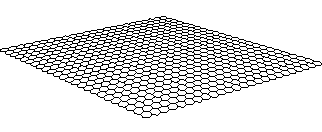
\includegraphics[width=\linewidth]{figures/torus-3d-flat.pdf}
				\caption{}
				\label{fig:torus-3d-flat}
			\end{subfigure}
			~~
			\begin{subfigure}{0.26\linewidth}
				\center
				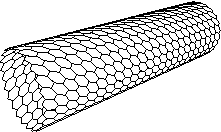
\includegraphics[width=\linewidth]{figures/torus-3d-tube.pdf}
				\caption{}
				\label{fig:torus-3d-tube}
			\end{subfigure}
			~~
			\begin{subfigure}{0.23\linewidth}
				\center
				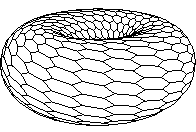
\includegraphics[width=\linewidth]{figures/torus-3d-torus.pdf}
				\caption{}
				\label{fig:torus-3d-torus}
			\end{subfigure}
			
			\caption{Visualisation of a hexagonal torus topology as a torus.}
			\label{fig:torus-3d}
		\end{figure}
		
		The wrap around connections in the topology are what give it the `torus'
		part of its name. Figure~\ref{fig:torus-3d-flat} shows a hexagonal torus
		topology drawn flat as in the previous figure. If the topology is rolled up
		into a tube such that the top and bottom nodes become directly adjacent, a
		tube is formed as in figure~\ref{fig:torus-3d-tube}. This tube can then be
		bent to bring together the nodes at the ends of the tube to form a torus as
		shown in figure~\ref{fig:torus-3d-torus}.
		
		A hexagonal torus topology is typically defined in terms of its width and
		height along the X and Y axes respectively. For example,
		figure~\ref{fig:hexagonalTorusTopology} shows a $10\times10$ hexagonal
		torus.  The nodes in a hexagonal torus topology are addressed using
		hexagonal coordinates of the form $(x, y, z)$ \cite{patel15}. The bottom
		left node (labelled $\alpha$ in the figure) has the coordinate $(0, 0, 0)$
		and other nodes are assigned coordinates according to the number of hops
		along each dimension from $(0, 0, 0)$, for example node $\beta$ has the
		coordinate $(2, 0, -1)$.
		
		Counter intuitively, individual nodes in hexagonal torus topologies may be
		described by many different coordinates, for example $(3, 1, 0)$ and $(1,
		-1, -2)$ are also a valid coordinates for node $\beta$. These dual
		coordinates emerge from the fact that adding $(1, 1, 1)$ to a coordinate
		produces an equivalent, but different, coordinate. This phenomenon is
		explained in detail in appendix~\ref{app:minimal-hex-coordinates} and
		related phenomena will be discussed in chapter~\ref{sec:shortestPaths}.
		
		\begin{figure}
			\center
			\begin{subfigure}[b]{0.32\linewidth}
				\center
				\buildfig{figures/torus-compare-hexagonal.tex}
				
				\caption{Hexagonal}
				\label{fig:torus-compare-hexagonal}
			\end{subfigure}
			\begin{subfigure}[b]{0.32\linewidth}
				\center
				\buildfig{figures/torus-compare-2d.tex}
				
				\caption{2D}
				\label{fig:torus-compare-2d}
			\end{subfigure}
			\begin{subfigure}[b]{0.32\linewidth}
				\center
				\buildfig{figures/torus-compare-3d.tex}
				
				\caption{3D}
				\label{fig:torus-compare-3d}
			\end{subfigure}
			
			\caption{Visual comparison of torus topologies. In all figures, `wrap
			around' connections between nodes at the ends of each axis are omitted
			for clarity.}
			\label{fig:torus-compare}
		\end{figure}
		
		Despite its unusual coordinate system, hexagonal torus topologies compare
		favourably with more conventional network topologies such as 2D and 3D
		toruses (sometimes known as 2-ary $N$-cubes and 3-ary $N$-cubes
		respectively) \cite{dally04} illustrated in figure~\ref{fig:torus-compare}.
		Compared with the 2D torus topology, a hexagonal torus has double the
		bisection bandwidth even though it only requires 50\% more node-to-node
		links \cite{navaridas09}. 3D torus topologies also have six node-to-node
		links per node but double the bisection bandwidth again. However, since a
		network topology must eventually be embedded into a real world data centre
		(which, at large scales, approximate a 2D space), 3D, or higher-dimensional
		torus topologies may become more expensive to construct in practice due to
		the need for longer cables to interconnect nodes. As
		chapter~\ref{sec:building} demonstrates, hexagonal toruses may be assembled
		in a machine room in a similar way to a 2D topology. The hexagonal torus
		topology achieves the scalability of a 2D torus while gaining some of the
		bisection bandwidth benefits of the 3D torus topology.
		
		Most torus topologies, including hexagonal 2D and 3D toruses, are related
		to an equivalent `mesh' topology. Mesh topologies maintain the same general
		connectivity structure as the corresponding torus topology with the
		exception of wrap-around links which are omitted. Omitting wrap-around
		links in practice saves a small number of links at the expense of halving
		the network's bisection bandwidth. As a consequence, mesh topologies are
		rarely used.
		
		\begin{figure}
			\center
			\begin{subfigure}[b]{0.45\linewidth}
				\center
				\buildfig{figures/hexagonal-torus.tex}
				\caption{Hexagonal torus}
				\label{fig:topo-compare-hexagonal-torus}
			\end{subfigure}
			\begin{subfigure}[b]{0.45\linewidth}
				\center
				\buildfig{figures/h-torus.tex}
				\caption{H-torus}
				\label{fig:topo-compare-h-torus}
			\end{subfigure}
			
			\caption{Hexagonal torus vs. H-torus topology. Each numbered hexagon
			represents a node. The thick outline indicates the bounds of the
			topology after which the network repeats. In each topology, the path
			taken by advancing in the Y$^+$ direction from the node labelled `0' is
			shown.}
			\label{fig:topo-compare}
		\end{figure}
		
		The hexagonal torus topology used by SpiNNaker and the subject of much of
		this thesis is not to be confused with the `H-torus' topology.  This
		topology also uses a hexagonal tiling of nodes and even wraps this tiling
		into in a torus-like topology \cite{zhao08}. However, H-torus topologies
		have very different characteristics to the hexagonal torus topology are
		closely related to `twisted torus' topologies \cite{camara10}.
		Figure~\ref{fig:topo-compare} illustrates one major difference in the way
		paths wrap around the peripheries of both topologies.
	
	\section{Scaling-up SpiNNaker machines}
		
		\begin{figure}
			\center
			\begin{subfigure}[b]{0.45\linewidth}
				\center
				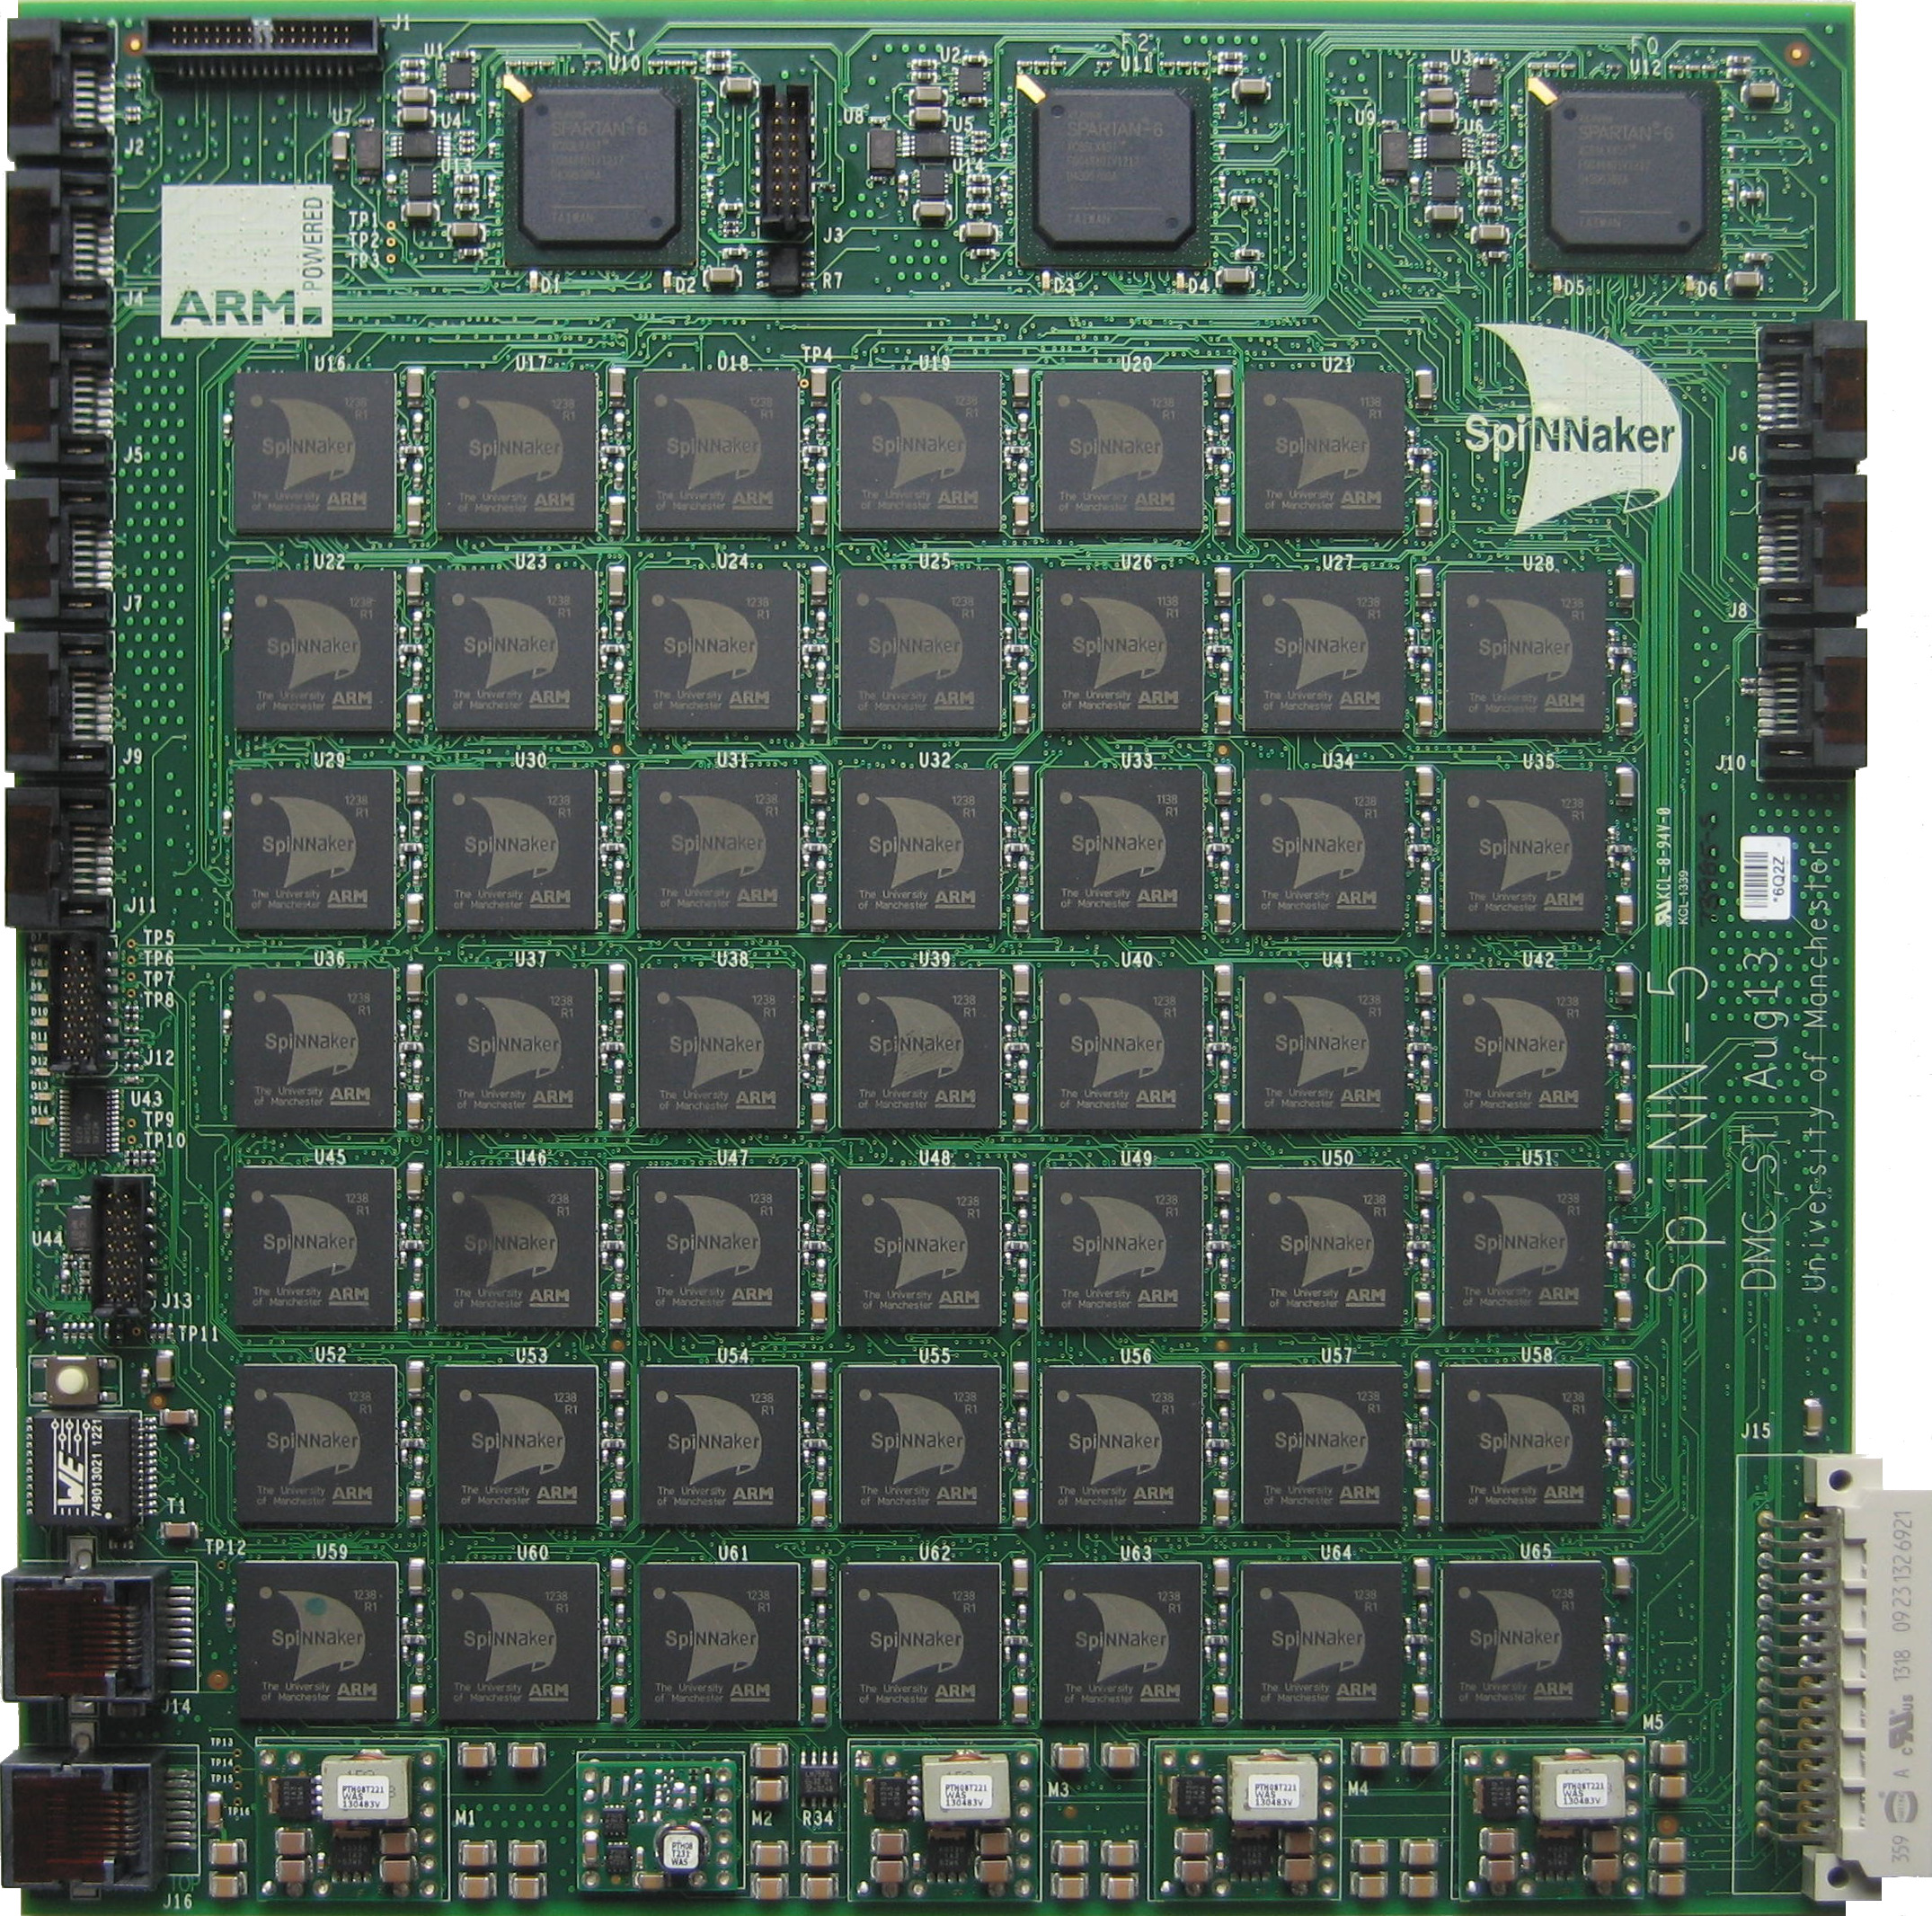
\includegraphics[width=\linewidth]{figures/spinnakerBoard.jpg}
				
				\caption{A SpiNNaker board}
				\label{fig:spinnakerBoard}
			\end{subfigure}
			~~~
			\begin{subfigure}[b]{0.45\linewidth}
				\center
				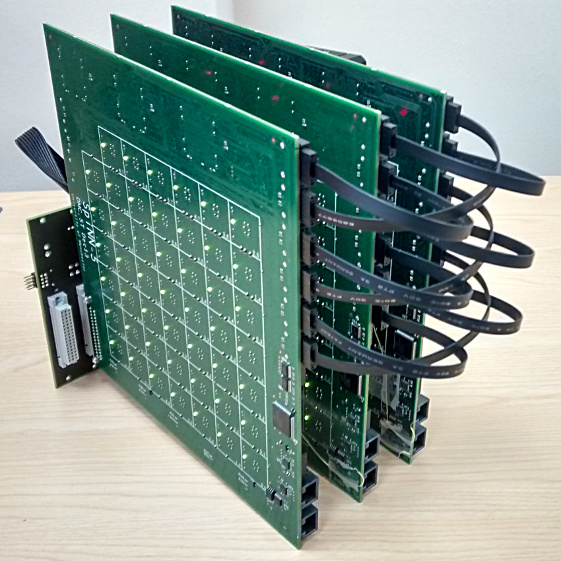
\includegraphics[width=\linewidth]{figures/threeboard.jpg}
				
				\caption{Three board system}
				\label{fig:threeboard}
			\end{subfigure}
			
			\vspace*{2em}
			
			\begin{subfigure}{\linewidth}
				\center
				\buildfig{figures/sata-connections.tex}
				
				\caption{The logical connectivity between chips in multi-board systems.
				Each board's forty-eight chips (drawn here as hexagons) form a wrapped
				triple. Connections between chips on neighbouring boards are
				concentrated onto a single HSS link.}
				\label{fig:sata-connections} \end{subfigure}
			
			\caption{SpiNNaker boards}
			\label{fig:spinnaker-boards}
		\end{figure}
		
		To build large SpiNNaker systems comprising tens of thousands of
		SpiNNaker chips, groups of forty-eight chips are mounted onto printed
		circuit boards as illustrated in figure~\ref{fig:spinnakerBoard}. These
		boards may be connected together to form larger systems.
		Figure~\ref{fig:threeboard} shows a prototype three board system configured
		as a $12\times12$ hexagonal torus.
		
		Though the chips are physically arranged in a (nearly) $7\times7$ grid on
		each SpiNNaker board, they logically form a `wrapped triple', a shape
		described in detail in appendix \ref{sec:partitioning} and illustrated in
		figure~\ref{fig:sata-connections}. Logically, the chips at the periphery of
		each board connect to their neighbours on adjacent boards. Normally
		SpiNNaker chips connect using a low power, asynchronous 2-of-7 protocol
		requiring sixteen wires per bidirectional chip-to-chip link
		\cite{bainbridge03}. If this link technology were used to connect chips on
		neighbouring boards, each pair of boards would need to be connected with a
		128~wire cable. Cables and connectors supporting this may signals are
		expensive and physically large making them unsuitable for use with
		SpiNNaker. Instead, chip-to-chip connections between boards are multiplexed
		and demultiplexed onto a single High-Speed Serial (HSS) link
		\cite{athavale05} carried via commodity S-ATA cables often used to
		connected hard disks in desktop computers and servers \cite{sata3spec}.
		The six high-speed links are implemented by three onboard FPGAs (the three
		large chips at the top of the SpiNNaker board) and are logically
		transparent to the underlying network.
		
		In chapter~\ref{sec:building} I describe how very large SpiNNaker machines
		may be constructed using over one thousand SpiNNaker boards.

	\chapter{Building large SpiNNaker machines}
	
	\label{sec:building}
	
	Like any supercomputer, physically assembling a large SpiNNaker machine
	poses many practical challenges in terms of arranging, installing and
	maintaining the hundreds of metres of network cables required.  For
	conventional architectures and network topologies, techniques are well
	understood and embodied by industry standards such as TAI-942~\cite{tia2006}.
	SpiNNaker's use of the hexagonal torus topology renders existing approaches
	insufficient.
	
	In the first part of this chapter I extend existing techniques for mapping
	network topologies into standard data centre physical infrastructure to
	support the hexagonal torus topology. This mapping is designed to ensure that
	all cables are kept short (under \SI{1}{\meter}) to reduce costs and
	simplify the network hardware required. The techniques described introduce
	little overhead in cable length over existing torus wiring schemes
	and confirm the suitability of the hexagonal torus topology for real-world
	applications.
	
	The second part of this chapter uses SpiNNaker as a case study on the
	suitability of the mappings introduced in this chapter.  In this case study I
	consider various SpiNNaker systems ranging in size from desktop machines to
	multi-cabinet machine room installations. As well as validating the cabling
	schemes introduced in this chapter I also describe a new technique which
	improves the efficiency of the cable installation process.  As a consequence
	of SpiNNaker's fine-grained connectivity, the cabling is unusually dense,
	exacerbating the complexity of the cabling patterns to be installed. By
	exploiting network diagnostics hardware and on-board LEDs to guide cable
	installation, construction of large SpiNNaker machines takes a matter of
	hours rather than the days reported for other architectures. In addition,
	preliminary experiments suggest that neither the maintainability nor cooling
	performance of the system are hampered by the dense cabling employed.
	
	In this chapter, the term \emph{unit} refers to the smallest physical
	component between which network interconnection cables are installed. For
	example, in a SpiNNaker machine a unit is a 48-chip board while in a data
	centre network a unit might be a server blade.
	
	\section{Cabling non-hexagonal torus topologies}
		
		Na\"ive arrangements of torus topologies, hexagonal or otherwise, feature
		physically long `wrap-around' connections which connect units at the
		peripheries of the system. Long connections can be problematic for several
		reasons:
		
		\begin{description}
			
			\item[Performance:] Signal quality diminishes as cables get longer,
			requiring the use of slower signalling speeds, increased error
			correction overhead or more complex hardware.
			
			\item[Energy:] Some energy is lost in cables; longer cables lose more
			signal energy requiring higher drive strengths and/or buffering to
			maintain signal integrity.
			
			\item[Cost:] Shorter cables are cheaper than long ones.  Longer cables
			imply more cabling in a given space making the task of cable installation
			and system maintenance more difficult, increasing labour costs by as much
			as $5\times$~\cite{curtis12}.
			
		\end{description}
		
		In conventional torus topologies, the need for long cables is eliminated by
		folding and interleaving units of the network~\cite[chapter~5]{dally04}.
		This process is illustrated for a 1D torus topology (a ring network) in
		figure~\ref{fig:ring-folding}. A na\"ive arrangement of units in this
		topology results in a long cable connecting the units at the ends of the
		ring (figure~\ref{fig:ring-folding-row}).  To eliminate these long
		connections, half of the units are `folded' on top of the others
		(figure~\ref{fig:ring-folding-folded}) and then this arrangement of units
		is interleaved (figure~\ref{fig:ring-folding-interleaved}). This ordering
		of units requires no long cables while still observing the physical
		constraint that units must be laid out in a line.
		
		\begin{figure}
			\center
			\begin{subfigure}[b]{0.39\linewidth}
				\center
				\buildfig{figures/ring-folding-row.tex}
				\caption{A ring network}
				\label{fig:ring-folding-row}
			\end{subfigure}
			\begin{subfigure}[b]{0.24\linewidth}
				\center
				\buildfig{figures/ring-folding-folded.tex}
				\caption{Folded}
				\label{fig:ring-folding-folded}
			\end{subfigure}
			\begin{subfigure}[b]{0.35\linewidth}
				\center
				\buildfig{figures/ring-folding-interleaved.tex}
				\caption{Folded and interleaved}
				\label{fig:ring-folding-interleaved}
			\end{subfigure}
			
			\caption[Folding and interleaving a ring network.]%
			{Folding and interleaving a ring network to reduce maximum cable
			length.}
			\label{fig:ring-folding}
		\end{figure}
		
		The folding and interleaving process may be extended to $N$-dimensional
		torus topologies by folding each axis in turn. Since all axes are
		orthogonal in non-hexagonal topologies, the folding process only moves
		units along the axis being folded. Due to the non-orthogonality of the
		three axes of the hexagonal torus topology, this type of folding does not
		work. As figure~\ref{fig:failing-to-fold-hex-toruses} illustrates, folding
		along any axis results in connected units on opposing edges not being
		brought together. For example, when folding along the X axis, the two units
		marked with a green circle are moved closer together on the Y axis but
		remain apart on the X axis.
		
		\begin{figure}
			\center
			\begin{subfigure}[b]{0.24\linewidth}
				\center
				\buildfig{figures/failing-to-fold-hex-toruses-none.tex}
				\caption{Not folded}
				\label{fig:failing-to-fold-hex-toruses-none}
			\end{subfigure}
			\begin{subfigure}[b]{0.24\linewidth}
				\center
				\buildfig{figures/failing-to-fold-hex-toruses-x.tex}
				\caption{X}
				\label{fig:failing-to-fold-hex-toruses-x}
			\end{subfigure}
			\begin{subfigure}[b]{0.24\linewidth}
				\center
				\buildfig{figures/failing-to-fold-hex-toruses-y.tex}
				\caption{Y}
				\label{fig:failing-to-fold-hex-toruses-y}
			\end{subfigure}
			\begin{subfigure}[b]{0.24\linewidth}
				\center
				\buildfig{figures/failing-to-fold-hex-toruses-z.tex}
				\caption{Z}
				\label{fig:failing-to-fold-hex-toruses-z}
			\end{subfigure}
			
			\caption[Folding each axis of a hexagonal torus topology.]%
			{Schematics showing folding along each axis of a hexagonal torus topology
			failing to eliminate wrap-around connections.  Same-shaped-and-coloured
			dots show the endpoints of two example wrap-around connections.}
			\label{fig:failing-to-fold-hex-toruses}
		\end{figure}
	
	\section{Partitioning hexagonal torus topologies}
		
		The nodes in supercomputer networks are usually relatively small, for
		example a single chip. Tens of nodes are packed together into a single
		unit, such as a circuit board or server blade, to simplify assembly and
		share common power and cooling resources~\cite{gilge14,ajima12}. In
		commercial supercomputers built on non-hexagonal torus topologies, each
		unit's nodes represent a hypercube partition of the overall topology as
		illustrated in figure~\ref{fig:hypercube-partitioning}
		\cite{chen11,ajima12}.
		
		An analogous `parallelogram' partitioning scheme exists for hexagonal torus
		topologies, however, this results in imbalanced connectivity requirements
		between neighbouring partitions. In
		figure~\ref{fig:parallelogram-partitioning}, for example, the partitions
		above, below, left and right of the central partition are connected by
		seven node-to-node connections each while the partitions above-right and
		below-left are connected by just a single connection each. To simplify
		assembly, connections between all nodes in a pair of neighbouring
		partitions are often made by a single cable. If connectivity requirements
		are imbalanced, as in this example, this may mean multiple connector types
		may be required, increasing design complexity.
		
		To avoid connectivity imbalance, SpiNNaker uses a `wrapped triple'
		partitioning scheme~\cite{davidsonWiring}, as illustrated in
		figure~\ref{fig:wrapped-triple-partitioning} and explained in detail in
		appendix \ref{sec:partitioning}. In this partitioning scheme, the same
		number of connections connect all six neighbouring units. As explained in
		the appendix, a hexagonal torus topology is constructed from groups of
		three partitions.
		
		\begin{figure}
			\center
			\begin{subfigure}[b]{0.32\textwidth}
				\center
				\buildfig{figures/hypercube-partitioning.tex}
				\caption{2D hypercube}
				\label{fig:hypercube-partitioning}
			\end{subfigure}
			\begin{subfigure}[b]{0.32\textwidth}
				\center
				\buildfig{figures/parallelogram-partitioning.tex}
				\caption{Parallelogram}
				\label{fig:parallelogram-partitioning}
			\end{subfigure}
			\begin{subfigure}[b]{0.32\textwidth}
				\center
				\buildfig{figures/wrapped-triple-partitioning.tex}
				\caption{Wrapped triple}
				\label{fig:wrapped-triple-partitioning}
			\end{subfigure}
			
			\caption[Partitioning of torus topologies into units.]%
			{Partitioning of non-hexagonal (a) and hexagonal (b and c) torus
			topologies into units.}
			\label{fig:partitioning-options}
		\end{figure}
		
		For completeness, both parallelogram and wrapped triple partitioning are
		considered in this chapter even though SpiNNaker uses wrapped triple
		partitioning. The parallelogram partitioning scheme may be more appropriate
		for architectures where connections between nodes in neighbouring
		partitions do not share a single connector. In addition, in architectures
		where a unit corresponds to a single node, this can be treated as a $1
		\times 1$ parallelogram partition.  This special case occurs in
		coarse-grained architectures and Networks on Chip (NoCs) where nodes are
		not grouped together into multi-node units.
	
	\section{Folding \& interleaving hexagonal toruses}
		
		To exploit the folding technique used by non-hexagonal topologies, the
		units in a hexagonal torus topology must be mapped into a space with
		orthogonal coordinates. The choice of transformation to an orthogonal
		coordinate system can have an impact on how physically far apart logically
		neighbouring units are in the final arrangement. A good mapping should
		attempt to reduce `distortion' which moves adjacent units apart in the
		final folded and interleaved arrangement.
		
		In this section I propose two transformations which map hexagonal
		arrangements of units into a 2D orthogonal coordinate space. The first
		transformation, `shearing', is general purpose and introduces some
		distortion. The second transformation, `slicing', is less general but can
		introduce less distortion than shearing and therefore may lead to shorter
		cable lengths.
		
		Both the slicing and shearing transformations are carried out in two steps:
		
		\begin{description}
			
			\item[Rectangularisation] Units are transformed from being laid out in a
			parallelogram into a rectangular arrangement. The specific transformation
			used is the key difference between the slicing and shearing
			transformations.
			
			\item[Uncrinkling] Units are mapped into a 2D coordinate system without
			gaps between units.
			
		\end{description}
		
		\subsection{Rectangularisation}
			
			The hexagonal torus topology is illustrated in
			figures~\ref{fig:hex-to-plane-node-native} and
			\ref{fig:hex-to-plane-native} for parallelogram-partitioned units and
			wrapped triple units respectively. The first step in the folding process
			is to rearrange units so that they form a rectangle using one of two
			techniques: shearing or slicing.
			
			\begin{figure}
				\center
				\begin{subfigure}[b]{0.32\linewidth}
					\center
					\buildfig{figures/hex-to-plane-node-native.tex}
					
					\caption{Original}
					\label{fig:hex-to-plane-node-native}
				\end{subfigure}
				\begin{subfigure}[b]{0.32\linewidth}
					\center
					\buildfig{figures/hex-to-plane-node-shear.tex}
					
					\caption{Sheared}
					\label{fig:hex-to-plane-node-shear}
				\end{subfigure}
				\begin{subfigure}[b]{0.32\linewidth}
					\center
					\buildfig{figures/hex-to-plane-node-slice.tex}
					
					\caption{Sliced}
					\label{fig:hex-to-plane-node-slice}
				\end{subfigure}
				
				\caption[Rectangularisation of parallelogram partitioned toruses.]%
				{Rectangularisation of parallelogram partitioned hexagonal
				toruses. Thin lines show wrap-around links. Pointy-topped hexagons
				represent parallelogram partitioned units.}
				\label{fig:hex-to-plane-node}
				
				% XXX: Force these figures together.
				
				%\end{figure}
				%
				%\begin{figure}
				
				\center
				\begin{subfigure}[b]{0.32\linewidth}
					\center
					\buildfig{figures/hex-to-plane-native.tex}
					
					\caption{Original}
					\label{fig:hex-to-plane-native}
				\end{subfigure}
				\begin{subfigure}[b]{0.32\linewidth}
					\center
					\buildfig{figures/hex-to-plane-shear.tex}
					
					\caption{Sheared}
					\label{fig:hex-to-plane-shear}
				\end{subfigure}
				\begin{subfigure}[b]{0.32\linewidth}
					\center
					\buildfig{figures/hex-to-plane-slice.tex}
					
					\caption{Sliced}
					\label{fig:hex-to-plane-slice}
				\end{subfigure}
				
				\caption[Rectangularisation of wrapped triple partitioned toruses.]%
				{Rectangularisation of wrapped triple partitioned hexagonal
				toruses. Thin lines show wrap-around links.  Flat-topped hexagons
				represent wrapped triple partitioned units.}
				\label{fig:hex-to-plane}
				
				% And force these together!
				
				%\end{figure}
				%
				%\begin{figure}
				
				\center
				\begin{subfigure}[b]{0.3\linewidth}
					\center
					\buildfig{figures/slicing-examples-5x5.tex}
					\caption{$5\times5$}
				\end{subfigure}
				\begin{subfigure}[b]{0.3\linewidth}
					\center
					\buildfig{figures/slicing-examples-5x7.tex}
					\caption{$5\times7$}
				\end{subfigure}
				\begin{subfigure}[b]{0.3\linewidth}
					\center
					\buildfig{figures/slicing-examples-5x10.tex}
					\caption{$5\times10$}
				\end{subfigure}
				
				\caption[Patterns of wrap-around connections in sliced systems.]%
				{Schematics showing the patterns of wrap-around connections in sliced
				systems of various aspect ratios.}
				\label{fig:slicing-examples}
			\end{figure}
			
			The shearing technique applies a \SI{30}{\degree} shear transformation to
			distort the arrangement of units so that the X and Y axes of the
			hexagonal torus topology become orthogonal. This transformation leads to
			a rectangular arrangement of units as illustrated in figures
			\ref{fig:hex-to-plane-node-shear} and \ref{fig:hex-to-plane-shear}.
			
			The shear transformation introduces some distortion causing connections
			between units in the Z axis to become $\sqrt{2} \times$ longer. The
			transformation does not alter the pattern of wrap-around connections:
			long connections between units on the extreme left and right sides and
			the top and bottom remain, along with a single connection between the
			bottom left and top right units.
			
			The slice transformation aims to avoid the elongation of the Z axis by
			moving the units without distorting their layout. Units protruding from
			the left-hand-side of the parallelogram are `sliced off' and moved into
			the matching gap on the opposite side as illustrated in figures
			\ref{fig:hex-to-plane-node-slice} and \ref{fig:hex-to-plane-slice}. This
			transformation does not introduce any distortion but changes the pattern
			of wrap-around connections. Connections from left-to-right remain while
			the connections between the top and bottom units now criss-cross
			(figure~\ref{fig:slicing-examples}).  The proportion of connections going
			from bottom-left to top-right and from bottom-right to top-left varies
			depending on the aspect ratio of the topology. Only certain patterns of
			wrap-around links can be eliminated by folding and, as we shall see
			later, this limits us in which network topologies can be rectangularised
			by slicing.
			
		\subsection{Uncrinkling}
			
			Before folding can occur, the rectangularised arrangements of units
			produced in the previous step must be mapped into a 2D grid. Applied to
			parallelogram partitions, the shear transformation results in a mapping
			into a 2D grid with no further distortion
			(figure~\ref{fig:uncrinkling-node-sheared}). For other combinations of
			transformation and partitioning scheme, the units do not exactly fit a 2D
			grid. Instead, the units form `crinkled' rows or columns which may be
			`uncrinkled' (straightened out) to fit a regular 2D grid as illustrated in
			figures~\ref{fig:uncrinkling-node-sliced}~--~\ref{fig:uncrinkling-sliced}.
			
			\begin{figure}
				\center
				\begin{subfigure}[b]{0.48\linewidth}
					\center
					\buildfig{figures/uncrinkling-node-sheared.tex}
					
					\caption{Parallelogram units, sheared}
					\label{fig:uncrinkling-node-sheared}
				\end{subfigure}
				\begin{subfigure}[b]{0.48\linewidth}
					\center
					\buildfig{figures/uncrinkling-node-sliced.tex}
					
					\caption{Parallelogram units, sliced}
					\label{fig:uncrinkling-node-sliced}
				\end{subfigure}
				
				\vspace{1cm}
				
				\begin{subfigure}[b]{0.48\linewidth}
					\center
					\buildfig{figures/uncrinkling-sheared.tex}
					
					\caption{Wrapped triple units, sheared}
					\label{fig:uncrinkling-sheared}
				\end{subfigure}
				\begin{subfigure}[b]{0.48\linewidth}
					\center
					\buildfig{figures/uncrinkling-sliced.tex}
					
					\caption{Wrapped triple units, sliced}
					\label{fig:uncrinkling-sliced}
				\end{subfigure}
				
				\vspace{1em}
				
				\caption[Uncrinkling units into a 2D grid.]%
				{Uncrinkling rectangularised arrangements of units into a 2D
				grid. Thick lines show how crinkled rows and columns of units are
				uncrinkled.  Annotations show how the relative positions of units
				change after uncrinkling.}
				\label{fig:uncrinkling}
			\end{figure}
			
			%% XXX: Does this make things clearer or not?
			%In the figure, the labels show the positions of individual units before
			%and after uncrinkling. We will use these later in \S\ref{sec:distortion}
			%to calculate the overhead introduced by uncrinkling.
		
		\subsection{Folding}
			
			\begin{figure}
				\begin{subfigure}{\linewidth}
					\center
					\buildfig{figures/folding-sheared.tex}
					\caption{Sheared systems and $1:2$ sliced systems}
					\label{fig:folding-sheared}
				\end{subfigure}
				
				\vspace{1em}
				
				\begin{subfigure}{\linewidth}
					\center
					\buildfig{figures/folding-sliced.tex}
					\caption{$1:1$ sliced systems}
					\label{fig:folding-sliced}
				\end{subfigure}
				
				\caption[Elimination of long wrap-around links by folding.]%
				{Schematic illustrating elimination of long wrap-around links
				during folding. In each example a single link has been highlighted to
				aid in following the process.}
				\label{fig:folding}
			\end{figure}
			
			Once a regular 2D grid of units has been formed, this may be folded in
			the conventional way as illustrated in figure~\ref{fig:folding-sheared}.
			Folding once along each axis eliminates long connections crossing from
			left-to-right, top-to-bottom and from the bottom-left corner to the
			top-right corner. Any shear-transformed network may be folded this way
			since its wrap-around connections always follow this pattern.
			Slice-transformed networks may only be folded like this when their aspect
			ratio is $1:2$ when the pattern of wrap-around links is the same as a
			shear-transformed network.
			
			When `square' networks (i.e. those with a $1:1$ aspect ratio) are sliced,
			the network must be folded \emph{twice} along the Y axis as in
			figure~\ref{fig:folding-sliced} to eliminate the criss-crossing
			wrap-around links. It is not possible to eliminate wrap-around links from
			sliced networks with other aspect ratios by folding.
			
			After folding, the units are interleaved, yielding a 2D arrangement of
			units in which no connection spans the width or height of the system. The
			maximum connection distance is constant for any network allowing the
			topology to scale up.
		
		\subsection{Choosing a transformation}
			
			\label{sec:distortion}
			
			In each step of the transformation from hexagonal torus to a folded and
			interleaved 2D grid, the distances between connected units may increase.
			When designing a system, the transformation with the least distortion
			should be used to minimise the average length of the cables required.
			
			By referring to figure~\ref{fig:uncrinkling} (page
			\pageref{fig:uncrinkling}), it is possible to calculate the overhead
			introduced by each type of transformation.  For example, to compute the
			overhead introduced by the slicing transformation when applied to units
			composed of wrapped triples we consider
			figure~\ref{fig:uncrinkling-sliced}. The uncrinkling pattern used to
			transform this topology is a repeating pattern of two units, a pair of
			which have been labelled $1$ and $2$ respectively. Unit $1$ is
			immediately surrounded by the six units labelled $a$, $b$, $c$, $2$, $g$
			and $h$. Unit $2$ is surrounded by the units $1$, $c$, $d$, $e$, $f$ and
			$g$.  Before the transformation, the distance between units is $1$; after
			the transformation is applied this is not always the case. Folding and
			interleaving into $f_x$ columns and $f_y$ rows also introduces overhead.
			For each pair of previously neighbouring units in the example, their
			distances after folding may be computed as follows:
			
			\begin{equation*}
				\begin{aligned}[c]
					D_{1\,\leftrightarrow{}\,a} &= \sqrt{f_x^2 + f_y^2} \\
					D_{1\,\leftrightarrow{}\,b} &= f_y \\
					D_{1\,\leftrightarrow{}\,c} &= \sqrt{f_x^2 + f_y^2} \\
					D_{1\,\leftrightarrow{}\,2} &= f_x \\
					D_{1\,\leftrightarrow{}\,g} &= f_y \\
					D_{1\,\leftrightarrow{}\,h} &= f_x
				\end{aligned}
				\hspace{2cm}
				\begin{aligned}[c]
					D_{2\,\leftrightarrow{}\,1} &= f_x \\
					D_{2\,\leftrightarrow{}\,c} &= f_y \\
					D_{2\,\leftrightarrow{}\,d} &= f_x \\
					D_{2\,\leftrightarrow{}\,e} &= \sqrt{f_x^2 + f_y^2} \\
					D_{2\,\leftrightarrow{}\,f} &= f_y \\
					D_{2\,\leftrightarrow{}\,g} &= \sqrt{f_x^2 + f_y^2}
				\end{aligned}
			\end{equation*}
			
			From these values, mean and maximum connection distances may be
			calculated. The expressions for each combination of partitioning scheme
			and transformation are as follows:
			
			\begin{align*}
				D_{\textrm{mean}}=&
					\begin{cases}
						\frac{7f_x + 3\sqrt{f_x^2 + f_y^2} + \sqrt{(2f_x)^2 + f_y^2}}{9} &
							\textrm{if sheared wrapped triple units}\\
						\frac{f_x + f_y + \sqrt{f_x^2 + f_y^2}}{3} &
							\textrm{otherwise}\\
					\end{cases} \\
				D_{\textrm{max}}=&
					\begin{cases}
						\sqrt{(2f_x)^2 + f_y^2} &
							\textrm{if sheared wrapped triple units}\\
						\sqrt{f_x^2 + f_y^2} &
							\textrm{otherwise}
					\end{cases}
			\end{align*}
			
			\begin{table}
				\center
				\begin{tabular}{lcc}
					\toprule
					                                 & $1:2$  & Other \\
					\addlinespace
					\multirow{2}{*}{Parallelogram}   & \textbf{Either} & \textbf{Shear}\\
					                                 & \footnotesize $D_\textrm{mean}\approx2.28 \quad D_\textrm{max}\approx2.83$
					                                 & \footnotesize $D_\textrm{mean}\approx2.28 \quad D_\textrm{max}\approx2.83$\\
					\addlinespace
					\multirow{2}{*}{Wrapped triples} & \textbf{Slice}  & \textbf{Shear}\\
					                                 & \footnotesize $D_\textrm{mean}\approx2.28 \quad D_\textrm{max}\approx2.83$
					                                 & \footnotesize $D_\textrm{mean}\approx3.00 \quad D_\textrm{max}\approx4.47$\\
					\bottomrule
				\end{tabular}
				
				\caption{Recommended transformations for folding hexagonal toruses.}
				\label{tab:transform-recommended}
			\end{table}
			
			Using these formulae it is possible to determine which approach --
			shearing or slicing -- results in the lowest mean and maximum cable
			lengths and thus which technique should be used. This is summarised in
			table~\ref{tab:transform-recommended}.
	
	\section{A SpiNNaker case study}
		
		As the only known large-scale hexagonal torus-based architecture, SpiNNaker
		is a good case study for the techniques described in this chapter.  Each
		unit in a SpiNNaker machine is a 48-chip SpiNNaker board forming a
		wrapped triple partition. Systems of various sizes have been constructed
		using the techniques introduced in this chapter ranging from twenty-four
		board `portable' systems to a five cabinet, half-million core installation
		with plans in place to build a machine of twice this size in the future.
		
		In this section I describe how the folded and interleaved arrangement of
		units produced by the techniques in the previous chapter may be translated
		into physical arrangements of SpiNNaker boards in a machine room. I then
		describe how the thousands of S-ATA cables are installed and report on the
		maintainability and cooling impact of this cabling scheme in practice.
		
		\subsection{Mapping into physical cabinets}
			
			In SpiNNaker systems, the physical architecture used is illustrated in
			figure~\ref{fig:cabinet-units}. SpiNNaker boards are installed into card
			frames containing twenty four boards each. Five frames are mounted into
			standard, \SI{600}{\milli\meter}~wide 19\inch{} cabinets with further
			cabinets being added, arranged in a row, to scale the system up. The 2D
			grid of units produced by the folding process described in this chapter
			is mapped to cabinets and frames as illustrated in
			figure~\ref{fig:cabinetisation}.
			
			\begin{figure}
				\center
				\buildfig{figures/cabinet-units.tex}
				
				\caption{Physical architecture of a SpiNNaker machine.}
				\label{fig:cabinet-units}
			\end{figure}
			
			\begin{figure}
				\center
				\buildfig{figures/cabinetisation.tex}
				
				\caption[Mapping cabling from abstract to physical space.]%
				{Mapping from the abstract folded and interleaved 2D grid
				layout into physical cabinet and frame positions. Arrows indicate the
				order in which units (boards) are mapped into each frame, from
				left-to-right.}
				\label{fig:cabinetisation}
			\end{figure}
			
			Figure~\ref{fig:million-core-machine} shows the cabling plan for the
			largest planned SpiNNaker machine. This system will fill ten 19\inch{}
			cabinets and implement a $240 \times 240$ hexagonal torus topology
			partitioned between \num{1200} 48 chip SpiNNaker boards. The largest gap
			to be spanned by any cable is \SI{66}{\centi\meter}, well within the
			\SI{1}{\meter} limit on SpiNNaker's interconnect technology.
			
			\begin{figure}
				\center
				\buildfig{figures/million-core-machine.tex}
				
				\caption[Cabling plan for a \num{1200}~board SpiNNaker machine.]%
				{Cabling plan for a \num{1200}~board (\num{1036800}~core)
				SpiNNaker machine.}
				\label{fig:million-core-machine}
			\end{figure}
			
		\subsection{Cable selection and routing}
			
			Because of the dense packing of SpiNNaker boards, cables span short
			distances as shown in figure~\ref{fig:wire-length-histogram}.
			Conventional cable management techniques (e.g. cable trays) are not
			practical. To ensure the reliability and maintainability of SpiNNaker's
			wiring, cable slack must be carefully controlled.  If cables are too
			tight, cables, connectors and SpiNNaker boards can become damaged. When
			cables are too slack, the excess obstructs access to the machine and can
			easily become tangled \cite{cisco07}.
			
			In this case study the `rule of (three-)thumbs' proposed by
			Mazaris~\cite{mazaris97} is used which suggests that a minimum of
			\SI{5}{\centi\meter} of slack be provided. As SpiNNaker uses
			off-the-shelf S-ATA cables, only standard lengths of cable are available.
			For any given span, the shortest length of cable providing at least
			\SI{5}{\centi\meter} of slack is used.
			
			\begin{figure}
				
				\center
				\buildfig{figures/wire-length-histogram.tex}
				
				\caption[Cable lengths in a \num{1200}~board SpiNNaker machine.]%
				{Histogram of connection distances in a \num{1200} board SpiNNaker
				machine annotated with the selected cable lengths.}
				\label{fig:wire-length-histogram}
				
			\end{figure}
		
		\subsection{Installation practicality}
			
			\begin{figure}
				\center
				\begin{subfigure}[t]{0.5\textwidth}
					\begin{tikzpicture}
						\node (cables) [inner sep=0]
						      {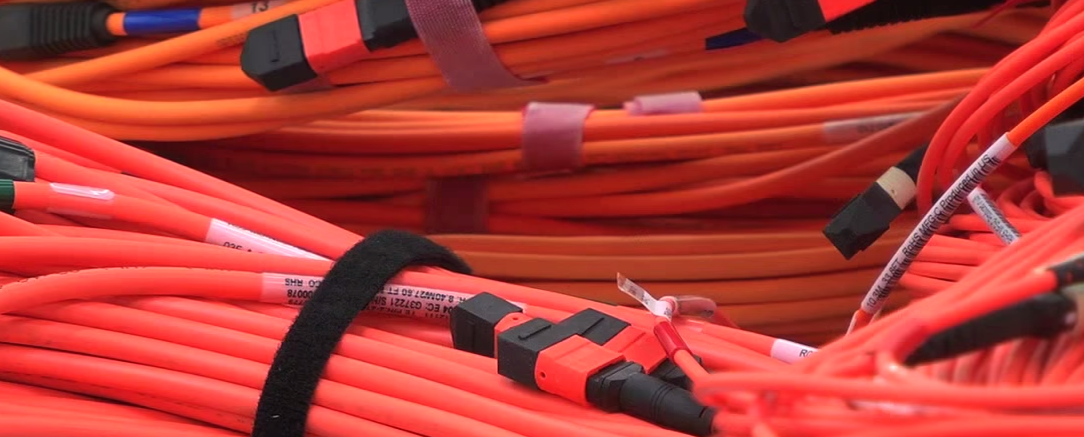
\includegraphics[width=\textwidth]{figures/bgCables.png}};
						\node (sockets) [inner sep=0, below=1.0em of cables]
						      {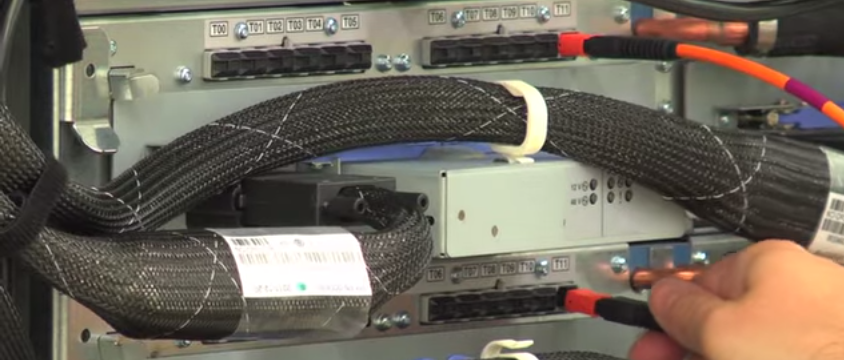
\includegraphics[width=\textwidth]{figures/bgSockets.png}};
						
						% Point at label on cable
						\draw [white, <-, line width=0.4em]
						      ([shift={(0.7cm, -0.3cm)}]cables.center)
						      -- ++(45:1cm);
						
						% Point at label on socket
						\draw [white, <-, line width=0.4em]
						      ([shift={(-1.0cm, 1.1cm)}]sockets.center)
						      -- ++(-45:1cm);
					\end{tikzpicture}
					
					\caption{Pre-labelled cables and sockets}
					\label{fig:bgWiringLabels}
				\end{subfigure}
				~
				\begin{subfigure}[t]{0.30\textwidth}
					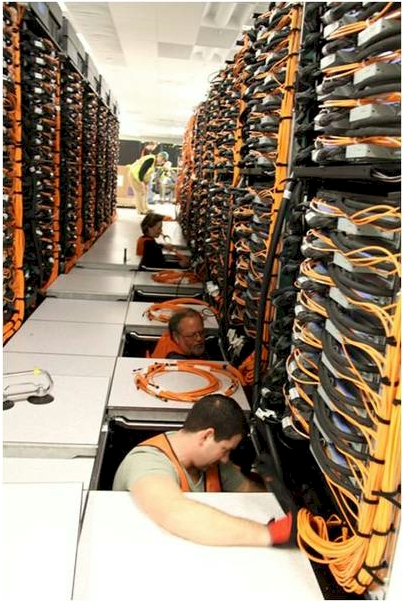
\includegraphics[height=6.15cm]{figures/bgWiring.jpg}
					
					\caption{Installation of cables}
					\label{fig:bgWiringInstallation}
				\end{subfigure}
				
				\caption[BlueGene/Q cable installation.]%
				        {BlueGene/Q cable installation~\cite{cscs13}.}
				\label{fig:bgWiring}
			\end{figure}
			
			In other large-scale architectures, the task of cable installation is
			completed by a team of technicians aided by the use of standardised
			labelling for cables and sockets as illustrated in
			figure~\ref{fig:bgWiring}~\cite{tia2006}. In these architectures the
			cabling patterns required are relatively straightforward, thanks to the
			coarseness of the units used~\cite{lakner07} or they use network
			topologies whose cabling centres around high-fan-in
			switches~\cite{cisco07,csernai15}.
			
			It has been reported in the literature that when copper cables are used,
			labour costs dominate~\cite{popa10} and while cable costs are expected to
			decline, labour costs are not~\cite{mudigonda11}. Many researchers have
			attempted to control cable installation costs by trying to reduce the
			number or length of cables required by developing alternative network
			topologies~\cite{curtis12, popa10, mudigonda11}.  Unfortunately, these
			techniques do not apply to SpiNNaker since its network topology is fixed.
			
			Supercomputer architectures such as BlueGene/Q make use of large custom
			`midplane' PCBs in place of some cables to interconnect units within a
			cabinet~\cite{milano13}. This scheme can greatly reduce wiring complexity
			since only coarser-grain, cabinet-to-cabinet connectivity is implemented
			by cables. Unfortunately this technique is expensive and constrains the
			dimensions of the network topology supported by the machine. Since the
			SpiNNaker platform is designed to scale from desktop machines to
			machine room installations, this scheme is not practical.
			
			\begin{figure}
				\center
				\begin{subfigure}[b]{0.40\textwidth}
					\begin{tikzpicture}
						\node (leds) [inner sep=0]
						      {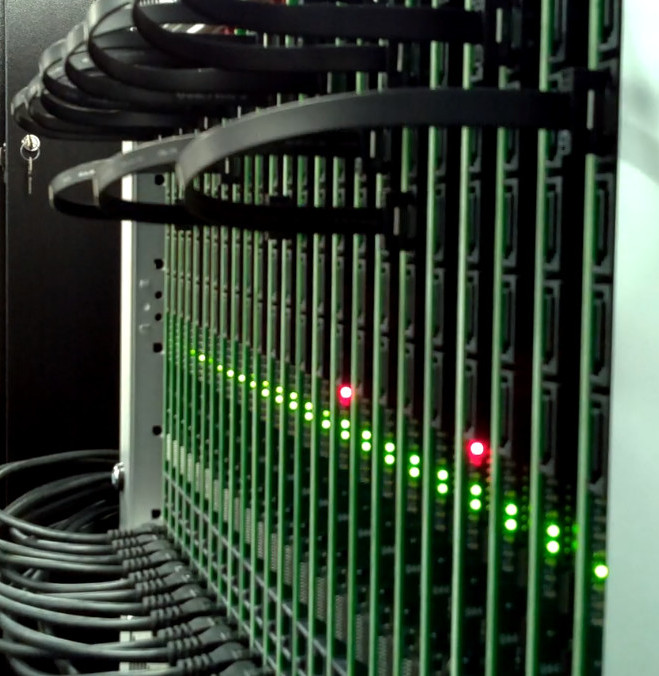
\includegraphics[width=\textwidth]{figures/leds.jpg}};
						% Point at left LED
						\draw [white, <-, line width=0.4em]
						      ([shift={(-0.0cm, -0.6cm)}]leds.center)
						      -- ++(225:1cm);
						% Point at right LED
						\draw [white, <-, line width=0.4em]
						      ([shift={(1.1cm, -1.1cm)}]leds.center)
						      -- ++(225:1cm);
					\end{tikzpicture}
					
					\caption{Diagnostic LEDs indicate the endpoints of each cable.}
					\label{fig:interactive-wiring-guide-leds}
				\end{subfigure}
				~
				\begin{subfigure}[b]{0.546\textwidth}
					\begin{tikzpicture}[thin, black!20!white]
						\node (screen) [inner sep=0]
						      {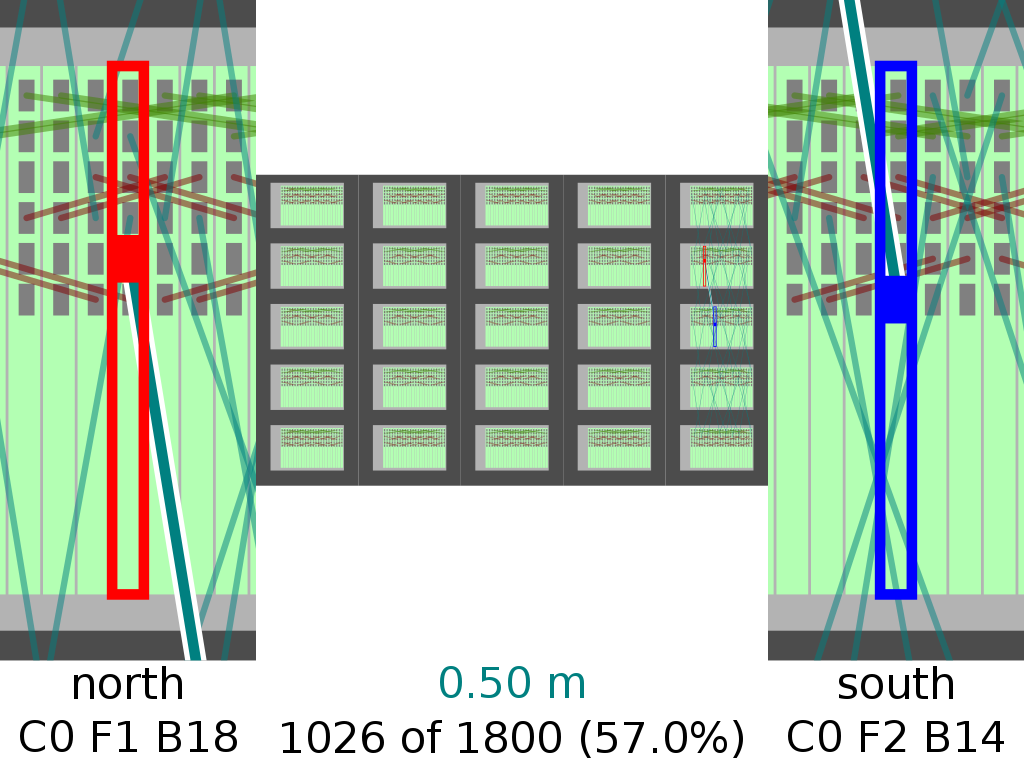
\includegraphics[width=\textwidth]{figures/wiring_guide_screenshot.png}};
						\draw (screen.south west) rectangle (screen.north east);
					\end{tikzpicture}
					
					\caption{A GUI and text-to-speech indicate what type of cable to
					install.}
					\label{fig:interactive-wiring-guide-gui}
				\end{subfigure}
				
				\caption{Interactive software guides cable installation.}
				\label{fig:interactive-wiring-guide}
			\end{figure}
			
			Due to the high density of units in a SpiNNaker system, the detailed
			cabling patterns used can be complex, despite their overall regularity.
			To cope with this complexity, I developed a software system which employs
			diagnostic hardware built into SpiNNaker, to guide technicians through
			the cable installation process. As shown in
			figure~\ref{fig:interactive-wiring-guide}, diagnostic LEDs on each
			SpiNNaker board are used to indicate which boards to connect. The
			software also provides step-by-step cabling instructions via a Graphical
			User Interface (GUI) and audible instructions delivered via headphones.
			These instructions explicitly specify the length of cable to use for each
			connection avoiding the common problem of technicians over-estimating the
			cable length required~\cite{mazaris97}. Diagnostic registers in the
			network hardware are then used to verify the correct installation of each
			cable in real-time ensuring that mistakes are highlighted and fixed
			immediately.
			
			\begin{table}
				\center
				\begin{tabular}{lrll}
					\toprule
						Size & Cables & Time & Notes \\
					\midrule
						24 boards  & \num{72}   & \SI{10}{\minute} & \\
						1 cabinet  & \num{360}  & \SI{4}{\hour} &
							Real-time validation not used. \\
						2 cabinets & \num{720}  & \SI{2}{\hour} & \\
						5 cabinets & \num{1800} & \SI{4}{\hour} \SI{20}{\minute} &
							Three people working simultaneously. \\
					\bottomrule
				\end{tabular}
				
				\caption[Cable installation times for various SpiNNaker machines.]%
				{Cable installation times for various sizes of SpiNNaker
				machine.}
				\label{tab:install-time}
			\end{table}
			
			\begin{figure}
				\buildfig{figures/install-histogram.tex}
				
				\caption{Two cabinet SpiNNaker machine cable installation times.}
				\label{fig:install-histogram}
			\end{figure}
			
			Table~\ref{tab:install-time} shows cable installation times for various
			sizes of SpiNNaker system. The times reported do not include breaks and,
			with the exception of the five cabinet system, are for the one person
			working alone.  Figure~\ref{fig:install-histogram} shows the histogram of
			cable installation times for a two cabinet machine.  These results
			confirm the observation by Mudigonda \emph{et al.} that cables which span
			cabinets and frames take longer to install~\cite{mudigonda11}, even
			though these distances are still very short in SpiNNaker. Compared with
			commercial installation efforts, per-cable installation times are much
			shorter for SpiNNaker taking seconds compared with minutes in other
			architectures~\cite{mudigonda11}.
			
			The positive impact of real-time validation of installed cables can
			clearly be seen by comparing the installation times of the one and two
			cabinet systems. Though double the size, the two cabinet machine was
			built in half the time required to build the single cabinet machine.
			While building the smaller machine, real-time cable validation had not
			yet been implemented and the installation process was interrupted for
			several minutes every time a misplaced connection was discovered.
			
			In the three-person cable installation effort employed for the five
			cabinet system, the guidance software was configured to assign each
			technician cables in non-overlapping parts of the machine ensuring
			minimal interference between the technicians. As expected, this renders
			the problem embarrassingly parallel, as in commercial computer
			installations.
			
			\begin{figure}
				\center
				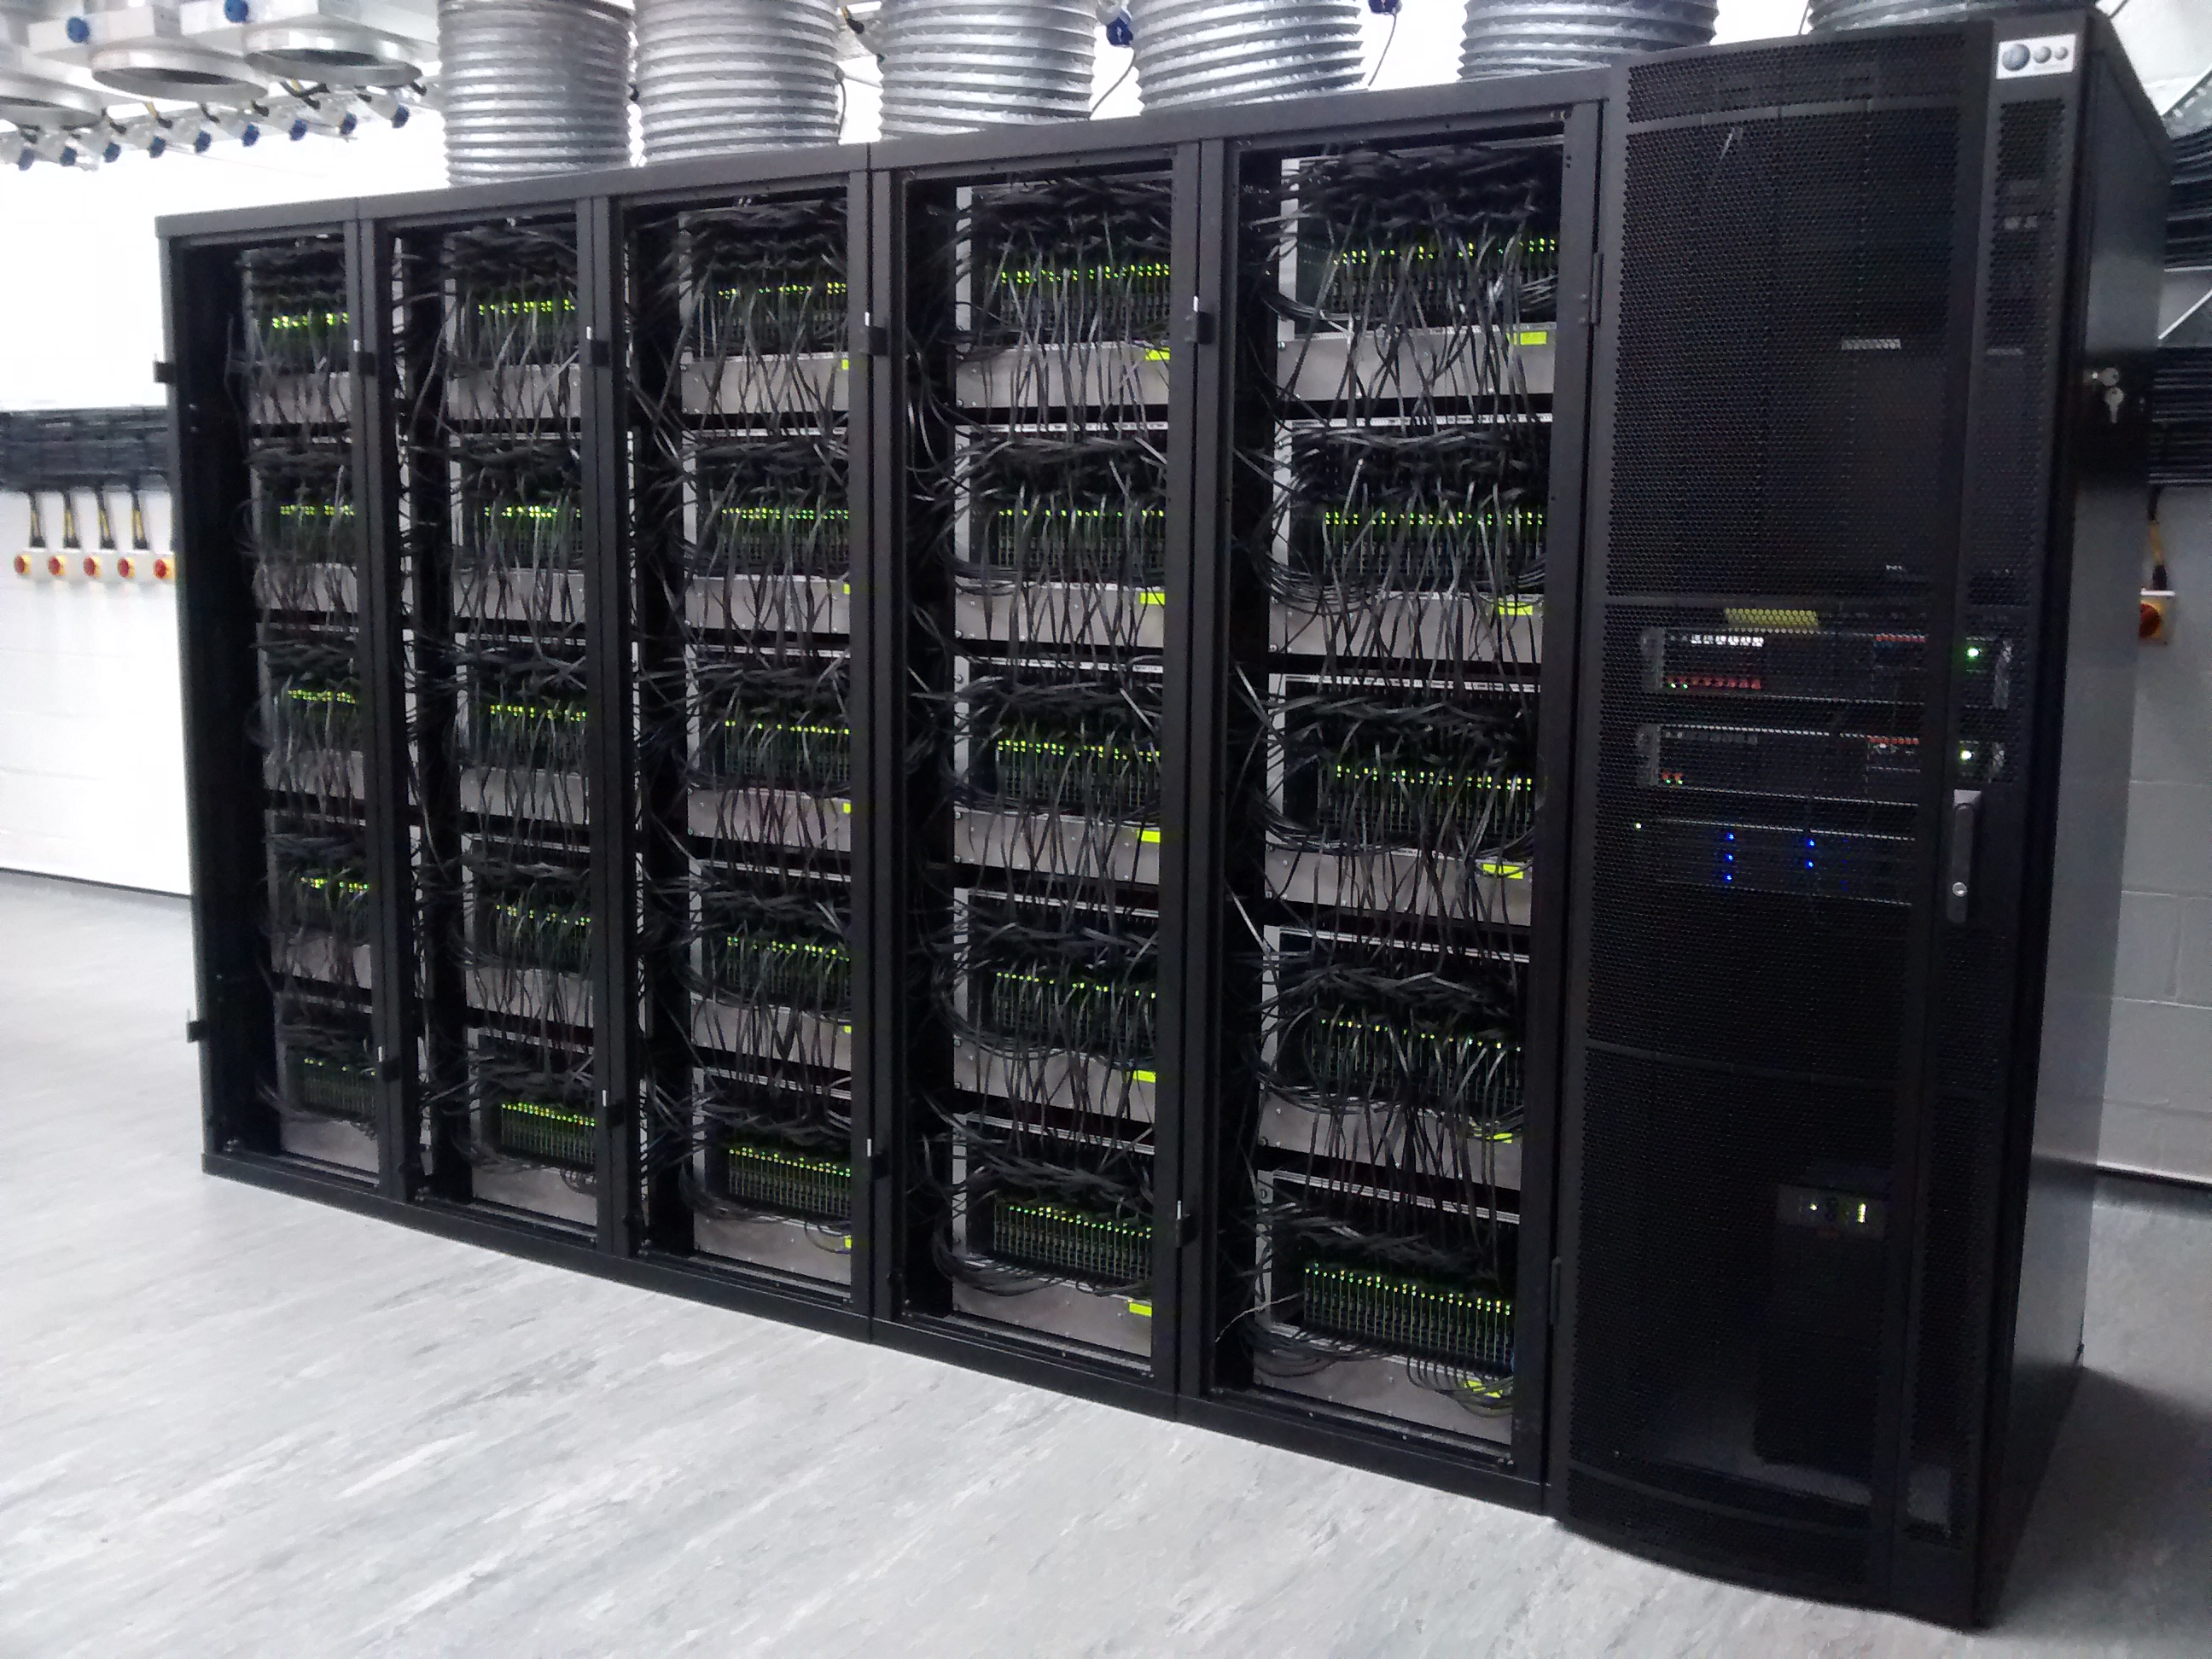
\includegraphics[width=0.8\linewidth]{figures/halfMillionCoreComplete.jpg}
				
				\caption[The five cabinet SpiNNaker system.]%
				{The five cabinet SpiNNaker system. The cabinet on the right contains
				conventional host servers which control SpiNNaker.}
				\label{fig:halfMillionCoreComplete}
			\end{figure}
			
			The completed five cabinet system is photographed in
			figure~\ref{fig:halfMillionCoreComplete}. A time-lapse video showing the
			construction and cable installation of this machine is also available on
			YouTube~\cite{heathcote16}.
			
		\subsection{Thermal implications}
			
			In large SpiNNaker machines, each 24 board frame contains a fan tray
			which pulls cool air from the front of the frame, between the SpiNNaker
			boards. The warmed air is then ejected out of the rear of the frame where
			ducting directs it into industrial air chillers. Conventional guidance on
			data centre design suggests that routing cables in the path of the
			system's airflow can have a serious impact on cooling
			performance~\cite{cisco07}.  To determine what effect the cabling
			described in this chapter had on SpiNNaker's cooling, a test program was
			executed to simulate heavy load before and after cable installation. The
			temperatures reported by the sensors on the top of each SpiNNaker board
			were sampled at regular intervals and once the overall system temperature
			stabilised, the mean temperature was recorded.
			
			Before the cabling was installed, the temperature stabilised at
			\SI{49}{\celsius} while after installation it stabilised at
			\SI{42}{\celsius}.
			
			These two data points suggest that the system's temperature is unlikely
			to have been been seriously impacted by cable installation. Since the two
			experiments were run on different days (with potentially different
			ambient temperatures) and are based on a single experiment, it is not
			possible to infer much more from this result.
			
		\subsection{Maintenance}
			
			At the time of writing, the five cabinet machine is still being
			commissioned and so the long term maintenance impact of the system's
			cabling is not known. One important factor in the maintainability of the
			system is the ease with which faulty boards can be replaced. During
			commissioning a number of boards have been replaced by someone not
			involved in the machine's installation. Informal measurements suggest
			that boards near the centre of a frame (i.e. those most likely to be
			blocked by unrelated cables) take around ten minutes to replace,
			including time spent removing and replacing cables obstructing the board
			being exchanged. By comparison boards at the edge of the machine take
			around six minutes to replace. Though similar timing reports are
			unavailable for other architectures, these times appear reasonable in
			practice and suggest maintenance is not impaired by the wiring plan used.
	
	\section{Conclusions}
		
		In this chapter I presented a practical method of constructing real-world
		installations of large hexagonal torus topologies such that long cables
		spanning the width and height of the system are not required. Two
		transformations, shearing and slicing, are presented which allow
		conventional network folding techniques to be applied to hexagonal toruses
		to eliminate long `wrap around' links. Though both techniques incur some
		overhead in terms of mean and maximum cable length, the maximum cable
		length does not grow with the size of the network. This result makes
		hexagonal torus topologies a practical and scalable choice for future
		systems.
		
		The theoretical results presented in this chapter have been confirmed
		through the successful construction of several large-scale SpiNNaker
		machines which implement hexagonal torus topologies. During construction,
		diagnostic features of SpiNNaker's hardware were employed to guide
		technicians performing cable installation. This technique was found to be
		highly effective with cable installation times measured in seconds rather
		than minutes as reported for other architectures. Surprisingly there was no
		evidence found of this technique being applied to other architectures and
		consequently this secondary result may be of interest for future research.

	\chapter{Finding shortest path vectors in SpiNNaker's network}
	
	\label{sec:shortestPaths}
	
	% XXX: Add note explaining shortest path between two points in non-torus
	% space.
	
	In the previous chapter we explored the practical challenges of building
	machines which use hexagonal torus topologies working at the scale of units
	containing several nodes. To exploit these machines, however, we must also be
	able to route packets efficiently through the nodes in the resulting network.
	This chapter tackles the problem of finding shortest path vectors in
	hexagonal torus topologies. Shortest path vectors are used by many routing
	algorithms as the basis for route generation. In non-hexagonal torus
	topologies, finding shortest path vectors is trivial and intuitive but in
	hexagonal toruses, this is not the case.  In this chapter I introduce the
	Irregular Quadrant (IQ) method, a new technique for computing shortest path
	vectors in hexagonal torus topologies.  This method is cheaper to compute and
	more general than pre-existing techniques, functioning correctly on hexagonal
	torus topologies of any aspect ratio.
	
	In some hexagonal torus topologies, many shortest path vectors may exist
	between a given pair of points. I propose a technique for discovering all
	possible shortest path vectors. Using these alternative shortest path
	vectors, routing algorithms may be able to produce routes which load a
	network more evenly.
	
	In this chapter, I assume an idealised hexagonal torus topology without
	faults or other irregularities. The challenge of handling these artefacts of
	real-world systems will be tackled in chapter~\ref{sec:routing}.
	
	\section{Shortest path vectors}
		
		Many popular routing algorithms for torus topologies, including all
		published algorithms designed for SpiNNaker~\cite{davies12,navaridas14},
		compute a shortest path vector between the endpoints of a route and use
		this to generate a path through the network. A shortest path vector between
		two nodes is a vector, $\mathbf{v} = (v_1, v_2, v_3, \ldots)$, whose
		magnitude, $\| \mathbf{v} \| = \lvert v_1 \rvert + \lvert v_2 \rvert +
		\lvert v_3 \rvert + \cdots$, is minimal with respect to all possible
		vectors between those nodes.
		
		\begin{figure}
			\center
			\buildfig{figures/mesh-topology-coordinates.tex}
			\caption[Shortest path routes in a 2D mesh network.]%
			{An example 2D mesh network with example shortest-path routes
			from `A' to `B' and `B' to `C'.}
			\label{fig:mesh-topology-coordinates}
		\end{figure}
		
		In a non-hexagonal mesh topology, shortest path vectors are computed by
		taking the element-wise difference between the source and destination
		nodes' coordinates. For example, figure~\ref{fig:mesh-topology-coordinates}
		shows a 2D mesh topology with three nodes labelled `A', `B' and `C' with
		position vectors $(1, 2)$, $(4, 5)$ and $(6, 1)$ respectively. The shortest
		path vector from node `A' to `B' is $(4, 5) - (1, 2) = (3, 3)$ and from `B'
		to `C' is $(6, 1) - (4, 5) = (2, -4)$. A route may be produced by advancing
		the number of hops specified for each dimension in the shortest path
		vector. For example, a route from `A' to `B' may be constructed from any
		permutation of the hops X$^+\,$X$^+\,$X$^+\,$Y$^+\,$Y$^+\,$Y$^+$, an
		example of which is included in the figure. Likewise routes from `B' to `C'
		may be constructed from permutations of the hops
		X$^+\,$X$^+\,$Y$^-\,$Y$^-\,$Y$^-\,$Y$^-$. Regardless of the order of the
		hops, the length of the route, $\mathbf{v}$, is given by the magnitude of
		the shortest path vector, $\|\mathbf{v}\|$.
		
		Many popular routing algorithms such as dimension order routing, right-turn
		only routing and longest dimension first routing~\cite{davies12} are simply
		defined as rules for ordering the hops specified by a shortest path vector.
		
		\subsection{Torus networks}
			
			\begin{figure}
				\center
				\begin{subfigure}{0.3\linewidth}
					\center
					\buildfig{figures/torus-shortest-path-example.tex}
					\caption{Original}
					\label{fig:torus-shortest-path-example}
				\end{subfigure}
				\begin{subfigure}{0.3\linewidth}
					\center
					\buildfig{figures/torus-shortest-path-translate.tex}
					\caption{Routed \& translated}
					\label{fig:torus-shortest-path-translate}
				\end{subfigure}
				\begin{subfigure}{0.3\linewidth}
					\center
					\buildfig{figures/torus-shortest-path-routed.tex}
					\caption{Routed original}
					\label{fig:torus-shortest-path-routed}
				\end{subfigure}
				
				\caption{Finding shortest paths in a 2D torus topology.}
				\label{fig:torus-shortest-path}
			\end{figure}
			
			Computing shortest path vectors in non-hexagonal torus topologies is also
			straightforward. For example, to find the shortest path vector from node
			`A' to `B' in the 2D torus topology shown in figure~\ref{fig:torus-shortest-path-example} both nodes are translated such that
			the source node, `A', is at the centre of the network. The shortest path
			vector is then computed in the same way as a mesh network (figure~\ref{fig:torus-shortest-path-translate}). Note that, as in this example,
			translation may cause the destination node to `wrap around' the network.
			As illustrated in figure~\ref{fig:torus-shortest-path-routed}, the
			computed shortest path vector is also valid for the two points prior to
			translation.
			
			\begin{figure}
				\center
				
				\begin{subfigure}{\linewidth}
					\center
					\buildfig{figures/distance-map-mesh.tex}
					\caption{2D mesh topology}
					\label{fig:distance-map-mesh}
				\end{subfigure}
				
				\vspace{1em}
				
				\begin{subfigure}{\linewidth}
					\center
					\buildfig{figures/distance-map-torus.tex}
					\caption{2D torus topology}
					\label{fig:distance-map-torus}
				\end{subfigure}
				
				\caption[Magnitudes of shortest path vectors in a 2D mesh.]%
				{Plots showing the magnitude of shortest path vectors in a 2D
				(non-hexagonal) topology from locations marked {\color{red}$\times$}.
				Darker areas are further away. Contour lines show equidistant points.}
				
				\label{fig:distance-map}
			\end{figure}
			
			This procedure works because vectors from the centre of a non-hexagonal
			torus topology to any other point are identical to those in a
			corresponding mesh topology. For example, in figures
			\ref{fig:distance-map-mesh} and~\ref{fig:distance-map-torus} we can see
			that the magnitude of the shortest path vectors from the centre of a mesh
			and torus grow identically. Conversely, the magnitudes of vectors from
			other locations in mesh and torus topologies do not match.
		
	\section{Related work}
		
		The problem of finding shortest path vectors in hexagonal mesh topologies
		has been widely considered and formulations may be found in a variety of
		applications, including computer games~\cite{patel15}. Hexagonal toruses,
		by contrast, have only received limited attention. In this section I
		briefly summarise the solutions proposed for hexagonal mesh topologies
		before more deeply examining existing solutions for hexagonal torus
		topologies.
		
		\subsection{Hexagonal mesh networks}
			
			\begin{figure}
				\center
				\buildfig{figures/hex-mesh-topology-coordinates.tex}
				\caption{An example hexagonal mesh network topology.}
				\label{fig:hex-mesh-topology-coordinates}
			\end{figure}
			
			In hexagonal mesh topologies it is conventional to define three `axes' X,
			Y and Z as shown in
			figure~\ref{fig:hex-mesh-topology-coordinates}~\cite{patel15}. In this
			example, the three labelled nodes `A', `B' and `C' may be given position
			vectors such as $(1, 1, 0)$, $(3, 2, 0)$ and $(0, 0, -7)$ respectively.
			As in other mesh networks, a vector between two nodes is found by
			subtracting the nodes' vectors. For example, a vector from `A' to `B' is
			$(3, 2, 0) - (1, 1, 0) = (2, 1, 0)$. This vector can then be converted
			into a route in the same way as a mesh network by taking any permutation
			of the three hops  X$^+\,$X$^+\,$Y$^+$.
			
			As explained in detail in appendix~\ref{app:minimal-hex-coordinates},
			there are a multitude of vectors between any two points in a hexagonal
			mesh. For example, the vectors $(1, 0, -1)$ and $(3, 2, 1)$ also reach
			node `B' from `A'. However, for a given pair of nodes, there is always a
			single, unique vector whose magnitude is minimal which is given by the
			function:
			%
			\begin{equation*}
				\operatorname{minimiseVector}(x,y,z) =
					(x,y,z) - \operatorname{median}(x,y,z) \cdot (1,1,1)
			\end{equation*}
			%
			For example, the vector $(3, 2, 1)$ from `A' to `B' is minimised as
			follows:
			%
			\begin{align*}
				\operatorname{minimiseVector}(3,2,1) &=
					(3,2,1) - \operatorname{median}(3,2,1) \cdot (1,1,1) \\
				&=
					(3,2,1) - (2,2,2) \\
				&=
					(1,0,-1)
			\end{align*}
			%
			A side-effect of this is that a minimised vector will always contain at
			least one zero element, meaning that shortest path routes will use at most
			two of the three available dimensions.
		
		\subsection{Hexagonal torus networks}
			
			\begin{figure}
				\center
				
				\begin{subfigure}{\linewidth}
					\center
					\buildfig{figures/distance-map-hex-mesh.tex}
					\caption{Hexagonal mesh topology}
					\label{fig:distance-map-hex-mesh}
				\end{subfigure}
				
				\vspace{1em}
				
				\begin{subfigure}{\linewidth}
					\center
					\buildfig{figures/distance-map-hex-torus.tex}
					\caption{Hexagonal torus topology}
					\label{fig:distance-map-hex-torus}
				\end{subfigure}
				
				\caption[Magnitudes of shortest path vectors in a hexagonal torus.]%
				{Plots showing the magnitude of shortest path vectors in a hexagonal
				torus topology from locations marked {\color{red}$\times$}.  Darker
				areas are further away. Contour lines show equidistant points.}
				
				\label{fig:distance-map-hex}
			\end{figure}
			
			Unfortunately, the translation technique used for non-hexagonal toruses
			cannot be used in a hexagonal torus. As illustrated in figures
			\ref{fig:distance-map-hex-mesh} and \ref{fig:distance-map-hex-torus},
			shortest path vectors from the centre, or any other part of a hexagonal
			mesh network, do not grow in magnitude in the same way that those of a
			hexagonal torus network do. I am aware of two pre-existing approaches to
			computing shortest path vectors in hexagonal toruses. These are described
			below.
			
			\subsubsection{INSEE Method}
			
				The INSEE interconnect simulator has been used in all published
				research into SpiNNaker's hexagonal torus interconnect to
				date~\cite{navaridas09,ghasempour15}. Internally INSEE finds shortest
				path vectors by selecting the shortest of a set of twelve candidate
				vectors known to always contain a shortest path vector.
				
				\begin{figure}
					\center
					\begin{subfigure}{0.45\linewidth}
						\center
						\buildfig{figures/insee-vector-candidates-no-wrap.tex}
						\caption{$(\Delta_\textrm{X}, \Delta_\textrm{Y}) = (5,3)$}
						\label{fig:insee-vector-candidates-no-wrap}
					\end{subfigure}
					\begin{subfigure}{0.45\linewidth}
						\center
						\buildfig{figures/insee-vector-candidates-wrap-x.tex}
						\caption{$(\Delta'_\textrm{X}, \Delta_\textrm{Y}) = (-3,3)$}
						\label{fig:insee-vector-candidates-wrap-x}
					\end{subfigure}
					
					\vspace{1em}
					
					\begin{subfigure}{0.45\linewidth}
						\center
						\buildfig{figures/insee-vector-candidates-wrap-y.tex}
						\caption{$(\Delta_\textrm{X}, \Delta'_\textrm{Y}) = (5,-5)$}
						\label{fig:insee-vector-candidates-wrap-y}
					\end{subfigure}
					\begin{subfigure}{0.45\linewidth}
						\center
						\buildfig{figures/insee-vector-candidates-wrap.tex}
						\caption{$(\Delta'_\textrm{X}, \Delta'_\textrm{Y}) = (-3,-5)$}
						\label{fig:insee-vector-candidates-wrap}
					\end{subfigure}
					
					\vspace{1em}
					
					% Key
					\begin{tikzpicture}[thick]
						\coordinate (last);
						
						% #1 colour
						% #2 label
						\newcommand{\colourkeyentry}[2]{
							\node [#1] [right=of last, fill, rectangle, minimum size=1em] (last) {};
							\node [right=0 of last] (last) {#2};
						}
						
						\colourkeyentry{cb3class0}{$(\textrm{X}, \textrm{Y}, 0)$}
						\colourkeyentry{cb3class1}{$(\textrm{X} - \textrm{Y}, 0, - \textrm{Y})$}
						\colourkeyentry{cb3class2}{$(0, \textrm{Y} - \textrm{X}, - \textrm{X})$}
						
					\end{tikzpicture}
					
					\caption[The twelve candidate vectors considered by the INSEE method.]%
					{The twelve candidate shortest-path vectors considered by the INSEE
					method represented as dimension-order routes. $W=H=8$,
					$(\Delta_\textrm{X},\Delta_\textrm{Y}) = (5, 3)$ and
					$(\Delta'_\textrm{X},\Delta'_\textrm{Y}) = (-3, -5)$.}
					\label{fig:insee-vector-candidates}
				\end{figure}
				
				The twelve vectors considered are illustrated in
				figure~\ref{fig:insee-vector-candidates} and are constructed as
				follows.  First a shortest path vector from the source to target node
				is constructed as if the network was a 2D mesh producing a vector
				$(\Delta_\textrm{X},\Delta_\textrm{Y})$. A second 2D vector,
				$(\Delta'_\textrm{X},\Delta'_\textrm{Y})$, is also defined:
				
				\noindent
				\begin{align*}
					\Delta'_\textrm{X} &= \Delta_\textrm{X} - \operatorname{sign}(\Delta_\textrm{X})W
					\\
					\Delta'_\textrm{Y} &= \Delta_\textrm{Y} - \operatorname{sign}(\Delta_\textrm{Y})H
				\end{align*}
				%
				Where $W$ and $H$ are the width and height of the network respectively.
				This vector describes a route from the source to destination node that
				\emph{always} wraps around the peripheries of both the `X' and `Y'
				dimensions.
				
				Two further 2D vectors, $(\Delta'_\textrm{X},\Delta_\textrm{Y})$ and
				$(\Delta_\textrm{X},\Delta'_\textrm{Y})$ may be defined which wrap around
				just the X or Y axis, respectively.
				
				Each of the four 2D vectors may be converted into three hexagonal 3D
				vectors in which one element of the vector is zero. In total this
				results in twelve different vectors which cover all combinations of
				wrapping and non-wrapping routes and all combinations of axes used. The
				vector with the smallest magnitude must be the shortest path vector.
				
				This method can find shortest path vectors in hexagonal torus
				topologies of any aspect ratio but, compared with the XYZ-protocol
				(described next), is relatively clumsy and slow to compute.
			
			\subsubsection{XYZ-Protocol}
			
				Hoffmann and D\'es\'erable described the XYZ-protocol for computing
				shortest path vectors in hexagonal toruses with equal width and
				height~\cite{hoffmann15,hoffmann11}.  First, the source and destination
				nodes are translated such that the source node lies at the centre of
				the topology. The authors observe that from the centre of the topology,
				the pattern with which distances grow differs between the four
				quadrants outlined in figure~\ref{fig:xyz-protocol-regions}.
				
				\begin{figure}
					\center
					\buildfig{figures/xyz-protocol-regions.tex}
					
					\caption{The four quadrants defined by the XYZ-protocol.}
					\label{fig:xyz-protocol-regions}
				\end{figure}
				
				If the destination lies in quadrants 1 or 4, a route may be constructed
				as if in a hexagonal mesh topology. If the destination lies in
				quadrants 2 or 3, however, the algorithm tests whether taking a
				mesh-like vector within the quadrant or wrapping-around either the X or
				Y dimensions yields the shortest vector.
				
				By comparison with the twelve vectors considered by the INSEE method,
				the XYP-protocol considers just one for destinations in quadrant 1 or 4
				and no more than three in quadrant 2 or 3. Though the XYZ-protocol can
				be computed more cheaply than the INSEE method, it does not produce
				valid shortest path vectors for hexagonal torus topologies with aspect
				ratios other than $1:1$.
		
	\section{The Irregular Quadrant (IQ) method}
		
		In this section I propose a new technique for finding shortest path vectors
		in hexagonal torus topologies called the Irregular Quadrant (IQ) method and
		compare its performance with existing techniques.
		
		\subsection{Computing shortest path vectors}
		
			Consider the problem of finding a shortest path vector from (0, 0, 0), at
			the bottom-left, to a node somewhere else in a hexagonal torus topology.
			
			\begin{figure}
				\center
				\buildfig{figures/shortest-path-regions.tex}
				
				\caption[The four irregular quadrants defined by the IQ method.]%
				{Hexagonal torus topologies of various aspect ratios divided
				into irregular quadrants in which a particular pair of dimensions is used.}
				\label{fig:shortest-path-regions}
			\end{figure}
			
			Figure~\ref{fig:shortest-path-regions} illustrates how hexagonal torus
			topologies of various aspect ratios may be partitioned into four
			\emph{irregular quadrants}. These quadrants are defined according to which
			axes are wrapped around by the shortest path vectors reaching them. The
			irregular quadrants correspond to locations reachable by shortest path
			vectors which:
			%
			\begin{enumerate}
				\item Do not wrap
				\item Wrap around X only
				\item Wrap around Y only
				\item Wrap around both X and Y
			\end{enumerate}
			%
			Within each irregular quadrant, we observe that shortest path vectors are
			constrained to using only certain directionz:
			%
			\begin{enumerate}
				\item Only X$^+$, Y$^+$ and Z$^-$.
				\item Only X$^-$ and Y$^+$
				\item Only X$^+$ and Y$^-$
				\item Only X$^-$, Y$^-$ and Z$^+$.
			\end{enumerate}
			%
			Given the topology is of width $W$ and height $H$ and the
			destination node's 2D mesh coordinates are $(\Delta_\textrm{X},
			\Delta_\textrm{Y})$ we can define the shortest path vector within each
			irregular quadrant as:
			%
			\begin{enumerate}
				\item $\operatorname{minimiseVector}(\Delta_\textrm{X},\Delta_\textrm{Y},0)$
				\item $\operatorname{minimiseVector}(-(W-\Delta_\textrm{X}),\Delta_\textrm{Y},0)$
				\item $\operatorname{minimiseVector}(\Delta_\textrm{X},-(H-\Delta_\textrm{Y}),0)$
				\item $\operatorname{minimiseVector}(-(W-\Delta_\textrm{X}),-(H-\Delta_\textrm{Y}),0)$
			\end{enumerate}
			%
			Since we know that $0 \le \Delta_\textrm{X} < W$ and $0 \le
			\Delta_\textrm{Y} < H$, we can simplify the expressions for the magnitude
			of each of the above vectors. This yields four expressions giving the
			magnitude of a minimal vector as if in each irregular quadrant:
			%
			\begin{enumerate}
				\item $\operatorname{max}(\Delta_\textrm{X}, \Delta_\textrm{Y})$
				\item $(W - \Delta_\textrm{X}) + \Delta_\textrm{Y}$
				\item $\Delta_\textrm{X} + (H - \Delta_\textrm{Y})$
				\item $\operatorname{max}(W-\Delta_\textrm{X}, H-\Delta_\textrm{Y})$
			\end{enumerate}
			%
			From these expressions we can determine which irregular quadrant the
			destination is in by finding the expression with the minimum value. With
			this information, the shortest path can be found by minimising the vector
			associated with that irregular quadrant.  Figure~\ref{fig:iqmethod.py}
			shows a simple Python implementation of the IQ method.
			
			\begin{figure}
				\inputminted{python}{figures/iqmethod.py}
				
				\caption{A Python implementation of the IQ Method.}
				\label{fig:iqmethod.py}
			\end{figure}
			
			Compared with the INSEE method, this technique requires fewer cases to be
			considered (four rather than twelve) making it cheaper to compute.
			
			Unlike the four quadrants defined by the XYZ-protocol, the irregular
			quadrants defined by the IQ method correspond exactly to a particular
			shortest path vector. This means that, once the irregular quadrant a
			point lies in has been discovered, the shortest path vector can be
			calculated directly without considering multiple options. Though the
			boundaries between the four irregular quadrants are more complex than the
			quadrants of the XYZ-protocol, it is only marginally more expensive to
			discover which irregular quadrant a point lies in. In addition, the
			irregular quadrants retain their meaning across different aspect ratios
			making the IQ method suitable for any hexagonal torus topology.
		
		\subsection{Computing distances}
		
			The four vector magnitude expressions defined by the IQ method can also
			be combined to produce a compact expression of the distance between two
			points in a hexagonal torus topology:
			%
			\begin{align*}
				\|\operatorname{shortestPathVector}(\Delta_\textrm{X}, \Delta_\textrm{Y}, W, H)\| =
				\operatorname{min}(&\operatorname{max}(\Delta_\textrm{X}, \Delta_\textrm{Y}),\\
				                   &(W - \Delta_\textrm{X}) + \Delta_\textrm{Y},\\
				                   &\Delta_\textrm{X} + (H - \Delta_\textrm{Y}),\\
				                   &\operatorname{max}(W-\Delta_\textrm{X}, H-\Delta_\textrm{Y}))
			\end{align*}
			%
			This expression has also been derived independently from a
			graph-theoretic study of Cayley graphs, of which the hexagonal torus
			topology is a special case, by Xiao and Parhami~\cite{xiao04}.
		
		\subsection{Computational efficiency}
			
			Since computing shortest path vectors forms an integral part of the
			kernel of many routing algorithms, the running time of the function
			chosen can be an important consideration.
			
			To compare the performance of the three shortest path vector functions
			presented, the execution time of a C implementation of each technique was
			measured. The C implementation of the INSEE method is taken directly from
			the INSEE source code~\cite{navaridas09}. The C implementation of the
			XYZ-Protocol is a straight translation of the published
			pseudocode~\cite{hoffmann15}.
			
			Each function was called approximately 3 billion times: once for every
			pair of source and destination nodes in a $240\times240$ node hexagonal
			torus topology. The total execution time is then divided by the number of
			calls giving an average execution time.  This experiment was repeated 50
			times and the overall average execution time of each shortest path vector
			function was recorded. The experiments were conducted on a cluster of
			idle workstations with 3.10~GHz Intel Core-i5-2400 CPUs. The function
			implementations were compiled with GCC 5.3.0 with optimisations enabled
			(\verb|-O2|).
			
			\begin{figure}
				\center
				\buildrplot{figures/shortest-path-vector-runtimes.R}
				
				\caption[Mean execution times of shortest path vector functions.]%
				{Mean execution time of each shortest path vector function. Error bars
				indicate the range of the mean execution times of the fifty
				3-billion-combination experiments.}
				\label{fig:shortest-path-vector-runtimes}
			\end{figure}
			
			Figure~\ref{fig:shortest-path-vector-runtimes} shows the execution times
			of each shortest path vector function. From these results we can see that
			the INSEE method is slower than the other techniques. Although the
			XYZ-protocol and IQ method have similar performance, because the IQ
			method works for any hexagonal torus topology it is the better candidate
			for use in new applications.
	
	\section{Generating all shortest path vectors}
			
			\begin{figure}
				\center
				\buildfig{figures/wrap-alternatives.tex}
				
				\caption{Two distinct shortest path vectors in a hexagonal torus.}
				\label{fig:wrap-alternatives}
			\end{figure}
			
			In odd-sized non-hexagonal and $1:1$ hexagonal torus topologies there is
			exactly one distinct shortest path vector between any two points (though
			many routes may be defined from it). In even-sized topologies there may
			be two distinct shortest path vectors between nodes exactly half the
			length of an axis away as in figure~\ref{fig:wrap-alternatives}. The
			INSEE and IQ methods may generate either vector depending on how ties are
			broken in their implementation.
			
			\begin{figure}
				\center
				\buildfig{figures/spiralling.tex}
				
				\caption[Distinct shortest path vectors in non-square toruses.]%
				{Distinct shortest path vectors between two points, all with
				magnitude 11.}
				\label{fig:spiralling}
			\end{figure}
			
			Unlike non-hexagonal topologies, when the aspect ratio of a hexagonal
			topology is not $1:1$, some points may have many distinct (but equal
			magnitude) shortest path vectors.  For example,
			figure~\ref{fig:spiralling} illustrates three distinct shortest path
			vectors between an example pair of nodes. None of the shortest path vector
			functions discussed will generate all possible vectors in this situation,
			potentially limiting the choices available to routing algorithms.  To
			address this shortcoming, I propose a formula which enumerates every
			shortest path vector between a pair of points in a hexagonal torus.
			
			In a $W \times H$ hexagonal torus topology, starting from any node the
			vector $(0, H, 0)$ straightforwardly wraps once around the Y axis
			arriving back at the node it started from. The vector $(1,1,1)$ also
			returns to its starting point as described in
			appendix~\ref{app:minimal-hex-coordinates}. As a consequence $(0,H,0) -
			H\cdot(1,1,1) = (-H, 0, -H)$ must also be a vector which leads back to
			where it started. Adding this vector to a shortest path vector of the
			form $(x, 0, z)$ results in a new shortest path vector if $x\ge H$ and
			$z\le0$.
			
			For example, the vector $(10, 0, -1)$ (magnitude 11) in
			figure~\ref{fig:spiralling} can be added with $(-4, 0, -4)$ yielding $(6,
			0, -5)$ (also magnitude 11) which is still a shortest path vector between
			the two labelled nodes.  Since $(6, 0, -5)$ still meets the criteria
			defined above ($6 \ge 4$ and $-5 \le 0$), we can add $(-4, 0, -4)$ again
			yielding another shortest path vector $(2, 0, -9)$.  This new vector does
			not meet the requirement that $x \ge H$ (since $2 \ngeq 4$) and so no
			further shortest path vectors can be produced.
			
			More formally, a shortest path vector $(x, 0, z)$ may be converted into
			another shortest path vector $(x', 0, z')$ using the following formula:
			%
			\begin{equation*}
				(x', 0, z') = (x, 0, z) - \left(\operatorname{trunc}\left(\frac{z}{H}\right) + n\right)(H, 0, H)
			\end{equation*}
			%
			where
			%
			\begin{equation*}
				\left\{
					n \in \mathbb{Z}
				\;\Big|\;
					0 \le n \le
						\left\lfloor
							\frac{\left|x\right| + \left|z\right|}{H}
						\right\rfloor
				\right\}
			\end{equation*}
			%
			and $\operatorname{trunc}(\,\cdots)$ is the truncation operator which
			rounds towards zero to the nearest integer.
			
			A complementary formula may be derived based on the related observation
			that the vector $(W, 0, 0)$ results in no movement:
			%
			\begin{equation*}
				(0, y', z') = (0, y, z) - \left(\operatorname{trunc}\left(\frac{z}{W}\right) + n\right)(0, W, W)
			\end{equation*}
			%
			where
			%
			\begin{equation*}
				\left\{
					n \in \mathbb{Z}
				\;\Big|\;
					0 \le n \le
						\left\lfloor
							\frac{\left|y\right| + \left|z\right|}{W}
						\right\rfloor
				\right\}
			\end{equation*}
			
			Using these two expressions for wide and tall topologies, respectively,
			all possible distinct shortest path vectors between any two points may be
			found.
	
	\section{Conclusions}
		
		The calculation of shortest path vectors in mesh and torus topologies is at
		the heart of many routing algorithms. In this chapter, I introduced a new
		technique for computing shortest path vectors in hexagonal toruses which
		generalises to any hexagonal torus topology while executing more quickly
		than existing approaches. In addition, I described a formula for
		enumerating the distinct shortest path vectors between points in hexagonal
		torus topologies. Unlike previous work, this allows routing algorithms
		greater freedom by providing a choice of shortest path vectors between some
		points.  These contributions demonstrate that key operations such as
		computing distances and shortest path vectors in hexagonal toruses can be
		efficient and exhaustive just as in non-hexagonal torus topologies.

	\chapter{Routing packets in large SpiNNaker machines}
	
	\section{Related work}
		\subsection{Multicast routing}
		\subsection{Deadlock avoidance}
		\subsection{Fault-tolerance}
	
	\section{Dimension order routing in hexagonal torus topologies}
		\subsection{Hexagonal meshes}
		\subsection{Hexagonal toruses}
		\subsection{Ensuring fairness}
		\subsection{Generating spiralling routes}
	
	\section{Fault-tolerant multicast routing}
		\subsection{Graph search based repair}
		\subsection{Alternative routing heuristics}
		\subsection{Results}
			\subsubsection{Heuristic performance}
			\subsubsection{Runtime}
			\subsubsection{Route congestion}
	

	\chapter{Placing applications in large SpiNNaker machines}
	
	\label{sec:placement}
	
	In the previous chapter I tackled the problem of fault tolerant route
	generation for SpiNNaker's network. The centroid traffic pattern was used as
	an approximation of the expected network traffic generated by `well behaved'
	neural network simulation software running on SpiNNaker. This traffic pattern
	exhibits locality, with most communication occurring between adjacent nodes.
	In reality, neural simulation applications are not conveniently specified
	geometrically but rather as abstract graphs of communicating
	neurons~\cite{davison08,eliasmith04}. Although neural models often exhibit
	localised connectivity, this can only be exploited if they are laid out
	sensibly within a network. Producing optimal placements is an NP-complete
	problem~\cite{hoefler11}.
	
	In this chapter I evaluate the effectiveness of simulated
	annealing~\cite{kirkpatrick83} for placement of SpiNNaker applications.
	Though simulated annealing fell out of favour for use in application
	placement in the 1990s, I argue that it is time to re-evaluate its
	suitability for modern placement problems. Looking to the field of chip
	design, where circuit placement problems have also been growing exponentially
	in scale for the past few decades, simulated annealing was considered ideal
	for placement problems whose sizes are comparable to that of modern
	supercomputer placement problems.
	
	In experiments on existing SpiNNaker applications I find that simulated
	annealing achieves placement solutions substantially better than contemporary
	application placement techniques. In some cases simulated annealing is shown
	to make the difference between an application functioning correctly and not
	at all. Using larger scale synthetic benchmarks I have also demonstrated that
	my proof of concept simulated annealing based placement algorithm scales up
	to placement problems containing over one million vertices while achieving
	placement quality similar to an optimal placement solution.
	
	I also build upon the work on hexagonal torus topologies earlier in this
	thesis to develop an efficient placement cost estimation function for use in
	the kernel of the annealing algorithm.
	
	\section{Related work}
		
		Attempts to address the problem of placing applications in supercomputer
		networks have utilised a variety of approaches ranging from simple greedy
		algorithms to sophisticated combinatorial optimisation
		techniques~\cite{jeannot14}. In the parallel field of digital circuit
		placement for chip and FPGA design, placement algorithms have also received
		intense study.  In this section I survey the work carried out on
		application placement before exploring chip design techniques to see what
		can be learnt from this perhaps more advanced field.
		
		In the application placement literature, the placement problem is often
		referred to by the umbrella term `mapping'. Unfortunately, `mapping' is
		often used more broadly to include other tasks such as routing and
		application partitioning. To avoid ambiguity I use the term `placement', as
		preferred by the chip and FPGA design communities, to refer specifically to
		the problem of assigning vertices in an application's communication graph
		to nodes in a machine's connectivity graph: the focus of this chapter.
		
		\subsection{Application placement algorithms}
			
			Below I consider several popular techniques employed by existing
			supercomputer applications ranging from application-specific manual
			placement to sophisticated general purpose algorithms.
			
			\subsubsection{Application-specific approaches (manual placement)}
				
				\begin{figure}
					\center
					\buildfig{figures/fem-partitioning.tex}
					
					\caption[Partitioning of a 3D volume for a $3\times4\times2$ torus.]%
					{Example partitioning of a 3D volume to fit into a supercomputer with
					a $3\times4\times2$ torus or mesh topology.}
					\label{fig:fem-partitioning}
				\end{figure}
				
				In certain applications such as finite element
				modelling~\cite{bermejo13}, a problem's structure defines a `natural'
				placement of the problem onto the target machine. For example when
				simulating a 3D volume in a supercomputer with a $3 \times 4 \times 2$
				3D torus or mesh topology network, the modelled volume might be divided
				as in figure~\ref{fig:fem-partitioning}. Each cuboid in the model is
				then assigned to the corresponding node in the network topology.
				
				Unfortunately, this technique only applies to a very narrow class of
				applications and is not applicable to many of the types of neural
				models SpiNNaker is designed to run.
			
			\subsubsection{Sequential placement}
				
				In the case where a placement solution is non-obvious, one of the
				simplest and most popular strategies is to apply a simple sequential
				placement algorithm. Sequential placement greedily places the vertices
				of an application's communication graph onto nodes. By carefully
				selecting the order in which vertices are picked and nodes assigned in
				the target architecture, this algorithm can produce reasonable quality
				placements.
				
				\begin{figure}
					\center
					\begin{subfigure}{0.32\linewidth}
						\center
						\buildfig{figures/sequential-row-order.tex}
						\caption{Row-order}
						\label{fig:sequential-row-order}
					\end{subfigure}
					\begin{subfigure}{0.32\linewidth}
						\center
						\buildfig{figures/sequential-alternating.tex}
						\caption{Alternating}
						\label{fig:sequential-alternating}
					\end{subfigure}
					\begin{subfigure}{0.32\linewidth}
						\center
						\buildfig{figures/sequential-hilbert.tex}
						\caption{Hilbert curve}
						\label{fig:sequential-hilbert}
					\end{subfigure}
					
					\caption{Space-filling curves in 2D mesh and torus topologies.}
					\label{fig:sequential}
				\end{figure}
				
				Supercomputer management software such as SLURM~\cite{yoo03} and Blue
				Gene's system software~\cite{gilge14} by default na\"ively iterate over
				vertices in an application communication graph in the order in which
				they are defined by the application. The nodes in the target machine
				are iterated over using a simple space-filling curve.
				Figure~\ref{fig:sequential} illustrates three popular space filling
				curves.
				
				The row-order (figure~\ref{fig:sequential-row-order}) and alternating
				(figure~\ref{fig:sequential-alternating}) curves illustrate 2D versions
				of the default node assignment orders provided by the SLURM and
				BlueGene systems.  The Cray extensions to SLURM software provide a
				Hilbert curve~\cite{hilbert91} node assignment order
				(figure~\ref{fig:sequential-hilbert}). The Hilbert curve specifically
				attempts to maintain the property that points that are close together
				along the length of the curve are also close together in the 2D
				mapping~\cite{moon01, zumbusch99}. Since the vertex iteration order is
				also chosen such that connected vertices tend to be closer together,
				this property may lead to improved placement solutions.
				
				\begin{figure}
					\center
					\buildrplot{figures/space_filling_curves_comparison.R}
					
					\caption[Relationship between space filling curve offset and 2D distance.]%
					{Relationship between distance along a space filling curve
					and between the 2D positions assigned. Results shown for
					Manhattan distances in a $32\times32$ 2D mesh.}
					\label{fig:space_filling_curves_comparison}
				\end{figure}
				
				Figure~\ref{fig:space_filling_curves_comparison} illustrates how the
				distance between locations along each space filling curve map to
				distances in the resulting 2D space. Both the row-order and alternating
				orderings result in distances oscillating between being closer and
				spread out in 2D space, just as the space filling curves oscillate from
				side-to-side. For the Hilbert curve, however, distances grow more
				monotonically\footnote{The growth in distance for Hilbert curves may
				appear slightly irregular but in fact forms a fractal as a consequence
				of the fractal construction of the Hilbert curve itself.} and at
				smaller 1D distances, 2D distances are often lower than in other space
				filling curves.
				
				A number of algorithms have been proposed for automatically selecting
				good vertex and chip iteration orders, typically using a
				graph-traversal based heuristic. An example typical of this type of
				technique is `graph similarity based mapping' described by Hoefler and
				Snir~\cite{hoefler11}. This algorithm exploits the Reverse
				Cuthill-McKee (RCM) algorithm~\cite{cuthill69} to select a linear
				ordering of vertices in which connected vertices tend to appear close
				together. Internally, the RCM algorithm uses a breadth-first-search-like
				algorithm to order vertices.
				
				The RCM algorithm was originally designed as a tool for reducing the
				`bandwidth' of matrices to improve the performance of linear algebra
				techniques. A matrix's bandwidth is the width of the strip of non-zero
				elements on its diagonal. Figure~\ref{fig:rcm} illustrates how a sparse
				matrix is permuted by the RCM algorithm to produce a matrix with lower
				bandwidth. This technique may be applied to a graph by representing the
				graph as an adjacency matrix, $M$, where $M_{i,j}$ is $w$ if node $i$
				is connected by an edge to node $j$ with weight $w$ and 0 otherwise.
				When a graph's adjacency matrix is permuted by the RCM algorithm, the
				connectivity of the graph remains unchanged but the vertex ordering
				changes. The ordering of vertices in a low-bandwidth adjacency matrix
				tends to keep connected vertices closer together in the ordering, making
				the ordering well suited for use with a sequential placement algorithm.
				
				\begin{figure}
					\center
					\begin{subfigure}{0.45\linewidth}
						\center
						\buildfig{figures/rcm-initial.tex}
						
						\caption{Original permutation}
						\label{fig:rcm-initial}
					\end{subfigure}
					\begin{subfigure}{0.45\linewidth}
						\center
						\buildfig{figures/rcm-sorted.tex}
						
						\caption{RCM permutation}
						\label{fig:rcm-sorted}
					\end{subfigure}
					
					\caption[Graph adjacency matrix before and after RCM permutation.]%
					{Adjacency matrix representation of a graph before and after
					permutation by the RCM algorithm.}
					\label{fig:rcm}
				\end{figure}
				
				In small-scale and densely connected applications such as early neural
				simulations running on prototype SpiNNaker machines~\cite{galluppi10},
				these techniques have proven sufficient.  As my experiments demonstrate
				later, however, sequential placement is insufficient for some SpiNNaker
				applications.
				
			\subsubsection{Simulated annealing}
				
				\label{sec:application-placement-summary}
				
				In the academic community, a number of attempts have been made to use
				sophisticated optimisation algorithms for the placement of
				applications. In 1985, Steele~\cite{steele85} first proposed the use of
				simulated annealing for placing applications in the 6D torus topology
				of the 64 node `Caltech Cosmic Cube'. The proposed algorithm is
				described below.
				
				Initially, the vertices in the application's communication graph are
				assigned randomly to nodes in the machine. Two vertices are then chosen
				at random and swapped.  If this swap reduces the `cost' of the
				placement (as defined later), the vertices are kept in their new
				locations. If the cost increases as a result of the swap, the vertices
				are moved back to their original locations with a probability dependent
				on the magnitude of the cost increase and the current `temperature'.
				
				The process of picking and swapping vertices is repeated many times
				while the temperature is gradually reduced. Initially the temperature
				is set to a large value causing most swaps to be accepted, regardless
				of their cost. As the algorithm proceeds, the temperature is reduced
				until only swaps resulting in cost reductions are accepted. By
				initially accepting detrimental swaps, the algorithm typically avoids
				becoming trapped in local minima. Towards the end of the algorithm's
				execution the solution is presumed to be close to the global
				minimum-cost solution and so few or no detrimental swaps are accepted.
				
				The cost of a particular placement is defined by some expression
				approximating the quality of the placement with better quality
				placements having lower costs. In Steele's work, the cost of a
				placement is computed by finding the shortest path routes between all
				connected vertices using Dijkstra's algorithm. Rather than repeating
				this relatively expensive computation after each swap, Steele's
				implementation updated the previously calculated cost by recomputing
				only the routes connecting the swapped vertices.
				
				The number of swaps to attempt and the rate at which the temperature is
				changed is dictated by an `annealing schedule' and can have a major
				impact on the execution time of the algorithm and the quality of the
				placement solution. I describe one such schedule in detail later in
				this chapter when describing my own simulated annealing based
				application placement algorithm.
				
				Towards the end of the 1980s, application placement appeared to be
				becoming less important as supercomputer network architectures
				improved, appearing to render computationally intensive placement
				algorithms unnecessary~\cite{dally87}.  In addition, network and
				problem sizes remained small: so small in fact that exact
				linear-programming based placement algorithms remained a meaningful
				point of comparison in application placement research~\cite{xu91}. In
				this environment, simpler sequential placement algorithms gained favour
				over more computationally expensive algorithms such as simulated
				annealing.
				
				In contemporary application placement algorithms, `low temperature'
				simulated annealing algorithms are occasionally employed as a
				post-processing step for other placement algorithms~\cite{hoefler11}.
				Other heuristics are used to generate an initial placement solution.
				
				% Outside of badly attempting 90s scale problems at least... \cite{chen06}
			
			\subsubsection{Recursive partitioning}
				
				As problem and machine sizes have grown and network utilisation has
				once again become an important factor in application
				performance~\cite{navaridas09b}, more complex optimisation algorithms
				have reappeared in the literature. One popular approach employs graph
				partitioning algorithms such as METIS~\cite{karypis98} to perform
				recursive bipartitioning based
				placement~\cite{phillips14,hoefler11,pellegrini96}.  This placement
				process is illustrated in figure~\ref{fig:partitioning}.
				
				\begin{figure}
					\center
					\buildfig{figures/partitioning.tex}
					
					\caption[Application placement by recursive partitioning.]%
					{Illustration of application placement by recursive
					partitioning. Each node has the capacity to hold two vertices.}
					\label{fig:partitioning}
				\end{figure}
				
				In the first step, the application communication graph and machine
				connectivity graph are each bipartitioned such that the number of edges
				cut by the partitions is minimised while the size of each partition
				remains similar. Each half of the communication graph is associated
				with one of the halves of the machine connectivity graph.  The
				partitioning process is then repeated recursively, further partitioning
				the application and machine graphs. The process halts when either graph
				can no longer be partitioned.  The vertices in the communication graph
				are then placed on their associated node in the connectivity graph.
				
				Unfortunately, recursive partitioning-based techniques are known to
				perform sub-optimally when the number of nodes is not a power of
				two~\cite{simon97}. In addition, placement problems are often subject
				to multiple orthogonal constraints. For example, a vertex in an
				application's communication graph may consume a certain number of
				processors and some quantity of SDRAM. Partitioning algorithms require
				a metric with which the size of each partition may be measured to
				ensure that the two halves are balanced. When multiple orthogonal
				resources exist, a single metric is insufficient to express this
				requirement. As a result, partitioning algorithms are of limited use in
				applications whose placement is subject to several orthogonal
				requirements, such as neural modelling software on SpiNNaker.
				
			\subsubsection{Topology-specific approaches}
				
				Other approaches employ other optimisation techniques that are
				specialised for use with applications and networks with specific
				connectivity patterns, for example, trees~\cite{jeannot14,traff02}.
				Unfortunately, these algorithms cater neither for SpiNNaker's hexagonal
				torus topology nor the range of communication topologies found in its
				target applications.
	
		\subsection{Circuit placement algorithms}
			
			The circuit placement problem in chip and FPGA design is similar to that
			of application placement: communicating components must be assigned
			positions in a chip so that wiring congestion is controlled.
			
			\begin{figure}
				\center
				\buildrplot{figures/top500-num-processors.R}
				
				\caption[Historical core counts for the `Top500' supercomputers.]%
				{Historical processor (core) counts for the `Top500' supercomputer
				installations. The line shows the mean number of processsors and grey
				ribbon indicates the range. Data reported by the `Top500
				List'~\cite{meuer16j}.}
				\label{fig:top500-num-processors}
			\end{figure}
			
			Following the march of Moore's `Law'~\cite{moore75}, the number of
			components in modern chips and FPGAs has been increasing at an
			exponential rate similar to that of core counts of supercomputers (see
			figure \ref{fig:top500-num-processors}). Today, in 2016, the largest
			chips contain billions of transistors, compared with millions of
			processors found in supercomputers. In terms of the raw number of
			processors, the world's largest supercomputers are at a scale comparable
			with the number of components in chips designed fifteen years ago. The
			mean size of today's `Top 500' supercomputers is somewhat smaller still,
			similar in scale to chips designed over 20 years ago.
			
			In view of of the similarity of the chip and application placement
			problems and the relative lead the field of chip placement has in terms
			of placement size, it appears reasonable to look to chip placement to
			suggest future application placement techniques.
			
			The popular approaches to circuit placement can be grouped into three
			broad categories~\cite{kahng11}:
			
			\begin{description}
				
				\item[Partitioning-based] As in application placement, these algorithms
				function by recursively partitioning the circuit to assign
				related components to areas of a chip.
				
				\item[Analytical] These algorithms approximate the placement problem as
				a simpler problem to which exact solutions can be computed
				inexpensively.
				
				\item[Simulated annealing] As in application placement, simulated
				annealing algorithms selectively apply random permutations to a
				placement causing placement quality to improve.
				
			\end{description}
			
			I briefly introduce each technique before assessing its suitability for
			use in application placement in SpiNNaker. The interested reader is
			encouraged to refer to `VLSI physical design: from graph partitioning to
			timing closure' by Kahng \emph{et al.}~\cite{kahng11} for a more thorough
			introduction to the field of circuit placement and the techniques that I
			summarise here.
			
			\subsubsection{Partitioning-based placement}
				
				Partitioning based placement has a long history with early examples
				dating back to the 1970s~\cite{breuer77}. As in recursive partitioning
				based application placement algorithms, the input circuit is
				partitioned alongside the target topology to assign placements. Again,
				graph partitioning software such as METIS~\cite{karypis98} is used to
				partition the circuits but since the target topology is the 2D surface
				of a chip, simple geometric partitioning is used to divide the surface
				of the chip. More recent partitioning based placers such as
				Capo~\cite{roy05} employ additional heuristics such as `terminal
				propagation' where connections between adjacent partitions are
				considered to attempt to align components on either side of a cut.
				
				Unfortunately, as with its use in application placement, these
				partitioning techniques are not ideal.  Consequently, partitioning
				based placement techniques have largely been superseded in chip
				design~\cite{markov15}.
			
			\subsubsection{Analytical placement}
				
				The current generation of placement algorithms attempt to approximate
				placement problems as simpler problems with cheaply computed,
				closed-form solutions. One of the common approximations used by these
				approaches is modelling the components to be placed as point-like
				objects. As the number of components in digital circuits has grown,
				this approximation has also improved, resulting in analytical placement
				becoming the most popular approach in use today~\cite{markov15}.
				
				One popular analytical technique is `quadratic
				placement'~\cite{kahng11,spindler08}. In this algorithm the components
				in a circuit are approximated as infinitesimal objects with wires
				between them modelled as spring-like forces. Unlike physical springs,
				which obey Hooke's law, the force exerted by a connection is
				proportional to the \emph{square} of the distance between its
				terminals.
				
				To illustrate this approach, consider the simple one-dimensional
				placement problem presented in figure~\ref{fig:quadratic-placement}.
				In the quadratic placement technique, the cost of a placement is
				modelled as the weighted sum of the squares of the distances between
				connected components. In this case this yields the expression:
				%
				\begin{equation*}
					%
					\textrm{Cost} = 1(f_1 - m_1)^2 + 2(m_1 - m_2)^2 + 1(m_2 - f_2)^2
					%
				\end{equation*}
				%
				Where $f_1$, $f_2$, $m_1$ and $m_2$ represent the positions of the four
				components. An optimal placement is one which minimises this function.
				To find values which minimise a quadratic, the equation is
				differentiated yielding a system of linear equations. This system of
				equations is then solved to find the positions of the movable vertices
				which minimise the quadratic cost function.
				
				\begin{figure}
					\center
					\buildfig{figures/quadratic-placement.tex}
					
					\caption[An optimal 1D quadratic placement solution.]%
					{An optimal 1D quadratic placement solution for two fixed
					vertices ($f_1$ and $f_2$), two movable vertices ($m_1$ and $m_2$)
					and three weighted edges.}
					\label{fig:quadratic-placement}
				\end{figure}
				
				Quadratic placement is extended to two or more dimensions by simply
				applying the process for each dimension separately. Unfortunately, a
				straightforward extension to non-Euclidean geometries such as
				hexagonal toruses is non-trivial. For example, quadratic placement
				relies on cost increasing monotonically as two points are moved in
				opposite directions, a property which does not apply to torus
				topologies. This same problem also applies to the approximations used
				by other analytical techniques.
				
				An additional challenge posed by quadratic placement is that some
				vertices' locations must be fixed to provide a `spreading' force
				preventing degenerate solutions where all vertices are given the same
				coordinates. In circuit placement, the locations of `pads' used to
				connect components in a circuit to the outside world are typically
				fixed and provide convenient anchors during placement. Algorithms such
				as SimPL~\cite{kim12b} employ a combination of analytical techniques to
				add virtual `anchor' components which prevent degenerate solutions from
				forming. Unfortunately, this approach further adds to the difficulty of
				porting the technique to non-Euclidean geometries. These techniques
				also work better for larger circuit sizes, making analytical techniques
				non-ideal for today's relatively small (by chip placement standards)
				supercomputer placement problems.
				
				% TODO: mention viswanathan07 FastPlace 3.0 -- multilevel technique?
			
			\subsubsection{Simulated annealing}
				
				Simulated annealing was originally developed specifically to be applied
				to the problem of circuit placement~\cite{kirkpatrick83}. Throughout
				the late 1980s and early 1990s, simulated annealing was the dominant
				circuit placement technique when the first chips breaching one million
				components appeared~\cite{betz97,sechen85}. Due to the increased
				effectiveness of quadratic placement as problems grew beyond tens of
				millions of nodes, simulated annealing has fallen out of fashion as a
				circuit placement technique. Despite this, various efforts continue to
				be made to enhance the simulated annealing process' performance by
				attempting to partition the input problem into several independent
				problems~\cite{choong10,haldar00} and parallelise the
				algorithm~\cite{ludwin08}.
				
				Simulated annealing notably remains popular as a stand-alone placement
				tool in niche applications where flexibility is important. For example,
				the flexible, multi-FPGA, Verilog-To-Routing (VTR) software
				suite~\cite{luu14} and Open Source Arachne-PNR~\cite{cseed} use
				simulated annealing to produce placements within multiple FPGA
				architectures.
				
				Since application placement problems are only now beginning to reach
				the scales at which simulated annealing became popular in circuit
				design, it is likely to be a good choice for application placement over
				the next few years. In addition, simulated annealing's flexibility
				potentially makes it a good choice to handle the wide variety of
				architectures in use by modern supercomputers.
	
	\section{Placement by simulated annealing}
		
		\label{sec:placement-by-annealing}	
		
		As we have seen, existing software placement techniques are not well suited
		to the large-scale applications projected for the SpiNNaker architecture.
		In the field of circuit placement, various algorithms have been proposed
		which are explicitly designed to cope with placement problems of similar or
		larger sizes. While analytical placement algorithms can produce high
		quality placement solutions for extremely large problems, the current --
		and near future -- generations of application placement problems are still
		too small. Simulated annealing, however, has a proven record in circuit
		design at the scale of modern application placement problems. In addition,
		the flexibility of simulated annealing makes it easy to adapt to new
		network architectures and, in this case, SpiNNaker's hexagonal torus
		topology.
		
		To demonstrate the suitability of simulated annealing for modern
		applications, I have implemented a simple simulated annealing based placer
		for the SpiNNaker architecture. Compared with previous simulated annealing
		algorithms for application placement, this algorithm is intended to cope
		with much larger problem instances and draws inspiration from the
		techniques used by circuit placement algorithms.
		
		In contrast with circuit placement algorithms built on simulated annealing,
		my implementation represents the problem differently to handle the nuances
		of application placement. In circuit placement, for example, exactly one
		component may be placed in a given space while in application placement,
		several applications may be placed on the same node (e.g. on different
		cores, or as separate processes). These differences, along with details of
		the cost functions and annealing schedule used are described in the
		remainder of this section.
		
		\subsection{Representation}
			
			A typical SpiNNaker application is made up of a number of processes which
			are executed by individual processor cores, consuming some quantity of
			on-chip resources such as shared SDRAM. These processes communicate via
			multicast packets which are sent via SpiNNaker's network.
			
			In the proposed placement algorithm, an application is defined as a graph
			where the `vertices' represent the processes as defined above and the
			multiedges, referred to here as `nets', represent directed flows of
			multicast packets from one vertex to several others. Each vertex consumes
			some quantity of on-chip resources (typically one core and a number of
			bytes of on-chip RAM). The placement algorithm must assign each vertex to
			a specific SpiNNaker chip (i.e. a node in SpiNNaker's network) such that
			the resources available on that chip are not exhausted.
			
			% TODO: Include remark like the following?
			% Unfortunately, since multiple resource types must be considered, that
			% application placement additionally encompasses a bin packing problem
			% \cite{korte06}.
			
			An additional soft constraint is imposed: the placement algorithm should
			attempt to place connected vertices as close together as possible. Nets
			may be annotated with a `weight' which provides a hint to the placer
			indicating the relative importance of a particular net. A larger weight
			indicates the placer should try harder to keep the vertices it connects
			closer together. Because this constraint is soft, the placer should make
			a `best effort' attempt to obey the constraint but is not obliged to
			achieve a perfect placement solution.
			
			The SpiNNaker topology is represented as a 2D hexagonal torus topology
			with homogeneous inter-chip links. Each chip is defined to have a certain
			quantity of each resource consumed by vertices. For example, SpiNNaker
			chips nominally contain 17 application processors and 128~MB of on-chip
			SDRAM. Some chips, however, may have fewer working cores while others may
			be non-functional, thus effectively having no resources.
			
			\subsubsection{Additional constraints}
				
				Real-world applications may also apply some additional constraints on
				placement solutions. Two such constraints are considered here.
				
				Some applications require that certain vertices are always placed on a
				specific chip, for example to enable communication with an external
				device attached directly to a SpiNNaker chip. The placement algorithm
				must obey this requirement, treating constrained vertices as a
				special case.
				
				In other applications, in-memory communication may be required between
				certain vertices and therefore these vertices must always be placed on
				the same chip. This constraint may be implemented by preprocessing the
				application graph such that constrained vertices are merged into a
				single vertex whose resource requirements are the sum of the original
				vertices.
		
		\subsection{Algorithm description}
			
			As outlined earlier, simulated annealing swaps pairs of vertices keeping
			beneficial swaps as well as some proportion of detrimental swaps. In the
			remainder of this section I describe the exact processes by which
			vertices are selected and swapped. I also consider the choice of cost
			function for use with a hexagonal torus topology before specifying the
			annealing schedule used.
		
			\subsubsection{Generating candidate swaps}
				
				Simulated annealing based placement schemes move vertices by swapping
				random pairs of vertices. In application placement problems, where
				vertices may differ in resource requirements, it is not always possible
				to swap arbitrary pairs of vertices. For example, if a `larger' vertex
				is swapped with a `smaller' one it may not fit in the space left behind
				by the smaller vertex.
				
				Rather than blindly picking pairs of vertices to swap and abandoning
				those which don't fit, the process described in
				figure~\ref{fig:sa-swap} is used. This swapping process reduces the
				likelihood that swaps involving larger vertices are aborted when the
				vertices on the target chip are individually too small to free up
				enough room to complete a swap.
				
				\begin{figure}
					\center
					\begin{subfigure}{\linewidth}
						\center
						\buildfig{figures/sa-swap-select.tex}
						\caption{A random vertex, $v_a$ is selected along with a random
						target chip (right).}
						\label{fig:sa-swap-select}
					\end{subfigure}
					
					\vspace*{1em}
					
					\begin{subfigure}{\linewidth}
						\center
						\buildfig{figures/sa-swap-remove.tex}
						\caption{Vertex $v_a$ is removed from its chip. Vertices are removed
						from the target chip until enough space is available to fit $v_a$.
						In this example, vertices $v_b$ and $v_c$ are removed.}
						\label{fig:sa-swap-remove}
					\end{subfigure}
					
					\vspace*{1em}
					
					\begin{subfigure}{\linewidth}
						\center
						\buildfig{figures/sa-swap-commit.tex}
						\caption{Vertex $v_a$ is swapped with vertices $v_b$ and $v_c$ if
						there is room. If there is not enough room the vertices are
						returned to their original locations and the swap is aborted.}
						\label{fig:sa-swap-commit}
					\end{subfigure}
					
					\caption{Selecting vertices to swap.}
					\label{fig:sa-swap}
				\end{figure}
			
			\subsubsection{Cost function}
				
				For each swap made by the algorithm, the change in the placement's
				`cost' must also be determined. In principle, the ideal cost function
				should accurately predict network congestion by performing routing and
				modelling the resulting network traffic. This approach was used by
				early application placement algorithms~\cite{steele85} but incurs a
				large performance overhead. Since the simulated annealing algorithm
				must re-evaluate the cost function before and after every swap, a cost
				function which is slow to evaluate can result in unacceptable execution
				time for the algorithm as a whole.
				
				A common alternative to measuring congestion directly used by many
				circuit placement algorithms is to approximate the network resources
				consumed. In the case of multicast nets, rather than computing
				efficient multicast routes, an estimate is made based on the relative
				locations of the vertices. Two popular techniques are described below
				\cite[\S4.2]{kahng11}.
				
				In the star model, the cost of a net is found by summing the distances
				from the net's source vertex to each sink vertex in turn as illustrated
				in figure~\ref{fig:cost-function-star}. In a hexagonal mesh and torus
				topology, the distance between two points can be cheaply determined (as
				described in chapter~\ref{sec:shortestPaths}) making this cost function
				inexpensive to compute. This model will overestimate network resource
				usage for nets with more than two vertices since, in practice,
				multicast routing algorithms will tend to generate routes which share
				some hops.
				
				In the Half-Perimeter Wire Length (HPWL) model, a bounding box is drawn
				around all of the vertices connected by the net and the cost of the net
				is estimated as half of the perimeter of this bounding box. In a
				non-hexagonal torus or mesh topology, the HPWL model exactly matches
				the length of an optimal multicast route for nets with two or three
				vertices. In nets with a greater number of vertices, HPWL
				underestimates the length of an optimal route by a factor of $\sqrt{n}$
				for nets with $n$ vertices~\cite{chung79}.
				
				The three non-orthogonal axes of hexagonal mesh and torus networks mean
				that there are several ways in which a bounding box may be defined.
				Specifically, the bounding box may extend along any pair of axes
				resulting in three possible bounding boxes and, thus, three HPWL values
				for any net as illustrated in figures~\ref{fig:cost-function-hpwl-xy},
				\ref{fig:cost-function-hpwl-xz} and~\ref{fig:cost-function-hpwl-yz}.
				The relative sizes of these three bounding boxes varies depending on
				the specific arrangement of vertices in the net, meaning that no single
				bounding box is appropriate for all situations.
				
				A single HPWL-like metric for hexagonal toruses can be produced by
				taking the minimum of the half-perimeters of the three different
				bounding boxes defined for a hexagonal toruses. Like the HPWL function
				for non-hexagonal toruses, this `hexagonal HPWL' cost function exactly
				predicts the length of optimal routes for all nets with two or three
				vertices.
				
				\begin{figure}
					\center
					\begin{subfigure}[b]{\linewidth}
						\center
						\buildfig{figures/cost-function-star.tex}
						
						\caption{Star $= a_x + a_y + b_x + b_z + c_x + c_y + d_x + d_y$}
						\label{fig:cost-function-star}
					\end{subfigure}
					
					\vspace*{1.5em}
					
					\begin{subfigure}[b]{0.32\linewidth}
						\center
						\buildfig{figures/cost-function-hpwl-xy.tex}
						
						\caption{HPWL$_{xy}$ $= w_{xy} + h_{xy}$}
						\label{fig:cost-function-hpwl-xy}
					\end{subfigure}
					\begin{subfigure}[b]{0.32\linewidth}
						\center
						\buildfig{figures/cost-function-hpwl-xz.tex}
						
						\caption{HPWL$_{xz}$ $= w_{xz} + h_{xz}$}
						\label{fig:cost-function-hpwl-xz}
					\end{subfigure}
					\begin{subfigure}[b]{0.32\linewidth}
						\center
						\buildfig{figures/cost-function-hpwl-yz.tex}
						
						\caption{HPWL$_{yz}$ $= w_{yz} + h_{yz}$}
						\label{fig:cost-function-hpwl-yz}
					\end{subfigure}
					
					\caption[Net cost estimation functions for hexagonal toruses.]%
					{Net cost estimation functions for hexagonal toruses and meshes.}
					\label{fig:cost-function}
				\end{figure}
				
				An experiment was performed to determine which cost function provides
				the most accurate results. \num{50000} nets connecting between two and
				thirty uniform randomly selected vertices in a $30\times30$ hexagonal
				torus topology were generated. The difference between each cost
				function and the `true' cost of a route generated by the NER routing
				algorithm is plotted in figure~\ref{fig:cost-function-error}.
				
				\begin{figure}
					\center
					\buildrplot{figures/cost-function-error.R}
					
					\caption[Estimation error of various cost functions.]%
					{Estimation error of various cost functions compared with
					routing solutions. Positive and negative errors are equally bad.
					Y-axis limit clipped for clarity. The error of the star cost function
					grows linearly with fan out beyond the axis limit.}
					\label{fig:cost-function-error}
				\end{figure}
				
				These plots confirm that the error introduced is consistently
				overestimated by the star model and underestimated by both the
				hexagonal HPWL and HPWL${_{xy}}$ cost models. The error in cost
				estimates produced by the star model grew more quickly than both HPWL
				variants, Both hexagonal HPWL and HPWL$_{xy}$ perform similarly though,
				as expected, hexagonal HPWL is more accurate for low fan out nets.
				
				To attempt to compensate for the theoretical $\sqrt{n}$ error in the
				HPWL cost, the Hexagonal HPWL and HPWL$_{xy}$ scaled by $\sqrt{n}$ are
				also shown. While this correction does not eliminate the error of these
				functions, it does reduce it. This is probably because the error only
				tends towards $\sqrt{n}$ for very large $n$ \cite{chung79} and also
				because the error is being computed against a realistic, non-optimal
				routing algorithm.
				
				On the basis of these results, the star cost function is rejected on
				the grounds that it produces the least accurate cost estimates. Though
				the $\sqrt{n}$-scaled hexagonal HPWL cost function produces the
				smallest error in general, its execution time is three times greater
				than $\sqrt{n}$-scaled HPWL$_{xy}$ whose accuracy is very similar.
				Since the execution speed of the cost function has a significant impact
				on the execution time of the simulated annealing algorithm, I have used
				the $\sqrt{n}$-scaled HPWL$_{xy}$ net cost function as a trade-off
				between accuracy and performance in this work.
				
			\subsubsection{Annealing schedule and acceptance function}
				
				\label{sec:placement-schedule-acceptance}
				
				The annealing schedule and acceptance function described below are
				taken directly from that used by the VPR FPGA placement
				software~\cite{betz97}. Due to a combination of time constraints and
				this schedule being known to work well, alternatives have not been
				considered in this thesis.
				
				Starting with an initial random (but valid) placement, $N$ swaps are
				performed to gather statistics about the problem, where $N$ is the
				number of vertices in the graph. The initial annealing temperature,
				$T$, is set to 20 times the standard deviation of the cost changes
				produced by the $N$ swaps.
				
				The annealing algorithm now performs a round of $E \times N^{1.33}$
				random swaps where $E$ is a tunable parameter controlling `effort'. In
				all experiments reported in this thesis, $E$ is set to 1. Increasing
				$E$ roughly linearly increases execution time for diminishing returns
				in placement quality improvements.  Each random swap is accepted with a
				probability:
				%
				\begin{align*}
					P_{\textrm{accept}}=
						\begin{cases}
							1 & \textrm{if } \Delta{}C \le 0 \\
							e^{\nicefrac{-\Delta{}C}{T}} & \textrm{otherwise} \\
						\end{cases}
				\end{align*}
				%
				Where $\Delta{}C$ is the change in cost resulting from the swap and $e$
				is Euler's number. This probability is 1 for any beneficial or neutral
				change. Small cost increases are accepted with a greater probability
				than large cost increases. At higher temperatures, larger cost
				increases are accepted with a greater probability than at lower
				temperatures.
				
				After a round of $E \times N^{1.33}$ of swaps has been performed, the
				temperature is updated according to $T_\textrm{new} = \alpha
				T_\textrm{old}$ where $\alpha$ is determined thus:
				%
				\begin{align*}
					\alpha=
						\begin{cases}
							0.50 & \textrm{if } R_\textrm{accept} > 0.96 \\
							0.90 & \textrm{if } 0.80 < R_\textrm{accept} \le 0.96 \\
							0.95 & \textrm{if } 0.15 < R_\textrm{accept} \le 0.80 \\
							0.80 & \textrm{if }        R_\textrm{accept} \le 0.15 \\
						\end{cases}
				\end{align*}
				%
				Where $R_\textrm{accept}$ is the proportion of swaps which were
				accepted by the algorithm in the previous round. This approach attempts
				to maximise the time spent at temperatures in which some, but not all,
				swaps are accepted since this is claimed to be when the greatest
				improvements to placement quality are made~\cite{betz97}.
				
				The algorithm terminates when $T < \nicefrac{0.005 C}{N_\textrm{nets}}$
				where $C$ is the current cost of the placement solution and
				$N_\textrm{nets}$ is the number of nets in the placement problem.
				
				Towards the end of placement, the solution is likely to be close to the
				(ideally global) minimum cost. In already-good solutions it is likely
				that swapping vertices between nodes which are far apart in the network
				will result in large cost increases. As a result, towards the end of
				the anneal, swaps are only considered over a limited distance,
				$D_\textrm{limit}$. By limiting the distance over which swaps occur,
				the proportion of swaps which are likely to be accepted is also
				increased. $D_\textrm{limit}$ is initially set such that all possible
				swaps are considered. It is then updated according to the following
				formula at the end of each round of swaps:
				%
				\[ D_\textrm{limit}^\textrm{new} = \textrm{max}(1,\quad
				D_\textrm{limit}^\textrm{old}(1-0.44 + R_\textrm{accept})) \]
				%
				This rule attempts to limit swap distance such that the proportion of
				accepted swaps does not drop below 0.44 for as long as possible, that
				is, such that some, but not all, swaps are accepted for as long as
				possible.
	
	\section{Evaluation}
		
		\label{sec:placement-results}
		
		A good placement algorithm should produce placements which result in
		efficient use of network resources. In addition, in SpiNNaker, routing
		table usage is an important concern since routing table entries are a
		finite resource. Finally, the execution time of the placement algorithm
		itself is relevant since, especially in applications where experiments are
		of short duration, placement execution time should not dominate application
		execution time.
		
		In this evaluation, the simulated annealing based placement algorithm
		introduced in this chapter is compared with a number of baseline algorithms
		representative of existing application placement techniques. I consider a
		combination of existing SpiNNaker applications and larger-scale synthetic
		benchmarks representative of possible future applications. I compare the
		performance of the placement algorithms under consideration using a
		combination of software models and confirm these results using experiments
		running on SpiNNaker hardware.
		
		\subsection{Baseline algorithms}
			
			To provide a baseline against which to compare my simulated annealing
			based placement algorithm, the following three placement algorithms are
			considered:
			
			\begin{description}
				
				\item[Hilbert] The sequential placement algorithm used by existing
				SpiNNaker software and similar to the algorithm provided by Cray's
				extensions to SLURM. This places vertices along a Hilbert curve path in
				breadth-first traversal order of the application communication graph.
				
				\item[RCM] The `graph similarity based mapping' algorithm described by
				Hoefler and Snir~\cite{hoefler11}. This assigns vertices and fills
				chips in Reverse Cuthill McKee order~\cite{cuthill69}.
				
				\item[Random] A random placement algorithm which places vertices
				uniform-randomly with no regard for connectivity. This algorithm serves
				as an experimental control.
				
			\end{description}
			
		\subsection{Existing applications}
			
			\label{sec:existing-applications}
			
			To verify the suitability of simulated annealing based placement for
			existing SpiNNaker software, a representative selection of benchmark
			applications has been collected. The communication graphs for these
			benchmark applications are then used to compare the performance of each
			placement algorithm against a set of simple performance metrics. In
			addition, a subset of the applications were modified to use each of the
			routing algorithms under test and changes in their performance are
			reported.
			
			Table~\ref{tab:real-benchmarks} summarises each of the benchmarks. While
			these applications are much smaller than those expected to run on new,
			large-scale SpiNNaker systems, these benchmarks provide a meaningful
			indicator of the types of connectivity which might be present in future
			networks. Further experiments using synthetic benchmarks, described
			later, will extend this study to applications at the scale SpiNNaker is
			designed to operate at.
			
			\begin{table}
				\center
				\begin{tabular}{lrr p{1.45cm} p{0.4\linewidth}}
					\toprule
					Name & Vertices & Nets & Fan out & Notes \\
					\midrule
					Microcircuit   & \num{1338} & \num{760} & 94.50 (98) &
						Spiking neural model of a cortical microcircuit~\cite{potjans14}
						implemented in `PyNN SpiNNaker'~\cite{knight16}. \\
					\addlinespace
					Sudoku         & \num{299} & \num{109} & 15.86 (21) &
						Spiking neural model which solves Sudoku puzzles implemented in `PyNN
						SpiNNaker'~\cite{knight16}. \\
					\addlinespace
					Card-Sorting   & \num{469} & \num{919} & 1.06\newline (3) & 
						Spiking neural model which solves the Wisconsin card sorting
						test~\cite{aubin15} implemented in `Nengo
						SpiNNaker'~\cite{mundy15}. \\
					\addlinespace
					CConv          & \num{2560} & \num{12020} & 3.48 (17) &
						Spiking neural model which performs 512D circular
						convolution~\cite{eliasmith13} implemented in `Nengo
						SpiNNaker'~\cite{mundy15}. A key component in the Spaun neural
						model~\cite{eliasmith12}. \\
					\addlinespace
					Parse          & \num{855} & \num{3046} & 3.26 (64) &
						Spiking neural model which performs simple sentence parsing
						implemented in `Nengo SpiNNaker'~\cite{mundy15}. \\
					\addlinespace
					MU0            & \num{1084} & \num{1084} & 1.38\newline (3) &
						A digital circuit simulation of the data path of a simple computer
						processor~\cite{nutter16} implemented using the digital circuit
						simulator example program included with `Rig'~\cite{rig15}. \\
					\bottomrule
				\end{tabular}
				
				\caption[SpiNNaker application benchmarks.]%
				{SpiNNaker application benchmarks. `Fan out' refers to the fan
				out of the nets in the communication graph and not necessarily the
				total fan outs of individual vertices. Both the mean and (maximum) fan
				out are shown.}
				\label{tab:real-benchmarks}
			\end{table}
			
			\subsubsection{Communication graph placement performance}
			
				Each benchmark's connectivity graph was placed on into an idealised $13
				\times 13$ hexagonal torus topology and then routed using the NER
				algorithm. This process was repeated \num{1000} times with various
				performance metrics recorded which are analysed below. Experiments were
				conducted on a cluster of idle workstations with 3.10~GHz Intel
				Core-i5-2400 CPUs and 8~GB of RAM.
			
				\begin{figure}
					\center
					\begin{subfigure}{\linewidth}
						\center
						\buildrplot{figures/application-benchmarks-quality.R}
						
						\caption{Placement quality (routed net length reduction vs. Hilbert
						placer)}
						\label{fig:application-benchmarks-quality}
					\end{subfigure}
					
					\vspace*{1em}
					
					\begin{subfigure}{\linewidth}
						\center
						\buildrplot{figures/application-benchmarks-tables.R}
						
						\caption{Maximum routing table entries (red line at \num{1024} entries)}
						\label{fig:application-benchmarks-tables}
					\end{subfigure}
					
					\vspace*{1em}
					
					\begin{subfigure}{\linewidth}
						\center
						\buildrplot{figures/application-benchmarks-runtime.R}
						
						\caption{Placement algorithm execution time}
						\label{fig:application-benchmarks-runtime}
					\end{subfigure}
					
					\caption{Application benchmark placement performance.}
					\label{fig:application-benchmarks}
				\end{figure}
				
				To measure the `quality' of the placement solutions generated, the
				total number of hops taken by the generated routes is compared in
				figure~\ref{fig:application-benchmarks-quality}. A better placement
				solution should require fewer hops and, as an indirect result, achieve
				lower network congestion.  Since the hop counts vary greatly between
				benchmarks, these results are normalised against the number of hops
				produced by the Hilbert placer, the placement algorithm used by default
				in pre-existing SpiNNaker software.
				
				In the majority of benchmarks, the simulated annealing based placement
				algorithm achieves the greatest reduction in hop counts. The RCM and
				Random placement algorithms both consistently produce results similar
				to or worse than those of the Hilbert placement algorithm.
				
				Unlike the other benchmarks, the `Microcircuit' benchmark notably shows
				little difference in placement quality amongst the four algorithms.
				This may be explained by the fact that this network is largely
				all-to-all connected meaning that a placement function can do little
				more than place the vertices tightly together to improve quality.
				
				The second metric considered is the number of routing table entries
				required in the worst case after placement and is shown in
				figure~\ref{fig:application-benchmarks-tables}. As is the practice of
				the applications modelled by these benchmarks, routing tables are
				compressed by the `Ordered Covering' algorithm~\cite{mundy16} and
				default routing is used when possible.
				
				Though many of the benchmarks do not run out of routing entries when
				placed with any of the algorithms, the `CConv' network notably runs out
				of table entries when placed by all but the simulated annealing and
				random placement algorithms. This can be attributed to the large number
				of nets the `CConv' network uses by comparison with other models.
				
				The random placement algorithm can often achieve competitive routing
				table sizes because it tends to spread out vertices over the entire
				machine. Because longer routes don't always result in more routing
				entries being required (thanks to default routing), this also results
				in the routing entries being spread more thinly across the whole
				system. In these experiments the majority of benchmarks do not fill the
				$13\times13$ hexagonal torus topology supplied, meaning that some
				networks can become spread out by the random placer. Though routing
				table usage drops, network utilisation, and potentially congestion,
				increases.
				
				The third metric considered is the execution time of the placement
				algorithm, shown in figure~\ref{fig:application-benchmarks-runtime}.
				The simulated annealing algorithm requires much longer execution times
				than the baseline placement algorithms considered; in several cases an
				order of magnitude longer. This is unsurprising since the baseline
				algorithms are comparatively simplistic greedy algorithms. In all
				applications considered, however, the execution time of the simulated
				annealing placement algorithm is multiple orders of magnitude shorter
				than other processes involved in loading executing the simulation on
				SpiNNaker.
				
				The `Microcircuit' benchmark is notable in that all of the placement
				algorithms take a long time to execute compared with the other
				benchmarks. This longer execution time can be attributed to a
				preprocessing step shared by every placement algorithm's implementation
				which handles `same chip' constraints. Unlike the other application
				graphs, the `Microcircuit' communication graph makes liberal use of
				these constraints and, due to the na\"ive implementation of the
				preprocessing step, all of the placement algorithms are slowed down by
				a constant amount.
			
			\subsubsection{Impact of placement on `PyNN SpiNNaker'}
				
				The `PyNN SpiNNaker' based neural models behind the `Microcircuit' and
				`Sudoku' benchmarks are compute bound and produce relatively small
				quantities of network traffic. Configuring `PyNN SpiNNaker' to use each
				of the four placement algorithms under consideration did not result in
				any changes in application performance.
				
				It is anticipated that future models built on PyNN SpiNNaker will grow
				in size and, unlike the Microcircuit model, not feature all-to-all
				connectivity and therefore begin to benefit from good quality
				placement.
			
			\subsubsection{Impact of placement on `Nengo SpiNNaker'}
				
				The `Nengo SpiNNaker' based neural simulations behind the `CConv' and
				`Parse' benchmark were run \num{100} times using each of the placement
				algorithms under test. For each run, the number of packets dropped by
				SpiNNaker during the application's execution was recorded and the
				results are presented in figure~\ref{fig:nengo-dropped-packets}.
				Unfortunately the `Card Sorting' neural model was not available for
				comparison in these experiments.
				
				\begin{figure}
					\center
					\begin{subfigure}{0.45\linewidth}
						\buildrplot{figures/cconv-dropped-packets.R}
						
						\caption{CConv}
						\label{fig:cconv-dropped-packets}
					\end{subfigure}
					\begin{subfigure}{0.45\linewidth}
						\buildrplot{figures/parse-dropped-packets.R}
						
						\caption{Parse}
						\label{fig:parse-dropped-packets}
					\end{subfigure}
					
					\caption[Packet dropping in Nengo SpiNNaker simulations]%
					{Rates of packet dropping in Nengo SpiNNaker simulations
					with different placements. Results shown jittered in the `X'
					direction for clarity.}
					\label{fig:nengo-dropped-packets}
				\end{figure}
				
				70\% of simulations of the `CConv' neural model resulted in fewer than
				100 packets being dropped per second when placed by simulated annealing
				and 41\% of runs dropped no packets at all. In 95\% of runs SpiNNaker's
				routing tables were not exhausted. In the `Parse' benchmark, 93\% of
				simulations did not drop any packets when placed by simulated annealing
				and every simulation run's routing entries fit into SpiNNaker's routing
				tables.
				
				In both neural models, placement by the baseline placement algorithms
				resulted in fatal quantities of packets being dropped in most runs,
				rendering the baseline placement algorithms unsuitable for use with
				these models. In addition, for the `CConv' model only 58\%, 7\% and 9\%
				of placement solutions resulted in routes which fit in SpiNNaker's
				routing tables, for the Hilbert, RCM and Random placers respectively.
				
				In these experiments, the simulated annealing algorithm reliably
				produces the best quality placements, often making the difference
				between simulations working or not. Unfortunately, the results show
				that the algorithm will, on rare occasions, produce unusable placements
				in terms of either network congestion or routing table use. A possible
				explanation for this behaviour is explored in
				\S\ref{sec:wiggly-board-allocations} and possible solutions discussed.
				The experiments performed make use of irregularly-shaped hexagonal mesh
				topologies cut from larger SpiNNaker machines. The irregularities in
				the edges of the topology are hypothesised to be producing the same
				negative effect on route quality as high rates of HSS link faults noted
				in \S\ref{sec:routing-evaluation}. Simulated annealing occasionally
				places some parts of the network around obstructions at the edges of
				the network which may explain these infrequent failures.
				
			\subsubsection{Impact of placement on the `Circuit Simulator'}
				
				The `MU0' CPU simulation built using the `circuit simulator' SpiNNaker
				application produces very little traffic in its default mode of
				operation and functions correctly when placed by all four placement
				algorithms.
				
				The circuit simulator may be configured to run at higher speeds,
				directly increasing the density of network traffic generated. To judge
				the relative quality of all four placement algorithms the simulation
				was executed at a range of different speeds. By determining when or if
				the network becomes saturated, the relative placement quality may be
				compared.
				
				When placed by the simulated annealing algorithm, at 400$\times$ the
				default simulation speed, the simulator becomes CPU bound but
				SpiNNaker's network does not become saturated or drop packets. By
				contrast, when placed by the baseline algorithms, the application
				saturates the network and drops packets before becoming CPU bound.
				Figure~\ref{fig:mu0-saturation} shows the distribution of simulation
				speeds achieved for 100 runs of the simulator placed by each baseline
				placer. As in many of the other benchmarks, the Hilbert placer performs
				better than the Random and RCM placers with the RCM placer producing
				the placements which induced the greatest congestion.
				
				\begin{figure}
					\center
					\buildrplot{figures/mu0-saturation.R}
					
					\caption[Packet dropping in circuit simulator simulations.]%
					{Simulation speeds at which the circuit simulator begins to
					drop packets.}
					\label{fig:mu0-saturation}
				\end{figure}
			
		\subsection{Scalability}
			
			Unfortunately, due to the limited size of existing SpiNNaker applications
			it is necessary to turn to a synthetic benchmark to demonstrate the
			scaling properties of the simulated annealing placement algorithm.
			
			A synthetic application graph is considered consisting of a 2D grid of
			vertices in which each vertex is connected with its neighbours according
			to a 2D Gaussian probability distribution. This application graph is then
			placed into a hexagonal mesh topology whose size and aspect ratio matches
			the application graph. This placement problem may be scaled up by
			increasing the number of vertices or by increasing the number of
			connections made by each vertex. The graph also has a `natural' manual
			placement solution which is used as a gold standard in these experiments.
			
			Placement quality is judged by comparing the total number of hops
			required to route all nets in the placed application graph against the
			number of hops needed when the vertices are placed `manually' using their
			natural placement. Better placements should require a similar number of
			hops to the manual placement while worse placements will require more,
			implying greater network congestion. Worst-case routing table usage is
			calculated based on the use of routes which exploit default routing.
			
			For each combination of placement algorithm and graph size, the
			experiment was repeated 20 times and the aggregated results are presented
			below. All experiments were conducted on a cluster of idle workstations
			with 3.10~GHz Intel Core-i5-2400 CPUs and 8~GB of RAM.
			
			\subsubsection{Graph size}
				
				\begin{figure}
					\center
					\begin{subfigure}{\linewidth}
						\center
						\buildrplot{figures/placement-scalability-size-quality.R}
						
						\caption{Placement overhead (vs. manual placement)}
						\label{fig:placement-scalability-size-quality}
					\end{subfigure}
					
					\vspace*{1em}
					
					\begin{subfigure}{\linewidth}
						\center
						\buildrplot{figures/placement-scalability-size-entries.R}
						
						\caption{Maximum routing table size}
						\label{fig:placement-scalability-size-entries}
					\end{subfigure}
					
					\vspace*{1em}
					
					\begin{subfigure}{\linewidth}
						\center
						\buildrplot{figures/placement-scalability-size-runtime.R}
						
						\caption{Placement algorithm execution time}
						\label{fig:placement-scalability-size-runtime}
					\end{subfigure}
					
					\caption[Placer scalability with respect to graph size.]%
					{Scalability with respect to graph size. Lines give mean
					values, bands give range of results. Some results are absent due to
					out-of-memory errors during routing following placement of some
					larger graphs.}
					\label{fig:placement-scalability-size}
				\end{figure}
				
				This experiment intends to determine how the execution time and
				placement quality of each algorithm changes as the size of the
				application graph is increased. In this experiment, each vertex is
				connected to four randomly picked neighbours whose distribution of
				distances have a standard deviation of three hops. The results are
				shown in figure~\ref{fig:placement-scalability-size}.
				
				In figure~\ref{fig:placement-scalability-size-quality} we can see that,
				as the placement problem size grows, existing placement techniques
				produce solutions requiring many more hops to route than a `manual'
				solution. While the quality of the simulated annealing approach also
				falls for larger graphs, at \num{1048576} vertices, approximately the
				number in the largest planned SpiNNaker machine, only twice as many
				hops are required to route the placement compared with an ideal
				placement.
				
				Beyond around a quarter of a million vertices, the quality of the
				placements produced by the baseline placement algorithms has dropped
				significantly. Due to the increased length of the routes required,
				routing these placed graphs requires more memory than was available in
				the cluster machines and so no results are reported.
				
				Figure~\ref{fig:placement-scalability-size-runtime} shows the execution
				time of the routing algorithms for each problem size. Once again, the
				simulated annealing algorithm's execution time consistently dwarfs the
				other algorithms but grows approximately linearly with the problem
				size. For the largest graph in the experiment, the execution time of
				the annealing based placer reaches approximately 12~hours. While such
				long execution times may not be ideal, for large placement problems,
				simulated annealing produces placements with substantially greater
				quality than the alternatives.
			
			\subsubsection{Fan out}
			
				\begin{figure}
					\center
					\begin{subfigure}{\linewidth}
						\center
						\buildrplot{figures/placement-scalability-fanout-quality.R}
						
						\caption{Placement overhead (vs. manual placement)}
						\label{fig:placement-scalability-fanout-quality}
					\end{subfigure}
					
					\vspace*{1em}
					
					\begin{subfigure}{\linewidth}
						\center
						\buildrplot{figures/placement-scalability-fanout-entries.R}
						
						\caption{Maximum routing table size}
						\label{fig:placement-scalability-fanout-entries}
					\end{subfigure}
					
					\vspace*{1em}
					
					\begin{subfigure}{\linewidth}
						\center
						\buildrplot{figures/placement-scalability-fanout-runtime.R}
						
						\caption{Placement algorithm execution time}
						\label{fig:placement-scalability-fanout-runtime}
					\end{subfigure}
					
						\caption[Placer scalability with respect to fan out.]%
						{Scalability with respect to fan out. Lines give mean values,
						bands give range of results.}
					\label{fig:placement-scalability-fanout}
				\end{figure}
				
				Another factor which can have a significant impact on placement
				execution time is the fan out of the nets in an application graph. A
				second experiment was conducted to determine the effects of increasing
				the fan out of the synthetic application graph. The number of vertices
				in the graph was fixed at \num{16384} and the fan out of the nets
				connecting these vertices increased. Again, each combination of
				placement algorithm and fan out was tested twenty times and the results
				are shown in figure~\ref{fig:placement-scalability-fanout}.
				
				As shown in figure~\ref{fig:placement-scalability-fanout-quality}, the
				quality of the placements produced does not change dramatically as the
				fan out is increased with the exception of the Hilbert placer which
				appears to perform better for very small and very large fan outs. In
				all cases however, simulated annealing maintains its lead in placement
				quality.
				
				In all but the random placer (which does not consider connectivity),
				the placement algorithms' execution times grow in proportion to the fan
				out (figure~\ref{fig:placement-scalability-fanout-quality}). Once
				again, simulated annealing is significantly slower than the other
				algorithms but scales approximately linearly with problem size.
	
	\section{Conclusions}
		
		In this chapter, I re-evaluated the suitability of simulated annealing for
		application placement in supercomputers. In the field of chip placement,
		simulated annealing has proven highly successful for placement problems
		similar in scale to application placement problems in modern
		supercomputers. Following this observation, I developed a simulated
		annealing based application placement algorithm for SpiNNaker's hexagonal
		torus topology based on techniques used by circuit placement algorithms.
		
		Existing applications containing thousands of vertices have demonstrated
		improved performance when placed by simulated annealing. Included in these
		benchmarks are neural simulations built with Nengo SpiNNaker which do not
		function at all when placed by contemporary placement algorithms but run
		reliably when placed by simulated annealing.
		
		Synthetic benchmarks have demonstrated that the proof of concept simulated
		annealing based placement algorithm developed as part of this work is able
		to maintain good placement quality in networks containing over one million
		vertices. Though execution times are considerably longer than existing
		application placement algorithms, taking over twelve hours for one million
		vertex networks, at these scales simulated annealing is the only placement
		algorithm able to deliver results within an order of magnitude of an ideal
		placement solution.
		
		Of the baseline placement algorithms considered, the Hilbert placer
		consistently outperforms the other baseline experiments, followed by the
		RCM algorithm which often performed similarly. It is worth highlighting
		that the Hilbert algorithm exploits knowledge of SpiNNaker's network while
		the RCM algorithm is topology agnostic, possibly explaining the discrepancy
		in performance. The random placement algorithm consistently produced the
		worst placement quality confirming that even the simple baseline algorithms
		considered generate some benefit.
		
		These results support the notion that circuit placement techniques may
		provide valuable insights for the development of future application
		placement techniques. As application placement problems continue to grow,
		adapting other placement techniques developed for circuit placement may
		become more challenging. A key difference between the circuit and
		application placement problems is that, while supercomputer network
		topologies come in many shapes and forms, chips are largely 2D.  Because of
		this, modern circuit placement techniques increasingly exploit geometric
		properties of the circuit placement problem which may be more difficult to
		adapt to supercomputer network topologies.  However, at their current rate
		of growth, placement problems in supercomputers are likely to remain
		tractable to simulated annealing based placement techniques for a number of
		years to come. 

	\chapter{Future research}
	
	In this thesis I have presented a number of new techniques which have made it
	possible to assemble and operate the SpiNNaker super computer. This work
	opens up a range of possibie lines of research to extend this work to future
	architectures and applications. In this chapter I focus on two anticipated
	challenges of future systems: growing scale and greater dynamicism in
	applications.
	
	\section{Wiggly edges around spalloc'd boards}
		
		\label{sec:wiggly-board-allocations}
	
	\section{Scaling up}
		
		TODO: INTRO
		
		\subsection{Grid machine room layouts}
			
			In chapter XXX, I developed a machine room layout for hexagonal torus
			topologies which allowed machines occupying a row of standard
			machine-room cabinets to scale up without the need for long
			interconnecting cables. For larger installations, however, it will be
			necessary to employ multiple rows of cabinets in a 2D arrangement.
		
		\subsection{Routing congestion control}
		
		\subsection{Parallel place and route}
	
	\section{Structural plasticity and dynamic fault-tolerance}
		\subsection{Plasticity models}
		\subsection{Incremental placement}
		\subsection{Incremental routing}
		\subsection{Hot-spare routes}

	\chapter{Conclusions and future research}
	
	In this thesis I have explored the challenges posed by SpiNNaker's unusual
	topology, network architecture and scale. In this concluding chapter I begin
	by summarising the answers found to the research questions raised in
	chapter~\ref{sec:introduction} before considering what future research may
	result. The chapter closes with a brief discussion of the implications of
	this work.
	
	\section{Answers to research questions}
		
		The answers to the three research questions considered in this project are
		given below.
		
		\textbf{1. Can the hexagonal torus topology be deployed and used in real,
		large scale systems?}
		
		In chapter~\ref{sec:building}, I introduced a cabling scheme and assembly
		technique which has been successfully used to build a prototype SpiNNaker
		system with over half a million processor cores using the hexagonal torus
		topology. The techniques shown are expected to enable a final SpiNNaker
		machine of double this size to be built, filling a six metre long row of
		machine room cabinets.
		
		Though SpiNNaker's processor count places it amongst some of the world's
		largest supercomputers (see figure \ref{fig:top500-num-processors} on page
		\pageref{fig:top500-num-processors}), it is comparatively compact, filling
		one row of cabinets compared with the warehouse-scale installations found
		in commercial systems. In spite of this, the folding and interleaving
		techniques described will allow hexagonal torus topologies to scale to
		arbitrarily large installations without cables which span most of the
		machine.
		
		Chapter~\ref{sec:shortestPaths} described an efficient and general purpose
		technique for finding, and enumerating shortest path vectors in hexagonal
		torus topologies. These improvements bring the hexagonal torus topology in
		line with other network topologies by enabling routing algorithms to
		exploit all possible paths in the network. Further,
		chapter~\ref{sec:placement} demonstrated that placement algorithms are also
		easily adapted to hexagonal torus topologies thanks to their similarity to
		2D toruses.
		
		Though, as this thesis highlights, hexagonal toruses lack many of the
		intuitive properties enjoyed by other torus topologies, it is still
		possible to reason about it with only limited computational effort.  Now
		that the practicality of scaling the topology up to large system sizes has
		also been demonstrated in practice, this topology represents a credible
		option for future network architectures.
		
		\vspace*{1.0em}
		\noindent%
		\textbf{2. Does SpiNNaker's router architecture help, or hinder fault
		tolerance?}
		
		SpiNNaker's unconventional use of packet dropping to avoid deadlocks
		greatly simplifies the router architecture, part of the motivation for this
		design. In chapter~\ref{sec:routing} this feature is used to the advantage
		of PGS repair to add fault tolerance to SpiNNaker's existing routing
		algorithms. Compared with the often complex and wasteful methods used to
		tolerate faults in other networks, PGS repair incurs very little
		performance overhead in the presence of static faults.
		
		Routing table usage does increase in the presence of faults, however, which
		may be a concern for applications which already require many routing table
		entries. Routing table usage, as well as other overheads, were most
		significantly increased in the presence of contiguous groups of network
		faults. This results from the tendency of the PGS repair algorithm to
		produce routes which pass tightly around the corners of faults, resulting
		in high concentrations of routing table entries.  Though the symptoms of
		this problem can be attributed to the design of SpiNNaker's multicast
		routing mechanism, the responsibility lies with the behaviour of the PGS
		repair algorithm. Potential improvements to the PGS repair algorithm are
		discussed later in \S\ref{sec:pgs-repair-improvements}.
		
		The overall answer to this research question, therefore, is that the
		flexibility provided to routing algorithms in SpiNNaker's architecture is a
		great benefit, enabling arbitrary fault patterns to be inexpensively
		avoided.
		
		\vspace*{1.0em}
		\noindent%
		\textbf{3. How can the parts of a neural simulation be placed onto a large
		hexagonal torus topology to reduce network load?}
		
		In chapter~\ref{sec:placement}, I explored a number of contemporary
		approaches to the problem of placing applications with irregular
		communication patterns into network topologies. I observed that researchers
		working on circuit placement for chips and FPGAs are tackling very similar
		problems, and working at scales as large and larger than those faced in
		application placement. Based on this I developed a simulated annealing
		based placement algorithm inspired by the techniques used in circuit
		placement, with specific adaptions for use in application placement and
		SpiNNaker's network topology.
		
		The simulated annealing based placement algorithm consistently outperformed
		the pre-existing placement algorithms considered in terms of placement
		quality.  In the case of one benchmark, simulated annealing based placement
		made it possible to run that neural simulation in real time for the first
		time.  At larger scales, simulated annealing was also found to be able to
		produce good quality placements in benchmarks containing over one million
		processes -- the largest size supported by the SpiNNaker architecture.
		
		The major shortcoming of simulated annealing based placement is its
		execution speed. Though its runtime grows in proportion to the size of the
		problem, the implementation used took over 12~hours to place a problem for
		the largest planned SpiNNaker machine. Though tractable, particularly given
		the relative output quality compared with the prior state-of-the-art, the
		algorithm is unlikely to scale comfortably as-is to larger problems.
		
		The conclusion to be drawn from this result, however, is not just that
		simulated annealing is a good solution for today's placement problems but
		that circuit placement techniques in general could be successfully adapted
		to fulfil this role. The placement problems faced by chip designers are
		growing at roughly the same exponential rate as the size of super computers
		but circuit designs hold the lead in terms of problem size. Consequently,
		as approaches are retired by chip placement researchers they may find new
		life in the field of application placement.
		
	\section{Future research}
		
		This work has uncovered a number of new questions warranting future
		enquiry. Though the goals of this study have largely been met, there also
		remain some important limitations which future work may hope to address.
		This section outlines a number of future lines of research.
		
		\subsection{Warehouse-scale cabling}
			
			In chapter~\ref{sec:building} I developed and implemented a number of
			cabling schemes for the SpiNNaker architecture with the largest system
			design spanning a six metre row of machine room cabinets -- a relatively
			small installation by current standards. In SpiNNaker, the cabling exists
			in a 2D plane (i.e. across the faces of the cabinets) but as the system
			is scaled up, a single row of cabinets will tend towards a 1D line.
			
			\begin{figure}
				\center
				\buildfig{figures/multi-row-cabling.tex}
				
				\caption{Multiple rows of interconnected cabinets.}
				\label{fig:multi-row-cabling}
			\end{figure}
			
			In conventional large scale super computer installations, nodes are
			installed in multiple rows of cabinets as illustrated in
			figure~\ref{fig:multi-row-cabling}.  From a `birds-eye' view, the system
			approximates a 2D space, spread across floor of a machine room. In
			principle the folding and interleaving techniques described in
			chapter~\ref{sec:building} still apply.
			
			Unfortunately for SpiNNaker, cables connecting between rows of cabinets
			in this layout will be longer than the one metre limit imposed by its
			hardware because of the depth of the cabinets and spaces between them.
			Future SpiNNaker systems will need to consider alternative link
			technologies.  For example, a hybrid system could be used in which
			inter-cabinet connections continue to use the current HSS link technology
			while inter-cabinet links might use optical connections. This type of
			architecture could be supported by the use of pluggable `SFP+'
			transceiver modules \cite{sff01}.
		
		\subsection{Cabling assistance for other architectures}
			
			A secondary result of the construction of prototype SpiNNaker systems in
			chapter~\ref{sec:building} was the use of realtime guidance and feedback
			to assist cable installation. I am not aware of this technique's use for
			existing architectures and, following the success experienced in this
			project, it is possible that the technique may be useful in conventional
			systems. Future work could explore the possibility of expanding this
			technique to other large scale networks,such as data centres.
		
		\subsection{Congestion mitigation}
			
			\label{sec:wiggly-board-allocations}
			
			In chapter~\ref{sec:routing} I found that contiguous network faults cause
			hot-spots of congestion and routing table depletion where the PGS repair
			algorithm routed many paths around the edges of faults.  However, it is
			not just faults which can cause contiguous blockages in the network
			topology. In reality, researchers do not always require a full-sized
			SpiNNaker system to perform their experiments. As a consequence, large
			SpiNNaker systems are typically soft-partitioned on demand into many
			smaller machines \cite{spalloc16}. To ensure isolation between
			partitioned sub-machines, HSS links between boards in different
			partitions are disabled. Because of SpiNNaker's `wrapped triple'
			partitioning scheme, the resulting sub-machines have hexagonal
			\emph{mesh} topologies (i.e.  without wrap-around links) with irregular
			edges as in figure~\ref{fig:spalloc-mesh}.
			
			\begin{figure}
				\center
				\buildfig{figures/spalloc-mesh.tex}
				
				\caption{Irregular edges in a SpiNNaker system comprised of 24~boards
				partitioned from a larger machine.  Each hexagon represents a SpiNNaker
				chip. No wrap-around connections are present.}
				\label{fig:spalloc-mesh}
			\end{figure}
			
			In partitioned systems, the `tooth'-like gaps on the periphery of the
			network result in similar congestion to the HSS link failures considered
			in chapter~\ref{sec:routing}. When a route is generated between nodes on
			opposite sides of a gap, the PGS repair process will produce a
			shortest-path route around it. Since many routes may be blocked by a
			single gap a hot-spot will potentially be created around the corners of
			the gap.
			
			In chapter~\ref{sec:placement}, the `CConv' benchmark application was
			found to run correctly the majority of the time when placed by the
			simulated annealing algorithm but would occasionally fail by a
			significant margin. Preliminary experiments suggest these occasional
			failures are caused by placement solutions which place heavily
			communicating parts of the application on opposite sides of gaps along the
			perimeter of the network.
			
			Two possible approaches which future work may consider are presented
			below.
			
			\subsubsection{Avoiding hotspots with PGS repair}
				
				\label{sec:pgs-repair-improvements}	
				
				Network congestion around faults and network irregularities could be
				reduced by forcing the PGS repair process to take more varied routes
				around faults. For example, in circuit routing algorithms, routers
				avoid congestion by adding an additional cost to routes which pass
				through congested areas \cite{kahng11}. A similar technique could be
				used in PGS repair to spread out the routes it produces.
			
			\subsubsection{Fault and irregularity aware placement}
				
				One of the shortcomings of the simulated annealing based placer
				developed in chapter~\ref{sec:placement} is that it does not account
				for network faults, or irregularities, when estimating the cost of
				placement solutions.  Future work may exploit techniques used in
				congestion-aware circuit placement techniques which could be adapted to
				support application placement \cite{viswanathan07}.
		
		\subsection{Reducing placement execution time}
			
			The simulated annealing based placer presented in
			chapter~\ref{sec:placement} produced good quality placements but its
			execution time limits its use beyond one million vertex placement
			problems. Future work should explore possibilities for improving the
			performance and scalability of this technique.
			
			In addition to considering alternative placement algorithms based on
			other methods, possible approach is to attempt to reduce the runtime of
			simulated annealing based placement by shrinking the application graph
			being placed.
			
			For example, graph clustering \cite{schaeffer07} may be used to group
			together vertices which are strongly connected which would then be placed
			as a single unit.  Unfortunately, clustering can suffer from the same
			problems as graph partitioning based placement: vertices may be grouped
			together in ways which in practice cannot be packed together into a given
			portion of a machine.  A possible solution to this problem is to use a
			two-phase placement approach \cite{kahng11}. In a `global' placement
			phase, solutions are permitted which can slightly over-allocate resources
			but overall achieve good placement quality. In the `detailed' placement
			phase which follows, the solution is `legalised' by making small changes
			to the global placement to ensure resources are not over allocated.
			
			An alternative approach suited to SpiNNaker could be to limit the
			clustering process to clusters which fit on a single SpiNNaker chip. In
			typical SpiNNaker application graphs, clustering to this level may reduce
			placement problem sizes by an order of magnitude and, consequently,
			reduce runtimes by the same ratio. Preliminary experiments suggest that
			this approach might result in little placement quality loss for large
			placement problems while substantially reducing overall runtime.
		
		\subsection{Benchmarking}
			
			One of the most significant limitations of this study has been the lack
			of available large-scale SpiNNaker applications for use as benchmarks. As
			a consequence, much of the scalability experimentation performed in this
			thesis has relied on simple synthetic benchmarks based on projections of
			future SpiNNaker application behaviour.
			
			In the short term, more sophisticated synthetic benchmark generation
			techniques used by the circuit placement community \cite{nam07} may offer
			an insight into alternative benchmarks in future work.  In the longer
			term, however, it is hoped that the availability of large SpiNNaker
			systems -- and placement and routing algorithms better suited to exploit
			them -- will lead to larger scale applications being developed. These
			applications will hopefully lead to more interesting and representative
			benchmarks for use in future work.
	
	\section{Closing remarks}
		
		One of the primary outcomes of this work is that a number of the practical
		challenges faced in scaling up the SpiNNaker architecture have been
		addressed leading to the construction of large scale SpiNNaker machines.
		The development of an effective placement algorithm for SpiNNaker
		applications has been shown to enable some neural simulations to exploit
		SpiNNaker's architecture for the first time. The availability of larger
		SpiNNaker machines paves the way for future large scale neural modelling
		work built on much larger models such as SPAUN, `the worlds largest
		functional brain model'.
		
		Outside of the SpiNNaker project, the hexagonal torus topology has also
		been validated as a scalable and practical candidate for future network
		architectures. As super computers become ever larger, the physical
		scalability afforded by the 2D nature of the hexagonal torus topology may
		make it a compelling option.
		
		Finally, the finding that circuit placement techniques can be adapted to
		support application placement of SpiNNaker software indicates that these
		algorithms may also be applicable in other applications. Indeed, if this is
		the case, circuit placement may offer a long-term source of placement
		algorithms able to handle the demands of future applications.
		
		% This thesis has explored and tackled a number of the challenges posed in
		% scaling up the unconventional SpiNNaker architecture. Along the way I have
		% demonstrated that the hexagonal torus topology may be a practical choice in
		% future applications which can scale up to the physical dimensions expected
		% of future super computers. I have also developed new efficient and
		% effective methods of placing and routing neural simulation software on
		% SpiNNaker which -- it is hoped -- will enable a new generation of large
		% scale neural simulations on spinnaker.
		
		Although this work stops short of demonstrating truly large scale
		neuroscientific simulations running at the scale of newly completed
		SpiNNaker machines, a number smaller scale neural simulations have been
		made possible for the first time. With SpiNNaker's hardware architecture
		now operating at scales close to its architectural limits, it is hoped that
		neural models will follow which will exploit this unique architecture.

	
	\appendix
	\chapter{Partitioning hexagonal toruses}
	
	\label{sec:partitioning}
	
	The nodes in super computer networks are usually relatively small, for
	example in SpiNNaker each node is a single chip. To allow several nodes to
	share resources such as power supplies and simplify construction, tens of
	nodes are typically packed together into a single unit such as a circuit
	board or server blade~\cite{gilge14,ajima12}. In commercial super computers
	built on non-hexagonal torus topologies, units usually represent a hypercube
	partition of the overall topology as illustrated in figure
	\ref{fig:apdx-hypercube-partitioning}~\cite{chen11,ajima12}.
	
	
	The analogue of this scheme in a hexagonal torus topology is a parallelogram
	as illustrated in figure~\ref{fig:apdx-parallelogram-partitioning}.  Each
	partition connects to six neighbouring partitions and, unlike hypercube
	partitions, the number of connections to each is imbalanced.  Specifically
	the partitions above-right and below-left are connected by only one link each
	while others are connected by many. As a consequence multiple interconnect
	technologies may be needed if connections between partitions are concentrated
	into single connections as in SpiNNaker (see chapter~\ref{sec:background}).
	This adds both to design complexity and system cost.
	
	\begin{figure}
		\center
		\begin{subfigure}[b]{0.45\textwidth}
			\center
			\buildfig{figures/hypercube-partitioning.tex}
			\caption{2D hypercube partitioning}
			\label{fig:apdx-hypercube-partitioning}
		\end{subfigure}
		\begin{subfigure}[b]{0.45\textwidth}
			\center
			\buildfig{figures/parallelogram-partitioning.tex}
			\caption{Parallelogram partitioning}
			\label{fig:apdx-parallelogram-partitioning}
		\end{subfigure}
		
		\caption{Partitioning schemes for 2D and hexagonal torus topologies.}
		\label{fig:apdx-partitioning-options}
	\end{figure}
	
	In this appendix, I describe how, and why, the `wrapped triple' partitioning
	scheme devised by Davidson for SpiNNaker works~\cite{davidsonWiring}.
	
	\section{Tiling}
		
		For a particular configuration of nodes to form a valid partition, it must
		be possible to use this configuration to `tile' a hexagonal torus. In this
		thesis, a `pointy-topped' hexagon is used to represent a chip in a
		hexagonal torus which is drawn (by convention) in a parallelogram-shaped
		arrangement.
		
		Any partition which shares the `translational symmetry' of a pointy-topped
		hexagon must also tile a hexagonal torus. For example, in
		figure~\ref{fig:tiling-a-torus} we can see that $2\times2$ parallelograms
		can tile a $9\times9$ hexagonal torus topology.  In
		figure~\ref{fig:parallelogram-tiling}, I demonstrate that this
		parallelogram partition shares its translational symmetry with a
		pointy-topped hexagon. In figure~\ref{fig:parallelogram-tiling}a, the
		$2\times2$ partition is shown with each node shaded differently and, in
		figure~\ref{fig:parallelogram-tiling}b, a pointy-topped hexagon is
		superimposed. By tiling several copies of the partition
		(figure~\ref{fig:parallelogram-tiling}c), we can see that repeating pattern
		of the parallelogram matches that of the pointy-topped hexagon. I refer to
		this property as the parallelogram sharing the translational symmetry of a
		pointy-topped hexagon.
		
		\begin{figure}
			\center
			\buildfig{figures/tiling-a-torus.tex}
			
			\caption{Tiling a hexagonal torus with parallelograms.}
			\label{fig:tiling-a-torus}
		\end{figure}
		
		\begin{figure}
			\center
			\buildfig{figures/parallelogram-tiling.tex}
			
			\caption[A parallelogram tiles a hexagonal torus.]%
			{Visual proof that a parallelogram shares translational symmetry
			with a pointy-topped hexagon.}
			\label{fig:parallelogram-tiling}
		\end{figure}
		
		Notice that the parallelogram partition can be redrawn such that all parts
		protruding from the overlaid pointy-topped hexagon wrap around to fill the
		gaps on opposite sides producing a pointy-topped hexagon shaped tile as
		shown in figure~\ref{fig:parallelogram-tiling}d.
		
	
	\section{How \emph{not} to tile a hexagonal torus}
	
		An `obvious' partitioning scheme for a hexagonal topology which evenly
		distributes links between six sides is to use a hexagonal partition. Such a
		partition might na\"ively be formed by wrapping `layers' of hexagons around
		a central hexagon. Figure~\ref{fig:wrapped-hexagon-tiling}a illustrates a
		simple partition with a single layer of hexagons.
		
		\begin{figure}
			\center
			\buildfig{figures/wrapped-hexagon-tiling.tex}
			
			\caption[A wraped hexagon does not tile a hexagonal torus.]%
			{Visual proof that a wrapped hexagon does not share translational
			symmetry with a pointy-topped hexagon.}
			\label{fig:wrapped-hexagon-tiling}
		\end{figure}
	
		While this type of partition exposes six equally-sized edges (satisfying
		the requirement that connections between partitions should have a balanced
		number of connections) this partition does not share translational symmetry
		with a pointy-topped hexagon. Figure~\ref{fig:wrapped-hexagon-tiling}b
		shows a best-fitting pointy-topped hexagon superimposed on the partition.
		In figure~\ref{fig:wrapped-hexagon-tiling}c, we can see that when tiled,
		the partition leaves gaps between the superimposed pointy-topped hexagon
		indicating it does not share translational symmetry.
		
		Consequently, it is not possible to construct a hexagonal torus from
		partitions of this shape. As an aside, it is possible to construct a
		H-torus topology~\cite{zhao08}, a related, but different, topology
		mentioned briefly in \S\ref{sec:hex-vs-h-torus}.
	
	\section{Triads of triples}
		
		A `triple' is a partition made up of three nodes arranged as in
		figure~\ref{fig:wrapped-triple-tiling}a. This partition's edges may be
		broken into six groups with an equal number of connections, meeting the
		requirements set out at the beginning of this appendix. A triple, however,
		does not share translational symmetry with a pointy-topped hexagon but
		\emph{does} share it with a `flat-topped' hexagon (the
		\SI{30}{\degree}-rotated cousin of the pointy-topped hexagon) as
		demonstrated in figures~\ref{fig:wrapped-triple-tiling}b and
		\ref{fig:wrapped-triple-tiling}c.
		
		\begin{figure}
			\center
			\buildfig{figures/wrapped-triple-tiling.tex}
			
			\caption[Triples share translational symetry with flat-topped hexagons.]%
			{Visual proof that a triple shares the same translational
			symmetry as a flat-topped hexagon.}
			\label{fig:wrapped-triple-tiling}
		\end{figure}
		
		Because a triple made up of pointy-topped hexagons shares translational
		symmetry with a flat-topped hexagon, a triple made up of flat-topped
		hexagons must share it with a pointy-topped hexagon (turn
		figure~\ref{fig:wrapped-triple-tiling} \SI{30}{\degree} to verify this).
		It follows that three triples arranged as in figure~\ref{fig:triad-tiling}
		-- a `triad' -- share translational symmetry with pointy-topped hexagons.
		Consequently, triads of triples may be used to tile a hexagonal torus
		topology 
		
		\begin{figure}
			\center
			\buildfig{figures/triad-tiling.tex}
			
			\caption[Triads of triples tile a hexagonal torus.]%
			{Demonstration that a triad shares translational symmetry with a
			pointy-topped hexagon.}
			\label{fig:triad-tiling}
		\end{figure}
	
	\section{Wrapped triples}
		
		A triple forms a partition which can be used to tile a hexagonal torus when
		tiled using triads of triples. To increase the number of nodes in the
		partition, layers of hexagons may be wrapped around a triple to form a
		`wrapped triple' as in figure~\ref{fig:wrapped-triple}. Wrapped triples
		have the same balanced communications as triples and triads of
		wrapped-triples also share translational symmetry with a pointy topped
		hexagon. Therefore, triads of wrapped triples may be used to tile a
		hexagonal torus topology.
		
		\begin{figure}
			\center
			\buildfig{figures/wrapped-triple.tex}
			
			\caption[A wrapped triple with four layers.]%
			{A wrapped triple with four layers. Layers are shaded alternately.}
			\label{fig:wrapped-triple}
		\end{figure}
		
		In SpiNNaker, each board partitions the network into a four-layer wrapped
		triple containing forty~eight chips (nodes) each, convenient for
		implementation on a standard-sized $220.00\times233.35$~\si{\milli\meter}
		Eurocard circuit board~\cite{ieee11011}.
		
		A triad of boards may be interconnected to form a $12\times12$ hexagonal
		torus as illustrated in figure~\ref{fig:threeboard-apdx}. Six boards may be
		interconnected to form a $12\times24$ or $24\times12$ topology. Nine can
		form a $12\times36$ or $36\times12$ topology. At twelve boards, a `square'
		$24\times24$ topology may be formed, corresponding to half a frame in a
		large SpiNNaker installation. The architectural limit of the SpiNNaker
		architecture combines \num{1200} boards to produce a $240\times240$
		hexagonal torus topology.
		
		\begin{figure}
			\center
			\begin{subfigure}[b]{0.45\linewidth}
				\center
				\buildfig{figures/threeboard-separate.tex}
				
				\caption{A triad of boards}
				\label{fig:threeboard-separate-apdx}
			\end{subfigure}
			~~~
			\begin{subfigure}[b]{0.45\linewidth}
				\center
				\buildfig{figures/threeboard-wrapped.tex}
				
				\caption{\ldots{}as a parallelogram}
				\label{fig:threeboard-wrapped-apdx}
			\end{subfigure}
			
			\caption[Logical connectivity of chips in a triad of SpiNNaker boards.]%
			{Logical connectivity of chips (hexagons) in a triad of SpiNNaker
			boards. Reproduced from figure~\ref{fig:spinnaker-boards}.}
			\label{fig:threeboard-apdx}
		\end{figure}

	\chapter{Minimising hexagonal mesh coordinates}
	\label{app:minimal-hex-coordinates}
	
	As in non-hexagonal mesh and torus topologies, coordinates in a hexagonal
	torus topology are given in terms of the offset of a point along each axis of
	the topology from an arbitrary origin. Hexagonal topologies, unusually, are
	considered as having three, non-orthogonal axes. In a conventional 2D
	topology, for example, moving along the X axis does not alter your position
	on the Y axis because the X and Y axes are orthogonal. In a hexagonal
	coordinate system, moving along any one of the three axes results in some
	movement in the other two.  A consequence of this is that multiple
	coordinates may exist for the same position.
	
	\begin{figure}
		\center
		\buildfig{figures/hex-mesh-loop.tex}
		\caption[$(1,1,1)$ in a hexagonal mesh or torus.]%
		{The vector $(1, 1, 1)$ in a hexagonal mesh topology results in
		no movement.}
		\label{fig:hex-mesh-loop}
	\end{figure}
	
	Consider the vector $(1,1,1)$ which takes one hop along each axis.
	Figure~\ref{fig:hex-mesh-loop} illustrates how this vector takes us back to
	our starting point after three hops. Because, like $(0,0,0)$, this vector
	results in no movement, it may be added or subtracted to any existing vector
	or coordinate without changing the meaning of the vector. Doing so, however,
	clearly has some impact on the magnitude of the vector. For example, the
	coordinate vector $(2, -3, -1)$ has a magnitude of 6. Adding $(1,1,1)$
	results in a new, equivalent vector, $(3, -2, 0)$, with a reduced magnitude
	of 5.  Adding $(1,1,1)$ once more produces the vector $(4, -1, 1)$ of
	magnitude 6 again.
	
	In a hexagonal mesh, every point has a unique coordinate vector whose
	magnitude is minimal. To demonstrate this by cases, consider:
	
	\begin{itemize}
	
		\item If a vector has three positive elements, subtracting $(1,1,1)$
		\emph{reduces} the magnitude of the vector by three overall.
		
		\item If a vector has two positive elements, subtracting $(1,1,1)$
		decreases the magnitude of those two elements and increases the magnitude
		of the remaining element resulting in a net \emph{reduction} in magnitude
		of one.
		
		\item If a vector has only one positive, non-zero element, subtracting
		$(1,1,1)$ decreases the magnitude of that element and increases the
		magnitude of the remaining two resulting in a net \emph{increase} in
		magnitude of one.
		
		\item Similar arguments may be made for vectors with negative elements and
		the \emph{addition} of $(1,1,1)$.
	
	\end{itemize}
	
	These cases indicate that vectors and coordinates containing at least one
	zero element with the remaining elements having opposite signs are minimal
	since adding or subtracting $(1,1,1)$ will always increase the magnitude of
	the vector.
	
	To minimise a coordinate vector in a hexagonal mesh topology, the following
	function may be used, producing a unique coordinate for any given point:
	%
	\begin{equation*}
		\operatorname{minimiseVector}(x,y,z) =
			(x,y,z) - \operatorname{median}(x,y,z) \cdot (1,1,1)
	\end{equation*}
	
	As an aside, minimising a hexagonal coordinate vector is not the only way to
	determine a unique coordinate for a given point. Given a vector of the form
	$(x, y, z)$, subtracting $(z,z,z)$ will result in a vector of the form $(x',
	y', 0)$. Because this form mimics the appearance of a standard 2D coordinate
	system, while uniquely identifying points, it is widely used as a convenient
	and intuitive addressing scheme by SpiNNaker's system software.

	
	% Bibliography
	\bibliography{references}
	\bibliographystyle{alpha}
	
\end{document}
\unskip}
		       committed on \documentclass[12pt,twoside,a4paper]{report}

\newcommand{\thesistitle}{Building and operating large-scale SpiNNaker machines}
\newcommand{\thesisauthor}{Jonathan Heathcote}
\newcommand{\thesisyear}{2016}

%%%%%%%%%%%%%%%%%%%%%%%%%%%%%%%%%%%%%%%%%%%%%%%%%%%%%%%%%%%%%%%%%%%%%%%%%%%%%%%%
% Set up document options
%%%%%%%%%%%%%%%%%%%%%%%%%%%%%%%%%%%%%%%%%%%%%%%%%%%%%%%%%%%%%%%%%%%%%%%%%%%%%%%%

% Set up all packages
% This \input-able file should be included in the preamble to use and configure
% all LaTeX packages used.

%%%%%%%%%%%%%%%%%%%%%%%%%%%%%%%%%%%%%%%%%%%%%%%%%%%%%%%%%%%%%%%%%%%%%%%%%%%%%%%%
% Used packages
%%%%%%%%%%%%%%%%%%%%%%%%%%%%%%%%%%%%%%%%%%%%%%%%%%%%%%%%%%%%%%%%%%%%%%%%%%%%%%%%

% More advanced mathematical typesetting
\usepackage{amsmath}

% Nice printing of URLs
\usepackage{url}

% Actually not tear-your-eyes-out-ugly tables
\usepackage{booktabs}

% Support for multiple-row table cells
\usepackage{multirow}

% Adjust linespacing for localised parts of the paper (e.g. abstract)
\usepackage{setspace}

% For the \ifthenelse macro
\usepackage{ifthen}

% For the \degree macro
\usepackage{gensymb}

% For subfigure support
\usepackage{caption}
\usepackage{subcaption}

% SI unit and number formatting
\usepackage{siunitx}

% For printing of 'code' etc.
\usepackage{verbatim}

% Used to draw labels with a white outline to make them stand-out in diagrams
\usepackage[outline]{contour}

% TikZ + PGF Plots for diagram/plot drawing
\usepackage{tikz}
\usepackage{tikz3d}
\usepackage{pgfplots}
\usetikzlibrary{ hexagon
               , calc
               , backgrounds
               , positioning
               , decorations.pathreplacing
               , decorations.markings
               , arrows
               , arrows.meta
               , positioning
               , automata
               , shadows
               , fit
               , shapes
               , patterns
               , spy
               }
\usepgfplotslibrary{statistics}

%%%%%%%%%%%%%%%%%%%%%%%%%%%%%%%%%%%%%%%%%%%%%%%%%%%%%%%%%%%%%%%%%%%%%%%%%%%%%%%%
% Environment settings
%%%%%%%%%%%%%%%%%%%%%%%%%%%%%%%%%%%%%%%%%%%%%%%%%%%%%%%%%%%%%%%%%%%%%%%%%%%%%%%%

% Specifies the thickness of the contour added by the \contour macro.
\contourlength{1.5pt}

% Define a few layers for TikZ to allow easier layering
\pgfdeclarelayer{bg}
\pgfdeclarelayer{fg}
\pgfsetlayers{bg,main,fg}

%%%%%%%%%%%%%%%%%%%%%%%%%%%%%%%%%%%%%%%%%%%%%%%%%%%%%%%%%%%%%%%%%%%%%%%%%%%%%%%%
% Definitions
%%%%%%%%%%%%%%%%%%%%%%%%%%%%%%%%%%%%%%%%%%%%%%%%%%%%%%%%%%%%%%%%%%%%%%%%%%%%%%%%

% Build (and input) a LaTeX figure, recompiling only if necessary
\newcommand{\buildfig}[1]{%
	\input{|"python buildfig.py #1"}%
}

% Build a LaTeX script, recompiling if necessary. Does not include the compiled
% document. This may be used, e.g., for running analysis scripts on raw data.
\newcommand{\builddata}[1]{%
	\input{|"python buildfig.py --no-includegraphics #1"}%
}

% A colour to use when drawing the back of a sheet of paper
\colorlet{paperback}{black!10!white}


% 1.5 linespacing (as required by university)
\renewcommand{\baselinestretch}{1.5}

% Used in place of \chapter for preface sections. Prevents numbering but
% includes the chapter in the ToC
\newcommand{\prefacesection}[1]{
	\chapter*{#1}
	\addcontentsline{toc}{chapter}{#1}
}


%%%%%%%%%%%%%%%%%%%%%%%%%%%%%%%%%%%%%%%%%%%%%%%%%%%%%%%%%%%%%%%%%%%%%%%%%%%%%%%%
% Show version/draft status in header
%%%%%%%%%%%%%%%%%%%%%%%%%%%%%%%%%%%%%%%%%%%%%%%%%%%%%%%%%%%%%%%%%%%%%%%%%%%%%%%%

% The background package is used to add things to the header
\usepackage{background}

% Package defines extra nodes relative to the page to allow nice positioning of
% the notice.
\usepackage{tikzpagenodes}

% Get commit information
\makeatletter
\immediate\write18{git show -s --format="\@percentchar h" > thesis.hash}
\immediate\write18{git show -s --format="\@percentchar aD" | cut -f 1 -d + > thesis.date}
\immediate\write18{./git_change_summary.sh > thesis.gitchanges}
\makeatother

% Display at the bottom of the page (comment out to disable)
\backgroundsetup{pages=all,
                 angle=0, scale=1,
                 color=black, opacity=1, contents={
	\begin{tikzpicture}[overlay,remember picture,help lines]
		% Main commit/version
		\node (commit notice)
		      [ font=\footnotesize
		      , inner sep=4pt
		      , above=of current page text area.south |- current page.south
		      ]
		      {Draft.
		       Revision \texttt{\documentclass[12pt,twoside,a4paper]{report}

\newcommand{\thesistitle}{Building and operating large-scale SpiNNaker machines}
\newcommand{\thesisauthor}{Jonathan Heathcote}
\newcommand{\thesisyear}{2016}

%%%%%%%%%%%%%%%%%%%%%%%%%%%%%%%%%%%%%%%%%%%%%%%%%%%%%%%%%%%%%%%%%%%%%%%%%%%%%%%%
% Set up document options
%%%%%%%%%%%%%%%%%%%%%%%%%%%%%%%%%%%%%%%%%%%%%%%%%%%%%%%%%%%%%%%%%%%%%%%%%%%%%%%%

% Set up all packages
\input{thesis-env}

% 1.5 linespacing (as required by university)
\renewcommand{\baselinestretch}{1.5}

% Used in place of \chapter for preface sections. Prevents numbering but
% includes the chapter in the ToC
\newcommand{\prefacesection}[1]{
	\chapter*{#1}
	\addcontentsline{toc}{chapter}{#1}
}


%%%%%%%%%%%%%%%%%%%%%%%%%%%%%%%%%%%%%%%%%%%%%%%%%%%%%%%%%%%%%%%%%%%%%%%%%%%%%%%%
% Show version/draft status in header
%%%%%%%%%%%%%%%%%%%%%%%%%%%%%%%%%%%%%%%%%%%%%%%%%%%%%%%%%%%%%%%%%%%%%%%%%%%%%%%%

% The background package is used to add things to the header
\usepackage{background}

% Package defines extra nodes relative to the page to allow nice positioning of
% the notice.
\usepackage{tikzpagenodes}

% Get commit information
\makeatletter
\immediate\write18{git show -s --format="\@percentchar h" > thesis.hash}
\immediate\write18{git show -s --format="\@percentchar aD" | cut -f 1 -d + > thesis.date}
\immediate\write18{./git_change_summary.sh > thesis.gitchanges}
\makeatother

% Display at the bottom of the page (comment out to disable)
\backgroundsetup{pages=all,
                 angle=0, scale=1,
                 color=black, opacity=1, contents={
	\begin{tikzpicture}[overlay,remember picture,help lines]
		% Main commit/version
		\node (commit notice)
		      [ font=\footnotesize
		      , inner sep=4pt
		      , above=of current page text area.south |- current page.south
		      ]
		      {Draft.
		       Revision \texttt{\input{thesis.hash}\unskip}
		       committed on \input{thesis.date}\unskip.};
		% Box around commit message
		\draw [rounded corners, white!90!black]
		      (commit notice.south west)
		      rectangle
		      (commit notice.north east);
		% List changed files (if any)
		\node [ above=10pt of commit notice
		      , text width=\linewidth
		      , font=\tiny
		      , align=center
		      ]
		      {\input{thesis.gitchanges}};
	\end{tikzpicture}
}}


%%%%%%%%%%%%%%%%%%%%%%%%%%%%%%%%%%%%%%%%%%%%%%%%%%%%%%%%%%%%%%%%%%%%%%%%%%%%%%%%
% Document body
%%%%%%%%%%%%%%%%%%%%%%%%%%%%%%%%%%%%%%%%%%%%%%%%%%%%%%%%%%%%%%%%%%%%%%%%%%%%%%%%
\begin{document}
	
	% The title page
	\input{titlepage}
	
	% The table of contents which, per university regulations, is followed by a
	% total wordcount.
	\tableofcontents
	\vfill
	\noindent\immediate\write18{./wordcount.sh > thesis.wordcount}%
		\input{thesis.wordcount}
	
	\clearpage
	\listoffigures
	
	\clearpage
	\listoftables
	
	% Abstract
	\input{abstract}
	
	% Declaration of non-submission elsewhere
	\input{declaration}
	
	% University-prescribed copyright statement...
	\input{copyright}
	
	% Acknowledgements
	\input{acknowledgements}
	
	% Main body
	\input{introduction.tex}
	\input{background.tex}
	\input{building.tex}
	\input{shortestPaths.tex}
	\input{routing.tex}
	\input{placement.tex}
	\input{future.tex}
	\input{conclusions.tex}
	
	\appendix
	\input{partitioning.tex}
	\input{minimalHexCoordinates.tex}
	
	% Bibliography
	\bibliography{references}
	\bibliographystyle{alpha}
	
\end{document}
\unskip}
		       committed on \documentclass[12pt,twoside,a4paper]{report}

\newcommand{\thesistitle}{Building and operating large-scale SpiNNaker machines}
\newcommand{\thesisauthor}{Jonathan Heathcote}
\newcommand{\thesisyear}{2016}

%%%%%%%%%%%%%%%%%%%%%%%%%%%%%%%%%%%%%%%%%%%%%%%%%%%%%%%%%%%%%%%%%%%%%%%%%%%%%%%%
% Set up document options
%%%%%%%%%%%%%%%%%%%%%%%%%%%%%%%%%%%%%%%%%%%%%%%%%%%%%%%%%%%%%%%%%%%%%%%%%%%%%%%%

% Set up all packages
\input{thesis-env}

% 1.5 linespacing (as required by university)
\renewcommand{\baselinestretch}{1.5}

% Used in place of \chapter for preface sections. Prevents numbering but
% includes the chapter in the ToC
\newcommand{\prefacesection}[1]{
	\chapter*{#1}
	\addcontentsline{toc}{chapter}{#1}
}


%%%%%%%%%%%%%%%%%%%%%%%%%%%%%%%%%%%%%%%%%%%%%%%%%%%%%%%%%%%%%%%%%%%%%%%%%%%%%%%%
% Show version/draft status in header
%%%%%%%%%%%%%%%%%%%%%%%%%%%%%%%%%%%%%%%%%%%%%%%%%%%%%%%%%%%%%%%%%%%%%%%%%%%%%%%%

% The background package is used to add things to the header
\usepackage{background}

% Package defines extra nodes relative to the page to allow nice positioning of
% the notice.
\usepackage{tikzpagenodes}

% Get commit information
\makeatletter
\immediate\write18{git show -s --format="\@percentchar h" > thesis.hash}
\immediate\write18{git show -s --format="\@percentchar aD" | cut -f 1 -d + > thesis.date}
\immediate\write18{./git_change_summary.sh > thesis.gitchanges}
\makeatother

% Display at the bottom of the page (comment out to disable)
\backgroundsetup{pages=all,
                 angle=0, scale=1,
                 color=black, opacity=1, contents={
	\begin{tikzpicture}[overlay,remember picture,help lines]
		% Main commit/version
		\node (commit notice)
		      [ font=\footnotesize
		      , inner sep=4pt
		      , above=of current page text area.south |- current page.south
		      ]
		      {Draft.
		       Revision \texttt{\input{thesis.hash}\unskip}
		       committed on \input{thesis.date}\unskip.};
		% Box around commit message
		\draw [rounded corners, white!90!black]
		      (commit notice.south west)
		      rectangle
		      (commit notice.north east);
		% List changed files (if any)
		\node [ above=10pt of commit notice
		      , text width=\linewidth
		      , font=\tiny
		      , align=center
		      ]
		      {\input{thesis.gitchanges}};
	\end{tikzpicture}
}}


%%%%%%%%%%%%%%%%%%%%%%%%%%%%%%%%%%%%%%%%%%%%%%%%%%%%%%%%%%%%%%%%%%%%%%%%%%%%%%%%
% Document body
%%%%%%%%%%%%%%%%%%%%%%%%%%%%%%%%%%%%%%%%%%%%%%%%%%%%%%%%%%%%%%%%%%%%%%%%%%%%%%%%
\begin{document}
	
	% The title page
	\input{titlepage}
	
	% The table of contents which, per university regulations, is followed by a
	% total wordcount.
	\tableofcontents
	\vfill
	\noindent\immediate\write18{./wordcount.sh > thesis.wordcount}%
		\input{thesis.wordcount}
	
	\clearpage
	\listoffigures
	
	\clearpage
	\listoftables
	
	% Abstract
	\input{abstract}
	
	% Declaration of non-submission elsewhere
	\input{declaration}
	
	% University-prescribed copyright statement...
	\input{copyright}
	
	% Acknowledgements
	\input{acknowledgements}
	
	% Main body
	\input{introduction.tex}
	\input{background.tex}
	\input{building.tex}
	\input{shortestPaths.tex}
	\input{routing.tex}
	\input{placement.tex}
	\input{future.tex}
	\input{conclusions.tex}
	
	\appendix
	\input{partitioning.tex}
	\input{minimalHexCoordinates.tex}
	
	% Bibliography
	\bibliography{references}
	\bibliographystyle{alpha}
	
\end{document}
\unskip.};
		% Box around commit message
		\draw [rounded corners, white!90!black]
		      (commit notice.south west)
		      rectangle
		      (commit notice.north east);
		% List changed files (if any)
		\node [ above=10pt of commit notice
		      , text width=\linewidth
		      , font=\tiny
		      , align=center
		      ]
		      {\documentclass[12pt,twoside,a4paper]{report}

\newcommand{\thesistitle}{Building and operating large-scale SpiNNaker machines}
\newcommand{\thesisauthor}{Jonathan Heathcote}
\newcommand{\thesisyear}{2016}

%%%%%%%%%%%%%%%%%%%%%%%%%%%%%%%%%%%%%%%%%%%%%%%%%%%%%%%%%%%%%%%%%%%%%%%%%%%%%%%%
% Set up document options
%%%%%%%%%%%%%%%%%%%%%%%%%%%%%%%%%%%%%%%%%%%%%%%%%%%%%%%%%%%%%%%%%%%%%%%%%%%%%%%%

% Set up all packages
\input{thesis-env}

% 1.5 linespacing (as required by university)
\renewcommand{\baselinestretch}{1.5}

% Used in place of \chapter for preface sections. Prevents numbering but
% includes the chapter in the ToC
\newcommand{\prefacesection}[1]{
	\chapter*{#1}
	\addcontentsline{toc}{chapter}{#1}
}


%%%%%%%%%%%%%%%%%%%%%%%%%%%%%%%%%%%%%%%%%%%%%%%%%%%%%%%%%%%%%%%%%%%%%%%%%%%%%%%%
% Show version/draft status in header
%%%%%%%%%%%%%%%%%%%%%%%%%%%%%%%%%%%%%%%%%%%%%%%%%%%%%%%%%%%%%%%%%%%%%%%%%%%%%%%%

% The background package is used to add things to the header
\usepackage{background}

% Package defines extra nodes relative to the page to allow nice positioning of
% the notice.
\usepackage{tikzpagenodes}

% Get commit information
\makeatletter
\immediate\write18{git show -s --format="\@percentchar h" > thesis.hash}
\immediate\write18{git show -s --format="\@percentchar aD" | cut -f 1 -d + > thesis.date}
\immediate\write18{./git_change_summary.sh > thesis.gitchanges}
\makeatother

% Display at the bottom of the page (comment out to disable)
\backgroundsetup{pages=all,
                 angle=0, scale=1,
                 color=black, opacity=1, contents={
	\begin{tikzpicture}[overlay,remember picture,help lines]
		% Main commit/version
		\node (commit notice)
		      [ font=\footnotesize
		      , inner sep=4pt
		      , above=of current page text area.south |- current page.south
		      ]
		      {Draft.
		       Revision \texttt{\input{thesis.hash}\unskip}
		       committed on \input{thesis.date}\unskip.};
		% Box around commit message
		\draw [rounded corners, white!90!black]
		      (commit notice.south west)
		      rectangle
		      (commit notice.north east);
		% List changed files (if any)
		\node [ above=10pt of commit notice
		      , text width=\linewidth
		      , font=\tiny
		      , align=center
		      ]
		      {\input{thesis.gitchanges}};
	\end{tikzpicture}
}}


%%%%%%%%%%%%%%%%%%%%%%%%%%%%%%%%%%%%%%%%%%%%%%%%%%%%%%%%%%%%%%%%%%%%%%%%%%%%%%%%
% Document body
%%%%%%%%%%%%%%%%%%%%%%%%%%%%%%%%%%%%%%%%%%%%%%%%%%%%%%%%%%%%%%%%%%%%%%%%%%%%%%%%
\begin{document}
	
	% The title page
	\input{titlepage}
	
	% The table of contents which, per university regulations, is followed by a
	% total wordcount.
	\tableofcontents
	\vfill
	\noindent\immediate\write18{./wordcount.sh > thesis.wordcount}%
		\input{thesis.wordcount}
	
	\clearpage
	\listoffigures
	
	\clearpage
	\listoftables
	
	% Abstract
	\input{abstract}
	
	% Declaration of non-submission elsewhere
	\input{declaration}
	
	% University-prescribed copyright statement...
	\input{copyright}
	
	% Acknowledgements
	\input{acknowledgements}
	
	% Main body
	\input{introduction.tex}
	\input{background.tex}
	\input{building.tex}
	\input{shortestPaths.tex}
	\input{routing.tex}
	\input{placement.tex}
	\input{future.tex}
	\input{conclusions.tex}
	
	\appendix
	\input{partitioning.tex}
	\input{minimalHexCoordinates.tex}
	
	% Bibliography
	\bibliography{references}
	\bibliographystyle{alpha}
	
\end{document}
};
	\end{tikzpicture}
}}


%%%%%%%%%%%%%%%%%%%%%%%%%%%%%%%%%%%%%%%%%%%%%%%%%%%%%%%%%%%%%%%%%%%%%%%%%%%%%%%%
% Document body
%%%%%%%%%%%%%%%%%%%%%%%%%%%%%%%%%%%%%%%%%%%%%%%%%%%%%%%%%%%%%%%%%%%%%%%%%%%%%%%%
\begin{document}
	
	% The title page
	\begin{titlepage}
	
	
	\begin{center}
		
		\vspace*{1.0in}
		
		{\LARGE\textbf{\thesistitle}}
		
		\vfill
		
		\textsc{A thesis submitted to the University of Manchester\\for the degree of Doctor
		of Philosophy\\in the Faculty of Engineering and Physical Sciences.}
		
		\vfill
		
		\thesisyear
		
		\vfill
		
		\thesisauthor
		
		\vfill
		
		School of Computer Science
		
		\vfill
		
		\color{gray}{
			{\tiny{}Revision \texttt{\input{thesis.fullhash}}\input{thesis.date}}
		}
		
	\end{center}
	
\end{titlepage}

	
	% The table of contents which, per university regulations, is followed by a
	% total wordcount.
	\tableofcontents
	\vfill
	\noindent\immediate\write18{./wordcount.sh > thesis.wordcount}%
		\documentclass[12pt,twoside,a4paper]{report}

\newcommand{\thesistitle}{Building and operating large-scale SpiNNaker machines}
\newcommand{\thesisauthor}{Jonathan Heathcote}
\newcommand{\thesisyear}{2016}

%%%%%%%%%%%%%%%%%%%%%%%%%%%%%%%%%%%%%%%%%%%%%%%%%%%%%%%%%%%%%%%%%%%%%%%%%%%%%%%%
% Set up document options
%%%%%%%%%%%%%%%%%%%%%%%%%%%%%%%%%%%%%%%%%%%%%%%%%%%%%%%%%%%%%%%%%%%%%%%%%%%%%%%%

% Set up all packages
\input{thesis-env}

% 1.5 linespacing (as required by university)
\renewcommand{\baselinestretch}{1.5}

% Used in place of \chapter for preface sections. Prevents numbering but
% includes the chapter in the ToC
\newcommand{\prefacesection}[1]{
	\chapter*{#1}
	\addcontentsline{toc}{chapter}{#1}
}


%%%%%%%%%%%%%%%%%%%%%%%%%%%%%%%%%%%%%%%%%%%%%%%%%%%%%%%%%%%%%%%%%%%%%%%%%%%%%%%%
% Show version/draft status in header
%%%%%%%%%%%%%%%%%%%%%%%%%%%%%%%%%%%%%%%%%%%%%%%%%%%%%%%%%%%%%%%%%%%%%%%%%%%%%%%%

% The background package is used to add things to the header
\usepackage{background}

% Package defines extra nodes relative to the page to allow nice positioning of
% the notice.
\usepackage{tikzpagenodes}

% Get commit information
\makeatletter
\immediate\write18{git show -s --format="\@percentchar h" > thesis.hash}
\immediate\write18{git show -s --format="\@percentchar aD" | cut -f 1 -d + > thesis.date}
\immediate\write18{./git_change_summary.sh > thesis.gitchanges}
\makeatother

% Display at the bottom of the page (comment out to disable)
\backgroundsetup{pages=all,
                 angle=0, scale=1,
                 color=black, opacity=1, contents={
	\begin{tikzpicture}[overlay,remember picture,help lines]
		% Main commit/version
		\node (commit notice)
		      [ font=\footnotesize
		      , inner sep=4pt
		      , above=of current page text area.south |- current page.south
		      ]
		      {Draft.
		       Revision \texttt{\input{thesis.hash}\unskip}
		       committed on \input{thesis.date}\unskip.};
		% Box around commit message
		\draw [rounded corners, white!90!black]
		      (commit notice.south west)
		      rectangle
		      (commit notice.north east);
		% List changed files (if any)
		\node [ above=10pt of commit notice
		      , text width=\linewidth
		      , font=\tiny
		      , align=center
		      ]
		      {\input{thesis.gitchanges}};
	\end{tikzpicture}
}}


%%%%%%%%%%%%%%%%%%%%%%%%%%%%%%%%%%%%%%%%%%%%%%%%%%%%%%%%%%%%%%%%%%%%%%%%%%%%%%%%
% Document body
%%%%%%%%%%%%%%%%%%%%%%%%%%%%%%%%%%%%%%%%%%%%%%%%%%%%%%%%%%%%%%%%%%%%%%%%%%%%%%%%
\begin{document}
	
	% The title page
	\input{titlepage}
	
	% The table of contents which, per university regulations, is followed by a
	% total wordcount.
	\tableofcontents
	\vfill
	\noindent\immediate\write18{./wordcount.sh > thesis.wordcount}%
		\input{thesis.wordcount}
	
	\clearpage
	\listoffigures
	
	\clearpage
	\listoftables
	
	% Abstract
	\input{abstract}
	
	% Declaration of non-submission elsewhere
	\input{declaration}
	
	% University-prescribed copyright statement...
	\input{copyright}
	
	% Acknowledgements
	\input{acknowledgements}
	
	% Main body
	\input{introduction.tex}
	\input{background.tex}
	\input{building.tex}
	\input{shortestPaths.tex}
	\input{routing.tex}
	\input{placement.tex}
	\input{future.tex}
	\input{conclusions.tex}
	
	\appendix
	\input{partitioning.tex}
	\input{minimalHexCoordinates.tex}
	
	% Bibliography
	\bibliography{references}
	\bibliographystyle{alpha}
	
\end{document}

	
	\clearpage
	\listoffigures
	
	\clearpage
	\listoftables
	
	% Abstract
	{
	\prefacesection{Abstract}
	
	% Single line spacing for the abstract page
	\setstretch{1.0}
	
	
	\vfill
	
	% Standard thesis information
	\begin{center}
		\textsc{\large\thesistitle}
		
		\vspace{0.5em}
		
		\thesisauthor
		
		\vspace{0.5em}
		
		A thesis submitted to the University of Manchester\\
		for the degree of Doctor of Philosophy, 2016
	\end{center}
	
	\vfill
	
	% The abstract
	
	SpiNNaker is an unconventional super computer architecture designed to
	simulate up to one billion biologically realistic neurons in real time. To
	achieve this goal, SpiNNaker employs an unconventional network architecture
	which poses a number of practical problems in scaling up from desktop
	prototypes to machine room filling installations.
	
	SpiNNaker's hexagonal torus network topology has received mostly theoretical
	treatment in the literature. This thesis tackles two challenges encountered
	when building `real-world' systems.  Firstly, a scheme for laying out out
	hexagonal torus topologies in machine rooms while avoiding long cables is
	devised and demonstrated on a half-million core SpiNNaker prototype.
	Secondly, to improve the performance of existing routing algorithms, a more
	efficient process is proposed for finding short paths through hexagonal torus
	topologies. This is complemented by a formula enabling routing algorithms
	greater flexibility finding paths potentially resulting in more balanced
	network utilisation.
	
	The scale of SpiNNaker's networks and the models intended for it also present
	a practical challenge. A pair of placement and routing algorithms are
	developed which assign processes to nodes and generate paths through the
	network such that network congestion is reduced and network faults are
	tolerated.  The proposed placement algorithm is inspired by techniques used
	in chip design and is shown to allow larger applications to run -- with good
	performance -- on SpiNNaker than the previous state-of-the-art. Likewise the
	routing algorithm developed is able to tolerate network faults inevitably
	present in large scale systems with littler performance overhead.
	
	
	% Required to ensure single line spacing is used for this whole block
	\par%
}

	
	% Declaration of non-submission elsewhere
	\prefacesection{Declaration}

% Single line spacing for the declaration
{
	\setstretch{1.0}
	No portion of the work referred to in this thesis has been submitted in support
	of an application for another degree or qualification of this or any other
	university or other institute of learning.
	
	\par%
}


	
	% University-prescribed copyright statement...
	\prefacesection{Copyright}

{
	% Single line spacing for the declaration
	\setstretch{1.0}
	
	\begin{enumerate}
		\setlength{\itemsep}{-2pt}%
	
		\item[i.]  The author of this thesis (including any appendices and/or
		schedules to this thesis) owns certain copyright or related rights in it
		(the ``Copyright'') and he has given The University of Manchester certain
		rights to use such Copyright, including for administrative purposes.
		
		\item[ii.] Copies of this thesis, either in full or in extracts and whether
		in hard or electronic copy, may be made \textbf{only} in accordance with
		the Copyright, Designs and Patents Act 1988 (as amended) and regulations
		issued under it or, where appropriate, in accordance with licensing
		agreements which the University has from time to time. This page must form
		part of any such copies made.
		
		\item[iii.] The ownership of certain Copyright, patents, designs, trade
		marks and other intellectual property (the ``Intellectual Property'') and
		any reproductions of copyright works in the thesis, for example graphs and
		tables (``Reproductions''), which may be described in this thesis, may not
		be owned by the author and may be owned by third parties. Such Intellectual
		Property and Reproductions cannot and must not be made available for use
		without the prior written permission of the owner(s) of the relevant
		Intellectual Property and/or Reproductions.
		
		\item[iv.] Further information on the conditions under which disclosure,
		publication and commercialisation of this thesis, the Copyright and any
		Intellectual Property and/or Reproductions described in it may take place
		is available in the University IP Policy (see
		\url{http://documents.manchester.ac.uk/DocuInfo.aspx?DocID=487}), in any
		relevant Thesis restriction declarations deposited in the University
		Library, The University Library's regulations (see
		\url{http://www.manchester.ac.uk/library/aboutus/regulations}) and in The
		University's policy on presentation of Theses
	
	\end{enumerate}
}

	
	% Acknowledgements
	{
	\prefacesection{Acknowledgements}
	
	% Single line spacing
	\setstretch{1.0}
	
	It is often said that it is not \emph{what} you know but \emph{who} you know.
	Throughout the course of my PhD I've been exceptionally lucky to have been
	helped along by a great number of people.
	
	Both my supervisor, Jim Garside, and co-supervisor, Steve Furber, have each
	spent countless hours patiently discussing and describing all manner of
	things to me while giving me great freedom in my project. Jim's office door
	has always been open to my unexpected interruptions, be it about work,
	writing or walking.  Likewise, Steve has always managed to find time for both
	technical and frivolous endeavours alike. I'm also hugely grateful to Luis
	Plana and Steve Temple who have been rich sources of sage advice, insightful
	questions and both have patiently suffered many of my foolish queries.
	
	Various parts of the work in this thesis (and numerous side projects) would
	not have been possible if not for a multitude of discussions and
	collaborations with Javier Navaridas, Simon Davidson and Dave Clark. I'm also
	indebted to Andrew Mundy and Jamie Knight, both of whom have donated so much
	time and effort towards verifying and using software implementations of the
	ideas in this thesis.
	
	The injection of lunchtime silliness by Andrew and Jamie, along with Andrew
	Webb, Amanieu d'Antras and other CDT members always brightened my day.
	Thanks too to the many students and staff of the School of Computer Sciences
	who have all helped fill the last few years with fun. Of course, I am also
	very grateful for the funding the School has provided for my research.
	
	I cannot thank my wonderful wife, Ann-Marie, enough for being by my side. She
	has given me so much support, love and kindness and endured a lifetime's
	quota of conversations about hexagons. Finally, the rest of my family deserve
	enormous gratitude for all their encouragement, especially my parents who are
	to blame for starting me down this path.
	
	% Required to ensure single line spacing is used for this whole block
	\par%
}

	
	% Main body
	\chapter{Introduction}

\label{sec:introduction}

%Problem area
%
%* Network construction and exploitation
%  * Cabling: Build it cheaply in terms of tech cost and install cost
%  * Routing: Get around it cheaply and reliably
%  * Placement: Use it efficiently

The Spiking Neural Network Architecture (SpiNNaker) is a novel supercomputer
architecture designed to simulate biologically realistic models of brains in
real-time \cite{furber07}. Though neurons, the building blocks of the brain,
are relatively well understood, their complex interactions remain mysterious.
Just as understanding the workings of a transistor is insufficient to
understand a microprocessor, neuroscientists believe that neurons in isolation
cannot explain the brain and that understanding their connectivity is key
\cite{eliasmith13,eliasmith14}. Experiments on real brains, however, are
fraught with difficulty. In addition to ethical concerns, variations between
individuals can be significant. Furthermore, it is only possible to record tens
or hundreds of the brain's trillions of signals at once and even then only
limited control is possible over which signals are recorded. Computer
simulations of models of neural networks, however, enable researchers to
develop repeatable experiments and gain complete visibility of any signal and
any neuron. Models such as Spaun~\cite{eliasmith12}, built from millions of
simulated neurons, have shown great promise in expanding our understanding of
higher-level brain functions such as memory and simple problem solving.
Unfortunately, these models are expensive to simulate due to their enormous
implicit parallelism, requiring hours of serial compute time to simulate each
second of neural activity. As well as being inconvenient, this precludes the
use of robotics to immerse these models in real-world environments and also
limits studies of long-term behaviours such as learning.

SpiNNaker is designed to enable the real-time simulation of models containing
up to one billion neurons -- approximately \SI{1}{\percent} of a human brain or
ten mouse brains \cite{furber06}. To achieve this goal, the largest planned
SpiNNaker machine will contain over one million low-powered computer
processors, interconnected by a bespoke network architecture.

SpiNNaker's large processor count matches the current trend in supercomputers
where processor counts are growing exponentially \cite{meuer16j}, mimicking the
growth of the number of components in the processors themselves predicted by
Gordon Moore's famous `law'~\cite{moore75}. As a result of this growth, the
interconnection networks which enable these processors to work together have
grown in importance \cite{dally01}. Network designers must carefully balance
performance against practicality and financial cost.  SpiNNaker's network is no
exception to this rule and, as the systems scale up from desktop prototypes to
machine room scale installations, the reality of building and exploiting these
machines presents an array of challenges.

As in all supercomputers, SpiNNaker's network interconnects its processors in
a particular network topology which defines how different processors may
communicate with each other. Unlike the tree and $N$-dimensional torus
topologies found in contemporary supercomputers \cite[chapter~3]{dally04},
SpiNNaker employs a `hexagonal torus topology'. In this topology, nodes fit
together in a honeycomb-like pattern where messages may `hop' from node to node
to reach their destination. As we will see in chapter~\ref{sec:background}, the
hexagonal torus topology, in theory, sits at a `sweet spot' in terms of network
performance and practicality. As the first known large-scale installation of a
hexagonal torus topology, however, there remain a number of practical
challenges for large SpiNNaker machines.

As supercomputer networks have grown in scale to millions of processors, the
task of dealing with previously rare faults has grown.  Though fault rates in
networks remain consistently low, architectures such as SpiNNaker may have
hundreds of thousands of links meaning that even fault rates of a fraction of a
percent will impact tens or hundreds of links. To enable reliable operation,
networks must be able to adapt the routes taken by messages to avoid faulty
links and nodes. The techniques conventionally employed are often closely tied
to a particular network architecture and because of this SpiNNaker's novel
network architecture demands its own approach.

Another challenge introduced by the growing scale of supercomputers is making
\emph{efficient} use of network resources. Communicating processes should be
located on logically `nearby' nodes to reduce network load. The neural models
for which SpiNNaker is designed are often described abstractly, rather than
geometrically, using modelling languages such as PyNN~\cite{davison08} and
Nengo~\cite{eliasmith04}.  Consequently, communication requirements can be
irregular making finding `good' placements of neurons onto processors
non-trivial.

%Contributions
%
%* Cabling scheme for hexagonal toruses without long cables
%* Efficient installation technique for dense systems
%* Exhaustive and efficient route calculation in hex toruses
%* Fault tolerant routing scheme exploiting SpiNNaker's odd router
%* Placement based on SA a: works very well and b: suggests circuit placement is
%  a good source of inspiration.

This thesis addresses the practical challenges of scaling up the SpiNNaker
architecture in a real-world setting summarised by these research questions:

\begin{enumerate}
	
	\item Can the hexagonal torus topology be deployed and used in real,
	large-scale systems?
	
	\item Does SpiNNaker's router architecture help, or hinder fault tolerance?
	
	\item How can the parts of a neural simulation be placed onto a large
	hexagonal torus topology to reduce network load?
	
\end{enumerate}

%Structure
%
%* Chapter 2: Background: detailed dive into what's in SpiNNaker, why its
%  really so unusual. Also looks at what applications run on SpiNNaker and how
%  they work.
%* Chapter 3: How to build a really big SpiNNaker machine.
%* Chapter 4: How to find your way around that machine.
%* Chapter 5: How to find your way around that machine even when its broken.
%* Chapter 6: Now you can walk, time to run.
%* Chapter 7: Wrapping up.
%* Appendices: Hard-to-come-by theoretical and practical details useful if
%  you're about to continue where this research left off but be useful but
%  otherwise hard to come by, especially in one place.

Chapter~\ref{sec:background} introduces the SpiNNaker architecture and, in
particular, describes its hexagonal torus topology and network architecture.

In chapter~\ref{sec:building}, I develop a cabling scheme for large hexagonal
torus topologies which enables arbitrarily large networks to be constructed
using only short, inexpensive cables. This theoretical work is then evaluated
through the construction of a range of prototype SpiNNaker systems. The largest
of these prototypes contains over half a million processor cores and spans
several machine room cabinets. In addition, I propose the use of built-in
diagnostic facilities to assist technicians performing network installation and
maintenance. This technique was found to greatly reduce the effort required and
the number of mistakes made.

In chapters~\ref{sec:shortestPaths}~and~\ref{sec:routing} I develop new routing
techniques for SpiNNaker's network. Chapter~\ref{sec:shortestPaths} describes
an improved approach to finding the shortest paths through hexagonal torus
topologies, an integral part of many routing algorithms. This approach is
cheaper to compute than the state-of-the-art and, unlike previous efforts, is
able to discover all valid short paths through the topology. This theoretical
advance brings hexagonal torus topologies in line with conventional topologies
by providing routing algorithms with complete information about the paths
available to them. In chapter \ref{sec:routing} I propose a fault tolerant
routing algorithm for SpiNNaker which is able to avoid arbitrary static fault
patterns with minimal performance overhead. A key finding of this chapter is
that the flexibility afforded to fault tolerant routing algorithms by
SpiNNaker's unconventional router architecture is what facilitates the low
overheads reported.

Finally, in chapter~\ref{sec:placement}, I explore the problem of application
placement in SpiNNaker's network. As in other networks and applications, neural
simulations should be arranged so that communication occurs primarily between
processors close together in the network to control network load. Due to the
irregular connectivity and large scale of the neural models expected to run on
SpiNNaker, an automated approach is necessary. I develop a novel placement
algorithm based on algorithms used for circuit layout in computer chips. My
algorithm is found to allow some larger neural models to run on SpiNNaker for
the first time while enabling other applications to run at greater speeds. In
addition, synthetic benchmarks containing over one million processes indicate
that this algorithm should handle the anticipated demands of the neural models
expected to run on large-scale SpiNNaker installations.

	\chapter{The SpiNNaker Architecture}
	
	\label{sec:background}
	
	The Spiking Neural Network Architecture (SpiNNaker) is a massively parallel
	computer architecture designed to simulate biologically realistic neural
	models \cite{furber07}. In this chapter we will explore this unconventional
	architecture in detail, starting with its purpose before focusing on its most
	unconventional feature: its network.
	
	% * Purpose
	%   * Spiking neural simulations
	%     * Neural modelling: PyNN, Nengo...
	%     * Parallelisation + communication
	
	\section{Neural simulation}
		
		Human brains contain billions of neurons connected together by trillions of
		synapses. The neurons communicate by transmitting and receiving `spikes'
		through their synapses. Each spike is `valueless' in that a spike's only
		significant features are when it arrives and where it came from.
		
		\begin{figure}
			\center
			\buildfig{figures/lif-neuron.tex}
			
			\caption{A Leaky Integrate-and-Fire (LIF) neuron.}
			\label{fig:lif-neuron}
		\end{figure}
		
		Though some detailed models of the electrochemical processes occurring
		inside neurons are computationally intensive, simplified models such as the
		Leaky Integrate-and-Fire (LIF) model can be implemented in just a handful
		of CPU instructions\footnote{Or, in the case of
		figure~\ref{fig:lif-neuron}, seven lines of \LaTeX{} macros.}
		\cite{vainbrand11}. Figure~\ref{fig:lif-neuron} illustrates a simple LIF
		neuron in which incoming spikes cause charge to build up (integrated) which
		over time, leaks away. If an incoming spike causes the charge to rise above
		a certain threshold, the neuron `fires' producing a spike. Despite the
		simplicity of this model, large neural networks such as Spaun
		\cite{eliasmith12} -- built entirely from LIF neurons -- exhibit complex
		behaviours such as fine motor control and problem solving.
		
		The computational expense of large scale neural simulations does not arise
		from the cost of modelling neurons but instead from distributing spikes. In
		biology, neurons produce spikes at an average rate of \SI{10}{\hertz} and
		synapses connect each neuron's output to (order) \num{1000} neurons
		\cite{navaridas09}. In a neural model with, for example, \num{70000000}
		neurons (approximately the number in a house mouse and under
		$\nicefrac{1}{10}^\textrm{th}$ of the design target of SpiNNaker),
		producing \num{700000000} spikes per second. Because each neuron connects
		to many others, this equates to \num{700000000000} spikes being received
		per second. If each spike were transmitted as a UDP datagram containing a
		single \SI{32}{\bit} payload, a total network throughput of
		\SI{179.2}{\tera\bit\per\second} would be produced. At the time of writing,
		this is more than double the bisection bandwidth (the theoretical
		worst-case throughput) of the world's most powerful super computer
		\cite{dongarra16}.
	
	\section{Network architecture}
		
		Architectures such as IBM's Blue Gene \cite{chiu11} and Cray's XK7
		\cite{ornl16} employ powerful compute nodes connected together using
		networks designed to transfer multi-kilobyte blocks of data between nodes.
		Since neural models have relatively light computational requirements and
		communications are based on small pieces of data (spikes), this type of
		architecture is poorly suited to the task.
		
		SpiNNaker's architectural target is to support realtime simulations of up
		to one billion neurons. Since neural models such as LIF are inexpensive to
		model and many neurons can be simulated independently in parallel,
		SpiNNaker employs many small, energy efficient ARM processors
		\cite{furber07}. To support the unusual communication requirements of
		neural simulations, a bespoke interconnection network is used which is the
		subject of this thesis.
		
	%   * SpiNNaker chip
	%     * Cores
	%     * SDRAM
	%     * NoC
	%     * Router
		
		\begin{figure}
			\center
			%
\includegraphics[width=19mm]{figures/spinnakerChip.jpg}
			\buildfig{figures/hex-chips.tex}
			
			\caption{SpiNNaker chips (actual size) connected to their six neighbours.}
			\label{fig:spinnakerChip}
		\end{figure}
		
		The fundamental building block of the SpiNNaker architecture is the
		SpiNNaker chip (figure \ref{fig:spinnakerChip}) \cite{furber13}. Each chip
		contains eighteen low power ARM 968 processor cores each capable of
		simulating between \num{200} and \num{2000} LIF neurons in real time
		\cite{mundy15}.  Each core has a total of \SI{96}{\kilo\byte} of private
		Tightly-Coupled Memory (TCM) and shares access to \SI{128}{\mega\byte} of
		on-chip SDRAM with other cores on the same chip. Finally, each chip
		contains a programmable router which routes network packets to and from the
		local cores and six neighbouring SpiNNaker chips. SpiNNaker machines are
		constructed by combining many SpiNNaker chips.
		
		\begin{figure}
			\center
			\buildfig{figures/spinnaker-packet.tex}
			
			\caption{SpiNNaker's \SI{40}{\bit} and \SI{72}{\bit} multicast packet
			format.}
			\label{fig:spinnaker-packet}
		\end{figure}
		
		Processor cores can communicate by sending and receiving network packets
		forwarded by routers through the network. Since SpiNNaker's network is
		designed to efficiently transmit neural spike events, individual network
		packets are small, either \SI{40}{\bit} or \SI{72}{\bit} compared with tens
		or hundreds of bytes in typical network architectures.
		
		In a real-time simulation, the time at which a spike is produced is
		implicitly indicated by the time it is received -- since at biological
		timescales a computer network delivers packets `instantaneously'.
		Consequently, the only information which must be explicitly encoded is the
		identity of the neuron which produced the spike. In SpiNNaker, a spike may
		be encoded by using a single \SI{40}{\bit} `multicast packet' whose format
		is illustrated in figure~\ref{fig:spinnaker-packet}.  The \SI{8}{\bit}
		header is used by SpiNNaker's routers to determine the type of packet and
		the \SI{32}{\bit} `routing key' is used to uniquely identify the neuron
		which produced the packet. The routing key is also used by SpiNNaker's
		routers to determine how the packet should be directed through the network.
		
		The optional \SI{32}{\bit} payload is not used by conventional spiking
		neural simulations \cite{galluppi10} but has been exploited to enable more
		efficient simulation of a particular class of neural models \cite{mundy15}.
	
	\section{The SpiNNaker router}
		
		The SpiNNaker router employs an unconventional design which, despite its
		compact size and small energy requirements, implements a flexible multicast
		routing scheme. Unlike conventional routers which often employ hard-coded
		routing rules \cite{dally04}, the SpiNNaker router uses a programmable
		`routing table' to determine how packets should be forwarded.
		
		In addition, to avoid deadlocks, SpiNNaker's router employs a simple
		timeout-based mechanism which exploits the ability of neural networks to
		tolerate occasional missing packets. As we will see in chapter
		\ref{sec:routing}, this mechanism greatly simplifies the task
		of routing in SpiNNaker's network.
		
		In this section we'll see how both of these distinctive features of
		SpiNNaker's router are used.
		
		\subsection{Routing tables}
		
			When a multicast packet arrives at a SpiNNaker router (either from a
			local core or a neighbouring chip), the router looks up the routing key
			in its routing table. This table consists of \num{1024} programmable
			table entries, each specifying a routing key bit pattern to match and a
			set of routes.  When a multicast packet's key is matched by a routing
			entry the packet is forwarded along every route specified by that entry,
			potentially duplicating the packet. This `multicast' technique allows
			packets to be transmitted once but received in a number of places while
			making efficient use of the network \cite{navaridas12}.
			
			Though routing table entries are in finite supply (\num{1024} entries per
			router), it is still possible for many thousands of traffic flows to be
			routed through a single router. The bit pattern in each routing entry
			matches against the 32~bits of a routing key as either `\texttt{1}',
			`\texttt{0}' or `\texttt{X}' (don't care).  This means that a single
			routing entry may, for example, be used to match all routing keys with a
			certain prefix. If a routing key is not matched by any entry in the
			routing table then the packet is `default routed' in a straight line. For
			example if a packet with an unmatched key is received from the chip to
			the left, the packet will be default routed to the chip on the right. By
			assigning routing keys such that neurons whose spikes are sent to similar
			destinations share a similar prefix, the number of routing entries
			required by a simulation is greatly reduced \cite{davies12}.
			
			\begin{figure}
				\center
				\buildfig{figures/routing-example.tex}
				
				\caption{Multicast routing example with \SI{4}{\bit} routing keys. Each
				box represents a SpiNNaker chip whose router has been programmed with
				the routing entries shown. Gray lines mark connections between chips.}
				\label{fig:routing-example}
			\end{figure}
			
			Consider the simplified example in figure~\ref{fig:routing-example} in
			which number of (\SI{4}{\bit}) routing table entries have been configured
			in the routers of a small SpiNNaker network. If a packet with the routing
			key \texttt{1011} is transmitted by a core in the chip labelled $(0, 0,
			0)$, this will match the first routing table entry on that chip and will
			be routed to chip $(1, 0, 0)$. On chip $(1, 0, 0)$, the packet once again
			matches the first routing entry and is routed to chip $(1, 0, -1)$. On
			$(1, 0, -1)$, no match is made so the packet is default routed to $(1, 0,
			-2)$. On this chip, the packet matches a routing entry which routes the
			packet to core~7. In this example, default routing allows only three
			routing table entries to direct a packet through four chips.
			
			As a second example, if a packet with the routing key \texttt{0010} is
			transmitted by a core on chip $(0, 0, 0)$, this key will be matched by
			the second routing entry since \texttt{X}s in the table entry will match
			both \texttt{1}s and \texttt{0}s in the corresponding bits of the routing
			key. When the packet arrives at chip $(0, 0, -1)$ the matching routing
			entry forwards the packet to both $(0, 1, -1)$ and $(1, 0, -1)$
			simultaneously. The copy of the packet arriving at $(0, 1, -1)$ is routed
			to core~5 on that chip.  Meanwhile, the copy forwarded to $(1, 0, -1)$ is
			duplicated again with one copy being routed to core~11 and another being
			routed to chip $(1, 0, -2)$. Here the packet is finally delivered to
			core~6. In this example, the ability of the router to multicast
			(duplicate) packets as they pass through the network meant that sending
			one copy of the packet was sufficient to reach three destination cores.
			In addition, by using \texttt{X}s in the routing table entry, the same
			routing entries are sufficient to route packets with the keys
			\texttt{0000}, \texttt{0001}, \texttt{0010} and \texttt{0011}.
			
			In spite of these mechanisms, it is still possible for an application to
			run out of routing table entries. As we will see in
			chapter~\ref{sec:placement} by arranging applications appropriately
			within SpiNNaker's network, routing table usage can be reduced. In
			addition, other behaviours of SpiNNaker's router may be exploited to
			compress an applications routing tables further, however the techniques
			employed are beyond the scope of this thesis \cite{mundy16}.
		
		\subsection{Timeouts}
			
			\begin{figure}
				\center
				\buildfig{figures/router-architecture.tex}
				
				\caption{SpiNNaker router architecture}
				\label{fig:router-architecture}
			\end{figure}
			
			SpiNNaker's router is built on a pipeline architecture. As shown in
			figure~\ref{fig:router-architecture}, the router is fed packets by an
			arbiter which serialises packets arriving from other chips and local
			cores. Every (\SI{100}{\mega\hertz}) clock cycle, the router pipeline
			accepts one packet from the arbiter and routes a packet to one or several
			output links. If any of the required output ports are busy then the
			packet is not forwarded to any output link and the pipeline stalls. Once
			a packet has been blocked for a programmable timeout, it is dropped
			(discarded) and routing continues as usual for next packet in the
			pipeline. Links become blocked while transmitting packets or waiting for
			the remote receiver to become ready. For example, a receiving processor
			core may be busy performing some computation or a receiving router may be
			blocked waiting for some of its outputs to become ready.
			
			The timeout-based packet dropping mechanism is designed to defuse
			deadlocks in the network. For example, if two routers are trying to send
			each other a packet at the same time they may become deadlocked, each
			waiting for the other router to accept the packet they're sending before
			processing any other packets. SpiNNaker's timeout mechanism breaks
			deadlocks by dropping the packets which have been blocked for some time
			and therefore may be in a deadlock. Once a packet has been dropped it is
			left to the software to either tolerate the missing packet or trigger a
			retransmission. In neural simulations, as in biology, the loss of a
			single spike is unlikely to have a significant impact on the behaviour of
			a neural model and therefore these simulations are inherently tolerant of
			occasional dropped packets. During application loading and other system
			tasks, a higher level software driven protocol based on acknowledgements
			and retransmissions is used to ensure guaranteed delivery.
			
			% TODO: MENTION TIMEOUT VALUE USED?
			% Router timeouts must be configured to be long enough that delays in
			% packet transmission, for example due to the time taken for packets to
			% traverse a link, do not trigger packet dropping. Conversely, the timeout
			% should be as short as possible to reduce the time the router is
			% blocked and maximise network throughput.
	
	\section{The hexagonal torus topology}
		
		\begin{figure}
			\center
			\buildfig{figures/hexagonalTorusTopology.tex}
			
			\caption{A hexagonal torus topology. Each hexagon represents a node (i.e.
			a SpiNNaker chip). Touching nodes are directly connected. Nodes on edges
			$a$, $b$ and $c$ are also directly connected to the corresponding nodes
			on edges $a'$, $b'$ and $c'$, respectively. The three axes of the
			hexagonal torus topology, `X', `Y' and `Z' are also shown.}
			\label{fig:hexagonalTorusTopology}
		\end{figure}
		
		Each SpiNNaker chips is a node in a `hexagonal torus topology' as
		illustrated in figure~\ref{fig:hexagonalTorusTopology}. Network packets
		sent by SpiNNaker's processor cores may `hop' through several nodes in the
		network to reach their intended destination. In each hop, a packet may
		advance one node along one of the three axes of the topology. For example,
		a packet sent by the node labelled $\alpha$ (in the bottom-left corner) to
		the node labelled $\beta$, might take the following sequence of hops:
		X$^+$, X$^+$, Z$^-$. Packets sent from $\alpha$ to $\gamma$ might take the
		route: X$^-$, X$^-$, Y$^+$, Y$^+$. The first hop of this route `wraps
		around' from the bottom-left node to the bottom-right node in a single hop.
		
		\begin{figure}
			\center
			\begin{subfigure}{0.39\linewidth}
				\center
				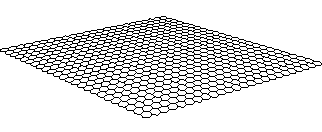
\includegraphics[width=\linewidth]{figures/torus-3d-flat.pdf}
				\caption{}
				\label{fig:torus-3d-flat}
			\end{subfigure}
			~~
			\begin{subfigure}{0.26\linewidth}
				\center
				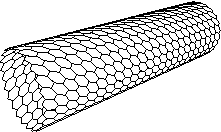
\includegraphics[width=\linewidth]{figures/torus-3d-tube.pdf}
				\caption{}
				\label{fig:torus-3d-tube}
			\end{subfigure}
			~~
			\begin{subfigure}{0.23\linewidth}
				\center
				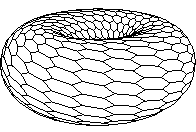
\includegraphics[width=\linewidth]{figures/torus-3d-torus.pdf}
				\caption{}
				\label{fig:torus-3d-torus}
			\end{subfigure}
			
			\caption{Visualisation of a hexagonal torus topology as a torus.}
			\label{fig:torus-3d}
		\end{figure}
		
		The wrap around connections in the topology are what give it the `torus'
		part of its name. Figure~\ref{fig:torus-3d-flat} shows a hexagonal torus
		topology drawn flat as in the previous figure. If the topology is rolled up
		into a tube such that the top and bottom nodes become directly adjacent, a
		tube is formed as in figure~\ref{fig:torus-3d-tube}. This tube can then be
		bent to bring together the nodes at the ends of the tube to form a torus as
		shown in figure~\ref{fig:torus-3d-torus}.
		
		A hexagonal torus topology is typically defined in terms of its width and
		height along the X and Y axes respectively. For example,
		figure~\ref{fig:hexagonalTorusTopology} shows a $10\times10$ hexagonal
		torus.  The nodes in a hexagonal torus topology are addressed using
		hexagonal coordinates of the form $(x, y, z)$ \cite{patel15}. The bottom
		left node (labelled $\alpha$ in the figure) has the coordinate $(0, 0, 0)$
		and other nodes are assigned coordinates according to the number of hops
		along each dimension from $(0, 0, 0)$, for example node $\beta$ has the
		coordinate $(2, 0, -1)$.
		
		Counter intuitively, individual nodes in hexagonal torus topologies may be
		described by many different coordinates, for example $(3, 1, 0)$ and $(1,
		-1, -2)$ are also a valid coordinates for node $\beta$. These dual
		coordinates emerge from the fact that adding $(1, 1, 1)$ to a coordinate
		produces an equivalent, but different, coordinate. This phenomenon is
		explained in detail in appendix~\ref{app:minimal-hex-coordinates} and
		related phenomena will be discussed in chapter~\ref{sec:shortestPaths}.
		
		\begin{figure}
			\center
			\begin{subfigure}[b]{0.32\linewidth}
				\center
				\buildfig{figures/torus-compare-hexagonal.tex}
				
				\caption{Hexagonal}
				\label{fig:torus-compare-hexagonal}
			\end{subfigure}
			\begin{subfigure}[b]{0.32\linewidth}
				\center
				\buildfig{figures/torus-compare-2d.tex}
				
				\caption{2D}
				\label{fig:torus-compare-2d}
			\end{subfigure}
			\begin{subfigure}[b]{0.32\linewidth}
				\center
				\buildfig{figures/torus-compare-3d.tex}
				
				\caption{3D}
				\label{fig:torus-compare-3d}
			\end{subfigure}
			
			\caption{Visual comparison of torus topologies. In all figures, `wrap
			around' connections between nodes at the ends of each axis are omitted
			for clarity.}
			\label{fig:torus-compare}
		\end{figure}
		
		Despite its unusual coordinate system, hexagonal torus topologies compare
		favourably with more conventional network topologies such as 2D and 3D
		toruses (sometimes known as 2-ary $N$-cubes and 3-ary $N$-cubes
		respectively) \cite{dally04} illustrated in figure~\ref{fig:torus-compare}.
		Compared with the 2D torus topology, a hexagonal torus has double the
		bisection bandwidth even though it only requires 50\% more node-to-node
		links \cite{navaridas09}. 3D torus topologies also have six node-to-node
		links per node but double the bisection bandwidth again. However, since a
		network topology must eventually be embedded into a real world data centre
		(which, at large scales, approximate a 2D space), 3D, or higher-dimensional
		torus topologies may become more expensive to construct in practice due to
		the need for longer cables to interconnect nodes. As
		chapter~\ref{sec:building} demonstrates, hexagonal toruses may be assembled
		in a machine room in a similar way to a 2D topology. The hexagonal torus
		topology achieves the scalability of a 2D torus while gaining some of the
		bisection bandwidth benefits of the 3D torus topology.
		
		Most torus topologies, including hexagonal 2D and 3D toruses, are related
		to an equivalent `mesh' topology. Mesh topologies maintain the same general
		connectivity structure as the corresponding torus topology with the
		exception of wrap-around links which are omitted. Omitting wrap-around
		links in practice saves a small number of links at the expense of halving
		the network's bisection bandwidth. As a consequence, mesh topologies are
		rarely used.
		
		\begin{figure}
			\center
			\begin{subfigure}[b]{0.45\linewidth}
				\center
				\buildfig{figures/hexagonal-torus.tex}
				\caption{Hexagonal torus}
				\label{fig:topo-compare-hexagonal-torus}
			\end{subfigure}
			\begin{subfigure}[b]{0.45\linewidth}
				\center
				\buildfig{figures/h-torus.tex}
				\caption{H-torus}
				\label{fig:topo-compare-h-torus}
			\end{subfigure}
			
			\caption{Hexagonal torus vs. H-torus topology. Each numbered hexagon
			represents a node. The thick outline indicates the bounds of the
			topology after which the network repeats. In each topology, the path
			taken by advancing in the Y$^+$ direction from the node labelled `0' is
			shown.}
			\label{fig:topo-compare}
		\end{figure}
		
		The hexagonal torus topology used by SpiNNaker and the subject of much of
		this thesis is not to be confused with the `H-torus' topology.  This
		topology also uses a hexagonal tiling of nodes and even wraps this tiling
		into in a torus-like topology \cite{zhao08}. However, H-torus topologies
		have very different characteristics to the hexagonal torus topology are
		closely related to `twisted torus' topologies \cite{camara10}.
		Figure~\ref{fig:topo-compare} illustrates one major difference in the way
		paths wrap around the peripheries of both topologies.
	
	\section{Scaling-up SpiNNaker machines}
		
		\begin{figure}
			\center
			\begin{subfigure}[b]{0.45\linewidth}
				\center
				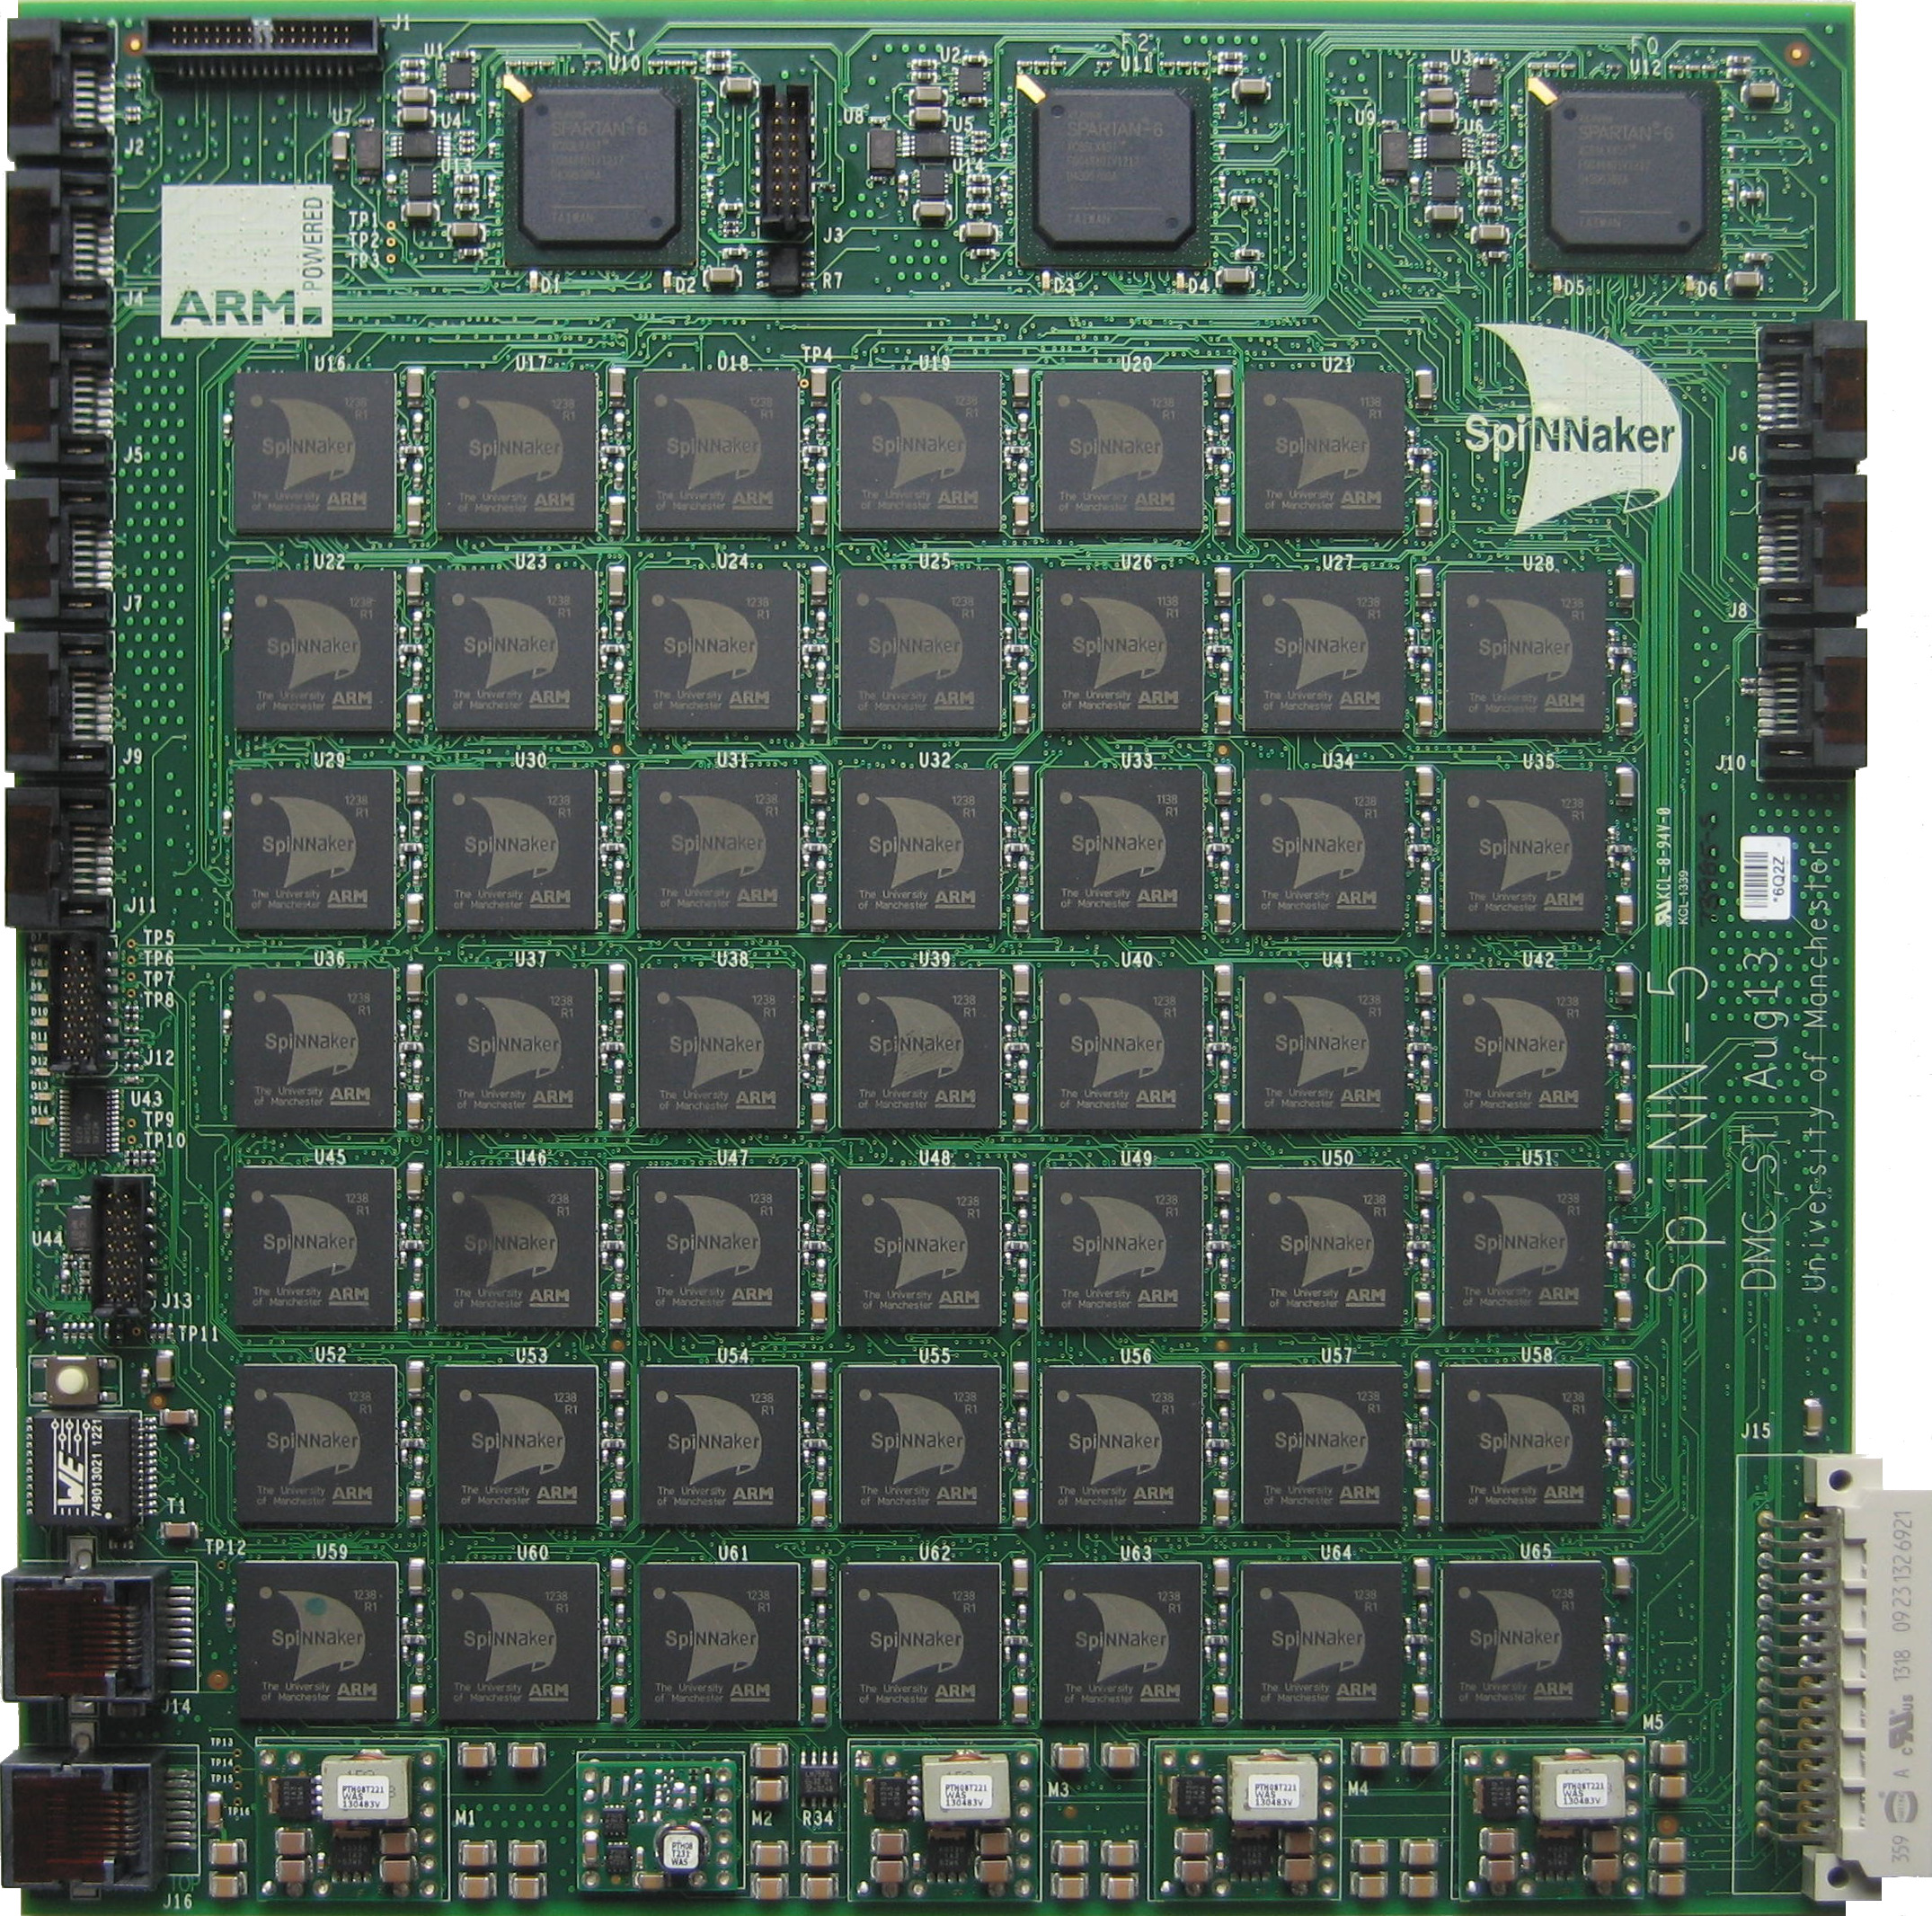
\includegraphics[width=\linewidth]{figures/spinnakerBoard.jpg}
				
				\caption{A SpiNNaker board}
				\label{fig:spinnakerBoard}
			\end{subfigure}
			~~~
			\begin{subfigure}[b]{0.45\linewidth}
				\center
				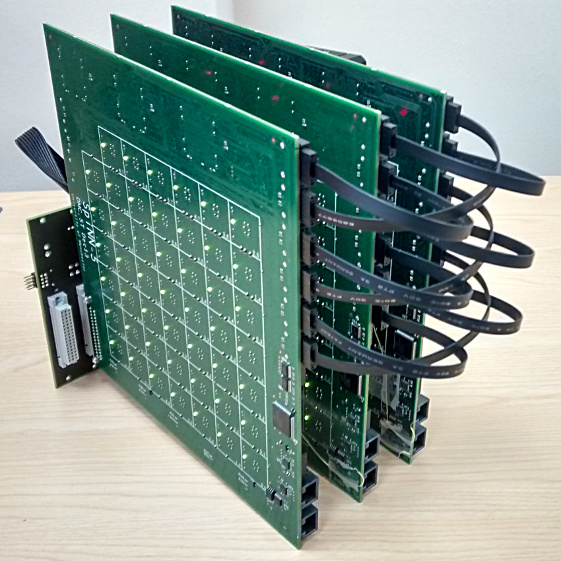
\includegraphics[width=\linewidth]{figures/threeboard.jpg}
				
				\caption{Three board system}
				\label{fig:threeboard}
			\end{subfigure}
			
			\vspace*{2em}
			
			\begin{subfigure}{\linewidth}
				\center
				\buildfig{figures/sata-connections.tex}
				
				\caption{The logical connectivity between chips in multi-board systems.
				Each board's forty-eight chips (drawn here as hexagons) form a wrapped
				triple. Connections between chips on neighbouring boards are
				concentrated onto a single HSS link.}
				\label{fig:sata-connections} \end{subfigure}
			
			\caption{SpiNNaker boards}
			\label{fig:spinnaker-boards}
		\end{figure}
		
		To build large SpiNNaker systems comprising tens of thousands of
		SpiNNaker chips, groups of forty-eight chips are mounted onto printed
		circuit boards as illustrated in figure~\ref{fig:spinnakerBoard}. These
		boards may be connected together to form larger systems.
		Figure~\ref{fig:threeboard} shows a prototype three board system configured
		as a $12\times12$ hexagonal torus.
		
		Though the chips are physically arranged in a (nearly) $7\times7$ grid on
		each SpiNNaker board, they logically form a `wrapped triple', a shape
		described in detail in appendix \ref{sec:partitioning} and illustrated in
		figure~\ref{fig:sata-connections}. Logically, the chips at the periphery of
		each board connect to their neighbours on adjacent boards. Normally
		SpiNNaker chips connect using a low power, asynchronous 2-of-7 protocol
		requiring sixteen wires per bidirectional chip-to-chip link
		\cite{bainbridge03}. If this link technology were used to connect chips on
		neighbouring boards, each pair of boards would need to be connected with a
		128~wire cable. Cables and connectors supporting this may signals are
		expensive and physically large making them unsuitable for use with
		SpiNNaker. Instead, chip-to-chip connections between boards are multiplexed
		and demultiplexed onto a single High-Speed Serial (HSS) link
		\cite{athavale05} carried via commodity S-ATA cables often used to
		connected hard disks in desktop computers and servers \cite{sata3spec}.
		The six high-speed links are implemented by three onboard FPGAs (the three
		large chips at the top of the SpiNNaker board) and are logically
		transparent to the underlying network.
		
		In chapter~\ref{sec:building} I describe how very large SpiNNaker machines
		may be constructed using over one thousand SpiNNaker boards.

	\chapter{Building large SpiNNaker machines}
	
	\label{sec:building}
	
	Like any supercomputer, physically assembling a large SpiNNaker machine
	poses many practical challenges in terms of arranging, installing and
	maintaining the hundreds of metres of network cables required.  For
	conventional architectures and network topologies, techniques are well
	understood and embodied by industry standards such as TAI-942~\cite{tia2006}.
	SpiNNaker's use of the hexagonal torus topology renders existing approaches
	insufficient.
	
	In the first part of this chapter I extend existing techniques for mapping
	network topologies into standard data centre physical infrastructure to
	support the hexagonal torus topology. This mapping is designed to ensure that
	all cables are kept short (under \SI{1}{\meter}) to reduce costs and
	simplify the network hardware required. The techniques described introduce
	little overhead in cable length over existing torus wiring schemes
	and confirm the suitability of the hexagonal torus topology for real-world
	applications.
	
	The second part of this chapter uses SpiNNaker as a case study on the
	suitability of the mappings introduced in this chapter.  In this case study I
	consider various SpiNNaker systems ranging in size from desktop machines to
	multi-cabinet machine room installations. As well as validating the cabling
	schemes introduced in this chapter I also describe a new technique which
	improves the efficiency of the cable installation process.  As a consequence
	of SpiNNaker's fine-grained connectivity, the cabling is unusually dense,
	exacerbating the complexity of the cabling patterns to be installed. By
	exploiting network diagnostics hardware and on-board LEDs to guide cable
	installation, construction of large SpiNNaker machines takes a matter of
	hours rather than the days reported for other architectures. In addition,
	preliminary experiments suggest that neither the maintainability nor cooling
	performance of the system are hampered by the dense cabling employed.
	
	In this chapter, the term \emph{unit} refers to the smallest physical
	component between which network interconnection cables are installed. For
	example, in a SpiNNaker machine a unit is a 48-chip board while in a data
	centre network a unit might be a server blade.
	
	\section{Cabling non-hexagonal torus topologies}
		
		Na\"ive arrangements of torus topologies, hexagonal or otherwise, feature
		physically long `wrap-around' connections which connect units at the
		peripheries of the system. Long connections can be problematic for several
		reasons:
		
		\begin{description}
			
			\item[Performance:] Signal quality diminishes as cables get longer,
			requiring the use of slower signalling speeds, increased error
			correction overhead or more complex hardware.
			
			\item[Energy:] Some energy is lost in cables; longer cables lose more
			signal energy requiring higher drive strengths and/or buffering to
			maintain signal integrity.
			
			\item[Cost:] Shorter cables are cheaper than long ones.  Longer cables
			imply more cabling in a given space making the task of cable installation
			and system maintenance more difficult, increasing labour costs by as much
			as $5\times$~\cite{curtis12}.
			
		\end{description}
		
		In conventional torus topologies, the need for long cables is eliminated by
		folding and interleaving units of the network~\cite[chapter~5]{dally04}.
		This process is illustrated for a 1D torus topology (a ring network) in
		figure~\ref{fig:ring-folding}. A na\"ive arrangement of units in this
		topology results in a long cable connecting the units at the ends of the
		ring (figure~\ref{fig:ring-folding-row}).  To eliminate these long
		connections, half of the units are `folded' on top of the others
		(figure~\ref{fig:ring-folding-folded}) and then this arrangement of units
		is interleaved (figure~\ref{fig:ring-folding-interleaved}). This ordering
		of units requires no long cables while still observing the physical
		constraint that units must be laid out in a line.
		
		\begin{figure}
			\center
			\begin{subfigure}[b]{0.39\linewidth}
				\center
				\buildfig{figures/ring-folding-row.tex}
				\caption{A ring network}
				\label{fig:ring-folding-row}
			\end{subfigure}
			\begin{subfigure}[b]{0.24\linewidth}
				\center
				\buildfig{figures/ring-folding-folded.tex}
				\caption{Folded}
				\label{fig:ring-folding-folded}
			\end{subfigure}
			\begin{subfigure}[b]{0.35\linewidth}
				\center
				\buildfig{figures/ring-folding-interleaved.tex}
				\caption{Folded and interleaved}
				\label{fig:ring-folding-interleaved}
			\end{subfigure}
			
			\caption[Folding and interleaving a ring network.]%
			{Folding and interleaving a ring network to reduce maximum cable
			length.}
			\label{fig:ring-folding}
		\end{figure}
		
		The folding and interleaving process may be extended to $N$-dimensional
		torus topologies by folding each axis in turn. Since all axes are
		orthogonal in non-hexagonal topologies, the folding process only moves
		units along the axis being folded. Due to the non-orthogonality of the
		three axes of the hexagonal torus topology, this type of folding does not
		work. As figure~\ref{fig:failing-to-fold-hex-toruses} illustrates, folding
		along any axis results in connected units on opposing edges not being
		brought together. For example, when folding along the X axis, the two units
		marked with a green circle are moved closer together on the Y axis but
		remain apart on the X axis.
		
		\begin{figure}
			\center
			\begin{subfigure}[b]{0.24\linewidth}
				\center
				\buildfig{figures/failing-to-fold-hex-toruses-none.tex}
				\caption{Not folded}
				\label{fig:failing-to-fold-hex-toruses-none}
			\end{subfigure}
			\begin{subfigure}[b]{0.24\linewidth}
				\center
				\buildfig{figures/failing-to-fold-hex-toruses-x.tex}
				\caption{X}
				\label{fig:failing-to-fold-hex-toruses-x}
			\end{subfigure}
			\begin{subfigure}[b]{0.24\linewidth}
				\center
				\buildfig{figures/failing-to-fold-hex-toruses-y.tex}
				\caption{Y}
				\label{fig:failing-to-fold-hex-toruses-y}
			\end{subfigure}
			\begin{subfigure}[b]{0.24\linewidth}
				\center
				\buildfig{figures/failing-to-fold-hex-toruses-z.tex}
				\caption{Z}
				\label{fig:failing-to-fold-hex-toruses-z}
			\end{subfigure}
			
			\caption[Folding each axis of a hexagonal torus topology.]%
			{Schematics showing folding along each axis of a hexagonal torus topology
			failing to eliminate wrap-around connections.  Same-shaped-and-coloured
			dots show the endpoints of two example wrap-around connections.}
			\label{fig:failing-to-fold-hex-toruses}
		\end{figure}
	
	\section{Partitioning hexagonal torus topologies}
		
		The nodes in supercomputer networks are usually relatively small, for
		example a single chip. Tens of nodes are packed together into a single
		unit, such as a circuit board or server blade, to simplify assembly and
		share common power and cooling resources~\cite{gilge14,ajima12}. In
		commercial supercomputers built on non-hexagonal torus topologies, each
		unit's nodes represent a hypercube partition of the overall topology as
		illustrated in figure~\ref{fig:hypercube-partitioning}
		\cite{chen11,ajima12}.
		
		An analogous `parallelogram' partitioning scheme exists for hexagonal torus
		topologies, however, this results in imbalanced connectivity requirements
		between neighbouring partitions. In
		figure~\ref{fig:parallelogram-partitioning}, for example, the partitions
		above, below, left and right of the central partition are connected by
		seven node-to-node connections each while the partitions above-right and
		below-left are connected by just a single connection each. To simplify
		assembly, connections between all nodes in a pair of neighbouring
		partitions are often made by a single cable. If connectivity requirements
		are imbalanced, as in this example, this may mean multiple connector types
		may be required, increasing design complexity.
		
		To avoid connectivity imbalance, SpiNNaker uses a `wrapped triple'
		partitioning scheme~\cite{davidsonWiring}, as illustrated in
		figure~\ref{fig:wrapped-triple-partitioning} and explained in detail in
		appendix \ref{sec:partitioning}. In this partitioning scheme, the same
		number of connections connect all six neighbouring units. As explained in
		the appendix, a hexagonal torus topology is constructed from groups of
		three partitions.
		
		\begin{figure}
			\center
			\begin{subfigure}[b]{0.32\textwidth}
				\center
				\buildfig{figures/hypercube-partitioning.tex}
				\caption{2D hypercube}
				\label{fig:hypercube-partitioning}
			\end{subfigure}
			\begin{subfigure}[b]{0.32\textwidth}
				\center
				\buildfig{figures/parallelogram-partitioning.tex}
				\caption{Parallelogram}
				\label{fig:parallelogram-partitioning}
			\end{subfigure}
			\begin{subfigure}[b]{0.32\textwidth}
				\center
				\buildfig{figures/wrapped-triple-partitioning.tex}
				\caption{Wrapped triple}
				\label{fig:wrapped-triple-partitioning}
			\end{subfigure}
			
			\caption[Partitioning of torus topologies into units.]%
			{Partitioning of non-hexagonal (a) and hexagonal (b and c) torus
			topologies into units.}
			\label{fig:partitioning-options}
		\end{figure}
		
		For completeness, both parallelogram and wrapped triple partitioning are
		considered in this chapter even though SpiNNaker uses wrapped triple
		partitioning. The parallelogram partitioning scheme may be more appropriate
		for architectures where connections between nodes in neighbouring
		partitions do not share a single connector. In addition, in architectures
		where a unit corresponds to a single node, this can be treated as a $1
		\times 1$ parallelogram partition.  This special case occurs in
		coarse-grained architectures and Networks on Chip (NoCs) where nodes are
		not grouped together into multi-node units.
	
	\section{Folding \& interleaving hexagonal toruses}
		
		To exploit the folding technique used by non-hexagonal topologies, the
		units in a hexagonal torus topology must be mapped into a space with
		orthogonal coordinates. The choice of transformation to an orthogonal
		coordinate system can have an impact on how physically far apart logically
		neighbouring units are in the final arrangement. A good mapping should
		attempt to reduce `distortion' which moves adjacent units apart in the
		final folded and interleaved arrangement.
		
		In this section I propose two transformations which map hexagonal
		arrangements of units into a 2D orthogonal coordinate space. The first
		transformation, `shearing', is general purpose and introduces some
		distortion. The second transformation, `slicing', is less general but can
		introduce less distortion than shearing and therefore may lead to shorter
		cable lengths.
		
		Both the slicing and shearing transformations are carried out in two steps:
		
		\begin{description}
			
			\item[Rectangularisation] Units are transformed from being laid out in a
			parallelogram into a rectangular arrangement. The specific transformation
			used is the key difference between the slicing and shearing
			transformations.
			
			\item[Uncrinkling] Units are mapped into a 2D coordinate system without
			gaps between units.
			
		\end{description}
		
		\subsection{Rectangularisation}
			
			The hexagonal torus topology is illustrated in
			figures~\ref{fig:hex-to-plane-node-native} and
			\ref{fig:hex-to-plane-native} for parallelogram-partitioned units and
			wrapped triple units respectively. The first step in the folding process
			is to rearrange units so that they form a rectangle using one of two
			techniques: shearing or slicing.
			
			\begin{figure}
				\center
				\begin{subfigure}[b]{0.32\linewidth}
					\center
					\buildfig{figures/hex-to-plane-node-native.tex}
					
					\caption{Original}
					\label{fig:hex-to-plane-node-native}
				\end{subfigure}
				\begin{subfigure}[b]{0.32\linewidth}
					\center
					\buildfig{figures/hex-to-plane-node-shear.tex}
					
					\caption{Sheared}
					\label{fig:hex-to-plane-node-shear}
				\end{subfigure}
				\begin{subfigure}[b]{0.32\linewidth}
					\center
					\buildfig{figures/hex-to-plane-node-slice.tex}
					
					\caption{Sliced}
					\label{fig:hex-to-plane-node-slice}
				\end{subfigure}
				
				\caption[Rectangularisation of parallelogram partitioned toruses.]%
				{Rectangularisation of parallelogram partitioned hexagonal
				toruses. Thin lines show wrap-around links. Pointy-topped hexagons
				represent parallelogram partitioned units.}
				\label{fig:hex-to-plane-node}
				
				% XXX: Force these figures together.
				
				%\end{figure}
				%
				%\begin{figure}
				
				\center
				\begin{subfigure}[b]{0.32\linewidth}
					\center
					\buildfig{figures/hex-to-plane-native.tex}
					
					\caption{Original}
					\label{fig:hex-to-plane-native}
				\end{subfigure}
				\begin{subfigure}[b]{0.32\linewidth}
					\center
					\buildfig{figures/hex-to-plane-shear.tex}
					
					\caption{Sheared}
					\label{fig:hex-to-plane-shear}
				\end{subfigure}
				\begin{subfigure}[b]{0.32\linewidth}
					\center
					\buildfig{figures/hex-to-plane-slice.tex}
					
					\caption{Sliced}
					\label{fig:hex-to-plane-slice}
				\end{subfigure}
				
				\caption[Rectangularisation of wrapped triple partitioned toruses.]%
				{Rectangularisation of wrapped triple partitioned hexagonal
				toruses. Thin lines show wrap-around links.  Flat-topped hexagons
				represent wrapped triple partitioned units.}
				\label{fig:hex-to-plane}
				
				% And force these together!
				
				%\end{figure}
				%
				%\begin{figure}
				
				\center
				\begin{subfigure}[b]{0.3\linewidth}
					\center
					\buildfig{figures/slicing-examples-5x5.tex}
					\caption{$5\times5$}
				\end{subfigure}
				\begin{subfigure}[b]{0.3\linewidth}
					\center
					\buildfig{figures/slicing-examples-5x7.tex}
					\caption{$5\times7$}
				\end{subfigure}
				\begin{subfigure}[b]{0.3\linewidth}
					\center
					\buildfig{figures/slicing-examples-5x10.tex}
					\caption{$5\times10$}
				\end{subfigure}
				
				\caption[Patterns of wrap-around connections in sliced systems.]%
				{Schematics showing the patterns of wrap-around connections in sliced
				systems of various aspect ratios.}
				\label{fig:slicing-examples}
			\end{figure}
			
			The shearing technique applies a \SI{30}{\degree} shear transformation to
			distort the arrangement of units so that the X and Y axes of the
			hexagonal torus topology become orthogonal. This transformation leads to
			a rectangular arrangement of units as illustrated in figures
			\ref{fig:hex-to-plane-node-shear} and \ref{fig:hex-to-plane-shear}.
			
			The shear transformation introduces some distortion causing connections
			between units in the Z axis to become $\sqrt{2} \times$ longer. The
			transformation does not alter the pattern of wrap-around connections:
			long connections between units on the extreme left and right sides and
			the top and bottom remain, along with a single connection between the
			bottom left and top right units.
			
			The slice transformation aims to avoid the elongation of the Z axis by
			moving the units without distorting their layout. Units protruding from
			the left-hand-side of the parallelogram are `sliced off' and moved into
			the matching gap on the opposite side as illustrated in figures
			\ref{fig:hex-to-plane-node-slice} and \ref{fig:hex-to-plane-slice}. This
			transformation does not introduce any distortion but changes the pattern
			of wrap-around connections. Connections from left-to-right remain while
			the connections between the top and bottom units now criss-cross
			(figure~\ref{fig:slicing-examples}).  The proportion of connections going
			from bottom-left to top-right and from bottom-right to top-left varies
			depending on the aspect ratio of the topology. Only certain patterns of
			wrap-around links can be eliminated by folding and, as we shall see
			later, this limits us in which network topologies can be rectangularised
			by slicing.
			
		\subsection{Uncrinkling}
			
			Before folding can occur, the rectangularised arrangements of units
			produced in the previous step must be mapped into a 2D grid. Applied to
			parallelogram partitions, the shear transformation results in a mapping
			into a 2D grid with no further distortion
			(figure~\ref{fig:uncrinkling-node-sheared}). For other combinations of
			transformation and partitioning scheme, the units do not exactly fit a 2D
			grid. Instead, the units form `crinkled' rows or columns which may be
			`uncrinkled' (straightened out) to fit a regular 2D grid as illustrated in
			figures~\ref{fig:uncrinkling-node-sliced}~--~\ref{fig:uncrinkling-sliced}.
			
			\begin{figure}
				\center
				\begin{subfigure}[b]{0.48\linewidth}
					\center
					\buildfig{figures/uncrinkling-node-sheared.tex}
					
					\caption{Parallelogram units, sheared}
					\label{fig:uncrinkling-node-sheared}
				\end{subfigure}
				\begin{subfigure}[b]{0.48\linewidth}
					\center
					\buildfig{figures/uncrinkling-node-sliced.tex}
					
					\caption{Parallelogram units, sliced}
					\label{fig:uncrinkling-node-sliced}
				\end{subfigure}
				
				\vspace{1cm}
				
				\begin{subfigure}[b]{0.48\linewidth}
					\center
					\buildfig{figures/uncrinkling-sheared.tex}
					
					\caption{Wrapped triple units, sheared}
					\label{fig:uncrinkling-sheared}
				\end{subfigure}
				\begin{subfigure}[b]{0.48\linewidth}
					\center
					\buildfig{figures/uncrinkling-sliced.tex}
					
					\caption{Wrapped triple units, sliced}
					\label{fig:uncrinkling-sliced}
				\end{subfigure}
				
				\vspace{1em}
				
				\caption[Uncrinkling units into a 2D grid.]%
				{Uncrinkling rectangularised arrangements of units into a 2D
				grid. Thick lines show how crinkled rows and columns of units are
				uncrinkled.  Annotations show how the relative positions of units
				change after uncrinkling.}
				\label{fig:uncrinkling}
			\end{figure}
			
			%% XXX: Does this make things clearer or not?
			%In the figure, the labels show the positions of individual units before
			%and after uncrinkling. We will use these later in \S\ref{sec:distortion}
			%to calculate the overhead introduced by uncrinkling.
		
		\subsection{Folding}
			
			\begin{figure}
				\begin{subfigure}{\linewidth}
					\center
					\buildfig{figures/folding-sheared.tex}
					\caption{Sheared systems and $1:2$ sliced systems}
					\label{fig:folding-sheared}
				\end{subfigure}
				
				\vspace{1em}
				
				\begin{subfigure}{\linewidth}
					\center
					\buildfig{figures/folding-sliced.tex}
					\caption{$1:1$ sliced systems}
					\label{fig:folding-sliced}
				\end{subfigure}
				
				\caption[Elimination of long wrap-around links by folding.]%
				{Schematic illustrating elimination of long wrap-around links
				during folding. In each example a single link has been highlighted to
				aid in following the process.}
				\label{fig:folding}
			\end{figure}
			
			Once a regular 2D grid of units has been formed, this may be folded in
			the conventional way as illustrated in figure~\ref{fig:folding-sheared}.
			Folding once along each axis eliminates long connections crossing from
			left-to-right, top-to-bottom and from the bottom-left corner to the
			top-right corner. Any shear-transformed network may be folded this way
			since its wrap-around connections always follow this pattern.
			Slice-transformed networks may only be folded like this when their aspect
			ratio is $1:2$ when the pattern of wrap-around links is the same as a
			shear-transformed network.
			
			When `square' networks (i.e. those with a $1:1$ aspect ratio) are sliced,
			the network must be folded \emph{twice} along the Y axis as in
			figure~\ref{fig:folding-sliced} to eliminate the criss-crossing
			wrap-around links. It is not possible to eliminate wrap-around links from
			sliced networks with other aspect ratios by folding.
			
			After folding, the units are interleaved, yielding a 2D arrangement of
			units in which no connection spans the width or height of the system. The
			maximum connection distance is constant for any network allowing the
			topology to scale up.
		
		\subsection{Choosing a transformation}
			
			\label{sec:distortion}
			
			In each step of the transformation from hexagonal torus to a folded and
			interleaved 2D grid, the distances between connected units may increase.
			When designing a system, the transformation with the least distortion
			should be used to minimise the average length of the cables required.
			
			By referring to figure~\ref{fig:uncrinkling} (page
			\pageref{fig:uncrinkling}), it is possible to calculate the overhead
			introduced by each type of transformation.  For example, to compute the
			overhead introduced by the slicing transformation when applied to units
			composed of wrapped triples we consider
			figure~\ref{fig:uncrinkling-sliced}. The uncrinkling pattern used to
			transform this topology is a repeating pattern of two units, a pair of
			which have been labelled $1$ and $2$ respectively. Unit $1$ is
			immediately surrounded by the six units labelled $a$, $b$, $c$, $2$, $g$
			and $h$. Unit $2$ is surrounded by the units $1$, $c$, $d$, $e$, $f$ and
			$g$.  Before the transformation, the distance between units is $1$; after
			the transformation is applied this is not always the case. Folding and
			interleaving into $f_x$ columns and $f_y$ rows also introduces overhead.
			For each pair of previously neighbouring units in the example, their
			distances after folding may be computed as follows:
			
			\begin{equation*}
				\begin{aligned}[c]
					D_{1\,\leftrightarrow{}\,a} &= \sqrt{f_x^2 + f_y^2} \\
					D_{1\,\leftrightarrow{}\,b} &= f_y \\
					D_{1\,\leftrightarrow{}\,c} &= \sqrt{f_x^2 + f_y^2} \\
					D_{1\,\leftrightarrow{}\,2} &= f_x \\
					D_{1\,\leftrightarrow{}\,g} &= f_y \\
					D_{1\,\leftrightarrow{}\,h} &= f_x
				\end{aligned}
				\hspace{2cm}
				\begin{aligned}[c]
					D_{2\,\leftrightarrow{}\,1} &= f_x \\
					D_{2\,\leftrightarrow{}\,c} &= f_y \\
					D_{2\,\leftrightarrow{}\,d} &= f_x \\
					D_{2\,\leftrightarrow{}\,e} &= \sqrt{f_x^2 + f_y^2} \\
					D_{2\,\leftrightarrow{}\,f} &= f_y \\
					D_{2\,\leftrightarrow{}\,g} &= \sqrt{f_x^2 + f_y^2}
				\end{aligned}
			\end{equation*}
			
			From these values, mean and maximum connection distances may be
			calculated. The expressions for each combination of partitioning scheme
			and transformation are as follows:
			
			\begin{align*}
				D_{\textrm{mean}}=&
					\begin{cases}
						\frac{7f_x + 3\sqrt{f_x^2 + f_y^2} + \sqrt{(2f_x)^2 + f_y^2}}{9} &
							\textrm{if sheared wrapped triple units}\\
						\frac{f_x + f_y + \sqrt{f_x^2 + f_y^2}}{3} &
							\textrm{otherwise}\\
					\end{cases} \\
				D_{\textrm{max}}=&
					\begin{cases}
						\sqrt{(2f_x)^2 + f_y^2} &
							\textrm{if sheared wrapped triple units}\\
						\sqrt{f_x^2 + f_y^2} &
							\textrm{otherwise}
					\end{cases}
			\end{align*}
			
			\begin{table}
				\center
				\begin{tabular}{lcc}
					\toprule
					                                 & $1:2$  & Other \\
					\addlinespace
					\multirow{2}{*}{Parallelogram}   & \textbf{Either} & \textbf{Shear}\\
					                                 & \footnotesize $D_\textrm{mean}\approx2.28 \quad D_\textrm{max}\approx2.83$
					                                 & \footnotesize $D_\textrm{mean}\approx2.28 \quad D_\textrm{max}\approx2.83$\\
					\addlinespace
					\multirow{2}{*}{Wrapped triples} & \textbf{Slice}  & \textbf{Shear}\\
					                                 & \footnotesize $D_\textrm{mean}\approx2.28 \quad D_\textrm{max}\approx2.83$
					                                 & \footnotesize $D_\textrm{mean}\approx3.00 \quad D_\textrm{max}\approx4.47$\\
					\bottomrule
				\end{tabular}
				
				\caption{Recommended transformations for folding hexagonal toruses.}
				\label{tab:transform-recommended}
			\end{table}
			
			Using these formulae it is possible to determine which approach --
			shearing or slicing -- results in the lowest mean and maximum cable
			lengths and thus which technique should be used. This is summarised in
			table~\ref{tab:transform-recommended}.
	
	\section{A SpiNNaker case study}
		
		As the only known large-scale hexagonal torus-based architecture, SpiNNaker
		is a good case study for the techniques described in this chapter.  Each
		unit in a SpiNNaker machine is a 48-chip SpiNNaker board forming a
		wrapped triple partition. Systems of various sizes have been constructed
		using the techniques introduced in this chapter ranging from twenty-four
		board `portable' systems to a five cabinet, half-million core installation
		with plans in place to build a machine of twice this size in the future.
		
		In this section I describe how the folded and interleaved arrangement of
		units produced by the techniques in the previous chapter may be translated
		into physical arrangements of SpiNNaker boards in a machine room. I then
		describe how the thousands of S-ATA cables are installed and report on the
		maintainability and cooling impact of this cabling scheme in practice.
		
		\subsection{Mapping into physical cabinets}
			
			In SpiNNaker systems, the physical architecture used is illustrated in
			figure~\ref{fig:cabinet-units}. SpiNNaker boards are installed into card
			frames containing twenty four boards each. Five frames are mounted into
			standard, \SI{600}{\milli\meter}~wide 19\inch{} cabinets with further
			cabinets being added, arranged in a row, to scale the system up. The 2D
			grid of units produced by the folding process described in this chapter
			is mapped to cabinets and frames as illustrated in
			figure~\ref{fig:cabinetisation}.
			
			\begin{figure}
				\center
				\buildfig{figures/cabinet-units.tex}
				
				\caption{Physical architecture of a SpiNNaker machine.}
				\label{fig:cabinet-units}
			\end{figure}
			
			\begin{figure}
				\center
				\buildfig{figures/cabinetisation.tex}
				
				\caption[Mapping cabling from abstract to physical space.]%
				{Mapping from the abstract folded and interleaved 2D grid
				layout into physical cabinet and frame positions. Arrows indicate the
				order in which units (boards) are mapped into each frame, from
				left-to-right.}
				\label{fig:cabinetisation}
			\end{figure}
			
			Figure~\ref{fig:million-core-machine} shows the cabling plan for the
			largest planned SpiNNaker machine. This system will fill ten 19\inch{}
			cabinets and implement a $240 \times 240$ hexagonal torus topology
			partitioned between \num{1200} 48 chip SpiNNaker boards. The largest gap
			to be spanned by any cable is \SI{66}{\centi\meter}, well within the
			\SI{1}{\meter} limit on SpiNNaker's interconnect technology.
			
			\begin{figure}
				\center
				\buildfig{figures/million-core-machine.tex}
				
				\caption[Cabling plan for a \num{1200}~board SpiNNaker machine.]%
				{Cabling plan for a \num{1200}~board (\num{1036800}~core)
				SpiNNaker machine.}
				\label{fig:million-core-machine}
			\end{figure}
			
		\subsection{Cable selection and routing}
			
			Because of the dense packing of SpiNNaker boards, cables span short
			distances as shown in figure~\ref{fig:wire-length-histogram}.
			Conventional cable management techniques (e.g. cable trays) are not
			practical. To ensure the reliability and maintainability of SpiNNaker's
			wiring, cable slack must be carefully controlled.  If cables are too
			tight, cables, connectors and SpiNNaker boards can become damaged. When
			cables are too slack, the excess obstructs access to the machine and can
			easily become tangled \cite{cisco07}.
			
			In this case study the `rule of (three-)thumbs' proposed by
			Mazaris~\cite{mazaris97} is used which suggests that a minimum of
			\SI{5}{\centi\meter} of slack be provided. As SpiNNaker uses
			off-the-shelf S-ATA cables, only standard lengths of cable are available.
			For any given span, the shortest length of cable providing at least
			\SI{5}{\centi\meter} of slack is used.
			
			\begin{figure}
				
				\center
				\buildfig{figures/wire-length-histogram.tex}
				
				\caption[Cable lengths in a \num{1200}~board SpiNNaker machine.]%
				{Histogram of connection distances in a \num{1200} board SpiNNaker
				machine annotated with the selected cable lengths.}
				\label{fig:wire-length-histogram}
				
			\end{figure}
		
		\subsection{Installation practicality}
			
			\begin{figure}
				\center
				\begin{subfigure}[t]{0.5\textwidth}
					\begin{tikzpicture}
						\node (cables) [inner sep=0]
						      {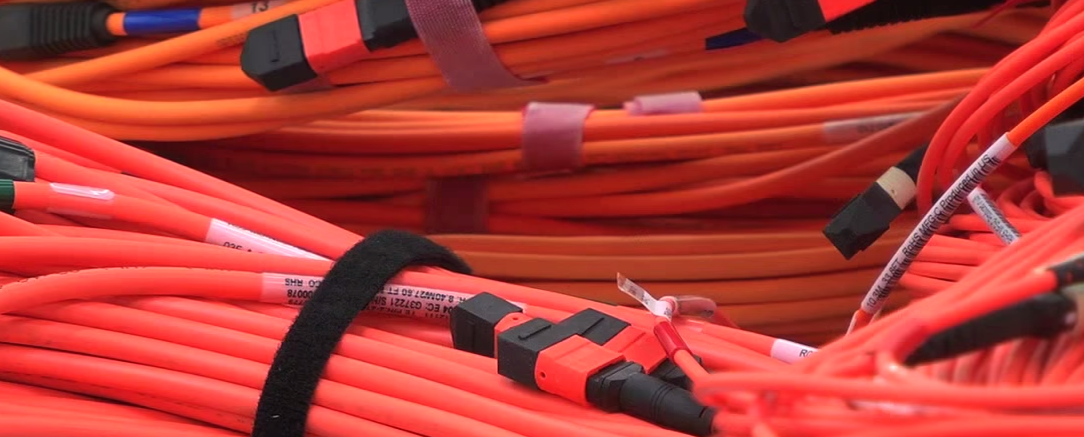
\includegraphics[width=\textwidth]{figures/bgCables.png}};
						\node (sockets) [inner sep=0, below=1.0em of cables]
						      {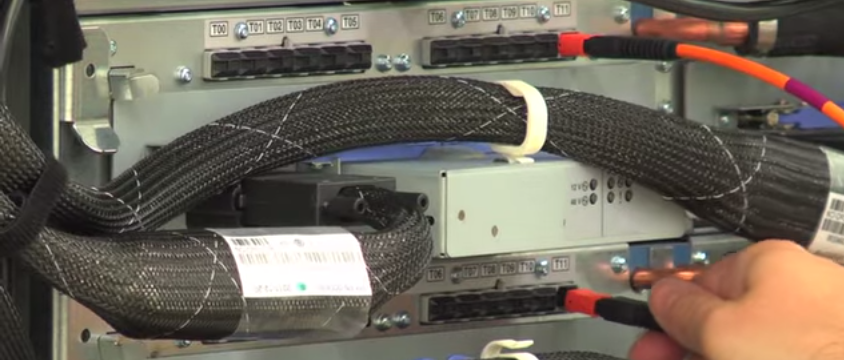
\includegraphics[width=\textwidth]{figures/bgSockets.png}};
						
						% Point at label on cable
						\draw [white, <-, line width=0.4em]
						      ([shift={(0.7cm, -0.3cm)}]cables.center)
						      -- ++(45:1cm);
						
						% Point at label on socket
						\draw [white, <-, line width=0.4em]
						      ([shift={(-1.0cm, 1.1cm)}]sockets.center)
						      -- ++(-45:1cm);
					\end{tikzpicture}
					
					\caption{Pre-labelled cables and sockets}
					\label{fig:bgWiringLabels}
				\end{subfigure}
				~
				\begin{subfigure}[t]{0.30\textwidth}
					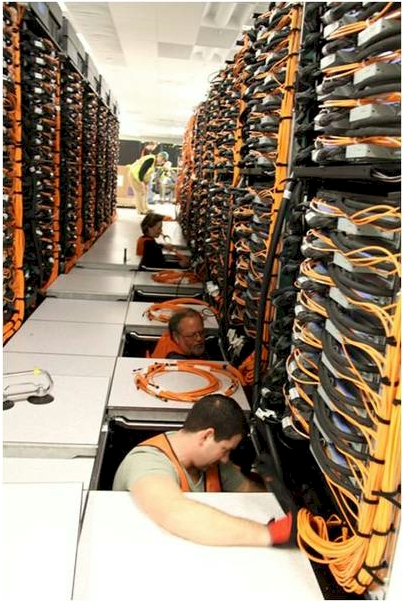
\includegraphics[height=6.15cm]{figures/bgWiring.jpg}
					
					\caption{Installation of cables}
					\label{fig:bgWiringInstallation}
				\end{subfigure}
				
				\caption[BlueGene/Q cable installation.]%
				        {BlueGene/Q cable installation~\cite{cscs13}.}
				\label{fig:bgWiring}
			\end{figure}
			
			In other large-scale architectures, the task of cable installation is
			completed by a team of technicians aided by the use of standardised
			labelling for cables and sockets as illustrated in
			figure~\ref{fig:bgWiring}~\cite{tia2006}. In these architectures the
			cabling patterns required are relatively straightforward, thanks to the
			coarseness of the units used~\cite{lakner07} or they use network
			topologies whose cabling centres around high-fan-in
			switches~\cite{cisco07,csernai15}.
			
			It has been reported in the literature that when copper cables are used,
			labour costs dominate~\cite{popa10} and while cable costs are expected to
			decline, labour costs are not~\cite{mudigonda11}. Many researchers have
			attempted to control cable installation costs by trying to reduce the
			number or length of cables required by developing alternative network
			topologies~\cite{curtis12, popa10, mudigonda11}.  Unfortunately, these
			techniques do not apply to SpiNNaker since its network topology is fixed.
			
			Supercomputer architectures such as BlueGene/Q make use of large custom
			`midplane' PCBs in place of some cables to interconnect units within a
			cabinet~\cite{milano13}. This scheme can greatly reduce wiring complexity
			since only coarser-grain, cabinet-to-cabinet connectivity is implemented
			by cables. Unfortunately this technique is expensive and constrains the
			dimensions of the network topology supported by the machine. Since the
			SpiNNaker platform is designed to scale from desktop machines to
			machine room installations, this scheme is not practical.
			
			\begin{figure}
				\center
				\begin{subfigure}[b]{0.40\textwidth}
					\begin{tikzpicture}
						\node (leds) [inner sep=0]
						      {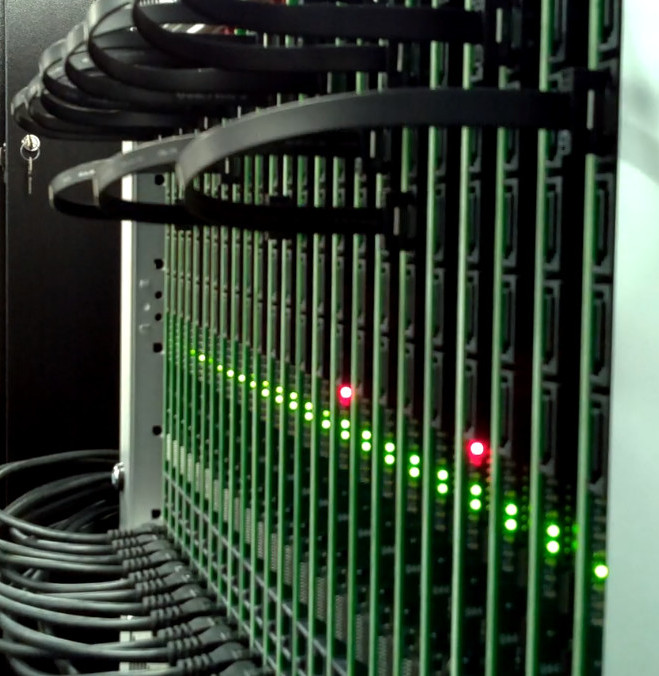
\includegraphics[width=\textwidth]{figures/leds.jpg}};
						% Point at left LED
						\draw [white, <-, line width=0.4em]
						      ([shift={(-0.0cm, -0.6cm)}]leds.center)
						      -- ++(225:1cm);
						% Point at right LED
						\draw [white, <-, line width=0.4em]
						      ([shift={(1.1cm, -1.1cm)}]leds.center)
						      -- ++(225:1cm);
					\end{tikzpicture}
					
					\caption{Diagnostic LEDs indicate the endpoints of each cable.}
					\label{fig:interactive-wiring-guide-leds}
				\end{subfigure}
				~
				\begin{subfigure}[b]{0.546\textwidth}
					\begin{tikzpicture}[thin, black!20!white]
						\node (screen) [inner sep=0]
						      {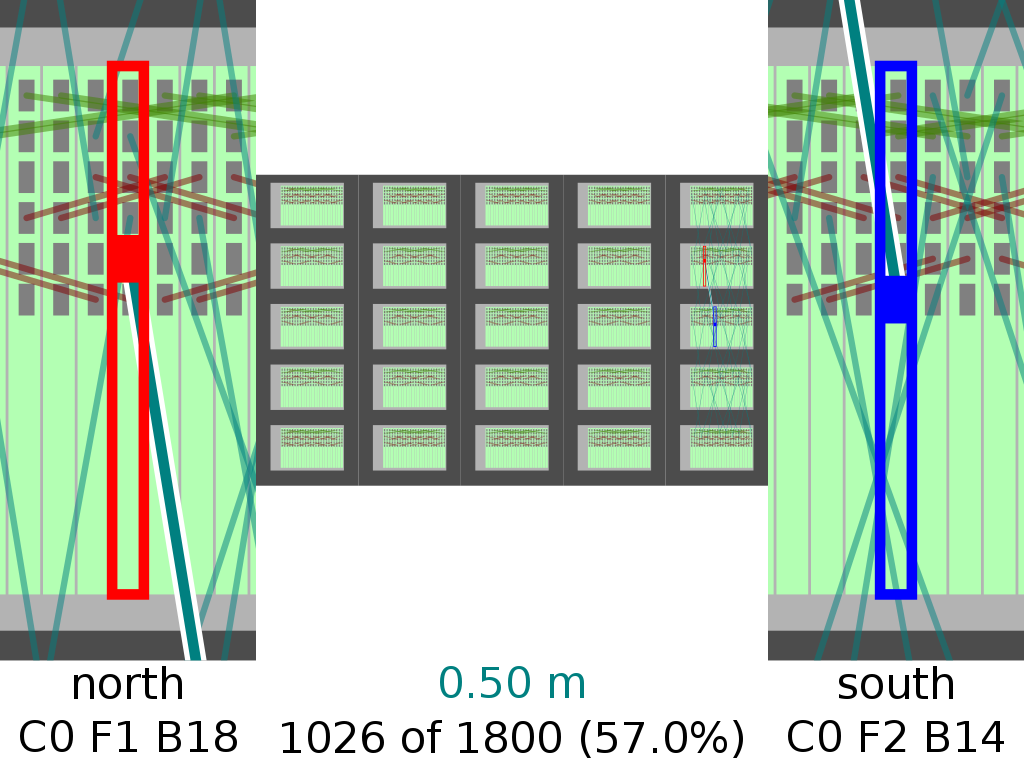
\includegraphics[width=\textwidth]{figures/wiring_guide_screenshot.png}};
						\draw (screen.south west) rectangle (screen.north east);
					\end{tikzpicture}
					
					\caption{A GUI and text-to-speech indicate what type of cable to
					install.}
					\label{fig:interactive-wiring-guide-gui}
				\end{subfigure}
				
				\caption{Interactive software guides cable installation.}
				\label{fig:interactive-wiring-guide}
			\end{figure}
			
			Due to the high density of units in a SpiNNaker system, the detailed
			cabling patterns used can be complex, despite their overall regularity.
			To cope with this complexity, I developed a software system which employs
			diagnostic hardware built into SpiNNaker, to guide technicians through
			the cable installation process. As shown in
			figure~\ref{fig:interactive-wiring-guide}, diagnostic LEDs on each
			SpiNNaker board are used to indicate which boards to connect. The
			software also provides step-by-step cabling instructions via a Graphical
			User Interface (GUI) and audible instructions delivered via headphones.
			These instructions explicitly specify the length of cable to use for each
			connection avoiding the common problem of technicians over-estimating the
			cable length required~\cite{mazaris97}. Diagnostic registers in the
			network hardware are then used to verify the correct installation of each
			cable in real-time ensuring that mistakes are highlighted and fixed
			immediately.
			
			\begin{table}
				\center
				\begin{tabular}{lrll}
					\toprule
						Size & Cables & Time & Notes \\
					\midrule
						24 boards  & \num{72}   & \SI{10}{\minute} & \\
						1 cabinet  & \num{360}  & \SI{4}{\hour} &
							Real-time validation not used. \\
						2 cabinets & \num{720}  & \SI{2}{\hour} & \\
						5 cabinets & \num{1800} & \SI{4}{\hour} \SI{20}{\minute} &
							Three people working simultaneously. \\
					\bottomrule
				\end{tabular}
				
				\caption[Cable installation times for various SpiNNaker machines.]%
				{Cable installation times for various sizes of SpiNNaker
				machine.}
				\label{tab:install-time}
			\end{table}
			
			\begin{figure}
				\buildfig{figures/install-histogram.tex}
				
				\caption{Two cabinet SpiNNaker machine cable installation times.}
				\label{fig:install-histogram}
			\end{figure}
			
			Table~\ref{tab:install-time} shows cable installation times for various
			sizes of SpiNNaker system. The times reported do not include breaks and,
			with the exception of the five cabinet system, are for the one person
			working alone.  Figure~\ref{fig:install-histogram} shows the histogram of
			cable installation times for a two cabinet machine.  These results
			confirm the observation by Mudigonda \emph{et al.} that cables which span
			cabinets and frames take longer to install~\cite{mudigonda11}, even
			though these distances are still very short in SpiNNaker. Compared with
			commercial installation efforts, per-cable installation times are much
			shorter for SpiNNaker taking seconds compared with minutes in other
			architectures~\cite{mudigonda11}.
			
			The positive impact of real-time validation of installed cables can
			clearly be seen by comparing the installation times of the one and two
			cabinet systems. Though double the size, the two cabinet machine was
			built in half the time required to build the single cabinet machine.
			While building the smaller machine, real-time cable validation had not
			yet been implemented and the installation process was interrupted for
			several minutes every time a misplaced connection was discovered.
			
			In the three-person cable installation effort employed for the five
			cabinet system, the guidance software was configured to assign each
			technician cables in non-overlapping parts of the machine ensuring
			minimal interference between the technicians. As expected, this renders
			the problem embarrassingly parallel, as in commercial computer
			installations.
			
			\begin{figure}
				\center
				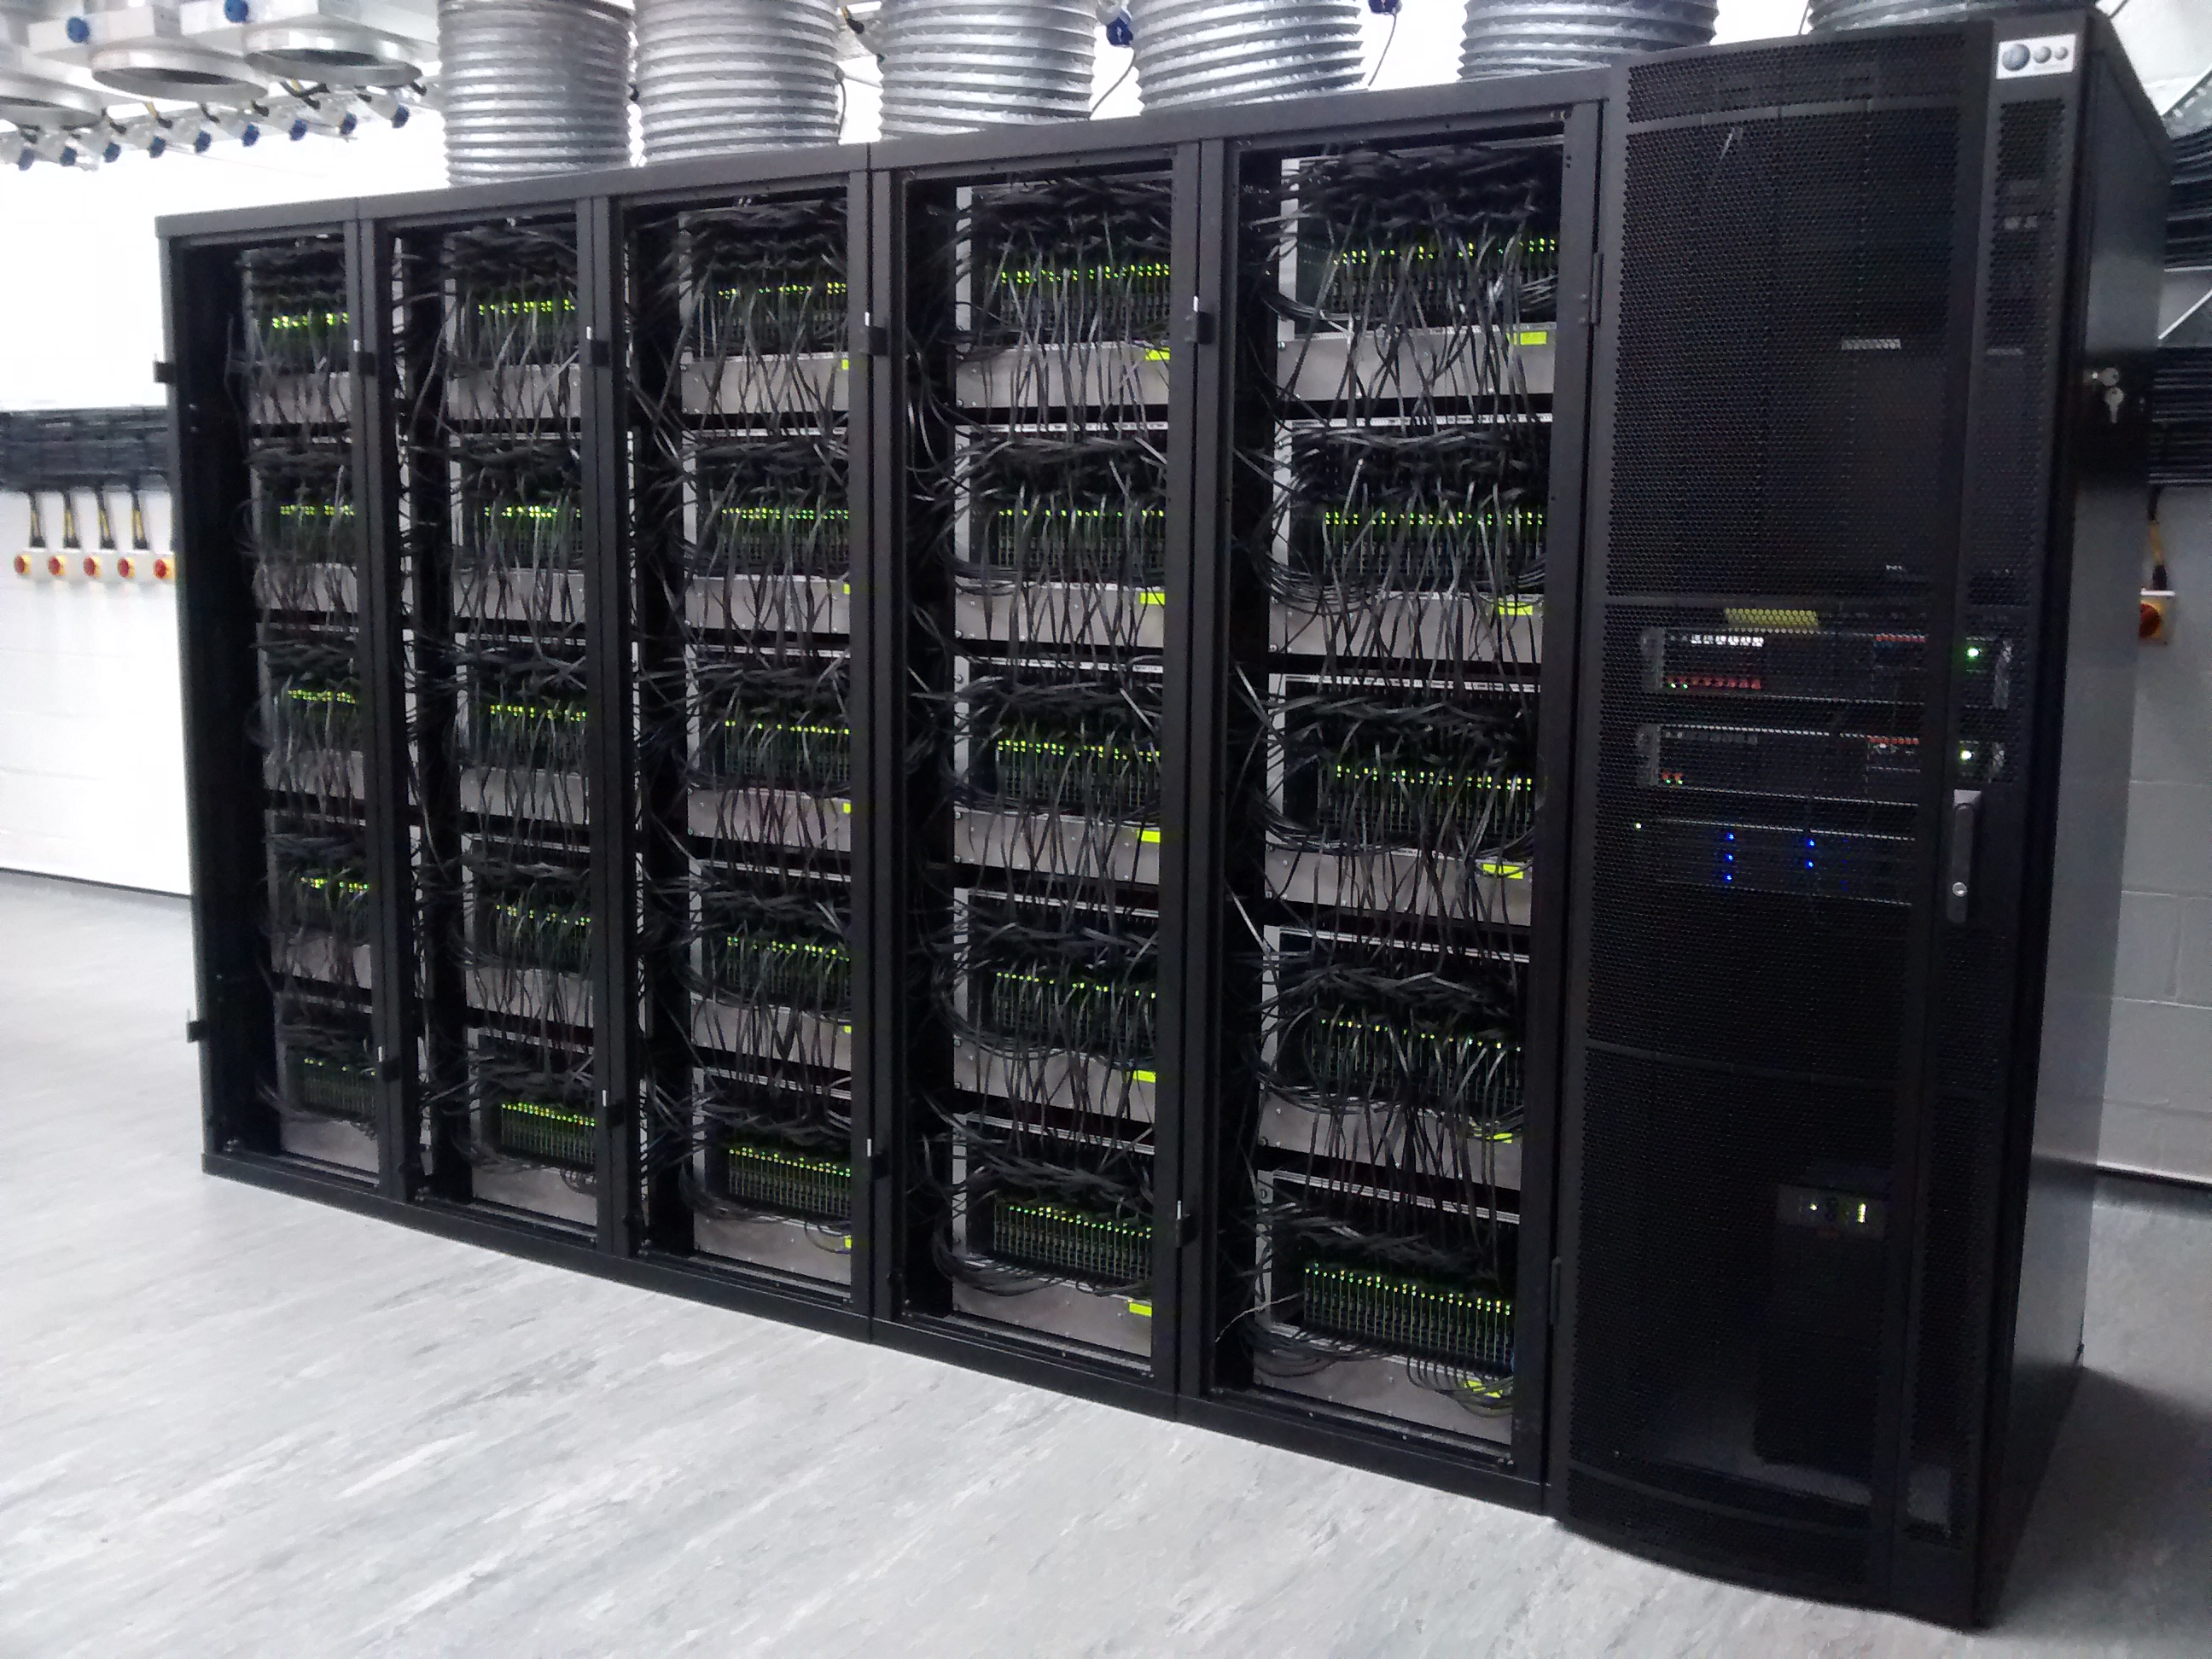
\includegraphics[width=0.8\linewidth]{figures/halfMillionCoreComplete.jpg}
				
				\caption[The five cabinet SpiNNaker system.]%
				{The five cabinet SpiNNaker system. The cabinet on the right contains
				conventional host servers which control SpiNNaker.}
				\label{fig:halfMillionCoreComplete}
			\end{figure}
			
			The completed five cabinet system is photographed in
			figure~\ref{fig:halfMillionCoreComplete}. A time-lapse video showing the
			construction and cable installation of this machine is also available on
			YouTube~\cite{heathcote16}.
			
		\subsection{Thermal implications}
			
			In large SpiNNaker machines, each 24 board frame contains a fan tray
			which pulls cool air from the front of the frame, between the SpiNNaker
			boards. The warmed air is then ejected out of the rear of the frame where
			ducting directs it into industrial air chillers. Conventional guidance on
			data centre design suggests that routing cables in the path of the
			system's airflow can have a serious impact on cooling
			performance~\cite{cisco07}.  To determine what effect the cabling
			described in this chapter had on SpiNNaker's cooling, a test program was
			executed to simulate heavy load before and after cable installation. The
			temperatures reported by the sensors on the top of each SpiNNaker board
			were sampled at regular intervals and once the overall system temperature
			stabilised, the mean temperature was recorded.
			
			Before the cabling was installed, the temperature stabilised at
			\SI{49}{\celsius} while after installation it stabilised at
			\SI{42}{\celsius}.
			
			These two data points suggest that the system's temperature is unlikely
			to have been been seriously impacted by cable installation. Since the two
			experiments were run on different days (with potentially different
			ambient temperatures) and are based on a single experiment, it is not
			possible to infer much more from this result.
			
		\subsection{Maintenance}
			
			At the time of writing, the five cabinet machine is still being
			commissioned and so the long term maintenance impact of the system's
			cabling is not known. One important factor in the maintainability of the
			system is the ease with which faulty boards can be replaced. During
			commissioning a number of boards have been replaced by someone not
			involved in the machine's installation. Informal measurements suggest
			that boards near the centre of a frame (i.e. those most likely to be
			blocked by unrelated cables) take around ten minutes to replace,
			including time spent removing and replacing cables obstructing the board
			being exchanged. By comparison boards at the edge of the machine take
			around six minutes to replace. Though similar timing reports are
			unavailable for other architectures, these times appear reasonable in
			practice and suggest maintenance is not impaired by the wiring plan used.
	
	\section{Conclusions}
		
		In this chapter I presented a practical method of constructing real-world
		installations of large hexagonal torus topologies such that long cables
		spanning the width and height of the system are not required. Two
		transformations, shearing and slicing, are presented which allow
		conventional network folding techniques to be applied to hexagonal toruses
		to eliminate long `wrap around' links. Though both techniques incur some
		overhead in terms of mean and maximum cable length, the maximum cable
		length does not grow with the size of the network. This result makes
		hexagonal torus topologies a practical and scalable choice for future
		systems.
		
		The theoretical results presented in this chapter have been confirmed
		through the successful construction of several large-scale SpiNNaker
		machines which implement hexagonal torus topologies. During construction,
		diagnostic features of SpiNNaker's hardware were employed to guide
		technicians performing cable installation. This technique was found to be
		highly effective with cable installation times measured in seconds rather
		than minutes as reported for other architectures. Surprisingly there was no
		evidence found of this technique being applied to other architectures and
		consequently this secondary result may be of interest for future research.

	\chapter{Finding shortest path vectors in SpiNNaker's network}
	
	\label{sec:shortestPaths}
	
	% XXX: Add note explaining shortest path between two points in non-torus
	% space.
	
	In the previous chapter we explored the practical challenges of building
	machines which use hexagonal torus topologies working at the scale of units
	containing several nodes. To exploit these machines, however, we must also be
	able to route packets efficiently through the nodes in the resulting network.
	This chapter tackles the problem of finding shortest path vectors in
	hexagonal torus topologies. Shortest path vectors are used by many routing
	algorithms as the basis for route generation. In non-hexagonal torus
	topologies, finding shortest path vectors is trivial and intuitive but in
	hexagonal toruses, this is not the case.  In this chapter I introduce the
	Irregular Quadrant (IQ) method, a new technique for computing shortest path
	vectors in hexagonal torus topologies.  This method is cheaper to compute and
	more general than pre-existing techniques, functioning correctly on hexagonal
	torus topologies of any aspect ratio.
	
	In some hexagonal torus topologies, many shortest path vectors may exist
	between a given pair of points. I propose a technique for discovering all
	possible shortest path vectors. Using these alternative shortest path
	vectors, routing algorithms may be able to produce routes which load a
	network more evenly.
	
	In this chapter, I assume an idealised hexagonal torus topology without
	faults or other irregularities. The challenge of handling these artefacts of
	real-world systems will be tackled in chapter~\ref{sec:routing}.
	
	\section{Shortest path vectors}
		
		Many popular routing algorithms for torus topologies, including all
		published algorithms designed for SpiNNaker~\cite{davies12,navaridas14},
		compute a shortest path vector between the endpoints of a route and use
		this to generate a path through the network. A shortest path vector between
		two nodes is a vector, $\mathbf{v} = (v_1, v_2, v_3, \ldots)$, whose
		magnitude, $\| \mathbf{v} \| = \lvert v_1 \rvert + \lvert v_2 \rvert +
		\lvert v_3 \rvert + \cdots$, is minimal with respect to all possible
		vectors between those nodes.
		
		\begin{figure}
			\center
			\buildfig{figures/mesh-topology-coordinates.tex}
			\caption[Shortest path routes in a 2D mesh network.]%
			{An example 2D mesh network with example shortest-path routes
			from `A' to `B' and `B' to `C'.}
			\label{fig:mesh-topology-coordinates}
		\end{figure}
		
		In a non-hexagonal mesh topology, shortest path vectors are computed by
		taking the element-wise difference between the source and destination
		nodes' coordinates. For example, figure~\ref{fig:mesh-topology-coordinates}
		shows a 2D mesh topology with three nodes labelled `A', `B' and `C' with
		position vectors $(1, 2)$, $(4, 5)$ and $(6, 1)$ respectively. The shortest
		path vector from node `A' to `B' is $(4, 5) - (1, 2) = (3, 3)$ and from `B'
		to `C' is $(6, 1) - (4, 5) = (2, -4)$. A route may be produced by advancing
		the number of hops specified for each dimension in the shortest path
		vector. For example, a route from `A' to `B' may be constructed from any
		permutation of the hops X$^+\,$X$^+\,$X$^+\,$Y$^+\,$Y$^+\,$Y$^+$, an
		example of which is included in the figure. Likewise routes from `B' to `C'
		may be constructed from permutations of the hops
		X$^+\,$X$^+\,$Y$^-\,$Y$^-\,$Y$^-\,$Y$^-$. Regardless of the order of the
		hops, the length of the route, $\mathbf{v}$, is given by the magnitude of
		the shortest path vector, $\|\mathbf{v}\|$.
		
		Many popular routing algorithms such as dimension order routing, right-turn
		only routing and longest dimension first routing~\cite{davies12} are simply
		defined as rules for ordering the hops specified by a shortest path vector.
		
		\subsection{Torus networks}
			
			\begin{figure}
				\center
				\begin{subfigure}{0.3\linewidth}
					\center
					\buildfig{figures/torus-shortest-path-example.tex}
					\caption{Original}
					\label{fig:torus-shortest-path-example}
				\end{subfigure}
				\begin{subfigure}{0.3\linewidth}
					\center
					\buildfig{figures/torus-shortest-path-translate.tex}
					\caption{Routed \& translated}
					\label{fig:torus-shortest-path-translate}
				\end{subfigure}
				\begin{subfigure}{0.3\linewidth}
					\center
					\buildfig{figures/torus-shortest-path-routed.tex}
					\caption{Routed original}
					\label{fig:torus-shortest-path-routed}
				\end{subfigure}
				
				\caption{Finding shortest paths in a 2D torus topology.}
				\label{fig:torus-shortest-path}
			\end{figure}
			
			Computing shortest path vectors in non-hexagonal torus topologies is also
			straightforward. For example, to find the shortest path vector from node
			`A' to `B' in the 2D torus topology shown in figure~\ref{fig:torus-shortest-path-example} both nodes are translated such that
			the source node, `A', is at the centre of the network. The shortest path
			vector is then computed in the same way as a mesh network (figure~\ref{fig:torus-shortest-path-translate}). Note that, as in this example,
			translation may cause the destination node to `wrap around' the network.
			As illustrated in figure~\ref{fig:torus-shortest-path-routed}, the
			computed shortest path vector is also valid for the two points prior to
			translation.
			
			\begin{figure}
				\center
				
				\begin{subfigure}{\linewidth}
					\center
					\buildfig{figures/distance-map-mesh.tex}
					\caption{2D mesh topology}
					\label{fig:distance-map-mesh}
				\end{subfigure}
				
				\vspace{1em}
				
				\begin{subfigure}{\linewidth}
					\center
					\buildfig{figures/distance-map-torus.tex}
					\caption{2D torus topology}
					\label{fig:distance-map-torus}
				\end{subfigure}
				
				\caption[Magnitudes of shortest path vectors in a 2D mesh.]%
				{Plots showing the magnitude of shortest path vectors in a 2D
				(non-hexagonal) topology from locations marked {\color{red}$\times$}.
				Darker areas are further away. Contour lines show equidistant points.}
				
				\label{fig:distance-map}
			\end{figure}
			
			This procedure works because vectors from the centre of a non-hexagonal
			torus topology to any other point are identical to those in a
			corresponding mesh topology. For example, in figures
			\ref{fig:distance-map-mesh} and~\ref{fig:distance-map-torus} we can see
			that the magnitude of the shortest path vectors from the centre of a mesh
			and torus grow identically. Conversely, the magnitudes of vectors from
			other locations in mesh and torus topologies do not match.
		
	\section{Related work}
		
		The problem of finding shortest path vectors in hexagonal mesh topologies
		has been widely considered and formulations may be found in a variety of
		applications, including computer games~\cite{patel15}. Hexagonal toruses,
		by contrast, have only received limited attention. In this section I
		briefly summarise the solutions proposed for hexagonal mesh topologies
		before more deeply examining existing solutions for hexagonal torus
		topologies.
		
		\subsection{Hexagonal mesh networks}
			
			\begin{figure}
				\center
				\buildfig{figures/hex-mesh-topology-coordinates.tex}
				\caption{An example hexagonal mesh network topology.}
				\label{fig:hex-mesh-topology-coordinates}
			\end{figure}
			
			In hexagonal mesh topologies it is conventional to define three `axes' X,
			Y and Z as shown in
			figure~\ref{fig:hex-mesh-topology-coordinates}~\cite{patel15}. In this
			example, the three labelled nodes `A', `B' and `C' may be given position
			vectors such as $(1, 1, 0)$, $(3, 2, 0)$ and $(0, 0, -7)$ respectively.
			As in other mesh networks, a vector between two nodes is found by
			subtracting the nodes' vectors. For example, a vector from `A' to `B' is
			$(3, 2, 0) - (1, 1, 0) = (2, 1, 0)$. This vector can then be converted
			into a route in the same way as a mesh network by taking any permutation
			of the three hops  X$^+\,$X$^+\,$Y$^+$.
			
			As explained in detail in appendix~\ref{app:minimal-hex-coordinates},
			there are a multitude of vectors between any two points in a hexagonal
			mesh. For example, the vectors $(1, 0, -1)$ and $(3, 2, 1)$ also reach
			node `B' from `A'. However, for a given pair of nodes, there is always a
			single, unique vector whose magnitude is minimal which is given by the
			function:
			%
			\begin{equation*}
				\operatorname{minimiseVector}(x,y,z) =
					(x,y,z) - \operatorname{median}(x,y,z) \cdot (1,1,1)
			\end{equation*}
			%
			For example, the vector $(3, 2, 1)$ from `A' to `B' is minimised as
			follows:
			%
			\begin{align*}
				\operatorname{minimiseVector}(3,2,1) &=
					(3,2,1) - \operatorname{median}(3,2,1) \cdot (1,1,1) \\
				&=
					(3,2,1) - (2,2,2) \\
				&=
					(1,0,-1)
			\end{align*}
			%
			A side-effect of this is that a minimised vector will always contain at
			least one zero element, meaning that shortest path routes will use at most
			two of the three available dimensions.
		
		\subsection{Hexagonal torus networks}
			
			\begin{figure}
				\center
				
				\begin{subfigure}{\linewidth}
					\center
					\buildfig{figures/distance-map-hex-mesh.tex}
					\caption{Hexagonal mesh topology}
					\label{fig:distance-map-hex-mesh}
				\end{subfigure}
				
				\vspace{1em}
				
				\begin{subfigure}{\linewidth}
					\center
					\buildfig{figures/distance-map-hex-torus.tex}
					\caption{Hexagonal torus topology}
					\label{fig:distance-map-hex-torus}
				\end{subfigure}
				
				\caption[Magnitudes of shortest path vectors in a hexagonal torus.]%
				{Plots showing the magnitude of shortest path vectors in a hexagonal
				torus topology from locations marked {\color{red}$\times$}.  Darker
				areas are further away. Contour lines show equidistant points.}
				
				\label{fig:distance-map-hex}
			\end{figure}
			
			Unfortunately, the translation technique used for non-hexagonal toruses
			cannot be used in a hexagonal torus. As illustrated in figures
			\ref{fig:distance-map-hex-mesh} and \ref{fig:distance-map-hex-torus},
			shortest path vectors from the centre, or any other part of a hexagonal
			mesh network, do not grow in magnitude in the same way that those of a
			hexagonal torus network do. I am aware of two pre-existing approaches to
			computing shortest path vectors in hexagonal toruses. These are described
			below.
			
			\subsubsection{INSEE Method}
			
				The INSEE interconnect simulator has been used in all published
				research into SpiNNaker's hexagonal torus interconnect to
				date~\cite{navaridas09,ghasempour15}. Internally INSEE finds shortest
				path vectors by selecting the shortest of a set of twelve candidate
				vectors known to always contain a shortest path vector.
				
				\begin{figure}
					\center
					\begin{subfigure}{0.45\linewidth}
						\center
						\buildfig{figures/insee-vector-candidates-no-wrap.tex}
						\caption{$(\Delta_\textrm{X}, \Delta_\textrm{Y}) = (5,3)$}
						\label{fig:insee-vector-candidates-no-wrap}
					\end{subfigure}
					\begin{subfigure}{0.45\linewidth}
						\center
						\buildfig{figures/insee-vector-candidates-wrap-x.tex}
						\caption{$(\Delta'_\textrm{X}, \Delta_\textrm{Y}) = (-3,3)$}
						\label{fig:insee-vector-candidates-wrap-x}
					\end{subfigure}
					
					\vspace{1em}
					
					\begin{subfigure}{0.45\linewidth}
						\center
						\buildfig{figures/insee-vector-candidates-wrap-y.tex}
						\caption{$(\Delta_\textrm{X}, \Delta'_\textrm{Y}) = (5,-5)$}
						\label{fig:insee-vector-candidates-wrap-y}
					\end{subfigure}
					\begin{subfigure}{0.45\linewidth}
						\center
						\buildfig{figures/insee-vector-candidates-wrap.tex}
						\caption{$(\Delta'_\textrm{X}, \Delta'_\textrm{Y}) = (-3,-5)$}
						\label{fig:insee-vector-candidates-wrap}
					\end{subfigure}
					
					\vspace{1em}
					
					% Key
					\begin{tikzpicture}[thick]
						\coordinate (last);
						
						% #1 colour
						% #2 label
						\newcommand{\colourkeyentry}[2]{
							\node [#1] [right=of last, fill, rectangle, minimum size=1em] (last) {};
							\node [right=0 of last] (last) {#2};
						}
						
						\colourkeyentry{cb3class0}{$(\textrm{X}, \textrm{Y}, 0)$}
						\colourkeyentry{cb3class1}{$(\textrm{X} - \textrm{Y}, 0, - \textrm{Y})$}
						\colourkeyentry{cb3class2}{$(0, \textrm{Y} - \textrm{X}, - \textrm{X})$}
						
					\end{tikzpicture}
					
					\caption[The twelve candidate vectors considered by the INSEE method.]%
					{The twelve candidate shortest-path vectors considered by the INSEE
					method represented as dimension-order routes. $W=H=8$,
					$(\Delta_\textrm{X},\Delta_\textrm{Y}) = (5, 3)$ and
					$(\Delta'_\textrm{X},\Delta'_\textrm{Y}) = (-3, -5)$.}
					\label{fig:insee-vector-candidates}
				\end{figure}
				
				The twelve vectors considered are illustrated in
				figure~\ref{fig:insee-vector-candidates} and are constructed as
				follows.  First a shortest path vector from the source to target node
				is constructed as if the network was a 2D mesh producing a vector
				$(\Delta_\textrm{X},\Delta_\textrm{Y})$. A second 2D vector,
				$(\Delta'_\textrm{X},\Delta'_\textrm{Y})$, is also defined:
				
				\noindent
				\begin{align*}
					\Delta'_\textrm{X} &= \Delta_\textrm{X} - \operatorname{sign}(\Delta_\textrm{X})W
					\\
					\Delta'_\textrm{Y} &= \Delta_\textrm{Y} - \operatorname{sign}(\Delta_\textrm{Y})H
				\end{align*}
				%
				Where $W$ and $H$ are the width and height of the network respectively.
				This vector describes a route from the source to destination node that
				\emph{always} wraps around the peripheries of both the `X' and `Y'
				dimensions.
				
				Two further 2D vectors, $(\Delta'_\textrm{X},\Delta_\textrm{Y})$ and
				$(\Delta_\textrm{X},\Delta'_\textrm{Y})$ may be defined which wrap around
				just the X or Y axis, respectively.
				
				Each of the four 2D vectors may be converted into three hexagonal 3D
				vectors in which one element of the vector is zero. In total this
				results in twelve different vectors which cover all combinations of
				wrapping and non-wrapping routes and all combinations of axes used. The
				vector with the smallest magnitude must be the shortest path vector.
				
				This method can find shortest path vectors in hexagonal torus
				topologies of any aspect ratio but, compared with the XYZ-protocol
				(described next), is relatively clumsy and slow to compute.
			
			\subsubsection{XYZ-Protocol}
			
				Hoffmann and D\'es\'erable described the XYZ-protocol for computing
				shortest path vectors in hexagonal toruses with equal width and
				height~\cite{hoffmann15,hoffmann11}.  First, the source and destination
				nodes are translated such that the source node lies at the centre of
				the topology. The authors observe that from the centre of the topology,
				the pattern with which distances grow differs between the four
				quadrants outlined in figure~\ref{fig:xyz-protocol-regions}.
				
				\begin{figure}
					\center
					\buildfig{figures/xyz-protocol-regions.tex}
					
					\caption{The four quadrants defined by the XYZ-protocol.}
					\label{fig:xyz-protocol-regions}
				\end{figure}
				
				If the destination lies in quadrants 1 or 4, a route may be constructed
				as if in a hexagonal mesh topology. If the destination lies in
				quadrants 2 or 3, however, the algorithm tests whether taking a
				mesh-like vector within the quadrant or wrapping-around either the X or
				Y dimensions yields the shortest vector.
				
				By comparison with the twelve vectors considered by the INSEE method,
				the XYP-protocol considers just one for destinations in quadrant 1 or 4
				and no more than three in quadrant 2 or 3. Though the XYZ-protocol can
				be computed more cheaply than the INSEE method, it does not produce
				valid shortest path vectors for hexagonal torus topologies with aspect
				ratios other than $1:1$.
		
	\section{The Irregular Quadrant (IQ) method}
		
		In this section I propose a new technique for finding shortest path vectors
		in hexagonal torus topologies called the Irregular Quadrant (IQ) method and
		compare its performance with existing techniques.
		
		\subsection{Computing shortest path vectors}
		
			Consider the problem of finding a shortest path vector from (0, 0, 0), at
			the bottom-left, to a node somewhere else in a hexagonal torus topology.
			
			\begin{figure}
				\center
				\buildfig{figures/shortest-path-regions.tex}
				
				\caption[The four irregular quadrants defined by the IQ method.]%
				{Hexagonal torus topologies of various aspect ratios divided
				into irregular quadrants in which a particular pair of dimensions is used.}
				\label{fig:shortest-path-regions}
			\end{figure}
			
			Figure~\ref{fig:shortest-path-regions} illustrates how hexagonal torus
			topologies of various aspect ratios may be partitioned into four
			\emph{irregular quadrants}. These quadrants are defined according to which
			axes are wrapped around by the shortest path vectors reaching them. The
			irregular quadrants correspond to locations reachable by shortest path
			vectors which:
			%
			\begin{enumerate}
				\item Do not wrap
				\item Wrap around X only
				\item Wrap around Y only
				\item Wrap around both X and Y
			\end{enumerate}
			%
			Within each irregular quadrant, we observe that shortest path vectors are
			constrained to using only certain directionz:
			%
			\begin{enumerate}
				\item Only X$^+$, Y$^+$ and Z$^-$.
				\item Only X$^-$ and Y$^+$
				\item Only X$^+$ and Y$^-$
				\item Only X$^-$, Y$^-$ and Z$^+$.
			\end{enumerate}
			%
			Given the topology is of width $W$ and height $H$ and the
			destination node's 2D mesh coordinates are $(\Delta_\textrm{X},
			\Delta_\textrm{Y})$ we can define the shortest path vector within each
			irregular quadrant as:
			%
			\begin{enumerate}
				\item $\operatorname{minimiseVector}(\Delta_\textrm{X},\Delta_\textrm{Y},0)$
				\item $\operatorname{minimiseVector}(-(W-\Delta_\textrm{X}),\Delta_\textrm{Y},0)$
				\item $\operatorname{minimiseVector}(\Delta_\textrm{X},-(H-\Delta_\textrm{Y}),0)$
				\item $\operatorname{minimiseVector}(-(W-\Delta_\textrm{X}),-(H-\Delta_\textrm{Y}),0)$
			\end{enumerate}
			%
			Since we know that $0 \le \Delta_\textrm{X} < W$ and $0 \le
			\Delta_\textrm{Y} < H$, we can simplify the expressions for the magnitude
			of each of the above vectors. This yields four expressions giving the
			magnitude of a minimal vector as if in each irregular quadrant:
			%
			\begin{enumerate}
				\item $\operatorname{max}(\Delta_\textrm{X}, \Delta_\textrm{Y})$
				\item $(W - \Delta_\textrm{X}) + \Delta_\textrm{Y}$
				\item $\Delta_\textrm{X} + (H - \Delta_\textrm{Y})$
				\item $\operatorname{max}(W-\Delta_\textrm{X}, H-\Delta_\textrm{Y})$
			\end{enumerate}
			%
			From these expressions we can determine which irregular quadrant the
			destination is in by finding the expression with the minimum value. With
			this information, the shortest path can be found by minimising the vector
			associated with that irregular quadrant.  Figure~\ref{fig:iqmethod.py}
			shows a simple Python implementation of the IQ method.
			
			\begin{figure}
				\inputminted{python}{figures/iqmethod.py}
				
				\caption{A Python implementation of the IQ Method.}
				\label{fig:iqmethod.py}
			\end{figure}
			
			Compared with the INSEE method, this technique requires fewer cases to be
			considered (four rather than twelve) making it cheaper to compute.
			
			Unlike the four quadrants defined by the XYZ-protocol, the irregular
			quadrants defined by the IQ method correspond exactly to a particular
			shortest path vector. This means that, once the irregular quadrant a
			point lies in has been discovered, the shortest path vector can be
			calculated directly without considering multiple options. Though the
			boundaries between the four irregular quadrants are more complex than the
			quadrants of the XYZ-protocol, it is only marginally more expensive to
			discover which irregular quadrant a point lies in. In addition, the
			irregular quadrants retain their meaning across different aspect ratios
			making the IQ method suitable for any hexagonal torus topology.
		
		\subsection{Computing distances}
		
			The four vector magnitude expressions defined by the IQ method can also
			be combined to produce a compact expression of the distance between two
			points in a hexagonal torus topology:
			%
			\begin{align*}
				\|\operatorname{shortestPathVector}(\Delta_\textrm{X}, \Delta_\textrm{Y}, W, H)\| =
				\operatorname{min}(&\operatorname{max}(\Delta_\textrm{X}, \Delta_\textrm{Y}),\\
				                   &(W - \Delta_\textrm{X}) + \Delta_\textrm{Y},\\
				                   &\Delta_\textrm{X} + (H - \Delta_\textrm{Y}),\\
				                   &\operatorname{max}(W-\Delta_\textrm{X}, H-\Delta_\textrm{Y}))
			\end{align*}
			%
			This expression has also been derived independently from a
			graph-theoretic study of Cayley graphs, of which the hexagonal torus
			topology is a special case, by Xiao and Parhami~\cite{xiao04}.
		
		\subsection{Computational efficiency}
			
			Since computing shortest path vectors forms an integral part of the
			kernel of many routing algorithms, the running time of the function
			chosen can be an important consideration.
			
			To compare the performance of the three shortest path vector functions
			presented, the execution time of a C implementation of each technique was
			measured. The C implementation of the INSEE method is taken directly from
			the INSEE source code~\cite{navaridas09}. The C implementation of the
			XYZ-Protocol is a straight translation of the published
			pseudocode~\cite{hoffmann15}.
			
			Each function was called approximately 3 billion times: once for every
			pair of source and destination nodes in a $240\times240$ node hexagonal
			torus topology. The total execution time is then divided by the number of
			calls giving an average execution time.  This experiment was repeated 50
			times and the overall average execution time of each shortest path vector
			function was recorded. The experiments were conducted on a cluster of
			idle workstations with 3.10~GHz Intel Core-i5-2400 CPUs. The function
			implementations were compiled with GCC 5.3.0 with optimisations enabled
			(\verb|-O2|).
			
			\begin{figure}
				\center
				\buildrplot{figures/shortest-path-vector-runtimes.R}
				
				\caption[Mean execution times of shortest path vector functions.]%
				{Mean execution time of each shortest path vector function. Error bars
				indicate the range of the mean execution times of the fifty
				3-billion-combination experiments.}
				\label{fig:shortest-path-vector-runtimes}
			\end{figure}
			
			Figure~\ref{fig:shortest-path-vector-runtimes} shows the execution times
			of each shortest path vector function. From these results we can see that
			the INSEE method is slower than the other techniques. Although the
			XYZ-protocol and IQ method have similar performance, because the IQ
			method works for any hexagonal torus topology it is the better candidate
			for use in new applications.
	
	\section{Generating all shortest path vectors}
			
			\begin{figure}
				\center
				\buildfig{figures/wrap-alternatives.tex}
				
				\caption{Two distinct shortest path vectors in a hexagonal torus.}
				\label{fig:wrap-alternatives}
			\end{figure}
			
			In odd-sized non-hexagonal and $1:1$ hexagonal torus topologies there is
			exactly one distinct shortest path vector between any two points (though
			many routes may be defined from it). In even-sized topologies there may
			be two distinct shortest path vectors between nodes exactly half the
			length of an axis away as in figure~\ref{fig:wrap-alternatives}. The
			INSEE and IQ methods may generate either vector depending on how ties are
			broken in their implementation.
			
			\begin{figure}
				\center
				\buildfig{figures/spiralling.tex}
				
				\caption[Distinct shortest path vectors in non-square toruses.]%
				{Distinct shortest path vectors between two points, all with
				magnitude 11.}
				\label{fig:spiralling}
			\end{figure}
			
			Unlike non-hexagonal topologies, when the aspect ratio of a hexagonal
			topology is not $1:1$, some points may have many distinct (but equal
			magnitude) shortest path vectors.  For example,
			figure~\ref{fig:spiralling} illustrates three distinct shortest path
			vectors between an example pair of nodes. None of the shortest path vector
			functions discussed will generate all possible vectors in this situation,
			potentially limiting the choices available to routing algorithms.  To
			address this shortcoming, I propose a formula which enumerates every
			shortest path vector between a pair of points in a hexagonal torus.
			
			In a $W \times H$ hexagonal torus topology, starting from any node the
			vector $(0, H, 0)$ straightforwardly wraps once around the Y axis
			arriving back at the node it started from. The vector $(1,1,1)$ also
			returns to its starting point as described in
			appendix~\ref{app:minimal-hex-coordinates}. As a consequence $(0,H,0) -
			H\cdot(1,1,1) = (-H, 0, -H)$ must also be a vector which leads back to
			where it started. Adding this vector to a shortest path vector of the
			form $(x, 0, z)$ results in a new shortest path vector if $x\ge H$ and
			$z\le0$.
			
			For example, the vector $(10, 0, -1)$ (magnitude 11) in
			figure~\ref{fig:spiralling} can be added with $(-4, 0, -4)$ yielding $(6,
			0, -5)$ (also magnitude 11) which is still a shortest path vector between
			the two labelled nodes.  Since $(6, 0, -5)$ still meets the criteria
			defined above ($6 \ge 4$ and $-5 \le 0$), we can add $(-4, 0, -4)$ again
			yielding another shortest path vector $(2, 0, -9)$.  This new vector does
			not meet the requirement that $x \ge H$ (since $2 \ngeq 4$) and so no
			further shortest path vectors can be produced.
			
			More formally, a shortest path vector $(x, 0, z)$ may be converted into
			another shortest path vector $(x', 0, z')$ using the following formula:
			%
			\begin{equation*}
				(x', 0, z') = (x, 0, z) - \left(\operatorname{trunc}\left(\frac{z}{H}\right) + n\right)(H, 0, H)
			\end{equation*}
			%
			where
			%
			\begin{equation*}
				\left\{
					n \in \mathbb{Z}
				\;\Big|\;
					0 \le n \le
						\left\lfloor
							\frac{\left|x\right| + \left|z\right|}{H}
						\right\rfloor
				\right\}
			\end{equation*}
			%
			and $\operatorname{trunc}(\,\cdots)$ is the truncation operator which
			rounds towards zero to the nearest integer.
			
			A complementary formula may be derived based on the related observation
			that the vector $(W, 0, 0)$ results in no movement:
			%
			\begin{equation*}
				(0, y', z') = (0, y, z) - \left(\operatorname{trunc}\left(\frac{z}{W}\right) + n\right)(0, W, W)
			\end{equation*}
			%
			where
			%
			\begin{equation*}
				\left\{
					n \in \mathbb{Z}
				\;\Big|\;
					0 \le n \le
						\left\lfloor
							\frac{\left|y\right| + \left|z\right|}{W}
						\right\rfloor
				\right\}
			\end{equation*}
			
			Using these two expressions for wide and tall topologies, respectively,
			all possible distinct shortest path vectors between any two points may be
			found.
	
	\section{Conclusions}
		
		The calculation of shortest path vectors in mesh and torus topologies is at
		the heart of many routing algorithms. In this chapter, I introduced a new
		technique for computing shortest path vectors in hexagonal toruses which
		generalises to any hexagonal torus topology while executing more quickly
		than existing approaches. In addition, I described a formula for
		enumerating the distinct shortest path vectors between points in hexagonal
		torus topologies. Unlike previous work, this allows routing algorithms
		greater freedom by providing a choice of shortest path vectors between some
		points.  These contributions demonstrate that key operations such as
		computing distances and shortest path vectors in hexagonal toruses can be
		efficient and exhaustive just as in non-hexagonal torus topologies.

	\chapter{Routing packets in large SpiNNaker machines}
	
	\section{Related work}
		\subsection{Multicast routing}
		\subsection{Deadlock avoidance}
		\subsection{Fault-tolerance}
	
	\section{Dimension order routing in hexagonal torus topologies}
		\subsection{Hexagonal meshes}
		\subsection{Hexagonal toruses}
		\subsection{Ensuring fairness}
		\subsection{Generating spiralling routes}
	
	\section{Fault-tolerant multicast routing}
		\subsection{Graph search based repair}
		\subsection{Alternative routing heuristics}
		\subsection{Results}
			\subsubsection{Heuristic performance}
			\subsubsection{Runtime}
			\subsubsection{Route congestion}
	

	\chapter{Placing applications in large SpiNNaker machines}
	
	\label{sec:placement}
	
	In the previous chapter I tackled the problem of fault tolerant route
	generation for SpiNNaker's network. The centroid traffic pattern was used as
	an approximation of the expected network traffic generated by `well behaved'
	neural network simulation software running on SpiNNaker. This traffic pattern
	exhibits locality, with most communication occurring between adjacent nodes.
	In reality, neural simulation applications are not conveniently specified
	geometrically but rather as abstract graphs of communicating
	neurons~\cite{davison08,eliasmith04}. Although neural models often exhibit
	localised connectivity, this can only be exploited if they are laid out
	sensibly within a network. Producing optimal placements is an NP-complete
	problem~\cite{hoefler11}.
	
	In this chapter I evaluate the effectiveness of simulated
	annealing~\cite{kirkpatrick83} for placement of SpiNNaker applications.
	Though simulated annealing fell out of favour for use in application
	placement in the 1990s, I argue that it is time to re-evaluate its
	suitability for modern placement problems. Looking to the field of chip
	design, where circuit placement problems have also been growing exponentially
	in scale for the past few decades, simulated annealing was considered ideal
	for placement problems whose sizes are comparable to that of modern
	supercomputer placement problems.
	
	In experiments on existing SpiNNaker applications I find that simulated
	annealing achieves placement solutions substantially better than contemporary
	application placement techniques. In some cases simulated annealing is shown
	to make the difference between an application functioning correctly and not
	at all. Using larger scale synthetic benchmarks I have also demonstrated that
	my proof of concept simulated annealing based placement algorithm scales up
	to placement problems containing over one million vertices while achieving
	placement quality similar to an optimal placement solution.
	
	I also build upon the work on hexagonal torus topologies earlier in this
	thesis to develop an efficient placement cost estimation function for use in
	the kernel of the annealing algorithm.
	
	\section{Related work}
		
		Attempts to address the problem of placing applications in supercomputer
		networks have utilised a variety of approaches ranging from simple greedy
		algorithms to sophisticated combinatorial optimisation
		techniques~\cite{jeannot14}. In the parallel field of digital circuit
		placement for chip and FPGA design, placement algorithms have also received
		intense study.  In this section I survey the work carried out on
		application placement before exploring chip design techniques to see what
		can be learnt from this perhaps more advanced field.
		
		In the application placement literature, the placement problem is often
		referred to by the umbrella term `mapping'. Unfortunately, `mapping' is
		often used more broadly to include other tasks such as routing and
		application partitioning. To avoid ambiguity I use the term `placement', as
		preferred by the chip and FPGA design communities, to refer specifically to
		the problem of assigning vertices in an application's communication graph
		to nodes in a machine's connectivity graph: the focus of this chapter.
		
		\subsection{Application placement algorithms}
			
			Below I consider several popular techniques employed by existing
			supercomputer applications ranging from application-specific manual
			placement to sophisticated general purpose algorithms.
			
			\subsubsection{Application-specific approaches (manual placement)}
				
				\begin{figure}
					\center
					\buildfig{figures/fem-partitioning.tex}
					
					\caption[Partitioning of a 3D volume for a $3\times4\times2$ torus.]%
					{Example partitioning of a 3D volume to fit into a supercomputer with
					a $3\times4\times2$ torus or mesh topology.}
					\label{fig:fem-partitioning}
				\end{figure}
				
				In certain applications such as finite element
				modelling~\cite{bermejo13}, a problem's structure defines a `natural'
				placement of the problem onto the target machine. For example when
				simulating a 3D volume in a supercomputer with a $3 \times 4 \times 2$
				3D torus or mesh topology network, the modelled volume might be divided
				as in figure~\ref{fig:fem-partitioning}. Each cuboid in the model is
				then assigned to the corresponding node in the network topology.
				
				Unfortunately, this technique only applies to a very narrow class of
				applications and is not applicable to many of the types of neural
				models SpiNNaker is designed to run.
			
			\subsubsection{Sequential placement}
				
				In the case where a placement solution is non-obvious, one of the
				simplest and most popular strategies is to apply a simple sequential
				placement algorithm. Sequential placement greedily places the vertices
				of an application's communication graph onto nodes. By carefully
				selecting the order in which vertices are picked and nodes assigned in
				the target architecture, this algorithm can produce reasonable quality
				placements.
				
				\begin{figure}
					\center
					\begin{subfigure}{0.32\linewidth}
						\center
						\buildfig{figures/sequential-row-order.tex}
						\caption{Row-order}
						\label{fig:sequential-row-order}
					\end{subfigure}
					\begin{subfigure}{0.32\linewidth}
						\center
						\buildfig{figures/sequential-alternating.tex}
						\caption{Alternating}
						\label{fig:sequential-alternating}
					\end{subfigure}
					\begin{subfigure}{0.32\linewidth}
						\center
						\buildfig{figures/sequential-hilbert.tex}
						\caption{Hilbert curve}
						\label{fig:sequential-hilbert}
					\end{subfigure}
					
					\caption{Space-filling curves in 2D mesh and torus topologies.}
					\label{fig:sequential}
				\end{figure}
				
				Supercomputer management software such as SLURM~\cite{yoo03} and Blue
				Gene's system software~\cite{gilge14} by default na\"ively iterate over
				vertices in an application communication graph in the order in which
				they are defined by the application. The nodes in the target machine
				are iterated over using a simple space-filling curve.
				Figure~\ref{fig:sequential} illustrates three popular space filling
				curves.
				
				The row-order (figure~\ref{fig:sequential-row-order}) and alternating
				(figure~\ref{fig:sequential-alternating}) curves illustrate 2D versions
				of the default node assignment orders provided by the SLURM and
				BlueGene systems.  The Cray extensions to SLURM software provide a
				Hilbert curve~\cite{hilbert91} node assignment order
				(figure~\ref{fig:sequential-hilbert}). The Hilbert curve specifically
				attempts to maintain the property that points that are close together
				along the length of the curve are also close together in the 2D
				mapping~\cite{moon01, zumbusch99}. Since the vertex iteration order is
				also chosen such that connected vertices tend to be closer together,
				this property may lead to improved placement solutions.
				
				\begin{figure}
					\center
					\buildrplot{figures/space_filling_curves_comparison.R}
					
					\caption[Relationship between space filling curve offset and 2D distance.]%
					{Relationship between distance along a space filling curve
					and between the 2D positions assigned. Results shown for
					Manhattan distances in a $32\times32$ 2D mesh.}
					\label{fig:space_filling_curves_comparison}
				\end{figure}
				
				Figure~\ref{fig:space_filling_curves_comparison} illustrates how the
				distance between locations along each space filling curve map to
				distances in the resulting 2D space. Both the row-order and alternating
				orderings result in distances oscillating between being closer and
				spread out in 2D space, just as the space filling curves oscillate from
				side-to-side. For the Hilbert curve, however, distances grow more
				monotonically\footnote{The growth in distance for Hilbert curves may
				appear slightly irregular but in fact forms a fractal as a consequence
				of the fractal construction of the Hilbert curve itself.} and at
				smaller 1D distances, 2D distances are often lower than in other space
				filling curves.
				
				A number of algorithms have been proposed for automatically selecting
				good vertex and chip iteration orders, typically using a
				graph-traversal based heuristic. An example typical of this type of
				technique is `graph similarity based mapping' described by Hoefler and
				Snir~\cite{hoefler11}. This algorithm exploits the Reverse
				Cuthill-McKee (RCM) algorithm~\cite{cuthill69} to select a linear
				ordering of vertices in which connected vertices tend to appear close
				together. Internally, the RCM algorithm uses a breadth-first-search-like
				algorithm to order vertices.
				
				The RCM algorithm was originally designed as a tool for reducing the
				`bandwidth' of matrices to improve the performance of linear algebra
				techniques. A matrix's bandwidth is the width of the strip of non-zero
				elements on its diagonal. Figure~\ref{fig:rcm} illustrates how a sparse
				matrix is permuted by the RCM algorithm to produce a matrix with lower
				bandwidth. This technique may be applied to a graph by representing the
				graph as an adjacency matrix, $M$, where $M_{i,j}$ is $w$ if node $i$
				is connected by an edge to node $j$ with weight $w$ and 0 otherwise.
				When a graph's adjacency matrix is permuted by the RCM algorithm, the
				connectivity of the graph remains unchanged but the vertex ordering
				changes. The ordering of vertices in a low-bandwidth adjacency matrix
				tends to keep connected vertices closer together in the ordering, making
				the ordering well suited for use with a sequential placement algorithm.
				
				\begin{figure}
					\center
					\begin{subfigure}{0.45\linewidth}
						\center
						\buildfig{figures/rcm-initial.tex}
						
						\caption{Original permutation}
						\label{fig:rcm-initial}
					\end{subfigure}
					\begin{subfigure}{0.45\linewidth}
						\center
						\buildfig{figures/rcm-sorted.tex}
						
						\caption{RCM permutation}
						\label{fig:rcm-sorted}
					\end{subfigure}
					
					\caption[Graph adjacency matrix before and after RCM permutation.]%
					{Adjacency matrix representation of a graph before and after
					permutation by the RCM algorithm.}
					\label{fig:rcm}
				\end{figure}
				
				In small-scale and densely connected applications such as early neural
				simulations running on prototype SpiNNaker machines~\cite{galluppi10},
				these techniques have proven sufficient.  As my experiments demonstrate
				later, however, sequential placement is insufficient for some SpiNNaker
				applications.
				
			\subsubsection{Simulated annealing}
				
				\label{sec:application-placement-summary}
				
				In the academic community, a number of attempts have been made to use
				sophisticated optimisation algorithms for the placement of
				applications. In 1985, Steele~\cite{steele85} first proposed the use of
				simulated annealing for placing applications in the 6D torus topology
				of the 64 node `Caltech Cosmic Cube'. The proposed algorithm is
				described below.
				
				Initially, the vertices in the application's communication graph are
				assigned randomly to nodes in the machine. Two vertices are then chosen
				at random and swapped.  If this swap reduces the `cost' of the
				placement (as defined later), the vertices are kept in their new
				locations. If the cost increases as a result of the swap, the vertices
				are moved back to their original locations with a probability dependent
				on the magnitude of the cost increase and the current `temperature'.
				
				The process of picking and swapping vertices is repeated many times
				while the temperature is gradually reduced. Initially the temperature
				is set to a large value causing most swaps to be accepted, regardless
				of their cost. As the algorithm proceeds, the temperature is reduced
				until only swaps resulting in cost reductions are accepted. By
				initially accepting detrimental swaps, the algorithm typically avoids
				becoming trapped in local minima. Towards the end of the algorithm's
				execution the solution is presumed to be close to the global
				minimum-cost solution and so few or no detrimental swaps are accepted.
				
				The cost of a particular placement is defined by some expression
				approximating the quality of the placement with better quality
				placements having lower costs. In Steele's work, the cost of a
				placement is computed by finding the shortest path routes between all
				connected vertices using Dijkstra's algorithm. Rather than repeating
				this relatively expensive computation after each swap, Steele's
				implementation updated the previously calculated cost by recomputing
				only the routes connecting the swapped vertices.
				
				The number of swaps to attempt and the rate at which the temperature is
				changed is dictated by an `annealing schedule' and can have a major
				impact on the execution time of the algorithm and the quality of the
				placement solution. I describe one such schedule in detail later in
				this chapter when describing my own simulated annealing based
				application placement algorithm.
				
				Towards the end of the 1980s, application placement appeared to be
				becoming less important as supercomputer network architectures
				improved, appearing to render computationally intensive placement
				algorithms unnecessary~\cite{dally87}.  In addition, network and
				problem sizes remained small: so small in fact that exact
				linear-programming based placement algorithms remained a meaningful
				point of comparison in application placement research~\cite{xu91}. In
				this environment, simpler sequential placement algorithms gained favour
				over more computationally expensive algorithms such as simulated
				annealing.
				
				In contemporary application placement algorithms, `low temperature'
				simulated annealing algorithms are occasionally employed as a
				post-processing step for other placement algorithms~\cite{hoefler11}.
				Other heuristics are used to generate an initial placement solution.
				
				% Outside of badly attempting 90s scale problems at least... \cite{chen06}
			
			\subsubsection{Recursive partitioning}
				
				As problem and machine sizes have grown and network utilisation has
				once again become an important factor in application
				performance~\cite{navaridas09b}, more complex optimisation algorithms
				have reappeared in the literature. One popular approach employs graph
				partitioning algorithms such as METIS~\cite{karypis98} to perform
				recursive bipartitioning based
				placement~\cite{phillips14,hoefler11,pellegrini96}.  This placement
				process is illustrated in figure~\ref{fig:partitioning}.
				
				\begin{figure}
					\center
					\buildfig{figures/partitioning.tex}
					
					\caption[Application placement by recursive partitioning.]%
					{Illustration of application placement by recursive
					partitioning. Each node has the capacity to hold two vertices.}
					\label{fig:partitioning}
				\end{figure}
				
				In the first step, the application communication graph and machine
				connectivity graph are each bipartitioned such that the number of edges
				cut by the partitions is minimised while the size of each partition
				remains similar. Each half of the communication graph is associated
				with one of the halves of the machine connectivity graph.  The
				partitioning process is then repeated recursively, further partitioning
				the application and machine graphs. The process halts when either graph
				can no longer be partitioned.  The vertices in the communication graph
				are then placed on their associated node in the connectivity graph.
				
				Unfortunately, recursive partitioning-based techniques are known to
				perform sub-optimally when the number of nodes is not a power of
				two~\cite{simon97}. In addition, placement problems are often subject
				to multiple orthogonal constraints. For example, a vertex in an
				application's communication graph may consume a certain number of
				processors and some quantity of SDRAM. Partitioning algorithms require
				a metric with which the size of each partition may be measured to
				ensure that the two halves are balanced. When multiple orthogonal
				resources exist, a single metric is insufficient to express this
				requirement. As a result, partitioning algorithms are of limited use in
				applications whose placement is subject to several orthogonal
				requirements, such as neural modelling software on SpiNNaker.
				
			\subsubsection{Topology-specific approaches}
				
				Other approaches employ other optimisation techniques that are
				specialised for use with applications and networks with specific
				connectivity patterns, for example, trees~\cite{jeannot14,traff02}.
				Unfortunately, these algorithms cater neither for SpiNNaker's hexagonal
				torus topology nor the range of communication topologies found in its
				target applications.
	
		\subsection{Circuit placement algorithms}
			
			The circuit placement problem in chip and FPGA design is similar to that
			of application placement: communicating components must be assigned
			positions in a chip so that wiring congestion is controlled.
			
			\begin{figure}
				\center
				\buildrplot{figures/top500-num-processors.R}
				
				\caption[Historical core counts for the `Top500' supercomputers.]%
				{Historical processor (core) counts for the `Top500' supercomputer
				installations. The line shows the mean number of processsors and grey
				ribbon indicates the range. Data reported by the `Top500
				List'~\cite{meuer16j}.}
				\label{fig:top500-num-processors}
			\end{figure}
			
			Following the march of Moore's `Law'~\cite{moore75}, the number of
			components in modern chips and FPGAs has been increasing at an
			exponential rate similar to that of core counts of supercomputers (see
			figure \ref{fig:top500-num-processors}). Today, in 2016, the largest
			chips contain billions of transistors, compared with millions of
			processors found in supercomputers. In terms of the raw number of
			processors, the world's largest supercomputers are at a scale comparable
			with the number of components in chips designed fifteen years ago. The
			mean size of today's `Top 500' supercomputers is somewhat smaller still,
			similar in scale to chips designed over 20 years ago.
			
			In view of of the similarity of the chip and application placement
			problems and the relative lead the field of chip placement has in terms
			of placement size, it appears reasonable to look to chip placement to
			suggest future application placement techniques.
			
			The popular approaches to circuit placement can be grouped into three
			broad categories~\cite{kahng11}:
			
			\begin{description}
				
				\item[Partitioning-based] As in application placement, these algorithms
				function by recursively partitioning the circuit to assign
				related components to areas of a chip.
				
				\item[Analytical] These algorithms approximate the placement problem as
				a simpler problem to which exact solutions can be computed
				inexpensively.
				
				\item[Simulated annealing] As in application placement, simulated
				annealing algorithms selectively apply random permutations to a
				placement causing placement quality to improve.
				
			\end{description}
			
			I briefly introduce each technique before assessing its suitability for
			use in application placement in SpiNNaker. The interested reader is
			encouraged to refer to `VLSI physical design: from graph partitioning to
			timing closure' by Kahng \emph{et al.}~\cite{kahng11} for a more thorough
			introduction to the field of circuit placement and the techniques that I
			summarise here.
			
			\subsubsection{Partitioning-based placement}
				
				Partitioning based placement has a long history with early examples
				dating back to the 1970s~\cite{breuer77}. As in recursive partitioning
				based application placement algorithms, the input circuit is
				partitioned alongside the target topology to assign placements. Again,
				graph partitioning software such as METIS~\cite{karypis98} is used to
				partition the circuits but since the target topology is the 2D surface
				of a chip, simple geometric partitioning is used to divide the surface
				of the chip. More recent partitioning based placers such as
				Capo~\cite{roy05} employ additional heuristics such as `terminal
				propagation' where connections between adjacent partitions are
				considered to attempt to align components on either side of a cut.
				
				Unfortunately, as with its use in application placement, these
				partitioning techniques are not ideal.  Consequently, partitioning
				based placement techniques have largely been superseded in chip
				design~\cite{markov15}.
			
			\subsubsection{Analytical placement}
				
				The current generation of placement algorithms attempt to approximate
				placement problems as simpler problems with cheaply computed,
				closed-form solutions. One of the common approximations used by these
				approaches is modelling the components to be placed as point-like
				objects. As the number of components in digital circuits has grown,
				this approximation has also improved, resulting in analytical placement
				becoming the most popular approach in use today~\cite{markov15}.
				
				One popular analytical technique is `quadratic
				placement'~\cite{kahng11,spindler08}. In this algorithm the components
				in a circuit are approximated as infinitesimal objects with wires
				between them modelled as spring-like forces. Unlike physical springs,
				which obey Hooke's law, the force exerted by a connection is
				proportional to the \emph{square} of the distance between its
				terminals.
				
				To illustrate this approach, consider the simple one-dimensional
				placement problem presented in figure~\ref{fig:quadratic-placement}.
				In the quadratic placement technique, the cost of a placement is
				modelled as the weighted sum of the squares of the distances between
				connected components. In this case this yields the expression:
				%
				\begin{equation*}
					%
					\textrm{Cost} = 1(f_1 - m_1)^2 + 2(m_1 - m_2)^2 + 1(m_2 - f_2)^2
					%
				\end{equation*}
				%
				Where $f_1$, $f_2$, $m_1$ and $m_2$ represent the positions of the four
				components. An optimal placement is one which minimises this function.
				To find values which minimise a quadratic, the equation is
				differentiated yielding a system of linear equations. This system of
				equations is then solved to find the positions of the movable vertices
				which minimise the quadratic cost function.
				
				\begin{figure}
					\center
					\buildfig{figures/quadratic-placement.tex}
					
					\caption[An optimal 1D quadratic placement solution.]%
					{An optimal 1D quadratic placement solution for two fixed
					vertices ($f_1$ and $f_2$), two movable vertices ($m_1$ and $m_2$)
					and three weighted edges.}
					\label{fig:quadratic-placement}
				\end{figure}
				
				Quadratic placement is extended to two or more dimensions by simply
				applying the process for each dimension separately. Unfortunately, a
				straightforward extension to non-Euclidean geometries such as
				hexagonal toruses is non-trivial. For example, quadratic placement
				relies on cost increasing monotonically as two points are moved in
				opposite directions, a property which does not apply to torus
				topologies. This same problem also applies to the approximations used
				by other analytical techniques.
				
				An additional challenge posed by quadratic placement is that some
				vertices' locations must be fixed to provide a `spreading' force
				preventing degenerate solutions where all vertices are given the same
				coordinates. In circuit placement, the locations of `pads' used to
				connect components in a circuit to the outside world are typically
				fixed and provide convenient anchors during placement. Algorithms such
				as SimPL~\cite{kim12b} employ a combination of analytical techniques to
				add virtual `anchor' components which prevent degenerate solutions from
				forming. Unfortunately, this approach further adds to the difficulty of
				porting the technique to non-Euclidean geometries. These techniques
				also work better for larger circuit sizes, making analytical techniques
				non-ideal for today's relatively small (by chip placement standards)
				supercomputer placement problems.
				
				% TODO: mention viswanathan07 FastPlace 3.0 -- multilevel technique?
			
			\subsubsection{Simulated annealing}
				
				Simulated annealing was originally developed specifically to be applied
				to the problem of circuit placement~\cite{kirkpatrick83}. Throughout
				the late 1980s and early 1990s, simulated annealing was the dominant
				circuit placement technique when the first chips breaching one million
				components appeared~\cite{betz97,sechen85}. Due to the increased
				effectiveness of quadratic placement as problems grew beyond tens of
				millions of nodes, simulated annealing has fallen out of fashion as a
				circuit placement technique. Despite this, various efforts continue to
				be made to enhance the simulated annealing process' performance by
				attempting to partition the input problem into several independent
				problems~\cite{choong10,haldar00} and parallelise the
				algorithm~\cite{ludwin08}.
				
				Simulated annealing notably remains popular as a stand-alone placement
				tool in niche applications where flexibility is important. For example,
				the flexible, multi-FPGA, Verilog-To-Routing (VTR) software
				suite~\cite{luu14} and Open Source Arachne-PNR~\cite{cseed} use
				simulated annealing to produce placements within multiple FPGA
				architectures.
				
				Since application placement problems are only now beginning to reach
				the scales at which simulated annealing became popular in circuit
				design, it is likely to be a good choice for application placement over
				the next few years. In addition, simulated annealing's flexibility
				potentially makes it a good choice to handle the wide variety of
				architectures in use by modern supercomputers.
	
	\section{Placement by simulated annealing}
		
		\label{sec:placement-by-annealing}	
		
		As we have seen, existing software placement techniques are not well suited
		to the large-scale applications projected for the SpiNNaker architecture.
		In the field of circuit placement, various algorithms have been proposed
		which are explicitly designed to cope with placement problems of similar or
		larger sizes. While analytical placement algorithms can produce high
		quality placement solutions for extremely large problems, the current --
		and near future -- generations of application placement problems are still
		too small. Simulated annealing, however, has a proven record in circuit
		design at the scale of modern application placement problems. In addition,
		the flexibility of simulated annealing makes it easy to adapt to new
		network architectures and, in this case, SpiNNaker's hexagonal torus
		topology.
		
		To demonstrate the suitability of simulated annealing for modern
		applications, I have implemented a simple simulated annealing based placer
		for the SpiNNaker architecture. Compared with previous simulated annealing
		algorithms for application placement, this algorithm is intended to cope
		with much larger problem instances and draws inspiration from the
		techniques used by circuit placement algorithms.
		
		In contrast with circuit placement algorithms built on simulated annealing,
		my implementation represents the problem differently to handle the nuances
		of application placement. In circuit placement, for example, exactly one
		component may be placed in a given space while in application placement,
		several applications may be placed on the same node (e.g. on different
		cores, or as separate processes). These differences, along with details of
		the cost functions and annealing schedule used are described in the
		remainder of this section.
		
		\subsection{Representation}
			
			A typical SpiNNaker application is made up of a number of processes which
			are executed by individual processor cores, consuming some quantity of
			on-chip resources such as shared SDRAM. These processes communicate via
			multicast packets which are sent via SpiNNaker's network.
			
			In the proposed placement algorithm, an application is defined as a graph
			where the `vertices' represent the processes as defined above and the
			multiedges, referred to here as `nets', represent directed flows of
			multicast packets from one vertex to several others. Each vertex consumes
			some quantity of on-chip resources (typically one core and a number of
			bytes of on-chip RAM). The placement algorithm must assign each vertex to
			a specific SpiNNaker chip (i.e. a node in SpiNNaker's network) such that
			the resources available on that chip are not exhausted.
			
			% TODO: Include remark like the following?
			% Unfortunately, since multiple resource types must be considered, that
			% application placement additionally encompasses a bin packing problem
			% \cite{korte06}.
			
			An additional soft constraint is imposed: the placement algorithm should
			attempt to place connected vertices as close together as possible. Nets
			may be annotated with a `weight' which provides a hint to the placer
			indicating the relative importance of a particular net. A larger weight
			indicates the placer should try harder to keep the vertices it connects
			closer together. Because this constraint is soft, the placer should make
			a `best effort' attempt to obey the constraint but is not obliged to
			achieve a perfect placement solution.
			
			The SpiNNaker topology is represented as a 2D hexagonal torus topology
			with homogeneous inter-chip links. Each chip is defined to have a certain
			quantity of each resource consumed by vertices. For example, SpiNNaker
			chips nominally contain 17 application processors and 128~MB of on-chip
			SDRAM. Some chips, however, may have fewer working cores while others may
			be non-functional, thus effectively having no resources.
			
			\subsubsection{Additional constraints}
				
				Real-world applications may also apply some additional constraints on
				placement solutions. Two such constraints are considered here.
				
				Some applications require that certain vertices are always placed on a
				specific chip, for example to enable communication with an external
				device attached directly to a SpiNNaker chip. The placement algorithm
				must obey this requirement, treating constrained vertices as a
				special case.
				
				In other applications, in-memory communication may be required between
				certain vertices and therefore these vertices must always be placed on
				the same chip. This constraint may be implemented by preprocessing the
				application graph such that constrained vertices are merged into a
				single vertex whose resource requirements are the sum of the original
				vertices.
		
		\subsection{Algorithm description}
			
			As outlined earlier, simulated annealing swaps pairs of vertices keeping
			beneficial swaps as well as some proportion of detrimental swaps. In the
			remainder of this section I describe the exact processes by which
			vertices are selected and swapped. I also consider the choice of cost
			function for use with a hexagonal torus topology before specifying the
			annealing schedule used.
		
			\subsubsection{Generating candidate swaps}
				
				Simulated annealing based placement schemes move vertices by swapping
				random pairs of vertices. In application placement problems, where
				vertices may differ in resource requirements, it is not always possible
				to swap arbitrary pairs of vertices. For example, if a `larger' vertex
				is swapped with a `smaller' one it may not fit in the space left behind
				by the smaller vertex.
				
				Rather than blindly picking pairs of vertices to swap and abandoning
				those which don't fit, the process described in
				figure~\ref{fig:sa-swap} is used. This swapping process reduces the
				likelihood that swaps involving larger vertices are aborted when the
				vertices on the target chip are individually too small to free up
				enough room to complete a swap.
				
				\begin{figure}
					\center
					\begin{subfigure}{\linewidth}
						\center
						\buildfig{figures/sa-swap-select.tex}
						\caption{A random vertex, $v_a$ is selected along with a random
						target chip (right).}
						\label{fig:sa-swap-select}
					\end{subfigure}
					
					\vspace*{1em}
					
					\begin{subfigure}{\linewidth}
						\center
						\buildfig{figures/sa-swap-remove.tex}
						\caption{Vertex $v_a$ is removed from its chip. Vertices are removed
						from the target chip until enough space is available to fit $v_a$.
						In this example, vertices $v_b$ and $v_c$ are removed.}
						\label{fig:sa-swap-remove}
					\end{subfigure}
					
					\vspace*{1em}
					
					\begin{subfigure}{\linewidth}
						\center
						\buildfig{figures/sa-swap-commit.tex}
						\caption{Vertex $v_a$ is swapped with vertices $v_b$ and $v_c$ if
						there is room. If there is not enough room the vertices are
						returned to their original locations and the swap is aborted.}
						\label{fig:sa-swap-commit}
					\end{subfigure}
					
					\caption{Selecting vertices to swap.}
					\label{fig:sa-swap}
				\end{figure}
			
			\subsubsection{Cost function}
				
				For each swap made by the algorithm, the change in the placement's
				`cost' must also be determined. In principle, the ideal cost function
				should accurately predict network congestion by performing routing and
				modelling the resulting network traffic. This approach was used by
				early application placement algorithms~\cite{steele85} but incurs a
				large performance overhead. Since the simulated annealing algorithm
				must re-evaluate the cost function before and after every swap, a cost
				function which is slow to evaluate can result in unacceptable execution
				time for the algorithm as a whole.
				
				A common alternative to measuring congestion directly used by many
				circuit placement algorithms is to approximate the network resources
				consumed. In the case of multicast nets, rather than computing
				efficient multicast routes, an estimate is made based on the relative
				locations of the vertices. Two popular techniques are described below
				\cite[\S4.2]{kahng11}.
				
				In the star model, the cost of a net is found by summing the distances
				from the net's source vertex to each sink vertex in turn as illustrated
				in figure~\ref{fig:cost-function-star}. In a hexagonal mesh and torus
				topology, the distance between two points can be cheaply determined (as
				described in chapter~\ref{sec:shortestPaths}) making this cost function
				inexpensive to compute. This model will overestimate network resource
				usage for nets with more than two vertices since, in practice,
				multicast routing algorithms will tend to generate routes which share
				some hops.
				
				In the Half-Perimeter Wire Length (HPWL) model, a bounding box is drawn
				around all of the vertices connected by the net and the cost of the net
				is estimated as half of the perimeter of this bounding box. In a
				non-hexagonal torus or mesh topology, the HPWL model exactly matches
				the length of an optimal multicast route for nets with two or three
				vertices. In nets with a greater number of vertices, HPWL
				underestimates the length of an optimal route by a factor of $\sqrt{n}$
				for nets with $n$ vertices~\cite{chung79}.
				
				The three non-orthogonal axes of hexagonal mesh and torus networks mean
				that there are several ways in which a bounding box may be defined.
				Specifically, the bounding box may extend along any pair of axes
				resulting in three possible bounding boxes and, thus, three HPWL values
				for any net as illustrated in figures~\ref{fig:cost-function-hpwl-xy},
				\ref{fig:cost-function-hpwl-xz} and~\ref{fig:cost-function-hpwl-yz}.
				The relative sizes of these three bounding boxes varies depending on
				the specific arrangement of vertices in the net, meaning that no single
				bounding box is appropriate for all situations.
				
				A single HPWL-like metric for hexagonal toruses can be produced by
				taking the minimum of the half-perimeters of the three different
				bounding boxes defined for a hexagonal toruses. Like the HPWL function
				for non-hexagonal toruses, this `hexagonal HPWL' cost function exactly
				predicts the length of optimal routes for all nets with two or three
				vertices.
				
				\begin{figure}
					\center
					\begin{subfigure}[b]{\linewidth}
						\center
						\buildfig{figures/cost-function-star.tex}
						
						\caption{Star $= a_x + a_y + b_x + b_z + c_x + c_y + d_x + d_y$}
						\label{fig:cost-function-star}
					\end{subfigure}
					
					\vspace*{1.5em}
					
					\begin{subfigure}[b]{0.32\linewidth}
						\center
						\buildfig{figures/cost-function-hpwl-xy.tex}
						
						\caption{HPWL$_{xy}$ $= w_{xy} + h_{xy}$}
						\label{fig:cost-function-hpwl-xy}
					\end{subfigure}
					\begin{subfigure}[b]{0.32\linewidth}
						\center
						\buildfig{figures/cost-function-hpwl-xz.tex}
						
						\caption{HPWL$_{xz}$ $= w_{xz} + h_{xz}$}
						\label{fig:cost-function-hpwl-xz}
					\end{subfigure}
					\begin{subfigure}[b]{0.32\linewidth}
						\center
						\buildfig{figures/cost-function-hpwl-yz.tex}
						
						\caption{HPWL$_{yz}$ $= w_{yz} + h_{yz}$}
						\label{fig:cost-function-hpwl-yz}
					\end{subfigure}
					
					\caption[Net cost estimation functions for hexagonal toruses.]%
					{Net cost estimation functions for hexagonal toruses and meshes.}
					\label{fig:cost-function}
				\end{figure}
				
				An experiment was performed to determine which cost function provides
				the most accurate results. \num{50000} nets connecting between two and
				thirty uniform randomly selected vertices in a $30\times30$ hexagonal
				torus topology were generated. The difference between each cost
				function and the `true' cost of a route generated by the NER routing
				algorithm is plotted in figure~\ref{fig:cost-function-error}.
				
				\begin{figure}
					\center
					\buildrplot{figures/cost-function-error.R}
					
					\caption[Estimation error of various cost functions.]%
					{Estimation error of various cost functions compared with
					routing solutions. Positive and negative errors are equally bad.
					Y-axis limit clipped for clarity. The error of the star cost function
					grows linearly with fan out beyond the axis limit.}
					\label{fig:cost-function-error}
				\end{figure}
				
				These plots confirm that the error introduced is consistently
				overestimated by the star model and underestimated by both the
				hexagonal HPWL and HPWL${_{xy}}$ cost models. The error in cost
				estimates produced by the star model grew more quickly than both HPWL
				variants, Both hexagonal HPWL and HPWL$_{xy}$ perform similarly though,
				as expected, hexagonal HPWL is more accurate for low fan out nets.
				
				To attempt to compensate for the theoretical $\sqrt{n}$ error in the
				HPWL cost, the Hexagonal HPWL and HPWL$_{xy}$ scaled by $\sqrt{n}$ are
				also shown. While this correction does not eliminate the error of these
				functions, it does reduce it. This is probably because the error only
				tends towards $\sqrt{n}$ for very large $n$ \cite{chung79} and also
				because the error is being computed against a realistic, non-optimal
				routing algorithm.
				
				On the basis of these results, the star cost function is rejected on
				the grounds that it produces the least accurate cost estimates. Though
				the $\sqrt{n}$-scaled hexagonal HPWL cost function produces the
				smallest error in general, its execution time is three times greater
				than $\sqrt{n}$-scaled HPWL$_{xy}$ whose accuracy is very similar.
				Since the execution speed of the cost function has a significant impact
				on the execution time of the simulated annealing algorithm, I have used
				the $\sqrt{n}$-scaled HPWL$_{xy}$ net cost function as a trade-off
				between accuracy and performance in this work.
				
			\subsubsection{Annealing schedule and acceptance function}
				
				\label{sec:placement-schedule-acceptance}
				
				The annealing schedule and acceptance function described below are
				taken directly from that used by the VPR FPGA placement
				software~\cite{betz97}. Due to a combination of time constraints and
				this schedule being known to work well, alternatives have not been
				considered in this thesis.
				
				Starting with an initial random (but valid) placement, $N$ swaps are
				performed to gather statistics about the problem, where $N$ is the
				number of vertices in the graph. The initial annealing temperature,
				$T$, is set to 20 times the standard deviation of the cost changes
				produced by the $N$ swaps.
				
				The annealing algorithm now performs a round of $E \times N^{1.33}$
				random swaps where $E$ is a tunable parameter controlling `effort'. In
				all experiments reported in this thesis, $E$ is set to 1. Increasing
				$E$ roughly linearly increases execution time for diminishing returns
				in placement quality improvements.  Each random swap is accepted with a
				probability:
				%
				\begin{align*}
					P_{\textrm{accept}}=
						\begin{cases}
							1 & \textrm{if } \Delta{}C \le 0 \\
							e^{\nicefrac{-\Delta{}C}{T}} & \textrm{otherwise} \\
						\end{cases}
				\end{align*}
				%
				Where $\Delta{}C$ is the change in cost resulting from the swap and $e$
				is Euler's number. This probability is 1 for any beneficial or neutral
				change. Small cost increases are accepted with a greater probability
				than large cost increases. At higher temperatures, larger cost
				increases are accepted with a greater probability than at lower
				temperatures.
				
				After a round of $E \times N^{1.33}$ of swaps has been performed, the
				temperature is updated according to $T_\textrm{new} = \alpha
				T_\textrm{old}$ where $\alpha$ is determined thus:
				%
				\begin{align*}
					\alpha=
						\begin{cases}
							0.50 & \textrm{if } R_\textrm{accept} > 0.96 \\
							0.90 & \textrm{if } 0.80 < R_\textrm{accept} \le 0.96 \\
							0.95 & \textrm{if } 0.15 < R_\textrm{accept} \le 0.80 \\
							0.80 & \textrm{if }        R_\textrm{accept} \le 0.15 \\
						\end{cases}
				\end{align*}
				%
				Where $R_\textrm{accept}$ is the proportion of swaps which were
				accepted by the algorithm in the previous round. This approach attempts
				to maximise the time spent at temperatures in which some, but not all,
				swaps are accepted since this is claimed to be when the greatest
				improvements to placement quality are made~\cite{betz97}.
				
				The algorithm terminates when $T < \nicefrac{0.005 C}{N_\textrm{nets}}$
				where $C$ is the current cost of the placement solution and
				$N_\textrm{nets}$ is the number of nets in the placement problem.
				
				Towards the end of placement, the solution is likely to be close to the
				(ideally global) minimum cost. In already-good solutions it is likely
				that swapping vertices between nodes which are far apart in the network
				will result in large cost increases. As a result, towards the end of
				the anneal, swaps are only considered over a limited distance,
				$D_\textrm{limit}$. By limiting the distance over which swaps occur,
				the proportion of swaps which are likely to be accepted is also
				increased. $D_\textrm{limit}$ is initially set such that all possible
				swaps are considered. It is then updated according to the following
				formula at the end of each round of swaps:
				%
				\[ D_\textrm{limit}^\textrm{new} = \textrm{max}(1,\quad
				D_\textrm{limit}^\textrm{old}(1-0.44 + R_\textrm{accept})) \]
				%
				This rule attempts to limit swap distance such that the proportion of
				accepted swaps does not drop below 0.44 for as long as possible, that
				is, such that some, but not all, swaps are accepted for as long as
				possible.
	
	\section{Evaluation}
		
		\label{sec:placement-results}
		
		A good placement algorithm should produce placements which result in
		efficient use of network resources. In addition, in SpiNNaker, routing
		table usage is an important concern since routing table entries are a
		finite resource. Finally, the execution time of the placement algorithm
		itself is relevant since, especially in applications where experiments are
		of short duration, placement execution time should not dominate application
		execution time.
		
		In this evaluation, the simulated annealing based placement algorithm
		introduced in this chapter is compared with a number of baseline algorithms
		representative of existing application placement techniques. I consider a
		combination of existing SpiNNaker applications and larger-scale synthetic
		benchmarks representative of possible future applications. I compare the
		performance of the placement algorithms under consideration using a
		combination of software models and confirm these results using experiments
		running on SpiNNaker hardware.
		
		\subsection{Baseline algorithms}
			
			To provide a baseline against which to compare my simulated annealing
			based placement algorithm, the following three placement algorithms are
			considered:
			
			\begin{description}
				
				\item[Hilbert] The sequential placement algorithm used by existing
				SpiNNaker software and similar to the algorithm provided by Cray's
				extensions to SLURM. This places vertices along a Hilbert curve path in
				breadth-first traversal order of the application communication graph.
				
				\item[RCM] The `graph similarity based mapping' algorithm described by
				Hoefler and Snir~\cite{hoefler11}. This assigns vertices and fills
				chips in Reverse Cuthill McKee order~\cite{cuthill69}.
				
				\item[Random] A random placement algorithm which places vertices
				uniform-randomly with no regard for connectivity. This algorithm serves
				as an experimental control.
				
			\end{description}
			
		\subsection{Existing applications}
			
			\label{sec:existing-applications}
			
			To verify the suitability of simulated annealing based placement for
			existing SpiNNaker software, a representative selection of benchmark
			applications has been collected. The communication graphs for these
			benchmark applications are then used to compare the performance of each
			placement algorithm against a set of simple performance metrics. In
			addition, a subset of the applications were modified to use each of the
			routing algorithms under test and changes in their performance are
			reported.
			
			Table~\ref{tab:real-benchmarks} summarises each of the benchmarks. While
			these applications are much smaller than those expected to run on new,
			large-scale SpiNNaker systems, these benchmarks provide a meaningful
			indicator of the types of connectivity which might be present in future
			networks. Further experiments using synthetic benchmarks, described
			later, will extend this study to applications at the scale SpiNNaker is
			designed to operate at.
			
			\begin{table}
				\center
				\begin{tabular}{lrr p{1.45cm} p{0.4\linewidth}}
					\toprule
					Name & Vertices & Nets & Fan out & Notes \\
					\midrule
					Microcircuit   & \num{1338} & \num{760} & 94.50 (98) &
						Spiking neural model of a cortical microcircuit~\cite{potjans14}
						implemented in `PyNN SpiNNaker'~\cite{knight16}. \\
					\addlinespace
					Sudoku         & \num{299} & \num{109} & 15.86 (21) &
						Spiking neural model which solves Sudoku puzzles implemented in `PyNN
						SpiNNaker'~\cite{knight16}. \\
					\addlinespace
					Card-Sorting   & \num{469} & \num{919} & 1.06\newline (3) & 
						Spiking neural model which solves the Wisconsin card sorting
						test~\cite{aubin15} implemented in `Nengo
						SpiNNaker'~\cite{mundy15}. \\
					\addlinespace
					CConv          & \num{2560} & \num{12020} & 3.48 (17) &
						Spiking neural model which performs 512D circular
						convolution~\cite{eliasmith13} implemented in `Nengo
						SpiNNaker'~\cite{mundy15}. A key component in the Spaun neural
						model~\cite{eliasmith12}. \\
					\addlinespace
					Parse          & \num{855} & \num{3046} & 3.26 (64) &
						Spiking neural model which performs simple sentence parsing
						implemented in `Nengo SpiNNaker'~\cite{mundy15}. \\
					\addlinespace
					MU0            & \num{1084} & \num{1084} & 1.38\newline (3) &
						A digital circuit simulation of the data path of a simple computer
						processor~\cite{nutter16} implemented using the digital circuit
						simulator example program included with `Rig'~\cite{rig15}. \\
					\bottomrule
				\end{tabular}
				
				\caption[SpiNNaker application benchmarks.]%
				{SpiNNaker application benchmarks. `Fan out' refers to the fan
				out of the nets in the communication graph and not necessarily the
				total fan outs of individual vertices. Both the mean and (maximum) fan
				out are shown.}
				\label{tab:real-benchmarks}
			\end{table}
			
			\subsubsection{Communication graph placement performance}
			
				Each benchmark's connectivity graph was placed on into an idealised $13
				\times 13$ hexagonal torus topology and then routed using the NER
				algorithm. This process was repeated \num{1000} times with various
				performance metrics recorded which are analysed below. Experiments were
				conducted on a cluster of idle workstations with 3.10~GHz Intel
				Core-i5-2400 CPUs and 8~GB of RAM.
			
				\begin{figure}
					\center
					\begin{subfigure}{\linewidth}
						\center
						\buildrplot{figures/application-benchmarks-quality.R}
						
						\caption{Placement quality (routed net length reduction vs. Hilbert
						placer)}
						\label{fig:application-benchmarks-quality}
					\end{subfigure}
					
					\vspace*{1em}
					
					\begin{subfigure}{\linewidth}
						\center
						\buildrplot{figures/application-benchmarks-tables.R}
						
						\caption{Maximum routing table entries (red line at \num{1024} entries)}
						\label{fig:application-benchmarks-tables}
					\end{subfigure}
					
					\vspace*{1em}
					
					\begin{subfigure}{\linewidth}
						\center
						\buildrplot{figures/application-benchmarks-runtime.R}
						
						\caption{Placement algorithm execution time}
						\label{fig:application-benchmarks-runtime}
					\end{subfigure}
					
					\caption{Application benchmark placement performance.}
					\label{fig:application-benchmarks}
				\end{figure}
				
				To measure the `quality' of the placement solutions generated, the
				total number of hops taken by the generated routes is compared in
				figure~\ref{fig:application-benchmarks-quality}. A better placement
				solution should require fewer hops and, as an indirect result, achieve
				lower network congestion.  Since the hop counts vary greatly between
				benchmarks, these results are normalised against the number of hops
				produced by the Hilbert placer, the placement algorithm used by default
				in pre-existing SpiNNaker software.
				
				In the majority of benchmarks, the simulated annealing based placement
				algorithm achieves the greatest reduction in hop counts. The RCM and
				Random placement algorithms both consistently produce results similar
				to or worse than those of the Hilbert placement algorithm.
				
				Unlike the other benchmarks, the `Microcircuit' benchmark notably shows
				little difference in placement quality amongst the four algorithms.
				This may be explained by the fact that this network is largely
				all-to-all connected meaning that a placement function can do little
				more than place the vertices tightly together to improve quality.
				
				The second metric considered is the number of routing table entries
				required in the worst case after placement and is shown in
				figure~\ref{fig:application-benchmarks-tables}. As is the practice of
				the applications modelled by these benchmarks, routing tables are
				compressed by the `Ordered Covering' algorithm~\cite{mundy16} and
				default routing is used when possible.
				
				Though many of the benchmarks do not run out of routing entries when
				placed with any of the algorithms, the `CConv' network notably runs out
				of table entries when placed by all but the simulated annealing and
				random placement algorithms. This can be attributed to the large number
				of nets the `CConv' network uses by comparison with other models.
				
				The random placement algorithm can often achieve competitive routing
				table sizes because it tends to spread out vertices over the entire
				machine. Because longer routes don't always result in more routing
				entries being required (thanks to default routing), this also results
				in the routing entries being spread more thinly across the whole
				system. In these experiments the majority of benchmarks do not fill the
				$13\times13$ hexagonal torus topology supplied, meaning that some
				networks can become spread out by the random placer. Though routing
				table usage drops, network utilisation, and potentially congestion,
				increases.
				
				The third metric considered is the execution time of the placement
				algorithm, shown in figure~\ref{fig:application-benchmarks-runtime}.
				The simulated annealing algorithm requires much longer execution times
				than the baseline placement algorithms considered; in several cases an
				order of magnitude longer. This is unsurprising since the baseline
				algorithms are comparatively simplistic greedy algorithms. In all
				applications considered, however, the execution time of the simulated
				annealing placement algorithm is multiple orders of magnitude shorter
				than other processes involved in loading executing the simulation on
				SpiNNaker.
				
				The `Microcircuit' benchmark is notable in that all of the placement
				algorithms take a long time to execute compared with the other
				benchmarks. This longer execution time can be attributed to a
				preprocessing step shared by every placement algorithm's implementation
				which handles `same chip' constraints. Unlike the other application
				graphs, the `Microcircuit' communication graph makes liberal use of
				these constraints and, due to the na\"ive implementation of the
				preprocessing step, all of the placement algorithms are slowed down by
				a constant amount.
			
			\subsubsection{Impact of placement on `PyNN SpiNNaker'}
				
				The `PyNN SpiNNaker' based neural models behind the `Microcircuit' and
				`Sudoku' benchmarks are compute bound and produce relatively small
				quantities of network traffic. Configuring `PyNN SpiNNaker' to use each
				of the four placement algorithms under consideration did not result in
				any changes in application performance.
				
				It is anticipated that future models built on PyNN SpiNNaker will grow
				in size and, unlike the Microcircuit model, not feature all-to-all
				connectivity and therefore begin to benefit from good quality
				placement.
			
			\subsubsection{Impact of placement on `Nengo SpiNNaker'}
				
				The `Nengo SpiNNaker' based neural simulations behind the `CConv' and
				`Parse' benchmark were run \num{100} times using each of the placement
				algorithms under test. For each run, the number of packets dropped by
				SpiNNaker during the application's execution was recorded and the
				results are presented in figure~\ref{fig:nengo-dropped-packets}.
				Unfortunately the `Card Sorting' neural model was not available for
				comparison in these experiments.
				
				\begin{figure}
					\center
					\begin{subfigure}{0.45\linewidth}
						\buildrplot{figures/cconv-dropped-packets.R}
						
						\caption{CConv}
						\label{fig:cconv-dropped-packets}
					\end{subfigure}
					\begin{subfigure}{0.45\linewidth}
						\buildrplot{figures/parse-dropped-packets.R}
						
						\caption{Parse}
						\label{fig:parse-dropped-packets}
					\end{subfigure}
					
					\caption[Packet dropping in Nengo SpiNNaker simulations]%
					{Rates of packet dropping in Nengo SpiNNaker simulations
					with different placements. Results shown jittered in the `X'
					direction for clarity.}
					\label{fig:nengo-dropped-packets}
				\end{figure}
				
				70\% of simulations of the `CConv' neural model resulted in fewer than
				100 packets being dropped per second when placed by simulated annealing
				and 41\% of runs dropped no packets at all. In 95\% of runs SpiNNaker's
				routing tables were not exhausted. In the `Parse' benchmark, 93\% of
				simulations did not drop any packets when placed by simulated annealing
				and every simulation run's routing entries fit into SpiNNaker's routing
				tables.
				
				In both neural models, placement by the baseline placement algorithms
				resulted in fatal quantities of packets being dropped in most runs,
				rendering the baseline placement algorithms unsuitable for use with
				these models. In addition, for the `CConv' model only 58\%, 7\% and 9\%
				of placement solutions resulted in routes which fit in SpiNNaker's
				routing tables, for the Hilbert, RCM and Random placers respectively.
				
				In these experiments, the simulated annealing algorithm reliably
				produces the best quality placements, often making the difference
				between simulations working or not. Unfortunately, the results show
				that the algorithm will, on rare occasions, produce unusable placements
				in terms of either network congestion or routing table use. A possible
				explanation for this behaviour is explored in
				\S\ref{sec:wiggly-board-allocations} and possible solutions discussed.
				The experiments performed make use of irregularly-shaped hexagonal mesh
				topologies cut from larger SpiNNaker machines. The irregularities in
				the edges of the topology are hypothesised to be producing the same
				negative effect on route quality as high rates of HSS link faults noted
				in \S\ref{sec:routing-evaluation}. Simulated annealing occasionally
				places some parts of the network around obstructions at the edges of
				the network which may explain these infrequent failures.
				
			\subsubsection{Impact of placement on the `Circuit Simulator'}
				
				The `MU0' CPU simulation built using the `circuit simulator' SpiNNaker
				application produces very little traffic in its default mode of
				operation and functions correctly when placed by all four placement
				algorithms.
				
				The circuit simulator may be configured to run at higher speeds,
				directly increasing the density of network traffic generated. To judge
				the relative quality of all four placement algorithms the simulation
				was executed at a range of different speeds. By determining when or if
				the network becomes saturated, the relative placement quality may be
				compared.
				
				When placed by the simulated annealing algorithm, at 400$\times$ the
				default simulation speed, the simulator becomes CPU bound but
				SpiNNaker's network does not become saturated or drop packets. By
				contrast, when placed by the baseline algorithms, the application
				saturates the network and drops packets before becoming CPU bound.
				Figure~\ref{fig:mu0-saturation} shows the distribution of simulation
				speeds achieved for 100 runs of the simulator placed by each baseline
				placer. As in many of the other benchmarks, the Hilbert placer performs
				better than the Random and RCM placers with the RCM placer producing
				the placements which induced the greatest congestion.
				
				\begin{figure}
					\center
					\buildrplot{figures/mu0-saturation.R}
					
					\caption[Packet dropping in circuit simulator simulations.]%
					{Simulation speeds at which the circuit simulator begins to
					drop packets.}
					\label{fig:mu0-saturation}
				\end{figure}
			
		\subsection{Scalability}
			
			Unfortunately, due to the limited size of existing SpiNNaker applications
			it is necessary to turn to a synthetic benchmark to demonstrate the
			scaling properties of the simulated annealing placement algorithm.
			
			A synthetic application graph is considered consisting of a 2D grid of
			vertices in which each vertex is connected with its neighbours according
			to a 2D Gaussian probability distribution. This application graph is then
			placed into a hexagonal mesh topology whose size and aspect ratio matches
			the application graph. This placement problem may be scaled up by
			increasing the number of vertices or by increasing the number of
			connections made by each vertex. The graph also has a `natural' manual
			placement solution which is used as a gold standard in these experiments.
			
			Placement quality is judged by comparing the total number of hops
			required to route all nets in the placed application graph against the
			number of hops needed when the vertices are placed `manually' using their
			natural placement. Better placements should require a similar number of
			hops to the manual placement while worse placements will require more,
			implying greater network congestion. Worst-case routing table usage is
			calculated based on the use of routes which exploit default routing.
			
			For each combination of placement algorithm and graph size, the
			experiment was repeated 20 times and the aggregated results are presented
			below. All experiments were conducted on a cluster of idle workstations
			with 3.10~GHz Intel Core-i5-2400 CPUs and 8~GB of RAM.
			
			\subsubsection{Graph size}
				
				\begin{figure}
					\center
					\begin{subfigure}{\linewidth}
						\center
						\buildrplot{figures/placement-scalability-size-quality.R}
						
						\caption{Placement overhead (vs. manual placement)}
						\label{fig:placement-scalability-size-quality}
					\end{subfigure}
					
					\vspace*{1em}
					
					\begin{subfigure}{\linewidth}
						\center
						\buildrplot{figures/placement-scalability-size-entries.R}
						
						\caption{Maximum routing table size}
						\label{fig:placement-scalability-size-entries}
					\end{subfigure}
					
					\vspace*{1em}
					
					\begin{subfigure}{\linewidth}
						\center
						\buildrplot{figures/placement-scalability-size-runtime.R}
						
						\caption{Placement algorithm execution time}
						\label{fig:placement-scalability-size-runtime}
					\end{subfigure}
					
					\caption[Placer scalability with respect to graph size.]%
					{Scalability with respect to graph size. Lines give mean
					values, bands give range of results. Some results are absent due to
					out-of-memory errors during routing following placement of some
					larger graphs.}
					\label{fig:placement-scalability-size}
				\end{figure}
				
				This experiment intends to determine how the execution time and
				placement quality of each algorithm changes as the size of the
				application graph is increased. In this experiment, each vertex is
				connected to four randomly picked neighbours whose distribution of
				distances have a standard deviation of three hops. The results are
				shown in figure~\ref{fig:placement-scalability-size}.
				
				In figure~\ref{fig:placement-scalability-size-quality} we can see that,
				as the placement problem size grows, existing placement techniques
				produce solutions requiring many more hops to route than a `manual'
				solution. While the quality of the simulated annealing approach also
				falls for larger graphs, at \num{1048576} vertices, approximately the
				number in the largest planned SpiNNaker machine, only twice as many
				hops are required to route the placement compared with an ideal
				placement.
				
				Beyond around a quarter of a million vertices, the quality of the
				placements produced by the baseline placement algorithms has dropped
				significantly. Due to the increased length of the routes required,
				routing these placed graphs requires more memory than was available in
				the cluster machines and so no results are reported.
				
				Figure~\ref{fig:placement-scalability-size-runtime} shows the execution
				time of the routing algorithms for each problem size. Once again, the
				simulated annealing algorithm's execution time consistently dwarfs the
				other algorithms but grows approximately linearly with the problem
				size. For the largest graph in the experiment, the execution time of
				the annealing based placer reaches approximately 12~hours. While such
				long execution times may not be ideal, for large placement problems,
				simulated annealing produces placements with substantially greater
				quality than the alternatives.
			
			\subsubsection{Fan out}
			
				\begin{figure}
					\center
					\begin{subfigure}{\linewidth}
						\center
						\buildrplot{figures/placement-scalability-fanout-quality.R}
						
						\caption{Placement overhead (vs. manual placement)}
						\label{fig:placement-scalability-fanout-quality}
					\end{subfigure}
					
					\vspace*{1em}
					
					\begin{subfigure}{\linewidth}
						\center
						\buildrplot{figures/placement-scalability-fanout-entries.R}
						
						\caption{Maximum routing table size}
						\label{fig:placement-scalability-fanout-entries}
					\end{subfigure}
					
					\vspace*{1em}
					
					\begin{subfigure}{\linewidth}
						\center
						\buildrplot{figures/placement-scalability-fanout-runtime.R}
						
						\caption{Placement algorithm execution time}
						\label{fig:placement-scalability-fanout-runtime}
					\end{subfigure}
					
						\caption[Placer scalability with respect to fan out.]%
						{Scalability with respect to fan out. Lines give mean values,
						bands give range of results.}
					\label{fig:placement-scalability-fanout}
				\end{figure}
				
				Another factor which can have a significant impact on placement
				execution time is the fan out of the nets in an application graph. A
				second experiment was conducted to determine the effects of increasing
				the fan out of the synthetic application graph. The number of vertices
				in the graph was fixed at \num{16384} and the fan out of the nets
				connecting these vertices increased. Again, each combination of
				placement algorithm and fan out was tested twenty times and the results
				are shown in figure~\ref{fig:placement-scalability-fanout}.
				
				As shown in figure~\ref{fig:placement-scalability-fanout-quality}, the
				quality of the placements produced does not change dramatically as the
				fan out is increased with the exception of the Hilbert placer which
				appears to perform better for very small and very large fan outs. In
				all cases however, simulated annealing maintains its lead in placement
				quality.
				
				In all but the random placer (which does not consider connectivity),
				the placement algorithms' execution times grow in proportion to the fan
				out (figure~\ref{fig:placement-scalability-fanout-quality}). Once
				again, simulated annealing is significantly slower than the other
				algorithms but scales approximately linearly with problem size.
	
	\section{Conclusions}
		
		In this chapter, I re-evaluated the suitability of simulated annealing for
		application placement in supercomputers. In the field of chip placement,
		simulated annealing has proven highly successful for placement problems
		similar in scale to application placement problems in modern
		supercomputers. Following this observation, I developed a simulated
		annealing based application placement algorithm for SpiNNaker's hexagonal
		torus topology based on techniques used by circuit placement algorithms.
		
		Existing applications containing thousands of vertices have demonstrated
		improved performance when placed by simulated annealing. Included in these
		benchmarks are neural simulations built with Nengo SpiNNaker which do not
		function at all when placed by contemporary placement algorithms but run
		reliably when placed by simulated annealing.
		
		Synthetic benchmarks have demonstrated that the proof of concept simulated
		annealing based placement algorithm developed as part of this work is able
		to maintain good placement quality in networks containing over one million
		vertices. Though execution times are considerably longer than existing
		application placement algorithms, taking over twelve hours for one million
		vertex networks, at these scales simulated annealing is the only placement
		algorithm able to deliver results within an order of magnitude of an ideal
		placement solution.
		
		Of the baseline placement algorithms considered, the Hilbert placer
		consistently outperforms the other baseline experiments, followed by the
		RCM algorithm which often performed similarly. It is worth highlighting
		that the Hilbert algorithm exploits knowledge of SpiNNaker's network while
		the RCM algorithm is topology agnostic, possibly explaining the discrepancy
		in performance. The random placement algorithm consistently produced the
		worst placement quality confirming that even the simple baseline algorithms
		considered generate some benefit.
		
		These results support the notion that circuit placement techniques may
		provide valuable insights for the development of future application
		placement techniques. As application placement problems continue to grow,
		adapting other placement techniques developed for circuit placement may
		become more challenging. A key difference between the circuit and
		application placement problems is that, while supercomputer network
		topologies come in many shapes and forms, chips are largely 2D.  Because of
		this, modern circuit placement techniques increasingly exploit geometric
		properties of the circuit placement problem which may be more difficult to
		adapt to supercomputer network topologies.  However, at their current rate
		of growth, placement problems in supercomputers are likely to remain
		tractable to simulated annealing based placement techniques for a number of
		years to come. 

	\chapter{Future research}
	
	In this thesis I have presented a number of new techniques which have made it
	possible to assemble and operate the SpiNNaker super computer. This work
	opens up a range of possibie lines of research to extend this work to future
	architectures and applications. In this chapter I focus on two anticipated
	challenges of future systems: growing scale and greater dynamicism in
	applications.
	
	\section{Wiggly edges around spalloc'd boards}
		
		\label{sec:wiggly-board-allocations}
	
	\section{Scaling up}
		
		TODO: INTRO
		
		\subsection{Grid machine room layouts}
			
			In chapter XXX, I developed a machine room layout for hexagonal torus
			topologies which allowed machines occupying a row of standard
			machine-room cabinets to scale up without the need for long
			interconnecting cables. For larger installations, however, it will be
			necessary to employ multiple rows of cabinets in a 2D arrangement.
		
		\subsection{Routing congestion control}
		
		\subsection{Parallel place and route}
	
	\section{Structural plasticity and dynamic fault-tolerance}
		\subsection{Plasticity models}
		\subsection{Incremental placement}
		\subsection{Incremental routing}
		\subsection{Hot-spare routes}

	\chapter{Conclusions and future research}
	
	In this thesis I have explored the challenges posed by SpiNNaker's unusual
	topology, network architecture and scale. In this concluding chapter I begin
	by summarising the answers found to the research questions raised in
	chapter~\ref{sec:introduction} before considering what future research may
	result. The chapter closes with a brief discussion of the implications of
	this work.
	
	\section{Answers to research questions}
		
		The answers to the three research questions considered in this project are
		given below.
		
		\textbf{1. Can the hexagonal torus topology be deployed and used in real,
		large scale systems?}
		
		In chapter~\ref{sec:building}, I introduced a cabling scheme and assembly
		technique which has been successfully used to build a prototype SpiNNaker
		system with over half a million processor cores using the hexagonal torus
		topology. The techniques shown are expected to enable a final SpiNNaker
		machine of double this size to be built, filling a six metre long row of
		machine room cabinets.
		
		Though SpiNNaker's processor count places it amongst some of the world's
		largest supercomputers (see figure \ref{fig:top500-num-processors} on page
		\pageref{fig:top500-num-processors}), it is comparatively compact, filling
		one row of cabinets compared with the warehouse-scale installations found
		in commercial systems. In spite of this, the folding and interleaving
		techniques described will allow hexagonal torus topologies to scale to
		arbitrarily large installations without cables which span most of the
		machine.
		
		Chapter~\ref{sec:shortestPaths} described an efficient and general purpose
		technique for finding, and enumerating shortest path vectors in hexagonal
		torus topologies. These improvements bring the hexagonal torus topology in
		line with other network topologies by enabling routing algorithms to
		exploit all possible paths in the network. Further,
		chapter~\ref{sec:placement} demonstrated that placement algorithms are also
		easily adapted to hexagonal torus topologies thanks to their similarity to
		2D toruses.
		
		Though, as this thesis highlights, hexagonal toruses lack many of the
		intuitive properties enjoyed by other torus topologies, it is still
		possible to reason about it with only limited computational effort.  Now
		that the practicality of scaling the topology up to large system sizes has
		also been demonstrated in practice, this topology represents a credible
		option for future network architectures.
		
		\vspace*{1.0em}
		\noindent%
		\textbf{2. Does SpiNNaker's router architecture help, or hinder fault
		tolerance?}
		
		SpiNNaker's unconventional use of packet dropping to avoid deadlocks
		greatly simplifies the router architecture, part of the motivation for this
		design. In chapter~\ref{sec:routing} this feature is used to the advantage
		of PGS repair to add fault tolerance to SpiNNaker's existing routing
		algorithms. Compared with the often complex and wasteful methods used to
		tolerate faults in other networks, PGS repair incurs very little
		performance overhead in the presence of static faults.
		
		Routing table usage does increase in the presence of faults, however, which
		may be a concern for applications which already require many routing table
		entries. Routing table usage, as well as other overheads, were most
		significantly increased in the presence of contiguous groups of network
		faults. This results from the tendency of the PGS repair algorithm to
		produce routes which pass tightly around the corners of faults, resulting
		in high concentrations of routing table entries.  Though the symptoms of
		this problem can be attributed to the design of SpiNNaker's multicast
		routing mechanism, the responsibility lies with the behaviour of the PGS
		repair algorithm. Potential improvements to the PGS repair algorithm are
		discussed later in \S\ref{sec:pgs-repair-improvements}.
		
		The overall answer to this research question, therefore, is that the
		flexibility provided to routing algorithms in SpiNNaker's architecture is a
		great benefit, enabling arbitrary fault patterns to be inexpensively
		avoided.
		
		\vspace*{1.0em}
		\noindent%
		\textbf{3. How can the parts of a neural simulation be placed onto a large
		hexagonal torus topology to reduce network load?}
		
		In chapter~\ref{sec:placement}, I explored a number of contemporary
		approaches to the problem of placing applications with irregular
		communication patterns into network topologies. I observed that researchers
		working on circuit placement for chips and FPGAs are tackling very similar
		problems, and working at scales as large and larger than those faced in
		application placement. Based on this I developed a simulated annealing
		based placement algorithm inspired by the techniques used in circuit
		placement, with specific adaptions for use in application placement and
		SpiNNaker's network topology.
		
		The simulated annealing based placement algorithm consistently outperformed
		the pre-existing placement algorithms considered in terms of placement
		quality.  In the case of one benchmark, simulated annealing based placement
		made it possible to run that neural simulation in real time for the first
		time.  At larger scales, simulated annealing was also found to be able to
		produce good quality placements in benchmarks containing over one million
		processes -- the largest size supported by the SpiNNaker architecture.
		
		The major shortcoming of simulated annealing based placement is its
		execution speed. Though its runtime grows in proportion to the size of the
		problem, the implementation used took over 12~hours to place a problem for
		the largest planned SpiNNaker machine. Though tractable, particularly given
		the relative output quality compared with the prior state-of-the-art, the
		algorithm is unlikely to scale comfortably as-is to larger problems.
		
		The conclusion to be drawn from this result, however, is not just that
		simulated annealing is a good solution for today's placement problems but
		that circuit placement techniques in general could be successfully adapted
		to fulfil this role. The placement problems faced by chip designers are
		growing at roughly the same exponential rate as the size of super computers
		but circuit designs hold the lead in terms of problem size. Consequently,
		as approaches are retired by chip placement researchers they may find new
		life in the field of application placement.
		
	\section{Future research}
		
		This work has uncovered a number of new questions warranting future
		enquiry. Though the goals of this study have largely been met, there also
		remain some important limitations which future work may hope to address.
		This section outlines a number of future lines of research.
		
		\subsection{Warehouse-scale cabling}
			
			In chapter~\ref{sec:building} I developed and implemented a number of
			cabling schemes for the SpiNNaker architecture with the largest system
			design spanning a six metre row of machine room cabinets -- a relatively
			small installation by current standards. In SpiNNaker, the cabling exists
			in a 2D plane (i.e. across the faces of the cabinets) but as the system
			is scaled up, a single row of cabinets will tend towards a 1D line.
			
			\begin{figure}
				\center
				\buildfig{figures/multi-row-cabling.tex}
				
				\caption{Multiple rows of interconnected cabinets.}
				\label{fig:multi-row-cabling}
			\end{figure}
			
			In conventional large scale super computer installations, nodes are
			installed in multiple rows of cabinets as illustrated in
			figure~\ref{fig:multi-row-cabling}.  From a `birds-eye' view, the system
			approximates a 2D space, spread across floor of a machine room. In
			principle the folding and interleaving techniques described in
			chapter~\ref{sec:building} still apply.
			
			Unfortunately for SpiNNaker, cables connecting between rows of cabinets
			in this layout will be longer than the one metre limit imposed by its
			hardware because of the depth of the cabinets and spaces between them.
			Future SpiNNaker systems will need to consider alternative link
			technologies.  For example, a hybrid system could be used in which
			inter-cabinet connections continue to use the current HSS link technology
			while inter-cabinet links might use optical connections. This type of
			architecture could be supported by the use of pluggable `SFP+'
			transceiver modules \cite{sff01}.
		
		\subsection{Cabling assistance for other architectures}
			
			A secondary result of the construction of prototype SpiNNaker systems in
			chapter~\ref{sec:building} was the use of realtime guidance and feedback
			to assist cable installation. I am not aware of this technique's use for
			existing architectures and, following the success experienced in this
			project, it is possible that the technique may be useful in conventional
			systems. Future work could explore the possibility of expanding this
			technique to other large scale networks,such as data centres.
		
		\subsection{Congestion mitigation}
			
			\label{sec:wiggly-board-allocations}
			
			In chapter~\ref{sec:routing} I found that contiguous network faults cause
			hot-spots of congestion and routing table depletion where the PGS repair
			algorithm routed many paths around the edges of faults.  However, it is
			not just faults which can cause contiguous blockages in the network
			topology. In reality, researchers do not always require a full-sized
			SpiNNaker system to perform their experiments. As a consequence, large
			SpiNNaker systems are typically soft-partitioned on demand into many
			smaller machines \cite{spalloc16}. To ensure isolation between
			partitioned sub-machines, HSS links between boards in different
			partitions are disabled. Because of SpiNNaker's `wrapped triple'
			partitioning scheme, the resulting sub-machines have hexagonal
			\emph{mesh} topologies (i.e.  without wrap-around links) with irregular
			edges as in figure~\ref{fig:spalloc-mesh}.
			
			\begin{figure}
				\center
				\buildfig{figures/spalloc-mesh.tex}
				
				\caption{Irregular edges in a SpiNNaker system comprised of 24~boards
				partitioned from a larger machine.  Each hexagon represents a SpiNNaker
				chip. No wrap-around connections are present.}
				\label{fig:spalloc-mesh}
			\end{figure}
			
			In partitioned systems, the `tooth'-like gaps on the periphery of the
			network result in similar congestion to the HSS link failures considered
			in chapter~\ref{sec:routing}. When a route is generated between nodes on
			opposite sides of a gap, the PGS repair process will produce a
			shortest-path route around it. Since many routes may be blocked by a
			single gap a hot-spot will potentially be created around the corners of
			the gap.
			
			In chapter~\ref{sec:placement}, the `CConv' benchmark application was
			found to run correctly the majority of the time when placed by the
			simulated annealing algorithm but would occasionally fail by a
			significant margin. Preliminary experiments suggest these occasional
			failures are caused by placement solutions which place heavily
			communicating parts of the application on opposite sides of gaps along the
			perimeter of the network.
			
			Two possible approaches which future work may consider are presented
			below.
			
			\subsubsection{Avoiding hotspots with PGS repair}
				
				\label{sec:pgs-repair-improvements}	
				
				Network congestion around faults and network irregularities could be
				reduced by forcing the PGS repair process to take more varied routes
				around faults. For example, in circuit routing algorithms, routers
				avoid congestion by adding an additional cost to routes which pass
				through congested areas \cite{kahng11}. A similar technique could be
				used in PGS repair to spread out the routes it produces.
			
			\subsubsection{Fault and irregularity aware placement}
				
				One of the shortcomings of the simulated annealing based placer
				developed in chapter~\ref{sec:placement} is that it does not account
				for network faults, or irregularities, when estimating the cost of
				placement solutions.  Future work may exploit techniques used in
				congestion-aware circuit placement techniques which could be adapted to
				support application placement \cite{viswanathan07}.
		
		\subsection{Reducing placement execution time}
			
			The simulated annealing based placer presented in
			chapter~\ref{sec:placement} produced good quality placements but its
			execution time limits its use beyond one million vertex placement
			problems. Future work should explore possibilities for improving the
			performance and scalability of this technique.
			
			In addition to considering alternative placement algorithms based on
			other methods, possible approach is to attempt to reduce the runtime of
			simulated annealing based placement by shrinking the application graph
			being placed.
			
			For example, graph clustering \cite{schaeffer07} may be used to group
			together vertices which are strongly connected which would then be placed
			as a single unit.  Unfortunately, clustering can suffer from the same
			problems as graph partitioning based placement: vertices may be grouped
			together in ways which in practice cannot be packed together into a given
			portion of a machine.  A possible solution to this problem is to use a
			two-phase placement approach \cite{kahng11}. In a `global' placement
			phase, solutions are permitted which can slightly over-allocate resources
			but overall achieve good placement quality. In the `detailed' placement
			phase which follows, the solution is `legalised' by making small changes
			to the global placement to ensure resources are not over allocated.
			
			An alternative approach suited to SpiNNaker could be to limit the
			clustering process to clusters which fit on a single SpiNNaker chip. In
			typical SpiNNaker application graphs, clustering to this level may reduce
			placement problem sizes by an order of magnitude and, consequently,
			reduce runtimes by the same ratio. Preliminary experiments suggest that
			this approach might result in little placement quality loss for large
			placement problems while substantially reducing overall runtime.
		
		\subsection{Benchmarking}
			
			One of the most significant limitations of this study has been the lack
			of available large-scale SpiNNaker applications for use as benchmarks. As
			a consequence, much of the scalability experimentation performed in this
			thesis has relied on simple synthetic benchmarks based on projections of
			future SpiNNaker application behaviour.
			
			In the short term, more sophisticated synthetic benchmark generation
			techniques used by the circuit placement community \cite{nam07} may offer
			an insight into alternative benchmarks in future work.  In the longer
			term, however, it is hoped that the availability of large SpiNNaker
			systems -- and placement and routing algorithms better suited to exploit
			them -- will lead to larger scale applications being developed. These
			applications will hopefully lead to more interesting and representative
			benchmarks for use in future work.
	
	\section{Closing remarks}
		
		One of the primary outcomes of this work is that a number of the practical
		challenges faced in scaling up the SpiNNaker architecture have been
		addressed leading to the construction of large scale SpiNNaker machines.
		The development of an effective placement algorithm for SpiNNaker
		applications has been shown to enable some neural simulations to exploit
		SpiNNaker's architecture for the first time. The availability of larger
		SpiNNaker machines paves the way for future large scale neural modelling
		work built on much larger models such as SPAUN, `the worlds largest
		functional brain model'.
		
		Outside of the SpiNNaker project, the hexagonal torus topology has also
		been validated as a scalable and practical candidate for future network
		architectures. As super computers become ever larger, the physical
		scalability afforded by the 2D nature of the hexagonal torus topology may
		make it a compelling option.
		
		Finally, the finding that circuit placement techniques can be adapted to
		support application placement of SpiNNaker software indicates that these
		algorithms may also be applicable in other applications. Indeed, if this is
		the case, circuit placement may offer a long-term source of placement
		algorithms able to handle the demands of future applications.
		
		% This thesis has explored and tackled a number of the challenges posed in
		% scaling up the unconventional SpiNNaker architecture. Along the way I have
		% demonstrated that the hexagonal torus topology may be a practical choice in
		% future applications which can scale up to the physical dimensions expected
		% of future super computers. I have also developed new efficient and
		% effective methods of placing and routing neural simulation software on
		% SpiNNaker which -- it is hoped -- will enable a new generation of large
		% scale neural simulations on spinnaker.
		
		Although this work stops short of demonstrating truly large scale
		neuroscientific simulations running at the scale of newly completed
		SpiNNaker machines, a number smaller scale neural simulations have been
		made possible for the first time. With SpiNNaker's hardware architecture
		now operating at scales close to its architectural limits, it is hoped that
		neural models will follow which will exploit this unique architecture.

	
	\appendix
	\chapter{Partitioning hexagonal toruses}
	
	\label{sec:partitioning}
	
	The nodes in super computer networks are usually relatively small, for
	example in SpiNNaker each node is a single chip. To allow several nodes to
	share resources such as power supplies and simplify construction, tens of
	nodes are typically packed together into a single unit such as a circuit
	board or server blade~\cite{gilge14,ajima12}. In commercial super computers
	built on non-hexagonal torus topologies, units usually represent a hypercube
	partition of the overall topology as illustrated in figure
	\ref{fig:apdx-hypercube-partitioning}~\cite{chen11,ajima12}.
	
	
	The analogue of this scheme in a hexagonal torus topology is a parallelogram
	as illustrated in figure~\ref{fig:apdx-parallelogram-partitioning}.  Each
	partition connects to six neighbouring partitions and, unlike hypercube
	partitions, the number of connections to each is imbalanced.  Specifically
	the partitions above-right and below-left are connected by only one link each
	while others are connected by many. As a consequence multiple interconnect
	technologies may be needed if connections between partitions are concentrated
	into single connections as in SpiNNaker (see chapter~\ref{sec:background}).
	This adds both to design complexity and system cost.
	
	\begin{figure}
		\center
		\begin{subfigure}[b]{0.45\textwidth}
			\center
			\buildfig{figures/hypercube-partitioning.tex}
			\caption{2D hypercube partitioning}
			\label{fig:apdx-hypercube-partitioning}
		\end{subfigure}
		\begin{subfigure}[b]{0.45\textwidth}
			\center
			\buildfig{figures/parallelogram-partitioning.tex}
			\caption{Parallelogram partitioning}
			\label{fig:apdx-parallelogram-partitioning}
		\end{subfigure}
		
		\caption{Partitioning schemes for 2D and hexagonal torus topologies.}
		\label{fig:apdx-partitioning-options}
	\end{figure}
	
	In this appendix, I describe how, and why, the `wrapped triple' partitioning
	scheme devised by Davidson for SpiNNaker works~\cite{davidsonWiring}.
	
	\section{Tiling}
		
		For a particular configuration of nodes to form a valid partition, it must
		be possible to use this configuration to `tile' a hexagonal torus. In this
		thesis, a `pointy-topped' hexagon is used to represent a chip in a
		hexagonal torus which is drawn (by convention) in a parallelogram-shaped
		arrangement.
		
		Any partition which shares the `translational symmetry' of a pointy-topped
		hexagon must also tile a hexagonal torus. For example, in
		figure~\ref{fig:tiling-a-torus} we can see that $2\times2$ parallelograms
		can tile a $9\times9$ hexagonal torus topology.  In
		figure~\ref{fig:parallelogram-tiling}, I demonstrate that this
		parallelogram partition shares its translational symmetry with a
		pointy-topped hexagon. In figure~\ref{fig:parallelogram-tiling}a, the
		$2\times2$ partition is shown with each node shaded differently and, in
		figure~\ref{fig:parallelogram-tiling}b, a pointy-topped hexagon is
		superimposed. By tiling several copies of the partition
		(figure~\ref{fig:parallelogram-tiling}c), we can see that repeating pattern
		of the parallelogram matches that of the pointy-topped hexagon. I refer to
		this property as the parallelogram sharing the translational symmetry of a
		pointy-topped hexagon.
		
		\begin{figure}
			\center
			\buildfig{figures/tiling-a-torus.tex}
			
			\caption{Tiling a hexagonal torus with parallelograms.}
			\label{fig:tiling-a-torus}
		\end{figure}
		
		\begin{figure}
			\center
			\buildfig{figures/parallelogram-tiling.tex}
			
			\caption[A parallelogram tiles a hexagonal torus.]%
			{Visual proof that a parallelogram shares translational symmetry
			with a pointy-topped hexagon.}
			\label{fig:parallelogram-tiling}
		\end{figure}
		
		Notice that the parallelogram partition can be redrawn such that all parts
		protruding from the overlaid pointy-topped hexagon wrap around to fill the
		gaps on opposite sides producing a pointy-topped hexagon shaped tile as
		shown in figure~\ref{fig:parallelogram-tiling}d.
		
	
	\section{How \emph{not} to tile a hexagonal torus}
	
		An `obvious' partitioning scheme for a hexagonal topology which evenly
		distributes links between six sides is to use a hexagonal partition. Such a
		partition might na\"ively be formed by wrapping `layers' of hexagons around
		a central hexagon. Figure~\ref{fig:wrapped-hexagon-tiling}a illustrates a
		simple partition with a single layer of hexagons.
		
		\begin{figure}
			\center
			\buildfig{figures/wrapped-hexagon-tiling.tex}
			
			\caption[A wraped hexagon does not tile a hexagonal torus.]%
			{Visual proof that a wrapped hexagon does not share translational
			symmetry with a pointy-topped hexagon.}
			\label{fig:wrapped-hexagon-tiling}
		\end{figure}
	
		While this type of partition exposes six equally-sized edges (satisfying
		the requirement that connections between partitions should have a balanced
		number of connections) this partition does not share translational symmetry
		with a pointy-topped hexagon. Figure~\ref{fig:wrapped-hexagon-tiling}b
		shows a best-fitting pointy-topped hexagon superimposed on the partition.
		In figure~\ref{fig:wrapped-hexagon-tiling}c, we can see that when tiled,
		the partition leaves gaps between the superimposed pointy-topped hexagon
		indicating it does not share translational symmetry.
		
		Consequently, it is not possible to construct a hexagonal torus from
		partitions of this shape. As an aside, it is possible to construct a
		H-torus topology~\cite{zhao08}, a related, but different, topology
		mentioned briefly in \S\ref{sec:hex-vs-h-torus}.
	
	\section{Triads of triples}
		
		A `triple' is a partition made up of three nodes arranged as in
		figure~\ref{fig:wrapped-triple-tiling}a. This partition's edges may be
		broken into six groups with an equal number of connections, meeting the
		requirements set out at the beginning of this appendix. A triple, however,
		does not share translational symmetry with a pointy-topped hexagon but
		\emph{does} share it with a `flat-topped' hexagon (the
		\SI{30}{\degree}-rotated cousin of the pointy-topped hexagon) as
		demonstrated in figures~\ref{fig:wrapped-triple-tiling}b and
		\ref{fig:wrapped-triple-tiling}c.
		
		\begin{figure}
			\center
			\buildfig{figures/wrapped-triple-tiling.tex}
			
			\caption[Triples share translational symetry with flat-topped hexagons.]%
			{Visual proof that a triple shares the same translational
			symmetry as a flat-topped hexagon.}
			\label{fig:wrapped-triple-tiling}
		\end{figure}
		
		Because a triple made up of pointy-topped hexagons shares translational
		symmetry with a flat-topped hexagon, a triple made up of flat-topped
		hexagons must share it with a pointy-topped hexagon (turn
		figure~\ref{fig:wrapped-triple-tiling} \SI{30}{\degree} to verify this).
		It follows that three triples arranged as in figure~\ref{fig:triad-tiling}
		-- a `triad' -- share translational symmetry with pointy-topped hexagons.
		Consequently, triads of triples may be used to tile a hexagonal torus
		topology 
		
		\begin{figure}
			\center
			\buildfig{figures/triad-tiling.tex}
			
			\caption[Triads of triples tile a hexagonal torus.]%
			{Demonstration that a triad shares translational symmetry with a
			pointy-topped hexagon.}
			\label{fig:triad-tiling}
		\end{figure}
	
	\section{Wrapped triples}
		
		A triple forms a partition which can be used to tile a hexagonal torus when
		tiled using triads of triples. To increase the number of nodes in the
		partition, layers of hexagons may be wrapped around a triple to form a
		`wrapped triple' as in figure~\ref{fig:wrapped-triple}. Wrapped triples
		have the same balanced communications as triples and triads of
		wrapped-triples also share translational symmetry with a pointy topped
		hexagon. Therefore, triads of wrapped triples may be used to tile a
		hexagonal torus topology.
		
		\begin{figure}
			\center
			\buildfig{figures/wrapped-triple.tex}
			
			\caption[A wrapped triple with four layers.]%
			{A wrapped triple with four layers. Layers are shaded alternately.}
			\label{fig:wrapped-triple}
		\end{figure}
		
		In SpiNNaker, each board partitions the network into a four-layer wrapped
		triple containing forty~eight chips (nodes) each, convenient for
		implementation on a standard-sized $220.00\times233.35$~\si{\milli\meter}
		Eurocard circuit board~\cite{ieee11011}.
		
		A triad of boards may be interconnected to form a $12\times12$ hexagonal
		torus as illustrated in figure~\ref{fig:threeboard-apdx}. Six boards may be
		interconnected to form a $12\times24$ or $24\times12$ topology. Nine can
		form a $12\times36$ or $36\times12$ topology. At twelve boards, a `square'
		$24\times24$ topology may be formed, corresponding to half a frame in a
		large SpiNNaker installation. The architectural limit of the SpiNNaker
		architecture combines \num{1200} boards to produce a $240\times240$
		hexagonal torus topology.
		
		\begin{figure}
			\center
			\begin{subfigure}[b]{0.45\linewidth}
				\center
				\buildfig{figures/threeboard-separate.tex}
				
				\caption{A triad of boards}
				\label{fig:threeboard-separate-apdx}
			\end{subfigure}
			~~~
			\begin{subfigure}[b]{0.45\linewidth}
				\center
				\buildfig{figures/threeboard-wrapped.tex}
				
				\caption{\ldots{}as a parallelogram}
				\label{fig:threeboard-wrapped-apdx}
			\end{subfigure}
			
			\caption[Logical connectivity of chips in a triad of SpiNNaker boards.]%
			{Logical connectivity of chips (hexagons) in a triad of SpiNNaker
			boards. Reproduced from figure~\ref{fig:spinnaker-boards}.}
			\label{fig:threeboard-apdx}
		\end{figure}

	\chapter{Minimising hexagonal mesh coordinates}
	\label{app:minimal-hex-coordinates}
	
	As in non-hexagonal mesh and torus topologies, coordinates in a hexagonal
	torus topology are given in terms of the offset of a point along each axis of
	the topology from an arbitrary origin. Hexagonal topologies, unusually, are
	considered as having three, non-orthogonal axes. In a conventional 2D
	topology, for example, moving along the X axis does not alter your position
	on the Y axis because the X and Y axes are orthogonal. In a hexagonal
	coordinate system, moving along any one of the three axes results in some
	movement in the other two.  A consequence of this is that multiple
	coordinates may exist for the same position.
	
	\begin{figure}
		\center
		\buildfig{figures/hex-mesh-loop.tex}
		\caption[$(1,1,1)$ in a hexagonal mesh or torus.]%
		{The vector $(1, 1, 1)$ in a hexagonal mesh topology results in
		no movement.}
		\label{fig:hex-mesh-loop}
	\end{figure}
	
	Consider the vector $(1,1,1)$ which takes one hop along each axis.
	Figure~\ref{fig:hex-mesh-loop} illustrates how this vector takes us back to
	our starting point after three hops. Because, like $(0,0,0)$, this vector
	results in no movement, it may be added or subtracted to any existing vector
	or coordinate without changing the meaning of the vector. Doing so, however,
	clearly has some impact on the magnitude of the vector. For example, the
	coordinate vector $(2, -3, -1)$ has a magnitude of 6. Adding $(1,1,1)$
	results in a new, equivalent vector, $(3, -2, 0)$, with a reduced magnitude
	of 5.  Adding $(1,1,1)$ once more produces the vector $(4, -1, 1)$ of
	magnitude 6 again.
	
	In a hexagonal mesh, every point has a unique coordinate vector whose
	magnitude is minimal. To demonstrate this by cases, consider:
	
	\begin{itemize}
	
		\item If a vector has three positive elements, subtracting $(1,1,1)$
		\emph{reduces} the magnitude of the vector by three overall.
		
		\item If a vector has two positive elements, subtracting $(1,1,1)$
		decreases the magnitude of those two elements and increases the magnitude
		of the remaining element resulting in a net \emph{reduction} in magnitude
		of one.
		
		\item If a vector has only one positive, non-zero element, subtracting
		$(1,1,1)$ decreases the magnitude of that element and increases the
		magnitude of the remaining two resulting in a net \emph{increase} in
		magnitude of one.
		
		\item Similar arguments may be made for vectors with negative elements and
		the \emph{addition} of $(1,1,1)$.
	
	\end{itemize}
	
	These cases indicate that vectors and coordinates containing at least one
	zero element with the remaining elements having opposite signs are minimal
	since adding or subtracting $(1,1,1)$ will always increase the magnitude of
	the vector.
	
	To minimise a coordinate vector in a hexagonal mesh topology, the following
	function may be used, producing a unique coordinate for any given point:
	%
	\begin{equation*}
		\operatorname{minimiseVector}(x,y,z) =
			(x,y,z) - \operatorname{median}(x,y,z) \cdot (1,1,1)
	\end{equation*}
	
	As an aside, minimising a hexagonal coordinate vector is not the only way to
	determine a unique coordinate for a given point. Given a vector of the form
	$(x, y, z)$, subtracting $(z,z,z)$ will result in a vector of the form $(x',
	y', 0)$. Because this form mimics the appearance of a standard 2D coordinate
	system, while uniquely identifying points, it is widely used as a convenient
	and intuitive addressing scheme by SpiNNaker's system software.

	
	% Bibliography
	\bibliography{references}
	\bibliographystyle{alpha}
	
\end{document}
\unskip.};
		% Box around commit message
		\draw [rounded corners, white!90!black]
		      (commit notice.south west)
		      rectangle
		      (commit notice.north east);
		% List changed files (if any)
		\node [ above=10pt of commit notice
		      , text width=\linewidth
		      , font=\tiny
		      , align=center
		      ]
		      {\documentclass[12pt,twoside,a4paper]{report}

\newcommand{\thesistitle}{Building and operating large-scale SpiNNaker machines}
\newcommand{\thesisauthor}{Jonathan Heathcote}
\newcommand{\thesisyear}{2016}

%%%%%%%%%%%%%%%%%%%%%%%%%%%%%%%%%%%%%%%%%%%%%%%%%%%%%%%%%%%%%%%%%%%%%%%%%%%%%%%%
% Set up document options
%%%%%%%%%%%%%%%%%%%%%%%%%%%%%%%%%%%%%%%%%%%%%%%%%%%%%%%%%%%%%%%%%%%%%%%%%%%%%%%%

% Set up all packages
% This \input-able file should be included in the preamble to use and configure
% all LaTeX packages used.

%%%%%%%%%%%%%%%%%%%%%%%%%%%%%%%%%%%%%%%%%%%%%%%%%%%%%%%%%%%%%%%%%%%%%%%%%%%%%%%%
% Used packages
%%%%%%%%%%%%%%%%%%%%%%%%%%%%%%%%%%%%%%%%%%%%%%%%%%%%%%%%%%%%%%%%%%%%%%%%%%%%%%%%

% More advanced mathematical typesetting
\usepackage{amsmath}

% Nice printing of URLs
\usepackage{url}

% Actually not tear-your-eyes-out-ugly tables
\usepackage{booktabs}

% Support for multiple-row table cells
\usepackage{multirow}

% Adjust linespacing for localised parts of the paper (e.g. abstract)
\usepackage{setspace}

% For the \ifthenelse macro
\usepackage{ifthen}

% For the \degree macro
\usepackage{gensymb}

% For subfigure support
\usepackage{caption}
\usepackage{subcaption}

% SI unit and number formatting
\usepackage{siunitx}

% For printing of 'code' etc.
\usepackage{verbatim}

% Used to draw labels with a white outline to make them stand-out in diagrams
\usepackage[outline]{contour}

% TikZ + PGF Plots for diagram/plot drawing
\usepackage{tikz}
\usepackage{tikz3d}
\usepackage{pgfplots}
\usetikzlibrary{ hexagon
               , calc
               , backgrounds
               , positioning
               , decorations.pathreplacing
               , decorations.markings
               , arrows
               , arrows.meta
               , positioning
               , automata
               , shadows
               , fit
               , shapes
               , patterns
               , spy
               }
\usepgfplotslibrary{statistics}

%%%%%%%%%%%%%%%%%%%%%%%%%%%%%%%%%%%%%%%%%%%%%%%%%%%%%%%%%%%%%%%%%%%%%%%%%%%%%%%%
% Environment settings
%%%%%%%%%%%%%%%%%%%%%%%%%%%%%%%%%%%%%%%%%%%%%%%%%%%%%%%%%%%%%%%%%%%%%%%%%%%%%%%%

% Specifies the thickness of the contour added by the \contour macro.
\contourlength{1.5pt}

% Define a few layers for TikZ to allow easier layering
\pgfdeclarelayer{bg}
\pgfdeclarelayer{fg}
\pgfsetlayers{bg,main,fg}

%%%%%%%%%%%%%%%%%%%%%%%%%%%%%%%%%%%%%%%%%%%%%%%%%%%%%%%%%%%%%%%%%%%%%%%%%%%%%%%%
% Definitions
%%%%%%%%%%%%%%%%%%%%%%%%%%%%%%%%%%%%%%%%%%%%%%%%%%%%%%%%%%%%%%%%%%%%%%%%%%%%%%%%

% Build (and input) a LaTeX figure, recompiling only if necessary
\newcommand{\buildfig}[1]{%
	\input{|"python buildfig.py #1"}%
}

% Build a LaTeX script, recompiling if necessary. Does not include the compiled
% document. This may be used, e.g., for running analysis scripts on raw data.
\newcommand{\builddata}[1]{%
	\input{|"python buildfig.py --no-includegraphics #1"}%
}

% A colour to use when drawing the back of a sheet of paper
\colorlet{paperback}{black!10!white}


% 1.5 linespacing (as required by university)
\renewcommand{\baselinestretch}{1.5}

% Used in place of \chapter for preface sections. Prevents numbering but
% includes the chapter in the ToC
\newcommand{\prefacesection}[1]{
	\chapter*{#1}
	\addcontentsline{toc}{chapter}{#1}
}


%%%%%%%%%%%%%%%%%%%%%%%%%%%%%%%%%%%%%%%%%%%%%%%%%%%%%%%%%%%%%%%%%%%%%%%%%%%%%%%%
% Show version/draft status in header
%%%%%%%%%%%%%%%%%%%%%%%%%%%%%%%%%%%%%%%%%%%%%%%%%%%%%%%%%%%%%%%%%%%%%%%%%%%%%%%%

% The background package is used to add things to the header
\usepackage{background}

% Package defines extra nodes relative to the page to allow nice positioning of
% the notice.
\usepackage{tikzpagenodes}

% Get commit information
\makeatletter
\immediate\write18{git show -s --format="\@percentchar h" > thesis.hash}
\immediate\write18{git show -s --format="\@percentchar aD" | cut -f 1 -d + > thesis.date}
\immediate\write18{./git_change_summary.sh > thesis.gitchanges}
\makeatother

% Display at the bottom of the page (comment out to disable)
\backgroundsetup{pages=all,
                 angle=0, scale=1,
                 color=black, opacity=1, contents={
	\begin{tikzpicture}[overlay,remember picture,help lines]
		% Main commit/version
		\node (commit notice)
		      [ font=\footnotesize
		      , inner sep=4pt
		      , above=of current page text area.south |- current page.south
		      ]
		      {Draft.
		       Revision \texttt{\documentclass[12pt,twoside,a4paper]{report}

\newcommand{\thesistitle}{Building and operating large-scale SpiNNaker machines}
\newcommand{\thesisauthor}{Jonathan Heathcote}
\newcommand{\thesisyear}{2016}

%%%%%%%%%%%%%%%%%%%%%%%%%%%%%%%%%%%%%%%%%%%%%%%%%%%%%%%%%%%%%%%%%%%%%%%%%%%%%%%%
% Set up document options
%%%%%%%%%%%%%%%%%%%%%%%%%%%%%%%%%%%%%%%%%%%%%%%%%%%%%%%%%%%%%%%%%%%%%%%%%%%%%%%%

% Set up all packages
\input{thesis-env}

% 1.5 linespacing (as required by university)
\renewcommand{\baselinestretch}{1.5}

% Used in place of \chapter for preface sections. Prevents numbering but
% includes the chapter in the ToC
\newcommand{\prefacesection}[1]{
	\chapter*{#1}
	\addcontentsline{toc}{chapter}{#1}
}


%%%%%%%%%%%%%%%%%%%%%%%%%%%%%%%%%%%%%%%%%%%%%%%%%%%%%%%%%%%%%%%%%%%%%%%%%%%%%%%%
% Show version/draft status in header
%%%%%%%%%%%%%%%%%%%%%%%%%%%%%%%%%%%%%%%%%%%%%%%%%%%%%%%%%%%%%%%%%%%%%%%%%%%%%%%%

% The background package is used to add things to the header
\usepackage{background}

% Package defines extra nodes relative to the page to allow nice positioning of
% the notice.
\usepackage{tikzpagenodes}

% Get commit information
\makeatletter
\immediate\write18{git show -s --format="\@percentchar h" > thesis.hash}
\immediate\write18{git show -s --format="\@percentchar aD" | cut -f 1 -d + > thesis.date}
\immediate\write18{./git_change_summary.sh > thesis.gitchanges}
\makeatother

% Display at the bottom of the page (comment out to disable)
\backgroundsetup{pages=all,
                 angle=0, scale=1,
                 color=black, opacity=1, contents={
	\begin{tikzpicture}[overlay,remember picture,help lines]
		% Main commit/version
		\node (commit notice)
		      [ font=\footnotesize
		      , inner sep=4pt
		      , above=of current page text area.south |- current page.south
		      ]
		      {Draft.
		       Revision \texttt{\input{thesis.hash}\unskip}
		       committed on \input{thesis.date}\unskip.};
		% Box around commit message
		\draw [rounded corners, white!90!black]
		      (commit notice.south west)
		      rectangle
		      (commit notice.north east);
		% List changed files (if any)
		\node [ above=10pt of commit notice
		      , text width=\linewidth
		      , font=\tiny
		      , align=center
		      ]
		      {\input{thesis.gitchanges}};
	\end{tikzpicture}
}}


%%%%%%%%%%%%%%%%%%%%%%%%%%%%%%%%%%%%%%%%%%%%%%%%%%%%%%%%%%%%%%%%%%%%%%%%%%%%%%%%
% Document body
%%%%%%%%%%%%%%%%%%%%%%%%%%%%%%%%%%%%%%%%%%%%%%%%%%%%%%%%%%%%%%%%%%%%%%%%%%%%%%%%
\begin{document}
	
	% The title page
	\input{titlepage}
	
	% The table of contents which, per university regulations, is followed by a
	% total wordcount.
	\tableofcontents
	\vfill
	\noindent\immediate\write18{./wordcount.sh > thesis.wordcount}%
		\input{thesis.wordcount}
	
	\clearpage
	\listoffigures
	
	\clearpage
	\listoftables
	
	% Abstract
	\input{abstract}
	
	% Declaration of non-submission elsewhere
	\input{declaration}
	
	% University-prescribed copyright statement...
	\input{copyright}
	
	% Acknowledgements
	\input{acknowledgements}
	
	% Main body
	\input{introduction.tex}
	\input{background.tex}
	\input{building.tex}
	\input{shortestPaths.tex}
	\input{routing.tex}
	\input{placement.tex}
	\input{future.tex}
	\input{conclusions.tex}
	
	\appendix
	\input{partitioning.tex}
	\input{minimalHexCoordinates.tex}
	
	% Bibliography
	\bibliography{references}
	\bibliographystyle{alpha}
	
\end{document}
\unskip}
		       committed on \documentclass[12pt,twoside,a4paper]{report}

\newcommand{\thesistitle}{Building and operating large-scale SpiNNaker machines}
\newcommand{\thesisauthor}{Jonathan Heathcote}
\newcommand{\thesisyear}{2016}

%%%%%%%%%%%%%%%%%%%%%%%%%%%%%%%%%%%%%%%%%%%%%%%%%%%%%%%%%%%%%%%%%%%%%%%%%%%%%%%%
% Set up document options
%%%%%%%%%%%%%%%%%%%%%%%%%%%%%%%%%%%%%%%%%%%%%%%%%%%%%%%%%%%%%%%%%%%%%%%%%%%%%%%%

% Set up all packages
\input{thesis-env}

% 1.5 linespacing (as required by university)
\renewcommand{\baselinestretch}{1.5}

% Used in place of \chapter for preface sections. Prevents numbering but
% includes the chapter in the ToC
\newcommand{\prefacesection}[1]{
	\chapter*{#1}
	\addcontentsline{toc}{chapter}{#1}
}


%%%%%%%%%%%%%%%%%%%%%%%%%%%%%%%%%%%%%%%%%%%%%%%%%%%%%%%%%%%%%%%%%%%%%%%%%%%%%%%%
% Show version/draft status in header
%%%%%%%%%%%%%%%%%%%%%%%%%%%%%%%%%%%%%%%%%%%%%%%%%%%%%%%%%%%%%%%%%%%%%%%%%%%%%%%%

% The background package is used to add things to the header
\usepackage{background}

% Package defines extra nodes relative to the page to allow nice positioning of
% the notice.
\usepackage{tikzpagenodes}

% Get commit information
\makeatletter
\immediate\write18{git show -s --format="\@percentchar h" > thesis.hash}
\immediate\write18{git show -s --format="\@percentchar aD" | cut -f 1 -d + > thesis.date}
\immediate\write18{./git_change_summary.sh > thesis.gitchanges}
\makeatother

% Display at the bottom of the page (comment out to disable)
\backgroundsetup{pages=all,
                 angle=0, scale=1,
                 color=black, opacity=1, contents={
	\begin{tikzpicture}[overlay,remember picture,help lines]
		% Main commit/version
		\node (commit notice)
		      [ font=\footnotesize
		      , inner sep=4pt
		      , above=of current page text area.south |- current page.south
		      ]
		      {Draft.
		       Revision \texttt{\input{thesis.hash}\unskip}
		       committed on \input{thesis.date}\unskip.};
		% Box around commit message
		\draw [rounded corners, white!90!black]
		      (commit notice.south west)
		      rectangle
		      (commit notice.north east);
		% List changed files (if any)
		\node [ above=10pt of commit notice
		      , text width=\linewidth
		      , font=\tiny
		      , align=center
		      ]
		      {\input{thesis.gitchanges}};
	\end{tikzpicture}
}}


%%%%%%%%%%%%%%%%%%%%%%%%%%%%%%%%%%%%%%%%%%%%%%%%%%%%%%%%%%%%%%%%%%%%%%%%%%%%%%%%
% Document body
%%%%%%%%%%%%%%%%%%%%%%%%%%%%%%%%%%%%%%%%%%%%%%%%%%%%%%%%%%%%%%%%%%%%%%%%%%%%%%%%
\begin{document}
	
	% The title page
	\input{titlepage}
	
	% The table of contents which, per university regulations, is followed by a
	% total wordcount.
	\tableofcontents
	\vfill
	\noindent\immediate\write18{./wordcount.sh > thesis.wordcount}%
		\input{thesis.wordcount}
	
	\clearpage
	\listoffigures
	
	\clearpage
	\listoftables
	
	% Abstract
	\input{abstract}
	
	% Declaration of non-submission elsewhere
	\input{declaration}
	
	% University-prescribed copyright statement...
	\input{copyright}
	
	% Acknowledgements
	\input{acknowledgements}
	
	% Main body
	\input{introduction.tex}
	\input{background.tex}
	\input{building.tex}
	\input{shortestPaths.tex}
	\input{routing.tex}
	\input{placement.tex}
	\input{future.tex}
	\input{conclusions.tex}
	
	\appendix
	\input{partitioning.tex}
	\input{minimalHexCoordinates.tex}
	
	% Bibliography
	\bibliography{references}
	\bibliographystyle{alpha}
	
\end{document}
\unskip.};
		% Box around commit message
		\draw [rounded corners, white!90!black]
		      (commit notice.south west)
		      rectangle
		      (commit notice.north east);
		% List changed files (if any)
		\node [ above=10pt of commit notice
		      , text width=\linewidth
		      , font=\tiny
		      , align=center
		      ]
		      {\documentclass[12pt,twoside,a4paper]{report}

\newcommand{\thesistitle}{Building and operating large-scale SpiNNaker machines}
\newcommand{\thesisauthor}{Jonathan Heathcote}
\newcommand{\thesisyear}{2016}

%%%%%%%%%%%%%%%%%%%%%%%%%%%%%%%%%%%%%%%%%%%%%%%%%%%%%%%%%%%%%%%%%%%%%%%%%%%%%%%%
% Set up document options
%%%%%%%%%%%%%%%%%%%%%%%%%%%%%%%%%%%%%%%%%%%%%%%%%%%%%%%%%%%%%%%%%%%%%%%%%%%%%%%%

% Set up all packages
\input{thesis-env}

% 1.5 linespacing (as required by university)
\renewcommand{\baselinestretch}{1.5}

% Used in place of \chapter for preface sections. Prevents numbering but
% includes the chapter in the ToC
\newcommand{\prefacesection}[1]{
	\chapter*{#1}
	\addcontentsline{toc}{chapter}{#1}
}


%%%%%%%%%%%%%%%%%%%%%%%%%%%%%%%%%%%%%%%%%%%%%%%%%%%%%%%%%%%%%%%%%%%%%%%%%%%%%%%%
% Show version/draft status in header
%%%%%%%%%%%%%%%%%%%%%%%%%%%%%%%%%%%%%%%%%%%%%%%%%%%%%%%%%%%%%%%%%%%%%%%%%%%%%%%%

% The background package is used to add things to the header
\usepackage{background}

% Package defines extra nodes relative to the page to allow nice positioning of
% the notice.
\usepackage{tikzpagenodes}

% Get commit information
\makeatletter
\immediate\write18{git show -s --format="\@percentchar h" > thesis.hash}
\immediate\write18{git show -s --format="\@percentchar aD" | cut -f 1 -d + > thesis.date}
\immediate\write18{./git_change_summary.sh > thesis.gitchanges}
\makeatother

% Display at the bottom of the page (comment out to disable)
\backgroundsetup{pages=all,
                 angle=0, scale=1,
                 color=black, opacity=1, contents={
	\begin{tikzpicture}[overlay,remember picture,help lines]
		% Main commit/version
		\node (commit notice)
		      [ font=\footnotesize
		      , inner sep=4pt
		      , above=of current page text area.south |- current page.south
		      ]
		      {Draft.
		       Revision \texttt{\input{thesis.hash}\unskip}
		       committed on \input{thesis.date}\unskip.};
		% Box around commit message
		\draw [rounded corners, white!90!black]
		      (commit notice.south west)
		      rectangle
		      (commit notice.north east);
		% List changed files (if any)
		\node [ above=10pt of commit notice
		      , text width=\linewidth
		      , font=\tiny
		      , align=center
		      ]
		      {\input{thesis.gitchanges}};
	\end{tikzpicture}
}}


%%%%%%%%%%%%%%%%%%%%%%%%%%%%%%%%%%%%%%%%%%%%%%%%%%%%%%%%%%%%%%%%%%%%%%%%%%%%%%%%
% Document body
%%%%%%%%%%%%%%%%%%%%%%%%%%%%%%%%%%%%%%%%%%%%%%%%%%%%%%%%%%%%%%%%%%%%%%%%%%%%%%%%
\begin{document}
	
	% The title page
	\input{titlepage}
	
	% The table of contents which, per university regulations, is followed by a
	% total wordcount.
	\tableofcontents
	\vfill
	\noindent\immediate\write18{./wordcount.sh > thesis.wordcount}%
		\input{thesis.wordcount}
	
	\clearpage
	\listoffigures
	
	\clearpage
	\listoftables
	
	% Abstract
	\input{abstract}
	
	% Declaration of non-submission elsewhere
	\input{declaration}
	
	% University-prescribed copyright statement...
	\input{copyright}
	
	% Acknowledgements
	\input{acknowledgements}
	
	% Main body
	\input{introduction.tex}
	\input{background.tex}
	\input{building.tex}
	\input{shortestPaths.tex}
	\input{routing.tex}
	\input{placement.tex}
	\input{future.tex}
	\input{conclusions.tex}
	
	\appendix
	\input{partitioning.tex}
	\input{minimalHexCoordinates.tex}
	
	% Bibliography
	\bibliography{references}
	\bibliographystyle{alpha}
	
\end{document}
};
	\end{tikzpicture}
}}


%%%%%%%%%%%%%%%%%%%%%%%%%%%%%%%%%%%%%%%%%%%%%%%%%%%%%%%%%%%%%%%%%%%%%%%%%%%%%%%%
% Document body
%%%%%%%%%%%%%%%%%%%%%%%%%%%%%%%%%%%%%%%%%%%%%%%%%%%%%%%%%%%%%%%%%%%%%%%%%%%%%%%%
\begin{document}
	
	% The title page
	\begin{titlepage}
	
	
	\begin{center}
		
		\vspace*{1.0in}
		
		{\LARGE\textbf{\thesistitle}}
		
		\vfill
		
		\textsc{A thesis submitted to the University of Manchester\\for the degree of Doctor
		of Philosophy\\in the Faculty of Engineering and Physical Sciences.}
		
		\vfill
		
		\thesisyear
		
		\vfill
		
		\thesisauthor
		
		\vfill
		
		School of Computer Science
		
		\vfill
		
		\color{gray}{
			{\tiny{}Revision \texttt{\input{thesis.fullhash}}\input{thesis.date}}
		}
		
	\end{center}
	
\end{titlepage}

	
	% The table of contents which, per university regulations, is followed by a
	% total wordcount.
	\tableofcontents
	\vfill
	\noindent\immediate\write18{./wordcount.sh > thesis.wordcount}%
		\documentclass[12pt,twoside,a4paper]{report}

\newcommand{\thesistitle}{Building and operating large-scale SpiNNaker machines}
\newcommand{\thesisauthor}{Jonathan Heathcote}
\newcommand{\thesisyear}{2016}

%%%%%%%%%%%%%%%%%%%%%%%%%%%%%%%%%%%%%%%%%%%%%%%%%%%%%%%%%%%%%%%%%%%%%%%%%%%%%%%%
% Set up document options
%%%%%%%%%%%%%%%%%%%%%%%%%%%%%%%%%%%%%%%%%%%%%%%%%%%%%%%%%%%%%%%%%%%%%%%%%%%%%%%%

% Set up all packages
\input{thesis-env}

% 1.5 linespacing (as required by university)
\renewcommand{\baselinestretch}{1.5}

% Used in place of \chapter for preface sections. Prevents numbering but
% includes the chapter in the ToC
\newcommand{\prefacesection}[1]{
	\chapter*{#1}
	\addcontentsline{toc}{chapter}{#1}
}


%%%%%%%%%%%%%%%%%%%%%%%%%%%%%%%%%%%%%%%%%%%%%%%%%%%%%%%%%%%%%%%%%%%%%%%%%%%%%%%%
% Show version/draft status in header
%%%%%%%%%%%%%%%%%%%%%%%%%%%%%%%%%%%%%%%%%%%%%%%%%%%%%%%%%%%%%%%%%%%%%%%%%%%%%%%%

% The background package is used to add things to the header
\usepackage{background}

% Package defines extra nodes relative to the page to allow nice positioning of
% the notice.
\usepackage{tikzpagenodes}

% Get commit information
\makeatletter
\immediate\write18{git show -s --format="\@percentchar h" > thesis.hash}
\immediate\write18{git show -s --format="\@percentchar aD" | cut -f 1 -d + > thesis.date}
\immediate\write18{./git_change_summary.sh > thesis.gitchanges}
\makeatother

% Display at the bottom of the page (comment out to disable)
\backgroundsetup{pages=all,
                 angle=0, scale=1,
                 color=black, opacity=1, contents={
	\begin{tikzpicture}[overlay,remember picture,help lines]
		% Main commit/version
		\node (commit notice)
		      [ font=\footnotesize
		      , inner sep=4pt
		      , above=of current page text area.south |- current page.south
		      ]
		      {Draft.
		       Revision \texttt{\input{thesis.hash}\unskip}
		       committed on \input{thesis.date}\unskip.};
		% Box around commit message
		\draw [rounded corners, white!90!black]
		      (commit notice.south west)
		      rectangle
		      (commit notice.north east);
		% List changed files (if any)
		\node [ above=10pt of commit notice
		      , text width=\linewidth
		      , font=\tiny
		      , align=center
		      ]
		      {\input{thesis.gitchanges}};
	\end{tikzpicture}
}}


%%%%%%%%%%%%%%%%%%%%%%%%%%%%%%%%%%%%%%%%%%%%%%%%%%%%%%%%%%%%%%%%%%%%%%%%%%%%%%%%
% Document body
%%%%%%%%%%%%%%%%%%%%%%%%%%%%%%%%%%%%%%%%%%%%%%%%%%%%%%%%%%%%%%%%%%%%%%%%%%%%%%%%
\begin{document}
	
	% The title page
	\input{titlepage}
	
	% The table of contents which, per university regulations, is followed by a
	% total wordcount.
	\tableofcontents
	\vfill
	\noindent\immediate\write18{./wordcount.sh > thesis.wordcount}%
		\input{thesis.wordcount}
	
	\clearpage
	\listoffigures
	
	\clearpage
	\listoftables
	
	% Abstract
	\input{abstract}
	
	% Declaration of non-submission elsewhere
	\input{declaration}
	
	% University-prescribed copyright statement...
	\input{copyright}
	
	% Acknowledgements
	\input{acknowledgements}
	
	% Main body
	\input{introduction.tex}
	\input{background.tex}
	\input{building.tex}
	\input{shortestPaths.tex}
	\input{routing.tex}
	\input{placement.tex}
	\input{future.tex}
	\input{conclusions.tex}
	
	\appendix
	\input{partitioning.tex}
	\input{minimalHexCoordinates.tex}
	
	% Bibliography
	\bibliography{references}
	\bibliographystyle{alpha}
	
\end{document}

	
	\clearpage
	\listoffigures
	
	\clearpage
	\listoftables
	
	% Abstract
	{
	\prefacesection{Abstract}
	
	% Single line spacing for the abstract page
	\setstretch{1.0}
	
	
	\vfill
	
	% Standard thesis information
	\begin{center}
		\textsc{\large\thesistitle}
		
		\vspace{0.5em}
		
		\thesisauthor
		
		\vspace{0.5em}
		
		A thesis submitted to the University of Manchester\\
		for the degree of Doctor of Philosophy, 2016
	\end{center}
	
	\vfill
	
	% The abstract
	
	SpiNNaker is an unconventional super computer architecture designed to
	simulate up to one billion biologically realistic neurons in real time. To
	achieve this goal, SpiNNaker employs an unconventional network architecture
	which poses a number of practical problems in scaling up from desktop
	prototypes to machine room filling installations.
	
	SpiNNaker's hexagonal torus network topology has received mostly theoretical
	treatment in the literature. This thesis tackles two challenges encountered
	when building `real-world' systems.  Firstly, a scheme for laying out out
	hexagonal torus topologies in machine rooms while avoiding long cables is
	devised and demonstrated on a half-million core SpiNNaker prototype.
	Secondly, to improve the performance of existing routing algorithms, a more
	efficient process is proposed for finding short paths through hexagonal torus
	topologies. This is complemented by a formula enabling routing algorithms
	greater flexibility finding paths potentially resulting in more balanced
	network utilisation.
	
	The scale of SpiNNaker's networks and the models intended for it also present
	a practical challenge. A pair of placement and routing algorithms are
	developed which assign processes to nodes and generate paths through the
	network such that network congestion is reduced and network faults are
	tolerated.  The proposed placement algorithm is inspired by techniques used
	in chip design and is shown to allow larger applications to run -- with good
	performance -- on SpiNNaker than the previous state-of-the-art. Likewise the
	routing algorithm developed is able to tolerate network faults inevitably
	present in large scale systems with littler performance overhead.
	
	
	% Required to ensure single line spacing is used for this whole block
	\par%
}

	
	% Declaration of non-submission elsewhere
	\prefacesection{Declaration}

% Single line spacing for the declaration
{
	\setstretch{1.0}
	No portion of the work referred to in this thesis has been submitted in support
	of an application for another degree or qualification of this or any other
	university or other institute of learning.
	
	\par%
}


	
	% University-prescribed copyright statement...
	\prefacesection{Copyright}

{
	% Single line spacing for the declaration
	\setstretch{1.0}
	
	\begin{enumerate}
		\setlength{\itemsep}{-2pt}%
	
		\item[i.]  The author of this thesis (including any appendices and/or
		schedules to this thesis) owns certain copyright or related rights in it
		(the ``Copyright'') and he has given The University of Manchester certain
		rights to use such Copyright, including for administrative purposes.
		
		\item[ii.] Copies of this thesis, either in full or in extracts and whether
		in hard or electronic copy, may be made \textbf{only} in accordance with
		the Copyright, Designs and Patents Act 1988 (as amended) and regulations
		issued under it or, where appropriate, in accordance with licensing
		agreements which the University has from time to time. This page must form
		part of any such copies made.
		
		\item[iii.] The ownership of certain Copyright, patents, designs, trade
		marks and other intellectual property (the ``Intellectual Property'') and
		any reproductions of copyright works in the thesis, for example graphs and
		tables (``Reproductions''), which may be described in this thesis, may not
		be owned by the author and may be owned by third parties. Such Intellectual
		Property and Reproductions cannot and must not be made available for use
		without the prior written permission of the owner(s) of the relevant
		Intellectual Property and/or Reproductions.
		
		\item[iv.] Further information on the conditions under which disclosure,
		publication and commercialisation of this thesis, the Copyright and any
		Intellectual Property and/or Reproductions described in it may take place
		is available in the University IP Policy (see
		\url{http://documents.manchester.ac.uk/DocuInfo.aspx?DocID=487}), in any
		relevant Thesis restriction declarations deposited in the University
		Library, The University Library's regulations (see
		\url{http://www.manchester.ac.uk/library/aboutus/regulations}) and in The
		University's policy on presentation of Theses
	
	\end{enumerate}
}

	
	% Acknowledgements
	{
	\prefacesection{Acknowledgements}
	
	% Single line spacing
	\setstretch{1.0}
	
	It is often said that it is not \emph{what} you know but \emph{who} you know.
	Throughout the course of my PhD I've been exceptionally lucky to have been
	helped along by a great number of people.
	
	Both my supervisor, Jim Garside, and co-supervisor, Steve Furber, have each
	spent countless hours patiently discussing and describing all manner of
	things to me while giving me great freedom in my project. Jim's office door
	has always been open to my unexpected interruptions, be it about work,
	writing or walking.  Likewise, Steve has always managed to find time for both
	technical and frivolous endeavours alike. I'm also hugely grateful to Luis
	Plana and Steve Temple who have been rich sources of sage advice, insightful
	questions and both have patiently suffered many of my foolish queries.
	
	Various parts of the work in this thesis (and numerous side projects) would
	not have been possible if not for a multitude of discussions and
	collaborations with Javier Navaridas, Simon Davidson and Dave Clark. I'm also
	indebted to Andrew Mundy and Jamie Knight, both of whom have donated so much
	time and effort towards verifying and using software implementations of the
	ideas in this thesis.
	
	The injection of lunchtime silliness by Andrew and Jamie, along with Andrew
	Webb, Amanieu d'Antras and other CDT members always brightened my day.
	Thanks too to the many students and staff of the School of Computer Sciences
	who have all helped fill the last few years with fun. Of course, I am also
	very grateful for the funding the School has provided for my research.
	
	I cannot thank my wonderful wife, Ann-Marie, enough for being by my side. She
	has given me so much support, love and kindness and endured a lifetime's
	quota of conversations about hexagons. Finally, the rest of my family deserve
	enormous gratitude for all their encouragement, especially my parents who are
	to blame for starting me down this path.
	
	% Required to ensure single line spacing is used for this whole block
	\par%
}

	
	% Main body
	\chapter{Introduction}

\label{sec:introduction}

%Problem area
%
%* Network construction and exploitation
%  * Cabling: Build it cheaply in terms of tech cost and install cost
%  * Routing: Get around it cheaply and reliably
%  * Placement: Use it efficiently

The Spiking Neural Network Architecture (SpiNNaker) is a novel supercomputer
architecture designed to simulate biologically realistic models of brains in
real-time \cite{furber07}. Though neurons, the building blocks of the brain,
are relatively well understood, their complex interactions remain mysterious.
Just as understanding the workings of a transistor is insufficient to
understand a microprocessor, neuroscientists believe that neurons in isolation
cannot explain the brain and that understanding their connectivity is key
\cite{eliasmith13,eliasmith14}. Experiments on real brains, however, are
fraught with difficulty. In addition to ethical concerns, variations between
individuals can be significant. Furthermore, it is only possible to record tens
or hundreds of the brain's trillions of signals at once and even then only
limited control is possible over which signals are recorded. Computer
simulations of models of neural networks, however, enable researchers to
develop repeatable experiments and gain complete visibility of any signal and
any neuron. Models such as Spaun~\cite{eliasmith12}, built from millions of
simulated neurons, have shown great promise in expanding our understanding of
higher-level brain functions such as memory and simple problem solving.
Unfortunately, these models are expensive to simulate due to their enormous
implicit parallelism, requiring hours of serial compute time to simulate each
second of neural activity. As well as being inconvenient, this precludes the
use of robotics to immerse these models in real-world environments and also
limits studies of long-term behaviours such as learning.

SpiNNaker is designed to enable the real-time simulation of models containing
up to one billion neurons -- approximately \SI{1}{\percent} of a human brain or
ten mouse brains \cite{furber06}. To achieve this goal, the largest planned
SpiNNaker machine will contain over one million low-powered computer
processors, interconnected by a bespoke network architecture.

SpiNNaker's large processor count matches the current trend in supercomputers
where processor counts are growing exponentially \cite{meuer16j}, mimicking the
growth of the number of components in the processors themselves predicted by
Gordon Moore's famous `law'~\cite{moore75}. As a result of this growth, the
interconnection networks which enable these processors to work together have
grown in importance \cite{dally01}. Network designers must carefully balance
performance against practicality and financial cost.  SpiNNaker's network is no
exception to this rule and, as the systems scale up from desktop prototypes to
machine room scale installations, the reality of building and exploiting these
machines presents an array of challenges.

As in all supercomputers, SpiNNaker's network interconnects its processors in
a particular network topology which defines how different processors may
communicate with each other. Unlike the tree and $N$-dimensional torus
topologies found in contemporary supercomputers \cite[chapter~3]{dally04},
SpiNNaker employs a `hexagonal torus topology'. In this topology, nodes fit
together in a honeycomb-like pattern where messages may `hop' from node to node
to reach their destination. As we will see in chapter~\ref{sec:background}, the
hexagonal torus topology, in theory, sits at a `sweet spot' in terms of network
performance and practicality. As the first known large-scale installation of a
hexagonal torus topology, however, there remain a number of practical
challenges for large SpiNNaker machines.

As supercomputer networks have grown in scale to millions of processors, the
task of dealing with previously rare faults has grown.  Though fault rates in
networks remain consistently low, architectures such as SpiNNaker may have
hundreds of thousands of links meaning that even fault rates of a fraction of a
percent will impact tens or hundreds of links. To enable reliable operation,
networks must be able to adapt the routes taken by messages to avoid faulty
links and nodes. The techniques conventionally employed are often closely tied
to a particular network architecture and because of this SpiNNaker's novel
network architecture demands its own approach.

Another challenge introduced by the growing scale of supercomputers is making
\emph{efficient} use of network resources. Communicating processes should be
located on logically `nearby' nodes to reduce network load. The neural models
for which SpiNNaker is designed are often described abstractly, rather than
geometrically, using modelling languages such as PyNN~\cite{davison08} and
Nengo~\cite{eliasmith04}.  Consequently, communication requirements can be
irregular making finding `good' placements of neurons onto processors
non-trivial.

%Contributions
%
%* Cabling scheme for hexagonal toruses without long cables
%* Efficient installation technique for dense systems
%* Exhaustive and efficient route calculation in hex toruses
%* Fault tolerant routing scheme exploiting SpiNNaker's odd router
%* Placement based on SA a: works very well and b: suggests circuit placement is
%  a good source of inspiration.

This thesis addresses the practical challenges of scaling up the SpiNNaker
architecture in a real-world setting summarised by these research questions:

\begin{enumerate}
	
	\item Can the hexagonal torus topology be deployed and used in real,
	large-scale systems?
	
	\item Does SpiNNaker's router architecture help, or hinder fault tolerance?
	
	\item How can the parts of a neural simulation be placed onto a large
	hexagonal torus topology to reduce network load?
	
\end{enumerate}

%Structure
%
%* Chapter 2: Background: detailed dive into what's in SpiNNaker, why its
%  really so unusual. Also looks at what applications run on SpiNNaker and how
%  they work.
%* Chapter 3: How to build a really big SpiNNaker machine.
%* Chapter 4: How to find your way around that machine.
%* Chapter 5: How to find your way around that machine even when its broken.
%* Chapter 6: Now you can walk, time to run.
%* Chapter 7: Wrapping up.
%* Appendices: Hard-to-come-by theoretical and practical details useful if
%  you're about to continue where this research left off but be useful but
%  otherwise hard to come by, especially in one place.

Chapter~\ref{sec:background} introduces the SpiNNaker architecture and, in
particular, describes its hexagonal torus topology and network architecture.

In chapter~\ref{sec:building}, I develop a cabling scheme for large hexagonal
torus topologies which enables arbitrarily large networks to be constructed
using only short, inexpensive cables. This theoretical work is then evaluated
through the construction of a range of prototype SpiNNaker systems. The largest
of these prototypes contains over half a million processor cores and spans
several machine room cabinets. In addition, I propose the use of built-in
diagnostic facilities to assist technicians performing network installation and
maintenance. This technique was found to greatly reduce the effort required and
the number of mistakes made.

In chapters~\ref{sec:shortestPaths}~and~\ref{sec:routing} I develop new routing
techniques for SpiNNaker's network. Chapter~\ref{sec:shortestPaths} describes
an improved approach to finding the shortest paths through hexagonal torus
topologies, an integral part of many routing algorithms. This approach is
cheaper to compute than the state-of-the-art and, unlike previous efforts, is
able to discover all valid short paths through the topology. This theoretical
advance brings hexagonal torus topologies in line with conventional topologies
by providing routing algorithms with complete information about the paths
available to them. In chapter \ref{sec:routing} I propose a fault tolerant
routing algorithm for SpiNNaker which is able to avoid arbitrary static fault
patterns with minimal performance overhead. A key finding of this chapter is
that the flexibility afforded to fault tolerant routing algorithms by
SpiNNaker's unconventional router architecture is what facilitates the low
overheads reported.

Finally, in chapter~\ref{sec:placement}, I explore the problem of application
placement in SpiNNaker's network. As in other networks and applications, neural
simulations should be arranged so that communication occurs primarily between
processors close together in the network to control network load. Due to the
irregular connectivity and large scale of the neural models expected to run on
SpiNNaker, an automated approach is necessary. I develop a novel placement
algorithm based on algorithms used for circuit layout in computer chips. My
algorithm is found to allow some larger neural models to run on SpiNNaker for
the first time while enabling other applications to run at greater speeds. In
addition, synthetic benchmarks containing over one million processes indicate
that this algorithm should handle the anticipated demands of the neural models
expected to run on large-scale SpiNNaker installations.

	\chapter{The SpiNNaker Architecture}
	
	\label{sec:background}
	
	The Spiking Neural Network Architecture (SpiNNaker) is a massively parallel
	computer architecture designed to simulate biologically realistic neural
	models \cite{furber07}. In this chapter we will explore this unconventional
	architecture in detail, starting with its purpose before focusing on its most
	unconventional feature: its network.
	
	% * Purpose
	%   * Spiking neural simulations
	%     * Neural modelling: PyNN, Nengo...
	%     * Parallelisation + communication
	
	\section{Neural simulation}
		
		Human brains contain billions of neurons connected together by trillions of
		synapses. The neurons communicate by transmitting and receiving `spikes'
		through their synapses. Each spike is `valueless' in that a spike's only
		significant features are when it arrives and where it came from.
		
		\begin{figure}
			\center
			\buildfig{figures/lif-neuron.tex}
			
			\caption{A Leaky Integrate-and-Fire (LIF) neuron.}
			\label{fig:lif-neuron}
		\end{figure}
		
		Though some detailed models of the electrochemical processes occurring
		inside neurons are computationally intensive, simplified models such as the
		Leaky Integrate-and-Fire (LIF) model can be implemented in just a handful
		of CPU instructions\footnote{Or, in the case of
		figure~\ref{fig:lif-neuron}, seven lines of \LaTeX{} macros.}
		\cite{vainbrand11}. Figure~\ref{fig:lif-neuron} illustrates a simple LIF
		neuron in which incoming spikes cause charge to build up (integrated) which
		over time, leaks away. If an incoming spike causes the charge to rise above
		a certain threshold, the neuron `fires' producing a spike. Despite the
		simplicity of this model, large neural networks such as Spaun
		\cite{eliasmith12} -- built entirely from LIF neurons -- exhibit complex
		behaviours such as fine motor control and problem solving.
		
		The computational expense of large scale neural simulations does not arise
		from the cost of modelling neurons but instead from distributing spikes. In
		biology, neurons produce spikes at an average rate of \SI{10}{\hertz} and
		synapses connect each neuron's output to (order) \num{1000} neurons
		\cite{navaridas09}. In a neural model with, for example, \num{70000000}
		neurons (approximately the number in a house mouse and under
		$\nicefrac{1}{10}^\textrm{th}$ of the design target of SpiNNaker),
		producing \num{700000000} spikes per second. Because each neuron connects
		to many others, this equates to \num{700000000000} spikes being received
		per second. If each spike were transmitted as a UDP datagram containing a
		single \SI{32}{\bit} payload, a total network throughput of
		\SI{179.2}{\tera\bit\per\second} would be produced. At the time of writing,
		this is more than double the bisection bandwidth (the theoretical
		worst-case throughput) of the world's most powerful super computer
		\cite{dongarra16}.
	
	\section{Network architecture}
		
		Architectures such as IBM's Blue Gene \cite{chiu11} and Cray's XK7
		\cite{ornl16} employ powerful compute nodes connected together using
		networks designed to transfer multi-kilobyte blocks of data between nodes.
		Since neural models have relatively light computational requirements and
		communications are based on small pieces of data (spikes), this type of
		architecture is poorly suited to the task.
		
		SpiNNaker's architectural target is to support realtime simulations of up
		to one billion neurons. Since neural models such as LIF are inexpensive to
		model and many neurons can be simulated independently in parallel,
		SpiNNaker employs many small, energy efficient ARM processors
		\cite{furber07}. To support the unusual communication requirements of
		neural simulations, a bespoke interconnection network is used which is the
		subject of this thesis.
		
	%   * SpiNNaker chip
	%     * Cores
	%     * SDRAM
	%     * NoC
	%     * Router
		
		\begin{figure}
			\center
			%
\includegraphics[width=19mm]{figures/spinnakerChip.jpg}
			\buildfig{figures/hex-chips.tex}
			
			\caption{SpiNNaker chips (actual size) connected to their six neighbours.}
			\label{fig:spinnakerChip}
		\end{figure}
		
		The fundamental building block of the SpiNNaker architecture is the
		SpiNNaker chip (figure \ref{fig:spinnakerChip}) \cite{furber13}. Each chip
		contains eighteen low power ARM 968 processor cores each capable of
		simulating between \num{200} and \num{2000} LIF neurons in real time
		\cite{mundy15}.  Each core has a total of \SI{96}{\kilo\byte} of private
		Tightly-Coupled Memory (TCM) and shares access to \SI{128}{\mega\byte} of
		on-chip SDRAM with other cores on the same chip. Finally, each chip
		contains a programmable router which routes network packets to and from the
		local cores and six neighbouring SpiNNaker chips. SpiNNaker machines are
		constructed by combining many SpiNNaker chips.
		
		\begin{figure}
			\center
			\buildfig{figures/spinnaker-packet.tex}
			
			\caption{SpiNNaker's \SI{40}{\bit} and \SI{72}{\bit} multicast packet
			format.}
			\label{fig:spinnaker-packet}
		\end{figure}
		
		Processor cores can communicate by sending and receiving network packets
		forwarded by routers through the network. Since SpiNNaker's network is
		designed to efficiently transmit neural spike events, individual network
		packets are small, either \SI{40}{\bit} or \SI{72}{\bit} compared with tens
		or hundreds of bytes in typical network architectures.
		
		In a real-time simulation, the time at which a spike is produced is
		implicitly indicated by the time it is received -- since at biological
		timescales a computer network delivers packets `instantaneously'.
		Consequently, the only information which must be explicitly encoded is the
		identity of the neuron which produced the spike. In SpiNNaker, a spike may
		be encoded by using a single \SI{40}{\bit} `multicast packet' whose format
		is illustrated in figure~\ref{fig:spinnaker-packet}.  The \SI{8}{\bit}
		header is used by SpiNNaker's routers to determine the type of packet and
		the \SI{32}{\bit} `routing key' is used to uniquely identify the neuron
		which produced the packet. The routing key is also used by SpiNNaker's
		routers to determine how the packet should be directed through the network.
		
		The optional \SI{32}{\bit} payload is not used by conventional spiking
		neural simulations \cite{galluppi10} but has been exploited to enable more
		efficient simulation of a particular class of neural models \cite{mundy15}.
	
	\section{The SpiNNaker router}
		
		The SpiNNaker router employs an unconventional design which, despite its
		compact size and small energy requirements, implements a flexible multicast
		routing scheme. Unlike conventional routers which often employ hard-coded
		routing rules \cite{dally04}, the SpiNNaker router uses a programmable
		`routing table' to determine how packets should be forwarded.
		
		In addition, to avoid deadlocks, SpiNNaker's router employs a simple
		timeout-based mechanism which exploits the ability of neural networks to
		tolerate occasional missing packets. As we will see in chapter
		\ref{sec:routing}, this mechanism greatly simplifies the task
		of routing in SpiNNaker's network.
		
		In this section we'll see how both of these distinctive features of
		SpiNNaker's router are used.
		
		\subsection{Routing tables}
		
			When a multicast packet arrives at a SpiNNaker router (either from a
			local core or a neighbouring chip), the router looks up the routing key
			in its routing table. This table consists of \num{1024} programmable
			table entries, each specifying a routing key bit pattern to match and a
			set of routes.  When a multicast packet's key is matched by a routing
			entry the packet is forwarded along every route specified by that entry,
			potentially duplicating the packet. This `multicast' technique allows
			packets to be transmitted once but received in a number of places while
			making efficient use of the network \cite{navaridas12}.
			
			Though routing table entries are in finite supply (\num{1024} entries per
			router), it is still possible for many thousands of traffic flows to be
			routed through a single router. The bit pattern in each routing entry
			matches against the 32~bits of a routing key as either `\texttt{1}',
			`\texttt{0}' or `\texttt{X}' (don't care).  This means that a single
			routing entry may, for example, be used to match all routing keys with a
			certain prefix. If a routing key is not matched by any entry in the
			routing table then the packet is `default routed' in a straight line. For
			example if a packet with an unmatched key is received from the chip to
			the left, the packet will be default routed to the chip on the right. By
			assigning routing keys such that neurons whose spikes are sent to similar
			destinations share a similar prefix, the number of routing entries
			required by a simulation is greatly reduced \cite{davies12}.
			
			\begin{figure}
				\center
				\buildfig{figures/routing-example.tex}
				
				\caption{Multicast routing example with \SI{4}{\bit} routing keys. Each
				box represents a SpiNNaker chip whose router has been programmed with
				the routing entries shown. Gray lines mark connections between chips.}
				\label{fig:routing-example}
			\end{figure}
			
			Consider the simplified example in figure~\ref{fig:routing-example} in
			which number of (\SI{4}{\bit}) routing table entries have been configured
			in the routers of a small SpiNNaker network. If a packet with the routing
			key \texttt{1011} is transmitted by a core in the chip labelled $(0, 0,
			0)$, this will match the first routing table entry on that chip and will
			be routed to chip $(1, 0, 0)$. On chip $(1, 0, 0)$, the packet once again
			matches the first routing entry and is routed to chip $(1, 0, -1)$. On
			$(1, 0, -1)$, no match is made so the packet is default routed to $(1, 0,
			-2)$. On this chip, the packet matches a routing entry which routes the
			packet to core~7. In this example, default routing allows only three
			routing table entries to direct a packet through four chips.
			
			As a second example, if a packet with the routing key \texttt{0010} is
			transmitted by a core on chip $(0, 0, 0)$, this key will be matched by
			the second routing entry since \texttt{X}s in the table entry will match
			both \texttt{1}s and \texttt{0}s in the corresponding bits of the routing
			key. When the packet arrives at chip $(0, 0, -1)$ the matching routing
			entry forwards the packet to both $(0, 1, -1)$ and $(1, 0, -1)$
			simultaneously. The copy of the packet arriving at $(0, 1, -1)$ is routed
			to core~5 on that chip.  Meanwhile, the copy forwarded to $(1, 0, -1)$ is
			duplicated again with one copy being routed to core~11 and another being
			routed to chip $(1, 0, -2)$. Here the packet is finally delivered to
			core~6. In this example, the ability of the router to multicast
			(duplicate) packets as they pass through the network meant that sending
			one copy of the packet was sufficient to reach three destination cores.
			In addition, by using \texttt{X}s in the routing table entry, the same
			routing entries are sufficient to route packets with the keys
			\texttt{0000}, \texttt{0001}, \texttt{0010} and \texttt{0011}.
			
			In spite of these mechanisms, it is still possible for an application to
			run out of routing table entries. As we will see in
			chapter~\ref{sec:placement} by arranging applications appropriately
			within SpiNNaker's network, routing table usage can be reduced. In
			addition, other behaviours of SpiNNaker's router may be exploited to
			compress an applications routing tables further, however the techniques
			employed are beyond the scope of this thesis \cite{mundy16}.
		
		\subsection{Timeouts}
			
			\begin{figure}
				\center
				\buildfig{figures/router-architecture.tex}
				
				\caption{SpiNNaker router architecture}
				\label{fig:router-architecture}
			\end{figure}
			
			SpiNNaker's router is built on a pipeline architecture. As shown in
			figure~\ref{fig:router-architecture}, the router is fed packets by an
			arbiter which serialises packets arriving from other chips and local
			cores. Every (\SI{100}{\mega\hertz}) clock cycle, the router pipeline
			accepts one packet from the arbiter and routes a packet to one or several
			output links. If any of the required output ports are busy then the
			packet is not forwarded to any output link and the pipeline stalls. Once
			a packet has been blocked for a programmable timeout, it is dropped
			(discarded) and routing continues as usual for next packet in the
			pipeline. Links become blocked while transmitting packets or waiting for
			the remote receiver to become ready. For example, a receiving processor
			core may be busy performing some computation or a receiving router may be
			blocked waiting for some of its outputs to become ready.
			
			The timeout-based packet dropping mechanism is designed to defuse
			deadlocks in the network. For example, if two routers are trying to send
			each other a packet at the same time they may become deadlocked, each
			waiting for the other router to accept the packet they're sending before
			processing any other packets. SpiNNaker's timeout mechanism breaks
			deadlocks by dropping the packets which have been blocked for some time
			and therefore may be in a deadlock. Once a packet has been dropped it is
			left to the software to either tolerate the missing packet or trigger a
			retransmission. In neural simulations, as in biology, the loss of a
			single spike is unlikely to have a significant impact on the behaviour of
			a neural model and therefore these simulations are inherently tolerant of
			occasional dropped packets. During application loading and other system
			tasks, a higher level software driven protocol based on acknowledgements
			and retransmissions is used to ensure guaranteed delivery.
			
			% TODO: MENTION TIMEOUT VALUE USED?
			% Router timeouts must be configured to be long enough that delays in
			% packet transmission, for example due to the time taken for packets to
			% traverse a link, do not trigger packet dropping. Conversely, the timeout
			% should be as short as possible to reduce the time the router is
			% blocked and maximise network throughput.
	
	\section{The hexagonal torus topology}
		
		\begin{figure}
			\center
			\buildfig{figures/hexagonalTorusTopology.tex}
			
			\caption{A hexagonal torus topology. Each hexagon represents a node (i.e.
			a SpiNNaker chip). Touching nodes are directly connected. Nodes on edges
			$a$, $b$ and $c$ are also directly connected to the corresponding nodes
			on edges $a'$, $b'$ and $c'$, respectively. The three axes of the
			hexagonal torus topology, `X', `Y' and `Z' are also shown.}
			\label{fig:hexagonalTorusTopology}
		\end{figure}
		
		Each SpiNNaker chips is a node in a `hexagonal torus topology' as
		illustrated in figure~\ref{fig:hexagonalTorusTopology}. Network packets
		sent by SpiNNaker's processor cores may `hop' through several nodes in the
		network to reach their intended destination. In each hop, a packet may
		advance one node along one of the three axes of the topology. For example,
		a packet sent by the node labelled $\alpha$ (in the bottom-left corner) to
		the node labelled $\beta$, might take the following sequence of hops:
		X$^+$, X$^+$, Z$^-$. Packets sent from $\alpha$ to $\gamma$ might take the
		route: X$^-$, X$^-$, Y$^+$, Y$^+$. The first hop of this route `wraps
		around' from the bottom-left node to the bottom-right node in a single hop.
		
		\begin{figure}
			\center
			\begin{subfigure}{0.39\linewidth}
				\center
				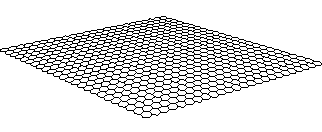
\includegraphics[width=\linewidth]{figures/torus-3d-flat.pdf}
				\caption{}
				\label{fig:torus-3d-flat}
			\end{subfigure}
			~~
			\begin{subfigure}{0.26\linewidth}
				\center
				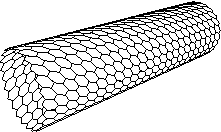
\includegraphics[width=\linewidth]{figures/torus-3d-tube.pdf}
				\caption{}
				\label{fig:torus-3d-tube}
			\end{subfigure}
			~~
			\begin{subfigure}{0.23\linewidth}
				\center
				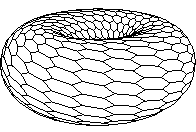
\includegraphics[width=\linewidth]{figures/torus-3d-torus.pdf}
				\caption{}
				\label{fig:torus-3d-torus}
			\end{subfigure}
			
			\caption{Visualisation of a hexagonal torus topology as a torus.}
			\label{fig:torus-3d}
		\end{figure}
		
		The wrap around connections in the topology are what give it the `torus'
		part of its name. Figure~\ref{fig:torus-3d-flat} shows a hexagonal torus
		topology drawn flat as in the previous figure. If the topology is rolled up
		into a tube such that the top and bottom nodes become directly adjacent, a
		tube is formed as in figure~\ref{fig:torus-3d-tube}. This tube can then be
		bent to bring together the nodes at the ends of the tube to form a torus as
		shown in figure~\ref{fig:torus-3d-torus}.
		
		A hexagonal torus topology is typically defined in terms of its width and
		height along the X and Y axes respectively. For example,
		figure~\ref{fig:hexagonalTorusTopology} shows a $10\times10$ hexagonal
		torus.  The nodes in a hexagonal torus topology are addressed using
		hexagonal coordinates of the form $(x, y, z)$ \cite{patel15}. The bottom
		left node (labelled $\alpha$ in the figure) has the coordinate $(0, 0, 0)$
		and other nodes are assigned coordinates according to the number of hops
		along each dimension from $(0, 0, 0)$, for example node $\beta$ has the
		coordinate $(2, 0, -1)$.
		
		Counter intuitively, individual nodes in hexagonal torus topologies may be
		described by many different coordinates, for example $(3, 1, 0)$ and $(1,
		-1, -2)$ are also a valid coordinates for node $\beta$. These dual
		coordinates emerge from the fact that adding $(1, 1, 1)$ to a coordinate
		produces an equivalent, but different, coordinate. This phenomenon is
		explained in detail in appendix~\ref{app:minimal-hex-coordinates} and
		related phenomena will be discussed in chapter~\ref{sec:shortestPaths}.
		
		\begin{figure}
			\center
			\begin{subfigure}[b]{0.32\linewidth}
				\center
				\buildfig{figures/torus-compare-hexagonal.tex}
				
				\caption{Hexagonal}
				\label{fig:torus-compare-hexagonal}
			\end{subfigure}
			\begin{subfigure}[b]{0.32\linewidth}
				\center
				\buildfig{figures/torus-compare-2d.tex}
				
				\caption{2D}
				\label{fig:torus-compare-2d}
			\end{subfigure}
			\begin{subfigure}[b]{0.32\linewidth}
				\center
				\buildfig{figures/torus-compare-3d.tex}
				
				\caption{3D}
				\label{fig:torus-compare-3d}
			\end{subfigure}
			
			\caption{Visual comparison of torus topologies. In all figures, `wrap
			around' connections between nodes at the ends of each axis are omitted
			for clarity.}
			\label{fig:torus-compare}
		\end{figure}
		
		Despite its unusual coordinate system, hexagonal torus topologies compare
		favourably with more conventional network topologies such as 2D and 3D
		toruses (sometimes known as 2-ary $N$-cubes and 3-ary $N$-cubes
		respectively) \cite{dally04} illustrated in figure~\ref{fig:torus-compare}.
		Compared with the 2D torus topology, a hexagonal torus has double the
		bisection bandwidth even though it only requires 50\% more node-to-node
		links \cite{navaridas09}. 3D torus topologies also have six node-to-node
		links per node but double the bisection bandwidth again. However, since a
		network topology must eventually be embedded into a real world data centre
		(which, at large scales, approximate a 2D space), 3D, or higher-dimensional
		torus topologies may become more expensive to construct in practice due to
		the need for longer cables to interconnect nodes. As
		chapter~\ref{sec:building} demonstrates, hexagonal toruses may be assembled
		in a machine room in a similar way to a 2D topology. The hexagonal torus
		topology achieves the scalability of a 2D torus while gaining some of the
		bisection bandwidth benefits of the 3D torus topology.
		
		Most torus topologies, including hexagonal 2D and 3D toruses, are related
		to an equivalent `mesh' topology. Mesh topologies maintain the same general
		connectivity structure as the corresponding torus topology with the
		exception of wrap-around links which are omitted. Omitting wrap-around
		links in practice saves a small number of links at the expense of halving
		the network's bisection bandwidth. As a consequence, mesh topologies are
		rarely used.
		
		\begin{figure}
			\center
			\begin{subfigure}[b]{0.45\linewidth}
				\center
				\buildfig{figures/hexagonal-torus.tex}
				\caption{Hexagonal torus}
				\label{fig:topo-compare-hexagonal-torus}
			\end{subfigure}
			\begin{subfigure}[b]{0.45\linewidth}
				\center
				\buildfig{figures/h-torus.tex}
				\caption{H-torus}
				\label{fig:topo-compare-h-torus}
			\end{subfigure}
			
			\caption{Hexagonal torus vs. H-torus topology. Each numbered hexagon
			represents a node. The thick outline indicates the bounds of the
			topology after which the network repeats. In each topology, the path
			taken by advancing in the Y$^+$ direction from the node labelled `0' is
			shown.}
			\label{fig:topo-compare}
		\end{figure}
		
		The hexagonal torus topology used by SpiNNaker and the subject of much of
		this thesis is not to be confused with the `H-torus' topology.  This
		topology also uses a hexagonal tiling of nodes and even wraps this tiling
		into in a torus-like topology \cite{zhao08}. However, H-torus topologies
		have very different characteristics to the hexagonal torus topology are
		closely related to `twisted torus' topologies \cite{camara10}.
		Figure~\ref{fig:topo-compare} illustrates one major difference in the way
		paths wrap around the peripheries of both topologies.
	
	\section{Scaling-up SpiNNaker machines}
		
		\begin{figure}
			\center
			\begin{subfigure}[b]{0.45\linewidth}
				\center
				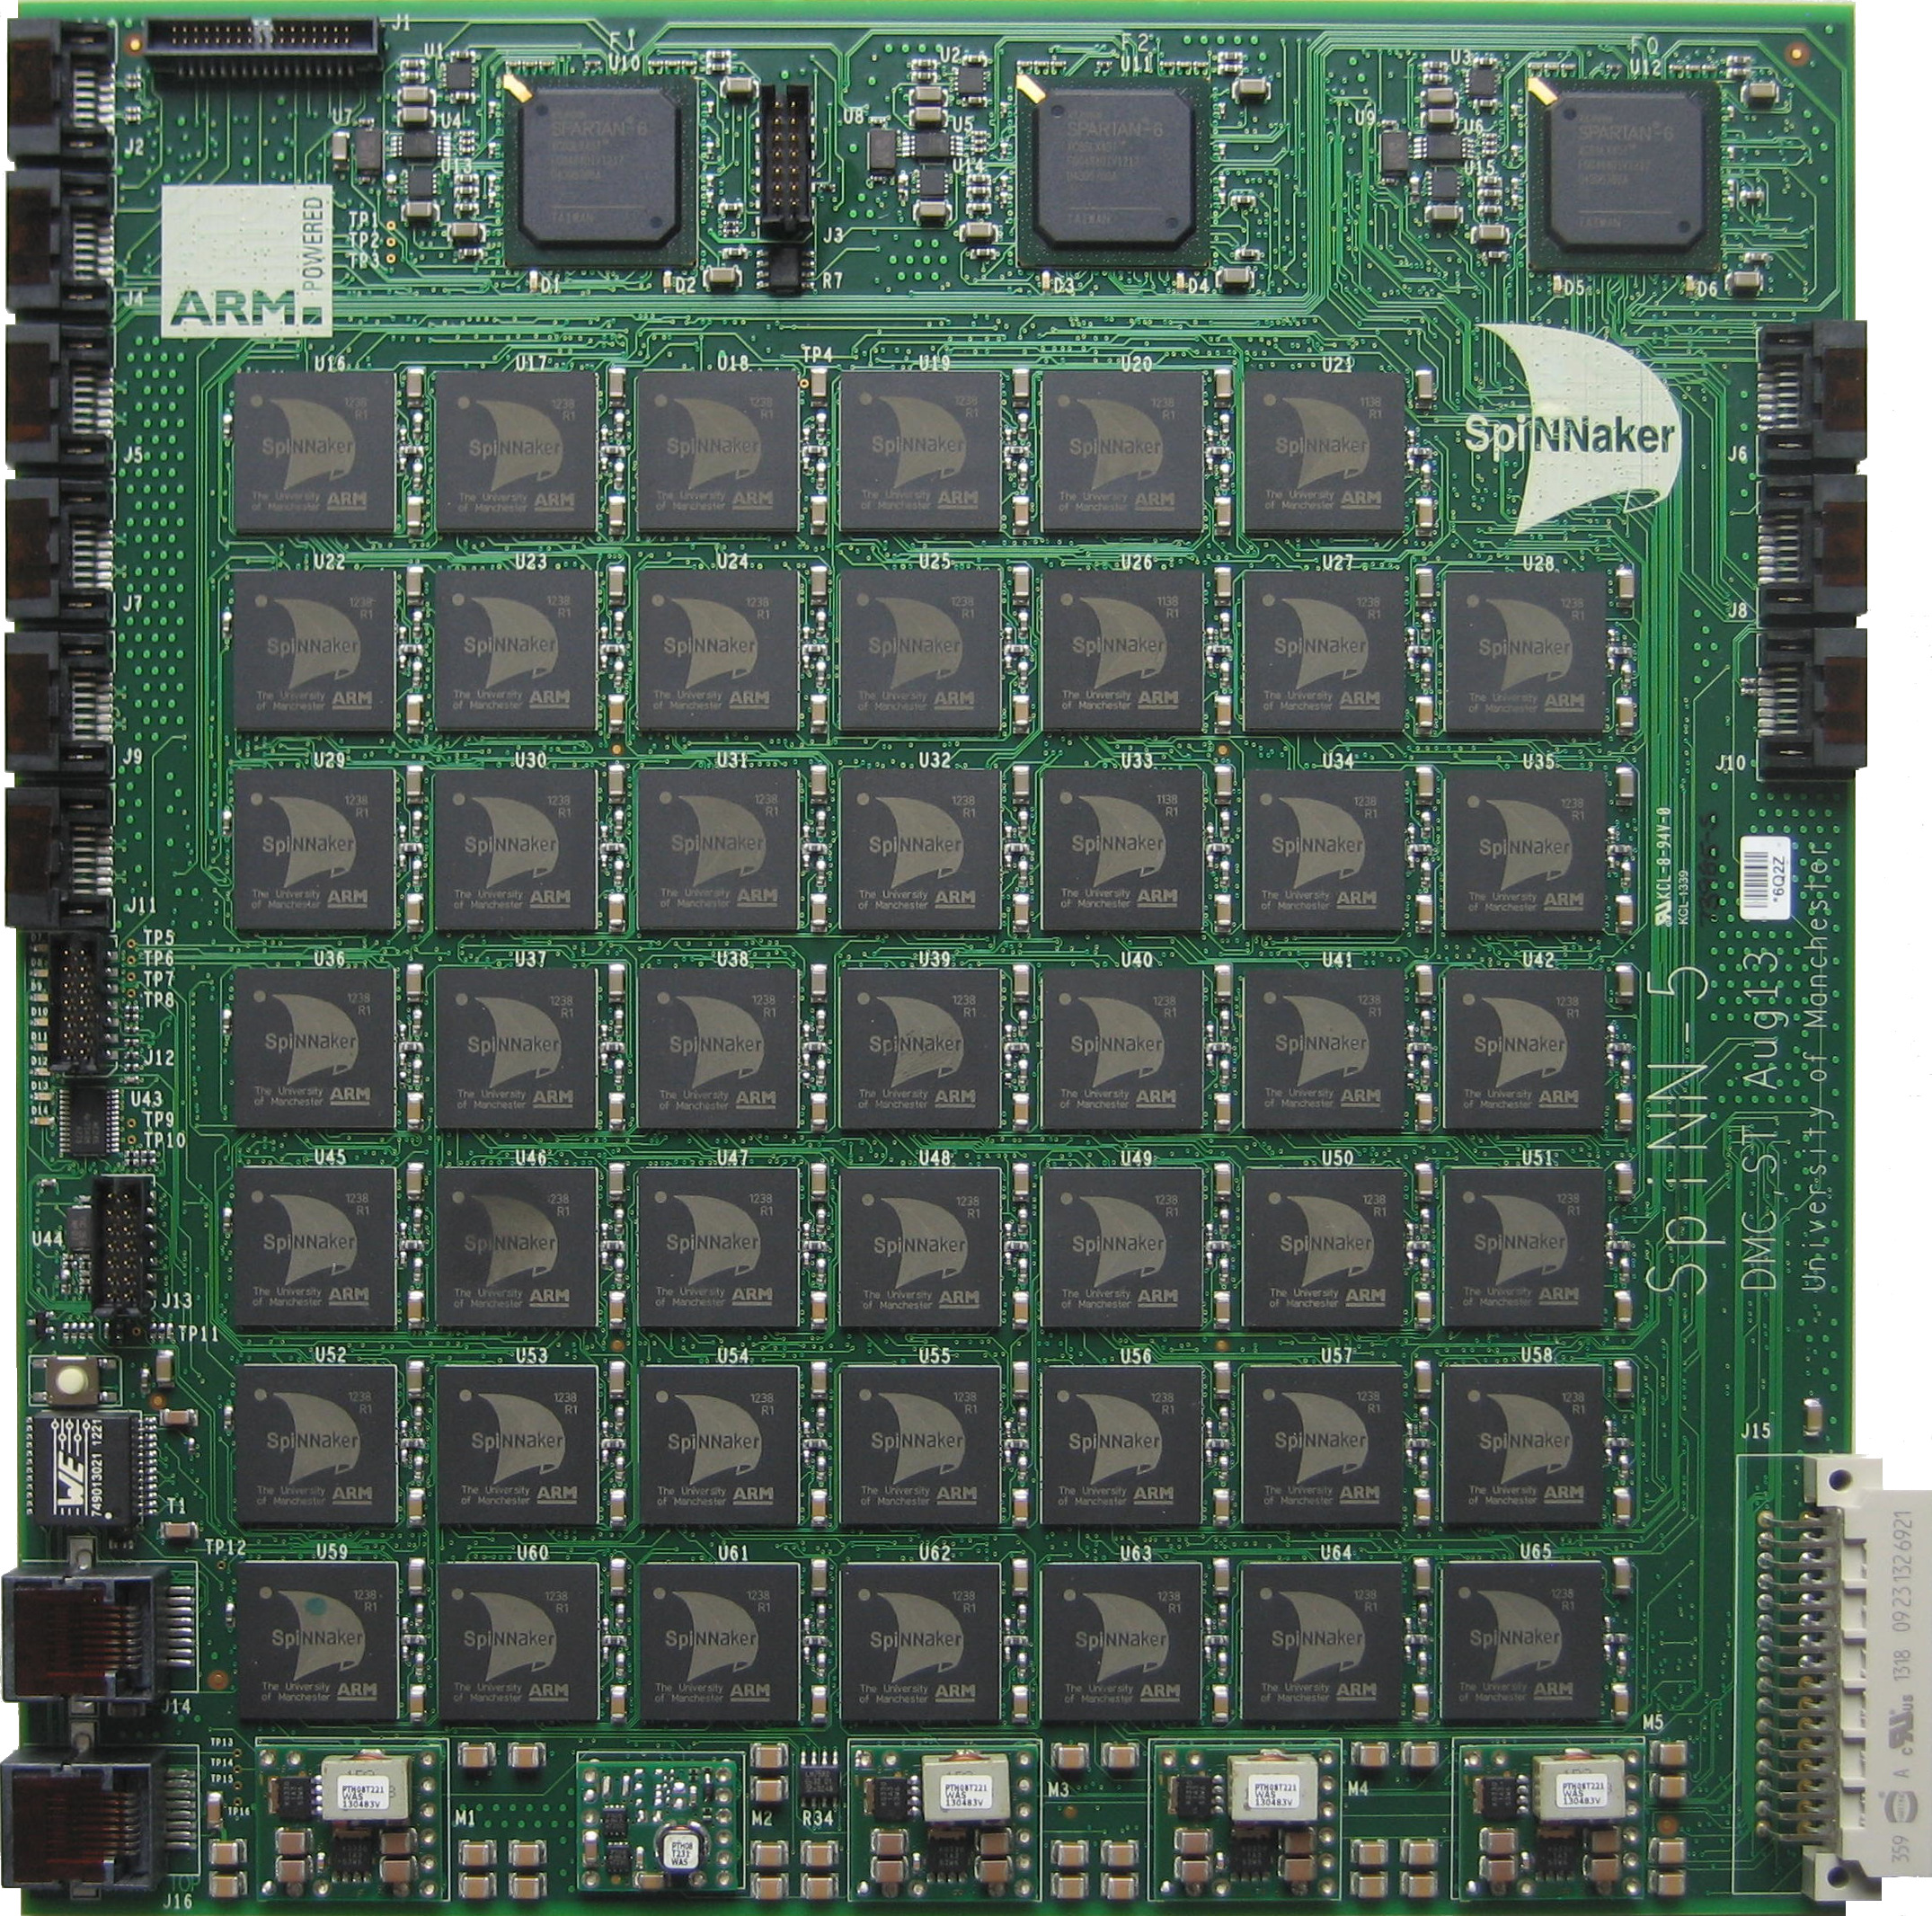
\includegraphics[width=\linewidth]{figures/spinnakerBoard.jpg}
				
				\caption{A SpiNNaker board}
				\label{fig:spinnakerBoard}
			\end{subfigure}
			~~~
			\begin{subfigure}[b]{0.45\linewidth}
				\center
				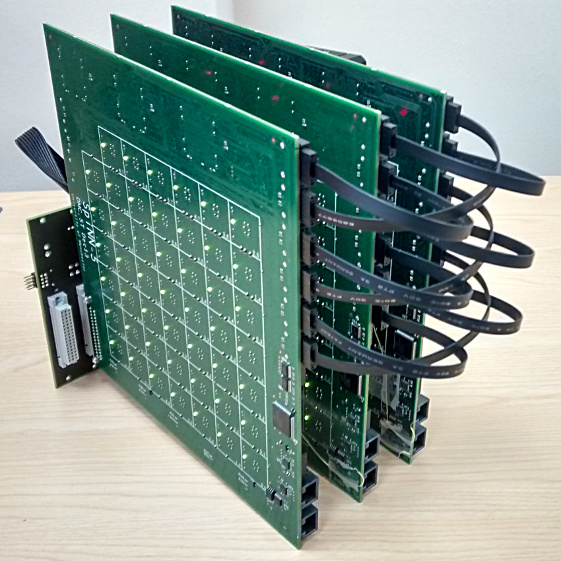
\includegraphics[width=\linewidth]{figures/threeboard.jpg}
				
				\caption{Three board system}
				\label{fig:threeboard}
			\end{subfigure}
			
			\vspace*{2em}
			
			\begin{subfigure}{\linewidth}
				\center
				\buildfig{figures/sata-connections.tex}
				
				\caption{The logical connectivity between chips in multi-board systems.
				Each board's forty-eight chips (drawn here as hexagons) form a wrapped
				triple. Connections between chips on neighbouring boards are
				concentrated onto a single HSS link.}
				\label{fig:sata-connections} \end{subfigure}
			
			\caption{SpiNNaker boards}
			\label{fig:spinnaker-boards}
		\end{figure}
		
		To build large SpiNNaker systems comprising tens of thousands of
		SpiNNaker chips, groups of forty-eight chips are mounted onto printed
		circuit boards as illustrated in figure~\ref{fig:spinnakerBoard}. These
		boards may be connected together to form larger systems.
		Figure~\ref{fig:threeboard} shows a prototype three board system configured
		as a $12\times12$ hexagonal torus.
		
		Though the chips are physically arranged in a (nearly) $7\times7$ grid on
		each SpiNNaker board, they logically form a `wrapped triple', a shape
		described in detail in appendix \ref{sec:partitioning} and illustrated in
		figure~\ref{fig:sata-connections}. Logically, the chips at the periphery of
		each board connect to their neighbours on adjacent boards. Normally
		SpiNNaker chips connect using a low power, asynchronous 2-of-7 protocol
		requiring sixteen wires per bidirectional chip-to-chip link
		\cite{bainbridge03}. If this link technology were used to connect chips on
		neighbouring boards, each pair of boards would need to be connected with a
		128~wire cable. Cables and connectors supporting this may signals are
		expensive and physically large making them unsuitable for use with
		SpiNNaker. Instead, chip-to-chip connections between boards are multiplexed
		and demultiplexed onto a single High-Speed Serial (HSS) link
		\cite{athavale05} carried via commodity S-ATA cables often used to
		connected hard disks in desktop computers and servers \cite{sata3spec}.
		The six high-speed links are implemented by three onboard FPGAs (the three
		large chips at the top of the SpiNNaker board) and are logically
		transparent to the underlying network.
		
		In chapter~\ref{sec:building} I describe how very large SpiNNaker machines
		may be constructed using over one thousand SpiNNaker boards.

	\chapter{Building large SpiNNaker machines}
	
	\label{sec:building}
	
	Like any supercomputer, physically assembling a large SpiNNaker machine
	poses many practical challenges in terms of arranging, installing and
	maintaining the hundreds of metres of network cables required.  For
	conventional architectures and network topologies, techniques are well
	understood and embodied by industry standards such as TAI-942~\cite{tia2006}.
	SpiNNaker's use of the hexagonal torus topology renders existing approaches
	insufficient.
	
	In the first part of this chapter I extend existing techniques for mapping
	network topologies into standard data centre physical infrastructure to
	support the hexagonal torus topology. This mapping is designed to ensure that
	all cables are kept short (under \SI{1}{\meter}) to reduce costs and
	simplify the network hardware required. The techniques described introduce
	little overhead in cable length over existing torus wiring schemes
	and confirm the suitability of the hexagonal torus topology for real-world
	applications.
	
	The second part of this chapter uses SpiNNaker as a case study on the
	suitability of the mappings introduced in this chapter.  In this case study I
	consider various SpiNNaker systems ranging in size from desktop machines to
	multi-cabinet machine room installations. As well as validating the cabling
	schemes introduced in this chapter I also describe a new technique which
	improves the efficiency of the cable installation process.  As a consequence
	of SpiNNaker's fine-grained connectivity, the cabling is unusually dense,
	exacerbating the complexity of the cabling patterns to be installed. By
	exploiting network diagnostics hardware and on-board LEDs to guide cable
	installation, construction of large SpiNNaker machines takes a matter of
	hours rather than the days reported for other architectures. In addition,
	preliminary experiments suggest that neither the maintainability nor cooling
	performance of the system are hampered by the dense cabling employed.
	
	In this chapter, the term \emph{unit} refers to the smallest physical
	component between which network interconnection cables are installed. For
	example, in a SpiNNaker machine a unit is a 48-chip board while in a data
	centre network a unit might be a server blade.
	
	\section{Cabling non-hexagonal torus topologies}
		
		Na\"ive arrangements of torus topologies, hexagonal or otherwise, feature
		physically long `wrap-around' connections which connect units at the
		peripheries of the system. Long connections can be problematic for several
		reasons:
		
		\begin{description}
			
			\item[Performance:] Signal quality diminishes as cables get longer,
			requiring the use of slower signalling speeds, increased error
			correction overhead or more complex hardware.
			
			\item[Energy:] Some energy is lost in cables; longer cables lose more
			signal energy requiring higher drive strengths and/or buffering to
			maintain signal integrity.
			
			\item[Cost:] Shorter cables are cheaper than long ones.  Longer cables
			imply more cabling in a given space making the task of cable installation
			and system maintenance more difficult, increasing labour costs by as much
			as $5\times$~\cite{curtis12}.
			
		\end{description}
		
		In conventional torus topologies, the need for long cables is eliminated by
		folding and interleaving units of the network~\cite[chapter~5]{dally04}.
		This process is illustrated for a 1D torus topology (a ring network) in
		figure~\ref{fig:ring-folding}. A na\"ive arrangement of units in this
		topology results in a long cable connecting the units at the ends of the
		ring (figure~\ref{fig:ring-folding-row}).  To eliminate these long
		connections, half of the units are `folded' on top of the others
		(figure~\ref{fig:ring-folding-folded}) and then this arrangement of units
		is interleaved (figure~\ref{fig:ring-folding-interleaved}). This ordering
		of units requires no long cables while still observing the physical
		constraint that units must be laid out in a line.
		
		\begin{figure}
			\center
			\begin{subfigure}[b]{0.39\linewidth}
				\center
				\buildfig{figures/ring-folding-row.tex}
				\caption{A ring network}
				\label{fig:ring-folding-row}
			\end{subfigure}
			\begin{subfigure}[b]{0.24\linewidth}
				\center
				\buildfig{figures/ring-folding-folded.tex}
				\caption{Folded}
				\label{fig:ring-folding-folded}
			\end{subfigure}
			\begin{subfigure}[b]{0.35\linewidth}
				\center
				\buildfig{figures/ring-folding-interleaved.tex}
				\caption{Folded and interleaved}
				\label{fig:ring-folding-interleaved}
			\end{subfigure}
			
			\caption[Folding and interleaving a ring network.]%
			{Folding and interleaving a ring network to reduce maximum cable
			length.}
			\label{fig:ring-folding}
		\end{figure}
		
		The folding and interleaving process may be extended to $N$-dimensional
		torus topologies by folding each axis in turn. Since all axes are
		orthogonal in non-hexagonal topologies, the folding process only moves
		units along the axis being folded. Due to the non-orthogonality of the
		three axes of the hexagonal torus topology, this type of folding does not
		work. As figure~\ref{fig:failing-to-fold-hex-toruses} illustrates, folding
		along any axis results in connected units on opposing edges not being
		brought together. For example, when folding along the X axis, the two units
		marked with a green circle are moved closer together on the Y axis but
		remain apart on the X axis.
		
		\begin{figure}
			\center
			\begin{subfigure}[b]{0.24\linewidth}
				\center
				\buildfig{figures/failing-to-fold-hex-toruses-none.tex}
				\caption{Not folded}
				\label{fig:failing-to-fold-hex-toruses-none}
			\end{subfigure}
			\begin{subfigure}[b]{0.24\linewidth}
				\center
				\buildfig{figures/failing-to-fold-hex-toruses-x.tex}
				\caption{X}
				\label{fig:failing-to-fold-hex-toruses-x}
			\end{subfigure}
			\begin{subfigure}[b]{0.24\linewidth}
				\center
				\buildfig{figures/failing-to-fold-hex-toruses-y.tex}
				\caption{Y}
				\label{fig:failing-to-fold-hex-toruses-y}
			\end{subfigure}
			\begin{subfigure}[b]{0.24\linewidth}
				\center
				\buildfig{figures/failing-to-fold-hex-toruses-z.tex}
				\caption{Z}
				\label{fig:failing-to-fold-hex-toruses-z}
			\end{subfigure}
			
			\caption[Folding each axis of a hexagonal torus topology.]%
			{Schematics showing folding along each axis of a hexagonal torus topology
			failing to eliminate wrap-around connections.  Same-shaped-and-coloured
			dots show the endpoints of two example wrap-around connections.}
			\label{fig:failing-to-fold-hex-toruses}
		\end{figure}
	
	\section{Partitioning hexagonal torus topologies}
		
		The nodes in supercomputer networks are usually relatively small, for
		example a single chip. Tens of nodes are packed together into a single
		unit, such as a circuit board or server blade, to simplify assembly and
		share common power and cooling resources~\cite{gilge14,ajima12}. In
		commercial supercomputers built on non-hexagonal torus topologies, each
		unit's nodes represent a hypercube partition of the overall topology as
		illustrated in figure~\ref{fig:hypercube-partitioning}
		\cite{chen11,ajima12}.
		
		An analogous `parallelogram' partitioning scheme exists for hexagonal torus
		topologies, however, this results in imbalanced connectivity requirements
		between neighbouring partitions. In
		figure~\ref{fig:parallelogram-partitioning}, for example, the partitions
		above, below, left and right of the central partition are connected by
		seven node-to-node connections each while the partitions above-right and
		below-left are connected by just a single connection each. To simplify
		assembly, connections between all nodes in a pair of neighbouring
		partitions are often made by a single cable. If connectivity requirements
		are imbalanced, as in this example, this may mean multiple connector types
		may be required, increasing design complexity.
		
		To avoid connectivity imbalance, SpiNNaker uses a `wrapped triple'
		partitioning scheme~\cite{davidsonWiring}, as illustrated in
		figure~\ref{fig:wrapped-triple-partitioning} and explained in detail in
		appendix \ref{sec:partitioning}. In this partitioning scheme, the same
		number of connections connect all six neighbouring units. As explained in
		the appendix, a hexagonal torus topology is constructed from groups of
		three partitions.
		
		\begin{figure}
			\center
			\begin{subfigure}[b]{0.32\textwidth}
				\center
				\buildfig{figures/hypercube-partitioning.tex}
				\caption{2D hypercube}
				\label{fig:hypercube-partitioning}
			\end{subfigure}
			\begin{subfigure}[b]{0.32\textwidth}
				\center
				\buildfig{figures/parallelogram-partitioning.tex}
				\caption{Parallelogram}
				\label{fig:parallelogram-partitioning}
			\end{subfigure}
			\begin{subfigure}[b]{0.32\textwidth}
				\center
				\buildfig{figures/wrapped-triple-partitioning.tex}
				\caption{Wrapped triple}
				\label{fig:wrapped-triple-partitioning}
			\end{subfigure}
			
			\caption[Partitioning of torus topologies into units.]%
			{Partitioning of non-hexagonal (a) and hexagonal (b and c) torus
			topologies into units.}
			\label{fig:partitioning-options}
		\end{figure}
		
		For completeness, both parallelogram and wrapped triple partitioning are
		considered in this chapter even though SpiNNaker uses wrapped triple
		partitioning. The parallelogram partitioning scheme may be more appropriate
		for architectures where connections between nodes in neighbouring
		partitions do not share a single connector. In addition, in architectures
		where a unit corresponds to a single node, this can be treated as a $1
		\times 1$ parallelogram partition.  This special case occurs in
		coarse-grained architectures and Networks on Chip (NoCs) where nodes are
		not grouped together into multi-node units.
	
	\section{Folding \& interleaving hexagonal toruses}
		
		To exploit the folding technique used by non-hexagonal topologies, the
		units in a hexagonal torus topology must be mapped into a space with
		orthogonal coordinates. The choice of transformation to an orthogonal
		coordinate system can have an impact on how physically far apart logically
		neighbouring units are in the final arrangement. A good mapping should
		attempt to reduce `distortion' which moves adjacent units apart in the
		final folded and interleaved arrangement.
		
		In this section I propose two transformations which map hexagonal
		arrangements of units into a 2D orthogonal coordinate space. The first
		transformation, `shearing', is general purpose and introduces some
		distortion. The second transformation, `slicing', is less general but can
		introduce less distortion than shearing and therefore may lead to shorter
		cable lengths.
		
		Both the slicing and shearing transformations are carried out in two steps:
		
		\begin{description}
			
			\item[Rectangularisation] Units are transformed from being laid out in a
			parallelogram into a rectangular arrangement. The specific transformation
			used is the key difference between the slicing and shearing
			transformations.
			
			\item[Uncrinkling] Units are mapped into a 2D coordinate system without
			gaps between units.
			
		\end{description}
		
		\subsection{Rectangularisation}
			
			The hexagonal torus topology is illustrated in
			figures~\ref{fig:hex-to-plane-node-native} and
			\ref{fig:hex-to-plane-native} for parallelogram-partitioned units and
			wrapped triple units respectively. The first step in the folding process
			is to rearrange units so that they form a rectangle using one of two
			techniques: shearing or slicing.
			
			\begin{figure}
				\center
				\begin{subfigure}[b]{0.32\linewidth}
					\center
					\buildfig{figures/hex-to-plane-node-native.tex}
					
					\caption{Original}
					\label{fig:hex-to-plane-node-native}
				\end{subfigure}
				\begin{subfigure}[b]{0.32\linewidth}
					\center
					\buildfig{figures/hex-to-plane-node-shear.tex}
					
					\caption{Sheared}
					\label{fig:hex-to-plane-node-shear}
				\end{subfigure}
				\begin{subfigure}[b]{0.32\linewidth}
					\center
					\buildfig{figures/hex-to-plane-node-slice.tex}
					
					\caption{Sliced}
					\label{fig:hex-to-plane-node-slice}
				\end{subfigure}
				
				\caption[Rectangularisation of parallelogram partitioned toruses.]%
				{Rectangularisation of parallelogram partitioned hexagonal
				toruses. Thin lines show wrap-around links. Pointy-topped hexagons
				represent parallelogram partitioned units.}
				\label{fig:hex-to-plane-node}
				
				% XXX: Force these figures together.
				
				%\end{figure}
				%
				%\begin{figure}
				
				\center
				\begin{subfigure}[b]{0.32\linewidth}
					\center
					\buildfig{figures/hex-to-plane-native.tex}
					
					\caption{Original}
					\label{fig:hex-to-plane-native}
				\end{subfigure}
				\begin{subfigure}[b]{0.32\linewidth}
					\center
					\buildfig{figures/hex-to-plane-shear.tex}
					
					\caption{Sheared}
					\label{fig:hex-to-plane-shear}
				\end{subfigure}
				\begin{subfigure}[b]{0.32\linewidth}
					\center
					\buildfig{figures/hex-to-plane-slice.tex}
					
					\caption{Sliced}
					\label{fig:hex-to-plane-slice}
				\end{subfigure}
				
				\caption[Rectangularisation of wrapped triple partitioned toruses.]%
				{Rectangularisation of wrapped triple partitioned hexagonal
				toruses. Thin lines show wrap-around links.  Flat-topped hexagons
				represent wrapped triple partitioned units.}
				\label{fig:hex-to-plane}
				
				% And force these together!
				
				%\end{figure}
				%
				%\begin{figure}
				
				\center
				\begin{subfigure}[b]{0.3\linewidth}
					\center
					\buildfig{figures/slicing-examples-5x5.tex}
					\caption{$5\times5$}
				\end{subfigure}
				\begin{subfigure}[b]{0.3\linewidth}
					\center
					\buildfig{figures/slicing-examples-5x7.tex}
					\caption{$5\times7$}
				\end{subfigure}
				\begin{subfigure}[b]{0.3\linewidth}
					\center
					\buildfig{figures/slicing-examples-5x10.tex}
					\caption{$5\times10$}
				\end{subfigure}
				
				\caption[Patterns of wrap-around connections in sliced systems.]%
				{Schematics showing the patterns of wrap-around connections in sliced
				systems of various aspect ratios.}
				\label{fig:slicing-examples}
			\end{figure}
			
			The shearing technique applies a \SI{30}{\degree} shear transformation to
			distort the arrangement of units so that the X and Y axes of the
			hexagonal torus topology become orthogonal. This transformation leads to
			a rectangular arrangement of units as illustrated in figures
			\ref{fig:hex-to-plane-node-shear} and \ref{fig:hex-to-plane-shear}.
			
			The shear transformation introduces some distortion causing connections
			between units in the Z axis to become $\sqrt{2} \times$ longer. The
			transformation does not alter the pattern of wrap-around connections:
			long connections between units on the extreme left and right sides and
			the top and bottom remain, along with a single connection between the
			bottom left and top right units.
			
			The slice transformation aims to avoid the elongation of the Z axis by
			moving the units without distorting their layout. Units protruding from
			the left-hand-side of the parallelogram are `sliced off' and moved into
			the matching gap on the opposite side as illustrated in figures
			\ref{fig:hex-to-plane-node-slice} and \ref{fig:hex-to-plane-slice}. This
			transformation does not introduce any distortion but changes the pattern
			of wrap-around connections. Connections from left-to-right remain while
			the connections between the top and bottom units now criss-cross
			(figure~\ref{fig:slicing-examples}).  The proportion of connections going
			from bottom-left to top-right and from bottom-right to top-left varies
			depending on the aspect ratio of the topology. Only certain patterns of
			wrap-around links can be eliminated by folding and, as we shall see
			later, this limits us in which network topologies can be rectangularised
			by slicing.
			
		\subsection{Uncrinkling}
			
			Before folding can occur, the rectangularised arrangements of units
			produced in the previous step must be mapped into a 2D grid. Applied to
			parallelogram partitions, the shear transformation results in a mapping
			into a 2D grid with no further distortion
			(figure~\ref{fig:uncrinkling-node-sheared}). For other combinations of
			transformation and partitioning scheme, the units do not exactly fit a 2D
			grid. Instead, the units form `crinkled' rows or columns which may be
			`uncrinkled' (straightened out) to fit a regular 2D grid as illustrated in
			figures~\ref{fig:uncrinkling-node-sliced}~--~\ref{fig:uncrinkling-sliced}.
			
			\begin{figure}
				\center
				\begin{subfigure}[b]{0.48\linewidth}
					\center
					\buildfig{figures/uncrinkling-node-sheared.tex}
					
					\caption{Parallelogram units, sheared}
					\label{fig:uncrinkling-node-sheared}
				\end{subfigure}
				\begin{subfigure}[b]{0.48\linewidth}
					\center
					\buildfig{figures/uncrinkling-node-sliced.tex}
					
					\caption{Parallelogram units, sliced}
					\label{fig:uncrinkling-node-sliced}
				\end{subfigure}
				
				\vspace{1cm}
				
				\begin{subfigure}[b]{0.48\linewidth}
					\center
					\buildfig{figures/uncrinkling-sheared.tex}
					
					\caption{Wrapped triple units, sheared}
					\label{fig:uncrinkling-sheared}
				\end{subfigure}
				\begin{subfigure}[b]{0.48\linewidth}
					\center
					\buildfig{figures/uncrinkling-sliced.tex}
					
					\caption{Wrapped triple units, sliced}
					\label{fig:uncrinkling-sliced}
				\end{subfigure}
				
				\vspace{1em}
				
				\caption[Uncrinkling units into a 2D grid.]%
				{Uncrinkling rectangularised arrangements of units into a 2D
				grid. Thick lines show how crinkled rows and columns of units are
				uncrinkled.  Annotations show how the relative positions of units
				change after uncrinkling.}
				\label{fig:uncrinkling}
			\end{figure}
			
			%% XXX: Does this make things clearer or not?
			%In the figure, the labels show the positions of individual units before
			%and after uncrinkling. We will use these later in \S\ref{sec:distortion}
			%to calculate the overhead introduced by uncrinkling.
		
		\subsection{Folding}
			
			\begin{figure}
				\begin{subfigure}{\linewidth}
					\center
					\buildfig{figures/folding-sheared.tex}
					\caption{Sheared systems and $1:2$ sliced systems}
					\label{fig:folding-sheared}
				\end{subfigure}
				
				\vspace{1em}
				
				\begin{subfigure}{\linewidth}
					\center
					\buildfig{figures/folding-sliced.tex}
					\caption{$1:1$ sliced systems}
					\label{fig:folding-sliced}
				\end{subfigure}
				
				\caption[Elimination of long wrap-around links by folding.]%
				{Schematic illustrating elimination of long wrap-around links
				during folding. In each example a single link has been highlighted to
				aid in following the process.}
				\label{fig:folding}
			\end{figure}
			
			Once a regular 2D grid of units has been formed, this may be folded in
			the conventional way as illustrated in figure~\ref{fig:folding-sheared}.
			Folding once along each axis eliminates long connections crossing from
			left-to-right, top-to-bottom and from the bottom-left corner to the
			top-right corner. Any shear-transformed network may be folded this way
			since its wrap-around connections always follow this pattern.
			Slice-transformed networks may only be folded like this when their aspect
			ratio is $1:2$ when the pattern of wrap-around links is the same as a
			shear-transformed network.
			
			When `square' networks (i.e. those with a $1:1$ aspect ratio) are sliced,
			the network must be folded \emph{twice} along the Y axis as in
			figure~\ref{fig:folding-sliced} to eliminate the criss-crossing
			wrap-around links. It is not possible to eliminate wrap-around links from
			sliced networks with other aspect ratios by folding.
			
			After folding, the units are interleaved, yielding a 2D arrangement of
			units in which no connection spans the width or height of the system. The
			maximum connection distance is constant for any network allowing the
			topology to scale up.
		
		\subsection{Choosing a transformation}
			
			\label{sec:distortion}
			
			In each step of the transformation from hexagonal torus to a folded and
			interleaved 2D grid, the distances between connected units may increase.
			When designing a system, the transformation with the least distortion
			should be used to minimise the average length of the cables required.
			
			By referring to figure~\ref{fig:uncrinkling} (page
			\pageref{fig:uncrinkling}), it is possible to calculate the overhead
			introduced by each type of transformation.  For example, to compute the
			overhead introduced by the slicing transformation when applied to units
			composed of wrapped triples we consider
			figure~\ref{fig:uncrinkling-sliced}. The uncrinkling pattern used to
			transform this topology is a repeating pattern of two units, a pair of
			which have been labelled $1$ and $2$ respectively. Unit $1$ is
			immediately surrounded by the six units labelled $a$, $b$, $c$, $2$, $g$
			and $h$. Unit $2$ is surrounded by the units $1$, $c$, $d$, $e$, $f$ and
			$g$.  Before the transformation, the distance between units is $1$; after
			the transformation is applied this is not always the case. Folding and
			interleaving into $f_x$ columns and $f_y$ rows also introduces overhead.
			For each pair of previously neighbouring units in the example, their
			distances after folding may be computed as follows:
			
			\begin{equation*}
				\begin{aligned}[c]
					D_{1\,\leftrightarrow{}\,a} &= \sqrt{f_x^2 + f_y^2} \\
					D_{1\,\leftrightarrow{}\,b} &= f_y \\
					D_{1\,\leftrightarrow{}\,c} &= \sqrt{f_x^2 + f_y^2} \\
					D_{1\,\leftrightarrow{}\,2} &= f_x \\
					D_{1\,\leftrightarrow{}\,g} &= f_y \\
					D_{1\,\leftrightarrow{}\,h} &= f_x
				\end{aligned}
				\hspace{2cm}
				\begin{aligned}[c]
					D_{2\,\leftrightarrow{}\,1} &= f_x \\
					D_{2\,\leftrightarrow{}\,c} &= f_y \\
					D_{2\,\leftrightarrow{}\,d} &= f_x \\
					D_{2\,\leftrightarrow{}\,e} &= \sqrt{f_x^2 + f_y^2} \\
					D_{2\,\leftrightarrow{}\,f} &= f_y \\
					D_{2\,\leftrightarrow{}\,g} &= \sqrt{f_x^2 + f_y^2}
				\end{aligned}
			\end{equation*}
			
			From these values, mean and maximum connection distances may be
			calculated. The expressions for each combination of partitioning scheme
			and transformation are as follows:
			
			\begin{align*}
				D_{\textrm{mean}}=&
					\begin{cases}
						\frac{7f_x + 3\sqrt{f_x^2 + f_y^2} + \sqrt{(2f_x)^2 + f_y^2}}{9} &
							\textrm{if sheared wrapped triple units}\\
						\frac{f_x + f_y + \sqrt{f_x^2 + f_y^2}}{3} &
							\textrm{otherwise}\\
					\end{cases} \\
				D_{\textrm{max}}=&
					\begin{cases}
						\sqrt{(2f_x)^2 + f_y^2} &
							\textrm{if sheared wrapped triple units}\\
						\sqrt{f_x^2 + f_y^2} &
							\textrm{otherwise}
					\end{cases}
			\end{align*}
			
			\begin{table}
				\center
				\begin{tabular}{lcc}
					\toprule
					                                 & $1:2$  & Other \\
					\addlinespace
					\multirow{2}{*}{Parallelogram}   & \textbf{Either} & \textbf{Shear}\\
					                                 & \footnotesize $D_\textrm{mean}\approx2.28 \quad D_\textrm{max}\approx2.83$
					                                 & \footnotesize $D_\textrm{mean}\approx2.28 \quad D_\textrm{max}\approx2.83$\\
					\addlinespace
					\multirow{2}{*}{Wrapped triples} & \textbf{Slice}  & \textbf{Shear}\\
					                                 & \footnotesize $D_\textrm{mean}\approx2.28 \quad D_\textrm{max}\approx2.83$
					                                 & \footnotesize $D_\textrm{mean}\approx3.00 \quad D_\textrm{max}\approx4.47$\\
					\bottomrule
				\end{tabular}
				
				\caption{Recommended transformations for folding hexagonal toruses.}
				\label{tab:transform-recommended}
			\end{table}
			
			Using these formulae it is possible to determine which approach --
			shearing or slicing -- results in the lowest mean and maximum cable
			lengths and thus which technique should be used. This is summarised in
			table~\ref{tab:transform-recommended}.
	
	\section{A SpiNNaker case study}
		
		As the only known large-scale hexagonal torus-based architecture, SpiNNaker
		is a good case study for the techniques described in this chapter.  Each
		unit in a SpiNNaker machine is a 48-chip SpiNNaker board forming a
		wrapped triple partition. Systems of various sizes have been constructed
		using the techniques introduced in this chapter ranging from twenty-four
		board `portable' systems to a five cabinet, half-million core installation
		with plans in place to build a machine of twice this size in the future.
		
		In this section I describe how the folded and interleaved arrangement of
		units produced by the techniques in the previous chapter may be translated
		into physical arrangements of SpiNNaker boards in a machine room. I then
		describe how the thousands of S-ATA cables are installed and report on the
		maintainability and cooling impact of this cabling scheme in practice.
		
		\subsection{Mapping into physical cabinets}
			
			In SpiNNaker systems, the physical architecture used is illustrated in
			figure~\ref{fig:cabinet-units}. SpiNNaker boards are installed into card
			frames containing twenty four boards each. Five frames are mounted into
			standard, \SI{600}{\milli\meter}~wide 19\inch{} cabinets with further
			cabinets being added, arranged in a row, to scale the system up. The 2D
			grid of units produced by the folding process described in this chapter
			is mapped to cabinets and frames as illustrated in
			figure~\ref{fig:cabinetisation}.
			
			\begin{figure}
				\center
				\buildfig{figures/cabinet-units.tex}
				
				\caption{Physical architecture of a SpiNNaker machine.}
				\label{fig:cabinet-units}
			\end{figure}
			
			\begin{figure}
				\center
				\buildfig{figures/cabinetisation.tex}
				
				\caption[Mapping cabling from abstract to physical space.]%
				{Mapping from the abstract folded and interleaved 2D grid
				layout into physical cabinet and frame positions. Arrows indicate the
				order in which units (boards) are mapped into each frame, from
				left-to-right.}
				\label{fig:cabinetisation}
			\end{figure}
			
			Figure~\ref{fig:million-core-machine} shows the cabling plan for the
			largest planned SpiNNaker machine. This system will fill ten 19\inch{}
			cabinets and implement a $240 \times 240$ hexagonal torus topology
			partitioned between \num{1200} 48 chip SpiNNaker boards. The largest gap
			to be spanned by any cable is \SI{66}{\centi\meter}, well within the
			\SI{1}{\meter} limit on SpiNNaker's interconnect technology.
			
			\begin{figure}
				\center
				\buildfig{figures/million-core-machine.tex}
				
				\caption[Cabling plan for a \num{1200}~board SpiNNaker machine.]%
				{Cabling plan for a \num{1200}~board (\num{1036800}~core)
				SpiNNaker machine.}
				\label{fig:million-core-machine}
			\end{figure}
			
		\subsection{Cable selection and routing}
			
			Because of the dense packing of SpiNNaker boards, cables span short
			distances as shown in figure~\ref{fig:wire-length-histogram}.
			Conventional cable management techniques (e.g. cable trays) are not
			practical. To ensure the reliability and maintainability of SpiNNaker's
			wiring, cable slack must be carefully controlled.  If cables are too
			tight, cables, connectors and SpiNNaker boards can become damaged. When
			cables are too slack, the excess obstructs access to the machine and can
			easily become tangled \cite{cisco07}.
			
			In this case study the `rule of (three-)thumbs' proposed by
			Mazaris~\cite{mazaris97} is used which suggests that a minimum of
			\SI{5}{\centi\meter} of slack be provided. As SpiNNaker uses
			off-the-shelf S-ATA cables, only standard lengths of cable are available.
			For any given span, the shortest length of cable providing at least
			\SI{5}{\centi\meter} of slack is used.
			
			\begin{figure}
				
				\center
				\buildfig{figures/wire-length-histogram.tex}
				
				\caption[Cable lengths in a \num{1200}~board SpiNNaker machine.]%
				{Histogram of connection distances in a \num{1200} board SpiNNaker
				machine annotated with the selected cable lengths.}
				\label{fig:wire-length-histogram}
				
			\end{figure}
		
		\subsection{Installation practicality}
			
			\begin{figure}
				\center
				\begin{subfigure}[t]{0.5\textwidth}
					\begin{tikzpicture}
						\node (cables) [inner sep=0]
						      {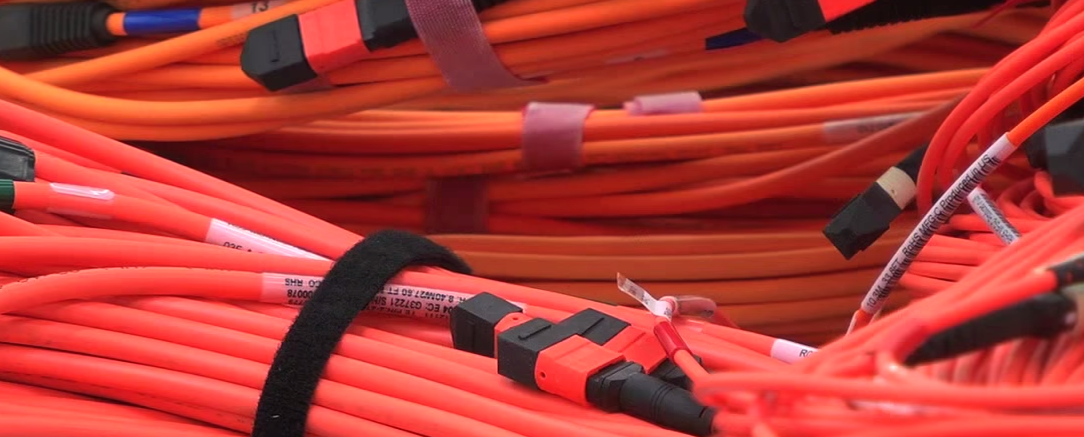
\includegraphics[width=\textwidth]{figures/bgCables.png}};
						\node (sockets) [inner sep=0, below=1.0em of cables]
						      {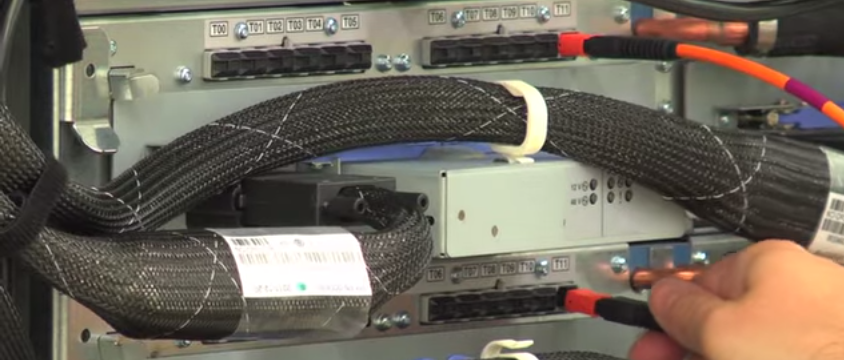
\includegraphics[width=\textwidth]{figures/bgSockets.png}};
						
						% Point at label on cable
						\draw [white, <-, line width=0.4em]
						      ([shift={(0.7cm, -0.3cm)}]cables.center)
						      -- ++(45:1cm);
						
						% Point at label on socket
						\draw [white, <-, line width=0.4em]
						      ([shift={(-1.0cm, 1.1cm)}]sockets.center)
						      -- ++(-45:1cm);
					\end{tikzpicture}
					
					\caption{Pre-labelled cables and sockets}
					\label{fig:bgWiringLabels}
				\end{subfigure}
				~
				\begin{subfigure}[t]{0.30\textwidth}
					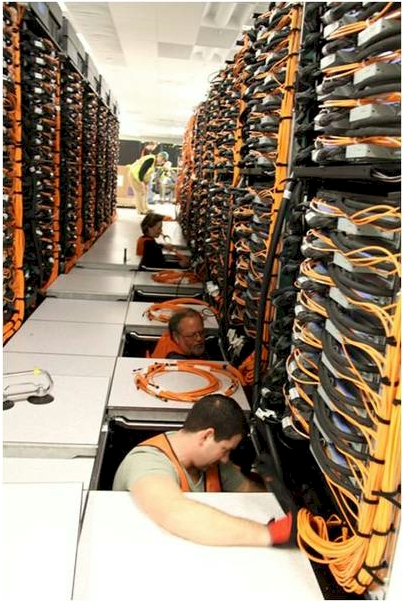
\includegraphics[height=6.15cm]{figures/bgWiring.jpg}
					
					\caption{Installation of cables}
					\label{fig:bgWiringInstallation}
				\end{subfigure}
				
				\caption[BlueGene/Q cable installation.]%
				        {BlueGene/Q cable installation~\cite{cscs13}.}
				\label{fig:bgWiring}
			\end{figure}
			
			In other large-scale architectures, the task of cable installation is
			completed by a team of technicians aided by the use of standardised
			labelling for cables and sockets as illustrated in
			figure~\ref{fig:bgWiring}~\cite{tia2006}. In these architectures the
			cabling patterns required are relatively straightforward, thanks to the
			coarseness of the units used~\cite{lakner07} or they use network
			topologies whose cabling centres around high-fan-in
			switches~\cite{cisco07,csernai15}.
			
			It has been reported in the literature that when copper cables are used,
			labour costs dominate~\cite{popa10} and while cable costs are expected to
			decline, labour costs are not~\cite{mudigonda11}. Many researchers have
			attempted to control cable installation costs by trying to reduce the
			number or length of cables required by developing alternative network
			topologies~\cite{curtis12, popa10, mudigonda11}.  Unfortunately, these
			techniques do not apply to SpiNNaker since its network topology is fixed.
			
			Supercomputer architectures such as BlueGene/Q make use of large custom
			`midplane' PCBs in place of some cables to interconnect units within a
			cabinet~\cite{milano13}. This scheme can greatly reduce wiring complexity
			since only coarser-grain, cabinet-to-cabinet connectivity is implemented
			by cables. Unfortunately this technique is expensive and constrains the
			dimensions of the network topology supported by the machine. Since the
			SpiNNaker platform is designed to scale from desktop machines to
			machine room installations, this scheme is not practical.
			
			\begin{figure}
				\center
				\begin{subfigure}[b]{0.40\textwidth}
					\begin{tikzpicture}
						\node (leds) [inner sep=0]
						      {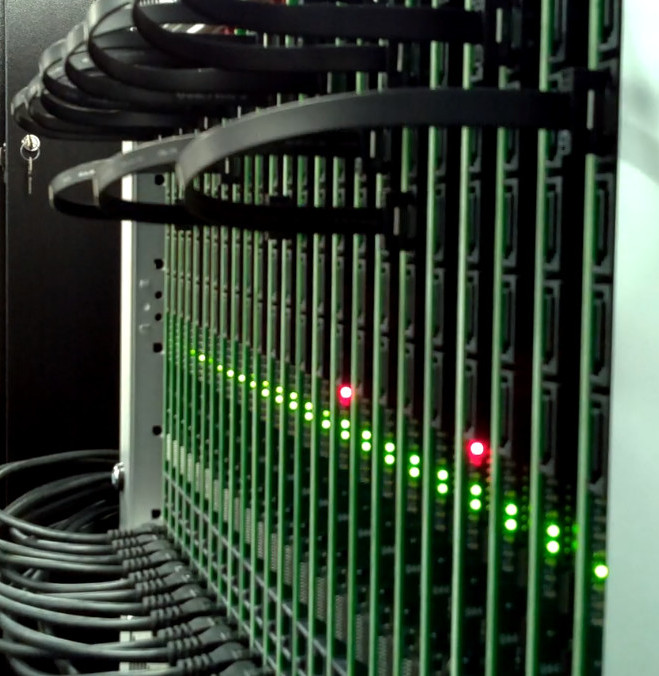
\includegraphics[width=\textwidth]{figures/leds.jpg}};
						% Point at left LED
						\draw [white, <-, line width=0.4em]
						      ([shift={(-0.0cm, -0.6cm)}]leds.center)
						      -- ++(225:1cm);
						% Point at right LED
						\draw [white, <-, line width=0.4em]
						      ([shift={(1.1cm, -1.1cm)}]leds.center)
						      -- ++(225:1cm);
					\end{tikzpicture}
					
					\caption{Diagnostic LEDs indicate the endpoints of each cable.}
					\label{fig:interactive-wiring-guide-leds}
				\end{subfigure}
				~
				\begin{subfigure}[b]{0.546\textwidth}
					\begin{tikzpicture}[thin, black!20!white]
						\node (screen) [inner sep=0]
						      {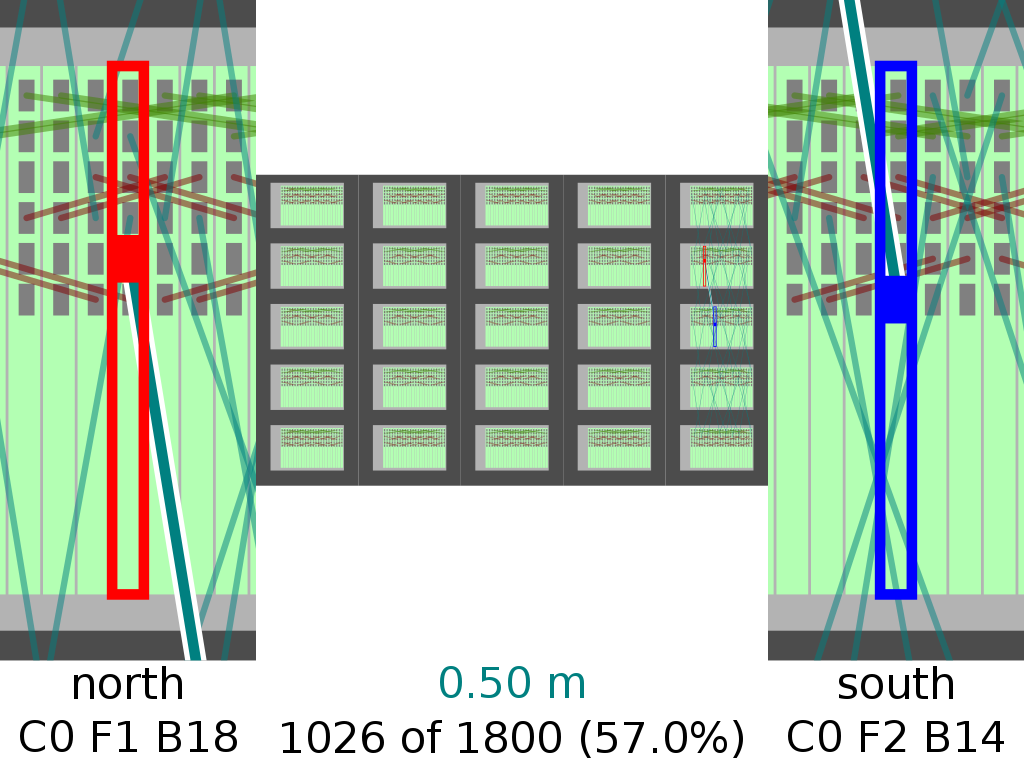
\includegraphics[width=\textwidth]{figures/wiring_guide_screenshot.png}};
						\draw (screen.south west) rectangle (screen.north east);
					\end{tikzpicture}
					
					\caption{A GUI and text-to-speech indicate what type of cable to
					install.}
					\label{fig:interactive-wiring-guide-gui}
				\end{subfigure}
				
				\caption{Interactive software guides cable installation.}
				\label{fig:interactive-wiring-guide}
			\end{figure}
			
			Due to the high density of units in a SpiNNaker system, the detailed
			cabling patterns used can be complex, despite their overall regularity.
			To cope with this complexity, I developed a software system which employs
			diagnostic hardware built into SpiNNaker, to guide technicians through
			the cable installation process. As shown in
			figure~\ref{fig:interactive-wiring-guide}, diagnostic LEDs on each
			SpiNNaker board are used to indicate which boards to connect. The
			software also provides step-by-step cabling instructions via a Graphical
			User Interface (GUI) and audible instructions delivered via headphones.
			These instructions explicitly specify the length of cable to use for each
			connection avoiding the common problem of technicians over-estimating the
			cable length required~\cite{mazaris97}. Diagnostic registers in the
			network hardware are then used to verify the correct installation of each
			cable in real-time ensuring that mistakes are highlighted and fixed
			immediately.
			
			\begin{table}
				\center
				\begin{tabular}{lrll}
					\toprule
						Size & Cables & Time & Notes \\
					\midrule
						24 boards  & \num{72}   & \SI{10}{\minute} & \\
						1 cabinet  & \num{360}  & \SI{4}{\hour} &
							Real-time validation not used. \\
						2 cabinets & \num{720}  & \SI{2}{\hour} & \\
						5 cabinets & \num{1800} & \SI{4}{\hour} \SI{20}{\minute} &
							Three people working simultaneously. \\
					\bottomrule
				\end{tabular}
				
				\caption[Cable installation times for various SpiNNaker machines.]%
				{Cable installation times for various sizes of SpiNNaker
				machine.}
				\label{tab:install-time}
			\end{table}
			
			\begin{figure}
				\buildfig{figures/install-histogram.tex}
				
				\caption{Two cabinet SpiNNaker machine cable installation times.}
				\label{fig:install-histogram}
			\end{figure}
			
			Table~\ref{tab:install-time} shows cable installation times for various
			sizes of SpiNNaker system. The times reported do not include breaks and,
			with the exception of the five cabinet system, are for the one person
			working alone.  Figure~\ref{fig:install-histogram} shows the histogram of
			cable installation times for a two cabinet machine.  These results
			confirm the observation by Mudigonda \emph{et al.} that cables which span
			cabinets and frames take longer to install~\cite{mudigonda11}, even
			though these distances are still very short in SpiNNaker. Compared with
			commercial installation efforts, per-cable installation times are much
			shorter for SpiNNaker taking seconds compared with minutes in other
			architectures~\cite{mudigonda11}.
			
			The positive impact of real-time validation of installed cables can
			clearly be seen by comparing the installation times of the one and two
			cabinet systems. Though double the size, the two cabinet machine was
			built in half the time required to build the single cabinet machine.
			While building the smaller machine, real-time cable validation had not
			yet been implemented and the installation process was interrupted for
			several minutes every time a misplaced connection was discovered.
			
			In the three-person cable installation effort employed for the five
			cabinet system, the guidance software was configured to assign each
			technician cables in non-overlapping parts of the machine ensuring
			minimal interference between the technicians. As expected, this renders
			the problem embarrassingly parallel, as in commercial computer
			installations.
			
			\begin{figure}
				\center
				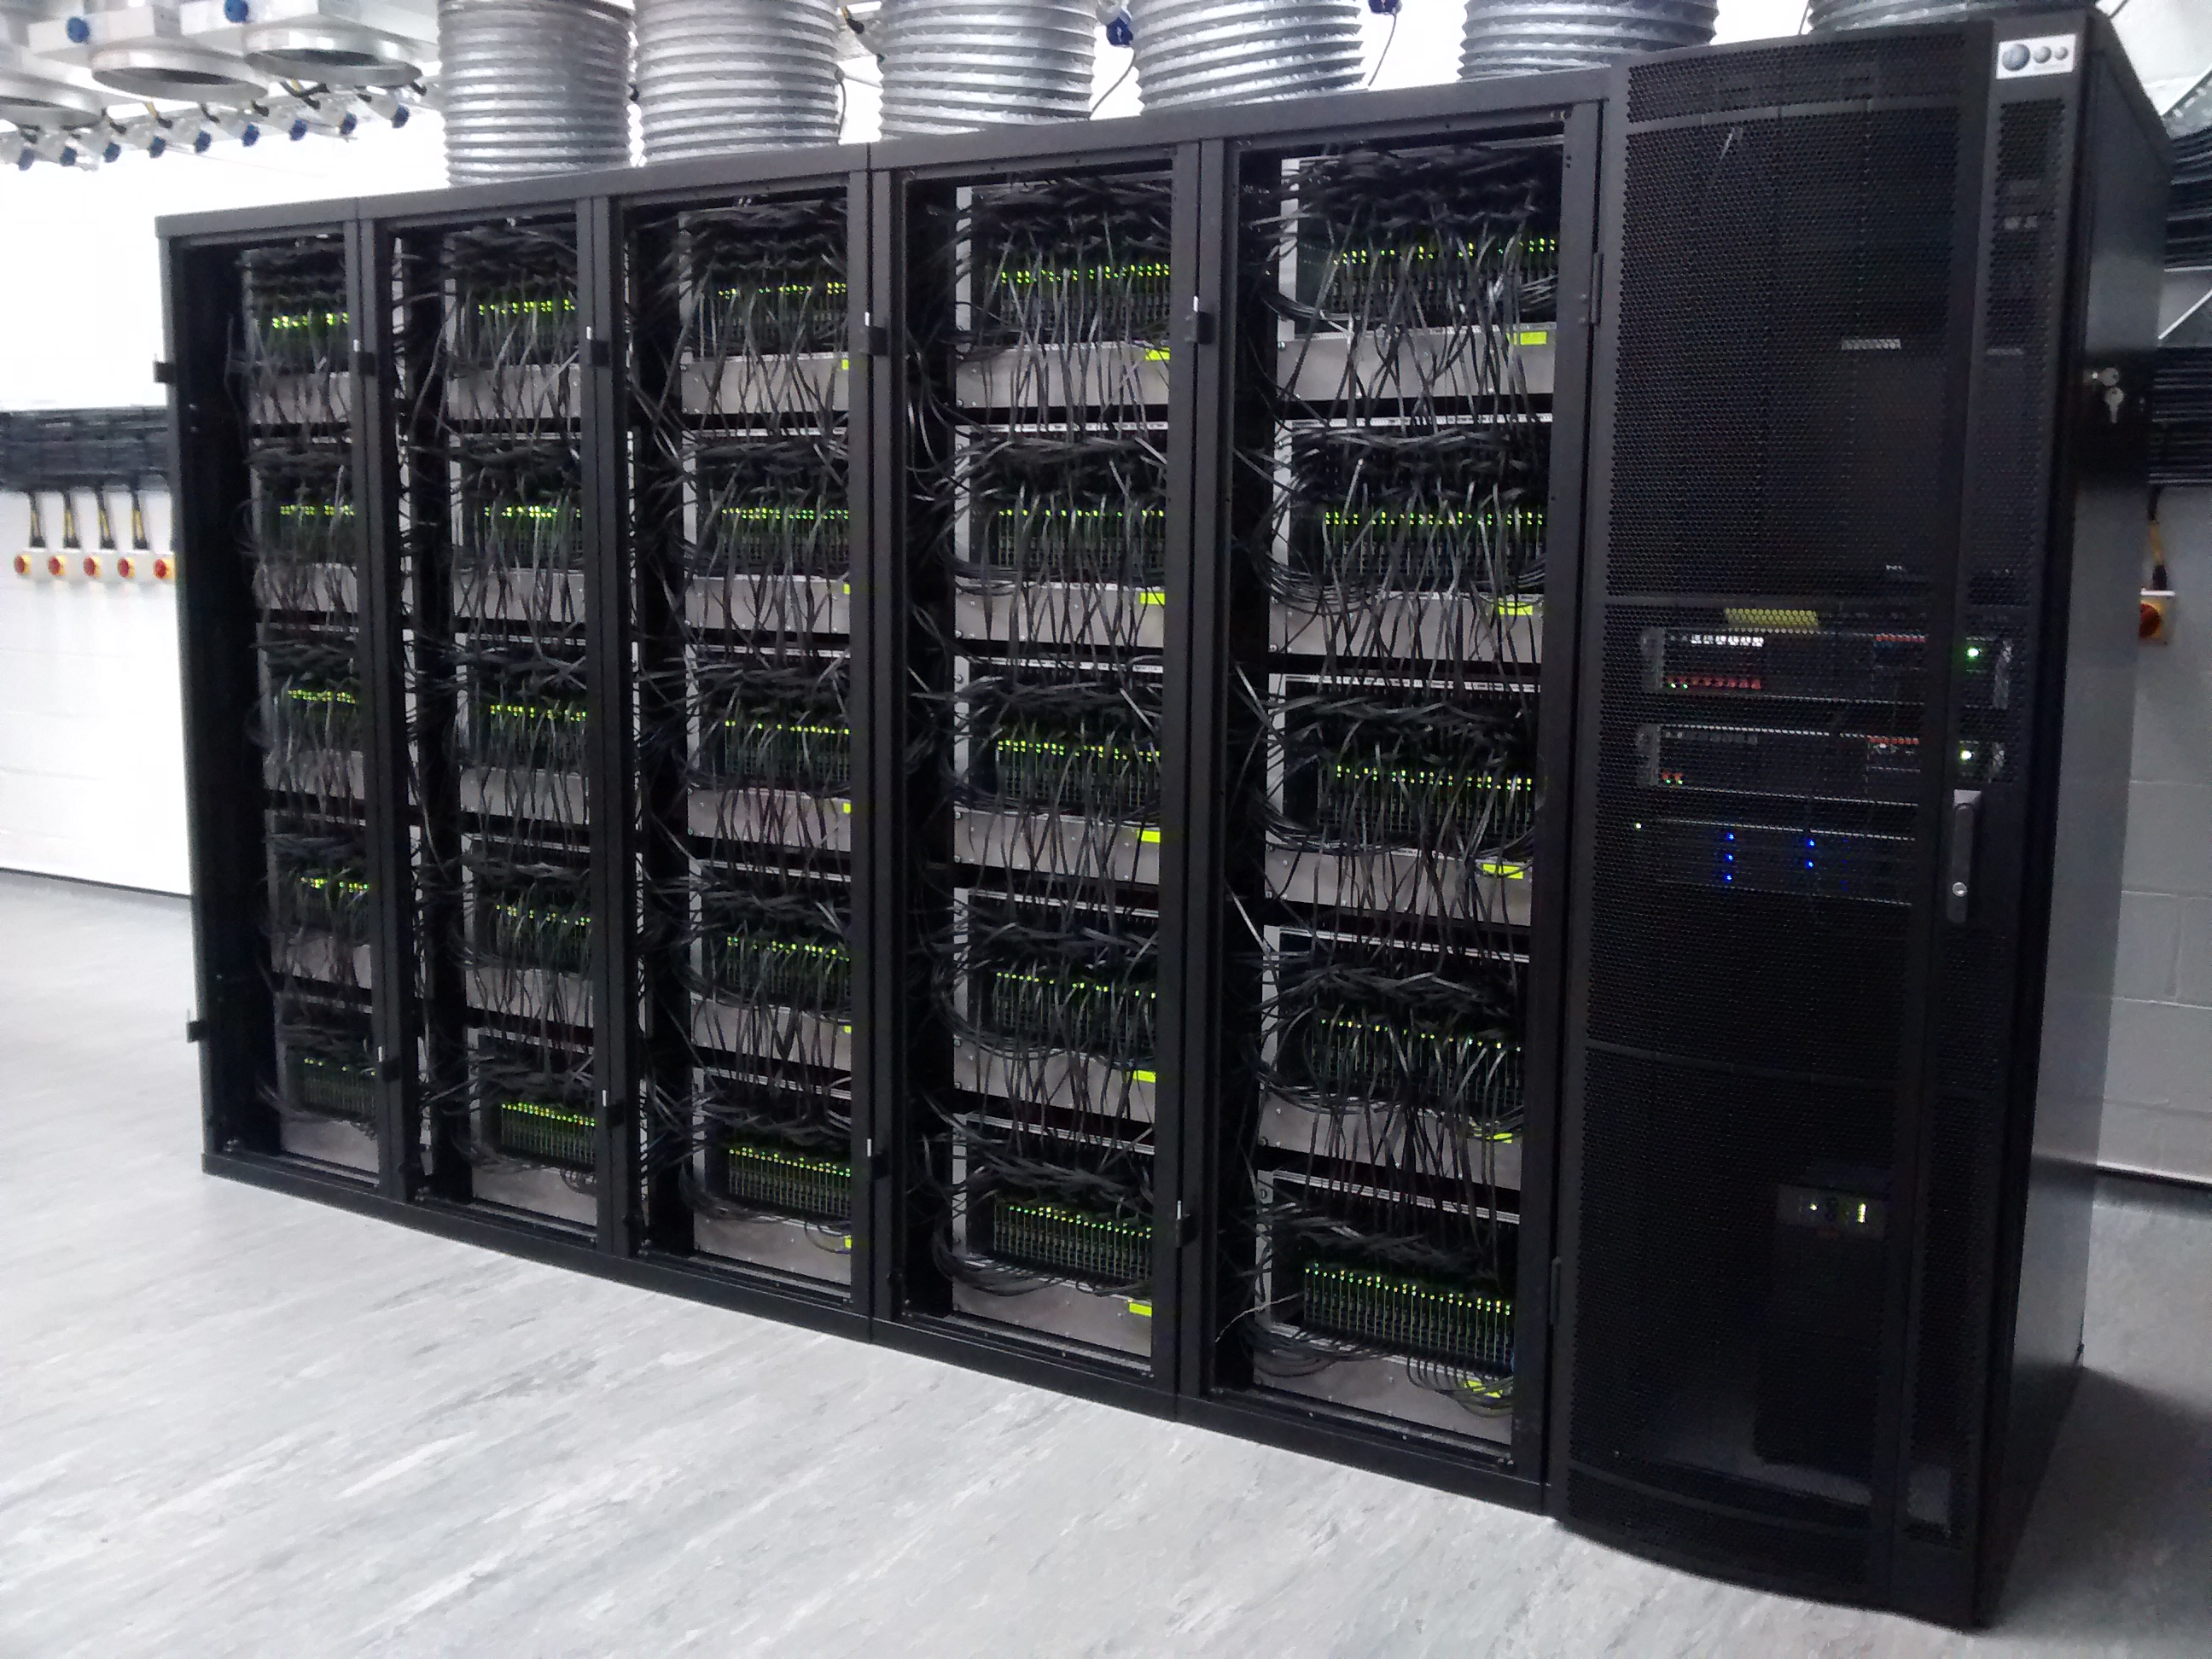
\includegraphics[width=0.8\linewidth]{figures/halfMillionCoreComplete.jpg}
				
				\caption[The five cabinet SpiNNaker system.]%
				{The five cabinet SpiNNaker system. The cabinet on the right contains
				conventional host servers which control SpiNNaker.}
				\label{fig:halfMillionCoreComplete}
			\end{figure}
			
			The completed five cabinet system is photographed in
			figure~\ref{fig:halfMillionCoreComplete}. A time-lapse video showing the
			construction and cable installation of this machine is also available on
			YouTube~\cite{heathcote16}.
			
		\subsection{Thermal implications}
			
			In large SpiNNaker machines, each 24 board frame contains a fan tray
			which pulls cool air from the front of the frame, between the SpiNNaker
			boards. The warmed air is then ejected out of the rear of the frame where
			ducting directs it into industrial air chillers. Conventional guidance on
			data centre design suggests that routing cables in the path of the
			system's airflow can have a serious impact on cooling
			performance~\cite{cisco07}.  To determine what effect the cabling
			described in this chapter had on SpiNNaker's cooling, a test program was
			executed to simulate heavy load before and after cable installation. The
			temperatures reported by the sensors on the top of each SpiNNaker board
			were sampled at regular intervals and once the overall system temperature
			stabilised, the mean temperature was recorded.
			
			Before the cabling was installed, the temperature stabilised at
			\SI{49}{\celsius} while after installation it stabilised at
			\SI{42}{\celsius}.
			
			These two data points suggest that the system's temperature is unlikely
			to have been been seriously impacted by cable installation. Since the two
			experiments were run on different days (with potentially different
			ambient temperatures) and are based on a single experiment, it is not
			possible to infer much more from this result.
			
		\subsection{Maintenance}
			
			At the time of writing, the five cabinet machine is still being
			commissioned and so the long term maintenance impact of the system's
			cabling is not known. One important factor in the maintainability of the
			system is the ease with which faulty boards can be replaced. During
			commissioning a number of boards have been replaced by someone not
			involved in the machine's installation. Informal measurements suggest
			that boards near the centre of a frame (i.e. those most likely to be
			blocked by unrelated cables) take around ten minutes to replace,
			including time spent removing and replacing cables obstructing the board
			being exchanged. By comparison boards at the edge of the machine take
			around six minutes to replace. Though similar timing reports are
			unavailable for other architectures, these times appear reasonable in
			practice and suggest maintenance is not impaired by the wiring plan used.
	
	\section{Conclusions}
		
		In this chapter I presented a practical method of constructing real-world
		installations of large hexagonal torus topologies such that long cables
		spanning the width and height of the system are not required. Two
		transformations, shearing and slicing, are presented which allow
		conventional network folding techniques to be applied to hexagonal toruses
		to eliminate long `wrap around' links. Though both techniques incur some
		overhead in terms of mean and maximum cable length, the maximum cable
		length does not grow with the size of the network. This result makes
		hexagonal torus topologies a practical and scalable choice for future
		systems.
		
		The theoretical results presented in this chapter have been confirmed
		through the successful construction of several large-scale SpiNNaker
		machines which implement hexagonal torus topologies. During construction,
		diagnostic features of SpiNNaker's hardware were employed to guide
		technicians performing cable installation. This technique was found to be
		highly effective with cable installation times measured in seconds rather
		than minutes as reported for other architectures. Surprisingly there was no
		evidence found of this technique being applied to other architectures and
		consequently this secondary result may be of interest for future research.

	\chapter{Finding shortest path vectors in SpiNNaker's network}
	
	\label{sec:shortestPaths}
	
	% XXX: Add note explaining shortest path between two points in non-torus
	% space.
	
	In the previous chapter we explored the practical challenges of building
	machines which use hexagonal torus topologies working at the scale of units
	containing several nodes. To exploit these machines, however, we must also be
	able to route packets efficiently through the nodes in the resulting network.
	This chapter tackles the problem of finding shortest path vectors in
	hexagonal torus topologies. Shortest path vectors are used by many routing
	algorithms as the basis for route generation. In non-hexagonal torus
	topologies, finding shortest path vectors is trivial and intuitive but in
	hexagonal toruses, this is not the case.  In this chapter I introduce the
	Irregular Quadrant (IQ) method, a new technique for computing shortest path
	vectors in hexagonal torus topologies.  This method is cheaper to compute and
	more general than pre-existing techniques, functioning correctly on hexagonal
	torus topologies of any aspect ratio.
	
	In some hexagonal torus topologies, many shortest path vectors may exist
	between a given pair of points. I propose a technique for discovering all
	possible shortest path vectors. Using these alternative shortest path
	vectors, routing algorithms may be able to produce routes which load a
	network more evenly.
	
	In this chapter, I assume an idealised hexagonal torus topology without
	faults or other irregularities. The challenge of handling these artefacts of
	real-world systems will be tackled in chapter~\ref{sec:routing}.
	
	\section{Shortest path vectors}
		
		Many popular routing algorithms for torus topologies, including all
		published algorithms designed for SpiNNaker~\cite{davies12,navaridas14},
		compute a shortest path vector between the endpoints of a route and use
		this to generate a path through the network. A shortest path vector between
		two nodes is a vector, $\mathbf{v} = (v_1, v_2, v_3, \ldots)$, whose
		magnitude, $\| \mathbf{v} \| = \lvert v_1 \rvert + \lvert v_2 \rvert +
		\lvert v_3 \rvert + \cdots$, is minimal with respect to all possible
		vectors between those nodes.
		
		\begin{figure}
			\center
			\buildfig{figures/mesh-topology-coordinates.tex}
			\caption[Shortest path routes in a 2D mesh network.]%
			{An example 2D mesh network with example shortest-path routes
			from `A' to `B' and `B' to `C'.}
			\label{fig:mesh-topology-coordinates}
		\end{figure}
		
		In a non-hexagonal mesh topology, shortest path vectors are computed by
		taking the element-wise difference between the source and destination
		nodes' coordinates. For example, figure~\ref{fig:mesh-topology-coordinates}
		shows a 2D mesh topology with three nodes labelled `A', `B' and `C' with
		position vectors $(1, 2)$, $(4, 5)$ and $(6, 1)$ respectively. The shortest
		path vector from node `A' to `B' is $(4, 5) - (1, 2) = (3, 3)$ and from `B'
		to `C' is $(6, 1) - (4, 5) = (2, -4)$. A route may be produced by advancing
		the number of hops specified for each dimension in the shortest path
		vector. For example, a route from `A' to `B' may be constructed from any
		permutation of the hops X$^+\,$X$^+\,$X$^+\,$Y$^+\,$Y$^+\,$Y$^+$, an
		example of which is included in the figure. Likewise routes from `B' to `C'
		may be constructed from permutations of the hops
		X$^+\,$X$^+\,$Y$^-\,$Y$^-\,$Y$^-\,$Y$^-$. Regardless of the order of the
		hops, the length of the route, $\mathbf{v}$, is given by the magnitude of
		the shortest path vector, $\|\mathbf{v}\|$.
		
		Many popular routing algorithms such as dimension order routing, right-turn
		only routing and longest dimension first routing~\cite{davies12} are simply
		defined as rules for ordering the hops specified by a shortest path vector.
		
		\subsection{Torus networks}
			
			\begin{figure}
				\center
				\begin{subfigure}{0.3\linewidth}
					\center
					\buildfig{figures/torus-shortest-path-example.tex}
					\caption{Original}
					\label{fig:torus-shortest-path-example}
				\end{subfigure}
				\begin{subfigure}{0.3\linewidth}
					\center
					\buildfig{figures/torus-shortest-path-translate.tex}
					\caption{Routed \& translated}
					\label{fig:torus-shortest-path-translate}
				\end{subfigure}
				\begin{subfigure}{0.3\linewidth}
					\center
					\buildfig{figures/torus-shortest-path-routed.tex}
					\caption{Routed original}
					\label{fig:torus-shortest-path-routed}
				\end{subfigure}
				
				\caption{Finding shortest paths in a 2D torus topology.}
				\label{fig:torus-shortest-path}
			\end{figure}
			
			Computing shortest path vectors in non-hexagonal torus topologies is also
			straightforward. For example, to find the shortest path vector from node
			`A' to `B' in the 2D torus topology shown in figure~\ref{fig:torus-shortest-path-example} both nodes are translated such that
			the source node, `A', is at the centre of the network. The shortest path
			vector is then computed in the same way as a mesh network (figure~\ref{fig:torus-shortest-path-translate}). Note that, as in this example,
			translation may cause the destination node to `wrap around' the network.
			As illustrated in figure~\ref{fig:torus-shortest-path-routed}, the
			computed shortest path vector is also valid for the two points prior to
			translation.
			
			\begin{figure}
				\center
				
				\begin{subfigure}{\linewidth}
					\center
					\buildfig{figures/distance-map-mesh.tex}
					\caption{2D mesh topology}
					\label{fig:distance-map-mesh}
				\end{subfigure}
				
				\vspace{1em}
				
				\begin{subfigure}{\linewidth}
					\center
					\buildfig{figures/distance-map-torus.tex}
					\caption{2D torus topology}
					\label{fig:distance-map-torus}
				\end{subfigure}
				
				\caption[Magnitudes of shortest path vectors in a 2D mesh.]%
				{Plots showing the magnitude of shortest path vectors in a 2D
				(non-hexagonal) topology from locations marked {\color{red}$\times$}.
				Darker areas are further away. Contour lines show equidistant points.}
				
				\label{fig:distance-map}
			\end{figure}
			
			This procedure works because vectors from the centre of a non-hexagonal
			torus topology to any other point are identical to those in a
			corresponding mesh topology. For example, in figures
			\ref{fig:distance-map-mesh} and~\ref{fig:distance-map-torus} we can see
			that the magnitude of the shortest path vectors from the centre of a mesh
			and torus grow identically. Conversely, the magnitudes of vectors from
			other locations in mesh and torus topologies do not match.
		
	\section{Related work}
		
		The problem of finding shortest path vectors in hexagonal mesh topologies
		has been widely considered and formulations may be found in a variety of
		applications, including computer games~\cite{patel15}. Hexagonal toruses,
		by contrast, have only received limited attention. In this section I
		briefly summarise the solutions proposed for hexagonal mesh topologies
		before more deeply examining existing solutions for hexagonal torus
		topologies.
		
		\subsection{Hexagonal mesh networks}
			
			\begin{figure}
				\center
				\buildfig{figures/hex-mesh-topology-coordinates.tex}
				\caption{An example hexagonal mesh network topology.}
				\label{fig:hex-mesh-topology-coordinates}
			\end{figure}
			
			In hexagonal mesh topologies it is conventional to define three `axes' X,
			Y and Z as shown in
			figure~\ref{fig:hex-mesh-topology-coordinates}~\cite{patel15}. In this
			example, the three labelled nodes `A', `B' and `C' may be given position
			vectors such as $(1, 1, 0)$, $(3, 2, 0)$ and $(0, 0, -7)$ respectively.
			As in other mesh networks, a vector between two nodes is found by
			subtracting the nodes' vectors. For example, a vector from `A' to `B' is
			$(3, 2, 0) - (1, 1, 0) = (2, 1, 0)$. This vector can then be converted
			into a route in the same way as a mesh network by taking any permutation
			of the three hops  X$^+\,$X$^+\,$Y$^+$.
			
			As explained in detail in appendix~\ref{app:minimal-hex-coordinates},
			there are a multitude of vectors between any two points in a hexagonal
			mesh. For example, the vectors $(1, 0, -1)$ and $(3, 2, 1)$ also reach
			node `B' from `A'. However, for a given pair of nodes, there is always a
			single, unique vector whose magnitude is minimal which is given by the
			function:
			%
			\begin{equation*}
				\operatorname{minimiseVector}(x,y,z) =
					(x,y,z) - \operatorname{median}(x,y,z) \cdot (1,1,1)
			\end{equation*}
			%
			For example, the vector $(3, 2, 1)$ from `A' to `B' is minimised as
			follows:
			%
			\begin{align*}
				\operatorname{minimiseVector}(3,2,1) &=
					(3,2,1) - \operatorname{median}(3,2,1) \cdot (1,1,1) \\
				&=
					(3,2,1) - (2,2,2) \\
				&=
					(1,0,-1)
			\end{align*}
			%
			A side-effect of this is that a minimised vector will always contain at
			least one zero element, meaning that shortest path routes will use at most
			two of the three available dimensions.
		
		\subsection{Hexagonal torus networks}
			
			\begin{figure}
				\center
				
				\begin{subfigure}{\linewidth}
					\center
					\buildfig{figures/distance-map-hex-mesh.tex}
					\caption{Hexagonal mesh topology}
					\label{fig:distance-map-hex-mesh}
				\end{subfigure}
				
				\vspace{1em}
				
				\begin{subfigure}{\linewidth}
					\center
					\buildfig{figures/distance-map-hex-torus.tex}
					\caption{Hexagonal torus topology}
					\label{fig:distance-map-hex-torus}
				\end{subfigure}
				
				\caption[Magnitudes of shortest path vectors in a hexagonal torus.]%
				{Plots showing the magnitude of shortest path vectors in a hexagonal
				torus topology from locations marked {\color{red}$\times$}.  Darker
				areas are further away. Contour lines show equidistant points.}
				
				\label{fig:distance-map-hex}
			\end{figure}
			
			Unfortunately, the translation technique used for non-hexagonal toruses
			cannot be used in a hexagonal torus. As illustrated in figures
			\ref{fig:distance-map-hex-mesh} and \ref{fig:distance-map-hex-torus},
			shortest path vectors from the centre, or any other part of a hexagonal
			mesh network, do not grow in magnitude in the same way that those of a
			hexagonal torus network do. I am aware of two pre-existing approaches to
			computing shortest path vectors in hexagonal toruses. These are described
			below.
			
			\subsubsection{INSEE Method}
			
				The INSEE interconnect simulator has been used in all published
				research into SpiNNaker's hexagonal torus interconnect to
				date~\cite{navaridas09,ghasempour15}. Internally INSEE finds shortest
				path vectors by selecting the shortest of a set of twelve candidate
				vectors known to always contain a shortest path vector.
				
				\begin{figure}
					\center
					\begin{subfigure}{0.45\linewidth}
						\center
						\buildfig{figures/insee-vector-candidates-no-wrap.tex}
						\caption{$(\Delta_\textrm{X}, \Delta_\textrm{Y}) = (5,3)$}
						\label{fig:insee-vector-candidates-no-wrap}
					\end{subfigure}
					\begin{subfigure}{0.45\linewidth}
						\center
						\buildfig{figures/insee-vector-candidates-wrap-x.tex}
						\caption{$(\Delta'_\textrm{X}, \Delta_\textrm{Y}) = (-3,3)$}
						\label{fig:insee-vector-candidates-wrap-x}
					\end{subfigure}
					
					\vspace{1em}
					
					\begin{subfigure}{0.45\linewidth}
						\center
						\buildfig{figures/insee-vector-candidates-wrap-y.tex}
						\caption{$(\Delta_\textrm{X}, \Delta'_\textrm{Y}) = (5,-5)$}
						\label{fig:insee-vector-candidates-wrap-y}
					\end{subfigure}
					\begin{subfigure}{0.45\linewidth}
						\center
						\buildfig{figures/insee-vector-candidates-wrap.tex}
						\caption{$(\Delta'_\textrm{X}, \Delta'_\textrm{Y}) = (-3,-5)$}
						\label{fig:insee-vector-candidates-wrap}
					\end{subfigure}
					
					\vspace{1em}
					
					% Key
					\begin{tikzpicture}[thick]
						\coordinate (last);
						
						% #1 colour
						% #2 label
						\newcommand{\colourkeyentry}[2]{
							\node [#1] [right=of last, fill, rectangle, minimum size=1em] (last) {};
							\node [right=0 of last] (last) {#2};
						}
						
						\colourkeyentry{cb3class0}{$(\textrm{X}, \textrm{Y}, 0)$}
						\colourkeyentry{cb3class1}{$(\textrm{X} - \textrm{Y}, 0, - \textrm{Y})$}
						\colourkeyentry{cb3class2}{$(0, \textrm{Y} - \textrm{X}, - \textrm{X})$}
						
					\end{tikzpicture}
					
					\caption[The twelve candidate vectors considered by the INSEE method.]%
					{The twelve candidate shortest-path vectors considered by the INSEE
					method represented as dimension-order routes. $W=H=8$,
					$(\Delta_\textrm{X},\Delta_\textrm{Y}) = (5, 3)$ and
					$(\Delta'_\textrm{X},\Delta'_\textrm{Y}) = (-3, -5)$.}
					\label{fig:insee-vector-candidates}
				\end{figure}
				
				The twelve vectors considered are illustrated in
				figure~\ref{fig:insee-vector-candidates} and are constructed as
				follows.  First a shortest path vector from the source to target node
				is constructed as if the network was a 2D mesh producing a vector
				$(\Delta_\textrm{X},\Delta_\textrm{Y})$. A second 2D vector,
				$(\Delta'_\textrm{X},\Delta'_\textrm{Y})$, is also defined:
				
				\noindent
				\begin{align*}
					\Delta'_\textrm{X} &= \Delta_\textrm{X} - \operatorname{sign}(\Delta_\textrm{X})W
					\\
					\Delta'_\textrm{Y} &= \Delta_\textrm{Y} - \operatorname{sign}(\Delta_\textrm{Y})H
				\end{align*}
				%
				Where $W$ and $H$ are the width and height of the network respectively.
				This vector describes a route from the source to destination node that
				\emph{always} wraps around the peripheries of both the `X' and `Y'
				dimensions.
				
				Two further 2D vectors, $(\Delta'_\textrm{X},\Delta_\textrm{Y})$ and
				$(\Delta_\textrm{X},\Delta'_\textrm{Y})$ may be defined which wrap around
				just the X or Y axis, respectively.
				
				Each of the four 2D vectors may be converted into three hexagonal 3D
				vectors in which one element of the vector is zero. In total this
				results in twelve different vectors which cover all combinations of
				wrapping and non-wrapping routes and all combinations of axes used. The
				vector with the smallest magnitude must be the shortest path vector.
				
				This method can find shortest path vectors in hexagonal torus
				topologies of any aspect ratio but, compared with the XYZ-protocol
				(described next), is relatively clumsy and slow to compute.
			
			\subsubsection{XYZ-Protocol}
			
				Hoffmann and D\'es\'erable described the XYZ-protocol for computing
				shortest path vectors in hexagonal toruses with equal width and
				height~\cite{hoffmann15,hoffmann11}.  First, the source and destination
				nodes are translated such that the source node lies at the centre of
				the topology. The authors observe that from the centre of the topology,
				the pattern with which distances grow differs between the four
				quadrants outlined in figure~\ref{fig:xyz-protocol-regions}.
				
				\begin{figure}
					\center
					\buildfig{figures/xyz-protocol-regions.tex}
					
					\caption{The four quadrants defined by the XYZ-protocol.}
					\label{fig:xyz-protocol-regions}
				\end{figure}
				
				If the destination lies in quadrants 1 or 4, a route may be constructed
				as if in a hexagonal mesh topology. If the destination lies in
				quadrants 2 or 3, however, the algorithm tests whether taking a
				mesh-like vector within the quadrant or wrapping-around either the X or
				Y dimensions yields the shortest vector.
				
				By comparison with the twelve vectors considered by the INSEE method,
				the XYP-protocol considers just one for destinations in quadrant 1 or 4
				and no more than three in quadrant 2 or 3. Though the XYZ-protocol can
				be computed more cheaply than the INSEE method, it does not produce
				valid shortest path vectors for hexagonal torus topologies with aspect
				ratios other than $1:1$.
		
	\section{The Irregular Quadrant (IQ) method}
		
		In this section I propose a new technique for finding shortest path vectors
		in hexagonal torus topologies called the Irregular Quadrant (IQ) method and
		compare its performance with existing techniques.
		
		\subsection{Computing shortest path vectors}
		
			Consider the problem of finding a shortest path vector from (0, 0, 0), at
			the bottom-left, to a node somewhere else in a hexagonal torus topology.
			
			\begin{figure}
				\center
				\buildfig{figures/shortest-path-regions.tex}
				
				\caption[The four irregular quadrants defined by the IQ method.]%
				{Hexagonal torus topologies of various aspect ratios divided
				into irregular quadrants in which a particular pair of dimensions is used.}
				\label{fig:shortest-path-regions}
			\end{figure}
			
			Figure~\ref{fig:shortest-path-regions} illustrates how hexagonal torus
			topologies of various aspect ratios may be partitioned into four
			\emph{irregular quadrants}. These quadrants are defined according to which
			axes are wrapped around by the shortest path vectors reaching them. The
			irregular quadrants correspond to locations reachable by shortest path
			vectors which:
			%
			\begin{enumerate}
				\item Do not wrap
				\item Wrap around X only
				\item Wrap around Y only
				\item Wrap around both X and Y
			\end{enumerate}
			%
			Within each irregular quadrant, we observe that shortest path vectors are
			constrained to using only certain directionz:
			%
			\begin{enumerate}
				\item Only X$^+$, Y$^+$ and Z$^-$.
				\item Only X$^-$ and Y$^+$
				\item Only X$^+$ and Y$^-$
				\item Only X$^-$, Y$^-$ and Z$^+$.
			\end{enumerate}
			%
			Given the topology is of width $W$ and height $H$ and the
			destination node's 2D mesh coordinates are $(\Delta_\textrm{X},
			\Delta_\textrm{Y})$ we can define the shortest path vector within each
			irregular quadrant as:
			%
			\begin{enumerate}
				\item $\operatorname{minimiseVector}(\Delta_\textrm{X},\Delta_\textrm{Y},0)$
				\item $\operatorname{minimiseVector}(-(W-\Delta_\textrm{X}),\Delta_\textrm{Y},0)$
				\item $\operatorname{minimiseVector}(\Delta_\textrm{X},-(H-\Delta_\textrm{Y}),0)$
				\item $\operatorname{minimiseVector}(-(W-\Delta_\textrm{X}),-(H-\Delta_\textrm{Y}),0)$
			\end{enumerate}
			%
			Since we know that $0 \le \Delta_\textrm{X} < W$ and $0 \le
			\Delta_\textrm{Y} < H$, we can simplify the expressions for the magnitude
			of each of the above vectors. This yields four expressions giving the
			magnitude of a minimal vector as if in each irregular quadrant:
			%
			\begin{enumerate}
				\item $\operatorname{max}(\Delta_\textrm{X}, \Delta_\textrm{Y})$
				\item $(W - \Delta_\textrm{X}) + \Delta_\textrm{Y}$
				\item $\Delta_\textrm{X} + (H - \Delta_\textrm{Y})$
				\item $\operatorname{max}(W-\Delta_\textrm{X}, H-\Delta_\textrm{Y})$
			\end{enumerate}
			%
			From these expressions we can determine which irregular quadrant the
			destination is in by finding the expression with the minimum value. With
			this information, the shortest path can be found by minimising the vector
			associated with that irregular quadrant.  Figure~\ref{fig:iqmethod.py}
			shows a simple Python implementation of the IQ method.
			
			\begin{figure}
				\inputminted{python}{figures/iqmethod.py}
				
				\caption{A Python implementation of the IQ Method.}
				\label{fig:iqmethod.py}
			\end{figure}
			
			Compared with the INSEE method, this technique requires fewer cases to be
			considered (four rather than twelve) making it cheaper to compute.
			
			Unlike the four quadrants defined by the XYZ-protocol, the irregular
			quadrants defined by the IQ method correspond exactly to a particular
			shortest path vector. This means that, once the irregular quadrant a
			point lies in has been discovered, the shortest path vector can be
			calculated directly without considering multiple options. Though the
			boundaries between the four irregular quadrants are more complex than the
			quadrants of the XYZ-protocol, it is only marginally more expensive to
			discover which irregular quadrant a point lies in. In addition, the
			irregular quadrants retain their meaning across different aspect ratios
			making the IQ method suitable for any hexagonal torus topology.
		
		\subsection{Computing distances}
		
			The four vector magnitude expressions defined by the IQ method can also
			be combined to produce a compact expression of the distance between two
			points in a hexagonal torus topology:
			%
			\begin{align*}
				\|\operatorname{shortestPathVector}(\Delta_\textrm{X}, \Delta_\textrm{Y}, W, H)\| =
				\operatorname{min}(&\operatorname{max}(\Delta_\textrm{X}, \Delta_\textrm{Y}),\\
				                   &(W - \Delta_\textrm{X}) + \Delta_\textrm{Y},\\
				                   &\Delta_\textrm{X} + (H - \Delta_\textrm{Y}),\\
				                   &\operatorname{max}(W-\Delta_\textrm{X}, H-\Delta_\textrm{Y}))
			\end{align*}
			%
			This expression has also been derived independently from a
			graph-theoretic study of Cayley graphs, of which the hexagonal torus
			topology is a special case, by Xiao and Parhami~\cite{xiao04}.
		
		\subsection{Computational efficiency}
			
			Since computing shortest path vectors forms an integral part of the
			kernel of many routing algorithms, the running time of the function
			chosen can be an important consideration.
			
			To compare the performance of the three shortest path vector functions
			presented, the execution time of a C implementation of each technique was
			measured. The C implementation of the INSEE method is taken directly from
			the INSEE source code~\cite{navaridas09}. The C implementation of the
			XYZ-Protocol is a straight translation of the published
			pseudocode~\cite{hoffmann15}.
			
			Each function was called approximately 3 billion times: once for every
			pair of source and destination nodes in a $240\times240$ node hexagonal
			torus topology. The total execution time is then divided by the number of
			calls giving an average execution time.  This experiment was repeated 50
			times and the overall average execution time of each shortest path vector
			function was recorded. The experiments were conducted on a cluster of
			idle workstations with 3.10~GHz Intel Core-i5-2400 CPUs. The function
			implementations were compiled with GCC 5.3.0 with optimisations enabled
			(\verb|-O2|).
			
			\begin{figure}
				\center
				\buildrplot{figures/shortest-path-vector-runtimes.R}
				
				\caption[Mean execution times of shortest path vector functions.]%
				{Mean execution time of each shortest path vector function. Error bars
				indicate the range of the mean execution times of the fifty
				3-billion-combination experiments.}
				\label{fig:shortest-path-vector-runtimes}
			\end{figure}
			
			Figure~\ref{fig:shortest-path-vector-runtimes} shows the execution times
			of each shortest path vector function. From these results we can see that
			the INSEE method is slower than the other techniques. Although the
			XYZ-protocol and IQ method have similar performance, because the IQ
			method works for any hexagonal torus topology it is the better candidate
			for use in new applications.
	
	\section{Generating all shortest path vectors}
			
			\begin{figure}
				\center
				\buildfig{figures/wrap-alternatives.tex}
				
				\caption{Two distinct shortest path vectors in a hexagonal torus.}
				\label{fig:wrap-alternatives}
			\end{figure}
			
			In odd-sized non-hexagonal and $1:1$ hexagonal torus topologies there is
			exactly one distinct shortest path vector between any two points (though
			many routes may be defined from it). In even-sized topologies there may
			be two distinct shortest path vectors between nodes exactly half the
			length of an axis away as in figure~\ref{fig:wrap-alternatives}. The
			INSEE and IQ methods may generate either vector depending on how ties are
			broken in their implementation.
			
			\begin{figure}
				\center
				\buildfig{figures/spiralling.tex}
				
				\caption[Distinct shortest path vectors in non-square toruses.]%
				{Distinct shortest path vectors between two points, all with
				magnitude 11.}
				\label{fig:spiralling}
			\end{figure}
			
			Unlike non-hexagonal topologies, when the aspect ratio of a hexagonal
			topology is not $1:1$, some points may have many distinct (but equal
			magnitude) shortest path vectors.  For example,
			figure~\ref{fig:spiralling} illustrates three distinct shortest path
			vectors between an example pair of nodes. None of the shortest path vector
			functions discussed will generate all possible vectors in this situation,
			potentially limiting the choices available to routing algorithms.  To
			address this shortcoming, I propose a formula which enumerates every
			shortest path vector between a pair of points in a hexagonal torus.
			
			In a $W \times H$ hexagonal torus topology, starting from any node the
			vector $(0, H, 0)$ straightforwardly wraps once around the Y axis
			arriving back at the node it started from. The vector $(1,1,1)$ also
			returns to its starting point as described in
			appendix~\ref{app:minimal-hex-coordinates}. As a consequence $(0,H,0) -
			H\cdot(1,1,1) = (-H, 0, -H)$ must also be a vector which leads back to
			where it started. Adding this vector to a shortest path vector of the
			form $(x, 0, z)$ results in a new shortest path vector if $x\ge H$ and
			$z\le0$.
			
			For example, the vector $(10, 0, -1)$ (magnitude 11) in
			figure~\ref{fig:spiralling} can be added with $(-4, 0, -4)$ yielding $(6,
			0, -5)$ (also magnitude 11) which is still a shortest path vector between
			the two labelled nodes.  Since $(6, 0, -5)$ still meets the criteria
			defined above ($6 \ge 4$ and $-5 \le 0$), we can add $(-4, 0, -4)$ again
			yielding another shortest path vector $(2, 0, -9)$.  This new vector does
			not meet the requirement that $x \ge H$ (since $2 \ngeq 4$) and so no
			further shortest path vectors can be produced.
			
			More formally, a shortest path vector $(x, 0, z)$ may be converted into
			another shortest path vector $(x', 0, z')$ using the following formula:
			%
			\begin{equation*}
				(x', 0, z') = (x, 0, z) - \left(\operatorname{trunc}\left(\frac{z}{H}\right) + n\right)(H, 0, H)
			\end{equation*}
			%
			where
			%
			\begin{equation*}
				\left\{
					n \in \mathbb{Z}
				\;\Big|\;
					0 \le n \le
						\left\lfloor
							\frac{\left|x\right| + \left|z\right|}{H}
						\right\rfloor
				\right\}
			\end{equation*}
			%
			and $\operatorname{trunc}(\,\cdots)$ is the truncation operator which
			rounds towards zero to the nearest integer.
			
			A complementary formula may be derived based on the related observation
			that the vector $(W, 0, 0)$ results in no movement:
			%
			\begin{equation*}
				(0, y', z') = (0, y, z) - \left(\operatorname{trunc}\left(\frac{z}{W}\right) + n\right)(0, W, W)
			\end{equation*}
			%
			where
			%
			\begin{equation*}
				\left\{
					n \in \mathbb{Z}
				\;\Big|\;
					0 \le n \le
						\left\lfloor
							\frac{\left|y\right| + \left|z\right|}{W}
						\right\rfloor
				\right\}
			\end{equation*}
			
			Using these two expressions for wide and tall topologies, respectively,
			all possible distinct shortest path vectors between any two points may be
			found.
	
	\section{Conclusions}
		
		The calculation of shortest path vectors in mesh and torus topologies is at
		the heart of many routing algorithms. In this chapter, I introduced a new
		technique for computing shortest path vectors in hexagonal toruses which
		generalises to any hexagonal torus topology while executing more quickly
		than existing approaches. In addition, I described a formula for
		enumerating the distinct shortest path vectors between points in hexagonal
		torus topologies. Unlike previous work, this allows routing algorithms
		greater freedom by providing a choice of shortest path vectors between some
		points.  These contributions demonstrate that key operations such as
		computing distances and shortest path vectors in hexagonal toruses can be
		efficient and exhaustive just as in non-hexagonal torus topologies.

	\chapter{Routing packets in large SpiNNaker machines}
	
	\section{Related work}
		\subsection{Multicast routing}
		\subsection{Deadlock avoidance}
		\subsection{Fault-tolerance}
	
	\section{Dimension order routing in hexagonal torus topologies}
		\subsection{Hexagonal meshes}
		\subsection{Hexagonal toruses}
		\subsection{Ensuring fairness}
		\subsection{Generating spiralling routes}
	
	\section{Fault-tolerant multicast routing}
		\subsection{Graph search based repair}
		\subsection{Alternative routing heuristics}
		\subsection{Results}
			\subsubsection{Heuristic performance}
			\subsubsection{Runtime}
			\subsubsection{Route congestion}
	

	\chapter{Placing applications in large SpiNNaker machines}
	
	\label{sec:placement}
	
	In the previous chapter I tackled the problem of fault tolerant route
	generation for SpiNNaker's network. The centroid traffic pattern was used as
	an approximation of the expected network traffic generated by `well behaved'
	neural network simulation software running on SpiNNaker. This traffic pattern
	exhibits locality, with most communication occurring between adjacent nodes.
	In reality, neural simulation applications are not conveniently specified
	geometrically but rather as abstract graphs of communicating
	neurons~\cite{davison08,eliasmith04}. Although neural models often exhibit
	localised connectivity, this can only be exploited if they are laid out
	sensibly within a network. Producing optimal placements is an NP-complete
	problem~\cite{hoefler11}.
	
	In this chapter I evaluate the effectiveness of simulated
	annealing~\cite{kirkpatrick83} for placement of SpiNNaker applications.
	Though simulated annealing fell out of favour for use in application
	placement in the 1990s, I argue that it is time to re-evaluate its
	suitability for modern placement problems. Looking to the field of chip
	design, where circuit placement problems have also been growing exponentially
	in scale for the past few decades, simulated annealing was considered ideal
	for placement problems whose sizes are comparable to that of modern
	supercomputer placement problems.
	
	In experiments on existing SpiNNaker applications I find that simulated
	annealing achieves placement solutions substantially better than contemporary
	application placement techniques. In some cases simulated annealing is shown
	to make the difference between an application functioning correctly and not
	at all. Using larger scale synthetic benchmarks I have also demonstrated that
	my proof of concept simulated annealing based placement algorithm scales up
	to placement problems containing over one million vertices while achieving
	placement quality similar to an optimal placement solution.
	
	I also build upon the work on hexagonal torus topologies earlier in this
	thesis to develop an efficient placement cost estimation function for use in
	the kernel of the annealing algorithm.
	
	\section{Related work}
		
		Attempts to address the problem of placing applications in supercomputer
		networks have utilised a variety of approaches ranging from simple greedy
		algorithms to sophisticated combinatorial optimisation
		techniques~\cite{jeannot14}. In the parallel field of digital circuit
		placement for chip and FPGA design, placement algorithms have also received
		intense study.  In this section I survey the work carried out on
		application placement before exploring chip design techniques to see what
		can be learnt from this perhaps more advanced field.
		
		In the application placement literature, the placement problem is often
		referred to by the umbrella term `mapping'. Unfortunately, `mapping' is
		often used more broadly to include other tasks such as routing and
		application partitioning. To avoid ambiguity I use the term `placement', as
		preferred by the chip and FPGA design communities, to refer specifically to
		the problem of assigning vertices in an application's communication graph
		to nodes in a machine's connectivity graph: the focus of this chapter.
		
		\subsection{Application placement algorithms}
			
			Below I consider several popular techniques employed by existing
			supercomputer applications ranging from application-specific manual
			placement to sophisticated general purpose algorithms.
			
			\subsubsection{Application-specific approaches (manual placement)}
				
				\begin{figure}
					\center
					\buildfig{figures/fem-partitioning.tex}
					
					\caption[Partitioning of a 3D volume for a $3\times4\times2$ torus.]%
					{Example partitioning of a 3D volume to fit into a supercomputer with
					a $3\times4\times2$ torus or mesh topology.}
					\label{fig:fem-partitioning}
				\end{figure}
				
				In certain applications such as finite element
				modelling~\cite{bermejo13}, a problem's structure defines a `natural'
				placement of the problem onto the target machine. For example when
				simulating a 3D volume in a supercomputer with a $3 \times 4 \times 2$
				3D torus or mesh topology network, the modelled volume might be divided
				as in figure~\ref{fig:fem-partitioning}. Each cuboid in the model is
				then assigned to the corresponding node in the network topology.
				
				Unfortunately, this technique only applies to a very narrow class of
				applications and is not applicable to many of the types of neural
				models SpiNNaker is designed to run.
			
			\subsubsection{Sequential placement}
				
				In the case where a placement solution is non-obvious, one of the
				simplest and most popular strategies is to apply a simple sequential
				placement algorithm. Sequential placement greedily places the vertices
				of an application's communication graph onto nodes. By carefully
				selecting the order in which vertices are picked and nodes assigned in
				the target architecture, this algorithm can produce reasonable quality
				placements.
				
				\begin{figure}
					\center
					\begin{subfigure}{0.32\linewidth}
						\center
						\buildfig{figures/sequential-row-order.tex}
						\caption{Row-order}
						\label{fig:sequential-row-order}
					\end{subfigure}
					\begin{subfigure}{0.32\linewidth}
						\center
						\buildfig{figures/sequential-alternating.tex}
						\caption{Alternating}
						\label{fig:sequential-alternating}
					\end{subfigure}
					\begin{subfigure}{0.32\linewidth}
						\center
						\buildfig{figures/sequential-hilbert.tex}
						\caption{Hilbert curve}
						\label{fig:sequential-hilbert}
					\end{subfigure}
					
					\caption{Space-filling curves in 2D mesh and torus topologies.}
					\label{fig:sequential}
				\end{figure}
				
				Supercomputer management software such as SLURM~\cite{yoo03} and Blue
				Gene's system software~\cite{gilge14} by default na\"ively iterate over
				vertices in an application communication graph in the order in which
				they are defined by the application. The nodes in the target machine
				are iterated over using a simple space-filling curve.
				Figure~\ref{fig:sequential} illustrates three popular space filling
				curves.
				
				The row-order (figure~\ref{fig:sequential-row-order}) and alternating
				(figure~\ref{fig:sequential-alternating}) curves illustrate 2D versions
				of the default node assignment orders provided by the SLURM and
				BlueGene systems.  The Cray extensions to SLURM software provide a
				Hilbert curve~\cite{hilbert91} node assignment order
				(figure~\ref{fig:sequential-hilbert}). The Hilbert curve specifically
				attempts to maintain the property that points that are close together
				along the length of the curve are also close together in the 2D
				mapping~\cite{moon01, zumbusch99}. Since the vertex iteration order is
				also chosen such that connected vertices tend to be closer together,
				this property may lead to improved placement solutions.
				
				\begin{figure}
					\center
					\buildrplot{figures/space_filling_curves_comparison.R}
					
					\caption[Relationship between space filling curve offset and 2D distance.]%
					{Relationship between distance along a space filling curve
					and between the 2D positions assigned. Results shown for
					Manhattan distances in a $32\times32$ 2D mesh.}
					\label{fig:space_filling_curves_comparison}
				\end{figure}
				
				Figure~\ref{fig:space_filling_curves_comparison} illustrates how the
				distance between locations along each space filling curve map to
				distances in the resulting 2D space. Both the row-order and alternating
				orderings result in distances oscillating between being closer and
				spread out in 2D space, just as the space filling curves oscillate from
				side-to-side. For the Hilbert curve, however, distances grow more
				monotonically\footnote{The growth in distance for Hilbert curves may
				appear slightly irregular but in fact forms a fractal as a consequence
				of the fractal construction of the Hilbert curve itself.} and at
				smaller 1D distances, 2D distances are often lower than in other space
				filling curves.
				
				A number of algorithms have been proposed for automatically selecting
				good vertex and chip iteration orders, typically using a
				graph-traversal based heuristic. An example typical of this type of
				technique is `graph similarity based mapping' described by Hoefler and
				Snir~\cite{hoefler11}. This algorithm exploits the Reverse
				Cuthill-McKee (RCM) algorithm~\cite{cuthill69} to select a linear
				ordering of vertices in which connected vertices tend to appear close
				together. Internally, the RCM algorithm uses a breadth-first-search-like
				algorithm to order vertices.
				
				The RCM algorithm was originally designed as a tool for reducing the
				`bandwidth' of matrices to improve the performance of linear algebra
				techniques. A matrix's bandwidth is the width of the strip of non-zero
				elements on its diagonal. Figure~\ref{fig:rcm} illustrates how a sparse
				matrix is permuted by the RCM algorithm to produce a matrix with lower
				bandwidth. This technique may be applied to a graph by representing the
				graph as an adjacency matrix, $M$, where $M_{i,j}$ is $w$ if node $i$
				is connected by an edge to node $j$ with weight $w$ and 0 otherwise.
				When a graph's adjacency matrix is permuted by the RCM algorithm, the
				connectivity of the graph remains unchanged but the vertex ordering
				changes. The ordering of vertices in a low-bandwidth adjacency matrix
				tends to keep connected vertices closer together in the ordering, making
				the ordering well suited for use with a sequential placement algorithm.
				
				\begin{figure}
					\center
					\begin{subfigure}{0.45\linewidth}
						\center
						\buildfig{figures/rcm-initial.tex}
						
						\caption{Original permutation}
						\label{fig:rcm-initial}
					\end{subfigure}
					\begin{subfigure}{0.45\linewidth}
						\center
						\buildfig{figures/rcm-sorted.tex}
						
						\caption{RCM permutation}
						\label{fig:rcm-sorted}
					\end{subfigure}
					
					\caption[Graph adjacency matrix before and after RCM permutation.]%
					{Adjacency matrix representation of a graph before and after
					permutation by the RCM algorithm.}
					\label{fig:rcm}
				\end{figure}
				
				In small-scale and densely connected applications such as early neural
				simulations running on prototype SpiNNaker machines~\cite{galluppi10},
				these techniques have proven sufficient.  As my experiments demonstrate
				later, however, sequential placement is insufficient for some SpiNNaker
				applications.
				
			\subsubsection{Simulated annealing}
				
				\label{sec:application-placement-summary}
				
				In the academic community, a number of attempts have been made to use
				sophisticated optimisation algorithms for the placement of
				applications. In 1985, Steele~\cite{steele85} first proposed the use of
				simulated annealing for placing applications in the 6D torus topology
				of the 64 node `Caltech Cosmic Cube'. The proposed algorithm is
				described below.
				
				Initially, the vertices in the application's communication graph are
				assigned randomly to nodes in the machine. Two vertices are then chosen
				at random and swapped.  If this swap reduces the `cost' of the
				placement (as defined later), the vertices are kept in their new
				locations. If the cost increases as a result of the swap, the vertices
				are moved back to their original locations with a probability dependent
				on the magnitude of the cost increase and the current `temperature'.
				
				The process of picking and swapping vertices is repeated many times
				while the temperature is gradually reduced. Initially the temperature
				is set to a large value causing most swaps to be accepted, regardless
				of their cost. As the algorithm proceeds, the temperature is reduced
				until only swaps resulting in cost reductions are accepted. By
				initially accepting detrimental swaps, the algorithm typically avoids
				becoming trapped in local minima. Towards the end of the algorithm's
				execution the solution is presumed to be close to the global
				minimum-cost solution and so few or no detrimental swaps are accepted.
				
				The cost of a particular placement is defined by some expression
				approximating the quality of the placement with better quality
				placements having lower costs. In Steele's work, the cost of a
				placement is computed by finding the shortest path routes between all
				connected vertices using Dijkstra's algorithm. Rather than repeating
				this relatively expensive computation after each swap, Steele's
				implementation updated the previously calculated cost by recomputing
				only the routes connecting the swapped vertices.
				
				The number of swaps to attempt and the rate at which the temperature is
				changed is dictated by an `annealing schedule' and can have a major
				impact on the execution time of the algorithm and the quality of the
				placement solution. I describe one such schedule in detail later in
				this chapter when describing my own simulated annealing based
				application placement algorithm.
				
				Towards the end of the 1980s, application placement appeared to be
				becoming less important as supercomputer network architectures
				improved, appearing to render computationally intensive placement
				algorithms unnecessary~\cite{dally87}.  In addition, network and
				problem sizes remained small: so small in fact that exact
				linear-programming based placement algorithms remained a meaningful
				point of comparison in application placement research~\cite{xu91}. In
				this environment, simpler sequential placement algorithms gained favour
				over more computationally expensive algorithms such as simulated
				annealing.
				
				In contemporary application placement algorithms, `low temperature'
				simulated annealing algorithms are occasionally employed as a
				post-processing step for other placement algorithms~\cite{hoefler11}.
				Other heuristics are used to generate an initial placement solution.
				
				% Outside of badly attempting 90s scale problems at least... \cite{chen06}
			
			\subsubsection{Recursive partitioning}
				
				As problem and machine sizes have grown and network utilisation has
				once again become an important factor in application
				performance~\cite{navaridas09b}, more complex optimisation algorithms
				have reappeared in the literature. One popular approach employs graph
				partitioning algorithms such as METIS~\cite{karypis98} to perform
				recursive bipartitioning based
				placement~\cite{phillips14,hoefler11,pellegrini96}.  This placement
				process is illustrated in figure~\ref{fig:partitioning}.
				
				\begin{figure}
					\center
					\buildfig{figures/partitioning.tex}
					
					\caption[Application placement by recursive partitioning.]%
					{Illustration of application placement by recursive
					partitioning. Each node has the capacity to hold two vertices.}
					\label{fig:partitioning}
				\end{figure}
				
				In the first step, the application communication graph and machine
				connectivity graph are each bipartitioned such that the number of edges
				cut by the partitions is minimised while the size of each partition
				remains similar. Each half of the communication graph is associated
				with one of the halves of the machine connectivity graph.  The
				partitioning process is then repeated recursively, further partitioning
				the application and machine graphs. The process halts when either graph
				can no longer be partitioned.  The vertices in the communication graph
				are then placed on their associated node in the connectivity graph.
				
				Unfortunately, recursive partitioning-based techniques are known to
				perform sub-optimally when the number of nodes is not a power of
				two~\cite{simon97}. In addition, placement problems are often subject
				to multiple orthogonal constraints. For example, a vertex in an
				application's communication graph may consume a certain number of
				processors and some quantity of SDRAM. Partitioning algorithms require
				a metric with which the size of each partition may be measured to
				ensure that the two halves are balanced. When multiple orthogonal
				resources exist, a single metric is insufficient to express this
				requirement. As a result, partitioning algorithms are of limited use in
				applications whose placement is subject to several orthogonal
				requirements, such as neural modelling software on SpiNNaker.
				
			\subsubsection{Topology-specific approaches}
				
				Other approaches employ other optimisation techniques that are
				specialised for use with applications and networks with specific
				connectivity patterns, for example, trees~\cite{jeannot14,traff02}.
				Unfortunately, these algorithms cater neither for SpiNNaker's hexagonal
				torus topology nor the range of communication topologies found in its
				target applications.
	
		\subsection{Circuit placement algorithms}
			
			The circuit placement problem in chip and FPGA design is similar to that
			of application placement: communicating components must be assigned
			positions in a chip so that wiring congestion is controlled.
			
			\begin{figure}
				\center
				\buildrplot{figures/top500-num-processors.R}
				
				\caption[Historical core counts for the `Top500' supercomputers.]%
				{Historical processor (core) counts for the `Top500' supercomputer
				installations. The line shows the mean number of processsors and grey
				ribbon indicates the range. Data reported by the `Top500
				List'~\cite{meuer16j}.}
				\label{fig:top500-num-processors}
			\end{figure}
			
			Following the march of Moore's `Law'~\cite{moore75}, the number of
			components in modern chips and FPGAs has been increasing at an
			exponential rate similar to that of core counts of supercomputers (see
			figure \ref{fig:top500-num-processors}). Today, in 2016, the largest
			chips contain billions of transistors, compared with millions of
			processors found in supercomputers. In terms of the raw number of
			processors, the world's largest supercomputers are at a scale comparable
			with the number of components in chips designed fifteen years ago. The
			mean size of today's `Top 500' supercomputers is somewhat smaller still,
			similar in scale to chips designed over 20 years ago.
			
			In view of of the similarity of the chip and application placement
			problems and the relative lead the field of chip placement has in terms
			of placement size, it appears reasonable to look to chip placement to
			suggest future application placement techniques.
			
			The popular approaches to circuit placement can be grouped into three
			broad categories~\cite{kahng11}:
			
			\begin{description}
				
				\item[Partitioning-based] As in application placement, these algorithms
				function by recursively partitioning the circuit to assign
				related components to areas of a chip.
				
				\item[Analytical] These algorithms approximate the placement problem as
				a simpler problem to which exact solutions can be computed
				inexpensively.
				
				\item[Simulated annealing] As in application placement, simulated
				annealing algorithms selectively apply random permutations to a
				placement causing placement quality to improve.
				
			\end{description}
			
			I briefly introduce each technique before assessing its suitability for
			use in application placement in SpiNNaker. The interested reader is
			encouraged to refer to `VLSI physical design: from graph partitioning to
			timing closure' by Kahng \emph{et al.}~\cite{kahng11} for a more thorough
			introduction to the field of circuit placement and the techniques that I
			summarise here.
			
			\subsubsection{Partitioning-based placement}
				
				Partitioning based placement has a long history with early examples
				dating back to the 1970s~\cite{breuer77}. As in recursive partitioning
				based application placement algorithms, the input circuit is
				partitioned alongside the target topology to assign placements. Again,
				graph partitioning software such as METIS~\cite{karypis98} is used to
				partition the circuits but since the target topology is the 2D surface
				of a chip, simple geometric partitioning is used to divide the surface
				of the chip. More recent partitioning based placers such as
				Capo~\cite{roy05} employ additional heuristics such as `terminal
				propagation' where connections between adjacent partitions are
				considered to attempt to align components on either side of a cut.
				
				Unfortunately, as with its use in application placement, these
				partitioning techniques are not ideal.  Consequently, partitioning
				based placement techniques have largely been superseded in chip
				design~\cite{markov15}.
			
			\subsubsection{Analytical placement}
				
				The current generation of placement algorithms attempt to approximate
				placement problems as simpler problems with cheaply computed,
				closed-form solutions. One of the common approximations used by these
				approaches is modelling the components to be placed as point-like
				objects. As the number of components in digital circuits has grown,
				this approximation has also improved, resulting in analytical placement
				becoming the most popular approach in use today~\cite{markov15}.
				
				One popular analytical technique is `quadratic
				placement'~\cite{kahng11,spindler08}. In this algorithm the components
				in a circuit are approximated as infinitesimal objects with wires
				between them modelled as spring-like forces. Unlike physical springs,
				which obey Hooke's law, the force exerted by a connection is
				proportional to the \emph{square} of the distance between its
				terminals.
				
				To illustrate this approach, consider the simple one-dimensional
				placement problem presented in figure~\ref{fig:quadratic-placement}.
				In the quadratic placement technique, the cost of a placement is
				modelled as the weighted sum of the squares of the distances between
				connected components. In this case this yields the expression:
				%
				\begin{equation*}
					%
					\textrm{Cost} = 1(f_1 - m_1)^2 + 2(m_1 - m_2)^2 + 1(m_2 - f_2)^2
					%
				\end{equation*}
				%
				Where $f_1$, $f_2$, $m_1$ and $m_2$ represent the positions of the four
				components. An optimal placement is one which minimises this function.
				To find values which minimise a quadratic, the equation is
				differentiated yielding a system of linear equations. This system of
				equations is then solved to find the positions of the movable vertices
				which minimise the quadratic cost function.
				
				\begin{figure}
					\center
					\buildfig{figures/quadratic-placement.tex}
					
					\caption[An optimal 1D quadratic placement solution.]%
					{An optimal 1D quadratic placement solution for two fixed
					vertices ($f_1$ and $f_2$), two movable vertices ($m_1$ and $m_2$)
					and three weighted edges.}
					\label{fig:quadratic-placement}
				\end{figure}
				
				Quadratic placement is extended to two or more dimensions by simply
				applying the process for each dimension separately. Unfortunately, a
				straightforward extension to non-Euclidean geometries such as
				hexagonal toruses is non-trivial. For example, quadratic placement
				relies on cost increasing monotonically as two points are moved in
				opposite directions, a property which does not apply to torus
				topologies. This same problem also applies to the approximations used
				by other analytical techniques.
				
				An additional challenge posed by quadratic placement is that some
				vertices' locations must be fixed to provide a `spreading' force
				preventing degenerate solutions where all vertices are given the same
				coordinates. In circuit placement, the locations of `pads' used to
				connect components in a circuit to the outside world are typically
				fixed and provide convenient anchors during placement. Algorithms such
				as SimPL~\cite{kim12b} employ a combination of analytical techniques to
				add virtual `anchor' components which prevent degenerate solutions from
				forming. Unfortunately, this approach further adds to the difficulty of
				porting the technique to non-Euclidean geometries. These techniques
				also work better for larger circuit sizes, making analytical techniques
				non-ideal for today's relatively small (by chip placement standards)
				supercomputer placement problems.
				
				% TODO: mention viswanathan07 FastPlace 3.0 -- multilevel technique?
			
			\subsubsection{Simulated annealing}
				
				Simulated annealing was originally developed specifically to be applied
				to the problem of circuit placement~\cite{kirkpatrick83}. Throughout
				the late 1980s and early 1990s, simulated annealing was the dominant
				circuit placement technique when the first chips breaching one million
				components appeared~\cite{betz97,sechen85}. Due to the increased
				effectiveness of quadratic placement as problems grew beyond tens of
				millions of nodes, simulated annealing has fallen out of fashion as a
				circuit placement technique. Despite this, various efforts continue to
				be made to enhance the simulated annealing process' performance by
				attempting to partition the input problem into several independent
				problems~\cite{choong10,haldar00} and parallelise the
				algorithm~\cite{ludwin08}.
				
				Simulated annealing notably remains popular as a stand-alone placement
				tool in niche applications where flexibility is important. For example,
				the flexible, multi-FPGA, Verilog-To-Routing (VTR) software
				suite~\cite{luu14} and Open Source Arachne-PNR~\cite{cseed} use
				simulated annealing to produce placements within multiple FPGA
				architectures.
				
				Since application placement problems are only now beginning to reach
				the scales at which simulated annealing became popular in circuit
				design, it is likely to be a good choice for application placement over
				the next few years. In addition, simulated annealing's flexibility
				potentially makes it a good choice to handle the wide variety of
				architectures in use by modern supercomputers.
	
	\section{Placement by simulated annealing}
		
		\label{sec:placement-by-annealing}	
		
		As we have seen, existing software placement techniques are not well suited
		to the large-scale applications projected for the SpiNNaker architecture.
		In the field of circuit placement, various algorithms have been proposed
		which are explicitly designed to cope with placement problems of similar or
		larger sizes. While analytical placement algorithms can produce high
		quality placement solutions for extremely large problems, the current --
		and near future -- generations of application placement problems are still
		too small. Simulated annealing, however, has a proven record in circuit
		design at the scale of modern application placement problems. In addition,
		the flexibility of simulated annealing makes it easy to adapt to new
		network architectures and, in this case, SpiNNaker's hexagonal torus
		topology.
		
		To demonstrate the suitability of simulated annealing for modern
		applications, I have implemented a simple simulated annealing based placer
		for the SpiNNaker architecture. Compared with previous simulated annealing
		algorithms for application placement, this algorithm is intended to cope
		with much larger problem instances and draws inspiration from the
		techniques used by circuit placement algorithms.
		
		In contrast with circuit placement algorithms built on simulated annealing,
		my implementation represents the problem differently to handle the nuances
		of application placement. In circuit placement, for example, exactly one
		component may be placed in a given space while in application placement,
		several applications may be placed on the same node (e.g. on different
		cores, or as separate processes). These differences, along with details of
		the cost functions and annealing schedule used are described in the
		remainder of this section.
		
		\subsection{Representation}
			
			A typical SpiNNaker application is made up of a number of processes which
			are executed by individual processor cores, consuming some quantity of
			on-chip resources such as shared SDRAM. These processes communicate via
			multicast packets which are sent via SpiNNaker's network.
			
			In the proposed placement algorithm, an application is defined as a graph
			where the `vertices' represent the processes as defined above and the
			multiedges, referred to here as `nets', represent directed flows of
			multicast packets from one vertex to several others. Each vertex consumes
			some quantity of on-chip resources (typically one core and a number of
			bytes of on-chip RAM). The placement algorithm must assign each vertex to
			a specific SpiNNaker chip (i.e. a node in SpiNNaker's network) such that
			the resources available on that chip are not exhausted.
			
			% TODO: Include remark like the following?
			% Unfortunately, since multiple resource types must be considered, that
			% application placement additionally encompasses a bin packing problem
			% \cite{korte06}.
			
			An additional soft constraint is imposed: the placement algorithm should
			attempt to place connected vertices as close together as possible. Nets
			may be annotated with a `weight' which provides a hint to the placer
			indicating the relative importance of a particular net. A larger weight
			indicates the placer should try harder to keep the vertices it connects
			closer together. Because this constraint is soft, the placer should make
			a `best effort' attempt to obey the constraint but is not obliged to
			achieve a perfect placement solution.
			
			The SpiNNaker topology is represented as a 2D hexagonal torus topology
			with homogeneous inter-chip links. Each chip is defined to have a certain
			quantity of each resource consumed by vertices. For example, SpiNNaker
			chips nominally contain 17 application processors and 128~MB of on-chip
			SDRAM. Some chips, however, may have fewer working cores while others may
			be non-functional, thus effectively having no resources.
			
			\subsubsection{Additional constraints}
				
				Real-world applications may also apply some additional constraints on
				placement solutions. Two such constraints are considered here.
				
				Some applications require that certain vertices are always placed on a
				specific chip, for example to enable communication with an external
				device attached directly to a SpiNNaker chip. The placement algorithm
				must obey this requirement, treating constrained vertices as a
				special case.
				
				In other applications, in-memory communication may be required between
				certain vertices and therefore these vertices must always be placed on
				the same chip. This constraint may be implemented by preprocessing the
				application graph such that constrained vertices are merged into a
				single vertex whose resource requirements are the sum of the original
				vertices.
		
		\subsection{Algorithm description}
			
			As outlined earlier, simulated annealing swaps pairs of vertices keeping
			beneficial swaps as well as some proportion of detrimental swaps. In the
			remainder of this section I describe the exact processes by which
			vertices are selected and swapped. I also consider the choice of cost
			function for use with a hexagonal torus topology before specifying the
			annealing schedule used.
		
			\subsubsection{Generating candidate swaps}
				
				Simulated annealing based placement schemes move vertices by swapping
				random pairs of vertices. In application placement problems, where
				vertices may differ in resource requirements, it is not always possible
				to swap arbitrary pairs of vertices. For example, if a `larger' vertex
				is swapped with a `smaller' one it may not fit in the space left behind
				by the smaller vertex.
				
				Rather than blindly picking pairs of vertices to swap and abandoning
				those which don't fit, the process described in
				figure~\ref{fig:sa-swap} is used. This swapping process reduces the
				likelihood that swaps involving larger vertices are aborted when the
				vertices on the target chip are individually too small to free up
				enough room to complete a swap.
				
				\begin{figure}
					\center
					\begin{subfigure}{\linewidth}
						\center
						\buildfig{figures/sa-swap-select.tex}
						\caption{A random vertex, $v_a$ is selected along with a random
						target chip (right).}
						\label{fig:sa-swap-select}
					\end{subfigure}
					
					\vspace*{1em}
					
					\begin{subfigure}{\linewidth}
						\center
						\buildfig{figures/sa-swap-remove.tex}
						\caption{Vertex $v_a$ is removed from its chip. Vertices are removed
						from the target chip until enough space is available to fit $v_a$.
						In this example, vertices $v_b$ and $v_c$ are removed.}
						\label{fig:sa-swap-remove}
					\end{subfigure}
					
					\vspace*{1em}
					
					\begin{subfigure}{\linewidth}
						\center
						\buildfig{figures/sa-swap-commit.tex}
						\caption{Vertex $v_a$ is swapped with vertices $v_b$ and $v_c$ if
						there is room. If there is not enough room the vertices are
						returned to their original locations and the swap is aborted.}
						\label{fig:sa-swap-commit}
					\end{subfigure}
					
					\caption{Selecting vertices to swap.}
					\label{fig:sa-swap}
				\end{figure}
			
			\subsubsection{Cost function}
				
				For each swap made by the algorithm, the change in the placement's
				`cost' must also be determined. In principle, the ideal cost function
				should accurately predict network congestion by performing routing and
				modelling the resulting network traffic. This approach was used by
				early application placement algorithms~\cite{steele85} but incurs a
				large performance overhead. Since the simulated annealing algorithm
				must re-evaluate the cost function before and after every swap, a cost
				function which is slow to evaluate can result in unacceptable execution
				time for the algorithm as a whole.
				
				A common alternative to measuring congestion directly used by many
				circuit placement algorithms is to approximate the network resources
				consumed. In the case of multicast nets, rather than computing
				efficient multicast routes, an estimate is made based on the relative
				locations of the vertices. Two popular techniques are described below
				\cite[\S4.2]{kahng11}.
				
				In the star model, the cost of a net is found by summing the distances
				from the net's source vertex to each sink vertex in turn as illustrated
				in figure~\ref{fig:cost-function-star}. In a hexagonal mesh and torus
				topology, the distance between two points can be cheaply determined (as
				described in chapter~\ref{sec:shortestPaths}) making this cost function
				inexpensive to compute. This model will overestimate network resource
				usage for nets with more than two vertices since, in practice,
				multicast routing algorithms will tend to generate routes which share
				some hops.
				
				In the Half-Perimeter Wire Length (HPWL) model, a bounding box is drawn
				around all of the vertices connected by the net and the cost of the net
				is estimated as half of the perimeter of this bounding box. In a
				non-hexagonal torus or mesh topology, the HPWL model exactly matches
				the length of an optimal multicast route for nets with two or three
				vertices. In nets with a greater number of vertices, HPWL
				underestimates the length of an optimal route by a factor of $\sqrt{n}$
				for nets with $n$ vertices~\cite{chung79}.
				
				The three non-orthogonal axes of hexagonal mesh and torus networks mean
				that there are several ways in which a bounding box may be defined.
				Specifically, the bounding box may extend along any pair of axes
				resulting in three possible bounding boxes and, thus, three HPWL values
				for any net as illustrated in figures~\ref{fig:cost-function-hpwl-xy},
				\ref{fig:cost-function-hpwl-xz} and~\ref{fig:cost-function-hpwl-yz}.
				The relative sizes of these three bounding boxes varies depending on
				the specific arrangement of vertices in the net, meaning that no single
				bounding box is appropriate for all situations.
				
				A single HPWL-like metric for hexagonal toruses can be produced by
				taking the minimum of the half-perimeters of the three different
				bounding boxes defined for a hexagonal toruses. Like the HPWL function
				for non-hexagonal toruses, this `hexagonal HPWL' cost function exactly
				predicts the length of optimal routes for all nets with two or three
				vertices.
				
				\begin{figure}
					\center
					\begin{subfigure}[b]{\linewidth}
						\center
						\buildfig{figures/cost-function-star.tex}
						
						\caption{Star $= a_x + a_y + b_x + b_z + c_x + c_y + d_x + d_y$}
						\label{fig:cost-function-star}
					\end{subfigure}
					
					\vspace*{1.5em}
					
					\begin{subfigure}[b]{0.32\linewidth}
						\center
						\buildfig{figures/cost-function-hpwl-xy.tex}
						
						\caption{HPWL$_{xy}$ $= w_{xy} + h_{xy}$}
						\label{fig:cost-function-hpwl-xy}
					\end{subfigure}
					\begin{subfigure}[b]{0.32\linewidth}
						\center
						\buildfig{figures/cost-function-hpwl-xz.tex}
						
						\caption{HPWL$_{xz}$ $= w_{xz} + h_{xz}$}
						\label{fig:cost-function-hpwl-xz}
					\end{subfigure}
					\begin{subfigure}[b]{0.32\linewidth}
						\center
						\buildfig{figures/cost-function-hpwl-yz.tex}
						
						\caption{HPWL$_{yz}$ $= w_{yz} + h_{yz}$}
						\label{fig:cost-function-hpwl-yz}
					\end{subfigure}
					
					\caption[Net cost estimation functions for hexagonal toruses.]%
					{Net cost estimation functions for hexagonal toruses and meshes.}
					\label{fig:cost-function}
				\end{figure}
				
				An experiment was performed to determine which cost function provides
				the most accurate results. \num{50000} nets connecting between two and
				thirty uniform randomly selected vertices in a $30\times30$ hexagonal
				torus topology were generated. The difference between each cost
				function and the `true' cost of a route generated by the NER routing
				algorithm is plotted in figure~\ref{fig:cost-function-error}.
				
				\begin{figure}
					\center
					\buildrplot{figures/cost-function-error.R}
					
					\caption[Estimation error of various cost functions.]%
					{Estimation error of various cost functions compared with
					routing solutions. Positive and negative errors are equally bad.
					Y-axis limit clipped for clarity. The error of the star cost function
					grows linearly with fan out beyond the axis limit.}
					\label{fig:cost-function-error}
				\end{figure}
				
				These plots confirm that the error introduced is consistently
				overestimated by the star model and underestimated by both the
				hexagonal HPWL and HPWL${_{xy}}$ cost models. The error in cost
				estimates produced by the star model grew more quickly than both HPWL
				variants, Both hexagonal HPWL and HPWL$_{xy}$ perform similarly though,
				as expected, hexagonal HPWL is more accurate for low fan out nets.
				
				To attempt to compensate for the theoretical $\sqrt{n}$ error in the
				HPWL cost, the Hexagonal HPWL and HPWL$_{xy}$ scaled by $\sqrt{n}$ are
				also shown. While this correction does not eliminate the error of these
				functions, it does reduce it. This is probably because the error only
				tends towards $\sqrt{n}$ for very large $n$ \cite{chung79} and also
				because the error is being computed against a realistic, non-optimal
				routing algorithm.
				
				On the basis of these results, the star cost function is rejected on
				the grounds that it produces the least accurate cost estimates. Though
				the $\sqrt{n}$-scaled hexagonal HPWL cost function produces the
				smallest error in general, its execution time is three times greater
				than $\sqrt{n}$-scaled HPWL$_{xy}$ whose accuracy is very similar.
				Since the execution speed of the cost function has a significant impact
				on the execution time of the simulated annealing algorithm, I have used
				the $\sqrt{n}$-scaled HPWL$_{xy}$ net cost function as a trade-off
				between accuracy and performance in this work.
				
			\subsubsection{Annealing schedule and acceptance function}
				
				\label{sec:placement-schedule-acceptance}
				
				The annealing schedule and acceptance function described below are
				taken directly from that used by the VPR FPGA placement
				software~\cite{betz97}. Due to a combination of time constraints and
				this schedule being known to work well, alternatives have not been
				considered in this thesis.
				
				Starting with an initial random (but valid) placement, $N$ swaps are
				performed to gather statistics about the problem, where $N$ is the
				number of vertices in the graph. The initial annealing temperature,
				$T$, is set to 20 times the standard deviation of the cost changes
				produced by the $N$ swaps.
				
				The annealing algorithm now performs a round of $E \times N^{1.33}$
				random swaps where $E$ is a tunable parameter controlling `effort'. In
				all experiments reported in this thesis, $E$ is set to 1. Increasing
				$E$ roughly linearly increases execution time for diminishing returns
				in placement quality improvements.  Each random swap is accepted with a
				probability:
				%
				\begin{align*}
					P_{\textrm{accept}}=
						\begin{cases}
							1 & \textrm{if } \Delta{}C \le 0 \\
							e^{\nicefrac{-\Delta{}C}{T}} & \textrm{otherwise} \\
						\end{cases}
				\end{align*}
				%
				Where $\Delta{}C$ is the change in cost resulting from the swap and $e$
				is Euler's number. This probability is 1 for any beneficial or neutral
				change. Small cost increases are accepted with a greater probability
				than large cost increases. At higher temperatures, larger cost
				increases are accepted with a greater probability than at lower
				temperatures.
				
				After a round of $E \times N^{1.33}$ of swaps has been performed, the
				temperature is updated according to $T_\textrm{new} = \alpha
				T_\textrm{old}$ where $\alpha$ is determined thus:
				%
				\begin{align*}
					\alpha=
						\begin{cases}
							0.50 & \textrm{if } R_\textrm{accept} > 0.96 \\
							0.90 & \textrm{if } 0.80 < R_\textrm{accept} \le 0.96 \\
							0.95 & \textrm{if } 0.15 < R_\textrm{accept} \le 0.80 \\
							0.80 & \textrm{if }        R_\textrm{accept} \le 0.15 \\
						\end{cases}
				\end{align*}
				%
				Where $R_\textrm{accept}$ is the proportion of swaps which were
				accepted by the algorithm in the previous round. This approach attempts
				to maximise the time spent at temperatures in which some, but not all,
				swaps are accepted since this is claimed to be when the greatest
				improvements to placement quality are made~\cite{betz97}.
				
				The algorithm terminates when $T < \nicefrac{0.005 C}{N_\textrm{nets}}$
				where $C$ is the current cost of the placement solution and
				$N_\textrm{nets}$ is the number of nets in the placement problem.
				
				Towards the end of placement, the solution is likely to be close to the
				(ideally global) minimum cost. In already-good solutions it is likely
				that swapping vertices between nodes which are far apart in the network
				will result in large cost increases. As a result, towards the end of
				the anneal, swaps are only considered over a limited distance,
				$D_\textrm{limit}$. By limiting the distance over which swaps occur,
				the proportion of swaps which are likely to be accepted is also
				increased. $D_\textrm{limit}$ is initially set such that all possible
				swaps are considered. It is then updated according to the following
				formula at the end of each round of swaps:
				%
				\[ D_\textrm{limit}^\textrm{new} = \textrm{max}(1,\quad
				D_\textrm{limit}^\textrm{old}(1-0.44 + R_\textrm{accept})) \]
				%
				This rule attempts to limit swap distance such that the proportion of
				accepted swaps does not drop below 0.44 for as long as possible, that
				is, such that some, but not all, swaps are accepted for as long as
				possible.
	
	\section{Evaluation}
		
		\label{sec:placement-results}
		
		A good placement algorithm should produce placements which result in
		efficient use of network resources. In addition, in SpiNNaker, routing
		table usage is an important concern since routing table entries are a
		finite resource. Finally, the execution time of the placement algorithm
		itself is relevant since, especially in applications where experiments are
		of short duration, placement execution time should not dominate application
		execution time.
		
		In this evaluation, the simulated annealing based placement algorithm
		introduced in this chapter is compared with a number of baseline algorithms
		representative of existing application placement techniques. I consider a
		combination of existing SpiNNaker applications and larger-scale synthetic
		benchmarks representative of possible future applications. I compare the
		performance of the placement algorithms under consideration using a
		combination of software models and confirm these results using experiments
		running on SpiNNaker hardware.
		
		\subsection{Baseline algorithms}
			
			To provide a baseline against which to compare my simulated annealing
			based placement algorithm, the following three placement algorithms are
			considered:
			
			\begin{description}
				
				\item[Hilbert] The sequential placement algorithm used by existing
				SpiNNaker software and similar to the algorithm provided by Cray's
				extensions to SLURM. This places vertices along a Hilbert curve path in
				breadth-first traversal order of the application communication graph.
				
				\item[RCM] The `graph similarity based mapping' algorithm described by
				Hoefler and Snir~\cite{hoefler11}. This assigns vertices and fills
				chips in Reverse Cuthill McKee order~\cite{cuthill69}.
				
				\item[Random] A random placement algorithm which places vertices
				uniform-randomly with no regard for connectivity. This algorithm serves
				as an experimental control.
				
			\end{description}
			
		\subsection{Existing applications}
			
			\label{sec:existing-applications}
			
			To verify the suitability of simulated annealing based placement for
			existing SpiNNaker software, a representative selection of benchmark
			applications has been collected. The communication graphs for these
			benchmark applications are then used to compare the performance of each
			placement algorithm against a set of simple performance metrics. In
			addition, a subset of the applications were modified to use each of the
			routing algorithms under test and changes in their performance are
			reported.
			
			Table~\ref{tab:real-benchmarks} summarises each of the benchmarks. While
			these applications are much smaller than those expected to run on new,
			large-scale SpiNNaker systems, these benchmarks provide a meaningful
			indicator of the types of connectivity which might be present in future
			networks. Further experiments using synthetic benchmarks, described
			later, will extend this study to applications at the scale SpiNNaker is
			designed to operate at.
			
			\begin{table}
				\center
				\begin{tabular}{lrr p{1.45cm} p{0.4\linewidth}}
					\toprule
					Name & Vertices & Nets & Fan out & Notes \\
					\midrule
					Microcircuit   & \num{1338} & \num{760} & 94.50 (98) &
						Spiking neural model of a cortical microcircuit~\cite{potjans14}
						implemented in `PyNN SpiNNaker'~\cite{knight16}. \\
					\addlinespace
					Sudoku         & \num{299} & \num{109} & 15.86 (21) &
						Spiking neural model which solves Sudoku puzzles implemented in `PyNN
						SpiNNaker'~\cite{knight16}. \\
					\addlinespace
					Card-Sorting   & \num{469} & \num{919} & 1.06\newline (3) & 
						Spiking neural model which solves the Wisconsin card sorting
						test~\cite{aubin15} implemented in `Nengo
						SpiNNaker'~\cite{mundy15}. \\
					\addlinespace
					CConv          & \num{2560} & \num{12020} & 3.48 (17) &
						Spiking neural model which performs 512D circular
						convolution~\cite{eliasmith13} implemented in `Nengo
						SpiNNaker'~\cite{mundy15}. A key component in the Spaun neural
						model~\cite{eliasmith12}. \\
					\addlinespace
					Parse          & \num{855} & \num{3046} & 3.26 (64) &
						Spiking neural model which performs simple sentence parsing
						implemented in `Nengo SpiNNaker'~\cite{mundy15}. \\
					\addlinespace
					MU0            & \num{1084} & \num{1084} & 1.38\newline (3) &
						A digital circuit simulation of the data path of a simple computer
						processor~\cite{nutter16} implemented using the digital circuit
						simulator example program included with `Rig'~\cite{rig15}. \\
					\bottomrule
				\end{tabular}
				
				\caption[SpiNNaker application benchmarks.]%
				{SpiNNaker application benchmarks. `Fan out' refers to the fan
				out of the nets in the communication graph and not necessarily the
				total fan outs of individual vertices. Both the mean and (maximum) fan
				out are shown.}
				\label{tab:real-benchmarks}
			\end{table}
			
			\subsubsection{Communication graph placement performance}
			
				Each benchmark's connectivity graph was placed on into an idealised $13
				\times 13$ hexagonal torus topology and then routed using the NER
				algorithm. This process was repeated \num{1000} times with various
				performance metrics recorded which are analysed below. Experiments were
				conducted on a cluster of idle workstations with 3.10~GHz Intel
				Core-i5-2400 CPUs and 8~GB of RAM.
			
				\begin{figure}
					\center
					\begin{subfigure}{\linewidth}
						\center
						\buildrplot{figures/application-benchmarks-quality.R}
						
						\caption{Placement quality (routed net length reduction vs. Hilbert
						placer)}
						\label{fig:application-benchmarks-quality}
					\end{subfigure}
					
					\vspace*{1em}
					
					\begin{subfigure}{\linewidth}
						\center
						\buildrplot{figures/application-benchmarks-tables.R}
						
						\caption{Maximum routing table entries (red line at \num{1024} entries)}
						\label{fig:application-benchmarks-tables}
					\end{subfigure}
					
					\vspace*{1em}
					
					\begin{subfigure}{\linewidth}
						\center
						\buildrplot{figures/application-benchmarks-runtime.R}
						
						\caption{Placement algorithm execution time}
						\label{fig:application-benchmarks-runtime}
					\end{subfigure}
					
					\caption{Application benchmark placement performance.}
					\label{fig:application-benchmarks}
				\end{figure}
				
				To measure the `quality' of the placement solutions generated, the
				total number of hops taken by the generated routes is compared in
				figure~\ref{fig:application-benchmarks-quality}. A better placement
				solution should require fewer hops and, as an indirect result, achieve
				lower network congestion.  Since the hop counts vary greatly between
				benchmarks, these results are normalised against the number of hops
				produced by the Hilbert placer, the placement algorithm used by default
				in pre-existing SpiNNaker software.
				
				In the majority of benchmarks, the simulated annealing based placement
				algorithm achieves the greatest reduction in hop counts. The RCM and
				Random placement algorithms both consistently produce results similar
				to or worse than those of the Hilbert placement algorithm.
				
				Unlike the other benchmarks, the `Microcircuit' benchmark notably shows
				little difference in placement quality amongst the four algorithms.
				This may be explained by the fact that this network is largely
				all-to-all connected meaning that a placement function can do little
				more than place the vertices tightly together to improve quality.
				
				The second metric considered is the number of routing table entries
				required in the worst case after placement and is shown in
				figure~\ref{fig:application-benchmarks-tables}. As is the practice of
				the applications modelled by these benchmarks, routing tables are
				compressed by the `Ordered Covering' algorithm~\cite{mundy16} and
				default routing is used when possible.
				
				Though many of the benchmarks do not run out of routing entries when
				placed with any of the algorithms, the `CConv' network notably runs out
				of table entries when placed by all but the simulated annealing and
				random placement algorithms. This can be attributed to the large number
				of nets the `CConv' network uses by comparison with other models.
				
				The random placement algorithm can often achieve competitive routing
				table sizes because it tends to spread out vertices over the entire
				machine. Because longer routes don't always result in more routing
				entries being required (thanks to default routing), this also results
				in the routing entries being spread more thinly across the whole
				system. In these experiments the majority of benchmarks do not fill the
				$13\times13$ hexagonal torus topology supplied, meaning that some
				networks can become spread out by the random placer. Though routing
				table usage drops, network utilisation, and potentially congestion,
				increases.
				
				The third metric considered is the execution time of the placement
				algorithm, shown in figure~\ref{fig:application-benchmarks-runtime}.
				The simulated annealing algorithm requires much longer execution times
				than the baseline placement algorithms considered; in several cases an
				order of magnitude longer. This is unsurprising since the baseline
				algorithms are comparatively simplistic greedy algorithms. In all
				applications considered, however, the execution time of the simulated
				annealing placement algorithm is multiple orders of magnitude shorter
				than other processes involved in loading executing the simulation on
				SpiNNaker.
				
				The `Microcircuit' benchmark is notable in that all of the placement
				algorithms take a long time to execute compared with the other
				benchmarks. This longer execution time can be attributed to a
				preprocessing step shared by every placement algorithm's implementation
				which handles `same chip' constraints. Unlike the other application
				graphs, the `Microcircuit' communication graph makes liberal use of
				these constraints and, due to the na\"ive implementation of the
				preprocessing step, all of the placement algorithms are slowed down by
				a constant amount.
			
			\subsubsection{Impact of placement on `PyNN SpiNNaker'}
				
				The `PyNN SpiNNaker' based neural models behind the `Microcircuit' and
				`Sudoku' benchmarks are compute bound and produce relatively small
				quantities of network traffic. Configuring `PyNN SpiNNaker' to use each
				of the four placement algorithms under consideration did not result in
				any changes in application performance.
				
				It is anticipated that future models built on PyNN SpiNNaker will grow
				in size and, unlike the Microcircuit model, not feature all-to-all
				connectivity and therefore begin to benefit from good quality
				placement.
			
			\subsubsection{Impact of placement on `Nengo SpiNNaker'}
				
				The `Nengo SpiNNaker' based neural simulations behind the `CConv' and
				`Parse' benchmark were run \num{100} times using each of the placement
				algorithms under test. For each run, the number of packets dropped by
				SpiNNaker during the application's execution was recorded and the
				results are presented in figure~\ref{fig:nengo-dropped-packets}.
				Unfortunately the `Card Sorting' neural model was not available for
				comparison in these experiments.
				
				\begin{figure}
					\center
					\begin{subfigure}{0.45\linewidth}
						\buildrplot{figures/cconv-dropped-packets.R}
						
						\caption{CConv}
						\label{fig:cconv-dropped-packets}
					\end{subfigure}
					\begin{subfigure}{0.45\linewidth}
						\buildrplot{figures/parse-dropped-packets.R}
						
						\caption{Parse}
						\label{fig:parse-dropped-packets}
					\end{subfigure}
					
					\caption[Packet dropping in Nengo SpiNNaker simulations]%
					{Rates of packet dropping in Nengo SpiNNaker simulations
					with different placements. Results shown jittered in the `X'
					direction for clarity.}
					\label{fig:nengo-dropped-packets}
				\end{figure}
				
				70\% of simulations of the `CConv' neural model resulted in fewer than
				100 packets being dropped per second when placed by simulated annealing
				and 41\% of runs dropped no packets at all. In 95\% of runs SpiNNaker's
				routing tables were not exhausted. In the `Parse' benchmark, 93\% of
				simulations did not drop any packets when placed by simulated annealing
				and every simulation run's routing entries fit into SpiNNaker's routing
				tables.
				
				In both neural models, placement by the baseline placement algorithms
				resulted in fatal quantities of packets being dropped in most runs,
				rendering the baseline placement algorithms unsuitable for use with
				these models. In addition, for the `CConv' model only 58\%, 7\% and 9\%
				of placement solutions resulted in routes which fit in SpiNNaker's
				routing tables, for the Hilbert, RCM and Random placers respectively.
				
				In these experiments, the simulated annealing algorithm reliably
				produces the best quality placements, often making the difference
				between simulations working or not. Unfortunately, the results show
				that the algorithm will, on rare occasions, produce unusable placements
				in terms of either network congestion or routing table use. A possible
				explanation for this behaviour is explored in
				\S\ref{sec:wiggly-board-allocations} and possible solutions discussed.
				The experiments performed make use of irregularly-shaped hexagonal mesh
				topologies cut from larger SpiNNaker machines. The irregularities in
				the edges of the topology are hypothesised to be producing the same
				negative effect on route quality as high rates of HSS link faults noted
				in \S\ref{sec:routing-evaluation}. Simulated annealing occasionally
				places some parts of the network around obstructions at the edges of
				the network which may explain these infrequent failures.
				
			\subsubsection{Impact of placement on the `Circuit Simulator'}
				
				The `MU0' CPU simulation built using the `circuit simulator' SpiNNaker
				application produces very little traffic in its default mode of
				operation and functions correctly when placed by all four placement
				algorithms.
				
				The circuit simulator may be configured to run at higher speeds,
				directly increasing the density of network traffic generated. To judge
				the relative quality of all four placement algorithms the simulation
				was executed at a range of different speeds. By determining when or if
				the network becomes saturated, the relative placement quality may be
				compared.
				
				When placed by the simulated annealing algorithm, at 400$\times$ the
				default simulation speed, the simulator becomes CPU bound but
				SpiNNaker's network does not become saturated or drop packets. By
				contrast, when placed by the baseline algorithms, the application
				saturates the network and drops packets before becoming CPU bound.
				Figure~\ref{fig:mu0-saturation} shows the distribution of simulation
				speeds achieved for 100 runs of the simulator placed by each baseline
				placer. As in many of the other benchmarks, the Hilbert placer performs
				better than the Random and RCM placers with the RCM placer producing
				the placements which induced the greatest congestion.
				
				\begin{figure}
					\center
					\buildrplot{figures/mu0-saturation.R}
					
					\caption[Packet dropping in circuit simulator simulations.]%
					{Simulation speeds at which the circuit simulator begins to
					drop packets.}
					\label{fig:mu0-saturation}
				\end{figure}
			
		\subsection{Scalability}
			
			Unfortunately, due to the limited size of existing SpiNNaker applications
			it is necessary to turn to a synthetic benchmark to demonstrate the
			scaling properties of the simulated annealing placement algorithm.
			
			A synthetic application graph is considered consisting of a 2D grid of
			vertices in which each vertex is connected with its neighbours according
			to a 2D Gaussian probability distribution. This application graph is then
			placed into a hexagonal mesh topology whose size and aspect ratio matches
			the application graph. This placement problem may be scaled up by
			increasing the number of vertices or by increasing the number of
			connections made by each vertex. The graph also has a `natural' manual
			placement solution which is used as a gold standard in these experiments.
			
			Placement quality is judged by comparing the total number of hops
			required to route all nets in the placed application graph against the
			number of hops needed when the vertices are placed `manually' using their
			natural placement. Better placements should require a similar number of
			hops to the manual placement while worse placements will require more,
			implying greater network congestion. Worst-case routing table usage is
			calculated based on the use of routes which exploit default routing.
			
			For each combination of placement algorithm and graph size, the
			experiment was repeated 20 times and the aggregated results are presented
			below. All experiments were conducted on a cluster of idle workstations
			with 3.10~GHz Intel Core-i5-2400 CPUs and 8~GB of RAM.
			
			\subsubsection{Graph size}
				
				\begin{figure}
					\center
					\begin{subfigure}{\linewidth}
						\center
						\buildrplot{figures/placement-scalability-size-quality.R}
						
						\caption{Placement overhead (vs. manual placement)}
						\label{fig:placement-scalability-size-quality}
					\end{subfigure}
					
					\vspace*{1em}
					
					\begin{subfigure}{\linewidth}
						\center
						\buildrplot{figures/placement-scalability-size-entries.R}
						
						\caption{Maximum routing table size}
						\label{fig:placement-scalability-size-entries}
					\end{subfigure}
					
					\vspace*{1em}
					
					\begin{subfigure}{\linewidth}
						\center
						\buildrplot{figures/placement-scalability-size-runtime.R}
						
						\caption{Placement algorithm execution time}
						\label{fig:placement-scalability-size-runtime}
					\end{subfigure}
					
					\caption[Placer scalability with respect to graph size.]%
					{Scalability with respect to graph size. Lines give mean
					values, bands give range of results. Some results are absent due to
					out-of-memory errors during routing following placement of some
					larger graphs.}
					\label{fig:placement-scalability-size}
				\end{figure}
				
				This experiment intends to determine how the execution time and
				placement quality of each algorithm changes as the size of the
				application graph is increased. In this experiment, each vertex is
				connected to four randomly picked neighbours whose distribution of
				distances have a standard deviation of three hops. The results are
				shown in figure~\ref{fig:placement-scalability-size}.
				
				In figure~\ref{fig:placement-scalability-size-quality} we can see that,
				as the placement problem size grows, existing placement techniques
				produce solutions requiring many more hops to route than a `manual'
				solution. While the quality of the simulated annealing approach also
				falls for larger graphs, at \num{1048576} vertices, approximately the
				number in the largest planned SpiNNaker machine, only twice as many
				hops are required to route the placement compared with an ideal
				placement.
				
				Beyond around a quarter of a million vertices, the quality of the
				placements produced by the baseline placement algorithms has dropped
				significantly. Due to the increased length of the routes required,
				routing these placed graphs requires more memory than was available in
				the cluster machines and so no results are reported.
				
				Figure~\ref{fig:placement-scalability-size-runtime} shows the execution
				time of the routing algorithms for each problem size. Once again, the
				simulated annealing algorithm's execution time consistently dwarfs the
				other algorithms but grows approximately linearly with the problem
				size. For the largest graph in the experiment, the execution time of
				the annealing based placer reaches approximately 12~hours. While such
				long execution times may not be ideal, for large placement problems,
				simulated annealing produces placements with substantially greater
				quality than the alternatives.
			
			\subsubsection{Fan out}
			
				\begin{figure}
					\center
					\begin{subfigure}{\linewidth}
						\center
						\buildrplot{figures/placement-scalability-fanout-quality.R}
						
						\caption{Placement overhead (vs. manual placement)}
						\label{fig:placement-scalability-fanout-quality}
					\end{subfigure}
					
					\vspace*{1em}
					
					\begin{subfigure}{\linewidth}
						\center
						\buildrplot{figures/placement-scalability-fanout-entries.R}
						
						\caption{Maximum routing table size}
						\label{fig:placement-scalability-fanout-entries}
					\end{subfigure}
					
					\vspace*{1em}
					
					\begin{subfigure}{\linewidth}
						\center
						\buildrplot{figures/placement-scalability-fanout-runtime.R}
						
						\caption{Placement algorithm execution time}
						\label{fig:placement-scalability-fanout-runtime}
					\end{subfigure}
					
						\caption[Placer scalability with respect to fan out.]%
						{Scalability with respect to fan out. Lines give mean values,
						bands give range of results.}
					\label{fig:placement-scalability-fanout}
				\end{figure}
				
				Another factor which can have a significant impact on placement
				execution time is the fan out of the nets in an application graph. A
				second experiment was conducted to determine the effects of increasing
				the fan out of the synthetic application graph. The number of vertices
				in the graph was fixed at \num{16384} and the fan out of the nets
				connecting these vertices increased. Again, each combination of
				placement algorithm and fan out was tested twenty times and the results
				are shown in figure~\ref{fig:placement-scalability-fanout}.
				
				As shown in figure~\ref{fig:placement-scalability-fanout-quality}, the
				quality of the placements produced does not change dramatically as the
				fan out is increased with the exception of the Hilbert placer which
				appears to perform better for very small and very large fan outs. In
				all cases however, simulated annealing maintains its lead in placement
				quality.
				
				In all but the random placer (which does not consider connectivity),
				the placement algorithms' execution times grow in proportion to the fan
				out (figure~\ref{fig:placement-scalability-fanout-quality}). Once
				again, simulated annealing is significantly slower than the other
				algorithms but scales approximately linearly with problem size.
	
	\section{Conclusions}
		
		In this chapter, I re-evaluated the suitability of simulated annealing for
		application placement in supercomputers. In the field of chip placement,
		simulated annealing has proven highly successful for placement problems
		similar in scale to application placement problems in modern
		supercomputers. Following this observation, I developed a simulated
		annealing based application placement algorithm for SpiNNaker's hexagonal
		torus topology based on techniques used by circuit placement algorithms.
		
		Existing applications containing thousands of vertices have demonstrated
		improved performance when placed by simulated annealing. Included in these
		benchmarks are neural simulations built with Nengo SpiNNaker which do not
		function at all when placed by contemporary placement algorithms but run
		reliably when placed by simulated annealing.
		
		Synthetic benchmarks have demonstrated that the proof of concept simulated
		annealing based placement algorithm developed as part of this work is able
		to maintain good placement quality in networks containing over one million
		vertices. Though execution times are considerably longer than existing
		application placement algorithms, taking over twelve hours for one million
		vertex networks, at these scales simulated annealing is the only placement
		algorithm able to deliver results within an order of magnitude of an ideal
		placement solution.
		
		Of the baseline placement algorithms considered, the Hilbert placer
		consistently outperforms the other baseline experiments, followed by the
		RCM algorithm which often performed similarly. It is worth highlighting
		that the Hilbert algorithm exploits knowledge of SpiNNaker's network while
		the RCM algorithm is topology agnostic, possibly explaining the discrepancy
		in performance. The random placement algorithm consistently produced the
		worst placement quality confirming that even the simple baseline algorithms
		considered generate some benefit.
		
		These results support the notion that circuit placement techniques may
		provide valuable insights for the development of future application
		placement techniques. As application placement problems continue to grow,
		adapting other placement techniques developed for circuit placement may
		become more challenging. A key difference between the circuit and
		application placement problems is that, while supercomputer network
		topologies come in many shapes and forms, chips are largely 2D.  Because of
		this, modern circuit placement techniques increasingly exploit geometric
		properties of the circuit placement problem which may be more difficult to
		adapt to supercomputer network topologies.  However, at their current rate
		of growth, placement problems in supercomputers are likely to remain
		tractable to simulated annealing based placement techniques for a number of
		years to come. 

	\chapter{Future research}
	
	In this thesis I have presented a number of new techniques which have made it
	possible to assemble and operate the SpiNNaker super computer. This work
	opens up a range of possibie lines of research to extend this work to future
	architectures and applications. In this chapter I focus on two anticipated
	challenges of future systems: growing scale and greater dynamicism in
	applications.
	
	\section{Wiggly edges around spalloc'd boards}
		
		\label{sec:wiggly-board-allocations}
	
	\section{Scaling up}
		
		TODO: INTRO
		
		\subsection{Grid machine room layouts}
			
			In chapter XXX, I developed a machine room layout for hexagonal torus
			topologies which allowed machines occupying a row of standard
			machine-room cabinets to scale up without the need for long
			interconnecting cables. For larger installations, however, it will be
			necessary to employ multiple rows of cabinets in a 2D arrangement.
		
		\subsection{Routing congestion control}
		
		\subsection{Parallel place and route}
	
	\section{Structural plasticity and dynamic fault-tolerance}
		\subsection{Plasticity models}
		\subsection{Incremental placement}
		\subsection{Incremental routing}
		\subsection{Hot-spare routes}

	\chapter{Conclusions and future research}
	
	In this thesis I have explored the challenges posed by SpiNNaker's unusual
	topology, network architecture and scale. In this concluding chapter I begin
	by summarising the answers found to the research questions raised in
	chapter~\ref{sec:introduction} before considering what future research may
	result. The chapter closes with a brief discussion of the implications of
	this work.
	
	\section{Answers to research questions}
		
		The answers to the three research questions considered in this project are
		given below.
		
		\textbf{1. Can the hexagonal torus topology be deployed and used in real,
		large scale systems?}
		
		In chapter~\ref{sec:building}, I introduced a cabling scheme and assembly
		technique which has been successfully used to build a prototype SpiNNaker
		system with over half a million processor cores using the hexagonal torus
		topology. The techniques shown are expected to enable a final SpiNNaker
		machine of double this size to be built, filling a six metre long row of
		machine room cabinets.
		
		Though SpiNNaker's processor count places it amongst some of the world's
		largest supercomputers (see figure \ref{fig:top500-num-processors} on page
		\pageref{fig:top500-num-processors}), it is comparatively compact, filling
		one row of cabinets compared with the warehouse-scale installations found
		in commercial systems. In spite of this, the folding and interleaving
		techniques described will allow hexagonal torus topologies to scale to
		arbitrarily large installations without cables which span most of the
		machine.
		
		Chapter~\ref{sec:shortestPaths} described an efficient and general purpose
		technique for finding, and enumerating shortest path vectors in hexagonal
		torus topologies. These improvements bring the hexagonal torus topology in
		line with other network topologies by enabling routing algorithms to
		exploit all possible paths in the network. Further,
		chapter~\ref{sec:placement} demonstrated that placement algorithms are also
		easily adapted to hexagonal torus topologies thanks to their similarity to
		2D toruses.
		
		Though, as this thesis highlights, hexagonal toruses lack many of the
		intuitive properties enjoyed by other torus topologies, it is still
		possible to reason about it with only limited computational effort.  Now
		that the practicality of scaling the topology up to large system sizes has
		also been demonstrated in practice, this topology represents a credible
		option for future network architectures.
		
		\vspace*{1.0em}
		\noindent%
		\textbf{2. Does SpiNNaker's router architecture help, or hinder fault
		tolerance?}
		
		SpiNNaker's unconventional use of packet dropping to avoid deadlocks
		greatly simplifies the router architecture, part of the motivation for this
		design. In chapter~\ref{sec:routing} this feature is used to the advantage
		of PGS repair to add fault tolerance to SpiNNaker's existing routing
		algorithms. Compared with the often complex and wasteful methods used to
		tolerate faults in other networks, PGS repair incurs very little
		performance overhead in the presence of static faults.
		
		Routing table usage does increase in the presence of faults, however, which
		may be a concern for applications which already require many routing table
		entries. Routing table usage, as well as other overheads, were most
		significantly increased in the presence of contiguous groups of network
		faults. This results from the tendency of the PGS repair algorithm to
		produce routes which pass tightly around the corners of faults, resulting
		in high concentrations of routing table entries.  Though the symptoms of
		this problem can be attributed to the design of SpiNNaker's multicast
		routing mechanism, the responsibility lies with the behaviour of the PGS
		repair algorithm. Potential improvements to the PGS repair algorithm are
		discussed later in \S\ref{sec:pgs-repair-improvements}.
		
		The overall answer to this research question, therefore, is that the
		flexibility provided to routing algorithms in SpiNNaker's architecture is a
		great benefit, enabling arbitrary fault patterns to be inexpensively
		avoided.
		
		\vspace*{1.0em}
		\noindent%
		\textbf{3. How can the parts of a neural simulation be placed onto a large
		hexagonal torus topology to reduce network load?}
		
		In chapter~\ref{sec:placement}, I explored a number of contemporary
		approaches to the problem of placing applications with irregular
		communication patterns into network topologies. I observed that researchers
		working on circuit placement for chips and FPGAs are tackling very similar
		problems, and working at scales as large and larger than those faced in
		application placement. Based on this I developed a simulated annealing
		based placement algorithm inspired by the techniques used in circuit
		placement, with specific adaptions for use in application placement and
		SpiNNaker's network topology.
		
		The simulated annealing based placement algorithm consistently outperformed
		the pre-existing placement algorithms considered in terms of placement
		quality.  In the case of one benchmark, simulated annealing based placement
		made it possible to run that neural simulation in real time for the first
		time.  At larger scales, simulated annealing was also found to be able to
		produce good quality placements in benchmarks containing over one million
		processes -- the largest size supported by the SpiNNaker architecture.
		
		The major shortcoming of simulated annealing based placement is its
		execution speed. Though its runtime grows in proportion to the size of the
		problem, the implementation used took over 12~hours to place a problem for
		the largest planned SpiNNaker machine. Though tractable, particularly given
		the relative output quality compared with the prior state-of-the-art, the
		algorithm is unlikely to scale comfortably as-is to larger problems.
		
		The conclusion to be drawn from this result, however, is not just that
		simulated annealing is a good solution for today's placement problems but
		that circuit placement techniques in general could be successfully adapted
		to fulfil this role. The placement problems faced by chip designers are
		growing at roughly the same exponential rate as the size of super computers
		but circuit designs hold the lead in terms of problem size. Consequently,
		as approaches are retired by chip placement researchers they may find new
		life in the field of application placement.
		
	\section{Future research}
		
		This work has uncovered a number of new questions warranting future
		enquiry. Though the goals of this study have largely been met, there also
		remain some important limitations which future work may hope to address.
		This section outlines a number of future lines of research.
		
		\subsection{Warehouse-scale cabling}
			
			In chapter~\ref{sec:building} I developed and implemented a number of
			cabling schemes for the SpiNNaker architecture with the largest system
			design spanning a six metre row of machine room cabinets -- a relatively
			small installation by current standards. In SpiNNaker, the cabling exists
			in a 2D plane (i.e. across the faces of the cabinets) but as the system
			is scaled up, a single row of cabinets will tend towards a 1D line.
			
			\begin{figure}
				\center
				\buildfig{figures/multi-row-cabling.tex}
				
				\caption{Multiple rows of interconnected cabinets.}
				\label{fig:multi-row-cabling}
			\end{figure}
			
			In conventional large scale super computer installations, nodes are
			installed in multiple rows of cabinets as illustrated in
			figure~\ref{fig:multi-row-cabling}.  From a `birds-eye' view, the system
			approximates a 2D space, spread across floor of a machine room. In
			principle the folding and interleaving techniques described in
			chapter~\ref{sec:building} still apply.
			
			Unfortunately for SpiNNaker, cables connecting between rows of cabinets
			in this layout will be longer than the one metre limit imposed by its
			hardware because of the depth of the cabinets and spaces between them.
			Future SpiNNaker systems will need to consider alternative link
			technologies.  For example, a hybrid system could be used in which
			inter-cabinet connections continue to use the current HSS link technology
			while inter-cabinet links might use optical connections. This type of
			architecture could be supported by the use of pluggable `SFP+'
			transceiver modules \cite{sff01}.
		
		\subsection{Cabling assistance for other architectures}
			
			A secondary result of the construction of prototype SpiNNaker systems in
			chapter~\ref{sec:building} was the use of realtime guidance and feedback
			to assist cable installation. I am not aware of this technique's use for
			existing architectures and, following the success experienced in this
			project, it is possible that the technique may be useful in conventional
			systems. Future work could explore the possibility of expanding this
			technique to other large scale networks,such as data centres.
		
		\subsection{Congestion mitigation}
			
			\label{sec:wiggly-board-allocations}
			
			In chapter~\ref{sec:routing} I found that contiguous network faults cause
			hot-spots of congestion and routing table depletion where the PGS repair
			algorithm routed many paths around the edges of faults.  However, it is
			not just faults which can cause contiguous blockages in the network
			topology. In reality, researchers do not always require a full-sized
			SpiNNaker system to perform their experiments. As a consequence, large
			SpiNNaker systems are typically soft-partitioned on demand into many
			smaller machines \cite{spalloc16}. To ensure isolation between
			partitioned sub-machines, HSS links between boards in different
			partitions are disabled. Because of SpiNNaker's `wrapped triple'
			partitioning scheme, the resulting sub-machines have hexagonal
			\emph{mesh} topologies (i.e.  without wrap-around links) with irregular
			edges as in figure~\ref{fig:spalloc-mesh}.
			
			\begin{figure}
				\center
				\buildfig{figures/spalloc-mesh.tex}
				
				\caption{Irregular edges in a SpiNNaker system comprised of 24~boards
				partitioned from a larger machine.  Each hexagon represents a SpiNNaker
				chip. No wrap-around connections are present.}
				\label{fig:spalloc-mesh}
			\end{figure}
			
			In partitioned systems, the `tooth'-like gaps on the periphery of the
			network result in similar congestion to the HSS link failures considered
			in chapter~\ref{sec:routing}. When a route is generated between nodes on
			opposite sides of a gap, the PGS repair process will produce a
			shortest-path route around it. Since many routes may be blocked by a
			single gap a hot-spot will potentially be created around the corners of
			the gap.
			
			In chapter~\ref{sec:placement}, the `CConv' benchmark application was
			found to run correctly the majority of the time when placed by the
			simulated annealing algorithm but would occasionally fail by a
			significant margin. Preliminary experiments suggest these occasional
			failures are caused by placement solutions which place heavily
			communicating parts of the application on opposite sides of gaps along the
			perimeter of the network.
			
			Two possible approaches which future work may consider are presented
			below.
			
			\subsubsection{Avoiding hotspots with PGS repair}
				
				\label{sec:pgs-repair-improvements}	
				
				Network congestion around faults and network irregularities could be
				reduced by forcing the PGS repair process to take more varied routes
				around faults. For example, in circuit routing algorithms, routers
				avoid congestion by adding an additional cost to routes which pass
				through congested areas \cite{kahng11}. A similar technique could be
				used in PGS repair to spread out the routes it produces.
			
			\subsubsection{Fault and irregularity aware placement}
				
				One of the shortcomings of the simulated annealing based placer
				developed in chapter~\ref{sec:placement} is that it does not account
				for network faults, or irregularities, when estimating the cost of
				placement solutions.  Future work may exploit techniques used in
				congestion-aware circuit placement techniques which could be adapted to
				support application placement \cite{viswanathan07}.
		
		\subsection{Reducing placement execution time}
			
			The simulated annealing based placer presented in
			chapter~\ref{sec:placement} produced good quality placements but its
			execution time limits its use beyond one million vertex placement
			problems. Future work should explore possibilities for improving the
			performance and scalability of this technique.
			
			In addition to considering alternative placement algorithms based on
			other methods, possible approach is to attempt to reduce the runtime of
			simulated annealing based placement by shrinking the application graph
			being placed.
			
			For example, graph clustering \cite{schaeffer07} may be used to group
			together vertices which are strongly connected which would then be placed
			as a single unit.  Unfortunately, clustering can suffer from the same
			problems as graph partitioning based placement: vertices may be grouped
			together in ways which in practice cannot be packed together into a given
			portion of a machine.  A possible solution to this problem is to use a
			two-phase placement approach \cite{kahng11}. In a `global' placement
			phase, solutions are permitted which can slightly over-allocate resources
			but overall achieve good placement quality. In the `detailed' placement
			phase which follows, the solution is `legalised' by making small changes
			to the global placement to ensure resources are not over allocated.
			
			An alternative approach suited to SpiNNaker could be to limit the
			clustering process to clusters which fit on a single SpiNNaker chip. In
			typical SpiNNaker application graphs, clustering to this level may reduce
			placement problem sizes by an order of magnitude and, consequently,
			reduce runtimes by the same ratio. Preliminary experiments suggest that
			this approach might result in little placement quality loss for large
			placement problems while substantially reducing overall runtime.
		
		\subsection{Benchmarking}
			
			One of the most significant limitations of this study has been the lack
			of available large-scale SpiNNaker applications for use as benchmarks. As
			a consequence, much of the scalability experimentation performed in this
			thesis has relied on simple synthetic benchmarks based on projections of
			future SpiNNaker application behaviour.
			
			In the short term, more sophisticated synthetic benchmark generation
			techniques used by the circuit placement community \cite{nam07} may offer
			an insight into alternative benchmarks in future work.  In the longer
			term, however, it is hoped that the availability of large SpiNNaker
			systems -- and placement and routing algorithms better suited to exploit
			them -- will lead to larger scale applications being developed. These
			applications will hopefully lead to more interesting and representative
			benchmarks for use in future work.
	
	\section{Closing remarks}
		
		One of the primary outcomes of this work is that a number of the practical
		challenges faced in scaling up the SpiNNaker architecture have been
		addressed leading to the construction of large scale SpiNNaker machines.
		The development of an effective placement algorithm for SpiNNaker
		applications has been shown to enable some neural simulations to exploit
		SpiNNaker's architecture for the first time. The availability of larger
		SpiNNaker machines paves the way for future large scale neural modelling
		work built on much larger models such as SPAUN, `the worlds largest
		functional brain model'.
		
		Outside of the SpiNNaker project, the hexagonal torus topology has also
		been validated as a scalable and practical candidate for future network
		architectures. As super computers become ever larger, the physical
		scalability afforded by the 2D nature of the hexagonal torus topology may
		make it a compelling option.
		
		Finally, the finding that circuit placement techniques can be adapted to
		support application placement of SpiNNaker software indicates that these
		algorithms may also be applicable in other applications. Indeed, if this is
		the case, circuit placement may offer a long-term source of placement
		algorithms able to handle the demands of future applications.
		
		% This thesis has explored and tackled a number of the challenges posed in
		% scaling up the unconventional SpiNNaker architecture. Along the way I have
		% demonstrated that the hexagonal torus topology may be a practical choice in
		% future applications which can scale up to the physical dimensions expected
		% of future super computers. I have also developed new efficient and
		% effective methods of placing and routing neural simulation software on
		% SpiNNaker which -- it is hoped -- will enable a new generation of large
		% scale neural simulations on spinnaker.
		
		Although this work stops short of demonstrating truly large scale
		neuroscientific simulations running at the scale of newly completed
		SpiNNaker machines, a number smaller scale neural simulations have been
		made possible for the first time. With SpiNNaker's hardware architecture
		now operating at scales close to its architectural limits, it is hoped that
		neural models will follow which will exploit this unique architecture.

	
	\appendix
	\chapter{Partitioning hexagonal toruses}
	
	\label{sec:partitioning}
	
	The nodes in super computer networks are usually relatively small, for
	example in SpiNNaker each node is a single chip. To allow several nodes to
	share resources such as power supplies and simplify construction, tens of
	nodes are typically packed together into a single unit such as a circuit
	board or server blade~\cite{gilge14,ajima12}. In commercial super computers
	built on non-hexagonal torus topologies, units usually represent a hypercube
	partition of the overall topology as illustrated in figure
	\ref{fig:apdx-hypercube-partitioning}~\cite{chen11,ajima12}.
	
	
	The analogue of this scheme in a hexagonal torus topology is a parallelogram
	as illustrated in figure~\ref{fig:apdx-parallelogram-partitioning}.  Each
	partition connects to six neighbouring partitions and, unlike hypercube
	partitions, the number of connections to each is imbalanced.  Specifically
	the partitions above-right and below-left are connected by only one link each
	while others are connected by many. As a consequence multiple interconnect
	technologies may be needed if connections between partitions are concentrated
	into single connections as in SpiNNaker (see chapter~\ref{sec:background}).
	This adds both to design complexity and system cost.
	
	\begin{figure}
		\center
		\begin{subfigure}[b]{0.45\textwidth}
			\center
			\buildfig{figures/hypercube-partitioning.tex}
			\caption{2D hypercube partitioning}
			\label{fig:apdx-hypercube-partitioning}
		\end{subfigure}
		\begin{subfigure}[b]{0.45\textwidth}
			\center
			\buildfig{figures/parallelogram-partitioning.tex}
			\caption{Parallelogram partitioning}
			\label{fig:apdx-parallelogram-partitioning}
		\end{subfigure}
		
		\caption{Partitioning schemes for 2D and hexagonal torus topologies.}
		\label{fig:apdx-partitioning-options}
	\end{figure}
	
	In this appendix, I describe how, and why, the `wrapped triple' partitioning
	scheme devised by Davidson for SpiNNaker works~\cite{davidsonWiring}.
	
	\section{Tiling}
		
		For a particular configuration of nodes to form a valid partition, it must
		be possible to use this configuration to `tile' a hexagonal torus. In this
		thesis, a `pointy-topped' hexagon is used to represent a chip in a
		hexagonal torus which is drawn (by convention) in a parallelogram-shaped
		arrangement.
		
		Any partition which shares the `translational symmetry' of a pointy-topped
		hexagon must also tile a hexagonal torus. For example, in
		figure~\ref{fig:tiling-a-torus} we can see that $2\times2$ parallelograms
		can tile a $9\times9$ hexagonal torus topology.  In
		figure~\ref{fig:parallelogram-tiling}, I demonstrate that this
		parallelogram partition shares its translational symmetry with a
		pointy-topped hexagon. In figure~\ref{fig:parallelogram-tiling}a, the
		$2\times2$ partition is shown with each node shaded differently and, in
		figure~\ref{fig:parallelogram-tiling}b, a pointy-topped hexagon is
		superimposed. By tiling several copies of the partition
		(figure~\ref{fig:parallelogram-tiling}c), we can see that repeating pattern
		of the parallelogram matches that of the pointy-topped hexagon. I refer to
		this property as the parallelogram sharing the translational symmetry of a
		pointy-topped hexagon.
		
		\begin{figure}
			\center
			\buildfig{figures/tiling-a-torus.tex}
			
			\caption{Tiling a hexagonal torus with parallelograms.}
			\label{fig:tiling-a-torus}
		\end{figure}
		
		\begin{figure}
			\center
			\buildfig{figures/parallelogram-tiling.tex}
			
			\caption[A parallelogram tiles a hexagonal torus.]%
			{Visual proof that a parallelogram shares translational symmetry
			with a pointy-topped hexagon.}
			\label{fig:parallelogram-tiling}
		\end{figure}
		
		Notice that the parallelogram partition can be redrawn such that all parts
		protruding from the overlaid pointy-topped hexagon wrap around to fill the
		gaps on opposite sides producing a pointy-topped hexagon shaped tile as
		shown in figure~\ref{fig:parallelogram-tiling}d.
		
	
	\section{How \emph{not} to tile a hexagonal torus}
	
		An `obvious' partitioning scheme for a hexagonal topology which evenly
		distributes links between six sides is to use a hexagonal partition. Such a
		partition might na\"ively be formed by wrapping `layers' of hexagons around
		a central hexagon. Figure~\ref{fig:wrapped-hexagon-tiling}a illustrates a
		simple partition with a single layer of hexagons.
		
		\begin{figure}
			\center
			\buildfig{figures/wrapped-hexagon-tiling.tex}
			
			\caption[A wraped hexagon does not tile a hexagonal torus.]%
			{Visual proof that a wrapped hexagon does not share translational
			symmetry with a pointy-topped hexagon.}
			\label{fig:wrapped-hexagon-tiling}
		\end{figure}
	
		While this type of partition exposes six equally-sized edges (satisfying
		the requirement that connections between partitions should have a balanced
		number of connections) this partition does not share translational symmetry
		with a pointy-topped hexagon. Figure~\ref{fig:wrapped-hexagon-tiling}b
		shows a best-fitting pointy-topped hexagon superimposed on the partition.
		In figure~\ref{fig:wrapped-hexagon-tiling}c, we can see that when tiled,
		the partition leaves gaps between the superimposed pointy-topped hexagon
		indicating it does not share translational symmetry.
		
		Consequently, it is not possible to construct a hexagonal torus from
		partitions of this shape. As an aside, it is possible to construct a
		H-torus topology~\cite{zhao08}, a related, but different, topology
		mentioned briefly in \S\ref{sec:hex-vs-h-torus}.
	
	\section{Triads of triples}
		
		A `triple' is a partition made up of three nodes arranged as in
		figure~\ref{fig:wrapped-triple-tiling}a. This partition's edges may be
		broken into six groups with an equal number of connections, meeting the
		requirements set out at the beginning of this appendix. A triple, however,
		does not share translational symmetry with a pointy-topped hexagon but
		\emph{does} share it with a `flat-topped' hexagon (the
		\SI{30}{\degree}-rotated cousin of the pointy-topped hexagon) as
		demonstrated in figures~\ref{fig:wrapped-triple-tiling}b and
		\ref{fig:wrapped-triple-tiling}c.
		
		\begin{figure}
			\center
			\buildfig{figures/wrapped-triple-tiling.tex}
			
			\caption[Triples share translational symetry with flat-topped hexagons.]%
			{Visual proof that a triple shares the same translational
			symmetry as a flat-topped hexagon.}
			\label{fig:wrapped-triple-tiling}
		\end{figure}
		
		Because a triple made up of pointy-topped hexagons shares translational
		symmetry with a flat-topped hexagon, a triple made up of flat-topped
		hexagons must share it with a pointy-topped hexagon (turn
		figure~\ref{fig:wrapped-triple-tiling} \SI{30}{\degree} to verify this).
		It follows that three triples arranged as in figure~\ref{fig:triad-tiling}
		-- a `triad' -- share translational symmetry with pointy-topped hexagons.
		Consequently, triads of triples may be used to tile a hexagonal torus
		topology 
		
		\begin{figure}
			\center
			\buildfig{figures/triad-tiling.tex}
			
			\caption[Triads of triples tile a hexagonal torus.]%
			{Demonstration that a triad shares translational symmetry with a
			pointy-topped hexagon.}
			\label{fig:triad-tiling}
		\end{figure}
	
	\section{Wrapped triples}
		
		A triple forms a partition which can be used to tile a hexagonal torus when
		tiled using triads of triples. To increase the number of nodes in the
		partition, layers of hexagons may be wrapped around a triple to form a
		`wrapped triple' as in figure~\ref{fig:wrapped-triple}. Wrapped triples
		have the same balanced communications as triples and triads of
		wrapped-triples also share translational symmetry with a pointy topped
		hexagon. Therefore, triads of wrapped triples may be used to tile a
		hexagonal torus topology.
		
		\begin{figure}
			\center
			\buildfig{figures/wrapped-triple.tex}
			
			\caption[A wrapped triple with four layers.]%
			{A wrapped triple with four layers. Layers are shaded alternately.}
			\label{fig:wrapped-triple}
		\end{figure}
		
		In SpiNNaker, each board partitions the network into a four-layer wrapped
		triple containing forty~eight chips (nodes) each, convenient for
		implementation on a standard-sized $220.00\times233.35$~\si{\milli\meter}
		Eurocard circuit board~\cite{ieee11011}.
		
		A triad of boards may be interconnected to form a $12\times12$ hexagonal
		torus as illustrated in figure~\ref{fig:threeboard-apdx}. Six boards may be
		interconnected to form a $12\times24$ or $24\times12$ topology. Nine can
		form a $12\times36$ or $36\times12$ topology. At twelve boards, a `square'
		$24\times24$ topology may be formed, corresponding to half a frame in a
		large SpiNNaker installation. The architectural limit of the SpiNNaker
		architecture combines \num{1200} boards to produce a $240\times240$
		hexagonal torus topology.
		
		\begin{figure}
			\center
			\begin{subfigure}[b]{0.45\linewidth}
				\center
				\buildfig{figures/threeboard-separate.tex}
				
				\caption{A triad of boards}
				\label{fig:threeboard-separate-apdx}
			\end{subfigure}
			~~~
			\begin{subfigure}[b]{0.45\linewidth}
				\center
				\buildfig{figures/threeboard-wrapped.tex}
				
				\caption{\ldots{}as a parallelogram}
				\label{fig:threeboard-wrapped-apdx}
			\end{subfigure}
			
			\caption[Logical connectivity of chips in a triad of SpiNNaker boards.]%
			{Logical connectivity of chips (hexagons) in a triad of SpiNNaker
			boards. Reproduced from figure~\ref{fig:spinnaker-boards}.}
			\label{fig:threeboard-apdx}
		\end{figure}

	\chapter{Minimising hexagonal mesh coordinates}
	\label{app:minimal-hex-coordinates}
	
	As in non-hexagonal mesh and torus topologies, coordinates in a hexagonal
	torus topology are given in terms of the offset of a point along each axis of
	the topology from an arbitrary origin. Hexagonal topologies, unusually, are
	considered as having three, non-orthogonal axes. In a conventional 2D
	topology, for example, moving along the X axis does not alter your position
	on the Y axis because the X and Y axes are orthogonal. In a hexagonal
	coordinate system, moving along any one of the three axes results in some
	movement in the other two.  A consequence of this is that multiple
	coordinates may exist for the same position.
	
	\begin{figure}
		\center
		\buildfig{figures/hex-mesh-loop.tex}
		\caption[$(1,1,1)$ in a hexagonal mesh or torus.]%
		{The vector $(1, 1, 1)$ in a hexagonal mesh topology results in
		no movement.}
		\label{fig:hex-mesh-loop}
	\end{figure}
	
	Consider the vector $(1,1,1)$ which takes one hop along each axis.
	Figure~\ref{fig:hex-mesh-loop} illustrates how this vector takes us back to
	our starting point after three hops. Because, like $(0,0,0)$, this vector
	results in no movement, it may be added or subtracted to any existing vector
	or coordinate without changing the meaning of the vector. Doing so, however,
	clearly has some impact on the magnitude of the vector. For example, the
	coordinate vector $(2, -3, -1)$ has a magnitude of 6. Adding $(1,1,1)$
	results in a new, equivalent vector, $(3, -2, 0)$, with a reduced magnitude
	of 5.  Adding $(1,1,1)$ once more produces the vector $(4, -1, 1)$ of
	magnitude 6 again.
	
	In a hexagonal mesh, every point has a unique coordinate vector whose
	magnitude is minimal. To demonstrate this by cases, consider:
	
	\begin{itemize}
	
		\item If a vector has three positive elements, subtracting $(1,1,1)$
		\emph{reduces} the magnitude of the vector by three overall.
		
		\item If a vector has two positive elements, subtracting $(1,1,1)$
		decreases the magnitude of those two elements and increases the magnitude
		of the remaining element resulting in a net \emph{reduction} in magnitude
		of one.
		
		\item If a vector has only one positive, non-zero element, subtracting
		$(1,1,1)$ decreases the magnitude of that element and increases the
		magnitude of the remaining two resulting in a net \emph{increase} in
		magnitude of one.
		
		\item Similar arguments may be made for vectors with negative elements and
		the \emph{addition} of $(1,1,1)$.
	
	\end{itemize}
	
	These cases indicate that vectors and coordinates containing at least one
	zero element with the remaining elements having opposite signs are minimal
	since adding or subtracting $(1,1,1)$ will always increase the magnitude of
	the vector.
	
	To minimise a coordinate vector in a hexagonal mesh topology, the following
	function may be used, producing a unique coordinate for any given point:
	%
	\begin{equation*}
		\operatorname{minimiseVector}(x,y,z) =
			(x,y,z) - \operatorname{median}(x,y,z) \cdot (1,1,1)
	\end{equation*}
	
	As an aside, minimising a hexagonal coordinate vector is not the only way to
	determine a unique coordinate for a given point. Given a vector of the form
	$(x, y, z)$, subtracting $(z,z,z)$ will result in a vector of the form $(x',
	y', 0)$. Because this form mimics the appearance of a standard 2D coordinate
	system, while uniquely identifying points, it is widely used as a convenient
	and intuitive addressing scheme by SpiNNaker's system software.

	
	% Bibliography
	\bibliography{references}
	\bibliographystyle{alpha}
	
\end{document}
};
	\end{tikzpicture}
}}


%%%%%%%%%%%%%%%%%%%%%%%%%%%%%%%%%%%%%%%%%%%%%%%%%%%%%%%%%%%%%%%%%%%%%%%%%%%%%%%%
% Document body
%%%%%%%%%%%%%%%%%%%%%%%%%%%%%%%%%%%%%%%%%%%%%%%%%%%%%%%%%%%%%%%%%%%%%%%%%%%%%%%%
\begin{document}
	
	% The title page
	\begin{titlepage}
	
	
	\begin{center}
		
		\vspace*{1.0in}
		
		{\LARGE\textbf{\thesistitle}}
		
		\vfill
		
		\textsc{A thesis submitted to the University of Manchester\\for the degree of Doctor
		of Philosophy\\in the Faculty of Engineering and Physical Sciences.}
		
		\vfill
		
		\thesisyear
		
		\vfill
		
		\thesisauthor
		
		\vfill
		
		School of Computer Science
		
		\vfill
		
		\color{gray}{
			{\tiny{}Revision \texttt{\documentclass[12pt,twoside,a4paper]{report}

\newcommand{\thesistitle}{Building and operating large-scale SpiNNaker machines}
\newcommand{\thesisauthor}{Jonathan Heathcote}
\newcommand{\thesisyear}{2016}

%%%%%%%%%%%%%%%%%%%%%%%%%%%%%%%%%%%%%%%%%%%%%%%%%%%%%%%%%%%%%%%%%%%%%%%%%%%%%%%%
% Set up document options
%%%%%%%%%%%%%%%%%%%%%%%%%%%%%%%%%%%%%%%%%%%%%%%%%%%%%%%%%%%%%%%%%%%%%%%%%%%%%%%%

% Set up all packages
\input{thesis-env}

% 1.5 linespacing (as required by university)
\renewcommand{\baselinestretch}{1.5}

% Used in place of \chapter for preface sections. Prevents numbering but
% includes the chapter in the ToC
\newcommand{\prefacesection}[1]{
	\chapter*{#1}
	\addcontentsline{toc}{chapter}{#1}
}


%%%%%%%%%%%%%%%%%%%%%%%%%%%%%%%%%%%%%%%%%%%%%%%%%%%%%%%%%%%%%%%%%%%%%%%%%%%%%%%%
% Show version/draft status in header
%%%%%%%%%%%%%%%%%%%%%%%%%%%%%%%%%%%%%%%%%%%%%%%%%%%%%%%%%%%%%%%%%%%%%%%%%%%%%%%%

% The background package is used to add things to the header
\usepackage{background}

% Package defines extra nodes relative to the page to allow nice positioning of
% the notice.
\usepackage{tikzpagenodes}

% Get commit information
\makeatletter
\immediate\write18{git show -s --format="\@percentchar h" > thesis.hash}
\immediate\write18{git show -s --format="\@percentchar aD" | cut -f 1 -d + > thesis.date}
\immediate\write18{./git_change_summary.sh > thesis.gitchanges}
\makeatother

% Display at the bottom of the page (comment out to disable)
\backgroundsetup{pages=all,
                 angle=0, scale=1,
                 color=black, opacity=1, contents={
	\begin{tikzpicture}[overlay,remember picture,help lines]
		% Main commit/version
		\node (commit notice)
		      [ font=\footnotesize
		      , inner sep=4pt
		      , above=of current page text area.south |- current page.south
		      ]
		      {Draft.
		       Revision \texttt{\input{thesis.hash}\unskip}
		       committed on \input{thesis.date}\unskip.};
		% Box around commit message
		\draw [rounded corners, white!90!black]
		      (commit notice.south west)
		      rectangle
		      (commit notice.north east);
		% List changed files (if any)
		\node [ above=10pt of commit notice
		      , text width=\linewidth
		      , font=\tiny
		      , align=center
		      ]
		      {\input{thesis.gitchanges}};
	\end{tikzpicture}
}}


%%%%%%%%%%%%%%%%%%%%%%%%%%%%%%%%%%%%%%%%%%%%%%%%%%%%%%%%%%%%%%%%%%%%%%%%%%%%%%%%
% Document body
%%%%%%%%%%%%%%%%%%%%%%%%%%%%%%%%%%%%%%%%%%%%%%%%%%%%%%%%%%%%%%%%%%%%%%%%%%%%%%%%
\begin{document}
	
	% The title page
	\input{titlepage}
	
	% The table of contents which, per university regulations, is followed by a
	% total wordcount.
	\tableofcontents
	\vfill
	\noindent\immediate\write18{./wordcount.sh > thesis.wordcount}%
		\input{thesis.wordcount}
	
	\clearpage
	\listoffigures
	
	\clearpage
	\listoftables
	
	% Abstract
	\input{abstract}
	
	% Declaration of non-submission elsewhere
	\input{declaration}
	
	% University-prescribed copyright statement...
	\input{copyright}
	
	% Acknowledgements
	\input{acknowledgements}
	
	% Main body
	\input{introduction.tex}
	\input{background.tex}
	\input{building.tex}
	\input{shortestPaths.tex}
	\input{routing.tex}
	\input{placement.tex}
	\input{future.tex}
	\input{conclusions.tex}
	
	\appendix
	\input{partitioning.tex}
	\input{minimalHexCoordinates.tex}
	
	% Bibliography
	\bibliography{references}
	\bibliographystyle{alpha}
	
\end{document}
}\documentclass[12pt,twoside,a4paper]{report}

\newcommand{\thesistitle}{Building and operating large-scale SpiNNaker machines}
\newcommand{\thesisauthor}{Jonathan Heathcote}
\newcommand{\thesisyear}{2016}

%%%%%%%%%%%%%%%%%%%%%%%%%%%%%%%%%%%%%%%%%%%%%%%%%%%%%%%%%%%%%%%%%%%%%%%%%%%%%%%%
% Set up document options
%%%%%%%%%%%%%%%%%%%%%%%%%%%%%%%%%%%%%%%%%%%%%%%%%%%%%%%%%%%%%%%%%%%%%%%%%%%%%%%%

% Set up all packages
\input{thesis-env}

% 1.5 linespacing (as required by university)
\renewcommand{\baselinestretch}{1.5}

% Used in place of \chapter for preface sections. Prevents numbering but
% includes the chapter in the ToC
\newcommand{\prefacesection}[1]{
	\chapter*{#1}
	\addcontentsline{toc}{chapter}{#1}
}


%%%%%%%%%%%%%%%%%%%%%%%%%%%%%%%%%%%%%%%%%%%%%%%%%%%%%%%%%%%%%%%%%%%%%%%%%%%%%%%%
% Show version/draft status in header
%%%%%%%%%%%%%%%%%%%%%%%%%%%%%%%%%%%%%%%%%%%%%%%%%%%%%%%%%%%%%%%%%%%%%%%%%%%%%%%%

% The background package is used to add things to the header
\usepackage{background}

% Package defines extra nodes relative to the page to allow nice positioning of
% the notice.
\usepackage{tikzpagenodes}

% Get commit information
\makeatletter
\immediate\write18{git show -s --format="\@percentchar h" > thesis.hash}
\immediate\write18{git show -s --format="\@percentchar aD" | cut -f 1 -d + > thesis.date}
\immediate\write18{./git_change_summary.sh > thesis.gitchanges}
\makeatother

% Display at the bottom of the page (comment out to disable)
\backgroundsetup{pages=all,
                 angle=0, scale=1,
                 color=black, opacity=1, contents={
	\begin{tikzpicture}[overlay,remember picture,help lines]
		% Main commit/version
		\node (commit notice)
		      [ font=\footnotesize
		      , inner sep=4pt
		      , above=of current page text area.south |- current page.south
		      ]
		      {Draft.
		       Revision \texttt{\input{thesis.hash}\unskip}
		       committed on \input{thesis.date}\unskip.};
		% Box around commit message
		\draw [rounded corners, white!90!black]
		      (commit notice.south west)
		      rectangle
		      (commit notice.north east);
		% List changed files (if any)
		\node [ above=10pt of commit notice
		      , text width=\linewidth
		      , font=\tiny
		      , align=center
		      ]
		      {\input{thesis.gitchanges}};
	\end{tikzpicture}
}}


%%%%%%%%%%%%%%%%%%%%%%%%%%%%%%%%%%%%%%%%%%%%%%%%%%%%%%%%%%%%%%%%%%%%%%%%%%%%%%%%
% Document body
%%%%%%%%%%%%%%%%%%%%%%%%%%%%%%%%%%%%%%%%%%%%%%%%%%%%%%%%%%%%%%%%%%%%%%%%%%%%%%%%
\begin{document}
	
	% The title page
	\input{titlepage}
	
	% The table of contents which, per university regulations, is followed by a
	% total wordcount.
	\tableofcontents
	\vfill
	\noindent\immediate\write18{./wordcount.sh > thesis.wordcount}%
		\input{thesis.wordcount}
	
	\clearpage
	\listoffigures
	
	\clearpage
	\listoftables
	
	% Abstract
	\input{abstract}
	
	% Declaration of non-submission elsewhere
	\input{declaration}
	
	% University-prescribed copyright statement...
	\input{copyright}
	
	% Acknowledgements
	\input{acknowledgements}
	
	% Main body
	\input{introduction.tex}
	\input{background.tex}
	\input{building.tex}
	\input{shortestPaths.tex}
	\input{routing.tex}
	\input{placement.tex}
	\input{future.tex}
	\input{conclusions.tex}
	
	\appendix
	\input{partitioning.tex}
	\input{minimalHexCoordinates.tex}
	
	% Bibliography
	\bibliography{references}
	\bibliographystyle{alpha}
	
\end{document}
}
		}
		
	\end{center}
	
\end{titlepage}

	
	% The table of contents which, per university regulations, is followed by a
	% total wordcount.
	\tableofcontents
	\vfill
	\noindent\immediate\write18{./wordcount.sh > thesis.wordcount}%
		\documentclass[12pt,twoside,a4paper]{report}

\newcommand{\thesistitle}{Building and operating large-scale SpiNNaker machines}
\newcommand{\thesisauthor}{Jonathan Heathcote}
\newcommand{\thesisyear}{2016}

%%%%%%%%%%%%%%%%%%%%%%%%%%%%%%%%%%%%%%%%%%%%%%%%%%%%%%%%%%%%%%%%%%%%%%%%%%%%%%%%
% Set up document options
%%%%%%%%%%%%%%%%%%%%%%%%%%%%%%%%%%%%%%%%%%%%%%%%%%%%%%%%%%%%%%%%%%%%%%%%%%%%%%%%

% Set up all packages
% This \input-able file should be included in the preamble to use and configure
% all LaTeX packages used.

%%%%%%%%%%%%%%%%%%%%%%%%%%%%%%%%%%%%%%%%%%%%%%%%%%%%%%%%%%%%%%%%%%%%%%%%%%%%%%%%
% Used packages
%%%%%%%%%%%%%%%%%%%%%%%%%%%%%%%%%%%%%%%%%%%%%%%%%%%%%%%%%%%%%%%%%%%%%%%%%%%%%%%%

% More advanced mathematical typesetting
\usepackage{amsmath}

% Nice printing of URLs
\usepackage{url}

% Actually not tear-your-eyes-out-ugly tables
\usepackage{booktabs}

% Support for multiple-row table cells
\usepackage{multirow}

% Adjust linespacing for localised parts of the paper (e.g. abstract)
\usepackage{setspace}

% For the \ifthenelse macro
\usepackage{ifthen}

% For the \degree macro
\usepackage{gensymb}

% For subfigure support
\usepackage{caption}
\usepackage{subcaption}

% SI unit and number formatting
\usepackage{siunitx}

% For printing of 'code' etc.
\usepackage{verbatim}

% Used to draw labels with a white outline to make them stand-out in diagrams
\usepackage[outline]{contour}

% TikZ + PGF Plots for diagram/plot drawing
\usepackage{tikz}
\usepackage{tikz3d}
\usepackage{pgfplots}
\usetikzlibrary{ hexagon
               , calc
               , backgrounds
               , positioning
               , decorations.pathreplacing
               , decorations.markings
               , arrows
               , arrows.meta
               , positioning
               , automata
               , shadows
               , fit
               , shapes
               , patterns
               , spy
               }
\usepgfplotslibrary{statistics}

%%%%%%%%%%%%%%%%%%%%%%%%%%%%%%%%%%%%%%%%%%%%%%%%%%%%%%%%%%%%%%%%%%%%%%%%%%%%%%%%
% Environment settings
%%%%%%%%%%%%%%%%%%%%%%%%%%%%%%%%%%%%%%%%%%%%%%%%%%%%%%%%%%%%%%%%%%%%%%%%%%%%%%%%

% Specifies the thickness of the contour added by the \contour macro.
\contourlength{1.5pt}

% Define a few layers for TikZ to allow easier layering
\pgfdeclarelayer{bg}
\pgfdeclarelayer{fg}
\pgfsetlayers{bg,main,fg}

%%%%%%%%%%%%%%%%%%%%%%%%%%%%%%%%%%%%%%%%%%%%%%%%%%%%%%%%%%%%%%%%%%%%%%%%%%%%%%%%
% Definitions
%%%%%%%%%%%%%%%%%%%%%%%%%%%%%%%%%%%%%%%%%%%%%%%%%%%%%%%%%%%%%%%%%%%%%%%%%%%%%%%%

% Build (and input) a LaTeX figure, recompiling only if necessary
\newcommand{\buildfig}[1]{%
	\input{|"python buildfig.py #1"}%
}

% Build a LaTeX script, recompiling if necessary. Does not include the compiled
% document. This may be used, e.g., for running analysis scripts on raw data.
\newcommand{\builddata}[1]{%
	\input{|"python buildfig.py --no-includegraphics #1"}%
}

% A colour to use when drawing the back of a sheet of paper
\colorlet{paperback}{black!10!white}


% 1.5 linespacing (as required by university)
\renewcommand{\baselinestretch}{1.5}

% Used in place of \chapter for preface sections. Prevents numbering but
% includes the chapter in the ToC
\newcommand{\prefacesection}[1]{
	\chapter*{#1}
	\addcontentsline{toc}{chapter}{#1}
}


%%%%%%%%%%%%%%%%%%%%%%%%%%%%%%%%%%%%%%%%%%%%%%%%%%%%%%%%%%%%%%%%%%%%%%%%%%%%%%%%
% Show version/draft status in header
%%%%%%%%%%%%%%%%%%%%%%%%%%%%%%%%%%%%%%%%%%%%%%%%%%%%%%%%%%%%%%%%%%%%%%%%%%%%%%%%

% The background package is used to add things to the header
\usepackage{background}

% Package defines extra nodes relative to the page to allow nice positioning of
% the notice.
\usepackage{tikzpagenodes}

% Get commit information
\makeatletter
\immediate\write18{git show -s --format="\@percentchar h" > thesis.hash}
\immediate\write18{git show -s --format="\@percentchar aD" | cut -f 1 -d + > thesis.date}
\immediate\write18{./git_change_summary.sh > thesis.gitchanges}
\makeatother

% Display at the bottom of the page (comment out to disable)
\backgroundsetup{pages=all,
                 angle=0, scale=1,
                 color=black, opacity=1, contents={
	\begin{tikzpicture}[overlay,remember picture,help lines]
		% Main commit/version
		\node (commit notice)
		      [ font=\footnotesize
		      , inner sep=4pt
		      , above=of current page text area.south |- current page.south
		      ]
		      {Draft.
		       Revision \texttt{\documentclass[12pt,twoside,a4paper]{report}

\newcommand{\thesistitle}{Building and operating large-scale SpiNNaker machines}
\newcommand{\thesisauthor}{Jonathan Heathcote}
\newcommand{\thesisyear}{2016}

%%%%%%%%%%%%%%%%%%%%%%%%%%%%%%%%%%%%%%%%%%%%%%%%%%%%%%%%%%%%%%%%%%%%%%%%%%%%%%%%
% Set up document options
%%%%%%%%%%%%%%%%%%%%%%%%%%%%%%%%%%%%%%%%%%%%%%%%%%%%%%%%%%%%%%%%%%%%%%%%%%%%%%%%

% Set up all packages
\input{thesis-env}

% 1.5 linespacing (as required by university)
\renewcommand{\baselinestretch}{1.5}

% Used in place of \chapter for preface sections. Prevents numbering but
% includes the chapter in the ToC
\newcommand{\prefacesection}[1]{
	\chapter*{#1}
	\addcontentsline{toc}{chapter}{#1}
}


%%%%%%%%%%%%%%%%%%%%%%%%%%%%%%%%%%%%%%%%%%%%%%%%%%%%%%%%%%%%%%%%%%%%%%%%%%%%%%%%
% Show version/draft status in header
%%%%%%%%%%%%%%%%%%%%%%%%%%%%%%%%%%%%%%%%%%%%%%%%%%%%%%%%%%%%%%%%%%%%%%%%%%%%%%%%

% The background package is used to add things to the header
\usepackage{background}

% Package defines extra nodes relative to the page to allow nice positioning of
% the notice.
\usepackage{tikzpagenodes}

% Get commit information
\makeatletter
\immediate\write18{git show -s --format="\@percentchar h" > thesis.hash}
\immediate\write18{git show -s --format="\@percentchar aD" | cut -f 1 -d + > thesis.date}
\immediate\write18{./git_change_summary.sh > thesis.gitchanges}
\makeatother

% Display at the bottom of the page (comment out to disable)
\backgroundsetup{pages=all,
                 angle=0, scale=1,
                 color=black, opacity=1, contents={
	\begin{tikzpicture}[overlay,remember picture,help lines]
		% Main commit/version
		\node (commit notice)
		      [ font=\footnotesize
		      , inner sep=4pt
		      , above=of current page text area.south |- current page.south
		      ]
		      {Draft.
		       Revision \texttt{\input{thesis.hash}\unskip}
		       committed on \input{thesis.date}\unskip.};
		% Box around commit message
		\draw [rounded corners, white!90!black]
		      (commit notice.south west)
		      rectangle
		      (commit notice.north east);
		% List changed files (if any)
		\node [ above=10pt of commit notice
		      , text width=\linewidth
		      , font=\tiny
		      , align=center
		      ]
		      {\input{thesis.gitchanges}};
	\end{tikzpicture}
}}


%%%%%%%%%%%%%%%%%%%%%%%%%%%%%%%%%%%%%%%%%%%%%%%%%%%%%%%%%%%%%%%%%%%%%%%%%%%%%%%%
% Document body
%%%%%%%%%%%%%%%%%%%%%%%%%%%%%%%%%%%%%%%%%%%%%%%%%%%%%%%%%%%%%%%%%%%%%%%%%%%%%%%%
\begin{document}
	
	% The title page
	\input{titlepage}
	
	% The table of contents which, per university regulations, is followed by a
	% total wordcount.
	\tableofcontents
	\vfill
	\noindent\immediate\write18{./wordcount.sh > thesis.wordcount}%
		\input{thesis.wordcount}
	
	\clearpage
	\listoffigures
	
	\clearpage
	\listoftables
	
	% Abstract
	\input{abstract}
	
	% Declaration of non-submission elsewhere
	\input{declaration}
	
	% University-prescribed copyright statement...
	\input{copyright}
	
	% Acknowledgements
	\input{acknowledgements}
	
	% Main body
	\input{introduction.tex}
	\input{background.tex}
	\input{building.tex}
	\input{shortestPaths.tex}
	\input{routing.tex}
	\input{placement.tex}
	\input{future.tex}
	\input{conclusions.tex}
	
	\appendix
	\input{partitioning.tex}
	\input{minimalHexCoordinates.tex}
	
	% Bibliography
	\bibliography{references}
	\bibliographystyle{alpha}
	
\end{document}
\unskip}
		       committed on \documentclass[12pt,twoside,a4paper]{report}

\newcommand{\thesistitle}{Building and operating large-scale SpiNNaker machines}
\newcommand{\thesisauthor}{Jonathan Heathcote}
\newcommand{\thesisyear}{2016}

%%%%%%%%%%%%%%%%%%%%%%%%%%%%%%%%%%%%%%%%%%%%%%%%%%%%%%%%%%%%%%%%%%%%%%%%%%%%%%%%
% Set up document options
%%%%%%%%%%%%%%%%%%%%%%%%%%%%%%%%%%%%%%%%%%%%%%%%%%%%%%%%%%%%%%%%%%%%%%%%%%%%%%%%

% Set up all packages
\input{thesis-env}

% 1.5 linespacing (as required by university)
\renewcommand{\baselinestretch}{1.5}

% Used in place of \chapter for preface sections. Prevents numbering but
% includes the chapter in the ToC
\newcommand{\prefacesection}[1]{
	\chapter*{#1}
	\addcontentsline{toc}{chapter}{#1}
}


%%%%%%%%%%%%%%%%%%%%%%%%%%%%%%%%%%%%%%%%%%%%%%%%%%%%%%%%%%%%%%%%%%%%%%%%%%%%%%%%
% Show version/draft status in header
%%%%%%%%%%%%%%%%%%%%%%%%%%%%%%%%%%%%%%%%%%%%%%%%%%%%%%%%%%%%%%%%%%%%%%%%%%%%%%%%

% The background package is used to add things to the header
\usepackage{background}

% Package defines extra nodes relative to the page to allow nice positioning of
% the notice.
\usepackage{tikzpagenodes}

% Get commit information
\makeatletter
\immediate\write18{git show -s --format="\@percentchar h" > thesis.hash}
\immediate\write18{git show -s --format="\@percentchar aD" | cut -f 1 -d + > thesis.date}
\immediate\write18{./git_change_summary.sh > thesis.gitchanges}
\makeatother

% Display at the bottom of the page (comment out to disable)
\backgroundsetup{pages=all,
                 angle=0, scale=1,
                 color=black, opacity=1, contents={
	\begin{tikzpicture}[overlay,remember picture,help lines]
		% Main commit/version
		\node (commit notice)
		      [ font=\footnotesize
		      , inner sep=4pt
		      , above=of current page text area.south |- current page.south
		      ]
		      {Draft.
		       Revision \texttt{\input{thesis.hash}\unskip}
		       committed on \input{thesis.date}\unskip.};
		% Box around commit message
		\draw [rounded corners, white!90!black]
		      (commit notice.south west)
		      rectangle
		      (commit notice.north east);
		% List changed files (if any)
		\node [ above=10pt of commit notice
		      , text width=\linewidth
		      , font=\tiny
		      , align=center
		      ]
		      {\input{thesis.gitchanges}};
	\end{tikzpicture}
}}


%%%%%%%%%%%%%%%%%%%%%%%%%%%%%%%%%%%%%%%%%%%%%%%%%%%%%%%%%%%%%%%%%%%%%%%%%%%%%%%%
% Document body
%%%%%%%%%%%%%%%%%%%%%%%%%%%%%%%%%%%%%%%%%%%%%%%%%%%%%%%%%%%%%%%%%%%%%%%%%%%%%%%%
\begin{document}
	
	% The title page
	\input{titlepage}
	
	% The table of contents which, per university regulations, is followed by a
	% total wordcount.
	\tableofcontents
	\vfill
	\noindent\immediate\write18{./wordcount.sh > thesis.wordcount}%
		\input{thesis.wordcount}
	
	\clearpage
	\listoffigures
	
	\clearpage
	\listoftables
	
	% Abstract
	\input{abstract}
	
	% Declaration of non-submission elsewhere
	\input{declaration}
	
	% University-prescribed copyright statement...
	\input{copyright}
	
	% Acknowledgements
	\input{acknowledgements}
	
	% Main body
	\input{introduction.tex}
	\input{background.tex}
	\input{building.tex}
	\input{shortestPaths.tex}
	\input{routing.tex}
	\input{placement.tex}
	\input{future.tex}
	\input{conclusions.tex}
	
	\appendix
	\input{partitioning.tex}
	\input{minimalHexCoordinates.tex}
	
	% Bibliography
	\bibliography{references}
	\bibliographystyle{alpha}
	
\end{document}
\unskip.};
		% Box around commit message
		\draw [rounded corners, white!90!black]
		      (commit notice.south west)
		      rectangle
		      (commit notice.north east);
		% List changed files (if any)
		\node [ above=10pt of commit notice
		      , text width=\linewidth
		      , font=\tiny
		      , align=center
		      ]
		      {\documentclass[12pt,twoside,a4paper]{report}

\newcommand{\thesistitle}{Building and operating large-scale SpiNNaker machines}
\newcommand{\thesisauthor}{Jonathan Heathcote}
\newcommand{\thesisyear}{2016}

%%%%%%%%%%%%%%%%%%%%%%%%%%%%%%%%%%%%%%%%%%%%%%%%%%%%%%%%%%%%%%%%%%%%%%%%%%%%%%%%
% Set up document options
%%%%%%%%%%%%%%%%%%%%%%%%%%%%%%%%%%%%%%%%%%%%%%%%%%%%%%%%%%%%%%%%%%%%%%%%%%%%%%%%

% Set up all packages
\input{thesis-env}

% 1.5 linespacing (as required by university)
\renewcommand{\baselinestretch}{1.5}

% Used in place of \chapter for preface sections. Prevents numbering but
% includes the chapter in the ToC
\newcommand{\prefacesection}[1]{
	\chapter*{#1}
	\addcontentsline{toc}{chapter}{#1}
}


%%%%%%%%%%%%%%%%%%%%%%%%%%%%%%%%%%%%%%%%%%%%%%%%%%%%%%%%%%%%%%%%%%%%%%%%%%%%%%%%
% Show version/draft status in header
%%%%%%%%%%%%%%%%%%%%%%%%%%%%%%%%%%%%%%%%%%%%%%%%%%%%%%%%%%%%%%%%%%%%%%%%%%%%%%%%

% The background package is used to add things to the header
\usepackage{background}

% Package defines extra nodes relative to the page to allow nice positioning of
% the notice.
\usepackage{tikzpagenodes}

% Get commit information
\makeatletter
\immediate\write18{git show -s --format="\@percentchar h" > thesis.hash}
\immediate\write18{git show -s --format="\@percentchar aD" | cut -f 1 -d + > thesis.date}
\immediate\write18{./git_change_summary.sh > thesis.gitchanges}
\makeatother

% Display at the bottom of the page (comment out to disable)
\backgroundsetup{pages=all,
                 angle=0, scale=1,
                 color=black, opacity=1, contents={
	\begin{tikzpicture}[overlay,remember picture,help lines]
		% Main commit/version
		\node (commit notice)
		      [ font=\footnotesize
		      , inner sep=4pt
		      , above=of current page text area.south |- current page.south
		      ]
		      {Draft.
		       Revision \texttt{\input{thesis.hash}\unskip}
		       committed on \input{thesis.date}\unskip.};
		% Box around commit message
		\draw [rounded corners, white!90!black]
		      (commit notice.south west)
		      rectangle
		      (commit notice.north east);
		% List changed files (if any)
		\node [ above=10pt of commit notice
		      , text width=\linewidth
		      , font=\tiny
		      , align=center
		      ]
		      {\input{thesis.gitchanges}};
	\end{tikzpicture}
}}


%%%%%%%%%%%%%%%%%%%%%%%%%%%%%%%%%%%%%%%%%%%%%%%%%%%%%%%%%%%%%%%%%%%%%%%%%%%%%%%%
% Document body
%%%%%%%%%%%%%%%%%%%%%%%%%%%%%%%%%%%%%%%%%%%%%%%%%%%%%%%%%%%%%%%%%%%%%%%%%%%%%%%%
\begin{document}
	
	% The title page
	\input{titlepage}
	
	% The table of contents which, per university regulations, is followed by a
	% total wordcount.
	\tableofcontents
	\vfill
	\noindent\immediate\write18{./wordcount.sh > thesis.wordcount}%
		\input{thesis.wordcount}
	
	\clearpage
	\listoffigures
	
	\clearpage
	\listoftables
	
	% Abstract
	\input{abstract}
	
	% Declaration of non-submission elsewhere
	\input{declaration}
	
	% University-prescribed copyright statement...
	\input{copyright}
	
	% Acknowledgements
	\input{acknowledgements}
	
	% Main body
	\input{introduction.tex}
	\input{background.tex}
	\input{building.tex}
	\input{shortestPaths.tex}
	\input{routing.tex}
	\input{placement.tex}
	\input{future.tex}
	\input{conclusions.tex}
	
	\appendix
	\input{partitioning.tex}
	\input{minimalHexCoordinates.tex}
	
	% Bibliography
	\bibliography{references}
	\bibliographystyle{alpha}
	
\end{document}
};
	\end{tikzpicture}
}}


%%%%%%%%%%%%%%%%%%%%%%%%%%%%%%%%%%%%%%%%%%%%%%%%%%%%%%%%%%%%%%%%%%%%%%%%%%%%%%%%
% Document body
%%%%%%%%%%%%%%%%%%%%%%%%%%%%%%%%%%%%%%%%%%%%%%%%%%%%%%%%%%%%%%%%%%%%%%%%%%%%%%%%
\begin{document}
	
	% The title page
	\begin{titlepage}
	
	
	\begin{center}
		
		\vspace*{1.0in}
		
		{\LARGE\textbf{\thesistitle}}
		
		\vfill
		
		\textsc{A thesis submitted to the University of Manchester\\for the degree of Doctor
		of Philosophy\\in the Faculty of Engineering and Physical Sciences.}
		
		\vfill
		
		\thesisyear
		
		\vfill
		
		\thesisauthor
		
		\vfill
		
		School of Computer Science
		
		\vfill
		
		\color{gray}{
			{\tiny{}Revision \texttt{\input{thesis.fullhash}}\input{thesis.date}}
		}
		
	\end{center}
	
\end{titlepage}

	
	% The table of contents which, per university regulations, is followed by a
	% total wordcount.
	\tableofcontents
	\vfill
	\noindent\immediate\write18{./wordcount.sh > thesis.wordcount}%
		\documentclass[12pt,twoside,a4paper]{report}

\newcommand{\thesistitle}{Building and operating large-scale SpiNNaker machines}
\newcommand{\thesisauthor}{Jonathan Heathcote}
\newcommand{\thesisyear}{2016}

%%%%%%%%%%%%%%%%%%%%%%%%%%%%%%%%%%%%%%%%%%%%%%%%%%%%%%%%%%%%%%%%%%%%%%%%%%%%%%%%
% Set up document options
%%%%%%%%%%%%%%%%%%%%%%%%%%%%%%%%%%%%%%%%%%%%%%%%%%%%%%%%%%%%%%%%%%%%%%%%%%%%%%%%

% Set up all packages
\input{thesis-env}

% 1.5 linespacing (as required by university)
\renewcommand{\baselinestretch}{1.5}

% Used in place of \chapter for preface sections. Prevents numbering but
% includes the chapter in the ToC
\newcommand{\prefacesection}[1]{
	\chapter*{#1}
	\addcontentsline{toc}{chapter}{#1}
}


%%%%%%%%%%%%%%%%%%%%%%%%%%%%%%%%%%%%%%%%%%%%%%%%%%%%%%%%%%%%%%%%%%%%%%%%%%%%%%%%
% Show version/draft status in header
%%%%%%%%%%%%%%%%%%%%%%%%%%%%%%%%%%%%%%%%%%%%%%%%%%%%%%%%%%%%%%%%%%%%%%%%%%%%%%%%

% The background package is used to add things to the header
\usepackage{background}

% Package defines extra nodes relative to the page to allow nice positioning of
% the notice.
\usepackage{tikzpagenodes}

% Get commit information
\makeatletter
\immediate\write18{git show -s --format="\@percentchar h" > thesis.hash}
\immediate\write18{git show -s --format="\@percentchar aD" | cut -f 1 -d + > thesis.date}
\immediate\write18{./git_change_summary.sh > thesis.gitchanges}
\makeatother

% Display at the bottom of the page (comment out to disable)
\backgroundsetup{pages=all,
                 angle=0, scale=1,
                 color=black, opacity=1, contents={
	\begin{tikzpicture}[overlay,remember picture,help lines]
		% Main commit/version
		\node (commit notice)
		      [ font=\footnotesize
		      , inner sep=4pt
		      , above=of current page text area.south |- current page.south
		      ]
		      {Draft.
		       Revision \texttt{\input{thesis.hash}\unskip}
		       committed on \input{thesis.date}\unskip.};
		% Box around commit message
		\draw [rounded corners, white!90!black]
		      (commit notice.south west)
		      rectangle
		      (commit notice.north east);
		% List changed files (if any)
		\node [ above=10pt of commit notice
		      , text width=\linewidth
		      , font=\tiny
		      , align=center
		      ]
		      {\input{thesis.gitchanges}};
	\end{tikzpicture}
}}


%%%%%%%%%%%%%%%%%%%%%%%%%%%%%%%%%%%%%%%%%%%%%%%%%%%%%%%%%%%%%%%%%%%%%%%%%%%%%%%%
% Document body
%%%%%%%%%%%%%%%%%%%%%%%%%%%%%%%%%%%%%%%%%%%%%%%%%%%%%%%%%%%%%%%%%%%%%%%%%%%%%%%%
\begin{document}
	
	% The title page
	\input{titlepage}
	
	% The table of contents which, per university regulations, is followed by a
	% total wordcount.
	\tableofcontents
	\vfill
	\noindent\immediate\write18{./wordcount.sh > thesis.wordcount}%
		\input{thesis.wordcount}
	
	\clearpage
	\listoffigures
	
	\clearpage
	\listoftables
	
	% Abstract
	\input{abstract}
	
	% Declaration of non-submission elsewhere
	\input{declaration}
	
	% University-prescribed copyright statement...
	\input{copyright}
	
	% Acknowledgements
	\input{acknowledgements}
	
	% Main body
	\input{introduction.tex}
	\input{background.tex}
	\input{building.tex}
	\input{shortestPaths.tex}
	\input{routing.tex}
	\input{placement.tex}
	\input{future.tex}
	\input{conclusions.tex}
	
	\appendix
	\input{partitioning.tex}
	\input{minimalHexCoordinates.tex}
	
	% Bibliography
	\bibliography{references}
	\bibliographystyle{alpha}
	
\end{document}

	
	\clearpage
	\listoffigures
	
	\clearpage
	\listoftables
	
	% Abstract
	{
	\prefacesection{Abstract}
	
	% Single line spacing for the abstract page
	\setstretch{1.0}
	
	
	\vfill
	
	% Standard thesis information
	\begin{center}
		\textsc{\large\thesistitle}
		
		\vspace{0.5em}
		
		\thesisauthor
		
		\vspace{0.5em}
		
		A thesis submitted to the University of Manchester\\
		for the degree of Doctor of Philosophy, 2016
	\end{center}
	
	\vfill
	
	% The abstract
	
	SpiNNaker is an unconventional super computer architecture designed to
	simulate up to one billion biologically realistic neurons in real time. To
	achieve this goal, SpiNNaker employs an unconventional network architecture
	which poses a number of practical problems in scaling up from desktop
	prototypes to machine room filling installations.
	
	SpiNNaker's hexagonal torus network topology has received mostly theoretical
	treatment in the literature. This thesis tackles two challenges encountered
	when building `real-world' systems.  Firstly, a scheme for laying out out
	hexagonal torus topologies in machine rooms while avoiding long cables is
	devised and demonstrated on a half-million core SpiNNaker prototype.
	Secondly, to improve the performance of existing routing algorithms, a more
	efficient process is proposed for finding short paths through hexagonal torus
	topologies. This is complemented by a formula enabling routing algorithms
	greater flexibility finding paths potentially resulting in more balanced
	network utilisation.
	
	The scale of SpiNNaker's networks and the models intended for it also present
	a practical challenge. A pair of placement and routing algorithms are
	developed which assign processes to nodes and generate paths through the
	network such that network congestion is reduced and network faults are
	tolerated.  The proposed placement algorithm is inspired by techniques used
	in chip design and is shown to allow larger applications to run -- with good
	performance -- on SpiNNaker than the previous state-of-the-art. Likewise the
	routing algorithm developed is able to tolerate network faults inevitably
	present in large scale systems with littler performance overhead.
	
	
	% Required to ensure single line spacing is used for this whole block
	\par%
}

	
	% Declaration of non-submission elsewhere
	\prefacesection{Declaration}

% Single line spacing for the declaration
{
	\setstretch{1.0}
	No portion of the work referred to in this thesis has been submitted in support
	of an application for another degree or qualification of this or any other
	university or other institute of learning.
	
	\par%
}


	
	% University-prescribed copyright statement...
	\prefacesection{Copyright}

{
	% Single line spacing for the declaration
	\setstretch{1.0}
	
	\begin{enumerate}
		\setlength{\itemsep}{-2pt}%
	
		\item[i.]  The author of this thesis (including any appendices and/or
		schedules to this thesis) owns certain copyright or related rights in it
		(the ``Copyright'') and he has given The University of Manchester certain
		rights to use such Copyright, including for administrative purposes.
		
		\item[ii.] Copies of this thesis, either in full or in extracts and whether
		in hard or electronic copy, may be made \textbf{only} in accordance with
		the Copyright, Designs and Patents Act 1988 (as amended) and regulations
		issued under it or, where appropriate, in accordance with licensing
		agreements which the University has from time to time. This page must form
		part of any such copies made.
		
		\item[iii.] The ownership of certain Copyright, patents, designs, trade
		marks and other intellectual property (the ``Intellectual Property'') and
		any reproductions of copyright works in the thesis, for example graphs and
		tables (``Reproductions''), which may be described in this thesis, may not
		be owned by the author and may be owned by third parties. Such Intellectual
		Property and Reproductions cannot and must not be made available for use
		without the prior written permission of the owner(s) of the relevant
		Intellectual Property and/or Reproductions.
		
		\item[iv.] Further information on the conditions under which disclosure,
		publication and commercialisation of this thesis, the Copyright and any
		Intellectual Property and/or Reproductions described in it may take place
		is available in the University IP Policy (see
		\url{http://documents.manchester.ac.uk/DocuInfo.aspx?DocID=487}), in any
		relevant Thesis restriction declarations deposited in the University
		Library, The University Library's regulations (see
		\url{http://www.manchester.ac.uk/library/aboutus/regulations}) and in The
		University's policy on presentation of Theses
	
	\end{enumerate}
}

	
	% Acknowledgements
	{
	\prefacesection{Acknowledgements}
	
	% Single line spacing
	\setstretch{1.0}
	
	It is often said that it is not \emph{what} you know but \emph{who} you know.
	Throughout the course of my PhD I've been exceptionally lucky to have been
	helped along by a great number of people.
	
	Both my supervisor, Jim Garside, and co-supervisor, Steve Furber, have each
	spent countless hours patiently discussing and describing all manner of
	things to me while giving me great freedom in my project. Jim's office door
	has always been open to my unexpected interruptions, be it about work,
	writing or walking.  Likewise, Steve has always managed to find time for both
	technical and frivolous endeavours alike. I'm also hugely grateful to Luis
	Plana and Steve Temple who have been rich sources of sage advice, insightful
	questions and both have patiently suffered many of my foolish queries.
	
	Various parts of the work in this thesis (and numerous side projects) would
	not have been possible if not for a multitude of discussions and
	collaborations with Javier Navaridas, Simon Davidson and Dave Clark. I'm also
	indebted to Andrew Mundy and Jamie Knight, both of whom have donated so much
	time and effort towards verifying and using software implementations of the
	ideas in this thesis.
	
	The injection of lunchtime silliness by Andrew and Jamie, along with Andrew
	Webb, Amanieu d'Antras and other CDT members always brightened my day.
	Thanks too to the many students and staff of the School of Computer Sciences
	who have all helped fill the last few years with fun. Of course, I am also
	very grateful for the funding the School has provided for my research.
	
	I cannot thank my wonderful wife, Ann-Marie, enough for being by my side. She
	has given me so much support, love and kindness and endured a lifetime's
	quota of conversations about hexagons. Finally, the rest of my family deserve
	enormous gratitude for all their encouragement, especially my parents who are
	to blame for starting me down this path.
	
	% Required to ensure single line spacing is used for this whole block
	\par%
}

	
	% Main body
	\chapter{Introduction}

\label{sec:introduction}

%Problem area
%
%* Network construction and exploitation
%  * Cabling: Build it cheaply in terms of tech cost and install cost
%  * Routing: Get around it cheaply and reliably
%  * Placement: Use it efficiently

The Spiking Neural Network Architecture (SpiNNaker) is a novel supercomputer
architecture designed to simulate biologically realistic models of brains in
real-time \cite{furber07}. Though neurons, the building blocks of the brain,
are relatively well understood, their complex interactions remain mysterious.
Just as understanding the workings of a transistor is insufficient to
understand a microprocessor, neuroscientists believe that neurons in isolation
cannot explain the brain and that understanding their connectivity is key
\cite{eliasmith13,eliasmith14}. Experiments on real brains, however, are
fraught with difficulty. In addition to ethical concerns, variations between
individuals can be significant. Furthermore, it is only possible to record tens
or hundreds of the brain's trillions of signals at once and even then only
limited control is possible over which signals are recorded. Computer
simulations of models of neural networks, however, enable researchers to
develop repeatable experiments and gain complete visibility of any signal and
any neuron. Models such as Spaun~\cite{eliasmith12}, built from millions of
simulated neurons, have shown great promise in expanding our understanding of
higher-level brain functions such as memory and simple problem solving.
Unfortunately, these models are expensive to simulate due to their enormous
implicit parallelism, requiring hours of serial compute time to simulate each
second of neural activity. As well as being inconvenient, this precludes the
use of robotics to immerse these models in real-world environments and also
limits studies of long-term behaviours such as learning.

SpiNNaker is designed to enable the real-time simulation of models containing
up to one billion neurons -- approximately \SI{1}{\percent} of a human brain or
ten mouse brains \cite{furber06}. To achieve this goal, the largest planned
SpiNNaker machine will contain over one million low-powered computer
processors, interconnected by a bespoke network architecture.

SpiNNaker's large processor count matches the current trend in supercomputers
where processor counts are growing exponentially \cite{meuer16j}, mimicking the
growth of the number of components in the processors themselves predicted by
Gordon Moore's famous `law'~\cite{moore75}. As a result of this growth, the
interconnection networks which enable these processors to work together have
grown in importance \cite{dally01}. Network designers must carefully balance
performance against practicality and financial cost.  SpiNNaker's network is no
exception to this rule and, as the systems scale up from desktop prototypes to
machine room scale installations, the reality of building and exploiting these
machines presents an array of challenges.

As in all supercomputers, SpiNNaker's network interconnects its processors in
a particular network topology which defines how different processors may
communicate with each other. Unlike the tree and $N$-dimensional torus
topologies found in contemporary supercomputers \cite[chapter~3]{dally04},
SpiNNaker employs a `hexagonal torus topology'. In this topology, nodes fit
together in a honeycomb-like pattern where messages may `hop' from node to node
to reach their destination. As we will see in chapter~\ref{sec:background}, the
hexagonal torus topology, in theory, sits at a `sweet spot' in terms of network
performance and practicality. As the first known large-scale installation of a
hexagonal torus topology, however, there remain a number of practical
challenges for large SpiNNaker machines.

As supercomputer networks have grown in scale to millions of processors, the
task of dealing with previously rare faults has grown.  Though fault rates in
networks remain consistently low, architectures such as SpiNNaker may have
hundreds of thousands of links meaning that even fault rates of a fraction of a
percent will impact tens or hundreds of links. To enable reliable operation,
networks must be able to adapt the routes taken by messages to avoid faulty
links and nodes. The techniques conventionally employed are often closely tied
to a particular network architecture and because of this SpiNNaker's novel
network architecture demands its own approach.

Another challenge introduced by the growing scale of supercomputers is making
\emph{efficient} use of network resources. Communicating processes should be
located on logically `nearby' nodes to reduce network load. The neural models
for which SpiNNaker is designed are often described abstractly, rather than
geometrically, using modelling languages such as PyNN~\cite{davison08} and
Nengo~\cite{eliasmith04}.  Consequently, communication requirements can be
irregular making finding `good' placements of neurons onto processors
non-trivial.

%Contributions
%
%* Cabling scheme for hexagonal toruses without long cables
%* Efficient installation technique for dense systems
%* Exhaustive and efficient route calculation in hex toruses
%* Fault tolerant routing scheme exploiting SpiNNaker's odd router
%* Placement based on SA a: works very well and b: suggests circuit placement is
%  a good source of inspiration.

This thesis addresses the practical challenges of scaling up the SpiNNaker
architecture in a real-world setting summarised by these research questions:

\begin{enumerate}
	
	\item Can the hexagonal torus topology be deployed and used in real,
	large-scale systems?
	
	\item Does SpiNNaker's router architecture help, or hinder fault tolerance?
	
	\item How can the parts of a neural simulation be placed onto a large
	hexagonal torus topology to reduce network load?
	
\end{enumerate}

%Structure
%
%* Chapter 2: Background: detailed dive into what's in SpiNNaker, why its
%  really so unusual. Also looks at what applications run on SpiNNaker and how
%  they work.
%* Chapter 3: How to build a really big SpiNNaker machine.
%* Chapter 4: How to find your way around that machine.
%* Chapter 5: How to find your way around that machine even when its broken.
%* Chapter 6: Now you can walk, time to run.
%* Chapter 7: Wrapping up.
%* Appendices: Hard-to-come-by theoretical and practical details useful if
%  you're about to continue where this research left off but be useful but
%  otherwise hard to come by, especially in one place.

Chapter~\ref{sec:background} introduces the SpiNNaker architecture and, in
particular, describes its hexagonal torus topology and network architecture.

In chapter~\ref{sec:building}, I develop a cabling scheme for large hexagonal
torus topologies which enables arbitrarily large networks to be constructed
using only short, inexpensive cables. This theoretical work is then evaluated
through the construction of a range of prototype SpiNNaker systems. The largest
of these prototypes contains over half a million processor cores and spans
several machine room cabinets. In addition, I propose the use of built-in
diagnostic facilities to assist technicians performing network installation and
maintenance. This technique was found to greatly reduce the effort required and
the number of mistakes made.

In chapters~\ref{sec:shortestPaths}~and~\ref{sec:routing} I develop new routing
techniques for SpiNNaker's network. Chapter~\ref{sec:shortestPaths} describes
an improved approach to finding the shortest paths through hexagonal torus
topologies, an integral part of many routing algorithms. This approach is
cheaper to compute than the state-of-the-art and, unlike previous efforts, is
able to discover all valid short paths through the topology. This theoretical
advance brings hexagonal torus topologies in line with conventional topologies
by providing routing algorithms with complete information about the paths
available to them. In chapter \ref{sec:routing} I propose a fault tolerant
routing algorithm for SpiNNaker which is able to avoid arbitrary static fault
patterns with minimal performance overhead. A key finding of this chapter is
that the flexibility afforded to fault tolerant routing algorithms by
SpiNNaker's unconventional router architecture is what facilitates the low
overheads reported.

Finally, in chapter~\ref{sec:placement}, I explore the problem of application
placement in SpiNNaker's network. As in other networks and applications, neural
simulations should be arranged so that communication occurs primarily between
processors close together in the network to control network load. Due to the
irregular connectivity and large scale of the neural models expected to run on
SpiNNaker, an automated approach is necessary. I develop a novel placement
algorithm based on algorithms used for circuit layout in computer chips. My
algorithm is found to allow some larger neural models to run on SpiNNaker for
the first time while enabling other applications to run at greater speeds. In
addition, synthetic benchmarks containing over one million processes indicate
that this algorithm should handle the anticipated demands of the neural models
expected to run on large-scale SpiNNaker installations.

	\chapter{The SpiNNaker Architecture}
	
	\label{sec:background}
	
	The Spiking Neural Network Architecture (SpiNNaker) is a massively parallel
	computer architecture designed to simulate biologically realistic neural
	models \cite{furber07}. In this chapter we will explore this unconventional
	architecture in detail, starting with its purpose before focusing on its most
	unconventional feature: its network.
	
	% * Purpose
	%   * Spiking neural simulations
	%     * Neural modelling: PyNN, Nengo...
	%     * Parallelisation + communication
	
	\section{Neural simulation}
		
		Human brains contain billions of neurons connected together by trillions of
		synapses. The neurons communicate by transmitting and receiving `spikes'
		through their synapses. Each spike is `valueless' in that a spike's only
		significant features are when it arrives and where it came from.
		
		\begin{figure}
			\center
			\buildfig{figures/lif-neuron.tex}
			
			\caption{A Leaky Integrate-and-Fire (LIF) neuron.}
			\label{fig:lif-neuron}
		\end{figure}
		
		Though some detailed models of the electrochemical processes occurring
		inside neurons are computationally intensive, simplified models such as the
		Leaky Integrate-and-Fire (LIF) model can be implemented in just a handful
		of CPU instructions\footnote{Or, in the case of
		figure~\ref{fig:lif-neuron}, seven lines of \LaTeX{} macros.}
		\cite{vainbrand11}. Figure~\ref{fig:lif-neuron} illustrates a simple LIF
		neuron in which incoming spikes cause charge to build up (integrated) which
		over time, leaks away. If an incoming spike causes the charge to rise above
		a certain threshold, the neuron `fires' producing a spike. Despite the
		simplicity of this model, large neural networks such as Spaun
		\cite{eliasmith12} -- built entirely from LIF neurons -- exhibit complex
		behaviours such as fine motor control and problem solving.
		
		The computational expense of large scale neural simulations does not arise
		from the cost of modelling neurons but instead from distributing spikes. In
		biology, neurons produce spikes at an average rate of \SI{10}{\hertz} and
		synapses connect each neuron's output to (order) \num{1000} neurons
		\cite{navaridas09}. In a neural model with, for example, \num{70000000}
		neurons (approximately the number in a house mouse and under
		$\nicefrac{1}{10}^\textrm{th}$ of the design target of SpiNNaker),
		producing \num{700000000} spikes per second. Because each neuron connects
		to many others, this equates to \num{700000000000} spikes being received
		per second. If each spike were transmitted as a UDP datagram containing a
		single \SI{32}{\bit} payload, a total network throughput of
		\SI{179.2}{\tera\bit\per\second} would be produced. At the time of writing,
		this is more than double the bisection bandwidth (the theoretical
		worst-case throughput) of the world's most powerful super computer
		\cite{dongarra16}.
	
	\section{Network architecture}
		
		Architectures such as IBM's Blue Gene \cite{chiu11} and Cray's XK7
		\cite{ornl16} employ powerful compute nodes connected together using
		networks designed to transfer multi-kilobyte blocks of data between nodes.
		Since neural models have relatively light computational requirements and
		communications are based on small pieces of data (spikes), this type of
		architecture is poorly suited to the task.
		
		SpiNNaker's architectural target is to support realtime simulations of up
		to one billion neurons. Since neural models such as LIF are inexpensive to
		model and many neurons can be simulated independently in parallel,
		SpiNNaker employs many small, energy efficient ARM processors
		\cite{furber07}. To support the unusual communication requirements of
		neural simulations, a bespoke interconnection network is used which is the
		subject of this thesis.
		
	%   * SpiNNaker chip
	%     * Cores
	%     * SDRAM
	%     * NoC
	%     * Router
		
		\begin{figure}
			\center
			%
\includegraphics[width=19mm]{figures/spinnakerChip.jpg}
			\buildfig{figures/hex-chips.tex}
			
			\caption{SpiNNaker chips (actual size) connected to their six neighbours.}
			\label{fig:spinnakerChip}
		\end{figure}
		
		The fundamental building block of the SpiNNaker architecture is the
		SpiNNaker chip (figure \ref{fig:spinnakerChip}) \cite{furber13}. Each chip
		contains eighteen low power ARM 968 processor cores each capable of
		simulating between \num{200} and \num{2000} LIF neurons in real time
		\cite{mundy15}.  Each core has a total of \SI{96}{\kilo\byte} of private
		Tightly-Coupled Memory (TCM) and shares access to \SI{128}{\mega\byte} of
		on-chip SDRAM with other cores on the same chip. Finally, each chip
		contains a programmable router which routes network packets to and from the
		local cores and six neighbouring SpiNNaker chips. SpiNNaker machines are
		constructed by combining many SpiNNaker chips.
		
		\begin{figure}
			\center
			\buildfig{figures/spinnaker-packet.tex}
			
			\caption{SpiNNaker's \SI{40}{\bit} and \SI{72}{\bit} multicast packet
			format.}
			\label{fig:spinnaker-packet}
		\end{figure}
		
		Processor cores can communicate by sending and receiving network packets
		forwarded by routers through the network. Since SpiNNaker's network is
		designed to efficiently transmit neural spike events, individual network
		packets are small, either \SI{40}{\bit} or \SI{72}{\bit} compared with tens
		or hundreds of bytes in typical network architectures.
		
		In a real-time simulation, the time at which a spike is produced is
		implicitly indicated by the time it is received -- since at biological
		timescales a computer network delivers packets `instantaneously'.
		Consequently, the only information which must be explicitly encoded is the
		identity of the neuron which produced the spike. In SpiNNaker, a spike may
		be encoded by using a single \SI{40}{\bit} `multicast packet' whose format
		is illustrated in figure~\ref{fig:spinnaker-packet}.  The \SI{8}{\bit}
		header is used by SpiNNaker's routers to determine the type of packet and
		the \SI{32}{\bit} `routing key' is used to uniquely identify the neuron
		which produced the packet. The routing key is also used by SpiNNaker's
		routers to determine how the packet should be directed through the network.
		
		The optional \SI{32}{\bit} payload is not used by conventional spiking
		neural simulations \cite{galluppi10} but has been exploited to enable more
		efficient simulation of a particular class of neural models \cite{mundy15}.
	
	\section{The SpiNNaker router}
		
		The SpiNNaker router employs an unconventional design which, despite its
		compact size and small energy requirements, implements a flexible multicast
		routing scheme. Unlike conventional routers which often employ hard-coded
		routing rules \cite{dally04}, the SpiNNaker router uses a programmable
		`routing table' to determine how packets should be forwarded.
		
		In addition, to avoid deadlocks, SpiNNaker's router employs a simple
		timeout-based mechanism which exploits the ability of neural networks to
		tolerate occasional missing packets. As we will see in chapter
		\ref{sec:routing}, this mechanism greatly simplifies the task
		of routing in SpiNNaker's network.
		
		In this section we'll see how both of these distinctive features of
		SpiNNaker's router are used.
		
		\subsection{Routing tables}
		
			When a multicast packet arrives at a SpiNNaker router (either from a
			local core or a neighbouring chip), the router looks up the routing key
			in its routing table. This table consists of \num{1024} programmable
			table entries, each specifying a routing key bit pattern to match and a
			set of routes.  When a multicast packet's key is matched by a routing
			entry the packet is forwarded along every route specified by that entry,
			potentially duplicating the packet. This `multicast' technique allows
			packets to be transmitted once but received in a number of places while
			making efficient use of the network \cite{navaridas12}.
			
			Though routing table entries are in finite supply (\num{1024} entries per
			router), it is still possible for many thousands of traffic flows to be
			routed through a single router. The bit pattern in each routing entry
			matches against the 32~bits of a routing key as either `\texttt{1}',
			`\texttt{0}' or `\texttt{X}' (don't care).  This means that a single
			routing entry may, for example, be used to match all routing keys with a
			certain prefix. If a routing key is not matched by any entry in the
			routing table then the packet is `default routed' in a straight line. For
			example if a packet with an unmatched key is received from the chip to
			the left, the packet will be default routed to the chip on the right. By
			assigning routing keys such that neurons whose spikes are sent to similar
			destinations share a similar prefix, the number of routing entries
			required by a simulation is greatly reduced \cite{davies12}.
			
			\begin{figure}
				\center
				\buildfig{figures/routing-example.tex}
				
				\caption{Multicast routing example with \SI{4}{\bit} routing keys. Each
				box represents a SpiNNaker chip whose router has been programmed with
				the routing entries shown. Gray lines mark connections between chips.}
				\label{fig:routing-example}
			\end{figure}
			
			Consider the simplified example in figure~\ref{fig:routing-example} in
			which number of (\SI{4}{\bit}) routing table entries have been configured
			in the routers of a small SpiNNaker network. If a packet with the routing
			key \texttt{1011} is transmitted by a core in the chip labelled $(0, 0,
			0)$, this will match the first routing table entry on that chip and will
			be routed to chip $(1, 0, 0)$. On chip $(1, 0, 0)$, the packet once again
			matches the first routing entry and is routed to chip $(1, 0, -1)$. On
			$(1, 0, -1)$, no match is made so the packet is default routed to $(1, 0,
			-2)$. On this chip, the packet matches a routing entry which routes the
			packet to core~7. In this example, default routing allows only three
			routing table entries to direct a packet through four chips.
			
			As a second example, if a packet with the routing key \texttt{0010} is
			transmitted by a core on chip $(0, 0, 0)$, this key will be matched by
			the second routing entry since \texttt{X}s in the table entry will match
			both \texttt{1}s and \texttt{0}s in the corresponding bits of the routing
			key. When the packet arrives at chip $(0, 0, -1)$ the matching routing
			entry forwards the packet to both $(0, 1, -1)$ and $(1, 0, -1)$
			simultaneously. The copy of the packet arriving at $(0, 1, -1)$ is routed
			to core~5 on that chip.  Meanwhile, the copy forwarded to $(1, 0, -1)$ is
			duplicated again with one copy being routed to core~11 and another being
			routed to chip $(1, 0, -2)$. Here the packet is finally delivered to
			core~6. In this example, the ability of the router to multicast
			(duplicate) packets as they pass through the network meant that sending
			one copy of the packet was sufficient to reach three destination cores.
			In addition, by using \texttt{X}s in the routing table entry, the same
			routing entries are sufficient to route packets with the keys
			\texttt{0000}, \texttt{0001}, \texttt{0010} and \texttt{0011}.
			
			In spite of these mechanisms, it is still possible for an application to
			run out of routing table entries. As we will see in
			chapter~\ref{sec:placement} by arranging applications appropriately
			within SpiNNaker's network, routing table usage can be reduced. In
			addition, other behaviours of SpiNNaker's router may be exploited to
			compress an applications routing tables further, however the techniques
			employed are beyond the scope of this thesis \cite{mundy16}.
		
		\subsection{Timeouts}
			
			\begin{figure}
				\center
				\buildfig{figures/router-architecture.tex}
				
				\caption{SpiNNaker router architecture}
				\label{fig:router-architecture}
			\end{figure}
			
			SpiNNaker's router is built on a pipeline architecture. As shown in
			figure~\ref{fig:router-architecture}, the router is fed packets by an
			arbiter which serialises packets arriving from other chips and local
			cores. Every (\SI{100}{\mega\hertz}) clock cycle, the router pipeline
			accepts one packet from the arbiter and routes a packet to one or several
			output links. If any of the required output ports are busy then the
			packet is not forwarded to any output link and the pipeline stalls. Once
			a packet has been blocked for a programmable timeout, it is dropped
			(discarded) and routing continues as usual for next packet in the
			pipeline. Links become blocked while transmitting packets or waiting for
			the remote receiver to become ready. For example, a receiving processor
			core may be busy performing some computation or a receiving router may be
			blocked waiting for some of its outputs to become ready.
			
			The timeout-based packet dropping mechanism is designed to defuse
			deadlocks in the network. For example, if two routers are trying to send
			each other a packet at the same time they may become deadlocked, each
			waiting for the other router to accept the packet they're sending before
			processing any other packets. SpiNNaker's timeout mechanism breaks
			deadlocks by dropping the packets which have been blocked for some time
			and therefore may be in a deadlock. Once a packet has been dropped it is
			left to the software to either tolerate the missing packet or trigger a
			retransmission. In neural simulations, as in biology, the loss of a
			single spike is unlikely to have a significant impact on the behaviour of
			a neural model and therefore these simulations are inherently tolerant of
			occasional dropped packets. During application loading and other system
			tasks, a higher level software driven protocol based on acknowledgements
			and retransmissions is used to ensure guaranteed delivery.
			
			% TODO: MENTION TIMEOUT VALUE USED?
			% Router timeouts must be configured to be long enough that delays in
			% packet transmission, for example due to the time taken for packets to
			% traverse a link, do not trigger packet dropping. Conversely, the timeout
			% should be as short as possible to reduce the time the router is
			% blocked and maximise network throughput.
	
	\section{The hexagonal torus topology}
		
		\begin{figure}
			\center
			\buildfig{figures/hexagonalTorusTopology.tex}
			
			\caption{A hexagonal torus topology. Each hexagon represents a node (i.e.
			a SpiNNaker chip). Touching nodes are directly connected. Nodes on edges
			$a$, $b$ and $c$ are also directly connected to the corresponding nodes
			on edges $a'$, $b'$ and $c'$, respectively. The three axes of the
			hexagonal torus topology, `X', `Y' and `Z' are also shown.}
			\label{fig:hexagonalTorusTopology}
		\end{figure}
		
		Each SpiNNaker chips is a node in a `hexagonal torus topology' as
		illustrated in figure~\ref{fig:hexagonalTorusTopology}. Network packets
		sent by SpiNNaker's processor cores may `hop' through several nodes in the
		network to reach their intended destination. In each hop, a packet may
		advance one node along one of the three axes of the topology. For example,
		a packet sent by the node labelled $\alpha$ (in the bottom-left corner) to
		the node labelled $\beta$, might take the following sequence of hops:
		X$^+$, X$^+$, Z$^-$. Packets sent from $\alpha$ to $\gamma$ might take the
		route: X$^-$, X$^-$, Y$^+$, Y$^+$. The first hop of this route `wraps
		around' from the bottom-left node to the bottom-right node in a single hop.
		
		\begin{figure}
			\center
			\begin{subfigure}{0.39\linewidth}
				\center
				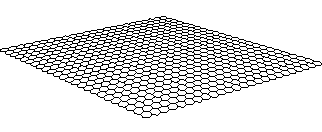
\includegraphics[width=\linewidth]{figures/torus-3d-flat.pdf}
				\caption{}
				\label{fig:torus-3d-flat}
			\end{subfigure}
			~~
			\begin{subfigure}{0.26\linewidth}
				\center
				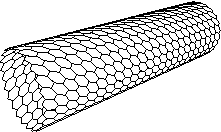
\includegraphics[width=\linewidth]{figures/torus-3d-tube.pdf}
				\caption{}
				\label{fig:torus-3d-tube}
			\end{subfigure}
			~~
			\begin{subfigure}{0.23\linewidth}
				\center
				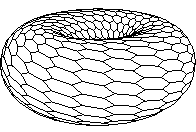
\includegraphics[width=\linewidth]{figures/torus-3d-torus.pdf}
				\caption{}
				\label{fig:torus-3d-torus}
			\end{subfigure}
			
			\caption{Visualisation of a hexagonal torus topology as a torus.}
			\label{fig:torus-3d}
		\end{figure}
		
		The wrap around connections in the topology are what give it the `torus'
		part of its name. Figure~\ref{fig:torus-3d-flat} shows a hexagonal torus
		topology drawn flat as in the previous figure. If the topology is rolled up
		into a tube such that the top and bottom nodes become directly adjacent, a
		tube is formed as in figure~\ref{fig:torus-3d-tube}. This tube can then be
		bent to bring together the nodes at the ends of the tube to form a torus as
		shown in figure~\ref{fig:torus-3d-torus}.
		
		A hexagonal torus topology is typically defined in terms of its width and
		height along the X and Y axes respectively. For example,
		figure~\ref{fig:hexagonalTorusTopology} shows a $10\times10$ hexagonal
		torus.  The nodes in a hexagonal torus topology are addressed using
		hexagonal coordinates of the form $(x, y, z)$ \cite{patel15}. The bottom
		left node (labelled $\alpha$ in the figure) has the coordinate $(0, 0, 0)$
		and other nodes are assigned coordinates according to the number of hops
		along each dimension from $(0, 0, 0)$, for example node $\beta$ has the
		coordinate $(2, 0, -1)$.
		
		Counter intuitively, individual nodes in hexagonal torus topologies may be
		described by many different coordinates, for example $(3, 1, 0)$ and $(1,
		-1, -2)$ are also a valid coordinates for node $\beta$. These dual
		coordinates emerge from the fact that adding $(1, 1, 1)$ to a coordinate
		produces an equivalent, but different, coordinate. This phenomenon is
		explained in detail in appendix~\ref{app:minimal-hex-coordinates} and
		related phenomena will be discussed in chapter~\ref{sec:shortestPaths}.
		
		\begin{figure}
			\center
			\begin{subfigure}[b]{0.32\linewidth}
				\center
				\buildfig{figures/torus-compare-hexagonal.tex}
				
				\caption{Hexagonal}
				\label{fig:torus-compare-hexagonal}
			\end{subfigure}
			\begin{subfigure}[b]{0.32\linewidth}
				\center
				\buildfig{figures/torus-compare-2d.tex}
				
				\caption{2D}
				\label{fig:torus-compare-2d}
			\end{subfigure}
			\begin{subfigure}[b]{0.32\linewidth}
				\center
				\buildfig{figures/torus-compare-3d.tex}
				
				\caption{3D}
				\label{fig:torus-compare-3d}
			\end{subfigure}
			
			\caption{Visual comparison of torus topologies. In all figures, `wrap
			around' connections between nodes at the ends of each axis are omitted
			for clarity.}
			\label{fig:torus-compare}
		\end{figure}
		
		Despite its unusual coordinate system, hexagonal torus topologies compare
		favourably with more conventional network topologies such as 2D and 3D
		toruses (sometimes known as 2-ary $N$-cubes and 3-ary $N$-cubes
		respectively) \cite{dally04} illustrated in figure~\ref{fig:torus-compare}.
		Compared with the 2D torus topology, a hexagonal torus has double the
		bisection bandwidth even though it only requires 50\% more node-to-node
		links \cite{navaridas09}. 3D torus topologies also have six node-to-node
		links per node but double the bisection bandwidth again. However, since a
		network topology must eventually be embedded into a real world data centre
		(which, at large scales, approximate a 2D space), 3D, or higher-dimensional
		torus topologies may become more expensive to construct in practice due to
		the need for longer cables to interconnect nodes. As
		chapter~\ref{sec:building} demonstrates, hexagonal toruses may be assembled
		in a machine room in a similar way to a 2D topology. The hexagonal torus
		topology achieves the scalability of a 2D torus while gaining some of the
		bisection bandwidth benefits of the 3D torus topology.
		
		Most torus topologies, including hexagonal 2D and 3D toruses, are related
		to an equivalent `mesh' topology. Mesh topologies maintain the same general
		connectivity structure as the corresponding torus topology with the
		exception of wrap-around links which are omitted. Omitting wrap-around
		links in practice saves a small number of links at the expense of halving
		the network's bisection bandwidth. As a consequence, mesh topologies are
		rarely used.
		
		\begin{figure}
			\center
			\begin{subfigure}[b]{0.45\linewidth}
				\center
				\buildfig{figures/hexagonal-torus.tex}
				\caption{Hexagonal torus}
				\label{fig:topo-compare-hexagonal-torus}
			\end{subfigure}
			\begin{subfigure}[b]{0.45\linewidth}
				\center
				\buildfig{figures/h-torus.tex}
				\caption{H-torus}
				\label{fig:topo-compare-h-torus}
			\end{subfigure}
			
			\caption{Hexagonal torus vs. H-torus topology. Each numbered hexagon
			represents a node. The thick outline indicates the bounds of the
			topology after which the network repeats. In each topology, the path
			taken by advancing in the Y$^+$ direction from the node labelled `0' is
			shown.}
			\label{fig:topo-compare}
		\end{figure}
		
		The hexagonal torus topology used by SpiNNaker and the subject of much of
		this thesis is not to be confused with the `H-torus' topology.  This
		topology also uses a hexagonal tiling of nodes and even wraps this tiling
		into in a torus-like topology \cite{zhao08}. However, H-torus topologies
		have very different characteristics to the hexagonal torus topology are
		closely related to `twisted torus' topologies \cite{camara10}.
		Figure~\ref{fig:topo-compare} illustrates one major difference in the way
		paths wrap around the peripheries of both topologies.
	
	\section{Scaling-up SpiNNaker machines}
		
		\begin{figure}
			\center
			\begin{subfigure}[b]{0.45\linewidth}
				\center
				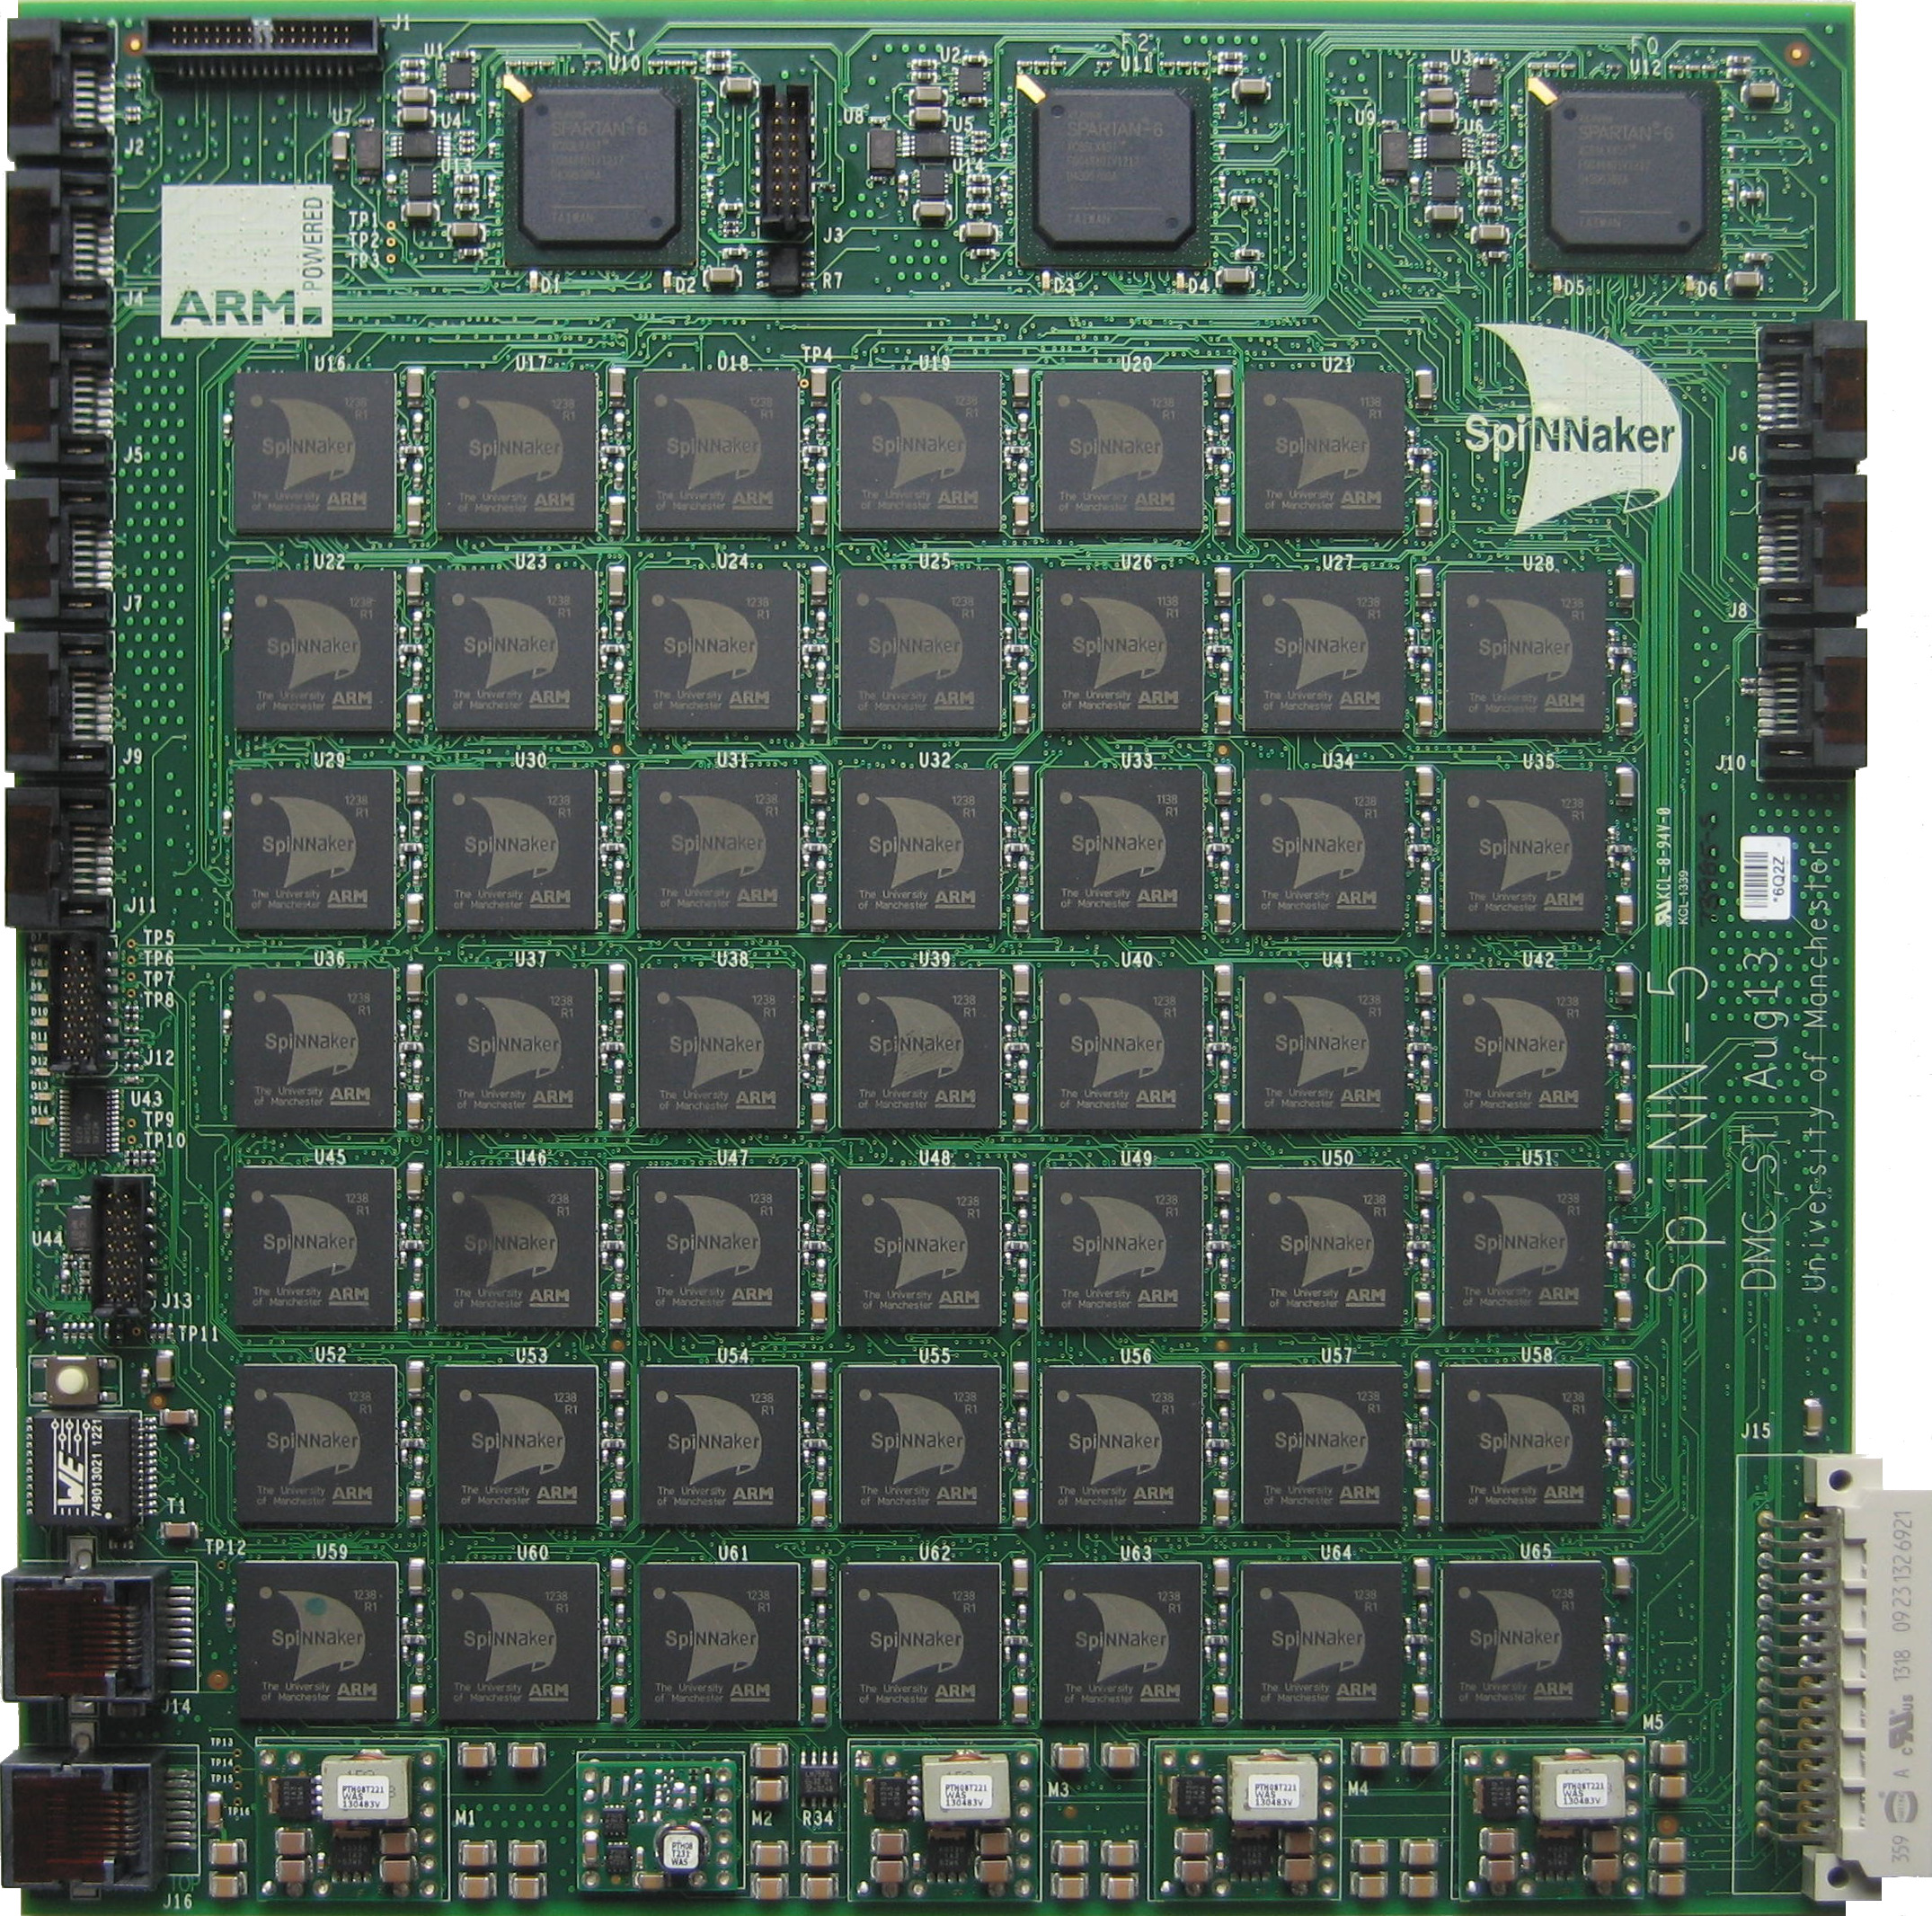
\includegraphics[width=\linewidth]{figures/spinnakerBoard.jpg}
				
				\caption{A SpiNNaker board}
				\label{fig:spinnakerBoard}
			\end{subfigure}
			~~~
			\begin{subfigure}[b]{0.45\linewidth}
				\center
				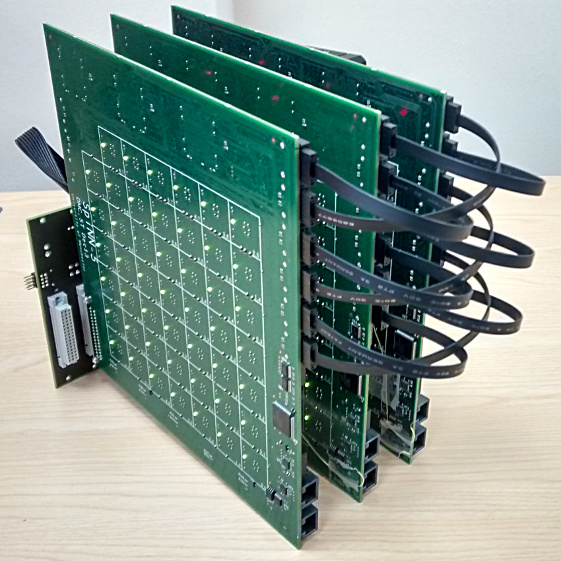
\includegraphics[width=\linewidth]{figures/threeboard.jpg}
				
				\caption{Three board system}
				\label{fig:threeboard}
			\end{subfigure}
			
			\vspace*{2em}
			
			\begin{subfigure}{\linewidth}
				\center
				\buildfig{figures/sata-connections.tex}
				
				\caption{The logical connectivity between chips in multi-board systems.
				Each board's forty-eight chips (drawn here as hexagons) form a wrapped
				triple. Connections between chips on neighbouring boards are
				concentrated onto a single HSS link.}
				\label{fig:sata-connections} \end{subfigure}
			
			\caption{SpiNNaker boards}
			\label{fig:spinnaker-boards}
		\end{figure}
		
		To build large SpiNNaker systems comprising tens of thousands of
		SpiNNaker chips, groups of forty-eight chips are mounted onto printed
		circuit boards as illustrated in figure~\ref{fig:spinnakerBoard}. These
		boards may be connected together to form larger systems.
		Figure~\ref{fig:threeboard} shows a prototype three board system configured
		as a $12\times12$ hexagonal torus.
		
		Though the chips are physically arranged in a (nearly) $7\times7$ grid on
		each SpiNNaker board, they logically form a `wrapped triple', a shape
		described in detail in appendix \ref{sec:partitioning} and illustrated in
		figure~\ref{fig:sata-connections}. Logically, the chips at the periphery of
		each board connect to their neighbours on adjacent boards. Normally
		SpiNNaker chips connect using a low power, asynchronous 2-of-7 protocol
		requiring sixteen wires per bidirectional chip-to-chip link
		\cite{bainbridge03}. If this link technology were used to connect chips on
		neighbouring boards, each pair of boards would need to be connected with a
		128~wire cable. Cables and connectors supporting this may signals are
		expensive and physically large making them unsuitable for use with
		SpiNNaker. Instead, chip-to-chip connections between boards are multiplexed
		and demultiplexed onto a single High-Speed Serial (HSS) link
		\cite{athavale05} carried via commodity S-ATA cables often used to
		connected hard disks in desktop computers and servers \cite{sata3spec}.
		The six high-speed links are implemented by three onboard FPGAs (the three
		large chips at the top of the SpiNNaker board) and are logically
		transparent to the underlying network.
		
		In chapter~\ref{sec:building} I describe how very large SpiNNaker machines
		may be constructed using over one thousand SpiNNaker boards.

	\chapter{Building large SpiNNaker machines}
	
	\label{sec:building}
	
	Like any supercomputer, physically assembling a large SpiNNaker machine
	poses many practical challenges in terms of arranging, installing and
	maintaining the hundreds of metres of network cables required.  For
	conventional architectures and network topologies, techniques are well
	understood and embodied by industry standards such as TAI-942~\cite{tia2006}.
	SpiNNaker's use of the hexagonal torus topology renders existing approaches
	insufficient.
	
	In the first part of this chapter I extend existing techniques for mapping
	network topologies into standard data centre physical infrastructure to
	support the hexagonal torus topology. This mapping is designed to ensure that
	all cables are kept short (under \SI{1}{\meter}) to reduce costs and
	simplify the network hardware required. The techniques described introduce
	little overhead in cable length over existing torus wiring schemes
	and confirm the suitability of the hexagonal torus topology for real-world
	applications.
	
	The second part of this chapter uses SpiNNaker as a case study on the
	suitability of the mappings introduced in this chapter.  In this case study I
	consider various SpiNNaker systems ranging in size from desktop machines to
	multi-cabinet machine room installations. As well as validating the cabling
	schemes introduced in this chapter I also describe a new technique which
	improves the efficiency of the cable installation process.  As a consequence
	of SpiNNaker's fine-grained connectivity, the cabling is unusually dense,
	exacerbating the complexity of the cabling patterns to be installed. By
	exploiting network diagnostics hardware and on-board LEDs to guide cable
	installation, construction of large SpiNNaker machines takes a matter of
	hours rather than the days reported for other architectures. In addition,
	preliminary experiments suggest that neither the maintainability nor cooling
	performance of the system are hampered by the dense cabling employed.
	
	In this chapter, the term \emph{unit} refers to the smallest physical
	component between which network interconnection cables are installed. For
	example, in a SpiNNaker machine a unit is a 48-chip board while in a data
	centre network a unit might be a server blade.
	
	\section{Cabling non-hexagonal torus topologies}
		
		Na\"ive arrangements of torus topologies, hexagonal or otherwise, feature
		physically long `wrap-around' connections which connect units at the
		peripheries of the system. Long connections can be problematic for several
		reasons:
		
		\begin{description}
			
			\item[Performance:] Signal quality diminishes as cables get longer,
			requiring the use of slower signalling speeds, increased error
			correction overhead or more complex hardware.
			
			\item[Energy:] Some energy is lost in cables; longer cables lose more
			signal energy requiring higher drive strengths and/or buffering to
			maintain signal integrity.
			
			\item[Cost:] Shorter cables are cheaper than long ones.  Longer cables
			imply more cabling in a given space making the task of cable installation
			and system maintenance more difficult, increasing labour costs by as much
			as $5\times$~\cite{curtis12}.
			
		\end{description}
		
		In conventional torus topologies, the need for long cables is eliminated by
		folding and interleaving units of the network~\cite[chapter~5]{dally04}.
		This process is illustrated for a 1D torus topology (a ring network) in
		figure~\ref{fig:ring-folding}. A na\"ive arrangement of units in this
		topology results in a long cable connecting the units at the ends of the
		ring (figure~\ref{fig:ring-folding-row}).  To eliminate these long
		connections, half of the units are `folded' on top of the others
		(figure~\ref{fig:ring-folding-folded}) and then this arrangement of units
		is interleaved (figure~\ref{fig:ring-folding-interleaved}). This ordering
		of units requires no long cables while still observing the physical
		constraint that units must be laid out in a line.
		
		\begin{figure}
			\center
			\begin{subfigure}[b]{0.39\linewidth}
				\center
				\buildfig{figures/ring-folding-row.tex}
				\caption{A ring network}
				\label{fig:ring-folding-row}
			\end{subfigure}
			\begin{subfigure}[b]{0.24\linewidth}
				\center
				\buildfig{figures/ring-folding-folded.tex}
				\caption{Folded}
				\label{fig:ring-folding-folded}
			\end{subfigure}
			\begin{subfigure}[b]{0.35\linewidth}
				\center
				\buildfig{figures/ring-folding-interleaved.tex}
				\caption{Folded and interleaved}
				\label{fig:ring-folding-interleaved}
			\end{subfigure}
			
			\caption[Folding and interleaving a ring network.]%
			{Folding and interleaving a ring network to reduce maximum cable
			length.}
			\label{fig:ring-folding}
		\end{figure}
		
		The folding and interleaving process may be extended to $N$-dimensional
		torus topologies by folding each axis in turn. Since all axes are
		orthogonal in non-hexagonal topologies, the folding process only moves
		units along the axis being folded. Due to the non-orthogonality of the
		three axes of the hexagonal torus topology, this type of folding does not
		work. As figure~\ref{fig:failing-to-fold-hex-toruses} illustrates, folding
		along any axis results in connected units on opposing edges not being
		brought together. For example, when folding along the X axis, the two units
		marked with a green circle are moved closer together on the Y axis but
		remain apart on the X axis.
		
		\begin{figure}
			\center
			\begin{subfigure}[b]{0.24\linewidth}
				\center
				\buildfig{figures/failing-to-fold-hex-toruses-none.tex}
				\caption{Not folded}
				\label{fig:failing-to-fold-hex-toruses-none}
			\end{subfigure}
			\begin{subfigure}[b]{0.24\linewidth}
				\center
				\buildfig{figures/failing-to-fold-hex-toruses-x.tex}
				\caption{X}
				\label{fig:failing-to-fold-hex-toruses-x}
			\end{subfigure}
			\begin{subfigure}[b]{0.24\linewidth}
				\center
				\buildfig{figures/failing-to-fold-hex-toruses-y.tex}
				\caption{Y}
				\label{fig:failing-to-fold-hex-toruses-y}
			\end{subfigure}
			\begin{subfigure}[b]{0.24\linewidth}
				\center
				\buildfig{figures/failing-to-fold-hex-toruses-z.tex}
				\caption{Z}
				\label{fig:failing-to-fold-hex-toruses-z}
			\end{subfigure}
			
			\caption[Folding each axis of a hexagonal torus topology.]%
			{Schematics showing folding along each axis of a hexagonal torus topology
			failing to eliminate wrap-around connections.  Same-shaped-and-coloured
			dots show the endpoints of two example wrap-around connections.}
			\label{fig:failing-to-fold-hex-toruses}
		\end{figure}
	
	\section{Partitioning hexagonal torus topologies}
		
		The nodes in supercomputer networks are usually relatively small, for
		example a single chip. Tens of nodes are packed together into a single
		unit, such as a circuit board or server blade, to simplify assembly and
		share common power and cooling resources~\cite{gilge14,ajima12}. In
		commercial supercomputers built on non-hexagonal torus topologies, each
		unit's nodes represent a hypercube partition of the overall topology as
		illustrated in figure~\ref{fig:hypercube-partitioning}
		\cite{chen11,ajima12}.
		
		An analogous `parallelogram' partitioning scheme exists for hexagonal torus
		topologies, however, this results in imbalanced connectivity requirements
		between neighbouring partitions. In
		figure~\ref{fig:parallelogram-partitioning}, for example, the partitions
		above, below, left and right of the central partition are connected by
		seven node-to-node connections each while the partitions above-right and
		below-left are connected by just a single connection each. To simplify
		assembly, connections between all nodes in a pair of neighbouring
		partitions are often made by a single cable. If connectivity requirements
		are imbalanced, as in this example, this may mean multiple connector types
		may be required, increasing design complexity.
		
		To avoid connectivity imbalance, SpiNNaker uses a `wrapped triple'
		partitioning scheme~\cite{davidsonWiring}, as illustrated in
		figure~\ref{fig:wrapped-triple-partitioning} and explained in detail in
		appendix \ref{sec:partitioning}. In this partitioning scheme, the same
		number of connections connect all six neighbouring units. As explained in
		the appendix, a hexagonal torus topology is constructed from groups of
		three partitions.
		
		\begin{figure}
			\center
			\begin{subfigure}[b]{0.32\textwidth}
				\center
				\buildfig{figures/hypercube-partitioning.tex}
				\caption{2D hypercube}
				\label{fig:hypercube-partitioning}
			\end{subfigure}
			\begin{subfigure}[b]{0.32\textwidth}
				\center
				\buildfig{figures/parallelogram-partitioning.tex}
				\caption{Parallelogram}
				\label{fig:parallelogram-partitioning}
			\end{subfigure}
			\begin{subfigure}[b]{0.32\textwidth}
				\center
				\buildfig{figures/wrapped-triple-partitioning.tex}
				\caption{Wrapped triple}
				\label{fig:wrapped-triple-partitioning}
			\end{subfigure}
			
			\caption[Partitioning of torus topologies into units.]%
			{Partitioning of non-hexagonal (a) and hexagonal (b and c) torus
			topologies into units.}
			\label{fig:partitioning-options}
		\end{figure}
		
		For completeness, both parallelogram and wrapped triple partitioning are
		considered in this chapter even though SpiNNaker uses wrapped triple
		partitioning. The parallelogram partitioning scheme may be more appropriate
		for architectures where connections between nodes in neighbouring
		partitions do not share a single connector. In addition, in architectures
		where a unit corresponds to a single node, this can be treated as a $1
		\times 1$ parallelogram partition.  This special case occurs in
		coarse-grained architectures and Networks on Chip (NoCs) where nodes are
		not grouped together into multi-node units.
	
	\section{Folding \& interleaving hexagonal toruses}
		
		To exploit the folding technique used by non-hexagonal topologies, the
		units in a hexagonal torus topology must be mapped into a space with
		orthogonal coordinates. The choice of transformation to an orthogonal
		coordinate system can have an impact on how physically far apart logically
		neighbouring units are in the final arrangement. A good mapping should
		attempt to reduce `distortion' which moves adjacent units apart in the
		final folded and interleaved arrangement.
		
		In this section I propose two transformations which map hexagonal
		arrangements of units into a 2D orthogonal coordinate space. The first
		transformation, `shearing', is general purpose and introduces some
		distortion. The second transformation, `slicing', is less general but can
		introduce less distortion than shearing and therefore may lead to shorter
		cable lengths.
		
		Both the slicing and shearing transformations are carried out in two steps:
		
		\begin{description}
			
			\item[Rectangularisation] Units are transformed from being laid out in a
			parallelogram into a rectangular arrangement. The specific transformation
			used is the key difference between the slicing and shearing
			transformations.
			
			\item[Uncrinkling] Units are mapped into a 2D coordinate system without
			gaps between units.
			
		\end{description}
		
		\subsection{Rectangularisation}
			
			The hexagonal torus topology is illustrated in
			figures~\ref{fig:hex-to-plane-node-native} and
			\ref{fig:hex-to-plane-native} for parallelogram-partitioned units and
			wrapped triple units respectively. The first step in the folding process
			is to rearrange units so that they form a rectangle using one of two
			techniques: shearing or slicing.
			
			\begin{figure}
				\center
				\begin{subfigure}[b]{0.32\linewidth}
					\center
					\buildfig{figures/hex-to-plane-node-native.tex}
					
					\caption{Original}
					\label{fig:hex-to-plane-node-native}
				\end{subfigure}
				\begin{subfigure}[b]{0.32\linewidth}
					\center
					\buildfig{figures/hex-to-plane-node-shear.tex}
					
					\caption{Sheared}
					\label{fig:hex-to-plane-node-shear}
				\end{subfigure}
				\begin{subfigure}[b]{0.32\linewidth}
					\center
					\buildfig{figures/hex-to-plane-node-slice.tex}
					
					\caption{Sliced}
					\label{fig:hex-to-plane-node-slice}
				\end{subfigure}
				
				\caption[Rectangularisation of parallelogram partitioned toruses.]%
				{Rectangularisation of parallelogram partitioned hexagonal
				toruses. Thin lines show wrap-around links. Pointy-topped hexagons
				represent parallelogram partitioned units.}
				\label{fig:hex-to-plane-node}
				
				% XXX: Force these figures together.
				
				%\end{figure}
				%
				%\begin{figure}
				
				\center
				\begin{subfigure}[b]{0.32\linewidth}
					\center
					\buildfig{figures/hex-to-plane-native.tex}
					
					\caption{Original}
					\label{fig:hex-to-plane-native}
				\end{subfigure}
				\begin{subfigure}[b]{0.32\linewidth}
					\center
					\buildfig{figures/hex-to-plane-shear.tex}
					
					\caption{Sheared}
					\label{fig:hex-to-plane-shear}
				\end{subfigure}
				\begin{subfigure}[b]{0.32\linewidth}
					\center
					\buildfig{figures/hex-to-plane-slice.tex}
					
					\caption{Sliced}
					\label{fig:hex-to-plane-slice}
				\end{subfigure}
				
				\caption[Rectangularisation of wrapped triple partitioned toruses.]%
				{Rectangularisation of wrapped triple partitioned hexagonal
				toruses. Thin lines show wrap-around links.  Flat-topped hexagons
				represent wrapped triple partitioned units.}
				\label{fig:hex-to-plane}
				
				% And force these together!
				
				%\end{figure}
				%
				%\begin{figure}
				
				\center
				\begin{subfigure}[b]{0.3\linewidth}
					\center
					\buildfig{figures/slicing-examples-5x5.tex}
					\caption{$5\times5$}
				\end{subfigure}
				\begin{subfigure}[b]{0.3\linewidth}
					\center
					\buildfig{figures/slicing-examples-5x7.tex}
					\caption{$5\times7$}
				\end{subfigure}
				\begin{subfigure}[b]{0.3\linewidth}
					\center
					\buildfig{figures/slicing-examples-5x10.tex}
					\caption{$5\times10$}
				\end{subfigure}
				
				\caption[Patterns of wrap-around connections in sliced systems.]%
				{Schematics showing the patterns of wrap-around connections in sliced
				systems of various aspect ratios.}
				\label{fig:slicing-examples}
			\end{figure}
			
			The shearing technique applies a \SI{30}{\degree} shear transformation to
			distort the arrangement of units so that the X and Y axes of the
			hexagonal torus topology become orthogonal. This transformation leads to
			a rectangular arrangement of units as illustrated in figures
			\ref{fig:hex-to-plane-node-shear} and \ref{fig:hex-to-plane-shear}.
			
			The shear transformation introduces some distortion causing connections
			between units in the Z axis to become $\sqrt{2} \times$ longer. The
			transformation does not alter the pattern of wrap-around connections:
			long connections between units on the extreme left and right sides and
			the top and bottom remain, along with a single connection between the
			bottom left and top right units.
			
			The slice transformation aims to avoid the elongation of the Z axis by
			moving the units without distorting their layout. Units protruding from
			the left-hand-side of the parallelogram are `sliced off' and moved into
			the matching gap on the opposite side as illustrated in figures
			\ref{fig:hex-to-plane-node-slice} and \ref{fig:hex-to-plane-slice}. This
			transformation does not introduce any distortion but changes the pattern
			of wrap-around connections. Connections from left-to-right remain while
			the connections between the top and bottom units now criss-cross
			(figure~\ref{fig:slicing-examples}).  The proportion of connections going
			from bottom-left to top-right and from bottom-right to top-left varies
			depending on the aspect ratio of the topology. Only certain patterns of
			wrap-around links can be eliminated by folding and, as we shall see
			later, this limits us in which network topologies can be rectangularised
			by slicing.
			
		\subsection{Uncrinkling}
			
			Before folding can occur, the rectangularised arrangements of units
			produced in the previous step must be mapped into a 2D grid. Applied to
			parallelogram partitions, the shear transformation results in a mapping
			into a 2D grid with no further distortion
			(figure~\ref{fig:uncrinkling-node-sheared}). For other combinations of
			transformation and partitioning scheme, the units do not exactly fit a 2D
			grid. Instead, the units form `crinkled' rows or columns which may be
			`uncrinkled' (straightened out) to fit a regular 2D grid as illustrated in
			figures~\ref{fig:uncrinkling-node-sliced}~--~\ref{fig:uncrinkling-sliced}.
			
			\begin{figure}
				\center
				\begin{subfigure}[b]{0.48\linewidth}
					\center
					\buildfig{figures/uncrinkling-node-sheared.tex}
					
					\caption{Parallelogram units, sheared}
					\label{fig:uncrinkling-node-sheared}
				\end{subfigure}
				\begin{subfigure}[b]{0.48\linewidth}
					\center
					\buildfig{figures/uncrinkling-node-sliced.tex}
					
					\caption{Parallelogram units, sliced}
					\label{fig:uncrinkling-node-sliced}
				\end{subfigure}
				
				\vspace{1cm}
				
				\begin{subfigure}[b]{0.48\linewidth}
					\center
					\buildfig{figures/uncrinkling-sheared.tex}
					
					\caption{Wrapped triple units, sheared}
					\label{fig:uncrinkling-sheared}
				\end{subfigure}
				\begin{subfigure}[b]{0.48\linewidth}
					\center
					\buildfig{figures/uncrinkling-sliced.tex}
					
					\caption{Wrapped triple units, sliced}
					\label{fig:uncrinkling-sliced}
				\end{subfigure}
				
				\vspace{1em}
				
				\caption[Uncrinkling units into a 2D grid.]%
				{Uncrinkling rectangularised arrangements of units into a 2D
				grid. Thick lines show how crinkled rows and columns of units are
				uncrinkled.  Annotations show how the relative positions of units
				change after uncrinkling.}
				\label{fig:uncrinkling}
			\end{figure}
			
			%% XXX: Does this make things clearer or not?
			%In the figure, the labels show the positions of individual units before
			%and after uncrinkling. We will use these later in \S\ref{sec:distortion}
			%to calculate the overhead introduced by uncrinkling.
		
		\subsection{Folding}
			
			\begin{figure}
				\begin{subfigure}{\linewidth}
					\center
					\buildfig{figures/folding-sheared.tex}
					\caption{Sheared systems and $1:2$ sliced systems}
					\label{fig:folding-sheared}
				\end{subfigure}
				
				\vspace{1em}
				
				\begin{subfigure}{\linewidth}
					\center
					\buildfig{figures/folding-sliced.tex}
					\caption{$1:1$ sliced systems}
					\label{fig:folding-sliced}
				\end{subfigure}
				
				\caption[Elimination of long wrap-around links by folding.]%
				{Schematic illustrating elimination of long wrap-around links
				during folding. In each example a single link has been highlighted to
				aid in following the process.}
				\label{fig:folding}
			\end{figure}
			
			Once a regular 2D grid of units has been formed, this may be folded in
			the conventional way as illustrated in figure~\ref{fig:folding-sheared}.
			Folding once along each axis eliminates long connections crossing from
			left-to-right, top-to-bottom and from the bottom-left corner to the
			top-right corner. Any shear-transformed network may be folded this way
			since its wrap-around connections always follow this pattern.
			Slice-transformed networks may only be folded like this when their aspect
			ratio is $1:2$ when the pattern of wrap-around links is the same as a
			shear-transformed network.
			
			When `square' networks (i.e. those with a $1:1$ aspect ratio) are sliced,
			the network must be folded \emph{twice} along the Y axis as in
			figure~\ref{fig:folding-sliced} to eliminate the criss-crossing
			wrap-around links. It is not possible to eliminate wrap-around links from
			sliced networks with other aspect ratios by folding.
			
			After folding, the units are interleaved, yielding a 2D arrangement of
			units in which no connection spans the width or height of the system. The
			maximum connection distance is constant for any network allowing the
			topology to scale up.
		
		\subsection{Choosing a transformation}
			
			\label{sec:distortion}
			
			In each step of the transformation from hexagonal torus to a folded and
			interleaved 2D grid, the distances between connected units may increase.
			When designing a system, the transformation with the least distortion
			should be used to minimise the average length of the cables required.
			
			By referring to figure~\ref{fig:uncrinkling} (page
			\pageref{fig:uncrinkling}), it is possible to calculate the overhead
			introduced by each type of transformation.  For example, to compute the
			overhead introduced by the slicing transformation when applied to units
			composed of wrapped triples we consider
			figure~\ref{fig:uncrinkling-sliced}. The uncrinkling pattern used to
			transform this topology is a repeating pattern of two units, a pair of
			which have been labelled $1$ and $2$ respectively. Unit $1$ is
			immediately surrounded by the six units labelled $a$, $b$, $c$, $2$, $g$
			and $h$. Unit $2$ is surrounded by the units $1$, $c$, $d$, $e$, $f$ and
			$g$.  Before the transformation, the distance between units is $1$; after
			the transformation is applied this is not always the case. Folding and
			interleaving into $f_x$ columns and $f_y$ rows also introduces overhead.
			For each pair of previously neighbouring units in the example, their
			distances after folding may be computed as follows:
			
			\begin{equation*}
				\begin{aligned}[c]
					D_{1\,\leftrightarrow{}\,a} &= \sqrt{f_x^2 + f_y^2} \\
					D_{1\,\leftrightarrow{}\,b} &= f_y \\
					D_{1\,\leftrightarrow{}\,c} &= \sqrt{f_x^2 + f_y^2} \\
					D_{1\,\leftrightarrow{}\,2} &= f_x \\
					D_{1\,\leftrightarrow{}\,g} &= f_y \\
					D_{1\,\leftrightarrow{}\,h} &= f_x
				\end{aligned}
				\hspace{2cm}
				\begin{aligned}[c]
					D_{2\,\leftrightarrow{}\,1} &= f_x \\
					D_{2\,\leftrightarrow{}\,c} &= f_y \\
					D_{2\,\leftrightarrow{}\,d} &= f_x \\
					D_{2\,\leftrightarrow{}\,e} &= \sqrt{f_x^2 + f_y^2} \\
					D_{2\,\leftrightarrow{}\,f} &= f_y \\
					D_{2\,\leftrightarrow{}\,g} &= \sqrt{f_x^2 + f_y^2}
				\end{aligned}
			\end{equation*}
			
			From these values, mean and maximum connection distances may be
			calculated. The expressions for each combination of partitioning scheme
			and transformation are as follows:
			
			\begin{align*}
				D_{\textrm{mean}}=&
					\begin{cases}
						\frac{7f_x + 3\sqrt{f_x^2 + f_y^2} + \sqrt{(2f_x)^2 + f_y^2}}{9} &
							\textrm{if sheared wrapped triple units}\\
						\frac{f_x + f_y + \sqrt{f_x^2 + f_y^2}}{3} &
							\textrm{otherwise}\\
					\end{cases} \\
				D_{\textrm{max}}=&
					\begin{cases}
						\sqrt{(2f_x)^2 + f_y^2} &
							\textrm{if sheared wrapped triple units}\\
						\sqrt{f_x^2 + f_y^2} &
							\textrm{otherwise}
					\end{cases}
			\end{align*}
			
			\begin{table}
				\center
				\begin{tabular}{lcc}
					\toprule
					                                 & $1:2$  & Other \\
					\addlinespace
					\multirow{2}{*}{Parallelogram}   & \textbf{Either} & \textbf{Shear}\\
					                                 & \footnotesize $D_\textrm{mean}\approx2.28 \quad D_\textrm{max}\approx2.83$
					                                 & \footnotesize $D_\textrm{mean}\approx2.28 \quad D_\textrm{max}\approx2.83$\\
					\addlinespace
					\multirow{2}{*}{Wrapped triples} & \textbf{Slice}  & \textbf{Shear}\\
					                                 & \footnotesize $D_\textrm{mean}\approx2.28 \quad D_\textrm{max}\approx2.83$
					                                 & \footnotesize $D_\textrm{mean}\approx3.00 \quad D_\textrm{max}\approx4.47$\\
					\bottomrule
				\end{tabular}
				
				\caption{Recommended transformations for folding hexagonal toruses.}
				\label{tab:transform-recommended}
			\end{table}
			
			Using these formulae it is possible to determine which approach --
			shearing or slicing -- results in the lowest mean and maximum cable
			lengths and thus which technique should be used. This is summarised in
			table~\ref{tab:transform-recommended}.
	
	\section{A SpiNNaker case study}
		
		As the only known large-scale hexagonal torus-based architecture, SpiNNaker
		is a good case study for the techniques described in this chapter.  Each
		unit in a SpiNNaker machine is a 48-chip SpiNNaker board forming a
		wrapped triple partition. Systems of various sizes have been constructed
		using the techniques introduced in this chapter ranging from twenty-four
		board `portable' systems to a five cabinet, half-million core installation
		with plans in place to build a machine of twice this size in the future.
		
		In this section I describe how the folded and interleaved arrangement of
		units produced by the techniques in the previous chapter may be translated
		into physical arrangements of SpiNNaker boards in a machine room. I then
		describe how the thousands of S-ATA cables are installed and report on the
		maintainability and cooling impact of this cabling scheme in practice.
		
		\subsection{Mapping into physical cabinets}
			
			In SpiNNaker systems, the physical architecture used is illustrated in
			figure~\ref{fig:cabinet-units}. SpiNNaker boards are installed into card
			frames containing twenty four boards each. Five frames are mounted into
			standard, \SI{600}{\milli\meter}~wide 19\inch{} cabinets with further
			cabinets being added, arranged in a row, to scale the system up. The 2D
			grid of units produced by the folding process described in this chapter
			is mapped to cabinets and frames as illustrated in
			figure~\ref{fig:cabinetisation}.
			
			\begin{figure}
				\center
				\buildfig{figures/cabinet-units.tex}
				
				\caption{Physical architecture of a SpiNNaker machine.}
				\label{fig:cabinet-units}
			\end{figure}
			
			\begin{figure}
				\center
				\buildfig{figures/cabinetisation.tex}
				
				\caption[Mapping cabling from abstract to physical space.]%
				{Mapping from the abstract folded and interleaved 2D grid
				layout into physical cabinet and frame positions. Arrows indicate the
				order in which units (boards) are mapped into each frame, from
				left-to-right.}
				\label{fig:cabinetisation}
			\end{figure}
			
			Figure~\ref{fig:million-core-machine} shows the cabling plan for the
			largest planned SpiNNaker machine. This system will fill ten 19\inch{}
			cabinets and implement a $240 \times 240$ hexagonal torus topology
			partitioned between \num{1200} 48 chip SpiNNaker boards. The largest gap
			to be spanned by any cable is \SI{66}{\centi\meter}, well within the
			\SI{1}{\meter} limit on SpiNNaker's interconnect technology.
			
			\begin{figure}
				\center
				\buildfig{figures/million-core-machine.tex}
				
				\caption[Cabling plan for a \num{1200}~board SpiNNaker machine.]%
				{Cabling plan for a \num{1200}~board (\num{1036800}~core)
				SpiNNaker machine.}
				\label{fig:million-core-machine}
			\end{figure}
			
		\subsection{Cable selection and routing}
			
			Because of the dense packing of SpiNNaker boards, cables span short
			distances as shown in figure~\ref{fig:wire-length-histogram}.
			Conventional cable management techniques (e.g. cable trays) are not
			practical. To ensure the reliability and maintainability of SpiNNaker's
			wiring, cable slack must be carefully controlled.  If cables are too
			tight, cables, connectors and SpiNNaker boards can become damaged. When
			cables are too slack, the excess obstructs access to the machine and can
			easily become tangled \cite{cisco07}.
			
			In this case study the `rule of (three-)thumbs' proposed by
			Mazaris~\cite{mazaris97} is used which suggests that a minimum of
			\SI{5}{\centi\meter} of slack be provided. As SpiNNaker uses
			off-the-shelf S-ATA cables, only standard lengths of cable are available.
			For any given span, the shortest length of cable providing at least
			\SI{5}{\centi\meter} of slack is used.
			
			\begin{figure}
				
				\center
				\buildfig{figures/wire-length-histogram.tex}
				
				\caption[Cable lengths in a \num{1200}~board SpiNNaker machine.]%
				{Histogram of connection distances in a \num{1200} board SpiNNaker
				machine annotated with the selected cable lengths.}
				\label{fig:wire-length-histogram}
				
			\end{figure}
		
		\subsection{Installation practicality}
			
			\begin{figure}
				\center
				\begin{subfigure}[t]{0.5\textwidth}
					\begin{tikzpicture}
						\node (cables) [inner sep=0]
						      {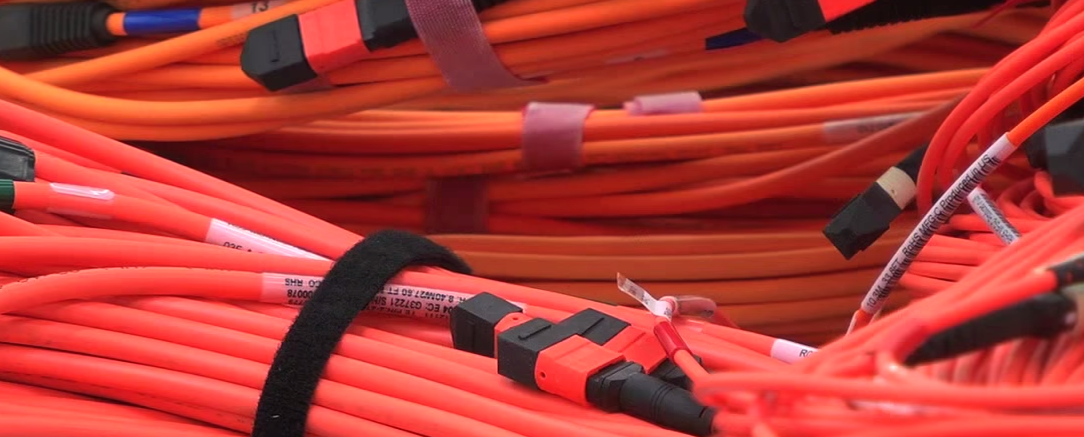
\includegraphics[width=\textwidth]{figures/bgCables.png}};
						\node (sockets) [inner sep=0, below=1.0em of cables]
						      {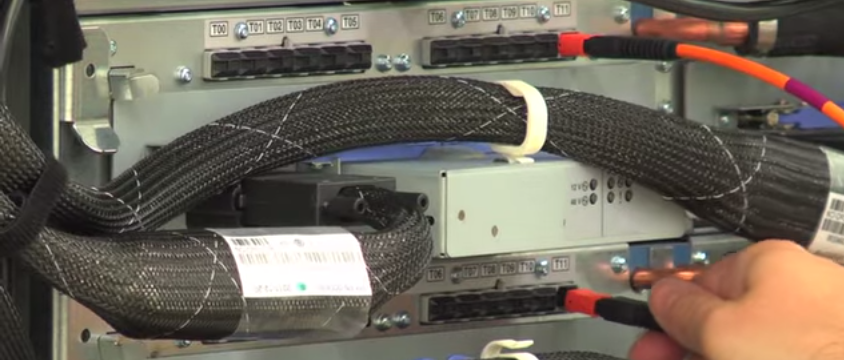
\includegraphics[width=\textwidth]{figures/bgSockets.png}};
						
						% Point at label on cable
						\draw [white, <-, line width=0.4em]
						      ([shift={(0.7cm, -0.3cm)}]cables.center)
						      -- ++(45:1cm);
						
						% Point at label on socket
						\draw [white, <-, line width=0.4em]
						      ([shift={(-1.0cm, 1.1cm)}]sockets.center)
						      -- ++(-45:1cm);
					\end{tikzpicture}
					
					\caption{Pre-labelled cables and sockets}
					\label{fig:bgWiringLabels}
				\end{subfigure}
				~
				\begin{subfigure}[t]{0.30\textwidth}
					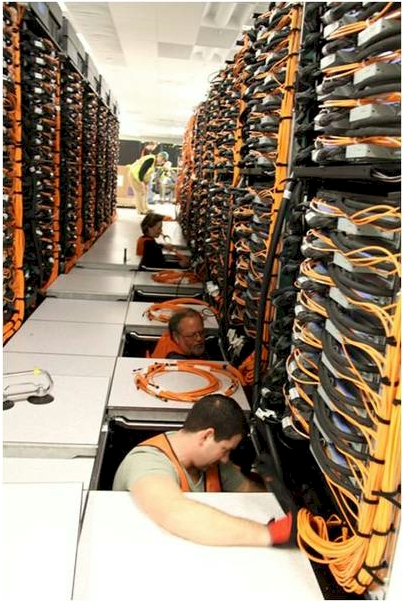
\includegraphics[height=6.15cm]{figures/bgWiring.jpg}
					
					\caption{Installation of cables}
					\label{fig:bgWiringInstallation}
				\end{subfigure}
				
				\caption[BlueGene/Q cable installation.]%
				        {BlueGene/Q cable installation~\cite{cscs13}.}
				\label{fig:bgWiring}
			\end{figure}
			
			In other large-scale architectures, the task of cable installation is
			completed by a team of technicians aided by the use of standardised
			labelling for cables and sockets as illustrated in
			figure~\ref{fig:bgWiring}~\cite{tia2006}. In these architectures the
			cabling patterns required are relatively straightforward, thanks to the
			coarseness of the units used~\cite{lakner07} or they use network
			topologies whose cabling centres around high-fan-in
			switches~\cite{cisco07,csernai15}.
			
			It has been reported in the literature that when copper cables are used,
			labour costs dominate~\cite{popa10} and while cable costs are expected to
			decline, labour costs are not~\cite{mudigonda11}. Many researchers have
			attempted to control cable installation costs by trying to reduce the
			number or length of cables required by developing alternative network
			topologies~\cite{curtis12, popa10, mudigonda11}.  Unfortunately, these
			techniques do not apply to SpiNNaker since its network topology is fixed.
			
			Supercomputer architectures such as BlueGene/Q make use of large custom
			`midplane' PCBs in place of some cables to interconnect units within a
			cabinet~\cite{milano13}. This scheme can greatly reduce wiring complexity
			since only coarser-grain, cabinet-to-cabinet connectivity is implemented
			by cables. Unfortunately this technique is expensive and constrains the
			dimensions of the network topology supported by the machine. Since the
			SpiNNaker platform is designed to scale from desktop machines to
			machine room installations, this scheme is not practical.
			
			\begin{figure}
				\center
				\begin{subfigure}[b]{0.40\textwidth}
					\begin{tikzpicture}
						\node (leds) [inner sep=0]
						      {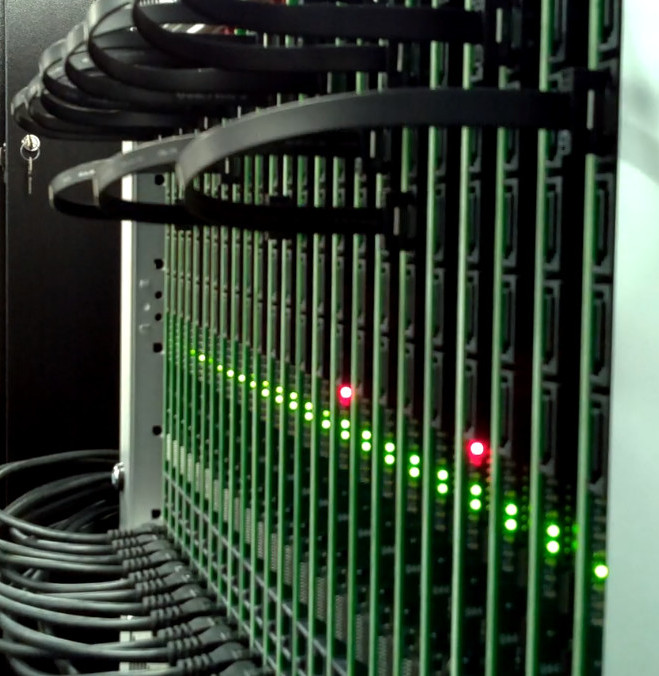
\includegraphics[width=\textwidth]{figures/leds.jpg}};
						% Point at left LED
						\draw [white, <-, line width=0.4em]
						      ([shift={(-0.0cm, -0.6cm)}]leds.center)
						      -- ++(225:1cm);
						% Point at right LED
						\draw [white, <-, line width=0.4em]
						      ([shift={(1.1cm, -1.1cm)}]leds.center)
						      -- ++(225:1cm);
					\end{tikzpicture}
					
					\caption{Diagnostic LEDs indicate the endpoints of each cable.}
					\label{fig:interactive-wiring-guide-leds}
				\end{subfigure}
				~
				\begin{subfigure}[b]{0.546\textwidth}
					\begin{tikzpicture}[thin, black!20!white]
						\node (screen) [inner sep=0]
						      {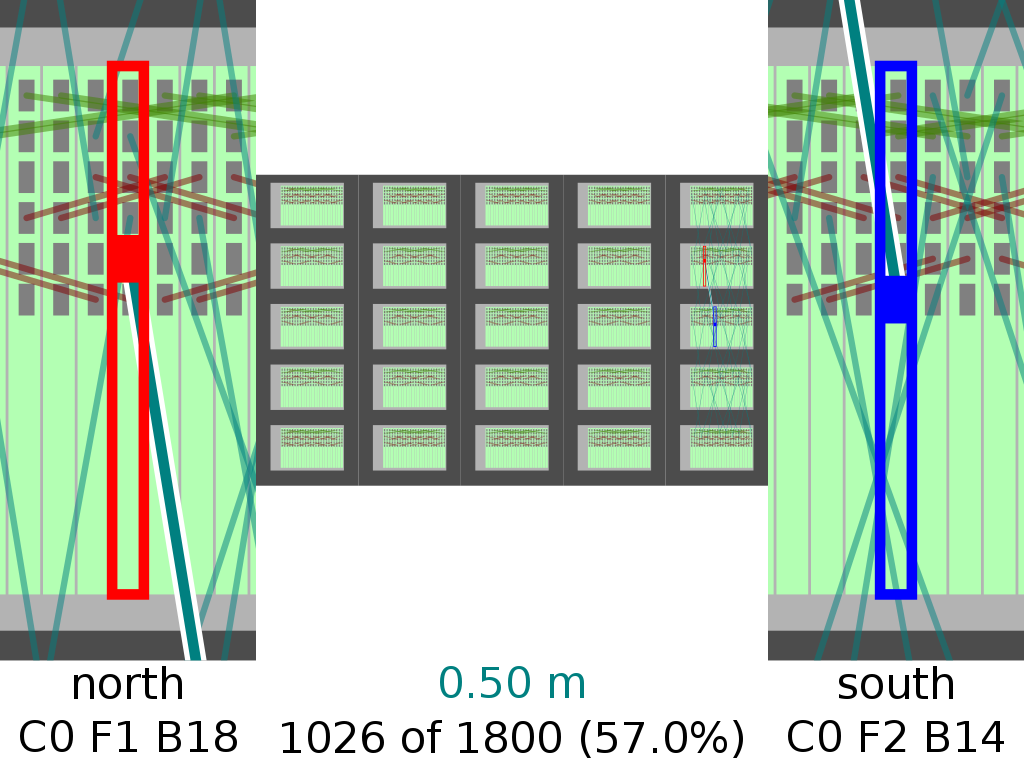
\includegraphics[width=\textwidth]{figures/wiring_guide_screenshot.png}};
						\draw (screen.south west) rectangle (screen.north east);
					\end{tikzpicture}
					
					\caption{A GUI and text-to-speech indicate what type of cable to
					install.}
					\label{fig:interactive-wiring-guide-gui}
				\end{subfigure}
				
				\caption{Interactive software guides cable installation.}
				\label{fig:interactive-wiring-guide}
			\end{figure}
			
			Due to the high density of units in a SpiNNaker system, the detailed
			cabling patterns used can be complex, despite their overall regularity.
			To cope with this complexity, I developed a software system which employs
			diagnostic hardware built into SpiNNaker, to guide technicians through
			the cable installation process. As shown in
			figure~\ref{fig:interactive-wiring-guide}, diagnostic LEDs on each
			SpiNNaker board are used to indicate which boards to connect. The
			software also provides step-by-step cabling instructions via a Graphical
			User Interface (GUI) and audible instructions delivered via headphones.
			These instructions explicitly specify the length of cable to use for each
			connection avoiding the common problem of technicians over-estimating the
			cable length required~\cite{mazaris97}. Diagnostic registers in the
			network hardware are then used to verify the correct installation of each
			cable in real-time ensuring that mistakes are highlighted and fixed
			immediately.
			
			\begin{table}
				\center
				\begin{tabular}{lrll}
					\toprule
						Size & Cables & Time & Notes \\
					\midrule
						24 boards  & \num{72}   & \SI{10}{\minute} & \\
						1 cabinet  & \num{360}  & \SI{4}{\hour} &
							Real-time validation not used. \\
						2 cabinets & \num{720}  & \SI{2}{\hour} & \\
						5 cabinets & \num{1800} & \SI{4}{\hour} \SI{20}{\minute} &
							Three people working simultaneously. \\
					\bottomrule
				\end{tabular}
				
				\caption[Cable installation times for various SpiNNaker machines.]%
				{Cable installation times for various sizes of SpiNNaker
				machine.}
				\label{tab:install-time}
			\end{table}
			
			\begin{figure}
				\buildfig{figures/install-histogram.tex}
				
				\caption{Two cabinet SpiNNaker machine cable installation times.}
				\label{fig:install-histogram}
			\end{figure}
			
			Table~\ref{tab:install-time} shows cable installation times for various
			sizes of SpiNNaker system. The times reported do not include breaks and,
			with the exception of the five cabinet system, are for the one person
			working alone.  Figure~\ref{fig:install-histogram} shows the histogram of
			cable installation times for a two cabinet machine.  These results
			confirm the observation by Mudigonda \emph{et al.} that cables which span
			cabinets and frames take longer to install~\cite{mudigonda11}, even
			though these distances are still very short in SpiNNaker. Compared with
			commercial installation efforts, per-cable installation times are much
			shorter for SpiNNaker taking seconds compared with minutes in other
			architectures~\cite{mudigonda11}.
			
			The positive impact of real-time validation of installed cables can
			clearly be seen by comparing the installation times of the one and two
			cabinet systems. Though double the size, the two cabinet machine was
			built in half the time required to build the single cabinet machine.
			While building the smaller machine, real-time cable validation had not
			yet been implemented and the installation process was interrupted for
			several minutes every time a misplaced connection was discovered.
			
			In the three-person cable installation effort employed for the five
			cabinet system, the guidance software was configured to assign each
			technician cables in non-overlapping parts of the machine ensuring
			minimal interference between the technicians. As expected, this renders
			the problem embarrassingly parallel, as in commercial computer
			installations.
			
			\begin{figure}
				\center
				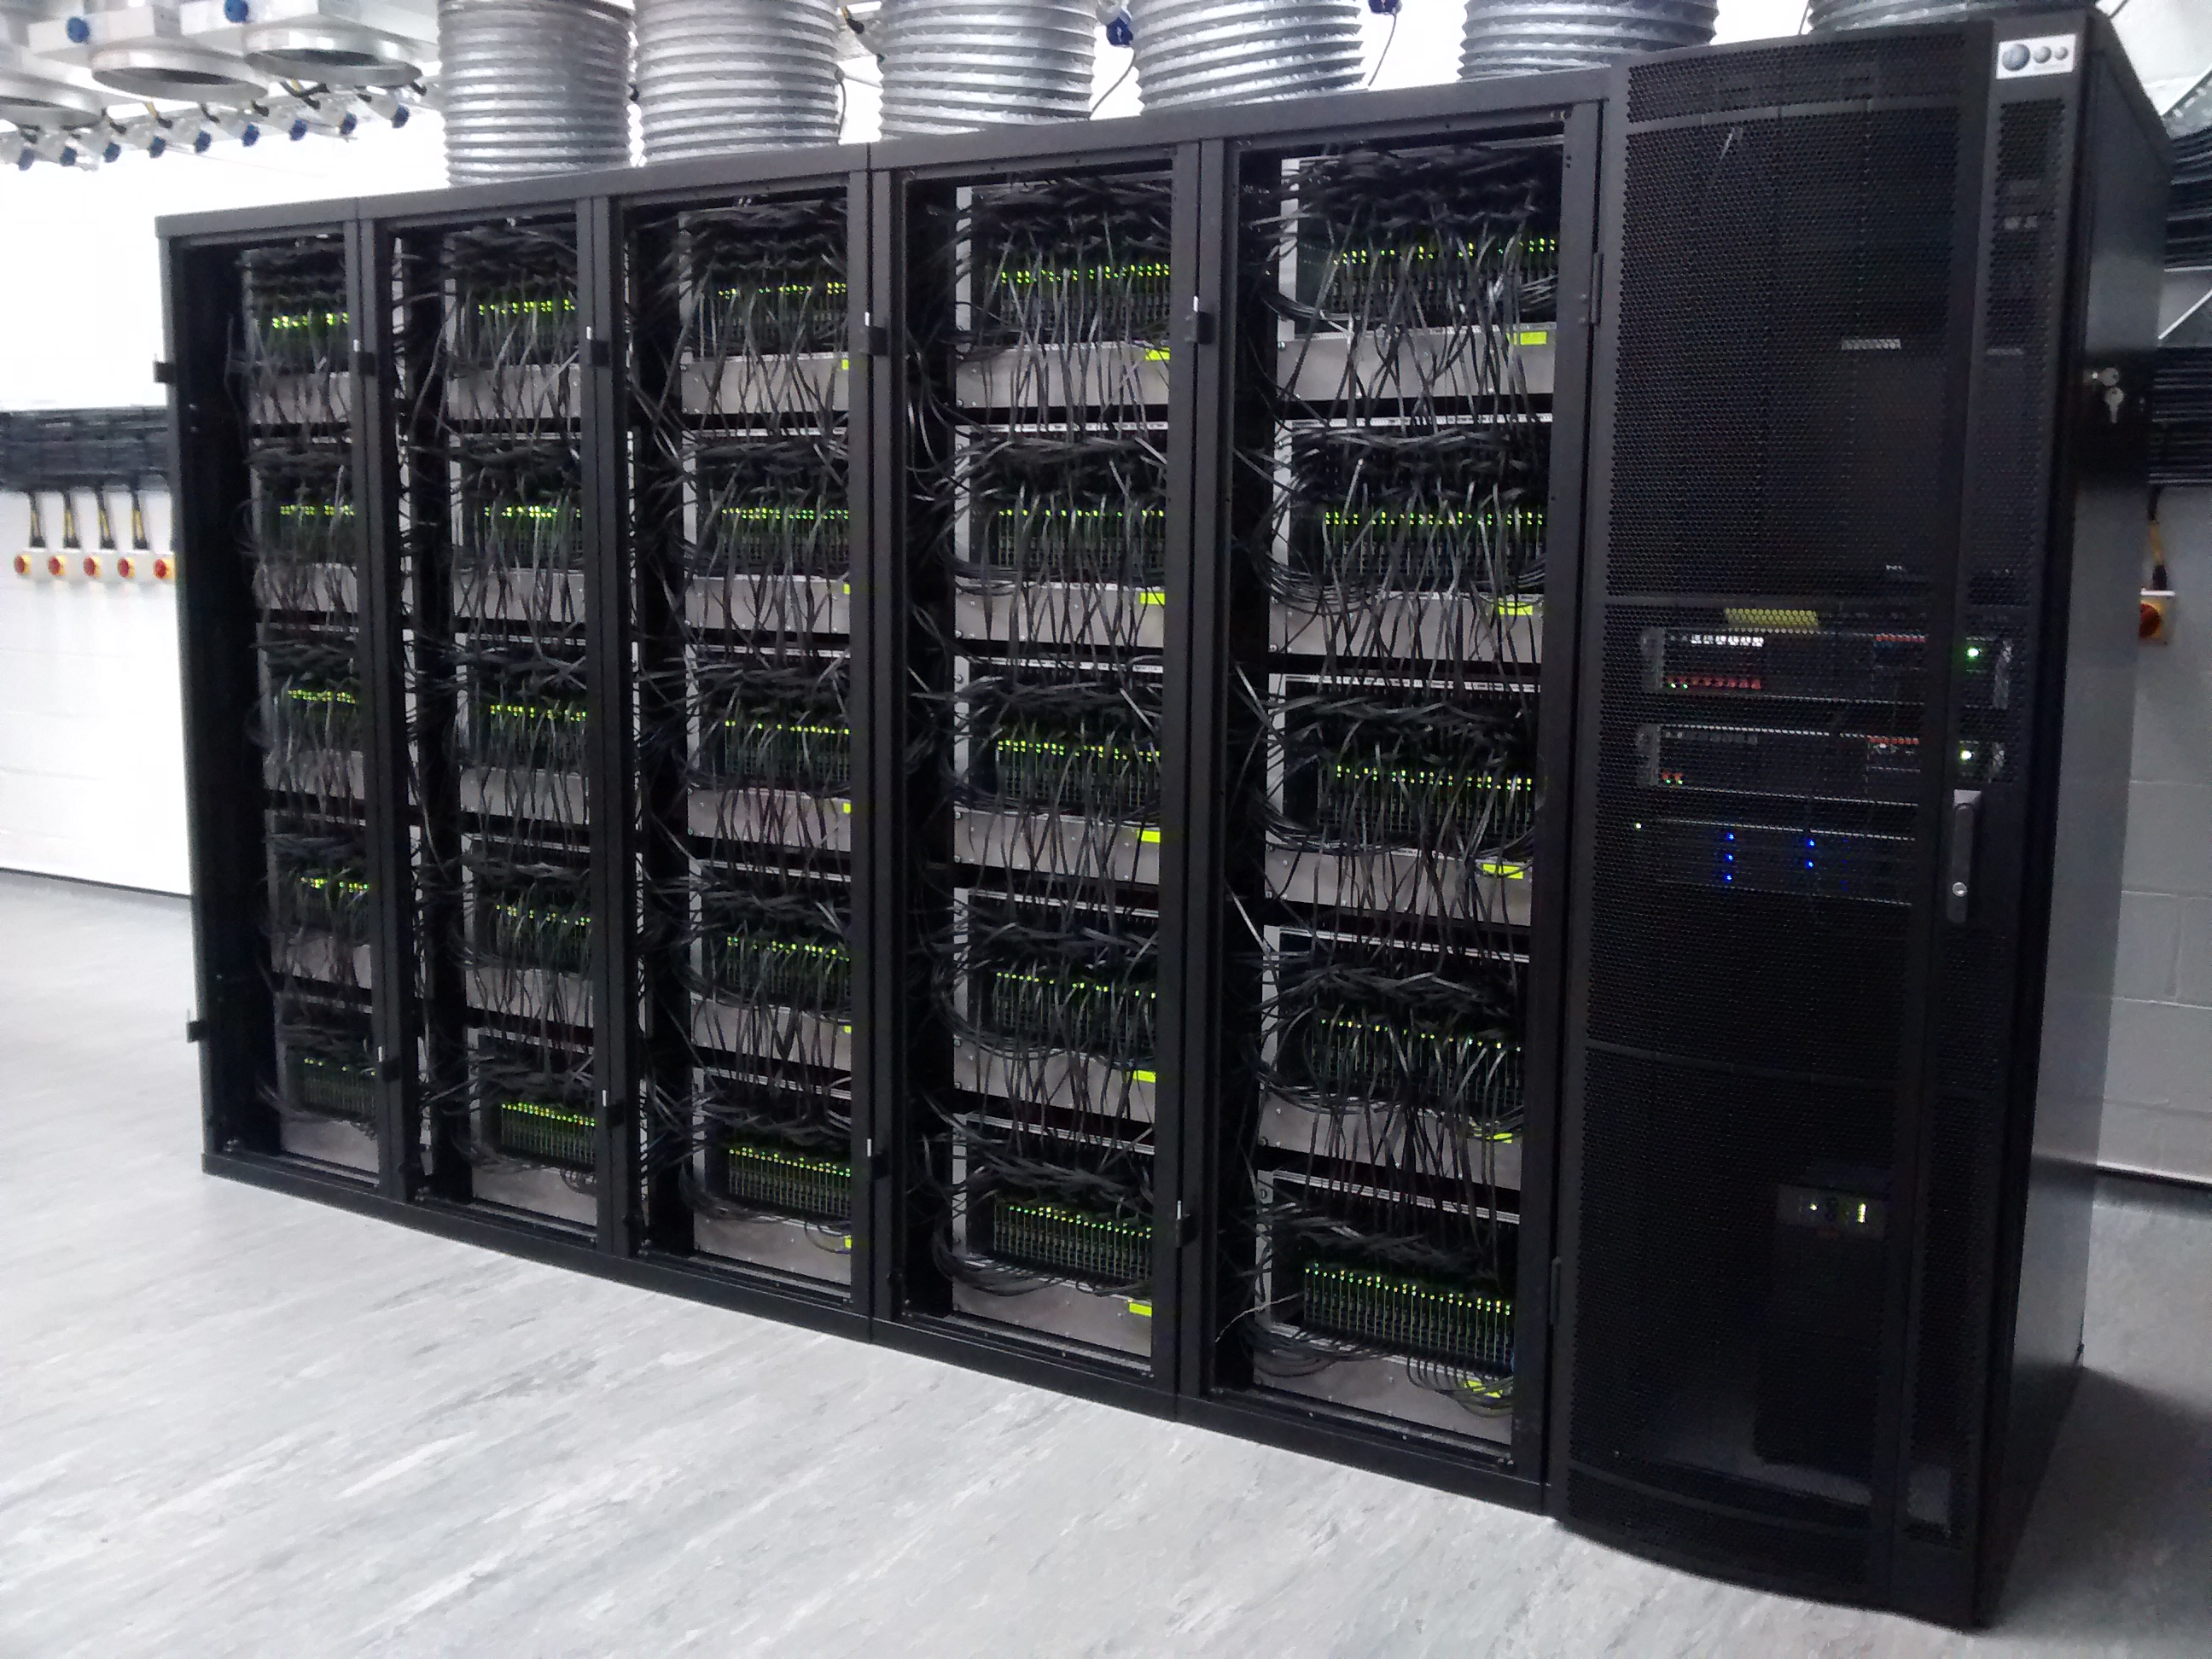
\includegraphics[width=0.8\linewidth]{figures/halfMillionCoreComplete.jpg}
				
				\caption[The five cabinet SpiNNaker system.]%
				{The five cabinet SpiNNaker system. The cabinet on the right contains
				conventional host servers which control SpiNNaker.}
				\label{fig:halfMillionCoreComplete}
			\end{figure}
			
			The completed five cabinet system is photographed in
			figure~\ref{fig:halfMillionCoreComplete}. A time-lapse video showing the
			construction and cable installation of this machine is also available on
			YouTube~\cite{heathcote16}.
			
		\subsection{Thermal implications}
			
			In large SpiNNaker machines, each 24 board frame contains a fan tray
			which pulls cool air from the front of the frame, between the SpiNNaker
			boards. The warmed air is then ejected out of the rear of the frame where
			ducting directs it into industrial air chillers. Conventional guidance on
			data centre design suggests that routing cables in the path of the
			system's airflow can have a serious impact on cooling
			performance~\cite{cisco07}.  To determine what effect the cabling
			described in this chapter had on SpiNNaker's cooling, a test program was
			executed to simulate heavy load before and after cable installation. The
			temperatures reported by the sensors on the top of each SpiNNaker board
			were sampled at regular intervals and once the overall system temperature
			stabilised, the mean temperature was recorded.
			
			Before the cabling was installed, the temperature stabilised at
			\SI{49}{\celsius} while after installation it stabilised at
			\SI{42}{\celsius}.
			
			These two data points suggest that the system's temperature is unlikely
			to have been been seriously impacted by cable installation. Since the two
			experiments were run on different days (with potentially different
			ambient temperatures) and are based on a single experiment, it is not
			possible to infer much more from this result.
			
		\subsection{Maintenance}
			
			At the time of writing, the five cabinet machine is still being
			commissioned and so the long term maintenance impact of the system's
			cabling is not known. One important factor in the maintainability of the
			system is the ease with which faulty boards can be replaced. During
			commissioning a number of boards have been replaced by someone not
			involved in the machine's installation. Informal measurements suggest
			that boards near the centre of a frame (i.e. those most likely to be
			blocked by unrelated cables) take around ten minutes to replace,
			including time spent removing and replacing cables obstructing the board
			being exchanged. By comparison boards at the edge of the machine take
			around six minutes to replace. Though similar timing reports are
			unavailable for other architectures, these times appear reasonable in
			practice and suggest maintenance is not impaired by the wiring plan used.
	
	\section{Conclusions}
		
		In this chapter I presented a practical method of constructing real-world
		installations of large hexagonal torus topologies such that long cables
		spanning the width and height of the system are not required. Two
		transformations, shearing and slicing, are presented which allow
		conventional network folding techniques to be applied to hexagonal toruses
		to eliminate long `wrap around' links. Though both techniques incur some
		overhead in terms of mean and maximum cable length, the maximum cable
		length does not grow with the size of the network. This result makes
		hexagonal torus topologies a practical and scalable choice for future
		systems.
		
		The theoretical results presented in this chapter have been confirmed
		through the successful construction of several large-scale SpiNNaker
		machines which implement hexagonal torus topologies. During construction,
		diagnostic features of SpiNNaker's hardware were employed to guide
		technicians performing cable installation. This technique was found to be
		highly effective with cable installation times measured in seconds rather
		than minutes as reported for other architectures. Surprisingly there was no
		evidence found of this technique being applied to other architectures and
		consequently this secondary result may be of interest for future research.

	\chapter{Finding shortest path vectors in SpiNNaker's network}
	
	\label{sec:shortestPaths}
	
	% XXX: Add note explaining shortest path between two points in non-torus
	% space.
	
	In the previous chapter we explored the practical challenges of building
	machines which use hexagonal torus topologies working at the scale of units
	containing several nodes. To exploit these machines, however, we must also be
	able to route packets efficiently through the nodes in the resulting network.
	This chapter tackles the problem of finding shortest path vectors in
	hexagonal torus topologies. Shortest path vectors are used by many routing
	algorithms as the basis for route generation. In non-hexagonal torus
	topologies, finding shortest path vectors is trivial and intuitive but in
	hexagonal toruses, this is not the case.  In this chapter I introduce the
	Irregular Quadrant (IQ) method, a new technique for computing shortest path
	vectors in hexagonal torus topologies.  This method is cheaper to compute and
	more general than pre-existing techniques, functioning correctly on hexagonal
	torus topologies of any aspect ratio.
	
	In some hexagonal torus topologies, many shortest path vectors may exist
	between a given pair of points. I propose a technique for discovering all
	possible shortest path vectors. Using these alternative shortest path
	vectors, routing algorithms may be able to produce routes which load a
	network more evenly.
	
	In this chapter, I assume an idealised hexagonal torus topology without
	faults or other irregularities. The challenge of handling these artefacts of
	real-world systems will be tackled in chapter~\ref{sec:routing}.
	
	\section{Shortest path vectors}
		
		Many popular routing algorithms for torus topologies, including all
		published algorithms designed for SpiNNaker~\cite{davies12,navaridas14},
		compute a shortest path vector between the endpoints of a route and use
		this to generate a path through the network. A shortest path vector between
		two nodes is a vector, $\mathbf{v} = (v_1, v_2, v_3, \ldots)$, whose
		magnitude, $\| \mathbf{v} \| = \lvert v_1 \rvert + \lvert v_2 \rvert +
		\lvert v_3 \rvert + \cdots$, is minimal with respect to all possible
		vectors between those nodes.
		
		\begin{figure}
			\center
			\buildfig{figures/mesh-topology-coordinates.tex}
			\caption[Shortest path routes in a 2D mesh network.]%
			{An example 2D mesh network with example shortest-path routes
			from `A' to `B' and `B' to `C'.}
			\label{fig:mesh-topology-coordinates}
		\end{figure}
		
		In a non-hexagonal mesh topology, shortest path vectors are computed by
		taking the element-wise difference between the source and destination
		nodes' coordinates. For example, figure~\ref{fig:mesh-topology-coordinates}
		shows a 2D mesh topology with three nodes labelled `A', `B' and `C' with
		position vectors $(1, 2)$, $(4, 5)$ and $(6, 1)$ respectively. The shortest
		path vector from node `A' to `B' is $(4, 5) - (1, 2) = (3, 3)$ and from `B'
		to `C' is $(6, 1) - (4, 5) = (2, -4)$. A route may be produced by advancing
		the number of hops specified for each dimension in the shortest path
		vector. For example, a route from `A' to `B' may be constructed from any
		permutation of the hops X$^+\,$X$^+\,$X$^+\,$Y$^+\,$Y$^+\,$Y$^+$, an
		example of which is included in the figure. Likewise routes from `B' to `C'
		may be constructed from permutations of the hops
		X$^+\,$X$^+\,$Y$^-\,$Y$^-\,$Y$^-\,$Y$^-$. Regardless of the order of the
		hops, the length of the route, $\mathbf{v}$, is given by the magnitude of
		the shortest path vector, $\|\mathbf{v}\|$.
		
		Many popular routing algorithms such as dimension order routing, right-turn
		only routing and longest dimension first routing~\cite{davies12} are simply
		defined as rules for ordering the hops specified by a shortest path vector.
		
		\subsection{Torus networks}
			
			\begin{figure}
				\center
				\begin{subfigure}{0.3\linewidth}
					\center
					\buildfig{figures/torus-shortest-path-example.tex}
					\caption{Original}
					\label{fig:torus-shortest-path-example}
				\end{subfigure}
				\begin{subfigure}{0.3\linewidth}
					\center
					\buildfig{figures/torus-shortest-path-translate.tex}
					\caption{Routed \& translated}
					\label{fig:torus-shortest-path-translate}
				\end{subfigure}
				\begin{subfigure}{0.3\linewidth}
					\center
					\buildfig{figures/torus-shortest-path-routed.tex}
					\caption{Routed original}
					\label{fig:torus-shortest-path-routed}
				\end{subfigure}
				
				\caption{Finding shortest paths in a 2D torus topology.}
				\label{fig:torus-shortest-path}
			\end{figure}
			
			Computing shortest path vectors in non-hexagonal torus topologies is also
			straightforward. For example, to find the shortest path vector from node
			`A' to `B' in the 2D torus topology shown in figure~\ref{fig:torus-shortest-path-example} both nodes are translated such that
			the source node, `A', is at the centre of the network. The shortest path
			vector is then computed in the same way as a mesh network (figure~\ref{fig:torus-shortest-path-translate}). Note that, as in this example,
			translation may cause the destination node to `wrap around' the network.
			As illustrated in figure~\ref{fig:torus-shortest-path-routed}, the
			computed shortest path vector is also valid for the two points prior to
			translation.
			
			\begin{figure}
				\center
				
				\begin{subfigure}{\linewidth}
					\center
					\buildfig{figures/distance-map-mesh.tex}
					\caption{2D mesh topology}
					\label{fig:distance-map-mesh}
				\end{subfigure}
				
				\vspace{1em}
				
				\begin{subfigure}{\linewidth}
					\center
					\buildfig{figures/distance-map-torus.tex}
					\caption{2D torus topology}
					\label{fig:distance-map-torus}
				\end{subfigure}
				
				\caption[Magnitudes of shortest path vectors in a 2D mesh.]%
				{Plots showing the magnitude of shortest path vectors in a 2D
				(non-hexagonal) topology from locations marked {\color{red}$\times$}.
				Darker areas are further away. Contour lines show equidistant points.}
				
				\label{fig:distance-map}
			\end{figure}
			
			This procedure works because vectors from the centre of a non-hexagonal
			torus topology to any other point are identical to those in a
			corresponding mesh topology. For example, in figures
			\ref{fig:distance-map-mesh} and~\ref{fig:distance-map-torus} we can see
			that the magnitude of the shortest path vectors from the centre of a mesh
			and torus grow identically. Conversely, the magnitudes of vectors from
			other locations in mesh and torus topologies do not match.
		
	\section{Related work}
		
		The problem of finding shortest path vectors in hexagonal mesh topologies
		has been widely considered and formulations may be found in a variety of
		applications, including computer games~\cite{patel15}. Hexagonal toruses,
		by contrast, have only received limited attention. In this section I
		briefly summarise the solutions proposed for hexagonal mesh topologies
		before more deeply examining existing solutions for hexagonal torus
		topologies.
		
		\subsection{Hexagonal mesh networks}
			
			\begin{figure}
				\center
				\buildfig{figures/hex-mesh-topology-coordinates.tex}
				\caption{An example hexagonal mesh network topology.}
				\label{fig:hex-mesh-topology-coordinates}
			\end{figure}
			
			In hexagonal mesh topologies it is conventional to define three `axes' X,
			Y and Z as shown in
			figure~\ref{fig:hex-mesh-topology-coordinates}~\cite{patel15}. In this
			example, the three labelled nodes `A', `B' and `C' may be given position
			vectors such as $(1, 1, 0)$, $(3, 2, 0)$ and $(0, 0, -7)$ respectively.
			As in other mesh networks, a vector between two nodes is found by
			subtracting the nodes' vectors. For example, a vector from `A' to `B' is
			$(3, 2, 0) - (1, 1, 0) = (2, 1, 0)$. This vector can then be converted
			into a route in the same way as a mesh network by taking any permutation
			of the three hops  X$^+\,$X$^+\,$Y$^+$.
			
			As explained in detail in appendix~\ref{app:minimal-hex-coordinates},
			there are a multitude of vectors between any two points in a hexagonal
			mesh. For example, the vectors $(1, 0, -1)$ and $(3, 2, 1)$ also reach
			node `B' from `A'. However, for a given pair of nodes, there is always a
			single, unique vector whose magnitude is minimal which is given by the
			function:
			%
			\begin{equation*}
				\operatorname{minimiseVector}(x,y,z) =
					(x,y,z) - \operatorname{median}(x,y,z) \cdot (1,1,1)
			\end{equation*}
			%
			For example, the vector $(3, 2, 1)$ from `A' to `B' is minimised as
			follows:
			%
			\begin{align*}
				\operatorname{minimiseVector}(3,2,1) &=
					(3,2,1) - \operatorname{median}(3,2,1) \cdot (1,1,1) \\
				&=
					(3,2,1) - (2,2,2) \\
				&=
					(1,0,-1)
			\end{align*}
			%
			A side-effect of this is that a minimised vector will always contain at
			least one zero element, meaning that shortest path routes will use at most
			two of the three available dimensions.
		
		\subsection{Hexagonal torus networks}
			
			\begin{figure}
				\center
				
				\begin{subfigure}{\linewidth}
					\center
					\buildfig{figures/distance-map-hex-mesh.tex}
					\caption{Hexagonal mesh topology}
					\label{fig:distance-map-hex-mesh}
				\end{subfigure}
				
				\vspace{1em}
				
				\begin{subfigure}{\linewidth}
					\center
					\buildfig{figures/distance-map-hex-torus.tex}
					\caption{Hexagonal torus topology}
					\label{fig:distance-map-hex-torus}
				\end{subfigure}
				
				\caption[Magnitudes of shortest path vectors in a hexagonal torus.]%
				{Plots showing the magnitude of shortest path vectors in a hexagonal
				torus topology from locations marked {\color{red}$\times$}.  Darker
				areas are further away. Contour lines show equidistant points.}
				
				\label{fig:distance-map-hex}
			\end{figure}
			
			Unfortunately, the translation technique used for non-hexagonal toruses
			cannot be used in a hexagonal torus. As illustrated in figures
			\ref{fig:distance-map-hex-mesh} and \ref{fig:distance-map-hex-torus},
			shortest path vectors from the centre, or any other part of a hexagonal
			mesh network, do not grow in magnitude in the same way that those of a
			hexagonal torus network do. I am aware of two pre-existing approaches to
			computing shortest path vectors in hexagonal toruses. These are described
			below.
			
			\subsubsection{INSEE Method}
			
				The INSEE interconnect simulator has been used in all published
				research into SpiNNaker's hexagonal torus interconnect to
				date~\cite{navaridas09,ghasempour15}. Internally INSEE finds shortest
				path vectors by selecting the shortest of a set of twelve candidate
				vectors known to always contain a shortest path vector.
				
				\begin{figure}
					\center
					\begin{subfigure}{0.45\linewidth}
						\center
						\buildfig{figures/insee-vector-candidates-no-wrap.tex}
						\caption{$(\Delta_\textrm{X}, \Delta_\textrm{Y}) = (5,3)$}
						\label{fig:insee-vector-candidates-no-wrap}
					\end{subfigure}
					\begin{subfigure}{0.45\linewidth}
						\center
						\buildfig{figures/insee-vector-candidates-wrap-x.tex}
						\caption{$(\Delta'_\textrm{X}, \Delta_\textrm{Y}) = (-3,3)$}
						\label{fig:insee-vector-candidates-wrap-x}
					\end{subfigure}
					
					\vspace{1em}
					
					\begin{subfigure}{0.45\linewidth}
						\center
						\buildfig{figures/insee-vector-candidates-wrap-y.tex}
						\caption{$(\Delta_\textrm{X}, \Delta'_\textrm{Y}) = (5,-5)$}
						\label{fig:insee-vector-candidates-wrap-y}
					\end{subfigure}
					\begin{subfigure}{0.45\linewidth}
						\center
						\buildfig{figures/insee-vector-candidates-wrap.tex}
						\caption{$(\Delta'_\textrm{X}, \Delta'_\textrm{Y}) = (-3,-5)$}
						\label{fig:insee-vector-candidates-wrap}
					\end{subfigure}
					
					\vspace{1em}
					
					% Key
					\begin{tikzpicture}[thick]
						\coordinate (last);
						
						% #1 colour
						% #2 label
						\newcommand{\colourkeyentry}[2]{
							\node [#1] [right=of last, fill, rectangle, minimum size=1em] (last) {};
							\node [right=0 of last] (last) {#2};
						}
						
						\colourkeyentry{cb3class0}{$(\textrm{X}, \textrm{Y}, 0)$}
						\colourkeyentry{cb3class1}{$(\textrm{X} - \textrm{Y}, 0, - \textrm{Y})$}
						\colourkeyentry{cb3class2}{$(0, \textrm{Y} - \textrm{X}, - \textrm{X})$}
						
					\end{tikzpicture}
					
					\caption[The twelve candidate vectors considered by the INSEE method.]%
					{The twelve candidate shortest-path vectors considered by the INSEE
					method represented as dimension-order routes. $W=H=8$,
					$(\Delta_\textrm{X},\Delta_\textrm{Y}) = (5, 3)$ and
					$(\Delta'_\textrm{X},\Delta'_\textrm{Y}) = (-3, -5)$.}
					\label{fig:insee-vector-candidates}
				\end{figure}
				
				The twelve vectors considered are illustrated in
				figure~\ref{fig:insee-vector-candidates} and are constructed as
				follows.  First a shortest path vector from the source to target node
				is constructed as if the network was a 2D mesh producing a vector
				$(\Delta_\textrm{X},\Delta_\textrm{Y})$. A second 2D vector,
				$(\Delta'_\textrm{X},\Delta'_\textrm{Y})$, is also defined:
				
				\noindent
				\begin{align*}
					\Delta'_\textrm{X} &= \Delta_\textrm{X} - \operatorname{sign}(\Delta_\textrm{X})W
					\\
					\Delta'_\textrm{Y} &= \Delta_\textrm{Y} - \operatorname{sign}(\Delta_\textrm{Y})H
				\end{align*}
				%
				Where $W$ and $H$ are the width and height of the network respectively.
				This vector describes a route from the source to destination node that
				\emph{always} wraps around the peripheries of both the `X' and `Y'
				dimensions.
				
				Two further 2D vectors, $(\Delta'_\textrm{X},\Delta_\textrm{Y})$ and
				$(\Delta_\textrm{X},\Delta'_\textrm{Y})$ may be defined which wrap around
				just the X or Y axis, respectively.
				
				Each of the four 2D vectors may be converted into three hexagonal 3D
				vectors in which one element of the vector is zero. In total this
				results in twelve different vectors which cover all combinations of
				wrapping and non-wrapping routes and all combinations of axes used. The
				vector with the smallest magnitude must be the shortest path vector.
				
				This method can find shortest path vectors in hexagonal torus
				topologies of any aspect ratio but, compared with the XYZ-protocol
				(described next), is relatively clumsy and slow to compute.
			
			\subsubsection{XYZ-Protocol}
			
				Hoffmann and D\'es\'erable described the XYZ-protocol for computing
				shortest path vectors in hexagonal toruses with equal width and
				height~\cite{hoffmann15,hoffmann11}.  First, the source and destination
				nodes are translated such that the source node lies at the centre of
				the topology. The authors observe that from the centre of the topology,
				the pattern with which distances grow differs between the four
				quadrants outlined in figure~\ref{fig:xyz-protocol-regions}.
				
				\begin{figure}
					\center
					\buildfig{figures/xyz-protocol-regions.tex}
					
					\caption{The four quadrants defined by the XYZ-protocol.}
					\label{fig:xyz-protocol-regions}
				\end{figure}
				
				If the destination lies in quadrants 1 or 4, a route may be constructed
				as if in a hexagonal mesh topology. If the destination lies in
				quadrants 2 or 3, however, the algorithm tests whether taking a
				mesh-like vector within the quadrant or wrapping-around either the X or
				Y dimensions yields the shortest vector.
				
				By comparison with the twelve vectors considered by the INSEE method,
				the XYP-protocol considers just one for destinations in quadrant 1 or 4
				and no more than three in quadrant 2 or 3. Though the XYZ-protocol can
				be computed more cheaply than the INSEE method, it does not produce
				valid shortest path vectors for hexagonal torus topologies with aspect
				ratios other than $1:1$.
		
	\section{The Irregular Quadrant (IQ) method}
		
		In this section I propose a new technique for finding shortest path vectors
		in hexagonal torus topologies called the Irregular Quadrant (IQ) method and
		compare its performance with existing techniques.
		
		\subsection{Computing shortest path vectors}
		
			Consider the problem of finding a shortest path vector from (0, 0, 0), at
			the bottom-left, to a node somewhere else in a hexagonal torus topology.
			
			\begin{figure}
				\center
				\buildfig{figures/shortest-path-regions.tex}
				
				\caption[The four irregular quadrants defined by the IQ method.]%
				{Hexagonal torus topologies of various aspect ratios divided
				into irregular quadrants in which a particular pair of dimensions is used.}
				\label{fig:shortest-path-regions}
			\end{figure}
			
			Figure~\ref{fig:shortest-path-regions} illustrates how hexagonal torus
			topologies of various aspect ratios may be partitioned into four
			\emph{irregular quadrants}. These quadrants are defined according to which
			axes are wrapped around by the shortest path vectors reaching them. The
			irregular quadrants correspond to locations reachable by shortest path
			vectors which:
			%
			\begin{enumerate}
				\item Do not wrap
				\item Wrap around X only
				\item Wrap around Y only
				\item Wrap around both X and Y
			\end{enumerate}
			%
			Within each irregular quadrant, we observe that shortest path vectors are
			constrained to using only certain directionz:
			%
			\begin{enumerate}
				\item Only X$^+$, Y$^+$ and Z$^-$.
				\item Only X$^-$ and Y$^+$
				\item Only X$^+$ and Y$^-$
				\item Only X$^-$, Y$^-$ and Z$^+$.
			\end{enumerate}
			%
			Given the topology is of width $W$ and height $H$ and the
			destination node's 2D mesh coordinates are $(\Delta_\textrm{X},
			\Delta_\textrm{Y})$ we can define the shortest path vector within each
			irregular quadrant as:
			%
			\begin{enumerate}
				\item $\operatorname{minimiseVector}(\Delta_\textrm{X},\Delta_\textrm{Y},0)$
				\item $\operatorname{minimiseVector}(-(W-\Delta_\textrm{X}),\Delta_\textrm{Y},0)$
				\item $\operatorname{minimiseVector}(\Delta_\textrm{X},-(H-\Delta_\textrm{Y}),0)$
				\item $\operatorname{minimiseVector}(-(W-\Delta_\textrm{X}),-(H-\Delta_\textrm{Y}),0)$
			\end{enumerate}
			%
			Since we know that $0 \le \Delta_\textrm{X} < W$ and $0 \le
			\Delta_\textrm{Y} < H$, we can simplify the expressions for the magnitude
			of each of the above vectors. This yields four expressions giving the
			magnitude of a minimal vector as if in each irregular quadrant:
			%
			\begin{enumerate}
				\item $\operatorname{max}(\Delta_\textrm{X}, \Delta_\textrm{Y})$
				\item $(W - \Delta_\textrm{X}) + \Delta_\textrm{Y}$
				\item $\Delta_\textrm{X} + (H - \Delta_\textrm{Y})$
				\item $\operatorname{max}(W-\Delta_\textrm{X}, H-\Delta_\textrm{Y})$
			\end{enumerate}
			%
			From these expressions we can determine which irregular quadrant the
			destination is in by finding the expression with the minimum value. With
			this information, the shortest path can be found by minimising the vector
			associated with that irregular quadrant.  Figure~\ref{fig:iqmethod.py}
			shows a simple Python implementation of the IQ method.
			
			\begin{figure}
				\inputminted{python}{figures/iqmethod.py}
				
				\caption{A Python implementation of the IQ Method.}
				\label{fig:iqmethod.py}
			\end{figure}
			
			Compared with the INSEE method, this technique requires fewer cases to be
			considered (four rather than twelve) making it cheaper to compute.
			
			Unlike the four quadrants defined by the XYZ-protocol, the irregular
			quadrants defined by the IQ method correspond exactly to a particular
			shortest path vector. This means that, once the irregular quadrant a
			point lies in has been discovered, the shortest path vector can be
			calculated directly without considering multiple options. Though the
			boundaries between the four irregular quadrants are more complex than the
			quadrants of the XYZ-protocol, it is only marginally more expensive to
			discover which irregular quadrant a point lies in. In addition, the
			irregular quadrants retain their meaning across different aspect ratios
			making the IQ method suitable for any hexagonal torus topology.
		
		\subsection{Computing distances}
		
			The four vector magnitude expressions defined by the IQ method can also
			be combined to produce a compact expression of the distance between two
			points in a hexagonal torus topology:
			%
			\begin{align*}
				\|\operatorname{shortestPathVector}(\Delta_\textrm{X}, \Delta_\textrm{Y}, W, H)\| =
				\operatorname{min}(&\operatorname{max}(\Delta_\textrm{X}, \Delta_\textrm{Y}),\\
				                   &(W - \Delta_\textrm{X}) + \Delta_\textrm{Y},\\
				                   &\Delta_\textrm{X} + (H - \Delta_\textrm{Y}),\\
				                   &\operatorname{max}(W-\Delta_\textrm{X}, H-\Delta_\textrm{Y}))
			\end{align*}
			%
			This expression has also been derived independently from a
			graph-theoretic study of Cayley graphs, of which the hexagonal torus
			topology is a special case, by Xiao and Parhami~\cite{xiao04}.
		
		\subsection{Computational efficiency}
			
			Since computing shortest path vectors forms an integral part of the
			kernel of many routing algorithms, the running time of the function
			chosen can be an important consideration.
			
			To compare the performance of the three shortest path vector functions
			presented, the execution time of a C implementation of each technique was
			measured. The C implementation of the INSEE method is taken directly from
			the INSEE source code~\cite{navaridas09}. The C implementation of the
			XYZ-Protocol is a straight translation of the published
			pseudocode~\cite{hoffmann15}.
			
			Each function was called approximately 3 billion times: once for every
			pair of source and destination nodes in a $240\times240$ node hexagonal
			torus topology. The total execution time is then divided by the number of
			calls giving an average execution time.  This experiment was repeated 50
			times and the overall average execution time of each shortest path vector
			function was recorded. The experiments were conducted on a cluster of
			idle workstations with 3.10~GHz Intel Core-i5-2400 CPUs. The function
			implementations were compiled with GCC 5.3.0 with optimisations enabled
			(\verb|-O2|).
			
			\begin{figure}
				\center
				\buildrplot{figures/shortest-path-vector-runtimes.R}
				
				\caption[Mean execution times of shortest path vector functions.]%
				{Mean execution time of each shortest path vector function. Error bars
				indicate the range of the mean execution times of the fifty
				3-billion-combination experiments.}
				\label{fig:shortest-path-vector-runtimes}
			\end{figure}
			
			Figure~\ref{fig:shortest-path-vector-runtimes} shows the execution times
			of each shortest path vector function. From these results we can see that
			the INSEE method is slower than the other techniques. Although the
			XYZ-protocol and IQ method have similar performance, because the IQ
			method works for any hexagonal torus topology it is the better candidate
			for use in new applications.
	
	\section{Generating all shortest path vectors}
			
			\begin{figure}
				\center
				\buildfig{figures/wrap-alternatives.tex}
				
				\caption{Two distinct shortest path vectors in a hexagonal torus.}
				\label{fig:wrap-alternatives}
			\end{figure}
			
			In odd-sized non-hexagonal and $1:1$ hexagonal torus topologies there is
			exactly one distinct shortest path vector between any two points (though
			many routes may be defined from it). In even-sized topologies there may
			be two distinct shortest path vectors between nodes exactly half the
			length of an axis away as in figure~\ref{fig:wrap-alternatives}. The
			INSEE and IQ methods may generate either vector depending on how ties are
			broken in their implementation.
			
			\begin{figure}
				\center
				\buildfig{figures/spiralling.tex}
				
				\caption[Distinct shortest path vectors in non-square toruses.]%
				{Distinct shortest path vectors between two points, all with
				magnitude 11.}
				\label{fig:spiralling}
			\end{figure}
			
			Unlike non-hexagonal topologies, when the aspect ratio of a hexagonal
			topology is not $1:1$, some points may have many distinct (but equal
			magnitude) shortest path vectors.  For example,
			figure~\ref{fig:spiralling} illustrates three distinct shortest path
			vectors between an example pair of nodes. None of the shortest path vector
			functions discussed will generate all possible vectors in this situation,
			potentially limiting the choices available to routing algorithms.  To
			address this shortcoming, I propose a formula which enumerates every
			shortest path vector between a pair of points in a hexagonal torus.
			
			In a $W \times H$ hexagonal torus topology, starting from any node the
			vector $(0, H, 0)$ straightforwardly wraps once around the Y axis
			arriving back at the node it started from. The vector $(1,1,1)$ also
			returns to its starting point as described in
			appendix~\ref{app:minimal-hex-coordinates}. As a consequence $(0,H,0) -
			H\cdot(1,1,1) = (-H, 0, -H)$ must also be a vector which leads back to
			where it started. Adding this vector to a shortest path vector of the
			form $(x, 0, z)$ results in a new shortest path vector if $x\ge H$ and
			$z\le0$.
			
			For example, the vector $(10, 0, -1)$ (magnitude 11) in
			figure~\ref{fig:spiralling} can be added with $(-4, 0, -4)$ yielding $(6,
			0, -5)$ (also magnitude 11) which is still a shortest path vector between
			the two labelled nodes.  Since $(6, 0, -5)$ still meets the criteria
			defined above ($6 \ge 4$ and $-5 \le 0$), we can add $(-4, 0, -4)$ again
			yielding another shortest path vector $(2, 0, -9)$.  This new vector does
			not meet the requirement that $x \ge H$ (since $2 \ngeq 4$) and so no
			further shortest path vectors can be produced.
			
			More formally, a shortest path vector $(x, 0, z)$ may be converted into
			another shortest path vector $(x', 0, z')$ using the following formula:
			%
			\begin{equation*}
				(x', 0, z') = (x, 0, z) - \left(\operatorname{trunc}\left(\frac{z}{H}\right) + n\right)(H, 0, H)
			\end{equation*}
			%
			where
			%
			\begin{equation*}
				\left\{
					n \in \mathbb{Z}
				\;\Big|\;
					0 \le n \le
						\left\lfloor
							\frac{\left|x\right| + \left|z\right|}{H}
						\right\rfloor
				\right\}
			\end{equation*}
			%
			and $\operatorname{trunc}(\,\cdots)$ is the truncation operator which
			rounds towards zero to the nearest integer.
			
			A complementary formula may be derived based on the related observation
			that the vector $(W, 0, 0)$ results in no movement:
			%
			\begin{equation*}
				(0, y', z') = (0, y, z) - \left(\operatorname{trunc}\left(\frac{z}{W}\right) + n\right)(0, W, W)
			\end{equation*}
			%
			where
			%
			\begin{equation*}
				\left\{
					n \in \mathbb{Z}
				\;\Big|\;
					0 \le n \le
						\left\lfloor
							\frac{\left|y\right| + \left|z\right|}{W}
						\right\rfloor
				\right\}
			\end{equation*}
			
			Using these two expressions for wide and tall topologies, respectively,
			all possible distinct shortest path vectors between any two points may be
			found.
	
	\section{Conclusions}
		
		The calculation of shortest path vectors in mesh and torus topologies is at
		the heart of many routing algorithms. In this chapter, I introduced a new
		technique for computing shortest path vectors in hexagonal toruses which
		generalises to any hexagonal torus topology while executing more quickly
		than existing approaches. In addition, I described a formula for
		enumerating the distinct shortest path vectors between points in hexagonal
		torus topologies. Unlike previous work, this allows routing algorithms
		greater freedom by providing a choice of shortest path vectors between some
		points.  These contributions demonstrate that key operations such as
		computing distances and shortest path vectors in hexagonal toruses can be
		efficient and exhaustive just as in non-hexagonal torus topologies.

	\chapter{Routing packets in large SpiNNaker machines}
	
	\section{Related work}
		\subsection{Multicast routing}
		\subsection{Deadlock avoidance}
		\subsection{Fault-tolerance}
	
	\section{Dimension order routing in hexagonal torus topologies}
		\subsection{Hexagonal meshes}
		\subsection{Hexagonal toruses}
		\subsection{Ensuring fairness}
		\subsection{Generating spiralling routes}
	
	\section{Fault-tolerant multicast routing}
		\subsection{Graph search based repair}
		\subsection{Alternative routing heuristics}
		\subsection{Results}
			\subsubsection{Heuristic performance}
			\subsubsection{Runtime}
			\subsubsection{Route congestion}
	

	\chapter{Placing applications in large SpiNNaker machines}
	
	\label{sec:placement}
	
	In the previous chapter I tackled the problem of fault tolerant route
	generation for SpiNNaker's network. The centroid traffic pattern was used as
	an approximation of the expected network traffic generated by `well behaved'
	neural network simulation software running on SpiNNaker. This traffic pattern
	exhibits locality, with most communication occurring between adjacent nodes.
	In reality, neural simulation applications are not conveniently specified
	geometrically but rather as abstract graphs of communicating
	neurons~\cite{davison08,eliasmith04}. Although neural models often exhibit
	localised connectivity, this can only be exploited if they are laid out
	sensibly within a network. Producing optimal placements is an NP-complete
	problem~\cite{hoefler11}.
	
	In this chapter I evaluate the effectiveness of simulated
	annealing~\cite{kirkpatrick83} for placement of SpiNNaker applications.
	Though simulated annealing fell out of favour for use in application
	placement in the 1990s, I argue that it is time to re-evaluate its
	suitability for modern placement problems. Looking to the field of chip
	design, where circuit placement problems have also been growing exponentially
	in scale for the past few decades, simulated annealing was considered ideal
	for placement problems whose sizes are comparable to that of modern
	supercomputer placement problems.
	
	In experiments on existing SpiNNaker applications I find that simulated
	annealing achieves placement solutions substantially better than contemporary
	application placement techniques. In some cases simulated annealing is shown
	to make the difference between an application functioning correctly and not
	at all. Using larger scale synthetic benchmarks I have also demonstrated that
	my proof of concept simulated annealing based placement algorithm scales up
	to placement problems containing over one million vertices while achieving
	placement quality similar to an optimal placement solution.
	
	I also build upon the work on hexagonal torus topologies earlier in this
	thesis to develop an efficient placement cost estimation function for use in
	the kernel of the annealing algorithm.
	
	\section{Related work}
		
		Attempts to address the problem of placing applications in supercomputer
		networks have utilised a variety of approaches ranging from simple greedy
		algorithms to sophisticated combinatorial optimisation
		techniques~\cite{jeannot14}. In the parallel field of digital circuit
		placement for chip and FPGA design, placement algorithms have also received
		intense study.  In this section I survey the work carried out on
		application placement before exploring chip design techniques to see what
		can be learnt from this perhaps more advanced field.
		
		In the application placement literature, the placement problem is often
		referred to by the umbrella term `mapping'. Unfortunately, `mapping' is
		often used more broadly to include other tasks such as routing and
		application partitioning. To avoid ambiguity I use the term `placement', as
		preferred by the chip and FPGA design communities, to refer specifically to
		the problem of assigning vertices in an application's communication graph
		to nodes in a machine's connectivity graph: the focus of this chapter.
		
		\subsection{Application placement algorithms}
			
			Below I consider several popular techniques employed by existing
			supercomputer applications ranging from application-specific manual
			placement to sophisticated general purpose algorithms.
			
			\subsubsection{Application-specific approaches (manual placement)}
				
				\begin{figure}
					\center
					\buildfig{figures/fem-partitioning.tex}
					
					\caption[Partitioning of a 3D volume for a $3\times4\times2$ torus.]%
					{Example partitioning of a 3D volume to fit into a supercomputer with
					a $3\times4\times2$ torus or mesh topology.}
					\label{fig:fem-partitioning}
				\end{figure}
				
				In certain applications such as finite element
				modelling~\cite{bermejo13}, a problem's structure defines a `natural'
				placement of the problem onto the target machine. For example when
				simulating a 3D volume in a supercomputer with a $3 \times 4 \times 2$
				3D torus or mesh topology network, the modelled volume might be divided
				as in figure~\ref{fig:fem-partitioning}. Each cuboid in the model is
				then assigned to the corresponding node in the network topology.
				
				Unfortunately, this technique only applies to a very narrow class of
				applications and is not applicable to many of the types of neural
				models SpiNNaker is designed to run.
			
			\subsubsection{Sequential placement}
				
				In the case where a placement solution is non-obvious, one of the
				simplest and most popular strategies is to apply a simple sequential
				placement algorithm. Sequential placement greedily places the vertices
				of an application's communication graph onto nodes. By carefully
				selecting the order in which vertices are picked and nodes assigned in
				the target architecture, this algorithm can produce reasonable quality
				placements.
				
				\begin{figure}
					\center
					\begin{subfigure}{0.32\linewidth}
						\center
						\buildfig{figures/sequential-row-order.tex}
						\caption{Row-order}
						\label{fig:sequential-row-order}
					\end{subfigure}
					\begin{subfigure}{0.32\linewidth}
						\center
						\buildfig{figures/sequential-alternating.tex}
						\caption{Alternating}
						\label{fig:sequential-alternating}
					\end{subfigure}
					\begin{subfigure}{0.32\linewidth}
						\center
						\buildfig{figures/sequential-hilbert.tex}
						\caption{Hilbert curve}
						\label{fig:sequential-hilbert}
					\end{subfigure}
					
					\caption{Space-filling curves in 2D mesh and torus topologies.}
					\label{fig:sequential}
				\end{figure}
				
				Supercomputer management software such as SLURM~\cite{yoo03} and Blue
				Gene's system software~\cite{gilge14} by default na\"ively iterate over
				vertices in an application communication graph in the order in which
				they are defined by the application. The nodes in the target machine
				are iterated over using a simple space-filling curve.
				Figure~\ref{fig:sequential} illustrates three popular space filling
				curves.
				
				The row-order (figure~\ref{fig:sequential-row-order}) and alternating
				(figure~\ref{fig:sequential-alternating}) curves illustrate 2D versions
				of the default node assignment orders provided by the SLURM and
				BlueGene systems.  The Cray extensions to SLURM software provide a
				Hilbert curve~\cite{hilbert91} node assignment order
				(figure~\ref{fig:sequential-hilbert}). The Hilbert curve specifically
				attempts to maintain the property that points that are close together
				along the length of the curve are also close together in the 2D
				mapping~\cite{moon01, zumbusch99}. Since the vertex iteration order is
				also chosen such that connected vertices tend to be closer together,
				this property may lead to improved placement solutions.
				
				\begin{figure}
					\center
					\buildrplot{figures/space_filling_curves_comparison.R}
					
					\caption[Relationship between space filling curve offset and 2D distance.]%
					{Relationship between distance along a space filling curve
					and between the 2D positions assigned. Results shown for
					Manhattan distances in a $32\times32$ 2D mesh.}
					\label{fig:space_filling_curves_comparison}
				\end{figure}
				
				Figure~\ref{fig:space_filling_curves_comparison} illustrates how the
				distance between locations along each space filling curve map to
				distances in the resulting 2D space. Both the row-order and alternating
				orderings result in distances oscillating between being closer and
				spread out in 2D space, just as the space filling curves oscillate from
				side-to-side. For the Hilbert curve, however, distances grow more
				monotonically\footnote{The growth in distance for Hilbert curves may
				appear slightly irregular but in fact forms a fractal as a consequence
				of the fractal construction of the Hilbert curve itself.} and at
				smaller 1D distances, 2D distances are often lower than in other space
				filling curves.
				
				A number of algorithms have been proposed for automatically selecting
				good vertex and chip iteration orders, typically using a
				graph-traversal based heuristic. An example typical of this type of
				technique is `graph similarity based mapping' described by Hoefler and
				Snir~\cite{hoefler11}. This algorithm exploits the Reverse
				Cuthill-McKee (RCM) algorithm~\cite{cuthill69} to select a linear
				ordering of vertices in which connected vertices tend to appear close
				together. Internally, the RCM algorithm uses a breadth-first-search-like
				algorithm to order vertices.
				
				The RCM algorithm was originally designed as a tool for reducing the
				`bandwidth' of matrices to improve the performance of linear algebra
				techniques. A matrix's bandwidth is the width of the strip of non-zero
				elements on its diagonal. Figure~\ref{fig:rcm} illustrates how a sparse
				matrix is permuted by the RCM algorithm to produce a matrix with lower
				bandwidth. This technique may be applied to a graph by representing the
				graph as an adjacency matrix, $M$, where $M_{i,j}$ is $w$ if node $i$
				is connected by an edge to node $j$ with weight $w$ and 0 otherwise.
				When a graph's adjacency matrix is permuted by the RCM algorithm, the
				connectivity of the graph remains unchanged but the vertex ordering
				changes. The ordering of vertices in a low-bandwidth adjacency matrix
				tends to keep connected vertices closer together in the ordering, making
				the ordering well suited for use with a sequential placement algorithm.
				
				\begin{figure}
					\center
					\begin{subfigure}{0.45\linewidth}
						\center
						\buildfig{figures/rcm-initial.tex}
						
						\caption{Original permutation}
						\label{fig:rcm-initial}
					\end{subfigure}
					\begin{subfigure}{0.45\linewidth}
						\center
						\buildfig{figures/rcm-sorted.tex}
						
						\caption{RCM permutation}
						\label{fig:rcm-sorted}
					\end{subfigure}
					
					\caption[Graph adjacency matrix before and after RCM permutation.]%
					{Adjacency matrix representation of a graph before and after
					permutation by the RCM algorithm.}
					\label{fig:rcm}
				\end{figure}
				
				In small-scale and densely connected applications such as early neural
				simulations running on prototype SpiNNaker machines~\cite{galluppi10},
				these techniques have proven sufficient.  As my experiments demonstrate
				later, however, sequential placement is insufficient for some SpiNNaker
				applications.
				
			\subsubsection{Simulated annealing}
				
				\label{sec:application-placement-summary}
				
				In the academic community, a number of attempts have been made to use
				sophisticated optimisation algorithms for the placement of
				applications. In 1985, Steele~\cite{steele85} first proposed the use of
				simulated annealing for placing applications in the 6D torus topology
				of the 64 node `Caltech Cosmic Cube'. The proposed algorithm is
				described below.
				
				Initially, the vertices in the application's communication graph are
				assigned randomly to nodes in the machine. Two vertices are then chosen
				at random and swapped.  If this swap reduces the `cost' of the
				placement (as defined later), the vertices are kept in their new
				locations. If the cost increases as a result of the swap, the vertices
				are moved back to their original locations with a probability dependent
				on the magnitude of the cost increase and the current `temperature'.
				
				The process of picking and swapping vertices is repeated many times
				while the temperature is gradually reduced. Initially the temperature
				is set to a large value causing most swaps to be accepted, regardless
				of their cost. As the algorithm proceeds, the temperature is reduced
				until only swaps resulting in cost reductions are accepted. By
				initially accepting detrimental swaps, the algorithm typically avoids
				becoming trapped in local minima. Towards the end of the algorithm's
				execution the solution is presumed to be close to the global
				minimum-cost solution and so few or no detrimental swaps are accepted.
				
				The cost of a particular placement is defined by some expression
				approximating the quality of the placement with better quality
				placements having lower costs. In Steele's work, the cost of a
				placement is computed by finding the shortest path routes between all
				connected vertices using Dijkstra's algorithm. Rather than repeating
				this relatively expensive computation after each swap, Steele's
				implementation updated the previously calculated cost by recomputing
				only the routes connecting the swapped vertices.
				
				The number of swaps to attempt and the rate at which the temperature is
				changed is dictated by an `annealing schedule' and can have a major
				impact on the execution time of the algorithm and the quality of the
				placement solution. I describe one such schedule in detail later in
				this chapter when describing my own simulated annealing based
				application placement algorithm.
				
				Towards the end of the 1980s, application placement appeared to be
				becoming less important as supercomputer network architectures
				improved, appearing to render computationally intensive placement
				algorithms unnecessary~\cite{dally87}.  In addition, network and
				problem sizes remained small: so small in fact that exact
				linear-programming based placement algorithms remained a meaningful
				point of comparison in application placement research~\cite{xu91}. In
				this environment, simpler sequential placement algorithms gained favour
				over more computationally expensive algorithms such as simulated
				annealing.
				
				In contemporary application placement algorithms, `low temperature'
				simulated annealing algorithms are occasionally employed as a
				post-processing step for other placement algorithms~\cite{hoefler11}.
				Other heuristics are used to generate an initial placement solution.
				
				% Outside of badly attempting 90s scale problems at least... \cite{chen06}
			
			\subsubsection{Recursive partitioning}
				
				As problem and machine sizes have grown and network utilisation has
				once again become an important factor in application
				performance~\cite{navaridas09b}, more complex optimisation algorithms
				have reappeared in the literature. One popular approach employs graph
				partitioning algorithms such as METIS~\cite{karypis98} to perform
				recursive bipartitioning based
				placement~\cite{phillips14,hoefler11,pellegrini96}.  This placement
				process is illustrated in figure~\ref{fig:partitioning}.
				
				\begin{figure}
					\center
					\buildfig{figures/partitioning.tex}
					
					\caption[Application placement by recursive partitioning.]%
					{Illustration of application placement by recursive
					partitioning. Each node has the capacity to hold two vertices.}
					\label{fig:partitioning}
				\end{figure}
				
				In the first step, the application communication graph and machine
				connectivity graph are each bipartitioned such that the number of edges
				cut by the partitions is minimised while the size of each partition
				remains similar. Each half of the communication graph is associated
				with one of the halves of the machine connectivity graph.  The
				partitioning process is then repeated recursively, further partitioning
				the application and machine graphs. The process halts when either graph
				can no longer be partitioned.  The vertices in the communication graph
				are then placed on their associated node in the connectivity graph.
				
				Unfortunately, recursive partitioning-based techniques are known to
				perform sub-optimally when the number of nodes is not a power of
				two~\cite{simon97}. In addition, placement problems are often subject
				to multiple orthogonal constraints. For example, a vertex in an
				application's communication graph may consume a certain number of
				processors and some quantity of SDRAM. Partitioning algorithms require
				a metric with which the size of each partition may be measured to
				ensure that the two halves are balanced. When multiple orthogonal
				resources exist, a single metric is insufficient to express this
				requirement. As a result, partitioning algorithms are of limited use in
				applications whose placement is subject to several orthogonal
				requirements, such as neural modelling software on SpiNNaker.
				
			\subsubsection{Topology-specific approaches}
				
				Other approaches employ other optimisation techniques that are
				specialised for use with applications and networks with specific
				connectivity patterns, for example, trees~\cite{jeannot14,traff02}.
				Unfortunately, these algorithms cater neither for SpiNNaker's hexagonal
				torus topology nor the range of communication topologies found in its
				target applications.
	
		\subsection{Circuit placement algorithms}
			
			The circuit placement problem in chip and FPGA design is similar to that
			of application placement: communicating components must be assigned
			positions in a chip so that wiring congestion is controlled.
			
			\begin{figure}
				\center
				\buildrplot{figures/top500-num-processors.R}
				
				\caption[Historical core counts for the `Top500' supercomputers.]%
				{Historical processor (core) counts for the `Top500' supercomputer
				installations. The line shows the mean number of processsors and grey
				ribbon indicates the range. Data reported by the `Top500
				List'~\cite{meuer16j}.}
				\label{fig:top500-num-processors}
			\end{figure}
			
			Following the march of Moore's `Law'~\cite{moore75}, the number of
			components in modern chips and FPGAs has been increasing at an
			exponential rate similar to that of core counts of supercomputers (see
			figure \ref{fig:top500-num-processors}). Today, in 2016, the largest
			chips contain billions of transistors, compared with millions of
			processors found in supercomputers. In terms of the raw number of
			processors, the world's largest supercomputers are at a scale comparable
			with the number of components in chips designed fifteen years ago. The
			mean size of today's `Top 500' supercomputers is somewhat smaller still,
			similar in scale to chips designed over 20 years ago.
			
			In view of of the similarity of the chip and application placement
			problems and the relative lead the field of chip placement has in terms
			of placement size, it appears reasonable to look to chip placement to
			suggest future application placement techniques.
			
			The popular approaches to circuit placement can be grouped into three
			broad categories~\cite{kahng11}:
			
			\begin{description}
				
				\item[Partitioning-based] As in application placement, these algorithms
				function by recursively partitioning the circuit to assign
				related components to areas of a chip.
				
				\item[Analytical] These algorithms approximate the placement problem as
				a simpler problem to which exact solutions can be computed
				inexpensively.
				
				\item[Simulated annealing] As in application placement, simulated
				annealing algorithms selectively apply random permutations to a
				placement causing placement quality to improve.
				
			\end{description}
			
			I briefly introduce each technique before assessing its suitability for
			use in application placement in SpiNNaker. The interested reader is
			encouraged to refer to `VLSI physical design: from graph partitioning to
			timing closure' by Kahng \emph{et al.}~\cite{kahng11} for a more thorough
			introduction to the field of circuit placement and the techniques that I
			summarise here.
			
			\subsubsection{Partitioning-based placement}
				
				Partitioning based placement has a long history with early examples
				dating back to the 1970s~\cite{breuer77}. As in recursive partitioning
				based application placement algorithms, the input circuit is
				partitioned alongside the target topology to assign placements. Again,
				graph partitioning software such as METIS~\cite{karypis98} is used to
				partition the circuits but since the target topology is the 2D surface
				of a chip, simple geometric partitioning is used to divide the surface
				of the chip. More recent partitioning based placers such as
				Capo~\cite{roy05} employ additional heuristics such as `terminal
				propagation' where connections between adjacent partitions are
				considered to attempt to align components on either side of a cut.
				
				Unfortunately, as with its use in application placement, these
				partitioning techniques are not ideal.  Consequently, partitioning
				based placement techniques have largely been superseded in chip
				design~\cite{markov15}.
			
			\subsubsection{Analytical placement}
				
				The current generation of placement algorithms attempt to approximate
				placement problems as simpler problems with cheaply computed,
				closed-form solutions. One of the common approximations used by these
				approaches is modelling the components to be placed as point-like
				objects. As the number of components in digital circuits has grown,
				this approximation has also improved, resulting in analytical placement
				becoming the most popular approach in use today~\cite{markov15}.
				
				One popular analytical technique is `quadratic
				placement'~\cite{kahng11,spindler08}. In this algorithm the components
				in a circuit are approximated as infinitesimal objects with wires
				between them modelled as spring-like forces. Unlike physical springs,
				which obey Hooke's law, the force exerted by a connection is
				proportional to the \emph{square} of the distance between its
				terminals.
				
				To illustrate this approach, consider the simple one-dimensional
				placement problem presented in figure~\ref{fig:quadratic-placement}.
				In the quadratic placement technique, the cost of a placement is
				modelled as the weighted sum of the squares of the distances between
				connected components. In this case this yields the expression:
				%
				\begin{equation*}
					%
					\textrm{Cost} = 1(f_1 - m_1)^2 + 2(m_1 - m_2)^2 + 1(m_2 - f_2)^2
					%
				\end{equation*}
				%
				Where $f_1$, $f_2$, $m_1$ and $m_2$ represent the positions of the four
				components. An optimal placement is one which minimises this function.
				To find values which minimise a quadratic, the equation is
				differentiated yielding a system of linear equations. This system of
				equations is then solved to find the positions of the movable vertices
				which minimise the quadratic cost function.
				
				\begin{figure}
					\center
					\buildfig{figures/quadratic-placement.tex}
					
					\caption[An optimal 1D quadratic placement solution.]%
					{An optimal 1D quadratic placement solution for two fixed
					vertices ($f_1$ and $f_2$), two movable vertices ($m_1$ and $m_2$)
					and three weighted edges.}
					\label{fig:quadratic-placement}
				\end{figure}
				
				Quadratic placement is extended to two or more dimensions by simply
				applying the process for each dimension separately. Unfortunately, a
				straightforward extension to non-Euclidean geometries such as
				hexagonal toruses is non-trivial. For example, quadratic placement
				relies on cost increasing monotonically as two points are moved in
				opposite directions, a property which does not apply to torus
				topologies. This same problem also applies to the approximations used
				by other analytical techniques.
				
				An additional challenge posed by quadratic placement is that some
				vertices' locations must be fixed to provide a `spreading' force
				preventing degenerate solutions where all vertices are given the same
				coordinates. In circuit placement, the locations of `pads' used to
				connect components in a circuit to the outside world are typically
				fixed and provide convenient anchors during placement. Algorithms such
				as SimPL~\cite{kim12b} employ a combination of analytical techniques to
				add virtual `anchor' components which prevent degenerate solutions from
				forming. Unfortunately, this approach further adds to the difficulty of
				porting the technique to non-Euclidean geometries. These techniques
				also work better for larger circuit sizes, making analytical techniques
				non-ideal for today's relatively small (by chip placement standards)
				supercomputer placement problems.
				
				% TODO: mention viswanathan07 FastPlace 3.0 -- multilevel technique?
			
			\subsubsection{Simulated annealing}
				
				Simulated annealing was originally developed specifically to be applied
				to the problem of circuit placement~\cite{kirkpatrick83}. Throughout
				the late 1980s and early 1990s, simulated annealing was the dominant
				circuit placement technique when the first chips breaching one million
				components appeared~\cite{betz97,sechen85}. Due to the increased
				effectiveness of quadratic placement as problems grew beyond tens of
				millions of nodes, simulated annealing has fallen out of fashion as a
				circuit placement technique. Despite this, various efforts continue to
				be made to enhance the simulated annealing process' performance by
				attempting to partition the input problem into several independent
				problems~\cite{choong10,haldar00} and parallelise the
				algorithm~\cite{ludwin08}.
				
				Simulated annealing notably remains popular as a stand-alone placement
				tool in niche applications where flexibility is important. For example,
				the flexible, multi-FPGA, Verilog-To-Routing (VTR) software
				suite~\cite{luu14} and Open Source Arachne-PNR~\cite{cseed} use
				simulated annealing to produce placements within multiple FPGA
				architectures.
				
				Since application placement problems are only now beginning to reach
				the scales at which simulated annealing became popular in circuit
				design, it is likely to be a good choice for application placement over
				the next few years. In addition, simulated annealing's flexibility
				potentially makes it a good choice to handle the wide variety of
				architectures in use by modern supercomputers.
	
	\section{Placement by simulated annealing}
		
		\label{sec:placement-by-annealing}	
		
		As we have seen, existing software placement techniques are not well suited
		to the large-scale applications projected for the SpiNNaker architecture.
		In the field of circuit placement, various algorithms have been proposed
		which are explicitly designed to cope with placement problems of similar or
		larger sizes. While analytical placement algorithms can produce high
		quality placement solutions for extremely large problems, the current --
		and near future -- generations of application placement problems are still
		too small. Simulated annealing, however, has a proven record in circuit
		design at the scale of modern application placement problems. In addition,
		the flexibility of simulated annealing makes it easy to adapt to new
		network architectures and, in this case, SpiNNaker's hexagonal torus
		topology.
		
		To demonstrate the suitability of simulated annealing for modern
		applications, I have implemented a simple simulated annealing based placer
		for the SpiNNaker architecture. Compared with previous simulated annealing
		algorithms for application placement, this algorithm is intended to cope
		with much larger problem instances and draws inspiration from the
		techniques used by circuit placement algorithms.
		
		In contrast with circuit placement algorithms built on simulated annealing,
		my implementation represents the problem differently to handle the nuances
		of application placement. In circuit placement, for example, exactly one
		component may be placed in a given space while in application placement,
		several applications may be placed on the same node (e.g. on different
		cores, or as separate processes). These differences, along with details of
		the cost functions and annealing schedule used are described in the
		remainder of this section.
		
		\subsection{Representation}
			
			A typical SpiNNaker application is made up of a number of processes which
			are executed by individual processor cores, consuming some quantity of
			on-chip resources such as shared SDRAM. These processes communicate via
			multicast packets which are sent via SpiNNaker's network.
			
			In the proposed placement algorithm, an application is defined as a graph
			where the `vertices' represent the processes as defined above and the
			multiedges, referred to here as `nets', represent directed flows of
			multicast packets from one vertex to several others. Each vertex consumes
			some quantity of on-chip resources (typically one core and a number of
			bytes of on-chip RAM). The placement algorithm must assign each vertex to
			a specific SpiNNaker chip (i.e. a node in SpiNNaker's network) such that
			the resources available on that chip are not exhausted.
			
			% TODO: Include remark like the following?
			% Unfortunately, since multiple resource types must be considered, that
			% application placement additionally encompasses a bin packing problem
			% \cite{korte06}.
			
			An additional soft constraint is imposed: the placement algorithm should
			attempt to place connected vertices as close together as possible. Nets
			may be annotated with a `weight' which provides a hint to the placer
			indicating the relative importance of a particular net. A larger weight
			indicates the placer should try harder to keep the vertices it connects
			closer together. Because this constraint is soft, the placer should make
			a `best effort' attempt to obey the constraint but is not obliged to
			achieve a perfect placement solution.
			
			The SpiNNaker topology is represented as a 2D hexagonal torus topology
			with homogeneous inter-chip links. Each chip is defined to have a certain
			quantity of each resource consumed by vertices. For example, SpiNNaker
			chips nominally contain 17 application processors and 128~MB of on-chip
			SDRAM. Some chips, however, may have fewer working cores while others may
			be non-functional, thus effectively having no resources.
			
			\subsubsection{Additional constraints}
				
				Real-world applications may also apply some additional constraints on
				placement solutions. Two such constraints are considered here.
				
				Some applications require that certain vertices are always placed on a
				specific chip, for example to enable communication with an external
				device attached directly to a SpiNNaker chip. The placement algorithm
				must obey this requirement, treating constrained vertices as a
				special case.
				
				In other applications, in-memory communication may be required between
				certain vertices and therefore these vertices must always be placed on
				the same chip. This constraint may be implemented by preprocessing the
				application graph such that constrained vertices are merged into a
				single vertex whose resource requirements are the sum of the original
				vertices.
		
		\subsection{Algorithm description}
			
			As outlined earlier, simulated annealing swaps pairs of vertices keeping
			beneficial swaps as well as some proportion of detrimental swaps. In the
			remainder of this section I describe the exact processes by which
			vertices are selected and swapped. I also consider the choice of cost
			function for use with a hexagonal torus topology before specifying the
			annealing schedule used.
		
			\subsubsection{Generating candidate swaps}
				
				Simulated annealing based placement schemes move vertices by swapping
				random pairs of vertices. In application placement problems, where
				vertices may differ in resource requirements, it is not always possible
				to swap arbitrary pairs of vertices. For example, if a `larger' vertex
				is swapped with a `smaller' one it may not fit in the space left behind
				by the smaller vertex.
				
				Rather than blindly picking pairs of vertices to swap and abandoning
				those which don't fit, the process described in
				figure~\ref{fig:sa-swap} is used. This swapping process reduces the
				likelihood that swaps involving larger vertices are aborted when the
				vertices on the target chip are individually too small to free up
				enough room to complete a swap.
				
				\begin{figure}
					\center
					\begin{subfigure}{\linewidth}
						\center
						\buildfig{figures/sa-swap-select.tex}
						\caption{A random vertex, $v_a$ is selected along with a random
						target chip (right).}
						\label{fig:sa-swap-select}
					\end{subfigure}
					
					\vspace*{1em}
					
					\begin{subfigure}{\linewidth}
						\center
						\buildfig{figures/sa-swap-remove.tex}
						\caption{Vertex $v_a$ is removed from its chip. Vertices are removed
						from the target chip until enough space is available to fit $v_a$.
						In this example, vertices $v_b$ and $v_c$ are removed.}
						\label{fig:sa-swap-remove}
					\end{subfigure}
					
					\vspace*{1em}
					
					\begin{subfigure}{\linewidth}
						\center
						\buildfig{figures/sa-swap-commit.tex}
						\caption{Vertex $v_a$ is swapped with vertices $v_b$ and $v_c$ if
						there is room. If there is not enough room the vertices are
						returned to their original locations and the swap is aborted.}
						\label{fig:sa-swap-commit}
					\end{subfigure}
					
					\caption{Selecting vertices to swap.}
					\label{fig:sa-swap}
				\end{figure}
			
			\subsubsection{Cost function}
				
				For each swap made by the algorithm, the change in the placement's
				`cost' must also be determined. In principle, the ideal cost function
				should accurately predict network congestion by performing routing and
				modelling the resulting network traffic. This approach was used by
				early application placement algorithms~\cite{steele85} but incurs a
				large performance overhead. Since the simulated annealing algorithm
				must re-evaluate the cost function before and after every swap, a cost
				function which is slow to evaluate can result in unacceptable execution
				time for the algorithm as a whole.
				
				A common alternative to measuring congestion directly used by many
				circuit placement algorithms is to approximate the network resources
				consumed. In the case of multicast nets, rather than computing
				efficient multicast routes, an estimate is made based on the relative
				locations of the vertices. Two popular techniques are described below
				\cite[\S4.2]{kahng11}.
				
				In the star model, the cost of a net is found by summing the distances
				from the net's source vertex to each sink vertex in turn as illustrated
				in figure~\ref{fig:cost-function-star}. In a hexagonal mesh and torus
				topology, the distance between two points can be cheaply determined (as
				described in chapter~\ref{sec:shortestPaths}) making this cost function
				inexpensive to compute. This model will overestimate network resource
				usage for nets with more than two vertices since, in practice,
				multicast routing algorithms will tend to generate routes which share
				some hops.
				
				In the Half-Perimeter Wire Length (HPWL) model, a bounding box is drawn
				around all of the vertices connected by the net and the cost of the net
				is estimated as half of the perimeter of this bounding box. In a
				non-hexagonal torus or mesh topology, the HPWL model exactly matches
				the length of an optimal multicast route for nets with two or three
				vertices. In nets with a greater number of vertices, HPWL
				underestimates the length of an optimal route by a factor of $\sqrt{n}$
				for nets with $n$ vertices~\cite{chung79}.
				
				The three non-orthogonal axes of hexagonal mesh and torus networks mean
				that there are several ways in which a bounding box may be defined.
				Specifically, the bounding box may extend along any pair of axes
				resulting in three possible bounding boxes and, thus, three HPWL values
				for any net as illustrated in figures~\ref{fig:cost-function-hpwl-xy},
				\ref{fig:cost-function-hpwl-xz} and~\ref{fig:cost-function-hpwl-yz}.
				The relative sizes of these three bounding boxes varies depending on
				the specific arrangement of vertices in the net, meaning that no single
				bounding box is appropriate for all situations.
				
				A single HPWL-like metric for hexagonal toruses can be produced by
				taking the minimum of the half-perimeters of the three different
				bounding boxes defined for a hexagonal toruses. Like the HPWL function
				for non-hexagonal toruses, this `hexagonal HPWL' cost function exactly
				predicts the length of optimal routes for all nets with two or three
				vertices.
				
				\begin{figure}
					\center
					\begin{subfigure}[b]{\linewidth}
						\center
						\buildfig{figures/cost-function-star.tex}
						
						\caption{Star $= a_x + a_y + b_x + b_z + c_x + c_y + d_x + d_y$}
						\label{fig:cost-function-star}
					\end{subfigure}
					
					\vspace*{1.5em}
					
					\begin{subfigure}[b]{0.32\linewidth}
						\center
						\buildfig{figures/cost-function-hpwl-xy.tex}
						
						\caption{HPWL$_{xy}$ $= w_{xy} + h_{xy}$}
						\label{fig:cost-function-hpwl-xy}
					\end{subfigure}
					\begin{subfigure}[b]{0.32\linewidth}
						\center
						\buildfig{figures/cost-function-hpwl-xz.tex}
						
						\caption{HPWL$_{xz}$ $= w_{xz} + h_{xz}$}
						\label{fig:cost-function-hpwl-xz}
					\end{subfigure}
					\begin{subfigure}[b]{0.32\linewidth}
						\center
						\buildfig{figures/cost-function-hpwl-yz.tex}
						
						\caption{HPWL$_{yz}$ $= w_{yz} + h_{yz}$}
						\label{fig:cost-function-hpwl-yz}
					\end{subfigure}
					
					\caption[Net cost estimation functions for hexagonal toruses.]%
					{Net cost estimation functions for hexagonal toruses and meshes.}
					\label{fig:cost-function}
				\end{figure}
				
				An experiment was performed to determine which cost function provides
				the most accurate results. \num{50000} nets connecting between two and
				thirty uniform randomly selected vertices in a $30\times30$ hexagonal
				torus topology were generated. The difference between each cost
				function and the `true' cost of a route generated by the NER routing
				algorithm is plotted in figure~\ref{fig:cost-function-error}.
				
				\begin{figure}
					\center
					\buildrplot{figures/cost-function-error.R}
					
					\caption[Estimation error of various cost functions.]%
					{Estimation error of various cost functions compared with
					routing solutions. Positive and negative errors are equally bad.
					Y-axis limit clipped for clarity. The error of the star cost function
					grows linearly with fan out beyond the axis limit.}
					\label{fig:cost-function-error}
				\end{figure}
				
				These plots confirm that the error introduced is consistently
				overestimated by the star model and underestimated by both the
				hexagonal HPWL and HPWL${_{xy}}$ cost models. The error in cost
				estimates produced by the star model grew more quickly than both HPWL
				variants, Both hexagonal HPWL and HPWL$_{xy}$ perform similarly though,
				as expected, hexagonal HPWL is more accurate for low fan out nets.
				
				To attempt to compensate for the theoretical $\sqrt{n}$ error in the
				HPWL cost, the Hexagonal HPWL and HPWL$_{xy}$ scaled by $\sqrt{n}$ are
				also shown. While this correction does not eliminate the error of these
				functions, it does reduce it. This is probably because the error only
				tends towards $\sqrt{n}$ for very large $n$ \cite{chung79} and also
				because the error is being computed against a realistic, non-optimal
				routing algorithm.
				
				On the basis of these results, the star cost function is rejected on
				the grounds that it produces the least accurate cost estimates. Though
				the $\sqrt{n}$-scaled hexagonal HPWL cost function produces the
				smallest error in general, its execution time is three times greater
				than $\sqrt{n}$-scaled HPWL$_{xy}$ whose accuracy is very similar.
				Since the execution speed of the cost function has a significant impact
				on the execution time of the simulated annealing algorithm, I have used
				the $\sqrt{n}$-scaled HPWL$_{xy}$ net cost function as a trade-off
				between accuracy and performance in this work.
				
			\subsubsection{Annealing schedule and acceptance function}
				
				\label{sec:placement-schedule-acceptance}
				
				The annealing schedule and acceptance function described below are
				taken directly from that used by the VPR FPGA placement
				software~\cite{betz97}. Due to a combination of time constraints and
				this schedule being known to work well, alternatives have not been
				considered in this thesis.
				
				Starting with an initial random (but valid) placement, $N$ swaps are
				performed to gather statistics about the problem, where $N$ is the
				number of vertices in the graph. The initial annealing temperature,
				$T$, is set to 20 times the standard deviation of the cost changes
				produced by the $N$ swaps.
				
				The annealing algorithm now performs a round of $E \times N^{1.33}$
				random swaps where $E$ is a tunable parameter controlling `effort'. In
				all experiments reported in this thesis, $E$ is set to 1. Increasing
				$E$ roughly linearly increases execution time for diminishing returns
				in placement quality improvements.  Each random swap is accepted with a
				probability:
				%
				\begin{align*}
					P_{\textrm{accept}}=
						\begin{cases}
							1 & \textrm{if } \Delta{}C \le 0 \\
							e^{\nicefrac{-\Delta{}C}{T}} & \textrm{otherwise} \\
						\end{cases}
				\end{align*}
				%
				Where $\Delta{}C$ is the change in cost resulting from the swap and $e$
				is Euler's number. This probability is 1 for any beneficial or neutral
				change. Small cost increases are accepted with a greater probability
				than large cost increases. At higher temperatures, larger cost
				increases are accepted with a greater probability than at lower
				temperatures.
				
				After a round of $E \times N^{1.33}$ of swaps has been performed, the
				temperature is updated according to $T_\textrm{new} = \alpha
				T_\textrm{old}$ where $\alpha$ is determined thus:
				%
				\begin{align*}
					\alpha=
						\begin{cases}
							0.50 & \textrm{if } R_\textrm{accept} > 0.96 \\
							0.90 & \textrm{if } 0.80 < R_\textrm{accept} \le 0.96 \\
							0.95 & \textrm{if } 0.15 < R_\textrm{accept} \le 0.80 \\
							0.80 & \textrm{if }        R_\textrm{accept} \le 0.15 \\
						\end{cases}
				\end{align*}
				%
				Where $R_\textrm{accept}$ is the proportion of swaps which were
				accepted by the algorithm in the previous round. This approach attempts
				to maximise the time spent at temperatures in which some, but not all,
				swaps are accepted since this is claimed to be when the greatest
				improvements to placement quality are made~\cite{betz97}.
				
				The algorithm terminates when $T < \nicefrac{0.005 C}{N_\textrm{nets}}$
				where $C$ is the current cost of the placement solution and
				$N_\textrm{nets}$ is the number of nets in the placement problem.
				
				Towards the end of placement, the solution is likely to be close to the
				(ideally global) minimum cost. In already-good solutions it is likely
				that swapping vertices between nodes which are far apart in the network
				will result in large cost increases. As a result, towards the end of
				the anneal, swaps are only considered over a limited distance,
				$D_\textrm{limit}$. By limiting the distance over which swaps occur,
				the proportion of swaps which are likely to be accepted is also
				increased. $D_\textrm{limit}$ is initially set such that all possible
				swaps are considered. It is then updated according to the following
				formula at the end of each round of swaps:
				%
				\[ D_\textrm{limit}^\textrm{new} = \textrm{max}(1,\quad
				D_\textrm{limit}^\textrm{old}(1-0.44 + R_\textrm{accept})) \]
				%
				This rule attempts to limit swap distance such that the proportion of
				accepted swaps does not drop below 0.44 for as long as possible, that
				is, such that some, but not all, swaps are accepted for as long as
				possible.
	
	\section{Evaluation}
		
		\label{sec:placement-results}
		
		A good placement algorithm should produce placements which result in
		efficient use of network resources. In addition, in SpiNNaker, routing
		table usage is an important concern since routing table entries are a
		finite resource. Finally, the execution time of the placement algorithm
		itself is relevant since, especially in applications where experiments are
		of short duration, placement execution time should not dominate application
		execution time.
		
		In this evaluation, the simulated annealing based placement algorithm
		introduced in this chapter is compared with a number of baseline algorithms
		representative of existing application placement techniques. I consider a
		combination of existing SpiNNaker applications and larger-scale synthetic
		benchmarks representative of possible future applications. I compare the
		performance of the placement algorithms under consideration using a
		combination of software models and confirm these results using experiments
		running on SpiNNaker hardware.
		
		\subsection{Baseline algorithms}
			
			To provide a baseline against which to compare my simulated annealing
			based placement algorithm, the following three placement algorithms are
			considered:
			
			\begin{description}
				
				\item[Hilbert] The sequential placement algorithm used by existing
				SpiNNaker software and similar to the algorithm provided by Cray's
				extensions to SLURM. This places vertices along a Hilbert curve path in
				breadth-first traversal order of the application communication graph.
				
				\item[RCM] The `graph similarity based mapping' algorithm described by
				Hoefler and Snir~\cite{hoefler11}. This assigns vertices and fills
				chips in Reverse Cuthill McKee order~\cite{cuthill69}.
				
				\item[Random] A random placement algorithm which places vertices
				uniform-randomly with no regard for connectivity. This algorithm serves
				as an experimental control.
				
			\end{description}
			
		\subsection{Existing applications}
			
			\label{sec:existing-applications}
			
			To verify the suitability of simulated annealing based placement for
			existing SpiNNaker software, a representative selection of benchmark
			applications has been collected. The communication graphs for these
			benchmark applications are then used to compare the performance of each
			placement algorithm against a set of simple performance metrics. In
			addition, a subset of the applications were modified to use each of the
			routing algorithms under test and changes in their performance are
			reported.
			
			Table~\ref{tab:real-benchmarks} summarises each of the benchmarks. While
			these applications are much smaller than those expected to run on new,
			large-scale SpiNNaker systems, these benchmarks provide a meaningful
			indicator of the types of connectivity which might be present in future
			networks. Further experiments using synthetic benchmarks, described
			later, will extend this study to applications at the scale SpiNNaker is
			designed to operate at.
			
			\begin{table}
				\center
				\begin{tabular}{lrr p{1.45cm} p{0.4\linewidth}}
					\toprule
					Name & Vertices & Nets & Fan out & Notes \\
					\midrule
					Microcircuit   & \num{1338} & \num{760} & 94.50 (98) &
						Spiking neural model of a cortical microcircuit~\cite{potjans14}
						implemented in `PyNN SpiNNaker'~\cite{knight16}. \\
					\addlinespace
					Sudoku         & \num{299} & \num{109} & 15.86 (21) &
						Spiking neural model which solves Sudoku puzzles implemented in `PyNN
						SpiNNaker'~\cite{knight16}. \\
					\addlinespace
					Card-Sorting   & \num{469} & \num{919} & 1.06\newline (3) & 
						Spiking neural model which solves the Wisconsin card sorting
						test~\cite{aubin15} implemented in `Nengo
						SpiNNaker'~\cite{mundy15}. \\
					\addlinespace
					CConv          & \num{2560} & \num{12020} & 3.48 (17) &
						Spiking neural model which performs 512D circular
						convolution~\cite{eliasmith13} implemented in `Nengo
						SpiNNaker'~\cite{mundy15}. A key component in the Spaun neural
						model~\cite{eliasmith12}. \\
					\addlinespace
					Parse          & \num{855} & \num{3046} & 3.26 (64) &
						Spiking neural model which performs simple sentence parsing
						implemented in `Nengo SpiNNaker'~\cite{mundy15}. \\
					\addlinespace
					MU0            & \num{1084} & \num{1084} & 1.38\newline (3) &
						A digital circuit simulation of the data path of a simple computer
						processor~\cite{nutter16} implemented using the digital circuit
						simulator example program included with `Rig'~\cite{rig15}. \\
					\bottomrule
				\end{tabular}
				
				\caption[SpiNNaker application benchmarks.]%
				{SpiNNaker application benchmarks. `Fan out' refers to the fan
				out of the nets in the communication graph and not necessarily the
				total fan outs of individual vertices. Both the mean and (maximum) fan
				out are shown.}
				\label{tab:real-benchmarks}
			\end{table}
			
			\subsubsection{Communication graph placement performance}
			
				Each benchmark's connectivity graph was placed on into an idealised $13
				\times 13$ hexagonal torus topology and then routed using the NER
				algorithm. This process was repeated \num{1000} times with various
				performance metrics recorded which are analysed below. Experiments were
				conducted on a cluster of idle workstations with 3.10~GHz Intel
				Core-i5-2400 CPUs and 8~GB of RAM.
			
				\begin{figure}
					\center
					\begin{subfigure}{\linewidth}
						\center
						\buildrplot{figures/application-benchmarks-quality.R}
						
						\caption{Placement quality (routed net length reduction vs. Hilbert
						placer)}
						\label{fig:application-benchmarks-quality}
					\end{subfigure}
					
					\vspace*{1em}
					
					\begin{subfigure}{\linewidth}
						\center
						\buildrplot{figures/application-benchmarks-tables.R}
						
						\caption{Maximum routing table entries (red line at \num{1024} entries)}
						\label{fig:application-benchmarks-tables}
					\end{subfigure}
					
					\vspace*{1em}
					
					\begin{subfigure}{\linewidth}
						\center
						\buildrplot{figures/application-benchmarks-runtime.R}
						
						\caption{Placement algorithm execution time}
						\label{fig:application-benchmarks-runtime}
					\end{subfigure}
					
					\caption{Application benchmark placement performance.}
					\label{fig:application-benchmarks}
				\end{figure}
				
				To measure the `quality' of the placement solutions generated, the
				total number of hops taken by the generated routes is compared in
				figure~\ref{fig:application-benchmarks-quality}. A better placement
				solution should require fewer hops and, as an indirect result, achieve
				lower network congestion.  Since the hop counts vary greatly between
				benchmarks, these results are normalised against the number of hops
				produced by the Hilbert placer, the placement algorithm used by default
				in pre-existing SpiNNaker software.
				
				In the majority of benchmarks, the simulated annealing based placement
				algorithm achieves the greatest reduction in hop counts. The RCM and
				Random placement algorithms both consistently produce results similar
				to or worse than those of the Hilbert placement algorithm.
				
				Unlike the other benchmarks, the `Microcircuit' benchmark notably shows
				little difference in placement quality amongst the four algorithms.
				This may be explained by the fact that this network is largely
				all-to-all connected meaning that a placement function can do little
				more than place the vertices tightly together to improve quality.
				
				The second metric considered is the number of routing table entries
				required in the worst case after placement and is shown in
				figure~\ref{fig:application-benchmarks-tables}. As is the practice of
				the applications modelled by these benchmarks, routing tables are
				compressed by the `Ordered Covering' algorithm~\cite{mundy16} and
				default routing is used when possible.
				
				Though many of the benchmarks do not run out of routing entries when
				placed with any of the algorithms, the `CConv' network notably runs out
				of table entries when placed by all but the simulated annealing and
				random placement algorithms. This can be attributed to the large number
				of nets the `CConv' network uses by comparison with other models.
				
				The random placement algorithm can often achieve competitive routing
				table sizes because it tends to spread out vertices over the entire
				machine. Because longer routes don't always result in more routing
				entries being required (thanks to default routing), this also results
				in the routing entries being spread more thinly across the whole
				system. In these experiments the majority of benchmarks do not fill the
				$13\times13$ hexagonal torus topology supplied, meaning that some
				networks can become spread out by the random placer. Though routing
				table usage drops, network utilisation, and potentially congestion,
				increases.
				
				The third metric considered is the execution time of the placement
				algorithm, shown in figure~\ref{fig:application-benchmarks-runtime}.
				The simulated annealing algorithm requires much longer execution times
				than the baseline placement algorithms considered; in several cases an
				order of magnitude longer. This is unsurprising since the baseline
				algorithms are comparatively simplistic greedy algorithms. In all
				applications considered, however, the execution time of the simulated
				annealing placement algorithm is multiple orders of magnitude shorter
				than other processes involved in loading executing the simulation on
				SpiNNaker.
				
				The `Microcircuit' benchmark is notable in that all of the placement
				algorithms take a long time to execute compared with the other
				benchmarks. This longer execution time can be attributed to a
				preprocessing step shared by every placement algorithm's implementation
				which handles `same chip' constraints. Unlike the other application
				graphs, the `Microcircuit' communication graph makes liberal use of
				these constraints and, due to the na\"ive implementation of the
				preprocessing step, all of the placement algorithms are slowed down by
				a constant amount.
			
			\subsubsection{Impact of placement on `PyNN SpiNNaker'}
				
				The `PyNN SpiNNaker' based neural models behind the `Microcircuit' and
				`Sudoku' benchmarks are compute bound and produce relatively small
				quantities of network traffic. Configuring `PyNN SpiNNaker' to use each
				of the four placement algorithms under consideration did not result in
				any changes in application performance.
				
				It is anticipated that future models built on PyNN SpiNNaker will grow
				in size and, unlike the Microcircuit model, not feature all-to-all
				connectivity and therefore begin to benefit from good quality
				placement.
			
			\subsubsection{Impact of placement on `Nengo SpiNNaker'}
				
				The `Nengo SpiNNaker' based neural simulations behind the `CConv' and
				`Parse' benchmark were run \num{100} times using each of the placement
				algorithms under test. For each run, the number of packets dropped by
				SpiNNaker during the application's execution was recorded and the
				results are presented in figure~\ref{fig:nengo-dropped-packets}.
				Unfortunately the `Card Sorting' neural model was not available for
				comparison in these experiments.
				
				\begin{figure}
					\center
					\begin{subfigure}{0.45\linewidth}
						\buildrplot{figures/cconv-dropped-packets.R}
						
						\caption{CConv}
						\label{fig:cconv-dropped-packets}
					\end{subfigure}
					\begin{subfigure}{0.45\linewidth}
						\buildrplot{figures/parse-dropped-packets.R}
						
						\caption{Parse}
						\label{fig:parse-dropped-packets}
					\end{subfigure}
					
					\caption[Packet dropping in Nengo SpiNNaker simulations]%
					{Rates of packet dropping in Nengo SpiNNaker simulations
					with different placements. Results shown jittered in the `X'
					direction for clarity.}
					\label{fig:nengo-dropped-packets}
				\end{figure}
				
				70\% of simulations of the `CConv' neural model resulted in fewer than
				100 packets being dropped per second when placed by simulated annealing
				and 41\% of runs dropped no packets at all. In 95\% of runs SpiNNaker's
				routing tables were not exhausted. In the `Parse' benchmark, 93\% of
				simulations did not drop any packets when placed by simulated annealing
				and every simulation run's routing entries fit into SpiNNaker's routing
				tables.
				
				In both neural models, placement by the baseline placement algorithms
				resulted in fatal quantities of packets being dropped in most runs,
				rendering the baseline placement algorithms unsuitable for use with
				these models. In addition, for the `CConv' model only 58\%, 7\% and 9\%
				of placement solutions resulted in routes which fit in SpiNNaker's
				routing tables, for the Hilbert, RCM and Random placers respectively.
				
				In these experiments, the simulated annealing algorithm reliably
				produces the best quality placements, often making the difference
				between simulations working or not. Unfortunately, the results show
				that the algorithm will, on rare occasions, produce unusable placements
				in terms of either network congestion or routing table use. A possible
				explanation for this behaviour is explored in
				\S\ref{sec:wiggly-board-allocations} and possible solutions discussed.
				The experiments performed make use of irregularly-shaped hexagonal mesh
				topologies cut from larger SpiNNaker machines. The irregularities in
				the edges of the topology are hypothesised to be producing the same
				negative effect on route quality as high rates of HSS link faults noted
				in \S\ref{sec:routing-evaluation}. Simulated annealing occasionally
				places some parts of the network around obstructions at the edges of
				the network which may explain these infrequent failures.
				
			\subsubsection{Impact of placement on the `Circuit Simulator'}
				
				The `MU0' CPU simulation built using the `circuit simulator' SpiNNaker
				application produces very little traffic in its default mode of
				operation and functions correctly when placed by all four placement
				algorithms.
				
				The circuit simulator may be configured to run at higher speeds,
				directly increasing the density of network traffic generated. To judge
				the relative quality of all four placement algorithms the simulation
				was executed at a range of different speeds. By determining when or if
				the network becomes saturated, the relative placement quality may be
				compared.
				
				When placed by the simulated annealing algorithm, at 400$\times$ the
				default simulation speed, the simulator becomes CPU bound but
				SpiNNaker's network does not become saturated or drop packets. By
				contrast, when placed by the baseline algorithms, the application
				saturates the network and drops packets before becoming CPU bound.
				Figure~\ref{fig:mu0-saturation} shows the distribution of simulation
				speeds achieved for 100 runs of the simulator placed by each baseline
				placer. As in many of the other benchmarks, the Hilbert placer performs
				better than the Random and RCM placers with the RCM placer producing
				the placements which induced the greatest congestion.
				
				\begin{figure}
					\center
					\buildrplot{figures/mu0-saturation.R}
					
					\caption[Packet dropping in circuit simulator simulations.]%
					{Simulation speeds at which the circuit simulator begins to
					drop packets.}
					\label{fig:mu0-saturation}
				\end{figure}
			
		\subsection{Scalability}
			
			Unfortunately, due to the limited size of existing SpiNNaker applications
			it is necessary to turn to a synthetic benchmark to demonstrate the
			scaling properties of the simulated annealing placement algorithm.
			
			A synthetic application graph is considered consisting of a 2D grid of
			vertices in which each vertex is connected with its neighbours according
			to a 2D Gaussian probability distribution. This application graph is then
			placed into a hexagonal mesh topology whose size and aspect ratio matches
			the application graph. This placement problem may be scaled up by
			increasing the number of vertices or by increasing the number of
			connections made by each vertex. The graph also has a `natural' manual
			placement solution which is used as a gold standard in these experiments.
			
			Placement quality is judged by comparing the total number of hops
			required to route all nets in the placed application graph against the
			number of hops needed when the vertices are placed `manually' using their
			natural placement. Better placements should require a similar number of
			hops to the manual placement while worse placements will require more,
			implying greater network congestion. Worst-case routing table usage is
			calculated based on the use of routes which exploit default routing.
			
			For each combination of placement algorithm and graph size, the
			experiment was repeated 20 times and the aggregated results are presented
			below. All experiments were conducted on a cluster of idle workstations
			with 3.10~GHz Intel Core-i5-2400 CPUs and 8~GB of RAM.
			
			\subsubsection{Graph size}
				
				\begin{figure}
					\center
					\begin{subfigure}{\linewidth}
						\center
						\buildrplot{figures/placement-scalability-size-quality.R}
						
						\caption{Placement overhead (vs. manual placement)}
						\label{fig:placement-scalability-size-quality}
					\end{subfigure}
					
					\vspace*{1em}
					
					\begin{subfigure}{\linewidth}
						\center
						\buildrplot{figures/placement-scalability-size-entries.R}
						
						\caption{Maximum routing table size}
						\label{fig:placement-scalability-size-entries}
					\end{subfigure}
					
					\vspace*{1em}
					
					\begin{subfigure}{\linewidth}
						\center
						\buildrplot{figures/placement-scalability-size-runtime.R}
						
						\caption{Placement algorithm execution time}
						\label{fig:placement-scalability-size-runtime}
					\end{subfigure}
					
					\caption[Placer scalability with respect to graph size.]%
					{Scalability with respect to graph size. Lines give mean
					values, bands give range of results. Some results are absent due to
					out-of-memory errors during routing following placement of some
					larger graphs.}
					\label{fig:placement-scalability-size}
				\end{figure}
				
				This experiment intends to determine how the execution time and
				placement quality of each algorithm changes as the size of the
				application graph is increased. In this experiment, each vertex is
				connected to four randomly picked neighbours whose distribution of
				distances have a standard deviation of three hops. The results are
				shown in figure~\ref{fig:placement-scalability-size}.
				
				In figure~\ref{fig:placement-scalability-size-quality} we can see that,
				as the placement problem size grows, existing placement techniques
				produce solutions requiring many more hops to route than a `manual'
				solution. While the quality of the simulated annealing approach also
				falls for larger graphs, at \num{1048576} vertices, approximately the
				number in the largest planned SpiNNaker machine, only twice as many
				hops are required to route the placement compared with an ideal
				placement.
				
				Beyond around a quarter of a million vertices, the quality of the
				placements produced by the baseline placement algorithms has dropped
				significantly. Due to the increased length of the routes required,
				routing these placed graphs requires more memory than was available in
				the cluster machines and so no results are reported.
				
				Figure~\ref{fig:placement-scalability-size-runtime} shows the execution
				time of the routing algorithms for each problem size. Once again, the
				simulated annealing algorithm's execution time consistently dwarfs the
				other algorithms but grows approximately linearly with the problem
				size. For the largest graph in the experiment, the execution time of
				the annealing based placer reaches approximately 12~hours. While such
				long execution times may not be ideal, for large placement problems,
				simulated annealing produces placements with substantially greater
				quality than the alternatives.
			
			\subsubsection{Fan out}
			
				\begin{figure}
					\center
					\begin{subfigure}{\linewidth}
						\center
						\buildrplot{figures/placement-scalability-fanout-quality.R}
						
						\caption{Placement overhead (vs. manual placement)}
						\label{fig:placement-scalability-fanout-quality}
					\end{subfigure}
					
					\vspace*{1em}
					
					\begin{subfigure}{\linewidth}
						\center
						\buildrplot{figures/placement-scalability-fanout-entries.R}
						
						\caption{Maximum routing table size}
						\label{fig:placement-scalability-fanout-entries}
					\end{subfigure}
					
					\vspace*{1em}
					
					\begin{subfigure}{\linewidth}
						\center
						\buildrplot{figures/placement-scalability-fanout-runtime.R}
						
						\caption{Placement algorithm execution time}
						\label{fig:placement-scalability-fanout-runtime}
					\end{subfigure}
					
						\caption[Placer scalability with respect to fan out.]%
						{Scalability with respect to fan out. Lines give mean values,
						bands give range of results.}
					\label{fig:placement-scalability-fanout}
				\end{figure}
				
				Another factor which can have a significant impact on placement
				execution time is the fan out of the nets in an application graph. A
				second experiment was conducted to determine the effects of increasing
				the fan out of the synthetic application graph. The number of vertices
				in the graph was fixed at \num{16384} and the fan out of the nets
				connecting these vertices increased. Again, each combination of
				placement algorithm and fan out was tested twenty times and the results
				are shown in figure~\ref{fig:placement-scalability-fanout}.
				
				As shown in figure~\ref{fig:placement-scalability-fanout-quality}, the
				quality of the placements produced does not change dramatically as the
				fan out is increased with the exception of the Hilbert placer which
				appears to perform better for very small and very large fan outs. In
				all cases however, simulated annealing maintains its lead in placement
				quality.
				
				In all but the random placer (which does not consider connectivity),
				the placement algorithms' execution times grow in proportion to the fan
				out (figure~\ref{fig:placement-scalability-fanout-quality}). Once
				again, simulated annealing is significantly slower than the other
				algorithms but scales approximately linearly with problem size.
	
	\section{Conclusions}
		
		In this chapter, I re-evaluated the suitability of simulated annealing for
		application placement in supercomputers. In the field of chip placement,
		simulated annealing has proven highly successful for placement problems
		similar in scale to application placement problems in modern
		supercomputers. Following this observation, I developed a simulated
		annealing based application placement algorithm for SpiNNaker's hexagonal
		torus topology based on techniques used by circuit placement algorithms.
		
		Existing applications containing thousands of vertices have demonstrated
		improved performance when placed by simulated annealing. Included in these
		benchmarks are neural simulations built with Nengo SpiNNaker which do not
		function at all when placed by contemporary placement algorithms but run
		reliably when placed by simulated annealing.
		
		Synthetic benchmarks have demonstrated that the proof of concept simulated
		annealing based placement algorithm developed as part of this work is able
		to maintain good placement quality in networks containing over one million
		vertices. Though execution times are considerably longer than existing
		application placement algorithms, taking over twelve hours for one million
		vertex networks, at these scales simulated annealing is the only placement
		algorithm able to deliver results within an order of magnitude of an ideal
		placement solution.
		
		Of the baseline placement algorithms considered, the Hilbert placer
		consistently outperforms the other baseline experiments, followed by the
		RCM algorithm which often performed similarly. It is worth highlighting
		that the Hilbert algorithm exploits knowledge of SpiNNaker's network while
		the RCM algorithm is topology agnostic, possibly explaining the discrepancy
		in performance. The random placement algorithm consistently produced the
		worst placement quality confirming that even the simple baseline algorithms
		considered generate some benefit.
		
		These results support the notion that circuit placement techniques may
		provide valuable insights for the development of future application
		placement techniques. As application placement problems continue to grow,
		adapting other placement techniques developed for circuit placement may
		become more challenging. A key difference between the circuit and
		application placement problems is that, while supercomputer network
		topologies come in many shapes and forms, chips are largely 2D.  Because of
		this, modern circuit placement techniques increasingly exploit geometric
		properties of the circuit placement problem which may be more difficult to
		adapt to supercomputer network topologies.  However, at their current rate
		of growth, placement problems in supercomputers are likely to remain
		tractable to simulated annealing based placement techniques for a number of
		years to come. 

	\chapter{Future research}
	
	In this thesis I have presented a number of new techniques which have made it
	possible to assemble and operate the SpiNNaker super computer. This work
	opens up a range of possibie lines of research to extend this work to future
	architectures and applications. In this chapter I focus on two anticipated
	challenges of future systems: growing scale and greater dynamicism in
	applications.
	
	\section{Wiggly edges around spalloc'd boards}
		
		\label{sec:wiggly-board-allocations}
	
	\section{Scaling up}
		
		TODO: INTRO
		
		\subsection{Grid machine room layouts}
			
			In chapter XXX, I developed a machine room layout for hexagonal torus
			topologies which allowed machines occupying a row of standard
			machine-room cabinets to scale up without the need for long
			interconnecting cables. For larger installations, however, it will be
			necessary to employ multiple rows of cabinets in a 2D arrangement.
		
		\subsection{Routing congestion control}
		
		\subsection{Parallel place and route}
	
	\section{Structural plasticity and dynamic fault-tolerance}
		\subsection{Plasticity models}
		\subsection{Incremental placement}
		\subsection{Incremental routing}
		\subsection{Hot-spare routes}

	\chapter{Conclusions and future research}
	
	In this thesis I have explored the challenges posed by SpiNNaker's unusual
	topology, network architecture and scale. In this concluding chapter I begin
	by summarising the answers found to the research questions raised in
	chapter~\ref{sec:introduction} before considering what future research may
	result. The chapter closes with a brief discussion of the implications of
	this work.
	
	\section{Answers to research questions}
		
		The answers to the three research questions considered in this project are
		given below.
		
		\textbf{1. Can the hexagonal torus topology be deployed and used in real,
		large scale systems?}
		
		In chapter~\ref{sec:building}, I introduced a cabling scheme and assembly
		technique which has been successfully used to build a prototype SpiNNaker
		system with over half a million processor cores using the hexagonal torus
		topology. The techniques shown are expected to enable a final SpiNNaker
		machine of double this size to be built, filling a six metre long row of
		machine room cabinets.
		
		Though SpiNNaker's processor count places it amongst some of the world's
		largest supercomputers (see figure \ref{fig:top500-num-processors} on page
		\pageref{fig:top500-num-processors}), it is comparatively compact, filling
		one row of cabinets compared with the warehouse-scale installations found
		in commercial systems. In spite of this, the folding and interleaving
		techniques described will allow hexagonal torus topologies to scale to
		arbitrarily large installations without cables which span most of the
		machine.
		
		Chapter~\ref{sec:shortestPaths} described an efficient and general purpose
		technique for finding, and enumerating shortest path vectors in hexagonal
		torus topologies. These improvements bring the hexagonal torus topology in
		line with other network topologies by enabling routing algorithms to
		exploit all possible paths in the network. Further,
		chapter~\ref{sec:placement} demonstrated that placement algorithms are also
		easily adapted to hexagonal torus topologies thanks to their similarity to
		2D toruses.
		
		Though, as this thesis highlights, hexagonal toruses lack many of the
		intuitive properties enjoyed by other torus topologies, it is still
		possible to reason about it with only limited computational effort.  Now
		that the practicality of scaling the topology up to large system sizes has
		also been demonstrated in practice, this topology represents a credible
		option for future network architectures.
		
		\vspace*{1.0em}
		\noindent%
		\textbf{2. Does SpiNNaker's router architecture help, or hinder fault
		tolerance?}
		
		SpiNNaker's unconventional use of packet dropping to avoid deadlocks
		greatly simplifies the router architecture, part of the motivation for this
		design. In chapter~\ref{sec:routing} this feature is used to the advantage
		of PGS repair to add fault tolerance to SpiNNaker's existing routing
		algorithms. Compared with the often complex and wasteful methods used to
		tolerate faults in other networks, PGS repair incurs very little
		performance overhead in the presence of static faults.
		
		Routing table usage does increase in the presence of faults, however, which
		may be a concern for applications which already require many routing table
		entries. Routing table usage, as well as other overheads, were most
		significantly increased in the presence of contiguous groups of network
		faults. This results from the tendency of the PGS repair algorithm to
		produce routes which pass tightly around the corners of faults, resulting
		in high concentrations of routing table entries.  Though the symptoms of
		this problem can be attributed to the design of SpiNNaker's multicast
		routing mechanism, the responsibility lies with the behaviour of the PGS
		repair algorithm. Potential improvements to the PGS repair algorithm are
		discussed later in \S\ref{sec:pgs-repair-improvements}.
		
		The overall answer to this research question, therefore, is that the
		flexibility provided to routing algorithms in SpiNNaker's architecture is a
		great benefit, enabling arbitrary fault patterns to be inexpensively
		avoided.
		
		\vspace*{1.0em}
		\noindent%
		\textbf{3. How can the parts of a neural simulation be placed onto a large
		hexagonal torus topology to reduce network load?}
		
		In chapter~\ref{sec:placement}, I explored a number of contemporary
		approaches to the problem of placing applications with irregular
		communication patterns into network topologies. I observed that researchers
		working on circuit placement for chips and FPGAs are tackling very similar
		problems, and working at scales as large and larger than those faced in
		application placement. Based on this I developed a simulated annealing
		based placement algorithm inspired by the techniques used in circuit
		placement, with specific adaptions for use in application placement and
		SpiNNaker's network topology.
		
		The simulated annealing based placement algorithm consistently outperformed
		the pre-existing placement algorithms considered in terms of placement
		quality.  In the case of one benchmark, simulated annealing based placement
		made it possible to run that neural simulation in real time for the first
		time.  At larger scales, simulated annealing was also found to be able to
		produce good quality placements in benchmarks containing over one million
		processes -- the largest size supported by the SpiNNaker architecture.
		
		The major shortcoming of simulated annealing based placement is its
		execution speed. Though its runtime grows in proportion to the size of the
		problem, the implementation used took over 12~hours to place a problem for
		the largest planned SpiNNaker machine. Though tractable, particularly given
		the relative output quality compared with the prior state-of-the-art, the
		algorithm is unlikely to scale comfortably as-is to larger problems.
		
		The conclusion to be drawn from this result, however, is not just that
		simulated annealing is a good solution for today's placement problems but
		that circuit placement techniques in general could be successfully adapted
		to fulfil this role. The placement problems faced by chip designers are
		growing at roughly the same exponential rate as the size of super computers
		but circuit designs hold the lead in terms of problem size. Consequently,
		as approaches are retired by chip placement researchers they may find new
		life in the field of application placement.
		
	\section{Future research}
		
		This work has uncovered a number of new questions warranting future
		enquiry. Though the goals of this study have largely been met, there also
		remain some important limitations which future work may hope to address.
		This section outlines a number of future lines of research.
		
		\subsection{Warehouse-scale cabling}
			
			In chapter~\ref{sec:building} I developed and implemented a number of
			cabling schemes for the SpiNNaker architecture with the largest system
			design spanning a six metre row of machine room cabinets -- a relatively
			small installation by current standards. In SpiNNaker, the cabling exists
			in a 2D plane (i.e. across the faces of the cabinets) but as the system
			is scaled up, a single row of cabinets will tend towards a 1D line.
			
			\begin{figure}
				\center
				\buildfig{figures/multi-row-cabling.tex}
				
				\caption{Multiple rows of interconnected cabinets.}
				\label{fig:multi-row-cabling}
			\end{figure}
			
			In conventional large scale super computer installations, nodes are
			installed in multiple rows of cabinets as illustrated in
			figure~\ref{fig:multi-row-cabling}.  From a `birds-eye' view, the system
			approximates a 2D space, spread across floor of a machine room. In
			principle the folding and interleaving techniques described in
			chapter~\ref{sec:building} still apply.
			
			Unfortunately for SpiNNaker, cables connecting between rows of cabinets
			in this layout will be longer than the one metre limit imposed by its
			hardware because of the depth of the cabinets and spaces between them.
			Future SpiNNaker systems will need to consider alternative link
			technologies.  For example, a hybrid system could be used in which
			inter-cabinet connections continue to use the current HSS link technology
			while inter-cabinet links might use optical connections. This type of
			architecture could be supported by the use of pluggable `SFP+'
			transceiver modules \cite{sff01}.
		
		\subsection{Cabling assistance for other architectures}
			
			A secondary result of the construction of prototype SpiNNaker systems in
			chapter~\ref{sec:building} was the use of realtime guidance and feedback
			to assist cable installation. I am not aware of this technique's use for
			existing architectures and, following the success experienced in this
			project, it is possible that the technique may be useful in conventional
			systems. Future work could explore the possibility of expanding this
			technique to other large scale networks,such as data centres.
		
		\subsection{Congestion mitigation}
			
			\label{sec:wiggly-board-allocations}
			
			In chapter~\ref{sec:routing} I found that contiguous network faults cause
			hot-spots of congestion and routing table depletion where the PGS repair
			algorithm routed many paths around the edges of faults.  However, it is
			not just faults which can cause contiguous blockages in the network
			topology. In reality, researchers do not always require a full-sized
			SpiNNaker system to perform their experiments. As a consequence, large
			SpiNNaker systems are typically soft-partitioned on demand into many
			smaller machines \cite{spalloc16}. To ensure isolation between
			partitioned sub-machines, HSS links between boards in different
			partitions are disabled. Because of SpiNNaker's `wrapped triple'
			partitioning scheme, the resulting sub-machines have hexagonal
			\emph{mesh} topologies (i.e.  without wrap-around links) with irregular
			edges as in figure~\ref{fig:spalloc-mesh}.
			
			\begin{figure}
				\center
				\buildfig{figures/spalloc-mesh.tex}
				
				\caption{Irregular edges in a SpiNNaker system comprised of 24~boards
				partitioned from a larger machine.  Each hexagon represents a SpiNNaker
				chip. No wrap-around connections are present.}
				\label{fig:spalloc-mesh}
			\end{figure}
			
			In partitioned systems, the `tooth'-like gaps on the periphery of the
			network result in similar congestion to the HSS link failures considered
			in chapter~\ref{sec:routing}. When a route is generated between nodes on
			opposite sides of a gap, the PGS repair process will produce a
			shortest-path route around it. Since many routes may be blocked by a
			single gap a hot-spot will potentially be created around the corners of
			the gap.
			
			In chapter~\ref{sec:placement}, the `CConv' benchmark application was
			found to run correctly the majority of the time when placed by the
			simulated annealing algorithm but would occasionally fail by a
			significant margin. Preliminary experiments suggest these occasional
			failures are caused by placement solutions which place heavily
			communicating parts of the application on opposite sides of gaps along the
			perimeter of the network.
			
			Two possible approaches which future work may consider are presented
			below.
			
			\subsubsection{Avoiding hotspots with PGS repair}
				
				\label{sec:pgs-repair-improvements}	
				
				Network congestion around faults and network irregularities could be
				reduced by forcing the PGS repair process to take more varied routes
				around faults. For example, in circuit routing algorithms, routers
				avoid congestion by adding an additional cost to routes which pass
				through congested areas \cite{kahng11}. A similar technique could be
				used in PGS repair to spread out the routes it produces.
			
			\subsubsection{Fault and irregularity aware placement}
				
				One of the shortcomings of the simulated annealing based placer
				developed in chapter~\ref{sec:placement} is that it does not account
				for network faults, or irregularities, when estimating the cost of
				placement solutions.  Future work may exploit techniques used in
				congestion-aware circuit placement techniques which could be adapted to
				support application placement \cite{viswanathan07}.
		
		\subsection{Reducing placement execution time}
			
			The simulated annealing based placer presented in
			chapter~\ref{sec:placement} produced good quality placements but its
			execution time limits its use beyond one million vertex placement
			problems. Future work should explore possibilities for improving the
			performance and scalability of this technique.
			
			In addition to considering alternative placement algorithms based on
			other methods, possible approach is to attempt to reduce the runtime of
			simulated annealing based placement by shrinking the application graph
			being placed.
			
			For example, graph clustering \cite{schaeffer07} may be used to group
			together vertices which are strongly connected which would then be placed
			as a single unit.  Unfortunately, clustering can suffer from the same
			problems as graph partitioning based placement: vertices may be grouped
			together in ways which in practice cannot be packed together into a given
			portion of a machine.  A possible solution to this problem is to use a
			two-phase placement approach \cite{kahng11}. In a `global' placement
			phase, solutions are permitted which can slightly over-allocate resources
			but overall achieve good placement quality. In the `detailed' placement
			phase which follows, the solution is `legalised' by making small changes
			to the global placement to ensure resources are not over allocated.
			
			An alternative approach suited to SpiNNaker could be to limit the
			clustering process to clusters which fit on a single SpiNNaker chip. In
			typical SpiNNaker application graphs, clustering to this level may reduce
			placement problem sizes by an order of magnitude and, consequently,
			reduce runtimes by the same ratio. Preliminary experiments suggest that
			this approach might result in little placement quality loss for large
			placement problems while substantially reducing overall runtime.
		
		\subsection{Benchmarking}
			
			One of the most significant limitations of this study has been the lack
			of available large-scale SpiNNaker applications for use as benchmarks. As
			a consequence, much of the scalability experimentation performed in this
			thesis has relied on simple synthetic benchmarks based on projections of
			future SpiNNaker application behaviour.
			
			In the short term, more sophisticated synthetic benchmark generation
			techniques used by the circuit placement community \cite{nam07} may offer
			an insight into alternative benchmarks in future work.  In the longer
			term, however, it is hoped that the availability of large SpiNNaker
			systems -- and placement and routing algorithms better suited to exploit
			them -- will lead to larger scale applications being developed. These
			applications will hopefully lead to more interesting and representative
			benchmarks for use in future work.
	
	\section{Closing remarks}
		
		One of the primary outcomes of this work is that a number of the practical
		challenges faced in scaling up the SpiNNaker architecture have been
		addressed leading to the construction of large scale SpiNNaker machines.
		The development of an effective placement algorithm for SpiNNaker
		applications has been shown to enable some neural simulations to exploit
		SpiNNaker's architecture for the first time. The availability of larger
		SpiNNaker machines paves the way for future large scale neural modelling
		work built on much larger models such as SPAUN, `the worlds largest
		functional brain model'.
		
		Outside of the SpiNNaker project, the hexagonal torus topology has also
		been validated as a scalable and practical candidate for future network
		architectures. As super computers become ever larger, the physical
		scalability afforded by the 2D nature of the hexagonal torus topology may
		make it a compelling option.
		
		Finally, the finding that circuit placement techniques can be adapted to
		support application placement of SpiNNaker software indicates that these
		algorithms may also be applicable in other applications. Indeed, if this is
		the case, circuit placement may offer a long-term source of placement
		algorithms able to handle the demands of future applications.
		
		% This thesis has explored and tackled a number of the challenges posed in
		% scaling up the unconventional SpiNNaker architecture. Along the way I have
		% demonstrated that the hexagonal torus topology may be a practical choice in
		% future applications which can scale up to the physical dimensions expected
		% of future super computers. I have also developed new efficient and
		% effective methods of placing and routing neural simulation software on
		% SpiNNaker which -- it is hoped -- will enable a new generation of large
		% scale neural simulations on spinnaker.
		
		Although this work stops short of demonstrating truly large scale
		neuroscientific simulations running at the scale of newly completed
		SpiNNaker machines, a number smaller scale neural simulations have been
		made possible for the first time. With SpiNNaker's hardware architecture
		now operating at scales close to its architectural limits, it is hoped that
		neural models will follow which will exploit this unique architecture.

	
	\appendix
	\chapter{Partitioning hexagonal toruses}
	
	\label{sec:partitioning}
	
	The nodes in super computer networks are usually relatively small, for
	example in SpiNNaker each node is a single chip. To allow several nodes to
	share resources such as power supplies and simplify construction, tens of
	nodes are typically packed together into a single unit such as a circuit
	board or server blade~\cite{gilge14,ajima12}. In commercial super computers
	built on non-hexagonal torus topologies, units usually represent a hypercube
	partition of the overall topology as illustrated in figure
	\ref{fig:apdx-hypercube-partitioning}~\cite{chen11,ajima12}.
	
	
	The analogue of this scheme in a hexagonal torus topology is a parallelogram
	as illustrated in figure~\ref{fig:apdx-parallelogram-partitioning}.  Each
	partition connects to six neighbouring partitions and, unlike hypercube
	partitions, the number of connections to each is imbalanced.  Specifically
	the partitions above-right and below-left are connected by only one link each
	while others are connected by many. As a consequence multiple interconnect
	technologies may be needed if connections between partitions are concentrated
	into single connections as in SpiNNaker (see chapter~\ref{sec:background}).
	This adds both to design complexity and system cost.
	
	\begin{figure}
		\center
		\begin{subfigure}[b]{0.45\textwidth}
			\center
			\buildfig{figures/hypercube-partitioning.tex}
			\caption{2D hypercube partitioning}
			\label{fig:apdx-hypercube-partitioning}
		\end{subfigure}
		\begin{subfigure}[b]{0.45\textwidth}
			\center
			\buildfig{figures/parallelogram-partitioning.tex}
			\caption{Parallelogram partitioning}
			\label{fig:apdx-parallelogram-partitioning}
		\end{subfigure}
		
		\caption{Partitioning schemes for 2D and hexagonal torus topologies.}
		\label{fig:apdx-partitioning-options}
	\end{figure}
	
	In this appendix, I describe how, and why, the `wrapped triple' partitioning
	scheme devised by Davidson for SpiNNaker works~\cite{davidsonWiring}.
	
	\section{Tiling}
		
		For a particular configuration of nodes to form a valid partition, it must
		be possible to use this configuration to `tile' a hexagonal torus. In this
		thesis, a `pointy-topped' hexagon is used to represent a chip in a
		hexagonal torus which is drawn (by convention) in a parallelogram-shaped
		arrangement.
		
		Any partition which shares the `translational symmetry' of a pointy-topped
		hexagon must also tile a hexagonal torus. For example, in
		figure~\ref{fig:tiling-a-torus} we can see that $2\times2$ parallelograms
		can tile a $9\times9$ hexagonal torus topology.  In
		figure~\ref{fig:parallelogram-tiling}, I demonstrate that this
		parallelogram partition shares its translational symmetry with a
		pointy-topped hexagon. In figure~\ref{fig:parallelogram-tiling}a, the
		$2\times2$ partition is shown with each node shaded differently and, in
		figure~\ref{fig:parallelogram-tiling}b, a pointy-topped hexagon is
		superimposed. By tiling several copies of the partition
		(figure~\ref{fig:parallelogram-tiling}c), we can see that repeating pattern
		of the parallelogram matches that of the pointy-topped hexagon. I refer to
		this property as the parallelogram sharing the translational symmetry of a
		pointy-topped hexagon.
		
		\begin{figure}
			\center
			\buildfig{figures/tiling-a-torus.tex}
			
			\caption{Tiling a hexagonal torus with parallelograms.}
			\label{fig:tiling-a-torus}
		\end{figure}
		
		\begin{figure}
			\center
			\buildfig{figures/parallelogram-tiling.tex}
			
			\caption[A parallelogram tiles a hexagonal torus.]%
			{Visual proof that a parallelogram shares translational symmetry
			with a pointy-topped hexagon.}
			\label{fig:parallelogram-tiling}
		\end{figure}
		
		Notice that the parallelogram partition can be redrawn such that all parts
		protruding from the overlaid pointy-topped hexagon wrap around to fill the
		gaps on opposite sides producing a pointy-topped hexagon shaped tile as
		shown in figure~\ref{fig:parallelogram-tiling}d.
		
	
	\section{How \emph{not} to tile a hexagonal torus}
	
		An `obvious' partitioning scheme for a hexagonal topology which evenly
		distributes links between six sides is to use a hexagonal partition. Such a
		partition might na\"ively be formed by wrapping `layers' of hexagons around
		a central hexagon. Figure~\ref{fig:wrapped-hexagon-tiling}a illustrates a
		simple partition with a single layer of hexagons.
		
		\begin{figure}
			\center
			\buildfig{figures/wrapped-hexagon-tiling.tex}
			
			\caption[A wraped hexagon does not tile a hexagonal torus.]%
			{Visual proof that a wrapped hexagon does not share translational
			symmetry with a pointy-topped hexagon.}
			\label{fig:wrapped-hexagon-tiling}
		\end{figure}
	
		While this type of partition exposes six equally-sized edges (satisfying
		the requirement that connections between partitions should have a balanced
		number of connections) this partition does not share translational symmetry
		with a pointy-topped hexagon. Figure~\ref{fig:wrapped-hexagon-tiling}b
		shows a best-fitting pointy-topped hexagon superimposed on the partition.
		In figure~\ref{fig:wrapped-hexagon-tiling}c, we can see that when tiled,
		the partition leaves gaps between the superimposed pointy-topped hexagon
		indicating it does not share translational symmetry.
		
		Consequently, it is not possible to construct a hexagonal torus from
		partitions of this shape. As an aside, it is possible to construct a
		H-torus topology~\cite{zhao08}, a related, but different, topology
		mentioned briefly in \S\ref{sec:hex-vs-h-torus}.
	
	\section{Triads of triples}
		
		A `triple' is a partition made up of three nodes arranged as in
		figure~\ref{fig:wrapped-triple-tiling}a. This partition's edges may be
		broken into six groups with an equal number of connections, meeting the
		requirements set out at the beginning of this appendix. A triple, however,
		does not share translational symmetry with a pointy-topped hexagon but
		\emph{does} share it with a `flat-topped' hexagon (the
		\SI{30}{\degree}-rotated cousin of the pointy-topped hexagon) as
		demonstrated in figures~\ref{fig:wrapped-triple-tiling}b and
		\ref{fig:wrapped-triple-tiling}c.
		
		\begin{figure}
			\center
			\buildfig{figures/wrapped-triple-tiling.tex}
			
			\caption[Triples share translational symetry with flat-topped hexagons.]%
			{Visual proof that a triple shares the same translational
			symmetry as a flat-topped hexagon.}
			\label{fig:wrapped-triple-tiling}
		\end{figure}
		
		Because a triple made up of pointy-topped hexagons shares translational
		symmetry with a flat-topped hexagon, a triple made up of flat-topped
		hexagons must share it with a pointy-topped hexagon (turn
		figure~\ref{fig:wrapped-triple-tiling} \SI{30}{\degree} to verify this).
		It follows that three triples arranged as in figure~\ref{fig:triad-tiling}
		-- a `triad' -- share translational symmetry with pointy-topped hexagons.
		Consequently, triads of triples may be used to tile a hexagonal torus
		topology 
		
		\begin{figure}
			\center
			\buildfig{figures/triad-tiling.tex}
			
			\caption[Triads of triples tile a hexagonal torus.]%
			{Demonstration that a triad shares translational symmetry with a
			pointy-topped hexagon.}
			\label{fig:triad-tiling}
		\end{figure}
	
	\section{Wrapped triples}
		
		A triple forms a partition which can be used to tile a hexagonal torus when
		tiled using triads of triples. To increase the number of nodes in the
		partition, layers of hexagons may be wrapped around a triple to form a
		`wrapped triple' as in figure~\ref{fig:wrapped-triple}. Wrapped triples
		have the same balanced communications as triples and triads of
		wrapped-triples also share translational symmetry with a pointy topped
		hexagon. Therefore, triads of wrapped triples may be used to tile a
		hexagonal torus topology.
		
		\begin{figure}
			\center
			\buildfig{figures/wrapped-triple.tex}
			
			\caption[A wrapped triple with four layers.]%
			{A wrapped triple with four layers. Layers are shaded alternately.}
			\label{fig:wrapped-triple}
		\end{figure}
		
		In SpiNNaker, each board partitions the network into a four-layer wrapped
		triple containing forty~eight chips (nodes) each, convenient for
		implementation on a standard-sized $220.00\times233.35$~\si{\milli\meter}
		Eurocard circuit board~\cite{ieee11011}.
		
		A triad of boards may be interconnected to form a $12\times12$ hexagonal
		torus as illustrated in figure~\ref{fig:threeboard-apdx}. Six boards may be
		interconnected to form a $12\times24$ or $24\times12$ topology. Nine can
		form a $12\times36$ or $36\times12$ topology. At twelve boards, a `square'
		$24\times24$ topology may be formed, corresponding to half a frame in a
		large SpiNNaker installation. The architectural limit of the SpiNNaker
		architecture combines \num{1200} boards to produce a $240\times240$
		hexagonal torus topology.
		
		\begin{figure}
			\center
			\begin{subfigure}[b]{0.45\linewidth}
				\center
				\buildfig{figures/threeboard-separate.tex}
				
				\caption{A triad of boards}
				\label{fig:threeboard-separate-apdx}
			\end{subfigure}
			~~~
			\begin{subfigure}[b]{0.45\linewidth}
				\center
				\buildfig{figures/threeboard-wrapped.tex}
				
				\caption{\ldots{}as a parallelogram}
				\label{fig:threeboard-wrapped-apdx}
			\end{subfigure}
			
			\caption[Logical connectivity of chips in a triad of SpiNNaker boards.]%
			{Logical connectivity of chips (hexagons) in a triad of SpiNNaker
			boards. Reproduced from figure~\ref{fig:spinnaker-boards}.}
			\label{fig:threeboard-apdx}
		\end{figure}

	\chapter{Minimising hexagonal mesh coordinates}
	\label{app:minimal-hex-coordinates}
	
	As in non-hexagonal mesh and torus topologies, coordinates in a hexagonal
	torus topology are given in terms of the offset of a point along each axis of
	the topology from an arbitrary origin. Hexagonal topologies, unusually, are
	considered as having three, non-orthogonal axes. In a conventional 2D
	topology, for example, moving along the X axis does not alter your position
	on the Y axis because the X and Y axes are orthogonal. In a hexagonal
	coordinate system, moving along any one of the three axes results in some
	movement in the other two.  A consequence of this is that multiple
	coordinates may exist for the same position.
	
	\begin{figure}
		\center
		\buildfig{figures/hex-mesh-loop.tex}
		\caption[$(1,1,1)$ in a hexagonal mesh or torus.]%
		{The vector $(1, 1, 1)$ in a hexagonal mesh topology results in
		no movement.}
		\label{fig:hex-mesh-loop}
	\end{figure}
	
	Consider the vector $(1,1,1)$ which takes one hop along each axis.
	Figure~\ref{fig:hex-mesh-loop} illustrates how this vector takes us back to
	our starting point after three hops. Because, like $(0,0,0)$, this vector
	results in no movement, it may be added or subtracted to any existing vector
	or coordinate without changing the meaning of the vector. Doing so, however,
	clearly has some impact on the magnitude of the vector. For example, the
	coordinate vector $(2, -3, -1)$ has a magnitude of 6. Adding $(1,1,1)$
	results in a new, equivalent vector, $(3, -2, 0)$, with a reduced magnitude
	of 5.  Adding $(1,1,1)$ once more produces the vector $(4, -1, 1)$ of
	magnitude 6 again.
	
	In a hexagonal mesh, every point has a unique coordinate vector whose
	magnitude is minimal. To demonstrate this by cases, consider:
	
	\begin{itemize}
	
		\item If a vector has three positive elements, subtracting $(1,1,1)$
		\emph{reduces} the magnitude of the vector by three overall.
		
		\item If a vector has two positive elements, subtracting $(1,1,1)$
		decreases the magnitude of those two elements and increases the magnitude
		of the remaining element resulting in a net \emph{reduction} in magnitude
		of one.
		
		\item If a vector has only one positive, non-zero element, subtracting
		$(1,1,1)$ decreases the magnitude of that element and increases the
		magnitude of the remaining two resulting in a net \emph{increase} in
		magnitude of one.
		
		\item Similar arguments may be made for vectors with negative elements and
		the \emph{addition} of $(1,1,1)$.
	
	\end{itemize}
	
	These cases indicate that vectors and coordinates containing at least one
	zero element with the remaining elements having opposite signs are minimal
	since adding or subtracting $(1,1,1)$ will always increase the magnitude of
	the vector.
	
	To minimise a coordinate vector in a hexagonal mesh topology, the following
	function may be used, producing a unique coordinate for any given point:
	%
	\begin{equation*}
		\operatorname{minimiseVector}(x,y,z) =
			(x,y,z) - \operatorname{median}(x,y,z) \cdot (1,1,1)
	\end{equation*}
	
	As an aside, minimising a hexagonal coordinate vector is not the only way to
	determine a unique coordinate for a given point. Given a vector of the form
	$(x, y, z)$, subtracting $(z,z,z)$ will result in a vector of the form $(x',
	y', 0)$. Because this form mimics the appearance of a standard 2D coordinate
	system, while uniquely identifying points, it is widely used as a convenient
	and intuitive addressing scheme by SpiNNaker's system software.

	
	% Bibliography
	\bibliography{references}
	\bibliographystyle{alpha}
	
\end{document}

	
	\clearpage
	\listoffigures
	
	\clearpage
	\listoftables
	
	% Abstract
	{
	\prefacesection{Abstract}
	
	% Single line spacing for the abstract page
	\setstretch{1.0}
	
	
	\vfill
	
	% Standard thesis information
	\begin{center}
		\textsc{\large\thesistitle}
		
		\vspace{0.5em}
		
		\thesisauthor
		
		\vspace{0.5em}
		
		A thesis submitted to the University of Manchester\\
		for the degree of Doctor of Philosophy, 2016
	\end{center}
	
	\vfill
	
	% The abstract
	
	SpiNNaker is an unconventional super computer architecture designed to
	simulate up to one billion biologically realistic neurons in real time. To
	achieve this goal, SpiNNaker employs an unconventional network architecture
	which poses a number of practical problems in scaling up from desktop
	prototypes to machine room filling installations.
	
	SpiNNaker's hexagonal torus network topology has received mostly theoretical
	treatment in the literature. This thesis tackles two challenges encountered
	when building `real-world' systems.  Firstly, a scheme for laying out out
	hexagonal torus topologies in machine rooms while avoiding long cables is
	devised and demonstrated on a half-million core SpiNNaker prototype.
	Secondly, to improve the performance of existing routing algorithms, a more
	efficient process is proposed for finding short paths through hexagonal torus
	topologies. This is complemented by a formula enabling routing algorithms
	greater flexibility finding paths potentially resulting in more balanced
	network utilisation.
	
	The scale of SpiNNaker's networks and the models intended for it also present
	a practical challenge. A pair of placement and routing algorithms are
	developed which assign processes to nodes and generate paths through the
	network such that network congestion is reduced and network faults are
	tolerated.  The proposed placement algorithm is inspired by techniques used
	in chip design and is shown to allow larger applications to run -- with good
	performance -- on SpiNNaker than the previous state-of-the-art. Likewise the
	routing algorithm developed is able to tolerate network faults inevitably
	present in large scale systems with littler performance overhead.
	
	
	% Required to ensure single line spacing is used for this whole block
	\par%
}

	
	% Declaration of non-submission elsewhere
	\prefacesection{Declaration}

% Single line spacing for the declaration
{
	\setstretch{1.0}
	No portion of the work referred to in this thesis has been submitted in support
	of an application for another degree or qualification of this or any other
	university or other institute of learning.
	
	\par%
}


	
	% University-prescribed copyright statement...
	\prefacesection{Copyright}

{
	% Single line spacing for the declaration
	\setstretch{1.0}
	
	\begin{enumerate}
		\setlength{\itemsep}{-2pt}%
	
		\item[i.]  The author of this thesis (including any appendices and/or
		schedules to this thesis) owns certain copyright or related rights in it
		(the ``Copyright'') and he has given The University of Manchester certain
		rights to use such Copyright, including for administrative purposes.
		
		\item[ii.] Copies of this thesis, either in full or in extracts and whether
		in hard or electronic copy, may be made \textbf{only} in accordance with
		the Copyright, Designs and Patents Act 1988 (as amended) and regulations
		issued under it or, where appropriate, in accordance with licensing
		agreements which the University has from time to time. This page must form
		part of any such copies made.
		
		\item[iii.] The ownership of certain Copyright, patents, designs, trade
		marks and other intellectual property (the ``Intellectual Property'') and
		any reproductions of copyright works in the thesis, for example graphs and
		tables (``Reproductions''), which may be described in this thesis, may not
		be owned by the author and may be owned by third parties. Such Intellectual
		Property and Reproductions cannot and must not be made available for use
		without the prior written permission of the owner(s) of the relevant
		Intellectual Property and/or Reproductions.
		
		\item[iv.] Further information on the conditions under which disclosure,
		publication and commercialisation of this thesis, the Copyright and any
		Intellectual Property and/or Reproductions described in it may take place
		is available in the University IP Policy (see
		\url{http://documents.manchester.ac.uk/DocuInfo.aspx?DocID=487}), in any
		relevant Thesis restriction declarations deposited in the University
		Library, The University Library's regulations (see
		\url{http://www.manchester.ac.uk/library/aboutus/regulations}) and in The
		University's policy on presentation of Theses
	
	\end{enumerate}
}

	
	% Acknowledgements
	{
	\prefacesection{Acknowledgements}
	
	% Single line spacing
	\setstretch{1.0}
	
	It is often said that it is not \emph{what} you know but \emph{who} you know.
	Throughout the course of my PhD I've been exceptionally lucky to have been
	helped along by a great number of people.
	
	Both my supervisor, Jim Garside, and co-supervisor, Steve Furber, have each
	spent countless hours patiently discussing and describing all manner of
	things to me while giving me great freedom in my project. Jim's office door
	has always been open to my unexpected interruptions, be it about work,
	writing or walking.  Likewise, Steve has always managed to find time for both
	technical and frivolous endeavours alike. I'm also hugely grateful to Luis
	Plana and Steve Temple who have been rich sources of sage advice, insightful
	questions and both have patiently suffered many of my foolish queries.
	
	Various parts of the work in this thesis (and numerous side projects) would
	not have been possible if not for a multitude of discussions and
	collaborations with Javier Navaridas, Simon Davidson and Dave Clark. I'm also
	indebted to Andrew Mundy and Jamie Knight, both of whom have donated so much
	time and effort towards verifying and using software implementations of the
	ideas in this thesis.
	
	The injection of lunchtime silliness by Andrew and Jamie, along with Andrew
	Webb, Amanieu d'Antras and other CDT members always brightened my day.
	Thanks too to the many students and staff of the School of Computer Sciences
	who have all helped fill the last few years with fun. Of course, I am also
	very grateful for the funding the School has provided for my research.
	
	I cannot thank my wonderful wife, Ann-Marie, enough for being by my side. She
	has given me so much support, love and kindness and endured a lifetime's
	quota of conversations about hexagons. Finally, the rest of my family deserve
	enormous gratitude for all their encouragement, especially my parents who are
	to blame for starting me down this path.
	
	% Required to ensure single line spacing is used for this whole block
	\par%
}

	
	% Main body
	\chapter{Introduction}

\label{sec:introduction}

%Problem area
%
%* Network construction and exploitation
%  * Cabling: Build it cheaply in terms of tech cost and install cost
%  * Routing: Get around it cheaply and reliably
%  * Placement: Use it efficiently

The Spiking Neural Network Architecture (SpiNNaker) is a novel supercomputer
architecture designed to simulate biologically realistic models of brains in
real-time \cite{furber07}. Though neurons, the building blocks of the brain,
are relatively well understood, their complex interactions remain mysterious.
Just as understanding the workings of a transistor is insufficient to
understand a microprocessor, neuroscientists believe that neurons in isolation
cannot explain the brain and that understanding their connectivity is key
\cite{eliasmith13,eliasmith14}. Experiments on real brains, however, are
fraught with difficulty. In addition to ethical concerns, variations between
individuals can be significant. Furthermore, it is only possible to record tens
or hundreds of the brain's trillions of signals at once and even then only
limited control is possible over which signals are recorded. Computer
simulations of models of neural networks, however, enable researchers to
develop repeatable experiments and gain complete visibility of any signal and
any neuron. Models such as Spaun~\cite{eliasmith12}, built from millions of
simulated neurons, have shown great promise in expanding our understanding of
higher-level brain functions such as memory and simple problem solving.
Unfortunately, these models are expensive to simulate due to their enormous
implicit parallelism, requiring hours of serial compute time to simulate each
second of neural activity. As well as being inconvenient, this precludes the
use of robotics to immerse these models in real-world environments and also
limits studies of long-term behaviours such as learning.

SpiNNaker is designed to enable the real-time simulation of models containing
up to one billion neurons -- approximately \SI{1}{\percent} of a human brain or
ten mouse brains \cite{furber06}. To achieve this goal, the largest planned
SpiNNaker machine will contain over one million low-powered computer
processors, interconnected by a bespoke network architecture.

SpiNNaker's large processor count matches the current trend in supercomputers
where processor counts are growing exponentially \cite{meuer16j}, mimicking the
growth of the number of components in the processors themselves predicted by
Gordon Moore's famous `law'~\cite{moore75}. As a result of this growth, the
interconnection networks which enable these processors to work together have
grown in importance \cite{dally01}. Network designers must carefully balance
performance against practicality and financial cost.  SpiNNaker's network is no
exception to this rule and, as the systems scale up from desktop prototypes to
machine room scale installations, the reality of building and exploiting these
machines presents an array of challenges.

As in all supercomputers, SpiNNaker's network interconnects its processors in
a particular network topology which defines how different processors may
communicate with each other. Unlike the tree and $N$-dimensional torus
topologies found in contemporary supercomputers \cite[chapter~3]{dally04},
SpiNNaker employs a `hexagonal torus topology'. In this topology, nodes fit
together in a honeycomb-like pattern where messages may `hop' from node to node
to reach their destination. As we will see in chapter~\ref{sec:background}, the
hexagonal torus topology, in theory, sits at a `sweet spot' in terms of network
performance and practicality. As the first known large-scale installation of a
hexagonal torus topology, however, there remain a number of practical
challenges for large SpiNNaker machines.

As supercomputer networks have grown in scale to millions of processors, the
task of dealing with previously rare faults has grown.  Though fault rates in
networks remain consistently low, architectures such as SpiNNaker may have
hundreds of thousands of links meaning that even fault rates of a fraction of a
percent will impact tens or hundreds of links. To enable reliable operation,
networks must be able to adapt the routes taken by messages to avoid faulty
links and nodes. The techniques conventionally employed are often closely tied
to a particular network architecture and because of this SpiNNaker's novel
network architecture demands its own approach.

Another challenge introduced by the growing scale of supercomputers is making
\emph{efficient} use of network resources. Communicating processes should be
located on logically `nearby' nodes to reduce network load. The neural models
for which SpiNNaker is designed are often described abstractly, rather than
geometrically, using modelling languages such as PyNN~\cite{davison08} and
Nengo~\cite{eliasmith04}.  Consequently, communication requirements can be
irregular making finding `good' placements of neurons onto processors
non-trivial.

%Contributions
%
%* Cabling scheme for hexagonal toruses without long cables
%* Efficient installation technique for dense systems
%* Exhaustive and efficient route calculation in hex toruses
%* Fault tolerant routing scheme exploiting SpiNNaker's odd router
%* Placement based on SA a: works very well and b: suggests circuit placement is
%  a good source of inspiration.

This thesis addresses the practical challenges of scaling up the SpiNNaker
architecture in a real-world setting summarised by these research questions:

\begin{enumerate}
	
	\item Can the hexagonal torus topology be deployed and used in real,
	large-scale systems?
	
	\item Does SpiNNaker's router architecture help, or hinder fault tolerance?
	
	\item How can the parts of a neural simulation be placed onto a large
	hexagonal torus topology to reduce network load?
	
\end{enumerate}

%Structure
%
%* Chapter 2: Background: detailed dive into what's in SpiNNaker, why its
%  really so unusual. Also looks at what applications run on SpiNNaker and how
%  they work.
%* Chapter 3: How to build a really big SpiNNaker machine.
%* Chapter 4: How to find your way around that machine.
%* Chapter 5: How to find your way around that machine even when its broken.
%* Chapter 6: Now you can walk, time to run.
%* Chapter 7: Wrapping up.
%* Appendices: Hard-to-come-by theoretical and practical details useful if
%  you're about to continue where this research left off but be useful but
%  otherwise hard to come by, especially in one place.

Chapter~\ref{sec:background} introduces the SpiNNaker architecture and, in
particular, describes its hexagonal torus topology and network architecture.

In chapter~\ref{sec:building}, I develop a cabling scheme for large hexagonal
torus topologies which enables arbitrarily large networks to be constructed
using only short, inexpensive cables. This theoretical work is then evaluated
through the construction of a range of prototype SpiNNaker systems. The largest
of these prototypes contains over half a million processor cores and spans
several machine room cabinets. In addition, I propose the use of built-in
diagnostic facilities to assist technicians performing network installation and
maintenance. This technique was found to greatly reduce the effort required and
the number of mistakes made.

In chapters~\ref{sec:shortestPaths}~and~\ref{sec:routing} I develop new routing
techniques for SpiNNaker's network. Chapter~\ref{sec:shortestPaths} describes
an improved approach to finding the shortest paths through hexagonal torus
topologies, an integral part of many routing algorithms. This approach is
cheaper to compute than the state-of-the-art and, unlike previous efforts, is
able to discover all valid short paths through the topology. This theoretical
advance brings hexagonal torus topologies in line with conventional topologies
by providing routing algorithms with complete information about the paths
available to them. In chapter \ref{sec:routing} I propose a fault tolerant
routing algorithm for SpiNNaker which is able to avoid arbitrary static fault
patterns with minimal performance overhead. A key finding of this chapter is
that the flexibility afforded to fault tolerant routing algorithms by
SpiNNaker's unconventional router architecture is what facilitates the low
overheads reported.

Finally, in chapter~\ref{sec:placement}, I explore the problem of application
placement in SpiNNaker's network. As in other networks and applications, neural
simulations should be arranged so that communication occurs primarily between
processors close together in the network to control network load. Due to the
irregular connectivity and large scale of the neural models expected to run on
SpiNNaker, an automated approach is necessary. I develop a novel placement
algorithm based on algorithms used for circuit layout in computer chips. My
algorithm is found to allow some larger neural models to run on SpiNNaker for
the first time while enabling other applications to run at greater speeds. In
addition, synthetic benchmarks containing over one million processes indicate
that this algorithm should handle the anticipated demands of the neural models
expected to run on large-scale SpiNNaker installations.

	\chapter{The SpiNNaker Architecture}
	
	\label{sec:background}
	
	The Spiking Neural Network Architecture (SpiNNaker) is a massively parallel
	computer architecture designed to simulate biologically realistic neural
	models \cite{furber07}. In this chapter we will explore this unconventional
	architecture in detail, starting with its purpose before focusing on its most
	unconventional feature: its network.
	
	% * Purpose
	%   * Spiking neural simulations
	%     * Neural modelling: PyNN, Nengo...
	%     * Parallelisation + communication
	
	\section{Neural simulation}
		
		Human brains contain billions of neurons connected together by trillions of
		synapses. The neurons communicate by transmitting and receiving `spikes'
		through their synapses. Each spike is `valueless' in that a spike's only
		significant features are when it arrives and where it came from.
		
		\begin{figure}
			\center
			\buildfig{figures/lif-neuron.tex}
			
			\caption{A Leaky Integrate-and-Fire (LIF) neuron.}
			\label{fig:lif-neuron}
		\end{figure}
		
		Though some detailed models of the electrochemical processes occurring
		inside neurons are computationally intensive, simplified models such as the
		Leaky Integrate-and-Fire (LIF) model can be implemented in just a handful
		of CPU instructions\footnote{Or, in the case of
		figure~\ref{fig:lif-neuron}, seven lines of \LaTeX{} macros.}
		\cite{vainbrand11}. Figure~\ref{fig:lif-neuron} illustrates a simple LIF
		neuron in which incoming spikes cause charge to build up (integrated) which
		over time, leaks away. If an incoming spike causes the charge to rise above
		a certain threshold, the neuron `fires' producing a spike. Despite the
		simplicity of this model, large neural networks such as Spaun
		\cite{eliasmith12} -- built entirely from LIF neurons -- exhibit complex
		behaviours such as fine motor control and problem solving.
		
		The computational expense of large scale neural simulations does not arise
		from the cost of modelling neurons but instead from distributing spikes. In
		biology, neurons produce spikes at an average rate of \SI{10}{\hertz} and
		synapses connect each neuron's output to (order) \num{1000} neurons
		\cite{navaridas09}. In a neural model with, for example, \num{70000000}
		neurons (approximately the number in a house mouse and under
		$\nicefrac{1}{10}^\textrm{th}$ of the design target of SpiNNaker),
		producing \num{700000000} spikes per second. Because each neuron connects
		to many others, this equates to \num{700000000000} spikes being received
		per second. If each spike were transmitted as a UDP datagram containing a
		single \SI{32}{\bit} payload, a total network throughput of
		\SI{179.2}{\tera\bit\per\second} would be produced. At the time of writing,
		this is more than double the bisection bandwidth (the theoretical
		worst-case throughput) of the world's most powerful super computer
		\cite{dongarra16}.
	
	\section{Network architecture}
		
		Architectures such as IBM's Blue Gene \cite{chiu11} and Cray's XK7
		\cite{ornl16} employ powerful compute nodes connected together using
		networks designed to transfer multi-kilobyte blocks of data between nodes.
		Since neural models have relatively light computational requirements and
		communications are based on small pieces of data (spikes), this type of
		architecture is poorly suited to the task.
		
		SpiNNaker's architectural target is to support realtime simulations of up
		to one billion neurons. Since neural models such as LIF are inexpensive to
		model and many neurons can be simulated independently in parallel,
		SpiNNaker employs many small, energy efficient ARM processors
		\cite{furber07}. To support the unusual communication requirements of
		neural simulations, a bespoke interconnection network is used which is the
		subject of this thesis.
		
	%   * SpiNNaker chip
	%     * Cores
	%     * SDRAM
	%     * NoC
	%     * Router
		
		\begin{figure}
			\center
			%
\includegraphics[width=19mm]{figures/spinnakerChip.jpg}
			\buildfig{figures/hex-chips.tex}
			
			\caption{SpiNNaker chips (actual size) connected to their six neighbours.}
			\label{fig:spinnakerChip}
		\end{figure}
		
		The fundamental building block of the SpiNNaker architecture is the
		SpiNNaker chip (figure \ref{fig:spinnakerChip}) \cite{furber13}. Each chip
		contains eighteen low power ARM 968 processor cores each capable of
		simulating between \num{200} and \num{2000} LIF neurons in real time
		\cite{mundy15}.  Each core has a total of \SI{96}{\kilo\byte} of private
		Tightly-Coupled Memory (TCM) and shares access to \SI{128}{\mega\byte} of
		on-chip SDRAM with other cores on the same chip. Finally, each chip
		contains a programmable router which routes network packets to and from the
		local cores and six neighbouring SpiNNaker chips. SpiNNaker machines are
		constructed by combining many SpiNNaker chips.
		
		\begin{figure}
			\center
			\buildfig{figures/spinnaker-packet.tex}
			
			\caption{SpiNNaker's \SI{40}{\bit} and \SI{72}{\bit} multicast packet
			format.}
			\label{fig:spinnaker-packet}
		\end{figure}
		
		Processor cores can communicate by sending and receiving network packets
		forwarded by routers through the network. Since SpiNNaker's network is
		designed to efficiently transmit neural spike events, individual network
		packets are small, either \SI{40}{\bit} or \SI{72}{\bit} compared with tens
		or hundreds of bytes in typical network architectures.
		
		In a real-time simulation, the time at which a spike is produced is
		implicitly indicated by the time it is received -- since at biological
		timescales a computer network delivers packets `instantaneously'.
		Consequently, the only information which must be explicitly encoded is the
		identity of the neuron which produced the spike. In SpiNNaker, a spike may
		be encoded by using a single \SI{40}{\bit} `multicast packet' whose format
		is illustrated in figure~\ref{fig:spinnaker-packet}.  The \SI{8}{\bit}
		header is used by SpiNNaker's routers to determine the type of packet and
		the \SI{32}{\bit} `routing key' is used to uniquely identify the neuron
		which produced the packet. The routing key is also used by SpiNNaker's
		routers to determine how the packet should be directed through the network.
		
		The optional \SI{32}{\bit} payload is not used by conventional spiking
		neural simulations \cite{galluppi10} but has been exploited to enable more
		efficient simulation of a particular class of neural models \cite{mundy15}.
	
	\section{The SpiNNaker router}
		
		The SpiNNaker router employs an unconventional design which, despite its
		compact size and small energy requirements, implements a flexible multicast
		routing scheme. Unlike conventional routers which often employ hard-coded
		routing rules \cite{dally04}, the SpiNNaker router uses a programmable
		`routing table' to determine how packets should be forwarded.
		
		In addition, to avoid deadlocks, SpiNNaker's router employs a simple
		timeout-based mechanism which exploits the ability of neural networks to
		tolerate occasional missing packets. As we will see in chapter
		\ref{sec:routing}, this mechanism greatly simplifies the task
		of routing in SpiNNaker's network.
		
		In this section we'll see how both of these distinctive features of
		SpiNNaker's router are used.
		
		\subsection{Routing tables}
		
			When a multicast packet arrives at a SpiNNaker router (either from a
			local core or a neighbouring chip), the router looks up the routing key
			in its routing table. This table consists of \num{1024} programmable
			table entries, each specifying a routing key bit pattern to match and a
			set of routes.  When a multicast packet's key is matched by a routing
			entry the packet is forwarded along every route specified by that entry,
			potentially duplicating the packet. This `multicast' technique allows
			packets to be transmitted once but received in a number of places while
			making efficient use of the network \cite{navaridas12}.
			
			Though routing table entries are in finite supply (\num{1024} entries per
			router), it is still possible for many thousands of traffic flows to be
			routed through a single router. The bit pattern in each routing entry
			matches against the 32~bits of a routing key as either `\texttt{1}',
			`\texttt{0}' or `\texttt{X}' (don't care).  This means that a single
			routing entry may, for example, be used to match all routing keys with a
			certain prefix. If a routing key is not matched by any entry in the
			routing table then the packet is `default routed' in a straight line. For
			example if a packet with an unmatched key is received from the chip to
			the left, the packet will be default routed to the chip on the right. By
			assigning routing keys such that neurons whose spikes are sent to similar
			destinations share a similar prefix, the number of routing entries
			required by a simulation is greatly reduced \cite{davies12}.
			
			\begin{figure}
				\center
				\buildfig{figures/routing-example.tex}
				
				\caption{Multicast routing example with \SI{4}{\bit} routing keys. Each
				box represents a SpiNNaker chip whose router has been programmed with
				the routing entries shown. Gray lines mark connections between chips.}
				\label{fig:routing-example}
			\end{figure}
			
			Consider the simplified example in figure~\ref{fig:routing-example} in
			which number of (\SI{4}{\bit}) routing table entries have been configured
			in the routers of a small SpiNNaker network. If a packet with the routing
			key \texttt{1011} is transmitted by a core in the chip labelled $(0, 0,
			0)$, this will match the first routing table entry on that chip and will
			be routed to chip $(1, 0, 0)$. On chip $(1, 0, 0)$, the packet once again
			matches the first routing entry and is routed to chip $(1, 0, -1)$. On
			$(1, 0, -1)$, no match is made so the packet is default routed to $(1, 0,
			-2)$. On this chip, the packet matches a routing entry which routes the
			packet to core~7. In this example, default routing allows only three
			routing table entries to direct a packet through four chips.
			
			As a second example, if a packet with the routing key \texttt{0010} is
			transmitted by a core on chip $(0, 0, 0)$, this key will be matched by
			the second routing entry since \texttt{X}s in the table entry will match
			both \texttt{1}s and \texttt{0}s in the corresponding bits of the routing
			key. When the packet arrives at chip $(0, 0, -1)$ the matching routing
			entry forwards the packet to both $(0, 1, -1)$ and $(1, 0, -1)$
			simultaneously. The copy of the packet arriving at $(0, 1, -1)$ is routed
			to core~5 on that chip.  Meanwhile, the copy forwarded to $(1, 0, -1)$ is
			duplicated again with one copy being routed to core~11 and another being
			routed to chip $(1, 0, -2)$. Here the packet is finally delivered to
			core~6. In this example, the ability of the router to multicast
			(duplicate) packets as they pass through the network meant that sending
			one copy of the packet was sufficient to reach three destination cores.
			In addition, by using \texttt{X}s in the routing table entry, the same
			routing entries are sufficient to route packets with the keys
			\texttt{0000}, \texttt{0001}, \texttt{0010} and \texttt{0011}.
			
			In spite of these mechanisms, it is still possible for an application to
			run out of routing table entries. As we will see in
			chapter~\ref{sec:placement} by arranging applications appropriately
			within SpiNNaker's network, routing table usage can be reduced. In
			addition, other behaviours of SpiNNaker's router may be exploited to
			compress an applications routing tables further, however the techniques
			employed are beyond the scope of this thesis \cite{mundy16}.
		
		\subsection{Timeouts}
			
			\begin{figure}
				\center
				\buildfig{figures/router-architecture.tex}
				
				\caption{SpiNNaker router architecture}
				\label{fig:router-architecture}
			\end{figure}
			
			SpiNNaker's router is built on a pipeline architecture. As shown in
			figure~\ref{fig:router-architecture}, the router is fed packets by an
			arbiter which serialises packets arriving from other chips and local
			cores. Every (\SI{100}{\mega\hertz}) clock cycle, the router pipeline
			accepts one packet from the arbiter and routes a packet to one or several
			output links. If any of the required output ports are busy then the
			packet is not forwarded to any output link and the pipeline stalls. Once
			a packet has been blocked for a programmable timeout, it is dropped
			(discarded) and routing continues as usual for next packet in the
			pipeline. Links become blocked while transmitting packets or waiting for
			the remote receiver to become ready. For example, a receiving processor
			core may be busy performing some computation or a receiving router may be
			blocked waiting for some of its outputs to become ready.
			
			The timeout-based packet dropping mechanism is designed to defuse
			deadlocks in the network. For example, if two routers are trying to send
			each other a packet at the same time they may become deadlocked, each
			waiting for the other router to accept the packet they're sending before
			processing any other packets. SpiNNaker's timeout mechanism breaks
			deadlocks by dropping the packets which have been blocked for some time
			and therefore may be in a deadlock. Once a packet has been dropped it is
			left to the software to either tolerate the missing packet or trigger a
			retransmission. In neural simulations, as in biology, the loss of a
			single spike is unlikely to have a significant impact on the behaviour of
			a neural model and therefore these simulations are inherently tolerant of
			occasional dropped packets. During application loading and other system
			tasks, a higher level software driven protocol based on acknowledgements
			and retransmissions is used to ensure guaranteed delivery.
			
			% TODO: MENTION TIMEOUT VALUE USED?
			% Router timeouts must be configured to be long enough that delays in
			% packet transmission, for example due to the time taken for packets to
			% traverse a link, do not trigger packet dropping. Conversely, the timeout
			% should be as short as possible to reduce the time the router is
			% blocked and maximise network throughput.
	
	\section{The hexagonal torus topology}
		
		\begin{figure}
			\center
			\buildfig{figures/hexagonalTorusTopology.tex}
			
			\caption{A hexagonal torus topology. Each hexagon represents a node (i.e.
			a SpiNNaker chip). Touching nodes are directly connected. Nodes on edges
			$a$, $b$ and $c$ are also directly connected to the corresponding nodes
			on edges $a'$, $b'$ and $c'$, respectively. The three axes of the
			hexagonal torus topology, `X', `Y' and `Z' are also shown.}
			\label{fig:hexagonalTorusTopology}
		\end{figure}
		
		Each SpiNNaker chips is a node in a `hexagonal torus topology' as
		illustrated in figure~\ref{fig:hexagonalTorusTopology}. Network packets
		sent by SpiNNaker's processor cores may `hop' through several nodes in the
		network to reach their intended destination. In each hop, a packet may
		advance one node along one of the three axes of the topology. For example,
		a packet sent by the node labelled $\alpha$ (in the bottom-left corner) to
		the node labelled $\beta$, might take the following sequence of hops:
		X$^+$, X$^+$, Z$^-$. Packets sent from $\alpha$ to $\gamma$ might take the
		route: X$^-$, X$^-$, Y$^+$, Y$^+$. The first hop of this route `wraps
		around' from the bottom-left node to the bottom-right node in a single hop.
		
		\begin{figure}
			\center
			\begin{subfigure}{0.39\linewidth}
				\center
				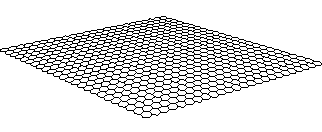
\includegraphics[width=\linewidth]{figures/torus-3d-flat.pdf}
				\caption{}
				\label{fig:torus-3d-flat}
			\end{subfigure}
			~~
			\begin{subfigure}{0.26\linewidth}
				\center
				\includegraphics[width=\linewidth]{figures/torus-3d-tube.pdf}
				\caption{}
				\label{fig:torus-3d-tube}
			\end{subfigure}
			~~
			\begin{subfigure}{0.23\linewidth}
				\center
				\includegraphics[width=\linewidth]{figures/torus-3d-torus.pdf}
				\caption{}
				\label{fig:torus-3d-torus}
			\end{subfigure}
			
			\caption{Visualisation of a hexagonal torus topology as a torus.}
			\label{fig:torus-3d}
		\end{figure}
		
		The wrap around connections in the topology are what give it the `torus'
		part of its name. Figure~\ref{fig:torus-3d-flat} shows a hexagonal torus
		topology drawn flat as in the previous figure. If the topology is rolled up
		into a tube such that the top and bottom nodes become directly adjacent, a
		tube is formed as in figure~\ref{fig:torus-3d-tube}. This tube can then be
		bent to bring together the nodes at the ends of the tube to form a torus as
		shown in figure~\ref{fig:torus-3d-torus}.
		
		A hexagonal torus topology is typically defined in terms of its width and
		height along the X and Y axes respectively. For example,
		figure~\ref{fig:hexagonalTorusTopology} shows a $10\times10$ hexagonal
		torus.  The nodes in a hexagonal torus topology are addressed using
		hexagonal coordinates of the form $(x, y, z)$ \cite{patel15}. The bottom
		left node (labelled $\alpha$ in the figure) has the coordinate $(0, 0, 0)$
		and other nodes are assigned coordinates according to the number of hops
		along each dimension from $(0, 0, 0)$, for example node $\beta$ has the
		coordinate $(2, 0, -1)$.
		
		Counter intuitively, individual nodes in hexagonal torus topologies may be
		described by many different coordinates, for example $(3, 1, 0)$ and $(1,
		-1, -2)$ are also a valid coordinates for node $\beta$. These dual
		coordinates emerge from the fact that adding $(1, 1, 1)$ to a coordinate
		produces an equivalent, but different, coordinate. This phenomenon is
		explained in detail in appendix~\ref{app:minimal-hex-coordinates} and
		related phenomena will be discussed in chapter~\ref{sec:shortestPaths}.
		
		\begin{figure}
			\center
			\begin{subfigure}[b]{0.32\linewidth}
				\center
				\buildfig{figures/torus-compare-hexagonal.tex}
				
				\caption{Hexagonal}
				\label{fig:torus-compare-hexagonal}
			\end{subfigure}
			\begin{subfigure}[b]{0.32\linewidth}
				\center
				\buildfig{figures/torus-compare-2d.tex}
				
				\caption{2D}
				\label{fig:torus-compare-2d}
			\end{subfigure}
			\begin{subfigure}[b]{0.32\linewidth}
				\center
				\buildfig{figures/torus-compare-3d.tex}
				
				\caption{3D}
				\label{fig:torus-compare-3d}
			\end{subfigure}
			
			\caption{Visual comparison of torus topologies. In all figures, `wrap
			around' connections between nodes at the ends of each axis are omitted
			for clarity.}
			\label{fig:torus-compare}
		\end{figure}
		
		Despite its unusual coordinate system, hexagonal torus topologies compare
		favourably with more conventional network topologies such as 2D and 3D
		toruses (sometimes known as 2-ary $N$-cubes and 3-ary $N$-cubes
		respectively) \cite{dally04} illustrated in figure~\ref{fig:torus-compare}.
		Compared with the 2D torus topology, a hexagonal torus has double the
		bisection bandwidth even though it only requires 50\% more node-to-node
		links \cite{navaridas09}. 3D torus topologies also have six node-to-node
		links per node but double the bisection bandwidth again. However, since a
		network topology must eventually be embedded into a real world data centre
		(which, at large scales, approximate a 2D space), 3D, or higher-dimensional
		torus topologies may become more expensive to construct in practice due to
		the need for longer cables to interconnect nodes. As
		chapter~\ref{sec:building} demonstrates, hexagonal toruses may be assembled
		in a machine room in a similar way to a 2D topology. The hexagonal torus
		topology achieves the scalability of a 2D torus while gaining some of the
		bisection bandwidth benefits of the 3D torus topology.
		
		Most torus topologies, including hexagonal 2D and 3D toruses, are related
		to an equivalent `mesh' topology. Mesh topologies maintain the same general
		connectivity structure as the corresponding torus topology with the
		exception of wrap-around links which are omitted. Omitting wrap-around
		links in practice saves a small number of links at the expense of halving
		the network's bisection bandwidth. As a consequence, mesh topologies are
		rarely used.
		
		\begin{figure}
			\center
			\begin{subfigure}[b]{0.45\linewidth}
				\center
				\buildfig{figures/hexagonal-torus.tex}
				\caption{Hexagonal torus}
				\label{fig:topo-compare-hexagonal-torus}
			\end{subfigure}
			\begin{subfigure}[b]{0.45\linewidth}
				\center
				\buildfig{figures/h-torus.tex}
				\caption{H-torus}
				\label{fig:topo-compare-h-torus}
			\end{subfigure}
			
			\caption{Hexagonal torus vs. H-torus topology. Each numbered hexagon
			represents a node. The thick outline indicates the bounds of the
			topology after which the network repeats. In each topology, the path
			taken by advancing in the Y$^+$ direction from the node labelled `0' is
			shown.}
			\label{fig:topo-compare}
		\end{figure}
		
		The hexagonal torus topology used by SpiNNaker and the subject of much of
		this thesis is not to be confused with the `H-torus' topology.  This
		topology also uses a hexagonal tiling of nodes and even wraps this tiling
		into in a torus-like topology \cite{zhao08}. However, H-torus topologies
		have very different characteristics to the hexagonal torus topology are
		closely related to `twisted torus' topologies \cite{camara10}.
		Figure~\ref{fig:topo-compare} illustrates one major difference in the way
		paths wrap around the peripheries of both topologies.
	
	\section{Scaling-up SpiNNaker machines}
		
		\begin{figure}
			\center
			\begin{subfigure}[b]{0.45\linewidth}
				\center
				\includegraphics[width=\linewidth]{figures/spinnakerBoard.jpg}
				
				\caption{A SpiNNaker board}
				\label{fig:spinnakerBoard}
			\end{subfigure}
			~~~
			\begin{subfigure}[b]{0.45\linewidth}
				\center
				\includegraphics[width=\linewidth]{figures/threeboard.jpg}
				
				\caption{Three board system}
				\label{fig:threeboard}
			\end{subfigure}
			
			\vspace*{2em}
			
			\begin{subfigure}{\linewidth}
				\center
				\buildfig{figures/sata-connections.tex}
				
				\caption{The logical connectivity between chips in multi-board systems.
				Each board's forty-eight chips (drawn here as hexagons) form a wrapped
				triple. Connections between chips on neighbouring boards are
				concentrated onto a single HSS link.}
				\label{fig:sata-connections} \end{subfigure}
			
			\caption{SpiNNaker boards}
			\label{fig:spinnaker-boards}
		\end{figure}
		
		To build large SpiNNaker systems comprising tens of thousands of
		SpiNNaker chips, groups of forty-eight chips are mounted onto printed
		circuit boards as illustrated in figure~\ref{fig:spinnakerBoard}. These
		boards may be connected together to form larger systems.
		Figure~\ref{fig:threeboard} shows a prototype three board system configured
		as a $12\times12$ hexagonal torus.
		
		Though the chips are physically arranged in a (nearly) $7\times7$ grid on
		each SpiNNaker board, they logically form a `wrapped triple', a shape
		described in detail in appendix \ref{sec:partitioning} and illustrated in
		figure~\ref{fig:sata-connections}. Logically, the chips at the periphery of
		each board connect to their neighbours on adjacent boards. Normally
		SpiNNaker chips connect using a low power, asynchronous 2-of-7 protocol
		requiring sixteen wires per bidirectional chip-to-chip link
		\cite{bainbridge03}. If this link technology were used to connect chips on
		neighbouring boards, each pair of boards would need to be connected with a
		128~wire cable. Cables and connectors supporting this may signals are
		expensive and physically large making them unsuitable for use with
		SpiNNaker. Instead, chip-to-chip connections between boards are multiplexed
		and demultiplexed onto a single High-Speed Serial (HSS) link
		\cite{athavale05} carried via commodity S-ATA cables often used to
		connected hard disks in desktop computers and servers \cite{sata3spec}.
		The six high-speed links are implemented by three onboard FPGAs (the three
		large chips at the top of the SpiNNaker board) and are logically
		transparent to the underlying network.
		
		In chapter~\ref{sec:building} I describe how very large SpiNNaker machines
		may be constructed using over one thousand SpiNNaker boards.

	\chapter{Building large SpiNNaker machines}
	
	\label{sec:building}
	
	Like any supercomputer, physically assembling a large SpiNNaker machine
	poses many practical challenges in terms of arranging, installing and
	maintaining the hundreds of metres of network cables required.  For
	conventional architectures and network topologies, techniques are well
	understood and embodied by industry standards such as TAI-942~\cite{tia2006}.
	SpiNNaker's use of the hexagonal torus topology renders existing approaches
	insufficient.
	
	In the first part of this chapter I extend existing techniques for mapping
	network topologies into standard data centre physical infrastructure to
	support the hexagonal torus topology. This mapping is designed to ensure that
	all cables are kept short (under \SI{1}{\meter}) to reduce costs and
	simplify the network hardware required. The techniques described introduce
	little overhead in cable length over existing torus wiring schemes
	and confirm the suitability of the hexagonal torus topology for real-world
	applications.
	
	The second part of this chapter uses SpiNNaker as a case study on the
	suitability of the mappings introduced in this chapter.  In this case study I
	consider various SpiNNaker systems ranging in size from desktop machines to
	multi-cabinet machine room installations. As well as validating the cabling
	schemes introduced in this chapter I also describe a new technique which
	improves the efficiency of the cable installation process.  As a consequence
	of SpiNNaker's fine-grained connectivity, the cabling is unusually dense,
	exacerbating the complexity of the cabling patterns to be installed. By
	exploiting network diagnostics hardware and on-board LEDs to guide cable
	installation, construction of large SpiNNaker machines takes a matter of
	hours rather than the days reported for other architectures. In addition,
	preliminary experiments suggest that neither the maintainability nor cooling
	performance of the system are hampered by the dense cabling employed.
	
	In this chapter, the term \emph{unit} refers to the smallest physical
	component between which network interconnection cables are installed. For
	example, in a SpiNNaker machine a unit is a 48-chip board while in a data
	centre network a unit might be a server blade.
	
	\section{Cabling non-hexagonal torus topologies}
		
		Na\"ive arrangements of torus topologies, hexagonal or otherwise, feature
		physically long `wrap-around' connections which connect units at the
		peripheries of the system. Long connections can be problematic for several
		reasons:
		
		\begin{description}
			
			\item[Performance:] Signal quality diminishes as cables get longer,
			requiring the use of slower signalling speeds, increased error
			correction overhead or more complex hardware.
			
			\item[Energy:] Some energy is lost in cables; longer cables lose more
			signal energy requiring higher drive strengths and/or buffering to
			maintain signal integrity.
			
			\item[Cost:] Shorter cables are cheaper than long ones.  Longer cables
			imply more cabling in a given space making the task of cable installation
			and system maintenance more difficult, increasing labour costs by as much
			as $5\times$~\cite{curtis12}.
			
		\end{description}
		
		In conventional torus topologies, the need for long cables is eliminated by
		folding and interleaving units of the network~\cite[chapter~5]{dally04}.
		This process is illustrated for a 1D torus topology (a ring network) in
		figure~\ref{fig:ring-folding}. A na\"ive arrangement of units in this
		topology results in a long cable connecting the units at the ends of the
		ring (figure~\ref{fig:ring-folding-row}).  To eliminate these long
		connections, half of the units are `folded' on top of the others
		(figure~\ref{fig:ring-folding-folded}) and then this arrangement of units
		is interleaved (figure~\ref{fig:ring-folding-interleaved}). This ordering
		of units requires no long cables while still observing the physical
		constraint that units must be laid out in a line.
		
		\begin{figure}
			\center
			\begin{subfigure}[b]{0.39\linewidth}
				\center
				\buildfig{figures/ring-folding-row.tex}
				\caption{A ring network}
				\label{fig:ring-folding-row}
			\end{subfigure}
			\begin{subfigure}[b]{0.24\linewidth}
				\center
				\buildfig{figures/ring-folding-folded.tex}
				\caption{Folded}
				\label{fig:ring-folding-folded}
			\end{subfigure}
			\begin{subfigure}[b]{0.35\linewidth}
				\center
				\buildfig{figures/ring-folding-interleaved.tex}
				\caption{Folded and interleaved}
				\label{fig:ring-folding-interleaved}
			\end{subfigure}
			
			\caption[Folding and interleaving a ring network.]%
			{Folding and interleaving a ring network to reduce maximum cable
			length.}
			\label{fig:ring-folding}
		\end{figure}
		
		The folding and interleaving process may be extended to $N$-dimensional
		torus topologies by folding each axis in turn. Since all axes are
		orthogonal in non-hexagonal topologies, the folding process only moves
		units along the axis being folded. Due to the non-orthogonality of the
		three axes of the hexagonal torus topology, this type of folding does not
		work. As figure~\ref{fig:failing-to-fold-hex-toruses} illustrates, folding
		along any axis results in connected units on opposing edges not being
		brought together. For example, when folding along the X axis, the two units
		marked with a green circle are moved closer together on the Y axis but
		remain apart on the X axis.
		
		\begin{figure}
			\center
			\begin{subfigure}[b]{0.24\linewidth}
				\center
				\buildfig{figures/failing-to-fold-hex-toruses-none.tex}
				\caption{Not folded}
				\label{fig:failing-to-fold-hex-toruses-none}
			\end{subfigure}
			\begin{subfigure}[b]{0.24\linewidth}
				\center
				\buildfig{figures/failing-to-fold-hex-toruses-x.tex}
				\caption{X}
				\label{fig:failing-to-fold-hex-toruses-x}
			\end{subfigure}
			\begin{subfigure}[b]{0.24\linewidth}
				\center
				\buildfig{figures/failing-to-fold-hex-toruses-y.tex}
				\caption{Y}
				\label{fig:failing-to-fold-hex-toruses-y}
			\end{subfigure}
			\begin{subfigure}[b]{0.24\linewidth}
				\center
				\buildfig{figures/failing-to-fold-hex-toruses-z.tex}
				\caption{Z}
				\label{fig:failing-to-fold-hex-toruses-z}
			\end{subfigure}
			
			\caption[Folding each axis of a hexagonal torus topology.]%
			{Schematics showing folding along each axis of a hexagonal torus topology
			failing to eliminate wrap-around connections.  Same-shaped-and-coloured
			dots show the endpoints of two example wrap-around connections.}
			\label{fig:failing-to-fold-hex-toruses}
		\end{figure}
	
	\section{Partitioning hexagonal torus topologies}
		
		The nodes in supercomputer networks are usually relatively small, for
		example a single chip. Tens of nodes are packed together into a single
		unit, such as a circuit board or server blade, to simplify assembly and
		share common power and cooling resources~\cite{gilge14,ajima12}. In
		commercial supercomputers built on non-hexagonal torus topologies, each
		unit's nodes represent a hypercube partition of the overall topology as
		illustrated in figure~\ref{fig:hypercube-partitioning}
		\cite{chen11,ajima12}.
		
		An analogous `parallelogram' partitioning scheme exists for hexagonal torus
		topologies, however, this results in imbalanced connectivity requirements
		between neighbouring partitions. In
		figure~\ref{fig:parallelogram-partitioning}, for example, the partitions
		above, below, left and right of the central partition are connected by
		seven node-to-node connections each while the partitions above-right and
		below-left are connected by just a single connection each. To simplify
		assembly, connections between all nodes in a pair of neighbouring
		partitions are often made by a single cable. If connectivity requirements
		are imbalanced, as in this example, this may mean multiple connector types
		may be required, increasing design complexity.
		
		To avoid connectivity imbalance, SpiNNaker uses a `wrapped triple'
		partitioning scheme~\cite{davidsonWiring}, as illustrated in
		figure~\ref{fig:wrapped-triple-partitioning} and explained in detail in
		appendix \ref{sec:partitioning}. In this partitioning scheme, the same
		number of connections connect all six neighbouring units. As explained in
		the appendix, a hexagonal torus topology is constructed from groups of
		three partitions.
		
		\begin{figure}
			\center
			\begin{subfigure}[b]{0.32\textwidth}
				\center
				\buildfig{figures/hypercube-partitioning.tex}
				\caption{2D hypercube}
				\label{fig:hypercube-partitioning}
			\end{subfigure}
			\begin{subfigure}[b]{0.32\textwidth}
				\center
				\buildfig{figures/parallelogram-partitioning.tex}
				\caption{Parallelogram}
				\label{fig:parallelogram-partitioning}
			\end{subfigure}
			\begin{subfigure}[b]{0.32\textwidth}
				\center
				\buildfig{figures/wrapped-triple-partitioning.tex}
				\caption{Wrapped triple}
				\label{fig:wrapped-triple-partitioning}
			\end{subfigure}
			
			\caption[Partitioning of torus topologies into units.]%
			{Partitioning of non-hexagonal (a) and hexagonal (b and c) torus
			topologies into units.}
			\label{fig:partitioning-options}
		\end{figure}
		
		For completeness, both parallelogram and wrapped triple partitioning are
		considered in this chapter even though SpiNNaker uses wrapped triple
		partitioning. The parallelogram partitioning scheme may be more appropriate
		for architectures where connections between nodes in neighbouring
		partitions do not share a single connector. In addition, in architectures
		where a unit corresponds to a single node, this can be treated as a $1
		\times 1$ parallelogram partition.  This special case occurs in
		coarse-grained architectures and Networks on Chip (NoCs) where nodes are
		not grouped together into multi-node units.
	
	\section{Folding \& interleaving hexagonal toruses}
		
		To exploit the folding technique used by non-hexagonal topologies, the
		units in a hexagonal torus topology must be mapped into a space with
		orthogonal coordinates. The choice of transformation to an orthogonal
		coordinate system can have an impact on how physically far apart logically
		neighbouring units are in the final arrangement. A good mapping should
		attempt to reduce `distortion' which moves adjacent units apart in the
		final folded and interleaved arrangement.
		
		In this section I propose two transformations which map hexagonal
		arrangements of units into a 2D orthogonal coordinate space. The first
		transformation, `shearing', is general purpose and introduces some
		distortion. The second transformation, `slicing', is less general but can
		introduce less distortion than shearing and therefore may lead to shorter
		cable lengths.
		
		Both the slicing and shearing transformations are carried out in two steps:
		
		\begin{description}
			
			\item[Rectangularisation] Units are transformed from being laid out in a
			parallelogram into a rectangular arrangement. The specific transformation
			used is the key difference between the slicing and shearing
			transformations.
			
			\item[Uncrinkling] Units are mapped into a 2D coordinate system without
			gaps between units.
			
		\end{description}
		
		\subsection{Rectangularisation}
			
			The hexagonal torus topology is illustrated in
			figures~\ref{fig:hex-to-plane-node-native} and
			\ref{fig:hex-to-plane-native} for parallelogram-partitioned units and
			wrapped triple units respectively. The first step in the folding process
			is to rearrange units so that they form a rectangle using one of two
			techniques: shearing or slicing.
			
			\begin{figure}
				\center
				\begin{subfigure}[b]{0.32\linewidth}
					\center
					\buildfig{figures/hex-to-plane-node-native.tex}
					
					\caption{Original}
					\label{fig:hex-to-plane-node-native}
				\end{subfigure}
				\begin{subfigure}[b]{0.32\linewidth}
					\center
					\buildfig{figures/hex-to-plane-node-shear.tex}
					
					\caption{Sheared}
					\label{fig:hex-to-plane-node-shear}
				\end{subfigure}
				\begin{subfigure}[b]{0.32\linewidth}
					\center
					\buildfig{figures/hex-to-plane-node-slice.tex}
					
					\caption{Sliced}
					\label{fig:hex-to-plane-node-slice}
				\end{subfigure}
				
				\caption[Rectangularisation of parallelogram partitioned toruses.]%
				{Rectangularisation of parallelogram partitioned hexagonal
				toruses. Thin lines show wrap-around links. Pointy-topped hexagons
				represent parallelogram partitioned units.}
				\label{fig:hex-to-plane-node}
				
				% XXX: Force these figures together.
				
				%\end{figure}
				%
				%\begin{figure}
				
				\center
				\begin{subfigure}[b]{0.32\linewidth}
					\center
					\buildfig{figures/hex-to-plane-native.tex}
					
					\caption{Original}
					\label{fig:hex-to-plane-native}
				\end{subfigure}
				\begin{subfigure}[b]{0.32\linewidth}
					\center
					\buildfig{figures/hex-to-plane-shear.tex}
					
					\caption{Sheared}
					\label{fig:hex-to-plane-shear}
				\end{subfigure}
				\begin{subfigure}[b]{0.32\linewidth}
					\center
					\buildfig{figures/hex-to-plane-slice.tex}
					
					\caption{Sliced}
					\label{fig:hex-to-plane-slice}
				\end{subfigure}
				
				\caption[Rectangularisation of wrapped triple partitioned toruses.]%
				{Rectangularisation of wrapped triple partitioned hexagonal
				toruses. Thin lines show wrap-around links.  Flat-topped hexagons
				represent wrapped triple partitioned units.}
				\label{fig:hex-to-plane}
				
				% And force these together!
				
				%\end{figure}
				%
				%\begin{figure}
				
				\center
				\begin{subfigure}[b]{0.3\linewidth}
					\center
					\buildfig{figures/slicing-examples-5x5.tex}
					\caption{$5\times5$}
				\end{subfigure}
				\begin{subfigure}[b]{0.3\linewidth}
					\center
					\buildfig{figures/slicing-examples-5x7.tex}
					\caption{$5\times7$}
				\end{subfigure}
				\begin{subfigure}[b]{0.3\linewidth}
					\center
					\buildfig{figures/slicing-examples-5x10.tex}
					\caption{$5\times10$}
				\end{subfigure}
				
				\caption[Patterns of wrap-around connections in sliced systems.]%
				{Schematics showing the patterns of wrap-around connections in sliced
				systems of various aspect ratios.}
				\label{fig:slicing-examples}
			\end{figure}
			
			The shearing technique applies a \SI{30}{\degree} shear transformation to
			distort the arrangement of units so that the X and Y axes of the
			hexagonal torus topology become orthogonal. This transformation leads to
			a rectangular arrangement of units as illustrated in figures
			\ref{fig:hex-to-plane-node-shear} and \ref{fig:hex-to-plane-shear}.
			
			The shear transformation introduces some distortion causing connections
			between units in the Z axis to become $\sqrt{2} \times$ longer. The
			transformation does not alter the pattern of wrap-around connections:
			long connections between units on the extreme left and right sides and
			the top and bottom remain, along with a single connection between the
			bottom left and top right units.
			
			The slice transformation aims to avoid the elongation of the Z axis by
			moving the units without distorting their layout. Units protruding from
			the left-hand-side of the parallelogram are `sliced off' and moved into
			the matching gap on the opposite side as illustrated in figures
			\ref{fig:hex-to-plane-node-slice} and \ref{fig:hex-to-plane-slice}. This
			transformation does not introduce any distortion but changes the pattern
			of wrap-around connections. Connections from left-to-right remain while
			the connections between the top and bottom units now criss-cross
			(figure~\ref{fig:slicing-examples}).  The proportion of connections going
			from bottom-left to top-right and from bottom-right to top-left varies
			depending on the aspect ratio of the topology. Only certain patterns of
			wrap-around links can be eliminated by folding and, as we shall see
			later, this limits us in which network topologies can be rectangularised
			by slicing.
			
		\subsection{Uncrinkling}
			
			Before folding can occur, the rectangularised arrangements of units
			produced in the previous step must be mapped into a 2D grid. Applied to
			parallelogram partitions, the shear transformation results in a mapping
			into a 2D grid with no further distortion
			(figure~\ref{fig:uncrinkling-node-sheared}). For other combinations of
			transformation and partitioning scheme, the units do not exactly fit a 2D
			grid. Instead, the units form `crinkled' rows or columns which may be
			`uncrinkled' (straightened out) to fit a regular 2D grid as illustrated in
			figures~\ref{fig:uncrinkling-node-sliced}~--~\ref{fig:uncrinkling-sliced}.
			
			\begin{figure}
				\center
				\begin{subfigure}[b]{0.48\linewidth}
					\center
					\buildfig{figures/uncrinkling-node-sheared.tex}
					
					\caption{Parallelogram units, sheared}
					\label{fig:uncrinkling-node-sheared}
				\end{subfigure}
				\begin{subfigure}[b]{0.48\linewidth}
					\center
					\buildfig{figures/uncrinkling-node-sliced.tex}
					
					\caption{Parallelogram units, sliced}
					\label{fig:uncrinkling-node-sliced}
				\end{subfigure}
				
				\vspace{1cm}
				
				\begin{subfigure}[b]{0.48\linewidth}
					\center
					\buildfig{figures/uncrinkling-sheared.tex}
					
					\caption{Wrapped triple units, sheared}
					\label{fig:uncrinkling-sheared}
				\end{subfigure}
				\begin{subfigure}[b]{0.48\linewidth}
					\center
					\buildfig{figures/uncrinkling-sliced.tex}
					
					\caption{Wrapped triple units, sliced}
					\label{fig:uncrinkling-sliced}
				\end{subfigure}
				
				\vspace{1em}
				
				\caption[Uncrinkling units into a 2D grid.]%
				{Uncrinkling rectangularised arrangements of units into a 2D
				grid. Thick lines show how crinkled rows and columns of units are
				uncrinkled.  Annotations show how the relative positions of units
				change after uncrinkling.}
				\label{fig:uncrinkling}
			\end{figure}
			
			%% XXX: Does this make things clearer or not?
			%In the figure, the labels show the positions of individual units before
			%and after uncrinkling. We will use these later in \S\ref{sec:distortion}
			%to calculate the overhead introduced by uncrinkling.
		
		\subsection{Folding}
			
			\begin{figure}
				\begin{subfigure}{\linewidth}
					\center
					\buildfig{figures/folding-sheared.tex}
					\caption{Sheared systems and $1:2$ sliced systems}
					\label{fig:folding-sheared}
				\end{subfigure}
				
				\vspace{1em}
				
				\begin{subfigure}{\linewidth}
					\center
					\buildfig{figures/folding-sliced.tex}
					\caption{$1:1$ sliced systems}
					\label{fig:folding-sliced}
				\end{subfigure}
				
				\caption[Elimination of long wrap-around links by folding.]%
				{Schematic illustrating elimination of long wrap-around links
				during folding. In each example a single link has been highlighted to
				aid in following the process.}
				\label{fig:folding}
			\end{figure}
			
			Once a regular 2D grid of units has been formed, this may be folded in
			the conventional way as illustrated in figure~\ref{fig:folding-sheared}.
			Folding once along each axis eliminates long connections crossing from
			left-to-right, top-to-bottom and from the bottom-left corner to the
			top-right corner. Any shear-transformed network may be folded this way
			since its wrap-around connections always follow this pattern.
			Slice-transformed networks may only be folded like this when their aspect
			ratio is $1:2$ when the pattern of wrap-around links is the same as a
			shear-transformed network.
			
			When `square' networks (i.e. those with a $1:1$ aspect ratio) are sliced,
			the network must be folded \emph{twice} along the Y axis as in
			figure~\ref{fig:folding-sliced} to eliminate the criss-crossing
			wrap-around links. It is not possible to eliminate wrap-around links from
			sliced networks with other aspect ratios by folding.
			
			After folding, the units are interleaved, yielding a 2D arrangement of
			units in which no connection spans the width or height of the system. The
			maximum connection distance is constant for any network allowing the
			topology to scale up.
		
		\subsection{Choosing a transformation}
			
			\label{sec:distortion}
			
			In each step of the transformation from hexagonal torus to a folded and
			interleaved 2D grid, the distances between connected units may increase.
			When designing a system, the transformation with the least distortion
			should be used to minimise the average length of the cables required.
			
			By referring to figure~\ref{fig:uncrinkling} (page
			\pageref{fig:uncrinkling}), it is possible to calculate the overhead
			introduced by each type of transformation.  For example, to compute the
			overhead introduced by the slicing transformation when applied to units
			composed of wrapped triples we consider
			figure~\ref{fig:uncrinkling-sliced}. The uncrinkling pattern used to
			transform this topology is a repeating pattern of two units, a pair of
			which have been labelled $1$ and $2$ respectively. Unit $1$ is
			immediately surrounded by the six units labelled $a$, $b$, $c$, $2$, $g$
			and $h$. Unit $2$ is surrounded by the units $1$, $c$, $d$, $e$, $f$ and
			$g$.  Before the transformation, the distance between units is $1$; after
			the transformation is applied this is not always the case. Folding and
			interleaving into $f_x$ columns and $f_y$ rows also introduces overhead.
			For each pair of previously neighbouring units in the example, their
			distances after folding may be computed as follows:
			
			\begin{equation*}
				\begin{aligned}[c]
					D_{1\,\leftrightarrow{}\,a} &= \sqrt{f_x^2 + f_y^2} \\
					D_{1\,\leftrightarrow{}\,b} &= f_y \\
					D_{1\,\leftrightarrow{}\,c} &= \sqrt{f_x^2 + f_y^2} \\
					D_{1\,\leftrightarrow{}\,2} &= f_x \\
					D_{1\,\leftrightarrow{}\,g} &= f_y \\
					D_{1\,\leftrightarrow{}\,h} &= f_x
				\end{aligned}
				\hspace{2cm}
				\begin{aligned}[c]
					D_{2\,\leftrightarrow{}\,1} &= f_x \\
					D_{2\,\leftrightarrow{}\,c} &= f_y \\
					D_{2\,\leftrightarrow{}\,d} &= f_x \\
					D_{2\,\leftrightarrow{}\,e} &= \sqrt{f_x^2 + f_y^2} \\
					D_{2\,\leftrightarrow{}\,f} &= f_y \\
					D_{2\,\leftrightarrow{}\,g} &= \sqrt{f_x^2 + f_y^2}
				\end{aligned}
			\end{equation*}
			
			From these values, mean and maximum connection distances may be
			calculated. The expressions for each combination of partitioning scheme
			and transformation are as follows:
			
			\begin{align*}
				D_{\textrm{mean}}=&
					\begin{cases}
						\frac{7f_x + 3\sqrt{f_x^2 + f_y^2} + \sqrt{(2f_x)^2 + f_y^2}}{9} &
							\textrm{if sheared wrapped triple units}\\
						\frac{f_x + f_y + \sqrt{f_x^2 + f_y^2}}{3} &
							\textrm{otherwise}\\
					\end{cases} \\
				D_{\textrm{max}}=&
					\begin{cases}
						\sqrt{(2f_x)^2 + f_y^2} &
							\textrm{if sheared wrapped triple units}\\
						\sqrt{f_x^2 + f_y^2} &
							\textrm{otherwise}
					\end{cases}
			\end{align*}
			
			\begin{table}
				\center
				\begin{tabular}{lcc}
					\toprule
					                                 & $1:2$  & Other \\
					\addlinespace
					\multirow{2}{*}{Parallelogram}   & \textbf{Either} & \textbf{Shear}\\
					                                 & \footnotesize $D_\textrm{mean}\approx2.28 \quad D_\textrm{max}\approx2.83$
					                                 & \footnotesize $D_\textrm{mean}\approx2.28 \quad D_\textrm{max}\approx2.83$\\
					\addlinespace
					\multirow{2}{*}{Wrapped triples} & \textbf{Slice}  & \textbf{Shear}\\
					                                 & \footnotesize $D_\textrm{mean}\approx2.28 \quad D_\textrm{max}\approx2.83$
					                                 & \footnotesize $D_\textrm{mean}\approx3.00 \quad D_\textrm{max}\approx4.47$\\
					\bottomrule
				\end{tabular}
				
				\caption{Recommended transformations for folding hexagonal toruses.}
				\label{tab:transform-recommended}
			\end{table}
			
			Using these formulae it is possible to determine which approach --
			shearing or slicing -- results in the lowest mean and maximum cable
			lengths and thus which technique should be used. This is summarised in
			table~\ref{tab:transform-recommended}.
	
	\section{A SpiNNaker case study}
		
		As the only known large-scale hexagonal torus-based architecture, SpiNNaker
		is a good case study for the techniques described in this chapter.  Each
		unit in a SpiNNaker machine is a 48-chip SpiNNaker board forming a
		wrapped triple partition. Systems of various sizes have been constructed
		using the techniques introduced in this chapter ranging from twenty-four
		board `portable' systems to a five cabinet, half-million core installation
		with plans in place to build a machine of twice this size in the future.
		
		In this section I describe how the folded and interleaved arrangement of
		units produced by the techniques in the previous chapter may be translated
		into physical arrangements of SpiNNaker boards in a machine room. I then
		describe how the thousands of S-ATA cables are installed and report on the
		maintainability and cooling impact of this cabling scheme in practice.
		
		\subsection{Mapping into physical cabinets}
			
			In SpiNNaker systems, the physical architecture used is illustrated in
			figure~\ref{fig:cabinet-units}. SpiNNaker boards are installed into card
			frames containing twenty four boards each. Five frames are mounted into
			standard, \SI{600}{\milli\meter}~wide 19\inch{} cabinets with further
			cabinets being added, arranged in a row, to scale the system up. The 2D
			grid of units produced by the folding process described in this chapter
			is mapped to cabinets and frames as illustrated in
			figure~\ref{fig:cabinetisation}.
			
			\begin{figure}
				\center
				\buildfig{figures/cabinet-units.tex}
				
				\caption{Physical architecture of a SpiNNaker machine.}
				\label{fig:cabinet-units}
			\end{figure}
			
			\begin{figure}
				\center
				\buildfig{figures/cabinetisation.tex}
				
				\caption[Mapping cabling from abstract to physical space.]%
				{Mapping from the abstract folded and interleaved 2D grid
				layout into physical cabinet and frame positions. Arrows indicate the
				order in which units (boards) are mapped into each frame, from
				left-to-right.}
				\label{fig:cabinetisation}
			\end{figure}
			
			Figure~\ref{fig:million-core-machine} shows the cabling plan for the
			largest planned SpiNNaker machine. This system will fill ten 19\inch{}
			cabinets and implement a $240 \times 240$ hexagonal torus topology
			partitioned between \num{1200} 48 chip SpiNNaker boards. The largest gap
			to be spanned by any cable is \SI{66}{\centi\meter}, well within the
			\SI{1}{\meter} limit on SpiNNaker's interconnect technology.
			
			\begin{figure}
				\center
				\buildfig{figures/million-core-machine.tex}
				
				\caption[Cabling plan for a \num{1200}~board SpiNNaker machine.]%
				{Cabling plan for a \num{1200}~board (\num{1036800}~core)
				SpiNNaker machine.}
				\label{fig:million-core-machine}
			\end{figure}
			
		\subsection{Cable selection and routing}
			
			Because of the dense packing of SpiNNaker boards, cables span short
			distances as shown in figure~\ref{fig:wire-length-histogram}.
			Conventional cable management techniques (e.g. cable trays) are not
			practical. To ensure the reliability and maintainability of SpiNNaker's
			wiring, cable slack must be carefully controlled.  If cables are too
			tight, cables, connectors and SpiNNaker boards can become damaged. When
			cables are too slack, the excess obstructs access to the machine and can
			easily become tangled \cite{cisco07}.
			
			In this case study the `rule of (three-)thumbs' proposed by
			Mazaris~\cite{mazaris97} is used which suggests that a minimum of
			\SI{5}{\centi\meter} of slack be provided. As SpiNNaker uses
			off-the-shelf S-ATA cables, only standard lengths of cable are available.
			For any given span, the shortest length of cable providing at least
			\SI{5}{\centi\meter} of slack is used.
			
			\begin{figure}
				
				\center
				\buildfig{figures/wire-length-histogram.tex}
				
				\caption[Cable lengths in a \num{1200}~board SpiNNaker machine.]%
				{Histogram of connection distances in a \num{1200} board SpiNNaker
				machine annotated with the selected cable lengths.}
				\label{fig:wire-length-histogram}
				
			\end{figure}
		
		\subsection{Installation practicality}
			
			\begin{figure}
				\center
				\begin{subfigure}[t]{0.5\textwidth}
					\begin{tikzpicture}
						\node (cables) [inner sep=0]
						      {\includegraphics[width=\textwidth]{figures/bgCables.png}};
						\node (sockets) [inner sep=0, below=1.0em of cables]
						      {\includegraphics[width=\textwidth]{figures/bgSockets.png}};
						
						% Point at label on cable
						\draw [white, <-, line width=0.4em]
						      ([shift={(0.7cm, -0.3cm)}]cables.center)
						      -- ++(45:1cm);
						
						% Point at label on socket
						\draw [white, <-, line width=0.4em]
						      ([shift={(-1.0cm, 1.1cm)}]sockets.center)
						      -- ++(-45:1cm);
					\end{tikzpicture}
					
					\caption{Pre-labelled cables and sockets}
					\label{fig:bgWiringLabels}
				\end{subfigure}
				~
				\begin{subfigure}[t]{0.30\textwidth}
					\includegraphics[height=6.15cm]{figures/bgWiring.jpg}
					
					\caption{Installation of cables}
					\label{fig:bgWiringInstallation}
				\end{subfigure}
				
				\caption[BlueGene/Q cable installation.]%
				        {BlueGene/Q cable installation~\cite{cscs13}.}
				\label{fig:bgWiring}
			\end{figure}
			
			In other large-scale architectures, the task of cable installation is
			completed by a team of technicians aided by the use of standardised
			labelling for cables and sockets as illustrated in
			figure~\ref{fig:bgWiring}~\cite{tia2006}. In these architectures the
			cabling patterns required are relatively straightforward, thanks to the
			coarseness of the units used~\cite{lakner07} or they use network
			topologies whose cabling centres around high-fan-in
			switches~\cite{cisco07,csernai15}.
			
			It has been reported in the literature that when copper cables are used,
			labour costs dominate~\cite{popa10} and while cable costs are expected to
			decline, labour costs are not~\cite{mudigonda11}. Many researchers have
			attempted to control cable installation costs by trying to reduce the
			number or length of cables required by developing alternative network
			topologies~\cite{curtis12, popa10, mudigonda11}.  Unfortunately, these
			techniques do not apply to SpiNNaker since its network topology is fixed.
			
			Supercomputer architectures such as BlueGene/Q make use of large custom
			`midplane' PCBs in place of some cables to interconnect units within a
			cabinet~\cite{milano13}. This scheme can greatly reduce wiring complexity
			since only coarser-grain, cabinet-to-cabinet connectivity is implemented
			by cables. Unfortunately this technique is expensive and constrains the
			dimensions of the network topology supported by the machine. Since the
			SpiNNaker platform is designed to scale from desktop machines to
			machine room installations, this scheme is not practical.
			
			\begin{figure}
				\center
				\begin{subfigure}[b]{0.40\textwidth}
					\begin{tikzpicture}
						\node (leds) [inner sep=0]
						      {\includegraphics[width=\textwidth]{figures/leds.jpg}};
						% Point at left LED
						\draw [white, <-, line width=0.4em]
						      ([shift={(-0.0cm, -0.6cm)}]leds.center)
						      -- ++(225:1cm);
						% Point at right LED
						\draw [white, <-, line width=0.4em]
						      ([shift={(1.1cm, -1.1cm)}]leds.center)
						      -- ++(225:1cm);
					\end{tikzpicture}
					
					\caption{Diagnostic LEDs indicate the endpoints of each cable.}
					\label{fig:interactive-wiring-guide-leds}
				\end{subfigure}
				~
				\begin{subfigure}[b]{0.546\textwidth}
					\begin{tikzpicture}[thin, black!20!white]
						\node (screen) [inner sep=0]
						      {\includegraphics[width=\textwidth]{figures/wiring_guide_screenshot.png}};
						\draw (screen.south west) rectangle (screen.north east);
					\end{tikzpicture}
					
					\caption{A GUI and text-to-speech indicate what type of cable to
					install.}
					\label{fig:interactive-wiring-guide-gui}
				\end{subfigure}
				
				\caption{Interactive software guides cable installation.}
				\label{fig:interactive-wiring-guide}
			\end{figure}
			
			Due to the high density of units in a SpiNNaker system, the detailed
			cabling patterns used can be complex, despite their overall regularity.
			To cope with this complexity, I developed a software system which employs
			diagnostic hardware built into SpiNNaker, to guide technicians through
			the cable installation process. As shown in
			figure~\ref{fig:interactive-wiring-guide}, diagnostic LEDs on each
			SpiNNaker board are used to indicate which boards to connect. The
			software also provides step-by-step cabling instructions via a Graphical
			User Interface (GUI) and audible instructions delivered via headphones.
			These instructions explicitly specify the length of cable to use for each
			connection avoiding the common problem of technicians over-estimating the
			cable length required~\cite{mazaris97}. Diagnostic registers in the
			network hardware are then used to verify the correct installation of each
			cable in real-time ensuring that mistakes are highlighted and fixed
			immediately.
			
			\begin{table}
				\center
				\begin{tabular}{lrll}
					\toprule
						Size & Cables & Time & Notes \\
					\midrule
						24 boards  & \num{72}   & \SI{10}{\minute} & \\
						1 cabinet  & \num{360}  & \SI{4}{\hour} &
							Real-time validation not used. \\
						2 cabinets & \num{720}  & \SI{2}{\hour} & \\
						5 cabinets & \num{1800} & \SI{4}{\hour} \SI{20}{\minute} &
							Three people working simultaneously. \\
					\bottomrule
				\end{tabular}
				
				\caption[Cable installation times for various SpiNNaker machines.]%
				{Cable installation times for various sizes of SpiNNaker
				machine.}
				\label{tab:install-time}
			\end{table}
			
			\begin{figure}
				\buildfig{figures/install-histogram.tex}
				
				\caption{Two cabinet SpiNNaker machine cable installation times.}
				\label{fig:install-histogram}
			\end{figure}
			
			Table~\ref{tab:install-time} shows cable installation times for various
			sizes of SpiNNaker system. The times reported do not include breaks and,
			with the exception of the five cabinet system, are for the one person
			working alone.  Figure~\ref{fig:install-histogram} shows the histogram of
			cable installation times for a two cabinet machine.  These results
			confirm the observation by Mudigonda \emph{et al.} that cables which span
			cabinets and frames take longer to install~\cite{mudigonda11}, even
			though these distances are still very short in SpiNNaker. Compared with
			commercial installation efforts, per-cable installation times are much
			shorter for SpiNNaker taking seconds compared with minutes in other
			architectures~\cite{mudigonda11}.
			
			The positive impact of real-time validation of installed cables can
			clearly be seen by comparing the installation times of the one and two
			cabinet systems. Though double the size, the two cabinet machine was
			built in half the time required to build the single cabinet machine.
			While building the smaller machine, real-time cable validation had not
			yet been implemented and the installation process was interrupted for
			several minutes every time a misplaced connection was discovered.
			
			In the three-person cable installation effort employed for the five
			cabinet system, the guidance software was configured to assign each
			technician cables in non-overlapping parts of the machine ensuring
			minimal interference between the technicians. As expected, this renders
			the problem embarrassingly parallel, as in commercial computer
			installations.
			
			\begin{figure}
				\center
				\includegraphics[width=0.8\linewidth]{figures/halfMillionCoreComplete.jpg}
				
				\caption[The five cabinet SpiNNaker system.]%
				{The five cabinet SpiNNaker system. The cabinet on the right contains
				conventional host servers which control SpiNNaker.}
				\label{fig:halfMillionCoreComplete}
			\end{figure}
			
			The completed five cabinet system is photographed in
			figure~\ref{fig:halfMillionCoreComplete}. A time-lapse video showing the
			construction and cable installation of this machine is also available on
			YouTube~\cite{heathcote16}.
			
		\subsection{Thermal implications}
			
			In large SpiNNaker machines, each 24 board frame contains a fan tray
			which pulls cool air from the front of the frame, between the SpiNNaker
			boards. The warmed air is then ejected out of the rear of the frame where
			ducting directs it into industrial air chillers. Conventional guidance on
			data centre design suggests that routing cables in the path of the
			system's airflow can have a serious impact on cooling
			performance~\cite{cisco07}.  To determine what effect the cabling
			described in this chapter had on SpiNNaker's cooling, a test program was
			executed to simulate heavy load before and after cable installation. The
			temperatures reported by the sensors on the top of each SpiNNaker board
			were sampled at regular intervals and once the overall system temperature
			stabilised, the mean temperature was recorded.
			
			Before the cabling was installed, the temperature stabilised at
			\SI{49}{\celsius} while after installation it stabilised at
			\SI{42}{\celsius}.
			
			These two data points suggest that the system's temperature is unlikely
			to have been been seriously impacted by cable installation. Since the two
			experiments were run on different days (with potentially different
			ambient temperatures) and are based on a single experiment, it is not
			possible to infer much more from this result.
			
		\subsection{Maintenance}
			
			At the time of writing, the five cabinet machine is still being
			commissioned and so the long term maintenance impact of the system's
			cabling is not known. One important factor in the maintainability of the
			system is the ease with which faulty boards can be replaced. During
			commissioning a number of boards have been replaced by someone not
			involved in the machine's installation. Informal measurements suggest
			that boards near the centre of a frame (i.e. those most likely to be
			blocked by unrelated cables) take around ten minutes to replace,
			including time spent removing and replacing cables obstructing the board
			being exchanged. By comparison boards at the edge of the machine take
			around six minutes to replace. Though similar timing reports are
			unavailable for other architectures, these times appear reasonable in
			practice and suggest maintenance is not impaired by the wiring plan used.
	
	\section{Conclusions}
		
		In this chapter I presented a practical method of constructing real-world
		installations of large hexagonal torus topologies such that long cables
		spanning the width and height of the system are not required. Two
		transformations, shearing and slicing, are presented which allow
		conventional network folding techniques to be applied to hexagonal toruses
		to eliminate long `wrap around' links. Though both techniques incur some
		overhead in terms of mean and maximum cable length, the maximum cable
		length does not grow with the size of the network. This result makes
		hexagonal torus topologies a practical and scalable choice for future
		systems.
		
		The theoretical results presented in this chapter have been confirmed
		through the successful construction of several large-scale SpiNNaker
		machines which implement hexagonal torus topologies. During construction,
		diagnostic features of SpiNNaker's hardware were employed to guide
		technicians performing cable installation. This technique was found to be
		highly effective with cable installation times measured in seconds rather
		than minutes as reported for other architectures. Surprisingly there was no
		evidence found of this technique being applied to other architectures and
		consequently this secondary result may be of interest for future research.

	\chapter{Finding shortest path vectors in SpiNNaker's network}
	
	\label{sec:shortestPaths}
	
	% XXX: Add note explaining shortest path between two points in non-torus
	% space.
	
	In the previous chapter we explored the practical challenges of building
	machines which use hexagonal torus topologies working at the scale of units
	containing several nodes. To exploit these machines, however, we must also be
	able to route packets efficiently through the nodes in the resulting network.
	This chapter tackles the problem of finding shortest path vectors in
	hexagonal torus topologies. Shortest path vectors are used by many routing
	algorithms as the basis for route generation. In non-hexagonal torus
	topologies, finding shortest path vectors is trivial and intuitive but in
	hexagonal toruses, this is not the case.  In this chapter I introduce the
	Irregular Quadrant (IQ) method, a new technique for computing shortest path
	vectors in hexagonal torus topologies.  This method is cheaper to compute and
	more general than pre-existing techniques, functioning correctly on hexagonal
	torus topologies of any aspect ratio.
	
	In some hexagonal torus topologies, many shortest path vectors may exist
	between a given pair of points. I propose a technique for discovering all
	possible shortest path vectors. Using these alternative shortest path
	vectors, routing algorithms may be able to produce routes which load a
	network more evenly.
	
	In this chapter, I assume an idealised hexagonal torus topology without
	faults or other irregularities. The challenge of handling these artefacts of
	real-world systems will be tackled in chapter~\ref{sec:routing}.
	
	\section{Shortest path vectors}
		
		Many popular routing algorithms for torus topologies, including all
		published algorithms designed for SpiNNaker~\cite{davies12,navaridas14},
		compute a shortest path vector between the endpoints of a route and use
		this to generate a path through the network. A shortest path vector between
		two nodes is a vector, $\mathbf{v} = (v_1, v_2, v_3, \ldots)$, whose
		magnitude, $\| \mathbf{v} \| = \lvert v_1 \rvert + \lvert v_2 \rvert +
		\lvert v_3 \rvert + \cdots$, is minimal with respect to all possible
		vectors between those nodes.
		
		\begin{figure}
			\center
			\buildfig{figures/mesh-topology-coordinates.tex}
			\caption[Shortest path routes in a 2D mesh network.]%
			{An example 2D mesh network with example shortest-path routes
			from `A' to `B' and `B' to `C'.}
			\label{fig:mesh-topology-coordinates}
		\end{figure}
		
		In a non-hexagonal mesh topology, shortest path vectors are computed by
		taking the element-wise difference between the source and destination
		nodes' coordinates. For example, figure~\ref{fig:mesh-topology-coordinates}
		shows a 2D mesh topology with three nodes labelled `A', `B' and `C' with
		position vectors $(1, 2)$, $(4, 5)$ and $(6, 1)$ respectively. The shortest
		path vector from node `A' to `B' is $(4, 5) - (1, 2) = (3, 3)$ and from `B'
		to `C' is $(6, 1) - (4, 5) = (2, -4)$. A route may be produced by advancing
		the number of hops specified for each dimension in the shortest path
		vector. For example, a route from `A' to `B' may be constructed from any
		permutation of the hops X$^+\,$X$^+\,$X$^+\,$Y$^+\,$Y$^+\,$Y$^+$, an
		example of which is included in the figure. Likewise routes from `B' to `C'
		may be constructed from permutations of the hops
		X$^+\,$X$^+\,$Y$^-\,$Y$^-\,$Y$^-\,$Y$^-$. Regardless of the order of the
		hops, the length of the route, $\mathbf{v}$, is given by the magnitude of
		the shortest path vector, $\|\mathbf{v}\|$.
		
		Many popular routing algorithms such as dimension order routing, right-turn
		only routing and longest dimension first routing~\cite{davies12} are simply
		defined as rules for ordering the hops specified by a shortest path vector.
		
		\subsection{Torus networks}
			
			\begin{figure}
				\center
				\begin{subfigure}{0.3\linewidth}
					\center
					\buildfig{figures/torus-shortest-path-example.tex}
					\caption{Original}
					\label{fig:torus-shortest-path-example}
				\end{subfigure}
				\begin{subfigure}{0.3\linewidth}
					\center
					\buildfig{figures/torus-shortest-path-translate.tex}
					\caption{Routed \& translated}
					\label{fig:torus-shortest-path-translate}
				\end{subfigure}
				\begin{subfigure}{0.3\linewidth}
					\center
					\buildfig{figures/torus-shortest-path-routed.tex}
					\caption{Routed original}
					\label{fig:torus-shortest-path-routed}
				\end{subfigure}
				
				\caption{Finding shortest paths in a 2D torus topology.}
				\label{fig:torus-shortest-path}
			\end{figure}
			
			Computing shortest path vectors in non-hexagonal torus topologies is also
			straightforward. For example, to find the shortest path vector from node
			`A' to `B' in the 2D torus topology shown in figure~\ref{fig:torus-shortest-path-example} both nodes are translated such that
			the source node, `A', is at the centre of the network. The shortest path
			vector is then computed in the same way as a mesh network (figure~\ref{fig:torus-shortest-path-translate}). Note that, as in this example,
			translation may cause the destination node to `wrap around' the network.
			As illustrated in figure~\ref{fig:torus-shortest-path-routed}, the
			computed shortest path vector is also valid for the two points prior to
			translation.
			
			\begin{figure}
				\center
				
				\begin{subfigure}{\linewidth}
					\center
					\buildfig{figures/distance-map-mesh.tex}
					\caption{2D mesh topology}
					\label{fig:distance-map-mesh}
				\end{subfigure}
				
				\vspace{1em}
				
				\begin{subfigure}{\linewidth}
					\center
					\buildfig{figures/distance-map-torus.tex}
					\caption{2D torus topology}
					\label{fig:distance-map-torus}
				\end{subfigure}
				
				\caption[Magnitudes of shortest path vectors in a 2D mesh.]%
				{Plots showing the magnitude of shortest path vectors in a 2D
				(non-hexagonal) topology from locations marked {\color{red}$\times$}.
				Darker areas are further away. Contour lines show equidistant points.}
				
				\label{fig:distance-map}
			\end{figure}
			
			This procedure works because vectors from the centre of a non-hexagonal
			torus topology to any other point are identical to those in a
			corresponding mesh topology. For example, in figures
			\ref{fig:distance-map-mesh} and~\ref{fig:distance-map-torus} we can see
			that the magnitude of the shortest path vectors from the centre of a mesh
			and torus grow identically. Conversely, the magnitudes of vectors from
			other locations in mesh and torus topologies do not match.
		
	\section{Related work}
		
		The problem of finding shortest path vectors in hexagonal mesh topologies
		has been widely considered and formulations may be found in a variety of
		applications, including computer games~\cite{patel15}. Hexagonal toruses,
		by contrast, have only received limited attention. In this section I
		briefly summarise the solutions proposed for hexagonal mesh topologies
		before more deeply examining existing solutions for hexagonal torus
		topologies.
		
		\subsection{Hexagonal mesh networks}
			
			\begin{figure}
				\center
				\buildfig{figures/hex-mesh-topology-coordinates.tex}
				\caption{An example hexagonal mesh network topology.}
				\label{fig:hex-mesh-topology-coordinates}
			\end{figure}
			
			In hexagonal mesh topologies it is conventional to define three `axes' X,
			Y and Z as shown in
			figure~\ref{fig:hex-mesh-topology-coordinates}~\cite{patel15}. In this
			example, the three labelled nodes `A', `B' and `C' may be given position
			vectors such as $(1, 1, 0)$, $(3, 2, 0)$ and $(0, 0, -7)$ respectively.
			As in other mesh networks, a vector between two nodes is found by
			subtracting the nodes' vectors. For example, a vector from `A' to `B' is
			$(3, 2, 0) - (1, 1, 0) = (2, 1, 0)$. This vector can then be converted
			into a route in the same way as a mesh network by taking any permutation
			of the three hops  X$^+\,$X$^+\,$Y$^+$.
			
			As explained in detail in appendix~\ref{app:minimal-hex-coordinates},
			there are a multitude of vectors between any two points in a hexagonal
			mesh. For example, the vectors $(1, 0, -1)$ and $(3, 2, 1)$ also reach
			node `B' from `A'. However, for a given pair of nodes, there is always a
			single, unique vector whose magnitude is minimal which is given by the
			function:
			%
			\begin{equation*}
				\operatorname{minimiseVector}(x,y,z) =
					(x,y,z) - \operatorname{median}(x,y,z) \cdot (1,1,1)
			\end{equation*}
			%
			For example, the vector $(3, 2, 1)$ from `A' to `B' is minimised as
			follows:
			%
			\begin{align*}
				\operatorname{minimiseVector}(3,2,1) &=
					(3,2,1) - \operatorname{median}(3,2,1) \cdot (1,1,1) \\
				&=
					(3,2,1) - (2,2,2) \\
				&=
					(1,0,-1)
			\end{align*}
			%
			A side-effect of this is that a minimised vector will always contain at
			least one zero element, meaning that shortest path routes will use at most
			two of the three available dimensions.
		
		\subsection{Hexagonal torus networks}
			
			\begin{figure}
				\center
				
				\begin{subfigure}{\linewidth}
					\center
					\buildfig{figures/distance-map-hex-mesh.tex}
					\caption{Hexagonal mesh topology}
					\label{fig:distance-map-hex-mesh}
				\end{subfigure}
				
				\vspace{1em}
				
				\begin{subfigure}{\linewidth}
					\center
					\buildfig{figures/distance-map-hex-torus.tex}
					\caption{Hexagonal torus topology}
					\label{fig:distance-map-hex-torus}
				\end{subfigure}
				
				\caption[Magnitudes of shortest path vectors in a hexagonal torus.]%
				{Plots showing the magnitude of shortest path vectors in a hexagonal
				torus topology from locations marked {\color{red}$\times$}.  Darker
				areas are further away. Contour lines show equidistant points.}
				
				\label{fig:distance-map-hex}
			\end{figure}
			
			Unfortunately, the translation technique used for non-hexagonal toruses
			cannot be used in a hexagonal torus. As illustrated in figures
			\ref{fig:distance-map-hex-mesh} and \ref{fig:distance-map-hex-torus},
			shortest path vectors from the centre, or any other part of a hexagonal
			mesh network, do not grow in magnitude in the same way that those of a
			hexagonal torus network do. I am aware of two pre-existing approaches to
			computing shortest path vectors in hexagonal toruses. These are described
			below.
			
			\subsubsection{INSEE Method}
			
				The INSEE interconnect simulator has been used in all published
				research into SpiNNaker's hexagonal torus interconnect to
				date~\cite{navaridas09,ghasempour15}. Internally INSEE finds shortest
				path vectors by selecting the shortest of a set of twelve candidate
				vectors known to always contain a shortest path vector.
				
				\begin{figure}
					\center
					\begin{subfigure}{0.45\linewidth}
						\center
						\buildfig{figures/insee-vector-candidates-no-wrap.tex}
						\caption{$(\Delta_\textrm{X}, \Delta_\textrm{Y}) = (5,3)$}
						\label{fig:insee-vector-candidates-no-wrap}
					\end{subfigure}
					\begin{subfigure}{0.45\linewidth}
						\center
						\buildfig{figures/insee-vector-candidates-wrap-x.tex}
						\caption{$(\Delta'_\textrm{X}, \Delta_\textrm{Y}) = (-3,3)$}
						\label{fig:insee-vector-candidates-wrap-x}
					\end{subfigure}
					
					\vspace{1em}
					
					\begin{subfigure}{0.45\linewidth}
						\center
						\buildfig{figures/insee-vector-candidates-wrap-y.tex}
						\caption{$(\Delta_\textrm{X}, \Delta'_\textrm{Y}) = (5,-5)$}
						\label{fig:insee-vector-candidates-wrap-y}
					\end{subfigure}
					\begin{subfigure}{0.45\linewidth}
						\center
						\buildfig{figures/insee-vector-candidates-wrap.tex}
						\caption{$(\Delta'_\textrm{X}, \Delta'_\textrm{Y}) = (-3,-5)$}
						\label{fig:insee-vector-candidates-wrap}
					\end{subfigure}
					
					\vspace{1em}
					
					% Key
					\begin{tikzpicture}[thick]
						\coordinate (last);
						
						% #1 colour
						% #2 label
						\newcommand{\colourkeyentry}[2]{
							\node [#1] [right=of last, fill, rectangle, minimum size=1em] (last) {};
							\node [right=0 of last] (last) {#2};
						}
						
						\colourkeyentry{cb3class0}{$(\textrm{X}, \textrm{Y}, 0)$}
						\colourkeyentry{cb3class1}{$(\textrm{X} - \textrm{Y}, 0, - \textrm{Y})$}
						\colourkeyentry{cb3class2}{$(0, \textrm{Y} - \textrm{X}, - \textrm{X})$}
						
					\end{tikzpicture}
					
					\caption[The twelve candidate vectors considered by the INSEE method.]%
					{The twelve candidate shortest-path vectors considered by the INSEE
					method represented as dimension-order routes. $W=H=8$,
					$(\Delta_\textrm{X},\Delta_\textrm{Y}) = (5, 3)$ and
					$(\Delta'_\textrm{X},\Delta'_\textrm{Y}) = (-3, -5)$.}
					\label{fig:insee-vector-candidates}
				\end{figure}
				
				The twelve vectors considered are illustrated in
				figure~\ref{fig:insee-vector-candidates} and are constructed as
				follows.  First a shortest path vector from the source to target node
				is constructed as if the network was a 2D mesh producing a vector
				$(\Delta_\textrm{X},\Delta_\textrm{Y})$. A second 2D vector,
				$(\Delta'_\textrm{X},\Delta'_\textrm{Y})$, is also defined:
				
				\noindent
				\begin{align*}
					\Delta'_\textrm{X} &= \Delta_\textrm{X} - \operatorname{sign}(\Delta_\textrm{X})W
					\\
					\Delta'_\textrm{Y} &= \Delta_\textrm{Y} - \operatorname{sign}(\Delta_\textrm{Y})H
				\end{align*}
				%
				Where $W$ and $H$ are the width and height of the network respectively.
				This vector describes a route from the source to destination node that
				\emph{always} wraps around the peripheries of both the `X' and `Y'
				dimensions.
				
				Two further 2D vectors, $(\Delta'_\textrm{X},\Delta_\textrm{Y})$ and
				$(\Delta_\textrm{X},\Delta'_\textrm{Y})$ may be defined which wrap around
				just the X or Y axis, respectively.
				
				Each of the four 2D vectors may be converted into three hexagonal 3D
				vectors in which one element of the vector is zero. In total this
				results in twelve different vectors which cover all combinations of
				wrapping and non-wrapping routes and all combinations of axes used. The
				vector with the smallest magnitude must be the shortest path vector.
				
				This method can find shortest path vectors in hexagonal torus
				topologies of any aspect ratio but, compared with the XYZ-protocol
				(described next), is relatively clumsy and slow to compute.
			
			\subsubsection{XYZ-Protocol}
			
				Hoffmann and D\'es\'erable described the XYZ-protocol for computing
				shortest path vectors in hexagonal toruses with equal width and
				height~\cite{hoffmann15,hoffmann11}.  First, the source and destination
				nodes are translated such that the source node lies at the centre of
				the topology. The authors observe that from the centre of the topology,
				the pattern with which distances grow differs between the four
				quadrants outlined in figure~\ref{fig:xyz-protocol-regions}.
				
				\begin{figure}
					\center
					\buildfig{figures/xyz-protocol-regions.tex}
					
					\caption{The four quadrants defined by the XYZ-protocol.}
					\label{fig:xyz-protocol-regions}
				\end{figure}
				
				If the destination lies in quadrants 1 or 4, a route may be constructed
				as if in a hexagonal mesh topology. If the destination lies in
				quadrants 2 or 3, however, the algorithm tests whether taking a
				mesh-like vector within the quadrant or wrapping-around either the X or
				Y dimensions yields the shortest vector.
				
				By comparison with the twelve vectors considered by the INSEE method,
				the XYP-protocol considers just one for destinations in quadrant 1 or 4
				and no more than three in quadrant 2 or 3. Though the XYZ-protocol can
				be computed more cheaply than the INSEE method, it does not produce
				valid shortest path vectors for hexagonal torus topologies with aspect
				ratios other than $1:1$.
		
	\section{The Irregular Quadrant (IQ) method}
		
		In this section I propose a new technique for finding shortest path vectors
		in hexagonal torus topologies called the Irregular Quadrant (IQ) method and
		compare its performance with existing techniques.
		
		\subsection{Computing shortest path vectors}
		
			Consider the problem of finding a shortest path vector from (0, 0, 0), at
			the bottom-left, to a node somewhere else in a hexagonal torus topology.
			
			\begin{figure}
				\center
				\buildfig{figures/shortest-path-regions.tex}
				
				\caption[The four irregular quadrants defined by the IQ method.]%
				{Hexagonal torus topologies of various aspect ratios divided
				into irregular quadrants in which a particular pair of dimensions is used.}
				\label{fig:shortest-path-regions}
			\end{figure}
			
			Figure~\ref{fig:shortest-path-regions} illustrates how hexagonal torus
			topologies of various aspect ratios may be partitioned into four
			\emph{irregular quadrants}. These quadrants are defined according to which
			axes are wrapped around by the shortest path vectors reaching them. The
			irregular quadrants correspond to locations reachable by shortest path
			vectors which:
			%
			\begin{enumerate}
				\item Do not wrap
				\item Wrap around X only
				\item Wrap around Y only
				\item Wrap around both X and Y
			\end{enumerate}
			%
			Within each irregular quadrant, we observe that shortest path vectors are
			constrained to using only certain directionz:
			%
			\begin{enumerate}
				\item Only X$^+$, Y$^+$ and Z$^-$.
				\item Only X$^-$ and Y$^+$
				\item Only X$^+$ and Y$^-$
				\item Only X$^-$, Y$^-$ and Z$^+$.
			\end{enumerate}
			%
			Given the topology is of width $W$ and height $H$ and the
			destination node's 2D mesh coordinates are $(\Delta_\textrm{X},
			\Delta_\textrm{Y})$ we can define the shortest path vector within each
			irregular quadrant as:
			%
			\begin{enumerate}
				\item $\operatorname{minimiseVector}(\Delta_\textrm{X},\Delta_\textrm{Y},0)$
				\item $\operatorname{minimiseVector}(-(W-\Delta_\textrm{X}),\Delta_\textrm{Y},0)$
				\item $\operatorname{minimiseVector}(\Delta_\textrm{X},-(H-\Delta_\textrm{Y}),0)$
				\item $\operatorname{minimiseVector}(-(W-\Delta_\textrm{X}),-(H-\Delta_\textrm{Y}),0)$
			\end{enumerate}
			%
			Since we know that $0 \le \Delta_\textrm{X} < W$ and $0 \le
			\Delta_\textrm{Y} < H$, we can simplify the expressions for the magnitude
			of each of the above vectors. This yields four expressions giving the
			magnitude of a minimal vector as if in each irregular quadrant:
			%
			\begin{enumerate}
				\item $\operatorname{max}(\Delta_\textrm{X}, \Delta_\textrm{Y})$
				\item $(W - \Delta_\textrm{X}) + \Delta_\textrm{Y}$
				\item $\Delta_\textrm{X} + (H - \Delta_\textrm{Y})$
				\item $\operatorname{max}(W-\Delta_\textrm{X}, H-\Delta_\textrm{Y})$
			\end{enumerate}
			%
			From these expressions we can determine which irregular quadrant the
			destination is in by finding the expression with the minimum value. With
			this information, the shortest path can be found by minimising the vector
			associated with that irregular quadrant.  Figure~\ref{fig:iqmethod.py}
			shows a simple Python implementation of the IQ method.
			
			\begin{figure}
				\inputminted{python}{figures/iqmethod.py}
				
				\caption{A Python implementation of the IQ Method.}
				\label{fig:iqmethod.py}
			\end{figure}
			
			Compared with the INSEE method, this technique requires fewer cases to be
			considered (four rather than twelve) making it cheaper to compute.
			
			Unlike the four quadrants defined by the XYZ-protocol, the irregular
			quadrants defined by the IQ method correspond exactly to a particular
			shortest path vector. This means that, once the irregular quadrant a
			point lies in has been discovered, the shortest path vector can be
			calculated directly without considering multiple options. Though the
			boundaries between the four irregular quadrants are more complex than the
			quadrants of the XYZ-protocol, it is only marginally more expensive to
			discover which irregular quadrant a point lies in. In addition, the
			irregular quadrants retain their meaning across different aspect ratios
			making the IQ method suitable for any hexagonal torus topology.
		
		\subsection{Computing distances}
		
			The four vector magnitude expressions defined by the IQ method can also
			be combined to produce a compact expression of the distance between two
			points in a hexagonal torus topology:
			%
			\begin{align*}
				\|\operatorname{shortestPathVector}(\Delta_\textrm{X}, \Delta_\textrm{Y}, W, H)\| =
				\operatorname{min}(&\operatorname{max}(\Delta_\textrm{X}, \Delta_\textrm{Y}),\\
				                   &(W - \Delta_\textrm{X}) + \Delta_\textrm{Y},\\
				                   &\Delta_\textrm{X} + (H - \Delta_\textrm{Y}),\\
				                   &\operatorname{max}(W-\Delta_\textrm{X}, H-\Delta_\textrm{Y}))
			\end{align*}
			%
			This expression has also been derived independently from a
			graph-theoretic study of Cayley graphs, of which the hexagonal torus
			topology is a special case, by Xiao and Parhami~\cite{xiao04}.
		
		\subsection{Computational efficiency}
			
			Since computing shortest path vectors forms an integral part of the
			kernel of many routing algorithms, the running time of the function
			chosen can be an important consideration.
			
			To compare the performance of the three shortest path vector functions
			presented, the execution time of a C implementation of each technique was
			measured. The C implementation of the INSEE method is taken directly from
			the INSEE source code~\cite{navaridas09}. The C implementation of the
			XYZ-Protocol is a straight translation of the published
			pseudocode~\cite{hoffmann15}.
			
			Each function was called approximately 3 billion times: once for every
			pair of source and destination nodes in a $240\times240$ node hexagonal
			torus topology. The total execution time is then divided by the number of
			calls giving an average execution time.  This experiment was repeated 50
			times and the overall average execution time of each shortest path vector
			function was recorded. The experiments were conducted on a cluster of
			idle workstations with 3.10~GHz Intel Core-i5-2400 CPUs. The function
			implementations were compiled with GCC 5.3.0 with optimisations enabled
			(\verb|-O2|).
			
			\begin{figure}
				\center
				\buildrplot{figures/shortest-path-vector-runtimes.R}
				
				\caption[Mean execution times of shortest path vector functions.]%
				{Mean execution time of each shortest path vector function. Error bars
				indicate the range of the mean execution times of the fifty
				3-billion-combination experiments.}
				\label{fig:shortest-path-vector-runtimes}
			\end{figure}
			
			Figure~\ref{fig:shortest-path-vector-runtimes} shows the execution times
			of each shortest path vector function. From these results we can see that
			the INSEE method is slower than the other techniques. Although the
			XYZ-protocol and IQ method have similar performance, because the IQ
			method works for any hexagonal torus topology it is the better candidate
			for use in new applications.
	
	\section{Generating all shortest path vectors}
			
			\begin{figure}
				\center
				\buildfig{figures/wrap-alternatives.tex}
				
				\caption{Two distinct shortest path vectors in a hexagonal torus.}
				\label{fig:wrap-alternatives}
			\end{figure}
			
			In odd-sized non-hexagonal and $1:1$ hexagonal torus topologies there is
			exactly one distinct shortest path vector between any two points (though
			many routes may be defined from it). In even-sized topologies there may
			be two distinct shortest path vectors between nodes exactly half the
			length of an axis away as in figure~\ref{fig:wrap-alternatives}. The
			INSEE and IQ methods may generate either vector depending on how ties are
			broken in their implementation.
			
			\begin{figure}
				\center
				\buildfig{figures/spiralling.tex}
				
				\caption[Distinct shortest path vectors in non-square toruses.]%
				{Distinct shortest path vectors between two points, all with
				magnitude 11.}
				\label{fig:spiralling}
			\end{figure}
			
			Unlike non-hexagonal topologies, when the aspect ratio of a hexagonal
			topology is not $1:1$, some points may have many distinct (but equal
			magnitude) shortest path vectors.  For example,
			figure~\ref{fig:spiralling} illustrates three distinct shortest path
			vectors between an example pair of nodes. None of the shortest path vector
			functions discussed will generate all possible vectors in this situation,
			potentially limiting the choices available to routing algorithms.  To
			address this shortcoming, I propose a formula which enumerates every
			shortest path vector between a pair of points in a hexagonal torus.
			
			In a $W \times H$ hexagonal torus topology, starting from any node the
			vector $(0, H, 0)$ straightforwardly wraps once around the Y axis
			arriving back at the node it started from. The vector $(1,1,1)$ also
			returns to its starting point as described in
			appendix~\ref{app:minimal-hex-coordinates}. As a consequence $(0,H,0) -
			H\cdot(1,1,1) = (-H, 0, -H)$ must also be a vector which leads back to
			where it started. Adding this vector to a shortest path vector of the
			form $(x, 0, z)$ results in a new shortest path vector if $x\ge H$ and
			$z\le0$.
			
			For example, the vector $(10, 0, -1)$ (magnitude 11) in
			figure~\ref{fig:spiralling} can be added with $(-4, 0, -4)$ yielding $(6,
			0, -5)$ (also magnitude 11) which is still a shortest path vector between
			the two labelled nodes.  Since $(6, 0, -5)$ still meets the criteria
			defined above ($6 \ge 4$ and $-5 \le 0$), we can add $(-4, 0, -4)$ again
			yielding another shortest path vector $(2, 0, -9)$.  This new vector does
			not meet the requirement that $x \ge H$ (since $2 \ngeq 4$) and so no
			further shortest path vectors can be produced.
			
			More formally, a shortest path vector $(x, 0, z)$ may be converted into
			another shortest path vector $(x', 0, z')$ using the following formula:
			%
			\begin{equation*}
				(x', 0, z') = (x, 0, z) - \left(\operatorname{trunc}\left(\frac{z}{H}\right) + n\right)(H, 0, H)
			\end{equation*}
			%
			where
			%
			\begin{equation*}
				\left\{
					n \in \mathbb{Z}
				\;\Big|\;
					0 \le n \le
						\left\lfloor
							\frac{\left|x\right| + \left|z\right|}{H}
						\right\rfloor
				\right\}
			\end{equation*}
			%
			and $\operatorname{trunc}(\,\cdots)$ is the truncation operator which
			rounds towards zero to the nearest integer.
			
			A complementary formula may be derived based on the related observation
			that the vector $(W, 0, 0)$ results in no movement:
			%
			\begin{equation*}
				(0, y', z') = (0, y, z) - \left(\operatorname{trunc}\left(\frac{z}{W}\right) + n\right)(0, W, W)
			\end{equation*}
			%
			where
			%
			\begin{equation*}
				\left\{
					n \in \mathbb{Z}
				\;\Big|\;
					0 \le n \le
						\left\lfloor
							\frac{\left|y\right| + \left|z\right|}{W}
						\right\rfloor
				\right\}
			\end{equation*}
			
			Using these two expressions for wide and tall topologies, respectively,
			all possible distinct shortest path vectors between any two points may be
			found.
	
	\section{Conclusions}
		
		The calculation of shortest path vectors in mesh and torus topologies is at
		the heart of many routing algorithms. In this chapter, I introduced a new
		technique for computing shortest path vectors in hexagonal toruses which
		generalises to any hexagonal torus topology while executing more quickly
		than existing approaches. In addition, I described a formula for
		enumerating the distinct shortest path vectors between points in hexagonal
		torus topologies. Unlike previous work, this allows routing algorithms
		greater freedom by providing a choice of shortest path vectors between some
		points.  These contributions demonstrate that key operations such as
		computing distances and shortest path vectors in hexagonal toruses can be
		efficient and exhaustive just as in non-hexagonal torus topologies.

	\chapter{Routing packets in large SpiNNaker machines}
	
	\section{Related work}
		\subsection{Multicast routing}
		\subsection{Deadlock avoidance}
		\subsection{Fault-tolerance}
	
	\section{Dimension order routing in hexagonal torus topologies}
		\subsection{Hexagonal meshes}
		\subsection{Hexagonal toruses}
		\subsection{Ensuring fairness}
		\subsection{Generating spiralling routes}
	
	\section{Fault-tolerant multicast routing}
		\subsection{Graph search based repair}
		\subsection{Alternative routing heuristics}
		\subsection{Results}
			\subsubsection{Heuristic performance}
			\subsubsection{Runtime}
			\subsubsection{Route congestion}
	

	\chapter{Placing applications in large SpiNNaker machines}
	
	\label{sec:placement}
	
	In the previous chapter I tackled the problem of fault tolerant route
	generation for SpiNNaker's network. The centroid traffic pattern was used as
	an approximation of the expected network traffic generated by `well behaved'
	neural network simulation software running on SpiNNaker. This traffic pattern
	exhibits locality, with most communication occurring between adjacent nodes.
	In reality, neural simulation applications are not conveniently specified
	geometrically but rather as abstract graphs of communicating
	neurons~\cite{davison08,eliasmith04}. Although neural models often exhibit
	localised connectivity, this can only be exploited if they are laid out
	sensibly within a network. Producing optimal placements is an NP-complete
	problem~\cite{hoefler11}.
	
	In this chapter I evaluate the effectiveness of simulated
	annealing~\cite{kirkpatrick83} for placement of SpiNNaker applications.
	Though simulated annealing fell out of favour for use in application
	placement in the 1990s, I argue that it is time to re-evaluate its
	suitability for modern placement problems. Looking to the field of chip
	design, where circuit placement problems have also been growing exponentially
	in scale for the past few decades, simulated annealing was considered ideal
	for placement problems whose sizes are comparable to that of modern
	supercomputer placement problems.
	
	In experiments on existing SpiNNaker applications I find that simulated
	annealing achieves placement solutions substantially better than contemporary
	application placement techniques. In some cases simulated annealing is shown
	to make the difference between an application functioning correctly and not
	at all. Using larger scale synthetic benchmarks I have also demonstrated that
	my proof of concept simulated annealing based placement algorithm scales up
	to placement problems containing over one million vertices while achieving
	placement quality similar to an optimal placement solution.
	
	I also build upon the work on hexagonal torus topologies earlier in this
	thesis to develop an efficient placement cost estimation function for use in
	the kernel of the annealing algorithm.
	
	\section{Related work}
		
		Attempts to address the problem of placing applications in supercomputer
		networks have utilised a variety of approaches ranging from simple greedy
		algorithms to sophisticated combinatorial optimisation
		techniques~\cite{jeannot14}. In the parallel field of digital circuit
		placement for chip and FPGA design, placement algorithms have also received
		intense study.  In this section I survey the work carried out on
		application placement before exploring chip design techniques to see what
		can be learnt from this perhaps more advanced field.
		
		In the application placement literature, the placement problem is often
		referred to by the umbrella term `mapping'. Unfortunately, `mapping' is
		often used more broadly to include other tasks such as routing and
		application partitioning. To avoid ambiguity I use the term `placement', as
		preferred by the chip and FPGA design communities, to refer specifically to
		the problem of assigning vertices in an application's communication graph
		to nodes in a machine's connectivity graph: the focus of this chapter.
		
		\subsection{Application placement algorithms}
			
			Below I consider several popular techniques employed by existing
			supercomputer applications ranging from application-specific manual
			placement to sophisticated general purpose algorithms.
			
			\subsubsection{Application-specific approaches (manual placement)}
				
				\begin{figure}
					\center
					\buildfig{figures/fem-partitioning.tex}
					
					\caption[Partitioning of a 3D volume for a $3\times4\times2$ torus.]%
					{Example partitioning of a 3D volume to fit into a supercomputer with
					a $3\times4\times2$ torus or mesh topology.}
					\label{fig:fem-partitioning}
				\end{figure}
				
				In certain applications such as finite element
				modelling~\cite{bermejo13}, a problem's structure defines a `natural'
				placement of the problem onto the target machine. For example when
				simulating a 3D volume in a supercomputer with a $3 \times 4 \times 2$
				3D torus or mesh topology network, the modelled volume might be divided
				as in figure~\ref{fig:fem-partitioning}. Each cuboid in the model is
				then assigned to the corresponding node in the network topology.
				
				Unfortunately, this technique only applies to a very narrow class of
				applications and is not applicable to many of the types of neural
				models SpiNNaker is designed to run.
			
			\subsubsection{Sequential placement}
				
				In the case where a placement solution is non-obvious, one of the
				simplest and most popular strategies is to apply a simple sequential
				placement algorithm. Sequential placement greedily places the vertices
				of an application's communication graph onto nodes. By carefully
				selecting the order in which vertices are picked and nodes assigned in
				the target architecture, this algorithm can produce reasonable quality
				placements.
				
				\begin{figure}
					\center
					\begin{subfigure}{0.32\linewidth}
						\center
						\buildfig{figures/sequential-row-order.tex}
						\caption{Row-order}
						\label{fig:sequential-row-order}
					\end{subfigure}
					\begin{subfigure}{0.32\linewidth}
						\center
						\buildfig{figures/sequential-alternating.tex}
						\caption{Alternating}
						\label{fig:sequential-alternating}
					\end{subfigure}
					\begin{subfigure}{0.32\linewidth}
						\center
						\buildfig{figures/sequential-hilbert.tex}
						\caption{Hilbert curve}
						\label{fig:sequential-hilbert}
					\end{subfigure}
					
					\caption{Space-filling curves in 2D mesh and torus topologies.}
					\label{fig:sequential}
				\end{figure}
				
				Supercomputer management software such as SLURM~\cite{yoo03} and Blue
				Gene's system software~\cite{gilge14} by default na\"ively iterate over
				vertices in an application communication graph in the order in which
				they are defined by the application. The nodes in the target machine
				are iterated over using a simple space-filling curve.
				Figure~\ref{fig:sequential} illustrates three popular space filling
				curves.
				
				The row-order (figure~\ref{fig:sequential-row-order}) and alternating
				(figure~\ref{fig:sequential-alternating}) curves illustrate 2D versions
				of the default node assignment orders provided by the SLURM and
				BlueGene systems.  The Cray extensions to SLURM software provide a
				Hilbert curve~\cite{hilbert91} node assignment order
				(figure~\ref{fig:sequential-hilbert}). The Hilbert curve specifically
				attempts to maintain the property that points that are close together
				along the length of the curve are also close together in the 2D
				mapping~\cite{moon01, zumbusch99}. Since the vertex iteration order is
				also chosen such that connected vertices tend to be closer together,
				this property may lead to improved placement solutions.
				
				\begin{figure}
					\center
					\buildrplot{figures/space_filling_curves_comparison.R}
					
					\caption[Relationship between space filling curve offset and 2D distance.]%
					{Relationship between distance along a space filling curve
					and between the 2D positions assigned. Results shown for
					Manhattan distances in a $32\times32$ 2D mesh.}
					\label{fig:space_filling_curves_comparison}
				\end{figure}
				
				Figure~\ref{fig:space_filling_curves_comparison} illustrates how the
				distance between locations along each space filling curve map to
				distances in the resulting 2D space. Both the row-order and alternating
				orderings result in distances oscillating between being closer and
				spread out in 2D space, just as the space filling curves oscillate from
				side-to-side. For the Hilbert curve, however, distances grow more
				monotonically\footnote{The growth in distance for Hilbert curves may
				appear slightly irregular but in fact forms a fractal as a consequence
				of the fractal construction of the Hilbert curve itself.} and at
				smaller 1D distances, 2D distances are often lower than in other space
				filling curves.
				
				A number of algorithms have been proposed for automatically selecting
				good vertex and chip iteration orders, typically using a
				graph-traversal based heuristic. An example typical of this type of
				technique is `graph similarity based mapping' described by Hoefler and
				Snir~\cite{hoefler11}. This algorithm exploits the Reverse
				Cuthill-McKee (RCM) algorithm~\cite{cuthill69} to select a linear
				ordering of vertices in which connected vertices tend to appear close
				together. Internally, the RCM algorithm uses a breadth-first-search-like
				algorithm to order vertices.
				
				The RCM algorithm was originally designed as a tool for reducing the
				`bandwidth' of matrices to improve the performance of linear algebra
				techniques. A matrix's bandwidth is the width of the strip of non-zero
				elements on its diagonal. Figure~\ref{fig:rcm} illustrates how a sparse
				matrix is permuted by the RCM algorithm to produce a matrix with lower
				bandwidth. This technique may be applied to a graph by representing the
				graph as an adjacency matrix, $M$, where $M_{i,j}$ is $w$ if node $i$
				is connected by an edge to node $j$ with weight $w$ and 0 otherwise.
				When a graph's adjacency matrix is permuted by the RCM algorithm, the
				connectivity of the graph remains unchanged but the vertex ordering
				changes. The ordering of vertices in a low-bandwidth adjacency matrix
				tends to keep connected vertices closer together in the ordering, making
				the ordering well suited for use with a sequential placement algorithm.
				
				\begin{figure}
					\center
					\begin{subfigure}{0.45\linewidth}
						\center
						\buildfig{figures/rcm-initial.tex}
						
						\caption{Original permutation}
						\label{fig:rcm-initial}
					\end{subfigure}
					\begin{subfigure}{0.45\linewidth}
						\center
						\buildfig{figures/rcm-sorted.tex}
						
						\caption{RCM permutation}
						\label{fig:rcm-sorted}
					\end{subfigure}
					
					\caption[Graph adjacency matrix before and after RCM permutation.]%
					{Adjacency matrix representation of a graph before and after
					permutation by the RCM algorithm.}
					\label{fig:rcm}
				\end{figure}
				
				In small-scale and densely connected applications such as early neural
				simulations running on prototype SpiNNaker machines~\cite{galluppi10},
				these techniques have proven sufficient.  As my experiments demonstrate
				later, however, sequential placement is insufficient for some SpiNNaker
				applications.
				
			\subsubsection{Simulated annealing}
				
				\label{sec:application-placement-summary}
				
				In the academic community, a number of attempts have been made to use
				sophisticated optimisation algorithms for the placement of
				applications. In 1985, Steele~\cite{steele85} first proposed the use of
				simulated annealing for placing applications in the 6D torus topology
				of the 64 node `Caltech Cosmic Cube'. The proposed algorithm is
				described below.
				
				Initially, the vertices in the application's communication graph are
				assigned randomly to nodes in the machine. Two vertices are then chosen
				at random and swapped.  If this swap reduces the `cost' of the
				placement (as defined later), the vertices are kept in their new
				locations. If the cost increases as a result of the swap, the vertices
				are moved back to their original locations with a probability dependent
				on the magnitude of the cost increase and the current `temperature'.
				
				The process of picking and swapping vertices is repeated many times
				while the temperature is gradually reduced. Initially the temperature
				is set to a large value causing most swaps to be accepted, regardless
				of their cost. As the algorithm proceeds, the temperature is reduced
				until only swaps resulting in cost reductions are accepted. By
				initially accepting detrimental swaps, the algorithm typically avoids
				becoming trapped in local minima. Towards the end of the algorithm's
				execution the solution is presumed to be close to the global
				minimum-cost solution and so few or no detrimental swaps are accepted.
				
				The cost of a particular placement is defined by some expression
				approximating the quality of the placement with better quality
				placements having lower costs. In Steele's work, the cost of a
				placement is computed by finding the shortest path routes between all
				connected vertices using Dijkstra's algorithm. Rather than repeating
				this relatively expensive computation after each swap, Steele's
				implementation updated the previously calculated cost by recomputing
				only the routes connecting the swapped vertices.
				
				The number of swaps to attempt and the rate at which the temperature is
				changed is dictated by an `annealing schedule' and can have a major
				impact on the execution time of the algorithm and the quality of the
				placement solution. I describe one such schedule in detail later in
				this chapter when describing my own simulated annealing based
				application placement algorithm.
				
				Towards the end of the 1980s, application placement appeared to be
				becoming less important as supercomputer network architectures
				improved, appearing to render computationally intensive placement
				algorithms unnecessary~\cite{dally87}.  In addition, network and
				problem sizes remained small: so small in fact that exact
				linear-programming based placement algorithms remained a meaningful
				point of comparison in application placement research~\cite{xu91}. In
				this environment, simpler sequential placement algorithms gained favour
				over more computationally expensive algorithms such as simulated
				annealing.
				
				In contemporary application placement algorithms, `low temperature'
				simulated annealing algorithms are occasionally employed as a
				post-processing step for other placement algorithms~\cite{hoefler11}.
				Other heuristics are used to generate an initial placement solution.
				
				% Outside of badly attempting 90s scale problems at least... \cite{chen06}
			
			\subsubsection{Recursive partitioning}
				
				As problem and machine sizes have grown and network utilisation has
				once again become an important factor in application
				performance~\cite{navaridas09b}, more complex optimisation algorithms
				have reappeared in the literature. One popular approach employs graph
				partitioning algorithms such as METIS~\cite{karypis98} to perform
				recursive bipartitioning based
				placement~\cite{phillips14,hoefler11,pellegrini96}.  This placement
				process is illustrated in figure~\ref{fig:partitioning}.
				
				\begin{figure}
					\center
					\buildfig{figures/partitioning.tex}
					
					\caption[Application placement by recursive partitioning.]%
					{Illustration of application placement by recursive
					partitioning. Each node has the capacity to hold two vertices.}
					\label{fig:partitioning}
				\end{figure}
				
				In the first step, the application communication graph and machine
				connectivity graph are each bipartitioned such that the number of edges
				cut by the partitions is minimised while the size of each partition
				remains similar. Each half of the communication graph is associated
				with one of the halves of the machine connectivity graph.  The
				partitioning process is then repeated recursively, further partitioning
				the application and machine graphs. The process halts when either graph
				can no longer be partitioned.  The vertices in the communication graph
				are then placed on their associated node in the connectivity graph.
				
				Unfortunately, recursive partitioning-based techniques are known to
				perform sub-optimally when the number of nodes is not a power of
				two~\cite{simon97}. In addition, placement problems are often subject
				to multiple orthogonal constraints. For example, a vertex in an
				application's communication graph may consume a certain number of
				processors and some quantity of SDRAM. Partitioning algorithms require
				a metric with which the size of each partition may be measured to
				ensure that the two halves are balanced. When multiple orthogonal
				resources exist, a single metric is insufficient to express this
				requirement. As a result, partitioning algorithms are of limited use in
				applications whose placement is subject to several orthogonal
				requirements, such as neural modelling software on SpiNNaker.
				
			\subsubsection{Topology-specific approaches}
				
				Other approaches employ other optimisation techniques that are
				specialised for use with applications and networks with specific
				connectivity patterns, for example, trees~\cite{jeannot14,traff02}.
				Unfortunately, these algorithms cater neither for SpiNNaker's hexagonal
				torus topology nor the range of communication topologies found in its
				target applications.
	
		\subsection{Circuit placement algorithms}
			
			The circuit placement problem in chip and FPGA design is similar to that
			of application placement: communicating components must be assigned
			positions in a chip so that wiring congestion is controlled.
			
			\begin{figure}
				\center
				\buildrplot{figures/top500-num-processors.R}
				
				\caption[Historical core counts for the `Top500' supercomputers.]%
				{Historical processor (core) counts for the `Top500' supercomputer
				installations. The line shows the mean number of processsors and grey
				ribbon indicates the range. Data reported by the `Top500
				List'~\cite{meuer16j}.}
				\label{fig:top500-num-processors}
			\end{figure}
			
			Following the march of Moore's `Law'~\cite{moore75}, the number of
			components in modern chips and FPGAs has been increasing at an
			exponential rate similar to that of core counts of supercomputers (see
			figure \ref{fig:top500-num-processors}). Today, in 2016, the largest
			chips contain billions of transistors, compared with millions of
			processors found in supercomputers. In terms of the raw number of
			processors, the world's largest supercomputers are at a scale comparable
			with the number of components in chips designed fifteen years ago. The
			mean size of today's `Top 500' supercomputers is somewhat smaller still,
			similar in scale to chips designed over 20 years ago.
			
			In view of of the similarity of the chip and application placement
			problems and the relative lead the field of chip placement has in terms
			of placement size, it appears reasonable to look to chip placement to
			suggest future application placement techniques.
			
			The popular approaches to circuit placement can be grouped into three
			broad categories~\cite{kahng11}:
			
			\begin{description}
				
				\item[Partitioning-based] As in application placement, these algorithms
				function by recursively partitioning the circuit to assign
				related components to areas of a chip.
				
				\item[Analytical] These algorithms approximate the placement problem as
				a simpler problem to which exact solutions can be computed
				inexpensively.
				
				\item[Simulated annealing] As in application placement, simulated
				annealing algorithms selectively apply random permutations to a
				placement causing placement quality to improve.
				
			\end{description}
			
			I briefly introduce each technique before assessing its suitability for
			use in application placement in SpiNNaker. The interested reader is
			encouraged to refer to `VLSI physical design: from graph partitioning to
			timing closure' by Kahng \emph{et al.}~\cite{kahng11} for a more thorough
			introduction to the field of circuit placement and the techniques that I
			summarise here.
			
			\subsubsection{Partitioning-based placement}
				
				Partitioning based placement has a long history with early examples
				dating back to the 1970s~\cite{breuer77}. As in recursive partitioning
				based application placement algorithms, the input circuit is
				partitioned alongside the target topology to assign placements. Again,
				graph partitioning software such as METIS~\cite{karypis98} is used to
				partition the circuits but since the target topology is the 2D surface
				of a chip, simple geometric partitioning is used to divide the surface
				of the chip. More recent partitioning based placers such as
				Capo~\cite{roy05} employ additional heuristics such as `terminal
				propagation' where connections between adjacent partitions are
				considered to attempt to align components on either side of a cut.
				
				Unfortunately, as with its use in application placement, these
				partitioning techniques are not ideal.  Consequently, partitioning
				based placement techniques have largely been superseded in chip
				design~\cite{markov15}.
			
			\subsubsection{Analytical placement}
				
				The current generation of placement algorithms attempt to approximate
				placement problems as simpler problems with cheaply computed,
				closed-form solutions. One of the common approximations used by these
				approaches is modelling the components to be placed as point-like
				objects. As the number of components in digital circuits has grown,
				this approximation has also improved, resulting in analytical placement
				becoming the most popular approach in use today~\cite{markov15}.
				
				One popular analytical technique is `quadratic
				placement'~\cite{kahng11,spindler08}. In this algorithm the components
				in a circuit are approximated as infinitesimal objects with wires
				between them modelled as spring-like forces. Unlike physical springs,
				which obey Hooke's law, the force exerted by a connection is
				proportional to the \emph{square} of the distance between its
				terminals.
				
				To illustrate this approach, consider the simple one-dimensional
				placement problem presented in figure~\ref{fig:quadratic-placement}.
				In the quadratic placement technique, the cost of a placement is
				modelled as the weighted sum of the squares of the distances between
				connected components. In this case this yields the expression:
				%
				\begin{equation*}
					%
					\textrm{Cost} = 1(f_1 - m_1)^2 + 2(m_1 - m_2)^2 + 1(m_2 - f_2)^2
					%
				\end{equation*}
				%
				Where $f_1$, $f_2$, $m_1$ and $m_2$ represent the positions of the four
				components. An optimal placement is one which minimises this function.
				To find values which minimise a quadratic, the equation is
				differentiated yielding a system of linear equations. This system of
				equations is then solved to find the positions of the movable vertices
				which minimise the quadratic cost function.
				
				\begin{figure}
					\center
					\buildfig{figures/quadratic-placement.tex}
					
					\caption[An optimal 1D quadratic placement solution.]%
					{An optimal 1D quadratic placement solution for two fixed
					vertices ($f_1$ and $f_2$), two movable vertices ($m_1$ and $m_2$)
					and three weighted edges.}
					\label{fig:quadratic-placement}
				\end{figure}
				
				Quadratic placement is extended to two or more dimensions by simply
				applying the process for each dimension separately. Unfortunately, a
				straightforward extension to non-Euclidean geometries such as
				hexagonal toruses is non-trivial. For example, quadratic placement
				relies on cost increasing monotonically as two points are moved in
				opposite directions, a property which does not apply to torus
				topologies. This same problem also applies to the approximations used
				by other analytical techniques.
				
				An additional challenge posed by quadratic placement is that some
				vertices' locations must be fixed to provide a `spreading' force
				preventing degenerate solutions where all vertices are given the same
				coordinates. In circuit placement, the locations of `pads' used to
				connect components in a circuit to the outside world are typically
				fixed and provide convenient anchors during placement. Algorithms such
				as SimPL~\cite{kim12b} employ a combination of analytical techniques to
				add virtual `anchor' components which prevent degenerate solutions from
				forming. Unfortunately, this approach further adds to the difficulty of
				porting the technique to non-Euclidean geometries. These techniques
				also work better for larger circuit sizes, making analytical techniques
				non-ideal for today's relatively small (by chip placement standards)
				supercomputer placement problems.
				
				% TODO: mention viswanathan07 FastPlace 3.0 -- multilevel technique?
			
			\subsubsection{Simulated annealing}
				
				Simulated annealing was originally developed specifically to be applied
				to the problem of circuit placement~\cite{kirkpatrick83}. Throughout
				the late 1980s and early 1990s, simulated annealing was the dominant
				circuit placement technique when the first chips breaching one million
				components appeared~\cite{betz97,sechen85}. Due to the increased
				effectiveness of quadratic placement as problems grew beyond tens of
				millions of nodes, simulated annealing has fallen out of fashion as a
				circuit placement technique. Despite this, various efforts continue to
				be made to enhance the simulated annealing process' performance by
				attempting to partition the input problem into several independent
				problems~\cite{choong10,haldar00} and parallelise the
				algorithm~\cite{ludwin08}.
				
				Simulated annealing notably remains popular as a stand-alone placement
				tool in niche applications where flexibility is important. For example,
				the flexible, multi-FPGA, Verilog-To-Routing (VTR) software
				suite~\cite{luu14} and Open Source Arachne-PNR~\cite{cseed} use
				simulated annealing to produce placements within multiple FPGA
				architectures.
				
				Since application placement problems are only now beginning to reach
				the scales at which simulated annealing became popular in circuit
				design, it is likely to be a good choice for application placement over
				the next few years. In addition, simulated annealing's flexibility
				potentially makes it a good choice to handle the wide variety of
				architectures in use by modern supercomputers.
	
	\section{Placement by simulated annealing}
		
		\label{sec:placement-by-annealing}	
		
		As we have seen, existing software placement techniques are not well suited
		to the large-scale applications projected for the SpiNNaker architecture.
		In the field of circuit placement, various algorithms have been proposed
		which are explicitly designed to cope with placement problems of similar or
		larger sizes. While analytical placement algorithms can produce high
		quality placement solutions for extremely large problems, the current --
		and near future -- generations of application placement problems are still
		too small. Simulated annealing, however, has a proven record in circuit
		design at the scale of modern application placement problems. In addition,
		the flexibility of simulated annealing makes it easy to adapt to new
		network architectures and, in this case, SpiNNaker's hexagonal torus
		topology.
		
		To demonstrate the suitability of simulated annealing for modern
		applications, I have implemented a simple simulated annealing based placer
		for the SpiNNaker architecture. Compared with previous simulated annealing
		algorithms for application placement, this algorithm is intended to cope
		with much larger problem instances and draws inspiration from the
		techniques used by circuit placement algorithms.
		
		In contrast with circuit placement algorithms built on simulated annealing,
		my implementation represents the problem differently to handle the nuances
		of application placement. In circuit placement, for example, exactly one
		component may be placed in a given space while in application placement,
		several applications may be placed on the same node (e.g. on different
		cores, or as separate processes). These differences, along with details of
		the cost functions and annealing schedule used are described in the
		remainder of this section.
		
		\subsection{Representation}
			
			A typical SpiNNaker application is made up of a number of processes which
			are executed by individual processor cores, consuming some quantity of
			on-chip resources such as shared SDRAM. These processes communicate via
			multicast packets which are sent via SpiNNaker's network.
			
			In the proposed placement algorithm, an application is defined as a graph
			where the `vertices' represent the processes as defined above and the
			multiedges, referred to here as `nets', represent directed flows of
			multicast packets from one vertex to several others. Each vertex consumes
			some quantity of on-chip resources (typically one core and a number of
			bytes of on-chip RAM). The placement algorithm must assign each vertex to
			a specific SpiNNaker chip (i.e. a node in SpiNNaker's network) such that
			the resources available on that chip are not exhausted.
			
			% TODO: Include remark like the following?
			% Unfortunately, since multiple resource types must be considered, that
			% application placement additionally encompasses a bin packing problem
			% \cite{korte06}.
			
			An additional soft constraint is imposed: the placement algorithm should
			attempt to place connected vertices as close together as possible. Nets
			may be annotated with a `weight' which provides a hint to the placer
			indicating the relative importance of a particular net. A larger weight
			indicates the placer should try harder to keep the vertices it connects
			closer together. Because this constraint is soft, the placer should make
			a `best effort' attempt to obey the constraint but is not obliged to
			achieve a perfect placement solution.
			
			The SpiNNaker topology is represented as a 2D hexagonal torus topology
			with homogeneous inter-chip links. Each chip is defined to have a certain
			quantity of each resource consumed by vertices. For example, SpiNNaker
			chips nominally contain 17 application processors and 128~MB of on-chip
			SDRAM. Some chips, however, may have fewer working cores while others may
			be non-functional, thus effectively having no resources.
			
			\subsubsection{Additional constraints}
				
				Real-world applications may also apply some additional constraints on
				placement solutions. Two such constraints are considered here.
				
				Some applications require that certain vertices are always placed on a
				specific chip, for example to enable communication with an external
				device attached directly to a SpiNNaker chip. The placement algorithm
				must obey this requirement, treating constrained vertices as a
				special case.
				
				In other applications, in-memory communication may be required between
				certain vertices and therefore these vertices must always be placed on
				the same chip. This constraint may be implemented by preprocessing the
				application graph such that constrained vertices are merged into a
				single vertex whose resource requirements are the sum of the original
				vertices.
		
		\subsection{Algorithm description}
			
			As outlined earlier, simulated annealing swaps pairs of vertices keeping
			beneficial swaps as well as some proportion of detrimental swaps. In the
			remainder of this section I describe the exact processes by which
			vertices are selected and swapped. I also consider the choice of cost
			function for use with a hexagonal torus topology before specifying the
			annealing schedule used.
		
			\subsubsection{Generating candidate swaps}
				
				Simulated annealing based placement schemes move vertices by swapping
				random pairs of vertices. In application placement problems, where
				vertices may differ in resource requirements, it is not always possible
				to swap arbitrary pairs of vertices. For example, if a `larger' vertex
				is swapped with a `smaller' one it may not fit in the space left behind
				by the smaller vertex.
				
				Rather than blindly picking pairs of vertices to swap and abandoning
				those which don't fit, the process described in
				figure~\ref{fig:sa-swap} is used. This swapping process reduces the
				likelihood that swaps involving larger vertices are aborted when the
				vertices on the target chip are individually too small to free up
				enough room to complete a swap.
				
				\begin{figure}
					\center
					\begin{subfigure}{\linewidth}
						\center
						\buildfig{figures/sa-swap-select.tex}
						\caption{A random vertex, $v_a$ is selected along with a random
						target chip (right).}
						\label{fig:sa-swap-select}
					\end{subfigure}
					
					\vspace*{1em}
					
					\begin{subfigure}{\linewidth}
						\center
						\buildfig{figures/sa-swap-remove.tex}
						\caption{Vertex $v_a$ is removed from its chip. Vertices are removed
						from the target chip until enough space is available to fit $v_a$.
						In this example, vertices $v_b$ and $v_c$ are removed.}
						\label{fig:sa-swap-remove}
					\end{subfigure}
					
					\vspace*{1em}
					
					\begin{subfigure}{\linewidth}
						\center
						\buildfig{figures/sa-swap-commit.tex}
						\caption{Vertex $v_a$ is swapped with vertices $v_b$ and $v_c$ if
						there is room. If there is not enough room the vertices are
						returned to their original locations and the swap is aborted.}
						\label{fig:sa-swap-commit}
					\end{subfigure}
					
					\caption{Selecting vertices to swap.}
					\label{fig:sa-swap}
				\end{figure}
			
			\subsubsection{Cost function}
				
				For each swap made by the algorithm, the change in the placement's
				`cost' must also be determined. In principle, the ideal cost function
				should accurately predict network congestion by performing routing and
				modelling the resulting network traffic. This approach was used by
				early application placement algorithms~\cite{steele85} but incurs a
				large performance overhead. Since the simulated annealing algorithm
				must re-evaluate the cost function before and after every swap, a cost
				function which is slow to evaluate can result in unacceptable execution
				time for the algorithm as a whole.
				
				A common alternative to measuring congestion directly used by many
				circuit placement algorithms is to approximate the network resources
				consumed. In the case of multicast nets, rather than computing
				efficient multicast routes, an estimate is made based on the relative
				locations of the vertices. Two popular techniques are described below
				\cite[\S4.2]{kahng11}.
				
				In the star model, the cost of a net is found by summing the distances
				from the net's source vertex to each sink vertex in turn as illustrated
				in figure~\ref{fig:cost-function-star}. In a hexagonal mesh and torus
				topology, the distance between two points can be cheaply determined (as
				described in chapter~\ref{sec:shortestPaths}) making this cost function
				inexpensive to compute. This model will overestimate network resource
				usage for nets with more than two vertices since, in practice,
				multicast routing algorithms will tend to generate routes which share
				some hops.
				
				In the Half-Perimeter Wire Length (HPWL) model, a bounding box is drawn
				around all of the vertices connected by the net and the cost of the net
				is estimated as half of the perimeter of this bounding box. In a
				non-hexagonal torus or mesh topology, the HPWL model exactly matches
				the length of an optimal multicast route for nets with two or three
				vertices. In nets with a greater number of vertices, HPWL
				underestimates the length of an optimal route by a factor of $\sqrt{n}$
				for nets with $n$ vertices~\cite{chung79}.
				
				The three non-orthogonal axes of hexagonal mesh and torus networks mean
				that there are several ways in which a bounding box may be defined.
				Specifically, the bounding box may extend along any pair of axes
				resulting in three possible bounding boxes and, thus, three HPWL values
				for any net as illustrated in figures~\ref{fig:cost-function-hpwl-xy},
				\ref{fig:cost-function-hpwl-xz} and~\ref{fig:cost-function-hpwl-yz}.
				The relative sizes of these three bounding boxes varies depending on
				the specific arrangement of vertices in the net, meaning that no single
				bounding box is appropriate for all situations.
				
				A single HPWL-like metric for hexagonal toruses can be produced by
				taking the minimum of the half-perimeters of the three different
				bounding boxes defined for a hexagonal toruses. Like the HPWL function
				for non-hexagonal toruses, this `hexagonal HPWL' cost function exactly
				predicts the length of optimal routes for all nets with two or three
				vertices.
				
				\begin{figure}
					\center
					\begin{subfigure}[b]{\linewidth}
						\center
						\buildfig{figures/cost-function-star.tex}
						
						\caption{Star $= a_x + a_y + b_x + b_z + c_x + c_y + d_x + d_y$}
						\label{fig:cost-function-star}
					\end{subfigure}
					
					\vspace*{1.5em}
					
					\begin{subfigure}[b]{0.32\linewidth}
						\center
						\buildfig{figures/cost-function-hpwl-xy.tex}
						
						\caption{HPWL$_{xy}$ $= w_{xy} + h_{xy}$}
						\label{fig:cost-function-hpwl-xy}
					\end{subfigure}
					\begin{subfigure}[b]{0.32\linewidth}
						\center
						\buildfig{figures/cost-function-hpwl-xz.tex}
						
						\caption{HPWL$_{xz}$ $= w_{xz} + h_{xz}$}
						\label{fig:cost-function-hpwl-xz}
					\end{subfigure}
					\begin{subfigure}[b]{0.32\linewidth}
						\center
						\buildfig{figures/cost-function-hpwl-yz.tex}
						
						\caption{HPWL$_{yz}$ $= w_{yz} + h_{yz}$}
						\label{fig:cost-function-hpwl-yz}
					\end{subfigure}
					
					\caption[Net cost estimation functions for hexagonal toruses.]%
					{Net cost estimation functions for hexagonal toruses and meshes.}
					\label{fig:cost-function}
				\end{figure}
				
				An experiment was performed to determine which cost function provides
				the most accurate results. \num{50000} nets connecting between two and
				thirty uniform randomly selected vertices in a $30\times30$ hexagonal
				torus topology were generated. The difference between each cost
				function and the `true' cost of a route generated by the NER routing
				algorithm is plotted in figure~\ref{fig:cost-function-error}.
				
				\begin{figure}
					\center
					\buildrplot{figures/cost-function-error.R}
					
					\caption[Estimation error of various cost functions.]%
					{Estimation error of various cost functions compared with
					routing solutions. Positive and negative errors are equally bad.
					Y-axis limit clipped for clarity. The error of the star cost function
					grows linearly with fan out beyond the axis limit.}
					\label{fig:cost-function-error}
				\end{figure}
				
				These plots confirm that the error introduced is consistently
				overestimated by the star model and underestimated by both the
				hexagonal HPWL and HPWL${_{xy}}$ cost models. The error in cost
				estimates produced by the star model grew more quickly than both HPWL
				variants, Both hexagonal HPWL and HPWL$_{xy}$ perform similarly though,
				as expected, hexagonal HPWL is more accurate for low fan out nets.
				
				To attempt to compensate for the theoretical $\sqrt{n}$ error in the
				HPWL cost, the Hexagonal HPWL and HPWL$_{xy}$ scaled by $\sqrt{n}$ are
				also shown. While this correction does not eliminate the error of these
				functions, it does reduce it. This is probably because the error only
				tends towards $\sqrt{n}$ for very large $n$ \cite{chung79} and also
				because the error is being computed against a realistic, non-optimal
				routing algorithm.
				
				On the basis of these results, the star cost function is rejected on
				the grounds that it produces the least accurate cost estimates. Though
				the $\sqrt{n}$-scaled hexagonal HPWL cost function produces the
				smallest error in general, its execution time is three times greater
				than $\sqrt{n}$-scaled HPWL$_{xy}$ whose accuracy is very similar.
				Since the execution speed of the cost function has a significant impact
				on the execution time of the simulated annealing algorithm, I have used
				the $\sqrt{n}$-scaled HPWL$_{xy}$ net cost function as a trade-off
				between accuracy and performance in this work.
				
			\subsubsection{Annealing schedule and acceptance function}
				
				\label{sec:placement-schedule-acceptance}
				
				The annealing schedule and acceptance function described below are
				taken directly from that used by the VPR FPGA placement
				software~\cite{betz97}. Due to a combination of time constraints and
				this schedule being known to work well, alternatives have not been
				considered in this thesis.
				
				Starting with an initial random (but valid) placement, $N$ swaps are
				performed to gather statistics about the problem, where $N$ is the
				number of vertices in the graph. The initial annealing temperature,
				$T$, is set to 20 times the standard deviation of the cost changes
				produced by the $N$ swaps.
				
				The annealing algorithm now performs a round of $E \times N^{1.33}$
				random swaps where $E$ is a tunable parameter controlling `effort'. In
				all experiments reported in this thesis, $E$ is set to 1. Increasing
				$E$ roughly linearly increases execution time for diminishing returns
				in placement quality improvements.  Each random swap is accepted with a
				probability:
				%
				\begin{align*}
					P_{\textrm{accept}}=
						\begin{cases}
							1 & \textrm{if } \Delta{}C \le 0 \\
							e^{\nicefrac{-\Delta{}C}{T}} & \textrm{otherwise} \\
						\end{cases}
				\end{align*}
				%
				Where $\Delta{}C$ is the change in cost resulting from the swap and $e$
				is Euler's number. This probability is 1 for any beneficial or neutral
				change. Small cost increases are accepted with a greater probability
				than large cost increases. At higher temperatures, larger cost
				increases are accepted with a greater probability than at lower
				temperatures.
				
				After a round of $E \times N^{1.33}$ of swaps has been performed, the
				temperature is updated according to $T_\textrm{new} = \alpha
				T_\textrm{old}$ where $\alpha$ is determined thus:
				%
				\begin{align*}
					\alpha=
						\begin{cases}
							0.50 & \textrm{if } R_\textrm{accept} > 0.96 \\
							0.90 & \textrm{if } 0.80 < R_\textrm{accept} \le 0.96 \\
							0.95 & \textrm{if } 0.15 < R_\textrm{accept} \le 0.80 \\
							0.80 & \textrm{if }        R_\textrm{accept} \le 0.15 \\
						\end{cases}
				\end{align*}
				%
				Where $R_\textrm{accept}$ is the proportion of swaps which were
				accepted by the algorithm in the previous round. This approach attempts
				to maximise the time spent at temperatures in which some, but not all,
				swaps are accepted since this is claimed to be when the greatest
				improvements to placement quality are made~\cite{betz97}.
				
				The algorithm terminates when $T < \nicefrac{0.005 C}{N_\textrm{nets}}$
				where $C$ is the current cost of the placement solution and
				$N_\textrm{nets}$ is the number of nets in the placement problem.
				
				Towards the end of placement, the solution is likely to be close to the
				(ideally global) minimum cost. In already-good solutions it is likely
				that swapping vertices between nodes which are far apart in the network
				will result in large cost increases. As a result, towards the end of
				the anneal, swaps are only considered over a limited distance,
				$D_\textrm{limit}$. By limiting the distance over which swaps occur,
				the proportion of swaps which are likely to be accepted is also
				increased. $D_\textrm{limit}$ is initially set such that all possible
				swaps are considered. It is then updated according to the following
				formula at the end of each round of swaps:
				%
				\[ D_\textrm{limit}^\textrm{new} = \textrm{max}(1,\quad
				D_\textrm{limit}^\textrm{old}(1-0.44 + R_\textrm{accept})) \]
				%
				This rule attempts to limit swap distance such that the proportion of
				accepted swaps does not drop below 0.44 for as long as possible, that
				is, such that some, but not all, swaps are accepted for as long as
				possible.
	
	\section{Evaluation}
		
		\label{sec:placement-results}
		
		A good placement algorithm should produce placements which result in
		efficient use of network resources. In addition, in SpiNNaker, routing
		table usage is an important concern since routing table entries are a
		finite resource. Finally, the execution time of the placement algorithm
		itself is relevant since, especially in applications where experiments are
		of short duration, placement execution time should not dominate application
		execution time.
		
		In this evaluation, the simulated annealing based placement algorithm
		introduced in this chapter is compared with a number of baseline algorithms
		representative of existing application placement techniques. I consider a
		combination of existing SpiNNaker applications and larger-scale synthetic
		benchmarks representative of possible future applications. I compare the
		performance of the placement algorithms under consideration using a
		combination of software models and confirm these results using experiments
		running on SpiNNaker hardware.
		
		\subsection{Baseline algorithms}
			
			To provide a baseline against which to compare my simulated annealing
			based placement algorithm, the following three placement algorithms are
			considered:
			
			\begin{description}
				
				\item[Hilbert] The sequential placement algorithm used by existing
				SpiNNaker software and similar to the algorithm provided by Cray's
				extensions to SLURM. This places vertices along a Hilbert curve path in
				breadth-first traversal order of the application communication graph.
				
				\item[RCM] The `graph similarity based mapping' algorithm described by
				Hoefler and Snir~\cite{hoefler11}. This assigns vertices and fills
				chips in Reverse Cuthill McKee order~\cite{cuthill69}.
				
				\item[Random] A random placement algorithm which places vertices
				uniform-randomly with no regard for connectivity. This algorithm serves
				as an experimental control.
				
			\end{description}
			
		\subsection{Existing applications}
			
			\label{sec:existing-applications}
			
			To verify the suitability of simulated annealing based placement for
			existing SpiNNaker software, a representative selection of benchmark
			applications has been collected. The communication graphs for these
			benchmark applications are then used to compare the performance of each
			placement algorithm against a set of simple performance metrics. In
			addition, a subset of the applications were modified to use each of the
			routing algorithms under test and changes in their performance are
			reported.
			
			Table~\ref{tab:real-benchmarks} summarises each of the benchmarks. While
			these applications are much smaller than those expected to run on new,
			large-scale SpiNNaker systems, these benchmarks provide a meaningful
			indicator of the types of connectivity which might be present in future
			networks. Further experiments using synthetic benchmarks, described
			later, will extend this study to applications at the scale SpiNNaker is
			designed to operate at.
			
			\begin{table}
				\center
				\begin{tabular}{lrr p{1.45cm} p{0.4\linewidth}}
					\toprule
					Name & Vertices & Nets & Fan out & Notes \\
					\midrule
					Microcircuit   & \num{1338} & \num{760} & 94.50 (98) &
						Spiking neural model of a cortical microcircuit~\cite{potjans14}
						implemented in `PyNN SpiNNaker'~\cite{knight16}. \\
					\addlinespace
					Sudoku         & \num{299} & \num{109} & 15.86 (21) &
						Spiking neural model which solves Sudoku puzzles implemented in `PyNN
						SpiNNaker'~\cite{knight16}. \\
					\addlinespace
					Card-Sorting   & \num{469} & \num{919} & 1.06\newline (3) & 
						Spiking neural model which solves the Wisconsin card sorting
						test~\cite{aubin15} implemented in `Nengo
						SpiNNaker'~\cite{mundy15}. \\
					\addlinespace
					CConv          & \num{2560} & \num{12020} & 3.48 (17) &
						Spiking neural model which performs 512D circular
						convolution~\cite{eliasmith13} implemented in `Nengo
						SpiNNaker'~\cite{mundy15}. A key component in the Spaun neural
						model~\cite{eliasmith12}. \\
					\addlinespace
					Parse          & \num{855} & \num{3046} & 3.26 (64) &
						Spiking neural model which performs simple sentence parsing
						implemented in `Nengo SpiNNaker'~\cite{mundy15}. \\
					\addlinespace
					MU0            & \num{1084} & \num{1084} & 1.38\newline (3) &
						A digital circuit simulation of the data path of a simple computer
						processor~\cite{nutter16} implemented using the digital circuit
						simulator example program included with `Rig'~\cite{rig15}. \\
					\bottomrule
				\end{tabular}
				
				\caption[SpiNNaker application benchmarks.]%
				{SpiNNaker application benchmarks. `Fan out' refers to the fan
				out of the nets in the communication graph and not necessarily the
				total fan outs of individual vertices. Both the mean and (maximum) fan
				out are shown.}
				\label{tab:real-benchmarks}
			\end{table}
			
			\subsubsection{Communication graph placement performance}
			
				Each benchmark's connectivity graph was placed on into an idealised $13
				\times 13$ hexagonal torus topology and then routed using the NER
				algorithm. This process was repeated \num{1000} times with various
				performance metrics recorded which are analysed below. Experiments were
				conducted on a cluster of idle workstations with 3.10~GHz Intel
				Core-i5-2400 CPUs and 8~GB of RAM.
			
				\begin{figure}
					\center
					\begin{subfigure}{\linewidth}
						\center
						\buildrplot{figures/application-benchmarks-quality.R}
						
						\caption{Placement quality (routed net length reduction vs. Hilbert
						placer)}
						\label{fig:application-benchmarks-quality}
					\end{subfigure}
					
					\vspace*{1em}
					
					\begin{subfigure}{\linewidth}
						\center
						\buildrplot{figures/application-benchmarks-tables.R}
						
						\caption{Maximum routing table entries (red line at \num{1024} entries)}
						\label{fig:application-benchmarks-tables}
					\end{subfigure}
					
					\vspace*{1em}
					
					\begin{subfigure}{\linewidth}
						\center
						\buildrplot{figures/application-benchmarks-runtime.R}
						
						\caption{Placement algorithm execution time}
						\label{fig:application-benchmarks-runtime}
					\end{subfigure}
					
					\caption{Application benchmark placement performance.}
					\label{fig:application-benchmarks}
				\end{figure}
				
				To measure the `quality' of the placement solutions generated, the
				total number of hops taken by the generated routes is compared in
				figure~\ref{fig:application-benchmarks-quality}. A better placement
				solution should require fewer hops and, as an indirect result, achieve
				lower network congestion.  Since the hop counts vary greatly between
				benchmarks, these results are normalised against the number of hops
				produced by the Hilbert placer, the placement algorithm used by default
				in pre-existing SpiNNaker software.
				
				In the majority of benchmarks, the simulated annealing based placement
				algorithm achieves the greatest reduction in hop counts. The RCM and
				Random placement algorithms both consistently produce results similar
				to or worse than those of the Hilbert placement algorithm.
				
				Unlike the other benchmarks, the `Microcircuit' benchmark notably shows
				little difference in placement quality amongst the four algorithms.
				This may be explained by the fact that this network is largely
				all-to-all connected meaning that a placement function can do little
				more than place the vertices tightly together to improve quality.
				
				The second metric considered is the number of routing table entries
				required in the worst case after placement and is shown in
				figure~\ref{fig:application-benchmarks-tables}. As is the practice of
				the applications modelled by these benchmarks, routing tables are
				compressed by the `Ordered Covering' algorithm~\cite{mundy16} and
				default routing is used when possible.
				
				Though many of the benchmarks do not run out of routing entries when
				placed with any of the algorithms, the `CConv' network notably runs out
				of table entries when placed by all but the simulated annealing and
				random placement algorithms. This can be attributed to the large number
				of nets the `CConv' network uses by comparison with other models.
				
				The random placement algorithm can often achieve competitive routing
				table sizes because it tends to spread out vertices over the entire
				machine. Because longer routes don't always result in more routing
				entries being required (thanks to default routing), this also results
				in the routing entries being spread more thinly across the whole
				system. In these experiments the majority of benchmarks do not fill the
				$13\times13$ hexagonal torus topology supplied, meaning that some
				networks can become spread out by the random placer. Though routing
				table usage drops, network utilisation, and potentially congestion,
				increases.
				
				The third metric considered is the execution time of the placement
				algorithm, shown in figure~\ref{fig:application-benchmarks-runtime}.
				The simulated annealing algorithm requires much longer execution times
				than the baseline placement algorithms considered; in several cases an
				order of magnitude longer. This is unsurprising since the baseline
				algorithms are comparatively simplistic greedy algorithms. In all
				applications considered, however, the execution time of the simulated
				annealing placement algorithm is multiple orders of magnitude shorter
				than other processes involved in loading executing the simulation on
				SpiNNaker.
				
				The `Microcircuit' benchmark is notable in that all of the placement
				algorithms take a long time to execute compared with the other
				benchmarks. This longer execution time can be attributed to a
				preprocessing step shared by every placement algorithm's implementation
				which handles `same chip' constraints. Unlike the other application
				graphs, the `Microcircuit' communication graph makes liberal use of
				these constraints and, due to the na\"ive implementation of the
				preprocessing step, all of the placement algorithms are slowed down by
				a constant amount.
			
			\subsubsection{Impact of placement on `PyNN SpiNNaker'}
				
				The `PyNN SpiNNaker' based neural models behind the `Microcircuit' and
				`Sudoku' benchmarks are compute bound and produce relatively small
				quantities of network traffic. Configuring `PyNN SpiNNaker' to use each
				of the four placement algorithms under consideration did not result in
				any changes in application performance.
				
				It is anticipated that future models built on PyNN SpiNNaker will grow
				in size and, unlike the Microcircuit model, not feature all-to-all
				connectivity and therefore begin to benefit from good quality
				placement.
			
			\subsubsection{Impact of placement on `Nengo SpiNNaker'}
				
				The `Nengo SpiNNaker' based neural simulations behind the `CConv' and
				`Parse' benchmark were run \num{100} times using each of the placement
				algorithms under test. For each run, the number of packets dropped by
				SpiNNaker during the application's execution was recorded and the
				results are presented in figure~\ref{fig:nengo-dropped-packets}.
				Unfortunately the `Card Sorting' neural model was not available for
				comparison in these experiments.
				
				\begin{figure}
					\center
					\begin{subfigure}{0.45\linewidth}
						\buildrplot{figures/cconv-dropped-packets.R}
						
						\caption{CConv}
						\label{fig:cconv-dropped-packets}
					\end{subfigure}
					\begin{subfigure}{0.45\linewidth}
						\buildrplot{figures/parse-dropped-packets.R}
						
						\caption{Parse}
						\label{fig:parse-dropped-packets}
					\end{subfigure}
					
					\caption[Packet dropping in Nengo SpiNNaker simulations]%
					{Rates of packet dropping in Nengo SpiNNaker simulations
					with different placements. Results shown jittered in the `X'
					direction for clarity.}
					\label{fig:nengo-dropped-packets}
				\end{figure}
				
				70\% of simulations of the `CConv' neural model resulted in fewer than
				100 packets being dropped per second when placed by simulated annealing
				and 41\% of runs dropped no packets at all. In 95\% of runs SpiNNaker's
				routing tables were not exhausted. In the `Parse' benchmark, 93\% of
				simulations did not drop any packets when placed by simulated annealing
				and every simulation run's routing entries fit into SpiNNaker's routing
				tables.
				
				In both neural models, placement by the baseline placement algorithms
				resulted in fatal quantities of packets being dropped in most runs,
				rendering the baseline placement algorithms unsuitable for use with
				these models. In addition, for the `CConv' model only 58\%, 7\% and 9\%
				of placement solutions resulted in routes which fit in SpiNNaker's
				routing tables, for the Hilbert, RCM and Random placers respectively.
				
				In these experiments, the simulated annealing algorithm reliably
				produces the best quality placements, often making the difference
				between simulations working or not. Unfortunately, the results show
				that the algorithm will, on rare occasions, produce unusable placements
				in terms of either network congestion or routing table use. A possible
				explanation for this behaviour is explored in
				\S\ref{sec:wiggly-board-allocations} and possible solutions discussed.
				The experiments performed make use of irregularly-shaped hexagonal mesh
				topologies cut from larger SpiNNaker machines. The irregularities in
				the edges of the topology are hypothesised to be producing the same
				negative effect on route quality as high rates of HSS link faults noted
				in \S\ref{sec:routing-evaluation}. Simulated annealing occasionally
				places some parts of the network around obstructions at the edges of
				the network which may explain these infrequent failures.
				
			\subsubsection{Impact of placement on the `Circuit Simulator'}
				
				The `MU0' CPU simulation built using the `circuit simulator' SpiNNaker
				application produces very little traffic in its default mode of
				operation and functions correctly when placed by all four placement
				algorithms.
				
				The circuit simulator may be configured to run at higher speeds,
				directly increasing the density of network traffic generated. To judge
				the relative quality of all four placement algorithms the simulation
				was executed at a range of different speeds. By determining when or if
				the network becomes saturated, the relative placement quality may be
				compared.
				
				When placed by the simulated annealing algorithm, at 400$\times$ the
				default simulation speed, the simulator becomes CPU bound but
				SpiNNaker's network does not become saturated or drop packets. By
				contrast, when placed by the baseline algorithms, the application
				saturates the network and drops packets before becoming CPU bound.
				Figure~\ref{fig:mu0-saturation} shows the distribution of simulation
				speeds achieved for 100 runs of the simulator placed by each baseline
				placer. As in many of the other benchmarks, the Hilbert placer performs
				better than the Random and RCM placers with the RCM placer producing
				the placements which induced the greatest congestion.
				
				\begin{figure}
					\center
					\buildrplot{figures/mu0-saturation.R}
					
					\caption[Packet dropping in circuit simulator simulations.]%
					{Simulation speeds at which the circuit simulator begins to
					drop packets.}
					\label{fig:mu0-saturation}
				\end{figure}
			
		\subsection{Scalability}
			
			Unfortunately, due to the limited size of existing SpiNNaker applications
			it is necessary to turn to a synthetic benchmark to demonstrate the
			scaling properties of the simulated annealing placement algorithm.
			
			A synthetic application graph is considered consisting of a 2D grid of
			vertices in which each vertex is connected with its neighbours according
			to a 2D Gaussian probability distribution. This application graph is then
			placed into a hexagonal mesh topology whose size and aspect ratio matches
			the application graph. This placement problem may be scaled up by
			increasing the number of vertices or by increasing the number of
			connections made by each vertex. The graph also has a `natural' manual
			placement solution which is used as a gold standard in these experiments.
			
			Placement quality is judged by comparing the total number of hops
			required to route all nets in the placed application graph against the
			number of hops needed when the vertices are placed `manually' using their
			natural placement. Better placements should require a similar number of
			hops to the manual placement while worse placements will require more,
			implying greater network congestion. Worst-case routing table usage is
			calculated based on the use of routes which exploit default routing.
			
			For each combination of placement algorithm and graph size, the
			experiment was repeated 20 times and the aggregated results are presented
			below. All experiments were conducted on a cluster of idle workstations
			with 3.10~GHz Intel Core-i5-2400 CPUs and 8~GB of RAM.
			
			\subsubsection{Graph size}
				
				\begin{figure}
					\center
					\begin{subfigure}{\linewidth}
						\center
						\buildrplot{figures/placement-scalability-size-quality.R}
						
						\caption{Placement overhead (vs. manual placement)}
						\label{fig:placement-scalability-size-quality}
					\end{subfigure}
					
					\vspace*{1em}
					
					\begin{subfigure}{\linewidth}
						\center
						\buildrplot{figures/placement-scalability-size-entries.R}
						
						\caption{Maximum routing table size}
						\label{fig:placement-scalability-size-entries}
					\end{subfigure}
					
					\vspace*{1em}
					
					\begin{subfigure}{\linewidth}
						\center
						\buildrplot{figures/placement-scalability-size-runtime.R}
						
						\caption{Placement algorithm execution time}
						\label{fig:placement-scalability-size-runtime}
					\end{subfigure}
					
					\caption[Placer scalability with respect to graph size.]%
					{Scalability with respect to graph size. Lines give mean
					values, bands give range of results. Some results are absent due to
					out-of-memory errors during routing following placement of some
					larger graphs.}
					\label{fig:placement-scalability-size}
				\end{figure}
				
				This experiment intends to determine how the execution time and
				placement quality of each algorithm changes as the size of the
				application graph is increased. In this experiment, each vertex is
				connected to four randomly picked neighbours whose distribution of
				distances have a standard deviation of three hops. The results are
				shown in figure~\ref{fig:placement-scalability-size}.
				
				In figure~\ref{fig:placement-scalability-size-quality} we can see that,
				as the placement problem size grows, existing placement techniques
				produce solutions requiring many more hops to route than a `manual'
				solution. While the quality of the simulated annealing approach also
				falls for larger graphs, at \num{1048576} vertices, approximately the
				number in the largest planned SpiNNaker machine, only twice as many
				hops are required to route the placement compared with an ideal
				placement.
				
				Beyond around a quarter of a million vertices, the quality of the
				placements produced by the baseline placement algorithms has dropped
				significantly. Due to the increased length of the routes required,
				routing these placed graphs requires more memory than was available in
				the cluster machines and so no results are reported.
				
				Figure~\ref{fig:placement-scalability-size-runtime} shows the execution
				time of the routing algorithms for each problem size. Once again, the
				simulated annealing algorithm's execution time consistently dwarfs the
				other algorithms but grows approximately linearly with the problem
				size. For the largest graph in the experiment, the execution time of
				the annealing based placer reaches approximately 12~hours. While such
				long execution times may not be ideal, for large placement problems,
				simulated annealing produces placements with substantially greater
				quality than the alternatives.
			
			\subsubsection{Fan out}
			
				\begin{figure}
					\center
					\begin{subfigure}{\linewidth}
						\center
						\buildrplot{figures/placement-scalability-fanout-quality.R}
						
						\caption{Placement overhead (vs. manual placement)}
						\label{fig:placement-scalability-fanout-quality}
					\end{subfigure}
					
					\vspace*{1em}
					
					\begin{subfigure}{\linewidth}
						\center
						\buildrplot{figures/placement-scalability-fanout-entries.R}
						
						\caption{Maximum routing table size}
						\label{fig:placement-scalability-fanout-entries}
					\end{subfigure}
					
					\vspace*{1em}
					
					\begin{subfigure}{\linewidth}
						\center
						\buildrplot{figures/placement-scalability-fanout-runtime.R}
						
						\caption{Placement algorithm execution time}
						\label{fig:placement-scalability-fanout-runtime}
					\end{subfigure}
					
						\caption[Placer scalability with respect to fan out.]%
						{Scalability with respect to fan out. Lines give mean values,
						bands give range of results.}
					\label{fig:placement-scalability-fanout}
				\end{figure}
				
				Another factor which can have a significant impact on placement
				execution time is the fan out of the nets in an application graph. A
				second experiment was conducted to determine the effects of increasing
				the fan out of the synthetic application graph. The number of vertices
				in the graph was fixed at \num{16384} and the fan out of the nets
				connecting these vertices increased. Again, each combination of
				placement algorithm and fan out was tested twenty times and the results
				are shown in figure~\ref{fig:placement-scalability-fanout}.
				
				As shown in figure~\ref{fig:placement-scalability-fanout-quality}, the
				quality of the placements produced does not change dramatically as the
				fan out is increased with the exception of the Hilbert placer which
				appears to perform better for very small and very large fan outs. In
				all cases however, simulated annealing maintains its lead in placement
				quality.
				
				In all but the random placer (which does not consider connectivity),
				the placement algorithms' execution times grow in proportion to the fan
				out (figure~\ref{fig:placement-scalability-fanout-quality}). Once
				again, simulated annealing is significantly slower than the other
				algorithms but scales approximately linearly with problem size.
	
	\section{Conclusions}
		
		In this chapter, I re-evaluated the suitability of simulated annealing for
		application placement in supercomputers. In the field of chip placement,
		simulated annealing has proven highly successful for placement problems
		similar in scale to application placement problems in modern
		supercomputers. Following this observation, I developed a simulated
		annealing based application placement algorithm for SpiNNaker's hexagonal
		torus topology based on techniques used by circuit placement algorithms.
		
		Existing applications containing thousands of vertices have demonstrated
		improved performance when placed by simulated annealing. Included in these
		benchmarks are neural simulations built with Nengo SpiNNaker which do not
		function at all when placed by contemporary placement algorithms but run
		reliably when placed by simulated annealing.
		
		Synthetic benchmarks have demonstrated that the proof of concept simulated
		annealing based placement algorithm developed as part of this work is able
		to maintain good placement quality in networks containing over one million
		vertices. Though execution times are considerably longer than existing
		application placement algorithms, taking over twelve hours for one million
		vertex networks, at these scales simulated annealing is the only placement
		algorithm able to deliver results within an order of magnitude of an ideal
		placement solution.
		
		Of the baseline placement algorithms considered, the Hilbert placer
		consistently outperforms the other baseline experiments, followed by the
		RCM algorithm which often performed similarly. It is worth highlighting
		that the Hilbert algorithm exploits knowledge of SpiNNaker's network while
		the RCM algorithm is topology agnostic, possibly explaining the discrepancy
		in performance. The random placement algorithm consistently produced the
		worst placement quality confirming that even the simple baseline algorithms
		considered generate some benefit.
		
		These results support the notion that circuit placement techniques may
		provide valuable insights for the development of future application
		placement techniques. As application placement problems continue to grow,
		adapting other placement techniques developed for circuit placement may
		become more challenging. A key difference between the circuit and
		application placement problems is that, while supercomputer network
		topologies come in many shapes and forms, chips are largely 2D.  Because of
		this, modern circuit placement techniques increasingly exploit geometric
		properties of the circuit placement problem which may be more difficult to
		adapt to supercomputer network topologies.  However, at their current rate
		of growth, placement problems in supercomputers are likely to remain
		tractable to simulated annealing based placement techniques for a number of
		years to come. 

	\chapter{Future research}
	
	In this thesis I have presented a number of new techniques which have made it
	possible to assemble and operate the SpiNNaker super computer. This work
	opens up a range of possibie lines of research to extend this work to future
	architectures and applications. In this chapter I focus on two anticipated
	challenges of future systems: growing scale and greater dynamicism in
	applications.
	
	\section{Wiggly edges around spalloc'd boards}
		
		\label{sec:wiggly-board-allocations}
	
	\section{Scaling up}
		
		TODO: INTRO
		
		\subsection{Grid machine room layouts}
			
			In chapter XXX, I developed a machine room layout for hexagonal torus
			topologies which allowed machines occupying a row of standard
			machine-room cabinets to scale up without the need for long
			interconnecting cables. For larger installations, however, it will be
			necessary to employ multiple rows of cabinets in a 2D arrangement.
		
		\subsection{Routing congestion control}
		
		\subsection{Parallel place and route}
	
	\section{Structural plasticity and dynamic fault-tolerance}
		\subsection{Plasticity models}
		\subsection{Incremental placement}
		\subsection{Incremental routing}
		\subsection{Hot-spare routes}

	\chapter{Conclusions and future research}
	
	In this thesis I have explored the challenges posed by SpiNNaker's unusual
	topology, network architecture and scale. In this concluding chapter I begin
	by summarising the answers found to the research questions raised in
	chapter~\ref{sec:introduction} before considering what future research may
	result. The chapter closes with a brief discussion of the implications of
	this work.
	
	\section{Answers to research questions}
		
		The answers to the three research questions considered in this project are
		given below.
		
		\textbf{1. Can the hexagonal torus topology be deployed and used in real,
		large scale systems?}
		
		In chapter~\ref{sec:building}, I introduced a cabling scheme and assembly
		technique which has been successfully used to build a prototype SpiNNaker
		system with over half a million processor cores using the hexagonal torus
		topology. The techniques shown are expected to enable a final SpiNNaker
		machine of double this size to be built, filling a six metre long row of
		machine room cabinets.
		
		Though SpiNNaker's processor count places it amongst some of the world's
		largest supercomputers (see figure \ref{fig:top500-num-processors} on page
		\pageref{fig:top500-num-processors}), it is comparatively compact, filling
		one row of cabinets compared with the warehouse-scale installations found
		in commercial systems. In spite of this, the folding and interleaving
		techniques described will allow hexagonal torus topologies to scale to
		arbitrarily large installations without cables which span most of the
		machine.
		
		Chapter~\ref{sec:shortestPaths} described an efficient and general purpose
		technique for finding, and enumerating shortest path vectors in hexagonal
		torus topologies. These improvements bring the hexagonal torus topology in
		line with other network topologies by enabling routing algorithms to
		exploit all possible paths in the network. Further,
		chapter~\ref{sec:placement} demonstrated that placement algorithms are also
		easily adapted to hexagonal torus topologies thanks to their similarity to
		2D toruses.
		
		Though, as this thesis highlights, hexagonal toruses lack many of the
		intuitive properties enjoyed by other torus topologies, it is still
		possible to reason about it with only limited computational effort.  Now
		that the practicality of scaling the topology up to large system sizes has
		also been demonstrated in practice, this topology represents a credible
		option for future network architectures.
		
		\vspace*{1.0em}
		\noindent%
		\textbf{2. Does SpiNNaker's router architecture help, or hinder fault
		tolerance?}
		
		SpiNNaker's unconventional use of packet dropping to avoid deadlocks
		greatly simplifies the router architecture, part of the motivation for this
		design. In chapter~\ref{sec:routing} this feature is used to the advantage
		of PGS repair to add fault tolerance to SpiNNaker's existing routing
		algorithms. Compared with the often complex and wasteful methods used to
		tolerate faults in other networks, PGS repair incurs very little
		performance overhead in the presence of static faults.
		
		Routing table usage does increase in the presence of faults, however, which
		may be a concern for applications which already require many routing table
		entries. Routing table usage, as well as other overheads, were most
		significantly increased in the presence of contiguous groups of network
		faults. This results from the tendency of the PGS repair algorithm to
		produce routes which pass tightly around the corners of faults, resulting
		in high concentrations of routing table entries.  Though the symptoms of
		this problem can be attributed to the design of SpiNNaker's multicast
		routing mechanism, the responsibility lies with the behaviour of the PGS
		repair algorithm. Potential improvements to the PGS repair algorithm are
		discussed later in \S\ref{sec:pgs-repair-improvements}.
		
		The overall answer to this research question, therefore, is that the
		flexibility provided to routing algorithms in SpiNNaker's architecture is a
		great benefit, enabling arbitrary fault patterns to be inexpensively
		avoided.
		
		\vspace*{1.0em}
		\noindent%
		\textbf{3. How can the parts of a neural simulation be placed onto a large
		hexagonal torus topology to reduce network load?}
		
		In chapter~\ref{sec:placement}, I explored a number of contemporary
		approaches to the problem of placing applications with irregular
		communication patterns into network topologies. I observed that researchers
		working on circuit placement for chips and FPGAs are tackling very similar
		problems, and working at scales as large and larger than those faced in
		application placement. Based on this I developed a simulated annealing
		based placement algorithm inspired by the techniques used in circuit
		placement, with specific adaptions for use in application placement and
		SpiNNaker's network topology.
		
		The simulated annealing based placement algorithm consistently outperformed
		the pre-existing placement algorithms considered in terms of placement
		quality.  In the case of one benchmark, simulated annealing based placement
		made it possible to run that neural simulation in real time for the first
		time.  At larger scales, simulated annealing was also found to be able to
		produce good quality placements in benchmarks containing over one million
		processes -- the largest size supported by the SpiNNaker architecture.
		
		The major shortcoming of simulated annealing based placement is its
		execution speed. Though its runtime grows in proportion to the size of the
		problem, the implementation used took over 12~hours to place a problem for
		the largest planned SpiNNaker machine. Though tractable, particularly given
		the relative output quality compared with the prior state-of-the-art, the
		algorithm is unlikely to scale comfortably as-is to larger problems.
		
		The conclusion to be drawn from this result, however, is not just that
		simulated annealing is a good solution for today's placement problems but
		that circuit placement techniques in general could be successfully adapted
		to fulfil this role. The placement problems faced by chip designers are
		growing at roughly the same exponential rate as the size of super computers
		but circuit designs hold the lead in terms of problem size. Consequently,
		as approaches are retired by chip placement researchers they may find new
		life in the field of application placement.
		
	\section{Future research}
		
		This work has uncovered a number of new questions warranting future
		enquiry. Though the goals of this study have largely been met, there also
		remain some important limitations which future work may hope to address.
		This section outlines a number of future lines of research.
		
		\subsection{Warehouse-scale cabling}
			
			In chapter~\ref{sec:building} I developed and implemented a number of
			cabling schemes for the SpiNNaker architecture with the largest system
			design spanning a six metre row of machine room cabinets -- a relatively
			small installation by current standards. In SpiNNaker, the cabling exists
			in a 2D plane (i.e. across the faces of the cabinets) but as the system
			is scaled up, a single row of cabinets will tend towards a 1D line.
			
			\begin{figure}
				\center
				\buildfig{figures/multi-row-cabling.tex}
				
				\caption{Multiple rows of interconnected cabinets.}
				\label{fig:multi-row-cabling}
			\end{figure}
			
			In conventional large scale super computer installations, nodes are
			installed in multiple rows of cabinets as illustrated in
			figure~\ref{fig:multi-row-cabling}.  From a `birds-eye' view, the system
			approximates a 2D space, spread across floor of a machine room. In
			principle the folding and interleaving techniques described in
			chapter~\ref{sec:building} still apply.
			
			Unfortunately for SpiNNaker, cables connecting between rows of cabinets
			in this layout will be longer than the one metre limit imposed by its
			hardware because of the depth of the cabinets and spaces between them.
			Future SpiNNaker systems will need to consider alternative link
			technologies.  For example, a hybrid system could be used in which
			inter-cabinet connections continue to use the current HSS link technology
			while inter-cabinet links might use optical connections. This type of
			architecture could be supported by the use of pluggable `SFP+'
			transceiver modules \cite{sff01}.
		
		\subsection{Cabling assistance for other architectures}
			
			A secondary result of the construction of prototype SpiNNaker systems in
			chapter~\ref{sec:building} was the use of realtime guidance and feedback
			to assist cable installation. I am not aware of this technique's use for
			existing architectures and, following the success experienced in this
			project, it is possible that the technique may be useful in conventional
			systems. Future work could explore the possibility of expanding this
			technique to other large scale networks,such as data centres.
		
		\subsection{Congestion mitigation}
			
			\label{sec:wiggly-board-allocations}
			
			In chapter~\ref{sec:routing} I found that contiguous network faults cause
			hot-spots of congestion and routing table depletion where the PGS repair
			algorithm routed many paths around the edges of faults.  However, it is
			not just faults which can cause contiguous blockages in the network
			topology. In reality, researchers do not always require a full-sized
			SpiNNaker system to perform their experiments. As a consequence, large
			SpiNNaker systems are typically soft-partitioned on demand into many
			smaller machines \cite{spalloc16}. To ensure isolation between
			partitioned sub-machines, HSS links between boards in different
			partitions are disabled. Because of SpiNNaker's `wrapped triple'
			partitioning scheme, the resulting sub-machines have hexagonal
			\emph{mesh} topologies (i.e.  without wrap-around links) with irregular
			edges as in figure~\ref{fig:spalloc-mesh}.
			
			\begin{figure}
				\center
				\buildfig{figures/spalloc-mesh.tex}
				
				\caption{Irregular edges in a SpiNNaker system comprised of 24~boards
				partitioned from a larger machine.  Each hexagon represents a SpiNNaker
				chip. No wrap-around connections are present.}
				\label{fig:spalloc-mesh}
			\end{figure}
			
			In partitioned systems, the `tooth'-like gaps on the periphery of the
			network result in similar congestion to the HSS link failures considered
			in chapter~\ref{sec:routing}. When a route is generated between nodes on
			opposite sides of a gap, the PGS repair process will produce a
			shortest-path route around it. Since many routes may be blocked by a
			single gap a hot-spot will potentially be created around the corners of
			the gap.
			
			In chapter~\ref{sec:placement}, the `CConv' benchmark application was
			found to run correctly the majority of the time when placed by the
			simulated annealing algorithm but would occasionally fail by a
			significant margin. Preliminary experiments suggest these occasional
			failures are caused by placement solutions which place heavily
			communicating parts of the application on opposite sides of gaps along the
			perimeter of the network.
			
			Two possible approaches which future work may consider are presented
			below.
			
			\subsubsection{Avoiding hotspots with PGS repair}
				
				\label{sec:pgs-repair-improvements}	
				
				Network congestion around faults and network irregularities could be
				reduced by forcing the PGS repair process to take more varied routes
				around faults. For example, in circuit routing algorithms, routers
				avoid congestion by adding an additional cost to routes which pass
				through congested areas \cite{kahng11}. A similar technique could be
				used in PGS repair to spread out the routes it produces.
			
			\subsubsection{Fault and irregularity aware placement}
				
				One of the shortcomings of the simulated annealing based placer
				developed in chapter~\ref{sec:placement} is that it does not account
				for network faults, or irregularities, when estimating the cost of
				placement solutions.  Future work may exploit techniques used in
				congestion-aware circuit placement techniques which could be adapted to
				support application placement \cite{viswanathan07}.
		
		\subsection{Reducing placement execution time}
			
			The simulated annealing based placer presented in
			chapter~\ref{sec:placement} produced good quality placements but its
			execution time limits its use beyond one million vertex placement
			problems. Future work should explore possibilities for improving the
			performance and scalability of this technique.
			
			In addition to considering alternative placement algorithms based on
			other methods, possible approach is to attempt to reduce the runtime of
			simulated annealing based placement by shrinking the application graph
			being placed.
			
			For example, graph clustering \cite{schaeffer07} may be used to group
			together vertices which are strongly connected which would then be placed
			as a single unit.  Unfortunately, clustering can suffer from the same
			problems as graph partitioning based placement: vertices may be grouped
			together in ways which in practice cannot be packed together into a given
			portion of a machine.  A possible solution to this problem is to use a
			two-phase placement approach \cite{kahng11}. In a `global' placement
			phase, solutions are permitted which can slightly over-allocate resources
			but overall achieve good placement quality. In the `detailed' placement
			phase which follows, the solution is `legalised' by making small changes
			to the global placement to ensure resources are not over allocated.
			
			An alternative approach suited to SpiNNaker could be to limit the
			clustering process to clusters which fit on a single SpiNNaker chip. In
			typical SpiNNaker application graphs, clustering to this level may reduce
			placement problem sizes by an order of magnitude and, consequently,
			reduce runtimes by the same ratio. Preliminary experiments suggest that
			this approach might result in little placement quality loss for large
			placement problems while substantially reducing overall runtime.
		
		\subsection{Benchmarking}
			
			One of the most significant limitations of this study has been the lack
			of available large-scale SpiNNaker applications for use as benchmarks. As
			a consequence, much of the scalability experimentation performed in this
			thesis has relied on simple synthetic benchmarks based on projections of
			future SpiNNaker application behaviour.
			
			In the short term, more sophisticated synthetic benchmark generation
			techniques used by the circuit placement community \cite{nam07} may offer
			an insight into alternative benchmarks in future work.  In the longer
			term, however, it is hoped that the availability of large SpiNNaker
			systems -- and placement and routing algorithms better suited to exploit
			them -- will lead to larger scale applications being developed. These
			applications will hopefully lead to more interesting and representative
			benchmarks for use in future work.
	
	\section{Closing remarks}
		
		One of the primary outcomes of this work is that a number of the practical
		challenges faced in scaling up the SpiNNaker architecture have been
		addressed leading to the construction of large scale SpiNNaker machines.
		The development of an effective placement algorithm for SpiNNaker
		applications has been shown to enable some neural simulations to exploit
		SpiNNaker's architecture for the first time. The availability of larger
		SpiNNaker machines paves the way for future large scale neural modelling
		work built on much larger models such as SPAUN, `the worlds largest
		functional brain model'.
		
		Outside of the SpiNNaker project, the hexagonal torus topology has also
		been validated as a scalable and practical candidate for future network
		architectures. As super computers become ever larger, the physical
		scalability afforded by the 2D nature of the hexagonal torus topology may
		make it a compelling option.
		
		Finally, the finding that circuit placement techniques can be adapted to
		support application placement of SpiNNaker software indicates that these
		algorithms may also be applicable in other applications. Indeed, if this is
		the case, circuit placement may offer a long-term source of placement
		algorithms able to handle the demands of future applications.
		
		% This thesis has explored and tackled a number of the challenges posed in
		% scaling up the unconventional SpiNNaker architecture. Along the way I have
		% demonstrated that the hexagonal torus topology may be a practical choice in
		% future applications which can scale up to the physical dimensions expected
		% of future super computers. I have also developed new efficient and
		% effective methods of placing and routing neural simulation software on
		% SpiNNaker which -- it is hoped -- will enable a new generation of large
		% scale neural simulations on spinnaker.
		
		Although this work stops short of demonstrating truly large scale
		neuroscientific simulations running at the scale of newly completed
		SpiNNaker machines, a number smaller scale neural simulations have been
		made possible for the first time. With SpiNNaker's hardware architecture
		now operating at scales close to its architectural limits, it is hoped that
		neural models will follow which will exploit this unique architecture.

	
	\appendix
	\chapter{Partitioning hexagonal toruses}
	
	\label{sec:partitioning}
	
	The nodes in super computer networks are usually relatively small, for
	example in SpiNNaker each node is a single chip. To allow several nodes to
	share resources such as power supplies and simplify construction, tens of
	nodes are typically packed together into a single unit such as a circuit
	board or server blade~\cite{gilge14,ajima12}. In commercial super computers
	built on non-hexagonal torus topologies, units usually represent a hypercube
	partition of the overall topology as illustrated in figure
	\ref{fig:apdx-hypercube-partitioning}~\cite{chen11,ajima12}.
	
	
	The analogue of this scheme in a hexagonal torus topology is a parallelogram
	as illustrated in figure~\ref{fig:apdx-parallelogram-partitioning}.  Each
	partition connects to six neighbouring partitions and, unlike hypercube
	partitions, the number of connections to each is imbalanced.  Specifically
	the partitions above-right and below-left are connected by only one link each
	while others are connected by many. As a consequence multiple interconnect
	technologies may be needed if connections between partitions are concentrated
	into single connections as in SpiNNaker (see chapter~\ref{sec:background}).
	This adds both to design complexity and system cost.
	
	\begin{figure}
		\center
		\begin{subfigure}[b]{0.45\textwidth}
			\center
			\buildfig{figures/hypercube-partitioning.tex}
			\caption{2D hypercube partitioning}
			\label{fig:apdx-hypercube-partitioning}
		\end{subfigure}
		\begin{subfigure}[b]{0.45\textwidth}
			\center
			\buildfig{figures/parallelogram-partitioning.tex}
			\caption{Parallelogram partitioning}
			\label{fig:apdx-parallelogram-partitioning}
		\end{subfigure}
		
		\caption{Partitioning schemes for 2D and hexagonal torus topologies.}
		\label{fig:apdx-partitioning-options}
	\end{figure}
	
	In this appendix, I describe how, and why, the `wrapped triple' partitioning
	scheme devised by Davidson for SpiNNaker works~\cite{davidsonWiring}.
	
	\section{Tiling}
		
		For a particular configuration of nodes to form a valid partition, it must
		be possible to use this configuration to `tile' a hexagonal torus. In this
		thesis, a `pointy-topped' hexagon is used to represent a chip in a
		hexagonal torus which is drawn (by convention) in a parallelogram-shaped
		arrangement.
		
		Any partition which shares the `translational symmetry' of a pointy-topped
		hexagon must also tile a hexagonal torus. For example, in
		figure~\ref{fig:tiling-a-torus} we can see that $2\times2$ parallelograms
		can tile a $9\times9$ hexagonal torus topology.  In
		figure~\ref{fig:parallelogram-tiling}, I demonstrate that this
		parallelogram partition shares its translational symmetry with a
		pointy-topped hexagon. In figure~\ref{fig:parallelogram-tiling}a, the
		$2\times2$ partition is shown with each node shaded differently and, in
		figure~\ref{fig:parallelogram-tiling}b, a pointy-topped hexagon is
		superimposed. By tiling several copies of the partition
		(figure~\ref{fig:parallelogram-tiling}c), we can see that repeating pattern
		of the parallelogram matches that of the pointy-topped hexagon. I refer to
		this property as the parallelogram sharing the translational symmetry of a
		pointy-topped hexagon.
		
		\begin{figure}
			\center
			\buildfig{figures/tiling-a-torus.tex}
			
			\caption{Tiling a hexagonal torus with parallelograms.}
			\label{fig:tiling-a-torus}
		\end{figure}
		
		\begin{figure}
			\center
			\buildfig{figures/parallelogram-tiling.tex}
			
			\caption[A parallelogram tiles a hexagonal torus.]%
			{Visual proof that a parallelogram shares translational symmetry
			with a pointy-topped hexagon.}
			\label{fig:parallelogram-tiling}
		\end{figure}
		
		Notice that the parallelogram partition can be redrawn such that all parts
		protruding from the overlaid pointy-topped hexagon wrap around to fill the
		gaps on opposite sides producing a pointy-topped hexagon shaped tile as
		shown in figure~\ref{fig:parallelogram-tiling}d.
		
	
	\section{How \emph{not} to tile a hexagonal torus}
	
		An `obvious' partitioning scheme for a hexagonal topology which evenly
		distributes links between six sides is to use a hexagonal partition. Such a
		partition might na\"ively be formed by wrapping `layers' of hexagons around
		a central hexagon. Figure~\ref{fig:wrapped-hexagon-tiling}a illustrates a
		simple partition with a single layer of hexagons.
		
		\begin{figure}
			\center
			\buildfig{figures/wrapped-hexagon-tiling.tex}
			
			\caption[A wraped hexagon does not tile a hexagonal torus.]%
			{Visual proof that a wrapped hexagon does not share translational
			symmetry with a pointy-topped hexagon.}
			\label{fig:wrapped-hexagon-tiling}
		\end{figure}
	
		While this type of partition exposes six equally-sized edges (satisfying
		the requirement that connections between partitions should have a balanced
		number of connections) this partition does not share translational symmetry
		with a pointy-topped hexagon. Figure~\ref{fig:wrapped-hexagon-tiling}b
		shows a best-fitting pointy-topped hexagon superimposed on the partition.
		In figure~\ref{fig:wrapped-hexagon-tiling}c, we can see that when tiled,
		the partition leaves gaps between the superimposed pointy-topped hexagon
		indicating it does not share translational symmetry.
		
		Consequently, it is not possible to construct a hexagonal torus from
		partitions of this shape. As an aside, it is possible to construct a
		H-torus topology~\cite{zhao08}, a related, but different, topology
		mentioned briefly in \S\ref{sec:hex-vs-h-torus}.
	
	\section{Triads of triples}
		
		A `triple' is a partition made up of three nodes arranged as in
		figure~\ref{fig:wrapped-triple-tiling}a. This partition's edges may be
		broken into six groups with an equal number of connections, meeting the
		requirements set out at the beginning of this appendix. A triple, however,
		does not share translational symmetry with a pointy-topped hexagon but
		\emph{does} share it with a `flat-topped' hexagon (the
		\SI{30}{\degree}-rotated cousin of the pointy-topped hexagon) as
		demonstrated in figures~\ref{fig:wrapped-triple-tiling}b and
		\ref{fig:wrapped-triple-tiling}c.
		
		\begin{figure}
			\center
			\buildfig{figures/wrapped-triple-tiling.tex}
			
			\caption[Triples share translational symetry with flat-topped hexagons.]%
			{Visual proof that a triple shares the same translational
			symmetry as a flat-topped hexagon.}
			\label{fig:wrapped-triple-tiling}
		\end{figure}
		
		Because a triple made up of pointy-topped hexagons shares translational
		symmetry with a flat-topped hexagon, a triple made up of flat-topped
		hexagons must share it with a pointy-topped hexagon (turn
		figure~\ref{fig:wrapped-triple-tiling} \SI{30}{\degree} to verify this).
		It follows that three triples arranged as in figure~\ref{fig:triad-tiling}
		-- a `triad' -- share translational symmetry with pointy-topped hexagons.
		Consequently, triads of triples may be used to tile a hexagonal torus
		topology 
		
		\begin{figure}
			\center
			\buildfig{figures/triad-tiling.tex}
			
			\caption[Triads of triples tile a hexagonal torus.]%
			{Demonstration that a triad shares translational symmetry with a
			pointy-topped hexagon.}
			\label{fig:triad-tiling}
		\end{figure}
	
	\section{Wrapped triples}
		
		A triple forms a partition which can be used to tile a hexagonal torus when
		tiled using triads of triples. To increase the number of nodes in the
		partition, layers of hexagons may be wrapped around a triple to form a
		`wrapped triple' as in figure~\ref{fig:wrapped-triple}. Wrapped triples
		have the same balanced communications as triples and triads of
		wrapped-triples also share translational symmetry with a pointy topped
		hexagon. Therefore, triads of wrapped triples may be used to tile a
		hexagonal torus topology.
		
		\begin{figure}
			\center
			\buildfig{figures/wrapped-triple.tex}
			
			\caption[A wrapped triple with four layers.]%
			{A wrapped triple with four layers. Layers are shaded alternately.}
			\label{fig:wrapped-triple}
		\end{figure}
		
		In SpiNNaker, each board partitions the network into a four-layer wrapped
		triple containing forty~eight chips (nodes) each, convenient for
		implementation on a standard-sized $220.00\times233.35$~\si{\milli\meter}
		Eurocard circuit board~\cite{ieee11011}.
		
		A triad of boards may be interconnected to form a $12\times12$ hexagonal
		torus as illustrated in figure~\ref{fig:threeboard-apdx}. Six boards may be
		interconnected to form a $12\times24$ or $24\times12$ topology. Nine can
		form a $12\times36$ or $36\times12$ topology. At twelve boards, a `square'
		$24\times24$ topology may be formed, corresponding to half a frame in a
		large SpiNNaker installation. The architectural limit of the SpiNNaker
		architecture combines \num{1200} boards to produce a $240\times240$
		hexagonal torus topology.
		
		\begin{figure}
			\center
			\begin{subfigure}[b]{0.45\linewidth}
				\center
				\buildfig{figures/threeboard-separate.tex}
				
				\caption{A triad of boards}
				\label{fig:threeboard-separate-apdx}
			\end{subfigure}
			~~~
			\begin{subfigure}[b]{0.45\linewidth}
				\center
				\buildfig{figures/threeboard-wrapped.tex}
				
				\caption{\ldots{}as a parallelogram}
				\label{fig:threeboard-wrapped-apdx}
			\end{subfigure}
			
			\caption[Logical connectivity of chips in a triad of SpiNNaker boards.]%
			{Logical connectivity of chips (hexagons) in a triad of SpiNNaker
			boards. Reproduced from figure~\ref{fig:spinnaker-boards}.}
			\label{fig:threeboard-apdx}
		\end{figure}

	\chapter{Minimising hexagonal mesh coordinates}
	\label{app:minimal-hex-coordinates}
	
	As in non-hexagonal mesh and torus topologies, coordinates in a hexagonal
	torus topology are given in terms of the offset of a point along each axis of
	the topology from an arbitrary origin. Hexagonal topologies, unusually, are
	considered as having three, non-orthogonal axes. In a conventional 2D
	topology, for example, moving along the X axis does not alter your position
	on the Y axis because the X and Y axes are orthogonal. In a hexagonal
	coordinate system, moving along any one of the three axes results in some
	movement in the other two.  A consequence of this is that multiple
	coordinates may exist for the same position.
	
	\begin{figure}
		\center
		\buildfig{figures/hex-mesh-loop.tex}
		\caption[$(1,1,1)$ in a hexagonal mesh or torus.]%
		{The vector $(1, 1, 1)$ in a hexagonal mesh topology results in
		no movement.}
		\label{fig:hex-mesh-loop}
	\end{figure}
	
	Consider the vector $(1,1,1)$ which takes one hop along each axis.
	Figure~\ref{fig:hex-mesh-loop} illustrates how this vector takes us back to
	our starting point after three hops. Because, like $(0,0,0)$, this vector
	results in no movement, it may be added or subtracted to any existing vector
	or coordinate without changing the meaning of the vector. Doing so, however,
	clearly has some impact on the magnitude of the vector. For example, the
	coordinate vector $(2, -3, -1)$ has a magnitude of 6. Adding $(1,1,1)$
	results in a new, equivalent vector, $(3, -2, 0)$, with a reduced magnitude
	of 5.  Adding $(1,1,1)$ once more produces the vector $(4, -1, 1)$ of
	magnitude 6 again.
	
	In a hexagonal mesh, every point has a unique coordinate vector whose
	magnitude is minimal. To demonstrate this by cases, consider:
	
	\begin{itemize}
	
		\item If a vector has three positive elements, subtracting $(1,1,1)$
		\emph{reduces} the magnitude of the vector by three overall.
		
		\item If a vector has two positive elements, subtracting $(1,1,1)$
		decreases the magnitude of those two elements and increases the magnitude
		of the remaining element resulting in a net \emph{reduction} in magnitude
		of one.
		
		\item If a vector has only one positive, non-zero element, subtracting
		$(1,1,1)$ decreases the magnitude of that element and increases the
		magnitude of the remaining two resulting in a net \emph{increase} in
		magnitude of one.
		
		\item Similar arguments may be made for vectors with negative elements and
		the \emph{addition} of $(1,1,1)$.
	
	\end{itemize}
	
	These cases indicate that vectors and coordinates containing at least one
	zero element with the remaining elements having opposite signs are minimal
	since adding or subtracting $(1,1,1)$ will always increase the magnitude of
	the vector.
	
	To minimise a coordinate vector in a hexagonal mesh topology, the following
	function may be used, producing a unique coordinate for any given point:
	%
	\begin{equation*}
		\operatorname{minimiseVector}(x,y,z) =
			(x,y,z) - \operatorname{median}(x,y,z) \cdot (1,1,1)
	\end{equation*}
	
	As an aside, minimising a hexagonal coordinate vector is not the only way to
	determine a unique coordinate for a given point. Given a vector of the form
	$(x, y, z)$, subtracting $(z,z,z)$ will result in a vector of the form $(x',
	y', 0)$. Because this form mimics the appearance of a standard 2D coordinate
	system, while uniquely identifying points, it is widely used as a convenient
	and intuitive addressing scheme by SpiNNaker's system software.

	
	% Bibliography
	\bibliography{references}
	\bibliographystyle{alpha}
	
\end{document}
\unskip}
		       committed on \documentclass[12pt,twoside,a4paper]{report}

\newcommand{\thesistitle}{Building and operating large-scale SpiNNaker machines}
\newcommand{\thesisauthor}{Jonathan Heathcote}
\newcommand{\thesisyear}{2016}

%%%%%%%%%%%%%%%%%%%%%%%%%%%%%%%%%%%%%%%%%%%%%%%%%%%%%%%%%%%%%%%%%%%%%%%%%%%%%%%%
% Set up document options
%%%%%%%%%%%%%%%%%%%%%%%%%%%%%%%%%%%%%%%%%%%%%%%%%%%%%%%%%%%%%%%%%%%%%%%%%%%%%%%%

% Set up all packages
% This \input-able file should be included in the preamble to use and configure
% all LaTeX packages used.

%%%%%%%%%%%%%%%%%%%%%%%%%%%%%%%%%%%%%%%%%%%%%%%%%%%%%%%%%%%%%%%%%%%%%%%%%%%%%%%%
% Used packages
%%%%%%%%%%%%%%%%%%%%%%%%%%%%%%%%%%%%%%%%%%%%%%%%%%%%%%%%%%%%%%%%%%%%%%%%%%%%%%%%

% More advanced mathematical typesetting
\usepackage{amsmath}

% Nice printing of URLs
\usepackage{url}

% Actually not tear-your-eyes-out-ugly tables
\usepackage{booktabs}

% Support for multiple-row table cells
\usepackage{multirow}

% Adjust linespacing for localised parts of the paper (e.g. abstract)
\usepackage{setspace}

% For the \ifthenelse macro
\usepackage{ifthen}

% For the \degree macro
\usepackage{gensymb}

% For subfigure support
\usepackage{caption}
\usepackage{subcaption}

% SI unit and number formatting
\usepackage{siunitx}

% For printing of 'code' etc.
\usepackage{verbatim}

% Used to draw labels with a white outline to make them stand-out in diagrams
\usepackage[outline]{contour}

% TikZ + PGF Plots for diagram/plot drawing
\usepackage{tikz}
\usepackage{tikz3d}
\usepackage{pgfplots}
\usetikzlibrary{ hexagon
               , calc
               , backgrounds
               , positioning
               , decorations.pathreplacing
               , decorations.markings
               , arrows
               , arrows.meta
               , positioning
               , automata
               , shadows
               , fit
               , shapes
               , patterns
               , spy
               }
\usepgfplotslibrary{statistics}

%%%%%%%%%%%%%%%%%%%%%%%%%%%%%%%%%%%%%%%%%%%%%%%%%%%%%%%%%%%%%%%%%%%%%%%%%%%%%%%%
% Environment settings
%%%%%%%%%%%%%%%%%%%%%%%%%%%%%%%%%%%%%%%%%%%%%%%%%%%%%%%%%%%%%%%%%%%%%%%%%%%%%%%%

% Specifies the thickness of the contour added by the \contour macro.
\contourlength{1.5pt}

% Define a few layers for TikZ to allow easier layering
\pgfdeclarelayer{bg}
\pgfdeclarelayer{fg}
\pgfsetlayers{bg,main,fg}

%%%%%%%%%%%%%%%%%%%%%%%%%%%%%%%%%%%%%%%%%%%%%%%%%%%%%%%%%%%%%%%%%%%%%%%%%%%%%%%%
% Definitions
%%%%%%%%%%%%%%%%%%%%%%%%%%%%%%%%%%%%%%%%%%%%%%%%%%%%%%%%%%%%%%%%%%%%%%%%%%%%%%%%

% Build (and input) a LaTeX figure, recompiling only if necessary
\newcommand{\buildfig}[1]{%
	\input{|"python buildfig.py #1"}%
}

% Build a LaTeX script, recompiling if necessary. Does not include the compiled
% document. This may be used, e.g., for running analysis scripts on raw data.
\newcommand{\builddata}[1]{%
	\input{|"python buildfig.py --no-includegraphics #1"}%
}

% A colour to use when drawing the back of a sheet of paper
\colorlet{paperback}{black!10!white}


% 1.5 linespacing (as required by university)
\renewcommand{\baselinestretch}{1.5}

% Used in place of \chapter for preface sections. Prevents numbering but
% includes the chapter in the ToC
\newcommand{\prefacesection}[1]{
	\chapter*{#1}
	\addcontentsline{toc}{chapter}{#1}
}


%%%%%%%%%%%%%%%%%%%%%%%%%%%%%%%%%%%%%%%%%%%%%%%%%%%%%%%%%%%%%%%%%%%%%%%%%%%%%%%%
% Show version/draft status in header
%%%%%%%%%%%%%%%%%%%%%%%%%%%%%%%%%%%%%%%%%%%%%%%%%%%%%%%%%%%%%%%%%%%%%%%%%%%%%%%%

% The background package is used to add things to the header
\usepackage{background}

% Package defines extra nodes relative to the page to allow nice positioning of
% the notice.
\usepackage{tikzpagenodes}

% Get commit information
\makeatletter
\immediate\write18{git show -s --format="\@percentchar h" > thesis.hash}
\immediate\write18{git show -s --format="\@percentchar aD" | cut -f 1 -d + > thesis.date}
\immediate\write18{./git_change_summary.sh > thesis.gitchanges}
\makeatother

% Display at the bottom of the page (comment out to disable)
\backgroundsetup{pages=all,
                 angle=0, scale=1,
                 color=black, opacity=1, contents={
	\begin{tikzpicture}[overlay,remember picture,help lines]
		% Main commit/version
		\node (commit notice)
		      [ font=\footnotesize
		      , inner sep=4pt
		      , above=of current page text area.south |- current page.south
		      ]
		      {Draft.
		       Revision \texttt{\documentclass[12pt,twoside,a4paper]{report}

\newcommand{\thesistitle}{Building and operating large-scale SpiNNaker machines}
\newcommand{\thesisauthor}{Jonathan Heathcote}
\newcommand{\thesisyear}{2016}

%%%%%%%%%%%%%%%%%%%%%%%%%%%%%%%%%%%%%%%%%%%%%%%%%%%%%%%%%%%%%%%%%%%%%%%%%%%%%%%%
% Set up document options
%%%%%%%%%%%%%%%%%%%%%%%%%%%%%%%%%%%%%%%%%%%%%%%%%%%%%%%%%%%%%%%%%%%%%%%%%%%%%%%%

% Set up all packages
% This \input-able file should be included in the preamble to use and configure
% all LaTeX packages used.

%%%%%%%%%%%%%%%%%%%%%%%%%%%%%%%%%%%%%%%%%%%%%%%%%%%%%%%%%%%%%%%%%%%%%%%%%%%%%%%%
% Used packages
%%%%%%%%%%%%%%%%%%%%%%%%%%%%%%%%%%%%%%%%%%%%%%%%%%%%%%%%%%%%%%%%%%%%%%%%%%%%%%%%

% More advanced mathematical typesetting
\usepackage{amsmath}

% Nice printing of URLs
\usepackage{url}

% Actually not tear-your-eyes-out-ugly tables
\usepackage{booktabs}

% Support for multiple-row table cells
\usepackage{multirow}

% Adjust linespacing for localised parts of the paper (e.g. abstract)
\usepackage{setspace}

% For the \ifthenelse macro
\usepackage{ifthen}

% For the \degree macro
\usepackage{gensymb}

% For subfigure support
\usepackage{caption}
\usepackage{subcaption}

% SI unit and number formatting
\usepackage{siunitx}

% For printing of 'code' etc.
\usepackage{verbatim}

% Used to draw labels with a white outline to make them stand-out in diagrams
\usepackage[outline]{contour}

% TikZ + PGF Plots for diagram/plot drawing
\usepackage{tikz}
\usepackage{tikz3d}
\usepackage{pgfplots}
\usetikzlibrary{ hexagon
               , calc
               , backgrounds
               , positioning
               , decorations.pathreplacing
               , decorations.markings
               , arrows
               , arrows.meta
               , positioning
               , automata
               , shadows
               , fit
               , shapes
               , patterns
               , spy
               }
\usepgfplotslibrary{statistics}

%%%%%%%%%%%%%%%%%%%%%%%%%%%%%%%%%%%%%%%%%%%%%%%%%%%%%%%%%%%%%%%%%%%%%%%%%%%%%%%%
% Environment settings
%%%%%%%%%%%%%%%%%%%%%%%%%%%%%%%%%%%%%%%%%%%%%%%%%%%%%%%%%%%%%%%%%%%%%%%%%%%%%%%%

% Specifies the thickness of the contour added by the \contour macro.
\contourlength{1.5pt}

% Define a few layers for TikZ to allow easier layering
\pgfdeclarelayer{bg}
\pgfdeclarelayer{fg}
\pgfsetlayers{bg,main,fg}

%%%%%%%%%%%%%%%%%%%%%%%%%%%%%%%%%%%%%%%%%%%%%%%%%%%%%%%%%%%%%%%%%%%%%%%%%%%%%%%%
% Definitions
%%%%%%%%%%%%%%%%%%%%%%%%%%%%%%%%%%%%%%%%%%%%%%%%%%%%%%%%%%%%%%%%%%%%%%%%%%%%%%%%

% Build (and input) a LaTeX figure, recompiling only if necessary
\newcommand{\buildfig}[1]{%
	\input{|"python buildfig.py #1"}%
}

% Build a LaTeX script, recompiling if necessary. Does not include the compiled
% document. This may be used, e.g., for running analysis scripts on raw data.
\newcommand{\builddata}[1]{%
	\input{|"python buildfig.py --no-includegraphics #1"}%
}

% A colour to use when drawing the back of a sheet of paper
\colorlet{paperback}{black!10!white}


% 1.5 linespacing (as required by university)
\renewcommand{\baselinestretch}{1.5}

% Used in place of \chapter for preface sections. Prevents numbering but
% includes the chapter in the ToC
\newcommand{\prefacesection}[1]{
	\chapter*{#1}
	\addcontentsline{toc}{chapter}{#1}
}


%%%%%%%%%%%%%%%%%%%%%%%%%%%%%%%%%%%%%%%%%%%%%%%%%%%%%%%%%%%%%%%%%%%%%%%%%%%%%%%%
% Show version/draft status in header
%%%%%%%%%%%%%%%%%%%%%%%%%%%%%%%%%%%%%%%%%%%%%%%%%%%%%%%%%%%%%%%%%%%%%%%%%%%%%%%%

% The background package is used to add things to the header
\usepackage{background}

% Package defines extra nodes relative to the page to allow nice positioning of
% the notice.
\usepackage{tikzpagenodes}

% Get commit information
\makeatletter
\immediate\write18{git show -s --format="\@percentchar h" > thesis.hash}
\immediate\write18{git show -s --format="\@percentchar aD" | cut -f 1 -d + > thesis.date}
\immediate\write18{./git_change_summary.sh > thesis.gitchanges}
\makeatother

% Display at the bottom of the page (comment out to disable)
\backgroundsetup{pages=all,
                 angle=0, scale=1,
                 color=black, opacity=1, contents={
	\begin{tikzpicture}[overlay,remember picture,help lines]
		% Main commit/version
		\node (commit notice)
		      [ font=\footnotesize
		      , inner sep=4pt
		      , above=of current page text area.south |- current page.south
		      ]
		      {Draft.
		       Revision \texttt{\documentclass[12pt,twoside,a4paper]{report}

\newcommand{\thesistitle}{Building and operating large-scale SpiNNaker machines}
\newcommand{\thesisauthor}{Jonathan Heathcote}
\newcommand{\thesisyear}{2016}

%%%%%%%%%%%%%%%%%%%%%%%%%%%%%%%%%%%%%%%%%%%%%%%%%%%%%%%%%%%%%%%%%%%%%%%%%%%%%%%%
% Set up document options
%%%%%%%%%%%%%%%%%%%%%%%%%%%%%%%%%%%%%%%%%%%%%%%%%%%%%%%%%%%%%%%%%%%%%%%%%%%%%%%%

% Set up all packages
\input{thesis-env}

% 1.5 linespacing (as required by university)
\renewcommand{\baselinestretch}{1.5}

% Used in place of \chapter for preface sections. Prevents numbering but
% includes the chapter in the ToC
\newcommand{\prefacesection}[1]{
	\chapter*{#1}
	\addcontentsline{toc}{chapter}{#1}
}


%%%%%%%%%%%%%%%%%%%%%%%%%%%%%%%%%%%%%%%%%%%%%%%%%%%%%%%%%%%%%%%%%%%%%%%%%%%%%%%%
% Show version/draft status in header
%%%%%%%%%%%%%%%%%%%%%%%%%%%%%%%%%%%%%%%%%%%%%%%%%%%%%%%%%%%%%%%%%%%%%%%%%%%%%%%%

% The background package is used to add things to the header
\usepackage{background}

% Package defines extra nodes relative to the page to allow nice positioning of
% the notice.
\usepackage{tikzpagenodes}

% Get commit information
\makeatletter
\immediate\write18{git show -s --format="\@percentchar h" > thesis.hash}
\immediate\write18{git show -s --format="\@percentchar aD" | cut -f 1 -d + > thesis.date}
\immediate\write18{./git_change_summary.sh > thesis.gitchanges}
\makeatother

% Display at the bottom of the page (comment out to disable)
\backgroundsetup{pages=all,
                 angle=0, scale=1,
                 color=black, opacity=1, contents={
	\begin{tikzpicture}[overlay,remember picture,help lines]
		% Main commit/version
		\node (commit notice)
		      [ font=\footnotesize
		      , inner sep=4pt
		      , above=of current page text area.south |- current page.south
		      ]
		      {Draft.
		       Revision \texttt{\input{thesis.hash}\unskip}
		       committed on \input{thesis.date}\unskip.};
		% Box around commit message
		\draw [rounded corners, white!90!black]
		      (commit notice.south west)
		      rectangle
		      (commit notice.north east);
		% List changed files (if any)
		\node [ above=10pt of commit notice
		      , text width=\linewidth
		      , font=\tiny
		      , align=center
		      ]
		      {\input{thesis.gitchanges}};
	\end{tikzpicture}
}}


%%%%%%%%%%%%%%%%%%%%%%%%%%%%%%%%%%%%%%%%%%%%%%%%%%%%%%%%%%%%%%%%%%%%%%%%%%%%%%%%
% Document body
%%%%%%%%%%%%%%%%%%%%%%%%%%%%%%%%%%%%%%%%%%%%%%%%%%%%%%%%%%%%%%%%%%%%%%%%%%%%%%%%
\begin{document}
	
	% The title page
	\input{titlepage}
	
	% The table of contents which, per university regulations, is followed by a
	% total wordcount.
	\tableofcontents
	\vfill
	\noindent\immediate\write18{./wordcount.sh > thesis.wordcount}%
		\input{thesis.wordcount}
	
	\clearpage
	\listoffigures
	
	\clearpage
	\listoftables
	
	% Abstract
	\input{abstract}
	
	% Declaration of non-submission elsewhere
	\input{declaration}
	
	% University-prescribed copyright statement...
	\input{copyright}
	
	% Acknowledgements
	\input{acknowledgements}
	
	% Main body
	\input{introduction.tex}
	\input{background.tex}
	\input{building.tex}
	\input{shortestPaths.tex}
	\input{routing.tex}
	\input{placement.tex}
	\input{future.tex}
	\input{conclusions.tex}
	
	\appendix
	\input{partitioning.tex}
	\input{minimalHexCoordinates.tex}
	
	% Bibliography
	\bibliography{references}
	\bibliographystyle{alpha}
	
\end{document}
\unskip}
		       committed on \documentclass[12pt,twoside,a4paper]{report}

\newcommand{\thesistitle}{Building and operating large-scale SpiNNaker machines}
\newcommand{\thesisauthor}{Jonathan Heathcote}
\newcommand{\thesisyear}{2016}

%%%%%%%%%%%%%%%%%%%%%%%%%%%%%%%%%%%%%%%%%%%%%%%%%%%%%%%%%%%%%%%%%%%%%%%%%%%%%%%%
% Set up document options
%%%%%%%%%%%%%%%%%%%%%%%%%%%%%%%%%%%%%%%%%%%%%%%%%%%%%%%%%%%%%%%%%%%%%%%%%%%%%%%%

% Set up all packages
\input{thesis-env}

% 1.5 linespacing (as required by university)
\renewcommand{\baselinestretch}{1.5}

% Used in place of \chapter for preface sections. Prevents numbering but
% includes the chapter in the ToC
\newcommand{\prefacesection}[1]{
	\chapter*{#1}
	\addcontentsline{toc}{chapter}{#1}
}


%%%%%%%%%%%%%%%%%%%%%%%%%%%%%%%%%%%%%%%%%%%%%%%%%%%%%%%%%%%%%%%%%%%%%%%%%%%%%%%%
% Show version/draft status in header
%%%%%%%%%%%%%%%%%%%%%%%%%%%%%%%%%%%%%%%%%%%%%%%%%%%%%%%%%%%%%%%%%%%%%%%%%%%%%%%%

% The background package is used to add things to the header
\usepackage{background}

% Package defines extra nodes relative to the page to allow nice positioning of
% the notice.
\usepackage{tikzpagenodes}

% Get commit information
\makeatletter
\immediate\write18{git show -s --format="\@percentchar h" > thesis.hash}
\immediate\write18{git show -s --format="\@percentchar aD" | cut -f 1 -d + > thesis.date}
\immediate\write18{./git_change_summary.sh > thesis.gitchanges}
\makeatother

% Display at the bottom of the page (comment out to disable)
\backgroundsetup{pages=all,
                 angle=0, scale=1,
                 color=black, opacity=1, contents={
	\begin{tikzpicture}[overlay,remember picture,help lines]
		% Main commit/version
		\node (commit notice)
		      [ font=\footnotesize
		      , inner sep=4pt
		      , above=of current page text area.south |- current page.south
		      ]
		      {Draft.
		       Revision \texttt{\input{thesis.hash}\unskip}
		       committed on \input{thesis.date}\unskip.};
		% Box around commit message
		\draw [rounded corners, white!90!black]
		      (commit notice.south west)
		      rectangle
		      (commit notice.north east);
		% List changed files (if any)
		\node [ above=10pt of commit notice
		      , text width=\linewidth
		      , font=\tiny
		      , align=center
		      ]
		      {\input{thesis.gitchanges}};
	\end{tikzpicture}
}}


%%%%%%%%%%%%%%%%%%%%%%%%%%%%%%%%%%%%%%%%%%%%%%%%%%%%%%%%%%%%%%%%%%%%%%%%%%%%%%%%
% Document body
%%%%%%%%%%%%%%%%%%%%%%%%%%%%%%%%%%%%%%%%%%%%%%%%%%%%%%%%%%%%%%%%%%%%%%%%%%%%%%%%
\begin{document}
	
	% The title page
	\input{titlepage}
	
	% The table of contents which, per university regulations, is followed by a
	% total wordcount.
	\tableofcontents
	\vfill
	\noindent\immediate\write18{./wordcount.sh > thesis.wordcount}%
		\input{thesis.wordcount}
	
	\clearpage
	\listoffigures
	
	\clearpage
	\listoftables
	
	% Abstract
	\input{abstract}
	
	% Declaration of non-submission elsewhere
	\input{declaration}
	
	% University-prescribed copyright statement...
	\input{copyright}
	
	% Acknowledgements
	\input{acknowledgements}
	
	% Main body
	\input{introduction.tex}
	\input{background.tex}
	\input{building.tex}
	\input{shortestPaths.tex}
	\input{routing.tex}
	\input{placement.tex}
	\input{future.tex}
	\input{conclusions.tex}
	
	\appendix
	\input{partitioning.tex}
	\input{minimalHexCoordinates.tex}
	
	% Bibliography
	\bibliography{references}
	\bibliographystyle{alpha}
	
\end{document}
\unskip.};
		% Box around commit message
		\draw [rounded corners, white!90!black]
		      (commit notice.south west)
		      rectangle
		      (commit notice.north east);
		% List changed files (if any)
		\node [ above=10pt of commit notice
		      , text width=\linewidth
		      , font=\tiny
		      , align=center
		      ]
		      {\documentclass[12pt,twoside,a4paper]{report}

\newcommand{\thesistitle}{Building and operating large-scale SpiNNaker machines}
\newcommand{\thesisauthor}{Jonathan Heathcote}
\newcommand{\thesisyear}{2016}

%%%%%%%%%%%%%%%%%%%%%%%%%%%%%%%%%%%%%%%%%%%%%%%%%%%%%%%%%%%%%%%%%%%%%%%%%%%%%%%%
% Set up document options
%%%%%%%%%%%%%%%%%%%%%%%%%%%%%%%%%%%%%%%%%%%%%%%%%%%%%%%%%%%%%%%%%%%%%%%%%%%%%%%%

% Set up all packages
\input{thesis-env}

% 1.5 linespacing (as required by university)
\renewcommand{\baselinestretch}{1.5}

% Used in place of \chapter for preface sections. Prevents numbering but
% includes the chapter in the ToC
\newcommand{\prefacesection}[1]{
	\chapter*{#1}
	\addcontentsline{toc}{chapter}{#1}
}


%%%%%%%%%%%%%%%%%%%%%%%%%%%%%%%%%%%%%%%%%%%%%%%%%%%%%%%%%%%%%%%%%%%%%%%%%%%%%%%%
% Show version/draft status in header
%%%%%%%%%%%%%%%%%%%%%%%%%%%%%%%%%%%%%%%%%%%%%%%%%%%%%%%%%%%%%%%%%%%%%%%%%%%%%%%%

% The background package is used to add things to the header
\usepackage{background}

% Package defines extra nodes relative to the page to allow nice positioning of
% the notice.
\usepackage{tikzpagenodes}

% Get commit information
\makeatletter
\immediate\write18{git show -s --format="\@percentchar h" > thesis.hash}
\immediate\write18{git show -s --format="\@percentchar aD" | cut -f 1 -d + > thesis.date}
\immediate\write18{./git_change_summary.sh > thesis.gitchanges}
\makeatother

% Display at the bottom of the page (comment out to disable)
\backgroundsetup{pages=all,
                 angle=0, scale=1,
                 color=black, opacity=1, contents={
	\begin{tikzpicture}[overlay,remember picture,help lines]
		% Main commit/version
		\node (commit notice)
		      [ font=\footnotesize
		      , inner sep=4pt
		      , above=of current page text area.south |- current page.south
		      ]
		      {Draft.
		       Revision \texttt{\input{thesis.hash}\unskip}
		       committed on \input{thesis.date}\unskip.};
		% Box around commit message
		\draw [rounded corners, white!90!black]
		      (commit notice.south west)
		      rectangle
		      (commit notice.north east);
		% List changed files (if any)
		\node [ above=10pt of commit notice
		      , text width=\linewidth
		      , font=\tiny
		      , align=center
		      ]
		      {\input{thesis.gitchanges}};
	\end{tikzpicture}
}}


%%%%%%%%%%%%%%%%%%%%%%%%%%%%%%%%%%%%%%%%%%%%%%%%%%%%%%%%%%%%%%%%%%%%%%%%%%%%%%%%
% Document body
%%%%%%%%%%%%%%%%%%%%%%%%%%%%%%%%%%%%%%%%%%%%%%%%%%%%%%%%%%%%%%%%%%%%%%%%%%%%%%%%
\begin{document}
	
	% The title page
	\input{titlepage}
	
	% The table of contents which, per university regulations, is followed by a
	% total wordcount.
	\tableofcontents
	\vfill
	\noindent\immediate\write18{./wordcount.sh > thesis.wordcount}%
		\input{thesis.wordcount}
	
	\clearpage
	\listoffigures
	
	\clearpage
	\listoftables
	
	% Abstract
	\input{abstract}
	
	% Declaration of non-submission elsewhere
	\input{declaration}
	
	% University-prescribed copyright statement...
	\input{copyright}
	
	% Acknowledgements
	\input{acknowledgements}
	
	% Main body
	\input{introduction.tex}
	\input{background.tex}
	\input{building.tex}
	\input{shortestPaths.tex}
	\input{routing.tex}
	\input{placement.tex}
	\input{future.tex}
	\input{conclusions.tex}
	
	\appendix
	\input{partitioning.tex}
	\input{minimalHexCoordinates.tex}
	
	% Bibliography
	\bibliography{references}
	\bibliographystyle{alpha}
	
\end{document}
};
	\end{tikzpicture}
}}


%%%%%%%%%%%%%%%%%%%%%%%%%%%%%%%%%%%%%%%%%%%%%%%%%%%%%%%%%%%%%%%%%%%%%%%%%%%%%%%%
% Document body
%%%%%%%%%%%%%%%%%%%%%%%%%%%%%%%%%%%%%%%%%%%%%%%%%%%%%%%%%%%%%%%%%%%%%%%%%%%%%%%%
\begin{document}
	
	% The title page
	\begin{titlepage}
	
	
	\begin{center}
		
		\vspace*{1.0in}
		
		{\LARGE\textbf{\thesistitle}}
		
		\vfill
		
		\textsc{A thesis submitted to the University of Manchester\\for the degree of Doctor
		of Philosophy\\in the Faculty of Engineering and Physical Sciences.}
		
		\vfill
		
		\thesisyear
		
		\vfill
		
		\thesisauthor
		
		\vfill
		
		School of Computer Science
		
		\vfill
		
		\color{gray}{
			{\tiny{}Revision \texttt{\input{thesis.fullhash}}\input{thesis.date}}
		}
		
	\end{center}
	
\end{titlepage}

	
	% The table of contents which, per university regulations, is followed by a
	% total wordcount.
	\tableofcontents
	\vfill
	\noindent\immediate\write18{./wordcount.sh > thesis.wordcount}%
		\documentclass[12pt,twoside,a4paper]{report}

\newcommand{\thesistitle}{Building and operating large-scale SpiNNaker machines}
\newcommand{\thesisauthor}{Jonathan Heathcote}
\newcommand{\thesisyear}{2016}

%%%%%%%%%%%%%%%%%%%%%%%%%%%%%%%%%%%%%%%%%%%%%%%%%%%%%%%%%%%%%%%%%%%%%%%%%%%%%%%%
% Set up document options
%%%%%%%%%%%%%%%%%%%%%%%%%%%%%%%%%%%%%%%%%%%%%%%%%%%%%%%%%%%%%%%%%%%%%%%%%%%%%%%%

% Set up all packages
\input{thesis-env}

% 1.5 linespacing (as required by university)
\renewcommand{\baselinestretch}{1.5}

% Used in place of \chapter for preface sections. Prevents numbering but
% includes the chapter in the ToC
\newcommand{\prefacesection}[1]{
	\chapter*{#1}
	\addcontentsline{toc}{chapter}{#1}
}


%%%%%%%%%%%%%%%%%%%%%%%%%%%%%%%%%%%%%%%%%%%%%%%%%%%%%%%%%%%%%%%%%%%%%%%%%%%%%%%%
% Show version/draft status in header
%%%%%%%%%%%%%%%%%%%%%%%%%%%%%%%%%%%%%%%%%%%%%%%%%%%%%%%%%%%%%%%%%%%%%%%%%%%%%%%%

% The background package is used to add things to the header
\usepackage{background}

% Package defines extra nodes relative to the page to allow nice positioning of
% the notice.
\usepackage{tikzpagenodes}

% Get commit information
\makeatletter
\immediate\write18{git show -s --format="\@percentchar h" > thesis.hash}
\immediate\write18{git show -s --format="\@percentchar aD" | cut -f 1 -d + > thesis.date}
\immediate\write18{./git_change_summary.sh > thesis.gitchanges}
\makeatother

% Display at the bottom of the page (comment out to disable)
\backgroundsetup{pages=all,
                 angle=0, scale=1,
                 color=black, opacity=1, contents={
	\begin{tikzpicture}[overlay,remember picture,help lines]
		% Main commit/version
		\node (commit notice)
		      [ font=\footnotesize
		      , inner sep=4pt
		      , above=of current page text area.south |- current page.south
		      ]
		      {Draft.
		       Revision \texttt{\input{thesis.hash}\unskip}
		       committed on \input{thesis.date}\unskip.};
		% Box around commit message
		\draw [rounded corners, white!90!black]
		      (commit notice.south west)
		      rectangle
		      (commit notice.north east);
		% List changed files (if any)
		\node [ above=10pt of commit notice
		      , text width=\linewidth
		      , font=\tiny
		      , align=center
		      ]
		      {\input{thesis.gitchanges}};
	\end{tikzpicture}
}}


%%%%%%%%%%%%%%%%%%%%%%%%%%%%%%%%%%%%%%%%%%%%%%%%%%%%%%%%%%%%%%%%%%%%%%%%%%%%%%%%
% Document body
%%%%%%%%%%%%%%%%%%%%%%%%%%%%%%%%%%%%%%%%%%%%%%%%%%%%%%%%%%%%%%%%%%%%%%%%%%%%%%%%
\begin{document}
	
	% The title page
	\input{titlepage}
	
	% The table of contents which, per university regulations, is followed by a
	% total wordcount.
	\tableofcontents
	\vfill
	\noindent\immediate\write18{./wordcount.sh > thesis.wordcount}%
		\input{thesis.wordcount}
	
	\clearpage
	\listoffigures
	
	\clearpage
	\listoftables
	
	% Abstract
	\input{abstract}
	
	% Declaration of non-submission elsewhere
	\input{declaration}
	
	% University-prescribed copyright statement...
	\input{copyright}
	
	% Acknowledgements
	\input{acknowledgements}
	
	% Main body
	\input{introduction.tex}
	\input{background.tex}
	\input{building.tex}
	\input{shortestPaths.tex}
	\input{routing.tex}
	\input{placement.tex}
	\input{future.tex}
	\input{conclusions.tex}
	
	\appendix
	\input{partitioning.tex}
	\input{minimalHexCoordinates.tex}
	
	% Bibliography
	\bibliography{references}
	\bibliographystyle{alpha}
	
\end{document}

	
	\clearpage
	\listoffigures
	
	\clearpage
	\listoftables
	
	% Abstract
	{
	\prefacesection{Abstract}
	
	% Single line spacing for the abstract page
	\setstretch{1.0}
	
	
	\vfill
	
	% Standard thesis information
	\begin{center}
		\textsc{\large\thesistitle}
		
		\vspace{0.5em}
		
		\thesisauthor
		
		\vspace{0.5em}
		
		A thesis submitted to the University of Manchester\\
		for the degree of Doctor of Philosophy, 2016
	\end{center}
	
	\vfill
	
	% The abstract
	
	SpiNNaker is an unconventional super computer architecture designed to
	simulate up to one billion biologically realistic neurons in real time. To
	achieve this goal, SpiNNaker employs an unconventional network architecture
	which poses a number of practical problems in scaling up from desktop
	prototypes to machine room filling installations.
	
	SpiNNaker's hexagonal torus network topology has received mostly theoretical
	treatment in the literature. This thesis tackles two challenges encountered
	when building `real-world' systems.  Firstly, a scheme for laying out out
	hexagonal torus topologies in machine rooms while avoiding long cables is
	devised and demonstrated on a half-million core SpiNNaker prototype.
	Secondly, to improve the performance of existing routing algorithms, a more
	efficient process is proposed for finding short paths through hexagonal torus
	topologies. This is complemented by a formula enabling routing algorithms
	greater flexibility finding paths potentially resulting in more balanced
	network utilisation.
	
	The scale of SpiNNaker's networks and the models intended for it also present
	a practical challenge. A pair of placement and routing algorithms are
	developed which assign processes to nodes and generate paths through the
	network such that network congestion is reduced and network faults are
	tolerated.  The proposed placement algorithm is inspired by techniques used
	in chip design and is shown to allow larger applications to run -- with good
	performance -- on SpiNNaker than the previous state-of-the-art. Likewise the
	routing algorithm developed is able to tolerate network faults inevitably
	present in large scale systems with littler performance overhead.
	
	
	% Required to ensure single line spacing is used for this whole block
	\par%
}

	
	% Declaration of non-submission elsewhere
	\prefacesection{Declaration}

% Single line spacing for the declaration
{
	\setstretch{1.0}
	No portion of the work referred to in this thesis has been submitted in support
	of an application for another degree or qualification of this or any other
	university or other institute of learning.
	
	\par%
}


	
	% University-prescribed copyright statement...
	\prefacesection{Copyright}

{
	% Single line spacing for the declaration
	\setstretch{1.0}
	
	\begin{enumerate}
		\setlength{\itemsep}{-2pt}%
	
		\item[i.]  The author of this thesis (including any appendices and/or
		schedules to this thesis) owns certain copyright or related rights in it
		(the ``Copyright'') and he has given The University of Manchester certain
		rights to use such Copyright, including for administrative purposes.
		
		\item[ii.] Copies of this thesis, either in full or in extracts and whether
		in hard or electronic copy, may be made \textbf{only} in accordance with
		the Copyright, Designs and Patents Act 1988 (as amended) and regulations
		issued under it or, where appropriate, in accordance with licensing
		agreements which the University has from time to time. This page must form
		part of any such copies made.
		
		\item[iii.] The ownership of certain Copyright, patents, designs, trade
		marks and other intellectual property (the ``Intellectual Property'') and
		any reproductions of copyright works in the thesis, for example graphs and
		tables (``Reproductions''), which may be described in this thesis, may not
		be owned by the author and may be owned by third parties. Such Intellectual
		Property and Reproductions cannot and must not be made available for use
		without the prior written permission of the owner(s) of the relevant
		Intellectual Property and/or Reproductions.
		
		\item[iv.] Further information on the conditions under which disclosure,
		publication and commercialisation of this thesis, the Copyright and any
		Intellectual Property and/or Reproductions described in it may take place
		is available in the University IP Policy (see
		\url{http://documents.manchester.ac.uk/DocuInfo.aspx?DocID=487}), in any
		relevant Thesis restriction declarations deposited in the University
		Library, The University Library's regulations (see
		\url{http://www.manchester.ac.uk/library/aboutus/regulations}) and in The
		University's policy on presentation of Theses
	
	\end{enumerate}
}

	
	% Acknowledgements
	{
	\prefacesection{Acknowledgements}
	
	% Single line spacing
	\setstretch{1.0}
	
	It is often said that it is not \emph{what} you know but \emph{who} you know.
	Throughout the course of my PhD I've been exceptionally lucky to have been
	helped along by a great number of people.
	
	Both my supervisor, Jim Garside, and co-supervisor, Steve Furber, have each
	spent countless hours patiently discussing and describing all manner of
	things to me while giving me great freedom in my project. Jim's office door
	has always been open to my unexpected interruptions, be it about work,
	writing or walking.  Likewise, Steve has always managed to find time for both
	technical and frivolous endeavours alike. I'm also hugely grateful to Luis
	Plana and Steve Temple who have been rich sources of sage advice, insightful
	questions and both have patiently suffered many of my foolish queries.
	
	Various parts of the work in this thesis (and numerous side projects) would
	not have been possible if not for a multitude of discussions and
	collaborations with Javier Navaridas, Simon Davidson and Dave Clark. I'm also
	indebted to Andrew Mundy and Jamie Knight, both of whom have donated so much
	time and effort towards verifying and using software implementations of the
	ideas in this thesis.
	
	The injection of lunchtime silliness by Andrew and Jamie, along with Andrew
	Webb, Amanieu d'Antras and other CDT members always brightened my day.
	Thanks too to the many students and staff of the School of Computer Sciences
	who have all helped fill the last few years with fun. Of course, I am also
	very grateful for the funding the School has provided for my research.
	
	I cannot thank my wonderful wife, Ann-Marie, enough for being by my side. She
	has given me so much support, love and kindness and endured a lifetime's
	quota of conversations about hexagons. Finally, the rest of my family deserve
	enormous gratitude for all their encouragement, especially my parents who are
	to blame for starting me down this path.
	
	% Required to ensure single line spacing is used for this whole block
	\par%
}

	
	% Main body
	\chapter{Introduction}

\label{sec:introduction}

%Problem area
%
%* Network construction and exploitation
%  * Cabling: Build it cheaply in terms of tech cost and install cost
%  * Routing: Get around it cheaply and reliably
%  * Placement: Use it efficiently

The Spiking Neural Network Architecture (SpiNNaker) is a novel supercomputer
architecture designed to simulate biologically realistic models of brains in
real-time \cite{furber07}. Though neurons, the building blocks of the brain,
are relatively well understood, their complex interactions remain mysterious.
Just as understanding the workings of a transistor is insufficient to
understand a microprocessor, neuroscientists believe that neurons in isolation
cannot explain the brain and that understanding their connectivity is key
\cite{eliasmith13,eliasmith14}. Experiments on real brains, however, are
fraught with difficulty. In addition to ethical concerns, variations between
individuals can be significant. Furthermore, it is only possible to record tens
or hundreds of the brain's trillions of signals at once and even then only
limited control is possible over which signals are recorded. Computer
simulations of models of neural networks, however, enable researchers to
develop repeatable experiments and gain complete visibility of any signal and
any neuron. Models such as Spaun~\cite{eliasmith12}, built from millions of
simulated neurons, have shown great promise in expanding our understanding of
higher-level brain functions such as memory and simple problem solving.
Unfortunately, these models are expensive to simulate due to their enormous
implicit parallelism, requiring hours of serial compute time to simulate each
second of neural activity. As well as being inconvenient, this precludes the
use of robotics to immerse these models in real-world environments and also
limits studies of long-term behaviours such as learning.

SpiNNaker is designed to enable the real-time simulation of models containing
up to one billion neurons -- approximately \SI{1}{\percent} of a human brain or
ten mouse brains \cite{furber06}. To achieve this goal, the largest planned
SpiNNaker machine will contain over one million low-powered computer
processors, interconnected by a bespoke network architecture.

SpiNNaker's large processor count matches the current trend in supercomputers
where processor counts are growing exponentially \cite{meuer16j}, mimicking the
growth of the number of components in the processors themselves predicted by
Gordon Moore's famous `law'~\cite{moore75}. As a result of this growth, the
interconnection networks which enable these processors to work together have
grown in importance \cite{dally01}. Network designers must carefully balance
performance against practicality and financial cost.  SpiNNaker's network is no
exception to this rule and, as the systems scale up from desktop prototypes to
machine room scale installations, the reality of building and exploiting these
machines presents an array of challenges.

As in all supercomputers, SpiNNaker's network interconnects its processors in
a particular network topology which defines how different processors may
communicate with each other. Unlike the tree and $N$-dimensional torus
topologies found in contemporary supercomputers \cite[chapter~3]{dally04},
SpiNNaker employs a `hexagonal torus topology'. In this topology, nodes fit
together in a honeycomb-like pattern where messages may `hop' from node to node
to reach their destination. As we will see in chapter~\ref{sec:background}, the
hexagonal torus topology, in theory, sits at a `sweet spot' in terms of network
performance and practicality. As the first known large-scale installation of a
hexagonal torus topology, however, there remain a number of practical
challenges for large SpiNNaker machines.

As supercomputer networks have grown in scale to millions of processors, the
task of dealing with previously rare faults has grown.  Though fault rates in
networks remain consistently low, architectures such as SpiNNaker may have
hundreds of thousands of links meaning that even fault rates of a fraction of a
percent will impact tens or hundreds of links. To enable reliable operation,
networks must be able to adapt the routes taken by messages to avoid faulty
links and nodes. The techniques conventionally employed are often closely tied
to a particular network architecture and because of this SpiNNaker's novel
network architecture demands its own approach.

Another challenge introduced by the growing scale of supercomputers is making
\emph{efficient} use of network resources. Communicating processes should be
located on logically `nearby' nodes to reduce network load. The neural models
for which SpiNNaker is designed are often described abstractly, rather than
geometrically, using modelling languages such as PyNN~\cite{davison08} and
Nengo~\cite{eliasmith04}.  Consequently, communication requirements can be
irregular making finding `good' placements of neurons onto processors
non-trivial.

%Contributions
%
%* Cabling scheme for hexagonal toruses without long cables
%* Efficient installation technique for dense systems
%* Exhaustive and efficient route calculation in hex toruses
%* Fault tolerant routing scheme exploiting SpiNNaker's odd router
%* Placement based on SA a: works very well and b: suggests circuit placement is
%  a good source of inspiration.

This thesis addresses the practical challenges of scaling up the SpiNNaker
architecture in a real-world setting summarised by these research questions:

\begin{enumerate}
	
	\item Can the hexagonal torus topology be deployed and used in real,
	large-scale systems?
	
	\item Does SpiNNaker's router architecture help, or hinder fault tolerance?
	
	\item How can the parts of a neural simulation be placed onto a large
	hexagonal torus topology to reduce network load?
	
\end{enumerate}

%Structure
%
%* Chapter 2: Background: detailed dive into what's in SpiNNaker, why its
%  really so unusual. Also looks at what applications run on SpiNNaker and how
%  they work.
%* Chapter 3: How to build a really big SpiNNaker machine.
%* Chapter 4: How to find your way around that machine.
%* Chapter 5: How to find your way around that machine even when its broken.
%* Chapter 6: Now you can walk, time to run.
%* Chapter 7: Wrapping up.
%* Appendices: Hard-to-come-by theoretical and practical details useful if
%  you're about to continue where this research left off but be useful but
%  otherwise hard to come by, especially in one place.

Chapter~\ref{sec:background} introduces the SpiNNaker architecture and, in
particular, describes its hexagonal torus topology and network architecture.

In chapter~\ref{sec:building}, I develop a cabling scheme for large hexagonal
torus topologies which enables arbitrarily large networks to be constructed
using only short, inexpensive cables. This theoretical work is then evaluated
through the construction of a range of prototype SpiNNaker systems. The largest
of these prototypes contains over half a million processor cores and spans
several machine room cabinets. In addition, I propose the use of built-in
diagnostic facilities to assist technicians performing network installation and
maintenance. This technique was found to greatly reduce the effort required and
the number of mistakes made.

In chapters~\ref{sec:shortestPaths}~and~\ref{sec:routing} I develop new routing
techniques for SpiNNaker's network. Chapter~\ref{sec:shortestPaths} describes
an improved approach to finding the shortest paths through hexagonal torus
topologies, an integral part of many routing algorithms. This approach is
cheaper to compute than the state-of-the-art and, unlike previous efforts, is
able to discover all valid short paths through the topology. This theoretical
advance brings hexagonal torus topologies in line with conventional topologies
by providing routing algorithms with complete information about the paths
available to them. In chapter \ref{sec:routing} I propose a fault tolerant
routing algorithm for SpiNNaker which is able to avoid arbitrary static fault
patterns with minimal performance overhead. A key finding of this chapter is
that the flexibility afforded to fault tolerant routing algorithms by
SpiNNaker's unconventional router architecture is what facilitates the low
overheads reported.

Finally, in chapter~\ref{sec:placement}, I explore the problem of application
placement in SpiNNaker's network. As in other networks and applications, neural
simulations should be arranged so that communication occurs primarily between
processors close together in the network to control network load. Due to the
irregular connectivity and large scale of the neural models expected to run on
SpiNNaker, an automated approach is necessary. I develop a novel placement
algorithm based on algorithms used for circuit layout in computer chips. My
algorithm is found to allow some larger neural models to run on SpiNNaker for
the first time while enabling other applications to run at greater speeds. In
addition, synthetic benchmarks containing over one million processes indicate
that this algorithm should handle the anticipated demands of the neural models
expected to run on large-scale SpiNNaker installations.

	\chapter{The SpiNNaker Architecture}
	
	\label{sec:background}
	
	The Spiking Neural Network Architecture (SpiNNaker) is a massively parallel
	computer architecture designed to simulate biologically realistic neural
	models \cite{furber07}. In this chapter we will explore this unconventional
	architecture in detail, starting with its purpose before focusing on its most
	unconventional feature: its network.
	
	% * Purpose
	%   * Spiking neural simulations
	%     * Neural modelling: PyNN, Nengo...
	%     * Parallelisation + communication
	
	\section{Neural simulation}
		
		Human brains contain billions of neurons connected together by trillions of
		synapses. The neurons communicate by transmitting and receiving `spikes'
		through their synapses. Each spike is `valueless' in that a spike's only
		significant features are when it arrives and where it came from.
		
		\begin{figure}
			\center
			\buildfig{figures/lif-neuron.tex}
			
			\caption{A Leaky Integrate-and-Fire (LIF) neuron.}
			\label{fig:lif-neuron}
		\end{figure}
		
		Though some detailed models of the electrochemical processes occurring
		inside neurons are computationally intensive, simplified models such as the
		Leaky Integrate-and-Fire (LIF) model can be implemented in just a handful
		of CPU instructions\footnote{Or, in the case of
		figure~\ref{fig:lif-neuron}, seven lines of \LaTeX{} macros.}
		\cite{vainbrand11}. Figure~\ref{fig:lif-neuron} illustrates a simple LIF
		neuron in which incoming spikes cause charge to build up (integrated) which
		over time, leaks away. If an incoming spike causes the charge to rise above
		a certain threshold, the neuron `fires' producing a spike. Despite the
		simplicity of this model, large neural networks such as Spaun
		\cite{eliasmith12} -- built entirely from LIF neurons -- exhibit complex
		behaviours such as fine motor control and problem solving.
		
		The computational expense of large scale neural simulations does not arise
		from the cost of modelling neurons but instead from distributing spikes. In
		biology, neurons produce spikes at an average rate of \SI{10}{\hertz} and
		synapses connect each neuron's output to (order) \num{1000} neurons
		\cite{navaridas09}. In a neural model with, for example, \num{70000000}
		neurons (approximately the number in a house mouse and under
		$\nicefrac{1}{10}^\textrm{th}$ of the design target of SpiNNaker),
		producing \num{700000000} spikes per second. Because each neuron connects
		to many others, this equates to \num{700000000000} spikes being received
		per second. If each spike were transmitted as a UDP datagram containing a
		single \SI{32}{\bit} payload, a total network throughput of
		\SI{179.2}{\tera\bit\per\second} would be produced. At the time of writing,
		this is more than double the bisection bandwidth (the theoretical
		worst-case throughput) of the world's most powerful super computer
		\cite{dongarra16}.
	
	\section{Network architecture}
		
		Architectures such as IBM's Blue Gene \cite{chiu11} and Cray's XK7
		\cite{ornl16} employ powerful compute nodes connected together using
		networks designed to transfer multi-kilobyte blocks of data between nodes.
		Since neural models have relatively light computational requirements and
		communications are based on small pieces of data (spikes), this type of
		architecture is poorly suited to the task.
		
		SpiNNaker's architectural target is to support realtime simulations of up
		to one billion neurons. Since neural models such as LIF are inexpensive to
		model and many neurons can be simulated independently in parallel,
		SpiNNaker employs many small, energy efficient ARM processors
		\cite{furber07}. To support the unusual communication requirements of
		neural simulations, a bespoke interconnection network is used which is the
		subject of this thesis.
		
	%   * SpiNNaker chip
	%     * Cores
	%     * SDRAM
	%     * NoC
	%     * Router
		
		\begin{figure}
			\center
			%\includegraphics[width=19mm]{figures/spinnakerChip.jpg}
			\buildfig{figures/hex-chips.tex}
			
			\caption{SpiNNaker chips (actual size) connected to their six neighbours.}
			\label{fig:spinnakerChip}
		\end{figure}
		
		The fundamental building block of the SpiNNaker architecture is the
		SpiNNaker chip (figure \ref{fig:spinnakerChip}) \cite{furber13}. Each chip
		contains eighteen low power ARM 968 processor cores each capable of
		simulating between \num{200} and \num{2000} LIF neurons in real time
		\cite{mundy15}.  Each core has a total of \SI{96}{\kilo\byte} of private
		Tightly-Coupled Memory (TCM) and shares access to \SI{128}{\mega\byte} of
		on-chip SDRAM with other cores on the same chip. Finally, each chip
		contains a programmable router which routes network packets to and from the
		local cores and six neighbouring SpiNNaker chips. SpiNNaker machines are
		constructed by combining many SpiNNaker chips.
		
		\begin{figure}
			\center
			\buildfig{figures/spinnaker-packet.tex}
			
			\caption{SpiNNaker's \SI{40}{\bit} and \SI{72}{\bit} multicast packet
			format.}
			\label{fig:spinnaker-packet}
		\end{figure}
		
		Processor cores can communicate by sending and receiving network packets
		forwarded by routers through the network. Since SpiNNaker's network is
		designed to efficiently transmit neural spike events, individual network
		packets are small, either \SI{40}{\bit} or \SI{72}{\bit} compared with tens
		or hundreds of bytes in typical network architectures.
		
		In a real-time simulation, the time at which a spike is produced is
		implicitly indicated by the time it is received -- since at biological
		timescales a computer network delivers packets `instantaneously'.
		Consequently, the only information which must be explicitly encoded is the
		identity of the neuron which produced the spike. In SpiNNaker, a spike may
		be encoded by using a single \SI{40}{\bit} `multicast packet' whose format
		is illustrated in figure~\ref{fig:spinnaker-packet}.  The \SI{8}{\bit}
		header is used by SpiNNaker's routers to determine the type of packet and
		the \SI{32}{\bit} `routing key' is used to uniquely identify the neuron
		which produced the packet. The routing key is also used by SpiNNaker's
		routers to determine how the packet should be directed through the network.
		
		The optional \SI{32}{\bit} payload is not used by conventional spiking
		neural simulations \cite{galluppi10} but has been exploited to enable more
		efficient simulation of a particular class of neural models \cite{mundy15}.
	
	\section{The SpiNNaker router}
		
		The SpiNNaker router employs an unconventional design which, despite its
		compact size and small energy requirements, implements a flexible multicast
		routing scheme. Unlike conventional routers which often employ hard-coded
		routing rules \cite{dally04}, the SpiNNaker router uses a programmable
		`routing table' to determine how packets should be forwarded.
		
		In addition, to avoid deadlocks, SpiNNaker's router employs a simple
		timeout-based mechanism which exploits the ability of neural networks to
		tolerate occasional missing packets. As we will see in chapter
		\ref{sec:routing}, this mechanism greatly simplifies the task
		of routing in SpiNNaker's network.
		
		In this section we'll see how both of these distinctive features of
		SpiNNaker's router are used.
		
		\subsection{Routing tables}
		
			When a multicast packet arrives at a SpiNNaker router (either from a
			local core or a neighbouring chip), the router looks up the routing key
			in its routing table. This table consists of \num{1024} programmable
			table entries, each specifying a routing key bit pattern to match and a
			set of routes.  When a multicast packet's key is matched by a routing
			entry the packet is forwarded along every route specified by that entry,
			potentially duplicating the packet. This `multicast' technique allows
			packets to be transmitted once but received in a number of places while
			making efficient use of the network \cite{navaridas12}.
			
			Though routing table entries are in finite supply (\num{1024} entries per
			router), it is still possible for many thousands of traffic flows to be
			routed through a single router. The bit pattern in each routing entry
			matches against the 32~bits of a routing key as either `\texttt{1}',
			`\texttt{0}' or `\texttt{X}' (don't care).  This means that a single
			routing entry may, for example, be used to match all routing keys with a
			certain prefix. If a routing key is not matched by any entry in the
			routing table then the packet is `default routed' in a straight line. For
			example if a packet with an unmatched key is received from the chip to
			the left, the packet will be default routed to the chip on the right. By
			assigning routing keys such that neurons whose spikes are sent to similar
			destinations share a similar prefix, the number of routing entries
			required by a simulation is greatly reduced \cite{davies12}.
			
			\begin{figure}
				\center
				\buildfig{figures/routing-example.tex}
				
				\caption{Multicast routing example with \SI{4}{\bit} routing keys. Each
				box represents a SpiNNaker chip whose router has been programmed with
				the routing entries shown. Gray lines mark connections between chips.}
				\label{fig:routing-example}
			\end{figure}
			
			Consider the simplified example in figure~\ref{fig:routing-example} in
			which number of (\SI{4}{\bit}) routing table entries have been configured
			in the routers of a small SpiNNaker network. If a packet with the routing
			key \texttt{1011} is transmitted by a core in the chip labelled $(0, 0,
			0)$, this will match the first routing table entry on that chip and will
			be routed to chip $(1, 0, 0)$. On chip $(1, 0, 0)$, the packet once again
			matches the first routing entry and is routed to chip $(1, 0, -1)$. On
			$(1, 0, -1)$, no match is made so the packet is default routed to $(1, 0,
			-2)$. On this chip, the packet matches a routing entry which routes the
			packet to core~7. In this example, default routing allows only three
			routing table entries to direct a packet through four chips.
			
			As a second example, if a packet with the routing key \texttt{0010} is
			transmitted by a core on chip $(0, 0, 0)$, this key will be matched by
			the second routing entry since \texttt{X}s in the table entry will match
			both \texttt{1}s and \texttt{0}s in the corresponding bits of the routing
			key. When the packet arrives at chip $(0, 0, -1)$ the matching routing
			entry forwards the packet to both $(0, 1, -1)$ and $(1, 0, -1)$
			simultaneously. The copy of the packet arriving at $(0, 1, -1)$ is routed
			to core~5 on that chip.  Meanwhile, the copy forwarded to $(1, 0, -1)$ is
			duplicated again with one copy being routed to core~11 and another being
			routed to chip $(1, 0, -2)$. Here the packet is finally delivered to
			core~6. In this example, the ability of the router to multicast
			(duplicate) packets as they pass through the network meant that sending
			one copy of the packet was sufficient to reach three destination cores.
			In addition, by using \texttt{X}s in the routing table entry, the same
			routing entries are sufficient to route packets with the keys
			\texttt{0000}, \texttt{0001}, \texttt{0010} and \texttt{0011}.
			
			In spite of these mechanisms, it is still possible for an application to
			run out of routing table entries. As we will see in
			chapter~\ref{sec:placement} by arranging applications appropriately
			within SpiNNaker's network, routing table usage can be reduced. In
			addition, other behaviours of SpiNNaker's router may be exploited to
			compress an applications routing tables further, however the techniques
			employed are beyond the scope of this thesis \cite{mundy16}.
		
		\subsection{Timeouts}
			
			\begin{figure}
				\center
				\buildfig{figures/router-architecture.tex}
				
				\caption{SpiNNaker router architecture}
				\label{fig:router-architecture}
			\end{figure}
			
			SpiNNaker's router is built on a pipeline architecture. As shown in
			figure~\ref{fig:router-architecture}, the router is fed packets by an
			arbiter which serialises packets arriving from other chips and local
			cores. Every (\SI{100}{\mega\hertz}) clock cycle, the router pipeline
			accepts one packet from the arbiter and routes a packet to one or several
			output links. If any of the required output ports are busy then the
			packet is not forwarded to any output link and the pipeline stalls. Once
			a packet has been blocked for a programmable timeout, it is dropped
			(discarded) and routing continues as usual for next packet in the
			pipeline. Links become blocked while transmitting packets or waiting for
			the remote receiver to become ready. For example, a receiving processor
			core may be busy performing some computation or a receiving router may be
			blocked waiting for some of its outputs to become ready.
			
			The timeout-based packet dropping mechanism is designed to defuse
			deadlocks in the network. For example, if two routers are trying to send
			each other a packet at the same time they may become deadlocked, each
			waiting for the other router to accept the packet they're sending before
			processing any other packets. SpiNNaker's timeout mechanism breaks
			deadlocks by dropping the packets which have been blocked for some time
			and therefore may be in a deadlock. Once a packet has been dropped it is
			left to the software to either tolerate the missing packet or trigger a
			retransmission. In neural simulations, as in biology, the loss of a
			single spike is unlikely to have a significant impact on the behaviour of
			a neural model and therefore these simulations are inherently tolerant of
			occasional dropped packets. During application loading and other system
			tasks, a higher level software driven protocol based on acknowledgements
			and retransmissions is used to ensure guaranteed delivery.
			
			% TODO: MENTION TIMEOUT VALUE USED?
			% Router timeouts must be configured to be long enough that delays in
			% packet transmission, for example due to the time taken for packets to
			% traverse a link, do not trigger packet dropping. Conversely, the timeout
			% should be as short as possible to reduce the time the router is
			% blocked and maximise network throughput.
	
	\section{The hexagonal torus topology}
		
		\begin{figure}
			\center
			\buildfig{figures/hexagonalTorusTopology.tex}
			
			\caption{A hexagonal torus topology. Each hexagon represents a node (i.e.
			a SpiNNaker chip). Touching nodes are directly connected. Nodes on edges
			$a$, $b$ and $c$ are also directly connected to the corresponding nodes
			on edges $a'$, $b'$ and $c'$, respectively. The three axes of the
			hexagonal torus topology, `X', `Y' and `Z' are also shown.}
			\label{fig:hexagonalTorusTopology}
		\end{figure}
		
		Each SpiNNaker chips is a node in a `hexagonal torus topology' as
		illustrated in figure~\ref{fig:hexagonalTorusTopology}. Network packets
		sent by SpiNNaker's processor cores may `hop' through several nodes in the
		network to reach their intended destination. In each hop, a packet may
		advance one node along one of the three axes of the topology. For example,
		a packet sent by the node labelled $\alpha$ (in the bottom-left corner) to
		the node labelled $\beta$, might take the following sequence of hops:
		X$^+$, X$^+$, Z$^-$. Packets sent from $\alpha$ to $\gamma$ might take the
		route: X$^-$, X$^-$, Y$^+$, Y$^+$. The first hop of this route `wraps
		around' from the bottom-left node to the bottom-right node in a single hop.
		
		\begin{figure}
			\center
			\begin{subfigure}{0.39\linewidth}
				\center
				\includegraphics[width=\linewidth]{figures/torus-3d-flat.pdf}
				\caption{}
				\label{fig:torus-3d-flat}
			\end{subfigure}
			~~
			\begin{subfigure}{0.26\linewidth}
				\center
				\includegraphics[width=\linewidth]{figures/torus-3d-tube.pdf}
				\caption{}
				\label{fig:torus-3d-tube}
			\end{subfigure}
			~~
			\begin{subfigure}{0.23\linewidth}
				\center
				\includegraphics[width=\linewidth]{figures/torus-3d-torus.pdf}
				\caption{}
				\label{fig:torus-3d-torus}
			\end{subfigure}
			
			\caption{Visualisation of a hexagonal torus topology as a torus.}
			\label{fig:torus-3d}
		\end{figure}
		
		The wrap around connections in the topology are what give it the `torus'
		part of its name. Figure~\ref{fig:torus-3d-flat} shows a hexagonal torus
		topology drawn flat as in the previous figure. If the topology is rolled up
		into a tube such that the top and bottom nodes become directly adjacent, a
		tube is formed as in figure~\ref{fig:torus-3d-tube}. This tube can then be
		bent to bring together the nodes at the ends of the tube to form a torus as
		shown in figure~\ref{fig:torus-3d-torus}.
		
		A hexagonal torus topology is typically defined in terms of its width and
		height along the X and Y axes respectively. For example,
		figure~\ref{fig:hexagonalTorusTopology} shows a $10\times10$ hexagonal
		torus.  The nodes in a hexagonal torus topology are addressed using
		hexagonal coordinates of the form $(x, y, z)$ \cite{patel15}. The bottom
		left node (labelled $\alpha$ in the figure) has the coordinate $(0, 0, 0)$
		and other nodes are assigned coordinates according to the number of hops
		along each dimension from $(0, 0, 0)$, for example node $\beta$ has the
		coordinate $(2, 0, -1)$.
		
		Counter intuitively, individual nodes in hexagonal torus topologies may be
		described by many different coordinates, for example $(3, 1, 0)$ and $(1,
		-1, -2)$ are also a valid coordinates for node $\beta$. These dual
		coordinates emerge from the fact that adding $(1, 1, 1)$ to a coordinate
		produces an equivalent, but different, coordinate. This phenomenon is
		explained in detail in appendix~\ref{app:minimal-hex-coordinates} and
		related phenomena will be discussed in chapter~\ref{sec:shortestPaths}.
		
		\begin{figure}
			\center
			\begin{subfigure}[b]{0.32\linewidth}
				\center
				\buildfig{figures/torus-compare-hexagonal.tex}
				
				\caption{Hexagonal}
				\label{fig:torus-compare-hexagonal}
			\end{subfigure}
			\begin{subfigure}[b]{0.32\linewidth}
				\center
				\buildfig{figures/torus-compare-2d.tex}
				
				\caption{2D}
				\label{fig:torus-compare-2d}
			\end{subfigure}
			\begin{subfigure}[b]{0.32\linewidth}
				\center
				\buildfig{figures/torus-compare-3d.tex}
				
				\caption{3D}
				\label{fig:torus-compare-3d}
			\end{subfigure}
			
			\caption{Visual comparison of torus topologies. In all figures, `wrap
			around' connections between nodes at the ends of each axis are omitted
			for clarity.}
			\label{fig:torus-compare}
		\end{figure}
		
		Despite its unusual coordinate system, hexagonal torus topologies compare
		favourably with more conventional network topologies such as 2D and 3D
		toruses (sometimes known as 2-ary $N$-cubes and 3-ary $N$-cubes
		respectively) \cite{dally04} illustrated in figure~\ref{fig:torus-compare}.
		Compared with the 2D torus topology, a hexagonal torus has double the
		bisection bandwidth even though it only requires 50\% more node-to-node
		links \cite{navaridas09}. 3D torus topologies also have six node-to-node
		links per node but double the bisection bandwidth again. However, since a
		network topology must eventually be embedded into a real world data centre
		(which, at large scales, approximate a 2D space), 3D, or higher-dimensional
		torus topologies may become more expensive to construct in practice due to
		the need for longer cables to interconnect nodes. As
		chapter~\ref{sec:building} demonstrates, hexagonal toruses may be assembled
		in a machine room in a similar way to a 2D topology. The hexagonal torus
		topology achieves the scalability of a 2D torus while gaining some of the
		bisection bandwidth benefits of the 3D torus topology.
		
		Most torus topologies, including hexagonal 2D and 3D toruses, are related
		to an equivalent `mesh' topology. Mesh topologies maintain the same general
		connectivity structure as the corresponding torus topology with the
		exception of wrap-around links which are omitted. Omitting wrap-around
		links in practice saves a small number of links at the expense of halving
		the network's bisection bandwidth. As a consequence, mesh topologies are
		rarely used.
		
		\begin{figure}
			\center
			\begin{subfigure}[b]{0.45\linewidth}
				\center
				\buildfig{figures/hexagonal-torus.tex}
				\caption{Hexagonal torus}
				\label{fig:topo-compare-hexagonal-torus}
			\end{subfigure}
			\begin{subfigure}[b]{0.45\linewidth}
				\center
				\buildfig{figures/h-torus.tex}
				\caption{H-torus}
				\label{fig:topo-compare-h-torus}
			\end{subfigure}
			
			\caption{Hexagonal torus vs. H-torus topology. Each numbered hexagon
			represents a node. The thick outline indicates the bounds of the
			topology after which the network repeats. In each topology, the path
			taken by advancing in the Y$^+$ direction from the node labelled `0' is
			shown.}
			\label{fig:topo-compare}
		\end{figure}
		
		The hexagonal torus topology used by SpiNNaker and the subject of much of
		this thesis is not to be confused with the `H-torus' topology.  This
		topology also uses a hexagonal tiling of nodes and even wraps this tiling
		into in a torus-like topology \cite{zhao08}. However, H-torus topologies
		have very different characteristics to the hexagonal torus topology are
		closely related to `twisted torus' topologies \cite{camara10}.
		Figure~\ref{fig:topo-compare} illustrates one major difference in the way
		paths wrap around the peripheries of both topologies.
	
	\section{Scaling-up SpiNNaker machines}
		
		\begin{figure}
			\center
			\begin{subfigure}[b]{0.45\linewidth}
				\center
				\includegraphics[width=\linewidth]{figures/spinnakerBoard.jpg}
				
				\caption{A SpiNNaker board}
				\label{fig:spinnakerBoard}
			\end{subfigure}
			~~~
			\begin{subfigure}[b]{0.45\linewidth}
				\center
				\includegraphics[width=\linewidth]{figures/threeboard.jpg}
				
				\caption{Three board system}
				\label{fig:threeboard}
			\end{subfigure}
			
			\vspace*{2em}
			
			\begin{subfigure}{\linewidth}
				\center
				\buildfig{figures/sata-connections.tex}
				
				\caption{The logical connectivity between chips in multi-board systems.
				Each board's forty-eight chips (drawn here as hexagons) form a wrapped
				triple. Connections between chips on neighbouring boards are
				concentrated onto a single HSS link.}
				\label{fig:sata-connections} \end{subfigure}
			
			\caption{SpiNNaker boards}
			\label{fig:spinnaker-boards}
		\end{figure}
		
		To build large SpiNNaker systems comprising tens of thousands of
		SpiNNaker chips, groups of forty-eight chips are mounted onto printed
		circuit boards as illustrated in figure~\ref{fig:spinnakerBoard}. These
		boards may be connected together to form larger systems.
		Figure~\ref{fig:threeboard} shows a prototype three board system configured
		as a $12\times12$ hexagonal torus.
		
		Though the chips are physically arranged in a (nearly) $7\times7$ grid on
		each SpiNNaker board, they logically form a `wrapped triple', a shape
		described in detail in appendix \ref{sec:partitioning} and illustrated in
		figure~\ref{fig:sata-connections}. Logically, the chips at the periphery of
		each board connect to their neighbours on adjacent boards. Normally
		SpiNNaker chips connect using a low power, asynchronous 2-of-7 protocol
		requiring sixteen wires per bidirectional chip-to-chip link
		\cite{bainbridge03}. If this link technology were used to connect chips on
		neighbouring boards, each pair of boards would need to be connected with a
		128~wire cable. Cables and connectors supporting this may signals are
		expensive and physically large making them unsuitable for use with
		SpiNNaker. Instead, chip-to-chip connections between boards are multiplexed
		and demultiplexed onto a single High-Speed Serial (HSS) link
		\cite{athavale05} carried via commodity S-ATA cables often used to
		connected hard disks in desktop computers and servers \cite{sata3spec}.
		The six high-speed links are implemented by three onboard FPGAs (the three
		large chips at the top of the SpiNNaker board) and are logically
		transparent to the underlying network.
		
		In chapter~\ref{sec:building} I describe how very large SpiNNaker machines
		may be constructed using over one thousand SpiNNaker boards.

	\chapter{Building large SpiNNaker machines}
	
	\label{sec:building}
	
	Like any supercomputer, physically assembling a large SpiNNaker machine
	poses many practical challenges in terms of arranging, installing and
	maintaining the hundreds of metres of network cables required.  For
	conventional architectures and network topologies, techniques are well
	understood and embodied by industry standards such as TAI-942~\cite{tia2006}.
	SpiNNaker's use of the hexagonal torus topology renders existing approaches
	insufficient.
	
	In the first part of this chapter I extend existing techniques for mapping
	network topologies into standard data centre physical infrastructure to
	support the hexagonal torus topology. This mapping is designed to ensure that
	all cables are kept short (under \SI{1}{\meter}) to reduce costs and
	simplify the network hardware required. The techniques described introduce
	little overhead in cable length over existing torus wiring schemes
	and confirm the suitability of the hexagonal torus topology for real-world
	applications.
	
	The second part of this chapter uses SpiNNaker as a case study on the
	suitability of the mappings introduced in this chapter.  In this case study I
	consider various SpiNNaker systems ranging in size from desktop machines to
	multi-cabinet machine room installations. As well as validating the cabling
	schemes introduced in this chapter I also describe a new technique which
	improves the efficiency of the cable installation process.  As a consequence
	of SpiNNaker's fine-grained connectivity, the cabling is unusually dense,
	exacerbating the complexity of the cabling patterns to be installed. By
	exploiting network diagnostics hardware and on-board LEDs to guide cable
	installation, construction of large SpiNNaker machines takes a matter of
	hours rather than the days reported for other architectures. In addition,
	preliminary experiments suggest that neither the maintainability nor cooling
	performance of the system are hampered by the dense cabling employed.
	
	In this chapter, the term \emph{unit} refers to the smallest physical
	component between which network interconnection cables are installed. For
	example, in a SpiNNaker machine a unit is a 48-chip board while in a data
	centre network a unit might be a server blade.
	
	\section{Cabling non-hexagonal torus topologies}
		
		Na\"ive arrangements of torus topologies, hexagonal or otherwise, feature
		physically long `wrap-around' connections which connect units at the
		peripheries of the system. Long connections can be problematic for several
		reasons:
		
		\begin{description}
			
			\item[Performance:] Signal quality diminishes as cables get longer,
			requiring the use of slower signalling speeds, increased error
			correction overhead or more complex hardware.
			
			\item[Energy:] Some energy is lost in cables; longer cables lose more
			signal energy requiring higher drive strengths and/or buffering to
			maintain signal integrity.
			
			\item[Cost:] Shorter cables are cheaper than long ones.  Longer cables
			imply more cabling in a given space making the task of cable installation
			and system maintenance more difficult, increasing labour costs by as much
			as $5\times$~\cite{curtis12}.
			
		\end{description}
		
		In conventional torus topologies, the need for long cables is eliminated by
		folding and interleaving units of the network~\cite[chapter~5]{dally04}.
		This process is illustrated for a 1D torus topology (a ring network) in
		figure~\ref{fig:ring-folding}. A na\"ive arrangement of units in this
		topology results in a long cable connecting the units at the ends of the
		ring (figure~\ref{fig:ring-folding-row}).  To eliminate these long
		connections, half of the units are `folded' on top of the others
		(figure~\ref{fig:ring-folding-folded}) and then this arrangement of units
		is interleaved (figure~\ref{fig:ring-folding-interleaved}). This ordering
		of units requires no long cables while still observing the physical
		constraint that units must be laid out in a line.
		
		\begin{figure}
			\center
			\begin{subfigure}[b]{0.39\linewidth}
				\center
				\buildfig{figures/ring-folding-row.tex}
				\caption{A ring network}
				\label{fig:ring-folding-row}
			\end{subfigure}
			\begin{subfigure}[b]{0.24\linewidth}
				\center
				\buildfig{figures/ring-folding-folded.tex}
				\caption{Folded}
				\label{fig:ring-folding-folded}
			\end{subfigure}
			\begin{subfigure}[b]{0.35\linewidth}
				\center
				\buildfig{figures/ring-folding-interleaved.tex}
				\caption{Folded and interleaved}
				\label{fig:ring-folding-interleaved}
			\end{subfigure}
			
			\caption[Folding and interleaving a ring network.]%
			{Folding and interleaving a ring network to reduce maximum cable
			length.}
			\label{fig:ring-folding}
		\end{figure}
		
		The folding and interleaving process may be extended to $N$-dimensional
		torus topologies by folding each axis in turn. Since all axes are
		orthogonal in non-hexagonal topologies, the folding process only moves
		units along the axis being folded. Due to the non-orthogonality of the
		three axes of the hexagonal torus topology, this type of folding does not
		work. As figure~\ref{fig:failing-to-fold-hex-toruses} illustrates, folding
		along any axis results in connected units on opposing edges not being
		brought together. For example, when folding along the X axis, the two units
		marked with a green circle are moved closer together on the Y axis but
		remain apart on the X axis.
		
		\begin{figure}
			\center
			\begin{subfigure}[b]{0.24\linewidth}
				\center
				\buildfig{figures/failing-to-fold-hex-toruses-none.tex}
				\caption{Not folded}
				\label{fig:failing-to-fold-hex-toruses-none}
			\end{subfigure}
			\begin{subfigure}[b]{0.24\linewidth}
				\center
				\buildfig{figures/failing-to-fold-hex-toruses-x.tex}
				\caption{X}
				\label{fig:failing-to-fold-hex-toruses-x}
			\end{subfigure}
			\begin{subfigure}[b]{0.24\linewidth}
				\center
				\buildfig{figures/failing-to-fold-hex-toruses-y.tex}
				\caption{Y}
				\label{fig:failing-to-fold-hex-toruses-y}
			\end{subfigure}
			\begin{subfigure}[b]{0.24\linewidth}
				\center
				\buildfig{figures/failing-to-fold-hex-toruses-z.tex}
				\caption{Z}
				\label{fig:failing-to-fold-hex-toruses-z}
			\end{subfigure}
			
			\caption[Folding each axis of a hexagonal torus topology.]%
			{Schematics showing folding along each axis of a hexagonal torus topology
			failing to eliminate wrap-around connections.  Same-shaped-and-coloured
			dots show the endpoints of two example wrap-around connections.}
			\label{fig:failing-to-fold-hex-toruses}
		\end{figure}
	
	\section{Partitioning hexagonal torus topologies}
		
		The nodes in supercomputer networks are usually relatively small, for
		example a single chip. Tens of nodes are packed together into a single
		unit, such as a circuit board or server blade, to simplify assembly and
		share common power and cooling resources~\cite{gilge14,ajima12}. In
		commercial supercomputers built on non-hexagonal torus topologies, each
		unit's nodes represent a hypercube partition of the overall topology as
		illustrated in figure~\ref{fig:hypercube-partitioning}
		\cite{chen11,ajima12}.
		
		An analogous `parallelogram' partitioning scheme exists for hexagonal torus
		topologies, however, this results in imbalanced connectivity requirements
		between neighbouring partitions. In
		figure~\ref{fig:parallelogram-partitioning}, for example, the partitions
		above, below, left and right of the central partition are connected by
		seven node-to-node connections each while the partitions above-right and
		below-left are connected by just a single connection each. To simplify
		assembly, connections between all nodes in a pair of neighbouring
		partitions are often made by a single cable. If connectivity requirements
		are imbalanced, as in this example, this may mean multiple connector types
		may be required, increasing design complexity.
		
		To avoid connectivity imbalance, SpiNNaker uses a `wrapped triple'
		partitioning scheme~\cite{davidsonWiring}, as illustrated in
		figure~\ref{fig:wrapped-triple-partitioning} and explained in detail in
		appendix \ref{sec:partitioning}. In this partitioning scheme, the same
		number of connections connect all six neighbouring units. As explained in
		the appendix, a hexagonal torus topology is constructed from groups of
		three partitions.
		
		\begin{figure}
			\center
			\begin{subfigure}[b]{0.32\textwidth}
				\center
				\buildfig{figures/hypercube-partitioning.tex}
				\caption{2D hypercube}
				\label{fig:hypercube-partitioning}
			\end{subfigure}
			\begin{subfigure}[b]{0.32\textwidth}
				\center
				\buildfig{figures/parallelogram-partitioning.tex}
				\caption{Parallelogram}
				\label{fig:parallelogram-partitioning}
			\end{subfigure}
			\begin{subfigure}[b]{0.32\textwidth}
				\center
				\buildfig{figures/wrapped-triple-partitioning.tex}
				\caption{Wrapped triple}
				\label{fig:wrapped-triple-partitioning}
			\end{subfigure}
			
			\caption[Partitioning of torus topologies into units.]%
			{Partitioning of non-hexagonal (a) and hexagonal (b and c) torus
			topologies into units.}
			\label{fig:partitioning-options}
		\end{figure}
		
		For completeness, both parallelogram and wrapped triple partitioning are
		considered in this chapter even though SpiNNaker uses wrapped triple
		partitioning. The parallelogram partitioning scheme may be more appropriate
		for architectures where connections between nodes in neighbouring
		partitions do not share a single connector. In addition, in architectures
		where a unit corresponds to a single node, this can be treated as a $1
		\times 1$ parallelogram partition.  This special case occurs in
		coarse-grained architectures and Networks on Chip (NoCs) where nodes are
		not grouped together into multi-node units.
	
	\section{Folding \& interleaving hexagonal toruses}
		
		To exploit the folding technique used by non-hexagonal topologies, the
		units in a hexagonal torus topology must be mapped into a space with
		orthogonal coordinates. The choice of transformation to an orthogonal
		coordinate system can have an impact on how physically far apart logically
		neighbouring units are in the final arrangement. A good mapping should
		attempt to reduce `distortion' which moves adjacent units apart in the
		final folded and interleaved arrangement.
		
		In this section I propose two transformations which map hexagonal
		arrangements of units into a 2D orthogonal coordinate space. The first
		transformation, `shearing', is general purpose and introduces some
		distortion. The second transformation, `slicing', is less general but can
		introduce less distortion than shearing and therefore may lead to shorter
		cable lengths.
		
		Both the slicing and shearing transformations are carried out in two steps:
		
		\begin{description}
			
			\item[Rectangularisation] Units are transformed from being laid out in a
			parallelogram into a rectangular arrangement. The specific transformation
			used is the key difference between the slicing and shearing
			transformations.
			
			\item[Uncrinkling] Units are mapped into a 2D coordinate system without
			gaps between units.
			
		\end{description}
		
		\subsection{Rectangularisation}
			
			The hexagonal torus topology is illustrated in
			figures~\ref{fig:hex-to-plane-node-native} and
			\ref{fig:hex-to-plane-native} for parallelogram-partitioned units and
			wrapped triple units respectively. The first step in the folding process
			is to rearrange units so that they form a rectangle using one of two
			techniques: shearing or slicing.
			
			\begin{figure}
				\center
				\begin{subfigure}[b]{0.32\linewidth}
					\center
					\buildfig{figures/hex-to-plane-node-native.tex}
					
					\caption{Original}
					\label{fig:hex-to-plane-node-native}
				\end{subfigure}
				\begin{subfigure}[b]{0.32\linewidth}
					\center
					\buildfig{figures/hex-to-plane-node-shear.tex}
					
					\caption{Sheared}
					\label{fig:hex-to-plane-node-shear}
				\end{subfigure}
				\begin{subfigure}[b]{0.32\linewidth}
					\center
					\buildfig{figures/hex-to-plane-node-slice.tex}
					
					\caption{Sliced}
					\label{fig:hex-to-plane-node-slice}
				\end{subfigure}
				
				\caption[Rectangularisation of parallelogram partitioned toruses.]%
				{Rectangularisation of parallelogram partitioned hexagonal
				toruses. Thin lines show wrap-around links. Pointy-topped hexagons
				represent parallelogram partitioned units.}
				\label{fig:hex-to-plane-node}
				
				% XXX: Force these figures together.
				
				%\end{figure}
				%
				%\begin{figure}
				
				\center
				\begin{subfigure}[b]{0.32\linewidth}
					\center
					\buildfig{figures/hex-to-plane-native.tex}
					
					\caption{Original}
					\label{fig:hex-to-plane-native}
				\end{subfigure}
				\begin{subfigure}[b]{0.32\linewidth}
					\center
					\buildfig{figures/hex-to-plane-shear.tex}
					
					\caption{Sheared}
					\label{fig:hex-to-plane-shear}
				\end{subfigure}
				\begin{subfigure}[b]{0.32\linewidth}
					\center
					\buildfig{figures/hex-to-plane-slice.tex}
					
					\caption{Sliced}
					\label{fig:hex-to-plane-slice}
				\end{subfigure}
				
				\caption[Rectangularisation of wrapped triple partitioned toruses.]%
				{Rectangularisation of wrapped triple partitioned hexagonal
				toruses. Thin lines show wrap-around links.  Flat-topped hexagons
				represent wrapped triple partitioned units.}
				\label{fig:hex-to-plane}
				
				% And force these together!
				
				%\end{figure}
				%
				%\begin{figure}
				
				\center
				\begin{subfigure}[b]{0.3\linewidth}
					\center
					\buildfig{figures/slicing-examples-5x5.tex}
					\caption{$5\times5$}
				\end{subfigure}
				\begin{subfigure}[b]{0.3\linewidth}
					\center
					\buildfig{figures/slicing-examples-5x7.tex}
					\caption{$5\times7$}
				\end{subfigure}
				\begin{subfigure}[b]{0.3\linewidth}
					\center
					\buildfig{figures/slicing-examples-5x10.tex}
					\caption{$5\times10$}
				\end{subfigure}
				
				\caption[Patterns of wrap-around connections in sliced systems.]%
				{Schematics showing the patterns of wrap-around connections in sliced
				systems of various aspect ratios.}
				\label{fig:slicing-examples}
			\end{figure}
			
			The shearing technique applies a \SI{30}{\degree} shear transformation to
			distort the arrangement of units so that the X and Y axes of the
			hexagonal torus topology become orthogonal. This transformation leads to
			a rectangular arrangement of units as illustrated in figures
			\ref{fig:hex-to-plane-node-shear} and \ref{fig:hex-to-plane-shear}.
			
			The shear transformation introduces some distortion causing connections
			between units in the Z axis to become $\sqrt{2} \times$ longer. The
			transformation does not alter the pattern of wrap-around connections:
			long connections between units on the extreme left and right sides and
			the top and bottom remain, along with a single connection between the
			bottom left and top right units.
			
			The slice transformation aims to avoid the elongation of the Z axis by
			moving the units without distorting their layout. Units protruding from
			the left-hand-side of the parallelogram are `sliced off' and moved into
			the matching gap on the opposite side as illustrated in figures
			\ref{fig:hex-to-plane-node-slice} and \ref{fig:hex-to-plane-slice}. This
			transformation does not introduce any distortion but changes the pattern
			of wrap-around connections. Connections from left-to-right remain while
			the connections between the top and bottom units now criss-cross
			(figure~\ref{fig:slicing-examples}).  The proportion of connections going
			from bottom-left to top-right and from bottom-right to top-left varies
			depending on the aspect ratio of the topology. Only certain patterns of
			wrap-around links can be eliminated by folding and, as we shall see
			later, this limits us in which network topologies can be rectangularised
			by slicing.
			
		\subsection{Uncrinkling}
			
			Before folding can occur, the rectangularised arrangements of units
			produced in the previous step must be mapped into a 2D grid. Applied to
			parallelogram partitions, the shear transformation results in a mapping
			into a 2D grid with no further distortion
			(figure~\ref{fig:uncrinkling-node-sheared}). For other combinations of
			transformation and partitioning scheme, the units do not exactly fit a 2D
			grid. Instead, the units form `crinkled' rows or columns which may be
			`uncrinkled' (straightened out) to fit a regular 2D grid as illustrated in
			figures~\ref{fig:uncrinkling-node-sliced}~--~\ref{fig:uncrinkling-sliced}.
			
			\begin{figure}
				\center
				\begin{subfigure}[b]{0.48\linewidth}
					\center
					\buildfig{figures/uncrinkling-node-sheared.tex}
					
					\caption{Parallelogram units, sheared}
					\label{fig:uncrinkling-node-sheared}
				\end{subfigure}
				\begin{subfigure}[b]{0.48\linewidth}
					\center
					\buildfig{figures/uncrinkling-node-sliced.tex}
					
					\caption{Parallelogram units, sliced}
					\label{fig:uncrinkling-node-sliced}
				\end{subfigure}
				
				\vspace{1cm}
				
				\begin{subfigure}[b]{0.48\linewidth}
					\center
					\buildfig{figures/uncrinkling-sheared.tex}
					
					\caption{Wrapped triple units, sheared}
					\label{fig:uncrinkling-sheared}
				\end{subfigure}
				\begin{subfigure}[b]{0.48\linewidth}
					\center
					\buildfig{figures/uncrinkling-sliced.tex}
					
					\caption{Wrapped triple units, sliced}
					\label{fig:uncrinkling-sliced}
				\end{subfigure}
				
				\vspace{1em}
				
				\caption[Uncrinkling units into a 2D grid.]%
				{Uncrinkling rectangularised arrangements of units into a 2D
				grid. Thick lines show how crinkled rows and columns of units are
				uncrinkled.  Annotations show how the relative positions of units
				change after uncrinkling.}
				\label{fig:uncrinkling}
			\end{figure}
			
			%% XXX: Does this make things clearer or not?
			%In the figure, the labels show the positions of individual units before
			%and after uncrinkling. We will use these later in \S\ref{sec:distortion}
			%to calculate the overhead introduced by uncrinkling.
		
		\subsection{Folding}
			
			\begin{figure}
				\begin{subfigure}{\linewidth}
					\center
					\buildfig{figures/folding-sheared.tex}
					\caption{Sheared systems and $1:2$ sliced systems}
					\label{fig:folding-sheared}
				\end{subfigure}
				
				\vspace{1em}
				
				\begin{subfigure}{\linewidth}
					\center
					\buildfig{figures/folding-sliced.tex}
					\caption{$1:1$ sliced systems}
					\label{fig:folding-sliced}
				\end{subfigure}
				
				\caption[Elimination of long wrap-around links by folding.]%
				{Schematic illustrating elimination of long wrap-around links
				during folding. In each example a single link has been highlighted to
				aid in following the process.}
				\label{fig:folding}
			\end{figure}
			
			Once a regular 2D grid of units has been formed, this may be folded in
			the conventional way as illustrated in figure~\ref{fig:folding-sheared}.
			Folding once along each axis eliminates long connections crossing from
			left-to-right, top-to-bottom and from the bottom-left corner to the
			top-right corner. Any shear-transformed network may be folded this way
			since its wrap-around connections always follow this pattern.
			Slice-transformed networks may only be folded like this when their aspect
			ratio is $1:2$ when the pattern of wrap-around links is the same as a
			shear-transformed network.
			
			When `square' networks (i.e. those with a $1:1$ aspect ratio) are sliced,
			the network must be folded \emph{twice} along the Y axis as in
			figure~\ref{fig:folding-sliced} to eliminate the criss-crossing
			wrap-around links. It is not possible to eliminate wrap-around links from
			sliced networks with other aspect ratios by folding.
			
			After folding, the units are interleaved, yielding a 2D arrangement of
			units in which no connection spans the width or height of the system. The
			maximum connection distance is constant for any network allowing the
			topology to scale up.
		
		\subsection{Choosing a transformation}
			
			\label{sec:distortion}
			
			In each step of the transformation from hexagonal torus to a folded and
			interleaved 2D grid, the distances between connected units may increase.
			When designing a system, the transformation with the least distortion
			should be used to minimise the average length of the cables required.
			
			By referring to figure~\ref{fig:uncrinkling} (page
			\pageref{fig:uncrinkling}), it is possible to calculate the overhead
			introduced by each type of transformation.  For example, to compute the
			overhead introduced by the slicing transformation when applied to units
			composed of wrapped triples we consider
			figure~\ref{fig:uncrinkling-sliced}. The uncrinkling pattern used to
			transform this topology is a repeating pattern of two units, a pair of
			which have been labelled $1$ and $2$ respectively. Unit $1$ is
			immediately surrounded by the six units labelled $a$, $b$, $c$, $2$, $g$
			and $h$. Unit $2$ is surrounded by the units $1$, $c$, $d$, $e$, $f$ and
			$g$.  Before the transformation, the distance between units is $1$; after
			the transformation is applied this is not always the case. Folding and
			interleaving into $f_x$ columns and $f_y$ rows also introduces overhead.
			For each pair of previously neighbouring units in the example, their
			distances after folding may be computed as follows:
			
			\begin{equation*}
				\begin{aligned}[c]
					D_{1\,\leftrightarrow{}\,a} &= \sqrt{f_x^2 + f_y^2} \\
					D_{1\,\leftrightarrow{}\,b} &= f_y \\
					D_{1\,\leftrightarrow{}\,c} &= \sqrt{f_x^2 + f_y^2} \\
					D_{1\,\leftrightarrow{}\,2} &= f_x \\
					D_{1\,\leftrightarrow{}\,g} &= f_y \\
					D_{1\,\leftrightarrow{}\,h} &= f_x
				\end{aligned}
				\hspace{2cm}
				\begin{aligned}[c]
					D_{2\,\leftrightarrow{}\,1} &= f_x \\
					D_{2\,\leftrightarrow{}\,c} &= f_y \\
					D_{2\,\leftrightarrow{}\,d} &= f_x \\
					D_{2\,\leftrightarrow{}\,e} &= \sqrt{f_x^2 + f_y^2} \\
					D_{2\,\leftrightarrow{}\,f} &= f_y \\
					D_{2\,\leftrightarrow{}\,g} &= \sqrt{f_x^2 + f_y^2}
				\end{aligned}
			\end{equation*}
			
			From these values, mean and maximum connection distances may be
			calculated. The expressions for each combination of partitioning scheme
			and transformation are as follows:
			
			\begin{align*}
				D_{\textrm{mean}}=&
					\begin{cases}
						\frac{7f_x + 3\sqrt{f_x^2 + f_y^2} + \sqrt{(2f_x)^2 + f_y^2}}{9} &
							\textrm{if sheared wrapped triple units}\\
						\frac{f_x + f_y + \sqrt{f_x^2 + f_y^2}}{3} &
							\textrm{otherwise}\\
					\end{cases} \\
				D_{\textrm{max}}=&
					\begin{cases}
						\sqrt{(2f_x)^2 + f_y^2} &
							\textrm{if sheared wrapped triple units}\\
						\sqrt{f_x^2 + f_y^2} &
							\textrm{otherwise}
					\end{cases}
			\end{align*}
			
			\begin{table}
				\center
				\begin{tabular}{lcc}
					\toprule
					                                 & $1:2$  & Other \\
					\addlinespace
					\multirow{2}{*}{Parallelogram}   & \textbf{Either} & \textbf{Shear}\\
					                                 & \footnotesize $D_\textrm{mean}\approx2.28 \quad D_\textrm{max}\approx2.83$
					                                 & \footnotesize $D_\textrm{mean}\approx2.28 \quad D_\textrm{max}\approx2.83$\\
					\addlinespace
					\multirow{2}{*}{Wrapped triples} & \textbf{Slice}  & \textbf{Shear}\\
					                                 & \footnotesize $D_\textrm{mean}\approx2.28 \quad D_\textrm{max}\approx2.83$
					                                 & \footnotesize $D_\textrm{mean}\approx3.00 \quad D_\textrm{max}\approx4.47$\\
					\bottomrule
				\end{tabular}
				
				\caption{Recommended transformations for folding hexagonal toruses.}
				\label{tab:transform-recommended}
			\end{table}
			
			Using these formulae it is possible to determine which approach --
			shearing or slicing -- results in the lowest mean and maximum cable
			lengths and thus which technique should be used. This is summarised in
			table~\ref{tab:transform-recommended}.
	
	\section{A SpiNNaker case study}
		
		As the only known large-scale hexagonal torus-based architecture, SpiNNaker
		is a good case study for the techniques described in this chapter.  Each
		unit in a SpiNNaker machine is a 48-chip SpiNNaker board forming a
		wrapped triple partition. Systems of various sizes have been constructed
		using the techniques introduced in this chapter ranging from twenty-four
		board `portable' systems to a five cabinet, half-million core installation
		with plans in place to build a machine of twice this size in the future.
		
		In this section I describe how the folded and interleaved arrangement of
		units produced by the techniques in the previous chapter may be translated
		into physical arrangements of SpiNNaker boards in a machine room. I then
		describe how the thousands of S-ATA cables are installed and report on the
		maintainability and cooling impact of this cabling scheme in practice.
		
		\subsection{Mapping into physical cabinets}
			
			In SpiNNaker systems, the physical architecture used is illustrated in
			figure~\ref{fig:cabinet-units}. SpiNNaker boards are installed into card
			frames containing twenty four boards each. Five frames are mounted into
			standard, \SI{600}{\milli\meter}~wide 19\inch{} cabinets with further
			cabinets being added, arranged in a row, to scale the system up. The 2D
			grid of units produced by the folding process described in this chapter
			is mapped to cabinets and frames as illustrated in
			figure~\ref{fig:cabinetisation}.
			
			\begin{figure}
				\center
				\buildfig{figures/cabinet-units.tex}
				
				\caption{Physical architecture of a SpiNNaker machine.}
				\label{fig:cabinet-units}
			\end{figure}
			
			\begin{figure}
				\center
				\buildfig{figures/cabinetisation.tex}
				
				\caption[Mapping cabling from abstract to physical space.]%
				{Mapping from the abstract folded and interleaved 2D grid
				layout into physical cabinet and frame positions. Arrows indicate the
				order in which units (boards) are mapped into each frame, from
				left-to-right.}
				\label{fig:cabinetisation}
			\end{figure}
			
			Figure~\ref{fig:million-core-machine} shows the cabling plan for the
			largest planned SpiNNaker machine. This system will fill ten 19\inch{}
			cabinets and implement a $240 \times 240$ hexagonal torus topology
			partitioned between \num{1200} 48 chip SpiNNaker boards. The largest gap
			to be spanned by any cable is \SI{66}{\centi\meter}, well within the
			\SI{1}{\meter} limit on SpiNNaker's interconnect technology.
			
			\begin{figure}
				\center
				\buildfig{figures/million-core-machine.tex}
				
				\caption[Cabling plan for a \num{1200}~board SpiNNaker machine.]%
				{Cabling plan for a \num{1200}~board (\num{1036800}~core)
				SpiNNaker machine.}
				\label{fig:million-core-machine}
			\end{figure}
			
		\subsection{Cable selection and routing}
			
			Because of the dense packing of SpiNNaker boards, cables span short
			distances as shown in figure~\ref{fig:wire-length-histogram}.
			Conventional cable management techniques (e.g. cable trays) are not
			practical. To ensure the reliability and maintainability of SpiNNaker's
			wiring, cable slack must be carefully controlled.  If cables are too
			tight, cables, connectors and SpiNNaker boards can become damaged. When
			cables are too slack, the excess obstructs access to the machine and can
			easily become tangled \cite{cisco07}.
			
			In this case study the `rule of (three-)thumbs' proposed by
			Mazaris~\cite{mazaris97} is used which suggests that a minimum of
			\SI{5}{\centi\meter} of slack be provided. As SpiNNaker uses
			off-the-shelf S-ATA cables, only standard lengths of cable are available.
			For any given span, the shortest length of cable providing at least
			\SI{5}{\centi\meter} of slack is used.
			
			\begin{figure}
				
				\center
				\buildfig{figures/wire-length-histogram.tex}
				
				\caption[Cable lengths in a \num{1200}~board SpiNNaker machine.]%
				{Histogram of connection distances in a \num{1200} board SpiNNaker
				machine annotated with the selected cable lengths.}
				\label{fig:wire-length-histogram}
				
			\end{figure}
		
		\subsection{Installation practicality}
			
			\begin{figure}
				\center
				\begin{subfigure}[t]{0.5\textwidth}
					\begin{tikzpicture}
						\node (cables) [inner sep=0]
						      {\includegraphics[width=\textwidth]{figures/bgCables.png}};
						\node (sockets) [inner sep=0, below=1.0em of cables]
						      {\includegraphics[width=\textwidth]{figures/bgSockets.png}};
						
						% Point at label on cable
						\draw [white, <-, line width=0.4em]
						      ([shift={(0.7cm, -0.3cm)}]cables.center)
						      -- ++(45:1cm);
						
						% Point at label on socket
						\draw [white, <-, line width=0.4em]
						      ([shift={(-1.0cm, 1.1cm)}]sockets.center)
						      -- ++(-45:1cm);
					\end{tikzpicture}
					
					\caption{Pre-labelled cables and sockets}
					\label{fig:bgWiringLabels}
				\end{subfigure}
				~
				\begin{subfigure}[t]{0.30\textwidth}
					\includegraphics[height=6.15cm]{figures/bgWiring.jpg}
					
					\caption{Installation of cables}
					\label{fig:bgWiringInstallation}
				\end{subfigure}
				
				\caption[BlueGene/Q cable installation.]%
				        {BlueGene/Q cable installation~\cite{cscs13}.}
				\label{fig:bgWiring}
			\end{figure}
			
			In other large-scale architectures, the task of cable installation is
			completed by a team of technicians aided by the use of standardised
			labelling for cables and sockets as illustrated in
			figure~\ref{fig:bgWiring}~\cite{tia2006}. In these architectures the
			cabling patterns required are relatively straightforward, thanks to the
			coarseness of the units used~\cite{lakner07} or they use network
			topologies whose cabling centres around high-fan-in
			switches~\cite{cisco07,csernai15}.
			
			It has been reported in the literature that when copper cables are used,
			labour costs dominate~\cite{popa10} and while cable costs are expected to
			decline, labour costs are not~\cite{mudigonda11}. Many researchers have
			attempted to control cable installation costs by trying to reduce the
			number or length of cables required by developing alternative network
			topologies~\cite{curtis12, popa10, mudigonda11}.  Unfortunately, these
			techniques do not apply to SpiNNaker since its network topology is fixed.
			
			Supercomputer architectures such as BlueGene/Q make use of large custom
			`midplane' PCBs in place of some cables to interconnect units within a
			cabinet~\cite{milano13}. This scheme can greatly reduce wiring complexity
			since only coarser-grain, cabinet-to-cabinet connectivity is implemented
			by cables. Unfortunately this technique is expensive and constrains the
			dimensions of the network topology supported by the machine. Since the
			SpiNNaker platform is designed to scale from desktop machines to
			machine room installations, this scheme is not practical.
			
			\begin{figure}
				\center
				\begin{subfigure}[b]{0.40\textwidth}
					\begin{tikzpicture}
						\node (leds) [inner sep=0]
						      {\includegraphics[width=\textwidth]{figures/leds.jpg}};
						% Point at left LED
						\draw [white, <-, line width=0.4em]
						      ([shift={(-0.0cm, -0.6cm)}]leds.center)
						      -- ++(225:1cm);
						% Point at right LED
						\draw [white, <-, line width=0.4em]
						      ([shift={(1.1cm, -1.1cm)}]leds.center)
						      -- ++(225:1cm);
					\end{tikzpicture}
					
					\caption{Diagnostic LEDs indicate the endpoints of each cable.}
					\label{fig:interactive-wiring-guide-leds}
				\end{subfigure}
				~
				\begin{subfigure}[b]{0.546\textwidth}
					\begin{tikzpicture}[thin, black!20!white]
						\node (screen) [inner sep=0]
						      {\includegraphics[width=\textwidth]{figures/wiring_guide_screenshot.png}};
						\draw (screen.south west) rectangle (screen.north east);
					\end{tikzpicture}
					
					\caption{A GUI and text-to-speech indicate what type of cable to
					install.}
					\label{fig:interactive-wiring-guide-gui}
				\end{subfigure}
				
				\caption{Interactive software guides cable installation.}
				\label{fig:interactive-wiring-guide}
			\end{figure}
			
			Due to the high density of units in a SpiNNaker system, the detailed
			cabling patterns used can be complex, despite their overall regularity.
			To cope with this complexity, I developed a software system which employs
			diagnostic hardware built into SpiNNaker, to guide technicians through
			the cable installation process. As shown in
			figure~\ref{fig:interactive-wiring-guide}, diagnostic LEDs on each
			SpiNNaker board are used to indicate which boards to connect. The
			software also provides step-by-step cabling instructions via a Graphical
			User Interface (GUI) and audible instructions delivered via headphones.
			These instructions explicitly specify the length of cable to use for each
			connection avoiding the common problem of technicians over-estimating the
			cable length required~\cite{mazaris97}. Diagnostic registers in the
			network hardware are then used to verify the correct installation of each
			cable in real-time ensuring that mistakes are highlighted and fixed
			immediately.
			
			\begin{table}
				\center
				\begin{tabular}{lrll}
					\toprule
						Size & Cables & Time & Notes \\
					\midrule
						24 boards  & \num{72}   & \SI{10}{\minute} & \\
						1 cabinet  & \num{360}  & \SI{4}{\hour} &
							Real-time validation not used. \\
						2 cabinets & \num{720}  & \SI{2}{\hour} & \\
						5 cabinets & \num{1800} & \SI{4}{\hour} \SI{20}{\minute} &
							Three people working simultaneously. \\
					\bottomrule
				\end{tabular}
				
				\caption[Cable installation times for various SpiNNaker machines.]%
				{Cable installation times for various sizes of SpiNNaker
				machine.}
				\label{tab:install-time}
			\end{table}
			
			\begin{figure}
				\buildfig{figures/install-histogram.tex}
				
				\caption{Two cabinet SpiNNaker machine cable installation times.}
				\label{fig:install-histogram}
			\end{figure}
			
			Table~\ref{tab:install-time} shows cable installation times for various
			sizes of SpiNNaker system. The times reported do not include breaks and,
			with the exception of the five cabinet system, are for the one person
			working alone.  Figure~\ref{fig:install-histogram} shows the histogram of
			cable installation times for a two cabinet machine.  These results
			confirm the observation by Mudigonda \emph{et al.} that cables which span
			cabinets and frames take longer to install~\cite{mudigonda11}, even
			though these distances are still very short in SpiNNaker. Compared with
			commercial installation efforts, per-cable installation times are much
			shorter for SpiNNaker taking seconds compared with minutes in other
			architectures~\cite{mudigonda11}.
			
			The positive impact of real-time validation of installed cables can
			clearly be seen by comparing the installation times of the one and two
			cabinet systems. Though double the size, the two cabinet machine was
			built in half the time required to build the single cabinet machine.
			While building the smaller machine, real-time cable validation had not
			yet been implemented and the installation process was interrupted for
			several minutes every time a misplaced connection was discovered.
			
			In the three-person cable installation effort employed for the five
			cabinet system, the guidance software was configured to assign each
			technician cables in non-overlapping parts of the machine ensuring
			minimal interference between the technicians. As expected, this renders
			the problem embarrassingly parallel, as in commercial computer
			installations.
			
			\begin{figure}
				\center
				\includegraphics[width=0.8\linewidth]{figures/halfMillionCoreComplete.jpg}
				
				\caption[The five cabinet SpiNNaker system.]%
				{The five cabinet SpiNNaker system. The cabinet on the right contains
				conventional host servers which control SpiNNaker.}
				\label{fig:halfMillionCoreComplete}
			\end{figure}
			
			The completed five cabinet system is photographed in
			figure~\ref{fig:halfMillionCoreComplete}. A time-lapse video showing the
			construction and cable installation of this machine is also available on
			YouTube~\cite{heathcote16}.
			
		\subsection{Thermal implications}
			
			In large SpiNNaker machines, each 24 board frame contains a fan tray
			which pulls cool air from the front of the frame, between the SpiNNaker
			boards. The warmed air is then ejected out of the rear of the frame where
			ducting directs it into industrial air chillers. Conventional guidance on
			data centre design suggests that routing cables in the path of the
			system's airflow can have a serious impact on cooling
			performance~\cite{cisco07}.  To determine what effect the cabling
			described in this chapter had on SpiNNaker's cooling, a test program was
			executed to simulate heavy load before and after cable installation. The
			temperatures reported by the sensors on the top of each SpiNNaker board
			were sampled at regular intervals and once the overall system temperature
			stabilised, the mean temperature was recorded.
			
			Before the cabling was installed, the temperature stabilised at
			\SI{49}{\celsius} while after installation it stabilised at
			\SI{42}{\celsius}.
			
			These two data points suggest that the system's temperature is unlikely
			to have been been seriously impacted by cable installation. Since the two
			experiments were run on different days (with potentially different
			ambient temperatures) and are based on a single experiment, it is not
			possible to infer much more from this result.
			
		\subsection{Maintenance}
			
			At the time of writing, the five cabinet machine is still being
			commissioned and so the long term maintenance impact of the system's
			cabling is not known. One important factor in the maintainability of the
			system is the ease with which faulty boards can be replaced. During
			commissioning a number of boards have been replaced by someone not
			involved in the machine's installation. Informal measurements suggest
			that boards near the centre of a frame (i.e. those most likely to be
			blocked by unrelated cables) take around ten minutes to replace,
			including time spent removing and replacing cables obstructing the board
			being exchanged. By comparison boards at the edge of the machine take
			around six minutes to replace. Though similar timing reports are
			unavailable for other architectures, these times appear reasonable in
			practice and suggest maintenance is not impaired by the wiring plan used.
	
	\section{Conclusions}
		
		In this chapter I presented a practical method of constructing real-world
		installations of large hexagonal torus topologies such that long cables
		spanning the width and height of the system are not required. Two
		transformations, shearing and slicing, are presented which allow
		conventional network folding techniques to be applied to hexagonal toruses
		to eliminate long `wrap around' links. Though both techniques incur some
		overhead in terms of mean and maximum cable length, the maximum cable
		length does not grow with the size of the network. This result makes
		hexagonal torus topologies a practical and scalable choice for future
		systems.
		
		The theoretical results presented in this chapter have been confirmed
		through the successful construction of several large-scale SpiNNaker
		machines which implement hexagonal torus topologies. During construction,
		diagnostic features of SpiNNaker's hardware were employed to guide
		technicians performing cable installation. This technique was found to be
		highly effective with cable installation times measured in seconds rather
		than minutes as reported for other architectures. Surprisingly there was no
		evidence found of this technique being applied to other architectures and
		consequently this secondary result may be of interest for future research.

	\chapter{Finding shortest path vectors in SpiNNaker's network}
	
	\label{sec:shortestPaths}
	
	% XXX: Add note explaining shortest path between two points in non-torus
	% space.
	
	In the previous chapter we explored the practical challenges of building
	machines which use hexagonal torus topologies working at the scale of units
	containing several nodes. To exploit these machines, however, we must also be
	able to route packets efficiently through the nodes in the resulting network.
	This chapter tackles the problem of finding shortest path vectors in
	hexagonal torus topologies. Shortest path vectors are used by many routing
	algorithms as the basis for route generation. In non-hexagonal torus
	topologies, finding shortest path vectors is trivial and intuitive but in
	hexagonal toruses, this is not the case.  In this chapter I introduce the
	Irregular Quadrant (IQ) method, a new technique for computing shortest path
	vectors in hexagonal torus topologies.  This method is cheaper to compute and
	more general than pre-existing techniques, functioning correctly on hexagonal
	torus topologies of any aspect ratio.
	
	In some hexagonal torus topologies, many shortest path vectors may exist
	between a given pair of points. I propose a technique for discovering all
	possible shortest path vectors. Using these alternative shortest path
	vectors, routing algorithms may be able to produce routes which load a
	network more evenly.
	
	In this chapter, I assume an idealised hexagonal torus topology without
	faults or other irregularities. The challenge of handling these artefacts of
	real-world systems will be tackled in chapter~\ref{sec:routing}.
	
	\section{Shortest path vectors}
		
		Many popular routing algorithms for torus topologies, including all
		published algorithms designed for SpiNNaker~\cite{davies12,navaridas14},
		compute a shortest path vector between the endpoints of a route and use
		this to generate a path through the network. A shortest path vector between
		two nodes is a vector, $\mathbf{v} = (v_1, v_2, v_3, \ldots)$, whose
		magnitude, $\| \mathbf{v} \| = \lvert v_1 \rvert + \lvert v_2 \rvert +
		\lvert v_3 \rvert + \cdots$, is minimal with respect to all possible
		vectors between those nodes.
		
		\begin{figure}
			\center
			\buildfig{figures/mesh-topology-coordinates.tex}
			\caption[Shortest path routes in a 2D mesh network.]%
			{An example 2D mesh network with example shortest-path routes
			from `A' to `B' and `B' to `C'.}
			\label{fig:mesh-topology-coordinates}
		\end{figure}
		
		In a non-hexagonal mesh topology, shortest path vectors are computed by
		taking the element-wise difference between the source and destination
		nodes' coordinates. For example, figure~\ref{fig:mesh-topology-coordinates}
		shows a 2D mesh topology with three nodes labelled `A', `B' and `C' with
		position vectors $(1, 2)$, $(4, 5)$ and $(6, 1)$ respectively. The shortest
		path vector from node `A' to `B' is $(4, 5) - (1, 2) = (3, 3)$ and from `B'
		to `C' is $(6, 1) - (4, 5) = (2, -4)$. A route may be produced by advancing
		the number of hops specified for each dimension in the shortest path
		vector. For example, a route from `A' to `B' may be constructed from any
		permutation of the hops X$^+\,$X$^+\,$X$^+\,$Y$^+\,$Y$^+\,$Y$^+$, an
		example of which is included in the figure. Likewise routes from `B' to `C'
		may be constructed from permutations of the hops
		X$^+\,$X$^+\,$Y$^-\,$Y$^-\,$Y$^-\,$Y$^-$. Regardless of the order of the
		hops, the length of the route, $\mathbf{v}$, is given by the magnitude of
		the shortest path vector, $\|\mathbf{v}\|$.
		
		Many popular routing algorithms such as dimension order routing, right-turn
		only routing and longest dimension first routing~\cite{davies12} are simply
		defined as rules for ordering the hops specified by a shortest path vector.
		
		\subsection{Torus networks}
			
			\begin{figure}
				\center
				\begin{subfigure}{0.3\linewidth}
					\center
					\buildfig{figures/torus-shortest-path-example.tex}
					\caption{Original}
					\label{fig:torus-shortest-path-example}
				\end{subfigure}
				\begin{subfigure}{0.3\linewidth}
					\center
					\buildfig{figures/torus-shortest-path-translate.tex}
					\caption{Routed \& translated}
					\label{fig:torus-shortest-path-translate}
				\end{subfigure}
				\begin{subfigure}{0.3\linewidth}
					\center
					\buildfig{figures/torus-shortest-path-routed.tex}
					\caption{Routed original}
					\label{fig:torus-shortest-path-routed}
				\end{subfigure}
				
				\caption{Finding shortest paths in a 2D torus topology.}
				\label{fig:torus-shortest-path}
			\end{figure}
			
			Computing shortest path vectors in non-hexagonal torus topologies is also
			straightforward. For example, to find the shortest path vector from node
			`A' to `B' in the 2D torus topology shown in figure~\ref{fig:torus-shortest-path-example} both nodes are translated such that
			the source node, `A', is at the centre of the network. The shortest path
			vector is then computed in the same way as a mesh network (figure~\ref{fig:torus-shortest-path-translate}). Note that, as in this example,
			translation may cause the destination node to `wrap around' the network.
			As illustrated in figure~\ref{fig:torus-shortest-path-routed}, the
			computed shortest path vector is also valid for the two points prior to
			translation.
			
			\begin{figure}
				\center
				
				\begin{subfigure}{\linewidth}
					\center
					\buildfig{figures/distance-map-mesh.tex}
					\caption{2D mesh topology}
					\label{fig:distance-map-mesh}
				\end{subfigure}
				
				\vspace{1em}
				
				\begin{subfigure}{\linewidth}
					\center
					\buildfig{figures/distance-map-torus.tex}
					\caption{2D torus topology}
					\label{fig:distance-map-torus}
				\end{subfigure}
				
				\caption[Magnitudes of shortest path vectors in a 2D mesh.]%
				{Plots showing the magnitude of shortest path vectors in a 2D
				(non-hexagonal) topology from locations marked {\color{red}$\times$}.
				Darker areas are further away. Contour lines show equidistant points.}
				
				\label{fig:distance-map}
			\end{figure}
			
			This procedure works because vectors from the centre of a non-hexagonal
			torus topology to any other point are identical to those in a
			corresponding mesh topology. For example, in figures
			\ref{fig:distance-map-mesh} and~\ref{fig:distance-map-torus} we can see
			that the magnitude of the shortest path vectors from the centre of a mesh
			and torus grow identically. Conversely, the magnitudes of vectors from
			other locations in mesh and torus topologies do not match.
		
	\section{Related work}
		
		The problem of finding shortest path vectors in hexagonal mesh topologies
		has been widely considered and formulations may be found in a variety of
		applications, including computer games~\cite{patel15}. Hexagonal toruses,
		by contrast, have only received limited attention. In this section I
		briefly summarise the solutions proposed for hexagonal mesh topologies
		before more deeply examining existing solutions for hexagonal torus
		topologies.
		
		\subsection{Hexagonal mesh networks}
			
			\begin{figure}
				\center
				\buildfig{figures/hex-mesh-topology-coordinates.tex}
				\caption{An example hexagonal mesh network topology.}
				\label{fig:hex-mesh-topology-coordinates}
			\end{figure}
			
			In hexagonal mesh topologies it is conventional to define three `axes' X,
			Y and Z as shown in
			figure~\ref{fig:hex-mesh-topology-coordinates}~\cite{patel15}. In this
			example, the three labelled nodes `A', `B' and `C' may be given position
			vectors such as $(1, 1, 0)$, $(3, 2, 0)$ and $(0, 0, -7)$ respectively.
			As in other mesh networks, a vector between two nodes is found by
			subtracting the nodes' vectors. For example, a vector from `A' to `B' is
			$(3, 2, 0) - (1, 1, 0) = (2, 1, 0)$. This vector can then be converted
			into a route in the same way as a mesh network by taking any permutation
			of the three hops  X$^+\,$X$^+\,$Y$^+$.
			
			As explained in detail in appendix~\ref{app:minimal-hex-coordinates},
			there are a multitude of vectors between any two points in a hexagonal
			mesh. For example, the vectors $(1, 0, -1)$ and $(3, 2, 1)$ also reach
			node `B' from `A'. However, for a given pair of nodes, there is always a
			single, unique vector whose magnitude is minimal which is given by the
			function:
			%
			\begin{equation*}
				\operatorname{minimiseVector}(x,y,z) =
					(x,y,z) - \operatorname{median}(x,y,z) \cdot (1,1,1)
			\end{equation*}
			%
			For example, the vector $(3, 2, 1)$ from `A' to `B' is minimised as
			follows:
			%
			\begin{align*}
				\operatorname{minimiseVector}(3,2,1) &=
					(3,2,1) - \operatorname{median}(3,2,1) \cdot (1,1,1) \\
				&=
					(3,2,1) - (2,2,2) \\
				&=
					(1,0,-1)
			\end{align*}
			%
			A side-effect of this is that a minimised vector will always contain at
			least one zero element, meaning that shortest path routes will use at most
			two of the three available dimensions.
		
		\subsection{Hexagonal torus networks}
			
			\begin{figure}
				\center
				
				\begin{subfigure}{\linewidth}
					\center
					\buildfig{figures/distance-map-hex-mesh.tex}
					\caption{Hexagonal mesh topology}
					\label{fig:distance-map-hex-mesh}
				\end{subfigure}
				
				\vspace{1em}
				
				\begin{subfigure}{\linewidth}
					\center
					\buildfig{figures/distance-map-hex-torus.tex}
					\caption{Hexagonal torus topology}
					\label{fig:distance-map-hex-torus}
				\end{subfigure}
				
				\caption[Magnitudes of shortest path vectors in a hexagonal torus.]%
				{Plots showing the magnitude of shortest path vectors in a hexagonal
				torus topology from locations marked {\color{red}$\times$}.  Darker
				areas are further away. Contour lines show equidistant points.}
				
				\label{fig:distance-map-hex}
			\end{figure}
			
			Unfortunately, the translation technique used for non-hexagonal toruses
			cannot be used in a hexagonal torus. As illustrated in figures
			\ref{fig:distance-map-hex-mesh} and \ref{fig:distance-map-hex-torus},
			shortest path vectors from the centre, or any other part of a hexagonal
			mesh network, do not grow in magnitude in the same way that those of a
			hexagonal torus network do. I am aware of two pre-existing approaches to
			computing shortest path vectors in hexagonal toruses. These are described
			below.
			
			\subsubsection{INSEE Method}
			
				The INSEE interconnect simulator has been used in all published
				research into SpiNNaker's hexagonal torus interconnect to
				date~\cite{navaridas09,ghasempour15}. Internally INSEE finds shortest
				path vectors by selecting the shortest of a set of twelve candidate
				vectors known to always contain a shortest path vector.
				
				\begin{figure}
					\center
					\begin{subfigure}{0.45\linewidth}
						\center
						\buildfig{figures/insee-vector-candidates-no-wrap.tex}
						\caption{$(\Delta_\textrm{X}, \Delta_\textrm{Y}) = (5,3)$}
						\label{fig:insee-vector-candidates-no-wrap}
					\end{subfigure}
					\begin{subfigure}{0.45\linewidth}
						\center
						\buildfig{figures/insee-vector-candidates-wrap-x.tex}
						\caption{$(\Delta'_\textrm{X}, \Delta_\textrm{Y}) = (-3,3)$}
						\label{fig:insee-vector-candidates-wrap-x}
					\end{subfigure}
					
					\vspace{1em}
					
					\begin{subfigure}{0.45\linewidth}
						\center
						\buildfig{figures/insee-vector-candidates-wrap-y.tex}
						\caption{$(\Delta_\textrm{X}, \Delta'_\textrm{Y}) = (5,-5)$}
						\label{fig:insee-vector-candidates-wrap-y}
					\end{subfigure}
					\begin{subfigure}{0.45\linewidth}
						\center
						\buildfig{figures/insee-vector-candidates-wrap.tex}
						\caption{$(\Delta'_\textrm{X}, \Delta'_\textrm{Y}) = (-3,-5)$}
						\label{fig:insee-vector-candidates-wrap}
					\end{subfigure}
					
					\vspace{1em}
					
					% Key
					\begin{tikzpicture}[thick]
						\coordinate (last);
						
						% #1 colour
						% #2 label
						\newcommand{\colourkeyentry}[2]{
							\node [#1] [right=of last, fill, rectangle, minimum size=1em] (last) {};
							\node [right=0 of last] (last) {#2};
						}
						
						\colourkeyentry{cb3class0}{$(\textrm{X}, \textrm{Y}, 0)$}
						\colourkeyentry{cb3class1}{$(\textrm{X} - \textrm{Y}, 0, - \textrm{Y})$}
						\colourkeyentry{cb3class2}{$(0, \textrm{Y} - \textrm{X}, - \textrm{X})$}
						
					\end{tikzpicture}
					
					\caption[The twelve candidate vectors considered by the INSEE method.]%
					{The twelve candidate shortest-path vectors considered by the INSEE
					method represented as dimension-order routes. $W=H=8$,
					$(\Delta_\textrm{X},\Delta_\textrm{Y}) = (5, 3)$ and
					$(\Delta'_\textrm{X},\Delta'_\textrm{Y}) = (-3, -5)$.}
					\label{fig:insee-vector-candidates}
				\end{figure}
				
				The twelve vectors considered are illustrated in
				figure~\ref{fig:insee-vector-candidates} and are constructed as
				follows.  First a shortest path vector from the source to target node
				is constructed as if the network was a 2D mesh producing a vector
				$(\Delta_\textrm{X},\Delta_\textrm{Y})$. A second 2D vector,
				$(\Delta'_\textrm{X},\Delta'_\textrm{Y})$, is also defined:
				
				\noindent
				\begin{align*}
					\Delta'_\textrm{X} &= \Delta_\textrm{X} - \operatorname{sign}(\Delta_\textrm{X})W
					\\
					\Delta'_\textrm{Y} &= \Delta_\textrm{Y} - \operatorname{sign}(\Delta_\textrm{Y})H
				\end{align*}
				%
				Where $W$ and $H$ are the width and height of the network respectively.
				This vector describes a route from the source to destination node that
				\emph{always} wraps around the peripheries of both the `X' and `Y'
				dimensions.
				
				Two further 2D vectors, $(\Delta'_\textrm{X},\Delta_\textrm{Y})$ and
				$(\Delta_\textrm{X},\Delta'_\textrm{Y})$ may be defined which wrap around
				just the X or Y axis, respectively.
				
				Each of the four 2D vectors may be converted into three hexagonal 3D
				vectors in which one element of the vector is zero. In total this
				results in twelve different vectors which cover all combinations of
				wrapping and non-wrapping routes and all combinations of axes used. The
				vector with the smallest magnitude must be the shortest path vector.
				
				This method can find shortest path vectors in hexagonal torus
				topologies of any aspect ratio but, compared with the XYZ-protocol
				(described next), is relatively clumsy and slow to compute.
			
			\subsubsection{XYZ-Protocol}
			
				Hoffmann and D\'es\'erable described the XYZ-protocol for computing
				shortest path vectors in hexagonal toruses with equal width and
				height~\cite{hoffmann15,hoffmann11}.  First, the source and destination
				nodes are translated such that the source node lies at the centre of
				the topology. The authors observe that from the centre of the topology,
				the pattern with which distances grow differs between the four
				quadrants outlined in figure~\ref{fig:xyz-protocol-regions}.
				
				\begin{figure}
					\center
					\buildfig{figures/xyz-protocol-regions.tex}
					
					\caption{The four quadrants defined by the XYZ-protocol.}
					\label{fig:xyz-protocol-regions}
				\end{figure}
				
				If the destination lies in quadrants 1 or 4, a route may be constructed
				as if in a hexagonal mesh topology. If the destination lies in
				quadrants 2 or 3, however, the algorithm tests whether taking a
				mesh-like vector within the quadrant or wrapping-around either the X or
				Y dimensions yields the shortest vector.
				
				By comparison with the twelve vectors considered by the INSEE method,
				the XYP-protocol considers just one for destinations in quadrant 1 or 4
				and no more than three in quadrant 2 or 3. Though the XYZ-protocol can
				be computed more cheaply than the INSEE method, it does not produce
				valid shortest path vectors for hexagonal torus topologies with aspect
				ratios other than $1:1$.
		
	\section{The Irregular Quadrant (IQ) method}
		
		In this section I propose a new technique for finding shortest path vectors
		in hexagonal torus topologies called the Irregular Quadrant (IQ) method and
		compare its performance with existing techniques.
		
		\subsection{Computing shortest path vectors}
		
			Consider the problem of finding a shortest path vector from (0, 0, 0), at
			the bottom-left, to a node somewhere else in a hexagonal torus topology.
			
			\begin{figure}
				\center
				\buildfig{figures/shortest-path-regions.tex}
				
				\caption[The four irregular quadrants defined by the IQ method.]%
				{Hexagonal torus topologies of various aspect ratios divided
				into irregular quadrants in which a particular pair of dimensions is used.}
				\label{fig:shortest-path-regions}
			\end{figure}
			
			Figure~\ref{fig:shortest-path-regions} illustrates how hexagonal torus
			topologies of various aspect ratios may be partitioned into four
			\emph{irregular quadrants}. These quadrants are defined according to which
			axes are wrapped around by the shortest path vectors reaching them. The
			irregular quadrants correspond to locations reachable by shortest path
			vectors which:
			%
			\begin{enumerate}
				\item Do not wrap
				\item Wrap around X only
				\item Wrap around Y only
				\item Wrap around both X and Y
			\end{enumerate}
			%
			Within each irregular quadrant, we observe that shortest path vectors are
			constrained to using only certain directionz:
			%
			\begin{enumerate}
				\item Only X$^+$, Y$^+$ and Z$^-$.
				\item Only X$^-$ and Y$^+$
				\item Only X$^+$ and Y$^-$
				\item Only X$^-$, Y$^-$ and Z$^+$.
			\end{enumerate}
			%
			Given the topology is of width $W$ and height $H$ and the
			destination node's 2D mesh coordinates are $(\Delta_\textrm{X},
			\Delta_\textrm{Y})$ we can define the shortest path vector within each
			irregular quadrant as:
			%
			\begin{enumerate}
				\item $\operatorname{minimiseVector}(\Delta_\textrm{X},\Delta_\textrm{Y},0)$
				\item $\operatorname{minimiseVector}(-(W-\Delta_\textrm{X}),\Delta_\textrm{Y},0)$
				\item $\operatorname{minimiseVector}(\Delta_\textrm{X},-(H-\Delta_\textrm{Y}),0)$
				\item $\operatorname{minimiseVector}(-(W-\Delta_\textrm{X}),-(H-\Delta_\textrm{Y}),0)$
			\end{enumerate}
			%
			Since we know that $0 \le \Delta_\textrm{X} < W$ and $0 \le
			\Delta_\textrm{Y} < H$, we can simplify the expressions for the magnitude
			of each of the above vectors. This yields four expressions giving the
			magnitude of a minimal vector as if in each irregular quadrant:
			%
			\begin{enumerate}
				\item $\operatorname{max}(\Delta_\textrm{X}, \Delta_\textrm{Y})$
				\item $(W - \Delta_\textrm{X}) + \Delta_\textrm{Y}$
				\item $\Delta_\textrm{X} + (H - \Delta_\textrm{Y})$
				\item $\operatorname{max}(W-\Delta_\textrm{X}, H-\Delta_\textrm{Y})$
			\end{enumerate}
			%
			From these expressions we can determine which irregular quadrant the
			destination is in by finding the expression with the minimum value. With
			this information, the shortest path can be found by minimising the vector
			associated with that irregular quadrant.  Figure~\ref{fig:iqmethod.py}
			shows a simple Python implementation of the IQ method.
			
			\begin{figure}
				\inputminted{python}{figures/iqmethod.py}
				
				\caption{A Python implementation of the IQ Method.}
				\label{fig:iqmethod.py}
			\end{figure}
			
			Compared with the INSEE method, this technique requires fewer cases to be
			considered (four rather than twelve) making it cheaper to compute.
			
			Unlike the four quadrants defined by the XYZ-protocol, the irregular
			quadrants defined by the IQ method correspond exactly to a particular
			shortest path vector. This means that, once the irregular quadrant a
			point lies in has been discovered, the shortest path vector can be
			calculated directly without considering multiple options. Though the
			boundaries between the four irregular quadrants are more complex than the
			quadrants of the XYZ-protocol, it is only marginally more expensive to
			discover which irregular quadrant a point lies in. In addition, the
			irregular quadrants retain their meaning across different aspect ratios
			making the IQ method suitable for any hexagonal torus topology.
		
		\subsection{Computing distances}
		
			The four vector magnitude expressions defined by the IQ method can also
			be combined to produce a compact expression of the distance between two
			points in a hexagonal torus topology:
			%
			\begin{align*}
				\|\operatorname{shortestPathVector}(\Delta_\textrm{X}, \Delta_\textrm{Y}, W, H)\| =
				\operatorname{min}(&\operatorname{max}(\Delta_\textrm{X}, \Delta_\textrm{Y}),\\
				                   &(W - \Delta_\textrm{X}) + \Delta_\textrm{Y},\\
				                   &\Delta_\textrm{X} + (H - \Delta_\textrm{Y}),\\
				                   &\operatorname{max}(W-\Delta_\textrm{X}, H-\Delta_\textrm{Y}))
			\end{align*}
			%
			This expression has also been derived independently from a
			graph-theoretic study of Cayley graphs, of which the hexagonal torus
			topology is a special case, by Xiao and Parhami~\cite{xiao04}.
		
		\subsection{Computational efficiency}
			
			Since computing shortest path vectors forms an integral part of the
			kernel of many routing algorithms, the running time of the function
			chosen can be an important consideration.
			
			To compare the performance of the three shortest path vector functions
			presented, the execution time of a C implementation of each technique was
			measured. The C implementation of the INSEE method is taken directly from
			the INSEE source code~\cite{navaridas09}. The C implementation of the
			XYZ-Protocol is a straight translation of the published
			pseudocode~\cite{hoffmann15}.
			
			Each function was called approximately 3 billion times: once for every
			pair of source and destination nodes in a $240\times240$ node hexagonal
			torus topology. The total execution time is then divided by the number of
			calls giving an average execution time.  This experiment was repeated 50
			times and the overall average execution time of each shortest path vector
			function was recorded. The experiments were conducted on a cluster of
			idle workstations with 3.10~GHz Intel Core-i5-2400 CPUs. The function
			implementations were compiled with GCC 5.3.0 with optimisations enabled
			(\verb|-O2|).
			
			\begin{figure}
				\center
				\buildrplot{figures/shortest-path-vector-runtimes.R}
				
				\caption[Mean execution times of shortest path vector functions.]%
				{Mean execution time of each shortest path vector function. Error bars
				indicate the range of the mean execution times of the fifty
				3-billion-combination experiments.}
				\label{fig:shortest-path-vector-runtimes}
			\end{figure}
			
			Figure~\ref{fig:shortest-path-vector-runtimes} shows the execution times
			of each shortest path vector function. From these results we can see that
			the INSEE method is slower than the other techniques. Although the
			XYZ-protocol and IQ method have similar performance, because the IQ
			method works for any hexagonal torus topology it is the better candidate
			for use in new applications.
	
	\section{Generating all shortest path vectors}
			
			\begin{figure}
				\center
				\buildfig{figures/wrap-alternatives.tex}
				
				\caption{Two distinct shortest path vectors in a hexagonal torus.}
				\label{fig:wrap-alternatives}
			\end{figure}
			
			In odd-sized non-hexagonal and $1:1$ hexagonal torus topologies there is
			exactly one distinct shortest path vector between any two points (though
			many routes may be defined from it). In even-sized topologies there may
			be two distinct shortest path vectors between nodes exactly half the
			length of an axis away as in figure~\ref{fig:wrap-alternatives}. The
			INSEE and IQ methods may generate either vector depending on how ties are
			broken in their implementation.
			
			\begin{figure}
				\center
				\buildfig{figures/spiralling.tex}
				
				\caption[Distinct shortest path vectors in non-square toruses.]%
				{Distinct shortest path vectors between two points, all with
				magnitude 11.}
				\label{fig:spiralling}
			\end{figure}
			
			Unlike non-hexagonal topologies, when the aspect ratio of a hexagonal
			topology is not $1:1$, some points may have many distinct (but equal
			magnitude) shortest path vectors.  For example,
			figure~\ref{fig:spiralling} illustrates three distinct shortest path
			vectors between an example pair of nodes. None of the shortest path vector
			functions discussed will generate all possible vectors in this situation,
			potentially limiting the choices available to routing algorithms.  To
			address this shortcoming, I propose a formula which enumerates every
			shortest path vector between a pair of points in a hexagonal torus.
			
			In a $W \times H$ hexagonal torus topology, starting from any node the
			vector $(0, H, 0)$ straightforwardly wraps once around the Y axis
			arriving back at the node it started from. The vector $(1,1,1)$ also
			returns to its starting point as described in
			appendix~\ref{app:minimal-hex-coordinates}. As a consequence $(0,H,0) -
			H\cdot(1,1,1) = (-H, 0, -H)$ must also be a vector which leads back to
			where it started. Adding this vector to a shortest path vector of the
			form $(x, 0, z)$ results in a new shortest path vector if $x\ge H$ and
			$z\le0$.
			
			For example, the vector $(10, 0, -1)$ (magnitude 11) in
			figure~\ref{fig:spiralling} can be added with $(-4, 0, -4)$ yielding $(6,
			0, -5)$ (also magnitude 11) which is still a shortest path vector between
			the two labelled nodes.  Since $(6, 0, -5)$ still meets the criteria
			defined above ($6 \ge 4$ and $-5 \le 0$), we can add $(-4, 0, -4)$ again
			yielding another shortest path vector $(2, 0, -9)$.  This new vector does
			not meet the requirement that $x \ge H$ (since $2 \ngeq 4$) and so no
			further shortest path vectors can be produced.
			
			More formally, a shortest path vector $(x, 0, z)$ may be converted into
			another shortest path vector $(x', 0, z')$ using the following formula:
			%
			\begin{equation*}
				(x', 0, z') = (x, 0, z) - \left(\operatorname{trunc}\left(\frac{z}{H}\right) + n\right)(H, 0, H)
			\end{equation*}
			%
			where
			%
			\begin{equation*}
				\left\{
					n \in \mathbb{Z}
				\;\Big|\;
					0 \le n \le
						\left\lfloor
							\frac{\left|x\right| + \left|z\right|}{H}
						\right\rfloor
				\right\}
			\end{equation*}
			%
			and $\operatorname{trunc}(\,\cdots)$ is the truncation operator which
			rounds towards zero to the nearest integer.
			
			A complementary formula may be derived based on the related observation
			that the vector $(W, 0, 0)$ results in no movement:
			%
			\begin{equation*}
				(0, y', z') = (0, y, z) - \left(\operatorname{trunc}\left(\frac{z}{W}\right) + n\right)(0, W, W)
			\end{equation*}
			%
			where
			%
			\begin{equation*}
				\left\{
					n \in \mathbb{Z}
				\;\Big|\;
					0 \le n \le
						\left\lfloor
							\frac{\left|y\right| + \left|z\right|}{W}
						\right\rfloor
				\right\}
			\end{equation*}
			
			Using these two expressions for wide and tall topologies, respectively,
			all possible distinct shortest path vectors between any two points may be
			found.
	
	\section{Conclusions}
		
		The calculation of shortest path vectors in mesh and torus topologies is at
		the heart of many routing algorithms. In this chapter, I introduced a new
		technique for computing shortest path vectors in hexagonal toruses which
		generalises to any hexagonal torus topology while executing more quickly
		than existing approaches. In addition, I described a formula for
		enumerating the distinct shortest path vectors between points in hexagonal
		torus topologies. Unlike previous work, this allows routing algorithms
		greater freedom by providing a choice of shortest path vectors between some
		points.  These contributions demonstrate that key operations such as
		computing distances and shortest path vectors in hexagonal toruses can be
		efficient and exhaustive just as in non-hexagonal torus topologies.

	\chapter{Routing packets in large SpiNNaker machines}
	
	\section{Related work}
		\subsection{Multicast routing}
		\subsection{Deadlock avoidance}
		\subsection{Fault-tolerance}
	
	\section{Dimension order routing in hexagonal torus topologies}
		\subsection{Hexagonal meshes}
		\subsection{Hexagonal toruses}
		\subsection{Ensuring fairness}
		\subsection{Generating spiralling routes}
	
	\section{Fault-tolerant multicast routing}
		\subsection{Graph search based repair}
		\subsection{Alternative routing heuristics}
		\subsection{Results}
			\subsubsection{Heuristic performance}
			\subsubsection{Runtime}
			\subsubsection{Route congestion}
	

	\chapter{Placing applications in large SpiNNaker machines}
	
	\label{sec:placement}
	
	In the previous chapter I tackled the problem of fault tolerant route
	generation for SpiNNaker's network. The centroid traffic pattern was used as
	an approximation of the expected network traffic generated by `well behaved'
	neural network simulation software running on SpiNNaker. This traffic pattern
	exhibits locality, with most communication occurring between adjacent nodes.
	In reality, neural simulation applications are not conveniently specified
	geometrically but rather as abstract graphs of communicating
	neurons~\cite{davison08,eliasmith04}. Although neural models often exhibit
	localised connectivity, this can only be exploited if they are laid out
	sensibly within a network. Producing optimal placements is an NP-complete
	problem~\cite{hoefler11}.
	
	In this chapter I evaluate the effectiveness of simulated
	annealing~\cite{kirkpatrick83} for placement of SpiNNaker applications.
	Though simulated annealing fell out of favour for use in application
	placement in the 1990s, I argue that it is time to re-evaluate its
	suitability for modern placement problems. Looking to the field of chip
	design, where circuit placement problems have also been growing exponentially
	in scale for the past few decades, simulated annealing was considered ideal
	for placement problems whose sizes are comparable to that of modern
	supercomputer placement problems.
	
	In experiments on existing SpiNNaker applications I find that simulated
	annealing achieves placement solutions substantially better than contemporary
	application placement techniques. In some cases simulated annealing is shown
	to make the difference between an application functioning correctly and not
	at all. Using larger scale synthetic benchmarks I have also demonstrated that
	my proof of concept simulated annealing based placement algorithm scales up
	to placement problems containing over one million vertices while achieving
	placement quality similar to an optimal placement solution.
	
	I also build upon the work on hexagonal torus topologies earlier in this
	thesis to develop an efficient placement cost estimation function for use in
	the kernel of the annealing algorithm.
	
	\section{Related work}
		
		Attempts to address the problem of placing applications in supercomputer
		networks have utilised a variety of approaches ranging from simple greedy
		algorithms to sophisticated combinatorial optimisation
		techniques~\cite{jeannot14}. In the parallel field of digital circuit
		placement for chip and FPGA design, placement algorithms have also received
		intense study.  In this section I survey the work carried out on
		application placement before exploring chip design techniques to see what
		can be learnt from this perhaps more advanced field.
		
		In the application placement literature, the placement problem is often
		referred to by the umbrella term `mapping'. Unfortunately, `mapping' is
		often used more broadly to include other tasks such as routing and
		application partitioning. To avoid ambiguity I use the term `placement', as
		preferred by the chip and FPGA design communities, to refer specifically to
		the problem of assigning vertices in an application's communication graph
		to nodes in a machine's connectivity graph: the focus of this chapter.
		
		\subsection{Application placement algorithms}
			
			Below I consider several popular techniques employed by existing
			supercomputer applications ranging from application-specific manual
			placement to sophisticated general purpose algorithms.
			
			\subsubsection{Application-specific approaches (manual placement)}
				
				\begin{figure}
					\center
					\buildfig{figures/fem-partitioning.tex}
					
					\caption[Partitioning of a 3D volume for a $3\times4\times2$ torus.]%
					{Example partitioning of a 3D volume to fit into a supercomputer with
					a $3\times4\times2$ torus or mesh topology.}
					\label{fig:fem-partitioning}
				\end{figure}
				
				In certain applications such as finite element
				modelling~\cite{bermejo13}, a problem's structure defines a `natural'
				placement of the problem onto the target machine. For example when
				simulating a 3D volume in a supercomputer with a $3 \times 4 \times 2$
				3D torus or mesh topology network, the modelled volume might be divided
				as in figure~\ref{fig:fem-partitioning}. Each cuboid in the model is
				then assigned to the corresponding node in the network topology.
				
				Unfortunately, this technique only applies to a very narrow class of
				applications and is not applicable to many of the types of neural
				models SpiNNaker is designed to run.
			
			\subsubsection{Sequential placement}
				
				In the case where a placement solution is non-obvious, one of the
				simplest and most popular strategies is to apply a simple sequential
				placement algorithm. Sequential placement greedily places the vertices
				of an application's communication graph onto nodes. By carefully
				selecting the order in which vertices are picked and nodes assigned in
				the target architecture, this algorithm can produce reasonable quality
				placements.
				
				\begin{figure}
					\center
					\begin{subfigure}{0.32\linewidth}
						\center
						\buildfig{figures/sequential-row-order.tex}
						\caption{Row-order}
						\label{fig:sequential-row-order}
					\end{subfigure}
					\begin{subfigure}{0.32\linewidth}
						\center
						\buildfig{figures/sequential-alternating.tex}
						\caption{Alternating}
						\label{fig:sequential-alternating}
					\end{subfigure}
					\begin{subfigure}{0.32\linewidth}
						\center
						\buildfig{figures/sequential-hilbert.tex}
						\caption{Hilbert curve}
						\label{fig:sequential-hilbert}
					\end{subfigure}
					
					\caption{Space-filling curves in 2D mesh and torus topologies.}
					\label{fig:sequential}
				\end{figure}
				
				Supercomputer management software such as SLURM~\cite{yoo03} and Blue
				Gene's system software~\cite{gilge14} by default na\"ively iterate over
				vertices in an application communication graph in the order in which
				they are defined by the application. The nodes in the target machine
				are iterated over using a simple space-filling curve.
				Figure~\ref{fig:sequential} illustrates three popular space filling
				curves.
				
				The row-order (figure~\ref{fig:sequential-row-order}) and alternating
				(figure~\ref{fig:sequential-alternating}) curves illustrate 2D versions
				of the default node assignment orders provided by the SLURM and
				BlueGene systems.  The Cray extensions to SLURM software provide a
				Hilbert curve~\cite{hilbert91} node assignment order
				(figure~\ref{fig:sequential-hilbert}). The Hilbert curve specifically
				attempts to maintain the property that points that are close together
				along the length of the curve are also close together in the 2D
				mapping~\cite{moon01, zumbusch99}. Since the vertex iteration order is
				also chosen such that connected vertices tend to be closer together,
				this property may lead to improved placement solutions.
				
				\begin{figure}
					\center
					\buildrplot{figures/space_filling_curves_comparison.R}
					
					\caption[Relationship between space filling curve offset and 2D distance.]%
					{Relationship between distance along a space filling curve
					and between the 2D positions assigned. Results shown for
					Manhattan distances in a $32\times32$ 2D mesh.}
					\label{fig:space_filling_curves_comparison}
				\end{figure}
				
				Figure~\ref{fig:space_filling_curves_comparison} illustrates how the
				distance between locations along each space filling curve map to
				distances in the resulting 2D space. Both the row-order and alternating
				orderings result in distances oscillating between being closer and
				spread out in 2D space, just as the space filling curves oscillate from
				side-to-side. For the Hilbert curve, however, distances grow more
				monotonically\footnote{The growth in distance for Hilbert curves may
				appear slightly irregular but in fact forms a fractal as a consequence
				of the fractal construction of the Hilbert curve itself.} and at
				smaller 1D distances, 2D distances are often lower than in other space
				filling curves.
				
				A number of algorithms have been proposed for automatically selecting
				good vertex and chip iteration orders, typically using a
				graph-traversal based heuristic. An example typical of this type of
				technique is `graph similarity based mapping' described by Hoefler and
				Snir~\cite{hoefler11}. This algorithm exploits the Reverse
				Cuthill-McKee (RCM) algorithm~\cite{cuthill69} to select a linear
				ordering of vertices in which connected vertices tend to appear close
				together. Internally, the RCM algorithm uses a breadth-first-search-like
				algorithm to order vertices.
				
				The RCM algorithm was originally designed as a tool for reducing the
				`bandwidth' of matrices to improve the performance of linear algebra
				techniques. A matrix's bandwidth is the width of the strip of non-zero
				elements on its diagonal. Figure~\ref{fig:rcm} illustrates how a sparse
				matrix is permuted by the RCM algorithm to produce a matrix with lower
				bandwidth. This technique may be applied to a graph by representing the
				graph as an adjacency matrix, $M$, where $M_{i,j}$ is $w$ if node $i$
				is connected by an edge to node $j$ with weight $w$ and 0 otherwise.
				When a graph's adjacency matrix is permuted by the RCM algorithm, the
				connectivity of the graph remains unchanged but the vertex ordering
				changes. The ordering of vertices in a low-bandwidth adjacency matrix
				tends to keep connected vertices closer together in the ordering, making
				the ordering well suited for use with a sequential placement algorithm.
				
				\begin{figure}
					\center
					\begin{subfigure}{0.45\linewidth}
						\center
						\buildfig{figures/rcm-initial.tex}
						
						\caption{Original permutation}
						\label{fig:rcm-initial}
					\end{subfigure}
					\begin{subfigure}{0.45\linewidth}
						\center
						\buildfig{figures/rcm-sorted.tex}
						
						\caption{RCM permutation}
						\label{fig:rcm-sorted}
					\end{subfigure}
					
					\caption[Graph adjacency matrix before and after RCM permutation.]%
					{Adjacency matrix representation of a graph before and after
					permutation by the RCM algorithm.}
					\label{fig:rcm}
				\end{figure}
				
				In small-scale and densely connected applications such as early neural
				simulations running on prototype SpiNNaker machines~\cite{galluppi10},
				these techniques have proven sufficient.  As my experiments demonstrate
				later, however, sequential placement is insufficient for some SpiNNaker
				applications.
				
			\subsubsection{Simulated annealing}
				
				\label{sec:application-placement-summary}
				
				In the academic community, a number of attempts have been made to use
				sophisticated optimisation algorithms for the placement of
				applications. In 1985, Steele~\cite{steele85} first proposed the use of
				simulated annealing for placing applications in the 6D torus topology
				of the 64 node `Caltech Cosmic Cube'. The proposed algorithm is
				described below.
				
				Initially, the vertices in the application's communication graph are
				assigned randomly to nodes in the machine. Two vertices are then chosen
				at random and swapped.  If this swap reduces the `cost' of the
				placement (as defined later), the vertices are kept in their new
				locations. If the cost increases as a result of the swap, the vertices
				are moved back to their original locations with a probability dependent
				on the magnitude of the cost increase and the current `temperature'.
				
				The process of picking and swapping vertices is repeated many times
				while the temperature is gradually reduced. Initially the temperature
				is set to a large value causing most swaps to be accepted, regardless
				of their cost. As the algorithm proceeds, the temperature is reduced
				until only swaps resulting in cost reductions are accepted. By
				initially accepting detrimental swaps, the algorithm typically avoids
				becoming trapped in local minima. Towards the end of the algorithm's
				execution the solution is presumed to be close to the global
				minimum-cost solution and so few or no detrimental swaps are accepted.
				
				The cost of a particular placement is defined by some expression
				approximating the quality of the placement with better quality
				placements having lower costs. In Steele's work, the cost of a
				placement is computed by finding the shortest path routes between all
				connected vertices using Dijkstra's algorithm. Rather than repeating
				this relatively expensive computation after each swap, Steele's
				implementation updated the previously calculated cost by recomputing
				only the routes connecting the swapped vertices.
				
				The number of swaps to attempt and the rate at which the temperature is
				changed is dictated by an `annealing schedule' and can have a major
				impact on the execution time of the algorithm and the quality of the
				placement solution. I describe one such schedule in detail later in
				this chapter when describing my own simulated annealing based
				application placement algorithm.
				
				Towards the end of the 1980s, application placement appeared to be
				becoming less important as supercomputer network architectures
				improved, appearing to render computationally intensive placement
				algorithms unnecessary~\cite{dally87}.  In addition, network and
				problem sizes remained small: so small in fact that exact
				linear-programming based placement algorithms remained a meaningful
				point of comparison in application placement research~\cite{xu91}. In
				this environment, simpler sequential placement algorithms gained favour
				over more computationally expensive algorithms such as simulated
				annealing.
				
				In contemporary application placement algorithms, `low temperature'
				simulated annealing algorithms are occasionally employed as a
				post-processing step for other placement algorithms~\cite{hoefler11}.
				Other heuristics are used to generate an initial placement solution.
				
				% Outside of badly attempting 90s scale problems at least... \cite{chen06}
			
			\subsubsection{Recursive partitioning}
				
				As problem and machine sizes have grown and network utilisation has
				once again become an important factor in application
				performance~\cite{navaridas09b}, more complex optimisation algorithms
				have reappeared in the literature. One popular approach employs graph
				partitioning algorithms such as METIS~\cite{karypis98} to perform
				recursive bipartitioning based
				placement~\cite{phillips14,hoefler11,pellegrini96}.  This placement
				process is illustrated in figure~\ref{fig:partitioning}.
				
				\begin{figure}
					\center
					\buildfig{figures/partitioning.tex}
					
					\caption[Application placement by recursive partitioning.]%
					{Illustration of application placement by recursive
					partitioning. Each node has the capacity to hold two vertices.}
					\label{fig:partitioning}
				\end{figure}
				
				In the first step, the application communication graph and machine
				connectivity graph are each bipartitioned such that the number of edges
				cut by the partitions is minimised while the size of each partition
				remains similar. Each half of the communication graph is associated
				with one of the halves of the machine connectivity graph.  The
				partitioning process is then repeated recursively, further partitioning
				the application and machine graphs. The process halts when either graph
				can no longer be partitioned.  The vertices in the communication graph
				are then placed on their associated node in the connectivity graph.
				
				Unfortunately, recursive partitioning-based techniques are known to
				perform sub-optimally when the number of nodes is not a power of
				two~\cite{simon97}. In addition, placement problems are often subject
				to multiple orthogonal constraints. For example, a vertex in an
				application's communication graph may consume a certain number of
				processors and some quantity of SDRAM. Partitioning algorithms require
				a metric with which the size of each partition may be measured to
				ensure that the two halves are balanced. When multiple orthogonal
				resources exist, a single metric is insufficient to express this
				requirement. As a result, partitioning algorithms are of limited use in
				applications whose placement is subject to several orthogonal
				requirements, such as neural modelling software on SpiNNaker.
				
			\subsubsection{Topology-specific approaches}
				
				Other approaches employ other optimisation techniques that are
				specialised for use with applications and networks with specific
				connectivity patterns, for example, trees~\cite{jeannot14,traff02}.
				Unfortunately, these algorithms cater neither for SpiNNaker's hexagonal
				torus topology nor the range of communication topologies found in its
				target applications.
	
		\subsection{Circuit placement algorithms}
			
			The circuit placement problem in chip and FPGA design is similar to that
			of application placement: communicating components must be assigned
			positions in a chip so that wiring congestion is controlled.
			
			\begin{figure}
				\center
				\buildrplot{figures/top500-num-processors.R}
				
				\caption[Historical core counts for the `Top500' supercomputers.]%
				{Historical processor (core) counts for the `Top500' supercomputer
				installations. The line shows the mean number of processsors and grey
				ribbon indicates the range. Data reported by the `Top500
				List'~\cite{meuer16j}.}
				\label{fig:top500-num-processors}
			\end{figure}
			
			Following the march of Moore's `Law'~\cite{moore75}, the number of
			components in modern chips and FPGAs has been increasing at an
			exponential rate similar to that of core counts of supercomputers (see
			figure \ref{fig:top500-num-processors}). Today, in 2016, the largest
			chips contain billions of transistors, compared with millions of
			processors found in supercomputers. In terms of the raw number of
			processors, the world's largest supercomputers are at a scale comparable
			with the number of components in chips designed fifteen years ago. The
			mean size of today's `Top 500' supercomputers is somewhat smaller still,
			similar in scale to chips designed over 20 years ago.
			
			In view of of the similarity of the chip and application placement
			problems and the relative lead the field of chip placement has in terms
			of placement size, it appears reasonable to look to chip placement to
			suggest future application placement techniques.
			
			The popular approaches to circuit placement can be grouped into three
			broad categories~\cite{kahng11}:
			
			\begin{description}
				
				\item[Partitioning-based] As in application placement, these algorithms
				function by recursively partitioning the circuit to assign
				related components to areas of a chip.
				
				\item[Analytical] These algorithms approximate the placement problem as
				a simpler problem to which exact solutions can be computed
				inexpensively.
				
				\item[Simulated annealing] As in application placement, simulated
				annealing algorithms selectively apply random permutations to a
				placement causing placement quality to improve.
				
			\end{description}
			
			I briefly introduce each technique before assessing its suitability for
			use in application placement in SpiNNaker. The interested reader is
			encouraged to refer to `VLSI physical design: from graph partitioning to
			timing closure' by Kahng \emph{et al.}~\cite{kahng11} for a more thorough
			introduction to the field of circuit placement and the techniques that I
			summarise here.
			
			\subsubsection{Partitioning-based placement}
				
				Partitioning based placement has a long history with early examples
				dating back to the 1970s~\cite{breuer77}. As in recursive partitioning
				based application placement algorithms, the input circuit is
				partitioned alongside the target topology to assign placements. Again,
				graph partitioning software such as METIS~\cite{karypis98} is used to
				partition the circuits but since the target topology is the 2D surface
				of a chip, simple geometric partitioning is used to divide the surface
				of the chip. More recent partitioning based placers such as
				Capo~\cite{roy05} employ additional heuristics such as `terminal
				propagation' where connections between adjacent partitions are
				considered to attempt to align components on either side of a cut.
				
				Unfortunately, as with its use in application placement, these
				partitioning techniques are not ideal.  Consequently, partitioning
				based placement techniques have largely been superseded in chip
				design~\cite{markov15}.
			
			\subsubsection{Analytical placement}
				
				The current generation of placement algorithms attempt to approximate
				placement problems as simpler problems with cheaply computed,
				closed-form solutions. One of the common approximations used by these
				approaches is modelling the components to be placed as point-like
				objects. As the number of components in digital circuits has grown,
				this approximation has also improved, resulting in analytical placement
				becoming the most popular approach in use today~\cite{markov15}.
				
				One popular analytical technique is `quadratic
				placement'~\cite{kahng11,spindler08}. In this algorithm the components
				in a circuit are approximated as infinitesimal objects with wires
				between them modelled as spring-like forces. Unlike physical springs,
				which obey Hooke's law, the force exerted by a connection is
				proportional to the \emph{square} of the distance between its
				terminals.
				
				To illustrate this approach, consider the simple one-dimensional
				placement problem presented in figure~\ref{fig:quadratic-placement}.
				In the quadratic placement technique, the cost of a placement is
				modelled as the weighted sum of the squares of the distances between
				connected components. In this case this yields the expression:
				%
				\begin{equation*}
					%
					\textrm{Cost} = 1(f_1 - m_1)^2 + 2(m_1 - m_2)^2 + 1(m_2 - f_2)^2
					%
				\end{equation*}
				%
				Where $f_1$, $f_2$, $m_1$ and $m_2$ represent the positions of the four
				components. An optimal placement is one which minimises this function.
				To find values which minimise a quadratic, the equation is
				differentiated yielding a system of linear equations. This system of
				equations is then solved to find the positions of the movable vertices
				which minimise the quadratic cost function.
				
				\begin{figure}
					\center
					\buildfig{figures/quadratic-placement.tex}
					
					\caption[An optimal 1D quadratic placement solution.]%
					{An optimal 1D quadratic placement solution for two fixed
					vertices ($f_1$ and $f_2$), two movable vertices ($m_1$ and $m_2$)
					and three weighted edges.}
					\label{fig:quadratic-placement}
				\end{figure}
				
				Quadratic placement is extended to two or more dimensions by simply
				applying the process for each dimension separately. Unfortunately, a
				straightforward extension to non-Euclidean geometries such as
				hexagonal toruses is non-trivial. For example, quadratic placement
				relies on cost increasing monotonically as two points are moved in
				opposite directions, a property which does not apply to torus
				topologies. This same problem also applies to the approximations used
				by other analytical techniques.
				
				An additional challenge posed by quadratic placement is that some
				vertices' locations must be fixed to provide a `spreading' force
				preventing degenerate solutions where all vertices are given the same
				coordinates. In circuit placement, the locations of `pads' used to
				connect components in a circuit to the outside world are typically
				fixed and provide convenient anchors during placement. Algorithms such
				as SimPL~\cite{kim12b} employ a combination of analytical techniques to
				add virtual `anchor' components which prevent degenerate solutions from
				forming. Unfortunately, this approach further adds to the difficulty of
				porting the technique to non-Euclidean geometries. These techniques
				also work better for larger circuit sizes, making analytical techniques
				non-ideal for today's relatively small (by chip placement standards)
				supercomputer placement problems.
				
				% TODO: mention viswanathan07 FastPlace 3.0 -- multilevel technique?
			
			\subsubsection{Simulated annealing}
				
				Simulated annealing was originally developed specifically to be applied
				to the problem of circuit placement~\cite{kirkpatrick83}. Throughout
				the late 1980s and early 1990s, simulated annealing was the dominant
				circuit placement technique when the first chips breaching one million
				components appeared~\cite{betz97,sechen85}. Due to the increased
				effectiveness of quadratic placement as problems grew beyond tens of
				millions of nodes, simulated annealing has fallen out of fashion as a
				circuit placement technique. Despite this, various efforts continue to
				be made to enhance the simulated annealing process' performance by
				attempting to partition the input problem into several independent
				problems~\cite{choong10,haldar00} and parallelise the
				algorithm~\cite{ludwin08}.
				
				Simulated annealing notably remains popular as a stand-alone placement
				tool in niche applications where flexibility is important. For example,
				the flexible, multi-FPGA, Verilog-To-Routing (VTR) software
				suite~\cite{luu14} and Open Source Arachne-PNR~\cite{cseed} use
				simulated annealing to produce placements within multiple FPGA
				architectures.
				
				Since application placement problems are only now beginning to reach
				the scales at which simulated annealing became popular in circuit
				design, it is likely to be a good choice for application placement over
				the next few years. In addition, simulated annealing's flexibility
				potentially makes it a good choice to handle the wide variety of
				architectures in use by modern supercomputers.
	
	\section{Placement by simulated annealing}
		
		\label{sec:placement-by-annealing}	
		
		As we have seen, existing software placement techniques are not well suited
		to the large-scale applications projected for the SpiNNaker architecture.
		In the field of circuit placement, various algorithms have been proposed
		which are explicitly designed to cope with placement problems of similar or
		larger sizes. While analytical placement algorithms can produce high
		quality placement solutions for extremely large problems, the current --
		and near future -- generations of application placement problems are still
		too small. Simulated annealing, however, has a proven record in circuit
		design at the scale of modern application placement problems. In addition,
		the flexibility of simulated annealing makes it easy to adapt to new
		network architectures and, in this case, SpiNNaker's hexagonal torus
		topology.
		
		To demonstrate the suitability of simulated annealing for modern
		applications, I have implemented a simple simulated annealing based placer
		for the SpiNNaker architecture. Compared with previous simulated annealing
		algorithms for application placement, this algorithm is intended to cope
		with much larger problem instances and draws inspiration from the
		techniques used by circuit placement algorithms.
		
		In contrast with circuit placement algorithms built on simulated annealing,
		my implementation represents the problem differently to handle the nuances
		of application placement. In circuit placement, for example, exactly one
		component may be placed in a given space while in application placement,
		several applications may be placed on the same node (e.g. on different
		cores, or as separate processes). These differences, along with details of
		the cost functions and annealing schedule used are described in the
		remainder of this section.
		
		\subsection{Representation}
			
			A typical SpiNNaker application is made up of a number of processes which
			are executed by individual processor cores, consuming some quantity of
			on-chip resources such as shared SDRAM. These processes communicate via
			multicast packets which are sent via SpiNNaker's network.
			
			In the proposed placement algorithm, an application is defined as a graph
			where the `vertices' represent the processes as defined above and the
			multiedges, referred to here as `nets', represent directed flows of
			multicast packets from one vertex to several others. Each vertex consumes
			some quantity of on-chip resources (typically one core and a number of
			bytes of on-chip RAM). The placement algorithm must assign each vertex to
			a specific SpiNNaker chip (i.e. a node in SpiNNaker's network) such that
			the resources available on that chip are not exhausted.
			
			% TODO: Include remark like the following?
			% Unfortunately, since multiple resource types must be considered, that
			% application placement additionally encompasses a bin packing problem
			% \cite{korte06}.
			
			An additional soft constraint is imposed: the placement algorithm should
			attempt to place connected vertices as close together as possible. Nets
			may be annotated with a `weight' which provides a hint to the placer
			indicating the relative importance of a particular net. A larger weight
			indicates the placer should try harder to keep the vertices it connects
			closer together. Because this constraint is soft, the placer should make
			a `best effort' attempt to obey the constraint but is not obliged to
			achieve a perfect placement solution.
			
			The SpiNNaker topology is represented as a 2D hexagonal torus topology
			with homogeneous inter-chip links. Each chip is defined to have a certain
			quantity of each resource consumed by vertices. For example, SpiNNaker
			chips nominally contain 17 application processors and 128~MB of on-chip
			SDRAM. Some chips, however, may have fewer working cores while others may
			be non-functional, thus effectively having no resources.
			
			\subsubsection{Additional constraints}
				
				Real-world applications may also apply some additional constraints on
				placement solutions. Two such constraints are considered here.
				
				Some applications require that certain vertices are always placed on a
				specific chip, for example to enable communication with an external
				device attached directly to a SpiNNaker chip. The placement algorithm
				must obey this requirement, treating constrained vertices as a
				special case.
				
				In other applications, in-memory communication may be required between
				certain vertices and therefore these vertices must always be placed on
				the same chip. This constraint may be implemented by preprocessing the
				application graph such that constrained vertices are merged into a
				single vertex whose resource requirements are the sum of the original
				vertices.
		
		\subsection{Algorithm description}
			
			As outlined earlier, simulated annealing swaps pairs of vertices keeping
			beneficial swaps as well as some proportion of detrimental swaps. In the
			remainder of this section I describe the exact processes by which
			vertices are selected and swapped. I also consider the choice of cost
			function for use with a hexagonal torus topology before specifying the
			annealing schedule used.
		
			\subsubsection{Generating candidate swaps}
				
				Simulated annealing based placement schemes move vertices by swapping
				random pairs of vertices. In application placement problems, where
				vertices may differ in resource requirements, it is not always possible
				to swap arbitrary pairs of vertices. For example, if a `larger' vertex
				is swapped with a `smaller' one it may not fit in the space left behind
				by the smaller vertex.
				
				Rather than blindly picking pairs of vertices to swap and abandoning
				those which don't fit, the process described in
				figure~\ref{fig:sa-swap} is used. This swapping process reduces the
				likelihood that swaps involving larger vertices are aborted when the
				vertices on the target chip are individually too small to free up
				enough room to complete a swap.
				
				\begin{figure}
					\center
					\begin{subfigure}{\linewidth}
						\center
						\buildfig{figures/sa-swap-select.tex}
						\caption{A random vertex, $v_a$ is selected along with a random
						target chip (right).}
						\label{fig:sa-swap-select}
					\end{subfigure}
					
					\vspace*{1em}
					
					\begin{subfigure}{\linewidth}
						\center
						\buildfig{figures/sa-swap-remove.tex}
						\caption{Vertex $v_a$ is removed from its chip. Vertices are removed
						from the target chip until enough space is available to fit $v_a$.
						In this example, vertices $v_b$ and $v_c$ are removed.}
						\label{fig:sa-swap-remove}
					\end{subfigure}
					
					\vspace*{1em}
					
					\begin{subfigure}{\linewidth}
						\center
						\buildfig{figures/sa-swap-commit.tex}
						\caption{Vertex $v_a$ is swapped with vertices $v_b$ and $v_c$ if
						there is room. If there is not enough room the vertices are
						returned to their original locations and the swap is aborted.}
						\label{fig:sa-swap-commit}
					\end{subfigure}
					
					\caption{Selecting vertices to swap.}
					\label{fig:sa-swap}
				\end{figure}
			
			\subsubsection{Cost function}
				
				For each swap made by the algorithm, the change in the placement's
				`cost' must also be determined. In principle, the ideal cost function
				should accurately predict network congestion by performing routing and
				modelling the resulting network traffic. This approach was used by
				early application placement algorithms~\cite{steele85} but incurs a
				large performance overhead. Since the simulated annealing algorithm
				must re-evaluate the cost function before and after every swap, a cost
				function which is slow to evaluate can result in unacceptable execution
				time for the algorithm as a whole.
				
				A common alternative to measuring congestion directly used by many
				circuit placement algorithms is to approximate the network resources
				consumed. In the case of multicast nets, rather than computing
				efficient multicast routes, an estimate is made based on the relative
				locations of the vertices. Two popular techniques are described below
				\cite[\S4.2]{kahng11}.
				
				In the star model, the cost of a net is found by summing the distances
				from the net's source vertex to each sink vertex in turn as illustrated
				in figure~\ref{fig:cost-function-star}. In a hexagonal mesh and torus
				topology, the distance between two points can be cheaply determined (as
				described in chapter~\ref{sec:shortestPaths}) making this cost function
				inexpensive to compute. This model will overestimate network resource
				usage for nets with more than two vertices since, in practice,
				multicast routing algorithms will tend to generate routes which share
				some hops.
				
				In the Half-Perimeter Wire Length (HPWL) model, a bounding box is drawn
				around all of the vertices connected by the net and the cost of the net
				is estimated as half of the perimeter of this bounding box. In a
				non-hexagonal torus or mesh topology, the HPWL model exactly matches
				the length of an optimal multicast route for nets with two or three
				vertices. In nets with a greater number of vertices, HPWL
				underestimates the length of an optimal route by a factor of $\sqrt{n}$
				for nets with $n$ vertices~\cite{chung79}.
				
				The three non-orthogonal axes of hexagonal mesh and torus networks mean
				that there are several ways in which a bounding box may be defined.
				Specifically, the bounding box may extend along any pair of axes
				resulting in three possible bounding boxes and, thus, three HPWL values
				for any net as illustrated in figures~\ref{fig:cost-function-hpwl-xy},
				\ref{fig:cost-function-hpwl-xz} and~\ref{fig:cost-function-hpwl-yz}.
				The relative sizes of these three bounding boxes varies depending on
				the specific arrangement of vertices in the net, meaning that no single
				bounding box is appropriate for all situations.
				
				A single HPWL-like metric for hexagonal toruses can be produced by
				taking the minimum of the half-perimeters of the three different
				bounding boxes defined for a hexagonal toruses. Like the HPWL function
				for non-hexagonal toruses, this `hexagonal HPWL' cost function exactly
				predicts the length of optimal routes for all nets with two or three
				vertices.
				
				\begin{figure}
					\center
					\begin{subfigure}[b]{\linewidth}
						\center
						\buildfig{figures/cost-function-star.tex}
						
						\caption{Star $= a_x + a_y + b_x + b_z + c_x + c_y + d_x + d_y$}
						\label{fig:cost-function-star}
					\end{subfigure}
					
					\vspace*{1.5em}
					
					\begin{subfigure}[b]{0.32\linewidth}
						\center
						\buildfig{figures/cost-function-hpwl-xy.tex}
						
						\caption{HPWL$_{xy}$ $= w_{xy} + h_{xy}$}
						\label{fig:cost-function-hpwl-xy}
					\end{subfigure}
					\begin{subfigure}[b]{0.32\linewidth}
						\center
						\buildfig{figures/cost-function-hpwl-xz.tex}
						
						\caption{HPWL$_{xz}$ $= w_{xz} + h_{xz}$}
						\label{fig:cost-function-hpwl-xz}
					\end{subfigure}
					\begin{subfigure}[b]{0.32\linewidth}
						\center
						\buildfig{figures/cost-function-hpwl-yz.tex}
						
						\caption{HPWL$_{yz}$ $= w_{yz} + h_{yz}$}
						\label{fig:cost-function-hpwl-yz}
					\end{subfigure}
					
					\caption[Net cost estimation functions for hexagonal toruses.]%
					{Net cost estimation functions for hexagonal toruses and meshes.}
					\label{fig:cost-function}
				\end{figure}
				
				An experiment was performed to determine which cost function provides
				the most accurate results. \num{50000} nets connecting between two and
				thirty uniform randomly selected vertices in a $30\times30$ hexagonal
				torus topology were generated. The difference between each cost
				function and the `true' cost of a route generated by the NER routing
				algorithm is plotted in figure~\ref{fig:cost-function-error}.
				
				\begin{figure}
					\center
					\buildrplot{figures/cost-function-error.R}
					
					\caption[Estimation error of various cost functions.]%
					{Estimation error of various cost functions compared with
					routing solutions. Positive and negative errors are equally bad.
					Y-axis limit clipped for clarity. The error of the star cost function
					grows linearly with fan out beyond the axis limit.}
					\label{fig:cost-function-error}
				\end{figure}
				
				These plots confirm that the error introduced is consistently
				overestimated by the star model and underestimated by both the
				hexagonal HPWL and HPWL${_{xy}}$ cost models. The error in cost
				estimates produced by the star model grew more quickly than both HPWL
				variants, Both hexagonal HPWL and HPWL$_{xy}$ perform similarly though,
				as expected, hexagonal HPWL is more accurate for low fan out nets.
				
				To attempt to compensate for the theoretical $\sqrt{n}$ error in the
				HPWL cost, the Hexagonal HPWL and HPWL$_{xy}$ scaled by $\sqrt{n}$ are
				also shown. While this correction does not eliminate the error of these
				functions, it does reduce it. This is probably because the error only
				tends towards $\sqrt{n}$ for very large $n$ \cite{chung79} and also
				because the error is being computed against a realistic, non-optimal
				routing algorithm.
				
				On the basis of these results, the star cost function is rejected on
				the grounds that it produces the least accurate cost estimates. Though
				the $\sqrt{n}$-scaled hexagonal HPWL cost function produces the
				smallest error in general, its execution time is three times greater
				than $\sqrt{n}$-scaled HPWL$_{xy}$ whose accuracy is very similar.
				Since the execution speed of the cost function has a significant impact
				on the execution time of the simulated annealing algorithm, I have used
				the $\sqrt{n}$-scaled HPWL$_{xy}$ net cost function as a trade-off
				between accuracy and performance in this work.
				
			\subsubsection{Annealing schedule and acceptance function}
				
				\label{sec:placement-schedule-acceptance}
				
				The annealing schedule and acceptance function described below are
				taken directly from that used by the VPR FPGA placement
				software~\cite{betz97}. Due to a combination of time constraints and
				this schedule being known to work well, alternatives have not been
				considered in this thesis.
				
				Starting with an initial random (but valid) placement, $N$ swaps are
				performed to gather statistics about the problem, where $N$ is the
				number of vertices in the graph. The initial annealing temperature,
				$T$, is set to 20 times the standard deviation of the cost changes
				produced by the $N$ swaps.
				
				The annealing algorithm now performs a round of $E \times N^{1.33}$
				random swaps where $E$ is a tunable parameter controlling `effort'. In
				all experiments reported in this thesis, $E$ is set to 1. Increasing
				$E$ roughly linearly increases execution time for diminishing returns
				in placement quality improvements.  Each random swap is accepted with a
				probability:
				%
				\begin{align*}
					P_{\textrm{accept}}=
						\begin{cases}
							1 & \textrm{if } \Delta{}C \le 0 \\
							e^{\nicefrac{-\Delta{}C}{T}} & \textrm{otherwise} \\
						\end{cases}
				\end{align*}
				%
				Where $\Delta{}C$ is the change in cost resulting from the swap and $e$
				is Euler's number. This probability is 1 for any beneficial or neutral
				change. Small cost increases are accepted with a greater probability
				than large cost increases. At higher temperatures, larger cost
				increases are accepted with a greater probability than at lower
				temperatures.
				
				After a round of $E \times N^{1.33}$ of swaps has been performed, the
				temperature is updated according to $T_\textrm{new} = \alpha
				T_\textrm{old}$ where $\alpha$ is determined thus:
				%
				\begin{align*}
					\alpha=
						\begin{cases}
							0.50 & \textrm{if } R_\textrm{accept} > 0.96 \\
							0.90 & \textrm{if } 0.80 < R_\textrm{accept} \le 0.96 \\
							0.95 & \textrm{if } 0.15 < R_\textrm{accept} \le 0.80 \\
							0.80 & \textrm{if }        R_\textrm{accept} \le 0.15 \\
						\end{cases}
				\end{align*}
				%
				Where $R_\textrm{accept}$ is the proportion of swaps which were
				accepted by the algorithm in the previous round. This approach attempts
				to maximise the time spent at temperatures in which some, but not all,
				swaps are accepted since this is claimed to be when the greatest
				improvements to placement quality are made~\cite{betz97}.
				
				The algorithm terminates when $T < \nicefrac{0.005 C}{N_\textrm{nets}}$
				where $C$ is the current cost of the placement solution and
				$N_\textrm{nets}$ is the number of nets in the placement problem.
				
				Towards the end of placement, the solution is likely to be close to the
				(ideally global) minimum cost. In already-good solutions it is likely
				that swapping vertices between nodes which are far apart in the network
				will result in large cost increases. As a result, towards the end of
				the anneal, swaps are only considered over a limited distance,
				$D_\textrm{limit}$. By limiting the distance over which swaps occur,
				the proportion of swaps which are likely to be accepted is also
				increased. $D_\textrm{limit}$ is initially set such that all possible
				swaps are considered. It is then updated according to the following
				formula at the end of each round of swaps:
				%
				\[ D_\textrm{limit}^\textrm{new} = \textrm{max}(1,\quad
				D_\textrm{limit}^\textrm{old}(1-0.44 + R_\textrm{accept})) \]
				%
				This rule attempts to limit swap distance such that the proportion of
				accepted swaps does not drop below 0.44 for as long as possible, that
				is, such that some, but not all, swaps are accepted for as long as
				possible.
	
	\section{Evaluation}
		
		\label{sec:placement-results}
		
		A good placement algorithm should produce placements which result in
		efficient use of network resources. In addition, in SpiNNaker, routing
		table usage is an important concern since routing table entries are a
		finite resource. Finally, the execution time of the placement algorithm
		itself is relevant since, especially in applications where experiments are
		of short duration, placement execution time should not dominate application
		execution time.
		
		In this evaluation, the simulated annealing based placement algorithm
		introduced in this chapter is compared with a number of baseline algorithms
		representative of existing application placement techniques. I consider a
		combination of existing SpiNNaker applications and larger-scale synthetic
		benchmarks representative of possible future applications. I compare the
		performance of the placement algorithms under consideration using a
		combination of software models and confirm these results using experiments
		running on SpiNNaker hardware.
		
		\subsection{Baseline algorithms}
			
			To provide a baseline against which to compare my simulated annealing
			based placement algorithm, the following three placement algorithms are
			considered:
			
			\begin{description}
				
				\item[Hilbert] The sequential placement algorithm used by existing
				SpiNNaker software and similar to the algorithm provided by Cray's
				extensions to SLURM. This places vertices along a Hilbert curve path in
				breadth-first traversal order of the application communication graph.
				
				\item[RCM] The `graph similarity based mapping' algorithm described by
				Hoefler and Snir~\cite{hoefler11}. This assigns vertices and fills
				chips in Reverse Cuthill McKee order~\cite{cuthill69}.
				
				\item[Random] A random placement algorithm which places vertices
				uniform-randomly with no regard for connectivity. This algorithm serves
				as an experimental control.
				
			\end{description}
			
		\subsection{Existing applications}
			
			\label{sec:existing-applications}
			
			To verify the suitability of simulated annealing based placement for
			existing SpiNNaker software, a representative selection of benchmark
			applications has been collected. The communication graphs for these
			benchmark applications are then used to compare the performance of each
			placement algorithm against a set of simple performance metrics. In
			addition, a subset of the applications were modified to use each of the
			routing algorithms under test and changes in their performance are
			reported.
			
			Table~\ref{tab:real-benchmarks} summarises each of the benchmarks. While
			these applications are much smaller than those expected to run on new,
			large-scale SpiNNaker systems, these benchmarks provide a meaningful
			indicator of the types of connectivity which might be present in future
			networks. Further experiments using synthetic benchmarks, described
			later, will extend this study to applications at the scale SpiNNaker is
			designed to operate at.
			
			\begin{table}
				\center
				\begin{tabular}{lrr p{1.45cm} p{0.4\linewidth}}
					\toprule
					Name & Vertices & Nets & Fan out & Notes \\
					\midrule
					Microcircuit   & \num{1338} & \num{760} & 94.50 (98) &
						Spiking neural model of a cortical microcircuit~\cite{potjans14}
						implemented in `PyNN SpiNNaker'~\cite{knight16}. \\
					\addlinespace
					Sudoku         & \num{299} & \num{109} & 15.86 (21) &
						Spiking neural model which solves Sudoku puzzles implemented in `PyNN
						SpiNNaker'~\cite{knight16}. \\
					\addlinespace
					Card-Sorting   & \num{469} & \num{919} & 1.06\newline (3) & 
						Spiking neural model which solves the Wisconsin card sorting
						test~\cite{aubin15} implemented in `Nengo
						SpiNNaker'~\cite{mundy15}. \\
					\addlinespace
					CConv          & \num{2560} & \num{12020} & 3.48 (17) &
						Spiking neural model which performs 512D circular
						convolution~\cite{eliasmith13} implemented in `Nengo
						SpiNNaker'~\cite{mundy15}. A key component in the Spaun neural
						model~\cite{eliasmith12}. \\
					\addlinespace
					Parse          & \num{855} & \num{3046} & 3.26 (64) &
						Spiking neural model which performs simple sentence parsing
						implemented in `Nengo SpiNNaker'~\cite{mundy15}. \\
					\addlinespace
					MU0            & \num{1084} & \num{1084} & 1.38\newline (3) &
						A digital circuit simulation of the data path of a simple computer
						processor~\cite{nutter16} implemented using the digital circuit
						simulator example program included with `Rig'~\cite{rig15}. \\
					\bottomrule
				\end{tabular}
				
				\caption[SpiNNaker application benchmarks.]%
				{SpiNNaker application benchmarks. `Fan out' refers to the fan
				out of the nets in the communication graph and not necessarily the
				total fan outs of individual vertices. Both the mean and (maximum) fan
				out are shown.}
				\label{tab:real-benchmarks}
			\end{table}
			
			\subsubsection{Communication graph placement performance}
			
				Each benchmark's connectivity graph was placed on into an idealised $13
				\times 13$ hexagonal torus topology and then routed using the NER
				algorithm. This process was repeated \num{1000} times with various
				performance metrics recorded which are analysed below. Experiments were
				conducted on a cluster of idle workstations with 3.10~GHz Intel
				Core-i5-2400 CPUs and 8~GB of RAM.
			
				\begin{figure}
					\center
					\begin{subfigure}{\linewidth}
						\center
						\buildrplot{figures/application-benchmarks-quality.R}
						
						\caption{Placement quality (routed net length reduction vs. Hilbert
						placer)}
						\label{fig:application-benchmarks-quality}
					\end{subfigure}
					
					\vspace*{1em}
					
					\begin{subfigure}{\linewidth}
						\center
						\buildrplot{figures/application-benchmarks-tables.R}
						
						\caption{Maximum routing table entries (red line at \num{1024} entries)}
						\label{fig:application-benchmarks-tables}
					\end{subfigure}
					
					\vspace*{1em}
					
					\begin{subfigure}{\linewidth}
						\center
						\buildrplot{figures/application-benchmarks-runtime.R}
						
						\caption{Placement algorithm execution time}
						\label{fig:application-benchmarks-runtime}
					\end{subfigure}
					
					\caption{Application benchmark placement performance.}
					\label{fig:application-benchmarks}
				\end{figure}
				
				To measure the `quality' of the placement solutions generated, the
				total number of hops taken by the generated routes is compared in
				figure~\ref{fig:application-benchmarks-quality}. A better placement
				solution should require fewer hops and, as an indirect result, achieve
				lower network congestion.  Since the hop counts vary greatly between
				benchmarks, these results are normalised against the number of hops
				produced by the Hilbert placer, the placement algorithm used by default
				in pre-existing SpiNNaker software.
				
				In the majority of benchmarks, the simulated annealing based placement
				algorithm achieves the greatest reduction in hop counts. The RCM and
				Random placement algorithms both consistently produce results similar
				to or worse than those of the Hilbert placement algorithm.
				
				Unlike the other benchmarks, the `Microcircuit' benchmark notably shows
				little difference in placement quality amongst the four algorithms.
				This may be explained by the fact that this network is largely
				all-to-all connected meaning that a placement function can do little
				more than place the vertices tightly together to improve quality.
				
				The second metric considered is the number of routing table entries
				required in the worst case after placement and is shown in
				figure~\ref{fig:application-benchmarks-tables}. As is the practice of
				the applications modelled by these benchmarks, routing tables are
				compressed by the `Ordered Covering' algorithm~\cite{mundy16} and
				default routing is used when possible.
				
				Though many of the benchmarks do not run out of routing entries when
				placed with any of the algorithms, the `CConv' network notably runs out
				of table entries when placed by all but the simulated annealing and
				random placement algorithms. This can be attributed to the large number
				of nets the `CConv' network uses by comparison with other models.
				
				The random placement algorithm can often achieve competitive routing
				table sizes because it tends to spread out vertices over the entire
				machine. Because longer routes don't always result in more routing
				entries being required (thanks to default routing), this also results
				in the routing entries being spread more thinly across the whole
				system. In these experiments the majority of benchmarks do not fill the
				$13\times13$ hexagonal torus topology supplied, meaning that some
				networks can become spread out by the random placer. Though routing
				table usage drops, network utilisation, and potentially congestion,
				increases.
				
				The third metric considered is the execution time of the placement
				algorithm, shown in figure~\ref{fig:application-benchmarks-runtime}.
				The simulated annealing algorithm requires much longer execution times
				than the baseline placement algorithms considered; in several cases an
				order of magnitude longer. This is unsurprising since the baseline
				algorithms are comparatively simplistic greedy algorithms. In all
				applications considered, however, the execution time of the simulated
				annealing placement algorithm is multiple orders of magnitude shorter
				than other processes involved in loading executing the simulation on
				SpiNNaker.
				
				The `Microcircuit' benchmark is notable in that all of the placement
				algorithms take a long time to execute compared with the other
				benchmarks. This longer execution time can be attributed to a
				preprocessing step shared by every placement algorithm's implementation
				which handles `same chip' constraints. Unlike the other application
				graphs, the `Microcircuit' communication graph makes liberal use of
				these constraints and, due to the na\"ive implementation of the
				preprocessing step, all of the placement algorithms are slowed down by
				a constant amount.
			
			\subsubsection{Impact of placement on `PyNN SpiNNaker'}
				
				The `PyNN SpiNNaker' based neural models behind the `Microcircuit' and
				`Sudoku' benchmarks are compute bound and produce relatively small
				quantities of network traffic. Configuring `PyNN SpiNNaker' to use each
				of the four placement algorithms under consideration did not result in
				any changes in application performance.
				
				It is anticipated that future models built on PyNN SpiNNaker will grow
				in size and, unlike the Microcircuit model, not feature all-to-all
				connectivity and therefore begin to benefit from good quality
				placement.
			
			\subsubsection{Impact of placement on `Nengo SpiNNaker'}
				
				The `Nengo SpiNNaker' based neural simulations behind the `CConv' and
				`Parse' benchmark were run \num{100} times using each of the placement
				algorithms under test. For each run, the number of packets dropped by
				SpiNNaker during the application's execution was recorded and the
				results are presented in figure~\ref{fig:nengo-dropped-packets}.
				Unfortunately the `Card Sorting' neural model was not available for
				comparison in these experiments.
				
				\begin{figure}
					\center
					\begin{subfigure}{0.45\linewidth}
						\buildrplot{figures/cconv-dropped-packets.R}
						
						\caption{CConv}
						\label{fig:cconv-dropped-packets}
					\end{subfigure}
					\begin{subfigure}{0.45\linewidth}
						\buildrplot{figures/parse-dropped-packets.R}
						
						\caption{Parse}
						\label{fig:parse-dropped-packets}
					\end{subfigure}
					
					\caption[Packet dropping in Nengo SpiNNaker simulations]%
					{Rates of packet dropping in Nengo SpiNNaker simulations
					with different placements. Results shown jittered in the `X'
					direction for clarity.}
					\label{fig:nengo-dropped-packets}
				\end{figure}
				
				70\% of simulations of the `CConv' neural model resulted in fewer than
				100 packets being dropped per second when placed by simulated annealing
				and 41\% of runs dropped no packets at all. In 95\% of runs SpiNNaker's
				routing tables were not exhausted. In the `Parse' benchmark, 93\% of
				simulations did not drop any packets when placed by simulated annealing
				and every simulation run's routing entries fit into SpiNNaker's routing
				tables.
				
				In both neural models, placement by the baseline placement algorithms
				resulted in fatal quantities of packets being dropped in most runs,
				rendering the baseline placement algorithms unsuitable for use with
				these models. In addition, for the `CConv' model only 58\%, 7\% and 9\%
				of placement solutions resulted in routes which fit in SpiNNaker's
				routing tables, for the Hilbert, RCM and Random placers respectively.
				
				In these experiments, the simulated annealing algorithm reliably
				produces the best quality placements, often making the difference
				between simulations working or not. Unfortunately, the results show
				that the algorithm will, on rare occasions, produce unusable placements
				in terms of either network congestion or routing table use. A possible
				explanation for this behaviour is explored in
				\S\ref{sec:wiggly-board-allocations} and possible solutions discussed.
				The experiments performed make use of irregularly-shaped hexagonal mesh
				topologies cut from larger SpiNNaker machines. The irregularities in
				the edges of the topology are hypothesised to be producing the same
				negative effect on route quality as high rates of HSS link faults noted
				in \S\ref{sec:routing-evaluation}. Simulated annealing occasionally
				places some parts of the network around obstructions at the edges of
				the network which may explain these infrequent failures.
				
			\subsubsection{Impact of placement on the `Circuit Simulator'}
				
				The `MU0' CPU simulation built using the `circuit simulator' SpiNNaker
				application produces very little traffic in its default mode of
				operation and functions correctly when placed by all four placement
				algorithms.
				
				The circuit simulator may be configured to run at higher speeds,
				directly increasing the density of network traffic generated. To judge
				the relative quality of all four placement algorithms the simulation
				was executed at a range of different speeds. By determining when or if
				the network becomes saturated, the relative placement quality may be
				compared.
				
				When placed by the simulated annealing algorithm, at 400$\times$ the
				default simulation speed, the simulator becomes CPU bound but
				SpiNNaker's network does not become saturated or drop packets. By
				contrast, when placed by the baseline algorithms, the application
				saturates the network and drops packets before becoming CPU bound.
				Figure~\ref{fig:mu0-saturation} shows the distribution of simulation
				speeds achieved for 100 runs of the simulator placed by each baseline
				placer. As in many of the other benchmarks, the Hilbert placer performs
				better than the Random and RCM placers with the RCM placer producing
				the placements which induced the greatest congestion.
				
				\begin{figure}
					\center
					\buildrplot{figures/mu0-saturation.R}
					
					\caption[Packet dropping in circuit simulator simulations.]%
					{Simulation speeds at which the circuit simulator begins to
					drop packets.}
					\label{fig:mu0-saturation}
				\end{figure}
			
		\subsection{Scalability}
			
			Unfortunately, due to the limited size of existing SpiNNaker applications
			it is necessary to turn to a synthetic benchmark to demonstrate the
			scaling properties of the simulated annealing placement algorithm.
			
			A synthetic application graph is considered consisting of a 2D grid of
			vertices in which each vertex is connected with its neighbours according
			to a 2D Gaussian probability distribution. This application graph is then
			placed into a hexagonal mesh topology whose size and aspect ratio matches
			the application graph. This placement problem may be scaled up by
			increasing the number of vertices or by increasing the number of
			connections made by each vertex. The graph also has a `natural' manual
			placement solution which is used as a gold standard in these experiments.
			
			Placement quality is judged by comparing the total number of hops
			required to route all nets in the placed application graph against the
			number of hops needed when the vertices are placed `manually' using their
			natural placement. Better placements should require a similar number of
			hops to the manual placement while worse placements will require more,
			implying greater network congestion. Worst-case routing table usage is
			calculated based on the use of routes which exploit default routing.
			
			For each combination of placement algorithm and graph size, the
			experiment was repeated 20 times and the aggregated results are presented
			below. All experiments were conducted on a cluster of idle workstations
			with 3.10~GHz Intel Core-i5-2400 CPUs and 8~GB of RAM.
			
			\subsubsection{Graph size}
				
				\begin{figure}
					\center
					\begin{subfigure}{\linewidth}
						\center
						\buildrplot{figures/placement-scalability-size-quality.R}
						
						\caption{Placement overhead (vs. manual placement)}
						\label{fig:placement-scalability-size-quality}
					\end{subfigure}
					
					\vspace*{1em}
					
					\begin{subfigure}{\linewidth}
						\center
						\buildrplot{figures/placement-scalability-size-entries.R}
						
						\caption{Maximum routing table size}
						\label{fig:placement-scalability-size-entries}
					\end{subfigure}
					
					\vspace*{1em}
					
					\begin{subfigure}{\linewidth}
						\center
						\buildrplot{figures/placement-scalability-size-runtime.R}
						
						\caption{Placement algorithm execution time}
						\label{fig:placement-scalability-size-runtime}
					\end{subfigure}
					
					\caption[Placer scalability with respect to graph size.]%
					{Scalability with respect to graph size. Lines give mean
					values, bands give range of results. Some results are absent due to
					out-of-memory errors during routing following placement of some
					larger graphs.}
					\label{fig:placement-scalability-size}
				\end{figure}
				
				This experiment intends to determine how the execution time and
				placement quality of each algorithm changes as the size of the
				application graph is increased. In this experiment, each vertex is
				connected to four randomly picked neighbours whose distribution of
				distances have a standard deviation of three hops. The results are
				shown in figure~\ref{fig:placement-scalability-size}.
				
				In figure~\ref{fig:placement-scalability-size-quality} we can see that,
				as the placement problem size grows, existing placement techniques
				produce solutions requiring many more hops to route than a `manual'
				solution. While the quality of the simulated annealing approach also
				falls for larger graphs, at \num{1048576} vertices, approximately the
				number in the largest planned SpiNNaker machine, only twice as many
				hops are required to route the placement compared with an ideal
				placement.
				
				Beyond around a quarter of a million vertices, the quality of the
				placements produced by the baseline placement algorithms has dropped
				significantly. Due to the increased length of the routes required,
				routing these placed graphs requires more memory than was available in
				the cluster machines and so no results are reported.
				
				Figure~\ref{fig:placement-scalability-size-runtime} shows the execution
				time of the routing algorithms for each problem size. Once again, the
				simulated annealing algorithm's execution time consistently dwarfs the
				other algorithms but grows approximately linearly with the problem
				size. For the largest graph in the experiment, the execution time of
				the annealing based placer reaches approximately 12~hours. While such
				long execution times may not be ideal, for large placement problems,
				simulated annealing produces placements with substantially greater
				quality than the alternatives.
			
			\subsubsection{Fan out}
			
				\begin{figure}
					\center
					\begin{subfigure}{\linewidth}
						\center
						\buildrplot{figures/placement-scalability-fanout-quality.R}
						
						\caption{Placement overhead (vs. manual placement)}
						\label{fig:placement-scalability-fanout-quality}
					\end{subfigure}
					
					\vspace*{1em}
					
					\begin{subfigure}{\linewidth}
						\center
						\buildrplot{figures/placement-scalability-fanout-entries.R}
						
						\caption{Maximum routing table size}
						\label{fig:placement-scalability-fanout-entries}
					\end{subfigure}
					
					\vspace*{1em}
					
					\begin{subfigure}{\linewidth}
						\center
						\buildrplot{figures/placement-scalability-fanout-runtime.R}
						
						\caption{Placement algorithm execution time}
						\label{fig:placement-scalability-fanout-runtime}
					\end{subfigure}
					
						\caption[Placer scalability with respect to fan out.]%
						{Scalability with respect to fan out. Lines give mean values,
						bands give range of results.}
					\label{fig:placement-scalability-fanout}
				\end{figure}
				
				Another factor which can have a significant impact on placement
				execution time is the fan out of the nets in an application graph. A
				second experiment was conducted to determine the effects of increasing
				the fan out of the synthetic application graph. The number of vertices
				in the graph was fixed at \num{16384} and the fan out of the nets
				connecting these vertices increased. Again, each combination of
				placement algorithm and fan out was tested twenty times and the results
				are shown in figure~\ref{fig:placement-scalability-fanout}.
				
				As shown in figure~\ref{fig:placement-scalability-fanout-quality}, the
				quality of the placements produced does not change dramatically as the
				fan out is increased with the exception of the Hilbert placer which
				appears to perform better for very small and very large fan outs. In
				all cases however, simulated annealing maintains its lead in placement
				quality.
				
				In all but the random placer (which does not consider connectivity),
				the placement algorithms' execution times grow in proportion to the fan
				out (figure~\ref{fig:placement-scalability-fanout-quality}). Once
				again, simulated annealing is significantly slower than the other
				algorithms but scales approximately linearly with problem size.
	
	\section{Conclusions}
		
		In this chapter, I re-evaluated the suitability of simulated annealing for
		application placement in supercomputers. In the field of chip placement,
		simulated annealing has proven highly successful for placement problems
		similar in scale to application placement problems in modern
		supercomputers. Following this observation, I developed a simulated
		annealing based application placement algorithm for SpiNNaker's hexagonal
		torus topology based on techniques used by circuit placement algorithms.
		
		Existing applications containing thousands of vertices have demonstrated
		improved performance when placed by simulated annealing. Included in these
		benchmarks are neural simulations built with Nengo SpiNNaker which do not
		function at all when placed by contemporary placement algorithms but run
		reliably when placed by simulated annealing.
		
		Synthetic benchmarks have demonstrated that the proof of concept simulated
		annealing based placement algorithm developed as part of this work is able
		to maintain good placement quality in networks containing over one million
		vertices. Though execution times are considerably longer than existing
		application placement algorithms, taking over twelve hours for one million
		vertex networks, at these scales simulated annealing is the only placement
		algorithm able to deliver results within an order of magnitude of an ideal
		placement solution.
		
		Of the baseline placement algorithms considered, the Hilbert placer
		consistently outperforms the other baseline experiments, followed by the
		RCM algorithm which often performed similarly. It is worth highlighting
		that the Hilbert algorithm exploits knowledge of SpiNNaker's network while
		the RCM algorithm is topology agnostic, possibly explaining the discrepancy
		in performance. The random placement algorithm consistently produced the
		worst placement quality confirming that even the simple baseline algorithms
		considered generate some benefit.
		
		These results support the notion that circuit placement techniques may
		provide valuable insights for the development of future application
		placement techniques. As application placement problems continue to grow,
		adapting other placement techniques developed for circuit placement may
		become more challenging. A key difference between the circuit and
		application placement problems is that, while supercomputer network
		topologies come in many shapes and forms, chips are largely 2D.  Because of
		this, modern circuit placement techniques increasingly exploit geometric
		properties of the circuit placement problem which may be more difficult to
		adapt to supercomputer network topologies.  However, at their current rate
		of growth, placement problems in supercomputers are likely to remain
		tractable to simulated annealing based placement techniques for a number of
		years to come. 

	\chapter{Future research}
	
	In this thesis I have presented a number of new techniques which have made it
	possible to assemble and operate the SpiNNaker super computer. This work
	opens up a range of possibie lines of research to extend this work to future
	architectures and applications. In this chapter I focus on two anticipated
	challenges of future systems: growing scale and greater dynamicism in
	applications.
	
	\section{Wiggly edges around spalloc'd boards}
		
		\label{sec:wiggly-board-allocations}
	
	\section{Scaling up}
		
		TODO: INTRO
		
		\subsection{Grid machine room layouts}
			
			In chapter XXX, I developed a machine room layout for hexagonal torus
			topologies which allowed machines occupying a row of standard
			machine-room cabinets to scale up without the need for long
			interconnecting cables. For larger installations, however, it will be
			necessary to employ multiple rows of cabinets in a 2D arrangement.
		
		\subsection{Routing congestion control}
		
		\subsection{Parallel place and route}
	
	\section{Structural plasticity and dynamic fault-tolerance}
		\subsection{Plasticity models}
		\subsection{Incremental placement}
		\subsection{Incremental routing}
		\subsection{Hot-spare routes}

	\chapter{Conclusions and future research}
	
	In this thesis I have explored the challenges posed by SpiNNaker's unusual
	topology, network architecture and scale. In this concluding chapter I begin
	by summarising the answers found to the research questions raised in
	chapter~\ref{sec:introduction} before considering what future research may
	result. The chapter closes with a brief discussion of the implications of
	this work.
	
	\section{Answers to research questions}
		
		The answers to the three research questions considered in this project are
		given below.
		
		\textbf{1. Can the hexagonal torus topology be deployed and used in real,
		large scale systems?}
		
		In chapter~\ref{sec:building}, I introduced a cabling scheme and assembly
		technique which has been successfully used to build a prototype SpiNNaker
		system with over half a million processor cores using the hexagonal torus
		topology. The techniques shown are expected to enable a final SpiNNaker
		machine of double this size to be built, filling a six metre long row of
		machine room cabinets.
		
		Though SpiNNaker's processor count places it amongst some of the world's
		largest supercomputers (see figure \ref{fig:top500-num-processors} on page
		\pageref{fig:top500-num-processors}), it is comparatively compact, filling
		one row of cabinets compared with the warehouse-scale installations found
		in commercial systems. In spite of this, the folding and interleaving
		techniques described will allow hexagonal torus topologies to scale to
		arbitrarily large installations without cables which span most of the
		machine.
		
		Chapter~\ref{sec:shortestPaths} described an efficient and general purpose
		technique for finding, and enumerating shortest path vectors in hexagonal
		torus topologies. These improvements bring the hexagonal torus topology in
		line with other network topologies by enabling routing algorithms to
		exploit all possible paths in the network. Further,
		chapter~\ref{sec:placement} demonstrated that placement algorithms are also
		easily adapted to hexagonal torus topologies thanks to their similarity to
		2D toruses.
		
		Though, as this thesis highlights, hexagonal toruses lack many of the
		intuitive properties enjoyed by other torus topologies, it is still
		possible to reason about it with only limited computational effort.  Now
		that the practicality of scaling the topology up to large system sizes has
		also been demonstrated in practice, this topology represents a credible
		option for future network architectures.
		
		\vspace*{1.0em}
		\noindent%
		\textbf{2. Does SpiNNaker's router architecture help, or hinder fault
		tolerance?}
		
		SpiNNaker's unconventional use of packet dropping to avoid deadlocks
		greatly simplifies the router architecture, part of the motivation for this
		design. In chapter~\ref{sec:routing} this feature is used to the advantage
		of PGS repair to add fault tolerance to SpiNNaker's existing routing
		algorithms. Compared with the often complex and wasteful methods used to
		tolerate faults in other networks, PGS repair incurs very little
		performance overhead in the presence of static faults.
		
		Routing table usage does increase in the presence of faults, however, which
		may be a concern for applications which already require many routing table
		entries. Routing table usage, as well as other overheads, were most
		significantly increased in the presence of contiguous groups of network
		faults. This results from the tendency of the PGS repair algorithm to
		produce routes which pass tightly around the corners of faults, resulting
		in high concentrations of routing table entries.  Though the symptoms of
		this problem can be attributed to the design of SpiNNaker's multicast
		routing mechanism, the responsibility lies with the behaviour of the PGS
		repair algorithm. Potential improvements to the PGS repair algorithm are
		discussed later in \S\ref{sec:pgs-repair-improvements}.
		
		The overall answer to this research question, therefore, is that the
		flexibility provided to routing algorithms in SpiNNaker's architecture is a
		great benefit, enabling arbitrary fault patterns to be inexpensively
		avoided.
		
		\vspace*{1.0em}
		\noindent%
		\textbf{3. How can the parts of a neural simulation be placed onto a large
		hexagonal torus topology to reduce network load?}
		
		In chapter~\ref{sec:placement}, I explored a number of contemporary
		approaches to the problem of placing applications with irregular
		communication patterns into network topologies. I observed that researchers
		working on circuit placement for chips and FPGAs are tackling very similar
		problems, and working at scales as large and larger than those faced in
		application placement. Based on this I developed a simulated annealing
		based placement algorithm inspired by the techniques used in circuit
		placement, with specific adaptions for use in application placement and
		SpiNNaker's network topology.
		
		The simulated annealing based placement algorithm consistently outperformed
		the pre-existing placement algorithms considered in terms of placement
		quality.  In the case of one benchmark, simulated annealing based placement
		made it possible to run that neural simulation in real time for the first
		time.  At larger scales, simulated annealing was also found to be able to
		produce good quality placements in benchmarks containing over one million
		processes -- the largest size supported by the SpiNNaker architecture.
		
		The major shortcoming of simulated annealing based placement is its
		execution speed. Though its runtime grows in proportion to the size of the
		problem, the implementation used took over 12~hours to place a problem for
		the largest planned SpiNNaker machine. Though tractable, particularly given
		the relative output quality compared with the prior state-of-the-art, the
		algorithm is unlikely to scale comfortably as-is to larger problems.
		
		The conclusion to be drawn from this result, however, is not just that
		simulated annealing is a good solution for today's placement problems but
		that circuit placement techniques in general could be successfully adapted
		to fulfil this role. The placement problems faced by chip designers are
		growing at roughly the same exponential rate as the size of super computers
		but circuit designs hold the lead in terms of problem size. Consequently,
		as approaches are retired by chip placement researchers they may find new
		life in the field of application placement.
		
	\section{Future research}
		
		This work has uncovered a number of new questions warranting future
		enquiry. Though the goals of this study have largely been met, there also
		remain some important limitations which future work may hope to address.
		This section outlines a number of future lines of research.
		
		\subsection{Warehouse-scale cabling}
			
			In chapter~\ref{sec:building} I developed and implemented a number of
			cabling schemes for the SpiNNaker architecture with the largest system
			design spanning a six metre row of machine room cabinets -- a relatively
			small installation by current standards. In SpiNNaker, the cabling exists
			in a 2D plane (i.e. across the faces of the cabinets) but as the system
			is scaled up, a single row of cabinets will tend towards a 1D line.
			
			\begin{figure}
				\center
				\buildfig{figures/multi-row-cabling.tex}
				
				\caption{Multiple rows of interconnected cabinets.}
				\label{fig:multi-row-cabling}
			\end{figure}
			
			In conventional large scale super computer installations, nodes are
			installed in multiple rows of cabinets as illustrated in
			figure~\ref{fig:multi-row-cabling}.  From a `birds-eye' view, the system
			approximates a 2D space, spread across floor of a machine room. In
			principle the folding and interleaving techniques described in
			chapter~\ref{sec:building} still apply.
			
			Unfortunately for SpiNNaker, cables connecting between rows of cabinets
			in this layout will be longer than the one metre limit imposed by its
			hardware because of the depth of the cabinets and spaces between them.
			Future SpiNNaker systems will need to consider alternative link
			technologies.  For example, a hybrid system could be used in which
			inter-cabinet connections continue to use the current HSS link technology
			while inter-cabinet links might use optical connections. This type of
			architecture could be supported by the use of pluggable `SFP+'
			transceiver modules \cite{sff01}.
		
		\subsection{Cabling assistance for other architectures}
			
			A secondary result of the construction of prototype SpiNNaker systems in
			chapter~\ref{sec:building} was the use of realtime guidance and feedback
			to assist cable installation. I am not aware of this technique's use for
			existing architectures and, following the success experienced in this
			project, it is possible that the technique may be useful in conventional
			systems. Future work could explore the possibility of expanding this
			technique to other large scale networks,such as data centres.
		
		\subsection{Congestion mitigation}
			
			\label{sec:wiggly-board-allocations}
			
			In chapter~\ref{sec:routing} I found that contiguous network faults cause
			hot-spots of congestion and routing table depletion where the PGS repair
			algorithm routed many paths around the edges of faults.  However, it is
			not just faults which can cause contiguous blockages in the network
			topology. In reality, researchers do not always require a full-sized
			SpiNNaker system to perform their experiments. As a consequence, large
			SpiNNaker systems are typically soft-partitioned on demand into many
			smaller machines \cite{spalloc16}. To ensure isolation between
			partitioned sub-machines, HSS links between boards in different
			partitions are disabled. Because of SpiNNaker's `wrapped triple'
			partitioning scheme, the resulting sub-machines have hexagonal
			\emph{mesh} topologies (i.e.  without wrap-around links) with irregular
			edges as in figure~\ref{fig:spalloc-mesh}.
			
			\begin{figure}
				\center
				\buildfig{figures/spalloc-mesh.tex}
				
				\caption{Irregular edges in a SpiNNaker system comprised of 24~boards
				partitioned from a larger machine.  Each hexagon represents a SpiNNaker
				chip. No wrap-around connections are present.}
				\label{fig:spalloc-mesh}
			\end{figure}
			
			In partitioned systems, the `tooth'-like gaps on the periphery of the
			network result in similar congestion to the HSS link failures considered
			in chapter~\ref{sec:routing}. When a route is generated between nodes on
			opposite sides of a gap, the PGS repair process will produce a
			shortest-path route around it. Since many routes may be blocked by a
			single gap a hot-spot will potentially be created around the corners of
			the gap.
			
			In chapter~\ref{sec:placement}, the `CConv' benchmark application was
			found to run correctly the majority of the time when placed by the
			simulated annealing algorithm but would occasionally fail by a
			significant margin. Preliminary experiments suggest these occasional
			failures are caused by placement solutions which place heavily
			communicating parts of the application on opposite sides of gaps along the
			perimeter of the network.
			
			Two possible approaches which future work may consider are presented
			below.
			
			\subsubsection{Avoiding hotspots with PGS repair}
				
				\label{sec:pgs-repair-improvements}	
				
				Network congestion around faults and network irregularities could be
				reduced by forcing the PGS repair process to take more varied routes
				around faults. For example, in circuit routing algorithms, routers
				avoid congestion by adding an additional cost to routes which pass
				through congested areas \cite{kahng11}. A similar technique could be
				used in PGS repair to spread out the routes it produces.
			
			\subsubsection{Fault and irregularity aware placement}
				
				One of the shortcomings of the simulated annealing based placer
				developed in chapter~\ref{sec:placement} is that it does not account
				for network faults, or irregularities, when estimating the cost of
				placement solutions.  Future work may exploit techniques used in
				congestion-aware circuit placement techniques which could be adapted to
				support application placement \cite{viswanathan07}.
		
		\subsection{Reducing placement execution time}
			
			The simulated annealing based placer presented in
			chapter~\ref{sec:placement} produced good quality placements but its
			execution time limits its use beyond one million vertex placement
			problems. Future work should explore possibilities for improving the
			performance and scalability of this technique.
			
			In addition to considering alternative placement algorithms based on
			other methods, possible approach is to attempt to reduce the runtime of
			simulated annealing based placement by shrinking the application graph
			being placed.
			
			For example, graph clustering \cite{schaeffer07} may be used to group
			together vertices which are strongly connected which would then be placed
			as a single unit.  Unfortunately, clustering can suffer from the same
			problems as graph partitioning based placement: vertices may be grouped
			together in ways which in practice cannot be packed together into a given
			portion of a machine.  A possible solution to this problem is to use a
			two-phase placement approach \cite{kahng11}. In a `global' placement
			phase, solutions are permitted which can slightly over-allocate resources
			but overall achieve good placement quality. In the `detailed' placement
			phase which follows, the solution is `legalised' by making small changes
			to the global placement to ensure resources are not over allocated.
			
			An alternative approach suited to SpiNNaker could be to limit the
			clustering process to clusters which fit on a single SpiNNaker chip. In
			typical SpiNNaker application graphs, clustering to this level may reduce
			placement problem sizes by an order of magnitude and, consequently,
			reduce runtimes by the same ratio. Preliminary experiments suggest that
			this approach might result in little placement quality loss for large
			placement problems while substantially reducing overall runtime.
		
		\subsection{Benchmarking}
			
			One of the most significant limitations of this study has been the lack
			of available large-scale SpiNNaker applications for use as benchmarks. As
			a consequence, much of the scalability experimentation performed in this
			thesis has relied on simple synthetic benchmarks based on projections of
			future SpiNNaker application behaviour.
			
			In the short term, more sophisticated synthetic benchmark generation
			techniques used by the circuit placement community \cite{nam07} may offer
			an insight into alternative benchmarks in future work.  In the longer
			term, however, it is hoped that the availability of large SpiNNaker
			systems -- and placement and routing algorithms better suited to exploit
			them -- will lead to larger scale applications being developed. These
			applications will hopefully lead to more interesting and representative
			benchmarks for use in future work.
	
	\section{Closing remarks}
		
		One of the primary outcomes of this work is that a number of the practical
		challenges faced in scaling up the SpiNNaker architecture have been
		addressed leading to the construction of large scale SpiNNaker machines.
		The development of an effective placement algorithm for SpiNNaker
		applications has been shown to enable some neural simulations to exploit
		SpiNNaker's architecture for the first time. The availability of larger
		SpiNNaker machines paves the way for future large scale neural modelling
		work built on much larger models such as SPAUN, `the worlds largest
		functional brain model'.
		
		Outside of the SpiNNaker project, the hexagonal torus topology has also
		been validated as a scalable and practical candidate for future network
		architectures. As super computers become ever larger, the physical
		scalability afforded by the 2D nature of the hexagonal torus topology may
		make it a compelling option.
		
		Finally, the finding that circuit placement techniques can be adapted to
		support application placement of SpiNNaker software indicates that these
		algorithms may also be applicable in other applications. Indeed, if this is
		the case, circuit placement may offer a long-term source of placement
		algorithms able to handle the demands of future applications.
		
		% This thesis has explored and tackled a number of the challenges posed in
		% scaling up the unconventional SpiNNaker architecture. Along the way I have
		% demonstrated that the hexagonal torus topology may be a practical choice in
		% future applications which can scale up to the physical dimensions expected
		% of future super computers. I have also developed new efficient and
		% effective methods of placing and routing neural simulation software on
		% SpiNNaker which -- it is hoped -- will enable a new generation of large
		% scale neural simulations on spinnaker.
		
		Although this work stops short of demonstrating truly large scale
		neuroscientific simulations running at the scale of newly completed
		SpiNNaker machines, a number smaller scale neural simulations have been
		made possible for the first time. With SpiNNaker's hardware architecture
		now operating at scales close to its architectural limits, it is hoped that
		neural models will follow which will exploit this unique architecture.

	
	\appendix
	\chapter{Partitioning hexagonal toruses}
	
	\label{sec:partitioning}
	
	The nodes in super computer networks are usually relatively small, for
	example in SpiNNaker each node is a single chip. To allow several nodes to
	share resources such as power supplies and simplify construction, tens of
	nodes are typically packed together into a single unit such as a circuit
	board or server blade~\cite{gilge14,ajima12}. In commercial super computers
	built on non-hexagonal torus topologies, units usually represent a hypercube
	partition of the overall topology as illustrated in figure
	\ref{fig:apdx-hypercube-partitioning}~\cite{chen11,ajima12}.
	
	
	The analogue of this scheme in a hexagonal torus topology is a parallelogram
	as illustrated in figure~\ref{fig:apdx-parallelogram-partitioning}.  Each
	partition connects to six neighbouring partitions and, unlike hypercube
	partitions, the number of connections to each is imbalanced.  Specifically
	the partitions above-right and below-left are connected by only one link each
	while others are connected by many. As a consequence multiple interconnect
	technologies may be needed if connections between partitions are concentrated
	into single connections as in SpiNNaker (see chapter~\ref{sec:background}).
	This adds both to design complexity and system cost.
	
	\begin{figure}
		\center
		\begin{subfigure}[b]{0.45\textwidth}
			\center
			\buildfig{figures/hypercube-partitioning.tex}
			\caption{2D hypercube partitioning}
			\label{fig:apdx-hypercube-partitioning}
		\end{subfigure}
		\begin{subfigure}[b]{0.45\textwidth}
			\center
			\buildfig{figures/parallelogram-partitioning.tex}
			\caption{Parallelogram partitioning}
			\label{fig:apdx-parallelogram-partitioning}
		\end{subfigure}
		
		\caption{Partitioning schemes for 2D and hexagonal torus topologies.}
		\label{fig:apdx-partitioning-options}
	\end{figure}
	
	In this appendix, I describe how, and why, the `wrapped triple' partitioning
	scheme devised by Davidson for SpiNNaker works~\cite{davidsonWiring}.
	
	\section{Tiling}
		
		For a particular configuration of nodes to form a valid partition, it must
		be possible to use this configuration to `tile' a hexagonal torus. In this
		thesis, a `pointy-topped' hexagon is used to represent a chip in a
		hexagonal torus which is drawn (by convention) in a parallelogram-shaped
		arrangement.
		
		Any partition which shares the `translational symmetry' of a pointy-topped
		hexagon must also tile a hexagonal torus. For example, in
		figure~\ref{fig:tiling-a-torus} we can see that $2\times2$ parallelograms
		can tile a $9\times9$ hexagonal torus topology.  In
		figure~\ref{fig:parallelogram-tiling}, I demonstrate that this
		parallelogram partition shares its translational symmetry with a
		pointy-topped hexagon. In figure~\ref{fig:parallelogram-tiling}a, the
		$2\times2$ partition is shown with each node shaded differently and, in
		figure~\ref{fig:parallelogram-tiling}b, a pointy-topped hexagon is
		superimposed. By tiling several copies of the partition
		(figure~\ref{fig:parallelogram-tiling}c), we can see that repeating pattern
		of the parallelogram matches that of the pointy-topped hexagon. I refer to
		this property as the parallelogram sharing the translational symmetry of a
		pointy-topped hexagon.
		
		\begin{figure}
			\center
			\buildfig{figures/tiling-a-torus.tex}
			
			\caption{Tiling a hexagonal torus with parallelograms.}
			\label{fig:tiling-a-torus}
		\end{figure}
		
		\begin{figure}
			\center
			\buildfig{figures/parallelogram-tiling.tex}
			
			\caption[A parallelogram tiles a hexagonal torus.]%
			{Visual proof that a parallelogram shares translational symmetry
			with a pointy-topped hexagon.}
			\label{fig:parallelogram-tiling}
		\end{figure}
		
		Notice that the parallelogram partition can be redrawn such that all parts
		protruding from the overlaid pointy-topped hexagon wrap around to fill the
		gaps on opposite sides producing a pointy-topped hexagon shaped tile as
		shown in figure~\ref{fig:parallelogram-tiling}d.
		
	
	\section{How \emph{not} to tile a hexagonal torus}
	
		An `obvious' partitioning scheme for a hexagonal topology which evenly
		distributes links between six sides is to use a hexagonal partition. Such a
		partition might na\"ively be formed by wrapping `layers' of hexagons around
		a central hexagon. Figure~\ref{fig:wrapped-hexagon-tiling}a illustrates a
		simple partition with a single layer of hexagons.
		
		\begin{figure}
			\center
			\buildfig{figures/wrapped-hexagon-tiling.tex}
			
			\caption[A wraped hexagon does not tile a hexagonal torus.]%
			{Visual proof that a wrapped hexagon does not share translational
			symmetry with a pointy-topped hexagon.}
			\label{fig:wrapped-hexagon-tiling}
		\end{figure}
	
		While this type of partition exposes six equally-sized edges (satisfying
		the requirement that connections between partitions should have a balanced
		number of connections) this partition does not share translational symmetry
		with a pointy-topped hexagon. Figure~\ref{fig:wrapped-hexagon-tiling}b
		shows a best-fitting pointy-topped hexagon superimposed on the partition.
		In figure~\ref{fig:wrapped-hexagon-tiling}c, we can see that when tiled,
		the partition leaves gaps between the superimposed pointy-topped hexagon
		indicating it does not share translational symmetry.
		
		Consequently, it is not possible to construct a hexagonal torus from
		partitions of this shape. As an aside, it is possible to construct a
		H-torus topology~\cite{zhao08}, a related, but different, topology
		mentioned briefly in \S\ref{sec:hex-vs-h-torus}.
	
	\section{Triads of triples}
		
		A `triple' is a partition made up of three nodes arranged as in
		figure~\ref{fig:wrapped-triple-tiling}a. This partition's edges may be
		broken into six groups with an equal number of connections, meeting the
		requirements set out at the beginning of this appendix. A triple, however,
		does not share translational symmetry with a pointy-topped hexagon but
		\emph{does} share it with a `flat-topped' hexagon (the
		\SI{30}{\degree}-rotated cousin of the pointy-topped hexagon) as
		demonstrated in figures~\ref{fig:wrapped-triple-tiling}b and
		\ref{fig:wrapped-triple-tiling}c.
		
		\begin{figure}
			\center
			\buildfig{figures/wrapped-triple-tiling.tex}
			
			\caption[Triples share translational symetry with flat-topped hexagons.]%
			{Visual proof that a triple shares the same translational
			symmetry as a flat-topped hexagon.}
			\label{fig:wrapped-triple-tiling}
		\end{figure}
		
		Because a triple made up of pointy-topped hexagons shares translational
		symmetry with a flat-topped hexagon, a triple made up of flat-topped
		hexagons must share it with a pointy-topped hexagon (turn
		figure~\ref{fig:wrapped-triple-tiling} \SI{30}{\degree} to verify this).
		It follows that three triples arranged as in figure~\ref{fig:triad-tiling}
		-- a `triad' -- share translational symmetry with pointy-topped hexagons.
		Consequently, triads of triples may be used to tile a hexagonal torus
		topology 
		
		\begin{figure}
			\center
			\buildfig{figures/triad-tiling.tex}
			
			\caption[Triads of triples tile a hexagonal torus.]%
			{Demonstration that a triad shares translational symmetry with a
			pointy-topped hexagon.}
			\label{fig:triad-tiling}
		\end{figure}
	
	\section{Wrapped triples}
		
		A triple forms a partition which can be used to tile a hexagonal torus when
		tiled using triads of triples. To increase the number of nodes in the
		partition, layers of hexagons may be wrapped around a triple to form a
		`wrapped triple' as in figure~\ref{fig:wrapped-triple}. Wrapped triples
		have the same balanced communications as triples and triads of
		wrapped-triples also share translational symmetry with a pointy topped
		hexagon. Therefore, triads of wrapped triples may be used to tile a
		hexagonal torus topology.
		
		\begin{figure}
			\center
			\buildfig{figures/wrapped-triple.tex}
			
			\caption[A wrapped triple with four layers.]%
			{A wrapped triple with four layers. Layers are shaded alternately.}
			\label{fig:wrapped-triple}
		\end{figure}
		
		In SpiNNaker, each board partitions the network into a four-layer wrapped
		triple containing forty~eight chips (nodes) each, convenient for
		implementation on a standard-sized $220.00\times233.35$~\si{\milli\meter}
		Eurocard circuit board~\cite{ieee11011}.
		
		A triad of boards may be interconnected to form a $12\times12$ hexagonal
		torus as illustrated in figure~\ref{fig:threeboard-apdx}. Six boards may be
		interconnected to form a $12\times24$ or $24\times12$ topology. Nine can
		form a $12\times36$ or $36\times12$ topology. At twelve boards, a `square'
		$24\times24$ topology may be formed, corresponding to half a frame in a
		large SpiNNaker installation. The architectural limit of the SpiNNaker
		architecture combines \num{1200} boards to produce a $240\times240$
		hexagonal torus topology.
		
		\begin{figure}
			\center
			\begin{subfigure}[b]{0.45\linewidth}
				\center
				\buildfig{figures/threeboard-separate.tex}
				
				\caption{A triad of boards}
				\label{fig:threeboard-separate-apdx}
			\end{subfigure}
			~~~
			\begin{subfigure}[b]{0.45\linewidth}
				\center
				\buildfig{figures/threeboard-wrapped.tex}
				
				\caption{\ldots{}as a parallelogram}
				\label{fig:threeboard-wrapped-apdx}
			\end{subfigure}
			
			\caption[Logical connectivity of chips in a triad of SpiNNaker boards.]%
			{Logical connectivity of chips (hexagons) in a triad of SpiNNaker
			boards. Reproduced from figure~\ref{fig:spinnaker-boards}.}
			\label{fig:threeboard-apdx}
		\end{figure}

	\chapter{Minimising hexagonal mesh coordinates}
	\label{app:minimal-hex-coordinates}
	
	As in non-hexagonal mesh and torus topologies, coordinates in a hexagonal
	torus topology are given in terms of the offset of a point along each axis of
	the topology from an arbitrary origin. Hexagonal topologies, unusually, are
	considered as having three, non-orthogonal axes. In a conventional 2D
	topology, for example, moving along the X axis does not alter your position
	on the Y axis because the X and Y axes are orthogonal. In a hexagonal
	coordinate system, moving along any one of the three axes results in some
	movement in the other two.  A consequence of this is that multiple
	coordinates may exist for the same position.
	
	\begin{figure}
		\center
		\buildfig{figures/hex-mesh-loop.tex}
		\caption[$(1,1,1)$ in a hexagonal mesh or torus.]%
		{The vector $(1, 1, 1)$ in a hexagonal mesh topology results in
		no movement.}
		\label{fig:hex-mesh-loop}
	\end{figure}
	
	Consider the vector $(1,1,1)$ which takes one hop along each axis.
	Figure~\ref{fig:hex-mesh-loop} illustrates how this vector takes us back to
	our starting point after three hops. Because, like $(0,0,0)$, this vector
	results in no movement, it may be added or subtracted to any existing vector
	or coordinate without changing the meaning of the vector. Doing so, however,
	clearly has some impact on the magnitude of the vector. For example, the
	coordinate vector $(2, -3, -1)$ has a magnitude of 6. Adding $(1,1,1)$
	results in a new, equivalent vector, $(3, -2, 0)$, with a reduced magnitude
	of 5.  Adding $(1,1,1)$ once more produces the vector $(4, -1, 1)$ of
	magnitude 6 again.
	
	In a hexagonal mesh, every point has a unique coordinate vector whose
	magnitude is minimal. To demonstrate this by cases, consider:
	
	\begin{itemize}
	
		\item If a vector has three positive elements, subtracting $(1,1,1)$
		\emph{reduces} the magnitude of the vector by three overall.
		
		\item If a vector has two positive elements, subtracting $(1,1,1)$
		decreases the magnitude of those two elements and increases the magnitude
		of the remaining element resulting in a net \emph{reduction} in magnitude
		of one.
		
		\item If a vector has only one positive, non-zero element, subtracting
		$(1,1,1)$ decreases the magnitude of that element and increases the
		magnitude of the remaining two resulting in a net \emph{increase} in
		magnitude of one.
		
		\item Similar arguments may be made for vectors with negative elements and
		the \emph{addition} of $(1,1,1)$.
	
	\end{itemize}
	
	These cases indicate that vectors and coordinates containing at least one
	zero element with the remaining elements having opposite signs are minimal
	since adding or subtracting $(1,1,1)$ will always increase the magnitude of
	the vector.
	
	To minimise a coordinate vector in a hexagonal mesh topology, the following
	function may be used, producing a unique coordinate for any given point:
	%
	\begin{equation*}
		\operatorname{minimiseVector}(x,y,z) =
			(x,y,z) - \operatorname{median}(x,y,z) \cdot (1,1,1)
	\end{equation*}
	
	As an aside, minimising a hexagonal coordinate vector is not the only way to
	determine a unique coordinate for a given point. Given a vector of the form
	$(x, y, z)$, subtracting $(z,z,z)$ will result in a vector of the form $(x',
	y', 0)$. Because this form mimics the appearance of a standard 2D coordinate
	system, while uniquely identifying points, it is widely used as a convenient
	and intuitive addressing scheme by SpiNNaker's system software.

	
	% Bibliography
	\bibliography{references}
	\bibliographystyle{alpha}
	
\end{document}
\unskip}
		       committed on \documentclass[12pt,twoside,a4paper]{report}

\newcommand{\thesistitle}{Building and operating large-scale SpiNNaker machines}
\newcommand{\thesisauthor}{Jonathan Heathcote}
\newcommand{\thesisyear}{2016}

%%%%%%%%%%%%%%%%%%%%%%%%%%%%%%%%%%%%%%%%%%%%%%%%%%%%%%%%%%%%%%%%%%%%%%%%%%%%%%%%
% Set up document options
%%%%%%%%%%%%%%%%%%%%%%%%%%%%%%%%%%%%%%%%%%%%%%%%%%%%%%%%%%%%%%%%%%%%%%%%%%%%%%%%

% Set up all packages
% This \input-able file should be included in the preamble to use and configure
% all LaTeX packages used.

%%%%%%%%%%%%%%%%%%%%%%%%%%%%%%%%%%%%%%%%%%%%%%%%%%%%%%%%%%%%%%%%%%%%%%%%%%%%%%%%
% Used packages
%%%%%%%%%%%%%%%%%%%%%%%%%%%%%%%%%%%%%%%%%%%%%%%%%%%%%%%%%%%%%%%%%%%%%%%%%%%%%%%%

% More advanced mathematical typesetting
\usepackage{amsmath}

% Nice printing of URLs
\usepackage{url}

% Actually not tear-your-eyes-out-ugly tables
\usepackage{booktabs}

% Support for multiple-row table cells
\usepackage{multirow}

% Adjust linespacing for localised parts of the paper (e.g. abstract)
\usepackage{setspace}

% For the \ifthenelse macro
\usepackage{ifthen}

% For the \degree macro
\usepackage{gensymb}

% For subfigure support
\usepackage{caption}
\usepackage{subcaption}

% SI unit and number formatting
\usepackage{siunitx}

% For printing of 'code' etc.
\usepackage{verbatim}

% Used to draw labels with a white outline to make them stand-out in diagrams
\usepackage[outline]{contour}

% TikZ + PGF Plots for diagram/plot drawing
\usepackage{tikz}
\usepackage{tikz3d}
\usepackage{pgfplots}
\usetikzlibrary{ hexagon
               , calc
               , backgrounds
               , positioning
               , decorations.pathreplacing
               , decorations.markings
               , arrows
               , arrows.meta
               , positioning
               , automata
               , shadows
               , fit
               , shapes
               , patterns
               , spy
               }
\usepgfplotslibrary{statistics}

%%%%%%%%%%%%%%%%%%%%%%%%%%%%%%%%%%%%%%%%%%%%%%%%%%%%%%%%%%%%%%%%%%%%%%%%%%%%%%%%
% Environment settings
%%%%%%%%%%%%%%%%%%%%%%%%%%%%%%%%%%%%%%%%%%%%%%%%%%%%%%%%%%%%%%%%%%%%%%%%%%%%%%%%

% Specifies the thickness of the contour added by the \contour macro.
\contourlength{1.5pt}

% Define a few layers for TikZ to allow easier layering
\pgfdeclarelayer{bg}
\pgfdeclarelayer{fg}
\pgfsetlayers{bg,main,fg}

%%%%%%%%%%%%%%%%%%%%%%%%%%%%%%%%%%%%%%%%%%%%%%%%%%%%%%%%%%%%%%%%%%%%%%%%%%%%%%%%
% Definitions
%%%%%%%%%%%%%%%%%%%%%%%%%%%%%%%%%%%%%%%%%%%%%%%%%%%%%%%%%%%%%%%%%%%%%%%%%%%%%%%%

% Build (and input) a LaTeX figure, recompiling only if necessary
\newcommand{\buildfig}[1]{%
	\input{|"python buildfig.py #1"}%
}

% Build a LaTeX script, recompiling if necessary. Does not include the compiled
% document. This may be used, e.g., for running analysis scripts on raw data.
\newcommand{\builddata}[1]{%
	\input{|"python buildfig.py --no-includegraphics #1"}%
}

% A colour to use when drawing the back of a sheet of paper
\colorlet{paperback}{black!10!white}


% 1.5 linespacing (as required by university)
\renewcommand{\baselinestretch}{1.5}

% Used in place of \chapter for preface sections. Prevents numbering but
% includes the chapter in the ToC
\newcommand{\prefacesection}[1]{
	\chapter*{#1}
	\addcontentsline{toc}{chapter}{#1}
}


%%%%%%%%%%%%%%%%%%%%%%%%%%%%%%%%%%%%%%%%%%%%%%%%%%%%%%%%%%%%%%%%%%%%%%%%%%%%%%%%
% Show version/draft status in header
%%%%%%%%%%%%%%%%%%%%%%%%%%%%%%%%%%%%%%%%%%%%%%%%%%%%%%%%%%%%%%%%%%%%%%%%%%%%%%%%

% The background package is used to add things to the header
\usepackage{background}

% Package defines extra nodes relative to the page to allow nice positioning of
% the notice.
\usepackage{tikzpagenodes}

% Get commit information
\makeatletter
\immediate\write18{git show -s --format="\@percentchar h" > thesis.hash}
\immediate\write18{git show -s --format="\@percentchar aD" | cut -f 1 -d + > thesis.date}
\immediate\write18{./git_change_summary.sh > thesis.gitchanges}
\makeatother

% Display at the bottom of the page (comment out to disable)
\backgroundsetup{pages=all,
                 angle=0, scale=1,
                 color=black, opacity=1, contents={
	\begin{tikzpicture}[overlay,remember picture,help lines]
		% Main commit/version
		\node (commit notice)
		      [ font=\footnotesize
		      , inner sep=4pt
		      , above=of current page text area.south |- current page.south
		      ]
		      {Draft.
		       Revision \texttt{\documentclass[12pt,twoside,a4paper]{report}

\newcommand{\thesistitle}{Building and operating large-scale SpiNNaker machines}
\newcommand{\thesisauthor}{Jonathan Heathcote}
\newcommand{\thesisyear}{2016}

%%%%%%%%%%%%%%%%%%%%%%%%%%%%%%%%%%%%%%%%%%%%%%%%%%%%%%%%%%%%%%%%%%%%%%%%%%%%%%%%
% Set up document options
%%%%%%%%%%%%%%%%%%%%%%%%%%%%%%%%%%%%%%%%%%%%%%%%%%%%%%%%%%%%%%%%%%%%%%%%%%%%%%%%

% Set up all packages
\input{thesis-env}

% 1.5 linespacing (as required by university)
\renewcommand{\baselinestretch}{1.5}

% Used in place of \chapter for preface sections. Prevents numbering but
% includes the chapter in the ToC
\newcommand{\prefacesection}[1]{
	\chapter*{#1}
	\addcontentsline{toc}{chapter}{#1}
}


%%%%%%%%%%%%%%%%%%%%%%%%%%%%%%%%%%%%%%%%%%%%%%%%%%%%%%%%%%%%%%%%%%%%%%%%%%%%%%%%
% Show version/draft status in header
%%%%%%%%%%%%%%%%%%%%%%%%%%%%%%%%%%%%%%%%%%%%%%%%%%%%%%%%%%%%%%%%%%%%%%%%%%%%%%%%

% The background package is used to add things to the header
\usepackage{background}

% Package defines extra nodes relative to the page to allow nice positioning of
% the notice.
\usepackage{tikzpagenodes}

% Get commit information
\makeatletter
\immediate\write18{git show -s --format="\@percentchar h" > thesis.hash}
\immediate\write18{git show -s --format="\@percentchar aD" | cut -f 1 -d + > thesis.date}
\immediate\write18{./git_change_summary.sh > thesis.gitchanges}
\makeatother

% Display at the bottom of the page (comment out to disable)
\backgroundsetup{pages=all,
                 angle=0, scale=1,
                 color=black, opacity=1, contents={
	\begin{tikzpicture}[overlay,remember picture,help lines]
		% Main commit/version
		\node (commit notice)
		      [ font=\footnotesize
		      , inner sep=4pt
		      , above=of current page text area.south |- current page.south
		      ]
		      {Draft.
		       Revision \texttt{\input{thesis.hash}\unskip}
		       committed on \input{thesis.date}\unskip.};
		% Box around commit message
		\draw [rounded corners, white!90!black]
		      (commit notice.south west)
		      rectangle
		      (commit notice.north east);
		% List changed files (if any)
		\node [ above=10pt of commit notice
		      , text width=\linewidth
		      , font=\tiny
		      , align=center
		      ]
		      {\input{thesis.gitchanges}};
	\end{tikzpicture}
}}


%%%%%%%%%%%%%%%%%%%%%%%%%%%%%%%%%%%%%%%%%%%%%%%%%%%%%%%%%%%%%%%%%%%%%%%%%%%%%%%%
% Document body
%%%%%%%%%%%%%%%%%%%%%%%%%%%%%%%%%%%%%%%%%%%%%%%%%%%%%%%%%%%%%%%%%%%%%%%%%%%%%%%%
\begin{document}
	
	% The title page
	\input{titlepage}
	
	% The table of contents which, per university regulations, is followed by a
	% total wordcount.
	\tableofcontents
	\vfill
	\noindent\immediate\write18{./wordcount.sh > thesis.wordcount}%
		\input{thesis.wordcount}
	
	\clearpage
	\listoffigures
	
	\clearpage
	\listoftables
	
	% Abstract
	\input{abstract}
	
	% Declaration of non-submission elsewhere
	\input{declaration}
	
	% University-prescribed copyright statement...
	\input{copyright}
	
	% Acknowledgements
	\input{acknowledgements}
	
	% Main body
	\input{introduction.tex}
	\input{background.tex}
	\input{building.tex}
	\input{shortestPaths.tex}
	\input{routing.tex}
	\input{placement.tex}
	\input{future.tex}
	\input{conclusions.tex}
	
	\appendix
	\input{partitioning.tex}
	\input{minimalHexCoordinates.tex}
	
	% Bibliography
	\bibliography{references}
	\bibliographystyle{alpha}
	
\end{document}
\unskip}
		       committed on \documentclass[12pt,twoside,a4paper]{report}

\newcommand{\thesistitle}{Building and operating large-scale SpiNNaker machines}
\newcommand{\thesisauthor}{Jonathan Heathcote}
\newcommand{\thesisyear}{2016}

%%%%%%%%%%%%%%%%%%%%%%%%%%%%%%%%%%%%%%%%%%%%%%%%%%%%%%%%%%%%%%%%%%%%%%%%%%%%%%%%
% Set up document options
%%%%%%%%%%%%%%%%%%%%%%%%%%%%%%%%%%%%%%%%%%%%%%%%%%%%%%%%%%%%%%%%%%%%%%%%%%%%%%%%

% Set up all packages
\input{thesis-env}

% 1.5 linespacing (as required by university)
\renewcommand{\baselinestretch}{1.5}

% Used in place of \chapter for preface sections. Prevents numbering but
% includes the chapter in the ToC
\newcommand{\prefacesection}[1]{
	\chapter*{#1}
	\addcontentsline{toc}{chapter}{#1}
}


%%%%%%%%%%%%%%%%%%%%%%%%%%%%%%%%%%%%%%%%%%%%%%%%%%%%%%%%%%%%%%%%%%%%%%%%%%%%%%%%
% Show version/draft status in header
%%%%%%%%%%%%%%%%%%%%%%%%%%%%%%%%%%%%%%%%%%%%%%%%%%%%%%%%%%%%%%%%%%%%%%%%%%%%%%%%

% The background package is used to add things to the header
\usepackage{background}

% Package defines extra nodes relative to the page to allow nice positioning of
% the notice.
\usepackage{tikzpagenodes}

% Get commit information
\makeatletter
\immediate\write18{git show -s --format="\@percentchar h" > thesis.hash}
\immediate\write18{git show -s --format="\@percentchar aD" | cut -f 1 -d + > thesis.date}
\immediate\write18{./git_change_summary.sh > thesis.gitchanges}
\makeatother

% Display at the bottom of the page (comment out to disable)
\backgroundsetup{pages=all,
                 angle=0, scale=1,
                 color=black, opacity=1, contents={
	\begin{tikzpicture}[overlay,remember picture,help lines]
		% Main commit/version
		\node (commit notice)
		      [ font=\footnotesize
		      , inner sep=4pt
		      , above=of current page text area.south |- current page.south
		      ]
		      {Draft.
		       Revision \texttt{\input{thesis.hash}\unskip}
		       committed on \input{thesis.date}\unskip.};
		% Box around commit message
		\draw [rounded corners, white!90!black]
		      (commit notice.south west)
		      rectangle
		      (commit notice.north east);
		% List changed files (if any)
		\node [ above=10pt of commit notice
		      , text width=\linewidth
		      , font=\tiny
		      , align=center
		      ]
		      {\input{thesis.gitchanges}};
	\end{tikzpicture}
}}


%%%%%%%%%%%%%%%%%%%%%%%%%%%%%%%%%%%%%%%%%%%%%%%%%%%%%%%%%%%%%%%%%%%%%%%%%%%%%%%%
% Document body
%%%%%%%%%%%%%%%%%%%%%%%%%%%%%%%%%%%%%%%%%%%%%%%%%%%%%%%%%%%%%%%%%%%%%%%%%%%%%%%%
\begin{document}
	
	% The title page
	\input{titlepage}
	
	% The table of contents which, per university regulations, is followed by a
	% total wordcount.
	\tableofcontents
	\vfill
	\noindent\immediate\write18{./wordcount.sh > thesis.wordcount}%
		\input{thesis.wordcount}
	
	\clearpage
	\listoffigures
	
	\clearpage
	\listoftables
	
	% Abstract
	\input{abstract}
	
	% Declaration of non-submission elsewhere
	\input{declaration}
	
	% University-prescribed copyright statement...
	\input{copyright}
	
	% Acknowledgements
	\input{acknowledgements}
	
	% Main body
	\input{introduction.tex}
	\input{background.tex}
	\input{building.tex}
	\input{shortestPaths.tex}
	\input{routing.tex}
	\input{placement.tex}
	\input{future.tex}
	\input{conclusions.tex}
	
	\appendix
	\input{partitioning.tex}
	\input{minimalHexCoordinates.tex}
	
	% Bibliography
	\bibliography{references}
	\bibliographystyle{alpha}
	
\end{document}
\unskip.};
		% Box around commit message
		\draw [rounded corners, white!90!black]
		      (commit notice.south west)
		      rectangle
		      (commit notice.north east);
		% List changed files (if any)
		\node [ above=10pt of commit notice
		      , text width=\linewidth
		      , font=\tiny
		      , align=center
		      ]
		      {\documentclass[12pt,twoside,a4paper]{report}

\newcommand{\thesistitle}{Building and operating large-scale SpiNNaker machines}
\newcommand{\thesisauthor}{Jonathan Heathcote}
\newcommand{\thesisyear}{2016}

%%%%%%%%%%%%%%%%%%%%%%%%%%%%%%%%%%%%%%%%%%%%%%%%%%%%%%%%%%%%%%%%%%%%%%%%%%%%%%%%
% Set up document options
%%%%%%%%%%%%%%%%%%%%%%%%%%%%%%%%%%%%%%%%%%%%%%%%%%%%%%%%%%%%%%%%%%%%%%%%%%%%%%%%

% Set up all packages
\input{thesis-env}

% 1.5 linespacing (as required by university)
\renewcommand{\baselinestretch}{1.5}

% Used in place of \chapter for preface sections. Prevents numbering but
% includes the chapter in the ToC
\newcommand{\prefacesection}[1]{
	\chapter*{#1}
	\addcontentsline{toc}{chapter}{#1}
}


%%%%%%%%%%%%%%%%%%%%%%%%%%%%%%%%%%%%%%%%%%%%%%%%%%%%%%%%%%%%%%%%%%%%%%%%%%%%%%%%
% Show version/draft status in header
%%%%%%%%%%%%%%%%%%%%%%%%%%%%%%%%%%%%%%%%%%%%%%%%%%%%%%%%%%%%%%%%%%%%%%%%%%%%%%%%

% The background package is used to add things to the header
\usepackage{background}

% Package defines extra nodes relative to the page to allow nice positioning of
% the notice.
\usepackage{tikzpagenodes}

% Get commit information
\makeatletter
\immediate\write18{git show -s --format="\@percentchar h" > thesis.hash}
\immediate\write18{git show -s --format="\@percentchar aD" | cut -f 1 -d + > thesis.date}
\immediate\write18{./git_change_summary.sh > thesis.gitchanges}
\makeatother

% Display at the bottom of the page (comment out to disable)
\backgroundsetup{pages=all,
                 angle=0, scale=1,
                 color=black, opacity=1, contents={
	\begin{tikzpicture}[overlay,remember picture,help lines]
		% Main commit/version
		\node (commit notice)
		      [ font=\footnotesize
		      , inner sep=4pt
		      , above=of current page text area.south |- current page.south
		      ]
		      {Draft.
		       Revision \texttt{\input{thesis.hash}\unskip}
		       committed on \input{thesis.date}\unskip.};
		% Box around commit message
		\draw [rounded corners, white!90!black]
		      (commit notice.south west)
		      rectangle
		      (commit notice.north east);
		% List changed files (if any)
		\node [ above=10pt of commit notice
		      , text width=\linewidth
		      , font=\tiny
		      , align=center
		      ]
		      {\input{thesis.gitchanges}};
	\end{tikzpicture}
}}


%%%%%%%%%%%%%%%%%%%%%%%%%%%%%%%%%%%%%%%%%%%%%%%%%%%%%%%%%%%%%%%%%%%%%%%%%%%%%%%%
% Document body
%%%%%%%%%%%%%%%%%%%%%%%%%%%%%%%%%%%%%%%%%%%%%%%%%%%%%%%%%%%%%%%%%%%%%%%%%%%%%%%%
\begin{document}
	
	% The title page
	\input{titlepage}
	
	% The table of contents which, per university regulations, is followed by a
	% total wordcount.
	\tableofcontents
	\vfill
	\noindent\immediate\write18{./wordcount.sh > thesis.wordcount}%
		\input{thesis.wordcount}
	
	\clearpage
	\listoffigures
	
	\clearpage
	\listoftables
	
	% Abstract
	\input{abstract}
	
	% Declaration of non-submission elsewhere
	\input{declaration}
	
	% University-prescribed copyright statement...
	\input{copyright}
	
	% Acknowledgements
	\input{acknowledgements}
	
	% Main body
	\input{introduction.tex}
	\input{background.tex}
	\input{building.tex}
	\input{shortestPaths.tex}
	\input{routing.tex}
	\input{placement.tex}
	\input{future.tex}
	\input{conclusions.tex}
	
	\appendix
	\input{partitioning.tex}
	\input{minimalHexCoordinates.tex}
	
	% Bibliography
	\bibliography{references}
	\bibliographystyle{alpha}
	
\end{document}
};
	\end{tikzpicture}
}}


%%%%%%%%%%%%%%%%%%%%%%%%%%%%%%%%%%%%%%%%%%%%%%%%%%%%%%%%%%%%%%%%%%%%%%%%%%%%%%%%
% Document body
%%%%%%%%%%%%%%%%%%%%%%%%%%%%%%%%%%%%%%%%%%%%%%%%%%%%%%%%%%%%%%%%%%%%%%%%%%%%%%%%
\begin{document}
	
	% The title page
	\begin{titlepage}
	
	
	\begin{center}
		
		\vspace*{1.0in}
		
		{\LARGE\textbf{\thesistitle}}
		
		\vfill
		
		\textsc{A thesis submitted to the University of Manchester\\for the degree of Doctor
		of Philosophy\\in the Faculty of Engineering and Physical Sciences.}
		
		\vfill
		
		\thesisyear
		
		\vfill
		
		\thesisauthor
		
		\vfill
		
		School of Computer Science
		
		\vfill
		
		\color{gray}{
			{\tiny{}Revision \texttt{\input{thesis.fullhash}}\input{thesis.date}}
		}
		
	\end{center}
	
\end{titlepage}

	
	% The table of contents which, per university regulations, is followed by a
	% total wordcount.
	\tableofcontents
	\vfill
	\noindent\immediate\write18{./wordcount.sh > thesis.wordcount}%
		\documentclass[12pt,twoside,a4paper]{report}

\newcommand{\thesistitle}{Building and operating large-scale SpiNNaker machines}
\newcommand{\thesisauthor}{Jonathan Heathcote}
\newcommand{\thesisyear}{2016}

%%%%%%%%%%%%%%%%%%%%%%%%%%%%%%%%%%%%%%%%%%%%%%%%%%%%%%%%%%%%%%%%%%%%%%%%%%%%%%%%
% Set up document options
%%%%%%%%%%%%%%%%%%%%%%%%%%%%%%%%%%%%%%%%%%%%%%%%%%%%%%%%%%%%%%%%%%%%%%%%%%%%%%%%

% Set up all packages
\input{thesis-env}

% 1.5 linespacing (as required by university)
\renewcommand{\baselinestretch}{1.5}

% Used in place of \chapter for preface sections. Prevents numbering but
% includes the chapter in the ToC
\newcommand{\prefacesection}[1]{
	\chapter*{#1}
	\addcontentsline{toc}{chapter}{#1}
}


%%%%%%%%%%%%%%%%%%%%%%%%%%%%%%%%%%%%%%%%%%%%%%%%%%%%%%%%%%%%%%%%%%%%%%%%%%%%%%%%
% Show version/draft status in header
%%%%%%%%%%%%%%%%%%%%%%%%%%%%%%%%%%%%%%%%%%%%%%%%%%%%%%%%%%%%%%%%%%%%%%%%%%%%%%%%

% The background package is used to add things to the header
\usepackage{background}

% Package defines extra nodes relative to the page to allow nice positioning of
% the notice.
\usepackage{tikzpagenodes}

% Get commit information
\makeatletter
\immediate\write18{git show -s --format="\@percentchar h" > thesis.hash}
\immediate\write18{git show -s --format="\@percentchar aD" | cut -f 1 -d + > thesis.date}
\immediate\write18{./git_change_summary.sh > thesis.gitchanges}
\makeatother

% Display at the bottom of the page (comment out to disable)
\backgroundsetup{pages=all,
                 angle=0, scale=1,
                 color=black, opacity=1, contents={
	\begin{tikzpicture}[overlay,remember picture,help lines]
		% Main commit/version
		\node (commit notice)
		      [ font=\footnotesize
		      , inner sep=4pt
		      , above=of current page text area.south |- current page.south
		      ]
		      {Draft.
		       Revision \texttt{\input{thesis.hash}\unskip}
		       committed on \input{thesis.date}\unskip.};
		% Box around commit message
		\draw [rounded corners, white!90!black]
		      (commit notice.south west)
		      rectangle
		      (commit notice.north east);
		% List changed files (if any)
		\node [ above=10pt of commit notice
		      , text width=\linewidth
		      , font=\tiny
		      , align=center
		      ]
		      {\input{thesis.gitchanges}};
	\end{tikzpicture}
}}


%%%%%%%%%%%%%%%%%%%%%%%%%%%%%%%%%%%%%%%%%%%%%%%%%%%%%%%%%%%%%%%%%%%%%%%%%%%%%%%%
% Document body
%%%%%%%%%%%%%%%%%%%%%%%%%%%%%%%%%%%%%%%%%%%%%%%%%%%%%%%%%%%%%%%%%%%%%%%%%%%%%%%%
\begin{document}
	
	% The title page
	\input{titlepage}
	
	% The table of contents which, per university regulations, is followed by a
	% total wordcount.
	\tableofcontents
	\vfill
	\noindent\immediate\write18{./wordcount.sh > thesis.wordcount}%
		\input{thesis.wordcount}
	
	\clearpage
	\listoffigures
	
	\clearpage
	\listoftables
	
	% Abstract
	\input{abstract}
	
	% Declaration of non-submission elsewhere
	\input{declaration}
	
	% University-prescribed copyright statement...
	\input{copyright}
	
	% Acknowledgements
	\input{acknowledgements}
	
	% Main body
	\input{introduction.tex}
	\input{background.tex}
	\input{building.tex}
	\input{shortestPaths.tex}
	\input{routing.tex}
	\input{placement.tex}
	\input{future.tex}
	\input{conclusions.tex}
	
	\appendix
	\input{partitioning.tex}
	\input{minimalHexCoordinates.tex}
	
	% Bibliography
	\bibliography{references}
	\bibliographystyle{alpha}
	
\end{document}

	
	\clearpage
	\listoffigures
	
	\clearpage
	\listoftables
	
	% Abstract
	{
	\prefacesection{Abstract}
	
	% Single line spacing for the abstract page
	\setstretch{1.0}
	
	
	\vfill
	
	% Standard thesis information
	\begin{center}
		\textsc{\large\thesistitle}
		
		\vspace{0.5em}
		
		\thesisauthor
		
		\vspace{0.5em}
		
		A thesis submitted to the University of Manchester\\
		for the degree of Doctor of Philosophy, 2016
	\end{center}
	
	\vfill
	
	% The abstract
	
	SpiNNaker is an unconventional super computer architecture designed to
	simulate up to one billion biologically realistic neurons in real time. To
	achieve this goal, SpiNNaker employs an unconventional network architecture
	which poses a number of practical problems in scaling up from desktop
	prototypes to machine room filling installations.
	
	SpiNNaker's hexagonal torus network topology has received mostly theoretical
	treatment in the literature. This thesis tackles two challenges encountered
	when building `real-world' systems.  Firstly, a scheme for laying out out
	hexagonal torus topologies in machine rooms while avoiding long cables is
	devised and demonstrated on a half-million core SpiNNaker prototype.
	Secondly, to improve the performance of existing routing algorithms, a more
	efficient process is proposed for finding short paths through hexagonal torus
	topologies. This is complemented by a formula enabling routing algorithms
	greater flexibility finding paths potentially resulting in more balanced
	network utilisation.
	
	The scale of SpiNNaker's networks and the models intended for it also present
	a practical challenge. A pair of placement and routing algorithms are
	developed which assign processes to nodes and generate paths through the
	network such that network congestion is reduced and network faults are
	tolerated.  The proposed placement algorithm is inspired by techniques used
	in chip design and is shown to allow larger applications to run -- with good
	performance -- on SpiNNaker than the previous state-of-the-art. Likewise the
	routing algorithm developed is able to tolerate network faults inevitably
	present in large scale systems with littler performance overhead.
	
	
	% Required to ensure single line spacing is used for this whole block
	\par%
}

	
	% Declaration of non-submission elsewhere
	\prefacesection{Declaration}

% Single line spacing for the declaration
{
	\setstretch{1.0}
	No portion of the work referred to in this thesis has been submitted in support
	of an application for another degree or qualification of this or any other
	university or other institute of learning.
	
	\par%
}


	
	% University-prescribed copyright statement...
	\prefacesection{Copyright}

{
	% Single line spacing for the declaration
	\setstretch{1.0}
	
	\begin{enumerate}
		\setlength{\itemsep}{-2pt}%
	
		\item[i.]  The author of this thesis (including any appendices and/or
		schedules to this thesis) owns certain copyright or related rights in it
		(the ``Copyright'') and he has given The University of Manchester certain
		rights to use such Copyright, including for administrative purposes.
		
		\item[ii.] Copies of this thesis, either in full or in extracts and whether
		in hard or electronic copy, may be made \textbf{only} in accordance with
		the Copyright, Designs and Patents Act 1988 (as amended) and regulations
		issued under it or, where appropriate, in accordance with licensing
		agreements which the University has from time to time. This page must form
		part of any such copies made.
		
		\item[iii.] The ownership of certain Copyright, patents, designs, trade
		marks and other intellectual property (the ``Intellectual Property'') and
		any reproductions of copyright works in the thesis, for example graphs and
		tables (``Reproductions''), which may be described in this thesis, may not
		be owned by the author and may be owned by third parties. Such Intellectual
		Property and Reproductions cannot and must not be made available for use
		without the prior written permission of the owner(s) of the relevant
		Intellectual Property and/or Reproductions.
		
		\item[iv.] Further information on the conditions under which disclosure,
		publication and commercialisation of this thesis, the Copyright and any
		Intellectual Property and/or Reproductions described in it may take place
		is available in the University IP Policy (see
		\url{http://documents.manchester.ac.uk/DocuInfo.aspx?DocID=487}), in any
		relevant Thesis restriction declarations deposited in the University
		Library, The University Library's regulations (see
		\url{http://www.manchester.ac.uk/library/aboutus/regulations}) and in The
		University's policy on presentation of Theses
	
	\end{enumerate}
}

	
	% Acknowledgements
	{
	\prefacesection{Acknowledgements}
	
	% Single line spacing
	\setstretch{1.0}
	
	It is often said that it is not \emph{what} you know but \emph{who} you know.
	Throughout the course of my PhD I've been exceptionally lucky to have been
	helped along by a great number of people.
	
	Both my supervisor, Jim Garside, and co-supervisor, Steve Furber, have each
	spent countless hours patiently discussing and describing all manner of
	things to me while giving me great freedom in my project. Jim's office door
	has always been open to my unexpected interruptions, be it about work,
	writing or walking.  Likewise, Steve has always managed to find time for both
	technical and frivolous endeavours alike. I'm also hugely grateful to Luis
	Plana and Steve Temple who have been rich sources of sage advice, insightful
	questions and both have patiently suffered many of my foolish queries.
	
	Various parts of the work in this thesis (and numerous side projects) would
	not have been possible if not for a multitude of discussions and
	collaborations with Javier Navaridas, Simon Davidson and Dave Clark. I'm also
	indebted to Andrew Mundy and Jamie Knight, both of whom have donated so much
	time and effort towards verifying and using software implementations of the
	ideas in this thesis.
	
	The injection of lunchtime silliness by Andrew and Jamie, along with Andrew
	Webb, Amanieu d'Antras and other CDT members always brightened my day.
	Thanks too to the many students and staff of the School of Computer Sciences
	who have all helped fill the last few years with fun. Of course, I am also
	very grateful for the funding the School has provided for my research.
	
	I cannot thank my wonderful wife, Ann-Marie, enough for being by my side. She
	has given me so much support, love and kindness and endured a lifetime's
	quota of conversations about hexagons. Finally, the rest of my family deserve
	enormous gratitude for all their encouragement, especially my parents who are
	to blame for starting me down this path.
	
	% Required to ensure single line spacing is used for this whole block
	\par%
}

	
	% Main body
	\chapter{Introduction}

\label{sec:introduction}

%Problem area
%
%* Network construction and exploitation
%  * Cabling: Build it cheaply in terms of tech cost and install cost
%  * Routing: Get around it cheaply and reliably
%  * Placement: Use it efficiently

The Spiking Neural Network Architecture (SpiNNaker) is a novel supercomputer
architecture designed to simulate biologically realistic models of brains in
real-time \cite{furber07}. Though neurons, the building blocks of the brain,
are relatively well understood, their complex interactions remain mysterious.
Just as understanding the workings of a transistor is insufficient to
understand a microprocessor, neuroscientists believe that neurons in isolation
cannot explain the brain and that understanding their connectivity is key
\cite{eliasmith13,eliasmith14}. Experiments on real brains, however, are
fraught with difficulty. In addition to ethical concerns, variations between
individuals can be significant. Furthermore, it is only possible to record tens
or hundreds of the brain's trillions of signals at once and even then only
limited control is possible over which signals are recorded. Computer
simulations of models of neural networks, however, enable researchers to
develop repeatable experiments and gain complete visibility of any signal and
any neuron. Models such as Spaun~\cite{eliasmith12}, built from millions of
simulated neurons, have shown great promise in expanding our understanding of
higher-level brain functions such as memory and simple problem solving.
Unfortunately, these models are expensive to simulate due to their enormous
implicit parallelism, requiring hours of serial compute time to simulate each
second of neural activity. As well as being inconvenient, this precludes the
use of robotics to immerse these models in real-world environments and also
limits studies of long-term behaviours such as learning.

SpiNNaker is designed to enable the real-time simulation of models containing
up to one billion neurons -- approximately \SI{1}{\percent} of a human brain or
ten mouse brains \cite{furber06}. To achieve this goal, the largest planned
SpiNNaker machine will contain over one million low-powered computer
processors, interconnected by a bespoke network architecture.

SpiNNaker's large processor count matches the current trend in supercomputers
where processor counts are growing exponentially \cite{meuer16j}, mimicking the
growth of the number of components in the processors themselves predicted by
Gordon Moore's famous `law'~\cite{moore75}. As a result of this growth, the
interconnection networks which enable these processors to work together have
grown in importance \cite{dally01}. Network designers must carefully balance
performance against practicality and financial cost.  SpiNNaker's network is no
exception to this rule and, as the systems scale up from desktop prototypes to
machine room scale installations, the reality of building and exploiting these
machines presents an array of challenges.

As in all supercomputers, SpiNNaker's network interconnects its processors in
a particular network topology which defines how different processors may
communicate with each other. Unlike the tree and $N$-dimensional torus
topologies found in contemporary supercomputers \cite[chapter~3]{dally04},
SpiNNaker employs a `hexagonal torus topology'. In this topology, nodes fit
together in a honeycomb-like pattern where messages may `hop' from node to node
to reach their destination. As we will see in chapter~\ref{sec:background}, the
hexagonal torus topology, in theory, sits at a `sweet spot' in terms of network
performance and practicality. As the first known large-scale installation of a
hexagonal torus topology, however, there remain a number of practical
challenges for large SpiNNaker machines.

As supercomputer networks have grown in scale to millions of processors, the
task of dealing with previously rare faults has grown.  Though fault rates in
networks remain consistently low, architectures such as SpiNNaker may have
hundreds of thousands of links meaning that even fault rates of a fraction of a
percent will impact tens or hundreds of links. To enable reliable operation,
networks must be able to adapt the routes taken by messages to avoid faulty
links and nodes. The techniques conventionally employed are often closely tied
to a particular network architecture and because of this SpiNNaker's novel
network architecture demands its own approach.

Another challenge introduced by the growing scale of supercomputers is making
\emph{efficient} use of network resources. Communicating processes should be
located on logically `nearby' nodes to reduce network load. The neural models
for which SpiNNaker is designed are often described abstractly, rather than
geometrically, using modelling languages such as PyNN~\cite{davison08} and
Nengo~\cite{eliasmith04}.  Consequently, communication requirements can be
irregular making finding `good' placements of neurons onto processors
non-trivial.

%Contributions
%
%* Cabling scheme for hexagonal toruses without long cables
%* Efficient installation technique for dense systems
%* Exhaustive and efficient route calculation in hex toruses
%* Fault tolerant routing scheme exploiting SpiNNaker's odd router
%* Placement based on SA a: works very well and b: suggests circuit placement is
%  a good source of inspiration.

This thesis addresses the practical challenges of scaling up the SpiNNaker
architecture in a real-world setting summarised by these research questions:

\begin{enumerate}
	
	\item Can the hexagonal torus topology be deployed and used in real,
	large-scale systems?
	
	\item Does SpiNNaker's router architecture help, or hinder fault tolerance?
	
	\item How can the parts of a neural simulation be placed onto a large
	hexagonal torus topology to reduce network load?
	
\end{enumerate}

%Structure
%
%* Chapter 2: Background: detailed dive into what's in SpiNNaker, why its
%  really so unusual. Also looks at what applications run on SpiNNaker and how
%  they work.
%* Chapter 3: How to build a really big SpiNNaker machine.
%* Chapter 4: How to find your way around that machine.
%* Chapter 5: How to find your way around that machine even when its broken.
%* Chapter 6: Now you can walk, time to run.
%* Chapter 7: Wrapping up.
%* Appendices: Hard-to-come-by theoretical and practical details useful if
%  you're about to continue where this research left off but be useful but
%  otherwise hard to come by, especially in one place.

Chapter~\ref{sec:background} introduces the SpiNNaker architecture and, in
particular, describes its hexagonal torus topology and network architecture.

In chapter~\ref{sec:building}, I develop a cabling scheme for large hexagonal
torus topologies which enables arbitrarily large networks to be constructed
using only short, inexpensive cables. This theoretical work is then evaluated
through the construction of a range of prototype SpiNNaker systems. The largest
of these prototypes contains over half a million processor cores and spans
several machine room cabinets. In addition, I propose the use of built-in
diagnostic facilities to assist technicians performing network installation and
maintenance. This technique was found to greatly reduce the effort required and
the number of mistakes made.

In chapters~\ref{sec:shortestPaths}~and~\ref{sec:routing} I develop new routing
techniques for SpiNNaker's network. Chapter~\ref{sec:shortestPaths} describes
an improved approach to finding the shortest paths through hexagonal torus
topologies, an integral part of many routing algorithms. This approach is
cheaper to compute than the state-of-the-art and, unlike previous efforts, is
able to discover all valid short paths through the topology. This theoretical
advance brings hexagonal torus topologies in line with conventional topologies
by providing routing algorithms with complete information about the paths
available to them. In chapter \ref{sec:routing} I propose a fault tolerant
routing algorithm for SpiNNaker which is able to avoid arbitrary static fault
patterns with minimal performance overhead. A key finding of this chapter is
that the flexibility afforded to fault tolerant routing algorithms by
SpiNNaker's unconventional router architecture is what facilitates the low
overheads reported.

Finally, in chapter~\ref{sec:placement}, I explore the problem of application
placement in SpiNNaker's network. As in other networks and applications, neural
simulations should be arranged so that communication occurs primarily between
processors close together in the network to control network load. Due to the
irregular connectivity and large scale of the neural models expected to run on
SpiNNaker, an automated approach is necessary. I develop a novel placement
algorithm based on algorithms used for circuit layout in computer chips. My
algorithm is found to allow some larger neural models to run on SpiNNaker for
the first time while enabling other applications to run at greater speeds. In
addition, synthetic benchmarks containing over one million processes indicate
that this algorithm should handle the anticipated demands of the neural models
expected to run on large-scale SpiNNaker installations.

	\chapter{The SpiNNaker Architecture}
	
	\label{sec:background}
	
	The Spiking Neural Network Architecture (SpiNNaker) is a massively parallel
	computer architecture designed to simulate biologically realistic neural
	models \cite{furber07}. In this chapter we will explore this unconventional
	architecture in detail, starting with its purpose before focusing on its most
	unconventional feature: its network.
	
	% * Purpose
	%   * Spiking neural simulations
	%     * Neural modelling: PyNN, Nengo...
	%     * Parallelisation + communication
	
	\section{Neural simulation}
		
		Human brains contain billions of neurons connected together by trillions of
		synapses. The neurons communicate by transmitting and receiving `spikes'
		through their synapses. Each spike is `valueless' in that a spike's only
		significant features are when it arrives and where it came from.
		
		\begin{figure}
			\center
			\buildfig{figures/lif-neuron.tex}
			
			\caption{A Leaky Integrate-and-Fire (LIF) neuron.}
			\label{fig:lif-neuron}
		\end{figure}
		
		Though some detailed models of the electrochemical processes occurring
		inside neurons are computationally intensive, simplified models such as the
		Leaky Integrate-and-Fire (LIF) model can be implemented in just a handful
		of CPU instructions\footnote{Or, in the case of
		figure~\ref{fig:lif-neuron}, seven lines of \LaTeX{} macros.}
		\cite{vainbrand11}. Figure~\ref{fig:lif-neuron} illustrates a simple LIF
		neuron in which incoming spikes cause charge to build up (integrated) which
		over time, leaks away. If an incoming spike causes the charge to rise above
		a certain threshold, the neuron `fires' producing a spike. Despite the
		simplicity of this model, large neural networks such as Spaun
		\cite{eliasmith12} -- built entirely from LIF neurons -- exhibit complex
		behaviours such as fine motor control and problem solving.
		
		The computational expense of large scale neural simulations does not arise
		from the cost of modelling neurons but instead from distributing spikes. In
		biology, neurons produce spikes at an average rate of \SI{10}{\hertz} and
		synapses connect each neuron's output to (order) \num{1000} neurons
		\cite{navaridas09}. In a neural model with, for example, \num{70000000}
		neurons (approximately the number in a house mouse and under
		$\nicefrac{1}{10}^\textrm{th}$ of the design target of SpiNNaker),
		producing \num{700000000} spikes per second. Because each neuron connects
		to many others, this equates to \num{700000000000} spikes being received
		per second. If each spike were transmitted as a UDP datagram containing a
		single \SI{32}{\bit} payload, a total network throughput of
		\SI{179.2}{\tera\bit\per\second} would be produced. At the time of writing,
		this is more than double the bisection bandwidth (the theoretical
		worst-case throughput) of the world's most powerful super computer
		\cite{dongarra16}.
	
	\section{Network architecture}
		
		Architectures such as IBM's Blue Gene \cite{chiu11} and Cray's XK7
		\cite{ornl16} employ powerful compute nodes connected together using
		networks designed to transfer multi-kilobyte blocks of data between nodes.
		Since neural models have relatively light computational requirements and
		communications are based on small pieces of data (spikes), this type of
		architecture is poorly suited to the task.
		
		SpiNNaker's architectural target is to support realtime simulations of up
		to one billion neurons. Since neural models such as LIF are inexpensive to
		model and many neurons can be simulated independently in parallel,
		SpiNNaker employs many small, energy efficient ARM processors
		\cite{furber07}. To support the unusual communication requirements of
		neural simulations, a bespoke interconnection network is used which is the
		subject of this thesis.
		
	%   * SpiNNaker chip
	%     * Cores
	%     * SDRAM
	%     * NoC
	%     * Router
		
		\begin{figure}
			\center
			%\includegraphics[width=19mm]{figures/spinnakerChip.jpg}
			\buildfig{figures/hex-chips.tex}
			
			\caption{SpiNNaker chips (actual size) connected to their six neighbours.}
			\label{fig:spinnakerChip}
		\end{figure}
		
		The fundamental building block of the SpiNNaker architecture is the
		SpiNNaker chip (figure \ref{fig:spinnakerChip}) \cite{furber13}. Each chip
		contains eighteen low power ARM 968 processor cores each capable of
		simulating between \num{200} and \num{2000} LIF neurons in real time
		\cite{mundy15}.  Each core has a total of \SI{96}{\kilo\byte} of private
		Tightly-Coupled Memory (TCM) and shares access to \SI{128}{\mega\byte} of
		on-chip SDRAM with other cores on the same chip. Finally, each chip
		contains a programmable router which routes network packets to and from the
		local cores and six neighbouring SpiNNaker chips. SpiNNaker machines are
		constructed by combining many SpiNNaker chips.
		
		\begin{figure}
			\center
			\buildfig{figures/spinnaker-packet.tex}
			
			\caption{SpiNNaker's \SI{40}{\bit} and \SI{72}{\bit} multicast packet
			format.}
			\label{fig:spinnaker-packet}
		\end{figure}
		
		Processor cores can communicate by sending and receiving network packets
		forwarded by routers through the network. Since SpiNNaker's network is
		designed to efficiently transmit neural spike events, individual network
		packets are small, either \SI{40}{\bit} or \SI{72}{\bit} compared with tens
		or hundreds of bytes in typical network architectures.
		
		In a real-time simulation, the time at which a spike is produced is
		implicitly indicated by the time it is received -- since at biological
		timescales a computer network delivers packets `instantaneously'.
		Consequently, the only information which must be explicitly encoded is the
		identity of the neuron which produced the spike. In SpiNNaker, a spike may
		be encoded by using a single \SI{40}{\bit} `multicast packet' whose format
		is illustrated in figure~\ref{fig:spinnaker-packet}.  The \SI{8}{\bit}
		header is used by SpiNNaker's routers to determine the type of packet and
		the \SI{32}{\bit} `routing key' is used to uniquely identify the neuron
		which produced the packet. The routing key is also used by SpiNNaker's
		routers to determine how the packet should be directed through the network.
		
		The optional \SI{32}{\bit} payload is not used by conventional spiking
		neural simulations \cite{galluppi10} but has been exploited to enable more
		efficient simulation of a particular class of neural models \cite{mundy15}.
	
	\section{The SpiNNaker router}
		
		The SpiNNaker router employs an unconventional design which, despite its
		compact size and small energy requirements, implements a flexible multicast
		routing scheme. Unlike conventional routers which often employ hard-coded
		routing rules \cite{dally04}, the SpiNNaker router uses a programmable
		`routing table' to determine how packets should be forwarded.
		
		In addition, to avoid deadlocks, SpiNNaker's router employs a simple
		timeout-based mechanism which exploits the ability of neural networks to
		tolerate occasional missing packets. As we will see in chapter
		\ref{sec:routing}, this mechanism greatly simplifies the task
		of routing in SpiNNaker's network.
		
		In this section we'll see how both of these distinctive features of
		SpiNNaker's router are used.
		
		\subsection{Routing tables}
		
			When a multicast packet arrives at a SpiNNaker router (either from a
			local core or a neighbouring chip), the router looks up the routing key
			in its routing table. This table consists of \num{1024} programmable
			table entries, each specifying a routing key bit pattern to match and a
			set of routes.  When a multicast packet's key is matched by a routing
			entry the packet is forwarded along every route specified by that entry,
			potentially duplicating the packet. This `multicast' technique allows
			packets to be transmitted once but received in a number of places while
			making efficient use of the network \cite{navaridas12}.
			
			Though routing table entries are in finite supply (\num{1024} entries per
			router), it is still possible for many thousands of traffic flows to be
			routed through a single router. The bit pattern in each routing entry
			matches against the 32~bits of a routing key as either `\texttt{1}',
			`\texttt{0}' or `\texttt{X}' (don't care).  This means that a single
			routing entry may, for example, be used to match all routing keys with a
			certain prefix. If a routing key is not matched by any entry in the
			routing table then the packet is `default routed' in a straight line. For
			example if a packet with an unmatched key is received from the chip to
			the left, the packet will be default routed to the chip on the right. By
			assigning routing keys such that neurons whose spikes are sent to similar
			destinations share a similar prefix, the number of routing entries
			required by a simulation is greatly reduced \cite{davies12}.
			
			\begin{figure}
				\center
				\buildfig{figures/routing-example.tex}
				
				\caption{Multicast routing example with \SI{4}{\bit} routing keys. Each
				box represents a SpiNNaker chip whose router has been programmed with
				the routing entries shown. Gray lines mark connections between chips.}
				\label{fig:routing-example}
			\end{figure}
			
			Consider the simplified example in figure~\ref{fig:routing-example} in
			which number of (\SI{4}{\bit}) routing table entries have been configured
			in the routers of a small SpiNNaker network. If a packet with the routing
			key \texttt{1011} is transmitted by a core in the chip labelled $(0, 0,
			0)$, this will match the first routing table entry on that chip and will
			be routed to chip $(1, 0, 0)$. On chip $(1, 0, 0)$, the packet once again
			matches the first routing entry and is routed to chip $(1, 0, -1)$. On
			$(1, 0, -1)$, no match is made so the packet is default routed to $(1, 0,
			-2)$. On this chip, the packet matches a routing entry which routes the
			packet to core~7. In this example, default routing allows only three
			routing table entries to direct a packet through four chips.
			
			As a second example, if a packet with the routing key \texttt{0010} is
			transmitted by a core on chip $(0, 0, 0)$, this key will be matched by
			the second routing entry since \texttt{X}s in the table entry will match
			both \texttt{1}s and \texttt{0}s in the corresponding bits of the routing
			key. When the packet arrives at chip $(0, 0, -1)$ the matching routing
			entry forwards the packet to both $(0, 1, -1)$ and $(1, 0, -1)$
			simultaneously. The copy of the packet arriving at $(0, 1, -1)$ is routed
			to core~5 on that chip.  Meanwhile, the copy forwarded to $(1, 0, -1)$ is
			duplicated again with one copy being routed to core~11 and another being
			routed to chip $(1, 0, -2)$. Here the packet is finally delivered to
			core~6. In this example, the ability of the router to multicast
			(duplicate) packets as they pass through the network meant that sending
			one copy of the packet was sufficient to reach three destination cores.
			In addition, by using \texttt{X}s in the routing table entry, the same
			routing entries are sufficient to route packets with the keys
			\texttt{0000}, \texttt{0001}, \texttt{0010} and \texttt{0011}.
			
			In spite of these mechanisms, it is still possible for an application to
			run out of routing table entries. As we will see in
			chapter~\ref{sec:placement} by arranging applications appropriately
			within SpiNNaker's network, routing table usage can be reduced. In
			addition, other behaviours of SpiNNaker's router may be exploited to
			compress an applications routing tables further, however the techniques
			employed are beyond the scope of this thesis \cite{mundy16}.
		
		\subsection{Timeouts}
			
			\begin{figure}
				\center
				\buildfig{figures/router-architecture.tex}
				
				\caption{SpiNNaker router architecture}
				\label{fig:router-architecture}
			\end{figure}
			
			SpiNNaker's router is built on a pipeline architecture. As shown in
			figure~\ref{fig:router-architecture}, the router is fed packets by an
			arbiter which serialises packets arriving from other chips and local
			cores. Every (\SI{100}{\mega\hertz}) clock cycle, the router pipeline
			accepts one packet from the arbiter and routes a packet to one or several
			output links. If any of the required output ports are busy then the
			packet is not forwarded to any output link and the pipeline stalls. Once
			a packet has been blocked for a programmable timeout, it is dropped
			(discarded) and routing continues as usual for next packet in the
			pipeline. Links become blocked while transmitting packets or waiting for
			the remote receiver to become ready. For example, a receiving processor
			core may be busy performing some computation or a receiving router may be
			blocked waiting for some of its outputs to become ready.
			
			The timeout-based packet dropping mechanism is designed to defuse
			deadlocks in the network. For example, if two routers are trying to send
			each other a packet at the same time they may become deadlocked, each
			waiting for the other router to accept the packet they're sending before
			processing any other packets. SpiNNaker's timeout mechanism breaks
			deadlocks by dropping the packets which have been blocked for some time
			and therefore may be in a deadlock. Once a packet has been dropped it is
			left to the software to either tolerate the missing packet or trigger a
			retransmission. In neural simulations, as in biology, the loss of a
			single spike is unlikely to have a significant impact on the behaviour of
			a neural model and therefore these simulations are inherently tolerant of
			occasional dropped packets. During application loading and other system
			tasks, a higher level software driven protocol based on acknowledgements
			and retransmissions is used to ensure guaranteed delivery.
			
			% TODO: MENTION TIMEOUT VALUE USED?
			% Router timeouts must be configured to be long enough that delays in
			% packet transmission, for example due to the time taken for packets to
			% traverse a link, do not trigger packet dropping. Conversely, the timeout
			% should be as short as possible to reduce the time the router is
			% blocked and maximise network throughput.
	
	\section{The hexagonal torus topology}
		
		\begin{figure}
			\center
			\buildfig{figures/hexagonalTorusTopology.tex}
			
			\caption{A hexagonal torus topology. Each hexagon represents a node (i.e.
			a SpiNNaker chip). Touching nodes are directly connected. Nodes on edges
			$a$, $b$ and $c$ are also directly connected to the corresponding nodes
			on edges $a'$, $b'$ and $c'$, respectively. The three axes of the
			hexagonal torus topology, `X', `Y' and `Z' are also shown.}
			\label{fig:hexagonalTorusTopology}
		\end{figure}
		
		Each SpiNNaker chips is a node in a `hexagonal torus topology' as
		illustrated in figure~\ref{fig:hexagonalTorusTopology}. Network packets
		sent by SpiNNaker's processor cores may `hop' through several nodes in the
		network to reach their intended destination. In each hop, a packet may
		advance one node along one of the three axes of the topology. For example,
		a packet sent by the node labelled $\alpha$ (in the bottom-left corner) to
		the node labelled $\beta$, might take the following sequence of hops:
		X$^+$, X$^+$, Z$^-$. Packets sent from $\alpha$ to $\gamma$ might take the
		route: X$^-$, X$^-$, Y$^+$, Y$^+$. The first hop of this route `wraps
		around' from the bottom-left node to the bottom-right node in a single hop.
		
		\begin{figure}
			\center
			\begin{subfigure}{0.39\linewidth}
				\center
				\includegraphics[width=\linewidth]{figures/torus-3d-flat.pdf}
				\caption{}
				\label{fig:torus-3d-flat}
			\end{subfigure}
			~~
			\begin{subfigure}{0.26\linewidth}
				\center
				\includegraphics[width=\linewidth]{figures/torus-3d-tube.pdf}
				\caption{}
				\label{fig:torus-3d-tube}
			\end{subfigure}
			~~
			\begin{subfigure}{0.23\linewidth}
				\center
				\includegraphics[width=\linewidth]{figures/torus-3d-torus.pdf}
				\caption{}
				\label{fig:torus-3d-torus}
			\end{subfigure}
			
			\caption{Visualisation of a hexagonal torus topology as a torus.}
			\label{fig:torus-3d}
		\end{figure}
		
		The wrap around connections in the topology are what give it the `torus'
		part of its name. Figure~\ref{fig:torus-3d-flat} shows a hexagonal torus
		topology drawn flat as in the previous figure. If the topology is rolled up
		into a tube such that the top and bottom nodes become directly adjacent, a
		tube is formed as in figure~\ref{fig:torus-3d-tube}. This tube can then be
		bent to bring together the nodes at the ends of the tube to form a torus as
		shown in figure~\ref{fig:torus-3d-torus}.
		
		A hexagonal torus topology is typically defined in terms of its width and
		height along the X and Y axes respectively. For example,
		figure~\ref{fig:hexagonalTorusTopology} shows a $10\times10$ hexagonal
		torus.  The nodes in a hexagonal torus topology are addressed using
		hexagonal coordinates of the form $(x, y, z)$ \cite{patel15}. The bottom
		left node (labelled $\alpha$ in the figure) has the coordinate $(0, 0, 0)$
		and other nodes are assigned coordinates according to the number of hops
		along each dimension from $(0, 0, 0)$, for example node $\beta$ has the
		coordinate $(2, 0, -1)$.
		
		Counter intuitively, individual nodes in hexagonal torus topologies may be
		described by many different coordinates, for example $(3, 1, 0)$ and $(1,
		-1, -2)$ are also a valid coordinates for node $\beta$. These dual
		coordinates emerge from the fact that adding $(1, 1, 1)$ to a coordinate
		produces an equivalent, but different, coordinate. This phenomenon is
		explained in detail in appendix~\ref{app:minimal-hex-coordinates} and
		related phenomena will be discussed in chapter~\ref{sec:shortestPaths}.
		
		\begin{figure}
			\center
			\begin{subfigure}[b]{0.32\linewidth}
				\center
				\buildfig{figures/torus-compare-hexagonal.tex}
				
				\caption{Hexagonal}
				\label{fig:torus-compare-hexagonal}
			\end{subfigure}
			\begin{subfigure}[b]{0.32\linewidth}
				\center
				\buildfig{figures/torus-compare-2d.tex}
				
				\caption{2D}
				\label{fig:torus-compare-2d}
			\end{subfigure}
			\begin{subfigure}[b]{0.32\linewidth}
				\center
				\buildfig{figures/torus-compare-3d.tex}
				
				\caption{3D}
				\label{fig:torus-compare-3d}
			\end{subfigure}
			
			\caption{Visual comparison of torus topologies. In all figures, `wrap
			around' connections between nodes at the ends of each axis are omitted
			for clarity.}
			\label{fig:torus-compare}
		\end{figure}
		
		Despite its unusual coordinate system, hexagonal torus topologies compare
		favourably with more conventional network topologies such as 2D and 3D
		toruses (sometimes known as 2-ary $N$-cubes and 3-ary $N$-cubes
		respectively) \cite{dally04} illustrated in figure~\ref{fig:torus-compare}.
		Compared with the 2D torus topology, a hexagonal torus has double the
		bisection bandwidth even though it only requires 50\% more node-to-node
		links \cite{navaridas09}. 3D torus topologies also have six node-to-node
		links per node but double the bisection bandwidth again. However, since a
		network topology must eventually be embedded into a real world data centre
		(which, at large scales, approximate a 2D space), 3D, or higher-dimensional
		torus topologies may become more expensive to construct in practice due to
		the need for longer cables to interconnect nodes. As
		chapter~\ref{sec:building} demonstrates, hexagonal toruses may be assembled
		in a machine room in a similar way to a 2D topology. The hexagonal torus
		topology achieves the scalability of a 2D torus while gaining some of the
		bisection bandwidth benefits of the 3D torus topology.
		
		Most torus topologies, including hexagonal 2D and 3D toruses, are related
		to an equivalent `mesh' topology. Mesh topologies maintain the same general
		connectivity structure as the corresponding torus topology with the
		exception of wrap-around links which are omitted. Omitting wrap-around
		links in practice saves a small number of links at the expense of halving
		the network's bisection bandwidth. As a consequence, mesh topologies are
		rarely used.
		
		\begin{figure}
			\center
			\begin{subfigure}[b]{0.45\linewidth}
				\center
				\buildfig{figures/hexagonal-torus.tex}
				\caption{Hexagonal torus}
				\label{fig:topo-compare-hexagonal-torus}
			\end{subfigure}
			\begin{subfigure}[b]{0.45\linewidth}
				\center
				\buildfig{figures/h-torus.tex}
				\caption{H-torus}
				\label{fig:topo-compare-h-torus}
			\end{subfigure}
			
			\caption{Hexagonal torus vs. H-torus topology. Each numbered hexagon
			represents a node. The thick outline indicates the bounds of the
			topology after which the network repeats. In each topology, the path
			taken by advancing in the Y$^+$ direction from the node labelled `0' is
			shown.}
			\label{fig:topo-compare}
		\end{figure}
		
		The hexagonal torus topology used by SpiNNaker and the subject of much of
		this thesis is not to be confused with the `H-torus' topology.  This
		topology also uses a hexagonal tiling of nodes and even wraps this tiling
		into in a torus-like topology \cite{zhao08}. However, H-torus topologies
		have very different characteristics to the hexagonal torus topology are
		closely related to `twisted torus' topologies \cite{camara10}.
		Figure~\ref{fig:topo-compare} illustrates one major difference in the way
		paths wrap around the peripheries of both topologies.
	
	\section{Scaling-up SpiNNaker machines}
		
		\begin{figure}
			\center
			\begin{subfigure}[b]{0.45\linewidth}
				\center
				\includegraphics[width=\linewidth]{figures/spinnakerBoard.jpg}
				
				\caption{A SpiNNaker board}
				\label{fig:spinnakerBoard}
			\end{subfigure}
			~~~
			\begin{subfigure}[b]{0.45\linewidth}
				\center
				\includegraphics[width=\linewidth]{figures/threeboard.jpg}
				
				\caption{Three board system}
				\label{fig:threeboard}
			\end{subfigure}
			
			\vspace*{2em}
			
			\begin{subfigure}{\linewidth}
				\center
				\buildfig{figures/sata-connections.tex}
				
				\caption{The logical connectivity between chips in multi-board systems.
				Each board's forty-eight chips (drawn here as hexagons) form a wrapped
				triple. Connections between chips on neighbouring boards are
				concentrated onto a single HSS link.}
				\label{fig:sata-connections} \end{subfigure}
			
			\caption{SpiNNaker boards}
			\label{fig:spinnaker-boards}
		\end{figure}
		
		To build large SpiNNaker systems comprising tens of thousands of
		SpiNNaker chips, groups of forty-eight chips are mounted onto printed
		circuit boards as illustrated in figure~\ref{fig:spinnakerBoard}. These
		boards may be connected together to form larger systems.
		Figure~\ref{fig:threeboard} shows a prototype three board system configured
		as a $12\times12$ hexagonal torus.
		
		Though the chips are physically arranged in a (nearly) $7\times7$ grid on
		each SpiNNaker board, they logically form a `wrapped triple', a shape
		described in detail in appendix \ref{sec:partitioning} and illustrated in
		figure~\ref{fig:sata-connections}. Logically, the chips at the periphery of
		each board connect to their neighbours on adjacent boards. Normally
		SpiNNaker chips connect using a low power, asynchronous 2-of-7 protocol
		requiring sixteen wires per bidirectional chip-to-chip link
		\cite{bainbridge03}. If this link technology were used to connect chips on
		neighbouring boards, each pair of boards would need to be connected with a
		128~wire cable. Cables and connectors supporting this may signals are
		expensive and physically large making them unsuitable for use with
		SpiNNaker. Instead, chip-to-chip connections between boards are multiplexed
		and demultiplexed onto a single High-Speed Serial (HSS) link
		\cite{athavale05} carried via commodity S-ATA cables often used to
		connected hard disks in desktop computers and servers \cite{sata3spec}.
		The six high-speed links are implemented by three onboard FPGAs (the three
		large chips at the top of the SpiNNaker board) and are logically
		transparent to the underlying network.
		
		In chapter~\ref{sec:building} I describe how very large SpiNNaker machines
		may be constructed using over one thousand SpiNNaker boards.

	\chapter{Building large SpiNNaker machines}
	
	\label{sec:building}
	
	Like any supercomputer, physically assembling a large SpiNNaker machine
	poses many practical challenges in terms of arranging, installing and
	maintaining the hundreds of metres of network cables required.  For
	conventional architectures and network topologies, techniques are well
	understood and embodied by industry standards such as TAI-942~\cite{tia2006}.
	SpiNNaker's use of the hexagonal torus topology renders existing approaches
	insufficient.
	
	In the first part of this chapter I extend existing techniques for mapping
	network topologies into standard data centre physical infrastructure to
	support the hexagonal torus topology. This mapping is designed to ensure that
	all cables are kept short (under \SI{1}{\meter}) to reduce costs and
	simplify the network hardware required. The techniques described introduce
	little overhead in cable length over existing torus wiring schemes
	and confirm the suitability of the hexagonal torus topology for real-world
	applications.
	
	The second part of this chapter uses SpiNNaker as a case study on the
	suitability of the mappings introduced in this chapter.  In this case study I
	consider various SpiNNaker systems ranging in size from desktop machines to
	multi-cabinet machine room installations. As well as validating the cabling
	schemes introduced in this chapter I also describe a new technique which
	improves the efficiency of the cable installation process.  As a consequence
	of SpiNNaker's fine-grained connectivity, the cabling is unusually dense,
	exacerbating the complexity of the cabling patterns to be installed. By
	exploiting network diagnostics hardware and on-board LEDs to guide cable
	installation, construction of large SpiNNaker machines takes a matter of
	hours rather than the days reported for other architectures. In addition,
	preliminary experiments suggest that neither the maintainability nor cooling
	performance of the system are hampered by the dense cabling employed.
	
	In this chapter, the term \emph{unit} refers to the smallest physical
	component between which network interconnection cables are installed. For
	example, in a SpiNNaker machine a unit is a 48-chip board while in a data
	centre network a unit might be a server blade.
	
	\section{Cabling non-hexagonal torus topologies}
		
		Na\"ive arrangements of torus topologies, hexagonal or otherwise, feature
		physically long `wrap-around' connections which connect units at the
		peripheries of the system. Long connections can be problematic for several
		reasons:
		
		\begin{description}
			
			\item[Performance:] Signal quality diminishes as cables get longer,
			requiring the use of slower signalling speeds, increased error
			correction overhead or more complex hardware.
			
			\item[Energy:] Some energy is lost in cables; longer cables lose more
			signal energy requiring higher drive strengths and/or buffering to
			maintain signal integrity.
			
			\item[Cost:] Shorter cables are cheaper than long ones.  Longer cables
			imply more cabling in a given space making the task of cable installation
			and system maintenance more difficult, increasing labour costs by as much
			as $5\times$~\cite{curtis12}.
			
		\end{description}
		
		In conventional torus topologies, the need for long cables is eliminated by
		folding and interleaving units of the network~\cite[chapter~5]{dally04}.
		This process is illustrated for a 1D torus topology (a ring network) in
		figure~\ref{fig:ring-folding}. A na\"ive arrangement of units in this
		topology results in a long cable connecting the units at the ends of the
		ring (figure~\ref{fig:ring-folding-row}).  To eliminate these long
		connections, half of the units are `folded' on top of the others
		(figure~\ref{fig:ring-folding-folded}) and then this arrangement of units
		is interleaved (figure~\ref{fig:ring-folding-interleaved}). This ordering
		of units requires no long cables while still observing the physical
		constraint that units must be laid out in a line.
		
		\begin{figure}
			\center
			\begin{subfigure}[b]{0.39\linewidth}
				\center
				\buildfig{figures/ring-folding-row.tex}
				\caption{A ring network}
				\label{fig:ring-folding-row}
			\end{subfigure}
			\begin{subfigure}[b]{0.24\linewidth}
				\center
				\buildfig{figures/ring-folding-folded.tex}
				\caption{Folded}
				\label{fig:ring-folding-folded}
			\end{subfigure}
			\begin{subfigure}[b]{0.35\linewidth}
				\center
				\buildfig{figures/ring-folding-interleaved.tex}
				\caption{Folded and interleaved}
				\label{fig:ring-folding-interleaved}
			\end{subfigure}
			
			\caption[Folding and interleaving a ring network.]%
			{Folding and interleaving a ring network to reduce maximum cable
			length.}
			\label{fig:ring-folding}
		\end{figure}
		
		The folding and interleaving process may be extended to $N$-dimensional
		torus topologies by folding each axis in turn. Since all axes are
		orthogonal in non-hexagonal topologies, the folding process only moves
		units along the axis being folded. Due to the non-orthogonality of the
		three axes of the hexagonal torus topology, this type of folding does not
		work. As figure~\ref{fig:failing-to-fold-hex-toruses} illustrates, folding
		along any axis results in connected units on opposing edges not being
		brought together. For example, when folding along the X axis, the two units
		marked with a green circle are moved closer together on the Y axis but
		remain apart on the X axis.
		
		\begin{figure}
			\center
			\begin{subfigure}[b]{0.24\linewidth}
				\center
				\buildfig{figures/failing-to-fold-hex-toruses-none.tex}
				\caption{Not folded}
				\label{fig:failing-to-fold-hex-toruses-none}
			\end{subfigure}
			\begin{subfigure}[b]{0.24\linewidth}
				\center
				\buildfig{figures/failing-to-fold-hex-toruses-x.tex}
				\caption{X}
				\label{fig:failing-to-fold-hex-toruses-x}
			\end{subfigure}
			\begin{subfigure}[b]{0.24\linewidth}
				\center
				\buildfig{figures/failing-to-fold-hex-toruses-y.tex}
				\caption{Y}
				\label{fig:failing-to-fold-hex-toruses-y}
			\end{subfigure}
			\begin{subfigure}[b]{0.24\linewidth}
				\center
				\buildfig{figures/failing-to-fold-hex-toruses-z.tex}
				\caption{Z}
				\label{fig:failing-to-fold-hex-toruses-z}
			\end{subfigure}
			
			\caption[Folding each axis of a hexagonal torus topology.]%
			{Schematics showing folding along each axis of a hexagonal torus topology
			failing to eliminate wrap-around connections.  Same-shaped-and-coloured
			dots show the endpoints of two example wrap-around connections.}
			\label{fig:failing-to-fold-hex-toruses}
		\end{figure}
	
	\section{Partitioning hexagonal torus topologies}
		
		The nodes in supercomputer networks are usually relatively small, for
		example a single chip. Tens of nodes are packed together into a single
		unit, such as a circuit board or server blade, to simplify assembly and
		share common power and cooling resources~\cite{gilge14,ajima12}. In
		commercial supercomputers built on non-hexagonal torus topologies, each
		unit's nodes represent a hypercube partition of the overall topology as
		illustrated in figure~\ref{fig:hypercube-partitioning}
		\cite{chen11,ajima12}.
		
		An analogous `parallelogram' partitioning scheme exists for hexagonal torus
		topologies, however, this results in imbalanced connectivity requirements
		between neighbouring partitions. In
		figure~\ref{fig:parallelogram-partitioning}, for example, the partitions
		above, below, left and right of the central partition are connected by
		seven node-to-node connections each while the partitions above-right and
		below-left are connected by just a single connection each. To simplify
		assembly, connections between all nodes in a pair of neighbouring
		partitions are often made by a single cable. If connectivity requirements
		are imbalanced, as in this example, this may mean multiple connector types
		may be required, increasing design complexity.
		
		To avoid connectivity imbalance, SpiNNaker uses a `wrapped triple'
		partitioning scheme~\cite{davidsonWiring}, as illustrated in
		figure~\ref{fig:wrapped-triple-partitioning} and explained in detail in
		appendix \ref{sec:partitioning}. In this partitioning scheme, the same
		number of connections connect all six neighbouring units. As explained in
		the appendix, a hexagonal torus topology is constructed from groups of
		three partitions.
		
		\begin{figure}
			\center
			\begin{subfigure}[b]{0.32\textwidth}
				\center
				\buildfig{figures/hypercube-partitioning.tex}
				\caption{2D hypercube}
				\label{fig:hypercube-partitioning}
			\end{subfigure}
			\begin{subfigure}[b]{0.32\textwidth}
				\center
				\buildfig{figures/parallelogram-partitioning.tex}
				\caption{Parallelogram}
				\label{fig:parallelogram-partitioning}
			\end{subfigure}
			\begin{subfigure}[b]{0.32\textwidth}
				\center
				\buildfig{figures/wrapped-triple-partitioning.tex}
				\caption{Wrapped triple}
				\label{fig:wrapped-triple-partitioning}
			\end{subfigure}
			
			\caption[Partitioning of torus topologies into units.]%
			{Partitioning of non-hexagonal (a) and hexagonal (b and c) torus
			topologies into units.}
			\label{fig:partitioning-options}
		\end{figure}
		
		For completeness, both parallelogram and wrapped triple partitioning are
		considered in this chapter even though SpiNNaker uses wrapped triple
		partitioning. The parallelogram partitioning scheme may be more appropriate
		for architectures where connections between nodes in neighbouring
		partitions do not share a single connector. In addition, in architectures
		where a unit corresponds to a single node, this can be treated as a $1
		\times 1$ parallelogram partition.  This special case occurs in
		coarse-grained architectures and Networks on Chip (NoCs) where nodes are
		not grouped together into multi-node units.
	
	\section{Folding \& interleaving hexagonal toruses}
		
		To exploit the folding technique used by non-hexagonal topologies, the
		units in a hexagonal torus topology must be mapped into a space with
		orthogonal coordinates. The choice of transformation to an orthogonal
		coordinate system can have an impact on how physically far apart logically
		neighbouring units are in the final arrangement. A good mapping should
		attempt to reduce `distortion' which moves adjacent units apart in the
		final folded and interleaved arrangement.
		
		In this section I propose two transformations which map hexagonal
		arrangements of units into a 2D orthogonal coordinate space. The first
		transformation, `shearing', is general purpose and introduces some
		distortion. The second transformation, `slicing', is less general but can
		introduce less distortion than shearing and therefore may lead to shorter
		cable lengths.
		
		Both the slicing and shearing transformations are carried out in two steps:
		
		\begin{description}
			
			\item[Rectangularisation] Units are transformed from being laid out in a
			parallelogram into a rectangular arrangement. The specific transformation
			used is the key difference between the slicing and shearing
			transformations.
			
			\item[Uncrinkling] Units are mapped into a 2D coordinate system without
			gaps between units.
			
		\end{description}
		
		\subsection{Rectangularisation}
			
			The hexagonal torus topology is illustrated in
			figures~\ref{fig:hex-to-plane-node-native} and
			\ref{fig:hex-to-plane-native} for parallelogram-partitioned units and
			wrapped triple units respectively. The first step in the folding process
			is to rearrange units so that they form a rectangle using one of two
			techniques: shearing or slicing.
			
			\begin{figure}
				\center
				\begin{subfigure}[b]{0.32\linewidth}
					\center
					\buildfig{figures/hex-to-plane-node-native.tex}
					
					\caption{Original}
					\label{fig:hex-to-plane-node-native}
				\end{subfigure}
				\begin{subfigure}[b]{0.32\linewidth}
					\center
					\buildfig{figures/hex-to-plane-node-shear.tex}
					
					\caption{Sheared}
					\label{fig:hex-to-plane-node-shear}
				\end{subfigure}
				\begin{subfigure}[b]{0.32\linewidth}
					\center
					\buildfig{figures/hex-to-plane-node-slice.tex}
					
					\caption{Sliced}
					\label{fig:hex-to-plane-node-slice}
				\end{subfigure}
				
				\caption[Rectangularisation of parallelogram partitioned toruses.]%
				{Rectangularisation of parallelogram partitioned hexagonal
				toruses. Thin lines show wrap-around links. Pointy-topped hexagons
				represent parallelogram partitioned units.}
				\label{fig:hex-to-plane-node}
				
				% XXX: Force these figures together.
				
				%\end{figure}
				%
				%\begin{figure}
				
				\center
				\begin{subfigure}[b]{0.32\linewidth}
					\center
					\buildfig{figures/hex-to-plane-native.tex}
					
					\caption{Original}
					\label{fig:hex-to-plane-native}
				\end{subfigure}
				\begin{subfigure}[b]{0.32\linewidth}
					\center
					\buildfig{figures/hex-to-plane-shear.tex}
					
					\caption{Sheared}
					\label{fig:hex-to-plane-shear}
				\end{subfigure}
				\begin{subfigure}[b]{0.32\linewidth}
					\center
					\buildfig{figures/hex-to-plane-slice.tex}
					
					\caption{Sliced}
					\label{fig:hex-to-plane-slice}
				\end{subfigure}
				
				\caption[Rectangularisation of wrapped triple partitioned toruses.]%
				{Rectangularisation of wrapped triple partitioned hexagonal
				toruses. Thin lines show wrap-around links.  Flat-topped hexagons
				represent wrapped triple partitioned units.}
				\label{fig:hex-to-plane}
				
				% And force these together!
				
				%\end{figure}
				%
				%\begin{figure}
				
				\center
				\begin{subfigure}[b]{0.3\linewidth}
					\center
					\buildfig{figures/slicing-examples-5x5.tex}
					\caption{$5\times5$}
				\end{subfigure}
				\begin{subfigure}[b]{0.3\linewidth}
					\center
					\buildfig{figures/slicing-examples-5x7.tex}
					\caption{$5\times7$}
				\end{subfigure}
				\begin{subfigure}[b]{0.3\linewidth}
					\center
					\buildfig{figures/slicing-examples-5x10.tex}
					\caption{$5\times10$}
				\end{subfigure}
				
				\caption[Patterns of wrap-around connections in sliced systems.]%
				{Schematics showing the patterns of wrap-around connections in sliced
				systems of various aspect ratios.}
				\label{fig:slicing-examples}
			\end{figure}
			
			The shearing technique applies a \SI{30}{\degree} shear transformation to
			distort the arrangement of units so that the X and Y axes of the
			hexagonal torus topology become orthogonal. This transformation leads to
			a rectangular arrangement of units as illustrated in figures
			\ref{fig:hex-to-plane-node-shear} and \ref{fig:hex-to-plane-shear}.
			
			The shear transformation introduces some distortion causing connections
			between units in the Z axis to become $\sqrt{2} \times$ longer. The
			transformation does not alter the pattern of wrap-around connections:
			long connections between units on the extreme left and right sides and
			the top and bottom remain, along with a single connection between the
			bottom left and top right units.
			
			The slice transformation aims to avoid the elongation of the Z axis by
			moving the units without distorting their layout. Units protruding from
			the left-hand-side of the parallelogram are `sliced off' and moved into
			the matching gap on the opposite side as illustrated in figures
			\ref{fig:hex-to-plane-node-slice} and \ref{fig:hex-to-plane-slice}. This
			transformation does not introduce any distortion but changes the pattern
			of wrap-around connections. Connections from left-to-right remain while
			the connections between the top and bottom units now criss-cross
			(figure~\ref{fig:slicing-examples}).  The proportion of connections going
			from bottom-left to top-right and from bottom-right to top-left varies
			depending on the aspect ratio of the topology. Only certain patterns of
			wrap-around links can be eliminated by folding and, as we shall see
			later, this limits us in which network topologies can be rectangularised
			by slicing.
			
		\subsection{Uncrinkling}
			
			Before folding can occur, the rectangularised arrangements of units
			produced in the previous step must be mapped into a 2D grid. Applied to
			parallelogram partitions, the shear transformation results in a mapping
			into a 2D grid with no further distortion
			(figure~\ref{fig:uncrinkling-node-sheared}). For other combinations of
			transformation and partitioning scheme, the units do not exactly fit a 2D
			grid. Instead, the units form `crinkled' rows or columns which may be
			`uncrinkled' (straightened out) to fit a regular 2D grid as illustrated in
			figures~\ref{fig:uncrinkling-node-sliced}~--~\ref{fig:uncrinkling-sliced}.
			
			\begin{figure}
				\center
				\begin{subfigure}[b]{0.48\linewidth}
					\center
					\buildfig{figures/uncrinkling-node-sheared.tex}
					
					\caption{Parallelogram units, sheared}
					\label{fig:uncrinkling-node-sheared}
				\end{subfigure}
				\begin{subfigure}[b]{0.48\linewidth}
					\center
					\buildfig{figures/uncrinkling-node-sliced.tex}
					
					\caption{Parallelogram units, sliced}
					\label{fig:uncrinkling-node-sliced}
				\end{subfigure}
				
				\vspace{1cm}
				
				\begin{subfigure}[b]{0.48\linewidth}
					\center
					\buildfig{figures/uncrinkling-sheared.tex}
					
					\caption{Wrapped triple units, sheared}
					\label{fig:uncrinkling-sheared}
				\end{subfigure}
				\begin{subfigure}[b]{0.48\linewidth}
					\center
					\buildfig{figures/uncrinkling-sliced.tex}
					
					\caption{Wrapped triple units, sliced}
					\label{fig:uncrinkling-sliced}
				\end{subfigure}
				
				\vspace{1em}
				
				\caption[Uncrinkling units into a 2D grid.]%
				{Uncrinkling rectangularised arrangements of units into a 2D
				grid. Thick lines show how crinkled rows and columns of units are
				uncrinkled.  Annotations show how the relative positions of units
				change after uncrinkling.}
				\label{fig:uncrinkling}
			\end{figure}
			
			%% XXX: Does this make things clearer or not?
			%In the figure, the labels show the positions of individual units before
			%and after uncrinkling. We will use these later in \S\ref{sec:distortion}
			%to calculate the overhead introduced by uncrinkling.
		
		\subsection{Folding}
			
			\begin{figure}
				\begin{subfigure}{\linewidth}
					\center
					\buildfig{figures/folding-sheared.tex}
					\caption{Sheared systems and $1:2$ sliced systems}
					\label{fig:folding-sheared}
				\end{subfigure}
				
				\vspace{1em}
				
				\begin{subfigure}{\linewidth}
					\center
					\buildfig{figures/folding-sliced.tex}
					\caption{$1:1$ sliced systems}
					\label{fig:folding-sliced}
				\end{subfigure}
				
				\caption[Elimination of long wrap-around links by folding.]%
				{Schematic illustrating elimination of long wrap-around links
				during folding. In each example a single link has been highlighted to
				aid in following the process.}
				\label{fig:folding}
			\end{figure}
			
			Once a regular 2D grid of units has been formed, this may be folded in
			the conventional way as illustrated in figure~\ref{fig:folding-sheared}.
			Folding once along each axis eliminates long connections crossing from
			left-to-right, top-to-bottom and from the bottom-left corner to the
			top-right corner. Any shear-transformed network may be folded this way
			since its wrap-around connections always follow this pattern.
			Slice-transformed networks may only be folded like this when their aspect
			ratio is $1:2$ when the pattern of wrap-around links is the same as a
			shear-transformed network.
			
			When `square' networks (i.e. those with a $1:1$ aspect ratio) are sliced,
			the network must be folded \emph{twice} along the Y axis as in
			figure~\ref{fig:folding-sliced} to eliminate the criss-crossing
			wrap-around links. It is not possible to eliminate wrap-around links from
			sliced networks with other aspect ratios by folding.
			
			After folding, the units are interleaved, yielding a 2D arrangement of
			units in which no connection spans the width or height of the system. The
			maximum connection distance is constant for any network allowing the
			topology to scale up.
		
		\subsection{Choosing a transformation}
			
			\label{sec:distortion}
			
			In each step of the transformation from hexagonal torus to a folded and
			interleaved 2D grid, the distances between connected units may increase.
			When designing a system, the transformation with the least distortion
			should be used to minimise the average length of the cables required.
			
			By referring to figure~\ref{fig:uncrinkling} (page
			\pageref{fig:uncrinkling}), it is possible to calculate the overhead
			introduced by each type of transformation.  For example, to compute the
			overhead introduced by the slicing transformation when applied to units
			composed of wrapped triples we consider
			figure~\ref{fig:uncrinkling-sliced}. The uncrinkling pattern used to
			transform this topology is a repeating pattern of two units, a pair of
			which have been labelled $1$ and $2$ respectively. Unit $1$ is
			immediately surrounded by the six units labelled $a$, $b$, $c$, $2$, $g$
			and $h$. Unit $2$ is surrounded by the units $1$, $c$, $d$, $e$, $f$ and
			$g$.  Before the transformation, the distance between units is $1$; after
			the transformation is applied this is not always the case. Folding and
			interleaving into $f_x$ columns and $f_y$ rows also introduces overhead.
			For each pair of previously neighbouring units in the example, their
			distances after folding may be computed as follows:
			
			\begin{equation*}
				\begin{aligned}[c]
					D_{1\,\leftrightarrow{}\,a} &= \sqrt{f_x^2 + f_y^2} \\
					D_{1\,\leftrightarrow{}\,b} &= f_y \\
					D_{1\,\leftrightarrow{}\,c} &= \sqrt{f_x^2 + f_y^2} \\
					D_{1\,\leftrightarrow{}\,2} &= f_x \\
					D_{1\,\leftrightarrow{}\,g} &= f_y \\
					D_{1\,\leftrightarrow{}\,h} &= f_x
				\end{aligned}
				\hspace{2cm}
				\begin{aligned}[c]
					D_{2\,\leftrightarrow{}\,1} &= f_x \\
					D_{2\,\leftrightarrow{}\,c} &= f_y \\
					D_{2\,\leftrightarrow{}\,d} &= f_x \\
					D_{2\,\leftrightarrow{}\,e} &= \sqrt{f_x^2 + f_y^2} \\
					D_{2\,\leftrightarrow{}\,f} &= f_y \\
					D_{2\,\leftrightarrow{}\,g} &= \sqrt{f_x^2 + f_y^2}
				\end{aligned}
			\end{equation*}
			
			From these values, mean and maximum connection distances may be
			calculated. The expressions for each combination of partitioning scheme
			and transformation are as follows:
			
			\begin{align*}
				D_{\textrm{mean}}=&
					\begin{cases}
						\frac{7f_x + 3\sqrt{f_x^2 + f_y^2} + \sqrt{(2f_x)^2 + f_y^2}}{9} &
							\textrm{if sheared wrapped triple units}\\
						\frac{f_x + f_y + \sqrt{f_x^2 + f_y^2}}{3} &
							\textrm{otherwise}\\
					\end{cases} \\
				D_{\textrm{max}}=&
					\begin{cases}
						\sqrt{(2f_x)^2 + f_y^2} &
							\textrm{if sheared wrapped triple units}\\
						\sqrt{f_x^2 + f_y^2} &
							\textrm{otherwise}
					\end{cases}
			\end{align*}
			
			\begin{table}
				\center
				\begin{tabular}{lcc}
					\toprule
					                                 & $1:2$  & Other \\
					\addlinespace
					\multirow{2}{*}{Parallelogram}   & \textbf{Either} & \textbf{Shear}\\
					                                 & \footnotesize $D_\textrm{mean}\approx2.28 \quad D_\textrm{max}\approx2.83$
					                                 & \footnotesize $D_\textrm{mean}\approx2.28 \quad D_\textrm{max}\approx2.83$\\
					\addlinespace
					\multirow{2}{*}{Wrapped triples} & \textbf{Slice}  & \textbf{Shear}\\
					                                 & \footnotesize $D_\textrm{mean}\approx2.28 \quad D_\textrm{max}\approx2.83$
					                                 & \footnotesize $D_\textrm{mean}\approx3.00 \quad D_\textrm{max}\approx4.47$\\
					\bottomrule
				\end{tabular}
				
				\caption{Recommended transformations for folding hexagonal toruses.}
				\label{tab:transform-recommended}
			\end{table}
			
			Using these formulae it is possible to determine which approach --
			shearing or slicing -- results in the lowest mean and maximum cable
			lengths and thus which technique should be used. This is summarised in
			table~\ref{tab:transform-recommended}.
	
	\section{A SpiNNaker case study}
		
		As the only known large-scale hexagonal torus-based architecture, SpiNNaker
		is a good case study for the techniques described in this chapter.  Each
		unit in a SpiNNaker machine is a 48-chip SpiNNaker board forming a
		wrapped triple partition. Systems of various sizes have been constructed
		using the techniques introduced in this chapter ranging from twenty-four
		board `portable' systems to a five cabinet, half-million core installation
		with plans in place to build a machine of twice this size in the future.
		
		In this section I describe how the folded and interleaved arrangement of
		units produced by the techniques in the previous chapter may be translated
		into physical arrangements of SpiNNaker boards in a machine room. I then
		describe how the thousands of S-ATA cables are installed and report on the
		maintainability and cooling impact of this cabling scheme in practice.
		
		\subsection{Mapping into physical cabinets}
			
			In SpiNNaker systems, the physical architecture used is illustrated in
			figure~\ref{fig:cabinet-units}. SpiNNaker boards are installed into card
			frames containing twenty four boards each. Five frames are mounted into
			standard, \SI{600}{\milli\meter}~wide 19\inch{} cabinets with further
			cabinets being added, arranged in a row, to scale the system up. The 2D
			grid of units produced by the folding process described in this chapter
			is mapped to cabinets and frames as illustrated in
			figure~\ref{fig:cabinetisation}.
			
			\begin{figure}
				\center
				\buildfig{figures/cabinet-units.tex}
				
				\caption{Physical architecture of a SpiNNaker machine.}
				\label{fig:cabinet-units}
			\end{figure}
			
			\begin{figure}
				\center
				\buildfig{figures/cabinetisation.tex}
				
				\caption[Mapping cabling from abstract to physical space.]%
				{Mapping from the abstract folded and interleaved 2D grid
				layout into physical cabinet and frame positions. Arrows indicate the
				order in which units (boards) are mapped into each frame, from
				left-to-right.}
				\label{fig:cabinetisation}
			\end{figure}
			
			Figure~\ref{fig:million-core-machine} shows the cabling plan for the
			largest planned SpiNNaker machine. This system will fill ten 19\inch{}
			cabinets and implement a $240 \times 240$ hexagonal torus topology
			partitioned between \num{1200} 48 chip SpiNNaker boards. The largest gap
			to be spanned by any cable is \SI{66}{\centi\meter}, well within the
			\SI{1}{\meter} limit on SpiNNaker's interconnect technology.
			
			\begin{figure}
				\center
				\buildfig{figures/million-core-machine.tex}
				
				\caption[Cabling plan for a \num{1200}~board SpiNNaker machine.]%
				{Cabling plan for a \num{1200}~board (\num{1036800}~core)
				SpiNNaker machine.}
				\label{fig:million-core-machine}
			\end{figure}
			
		\subsection{Cable selection and routing}
			
			Because of the dense packing of SpiNNaker boards, cables span short
			distances as shown in figure~\ref{fig:wire-length-histogram}.
			Conventional cable management techniques (e.g. cable trays) are not
			practical. To ensure the reliability and maintainability of SpiNNaker's
			wiring, cable slack must be carefully controlled.  If cables are too
			tight, cables, connectors and SpiNNaker boards can become damaged. When
			cables are too slack, the excess obstructs access to the machine and can
			easily become tangled \cite{cisco07}.
			
			In this case study the `rule of (three-)thumbs' proposed by
			Mazaris~\cite{mazaris97} is used which suggests that a minimum of
			\SI{5}{\centi\meter} of slack be provided. As SpiNNaker uses
			off-the-shelf S-ATA cables, only standard lengths of cable are available.
			For any given span, the shortest length of cable providing at least
			\SI{5}{\centi\meter} of slack is used.
			
			\begin{figure}
				
				\center
				\buildfig{figures/wire-length-histogram.tex}
				
				\caption[Cable lengths in a \num{1200}~board SpiNNaker machine.]%
				{Histogram of connection distances in a \num{1200} board SpiNNaker
				machine annotated with the selected cable lengths.}
				\label{fig:wire-length-histogram}
				
			\end{figure}
		
		\subsection{Installation practicality}
			
			\begin{figure}
				\center
				\begin{subfigure}[t]{0.5\textwidth}
					\begin{tikzpicture}
						\node (cables) [inner sep=0]
						      {\includegraphics[width=\textwidth]{figures/bgCables.png}};
						\node (sockets) [inner sep=0, below=1.0em of cables]
						      {\includegraphics[width=\textwidth]{figures/bgSockets.png}};
						
						% Point at label on cable
						\draw [white, <-, line width=0.4em]
						      ([shift={(0.7cm, -0.3cm)}]cables.center)
						      -- ++(45:1cm);
						
						% Point at label on socket
						\draw [white, <-, line width=0.4em]
						      ([shift={(-1.0cm, 1.1cm)}]sockets.center)
						      -- ++(-45:1cm);
					\end{tikzpicture}
					
					\caption{Pre-labelled cables and sockets}
					\label{fig:bgWiringLabels}
				\end{subfigure}
				~
				\begin{subfigure}[t]{0.30\textwidth}
					\includegraphics[height=6.15cm]{figures/bgWiring.jpg}
					
					\caption{Installation of cables}
					\label{fig:bgWiringInstallation}
				\end{subfigure}
				
				\caption[BlueGene/Q cable installation.]%
				        {BlueGene/Q cable installation~\cite{cscs13}.}
				\label{fig:bgWiring}
			\end{figure}
			
			In other large-scale architectures, the task of cable installation is
			completed by a team of technicians aided by the use of standardised
			labelling for cables and sockets as illustrated in
			figure~\ref{fig:bgWiring}~\cite{tia2006}. In these architectures the
			cabling patterns required are relatively straightforward, thanks to the
			coarseness of the units used~\cite{lakner07} or they use network
			topologies whose cabling centres around high-fan-in
			switches~\cite{cisco07,csernai15}.
			
			It has been reported in the literature that when copper cables are used,
			labour costs dominate~\cite{popa10} and while cable costs are expected to
			decline, labour costs are not~\cite{mudigonda11}. Many researchers have
			attempted to control cable installation costs by trying to reduce the
			number or length of cables required by developing alternative network
			topologies~\cite{curtis12, popa10, mudigonda11}.  Unfortunately, these
			techniques do not apply to SpiNNaker since its network topology is fixed.
			
			Supercomputer architectures such as BlueGene/Q make use of large custom
			`midplane' PCBs in place of some cables to interconnect units within a
			cabinet~\cite{milano13}. This scheme can greatly reduce wiring complexity
			since only coarser-grain, cabinet-to-cabinet connectivity is implemented
			by cables. Unfortunately this technique is expensive and constrains the
			dimensions of the network topology supported by the machine. Since the
			SpiNNaker platform is designed to scale from desktop machines to
			machine room installations, this scheme is not practical.
			
			\begin{figure}
				\center
				\begin{subfigure}[b]{0.40\textwidth}
					\begin{tikzpicture}
						\node (leds) [inner sep=0]
						      {\includegraphics[width=\textwidth]{figures/leds.jpg}};
						% Point at left LED
						\draw [white, <-, line width=0.4em]
						      ([shift={(-0.0cm, -0.6cm)}]leds.center)
						      -- ++(225:1cm);
						% Point at right LED
						\draw [white, <-, line width=0.4em]
						      ([shift={(1.1cm, -1.1cm)}]leds.center)
						      -- ++(225:1cm);
					\end{tikzpicture}
					
					\caption{Diagnostic LEDs indicate the endpoints of each cable.}
					\label{fig:interactive-wiring-guide-leds}
				\end{subfigure}
				~
				\begin{subfigure}[b]{0.546\textwidth}
					\begin{tikzpicture}[thin, black!20!white]
						\node (screen) [inner sep=0]
						      {\includegraphics[width=\textwidth]{figures/wiring_guide_screenshot.png}};
						\draw (screen.south west) rectangle (screen.north east);
					\end{tikzpicture}
					
					\caption{A GUI and text-to-speech indicate what type of cable to
					install.}
					\label{fig:interactive-wiring-guide-gui}
				\end{subfigure}
				
				\caption{Interactive software guides cable installation.}
				\label{fig:interactive-wiring-guide}
			\end{figure}
			
			Due to the high density of units in a SpiNNaker system, the detailed
			cabling patterns used can be complex, despite their overall regularity.
			To cope with this complexity, I developed a software system which employs
			diagnostic hardware built into SpiNNaker, to guide technicians through
			the cable installation process. As shown in
			figure~\ref{fig:interactive-wiring-guide}, diagnostic LEDs on each
			SpiNNaker board are used to indicate which boards to connect. The
			software also provides step-by-step cabling instructions via a Graphical
			User Interface (GUI) and audible instructions delivered via headphones.
			These instructions explicitly specify the length of cable to use for each
			connection avoiding the common problem of technicians over-estimating the
			cable length required~\cite{mazaris97}. Diagnostic registers in the
			network hardware are then used to verify the correct installation of each
			cable in real-time ensuring that mistakes are highlighted and fixed
			immediately.
			
			\begin{table}
				\center
				\begin{tabular}{lrll}
					\toprule
						Size & Cables & Time & Notes \\
					\midrule
						24 boards  & \num{72}   & \SI{10}{\minute} & \\
						1 cabinet  & \num{360}  & \SI{4}{\hour} &
							Real-time validation not used. \\
						2 cabinets & \num{720}  & \SI{2}{\hour} & \\
						5 cabinets & \num{1800} & \SI{4}{\hour} \SI{20}{\minute} &
							Three people working simultaneously. \\
					\bottomrule
				\end{tabular}
				
				\caption[Cable installation times for various SpiNNaker machines.]%
				{Cable installation times for various sizes of SpiNNaker
				machine.}
				\label{tab:install-time}
			\end{table}
			
			\begin{figure}
				\buildfig{figures/install-histogram.tex}
				
				\caption{Two cabinet SpiNNaker machine cable installation times.}
				\label{fig:install-histogram}
			\end{figure}
			
			Table~\ref{tab:install-time} shows cable installation times for various
			sizes of SpiNNaker system. The times reported do not include breaks and,
			with the exception of the five cabinet system, are for the one person
			working alone.  Figure~\ref{fig:install-histogram} shows the histogram of
			cable installation times for a two cabinet machine.  These results
			confirm the observation by Mudigonda \emph{et al.} that cables which span
			cabinets and frames take longer to install~\cite{mudigonda11}, even
			though these distances are still very short in SpiNNaker. Compared with
			commercial installation efforts, per-cable installation times are much
			shorter for SpiNNaker taking seconds compared with minutes in other
			architectures~\cite{mudigonda11}.
			
			The positive impact of real-time validation of installed cables can
			clearly be seen by comparing the installation times of the one and two
			cabinet systems. Though double the size, the two cabinet machine was
			built in half the time required to build the single cabinet machine.
			While building the smaller machine, real-time cable validation had not
			yet been implemented and the installation process was interrupted for
			several minutes every time a misplaced connection was discovered.
			
			In the three-person cable installation effort employed for the five
			cabinet system, the guidance software was configured to assign each
			technician cables in non-overlapping parts of the machine ensuring
			minimal interference between the technicians. As expected, this renders
			the problem embarrassingly parallel, as in commercial computer
			installations.
			
			\begin{figure}
				\center
				\includegraphics[width=0.8\linewidth]{figures/halfMillionCoreComplete.jpg}
				
				\caption[The five cabinet SpiNNaker system.]%
				{The five cabinet SpiNNaker system. The cabinet on the right contains
				conventional host servers which control SpiNNaker.}
				\label{fig:halfMillionCoreComplete}
			\end{figure}
			
			The completed five cabinet system is photographed in
			figure~\ref{fig:halfMillionCoreComplete}. A time-lapse video showing the
			construction and cable installation of this machine is also available on
			YouTube~\cite{heathcote16}.
			
		\subsection{Thermal implications}
			
			In large SpiNNaker machines, each 24 board frame contains a fan tray
			which pulls cool air from the front of the frame, between the SpiNNaker
			boards. The warmed air is then ejected out of the rear of the frame where
			ducting directs it into industrial air chillers. Conventional guidance on
			data centre design suggests that routing cables in the path of the
			system's airflow can have a serious impact on cooling
			performance~\cite{cisco07}.  To determine what effect the cabling
			described in this chapter had on SpiNNaker's cooling, a test program was
			executed to simulate heavy load before and after cable installation. The
			temperatures reported by the sensors on the top of each SpiNNaker board
			were sampled at regular intervals and once the overall system temperature
			stabilised, the mean temperature was recorded.
			
			Before the cabling was installed, the temperature stabilised at
			\SI{49}{\celsius} while after installation it stabilised at
			\SI{42}{\celsius}.
			
			These two data points suggest that the system's temperature is unlikely
			to have been been seriously impacted by cable installation. Since the two
			experiments were run on different days (with potentially different
			ambient temperatures) and are based on a single experiment, it is not
			possible to infer much more from this result.
			
		\subsection{Maintenance}
			
			At the time of writing, the five cabinet machine is still being
			commissioned and so the long term maintenance impact of the system's
			cabling is not known. One important factor in the maintainability of the
			system is the ease with which faulty boards can be replaced. During
			commissioning a number of boards have been replaced by someone not
			involved in the machine's installation. Informal measurements suggest
			that boards near the centre of a frame (i.e. those most likely to be
			blocked by unrelated cables) take around ten minutes to replace,
			including time spent removing and replacing cables obstructing the board
			being exchanged. By comparison boards at the edge of the machine take
			around six minutes to replace. Though similar timing reports are
			unavailable for other architectures, these times appear reasonable in
			practice and suggest maintenance is not impaired by the wiring plan used.
	
	\section{Conclusions}
		
		In this chapter I presented a practical method of constructing real-world
		installations of large hexagonal torus topologies such that long cables
		spanning the width and height of the system are not required. Two
		transformations, shearing and slicing, are presented which allow
		conventional network folding techniques to be applied to hexagonal toruses
		to eliminate long `wrap around' links. Though both techniques incur some
		overhead in terms of mean and maximum cable length, the maximum cable
		length does not grow with the size of the network. This result makes
		hexagonal torus topologies a practical and scalable choice for future
		systems.
		
		The theoretical results presented in this chapter have been confirmed
		through the successful construction of several large-scale SpiNNaker
		machines which implement hexagonal torus topologies. During construction,
		diagnostic features of SpiNNaker's hardware were employed to guide
		technicians performing cable installation. This technique was found to be
		highly effective with cable installation times measured in seconds rather
		than minutes as reported for other architectures. Surprisingly there was no
		evidence found of this technique being applied to other architectures and
		consequently this secondary result may be of interest for future research.

	\chapter{Finding shortest path vectors in SpiNNaker's network}
	
	\label{sec:shortestPaths}
	
	% XXX: Add note explaining shortest path between two points in non-torus
	% space.
	
	In the previous chapter we explored the practical challenges of building
	machines which use hexagonal torus topologies working at the scale of units
	containing several nodes. To exploit these machines, however, we must also be
	able to route packets efficiently through the nodes in the resulting network.
	This chapter tackles the problem of finding shortest path vectors in
	hexagonal torus topologies. Shortest path vectors are used by many routing
	algorithms as the basis for route generation. In non-hexagonal torus
	topologies, finding shortest path vectors is trivial and intuitive but in
	hexagonal toruses, this is not the case.  In this chapter I introduce the
	Irregular Quadrant (IQ) method, a new technique for computing shortest path
	vectors in hexagonal torus topologies.  This method is cheaper to compute and
	more general than pre-existing techniques, functioning correctly on hexagonal
	torus topologies of any aspect ratio.
	
	In some hexagonal torus topologies, many shortest path vectors may exist
	between a given pair of points. I propose a technique for discovering all
	possible shortest path vectors. Using these alternative shortest path
	vectors, routing algorithms may be able to produce routes which load a
	network more evenly.
	
	In this chapter, I assume an idealised hexagonal torus topology without
	faults or other irregularities. The challenge of handling these artefacts of
	real-world systems will be tackled in chapter~\ref{sec:routing}.
	
	\section{Shortest path vectors}
		
		Many popular routing algorithms for torus topologies, including all
		published algorithms designed for SpiNNaker~\cite{davies12,navaridas14},
		compute a shortest path vector between the endpoints of a route and use
		this to generate a path through the network. A shortest path vector between
		two nodes is a vector, $\mathbf{v} = (v_1, v_2, v_3, \ldots)$, whose
		magnitude, $\| \mathbf{v} \| = \lvert v_1 \rvert + \lvert v_2 \rvert +
		\lvert v_3 \rvert + \cdots$, is minimal with respect to all possible
		vectors between those nodes.
		
		\begin{figure}
			\center
			\buildfig{figures/mesh-topology-coordinates.tex}
			\caption[Shortest path routes in a 2D mesh network.]%
			{An example 2D mesh network with example shortest-path routes
			from `A' to `B' and `B' to `C'.}
			\label{fig:mesh-topology-coordinates}
		\end{figure}
		
		In a non-hexagonal mesh topology, shortest path vectors are computed by
		taking the element-wise difference between the source and destination
		nodes' coordinates. For example, figure~\ref{fig:mesh-topology-coordinates}
		shows a 2D mesh topology with three nodes labelled `A', `B' and `C' with
		position vectors $(1, 2)$, $(4, 5)$ and $(6, 1)$ respectively. The shortest
		path vector from node `A' to `B' is $(4, 5) - (1, 2) = (3, 3)$ and from `B'
		to `C' is $(6, 1) - (4, 5) = (2, -4)$. A route may be produced by advancing
		the number of hops specified for each dimension in the shortest path
		vector. For example, a route from `A' to `B' may be constructed from any
		permutation of the hops X$^+\,$X$^+\,$X$^+\,$Y$^+\,$Y$^+\,$Y$^+$, an
		example of which is included in the figure. Likewise routes from `B' to `C'
		may be constructed from permutations of the hops
		X$^+\,$X$^+\,$Y$^-\,$Y$^-\,$Y$^-\,$Y$^-$. Regardless of the order of the
		hops, the length of the route, $\mathbf{v}$, is given by the magnitude of
		the shortest path vector, $\|\mathbf{v}\|$.
		
		Many popular routing algorithms such as dimension order routing, right-turn
		only routing and longest dimension first routing~\cite{davies12} are simply
		defined as rules for ordering the hops specified by a shortest path vector.
		
		\subsection{Torus networks}
			
			\begin{figure}
				\center
				\begin{subfigure}{0.3\linewidth}
					\center
					\buildfig{figures/torus-shortest-path-example.tex}
					\caption{Original}
					\label{fig:torus-shortest-path-example}
				\end{subfigure}
				\begin{subfigure}{0.3\linewidth}
					\center
					\buildfig{figures/torus-shortest-path-translate.tex}
					\caption{Routed \& translated}
					\label{fig:torus-shortest-path-translate}
				\end{subfigure}
				\begin{subfigure}{0.3\linewidth}
					\center
					\buildfig{figures/torus-shortest-path-routed.tex}
					\caption{Routed original}
					\label{fig:torus-shortest-path-routed}
				\end{subfigure}
				
				\caption{Finding shortest paths in a 2D torus topology.}
				\label{fig:torus-shortest-path}
			\end{figure}
			
			Computing shortest path vectors in non-hexagonal torus topologies is also
			straightforward. For example, to find the shortest path vector from node
			`A' to `B' in the 2D torus topology shown in figure~\ref{fig:torus-shortest-path-example} both nodes are translated such that
			the source node, `A', is at the centre of the network. The shortest path
			vector is then computed in the same way as a mesh network (figure~\ref{fig:torus-shortest-path-translate}). Note that, as in this example,
			translation may cause the destination node to `wrap around' the network.
			As illustrated in figure~\ref{fig:torus-shortest-path-routed}, the
			computed shortest path vector is also valid for the two points prior to
			translation.
			
			\begin{figure}
				\center
				
				\begin{subfigure}{\linewidth}
					\center
					\buildfig{figures/distance-map-mesh.tex}
					\caption{2D mesh topology}
					\label{fig:distance-map-mesh}
				\end{subfigure}
				
				\vspace{1em}
				
				\begin{subfigure}{\linewidth}
					\center
					\buildfig{figures/distance-map-torus.tex}
					\caption{2D torus topology}
					\label{fig:distance-map-torus}
				\end{subfigure}
				
				\caption[Magnitudes of shortest path vectors in a 2D mesh.]%
				{Plots showing the magnitude of shortest path vectors in a 2D
				(non-hexagonal) topology from locations marked {\color{red}$\times$}.
				Darker areas are further away. Contour lines show equidistant points.}
				
				\label{fig:distance-map}
			\end{figure}
			
			This procedure works because vectors from the centre of a non-hexagonal
			torus topology to any other point are identical to those in a
			corresponding mesh topology. For example, in figures
			\ref{fig:distance-map-mesh} and~\ref{fig:distance-map-torus} we can see
			that the magnitude of the shortest path vectors from the centre of a mesh
			and torus grow identically. Conversely, the magnitudes of vectors from
			other locations in mesh and torus topologies do not match.
		
	\section{Related work}
		
		The problem of finding shortest path vectors in hexagonal mesh topologies
		has been widely considered and formulations may be found in a variety of
		applications, including computer games~\cite{patel15}. Hexagonal toruses,
		by contrast, have only received limited attention. In this section I
		briefly summarise the solutions proposed for hexagonal mesh topologies
		before more deeply examining existing solutions for hexagonal torus
		topologies.
		
		\subsection{Hexagonal mesh networks}
			
			\begin{figure}
				\center
				\buildfig{figures/hex-mesh-topology-coordinates.tex}
				\caption{An example hexagonal mesh network topology.}
				\label{fig:hex-mesh-topology-coordinates}
			\end{figure}
			
			In hexagonal mesh topologies it is conventional to define three `axes' X,
			Y and Z as shown in
			figure~\ref{fig:hex-mesh-topology-coordinates}~\cite{patel15}. In this
			example, the three labelled nodes `A', `B' and `C' may be given position
			vectors such as $(1, 1, 0)$, $(3, 2, 0)$ and $(0, 0, -7)$ respectively.
			As in other mesh networks, a vector between two nodes is found by
			subtracting the nodes' vectors. For example, a vector from `A' to `B' is
			$(3, 2, 0) - (1, 1, 0) = (2, 1, 0)$. This vector can then be converted
			into a route in the same way as a mesh network by taking any permutation
			of the three hops  X$^+\,$X$^+\,$Y$^+$.
			
			As explained in detail in appendix~\ref{app:minimal-hex-coordinates},
			there are a multitude of vectors between any two points in a hexagonal
			mesh. For example, the vectors $(1, 0, -1)$ and $(3, 2, 1)$ also reach
			node `B' from `A'. However, for a given pair of nodes, there is always a
			single, unique vector whose magnitude is minimal which is given by the
			function:
			%
			\begin{equation*}
				\operatorname{minimiseVector}(x,y,z) =
					(x,y,z) - \operatorname{median}(x,y,z) \cdot (1,1,1)
			\end{equation*}
			%
			For example, the vector $(3, 2, 1)$ from `A' to `B' is minimised as
			follows:
			%
			\begin{align*}
				\operatorname{minimiseVector}(3,2,1) &=
					(3,2,1) - \operatorname{median}(3,2,1) \cdot (1,1,1) \\
				&=
					(3,2,1) - (2,2,2) \\
				&=
					(1,0,-1)
			\end{align*}
			%
			A side-effect of this is that a minimised vector will always contain at
			least one zero element, meaning that shortest path routes will use at most
			two of the three available dimensions.
		
		\subsection{Hexagonal torus networks}
			
			\begin{figure}
				\center
				
				\begin{subfigure}{\linewidth}
					\center
					\buildfig{figures/distance-map-hex-mesh.tex}
					\caption{Hexagonal mesh topology}
					\label{fig:distance-map-hex-mesh}
				\end{subfigure}
				
				\vspace{1em}
				
				\begin{subfigure}{\linewidth}
					\center
					\buildfig{figures/distance-map-hex-torus.tex}
					\caption{Hexagonal torus topology}
					\label{fig:distance-map-hex-torus}
				\end{subfigure}
				
				\caption[Magnitudes of shortest path vectors in a hexagonal torus.]%
				{Plots showing the magnitude of shortest path vectors in a hexagonal
				torus topology from locations marked {\color{red}$\times$}.  Darker
				areas are further away. Contour lines show equidistant points.}
				
				\label{fig:distance-map-hex}
			\end{figure}
			
			Unfortunately, the translation technique used for non-hexagonal toruses
			cannot be used in a hexagonal torus. As illustrated in figures
			\ref{fig:distance-map-hex-mesh} and \ref{fig:distance-map-hex-torus},
			shortest path vectors from the centre, or any other part of a hexagonal
			mesh network, do not grow in magnitude in the same way that those of a
			hexagonal torus network do. I am aware of two pre-existing approaches to
			computing shortest path vectors in hexagonal toruses. These are described
			below.
			
			\subsubsection{INSEE Method}
			
				The INSEE interconnect simulator has been used in all published
				research into SpiNNaker's hexagonal torus interconnect to
				date~\cite{navaridas09,ghasempour15}. Internally INSEE finds shortest
				path vectors by selecting the shortest of a set of twelve candidate
				vectors known to always contain a shortest path vector.
				
				\begin{figure}
					\center
					\begin{subfigure}{0.45\linewidth}
						\center
						\buildfig{figures/insee-vector-candidates-no-wrap.tex}
						\caption{$(\Delta_\textrm{X}, \Delta_\textrm{Y}) = (5,3)$}
						\label{fig:insee-vector-candidates-no-wrap}
					\end{subfigure}
					\begin{subfigure}{0.45\linewidth}
						\center
						\buildfig{figures/insee-vector-candidates-wrap-x.tex}
						\caption{$(\Delta'_\textrm{X}, \Delta_\textrm{Y}) = (-3,3)$}
						\label{fig:insee-vector-candidates-wrap-x}
					\end{subfigure}
					
					\vspace{1em}
					
					\begin{subfigure}{0.45\linewidth}
						\center
						\buildfig{figures/insee-vector-candidates-wrap-y.tex}
						\caption{$(\Delta_\textrm{X}, \Delta'_\textrm{Y}) = (5,-5)$}
						\label{fig:insee-vector-candidates-wrap-y}
					\end{subfigure}
					\begin{subfigure}{0.45\linewidth}
						\center
						\buildfig{figures/insee-vector-candidates-wrap.tex}
						\caption{$(\Delta'_\textrm{X}, \Delta'_\textrm{Y}) = (-3,-5)$}
						\label{fig:insee-vector-candidates-wrap}
					\end{subfigure}
					
					\vspace{1em}
					
					% Key
					\begin{tikzpicture}[thick]
						\coordinate (last);
						
						% #1 colour
						% #2 label
						\newcommand{\colourkeyentry}[2]{
							\node [#1] [right=of last, fill, rectangle, minimum size=1em] (last) {};
							\node [right=0 of last] (last) {#2};
						}
						
						\colourkeyentry{cb3class0}{$(\textrm{X}, \textrm{Y}, 0)$}
						\colourkeyentry{cb3class1}{$(\textrm{X} - \textrm{Y}, 0, - \textrm{Y})$}
						\colourkeyentry{cb3class2}{$(0, \textrm{Y} - \textrm{X}, - \textrm{X})$}
						
					\end{tikzpicture}
					
					\caption[The twelve candidate vectors considered by the INSEE method.]%
					{The twelve candidate shortest-path vectors considered by the INSEE
					method represented as dimension-order routes. $W=H=8$,
					$(\Delta_\textrm{X},\Delta_\textrm{Y}) = (5, 3)$ and
					$(\Delta'_\textrm{X},\Delta'_\textrm{Y}) = (-3, -5)$.}
					\label{fig:insee-vector-candidates}
				\end{figure}
				
				The twelve vectors considered are illustrated in
				figure~\ref{fig:insee-vector-candidates} and are constructed as
				follows.  First a shortest path vector from the source to target node
				is constructed as if the network was a 2D mesh producing a vector
				$(\Delta_\textrm{X},\Delta_\textrm{Y})$. A second 2D vector,
				$(\Delta'_\textrm{X},\Delta'_\textrm{Y})$, is also defined:
				
				\noindent
				\begin{align*}
					\Delta'_\textrm{X} &= \Delta_\textrm{X} - \operatorname{sign}(\Delta_\textrm{X})W
					\\
					\Delta'_\textrm{Y} &= \Delta_\textrm{Y} - \operatorname{sign}(\Delta_\textrm{Y})H
				\end{align*}
				%
				Where $W$ and $H$ are the width and height of the network respectively.
				This vector describes a route from the source to destination node that
				\emph{always} wraps around the peripheries of both the `X' and `Y'
				dimensions.
				
				Two further 2D vectors, $(\Delta'_\textrm{X},\Delta_\textrm{Y})$ and
				$(\Delta_\textrm{X},\Delta'_\textrm{Y})$ may be defined which wrap around
				just the X or Y axis, respectively.
				
				Each of the four 2D vectors may be converted into three hexagonal 3D
				vectors in which one element of the vector is zero. In total this
				results in twelve different vectors which cover all combinations of
				wrapping and non-wrapping routes and all combinations of axes used. The
				vector with the smallest magnitude must be the shortest path vector.
				
				This method can find shortest path vectors in hexagonal torus
				topologies of any aspect ratio but, compared with the XYZ-protocol
				(described next), is relatively clumsy and slow to compute.
			
			\subsubsection{XYZ-Protocol}
			
				Hoffmann and D\'es\'erable described the XYZ-protocol for computing
				shortest path vectors in hexagonal toruses with equal width and
				height~\cite{hoffmann15,hoffmann11}.  First, the source and destination
				nodes are translated such that the source node lies at the centre of
				the topology. The authors observe that from the centre of the topology,
				the pattern with which distances grow differs between the four
				quadrants outlined in figure~\ref{fig:xyz-protocol-regions}.
				
				\begin{figure}
					\center
					\buildfig{figures/xyz-protocol-regions.tex}
					
					\caption{The four quadrants defined by the XYZ-protocol.}
					\label{fig:xyz-protocol-regions}
				\end{figure}
				
				If the destination lies in quadrants 1 or 4, a route may be constructed
				as if in a hexagonal mesh topology. If the destination lies in
				quadrants 2 or 3, however, the algorithm tests whether taking a
				mesh-like vector within the quadrant or wrapping-around either the X or
				Y dimensions yields the shortest vector.
				
				By comparison with the twelve vectors considered by the INSEE method,
				the XYP-protocol considers just one for destinations in quadrant 1 or 4
				and no more than three in quadrant 2 or 3. Though the XYZ-protocol can
				be computed more cheaply than the INSEE method, it does not produce
				valid shortest path vectors for hexagonal torus topologies with aspect
				ratios other than $1:1$.
		
	\section{The Irregular Quadrant (IQ) method}
		
		In this section I propose a new technique for finding shortest path vectors
		in hexagonal torus topologies called the Irregular Quadrant (IQ) method and
		compare its performance with existing techniques.
		
		\subsection{Computing shortest path vectors}
		
			Consider the problem of finding a shortest path vector from (0, 0, 0), at
			the bottom-left, to a node somewhere else in a hexagonal torus topology.
			
			\begin{figure}
				\center
				\buildfig{figures/shortest-path-regions.tex}
				
				\caption[The four irregular quadrants defined by the IQ method.]%
				{Hexagonal torus topologies of various aspect ratios divided
				into irregular quadrants in which a particular pair of dimensions is used.}
				\label{fig:shortest-path-regions}
			\end{figure}
			
			Figure~\ref{fig:shortest-path-regions} illustrates how hexagonal torus
			topologies of various aspect ratios may be partitioned into four
			\emph{irregular quadrants}. These quadrants are defined according to which
			axes are wrapped around by the shortest path vectors reaching them. The
			irregular quadrants correspond to locations reachable by shortest path
			vectors which:
			%
			\begin{enumerate}
				\item Do not wrap
				\item Wrap around X only
				\item Wrap around Y only
				\item Wrap around both X and Y
			\end{enumerate}
			%
			Within each irregular quadrant, we observe that shortest path vectors are
			constrained to using only certain directionz:
			%
			\begin{enumerate}
				\item Only X$^+$, Y$^+$ and Z$^-$.
				\item Only X$^-$ and Y$^+$
				\item Only X$^+$ and Y$^-$
				\item Only X$^-$, Y$^-$ and Z$^+$.
			\end{enumerate}
			%
			Given the topology is of width $W$ and height $H$ and the
			destination node's 2D mesh coordinates are $(\Delta_\textrm{X},
			\Delta_\textrm{Y})$ we can define the shortest path vector within each
			irregular quadrant as:
			%
			\begin{enumerate}
				\item $\operatorname{minimiseVector}(\Delta_\textrm{X},\Delta_\textrm{Y},0)$
				\item $\operatorname{minimiseVector}(-(W-\Delta_\textrm{X}),\Delta_\textrm{Y},0)$
				\item $\operatorname{minimiseVector}(\Delta_\textrm{X},-(H-\Delta_\textrm{Y}),0)$
				\item $\operatorname{minimiseVector}(-(W-\Delta_\textrm{X}),-(H-\Delta_\textrm{Y}),0)$
			\end{enumerate}
			%
			Since we know that $0 \le \Delta_\textrm{X} < W$ and $0 \le
			\Delta_\textrm{Y} < H$, we can simplify the expressions for the magnitude
			of each of the above vectors. This yields four expressions giving the
			magnitude of a minimal vector as if in each irregular quadrant:
			%
			\begin{enumerate}
				\item $\operatorname{max}(\Delta_\textrm{X}, \Delta_\textrm{Y})$
				\item $(W - \Delta_\textrm{X}) + \Delta_\textrm{Y}$
				\item $\Delta_\textrm{X} + (H - \Delta_\textrm{Y})$
				\item $\operatorname{max}(W-\Delta_\textrm{X}, H-\Delta_\textrm{Y})$
			\end{enumerate}
			%
			From these expressions we can determine which irregular quadrant the
			destination is in by finding the expression with the minimum value. With
			this information, the shortest path can be found by minimising the vector
			associated with that irregular quadrant.  Figure~\ref{fig:iqmethod.py}
			shows a simple Python implementation of the IQ method.
			
			\begin{figure}
				\inputminted{python}{figures/iqmethod.py}
				
				\caption{A Python implementation of the IQ Method.}
				\label{fig:iqmethod.py}
			\end{figure}
			
			Compared with the INSEE method, this technique requires fewer cases to be
			considered (four rather than twelve) making it cheaper to compute.
			
			Unlike the four quadrants defined by the XYZ-protocol, the irregular
			quadrants defined by the IQ method correspond exactly to a particular
			shortest path vector. This means that, once the irregular quadrant a
			point lies in has been discovered, the shortest path vector can be
			calculated directly without considering multiple options. Though the
			boundaries between the four irregular quadrants are more complex than the
			quadrants of the XYZ-protocol, it is only marginally more expensive to
			discover which irregular quadrant a point lies in. In addition, the
			irregular quadrants retain their meaning across different aspect ratios
			making the IQ method suitable for any hexagonal torus topology.
		
		\subsection{Computing distances}
		
			The four vector magnitude expressions defined by the IQ method can also
			be combined to produce a compact expression of the distance between two
			points in a hexagonal torus topology:
			%
			\begin{align*}
				\|\operatorname{shortestPathVector}(\Delta_\textrm{X}, \Delta_\textrm{Y}, W, H)\| =
				\operatorname{min}(&\operatorname{max}(\Delta_\textrm{X}, \Delta_\textrm{Y}),\\
				                   &(W - \Delta_\textrm{X}) + \Delta_\textrm{Y},\\
				                   &\Delta_\textrm{X} + (H - \Delta_\textrm{Y}),\\
				                   &\operatorname{max}(W-\Delta_\textrm{X}, H-\Delta_\textrm{Y}))
			\end{align*}
			%
			This expression has also been derived independently from a
			graph-theoretic study of Cayley graphs, of which the hexagonal torus
			topology is a special case, by Xiao and Parhami~\cite{xiao04}.
		
		\subsection{Computational efficiency}
			
			Since computing shortest path vectors forms an integral part of the
			kernel of many routing algorithms, the running time of the function
			chosen can be an important consideration.
			
			To compare the performance of the three shortest path vector functions
			presented, the execution time of a C implementation of each technique was
			measured. The C implementation of the INSEE method is taken directly from
			the INSEE source code~\cite{navaridas09}. The C implementation of the
			XYZ-Protocol is a straight translation of the published
			pseudocode~\cite{hoffmann15}.
			
			Each function was called approximately 3 billion times: once for every
			pair of source and destination nodes in a $240\times240$ node hexagonal
			torus topology. The total execution time is then divided by the number of
			calls giving an average execution time.  This experiment was repeated 50
			times and the overall average execution time of each shortest path vector
			function was recorded. The experiments were conducted on a cluster of
			idle workstations with 3.10~GHz Intel Core-i5-2400 CPUs. The function
			implementations were compiled with GCC 5.3.0 with optimisations enabled
			(\verb|-O2|).
			
			\begin{figure}
				\center
				\buildrplot{figures/shortest-path-vector-runtimes.R}
				
				\caption[Mean execution times of shortest path vector functions.]%
				{Mean execution time of each shortest path vector function. Error bars
				indicate the range of the mean execution times of the fifty
				3-billion-combination experiments.}
				\label{fig:shortest-path-vector-runtimes}
			\end{figure}
			
			Figure~\ref{fig:shortest-path-vector-runtimes} shows the execution times
			of each shortest path vector function. From these results we can see that
			the INSEE method is slower than the other techniques. Although the
			XYZ-protocol and IQ method have similar performance, because the IQ
			method works for any hexagonal torus topology it is the better candidate
			for use in new applications.
	
	\section{Generating all shortest path vectors}
			
			\begin{figure}
				\center
				\buildfig{figures/wrap-alternatives.tex}
				
				\caption{Two distinct shortest path vectors in a hexagonal torus.}
				\label{fig:wrap-alternatives}
			\end{figure}
			
			In odd-sized non-hexagonal and $1:1$ hexagonal torus topologies there is
			exactly one distinct shortest path vector between any two points (though
			many routes may be defined from it). In even-sized topologies there may
			be two distinct shortest path vectors between nodes exactly half the
			length of an axis away as in figure~\ref{fig:wrap-alternatives}. The
			INSEE and IQ methods may generate either vector depending on how ties are
			broken in their implementation.
			
			\begin{figure}
				\center
				\buildfig{figures/spiralling.tex}
				
				\caption[Distinct shortest path vectors in non-square toruses.]%
				{Distinct shortest path vectors between two points, all with
				magnitude 11.}
				\label{fig:spiralling}
			\end{figure}
			
			Unlike non-hexagonal topologies, when the aspect ratio of a hexagonal
			topology is not $1:1$, some points may have many distinct (but equal
			magnitude) shortest path vectors.  For example,
			figure~\ref{fig:spiralling} illustrates three distinct shortest path
			vectors between an example pair of nodes. None of the shortest path vector
			functions discussed will generate all possible vectors in this situation,
			potentially limiting the choices available to routing algorithms.  To
			address this shortcoming, I propose a formula which enumerates every
			shortest path vector between a pair of points in a hexagonal torus.
			
			In a $W \times H$ hexagonal torus topology, starting from any node the
			vector $(0, H, 0)$ straightforwardly wraps once around the Y axis
			arriving back at the node it started from. The vector $(1,1,1)$ also
			returns to its starting point as described in
			appendix~\ref{app:minimal-hex-coordinates}. As a consequence $(0,H,0) -
			H\cdot(1,1,1) = (-H, 0, -H)$ must also be a vector which leads back to
			where it started. Adding this vector to a shortest path vector of the
			form $(x, 0, z)$ results in a new shortest path vector if $x\ge H$ and
			$z\le0$.
			
			For example, the vector $(10, 0, -1)$ (magnitude 11) in
			figure~\ref{fig:spiralling} can be added with $(-4, 0, -4)$ yielding $(6,
			0, -5)$ (also magnitude 11) which is still a shortest path vector between
			the two labelled nodes.  Since $(6, 0, -5)$ still meets the criteria
			defined above ($6 \ge 4$ and $-5 \le 0$), we can add $(-4, 0, -4)$ again
			yielding another shortest path vector $(2, 0, -9)$.  This new vector does
			not meet the requirement that $x \ge H$ (since $2 \ngeq 4$) and so no
			further shortest path vectors can be produced.
			
			More formally, a shortest path vector $(x, 0, z)$ may be converted into
			another shortest path vector $(x', 0, z')$ using the following formula:
			%
			\begin{equation*}
				(x', 0, z') = (x, 0, z) - \left(\operatorname{trunc}\left(\frac{z}{H}\right) + n\right)(H, 0, H)
			\end{equation*}
			%
			where
			%
			\begin{equation*}
				\left\{
					n \in \mathbb{Z}
				\;\Big|\;
					0 \le n \le
						\left\lfloor
							\frac{\left|x\right| + \left|z\right|}{H}
						\right\rfloor
				\right\}
			\end{equation*}
			%
			and $\operatorname{trunc}(\,\cdots)$ is the truncation operator which
			rounds towards zero to the nearest integer.
			
			A complementary formula may be derived based on the related observation
			that the vector $(W, 0, 0)$ results in no movement:
			%
			\begin{equation*}
				(0, y', z') = (0, y, z) - \left(\operatorname{trunc}\left(\frac{z}{W}\right) + n\right)(0, W, W)
			\end{equation*}
			%
			where
			%
			\begin{equation*}
				\left\{
					n \in \mathbb{Z}
				\;\Big|\;
					0 \le n \le
						\left\lfloor
							\frac{\left|y\right| + \left|z\right|}{W}
						\right\rfloor
				\right\}
			\end{equation*}
			
			Using these two expressions for wide and tall topologies, respectively,
			all possible distinct shortest path vectors between any two points may be
			found.
	
	\section{Conclusions}
		
		The calculation of shortest path vectors in mesh and torus topologies is at
		the heart of many routing algorithms. In this chapter, I introduced a new
		technique for computing shortest path vectors in hexagonal toruses which
		generalises to any hexagonal torus topology while executing more quickly
		than existing approaches. In addition, I described a formula for
		enumerating the distinct shortest path vectors between points in hexagonal
		torus topologies. Unlike previous work, this allows routing algorithms
		greater freedom by providing a choice of shortest path vectors between some
		points.  These contributions demonstrate that key operations such as
		computing distances and shortest path vectors in hexagonal toruses can be
		efficient and exhaustive just as in non-hexagonal torus topologies.

	\chapter{Routing packets in large SpiNNaker machines}
	
	\section{Related work}
		\subsection{Multicast routing}
		\subsection{Deadlock avoidance}
		\subsection{Fault-tolerance}
	
	\section{Dimension order routing in hexagonal torus topologies}
		\subsection{Hexagonal meshes}
		\subsection{Hexagonal toruses}
		\subsection{Ensuring fairness}
		\subsection{Generating spiralling routes}
	
	\section{Fault-tolerant multicast routing}
		\subsection{Graph search based repair}
		\subsection{Alternative routing heuristics}
		\subsection{Results}
			\subsubsection{Heuristic performance}
			\subsubsection{Runtime}
			\subsubsection{Route congestion}
	

	\chapter{Placing applications in large SpiNNaker machines}
	
	\label{sec:placement}
	
	In the previous chapter I tackled the problem of fault tolerant route
	generation for SpiNNaker's network. The centroid traffic pattern was used as
	an approximation of the expected network traffic generated by `well behaved'
	neural network simulation software running on SpiNNaker. This traffic pattern
	exhibits locality, with most communication occurring between adjacent nodes.
	In reality, neural simulation applications are not conveniently specified
	geometrically but rather as abstract graphs of communicating
	neurons~\cite{davison08,eliasmith04}. Although neural models often exhibit
	localised connectivity, this can only be exploited if they are laid out
	sensibly within a network. Producing optimal placements is an NP-complete
	problem~\cite{hoefler11}.
	
	In this chapter I evaluate the effectiveness of simulated
	annealing~\cite{kirkpatrick83} for placement of SpiNNaker applications.
	Though simulated annealing fell out of favour for use in application
	placement in the 1990s, I argue that it is time to re-evaluate its
	suitability for modern placement problems. Looking to the field of chip
	design, where circuit placement problems have also been growing exponentially
	in scale for the past few decades, simulated annealing was considered ideal
	for placement problems whose sizes are comparable to that of modern
	supercomputer placement problems.
	
	In experiments on existing SpiNNaker applications I find that simulated
	annealing achieves placement solutions substantially better than contemporary
	application placement techniques. In some cases simulated annealing is shown
	to make the difference between an application functioning correctly and not
	at all. Using larger scale synthetic benchmarks I have also demonstrated that
	my proof of concept simulated annealing based placement algorithm scales up
	to placement problems containing over one million vertices while achieving
	placement quality similar to an optimal placement solution.
	
	I also build upon the work on hexagonal torus topologies earlier in this
	thesis to develop an efficient placement cost estimation function for use in
	the kernel of the annealing algorithm.
	
	\section{Related work}
		
		Attempts to address the problem of placing applications in supercomputer
		networks have utilised a variety of approaches ranging from simple greedy
		algorithms to sophisticated combinatorial optimisation
		techniques~\cite{jeannot14}. In the parallel field of digital circuit
		placement for chip and FPGA design, placement algorithms have also received
		intense study.  In this section I survey the work carried out on
		application placement before exploring chip design techniques to see what
		can be learnt from this perhaps more advanced field.
		
		In the application placement literature, the placement problem is often
		referred to by the umbrella term `mapping'. Unfortunately, `mapping' is
		often used more broadly to include other tasks such as routing and
		application partitioning. To avoid ambiguity I use the term `placement', as
		preferred by the chip and FPGA design communities, to refer specifically to
		the problem of assigning vertices in an application's communication graph
		to nodes in a machine's connectivity graph: the focus of this chapter.
		
		\subsection{Application placement algorithms}
			
			Below I consider several popular techniques employed by existing
			supercomputer applications ranging from application-specific manual
			placement to sophisticated general purpose algorithms.
			
			\subsubsection{Application-specific approaches (manual placement)}
				
				\begin{figure}
					\center
					\buildfig{figures/fem-partitioning.tex}
					
					\caption[Partitioning of a 3D volume for a $3\times4\times2$ torus.]%
					{Example partitioning of a 3D volume to fit into a supercomputer with
					a $3\times4\times2$ torus or mesh topology.}
					\label{fig:fem-partitioning}
				\end{figure}
				
				In certain applications such as finite element
				modelling~\cite{bermejo13}, a problem's structure defines a `natural'
				placement of the problem onto the target machine. For example when
				simulating a 3D volume in a supercomputer with a $3 \times 4 \times 2$
				3D torus or mesh topology network, the modelled volume might be divided
				as in figure~\ref{fig:fem-partitioning}. Each cuboid in the model is
				then assigned to the corresponding node in the network topology.
				
				Unfortunately, this technique only applies to a very narrow class of
				applications and is not applicable to many of the types of neural
				models SpiNNaker is designed to run.
			
			\subsubsection{Sequential placement}
				
				In the case where a placement solution is non-obvious, one of the
				simplest and most popular strategies is to apply a simple sequential
				placement algorithm. Sequential placement greedily places the vertices
				of an application's communication graph onto nodes. By carefully
				selecting the order in which vertices are picked and nodes assigned in
				the target architecture, this algorithm can produce reasonable quality
				placements.
				
				\begin{figure}
					\center
					\begin{subfigure}{0.32\linewidth}
						\center
						\buildfig{figures/sequential-row-order.tex}
						\caption{Row-order}
						\label{fig:sequential-row-order}
					\end{subfigure}
					\begin{subfigure}{0.32\linewidth}
						\center
						\buildfig{figures/sequential-alternating.tex}
						\caption{Alternating}
						\label{fig:sequential-alternating}
					\end{subfigure}
					\begin{subfigure}{0.32\linewidth}
						\center
						\buildfig{figures/sequential-hilbert.tex}
						\caption{Hilbert curve}
						\label{fig:sequential-hilbert}
					\end{subfigure}
					
					\caption{Space-filling curves in 2D mesh and torus topologies.}
					\label{fig:sequential}
				\end{figure}
				
				Supercomputer management software such as SLURM~\cite{yoo03} and Blue
				Gene's system software~\cite{gilge14} by default na\"ively iterate over
				vertices in an application communication graph in the order in which
				they are defined by the application. The nodes in the target machine
				are iterated over using a simple space-filling curve.
				Figure~\ref{fig:sequential} illustrates three popular space filling
				curves.
				
				The row-order (figure~\ref{fig:sequential-row-order}) and alternating
				(figure~\ref{fig:sequential-alternating}) curves illustrate 2D versions
				of the default node assignment orders provided by the SLURM and
				BlueGene systems.  The Cray extensions to SLURM software provide a
				Hilbert curve~\cite{hilbert91} node assignment order
				(figure~\ref{fig:sequential-hilbert}). The Hilbert curve specifically
				attempts to maintain the property that points that are close together
				along the length of the curve are also close together in the 2D
				mapping~\cite{moon01, zumbusch99}. Since the vertex iteration order is
				also chosen such that connected vertices tend to be closer together,
				this property may lead to improved placement solutions.
				
				\begin{figure}
					\center
					\buildrplot{figures/space_filling_curves_comparison.R}
					
					\caption[Relationship between space filling curve offset and 2D distance.]%
					{Relationship between distance along a space filling curve
					and between the 2D positions assigned. Results shown for
					Manhattan distances in a $32\times32$ 2D mesh.}
					\label{fig:space_filling_curves_comparison}
				\end{figure}
				
				Figure~\ref{fig:space_filling_curves_comparison} illustrates how the
				distance between locations along each space filling curve map to
				distances in the resulting 2D space. Both the row-order and alternating
				orderings result in distances oscillating between being closer and
				spread out in 2D space, just as the space filling curves oscillate from
				side-to-side. For the Hilbert curve, however, distances grow more
				monotonically\footnote{The growth in distance for Hilbert curves may
				appear slightly irregular but in fact forms a fractal as a consequence
				of the fractal construction of the Hilbert curve itself.} and at
				smaller 1D distances, 2D distances are often lower than in other space
				filling curves.
				
				A number of algorithms have been proposed for automatically selecting
				good vertex and chip iteration orders, typically using a
				graph-traversal based heuristic. An example typical of this type of
				technique is `graph similarity based mapping' described by Hoefler and
				Snir~\cite{hoefler11}. This algorithm exploits the Reverse
				Cuthill-McKee (RCM) algorithm~\cite{cuthill69} to select a linear
				ordering of vertices in which connected vertices tend to appear close
				together. Internally, the RCM algorithm uses a breadth-first-search-like
				algorithm to order vertices.
				
				The RCM algorithm was originally designed as a tool for reducing the
				`bandwidth' of matrices to improve the performance of linear algebra
				techniques. A matrix's bandwidth is the width of the strip of non-zero
				elements on its diagonal. Figure~\ref{fig:rcm} illustrates how a sparse
				matrix is permuted by the RCM algorithm to produce a matrix with lower
				bandwidth. This technique may be applied to a graph by representing the
				graph as an adjacency matrix, $M$, where $M_{i,j}$ is $w$ if node $i$
				is connected by an edge to node $j$ with weight $w$ and 0 otherwise.
				When a graph's adjacency matrix is permuted by the RCM algorithm, the
				connectivity of the graph remains unchanged but the vertex ordering
				changes. The ordering of vertices in a low-bandwidth adjacency matrix
				tends to keep connected vertices closer together in the ordering, making
				the ordering well suited for use with a sequential placement algorithm.
				
				\begin{figure}
					\center
					\begin{subfigure}{0.45\linewidth}
						\center
						\buildfig{figures/rcm-initial.tex}
						
						\caption{Original permutation}
						\label{fig:rcm-initial}
					\end{subfigure}
					\begin{subfigure}{0.45\linewidth}
						\center
						\buildfig{figures/rcm-sorted.tex}
						
						\caption{RCM permutation}
						\label{fig:rcm-sorted}
					\end{subfigure}
					
					\caption[Graph adjacency matrix before and after RCM permutation.]%
					{Adjacency matrix representation of a graph before and after
					permutation by the RCM algorithm.}
					\label{fig:rcm}
				\end{figure}
				
				In small-scale and densely connected applications such as early neural
				simulations running on prototype SpiNNaker machines~\cite{galluppi10},
				these techniques have proven sufficient.  As my experiments demonstrate
				later, however, sequential placement is insufficient for some SpiNNaker
				applications.
				
			\subsubsection{Simulated annealing}
				
				\label{sec:application-placement-summary}
				
				In the academic community, a number of attempts have been made to use
				sophisticated optimisation algorithms for the placement of
				applications. In 1985, Steele~\cite{steele85} first proposed the use of
				simulated annealing for placing applications in the 6D torus topology
				of the 64 node `Caltech Cosmic Cube'. The proposed algorithm is
				described below.
				
				Initially, the vertices in the application's communication graph are
				assigned randomly to nodes in the machine. Two vertices are then chosen
				at random and swapped.  If this swap reduces the `cost' of the
				placement (as defined later), the vertices are kept in their new
				locations. If the cost increases as a result of the swap, the vertices
				are moved back to their original locations with a probability dependent
				on the magnitude of the cost increase and the current `temperature'.
				
				The process of picking and swapping vertices is repeated many times
				while the temperature is gradually reduced. Initially the temperature
				is set to a large value causing most swaps to be accepted, regardless
				of their cost. As the algorithm proceeds, the temperature is reduced
				until only swaps resulting in cost reductions are accepted. By
				initially accepting detrimental swaps, the algorithm typically avoids
				becoming trapped in local minima. Towards the end of the algorithm's
				execution the solution is presumed to be close to the global
				minimum-cost solution and so few or no detrimental swaps are accepted.
				
				The cost of a particular placement is defined by some expression
				approximating the quality of the placement with better quality
				placements having lower costs. In Steele's work, the cost of a
				placement is computed by finding the shortest path routes between all
				connected vertices using Dijkstra's algorithm. Rather than repeating
				this relatively expensive computation after each swap, Steele's
				implementation updated the previously calculated cost by recomputing
				only the routes connecting the swapped vertices.
				
				The number of swaps to attempt and the rate at which the temperature is
				changed is dictated by an `annealing schedule' and can have a major
				impact on the execution time of the algorithm and the quality of the
				placement solution. I describe one such schedule in detail later in
				this chapter when describing my own simulated annealing based
				application placement algorithm.
				
				Towards the end of the 1980s, application placement appeared to be
				becoming less important as supercomputer network architectures
				improved, appearing to render computationally intensive placement
				algorithms unnecessary~\cite{dally87}.  In addition, network and
				problem sizes remained small: so small in fact that exact
				linear-programming based placement algorithms remained a meaningful
				point of comparison in application placement research~\cite{xu91}. In
				this environment, simpler sequential placement algorithms gained favour
				over more computationally expensive algorithms such as simulated
				annealing.
				
				In contemporary application placement algorithms, `low temperature'
				simulated annealing algorithms are occasionally employed as a
				post-processing step for other placement algorithms~\cite{hoefler11}.
				Other heuristics are used to generate an initial placement solution.
				
				% Outside of badly attempting 90s scale problems at least... \cite{chen06}
			
			\subsubsection{Recursive partitioning}
				
				As problem and machine sizes have grown and network utilisation has
				once again become an important factor in application
				performance~\cite{navaridas09b}, more complex optimisation algorithms
				have reappeared in the literature. One popular approach employs graph
				partitioning algorithms such as METIS~\cite{karypis98} to perform
				recursive bipartitioning based
				placement~\cite{phillips14,hoefler11,pellegrini96}.  This placement
				process is illustrated in figure~\ref{fig:partitioning}.
				
				\begin{figure}
					\center
					\buildfig{figures/partitioning.tex}
					
					\caption[Application placement by recursive partitioning.]%
					{Illustration of application placement by recursive
					partitioning. Each node has the capacity to hold two vertices.}
					\label{fig:partitioning}
				\end{figure}
				
				In the first step, the application communication graph and machine
				connectivity graph are each bipartitioned such that the number of edges
				cut by the partitions is minimised while the size of each partition
				remains similar. Each half of the communication graph is associated
				with one of the halves of the machine connectivity graph.  The
				partitioning process is then repeated recursively, further partitioning
				the application and machine graphs. The process halts when either graph
				can no longer be partitioned.  The vertices in the communication graph
				are then placed on their associated node in the connectivity graph.
				
				Unfortunately, recursive partitioning-based techniques are known to
				perform sub-optimally when the number of nodes is not a power of
				two~\cite{simon97}. In addition, placement problems are often subject
				to multiple orthogonal constraints. For example, a vertex in an
				application's communication graph may consume a certain number of
				processors and some quantity of SDRAM. Partitioning algorithms require
				a metric with which the size of each partition may be measured to
				ensure that the two halves are balanced. When multiple orthogonal
				resources exist, a single metric is insufficient to express this
				requirement. As a result, partitioning algorithms are of limited use in
				applications whose placement is subject to several orthogonal
				requirements, such as neural modelling software on SpiNNaker.
				
			\subsubsection{Topology-specific approaches}
				
				Other approaches employ other optimisation techniques that are
				specialised for use with applications and networks with specific
				connectivity patterns, for example, trees~\cite{jeannot14,traff02}.
				Unfortunately, these algorithms cater neither for SpiNNaker's hexagonal
				torus topology nor the range of communication topologies found in its
				target applications.
	
		\subsection{Circuit placement algorithms}
			
			The circuit placement problem in chip and FPGA design is similar to that
			of application placement: communicating components must be assigned
			positions in a chip so that wiring congestion is controlled.
			
			\begin{figure}
				\center
				\buildrplot{figures/top500-num-processors.R}
				
				\caption[Historical core counts for the `Top500' supercomputers.]%
				{Historical processor (core) counts for the `Top500' supercomputer
				installations. The line shows the mean number of processsors and grey
				ribbon indicates the range. Data reported by the `Top500
				List'~\cite{meuer16j}.}
				\label{fig:top500-num-processors}
			\end{figure}
			
			Following the march of Moore's `Law'~\cite{moore75}, the number of
			components in modern chips and FPGAs has been increasing at an
			exponential rate similar to that of core counts of supercomputers (see
			figure \ref{fig:top500-num-processors}). Today, in 2016, the largest
			chips contain billions of transistors, compared with millions of
			processors found in supercomputers. In terms of the raw number of
			processors, the world's largest supercomputers are at a scale comparable
			with the number of components in chips designed fifteen years ago. The
			mean size of today's `Top 500' supercomputers is somewhat smaller still,
			similar in scale to chips designed over 20 years ago.
			
			In view of of the similarity of the chip and application placement
			problems and the relative lead the field of chip placement has in terms
			of placement size, it appears reasonable to look to chip placement to
			suggest future application placement techniques.
			
			The popular approaches to circuit placement can be grouped into three
			broad categories~\cite{kahng11}:
			
			\begin{description}
				
				\item[Partitioning-based] As in application placement, these algorithms
				function by recursively partitioning the circuit to assign
				related components to areas of a chip.
				
				\item[Analytical] These algorithms approximate the placement problem as
				a simpler problem to which exact solutions can be computed
				inexpensively.
				
				\item[Simulated annealing] As in application placement, simulated
				annealing algorithms selectively apply random permutations to a
				placement causing placement quality to improve.
				
			\end{description}
			
			I briefly introduce each technique before assessing its suitability for
			use in application placement in SpiNNaker. The interested reader is
			encouraged to refer to `VLSI physical design: from graph partitioning to
			timing closure' by Kahng \emph{et al.}~\cite{kahng11} for a more thorough
			introduction to the field of circuit placement and the techniques that I
			summarise here.
			
			\subsubsection{Partitioning-based placement}
				
				Partitioning based placement has a long history with early examples
				dating back to the 1970s~\cite{breuer77}. As in recursive partitioning
				based application placement algorithms, the input circuit is
				partitioned alongside the target topology to assign placements. Again,
				graph partitioning software such as METIS~\cite{karypis98} is used to
				partition the circuits but since the target topology is the 2D surface
				of a chip, simple geometric partitioning is used to divide the surface
				of the chip. More recent partitioning based placers such as
				Capo~\cite{roy05} employ additional heuristics such as `terminal
				propagation' where connections between adjacent partitions are
				considered to attempt to align components on either side of a cut.
				
				Unfortunately, as with its use in application placement, these
				partitioning techniques are not ideal.  Consequently, partitioning
				based placement techniques have largely been superseded in chip
				design~\cite{markov15}.
			
			\subsubsection{Analytical placement}
				
				The current generation of placement algorithms attempt to approximate
				placement problems as simpler problems with cheaply computed,
				closed-form solutions. One of the common approximations used by these
				approaches is modelling the components to be placed as point-like
				objects. As the number of components in digital circuits has grown,
				this approximation has also improved, resulting in analytical placement
				becoming the most popular approach in use today~\cite{markov15}.
				
				One popular analytical technique is `quadratic
				placement'~\cite{kahng11,spindler08}. In this algorithm the components
				in a circuit are approximated as infinitesimal objects with wires
				between them modelled as spring-like forces. Unlike physical springs,
				which obey Hooke's law, the force exerted by a connection is
				proportional to the \emph{square} of the distance between its
				terminals.
				
				To illustrate this approach, consider the simple one-dimensional
				placement problem presented in figure~\ref{fig:quadratic-placement}.
				In the quadratic placement technique, the cost of a placement is
				modelled as the weighted sum of the squares of the distances between
				connected components. In this case this yields the expression:
				%
				\begin{equation*}
					%
					\textrm{Cost} = 1(f_1 - m_1)^2 + 2(m_1 - m_2)^2 + 1(m_2 - f_2)^2
					%
				\end{equation*}
				%
				Where $f_1$, $f_2$, $m_1$ and $m_2$ represent the positions of the four
				components. An optimal placement is one which minimises this function.
				To find values which minimise a quadratic, the equation is
				differentiated yielding a system of linear equations. This system of
				equations is then solved to find the positions of the movable vertices
				which minimise the quadratic cost function.
				
				\begin{figure}
					\center
					\buildfig{figures/quadratic-placement.tex}
					
					\caption[An optimal 1D quadratic placement solution.]%
					{An optimal 1D quadratic placement solution for two fixed
					vertices ($f_1$ and $f_2$), two movable vertices ($m_1$ and $m_2$)
					and three weighted edges.}
					\label{fig:quadratic-placement}
				\end{figure}
				
				Quadratic placement is extended to two or more dimensions by simply
				applying the process for each dimension separately. Unfortunately, a
				straightforward extension to non-Euclidean geometries such as
				hexagonal toruses is non-trivial. For example, quadratic placement
				relies on cost increasing monotonically as two points are moved in
				opposite directions, a property which does not apply to torus
				topologies. This same problem also applies to the approximations used
				by other analytical techniques.
				
				An additional challenge posed by quadratic placement is that some
				vertices' locations must be fixed to provide a `spreading' force
				preventing degenerate solutions where all vertices are given the same
				coordinates. In circuit placement, the locations of `pads' used to
				connect components in a circuit to the outside world are typically
				fixed and provide convenient anchors during placement. Algorithms such
				as SimPL~\cite{kim12b} employ a combination of analytical techniques to
				add virtual `anchor' components which prevent degenerate solutions from
				forming. Unfortunately, this approach further adds to the difficulty of
				porting the technique to non-Euclidean geometries. These techniques
				also work better for larger circuit sizes, making analytical techniques
				non-ideal for today's relatively small (by chip placement standards)
				supercomputer placement problems.
				
				% TODO: mention viswanathan07 FastPlace 3.0 -- multilevel technique?
			
			\subsubsection{Simulated annealing}
				
				Simulated annealing was originally developed specifically to be applied
				to the problem of circuit placement~\cite{kirkpatrick83}. Throughout
				the late 1980s and early 1990s, simulated annealing was the dominant
				circuit placement technique when the first chips breaching one million
				components appeared~\cite{betz97,sechen85}. Due to the increased
				effectiveness of quadratic placement as problems grew beyond tens of
				millions of nodes, simulated annealing has fallen out of fashion as a
				circuit placement technique. Despite this, various efforts continue to
				be made to enhance the simulated annealing process' performance by
				attempting to partition the input problem into several independent
				problems~\cite{choong10,haldar00} and parallelise the
				algorithm~\cite{ludwin08}.
				
				Simulated annealing notably remains popular as a stand-alone placement
				tool in niche applications where flexibility is important. For example,
				the flexible, multi-FPGA, Verilog-To-Routing (VTR) software
				suite~\cite{luu14} and Open Source Arachne-PNR~\cite{cseed} use
				simulated annealing to produce placements within multiple FPGA
				architectures.
				
				Since application placement problems are only now beginning to reach
				the scales at which simulated annealing became popular in circuit
				design, it is likely to be a good choice for application placement over
				the next few years. In addition, simulated annealing's flexibility
				potentially makes it a good choice to handle the wide variety of
				architectures in use by modern supercomputers.
	
	\section{Placement by simulated annealing}
		
		\label{sec:placement-by-annealing}	
		
		As we have seen, existing software placement techniques are not well suited
		to the large-scale applications projected for the SpiNNaker architecture.
		In the field of circuit placement, various algorithms have been proposed
		which are explicitly designed to cope with placement problems of similar or
		larger sizes. While analytical placement algorithms can produce high
		quality placement solutions for extremely large problems, the current --
		and near future -- generations of application placement problems are still
		too small. Simulated annealing, however, has a proven record in circuit
		design at the scale of modern application placement problems. In addition,
		the flexibility of simulated annealing makes it easy to adapt to new
		network architectures and, in this case, SpiNNaker's hexagonal torus
		topology.
		
		To demonstrate the suitability of simulated annealing for modern
		applications, I have implemented a simple simulated annealing based placer
		for the SpiNNaker architecture. Compared with previous simulated annealing
		algorithms for application placement, this algorithm is intended to cope
		with much larger problem instances and draws inspiration from the
		techniques used by circuit placement algorithms.
		
		In contrast with circuit placement algorithms built on simulated annealing,
		my implementation represents the problem differently to handle the nuances
		of application placement. In circuit placement, for example, exactly one
		component may be placed in a given space while in application placement,
		several applications may be placed on the same node (e.g. on different
		cores, or as separate processes). These differences, along with details of
		the cost functions and annealing schedule used are described in the
		remainder of this section.
		
		\subsection{Representation}
			
			A typical SpiNNaker application is made up of a number of processes which
			are executed by individual processor cores, consuming some quantity of
			on-chip resources such as shared SDRAM. These processes communicate via
			multicast packets which are sent via SpiNNaker's network.
			
			In the proposed placement algorithm, an application is defined as a graph
			where the `vertices' represent the processes as defined above and the
			multiedges, referred to here as `nets', represent directed flows of
			multicast packets from one vertex to several others. Each vertex consumes
			some quantity of on-chip resources (typically one core and a number of
			bytes of on-chip RAM). The placement algorithm must assign each vertex to
			a specific SpiNNaker chip (i.e. a node in SpiNNaker's network) such that
			the resources available on that chip are not exhausted.
			
			% TODO: Include remark like the following?
			% Unfortunately, since multiple resource types must be considered, that
			% application placement additionally encompasses a bin packing problem
			% \cite{korte06}.
			
			An additional soft constraint is imposed: the placement algorithm should
			attempt to place connected vertices as close together as possible. Nets
			may be annotated with a `weight' which provides a hint to the placer
			indicating the relative importance of a particular net. A larger weight
			indicates the placer should try harder to keep the vertices it connects
			closer together. Because this constraint is soft, the placer should make
			a `best effort' attempt to obey the constraint but is not obliged to
			achieve a perfect placement solution.
			
			The SpiNNaker topology is represented as a 2D hexagonal torus topology
			with homogeneous inter-chip links. Each chip is defined to have a certain
			quantity of each resource consumed by vertices. For example, SpiNNaker
			chips nominally contain 17 application processors and 128~MB of on-chip
			SDRAM. Some chips, however, may have fewer working cores while others may
			be non-functional, thus effectively having no resources.
			
			\subsubsection{Additional constraints}
				
				Real-world applications may also apply some additional constraints on
				placement solutions. Two such constraints are considered here.
				
				Some applications require that certain vertices are always placed on a
				specific chip, for example to enable communication with an external
				device attached directly to a SpiNNaker chip. The placement algorithm
				must obey this requirement, treating constrained vertices as a
				special case.
				
				In other applications, in-memory communication may be required between
				certain vertices and therefore these vertices must always be placed on
				the same chip. This constraint may be implemented by preprocessing the
				application graph such that constrained vertices are merged into a
				single vertex whose resource requirements are the sum of the original
				vertices.
		
		\subsection{Algorithm description}
			
			As outlined earlier, simulated annealing swaps pairs of vertices keeping
			beneficial swaps as well as some proportion of detrimental swaps. In the
			remainder of this section I describe the exact processes by which
			vertices are selected and swapped. I also consider the choice of cost
			function for use with a hexagonal torus topology before specifying the
			annealing schedule used.
		
			\subsubsection{Generating candidate swaps}
				
				Simulated annealing based placement schemes move vertices by swapping
				random pairs of vertices. In application placement problems, where
				vertices may differ in resource requirements, it is not always possible
				to swap arbitrary pairs of vertices. For example, if a `larger' vertex
				is swapped with a `smaller' one it may not fit in the space left behind
				by the smaller vertex.
				
				Rather than blindly picking pairs of vertices to swap and abandoning
				those which don't fit, the process described in
				figure~\ref{fig:sa-swap} is used. This swapping process reduces the
				likelihood that swaps involving larger vertices are aborted when the
				vertices on the target chip are individually too small to free up
				enough room to complete a swap.
				
				\begin{figure}
					\center
					\begin{subfigure}{\linewidth}
						\center
						\buildfig{figures/sa-swap-select.tex}
						\caption{A random vertex, $v_a$ is selected along with a random
						target chip (right).}
						\label{fig:sa-swap-select}
					\end{subfigure}
					
					\vspace*{1em}
					
					\begin{subfigure}{\linewidth}
						\center
						\buildfig{figures/sa-swap-remove.tex}
						\caption{Vertex $v_a$ is removed from its chip. Vertices are removed
						from the target chip until enough space is available to fit $v_a$.
						In this example, vertices $v_b$ and $v_c$ are removed.}
						\label{fig:sa-swap-remove}
					\end{subfigure}
					
					\vspace*{1em}
					
					\begin{subfigure}{\linewidth}
						\center
						\buildfig{figures/sa-swap-commit.tex}
						\caption{Vertex $v_a$ is swapped with vertices $v_b$ and $v_c$ if
						there is room. If there is not enough room the vertices are
						returned to their original locations and the swap is aborted.}
						\label{fig:sa-swap-commit}
					\end{subfigure}
					
					\caption{Selecting vertices to swap.}
					\label{fig:sa-swap}
				\end{figure}
			
			\subsubsection{Cost function}
				
				For each swap made by the algorithm, the change in the placement's
				`cost' must also be determined. In principle, the ideal cost function
				should accurately predict network congestion by performing routing and
				modelling the resulting network traffic. This approach was used by
				early application placement algorithms~\cite{steele85} but incurs a
				large performance overhead. Since the simulated annealing algorithm
				must re-evaluate the cost function before and after every swap, a cost
				function which is slow to evaluate can result in unacceptable execution
				time for the algorithm as a whole.
				
				A common alternative to measuring congestion directly used by many
				circuit placement algorithms is to approximate the network resources
				consumed. In the case of multicast nets, rather than computing
				efficient multicast routes, an estimate is made based on the relative
				locations of the vertices. Two popular techniques are described below
				\cite[\S4.2]{kahng11}.
				
				In the star model, the cost of a net is found by summing the distances
				from the net's source vertex to each sink vertex in turn as illustrated
				in figure~\ref{fig:cost-function-star}. In a hexagonal mesh and torus
				topology, the distance between two points can be cheaply determined (as
				described in chapter~\ref{sec:shortestPaths}) making this cost function
				inexpensive to compute. This model will overestimate network resource
				usage for nets with more than two vertices since, in practice,
				multicast routing algorithms will tend to generate routes which share
				some hops.
				
				In the Half-Perimeter Wire Length (HPWL) model, a bounding box is drawn
				around all of the vertices connected by the net and the cost of the net
				is estimated as half of the perimeter of this bounding box. In a
				non-hexagonal torus or mesh topology, the HPWL model exactly matches
				the length of an optimal multicast route for nets with two or three
				vertices. In nets with a greater number of vertices, HPWL
				underestimates the length of an optimal route by a factor of $\sqrt{n}$
				for nets with $n$ vertices~\cite{chung79}.
				
				The three non-orthogonal axes of hexagonal mesh and torus networks mean
				that there are several ways in which a bounding box may be defined.
				Specifically, the bounding box may extend along any pair of axes
				resulting in three possible bounding boxes and, thus, three HPWL values
				for any net as illustrated in figures~\ref{fig:cost-function-hpwl-xy},
				\ref{fig:cost-function-hpwl-xz} and~\ref{fig:cost-function-hpwl-yz}.
				The relative sizes of these three bounding boxes varies depending on
				the specific arrangement of vertices in the net, meaning that no single
				bounding box is appropriate for all situations.
				
				A single HPWL-like metric for hexagonal toruses can be produced by
				taking the minimum of the half-perimeters of the three different
				bounding boxes defined for a hexagonal toruses. Like the HPWL function
				for non-hexagonal toruses, this `hexagonal HPWL' cost function exactly
				predicts the length of optimal routes for all nets with two or three
				vertices.
				
				\begin{figure}
					\center
					\begin{subfigure}[b]{\linewidth}
						\center
						\buildfig{figures/cost-function-star.tex}
						
						\caption{Star $= a_x + a_y + b_x + b_z + c_x + c_y + d_x + d_y$}
						\label{fig:cost-function-star}
					\end{subfigure}
					
					\vspace*{1.5em}
					
					\begin{subfigure}[b]{0.32\linewidth}
						\center
						\buildfig{figures/cost-function-hpwl-xy.tex}
						
						\caption{HPWL$_{xy}$ $= w_{xy} + h_{xy}$}
						\label{fig:cost-function-hpwl-xy}
					\end{subfigure}
					\begin{subfigure}[b]{0.32\linewidth}
						\center
						\buildfig{figures/cost-function-hpwl-xz.tex}
						
						\caption{HPWL$_{xz}$ $= w_{xz} + h_{xz}$}
						\label{fig:cost-function-hpwl-xz}
					\end{subfigure}
					\begin{subfigure}[b]{0.32\linewidth}
						\center
						\buildfig{figures/cost-function-hpwl-yz.tex}
						
						\caption{HPWL$_{yz}$ $= w_{yz} + h_{yz}$}
						\label{fig:cost-function-hpwl-yz}
					\end{subfigure}
					
					\caption[Net cost estimation functions for hexagonal toruses.]%
					{Net cost estimation functions for hexagonal toruses and meshes.}
					\label{fig:cost-function}
				\end{figure}
				
				An experiment was performed to determine which cost function provides
				the most accurate results. \num{50000} nets connecting between two and
				thirty uniform randomly selected vertices in a $30\times30$ hexagonal
				torus topology were generated. The difference between each cost
				function and the `true' cost of a route generated by the NER routing
				algorithm is plotted in figure~\ref{fig:cost-function-error}.
				
				\begin{figure}
					\center
					\buildrplot{figures/cost-function-error.R}
					
					\caption[Estimation error of various cost functions.]%
					{Estimation error of various cost functions compared with
					routing solutions. Positive and negative errors are equally bad.
					Y-axis limit clipped for clarity. The error of the star cost function
					grows linearly with fan out beyond the axis limit.}
					\label{fig:cost-function-error}
				\end{figure}
				
				These plots confirm that the error introduced is consistently
				overestimated by the star model and underestimated by both the
				hexagonal HPWL and HPWL${_{xy}}$ cost models. The error in cost
				estimates produced by the star model grew more quickly than both HPWL
				variants, Both hexagonal HPWL and HPWL$_{xy}$ perform similarly though,
				as expected, hexagonal HPWL is more accurate for low fan out nets.
				
				To attempt to compensate for the theoretical $\sqrt{n}$ error in the
				HPWL cost, the Hexagonal HPWL and HPWL$_{xy}$ scaled by $\sqrt{n}$ are
				also shown. While this correction does not eliminate the error of these
				functions, it does reduce it. This is probably because the error only
				tends towards $\sqrt{n}$ for very large $n$ \cite{chung79} and also
				because the error is being computed against a realistic, non-optimal
				routing algorithm.
				
				On the basis of these results, the star cost function is rejected on
				the grounds that it produces the least accurate cost estimates. Though
				the $\sqrt{n}$-scaled hexagonal HPWL cost function produces the
				smallest error in general, its execution time is three times greater
				than $\sqrt{n}$-scaled HPWL$_{xy}$ whose accuracy is very similar.
				Since the execution speed of the cost function has a significant impact
				on the execution time of the simulated annealing algorithm, I have used
				the $\sqrt{n}$-scaled HPWL$_{xy}$ net cost function as a trade-off
				between accuracy and performance in this work.
				
			\subsubsection{Annealing schedule and acceptance function}
				
				\label{sec:placement-schedule-acceptance}
				
				The annealing schedule and acceptance function described below are
				taken directly from that used by the VPR FPGA placement
				software~\cite{betz97}. Due to a combination of time constraints and
				this schedule being known to work well, alternatives have not been
				considered in this thesis.
				
				Starting with an initial random (but valid) placement, $N$ swaps are
				performed to gather statistics about the problem, where $N$ is the
				number of vertices in the graph. The initial annealing temperature,
				$T$, is set to 20 times the standard deviation of the cost changes
				produced by the $N$ swaps.
				
				The annealing algorithm now performs a round of $E \times N^{1.33}$
				random swaps where $E$ is a tunable parameter controlling `effort'. In
				all experiments reported in this thesis, $E$ is set to 1. Increasing
				$E$ roughly linearly increases execution time for diminishing returns
				in placement quality improvements.  Each random swap is accepted with a
				probability:
				%
				\begin{align*}
					P_{\textrm{accept}}=
						\begin{cases}
							1 & \textrm{if } \Delta{}C \le 0 \\
							e^{\nicefrac{-\Delta{}C}{T}} & \textrm{otherwise} \\
						\end{cases}
				\end{align*}
				%
				Where $\Delta{}C$ is the change in cost resulting from the swap and $e$
				is Euler's number. This probability is 1 for any beneficial or neutral
				change. Small cost increases are accepted with a greater probability
				than large cost increases. At higher temperatures, larger cost
				increases are accepted with a greater probability than at lower
				temperatures.
				
				After a round of $E \times N^{1.33}$ of swaps has been performed, the
				temperature is updated according to $T_\textrm{new} = \alpha
				T_\textrm{old}$ where $\alpha$ is determined thus:
				%
				\begin{align*}
					\alpha=
						\begin{cases}
							0.50 & \textrm{if } R_\textrm{accept} > 0.96 \\
							0.90 & \textrm{if } 0.80 < R_\textrm{accept} \le 0.96 \\
							0.95 & \textrm{if } 0.15 < R_\textrm{accept} \le 0.80 \\
							0.80 & \textrm{if }        R_\textrm{accept} \le 0.15 \\
						\end{cases}
				\end{align*}
				%
				Where $R_\textrm{accept}$ is the proportion of swaps which were
				accepted by the algorithm in the previous round. This approach attempts
				to maximise the time spent at temperatures in which some, but not all,
				swaps are accepted since this is claimed to be when the greatest
				improvements to placement quality are made~\cite{betz97}.
				
				The algorithm terminates when $T < \nicefrac{0.005 C}{N_\textrm{nets}}$
				where $C$ is the current cost of the placement solution and
				$N_\textrm{nets}$ is the number of nets in the placement problem.
				
				Towards the end of placement, the solution is likely to be close to the
				(ideally global) minimum cost. In already-good solutions it is likely
				that swapping vertices between nodes which are far apart in the network
				will result in large cost increases. As a result, towards the end of
				the anneal, swaps are only considered over a limited distance,
				$D_\textrm{limit}$. By limiting the distance over which swaps occur,
				the proportion of swaps which are likely to be accepted is also
				increased. $D_\textrm{limit}$ is initially set such that all possible
				swaps are considered. It is then updated according to the following
				formula at the end of each round of swaps:
				%
				\[ D_\textrm{limit}^\textrm{new} = \textrm{max}(1,\quad
				D_\textrm{limit}^\textrm{old}(1-0.44 + R_\textrm{accept})) \]
				%
				This rule attempts to limit swap distance such that the proportion of
				accepted swaps does not drop below 0.44 for as long as possible, that
				is, such that some, but not all, swaps are accepted for as long as
				possible.
	
	\section{Evaluation}
		
		\label{sec:placement-results}
		
		A good placement algorithm should produce placements which result in
		efficient use of network resources. In addition, in SpiNNaker, routing
		table usage is an important concern since routing table entries are a
		finite resource. Finally, the execution time of the placement algorithm
		itself is relevant since, especially in applications where experiments are
		of short duration, placement execution time should not dominate application
		execution time.
		
		In this evaluation, the simulated annealing based placement algorithm
		introduced in this chapter is compared with a number of baseline algorithms
		representative of existing application placement techniques. I consider a
		combination of existing SpiNNaker applications and larger-scale synthetic
		benchmarks representative of possible future applications. I compare the
		performance of the placement algorithms under consideration using a
		combination of software models and confirm these results using experiments
		running on SpiNNaker hardware.
		
		\subsection{Baseline algorithms}
			
			To provide a baseline against which to compare my simulated annealing
			based placement algorithm, the following three placement algorithms are
			considered:
			
			\begin{description}
				
				\item[Hilbert] The sequential placement algorithm used by existing
				SpiNNaker software and similar to the algorithm provided by Cray's
				extensions to SLURM. This places vertices along a Hilbert curve path in
				breadth-first traversal order of the application communication graph.
				
				\item[RCM] The `graph similarity based mapping' algorithm described by
				Hoefler and Snir~\cite{hoefler11}. This assigns vertices and fills
				chips in Reverse Cuthill McKee order~\cite{cuthill69}.
				
				\item[Random] A random placement algorithm which places vertices
				uniform-randomly with no regard for connectivity. This algorithm serves
				as an experimental control.
				
			\end{description}
			
		\subsection{Existing applications}
			
			\label{sec:existing-applications}
			
			To verify the suitability of simulated annealing based placement for
			existing SpiNNaker software, a representative selection of benchmark
			applications has been collected. The communication graphs for these
			benchmark applications are then used to compare the performance of each
			placement algorithm against a set of simple performance metrics. In
			addition, a subset of the applications were modified to use each of the
			routing algorithms under test and changes in their performance are
			reported.
			
			Table~\ref{tab:real-benchmarks} summarises each of the benchmarks. While
			these applications are much smaller than those expected to run on new,
			large-scale SpiNNaker systems, these benchmarks provide a meaningful
			indicator of the types of connectivity which might be present in future
			networks. Further experiments using synthetic benchmarks, described
			later, will extend this study to applications at the scale SpiNNaker is
			designed to operate at.
			
			\begin{table}
				\center
				\begin{tabular}{lrr p{1.45cm} p{0.4\linewidth}}
					\toprule
					Name & Vertices & Nets & Fan out & Notes \\
					\midrule
					Microcircuit   & \num{1338} & \num{760} & 94.50 (98) &
						Spiking neural model of a cortical microcircuit~\cite{potjans14}
						implemented in `PyNN SpiNNaker'~\cite{knight16}. \\
					\addlinespace
					Sudoku         & \num{299} & \num{109} & 15.86 (21) &
						Spiking neural model which solves Sudoku puzzles implemented in `PyNN
						SpiNNaker'~\cite{knight16}. \\
					\addlinespace
					Card-Sorting   & \num{469} & \num{919} & 1.06\newline (3) & 
						Spiking neural model which solves the Wisconsin card sorting
						test~\cite{aubin15} implemented in `Nengo
						SpiNNaker'~\cite{mundy15}. \\
					\addlinespace
					CConv          & \num{2560} & \num{12020} & 3.48 (17) &
						Spiking neural model which performs 512D circular
						convolution~\cite{eliasmith13} implemented in `Nengo
						SpiNNaker'~\cite{mundy15}. A key component in the Spaun neural
						model~\cite{eliasmith12}. \\
					\addlinespace
					Parse          & \num{855} & \num{3046} & 3.26 (64) &
						Spiking neural model which performs simple sentence parsing
						implemented in `Nengo SpiNNaker'~\cite{mundy15}. \\
					\addlinespace
					MU0            & \num{1084} & \num{1084} & 1.38\newline (3) &
						A digital circuit simulation of the data path of a simple computer
						processor~\cite{nutter16} implemented using the digital circuit
						simulator example program included with `Rig'~\cite{rig15}. \\
					\bottomrule
				\end{tabular}
				
				\caption[SpiNNaker application benchmarks.]%
				{SpiNNaker application benchmarks. `Fan out' refers to the fan
				out of the nets in the communication graph and not necessarily the
				total fan outs of individual vertices. Both the mean and (maximum) fan
				out are shown.}
				\label{tab:real-benchmarks}
			\end{table}
			
			\subsubsection{Communication graph placement performance}
			
				Each benchmark's connectivity graph was placed on into an idealised $13
				\times 13$ hexagonal torus topology and then routed using the NER
				algorithm. This process was repeated \num{1000} times with various
				performance metrics recorded which are analysed below. Experiments were
				conducted on a cluster of idle workstations with 3.10~GHz Intel
				Core-i5-2400 CPUs and 8~GB of RAM.
			
				\begin{figure}
					\center
					\begin{subfigure}{\linewidth}
						\center
						\buildrplot{figures/application-benchmarks-quality.R}
						
						\caption{Placement quality (routed net length reduction vs. Hilbert
						placer)}
						\label{fig:application-benchmarks-quality}
					\end{subfigure}
					
					\vspace*{1em}
					
					\begin{subfigure}{\linewidth}
						\center
						\buildrplot{figures/application-benchmarks-tables.R}
						
						\caption{Maximum routing table entries (red line at \num{1024} entries)}
						\label{fig:application-benchmarks-tables}
					\end{subfigure}
					
					\vspace*{1em}
					
					\begin{subfigure}{\linewidth}
						\center
						\buildrplot{figures/application-benchmarks-runtime.R}
						
						\caption{Placement algorithm execution time}
						\label{fig:application-benchmarks-runtime}
					\end{subfigure}
					
					\caption{Application benchmark placement performance.}
					\label{fig:application-benchmarks}
				\end{figure}
				
				To measure the `quality' of the placement solutions generated, the
				total number of hops taken by the generated routes is compared in
				figure~\ref{fig:application-benchmarks-quality}. A better placement
				solution should require fewer hops and, as an indirect result, achieve
				lower network congestion.  Since the hop counts vary greatly between
				benchmarks, these results are normalised against the number of hops
				produced by the Hilbert placer, the placement algorithm used by default
				in pre-existing SpiNNaker software.
				
				In the majority of benchmarks, the simulated annealing based placement
				algorithm achieves the greatest reduction in hop counts. The RCM and
				Random placement algorithms both consistently produce results similar
				to or worse than those of the Hilbert placement algorithm.
				
				Unlike the other benchmarks, the `Microcircuit' benchmark notably shows
				little difference in placement quality amongst the four algorithms.
				This may be explained by the fact that this network is largely
				all-to-all connected meaning that a placement function can do little
				more than place the vertices tightly together to improve quality.
				
				The second metric considered is the number of routing table entries
				required in the worst case after placement and is shown in
				figure~\ref{fig:application-benchmarks-tables}. As is the practice of
				the applications modelled by these benchmarks, routing tables are
				compressed by the `Ordered Covering' algorithm~\cite{mundy16} and
				default routing is used when possible.
				
				Though many of the benchmarks do not run out of routing entries when
				placed with any of the algorithms, the `CConv' network notably runs out
				of table entries when placed by all but the simulated annealing and
				random placement algorithms. This can be attributed to the large number
				of nets the `CConv' network uses by comparison with other models.
				
				The random placement algorithm can often achieve competitive routing
				table sizes because it tends to spread out vertices over the entire
				machine. Because longer routes don't always result in more routing
				entries being required (thanks to default routing), this also results
				in the routing entries being spread more thinly across the whole
				system. In these experiments the majority of benchmarks do not fill the
				$13\times13$ hexagonal torus topology supplied, meaning that some
				networks can become spread out by the random placer. Though routing
				table usage drops, network utilisation, and potentially congestion,
				increases.
				
				The third metric considered is the execution time of the placement
				algorithm, shown in figure~\ref{fig:application-benchmarks-runtime}.
				The simulated annealing algorithm requires much longer execution times
				than the baseline placement algorithms considered; in several cases an
				order of magnitude longer. This is unsurprising since the baseline
				algorithms are comparatively simplistic greedy algorithms. In all
				applications considered, however, the execution time of the simulated
				annealing placement algorithm is multiple orders of magnitude shorter
				than other processes involved in loading executing the simulation on
				SpiNNaker.
				
				The `Microcircuit' benchmark is notable in that all of the placement
				algorithms take a long time to execute compared with the other
				benchmarks. This longer execution time can be attributed to a
				preprocessing step shared by every placement algorithm's implementation
				which handles `same chip' constraints. Unlike the other application
				graphs, the `Microcircuit' communication graph makes liberal use of
				these constraints and, due to the na\"ive implementation of the
				preprocessing step, all of the placement algorithms are slowed down by
				a constant amount.
			
			\subsubsection{Impact of placement on `PyNN SpiNNaker'}
				
				The `PyNN SpiNNaker' based neural models behind the `Microcircuit' and
				`Sudoku' benchmarks are compute bound and produce relatively small
				quantities of network traffic. Configuring `PyNN SpiNNaker' to use each
				of the four placement algorithms under consideration did not result in
				any changes in application performance.
				
				It is anticipated that future models built on PyNN SpiNNaker will grow
				in size and, unlike the Microcircuit model, not feature all-to-all
				connectivity and therefore begin to benefit from good quality
				placement.
			
			\subsubsection{Impact of placement on `Nengo SpiNNaker'}
				
				The `Nengo SpiNNaker' based neural simulations behind the `CConv' and
				`Parse' benchmark were run \num{100} times using each of the placement
				algorithms under test. For each run, the number of packets dropped by
				SpiNNaker during the application's execution was recorded and the
				results are presented in figure~\ref{fig:nengo-dropped-packets}.
				Unfortunately the `Card Sorting' neural model was not available for
				comparison in these experiments.
				
				\begin{figure}
					\center
					\begin{subfigure}{0.45\linewidth}
						\buildrplot{figures/cconv-dropped-packets.R}
						
						\caption{CConv}
						\label{fig:cconv-dropped-packets}
					\end{subfigure}
					\begin{subfigure}{0.45\linewidth}
						\buildrplot{figures/parse-dropped-packets.R}
						
						\caption{Parse}
						\label{fig:parse-dropped-packets}
					\end{subfigure}
					
					\caption[Packet dropping in Nengo SpiNNaker simulations]%
					{Rates of packet dropping in Nengo SpiNNaker simulations
					with different placements. Results shown jittered in the `X'
					direction for clarity.}
					\label{fig:nengo-dropped-packets}
				\end{figure}
				
				70\% of simulations of the `CConv' neural model resulted in fewer than
				100 packets being dropped per second when placed by simulated annealing
				and 41\% of runs dropped no packets at all. In 95\% of runs SpiNNaker's
				routing tables were not exhausted. In the `Parse' benchmark, 93\% of
				simulations did not drop any packets when placed by simulated annealing
				and every simulation run's routing entries fit into SpiNNaker's routing
				tables.
				
				In both neural models, placement by the baseline placement algorithms
				resulted in fatal quantities of packets being dropped in most runs,
				rendering the baseline placement algorithms unsuitable for use with
				these models. In addition, for the `CConv' model only 58\%, 7\% and 9\%
				of placement solutions resulted in routes which fit in SpiNNaker's
				routing tables, for the Hilbert, RCM and Random placers respectively.
				
				In these experiments, the simulated annealing algorithm reliably
				produces the best quality placements, often making the difference
				between simulations working or not. Unfortunately, the results show
				that the algorithm will, on rare occasions, produce unusable placements
				in terms of either network congestion or routing table use. A possible
				explanation for this behaviour is explored in
				\S\ref{sec:wiggly-board-allocations} and possible solutions discussed.
				The experiments performed make use of irregularly-shaped hexagonal mesh
				topologies cut from larger SpiNNaker machines. The irregularities in
				the edges of the topology are hypothesised to be producing the same
				negative effect on route quality as high rates of HSS link faults noted
				in \S\ref{sec:routing-evaluation}. Simulated annealing occasionally
				places some parts of the network around obstructions at the edges of
				the network which may explain these infrequent failures.
				
			\subsubsection{Impact of placement on the `Circuit Simulator'}
				
				The `MU0' CPU simulation built using the `circuit simulator' SpiNNaker
				application produces very little traffic in its default mode of
				operation and functions correctly when placed by all four placement
				algorithms.
				
				The circuit simulator may be configured to run at higher speeds,
				directly increasing the density of network traffic generated. To judge
				the relative quality of all four placement algorithms the simulation
				was executed at a range of different speeds. By determining when or if
				the network becomes saturated, the relative placement quality may be
				compared.
				
				When placed by the simulated annealing algorithm, at 400$\times$ the
				default simulation speed, the simulator becomes CPU bound but
				SpiNNaker's network does not become saturated or drop packets. By
				contrast, when placed by the baseline algorithms, the application
				saturates the network and drops packets before becoming CPU bound.
				Figure~\ref{fig:mu0-saturation} shows the distribution of simulation
				speeds achieved for 100 runs of the simulator placed by each baseline
				placer. As in many of the other benchmarks, the Hilbert placer performs
				better than the Random and RCM placers with the RCM placer producing
				the placements which induced the greatest congestion.
				
				\begin{figure}
					\center
					\buildrplot{figures/mu0-saturation.R}
					
					\caption[Packet dropping in circuit simulator simulations.]%
					{Simulation speeds at which the circuit simulator begins to
					drop packets.}
					\label{fig:mu0-saturation}
				\end{figure}
			
		\subsection{Scalability}
			
			Unfortunately, due to the limited size of existing SpiNNaker applications
			it is necessary to turn to a synthetic benchmark to demonstrate the
			scaling properties of the simulated annealing placement algorithm.
			
			A synthetic application graph is considered consisting of a 2D grid of
			vertices in which each vertex is connected with its neighbours according
			to a 2D Gaussian probability distribution. This application graph is then
			placed into a hexagonal mesh topology whose size and aspect ratio matches
			the application graph. This placement problem may be scaled up by
			increasing the number of vertices or by increasing the number of
			connections made by each vertex. The graph also has a `natural' manual
			placement solution which is used as a gold standard in these experiments.
			
			Placement quality is judged by comparing the total number of hops
			required to route all nets in the placed application graph against the
			number of hops needed when the vertices are placed `manually' using their
			natural placement. Better placements should require a similar number of
			hops to the manual placement while worse placements will require more,
			implying greater network congestion. Worst-case routing table usage is
			calculated based on the use of routes which exploit default routing.
			
			For each combination of placement algorithm and graph size, the
			experiment was repeated 20 times and the aggregated results are presented
			below. All experiments were conducted on a cluster of idle workstations
			with 3.10~GHz Intel Core-i5-2400 CPUs and 8~GB of RAM.
			
			\subsubsection{Graph size}
				
				\begin{figure}
					\center
					\begin{subfigure}{\linewidth}
						\center
						\buildrplot{figures/placement-scalability-size-quality.R}
						
						\caption{Placement overhead (vs. manual placement)}
						\label{fig:placement-scalability-size-quality}
					\end{subfigure}
					
					\vspace*{1em}
					
					\begin{subfigure}{\linewidth}
						\center
						\buildrplot{figures/placement-scalability-size-entries.R}
						
						\caption{Maximum routing table size}
						\label{fig:placement-scalability-size-entries}
					\end{subfigure}
					
					\vspace*{1em}
					
					\begin{subfigure}{\linewidth}
						\center
						\buildrplot{figures/placement-scalability-size-runtime.R}
						
						\caption{Placement algorithm execution time}
						\label{fig:placement-scalability-size-runtime}
					\end{subfigure}
					
					\caption[Placer scalability with respect to graph size.]%
					{Scalability with respect to graph size. Lines give mean
					values, bands give range of results. Some results are absent due to
					out-of-memory errors during routing following placement of some
					larger graphs.}
					\label{fig:placement-scalability-size}
				\end{figure}
				
				This experiment intends to determine how the execution time and
				placement quality of each algorithm changes as the size of the
				application graph is increased. In this experiment, each vertex is
				connected to four randomly picked neighbours whose distribution of
				distances have a standard deviation of three hops. The results are
				shown in figure~\ref{fig:placement-scalability-size}.
				
				In figure~\ref{fig:placement-scalability-size-quality} we can see that,
				as the placement problem size grows, existing placement techniques
				produce solutions requiring many more hops to route than a `manual'
				solution. While the quality of the simulated annealing approach also
				falls for larger graphs, at \num{1048576} vertices, approximately the
				number in the largest planned SpiNNaker machine, only twice as many
				hops are required to route the placement compared with an ideal
				placement.
				
				Beyond around a quarter of a million vertices, the quality of the
				placements produced by the baseline placement algorithms has dropped
				significantly. Due to the increased length of the routes required,
				routing these placed graphs requires more memory than was available in
				the cluster machines and so no results are reported.
				
				Figure~\ref{fig:placement-scalability-size-runtime} shows the execution
				time of the routing algorithms for each problem size. Once again, the
				simulated annealing algorithm's execution time consistently dwarfs the
				other algorithms but grows approximately linearly with the problem
				size. For the largest graph in the experiment, the execution time of
				the annealing based placer reaches approximately 12~hours. While such
				long execution times may not be ideal, for large placement problems,
				simulated annealing produces placements with substantially greater
				quality than the alternatives.
			
			\subsubsection{Fan out}
			
				\begin{figure}
					\center
					\begin{subfigure}{\linewidth}
						\center
						\buildrplot{figures/placement-scalability-fanout-quality.R}
						
						\caption{Placement overhead (vs. manual placement)}
						\label{fig:placement-scalability-fanout-quality}
					\end{subfigure}
					
					\vspace*{1em}
					
					\begin{subfigure}{\linewidth}
						\center
						\buildrplot{figures/placement-scalability-fanout-entries.R}
						
						\caption{Maximum routing table size}
						\label{fig:placement-scalability-fanout-entries}
					\end{subfigure}
					
					\vspace*{1em}
					
					\begin{subfigure}{\linewidth}
						\center
						\buildrplot{figures/placement-scalability-fanout-runtime.R}
						
						\caption{Placement algorithm execution time}
						\label{fig:placement-scalability-fanout-runtime}
					\end{subfigure}
					
						\caption[Placer scalability with respect to fan out.]%
						{Scalability with respect to fan out. Lines give mean values,
						bands give range of results.}
					\label{fig:placement-scalability-fanout}
				\end{figure}
				
				Another factor which can have a significant impact on placement
				execution time is the fan out of the nets in an application graph. A
				second experiment was conducted to determine the effects of increasing
				the fan out of the synthetic application graph. The number of vertices
				in the graph was fixed at \num{16384} and the fan out of the nets
				connecting these vertices increased. Again, each combination of
				placement algorithm and fan out was tested twenty times and the results
				are shown in figure~\ref{fig:placement-scalability-fanout}.
				
				As shown in figure~\ref{fig:placement-scalability-fanout-quality}, the
				quality of the placements produced does not change dramatically as the
				fan out is increased with the exception of the Hilbert placer which
				appears to perform better for very small and very large fan outs. In
				all cases however, simulated annealing maintains its lead in placement
				quality.
				
				In all but the random placer (which does not consider connectivity),
				the placement algorithms' execution times grow in proportion to the fan
				out (figure~\ref{fig:placement-scalability-fanout-quality}). Once
				again, simulated annealing is significantly slower than the other
				algorithms but scales approximately linearly with problem size.
	
	\section{Conclusions}
		
		In this chapter, I re-evaluated the suitability of simulated annealing for
		application placement in supercomputers. In the field of chip placement,
		simulated annealing has proven highly successful for placement problems
		similar in scale to application placement problems in modern
		supercomputers. Following this observation, I developed a simulated
		annealing based application placement algorithm for SpiNNaker's hexagonal
		torus topology based on techniques used by circuit placement algorithms.
		
		Existing applications containing thousands of vertices have demonstrated
		improved performance when placed by simulated annealing. Included in these
		benchmarks are neural simulations built with Nengo SpiNNaker which do not
		function at all when placed by contemporary placement algorithms but run
		reliably when placed by simulated annealing.
		
		Synthetic benchmarks have demonstrated that the proof of concept simulated
		annealing based placement algorithm developed as part of this work is able
		to maintain good placement quality in networks containing over one million
		vertices. Though execution times are considerably longer than existing
		application placement algorithms, taking over twelve hours for one million
		vertex networks, at these scales simulated annealing is the only placement
		algorithm able to deliver results within an order of magnitude of an ideal
		placement solution.
		
		Of the baseline placement algorithms considered, the Hilbert placer
		consistently outperforms the other baseline experiments, followed by the
		RCM algorithm which often performed similarly. It is worth highlighting
		that the Hilbert algorithm exploits knowledge of SpiNNaker's network while
		the RCM algorithm is topology agnostic, possibly explaining the discrepancy
		in performance. The random placement algorithm consistently produced the
		worst placement quality confirming that even the simple baseline algorithms
		considered generate some benefit.
		
		These results support the notion that circuit placement techniques may
		provide valuable insights for the development of future application
		placement techniques. As application placement problems continue to grow,
		adapting other placement techniques developed for circuit placement may
		become more challenging. A key difference between the circuit and
		application placement problems is that, while supercomputer network
		topologies come in many shapes and forms, chips are largely 2D.  Because of
		this, modern circuit placement techniques increasingly exploit geometric
		properties of the circuit placement problem which may be more difficult to
		adapt to supercomputer network topologies.  However, at their current rate
		of growth, placement problems in supercomputers are likely to remain
		tractable to simulated annealing based placement techniques for a number of
		years to come. 

	\chapter{Future research}
	
	In this thesis I have presented a number of new techniques which have made it
	possible to assemble and operate the SpiNNaker super computer. This work
	opens up a range of possibie lines of research to extend this work to future
	architectures and applications. In this chapter I focus on two anticipated
	challenges of future systems: growing scale and greater dynamicism in
	applications.
	
	\section{Wiggly edges around spalloc'd boards}
		
		\label{sec:wiggly-board-allocations}
	
	\section{Scaling up}
		
		TODO: INTRO
		
		\subsection{Grid machine room layouts}
			
			In chapter XXX, I developed a machine room layout for hexagonal torus
			topologies which allowed machines occupying a row of standard
			machine-room cabinets to scale up without the need for long
			interconnecting cables. For larger installations, however, it will be
			necessary to employ multiple rows of cabinets in a 2D arrangement.
		
		\subsection{Routing congestion control}
		
		\subsection{Parallel place and route}
	
	\section{Structural plasticity and dynamic fault-tolerance}
		\subsection{Plasticity models}
		\subsection{Incremental placement}
		\subsection{Incremental routing}
		\subsection{Hot-spare routes}

	\chapter{Conclusions and future research}
	
	In this thesis I have explored the challenges posed by SpiNNaker's unusual
	topology, network architecture and scale. In this concluding chapter I begin
	by summarising the answers found to the research questions raised in
	chapter~\ref{sec:introduction} before considering what future research may
	result. The chapter closes with a brief discussion of the implications of
	this work.
	
	\section{Answers to research questions}
		
		The answers to the three research questions considered in this project are
		given below.
		
		\textbf{1. Can the hexagonal torus topology be deployed and used in real,
		large scale systems?}
		
		In chapter~\ref{sec:building}, I introduced a cabling scheme and assembly
		technique which has been successfully used to build a prototype SpiNNaker
		system with over half a million processor cores using the hexagonal torus
		topology. The techniques shown are expected to enable a final SpiNNaker
		machine of double this size to be built, filling a six metre long row of
		machine room cabinets.
		
		Though SpiNNaker's processor count places it amongst some of the world's
		largest supercomputers (see figure \ref{fig:top500-num-processors} on page
		\pageref{fig:top500-num-processors}), it is comparatively compact, filling
		one row of cabinets compared with the warehouse-scale installations found
		in commercial systems. In spite of this, the folding and interleaving
		techniques described will allow hexagonal torus topologies to scale to
		arbitrarily large installations without cables which span most of the
		machine.
		
		Chapter~\ref{sec:shortestPaths} described an efficient and general purpose
		technique for finding, and enumerating shortest path vectors in hexagonal
		torus topologies. These improvements bring the hexagonal torus topology in
		line with other network topologies by enabling routing algorithms to
		exploit all possible paths in the network. Further,
		chapter~\ref{sec:placement} demonstrated that placement algorithms are also
		easily adapted to hexagonal torus topologies thanks to their similarity to
		2D toruses.
		
		Though, as this thesis highlights, hexagonal toruses lack many of the
		intuitive properties enjoyed by other torus topologies, it is still
		possible to reason about it with only limited computational effort.  Now
		that the practicality of scaling the topology up to large system sizes has
		also been demonstrated in practice, this topology represents a credible
		option for future network architectures.
		
		\vspace*{1.0em}
		\noindent%
		\textbf{2. Does SpiNNaker's router architecture help, or hinder fault
		tolerance?}
		
		SpiNNaker's unconventional use of packet dropping to avoid deadlocks
		greatly simplifies the router architecture, part of the motivation for this
		design. In chapter~\ref{sec:routing} this feature is used to the advantage
		of PGS repair to add fault tolerance to SpiNNaker's existing routing
		algorithms. Compared with the often complex and wasteful methods used to
		tolerate faults in other networks, PGS repair incurs very little
		performance overhead in the presence of static faults.
		
		Routing table usage does increase in the presence of faults, however, which
		may be a concern for applications which already require many routing table
		entries. Routing table usage, as well as other overheads, were most
		significantly increased in the presence of contiguous groups of network
		faults. This results from the tendency of the PGS repair algorithm to
		produce routes which pass tightly around the corners of faults, resulting
		in high concentrations of routing table entries.  Though the symptoms of
		this problem can be attributed to the design of SpiNNaker's multicast
		routing mechanism, the responsibility lies with the behaviour of the PGS
		repair algorithm. Potential improvements to the PGS repair algorithm are
		discussed later in \S\ref{sec:pgs-repair-improvements}.
		
		The overall answer to this research question, therefore, is that the
		flexibility provided to routing algorithms in SpiNNaker's architecture is a
		great benefit, enabling arbitrary fault patterns to be inexpensively
		avoided.
		
		\vspace*{1.0em}
		\noindent%
		\textbf{3. How can the parts of a neural simulation be placed onto a large
		hexagonal torus topology to reduce network load?}
		
		In chapter~\ref{sec:placement}, I explored a number of contemporary
		approaches to the problem of placing applications with irregular
		communication patterns into network topologies. I observed that researchers
		working on circuit placement for chips and FPGAs are tackling very similar
		problems, and working at scales as large and larger than those faced in
		application placement. Based on this I developed a simulated annealing
		based placement algorithm inspired by the techniques used in circuit
		placement, with specific adaptions for use in application placement and
		SpiNNaker's network topology.
		
		The simulated annealing based placement algorithm consistently outperformed
		the pre-existing placement algorithms considered in terms of placement
		quality.  In the case of one benchmark, simulated annealing based placement
		made it possible to run that neural simulation in real time for the first
		time.  At larger scales, simulated annealing was also found to be able to
		produce good quality placements in benchmarks containing over one million
		processes -- the largest size supported by the SpiNNaker architecture.
		
		The major shortcoming of simulated annealing based placement is its
		execution speed. Though its runtime grows in proportion to the size of the
		problem, the implementation used took over 12~hours to place a problem for
		the largest planned SpiNNaker machine. Though tractable, particularly given
		the relative output quality compared with the prior state-of-the-art, the
		algorithm is unlikely to scale comfortably as-is to larger problems.
		
		The conclusion to be drawn from this result, however, is not just that
		simulated annealing is a good solution for today's placement problems but
		that circuit placement techniques in general could be successfully adapted
		to fulfil this role. The placement problems faced by chip designers are
		growing at roughly the same exponential rate as the size of super computers
		but circuit designs hold the lead in terms of problem size. Consequently,
		as approaches are retired by chip placement researchers they may find new
		life in the field of application placement.
		
	\section{Future research}
		
		This work has uncovered a number of new questions warranting future
		enquiry. Though the goals of this study have largely been met, there also
		remain some important limitations which future work may hope to address.
		This section outlines a number of future lines of research.
		
		\subsection{Warehouse-scale cabling}
			
			In chapter~\ref{sec:building} I developed and implemented a number of
			cabling schemes for the SpiNNaker architecture with the largest system
			design spanning a six metre row of machine room cabinets -- a relatively
			small installation by current standards. In SpiNNaker, the cabling exists
			in a 2D plane (i.e. across the faces of the cabinets) but as the system
			is scaled up, a single row of cabinets will tend towards a 1D line.
			
			\begin{figure}
				\center
				\buildfig{figures/multi-row-cabling.tex}
				
				\caption{Multiple rows of interconnected cabinets.}
				\label{fig:multi-row-cabling}
			\end{figure}
			
			In conventional large scale super computer installations, nodes are
			installed in multiple rows of cabinets as illustrated in
			figure~\ref{fig:multi-row-cabling}.  From a `birds-eye' view, the system
			approximates a 2D space, spread across floor of a machine room. In
			principle the folding and interleaving techniques described in
			chapter~\ref{sec:building} still apply.
			
			Unfortunately for SpiNNaker, cables connecting between rows of cabinets
			in this layout will be longer than the one metre limit imposed by its
			hardware because of the depth of the cabinets and spaces between them.
			Future SpiNNaker systems will need to consider alternative link
			technologies.  For example, a hybrid system could be used in which
			inter-cabinet connections continue to use the current HSS link technology
			while inter-cabinet links might use optical connections. This type of
			architecture could be supported by the use of pluggable `SFP+'
			transceiver modules \cite{sff01}.
		
		\subsection{Cabling assistance for other architectures}
			
			A secondary result of the construction of prototype SpiNNaker systems in
			chapter~\ref{sec:building} was the use of realtime guidance and feedback
			to assist cable installation. I am not aware of this technique's use for
			existing architectures and, following the success experienced in this
			project, it is possible that the technique may be useful in conventional
			systems. Future work could explore the possibility of expanding this
			technique to other large scale networks,such as data centres.
		
		\subsection{Congestion mitigation}
			
			\label{sec:wiggly-board-allocations}
			
			In chapter~\ref{sec:routing} I found that contiguous network faults cause
			hot-spots of congestion and routing table depletion where the PGS repair
			algorithm routed many paths around the edges of faults.  However, it is
			not just faults which can cause contiguous blockages in the network
			topology. In reality, researchers do not always require a full-sized
			SpiNNaker system to perform their experiments. As a consequence, large
			SpiNNaker systems are typically soft-partitioned on demand into many
			smaller machines \cite{spalloc16}. To ensure isolation between
			partitioned sub-machines, HSS links between boards in different
			partitions are disabled. Because of SpiNNaker's `wrapped triple'
			partitioning scheme, the resulting sub-machines have hexagonal
			\emph{mesh} topologies (i.e.  without wrap-around links) with irregular
			edges as in figure~\ref{fig:spalloc-mesh}.
			
			\begin{figure}
				\center
				\buildfig{figures/spalloc-mesh.tex}
				
				\caption{Irregular edges in a SpiNNaker system comprised of 24~boards
				partitioned from a larger machine.  Each hexagon represents a SpiNNaker
				chip. No wrap-around connections are present.}
				\label{fig:spalloc-mesh}
			\end{figure}
			
			In partitioned systems, the `tooth'-like gaps on the periphery of the
			network result in similar congestion to the HSS link failures considered
			in chapter~\ref{sec:routing}. When a route is generated between nodes on
			opposite sides of a gap, the PGS repair process will produce a
			shortest-path route around it. Since many routes may be blocked by a
			single gap a hot-spot will potentially be created around the corners of
			the gap.
			
			In chapter~\ref{sec:placement}, the `CConv' benchmark application was
			found to run correctly the majority of the time when placed by the
			simulated annealing algorithm but would occasionally fail by a
			significant margin. Preliminary experiments suggest these occasional
			failures are caused by placement solutions which place heavily
			communicating parts of the application on opposite sides of gaps along the
			perimeter of the network.
			
			Two possible approaches which future work may consider are presented
			below.
			
			\subsubsection{Avoiding hotspots with PGS repair}
				
				\label{sec:pgs-repair-improvements}	
				
				Network congestion around faults and network irregularities could be
				reduced by forcing the PGS repair process to take more varied routes
				around faults. For example, in circuit routing algorithms, routers
				avoid congestion by adding an additional cost to routes which pass
				through congested areas \cite{kahng11}. A similar technique could be
				used in PGS repair to spread out the routes it produces.
			
			\subsubsection{Fault and irregularity aware placement}
				
				One of the shortcomings of the simulated annealing based placer
				developed in chapter~\ref{sec:placement} is that it does not account
				for network faults, or irregularities, when estimating the cost of
				placement solutions.  Future work may exploit techniques used in
				congestion-aware circuit placement techniques which could be adapted to
				support application placement \cite{viswanathan07}.
		
		\subsection{Reducing placement execution time}
			
			The simulated annealing based placer presented in
			chapter~\ref{sec:placement} produced good quality placements but its
			execution time limits its use beyond one million vertex placement
			problems. Future work should explore possibilities for improving the
			performance and scalability of this technique.
			
			In addition to considering alternative placement algorithms based on
			other methods, possible approach is to attempt to reduce the runtime of
			simulated annealing based placement by shrinking the application graph
			being placed.
			
			For example, graph clustering \cite{schaeffer07} may be used to group
			together vertices which are strongly connected which would then be placed
			as a single unit.  Unfortunately, clustering can suffer from the same
			problems as graph partitioning based placement: vertices may be grouped
			together in ways which in practice cannot be packed together into a given
			portion of a machine.  A possible solution to this problem is to use a
			two-phase placement approach \cite{kahng11}. In a `global' placement
			phase, solutions are permitted which can slightly over-allocate resources
			but overall achieve good placement quality. In the `detailed' placement
			phase which follows, the solution is `legalised' by making small changes
			to the global placement to ensure resources are not over allocated.
			
			An alternative approach suited to SpiNNaker could be to limit the
			clustering process to clusters which fit on a single SpiNNaker chip. In
			typical SpiNNaker application graphs, clustering to this level may reduce
			placement problem sizes by an order of magnitude and, consequently,
			reduce runtimes by the same ratio. Preliminary experiments suggest that
			this approach might result in little placement quality loss for large
			placement problems while substantially reducing overall runtime.
		
		\subsection{Benchmarking}
			
			One of the most significant limitations of this study has been the lack
			of available large-scale SpiNNaker applications for use as benchmarks. As
			a consequence, much of the scalability experimentation performed in this
			thesis has relied on simple synthetic benchmarks based on projections of
			future SpiNNaker application behaviour.
			
			In the short term, more sophisticated synthetic benchmark generation
			techniques used by the circuit placement community \cite{nam07} may offer
			an insight into alternative benchmarks in future work.  In the longer
			term, however, it is hoped that the availability of large SpiNNaker
			systems -- and placement and routing algorithms better suited to exploit
			them -- will lead to larger scale applications being developed. These
			applications will hopefully lead to more interesting and representative
			benchmarks for use in future work.
	
	\section{Closing remarks}
		
		One of the primary outcomes of this work is that a number of the practical
		challenges faced in scaling up the SpiNNaker architecture have been
		addressed leading to the construction of large scale SpiNNaker machines.
		The development of an effective placement algorithm for SpiNNaker
		applications has been shown to enable some neural simulations to exploit
		SpiNNaker's architecture for the first time. The availability of larger
		SpiNNaker machines paves the way for future large scale neural modelling
		work built on much larger models such as SPAUN, `the worlds largest
		functional brain model'.
		
		Outside of the SpiNNaker project, the hexagonal torus topology has also
		been validated as a scalable and practical candidate for future network
		architectures. As super computers become ever larger, the physical
		scalability afforded by the 2D nature of the hexagonal torus topology may
		make it a compelling option.
		
		Finally, the finding that circuit placement techniques can be adapted to
		support application placement of SpiNNaker software indicates that these
		algorithms may also be applicable in other applications. Indeed, if this is
		the case, circuit placement may offer a long-term source of placement
		algorithms able to handle the demands of future applications.
		
		% This thesis has explored and tackled a number of the challenges posed in
		% scaling up the unconventional SpiNNaker architecture. Along the way I have
		% demonstrated that the hexagonal torus topology may be a practical choice in
		% future applications which can scale up to the physical dimensions expected
		% of future super computers. I have also developed new efficient and
		% effective methods of placing and routing neural simulation software on
		% SpiNNaker which -- it is hoped -- will enable a new generation of large
		% scale neural simulations on spinnaker.
		
		Although this work stops short of demonstrating truly large scale
		neuroscientific simulations running at the scale of newly completed
		SpiNNaker machines, a number smaller scale neural simulations have been
		made possible for the first time. With SpiNNaker's hardware architecture
		now operating at scales close to its architectural limits, it is hoped that
		neural models will follow which will exploit this unique architecture.

	
	\appendix
	\chapter{Partitioning hexagonal toruses}
	
	\label{sec:partitioning}
	
	The nodes in super computer networks are usually relatively small, for
	example in SpiNNaker each node is a single chip. To allow several nodes to
	share resources such as power supplies and simplify construction, tens of
	nodes are typically packed together into a single unit such as a circuit
	board or server blade~\cite{gilge14,ajima12}. In commercial super computers
	built on non-hexagonal torus topologies, units usually represent a hypercube
	partition of the overall topology as illustrated in figure
	\ref{fig:apdx-hypercube-partitioning}~\cite{chen11,ajima12}.
	
	
	The analogue of this scheme in a hexagonal torus topology is a parallelogram
	as illustrated in figure~\ref{fig:apdx-parallelogram-partitioning}.  Each
	partition connects to six neighbouring partitions and, unlike hypercube
	partitions, the number of connections to each is imbalanced.  Specifically
	the partitions above-right and below-left are connected by only one link each
	while others are connected by many. As a consequence multiple interconnect
	technologies may be needed if connections between partitions are concentrated
	into single connections as in SpiNNaker (see chapter~\ref{sec:background}).
	This adds both to design complexity and system cost.
	
	\begin{figure}
		\center
		\begin{subfigure}[b]{0.45\textwidth}
			\center
			\buildfig{figures/hypercube-partitioning.tex}
			\caption{2D hypercube partitioning}
			\label{fig:apdx-hypercube-partitioning}
		\end{subfigure}
		\begin{subfigure}[b]{0.45\textwidth}
			\center
			\buildfig{figures/parallelogram-partitioning.tex}
			\caption{Parallelogram partitioning}
			\label{fig:apdx-parallelogram-partitioning}
		\end{subfigure}
		
		\caption{Partitioning schemes for 2D and hexagonal torus topologies.}
		\label{fig:apdx-partitioning-options}
	\end{figure}
	
	In this appendix, I describe how, and why, the `wrapped triple' partitioning
	scheme devised by Davidson for SpiNNaker works~\cite{davidsonWiring}.
	
	\section{Tiling}
		
		For a particular configuration of nodes to form a valid partition, it must
		be possible to use this configuration to `tile' a hexagonal torus. In this
		thesis, a `pointy-topped' hexagon is used to represent a chip in a
		hexagonal torus which is drawn (by convention) in a parallelogram-shaped
		arrangement.
		
		Any partition which shares the `translational symmetry' of a pointy-topped
		hexagon must also tile a hexagonal torus. For example, in
		figure~\ref{fig:tiling-a-torus} we can see that $2\times2$ parallelograms
		can tile a $9\times9$ hexagonal torus topology.  In
		figure~\ref{fig:parallelogram-tiling}, I demonstrate that this
		parallelogram partition shares its translational symmetry with a
		pointy-topped hexagon. In figure~\ref{fig:parallelogram-tiling}a, the
		$2\times2$ partition is shown with each node shaded differently and, in
		figure~\ref{fig:parallelogram-tiling}b, a pointy-topped hexagon is
		superimposed. By tiling several copies of the partition
		(figure~\ref{fig:parallelogram-tiling}c), we can see that repeating pattern
		of the parallelogram matches that of the pointy-topped hexagon. I refer to
		this property as the parallelogram sharing the translational symmetry of a
		pointy-topped hexagon.
		
		\begin{figure}
			\center
			\buildfig{figures/tiling-a-torus.tex}
			
			\caption{Tiling a hexagonal torus with parallelograms.}
			\label{fig:tiling-a-torus}
		\end{figure}
		
		\begin{figure}
			\center
			\buildfig{figures/parallelogram-tiling.tex}
			
			\caption[A parallelogram tiles a hexagonal torus.]%
			{Visual proof that a parallelogram shares translational symmetry
			with a pointy-topped hexagon.}
			\label{fig:parallelogram-tiling}
		\end{figure}
		
		Notice that the parallelogram partition can be redrawn such that all parts
		protruding from the overlaid pointy-topped hexagon wrap around to fill the
		gaps on opposite sides producing a pointy-topped hexagon shaped tile as
		shown in figure~\ref{fig:parallelogram-tiling}d.
		
	
	\section{How \emph{not} to tile a hexagonal torus}
	
		An `obvious' partitioning scheme for a hexagonal topology which evenly
		distributes links between six sides is to use a hexagonal partition. Such a
		partition might na\"ively be formed by wrapping `layers' of hexagons around
		a central hexagon. Figure~\ref{fig:wrapped-hexagon-tiling}a illustrates a
		simple partition with a single layer of hexagons.
		
		\begin{figure}
			\center
			\buildfig{figures/wrapped-hexagon-tiling.tex}
			
			\caption[A wraped hexagon does not tile a hexagonal torus.]%
			{Visual proof that a wrapped hexagon does not share translational
			symmetry with a pointy-topped hexagon.}
			\label{fig:wrapped-hexagon-tiling}
		\end{figure}
	
		While this type of partition exposes six equally-sized edges (satisfying
		the requirement that connections between partitions should have a balanced
		number of connections) this partition does not share translational symmetry
		with a pointy-topped hexagon. Figure~\ref{fig:wrapped-hexagon-tiling}b
		shows a best-fitting pointy-topped hexagon superimposed on the partition.
		In figure~\ref{fig:wrapped-hexagon-tiling}c, we can see that when tiled,
		the partition leaves gaps between the superimposed pointy-topped hexagon
		indicating it does not share translational symmetry.
		
		Consequently, it is not possible to construct a hexagonal torus from
		partitions of this shape. As an aside, it is possible to construct a
		H-torus topology~\cite{zhao08}, a related, but different, topology
		mentioned briefly in \S\ref{sec:hex-vs-h-torus}.
	
	\section{Triads of triples}
		
		A `triple' is a partition made up of three nodes arranged as in
		figure~\ref{fig:wrapped-triple-tiling}a. This partition's edges may be
		broken into six groups with an equal number of connections, meeting the
		requirements set out at the beginning of this appendix. A triple, however,
		does not share translational symmetry with a pointy-topped hexagon but
		\emph{does} share it with a `flat-topped' hexagon (the
		\SI{30}{\degree}-rotated cousin of the pointy-topped hexagon) as
		demonstrated in figures~\ref{fig:wrapped-triple-tiling}b and
		\ref{fig:wrapped-triple-tiling}c.
		
		\begin{figure}
			\center
			\buildfig{figures/wrapped-triple-tiling.tex}
			
			\caption[Triples share translational symetry with flat-topped hexagons.]%
			{Visual proof that a triple shares the same translational
			symmetry as a flat-topped hexagon.}
			\label{fig:wrapped-triple-tiling}
		\end{figure}
		
		Because a triple made up of pointy-topped hexagons shares translational
		symmetry with a flat-topped hexagon, a triple made up of flat-topped
		hexagons must share it with a pointy-topped hexagon (turn
		figure~\ref{fig:wrapped-triple-tiling} \SI{30}{\degree} to verify this).
		It follows that three triples arranged as in figure~\ref{fig:triad-tiling}
		-- a `triad' -- share translational symmetry with pointy-topped hexagons.
		Consequently, triads of triples may be used to tile a hexagonal torus
		topology 
		
		\begin{figure}
			\center
			\buildfig{figures/triad-tiling.tex}
			
			\caption[Triads of triples tile a hexagonal torus.]%
			{Demonstration that a triad shares translational symmetry with a
			pointy-topped hexagon.}
			\label{fig:triad-tiling}
		\end{figure}
	
	\section{Wrapped triples}
		
		A triple forms a partition which can be used to tile a hexagonal torus when
		tiled using triads of triples. To increase the number of nodes in the
		partition, layers of hexagons may be wrapped around a triple to form a
		`wrapped triple' as in figure~\ref{fig:wrapped-triple}. Wrapped triples
		have the same balanced communications as triples and triads of
		wrapped-triples also share translational symmetry with a pointy topped
		hexagon. Therefore, triads of wrapped triples may be used to tile a
		hexagonal torus topology.
		
		\begin{figure}
			\center
			\buildfig{figures/wrapped-triple.tex}
			
			\caption[A wrapped triple with four layers.]%
			{A wrapped triple with four layers. Layers are shaded alternately.}
			\label{fig:wrapped-triple}
		\end{figure}
		
		In SpiNNaker, each board partitions the network into a four-layer wrapped
		triple containing forty~eight chips (nodes) each, convenient for
		implementation on a standard-sized $220.00\times233.35$~\si{\milli\meter}
		Eurocard circuit board~\cite{ieee11011}.
		
		A triad of boards may be interconnected to form a $12\times12$ hexagonal
		torus as illustrated in figure~\ref{fig:threeboard-apdx}. Six boards may be
		interconnected to form a $12\times24$ or $24\times12$ topology. Nine can
		form a $12\times36$ or $36\times12$ topology. At twelve boards, a `square'
		$24\times24$ topology may be formed, corresponding to half a frame in a
		large SpiNNaker installation. The architectural limit of the SpiNNaker
		architecture combines \num{1200} boards to produce a $240\times240$
		hexagonal torus topology.
		
		\begin{figure}
			\center
			\begin{subfigure}[b]{0.45\linewidth}
				\center
				\buildfig{figures/threeboard-separate.tex}
				
				\caption{A triad of boards}
				\label{fig:threeboard-separate-apdx}
			\end{subfigure}
			~~~
			\begin{subfigure}[b]{0.45\linewidth}
				\center
				\buildfig{figures/threeboard-wrapped.tex}
				
				\caption{\ldots{}as a parallelogram}
				\label{fig:threeboard-wrapped-apdx}
			\end{subfigure}
			
			\caption[Logical connectivity of chips in a triad of SpiNNaker boards.]%
			{Logical connectivity of chips (hexagons) in a triad of SpiNNaker
			boards. Reproduced from figure~\ref{fig:spinnaker-boards}.}
			\label{fig:threeboard-apdx}
		\end{figure}

	\chapter{Minimising hexagonal mesh coordinates}
	\label{app:minimal-hex-coordinates}
	
	As in non-hexagonal mesh and torus topologies, coordinates in a hexagonal
	torus topology are given in terms of the offset of a point along each axis of
	the topology from an arbitrary origin. Hexagonal topologies, unusually, are
	considered as having three, non-orthogonal axes. In a conventional 2D
	topology, for example, moving along the X axis does not alter your position
	on the Y axis because the X and Y axes are orthogonal. In a hexagonal
	coordinate system, moving along any one of the three axes results in some
	movement in the other two.  A consequence of this is that multiple
	coordinates may exist for the same position.
	
	\begin{figure}
		\center
		\buildfig{figures/hex-mesh-loop.tex}
		\caption[$(1,1,1)$ in a hexagonal mesh or torus.]%
		{The vector $(1, 1, 1)$ in a hexagonal mesh topology results in
		no movement.}
		\label{fig:hex-mesh-loop}
	\end{figure}
	
	Consider the vector $(1,1,1)$ which takes one hop along each axis.
	Figure~\ref{fig:hex-mesh-loop} illustrates how this vector takes us back to
	our starting point after three hops. Because, like $(0,0,0)$, this vector
	results in no movement, it may be added or subtracted to any existing vector
	or coordinate without changing the meaning of the vector. Doing so, however,
	clearly has some impact on the magnitude of the vector. For example, the
	coordinate vector $(2, -3, -1)$ has a magnitude of 6. Adding $(1,1,1)$
	results in a new, equivalent vector, $(3, -2, 0)$, with a reduced magnitude
	of 5.  Adding $(1,1,1)$ once more produces the vector $(4, -1, 1)$ of
	magnitude 6 again.
	
	In a hexagonal mesh, every point has a unique coordinate vector whose
	magnitude is minimal. To demonstrate this by cases, consider:
	
	\begin{itemize}
	
		\item If a vector has three positive elements, subtracting $(1,1,1)$
		\emph{reduces} the magnitude of the vector by three overall.
		
		\item If a vector has two positive elements, subtracting $(1,1,1)$
		decreases the magnitude of those two elements and increases the magnitude
		of the remaining element resulting in a net \emph{reduction} in magnitude
		of one.
		
		\item If a vector has only one positive, non-zero element, subtracting
		$(1,1,1)$ decreases the magnitude of that element and increases the
		magnitude of the remaining two resulting in a net \emph{increase} in
		magnitude of one.
		
		\item Similar arguments may be made for vectors with negative elements and
		the \emph{addition} of $(1,1,1)$.
	
	\end{itemize}
	
	These cases indicate that vectors and coordinates containing at least one
	zero element with the remaining elements having opposite signs are minimal
	since adding or subtracting $(1,1,1)$ will always increase the magnitude of
	the vector.
	
	To minimise a coordinate vector in a hexagonal mesh topology, the following
	function may be used, producing a unique coordinate for any given point:
	%
	\begin{equation*}
		\operatorname{minimiseVector}(x,y,z) =
			(x,y,z) - \operatorname{median}(x,y,z) \cdot (1,1,1)
	\end{equation*}
	
	As an aside, minimising a hexagonal coordinate vector is not the only way to
	determine a unique coordinate for a given point. Given a vector of the form
	$(x, y, z)$, subtracting $(z,z,z)$ will result in a vector of the form $(x',
	y', 0)$. Because this form mimics the appearance of a standard 2D coordinate
	system, while uniquely identifying points, it is widely used as a convenient
	and intuitive addressing scheme by SpiNNaker's system software.

	
	% Bibliography
	\bibliography{references}
	\bibliographystyle{alpha}
	
\end{document}
\unskip.};
		% Box around commit message
		\draw [rounded corners, white!90!black]
		      (commit notice.south west)
		      rectangle
		      (commit notice.north east);
		% List changed files (if any)
		\node [ above=10pt of commit notice
		      , text width=\linewidth
		      , font=\tiny
		      , align=center
		      ]
		      {\documentclass[12pt,twoside,a4paper]{report}

\newcommand{\thesistitle}{Building and operating large-scale SpiNNaker machines}
\newcommand{\thesisauthor}{Jonathan Heathcote}
\newcommand{\thesisyear}{2016}

%%%%%%%%%%%%%%%%%%%%%%%%%%%%%%%%%%%%%%%%%%%%%%%%%%%%%%%%%%%%%%%%%%%%%%%%%%%%%%%%
% Set up document options
%%%%%%%%%%%%%%%%%%%%%%%%%%%%%%%%%%%%%%%%%%%%%%%%%%%%%%%%%%%%%%%%%%%%%%%%%%%%%%%%

% Set up all packages
% This \input-able file should be included in the preamble to use and configure
% all LaTeX packages used.

%%%%%%%%%%%%%%%%%%%%%%%%%%%%%%%%%%%%%%%%%%%%%%%%%%%%%%%%%%%%%%%%%%%%%%%%%%%%%%%%
% Used packages
%%%%%%%%%%%%%%%%%%%%%%%%%%%%%%%%%%%%%%%%%%%%%%%%%%%%%%%%%%%%%%%%%%%%%%%%%%%%%%%%

% More advanced mathematical typesetting
\usepackage{amsmath}

% Nice printing of URLs
\usepackage{url}

% Actually not tear-your-eyes-out-ugly tables
\usepackage{booktabs}

% Support for multiple-row table cells
\usepackage{multirow}

% Adjust linespacing for localised parts of the paper (e.g. abstract)
\usepackage{setspace}

% For the \ifthenelse macro
\usepackage{ifthen}

% For the \degree macro
\usepackage{gensymb}

% For subfigure support
\usepackage{caption}
\usepackage{subcaption}

% SI unit and number formatting
\usepackage{siunitx}

% For printing of 'code' etc.
\usepackage{verbatim}

% Used to draw labels with a white outline to make them stand-out in diagrams
\usepackage[outline]{contour}

% TikZ + PGF Plots for diagram/plot drawing
\usepackage{tikz}
\usepackage{tikz3d}
\usepackage{pgfplots}
\usetikzlibrary{ hexagon
               , calc
               , backgrounds
               , positioning
               , decorations.pathreplacing
               , decorations.markings
               , arrows
               , arrows.meta
               , positioning
               , automata
               , shadows
               , fit
               , shapes
               , patterns
               , spy
               }
\usepgfplotslibrary{statistics}

%%%%%%%%%%%%%%%%%%%%%%%%%%%%%%%%%%%%%%%%%%%%%%%%%%%%%%%%%%%%%%%%%%%%%%%%%%%%%%%%
% Environment settings
%%%%%%%%%%%%%%%%%%%%%%%%%%%%%%%%%%%%%%%%%%%%%%%%%%%%%%%%%%%%%%%%%%%%%%%%%%%%%%%%

% Specifies the thickness of the contour added by the \contour macro.
\contourlength{1.5pt}

% Define a few layers for TikZ to allow easier layering
\pgfdeclarelayer{bg}
\pgfdeclarelayer{fg}
\pgfsetlayers{bg,main,fg}

%%%%%%%%%%%%%%%%%%%%%%%%%%%%%%%%%%%%%%%%%%%%%%%%%%%%%%%%%%%%%%%%%%%%%%%%%%%%%%%%
% Definitions
%%%%%%%%%%%%%%%%%%%%%%%%%%%%%%%%%%%%%%%%%%%%%%%%%%%%%%%%%%%%%%%%%%%%%%%%%%%%%%%%

% Build (and input) a LaTeX figure, recompiling only if necessary
\newcommand{\buildfig}[1]{%
	\input{|"python buildfig.py #1"}%
}

% Build a LaTeX script, recompiling if necessary. Does not include the compiled
% document. This may be used, e.g., for running analysis scripts on raw data.
\newcommand{\builddata}[1]{%
	\input{|"python buildfig.py --no-includegraphics #1"}%
}

% A colour to use when drawing the back of a sheet of paper
\colorlet{paperback}{black!10!white}


% 1.5 linespacing (as required by university)
\renewcommand{\baselinestretch}{1.5}

% Used in place of \chapter for preface sections. Prevents numbering but
% includes the chapter in the ToC
\newcommand{\prefacesection}[1]{
	\chapter*{#1}
	\addcontentsline{toc}{chapter}{#1}
}


%%%%%%%%%%%%%%%%%%%%%%%%%%%%%%%%%%%%%%%%%%%%%%%%%%%%%%%%%%%%%%%%%%%%%%%%%%%%%%%%
% Show version/draft status in header
%%%%%%%%%%%%%%%%%%%%%%%%%%%%%%%%%%%%%%%%%%%%%%%%%%%%%%%%%%%%%%%%%%%%%%%%%%%%%%%%

% The background package is used to add things to the header
\usepackage{background}

% Package defines extra nodes relative to the page to allow nice positioning of
% the notice.
\usepackage{tikzpagenodes}

% Get commit information
\makeatletter
\immediate\write18{git show -s --format="\@percentchar h" > thesis.hash}
\immediate\write18{git show -s --format="\@percentchar aD" | cut -f 1 -d + > thesis.date}
\immediate\write18{./git_change_summary.sh > thesis.gitchanges}
\makeatother

% Display at the bottom of the page (comment out to disable)
\backgroundsetup{pages=all,
                 angle=0, scale=1,
                 color=black, opacity=1, contents={
	\begin{tikzpicture}[overlay,remember picture,help lines]
		% Main commit/version
		\node (commit notice)
		      [ font=\footnotesize
		      , inner sep=4pt
		      , above=of current page text area.south |- current page.south
		      ]
		      {Draft.
		       Revision \texttt{\documentclass[12pt,twoside,a4paper]{report}

\newcommand{\thesistitle}{Building and operating large-scale SpiNNaker machines}
\newcommand{\thesisauthor}{Jonathan Heathcote}
\newcommand{\thesisyear}{2016}

%%%%%%%%%%%%%%%%%%%%%%%%%%%%%%%%%%%%%%%%%%%%%%%%%%%%%%%%%%%%%%%%%%%%%%%%%%%%%%%%
% Set up document options
%%%%%%%%%%%%%%%%%%%%%%%%%%%%%%%%%%%%%%%%%%%%%%%%%%%%%%%%%%%%%%%%%%%%%%%%%%%%%%%%

% Set up all packages
\input{thesis-env}

% 1.5 linespacing (as required by university)
\renewcommand{\baselinestretch}{1.5}

% Used in place of \chapter for preface sections. Prevents numbering but
% includes the chapter in the ToC
\newcommand{\prefacesection}[1]{
	\chapter*{#1}
	\addcontentsline{toc}{chapter}{#1}
}


%%%%%%%%%%%%%%%%%%%%%%%%%%%%%%%%%%%%%%%%%%%%%%%%%%%%%%%%%%%%%%%%%%%%%%%%%%%%%%%%
% Show version/draft status in header
%%%%%%%%%%%%%%%%%%%%%%%%%%%%%%%%%%%%%%%%%%%%%%%%%%%%%%%%%%%%%%%%%%%%%%%%%%%%%%%%

% The background package is used to add things to the header
\usepackage{background}

% Package defines extra nodes relative to the page to allow nice positioning of
% the notice.
\usepackage{tikzpagenodes}

% Get commit information
\makeatletter
\immediate\write18{git show -s --format="\@percentchar h" > thesis.hash}
\immediate\write18{git show -s --format="\@percentchar aD" | cut -f 1 -d + > thesis.date}
\immediate\write18{./git_change_summary.sh > thesis.gitchanges}
\makeatother

% Display at the bottom of the page (comment out to disable)
\backgroundsetup{pages=all,
                 angle=0, scale=1,
                 color=black, opacity=1, contents={
	\begin{tikzpicture}[overlay,remember picture,help lines]
		% Main commit/version
		\node (commit notice)
		      [ font=\footnotesize
		      , inner sep=4pt
		      , above=of current page text area.south |- current page.south
		      ]
		      {Draft.
		       Revision \texttt{\input{thesis.hash}\unskip}
		       committed on \input{thesis.date}\unskip.};
		% Box around commit message
		\draw [rounded corners, white!90!black]
		      (commit notice.south west)
		      rectangle
		      (commit notice.north east);
		% List changed files (if any)
		\node [ above=10pt of commit notice
		      , text width=\linewidth
		      , font=\tiny
		      , align=center
		      ]
		      {\input{thesis.gitchanges}};
	\end{tikzpicture}
}}


%%%%%%%%%%%%%%%%%%%%%%%%%%%%%%%%%%%%%%%%%%%%%%%%%%%%%%%%%%%%%%%%%%%%%%%%%%%%%%%%
% Document body
%%%%%%%%%%%%%%%%%%%%%%%%%%%%%%%%%%%%%%%%%%%%%%%%%%%%%%%%%%%%%%%%%%%%%%%%%%%%%%%%
\begin{document}
	
	% The title page
	\input{titlepage}
	
	% The table of contents which, per university regulations, is followed by a
	% total wordcount.
	\tableofcontents
	\vfill
	\noindent\immediate\write18{./wordcount.sh > thesis.wordcount}%
		\input{thesis.wordcount}
	
	\clearpage
	\listoffigures
	
	\clearpage
	\listoftables
	
	% Abstract
	\input{abstract}
	
	% Declaration of non-submission elsewhere
	\input{declaration}
	
	% University-prescribed copyright statement...
	\input{copyright}
	
	% Acknowledgements
	\input{acknowledgements}
	
	% Main body
	\input{introduction.tex}
	\input{background.tex}
	\input{building.tex}
	\input{shortestPaths.tex}
	\input{routing.tex}
	\input{placement.tex}
	\input{future.tex}
	\input{conclusions.tex}
	
	\appendix
	\input{partitioning.tex}
	\input{minimalHexCoordinates.tex}
	
	% Bibliography
	\bibliography{references}
	\bibliographystyle{alpha}
	
\end{document}
\unskip}
		       committed on \documentclass[12pt,twoside,a4paper]{report}

\newcommand{\thesistitle}{Building and operating large-scale SpiNNaker machines}
\newcommand{\thesisauthor}{Jonathan Heathcote}
\newcommand{\thesisyear}{2016}

%%%%%%%%%%%%%%%%%%%%%%%%%%%%%%%%%%%%%%%%%%%%%%%%%%%%%%%%%%%%%%%%%%%%%%%%%%%%%%%%
% Set up document options
%%%%%%%%%%%%%%%%%%%%%%%%%%%%%%%%%%%%%%%%%%%%%%%%%%%%%%%%%%%%%%%%%%%%%%%%%%%%%%%%

% Set up all packages
\input{thesis-env}

% 1.5 linespacing (as required by university)
\renewcommand{\baselinestretch}{1.5}

% Used in place of \chapter for preface sections. Prevents numbering but
% includes the chapter in the ToC
\newcommand{\prefacesection}[1]{
	\chapter*{#1}
	\addcontentsline{toc}{chapter}{#1}
}


%%%%%%%%%%%%%%%%%%%%%%%%%%%%%%%%%%%%%%%%%%%%%%%%%%%%%%%%%%%%%%%%%%%%%%%%%%%%%%%%
% Show version/draft status in header
%%%%%%%%%%%%%%%%%%%%%%%%%%%%%%%%%%%%%%%%%%%%%%%%%%%%%%%%%%%%%%%%%%%%%%%%%%%%%%%%

% The background package is used to add things to the header
\usepackage{background}

% Package defines extra nodes relative to the page to allow nice positioning of
% the notice.
\usepackage{tikzpagenodes}

% Get commit information
\makeatletter
\immediate\write18{git show -s --format="\@percentchar h" > thesis.hash}
\immediate\write18{git show -s --format="\@percentchar aD" | cut -f 1 -d + > thesis.date}
\immediate\write18{./git_change_summary.sh > thesis.gitchanges}
\makeatother

% Display at the bottom of the page (comment out to disable)
\backgroundsetup{pages=all,
                 angle=0, scale=1,
                 color=black, opacity=1, contents={
	\begin{tikzpicture}[overlay,remember picture,help lines]
		% Main commit/version
		\node (commit notice)
		      [ font=\footnotesize
		      , inner sep=4pt
		      , above=of current page text area.south |- current page.south
		      ]
		      {Draft.
		       Revision \texttt{\input{thesis.hash}\unskip}
		       committed on \input{thesis.date}\unskip.};
		% Box around commit message
		\draw [rounded corners, white!90!black]
		      (commit notice.south west)
		      rectangle
		      (commit notice.north east);
		% List changed files (if any)
		\node [ above=10pt of commit notice
		      , text width=\linewidth
		      , font=\tiny
		      , align=center
		      ]
		      {\input{thesis.gitchanges}};
	\end{tikzpicture}
}}


%%%%%%%%%%%%%%%%%%%%%%%%%%%%%%%%%%%%%%%%%%%%%%%%%%%%%%%%%%%%%%%%%%%%%%%%%%%%%%%%
% Document body
%%%%%%%%%%%%%%%%%%%%%%%%%%%%%%%%%%%%%%%%%%%%%%%%%%%%%%%%%%%%%%%%%%%%%%%%%%%%%%%%
\begin{document}
	
	% The title page
	\input{titlepage}
	
	% The table of contents which, per university regulations, is followed by a
	% total wordcount.
	\tableofcontents
	\vfill
	\noindent\immediate\write18{./wordcount.sh > thesis.wordcount}%
		\input{thesis.wordcount}
	
	\clearpage
	\listoffigures
	
	\clearpage
	\listoftables
	
	% Abstract
	\input{abstract}
	
	% Declaration of non-submission elsewhere
	\input{declaration}
	
	% University-prescribed copyright statement...
	\input{copyright}
	
	% Acknowledgements
	\input{acknowledgements}
	
	% Main body
	\input{introduction.tex}
	\input{background.tex}
	\input{building.tex}
	\input{shortestPaths.tex}
	\input{routing.tex}
	\input{placement.tex}
	\input{future.tex}
	\input{conclusions.tex}
	
	\appendix
	\input{partitioning.tex}
	\input{minimalHexCoordinates.tex}
	
	% Bibliography
	\bibliography{references}
	\bibliographystyle{alpha}
	
\end{document}
\unskip.};
		% Box around commit message
		\draw [rounded corners, white!90!black]
		      (commit notice.south west)
		      rectangle
		      (commit notice.north east);
		% List changed files (if any)
		\node [ above=10pt of commit notice
		      , text width=\linewidth
		      , font=\tiny
		      , align=center
		      ]
		      {\documentclass[12pt,twoside,a4paper]{report}

\newcommand{\thesistitle}{Building and operating large-scale SpiNNaker machines}
\newcommand{\thesisauthor}{Jonathan Heathcote}
\newcommand{\thesisyear}{2016}

%%%%%%%%%%%%%%%%%%%%%%%%%%%%%%%%%%%%%%%%%%%%%%%%%%%%%%%%%%%%%%%%%%%%%%%%%%%%%%%%
% Set up document options
%%%%%%%%%%%%%%%%%%%%%%%%%%%%%%%%%%%%%%%%%%%%%%%%%%%%%%%%%%%%%%%%%%%%%%%%%%%%%%%%

% Set up all packages
\input{thesis-env}

% 1.5 linespacing (as required by university)
\renewcommand{\baselinestretch}{1.5}

% Used in place of \chapter for preface sections. Prevents numbering but
% includes the chapter in the ToC
\newcommand{\prefacesection}[1]{
	\chapter*{#1}
	\addcontentsline{toc}{chapter}{#1}
}


%%%%%%%%%%%%%%%%%%%%%%%%%%%%%%%%%%%%%%%%%%%%%%%%%%%%%%%%%%%%%%%%%%%%%%%%%%%%%%%%
% Show version/draft status in header
%%%%%%%%%%%%%%%%%%%%%%%%%%%%%%%%%%%%%%%%%%%%%%%%%%%%%%%%%%%%%%%%%%%%%%%%%%%%%%%%

% The background package is used to add things to the header
\usepackage{background}

% Package defines extra nodes relative to the page to allow nice positioning of
% the notice.
\usepackage{tikzpagenodes}

% Get commit information
\makeatletter
\immediate\write18{git show -s --format="\@percentchar h" > thesis.hash}
\immediate\write18{git show -s --format="\@percentchar aD" | cut -f 1 -d + > thesis.date}
\immediate\write18{./git_change_summary.sh > thesis.gitchanges}
\makeatother

% Display at the bottom of the page (comment out to disable)
\backgroundsetup{pages=all,
                 angle=0, scale=1,
                 color=black, opacity=1, contents={
	\begin{tikzpicture}[overlay,remember picture,help lines]
		% Main commit/version
		\node (commit notice)
		      [ font=\footnotesize
		      , inner sep=4pt
		      , above=of current page text area.south |- current page.south
		      ]
		      {Draft.
		       Revision \texttt{\input{thesis.hash}\unskip}
		       committed on \input{thesis.date}\unskip.};
		% Box around commit message
		\draw [rounded corners, white!90!black]
		      (commit notice.south west)
		      rectangle
		      (commit notice.north east);
		% List changed files (if any)
		\node [ above=10pt of commit notice
		      , text width=\linewidth
		      , font=\tiny
		      , align=center
		      ]
		      {\input{thesis.gitchanges}};
	\end{tikzpicture}
}}


%%%%%%%%%%%%%%%%%%%%%%%%%%%%%%%%%%%%%%%%%%%%%%%%%%%%%%%%%%%%%%%%%%%%%%%%%%%%%%%%
% Document body
%%%%%%%%%%%%%%%%%%%%%%%%%%%%%%%%%%%%%%%%%%%%%%%%%%%%%%%%%%%%%%%%%%%%%%%%%%%%%%%%
\begin{document}
	
	% The title page
	\input{titlepage}
	
	% The table of contents which, per university regulations, is followed by a
	% total wordcount.
	\tableofcontents
	\vfill
	\noindent\immediate\write18{./wordcount.sh > thesis.wordcount}%
		\input{thesis.wordcount}
	
	\clearpage
	\listoffigures
	
	\clearpage
	\listoftables
	
	% Abstract
	\input{abstract}
	
	% Declaration of non-submission elsewhere
	\input{declaration}
	
	% University-prescribed copyright statement...
	\input{copyright}
	
	% Acknowledgements
	\input{acknowledgements}
	
	% Main body
	\input{introduction.tex}
	\input{background.tex}
	\input{building.tex}
	\input{shortestPaths.tex}
	\input{routing.tex}
	\input{placement.tex}
	\input{future.tex}
	\input{conclusions.tex}
	
	\appendix
	\input{partitioning.tex}
	\input{minimalHexCoordinates.tex}
	
	% Bibliography
	\bibliography{references}
	\bibliographystyle{alpha}
	
\end{document}
};
	\end{tikzpicture}
}}


%%%%%%%%%%%%%%%%%%%%%%%%%%%%%%%%%%%%%%%%%%%%%%%%%%%%%%%%%%%%%%%%%%%%%%%%%%%%%%%%
% Document body
%%%%%%%%%%%%%%%%%%%%%%%%%%%%%%%%%%%%%%%%%%%%%%%%%%%%%%%%%%%%%%%%%%%%%%%%%%%%%%%%
\begin{document}
	
	% The title page
	\begin{titlepage}
	
	
	\begin{center}
		
		\vspace*{1.0in}
		
		{\LARGE\textbf{\thesistitle}}
		
		\vfill
		
		\textsc{A thesis submitted to the University of Manchester\\for the degree of Doctor
		of Philosophy\\in the Faculty of Engineering and Physical Sciences.}
		
		\vfill
		
		\thesisyear
		
		\vfill
		
		\thesisauthor
		
		\vfill
		
		School of Computer Science
		
		\vfill
		
		\color{gray}{
			{\tiny{}Revision \texttt{\input{thesis.fullhash}}\input{thesis.date}}
		}
		
	\end{center}
	
\end{titlepage}

	
	% The table of contents which, per university regulations, is followed by a
	% total wordcount.
	\tableofcontents
	\vfill
	\noindent\immediate\write18{./wordcount.sh > thesis.wordcount}%
		\documentclass[12pt,twoside,a4paper]{report}

\newcommand{\thesistitle}{Building and operating large-scale SpiNNaker machines}
\newcommand{\thesisauthor}{Jonathan Heathcote}
\newcommand{\thesisyear}{2016}

%%%%%%%%%%%%%%%%%%%%%%%%%%%%%%%%%%%%%%%%%%%%%%%%%%%%%%%%%%%%%%%%%%%%%%%%%%%%%%%%
% Set up document options
%%%%%%%%%%%%%%%%%%%%%%%%%%%%%%%%%%%%%%%%%%%%%%%%%%%%%%%%%%%%%%%%%%%%%%%%%%%%%%%%

% Set up all packages
\input{thesis-env}

% 1.5 linespacing (as required by university)
\renewcommand{\baselinestretch}{1.5}

% Used in place of \chapter for preface sections. Prevents numbering but
% includes the chapter in the ToC
\newcommand{\prefacesection}[1]{
	\chapter*{#1}
	\addcontentsline{toc}{chapter}{#1}
}


%%%%%%%%%%%%%%%%%%%%%%%%%%%%%%%%%%%%%%%%%%%%%%%%%%%%%%%%%%%%%%%%%%%%%%%%%%%%%%%%
% Show version/draft status in header
%%%%%%%%%%%%%%%%%%%%%%%%%%%%%%%%%%%%%%%%%%%%%%%%%%%%%%%%%%%%%%%%%%%%%%%%%%%%%%%%

% The background package is used to add things to the header
\usepackage{background}

% Package defines extra nodes relative to the page to allow nice positioning of
% the notice.
\usepackage{tikzpagenodes}

% Get commit information
\makeatletter
\immediate\write18{git show -s --format="\@percentchar h" > thesis.hash}
\immediate\write18{git show -s --format="\@percentchar aD" | cut -f 1 -d + > thesis.date}
\immediate\write18{./git_change_summary.sh > thesis.gitchanges}
\makeatother

% Display at the bottom of the page (comment out to disable)
\backgroundsetup{pages=all,
                 angle=0, scale=1,
                 color=black, opacity=1, contents={
	\begin{tikzpicture}[overlay,remember picture,help lines]
		% Main commit/version
		\node (commit notice)
		      [ font=\footnotesize
		      , inner sep=4pt
		      , above=of current page text area.south |- current page.south
		      ]
		      {Draft.
		       Revision \texttt{\input{thesis.hash}\unskip}
		       committed on \input{thesis.date}\unskip.};
		% Box around commit message
		\draw [rounded corners, white!90!black]
		      (commit notice.south west)
		      rectangle
		      (commit notice.north east);
		% List changed files (if any)
		\node [ above=10pt of commit notice
		      , text width=\linewidth
		      , font=\tiny
		      , align=center
		      ]
		      {\input{thesis.gitchanges}};
	\end{tikzpicture}
}}


%%%%%%%%%%%%%%%%%%%%%%%%%%%%%%%%%%%%%%%%%%%%%%%%%%%%%%%%%%%%%%%%%%%%%%%%%%%%%%%%
% Document body
%%%%%%%%%%%%%%%%%%%%%%%%%%%%%%%%%%%%%%%%%%%%%%%%%%%%%%%%%%%%%%%%%%%%%%%%%%%%%%%%
\begin{document}
	
	% The title page
	\input{titlepage}
	
	% The table of contents which, per university regulations, is followed by a
	% total wordcount.
	\tableofcontents
	\vfill
	\noindent\immediate\write18{./wordcount.sh > thesis.wordcount}%
		\input{thesis.wordcount}
	
	\clearpage
	\listoffigures
	
	\clearpage
	\listoftables
	
	% Abstract
	\input{abstract}
	
	% Declaration of non-submission elsewhere
	\input{declaration}
	
	% University-prescribed copyright statement...
	\input{copyright}
	
	% Acknowledgements
	\input{acknowledgements}
	
	% Main body
	\input{introduction.tex}
	\input{background.tex}
	\input{building.tex}
	\input{shortestPaths.tex}
	\input{routing.tex}
	\input{placement.tex}
	\input{future.tex}
	\input{conclusions.tex}
	
	\appendix
	\input{partitioning.tex}
	\input{minimalHexCoordinates.tex}
	
	% Bibliography
	\bibliography{references}
	\bibliographystyle{alpha}
	
\end{document}

	
	\clearpage
	\listoffigures
	
	\clearpage
	\listoftables
	
	% Abstract
	{
	\prefacesection{Abstract}
	
	% Single line spacing for the abstract page
	\setstretch{1.0}
	
	
	\vfill
	
	% Standard thesis information
	\begin{center}
		\textsc{\large\thesistitle}
		
		\vspace{0.5em}
		
		\thesisauthor
		
		\vspace{0.5em}
		
		A thesis submitted to the University of Manchester\\
		for the degree of Doctor of Philosophy, 2016
	\end{center}
	
	\vfill
	
	% The abstract
	
	SpiNNaker is an unconventional super computer architecture designed to
	simulate up to one billion biologically realistic neurons in real time. To
	achieve this goal, SpiNNaker employs an unconventional network architecture
	which poses a number of practical problems in scaling up from desktop
	prototypes to machine room filling installations.
	
	SpiNNaker's hexagonal torus network topology has received mostly theoretical
	treatment in the literature. This thesis tackles two challenges encountered
	when building `real-world' systems.  Firstly, a scheme for laying out out
	hexagonal torus topologies in machine rooms while avoiding long cables is
	devised and demonstrated on a half-million core SpiNNaker prototype.
	Secondly, to improve the performance of existing routing algorithms, a more
	efficient process is proposed for finding short paths through hexagonal torus
	topologies. This is complemented by a formula enabling routing algorithms
	greater flexibility finding paths potentially resulting in more balanced
	network utilisation.
	
	The scale of SpiNNaker's networks and the models intended for it also present
	a practical challenge. A pair of placement and routing algorithms are
	developed which assign processes to nodes and generate paths through the
	network such that network congestion is reduced and network faults are
	tolerated.  The proposed placement algorithm is inspired by techniques used
	in chip design and is shown to allow larger applications to run -- with good
	performance -- on SpiNNaker than the previous state-of-the-art. Likewise the
	routing algorithm developed is able to tolerate network faults inevitably
	present in large scale systems with littler performance overhead.
	
	
	% Required to ensure single line spacing is used for this whole block
	\par%
}

	
	% Declaration of non-submission elsewhere
	\prefacesection{Declaration}

% Single line spacing for the declaration
{
	\setstretch{1.0}
	No portion of the work referred to in this thesis has been submitted in support
	of an application for another degree or qualification of this or any other
	university or other institute of learning.
	
	\par%
}


	
	% University-prescribed copyright statement...
	\prefacesection{Copyright}

{
	% Single line spacing for the declaration
	\setstretch{1.0}
	
	\begin{enumerate}
		\setlength{\itemsep}{-2pt}%
	
		\item[i.]  The author of this thesis (including any appendices and/or
		schedules to this thesis) owns certain copyright or related rights in it
		(the ``Copyright'') and he has given The University of Manchester certain
		rights to use such Copyright, including for administrative purposes.
		
		\item[ii.] Copies of this thesis, either in full or in extracts and whether
		in hard or electronic copy, may be made \textbf{only} in accordance with
		the Copyright, Designs and Patents Act 1988 (as amended) and regulations
		issued under it or, where appropriate, in accordance with licensing
		agreements which the University has from time to time. This page must form
		part of any such copies made.
		
		\item[iii.] The ownership of certain Copyright, patents, designs, trade
		marks and other intellectual property (the ``Intellectual Property'') and
		any reproductions of copyright works in the thesis, for example graphs and
		tables (``Reproductions''), which may be described in this thesis, may not
		be owned by the author and may be owned by third parties. Such Intellectual
		Property and Reproductions cannot and must not be made available for use
		without the prior written permission of the owner(s) of the relevant
		Intellectual Property and/or Reproductions.
		
		\item[iv.] Further information on the conditions under which disclosure,
		publication and commercialisation of this thesis, the Copyright and any
		Intellectual Property and/or Reproductions described in it may take place
		is available in the University IP Policy (see
		\url{http://documents.manchester.ac.uk/DocuInfo.aspx?DocID=487}), in any
		relevant Thesis restriction declarations deposited in the University
		Library, The University Library's regulations (see
		\url{http://www.manchester.ac.uk/library/aboutus/regulations}) and in The
		University's policy on presentation of Theses
	
	\end{enumerate}
}

	
	% Acknowledgements
	{
	\prefacesection{Acknowledgements}
	
	% Single line spacing
	\setstretch{1.0}
	
	It is often said that it is not \emph{what} you know but \emph{who} you know.
	Throughout the course of my PhD I've been exceptionally lucky to have been
	helped along by a great number of people.
	
	Both my supervisor, Jim Garside, and co-supervisor, Steve Furber, have each
	spent countless hours patiently discussing and describing all manner of
	things to me while giving me great freedom in my project. Jim's office door
	has always been open to my unexpected interruptions, be it about work,
	writing or walking.  Likewise, Steve has always managed to find time for both
	technical and frivolous endeavours alike. I'm also hugely grateful to Luis
	Plana and Steve Temple who have been rich sources of sage advice, insightful
	questions and both have patiently suffered many of my foolish queries.
	
	Various parts of the work in this thesis (and numerous side projects) would
	not have been possible if not for a multitude of discussions and
	collaborations with Javier Navaridas, Simon Davidson and Dave Clark. I'm also
	indebted to Andrew Mundy and Jamie Knight, both of whom have donated so much
	time and effort towards verifying and using software implementations of the
	ideas in this thesis.
	
	The injection of lunchtime silliness by Andrew and Jamie, along with Andrew
	Webb, Amanieu d'Antras and other CDT members always brightened my day.
	Thanks too to the many students and staff of the School of Computer Sciences
	who have all helped fill the last few years with fun. Of course, I am also
	very grateful for the funding the School has provided for my research.
	
	I cannot thank my wonderful wife, Ann-Marie, enough for being by my side. She
	has given me so much support, love and kindness and endured a lifetime's
	quota of conversations about hexagons. Finally, the rest of my family deserve
	enormous gratitude for all their encouragement, especially my parents who are
	to blame for starting me down this path.
	
	% Required to ensure single line spacing is used for this whole block
	\par%
}

	
	% Main body
	\chapter{Introduction}

\label{sec:introduction}

%Problem area
%
%* Network construction and exploitation
%  * Cabling: Build it cheaply in terms of tech cost and install cost
%  * Routing: Get around it cheaply and reliably
%  * Placement: Use it efficiently

The Spiking Neural Network Architecture (SpiNNaker) is a novel supercomputer
architecture designed to simulate biologically realistic models of brains in
real-time \cite{furber07}. Though neurons, the building blocks of the brain,
are relatively well understood, their complex interactions remain mysterious.
Just as understanding the workings of a transistor is insufficient to
understand a microprocessor, neuroscientists believe that neurons in isolation
cannot explain the brain and that understanding their connectivity is key
\cite{eliasmith13,eliasmith14}. Experiments on real brains, however, are
fraught with difficulty. In addition to ethical concerns, variations between
individuals can be significant. Furthermore, it is only possible to record tens
or hundreds of the brain's trillions of signals at once and even then only
limited control is possible over which signals are recorded. Computer
simulations of models of neural networks, however, enable researchers to
develop repeatable experiments and gain complete visibility of any signal and
any neuron. Models such as Spaun~\cite{eliasmith12}, built from millions of
simulated neurons, have shown great promise in expanding our understanding of
higher-level brain functions such as memory and simple problem solving.
Unfortunately, these models are expensive to simulate due to their enormous
implicit parallelism, requiring hours of serial compute time to simulate each
second of neural activity. As well as being inconvenient, this precludes the
use of robotics to immerse these models in real-world environments and also
limits studies of long-term behaviours such as learning.

SpiNNaker is designed to enable the real-time simulation of models containing
up to one billion neurons -- approximately \SI{1}{\percent} of a human brain or
ten mouse brains \cite{furber06}. To achieve this goal, the largest planned
SpiNNaker machine will contain over one million low-powered computer
processors, interconnected by a bespoke network architecture.

SpiNNaker's large processor count matches the current trend in supercomputers
where processor counts are growing exponentially \cite{meuer16j}, mimicking the
growth of the number of components in the processors themselves predicted by
Gordon Moore's famous `law'~\cite{moore75}. As a result of this growth, the
interconnection networks which enable these processors to work together have
grown in importance \cite{dally01}. Network designers must carefully balance
performance against practicality and financial cost.  SpiNNaker's network is no
exception to this rule and, as the systems scale up from desktop prototypes to
machine room scale installations, the reality of building and exploiting these
machines presents an array of challenges.

As in all supercomputers, SpiNNaker's network interconnects its processors in
a particular network topology which defines how different processors may
communicate with each other. Unlike the tree and $N$-dimensional torus
topologies found in contemporary supercomputers \cite[chapter~3]{dally04},
SpiNNaker employs a `hexagonal torus topology'. In this topology, nodes fit
together in a honeycomb-like pattern where messages may `hop' from node to node
to reach their destination. As we will see in chapter~\ref{sec:background}, the
hexagonal torus topology, in theory, sits at a `sweet spot' in terms of network
performance and practicality. As the first known large-scale installation of a
hexagonal torus topology, however, there remain a number of practical
challenges for large SpiNNaker machines.

As supercomputer networks have grown in scale to millions of processors, the
task of dealing with previously rare faults has grown.  Though fault rates in
networks remain consistently low, architectures such as SpiNNaker may have
hundreds of thousands of links meaning that even fault rates of a fraction of a
percent will impact tens or hundreds of links. To enable reliable operation,
networks must be able to adapt the routes taken by messages to avoid faulty
links and nodes. The techniques conventionally employed are often closely tied
to a particular network architecture and because of this SpiNNaker's novel
network architecture demands its own approach.

Another challenge introduced by the growing scale of supercomputers is making
\emph{efficient} use of network resources. Communicating processes should be
located on logically `nearby' nodes to reduce network load. The neural models
for which SpiNNaker is designed are often described abstractly, rather than
geometrically, using modelling languages such as PyNN~\cite{davison08} and
Nengo~\cite{eliasmith04}.  Consequently, communication requirements can be
irregular making finding `good' placements of neurons onto processors
non-trivial.

%Contributions
%
%* Cabling scheme for hexagonal toruses without long cables
%* Efficient installation technique for dense systems
%* Exhaustive and efficient route calculation in hex toruses
%* Fault tolerant routing scheme exploiting SpiNNaker's odd router
%* Placement based on SA a: works very well and b: suggests circuit placement is
%  a good source of inspiration.

This thesis addresses the practical challenges of scaling up the SpiNNaker
architecture in a real-world setting summarised by these research questions:

\begin{enumerate}
	
	\item Can the hexagonal torus topology be deployed and used in real,
	large-scale systems?
	
	\item Does SpiNNaker's router architecture help, or hinder fault tolerance?
	
	\item How can the parts of a neural simulation be placed onto a large
	hexagonal torus topology to reduce network load?
	
\end{enumerate}

%Structure
%
%* Chapter 2: Background: detailed dive into what's in SpiNNaker, why its
%  really so unusual. Also looks at what applications run on SpiNNaker and how
%  they work.
%* Chapter 3: How to build a really big SpiNNaker machine.
%* Chapter 4: How to find your way around that machine.
%* Chapter 5: How to find your way around that machine even when its broken.
%* Chapter 6: Now you can walk, time to run.
%* Chapter 7: Wrapping up.
%* Appendices: Hard-to-come-by theoretical and practical details useful if
%  you're about to continue where this research left off but be useful but
%  otherwise hard to come by, especially in one place.

Chapter~\ref{sec:background} introduces the SpiNNaker architecture and, in
particular, describes its hexagonal torus topology and network architecture.

In chapter~\ref{sec:building}, I develop a cabling scheme for large hexagonal
torus topologies which enables arbitrarily large networks to be constructed
using only short, inexpensive cables. This theoretical work is then evaluated
through the construction of a range of prototype SpiNNaker systems. The largest
of these prototypes contains over half a million processor cores and spans
several machine room cabinets. In addition, I propose the use of built-in
diagnostic facilities to assist technicians performing network installation and
maintenance. This technique was found to greatly reduce the effort required and
the number of mistakes made.

In chapters~\ref{sec:shortestPaths}~and~\ref{sec:routing} I develop new routing
techniques for SpiNNaker's network. Chapter~\ref{sec:shortestPaths} describes
an improved approach to finding the shortest paths through hexagonal torus
topologies, an integral part of many routing algorithms. This approach is
cheaper to compute than the state-of-the-art and, unlike previous efforts, is
able to discover all valid short paths through the topology. This theoretical
advance brings hexagonal torus topologies in line with conventional topologies
by providing routing algorithms with complete information about the paths
available to them. In chapter \ref{sec:routing} I propose a fault tolerant
routing algorithm for SpiNNaker which is able to avoid arbitrary static fault
patterns with minimal performance overhead. A key finding of this chapter is
that the flexibility afforded to fault tolerant routing algorithms by
SpiNNaker's unconventional router architecture is what facilitates the low
overheads reported.

Finally, in chapter~\ref{sec:placement}, I explore the problem of application
placement in SpiNNaker's network. As in other networks and applications, neural
simulations should be arranged so that communication occurs primarily between
processors close together in the network to control network load. Due to the
irregular connectivity and large scale of the neural models expected to run on
SpiNNaker, an automated approach is necessary. I develop a novel placement
algorithm based on algorithms used for circuit layout in computer chips. My
algorithm is found to allow some larger neural models to run on SpiNNaker for
the first time while enabling other applications to run at greater speeds. In
addition, synthetic benchmarks containing over one million processes indicate
that this algorithm should handle the anticipated demands of the neural models
expected to run on large-scale SpiNNaker installations.

	\chapter{The SpiNNaker Architecture}
	
	\label{sec:background}
	
	The Spiking Neural Network Architecture (SpiNNaker) is a massively parallel
	computer architecture designed to simulate biologically realistic neural
	models \cite{furber07}. In this chapter we will explore this unconventional
	architecture in detail, starting with its purpose before focusing on its most
	unconventional feature: its network.
	
	% * Purpose
	%   * Spiking neural simulations
	%     * Neural modelling: PyNN, Nengo...
	%     * Parallelisation + communication
	
	\section{Neural simulation}
		
		Human brains contain billions of neurons connected together by trillions of
		synapses. The neurons communicate by transmitting and receiving `spikes'
		through their synapses. Each spike is `valueless' in that a spike's only
		significant features are when it arrives and where it came from.
		
		\begin{figure}
			\center
			\buildfig{figures/lif-neuron.tex}
			
			\caption{A Leaky Integrate-and-Fire (LIF) neuron.}
			\label{fig:lif-neuron}
		\end{figure}
		
		Though some detailed models of the electrochemical processes occurring
		inside neurons are computationally intensive, simplified models such as the
		Leaky Integrate-and-Fire (LIF) model can be implemented in just a handful
		of CPU instructions\footnote{Or, in the case of
		figure~\ref{fig:lif-neuron}, seven lines of \LaTeX{} macros.}
		\cite{vainbrand11}. Figure~\ref{fig:lif-neuron} illustrates a simple LIF
		neuron in which incoming spikes cause charge to build up (integrated) which
		over time, leaks away. If an incoming spike causes the charge to rise above
		a certain threshold, the neuron `fires' producing a spike. Despite the
		simplicity of this model, large neural networks such as Spaun
		\cite{eliasmith12} -- built entirely from LIF neurons -- exhibit complex
		behaviours such as fine motor control and problem solving.
		
		The computational expense of large scale neural simulations does not arise
		from the cost of modelling neurons but instead from distributing spikes. In
		biology, neurons produce spikes at an average rate of \SI{10}{\hertz} and
		synapses connect each neuron's output to (order) \num{1000} neurons
		\cite{navaridas09}. In a neural model with, for example, \num{70000000}
		neurons (approximately the number in a house mouse and under
		$\nicefrac{1}{10}^\textrm{th}$ of the design target of SpiNNaker),
		producing \num{700000000} spikes per second. Because each neuron connects
		to many others, this equates to \num{700000000000} spikes being received
		per second. If each spike were transmitted as a UDP datagram containing a
		single \SI{32}{\bit} payload, a total network throughput of
		\SI{179.2}{\tera\bit\per\second} would be produced. At the time of writing,
		this is more than double the bisection bandwidth (the theoretical
		worst-case throughput) of the world's most powerful super computer
		\cite{dongarra16}.
	
	\section{Network architecture}
		
		Architectures such as IBM's Blue Gene \cite{chiu11} and Cray's XK7
		\cite{ornl16} employ powerful compute nodes connected together using
		networks designed to transfer multi-kilobyte blocks of data between nodes.
		Since neural models have relatively light computational requirements and
		communications are based on small pieces of data (spikes), this type of
		architecture is poorly suited to the task.
		
		SpiNNaker's architectural target is to support realtime simulations of up
		to one billion neurons. Since neural models such as LIF are inexpensive to
		model and many neurons can be simulated independently in parallel,
		SpiNNaker employs many small, energy efficient ARM processors
		\cite{furber07}. To support the unusual communication requirements of
		neural simulations, a bespoke interconnection network is used which is the
		subject of this thesis.
		
	%   * SpiNNaker chip
	%     * Cores
	%     * SDRAM
	%     * NoC
	%     * Router
		
		\begin{figure}
			\center
			%\includegraphics[width=19mm]{figures/spinnakerChip.jpg}
			\buildfig{figures/hex-chips.tex}
			
			\caption{SpiNNaker chips (actual size) connected to their six neighbours.}
			\label{fig:spinnakerChip}
		\end{figure}
		
		The fundamental building block of the SpiNNaker architecture is the
		SpiNNaker chip (figure \ref{fig:spinnakerChip}) \cite{furber13}. Each chip
		contains eighteen low power ARM 968 processor cores each capable of
		simulating between \num{200} and \num{2000} LIF neurons in real time
		\cite{mundy15}.  Each core has a total of \SI{96}{\kilo\byte} of private
		Tightly-Coupled Memory (TCM) and shares access to \SI{128}{\mega\byte} of
		on-chip SDRAM with other cores on the same chip. Finally, each chip
		contains a programmable router which routes network packets to and from the
		local cores and six neighbouring SpiNNaker chips. SpiNNaker machines are
		constructed by combining many SpiNNaker chips.
		
		\begin{figure}
			\center
			\buildfig{figures/spinnaker-packet.tex}
			
			\caption{SpiNNaker's \SI{40}{\bit} and \SI{72}{\bit} multicast packet
			format.}
			\label{fig:spinnaker-packet}
		\end{figure}
		
		Processor cores can communicate by sending and receiving network packets
		forwarded by routers through the network. Since SpiNNaker's network is
		designed to efficiently transmit neural spike events, individual network
		packets are small, either \SI{40}{\bit} or \SI{72}{\bit} compared with tens
		or hundreds of bytes in typical network architectures.
		
		In a real-time simulation, the time at which a spike is produced is
		implicitly indicated by the time it is received -- since at biological
		timescales a computer network delivers packets `instantaneously'.
		Consequently, the only information which must be explicitly encoded is the
		identity of the neuron which produced the spike. In SpiNNaker, a spike may
		be encoded by using a single \SI{40}{\bit} `multicast packet' whose format
		is illustrated in figure~\ref{fig:spinnaker-packet}.  The \SI{8}{\bit}
		header is used by SpiNNaker's routers to determine the type of packet and
		the \SI{32}{\bit} `routing key' is used to uniquely identify the neuron
		which produced the packet. The routing key is also used by SpiNNaker's
		routers to determine how the packet should be directed through the network.
		
		The optional \SI{32}{\bit} payload is not used by conventional spiking
		neural simulations \cite{galluppi10} but has been exploited to enable more
		efficient simulation of a particular class of neural models \cite{mundy15}.
	
	\section{The SpiNNaker router}
		
		The SpiNNaker router employs an unconventional design which, despite its
		compact size and small energy requirements, implements a flexible multicast
		routing scheme. Unlike conventional routers which often employ hard-coded
		routing rules \cite{dally04}, the SpiNNaker router uses a programmable
		`routing table' to determine how packets should be forwarded.
		
		In addition, to avoid deadlocks, SpiNNaker's router employs a simple
		timeout-based mechanism which exploits the ability of neural networks to
		tolerate occasional missing packets. As we will see in chapter
		\ref{sec:routing}, this mechanism greatly simplifies the task
		of routing in SpiNNaker's network.
		
		In this section we'll see how both of these distinctive features of
		SpiNNaker's router are used.
		
		\subsection{Routing tables}
		
			When a multicast packet arrives at a SpiNNaker router (either from a
			local core or a neighbouring chip), the router looks up the routing key
			in its routing table. This table consists of \num{1024} programmable
			table entries, each specifying a routing key bit pattern to match and a
			set of routes.  When a multicast packet's key is matched by a routing
			entry the packet is forwarded along every route specified by that entry,
			potentially duplicating the packet. This `multicast' technique allows
			packets to be transmitted once but received in a number of places while
			making efficient use of the network \cite{navaridas12}.
			
			Though routing table entries are in finite supply (\num{1024} entries per
			router), it is still possible for many thousands of traffic flows to be
			routed through a single router. The bit pattern in each routing entry
			matches against the 32~bits of a routing key as either `\texttt{1}',
			`\texttt{0}' or `\texttt{X}' (don't care).  This means that a single
			routing entry may, for example, be used to match all routing keys with a
			certain prefix. If a routing key is not matched by any entry in the
			routing table then the packet is `default routed' in a straight line. For
			example if a packet with an unmatched key is received from the chip to
			the left, the packet will be default routed to the chip on the right. By
			assigning routing keys such that neurons whose spikes are sent to similar
			destinations share a similar prefix, the number of routing entries
			required by a simulation is greatly reduced \cite{davies12}.
			
			\begin{figure}
				\center
				\buildfig{figures/routing-example.tex}
				
				\caption{Multicast routing example with \SI{4}{\bit} routing keys. Each
				box represents a SpiNNaker chip whose router has been programmed with
				the routing entries shown. Gray lines mark connections between chips.}
				\label{fig:routing-example}
			\end{figure}
			
			Consider the simplified example in figure~\ref{fig:routing-example} in
			which number of (\SI{4}{\bit}) routing table entries have been configured
			in the routers of a small SpiNNaker network. If a packet with the routing
			key \texttt{1011} is transmitted by a core in the chip labelled $(0, 0,
			0)$, this will match the first routing table entry on that chip and will
			be routed to chip $(1, 0, 0)$. On chip $(1, 0, 0)$, the packet once again
			matches the first routing entry and is routed to chip $(1, 0, -1)$. On
			$(1, 0, -1)$, no match is made so the packet is default routed to $(1, 0,
			-2)$. On this chip, the packet matches a routing entry which routes the
			packet to core~7. In this example, default routing allows only three
			routing table entries to direct a packet through four chips.
			
			As a second example, if a packet with the routing key \texttt{0010} is
			transmitted by a core on chip $(0, 0, 0)$, this key will be matched by
			the second routing entry since \texttt{X}s in the table entry will match
			both \texttt{1}s and \texttt{0}s in the corresponding bits of the routing
			key. When the packet arrives at chip $(0, 0, -1)$ the matching routing
			entry forwards the packet to both $(0, 1, -1)$ and $(1, 0, -1)$
			simultaneously. The copy of the packet arriving at $(0, 1, -1)$ is routed
			to core~5 on that chip.  Meanwhile, the copy forwarded to $(1, 0, -1)$ is
			duplicated again with one copy being routed to core~11 and another being
			routed to chip $(1, 0, -2)$. Here the packet is finally delivered to
			core~6. In this example, the ability of the router to multicast
			(duplicate) packets as they pass through the network meant that sending
			one copy of the packet was sufficient to reach three destination cores.
			In addition, by using \texttt{X}s in the routing table entry, the same
			routing entries are sufficient to route packets with the keys
			\texttt{0000}, \texttt{0001}, \texttt{0010} and \texttt{0011}.
			
			In spite of these mechanisms, it is still possible for an application to
			run out of routing table entries. As we will see in
			chapter~\ref{sec:placement} by arranging applications appropriately
			within SpiNNaker's network, routing table usage can be reduced. In
			addition, other behaviours of SpiNNaker's router may be exploited to
			compress an applications routing tables further, however the techniques
			employed are beyond the scope of this thesis \cite{mundy16}.
		
		\subsection{Timeouts}
			
			\begin{figure}
				\center
				\buildfig{figures/router-architecture.tex}
				
				\caption{SpiNNaker router architecture}
				\label{fig:router-architecture}
			\end{figure}
			
			SpiNNaker's router is built on a pipeline architecture. As shown in
			figure~\ref{fig:router-architecture}, the router is fed packets by an
			arbiter which serialises packets arriving from other chips and local
			cores. Every (\SI{100}{\mega\hertz}) clock cycle, the router pipeline
			accepts one packet from the arbiter and routes a packet to one or several
			output links. If any of the required output ports are busy then the
			packet is not forwarded to any output link and the pipeline stalls. Once
			a packet has been blocked for a programmable timeout, it is dropped
			(discarded) and routing continues as usual for next packet in the
			pipeline. Links become blocked while transmitting packets or waiting for
			the remote receiver to become ready. For example, a receiving processor
			core may be busy performing some computation or a receiving router may be
			blocked waiting for some of its outputs to become ready.
			
			The timeout-based packet dropping mechanism is designed to defuse
			deadlocks in the network. For example, if two routers are trying to send
			each other a packet at the same time they may become deadlocked, each
			waiting for the other router to accept the packet they're sending before
			processing any other packets. SpiNNaker's timeout mechanism breaks
			deadlocks by dropping the packets which have been blocked for some time
			and therefore may be in a deadlock. Once a packet has been dropped it is
			left to the software to either tolerate the missing packet or trigger a
			retransmission. In neural simulations, as in biology, the loss of a
			single spike is unlikely to have a significant impact on the behaviour of
			a neural model and therefore these simulations are inherently tolerant of
			occasional dropped packets. During application loading and other system
			tasks, a higher level software driven protocol based on acknowledgements
			and retransmissions is used to ensure guaranteed delivery.
			
			% TODO: MENTION TIMEOUT VALUE USED?
			% Router timeouts must be configured to be long enough that delays in
			% packet transmission, for example due to the time taken for packets to
			% traverse a link, do not trigger packet dropping. Conversely, the timeout
			% should be as short as possible to reduce the time the router is
			% blocked and maximise network throughput.
	
	\section{The hexagonal torus topology}
		
		\begin{figure}
			\center
			\buildfig{figures/hexagonalTorusTopology.tex}
			
			\caption{A hexagonal torus topology. Each hexagon represents a node (i.e.
			a SpiNNaker chip). Touching nodes are directly connected. Nodes on edges
			$a$, $b$ and $c$ are also directly connected to the corresponding nodes
			on edges $a'$, $b'$ and $c'$, respectively. The three axes of the
			hexagonal torus topology, `X', `Y' and `Z' are also shown.}
			\label{fig:hexagonalTorusTopology}
		\end{figure}
		
		Each SpiNNaker chips is a node in a `hexagonal torus topology' as
		illustrated in figure~\ref{fig:hexagonalTorusTopology}. Network packets
		sent by SpiNNaker's processor cores may `hop' through several nodes in the
		network to reach their intended destination. In each hop, a packet may
		advance one node along one of the three axes of the topology. For example,
		a packet sent by the node labelled $\alpha$ (in the bottom-left corner) to
		the node labelled $\beta$, might take the following sequence of hops:
		X$^+$, X$^+$, Z$^-$. Packets sent from $\alpha$ to $\gamma$ might take the
		route: X$^-$, X$^-$, Y$^+$, Y$^+$. The first hop of this route `wraps
		around' from the bottom-left node to the bottom-right node in a single hop.
		
		\begin{figure}
			\center
			\begin{subfigure}{0.39\linewidth}
				\center
				\includegraphics[width=\linewidth]{figures/torus-3d-flat.pdf}
				\caption{}
				\label{fig:torus-3d-flat}
			\end{subfigure}
			~~
			\begin{subfigure}{0.26\linewidth}
				\center
				\includegraphics[width=\linewidth]{figures/torus-3d-tube.pdf}
				\caption{}
				\label{fig:torus-3d-tube}
			\end{subfigure}
			~~
			\begin{subfigure}{0.23\linewidth}
				\center
				\includegraphics[width=\linewidth]{figures/torus-3d-torus.pdf}
				\caption{}
				\label{fig:torus-3d-torus}
			\end{subfigure}
			
			\caption{Visualisation of a hexagonal torus topology as a torus.}
			\label{fig:torus-3d}
		\end{figure}
		
		The wrap around connections in the topology are what give it the `torus'
		part of its name. Figure~\ref{fig:torus-3d-flat} shows a hexagonal torus
		topology drawn flat as in the previous figure. If the topology is rolled up
		into a tube such that the top and bottom nodes become directly adjacent, a
		tube is formed as in figure~\ref{fig:torus-3d-tube}. This tube can then be
		bent to bring together the nodes at the ends of the tube to form a torus as
		shown in figure~\ref{fig:torus-3d-torus}.
		
		A hexagonal torus topology is typically defined in terms of its width and
		height along the X and Y axes respectively. For example,
		figure~\ref{fig:hexagonalTorusTopology} shows a $10\times10$ hexagonal
		torus.  The nodes in a hexagonal torus topology are addressed using
		hexagonal coordinates of the form $(x, y, z)$ \cite{patel15}. The bottom
		left node (labelled $\alpha$ in the figure) has the coordinate $(0, 0, 0)$
		and other nodes are assigned coordinates according to the number of hops
		along each dimension from $(0, 0, 0)$, for example node $\beta$ has the
		coordinate $(2, 0, -1)$.
		
		Counter intuitively, individual nodes in hexagonal torus topologies may be
		described by many different coordinates, for example $(3, 1, 0)$ and $(1,
		-1, -2)$ are also a valid coordinates for node $\beta$. These dual
		coordinates emerge from the fact that adding $(1, 1, 1)$ to a coordinate
		produces an equivalent, but different, coordinate. This phenomenon is
		explained in detail in appendix~\ref{app:minimal-hex-coordinates} and
		related phenomena will be discussed in chapter~\ref{sec:shortestPaths}.
		
		\begin{figure}
			\center
			\begin{subfigure}[b]{0.32\linewidth}
				\center
				\buildfig{figures/torus-compare-hexagonal.tex}
				
				\caption{Hexagonal}
				\label{fig:torus-compare-hexagonal}
			\end{subfigure}
			\begin{subfigure}[b]{0.32\linewidth}
				\center
				\buildfig{figures/torus-compare-2d.tex}
				
				\caption{2D}
				\label{fig:torus-compare-2d}
			\end{subfigure}
			\begin{subfigure}[b]{0.32\linewidth}
				\center
				\buildfig{figures/torus-compare-3d.tex}
				
				\caption{3D}
				\label{fig:torus-compare-3d}
			\end{subfigure}
			
			\caption{Visual comparison of torus topologies. In all figures, `wrap
			around' connections between nodes at the ends of each axis are omitted
			for clarity.}
			\label{fig:torus-compare}
		\end{figure}
		
		Despite its unusual coordinate system, hexagonal torus topologies compare
		favourably with more conventional network topologies such as 2D and 3D
		toruses (sometimes known as 2-ary $N$-cubes and 3-ary $N$-cubes
		respectively) \cite{dally04} illustrated in figure~\ref{fig:torus-compare}.
		Compared with the 2D torus topology, a hexagonal torus has double the
		bisection bandwidth even though it only requires 50\% more node-to-node
		links \cite{navaridas09}. 3D torus topologies also have six node-to-node
		links per node but double the bisection bandwidth again. However, since a
		network topology must eventually be embedded into a real world data centre
		(which, at large scales, approximate a 2D space), 3D, or higher-dimensional
		torus topologies may become more expensive to construct in practice due to
		the need for longer cables to interconnect nodes. As
		chapter~\ref{sec:building} demonstrates, hexagonal toruses may be assembled
		in a machine room in a similar way to a 2D topology. The hexagonal torus
		topology achieves the scalability of a 2D torus while gaining some of the
		bisection bandwidth benefits of the 3D torus topology.
		
		Most torus topologies, including hexagonal 2D and 3D toruses, are related
		to an equivalent `mesh' topology. Mesh topologies maintain the same general
		connectivity structure as the corresponding torus topology with the
		exception of wrap-around links which are omitted. Omitting wrap-around
		links in practice saves a small number of links at the expense of halving
		the network's bisection bandwidth. As a consequence, mesh topologies are
		rarely used.
		
		\begin{figure}
			\center
			\begin{subfigure}[b]{0.45\linewidth}
				\center
				\buildfig{figures/hexagonal-torus.tex}
				\caption{Hexagonal torus}
				\label{fig:topo-compare-hexagonal-torus}
			\end{subfigure}
			\begin{subfigure}[b]{0.45\linewidth}
				\center
				\buildfig{figures/h-torus.tex}
				\caption{H-torus}
				\label{fig:topo-compare-h-torus}
			\end{subfigure}
			
			\caption{Hexagonal torus vs. H-torus topology. Each numbered hexagon
			represents a node. The thick outline indicates the bounds of the
			topology after which the network repeats. In each topology, the path
			taken by advancing in the Y$^+$ direction from the node labelled `0' is
			shown.}
			\label{fig:topo-compare}
		\end{figure}
		
		The hexagonal torus topology used by SpiNNaker and the subject of much of
		this thesis is not to be confused with the `H-torus' topology.  This
		topology also uses a hexagonal tiling of nodes and even wraps this tiling
		into in a torus-like topology \cite{zhao08}. However, H-torus topologies
		have very different characteristics to the hexagonal torus topology are
		closely related to `twisted torus' topologies \cite{camara10}.
		Figure~\ref{fig:topo-compare} illustrates one major difference in the way
		paths wrap around the peripheries of both topologies.
	
	\section{Scaling-up SpiNNaker machines}
		
		\begin{figure}
			\center
			\begin{subfigure}[b]{0.45\linewidth}
				\center
				\includegraphics[width=\linewidth]{figures/spinnakerBoard.jpg}
				
				\caption{A SpiNNaker board}
				\label{fig:spinnakerBoard}
			\end{subfigure}
			~~~
			\begin{subfigure}[b]{0.45\linewidth}
				\center
				\includegraphics[width=\linewidth]{figures/threeboard.jpg}
				
				\caption{Three board system}
				\label{fig:threeboard}
			\end{subfigure}
			
			\vspace*{2em}
			
			\begin{subfigure}{\linewidth}
				\center
				\buildfig{figures/sata-connections.tex}
				
				\caption{The logical connectivity between chips in multi-board systems.
				Each board's forty-eight chips (drawn here as hexagons) form a wrapped
				triple. Connections between chips on neighbouring boards are
				concentrated onto a single HSS link.}
				\label{fig:sata-connections} \end{subfigure}
			
			\caption{SpiNNaker boards}
			\label{fig:spinnaker-boards}
		\end{figure}
		
		To build large SpiNNaker systems comprising tens of thousands of
		SpiNNaker chips, groups of forty-eight chips are mounted onto printed
		circuit boards as illustrated in figure~\ref{fig:spinnakerBoard}. These
		boards may be connected together to form larger systems.
		Figure~\ref{fig:threeboard} shows a prototype three board system configured
		as a $12\times12$ hexagonal torus.
		
		Though the chips are physically arranged in a (nearly) $7\times7$ grid on
		each SpiNNaker board, they logically form a `wrapped triple', a shape
		described in detail in appendix \ref{sec:partitioning} and illustrated in
		figure~\ref{fig:sata-connections}. Logically, the chips at the periphery of
		each board connect to their neighbours on adjacent boards. Normally
		SpiNNaker chips connect using a low power, asynchronous 2-of-7 protocol
		requiring sixteen wires per bidirectional chip-to-chip link
		\cite{bainbridge03}. If this link technology were used to connect chips on
		neighbouring boards, each pair of boards would need to be connected with a
		128~wire cable. Cables and connectors supporting this may signals are
		expensive and physically large making them unsuitable for use with
		SpiNNaker. Instead, chip-to-chip connections between boards are multiplexed
		and demultiplexed onto a single High-Speed Serial (HSS) link
		\cite{athavale05} carried via commodity S-ATA cables often used to
		connected hard disks in desktop computers and servers \cite{sata3spec}.
		The six high-speed links are implemented by three onboard FPGAs (the three
		large chips at the top of the SpiNNaker board) and are logically
		transparent to the underlying network.
		
		In chapter~\ref{sec:building} I describe how very large SpiNNaker machines
		may be constructed using over one thousand SpiNNaker boards.

	\chapter{Building large SpiNNaker machines}
	
	\label{sec:building}
	
	Like any supercomputer, physically assembling a large SpiNNaker machine
	poses many practical challenges in terms of arranging, installing and
	maintaining the hundreds of metres of network cables required.  For
	conventional architectures and network topologies, techniques are well
	understood and embodied by industry standards such as TAI-942~\cite{tia2006}.
	SpiNNaker's use of the hexagonal torus topology renders existing approaches
	insufficient.
	
	In the first part of this chapter I extend existing techniques for mapping
	network topologies into standard data centre physical infrastructure to
	support the hexagonal torus topology. This mapping is designed to ensure that
	all cables are kept short (under \SI{1}{\meter}) to reduce costs and
	simplify the network hardware required. The techniques described introduce
	little overhead in cable length over existing torus wiring schemes
	and confirm the suitability of the hexagonal torus topology for real-world
	applications.
	
	The second part of this chapter uses SpiNNaker as a case study on the
	suitability of the mappings introduced in this chapter.  In this case study I
	consider various SpiNNaker systems ranging in size from desktop machines to
	multi-cabinet machine room installations. As well as validating the cabling
	schemes introduced in this chapter I also describe a new technique which
	improves the efficiency of the cable installation process.  As a consequence
	of SpiNNaker's fine-grained connectivity, the cabling is unusually dense,
	exacerbating the complexity of the cabling patterns to be installed. By
	exploiting network diagnostics hardware and on-board LEDs to guide cable
	installation, construction of large SpiNNaker machines takes a matter of
	hours rather than the days reported for other architectures. In addition,
	preliminary experiments suggest that neither the maintainability nor cooling
	performance of the system are hampered by the dense cabling employed.
	
	In this chapter, the term \emph{unit} refers to the smallest physical
	component between which network interconnection cables are installed. For
	example, in a SpiNNaker machine a unit is a 48-chip board while in a data
	centre network a unit might be a server blade.
	
	\section{Cabling non-hexagonal torus topologies}
		
		Na\"ive arrangements of torus topologies, hexagonal or otherwise, feature
		physically long `wrap-around' connections which connect units at the
		peripheries of the system. Long connections can be problematic for several
		reasons:
		
		\begin{description}
			
			\item[Performance:] Signal quality diminishes as cables get longer,
			requiring the use of slower signalling speeds, increased error
			correction overhead or more complex hardware.
			
			\item[Energy:] Some energy is lost in cables; longer cables lose more
			signal energy requiring higher drive strengths and/or buffering to
			maintain signal integrity.
			
			\item[Cost:] Shorter cables are cheaper than long ones.  Longer cables
			imply more cabling in a given space making the task of cable installation
			and system maintenance more difficult, increasing labour costs by as much
			as $5\times$~\cite{curtis12}.
			
		\end{description}
		
		In conventional torus topologies, the need for long cables is eliminated by
		folding and interleaving units of the network~\cite[chapter~5]{dally04}.
		This process is illustrated for a 1D torus topology (a ring network) in
		figure~\ref{fig:ring-folding}. A na\"ive arrangement of units in this
		topology results in a long cable connecting the units at the ends of the
		ring (figure~\ref{fig:ring-folding-row}).  To eliminate these long
		connections, half of the units are `folded' on top of the others
		(figure~\ref{fig:ring-folding-folded}) and then this arrangement of units
		is interleaved (figure~\ref{fig:ring-folding-interleaved}). This ordering
		of units requires no long cables while still observing the physical
		constraint that units must be laid out in a line.
		
		\begin{figure}
			\center
			\begin{subfigure}[b]{0.39\linewidth}
				\center
				\buildfig{figures/ring-folding-row.tex}
				\caption{A ring network}
				\label{fig:ring-folding-row}
			\end{subfigure}
			\begin{subfigure}[b]{0.24\linewidth}
				\center
				\buildfig{figures/ring-folding-folded.tex}
				\caption{Folded}
				\label{fig:ring-folding-folded}
			\end{subfigure}
			\begin{subfigure}[b]{0.35\linewidth}
				\center
				\buildfig{figures/ring-folding-interleaved.tex}
				\caption{Folded and interleaved}
				\label{fig:ring-folding-interleaved}
			\end{subfigure}
			
			\caption[Folding and interleaving a ring network.]%
			{Folding and interleaving a ring network to reduce maximum cable
			length.}
			\label{fig:ring-folding}
		\end{figure}
		
		The folding and interleaving process may be extended to $N$-dimensional
		torus topologies by folding each axis in turn. Since all axes are
		orthogonal in non-hexagonal topologies, the folding process only moves
		units along the axis being folded. Due to the non-orthogonality of the
		three axes of the hexagonal torus topology, this type of folding does not
		work. As figure~\ref{fig:failing-to-fold-hex-toruses} illustrates, folding
		along any axis results in connected units on opposing edges not being
		brought together. For example, when folding along the X axis, the two units
		marked with a green circle are moved closer together on the Y axis but
		remain apart on the X axis.
		
		\begin{figure}
			\center
			\begin{subfigure}[b]{0.24\linewidth}
				\center
				\buildfig{figures/failing-to-fold-hex-toruses-none.tex}
				\caption{Not folded}
				\label{fig:failing-to-fold-hex-toruses-none}
			\end{subfigure}
			\begin{subfigure}[b]{0.24\linewidth}
				\center
				\buildfig{figures/failing-to-fold-hex-toruses-x.tex}
				\caption{X}
				\label{fig:failing-to-fold-hex-toruses-x}
			\end{subfigure}
			\begin{subfigure}[b]{0.24\linewidth}
				\center
				\buildfig{figures/failing-to-fold-hex-toruses-y.tex}
				\caption{Y}
				\label{fig:failing-to-fold-hex-toruses-y}
			\end{subfigure}
			\begin{subfigure}[b]{0.24\linewidth}
				\center
				\buildfig{figures/failing-to-fold-hex-toruses-z.tex}
				\caption{Z}
				\label{fig:failing-to-fold-hex-toruses-z}
			\end{subfigure}
			
			\caption[Folding each axis of a hexagonal torus topology.]%
			{Schematics showing folding along each axis of a hexagonal torus topology
			failing to eliminate wrap-around connections.  Same-shaped-and-coloured
			dots show the endpoints of two example wrap-around connections.}
			\label{fig:failing-to-fold-hex-toruses}
		\end{figure}
	
	\section{Partitioning hexagonal torus topologies}
		
		The nodes in supercomputer networks are usually relatively small, for
		example a single chip. Tens of nodes are packed together into a single
		unit, such as a circuit board or server blade, to simplify assembly and
		share common power and cooling resources~\cite{gilge14,ajima12}. In
		commercial supercomputers built on non-hexagonal torus topologies, each
		unit's nodes represent a hypercube partition of the overall topology as
		illustrated in figure~\ref{fig:hypercube-partitioning}
		\cite{chen11,ajima12}.
		
		An analogous `parallelogram' partitioning scheme exists for hexagonal torus
		topologies, however, this results in imbalanced connectivity requirements
		between neighbouring partitions. In
		figure~\ref{fig:parallelogram-partitioning}, for example, the partitions
		above, below, left and right of the central partition are connected by
		seven node-to-node connections each while the partitions above-right and
		below-left are connected by just a single connection each. To simplify
		assembly, connections between all nodes in a pair of neighbouring
		partitions are often made by a single cable. If connectivity requirements
		are imbalanced, as in this example, this may mean multiple connector types
		may be required, increasing design complexity.
		
		To avoid connectivity imbalance, SpiNNaker uses a `wrapped triple'
		partitioning scheme~\cite{davidsonWiring}, as illustrated in
		figure~\ref{fig:wrapped-triple-partitioning} and explained in detail in
		appendix \ref{sec:partitioning}. In this partitioning scheme, the same
		number of connections connect all six neighbouring units. As explained in
		the appendix, a hexagonal torus topology is constructed from groups of
		three partitions.
		
		\begin{figure}
			\center
			\begin{subfigure}[b]{0.32\textwidth}
				\center
				\buildfig{figures/hypercube-partitioning.tex}
				\caption{2D hypercube}
				\label{fig:hypercube-partitioning}
			\end{subfigure}
			\begin{subfigure}[b]{0.32\textwidth}
				\center
				\buildfig{figures/parallelogram-partitioning.tex}
				\caption{Parallelogram}
				\label{fig:parallelogram-partitioning}
			\end{subfigure}
			\begin{subfigure}[b]{0.32\textwidth}
				\center
				\buildfig{figures/wrapped-triple-partitioning.tex}
				\caption{Wrapped triple}
				\label{fig:wrapped-triple-partitioning}
			\end{subfigure}
			
			\caption[Partitioning of torus topologies into units.]%
			{Partitioning of non-hexagonal (a) and hexagonal (b and c) torus
			topologies into units.}
			\label{fig:partitioning-options}
		\end{figure}
		
		For completeness, both parallelogram and wrapped triple partitioning are
		considered in this chapter even though SpiNNaker uses wrapped triple
		partitioning. The parallelogram partitioning scheme may be more appropriate
		for architectures where connections between nodes in neighbouring
		partitions do not share a single connector. In addition, in architectures
		where a unit corresponds to a single node, this can be treated as a $1
		\times 1$ parallelogram partition.  This special case occurs in
		coarse-grained architectures and Networks on Chip (NoCs) where nodes are
		not grouped together into multi-node units.
	
	\section{Folding \& interleaving hexagonal toruses}
		
		To exploit the folding technique used by non-hexagonal topologies, the
		units in a hexagonal torus topology must be mapped into a space with
		orthogonal coordinates. The choice of transformation to an orthogonal
		coordinate system can have an impact on how physically far apart logically
		neighbouring units are in the final arrangement. A good mapping should
		attempt to reduce `distortion' which moves adjacent units apart in the
		final folded and interleaved arrangement.
		
		In this section I propose two transformations which map hexagonal
		arrangements of units into a 2D orthogonal coordinate space. The first
		transformation, `shearing', is general purpose and introduces some
		distortion. The second transformation, `slicing', is less general but can
		introduce less distortion than shearing and therefore may lead to shorter
		cable lengths.
		
		Both the slicing and shearing transformations are carried out in two steps:
		
		\begin{description}
			
			\item[Rectangularisation] Units are transformed from being laid out in a
			parallelogram into a rectangular arrangement. The specific transformation
			used is the key difference between the slicing and shearing
			transformations.
			
			\item[Uncrinkling] Units are mapped into a 2D coordinate system without
			gaps between units.
			
		\end{description}
		
		\subsection{Rectangularisation}
			
			The hexagonal torus topology is illustrated in
			figures~\ref{fig:hex-to-plane-node-native} and
			\ref{fig:hex-to-plane-native} for parallelogram-partitioned units and
			wrapped triple units respectively. The first step in the folding process
			is to rearrange units so that they form a rectangle using one of two
			techniques: shearing or slicing.
			
			\begin{figure}
				\center
				\begin{subfigure}[b]{0.32\linewidth}
					\center
					\buildfig{figures/hex-to-plane-node-native.tex}
					
					\caption{Original}
					\label{fig:hex-to-plane-node-native}
				\end{subfigure}
				\begin{subfigure}[b]{0.32\linewidth}
					\center
					\buildfig{figures/hex-to-plane-node-shear.tex}
					
					\caption{Sheared}
					\label{fig:hex-to-plane-node-shear}
				\end{subfigure}
				\begin{subfigure}[b]{0.32\linewidth}
					\center
					\buildfig{figures/hex-to-plane-node-slice.tex}
					
					\caption{Sliced}
					\label{fig:hex-to-plane-node-slice}
				\end{subfigure}
				
				\caption[Rectangularisation of parallelogram partitioned toruses.]%
				{Rectangularisation of parallelogram partitioned hexagonal
				toruses. Thin lines show wrap-around links. Pointy-topped hexagons
				represent parallelogram partitioned units.}
				\label{fig:hex-to-plane-node}
				
				% XXX: Force these figures together.
				
				%\end{figure}
				%
				%\begin{figure}
				
				\center
				\begin{subfigure}[b]{0.32\linewidth}
					\center
					\buildfig{figures/hex-to-plane-native.tex}
					
					\caption{Original}
					\label{fig:hex-to-plane-native}
				\end{subfigure}
				\begin{subfigure}[b]{0.32\linewidth}
					\center
					\buildfig{figures/hex-to-plane-shear.tex}
					
					\caption{Sheared}
					\label{fig:hex-to-plane-shear}
				\end{subfigure}
				\begin{subfigure}[b]{0.32\linewidth}
					\center
					\buildfig{figures/hex-to-plane-slice.tex}
					
					\caption{Sliced}
					\label{fig:hex-to-plane-slice}
				\end{subfigure}
				
				\caption[Rectangularisation of wrapped triple partitioned toruses.]%
				{Rectangularisation of wrapped triple partitioned hexagonal
				toruses. Thin lines show wrap-around links.  Flat-topped hexagons
				represent wrapped triple partitioned units.}
				\label{fig:hex-to-plane}
				
				% And force these together!
				
				%\end{figure}
				%
				%\begin{figure}
				
				\center
				\begin{subfigure}[b]{0.3\linewidth}
					\center
					\buildfig{figures/slicing-examples-5x5.tex}
					\caption{$5\times5$}
				\end{subfigure}
				\begin{subfigure}[b]{0.3\linewidth}
					\center
					\buildfig{figures/slicing-examples-5x7.tex}
					\caption{$5\times7$}
				\end{subfigure}
				\begin{subfigure}[b]{0.3\linewidth}
					\center
					\buildfig{figures/slicing-examples-5x10.tex}
					\caption{$5\times10$}
				\end{subfigure}
				
				\caption[Patterns of wrap-around connections in sliced systems.]%
				{Schematics showing the patterns of wrap-around connections in sliced
				systems of various aspect ratios.}
				\label{fig:slicing-examples}
			\end{figure}
			
			The shearing technique applies a \SI{30}{\degree} shear transformation to
			distort the arrangement of units so that the X and Y axes of the
			hexagonal torus topology become orthogonal. This transformation leads to
			a rectangular arrangement of units as illustrated in figures
			\ref{fig:hex-to-plane-node-shear} and \ref{fig:hex-to-plane-shear}.
			
			The shear transformation introduces some distortion causing connections
			between units in the Z axis to become $\sqrt{2} \times$ longer. The
			transformation does not alter the pattern of wrap-around connections:
			long connections between units on the extreme left and right sides and
			the top and bottom remain, along with a single connection between the
			bottom left and top right units.
			
			The slice transformation aims to avoid the elongation of the Z axis by
			moving the units without distorting their layout. Units protruding from
			the left-hand-side of the parallelogram are `sliced off' and moved into
			the matching gap on the opposite side as illustrated in figures
			\ref{fig:hex-to-plane-node-slice} and \ref{fig:hex-to-plane-slice}. This
			transformation does not introduce any distortion but changes the pattern
			of wrap-around connections. Connections from left-to-right remain while
			the connections between the top and bottom units now criss-cross
			(figure~\ref{fig:slicing-examples}).  The proportion of connections going
			from bottom-left to top-right and from bottom-right to top-left varies
			depending on the aspect ratio of the topology. Only certain patterns of
			wrap-around links can be eliminated by folding and, as we shall see
			later, this limits us in which network topologies can be rectangularised
			by slicing.
			
		\subsection{Uncrinkling}
			
			Before folding can occur, the rectangularised arrangements of units
			produced in the previous step must be mapped into a 2D grid. Applied to
			parallelogram partitions, the shear transformation results in a mapping
			into a 2D grid with no further distortion
			(figure~\ref{fig:uncrinkling-node-sheared}). For other combinations of
			transformation and partitioning scheme, the units do not exactly fit a 2D
			grid. Instead, the units form `crinkled' rows or columns which may be
			`uncrinkled' (straightened out) to fit a regular 2D grid as illustrated in
			figures~\ref{fig:uncrinkling-node-sliced}~--~\ref{fig:uncrinkling-sliced}.
			
			\begin{figure}
				\center
				\begin{subfigure}[b]{0.48\linewidth}
					\center
					\buildfig{figures/uncrinkling-node-sheared.tex}
					
					\caption{Parallelogram units, sheared}
					\label{fig:uncrinkling-node-sheared}
				\end{subfigure}
				\begin{subfigure}[b]{0.48\linewidth}
					\center
					\buildfig{figures/uncrinkling-node-sliced.tex}
					
					\caption{Parallelogram units, sliced}
					\label{fig:uncrinkling-node-sliced}
				\end{subfigure}
				
				\vspace{1cm}
				
				\begin{subfigure}[b]{0.48\linewidth}
					\center
					\buildfig{figures/uncrinkling-sheared.tex}
					
					\caption{Wrapped triple units, sheared}
					\label{fig:uncrinkling-sheared}
				\end{subfigure}
				\begin{subfigure}[b]{0.48\linewidth}
					\center
					\buildfig{figures/uncrinkling-sliced.tex}
					
					\caption{Wrapped triple units, sliced}
					\label{fig:uncrinkling-sliced}
				\end{subfigure}
				
				\vspace{1em}
				
				\caption[Uncrinkling units into a 2D grid.]%
				{Uncrinkling rectangularised arrangements of units into a 2D
				grid. Thick lines show how crinkled rows and columns of units are
				uncrinkled.  Annotations show how the relative positions of units
				change after uncrinkling.}
				\label{fig:uncrinkling}
			\end{figure}
			
			%% XXX: Does this make things clearer or not?
			%In the figure, the labels show the positions of individual units before
			%and after uncrinkling. We will use these later in \S\ref{sec:distortion}
			%to calculate the overhead introduced by uncrinkling.
		
		\subsection{Folding}
			
			\begin{figure}
				\begin{subfigure}{\linewidth}
					\center
					\buildfig{figures/folding-sheared.tex}
					\caption{Sheared systems and $1:2$ sliced systems}
					\label{fig:folding-sheared}
				\end{subfigure}
				
				\vspace{1em}
				
				\begin{subfigure}{\linewidth}
					\center
					\buildfig{figures/folding-sliced.tex}
					\caption{$1:1$ sliced systems}
					\label{fig:folding-sliced}
				\end{subfigure}
				
				\caption[Elimination of long wrap-around links by folding.]%
				{Schematic illustrating elimination of long wrap-around links
				during folding. In each example a single link has been highlighted to
				aid in following the process.}
				\label{fig:folding}
			\end{figure}
			
			Once a regular 2D grid of units has been formed, this may be folded in
			the conventional way as illustrated in figure~\ref{fig:folding-sheared}.
			Folding once along each axis eliminates long connections crossing from
			left-to-right, top-to-bottom and from the bottom-left corner to the
			top-right corner. Any shear-transformed network may be folded this way
			since its wrap-around connections always follow this pattern.
			Slice-transformed networks may only be folded like this when their aspect
			ratio is $1:2$ when the pattern of wrap-around links is the same as a
			shear-transformed network.
			
			When `square' networks (i.e. those with a $1:1$ aspect ratio) are sliced,
			the network must be folded \emph{twice} along the Y axis as in
			figure~\ref{fig:folding-sliced} to eliminate the criss-crossing
			wrap-around links. It is not possible to eliminate wrap-around links from
			sliced networks with other aspect ratios by folding.
			
			After folding, the units are interleaved, yielding a 2D arrangement of
			units in which no connection spans the width or height of the system. The
			maximum connection distance is constant for any network allowing the
			topology to scale up.
		
		\subsection{Choosing a transformation}
			
			\label{sec:distortion}
			
			In each step of the transformation from hexagonal torus to a folded and
			interleaved 2D grid, the distances between connected units may increase.
			When designing a system, the transformation with the least distortion
			should be used to minimise the average length of the cables required.
			
			By referring to figure~\ref{fig:uncrinkling} (page
			\pageref{fig:uncrinkling}), it is possible to calculate the overhead
			introduced by each type of transformation.  For example, to compute the
			overhead introduced by the slicing transformation when applied to units
			composed of wrapped triples we consider
			figure~\ref{fig:uncrinkling-sliced}. The uncrinkling pattern used to
			transform this topology is a repeating pattern of two units, a pair of
			which have been labelled $1$ and $2$ respectively. Unit $1$ is
			immediately surrounded by the six units labelled $a$, $b$, $c$, $2$, $g$
			and $h$. Unit $2$ is surrounded by the units $1$, $c$, $d$, $e$, $f$ and
			$g$.  Before the transformation, the distance between units is $1$; after
			the transformation is applied this is not always the case. Folding and
			interleaving into $f_x$ columns and $f_y$ rows also introduces overhead.
			For each pair of previously neighbouring units in the example, their
			distances after folding may be computed as follows:
			
			\begin{equation*}
				\begin{aligned}[c]
					D_{1\,\leftrightarrow{}\,a} &= \sqrt{f_x^2 + f_y^2} \\
					D_{1\,\leftrightarrow{}\,b} &= f_y \\
					D_{1\,\leftrightarrow{}\,c} &= \sqrt{f_x^2 + f_y^2} \\
					D_{1\,\leftrightarrow{}\,2} &= f_x \\
					D_{1\,\leftrightarrow{}\,g} &= f_y \\
					D_{1\,\leftrightarrow{}\,h} &= f_x
				\end{aligned}
				\hspace{2cm}
				\begin{aligned}[c]
					D_{2\,\leftrightarrow{}\,1} &= f_x \\
					D_{2\,\leftrightarrow{}\,c} &= f_y \\
					D_{2\,\leftrightarrow{}\,d} &= f_x \\
					D_{2\,\leftrightarrow{}\,e} &= \sqrt{f_x^2 + f_y^2} \\
					D_{2\,\leftrightarrow{}\,f} &= f_y \\
					D_{2\,\leftrightarrow{}\,g} &= \sqrt{f_x^2 + f_y^2}
				\end{aligned}
			\end{equation*}
			
			From these values, mean and maximum connection distances may be
			calculated. The expressions for each combination of partitioning scheme
			and transformation are as follows:
			
			\begin{align*}
				D_{\textrm{mean}}=&
					\begin{cases}
						\frac{7f_x + 3\sqrt{f_x^2 + f_y^2} + \sqrt{(2f_x)^2 + f_y^2}}{9} &
							\textrm{if sheared wrapped triple units}\\
						\frac{f_x + f_y + \sqrt{f_x^2 + f_y^2}}{3} &
							\textrm{otherwise}\\
					\end{cases} \\
				D_{\textrm{max}}=&
					\begin{cases}
						\sqrt{(2f_x)^2 + f_y^2} &
							\textrm{if sheared wrapped triple units}\\
						\sqrt{f_x^2 + f_y^2} &
							\textrm{otherwise}
					\end{cases}
			\end{align*}
			
			\begin{table}
				\center
				\begin{tabular}{lcc}
					\toprule
					                                 & $1:2$  & Other \\
					\addlinespace
					\multirow{2}{*}{Parallelogram}   & \textbf{Either} & \textbf{Shear}\\
					                                 & \footnotesize $D_\textrm{mean}\approx2.28 \quad D_\textrm{max}\approx2.83$
					                                 & \footnotesize $D_\textrm{mean}\approx2.28 \quad D_\textrm{max}\approx2.83$\\
					\addlinespace
					\multirow{2}{*}{Wrapped triples} & \textbf{Slice}  & \textbf{Shear}\\
					                                 & \footnotesize $D_\textrm{mean}\approx2.28 \quad D_\textrm{max}\approx2.83$
					                                 & \footnotesize $D_\textrm{mean}\approx3.00 \quad D_\textrm{max}\approx4.47$\\
					\bottomrule
				\end{tabular}
				
				\caption{Recommended transformations for folding hexagonal toruses.}
				\label{tab:transform-recommended}
			\end{table}
			
			Using these formulae it is possible to determine which approach --
			shearing or slicing -- results in the lowest mean and maximum cable
			lengths and thus which technique should be used. This is summarised in
			table~\ref{tab:transform-recommended}.
	
	\section{A SpiNNaker case study}
		
		As the only known large-scale hexagonal torus-based architecture, SpiNNaker
		is a good case study for the techniques described in this chapter.  Each
		unit in a SpiNNaker machine is a 48-chip SpiNNaker board forming a
		wrapped triple partition. Systems of various sizes have been constructed
		using the techniques introduced in this chapter ranging from twenty-four
		board `portable' systems to a five cabinet, half-million core installation
		with plans in place to build a machine of twice this size in the future.
		
		In this section I describe how the folded and interleaved arrangement of
		units produced by the techniques in the previous chapter may be translated
		into physical arrangements of SpiNNaker boards in a machine room. I then
		describe how the thousands of S-ATA cables are installed and report on the
		maintainability and cooling impact of this cabling scheme in practice.
		
		\subsection{Mapping into physical cabinets}
			
			In SpiNNaker systems, the physical architecture used is illustrated in
			figure~\ref{fig:cabinet-units}. SpiNNaker boards are installed into card
			frames containing twenty four boards each. Five frames are mounted into
			standard, \SI{600}{\milli\meter}~wide 19\inch{} cabinets with further
			cabinets being added, arranged in a row, to scale the system up. The 2D
			grid of units produced by the folding process described in this chapter
			is mapped to cabinets and frames as illustrated in
			figure~\ref{fig:cabinetisation}.
			
			\begin{figure}
				\center
				\buildfig{figures/cabinet-units.tex}
				
				\caption{Physical architecture of a SpiNNaker machine.}
				\label{fig:cabinet-units}
			\end{figure}
			
			\begin{figure}
				\center
				\buildfig{figures/cabinetisation.tex}
				
				\caption[Mapping cabling from abstract to physical space.]%
				{Mapping from the abstract folded and interleaved 2D grid
				layout into physical cabinet and frame positions. Arrows indicate the
				order in which units (boards) are mapped into each frame, from
				left-to-right.}
				\label{fig:cabinetisation}
			\end{figure}
			
			Figure~\ref{fig:million-core-machine} shows the cabling plan for the
			largest planned SpiNNaker machine. This system will fill ten 19\inch{}
			cabinets and implement a $240 \times 240$ hexagonal torus topology
			partitioned between \num{1200} 48 chip SpiNNaker boards. The largest gap
			to be spanned by any cable is \SI{66}{\centi\meter}, well within the
			\SI{1}{\meter} limit on SpiNNaker's interconnect technology.
			
			\begin{figure}
				\center
				\buildfig{figures/million-core-machine.tex}
				
				\caption[Cabling plan for a \num{1200}~board SpiNNaker machine.]%
				{Cabling plan for a \num{1200}~board (\num{1036800}~core)
				SpiNNaker machine.}
				\label{fig:million-core-machine}
			\end{figure}
			
		\subsection{Cable selection and routing}
			
			Because of the dense packing of SpiNNaker boards, cables span short
			distances as shown in figure~\ref{fig:wire-length-histogram}.
			Conventional cable management techniques (e.g. cable trays) are not
			practical. To ensure the reliability and maintainability of SpiNNaker's
			wiring, cable slack must be carefully controlled.  If cables are too
			tight, cables, connectors and SpiNNaker boards can become damaged. When
			cables are too slack, the excess obstructs access to the machine and can
			easily become tangled \cite{cisco07}.
			
			In this case study the `rule of (three-)thumbs' proposed by
			Mazaris~\cite{mazaris97} is used which suggests that a minimum of
			\SI{5}{\centi\meter} of slack be provided. As SpiNNaker uses
			off-the-shelf S-ATA cables, only standard lengths of cable are available.
			For any given span, the shortest length of cable providing at least
			\SI{5}{\centi\meter} of slack is used.
			
			\begin{figure}
				
				\center
				\buildfig{figures/wire-length-histogram.tex}
				
				\caption[Cable lengths in a \num{1200}~board SpiNNaker machine.]%
				{Histogram of connection distances in a \num{1200} board SpiNNaker
				machine annotated with the selected cable lengths.}
				\label{fig:wire-length-histogram}
				
			\end{figure}
		
		\subsection{Installation practicality}
			
			\begin{figure}
				\center
				\begin{subfigure}[t]{0.5\textwidth}
					\begin{tikzpicture}
						\node (cables) [inner sep=0]
						      {\includegraphics[width=\textwidth]{figures/bgCables.png}};
						\node (sockets) [inner sep=0, below=1.0em of cables]
						      {\includegraphics[width=\textwidth]{figures/bgSockets.png}};
						
						% Point at label on cable
						\draw [white, <-, line width=0.4em]
						      ([shift={(0.7cm, -0.3cm)}]cables.center)
						      -- ++(45:1cm);
						
						% Point at label on socket
						\draw [white, <-, line width=0.4em]
						      ([shift={(-1.0cm, 1.1cm)}]sockets.center)
						      -- ++(-45:1cm);
					\end{tikzpicture}
					
					\caption{Pre-labelled cables and sockets}
					\label{fig:bgWiringLabels}
				\end{subfigure}
				~
				\begin{subfigure}[t]{0.30\textwidth}
					\includegraphics[height=6.15cm]{figures/bgWiring.jpg}
					
					\caption{Installation of cables}
					\label{fig:bgWiringInstallation}
				\end{subfigure}
				
				\caption[BlueGene/Q cable installation.]%
				        {BlueGene/Q cable installation~\cite{cscs13}.}
				\label{fig:bgWiring}
			\end{figure}
			
			In other large-scale architectures, the task of cable installation is
			completed by a team of technicians aided by the use of standardised
			labelling for cables and sockets as illustrated in
			figure~\ref{fig:bgWiring}~\cite{tia2006}. In these architectures the
			cabling patterns required are relatively straightforward, thanks to the
			coarseness of the units used~\cite{lakner07} or they use network
			topologies whose cabling centres around high-fan-in
			switches~\cite{cisco07,csernai15}.
			
			It has been reported in the literature that when copper cables are used,
			labour costs dominate~\cite{popa10} and while cable costs are expected to
			decline, labour costs are not~\cite{mudigonda11}. Many researchers have
			attempted to control cable installation costs by trying to reduce the
			number or length of cables required by developing alternative network
			topologies~\cite{curtis12, popa10, mudigonda11}.  Unfortunately, these
			techniques do not apply to SpiNNaker since its network topology is fixed.
			
			Supercomputer architectures such as BlueGene/Q make use of large custom
			`midplane' PCBs in place of some cables to interconnect units within a
			cabinet~\cite{milano13}. This scheme can greatly reduce wiring complexity
			since only coarser-grain, cabinet-to-cabinet connectivity is implemented
			by cables. Unfortunately this technique is expensive and constrains the
			dimensions of the network topology supported by the machine. Since the
			SpiNNaker platform is designed to scale from desktop machines to
			machine room installations, this scheme is not practical.
			
			\begin{figure}
				\center
				\begin{subfigure}[b]{0.40\textwidth}
					\begin{tikzpicture}
						\node (leds) [inner sep=0]
						      {\includegraphics[width=\textwidth]{figures/leds.jpg}};
						% Point at left LED
						\draw [white, <-, line width=0.4em]
						      ([shift={(-0.0cm, -0.6cm)}]leds.center)
						      -- ++(225:1cm);
						% Point at right LED
						\draw [white, <-, line width=0.4em]
						      ([shift={(1.1cm, -1.1cm)}]leds.center)
						      -- ++(225:1cm);
					\end{tikzpicture}
					
					\caption{Diagnostic LEDs indicate the endpoints of each cable.}
					\label{fig:interactive-wiring-guide-leds}
				\end{subfigure}
				~
				\begin{subfigure}[b]{0.546\textwidth}
					\begin{tikzpicture}[thin, black!20!white]
						\node (screen) [inner sep=0]
						      {\includegraphics[width=\textwidth]{figures/wiring_guide_screenshot.png}};
						\draw (screen.south west) rectangle (screen.north east);
					\end{tikzpicture}
					
					\caption{A GUI and text-to-speech indicate what type of cable to
					install.}
					\label{fig:interactive-wiring-guide-gui}
				\end{subfigure}
				
				\caption{Interactive software guides cable installation.}
				\label{fig:interactive-wiring-guide}
			\end{figure}
			
			Due to the high density of units in a SpiNNaker system, the detailed
			cabling patterns used can be complex, despite their overall regularity.
			To cope with this complexity, I developed a software system which employs
			diagnostic hardware built into SpiNNaker, to guide technicians through
			the cable installation process. As shown in
			figure~\ref{fig:interactive-wiring-guide}, diagnostic LEDs on each
			SpiNNaker board are used to indicate which boards to connect. The
			software also provides step-by-step cabling instructions via a Graphical
			User Interface (GUI) and audible instructions delivered via headphones.
			These instructions explicitly specify the length of cable to use for each
			connection avoiding the common problem of technicians over-estimating the
			cable length required~\cite{mazaris97}. Diagnostic registers in the
			network hardware are then used to verify the correct installation of each
			cable in real-time ensuring that mistakes are highlighted and fixed
			immediately.
			
			\begin{table}
				\center
				\begin{tabular}{lrll}
					\toprule
						Size & Cables & Time & Notes \\
					\midrule
						24 boards  & \num{72}   & \SI{10}{\minute} & \\
						1 cabinet  & \num{360}  & \SI{4}{\hour} &
							Real-time validation not used. \\
						2 cabinets & \num{720}  & \SI{2}{\hour} & \\
						5 cabinets & \num{1800} & \SI{4}{\hour} \SI{20}{\minute} &
							Three people working simultaneously. \\
					\bottomrule
				\end{tabular}
				
				\caption[Cable installation times for various SpiNNaker machines.]%
				{Cable installation times for various sizes of SpiNNaker
				machine.}
				\label{tab:install-time}
			\end{table}
			
			\begin{figure}
				\buildfig{figures/install-histogram.tex}
				
				\caption{Two cabinet SpiNNaker machine cable installation times.}
				\label{fig:install-histogram}
			\end{figure}
			
			Table~\ref{tab:install-time} shows cable installation times for various
			sizes of SpiNNaker system. The times reported do not include breaks and,
			with the exception of the five cabinet system, are for the one person
			working alone.  Figure~\ref{fig:install-histogram} shows the histogram of
			cable installation times for a two cabinet machine.  These results
			confirm the observation by Mudigonda \emph{et al.} that cables which span
			cabinets and frames take longer to install~\cite{mudigonda11}, even
			though these distances are still very short in SpiNNaker. Compared with
			commercial installation efforts, per-cable installation times are much
			shorter for SpiNNaker taking seconds compared with minutes in other
			architectures~\cite{mudigonda11}.
			
			The positive impact of real-time validation of installed cables can
			clearly be seen by comparing the installation times of the one and two
			cabinet systems. Though double the size, the two cabinet machine was
			built in half the time required to build the single cabinet machine.
			While building the smaller machine, real-time cable validation had not
			yet been implemented and the installation process was interrupted for
			several minutes every time a misplaced connection was discovered.
			
			In the three-person cable installation effort employed for the five
			cabinet system, the guidance software was configured to assign each
			technician cables in non-overlapping parts of the machine ensuring
			minimal interference between the technicians. As expected, this renders
			the problem embarrassingly parallel, as in commercial computer
			installations.
			
			\begin{figure}
				\center
				\includegraphics[width=0.8\linewidth]{figures/halfMillionCoreComplete.jpg}
				
				\caption[The five cabinet SpiNNaker system.]%
				{The five cabinet SpiNNaker system. The cabinet on the right contains
				conventional host servers which control SpiNNaker.}
				\label{fig:halfMillionCoreComplete}
			\end{figure}
			
			The completed five cabinet system is photographed in
			figure~\ref{fig:halfMillionCoreComplete}. A time-lapse video showing the
			construction and cable installation of this machine is also available on
			YouTube~\cite{heathcote16}.
			
		\subsection{Thermal implications}
			
			In large SpiNNaker machines, each 24 board frame contains a fan tray
			which pulls cool air from the front of the frame, between the SpiNNaker
			boards. The warmed air is then ejected out of the rear of the frame where
			ducting directs it into industrial air chillers. Conventional guidance on
			data centre design suggests that routing cables in the path of the
			system's airflow can have a serious impact on cooling
			performance~\cite{cisco07}.  To determine what effect the cabling
			described in this chapter had on SpiNNaker's cooling, a test program was
			executed to simulate heavy load before and after cable installation. The
			temperatures reported by the sensors on the top of each SpiNNaker board
			were sampled at regular intervals and once the overall system temperature
			stabilised, the mean temperature was recorded.
			
			Before the cabling was installed, the temperature stabilised at
			\SI{49}{\celsius} while after installation it stabilised at
			\SI{42}{\celsius}.
			
			These two data points suggest that the system's temperature is unlikely
			to have been been seriously impacted by cable installation. Since the two
			experiments were run on different days (with potentially different
			ambient temperatures) and are based on a single experiment, it is not
			possible to infer much more from this result.
			
		\subsection{Maintenance}
			
			At the time of writing, the five cabinet machine is still being
			commissioned and so the long term maintenance impact of the system's
			cabling is not known. One important factor in the maintainability of the
			system is the ease with which faulty boards can be replaced. During
			commissioning a number of boards have been replaced by someone not
			involved in the machine's installation. Informal measurements suggest
			that boards near the centre of a frame (i.e. those most likely to be
			blocked by unrelated cables) take around ten minutes to replace,
			including time spent removing and replacing cables obstructing the board
			being exchanged. By comparison boards at the edge of the machine take
			around six minutes to replace. Though similar timing reports are
			unavailable for other architectures, these times appear reasonable in
			practice and suggest maintenance is not impaired by the wiring plan used.
	
	\section{Conclusions}
		
		In this chapter I presented a practical method of constructing real-world
		installations of large hexagonal torus topologies such that long cables
		spanning the width and height of the system are not required. Two
		transformations, shearing and slicing, are presented which allow
		conventional network folding techniques to be applied to hexagonal toruses
		to eliminate long `wrap around' links. Though both techniques incur some
		overhead in terms of mean and maximum cable length, the maximum cable
		length does not grow with the size of the network. This result makes
		hexagonal torus topologies a practical and scalable choice for future
		systems.
		
		The theoretical results presented in this chapter have been confirmed
		through the successful construction of several large-scale SpiNNaker
		machines which implement hexagonal torus topologies. During construction,
		diagnostic features of SpiNNaker's hardware were employed to guide
		technicians performing cable installation. This technique was found to be
		highly effective with cable installation times measured in seconds rather
		than minutes as reported for other architectures. Surprisingly there was no
		evidence found of this technique being applied to other architectures and
		consequently this secondary result may be of interest for future research.

	\chapter{Finding shortest path vectors in SpiNNaker's network}
	
	\label{sec:shortestPaths}
	
	% XXX: Add note explaining shortest path between two points in non-torus
	% space.
	
	In the previous chapter we explored the practical challenges of building
	machines which use hexagonal torus topologies working at the scale of units
	containing several nodes. To exploit these machines, however, we must also be
	able to route packets efficiently through the nodes in the resulting network.
	This chapter tackles the problem of finding shortest path vectors in
	hexagonal torus topologies. Shortest path vectors are used by many routing
	algorithms as the basis for route generation. In non-hexagonal torus
	topologies, finding shortest path vectors is trivial and intuitive but in
	hexagonal toruses, this is not the case.  In this chapter I introduce the
	Irregular Quadrant (IQ) method, a new technique for computing shortest path
	vectors in hexagonal torus topologies.  This method is cheaper to compute and
	more general than pre-existing techniques, functioning correctly on hexagonal
	torus topologies of any aspect ratio.
	
	In some hexagonal torus topologies, many shortest path vectors may exist
	between a given pair of points. I propose a technique for discovering all
	possible shortest path vectors. Using these alternative shortest path
	vectors, routing algorithms may be able to produce routes which load a
	network more evenly.
	
	In this chapter, I assume an idealised hexagonal torus topology without
	faults or other irregularities. The challenge of handling these artefacts of
	real-world systems will be tackled in chapter~\ref{sec:routing}.
	
	\section{Shortest path vectors}
		
		Many popular routing algorithms for torus topologies, including all
		published algorithms designed for SpiNNaker~\cite{davies12,navaridas14},
		compute a shortest path vector between the endpoints of a route and use
		this to generate a path through the network. A shortest path vector between
		two nodes is a vector, $\mathbf{v} = (v_1, v_2, v_3, \ldots)$, whose
		magnitude, $\| \mathbf{v} \| = \lvert v_1 \rvert + \lvert v_2 \rvert +
		\lvert v_3 \rvert + \cdots$, is minimal with respect to all possible
		vectors between those nodes.
		
		\begin{figure}
			\center
			\buildfig{figures/mesh-topology-coordinates.tex}
			\caption[Shortest path routes in a 2D mesh network.]%
			{An example 2D mesh network with example shortest-path routes
			from `A' to `B' and `B' to `C'.}
			\label{fig:mesh-topology-coordinates}
		\end{figure}
		
		In a non-hexagonal mesh topology, shortest path vectors are computed by
		taking the element-wise difference between the source and destination
		nodes' coordinates. For example, figure~\ref{fig:mesh-topology-coordinates}
		shows a 2D mesh topology with three nodes labelled `A', `B' and `C' with
		position vectors $(1, 2)$, $(4, 5)$ and $(6, 1)$ respectively. The shortest
		path vector from node `A' to `B' is $(4, 5) - (1, 2) = (3, 3)$ and from `B'
		to `C' is $(6, 1) - (4, 5) = (2, -4)$. A route may be produced by advancing
		the number of hops specified for each dimension in the shortest path
		vector. For example, a route from `A' to `B' may be constructed from any
		permutation of the hops X$^+\,$X$^+\,$X$^+\,$Y$^+\,$Y$^+\,$Y$^+$, an
		example of which is included in the figure. Likewise routes from `B' to `C'
		may be constructed from permutations of the hops
		X$^+\,$X$^+\,$Y$^-\,$Y$^-\,$Y$^-\,$Y$^-$. Regardless of the order of the
		hops, the length of the route, $\mathbf{v}$, is given by the magnitude of
		the shortest path vector, $\|\mathbf{v}\|$.
		
		Many popular routing algorithms such as dimension order routing, right-turn
		only routing and longest dimension first routing~\cite{davies12} are simply
		defined as rules for ordering the hops specified by a shortest path vector.
		
		\subsection{Torus networks}
			
			\begin{figure}
				\center
				\begin{subfigure}{0.3\linewidth}
					\center
					\buildfig{figures/torus-shortest-path-example.tex}
					\caption{Original}
					\label{fig:torus-shortest-path-example}
				\end{subfigure}
				\begin{subfigure}{0.3\linewidth}
					\center
					\buildfig{figures/torus-shortest-path-translate.tex}
					\caption{Routed \& translated}
					\label{fig:torus-shortest-path-translate}
				\end{subfigure}
				\begin{subfigure}{0.3\linewidth}
					\center
					\buildfig{figures/torus-shortest-path-routed.tex}
					\caption{Routed original}
					\label{fig:torus-shortest-path-routed}
				\end{subfigure}
				
				\caption{Finding shortest paths in a 2D torus topology.}
				\label{fig:torus-shortest-path}
			\end{figure}
			
			Computing shortest path vectors in non-hexagonal torus topologies is also
			straightforward. For example, to find the shortest path vector from node
			`A' to `B' in the 2D torus topology shown in figure~\ref{fig:torus-shortest-path-example} both nodes are translated such that
			the source node, `A', is at the centre of the network. The shortest path
			vector is then computed in the same way as a mesh network (figure~\ref{fig:torus-shortest-path-translate}). Note that, as in this example,
			translation may cause the destination node to `wrap around' the network.
			As illustrated in figure~\ref{fig:torus-shortest-path-routed}, the
			computed shortest path vector is also valid for the two points prior to
			translation.
			
			\begin{figure}
				\center
				
				\begin{subfigure}{\linewidth}
					\center
					\buildfig{figures/distance-map-mesh.tex}
					\caption{2D mesh topology}
					\label{fig:distance-map-mesh}
				\end{subfigure}
				
				\vspace{1em}
				
				\begin{subfigure}{\linewidth}
					\center
					\buildfig{figures/distance-map-torus.tex}
					\caption{2D torus topology}
					\label{fig:distance-map-torus}
				\end{subfigure}
				
				\caption[Magnitudes of shortest path vectors in a 2D mesh.]%
				{Plots showing the magnitude of shortest path vectors in a 2D
				(non-hexagonal) topology from locations marked {\color{red}$\times$}.
				Darker areas are further away. Contour lines show equidistant points.}
				
				\label{fig:distance-map}
			\end{figure}
			
			This procedure works because vectors from the centre of a non-hexagonal
			torus topology to any other point are identical to those in a
			corresponding mesh topology. For example, in figures
			\ref{fig:distance-map-mesh} and~\ref{fig:distance-map-torus} we can see
			that the magnitude of the shortest path vectors from the centre of a mesh
			and torus grow identically. Conversely, the magnitudes of vectors from
			other locations in mesh and torus topologies do not match.
		
	\section{Related work}
		
		The problem of finding shortest path vectors in hexagonal mesh topologies
		has been widely considered and formulations may be found in a variety of
		applications, including computer games~\cite{patel15}. Hexagonal toruses,
		by contrast, have only received limited attention. In this section I
		briefly summarise the solutions proposed for hexagonal mesh topologies
		before more deeply examining existing solutions for hexagonal torus
		topologies.
		
		\subsection{Hexagonal mesh networks}
			
			\begin{figure}
				\center
				\buildfig{figures/hex-mesh-topology-coordinates.tex}
				\caption{An example hexagonal mesh network topology.}
				\label{fig:hex-mesh-topology-coordinates}
			\end{figure}
			
			In hexagonal mesh topologies it is conventional to define three `axes' X,
			Y and Z as shown in
			figure~\ref{fig:hex-mesh-topology-coordinates}~\cite{patel15}. In this
			example, the three labelled nodes `A', `B' and `C' may be given position
			vectors such as $(1, 1, 0)$, $(3, 2, 0)$ and $(0, 0, -7)$ respectively.
			As in other mesh networks, a vector between two nodes is found by
			subtracting the nodes' vectors. For example, a vector from `A' to `B' is
			$(3, 2, 0) - (1, 1, 0) = (2, 1, 0)$. This vector can then be converted
			into a route in the same way as a mesh network by taking any permutation
			of the three hops  X$^+\,$X$^+\,$Y$^+$.
			
			As explained in detail in appendix~\ref{app:minimal-hex-coordinates},
			there are a multitude of vectors between any two points in a hexagonal
			mesh. For example, the vectors $(1, 0, -1)$ and $(3, 2, 1)$ also reach
			node `B' from `A'. However, for a given pair of nodes, there is always a
			single, unique vector whose magnitude is minimal which is given by the
			function:
			%
			\begin{equation*}
				\operatorname{minimiseVector}(x,y,z) =
					(x,y,z) - \operatorname{median}(x,y,z) \cdot (1,1,1)
			\end{equation*}
			%
			For example, the vector $(3, 2, 1)$ from `A' to `B' is minimised as
			follows:
			%
			\begin{align*}
				\operatorname{minimiseVector}(3,2,1) &=
					(3,2,1) - \operatorname{median}(3,2,1) \cdot (1,1,1) \\
				&=
					(3,2,1) - (2,2,2) \\
				&=
					(1,0,-1)
			\end{align*}
			%
			A side-effect of this is that a minimised vector will always contain at
			least one zero element, meaning that shortest path routes will use at most
			two of the three available dimensions.
		
		\subsection{Hexagonal torus networks}
			
			\begin{figure}
				\center
				
				\begin{subfigure}{\linewidth}
					\center
					\buildfig{figures/distance-map-hex-mesh.tex}
					\caption{Hexagonal mesh topology}
					\label{fig:distance-map-hex-mesh}
				\end{subfigure}
				
				\vspace{1em}
				
				\begin{subfigure}{\linewidth}
					\center
					\buildfig{figures/distance-map-hex-torus.tex}
					\caption{Hexagonal torus topology}
					\label{fig:distance-map-hex-torus}
				\end{subfigure}
				
				\caption[Magnitudes of shortest path vectors in a hexagonal torus.]%
				{Plots showing the magnitude of shortest path vectors in a hexagonal
				torus topology from locations marked {\color{red}$\times$}.  Darker
				areas are further away. Contour lines show equidistant points.}
				
				\label{fig:distance-map-hex}
			\end{figure}
			
			Unfortunately, the translation technique used for non-hexagonal toruses
			cannot be used in a hexagonal torus. As illustrated in figures
			\ref{fig:distance-map-hex-mesh} and \ref{fig:distance-map-hex-torus},
			shortest path vectors from the centre, or any other part of a hexagonal
			mesh network, do not grow in magnitude in the same way that those of a
			hexagonal torus network do. I am aware of two pre-existing approaches to
			computing shortest path vectors in hexagonal toruses. These are described
			below.
			
			\subsubsection{INSEE Method}
			
				The INSEE interconnect simulator has been used in all published
				research into SpiNNaker's hexagonal torus interconnect to
				date~\cite{navaridas09,ghasempour15}. Internally INSEE finds shortest
				path vectors by selecting the shortest of a set of twelve candidate
				vectors known to always contain a shortest path vector.
				
				\begin{figure}
					\center
					\begin{subfigure}{0.45\linewidth}
						\center
						\buildfig{figures/insee-vector-candidates-no-wrap.tex}
						\caption{$(\Delta_\textrm{X}, \Delta_\textrm{Y}) = (5,3)$}
						\label{fig:insee-vector-candidates-no-wrap}
					\end{subfigure}
					\begin{subfigure}{0.45\linewidth}
						\center
						\buildfig{figures/insee-vector-candidates-wrap-x.tex}
						\caption{$(\Delta'_\textrm{X}, \Delta_\textrm{Y}) = (-3,3)$}
						\label{fig:insee-vector-candidates-wrap-x}
					\end{subfigure}
					
					\vspace{1em}
					
					\begin{subfigure}{0.45\linewidth}
						\center
						\buildfig{figures/insee-vector-candidates-wrap-y.tex}
						\caption{$(\Delta_\textrm{X}, \Delta'_\textrm{Y}) = (5,-5)$}
						\label{fig:insee-vector-candidates-wrap-y}
					\end{subfigure}
					\begin{subfigure}{0.45\linewidth}
						\center
						\buildfig{figures/insee-vector-candidates-wrap.tex}
						\caption{$(\Delta'_\textrm{X}, \Delta'_\textrm{Y}) = (-3,-5)$}
						\label{fig:insee-vector-candidates-wrap}
					\end{subfigure}
					
					\vspace{1em}
					
					% Key
					\begin{tikzpicture}[thick]
						\coordinate (last);
						
						% #1 colour
						% #2 label
						\newcommand{\colourkeyentry}[2]{
							\node [#1] [right=of last, fill, rectangle, minimum size=1em] (last) {};
							\node [right=0 of last] (last) {#2};
						}
						
						\colourkeyentry{cb3class0}{$(\textrm{X}, \textrm{Y}, 0)$}
						\colourkeyentry{cb3class1}{$(\textrm{X} - \textrm{Y}, 0, - \textrm{Y})$}
						\colourkeyentry{cb3class2}{$(0, \textrm{Y} - \textrm{X}, - \textrm{X})$}
						
					\end{tikzpicture}
					
					\caption[The twelve candidate vectors considered by the INSEE method.]%
					{The twelve candidate shortest-path vectors considered by the INSEE
					method represented as dimension-order routes. $W=H=8$,
					$(\Delta_\textrm{X},\Delta_\textrm{Y}) = (5, 3)$ and
					$(\Delta'_\textrm{X},\Delta'_\textrm{Y}) = (-3, -5)$.}
					\label{fig:insee-vector-candidates}
				\end{figure}
				
				The twelve vectors considered are illustrated in
				figure~\ref{fig:insee-vector-candidates} and are constructed as
				follows.  First a shortest path vector from the source to target node
				is constructed as if the network was a 2D mesh producing a vector
				$(\Delta_\textrm{X},\Delta_\textrm{Y})$. A second 2D vector,
				$(\Delta'_\textrm{X},\Delta'_\textrm{Y})$, is also defined:
				
				\noindent
				\begin{align*}
					\Delta'_\textrm{X} &= \Delta_\textrm{X} - \operatorname{sign}(\Delta_\textrm{X})W
					\\
					\Delta'_\textrm{Y} &= \Delta_\textrm{Y} - \operatorname{sign}(\Delta_\textrm{Y})H
				\end{align*}
				%
				Where $W$ and $H$ are the width and height of the network respectively.
				This vector describes a route from the source to destination node that
				\emph{always} wraps around the peripheries of both the `X' and `Y'
				dimensions.
				
				Two further 2D vectors, $(\Delta'_\textrm{X},\Delta_\textrm{Y})$ and
				$(\Delta_\textrm{X},\Delta'_\textrm{Y})$ may be defined which wrap around
				just the X or Y axis, respectively.
				
				Each of the four 2D vectors may be converted into three hexagonal 3D
				vectors in which one element of the vector is zero. In total this
				results in twelve different vectors which cover all combinations of
				wrapping and non-wrapping routes and all combinations of axes used. The
				vector with the smallest magnitude must be the shortest path vector.
				
				This method can find shortest path vectors in hexagonal torus
				topologies of any aspect ratio but, compared with the XYZ-protocol
				(described next), is relatively clumsy and slow to compute.
			
			\subsubsection{XYZ-Protocol}
			
				Hoffmann and D\'es\'erable described the XYZ-protocol for computing
				shortest path vectors in hexagonal toruses with equal width and
				height~\cite{hoffmann15,hoffmann11}.  First, the source and destination
				nodes are translated such that the source node lies at the centre of
				the topology. The authors observe that from the centre of the topology,
				the pattern with which distances grow differs between the four
				quadrants outlined in figure~\ref{fig:xyz-protocol-regions}.
				
				\begin{figure}
					\center
					\buildfig{figures/xyz-protocol-regions.tex}
					
					\caption{The four quadrants defined by the XYZ-protocol.}
					\label{fig:xyz-protocol-regions}
				\end{figure}
				
				If the destination lies in quadrants 1 or 4, a route may be constructed
				as if in a hexagonal mesh topology. If the destination lies in
				quadrants 2 or 3, however, the algorithm tests whether taking a
				mesh-like vector within the quadrant or wrapping-around either the X or
				Y dimensions yields the shortest vector.
				
				By comparison with the twelve vectors considered by the INSEE method,
				the XYP-protocol considers just one for destinations in quadrant 1 or 4
				and no more than three in quadrant 2 or 3. Though the XYZ-protocol can
				be computed more cheaply than the INSEE method, it does not produce
				valid shortest path vectors for hexagonal torus topologies with aspect
				ratios other than $1:1$.
		
	\section{The Irregular Quadrant (IQ) method}
		
		In this section I propose a new technique for finding shortest path vectors
		in hexagonal torus topologies called the Irregular Quadrant (IQ) method and
		compare its performance with existing techniques.
		
		\subsection{Computing shortest path vectors}
		
			Consider the problem of finding a shortest path vector from (0, 0, 0), at
			the bottom-left, to a node somewhere else in a hexagonal torus topology.
			
			\begin{figure}
				\center
				\buildfig{figures/shortest-path-regions.tex}
				
				\caption[The four irregular quadrants defined by the IQ method.]%
				{Hexagonal torus topologies of various aspect ratios divided
				into irregular quadrants in which a particular pair of dimensions is used.}
				\label{fig:shortest-path-regions}
			\end{figure}
			
			Figure~\ref{fig:shortest-path-regions} illustrates how hexagonal torus
			topologies of various aspect ratios may be partitioned into four
			\emph{irregular quadrants}. These quadrants are defined according to which
			axes are wrapped around by the shortest path vectors reaching them. The
			irregular quadrants correspond to locations reachable by shortest path
			vectors which:
			%
			\begin{enumerate}
				\item Do not wrap
				\item Wrap around X only
				\item Wrap around Y only
				\item Wrap around both X and Y
			\end{enumerate}
			%
			Within each irregular quadrant, we observe that shortest path vectors are
			constrained to using only certain directionz:
			%
			\begin{enumerate}
				\item Only X$^+$, Y$^+$ and Z$^-$.
				\item Only X$^-$ and Y$^+$
				\item Only X$^+$ and Y$^-$
				\item Only X$^-$, Y$^-$ and Z$^+$.
			\end{enumerate}
			%
			Given the topology is of width $W$ and height $H$ and the
			destination node's 2D mesh coordinates are $(\Delta_\textrm{X},
			\Delta_\textrm{Y})$ we can define the shortest path vector within each
			irregular quadrant as:
			%
			\begin{enumerate}
				\item $\operatorname{minimiseVector}(\Delta_\textrm{X},\Delta_\textrm{Y},0)$
				\item $\operatorname{minimiseVector}(-(W-\Delta_\textrm{X}),\Delta_\textrm{Y},0)$
				\item $\operatorname{minimiseVector}(\Delta_\textrm{X},-(H-\Delta_\textrm{Y}),0)$
				\item $\operatorname{minimiseVector}(-(W-\Delta_\textrm{X}),-(H-\Delta_\textrm{Y}),0)$
			\end{enumerate}
			%
			Since we know that $0 \le \Delta_\textrm{X} < W$ and $0 \le
			\Delta_\textrm{Y} < H$, we can simplify the expressions for the magnitude
			of each of the above vectors. This yields four expressions giving the
			magnitude of a minimal vector as if in each irregular quadrant:
			%
			\begin{enumerate}
				\item $\operatorname{max}(\Delta_\textrm{X}, \Delta_\textrm{Y})$
				\item $(W - \Delta_\textrm{X}) + \Delta_\textrm{Y}$
				\item $\Delta_\textrm{X} + (H - \Delta_\textrm{Y})$
				\item $\operatorname{max}(W-\Delta_\textrm{X}, H-\Delta_\textrm{Y})$
			\end{enumerate}
			%
			From these expressions we can determine which irregular quadrant the
			destination is in by finding the expression with the minimum value. With
			this information, the shortest path can be found by minimising the vector
			associated with that irregular quadrant.  Figure~\ref{fig:iqmethod.py}
			shows a simple Python implementation of the IQ method.
			
			\begin{figure}
				\inputminted{python}{figures/iqmethod.py}
				
				\caption{A Python implementation of the IQ Method.}
				\label{fig:iqmethod.py}
			\end{figure}
			
			Compared with the INSEE method, this technique requires fewer cases to be
			considered (four rather than twelve) making it cheaper to compute.
			
			Unlike the four quadrants defined by the XYZ-protocol, the irregular
			quadrants defined by the IQ method correspond exactly to a particular
			shortest path vector. This means that, once the irregular quadrant a
			point lies in has been discovered, the shortest path vector can be
			calculated directly without considering multiple options. Though the
			boundaries between the four irregular quadrants are more complex than the
			quadrants of the XYZ-protocol, it is only marginally more expensive to
			discover which irregular quadrant a point lies in. In addition, the
			irregular quadrants retain their meaning across different aspect ratios
			making the IQ method suitable for any hexagonal torus topology.
		
		\subsection{Computing distances}
		
			The four vector magnitude expressions defined by the IQ method can also
			be combined to produce a compact expression of the distance between two
			points in a hexagonal torus topology:
			%
			\begin{align*}
				\|\operatorname{shortestPathVector}(\Delta_\textrm{X}, \Delta_\textrm{Y}, W, H)\| =
				\operatorname{min}(&\operatorname{max}(\Delta_\textrm{X}, \Delta_\textrm{Y}),\\
				                   &(W - \Delta_\textrm{X}) + \Delta_\textrm{Y},\\
				                   &\Delta_\textrm{X} + (H - \Delta_\textrm{Y}),\\
				                   &\operatorname{max}(W-\Delta_\textrm{X}, H-\Delta_\textrm{Y}))
			\end{align*}
			%
			This expression has also been derived independently from a
			graph-theoretic study of Cayley graphs, of which the hexagonal torus
			topology is a special case, by Xiao and Parhami~\cite{xiao04}.
		
		\subsection{Computational efficiency}
			
			Since computing shortest path vectors forms an integral part of the
			kernel of many routing algorithms, the running time of the function
			chosen can be an important consideration.
			
			To compare the performance of the three shortest path vector functions
			presented, the execution time of a C implementation of each technique was
			measured. The C implementation of the INSEE method is taken directly from
			the INSEE source code~\cite{navaridas09}. The C implementation of the
			XYZ-Protocol is a straight translation of the published
			pseudocode~\cite{hoffmann15}.
			
			Each function was called approximately 3 billion times: once for every
			pair of source and destination nodes in a $240\times240$ node hexagonal
			torus topology. The total execution time is then divided by the number of
			calls giving an average execution time.  This experiment was repeated 50
			times and the overall average execution time of each shortest path vector
			function was recorded. The experiments were conducted on a cluster of
			idle workstations with 3.10~GHz Intel Core-i5-2400 CPUs. The function
			implementations were compiled with GCC 5.3.0 with optimisations enabled
			(\verb|-O2|).
			
			\begin{figure}
				\center
				\buildrplot{figures/shortest-path-vector-runtimes.R}
				
				\caption[Mean execution times of shortest path vector functions.]%
				{Mean execution time of each shortest path vector function. Error bars
				indicate the range of the mean execution times of the fifty
				3-billion-combination experiments.}
				\label{fig:shortest-path-vector-runtimes}
			\end{figure}
			
			Figure~\ref{fig:shortest-path-vector-runtimes} shows the execution times
			of each shortest path vector function. From these results we can see that
			the INSEE method is slower than the other techniques. Although the
			XYZ-protocol and IQ method have similar performance, because the IQ
			method works for any hexagonal torus topology it is the better candidate
			for use in new applications.
	
	\section{Generating all shortest path vectors}
			
			\begin{figure}
				\center
				\buildfig{figures/wrap-alternatives.tex}
				
				\caption{Two distinct shortest path vectors in a hexagonal torus.}
				\label{fig:wrap-alternatives}
			\end{figure}
			
			In odd-sized non-hexagonal and $1:1$ hexagonal torus topologies there is
			exactly one distinct shortest path vector between any two points (though
			many routes may be defined from it). In even-sized topologies there may
			be two distinct shortest path vectors between nodes exactly half the
			length of an axis away as in figure~\ref{fig:wrap-alternatives}. The
			INSEE and IQ methods may generate either vector depending on how ties are
			broken in their implementation.
			
			\begin{figure}
				\center
				\buildfig{figures/spiralling.tex}
				
				\caption[Distinct shortest path vectors in non-square toruses.]%
				{Distinct shortest path vectors between two points, all with
				magnitude 11.}
				\label{fig:spiralling}
			\end{figure}
			
			Unlike non-hexagonal topologies, when the aspect ratio of a hexagonal
			topology is not $1:1$, some points may have many distinct (but equal
			magnitude) shortest path vectors.  For example,
			figure~\ref{fig:spiralling} illustrates three distinct shortest path
			vectors between an example pair of nodes. None of the shortest path vector
			functions discussed will generate all possible vectors in this situation,
			potentially limiting the choices available to routing algorithms.  To
			address this shortcoming, I propose a formula which enumerates every
			shortest path vector between a pair of points in a hexagonal torus.
			
			In a $W \times H$ hexagonal torus topology, starting from any node the
			vector $(0, H, 0)$ straightforwardly wraps once around the Y axis
			arriving back at the node it started from. The vector $(1,1,1)$ also
			returns to its starting point as described in
			appendix~\ref{app:minimal-hex-coordinates}. As a consequence $(0,H,0) -
			H\cdot(1,1,1) = (-H, 0, -H)$ must also be a vector which leads back to
			where it started. Adding this vector to a shortest path vector of the
			form $(x, 0, z)$ results in a new shortest path vector if $x\ge H$ and
			$z\le0$.
			
			For example, the vector $(10, 0, -1)$ (magnitude 11) in
			figure~\ref{fig:spiralling} can be added with $(-4, 0, -4)$ yielding $(6,
			0, -5)$ (also magnitude 11) which is still a shortest path vector between
			the two labelled nodes.  Since $(6, 0, -5)$ still meets the criteria
			defined above ($6 \ge 4$ and $-5 \le 0$), we can add $(-4, 0, -4)$ again
			yielding another shortest path vector $(2, 0, -9)$.  This new vector does
			not meet the requirement that $x \ge H$ (since $2 \ngeq 4$) and so no
			further shortest path vectors can be produced.
			
			More formally, a shortest path vector $(x, 0, z)$ may be converted into
			another shortest path vector $(x', 0, z')$ using the following formula:
			%
			\begin{equation*}
				(x', 0, z') = (x, 0, z) - \left(\operatorname{trunc}\left(\frac{z}{H}\right) + n\right)(H, 0, H)
			\end{equation*}
			%
			where
			%
			\begin{equation*}
				\left\{
					n \in \mathbb{Z}
				\;\Big|\;
					0 \le n \le
						\left\lfloor
							\frac{\left|x\right| + \left|z\right|}{H}
						\right\rfloor
				\right\}
			\end{equation*}
			%
			and $\operatorname{trunc}(\,\cdots)$ is the truncation operator which
			rounds towards zero to the nearest integer.
			
			A complementary formula may be derived based on the related observation
			that the vector $(W, 0, 0)$ results in no movement:
			%
			\begin{equation*}
				(0, y', z') = (0, y, z) - \left(\operatorname{trunc}\left(\frac{z}{W}\right) + n\right)(0, W, W)
			\end{equation*}
			%
			where
			%
			\begin{equation*}
				\left\{
					n \in \mathbb{Z}
				\;\Big|\;
					0 \le n \le
						\left\lfloor
							\frac{\left|y\right| + \left|z\right|}{W}
						\right\rfloor
				\right\}
			\end{equation*}
			
			Using these two expressions for wide and tall topologies, respectively,
			all possible distinct shortest path vectors between any two points may be
			found.
	
	\section{Conclusions}
		
		The calculation of shortest path vectors in mesh and torus topologies is at
		the heart of many routing algorithms. In this chapter, I introduced a new
		technique for computing shortest path vectors in hexagonal toruses which
		generalises to any hexagonal torus topology while executing more quickly
		than existing approaches. In addition, I described a formula for
		enumerating the distinct shortest path vectors between points in hexagonal
		torus topologies. Unlike previous work, this allows routing algorithms
		greater freedom by providing a choice of shortest path vectors between some
		points.  These contributions demonstrate that key operations such as
		computing distances and shortest path vectors in hexagonal toruses can be
		efficient and exhaustive just as in non-hexagonal torus topologies.

	\chapter{Routing packets in large SpiNNaker machines}
	
	\section{Related work}
		\subsection{Multicast routing}
		\subsection{Deadlock avoidance}
		\subsection{Fault-tolerance}
	
	\section{Dimension order routing in hexagonal torus topologies}
		\subsection{Hexagonal meshes}
		\subsection{Hexagonal toruses}
		\subsection{Ensuring fairness}
		\subsection{Generating spiralling routes}
	
	\section{Fault-tolerant multicast routing}
		\subsection{Graph search based repair}
		\subsection{Alternative routing heuristics}
		\subsection{Results}
			\subsubsection{Heuristic performance}
			\subsubsection{Runtime}
			\subsubsection{Route congestion}
	

	\chapter{Placing applications in large SpiNNaker machines}
	
	\label{sec:placement}
	
	In the previous chapter I tackled the problem of fault tolerant route
	generation for SpiNNaker's network. The centroid traffic pattern was used as
	an approximation of the expected network traffic generated by `well behaved'
	neural network simulation software running on SpiNNaker. This traffic pattern
	exhibits locality, with most communication occurring between adjacent nodes.
	In reality, neural simulation applications are not conveniently specified
	geometrically but rather as abstract graphs of communicating
	neurons~\cite{davison08,eliasmith04}. Although neural models often exhibit
	localised connectivity, this can only be exploited if they are laid out
	sensibly within a network. Producing optimal placements is an NP-complete
	problem~\cite{hoefler11}.
	
	In this chapter I evaluate the effectiveness of simulated
	annealing~\cite{kirkpatrick83} for placement of SpiNNaker applications.
	Though simulated annealing fell out of favour for use in application
	placement in the 1990s, I argue that it is time to re-evaluate its
	suitability for modern placement problems. Looking to the field of chip
	design, where circuit placement problems have also been growing exponentially
	in scale for the past few decades, simulated annealing was considered ideal
	for placement problems whose sizes are comparable to that of modern
	supercomputer placement problems.
	
	In experiments on existing SpiNNaker applications I find that simulated
	annealing achieves placement solutions substantially better than contemporary
	application placement techniques. In some cases simulated annealing is shown
	to make the difference between an application functioning correctly and not
	at all. Using larger scale synthetic benchmarks I have also demonstrated that
	my proof of concept simulated annealing based placement algorithm scales up
	to placement problems containing over one million vertices while achieving
	placement quality similar to an optimal placement solution.
	
	I also build upon the work on hexagonal torus topologies earlier in this
	thesis to develop an efficient placement cost estimation function for use in
	the kernel of the annealing algorithm.
	
	\section{Related work}
		
		Attempts to address the problem of placing applications in supercomputer
		networks have utilised a variety of approaches ranging from simple greedy
		algorithms to sophisticated combinatorial optimisation
		techniques~\cite{jeannot14}. In the parallel field of digital circuit
		placement for chip and FPGA design, placement algorithms have also received
		intense study.  In this section I survey the work carried out on
		application placement before exploring chip design techniques to see what
		can be learnt from this perhaps more advanced field.
		
		In the application placement literature, the placement problem is often
		referred to by the umbrella term `mapping'. Unfortunately, `mapping' is
		often used more broadly to include other tasks such as routing and
		application partitioning. To avoid ambiguity I use the term `placement', as
		preferred by the chip and FPGA design communities, to refer specifically to
		the problem of assigning vertices in an application's communication graph
		to nodes in a machine's connectivity graph: the focus of this chapter.
		
		\subsection{Application placement algorithms}
			
			Below I consider several popular techniques employed by existing
			supercomputer applications ranging from application-specific manual
			placement to sophisticated general purpose algorithms.
			
			\subsubsection{Application-specific approaches (manual placement)}
				
				\begin{figure}
					\center
					\buildfig{figures/fem-partitioning.tex}
					
					\caption[Partitioning of a 3D volume for a $3\times4\times2$ torus.]%
					{Example partitioning of a 3D volume to fit into a supercomputer with
					a $3\times4\times2$ torus or mesh topology.}
					\label{fig:fem-partitioning}
				\end{figure}
				
				In certain applications such as finite element
				modelling~\cite{bermejo13}, a problem's structure defines a `natural'
				placement of the problem onto the target machine. For example when
				simulating a 3D volume in a supercomputer with a $3 \times 4 \times 2$
				3D torus or mesh topology network, the modelled volume might be divided
				as in figure~\ref{fig:fem-partitioning}. Each cuboid in the model is
				then assigned to the corresponding node in the network topology.
				
				Unfortunately, this technique only applies to a very narrow class of
				applications and is not applicable to many of the types of neural
				models SpiNNaker is designed to run.
			
			\subsubsection{Sequential placement}
				
				In the case where a placement solution is non-obvious, one of the
				simplest and most popular strategies is to apply a simple sequential
				placement algorithm. Sequential placement greedily places the vertices
				of an application's communication graph onto nodes. By carefully
				selecting the order in which vertices are picked and nodes assigned in
				the target architecture, this algorithm can produce reasonable quality
				placements.
				
				\begin{figure}
					\center
					\begin{subfigure}{0.32\linewidth}
						\center
						\buildfig{figures/sequential-row-order.tex}
						\caption{Row-order}
						\label{fig:sequential-row-order}
					\end{subfigure}
					\begin{subfigure}{0.32\linewidth}
						\center
						\buildfig{figures/sequential-alternating.tex}
						\caption{Alternating}
						\label{fig:sequential-alternating}
					\end{subfigure}
					\begin{subfigure}{0.32\linewidth}
						\center
						\buildfig{figures/sequential-hilbert.tex}
						\caption{Hilbert curve}
						\label{fig:sequential-hilbert}
					\end{subfigure}
					
					\caption{Space-filling curves in 2D mesh and torus topologies.}
					\label{fig:sequential}
				\end{figure}
				
				Supercomputer management software such as SLURM~\cite{yoo03} and Blue
				Gene's system software~\cite{gilge14} by default na\"ively iterate over
				vertices in an application communication graph in the order in which
				they are defined by the application. The nodes in the target machine
				are iterated over using a simple space-filling curve.
				Figure~\ref{fig:sequential} illustrates three popular space filling
				curves.
				
				The row-order (figure~\ref{fig:sequential-row-order}) and alternating
				(figure~\ref{fig:sequential-alternating}) curves illustrate 2D versions
				of the default node assignment orders provided by the SLURM and
				BlueGene systems.  The Cray extensions to SLURM software provide a
				Hilbert curve~\cite{hilbert91} node assignment order
				(figure~\ref{fig:sequential-hilbert}). The Hilbert curve specifically
				attempts to maintain the property that points that are close together
				along the length of the curve are also close together in the 2D
				mapping~\cite{moon01, zumbusch99}. Since the vertex iteration order is
				also chosen such that connected vertices tend to be closer together,
				this property may lead to improved placement solutions.
				
				\begin{figure}
					\center
					\buildrplot{figures/space_filling_curves_comparison.R}
					
					\caption[Relationship between space filling curve offset and 2D distance.]%
					{Relationship between distance along a space filling curve
					and between the 2D positions assigned. Results shown for
					Manhattan distances in a $32\times32$ 2D mesh.}
					\label{fig:space_filling_curves_comparison}
				\end{figure}
				
				Figure~\ref{fig:space_filling_curves_comparison} illustrates how the
				distance between locations along each space filling curve map to
				distances in the resulting 2D space. Both the row-order and alternating
				orderings result in distances oscillating between being closer and
				spread out in 2D space, just as the space filling curves oscillate from
				side-to-side. For the Hilbert curve, however, distances grow more
				monotonically\footnote{The growth in distance for Hilbert curves may
				appear slightly irregular but in fact forms a fractal as a consequence
				of the fractal construction of the Hilbert curve itself.} and at
				smaller 1D distances, 2D distances are often lower than in other space
				filling curves.
				
				A number of algorithms have been proposed for automatically selecting
				good vertex and chip iteration orders, typically using a
				graph-traversal based heuristic. An example typical of this type of
				technique is `graph similarity based mapping' described by Hoefler and
				Snir~\cite{hoefler11}. This algorithm exploits the Reverse
				Cuthill-McKee (RCM) algorithm~\cite{cuthill69} to select a linear
				ordering of vertices in which connected vertices tend to appear close
				together. Internally, the RCM algorithm uses a breadth-first-search-like
				algorithm to order vertices.
				
				The RCM algorithm was originally designed as a tool for reducing the
				`bandwidth' of matrices to improve the performance of linear algebra
				techniques. A matrix's bandwidth is the width of the strip of non-zero
				elements on its diagonal. Figure~\ref{fig:rcm} illustrates how a sparse
				matrix is permuted by the RCM algorithm to produce a matrix with lower
				bandwidth. This technique may be applied to a graph by representing the
				graph as an adjacency matrix, $M$, where $M_{i,j}$ is $w$ if node $i$
				is connected by an edge to node $j$ with weight $w$ and 0 otherwise.
				When a graph's adjacency matrix is permuted by the RCM algorithm, the
				connectivity of the graph remains unchanged but the vertex ordering
				changes. The ordering of vertices in a low-bandwidth adjacency matrix
				tends to keep connected vertices closer together in the ordering, making
				the ordering well suited for use with a sequential placement algorithm.
				
				\begin{figure}
					\center
					\begin{subfigure}{0.45\linewidth}
						\center
						\buildfig{figures/rcm-initial.tex}
						
						\caption{Original permutation}
						\label{fig:rcm-initial}
					\end{subfigure}
					\begin{subfigure}{0.45\linewidth}
						\center
						\buildfig{figures/rcm-sorted.tex}
						
						\caption{RCM permutation}
						\label{fig:rcm-sorted}
					\end{subfigure}
					
					\caption[Graph adjacency matrix before and after RCM permutation.]%
					{Adjacency matrix representation of a graph before and after
					permutation by the RCM algorithm.}
					\label{fig:rcm}
				\end{figure}
				
				In small-scale and densely connected applications such as early neural
				simulations running on prototype SpiNNaker machines~\cite{galluppi10},
				these techniques have proven sufficient.  As my experiments demonstrate
				later, however, sequential placement is insufficient for some SpiNNaker
				applications.
				
			\subsubsection{Simulated annealing}
				
				\label{sec:application-placement-summary}
				
				In the academic community, a number of attempts have been made to use
				sophisticated optimisation algorithms for the placement of
				applications. In 1985, Steele~\cite{steele85} first proposed the use of
				simulated annealing for placing applications in the 6D torus topology
				of the 64 node `Caltech Cosmic Cube'. The proposed algorithm is
				described below.
				
				Initially, the vertices in the application's communication graph are
				assigned randomly to nodes in the machine. Two vertices are then chosen
				at random and swapped.  If this swap reduces the `cost' of the
				placement (as defined later), the vertices are kept in their new
				locations. If the cost increases as a result of the swap, the vertices
				are moved back to their original locations with a probability dependent
				on the magnitude of the cost increase and the current `temperature'.
				
				The process of picking and swapping vertices is repeated many times
				while the temperature is gradually reduced. Initially the temperature
				is set to a large value causing most swaps to be accepted, regardless
				of their cost. As the algorithm proceeds, the temperature is reduced
				until only swaps resulting in cost reductions are accepted. By
				initially accepting detrimental swaps, the algorithm typically avoids
				becoming trapped in local minima. Towards the end of the algorithm's
				execution the solution is presumed to be close to the global
				minimum-cost solution and so few or no detrimental swaps are accepted.
				
				The cost of a particular placement is defined by some expression
				approximating the quality of the placement with better quality
				placements having lower costs. In Steele's work, the cost of a
				placement is computed by finding the shortest path routes between all
				connected vertices using Dijkstra's algorithm. Rather than repeating
				this relatively expensive computation after each swap, Steele's
				implementation updated the previously calculated cost by recomputing
				only the routes connecting the swapped vertices.
				
				The number of swaps to attempt and the rate at which the temperature is
				changed is dictated by an `annealing schedule' and can have a major
				impact on the execution time of the algorithm and the quality of the
				placement solution. I describe one such schedule in detail later in
				this chapter when describing my own simulated annealing based
				application placement algorithm.
				
				Towards the end of the 1980s, application placement appeared to be
				becoming less important as supercomputer network architectures
				improved, appearing to render computationally intensive placement
				algorithms unnecessary~\cite{dally87}.  In addition, network and
				problem sizes remained small: so small in fact that exact
				linear-programming based placement algorithms remained a meaningful
				point of comparison in application placement research~\cite{xu91}. In
				this environment, simpler sequential placement algorithms gained favour
				over more computationally expensive algorithms such as simulated
				annealing.
				
				In contemporary application placement algorithms, `low temperature'
				simulated annealing algorithms are occasionally employed as a
				post-processing step for other placement algorithms~\cite{hoefler11}.
				Other heuristics are used to generate an initial placement solution.
				
				% Outside of badly attempting 90s scale problems at least... \cite{chen06}
			
			\subsubsection{Recursive partitioning}
				
				As problem and machine sizes have grown and network utilisation has
				once again become an important factor in application
				performance~\cite{navaridas09b}, more complex optimisation algorithms
				have reappeared in the literature. One popular approach employs graph
				partitioning algorithms such as METIS~\cite{karypis98} to perform
				recursive bipartitioning based
				placement~\cite{phillips14,hoefler11,pellegrini96}.  This placement
				process is illustrated in figure~\ref{fig:partitioning}.
				
				\begin{figure}
					\center
					\buildfig{figures/partitioning.tex}
					
					\caption[Application placement by recursive partitioning.]%
					{Illustration of application placement by recursive
					partitioning. Each node has the capacity to hold two vertices.}
					\label{fig:partitioning}
				\end{figure}
				
				In the first step, the application communication graph and machine
				connectivity graph are each bipartitioned such that the number of edges
				cut by the partitions is minimised while the size of each partition
				remains similar. Each half of the communication graph is associated
				with one of the halves of the machine connectivity graph.  The
				partitioning process is then repeated recursively, further partitioning
				the application and machine graphs. The process halts when either graph
				can no longer be partitioned.  The vertices in the communication graph
				are then placed on their associated node in the connectivity graph.
				
				Unfortunately, recursive partitioning-based techniques are known to
				perform sub-optimally when the number of nodes is not a power of
				two~\cite{simon97}. In addition, placement problems are often subject
				to multiple orthogonal constraints. For example, a vertex in an
				application's communication graph may consume a certain number of
				processors and some quantity of SDRAM. Partitioning algorithms require
				a metric with which the size of each partition may be measured to
				ensure that the two halves are balanced. When multiple orthogonal
				resources exist, a single metric is insufficient to express this
				requirement. As a result, partitioning algorithms are of limited use in
				applications whose placement is subject to several orthogonal
				requirements, such as neural modelling software on SpiNNaker.
				
			\subsubsection{Topology-specific approaches}
				
				Other approaches employ other optimisation techniques that are
				specialised for use with applications and networks with specific
				connectivity patterns, for example, trees~\cite{jeannot14,traff02}.
				Unfortunately, these algorithms cater neither for SpiNNaker's hexagonal
				torus topology nor the range of communication topologies found in its
				target applications.
	
		\subsection{Circuit placement algorithms}
			
			The circuit placement problem in chip and FPGA design is similar to that
			of application placement: communicating components must be assigned
			positions in a chip so that wiring congestion is controlled.
			
			\begin{figure}
				\center
				\buildrplot{figures/top500-num-processors.R}
				
				\caption[Historical core counts for the `Top500' supercomputers.]%
				{Historical processor (core) counts for the `Top500' supercomputer
				installations. The line shows the mean number of processsors and grey
				ribbon indicates the range. Data reported by the `Top500
				List'~\cite{meuer16j}.}
				\label{fig:top500-num-processors}
			\end{figure}
			
			Following the march of Moore's `Law'~\cite{moore75}, the number of
			components in modern chips and FPGAs has been increasing at an
			exponential rate similar to that of core counts of supercomputers (see
			figure \ref{fig:top500-num-processors}). Today, in 2016, the largest
			chips contain billions of transistors, compared with millions of
			processors found in supercomputers. In terms of the raw number of
			processors, the world's largest supercomputers are at a scale comparable
			with the number of components in chips designed fifteen years ago. The
			mean size of today's `Top 500' supercomputers is somewhat smaller still,
			similar in scale to chips designed over 20 years ago.
			
			In view of of the similarity of the chip and application placement
			problems and the relative lead the field of chip placement has in terms
			of placement size, it appears reasonable to look to chip placement to
			suggest future application placement techniques.
			
			The popular approaches to circuit placement can be grouped into three
			broad categories~\cite{kahng11}:
			
			\begin{description}
				
				\item[Partitioning-based] As in application placement, these algorithms
				function by recursively partitioning the circuit to assign
				related components to areas of a chip.
				
				\item[Analytical] These algorithms approximate the placement problem as
				a simpler problem to which exact solutions can be computed
				inexpensively.
				
				\item[Simulated annealing] As in application placement, simulated
				annealing algorithms selectively apply random permutations to a
				placement causing placement quality to improve.
				
			\end{description}
			
			I briefly introduce each technique before assessing its suitability for
			use in application placement in SpiNNaker. The interested reader is
			encouraged to refer to `VLSI physical design: from graph partitioning to
			timing closure' by Kahng \emph{et al.}~\cite{kahng11} for a more thorough
			introduction to the field of circuit placement and the techniques that I
			summarise here.
			
			\subsubsection{Partitioning-based placement}
				
				Partitioning based placement has a long history with early examples
				dating back to the 1970s~\cite{breuer77}. As in recursive partitioning
				based application placement algorithms, the input circuit is
				partitioned alongside the target topology to assign placements. Again,
				graph partitioning software such as METIS~\cite{karypis98} is used to
				partition the circuits but since the target topology is the 2D surface
				of a chip, simple geometric partitioning is used to divide the surface
				of the chip. More recent partitioning based placers such as
				Capo~\cite{roy05} employ additional heuristics such as `terminal
				propagation' where connections between adjacent partitions are
				considered to attempt to align components on either side of a cut.
				
				Unfortunately, as with its use in application placement, these
				partitioning techniques are not ideal.  Consequently, partitioning
				based placement techniques have largely been superseded in chip
				design~\cite{markov15}.
			
			\subsubsection{Analytical placement}
				
				The current generation of placement algorithms attempt to approximate
				placement problems as simpler problems with cheaply computed,
				closed-form solutions. One of the common approximations used by these
				approaches is modelling the components to be placed as point-like
				objects. As the number of components in digital circuits has grown,
				this approximation has also improved, resulting in analytical placement
				becoming the most popular approach in use today~\cite{markov15}.
				
				One popular analytical technique is `quadratic
				placement'~\cite{kahng11,spindler08}. In this algorithm the components
				in a circuit are approximated as infinitesimal objects with wires
				between them modelled as spring-like forces. Unlike physical springs,
				which obey Hooke's law, the force exerted by a connection is
				proportional to the \emph{square} of the distance between its
				terminals.
				
				To illustrate this approach, consider the simple one-dimensional
				placement problem presented in figure~\ref{fig:quadratic-placement}.
				In the quadratic placement technique, the cost of a placement is
				modelled as the weighted sum of the squares of the distances between
				connected components. In this case this yields the expression:
				%
				\begin{equation*}
					%
					\textrm{Cost} = 1(f_1 - m_1)^2 + 2(m_1 - m_2)^2 + 1(m_2 - f_2)^2
					%
				\end{equation*}
				%
				Where $f_1$, $f_2$, $m_1$ and $m_2$ represent the positions of the four
				components. An optimal placement is one which minimises this function.
				To find values which minimise a quadratic, the equation is
				differentiated yielding a system of linear equations. This system of
				equations is then solved to find the positions of the movable vertices
				which minimise the quadratic cost function.
				
				\begin{figure}
					\center
					\buildfig{figures/quadratic-placement.tex}
					
					\caption[An optimal 1D quadratic placement solution.]%
					{An optimal 1D quadratic placement solution for two fixed
					vertices ($f_1$ and $f_2$), two movable vertices ($m_1$ and $m_2$)
					and three weighted edges.}
					\label{fig:quadratic-placement}
				\end{figure}
				
				Quadratic placement is extended to two or more dimensions by simply
				applying the process for each dimension separately. Unfortunately, a
				straightforward extension to non-Euclidean geometries such as
				hexagonal toruses is non-trivial. For example, quadratic placement
				relies on cost increasing monotonically as two points are moved in
				opposite directions, a property which does not apply to torus
				topologies. This same problem also applies to the approximations used
				by other analytical techniques.
				
				An additional challenge posed by quadratic placement is that some
				vertices' locations must be fixed to provide a `spreading' force
				preventing degenerate solutions where all vertices are given the same
				coordinates. In circuit placement, the locations of `pads' used to
				connect components in a circuit to the outside world are typically
				fixed and provide convenient anchors during placement. Algorithms such
				as SimPL~\cite{kim12b} employ a combination of analytical techniques to
				add virtual `anchor' components which prevent degenerate solutions from
				forming. Unfortunately, this approach further adds to the difficulty of
				porting the technique to non-Euclidean geometries. These techniques
				also work better for larger circuit sizes, making analytical techniques
				non-ideal for today's relatively small (by chip placement standards)
				supercomputer placement problems.
				
				% TODO: mention viswanathan07 FastPlace 3.0 -- multilevel technique?
			
			\subsubsection{Simulated annealing}
				
				Simulated annealing was originally developed specifically to be applied
				to the problem of circuit placement~\cite{kirkpatrick83}. Throughout
				the late 1980s and early 1990s, simulated annealing was the dominant
				circuit placement technique when the first chips breaching one million
				components appeared~\cite{betz97,sechen85}. Due to the increased
				effectiveness of quadratic placement as problems grew beyond tens of
				millions of nodes, simulated annealing has fallen out of fashion as a
				circuit placement technique. Despite this, various efforts continue to
				be made to enhance the simulated annealing process' performance by
				attempting to partition the input problem into several independent
				problems~\cite{choong10,haldar00} and parallelise the
				algorithm~\cite{ludwin08}.
				
				Simulated annealing notably remains popular as a stand-alone placement
				tool in niche applications where flexibility is important. For example,
				the flexible, multi-FPGA, Verilog-To-Routing (VTR) software
				suite~\cite{luu14} and Open Source Arachne-PNR~\cite{cseed} use
				simulated annealing to produce placements within multiple FPGA
				architectures.
				
				Since application placement problems are only now beginning to reach
				the scales at which simulated annealing became popular in circuit
				design, it is likely to be a good choice for application placement over
				the next few years. In addition, simulated annealing's flexibility
				potentially makes it a good choice to handle the wide variety of
				architectures in use by modern supercomputers.
	
	\section{Placement by simulated annealing}
		
		\label{sec:placement-by-annealing}	
		
		As we have seen, existing software placement techniques are not well suited
		to the large-scale applications projected for the SpiNNaker architecture.
		In the field of circuit placement, various algorithms have been proposed
		which are explicitly designed to cope with placement problems of similar or
		larger sizes. While analytical placement algorithms can produce high
		quality placement solutions for extremely large problems, the current --
		and near future -- generations of application placement problems are still
		too small. Simulated annealing, however, has a proven record in circuit
		design at the scale of modern application placement problems. In addition,
		the flexibility of simulated annealing makes it easy to adapt to new
		network architectures and, in this case, SpiNNaker's hexagonal torus
		topology.
		
		To demonstrate the suitability of simulated annealing for modern
		applications, I have implemented a simple simulated annealing based placer
		for the SpiNNaker architecture. Compared with previous simulated annealing
		algorithms for application placement, this algorithm is intended to cope
		with much larger problem instances and draws inspiration from the
		techniques used by circuit placement algorithms.
		
		In contrast with circuit placement algorithms built on simulated annealing,
		my implementation represents the problem differently to handle the nuances
		of application placement. In circuit placement, for example, exactly one
		component may be placed in a given space while in application placement,
		several applications may be placed on the same node (e.g. on different
		cores, or as separate processes). These differences, along with details of
		the cost functions and annealing schedule used are described in the
		remainder of this section.
		
		\subsection{Representation}
			
			A typical SpiNNaker application is made up of a number of processes which
			are executed by individual processor cores, consuming some quantity of
			on-chip resources such as shared SDRAM. These processes communicate via
			multicast packets which are sent via SpiNNaker's network.
			
			In the proposed placement algorithm, an application is defined as a graph
			where the `vertices' represent the processes as defined above and the
			multiedges, referred to here as `nets', represent directed flows of
			multicast packets from one vertex to several others. Each vertex consumes
			some quantity of on-chip resources (typically one core and a number of
			bytes of on-chip RAM). The placement algorithm must assign each vertex to
			a specific SpiNNaker chip (i.e. a node in SpiNNaker's network) such that
			the resources available on that chip are not exhausted.
			
			% TODO: Include remark like the following?
			% Unfortunately, since multiple resource types must be considered, that
			% application placement additionally encompasses a bin packing problem
			% \cite{korte06}.
			
			An additional soft constraint is imposed: the placement algorithm should
			attempt to place connected vertices as close together as possible. Nets
			may be annotated with a `weight' which provides a hint to the placer
			indicating the relative importance of a particular net. A larger weight
			indicates the placer should try harder to keep the vertices it connects
			closer together. Because this constraint is soft, the placer should make
			a `best effort' attempt to obey the constraint but is not obliged to
			achieve a perfect placement solution.
			
			The SpiNNaker topology is represented as a 2D hexagonal torus topology
			with homogeneous inter-chip links. Each chip is defined to have a certain
			quantity of each resource consumed by vertices. For example, SpiNNaker
			chips nominally contain 17 application processors and 128~MB of on-chip
			SDRAM. Some chips, however, may have fewer working cores while others may
			be non-functional, thus effectively having no resources.
			
			\subsubsection{Additional constraints}
				
				Real-world applications may also apply some additional constraints on
				placement solutions. Two such constraints are considered here.
				
				Some applications require that certain vertices are always placed on a
				specific chip, for example to enable communication with an external
				device attached directly to a SpiNNaker chip. The placement algorithm
				must obey this requirement, treating constrained vertices as a
				special case.
				
				In other applications, in-memory communication may be required between
				certain vertices and therefore these vertices must always be placed on
				the same chip. This constraint may be implemented by preprocessing the
				application graph such that constrained vertices are merged into a
				single vertex whose resource requirements are the sum of the original
				vertices.
		
		\subsection{Algorithm description}
			
			As outlined earlier, simulated annealing swaps pairs of vertices keeping
			beneficial swaps as well as some proportion of detrimental swaps. In the
			remainder of this section I describe the exact processes by which
			vertices are selected and swapped. I also consider the choice of cost
			function for use with a hexagonal torus topology before specifying the
			annealing schedule used.
		
			\subsubsection{Generating candidate swaps}
				
				Simulated annealing based placement schemes move vertices by swapping
				random pairs of vertices. In application placement problems, where
				vertices may differ in resource requirements, it is not always possible
				to swap arbitrary pairs of vertices. For example, if a `larger' vertex
				is swapped with a `smaller' one it may not fit in the space left behind
				by the smaller vertex.
				
				Rather than blindly picking pairs of vertices to swap and abandoning
				those which don't fit, the process described in
				figure~\ref{fig:sa-swap} is used. This swapping process reduces the
				likelihood that swaps involving larger vertices are aborted when the
				vertices on the target chip are individually too small to free up
				enough room to complete a swap.
				
				\begin{figure}
					\center
					\begin{subfigure}{\linewidth}
						\center
						\buildfig{figures/sa-swap-select.tex}
						\caption{A random vertex, $v_a$ is selected along with a random
						target chip (right).}
						\label{fig:sa-swap-select}
					\end{subfigure}
					
					\vspace*{1em}
					
					\begin{subfigure}{\linewidth}
						\center
						\buildfig{figures/sa-swap-remove.tex}
						\caption{Vertex $v_a$ is removed from its chip. Vertices are removed
						from the target chip until enough space is available to fit $v_a$.
						In this example, vertices $v_b$ and $v_c$ are removed.}
						\label{fig:sa-swap-remove}
					\end{subfigure}
					
					\vspace*{1em}
					
					\begin{subfigure}{\linewidth}
						\center
						\buildfig{figures/sa-swap-commit.tex}
						\caption{Vertex $v_a$ is swapped with vertices $v_b$ and $v_c$ if
						there is room. If there is not enough room the vertices are
						returned to their original locations and the swap is aborted.}
						\label{fig:sa-swap-commit}
					\end{subfigure}
					
					\caption{Selecting vertices to swap.}
					\label{fig:sa-swap}
				\end{figure}
			
			\subsubsection{Cost function}
				
				For each swap made by the algorithm, the change in the placement's
				`cost' must also be determined. In principle, the ideal cost function
				should accurately predict network congestion by performing routing and
				modelling the resulting network traffic. This approach was used by
				early application placement algorithms~\cite{steele85} but incurs a
				large performance overhead. Since the simulated annealing algorithm
				must re-evaluate the cost function before and after every swap, a cost
				function which is slow to evaluate can result in unacceptable execution
				time for the algorithm as a whole.
				
				A common alternative to measuring congestion directly used by many
				circuit placement algorithms is to approximate the network resources
				consumed. In the case of multicast nets, rather than computing
				efficient multicast routes, an estimate is made based on the relative
				locations of the vertices. Two popular techniques are described below
				\cite[\S4.2]{kahng11}.
				
				In the star model, the cost of a net is found by summing the distances
				from the net's source vertex to each sink vertex in turn as illustrated
				in figure~\ref{fig:cost-function-star}. In a hexagonal mesh and torus
				topology, the distance between two points can be cheaply determined (as
				described in chapter~\ref{sec:shortestPaths}) making this cost function
				inexpensive to compute. This model will overestimate network resource
				usage for nets with more than two vertices since, in practice,
				multicast routing algorithms will tend to generate routes which share
				some hops.
				
				In the Half-Perimeter Wire Length (HPWL) model, a bounding box is drawn
				around all of the vertices connected by the net and the cost of the net
				is estimated as half of the perimeter of this bounding box. In a
				non-hexagonal torus or mesh topology, the HPWL model exactly matches
				the length of an optimal multicast route for nets with two or three
				vertices. In nets with a greater number of vertices, HPWL
				underestimates the length of an optimal route by a factor of $\sqrt{n}$
				for nets with $n$ vertices~\cite{chung79}.
				
				The three non-orthogonal axes of hexagonal mesh and torus networks mean
				that there are several ways in which a bounding box may be defined.
				Specifically, the bounding box may extend along any pair of axes
				resulting in three possible bounding boxes and, thus, three HPWL values
				for any net as illustrated in figures~\ref{fig:cost-function-hpwl-xy},
				\ref{fig:cost-function-hpwl-xz} and~\ref{fig:cost-function-hpwl-yz}.
				The relative sizes of these three bounding boxes varies depending on
				the specific arrangement of vertices in the net, meaning that no single
				bounding box is appropriate for all situations.
				
				A single HPWL-like metric for hexagonal toruses can be produced by
				taking the minimum of the half-perimeters of the three different
				bounding boxes defined for a hexagonal toruses. Like the HPWL function
				for non-hexagonal toruses, this `hexagonal HPWL' cost function exactly
				predicts the length of optimal routes for all nets with two or three
				vertices.
				
				\begin{figure}
					\center
					\begin{subfigure}[b]{\linewidth}
						\center
						\buildfig{figures/cost-function-star.tex}
						
						\caption{Star $= a_x + a_y + b_x + b_z + c_x + c_y + d_x + d_y$}
						\label{fig:cost-function-star}
					\end{subfigure}
					
					\vspace*{1.5em}
					
					\begin{subfigure}[b]{0.32\linewidth}
						\center
						\buildfig{figures/cost-function-hpwl-xy.tex}
						
						\caption{HPWL$_{xy}$ $= w_{xy} + h_{xy}$}
						\label{fig:cost-function-hpwl-xy}
					\end{subfigure}
					\begin{subfigure}[b]{0.32\linewidth}
						\center
						\buildfig{figures/cost-function-hpwl-xz.tex}
						
						\caption{HPWL$_{xz}$ $= w_{xz} + h_{xz}$}
						\label{fig:cost-function-hpwl-xz}
					\end{subfigure}
					\begin{subfigure}[b]{0.32\linewidth}
						\center
						\buildfig{figures/cost-function-hpwl-yz.tex}
						
						\caption{HPWL$_{yz}$ $= w_{yz} + h_{yz}$}
						\label{fig:cost-function-hpwl-yz}
					\end{subfigure}
					
					\caption[Net cost estimation functions for hexagonal toruses.]%
					{Net cost estimation functions for hexagonal toruses and meshes.}
					\label{fig:cost-function}
				\end{figure}
				
				An experiment was performed to determine which cost function provides
				the most accurate results. \num{50000} nets connecting between two and
				thirty uniform randomly selected vertices in a $30\times30$ hexagonal
				torus topology were generated. The difference between each cost
				function and the `true' cost of a route generated by the NER routing
				algorithm is plotted in figure~\ref{fig:cost-function-error}.
				
				\begin{figure}
					\center
					\buildrplot{figures/cost-function-error.R}
					
					\caption[Estimation error of various cost functions.]%
					{Estimation error of various cost functions compared with
					routing solutions. Positive and negative errors are equally bad.
					Y-axis limit clipped for clarity. The error of the star cost function
					grows linearly with fan out beyond the axis limit.}
					\label{fig:cost-function-error}
				\end{figure}
				
				These plots confirm that the error introduced is consistently
				overestimated by the star model and underestimated by both the
				hexagonal HPWL and HPWL${_{xy}}$ cost models. The error in cost
				estimates produced by the star model grew more quickly than both HPWL
				variants, Both hexagonal HPWL and HPWL$_{xy}$ perform similarly though,
				as expected, hexagonal HPWL is more accurate for low fan out nets.
				
				To attempt to compensate for the theoretical $\sqrt{n}$ error in the
				HPWL cost, the Hexagonal HPWL and HPWL$_{xy}$ scaled by $\sqrt{n}$ are
				also shown. While this correction does not eliminate the error of these
				functions, it does reduce it. This is probably because the error only
				tends towards $\sqrt{n}$ for very large $n$ \cite{chung79} and also
				because the error is being computed against a realistic, non-optimal
				routing algorithm.
				
				On the basis of these results, the star cost function is rejected on
				the grounds that it produces the least accurate cost estimates. Though
				the $\sqrt{n}$-scaled hexagonal HPWL cost function produces the
				smallest error in general, its execution time is three times greater
				than $\sqrt{n}$-scaled HPWL$_{xy}$ whose accuracy is very similar.
				Since the execution speed of the cost function has a significant impact
				on the execution time of the simulated annealing algorithm, I have used
				the $\sqrt{n}$-scaled HPWL$_{xy}$ net cost function as a trade-off
				between accuracy and performance in this work.
				
			\subsubsection{Annealing schedule and acceptance function}
				
				\label{sec:placement-schedule-acceptance}
				
				The annealing schedule and acceptance function described below are
				taken directly from that used by the VPR FPGA placement
				software~\cite{betz97}. Due to a combination of time constraints and
				this schedule being known to work well, alternatives have not been
				considered in this thesis.
				
				Starting with an initial random (but valid) placement, $N$ swaps are
				performed to gather statistics about the problem, where $N$ is the
				number of vertices in the graph. The initial annealing temperature,
				$T$, is set to 20 times the standard deviation of the cost changes
				produced by the $N$ swaps.
				
				The annealing algorithm now performs a round of $E \times N^{1.33}$
				random swaps where $E$ is a tunable parameter controlling `effort'. In
				all experiments reported in this thesis, $E$ is set to 1. Increasing
				$E$ roughly linearly increases execution time for diminishing returns
				in placement quality improvements.  Each random swap is accepted with a
				probability:
				%
				\begin{align*}
					P_{\textrm{accept}}=
						\begin{cases}
							1 & \textrm{if } \Delta{}C \le 0 \\
							e^{\nicefrac{-\Delta{}C}{T}} & \textrm{otherwise} \\
						\end{cases}
				\end{align*}
				%
				Where $\Delta{}C$ is the change in cost resulting from the swap and $e$
				is Euler's number. This probability is 1 for any beneficial or neutral
				change. Small cost increases are accepted with a greater probability
				than large cost increases. At higher temperatures, larger cost
				increases are accepted with a greater probability than at lower
				temperatures.
				
				After a round of $E \times N^{1.33}$ of swaps has been performed, the
				temperature is updated according to $T_\textrm{new} = \alpha
				T_\textrm{old}$ where $\alpha$ is determined thus:
				%
				\begin{align*}
					\alpha=
						\begin{cases}
							0.50 & \textrm{if } R_\textrm{accept} > 0.96 \\
							0.90 & \textrm{if } 0.80 < R_\textrm{accept} \le 0.96 \\
							0.95 & \textrm{if } 0.15 < R_\textrm{accept} \le 0.80 \\
							0.80 & \textrm{if }        R_\textrm{accept} \le 0.15 \\
						\end{cases}
				\end{align*}
				%
				Where $R_\textrm{accept}$ is the proportion of swaps which were
				accepted by the algorithm in the previous round. This approach attempts
				to maximise the time spent at temperatures in which some, but not all,
				swaps are accepted since this is claimed to be when the greatest
				improvements to placement quality are made~\cite{betz97}.
				
				The algorithm terminates when $T < \nicefrac{0.005 C}{N_\textrm{nets}}$
				where $C$ is the current cost of the placement solution and
				$N_\textrm{nets}$ is the number of nets in the placement problem.
				
				Towards the end of placement, the solution is likely to be close to the
				(ideally global) minimum cost. In already-good solutions it is likely
				that swapping vertices between nodes which are far apart in the network
				will result in large cost increases. As a result, towards the end of
				the anneal, swaps are only considered over a limited distance,
				$D_\textrm{limit}$. By limiting the distance over which swaps occur,
				the proportion of swaps which are likely to be accepted is also
				increased. $D_\textrm{limit}$ is initially set such that all possible
				swaps are considered. It is then updated according to the following
				formula at the end of each round of swaps:
				%
				\[ D_\textrm{limit}^\textrm{new} = \textrm{max}(1,\quad
				D_\textrm{limit}^\textrm{old}(1-0.44 + R_\textrm{accept})) \]
				%
				This rule attempts to limit swap distance such that the proportion of
				accepted swaps does not drop below 0.44 for as long as possible, that
				is, such that some, but not all, swaps are accepted for as long as
				possible.
	
	\section{Evaluation}
		
		\label{sec:placement-results}
		
		A good placement algorithm should produce placements which result in
		efficient use of network resources. In addition, in SpiNNaker, routing
		table usage is an important concern since routing table entries are a
		finite resource. Finally, the execution time of the placement algorithm
		itself is relevant since, especially in applications where experiments are
		of short duration, placement execution time should not dominate application
		execution time.
		
		In this evaluation, the simulated annealing based placement algorithm
		introduced in this chapter is compared with a number of baseline algorithms
		representative of existing application placement techniques. I consider a
		combination of existing SpiNNaker applications and larger-scale synthetic
		benchmarks representative of possible future applications. I compare the
		performance of the placement algorithms under consideration using a
		combination of software models and confirm these results using experiments
		running on SpiNNaker hardware.
		
		\subsection{Baseline algorithms}
			
			To provide a baseline against which to compare my simulated annealing
			based placement algorithm, the following three placement algorithms are
			considered:
			
			\begin{description}
				
				\item[Hilbert] The sequential placement algorithm used by existing
				SpiNNaker software and similar to the algorithm provided by Cray's
				extensions to SLURM. This places vertices along a Hilbert curve path in
				breadth-first traversal order of the application communication graph.
				
				\item[RCM] The `graph similarity based mapping' algorithm described by
				Hoefler and Snir~\cite{hoefler11}. This assigns vertices and fills
				chips in Reverse Cuthill McKee order~\cite{cuthill69}.
				
				\item[Random] A random placement algorithm which places vertices
				uniform-randomly with no regard for connectivity. This algorithm serves
				as an experimental control.
				
			\end{description}
			
		\subsection{Existing applications}
			
			\label{sec:existing-applications}
			
			To verify the suitability of simulated annealing based placement for
			existing SpiNNaker software, a representative selection of benchmark
			applications has been collected. The communication graphs for these
			benchmark applications are then used to compare the performance of each
			placement algorithm against a set of simple performance metrics. In
			addition, a subset of the applications were modified to use each of the
			routing algorithms under test and changes in their performance are
			reported.
			
			Table~\ref{tab:real-benchmarks} summarises each of the benchmarks. While
			these applications are much smaller than those expected to run on new,
			large-scale SpiNNaker systems, these benchmarks provide a meaningful
			indicator of the types of connectivity which might be present in future
			networks. Further experiments using synthetic benchmarks, described
			later, will extend this study to applications at the scale SpiNNaker is
			designed to operate at.
			
			\begin{table}
				\center
				\begin{tabular}{lrr p{1.45cm} p{0.4\linewidth}}
					\toprule
					Name & Vertices & Nets & Fan out & Notes \\
					\midrule
					Microcircuit   & \num{1338} & \num{760} & 94.50 (98) &
						Spiking neural model of a cortical microcircuit~\cite{potjans14}
						implemented in `PyNN SpiNNaker'~\cite{knight16}. \\
					\addlinespace
					Sudoku         & \num{299} & \num{109} & 15.86 (21) &
						Spiking neural model which solves Sudoku puzzles implemented in `PyNN
						SpiNNaker'~\cite{knight16}. \\
					\addlinespace
					Card-Sorting   & \num{469} & \num{919} & 1.06\newline (3) & 
						Spiking neural model which solves the Wisconsin card sorting
						test~\cite{aubin15} implemented in `Nengo
						SpiNNaker'~\cite{mundy15}. \\
					\addlinespace
					CConv          & \num{2560} & \num{12020} & 3.48 (17) &
						Spiking neural model which performs 512D circular
						convolution~\cite{eliasmith13} implemented in `Nengo
						SpiNNaker'~\cite{mundy15}. A key component in the Spaun neural
						model~\cite{eliasmith12}. \\
					\addlinespace
					Parse          & \num{855} & \num{3046} & 3.26 (64) &
						Spiking neural model which performs simple sentence parsing
						implemented in `Nengo SpiNNaker'~\cite{mundy15}. \\
					\addlinespace
					MU0            & \num{1084} & \num{1084} & 1.38\newline (3) &
						A digital circuit simulation of the data path of a simple computer
						processor~\cite{nutter16} implemented using the digital circuit
						simulator example program included with `Rig'~\cite{rig15}. \\
					\bottomrule
				\end{tabular}
				
				\caption[SpiNNaker application benchmarks.]%
				{SpiNNaker application benchmarks. `Fan out' refers to the fan
				out of the nets in the communication graph and not necessarily the
				total fan outs of individual vertices. Both the mean and (maximum) fan
				out are shown.}
				\label{tab:real-benchmarks}
			\end{table}
			
			\subsubsection{Communication graph placement performance}
			
				Each benchmark's connectivity graph was placed on into an idealised $13
				\times 13$ hexagonal torus topology and then routed using the NER
				algorithm. This process was repeated \num{1000} times with various
				performance metrics recorded which are analysed below. Experiments were
				conducted on a cluster of idle workstations with 3.10~GHz Intel
				Core-i5-2400 CPUs and 8~GB of RAM.
			
				\begin{figure}
					\center
					\begin{subfigure}{\linewidth}
						\center
						\buildrplot{figures/application-benchmarks-quality.R}
						
						\caption{Placement quality (routed net length reduction vs. Hilbert
						placer)}
						\label{fig:application-benchmarks-quality}
					\end{subfigure}
					
					\vspace*{1em}
					
					\begin{subfigure}{\linewidth}
						\center
						\buildrplot{figures/application-benchmarks-tables.R}
						
						\caption{Maximum routing table entries (red line at \num{1024} entries)}
						\label{fig:application-benchmarks-tables}
					\end{subfigure}
					
					\vspace*{1em}
					
					\begin{subfigure}{\linewidth}
						\center
						\buildrplot{figures/application-benchmarks-runtime.R}
						
						\caption{Placement algorithm execution time}
						\label{fig:application-benchmarks-runtime}
					\end{subfigure}
					
					\caption{Application benchmark placement performance.}
					\label{fig:application-benchmarks}
				\end{figure}
				
				To measure the `quality' of the placement solutions generated, the
				total number of hops taken by the generated routes is compared in
				figure~\ref{fig:application-benchmarks-quality}. A better placement
				solution should require fewer hops and, as an indirect result, achieve
				lower network congestion.  Since the hop counts vary greatly between
				benchmarks, these results are normalised against the number of hops
				produced by the Hilbert placer, the placement algorithm used by default
				in pre-existing SpiNNaker software.
				
				In the majority of benchmarks, the simulated annealing based placement
				algorithm achieves the greatest reduction in hop counts. The RCM and
				Random placement algorithms both consistently produce results similar
				to or worse than those of the Hilbert placement algorithm.
				
				Unlike the other benchmarks, the `Microcircuit' benchmark notably shows
				little difference in placement quality amongst the four algorithms.
				This may be explained by the fact that this network is largely
				all-to-all connected meaning that a placement function can do little
				more than place the vertices tightly together to improve quality.
				
				The second metric considered is the number of routing table entries
				required in the worst case after placement and is shown in
				figure~\ref{fig:application-benchmarks-tables}. As is the practice of
				the applications modelled by these benchmarks, routing tables are
				compressed by the `Ordered Covering' algorithm~\cite{mundy16} and
				default routing is used when possible.
				
				Though many of the benchmarks do not run out of routing entries when
				placed with any of the algorithms, the `CConv' network notably runs out
				of table entries when placed by all but the simulated annealing and
				random placement algorithms. This can be attributed to the large number
				of nets the `CConv' network uses by comparison with other models.
				
				The random placement algorithm can often achieve competitive routing
				table sizes because it tends to spread out vertices over the entire
				machine. Because longer routes don't always result in more routing
				entries being required (thanks to default routing), this also results
				in the routing entries being spread more thinly across the whole
				system. In these experiments the majority of benchmarks do not fill the
				$13\times13$ hexagonal torus topology supplied, meaning that some
				networks can become spread out by the random placer. Though routing
				table usage drops, network utilisation, and potentially congestion,
				increases.
				
				The third metric considered is the execution time of the placement
				algorithm, shown in figure~\ref{fig:application-benchmarks-runtime}.
				The simulated annealing algorithm requires much longer execution times
				than the baseline placement algorithms considered; in several cases an
				order of magnitude longer. This is unsurprising since the baseline
				algorithms are comparatively simplistic greedy algorithms. In all
				applications considered, however, the execution time of the simulated
				annealing placement algorithm is multiple orders of magnitude shorter
				than other processes involved in loading executing the simulation on
				SpiNNaker.
				
				The `Microcircuit' benchmark is notable in that all of the placement
				algorithms take a long time to execute compared with the other
				benchmarks. This longer execution time can be attributed to a
				preprocessing step shared by every placement algorithm's implementation
				which handles `same chip' constraints. Unlike the other application
				graphs, the `Microcircuit' communication graph makes liberal use of
				these constraints and, due to the na\"ive implementation of the
				preprocessing step, all of the placement algorithms are slowed down by
				a constant amount.
			
			\subsubsection{Impact of placement on `PyNN SpiNNaker'}
				
				The `PyNN SpiNNaker' based neural models behind the `Microcircuit' and
				`Sudoku' benchmarks are compute bound and produce relatively small
				quantities of network traffic. Configuring `PyNN SpiNNaker' to use each
				of the four placement algorithms under consideration did not result in
				any changes in application performance.
				
				It is anticipated that future models built on PyNN SpiNNaker will grow
				in size and, unlike the Microcircuit model, not feature all-to-all
				connectivity and therefore begin to benefit from good quality
				placement.
			
			\subsubsection{Impact of placement on `Nengo SpiNNaker'}
				
				The `Nengo SpiNNaker' based neural simulations behind the `CConv' and
				`Parse' benchmark were run \num{100} times using each of the placement
				algorithms under test. For each run, the number of packets dropped by
				SpiNNaker during the application's execution was recorded and the
				results are presented in figure~\ref{fig:nengo-dropped-packets}.
				Unfortunately the `Card Sorting' neural model was not available for
				comparison in these experiments.
				
				\begin{figure}
					\center
					\begin{subfigure}{0.45\linewidth}
						\buildrplot{figures/cconv-dropped-packets.R}
						
						\caption{CConv}
						\label{fig:cconv-dropped-packets}
					\end{subfigure}
					\begin{subfigure}{0.45\linewidth}
						\buildrplot{figures/parse-dropped-packets.R}
						
						\caption{Parse}
						\label{fig:parse-dropped-packets}
					\end{subfigure}
					
					\caption[Packet dropping in Nengo SpiNNaker simulations]%
					{Rates of packet dropping in Nengo SpiNNaker simulations
					with different placements. Results shown jittered in the `X'
					direction for clarity.}
					\label{fig:nengo-dropped-packets}
				\end{figure}
				
				70\% of simulations of the `CConv' neural model resulted in fewer than
				100 packets being dropped per second when placed by simulated annealing
				and 41\% of runs dropped no packets at all. In 95\% of runs SpiNNaker's
				routing tables were not exhausted. In the `Parse' benchmark, 93\% of
				simulations did not drop any packets when placed by simulated annealing
				and every simulation run's routing entries fit into SpiNNaker's routing
				tables.
				
				In both neural models, placement by the baseline placement algorithms
				resulted in fatal quantities of packets being dropped in most runs,
				rendering the baseline placement algorithms unsuitable for use with
				these models. In addition, for the `CConv' model only 58\%, 7\% and 9\%
				of placement solutions resulted in routes which fit in SpiNNaker's
				routing tables, for the Hilbert, RCM and Random placers respectively.
				
				In these experiments, the simulated annealing algorithm reliably
				produces the best quality placements, often making the difference
				between simulations working or not. Unfortunately, the results show
				that the algorithm will, on rare occasions, produce unusable placements
				in terms of either network congestion or routing table use. A possible
				explanation for this behaviour is explored in
				\S\ref{sec:wiggly-board-allocations} and possible solutions discussed.
				The experiments performed make use of irregularly-shaped hexagonal mesh
				topologies cut from larger SpiNNaker machines. The irregularities in
				the edges of the topology are hypothesised to be producing the same
				negative effect on route quality as high rates of HSS link faults noted
				in \S\ref{sec:routing-evaluation}. Simulated annealing occasionally
				places some parts of the network around obstructions at the edges of
				the network which may explain these infrequent failures.
				
			\subsubsection{Impact of placement on the `Circuit Simulator'}
				
				The `MU0' CPU simulation built using the `circuit simulator' SpiNNaker
				application produces very little traffic in its default mode of
				operation and functions correctly when placed by all four placement
				algorithms.
				
				The circuit simulator may be configured to run at higher speeds,
				directly increasing the density of network traffic generated. To judge
				the relative quality of all four placement algorithms the simulation
				was executed at a range of different speeds. By determining when or if
				the network becomes saturated, the relative placement quality may be
				compared.
				
				When placed by the simulated annealing algorithm, at 400$\times$ the
				default simulation speed, the simulator becomes CPU bound but
				SpiNNaker's network does not become saturated or drop packets. By
				contrast, when placed by the baseline algorithms, the application
				saturates the network and drops packets before becoming CPU bound.
				Figure~\ref{fig:mu0-saturation} shows the distribution of simulation
				speeds achieved for 100 runs of the simulator placed by each baseline
				placer. As in many of the other benchmarks, the Hilbert placer performs
				better than the Random and RCM placers with the RCM placer producing
				the placements which induced the greatest congestion.
				
				\begin{figure}
					\center
					\buildrplot{figures/mu0-saturation.R}
					
					\caption[Packet dropping in circuit simulator simulations.]%
					{Simulation speeds at which the circuit simulator begins to
					drop packets.}
					\label{fig:mu0-saturation}
				\end{figure}
			
		\subsection{Scalability}
			
			Unfortunately, due to the limited size of existing SpiNNaker applications
			it is necessary to turn to a synthetic benchmark to demonstrate the
			scaling properties of the simulated annealing placement algorithm.
			
			A synthetic application graph is considered consisting of a 2D grid of
			vertices in which each vertex is connected with its neighbours according
			to a 2D Gaussian probability distribution. This application graph is then
			placed into a hexagonal mesh topology whose size and aspect ratio matches
			the application graph. This placement problem may be scaled up by
			increasing the number of vertices or by increasing the number of
			connections made by each vertex. The graph also has a `natural' manual
			placement solution which is used as a gold standard in these experiments.
			
			Placement quality is judged by comparing the total number of hops
			required to route all nets in the placed application graph against the
			number of hops needed when the vertices are placed `manually' using their
			natural placement. Better placements should require a similar number of
			hops to the manual placement while worse placements will require more,
			implying greater network congestion. Worst-case routing table usage is
			calculated based on the use of routes which exploit default routing.
			
			For each combination of placement algorithm and graph size, the
			experiment was repeated 20 times and the aggregated results are presented
			below. All experiments were conducted on a cluster of idle workstations
			with 3.10~GHz Intel Core-i5-2400 CPUs and 8~GB of RAM.
			
			\subsubsection{Graph size}
				
				\begin{figure}
					\center
					\begin{subfigure}{\linewidth}
						\center
						\buildrplot{figures/placement-scalability-size-quality.R}
						
						\caption{Placement overhead (vs. manual placement)}
						\label{fig:placement-scalability-size-quality}
					\end{subfigure}
					
					\vspace*{1em}
					
					\begin{subfigure}{\linewidth}
						\center
						\buildrplot{figures/placement-scalability-size-entries.R}
						
						\caption{Maximum routing table size}
						\label{fig:placement-scalability-size-entries}
					\end{subfigure}
					
					\vspace*{1em}
					
					\begin{subfigure}{\linewidth}
						\center
						\buildrplot{figures/placement-scalability-size-runtime.R}
						
						\caption{Placement algorithm execution time}
						\label{fig:placement-scalability-size-runtime}
					\end{subfigure}
					
					\caption[Placer scalability with respect to graph size.]%
					{Scalability with respect to graph size. Lines give mean
					values, bands give range of results. Some results are absent due to
					out-of-memory errors during routing following placement of some
					larger graphs.}
					\label{fig:placement-scalability-size}
				\end{figure}
				
				This experiment intends to determine how the execution time and
				placement quality of each algorithm changes as the size of the
				application graph is increased. In this experiment, each vertex is
				connected to four randomly picked neighbours whose distribution of
				distances have a standard deviation of three hops. The results are
				shown in figure~\ref{fig:placement-scalability-size}.
				
				In figure~\ref{fig:placement-scalability-size-quality} we can see that,
				as the placement problem size grows, existing placement techniques
				produce solutions requiring many more hops to route than a `manual'
				solution. While the quality of the simulated annealing approach also
				falls for larger graphs, at \num{1048576} vertices, approximately the
				number in the largest planned SpiNNaker machine, only twice as many
				hops are required to route the placement compared with an ideal
				placement.
				
				Beyond around a quarter of a million vertices, the quality of the
				placements produced by the baseline placement algorithms has dropped
				significantly. Due to the increased length of the routes required,
				routing these placed graphs requires more memory than was available in
				the cluster machines and so no results are reported.
				
				Figure~\ref{fig:placement-scalability-size-runtime} shows the execution
				time of the routing algorithms for each problem size. Once again, the
				simulated annealing algorithm's execution time consistently dwarfs the
				other algorithms but grows approximately linearly with the problem
				size. For the largest graph in the experiment, the execution time of
				the annealing based placer reaches approximately 12~hours. While such
				long execution times may not be ideal, for large placement problems,
				simulated annealing produces placements with substantially greater
				quality than the alternatives.
			
			\subsubsection{Fan out}
			
				\begin{figure}
					\center
					\begin{subfigure}{\linewidth}
						\center
						\buildrplot{figures/placement-scalability-fanout-quality.R}
						
						\caption{Placement overhead (vs. manual placement)}
						\label{fig:placement-scalability-fanout-quality}
					\end{subfigure}
					
					\vspace*{1em}
					
					\begin{subfigure}{\linewidth}
						\center
						\buildrplot{figures/placement-scalability-fanout-entries.R}
						
						\caption{Maximum routing table size}
						\label{fig:placement-scalability-fanout-entries}
					\end{subfigure}
					
					\vspace*{1em}
					
					\begin{subfigure}{\linewidth}
						\center
						\buildrplot{figures/placement-scalability-fanout-runtime.R}
						
						\caption{Placement algorithm execution time}
						\label{fig:placement-scalability-fanout-runtime}
					\end{subfigure}
					
						\caption[Placer scalability with respect to fan out.]%
						{Scalability with respect to fan out. Lines give mean values,
						bands give range of results.}
					\label{fig:placement-scalability-fanout}
				\end{figure}
				
				Another factor which can have a significant impact on placement
				execution time is the fan out of the nets in an application graph. A
				second experiment was conducted to determine the effects of increasing
				the fan out of the synthetic application graph. The number of vertices
				in the graph was fixed at \num{16384} and the fan out of the nets
				connecting these vertices increased. Again, each combination of
				placement algorithm and fan out was tested twenty times and the results
				are shown in figure~\ref{fig:placement-scalability-fanout}.
				
				As shown in figure~\ref{fig:placement-scalability-fanout-quality}, the
				quality of the placements produced does not change dramatically as the
				fan out is increased with the exception of the Hilbert placer which
				appears to perform better for very small and very large fan outs. In
				all cases however, simulated annealing maintains its lead in placement
				quality.
				
				In all but the random placer (which does not consider connectivity),
				the placement algorithms' execution times grow in proportion to the fan
				out (figure~\ref{fig:placement-scalability-fanout-quality}). Once
				again, simulated annealing is significantly slower than the other
				algorithms but scales approximately linearly with problem size.
	
	\section{Conclusions}
		
		In this chapter, I re-evaluated the suitability of simulated annealing for
		application placement in supercomputers. In the field of chip placement,
		simulated annealing has proven highly successful for placement problems
		similar in scale to application placement problems in modern
		supercomputers. Following this observation, I developed a simulated
		annealing based application placement algorithm for SpiNNaker's hexagonal
		torus topology based on techniques used by circuit placement algorithms.
		
		Existing applications containing thousands of vertices have demonstrated
		improved performance when placed by simulated annealing. Included in these
		benchmarks are neural simulations built with Nengo SpiNNaker which do not
		function at all when placed by contemporary placement algorithms but run
		reliably when placed by simulated annealing.
		
		Synthetic benchmarks have demonstrated that the proof of concept simulated
		annealing based placement algorithm developed as part of this work is able
		to maintain good placement quality in networks containing over one million
		vertices. Though execution times are considerably longer than existing
		application placement algorithms, taking over twelve hours for one million
		vertex networks, at these scales simulated annealing is the only placement
		algorithm able to deliver results within an order of magnitude of an ideal
		placement solution.
		
		Of the baseline placement algorithms considered, the Hilbert placer
		consistently outperforms the other baseline experiments, followed by the
		RCM algorithm which often performed similarly. It is worth highlighting
		that the Hilbert algorithm exploits knowledge of SpiNNaker's network while
		the RCM algorithm is topology agnostic, possibly explaining the discrepancy
		in performance. The random placement algorithm consistently produced the
		worst placement quality confirming that even the simple baseline algorithms
		considered generate some benefit.
		
		These results support the notion that circuit placement techniques may
		provide valuable insights for the development of future application
		placement techniques. As application placement problems continue to grow,
		adapting other placement techniques developed for circuit placement may
		become more challenging. A key difference between the circuit and
		application placement problems is that, while supercomputer network
		topologies come in many shapes and forms, chips are largely 2D.  Because of
		this, modern circuit placement techniques increasingly exploit geometric
		properties of the circuit placement problem which may be more difficult to
		adapt to supercomputer network topologies.  However, at their current rate
		of growth, placement problems in supercomputers are likely to remain
		tractable to simulated annealing based placement techniques for a number of
		years to come. 

	\chapter{Future research}
	
	In this thesis I have presented a number of new techniques which have made it
	possible to assemble and operate the SpiNNaker super computer. This work
	opens up a range of possibie lines of research to extend this work to future
	architectures and applications. In this chapter I focus on two anticipated
	challenges of future systems: growing scale and greater dynamicism in
	applications.
	
	\section{Wiggly edges around spalloc'd boards}
		
		\label{sec:wiggly-board-allocations}
	
	\section{Scaling up}
		
		TODO: INTRO
		
		\subsection{Grid machine room layouts}
			
			In chapter XXX, I developed a machine room layout for hexagonal torus
			topologies which allowed machines occupying a row of standard
			machine-room cabinets to scale up without the need for long
			interconnecting cables. For larger installations, however, it will be
			necessary to employ multiple rows of cabinets in a 2D arrangement.
		
		\subsection{Routing congestion control}
		
		\subsection{Parallel place and route}
	
	\section{Structural plasticity and dynamic fault-tolerance}
		\subsection{Plasticity models}
		\subsection{Incremental placement}
		\subsection{Incremental routing}
		\subsection{Hot-spare routes}

	\chapter{Conclusions and future research}
	
	In this thesis I have explored the challenges posed by SpiNNaker's unusual
	topology, network architecture and scale. In this concluding chapter I begin
	by summarising the answers found to the research questions raised in
	chapter~\ref{sec:introduction} before considering what future research may
	result. The chapter closes with a brief discussion of the implications of
	this work.
	
	\section{Answers to research questions}
		
		The answers to the three research questions considered in this project are
		given below.
		
		\textbf{1. Can the hexagonal torus topology be deployed and used in real,
		large scale systems?}
		
		In chapter~\ref{sec:building}, I introduced a cabling scheme and assembly
		technique which has been successfully used to build a prototype SpiNNaker
		system with over half a million processor cores using the hexagonal torus
		topology. The techniques shown are expected to enable a final SpiNNaker
		machine of double this size to be built, filling a six metre long row of
		machine room cabinets.
		
		Though SpiNNaker's processor count places it amongst some of the world's
		largest supercomputers (see figure \ref{fig:top500-num-processors} on page
		\pageref{fig:top500-num-processors}), it is comparatively compact, filling
		one row of cabinets compared with the warehouse-scale installations found
		in commercial systems. In spite of this, the folding and interleaving
		techniques described will allow hexagonal torus topologies to scale to
		arbitrarily large installations without cables which span most of the
		machine.
		
		Chapter~\ref{sec:shortestPaths} described an efficient and general purpose
		technique for finding, and enumerating shortest path vectors in hexagonal
		torus topologies. These improvements bring the hexagonal torus topology in
		line with other network topologies by enabling routing algorithms to
		exploit all possible paths in the network. Further,
		chapter~\ref{sec:placement} demonstrated that placement algorithms are also
		easily adapted to hexagonal torus topologies thanks to their similarity to
		2D toruses.
		
		Though, as this thesis highlights, hexagonal toruses lack many of the
		intuitive properties enjoyed by other torus topologies, it is still
		possible to reason about it with only limited computational effort.  Now
		that the practicality of scaling the topology up to large system sizes has
		also been demonstrated in practice, this topology represents a credible
		option for future network architectures.
		
		\vspace*{1.0em}
		\noindent%
		\textbf{2. Does SpiNNaker's router architecture help, or hinder fault
		tolerance?}
		
		SpiNNaker's unconventional use of packet dropping to avoid deadlocks
		greatly simplifies the router architecture, part of the motivation for this
		design. In chapter~\ref{sec:routing} this feature is used to the advantage
		of PGS repair to add fault tolerance to SpiNNaker's existing routing
		algorithms. Compared with the often complex and wasteful methods used to
		tolerate faults in other networks, PGS repair incurs very little
		performance overhead in the presence of static faults.
		
		Routing table usage does increase in the presence of faults, however, which
		may be a concern for applications which already require many routing table
		entries. Routing table usage, as well as other overheads, were most
		significantly increased in the presence of contiguous groups of network
		faults. This results from the tendency of the PGS repair algorithm to
		produce routes which pass tightly around the corners of faults, resulting
		in high concentrations of routing table entries.  Though the symptoms of
		this problem can be attributed to the design of SpiNNaker's multicast
		routing mechanism, the responsibility lies with the behaviour of the PGS
		repair algorithm. Potential improvements to the PGS repair algorithm are
		discussed later in \S\ref{sec:pgs-repair-improvements}.
		
		The overall answer to this research question, therefore, is that the
		flexibility provided to routing algorithms in SpiNNaker's architecture is a
		great benefit, enabling arbitrary fault patterns to be inexpensively
		avoided.
		
		\vspace*{1.0em}
		\noindent%
		\textbf{3. How can the parts of a neural simulation be placed onto a large
		hexagonal torus topology to reduce network load?}
		
		In chapter~\ref{sec:placement}, I explored a number of contemporary
		approaches to the problem of placing applications with irregular
		communication patterns into network topologies. I observed that researchers
		working on circuit placement for chips and FPGAs are tackling very similar
		problems, and working at scales as large and larger than those faced in
		application placement. Based on this I developed a simulated annealing
		based placement algorithm inspired by the techniques used in circuit
		placement, with specific adaptions for use in application placement and
		SpiNNaker's network topology.
		
		The simulated annealing based placement algorithm consistently outperformed
		the pre-existing placement algorithms considered in terms of placement
		quality.  In the case of one benchmark, simulated annealing based placement
		made it possible to run that neural simulation in real time for the first
		time.  At larger scales, simulated annealing was also found to be able to
		produce good quality placements in benchmarks containing over one million
		processes -- the largest size supported by the SpiNNaker architecture.
		
		The major shortcoming of simulated annealing based placement is its
		execution speed. Though its runtime grows in proportion to the size of the
		problem, the implementation used took over 12~hours to place a problem for
		the largest planned SpiNNaker machine. Though tractable, particularly given
		the relative output quality compared with the prior state-of-the-art, the
		algorithm is unlikely to scale comfortably as-is to larger problems.
		
		The conclusion to be drawn from this result, however, is not just that
		simulated annealing is a good solution for today's placement problems but
		that circuit placement techniques in general could be successfully adapted
		to fulfil this role. The placement problems faced by chip designers are
		growing at roughly the same exponential rate as the size of super computers
		but circuit designs hold the lead in terms of problem size. Consequently,
		as approaches are retired by chip placement researchers they may find new
		life in the field of application placement.
		
	\section{Future research}
		
		This work has uncovered a number of new questions warranting future
		enquiry. Though the goals of this study have largely been met, there also
		remain some important limitations which future work may hope to address.
		This section outlines a number of future lines of research.
		
		\subsection{Warehouse-scale cabling}
			
			In chapter~\ref{sec:building} I developed and implemented a number of
			cabling schemes for the SpiNNaker architecture with the largest system
			design spanning a six metre row of machine room cabinets -- a relatively
			small installation by current standards. In SpiNNaker, the cabling exists
			in a 2D plane (i.e. across the faces of the cabinets) but as the system
			is scaled up, a single row of cabinets will tend towards a 1D line.
			
			\begin{figure}
				\center
				\buildfig{figures/multi-row-cabling.tex}
				
				\caption{Multiple rows of interconnected cabinets.}
				\label{fig:multi-row-cabling}
			\end{figure}
			
			In conventional large scale super computer installations, nodes are
			installed in multiple rows of cabinets as illustrated in
			figure~\ref{fig:multi-row-cabling}.  From a `birds-eye' view, the system
			approximates a 2D space, spread across floor of a machine room. In
			principle the folding and interleaving techniques described in
			chapter~\ref{sec:building} still apply.
			
			Unfortunately for SpiNNaker, cables connecting between rows of cabinets
			in this layout will be longer than the one metre limit imposed by its
			hardware because of the depth of the cabinets and spaces between them.
			Future SpiNNaker systems will need to consider alternative link
			technologies.  For example, a hybrid system could be used in which
			inter-cabinet connections continue to use the current HSS link technology
			while inter-cabinet links might use optical connections. This type of
			architecture could be supported by the use of pluggable `SFP+'
			transceiver modules \cite{sff01}.
		
		\subsection{Cabling assistance for other architectures}
			
			A secondary result of the construction of prototype SpiNNaker systems in
			chapter~\ref{sec:building} was the use of realtime guidance and feedback
			to assist cable installation. I am not aware of this technique's use for
			existing architectures and, following the success experienced in this
			project, it is possible that the technique may be useful in conventional
			systems. Future work could explore the possibility of expanding this
			technique to other large scale networks,such as data centres.
		
		\subsection{Congestion mitigation}
			
			\label{sec:wiggly-board-allocations}
			
			In chapter~\ref{sec:routing} I found that contiguous network faults cause
			hot-spots of congestion and routing table depletion where the PGS repair
			algorithm routed many paths around the edges of faults.  However, it is
			not just faults which can cause contiguous blockages in the network
			topology. In reality, researchers do not always require a full-sized
			SpiNNaker system to perform their experiments. As a consequence, large
			SpiNNaker systems are typically soft-partitioned on demand into many
			smaller machines \cite{spalloc16}. To ensure isolation between
			partitioned sub-machines, HSS links between boards in different
			partitions are disabled. Because of SpiNNaker's `wrapped triple'
			partitioning scheme, the resulting sub-machines have hexagonal
			\emph{mesh} topologies (i.e.  without wrap-around links) with irregular
			edges as in figure~\ref{fig:spalloc-mesh}.
			
			\begin{figure}
				\center
				\buildfig{figures/spalloc-mesh.tex}
				
				\caption{Irregular edges in a SpiNNaker system comprised of 24~boards
				partitioned from a larger machine.  Each hexagon represents a SpiNNaker
				chip. No wrap-around connections are present.}
				\label{fig:spalloc-mesh}
			\end{figure}
			
			In partitioned systems, the `tooth'-like gaps on the periphery of the
			network result in similar congestion to the HSS link failures considered
			in chapter~\ref{sec:routing}. When a route is generated between nodes on
			opposite sides of a gap, the PGS repair process will produce a
			shortest-path route around it. Since many routes may be blocked by a
			single gap a hot-spot will potentially be created around the corners of
			the gap.
			
			In chapter~\ref{sec:placement}, the `CConv' benchmark application was
			found to run correctly the majority of the time when placed by the
			simulated annealing algorithm but would occasionally fail by a
			significant margin. Preliminary experiments suggest these occasional
			failures are caused by placement solutions which place heavily
			communicating parts of the application on opposite sides of gaps along the
			perimeter of the network.
			
			Two possible approaches which future work may consider are presented
			below.
			
			\subsubsection{Avoiding hotspots with PGS repair}
				
				\label{sec:pgs-repair-improvements}	
				
				Network congestion around faults and network irregularities could be
				reduced by forcing the PGS repair process to take more varied routes
				around faults. For example, in circuit routing algorithms, routers
				avoid congestion by adding an additional cost to routes which pass
				through congested areas \cite{kahng11}. A similar technique could be
				used in PGS repair to spread out the routes it produces.
			
			\subsubsection{Fault and irregularity aware placement}
				
				One of the shortcomings of the simulated annealing based placer
				developed in chapter~\ref{sec:placement} is that it does not account
				for network faults, or irregularities, when estimating the cost of
				placement solutions.  Future work may exploit techniques used in
				congestion-aware circuit placement techniques which could be adapted to
				support application placement \cite{viswanathan07}.
		
		\subsection{Reducing placement execution time}
			
			The simulated annealing based placer presented in
			chapter~\ref{sec:placement} produced good quality placements but its
			execution time limits its use beyond one million vertex placement
			problems. Future work should explore possibilities for improving the
			performance and scalability of this technique.
			
			In addition to considering alternative placement algorithms based on
			other methods, possible approach is to attempt to reduce the runtime of
			simulated annealing based placement by shrinking the application graph
			being placed.
			
			For example, graph clustering \cite{schaeffer07} may be used to group
			together vertices which are strongly connected which would then be placed
			as a single unit.  Unfortunately, clustering can suffer from the same
			problems as graph partitioning based placement: vertices may be grouped
			together in ways which in practice cannot be packed together into a given
			portion of a machine.  A possible solution to this problem is to use a
			two-phase placement approach \cite{kahng11}. In a `global' placement
			phase, solutions are permitted which can slightly over-allocate resources
			but overall achieve good placement quality. In the `detailed' placement
			phase which follows, the solution is `legalised' by making small changes
			to the global placement to ensure resources are not over allocated.
			
			An alternative approach suited to SpiNNaker could be to limit the
			clustering process to clusters which fit on a single SpiNNaker chip. In
			typical SpiNNaker application graphs, clustering to this level may reduce
			placement problem sizes by an order of magnitude and, consequently,
			reduce runtimes by the same ratio. Preliminary experiments suggest that
			this approach might result in little placement quality loss for large
			placement problems while substantially reducing overall runtime.
		
		\subsection{Benchmarking}
			
			One of the most significant limitations of this study has been the lack
			of available large-scale SpiNNaker applications for use as benchmarks. As
			a consequence, much of the scalability experimentation performed in this
			thesis has relied on simple synthetic benchmarks based on projections of
			future SpiNNaker application behaviour.
			
			In the short term, more sophisticated synthetic benchmark generation
			techniques used by the circuit placement community \cite{nam07} may offer
			an insight into alternative benchmarks in future work.  In the longer
			term, however, it is hoped that the availability of large SpiNNaker
			systems -- and placement and routing algorithms better suited to exploit
			them -- will lead to larger scale applications being developed. These
			applications will hopefully lead to more interesting and representative
			benchmarks for use in future work.
	
	\section{Closing remarks}
		
		One of the primary outcomes of this work is that a number of the practical
		challenges faced in scaling up the SpiNNaker architecture have been
		addressed leading to the construction of large scale SpiNNaker machines.
		The development of an effective placement algorithm for SpiNNaker
		applications has been shown to enable some neural simulations to exploit
		SpiNNaker's architecture for the first time. The availability of larger
		SpiNNaker machines paves the way for future large scale neural modelling
		work built on much larger models such as SPAUN, `the worlds largest
		functional brain model'.
		
		Outside of the SpiNNaker project, the hexagonal torus topology has also
		been validated as a scalable and practical candidate for future network
		architectures. As super computers become ever larger, the physical
		scalability afforded by the 2D nature of the hexagonal torus topology may
		make it a compelling option.
		
		Finally, the finding that circuit placement techniques can be adapted to
		support application placement of SpiNNaker software indicates that these
		algorithms may also be applicable in other applications. Indeed, if this is
		the case, circuit placement may offer a long-term source of placement
		algorithms able to handle the demands of future applications.
		
		% This thesis has explored and tackled a number of the challenges posed in
		% scaling up the unconventional SpiNNaker architecture. Along the way I have
		% demonstrated that the hexagonal torus topology may be a practical choice in
		% future applications which can scale up to the physical dimensions expected
		% of future super computers. I have also developed new efficient and
		% effective methods of placing and routing neural simulation software on
		% SpiNNaker which -- it is hoped -- will enable a new generation of large
		% scale neural simulations on spinnaker.
		
		Although this work stops short of demonstrating truly large scale
		neuroscientific simulations running at the scale of newly completed
		SpiNNaker machines, a number smaller scale neural simulations have been
		made possible for the first time. With SpiNNaker's hardware architecture
		now operating at scales close to its architectural limits, it is hoped that
		neural models will follow which will exploit this unique architecture.

	
	\appendix
	\chapter{Partitioning hexagonal toruses}
	
	\label{sec:partitioning}
	
	The nodes in super computer networks are usually relatively small, for
	example in SpiNNaker each node is a single chip. To allow several nodes to
	share resources such as power supplies and simplify construction, tens of
	nodes are typically packed together into a single unit such as a circuit
	board or server blade~\cite{gilge14,ajima12}. In commercial super computers
	built on non-hexagonal torus topologies, units usually represent a hypercube
	partition of the overall topology as illustrated in figure
	\ref{fig:apdx-hypercube-partitioning}~\cite{chen11,ajima12}.
	
	
	The analogue of this scheme in a hexagonal torus topology is a parallelogram
	as illustrated in figure~\ref{fig:apdx-parallelogram-partitioning}.  Each
	partition connects to six neighbouring partitions and, unlike hypercube
	partitions, the number of connections to each is imbalanced.  Specifically
	the partitions above-right and below-left are connected by only one link each
	while others are connected by many. As a consequence multiple interconnect
	technologies may be needed if connections between partitions are concentrated
	into single connections as in SpiNNaker (see chapter~\ref{sec:background}).
	This adds both to design complexity and system cost.
	
	\begin{figure}
		\center
		\begin{subfigure}[b]{0.45\textwidth}
			\center
			\buildfig{figures/hypercube-partitioning.tex}
			\caption{2D hypercube partitioning}
			\label{fig:apdx-hypercube-partitioning}
		\end{subfigure}
		\begin{subfigure}[b]{0.45\textwidth}
			\center
			\buildfig{figures/parallelogram-partitioning.tex}
			\caption{Parallelogram partitioning}
			\label{fig:apdx-parallelogram-partitioning}
		\end{subfigure}
		
		\caption{Partitioning schemes for 2D and hexagonal torus topologies.}
		\label{fig:apdx-partitioning-options}
	\end{figure}
	
	In this appendix, I describe how, and why, the `wrapped triple' partitioning
	scheme devised by Davidson for SpiNNaker works~\cite{davidsonWiring}.
	
	\section{Tiling}
		
		For a particular configuration of nodes to form a valid partition, it must
		be possible to use this configuration to `tile' a hexagonal torus. In this
		thesis, a `pointy-topped' hexagon is used to represent a chip in a
		hexagonal torus which is drawn (by convention) in a parallelogram-shaped
		arrangement.
		
		Any partition which shares the `translational symmetry' of a pointy-topped
		hexagon must also tile a hexagonal torus. For example, in
		figure~\ref{fig:tiling-a-torus} we can see that $2\times2$ parallelograms
		can tile a $9\times9$ hexagonal torus topology.  In
		figure~\ref{fig:parallelogram-tiling}, I demonstrate that this
		parallelogram partition shares its translational symmetry with a
		pointy-topped hexagon. In figure~\ref{fig:parallelogram-tiling}a, the
		$2\times2$ partition is shown with each node shaded differently and, in
		figure~\ref{fig:parallelogram-tiling}b, a pointy-topped hexagon is
		superimposed. By tiling several copies of the partition
		(figure~\ref{fig:parallelogram-tiling}c), we can see that repeating pattern
		of the parallelogram matches that of the pointy-topped hexagon. I refer to
		this property as the parallelogram sharing the translational symmetry of a
		pointy-topped hexagon.
		
		\begin{figure}
			\center
			\buildfig{figures/tiling-a-torus.tex}
			
			\caption{Tiling a hexagonal torus with parallelograms.}
			\label{fig:tiling-a-torus}
		\end{figure}
		
		\begin{figure}
			\center
			\buildfig{figures/parallelogram-tiling.tex}
			
			\caption[A parallelogram tiles a hexagonal torus.]%
			{Visual proof that a parallelogram shares translational symmetry
			with a pointy-topped hexagon.}
			\label{fig:parallelogram-tiling}
		\end{figure}
		
		Notice that the parallelogram partition can be redrawn such that all parts
		protruding from the overlaid pointy-topped hexagon wrap around to fill the
		gaps on opposite sides producing a pointy-topped hexagon shaped tile as
		shown in figure~\ref{fig:parallelogram-tiling}d.
		
	
	\section{How \emph{not} to tile a hexagonal torus}
	
		An `obvious' partitioning scheme for a hexagonal topology which evenly
		distributes links between six sides is to use a hexagonal partition. Such a
		partition might na\"ively be formed by wrapping `layers' of hexagons around
		a central hexagon. Figure~\ref{fig:wrapped-hexagon-tiling}a illustrates a
		simple partition with a single layer of hexagons.
		
		\begin{figure}
			\center
			\buildfig{figures/wrapped-hexagon-tiling.tex}
			
			\caption[A wraped hexagon does not tile a hexagonal torus.]%
			{Visual proof that a wrapped hexagon does not share translational
			symmetry with a pointy-topped hexagon.}
			\label{fig:wrapped-hexagon-tiling}
		\end{figure}
	
		While this type of partition exposes six equally-sized edges (satisfying
		the requirement that connections between partitions should have a balanced
		number of connections) this partition does not share translational symmetry
		with a pointy-topped hexagon. Figure~\ref{fig:wrapped-hexagon-tiling}b
		shows a best-fitting pointy-topped hexagon superimposed on the partition.
		In figure~\ref{fig:wrapped-hexagon-tiling}c, we can see that when tiled,
		the partition leaves gaps between the superimposed pointy-topped hexagon
		indicating it does not share translational symmetry.
		
		Consequently, it is not possible to construct a hexagonal torus from
		partitions of this shape. As an aside, it is possible to construct a
		H-torus topology~\cite{zhao08}, a related, but different, topology
		mentioned briefly in \S\ref{sec:hex-vs-h-torus}.
	
	\section{Triads of triples}
		
		A `triple' is a partition made up of three nodes arranged as in
		figure~\ref{fig:wrapped-triple-tiling}a. This partition's edges may be
		broken into six groups with an equal number of connections, meeting the
		requirements set out at the beginning of this appendix. A triple, however,
		does not share translational symmetry with a pointy-topped hexagon but
		\emph{does} share it with a `flat-topped' hexagon (the
		\SI{30}{\degree}-rotated cousin of the pointy-topped hexagon) as
		demonstrated in figures~\ref{fig:wrapped-triple-tiling}b and
		\ref{fig:wrapped-triple-tiling}c.
		
		\begin{figure}
			\center
			\buildfig{figures/wrapped-triple-tiling.tex}
			
			\caption[Triples share translational symetry with flat-topped hexagons.]%
			{Visual proof that a triple shares the same translational
			symmetry as a flat-topped hexagon.}
			\label{fig:wrapped-triple-tiling}
		\end{figure}
		
		Because a triple made up of pointy-topped hexagons shares translational
		symmetry with a flat-topped hexagon, a triple made up of flat-topped
		hexagons must share it with a pointy-topped hexagon (turn
		figure~\ref{fig:wrapped-triple-tiling} \SI{30}{\degree} to verify this).
		It follows that three triples arranged as in figure~\ref{fig:triad-tiling}
		-- a `triad' -- share translational symmetry with pointy-topped hexagons.
		Consequently, triads of triples may be used to tile a hexagonal torus
		topology 
		
		\begin{figure}
			\center
			\buildfig{figures/triad-tiling.tex}
			
			\caption[Triads of triples tile a hexagonal torus.]%
			{Demonstration that a triad shares translational symmetry with a
			pointy-topped hexagon.}
			\label{fig:triad-tiling}
		\end{figure}
	
	\section{Wrapped triples}
		
		A triple forms a partition which can be used to tile a hexagonal torus when
		tiled using triads of triples. To increase the number of nodes in the
		partition, layers of hexagons may be wrapped around a triple to form a
		`wrapped triple' as in figure~\ref{fig:wrapped-triple}. Wrapped triples
		have the same balanced communications as triples and triads of
		wrapped-triples also share translational symmetry with a pointy topped
		hexagon. Therefore, triads of wrapped triples may be used to tile a
		hexagonal torus topology.
		
		\begin{figure}
			\center
			\buildfig{figures/wrapped-triple.tex}
			
			\caption[A wrapped triple with four layers.]%
			{A wrapped triple with four layers. Layers are shaded alternately.}
			\label{fig:wrapped-triple}
		\end{figure}
		
		In SpiNNaker, each board partitions the network into a four-layer wrapped
		triple containing forty~eight chips (nodes) each, convenient for
		implementation on a standard-sized $220.00\times233.35$~\si{\milli\meter}
		Eurocard circuit board~\cite{ieee11011}.
		
		A triad of boards may be interconnected to form a $12\times12$ hexagonal
		torus as illustrated in figure~\ref{fig:threeboard-apdx}. Six boards may be
		interconnected to form a $12\times24$ or $24\times12$ topology. Nine can
		form a $12\times36$ or $36\times12$ topology. At twelve boards, a `square'
		$24\times24$ topology may be formed, corresponding to half a frame in a
		large SpiNNaker installation. The architectural limit of the SpiNNaker
		architecture combines \num{1200} boards to produce a $240\times240$
		hexagonal torus topology.
		
		\begin{figure}
			\center
			\begin{subfigure}[b]{0.45\linewidth}
				\center
				\buildfig{figures/threeboard-separate.tex}
				
				\caption{A triad of boards}
				\label{fig:threeboard-separate-apdx}
			\end{subfigure}
			~~~
			\begin{subfigure}[b]{0.45\linewidth}
				\center
				\buildfig{figures/threeboard-wrapped.tex}
				
				\caption{\ldots{}as a parallelogram}
				\label{fig:threeboard-wrapped-apdx}
			\end{subfigure}
			
			\caption[Logical connectivity of chips in a triad of SpiNNaker boards.]%
			{Logical connectivity of chips (hexagons) in a triad of SpiNNaker
			boards. Reproduced from figure~\ref{fig:spinnaker-boards}.}
			\label{fig:threeboard-apdx}
		\end{figure}

	\chapter{Minimising hexagonal mesh coordinates}
	\label{app:minimal-hex-coordinates}
	
	As in non-hexagonal mesh and torus topologies, coordinates in a hexagonal
	torus topology are given in terms of the offset of a point along each axis of
	the topology from an arbitrary origin. Hexagonal topologies, unusually, are
	considered as having three, non-orthogonal axes. In a conventional 2D
	topology, for example, moving along the X axis does not alter your position
	on the Y axis because the X and Y axes are orthogonal. In a hexagonal
	coordinate system, moving along any one of the three axes results in some
	movement in the other two.  A consequence of this is that multiple
	coordinates may exist for the same position.
	
	\begin{figure}
		\center
		\buildfig{figures/hex-mesh-loop.tex}
		\caption[$(1,1,1)$ in a hexagonal mesh or torus.]%
		{The vector $(1, 1, 1)$ in a hexagonal mesh topology results in
		no movement.}
		\label{fig:hex-mesh-loop}
	\end{figure}
	
	Consider the vector $(1,1,1)$ which takes one hop along each axis.
	Figure~\ref{fig:hex-mesh-loop} illustrates how this vector takes us back to
	our starting point after three hops. Because, like $(0,0,0)$, this vector
	results in no movement, it may be added or subtracted to any existing vector
	or coordinate without changing the meaning of the vector. Doing so, however,
	clearly has some impact on the magnitude of the vector. For example, the
	coordinate vector $(2, -3, -1)$ has a magnitude of 6. Adding $(1,1,1)$
	results in a new, equivalent vector, $(3, -2, 0)$, with a reduced magnitude
	of 5.  Adding $(1,1,1)$ once more produces the vector $(4, -1, 1)$ of
	magnitude 6 again.
	
	In a hexagonal mesh, every point has a unique coordinate vector whose
	magnitude is minimal. To demonstrate this by cases, consider:
	
	\begin{itemize}
	
		\item If a vector has three positive elements, subtracting $(1,1,1)$
		\emph{reduces} the magnitude of the vector by three overall.
		
		\item If a vector has two positive elements, subtracting $(1,1,1)$
		decreases the magnitude of those two elements and increases the magnitude
		of the remaining element resulting in a net \emph{reduction} in magnitude
		of one.
		
		\item If a vector has only one positive, non-zero element, subtracting
		$(1,1,1)$ decreases the magnitude of that element and increases the
		magnitude of the remaining two resulting in a net \emph{increase} in
		magnitude of one.
		
		\item Similar arguments may be made for vectors with negative elements and
		the \emph{addition} of $(1,1,1)$.
	
	\end{itemize}
	
	These cases indicate that vectors and coordinates containing at least one
	zero element with the remaining elements having opposite signs are minimal
	since adding or subtracting $(1,1,1)$ will always increase the magnitude of
	the vector.
	
	To minimise a coordinate vector in a hexagonal mesh topology, the following
	function may be used, producing a unique coordinate for any given point:
	%
	\begin{equation*}
		\operatorname{minimiseVector}(x,y,z) =
			(x,y,z) - \operatorname{median}(x,y,z) \cdot (1,1,1)
	\end{equation*}
	
	As an aside, minimising a hexagonal coordinate vector is not the only way to
	determine a unique coordinate for a given point. Given a vector of the form
	$(x, y, z)$, subtracting $(z,z,z)$ will result in a vector of the form $(x',
	y', 0)$. Because this form mimics the appearance of a standard 2D coordinate
	system, while uniquely identifying points, it is widely used as a convenient
	and intuitive addressing scheme by SpiNNaker's system software.

	
	% Bibliography
	\bibliography{references}
	\bibliographystyle{alpha}
	
\end{document}
};
	\end{tikzpicture}
}}


%%%%%%%%%%%%%%%%%%%%%%%%%%%%%%%%%%%%%%%%%%%%%%%%%%%%%%%%%%%%%%%%%%%%%%%%%%%%%%%%
% Document body
%%%%%%%%%%%%%%%%%%%%%%%%%%%%%%%%%%%%%%%%%%%%%%%%%%%%%%%%%%%%%%%%%%%%%%%%%%%%%%%%
\begin{document}
	
	% The title page
	\begin{titlepage}
	
	
	\begin{center}
		
		\vspace*{1.0in}
		
		{\LARGE\textbf{\thesistitle}}
		
		\vfill
		
		\textsc{A thesis submitted to the University of Manchester\\for the degree of Doctor
		of Philosophy\\in the Faculty of Engineering and Physical Sciences.}
		
		\vfill
		
		\thesisyear
		
		\vfill
		
		\thesisauthor
		
		\vfill
		
		School of Computer Science
		
		\vfill
		
		\color{gray}{
			{\tiny{}Revision \texttt{\documentclass[12pt,twoside,a4paper]{report}

\newcommand{\thesistitle}{Building and operating large-scale SpiNNaker machines}
\newcommand{\thesisauthor}{Jonathan Heathcote}
\newcommand{\thesisyear}{2016}

%%%%%%%%%%%%%%%%%%%%%%%%%%%%%%%%%%%%%%%%%%%%%%%%%%%%%%%%%%%%%%%%%%%%%%%%%%%%%%%%
% Set up document options
%%%%%%%%%%%%%%%%%%%%%%%%%%%%%%%%%%%%%%%%%%%%%%%%%%%%%%%%%%%%%%%%%%%%%%%%%%%%%%%%

% Set up all packages
\input{thesis-env}

% 1.5 linespacing (as required by university)
\renewcommand{\baselinestretch}{1.5}

% Used in place of \chapter for preface sections. Prevents numbering but
% includes the chapter in the ToC
\newcommand{\prefacesection}[1]{
	\chapter*{#1}
	\addcontentsline{toc}{chapter}{#1}
}


%%%%%%%%%%%%%%%%%%%%%%%%%%%%%%%%%%%%%%%%%%%%%%%%%%%%%%%%%%%%%%%%%%%%%%%%%%%%%%%%
% Show version/draft status in header
%%%%%%%%%%%%%%%%%%%%%%%%%%%%%%%%%%%%%%%%%%%%%%%%%%%%%%%%%%%%%%%%%%%%%%%%%%%%%%%%

% The background package is used to add things to the header
\usepackage{background}

% Package defines extra nodes relative to the page to allow nice positioning of
% the notice.
\usepackage{tikzpagenodes}

% Get commit information
\makeatletter
\immediate\write18{git show -s --format="\@percentchar h" > thesis.hash}
\immediate\write18{git show -s --format="\@percentchar aD" | cut -f 1 -d + > thesis.date}
\immediate\write18{./git_change_summary.sh > thesis.gitchanges}
\makeatother

% Display at the bottom of the page (comment out to disable)
\backgroundsetup{pages=all,
                 angle=0, scale=1,
                 color=black, opacity=1, contents={
	\begin{tikzpicture}[overlay,remember picture,help lines]
		% Main commit/version
		\node (commit notice)
		      [ font=\footnotesize
		      , inner sep=4pt
		      , above=of current page text area.south |- current page.south
		      ]
		      {Draft.
		       Revision \texttt{\input{thesis.hash}\unskip}
		       committed on \input{thesis.date}\unskip.};
		% Box around commit message
		\draw [rounded corners, white!90!black]
		      (commit notice.south west)
		      rectangle
		      (commit notice.north east);
		% List changed files (if any)
		\node [ above=10pt of commit notice
		      , text width=\linewidth
		      , font=\tiny
		      , align=center
		      ]
		      {\input{thesis.gitchanges}};
	\end{tikzpicture}
}}


%%%%%%%%%%%%%%%%%%%%%%%%%%%%%%%%%%%%%%%%%%%%%%%%%%%%%%%%%%%%%%%%%%%%%%%%%%%%%%%%
% Document body
%%%%%%%%%%%%%%%%%%%%%%%%%%%%%%%%%%%%%%%%%%%%%%%%%%%%%%%%%%%%%%%%%%%%%%%%%%%%%%%%
\begin{document}
	
	% The title page
	\input{titlepage}
	
	% The table of contents which, per university regulations, is followed by a
	% total wordcount.
	\tableofcontents
	\vfill
	\noindent\immediate\write18{./wordcount.sh > thesis.wordcount}%
		\input{thesis.wordcount}
	
	\clearpage
	\listoffigures
	
	\clearpage
	\listoftables
	
	% Abstract
	\input{abstract}
	
	% Declaration of non-submission elsewhere
	\input{declaration}
	
	% University-prescribed copyright statement...
	\input{copyright}
	
	% Acknowledgements
	\input{acknowledgements}
	
	% Main body
	\input{introduction.tex}
	\input{background.tex}
	\input{building.tex}
	\input{shortestPaths.tex}
	\input{routing.tex}
	\input{placement.tex}
	\input{future.tex}
	\input{conclusions.tex}
	
	\appendix
	\input{partitioning.tex}
	\input{minimalHexCoordinates.tex}
	
	% Bibliography
	\bibliography{references}
	\bibliographystyle{alpha}
	
\end{document}
}\documentclass[12pt,twoside,a4paper]{report}

\newcommand{\thesistitle}{Building and operating large-scale SpiNNaker machines}
\newcommand{\thesisauthor}{Jonathan Heathcote}
\newcommand{\thesisyear}{2016}

%%%%%%%%%%%%%%%%%%%%%%%%%%%%%%%%%%%%%%%%%%%%%%%%%%%%%%%%%%%%%%%%%%%%%%%%%%%%%%%%
% Set up document options
%%%%%%%%%%%%%%%%%%%%%%%%%%%%%%%%%%%%%%%%%%%%%%%%%%%%%%%%%%%%%%%%%%%%%%%%%%%%%%%%

% Set up all packages
\input{thesis-env}

% 1.5 linespacing (as required by university)
\renewcommand{\baselinestretch}{1.5}

% Used in place of \chapter for preface sections. Prevents numbering but
% includes the chapter in the ToC
\newcommand{\prefacesection}[1]{
	\chapter*{#1}
	\addcontentsline{toc}{chapter}{#1}
}


%%%%%%%%%%%%%%%%%%%%%%%%%%%%%%%%%%%%%%%%%%%%%%%%%%%%%%%%%%%%%%%%%%%%%%%%%%%%%%%%
% Show version/draft status in header
%%%%%%%%%%%%%%%%%%%%%%%%%%%%%%%%%%%%%%%%%%%%%%%%%%%%%%%%%%%%%%%%%%%%%%%%%%%%%%%%

% The background package is used to add things to the header
\usepackage{background}

% Package defines extra nodes relative to the page to allow nice positioning of
% the notice.
\usepackage{tikzpagenodes}

% Get commit information
\makeatletter
\immediate\write18{git show -s --format="\@percentchar h" > thesis.hash}
\immediate\write18{git show -s --format="\@percentchar aD" | cut -f 1 -d + > thesis.date}
\immediate\write18{./git_change_summary.sh > thesis.gitchanges}
\makeatother

% Display at the bottom of the page (comment out to disable)
\backgroundsetup{pages=all,
                 angle=0, scale=1,
                 color=black, opacity=1, contents={
	\begin{tikzpicture}[overlay,remember picture,help lines]
		% Main commit/version
		\node (commit notice)
		      [ font=\footnotesize
		      , inner sep=4pt
		      , above=of current page text area.south |- current page.south
		      ]
		      {Draft.
		       Revision \texttt{\input{thesis.hash}\unskip}
		       committed on \input{thesis.date}\unskip.};
		% Box around commit message
		\draw [rounded corners, white!90!black]
		      (commit notice.south west)
		      rectangle
		      (commit notice.north east);
		% List changed files (if any)
		\node [ above=10pt of commit notice
		      , text width=\linewidth
		      , font=\tiny
		      , align=center
		      ]
		      {\input{thesis.gitchanges}};
	\end{tikzpicture}
}}


%%%%%%%%%%%%%%%%%%%%%%%%%%%%%%%%%%%%%%%%%%%%%%%%%%%%%%%%%%%%%%%%%%%%%%%%%%%%%%%%
% Document body
%%%%%%%%%%%%%%%%%%%%%%%%%%%%%%%%%%%%%%%%%%%%%%%%%%%%%%%%%%%%%%%%%%%%%%%%%%%%%%%%
\begin{document}
	
	% The title page
	\input{titlepage}
	
	% The table of contents which, per university regulations, is followed by a
	% total wordcount.
	\tableofcontents
	\vfill
	\noindent\immediate\write18{./wordcount.sh > thesis.wordcount}%
		\input{thesis.wordcount}
	
	\clearpage
	\listoffigures
	
	\clearpage
	\listoftables
	
	% Abstract
	\input{abstract}
	
	% Declaration of non-submission elsewhere
	\input{declaration}
	
	% University-prescribed copyright statement...
	\input{copyright}
	
	% Acknowledgements
	\input{acknowledgements}
	
	% Main body
	\input{introduction.tex}
	\input{background.tex}
	\input{building.tex}
	\input{shortestPaths.tex}
	\input{routing.tex}
	\input{placement.tex}
	\input{future.tex}
	\input{conclusions.tex}
	
	\appendix
	\input{partitioning.tex}
	\input{minimalHexCoordinates.tex}
	
	% Bibliography
	\bibliography{references}
	\bibliographystyle{alpha}
	
\end{document}
}
		}
		
	\end{center}
	
\end{titlepage}

	
	% The table of contents which, per university regulations, is followed by a
	% total wordcount.
	\tableofcontents
	\vfill
	\noindent\immediate\write18{./wordcount.sh > thesis.wordcount}%
		\documentclass[12pt,twoside,a4paper]{report}

\newcommand{\thesistitle}{Building and operating large-scale SpiNNaker machines}
\newcommand{\thesisauthor}{Jonathan Heathcote}
\newcommand{\thesisyear}{2016}

%%%%%%%%%%%%%%%%%%%%%%%%%%%%%%%%%%%%%%%%%%%%%%%%%%%%%%%%%%%%%%%%%%%%%%%%%%%%%%%%
% Set up document options
%%%%%%%%%%%%%%%%%%%%%%%%%%%%%%%%%%%%%%%%%%%%%%%%%%%%%%%%%%%%%%%%%%%%%%%%%%%%%%%%

% Set up all packages
% This \input-able file should be included in the preamble to use and configure
% all LaTeX packages used.

%%%%%%%%%%%%%%%%%%%%%%%%%%%%%%%%%%%%%%%%%%%%%%%%%%%%%%%%%%%%%%%%%%%%%%%%%%%%%%%%
% Used packages
%%%%%%%%%%%%%%%%%%%%%%%%%%%%%%%%%%%%%%%%%%%%%%%%%%%%%%%%%%%%%%%%%%%%%%%%%%%%%%%%

% More advanced mathematical typesetting
\usepackage{amsmath}

% Nice printing of URLs
\usepackage{url}

% Actually not tear-your-eyes-out-ugly tables
\usepackage{booktabs}

% Support for multiple-row table cells
\usepackage{multirow}

% Adjust linespacing for localised parts of the paper (e.g. abstract)
\usepackage{setspace}

% For the \ifthenelse macro
\usepackage{ifthen}

% For the \degree macro
\usepackage{gensymb}

% For subfigure support
\usepackage{caption}
\usepackage{subcaption}

% SI unit and number formatting
\usepackage{siunitx}

% For printing of 'code' etc.
\usepackage{verbatim}

% Used to draw labels with a white outline to make them stand-out in diagrams
\usepackage[outline]{contour}

% TikZ + PGF Plots for diagram/plot drawing
\usepackage{tikz}
\usepackage{tikz3d}
\usepackage{pgfplots}
\usetikzlibrary{ hexagon
               , calc
               , backgrounds
               , positioning
               , decorations.pathreplacing
               , decorations.markings
               , arrows
               , arrows.meta
               , positioning
               , automata
               , shadows
               , fit
               , shapes
               , patterns
               , spy
               }
\usepgfplotslibrary{statistics}

%%%%%%%%%%%%%%%%%%%%%%%%%%%%%%%%%%%%%%%%%%%%%%%%%%%%%%%%%%%%%%%%%%%%%%%%%%%%%%%%
% Environment settings
%%%%%%%%%%%%%%%%%%%%%%%%%%%%%%%%%%%%%%%%%%%%%%%%%%%%%%%%%%%%%%%%%%%%%%%%%%%%%%%%

% Specifies the thickness of the contour added by the \contour macro.
\contourlength{1.5pt}

% Define a few layers for TikZ to allow easier layering
\pgfdeclarelayer{bg}
\pgfdeclarelayer{fg}
\pgfsetlayers{bg,main,fg}

%%%%%%%%%%%%%%%%%%%%%%%%%%%%%%%%%%%%%%%%%%%%%%%%%%%%%%%%%%%%%%%%%%%%%%%%%%%%%%%%
% Definitions
%%%%%%%%%%%%%%%%%%%%%%%%%%%%%%%%%%%%%%%%%%%%%%%%%%%%%%%%%%%%%%%%%%%%%%%%%%%%%%%%

% Build (and input) a LaTeX figure, recompiling only if necessary
\newcommand{\buildfig}[1]{%
	\input{|"python buildfig.py #1"}%
}

% Build a LaTeX script, recompiling if necessary. Does not include the compiled
% document. This may be used, e.g., for running analysis scripts on raw data.
\newcommand{\builddata}[1]{%
	\input{|"python buildfig.py --no-includegraphics #1"}%
}

% A colour to use when drawing the back of a sheet of paper
\colorlet{paperback}{black!10!white}


% 1.5 linespacing (as required by university)
\renewcommand{\baselinestretch}{1.5}

% Used in place of \chapter for preface sections. Prevents numbering but
% includes the chapter in the ToC
\newcommand{\prefacesection}[1]{
	\chapter*{#1}
	\addcontentsline{toc}{chapter}{#1}
}


%%%%%%%%%%%%%%%%%%%%%%%%%%%%%%%%%%%%%%%%%%%%%%%%%%%%%%%%%%%%%%%%%%%%%%%%%%%%%%%%
% Show version/draft status in header
%%%%%%%%%%%%%%%%%%%%%%%%%%%%%%%%%%%%%%%%%%%%%%%%%%%%%%%%%%%%%%%%%%%%%%%%%%%%%%%%

% The background package is used to add things to the header
\usepackage{background}

% Package defines extra nodes relative to the page to allow nice positioning of
% the notice.
\usepackage{tikzpagenodes}

% Get commit information
\makeatletter
\immediate\write18{git show -s --format="\@percentchar h" > thesis.hash}
\immediate\write18{git show -s --format="\@percentchar aD" | cut -f 1 -d + > thesis.date}
\immediate\write18{./git_change_summary.sh > thesis.gitchanges}
\makeatother

% Display at the bottom of the page (comment out to disable)
\backgroundsetup{pages=all,
                 angle=0, scale=1,
                 color=black, opacity=1, contents={
	\begin{tikzpicture}[overlay,remember picture,help lines]
		% Main commit/version
		\node (commit notice)
		      [ font=\footnotesize
		      , inner sep=4pt
		      , above=of current page text area.south |- current page.south
		      ]
		      {Draft.
		       Revision \texttt{\documentclass[12pt,twoside,a4paper]{report}

\newcommand{\thesistitle}{Building and operating large-scale SpiNNaker machines}
\newcommand{\thesisauthor}{Jonathan Heathcote}
\newcommand{\thesisyear}{2016}

%%%%%%%%%%%%%%%%%%%%%%%%%%%%%%%%%%%%%%%%%%%%%%%%%%%%%%%%%%%%%%%%%%%%%%%%%%%%%%%%
% Set up document options
%%%%%%%%%%%%%%%%%%%%%%%%%%%%%%%%%%%%%%%%%%%%%%%%%%%%%%%%%%%%%%%%%%%%%%%%%%%%%%%%

% Set up all packages
\input{thesis-env}

% 1.5 linespacing (as required by university)
\renewcommand{\baselinestretch}{1.5}

% Used in place of \chapter for preface sections. Prevents numbering but
% includes the chapter in the ToC
\newcommand{\prefacesection}[1]{
	\chapter*{#1}
	\addcontentsline{toc}{chapter}{#1}
}


%%%%%%%%%%%%%%%%%%%%%%%%%%%%%%%%%%%%%%%%%%%%%%%%%%%%%%%%%%%%%%%%%%%%%%%%%%%%%%%%
% Show version/draft status in header
%%%%%%%%%%%%%%%%%%%%%%%%%%%%%%%%%%%%%%%%%%%%%%%%%%%%%%%%%%%%%%%%%%%%%%%%%%%%%%%%

% The background package is used to add things to the header
\usepackage{background}

% Package defines extra nodes relative to the page to allow nice positioning of
% the notice.
\usepackage{tikzpagenodes}

% Get commit information
\makeatletter
\immediate\write18{git show -s --format="\@percentchar h" > thesis.hash}
\immediate\write18{git show -s --format="\@percentchar aD" | cut -f 1 -d + > thesis.date}
\immediate\write18{./git_change_summary.sh > thesis.gitchanges}
\makeatother

% Display at the bottom of the page (comment out to disable)
\backgroundsetup{pages=all,
                 angle=0, scale=1,
                 color=black, opacity=1, contents={
	\begin{tikzpicture}[overlay,remember picture,help lines]
		% Main commit/version
		\node (commit notice)
		      [ font=\footnotesize
		      , inner sep=4pt
		      , above=of current page text area.south |- current page.south
		      ]
		      {Draft.
		       Revision \texttt{\input{thesis.hash}\unskip}
		       committed on \input{thesis.date}\unskip.};
		% Box around commit message
		\draw [rounded corners, white!90!black]
		      (commit notice.south west)
		      rectangle
		      (commit notice.north east);
		% List changed files (if any)
		\node [ above=10pt of commit notice
		      , text width=\linewidth
		      , font=\tiny
		      , align=center
		      ]
		      {\input{thesis.gitchanges}};
	\end{tikzpicture}
}}


%%%%%%%%%%%%%%%%%%%%%%%%%%%%%%%%%%%%%%%%%%%%%%%%%%%%%%%%%%%%%%%%%%%%%%%%%%%%%%%%
% Document body
%%%%%%%%%%%%%%%%%%%%%%%%%%%%%%%%%%%%%%%%%%%%%%%%%%%%%%%%%%%%%%%%%%%%%%%%%%%%%%%%
\begin{document}
	
	% The title page
	\input{titlepage}
	
	% The table of contents which, per university regulations, is followed by a
	% total wordcount.
	\tableofcontents
	\vfill
	\noindent\immediate\write18{./wordcount.sh > thesis.wordcount}%
		\input{thesis.wordcount}
	
	\clearpage
	\listoffigures
	
	\clearpage
	\listoftables
	
	% Abstract
	\input{abstract}
	
	% Declaration of non-submission elsewhere
	\input{declaration}
	
	% University-prescribed copyright statement...
	\input{copyright}
	
	% Acknowledgements
	\input{acknowledgements}
	
	% Main body
	\input{introduction.tex}
	\input{background.tex}
	\input{building.tex}
	\input{shortestPaths.tex}
	\input{routing.tex}
	\input{placement.tex}
	\input{future.tex}
	\input{conclusions.tex}
	
	\appendix
	\input{partitioning.tex}
	\input{minimalHexCoordinates.tex}
	
	% Bibliography
	\bibliography{references}
	\bibliographystyle{alpha}
	
\end{document}
\unskip}
		       committed on \documentclass[12pt,twoside,a4paper]{report}

\newcommand{\thesistitle}{Building and operating large-scale SpiNNaker machines}
\newcommand{\thesisauthor}{Jonathan Heathcote}
\newcommand{\thesisyear}{2016}

%%%%%%%%%%%%%%%%%%%%%%%%%%%%%%%%%%%%%%%%%%%%%%%%%%%%%%%%%%%%%%%%%%%%%%%%%%%%%%%%
% Set up document options
%%%%%%%%%%%%%%%%%%%%%%%%%%%%%%%%%%%%%%%%%%%%%%%%%%%%%%%%%%%%%%%%%%%%%%%%%%%%%%%%

% Set up all packages
\input{thesis-env}

% 1.5 linespacing (as required by university)
\renewcommand{\baselinestretch}{1.5}

% Used in place of \chapter for preface sections. Prevents numbering but
% includes the chapter in the ToC
\newcommand{\prefacesection}[1]{
	\chapter*{#1}
	\addcontentsline{toc}{chapter}{#1}
}


%%%%%%%%%%%%%%%%%%%%%%%%%%%%%%%%%%%%%%%%%%%%%%%%%%%%%%%%%%%%%%%%%%%%%%%%%%%%%%%%
% Show version/draft status in header
%%%%%%%%%%%%%%%%%%%%%%%%%%%%%%%%%%%%%%%%%%%%%%%%%%%%%%%%%%%%%%%%%%%%%%%%%%%%%%%%

% The background package is used to add things to the header
\usepackage{background}

% Package defines extra nodes relative to the page to allow nice positioning of
% the notice.
\usepackage{tikzpagenodes}

% Get commit information
\makeatletter
\immediate\write18{git show -s --format="\@percentchar h" > thesis.hash}
\immediate\write18{git show -s --format="\@percentchar aD" | cut -f 1 -d + > thesis.date}
\immediate\write18{./git_change_summary.sh > thesis.gitchanges}
\makeatother

% Display at the bottom of the page (comment out to disable)
\backgroundsetup{pages=all,
                 angle=0, scale=1,
                 color=black, opacity=1, contents={
	\begin{tikzpicture}[overlay,remember picture,help lines]
		% Main commit/version
		\node (commit notice)
		      [ font=\footnotesize
		      , inner sep=4pt
		      , above=of current page text area.south |- current page.south
		      ]
		      {Draft.
		       Revision \texttt{\input{thesis.hash}\unskip}
		       committed on \input{thesis.date}\unskip.};
		% Box around commit message
		\draw [rounded corners, white!90!black]
		      (commit notice.south west)
		      rectangle
		      (commit notice.north east);
		% List changed files (if any)
		\node [ above=10pt of commit notice
		      , text width=\linewidth
		      , font=\tiny
		      , align=center
		      ]
		      {\input{thesis.gitchanges}};
	\end{tikzpicture}
}}


%%%%%%%%%%%%%%%%%%%%%%%%%%%%%%%%%%%%%%%%%%%%%%%%%%%%%%%%%%%%%%%%%%%%%%%%%%%%%%%%
% Document body
%%%%%%%%%%%%%%%%%%%%%%%%%%%%%%%%%%%%%%%%%%%%%%%%%%%%%%%%%%%%%%%%%%%%%%%%%%%%%%%%
\begin{document}
	
	% The title page
	\input{titlepage}
	
	% The table of contents which, per university regulations, is followed by a
	% total wordcount.
	\tableofcontents
	\vfill
	\noindent\immediate\write18{./wordcount.sh > thesis.wordcount}%
		\input{thesis.wordcount}
	
	\clearpage
	\listoffigures
	
	\clearpage
	\listoftables
	
	% Abstract
	\input{abstract}
	
	% Declaration of non-submission elsewhere
	\input{declaration}
	
	% University-prescribed copyright statement...
	\input{copyright}
	
	% Acknowledgements
	\input{acknowledgements}
	
	% Main body
	\input{introduction.tex}
	\input{background.tex}
	\input{building.tex}
	\input{shortestPaths.tex}
	\input{routing.tex}
	\input{placement.tex}
	\input{future.tex}
	\input{conclusions.tex}
	
	\appendix
	\input{partitioning.tex}
	\input{minimalHexCoordinates.tex}
	
	% Bibliography
	\bibliography{references}
	\bibliographystyle{alpha}
	
\end{document}
\unskip.};
		% Box around commit message
		\draw [rounded corners, white!90!black]
		      (commit notice.south west)
		      rectangle
		      (commit notice.north east);
		% List changed files (if any)
		\node [ above=10pt of commit notice
		      , text width=\linewidth
		      , font=\tiny
		      , align=center
		      ]
		      {\documentclass[12pt,twoside,a4paper]{report}

\newcommand{\thesistitle}{Building and operating large-scale SpiNNaker machines}
\newcommand{\thesisauthor}{Jonathan Heathcote}
\newcommand{\thesisyear}{2016}

%%%%%%%%%%%%%%%%%%%%%%%%%%%%%%%%%%%%%%%%%%%%%%%%%%%%%%%%%%%%%%%%%%%%%%%%%%%%%%%%
% Set up document options
%%%%%%%%%%%%%%%%%%%%%%%%%%%%%%%%%%%%%%%%%%%%%%%%%%%%%%%%%%%%%%%%%%%%%%%%%%%%%%%%

% Set up all packages
\input{thesis-env}

% 1.5 linespacing (as required by university)
\renewcommand{\baselinestretch}{1.5}

% Used in place of \chapter for preface sections. Prevents numbering but
% includes the chapter in the ToC
\newcommand{\prefacesection}[1]{
	\chapter*{#1}
	\addcontentsline{toc}{chapter}{#1}
}


%%%%%%%%%%%%%%%%%%%%%%%%%%%%%%%%%%%%%%%%%%%%%%%%%%%%%%%%%%%%%%%%%%%%%%%%%%%%%%%%
% Show version/draft status in header
%%%%%%%%%%%%%%%%%%%%%%%%%%%%%%%%%%%%%%%%%%%%%%%%%%%%%%%%%%%%%%%%%%%%%%%%%%%%%%%%

% The background package is used to add things to the header
\usepackage{background}

% Package defines extra nodes relative to the page to allow nice positioning of
% the notice.
\usepackage{tikzpagenodes}

% Get commit information
\makeatletter
\immediate\write18{git show -s --format="\@percentchar h" > thesis.hash}
\immediate\write18{git show -s --format="\@percentchar aD" | cut -f 1 -d + > thesis.date}
\immediate\write18{./git_change_summary.sh > thesis.gitchanges}
\makeatother

% Display at the bottom of the page (comment out to disable)
\backgroundsetup{pages=all,
                 angle=0, scale=1,
                 color=black, opacity=1, contents={
	\begin{tikzpicture}[overlay,remember picture,help lines]
		% Main commit/version
		\node (commit notice)
		      [ font=\footnotesize
		      , inner sep=4pt
		      , above=of current page text area.south |- current page.south
		      ]
		      {Draft.
		       Revision \texttt{\input{thesis.hash}\unskip}
		       committed on \input{thesis.date}\unskip.};
		% Box around commit message
		\draw [rounded corners, white!90!black]
		      (commit notice.south west)
		      rectangle
		      (commit notice.north east);
		% List changed files (if any)
		\node [ above=10pt of commit notice
		      , text width=\linewidth
		      , font=\tiny
		      , align=center
		      ]
		      {\input{thesis.gitchanges}};
	\end{tikzpicture}
}}


%%%%%%%%%%%%%%%%%%%%%%%%%%%%%%%%%%%%%%%%%%%%%%%%%%%%%%%%%%%%%%%%%%%%%%%%%%%%%%%%
% Document body
%%%%%%%%%%%%%%%%%%%%%%%%%%%%%%%%%%%%%%%%%%%%%%%%%%%%%%%%%%%%%%%%%%%%%%%%%%%%%%%%
\begin{document}
	
	% The title page
	\input{titlepage}
	
	% The table of contents which, per university regulations, is followed by a
	% total wordcount.
	\tableofcontents
	\vfill
	\noindent\immediate\write18{./wordcount.sh > thesis.wordcount}%
		\input{thesis.wordcount}
	
	\clearpage
	\listoffigures
	
	\clearpage
	\listoftables
	
	% Abstract
	\input{abstract}
	
	% Declaration of non-submission elsewhere
	\input{declaration}
	
	% University-prescribed copyright statement...
	\input{copyright}
	
	% Acknowledgements
	\input{acknowledgements}
	
	% Main body
	\input{introduction.tex}
	\input{background.tex}
	\input{building.tex}
	\input{shortestPaths.tex}
	\input{routing.tex}
	\input{placement.tex}
	\input{future.tex}
	\input{conclusions.tex}
	
	\appendix
	\input{partitioning.tex}
	\input{minimalHexCoordinates.tex}
	
	% Bibliography
	\bibliography{references}
	\bibliographystyle{alpha}
	
\end{document}
};
	\end{tikzpicture}
}}


%%%%%%%%%%%%%%%%%%%%%%%%%%%%%%%%%%%%%%%%%%%%%%%%%%%%%%%%%%%%%%%%%%%%%%%%%%%%%%%%
% Document body
%%%%%%%%%%%%%%%%%%%%%%%%%%%%%%%%%%%%%%%%%%%%%%%%%%%%%%%%%%%%%%%%%%%%%%%%%%%%%%%%
\begin{document}
	
	% The title page
	\begin{titlepage}
	
	
	\begin{center}
		
		\vspace*{1.0in}
		
		{\LARGE\textbf{\thesistitle}}
		
		\vfill
		
		\textsc{A thesis submitted to the University of Manchester\\for the degree of Doctor
		of Philosophy\\in the Faculty of Engineering and Physical Sciences.}
		
		\vfill
		
		\thesisyear
		
		\vfill
		
		\thesisauthor
		
		\vfill
		
		School of Computer Science
		
		\vfill
		
		\color{gray}{
			{\tiny{}Revision \texttt{\input{thesis.fullhash}}\input{thesis.date}}
		}
		
	\end{center}
	
\end{titlepage}

	
	% The table of contents which, per university regulations, is followed by a
	% total wordcount.
	\tableofcontents
	\vfill
	\noindent\immediate\write18{./wordcount.sh > thesis.wordcount}%
		\documentclass[12pt,twoside,a4paper]{report}

\newcommand{\thesistitle}{Building and operating large-scale SpiNNaker machines}
\newcommand{\thesisauthor}{Jonathan Heathcote}
\newcommand{\thesisyear}{2016}

%%%%%%%%%%%%%%%%%%%%%%%%%%%%%%%%%%%%%%%%%%%%%%%%%%%%%%%%%%%%%%%%%%%%%%%%%%%%%%%%
% Set up document options
%%%%%%%%%%%%%%%%%%%%%%%%%%%%%%%%%%%%%%%%%%%%%%%%%%%%%%%%%%%%%%%%%%%%%%%%%%%%%%%%

% Set up all packages
\input{thesis-env}

% 1.5 linespacing (as required by university)
\renewcommand{\baselinestretch}{1.5}

% Used in place of \chapter for preface sections. Prevents numbering but
% includes the chapter in the ToC
\newcommand{\prefacesection}[1]{
	\chapter*{#1}
	\addcontentsline{toc}{chapter}{#1}
}


%%%%%%%%%%%%%%%%%%%%%%%%%%%%%%%%%%%%%%%%%%%%%%%%%%%%%%%%%%%%%%%%%%%%%%%%%%%%%%%%
% Show version/draft status in header
%%%%%%%%%%%%%%%%%%%%%%%%%%%%%%%%%%%%%%%%%%%%%%%%%%%%%%%%%%%%%%%%%%%%%%%%%%%%%%%%

% The background package is used to add things to the header
\usepackage{background}

% Package defines extra nodes relative to the page to allow nice positioning of
% the notice.
\usepackage{tikzpagenodes}

% Get commit information
\makeatletter
\immediate\write18{git show -s --format="\@percentchar h" > thesis.hash}
\immediate\write18{git show -s --format="\@percentchar aD" | cut -f 1 -d + > thesis.date}
\immediate\write18{./git_change_summary.sh > thesis.gitchanges}
\makeatother

% Display at the bottom of the page (comment out to disable)
\backgroundsetup{pages=all,
                 angle=0, scale=1,
                 color=black, opacity=1, contents={
	\begin{tikzpicture}[overlay,remember picture,help lines]
		% Main commit/version
		\node (commit notice)
		      [ font=\footnotesize
		      , inner sep=4pt
		      , above=of current page text area.south |- current page.south
		      ]
		      {Draft.
		       Revision \texttt{\input{thesis.hash}\unskip}
		       committed on \input{thesis.date}\unskip.};
		% Box around commit message
		\draw [rounded corners, white!90!black]
		      (commit notice.south west)
		      rectangle
		      (commit notice.north east);
		% List changed files (if any)
		\node [ above=10pt of commit notice
		      , text width=\linewidth
		      , font=\tiny
		      , align=center
		      ]
		      {\input{thesis.gitchanges}};
	\end{tikzpicture}
}}


%%%%%%%%%%%%%%%%%%%%%%%%%%%%%%%%%%%%%%%%%%%%%%%%%%%%%%%%%%%%%%%%%%%%%%%%%%%%%%%%
% Document body
%%%%%%%%%%%%%%%%%%%%%%%%%%%%%%%%%%%%%%%%%%%%%%%%%%%%%%%%%%%%%%%%%%%%%%%%%%%%%%%%
\begin{document}
	
	% The title page
	\input{titlepage}
	
	% The table of contents which, per university regulations, is followed by a
	% total wordcount.
	\tableofcontents
	\vfill
	\noindent\immediate\write18{./wordcount.sh > thesis.wordcount}%
		\input{thesis.wordcount}
	
	\clearpage
	\listoffigures
	
	\clearpage
	\listoftables
	
	% Abstract
	\input{abstract}
	
	% Declaration of non-submission elsewhere
	\input{declaration}
	
	% University-prescribed copyright statement...
	\input{copyright}
	
	% Acknowledgements
	\input{acknowledgements}
	
	% Main body
	\input{introduction.tex}
	\input{background.tex}
	\input{building.tex}
	\input{shortestPaths.tex}
	\input{routing.tex}
	\input{placement.tex}
	\input{future.tex}
	\input{conclusions.tex}
	
	\appendix
	\input{partitioning.tex}
	\input{minimalHexCoordinates.tex}
	
	% Bibliography
	\bibliography{references}
	\bibliographystyle{alpha}
	
\end{document}

	
	\clearpage
	\listoffigures
	
	\clearpage
	\listoftables
	
	% Abstract
	{
	\prefacesection{Abstract}
	
	% Single line spacing for the abstract page
	\setstretch{1.0}
	
	
	\vfill
	
	% Standard thesis information
	\begin{center}
		\textsc{\large\thesistitle}
		
		\vspace{0.5em}
		
		\thesisauthor
		
		\vspace{0.5em}
		
		A thesis submitted to the University of Manchester\\
		for the degree of Doctor of Philosophy, 2016
	\end{center}
	
	\vfill
	
	% The abstract
	
	SpiNNaker is an unconventional super computer architecture designed to
	simulate up to one billion biologically realistic neurons in real time. To
	achieve this goal, SpiNNaker employs an unconventional network architecture
	which poses a number of practical problems in scaling up from desktop
	prototypes to machine room filling installations.
	
	SpiNNaker's hexagonal torus network topology has received mostly theoretical
	treatment in the literature. This thesis tackles two challenges encountered
	when building `real-world' systems.  Firstly, a scheme for laying out out
	hexagonal torus topologies in machine rooms while avoiding long cables is
	devised and demonstrated on a half-million core SpiNNaker prototype.
	Secondly, to improve the performance of existing routing algorithms, a more
	efficient process is proposed for finding short paths through hexagonal torus
	topologies. This is complemented by a formula enabling routing algorithms
	greater flexibility finding paths potentially resulting in more balanced
	network utilisation.
	
	The scale of SpiNNaker's networks and the models intended for it also present
	a practical challenge. A pair of placement and routing algorithms are
	developed which assign processes to nodes and generate paths through the
	network such that network congestion is reduced and network faults are
	tolerated.  The proposed placement algorithm is inspired by techniques used
	in chip design and is shown to allow larger applications to run -- with good
	performance -- on SpiNNaker than the previous state-of-the-art. Likewise the
	routing algorithm developed is able to tolerate network faults inevitably
	present in large scale systems with littler performance overhead.
	
	
	% Required to ensure single line spacing is used for this whole block
	\par%
}

	
	% Declaration of non-submission elsewhere
	\prefacesection{Declaration}

% Single line spacing for the declaration
{
	\setstretch{1.0}
	No portion of the work referred to in this thesis has been submitted in support
	of an application for another degree or qualification of this or any other
	university or other institute of learning.
	
	\par%
}


	
	% University-prescribed copyright statement...
	\prefacesection{Copyright}

{
	% Single line spacing for the declaration
	\setstretch{1.0}
	
	\begin{enumerate}
		\setlength{\itemsep}{-2pt}%
	
		\item[i.]  The author of this thesis (including any appendices and/or
		schedules to this thesis) owns certain copyright or related rights in it
		(the ``Copyright'') and he has given The University of Manchester certain
		rights to use such Copyright, including for administrative purposes.
		
		\item[ii.] Copies of this thesis, either in full or in extracts and whether
		in hard or electronic copy, may be made \textbf{only} in accordance with
		the Copyright, Designs and Patents Act 1988 (as amended) and regulations
		issued under it or, where appropriate, in accordance with licensing
		agreements which the University has from time to time. This page must form
		part of any such copies made.
		
		\item[iii.] The ownership of certain Copyright, patents, designs, trade
		marks and other intellectual property (the ``Intellectual Property'') and
		any reproductions of copyright works in the thesis, for example graphs and
		tables (``Reproductions''), which may be described in this thesis, may not
		be owned by the author and may be owned by third parties. Such Intellectual
		Property and Reproductions cannot and must not be made available for use
		without the prior written permission of the owner(s) of the relevant
		Intellectual Property and/or Reproductions.
		
		\item[iv.] Further information on the conditions under which disclosure,
		publication and commercialisation of this thesis, the Copyright and any
		Intellectual Property and/or Reproductions described in it may take place
		is available in the University IP Policy (see
		\url{http://documents.manchester.ac.uk/DocuInfo.aspx?DocID=487}), in any
		relevant Thesis restriction declarations deposited in the University
		Library, The University Library's regulations (see
		\url{http://www.manchester.ac.uk/library/aboutus/regulations}) and in The
		University's policy on presentation of Theses
	
	\end{enumerate}
}

	
	% Acknowledgements
	{
	\prefacesection{Acknowledgements}
	
	% Single line spacing
	\setstretch{1.0}
	
	It is often said that it is not \emph{what} you know but \emph{who} you know.
	Throughout the course of my PhD I've been exceptionally lucky to have been
	helped along by a great number of people.
	
	Both my supervisor, Jim Garside, and co-supervisor, Steve Furber, have each
	spent countless hours patiently discussing and describing all manner of
	things to me while giving me great freedom in my project. Jim's office door
	has always been open to my unexpected interruptions, be it about work,
	writing or walking.  Likewise, Steve has always managed to find time for both
	technical and frivolous endeavours alike. I'm also hugely grateful to Luis
	Plana and Steve Temple who have been rich sources of sage advice, insightful
	questions and both have patiently suffered many of my foolish queries.
	
	Various parts of the work in this thesis (and numerous side projects) would
	not have been possible if not for a multitude of discussions and
	collaborations with Javier Navaridas, Simon Davidson and Dave Clark. I'm also
	indebted to Andrew Mundy and Jamie Knight, both of whom have donated so much
	time and effort towards verifying and using software implementations of the
	ideas in this thesis.
	
	The injection of lunchtime silliness by Andrew and Jamie, along with Andrew
	Webb, Amanieu d'Antras and other CDT members always brightened my day.
	Thanks too to the many students and staff of the School of Computer Sciences
	who have all helped fill the last few years with fun. Of course, I am also
	very grateful for the funding the School has provided for my research.
	
	I cannot thank my wonderful wife, Ann-Marie, enough for being by my side. She
	has given me so much support, love and kindness and endured a lifetime's
	quota of conversations about hexagons. Finally, the rest of my family deserve
	enormous gratitude for all their encouragement, especially my parents who are
	to blame for starting me down this path.
	
	% Required to ensure single line spacing is used for this whole block
	\par%
}

	
	% Main body
	\chapter{Introduction}

\label{sec:introduction}

%Problem area
%
%* Network construction and exploitation
%  * Cabling: Build it cheaply in terms of tech cost and install cost
%  * Routing: Get around it cheaply and reliably
%  * Placement: Use it efficiently

The Spiking Neural Network Architecture (SpiNNaker) is a novel supercomputer
architecture designed to simulate biologically realistic models of brains in
real-time \cite{furber07}. Though neurons, the building blocks of the brain,
are relatively well understood, their complex interactions remain mysterious.
Just as understanding the workings of a transistor is insufficient to
understand a microprocessor, neuroscientists believe that neurons in isolation
cannot explain the brain and that understanding their connectivity is key
\cite{eliasmith13,eliasmith14}. Experiments on real brains, however, are
fraught with difficulty. In addition to ethical concerns, variations between
individuals can be significant. Furthermore, it is only possible to record tens
or hundreds of the brain's trillions of signals at once and even then only
limited control is possible over which signals are recorded. Computer
simulations of models of neural networks, however, enable researchers to
develop repeatable experiments and gain complete visibility of any signal and
any neuron. Models such as Spaun~\cite{eliasmith12}, built from millions of
simulated neurons, have shown great promise in expanding our understanding of
higher-level brain functions such as memory and simple problem solving.
Unfortunately, these models are expensive to simulate due to their enormous
implicit parallelism, requiring hours of serial compute time to simulate each
second of neural activity. As well as being inconvenient, this precludes the
use of robotics to immerse these models in real-world environments and also
limits studies of long-term behaviours such as learning.

SpiNNaker is designed to enable the real-time simulation of models containing
up to one billion neurons -- approximately \SI{1}{\percent} of a human brain or
ten mouse brains \cite{furber06}. To achieve this goal, the largest planned
SpiNNaker machine will contain over one million low-powered computer
processors, interconnected by a bespoke network architecture.

SpiNNaker's large processor count matches the current trend in supercomputers
where processor counts are growing exponentially \cite{meuer16j}, mimicking the
growth of the number of components in the processors themselves predicted by
Gordon Moore's famous `law'~\cite{moore75}. As a result of this growth, the
interconnection networks which enable these processors to work together have
grown in importance \cite{dally01}. Network designers must carefully balance
performance against practicality and financial cost.  SpiNNaker's network is no
exception to this rule and, as the systems scale up from desktop prototypes to
machine room scale installations, the reality of building and exploiting these
machines presents an array of challenges.

As in all supercomputers, SpiNNaker's network interconnects its processors in
a particular network topology which defines how different processors may
communicate with each other. Unlike the tree and $N$-dimensional torus
topologies found in contemporary supercomputers \cite[chapter~3]{dally04},
SpiNNaker employs a `hexagonal torus topology'. In this topology, nodes fit
together in a honeycomb-like pattern where messages may `hop' from node to node
to reach their destination. As we will see in chapter~\ref{sec:background}, the
hexagonal torus topology, in theory, sits at a `sweet spot' in terms of network
performance and practicality. As the first known large-scale installation of a
hexagonal torus topology, however, there remain a number of practical
challenges for large SpiNNaker machines.

As supercomputer networks have grown in scale to millions of processors, the
task of dealing with previously rare faults has grown.  Though fault rates in
networks remain consistently low, architectures such as SpiNNaker may have
hundreds of thousands of links meaning that even fault rates of a fraction of a
percent will impact tens or hundreds of links. To enable reliable operation,
networks must be able to adapt the routes taken by messages to avoid faulty
links and nodes. The techniques conventionally employed are often closely tied
to a particular network architecture and because of this SpiNNaker's novel
network architecture demands its own approach.

Another challenge introduced by the growing scale of supercomputers is making
\emph{efficient} use of network resources. Communicating processes should be
located on logically `nearby' nodes to reduce network load. The neural models
for which SpiNNaker is designed are often described abstractly, rather than
geometrically, using modelling languages such as PyNN~\cite{davison08} and
Nengo~\cite{eliasmith04}.  Consequently, communication requirements can be
irregular making finding `good' placements of neurons onto processors
non-trivial.

%Contributions
%
%* Cabling scheme for hexagonal toruses without long cables
%* Efficient installation technique for dense systems
%* Exhaustive and efficient route calculation in hex toruses
%* Fault tolerant routing scheme exploiting SpiNNaker's odd router
%* Placement based on SA a: works very well and b: suggests circuit placement is
%  a good source of inspiration.

This thesis addresses the practical challenges of scaling up the SpiNNaker
architecture in a real-world setting summarised by these research questions:

\begin{enumerate}
	
	\item Can the hexagonal torus topology be deployed and used in real,
	large-scale systems?
	
	\item Does SpiNNaker's router architecture help, or hinder fault tolerance?
	
	\item How can the parts of a neural simulation be placed onto a large
	hexagonal torus topology to reduce network load?
	
\end{enumerate}

%Structure
%
%* Chapter 2: Background: detailed dive into what's in SpiNNaker, why its
%  really so unusual. Also looks at what applications run on SpiNNaker and how
%  they work.
%* Chapter 3: How to build a really big SpiNNaker machine.
%* Chapter 4: How to find your way around that machine.
%* Chapter 5: How to find your way around that machine even when its broken.
%* Chapter 6: Now you can walk, time to run.
%* Chapter 7: Wrapping up.
%* Appendices: Hard-to-come-by theoretical and practical details useful if
%  you're about to continue where this research left off but be useful but
%  otherwise hard to come by, especially in one place.

Chapter~\ref{sec:background} introduces the SpiNNaker architecture and, in
particular, describes its hexagonal torus topology and network architecture.

In chapter~\ref{sec:building}, I develop a cabling scheme for large hexagonal
torus topologies which enables arbitrarily large networks to be constructed
using only short, inexpensive cables. This theoretical work is then evaluated
through the construction of a range of prototype SpiNNaker systems. The largest
of these prototypes contains over half a million processor cores and spans
several machine room cabinets. In addition, I propose the use of built-in
diagnostic facilities to assist technicians performing network installation and
maintenance. This technique was found to greatly reduce the effort required and
the number of mistakes made.

In chapters~\ref{sec:shortestPaths}~and~\ref{sec:routing} I develop new routing
techniques for SpiNNaker's network. Chapter~\ref{sec:shortestPaths} describes
an improved approach to finding the shortest paths through hexagonal torus
topologies, an integral part of many routing algorithms. This approach is
cheaper to compute than the state-of-the-art and, unlike previous efforts, is
able to discover all valid short paths through the topology. This theoretical
advance brings hexagonal torus topologies in line with conventional topologies
by providing routing algorithms with complete information about the paths
available to them. In chapter \ref{sec:routing} I propose a fault tolerant
routing algorithm for SpiNNaker which is able to avoid arbitrary static fault
patterns with minimal performance overhead. A key finding of this chapter is
that the flexibility afforded to fault tolerant routing algorithms by
SpiNNaker's unconventional router architecture is what facilitates the low
overheads reported.

Finally, in chapter~\ref{sec:placement}, I explore the problem of application
placement in SpiNNaker's network. As in other networks and applications, neural
simulations should be arranged so that communication occurs primarily between
processors close together in the network to control network load. Due to the
irregular connectivity and large scale of the neural models expected to run on
SpiNNaker, an automated approach is necessary. I develop a novel placement
algorithm based on algorithms used for circuit layout in computer chips. My
algorithm is found to allow some larger neural models to run on SpiNNaker for
the first time while enabling other applications to run at greater speeds. In
addition, synthetic benchmarks containing over one million processes indicate
that this algorithm should handle the anticipated demands of the neural models
expected to run on large-scale SpiNNaker installations.

	\chapter{The SpiNNaker Architecture}
	
	\label{sec:background}
	
	The Spiking Neural Network Architecture (SpiNNaker) is a massively parallel
	computer architecture designed to simulate biologically realistic neural
	models \cite{furber07}. In this chapter we will explore this unconventional
	architecture in detail, starting with its purpose before focusing on its most
	unconventional feature: its network.
	
	% * Purpose
	%   * Spiking neural simulations
	%     * Neural modelling: PyNN, Nengo...
	%     * Parallelisation + communication
	
	\section{Neural simulation}
		
		Human brains contain billions of neurons connected together by trillions of
		synapses. The neurons communicate by transmitting and receiving `spikes'
		through their synapses. Each spike is `valueless' in that a spike's only
		significant features are when it arrives and where it came from.
		
		\begin{figure}
			\center
			\buildfig{figures/lif-neuron.tex}
			
			\caption{A Leaky Integrate-and-Fire (LIF) neuron.}
			\label{fig:lif-neuron}
		\end{figure}
		
		Though some detailed models of the electrochemical processes occurring
		inside neurons are computationally intensive, simplified models such as the
		Leaky Integrate-and-Fire (LIF) model can be implemented in just a handful
		of CPU instructions\footnote{Or, in the case of
		figure~\ref{fig:lif-neuron}, seven lines of \LaTeX{} macros.}
		\cite{vainbrand11}. Figure~\ref{fig:lif-neuron} illustrates a simple LIF
		neuron in which incoming spikes cause charge to build up (integrated) which
		over time, leaks away. If an incoming spike causes the charge to rise above
		a certain threshold, the neuron `fires' producing a spike. Despite the
		simplicity of this model, large neural networks such as Spaun
		\cite{eliasmith12} -- built entirely from LIF neurons -- exhibit complex
		behaviours such as fine motor control and problem solving.
		
		The computational expense of large scale neural simulations does not arise
		from the cost of modelling neurons but instead from distributing spikes. In
		biology, neurons produce spikes at an average rate of \SI{10}{\hertz} and
		synapses connect each neuron's output to (order) \num{1000} neurons
		\cite{navaridas09}. In a neural model with, for example, \num{70000000}
		neurons (approximately the number in a house mouse and under
		$\nicefrac{1}{10}^\textrm{th}$ of the design target of SpiNNaker),
		producing \num{700000000} spikes per second. Because each neuron connects
		to many others, this equates to \num{700000000000} spikes being received
		per second. If each spike were transmitted as a UDP datagram containing a
		single \SI{32}{\bit} payload, a total network throughput of
		\SI{179.2}{\tera\bit\per\second} would be produced. At the time of writing,
		this is more than double the bisection bandwidth (the theoretical
		worst-case throughput) of the world's most powerful super computer
		\cite{dongarra16}.
	
	\section{Network architecture}
		
		Architectures such as IBM's Blue Gene \cite{chiu11} and Cray's XK7
		\cite{ornl16} employ powerful compute nodes connected together using
		networks designed to transfer multi-kilobyte blocks of data between nodes.
		Since neural models have relatively light computational requirements and
		communications are based on small pieces of data (spikes), this type of
		architecture is poorly suited to the task.
		
		SpiNNaker's architectural target is to support realtime simulations of up
		to one billion neurons. Since neural models such as LIF are inexpensive to
		model and many neurons can be simulated independently in parallel,
		SpiNNaker employs many small, energy efficient ARM processors
		\cite{furber07}. To support the unusual communication requirements of
		neural simulations, a bespoke interconnection network is used which is the
		subject of this thesis.
		
	%   * SpiNNaker chip
	%     * Cores
	%     * SDRAM
	%     * NoC
	%     * Router
		
		\begin{figure}
			\center
			%\includegraphics[width=19mm]{figures/spinnakerChip.jpg}
			\buildfig{figures/hex-chips.tex}
			
			\caption{SpiNNaker chips (actual size) connected to their six neighbours.}
			\label{fig:spinnakerChip}
		\end{figure}
		
		The fundamental building block of the SpiNNaker architecture is the
		SpiNNaker chip (figure \ref{fig:spinnakerChip}) \cite{furber13}. Each chip
		contains eighteen low power ARM 968 processor cores each capable of
		simulating between \num{200} and \num{2000} LIF neurons in real time
		\cite{mundy15}.  Each core has a total of \SI{96}{\kilo\byte} of private
		Tightly-Coupled Memory (TCM) and shares access to \SI{128}{\mega\byte} of
		on-chip SDRAM with other cores on the same chip. Finally, each chip
		contains a programmable router which routes network packets to and from the
		local cores and six neighbouring SpiNNaker chips. SpiNNaker machines are
		constructed by combining many SpiNNaker chips.
		
		\begin{figure}
			\center
			\buildfig{figures/spinnaker-packet.tex}
			
			\caption{SpiNNaker's \SI{40}{\bit} and \SI{72}{\bit} multicast packet
			format.}
			\label{fig:spinnaker-packet}
		\end{figure}
		
		Processor cores can communicate by sending and receiving network packets
		forwarded by routers through the network. Since SpiNNaker's network is
		designed to efficiently transmit neural spike events, individual network
		packets are small, either \SI{40}{\bit} or \SI{72}{\bit} compared with tens
		or hundreds of bytes in typical network architectures.
		
		In a real-time simulation, the time at which a spike is produced is
		implicitly indicated by the time it is received -- since at biological
		timescales a computer network delivers packets `instantaneously'.
		Consequently, the only information which must be explicitly encoded is the
		identity of the neuron which produced the spike. In SpiNNaker, a spike may
		be encoded by using a single \SI{40}{\bit} `multicast packet' whose format
		is illustrated in figure~\ref{fig:spinnaker-packet}.  The \SI{8}{\bit}
		header is used by SpiNNaker's routers to determine the type of packet and
		the \SI{32}{\bit} `routing key' is used to uniquely identify the neuron
		which produced the packet. The routing key is also used by SpiNNaker's
		routers to determine how the packet should be directed through the network.
		
		The optional \SI{32}{\bit} payload is not used by conventional spiking
		neural simulations \cite{galluppi10} but has been exploited to enable more
		efficient simulation of a particular class of neural models \cite{mundy15}.
	
	\section{The SpiNNaker router}
		
		The SpiNNaker router employs an unconventional design which, despite its
		compact size and small energy requirements, implements a flexible multicast
		routing scheme. Unlike conventional routers which often employ hard-coded
		routing rules \cite{dally04}, the SpiNNaker router uses a programmable
		`routing table' to determine how packets should be forwarded.
		
		In addition, to avoid deadlocks, SpiNNaker's router employs a simple
		timeout-based mechanism which exploits the ability of neural networks to
		tolerate occasional missing packets. As we will see in chapter
		\ref{sec:routing}, this mechanism greatly simplifies the task
		of routing in SpiNNaker's network.
		
		In this section we'll see how both of these distinctive features of
		SpiNNaker's router are used.
		
		\subsection{Routing tables}
		
			When a multicast packet arrives at a SpiNNaker router (either from a
			local core or a neighbouring chip), the router looks up the routing key
			in its routing table. This table consists of \num{1024} programmable
			table entries, each specifying a routing key bit pattern to match and a
			set of routes.  When a multicast packet's key is matched by a routing
			entry the packet is forwarded along every route specified by that entry,
			potentially duplicating the packet. This `multicast' technique allows
			packets to be transmitted once but received in a number of places while
			making efficient use of the network \cite{navaridas12}.
			
			Though routing table entries are in finite supply (\num{1024} entries per
			router), it is still possible for many thousands of traffic flows to be
			routed through a single router. The bit pattern in each routing entry
			matches against the 32~bits of a routing key as either `\texttt{1}',
			`\texttt{0}' or `\texttt{X}' (don't care).  This means that a single
			routing entry may, for example, be used to match all routing keys with a
			certain prefix. If a routing key is not matched by any entry in the
			routing table then the packet is `default routed' in a straight line. For
			example if a packet with an unmatched key is received from the chip to
			the left, the packet will be default routed to the chip on the right. By
			assigning routing keys such that neurons whose spikes are sent to similar
			destinations share a similar prefix, the number of routing entries
			required by a simulation is greatly reduced \cite{davies12}.
			
			\begin{figure}
				\center
				\buildfig{figures/routing-example.tex}
				
				\caption{Multicast routing example with \SI{4}{\bit} routing keys. Each
				box represents a SpiNNaker chip whose router has been programmed with
				the routing entries shown. Gray lines mark connections between chips.}
				\label{fig:routing-example}
			\end{figure}
			
			Consider the simplified example in figure~\ref{fig:routing-example} in
			which number of (\SI{4}{\bit}) routing table entries have been configured
			in the routers of a small SpiNNaker network. If a packet with the routing
			key \texttt{1011} is transmitted by a core in the chip labelled $(0, 0,
			0)$, this will match the first routing table entry on that chip and will
			be routed to chip $(1, 0, 0)$. On chip $(1, 0, 0)$, the packet once again
			matches the first routing entry and is routed to chip $(1, 0, -1)$. On
			$(1, 0, -1)$, no match is made so the packet is default routed to $(1, 0,
			-2)$. On this chip, the packet matches a routing entry which routes the
			packet to core~7. In this example, default routing allows only three
			routing table entries to direct a packet through four chips.
			
			As a second example, if a packet with the routing key \texttt{0010} is
			transmitted by a core on chip $(0, 0, 0)$, this key will be matched by
			the second routing entry since \texttt{X}s in the table entry will match
			both \texttt{1}s and \texttt{0}s in the corresponding bits of the routing
			key. When the packet arrives at chip $(0, 0, -1)$ the matching routing
			entry forwards the packet to both $(0, 1, -1)$ and $(1, 0, -1)$
			simultaneously. The copy of the packet arriving at $(0, 1, -1)$ is routed
			to core~5 on that chip.  Meanwhile, the copy forwarded to $(1, 0, -1)$ is
			duplicated again with one copy being routed to core~11 and another being
			routed to chip $(1, 0, -2)$. Here the packet is finally delivered to
			core~6. In this example, the ability of the router to multicast
			(duplicate) packets as they pass through the network meant that sending
			one copy of the packet was sufficient to reach three destination cores.
			In addition, by using \texttt{X}s in the routing table entry, the same
			routing entries are sufficient to route packets with the keys
			\texttt{0000}, \texttt{0001}, \texttt{0010} and \texttt{0011}.
			
			In spite of these mechanisms, it is still possible for an application to
			run out of routing table entries. As we will see in
			chapter~\ref{sec:placement} by arranging applications appropriately
			within SpiNNaker's network, routing table usage can be reduced. In
			addition, other behaviours of SpiNNaker's router may be exploited to
			compress an applications routing tables further, however the techniques
			employed are beyond the scope of this thesis \cite{mundy16}.
		
		\subsection{Timeouts}
			
			\begin{figure}
				\center
				\buildfig{figures/router-architecture.tex}
				
				\caption{SpiNNaker router architecture}
				\label{fig:router-architecture}
			\end{figure}
			
			SpiNNaker's router is built on a pipeline architecture. As shown in
			figure~\ref{fig:router-architecture}, the router is fed packets by an
			arbiter which serialises packets arriving from other chips and local
			cores. Every (\SI{100}{\mega\hertz}) clock cycle, the router pipeline
			accepts one packet from the arbiter and routes a packet to one or several
			output links. If any of the required output ports are busy then the
			packet is not forwarded to any output link and the pipeline stalls. Once
			a packet has been blocked for a programmable timeout, it is dropped
			(discarded) and routing continues as usual for next packet in the
			pipeline. Links become blocked while transmitting packets or waiting for
			the remote receiver to become ready. For example, a receiving processor
			core may be busy performing some computation or a receiving router may be
			blocked waiting for some of its outputs to become ready.
			
			The timeout-based packet dropping mechanism is designed to defuse
			deadlocks in the network. For example, if two routers are trying to send
			each other a packet at the same time they may become deadlocked, each
			waiting for the other router to accept the packet they're sending before
			processing any other packets. SpiNNaker's timeout mechanism breaks
			deadlocks by dropping the packets which have been blocked for some time
			and therefore may be in a deadlock. Once a packet has been dropped it is
			left to the software to either tolerate the missing packet or trigger a
			retransmission. In neural simulations, as in biology, the loss of a
			single spike is unlikely to have a significant impact on the behaviour of
			a neural model and therefore these simulations are inherently tolerant of
			occasional dropped packets. During application loading and other system
			tasks, a higher level software driven protocol based on acknowledgements
			and retransmissions is used to ensure guaranteed delivery.
			
			% TODO: MENTION TIMEOUT VALUE USED?
			% Router timeouts must be configured to be long enough that delays in
			% packet transmission, for example due to the time taken for packets to
			% traverse a link, do not trigger packet dropping. Conversely, the timeout
			% should be as short as possible to reduce the time the router is
			% blocked and maximise network throughput.
	
	\section{The hexagonal torus topology}
		
		\begin{figure}
			\center
			\buildfig{figures/hexagonalTorusTopology.tex}
			
			\caption{A hexagonal torus topology. Each hexagon represents a node (i.e.
			a SpiNNaker chip). Touching nodes are directly connected. Nodes on edges
			$a$, $b$ and $c$ are also directly connected to the corresponding nodes
			on edges $a'$, $b'$ and $c'$, respectively. The three axes of the
			hexagonal torus topology, `X', `Y' and `Z' are also shown.}
			\label{fig:hexagonalTorusTopology}
		\end{figure}
		
		Each SpiNNaker chips is a node in a `hexagonal torus topology' as
		illustrated in figure~\ref{fig:hexagonalTorusTopology}. Network packets
		sent by SpiNNaker's processor cores may `hop' through several nodes in the
		network to reach their intended destination. In each hop, a packet may
		advance one node along one of the three axes of the topology. For example,
		a packet sent by the node labelled $\alpha$ (in the bottom-left corner) to
		the node labelled $\beta$, might take the following sequence of hops:
		X$^+$, X$^+$, Z$^-$. Packets sent from $\alpha$ to $\gamma$ might take the
		route: X$^-$, X$^-$, Y$^+$, Y$^+$. The first hop of this route `wraps
		around' from the bottom-left node to the bottom-right node in a single hop.
		
		\begin{figure}
			\center
			\begin{subfigure}{0.39\linewidth}
				\center
				\includegraphics[width=\linewidth]{figures/torus-3d-flat.pdf}
				\caption{}
				\label{fig:torus-3d-flat}
			\end{subfigure}
			~~
			\begin{subfigure}{0.26\linewidth}
				\center
				\includegraphics[width=\linewidth]{figures/torus-3d-tube.pdf}
				\caption{}
				\label{fig:torus-3d-tube}
			\end{subfigure}
			~~
			\begin{subfigure}{0.23\linewidth}
				\center
				\includegraphics[width=\linewidth]{figures/torus-3d-torus.pdf}
				\caption{}
				\label{fig:torus-3d-torus}
			\end{subfigure}
			
			\caption{Visualisation of a hexagonal torus topology as a torus.}
			\label{fig:torus-3d}
		\end{figure}
		
		The wrap around connections in the topology are what give it the `torus'
		part of its name. Figure~\ref{fig:torus-3d-flat} shows a hexagonal torus
		topology drawn flat as in the previous figure. If the topology is rolled up
		into a tube such that the top and bottom nodes become directly adjacent, a
		tube is formed as in figure~\ref{fig:torus-3d-tube}. This tube can then be
		bent to bring together the nodes at the ends of the tube to form a torus as
		shown in figure~\ref{fig:torus-3d-torus}.
		
		A hexagonal torus topology is typically defined in terms of its width and
		height along the X and Y axes respectively. For example,
		figure~\ref{fig:hexagonalTorusTopology} shows a $10\times10$ hexagonal
		torus.  The nodes in a hexagonal torus topology are addressed using
		hexagonal coordinates of the form $(x, y, z)$ \cite{patel15}. The bottom
		left node (labelled $\alpha$ in the figure) has the coordinate $(0, 0, 0)$
		and other nodes are assigned coordinates according to the number of hops
		along each dimension from $(0, 0, 0)$, for example node $\beta$ has the
		coordinate $(2, 0, -1)$.
		
		Counter intuitively, individual nodes in hexagonal torus topologies may be
		described by many different coordinates, for example $(3, 1, 0)$ and $(1,
		-1, -2)$ are also a valid coordinates for node $\beta$. These dual
		coordinates emerge from the fact that adding $(1, 1, 1)$ to a coordinate
		produces an equivalent, but different, coordinate. This phenomenon is
		explained in detail in appendix~\ref{app:minimal-hex-coordinates} and
		related phenomena will be discussed in chapter~\ref{sec:shortestPaths}.
		
		\begin{figure}
			\center
			\begin{subfigure}[b]{0.32\linewidth}
				\center
				\buildfig{figures/torus-compare-hexagonal.tex}
				
				\caption{Hexagonal}
				\label{fig:torus-compare-hexagonal}
			\end{subfigure}
			\begin{subfigure}[b]{0.32\linewidth}
				\center
				\buildfig{figures/torus-compare-2d.tex}
				
				\caption{2D}
				\label{fig:torus-compare-2d}
			\end{subfigure}
			\begin{subfigure}[b]{0.32\linewidth}
				\center
				\buildfig{figures/torus-compare-3d.tex}
				
				\caption{3D}
				\label{fig:torus-compare-3d}
			\end{subfigure}
			
			\caption{Visual comparison of torus topologies. In all figures, `wrap
			around' connections between nodes at the ends of each axis are omitted
			for clarity.}
			\label{fig:torus-compare}
		\end{figure}
		
		Despite its unusual coordinate system, hexagonal torus topologies compare
		favourably with more conventional network topologies such as 2D and 3D
		toruses (sometimes known as 2-ary $N$-cubes and 3-ary $N$-cubes
		respectively) \cite{dally04} illustrated in figure~\ref{fig:torus-compare}.
		Compared with the 2D torus topology, a hexagonal torus has double the
		bisection bandwidth even though it only requires 50\% more node-to-node
		links \cite{navaridas09}. 3D torus topologies also have six node-to-node
		links per node but double the bisection bandwidth again. However, since a
		network topology must eventually be embedded into a real world data centre
		(which, at large scales, approximate a 2D space), 3D, or higher-dimensional
		torus topologies may become more expensive to construct in practice due to
		the need for longer cables to interconnect nodes. As
		chapter~\ref{sec:building} demonstrates, hexagonal toruses may be assembled
		in a machine room in a similar way to a 2D topology. The hexagonal torus
		topology achieves the scalability of a 2D torus while gaining some of the
		bisection bandwidth benefits of the 3D torus topology.
		
		Most torus topologies, including hexagonal 2D and 3D toruses, are related
		to an equivalent `mesh' topology. Mesh topologies maintain the same general
		connectivity structure as the corresponding torus topology with the
		exception of wrap-around links which are omitted. Omitting wrap-around
		links in practice saves a small number of links at the expense of halving
		the network's bisection bandwidth. As a consequence, mesh topologies are
		rarely used.
		
		\begin{figure}
			\center
			\begin{subfigure}[b]{0.45\linewidth}
				\center
				\buildfig{figures/hexagonal-torus.tex}
				\caption{Hexagonal torus}
				\label{fig:topo-compare-hexagonal-torus}
			\end{subfigure}
			\begin{subfigure}[b]{0.45\linewidth}
				\center
				\buildfig{figures/h-torus.tex}
				\caption{H-torus}
				\label{fig:topo-compare-h-torus}
			\end{subfigure}
			
			\caption{Hexagonal torus vs. H-torus topology. Each numbered hexagon
			represents a node. The thick outline indicates the bounds of the
			topology after which the network repeats. In each topology, the path
			taken by advancing in the Y$^+$ direction from the node labelled `0' is
			shown.}
			\label{fig:topo-compare}
		\end{figure}
		
		The hexagonal torus topology used by SpiNNaker and the subject of much of
		this thesis is not to be confused with the `H-torus' topology.  This
		topology also uses a hexagonal tiling of nodes and even wraps this tiling
		into in a torus-like topology \cite{zhao08}. However, H-torus topologies
		have very different characteristics to the hexagonal torus topology are
		closely related to `twisted torus' topologies \cite{camara10}.
		Figure~\ref{fig:topo-compare} illustrates one major difference in the way
		paths wrap around the peripheries of both topologies.
	
	\section{Scaling-up SpiNNaker machines}
		
		\begin{figure}
			\center
			\begin{subfigure}[b]{0.45\linewidth}
				\center
				\includegraphics[width=\linewidth]{figures/spinnakerBoard.jpg}
				
				\caption{A SpiNNaker board}
				\label{fig:spinnakerBoard}
			\end{subfigure}
			~~~
			\begin{subfigure}[b]{0.45\linewidth}
				\center
				\includegraphics[width=\linewidth]{figures/threeboard.jpg}
				
				\caption{Three board system}
				\label{fig:threeboard}
			\end{subfigure}
			
			\vspace*{2em}
			
			\begin{subfigure}{\linewidth}
				\center
				\buildfig{figures/sata-connections.tex}
				
				\caption{The logical connectivity between chips in multi-board systems.
				Each board's forty-eight chips (drawn here as hexagons) form a wrapped
				triple. Connections between chips on neighbouring boards are
				concentrated onto a single HSS link.}
				\label{fig:sata-connections} \end{subfigure}
			
			\caption{SpiNNaker boards}
			\label{fig:spinnaker-boards}
		\end{figure}
		
		To build large SpiNNaker systems comprising tens of thousands of
		SpiNNaker chips, groups of forty-eight chips are mounted onto printed
		circuit boards as illustrated in figure~\ref{fig:spinnakerBoard}. These
		boards may be connected together to form larger systems.
		Figure~\ref{fig:threeboard} shows a prototype three board system configured
		as a $12\times12$ hexagonal torus.
		
		Though the chips are physically arranged in a (nearly) $7\times7$ grid on
		each SpiNNaker board, they logically form a `wrapped triple', a shape
		described in detail in appendix \ref{sec:partitioning} and illustrated in
		figure~\ref{fig:sata-connections}. Logically, the chips at the periphery of
		each board connect to their neighbours on adjacent boards. Normally
		SpiNNaker chips connect using a low power, asynchronous 2-of-7 protocol
		requiring sixteen wires per bidirectional chip-to-chip link
		\cite{bainbridge03}. If this link technology were used to connect chips on
		neighbouring boards, each pair of boards would need to be connected with a
		128~wire cable. Cables and connectors supporting this may signals are
		expensive and physically large making them unsuitable for use with
		SpiNNaker. Instead, chip-to-chip connections between boards are multiplexed
		and demultiplexed onto a single High-Speed Serial (HSS) link
		\cite{athavale05} carried via commodity S-ATA cables often used to
		connected hard disks in desktop computers and servers \cite{sata3spec}.
		The six high-speed links are implemented by three onboard FPGAs (the three
		large chips at the top of the SpiNNaker board) and are logically
		transparent to the underlying network.
		
		In chapter~\ref{sec:building} I describe how very large SpiNNaker machines
		may be constructed using over one thousand SpiNNaker boards.

	\chapter{Building large SpiNNaker machines}
	
	\label{sec:building}
	
	Like any supercomputer, physically assembling a large SpiNNaker machine
	poses many practical challenges in terms of arranging, installing and
	maintaining the hundreds of metres of network cables required.  For
	conventional architectures and network topologies, techniques are well
	understood and embodied by industry standards such as TAI-942~\cite{tia2006}.
	SpiNNaker's use of the hexagonal torus topology renders existing approaches
	insufficient.
	
	In the first part of this chapter I extend existing techniques for mapping
	network topologies into standard data centre physical infrastructure to
	support the hexagonal torus topology. This mapping is designed to ensure that
	all cables are kept short (under \SI{1}{\meter}) to reduce costs and
	simplify the network hardware required. The techniques described introduce
	little overhead in cable length over existing torus wiring schemes
	and confirm the suitability of the hexagonal torus topology for real-world
	applications.
	
	The second part of this chapter uses SpiNNaker as a case study on the
	suitability of the mappings introduced in this chapter.  In this case study I
	consider various SpiNNaker systems ranging in size from desktop machines to
	multi-cabinet machine room installations. As well as validating the cabling
	schemes introduced in this chapter I also describe a new technique which
	improves the efficiency of the cable installation process.  As a consequence
	of SpiNNaker's fine-grained connectivity, the cabling is unusually dense,
	exacerbating the complexity of the cabling patterns to be installed. By
	exploiting network diagnostics hardware and on-board LEDs to guide cable
	installation, construction of large SpiNNaker machines takes a matter of
	hours rather than the days reported for other architectures. In addition,
	preliminary experiments suggest that neither the maintainability nor cooling
	performance of the system are hampered by the dense cabling employed.
	
	In this chapter, the term \emph{unit} refers to the smallest physical
	component between which network interconnection cables are installed. For
	example, in a SpiNNaker machine a unit is a 48-chip board while in a data
	centre network a unit might be a server blade.
	
	\section{Cabling non-hexagonal torus topologies}
		
		Na\"ive arrangements of torus topologies, hexagonal or otherwise, feature
		physically long `wrap-around' connections which connect units at the
		peripheries of the system. Long connections can be problematic for several
		reasons:
		
		\begin{description}
			
			\item[Performance:] Signal quality diminishes as cables get longer,
			requiring the use of slower signalling speeds, increased error
			correction overhead or more complex hardware.
			
			\item[Energy:] Some energy is lost in cables; longer cables lose more
			signal energy requiring higher drive strengths and/or buffering to
			maintain signal integrity.
			
			\item[Cost:] Shorter cables are cheaper than long ones.  Longer cables
			imply more cabling in a given space making the task of cable installation
			and system maintenance more difficult, increasing labour costs by as much
			as $5\times$~\cite{curtis12}.
			
		\end{description}
		
		In conventional torus topologies, the need for long cables is eliminated by
		folding and interleaving units of the network~\cite[chapter~5]{dally04}.
		This process is illustrated for a 1D torus topology (a ring network) in
		figure~\ref{fig:ring-folding}. A na\"ive arrangement of units in this
		topology results in a long cable connecting the units at the ends of the
		ring (figure~\ref{fig:ring-folding-row}).  To eliminate these long
		connections, half of the units are `folded' on top of the others
		(figure~\ref{fig:ring-folding-folded}) and then this arrangement of units
		is interleaved (figure~\ref{fig:ring-folding-interleaved}). This ordering
		of units requires no long cables while still observing the physical
		constraint that units must be laid out in a line.
		
		\begin{figure}
			\center
			\begin{subfigure}[b]{0.39\linewidth}
				\center
				\buildfig{figures/ring-folding-row.tex}
				\caption{A ring network}
				\label{fig:ring-folding-row}
			\end{subfigure}
			\begin{subfigure}[b]{0.24\linewidth}
				\center
				\buildfig{figures/ring-folding-folded.tex}
				\caption{Folded}
				\label{fig:ring-folding-folded}
			\end{subfigure}
			\begin{subfigure}[b]{0.35\linewidth}
				\center
				\buildfig{figures/ring-folding-interleaved.tex}
				\caption{Folded and interleaved}
				\label{fig:ring-folding-interleaved}
			\end{subfigure}
			
			\caption[Folding and interleaving a ring network.]%
			{Folding and interleaving a ring network to reduce maximum cable
			length.}
			\label{fig:ring-folding}
		\end{figure}
		
		The folding and interleaving process may be extended to $N$-dimensional
		torus topologies by folding each axis in turn. Since all axes are
		orthogonal in non-hexagonal topologies, the folding process only moves
		units along the axis being folded. Due to the non-orthogonality of the
		three axes of the hexagonal torus topology, this type of folding does not
		work. As figure~\ref{fig:failing-to-fold-hex-toruses} illustrates, folding
		along any axis results in connected units on opposing edges not being
		brought together. For example, when folding along the X axis, the two units
		marked with a green circle are moved closer together on the Y axis but
		remain apart on the X axis.
		
		\begin{figure}
			\center
			\begin{subfigure}[b]{0.24\linewidth}
				\center
				\buildfig{figures/failing-to-fold-hex-toruses-none.tex}
				\caption{Not folded}
				\label{fig:failing-to-fold-hex-toruses-none}
			\end{subfigure}
			\begin{subfigure}[b]{0.24\linewidth}
				\center
				\buildfig{figures/failing-to-fold-hex-toruses-x.tex}
				\caption{X}
				\label{fig:failing-to-fold-hex-toruses-x}
			\end{subfigure}
			\begin{subfigure}[b]{0.24\linewidth}
				\center
				\buildfig{figures/failing-to-fold-hex-toruses-y.tex}
				\caption{Y}
				\label{fig:failing-to-fold-hex-toruses-y}
			\end{subfigure}
			\begin{subfigure}[b]{0.24\linewidth}
				\center
				\buildfig{figures/failing-to-fold-hex-toruses-z.tex}
				\caption{Z}
				\label{fig:failing-to-fold-hex-toruses-z}
			\end{subfigure}
			
			\caption[Folding each axis of a hexagonal torus topology.]%
			{Schematics showing folding along each axis of a hexagonal torus topology
			failing to eliminate wrap-around connections.  Same-shaped-and-coloured
			dots show the endpoints of two example wrap-around connections.}
			\label{fig:failing-to-fold-hex-toruses}
		\end{figure}
	
	\section{Partitioning hexagonal torus topologies}
		
		The nodes in supercomputer networks are usually relatively small, for
		example a single chip. Tens of nodes are packed together into a single
		unit, such as a circuit board or server blade, to simplify assembly and
		share common power and cooling resources~\cite{gilge14,ajima12}. In
		commercial supercomputers built on non-hexagonal torus topologies, each
		unit's nodes represent a hypercube partition of the overall topology as
		illustrated in figure~\ref{fig:hypercube-partitioning}
		\cite{chen11,ajima12}.
		
		An analogous `parallelogram' partitioning scheme exists for hexagonal torus
		topologies, however, this results in imbalanced connectivity requirements
		between neighbouring partitions. In
		figure~\ref{fig:parallelogram-partitioning}, for example, the partitions
		above, below, left and right of the central partition are connected by
		seven node-to-node connections each while the partitions above-right and
		below-left are connected by just a single connection each. To simplify
		assembly, connections between all nodes in a pair of neighbouring
		partitions are often made by a single cable. If connectivity requirements
		are imbalanced, as in this example, this may mean multiple connector types
		may be required, increasing design complexity.
		
		To avoid connectivity imbalance, SpiNNaker uses a `wrapped triple'
		partitioning scheme~\cite{davidsonWiring}, as illustrated in
		figure~\ref{fig:wrapped-triple-partitioning} and explained in detail in
		appendix \ref{sec:partitioning}. In this partitioning scheme, the same
		number of connections connect all six neighbouring units. As explained in
		the appendix, a hexagonal torus topology is constructed from groups of
		three partitions.
		
		\begin{figure}
			\center
			\begin{subfigure}[b]{0.32\textwidth}
				\center
				\buildfig{figures/hypercube-partitioning.tex}
				\caption{2D hypercube}
				\label{fig:hypercube-partitioning}
			\end{subfigure}
			\begin{subfigure}[b]{0.32\textwidth}
				\center
				\buildfig{figures/parallelogram-partitioning.tex}
				\caption{Parallelogram}
				\label{fig:parallelogram-partitioning}
			\end{subfigure}
			\begin{subfigure}[b]{0.32\textwidth}
				\center
				\buildfig{figures/wrapped-triple-partitioning.tex}
				\caption{Wrapped triple}
				\label{fig:wrapped-triple-partitioning}
			\end{subfigure}
			
			\caption[Partitioning of torus topologies into units.]%
			{Partitioning of non-hexagonal (a) and hexagonal (b and c) torus
			topologies into units.}
			\label{fig:partitioning-options}
		\end{figure}
		
		For completeness, both parallelogram and wrapped triple partitioning are
		considered in this chapter even though SpiNNaker uses wrapped triple
		partitioning. The parallelogram partitioning scheme may be more appropriate
		for architectures where connections between nodes in neighbouring
		partitions do not share a single connector. In addition, in architectures
		where a unit corresponds to a single node, this can be treated as a $1
		\times 1$ parallelogram partition.  This special case occurs in
		coarse-grained architectures and Networks on Chip (NoCs) where nodes are
		not grouped together into multi-node units.
	
	\section{Folding \& interleaving hexagonal toruses}
		
		To exploit the folding technique used by non-hexagonal topologies, the
		units in a hexagonal torus topology must be mapped into a space with
		orthogonal coordinates. The choice of transformation to an orthogonal
		coordinate system can have an impact on how physically far apart logically
		neighbouring units are in the final arrangement. A good mapping should
		attempt to reduce `distortion' which moves adjacent units apart in the
		final folded and interleaved arrangement.
		
		In this section I propose two transformations which map hexagonal
		arrangements of units into a 2D orthogonal coordinate space. The first
		transformation, `shearing', is general purpose and introduces some
		distortion. The second transformation, `slicing', is less general but can
		introduce less distortion than shearing and therefore may lead to shorter
		cable lengths.
		
		Both the slicing and shearing transformations are carried out in two steps:
		
		\begin{description}
			
			\item[Rectangularisation] Units are transformed from being laid out in a
			parallelogram into a rectangular arrangement. The specific transformation
			used is the key difference between the slicing and shearing
			transformations.
			
			\item[Uncrinkling] Units are mapped into a 2D coordinate system without
			gaps between units.
			
		\end{description}
		
		\subsection{Rectangularisation}
			
			The hexagonal torus topology is illustrated in
			figures~\ref{fig:hex-to-plane-node-native} and
			\ref{fig:hex-to-plane-native} for parallelogram-partitioned units and
			wrapped triple units respectively. The first step in the folding process
			is to rearrange units so that they form a rectangle using one of two
			techniques: shearing or slicing.
			
			\begin{figure}
				\center
				\begin{subfigure}[b]{0.32\linewidth}
					\center
					\buildfig{figures/hex-to-plane-node-native.tex}
					
					\caption{Original}
					\label{fig:hex-to-plane-node-native}
				\end{subfigure}
				\begin{subfigure}[b]{0.32\linewidth}
					\center
					\buildfig{figures/hex-to-plane-node-shear.tex}
					
					\caption{Sheared}
					\label{fig:hex-to-plane-node-shear}
				\end{subfigure}
				\begin{subfigure}[b]{0.32\linewidth}
					\center
					\buildfig{figures/hex-to-plane-node-slice.tex}
					
					\caption{Sliced}
					\label{fig:hex-to-plane-node-slice}
				\end{subfigure}
				
				\caption[Rectangularisation of parallelogram partitioned toruses.]%
				{Rectangularisation of parallelogram partitioned hexagonal
				toruses. Thin lines show wrap-around links. Pointy-topped hexagons
				represent parallelogram partitioned units.}
				\label{fig:hex-to-plane-node}
				
				% XXX: Force these figures together.
				
				%\end{figure}
				%
				%\begin{figure}
				
				\center
				\begin{subfigure}[b]{0.32\linewidth}
					\center
					\buildfig{figures/hex-to-plane-native.tex}
					
					\caption{Original}
					\label{fig:hex-to-plane-native}
				\end{subfigure}
				\begin{subfigure}[b]{0.32\linewidth}
					\center
					\buildfig{figures/hex-to-plane-shear.tex}
					
					\caption{Sheared}
					\label{fig:hex-to-plane-shear}
				\end{subfigure}
				\begin{subfigure}[b]{0.32\linewidth}
					\center
					\buildfig{figures/hex-to-plane-slice.tex}
					
					\caption{Sliced}
					\label{fig:hex-to-plane-slice}
				\end{subfigure}
				
				\caption[Rectangularisation of wrapped triple partitioned toruses.]%
				{Rectangularisation of wrapped triple partitioned hexagonal
				toruses. Thin lines show wrap-around links.  Flat-topped hexagons
				represent wrapped triple partitioned units.}
				\label{fig:hex-to-plane}
				
				% And force these together!
				
				%\end{figure}
				%
				%\begin{figure}
				
				\center
				\begin{subfigure}[b]{0.3\linewidth}
					\center
					\buildfig{figures/slicing-examples-5x5.tex}
					\caption{$5\times5$}
				\end{subfigure}
				\begin{subfigure}[b]{0.3\linewidth}
					\center
					\buildfig{figures/slicing-examples-5x7.tex}
					\caption{$5\times7$}
				\end{subfigure}
				\begin{subfigure}[b]{0.3\linewidth}
					\center
					\buildfig{figures/slicing-examples-5x10.tex}
					\caption{$5\times10$}
				\end{subfigure}
				
				\caption[Patterns of wrap-around connections in sliced systems.]%
				{Schematics showing the patterns of wrap-around connections in sliced
				systems of various aspect ratios.}
				\label{fig:slicing-examples}
			\end{figure}
			
			The shearing technique applies a \SI{30}{\degree} shear transformation to
			distort the arrangement of units so that the X and Y axes of the
			hexagonal torus topology become orthogonal. This transformation leads to
			a rectangular arrangement of units as illustrated in figures
			\ref{fig:hex-to-plane-node-shear} and \ref{fig:hex-to-plane-shear}.
			
			The shear transformation introduces some distortion causing connections
			between units in the Z axis to become $\sqrt{2} \times$ longer. The
			transformation does not alter the pattern of wrap-around connections:
			long connections between units on the extreme left and right sides and
			the top and bottom remain, along with a single connection between the
			bottom left and top right units.
			
			The slice transformation aims to avoid the elongation of the Z axis by
			moving the units without distorting their layout. Units protruding from
			the left-hand-side of the parallelogram are `sliced off' and moved into
			the matching gap on the opposite side as illustrated in figures
			\ref{fig:hex-to-plane-node-slice} and \ref{fig:hex-to-plane-slice}. This
			transformation does not introduce any distortion but changes the pattern
			of wrap-around connections. Connections from left-to-right remain while
			the connections between the top and bottom units now criss-cross
			(figure~\ref{fig:slicing-examples}).  The proportion of connections going
			from bottom-left to top-right and from bottom-right to top-left varies
			depending on the aspect ratio of the topology. Only certain patterns of
			wrap-around links can be eliminated by folding and, as we shall see
			later, this limits us in which network topologies can be rectangularised
			by slicing.
			
		\subsection{Uncrinkling}
			
			Before folding can occur, the rectangularised arrangements of units
			produced in the previous step must be mapped into a 2D grid. Applied to
			parallelogram partitions, the shear transformation results in a mapping
			into a 2D grid with no further distortion
			(figure~\ref{fig:uncrinkling-node-sheared}). For other combinations of
			transformation and partitioning scheme, the units do not exactly fit a 2D
			grid. Instead, the units form `crinkled' rows or columns which may be
			`uncrinkled' (straightened out) to fit a regular 2D grid as illustrated in
			figures~\ref{fig:uncrinkling-node-sliced}~--~\ref{fig:uncrinkling-sliced}.
			
			\begin{figure}
				\center
				\begin{subfigure}[b]{0.48\linewidth}
					\center
					\buildfig{figures/uncrinkling-node-sheared.tex}
					
					\caption{Parallelogram units, sheared}
					\label{fig:uncrinkling-node-sheared}
				\end{subfigure}
				\begin{subfigure}[b]{0.48\linewidth}
					\center
					\buildfig{figures/uncrinkling-node-sliced.tex}
					
					\caption{Parallelogram units, sliced}
					\label{fig:uncrinkling-node-sliced}
				\end{subfigure}
				
				\vspace{1cm}
				
				\begin{subfigure}[b]{0.48\linewidth}
					\center
					\buildfig{figures/uncrinkling-sheared.tex}
					
					\caption{Wrapped triple units, sheared}
					\label{fig:uncrinkling-sheared}
				\end{subfigure}
				\begin{subfigure}[b]{0.48\linewidth}
					\center
					\buildfig{figures/uncrinkling-sliced.tex}
					
					\caption{Wrapped triple units, sliced}
					\label{fig:uncrinkling-sliced}
				\end{subfigure}
				
				\vspace{1em}
				
				\caption[Uncrinkling units into a 2D grid.]%
				{Uncrinkling rectangularised arrangements of units into a 2D
				grid. Thick lines show how crinkled rows and columns of units are
				uncrinkled.  Annotations show how the relative positions of units
				change after uncrinkling.}
				\label{fig:uncrinkling}
			\end{figure}
			
			%% XXX: Does this make things clearer or not?
			%In the figure, the labels show the positions of individual units before
			%and after uncrinkling. We will use these later in \S\ref{sec:distortion}
			%to calculate the overhead introduced by uncrinkling.
		
		\subsection{Folding}
			
			\begin{figure}
				\begin{subfigure}{\linewidth}
					\center
					\buildfig{figures/folding-sheared.tex}
					\caption{Sheared systems and $1:2$ sliced systems}
					\label{fig:folding-sheared}
				\end{subfigure}
				
				\vspace{1em}
				
				\begin{subfigure}{\linewidth}
					\center
					\buildfig{figures/folding-sliced.tex}
					\caption{$1:1$ sliced systems}
					\label{fig:folding-sliced}
				\end{subfigure}
				
				\caption[Elimination of long wrap-around links by folding.]%
				{Schematic illustrating elimination of long wrap-around links
				during folding. In each example a single link has been highlighted to
				aid in following the process.}
				\label{fig:folding}
			\end{figure}
			
			Once a regular 2D grid of units has been formed, this may be folded in
			the conventional way as illustrated in figure~\ref{fig:folding-sheared}.
			Folding once along each axis eliminates long connections crossing from
			left-to-right, top-to-bottom and from the bottom-left corner to the
			top-right corner. Any shear-transformed network may be folded this way
			since its wrap-around connections always follow this pattern.
			Slice-transformed networks may only be folded like this when their aspect
			ratio is $1:2$ when the pattern of wrap-around links is the same as a
			shear-transformed network.
			
			When `square' networks (i.e. those with a $1:1$ aspect ratio) are sliced,
			the network must be folded \emph{twice} along the Y axis as in
			figure~\ref{fig:folding-sliced} to eliminate the criss-crossing
			wrap-around links. It is not possible to eliminate wrap-around links from
			sliced networks with other aspect ratios by folding.
			
			After folding, the units are interleaved, yielding a 2D arrangement of
			units in which no connection spans the width or height of the system. The
			maximum connection distance is constant for any network allowing the
			topology to scale up.
		
		\subsection{Choosing a transformation}
			
			\label{sec:distortion}
			
			In each step of the transformation from hexagonal torus to a folded and
			interleaved 2D grid, the distances between connected units may increase.
			When designing a system, the transformation with the least distortion
			should be used to minimise the average length of the cables required.
			
			By referring to figure~\ref{fig:uncrinkling} (page
			\pageref{fig:uncrinkling}), it is possible to calculate the overhead
			introduced by each type of transformation.  For example, to compute the
			overhead introduced by the slicing transformation when applied to units
			composed of wrapped triples we consider
			figure~\ref{fig:uncrinkling-sliced}. The uncrinkling pattern used to
			transform this topology is a repeating pattern of two units, a pair of
			which have been labelled $1$ and $2$ respectively. Unit $1$ is
			immediately surrounded by the six units labelled $a$, $b$, $c$, $2$, $g$
			and $h$. Unit $2$ is surrounded by the units $1$, $c$, $d$, $e$, $f$ and
			$g$.  Before the transformation, the distance between units is $1$; after
			the transformation is applied this is not always the case. Folding and
			interleaving into $f_x$ columns and $f_y$ rows also introduces overhead.
			For each pair of previously neighbouring units in the example, their
			distances after folding may be computed as follows:
			
			\begin{equation*}
				\begin{aligned}[c]
					D_{1\,\leftrightarrow{}\,a} &= \sqrt{f_x^2 + f_y^2} \\
					D_{1\,\leftrightarrow{}\,b} &= f_y \\
					D_{1\,\leftrightarrow{}\,c} &= \sqrt{f_x^2 + f_y^2} \\
					D_{1\,\leftrightarrow{}\,2} &= f_x \\
					D_{1\,\leftrightarrow{}\,g} &= f_y \\
					D_{1\,\leftrightarrow{}\,h} &= f_x
				\end{aligned}
				\hspace{2cm}
				\begin{aligned}[c]
					D_{2\,\leftrightarrow{}\,1} &= f_x \\
					D_{2\,\leftrightarrow{}\,c} &= f_y \\
					D_{2\,\leftrightarrow{}\,d} &= f_x \\
					D_{2\,\leftrightarrow{}\,e} &= \sqrt{f_x^2 + f_y^2} \\
					D_{2\,\leftrightarrow{}\,f} &= f_y \\
					D_{2\,\leftrightarrow{}\,g} &= \sqrt{f_x^2 + f_y^2}
				\end{aligned}
			\end{equation*}
			
			From these values, mean and maximum connection distances may be
			calculated. The expressions for each combination of partitioning scheme
			and transformation are as follows:
			
			\begin{align*}
				D_{\textrm{mean}}=&
					\begin{cases}
						\frac{7f_x + 3\sqrt{f_x^2 + f_y^2} + \sqrt{(2f_x)^2 + f_y^2}}{9} &
							\textrm{if sheared wrapped triple units}\\
						\frac{f_x + f_y + \sqrt{f_x^2 + f_y^2}}{3} &
							\textrm{otherwise}\\
					\end{cases} \\
				D_{\textrm{max}}=&
					\begin{cases}
						\sqrt{(2f_x)^2 + f_y^2} &
							\textrm{if sheared wrapped triple units}\\
						\sqrt{f_x^2 + f_y^2} &
							\textrm{otherwise}
					\end{cases}
			\end{align*}
			
			\begin{table}
				\center
				\begin{tabular}{lcc}
					\toprule
					                                 & $1:2$  & Other \\
					\addlinespace
					\multirow{2}{*}{Parallelogram}   & \textbf{Either} & \textbf{Shear}\\
					                                 & \footnotesize $D_\textrm{mean}\approx2.28 \quad D_\textrm{max}\approx2.83$
					                                 & \footnotesize $D_\textrm{mean}\approx2.28 \quad D_\textrm{max}\approx2.83$\\
					\addlinespace
					\multirow{2}{*}{Wrapped triples} & \textbf{Slice}  & \textbf{Shear}\\
					                                 & \footnotesize $D_\textrm{mean}\approx2.28 \quad D_\textrm{max}\approx2.83$
					                                 & \footnotesize $D_\textrm{mean}\approx3.00 \quad D_\textrm{max}\approx4.47$\\
					\bottomrule
				\end{tabular}
				
				\caption{Recommended transformations for folding hexagonal toruses.}
				\label{tab:transform-recommended}
			\end{table}
			
			Using these formulae it is possible to determine which approach --
			shearing or slicing -- results in the lowest mean and maximum cable
			lengths and thus which technique should be used. This is summarised in
			table~\ref{tab:transform-recommended}.
	
	\section{A SpiNNaker case study}
		
		As the only known large-scale hexagonal torus-based architecture, SpiNNaker
		is a good case study for the techniques described in this chapter.  Each
		unit in a SpiNNaker machine is a 48-chip SpiNNaker board forming a
		wrapped triple partition. Systems of various sizes have been constructed
		using the techniques introduced in this chapter ranging from twenty-four
		board `portable' systems to a five cabinet, half-million core installation
		with plans in place to build a machine of twice this size in the future.
		
		In this section I describe how the folded and interleaved arrangement of
		units produced by the techniques in the previous chapter may be translated
		into physical arrangements of SpiNNaker boards in a machine room. I then
		describe how the thousands of S-ATA cables are installed and report on the
		maintainability and cooling impact of this cabling scheme in practice.
		
		\subsection{Mapping into physical cabinets}
			
			In SpiNNaker systems, the physical architecture used is illustrated in
			figure~\ref{fig:cabinet-units}. SpiNNaker boards are installed into card
			frames containing twenty four boards each. Five frames are mounted into
			standard, \SI{600}{\milli\meter}~wide 19\inch{} cabinets with further
			cabinets being added, arranged in a row, to scale the system up. The 2D
			grid of units produced by the folding process described in this chapter
			is mapped to cabinets and frames as illustrated in
			figure~\ref{fig:cabinetisation}.
			
			\begin{figure}
				\center
				\buildfig{figures/cabinet-units.tex}
				
				\caption{Physical architecture of a SpiNNaker machine.}
				\label{fig:cabinet-units}
			\end{figure}
			
			\begin{figure}
				\center
				\buildfig{figures/cabinetisation.tex}
				
				\caption[Mapping cabling from abstract to physical space.]%
				{Mapping from the abstract folded and interleaved 2D grid
				layout into physical cabinet and frame positions. Arrows indicate the
				order in which units (boards) are mapped into each frame, from
				left-to-right.}
				\label{fig:cabinetisation}
			\end{figure}
			
			Figure~\ref{fig:million-core-machine} shows the cabling plan for the
			largest planned SpiNNaker machine. This system will fill ten 19\inch{}
			cabinets and implement a $240 \times 240$ hexagonal torus topology
			partitioned between \num{1200} 48 chip SpiNNaker boards. The largest gap
			to be spanned by any cable is \SI{66}{\centi\meter}, well within the
			\SI{1}{\meter} limit on SpiNNaker's interconnect technology.
			
			\begin{figure}
				\center
				\buildfig{figures/million-core-machine.tex}
				
				\caption[Cabling plan for a \num{1200}~board SpiNNaker machine.]%
				{Cabling plan for a \num{1200}~board (\num{1036800}~core)
				SpiNNaker machine.}
				\label{fig:million-core-machine}
			\end{figure}
			
		\subsection{Cable selection and routing}
			
			Because of the dense packing of SpiNNaker boards, cables span short
			distances as shown in figure~\ref{fig:wire-length-histogram}.
			Conventional cable management techniques (e.g. cable trays) are not
			practical. To ensure the reliability and maintainability of SpiNNaker's
			wiring, cable slack must be carefully controlled.  If cables are too
			tight, cables, connectors and SpiNNaker boards can become damaged. When
			cables are too slack, the excess obstructs access to the machine and can
			easily become tangled \cite{cisco07}.
			
			In this case study the `rule of (three-)thumbs' proposed by
			Mazaris~\cite{mazaris97} is used which suggests that a minimum of
			\SI{5}{\centi\meter} of slack be provided. As SpiNNaker uses
			off-the-shelf S-ATA cables, only standard lengths of cable are available.
			For any given span, the shortest length of cable providing at least
			\SI{5}{\centi\meter} of slack is used.
			
			\begin{figure}
				
				\center
				\buildfig{figures/wire-length-histogram.tex}
				
				\caption[Cable lengths in a \num{1200}~board SpiNNaker machine.]%
				{Histogram of connection distances in a \num{1200} board SpiNNaker
				machine annotated with the selected cable lengths.}
				\label{fig:wire-length-histogram}
				
			\end{figure}
		
		\subsection{Installation practicality}
			
			\begin{figure}
				\center
				\begin{subfigure}[t]{0.5\textwidth}
					\begin{tikzpicture}
						\node (cables) [inner sep=0]
						      {\includegraphics[width=\textwidth]{figures/bgCables.png}};
						\node (sockets) [inner sep=0, below=1.0em of cables]
						      {\includegraphics[width=\textwidth]{figures/bgSockets.png}};
						
						% Point at label on cable
						\draw [white, <-, line width=0.4em]
						      ([shift={(0.7cm, -0.3cm)}]cables.center)
						      -- ++(45:1cm);
						
						% Point at label on socket
						\draw [white, <-, line width=0.4em]
						      ([shift={(-1.0cm, 1.1cm)}]sockets.center)
						      -- ++(-45:1cm);
					\end{tikzpicture}
					
					\caption{Pre-labelled cables and sockets}
					\label{fig:bgWiringLabels}
				\end{subfigure}
				~
				\begin{subfigure}[t]{0.30\textwidth}
					\includegraphics[height=6.15cm]{figures/bgWiring.jpg}
					
					\caption{Installation of cables}
					\label{fig:bgWiringInstallation}
				\end{subfigure}
				
				\caption[BlueGene/Q cable installation.]%
				        {BlueGene/Q cable installation~\cite{cscs13}.}
				\label{fig:bgWiring}
			\end{figure}
			
			In other large-scale architectures, the task of cable installation is
			completed by a team of technicians aided by the use of standardised
			labelling for cables and sockets as illustrated in
			figure~\ref{fig:bgWiring}~\cite{tia2006}. In these architectures the
			cabling patterns required are relatively straightforward, thanks to the
			coarseness of the units used~\cite{lakner07} or they use network
			topologies whose cabling centres around high-fan-in
			switches~\cite{cisco07,csernai15}.
			
			It has been reported in the literature that when copper cables are used,
			labour costs dominate~\cite{popa10} and while cable costs are expected to
			decline, labour costs are not~\cite{mudigonda11}. Many researchers have
			attempted to control cable installation costs by trying to reduce the
			number or length of cables required by developing alternative network
			topologies~\cite{curtis12, popa10, mudigonda11}.  Unfortunately, these
			techniques do not apply to SpiNNaker since its network topology is fixed.
			
			Supercomputer architectures such as BlueGene/Q make use of large custom
			`midplane' PCBs in place of some cables to interconnect units within a
			cabinet~\cite{milano13}. This scheme can greatly reduce wiring complexity
			since only coarser-grain, cabinet-to-cabinet connectivity is implemented
			by cables. Unfortunately this technique is expensive and constrains the
			dimensions of the network topology supported by the machine. Since the
			SpiNNaker platform is designed to scale from desktop machines to
			machine room installations, this scheme is not practical.
			
			\begin{figure}
				\center
				\begin{subfigure}[b]{0.40\textwidth}
					\begin{tikzpicture}
						\node (leds) [inner sep=0]
						      {\includegraphics[width=\textwidth]{figures/leds.jpg}};
						% Point at left LED
						\draw [white, <-, line width=0.4em]
						      ([shift={(-0.0cm, -0.6cm)}]leds.center)
						      -- ++(225:1cm);
						% Point at right LED
						\draw [white, <-, line width=0.4em]
						      ([shift={(1.1cm, -1.1cm)}]leds.center)
						      -- ++(225:1cm);
					\end{tikzpicture}
					
					\caption{Diagnostic LEDs indicate the endpoints of each cable.}
					\label{fig:interactive-wiring-guide-leds}
				\end{subfigure}
				~
				\begin{subfigure}[b]{0.546\textwidth}
					\begin{tikzpicture}[thin, black!20!white]
						\node (screen) [inner sep=0]
						      {\includegraphics[width=\textwidth]{figures/wiring_guide_screenshot.png}};
						\draw (screen.south west) rectangle (screen.north east);
					\end{tikzpicture}
					
					\caption{A GUI and text-to-speech indicate what type of cable to
					install.}
					\label{fig:interactive-wiring-guide-gui}
				\end{subfigure}
				
				\caption{Interactive software guides cable installation.}
				\label{fig:interactive-wiring-guide}
			\end{figure}
			
			Due to the high density of units in a SpiNNaker system, the detailed
			cabling patterns used can be complex, despite their overall regularity.
			To cope with this complexity, I developed a software system which employs
			diagnostic hardware built into SpiNNaker, to guide technicians through
			the cable installation process. As shown in
			figure~\ref{fig:interactive-wiring-guide}, diagnostic LEDs on each
			SpiNNaker board are used to indicate which boards to connect. The
			software also provides step-by-step cabling instructions via a Graphical
			User Interface (GUI) and audible instructions delivered via headphones.
			These instructions explicitly specify the length of cable to use for each
			connection avoiding the common problem of technicians over-estimating the
			cable length required~\cite{mazaris97}. Diagnostic registers in the
			network hardware are then used to verify the correct installation of each
			cable in real-time ensuring that mistakes are highlighted and fixed
			immediately.
			
			\begin{table}
				\center
				\begin{tabular}{lrll}
					\toprule
						Size & Cables & Time & Notes \\
					\midrule
						24 boards  & \num{72}   & \SI{10}{\minute} & \\
						1 cabinet  & \num{360}  & \SI{4}{\hour} &
							Real-time validation not used. \\
						2 cabinets & \num{720}  & \SI{2}{\hour} & \\
						5 cabinets & \num{1800} & \SI{4}{\hour} \SI{20}{\minute} &
							Three people working simultaneously. \\
					\bottomrule
				\end{tabular}
				
				\caption[Cable installation times for various SpiNNaker machines.]%
				{Cable installation times for various sizes of SpiNNaker
				machine.}
				\label{tab:install-time}
			\end{table}
			
			\begin{figure}
				\buildfig{figures/install-histogram.tex}
				
				\caption{Two cabinet SpiNNaker machine cable installation times.}
				\label{fig:install-histogram}
			\end{figure}
			
			Table~\ref{tab:install-time} shows cable installation times for various
			sizes of SpiNNaker system. The times reported do not include breaks and,
			with the exception of the five cabinet system, are for the one person
			working alone.  Figure~\ref{fig:install-histogram} shows the histogram of
			cable installation times for a two cabinet machine.  These results
			confirm the observation by Mudigonda \emph{et al.} that cables which span
			cabinets and frames take longer to install~\cite{mudigonda11}, even
			though these distances are still very short in SpiNNaker. Compared with
			commercial installation efforts, per-cable installation times are much
			shorter for SpiNNaker taking seconds compared with minutes in other
			architectures~\cite{mudigonda11}.
			
			The positive impact of real-time validation of installed cables can
			clearly be seen by comparing the installation times of the one and two
			cabinet systems. Though double the size, the two cabinet machine was
			built in half the time required to build the single cabinet machine.
			While building the smaller machine, real-time cable validation had not
			yet been implemented and the installation process was interrupted for
			several minutes every time a misplaced connection was discovered.
			
			In the three-person cable installation effort employed for the five
			cabinet system, the guidance software was configured to assign each
			technician cables in non-overlapping parts of the machine ensuring
			minimal interference between the technicians. As expected, this renders
			the problem embarrassingly parallel, as in commercial computer
			installations.
			
			\begin{figure}
				\center
				\includegraphics[width=0.8\linewidth]{figures/halfMillionCoreComplete.jpg}
				
				\caption[The five cabinet SpiNNaker system.]%
				{The five cabinet SpiNNaker system. The cabinet on the right contains
				conventional host servers which control SpiNNaker.}
				\label{fig:halfMillionCoreComplete}
			\end{figure}
			
			The completed five cabinet system is photographed in
			figure~\ref{fig:halfMillionCoreComplete}. A time-lapse video showing the
			construction and cable installation of this machine is also available on
			YouTube~\cite{heathcote16}.
			
		\subsection{Thermal implications}
			
			In large SpiNNaker machines, each 24 board frame contains a fan tray
			which pulls cool air from the front of the frame, between the SpiNNaker
			boards. The warmed air is then ejected out of the rear of the frame where
			ducting directs it into industrial air chillers. Conventional guidance on
			data centre design suggests that routing cables in the path of the
			system's airflow can have a serious impact on cooling
			performance~\cite{cisco07}.  To determine what effect the cabling
			described in this chapter had on SpiNNaker's cooling, a test program was
			executed to simulate heavy load before and after cable installation. The
			temperatures reported by the sensors on the top of each SpiNNaker board
			were sampled at regular intervals and once the overall system temperature
			stabilised, the mean temperature was recorded.
			
			Before the cabling was installed, the temperature stabilised at
			\SI{49}{\celsius} while after installation it stabilised at
			\SI{42}{\celsius}.
			
			These two data points suggest that the system's temperature is unlikely
			to have been been seriously impacted by cable installation. Since the two
			experiments were run on different days (with potentially different
			ambient temperatures) and are based on a single experiment, it is not
			possible to infer much more from this result.
			
		\subsection{Maintenance}
			
			At the time of writing, the five cabinet machine is still being
			commissioned and so the long term maintenance impact of the system's
			cabling is not known. One important factor in the maintainability of the
			system is the ease with which faulty boards can be replaced. During
			commissioning a number of boards have been replaced by someone not
			involved in the machine's installation. Informal measurements suggest
			that boards near the centre of a frame (i.e. those most likely to be
			blocked by unrelated cables) take around ten minutes to replace,
			including time spent removing and replacing cables obstructing the board
			being exchanged. By comparison boards at the edge of the machine take
			around six minutes to replace. Though similar timing reports are
			unavailable for other architectures, these times appear reasonable in
			practice and suggest maintenance is not impaired by the wiring plan used.
	
	\section{Conclusions}
		
		In this chapter I presented a practical method of constructing real-world
		installations of large hexagonal torus topologies such that long cables
		spanning the width and height of the system are not required. Two
		transformations, shearing and slicing, are presented which allow
		conventional network folding techniques to be applied to hexagonal toruses
		to eliminate long `wrap around' links. Though both techniques incur some
		overhead in terms of mean and maximum cable length, the maximum cable
		length does not grow with the size of the network. This result makes
		hexagonal torus topologies a practical and scalable choice for future
		systems.
		
		The theoretical results presented in this chapter have been confirmed
		through the successful construction of several large-scale SpiNNaker
		machines which implement hexagonal torus topologies. During construction,
		diagnostic features of SpiNNaker's hardware were employed to guide
		technicians performing cable installation. This technique was found to be
		highly effective with cable installation times measured in seconds rather
		than minutes as reported for other architectures. Surprisingly there was no
		evidence found of this technique being applied to other architectures and
		consequently this secondary result may be of interest for future research.

	\chapter{Finding shortest path vectors in SpiNNaker's network}
	
	\label{sec:shortestPaths}
	
	% XXX: Add note explaining shortest path between two points in non-torus
	% space.
	
	In the previous chapter we explored the practical challenges of building
	machines which use hexagonal torus topologies working at the scale of units
	containing several nodes. To exploit these machines, however, we must also be
	able to route packets efficiently through the nodes in the resulting network.
	This chapter tackles the problem of finding shortest path vectors in
	hexagonal torus topologies. Shortest path vectors are used by many routing
	algorithms as the basis for route generation. In non-hexagonal torus
	topologies, finding shortest path vectors is trivial and intuitive but in
	hexagonal toruses, this is not the case.  In this chapter I introduce the
	Irregular Quadrant (IQ) method, a new technique for computing shortest path
	vectors in hexagonal torus topologies.  This method is cheaper to compute and
	more general than pre-existing techniques, functioning correctly on hexagonal
	torus topologies of any aspect ratio.
	
	In some hexagonal torus topologies, many shortest path vectors may exist
	between a given pair of points. I propose a technique for discovering all
	possible shortest path vectors. Using these alternative shortest path
	vectors, routing algorithms may be able to produce routes which load a
	network more evenly.
	
	In this chapter, I assume an idealised hexagonal torus topology without
	faults or other irregularities. The challenge of handling these artefacts of
	real-world systems will be tackled in chapter~\ref{sec:routing}.
	
	\section{Shortest path vectors}
		
		Many popular routing algorithms for torus topologies, including all
		published algorithms designed for SpiNNaker~\cite{davies12,navaridas14},
		compute a shortest path vector between the endpoints of a route and use
		this to generate a path through the network. A shortest path vector between
		two nodes is a vector, $\mathbf{v} = (v_1, v_2, v_3, \ldots)$, whose
		magnitude, $\| \mathbf{v} \| = \lvert v_1 \rvert + \lvert v_2 \rvert +
		\lvert v_3 \rvert + \cdots$, is minimal with respect to all possible
		vectors between those nodes.
		
		\begin{figure}
			\center
			\buildfig{figures/mesh-topology-coordinates.tex}
			\caption[Shortest path routes in a 2D mesh network.]%
			{An example 2D mesh network with example shortest-path routes
			from `A' to `B' and `B' to `C'.}
			\label{fig:mesh-topology-coordinates}
		\end{figure}
		
		In a non-hexagonal mesh topology, shortest path vectors are computed by
		taking the element-wise difference between the source and destination
		nodes' coordinates. For example, figure~\ref{fig:mesh-topology-coordinates}
		shows a 2D mesh topology with three nodes labelled `A', `B' and `C' with
		position vectors $(1, 2)$, $(4, 5)$ and $(6, 1)$ respectively. The shortest
		path vector from node `A' to `B' is $(4, 5) - (1, 2) = (3, 3)$ and from `B'
		to `C' is $(6, 1) - (4, 5) = (2, -4)$. A route may be produced by advancing
		the number of hops specified for each dimension in the shortest path
		vector. For example, a route from `A' to `B' may be constructed from any
		permutation of the hops X$^+\,$X$^+\,$X$^+\,$Y$^+\,$Y$^+\,$Y$^+$, an
		example of which is included in the figure. Likewise routes from `B' to `C'
		may be constructed from permutations of the hops
		X$^+\,$X$^+\,$Y$^-\,$Y$^-\,$Y$^-\,$Y$^-$. Regardless of the order of the
		hops, the length of the route, $\mathbf{v}$, is given by the magnitude of
		the shortest path vector, $\|\mathbf{v}\|$.
		
		Many popular routing algorithms such as dimension order routing, right-turn
		only routing and longest dimension first routing~\cite{davies12} are simply
		defined as rules for ordering the hops specified by a shortest path vector.
		
		\subsection{Torus networks}
			
			\begin{figure}
				\center
				\begin{subfigure}{0.3\linewidth}
					\center
					\buildfig{figures/torus-shortest-path-example.tex}
					\caption{Original}
					\label{fig:torus-shortest-path-example}
				\end{subfigure}
				\begin{subfigure}{0.3\linewidth}
					\center
					\buildfig{figures/torus-shortest-path-translate.tex}
					\caption{Routed \& translated}
					\label{fig:torus-shortest-path-translate}
				\end{subfigure}
				\begin{subfigure}{0.3\linewidth}
					\center
					\buildfig{figures/torus-shortest-path-routed.tex}
					\caption{Routed original}
					\label{fig:torus-shortest-path-routed}
				\end{subfigure}
				
				\caption{Finding shortest paths in a 2D torus topology.}
				\label{fig:torus-shortest-path}
			\end{figure}
			
			Computing shortest path vectors in non-hexagonal torus topologies is also
			straightforward. For example, to find the shortest path vector from node
			`A' to `B' in the 2D torus topology shown in figure~\ref{fig:torus-shortest-path-example} both nodes are translated such that
			the source node, `A', is at the centre of the network. The shortest path
			vector is then computed in the same way as a mesh network (figure~\ref{fig:torus-shortest-path-translate}). Note that, as in this example,
			translation may cause the destination node to `wrap around' the network.
			As illustrated in figure~\ref{fig:torus-shortest-path-routed}, the
			computed shortest path vector is also valid for the two points prior to
			translation.
			
			\begin{figure}
				\center
				
				\begin{subfigure}{\linewidth}
					\center
					\buildfig{figures/distance-map-mesh.tex}
					\caption{2D mesh topology}
					\label{fig:distance-map-mesh}
				\end{subfigure}
				
				\vspace{1em}
				
				\begin{subfigure}{\linewidth}
					\center
					\buildfig{figures/distance-map-torus.tex}
					\caption{2D torus topology}
					\label{fig:distance-map-torus}
				\end{subfigure}
				
				\caption[Magnitudes of shortest path vectors in a 2D mesh.]%
				{Plots showing the magnitude of shortest path vectors in a 2D
				(non-hexagonal) topology from locations marked {\color{red}$\times$}.
				Darker areas are further away. Contour lines show equidistant points.}
				
				\label{fig:distance-map}
			\end{figure}
			
			This procedure works because vectors from the centre of a non-hexagonal
			torus topology to any other point are identical to those in a
			corresponding mesh topology. For example, in figures
			\ref{fig:distance-map-mesh} and~\ref{fig:distance-map-torus} we can see
			that the magnitude of the shortest path vectors from the centre of a mesh
			and torus grow identically. Conversely, the magnitudes of vectors from
			other locations in mesh and torus topologies do not match.
		
	\section{Related work}
		
		The problem of finding shortest path vectors in hexagonal mesh topologies
		has been widely considered and formulations may be found in a variety of
		applications, including computer games~\cite{patel15}. Hexagonal toruses,
		by contrast, have only received limited attention. In this section I
		briefly summarise the solutions proposed for hexagonal mesh topologies
		before more deeply examining existing solutions for hexagonal torus
		topologies.
		
		\subsection{Hexagonal mesh networks}
			
			\begin{figure}
				\center
				\buildfig{figures/hex-mesh-topology-coordinates.tex}
				\caption{An example hexagonal mesh network topology.}
				\label{fig:hex-mesh-topology-coordinates}
			\end{figure}
			
			In hexagonal mesh topologies it is conventional to define three `axes' X,
			Y and Z as shown in
			figure~\ref{fig:hex-mesh-topology-coordinates}~\cite{patel15}. In this
			example, the three labelled nodes `A', `B' and `C' may be given position
			vectors such as $(1, 1, 0)$, $(3, 2, 0)$ and $(0, 0, -7)$ respectively.
			As in other mesh networks, a vector between two nodes is found by
			subtracting the nodes' vectors. For example, a vector from `A' to `B' is
			$(3, 2, 0) - (1, 1, 0) = (2, 1, 0)$. This vector can then be converted
			into a route in the same way as a mesh network by taking any permutation
			of the three hops  X$^+\,$X$^+\,$Y$^+$.
			
			As explained in detail in appendix~\ref{app:minimal-hex-coordinates},
			there are a multitude of vectors between any two points in a hexagonal
			mesh. For example, the vectors $(1, 0, -1)$ and $(3, 2, 1)$ also reach
			node `B' from `A'. However, for a given pair of nodes, there is always a
			single, unique vector whose magnitude is minimal which is given by the
			function:
			%
			\begin{equation*}
				\operatorname{minimiseVector}(x,y,z) =
					(x,y,z) - \operatorname{median}(x,y,z) \cdot (1,1,1)
			\end{equation*}
			%
			For example, the vector $(3, 2, 1)$ from `A' to `B' is minimised as
			follows:
			%
			\begin{align*}
				\operatorname{minimiseVector}(3,2,1) &=
					(3,2,1) - \operatorname{median}(3,2,1) \cdot (1,1,1) \\
				&=
					(3,2,1) - (2,2,2) \\
				&=
					(1,0,-1)
			\end{align*}
			%
			A side-effect of this is that a minimised vector will always contain at
			least one zero element, meaning that shortest path routes will use at most
			two of the three available dimensions.
		
		\subsection{Hexagonal torus networks}
			
			\begin{figure}
				\center
				
				\begin{subfigure}{\linewidth}
					\center
					\buildfig{figures/distance-map-hex-mesh.tex}
					\caption{Hexagonal mesh topology}
					\label{fig:distance-map-hex-mesh}
				\end{subfigure}
				
				\vspace{1em}
				
				\begin{subfigure}{\linewidth}
					\center
					\buildfig{figures/distance-map-hex-torus.tex}
					\caption{Hexagonal torus topology}
					\label{fig:distance-map-hex-torus}
				\end{subfigure}
				
				\caption[Magnitudes of shortest path vectors in a hexagonal torus.]%
				{Plots showing the magnitude of shortest path vectors in a hexagonal
				torus topology from locations marked {\color{red}$\times$}.  Darker
				areas are further away. Contour lines show equidistant points.}
				
				\label{fig:distance-map-hex}
			\end{figure}
			
			Unfortunately, the translation technique used for non-hexagonal toruses
			cannot be used in a hexagonal torus. As illustrated in figures
			\ref{fig:distance-map-hex-mesh} and \ref{fig:distance-map-hex-torus},
			shortest path vectors from the centre, or any other part of a hexagonal
			mesh network, do not grow in magnitude in the same way that those of a
			hexagonal torus network do. I am aware of two pre-existing approaches to
			computing shortest path vectors in hexagonal toruses. These are described
			below.
			
			\subsubsection{INSEE Method}
			
				The INSEE interconnect simulator has been used in all published
				research into SpiNNaker's hexagonal torus interconnect to
				date~\cite{navaridas09,ghasempour15}. Internally INSEE finds shortest
				path vectors by selecting the shortest of a set of twelve candidate
				vectors known to always contain a shortest path vector.
				
				\begin{figure}
					\center
					\begin{subfigure}{0.45\linewidth}
						\center
						\buildfig{figures/insee-vector-candidates-no-wrap.tex}
						\caption{$(\Delta_\textrm{X}, \Delta_\textrm{Y}) = (5,3)$}
						\label{fig:insee-vector-candidates-no-wrap}
					\end{subfigure}
					\begin{subfigure}{0.45\linewidth}
						\center
						\buildfig{figures/insee-vector-candidates-wrap-x.tex}
						\caption{$(\Delta'_\textrm{X}, \Delta_\textrm{Y}) = (-3,3)$}
						\label{fig:insee-vector-candidates-wrap-x}
					\end{subfigure}
					
					\vspace{1em}
					
					\begin{subfigure}{0.45\linewidth}
						\center
						\buildfig{figures/insee-vector-candidates-wrap-y.tex}
						\caption{$(\Delta_\textrm{X}, \Delta'_\textrm{Y}) = (5,-5)$}
						\label{fig:insee-vector-candidates-wrap-y}
					\end{subfigure}
					\begin{subfigure}{0.45\linewidth}
						\center
						\buildfig{figures/insee-vector-candidates-wrap.tex}
						\caption{$(\Delta'_\textrm{X}, \Delta'_\textrm{Y}) = (-3,-5)$}
						\label{fig:insee-vector-candidates-wrap}
					\end{subfigure}
					
					\vspace{1em}
					
					% Key
					\begin{tikzpicture}[thick]
						\coordinate (last);
						
						% #1 colour
						% #2 label
						\newcommand{\colourkeyentry}[2]{
							\node [#1] [right=of last, fill, rectangle, minimum size=1em] (last) {};
							\node [right=0 of last] (last) {#2};
						}
						
						\colourkeyentry{cb3class0}{$(\textrm{X}, \textrm{Y}, 0)$}
						\colourkeyentry{cb3class1}{$(\textrm{X} - \textrm{Y}, 0, - \textrm{Y})$}
						\colourkeyentry{cb3class2}{$(0, \textrm{Y} - \textrm{X}, - \textrm{X})$}
						
					\end{tikzpicture}
					
					\caption[The twelve candidate vectors considered by the INSEE method.]%
					{The twelve candidate shortest-path vectors considered by the INSEE
					method represented as dimension-order routes. $W=H=8$,
					$(\Delta_\textrm{X},\Delta_\textrm{Y}) = (5, 3)$ and
					$(\Delta'_\textrm{X},\Delta'_\textrm{Y}) = (-3, -5)$.}
					\label{fig:insee-vector-candidates}
				\end{figure}
				
				The twelve vectors considered are illustrated in
				figure~\ref{fig:insee-vector-candidates} and are constructed as
				follows.  First a shortest path vector from the source to target node
				is constructed as if the network was a 2D mesh producing a vector
				$(\Delta_\textrm{X},\Delta_\textrm{Y})$. A second 2D vector,
				$(\Delta'_\textrm{X},\Delta'_\textrm{Y})$, is also defined:
				
				\noindent
				\begin{align*}
					\Delta'_\textrm{X} &= \Delta_\textrm{X} - \operatorname{sign}(\Delta_\textrm{X})W
					\\
					\Delta'_\textrm{Y} &= \Delta_\textrm{Y} - \operatorname{sign}(\Delta_\textrm{Y})H
				\end{align*}
				%
				Where $W$ and $H$ are the width and height of the network respectively.
				This vector describes a route from the source to destination node that
				\emph{always} wraps around the peripheries of both the `X' and `Y'
				dimensions.
				
				Two further 2D vectors, $(\Delta'_\textrm{X},\Delta_\textrm{Y})$ and
				$(\Delta_\textrm{X},\Delta'_\textrm{Y})$ may be defined which wrap around
				just the X or Y axis, respectively.
				
				Each of the four 2D vectors may be converted into three hexagonal 3D
				vectors in which one element of the vector is zero. In total this
				results in twelve different vectors which cover all combinations of
				wrapping and non-wrapping routes and all combinations of axes used. The
				vector with the smallest magnitude must be the shortest path vector.
				
				This method can find shortest path vectors in hexagonal torus
				topologies of any aspect ratio but, compared with the XYZ-protocol
				(described next), is relatively clumsy and slow to compute.
			
			\subsubsection{XYZ-Protocol}
			
				Hoffmann and D\'es\'erable described the XYZ-protocol for computing
				shortest path vectors in hexagonal toruses with equal width and
				height~\cite{hoffmann15,hoffmann11}.  First, the source and destination
				nodes are translated such that the source node lies at the centre of
				the topology. The authors observe that from the centre of the topology,
				the pattern with which distances grow differs between the four
				quadrants outlined in figure~\ref{fig:xyz-protocol-regions}.
				
				\begin{figure}
					\center
					\buildfig{figures/xyz-protocol-regions.tex}
					
					\caption{The four quadrants defined by the XYZ-protocol.}
					\label{fig:xyz-protocol-regions}
				\end{figure}
				
				If the destination lies in quadrants 1 or 4, a route may be constructed
				as if in a hexagonal mesh topology. If the destination lies in
				quadrants 2 or 3, however, the algorithm tests whether taking a
				mesh-like vector within the quadrant or wrapping-around either the X or
				Y dimensions yields the shortest vector.
				
				By comparison with the twelve vectors considered by the INSEE method,
				the XYP-protocol considers just one for destinations in quadrant 1 or 4
				and no more than three in quadrant 2 or 3. Though the XYZ-protocol can
				be computed more cheaply than the INSEE method, it does not produce
				valid shortest path vectors for hexagonal torus topologies with aspect
				ratios other than $1:1$.
		
	\section{The Irregular Quadrant (IQ) method}
		
		In this section I propose a new technique for finding shortest path vectors
		in hexagonal torus topologies called the Irregular Quadrant (IQ) method and
		compare its performance with existing techniques.
		
		\subsection{Computing shortest path vectors}
		
			Consider the problem of finding a shortest path vector from (0, 0, 0), at
			the bottom-left, to a node somewhere else in a hexagonal torus topology.
			
			\begin{figure}
				\center
				\buildfig{figures/shortest-path-regions.tex}
				
				\caption[The four irregular quadrants defined by the IQ method.]%
				{Hexagonal torus topologies of various aspect ratios divided
				into irregular quadrants in which a particular pair of dimensions is used.}
				\label{fig:shortest-path-regions}
			\end{figure}
			
			Figure~\ref{fig:shortest-path-regions} illustrates how hexagonal torus
			topologies of various aspect ratios may be partitioned into four
			\emph{irregular quadrants}. These quadrants are defined according to which
			axes are wrapped around by the shortest path vectors reaching them. The
			irregular quadrants correspond to locations reachable by shortest path
			vectors which:
			%
			\begin{enumerate}
				\item Do not wrap
				\item Wrap around X only
				\item Wrap around Y only
				\item Wrap around both X and Y
			\end{enumerate}
			%
			Within each irregular quadrant, we observe that shortest path vectors are
			constrained to using only certain directionz:
			%
			\begin{enumerate}
				\item Only X$^+$, Y$^+$ and Z$^-$.
				\item Only X$^-$ and Y$^+$
				\item Only X$^+$ and Y$^-$
				\item Only X$^-$, Y$^-$ and Z$^+$.
			\end{enumerate}
			%
			Given the topology is of width $W$ and height $H$ and the
			destination node's 2D mesh coordinates are $(\Delta_\textrm{X},
			\Delta_\textrm{Y})$ we can define the shortest path vector within each
			irregular quadrant as:
			%
			\begin{enumerate}
				\item $\operatorname{minimiseVector}(\Delta_\textrm{X},\Delta_\textrm{Y},0)$
				\item $\operatorname{minimiseVector}(-(W-\Delta_\textrm{X}),\Delta_\textrm{Y},0)$
				\item $\operatorname{minimiseVector}(\Delta_\textrm{X},-(H-\Delta_\textrm{Y}),0)$
				\item $\operatorname{minimiseVector}(-(W-\Delta_\textrm{X}),-(H-\Delta_\textrm{Y}),0)$
			\end{enumerate}
			%
			Since we know that $0 \le \Delta_\textrm{X} < W$ and $0 \le
			\Delta_\textrm{Y} < H$, we can simplify the expressions for the magnitude
			of each of the above vectors. This yields four expressions giving the
			magnitude of a minimal vector as if in each irregular quadrant:
			%
			\begin{enumerate}
				\item $\operatorname{max}(\Delta_\textrm{X}, \Delta_\textrm{Y})$
				\item $(W - \Delta_\textrm{X}) + \Delta_\textrm{Y}$
				\item $\Delta_\textrm{X} + (H - \Delta_\textrm{Y})$
				\item $\operatorname{max}(W-\Delta_\textrm{X}, H-\Delta_\textrm{Y})$
			\end{enumerate}
			%
			From these expressions we can determine which irregular quadrant the
			destination is in by finding the expression with the minimum value. With
			this information, the shortest path can be found by minimising the vector
			associated with that irregular quadrant.  Figure~\ref{fig:iqmethod.py}
			shows a simple Python implementation of the IQ method.
			
			\begin{figure}
				\inputminted{python}{figures/iqmethod.py}
				
				\caption{A Python implementation of the IQ Method.}
				\label{fig:iqmethod.py}
			\end{figure}
			
			Compared with the INSEE method, this technique requires fewer cases to be
			considered (four rather than twelve) making it cheaper to compute.
			
			Unlike the four quadrants defined by the XYZ-protocol, the irregular
			quadrants defined by the IQ method correspond exactly to a particular
			shortest path vector. This means that, once the irregular quadrant a
			point lies in has been discovered, the shortest path vector can be
			calculated directly without considering multiple options. Though the
			boundaries between the four irregular quadrants are more complex than the
			quadrants of the XYZ-protocol, it is only marginally more expensive to
			discover which irregular quadrant a point lies in. In addition, the
			irregular quadrants retain their meaning across different aspect ratios
			making the IQ method suitable for any hexagonal torus topology.
		
		\subsection{Computing distances}
		
			The four vector magnitude expressions defined by the IQ method can also
			be combined to produce a compact expression of the distance between two
			points in a hexagonal torus topology:
			%
			\begin{align*}
				\|\operatorname{shortestPathVector}(\Delta_\textrm{X}, \Delta_\textrm{Y}, W, H)\| =
				\operatorname{min}(&\operatorname{max}(\Delta_\textrm{X}, \Delta_\textrm{Y}),\\
				                   &(W - \Delta_\textrm{X}) + \Delta_\textrm{Y},\\
				                   &\Delta_\textrm{X} + (H - \Delta_\textrm{Y}),\\
				                   &\operatorname{max}(W-\Delta_\textrm{X}, H-\Delta_\textrm{Y}))
			\end{align*}
			%
			This expression has also been derived independently from a
			graph-theoretic study of Cayley graphs, of which the hexagonal torus
			topology is a special case, by Xiao and Parhami~\cite{xiao04}.
		
		\subsection{Computational efficiency}
			
			Since computing shortest path vectors forms an integral part of the
			kernel of many routing algorithms, the running time of the function
			chosen can be an important consideration.
			
			To compare the performance of the three shortest path vector functions
			presented, the execution time of a C implementation of each technique was
			measured. The C implementation of the INSEE method is taken directly from
			the INSEE source code~\cite{navaridas09}. The C implementation of the
			XYZ-Protocol is a straight translation of the published
			pseudocode~\cite{hoffmann15}.
			
			Each function was called approximately 3 billion times: once for every
			pair of source and destination nodes in a $240\times240$ node hexagonal
			torus topology. The total execution time is then divided by the number of
			calls giving an average execution time.  This experiment was repeated 50
			times and the overall average execution time of each shortest path vector
			function was recorded. The experiments were conducted on a cluster of
			idle workstations with 3.10~GHz Intel Core-i5-2400 CPUs. The function
			implementations were compiled with GCC 5.3.0 with optimisations enabled
			(\verb|-O2|).
			
			\begin{figure}
				\center
				\buildrplot{figures/shortest-path-vector-runtimes.R}
				
				\caption[Mean execution times of shortest path vector functions.]%
				{Mean execution time of each shortest path vector function. Error bars
				indicate the range of the mean execution times of the fifty
				3-billion-combination experiments.}
				\label{fig:shortest-path-vector-runtimes}
			\end{figure}
			
			Figure~\ref{fig:shortest-path-vector-runtimes} shows the execution times
			of each shortest path vector function. From these results we can see that
			the INSEE method is slower than the other techniques. Although the
			XYZ-protocol and IQ method have similar performance, because the IQ
			method works for any hexagonal torus topology it is the better candidate
			for use in new applications.
	
	\section{Generating all shortest path vectors}
			
			\begin{figure}
				\center
				\buildfig{figures/wrap-alternatives.tex}
				
				\caption{Two distinct shortest path vectors in a hexagonal torus.}
				\label{fig:wrap-alternatives}
			\end{figure}
			
			In odd-sized non-hexagonal and $1:1$ hexagonal torus topologies there is
			exactly one distinct shortest path vector between any two points (though
			many routes may be defined from it). In even-sized topologies there may
			be two distinct shortest path vectors between nodes exactly half the
			length of an axis away as in figure~\ref{fig:wrap-alternatives}. The
			INSEE and IQ methods may generate either vector depending on how ties are
			broken in their implementation.
			
			\begin{figure}
				\center
				\buildfig{figures/spiralling.tex}
				
				\caption[Distinct shortest path vectors in non-square toruses.]%
				{Distinct shortest path vectors between two points, all with
				magnitude 11.}
				\label{fig:spiralling}
			\end{figure}
			
			Unlike non-hexagonal topologies, when the aspect ratio of a hexagonal
			topology is not $1:1$, some points may have many distinct (but equal
			magnitude) shortest path vectors.  For example,
			figure~\ref{fig:spiralling} illustrates three distinct shortest path
			vectors between an example pair of nodes. None of the shortest path vector
			functions discussed will generate all possible vectors in this situation,
			potentially limiting the choices available to routing algorithms.  To
			address this shortcoming, I propose a formula which enumerates every
			shortest path vector between a pair of points in a hexagonal torus.
			
			In a $W \times H$ hexagonal torus topology, starting from any node the
			vector $(0, H, 0)$ straightforwardly wraps once around the Y axis
			arriving back at the node it started from. The vector $(1,1,1)$ also
			returns to its starting point as described in
			appendix~\ref{app:minimal-hex-coordinates}. As a consequence $(0,H,0) -
			H\cdot(1,1,1) = (-H, 0, -H)$ must also be a vector which leads back to
			where it started. Adding this vector to a shortest path vector of the
			form $(x, 0, z)$ results in a new shortest path vector if $x\ge H$ and
			$z\le0$.
			
			For example, the vector $(10, 0, -1)$ (magnitude 11) in
			figure~\ref{fig:spiralling} can be added with $(-4, 0, -4)$ yielding $(6,
			0, -5)$ (also magnitude 11) which is still a shortest path vector between
			the two labelled nodes.  Since $(6, 0, -5)$ still meets the criteria
			defined above ($6 \ge 4$ and $-5 \le 0$), we can add $(-4, 0, -4)$ again
			yielding another shortest path vector $(2, 0, -9)$.  This new vector does
			not meet the requirement that $x \ge H$ (since $2 \ngeq 4$) and so no
			further shortest path vectors can be produced.
			
			More formally, a shortest path vector $(x, 0, z)$ may be converted into
			another shortest path vector $(x', 0, z')$ using the following formula:
			%
			\begin{equation*}
				(x', 0, z') = (x, 0, z) - \left(\operatorname{trunc}\left(\frac{z}{H}\right) + n\right)(H, 0, H)
			\end{equation*}
			%
			where
			%
			\begin{equation*}
				\left\{
					n \in \mathbb{Z}
				\;\Big|\;
					0 \le n \le
						\left\lfloor
							\frac{\left|x\right| + \left|z\right|}{H}
						\right\rfloor
				\right\}
			\end{equation*}
			%
			and $\operatorname{trunc}(\,\cdots)$ is the truncation operator which
			rounds towards zero to the nearest integer.
			
			A complementary formula may be derived based on the related observation
			that the vector $(W, 0, 0)$ results in no movement:
			%
			\begin{equation*}
				(0, y', z') = (0, y, z) - \left(\operatorname{trunc}\left(\frac{z}{W}\right) + n\right)(0, W, W)
			\end{equation*}
			%
			where
			%
			\begin{equation*}
				\left\{
					n \in \mathbb{Z}
				\;\Big|\;
					0 \le n \le
						\left\lfloor
							\frac{\left|y\right| + \left|z\right|}{W}
						\right\rfloor
				\right\}
			\end{equation*}
			
			Using these two expressions for wide and tall topologies, respectively,
			all possible distinct shortest path vectors between any two points may be
			found.
	
	\section{Conclusions}
		
		The calculation of shortest path vectors in mesh and torus topologies is at
		the heart of many routing algorithms. In this chapter, I introduced a new
		technique for computing shortest path vectors in hexagonal toruses which
		generalises to any hexagonal torus topology while executing more quickly
		than existing approaches. In addition, I described a formula for
		enumerating the distinct shortest path vectors between points in hexagonal
		torus topologies. Unlike previous work, this allows routing algorithms
		greater freedom by providing a choice of shortest path vectors between some
		points.  These contributions demonstrate that key operations such as
		computing distances and shortest path vectors in hexagonal toruses can be
		efficient and exhaustive just as in non-hexagonal torus topologies.

	\chapter{Routing packets in large SpiNNaker machines}
	
	\section{Related work}
		\subsection{Multicast routing}
		\subsection{Deadlock avoidance}
		\subsection{Fault-tolerance}
	
	\section{Dimension order routing in hexagonal torus topologies}
		\subsection{Hexagonal meshes}
		\subsection{Hexagonal toruses}
		\subsection{Ensuring fairness}
		\subsection{Generating spiralling routes}
	
	\section{Fault-tolerant multicast routing}
		\subsection{Graph search based repair}
		\subsection{Alternative routing heuristics}
		\subsection{Results}
			\subsubsection{Heuristic performance}
			\subsubsection{Runtime}
			\subsubsection{Route congestion}
	

	\chapter{Placing applications in large SpiNNaker machines}
	
	\label{sec:placement}
	
	In the previous chapter I tackled the problem of fault tolerant route
	generation for SpiNNaker's network. The centroid traffic pattern was used as
	an approximation of the expected network traffic generated by `well behaved'
	neural network simulation software running on SpiNNaker. This traffic pattern
	exhibits locality, with most communication occurring between adjacent nodes.
	In reality, neural simulation applications are not conveniently specified
	geometrically but rather as abstract graphs of communicating
	neurons~\cite{davison08,eliasmith04}. Although neural models often exhibit
	localised connectivity, this can only be exploited if they are laid out
	sensibly within a network. Producing optimal placements is an NP-complete
	problem~\cite{hoefler11}.
	
	In this chapter I evaluate the effectiveness of simulated
	annealing~\cite{kirkpatrick83} for placement of SpiNNaker applications.
	Though simulated annealing fell out of favour for use in application
	placement in the 1990s, I argue that it is time to re-evaluate its
	suitability for modern placement problems. Looking to the field of chip
	design, where circuit placement problems have also been growing exponentially
	in scale for the past few decades, simulated annealing was considered ideal
	for placement problems whose sizes are comparable to that of modern
	supercomputer placement problems.
	
	In experiments on existing SpiNNaker applications I find that simulated
	annealing achieves placement solutions substantially better than contemporary
	application placement techniques. In some cases simulated annealing is shown
	to make the difference between an application functioning correctly and not
	at all. Using larger scale synthetic benchmarks I have also demonstrated that
	my proof of concept simulated annealing based placement algorithm scales up
	to placement problems containing over one million vertices while achieving
	placement quality similar to an optimal placement solution.
	
	I also build upon the work on hexagonal torus topologies earlier in this
	thesis to develop an efficient placement cost estimation function for use in
	the kernel of the annealing algorithm.
	
	\section{Related work}
		
		Attempts to address the problem of placing applications in supercomputer
		networks have utilised a variety of approaches ranging from simple greedy
		algorithms to sophisticated combinatorial optimisation
		techniques~\cite{jeannot14}. In the parallel field of digital circuit
		placement for chip and FPGA design, placement algorithms have also received
		intense study.  In this section I survey the work carried out on
		application placement before exploring chip design techniques to see what
		can be learnt from this perhaps more advanced field.
		
		In the application placement literature, the placement problem is often
		referred to by the umbrella term `mapping'. Unfortunately, `mapping' is
		often used more broadly to include other tasks such as routing and
		application partitioning. To avoid ambiguity I use the term `placement', as
		preferred by the chip and FPGA design communities, to refer specifically to
		the problem of assigning vertices in an application's communication graph
		to nodes in a machine's connectivity graph: the focus of this chapter.
		
		\subsection{Application placement algorithms}
			
			Below I consider several popular techniques employed by existing
			supercomputer applications ranging from application-specific manual
			placement to sophisticated general purpose algorithms.
			
			\subsubsection{Application-specific approaches (manual placement)}
				
				\begin{figure}
					\center
					\buildfig{figures/fem-partitioning.tex}
					
					\caption[Partitioning of a 3D volume for a $3\times4\times2$ torus.]%
					{Example partitioning of a 3D volume to fit into a supercomputer with
					a $3\times4\times2$ torus or mesh topology.}
					\label{fig:fem-partitioning}
				\end{figure}
				
				In certain applications such as finite element
				modelling~\cite{bermejo13}, a problem's structure defines a `natural'
				placement of the problem onto the target machine. For example when
				simulating a 3D volume in a supercomputer with a $3 \times 4 \times 2$
				3D torus or mesh topology network, the modelled volume might be divided
				as in figure~\ref{fig:fem-partitioning}. Each cuboid in the model is
				then assigned to the corresponding node in the network topology.
				
				Unfortunately, this technique only applies to a very narrow class of
				applications and is not applicable to many of the types of neural
				models SpiNNaker is designed to run.
			
			\subsubsection{Sequential placement}
				
				In the case where a placement solution is non-obvious, one of the
				simplest and most popular strategies is to apply a simple sequential
				placement algorithm. Sequential placement greedily places the vertices
				of an application's communication graph onto nodes. By carefully
				selecting the order in which vertices are picked and nodes assigned in
				the target architecture, this algorithm can produce reasonable quality
				placements.
				
				\begin{figure}
					\center
					\begin{subfigure}{0.32\linewidth}
						\center
						\buildfig{figures/sequential-row-order.tex}
						\caption{Row-order}
						\label{fig:sequential-row-order}
					\end{subfigure}
					\begin{subfigure}{0.32\linewidth}
						\center
						\buildfig{figures/sequential-alternating.tex}
						\caption{Alternating}
						\label{fig:sequential-alternating}
					\end{subfigure}
					\begin{subfigure}{0.32\linewidth}
						\center
						\buildfig{figures/sequential-hilbert.tex}
						\caption{Hilbert curve}
						\label{fig:sequential-hilbert}
					\end{subfigure}
					
					\caption{Space-filling curves in 2D mesh and torus topologies.}
					\label{fig:sequential}
				\end{figure}
				
				Supercomputer management software such as SLURM~\cite{yoo03} and Blue
				Gene's system software~\cite{gilge14} by default na\"ively iterate over
				vertices in an application communication graph in the order in which
				they are defined by the application. The nodes in the target machine
				are iterated over using a simple space-filling curve.
				Figure~\ref{fig:sequential} illustrates three popular space filling
				curves.
				
				The row-order (figure~\ref{fig:sequential-row-order}) and alternating
				(figure~\ref{fig:sequential-alternating}) curves illustrate 2D versions
				of the default node assignment orders provided by the SLURM and
				BlueGene systems.  The Cray extensions to SLURM software provide a
				Hilbert curve~\cite{hilbert91} node assignment order
				(figure~\ref{fig:sequential-hilbert}). The Hilbert curve specifically
				attempts to maintain the property that points that are close together
				along the length of the curve are also close together in the 2D
				mapping~\cite{moon01, zumbusch99}. Since the vertex iteration order is
				also chosen such that connected vertices tend to be closer together,
				this property may lead to improved placement solutions.
				
				\begin{figure}
					\center
					\buildrplot{figures/space_filling_curves_comparison.R}
					
					\caption[Relationship between space filling curve offset and 2D distance.]%
					{Relationship between distance along a space filling curve
					and between the 2D positions assigned. Results shown for
					Manhattan distances in a $32\times32$ 2D mesh.}
					\label{fig:space_filling_curves_comparison}
				\end{figure}
				
				Figure~\ref{fig:space_filling_curves_comparison} illustrates how the
				distance between locations along each space filling curve map to
				distances in the resulting 2D space. Both the row-order and alternating
				orderings result in distances oscillating between being closer and
				spread out in 2D space, just as the space filling curves oscillate from
				side-to-side. For the Hilbert curve, however, distances grow more
				monotonically\footnote{The growth in distance for Hilbert curves may
				appear slightly irregular but in fact forms a fractal as a consequence
				of the fractal construction of the Hilbert curve itself.} and at
				smaller 1D distances, 2D distances are often lower than in other space
				filling curves.
				
				A number of algorithms have been proposed for automatically selecting
				good vertex and chip iteration orders, typically using a
				graph-traversal based heuristic. An example typical of this type of
				technique is `graph similarity based mapping' described by Hoefler and
				Snir~\cite{hoefler11}. This algorithm exploits the Reverse
				Cuthill-McKee (RCM) algorithm~\cite{cuthill69} to select a linear
				ordering of vertices in which connected vertices tend to appear close
				together. Internally, the RCM algorithm uses a breadth-first-search-like
				algorithm to order vertices.
				
				The RCM algorithm was originally designed as a tool for reducing the
				`bandwidth' of matrices to improve the performance of linear algebra
				techniques. A matrix's bandwidth is the width of the strip of non-zero
				elements on its diagonal. Figure~\ref{fig:rcm} illustrates how a sparse
				matrix is permuted by the RCM algorithm to produce a matrix with lower
				bandwidth. This technique may be applied to a graph by representing the
				graph as an adjacency matrix, $M$, where $M_{i,j}$ is $w$ if node $i$
				is connected by an edge to node $j$ with weight $w$ and 0 otherwise.
				When a graph's adjacency matrix is permuted by the RCM algorithm, the
				connectivity of the graph remains unchanged but the vertex ordering
				changes. The ordering of vertices in a low-bandwidth adjacency matrix
				tends to keep connected vertices closer together in the ordering, making
				the ordering well suited for use with a sequential placement algorithm.
				
				\begin{figure}
					\center
					\begin{subfigure}{0.45\linewidth}
						\center
						\buildfig{figures/rcm-initial.tex}
						
						\caption{Original permutation}
						\label{fig:rcm-initial}
					\end{subfigure}
					\begin{subfigure}{0.45\linewidth}
						\center
						\buildfig{figures/rcm-sorted.tex}
						
						\caption{RCM permutation}
						\label{fig:rcm-sorted}
					\end{subfigure}
					
					\caption[Graph adjacency matrix before and after RCM permutation.]%
					{Adjacency matrix representation of a graph before and after
					permutation by the RCM algorithm.}
					\label{fig:rcm}
				\end{figure}
				
				In small-scale and densely connected applications such as early neural
				simulations running on prototype SpiNNaker machines~\cite{galluppi10},
				these techniques have proven sufficient.  As my experiments demonstrate
				later, however, sequential placement is insufficient for some SpiNNaker
				applications.
				
			\subsubsection{Simulated annealing}
				
				\label{sec:application-placement-summary}
				
				In the academic community, a number of attempts have been made to use
				sophisticated optimisation algorithms for the placement of
				applications. In 1985, Steele~\cite{steele85} first proposed the use of
				simulated annealing for placing applications in the 6D torus topology
				of the 64 node `Caltech Cosmic Cube'. The proposed algorithm is
				described below.
				
				Initially, the vertices in the application's communication graph are
				assigned randomly to nodes in the machine. Two vertices are then chosen
				at random and swapped.  If this swap reduces the `cost' of the
				placement (as defined later), the vertices are kept in their new
				locations. If the cost increases as a result of the swap, the vertices
				are moved back to their original locations with a probability dependent
				on the magnitude of the cost increase and the current `temperature'.
				
				The process of picking and swapping vertices is repeated many times
				while the temperature is gradually reduced. Initially the temperature
				is set to a large value causing most swaps to be accepted, regardless
				of their cost. As the algorithm proceeds, the temperature is reduced
				until only swaps resulting in cost reductions are accepted. By
				initially accepting detrimental swaps, the algorithm typically avoids
				becoming trapped in local minima. Towards the end of the algorithm's
				execution the solution is presumed to be close to the global
				minimum-cost solution and so few or no detrimental swaps are accepted.
				
				The cost of a particular placement is defined by some expression
				approximating the quality of the placement with better quality
				placements having lower costs. In Steele's work, the cost of a
				placement is computed by finding the shortest path routes between all
				connected vertices using Dijkstra's algorithm. Rather than repeating
				this relatively expensive computation after each swap, Steele's
				implementation updated the previously calculated cost by recomputing
				only the routes connecting the swapped vertices.
				
				The number of swaps to attempt and the rate at which the temperature is
				changed is dictated by an `annealing schedule' and can have a major
				impact on the execution time of the algorithm and the quality of the
				placement solution. I describe one such schedule in detail later in
				this chapter when describing my own simulated annealing based
				application placement algorithm.
				
				Towards the end of the 1980s, application placement appeared to be
				becoming less important as supercomputer network architectures
				improved, appearing to render computationally intensive placement
				algorithms unnecessary~\cite{dally87}.  In addition, network and
				problem sizes remained small: so small in fact that exact
				linear-programming based placement algorithms remained a meaningful
				point of comparison in application placement research~\cite{xu91}. In
				this environment, simpler sequential placement algorithms gained favour
				over more computationally expensive algorithms such as simulated
				annealing.
				
				In contemporary application placement algorithms, `low temperature'
				simulated annealing algorithms are occasionally employed as a
				post-processing step for other placement algorithms~\cite{hoefler11}.
				Other heuristics are used to generate an initial placement solution.
				
				% Outside of badly attempting 90s scale problems at least... \cite{chen06}
			
			\subsubsection{Recursive partitioning}
				
				As problem and machine sizes have grown and network utilisation has
				once again become an important factor in application
				performance~\cite{navaridas09b}, more complex optimisation algorithms
				have reappeared in the literature. One popular approach employs graph
				partitioning algorithms such as METIS~\cite{karypis98} to perform
				recursive bipartitioning based
				placement~\cite{phillips14,hoefler11,pellegrini96}.  This placement
				process is illustrated in figure~\ref{fig:partitioning}.
				
				\begin{figure}
					\center
					\buildfig{figures/partitioning.tex}
					
					\caption[Application placement by recursive partitioning.]%
					{Illustration of application placement by recursive
					partitioning. Each node has the capacity to hold two vertices.}
					\label{fig:partitioning}
				\end{figure}
				
				In the first step, the application communication graph and machine
				connectivity graph are each bipartitioned such that the number of edges
				cut by the partitions is minimised while the size of each partition
				remains similar. Each half of the communication graph is associated
				with one of the halves of the machine connectivity graph.  The
				partitioning process is then repeated recursively, further partitioning
				the application and machine graphs. The process halts when either graph
				can no longer be partitioned.  The vertices in the communication graph
				are then placed on their associated node in the connectivity graph.
				
				Unfortunately, recursive partitioning-based techniques are known to
				perform sub-optimally when the number of nodes is not a power of
				two~\cite{simon97}. In addition, placement problems are often subject
				to multiple orthogonal constraints. For example, a vertex in an
				application's communication graph may consume a certain number of
				processors and some quantity of SDRAM. Partitioning algorithms require
				a metric with which the size of each partition may be measured to
				ensure that the two halves are balanced. When multiple orthogonal
				resources exist, a single metric is insufficient to express this
				requirement. As a result, partitioning algorithms are of limited use in
				applications whose placement is subject to several orthogonal
				requirements, such as neural modelling software on SpiNNaker.
				
			\subsubsection{Topology-specific approaches}
				
				Other approaches employ other optimisation techniques that are
				specialised for use with applications and networks with specific
				connectivity patterns, for example, trees~\cite{jeannot14,traff02}.
				Unfortunately, these algorithms cater neither for SpiNNaker's hexagonal
				torus topology nor the range of communication topologies found in its
				target applications.
	
		\subsection{Circuit placement algorithms}
			
			The circuit placement problem in chip and FPGA design is similar to that
			of application placement: communicating components must be assigned
			positions in a chip so that wiring congestion is controlled.
			
			\begin{figure}
				\center
				\buildrplot{figures/top500-num-processors.R}
				
				\caption[Historical core counts for the `Top500' supercomputers.]%
				{Historical processor (core) counts for the `Top500' supercomputer
				installations. The line shows the mean number of processsors and grey
				ribbon indicates the range. Data reported by the `Top500
				List'~\cite{meuer16j}.}
				\label{fig:top500-num-processors}
			\end{figure}
			
			Following the march of Moore's `Law'~\cite{moore75}, the number of
			components in modern chips and FPGAs has been increasing at an
			exponential rate similar to that of core counts of supercomputers (see
			figure \ref{fig:top500-num-processors}). Today, in 2016, the largest
			chips contain billions of transistors, compared with millions of
			processors found in supercomputers. In terms of the raw number of
			processors, the world's largest supercomputers are at a scale comparable
			with the number of components in chips designed fifteen years ago. The
			mean size of today's `Top 500' supercomputers is somewhat smaller still,
			similar in scale to chips designed over 20 years ago.
			
			In view of of the similarity of the chip and application placement
			problems and the relative lead the field of chip placement has in terms
			of placement size, it appears reasonable to look to chip placement to
			suggest future application placement techniques.
			
			The popular approaches to circuit placement can be grouped into three
			broad categories~\cite{kahng11}:
			
			\begin{description}
				
				\item[Partitioning-based] As in application placement, these algorithms
				function by recursively partitioning the circuit to assign
				related components to areas of a chip.
				
				\item[Analytical] These algorithms approximate the placement problem as
				a simpler problem to which exact solutions can be computed
				inexpensively.
				
				\item[Simulated annealing] As in application placement, simulated
				annealing algorithms selectively apply random permutations to a
				placement causing placement quality to improve.
				
			\end{description}
			
			I briefly introduce each technique before assessing its suitability for
			use in application placement in SpiNNaker. The interested reader is
			encouraged to refer to `VLSI physical design: from graph partitioning to
			timing closure' by Kahng \emph{et al.}~\cite{kahng11} for a more thorough
			introduction to the field of circuit placement and the techniques that I
			summarise here.
			
			\subsubsection{Partitioning-based placement}
				
				Partitioning based placement has a long history with early examples
				dating back to the 1970s~\cite{breuer77}. As in recursive partitioning
				based application placement algorithms, the input circuit is
				partitioned alongside the target topology to assign placements. Again,
				graph partitioning software such as METIS~\cite{karypis98} is used to
				partition the circuits but since the target topology is the 2D surface
				of a chip, simple geometric partitioning is used to divide the surface
				of the chip. More recent partitioning based placers such as
				Capo~\cite{roy05} employ additional heuristics such as `terminal
				propagation' where connections between adjacent partitions are
				considered to attempt to align components on either side of a cut.
				
				Unfortunately, as with its use in application placement, these
				partitioning techniques are not ideal.  Consequently, partitioning
				based placement techniques have largely been superseded in chip
				design~\cite{markov15}.
			
			\subsubsection{Analytical placement}
				
				The current generation of placement algorithms attempt to approximate
				placement problems as simpler problems with cheaply computed,
				closed-form solutions. One of the common approximations used by these
				approaches is modelling the components to be placed as point-like
				objects. As the number of components in digital circuits has grown,
				this approximation has also improved, resulting in analytical placement
				becoming the most popular approach in use today~\cite{markov15}.
				
				One popular analytical technique is `quadratic
				placement'~\cite{kahng11,spindler08}. In this algorithm the components
				in a circuit are approximated as infinitesimal objects with wires
				between them modelled as spring-like forces. Unlike physical springs,
				which obey Hooke's law, the force exerted by a connection is
				proportional to the \emph{square} of the distance between its
				terminals.
				
				To illustrate this approach, consider the simple one-dimensional
				placement problem presented in figure~\ref{fig:quadratic-placement}.
				In the quadratic placement technique, the cost of a placement is
				modelled as the weighted sum of the squares of the distances between
				connected components. In this case this yields the expression:
				%
				\begin{equation*}
					%
					\textrm{Cost} = 1(f_1 - m_1)^2 + 2(m_1 - m_2)^2 + 1(m_2 - f_2)^2
					%
				\end{equation*}
				%
				Where $f_1$, $f_2$, $m_1$ and $m_2$ represent the positions of the four
				components. An optimal placement is one which minimises this function.
				To find values which minimise a quadratic, the equation is
				differentiated yielding a system of linear equations. This system of
				equations is then solved to find the positions of the movable vertices
				which minimise the quadratic cost function.
				
				\begin{figure}
					\center
					\buildfig{figures/quadratic-placement.tex}
					
					\caption[An optimal 1D quadratic placement solution.]%
					{An optimal 1D quadratic placement solution for two fixed
					vertices ($f_1$ and $f_2$), two movable vertices ($m_1$ and $m_2$)
					and three weighted edges.}
					\label{fig:quadratic-placement}
				\end{figure}
				
				Quadratic placement is extended to two or more dimensions by simply
				applying the process for each dimension separately. Unfortunately, a
				straightforward extension to non-Euclidean geometries such as
				hexagonal toruses is non-trivial. For example, quadratic placement
				relies on cost increasing monotonically as two points are moved in
				opposite directions, a property which does not apply to torus
				topologies. This same problem also applies to the approximations used
				by other analytical techniques.
				
				An additional challenge posed by quadratic placement is that some
				vertices' locations must be fixed to provide a `spreading' force
				preventing degenerate solutions where all vertices are given the same
				coordinates. In circuit placement, the locations of `pads' used to
				connect components in a circuit to the outside world are typically
				fixed and provide convenient anchors during placement. Algorithms such
				as SimPL~\cite{kim12b} employ a combination of analytical techniques to
				add virtual `anchor' components which prevent degenerate solutions from
				forming. Unfortunately, this approach further adds to the difficulty of
				porting the technique to non-Euclidean geometries. These techniques
				also work better for larger circuit sizes, making analytical techniques
				non-ideal for today's relatively small (by chip placement standards)
				supercomputer placement problems.
				
				% TODO: mention viswanathan07 FastPlace 3.0 -- multilevel technique?
			
			\subsubsection{Simulated annealing}
				
				Simulated annealing was originally developed specifically to be applied
				to the problem of circuit placement~\cite{kirkpatrick83}. Throughout
				the late 1980s and early 1990s, simulated annealing was the dominant
				circuit placement technique when the first chips breaching one million
				components appeared~\cite{betz97,sechen85}. Due to the increased
				effectiveness of quadratic placement as problems grew beyond tens of
				millions of nodes, simulated annealing has fallen out of fashion as a
				circuit placement technique. Despite this, various efforts continue to
				be made to enhance the simulated annealing process' performance by
				attempting to partition the input problem into several independent
				problems~\cite{choong10,haldar00} and parallelise the
				algorithm~\cite{ludwin08}.
				
				Simulated annealing notably remains popular as a stand-alone placement
				tool in niche applications where flexibility is important. For example,
				the flexible, multi-FPGA, Verilog-To-Routing (VTR) software
				suite~\cite{luu14} and Open Source Arachne-PNR~\cite{cseed} use
				simulated annealing to produce placements within multiple FPGA
				architectures.
				
				Since application placement problems are only now beginning to reach
				the scales at which simulated annealing became popular in circuit
				design, it is likely to be a good choice for application placement over
				the next few years. In addition, simulated annealing's flexibility
				potentially makes it a good choice to handle the wide variety of
				architectures in use by modern supercomputers.
	
	\section{Placement by simulated annealing}
		
		\label{sec:placement-by-annealing}	
		
		As we have seen, existing software placement techniques are not well suited
		to the large-scale applications projected for the SpiNNaker architecture.
		In the field of circuit placement, various algorithms have been proposed
		which are explicitly designed to cope with placement problems of similar or
		larger sizes. While analytical placement algorithms can produce high
		quality placement solutions for extremely large problems, the current --
		and near future -- generations of application placement problems are still
		too small. Simulated annealing, however, has a proven record in circuit
		design at the scale of modern application placement problems. In addition,
		the flexibility of simulated annealing makes it easy to adapt to new
		network architectures and, in this case, SpiNNaker's hexagonal torus
		topology.
		
		To demonstrate the suitability of simulated annealing for modern
		applications, I have implemented a simple simulated annealing based placer
		for the SpiNNaker architecture. Compared with previous simulated annealing
		algorithms for application placement, this algorithm is intended to cope
		with much larger problem instances and draws inspiration from the
		techniques used by circuit placement algorithms.
		
		In contrast with circuit placement algorithms built on simulated annealing,
		my implementation represents the problem differently to handle the nuances
		of application placement. In circuit placement, for example, exactly one
		component may be placed in a given space while in application placement,
		several applications may be placed on the same node (e.g. on different
		cores, or as separate processes). These differences, along with details of
		the cost functions and annealing schedule used are described in the
		remainder of this section.
		
		\subsection{Representation}
			
			A typical SpiNNaker application is made up of a number of processes which
			are executed by individual processor cores, consuming some quantity of
			on-chip resources such as shared SDRAM. These processes communicate via
			multicast packets which are sent via SpiNNaker's network.
			
			In the proposed placement algorithm, an application is defined as a graph
			where the `vertices' represent the processes as defined above and the
			multiedges, referred to here as `nets', represent directed flows of
			multicast packets from one vertex to several others. Each vertex consumes
			some quantity of on-chip resources (typically one core and a number of
			bytes of on-chip RAM). The placement algorithm must assign each vertex to
			a specific SpiNNaker chip (i.e. a node in SpiNNaker's network) such that
			the resources available on that chip are not exhausted.
			
			% TODO: Include remark like the following?
			% Unfortunately, since multiple resource types must be considered, that
			% application placement additionally encompasses a bin packing problem
			% \cite{korte06}.
			
			An additional soft constraint is imposed: the placement algorithm should
			attempt to place connected vertices as close together as possible. Nets
			may be annotated with a `weight' which provides a hint to the placer
			indicating the relative importance of a particular net. A larger weight
			indicates the placer should try harder to keep the vertices it connects
			closer together. Because this constraint is soft, the placer should make
			a `best effort' attempt to obey the constraint but is not obliged to
			achieve a perfect placement solution.
			
			The SpiNNaker topology is represented as a 2D hexagonal torus topology
			with homogeneous inter-chip links. Each chip is defined to have a certain
			quantity of each resource consumed by vertices. For example, SpiNNaker
			chips nominally contain 17 application processors and 128~MB of on-chip
			SDRAM. Some chips, however, may have fewer working cores while others may
			be non-functional, thus effectively having no resources.
			
			\subsubsection{Additional constraints}
				
				Real-world applications may also apply some additional constraints on
				placement solutions. Two such constraints are considered here.
				
				Some applications require that certain vertices are always placed on a
				specific chip, for example to enable communication with an external
				device attached directly to a SpiNNaker chip. The placement algorithm
				must obey this requirement, treating constrained vertices as a
				special case.
				
				In other applications, in-memory communication may be required between
				certain vertices and therefore these vertices must always be placed on
				the same chip. This constraint may be implemented by preprocessing the
				application graph such that constrained vertices are merged into a
				single vertex whose resource requirements are the sum of the original
				vertices.
		
		\subsection{Algorithm description}
			
			As outlined earlier, simulated annealing swaps pairs of vertices keeping
			beneficial swaps as well as some proportion of detrimental swaps. In the
			remainder of this section I describe the exact processes by which
			vertices are selected and swapped. I also consider the choice of cost
			function for use with a hexagonal torus topology before specifying the
			annealing schedule used.
		
			\subsubsection{Generating candidate swaps}
				
				Simulated annealing based placement schemes move vertices by swapping
				random pairs of vertices. In application placement problems, where
				vertices may differ in resource requirements, it is not always possible
				to swap arbitrary pairs of vertices. For example, if a `larger' vertex
				is swapped with a `smaller' one it may not fit in the space left behind
				by the smaller vertex.
				
				Rather than blindly picking pairs of vertices to swap and abandoning
				those which don't fit, the process described in
				figure~\ref{fig:sa-swap} is used. This swapping process reduces the
				likelihood that swaps involving larger vertices are aborted when the
				vertices on the target chip are individually too small to free up
				enough room to complete a swap.
				
				\begin{figure}
					\center
					\begin{subfigure}{\linewidth}
						\center
						\buildfig{figures/sa-swap-select.tex}
						\caption{A random vertex, $v_a$ is selected along with a random
						target chip (right).}
						\label{fig:sa-swap-select}
					\end{subfigure}
					
					\vspace*{1em}
					
					\begin{subfigure}{\linewidth}
						\center
						\buildfig{figures/sa-swap-remove.tex}
						\caption{Vertex $v_a$ is removed from its chip. Vertices are removed
						from the target chip until enough space is available to fit $v_a$.
						In this example, vertices $v_b$ and $v_c$ are removed.}
						\label{fig:sa-swap-remove}
					\end{subfigure}
					
					\vspace*{1em}
					
					\begin{subfigure}{\linewidth}
						\center
						\buildfig{figures/sa-swap-commit.tex}
						\caption{Vertex $v_a$ is swapped with vertices $v_b$ and $v_c$ if
						there is room. If there is not enough room the vertices are
						returned to their original locations and the swap is aborted.}
						\label{fig:sa-swap-commit}
					\end{subfigure}
					
					\caption{Selecting vertices to swap.}
					\label{fig:sa-swap}
				\end{figure}
			
			\subsubsection{Cost function}
				
				For each swap made by the algorithm, the change in the placement's
				`cost' must also be determined. In principle, the ideal cost function
				should accurately predict network congestion by performing routing and
				modelling the resulting network traffic. This approach was used by
				early application placement algorithms~\cite{steele85} but incurs a
				large performance overhead. Since the simulated annealing algorithm
				must re-evaluate the cost function before and after every swap, a cost
				function which is slow to evaluate can result in unacceptable execution
				time for the algorithm as a whole.
				
				A common alternative to measuring congestion directly used by many
				circuit placement algorithms is to approximate the network resources
				consumed. In the case of multicast nets, rather than computing
				efficient multicast routes, an estimate is made based on the relative
				locations of the vertices. Two popular techniques are described below
				\cite[\S4.2]{kahng11}.
				
				In the star model, the cost of a net is found by summing the distances
				from the net's source vertex to each sink vertex in turn as illustrated
				in figure~\ref{fig:cost-function-star}. In a hexagonal mesh and torus
				topology, the distance between two points can be cheaply determined (as
				described in chapter~\ref{sec:shortestPaths}) making this cost function
				inexpensive to compute. This model will overestimate network resource
				usage for nets with more than two vertices since, in practice,
				multicast routing algorithms will tend to generate routes which share
				some hops.
				
				In the Half-Perimeter Wire Length (HPWL) model, a bounding box is drawn
				around all of the vertices connected by the net and the cost of the net
				is estimated as half of the perimeter of this bounding box. In a
				non-hexagonal torus or mesh topology, the HPWL model exactly matches
				the length of an optimal multicast route for nets with two or three
				vertices. In nets with a greater number of vertices, HPWL
				underestimates the length of an optimal route by a factor of $\sqrt{n}$
				for nets with $n$ vertices~\cite{chung79}.
				
				The three non-orthogonal axes of hexagonal mesh and torus networks mean
				that there are several ways in which a bounding box may be defined.
				Specifically, the bounding box may extend along any pair of axes
				resulting in three possible bounding boxes and, thus, three HPWL values
				for any net as illustrated in figures~\ref{fig:cost-function-hpwl-xy},
				\ref{fig:cost-function-hpwl-xz} and~\ref{fig:cost-function-hpwl-yz}.
				The relative sizes of these three bounding boxes varies depending on
				the specific arrangement of vertices in the net, meaning that no single
				bounding box is appropriate for all situations.
				
				A single HPWL-like metric for hexagonal toruses can be produced by
				taking the minimum of the half-perimeters of the three different
				bounding boxes defined for a hexagonal toruses. Like the HPWL function
				for non-hexagonal toruses, this `hexagonal HPWL' cost function exactly
				predicts the length of optimal routes for all nets with two or three
				vertices.
				
				\begin{figure}
					\center
					\begin{subfigure}[b]{\linewidth}
						\center
						\buildfig{figures/cost-function-star.tex}
						
						\caption{Star $= a_x + a_y + b_x + b_z + c_x + c_y + d_x + d_y$}
						\label{fig:cost-function-star}
					\end{subfigure}
					
					\vspace*{1.5em}
					
					\begin{subfigure}[b]{0.32\linewidth}
						\center
						\buildfig{figures/cost-function-hpwl-xy.tex}
						
						\caption{HPWL$_{xy}$ $= w_{xy} + h_{xy}$}
						\label{fig:cost-function-hpwl-xy}
					\end{subfigure}
					\begin{subfigure}[b]{0.32\linewidth}
						\center
						\buildfig{figures/cost-function-hpwl-xz.tex}
						
						\caption{HPWL$_{xz}$ $= w_{xz} + h_{xz}$}
						\label{fig:cost-function-hpwl-xz}
					\end{subfigure}
					\begin{subfigure}[b]{0.32\linewidth}
						\center
						\buildfig{figures/cost-function-hpwl-yz.tex}
						
						\caption{HPWL$_{yz}$ $= w_{yz} + h_{yz}$}
						\label{fig:cost-function-hpwl-yz}
					\end{subfigure}
					
					\caption[Net cost estimation functions for hexagonal toruses.]%
					{Net cost estimation functions for hexagonal toruses and meshes.}
					\label{fig:cost-function}
				\end{figure}
				
				An experiment was performed to determine which cost function provides
				the most accurate results. \num{50000} nets connecting between two and
				thirty uniform randomly selected vertices in a $30\times30$ hexagonal
				torus topology were generated. The difference between each cost
				function and the `true' cost of a route generated by the NER routing
				algorithm is plotted in figure~\ref{fig:cost-function-error}.
				
				\begin{figure}
					\center
					\buildrplot{figures/cost-function-error.R}
					
					\caption[Estimation error of various cost functions.]%
					{Estimation error of various cost functions compared with
					routing solutions. Positive and negative errors are equally bad.
					Y-axis limit clipped for clarity. The error of the star cost function
					grows linearly with fan out beyond the axis limit.}
					\label{fig:cost-function-error}
				\end{figure}
				
				These plots confirm that the error introduced is consistently
				overestimated by the star model and underestimated by both the
				hexagonal HPWL and HPWL${_{xy}}$ cost models. The error in cost
				estimates produced by the star model grew more quickly than both HPWL
				variants, Both hexagonal HPWL and HPWL$_{xy}$ perform similarly though,
				as expected, hexagonal HPWL is more accurate for low fan out nets.
				
				To attempt to compensate for the theoretical $\sqrt{n}$ error in the
				HPWL cost, the Hexagonal HPWL and HPWL$_{xy}$ scaled by $\sqrt{n}$ are
				also shown. While this correction does not eliminate the error of these
				functions, it does reduce it. This is probably because the error only
				tends towards $\sqrt{n}$ for very large $n$ \cite{chung79} and also
				because the error is being computed against a realistic, non-optimal
				routing algorithm.
				
				On the basis of these results, the star cost function is rejected on
				the grounds that it produces the least accurate cost estimates. Though
				the $\sqrt{n}$-scaled hexagonal HPWL cost function produces the
				smallest error in general, its execution time is three times greater
				than $\sqrt{n}$-scaled HPWL$_{xy}$ whose accuracy is very similar.
				Since the execution speed of the cost function has a significant impact
				on the execution time of the simulated annealing algorithm, I have used
				the $\sqrt{n}$-scaled HPWL$_{xy}$ net cost function as a trade-off
				between accuracy and performance in this work.
				
			\subsubsection{Annealing schedule and acceptance function}
				
				\label{sec:placement-schedule-acceptance}
				
				The annealing schedule and acceptance function described below are
				taken directly from that used by the VPR FPGA placement
				software~\cite{betz97}. Due to a combination of time constraints and
				this schedule being known to work well, alternatives have not been
				considered in this thesis.
				
				Starting with an initial random (but valid) placement, $N$ swaps are
				performed to gather statistics about the problem, where $N$ is the
				number of vertices in the graph. The initial annealing temperature,
				$T$, is set to 20 times the standard deviation of the cost changes
				produced by the $N$ swaps.
				
				The annealing algorithm now performs a round of $E \times N^{1.33}$
				random swaps where $E$ is a tunable parameter controlling `effort'. In
				all experiments reported in this thesis, $E$ is set to 1. Increasing
				$E$ roughly linearly increases execution time for diminishing returns
				in placement quality improvements.  Each random swap is accepted with a
				probability:
				%
				\begin{align*}
					P_{\textrm{accept}}=
						\begin{cases}
							1 & \textrm{if } \Delta{}C \le 0 \\
							e^{\nicefrac{-\Delta{}C}{T}} & \textrm{otherwise} \\
						\end{cases}
				\end{align*}
				%
				Where $\Delta{}C$ is the change in cost resulting from the swap and $e$
				is Euler's number. This probability is 1 for any beneficial or neutral
				change. Small cost increases are accepted with a greater probability
				than large cost increases. At higher temperatures, larger cost
				increases are accepted with a greater probability than at lower
				temperatures.
				
				After a round of $E \times N^{1.33}$ of swaps has been performed, the
				temperature is updated according to $T_\textrm{new} = \alpha
				T_\textrm{old}$ where $\alpha$ is determined thus:
				%
				\begin{align*}
					\alpha=
						\begin{cases}
							0.50 & \textrm{if } R_\textrm{accept} > 0.96 \\
							0.90 & \textrm{if } 0.80 < R_\textrm{accept} \le 0.96 \\
							0.95 & \textrm{if } 0.15 < R_\textrm{accept} \le 0.80 \\
							0.80 & \textrm{if }        R_\textrm{accept} \le 0.15 \\
						\end{cases}
				\end{align*}
				%
				Where $R_\textrm{accept}$ is the proportion of swaps which were
				accepted by the algorithm in the previous round. This approach attempts
				to maximise the time spent at temperatures in which some, but not all,
				swaps are accepted since this is claimed to be when the greatest
				improvements to placement quality are made~\cite{betz97}.
				
				The algorithm terminates when $T < \nicefrac{0.005 C}{N_\textrm{nets}}$
				where $C$ is the current cost of the placement solution and
				$N_\textrm{nets}$ is the number of nets in the placement problem.
				
				Towards the end of placement, the solution is likely to be close to the
				(ideally global) minimum cost. In already-good solutions it is likely
				that swapping vertices between nodes which are far apart in the network
				will result in large cost increases. As a result, towards the end of
				the anneal, swaps are only considered over a limited distance,
				$D_\textrm{limit}$. By limiting the distance over which swaps occur,
				the proportion of swaps which are likely to be accepted is also
				increased. $D_\textrm{limit}$ is initially set such that all possible
				swaps are considered. It is then updated according to the following
				formula at the end of each round of swaps:
				%
				\[ D_\textrm{limit}^\textrm{new} = \textrm{max}(1,\quad
				D_\textrm{limit}^\textrm{old}(1-0.44 + R_\textrm{accept})) \]
				%
				This rule attempts to limit swap distance such that the proportion of
				accepted swaps does not drop below 0.44 for as long as possible, that
				is, such that some, but not all, swaps are accepted for as long as
				possible.
	
	\section{Evaluation}
		
		\label{sec:placement-results}
		
		A good placement algorithm should produce placements which result in
		efficient use of network resources. In addition, in SpiNNaker, routing
		table usage is an important concern since routing table entries are a
		finite resource. Finally, the execution time of the placement algorithm
		itself is relevant since, especially in applications where experiments are
		of short duration, placement execution time should not dominate application
		execution time.
		
		In this evaluation, the simulated annealing based placement algorithm
		introduced in this chapter is compared with a number of baseline algorithms
		representative of existing application placement techniques. I consider a
		combination of existing SpiNNaker applications and larger-scale synthetic
		benchmarks representative of possible future applications. I compare the
		performance of the placement algorithms under consideration using a
		combination of software models and confirm these results using experiments
		running on SpiNNaker hardware.
		
		\subsection{Baseline algorithms}
			
			To provide a baseline against which to compare my simulated annealing
			based placement algorithm, the following three placement algorithms are
			considered:
			
			\begin{description}
				
				\item[Hilbert] The sequential placement algorithm used by existing
				SpiNNaker software and similar to the algorithm provided by Cray's
				extensions to SLURM. This places vertices along a Hilbert curve path in
				breadth-first traversal order of the application communication graph.
				
				\item[RCM] The `graph similarity based mapping' algorithm described by
				Hoefler and Snir~\cite{hoefler11}. This assigns vertices and fills
				chips in Reverse Cuthill McKee order~\cite{cuthill69}.
				
				\item[Random] A random placement algorithm which places vertices
				uniform-randomly with no regard for connectivity. This algorithm serves
				as an experimental control.
				
			\end{description}
			
		\subsection{Existing applications}
			
			\label{sec:existing-applications}
			
			To verify the suitability of simulated annealing based placement for
			existing SpiNNaker software, a representative selection of benchmark
			applications has been collected. The communication graphs for these
			benchmark applications are then used to compare the performance of each
			placement algorithm against a set of simple performance metrics. In
			addition, a subset of the applications were modified to use each of the
			routing algorithms under test and changes in their performance are
			reported.
			
			Table~\ref{tab:real-benchmarks} summarises each of the benchmarks. While
			these applications are much smaller than those expected to run on new,
			large-scale SpiNNaker systems, these benchmarks provide a meaningful
			indicator of the types of connectivity which might be present in future
			networks. Further experiments using synthetic benchmarks, described
			later, will extend this study to applications at the scale SpiNNaker is
			designed to operate at.
			
			\begin{table}
				\center
				\begin{tabular}{lrr p{1.45cm} p{0.4\linewidth}}
					\toprule
					Name & Vertices & Nets & Fan out & Notes \\
					\midrule
					Microcircuit   & \num{1338} & \num{760} & 94.50 (98) &
						Spiking neural model of a cortical microcircuit~\cite{potjans14}
						implemented in `PyNN SpiNNaker'~\cite{knight16}. \\
					\addlinespace
					Sudoku         & \num{299} & \num{109} & 15.86 (21) &
						Spiking neural model which solves Sudoku puzzles implemented in `PyNN
						SpiNNaker'~\cite{knight16}. \\
					\addlinespace
					Card-Sorting   & \num{469} & \num{919} & 1.06\newline (3) & 
						Spiking neural model which solves the Wisconsin card sorting
						test~\cite{aubin15} implemented in `Nengo
						SpiNNaker'~\cite{mundy15}. \\
					\addlinespace
					CConv          & \num{2560} & \num{12020} & 3.48 (17) &
						Spiking neural model which performs 512D circular
						convolution~\cite{eliasmith13} implemented in `Nengo
						SpiNNaker'~\cite{mundy15}. A key component in the Spaun neural
						model~\cite{eliasmith12}. \\
					\addlinespace
					Parse          & \num{855} & \num{3046} & 3.26 (64) &
						Spiking neural model which performs simple sentence parsing
						implemented in `Nengo SpiNNaker'~\cite{mundy15}. \\
					\addlinespace
					MU0            & \num{1084} & \num{1084} & 1.38\newline (3) &
						A digital circuit simulation of the data path of a simple computer
						processor~\cite{nutter16} implemented using the digital circuit
						simulator example program included with `Rig'~\cite{rig15}. \\
					\bottomrule
				\end{tabular}
				
				\caption[SpiNNaker application benchmarks.]%
				{SpiNNaker application benchmarks. `Fan out' refers to the fan
				out of the nets in the communication graph and not necessarily the
				total fan outs of individual vertices. Both the mean and (maximum) fan
				out are shown.}
				\label{tab:real-benchmarks}
			\end{table}
			
			\subsubsection{Communication graph placement performance}
			
				Each benchmark's connectivity graph was placed on into an idealised $13
				\times 13$ hexagonal torus topology and then routed using the NER
				algorithm. This process was repeated \num{1000} times with various
				performance metrics recorded which are analysed below. Experiments were
				conducted on a cluster of idle workstations with 3.10~GHz Intel
				Core-i5-2400 CPUs and 8~GB of RAM.
			
				\begin{figure}
					\center
					\begin{subfigure}{\linewidth}
						\center
						\buildrplot{figures/application-benchmarks-quality.R}
						
						\caption{Placement quality (routed net length reduction vs. Hilbert
						placer)}
						\label{fig:application-benchmarks-quality}
					\end{subfigure}
					
					\vspace*{1em}
					
					\begin{subfigure}{\linewidth}
						\center
						\buildrplot{figures/application-benchmarks-tables.R}
						
						\caption{Maximum routing table entries (red line at \num{1024} entries)}
						\label{fig:application-benchmarks-tables}
					\end{subfigure}
					
					\vspace*{1em}
					
					\begin{subfigure}{\linewidth}
						\center
						\buildrplot{figures/application-benchmarks-runtime.R}
						
						\caption{Placement algorithm execution time}
						\label{fig:application-benchmarks-runtime}
					\end{subfigure}
					
					\caption{Application benchmark placement performance.}
					\label{fig:application-benchmarks}
				\end{figure}
				
				To measure the `quality' of the placement solutions generated, the
				total number of hops taken by the generated routes is compared in
				figure~\ref{fig:application-benchmarks-quality}. A better placement
				solution should require fewer hops and, as an indirect result, achieve
				lower network congestion.  Since the hop counts vary greatly between
				benchmarks, these results are normalised against the number of hops
				produced by the Hilbert placer, the placement algorithm used by default
				in pre-existing SpiNNaker software.
				
				In the majority of benchmarks, the simulated annealing based placement
				algorithm achieves the greatest reduction in hop counts. The RCM and
				Random placement algorithms both consistently produce results similar
				to or worse than those of the Hilbert placement algorithm.
				
				Unlike the other benchmarks, the `Microcircuit' benchmark notably shows
				little difference in placement quality amongst the four algorithms.
				This may be explained by the fact that this network is largely
				all-to-all connected meaning that a placement function can do little
				more than place the vertices tightly together to improve quality.
				
				The second metric considered is the number of routing table entries
				required in the worst case after placement and is shown in
				figure~\ref{fig:application-benchmarks-tables}. As is the practice of
				the applications modelled by these benchmarks, routing tables are
				compressed by the `Ordered Covering' algorithm~\cite{mundy16} and
				default routing is used when possible.
				
				Though many of the benchmarks do not run out of routing entries when
				placed with any of the algorithms, the `CConv' network notably runs out
				of table entries when placed by all but the simulated annealing and
				random placement algorithms. This can be attributed to the large number
				of nets the `CConv' network uses by comparison with other models.
				
				The random placement algorithm can often achieve competitive routing
				table sizes because it tends to spread out vertices over the entire
				machine. Because longer routes don't always result in more routing
				entries being required (thanks to default routing), this also results
				in the routing entries being spread more thinly across the whole
				system. In these experiments the majority of benchmarks do not fill the
				$13\times13$ hexagonal torus topology supplied, meaning that some
				networks can become spread out by the random placer. Though routing
				table usage drops, network utilisation, and potentially congestion,
				increases.
				
				The third metric considered is the execution time of the placement
				algorithm, shown in figure~\ref{fig:application-benchmarks-runtime}.
				The simulated annealing algorithm requires much longer execution times
				than the baseline placement algorithms considered; in several cases an
				order of magnitude longer. This is unsurprising since the baseline
				algorithms are comparatively simplistic greedy algorithms. In all
				applications considered, however, the execution time of the simulated
				annealing placement algorithm is multiple orders of magnitude shorter
				than other processes involved in loading executing the simulation on
				SpiNNaker.
				
				The `Microcircuit' benchmark is notable in that all of the placement
				algorithms take a long time to execute compared with the other
				benchmarks. This longer execution time can be attributed to a
				preprocessing step shared by every placement algorithm's implementation
				which handles `same chip' constraints. Unlike the other application
				graphs, the `Microcircuit' communication graph makes liberal use of
				these constraints and, due to the na\"ive implementation of the
				preprocessing step, all of the placement algorithms are slowed down by
				a constant amount.
			
			\subsubsection{Impact of placement on `PyNN SpiNNaker'}
				
				The `PyNN SpiNNaker' based neural models behind the `Microcircuit' and
				`Sudoku' benchmarks are compute bound and produce relatively small
				quantities of network traffic. Configuring `PyNN SpiNNaker' to use each
				of the four placement algorithms under consideration did not result in
				any changes in application performance.
				
				It is anticipated that future models built on PyNN SpiNNaker will grow
				in size and, unlike the Microcircuit model, not feature all-to-all
				connectivity and therefore begin to benefit from good quality
				placement.
			
			\subsubsection{Impact of placement on `Nengo SpiNNaker'}
				
				The `Nengo SpiNNaker' based neural simulations behind the `CConv' and
				`Parse' benchmark were run \num{100} times using each of the placement
				algorithms under test. For each run, the number of packets dropped by
				SpiNNaker during the application's execution was recorded and the
				results are presented in figure~\ref{fig:nengo-dropped-packets}.
				Unfortunately the `Card Sorting' neural model was not available for
				comparison in these experiments.
				
				\begin{figure}
					\center
					\begin{subfigure}{0.45\linewidth}
						\buildrplot{figures/cconv-dropped-packets.R}
						
						\caption{CConv}
						\label{fig:cconv-dropped-packets}
					\end{subfigure}
					\begin{subfigure}{0.45\linewidth}
						\buildrplot{figures/parse-dropped-packets.R}
						
						\caption{Parse}
						\label{fig:parse-dropped-packets}
					\end{subfigure}
					
					\caption[Packet dropping in Nengo SpiNNaker simulations]%
					{Rates of packet dropping in Nengo SpiNNaker simulations
					with different placements. Results shown jittered in the `X'
					direction for clarity.}
					\label{fig:nengo-dropped-packets}
				\end{figure}
				
				70\% of simulations of the `CConv' neural model resulted in fewer than
				100 packets being dropped per second when placed by simulated annealing
				and 41\% of runs dropped no packets at all. In 95\% of runs SpiNNaker's
				routing tables were not exhausted. In the `Parse' benchmark, 93\% of
				simulations did not drop any packets when placed by simulated annealing
				and every simulation run's routing entries fit into SpiNNaker's routing
				tables.
				
				In both neural models, placement by the baseline placement algorithms
				resulted in fatal quantities of packets being dropped in most runs,
				rendering the baseline placement algorithms unsuitable for use with
				these models. In addition, for the `CConv' model only 58\%, 7\% and 9\%
				of placement solutions resulted in routes which fit in SpiNNaker's
				routing tables, for the Hilbert, RCM and Random placers respectively.
				
				In these experiments, the simulated annealing algorithm reliably
				produces the best quality placements, often making the difference
				between simulations working or not. Unfortunately, the results show
				that the algorithm will, on rare occasions, produce unusable placements
				in terms of either network congestion or routing table use. A possible
				explanation for this behaviour is explored in
				\S\ref{sec:wiggly-board-allocations} and possible solutions discussed.
				The experiments performed make use of irregularly-shaped hexagonal mesh
				topologies cut from larger SpiNNaker machines. The irregularities in
				the edges of the topology are hypothesised to be producing the same
				negative effect on route quality as high rates of HSS link faults noted
				in \S\ref{sec:routing-evaluation}. Simulated annealing occasionally
				places some parts of the network around obstructions at the edges of
				the network which may explain these infrequent failures.
				
			\subsubsection{Impact of placement on the `Circuit Simulator'}
				
				The `MU0' CPU simulation built using the `circuit simulator' SpiNNaker
				application produces very little traffic in its default mode of
				operation and functions correctly when placed by all four placement
				algorithms.
				
				The circuit simulator may be configured to run at higher speeds,
				directly increasing the density of network traffic generated. To judge
				the relative quality of all four placement algorithms the simulation
				was executed at a range of different speeds. By determining when or if
				the network becomes saturated, the relative placement quality may be
				compared.
				
				When placed by the simulated annealing algorithm, at 400$\times$ the
				default simulation speed, the simulator becomes CPU bound but
				SpiNNaker's network does not become saturated or drop packets. By
				contrast, when placed by the baseline algorithms, the application
				saturates the network and drops packets before becoming CPU bound.
				Figure~\ref{fig:mu0-saturation} shows the distribution of simulation
				speeds achieved for 100 runs of the simulator placed by each baseline
				placer. As in many of the other benchmarks, the Hilbert placer performs
				better than the Random and RCM placers with the RCM placer producing
				the placements which induced the greatest congestion.
				
				\begin{figure}
					\center
					\buildrplot{figures/mu0-saturation.R}
					
					\caption[Packet dropping in circuit simulator simulations.]%
					{Simulation speeds at which the circuit simulator begins to
					drop packets.}
					\label{fig:mu0-saturation}
				\end{figure}
			
		\subsection{Scalability}
			
			Unfortunately, due to the limited size of existing SpiNNaker applications
			it is necessary to turn to a synthetic benchmark to demonstrate the
			scaling properties of the simulated annealing placement algorithm.
			
			A synthetic application graph is considered consisting of a 2D grid of
			vertices in which each vertex is connected with its neighbours according
			to a 2D Gaussian probability distribution. This application graph is then
			placed into a hexagonal mesh topology whose size and aspect ratio matches
			the application graph. This placement problem may be scaled up by
			increasing the number of vertices or by increasing the number of
			connections made by each vertex. The graph also has a `natural' manual
			placement solution which is used as a gold standard in these experiments.
			
			Placement quality is judged by comparing the total number of hops
			required to route all nets in the placed application graph against the
			number of hops needed when the vertices are placed `manually' using their
			natural placement. Better placements should require a similar number of
			hops to the manual placement while worse placements will require more,
			implying greater network congestion. Worst-case routing table usage is
			calculated based on the use of routes which exploit default routing.
			
			For each combination of placement algorithm and graph size, the
			experiment was repeated 20 times and the aggregated results are presented
			below. All experiments were conducted on a cluster of idle workstations
			with 3.10~GHz Intel Core-i5-2400 CPUs and 8~GB of RAM.
			
			\subsubsection{Graph size}
				
				\begin{figure}
					\center
					\begin{subfigure}{\linewidth}
						\center
						\buildrplot{figures/placement-scalability-size-quality.R}
						
						\caption{Placement overhead (vs. manual placement)}
						\label{fig:placement-scalability-size-quality}
					\end{subfigure}
					
					\vspace*{1em}
					
					\begin{subfigure}{\linewidth}
						\center
						\buildrplot{figures/placement-scalability-size-entries.R}
						
						\caption{Maximum routing table size}
						\label{fig:placement-scalability-size-entries}
					\end{subfigure}
					
					\vspace*{1em}
					
					\begin{subfigure}{\linewidth}
						\center
						\buildrplot{figures/placement-scalability-size-runtime.R}
						
						\caption{Placement algorithm execution time}
						\label{fig:placement-scalability-size-runtime}
					\end{subfigure}
					
					\caption[Placer scalability with respect to graph size.]%
					{Scalability with respect to graph size. Lines give mean
					values, bands give range of results. Some results are absent due to
					out-of-memory errors during routing following placement of some
					larger graphs.}
					\label{fig:placement-scalability-size}
				\end{figure}
				
				This experiment intends to determine how the execution time and
				placement quality of each algorithm changes as the size of the
				application graph is increased. In this experiment, each vertex is
				connected to four randomly picked neighbours whose distribution of
				distances have a standard deviation of three hops. The results are
				shown in figure~\ref{fig:placement-scalability-size}.
				
				In figure~\ref{fig:placement-scalability-size-quality} we can see that,
				as the placement problem size grows, existing placement techniques
				produce solutions requiring many more hops to route than a `manual'
				solution. While the quality of the simulated annealing approach also
				falls for larger graphs, at \num{1048576} vertices, approximately the
				number in the largest planned SpiNNaker machine, only twice as many
				hops are required to route the placement compared with an ideal
				placement.
				
				Beyond around a quarter of a million vertices, the quality of the
				placements produced by the baseline placement algorithms has dropped
				significantly. Due to the increased length of the routes required,
				routing these placed graphs requires more memory than was available in
				the cluster machines and so no results are reported.
				
				Figure~\ref{fig:placement-scalability-size-runtime} shows the execution
				time of the routing algorithms for each problem size. Once again, the
				simulated annealing algorithm's execution time consistently dwarfs the
				other algorithms but grows approximately linearly with the problem
				size. For the largest graph in the experiment, the execution time of
				the annealing based placer reaches approximately 12~hours. While such
				long execution times may not be ideal, for large placement problems,
				simulated annealing produces placements with substantially greater
				quality than the alternatives.
			
			\subsubsection{Fan out}
			
				\begin{figure}
					\center
					\begin{subfigure}{\linewidth}
						\center
						\buildrplot{figures/placement-scalability-fanout-quality.R}
						
						\caption{Placement overhead (vs. manual placement)}
						\label{fig:placement-scalability-fanout-quality}
					\end{subfigure}
					
					\vspace*{1em}
					
					\begin{subfigure}{\linewidth}
						\center
						\buildrplot{figures/placement-scalability-fanout-entries.R}
						
						\caption{Maximum routing table size}
						\label{fig:placement-scalability-fanout-entries}
					\end{subfigure}
					
					\vspace*{1em}
					
					\begin{subfigure}{\linewidth}
						\center
						\buildrplot{figures/placement-scalability-fanout-runtime.R}
						
						\caption{Placement algorithm execution time}
						\label{fig:placement-scalability-fanout-runtime}
					\end{subfigure}
					
						\caption[Placer scalability with respect to fan out.]%
						{Scalability with respect to fan out. Lines give mean values,
						bands give range of results.}
					\label{fig:placement-scalability-fanout}
				\end{figure}
				
				Another factor which can have a significant impact on placement
				execution time is the fan out of the nets in an application graph. A
				second experiment was conducted to determine the effects of increasing
				the fan out of the synthetic application graph. The number of vertices
				in the graph was fixed at \num{16384} and the fan out of the nets
				connecting these vertices increased. Again, each combination of
				placement algorithm and fan out was tested twenty times and the results
				are shown in figure~\ref{fig:placement-scalability-fanout}.
				
				As shown in figure~\ref{fig:placement-scalability-fanout-quality}, the
				quality of the placements produced does not change dramatically as the
				fan out is increased with the exception of the Hilbert placer which
				appears to perform better for very small and very large fan outs. In
				all cases however, simulated annealing maintains its lead in placement
				quality.
				
				In all but the random placer (which does not consider connectivity),
				the placement algorithms' execution times grow in proportion to the fan
				out (figure~\ref{fig:placement-scalability-fanout-quality}). Once
				again, simulated annealing is significantly slower than the other
				algorithms but scales approximately linearly with problem size.
	
	\section{Conclusions}
		
		In this chapter, I re-evaluated the suitability of simulated annealing for
		application placement in supercomputers. In the field of chip placement,
		simulated annealing has proven highly successful for placement problems
		similar in scale to application placement problems in modern
		supercomputers. Following this observation, I developed a simulated
		annealing based application placement algorithm for SpiNNaker's hexagonal
		torus topology based on techniques used by circuit placement algorithms.
		
		Existing applications containing thousands of vertices have demonstrated
		improved performance when placed by simulated annealing. Included in these
		benchmarks are neural simulations built with Nengo SpiNNaker which do not
		function at all when placed by contemporary placement algorithms but run
		reliably when placed by simulated annealing.
		
		Synthetic benchmarks have demonstrated that the proof of concept simulated
		annealing based placement algorithm developed as part of this work is able
		to maintain good placement quality in networks containing over one million
		vertices. Though execution times are considerably longer than existing
		application placement algorithms, taking over twelve hours for one million
		vertex networks, at these scales simulated annealing is the only placement
		algorithm able to deliver results within an order of magnitude of an ideal
		placement solution.
		
		Of the baseline placement algorithms considered, the Hilbert placer
		consistently outperforms the other baseline experiments, followed by the
		RCM algorithm which often performed similarly. It is worth highlighting
		that the Hilbert algorithm exploits knowledge of SpiNNaker's network while
		the RCM algorithm is topology agnostic, possibly explaining the discrepancy
		in performance. The random placement algorithm consistently produced the
		worst placement quality confirming that even the simple baseline algorithms
		considered generate some benefit.
		
		These results support the notion that circuit placement techniques may
		provide valuable insights for the development of future application
		placement techniques. As application placement problems continue to grow,
		adapting other placement techniques developed for circuit placement may
		become more challenging. A key difference between the circuit and
		application placement problems is that, while supercomputer network
		topologies come in many shapes and forms, chips are largely 2D.  Because of
		this, modern circuit placement techniques increasingly exploit geometric
		properties of the circuit placement problem which may be more difficult to
		adapt to supercomputer network topologies.  However, at their current rate
		of growth, placement problems in supercomputers are likely to remain
		tractable to simulated annealing based placement techniques for a number of
		years to come. 

	\chapter{Future research}
	
	In this thesis I have presented a number of new techniques which have made it
	possible to assemble and operate the SpiNNaker super computer. This work
	opens up a range of possibie lines of research to extend this work to future
	architectures and applications. In this chapter I focus on two anticipated
	challenges of future systems: growing scale and greater dynamicism in
	applications.
	
	\section{Wiggly edges around spalloc'd boards}
		
		\label{sec:wiggly-board-allocations}
	
	\section{Scaling up}
		
		TODO: INTRO
		
		\subsection{Grid machine room layouts}
			
			In chapter XXX, I developed a machine room layout for hexagonal torus
			topologies which allowed machines occupying a row of standard
			machine-room cabinets to scale up without the need for long
			interconnecting cables. For larger installations, however, it will be
			necessary to employ multiple rows of cabinets in a 2D arrangement.
		
		\subsection{Routing congestion control}
		
		\subsection{Parallel place and route}
	
	\section{Structural plasticity and dynamic fault-tolerance}
		\subsection{Plasticity models}
		\subsection{Incremental placement}
		\subsection{Incremental routing}
		\subsection{Hot-spare routes}

	\chapter{Conclusions and future research}
	
	In this thesis I have explored the challenges posed by SpiNNaker's unusual
	topology, network architecture and scale. In this concluding chapter I begin
	by summarising the answers found to the research questions raised in
	chapter~\ref{sec:introduction} before considering what future research may
	result. The chapter closes with a brief discussion of the implications of
	this work.
	
	\section{Answers to research questions}
		
		The answers to the three research questions considered in this project are
		given below.
		
		\textbf{1. Can the hexagonal torus topology be deployed and used in real,
		large scale systems?}
		
		In chapter~\ref{sec:building}, I introduced a cabling scheme and assembly
		technique which has been successfully used to build a prototype SpiNNaker
		system with over half a million processor cores using the hexagonal torus
		topology. The techniques shown are expected to enable a final SpiNNaker
		machine of double this size to be built, filling a six metre long row of
		machine room cabinets.
		
		Though SpiNNaker's processor count places it amongst some of the world's
		largest supercomputers (see figure \ref{fig:top500-num-processors} on page
		\pageref{fig:top500-num-processors}), it is comparatively compact, filling
		one row of cabinets compared with the warehouse-scale installations found
		in commercial systems. In spite of this, the folding and interleaving
		techniques described will allow hexagonal torus topologies to scale to
		arbitrarily large installations without cables which span most of the
		machine.
		
		Chapter~\ref{sec:shortestPaths} described an efficient and general purpose
		technique for finding, and enumerating shortest path vectors in hexagonal
		torus topologies. These improvements bring the hexagonal torus topology in
		line with other network topologies by enabling routing algorithms to
		exploit all possible paths in the network. Further,
		chapter~\ref{sec:placement} demonstrated that placement algorithms are also
		easily adapted to hexagonal torus topologies thanks to their similarity to
		2D toruses.
		
		Though, as this thesis highlights, hexagonal toruses lack many of the
		intuitive properties enjoyed by other torus topologies, it is still
		possible to reason about it with only limited computational effort.  Now
		that the practicality of scaling the topology up to large system sizes has
		also been demonstrated in practice, this topology represents a credible
		option for future network architectures.
		
		\vspace*{1.0em}
		\noindent%
		\textbf{2. Does SpiNNaker's router architecture help, or hinder fault
		tolerance?}
		
		SpiNNaker's unconventional use of packet dropping to avoid deadlocks
		greatly simplifies the router architecture, part of the motivation for this
		design. In chapter~\ref{sec:routing} this feature is used to the advantage
		of PGS repair to add fault tolerance to SpiNNaker's existing routing
		algorithms. Compared with the often complex and wasteful methods used to
		tolerate faults in other networks, PGS repair incurs very little
		performance overhead in the presence of static faults.
		
		Routing table usage does increase in the presence of faults, however, which
		may be a concern for applications which already require many routing table
		entries. Routing table usage, as well as other overheads, were most
		significantly increased in the presence of contiguous groups of network
		faults. This results from the tendency of the PGS repair algorithm to
		produce routes which pass tightly around the corners of faults, resulting
		in high concentrations of routing table entries.  Though the symptoms of
		this problem can be attributed to the design of SpiNNaker's multicast
		routing mechanism, the responsibility lies with the behaviour of the PGS
		repair algorithm. Potential improvements to the PGS repair algorithm are
		discussed later in \S\ref{sec:pgs-repair-improvements}.
		
		The overall answer to this research question, therefore, is that the
		flexibility provided to routing algorithms in SpiNNaker's architecture is a
		great benefit, enabling arbitrary fault patterns to be inexpensively
		avoided.
		
		\vspace*{1.0em}
		\noindent%
		\textbf{3. How can the parts of a neural simulation be placed onto a large
		hexagonal torus topology to reduce network load?}
		
		In chapter~\ref{sec:placement}, I explored a number of contemporary
		approaches to the problem of placing applications with irregular
		communication patterns into network topologies. I observed that researchers
		working on circuit placement for chips and FPGAs are tackling very similar
		problems, and working at scales as large and larger than those faced in
		application placement. Based on this I developed a simulated annealing
		based placement algorithm inspired by the techniques used in circuit
		placement, with specific adaptions for use in application placement and
		SpiNNaker's network topology.
		
		The simulated annealing based placement algorithm consistently outperformed
		the pre-existing placement algorithms considered in terms of placement
		quality.  In the case of one benchmark, simulated annealing based placement
		made it possible to run that neural simulation in real time for the first
		time.  At larger scales, simulated annealing was also found to be able to
		produce good quality placements in benchmarks containing over one million
		processes -- the largest size supported by the SpiNNaker architecture.
		
		The major shortcoming of simulated annealing based placement is its
		execution speed. Though its runtime grows in proportion to the size of the
		problem, the implementation used took over 12~hours to place a problem for
		the largest planned SpiNNaker machine. Though tractable, particularly given
		the relative output quality compared with the prior state-of-the-art, the
		algorithm is unlikely to scale comfortably as-is to larger problems.
		
		The conclusion to be drawn from this result, however, is not just that
		simulated annealing is a good solution for today's placement problems but
		that circuit placement techniques in general could be successfully adapted
		to fulfil this role. The placement problems faced by chip designers are
		growing at roughly the same exponential rate as the size of super computers
		but circuit designs hold the lead in terms of problem size. Consequently,
		as approaches are retired by chip placement researchers they may find new
		life in the field of application placement.
		
	\section{Future research}
		
		This work has uncovered a number of new questions warranting future
		enquiry. Though the goals of this study have largely been met, there also
		remain some important limitations which future work may hope to address.
		This section outlines a number of future lines of research.
		
		\subsection{Warehouse-scale cabling}
			
			In chapter~\ref{sec:building} I developed and implemented a number of
			cabling schemes for the SpiNNaker architecture with the largest system
			design spanning a six metre row of machine room cabinets -- a relatively
			small installation by current standards. In SpiNNaker, the cabling exists
			in a 2D plane (i.e. across the faces of the cabinets) but as the system
			is scaled up, a single row of cabinets will tend towards a 1D line.
			
			\begin{figure}
				\center
				\buildfig{figures/multi-row-cabling.tex}
				
				\caption{Multiple rows of interconnected cabinets.}
				\label{fig:multi-row-cabling}
			\end{figure}
			
			In conventional large scale super computer installations, nodes are
			installed in multiple rows of cabinets as illustrated in
			figure~\ref{fig:multi-row-cabling}.  From a `birds-eye' view, the system
			approximates a 2D space, spread across floor of a machine room. In
			principle the folding and interleaving techniques described in
			chapter~\ref{sec:building} still apply.
			
			Unfortunately for SpiNNaker, cables connecting between rows of cabinets
			in this layout will be longer than the one metre limit imposed by its
			hardware because of the depth of the cabinets and spaces between them.
			Future SpiNNaker systems will need to consider alternative link
			technologies.  For example, a hybrid system could be used in which
			inter-cabinet connections continue to use the current HSS link technology
			while inter-cabinet links might use optical connections. This type of
			architecture could be supported by the use of pluggable `SFP+'
			transceiver modules \cite{sff01}.
		
		\subsection{Cabling assistance for other architectures}
			
			A secondary result of the construction of prototype SpiNNaker systems in
			chapter~\ref{sec:building} was the use of realtime guidance and feedback
			to assist cable installation. I am not aware of this technique's use for
			existing architectures and, following the success experienced in this
			project, it is possible that the technique may be useful in conventional
			systems. Future work could explore the possibility of expanding this
			technique to other large scale networks,such as data centres.
		
		\subsection{Congestion mitigation}
			
			\label{sec:wiggly-board-allocations}
			
			In chapter~\ref{sec:routing} I found that contiguous network faults cause
			hot-spots of congestion and routing table depletion where the PGS repair
			algorithm routed many paths around the edges of faults.  However, it is
			not just faults which can cause contiguous blockages in the network
			topology. In reality, researchers do not always require a full-sized
			SpiNNaker system to perform their experiments. As a consequence, large
			SpiNNaker systems are typically soft-partitioned on demand into many
			smaller machines \cite{spalloc16}. To ensure isolation between
			partitioned sub-machines, HSS links between boards in different
			partitions are disabled. Because of SpiNNaker's `wrapped triple'
			partitioning scheme, the resulting sub-machines have hexagonal
			\emph{mesh} topologies (i.e.  without wrap-around links) with irregular
			edges as in figure~\ref{fig:spalloc-mesh}.
			
			\begin{figure}
				\center
				\buildfig{figures/spalloc-mesh.tex}
				
				\caption{Irregular edges in a SpiNNaker system comprised of 24~boards
				partitioned from a larger machine.  Each hexagon represents a SpiNNaker
				chip. No wrap-around connections are present.}
				\label{fig:spalloc-mesh}
			\end{figure}
			
			In partitioned systems, the `tooth'-like gaps on the periphery of the
			network result in similar congestion to the HSS link failures considered
			in chapter~\ref{sec:routing}. When a route is generated between nodes on
			opposite sides of a gap, the PGS repair process will produce a
			shortest-path route around it. Since many routes may be blocked by a
			single gap a hot-spot will potentially be created around the corners of
			the gap.
			
			In chapter~\ref{sec:placement}, the `CConv' benchmark application was
			found to run correctly the majority of the time when placed by the
			simulated annealing algorithm but would occasionally fail by a
			significant margin. Preliminary experiments suggest these occasional
			failures are caused by placement solutions which place heavily
			communicating parts of the application on opposite sides of gaps along the
			perimeter of the network.
			
			Two possible approaches which future work may consider are presented
			below.
			
			\subsubsection{Avoiding hotspots with PGS repair}
				
				\label{sec:pgs-repair-improvements}	
				
				Network congestion around faults and network irregularities could be
				reduced by forcing the PGS repair process to take more varied routes
				around faults. For example, in circuit routing algorithms, routers
				avoid congestion by adding an additional cost to routes which pass
				through congested areas \cite{kahng11}. A similar technique could be
				used in PGS repair to spread out the routes it produces.
			
			\subsubsection{Fault and irregularity aware placement}
				
				One of the shortcomings of the simulated annealing based placer
				developed in chapter~\ref{sec:placement} is that it does not account
				for network faults, or irregularities, when estimating the cost of
				placement solutions.  Future work may exploit techniques used in
				congestion-aware circuit placement techniques which could be adapted to
				support application placement \cite{viswanathan07}.
		
		\subsection{Reducing placement execution time}
			
			The simulated annealing based placer presented in
			chapter~\ref{sec:placement} produced good quality placements but its
			execution time limits its use beyond one million vertex placement
			problems. Future work should explore possibilities for improving the
			performance and scalability of this technique.
			
			In addition to considering alternative placement algorithms based on
			other methods, possible approach is to attempt to reduce the runtime of
			simulated annealing based placement by shrinking the application graph
			being placed.
			
			For example, graph clustering \cite{schaeffer07} may be used to group
			together vertices which are strongly connected which would then be placed
			as a single unit.  Unfortunately, clustering can suffer from the same
			problems as graph partitioning based placement: vertices may be grouped
			together in ways which in practice cannot be packed together into a given
			portion of a machine.  A possible solution to this problem is to use a
			two-phase placement approach \cite{kahng11}. In a `global' placement
			phase, solutions are permitted which can slightly over-allocate resources
			but overall achieve good placement quality. In the `detailed' placement
			phase which follows, the solution is `legalised' by making small changes
			to the global placement to ensure resources are not over allocated.
			
			An alternative approach suited to SpiNNaker could be to limit the
			clustering process to clusters which fit on a single SpiNNaker chip. In
			typical SpiNNaker application graphs, clustering to this level may reduce
			placement problem sizes by an order of magnitude and, consequently,
			reduce runtimes by the same ratio. Preliminary experiments suggest that
			this approach might result in little placement quality loss for large
			placement problems while substantially reducing overall runtime.
		
		\subsection{Benchmarking}
			
			One of the most significant limitations of this study has been the lack
			of available large-scale SpiNNaker applications for use as benchmarks. As
			a consequence, much of the scalability experimentation performed in this
			thesis has relied on simple synthetic benchmarks based on projections of
			future SpiNNaker application behaviour.
			
			In the short term, more sophisticated synthetic benchmark generation
			techniques used by the circuit placement community \cite{nam07} may offer
			an insight into alternative benchmarks in future work.  In the longer
			term, however, it is hoped that the availability of large SpiNNaker
			systems -- and placement and routing algorithms better suited to exploit
			them -- will lead to larger scale applications being developed. These
			applications will hopefully lead to more interesting and representative
			benchmarks for use in future work.
	
	\section{Closing remarks}
		
		One of the primary outcomes of this work is that a number of the practical
		challenges faced in scaling up the SpiNNaker architecture have been
		addressed leading to the construction of large scale SpiNNaker machines.
		The development of an effective placement algorithm for SpiNNaker
		applications has been shown to enable some neural simulations to exploit
		SpiNNaker's architecture for the first time. The availability of larger
		SpiNNaker machines paves the way for future large scale neural modelling
		work built on much larger models such as SPAUN, `the worlds largest
		functional brain model'.
		
		Outside of the SpiNNaker project, the hexagonal torus topology has also
		been validated as a scalable and practical candidate for future network
		architectures. As super computers become ever larger, the physical
		scalability afforded by the 2D nature of the hexagonal torus topology may
		make it a compelling option.
		
		Finally, the finding that circuit placement techniques can be adapted to
		support application placement of SpiNNaker software indicates that these
		algorithms may also be applicable in other applications. Indeed, if this is
		the case, circuit placement may offer a long-term source of placement
		algorithms able to handle the demands of future applications.
		
		% This thesis has explored and tackled a number of the challenges posed in
		% scaling up the unconventional SpiNNaker architecture. Along the way I have
		% demonstrated that the hexagonal torus topology may be a practical choice in
		% future applications which can scale up to the physical dimensions expected
		% of future super computers. I have also developed new efficient and
		% effective methods of placing and routing neural simulation software on
		% SpiNNaker which -- it is hoped -- will enable a new generation of large
		% scale neural simulations on spinnaker.
		
		Although this work stops short of demonstrating truly large scale
		neuroscientific simulations running at the scale of newly completed
		SpiNNaker machines, a number smaller scale neural simulations have been
		made possible for the first time. With SpiNNaker's hardware architecture
		now operating at scales close to its architectural limits, it is hoped that
		neural models will follow which will exploit this unique architecture.

	
	\appendix
	\chapter{Partitioning hexagonal toruses}
	
	\label{sec:partitioning}
	
	The nodes in super computer networks are usually relatively small, for
	example in SpiNNaker each node is a single chip. To allow several nodes to
	share resources such as power supplies and simplify construction, tens of
	nodes are typically packed together into a single unit such as a circuit
	board or server blade~\cite{gilge14,ajima12}. In commercial super computers
	built on non-hexagonal torus topologies, units usually represent a hypercube
	partition of the overall topology as illustrated in figure
	\ref{fig:apdx-hypercube-partitioning}~\cite{chen11,ajima12}.
	
	
	The analogue of this scheme in a hexagonal torus topology is a parallelogram
	as illustrated in figure~\ref{fig:apdx-parallelogram-partitioning}.  Each
	partition connects to six neighbouring partitions and, unlike hypercube
	partitions, the number of connections to each is imbalanced.  Specifically
	the partitions above-right and below-left are connected by only one link each
	while others are connected by many. As a consequence multiple interconnect
	technologies may be needed if connections between partitions are concentrated
	into single connections as in SpiNNaker (see chapter~\ref{sec:background}).
	This adds both to design complexity and system cost.
	
	\begin{figure}
		\center
		\begin{subfigure}[b]{0.45\textwidth}
			\center
			\buildfig{figures/hypercube-partitioning.tex}
			\caption{2D hypercube partitioning}
			\label{fig:apdx-hypercube-partitioning}
		\end{subfigure}
		\begin{subfigure}[b]{0.45\textwidth}
			\center
			\buildfig{figures/parallelogram-partitioning.tex}
			\caption{Parallelogram partitioning}
			\label{fig:apdx-parallelogram-partitioning}
		\end{subfigure}
		
		\caption{Partitioning schemes for 2D and hexagonal torus topologies.}
		\label{fig:apdx-partitioning-options}
	\end{figure}
	
	In this appendix, I describe how, and why, the `wrapped triple' partitioning
	scheme devised by Davidson for SpiNNaker works~\cite{davidsonWiring}.
	
	\section{Tiling}
		
		For a particular configuration of nodes to form a valid partition, it must
		be possible to use this configuration to `tile' a hexagonal torus. In this
		thesis, a `pointy-topped' hexagon is used to represent a chip in a
		hexagonal torus which is drawn (by convention) in a parallelogram-shaped
		arrangement.
		
		Any partition which shares the `translational symmetry' of a pointy-topped
		hexagon must also tile a hexagonal torus. For example, in
		figure~\ref{fig:tiling-a-torus} we can see that $2\times2$ parallelograms
		can tile a $9\times9$ hexagonal torus topology.  In
		figure~\ref{fig:parallelogram-tiling}, I demonstrate that this
		parallelogram partition shares its translational symmetry with a
		pointy-topped hexagon. In figure~\ref{fig:parallelogram-tiling}a, the
		$2\times2$ partition is shown with each node shaded differently and, in
		figure~\ref{fig:parallelogram-tiling}b, a pointy-topped hexagon is
		superimposed. By tiling several copies of the partition
		(figure~\ref{fig:parallelogram-tiling}c), we can see that repeating pattern
		of the parallelogram matches that of the pointy-topped hexagon. I refer to
		this property as the parallelogram sharing the translational symmetry of a
		pointy-topped hexagon.
		
		\begin{figure}
			\center
			\buildfig{figures/tiling-a-torus.tex}
			
			\caption{Tiling a hexagonal torus with parallelograms.}
			\label{fig:tiling-a-torus}
		\end{figure}
		
		\begin{figure}
			\center
			\buildfig{figures/parallelogram-tiling.tex}
			
			\caption[A parallelogram tiles a hexagonal torus.]%
			{Visual proof that a parallelogram shares translational symmetry
			with a pointy-topped hexagon.}
			\label{fig:parallelogram-tiling}
		\end{figure}
		
		Notice that the parallelogram partition can be redrawn such that all parts
		protruding from the overlaid pointy-topped hexagon wrap around to fill the
		gaps on opposite sides producing a pointy-topped hexagon shaped tile as
		shown in figure~\ref{fig:parallelogram-tiling}d.
		
	
	\section{How \emph{not} to tile a hexagonal torus}
	
		An `obvious' partitioning scheme for a hexagonal topology which evenly
		distributes links between six sides is to use a hexagonal partition. Such a
		partition might na\"ively be formed by wrapping `layers' of hexagons around
		a central hexagon. Figure~\ref{fig:wrapped-hexagon-tiling}a illustrates a
		simple partition with a single layer of hexagons.
		
		\begin{figure}
			\center
			\buildfig{figures/wrapped-hexagon-tiling.tex}
			
			\caption[A wraped hexagon does not tile a hexagonal torus.]%
			{Visual proof that a wrapped hexagon does not share translational
			symmetry with a pointy-topped hexagon.}
			\label{fig:wrapped-hexagon-tiling}
		\end{figure}
	
		While this type of partition exposes six equally-sized edges (satisfying
		the requirement that connections between partitions should have a balanced
		number of connections) this partition does not share translational symmetry
		with a pointy-topped hexagon. Figure~\ref{fig:wrapped-hexagon-tiling}b
		shows a best-fitting pointy-topped hexagon superimposed on the partition.
		In figure~\ref{fig:wrapped-hexagon-tiling}c, we can see that when tiled,
		the partition leaves gaps between the superimposed pointy-topped hexagon
		indicating it does not share translational symmetry.
		
		Consequently, it is not possible to construct a hexagonal torus from
		partitions of this shape. As an aside, it is possible to construct a
		H-torus topology~\cite{zhao08}, a related, but different, topology
		mentioned briefly in \S\ref{sec:hex-vs-h-torus}.
	
	\section{Triads of triples}
		
		A `triple' is a partition made up of three nodes arranged as in
		figure~\ref{fig:wrapped-triple-tiling}a. This partition's edges may be
		broken into six groups with an equal number of connections, meeting the
		requirements set out at the beginning of this appendix. A triple, however,
		does not share translational symmetry with a pointy-topped hexagon but
		\emph{does} share it with a `flat-topped' hexagon (the
		\SI{30}{\degree}-rotated cousin of the pointy-topped hexagon) as
		demonstrated in figures~\ref{fig:wrapped-triple-tiling}b and
		\ref{fig:wrapped-triple-tiling}c.
		
		\begin{figure}
			\center
			\buildfig{figures/wrapped-triple-tiling.tex}
			
			\caption[Triples share translational symetry with flat-topped hexagons.]%
			{Visual proof that a triple shares the same translational
			symmetry as a flat-topped hexagon.}
			\label{fig:wrapped-triple-tiling}
		\end{figure}
		
		Because a triple made up of pointy-topped hexagons shares translational
		symmetry with a flat-topped hexagon, a triple made up of flat-topped
		hexagons must share it with a pointy-topped hexagon (turn
		figure~\ref{fig:wrapped-triple-tiling} \SI{30}{\degree} to verify this).
		It follows that three triples arranged as in figure~\ref{fig:triad-tiling}
		-- a `triad' -- share translational symmetry with pointy-topped hexagons.
		Consequently, triads of triples may be used to tile a hexagonal torus
		topology 
		
		\begin{figure}
			\center
			\buildfig{figures/triad-tiling.tex}
			
			\caption[Triads of triples tile a hexagonal torus.]%
			{Demonstration that a triad shares translational symmetry with a
			pointy-topped hexagon.}
			\label{fig:triad-tiling}
		\end{figure}
	
	\section{Wrapped triples}
		
		A triple forms a partition which can be used to tile a hexagonal torus when
		tiled using triads of triples. To increase the number of nodes in the
		partition, layers of hexagons may be wrapped around a triple to form a
		`wrapped triple' as in figure~\ref{fig:wrapped-triple}. Wrapped triples
		have the same balanced communications as triples and triads of
		wrapped-triples also share translational symmetry with a pointy topped
		hexagon. Therefore, triads of wrapped triples may be used to tile a
		hexagonal torus topology.
		
		\begin{figure}
			\center
			\buildfig{figures/wrapped-triple.tex}
			
			\caption[A wrapped triple with four layers.]%
			{A wrapped triple with four layers. Layers are shaded alternately.}
			\label{fig:wrapped-triple}
		\end{figure}
		
		In SpiNNaker, each board partitions the network into a four-layer wrapped
		triple containing forty~eight chips (nodes) each, convenient for
		implementation on a standard-sized $220.00\times233.35$~\si{\milli\meter}
		Eurocard circuit board~\cite{ieee11011}.
		
		A triad of boards may be interconnected to form a $12\times12$ hexagonal
		torus as illustrated in figure~\ref{fig:threeboard-apdx}. Six boards may be
		interconnected to form a $12\times24$ or $24\times12$ topology. Nine can
		form a $12\times36$ or $36\times12$ topology. At twelve boards, a `square'
		$24\times24$ topology may be formed, corresponding to half a frame in a
		large SpiNNaker installation. The architectural limit of the SpiNNaker
		architecture combines \num{1200} boards to produce a $240\times240$
		hexagonal torus topology.
		
		\begin{figure}
			\center
			\begin{subfigure}[b]{0.45\linewidth}
				\center
				\buildfig{figures/threeboard-separate.tex}
				
				\caption{A triad of boards}
				\label{fig:threeboard-separate-apdx}
			\end{subfigure}
			~~~
			\begin{subfigure}[b]{0.45\linewidth}
				\center
				\buildfig{figures/threeboard-wrapped.tex}
				
				\caption{\ldots{}as a parallelogram}
				\label{fig:threeboard-wrapped-apdx}
			\end{subfigure}
			
			\caption[Logical connectivity of chips in a triad of SpiNNaker boards.]%
			{Logical connectivity of chips (hexagons) in a triad of SpiNNaker
			boards. Reproduced from figure~\ref{fig:spinnaker-boards}.}
			\label{fig:threeboard-apdx}
		\end{figure}

	\chapter{Minimising hexagonal mesh coordinates}
	\label{app:minimal-hex-coordinates}
	
	As in non-hexagonal mesh and torus topologies, coordinates in a hexagonal
	torus topology are given in terms of the offset of a point along each axis of
	the topology from an arbitrary origin. Hexagonal topologies, unusually, are
	considered as having three, non-orthogonal axes. In a conventional 2D
	topology, for example, moving along the X axis does not alter your position
	on the Y axis because the X and Y axes are orthogonal. In a hexagonal
	coordinate system, moving along any one of the three axes results in some
	movement in the other two.  A consequence of this is that multiple
	coordinates may exist for the same position.
	
	\begin{figure}
		\center
		\buildfig{figures/hex-mesh-loop.tex}
		\caption[$(1,1,1)$ in a hexagonal mesh or torus.]%
		{The vector $(1, 1, 1)$ in a hexagonal mesh topology results in
		no movement.}
		\label{fig:hex-mesh-loop}
	\end{figure}
	
	Consider the vector $(1,1,1)$ which takes one hop along each axis.
	Figure~\ref{fig:hex-mesh-loop} illustrates how this vector takes us back to
	our starting point after three hops. Because, like $(0,0,0)$, this vector
	results in no movement, it may be added or subtracted to any existing vector
	or coordinate without changing the meaning of the vector. Doing so, however,
	clearly has some impact on the magnitude of the vector. For example, the
	coordinate vector $(2, -3, -1)$ has a magnitude of 6. Adding $(1,1,1)$
	results in a new, equivalent vector, $(3, -2, 0)$, with a reduced magnitude
	of 5.  Adding $(1,1,1)$ once more produces the vector $(4, -1, 1)$ of
	magnitude 6 again.
	
	In a hexagonal mesh, every point has a unique coordinate vector whose
	magnitude is minimal. To demonstrate this by cases, consider:
	
	\begin{itemize}
	
		\item If a vector has three positive elements, subtracting $(1,1,1)$
		\emph{reduces} the magnitude of the vector by three overall.
		
		\item If a vector has two positive elements, subtracting $(1,1,1)$
		decreases the magnitude of those two elements and increases the magnitude
		of the remaining element resulting in a net \emph{reduction} in magnitude
		of one.
		
		\item If a vector has only one positive, non-zero element, subtracting
		$(1,1,1)$ decreases the magnitude of that element and increases the
		magnitude of the remaining two resulting in a net \emph{increase} in
		magnitude of one.
		
		\item Similar arguments may be made for vectors with negative elements and
		the \emph{addition} of $(1,1,1)$.
	
	\end{itemize}
	
	These cases indicate that vectors and coordinates containing at least one
	zero element with the remaining elements having opposite signs are minimal
	since adding or subtracting $(1,1,1)$ will always increase the magnitude of
	the vector.
	
	To minimise a coordinate vector in a hexagonal mesh topology, the following
	function may be used, producing a unique coordinate for any given point:
	%
	\begin{equation*}
		\operatorname{minimiseVector}(x,y,z) =
			(x,y,z) - \operatorname{median}(x,y,z) \cdot (1,1,1)
	\end{equation*}
	
	As an aside, minimising a hexagonal coordinate vector is not the only way to
	determine a unique coordinate for a given point. Given a vector of the form
	$(x, y, z)$, subtracting $(z,z,z)$ will result in a vector of the form $(x',
	y', 0)$. Because this form mimics the appearance of a standard 2D coordinate
	system, while uniquely identifying points, it is widely used as a convenient
	and intuitive addressing scheme by SpiNNaker's system software.

	
	% Bibliography
	\bibliography{references}
	\bibliographystyle{alpha}
	
\end{document}

	
	\clearpage
	\listoffigures
	
	\clearpage
	\listoftables
	
	% Abstract
	{
	\prefacesection{Abstract}
	
	% Single line spacing for the abstract page
	\setstretch{1.0}
	
	
	\vfill
	
	% Standard thesis information
	\begin{center}
		\textsc{\large\thesistitle}
		
		\vspace{0.5em}
		
		\thesisauthor
		
		\vspace{0.5em}
		
		A thesis submitted to the University of Manchester\\
		for the degree of Doctor of Philosophy, 2016
	\end{center}
	
	\vfill
	
	% The abstract
	
	SpiNNaker is an unconventional super computer architecture designed to
	simulate up to one billion biologically realistic neurons in real time. To
	achieve this goal, SpiNNaker employs an unconventional network architecture
	which poses a number of practical problems in scaling up from desktop
	prototypes to machine room filling installations.
	
	SpiNNaker's hexagonal torus network topology has received mostly theoretical
	treatment in the literature. This thesis tackles two challenges encountered
	when building `real-world' systems.  Firstly, a scheme for laying out out
	hexagonal torus topologies in machine rooms while avoiding long cables is
	devised and demonstrated on a half-million core SpiNNaker prototype.
	Secondly, to improve the performance of existing routing algorithms, a more
	efficient process is proposed for finding short paths through hexagonal torus
	topologies. This is complemented by a formula enabling routing algorithms
	greater flexibility finding paths potentially resulting in more balanced
	network utilisation.
	
	The scale of SpiNNaker's networks and the models intended for it also present
	a practical challenge. A pair of placement and routing algorithms are
	developed which assign processes to nodes and generate paths through the
	network such that network congestion is reduced and network faults are
	tolerated.  The proposed placement algorithm is inspired by techniques used
	in chip design and is shown to allow larger applications to run -- with good
	performance -- on SpiNNaker than the previous state-of-the-art. Likewise the
	routing algorithm developed is able to tolerate network faults inevitably
	present in large scale systems with littler performance overhead.
	
	
	% Required to ensure single line spacing is used for this whole block
	\par%
}

	
	% Declaration of non-submission elsewhere
	\prefacesection{Declaration}

% Single line spacing for the declaration
{
	\setstretch{1.0}
	No portion of the work referred to in this thesis has been submitted in support
	of an application for another degree or qualification of this or any other
	university or other institute of learning.
	
	\par%
}


	
	% University-prescribed copyright statement...
	\prefacesection{Copyright}

{
	% Single line spacing for the declaration
	\setstretch{1.0}
	
	\begin{enumerate}
		\setlength{\itemsep}{-2pt}%
	
		\item[i.]  The author of this thesis (including any appendices and/or
		schedules to this thesis) owns certain copyright or related rights in it
		(the ``Copyright'') and he has given The University of Manchester certain
		rights to use such Copyright, including for administrative purposes.
		
		\item[ii.] Copies of this thesis, either in full or in extracts and whether
		in hard or electronic copy, may be made \textbf{only} in accordance with
		the Copyright, Designs and Patents Act 1988 (as amended) and regulations
		issued under it or, where appropriate, in accordance with licensing
		agreements which the University has from time to time. This page must form
		part of any such copies made.
		
		\item[iii.] The ownership of certain Copyright, patents, designs, trade
		marks and other intellectual property (the ``Intellectual Property'') and
		any reproductions of copyright works in the thesis, for example graphs and
		tables (``Reproductions''), which may be described in this thesis, may not
		be owned by the author and may be owned by third parties. Such Intellectual
		Property and Reproductions cannot and must not be made available for use
		without the prior written permission of the owner(s) of the relevant
		Intellectual Property and/or Reproductions.
		
		\item[iv.] Further information on the conditions under which disclosure,
		publication and commercialisation of this thesis, the Copyright and any
		Intellectual Property and/or Reproductions described in it may take place
		is available in the University IP Policy (see
		\url{http://documents.manchester.ac.uk/DocuInfo.aspx?DocID=487}), in any
		relevant Thesis restriction declarations deposited in the University
		Library, The University Library's regulations (see
		\url{http://www.manchester.ac.uk/library/aboutus/regulations}) and in The
		University's policy on presentation of Theses
	
	\end{enumerate}
}

	
	% Acknowledgements
	{
	\prefacesection{Acknowledgements}
	
	% Single line spacing
	\setstretch{1.0}
	
	It is often said that it is not \emph{what} you know but \emph{who} you know.
	Throughout the course of my PhD I've been exceptionally lucky to have been
	helped along by a great number of people.
	
	Both my supervisor, Jim Garside, and co-supervisor, Steve Furber, have each
	spent countless hours patiently discussing and describing all manner of
	things to me while giving me great freedom in my project. Jim's office door
	has always been open to my unexpected interruptions, be it about work,
	writing or walking.  Likewise, Steve has always managed to find time for both
	technical and frivolous endeavours alike. I'm also hugely grateful to Luis
	Plana and Steve Temple who have been rich sources of sage advice, insightful
	questions and both have patiently suffered many of my foolish queries.
	
	Various parts of the work in this thesis (and numerous side projects) would
	not have been possible if not for a multitude of discussions and
	collaborations with Javier Navaridas, Simon Davidson and Dave Clark. I'm also
	indebted to Andrew Mundy and Jamie Knight, both of whom have donated so much
	time and effort towards verifying and using software implementations of the
	ideas in this thesis.
	
	The injection of lunchtime silliness by Andrew and Jamie, along with Andrew
	Webb, Amanieu d'Antras and other CDT members always brightened my day.
	Thanks too to the many students and staff of the School of Computer Sciences
	who have all helped fill the last few years with fun. Of course, I am also
	very grateful for the funding the School has provided for my research.
	
	I cannot thank my wonderful wife, Ann-Marie, enough for being by my side. She
	has given me so much support, love and kindness and endured a lifetime's
	quota of conversations about hexagons. Finally, the rest of my family deserve
	enormous gratitude for all their encouragement, especially my parents who are
	to blame for starting me down this path.
	
	% Required to ensure single line spacing is used for this whole block
	\par%
}

	
	% Main body
	\chapter{Introduction}

\label{sec:introduction}

%Problem area
%
%* Network construction and exploitation
%  * Cabling: Build it cheaply in terms of tech cost and install cost
%  * Routing: Get around it cheaply and reliably
%  * Placement: Use it efficiently

The Spiking Neural Network Architecture (SpiNNaker) is a novel supercomputer
architecture designed to simulate biologically realistic models of brains in
real-time \cite{furber07}. Though neurons, the building blocks of the brain,
are relatively well understood, their complex interactions remain mysterious.
Just as understanding the workings of a transistor is insufficient to
understand a microprocessor, neuroscientists believe that neurons in isolation
cannot explain the brain and that understanding their connectivity is key
\cite{eliasmith13,eliasmith14}. Experiments on real brains, however, are
fraught with difficulty. In addition to ethical concerns, variations between
individuals can be significant. Furthermore, it is only possible to record tens
or hundreds of the brain's trillions of signals at once and even then only
limited control is possible over which signals are recorded. Computer
simulations of models of neural networks, however, enable researchers to
develop repeatable experiments and gain complete visibility of any signal and
any neuron. Models such as Spaun~\cite{eliasmith12}, built from millions of
simulated neurons, have shown great promise in expanding our understanding of
higher-level brain functions such as memory and simple problem solving.
Unfortunately, these models are expensive to simulate due to their enormous
implicit parallelism, requiring hours of serial compute time to simulate each
second of neural activity. As well as being inconvenient, this precludes the
use of robotics to immerse these models in real-world environments and also
limits studies of long-term behaviours such as learning.

SpiNNaker is designed to enable the real-time simulation of models containing
up to one billion neurons -- approximately \SI{1}{\percent} of a human brain or
ten mouse brains \cite{furber06}. To achieve this goal, the largest planned
SpiNNaker machine will contain over one million low-powered computer
processors, interconnected by a bespoke network architecture.

SpiNNaker's large processor count matches the current trend in supercomputers
where processor counts are growing exponentially \cite{meuer16j}, mimicking the
growth of the number of components in the processors themselves predicted by
Gordon Moore's famous `law'~\cite{moore75}. As a result of this growth, the
interconnection networks which enable these processors to work together have
grown in importance \cite{dally01}. Network designers must carefully balance
performance against practicality and financial cost.  SpiNNaker's network is no
exception to this rule and, as the systems scale up from desktop prototypes to
machine room scale installations, the reality of building and exploiting these
machines presents an array of challenges.

As in all supercomputers, SpiNNaker's network interconnects its processors in
a particular network topology which defines how different processors may
communicate with each other. Unlike the tree and $N$-dimensional torus
topologies found in contemporary supercomputers \cite[chapter~3]{dally04},
SpiNNaker employs a `hexagonal torus topology'. In this topology, nodes fit
together in a honeycomb-like pattern where messages may `hop' from node to node
to reach their destination. As we will see in chapter~\ref{sec:background}, the
hexagonal torus topology, in theory, sits at a `sweet spot' in terms of network
performance and practicality. As the first known large-scale installation of a
hexagonal torus topology, however, there remain a number of practical
challenges for large SpiNNaker machines.

As supercomputer networks have grown in scale to millions of processors, the
task of dealing with previously rare faults has grown.  Though fault rates in
networks remain consistently low, architectures such as SpiNNaker may have
hundreds of thousands of links meaning that even fault rates of a fraction of a
percent will impact tens or hundreds of links. To enable reliable operation,
networks must be able to adapt the routes taken by messages to avoid faulty
links and nodes. The techniques conventionally employed are often closely tied
to a particular network architecture and because of this SpiNNaker's novel
network architecture demands its own approach.

Another challenge introduced by the growing scale of supercomputers is making
\emph{efficient} use of network resources. Communicating processes should be
located on logically `nearby' nodes to reduce network load. The neural models
for which SpiNNaker is designed are often described abstractly, rather than
geometrically, using modelling languages such as PyNN~\cite{davison08} and
Nengo~\cite{eliasmith04}.  Consequently, communication requirements can be
irregular making finding `good' placements of neurons onto processors
non-trivial.

%Contributions
%
%* Cabling scheme for hexagonal toruses without long cables
%* Efficient installation technique for dense systems
%* Exhaustive and efficient route calculation in hex toruses
%* Fault tolerant routing scheme exploiting SpiNNaker's odd router
%* Placement based on SA a: works very well and b: suggests circuit placement is
%  a good source of inspiration.

This thesis addresses the practical challenges of scaling up the SpiNNaker
architecture in a real-world setting summarised by these research questions:

\begin{enumerate}
	
	\item Can the hexagonal torus topology be deployed and used in real,
	large-scale systems?
	
	\item Does SpiNNaker's router architecture help, or hinder fault tolerance?
	
	\item How can the parts of a neural simulation be placed onto a large
	hexagonal torus topology to reduce network load?
	
\end{enumerate}

%Structure
%
%* Chapter 2: Background: detailed dive into what's in SpiNNaker, why its
%  really so unusual. Also looks at what applications run on SpiNNaker and how
%  they work.
%* Chapter 3: How to build a really big SpiNNaker machine.
%* Chapter 4: How to find your way around that machine.
%* Chapter 5: How to find your way around that machine even when its broken.
%* Chapter 6: Now you can walk, time to run.
%* Chapter 7: Wrapping up.
%* Appendices: Hard-to-come-by theoretical and practical details useful if
%  you're about to continue where this research left off but be useful but
%  otherwise hard to come by, especially in one place.

Chapter~\ref{sec:background} introduces the SpiNNaker architecture and, in
particular, describes its hexagonal torus topology and network architecture.

In chapter~\ref{sec:building}, I develop a cabling scheme for large hexagonal
torus topologies which enables arbitrarily large networks to be constructed
using only short, inexpensive cables. This theoretical work is then evaluated
through the construction of a range of prototype SpiNNaker systems. The largest
of these prototypes contains over half a million processor cores and spans
several machine room cabinets. In addition, I propose the use of built-in
diagnostic facilities to assist technicians performing network installation and
maintenance. This technique was found to greatly reduce the effort required and
the number of mistakes made.

In chapters~\ref{sec:shortestPaths}~and~\ref{sec:routing} I develop new routing
techniques for SpiNNaker's network. Chapter~\ref{sec:shortestPaths} describes
an improved approach to finding the shortest paths through hexagonal torus
topologies, an integral part of many routing algorithms. This approach is
cheaper to compute than the state-of-the-art and, unlike previous efforts, is
able to discover all valid short paths through the topology. This theoretical
advance brings hexagonal torus topologies in line with conventional topologies
by providing routing algorithms with complete information about the paths
available to them. In chapter \ref{sec:routing} I propose a fault tolerant
routing algorithm for SpiNNaker which is able to avoid arbitrary static fault
patterns with minimal performance overhead. A key finding of this chapter is
that the flexibility afforded to fault tolerant routing algorithms by
SpiNNaker's unconventional router architecture is what facilitates the low
overheads reported.

Finally, in chapter~\ref{sec:placement}, I explore the problem of application
placement in SpiNNaker's network. As in other networks and applications, neural
simulations should be arranged so that communication occurs primarily between
processors close together in the network to control network load. Due to the
irregular connectivity and large scale of the neural models expected to run on
SpiNNaker, an automated approach is necessary. I develop a novel placement
algorithm based on algorithms used for circuit layout in computer chips. My
algorithm is found to allow some larger neural models to run on SpiNNaker for
the first time while enabling other applications to run at greater speeds. In
addition, synthetic benchmarks containing over one million processes indicate
that this algorithm should handle the anticipated demands of the neural models
expected to run on large-scale SpiNNaker installations.

	\chapter{The SpiNNaker Architecture}
	
	\label{sec:background}
	
	The Spiking Neural Network Architecture (SpiNNaker) is a massively parallel
	computer architecture designed to simulate biologically realistic neural
	models \cite{furber07}. In this chapter we will explore this unconventional
	architecture in detail, starting with its purpose before focusing on its most
	unconventional feature: its network.
	
	% * Purpose
	%   * Spiking neural simulations
	%     * Neural modelling: PyNN, Nengo...
	%     * Parallelisation + communication
	
	\section{Neural simulation}
		
		Human brains contain billions of neurons connected together by trillions of
		synapses. The neurons communicate by transmitting and receiving `spikes'
		through their synapses. Each spike is `valueless' in that a spike's only
		significant features are when it arrives and where it came from.
		
		\begin{figure}
			\center
			\buildfig{figures/lif-neuron.tex}
			
			\caption{A Leaky Integrate-and-Fire (LIF) neuron.}
			\label{fig:lif-neuron}
		\end{figure}
		
		Though some detailed models of the electrochemical processes occurring
		inside neurons are computationally intensive, simplified models such as the
		Leaky Integrate-and-Fire (LIF) model can be implemented in just a handful
		of CPU instructions\footnote{Or, in the case of
		figure~\ref{fig:lif-neuron}, seven lines of \LaTeX{} macros.}
		\cite{vainbrand11}. Figure~\ref{fig:lif-neuron} illustrates a simple LIF
		neuron in which incoming spikes cause charge to build up (integrated) which
		over time, leaks away. If an incoming spike causes the charge to rise above
		a certain threshold, the neuron `fires' producing a spike. Despite the
		simplicity of this model, large neural networks such as Spaun
		\cite{eliasmith12} -- built entirely from LIF neurons -- exhibit complex
		behaviours such as fine motor control and problem solving.
		
		The computational expense of large scale neural simulations does not arise
		from the cost of modelling neurons but instead from distributing spikes. In
		biology, neurons produce spikes at an average rate of \SI{10}{\hertz} and
		synapses connect each neuron's output to (order) \num{1000} neurons
		\cite{navaridas09}. In a neural model with, for example, \num{70000000}
		neurons (approximately the number in a house mouse and under
		$\nicefrac{1}{10}^\textrm{th}$ of the design target of SpiNNaker),
		producing \num{700000000} spikes per second. Because each neuron connects
		to many others, this equates to \num{700000000000} spikes being received
		per second. If each spike were transmitted as a UDP datagram containing a
		single \SI{32}{\bit} payload, a total network throughput of
		\SI{179.2}{\tera\bit\per\second} would be produced. At the time of writing,
		this is more than double the bisection bandwidth (the theoretical
		worst-case throughput) of the world's most powerful super computer
		\cite{dongarra16}.
	
	\section{Network architecture}
		
		Architectures such as IBM's Blue Gene \cite{chiu11} and Cray's XK7
		\cite{ornl16} employ powerful compute nodes connected together using
		networks designed to transfer multi-kilobyte blocks of data between nodes.
		Since neural models have relatively light computational requirements and
		communications are based on small pieces of data (spikes), this type of
		architecture is poorly suited to the task.
		
		SpiNNaker's architectural target is to support realtime simulations of up
		to one billion neurons. Since neural models such as LIF are inexpensive to
		model and many neurons can be simulated independently in parallel,
		SpiNNaker employs many small, energy efficient ARM processors
		\cite{furber07}. To support the unusual communication requirements of
		neural simulations, a bespoke interconnection network is used which is the
		subject of this thesis.
		
	%   * SpiNNaker chip
	%     * Cores
	%     * SDRAM
	%     * NoC
	%     * Router
		
		\begin{figure}
			\center
			%\includegraphics[width=19mm]{figures/spinnakerChip.jpg}
			\buildfig{figures/hex-chips.tex}
			
			\caption{SpiNNaker chips (actual size) connected to their six neighbours.}
			\label{fig:spinnakerChip}
		\end{figure}
		
		The fundamental building block of the SpiNNaker architecture is the
		SpiNNaker chip (figure \ref{fig:spinnakerChip}) \cite{furber13}. Each chip
		contains eighteen low power ARM 968 processor cores each capable of
		simulating between \num{200} and \num{2000} LIF neurons in real time
		\cite{mundy15}.  Each core has a total of \SI{96}{\kilo\byte} of private
		Tightly-Coupled Memory (TCM) and shares access to \SI{128}{\mega\byte} of
		on-chip SDRAM with other cores on the same chip. Finally, each chip
		contains a programmable router which routes network packets to and from the
		local cores and six neighbouring SpiNNaker chips. SpiNNaker machines are
		constructed by combining many SpiNNaker chips.
		
		\begin{figure}
			\center
			\buildfig{figures/spinnaker-packet.tex}
			
			\caption{SpiNNaker's \SI{40}{\bit} and \SI{72}{\bit} multicast packet
			format.}
			\label{fig:spinnaker-packet}
		\end{figure}
		
		Processor cores can communicate by sending and receiving network packets
		forwarded by routers through the network. Since SpiNNaker's network is
		designed to efficiently transmit neural spike events, individual network
		packets are small, either \SI{40}{\bit} or \SI{72}{\bit} compared with tens
		or hundreds of bytes in typical network architectures.
		
		In a real-time simulation, the time at which a spike is produced is
		implicitly indicated by the time it is received -- since at biological
		timescales a computer network delivers packets `instantaneously'.
		Consequently, the only information which must be explicitly encoded is the
		identity of the neuron which produced the spike. In SpiNNaker, a spike may
		be encoded by using a single \SI{40}{\bit} `multicast packet' whose format
		is illustrated in figure~\ref{fig:spinnaker-packet}.  The \SI{8}{\bit}
		header is used by SpiNNaker's routers to determine the type of packet and
		the \SI{32}{\bit} `routing key' is used to uniquely identify the neuron
		which produced the packet. The routing key is also used by SpiNNaker's
		routers to determine how the packet should be directed through the network.
		
		The optional \SI{32}{\bit} payload is not used by conventional spiking
		neural simulations \cite{galluppi10} but has been exploited to enable more
		efficient simulation of a particular class of neural models \cite{mundy15}.
	
	\section{The SpiNNaker router}
		
		The SpiNNaker router employs an unconventional design which, despite its
		compact size and small energy requirements, implements a flexible multicast
		routing scheme. Unlike conventional routers which often employ hard-coded
		routing rules \cite{dally04}, the SpiNNaker router uses a programmable
		`routing table' to determine how packets should be forwarded.
		
		In addition, to avoid deadlocks, SpiNNaker's router employs a simple
		timeout-based mechanism which exploits the ability of neural networks to
		tolerate occasional missing packets. As we will see in chapter
		\ref{sec:routing}, this mechanism greatly simplifies the task
		of routing in SpiNNaker's network.
		
		In this section we'll see how both of these distinctive features of
		SpiNNaker's router are used.
		
		\subsection{Routing tables}
		
			When a multicast packet arrives at a SpiNNaker router (either from a
			local core or a neighbouring chip), the router looks up the routing key
			in its routing table. This table consists of \num{1024} programmable
			table entries, each specifying a routing key bit pattern to match and a
			set of routes.  When a multicast packet's key is matched by a routing
			entry the packet is forwarded along every route specified by that entry,
			potentially duplicating the packet. This `multicast' technique allows
			packets to be transmitted once but received in a number of places while
			making efficient use of the network \cite{navaridas12}.
			
			Though routing table entries are in finite supply (\num{1024} entries per
			router), it is still possible for many thousands of traffic flows to be
			routed through a single router. The bit pattern in each routing entry
			matches against the 32~bits of a routing key as either `\texttt{1}',
			`\texttt{0}' or `\texttt{X}' (don't care).  This means that a single
			routing entry may, for example, be used to match all routing keys with a
			certain prefix. If a routing key is not matched by any entry in the
			routing table then the packet is `default routed' in a straight line. For
			example if a packet with an unmatched key is received from the chip to
			the left, the packet will be default routed to the chip on the right. By
			assigning routing keys such that neurons whose spikes are sent to similar
			destinations share a similar prefix, the number of routing entries
			required by a simulation is greatly reduced \cite{davies12}.
			
			\begin{figure}
				\center
				\buildfig{figures/routing-example.tex}
				
				\caption{Multicast routing example with \SI{4}{\bit} routing keys. Each
				box represents a SpiNNaker chip whose router has been programmed with
				the routing entries shown. Gray lines mark connections between chips.}
				\label{fig:routing-example}
			\end{figure}
			
			Consider the simplified example in figure~\ref{fig:routing-example} in
			which number of (\SI{4}{\bit}) routing table entries have been configured
			in the routers of a small SpiNNaker network. If a packet with the routing
			key \texttt{1011} is transmitted by a core in the chip labelled $(0, 0,
			0)$, this will match the first routing table entry on that chip and will
			be routed to chip $(1, 0, 0)$. On chip $(1, 0, 0)$, the packet once again
			matches the first routing entry and is routed to chip $(1, 0, -1)$. On
			$(1, 0, -1)$, no match is made so the packet is default routed to $(1, 0,
			-2)$. On this chip, the packet matches a routing entry which routes the
			packet to core~7. In this example, default routing allows only three
			routing table entries to direct a packet through four chips.
			
			As a second example, if a packet with the routing key \texttt{0010} is
			transmitted by a core on chip $(0, 0, 0)$, this key will be matched by
			the second routing entry since \texttt{X}s in the table entry will match
			both \texttt{1}s and \texttt{0}s in the corresponding bits of the routing
			key. When the packet arrives at chip $(0, 0, -1)$ the matching routing
			entry forwards the packet to both $(0, 1, -1)$ and $(1, 0, -1)$
			simultaneously. The copy of the packet arriving at $(0, 1, -1)$ is routed
			to core~5 on that chip.  Meanwhile, the copy forwarded to $(1, 0, -1)$ is
			duplicated again with one copy being routed to core~11 and another being
			routed to chip $(1, 0, -2)$. Here the packet is finally delivered to
			core~6. In this example, the ability of the router to multicast
			(duplicate) packets as they pass through the network meant that sending
			one copy of the packet was sufficient to reach three destination cores.
			In addition, by using \texttt{X}s in the routing table entry, the same
			routing entries are sufficient to route packets with the keys
			\texttt{0000}, \texttt{0001}, \texttt{0010} and \texttt{0011}.
			
			In spite of these mechanisms, it is still possible for an application to
			run out of routing table entries. As we will see in
			chapter~\ref{sec:placement} by arranging applications appropriately
			within SpiNNaker's network, routing table usage can be reduced. In
			addition, other behaviours of SpiNNaker's router may be exploited to
			compress an applications routing tables further, however the techniques
			employed are beyond the scope of this thesis \cite{mundy16}.
		
		\subsection{Timeouts}
			
			\begin{figure}
				\center
				\buildfig{figures/router-architecture.tex}
				
				\caption{SpiNNaker router architecture}
				\label{fig:router-architecture}
			\end{figure}
			
			SpiNNaker's router is built on a pipeline architecture. As shown in
			figure~\ref{fig:router-architecture}, the router is fed packets by an
			arbiter which serialises packets arriving from other chips and local
			cores. Every (\SI{100}{\mega\hertz}) clock cycle, the router pipeline
			accepts one packet from the arbiter and routes a packet to one or several
			output links. If any of the required output ports are busy then the
			packet is not forwarded to any output link and the pipeline stalls. Once
			a packet has been blocked for a programmable timeout, it is dropped
			(discarded) and routing continues as usual for next packet in the
			pipeline. Links become blocked while transmitting packets or waiting for
			the remote receiver to become ready. For example, a receiving processor
			core may be busy performing some computation or a receiving router may be
			blocked waiting for some of its outputs to become ready.
			
			The timeout-based packet dropping mechanism is designed to defuse
			deadlocks in the network. For example, if two routers are trying to send
			each other a packet at the same time they may become deadlocked, each
			waiting for the other router to accept the packet they're sending before
			processing any other packets. SpiNNaker's timeout mechanism breaks
			deadlocks by dropping the packets which have been blocked for some time
			and therefore may be in a deadlock. Once a packet has been dropped it is
			left to the software to either tolerate the missing packet or trigger a
			retransmission. In neural simulations, as in biology, the loss of a
			single spike is unlikely to have a significant impact on the behaviour of
			a neural model and therefore these simulations are inherently tolerant of
			occasional dropped packets. During application loading and other system
			tasks, a higher level software driven protocol based on acknowledgements
			and retransmissions is used to ensure guaranteed delivery.
			
			% TODO: MENTION TIMEOUT VALUE USED?
			% Router timeouts must be configured to be long enough that delays in
			% packet transmission, for example due to the time taken for packets to
			% traverse a link, do not trigger packet dropping. Conversely, the timeout
			% should be as short as possible to reduce the time the router is
			% blocked and maximise network throughput.
	
	\section{The hexagonal torus topology}
		
		\begin{figure}
			\center
			\buildfig{figures/hexagonalTorusTopology.tex}
			
			\caption{A hexagonal torus topology. Each hexagon represents a node (i.e.
			a SpiNNaker chip). Touching nodes are directly connected. Nodes on edges
			$a$, $b$ and $c$ are also directly connected to the corresponding nodes
			on edges $a'$, $b'$ and $c'$, respectively. The three axes of the
			hexagonal torus topology, `X', `Y' and `Z' are also shown.}
			\label{fig:hexagonalTorusTopology}
		\end{figure}
		
		Each SpiNNaker chips is a node in a `hexagonal torus topology' as
		illustrated in figure~\ref{fig:hexagonalTorusTopology}. Network packets
		sent by SpiNNaker's processor cores may `hop' through several nodes in the
		network to reach their intended destination. In each hop, a packet may
		advance one node along one of the three axes of the topology. For example,
		a packet sent by the node labelled $\alpha$ (in the bottom-left corner) to
		the node labelled $\beta$, might take the following sequence of hops:
		X$^+$, X$^+$, Z$^-$. Packets sent from $\alpha$ to $\gamma$ might take the
		route: X$^-$, X$^-$, Y$^+$, Y$^+$. The first hop of this route `wraps
		around' from the bottom-left node to the bottom-right node in a single hop.
		
		\begin{figure}
			\center
			\begin{subfigure}{0.39\linewidth}
				\center
				\includegraphics[width=\linewidth]{figures/torus-3d-flat.pdf}
				\caption{}
				\label{fig:torus-3d-flat}
			\end{subfigure}
			~~
			\begin{subfigure}{0.26\linewidth}
				\center
				\includegraphics[width=\linewidth]{figures/torus-3d-tube.pdf}
				\caption{}
				\label{fig:torus-3d-tube}
			\end{subfigure}
			~~
			\begin{subfigure}{0.23\linewidth}
				\center
				\includegraphics[width=\linewidth]{figures/torus-3d-torus.pdf}
				\caption{}
				\label{fig:torus-3d-torus}
			\end{subfigure}
			
			\caption{Visualisation of a hexagonal torus topology as a torus.}
			\label{fig:torus-3d}
		\end{figure}
		
		The wrap around connections in the topology are what give it the `torus'
		part of its name. Figure~\ref{fig:torus-3d-flat} shows a hexagonal torus
		topology drawn flat as in the previous figure. If the topology is rolled up
		into a tube such that the top and bottom nodes become directly adjacent, a
		tube is formed as in figure~\ref{fig:torus-3d-tube}. This tube can then be
		bent to bring together the nodes at the ends of the tube to form a torus as
		shown in figure~\ref{fig:torus-3d-torus}.
		
		A hexagonal torus topology is typically defined in terms of its width and
		height along the X and Y axes respectively. For example,
		figure~\ref{fig:hexagonalTorusTopology} shows a $10\times10$ hexagonal
		torus.  The nodes in a hexagonal torus topology are addressed using
		hexagonal coordinates of the form $(x, y, z)$ \cite{patel15}. The bottom
		left node (labelled $\alpha$ in the figure) has the coordinate $(0, 0, 0)$
		and other nodes are assigned coordinates according to the number of hops
		along each dimension from $(0, 0, 0)$, for example node $\beta$ has the
		coordinate $(2, 0, -1)$.
		
		Counter intuitively, individual nodes in hexagonal torus topologies may be
		described by many different coordinates, for example $(3, 1, 0)$ and $(1,
		-1, -2)$ are also a valid coordinates for node $\beta$. These dual
		coordinates emerge from the fact that adding $(1, 1, 1)$ to a coordinate
		produces an equivalent, but different, coordinate. This phenomenon is
		explained in detail in appendix~\ref{app:minimal-hex-coordinates} and
		related phenomena will be discussed in chapter~\ref{sec:shortestPaths}.
		
		\begin{figure}
			\center
			\begin{subfigure}[b]{0.32\linewidth}
				\center
				\buildfig{figures/torus-compare-hexagonal.tex}
				
				\caption{Hexagonal}
				\label{fig:torus-compare-hexagonal}
			\end{subfigure}
			\begin{subfigure}[b]{0.32\linewidth}
				\center
				\buildfig{figures/torus-compare-2d.tex}
				
				\caption{2D}
				\label{fig:torus-compare-2d}
			\end{subfigure}
			\begin{subfigure}[b]{0.32\linewidth}
				\center
				\buildfig{figures/torus-compare-3d.tex}
				
				\caption{3D}
				\label{fig:torus-compare-3d}
			\end{subfigure}
			
			\caption{Visual comparison of torus topologies. In all figures, `wrap
			around' connections between nodes at the ends of each axis are omitted
			for clarity.}
			\label{fig:torus-compare}
		\end{figure}
		
		Despite its unusual coordinate system, hexagonal torus topologies compare
		favourably with more conventional network topologies such as 2D and 3D
		toruses (sometimes known as 2-ary $N$-cubes and 3-ary $N$-cubes
		respectively) \cite{dally04} illustrated in figure~\ref{fig:torus-compare}.
		Compared with the 2D torus topology, a hexagonal torus has double the
		bisection bandwidth even though it only requires 50\% more node-to-node
		links \cite{navaridas09}. 3D torus topologies also have six node-to-node
		links per node but double the bisection bandwidth again. However, since a
		network topology must eventually be embedded into a real world data centre
		(which, at large scales, approximate a 2D space), 3D, or higher-dimensional
		torus topologies may become more expensive to construct in practice due to
		the need for longer cables to interconnect nodes. As
		chapter~\ref{sec:building} demonstrates, hexagonal toruses may be assembled
		in a machine room in a similar way to a 2D topology. The hexagonal torus
		topology achieves the scalability of a 2D torus while gaining some of the
		bisection bandwidth benefits of the 3D torus topology.
		
		Most torus topologies, including hexagonal 2D and 3D toruses, are related
		to an equivalent `mesh' topology. Mesh topologies maintain the same general
		connectivity structure as the corresponding torus topology with the
		exception of wrap-around links which are omitted. Omitting wrap-around
		links in practice saves a small number of links at the expense of halving
		the network's bisection bandwidth. As a consequence, mesh topologies are
		rarely used.
		
		\begin{figure}
			\center
			\begin{subfigure}[b]{0.45\linewidth}
				\center
				\buildfig{figures/hexagonal-torus.tex}
				\caption{Hexagonal torus}
				\label{fig:topo-compare-hexagonal-torus}
			\end{subfigure}
			\begin{subfigure}[b]{0.45\linewidth}
				\center
				\buildfig{figures/h-torus.tex}
				\caption{H-torus}
				\label{fig:topo-compare-h-torus}
			\end{subfigure}
			
			\caption{Hexagonal torus vs. H-torus topology. Each numbered hexagon
			represents a node. The thick outline indicates the bounds of the
			topology after which the network repeats. In each topology, the path
			taken by advancing in the Y$^+$ direction from the node labelled `0' is
			shown.}
			\label{fig:topo-compare}
		\end{figure}
		
		The hexagonal torus topology used by SpiNNaker and the subject of much of
		this thesis is not to be confused with the `H-torus' topology.  This
		topology also uses a hexagonal tiling of nodes and even wraps this tiling
		into in a torus-like topology \cite{zhao08}. However, H-torus topologies
		have very different characteristics to the hexagonal torus topology are
		closely related to `twisted torus' topologies \cite{camara10}.
		Figure~\ref{fig:topo-compare} illustrates one major difference in the way
		paths wrap around the peripheries of both topologies.
	
	\section{Scaling-up SpiNNaker machines}
		
		\begin{figure}
			\center
			\begin{subfigure}[b]{0.45\linewidth}
				\center
				\includegraphics[width=\linewidth]{figures/spinnakerBoard.jpg}
				
				\caption{A SpiNNaker board}
				\label{fig:spinnakerBoard}
			\end{subfigure}
			~~~
			\begin{subfigure}[b]{0.45\linewidth}
				\center
				\includegraphics[width=\linewidth]{figures/threeboard.jpg}
				
				\caption{Three board system}
				\label{fig:threeboard}
			\end{subfigure}
			
			\vspace*{2em}
			
			\begin{subfigure}{\linewidth}
				\center
				\buildfig{figures/sata-connections.tex}
				
				\caption{The logical connectivity between chips in multi-board systems.
				Each board's forty-eight chips (drawn here as hexagons) form a wrapped
				triple. Connections between chips on neighbouring boards are
				concentrated onto a single HSS link.}
				\label{fig:sata-connections} \end{subfigure}
			
			\caption{SpiNNaker boards}
			\label{fig:spinnaker-boards}
		\end{figure}
		
		To build large SpiNNaker systems comprising tens of thousands of
		SpiNNaker chips, groups of forty-eight chips are mounted onto printed
		circuit boards as illustrated in figure~\ref{fig:spinnakerBoard}. These
		boards may be connected together to form larger systems.
		Figure~\ref{fig:threeboard} shows a prototype three board system configured
		as a $12\times12$ hexagonal torus.
		
		Though the chips are physically arranged in a (nearly) $7\times7$ grid on
		each SpiNNaker board, they logically form a `wrapped triple', a shape
		described in detail in appendix \ref{sec:partitioning} and illustrated in
		figure~\ref{fig:sata-connections}. Logically, the chips at the periphery of
		each board connect to their neighbours on adjacent boards. Normally
		SpiNNaker chips connect using a low power, asynchronous 2-of-7 protocol
		requiring sixteen wires per bidirectional chip-to-chip link
		\cite{bainbridge03}. If this link technology were used to connect chips on
		neighbouring boards, each pair of boards would need to be connected with a
		128~wire cable. Cables and connectors supporting this may signals are
		expensive and physically large making them unsuitable for use with
		SpiNNaker. Instead, chip-to-chip connections between boards are multiplexed
		and demultiplexed onto a single High-Speed Serial (HSS) link
		\cite{athavale05} carried via commodity S-ATA cables often used to
		connected hard disks in desktop computers and servers \cite{sata3spec}.
		The six high-speed links are implemented by three onboard FPGAs (the three
		large chips at the top of the SpiNNaker board) and are logically
		transparent to the underlying network.
		
		In chapter~\ref{sec:building} I describe how very large SpiNNaker machines
		may be constructed using over one thousand SpiNNaker boards.

	\chapter{Building large SpiNNaker machines}
	
	\label{sec:building}
	
	Like any supercomputer, physically assembling a large SpiNNaker machine
	poses many practical challenges in terms of arranging, installing and
	maintaining the hundreds of metres of network cables required.  For
	conventional architectures and network topologies, techniques are well
	understood and embodied by industry standards such as TAI-942~\cite{tia2006}.
	SpiNNaker's use of the hexagonal torus topology renders existing approaches
	insufficient.
	
	In the first part of this chapter I extend existing techniques for mapping
	network topologies into standard data centre physical infrastructure to
	support the hexagonal torus topology. This mapping is designed to ensure that
	all cables are kept short (under \SI{1}{\meter}) to reduce costs and
	simplify the network hardware required. The techniques described introduce
	little overhead in cable length over existing torus wiring schemes
	and confirm the suitability of the hexagonal torus topology for real-world
	applications.
	
	The second part of this chapter uses SpiNNaker as a case study on the
	suitability of the mappings introduced in this chapter.  In this case study I
	consider various SpiNNaker systems ranging in size from desktop machines to
	multi-cabinet machine room installations. As well as validating the cabling
	schemes introduced in this chapter I also describe a new technique which
	improves the efficiency of the cable installation process.  As a consequence
	of SpiNNaker's fine-grained connectivity, the cabling is unusually dense,
	exacerbating the complexity of the cabling patterns to be installed. By
	exploiting network diagnostics hardware and on-board LEDs to guide cable
	installation, construction of large SpiNNaker machines takes a matter of
	hours rather than the days reported for other architectures. In addition,
	preliminary experiments suggest that neither the maintainability nor cooling
	performance of the system are hampered by the dense cabling employed.
	
	In this chapter, the term \emph{unit} refers to the smallest physical
	component between which network interconnection cables are installed. For
	example, in a SpiNNaker machine a unit is a 48-chip board while in a data
	centre network a unit might be a server blade.
	
	\section{Cabling non-hexagonal torus topologies}
		
		Na\"ive arrangements of torus topologies, hexagonal or otherwise, feature
		physically long `wrap-around' connections which connect units at the
		peripheries of the system. Long connections can be problematic for several
		reasons:
		
		\begin{description}
			
			\item[Performance:] Signal quality diminishes as cables get longer,
			requiring the use of slower signalling speeds, increased error
			correction overhead or more complex hardware.
			
			\item[Energy:] Some energy is lost in cables; longer cables lose more
			signal energy requiring higher drive strengths and/or buffering to
			maintain signal integrity.
			
			\item[Cost:] Shorter cables are cheaper than long ones.  Longer cables
			imply more cabling in a given space making the task of cable installation
			and system maintenance more difficult, increasing labour costs by as much
			as $5\times$~\cite{curtis12}.
			
		\end{description}
		
		In conventional torus topologies, the need for long cables is eliminated by
		folding and interleaving units of the network~\cite[chapter~5]{dally04}.
		This process is illustrated for a 1D torus topology (a ring network) in
		figure~\ref{fig:ring-folding}. A na\"ive arrangement of units in this
		topology results in a long cable connecting the units at the ends of the
		ring (figure~\ref{fig:ring-folding-row}).  To eliminate these long
		connections, half of the units are `folded' on top of the others
		(figure~\ref{fig:ring-folding-folded}) and then this arrangement of units
		is interleaved (figure~\ref{fig:ring-folding-interleaved}). This ordering
		of units requires no long cables while still observing the physical
		constraint that units must be laid out in a line.
		
		\begin{figure}
			\center
			\begin{subfigure}[b]{0.39\linewidth}
				\center
				\buildfig{figures/ring-folding-row.tex}
				\caption{A ring network}
				\label{fig:ring-folding-row}
			\end{subfigure}
			\begin{subfigure}[b]{0.24\linewidth}
				\center
				\buildfig{figures/ring-folding-folded.tex}
				\caption{Folded}
				\label{fig:ring-folding-folded}
			\end{subfigure}
			\begin{subfigure}[b]{0.35\linewidth}
				\center
				\buildfig{figures/ring-folding-interleaved.tex}
				\caption{Folded and interleaved}
				\label{fig:ring-folding-interleaved}
			\end{subfigure}
			
			\caption[Folding and interleaving a ring network.]%
			{Folding and interleaving a ring network to reduce maximum cable
			length.}
			\label{fig:ring-folding}
		\end{figure}
		
		The folding and interleaving process may be extended to $N$-dimensional
		torus topologies by folding each axis in turn. Since all axes are
		orthogonal in non-hexagonal topologies, the folding process only moves
		units along the axis being folded. Due to the non-orthogonality of the
		three axes of the hexagonal torus topology, this type of folding does not
		work. As figure~\ref{fig:failing-to-fold-hex-toruses} illustrates, folding
		along any axis results in connected units on opposing edges not being
		brought together. For example, when folding along the X axis, the two units
		marked with a green circle are moved closer together on the Y axis but
		remain apart on the X axis.
		
		\begin{figure}
			\center
			\begin{subfigure}[b]{0.24\linewidth}
				\center
				\buildfig{figures/failing-to-fold-hex-toruses-none.tex}
				\caption{Not folded}
				\label{fig:failing-to-fold-hex-toruses-none}
			\end{subfigure}
			\begin{subfigure}[b]{0.24\linewidth}
				\center
				\buildfig{figures/failing-to-fold-hex-toruses-x.tex}
				\caption{X}
				\label{fig:failing-to-fold-hex-toruses-x}
			\end{subfigure}
			\begin{subfigure}[b]{0.24\linewidth}
				\center
				\buildfig{figures/failing-to-fold-hex-toruses-y.tex}
				\caption{Y}
				\label{fig:failing-to-fold-hex-toruses-y}
			\end{subfigure}
			\begin{subfigure}[b]{0.24\linewidth}
				\center
				\buildfig{figures/failing-to-fold-hex-toruses-z.tex}
				\caption{Z}
				\label{fig:failing-to-fold-hex-toruses-z}
			\end{subfigure}
			
			\caption[Folding each axis of a hexagonal torus topology.]%
			{Schematics showing folding along each axis of a hexagonal torus topology
			failing to eliminate wrap-around connections.  Same-shaped-and-coloured
			dots show the endpoints of two example wrap-around connections.}
			\label{fig:failing-to-fold-hex-toruses}
		\end{figure}
	
	\section{Partitioning hexagonal torus topologies}
		
		The nodes in supercomputer networks are usually relatively small, for
		example a single chip. Tens of nodes are packed together into a single
		unit, such as a circuit board or server blade, to simplify assembly and
		share common power and cooling resources~\cite{gilge14,ajima12}. In
		commercial supercomputers built on non-hexagonal torus topologies, each
		unit's nodes represent a hypercube partition of the overall topology as
		illustrated in figure~\ref{fig:hypercube-partitioning}
		\cite{chen11,ajima12}.
		
		An analogous `parallelogram' partitioning scheme exists for hexagonal torus
		topologies, however, this results in imbalanced connectivity requirements
		between neighbouring partitions. In
		figure~\ref{fig:parallelogram-partitioning}, for example, the partitions
		above, below, left and right of the central partition are connected by
		seven node-to-node connections each while the partitions above-right and
		below-left are connected by just a single connection each. To simplify
		assembly, connections between all nodes in a pair of neighbouring
		partitions are often made by a single cable. If connectivity requirements
		are imbalanced, as in this example, this may mean multiple connector types
		may be required, increasing design complexity.
		
		To avoid connectivity imbalance, SpiNNaker uses a `wrapped triple'
		partitioning scheme~\cite{davidsonWiring}, as illustrated in
		figure~\ref{fig:wrapped-triple-partitioning} and explained in detail in
		appendix \ref{sec:partitioning}. In this partitioning scheme, the same
		number of connections connect all six neighbouring units. As explained in
		the appendix, a hexagonal torus topology is constructed from groups of
		three partitions.
		
		\begin{figure}
			\center
			\begin{subfigure}[b]{0.32\textwidth}
				\center
				\buildfig{figures/hypercube-partitioning.tex}
				\caption{2D hypercube}
				\label{fig:hypercube-partitioning}
			\end{subfigure}
			\begin{subfigure}[b]{0.32\textwidth}
				\center
				\buildfig{figures/parallelogram-partitioning.tex}
				\caption{Parallelogram}
				\label{fig:parallelogram-partitioning}
			\end{subfigure}
			\begin{subfigure}[b]{0.32\textwidth}
				\center
				\buildfig{figures/wrapped-triple-partitioning.tex}
				\caption{Wrapped triple}
				\label{fig:wrapped-triple-partitioning}
			\end{subfigure}
			
			\caption[Partitioning of torus topologies into units.]%
			{Partitioning of non-hexagonal (a) and hexagonal (b and c) torus
			topologies into units.}
			\label{fig:partitioning-options}
		\end{figure}
		
		For completeness, both parallelogram and wrapped triple partitioning are
		considered in this chapter even though SpiNNaker uses wrapped triple
		partitioning. The parallelogram partitioning scheme may be more appropriate
		for architectures where connections between nodes in neighbouring
		partitions do not share a single connector. In addition, in architectures
		where a unit corresponds to a single node, this can be treated as a $1
		\times 1$ parallelogram partition.  This special case occurs in
		coarse-grained architectures and Networks on Chip (NoCs) where nodes are
		not grouped together into multi-node units.
	
	\section{Folding \& interleaving hexagonal toruses}
		
		To exploit the folding technique used by non-hexagonal topologies, the
		units in a hexagonal torus topology must be mapped into a space with
		orthogonal coordinates. The choice of transformation to an orthogonal
		coordinate system can have an impact on how physically far apart logically
		neighbouring units are in the final arrangement. A good mapping should
		attempt to reduce `distortion' which moves adjacent units apart in the
		final folded and interleaved arrangement.
		
		In this section I propose two transformations which map hexagonal
		arrangements of units into a 2D orthogonal coordinate space. The first
		transformation, `shearing', is general purpose and introduces some
		distortion. The second transformation, `slicing', is less general but can
		introduce less distortion than shearing and therefore may lead to shorter
		cable lengths.
		
		Both the slicing and shearing transformations are carried out in two steps:
		
		\begin{description}
			
			\item[Rectangularisation] Units are transformed from being laid out in a
			parallelogram into a rectangular arrangement. The specific transformation
			used is the key difference between the slicing and shearing
			transformations.
			
			\item[Uncrinkling] Units are mapped into a 2D coordinate system without
			gaps between units.
			
		\end{description}
		
		\subsection{Rectangularisation}
			
			The hexagonal torus topology is illustrated in
			figures~\ref{fig:hex-to-plane-node-native} and
			\ref{fig:hex-to-plane-native} for parallelogram-partitioned units and
			wrapped triple units respectively. The first step in the folding process
			is to rearrange units so that they form a rectangle using one of two
			techniques: shearing or slicing.
			
			\begin{figure}
				\center
				\begin{subfigure}[b]{0.32\linewidth}
					\center
					\buildfig{figures/hex-to-plane-node-native.tex}
					
					\caption{Original}
					\label{fig:hex-to-plane-node-native}
				\end{subfigure}
				\begin{subfigure}[b]{0.32\linewidth}
					\center
					\buildfig{figures/hex-to-plane-node-shear.tex}
					
					\caption{Sheared}
					\label{fig:hex-to-plane-node-shear}
				\end{subfigure}
				\begin{subfigure}[b]{0.32\linewidth}
					\center
					\buildfig{figures/hex-to-plane-node-slice.tex}
					
					\caption{Sliced}
					\label{fig:hex-to-plane-node-slice}
				\end{subfigure}
				
				\caption[Rectangularisation of parallelogram partitioned toruses.]%
				{Rectangularisation of parallelogram partitioned hexagonal
				toruses. Thin lines show wrap-around links. Pointy-topped hexagons
				represent parallelogram partitioned units.}
				\label{fig:hex-to-plane-node}
				
				% XXX: Force these figures together.
				
				%\end{figure}
				%
				%\begin{figure}
				
				\center
				\begin{subfigure}[b]{0.32\linewidth}
					\center
					\buildfig{figures/hex-to-plane-native.tex}
					
					\caption{Original}
					\label{fig:hex-to-plane-native}
				\end{subfigure}
				\begin{subfigure}[b]{0.32\linewidth}
					\center
					\buildfig{figures/hex-to-plane-shear.tex}
					
					\caption{Sheared}
					\label{fig:hex-to-plane-shear}
				\end{subfigure}
				\begin{subfigure}[b]{0.32\linewidth}
					\center
					\buildfig{figures/hex-to-plane-slice.tex}
					
					\caption{Sliced}
					\label{fig:hex-to-plane-slice}
				\end{subfigure}
				
				\caption[Rectangularisation of wrapped triple partitioned toruses.]%
				{Rectangularisation of wrapped triple partitioned hexagonal
				toruses. Thin lines show wrap-around links.  Flat-topped hexagons
				represent wrapped triple partitioned units.}
				\label{fig:hex-to-plane}
				
				% And force these together!
				
				%\end{figure}
				%
				%\begin{figure}
				
				\center
				\begin{subfigure}[b]{0.3\linewidth}
					\center
					\buildfig{figures/slicing-examples-5x5.tex}
					\caption{$5\times5$}
				\end{subfigure}
				\begin{subfigure}[b]{0.3\linewidth}
					\center
					\buildfig{figures/slicing-examples-5x7.tex}
					\caption{$5\times7$}
				\end{subfigure}
				\begin{subfigure}[b]{0.3\linewidth}
					\center
					\buildfig{figures/slicing-examples-5x10.tex}
					\caption{$5\times10$}
				\end{subfigure}
				
				\caption[Patterns of wrap-around connections in sliced systems.]%
				{Schematics showing the patterns of wrap-around connections in sliced
				systems of various aspect ratios.}
				\label{fig:slicing-examples}
			\end{figure}
			
			The shearing technique applies a \SI{30}{\degree} shear transformation to
			distort the arrangement of units so that the X and Y axes of the
			hexagonal torus topology become orthogonal. This transformation leads to
			a rectangular arrangement of units as illustrated in figures
			\ref{fig:hex-to-plane-node-shear} and \ref{fig:hex-to-plane-shear}.
			
			The shear transformation introduces some distortion causing connections
			between units in the Z axis to become $\sqrt{2} \times$ longer. The
			transformation does not alter the pattern of wrap-around connections:
			long connections between units on the extreme left and right sides and
			the top and bottom remain, along with a single connection between the
			bottom left and top right units.
			
			The slice transformation aims to avoid the elongation of the Z axis by
			moving the units without distorting their layout. Units protruding from
			the left-hand-side of the parallelogram are `sliced off' and moved into
			the matching gap on the opposite side as illustrated in figures
			\ref{fig:hex-to-plane-node-slice} and \ref{fig:hex-to-plane-slice}. This
			transformation does not introduce any distortion but changes the pattern
			of wrap-around connections. Connections from left-to-right remain while
			the connections between the top and bottom units now criss-cross
			(figure~\ref{fig:slicing-examples}).  The proportion of connections going
			from bottom-left to top-right and from bottom-right to top-left varies
			depending on the aspect ratio of the topology. Only certain patterns of
			wrap-around links can be eliminated by folding and, as we shall see
			later, this limits us in which network topologies can be rectangularised
			by slicing.
			
		\subsection{Uncrinkling}
			
			Before folding can occur, the rectangularised arrangements of units
			produced in the previous step must be mapped into a 2D grid. Applied to
			parallelogram partitions, the shear transformation results in a mapping
			into a 2D grid with no further distortion
			(figure~\ref{fig:uncrinkling-node-sheared}). For other combinations of
			transformation and partitioning scheme, the units do not exactly fit a 2D
			grid. Instead, the units form `crinkled' rows or columns which may be
			`uncrinkled' (straightened out) to fit a regular 2D grid as illustrated in
			figures~\ref{fig:uncrinkling-node-sliced}~--~\ref{fig:uncrinkling-sliced}.
			
			\begin{figure}
				\center
				\begin{subfigure}[b]{0.48\linewidth}
					\center
					\buildfig{figures/uncrinkling-node-sheared.tex}
					
					\caption{Parallelogram units, sheared}
					\label{fig:uncrinkling-node-sheared}
				\end{subfigure}
				\begin{subfigure}[b]{0.48\linewidth}
					\center
					\buildfig{figures/uncrinkling-node-sliced.tex}
					
					\caption{Parallelogram units, sliced}
					\label{fig:uncrinkling-node-sliced}
				\end{subfigure}
				
				\vspace{1cm}
				
				\begin{subfigure}[b]{0.48\linewidth}
					\center
					\buildfig{figures/uncrinkling-sheared.tex}
					
					\caption{Wrapped triple units, sheared}
					\label{fig:uncrinkling-sheared}
				\end{subfigure}
				\begin{subfigure}[b]{0.48\linewidth}
					\center
					\buildfig{figures/uncrinkling-sliced.tex}
					
					\caption{Wrapped triple units, sliced}
					\label{fig:uncrinkling-sliced}
				\end{subfigure}
				
				\vspace{1em}
				
				\caption[Uncrinkling units into a 2D grid.]%
				{Uncrinkling rectangularised arrangements of units into a 2D
				grid. Thick lines show how crinkled rows and columns of units are
				uncrinkled.  Annotations show how the relative positions of units
				change after uncrinkling.}
				\label{fig:uncrinkling}
			\end{figure}
			
			%% XXX: Does this make things clearer or not?
			%In the figure, the labels show the positions of individual units before
			%and after uncrinkling. We will use these later in \S\ref{sec:distortion}
			%to calculate the overhead introduced by uncrinkling.
		
		\subsection{Folding}
			
			\begin{figure}
				\begin{subfigure}{\linewidth}
					\center
					\buildfig{figures/folding-sheared.tex}
					\caption{Sheared systems and $1:2$ sliced systems}
					\label{fig:folding-sheared}
				\end{subfigure}
				
				\vspace{1em}
				
				\begin{subfigure}{\linewidth}
					\center
					\buildfig{figures/folding-sliced.tex}
					\caption{$1:1$ sliced systems}
					\label{fig:folding-sliced}
				\end{subfigure}
				
				\caption[Elimination of long wrap-around links by folding.]%
				{Schematic illustrating elimination of long wrap-around links
				during folding. In each example a single link has been highlighted to
				aid in following the process.}
				\label{fig:folding}
			\end{figure}
			
			Once a regular 2D grid of units has been formed, this may be folded in
			the conventional way as illustrated in figure~\ref{fig:folding-sheared}.
			Folding once along each axis eliminates long connections crossing from
			left-to-right, top-to-bottom and from the bottom-left corner to the
			top-right corner. Any shear-transformed network may be folded this way
			since its wrap-around connections always follow this pattern.
			Slice-transformed networks may only be folded like this when their aspect
			ratio is $1:2$ when the pattern of wrap-around links is the same as a
			shear-transformed network.
			
			When `square' networks (i.e. those with a $1:1$ aspect ratio) are sliced,
			the network must be folded \emph{twice} along the Y axis as in
			figure~\ref{fig:folding-sliced} to eliminate the criss-crossing
			wrap-around links. It is not possible to eliminate wrap-around links from
			sliced networks with other aspect ratios by folding.
			
			After folding, the units are interleaved, yielding a 2D arrangement of
			units in which no connection spans the width or height of the system. The
			maximum connection distance is constant for any network allowing the
			topology to scale up.
		
		\subsection{Choosing a transformation}
			
			\label{sec:distortion}
			
			In each step of the transformation from hexagonal torus to a folded and
			interleaved 2D grid, the distances between connected units may increase.
			When designing a system, the transformation with the least distortion
			should be used to minimise the average length of the cables required.
			
			By referring to figure~\ref{fig:uncrinkling} (page
			\pageref{fig:uncrinkling}), it is possible to calculate the overhead
			introduced by each type of transformation.  For example, to compute the
			overhead introduced by the slicing transformation when applied to units
			composed of wrapped triples we consider
			figure~\ref{fig:uncrinkling-sliced}. The uncrinkling pattern used to
			transform this topology is a repeating pattern of two units, a pair of
			which have been labelled $1$ and $2$ respectively. Unit $1$ is
			immediately surrounded by the six units labelled $a$, $b$, $c$, $2$, $g$
			and $h$. Unit $2$ is surrounded by the units $1$, $c$, $d$, $e$, $f$ and
			$g$.  Before the transformation, the distance between units is $1$; after
			the transformation is applied this is not always the case. Folding and
			interleaving into $f_x$ columns and $f_y$ rows also introduces overhead.
			For each pair of previously neighbouring units in the example, their
			distances after folding may be computed as follows:
			
			\begin{equation*}
				\begin{aligned}[c]
					D_{1\,\leftrightarrow{}\,a} &= \sqrt{f_x^2 + f_y^2} \\
					D_{1\,\leftrightarrow{}\,b} &= f_y \\
					D_{1\,\leftrightarrow{}\,c} &= \sqrt{f_x^2 + f_y^2} \\
					D_{1\,\leftrightarrow{}\,2} &= f_x \\
					D_{1\,\leftrightarrow{}\,g} &= f_y \\
					D_{1\,\leftrightarrow{}\,h} &= f_x
				\end{aligned}
				\hspace{2cm}
				\begin{aligned}[c]
					D_{2\,\leftrightarrow{}\,1} &= f_x \\
					D_{2\,\leftrightarrow{}\,c} &= f_y \\
					D_{2\,\leftrightarrow{}\,d} &= f_x \\
					D_{2\,\leftrightarrow{}\,e} &= \sqrt{f_x^2 + f_y^2} \\
					D_{2\,\leftrightarrow{}\,f} &= f_y \\
					D_{2\,\leftrightarrow{}\,g} &= \sqrt{f_x^2 + f_y^2}
				\end{aligned}
			\end{equation*}
			
			From these values, mean and maximum connection distances may be
			calculated. The expressions for each combination of partitioning scheme
			and transformation are as follows:
			
			\begin{align*}
				D_{\textrm{mean}}=&
					\begin{cases}
						\frac{7f_x + 3\sqrt{f_x^2 + f_y^2} + \sqrt{(2f_x)^2 + f_y^2}}{9} &
							\textrm{if sheared wrapped triple units}\\
						\frac{f_x + f_y + \sqrt{f_x^2 + f_y^2}}{3} &
							\textrm{otherwise}\\
					\end{cases} \\
				D_{\textrm{max}}=&
					\begin{cases}
						\sqrt{(2f_x)^2 + f_y^2} &
							\textrm{if sheared wrapped triple units}\\
						\sqrt{f_x^2 + f_y^2} &
							\textrm{otherwise}
					\end{cases}
			\end{align*}
			
			\begin{table}
				\center
				\begin{tabular}{lcc}
					\toprule
					                                 & $1:2$  & Other \\
					\addlinespace
					\multirow{2}{*}{Parallelogram}   & \textbf{Either} & \textbf{Shear}\\
					                                 & \footnotesize $D_\textrm{mean}\approx2.28 \quad D_\textrm{max}\approx2.83$
					                                 & \footnotesize $D_\textrm{mean}\approx2.28 \quad D_\textrm{max}\approx2.83$\\
					\addlinespace
					\multirow{2}{*}{Wrapped triples} & \textbf{Slice}  & \textbf{Shear}\\
					                                 & \footnotesize $D_\textrm{mean}\approx2.28 \quad D_\textrm{max}\approx2.83$
					                                 & \footnotesize $D_\textrm{mean}\approx3.00 \quad D_\textrm{max}\approx4.47$\\
					\bottomrule
				\end{tabular}
				
				\caption{Recommended transformations for folding hexagonal toruses.}
				\label{tab:transform-recommended}
			\end{table}
			
			Using these formulae it is possible to determine which approach --
			shearing or slicing -- results in the lowest mean and maximum cable
			lengths and thus which technique should be used. This is summarised in
			table~\ref{tab:transform-recommended}.
	
	\section{A SpiNNaker case study}
		
		As the only known large-scale hexagonal torus-based architecture, SpiNNaker
		is a good case study for the techniques described in this chapter.  Each
		unit in a SpiNNaker machine is a 48-chip SpiNNaker board forming a
		wrapped triple partition. Systems of various sizes have been constructed
		using the techniques introduced in this chapter ranging from twenty-four
		board `portable' systems to a five cabinet, half-million core installation
		with plans in place to build a machine of twice this size in the future.
		
		In this section I describe how the folded and interleaved arrangement of
		units produced by the techniques in the previous chapter may be translated
		into physical arrangements of SpiNNaker boards in a machine room. I then
		describe how the thousands of S-ATA cables are installed and report on the
		maintainability and cooling impact of this cabling scheme in practice.
		
		\subsection{Mapping into physical cabinets}
			
			In SpiNNaker systems, the physical architecture used is illustrated in
			figure~\ref{fig:cabinet-units}. SpiNNaker boards are installed into card
			frames containing twenty four boards each. Five frames are mounted into
			standard, \SI{600}{\milli\meter}~wide 19\inch{} cabinets with further
			cabinets being added, arranged in a row, to scale the system up. The 2D
			grid of units produced by the folding process described in this chapter
			is mapped to cabinets and frames as illustrated in
			figure~\ref{fig:cabinetisation}.
			
			\begin{figure}
				\center
				\buildfig{figures/cabinet-units.tex}
				
				\caption{Physical architecture of a SpiNNaker machine.}
				\label{fig:cabinet-units}
			\end{figure}
			
			\begin{figure}
				\center
				\buildfig{figures/cabinetisation.tex}
				
				\caption[Mapping cabling from abstract to physical space.]%
				{Mapping from the abstract folded and interleaved 2D grid
				layout into physical cabinet and frame positions. Arrows indicate the
				order in which units (boards) are mapped into each frame, from
				left-to-right.}
				\label{fig:cabinetisation}
			\end{figure}
			
			Figure~\ref{fig:million-core-machine} shows the cabling plan for the
			largest planned SpiNNaker machine. This system will fill ten 19\inch{}
			cabinets and implement a $240 \times 240$ hexagonal torus topology
			partitioned between \num{1200} 48 chip SpiNNaker boards. The largest gap
			to be spanned by any cable is \SI{66}{\centi\meter}, well within the
			\SI{1}{\meter} limit on SpiNNaker's interconnect technology.
			
			\begin{figure}
				\center
				\buildfig{figures/million-core-machine.tex}
				
				\caption[Cabling plan for a \num{1200}~board SpiNNaker machine.]%
				{Cabling plan for a \num{1200}~board (\num{1036800}~core)
				SpiNNaker machine.}
				\label{fig:million-core-machine}
			\end{figure}
			
		\subsection{Cable selection and routing}
			
			Because of the dense packing of SpiNNaker boards, cables span short
			distances as shown in figure~\ref{fig:wire-length-histogram}.
			Conventional cable management techniques (e.g. cable trays) are not
			practical. To ensure the reliability and maintainability of SpiNNaker's
			wiring, cable slack must be carefully controlled.  If cables are too
			tight, cables, connectors and SpiNNaker boards can become damaged. When
			cables are too slack, the excess obstructs access to the machine and can
			easily become tangled \cite{cisco07}.
			
			In this case study the `rule of (three-)thumbs' proposed by
			Mazaris~\cite{mazaris97} is used which suggests that a minimum of
			\SI{5}{\centi\meter} of slack be provided. As SpiNNaker uses
			off-the-shelf S-ATA cables, only standard lengths of cable are available.
			For any given span, the shortest length of cable providing at least
			\SI{5}{\centi\meter} of slack is used.
			
			\begin{figure}
				
				\center
				\buildfig{figures/wire-length-histogram.tex}
				
				\caption[Cable lengths in a \num{1200}~board SpiNNaker machine.]%
				{Histogram of connection distances in a \num{1200} board SpiNNaker
				machine annotated with the selected cable lengths.}
				\label{fig:wire-length-histogram}
				
			\end{figure}
		
		\subsection{Installation practicality}
			
			\begin{figure}
				\center
				\begin{subfigure}[t]{0.5\textwidth}
					\begin{tikzpicture}
						\node (cables) [inner sep=0]
						      {\includegraphics[width=\textwidth]{figures/bgCables.png}};
						\node (sockets) [inner sep=0, below=1.0em of cables]
						      {\includegraphics[width=\textwidth]{figures/bgSockets.png}};
						
						% Point at label on cable
						\draw [white, <-, line width=0.4em]
						      ([shift={(0.7cm, -0.3cm)}]cables.center)
						      -- ++(45:1cm);
						
						% Point at label on socket
						\draw [white, <-, line width=0.4em]
						      ([shift={(-1.0cm, 1.1cm)}]sockets.center)
						      -- ++(-45:1cm);
					\end{tikzpicture}
					
					\caption{Pre-labelled cables and sockets}
					\label{fig:bgWiringLabels}
				\end{subfigure}
				~
				\begin{subfigure}[t]{0.30\textwidth}
					\includegraphics[height=6.15cm]{figures/bgWiring.jpg}
					
					\caption{Installation of cables}
					\label{fig:bgWiringInstallation}
				\end{subfigure}
				
				\caption[BlueGene/Q cable installation.]%
				        {BlueGene/Q cable installation~\cite{cscs13}.}
				\label{fig:bgWiring}
			\end{figure}
			
			In other large-scale architectures, the task of cable installation is
			completed by a team of technicians aided by the use of standardised
			labelling for cables and sockets as illustrated in
			figure~\ref{fig:bgWiring}~\cite{tia2006}. In these architectures the
			cabling patterns required are relatively straightforward, thanks to the
			coarseness of the units used~\cite{lakner07} or they use network
			topologies whose cabling centres around high-fan-in
			switches~\cite{cisco07,csernai15}.
			
			It has been reported in the literature that when copper cables are used,
			labour costs dominate~\cite{popa10} and while cable costs are expected to
			decline, labour costs are not~\cite{mudigonda11}. Many researchers have
			attempted to control cable installation costs by trying to reduce the
			number or length of cables required by developing alternative network
			topologies~\cite{curtis12, popa10, mudigonda11}.  Unfortunately, these
			techniques do not apply to SpiNNaker since its network topology is fixed.
			
			Supercomputer architectures such as BlueGene/Q make use of large custom
			`midplane' PCBs in place of some cables to interconnect units within a
			cabinet~\cite{milano13}. This scheme can greatly reduce wiring complexity
			since only coarser-grain, cabinet-to-cabinet connectivity is implemented
			by cables. Unfortunately this technique is expensive and constrains the
			dimensions of the network topology supported by the machine. Since the
			SpiNNaker platform is designed to scale from desktop machines to
			machine room installations, this scheme is not practical.
			
			\begin{figure}
				\center
				\begin{subfigure}[b]{0.40\textwidth}
					\begin{tikzpicture}
						\node (leds) [inner sep=0]
						      {\includegraphics[width=\textwidth]{figures/leds.jpg}};
						% Point at left LED
						\draw [white, <-, line width=0.4em]
						      ([shift={(-0.0cm, -0.6cm)}]leds.center)
						      -- ++(225:1cm);
						% Point at right LED
						\draw [white, <-, line width=0.4em]
						      ([shift={(1.1cm, -1.1cm)}]leds.center)
						      -- ++(225:1cm);
					\end{tikzpicture}
					
					\caption{Diagnostic LEDs indicate the endpoints of each cable.}
					\label{fig:interactive-wiring-guide-leds}
				\end{subfigure}
				~
				\begin{subfigure}[b]{0.546\textwidth}
					\begin{tikzpicture}[thin, black!20!white]
						\node (screen) [inner sep=0]
						      {\includegraphics[width=\textwidth]{figures/wiring_guide_screenshot.png}};
						\draw (screen.south west) rectangle (screen.north east);
					\end{tikzpicture}
					
					\caption{A GUI and text-to-speech indicate what type of cable to
					install.}
					\label{fig:interactive-wiring-guide-gui}
				\end{subfigure}
				
				\caption{Interactive software guides cable installation.}
				\label{fig:interactive-wiring-guide}
			\end{figure}
			
			Due to the high density of units in a SpiNNaker system, the detailed
			cabling patterns used can be complex, despite their overall regularity.
			To cope with this complexity, I developed a software system which employs
			diagnostic hardware built into SpiNNaker, to guide technicians through
			the cable installation process. As shown in
			figure~\ref{fig:interactive-wiring-guide}, diagnostic LEDs on each
			SpiNNaker board are used to indicate which boards to connect. The
			software also provides step-by-step cabling instructions via a Graphical
			User Interface (GUI) and audible instructions delivered via headphones.
			These instructions explicitly specify the length of cable to use for each
			connection avoiding the common problem of technicians over-estimating the
			cable length required~\cite{mazaris97}. Diagnostic registers in the
			network hardware are then used to verify the correct installation of each
			cable in real-time ensuring that mistakes are highlighted and fixed
			immediately.
			
			\begin{table}
				\center
				\begin{tabular}{lrll}
					\toprule
						Size & Cables & Time & Notes \\
					\midrule
						24 boards  & \num{72}   & \SI{10}{\minute} & \\
						1 cabinet  & \num{360}  & \SI{4}{\hour} &
							Real-time validation not used. \\
						2 cabinets & \num{720}  & \SI{2}{\hour} & \\
						5 cabinets & \num{1800} & \SI{4}{\hour} \SI{20}{\minute} &
							Three people working simultaneously. \\
					\bottomrule
				\end{tabular}
				
				\caption[Cable installation times for various SpiNNaker machines.]%
				{Cable installation times for various sizes of SpiNNaker
				machine.}
				\label{tab:install-time}
			\end{table}
			
			\begin{figure}
				\buildfig{figures/install-histogram.tex}
				
				\caption{Two cabinet SpiNNaker machine cable installation times.}
				\label{fig:install-histogram}
			\end{figure}
			
			Table~\ref{tab:install-time} shows cable installation times for various
			sizes of SpiNNaker system. The times reported do not include breaks and,
			with the exception of the five cabinet system, are for the one person
			working alone.  Figure~\ref{fig:install-histogram} shows the histogram of
			cable installation times for a two cabinet machine.  These results
			confirm the observation by Mudigonda \emph{et al.} that cables which span
			cabinets and frames take longer to install~\cite{mudigonda11}, even
			though these distances are still very short in SpiNNaker. Compared with
			commercial installation efforts, per-cable installation times are much
			shorter for SpiNNaker taking seconds compared with minutes in other
			architectures~\cite{mudigonda11}.
			
			The positive impact of real-time validation of installed cables can
			clearly be seen by comparing the installation times of the one and two
			cabinet systems. Though double the size, the two cabinet machine was
			built in half the time required to build the single cabinet machine.
			While building the smaller machine, real-time cable validation had not
			yet been implemented and the installation process was interrupted for
			several minutes every time a misplaced connection was discovered.
			
			In the three-person cable installation effort employed for the five
			cabinet system, the guidance software was configured to assign each
			technician cables in non-overlapping parts of the machine ensuring
			minimal interference between the technicians. As expected, this renders
			the problem embarrassingly parallel, as in commercial computer
			installations.
			
			\begin{figure}
				\center
				\includegraphics[width=0.8\linewidth]{figures/halfMillionCoreComplete.jpg}
				
				\caption[The five cabinet SpiNNaker system.]%
				{The five cabinet SpiNNaker system. The cabinet on the right contains
				conventional host servers which control SpiNNaker.}
				\label{fig:halfMillionCoreComplete}
			\end{figure}
			
			The completed five cabinet system is photographed in
			figure~\ref{fig:halfMillionCoreComplete}. A time-lapse video showing the
			construction and cable installation of this machine is also available on
			YouTube~\cite{heathcote16}.
			
		\subsection{Thermal implications}
			
			In large SpiNNaker machines, each 24 board frame contains a fan tray
			which pulls cool air from the front of the frame, between the SpiNNaker
			boards. The warmed air is then ejected out of the rear of the frame where
			ducting directs it into industrial air chillers. Conventional guidance on
			data centre design suggests that routing cables in the path of the
			system's airflow can have a serious impact on cooling
			performance~\cite{cisco07}.  To determine what effect the cabling
			described in this chapter had on SpiNNaker's cooling, a test program was
			executed to simulate heavy load before and after cable installation. The
			temperatures reported by the sensors on the top of each SpiNNaker board
			were sampled at regular intervals and once the overall system temperature
			stabilised, the mean temperature was recorded.
			
			Before the cabling was installed, the temperature stabilised at
			\SI{49}{\celsius} while after installation it stabilised at
			\SI{42}{\celsius}.
			
			These two data points suggest that the system's temperature is unlikely
			to have been been seriously impacted by cable installation. Since the two
			experiments were run on different days (with potentially different
			ambient temperatures) and are based on a single experiment, it is not
			possible to infer much more from this result.
			
		\subsection{Maintenance}
			
			At the time of writing, the five cabinet machine is still being
			commissioned and so the long term maintenance impact of the system's
			cabling is not known. One important factor in the maintainability of the
			system is the ease with which faulty boards can be replaced. During
			commissioning a number of boards have been replaced by someone not
			involved in the machine's installation. Informal measurements suggest
			that boards near the centre of a frame (i.e. those most likely to be
			blocked by unrelated cables) take around ten minutes to replace,
			including time spent removing and replacing cables obstructing the board
			being exchanged. By comparison boards at the edge of the machine take
			around six minutes to replace. Though similar timing reports are
			unavailable for other architectures, these times appear reasonable in
			practice and suggest maintenance is not impaired by the wiring plan used.
	
	\section{Conclusions}
		
		In this chapter I presented a practical method of constructing real-world
		installations of large hexagonal torus topologies such that long cables
		spanning the width and height of the system are not required. Two
		transformations, shearing and slicing, are presented which allow
		conventional network folding techniques to be applied to hexagonal toruses
		to eliminate long `wrap around' links. Though both techniques incur some
		overhead in terms of mean and maximum cable length, the maximum cable
		length does not grow with the size of the network. This result makes
		hexagonal torus topologies a practical and scalable choice for future
		systems.
		
		The theoretical results presented in this chapter have been confirmed
		through the successful construction of several large-scale SpiNNaker
		machines which implement hexagonal torus topologies. During construction,
		diagnostic features of SpiNNaker's hardware were employed to guide
		technicians performing cable installation. This technique was found to be
		highly effective with cable installation times measured in seconds rather
		than minutes as reported for other architectures. Surprisingly there was no
		evidence found of this technique being applied to other architectures and
		consequently this secondary result may be of interest for future research.

	\chapter{Finding shortest path vectors in SpiNNaker's network}
	
	\label{sec:shortestPaths}
	
	% XXX: Add note explaining shortest path between two points in non-torus
	% space.
	
	In the previous chapter we explored the practical challenges of building
	machines which use hexagonal torus topologies working at the scale of units
	containing several nodes. To exploit these machines, however, we must also be
	able to route packets efficiently through the nodes in the resulting network.
	This chapter tackles the problem of finding shortest path vectors in
	hexagonal torus topologies. Shortest path vectors are used by many routing
	algorithms as the basis for route generation. In non-hexagonal torus
	topologies, finding shortest path vectors is trivial and intuitive but in
	hexagonal toruses, this is not the case.  In this chapter I introduce the
	Irregular Quadrant (IQ) method, a new technique for computing shortest path
	vectors in hexagonal torus topologies.  This method is cheaper to compute and
	more general than pre-existing techniques, functioning correctly on hexagonal
	torus topologies of any aspect ratio.
	
	In some hexagonal torus topologies, many shortest path vectors may exist
	between a given pair of points. I propose a technique for discovering all
	possible shortest path vectors. Using these alternative shortest path
	vectors, routing algorithms may be able to produce routes which load a
	network more evenly.
	
	In this chapter, I assume an idealised hexagonal torus topology without
	faults or other irregularities. The challenge of handling these artefacts of
	real-world systems will be tackled in chapter~\ref{sec:routing}.
	
	\section{Shortest path vectors}
		
		Many popular routing algorithms for torus topologies, including all
		published algorithms designed for SpiNNaker~\cite{davies12,navaridas14},
		compute a shortest path vector between the endpoints of a route and use
		this to generate a path through the network. A shortest path vector between
		two nodes is a vector, $\mathbf{v} = (v_1, v_2, v_3, \ldots)$, whose
		magnitude, $\| \mathbf{v} \| = \lvert v_1 \rvert + \lvert v_2 \rvert +
		\lvert v_3 \rvert + \cdots$, is minimal with respect to all possible
		vectors between those nodes.
		
		\begin{figure}
			\center
			\buildfig{figures/mesh-topology-coordinates.tex}
			\caption[Shortest path routes in a 2D mesh network.]%
			{An example 2D mesh network with example shortest-path routes
			from `A' to `B' and `B' to `C'.}
			\label{fig:mesh-topology-coordinates}
		\end{figure}
		
		In a non-hexagonal mesh topology, shortest path vectors are computed by
		taking the element-wise difference between the source and destination
		nodes' coordinates. For example, figure~\ref{fig:mesh-topology-coordinates}
		shows a 2D mesh topology with three nodes labelled `A', `B' and `C' with
		position vectors $(1, 2)$, $(4, 5)$ and $(6, 1)$ respectively. The shortest
		path vector from node `A' to `B' is $(4, 5) - (1, 2) = (3, 3)$ and from `B'
		to `C' is $(6, 1) - (4, 5) = (2, -4)$. A route may be produced by advancing
		the number of hops specified for each dimension in the shortest path
		vector. For example, a route from `A' to `B' may be constructed from any
		permutation of the hops X$^+\,$X$^+\,$X$^+\,$Y$^+\,$Y$^+\,$Y$^+$, an
		example of which is included in the figure. Likewise routes from `B' to `C'
		may be constructed from permutations of the hops
		X$^+\,$X$^+\,$Y$^-\,$Y$^-\,$Y$^-\,$Y$^-$. Regardless of the order of the
		hops, the length of the route, $\mathbf{v}$, is given by the magnitude of
		the shortest path vector, $\|\mathbf{v}\|$.
		
		Many popular routing algorithms such as dimension order routing, right-turn
		only routing and longest dimension first routing~\cite{davies12} are simply
		defined as rules for ordering the hops specified by a shortest path vector.
		
		\subsection{Torus networks}
			
			\begin{figure}
				\center
				\begin{subfigure}{0.3\linewidth}
					\center
					\buildfig{figures/torus-shortest-path-example.tex}
					\caption{Original}
					\label{fig:torus-shortest-path-example}
				\end{subfigure}
				\begin{subfigure}{0.3\linewidth}
					\center
					\buildfig{figures/torus-shortest-path-translate.tex}
					\caption{Routed \& translated}
					\label{fig:torus-shortest-path-translate}
				\end{subfigure}
				\begin{subfigure}{0.3\linewidth}
					\center
					\buildfig{figures/torus-shortest-path-routed.tex}
					\caption{Routed original}
					\label{fig:torus-shortest-path-routed}
				\end{subfigure}
				
				\caption{Finding shortest paths in a 2D torus topology.}
				\label{fig:torus-shortest-path}
			\end{figure}
			
			Computing shortest path vectors in non-hexagonal torus topologies is also
			straightforward. For example, to find the shortest path vector from node
			`A' to `B' in the 2D torus topology shown in figure~\ref{fig:torus-shortest-path-example} both nodes are translated such that
			the source node, `A', is at the centre of the network. The shortest path
			vector is then computed in the same way as a mesh network (figure~\ref{fig:torus-shortest-path-translate}). Note that, as in this example,
			translation may cause the destination node to `wrap around' the network.
			As illustrated in figure~\ref{fig:torus-shortest-path-routed}, the
			computed shortest path vector is also valid for the two points prior to
			translation.
			
			\begin{figure}
				\center
				
				\begin{subfigure}{\linewidth}
					\center
					\buildfig{figures/distance-map-mesh.tex}
					\caption{2D mesh topology}
					\label{fig:distance-map-mesh}
				\end{subfigure}
				
				\vspace{1em}
				
				\begin{subfigure}{\linewidth}
					\center
					\buildfig{figures/distance-map-torus.tex}
					\caption{2D torus topology}
					\label{fig:distance-map-torus}
				\end{subfigure}
				
				\caption[Magnitudes of shortest path vectors in a 2D mesh.]%
				{Plots showing the magnitude of shortest path vectors in a 2D
				(non-hexagonal) topology from locations marked {\color{red}$\times$}.
				Darker areas are further away. Contour lines show equidistant points.}
				
				\label{fig:distance-map}
			\end{figure}
			
			This procedure works because vectors from the centre of a non-hexagonal
			torus topology to any other point are identical to those in a
			corresponding mesh topology. For example, in figures
			\ref{fig:distance-map-mesh} and~\ref{fig:distance-map-torus} we can see
			that the magnitude of the shortest path vectors from the centre of a mesh
			and torus grow identically. Conversely, the magnitudes of vectors from
			other locations in mesh and torus topologies do not match.
		
	\section{Related work}
		
		The problem of finding shortest path vectors in hexagonal mesh topologies
		has been widely considered and formulations may be found in a variety of
		applications, including computer games~\cite{patel15}. Hexagonal toruses,
		by contrast, have only received limited attention. In this section I
		briefly summarise the solutions proposed for hexagonal mesh topologies
		before more deeply examining existing solutions for hexagonal torus
		topologies.
		
		\subsection{Hexagonal mesh networks}
			
			\begin{figure}
				\center
				\buildfig{figures/hex-mesh-topology-coordinates.tex}
				\caption{An example hexagonal mesh network topology.}
				\label{fig:hex-mesh-topology-coordinates}
			\end{figure}
			
			In hexagonal mesh topologies it is conventional to define three `axes' X,
			Y and Z as shown in
			figure~\ref{fig:hex-mesh-topology-coordinates}~\cite{patel15}. In this
			example, the three labelled nodes `A', `B' and `C' may be given position
			vectors such as $(1, 1, 0)$, $(3, 2, 0)$ and $(0, 0, -7)$ respectively.
			As in other mesh networks, a vector between two nodes is found by
			subtracting the nodes' vectors. For example, a vector from `A' to `B' is
			$(3, 2, 0) - (1, 1, 0) = (2, 1, 0)$. This vector can then be converted
			into a route in the same way as a mesh network by taking any permutation
			of the three hops  X$^+\,$X$^+\,$Y$^+$.
			
			As explained in detail in appendix~\ref{app:minimal-hex-coordinates},
			there are a multitude of vectors between any two points in a hexagonal
			mesh. For example, the vectors $(1, 0, -1)$ and $(3, 2, 1)$ also reach
			node `B' from `A'. However, for a given pair of nodes, there is always a
			single, unique vector whose magnitude is minimal which is given by the
			function:
			%
			\begin{equation*}
				\operatorname{minimiseVector}(x,y,z) =
					(x,y,z) - \operatorname{median}(x,y,z) \cdot (1,1,1)
			\end{equation*}
			%
			For example, the vector $(3, 2, 1)$ from `A' to `B' is minimised as
			follows:
			%
			\begin{align*}
				\operatorname{minimiseVector}(3,2,1) &=
					(3,2,1) - \operatorname{median}(3,2,1) \cdot (1,1,1) \\
				&=
					(3,2,1) - (2,2,2) \\
				&=
					(1,0,-1)
			\end{align*}
			%
			A side-effect of this is that a minimised vector will always contain at
			least one zero element, meaning that shortest path routes will use at most
			two of the three available dimensions.
		
		\subsection{Hexagonal torus networks}
			
			\begin{figure}
				\center
				
				\begin{subfigure}{\linewidth}
					\center
					\buildfig{figures/distance-map-hex-mesh.tex}
					\caption{Hexagonal mesh topology}
					\label{fig:distance-map-hex-mesh}
				\end{subfigure}
				
				\vspace{1em}
				
				\begin{subfigure}{\linewidth}
					\center
					\buildfig{figures/distance-map-hex-torus.tex}
					\caption{Hexagonal torus topology}
					\label{fig:distance-map-hex-torus}
				\end{subfigure}
				
				\caption[Magnitudes of shortest path vectors in a hexagonal torus.]%
				{Plots showing the magnitude of shortest path vectors in a hexagonal
				torus topology from locations marked {\color{red}$\times$}.  Darker
				areas are further away. Contour lines show equidistant points.}
				
				\label{fig:distance-map-hex}
			\end{figure}
			
			Unfortunately, the translation technique used for non-hexagonal toruses
			cannot be used in a hexagonal torus. As illustrated in figures
			\ref{fig:distance-map-hex-mesh} and \ref{fig:distance-map-hex-torus},
			shortest path vectors from the centre, or any other part of a hexagonal
			mesh network, do not grow in magnitude in the same way that those of a
			hexagonal torus network do. I am aware of two pre-existing approaches to
			computing shortest path vectors in hexagonal toruses. These are described
			below.
			
			\subsubsection{INSEE Method}
			
				The INSEE interconnect simulator has been used in all published
				research into SpiNNaker's hexagonal torus interconnect to
				date~\cite{navaridas09,ghasempour15}. Internally INSEE finds shortest
				path vectors by selecting the shortest of a set of twelve candidate
				vectors known to always contain a shortest path vector.
				
				\begin{figure}
					\center
					\begin{subfigure}{0.45\linewidth}
						\center
						\buildfig{figures/insee-vector-candidates-no-wrap.tex}
						\caption{$(\Delta_\textrm{X}, \Delta_\textrm{Y}) = (5,3)$}
						\label{fig:insee-vector-candidates-no-wrap}
					\end{subfigure}
					\begin{subfigure}{0.45\linewidth}
						\center
						\buildfig{figures/insee-vector-candidates-wrap-x.tex}
						\caption{$(\Delta'_\textrm{X}, \Delta_\textrm{Y}) = (-3,3)$}
						\label{fig:insee-vector-candidates-wrap-x}
					\end{subfigure}
					
					\vspace{1em}
					
					\begin{subfigure}{0.45\linewidth}
						\center
						\buildfig{figures/insee-vector-candidates-wrap-y.tex}
						\caption{$(\Delta_\textrm{X}, \Delta'_\textrm{Y}) = (5,-5)$}
						\label{fig:insee-vector-candidates-wrap-y}
					\end{subfigure}
					\begin{subfigure}{0.45\linewidth}
						\center
						\buildfig{figures/insee-vector-candidates-wrap.tex}
						\caption{$(\Delta'_\textrm{X}, \Delta'_\textrm{Y}) = (-3,-5)$}
						\label{fig:insee-vector-candidates-wrap}
					\end{subfigure}
					
					\vspace{1em}
					
					% Key
					\begin{tikzpicture}[thick]
						\coordinate (last);
						
						% #1 colour
						% #2 label
						\newcommand{\colourkeyentry}[2]{
							\node [#1] [right=of last, fill, rectangle, minimum size=1em] (last) {};
							\node [right=0 of last] (last) {#2};
						}
						
						\colourkeyentry{cb3class0}{$(\textrm{X}, \textrm{Y}, 0)$}
						\colourkeyentry{cb3class1}{$(\textrm{X} - \textrm{Y}, 0, - \textrm{Y})$}
						\colourkeyentry{cb3class2}{$(0, \textrm{Y} - \textrm{X}, - \textrm{X})$}
						
					\end{tikzpicture}
					
					\caption[The twelve candidate vectors considered by the INSEE method.]%
					{The twelve candidate shortest-path vectors considered by the INSEE
					method represented as dimension-order routes. $W=H=8$,
					$(\Delta_\textrm{X},\Delta_\textrm{Y}) = (5, 3)$ and
					$(\Delta'_\textrm{X},\Delta'_\textrm{Y}) = (-3, -5)$.}
					\label{fig:insee-vector-candidates}
				\end{figure}
				
				The twelve vectors considered are illustrated in
				figure~\ref{fig:insee-vector-candidates} and are constructed as
				follows.  First a shortest path vector from the source to target node
				is constructed as if the network was a 2D mesh producing a vector
				$(\Delta_\textrm{X},\Delta_\textrm{Y})$. A second 2D vector,
				$(\Delta'_\textrm{X},\Delta'_\textrm{Y})$, is also defined:
				
				\noindent
				\begin{align*}
					\Delta'_\textrm{X} &= \Delta_\textrm{X} - \operatorname{sign}(\Delta_\textrm{X})W
					\\
					\Delta'_\textrm{Y} &= \Delta_\textrm{Y} - \operatorname{sign}(\Delta_\textrm{Y})H
				\end{align*}
				%
				Where $W$ and $H$ are the width and height of the network respectively.
				This vector describes a route from the source to destination node that
				\emph{always} wraps around the peripheries of both the `X' and `Y'
				dimensions.
				
				Two further 2D vectors, $(\Delta'_\textrm{X},\Delta_\textrm{Y})$ and
				$(\Delta_\textrm{X},\Delta'_\textrm{Y})$ may be defined which wrap around
				just the X or Y axis, respectively.
				
				Each of the four 2D vectors may be converted into three hexagonal 3D
				vectors in which one element of the vector is zero. In total this
				results in twelve different vectors which cover all combinations of
				wrapping and non-wrapping routes and all combinations of axes used. The
				vector with the smallest magnitude must be the shortest path vector.
				
				This method can find shortest path vectors in hexagonal torus
				topologies of any aspect ratio but, compared with the XYZ-protocol
				(described next), is relatively clumsy and slow to compute.
			
			\subsubsection{XYZ-Protocol}
			
				Hoffmann and D\'es\'erable described the XYZ-protocol for computing
				shortest path vectors in hexagonal toruses with equal width and
				height~\cite{hoffmann15,hoffmann11}.  First, the source and destination
				nodes are translated such that the source node lies at the centre of
				the topology. The authors observe that from the centre of the topology,
				the pattern with which distances grow differs between the four
				quadrants outlined in figure~\ref{fig:xyz-protocol-regions}.
				
				\begin{figure}
					\center
					\buildfig{figures/xyz-protocol-regions.tex}
					
					\caption{The four quadrants defined by the XYZ-protocol.}
					\label{fig:xyz-protocol-regions}
				\end{figure}
				
				If the destination lies in quadrants 1 or 4, a route may be constructed
				as if in a hexagonal mesh topology. If the destination lies in
				quadrants 2 or 3, however, the algorithm tests whether taking a
				mesh-like vector within the quadrant or wrapping-around either the X or
				Y dimensions yields the shortest vector.
				
				By comparison with the twelve vectors considered by the INSEE method,
				the XYP-protocol considers just one for destinations in quadrant 1 or 4
				and no more than three in quadrant 2 or 3. Though the XYZ-protocol can
				be computed more cheaply than the INSEE method, it does not produce
				valid shortest path vectors for hexagonal torus topologies with aspect
				ratios other than $1:1$.
		
	\section{The Irregular Quadrant (IQ) method}
		
		In this section I propose a new technique for finding shortest path vectors
		in hexagonal torus topologies called the Irregular Quadrant (IQ) method and
		compare its performance with existing techniques.
		
		\subsection{Computing shortest path vectors}
		
			Consider the problem of finding a shortest path vector from (0, 0, 0), at
			the bottom-left, to a node somewhere else in a hexagonal torus topology.
			
			\begin{figure}
				\center
				\buildfig{figures/shortest-path-regions.tex}
				
				\caption[The four irregular quadrants defined by the IQ method.]%
				{Hexagonal torus topologies of various aspect ratios divided
				into irregular quadrants in which a particular pair of dimensions is used.}
				\label{fig:shortest-path-regions}
			\end{figure}
			
			Figure~\ref{fig:shortest-path-regions} illustrates how hexagonal torus
			topologies of various aspect ratios may be partitioned into four
			\emph{irregular quadrants}. These quadrants are defined according to which
			axes are wrapped around by the shortest path vectors reaching them. The
			irregular quadrants correspond to locations reachable by shortest path
			vectors which:
			%
			\begin{enumerate}
				\item Do not wrap
				\item Wrap around X only
				\item Wrap around Y only
				\item Wrap around both X and Y
			\end{enumerate}
			%
			Within each irregular quadrant, we observe that shortest path vectors are
			constrained to using only certain directionz:
			%
			\begin{enumerate}
				\item Only X$^+$, Y$^+$ and Z$^-$.
				\item Only X$^-$ and Y$^+$
				\item Only X$^+$ and Y$^-$
				\item Only X$^-$, Y$^-$ and Z$^+$.
			\end{enumerate}
			%
			Given the topology is of width $W$ and height $H$ and the
			destination node's 2D mesh coordinates are $(\Delta_\textrm{X},
			\Delta_\textrm{Y})$ we can define the shortest path vector within each
			irregular quadrant as:
			%
			\begin{enumerate}
				\item $\operatorname{minimiseVector}(\Delta_\textrm{X},\Delta_\textrm{Y},0)$
				\item $\operatorname{minimiseVector}(-(W-\Delta_\textrm{X}),\Delta_\textrm{Y},0)$
				\item $\operatorname{minimiseVector}(\Delta_\textrm{X},-(H-\Delta_\textrm{Y}),0)$
				\item $\operatorname{minimiseVector}(-(W-\Delta_\textrm{X}),-(H-\Delta_\textrm{Y}),0)$
			\end{enumerate}
			%
			Since we know that $0 \le \Delta_\textrm{X} < W$ and $0 \le
			\Delta_\textrm{Y} < H$, we can simplify the expressions for the magnitude
			of each of the above vectors. This yields four expressions giving the
			magnitude of a minimal vector as if in each irregular quadrant:
			%
			\begin{enumerate}
				\item $\operatorname{max}(\Delta_\textrm{X}, \Delta_\textrm{Y})$
				\item $(W - \Delta_\textrm{X}) + \Delta_\textrm{Y}$
				\item $\Delta_\textrm{X} + (H - \Delta_\textrm{Y})$
				\item $\operatorname{max}(W-\Delta_\textrm{X}, H-\Delta_\textrm{Y})$
			\end{enumerate}
			%
			From these expressions we can determine which irregular quadrant the
			destination is in by finding the expression with the minimum value. With
			this information, the shortest path can be found by minimising the vector
			associated with that irregular quadrant.  Figure~\ref{fig:iqmethod.py}
			shows a simple Python implementation of the IQ method.
			
			\begin{figure}
				\inputminted{python}{figures/iqmethod.py}
				
				\caption{A Python implementation of the IQ Method.}
				\label{fig:iqmethod.py}
			\end{figure}
			
			Compared with the INSEE method, this technique requires fewer cases to be
			considered (four rather than twelve) making it cheaper to compute.
			
			Unlike the four quadrants defined by the XYZ-protocol, the irregular
			quadrants defined by the IQ method correspond exactly to a particular
			shortest path vector. This means that, once the irregular quadrant a
			point lies in has been discovered, the shortest path vector can be
			calculated directly without considering multiple options. Though the
			boundaries between the four irregular quadrants are more complex than the
			quadrants of the XYZ-protocol, it is only marginally more expensive to
			discover which irregular quadrant a point lies in. In addition, the
			irregular quadrants retain their meaning across different aspect ratios
			making the IQ method suitable for any hexagonal torus topology.
		
		\subsection{Computing distances}
		
			The four vector magnitude expressions defined by the IQ method can also
			be combined to produce a compact expression of the distance between two
			points in a hexagonal torus topology:
			%
			\begin{align*}
				\|\operatorname{shortestPathVector}(\Delta_\textrm{X}, \Delta_\textrm{Y}, W, H)\| =
				\operatorname{min}(&\operatorname{max}(\Delta_\textrm{X}, \Delta_\textrm{Y}),\\
				                   &(W - \Delta_\textrm{X}) + \Delta_\textrm{Y},\\
				                   &\Delta_\textrm{X} + (H - \Delta_\textrm{Y}),\\
				                   &\operatorname{max}(W-\Delta_\textrm{X}, H-\Delta_\textrm{Y}))
			\end{align*}
			%
			This expression has also been derived independently from a
			graph-theoretic study of Cayley graphs, of which the hexagonal torus
			topology is a special case, by Xiao and Parhami~\cite{xiao04}.
		
		\subsection{Computational efficiency}
			
			Since computing shortest path vectors forms an integral part of the
			kernel of many routing algorithms, the running time of the function
			chosen can be an important consideration.
			
			To compare the performance of the three shortest path vector functions
			presented, the execution time of a C implementation of each technique was
			measured. The C implementation of the INSEE method is taken directly from
			the INSEE source code~\cite{navaridas09}. The C implementation of the
			XYZ-Protocol is a straight translation of the published
			pseudocode~\cite{hoffmann15}.
			
			Each function was called approximately 3 billion times: once for every
			pair of source and destination nodes in a $240\times240$ node hexagonal
			torus topology. The total execution time is then divided by the number of
			calls giving an average execution time.  This experiment was repeated 50
			times and the overall average execution time of each shortest path vector
			function was recorded. The experiments were conducted on a cluster of
			idle workstations with 3.10~GHz Intel Core-i5-2400 CPUs. The function
			implementations were compiled with GCC 5.3.0 with optimisations enabled
			(\verb|-O2|).
			
			\begin{figure}
				\center
				\buildrplot{figures/shortest-path-vector-runtimes.R}
				
				\caption[Mean execution times of shortest path vector functions.]%
				{Mean execution time of each shortest path vector function. Error bars
				indicate the range of the mean execution times of the fifty
				3-billion-combination experiments.}
				\label{fig:shortest-path-vector-runtimes}
			\end{figure}
			
			Figure~\ref{fig:shortest-path-vector-runtimes} shows the execution times
			of each shortest path vector function. From these results we can see that
			the INSEE method is slower than the other techniques. Although the
			XYZ-protocol and IQ method have similar performance, because the IQ
			method works for any hexagonal torus topology it is the better candidate
			for use in new applications.
	
	\section{Generating all shortest path vectors}
			
			\begin{figure}
				\center
				\buildfig{figures/wrap-alternatives.tex}
				
				\caption{Two distinct shortest path vectors in a hexagonal torus.}
				\label{fig:wrap-alternatives}
			\end{figure}
			
			In odd-sized non-hexagonal and $1:1$ hexagonal torus topologies there is
			exactly one distinct shortest path vector between any two points (though
			many routes may be defined from it). In even-sized topologies there may
			be two distinct shortest path vectors between nodes exactly half the
			length of an axis away as in figure~\ref{fig:wrap-alternatives}. The
			INSEE and IQ methods may generate either vector depending on how ties are
			broken in their implementation.
			
			\begin{figure}
				\center
				\buildfig{figures/spiralling.tex}
				
				\caption[Distinct shortest path vectors in non-square toruses.]%
				{Distinct shortest path vectors between two points, all with
				magnitude 11.}
				\label{fig:spiralling}
			\end{figure}
			
			Unlike non-hexagonal topologies, when the aspect ratio of a hexagonal
			topology is not $1:1$, some points may have many distinct (but equal
			magnitude) shortest path vectors.  For example,
			figure~\ref{fig:spiralling} illustrates three distinct shortest path
			vectors between an example pair of nodes. None of the shortest path vector
			functions discussed will generate all possible vectors in this situation,
			potentially limiting the choices available to routing algorithms.  To
			address this shortcoming, I propose a formula which enumerates every
			shortest path vector between a pair of points in a hexagonal torus.
			
			In a $W \times H$ hexagonal torus topology, starting from any node the
			vector $(0, H, 0)$ straightforwardly wraps once around the Y axis
			arriving back at the node it started from. The vector $(1,1,1)$ also
			returns to its starting point as described in
			appendix~\ref{app:minimal-hex-coordinates}. As a consequence $(0,H,0) -
			H\cdot(1,1,1) = (-H, 0, -H)$ must also be a vector which leads back to
			where it started. Adding this vector to a shortest path vector of the
			form $(x, 0, z)$ results in a new shortest path vector if $x\ge H$ and
			$z\le0$.
			
			For example, the vector $(10, 0, -1)$ (magnitude 11) in
			figure~\ref{fig:spiralling} can be added with $(-4, 0, -4)$ yielding $(6,
			0, -5)$ (also magnitude 11) which is still a shortest path vector between
			the two labelled nodes.  Since $(6, 0, -5)$ still meets the criteria
			defined above ($6 \ge 4$ and $-5 \le 0$), we can add $(-4, 0, -4)$ again
			yielding another shortest path vector $(2, 0, -9)$.  This new vector does
			not meet the requirement that $x \ge H$ (since $2 \ngeq 4$) and so no
			further shortest path vectors can be produced.
			
			More formally, a shortest path vector $(x, 0, z)$ may be converted into
			another shortest path vector $(x', 0, z')$ using the following formula:
			%
			\begin{equation*}
				(x', 0, z') = (x, 0, z) - \left(\operatorname{trunc}\left(\frac{z}{H}\right) + n\right)(H, 0, H)
			\end{equation*}
			%
			where
			%
			\begin{equation*}
				\left\{
					n \in \mathbb{Z}
				\;\Big|\;
					0 \le n \le
						\left\lfloor
							\frac{\left|x\right| + \left|z\right|}{H}
						\right\rfloor
				\right\}
			\end{equation*}
			%
			and $\operatorname{trunc}(\,\cdots)$ is the truncation operator which
			rounds towards zero to the nearest integer.
			
			A complementary formula may be derived based on the related observation
			that the vector $(W, 0, 0)$ results in no movement:
			%
			\begin{equation*}
				(0, y', z') = (0, y, z) - \left(\operatorname{trunc}\left(\frac{z}{W}\right) + n\right)(0, W, W)
			\end{equation*}
			%
			where
			%
			\begin{equation*}
				\left\{
					n \in \mathbb{Z}
				\;\Big|\;
					0 \le n \le
						\left\lfloor
							\frac{\left|y\right| + \left|z\right|}{W}
						\right\rfloor
				\right\}
			\end{equation*}
			
			Using these two expressions for wide and tall topologies, respectively,
			all possible distinct shortest path vectors between any two points may be
			found.
	
	\section{Conclusions}
		
		The calculation of shortest path vectors in mesh and torus topologies is at
		the heart of many routing algorithms. In this chapter, I introduced a new
		technique for computing shortest path vectors in hexagonal toruses which
		generalises to any hexagonal torus topology while executing more quickly
		than existing approaches. In addition, I described a formula for
		enumerating the distinct shortest path vectors between points in hexagonal
		torus topologies. Unlike previous work, this allows routing algorithms
		greater freedom by providing a choice of shortest path vectors between some
		points.  These contributions demonstrate that key operations such as
		computing distances and shortest path vectors in hexagonal toruses can be
		efficient and exhaustive just as in non-hexagonal torus topologies.

	\chapter{Routing packets in large SpiNNaker machines}
	
	\section{Related work}
		\subsection{Multicast routing}
		\subsection{Deadlock avoidance}
		\subsection{Fault-tolerance}
	
	\section{Dimension order routing in hexagonal torus topologies}
		\subsection{Hexagonal meshes}
		\subsection{Hexagonal toruses}
		\subsection{Ensuring fairness}
		\subsection{Generating spiralling routes}
	
	\section{Fault-tolerant multicast routing}
		\subsection{Graph search based repair}
		\subsection{Alternative routing heuristics}
		\subsection{Results}
			\subsubsection{Heuristic performance}
			\subsubsection{Runtime}
			\subsubsection{Route congestion}
	

	\chapter{Placing applications in large SpiNNaker machines}
	
	\label{sec:placement}
	
	In the previous chapter I tackled the problem of fault tolerant route
	generation for SpiNNaker's network. The centroid traffic pattern was used as
	an approximation of the expected network traffic generated by `well behaved'
	neural network simulation software running on SpiNNaker. This traffic pattern
	exhibits locality, with most communication occurring between adjacent nodes.
	In reality, neural simulation applications are not conveniently specified
	geometrically but rather as abstract graphs of communicating
	neurons~\cite{davison08,eliasmith04}. Although neural models often exhibit
	localised connectivity, this can only be exploited if they are laid out
	sensibly within a network. Producing optimal placements is an NP-complete
	problem~\cite{hoefler11}.
	
	In this chapter I evaluate the effectiveness of simulated
	annealing~\cite{kirkpatrick83} for placement of SpiNNaker applications.
	Though simulated annealing fell out of favour for use in application
	placement in the 1990s, I argue that it is time to re-evaluate its
	suitability for modern placement problems. Looking to the field of chip
	design, where circuit placement problems have also been growing exponentially
	in scale for the past few decades, simulated annealing was considered ideal
	for placement problems whose sizes are comparable to that of modern
	supercomputer placement problems.
	
	In experiments on existing SpiNNaker applications I find that simulated
	annealing achieves placement solutions substantially better than contemporary
	application placement techniques. In some cases simulated annealing is shown
	to make the difference between an application functioning correctly and not
	at all. Using larger scale synthetic benchmarks I have also demonstrated that
	my proof of concept simulated annealing based placement algorithm scales up
	to placement problems containing over one million vertices while achieving
	placement quality similar to an optimal placement solution.
	
	I also build upon the work on hexagonal torus topologies earlier in this
	thesis to develop an efficient placement cost estimation function for use in
	the kernel of the annealing algorithm.
	
	\section{Related work}
		
		Attempts to address the problem of placing applications in supercomputer
		networks have utilised a variety of approaches ranging from simple greedy
		algorithms to sophisticated combinatorial optimisation
		techniques~\cite{jeannot14}. In the parallel field of digital circuit
		placement for chip and FPGA design, placement algorithms have also received
		intense study.  In this section I survey the work carried out on
		application placement before exploring chip design techniques to see what
		can be learnt from this perhaps more advanced field.
		
		In the application placement literature, the placement problem is often
		referred to by the umbrella term `mapping'. Unfortunately, `mapping' is
		often used more broadly to include other tasks such as routing and
		application partitioning. To avoid ambiguity I use the term `placement', as
		preferred by the chip and FPGA design communities, to refer specifically to
		the problem of assigning vertices in an application's communication graph
		to nodes in a machine's connectivity graph: the focus of this chapter.
		
		\subsection{Application placement algorithms}
			
			Below I consider several popular techniques employed by existing
			supercomputer applications ranging from application-specific manual
			placement to sophisticated general purpose algorithms.
			
			\subsubsection{Application-specific approaches (manual placement)}
				
				\begin{figure}
					\center
					\buildfig{figures/fem-partitioning.tex}
					
					\caption[Partitioning of a 3D volume for a $3\times4\times2$ torus.]%
					{Example partitioning of a 3D volume to fit into a supercomputer with
					a $3\times4\times2$ torus or mesh topology.}
					\label{fig:fem-partitioning}
				\end{figure}
				
				In certain applications such as finite element
				modelling~\cite{bermejo13}, a problem's structure defines a `natural'
				placement of the problem onto the target machine. For example when
				simulating a 3D volume in a supercomputer with a $3 \times 4 \times 2$
				3D torus or mesh topology network, the modelled volume might be divided
				as in figure~\ref{fig:fem-partitioning}. Each cuboid in the model is
				then assigned to the corresponding node in the network topology.
				
				Unfortunately, this technique only applies to a very narrow class of
				applications and is not applicable to many of the types of neural
				models SpiNNaker is designed to run.
			
			\subsubsection{Sequential placement}
				
				In the case where a placement solution is non-obvious, one of the
				simplest and most popular strategies is to apply a simple sequential
				placement algorithm. Sequential placement greedily places the vertices
				of an application's communication graph onto nodes. By carefully
				selecting the order in which vertices are picked and nodes assigned in
				the target architecture, this algorithm can produce reasonable quality
				placements.
				
				\begin{figure}
					\center
					\begin{subfigure}{0.32\linewidth}
						\center
						\buildfig{figures/sequential-row-order.tex}
						\caption{Row-order}
						\label{fig:sequential-row-order}
					\end{subfigure}
					\begin{subfigure}{0.32\linewidth}
						\center
						\buildfig{figures/sequential-alternating.tex}
						\caption{Alternating}
						\label{fig:sequential-alternating}
					\end{subfigure}
					\begin{subfigure}{0.32\linewidth}
						\center
						\buildfig{figures/sequential-hilbert.tex}
						\caption{Hilbert curve}
						\label{fig:sequential-hilbert}
					\end{subfigure}
					
					\caption{Space-filling curves in 2D mesh and torus topologies.}
					\label{fig:sequential}
				\end{figure}
				
				Supercomputer management software such as SLURM~\cite{yoo03} and Blue
				Gene's system software~\cite{gilge14} by default na\"ively iterate over
				vertices in an application communication graph in the order in which
				they are defined by the application. The nodes in the target machine
				are iterated over using a simple space-filling curve.
				Figure~\ref{fig:sequential} illustrates three popular space filling
				curves.
				
				The row-order (figure~\ref{fig:sequential-row-order}) and alternating
				(figure~\ref{fig:sequential-alternating}) curves illustrate 2D versions
				of the default node assignment orders provided by the SLURM and
				BlueGene systems.  The Cray extensions to SLURM software provide a
				Hilbert curve~\cite{hilbert91} node assignment order
				(figure~\ref{fig:sequential-hilbert}). The Hilbert curve specifically
				attempts to maintain the property that points that are close together
				along the length of the curve are also close together in the 2D
				mapping~\cite{moon01, zumbusch99}. Since the vertex iteration order is
				also chosen such that connected vertices tend to be closer together,
				this property may lead to improved placement solutions.
				
				\begin{figure}
					\center
					\buildrplot{figures/space_filling_curves_comparison.R}
					
					\caption[Relationship between space filling curve offset and 2D distance.]%
					{Relationship between distance along a space filling curve
					and between the 2D positions assigned. Results shown for
					Manhattan distances in a $32\times32$ 2D mesh.}
					\label{fig:space_filling_curves_comparison}
				\end{figure}
				
				Figure~\ref{fig:space_filling_curves_comparison} illustrates how the
				distance between locations along each space filling curve map to
				distances in the resulting 2D space. Both the row-order and alternating
				orderings result in distances oscillating between being closer and
				spread out in 2D space, just as the space filling curves oscillate from
				side-to-side. For the Hilbert curve, however, distances grow more
				monotonically\footnote{The growth in distance for Hilbert curves may
				appear slightly irregular but in fact forms a fractal as a consequence
				of the fractal construction of the Hilbert curve itself.} and at
				smaller 1D distances, 2D distances are often lower than in other space
				filling curves.
				
				A number of algorithms have been proposed for automatically selecting
				good vertex and chip iteration orders, typically using a
				graph-traversal based heuristic. An example typical of this type of
				technique is `graph similarity based mapping' described by Hoefler and
				Snir~\cite{hoefler11}. This algorithm exploits the Reverse
				Cuthill-McKee (RCM) algorithm~\cite{cuthill69} to select a linear
				ordering of vertices in which connected vertices tend to appear close
				together. Internally, the RCM algorithm uses a breadth-first-search-like
				algorithm to order vertices.
				
				The RCM algorithm was originally designed as a tool for reducing the
				`bandwidth' of matrices to improve the performance of linear algebra
				techniques. A matrix's bandwidth is the width of the strip of non-zero
				elements on its diagonal. Figure~\ref{fig:rcm} illustrates how a sparse
				matrix is permuted by the RCM algorithm to produce a matrix with lower
				bandwidth. This technique may be applied to a graph by representing the
				graph as an adjacency matrix, $M$, where $M_{i,j}$ is $w$ if node $i$
				is connected by an edge to node $j$ with weight $w$ and 0 otherwise.
				When a graph's adjacency matrix is permuted by the RCM algorithm, the
				connectivity of the graph remains unchanged but the vertex ordering
				changes. The ordering of vertices in a low-bandwidth adjacency matrix
				tends to keep connected vertices closer together in the ordering, making
				the ordering well suited for use with a sequential placement algorithm.
				
				\begin{figure}
					\center
					\begin{subfigure}{0.45\linewidth}
						\center
						\buildfig{figures/rcm-initial.tex}
						
						\caption{Original permutation}
						\label{fig:rcm-initial}
					\end{subfigure}
					\begin{subfigure}{0.45\linewidth}
						\center
						\buildfig{figures/rcm-sorted.tex}
						
						\caption{RCM permutation}
						\label{fig:rcm-sorted}
					\end{subfigure}
					
					\caption[Graph adjacency matrix before and after RCM permutation.]%
					{Adjacency matrix representation of a graph before and after
					permutation by the RCM algorithm.}
					\label{fig:rcm}
				\end{figure}
				
				In small-scale and densely connected applications such as early neural
				simulations running on prototype SpiNNaker machines~\cite{galluppi10},
				these techniques have proven sufficient.  As my experiments demonstrate
				later, however, sequential placement is insufficient for some SpiNNaker
				applications.
				
			\subsubsection{Simulated annealing}
				
				\label{sec:application-placement-summary}
				
				In the academic community, a number of attempts have been made to use
				sophisticated optimisation algorithms for the placement of
				applications. In 1985, Steele~\cite{steele85} first proposed the use of
				simulated annealing for placing applications in the 6D torus topology
				of the 64 node `Caltech Cosmic Cube'. The proposed algorithm is
				described below.
				
				Initially, the vertices in the application's communication graph are
				assigned randomly to nodes in the machine. Two vertices are then chosen
				at random and swapped.  If this swap reduces the `cost' of the
				placement (as defined later), the vertices are kept in their new
				locations. If the cost increases as a result of the swap, the vertices
				are moved back to their original locations with a probability dependent
				on the magnitude of the cost increase and the current `temperature'.
				
				The process of picking and swapping vertices is repeated many times
				while the temperature is gradually reduced. Initially the temperature
				is set to a large value causing most swaps to be accepted, regardless
				of their cost. As the algorithm proceeds, the temperature is reduced
				until only swaps resulting in cost reductions are accepted. By
				initially accepting detrimental swaps, the algorithm typically avoids
				becoming trapped in local minima. Towards the end of the algorithm's
				execution the solution is presumed to be close to the global
				minimum-cost solution and so few or no detrimental swaps are accepted.
				
				The cost of a particular placement is defined by some expression
				approximating the quality of the placement with better quality
				placements having lower costs. In Steele's work, the cost of a
				placement is computed by finding the shortest path routes between all
				connected vertices using Dijkstra's algorithm. Rather than repeating
				this relatively expensive computation after each swap, Steele's
				implementation updated the previously calculated cost by recomputing
				only the routes connecting the swapped vertices.
				
				The number of swaps to attempt and the rate at which the temperature is
				changed is dictated by an `annealing schedule' and can have a major
				impact on the execution time of the algorithm and the quality of the
				placement solution. I describe one such schedule in detail later in
				this chapter when describing my own simulated annealing based
				application placement algorithm.
				
				Towards the end of the 1980s, application placement appeared to be
				becoming less important as supercomputer network architectures
				improved, appearing to render computationally intensive placement
				algorithms unnecessary~\cite{dally87}.  In addition, network and
				problem sizes remained small: so small in fact that exact
				linear-programming based placement algorithms remained a meaningful
				point of comparison in application placement research~\cite{xu91}. In
				this environment, simpler sequential placement algorithms gained favour
				over more computationally expensive algorithms such as simulated
				annealing.
				
				In contemporary application placement algorithms, `low temperature'
				simulated annealing algorithms are occasionally employed as a
				post-processing step for other placement algorithms~\cite{hoefler11}.
				Other heuristics are used to generate an initial placement solution.
				
				% Outside of badly attempting 90s scale problems at least... \cite{chen06}
			
			\subsubsection{Recursive partitioning}
				
				As problem and machine sizes have grown and network utilisation has
				once again become an important factor in application
				performance~\cite{navaridas09b}, more complex optimisation algorithms
				have reappeared in the literature. One popular approach employs graph
				partitioning algorithms such as METIS~\cite{karypis98} to perform
				recursive bipartitioning based
				placement~\cite{phillips14,hoefler11,pellegrini96}.  This placement
				process is illustrated in figure~\ref{fig:partitioning}.
				
				\begin{figure}
					\center
					\buildfig{figures/partitioning.tex}
					
					\caption[Application placement by recursive partitioning.]%
					{Illustration of application placement by recursive
					partitioning. Each node has the capacity to hold two vertices.}
					\label{fig:partitioning}
				\end{figure}
				
				In the first step, the application communication graph and machine
				connectivity graph are each bipartitioned such that the number of edges
				cut by the partitions is minimised while the size of each partition
				remains similar. Each half of the communication graph is associated
				with one of the halves of the machine connectivity graph.  The
				partitioning process is then repeated recursively, further partitioning
				the application and machine graphs. The process halts when either graph
				can no longer be partitioned.  The vertices in the communication graph
				are then placed on their associated node in the connectivity graph.
				
				Unfortunately, recursive partitioning-based techniques are known to
				perform sub-optimally when the number of nodes is not a power of
				two~\cite{simon97}. In addition, placement problems are often subject
				to multiple orthogonal constraints. For example, a vertex in an
				application's communication graph may consume a certain number of
				processors and some quantity of SDRAM. Partitioning algorithms require
				a metric with which the size of each partition may be measured to
				ensure that the two halves are balanced. When multiple orthogonal
				resources exist, a single metric is insufficient to express this
				requirement. As a result, partitioning algorithms are of limited use in
				applications whose placement is subject to several orthogonal
				requirements, such as neural modelling software on SpiNNaker.
				
			\subsubsection{Topology-specific approaches}
				
				Other approaches employ other optimisation techniques that are
				specialised for use with applications and networks with specific
				connectivity patterns, for example, trees~\cite{jeannot14,traff02}.
				Unfortunately, these algorithms cater neither for SpiNNaker's hexagonal
				torus topology nor the range of communication topologies found in its
				target applications.
	
		\subsection{Circuit placement algorithms}
			
			The circuit placement problem in chip and FPGA design is similar to that
			of application placement: communicating components must be assigned
			positions in a chip so that wiring congestion is controlled.
			
			\begin{figure}
				\center
				\buildrplot{figures/top500-num-processors.R}
				
				\caption[Historical core counts for the `Top500' supercomputers.]%
				{Historical processor (core) counts for the `Top500' supercomputer
				installations. The line shows the mean number of processsors and grey
				ribbon indicates the range. Data reported by the `Top500
				List'~\cite{meuer16j}.}
				\label{fig:top500-num-processors}
			\end{figure}
			
			Following the march of Moore's `Law'~\cite{moore75}, the number of
			components in modern chips and FPGAs has been increasing at an
			exponential rate similar to that of core counts of supercomputers (see
			figure \ref{fig:top500-num-processors}). Today, in 2016, the largest
			chips contain billions of transistors, compared with millions of
			processors found in supercomputers. In terms of the raw number of
			processors, the world's largest supercomputers are at a scale comparable
			with the number of components in chips designed fifteen years ago. The
			mean size of today's `Top 500' supercomputers is somewhat smaller still,
			similar in scale to chips designed over 20 years ago.
			
			In view of of the similarity of the chip and application placement
			problems and the relative lead the field of chip placement has in terms
			of placement size, it appears reasonable to look to chip placement to
			suggest future application placement techniques.
			
			The popular approaches to circuit placement can be grouped into three
			broad categories~\cite{kahng11}:
			
			\begin{description}
				
				\item[Partitioning-based] As in application placement, these algorithms
				function by recursively partitioning the circuit to assign
				related components to areas of a chip.
				
				\item[Analytical] These algorithms approximate the placement problem as
				a simpler problem to which exact solutions can be computed
				inexpensively.
				
				\item[Simulated annealing] As in application placement, simulated
				annealing algorithms selectively apply random permutations to a
				placement causing placement quality to improve.
				
			\end{description}
			
			I briefly introduce each technique before assessing its suitability for
			use in application placement in SpiNNaker. The interested reader is
			encouraged to refer to `VLSI physical design: from graph partitioning to
			timing closure' by Kahng \emph{et al.}~\cite{kahng11} for a more thorough
			introduction to the field of circuit placement and the techniques that I
			summarise here.
			
			\subsubsection{Partitioning-based placement}
				
				Partitioning based placement has a long history with early examples
				dating back to the 1970s~\cite{breuer77}. As in recursive partitioning
				based application placement algorithms, the input circuit is
				partitioned alongside the target topology to assign placements. Again,
				graph partitioning software such as METIS~\cite{karypis98} is used to
				partition the circuits but since the target topology is the 2D surface
				of a chip, simple geometric partitioning is used to divide the surface
				of the chip. More recent partitioning based placers such as
				Capo~\cite{roy05} employ additional heuristics such as `terminal
				propagation' where connections between adjacent partitions are
				considered to attempt to align components on either side of a cut.
				
				Unfortunately, as with its use in application placement, these
				partitioning techniques are not ideal.  Consequently, partitioning
				based placement techniques have largely been superseded in chip
				design~\cite{markov15}.
			
			\subsubsection{Analytical placement}
				
				The current generation of placement algorithms attempt to approximate
				placement problems as simpler problems with cheaply computed,
				closed-form solutions. One of the common approximations used by these
				approaches is modelling the components to be placed as point-like
				objects. As the number of components in digital circuits has grown,
				this approximation has also improved, resulting in analytical placement
				becoming the most popular approach in use today~\cite{markov15}.
				
				One popular analytical technique is `quadratic
				placement'~\cite{kahng11,spindler08}. In this algorithm the components
				in a circuit are approximated as infinitesimal objects with wires
				between them modelled as spring-like forces. Unlike physical springs,
				which obey Hooke's law, the force exerted by a connection is
				proportional to the \emph{square} of the distance between its
				terminals.
				
				To illustrate this approach, consider the simple one-dimensional
				placement problem presented in figure~\ref{fig:quadratic-placement}.
				In the quadratic placement technique, the cost of a placement is
				modelled as the weighted sum of the squares of the distances between
				connected components. In this case this yields the expression:
				%
				\begin{equation*}
					%
					\textrm{Cost} = 1(f_1 - m_1)^2 + 2(m_1 - m_2)^2 + 1(m_2 - f_2)^2
					%
				\end{equation*}
				%
				Where $f_1$, $f_2$, $m_1$ and $m_2$ represent the positions of the four
				components. An optimal placement is one which minimises this function.
				To find values which minimise a quadratic, the equation is
				differentiated yielding a system of linear equations. This system of
				equations is then solved to find the positions of the movable vertices
				which minimise the quadratic cost function.
				
				\begin{figure}
					\center
					\buildfig{figures/quadratic-placement.tex}
					
					\caption[An optimal 1D quadratic placement solution.]%
					{An optimal 1D quadratic placement solution for two fixed
					vertices ($f_1$ and $f_2$), two movable vertices ($m_1$ and $m_2$)
					and three weighted edges.}
					\label{fig:quadratic-placement}
				\end{figure}
				
				Quadratic placement is extended to two or more dimensions by simply
				applying the process for each dimension separately. Unfortunately, a
				straightforward extension to non-Euclidean geometries such as
				hexagonal toruses is non-trivial. For example, quadratic placement
				relies on cost increasing monotonically as two points are moved in
				opposite directions, a property which does not apply to torus
				topologies. This same problem also applies to the approximations used
				by other analytical techniques.
				
				An additional challenge posed by quadratic placement is that some
				vertices' locations must be fixed to provide a `spreading' force
				preventing degenerate solutions where all vertices are given the same
				coordinates. In circuit placement, the locations of `pads' used to
				connect components in a circuit to the outside world are typically
				fixed and provide convenient anchors during placement. Algorithms such
				as SimPL~\cite{kim12b} employ a combination of analytical techniques to
				add virtual `anchor' components which prevent degenerate solutions from
				forming. Unfortunately, this approach further adds to the difficulty of
				porting the technique to non-Euclidean geometries. These techniques
				also work better for larger circuit sizes, making analytical techniques
				non-ideal for today's relatively small (by chip placement standards)
				supercomputer placement problems.
				
				% TODO: mention viswanathan07 FastPlace 3.0 -- multilevel technique?
			
			\subsubsection{Simulated annealing}
				
				Simulated annealing was originally developed specifically to be applied
				to the problem of circuit placement~\cite{kirkpatrick83}. Throughout
				the late 1980s and early 1990s, simulated annealing was the dominant
				circuit placement technique when the first chips breaching one million
				components appeared~\cite{betz97,sechen85}. Due to the increased
				effectiveness of quadratic placement as problems grew beyond tens of
				millions of nodes, simulated annealing has fallen out of fashion as a
				circuit placement technique. Despite this, various efforts continue to
				be made to enhance the simulated annealing process' performance by
				attempting to partition the input problem into several independent
				problems~\cite{choong10,haldar00} and parallelise the
				algorithm~\cite{ludwin08}.
				
				Simulated annealing notably remains popular as a stand-alone placement
				tool in niche applications where flexibility is important. For example,
				the flexible, multi-FPGA, Verilog-To-Routing (VTR) software
				suite~\cite{luu14} and Open Source Arachne-PNR~\cite{cseed} use
				simulated annealing to produce placements within multiple FPGA
				architectures.
				
				Since application placement problems are only now beginning to reach
				the scales at which simulated annealing became popular in circuit
				design, it is likely to be a good choice for application placement over
				the next few years. In addition, simulated annealing's flexibility
				potentially makes it a good choice to handle the wide variety of
				architectures in use by modern supercomputers.
	
	\section{Placement by simulated annealing}
		
		\label{sec:placement-by-annealing}	
		
		As we have seen, existing software placement techniques are not well suited
		to the large-scale applications projected for the SpiNNaker architecture.
		In the field of circuit placement, various algorithms have been proposed
		which are explicitly designed to cope with placement problems of similar or
		larger sizes. While analytical placement algorithms can produce high
		quality placement solutions for extremely large problems, the current --
		and near future -- generations of application placement problems are still
		too small. Simulated annealing, however, has a proven record in circuit
		design at the scale of modern application placement problems. In addition,
		the flexibility of simulated annealing makes it easy to adapt to new
		network architectures and, in this case, SpiNNaker's hexagonal torus
		topology.
		
		To demonstrate the suitability of simulated annealing for modern
		applications, I have implemented a simple simulated annealing based placer
		for the SpiNNaker architecture. Compared with previous simulated annealing
		algorithms for application placement, this algorithm is intended to cope
		with much larger problem instances and draws inspiration from the
		techniques used by circuit placement algorithms.
		
		In contrast with circuit placement algorithms built on simulated annealing,
		my implementation represents the problem differently to handle the nuances
		of application placement. In circuit placement, for example, exactly one
		component may be placed in a given space while in application placement,
		several applications may be placed on the same node (e.g. on different
		cores, or as separate processes). These differences, along with details of
		the cost functions and annealing schedule used are described in the
		remainder of this section.
		
		\subsection{Representation}
			
			A typical SpiNNaker application is made up of a number of processes which
			are executed by individual processor cores, consuming some quantity of
			on-chip resources such as shared SDRAM. These processes communicate via
			multicast packets which are sent via SpiNNaker's network.
			
			In the proposed placement algorithm, an application is defined as a graph
			where the `vertices' represent the processes as defined above and the
			multiedges, referred to here as `nets', represent directed flows of
			multicast packets from one vertex to several others. Each vertex consumes
			some quantity of on-chip resources (typically one core and a number of
			bytes of on-chip RAM). The placement algorithm must assign each vertex to
			a specific SpiNNaker chip (i.e. a node in SpiNNaker's network) such that
			the resources available on that chip are not exhausted.
			
			% TODO: Include remark like the following?
			% Unfortunately, since multiple resource types must be considered, that
			% application placement additionally encompasses a bin packing problem
			% \cite{korte06}.
			
			An additional soft constraint is imposed: the placement algorithm should
			attempt to place connected vertices as close together as possible. Nets
			may be annotated with a `weight' which provides a hint to the placer
			indicating the relative importance of a particular net. A larger weight
			indicates the placer should try harder to keep the vertices it connects
			closer together. Because this constraint is soft, the placer should make
			a `best effort' attempt to obey the constraint but is not obliged to
			achieve a perfect placement solution.
			
			The SpiNNaker topology is represented as a 2D hexagonal torus topology
			with homogeneous inter-chip links. Each chip is defined to have a certain
			quantity of each resource consumed by vertices. For example, SpiNNaker
			chips nominally contain 17 application processors and 128~MB of on-chip
			SDRAM. Some chips, however, may have fewer working cores while others may
			be non-functional, thus effectively having no resources.
			
			\subsubsection{Additional constraints}
				
				Real-world applications may also apply some additional constraints on
				placement solutions. Two such constraints are considered here.
				
				Some applications require that certain vertices are always placed on a
				specific chip, for example to enable communication with an external
				device attached directly to a SpiNNaker chip. The placement algorithm
				must obey this requirement, treating constrained vertices as a
				special case.
				
				In other applications, in-memory communication may be required between
				certain vertices and therefore these vertices must always be placed on
				the same chip. This constraint may be implemented by preprocessing the
				application graph such that constrained vertices are merged into a
				single vertex whose resource requirements are the sum of the original
				vertices.
		
		\subsection{Algorithm description}
			
			As outlined earlier, simulated annealing swaps pairs of vertices keeping
			beneficial swaps as well as some proportion of detrimental swaps. In the
			remainder of this section I describe the exact processes by which
			vertices are selected and swapped. I also consider the choice of cost
			function for use with a hexagonal torus topology before specifying the
			annealing schedule used.
		
			\subsubsection{Generating candidate swaps}
				
				Simulated annealing based placement schemes move vertices by swapping
				random pairs of vertices. In application placement problems, where
				vertices may differ in resource requirements, it is not always possible
				to swap arbitrary pairs of vertices. For example, if a `larger' vertex
				is swapped with a `smaller' one it may not fit in the space left behind
				by the smaller vertex.
				
				Rather than blindly picking pairs of vertices to swap and abandoning
				those which don't fit, the process described in
				figure~\ref{fig:sa-swap} is used. This swapping process reduces the
				likelihood that swaps involving larger vertices are aborted when the
				vertices on the target chip are individually too small to free up
				enough room to complete a swap.
				
				\begin{figure}
					\center
					\begin{subfigure}{\linewidth}
						\center
						\buildfig{figures/sa-swap-select.tex}
						\caption{A random vertex, $v_a$ is selected along with a random
						target chip (right).}
						\label{fig:sa-swap-select}
					\end{subfigure}
					
					\vspace*{1em}
					
					\begin{subfigure}{\linewidth}
						\center
						\buildfig{figures/sa-swap-remove.tex}
						\caption{Vertex $v_a$ is removed from its chip. Vertices are removed
						from the target chip until enough space is available to fit $v_a$.
						In this example, vertices $v_b$ and $v_c$ are removed.}
						\label{fig:sa-swap-remove}
					\end{subfigure}
					
					\vspace*{1em}
					
					\begin{subfigure}{\linewidth}
						\center
						\buildfig{figures/sa-swap-commit.tex}
						\caption{Vertex $v_a$ is swapped with vertices $v_b$ and $v_c$ if
						there is room. If there is not enough room the vertices are
						returned to their original locations and the swap is aborted.}
						\label{fig:sa-swap-commit}
					\end{subfigure}
					
					\caption{Selecting vertices to swap.}
					\label{fig:sa-swap}
				\end{figure}
			
			\subsubsection{Cost function}
				
				For each swap made by the algorithm, the change in the placement's
				`cost' must also be determined. In principle, the ideal cost function
				should accurately predict network congestion by performing routing and
				modelling the resulting network traffic. This approach was used by
				early application placement algorithms~\cite{steele85} but incurs a
				large performance overhead. Since the simulated annealing algorithm
				must re-evaluate the cost function before and after every swap, a cost
				function which is slow to evaluate can result in unacceptable execution
				time for the algorithm as a whole.
				
				A common alternative to measuring congestion directly used by many
				circuit placement algorithms is to approximate the network resources
				consumed. In the case of multicast nets, rather than computing
				efficient multicast routes, an estimate is made based on the relative
				locations of the vertices. Two popular techniques are described below
				\cite[\S4.2]{kahng11}.
				
				In the star model, the cost of a net is found by summing the distances
				from the net's source vertex to each sink vertex in turn as illustrated
				in figure~\ref{fig:cost-function-star}. In a hexagonal mesh and torus
				topology, the distance between two points can be cheaply determined (as
				described in chapter~\ref{sec:shortestPaths}) making this cost function
				inexpensive to compute. This model will overestimate network resource
				usage for nets with more than two vertices since, in practice,
				multicast routing algorithms will tend to generate routes which share
				some hops.
				
				In the Half-Perimeter Wire Length (HPWL) model, a bounding box is drawn
				around all of the vertices connected by the net and the cost of the net
				is estimated as half of the perimeter of this bounding box. In a
				non-hexagonal torus or mesh topology, the HPWL model exactly matches
				the length of an optimal multicast route for nets with two or three
				vertices. In nets with a greater number of vertices, HPWL
				underestimates the length of an optimal route by a factor of $\sqrt{n}$
				for nets with $n$ vertices~\cite{chung79}.
				
				The three non-orthogonal axes of hexagonal mesh and torus networks mean
				that there are several ways in which a bounding box may be defined.
				Specifically, the bounding box may extend along any pair of axes
				resulting in three possible bounding boxes and, thus, three HPWL values
				for any net as illustrated in figures~\ref{fig:cost-function-hpwl-xy},
				\ref{fig:cost-function-hpwl-xz} and~\ref{fig:cost-function-hpwl-yz}.
				The relative sizes of these three bounding boxes varies depending on
				the specific arrangement of vertices in the net, meaning that no single
				bounding box is appropriate for all situations.
				
				A single HPWL-like metric for hexagonal toruses can be produced by
				taking the minimum of the half-perimeters of the three different
				bounding boxes defined for a hexagonal toruses. Like the HPWL function
				for non-hexagonal toruses, this `hexagonal HPWL' cost function exactly
				predicts the length of optimal routes for all nets with two or three
				vertices.
				
				\begin{figure}
					\center
					\begin{subfigure}[b]{\linewidth}
						\center
						\buildfig{figures/cost-function-star.tex}
						
						\caption{Star $= a_x + a_y + b_x + b_z + c_x + c_y + d_x + d_y$}
						\label{fig:cost-function-star}
					\end{subfigure}
					
					\vspace*{1.5em}
					
					\begin{subfigure}[b]{0.32\linewidth}
						\center
						\buildfig{figures/cost-function-hpwl-xy.tex}
						
						\caption{HPWL$_{xy}$ $= w_{xy} + h_{xy}$}
						\label{fig:cost-function-hpwl-xy}
					\end{subfigure}
					\begin{subfigure}[b]{0.32\linewidth}
						\center
						\buildfig{figures/cost-function-hpwl-xz.tex}
						
						\caption{HPWL$_{xz}$ $= w_{xz} + h_{xz}$}
						\label{fig:cost-function-hpwl-xz}
					\end{subfigure}
					\begin{subfigure}[b]{0.32\linewidth}
						\center
						\buildfig{figures/cost-function-hpwl-yz.tex}
						
						\caption{HPWL$_{yz}$ $= w_{yz} + h_{yz}$}
						\label{fig:cost-function-hpwl-yz}
					\end{subfigure}
					
					\caption[Net cost estimation functions for hexagonal toruses.]%
					{Net cost estimation functions for hexagonal toruses and meshes.}
					\label{fig:cost-function}
				\end{figure}
				
				An experiment was performed to determine which cost function provides
				the most accurate results. \num{50000} nets connecting between two and
				thirty uniform randomly selected vertices in a $30\times30$ hexagonal
				torus topology were generated. The difference between each cost
				function and the `true' cost of a route generated by the NER routing
				algorithm is plotted in figure~\ref{fig:cost-function-error}.
				
				\begin{figure}
					\center
					\buildrplot{figures/cost-function-error.R}
					
					\caption[Estimation error of various cost functions.]%
					{Estimation error of various cost functions compared with
					routing solutions. Positive and negative errors are equally bad.
					Y-axis limit clipped for clarity. The error of the star cost function
					grows linearly with fan out beyond the axis limit.}
					\label{fig:cost-function-error}
				\end{figure}
				
				These plots confirm that the error introduced is consistently
				overestimated by the star model and underestimated by both the
				hexagonal HPWL and HPWL${_{xy}}$ cost models. The error in cost
				estimates produced by the star model grew more quickly than both HPWL
				variants, Both hexagonal HPWL and HPWL$_{xy}$ perform similarly though,
				as expected, hexagonal HPWL is more accurate for low fan out nets.
				
				To attempt to compensate for the theoretical $\sqrt{n}$ error in the
				HPWL cost, the Hexagonal HPWL and HPWL$_{xy}$ scaled by $\sqrt{n}$ are
				also shown. While this correction does not eliminate the error of these
				functions, it does reduce it. This is probably because the error only
				tends towards $\sqrt{n}$ for very large $n$ \cite{chung79} and also
				because the error is being computed against a realistic, non-optimal
				routing algorithm.
				
				On the basis of these results, the star cost function is rejected on
				the grounds that it produces the least accurate cost estimates. Though
				the $\sqrt{n}$-scaled hexagonal HPWL cost function produces the
				smallest error in general, its execution time is three times greater
				than $\sqrt{n}$-scaled HPWL$_{xy}$ whose accuracy is very similar.
				Since the execution speed of the cost function has a significant impact
				on the execution time of the simulated annealing algorithm, I have used
				the $\sqrt{n}$-scaled HPWL$_{xy}$ net cost function as a trade-off
				between accuracy and performance in this work.
				
			\subsubsection{Annealing schedule and acceptance function}
				
				\label{sec:placement-schedule-acceptance}
				
				The annealing schedule and acceptance function described below are
				taken directly from that used by the VPR FPGA placement
				software~\cite{betz97}. Due to a combination of time constraints and
				this schedule being known to work well, alternatives have not been
				considered in this thesis.
				
				Starting with an initial random (but valid) placement, $N$ swaps are
				performed to gather statistics about the problem, where $N$ is the
				number of vertices in the graph. The initial annealing temperature,
				$T$, is set to 20 times the standard deviation of the cost changes
				produced by the $N$ swaps.
				
				The annealing algorithm now performs a round of $E \times N^{1.33}$
				random swaps where $E$ is a tunable parameter controlling `effort'. In
				all experiments reported in this thesis, $E$ is set to 1. Increasing
				$E$ roughly linearly increases execution time for diminishing returns
				in placement quality improvements.  Each random swap is accepted with a
				probability:
				%
				\begin{align*}
					P_{\textrm{accept}}=
						\begin{cases}
							1 & \textrm{if } \Delta{}C \le 0 \\
							e^{\nicefrac{-\Delta{}C}{T}} & \textrm{otherwise} \\
						\end{cases}
				\end{align*}
				%
				Where $\Delta{}C$ is the change in cost resulting from the swap and $e$
				is Euler's number. This probability is 1 for any beneficial or neutral
				change. Small cost increases are accepted with a greater probability
				than large cost increases. At higher temperatures, larger cost
				increases are accepted with a greater probability than at lower
				temperatures.
				
				After a round of $E \times N^{1.33}$ of swaps has been performed, the
				temperature is updated according to $T_\textrm{new} = \alpha
				T_\textrm{old}$ where $\alpha$ is determined thus:
				%
				\begin{align*}
					\alpha=
						\begin{cases}
							0.50 & \textrm{if } R_\textrm{accept} > 0.96 \\
							0.90 & \textrm{if } 0.80 < R_\textrm{accept} \le 0.96 \\
							0.95 & \textrm{if } 0.15 < R_\textrm{accept} \le 0.80 \\
							0.80 & \textrm{if }        R_\textrm{accept} \le 0.15 \\
						\end{cases}
				\end{align*}
				%
				Where $R_\textrm{accept}$ is the proportion of swaps which were
				accepted by the algorithm in the previous round. This approach attempts
				to maximise the time spent at temperatures in which some, but not all,
				swaps are accepted since this is claimed to be when the greatest
				improvements to placement quality are made~\cite{betz97}.
				
				The algorithm terminates when $T < \nicefrac{0.005 C}{N_\textrm{nets}}$
				where $C$ is the current cost of the placement solution and
				$N_\textrm{nets}$ is the number of nets in the placement problem.
				
				Towards the end of placement, the solution is likely to be close to the
				(ideally global) minimum cost. In already-good solutions it is likely
				that swapping vertices between nodes which are far apart in the network
				will result in large cost increases. As a result, towards the end of
				the anneal, swaps are only considered over a limited distance,
				$D_\textrm{limit}$. By limiting the distance over which swaps occur,
				the proportion of swaps which are likely to be accepted is also
				increased. $D_\textrm{limit}$ is initially set such that all possible
				swaps are considered. It is then updated according to the following
				formula at the end of each round of swaps:
				%
				\[ D_\textrm{limit}^\textrm{new} = \textrm{max}(1,\quad
				D_\textrm{limit}^\textrm{old}(1-0.44 + R_\textrm{accept})) \]
				%
				This rule attempts to limit swap distance such that the proportion of
				accepted swaps does not drop below 0.44 for as long as possible, that
				is, such that some, but not all, swaps are accepted for as long as
				possible.
	
	\section{Evaluation}
		
		\label{sec:placement-results}
		
		A good placement algorithm should produce placements which result in
		efficient use of network resources. In addition, in SpiNNaker, routing
		table usage is an important concern since routing table entries are a
		finite resource. Finally, the execution time of the placement algorithm
		itself is relevant since, especially in applications where experiments are
		of short duration, placement execution time should not dominate application
		execution time.
		
		In this evaluation, the simulated annealing based placement algorithm
		introduced in this chapter is compared with a number of baseline algorithms
		representative of existing application placement techniques. I consider a
		combination of existing SpiNNaker applications and larger-scale synthetic
		benchmarks representative of possible future applications. I compare the
		performance of the placement algorithms under consideration using a
		combination of software models and confirm these results using experiments
		running on SpiNNaker hardware.
		
		\subsection{Baseline algorithms}
			
			To provide a baseline against which to compare my simulated annealing
			based placement algorithm, the following three placement algorithms are
			considered:
			
			\begin{description}
				
				\item[Hilbert] The sequential placement algorithm used by existing
				SpiNNaker software and similar to the algorithm provided by Cray's
				extensions to SLURM. This places vertices along a Hilbert curve path in
				breadth-first traversal order of the application communication graph.
				
				\item[RCM] The `graph similarity based mapping' algorithm described by
				Hoefler and Snir~\cite{hoefler11}. This assigns vertices and fills
				chips in Reverse Cuthill McKee order~\cite{cuthill69}.
				
				\item[Random] A random placement algorithm which places vertices
				uniform-randomly with no regard for connectivity. This algorithm serves
				as an experimental control.
				
			\end{description}
			
		\subsection{Existing applications}
			
			\label{sec:existing-applications}
			
			To verify the suitability of simulated annealing based placement for
			existing SpiNNaker software, a representative selection of benchmark
			applications has been collected. The communication graphs for these
			benchmark applications are then used to compare the performance of each
			placement algorithm against a set of simple performance metrics. In
			addition, a subset of the applications were modified to use each of the
			routing algorithms under test and changes in their performance are
			reported.
			
			Table~\ref{tab:real-benchmarks} summarises each of the benchmarks. While
			these applications are much smaller than those expected to run on new,
			large-scale SpiNNaker systems, these benchmarks provide a meaningful
			indicator of the types of connectivity which might be present in future
			networks. Further experiments using synthetic benchmarks, described
			later, will extend this study to applications at the scale SpiNNaker is
			designed to operate at.
			
			\begin{table}
				\center
				\begin{tabular}{lrr p{1.45cm} p{0.4\linewidth}}
					\toprule
					Name & Vertices & Nets & Fan out & Notes \\
					\midrule
					Microcircuit   & \num{1338} & \num{760} & 94.50 (98) &
						Spiking neural model of a cortical microcircuit~\cite{potjans14}
						implemented in `PyNN SpiNNaker'~\cite{knight16}. \\
					\addlinespace
					Sudoku         & \num{299} & \num{109} & 15.86 (21) &
						Spiking neural model which solves Sudoku puzzles implemented in `PyNN
						SpiNNaker'~\cite{knight16}. \\
					\addlinespace
					Card-Sorting   & \num{469} & \num{919} & 1.06\newline (3) & 
						Spiking neural model which solves the Wisconsin card sorting
						test~\cite{aubin15} implemented in `Nengo
						SpiNNaker'~\cite{mundy15}. \\
					\addlinespace
					CConv          & \num{2560} & \num{12020} & 3.48 (17) &
						Spiking neural model which performs 512D circular
						convolution~\cite{eliasmith13} implemented in `Nengo
						SpiNNaker'~\cite{mundy15}. A key component in the Spaun neural
						model~\cite{eliasmith12}. \\
					\addlinespace
					Parse          & \num{855} & \num{3046} & 3.26 (64) &
						Spiking neural model which performs simple sentence parsing
						implemented in `Nengo SpiNNaker'~\cite{mundy15}. \\
					\addlinespace
					MU0            & \num{1084} & \num{1084} & 1.38\newline (3) &
						A digital circuit simulation of the data path of a simple computer
						processor~\cite{nutter16} implemented using the digital circuit
						simulator example program included with `Rig'~\cite{rig15}. \\
					\bottomrule
				\end{tabular}
				
				\caption[SpiNNaker application benchmarks.]%
				{SpiNNaker application benchmarks. `Fan out' refers to the fan
				out of the nets in the communication graph and not necessarily the
				total fan outs of individual vertices. Both the mean and (maximum) fan
				out are shown.}
				\label{tab:real-benchmarks}
			\end{table}
			
			\subsubsection{Communication graph placement performance}
			
				Each benchmark's connectivity graph was placed on into an idealised $13
				\times 13$ hexagonal torus topology and then routed using the NER
				algorithm. This process was repeated \num{1000} times with various
				performance metrics recorded which are analysed below. Experiments were
				conducted on a cluster of idle workstations with 3.10~GHz Intel
				Core-i5-2400 CPUs and 8~GB of RAM.
			
				\begin{figure}
					\center
					\begin{subfigure}{\linewidth}
						\center
						\buildrplot{figures/application-benchmarks-quality.R}
						
						\caption{Placement quality (routed net length reduction vs. Hilbert
						placer)}
						\label{fig:application-benchmarks-quality}
					\end{subfigure}
					
					\vspace*{1em}
					
					\begin{subfigure}{\linewidth}
						\center
						\buildrplot{figures/application-benchmarks-tables.R}
						
						\caption{Maximum routing table entries (red line at \num{1024} entries)}
						\label{fig:application-benchmarks-tables}
					\end{subfigure}
					
					\vspace*{1em}
					
					\begin{subfigure}{\linewidth}
						\center
						\buildrplot{figures/application-benchmarks-runtime.R}
						
						\caption{Placement algorithm execution time}
						\label{fig:application-benchmarks-runtime}
					\end{subfigure}
					
					\caption{Application benchmark placement performance.}
					\label{fig:application-benchmarks}
				\end{figure}
				
				To measure the `quality' of the placement solutions generated, the
				total number of hops taken by the generated routes is compared in
				figure~\ref{fig:application-benchmarks-quality}. A better placement
				solution should require fewer hops and, as an indirect result, achieve
				lower network congestion.  Since the hop counts vary greatly between
				benchmarks, these results are normalised against the number of hops
				produced by the Hilbert placer, the placement algorithm used by default
				in pre-existing SpiNNaker software.
				
				In the majority of benchmarks, the simulated annealing based placement
				algorithm achieves the greatest reduction in hop counts. The RCM and
				Random placement algorithms both consistently produce results similar
				to or worse than those of the Hilbert placement algorithm.
				
				Unlike the other benchmarks, the `Microcircuit' benchmark notably shows
				little difference in placement quality amongst the four algorithms.
				This may be explained by the fact that this network is largely
				all-to-all connected meaning that a placement function can do little
				more than place the vertices tightly together to improve quality.
				
				The second metric considered is the number of routing table entries
				required in the worst case after placement and is shown in
				figure~\ref{fig:application-benchmarks-tables}. As is the practice of
				the applications modelled by these benchmarks, routing tables are
				compressed by the `Ordered Covering' algorithm~\cite{mundy16} and
				default routing is used when possible.
				
				Though many of the benchmarks do not run out of routing entries when
				placed with any of the algorithms, the `CConv' network notably runs out
				of table entries when placed by all but the simulated annealing and
				random placement algorithms. This can be attributed to the large number
				of nets the `CConv' network uses by comparison with other models.
				
				The random placement algorithm can often achieve competitive routing
				table sizes because it tends to spread out vertices over the entire
				machine. Because longer routes don't always result in more routing
				entries being required (thanks to default routing), this also results
				in the routing entries being spread more thinly across the whole
				system. In these experiments the majority of benchmarks do not fill the
				$13\times13$ hexagonal torus topology supplied, meaning that some
				networks can become spread out by the random placer. Though routing
				table usage drops, network utilisation, and potentially congestion,
				increases.
				
				The third metric considered is the execution time of the placement
				algorithm, shown in figure~\ref{fig:application-benchmarks-runtime}.
				The simulated annealing algorithm requires much longer execution times
				than the baseline placement algorithms considered; in several cases an
				order of magnitude longer. This is unsurprising since the baseline
				algorithms are comparatively simplistic greedy algorithms. In all
				applications considered, however, the execution time of the simulated
				annealing placement algorithm is multiple orders of magnitude shorter
				than other processes involved in loading executing the simulation on
				SpiNNaker.
				
				The `Microcircuit' benchmark is notable in that all of the placement
				algorithms take a long time to execute compared with the other
				benchmarks. This longer execution time can be attributed to a
				preprocessing step shared by every placement algorithm's implementation
				which handles `same chip' constraints. Unlike the other application
				graphs, the `Microcircuit' communication graph makes liberal use of
				these constraints and, due to the na\"ive implementation of the
				preprocessing step, all of the placement algorithms are slowed down by
				a constant amount.
			
			\subsubsection{Impact of placement on `PyNN SpiNNaker'}
				
				The `PyNN SpiNNaker' based neural models behind the `Microcircuit' and
				`Sudoku' benchmarks are compute bound and produce relatively small
				quantities of network traffic. Configuring `PyNN SpiNNaker' to use each
				of the four placement algorithms under consideration did not result in
				any changes in application performance.
				
				It is anticipated that future models built on PyNN SpiNNaker will grow
				in size and, unlike the Microcircuit model, not feature all-to-all
				connectivity and therefore begin to benefit from good quality
				placement.
			
			\subsubsection{Impact of placement on `Nengo SpiNNaker'}
				
				The `Nengo SpiNNaker' based neural simulations behind the `CConv' and
				`Parse' benchmark were run \num{100} times using each of the placement
				algorithms under test. For each run, the number of packets dropped by
				SpiNNaker during the application's execution was recorded and the
				results are presented in figure~\ref{fig:nengo-dropped-packets}.
				Unfortunately the `Card Sorting' neural model was not available for
				comparison in these experiments.
				
				\begin{figure}
					\center
					\begin{subfigure}{0.45\linewidth}
						\buildrplot{figures/cconv-dropped-packets.R}
						
						\caption{CConv}
						\label{fig:cconv-dropped-packets}
					\end{subfigure}
					\begin{subfigure}{0.45\linewidth}
						\buildrplot{figures/parse-dropped-packets.R}
						
						\caption{Parse}
						\label{fig:parse-dropped-packets}
					\end{subfigure}
					
					\caption[Packet dropping in Nengo SpiNNaker simulations]%
					{Rates of packet dropping in Nengo SpiNNaker simulations
					with different placements. Results shown jittered in the `X'
					direction for clarity.}
					\label{fig:nengo-dropped-packets}
				\end{figure}
				
				70\% of simulations of the `CConv' neural model resulted in fewer than
				100 packets being dropped per second when placed by simulated annealing
				and 41\% of runs dropped no packets at all. In 95\% of runs SpiNNaker's
				routing tables were not exhausted. In the `Parse' benchmark, 93\% of
				simulations did not drop any packets when placed by simulated annealing
				and every simulation run's routing entries fit into SpiNNaker's routing
				tables.
				
				In both neural models, placement by the baseline placement algorithms
				resulted in fatal quantities of packets being dropped in most runs,
				rendering the baseline placement algorithms unsuitable for use with
				these models. In addition, for the `CConv' model only 58\%, 7\% and 9\%
				of placement solutions resulted in routes which fit in SpiNNaker's
				routing tables, for the Hilbert, RCM and Random placers respectively.
				
				In these experiments, the simulated annealing algorithm reliably
				produces the best quality placements, often making the difference
				between simulations working or not. Unfortunately, the results show
				that the algorithm will, on rare occasions, produce unusable placements
				in terms of either network congestion or routing table use. A possible
				explanation for this behaviour is explored in
				\S\ref{sec:wiggly-board-allocations} and possible solutions discussed.
				The experiments performed make use of irregularly-shaped hexagonal mesh
				topologies cut from larger SpiNNaker machines. The irregularities in
				the edges of the topology are hypothesised to be producing the same
				negative effect on route quality as high rates of HSS link faults noted
				in \S\ref{sec:routing-evaluation}. Simulated annealing occasionally
				places some parts of the network around obstructions at the edges of
				the network which may explain these infrequent failures.
				
			\subsubsection{Impact of placement on the `Circuit Simulator'}
				
				The `MU0' CPU simulation built using the `circuit simulator' SpiNNaker
				application produces very little traffic in its default mode of
				operation and functions correctly when placed by all four placement
				algorithms.
				
				The circuit simulator may be configured to run at higher speeds,
				directly increasing the density of network traffic generated. To judge
				the relative quality of all four placement algorithms the simulation
				was executed at a range of different speeds. By determining when or if
				the network becomes saturated, the relative placement quality may be
				compared.
				
				When placed by the simulated annealing algorithm, at 400$\times$ the
				default simulation speed, the simulator becomes CPU bound but
				SpiNNaker's network does not become saturated or drop packets. By
				contrast, when placed by the baseline algorithms, the application
				saturates the network and drops packets before becoming CPU bound.
				Figure~\ref{fig:mu0-saturation} shows the distribution of simulation
				speeds achieved for 100 runs of the simulator placed by each baseline
				placer. As in many of the other benchmarks, the Hilbert placer performs
				better than the Random and RCM placers with the RCM placer producing
				the placements which induced the greatest congestion.
				
				\begin{figure}
					\center
					\buildrplot{figures/mu0-saturation.R}
					
					\caption[Packet dropping in circuit simulator simulations.]%
					{Simulation speeds at which the circuit simulator begins to
					drop packets.}
					\label{fig:mu0-saturation}
				\end{figure}
			
		\subsection{Scalability}
			
			Unfortunately, due to the limited size of existing SpiNNaker applications
			it is necessary to turn to a synthetic benchmark to demonstrate the
			scaling properties of the simulated annealing placement algorithm.
			
			A synthetic application graph is considered consisting of a 2D grid of
			vertices in which each vertex is connected with its neighbours according
			to a 2D Gaussian probability distribution. This application graph is then
			placed into a hexagonal mesh topology whose size and aspect ratio matches
			the application graph. This placement problem may be scaled up by
			increasing the number of vertices or by increasing the number of
			connections made by each vertex. The graph also has a `natural' manual
			placement solution which is used as a gold standard in these experiments.
			
			Placement quality is judged by comparing the total number of hops
			required to route all nets in the placed application graph against the
			number of hops needed when the vertices are placed `manually' using their
			natural placement. Better placements should require a similar number of
			hops to the manual placement while worse placements will require more,
			implying greater network congestion. Worst-case routing table usage is
			calculated based on the use of routes which exploit default routing.
			
			For each combination of placement algorithm and graph size, the
			experiment was repeated 20 times and the aggregated results are presented
			below. All experiments were conducted on a cluster of idle workstations
			with 3.10~GHz Intel Core-i5-2400 CPUs and 8~GB of RAM.
			
			\subsubsection{Graph size}
				
				\begin{figure}
					\center
					\begin{subfigure}{\linewidth}
						\center
						\buildrplot{figures/placement-scalability-size-quality.R}
						
						\caption{Placement overhead (vs. manual placement)}
						\label{fig:placement-scalability-size-quality}
					\end{subfigure}
					
					\vspace*{1em}
					
					\begin{subfigure}{\linewidth}
						\center
						\buildrplot{figures/placement-scalability-size-entries.R}
						
						\caption{Maximum routing table size}
						\label{fig:placement-scalability-size-entries}
					\end{subfigure}
					
					\vspace*{1em}
					
					\begin{subfigure}{\linewidth}
						\center
						\buildrplot{figures/placement-scalability-size-runtime.R}
						
						\caption{Placement algorithm execution time}
						\label{fig:placement-scalability-size-runtime}
					\end{subfigure}
					
					\caption[Placer scalability with respect to graph size.]%
					{Scalability with respect to graph size. Lines give mean
					values, bands give range of results. Some results are absent due to
					out-of-memory errors during routing following placement of some
					larger graphs.}
					\label{fig:placement-scalability-size}
				\end{figure}
				
				This experiment intends to determine how the execution time and
				placement quality of each algorithm changes as the size of the
				application graph is increased. In this experiment, each vertex is
				connected to four randomly picked neighbours whose distribution of
				distances have a standard deviation of three hops. The results are
				shown in figure~\ref{fig:placement-scalability-size}.
				
				In figure~\ref{fig:placement-scalability-size-quality} we can see that,
				as the placement problem size grows, existing placement techniques
				produce solutions requiring many more hops to route than a `manual'
				solution. While the quality of the simulated annealing approach also
				falls for larger graphs, at \num{1048576} vertices, approximately the
				number in the largest planned SpiNNaker machine, only twice as many
				hops are required to route the placement compared with an ideal
				placement.
				
				Beyond around a quarter of a million vertices, the quality of the
				placements produced by the baseline placement algorithms has dropped
				significantly. Due to the increased length of the routes required,
				routing these placed graphs requires more memory than was available in
				the cluster machines and so no results are reported.
				
				Figure~\ref{fig:placement-scalability-size-runtime} shows the execution
				time of the routing algorithms for each problem size. Once again, the
				simulated annealing algorithm's execution time consistently dwarfs the
				other algorithms but grows approximately linearly with the problem
				size. For the largest graph in the experiment, the execution time of
				the annealing based placer reaches approximately 12~hours. While such
				long execution times may not be ideal, for large placement problems,
				simulated annealing produces placements with substantially greater
				quality than the alternatives.
			
			\subsubsection{Fan out}
			
				\begin{figure}
					\center
					\begin{subfigure}{\linewidth}
						\center
						\buildrplot{figures/placement-scalability-fanout-quality.R}
						
						\caption{Placement overhead (vs. manual placement)}
						\label{fig:placement-scalability-fanout-quality}
					\end{subfigure}
					
					\vspace*{1em}
					
					\begin{subfigure}{\linewidth}
						\center
						\buildrplot{figures/placement-scalability-fanout-entries.R}
						
						\caption{Maximum routing table size}
						\label{fig:placement-scalability-fanout-entries}
					\end{subfigure}
					
					\vspace*{1em}
					
					\begin{subfigure}{\linewidth}
						\center
						\buildrplot{figures/placement-scalability-fanout-runtime.R}
						
						\caption{Placement algorithm execution time}
						\label{fig:placement-scalability-fanout-runtime}
					\end{subfigure}
					
						\caption[Placer scalability with respect to fan out.]%
						{Scalability with respect to fan out. Lines give mean values,
						bands give range of results.}
					\label{fig:placement-scalability-fanout}
				\end{figure}
				
				Another factor which can have a significant impact on placement
				execution time is the fan out of the nets in an application graph. A
				second experiment was conducted to determine the effects of increasing
				the fan out of the synthetic application graph. The number of vertices
				in the graph was fixed at \num{16384} and the fan out of the nets
				connecting these vertices increased. Again, each combination of
				placement algorithm and fan out was tested twenty times and the results
				are shown in figure~\ref{fig:placement-scalability-fanout}.
				
				As shown in figure~\ref{fig:placement-scalability-fanout-quality}, the
				quality of the placements produced does not change dramatically as the
				fan out is increased with the exception of the Hilbert placer which
				appears to perform better for very small and very large fan outs. In
				all cases however, simulated annealing maintains its lead in placement
				quality.
				
				In all but the random placer (which does not consider connectivity),
				the placement algorithms' execution times grow in proportion to the fan
				out (figure~\ref{fig:placement-scalability-fanout-quality}). Once
				again, simulated annealing is significantly slower than the other
				algorithms but scales approximately linearly with problem size.
	
	\section{Conclusions}
		
		In this chapter, I re-evaluated the suitability of simulated annealing for
		application placement in supercomputers. In the field of chip placement,
		simulated annealing has proven highly successful for placement problems
		similar in scale to application placement problems in modern
		supercomputers. Following this observation, I developed a simulated
		annealing based application placement algorithm for SpiNNaker's hexagonal
		torus topology based on techniques used by circuit placement algorithms.
		
		Existing applications containing thousands of vertices have demonstrated
		improved performance when placed by simulated annealing. Included in these
		benchmarks are neural simulations built with Nengo SpiNNaker which do not
		function at all when placed by contemporary placement algorithms but run
		reliably when placed by simulated annealing.
		
		Synthetic benchmarks have demonstrated that the proof of concept simulated
		annealing based placement algorithm developed as part of this work is able
		to maintain good placement quality in networks containing over one million
		vertices. Though execution times are considerably longer than existing
		application placement algorithms, taking over twelve hours for one million
		vertex networks, at these scales simulated annealing is the only placement
		algorithm able to deliver results within an order of magnitude of an ideal
		placement solution.
		
		Of the baseline placement algorithms considered, the Hilbert placer
		consistently outperforms the other baseline experiments, followed by the
		RCM algorithm which often performed similarly. It is worth highlighting
		that the Hilbert algorithm exploits knowledge of SpiNNaker's network while
		the RCM algorithm is topology agnostic, possibly explaining the discrepancy
		in performance. The random placement algorithm consistently produced the
		worst placement quality confirming that even the simple baseline algorithms
		considered generate some benefit.
		
		These results support the notion that circuit placement techniques may
		provide valuable insights for the development of future application
		placement techniques. As application placement problems continue to grow,
		adapting other placement techniques developed for circuit placement may
		become more challenging. A key difference between the circuit and
		application placement problems is that, while supercomputer network
		topologies come in many shapes and forms, chips are largely 2D.  Because of
		this, modern circuit placement techniques increasingly exploit geometric
		properties of the circuit placement problem which may be more difficult to
		adapt to supercomputer network topologies.  However, at their current rate
		of growth, placement problems in supercomputers are likely to remain
		tractable to simulated annealing based placement techniques for a number of
		years to come. 

	\chapter{Future research}
	
	In this thesis I have presented a number of new techniques which have made it
	possible to assemble and operate the SpiNNaker super computer. This work
	opens up a range of possibie lines of research to extend this work to future
	architectures and applications. In this chapter I focus on two anticipated
	challenges of future systems: growing scale and greater dynamicism in
	applications.
	
	\section{Wiggly edges around spalloc'd boards}
		
		\label{sec:wiggly-board-allocations}
	
	\section{Scaling up}
		
		TODO: INTRO
		
		\subsection{Grid machine room layouts}
			
			In chapter XXX, I developed a machine room layout for hexagonal torus
			topologies which allowed machines occupying a row of standard
			machine-room cabinets to scale up without the need for long
			interconnecting cables. For larger installations, however, it will be
			necessary to employ multiple rows of cabinets in a 2D arrangement.
		
		\subsection{Routing congestion control}
		
		\subsection{Parallel place and route}
	
	\section{Structural plasticity and dynamic fault-tolerance}
		\subsection{Plasticity models}
		\subsection{Incremental placement}
		\subsection{Incremental routing}
		\subsection{Hot-spare routes}

	\chapter{Conclusions and future research}
	
	In this thesis I have explored the challenges posed by SpiNNaker's unusual
	topology, network architecture and scale. In this concluding chapter I begin
	by summarising the answers found to the research questions raised in
	chapter~\ref{sec:introduction} before considering what future research may
	result. The chapter closes with a brief discussion of the implications of
	this work.
	
	\section{Answers to research questions}
		
		The answers to the three research questions considered in this project are
		given below.
		
		\textbf{1. Can the hexagonal torus topology be deployed and used in real,
		large scale systems?}
		
		In chapter~\ref{sec:building}, I introduced a cabling scheme and assembly
		technique which has been successfully used to build a prototype SpiNNaker
		system with over half a million processor cores using the hexagonal torus
		topology. The techniques shown are expected to enable a final SpiNNaker
		machine of double this size to be built, filling a six metre long row of
		machine room cabinets.
		
		Though SpiNNaker's processor count places it amongst some of the world's
		largest supercomputers (see figure \ref{fig:top500-num-processors} on page
		\pageref{fig:top500-num-processors}), it is comparatively compact, filling
		one row of cabinets compared with the warehouse-scale installations found
		in commercial systems. In spite of this, the folding and interleaving
		techniques described will allow hexagonal torus topologies to scale to
		arbitrarily large installations without cables which span most of the
		machine.
		
		Chapter~\ref{sec:shortestPaths} described an efficient and general purpose
		technique for finding, and enumerating shortest path vectors in hexagonal
		torus topologies. These improvements bring the hexagonal torus topology in
		line with other network topologies by enabling routing algorithms to
		exploit all possible paths in the network. Further,
		chapter~\ref{sec:placement} demonstrated that placement algorithms are also
		easily adapted to hexagonal torus topologies thanks to their similarity to
		2D toruses.
		
		Though, as this thesis highlights, hexagonal toruses lack many of the
		intuitive properties enjoyed by other torus topologies, it is still
		possible to reason about it with only limited computational effort.  Now
		that the practicality of scaling the topology up to large system sizes has
		also been demonstrated in practice, this topology represents a credible
		option for future network architectures.
		
		\vspace*{1.0em}
		\noindent%
		\textbf{2. Does SpiNNaker's router architecture help, or hinder fault
		tolerance?}
		
		SpiNNaker's unconventional use of packet dropping to avoid deadlocks
		greatly simplifies the router architecture, part of the motivation for this
		design. In chapter~\ref{sec:routing} this feature is used to the advantage
		of PGS repair to add fault tolerance to SpiNNaker's existing routing
		algorithms. Compared with the often complex and wasteful methods used to
		tolerate faults in other networks, PGS repair incurs very little
		performance overhead in the presence of static faults.
		
		Routing table usage does increase in the presence of faults, however, which
		may be a concern for applications which already require many routing table
		entries. Routing table usage, as well as other overheads, were most
		significantly increased in the presence of contiguous groups of network
		faults. This results from the tendency of the PGS repair algorithm to
		produce routes which pass tightly around the corners of faults, resulting
		in high concentrations of routing table entries.  Though the symptoms of
		this problem can be attributed to the design of SpiNNaker's multicast
		routing mechanism, the responsibility lies with the behaviour of the PGS
		repair algorithm. Potential improvements to the PGS repair algorithm are
		discussed later in \S\ref{sec:pgs-repair-improvements}.
		
		The overall answer to this research question, therefore, is that the
		flexibility provided to routing algorithms in SpiNNaker's architecture is a
		great benefit, enabling arbitrary fault patterns to be inexpensively
		avoided.
		
		\vspace*{1.0em}
		\noindent%
		\textbf{3. How can the parts of a neural simulation be placed onto a large
		hexagonal torus topology to reduce network load?}
		
		In chapter~\ref{sec:placement}, I explored a number of contemporary
		approaches to the problem of placing applications with irregular
		communication patterns into network topologies. I observed that researchers
		working on circuit placement for chips and FPGAs are tackling very similar
		problems, and working at scales as large and larger than those faced in
		application placement. Based on this I developed a simulated annealing
		based placement algorithm inspired by the techniques used in circuit
		placement, with specific adaptions for use in application placement and
		SpiNNaker's network topology.
		
		The simulated annealing based placement algorithm consistently outperformed
		the pre-existing placement algorithms considered in terms of placement
		quality.  In the case of one benchmark, simulated annealing based placement
		made it possible to run that neural simulation in real time for the first
		time.  At larger scales, simulated annealing was also found to be able to
		produce good quality placements in benchmarks containing over one million
		processes -- the largest size supported by the SpiNNaker architecture.
		
		The major shortcoming of simulated annealing based placement is its
		execution speed. Though its runtime grows in proportion to the size of the
		problem, the implementation used took over 12~hours to place a problem for
		the largest planned SpiNNaker machine. Though tractable, particularly given
		the relative output quality compared with the prior state-of-the-art, the
		algorithm is unlikely to scale comfortably as-is to larger problems.
		
		The conclusion to be drawn from this result, however, is not just that
		simulated annealing is a good solution for today's placement problems but
		that circuit placement techniques in general could be successfully adapted
		to fulfil this role. The placement problems faced by chip designers are
		growing at roughly the same exponential rate as the size of super computers
		but circuit designs hold the lead in terms of problem size. Consequently,
		as approaches are retired by chip placement researchers they may find new
		life in the field of application placement.
		
	\section{Future research}
		
		This work has uncovered a number of new questions warranting future
		enquiry. Though the goals of this study have largely been met, there also
		remain some important limitations which future work may hope to address.
		This section outlines a number of future lines of research.
		
		\subsection{Warehouse-scale cabling}
			
			In chapter~\ref{sec:building} I developed and implemented a number of
			cabling schemes for the SpiNNaker architecture with the largest system
			design spanning a six metre row of machine room cabinets -- a relatively
			small installation by current standards. In SpiNNaker, the cabling exists
			in a 2D plane (i.e. across the faces of the cabinets) but as the system
			is scaled up, a single row of cabinets will tend towards a 1D line.
			
			\begin{figure}
				\center
				\buildfig{figures/multi-row-cabling.tex}
				
				\caption{Multiple rows of interconnected cabinets.}
				\label{fig:multi-row-cabling}
			\end{figure}
			
			In conventional large scale super computer installations, nodes are
			installed in multiple rows of cabinets as illustrated in
			figure~\ref{fig:multi-row-cabling}.  From a `birds-eye' view, the system
			approximates a 2D space, spread across floor of a machine room. In
			principle the folding and interleaving techniques described in
			chapter~\ref{sec:building} still apply.
			
			Unfortunately for SpiNNaker, cables connecting between rows of cabinets
			in this layout will be longer than the one metre limit imposed by its
			hardware because of the depth of the cabinets and spaces between them.
			Future SpiNNaker systems will need to consider alternative link
			technologies.  For example, a hybrid system could be used in which
			inter-cabinet connections continue to use the current HSS link technology
			while inter-cabinet links might use optical connections. This type of
			architecture could be supported by the use of pluggable `SFP+'
			transceiver modules \cite{sff01}.
		
		\subsection{Cabling assistance for other architectures}
			
			A secondary result of the construction of prototype SpiNNaker systems in
			chapter~\ref{sec:building} was the use of realtime guidance and feedback
			to assist cable installation. I am not aware of this technique's use for
			existing architectures and, following the success experienced in this
			project, it is possible that the technique may be useful in conventional
			systems. Future work could explore the possibility of expanding this
			technique to other large scale networks,such as data centres.
		
		\subsection{Congestion mitigation}
			
			\label{sec:wiggly-board-allocations}
			
			In chapter~\ref{sec:routing} I found that contiguous network faults cause
			hot-spots of congestion and routing table depletion where the PGS repair
			algorithm routed many paths around the edges of faults.  However, it is
			not just faults which can cause contiguous blockages in the network
			topology. In reality, researchers do not always require a full-sized
			SpiNNaker system to perform their experiments. As a consequence, large
			SpiNNaker systems are typically soft-partitioned on demand into many
			smaller machines \cite{spalloc16}. To ensure isolation between
			partitioned sub-machines, HSS links between boards in different
			partitions are disabled. Because of SpiNNaker's `wrapped triple'
			partitioning scheme, the resulting sub-machines have hexagonal
			\emph{mesh} topologies (i.e.  without wrap-around links) with irregular
			edges as in figure~\ref{fig:spalloc-mesh}.
			
			\begin{figure}
				\center
				\buildfig{figures/spalloc-mesh.tex}
				
				\caption{Irregular edges in a SpiNNaker system comprised of 24~boards
				partitioned from a larger machine.  Each hexagon represents a SpiNNaker
				chip. No wrap-around connections are present.}
				\label{fig:spalloc-mesh}
			\end{figure}
			
			In partitioned systems, the `tooth'-like gaps on the periphery of the
			network result in similar congestion to the HSS link failures considered
			in chapter~\ref{sec:routing}. When a route is generated between nodes on
			opposite sides of a gap, the PGS repair process will produce a
			shortest-path route around it. Since many routes may be blocked by a
			single gap a hot-spot will potentially be created around the corners of
			the gap.
			
			In chapter~\ref{sec:placement}, the `CConv' benchmark application was
			found to run correctly the majority of the time when placed by the
			simulated annealing algorithm but would occasionally fail by a
			significant margin. Preliminary experiments suggest these occasional
			failures are caused by placement solutions which place heavily
			communicating parts of the application on opposite sides of gaps along the
			perimeter of the network.
			
			Two possible approaches which future work may consider are presented
			below.
			
			\subsubsection{Avoiding hotspots with PGS repair}
				
				\label{sec:pgs-repair-improvements}	
				
				Network congestion around faults and network irregularities could be
				reduced by forcing the PGS repair process to take more varied routes
				around faults. For example, in circuit routing algorithms, routers
				avoid congestion by adding an additional cost to routes which pass
				through congested areas \cite{kahng11}. A similar technique could be
				used in PGS repair to spread out the routes it produces.
			
			\subsubsection{Fault and irregularity aware placement}
				
				One of the shortcomings of the simulated annealing based placer
				developed in chapter~\ref{sec:placement} is that it does not account
				for network faults, or irregularities, when estimating the cost of
				placement solutions.  Future work may exploit techniques used in
				congestion-aware circuit placement techniques which could be adapted to
				support application placement \cite{viswanathan07}.
		
		\subsection{Reducing placement execution time}
			
			The simulated annealing based placer presented in
			chapter~\ref{sec:placement} produced good quality placements but its
			execution time limits its use beyond one million vertex placement
			problems. Future work should explore possibilities for improving the
			performance and scalability of this technique.
			
			In addition to considering alternative placement algorithms based on
			other methods, possible approach is to attempt to reduce the runtime of
			simulated annealing based placement by shrinking the application graph
			being placed.
			
			For example, graph clustering \cite{schaeffer07} may be used to group
			together vertices which are strongly connected which would then be placed
			as a single unit.  Unfortunately, clustering can suffer from the same
			problems as graph partitioning based placement: vertices may be grouped
			together in ways which in practice cannot be packed together into a given
			portion of a machine.  A possible solution to this problem is to use a
			two-phase placement approach \cite{kahng11}. In a `global' placement
			phase, solutions are permitted which can slightly over-allocate resources
			but overall achieve good placement quality. In the `detailed' placement
			phase which follows, the solution is `legalised' by making small changes
			to the global placement to ensure resources are not over allocated.
			
			An alternative approach suited to SpiNNaker could be to limit the
			clustering process to clusters which fit on a single SpiNNaker chip. In
			typical SpiNNaker application graphs, clustering to this level may reduce
			placement problem sizes by an order of magnitude and, consequently,
			reduce runtimes by the same ratio. Preliminary experiments suggest that
			this approach might result in little placement quality loss for large
			placement problems while substantially reducing overall runtime.
		
		\subsection{Benchmarking}
			
			One of the most significant limitations of this study has been the lack
			of available large-scale SpiNNaker applications for use as benchmarks. As
			a consequence, much of the scalability experimentation performed in this
			thesis has relied on simple synthetic benchmarks based on projections of
			future SpiNNaker application behaviour.
			
			In the short term, more sophisticated synthetic benchmark generation
			techniques used by the circuit placement community \cite{nam07} may offer
			an insight into alternative benchmarks in future work.  In the longer
			term, however, it is hoped that the availability of large SpiNNaker
			systems -- and placement and routing algorithms better suited to exploit
			them -- will lead to larger scale applications being developed. These
			applications will hopefully lead to more interesting and representative
			benchmarks for use in future work.
	
	\section{Closing remarks}
		
		One of the primary outcomes of this work is that a number of the practical
		challenges faced in scaling up the SpiNNaker architecture have been
		addressed leading to the construction of large scale SpiNNaker machines.
		The development of an effective placement algorithm for SpiNNaker
		applications has been shown to enable some neural simulations to exploit
		SpiNNaker's architecture for the first time. The availability of larger
		SpiNNaker machines paves the way for future large scale neural modelling
		work built on much larger models such as SPAUN, `the worlds largest
		functional brain model'.
		
		Outside of the SpiNNaker project, the hexagonal torus topology has also
		been validated as a scalable and practical candidate for future network
		architectures. As super computers become ever larger, the physical
		scalability afforded by the 2D nature of the hexagonal torus topology may
		make it a compelling option.
		
		Finally, the finding that circuit placement techniques can be adapted to
		support application placement of SpiNNaker software indicates that these
		algorithms may also be applicable in other applications. Indeed, if this is
		the case, circuit placement may offer a long-term source of placement
		algorithms able to handle the demands of future applications.
		
		% This thesis has explored and tackled a number of the challenges posed in
		% scaling up the unconventional SpiNNaker architecture. Along the way I have
		% demonstrated that the hexagonal torus topology may be a practical choice in
		% future applications which can scale up to the physical dimensions expected
		% of future super computers. I have also developed new efficient and
		% effective methods of placing and routing neural simulation software on
		% SpiNNaker which -- it is hoped -- will enable a new generation of large
		% scale neural simulations on spinnaker.
		
		Although this work stops short of demonstrating truly large scale
		neuroscientific simulations running at the scale of newly completed
		SpiNNaker machines, a number smaller scale neural simulations have been
		made possible for the first time. With SpiNNaker's hardware architecture
		now operating at scales close to its architectural limits, it is hoped that
		neural models will follow which will exploit this unique architecture.

	
	\appendix
	\chapter{Partitioning hexagonal toruses}
	
	\label{sec:partitioning}
	
	The nodes in super computer networks are usually relatively small, for
	example in SpiNNaker each node is a single chip. To allow several nodes to
	share resources such as power supplies and simplify construction, tens of
	nodes are typically packed together into a single unit such as a circuit
	board or server blade~\cite{gilge14,ajima12}. In commercial super computers
	built on non-hexagonal torus topologies, units usually represent a hypercube
	partition of the overall topology as illustrated in figure
	\ref{fig:apdx-hypercube-partitioning}~\cite{chen11,ajima12}.
	
	
	The analogue of this scheme in a hexagonal torus topology is a parallelogram
	as illustrated in figure~\ref{fig:apdx-parallelogram-partitioning}.  Each
	partition connects to six neighbouring partitions and, unlike hypercube
	partitions, the number of connections to each is imbalanced.  Specifically
	the partitions above-right and below-left are connected by only one link each
	while others are connected by many. As a consequence multiple interconnect
	technologies may be needed if connections between partitions are concentrated
	into single connections as in SpiNNaker (see chapter~\ref{sec:background}).
	This adds both to design complexity and system cost.
	
	\begin{figure}
		\center
		\begin{subfigure}[b]{0.45\textwidth}
			\center
			\buildfig{figures/hypercube-partitioning.tex}
			\caption{2D hypercube partitioning}
			\label{fig:apdx-hypercube-partitioning}
		\end{subfigure}
		\begin{subfigure}[b]{0.45\textwidth}
			\center
			\buildfig{figures/parallelogram-partitioning.tex}
			\caption{Parallelogram partitioning}
			\label{fig:apdx-parallelogram-partitioning}
		\end{subfigure}
		
		\caption{Partitioning schemes for 2D and hexagonal torus topologies.}
		\label{fig:apdx-partitioning-options}
	\end{figure}
	
	In this appendix, I describe how, and why, the `wrapped triple' partitioning
	scheme devised by Davidson for SpiNNaker works~\cite{davidsonWiring}.
	
	\section{Tiling}
		
		For a particular configuration of nodes to form a valid partition, it must
		be possible to use this configuration to `tile' a hexagonal torus. In this
		thesis, a `pointy-topped' hexagon is used to represent a chip in a
		hexagonal torus which is drawn (by convention) in a parallelogram-shaped
		arrangement.
		
		Any partition which shares the `translational symmetry' of a pointy-topped
		hexagon must also tile a hexagonal torus. For example, in
		figure~\ref{fig:tiling-a-torus} we can see that $2\times2$ parallelograms
		can tile a $9\times9$ hexagonal torus topology.  In
		figure~\ref{fig:parallelogram-tiling}, I demonstrate that this
		parallelogram partition shares its translational symmetry with a
		pointy-topped hexagon. In figure~\ref{fig:parallelogram-tiling}a, the
		$2\times2$ partition is shown with each node shaded differently and, in
		figure~\ref{fig:parallelogram-tiling}b, a pointy-topped hexagon is
		superimposed. By tiling several copies of the partition
		(figure~\ref{fig:parallelogram-tiling}c), we can see that repeating pattern
		of the parallelogram matches that of the pointy-topped hexagon. I refer to
		this property as the parallelogram sharing the translational symmetry of a
		pointy-topped hexagon.
		
		\begin{figure}
			\center
			\buildfig{figures/tiling-a-torus.tex}
			
			\caption{Tiling a hexagonal torus with parallelograms.}
			\label{fig:tiling-a-torus}
		\end{figure}
		
		\begin{figure}
			\center
			\buildfig{figures/parallelogram-tiling.tex}
			
			\caption[A parallelogram tiles a hexagonal torus.]%
			{Visual proof that a parallelogram shares translational symmetry
			with a pointy-topped hexagon.}
			\label{fig:parallelogram-tiling}
		\end{figure}
		
		Notice that the parallelogram partition can be redrawn such that all parts
		protruding from the overlaid pointy-topped hexagon wrap around to fill the
		gaps on opposite sides producing a pointy-topped hexagon shaped tile as
		shown in figure~\ref{fig:parallelogram-tiling}d.
		
	
	\section{How \emph{not} to tile a hexagonal torus}
	
		An `obvious' partitioning scheme for a hexagonal topology which evenly
		distributes links between six sides is to use a hexagonal partition. Such a
		partition might na\"ively be formed by wrapping `layers' of hexagons around
		a central hexagon. Figure~\ref{fig:wrapped-hexagon-tiling}a illustrates a
		simple partition with a single layer of hexagons.
		
		\begin{figure}
			\center
			\buildfig{figures/wrapped-hexagon-tiling.tex}
			
			\caption[A wraped hexagon does not tile a hexagonal torus.]%
			{Visual proof that a wrapped hexagon does not share translational
			symmetry with a pointy-topped hexagon.}
			\label{fig:wrapped-hexagon-tiling}
		\end{figure}
	
		While this type of partition exposes six equally-sized edges (satisfying
		the requirement that connections between partitions should have a balanced
		number of connections) this partition does not share translational symmetry
		with a pointy-topped hexagon. Figure~\ref{fig:wrapped-hexagon-tiling}b
		shows a best-fitting pointy-topped hexagon superimposed on the partition.
		In figure~\ref{fig:wrapped-hexagon-tiling}c, we can see that when tiled,
		the partition leaves gaps between the superimposed pointy-topped hexagon
		indicating it does not share translational symmetry.
		
		Consequently, it is not possible to construct a hexagonal torus from
		partitions of this shape. As an aside, it is possible to construct a
		H-torus topology~\cite{zhao08}, a related, but different, topology
		mentioned briefly in \S\ref{sec:hex-vs-h-torus}.
	
	\section{Triads of triples}
		
		A `triple' is a partition made up of three nodes arranged as in
		figure~\ref{fig:wrapped-triple-tiling}a. This partition's edges may be
		broken into six groups with an equal number of connections, meeting the
		requirements set out at the beginning of this appendix. A triple, however,
		does not share translational symmetry with a pointy-topped hexagon but
		\emph{does} share it with a `flat-topped' hexagon (the
		\SI{30}{\degree}-rotated cousin of the pointy-topped hexagon) as
		demonstrated in figures~\ref{fig:wrapped-triple-tiling}b and
		\ref{fig:wrapped-triple-tiling}c.
		
		\begin{figure}
			\center
			\buildfig{figures/wrapped-triple-tiling.tex}
			
			\caption[Triples share translational symetry with flat-topped hexagons.]%
			{Visual proof that a triple shares the same translational
			symmetry as a flat-topped hexagon.}
			\label{fig:wrapped-triple-tiling}
		\end{figure}
		
		Because a triple made up of pointy-topped hexagons shares translational
		symmetry with a flat-topped hexagon, a triple made up of flat-topped
		hexagons must share it with a pointy-topped hexagon (turn
		figure~\ref{fig:wrapped-triple-tiling} \SI{30}{\degree} to verify this).
		It follows that three triples arranged as in figure~\ref{fig:triad-tiling}
		-- a `triad' -- share translational symmetry with pointy-topped hexagons.
		Consequently, triads of triples may be used to tile a hexagonal torus
		topology 
		
		\begin{figure}
			\center
			\buildfig{figures/triad-tiling.tex}
			
			\caption[Triads of triples tile a hexagonal torus.]%
			{Demonstration that a triad shares translational symmetry with a
			pointy-topped hexagon.}
			\label{fig:triad-tiling}
		\end{figure}
	
	\section{Wrapped triples}
		
		A triple forms a partition which can be used to tile a hexagonal torus when
		tiled using triads of triples. To increase the number of nodes in the
		partition, layers of hexagons may be wrapped around a triple to form a
		`wrapped triple' as in figure~\ref{fig:wrapped-triple}. Wrapped triples
		have the same balanced communications as triples and triads of
		wrapped-triples also share translational symmetry with a pointy topped
		hexagon. Therefore, triads of wrapped triples may be used to tile a
		hexagonal torus topology.
		
		\begin{figure}
			\center
			\buildfig{figures/wrapped-triple.tex}
			
			\caption[A wrapped triple with four layers.]%
			{A wrapped triple with four layers. Layers are shaded alternately.}
			\label{fig:wrapped-triple}
		\end{figure}
		
		In SpiNNaker, each board partitions the network into a four-layer wrapped
		triple containing forty~eight chips (nodes) each, convenient for
		implementation on a standard-sized $220.00\times233.35$~\si{\milli\meter}
		Eurocard circuit board~\cite{ieee11011}.
		
		A triad of boards may be interconnected to form a $12\times12$ hexagonal
		torus as illustrated in figure~\ref{fig:threeboard-apdx}. Six boards may be
		interconnected to form a $12\times24$ or $24\times12$ topology. Nine can
		form a $12\times36$ or $36\times12$ topology. At twelve boards, a `square'
		$24\times24$ topology may be formed, corresponding to half a frame in a
		large SpiNNaker installation. The architectural limit of the SpiNNaker
		architecture combines \num{1200} boards to produce a $240\times240$
		hexagonal torus topology.
		
		\begin{figure}
			\center
			\begin{subfigure}[b]{0.45\linewidth}
				\center
				\buildfig{figures/threeboard-separate.tex}
				
				\caption{A triad of boards}
				\label{fig:threeboard-separate-apdx}
			\end{subfigure}
			~~~
			\begin{subfigure}[b]{0.45\linewidth}
				\center
				\buildfig{figures/threeboard-wrapped.tex}
				
				\caption{\ldots{}as a parallelogram}
				\label{fig:threeboard-wrapped-apdx}
			\end{subfigure}
			
			\caption[Logical connectivity of chips in a triad of SpiNNaker boards.]%
			{Logical connectivity of chips (hexagons) in a triad of SpiNNaker
			boards. Reproduced from figure~\ref{fig:spinnaker-boards}.}
			\label{fig:threeboard-apdx}
		\end{figure}

	\chapter{Minimising hexagonal mesh coordinates}
	\label{app:minimal-hex-coordinates}
	
	As in non-hexagonal mesh and torus topologies, coordinates in a hexagonal
	torus topology are given in terms of the offset of a point along each axis of
	the topology from an arbitrary origin. Hexagonal topologies, unusually, are
	considered as having three, non-orthogonal axes. In a conventional 2D
	topology, for example, moving along the X axis does not alter your position
	on the Y axis because the X and Y axes are orthogonal. In a hexagonal
	coordinate system, moving along any one of the three axes results in some
	movement in the other two.  A consequence of this is that multiple
	coordinates may exist for the same position.
	
	\begin{figure}
		\center
		\buildfig{figures/hex-mesh-loop.tex}
		\caption[$(1,1,1)$ in a hexagonal mesh or torus.]%
		{The vector $(1, 1, 1)$ in a hexagonal mesh topology results in
		no movement.}
		\label{fig:hex-mesh-loop}
	\end{figure}
	
	Consider the vector $(1,1,1)$ which takes one hop along each axis.
	Figure~\ref{fig:hex-mesh-loop} illustrates how this vector takes us back to
	our starting point after three hops. Because, like $(0,0,0)$, this vector
	results in no movement, it may be added or subtracted to any existing vector
	or coordinate without changing the meaning of the vector. Doing so, however,
	clearly has some impact on the magnitude of the vector. For example, the
	coordinate vector $(2, -3, -1)$ has a magnitude of 6. Adding $(1,1,1)$
	results in a new, equivalent vector, $(3, -2, 0)$, with a reduced magnitude
	of 5.  Adding $(1,1,1)$ once more produces the vector $(4, -1, 1)$ of
	magnitude 6 again.
	
	In a hexagonal mesh, every point has a unique coordinate vector whose
	magnitude is minimal. To demonstrate this by cases, consider:
	
	\begin{itemize}
	
		\item If a vector has three positive elements, subtracting $(1,1,1)$
		\emph{reduces} the magnitude of the vector by three overall.
		
		\item If a vector has two positive elements, subtracting $(1,1,1)$
		decreases the magnitude of those two elements and increases the magnitude
		of the remaining element resulting in a net \emph{reduction} in magnitude
		of one.
		
		\item If a vector has only one positive, non-zero element, subtracting
		$(1,1,1)$ decreases the magnitude of that element and increases the
		magnitude of the remaining two resulting in a net \emph{increase} in
		magnitude of one.
		
		\item Similar arguments may be made for vectors with negative elements and
		the \emph{addition} of $(1,1,1)$.
	
	\end{itemize}
	
	These cases indicate that vectors and coordinates containing at least one
	zero element with the remaining elements having opposite signs are minimal
	since adding or subtracting $(1,1,1)$ will always increase the magnitude of
	the vector.
	
	To minimise a coordinate vector in a hexagonal mesh topology, the following
	function may be used, producing a unique coordinate for any given point:
	%
	\begin{equation*}
		\operatorname{minimiseVector}(x,y,z) =
			(x,y,z) - \operatorname{median}(x,y,z) \cdot (1,1,1)
	\end{equation*}
	
	As an aside, minimising a hexagonal coordinate vector is not the only way to
	determine a unique coordinate for a given point. Given a vector of the form
	$(x, y, z)$, subtracting $(z,z,z)$ will result in a vector of the form $(x',
	y', 0)$. Because this form mimics the appearance of a standard 2D coordinate
	system, while uniquely identifying points, it is widely used as a convenient
	and intuitive addressing scheme by SpiNNaker's system software.

	
	% Bibliography
	\bibliography{references}
	\bibliographystyle{alpha}
	
\end{document}
\unskip.};
		% Box around commit message
		\draw [rounded corners, white!90!black]
		      (commit notice.south west)
		      rectangle
		      (commit notice.north east);
		% List changed files (if any)
		\node [ above=10pt of commit notice
		      , text width=\linewidth
		      , font=\tiny
		      , align=center
		      ]
		      {\documentclass[12pt,twoside,a4paper]{report}

\newcommand{\thesistitle}{Building and operating large-scale SpiNNaker machines}
\newcommand{\thesisauthor}{Jonathan Heathcote}
\newcommand{\thesisyear}{2016}

%%%%%%%%%%%%%%%%%%%%%%%%%%%%%%%%%%%%%%%%%%%%%%%%%%%%%%%%%%%%%%%%%%%%%%%%%%%%%%%%
% Set up document options
%%%%%%%%%%%%%%%%%%%%%%%%%%%%%%%%%%%%%%%%%%%%%%%%%%%%%%%%%%%%%%%%%%%%%%%%%%%%%%%%

% Set up all packages
% This \input-able file should be included in the preamble to use and configure
% all LaTeX packages used.

%%%%%%%%%%%%%%%%%%%%%%%%%%%%%%%%%%%%%%%%%%%%%%%%%%%%%%%%%%%%%%%%%%%%%%%%%%%%%%%%
% Used packages
%%%%%%%%%%%%%%%%%%%%%%%%%%%%%%%%%%%%%%%%%%%%%%%%%%%%%%%%%%%%%%%%%%%%%%%%%%%%%%%%

% More advanced mathematical typesetting
\usepackage{amsmath}

% Nice printing of URLs
\usepackage{url}

% Actually not tear-your-eyes-out-ugly tables
\usepackage{booktabs}

% Support for multiple-row table cells
\usepackage{multirow}

% Adjust linespacing for localised parts of the paper (e.g. abstract)
\usepackage{setspace}

% For the \ifthenelse macro
\usepackage{ifthen}

% For the \degree macro
\usepackage{gensymb}

% For subfigure support
\usepackage{caption}
\usepackage{subcaption}

% SI unit and number formatting
\usepackage{siunitx}

% For printing of 'code' etc.
\usepackage{verbatim}

% Used to draw labels with a white outline to make them stand-out in diagrams
\usepackage[outline]{contour}

% TikZ + PGF Plots for diagram/plot drawing
\usepackage{tikz}
\usepackage{tikz3d}
\usepackage{pgfplots}
\usetikzlibrary{ hexagon
               , calc
               , backgrounds
               , positioning
               , decorations.pathreplacing
               , decorations.markings
               , arrows
               , arrows.meta
               , positioning
               , automata
               , shadows
               , fit
               , shapes
               , patterns
               , spy
               }
\usepgfplotslibrary{statistics}

%%%%%%%%%%%%%%%%%%%%%%%%%%%%%%%%%%%%%%%%%%%%%%%%%%%%%%%%%%%%%%%%%%%%%%%%%%%%%%%%
% Environment settings
%%%%%%%%%%%%%%%%%%%%%%%%%%%%%%%%%%%%%%%%%%%%%%%%%%%%%%%%%%%%%%%%%%%%%%%%%%%%%%%%

% Specifies the thickness of the contour added by the \contour macro.
\contourlength{1.5pt}

% Define a few layers for TikZ to allow easier layering
\pgfdeclarelayer{bg}
\pgfdeclarelayer{fg}
\pgfsetlayers{bg,main,fg}

%%%%%%%%%%%%%%%%%%%%%%%%%%%%%%%%%%%%%%%%%%%%%%%%%%%%%%%%%%%%%%%%%%%%%%%%%%%%%%%%
% Definitions
%%%%%%%%%%%%%%%%%%%%%%%%%%%%%%%%%%%%%%%%%%%%%%%%%%%%%%%%%%%%%%%%%%%%%%%%%%%%%%%%

% Build (and input) a LaTeX figure, recompiling only if necessary
\newcommand{\buildfig}[1]{%
	\input{|"python buildfig.py #1"}%
}

% Build a LaTeX script, recompiling if necessary. Does not include the compiled
% document. This may be used, e.g., for running analysis scripts on raw data.
\newcommand{\builddata}[1]{%
	\input{|"python buildfig.py --no-includegraphics #1"}%
}

% A colour to use when drawing the back of a sheet of paper
\colorlet{paperback}{black!10!white}


% 1.5 linespacing (as required by university)
\renewcommand{\baselinestretch}{1.5}

% Used in place of \chapter for preface sections. Prevents numbering but
% includes the chapter in the ToC
\newcommand{\prefacesection}[1]{
	\chapter*{#1}
	\addcontentsline{toc}{chapter}{#1}
}


%%%%%%%%%%%%%%%%%%%%%%%%%%%%%%%%%%%%%%%%%%%%%%%%%%%%%%%%%%%%%%%%%%%%%%%%%%%%%%%%
% Show version/draft status in header
%%%%%%%%%%%%%%%%%%%%%%%%%%%%%%%%%%%%%%%%%%%%%%%%%%%%%%%%%%%%%%%%%%%%%%%%%%%%%%%%

% The background package is used to add things to the header
\usepackage{background}

% Package defines extra nodes relative to the page to allow nice positioning of
% the notice.
\usepackage{tikzpagenodes}

% Get commit information
\makeatletter
\immediate\write18{git show -s --format="\@percentchar h" > thesis.hash}
\immediate\write18{git show -s --format="\@percentchar aD" | cut -f 1 -d + > thesis.date}
\immediate\write18{./git_change_summary.sh > thesis.gitchanges}
\makeatother

% Display at the bottom of the page (comment out to disable)
\backgroundsetup{pages=all,
                 angle=0, scale=1,
                 color=black, opacity=1, contents={
	\begin{tikzpicture}[overlay,remember picture,help lines]
		% Main commit/version
		\node (commit notice)
		      [ font=\footnotesize
		      , inner sep=4pt
		      , above=of current page text area.south |- current page.south
		      ]
		      {Draft.
		       Revision \texttt{\documentclass[12pt,twoside,a4paper]{report}

\newcommand{\thesistitle}{Building and operating large-scale SpiNNaker machines}
\newcommand{\thesisauthor}{Jonathan Heathcote}
\newcommand{\thesisyear}{2016}

%%%%%%%%%%%%%%%%%%%%%%%%%%%%%%%%%%%%%%%%%%%%%%%%%%%%%%%%%%%%%%%%%%%%%%%%%%%%%%%%
% Set up document options
%%%%%%%%%%%%%%%%%%%%%%%%%%%%%%%%%%%%%%%%%%%%%%%%%%%%%%%%%%%%%%%%%%%%%%%%%%%%%%%%

% Set up all packages
% This \input-able file should be included in the preamble to use and configure
% all LaTeX packages used.

%%%%%%%%%%%%%%%%%%%%%%%%%%%%%%%%%%%%%%%%%%%%%%%%%%%%%%%%%%%%%%%%%%%%%%%%%%%%%%%%
% Used packages
%%%%%%%%%%%%%%%%%%%%%%%%%%%%%%%%%%%%%%%%%%%%%%%%%%%%%%%%%%%%%%%%%%%%%%%%%%%%%%%%

% More advanced mathematical typesetting
\usepackage{amsmath}

% Nice printing of URLs
\usepackage{url}

% Actually not tear-your-eyes-out-ugly tables
\usepackage{booktabs}

% Support for multiple-row table cells
\usepackage{multirow}

% Adjust linespacing for localised parts of the paper (e.g. abstract)
\usepackage{setspace}

% For the \ifthenelse macro
\usepackage{ifthen}

% For the \degree macro
\usepackage{gensymb}

% For subfigure support
\usepackage{caption}
\usepackage{subcaption}

% SI unit and number formatting
\usepackage{siunitx}

% For printing of 'code' etc.
\usepackage{verbatim}

% Used to draw labels with a white outline to make them stand-out in diagrams
\usepackage[outline]{contour}

% TikZ + PGF Plots for diagram/plot drawing
\usepackage{tikz}
\usepackage{tikz3d}
\usepackage{pgfplots}
\usetikzlibrary{ hexagon
               , calc
               , backgrounds
               , positioning
               , decorations.pathreplacing
               , decorations.markings
               , arrows
               , arrows.meta
               , positioning
               , automata
               , shadows
               , fit
               , shapes
               , patterns
               , spy
               }
\usepgfplotslibrary{statistics}

%%%%%%%%%%%%%%%%%%%%%%%%%%%%%%%%%%%%%%%%%%%%%%%%%%%%%%%%%%%%%%%%%%%%%%%%%%%%%%%%
% Environment settings
%%%%%%%%%%%%%%%%%%%%%%%%%%%%%%%%%%%%%%%%%%%%%%%%%%%%%%%%%%%%%%%%%%%%%%%%%%%%%%%%

% Specifies the thickness of the contour added by the \contour macro.
\contourlength{1.5pt}

% Define a few layers for TikZ to allow easier layering
\pgfdeclarelayer{bg}
\pgfdeclarelayer{fg}
\pgfsetlayers{bg,main,fg}

%%%%%%%%%%%%%%%%%%%%%%%%%%%%%%%%%%%%%%%%%%%%%%%%%%%%%%%%%%%%%%%%%%%%%%%%%%%%%%%%
% Definitions
%%%%%%%%%%%%%%%%%%%%%%%%%%%%%%%%%%%%%%%%%%%%%%%%%%%%%%%%%%%%%%%%%%%%%%%%%%%%%%%%

% Build (and input) a LaTeX figure, recompiling only if necessary
\newcommand{\buildfig}[1]{%
	\input{|"python buildfig.py #1"}%
}

% Build a LaTeX script, recompiling if necessary. Does not include the compiled
% document. This may be used, e.g., for running analysis scripts on raw data.
\newcommand{\builddata}[1]{%
	\input{|"python buildfig.py --no-includegraphics #1"}%
}

% A colour to use when drawing the back of a sheet of paper
\colorlet{paperback}{black!10!white}


% 1.5 linespacing (as required by university)
\renewcommand{\baselinestretch}{1.5}

% Used in place of \chapter for preface sections. Prevents numbering but
% includes the chapter in the ToC
\newcommand{\prefacesection}[1]{
	\chapter*{#1}
	\addcontentsline{toc}{chapter}{#1}
}


%%%%%%%%%%%%%%%%%%%%%%%%%%%%%%%%%%%%%%%%%%%%%%%%%%%%%%%%%%%%%%%%%%%%%%%%%%%%%%%%
% Show version/draft status in header
%%%%%%%%%%%%%%%%%%%%%%%%%%%%%%%%%%%%%%%%%%%%%%%%%%%%%%%%%%%%%%%%%%%%%%%%%%%%%%%%

% The background package is used to add things to the header
\usepackage{background}

% Package defines extra nodes relative to the page to allow nice positioning of
% the notice.
\usepackage{tikzpagenodes}

% Get commit information
\makeatletter
\immediate\write18{git show -s --format="\@percentchar h" > thesis.hash}
\immediate\write18{git show -s --format="\@percentchar aD" | cut -f 1 -d + > thesis.date}
\immediate\write18{./git_change_summary.sh > thesis.gitchanges}
\makeatother

% Display at the bottom of the page (comment out to disable)
\backgroundsetup{pages=all,
                 angle=0, scale=1,
                 color=black, opacity=1, contents={
	\begin{tikzpicture}[overlay,remember picture,help lines]
		% Main commit/version
		\node (commit notice)
		      [ font=\footnotesize
		      , inner sep=4pt
		      , above=of current page text area.south |- current page.south
		      ]
		      {Draft.
		       Revision \texttt{\documentclass[12pt,twoside,a4paper]{report}

\newcommand{\thesistitle}{Building and operating large-scale SpiNNaker machines}
\newcommand{\thesisauthor}{Jonathan Heathcote}
\newcommand{\thesisyear}{2016}

%%%%%%%%%%%%%%%%%%%%%%%%%%%%%%%%%%%%%%%%%%%%%%%%%%%%%%%%%%%%%%%%%%%%%%%%%%%%%%%%
% Set up document options
%%%%%%%%%%%%%%%%%%%%%%%%%%%%%%%%%%%%%%%%%%%%%%%%%%%%%%%%%%%%%%%%%%%%%%%%%%%%%%%%

% Set up all packages
\input{thesis-env}

% 1.5 linespacing (as required by university)
\renewcommand{\baselinestretch}{1.5}

% Used in place of \chapter for preface sections. Prevents numbering but
% includes the chapter in the ToC
\newcommand{\prefacesection}[1]{
	\chapter*{#1}
	\addcontentsline{toc}{chapter}{#1}
}


%%%%%%%%%%%%%%%%%%%%%%%%%%%%%%%%%%%%%%%%%%%%%%%%%%%%%%%%%%%%%%%%%%%%%%%%%%%%%%%%
% Show version/draft status in header
%%%%%%%%%%%%%%%%%%%%%%%%%%%%%%%%%%%%%%%%%%%%%%%%%%%%%%%%%%%%%%%%%%%%%%%%%%%%%%%%

% The background package is used to add things to the header
\usepackage{background}

% Package defines extra nodes relative to the page to allow nice positioning of
% the notice.
\usepackage{tikzpagenodes}

% Get commit information
\makeatletter
\immediate\write18{git show -s --format="\@percentchar h" > thesis.hash}
\immediate\write18{git show -s --format="\@percentchar aD" | cut -f 1 -d + > thesis.date}
\immediate\write18{./git_change_summary.sh > thesis.gitchanges}
\makeatother

% Display at the bottom of the page (comment out to disable)
\backgroundsetup{pages=all,
                 angle=0, scale=1,
                 color=black, opacity=1, contents={
	\begin{tikzpicture}[overlay,remember picture,help lines]
		% Main commit/version
		\node (commit notice)
		      [ font=\footnotesize
		      , inner sep=4pt
		      , above=of current page text area.south |- current page.south
		      ]
		      {Draft.
		       Revision \texttt{\input{thesis.hash}\unskip}
		       committed on \input{thesis.date}\unskip.};
		% Box around commit message
		\draw [rounded corners, white!90!black]
		      (commit notice.south west)
		      rectangle
		      (commit notice.north east);
		% List changed files (if any)
		\node [ above=10pt of commit notice
		      , text width=\linewidth
		      , font=\tiny
		      , align=center
		      ]
		      {\input{thesis.gitchanges}};
	\end{tikzpicture}
}}


%%%%%%%%%%%%%%%%%%%%%%%%%%%%%%%%%%%%%%%%%%%%%%%%%%%%%%%%%%%%%%%%%%%%%%%%%%%%%%%%
% Document body
%%%%%%%%%%%%%%%%%%%%%%%%%%%%%%%%%%%%%%%%%%%%%%%%%%%%%%%%%%%%%%%%%%%%%%%%%%%%%%%%
\begin{document}
	
	% The title page
	\input{titlepage}
	
	% The table of contents which, per university regulations, is followed by a
	% total wordcount.
	\tableofcontents
	\vfill
	\noindent\immediate\write18{./wordcount.sh > thesis.wordcount}%
		\input{thesis.wordcount}
	
	\clearpage
	\listoffigures
	
	\clearpage
	\listoftables
	
	% Abstract
	\input{abstract}
	
	% Declaration of non-submission elsewhere
	\input{declaration}
	
	% University-prescribed copyright statement...
	\input{copyright}
	
	% Acknowledgements
	\input{acknowledgements}
	
	% Main body
	\input{introduction.tex}
	\input{background.tex}
	\input{building.tex}
	\input{shortestPaths.tex}
	\input{routing.tex}
	\input{placement.tex}
	\input{future.tex}
	\input{conclusions.tex}
	
	\appendix
	\input{partitioning.tex}
	\input{minimalHexCoordinates.tex}
	
	% Bibliography
	\bibliography{references}
	\bibliographystyle{alpha}
	
\end{document}
\unskip}
		       committed on \documentclass[12pt,twoside,a4paper]{report}

\newcommand{\thesistitle}{Building and operating large-scale SpiNNaker machines}
\newcommand{\thesisauthor}{Jonathan Heathcote}
\newcommand{\thesisyear}{2016}

%%%%%%%%%%%%%%%%%%%%%%%%%%%%%%%%%%%%%%%%%%%%%%%%%%%%%%%%%%%%%%%%%%%%%%%%%%%%%%%%
% Set up document options
%%%%%%%%%%%%%%%%%%%%%%%%%%%%%%%%%%%%%%%%%%%%%%%%%%%%%%%%%%%%%%%%%%%%%%%%%%%%%%%%

% Set up all packages
\input{thesis-env}

% 1.5 linespacing (as required by university)
\renewcommand{\baselinestretch}{1.5}

% Used in place of \chapter for preface sections. Prevents numbering but
% includes the chapter in the ToC
\newcommand{\prefacesection}[1]{
	\chapter*{#1}
	\addcontentsline{toc}{chapter}{#1}
}


%%%%%%%%%%%%%%%%%%%%%%%%%%%%%%%%%%%%%%%%%%%%%%%%%%%%%%%%%%%%%%%%%%%%%%%%%%%%%%%%
% Show version/draft status in header
%%%%%%%%%%%%%%%%%%%%%%%%%%%%%%%%%%%%%%%%%%%%%%%%%%%%%%%%%%%%%%%%%%%%%%%%%%%%%%%%

% The background package is used to add things to the header
\usepackage{background}

% Package defines extra nodes relative to the page to allow nice positioning of
% the notice.
\usepackage{tikzpagenodes}

% Get commit information
\makeatletter
\immediate\write18{git show -s --format="\@percentchar h" > thesis.hash}
\immediate\write18{git show -s --format="\@percentchar aD" | cut -f 1 -d + > thesis.date}
\immediate\write18{./git_change_summary.sh > thesis.gitchanges}
\makeatother

% Display at the bottom of the page (comment out to disable)
\backgroundsetup{pages=all,
                 angle=0, scale=1,
                 color=black, opacity=1, contents={
	\begin{tikzpicture}[overlay,remember picture,help lines]
		% Main commit/version
		\node (commit notice)
		      [ font=\footnotesize
		      , inner sep=4pt
		      , above=of current page text area.south |- current page.south
		      ]
		      {Draft.
		       Revision \texttt{\input{thesis.hash}\unskip}
		       committed on \input{thesis.date}\unskip.};
		% Box around commit message
		\draw [rounded corners, white!90!black]
		      (commit notice.south west)
		      rectangle
		      (commit notice.north east);
		% List changed files (if any)
		\node [ above=10pt of commit notice
		      , text width=\linewidth
		      , font=\tiny
		      , align=center
		      ]
		      {\input{thesis.gitchanges}};
	\end{tikzpicture}
}}


%%%%%%%%%%%%%%%%%%%%%%%%%%%%%%%%%%%%%%%%%%%%%%%%%%%%%%%%%%%%%%%%%%%%%%%%%%%%%%%%
% Document body
%%%%%%%%%%%%%%%%%%%%%%%%%%%%%%%%%%%%%%%%%%%%%%%%%%%%%%%%%%%%%%%%%%%%%%%%%%%%%%%%
\begin{document}
	
	% The title page
	\input{titlepage}
	
	% The table of contents which, per university regulations, is followed by a
	% total wordcount.
	\tableofcontents
	\vfill
	\noindent\immediate\write18{./wordcount.sh > thesis.wordcount}%
		\input{thesis.wordcount}
	
	\clearpage
	\listoffigures
	
	\clearpage
	\listoftables
	
	% Abstract
	\input{abstract}
	
	% Declaration of non-submission elsewhere
	\input{declaration}
	
	% University-prescribed copyright statement...
	\input{copyright}
	
	% Acknowledgements
	\input{acknowledgements}
	
	% Main body
	\input{introduction.tex}
	\input{background.tex}
	\input{building.tex}
	\input{shortestPaths.tex}
	\input{routing.tex}
	\input{placement.tex}
	\input{future.tex}
	\input{conclusions.tex}
	
	\appendix
	\input{partitioning.tex}
	\input{minimalHexCoordinates.tex}
	
	% Bibliography
	\bibliography{references}
	\bibliographystyle{alpha}
	
\end{document}
\unskip.};
		% Box around commit message
		\draw [rounded corners, white!90!black]
		      (commit notice.south west)
		      rectangle
		      (commit notice.north east);
		% List changed files (if any)
		\node [ above=10pt of commit notice
		      , text width=\linewidth
		      , font=\tiny
		      , align=center
		      ]
		      {\documentclass[12pt,twoside,a4paper]{report}

\newcommand{\thesistitle}{Building and operating large-scale SpiNNaker machines}
\newcommand{\thesisauthor}{Jonathan Heathcote}
\newcommand{\thesisyear}{2016}

%%%%%%%%%%%%%%%%%%%%%%%%%%%%%%%%%%%%%%%%%%%%%%%%%%%%%%%%%%%%%%%%%%%%%%%%%%%%%%%%
% Set up document options
%%%%%%%%%%%%%%%%%%%%%%%%%%%%%%%%%%%%%%%%%%%%%%%%%%%%%%%%%%%%%%%%%%%%%%%%%%%%%%%%

% Set up all packages
\input{thesis-env}

% 1.5 linespacing (as required by university)
\renewcommand{\baselinestretch}{1.5}

% Used in place of \chapter for preface sections. Prevents numbering but
% includes the chapter in the ToC
\newcommand{\prefacesection}[1]{
	\chapter*{#1}
	\addcontentsline{toc}{chapter}{#1}
}


%%%%%%%%%%%%%%%%%%%%%%%%%%%%%%%%%%%%%%%%%%%%%%%%%%%%%%%%%%%%%%%%%%%%%%%%%%%%%%%%
% Show version/draft status in header
%%%%%%%%%%%%%%%%%%%%%%%%%%%%%%%%%%%%%%%%%%%%%%%%%%%%%%%%%%%%%%%%%%%%%%%%%%%%%%%%

% The background package is used to add things to the header
\usepackage{background}

% Package defines extra nodes relative to the page to allow nice positioning of
% the notice.
\usepackage{tikzpagenodes}

% Get commit information
\makeatletter
\immediate\write18{git show -s --format="\@percentchar h" > thesis.hash}
\immediate\write18{git show -s --format="\@percentchar aD" | cut -f 1 -d + > thesis.date}
\immediate\write18{./git_change_summary.sh > thesis.gitchanges}
\makeatother

% Display at the bottom of the page (comment out to disable)
\backgroundsetup{pages=all,
                 angle=0, scale=1,
                 color=black, opacity=1, contents={
	\begin{tikzpicture}[overlay,remember picture,help lines]
		% Main commit/version
		\node (commit notice)
		      [ font=\footnotesize
		      , inner sep=4pt
		      , above=of current page text area.south |- current page.south
		      ]
		      {Draft.
		       Revision \texttt{\input{thesis.hash}\unskip}
		       committed on \input{thesis.date}\unskip.};
		% Box around commit message
		\draw [rounded corners, white!90!black]
		      (commit notice.south west)
		      rectangle
		      (commit notice.north east);
		% List changed files (if any)
		\node [ above=10pt of commit notice
		      , text width=\linewidth
		      , font=\tiny
		      , align=center
		      ]
		      {\input{thesis.gitchanges}};
	\end{tikzpicture}
}}


%%%%%%%%%%%%%%%%%%%%%%%%%%%%%%%%%%%%%%%%%%%%%%%%%%%%%%%%%%%%%%%%%%%%%%%%%%%%%%%%
% Document body
%%%%%%%%%%%%%%%%%%%%%%%%%%%%%%%%%%%%%%%%%%%%%%%%%%%%%%%%%%%%%%%%%%%%%%%%%%%%%%%%
\begin{document}
	
	% The title page
	\input{titlepage}
	
	% The table of contents which, per university regulations, is followed by a
	% total wordcount.
	\tableofcontents
	\vfill
	\noindent\immediate\write18{./wordcount.sh > thesis.wordcount}%
		\input{thesis.wordcount}
	
	\clearpage
	\listoffigures
	
	\clearpage
	\listoftables
	
	% Abstract
	\input{abstract}
	
	% Declaration of non-submission elsewhere
	\input{declaration}
	
	% University-prescribed copyright statement...
	\input{copyright}
	
	% Acknowledgements
	\input{acknowledgements}
	
	% Main body
	\input{introduction.tex}
	\input{background.tex}
	\input{building.tex}
	\input{shortestPaths.tex}
	\input{routing.tex}
	\input{placement.tex}
	\input{future.tex}
	\input{conclusions.tex}
	
	\appendix
	\input{partitioning.tex}
	\input{minimalHexCoordinates.tex}
	
	% Bibliography
	\bibliography{references}
	\bibliographystyle{alpha}
	
\end{document}
};
	\end{tikzpicture}
}}


%%%%%%%%%%%%%%%%%%%%%%%%%%%%%%%%%%%%%%%%%%%%%%%%%%%%%%%%%%%%%%%%%%%%%%%%%%%%%%%%
% Document body
%%%%%%%%%%%%%%%%%%%%%%%%%%%%%%%%%%%%%%%%%%%%%%%%%%%%%%%%%%%%%%%%%%%%%%%%%%%%%%%%
\begin{document}
	
	% The title page
	\begin{titlepage}
	
	
	\begin{center}
		
		\vspace*{1.0in}
		
		{\LARGE\textbf{\thesistitle}}
		
		\vfill
		
		\textsc{A thesis submitted to the University of Manchester\\for the degree of Doctor
		of Philosophy\\in the Faculty of Engineering and Physical Sciences.}
		
		\vfill
		
		\thesisyear
		
		\vfill
		
		\thesisauthor
		
		\vfill
		
		School of Computer Science
		
		\vfill
		
		\color{gray}{
			{\tiny{}Revision \texttt{\input{thesis.fullhash}}\input{thesis.date}}
		}
		
	\end{center}
	
\end{titlepage}

	
	% The table of contents which, per university regulations, is followed by a
	% total wordcount.
	\tableofcontents
	\vfill
	\noindent\immediate\write18{./wordcount.sh > thesis.wordcount}%
		\documentclass[12pt,twoside,a4paper]{report}

\newcommand{\thesistitle}{Building and operating large-scale SpiNNaker machines}
\newcommand{\thesisauthor}{Jonathan Heathcote}
\newcommand{\thesisyear}{2016}

%%%%%%%%%%%%%%%%%%%%%%%%%%%%%%%%%%%%%%%%%%%%%%%%%%%%%%%%%%%%%%%%%%%%%%%%%%%%%%%%
% Set up document options
%%%%%%%%%%%%%%%%%%%%%%%%%%%%%%%%%%%%%%%%%%%%%%%%%%%%%%%%%%%%%%%%%%%%%%%%%%%%%%%%

% Set up all packages
\input{thesis-env}

% 1.5 linespacing (as required by university)
\renewcommand{\baselinestretch}{1.5}

% Used in place of \chapter for preface sections. Prevents numbering but
% includes the chapter in the ToC
\newcommand{\prefacesection}[1]{
	\chapter*{#1}
	\addcontentsline{toc}{chapter}{#1}
}


%%%%%%%%%%%%%%%%%%%%%%%%%%%%%%%%%%%%%%%%%%%%%%%%%%%%%%%%%%%%%%%%%%%%%%%%%%%%%%%%
% Show version/draft status in header
%%%%%%%%%%%%%%%%%%%%%%%%%%%%%%%%%%%%%%%%%%%%%%%%%%%%%%%%%%%%%%%%%%%%%%%%%%%%%%%%

% The background package is used to add things to the header
\usepackage{background}

% Package defines extra nodes relative to the page to allow nice positioning of
% the notice.
\usepackage{tikzpagenodes}

% Get commit information
\makeatletter
\immediate\write18{git show -s --format="\@percentchar h" > thesis.hash}
\immediate\write18{git show -s --format="\@percentchar aD" | cut -f 1 -d + > thesis.date}
\immediate\write18{./git_change_summary.sh > thesis.gitchanges}
\makeatother

% Display at the bottom of the page (comment out to disable)
\backgroundsetup{pages=all,
                 angle=0, scale=1,
                 color=black, opacity=1, contents={
	\begin{tikzpicture}[overlay,remember picture,help lines]
		% Main commit/version
		\node (commit notice)
		      [ font=\footnotesize
		      , inner sep=4pt
		      , above=of current page text area.south |- current page.south
		      ]
		      {Draft.
		       Revision \texttt{\input{thesis.hash}\unskip}
		       committed on \input{thesis.date}\unskip.};
		% Box around commit message
		\draw [rounded corners, white!90!black]
		      (commit notice.south west)
		      rectangle
		      (commit notice.north east);
		% List changed files (if any)
		\node [ above=10pt of commit notice
		      , text width=\linewidth
		      , font=\tiny
		      , align=center
		      ]
		      {\input{thesis.gitchanges}};
	\end{tikzpicture}
}}


%%%%%%%%%%%%%%%%%%%%%%%%%%%%%%%%%%%%%%%%%%%%%%%%%%%%%%%%%%%%%%%%%%%%%%%%%%%%%%%%
% Document body
%%%%%%%%%%%%%%%%%%%%%%%%%%%%%%%%%%%%%%%%%%%%%%%%%%%%%%%%%%%%%%%%%%%%%%%%%%%%%%%%
\begin{document}
	
	% The title page
	\input{titlepage}
	
	% The table of contents which, per university regulations, is followed by a
	% total wordcount.
	\tableofcontents
	\vfill
	\noindent\immediate\write18{./wordcount.sh > thesis.wordcount}%
		\input{thesis.wordcount}
	
	\clearpage
	\listoffigures
	
	\clearpage
	\listoftables
	
	% Abstract
	\input{abstract}
	
	% Declaration of non-submission elsewhere
	\input{declaration}
	
	% University-prescribed copyright statement...
	\input{copyright}
	
	% Acknowledgements
	\input{acknowledgements}
	
	% Main body
	\input{introduction.tex}
	\input{background.tex}
	\input{building.tex}
	\input{shortestPaths.tex}
	\input{routing.tex}
	\input{placement.tex}
	\input{future.tex}
	\input{conclusions.tex}
	
	\appendix
	\input{partitioning.tex}
	\input{minimalHexCoordinates.tex}
	
	% Bibliography
	\bibliography{references}
	\bibliographystyle{alpha}
	
\end{document}

	
	\clearpage
	\listoffigures
	
	\clearpage
	\listoftables
	
	% Abstract
	{
	\prefacesection{Abstract}
	
	% Single line spacing for the abstract page
	\setstretch{1.0}
	
	
	\vfill
	
	% Standard thesis information
	\begin{center}
		\textsc{\large\thesistitle}
		
		\vspace{0.5em}
		
		\thesisauthor
		
		\vspace{0.5em}
		
		A thesis submitted to the University of Manchester\\
		for the degree of Doctor of Philosophy, 2016
	\end{center}
	
	\vfill
	
	% The abstract
	
	SpiNNaker is an unconventional super computer architecture designed to
	simulate up to one billion biologically realistic neurons in real time. To
	achieve this goal, SpiNNaker employs an unconventional network architecture
	which poses a number of practical problems in scaling up from desktop
	prototypes to machine room filling installations.
	
	SpiNNaker's hexagonal torus network topology has received mostly theoretical
	treatment in the literature. This thesis tackles two challenges encountered
	when building `real-world' systems.  Firstly, a scheme for laying out out
	hexagonal torus topologies in machine rooms while avoiding long cables is
	devised and demonstrated on a half-million core SpiNNaker prototype.
	Secondly, to improve the performance of existing routing algorithms, a more
	efficient process is proposed for finding short paths through hexagonal torus
	topologies. This is complemented by a formula enabling routing algorithms
	greater flexibility finding paths potentially resulting in more balanced
	network utilisation.
	
	The scale of SpiNNaker's networks and the models intended for it also present
	a practical challenge. A pair of placement and routing algorithms are
	developed which assign processes to nodes and generate paths through the
	network such that network congestion is reduced and network faults are
	tolerated.  The proposed placement algorithm is inspired by techniques used
	in chip design and is shown to allow larger applications to run -- with good
	performance -- on SpiNNaker than the previous state-of-the-art. Likewise the
	routing algorithm developed is able to tolerate network faults inevitably
	present in large scale systems with littler performance overhead.
	
	
	% Required to ensure single line spacing is used for this whole block
	\par%
}

	
	% Declaration of non-submission elsewhere
	\prefacesection{Declaration}

% Single line spacing for the declaration
{
	\setstretch{1.0}
	No portion of the work referred to in this thesis has been submitted in support
	of an application for another degree or qualification of this or any other
	university or other institute of learning.
	
	\par%
}


	
	% University-prescribed copyright statement...
	\prefacesection{Copyright}

{
	% Single line spacing for the declaration
	\setstretch{1.0}
	
	\begin{enumerate}
		\setlength{\itemsep}{-2pt}%
	
		\item[i.]  The author of this thesis (including any appendices and/or
		schedules to this thesis) owns certain copyright or related rights in it
		(the ``Copyright'') and he has given The University of Manchester certain
		rights to use such Copyright, including for administrative purposes.
		
		\item[ii.] Copies of this thesis, either in full or in extracts and whether
		in hard or electronic copy, may be made \textbf{only} in accordance with
		the Copyright, Designs and Patents Act 1988 (as amended) and regulations
		issued under it or, where appropriate, in accordance with licensing
		agreements which the University has from time to time. This page must form
		part of any such copies made.
		
		\item[iii.] The ownership of certain Copyright, patents, designs, trade
		marks and other intellectual property (the ``Intellectual Property'') and
		any reproductions of copyright works in the thesis, for example graphs and
		tables (``Reproductions''), which may be described in this thesis, may not
		be owned by the author and may be owned by third parties. Such Intellectual
		Property and Reproductions cannot and must not be made available for use
		without the prior written permission of the owner(s) of the relevant
		Intellectual Property and/or Reproductions.
		
		\item[iv.] Further information on the conditions under which disclosure,
		publication and commercialisation of this thesis, the Copyright and any
		Intellectual Property and/or Reproductions described in it may take place
		is available in the University IP Policy (see
		\url{http://documents.manchester.ac.uk/DocuInfo.aspx?DocID=487}), in any
		relevant Thesis restriction declarations deposited in the University
		Library, The University Library's regulations (see
		\url{http://www.manchester.ac.uk/library/aboutus/regulations}) and in The
		University's policy on presentation of Theses
	
	\end{enumerate}
}

	
	% Acknowledgements
	{
	\prefacesection{Acknowledgements}
	
	% Single line spacing
	\setstretch{1.0}
	
	It is often said that it is not \emph{what} you know but \emph{who} you know.
	Throughout the course of my PhD I've been exceptionally lucky to have been
	helped along by a great number of people.
	
	Both my supervisor, Jim Garside, and co-supervisor, Steve Furber, have each
	spent countless hours patiently discussing and describing all manner of
	things to me while giving me great freedom in my project. Jim's office door
	has always been open to my unexpected interruptions, be it about work,
	writing or walking.  Likewise, Steve has always managed to find time for both
	technical and frivolous endeavours alike. I'm also hugely grateful to Luis
	Plana and Steve Temple who have been rich sources of sage advice, insightful
	questions and both have patiently suffered many of my foolish queries.
	
	Various parts of the work in this thesis (and numerous side projects) would
	not have been possible if not for a multitude of discussions and
	collaborations with Javier Navaridas, Simon Davidson and Dave Clark. I'm also
	indebted to Andrew Mundy and Jamie Knight, both of whom have donated so much
	time and effort towards verifying and using software implementations of the
	ideas in this thesis.
	
	The injection of lunchtime silliness by Andrew and Jamie, along with Andrew
	Webb, Amanieu d'Antras and other CDT members always brightened my day.
	Thanks too to the many students and staff of the School of Computer Sciences
	who have all helped fill the last few years with fun. Of course, I am also
	very grateful for the funding the School has provided for my research.
	
	I cannot thank my wonderful wife, Ann-Marie, enough for being by my side. She
	has given me so much support, love and kindness and endured a lifetime's
	quota of conversations about hexagons. Finally, the rest of my family deserve
	enormous gratitude for all their encouragement, especially my parents who are
	to blame for starting me down this path.
	
	% Required to ensure single line spacing is used for this whole block
	\par%
}

	
	% Main body
	\chapter{Introduction}

\label{sec:introduction}

%Problem area
%
%* Network construction and exploitation
%  * Cabling: Build it cheaply in terms of tech cost and install cost
%  * Routing: Get around it cheaply and reliably
%  * Placement: Use it efficiently

The Spiking Neural Network Architecture (SpiNNaker) is a novel supercomputer
architecture designed to simulate biologically realistic models of brains in
real-time \cite{furber07}. Though neurons, the building blocks of the brain,
are relatively well understood, their complex interactions remain mysterious.
Just as understanding the workings of a transistor is insufficient to
understand a microprocessor, neuroscientists believe that neurons in isolation
cannot explain the brain and that understanding their connectivity is key
\cite{eliasmith13,eliasmith14}. Experiments on real brains, however, are
fraught with difficulty. In addition to ethical concerns, variations between
individuals can be significant. Furthermore, it is only possible to record tens
or hundreds of the brain's trillions of signals at once and even then only
limited control is possible over which signals are recorded. Computer
simulations of models of neural networks, however, enable researchers to
develop repeatable experiments and gain complete visibility of any signal and
any neuron. Models such as Spaun~\cite{eliasmith12}, built from millions of
simulated neurons, have shown great promise in expanding our understanding of
higher-level brain functions such as memory and simple problem solving.
Unfortunately, these models are expensive to simulate due to their enormous
implicit parallelism, requiring hours of serial compute time to simulate each
second of neural activity. As well as being inconvenient, this precludes the
use of robotics to immerse these models in real-world environments and also
limits studies of long-term behaviours such as learning.

SpiNNaker is designed to enable the real-time simulation of models containing
up to one billion neurons -- approximately \SI{1}{\percent} of a human brain or
ten mouse brains \cite{furber06}. To achieve this goal, the largest planned
SpiNNaker machine will contain over one million low-powered computer
processors, interconnected by a bespoke network architecture.

SpiNNaker's large processor count matches the current trend in supercomputers
where processor counts are growing exponentially \cite{meuer16j}, mimicking the
growth of the number of components in the processors themselves predicted by
Gordon Moore's famous `law'~\cite{moore75}. As a result of this growth, the
interconnection networks which enable these processors to work together have
grown in importance \cite{dally01}. Network designers must carefully balance
performance against practicality and financial cost.  SpiNNaker's network is no
exception to this rule and, as the systems scale up from desktop prototypes to
machine room scale installations, the reality of building and exploiting these
machines presents an array of challenges.

As in all supercomputers, SpiNNaker's network interconnects its processors in
a particular network topology which defines how different processors may
communicate with each other. Unlike the tree and $N$-dimensional torus
topologies found in contemporary supercomputers \cite[chapter~3]{dally04},
SpiNNaker employs a `hexagonal torus topology'. In this topology, nodes fit
together in a honeycomb-like pattern where messages may `hop' from node to node
to reach their destination. As we will see in chapter~\ref{sec:background}, the
hexagonal torus topology, in theory, sits at a `sweet spot' in terms of network
performance and practicality. As the first known large-scale installation of a
hexagonal torus topology, however, there remain a number of practical
challenges for large SpiNNaker machines.

As supercomputer networks have grown in scale to millions of processors, the
task of dealing with previously rare faults has grown.  Though fault rates in
networks remain consistently low, architectures such as SpiNNaker may have
hundreds of thousands of links meaning that even fault rates of a fraction of a
percent will impact tens or hundreds of links. To enable reliable operation,
networks must be able to adapt the routes taken by messages to avoid faulty
links and nodes. The techniques conventionally employed are often closely tied
to a particular network architecture and because of this SpiNNaker's novel
network architecture demands its own approach.

Another challenge introduced by the growing scale of supercomputers is making
\emph{efficient} use of network resources. Communicating processes should be
located on logically `nearby' nodes to reduce network load. The neural models
for which SpiNNaker is designed are often described abstractly, rather than
geometrically, using modelling languages such as PyNN~\cite{davison08} and
Nengo~\cite{eliasmith04}.  Consequently, communication requirements can be
irregular making finding `good' placements of neurons onto processors
non-trivial.

%Contributions
%
%* Cabling scheme for hexagonal toruses without long cables
%* Efficient installation technique for dense systems
%* Exhaustive and efficient route calculation in hex toruses
%* Fault tolerant routing scheme exploiting SpiNNaker's odd router
%* Placement based on SA a: works very well and b: suggests circuit placement is
%  a good source of inspiration.

This thesis addresses the practical challenges of scaling up the SpiNNaker
architecture in a real-world setting summarised by these research questions:

\begin{enumerate}
	
	\item Can the hexagonal torus topology be deployed and used in real,
	large-scale systems?
	
	\item Does SpiNNaker's router architecture help, or hinder fault tolerance?
	
	\item How can the parts of a neural simulation be placed onto a large
	hexagonal torus topology to reduce network load?
	
\end{enumerate}

%Structure
%
%* Chapter 2: Background: detailed dive into what's in SpiNNaker, why its
%  really so unusual. Also looks at what applications run on SpiNNaker and how
%  they work.
%* Chapter 3: How to build a really big SpiNNaker machine.
%* Chapter 4: How to find your way around that machine.
%* Chapter 5: How to find your way around that machine even when its broken.
%* Chapter 6: Now you can walk, time to run.
%* Chapter 7: Wrapping up.
%* Appendices: Hard-to-come-by theoretical and practical details useful if
%  you're about to continue where this research left off but be useful but
%  otherwise hard to come by, especially in one place.

Chapter~\ref{sec:background} introduces the SpiNNaker architecture and, in
particular, describes its hexagonal torus topology and network architecture.

In chapter~\ref{sec:building}, I develop a cabling scheme for large hexagonal
torus topologies which enables arbitrarily large networks to be constructed
using only short, inexpensive cables. This theoretical work is then evaluated
through the construction of a range of prototype SpiNNaker systems. The largest
of these prototypes contains over half a million processor cores and spans
several machine room cabinets. In addition, I propose the use of built-in
diagnostic facilities to assist technicians performing network installation and
maintenance. This technique was found to greatly reduce the effort required and
the number of mistakes made.

In chapters~\ref{sec:shortestPaths}~and~\ref{sec:routing} I develop new routing
techniques for SpiNNaker's network. Chapter~\ref{sec:shortestPaths} describes
an improved approach to finding the shortest paths through hexagonal torus
topologies, an integral part of many routing algorithms. This approach is
cheaper to compute than the state-of-the-art and, unlike previous efforts, is
able to discover all valid short paths through the topology. This theoretical
advance brings hexagonal torus topologies in line with conventional topologies
by providing routing algorithms with complete information about the paths
available to them. In chapter \ref{sec:routing} I propose a fault tolerant
routing algorithm for SpiNNaker which is able to avoid arbitrary static fault
patterns with minimal performance overhead. A key finding of this chapter is
that the flexibility afforded to fault tolerant routing algorithms by
SpiNNaker's unconventional router architecture is what facilitates the low
overheads reported.

Finally, in chapter~\ref{sec:placement}, I explore the problem of application
placement in SpiNNaker's network. As in other networks and applications, neural
simulations should be arranged so that communication occurs primarily between
processors close together in the network to control network load. Due to the
irregular connectivity and large scale of the neural models expected to run on
SpiNNaker, an automated approach is necessary. I develop a novel placement
algorithm based on algorithms used for circuit layout in computer chips. My
algorithm is found to allow some larger neural models to run on SpiNNaker for
the first time while enabling other applications to run at greater speeds. In
addition, synthetic benchmarks containing over one million processes indicate
that this algorithm should handle the anticipated demands of the neural models
expected to run on large-scale SpiNNaker installations.

	\chapter{The SpiNNaker Architecture}
	
	\label{sec:background}
	
	The Spiking Neural Network Architecture (SpiNNaker) is a massively parallel
	computer architecture designed to simulate biologically realistic neural
	models \cite{furber07}. In this chapter we will explore this unconventional
	architecture in detail, starting with its purpose before focusing on its most
	unconventional feature: its network.
	
	% * Purpose
	%   * Spiking neural simulations
	%     * Neural modelling: PyNN, Nengo...
	%     * Parallelisation + communication
	
	\section{Neural simulation}
		
		Human brains contain billions of neurons connected together by trillions of
		synapses. The neurons communicate by transmitting and receiving `spikes'
		through their synapses. Each spike is `valueless' in that a spike's only
		significant features are when it arrives and where it came from.
		
		\begin{figure}
			\center
			\buildfig{figures/lif-neuron.tex}
			
			\caption{A Leaky Integrate-and-Fire (LIF) neuron.}
			\label{fig:lif-neuron}
		\end{figure}
		
		Though some detailed models of the electrochemical processes occurring
		inside neurons are computationally intensive, simplified models such as the
		Leaky Integrate-and-Fire (LIF) model can be implemented in just a handful
		of CPU instructions\footnote{Or, in the case of
		figure~\ref{fig:lif-neuron}, seven lines of \LaTeX{} macros.}
		\cite{vainbrand11}. Figure~\ref{fig:lif-neuron} illustrates a simple LIF
		neuron in which incoming spikes cause charge to build up (integrated) which
		over time, leaks away. If an incoming spike causes the charge to rise above
		a certain threshold, the neuron `fires' producing a spike. Despite the
		simplicity of this model, large neural networks such as Spaun
		\cite{eliasmith12} -- built entirely from LIF neurons -- exhibit complex
		behaviours such as fine motor control and problem solving.
		
		The computational expense of large scale neural simulations does not arise
		from the cost of modelling neurons but instead from distributing spikes. In
		biology, neurons produce spikes at an average rate of \SI{10}{\hertz} and
		synapses connect each neuron's output to (order) \num{1000} neurons
		\cite{navaridas09}. In a neural model with, for example, \num{70000000}
		neurons (approximately the number in a house mouse and under
		$\nicefrac{1}{10}^\textrm{th}$ of the design target of SpiNNaker),
		producing \num{700000000} spikes per second. Because each neuron connects
		to many others, this equates to \num{700000000000} spikes being received
		per second. If each spike were transmitted as a UDP datagram containing a
		single \SI{32}{\bit} payload, a total network throughput of
		\SI{179.2}{\tera\bit\per\second} would be produced. At the time of writing,
		this is more than double the bisection bandwidth (the theoretical
		worst-case throughput) of the world's most powerful super computer
		\cite{dongarra16}.
	
	\section{Network architecture}
		
		Architectures such as IBM's Blue Gene \cite{chiu11} and Cray's XK7
		\cite{ornl16} employ powerful compute nodes connected together using
		networks designed to transfer multi-kilobyte blocks of data between nodes.
		Since neural models have relatively light computational requirements and
		communications are based on small pieces of data (spikes), this type of
		architecture is poorly suited to the task.
		
		SpiNNaker's architectural target is to support realtime simulations of up
		to one billion neurons. Since neural models such as LIF are inexpensive to
		model and many neurons can be simulated independently in parallel,
		SpiNNaker employs many small, energy efficient ARM processors
		\cite{furber07}. To support the unusual communication requirements of
		neural simulations, a bespoke interconnection network is used which is the
		subject of this thesis.
		
	%   * SpiNNaker chip
	%     * Cores
	%     * SDRAM
	%     * NoC
	%     * Router
		
		\begin{figure}
			\center
			%\includegraphics[width=19mm]{figures/spinnakerChip.jpg}
			\buildfig{figures/hex-chips.tex}
			
			\caption{SpiNNaker chips (actual size) connected to their six neighbours.}
			\label{fig:spinnakerChip}
		\end{figure}
		
		The fundamental building block of the SpiNNaker architecture is the
		SpiNNaker chip (figure \ref{fig:spinnakerChip}) \cite{furber13}. Each chip
		contains eighteen low power ARM 968 processor cores each capable of
		simulating between \num{200} and \num{2000} LIF neurons in real time
		\cite{mundy15}.  Each core has a total of \SI{96}{\kilo\byte} of private
		Tightly-Coupled Memory (TCM) and shares access to \SI{128}{\mega\byte} of
		on-chip SDRAM with other cores on the same chip. Finally, each chip
		contains a programmable router which routes network packets to and from the
		local cores and six neighbouring SpiNNaker chips. SpiNNaker machines are
		constructed by combining many SpiNNaker chips.
		
		\begin{figure}
			\center
			\buildfig{figures/spinnaker-packet.tex}
			
			\caption{SpiNNaker's \SI{40}{\bit} and \SI{72}{\bit} multicast packet
			format.}
			\label{fig:spinnaker-packet}
		\end{figure}
		
		Processor cores can communicate by sending and receiving network packets
		forwarded by routers through the network. Since SpiNNaker's network is
		designed to efficiently transmit neural spike events, individual network
		packets are small, either \SI{40}{\bit} or \SI{72}{\bit} compared with tens
		or hundreds of bytes in typical network architectures.
		
		In a real-time simulation, the time at which a spike is produced is
		implicitly indicated by the time it is received -- since at biological
		timescales a computer network delivers packets `instantaneously'.
		Consequently, the only information which must be explicitly encoded is the
		identity of the neuron which produced the spike. In SpiNNaker, a spike may
		be encoded by using a single \SI{40}{\bit} `multicast packet' whose format
		is illustrated in figure~\ref{fig:spinnaker-packet}.  The \SI{8}{\bit}
		header is used by SpiNNaker's routers to determine the type of packet and
		the \SI{32}{\bit} `routing key' is used to uniquely identify the neuron
		which produced the packet. The routing key is also used by SpiNNaker's
		routers to determine how the packet should be directed through the network.
		
		The optional \SI{32}{\bit} payload is not used by conventional spiking
		neural simulations \cite{galluppi10} but has been exploited to enable more
		efficient simulation of a particular class of neural models \cite{mundy15}.
	
	\section{The SpiNNaker router}
		
		The SpiNNaker router employs an unconventional design which, despite its
		compact size and small energy requirements, implements a flexible multicast
		routing scheme. Unlike conventional routers which often employ hard-coded
		routing rules \cite{dally04}, the SpiNNaker router uses a programmable
		`routing table' to determine how packets should be forwarded.
		
		In addition, to avoid deadlocks, SpiNNaker's router employs a simple
		timeout-based mechanism which exploits the ability of neural networks to
		tolerate occasional missing packets. As we will see in chapter
		\ref{sec:routing}, this mechanism greatly simplifies the task
		of routing in SpiNNaker's network.
		
		In this section we'll see how both of these distinctive features of
		SpiNNaker's router are used.
		
		\subsection{Routing tables}
		
			When a multicast packet arrives at a SpiNNaker router (either from a
			local core or a neighbouring chip), the router looks up the routing key
			in its routing table. This table consists of \num{1024} programmable
			table entries, each specifying a routing key bit pattern to match and a
			set of routes.  When a multicast packet's key is matched by a routing
			entry the packet is forwarded along every route specified by that entry,
			potentially duplicating the packet. This `multicast' technique allows
			packets to be transmitted once but received in a number of places while
			making efficient use of the network \cite{navaridas12}.
			
			Though routing table entries are in finite supply (\num{1024} entries per
			router), it is still possible for many thousands of traffic flows to be
			routed through a single router. The bit pattern in each routing entry
			matches against the 32~bits of a routing key as either `\texttt{1}',
			`\texttt{0}' or `\texttt{X}' (don't care).  This means that a single
			routing entry may, for example, be used to match all routing keys with a
			certain prefix. If a routing key is not matched by any entry in the
			routing table then the packet is `default routed' in a straight line. For
			example if a packet with an unmatched key is received from the chip to
			the left, the packet will be default routed to the chip on the right. By
			assigning routing keys such that neurons whose spikes are sent to similar
			destinations share a similar prefix, the number of routing entries
			required by a simulation is greatly reduced \cite{davies12}.
			
			\begin{figure}
				\center
				\buildfig{figures/routing-example.tex}
				
				\caption{Multicast routing example with \SI{4}{\bit} routing keys. Each
				box represents a SpiNNaker chip whose router has been programmed with
				the routing entries shown. Gray lines mark connections between chips.}
				\label{fig:routing-example}
			\end{figure}
			
			Consider the simplified example in figure~\ref{fig:routing-example} in
			which number of (\SI{4}{\bit}) routing table entries have been configured
			in the routers of a small SpiNNaker network. If a packet with the routing
			key \texttt{1011} is transmitted by a core in the chip labelled $(0, 0,
			0)$, this will match the first routing table entry on that chip and will
			be routed to chip $(1, 0, 0)$. On chip $(1, 0, 0)$, the packet once again
			matches the first routing entry and is routed to chip $(1, 0, -1)$. On
			$(1, 0, -1)$, no match is made so the packet is default routed to $(1, 0,
			-2)$. On this chip, the packet matches a routing entry which routes the
			packet to core~7. In this example, default routing allows only three
			routing table entries to direct a packet through four chips.
			
			As a second example, if a packet with the routing key \texttt{0010} is
			transmitted by a core on chip $(0, 0, 0)$, this key will be matched by
			the second routing entry since \texttt{X}s in the table entry will match
			both \texttt{1}s and \texttt{0}s in the corresponding bits of the routing
			key. When the packet arrives at chip $(0, 0, -1)$ the matching routing
			entry forwards the packet to both $(0, 1, -1)$ and $(1, 0, -1)$
			simultaneously. The copy of the packet arriving at $(0, 1, -1)$ is routed
			to core~5 on that chip.  Meanwhile, the copy forwarded to $(1, 0, -1)$ is
			duplicated again with one copy being routed to core~11 and another being
			routed to chip $(1, 0, -2)$. Here the packet is finally delivered to
			core~6. In this example, the ability of the router to multicast
			(duplicate) packets as they pass through the network meant that sending
			one copy of the packet was sufficient to reach three destination cores.
			In addition, by using \texttt{X}s in the routing table entry, the same
			routing entries are sufficient to route packets with the keys
			\texttt{0000}, \texttt{0001}, \texttt{0010} and \texttt{0011}.
			
			In spite of these mechanisms, it is still possible for an application to
			run out of routing table entries. As we will see in
			chapter~\ref{sec:placement} by arranging applications appropriately
			within SpiNNaker's network, routing table usage can be reduced. In
			addition, other behaviours of SpiNNaker's router may be exploited to
			compress an applications routing tables further, however the techniques
			employed are beyond the scope of this thesis \cite{mundy16}.
		
		\subsection{Timeouts}
			
			\begin{figure}
				\center
				\buildfig{figures/router-architecture.tex}
				
				\caption{SpiNNaker router architecture}
				\label{fig:router-architecture}
			\end{figure}
			
			SpiNNaker's router is built on a pipeline architecture. As shown in
			figure~\ref{fig:router-architecture}, the router is fed packets by an
			arbiter which serialises packets arriving from other chips and local
			cores. Every (\SI{100}{\mega\hertz}) clock cycle, the router pipeline
			accepts one packet from the arbiter and routes a packet to one or several
			output links. If any of the required output ports are busy then the
			packet is not forwarded to any output link and the pipeline stalls. Once
			a packet has been blocked for a programmable timeout, it is dropped
			(discarded) and routing continues as usual for next packet in the
			pipeline. Links become blocked while transmitting packets or waiting for
			the remote receiver to become ready. For example, a receiving processor
			core may be busy performing some computation or a receiving router may be
			blocked waiting for some of its outputs to become ready.
			
			The timeout-based packet dropping mechanism is designed to defuse
			deadlocks in the network. For example, if two routers are trying to send
			each other a packet at the same time they may become deadlocked, each
			waiting for the other router to accept the packet they're sending before
			processing any other packets. SpiNNaker's timeout mechanism breaks
			deadlocks by dropping the packets which have been blocked for some time
			and therefore may be in a deadlock. Once a packet has been dropped it is
			left to the software to either tolerate the missing packet or trigger a
			retransmission. In neural simulations, as in biology, the loss of a
			single spike is unlikely to have a significant impact on the behaviour of
			a neural model and therefore these simulations are inherently tolerant of
			occasional dropped packets. During application loading and other system
			tasks, a higher level software driven protocol based on acknowledgements
			and retransmissions is used to ensure guaranteed delivery.
			
			% TODO: MENTION TIMEOUT VALUE USED?
			% Router timeouts must be configured to be long enough that delays in
			% packet transmission, for example due to the time taken for packets to
			% traverse a link, do not trigger packet dropping. Conversely, the timeout
			% should be as short as possible to reduce the time the router is
			% blocked and maximise network throughput.
	
	\section{The hexagonal torus topology}
		
		\begin{figure}
			\center
			\buildfig{figures/hexagonalTorusTopology.tex}
			
			\caption{A hexagonal torus topology. Each hexagon represents a node (i.e.
			a SpiNNaker chip). Touching nodes are directly connected. Nodes on edges
			$a$, $b$ and $c$ are also directly connected to the corresponding nodes
			on edges $a'$, $b'$ and $c'$, respectively. The three axes of the
			hexagonal torus topology, `X', `Y' and `Z' are also shown.}
			\label{fig:hexagonalTorusTopology}
		\end{figure}
		
		Each SpiNNaker chips is a node in a `hexagonal torus topology' as
		illustrated in figure~\ref{fig:hexagonalTorusTopology}. Network packets
		sent by SpiNNaker's processor cores may `hop' through several nodes in the
		network to reach their intended destination. In each hop, a packet may
		advance one node along one of the three axes of the topology. For example,
		a packet sent by the node labelled $\alpha$ (in the bottom-left corner) to
		the node labelled $\beta$, might take the following sequence of hops:
		X$^+$, X$^+$, Z$^-$. Packets sent from $\alpha$ to $\gamma$ might take the
		route: X$^-$, X$^-$, Y$^+$, Y$^+$. The first hop of this route `wraps
		around' from the bottom-left node to the bottom-right node in a single hop.
		
		\begin{figure}
			\center
			\begin{subfigure}{0.39\linewidth}
				\center
				\includegraphics[width=\linewidth]{figures/torus-3d-flat.pdf}
				\caption{}
				\label{fig:torus-3d-flat}
			\end{subfigure}
			~~
			\begin{subfigure}{0.26\linewidth}
				\center
				\includegraphics[width=\linewidth]{figures/torus-3d-tube.pdf}
				\caption{}
				\label{fig:torus-3d-tube}
			\end{subfigure}
			~~
			\begin{subfigure}{0.23\linewidth}
				\center
				\includegraphics[width=\linewidth]{figures/torus-3d-torus.pdf}
				\caption{}
				\label{fig:torus-3d-torus}
			\end{subfigure}
			
			\caption{Visualisation of a hexagonal torus topology as a torus.}
			\label{fig:torus-3d}
		\end{figure}
		
		The wrap around connections in the topology are what give it the `torus'
		part of its name. Figure~\ref{fig:torus-3d-flat} shows a hexagonal torus
		topology drawn flat as in the previous figure. If the topology is rolled up
		into a tube such that the top and bottom nodes become directly adjacent, a
		tube is formed as in figure~\ref{fig:torus-3d-tube}. This tube can then be
		bent to bring together the nodes at the ends of the tube to form a torus as
		shown in figure~\ref{fig:torus-3d-torus}.
		
		A hexagonal torus topology is typically defined in terms of its width and
		height along the X and Y axes respectively. For example,
		figure~\ref{fig:hexagonalTorusTopology} shows a $10\times10$ hexagonal
		torus.  The nodes in a hexagonal torus topology are addressed using
		hexagonal coordinates of the form $(x, y, z)$ \cite{patel15}. The bottom
		left node (labelled $\alpha$ in the figure) has the coordinate $(0, 0, 0)$
		and other nodes are assigned coordinates according to the number of hops
		along each dimension from $(0, 0, 0)$, for example node $\beta$ has the
		coordinate $(2, 0, -1)$.
		
		Counter intuitively, individual nodes in hexagonal torus topologies may be
		described by many different coordinates, for example $(3, 1, 0)$ and $(1,
		-1, -2)$ are also a valid coordinates for node $\beta$. These dual
		coordinates emerge from the fact that adding $(1, 1, 1)$ to a coordinate
		produces an equivalent, but different, coordinate. This phenomenon is
		explained in detail in appendix~\ref{app:minimal-hex-coordinates} and
		related phenomena will be discussed in chapter~\ref{sec:shortestPaths}.
		
		\begin{figure}
			\center
			\begin{subfigure}[b]{0.32\linewidth}
				\center
				\buildfig{figures/torus-compare-hexagonal.tex}
				
				\caption{Hexagonal}
				\label{fig:torus-compare-hexagonal}
			\end{subfigure}
			\begin{subfigure}[b]{0.32\linewidth}
				\center
				\buildfig{figures/torus-compare-2d.tex}
				
				\caption{2D}
				\label{fig:torus-compare-2d}
			\end{subfigure}
			\begin{subfigure}[b]{0.32\linewidth}
				\center
				\buildfig{figures/torus-compare-3d.tex}
				
				\caption{3D}
				\label{fig:torus-compare-3d}
			\end{subfigure}
			
			\caption{Visual comparison of torus topologies. In all figures, `wrap
			around' connections between nodes at the ends of each axis are omitted
			for clarity.}
			\label{fig:torus-compare}
		\end{figure}
		
		Despite its unusual coordinate system, hexagonal torus topologies compare
		favourably with more conventional network topologies such as 2D and 3D
		toruses (sometimes known as 2-ary $N$-cubes and 3-ary $N$-cubes
		respectively) \cite{dally04} illustrated in figure~\ref{fig:torus-compare}.
		Compared with the 2D torus topology, a hexagonal torus has double the
		bisection bandwidth even though it only requires 50\% more node-to-node
		links \cite{navaridas09}. 3D torus topologies also have six node-to-node
		links per node but double the bisection bandwidth again. However, since a
		network topology must eventually be embedded into a real world data centre
		(which, at large scales, approximate a 2D space), 3D, or higher-dimensional
		torus topologies may become more expensive to construct in practice due to
		the need for longer cables to interconnect nodes. As
		chapter~\ref{sec:building} demonstrates, hexagonal toruses may be assembled
		in a machine room in a similar way to a 2D topology. The hexagonal torus
		topology achieves the scalability of a 2D torus while gaining some of the
		bisection bandwidth benefits of the 3D torus topology.
		
		Most torus topologies, including hexagonal 2D and 3D toruses, are related
		to an equivalent `mesh' topology. Mesh topologies maintain the same general
		connectivity structure as the corresponding torus topology with the
		exception of wrap-around links which are omitted. Omitting wrap-around
		links in practice saves a small number of links at the expense of halving
		the network's bisection bandwidth. As a consequence, mesh topologies are
		rarely used.
		
		\begin{figure}
			\center
			\begin{subfigure}[b]{0.45\linewidth}
				\center
				\buildfig{figures/hexagonal-torus.tex}
				\caption{Hexagonal torus}
				\label{fig:topo-compare-hexagonal-torus}
			\end{subfigure}
			\begin{subfigure}[b]{0.45\linewidth}
				\center
				\buildfig{figures/h-torus.tex}
				\caption{H-torus}
				\label{fig:topo-compare-h-torus}
			\end{subfigure}
			
			\caption{Hexagonal torus vs. H-torus topology. Each numbered hexagon
			represents a node. The thick outline indicates the bounds of the
			topology after which the network repeats. In each topology, the path
			taken by advancing in the Y$^+$ direction from the node labelled `0' is
			shown.}
			\label{fig:topo-compare}
		\end{figure}
		
		The hexagonal torus topology used by SpiNNaker and the subject of much of
		this thesis is not to be confused with the `H-torus' topology.  This
		topology also uses a hexagonal tiling of nodes and even wraps this tiling
		into in a torus-like topology \cite{zhao08}. However, H-torus topologies
		have very different characteristics to the hexagonal torus topology are
		closely related to `twisted torus' topologies \cite{camara10}.
		Figure~\ref{fig:topo-compare} illustrates one major difference in the way
		paths wrap around the peripheries of both topologies.
	
	\section{Scaling-up SpiNNaker machines}
		
		\begin{figure}
			\center
			\begin{subfigure}[b]{0.45\linewidth}
				\center
				\includegraphics[width=\linewidth]{figures/spinnakerBoard.jpg}
				
				\caption{A SpiNNaker board}
				\label{fig:spinnakerBoard}
			\end{subfigure}
			~~~
			\begin{subfigure}[b]{0.45\linewidth}
				\center
				\includegraphics[width=\linewidth]{figures/threeboard.jpg}
				
				\caption{Three board system}
				\label{fig:threeboard}
			\end{subfigure}
			
			\vspace*{2em}
			
			\begin{subfigure}{\linewidth}
				\center
				\buildfig{figures/sata-connections.tex}
				
				\caption{The logical connectivity between chips in multi-board systems.
				Each board's forty-eight chips (drawn here as hexagons) form a wrapped
				triple. Connections between chips on neighbouring boards are
				concentrated onto a single HSS link.}
				\label{fig:sata-connections} \end{subfigure}
			
			\caption{SpiNNaker boards}
			\label{fig:spinnaker-boards}
		\end{figure}
		
		To build large SpiNNaker systems comprising tens of thousands of
		SpiNNaker chips, groups of forty-eight chips are mounted onto printed
		circuit boards as illustrated in figure~\ref{fig:spinnakerBoard}. These
		boards may be connected together to form larger systems.
		Figure~\ref{fig:threeboard} shows a prototype three board system configured
		as a $12\times12$ hexagonal torus.
		
		Though the chips are physically arranged in a (nearly) $7\times7$ grid on
		each SpiNNaker board, they logically form a `wrapped triple', a shape
		described in detail in appendix \ref{sec:partitioning} and illustrated in
		figure~\ref{fig:sata-connections}. Logically, the chips at the periphery of
		each board connect to their neighbours on adjacent boards. Normally
		SpiNNaker chips connect using a low power, asynchronous 2-of-7 protocol
		requiring sixteen wires per bidirectional chip-to-chip link
		\cite{bainbridge03}. If this link technology were used to connect chips on
		neighbouring boards, each pair of boards would need to be connected with a
		128~wire cable. Cables and connectors supporting this may signals are
		expensive and physically large making them unsuitable for use with
		SpiNNaker. Instead, chip-to-chip connections between boards are multiplexed
		and demultiplexed onto a single High-Speed Serial (HSS) link
		\cite{athavale05} carried via commodity S-ATA cables often used to
		connected hard disks in desktop computers and servers \cite{sata3spec}.
		The six high-speed links are implemented by three onboard FPGAs (the three
		large chips at the top of the SpiNNaker board) and are logically
		transparent to the underlying network.
		
		In chapter~\ref{sec:building} I describe how very large SpiNNaker machines
		may be constructed using over one thousand SpiNNaker boards.

	\chapter{Building large SpiNNaker machines}
	
	\label{sec:building}
	
	Like any supercomputer, physically assembling a large SpiNNaker machine
	poses many practical challenges in terms of arranging, installing and
	maintaining the hundreds of metres of network cables required.  For
	conventional architectures and network topologies, techniques are well
	understood and embodied by industry standards such as TAI-942~\cite{tia2006}.
	SpiNNaker's use of the hexagonal torus topology renders existing approaches
	insufficient.
	
	In the first part of this chapter I extend existing techniques for mapping
	network topologies into standard data centre physical infrastructure to
	support the hexagonal torus topology. This mapping is designed to ensure that
	all cables are kept short (under \SI{1}{\meter}) to reduce costs and
	simplify the network hardware required. The techniques described introduce
	little overhead in cable length over existing torus wiring schemes
	and confirm the suitability of the hexagonal torus topology for real-world
	applications.
	
	The second part of this chapter uses SpiNNaker as a case study on the
	suitability of the mappings introduced in this chapter.  In this case study I
	consider various SpiNNaker systems ranging in size from desktop machines to
	multi-cabinet machine room installations. As well as validating the cabling
	schemes introduced in this chapter I also describe a new technique which
	improves the efficiency of the cable installation process.  As a consequence
	of SpiNNaker's fine-grained connectivity, the cabling is unusually dense,
	exacerbating the complexity of the cabling patterns to be installed. By
	exploiting network diagnostics hardware and on-board LEDs to guide cable
	installation, construction of large SpiNNaker machines takes a matter of
	hours rather than the days reported for other architectures. In addition,
	preliminary experiments suggest that neither the maintainability nor cooling
	performance of the system are hampered by the dense cabling employed.
	
	In this chapter, the term \emph{unit} refers to the smallest physical
	component between which network interconnection cables are installed. For
	example, in a SpiNNaker machine a unit is a 48-chip board while in a data
	centre network a unit might be a server blade.
	
	\section{Cabling non-hexagonal torus topologies}
		
		Na\"ive arrangements of torus topologies, hexagonal or otherwise, feature
		physically long `wrap-around' connections which connect units at the
		peripheries of the system. Long connections can be problematic for several
		reasons:
		
		\begin{description}
			
			\item[Performance:] Signal quality diminishes as cables get longer,
			requiring the use of slower signalling speeds, increased error
			correction overhead or more complex hardware.
			
			\item[Energy:] Some energy is lost in cables; longer cables lose more
			signal energy requiring higher drive strengths and/or buffering to
			maintain signal integrity.
			
			\item[Cost:] Shorter cables are cheaper than long ones.  Longer cables
			imply more cabling in a given space making the task of cable installation
			and system maintenance more difficult, increasing labour costs by as much
			as $5\times$~\cite{curtis12}.
			
		\end{description}
		
		In conventional torus topologies, the need for long cables is eliminated by
		folding and interleaving units of the network~\cite[chapter~5]{dally04}.
		This process is illustrated for a 1D torus topology (a ring network) in
		figure~\ref{fig:ring-folding}. A na\"ive arrangement of units in this
		topology results in a long cable connecting the units at the ends of the
		ring (figure~\ref{fig:ring-folding-row}).  To eliminate these long
		connections, half of the units are `folded' on top of the others
		(figure~\ref{fig:ring-folding-folded}) and then this arrangement of units
		is interleaved (figure~\ref{fig:ring-folding-interleaved}). This ordering
		of units requires no long cables while still observing the physical
		constraint that units must be laid out in a line.
		
		\begin{figure}
			\center
			\begin{subfigure}[b]{0.39\linewidth}
				\center
				\buildfig{figures/ring-folding-row.tex}
				\caption{A ring network}
				\label{fig:ring-folding-row}
			\end{subfigure}
			\begin{subfigure}[b]{0.24\linewidth}
				\center
				\buildfig{figures/ring-folding-folded.tex}
				\caption{Folded}
				\label{fig:ring-folding-folded}
			\end{subfigure}
			\begin{subfigure}[b]{0.35\linewidth}
				\center
				\buildfig{figures/ring-folding-interleaved.tex}
				\caption{Folded and interleaved}
				\label{fig:ring-folding-interleaved}
			\end{subfigure}
			
			\caption[Folding and interleaving a ring network.]%
			{Folding and interleaving a ring network to reduce maximum cable
			length.}
			\label{fig:ring-folding}
		\end{figure}
		
		The folding and interleaving process may be extended to $N$-dimensional
		torus topologies by folding each axis in turn. Since all axes are
		orthogonal in non-hexagonal topologies, the folding process only moves
		units along the axis being folded. Due to the non-orthogonality of the
		three axes of the hexagonal torus topology, this type of folding does not
		work. As figure~\ref{fig:failing-to-fold-hex-toruses} illustrates, folding
		along any axis results in connected units on opposing edges not being
		brought together. For example, when folding along the X axis, the two units
		marked with a green circle are moved closer together on the Y axis but
		remain apart on the X axis.
		
		\begin{figure}
			\center
			\begin{subfigure}[b]{0.24\linewidth}
				\center
				\buildfig{figures/failing-to-fold-hex-toruses-none.tex}
				\caption{Not folded}
				\label{fig:failing-to-fold-hex-toruses-none}
			\end{subfigure}
			\begin{subfigure}[b]{0.24\linewidth}
				\center
				\buildfig{figures/failing-to-fold-hex-toruses-x.tex}
				\caption{X}
				\label{fig:failing-to-fold-hex-toruses-x}
			\end{subfigure}
			\begin{subfigure}[b]{0.24\linewidth}
				\center
				\buildfig{figures/failing-to-fold-hex-toruses-y.tex}
				\caption{Y}
				\label{fig:failing-to-fold-hex-toruses-y}
			\end{subfigure}
			\begin{subfigure}[b]{0.24\linewidth}
				\center
				\buildfig{figures/failing-to-fold-hex-toruses-z.tex}
				\caption{Z}
				\label{fig:failing-to-fold-hex-toruses-z}
			\end{subfigure}
			
			\caption[Folding each axis of a hexagonal torus topology.]%
			{Schematics showing folding along each axis of a hexagonal torus topology
			failing to eliminate wrap-around connections.  Same-shaped-and-coloured
			dots show the endpoints of two example wrap-around connections.}
			\label{fig:failing-to-fold-hex-toruses}
		\end{figure}
	
	\section{Partitioning hexagonal torus topologies}
		
		The nodes in supercomputer networks are usually relatively small, for
		example a single chip. Tens of nodes are packed together into a single
		unit, such as a circuit board or server blade, to simplify assembly and
		share common power and cooling resources~\cite{gilge14,ajima12}. In
		commercial supercomputers built on non-hexagonal torus topologies, each
		unit's nodes represent a hypercube partition of the overall topology as
		illustrated in figure~\ref{fig:hypercube-partitioning}
		\cite{chen11,ajima12}.
		
		An analogous `parallelogram' partitioning scheme exists for hexagonal torus
		topologies, however, this results in imbalanced connectivity requirements
		between neighbouring partitions. In
		figure~\ref{fig:parallelogram-partitioning}, for example, the partitions
		above, below, left and right of the central partition are connected by
		seven node-to-node connections each while the partitions above-right and
		below-left are connected by just a single connection each. To simplify
		assembly, connections between all nodes in a pair of neighbouring
		partitions are often made by a single cable. If connectivity requirements
		are imbalanced, as in this example, this may mean multiple connector types
		may be required, increasing design complexity.
		
		To avoid connectivity imbalance, SpiNNaker uses a `wrapped triple'
		partitioning scheme~\cite{davidsonWiring}, as illustrated in
		figure~\ref{fig:wrapped-triple-partitioning} and explained in detail in
		appendix \ref{sec:partitioning}. In this partitioning scheme, the same
		number of connections connect all six neighbouring units. As explained in
		the appendix, a hexagonal torus topology is constructed from groups of
		three partitions.
		
		\begin{figure}
			\center
			\begin{subfigure}[b]{0.32\textwidth}
				\center
				\buildfig{figures/hypercube-partitioning.tex}
				\caption{2D hypercube}
				\label{fig:hypercube-partitioning}
			\end{subfigure}
			\begin{subfigure}[b]{0.32\textwidth}
				\center
				\buildfig{figures/parallelogram-partitioning.tex}
				\caption{Parallelogram}
				\label{fig:parallelogram-partitioning}
			\end{subfigure}
			\begin{subfigure}[b]{0.32\textwidth}
				\center
				\buildfig{figures/wrapped-triple-partitioning.tex}
				\caption{Wrapped triple}
				\label{fig:wrapped-triple-partitioning}
			\end{subfigure}
			
			\caption[Partitioning of torus topologies into units.]%
			{Partitioning of non-hexagonal (a) and hexagonal (b and c) torus
			topologies into units.}
			\label{fig:partitioning-options}
		\end{figure}
		
		For completeness, both parallelogram and wrapped triple partitioning are
		considered in this chapter even though SpiNNaker uses wrapped triple
		partitioning. The parallelogram partitioning scheme may be more appropriate
		for architectures where connections between nodes in neighbouring
		partitions do not share a single connector. In addition, in architectures
		where a unit corresponds to a single node, this can be treated as a $1
		\times 1$ parallelogram partition.  This special case occurs in
		coarse-grained architectures and Networks on Chip (NoCs) where nodes are
		not grouped together into multi-node units.
	
	\section{Folding \& interleaving hexagonal toruses}
		
		To exploit the folding technique used by non-hexagonal topologies, the
		units in a hexagonal torus topology must be mapped into a space with
		orthogonal coordinates. The choice of transformation to an orthogonal
		coordinate system can have an impact on how physically far apart logically
		neighbouring units are in the final arrangement. A good mapping should
		attempt to reduce `distortion' which moves adjacent units apart in the
		final folded and interleaved arrangement.
		
		In this section I propose two transformations which map hexagonal
		arrangements of units into a 2D orthogonal coordinate space. The first
		transformation, `shearing', is general purpose and introduces some
		distortion. The second transformation, `slicing', is less general but can
		introduce less distortion than shearing and therefore may lead to shorter
		cable lengths.
		
		Both the slicing and shearing transformations are carried out in two steps:
		
		\begin{description}
			
			\item[Rectangularisation] Units are transformed from being laid out in a
			parallelogram into a rectangular arrangement. The specific transformation
			used is the key difference between the slicing and shearing
			transformations.
			
			\item[Uncrinkling] Units are mapped into a 2D coordinate system without
			gaps between units.
			
		\end{description}
		
		\subsection{Rectangularisation}
			
			The hexagonal torus topology is illustrated in
			figures~\ref{fig:hex-to-plane-node-native} and
			\ref{fig:hex-to-plane-native} for parallelogram-partitioned units and
			wrapped triple units respectively. The first step in the folding process
			is to rearrange units so that they form a rectangle using one of two
			techniques: shearing or slicing.
			
			\begin{figure}
				\center
				\begin{subfigure}[b]{0.32\linewidth}
					\center
					\buildfig{figures/hex-to-plane-node-native.tex}
					
					\caption{Original}
					\label{fig:hex-to-plane-node-native}
				\end{subfigure}
				\begin{subfigure}[b]{0.32\linewidth}
					\center
					\buildfig{figures/hex-to-plane-node-shear.tex}
					
					\caption{Sheared}
					\label{fig:hex-to-plane-node-shear}
				\end{subfigure}
				\begin{subfigure}[b]{0.32\linewidth}
					\center
					\buildfig{figures/hex-to-plane-node-slice.tex}
					
					\caption{Sliced}
					\label{fig:hex-to-plane-node-slice}
				\end{subfigure}
				
				\caption[Rectangularisation of parallelogram partitioned toruses.]%
				{Rectangularisation of parallelogram partitioned hexagonal
				toruses. Thin lines show wrap-around links. Pointy-topped hexagons
				represent parallelogram partitioned units.}
				\label{fig:hex-to-plane-node}
				
				% XXX: Force these figures together.
				
				%\end{figure}
				%
				%\begin{figure}
				
				\center
				\begin{subfigure}[b]{0.32\linewidth}
					\center
					\buildfig{figures/hex-to-plane-native.tex}
					
					\caption{Original}
					\label{fig:hex-to-plane-native}
				\end{subfigure}
				\begin{subfigure}[b]{0.32\linewidth}
					\center
					\buildfig{figures/hex-to-plane-shear.tex}
					
					\caption{Sheared}
					\label{fig:hex-to-plane-shear}
				\end{subfigure}
				\begin{subfigure}[b]{0.32\linewidth}
					\center
					\buildfig{figures/hex-to-plane-slice.tex}
					
					\caption{Sliced}
					\label{fig:hex-to-plane-slice}
				\end{subfigure}
				
				\caption[Rectangularisation of wrapped triple partitioned toruses.]%
				{Rectangularisation of wrapped triple partitioned hexagonal
				toruses. Thin lines show wrap-around links.  Flat-topped hexagons
				represent wrapped triple partitioned units.}
				\label{fig:hex-to-plane}
				
				% And force these together!
				
				%\end{figure}
				%
				%\begin{figure}
				
				\center
				\begin{subfigure}[b]{0.3\linewidth}
					\center
					\buildfig{figures/slicing-examples-5x5.tex}
					\caption{$5\times5$}
				\end{subfigure}
				\begin{subfigure}[b]{0.3\linewidth}
					\center
					\buildfig{figures/slicing-examples-5x7.tex}
					\caption{$5\times7$}
				\end{subfigure}
				\begin{subfigure}[b]{0.3\linewidth}
					\center
					\buildfig{figures/slicing-examples-5x10.tex}
					\caption{$5\times10$}
				\end{subfigure}
				
				\caption[Patterns of wrap-around connections in sliced systems.]%
				{Schematics showing the patterns of wrap-around connections in sliced
				systems of various aspect ratios.}
				\label{fig:slicing-examples}
			\end{figure}
			
			The shearing technique applies a \SI{30}{\degree} shear transformation to
			distort the arrangement of units so that the X and Y axes of the
			hexagonal torus topology become orthogonal. This transformation leads to
			a rectangular arrangement of units as illustrated in figures
			\ref{fig:hex-to-plane-node-shear} and \ref{fig:hex-to-plane-shear}.
			
			The shear transformation introduces some distortion causing connections
			between units in the Z axis to become $\sqrt{2} \times$ longer. The
			transformation does not alter the pattern of wrap-around connections:
			long connections between units on the extreme left and right sides and
			the top and bottom remain, along with a single connection between the
			bottom left and top right units.
			
			The slice transformation aims to avoid the elongation of the Z axis by
			moving the units without distorting their layout. Units protruding from
			the left-hand-side of the parallelogram are `sliced off' and moved into
			the matching gap on the opposite side as illustrated in figures
			\ref{fig:hex-to-plane-node-slice} and \ref{fig:hex-to-plane-slice}. This
			transformation does not introduce any distortion but changes the pattern
			of wrap-around connections. Connections from left-to-right remain while
			the connections between the top and bottom units now criss-cross
			(figure~\ref{fig:slicing-examples}).  The proportion of connections going
			from bottom-left to top-right and from bottom-right to top-left varies
			depending on the aspect ratio of the topology. Only certain patterns of
			wrap-around links can be eliminated by folding and, as we shall see
			later, this limits us in which network topologies can be rectangularised
			by slicing.
			
		\subsection{Uncrinkling}
			
			Before folding can occur, the rectangularised arrangements of units
			produced in the previous step must be mapped into a 2D grid. Applied to
			parallelogram partitions, the shear transformation results in a mapping
			into a 2D grid with no further distortion
			(figure~\ref{fig:uncrinkling-node-sheared}). For other combinations of
			transformation and partitioning scheme, the units do not exactly fit a 2D
			grid. Instead, the units form `crinkled' rows or columns which may be
			`uncrinkled' (straightened out) to fit a regular 2D grid as illustrated in
			figures~\ref{fig:uncrinkling-node-sliced}~--~\ref{fig:uncrinkling-sliced}.
			
			\begin{figure}
				\center
				\begin{subfigure}[b]{0.48\linewidth}
					\center
					\buildfig{figures/uncrinkling-node-sheared.tex}
					
					\caption{Parallelogram units, sheared}
					\label{fig:uncrinkling-node-sheared}
				\end{subfigure}
				\begin{subfigure}[b]{0.48\linewidth}
					\center
					\buildfig{figures/uncrinkling-node-sliced.tex}
					
					\caption{Parallelogram units, sliced}
					\label{fig:uncrinkling-node-sliced}
				\end{subfigure}
				
				\vspace{1cm}
				
				\begin{subfigure}[b]{0.48\linewidth}
					\center
					\buildfig{figures/uncrinkling-sheared.tex}
					
					\caption{Wrapped triple units, sheared}
					\label{fig:uncrinkling-sheared}
				\end{subfigure}
				\begin{subfigure}[b]{0.48\linewidth}
					\center
					\buildfig{figures/uncrinkling-sliced.tex}
					
					\caption{Wrapped triple units, sliced}
					\label{fig:uncrinkling-sliced}
				\end{subfigure}
				
				\vspace{1em}
				
				\caption[Uncrinkling units into a 2D grid.]%
				{Uncrinkling rectangularised arrangements of units into a 2D
				grid. Thick lines show how crinkled rows and columns of units are
				uncrinkled.  Annotations show how the relative positions of units
				change after uncrinkling.}
				\label{fig:uncrinkling}
			\end{figure}
			
			%% XXX: Does this make things clearer or not?
			%In the figure, the labels show the positions of individual units before
			%and after uncrinkling. We will use these later in \S\ref{sec:distortion}
			%to calculate the overhead introduced by uncrinkling.
		
		\subsection{Folding}
			
			\begin{figure}
				\begin{subfigure}{\linewidth}
					\center
					\buildfig{figures/folding-sheared.tex}
					\caption{Sheared systems and $1:2$ sliced systems}
					\label{fig:folding-sheared}
				\end{subfigure}
				
				\vspace{1em}
				
				\begin{subfigure}{\linewidth}
					\center
					\buildfig{figures/folding-sliced.tex}
					\caption{$1:1$ sliced systems}
					\label{fig:folding-sliced}
				\end{subfigure}
				
				\caption[Elimination of long wrap-around links by folding.]%
				{Schematic illustrating elimination of long wrap-around links
				during folding. In each example a single link has been highlighted to
				aid in following the process.}
				\label{fig:folding}
			\end{figure}
			
			Once a regular 2D grid of units has been formed, this may be folded in
			the conventional way as illustrated in figure~\ref{fig:folding-sheared}.
			Folding once along each axis eliminates long connections crossing from
			left-to-right, top-to-bottom and from the bottom-left corner to the
			top-right corner. Any shear-transformed network may be folded this way
			since its wrap-around connections always follow this pattern.
			Slice-transformed networks may only be folded like this when their aspect
			ratio is $1:2$ when the pattern of wrap-around links is the same as a
			shear-transformed network.
			
			When `square' networks (i.e. those with a $1:1$ aspect ratio) are sliced,
			the network must be folded \emph{twice} along the Y axis as in
			figure~\ref{fig:folding-sliced} to eliminate the criss-crossing
			wrap-around links. It is not possible to eliminate wrap-around links from
			sliced networks with other aspect ratios by folding.
			
			After folding, the units are interleaved, yielding a 2D arrangement of
			units in which no connection spans the width or height of the system. The
			maximum connection distance is constant for any network allowing the
			topology to scale up.
		
		\subsection{Choosing a transformation}
			
			\label{sec:distortion}
			
			In each step of the transformation from hexagonal torus to a folded and
			interleaved 2D grid, the distances between connected units may increase.
			When designing a system, the transformation with the least distortion
			should be used to minimise the average length of the cables required.
			
			By referring to figure~\ref{fig:uncrinkling} (page
			\pageref{fig:uncrinkling}), it is possible to calculate the overhead
			introduced by each type of transformation.  For example, to compute the
			overhead introduced by the slicing transformation when applied to units
			composed of wrapped triples we consider
			figure~\ref{fig:uncrinkling-sliced}. The uncrinkling pattern used to
			transform this topology is a repeating pattern of two units, a pair of
			which have been labelled $1$ and $2$ respectively. Unit $1$ is
			immediately surrounded by the six units labelled $a$, $b$, $c$, $2$, $g$
			and $h$. Unit $2$ is surrounded by the units $1$, $c$, $d$, $e$, $f$ and
			$g$.  Before the transformation, the distance between units is $1$; after
			the transformation is applied this is not always the case. Folding and
			interleaving into $f_x$ columns and $f_y$ rows also introduces overhead.
			For each pair of previously neighbouring units in the example, their
			distances after folding may be computed as follows:
			
			\begin{equation*}
				\begin{aligned}[c]
					D_{1\,\leftrightarrow{}\,a} &= \sqrt{f_x^2 + f_y^2} \\
					D_{1\,\leftrightarrow{}\,b} &= f_y \\
					D_{1\,\leftrightarrow{}\,c} &= \sqrt{f_x^2 + f_y^2} \\
					D_{1\,\leftrightarrow{}\,2} &= f_x \\
					D_{1\,\leftrightarrow{}\,g} &= f_y \\
					D_{1\,\leftrightarrow{}\,h} &= f_x
				\end{aligned}
				\hspace{2cm}
				\begin{aligned}[c]
					D_{2\,\leftrightarrow{}\,1} &= f_x \\
					D_{2\,\leftrightarrow{}\,c} &= f_y \\
					D_{2\,\leftrightarrow{}\,d} &= f_x \\
					D_{2\,\leftrightarrow{}\,e} &= \sqrt{f_x^2 + f_y^2} \\
					D_{2\,\leftrightarrow{}\,f} &= f_y \\
					D_{2\,\leftrightarrow{}\,g} &= \sqrt{f_x^2 + f_y^2}
				\end{aligned}
			\end{equation*}
			
			From these values, mean and maximum connection distances may be
			calculated. The expressions for each combination of partitioning scheme
			and transformation are as follows:
			
			\begin{align*}
				D_{\textrm{mean}}=&
					\begin{cases}
						\frac{7f_x + 3\sqrt{f_x^2 + f_y^2} + \sqrt{(2f_x)^2 + f_y^2}}{9} &
							\textrm{if sheared wrapped triple units}\\
						\frac{f_x + f_y + \sqrt{f_x^2 + f_y^2}}{3} &
							\textrm{otherwise}\\
					\end{cases} \\
				D_{\textrm{max}}=&
					\begin{cases}
						\sqrt{(2f_x)^2 + f_y^2} &
							\textrm{if sheared wrapped triple units}\\
						\sqrt{f_x^2 + f_y^2} &
							\textrm{otherwise}
					\end{cases}
			\end{align*}
			
			\begin{table}
				\center
				\begin{tabular}{lcc}
					\toprule
					                                 & $1:2$  & Other \\
					\addlinespace
					\multirow{2}{*}{Parallelogram}   & \textbf{Either} & \textbf{Shear}\\
					                                 & \footnotesize $D_\textrm{mean}\approx2.28 \quad D_\textrm{max}\approx2.83$
					                                 & \footnotesize $D_\textrm{mean}\approx2.28 \quad D_\textrm{max}\approx2.83$\\
					\addlinespace
					\multirow{2}{*}{Wrapped triples} & \textbf{Slice}  & \textbf{Shear}\\
					                                 & \footnotesize $D_\textrm{mean}\approx2.28 \quad D_\textrm{max}\approx2.83$
					                                 & \footnotesize $D_\textrm{mean}\approx3.00 \quad D_\textrm{max}\approx4.47$\\
					\bottomrule
				\end{tabular}
				
				\caption{Recommended transformations for folding hexagonal toruses.}
				\label{tab:transform-recommended}
			\end{table}
			
			Using these formulae it is possible to determine which approach --
			shearing or slicing -- results in the lowest mean and maximum cable
			lengths and thus which technique should be used. This is summarised in
			table~\ref{tab:transform-recommended}.
	
	\section{A SpiNNaker case study}
		
		As the only known large-scale hexagonal torus-based architecture, SpiNNaker
		is a good case study for the techniques described in this chapter.  Each
		unit in a SpiNNaker machine is a 48-chip SpiNNaker board forming a
		wrapped triple partition. Systems of various sizes have been constructed
		using the techniques introduced in this chapter ranging from twenty-four
		board `portable' systems to a five cabinet, half-million core installation
		with plans in place to build a machine of twice this size in the future.
		
		In this section I describe how the folded and interleaved arrangement of
		units produced by the techniques in the previous chapter may be translated
		into physical arrangements of SpiNNaker boards in a machine room. I then
		describe how the thousands of S-ATA cables are installed and report on the
		maintainability and cooling impact of this cabling scheme in practice.
		
		\subsection{Mapping into physical cabinets}
			
			In SpiNNaker systems, the physical architecture used is illustrated in
			figure~\ref{fig:cabinet-units}. SpiNNaker boards are installed into card
			frames containing twenty four boards each. Five frames are mounted into
			standard, \SI{600}{\milli\meter}~wide 19\inch{} cabinets with further
			cabinets being added, arranged in a row, to scale the system up. The 2D
			grid of units produced by the folding process described in this chapter
			is mapped to cabinets and frames as illustrated in
			figure~\ref{fig:cabinetisation}.
			
			\begin{figure}
				\center
				\buildfig{figures/cabinet-units.tex}
				
				\caption{Physical architecture of a SpiNNaker machine.}
				\label{fig:cabinet-units}
			\end{figure}
			
			\begin{figure}
				\center
				\buildfig{figures/cabinetisation.tex}
				
				\caption[Mapping cabling from abstract to physical space.]%
				{Mapping from the abstract folded and interleaved 2D grid
				layout into physical cabinet and frame positions. Arrows indicate the
				order in which units (boards) are mapped into each frame, from
				left-to-right.}
				\label{fig:cabinetisation}
			\end{figure}
			
			Figure~\ref{fig:million-core-machine} shows the cabling plan for the
			largest planned SpiNNaker machine. This system will fill ten 19\inch{}
			cabinets and implement a $240 \times 240$ hexagonal torus topology
			partitioned between \num{1200} 48 chip SpiNNaker boards. The largest gap
			to be spanned by any cable is \SI{66}{\centi\meter}, well within the
			\SI{1}{\meter} limit on SpiNNaker's interconnect technology.
			
			\begin{figure}
				\center
				\buildfig{figures/million-core-machine.tex}
				
				\caption[Cabling plan for a \num{1200}~board SpiNNaker machine.]%
				{Cabling plan for a \num{1200}~board (\num{1036800}~core)
				SpiNNaker machine.}
				\label{fig:million-core-machine}
			\end{figure}
			
		\subsection{Cable selection and routing}
			
			Because of the dense packing of SpiNNaker boards, cables span short
			distances as shown in figure~\ref{fig:wire-length-histogram}.
			Conventional cable management techniques (e.g. cable trays) are not
			practical. To ensure the reliability and maintainability of SpiNNaker's
			wiring, cable slack must be carefully controlled.  If cables are too
			tight, cables, connectors and SpiNNaker boards can become damaged. When
			cables are too slack, the excess obstructs access to the machine and can
			easily become tangled \cite{cisco07}.
			
			In this case study the `rule of (three-)thumbs' proposed by
			Mazaris~\cite{mazaris97} is used which suggests that a minimum of
			\SI{5}{\centi\meter} of slack be provided. As SpiNNaker uses
			off-the-shelf S-ATA cables, only standard lengths of cable are available.
			For any given span, the shortest length of cable providing at least
			\SI{5}{\centi\meter} of slack is used.
			
			\begin{figure}
				
				\center
				\buildfig{figures/wire-length-histogram.tex}
				
				\caption[Cable lengths in a \num{1200}~board SpiNNaker machine.]%
				{Histogram of connection distances in a \num{1200} board SpiNNaker
				machine annotated with the selected cable lengths.}
				\label{fig:wire-length-histogram}
				
			\end{figure}
		
		\subsection{Installation practicality}
			
			\begin{figure}
				\center
				\begin{subfigure}[t]{0.5\textwidth}
					\begin{tikzpicture}
						\node (cables) [inner sep=0]
						      {\includegraphics[width=\textwidth]{figures/bgCables.png}};
						\node (sockets) [inner sep=0, below=1.0em of cables]
						      {\includegraphics[width=\textwidth]{figures/bgSockets.png}};
						
						% Point at label on cable
						\draw [white, <-, line width=0.4em]
						      ([shift={(0.7cm, -0.3cm)}]cables.center)
						      -- ++(45:1cm);
						
						% Point at label on socket
						\draw [white, <-, line width=0.4em]
						      ([shift={(-1.0cm, 1.1cm)}]sockets.center)
						      -- ++(-45:1cm);
					\end{tikzpicture}
					
					\caption{Pre-labelled cables and sockets}
					\label{fig:bgWiringLabels}
				\end{subfigure}
				~
				\begin{subfigure}[t]{0.30\textwidth}
					\includegraphics[height=6.15cm]{figures/bgWiring.jpg}
					
					\caption{Installation of cables}
					\label{fig:bgWiringInstallation}
				\end{subfigure}
				
				\caption[BlueGene/Q cable installation.]%
				        {BlueGene/Q cable installation~\cite{cscs13}.}
				\label{fig:bgWiring}
			\end{figure}
			
			In other large-scale architectures, the task of cable installation is
			completed by a team of technicians aided by the use of standardised
			labelling for cables and sockets as illustrated in
			figure~\ref{fig:bgWiring}~\cite{tia2006}. In these architectures the
			cabling patterns required are relatively straightforward, thanks to the
			coarseness of the units used~\cite{lakner07} or they use network
			topologies whose cabling centres around high-fan-in
			switches~\cite{cisco07,csernai15}.
			
			It has been reported in the literature that when copper cables are used,
			labour costs dominate~\cite{popa10} and while cable costs are expected to
			decline, labour costs are not~\cite{mudigonda11}. Many researchers have
			attempted to control cable installation costs by trying to reduce the
			number or length of cables required by developing alternative network
			topologies~\cite{curtis12, popa10, mudigonda11}.  Unfortunately, these
			techniques do not apply to SpiNNaker since its network topology is fixed.
			
			Supercomputer architectures such as BlueGene/Q make use of large custom
			`midplane' PCBs in place of some cables to interconnect units within a
			cabinet~\cite{milano13}. This scheme can greatly reduce wiring complexity
			since only coarser-grain, cabinet-to-cabinet connectivity is implemented
			by cables. Unfortunately this technique is expensive and constrains the
			dimensions of the network topology supported by the machine. Since the
			SpiNNaker platform is designed to scale from desktop machines to
			machine room installations, this scheme is not practical.
			
			\begin{figure}
				\center
				\begin{subfigure}[b]{0.40\textwidth}
					\begin{tikzpicture}
						\node (leds) [inner sep=0]
						      {\includegraphics[width=\textwidth]{figures/leds.jpg}};
						% Point at left LED
						\draw [white, <-, line width=0.4em]
						      ([shift={(-0.0cm, -0.6cm)}]leds.center)
						      -- ++(225:1cm);
						% Point at right LED
						\draw [white, <-, line width=0.4em]
						      ([shift={(1.1cm, -1.1cm)}]leds.center)
						      -- ++(225:1cm);
					\end{tikzpicture}
					
					\caption{Diagnostic LEDs indicate the endpoints of each cable.}
					\label{fig:interactive-wiring-guide-leds}
				\end{subfigure}
				~
				\begin{subfigure}[b]{0.546\textwidth}
					\begin{tikzpicture}[thin, black!20!white]
						\node (screen) [inner sep=0]
						      {\includegraphics[width=\textwidth]{figures/wiring_guide_screenshot.png}};
						\draw (screen.south west) rectangle (screen.north east);
					\end{tikzpicture}
					
					\caption{A GUI and text-to-speech indicate what type of cable to
					install.}
					\label{fig:interactive-wiring-guide-gui}
				\end{subfigure}
				
				\caption{Interactive software guides cable installation.}
				\label{fig:interactive-wiring-guide}
			\end{figure}
			
			Due to the high density of units in a SpiNNaker system, the detailed
			cabling patterns used can be complex, despite their overall regularity.
			To cope with this complexity, I developed a software system which employs
			diagnostic hardware built into SpiNNaker, to guide technicians through
			the cable installation process. As shown in
			figure~\ref{fig:interactive-wiring-guide}, diagnostic LEDs on each
			SpiNNaker board are used to indicate which boards to connect. The
			software also provides step-by-step cabling instructions via a Graphical
			User Interface (GUI) and audible instructions delivered via headphones.
			These instructions explicitly specify the length of cable to use for each
			connection avoiding the common problem of technicians over-estimating the
			cable length required~\cite{mazaris97}. Diagnostic registers in the
			network hardware are then used to verify the correct installation of each
			cable in real-time ensuring that mistakes are highlighted and fixed
			immediately.
			
			\begin{table}
				\center
				\begin{tabular}{lrll}
					\toprule
						Size & Cables & Time & Notes \\
					\midrule
						24 boards  & \num{72}   & \SI{10}{\minute} & \\
						1 cabinet  & \num{360}  & \SI{4}{\hour} &
							Real-time validation not used. \\
						2 cabinets & \num{720}  & \SI{2}{\hour} & \\
						5 cabinets & \num{1800} & \SI{4}{\hour} \SI{20}{\minute} &
							Three people working simultaneously. \\
					\bottomrule
				\end{tabular}
				
				\caption[Cable installation times for various SpiNNaker machines.]%
				{Cable installation times for various sizes of SpiNNaker
				machine.}
				\label{tab:install-time}
			\end{table}
			
			\begin{figure}
				\buildfig{figures/install-histogram.tex}
				
				\caption{Two cabinet SpiNNaker machine cable installation times.}
				\label{fig:install-histogram}
			\end{figure}
			
			Table~\ref{tab:install-time} shows cable installation times for various
			sizes of SpiNNaker system. The times reported do not include breaks and,
			with the exception of the five cabinet system, are for the one person
			working alone.  Figure~\ref{fig:install-histogram} shows the histogram of
			cable installation times for a two cabinet machine.  These results
			confirm the observation by Mudigonda \emph{et al.} that cables which span
			cabinets and frames take longer to install~\cite{mudigonda11}, even
			though these distances are still very short in SpiNNaker. Compared with
			commercial installation efforts, per-cable installation times are much
			shorter for SpiNNaker taking seconds compared with minutes in other
			architectures~\cite{mudigonda11}.
			
			The positive impact of real-time validation of installed cables can
			clearly be seen by comparing the installation times of the one and two
			cabinet systems. Though double the size, the two cabinet machine was
			built in half the time required to build the single cabinet machine.
			While building the smaller machine, real-time cable validation had not
			yet been implemented and the installation process was interrupted for
			several minutes every time a misplaced connection was discovered.
			
			In the three-person cable installation effort employed for the five
			cabinet system, the guidance software was configured to assign each
			technician cables in non-overlapping parts of the machine ensuring
			minimal interference between the technicians. As expected, this renders
			the problem embarrassingly parallel, as in commercial computer
			installations.
			
			\begin{figure}
				\center
				\includegraphics[width=0.8\linewidth]{figures/halfMillionCoreComplete.jpg}
				
				\caption[The five cabinet SpiNNaker system.]%
				{The five cabinet SpiNNaker system. The cabinet on the right contains
				conventional host servers which control SpiNNaker.}
				\label{fig:halfMillionCoreComplete}
			\end{figure}
			
			The completed five cabinet system is photographed in
			figure~\ref{fig:halfMillionCoreComplete}. A time-lapse video showing the
			construction and cable installation of this machine is also available on
			YouTube~\cite{heathcote16}.
			
		\subsection{Thermal implications}
			
			In large SpiNNaker machines, each 24 board frame contains a fan tray
			which pulls cool air from the front of the frame, between the SpiNNaker
			boards. The warmed air is then ejected out of the rear of the frame where
			ducting directs it into industrial air chillers. Conventional guidance on
			data centre design suggests that routing cables in the path of the
			system's airflow can have a serious impact on cooling
			performance~\cite{cisco07}.  To determine what effect the cabling
			described in this chapter had on SpiNNaker's cooling, a test program was
			executed to simulate heavy load before and after cable installation. The
			temperatures reported by the sensors on the top of each SpiNNaker board
			were sampled at regular intervals and once the overall system temperature
			stabilised, the mean temperature was recorded.
			
			Before the cabling was installed, the temperature stabilised at
			\SI{49}{\celsius} while after installation it stabilised at
			\SI{42}{\celsius}.
			
			These two data points suggest that the system's temperature is unlikely
			to have been been seriously impacted by cable installation. Since the two
			experiments were run on different days (with potentially different
			ambient temperatures) and are based on a single experiment, it is not
			possible to infer much more from this result.
			
		\subsection{Maintenance}
			
			At the time of writing, the five cabinet machine is still being
			commissioned and so the long term maintenance impact of the system's
			cabling is not known. One important factor in the maintainability of the
			system is the ease with which faulty boards can be replaced. During
			commissioning a number of boards have been replaced by someone not
			involved in the machine's installation. Informal measurements suggest
			that boards near the centre of a frame (i.e. those most likely to be
			blocked by unrelated cables) take around ten minutes to replace,
			including time spent removing and replacing cables obstructing the board
			being exchanged. By comparison boards at the edge of the machine take
			around six minutes to replace. Though similar timing reports are
			unavailable for other architectures, these times appear reasonable in
			practice and suggest maintenance is not impaired by the wiring plan used.
	
	\section{Conclusions}
		
		In this chapter I presented a practical method of constructing real-world
		installations of large hexagonal torus topologies such that long cables
		spanning the width and height of the system are not required. Two
		transformations, shearing and slicing, are presented which allow
		conventional network folding techniques to be applied to hexagonal toruses
		to eliminate long `wrap around' links. Though both techniques incur some
		overhead in terms of mean and maximum cable length, the maximum cable
		length does not grow with the size of the network. This result makes
		hexagonal torus topologies a practical and scalable choice for future
		systems.
		
		The theoretical results presented in this chapter have been confirmed
		through the successful construction of several large-scale SpiNNaker
		machines which implement hexagonal torus topologies. During construction,
		diagnostic features of SpiNNaker's hardware were employed to guide
		technicians performing cable installation. This technique was found to be
		highly effective with cable installation times measured in seconds rather
		than minutes as reported for other architectures. Surprisingly there was no
		evidence found of this technique being applied to other architectures and
		consequently this secondary result may be of interest for future research.

	\chapter{Finding shortest path vectors in SpiNNaker's network}
	
	\label{sec:shortestPaths}
	
	% XXX: Add note explaining shortest path between two points in non-torus
	% space.
	
	In the previous chapter we explored the practical challenges of building
	machines which use hexagonal torus topologies working at the scale of units
	containing several nodes. To exploit these machines, however, we must also be
	able to route packets efficiently through the nodes in the resulting network.
	This chapter tackles the problem of finding shortest path vectors in
	hexagonal torus topologies. Shortest path vectors are used by many routing
	algorithms as the basis for route generation. In non-hexagonal torus
	topologies, finding shortest path vectors is trivial and intuitive but in
	hexagonal toruses, this is not the case.  In this chapter I introduce the
	Irregular Quadrant (IQ) method, a new technique for computing shortest path
	vectors in hexagonal torus topologies.  This method is cheaper to compute and
	more general than pre-existing techniques, functioning correctly on hexagonal
	torus topologies of any aspect ratio.
	
	In some hexagonal torus topologies, many shortest path vectors may exist
	between a given pair of points. I propose a technique for discovering all
	possible shortest path vectors. Using these alternative shortest path
	vectors, routing algorithms may be able to produce routes which load a
	network more evenly.
	
	In this chapter, I assume an idealised hexagonal torus topology without
	faults or other irregularities. The challenge of handling these artefacts of
	real-world systems will be tackled in chapter~\ref{sec:routing}.
	
	\section{Shortest path vectors}
		
		Many popular routing algorithms for torus topologies, including all
		published algorithms designed for SpiNNaker~\cite{davies12,navaridas14},
		compute a shortest path vector between the endpoints of a route and use
		this to generate a path through the network. A shortest path vector between
		two nodes is a vector, $\mathbf{v} = (v_1, v_2, v_3, \ldots)$, whose
		magnitude, $\| \mathbf{v} \| = \lvert v_1 \rvert + \lvert v_2 \rvert +
		\lvert v_3 \rvert + \cdots$, is minimal with respect to all possible
		vectors between those nodes.
		
		\begin{figure}
			\center
			\buildfig{figures/mesh-topology-coordinates.tex}
			\caption[Shortest path routes in a 2D mesh network.]%
			{An example 2D mesh network with example shortest-path routes
			from `A' to `B' and `B' to `C'.}
			\label{fig:mesh-topology-coordinates}
		\end{figure}
		
		In a non-hexagonal mesh topology, shortest path vectors are computed by
		taking the element-wise difference between the source and destination
		nodes' coordinates. For example, figure~\ref{fig:mesh-topology-coordinates}
		shows a 2D mesh topology with three nodes labelled `A', `B' and `C' with
		position vectors $(1, 2)$, $(4, 5)$ and $(6, 1)$ respectively. The shortest
		path vector from node `A' to `B' is $(4, 5) - (1, 2) = (3, 3)$ and from `B'
		to `C' is $(6, 1) - (4, 5) = (2, -4)$. A route may be produced by advancing
		the number of hops specified for each dimension in the shortest path
		vector. For example, a route from `A' to `B' may be constructed from any
		permutation of the hops X$^+\,$X$^+\,$X$^+\,$Y$^+\,$Y$^+\,$Y$^+$, an
		example of which is included in the figure. Likewise routes from `B' to `C'
		may be constructed from permutations of the hops
		X$^+\,$X$^+\,$Y$^-\,$Y$^-\,$Y$^-\,$Y$^-$. Regardless of the order of the
		hops, the length of the route, $\mathbf{v}$, is given by the magnitude of
		the shortest path vector, $\|\mathbf{v}\|$.
		
		Many popular routing algorithms such as dimension order routing, right-turn
		only routing and longest dimension first routing~\cite{davies12} are simply
		defined as rules for ordering the hops specified by a shortest path vector.
		
		\subsection{Torus networks}
			
			\begin{figure}
				\center
				\begin{subfigure}{0.3\linewidth}
					\center
					\buildfig{figures/torus-shortest-path-example.tex}
					\caption{Original}
					\label{fig:torus-shortest-path-example}
				\end{subfigure}
				\begin{subfigure}{0.3\linewidth}
					\center
					\buildfig{figures/torus-shortest-path-translate.tex}
					\caption{Routed \& translated}
					\label{fig:torus-shortest-path-translate}
				\end{subfigure}
				\begin{subfigure}{0.3\linewidth}
					\center
					\buildfig{figures/torus-shortest-path-routed.tex}
					\caption{Routed original}
					\label{fig:torus-shortest-path-routed}
				\end{subfigure}
				
				\caption{Finding shortest paths in a 2D torus topology.}
				\label{fig:torus-shortest-path}
			\end{figure}
			
			Computing shortest path vectors in non-hexagonal torus topologies is also
			straightforward. For example, to find the shortest path vector from node
			`A' to `B' in the 2D torus topology shown in figure~\ref{fig:torus-shortest-path-example} both nodes are translated such that
			the source node, `A', is at the centre of the network. The shortest path
			vector is then computed in the same way as a mesh network (figure~\ref{fig:torus-shortest-path-translate}). Note that, as in this example,
			translation may cause the destination node to `wrap around' the network.
			As illustrated in figure~\ref{fig:torus-shortest-path-routed}, the
			computed shortest path vector is also valid for the two points prior to
			translation.
			
			\begin{figure}
				\center
				
				\begin{subfigure}{\linewidth}
					\center
					\buildfig{figures/distance-map-mesh.tex}
					\caption{2D mesh topology}
					\label{fig:distance-map-mesh}
				\end{subfigure}
				
				\vspace{1em}
				
				\begin{subfigure}{\linewidth}
					\center
					\buildfig{figures/distance-map-torus.tex}
					\caption{2D torus topology}
					\label{fig:distance-map-torus}
				\end{subfigure}
				
				\caption[Magnitudes of shortest path vectors in a 2D mesh.]%
				{Plots showing the magnitude of shortest path vectors in a 2D
				(non-hexagonal) topology from locations marked {\color{red}$\times$}.
				Darker areas are further away. Contour lines show equidistant points.}
				
				\label{fig:distance-map}
			\end{figure}
			
			This procedure works because vectors from the centre of a non-hexagonal
			torus topology to any other point are identical to those in a
			corresponding mesh topology. For example, in figures
			\ref{fig:distance-map-mesh} and~\ref{fig:distance-map-torus} we can see
			that the magnitude of the shortest path vectors from the centre of a mesh
			and torus grow identically. Conversely, the magnitudes of vectors from
			other locations in mesh and torus topologies do not match.
		
	\section{Related work}
		
		The problem of finding shortest path vectors in hexagonal mesh topologies
		has been widely considered and formulations may be found in a variety of
		applications, including computer games~\cite{patel15}. Hexagonal toruses,
		by contrast, have only received limited attention. In this section I
		briefly summarise the solutions proposed for hexagonal mesh topologies
		before more deeply examining existing solutions for hexagonal torus
		topologies.
		
		\subsection{Hexagonal mesh networks}
			
			\begin{figure}
				\center
				\buildfig{figures/hex-mesh-topology-coordinates.tex}
				\caption{An example hexagonal mesh network topology.}
				\label{fig:hex-mesh-topology-coordinates}
			\end{figure}
			
			In hexagonal mesh topologies it is conventional to define three `axes' X,
			Y and Z as shown in
			figure~\ref{fig:hex-mesh-topology-coordinates}~\cite{patel15}. In this
			example, the three labelled nodes `A', `B' and `C' may be given position
			vectors such as $(1, 1, 0)$, $(3, 2, 0)$ and $(0, 0, -7)$ respectively.
			As in other mesh networks, a vector between two nodes is found by
			subtracting the nodes' vectors. For example, a vector from `A' to `B' is
			$(3, 2, 0) - (1, 1, 0) = (2, 1, 0)$. This vector can then be converted
			into a route in the same way as a mesh network by taking any permutation
			of the three hops  X$^+\,$X$^+\,$Y$^+$.
			
			As explained in detail in appendix~\ref{app:minimal-hex-coordinates},
			there are a multitude of vectors between any two points in a hexagonal
			mesh. For example, the vectors $(1, 0, -1)$ and $(3, 2, 1)$ also reach
			node `B' from `A'. However, for a given pair of nodes, there is always a
			single, unique vector whose magnitude is minimal which is given by the
			function:
			%
			\begin{equation*}
				\operatorname{minimiseVector}(x,y,z) =
					(x,y,z) - \operatorname{median}(x,y,z) \cdot (1,1,1)
			\end{equation*}
			%
			For example, the vector $(3, 2, 1)$ from `A' to `B' is minimised as
			follows:
			%
			\begin{align*}
				\operatorname{minimiseVector}(3,2,1) &=
					(3,2,1) - \operatorname{median}(3,2,1) \cdot (1,1,1) \\
				&=
					(3,2,1) - (2,2,2) \\
				&=
					(1,0,-1)
			\end{align*}
			%
			A side-effect of this is that a minimised vector will always contain at
			least one zero element, meaning that shortest path routes will use at most
			two of the three available dimensions.
		
		\subsection{Hexagonal torus networks}
			
			\begin{figure}
				\center
				
				\begin{subfigure}{\linewidth}
					\center
					\buildfig{figures/distance-map-hex-mesh.tex}
					\caption{Hexagonal mesh topology}
					\label{fig:distance-map-hex-mesh}
				\end{subfigure}
				
				\vspace{1em}
				
				\begin{subfigure}{\linewidth}
					\center
					\buildfig{figures/distance-map-hex-torus.tex}
					\caption{Hexagonal torus topology}
					\label{fig:distance-map-hex-torus}
				\end{subfigure}
				
				\caption[Magnitudes of shortest path vectors in a hexagonal torus.]%
				{Plots showing the magnitude of shortest path vectors in a hexagonal
				torus topology from locations marked {\color{red}$\times$}.  Darker
				areas are further away. Contour lines show equidistant points.}
				
				\label{fig:distance-map-hex}
			\end{figure}
			
			Unfortunately, the translation technique used for non-hexagonal toruses
			cannot be used in a hexagonal torus. As illustrated in figures
			\ref{fig:distance-map-hex-mesh} and \ref{fig:distance-map-hex-torus},
			shortest path vectors from the centre, or any other part of a hexagonal
			mesh network, do not grow in magnitude in the same way that those of a
			hexagonal torus network do. I am aware of two pre-existing approaches to
			computing shortest path vectors in hexagonal toruses. These are described
			below.
			
			\subsubsection{INSEE Method}
			
				The INSEE interconnect simulator has been used in all published
				research into SpiNNaker's hexagonal torus interconnect to
				date~\cite{navaridas09,ghasempour15}. Internally INSEE finds shortest
				path vectors by selecting the shortest of a set of twelve candidate
				vectors known to always contain a shortest path vector.
				
				\begin{figure}
					\center
					\begin{subfigure}{0.45\linewidth}
						\center
						\buildfig{figures/insee-vector-candidates-no-wrap.tex}
						\caption{$(\Delta_\textrm{X}, \Delta_\textrm{Y}) = (5,3)$}
						\label{fig:insee-vector-candidates-no-wrap}
					\end{subfigure}
					\begin{subfigure}{0.45\linewidth}
						\center
						\buildfig{figures/insee-vector-candidates-wrap-x.tex}
						\caption{$(\Delta'_\textrm{X}, \Delta_\textrm{Y}) = (-3,3)$}
						\label{fig:insee-vector-candidates-wrap-x}
					\end{subfigure}
					
					\vspace{1em}
					
					\begin{subfigure}{0.45\linewidth}
						\center
						\buildfig{figures/insee-vector-candidates-wrap-y.tex}
						\caption{$(\Delta_\textrm{X}, \Delta'_\textrm{Y}) = (5,-5)$}
						\label{fig:insee-vector-candidates-wrap-y}
					\end{subfigure}
					\begin{subfigure}{0.45\linewidth}
						\center
						\buildfig{figures/insee-vector-candidates-wrap.tex}
						\caption{$(\Delta'_\textrm{X}, \Delta'_\textrm{Y}) = (-3,-5)$}
						\label{fig:insee-vector-candidates-wrap}
					\end{subfigure}
					
					\vspace{1em}
					
					% Key
					\begin{tikzpicture}[thick]
						\coordinate (last);
						
						% #1 colour
						% #2 label
						\newcommand{\colourkeyentry}[2]{
							\node [#1] [right=of last, fill, rectangle, minimum size=1em] (last) {};
							\node [right=0 of last] (last) {#2};
						}
						
						\colourkeyentry{cb3class0}{$(\textrm{X}, \textrm{Y}, 0)$}
						\colourkeyentry{cb3class1}{$(\textrm{X} - \textrm{Y}, 0, - \textrm{Y})$}
						\colourkeyentry{cb3class2}{$(0, \textrm{Y} - \textrm{X}, - \textrm{X})$}
						
					\end{tikzpicture}
					
					\caption[The twelve candidate vectors considered by the INSEE method.]%
					{The twelve candidate shortest-path vectors considered by the INSEE
					method represented as dimension-order routes. $W=H=8$,
					$(\Delta_\textrm{X},\Delta_\textrm{Y}) = (5, 3)$ and
					$(\Delta'_\textrm{X},\Delta'_\textrm{Y}) = (-3, -5)$.}
					\label{fig:insee-vector-candidates}
				\end{figure}
				
				The twelve vectors considered are illustrated in
				figure~\ref{fig:insee-vector-candidates} and are constructed as
				follows.  First a shortest path vector from the source to target node
				is constructed as if the network was a 2D mesh producing a vector
				$(\Delta_\textrm{X},\Delta_\textrm{Y})$. A second 2D vector,
				$(\Delta'_\textrm{X},\Delta'_\textrm{Y})$, is also defined:
				
				\noindent
				\begin{align*}
					\Delta'_\textrm{X} &= \Delta_\textrm{X} - \operatorname{sign}(\Delta_\textrm{X})W
					\\
					\Delta'_\textrm{Y} &= \Delta_\textrm{Y} - \operatorname{sign}(\Delta_\textrm{Y})H
				\end{align*}
				%
				Where $W$ and $H$ are the width and height of the network respectively.
				This vector describes a route from the source to destination node that
				\emph{always} wraps around the peripheries of both the `X' and `Y'
				dimensions.
				
				Two further 2D vectors, $(\Delta'_\textrm{X},\Delta_\textrm{Y})$ and
				$(\Delta_\textrm{X},\Delta'_\textrm{Y})$ may be defined which wrap around
				just the X or Y axis, respectively.
				
				Each of the four 2D vectors may be converted into three hexagonal 3D
				vectors in which one element of the vector is zero. In total this
				results in twelve different vectors which cover all combinations of
				wrapping and non-wrapping routes and all combinations of axes used. The
				vector with the smallest magnitude must be the shortest path vector.
				
				This method can find shortest path vectors in hexagonal torus
				topologies of any aspect ratio but, compared with the XYZ-protocol
				(described next), is relatively clumsy and slow to compute.
			
			\subsubsection{XYZ-Protocol}
			
				Hoffmann and D\'es\'erable described the XYZ-protocol for computing
				shortest path vectors in hexagonal toruses with equal width and
				height~\cite{hoffmann15,hoffmann11}.  First, the source and destination
				nodes are translated such that the source node lies at the centre of
				the topology. The authors observe that from the centre of the topology,
				the pattern with which distances grow differs between the four
				quadrants outlined in figure~\ref{fig:xyz-protocol-regions}.
				
				\begin{figure}
					\center
					\buildfig{figures/xyz-protocol-regions.tex}
					
					\caption{The four quadrants defined by the XYZ-protocol.}
					\label{fig:xyz-protocol-regions}
				\end{figure}
				
				If the destination lies in quadrants 1 or 4, a route may be constructed
				as if in a hexagonal mesh topology. If the destination lies in
				quadrants 2 or 3, however, the algorithm tests whether taking a
				mesh-like vector within the quadrant or wrapping-around either the X or
				Y dimensions yields the shortest vector.
				
				By comparison with the twelve vectors considered by the INSEE method,
				the XYP-protocol considers just one for destinations in quadrant 1 or 4
				and no more than three in quadrant 2 or 3. Though the XYZ-protocol can
				be computed more cheaply than the INSEE method, it does not produce
				valid shortest path vectors for hexagonal torus topologies with aspect
				ratios other than $1:1$.
		
	\section{The Irregular Quadrant (IQ) method}
		
		In this section I propose a new technique for finding shortest path vectors
		in hexagonal torus topologies called the Irregular Quadrant (IQ) method and
		compare its performance with existing techniques.
		
		\subsection{Computing shortest path vectors}
		
			Consider the problem of finding a shortest path vector from (0, 0, 0), at
			the bottom-left, to a node somewhere else in a hexagonal torus topology.
			
			\begin{figure}
				\center
				\buildfig{figures/shortest-path-regions.tex}
				
				\caption[The four irregular quadrants defined by the IQ method.]%
				{Hexagonal torus topologies of various aspect ratios divided
				into irregular quadrants in which a particular pair of dimensions is used.}
				\label{fig:shortest-path-regions}
			\end{figure}
			
			Figure~\ref{fig:shortest-path-regions} illustrates how hexagonal torus
			topologies of various aspect ratios may be partitioned into four
			\emph{irregular quadrants}. These quadrants are defined according to which
			axes are wrapped around by the shortest path vectors reaching them. The
			irregular quadrants correspond to locations reachable by shortest path
			vectors which:
			%
			\begin{enumerate}
				\item Do not wrap
				\item Wrap around X only
				\item Wrap around Y only
				\item Wrap around both X and Y
			\end{enumerate}
			%
			Within each irregular quadrant, we observe that shortest path vectors are
			constrained to using only certain directionz:
			%
			\begin{enumerate}
				\item Only X$^+$, Y$^+$ and Z$^-$.
				\item Only X$^-$ and Y$^+$
				\item Only X$^+$ and Y$^-$
				\item Only X$^-$, Y$^-$ and Z$^+$.
			\end{enumerate}
			%
			Given the topology is of width $W$ and height $H$ and the
			destination node's 2D mesh coordinates are $(\Delta_\textrm{X},
			\Delta_\textrm{Y})$ we can define the shortest path vector within each
			irregular quadrant as:
			%
			\begin{enumerate}
				\item $\operatorname{minimiseVector}(\Delta_\textrm{X},\Delta_\textrm{Y},0)$
				\item $\operatorname{minimiseVector}(-(W-\Delta_\textrm{X}),\Delta_\textrm{Y},0)$
				\item $\operatorname{minimiseVector}(\Delta_\textrm{X},-(H-\Delta_\textrm{Y}),0)$
				\item $\operatorname{minimiseVector}(-(W-\Delta_\textrm{X}),-(H-\Delta_\textrm{Y}),0)$
			\end{enumerate}
			%
			Since we know that $0 \le \Delta_\textrm{X} < W$ and $0 \le
			\Delta_\textrm{Y} < H$, we can simplify the expressions for the magnitude
			of each of the above vectors. This yields four expressions giving the
			magnitude of a minimal vector as if in each irregular quadrant:
			%
			\begin{enumerate}
				\item $\operatorname{max}(\Delta_\textrm{X}, \Delta_\textrm{Y})$
				\item $(W - \Delta_\textrm{X}) + \Delta_\textrm{Y}$
				\item $\Delta_\textrm{X} + (H - \Delta_\textrm{Y})$
				\item $\operatorname{max}(W-\Delta_\textrm{X}, H-\Delta_\textrm{Y})$
			\end{enumerate}
			%
			From these expressions we can determine which irregular quadrant the
			destination is in by finding the expression with the minimum value. With
			this information, the shortest path can be found by minimising the vector
			associated with that irregular quadrant.  Figure~\ref{fig:iqmethod.py}
			shows a simple Python implementation of the IQ method.
			
			\begin{figure}
				\inputminted{python}{figures/iqmethod.py}
				
				\caption{A Python implementation of the IQ Method.}
				\label{fig:iqmethod.py}
			\end{figure}
			
			Compared with the INSEE method, this technique requires fewer cases to be
			considered (four rather than twelve) making it cheaper to compute.
			
			Unlike the four quadrants defined by the XYZ-protocol, the irregular
			quadrants defined by the IQ method correspond exactly to a particular
			shortest path vector. This means that, once the irregular quadrant a
			point lies in has been discovered, the shortest path vector can be
			calculated directly without considering multiple options. Though the
			boundaries between the four irregular quadrants are more complex than the
			quadrants of the XYZ-protocol, it is only marginally more expensive to
			discover which irregular quadrant a point lies in. In addition, the
			irregular quadrants retain their meaning across different aspect ratios
			making the IQ method suitable for any hexagonal torus topology.
		
		\subsection{Computing distances}
		
			The four vector magnitude expressions defined by the IQ method can also
			be combined to produce a compact expression of the distance between two
			points in a hexagonal torus topology:
			%
			\begin{align*}
				\|\operatorname{shortestPathVector}(\Delta_\textrm{X}, \Delta_\textrm{Y}, W, H)\| =
				\operatorname{min}(&\operatorname{max}(\Delta_\textrm{X}, \Delta_\textrm{Y}),\\
				                   &(W - \Delta_\textrm{X}) + \Delta_\textrm{Y},\\
				                   &\Delta_\textrm{X} + (H - \Delta_\textrm{Y}),\\
				                   &\operatorname{max}(W-\Delta_\textrm{X}, H-\Delta_\textrm{Y}))
			\end{align*}
			%
			This expression has also been derived independently from a
			graph-theoretic study of Cayley graphs, of which the hexagonal torus
			topology is a special case, by Xiao and Parhami~\cite{xiao04}.
		
		\subsection{Computational efficiency}
			
			Since computing shortest path vectors forms an integral part of the
			kernel of many routing algorithms, the running time of the function
			chosen can be an important consideration.
			
			To compare the performance of the three shortest path vector functions
			presented, the execution time of a C implementation of each technique was
			measured. The C implementation of the INSEE method is taken directly from
			the INSEE source code~\cite{navaridas09}. The C implementation of the
			XYZ-Protocol is a straight translation of the published
			pseudocode~\cite{hoffmann15}.
			
			Each function was called approximately 3 billion times: once for every
			pair of source and destination nodes in a $240\times240$ node hexagonal
			torus topology. The total execution time is then divided by the number of
			calls giving an average execution time.  This experiment was repeated 50
			times and the overall average execution time of each shortest path vector
			function was recorded. The experiments were conducted on a cluster of
			idle workstations with 3.10~GHz Intel Core-i5-2400 CPUs. The function
			implementations were compiled with GCC 5.3.0 with optimisations enabled
			(\verb|-O2|).
			
			\begin{figure}
				\center
				\buildrplot{figures/shortest-path-vector-runtimes.R}
				
				\caption[Mean execution times of shortest path vector functions.]%
				{Mean execution time of each shortest path vector function. Error bars
				indicate the range of the mean execution times of the fifty
				3-billion-combination experiments.}
				\label{fig:shortest-path-vector-runtimes}
			\end{figure}
			
			Figure~\ref{fig:shortest-path-vector-runtimes} shows the execution times
			of each shortest path vector function. From these results we can see that
			the INSEE method is slower than the other techniques. Although the
			XYZ-protocol and IQ method have similar performance, because the IQ
			method works for any hexagonal torus topology it is the better candidate
			for use in new applications.
	
	\section{Generating all shortest path vectors}
			
			\begin{figure}
				\center
				\buildfig{figures/wrap-alternatives.tex}
				
				\caption{Two distinct shortest path vectors in a hexagonal torus.}
				\label{fig:wrap-alternatives}
			\end{figure}
			
			In odd-sized non-hexagonal and $1:1$ hexagonal torus topologies there is
			exactly one distinct shortest path vector between any two points (though
			many routes may be defined from it). In even-sized topologies there may
			be two distinct shortest path vectors between nodes exactly half the
			length of an axis away as in figure~\ref{fig:wrap-alternatives}. The
			INSEE and IQ methods may generate either vector depending on how ties are
			broken in their implementation.
			
			\begin{figure}
				\center
				\buildfig{figures/spiralling.tex}
				
				\caption[Distinct shortest path vectors in non-square toruses.]%
				{Distinct shortest path vectors between two points, all with
				magnitude 11.}
				\label{fig:spiralling}
			\end{figure}
			
			Unlike non-hexagonal topologies, when the aspect ratio of a hexagonal
			topology is not $1:1$, some points may have many distinct (but equal
			magnitude) shortest path vectors.  For example,
			figure~\ref{fig:spiralling} illustrates three distinct shortest path
			vectors between an example pair of nodes. None of the shortest path vector
			functions discussed will generate all possible vectors in this situation,
			potentially limiting the choices available to routing algorithms.  To
			address this shortcoming, I propose a formula which enumerates every
			shortest path vector between a pair of points in a hexagonal torus.
			
			In a $W \times H$ hexagonal torus topology, starting from any node the
			vector $(0, H, 0)$ straightforwardly wraps once around the Y axis
			arriving back at the node it started from. The vector $(1,1,1)$ also
			returns to its starting point as described in
			appendix~\ref{app:minimal-hex-coordinates}. As a consequence $(0,H,0) -
			H\cdot(1,1,1) = (-H, 0, -H)$ must also be a vector which leads back to
			where it started. Adding this vector to a shortest path vector of the
			form $(x, 0, z)$ results in a new shortest path vector if $x\ge H$ and
			$z\le0$.
			
			For example, the vector $(10, 0, -1)$ (magnitude 11) in
			figure~\ref{fig:spiralling} can be added with $(-4, 0, -4)$ yielding $(6,
			0, -5)$ (also magnitude 11) which is still a shortest path vector between
			the two labelled nodes.  Since $(6, 0, -5)$ still meets the criteria
			defined above ($6 \ge 4$ and $-5 \le 0$), we can add $(-4, 0, -4)$ again
			yielding another shortest path vector $(2, 0, -9)$.  This new vector does
			not meet the requirement that $x \ge H$ (since $2 \ngeq 4$) and so no
			further shortest path vectors can be produced.
			
			More formally, a shortest path vector $(x, 0, z)$ may be converted into
			another shortest path vector $(x', 0, z')$ using the following formula:
			%
			\begin{equation*}
				(x', 0, z') = (x, 0, z) - \left(\operatorname{trunc}\left(\frac{z}{H}\right) + n\right)(H, 0, H)
			\end{equation*}
			%
			where
			%
			\begin{equation*}
				\left\{
					n \in \mathbb{Z}
				\;\Big|\;
					0 \le n \le
						\left\lfloor
							\frac{\left|x\right| + \left|z\right|}{H}
						\right\rfloor
				\right\}
			\end{equation*}
			%
			and $\operatorname{trunc}(\,\cdots)$ is the truncation operator which
			rounds towards zero to the nearest integer.
			
			A complementary formula may be derived based on the related observation
			that the vector $(W, 0, 0)$ results in no movement:
			%
			\begin{equation*}
				(0, y', z') = (0, y, z) - \left(\operatorname{trunc}\left(\frac{z}{W}\right) + n\right)(0, W, W)
			\end{equation*}
			%
			where
			%
			\begin{equation*}
				\left\{
					n \in \mathbb{Z}
				\;\Big|\;
					0 \le n \le
						\left\lfloor
							\frac{\left|y\right| + \left|z\right|}{W}
						\right\rfloor
				\right\}
			\end{equation*}
			
			Using these two expressions for wide and tall topologies, respectively,
			all possible distinct shortest path vectors between any two points may be
			found.
	
	\section{Conclusions}
		
		The calculation of shortest path vectors in mesh and torus topologies is at
		the heart of many routing algorithms. In this chapter, I introduced a new
		technique for computing shortest path vectors in hexagonal toruses which
		generalises to any hexagonal torus topology while executing more quickly
		than existing approaches. In addition, I described a formula for
		enumerating the distinct shortest path vectors between points in hexagonal
		torus topologies. Unlike previous work, this allows routing algorithms
		greater freedom by providing a choice of shortest path vectors between some
		points.  These contributions demonstrate that key operations such as
		computing distances and shortest path vectors in hexagonal toruses can be
		efficient and exhaustive just as in non-hexagonal torus topologies.

	\chapter{Routing packets in large SpiNNaker machines}
	
	\section{Related work}
		\subsection{Multicast routing}
		\subsection{Deadlock avoidance}
		\subsection{Fault-tolerance}
	
	\section{Dimension order routing in hexagonal torus topologies}
		\subsection{Hexagonal meshes}
		\subsection{Hexagonal toruses}
		\subsection{Ensuring fairness}
		\subsection{Generating spiralling routes}
	
	\section{Fault-tolerant multicast routing}
		\subsection{Graph search based repair}
		\subsection{Alternative routing heuristics}
		\subsection{Results}
			\subsubsection{Heuristic performance}
			\subsubsection{Runtime}
			\subsubsection{Route congestion}
	

	\chapter{Placing applications in large SpiNNaker machines}
	
	\label{sec:placement}
	
	In the previous chapter I tackled the problem of fault tolerant route
	generation for SpiNNaker's network. The centroid traffic pattern was used as
	an approximation of the expected network traffic generated by `well behaved'
	neural network simulation software running on SpiNNaker. This traffic pattern
	exhibits locality, with most communication occurring between adjacent nodes.
	In reality, neural simulation applications are not conveniently specified
	geometrically but rather as abstract graphs of communicating
	neurons~\cite{davison08,eliasmith04}. Although neural models often exhibit
	localised connectivity, this can only be exploited if they are laid out
	sensibly within a network. Producing optimal placements is an NP-complete
	problem~\cite{hoefler11}.
	
	In this chapter I evaluate the effectiveness of simulated
	annealing~\cite{kirkpatrick83} for placement of SpiNNaker applications.
	Though simulated annealing fell out of favour for use in application
	placement in the 1990s, I argue that it is time to re-evaluate its
	suitability for modern placement problems. Looking to the field of chip
	design, where circuit placement problems have also been growing exponentially
	in scale for the past few decades, simulated annealing was considered ideal
	for placement problems whose sizes are comparable to that of modern
	supercomputer placement problems.
	
	In experiments on existing SpiNNaker applications I find that simulated
	annealing achieves placement solutions substantially better than contemporary
	application placement techniques. In some cases simulated annealing is shown
	to make the difference between an application functioning correctly and not
	at all. Using larger scale synthetic benchmarks I have also demonstrated that
	my proof of concept simulated annealing based placement algorithm scales up
	to placement problems containing over one million vertices while achieving
	placement quality similar to an optimal placement solution.
	
	I also build upon the work on hexagonal torus topologies earlier in this
	thesis to develop an efficient placement cost estimation function for use in
	the kernel of the annealing algorithm.
	
	\section{Related work}
		
		Attempts to address the problem of placing applications in supercomputer
		networks have utilised a variety of approaches ranging from simple greedy
		algorithms to sophisticated combinatorial optimisation
		techniques~\cite{jeannot14}. In the parallel field of digital circuit
		placement for chip and FPGA design, placement algorithms have also received
		intense study.  In this section I survey the work carried out on
		application placement before exploring chip design techniques to see what
		can be learnt from this perhaps more advanced field.
		
		In the application placement literature, the placement problem is often
		referred to by the umbrella term `mapping'. Unfortunately, `mapping' is
		often used more broadly to include other tasks such as routing and
		application partitioning. To avoid ambiguity I use the term `placement', as
		preferred by the chip and FPGA design communities, to refer specifically to
		the problem of assigning vertices in an application's communication graph
		to nodes in a machine's connectivity graph: the focus of this chapter.
		
		\subsection{Application placement algorithms}
			
			Below I consider several popular techniques employed by existing
			supercomputer applications ranging from application-specific manual
			placement to sophisticated general purpose algorithms.
			
			\subsubsection{Application-specific approaches (manual placement)}
				
				\begin{figure}
					\center
					\buildfig{figures/fem-partitioning.tex}
					
					\caption[Partitioning of a 3D volume for a $3\times4\times2$ torus.]%
					{Example partitioning of a 3D volume to fit into a supercomputer with
					a $3\times4\times2$ torus or mesh topology.}
					\label{fig:fem-partitioning}
				\end{figure}
				
				In certain applications such as finite element
				modelling~\cite{bermejo13}, a problem's structure defines a `natural'
				placement of the problem onto the target machine. For example when
				simulating a 3D volume in a supercomputer with a $3 \times 4 \times 2$
				3D torus or mesh topology network, the modelled volume might be divided
				as in figure~\ref{fig:fem-partitioning}. Each cuboid in the model is
				then assigned to the corresponding node in the network topology.
				
				Unfortunately, this technique only applies to a very narrow class of
				applications and is not applicable to many of the types of neural
				models SpiNNaker is designed to run.
			
			\subsubsection{Sequential placement}
				
				In the case where a placement solution is non-obvious, one of the
				simplest and most popular strategies is to apply a simple sequential
				placement algorithm. Sequential placement greedily places the vertices
				of an application's communication graph onto nodes. By carefully
				selecting the order in which vertices are picked and nodes assigned in
				the target architecture, this algorithm can produce reasonable quality
				placements.
				
				\begin{figure}
					\center
					\begin{subfigure}{0.32\linewidth}
						\center
						\buildfig{figures/sequential-row-order.tex}
						\caption{Row-order}
						\label{fig:sequential-row-order}
					\end{subfigure}
					\begin{subfigure}{0.32\linewidth}
						\center
						\buildfig{figures/sequential-alternating.tex}
						\caption{Alternating}
						\label{fig:sequential-alternating}
					\end{subfigure}
					\begin{subfigure}{0.32\linewidth}
						\center
						\buildfig{figures/sequential-hilbert.tex}
						\caption{Hilbert curve}
						\label{fig:sequential-hilbert}
					\end{subfigure}
					
					\caption{Space-filling curves in 2D mesh and torus topologies.}
					\label{fig:sequential}
				\end{figure}
				
				Supercomputer management software such as SLURM~\cite{yoo03} and Blue
				Gene's system software~\cite{gilge14} by default na\"ively iterate over
				vertices in an application communication graph in the order in which
				they are defined by the application. The nodes in the target machine
				are iterated over using a simple space-filling curve.
				Figure~\ref{fig:sequential} illustrates three popular space filling
				curves.
				
				The row-order (figure~\ref{fig:sequential-row-order}) and alternating
				(figure~\ref{fig:sequential-alternating}) curves illustrate 2D versions
				of the default node assignment orders provided by the SLURM and
				BlueGene systems.  The Cray extensions to SLURM software provide a
				Hilbert curve~\cite{hilbert91} node assignment order
				(figure~\ref{fig:sequential-hilbert}). The Hilbert curve specifically
				attempts to maintain the property that points that are close together
				along the length of the curve are also close together in the 2D
				mapping~\cite{moon01, zumbusch99}. Since the vertex iteration order is
				also chosen such that connected vertices tend to be closer together,
				this property may lead to improved placement solutions.
				
				\begin{figure}
					\center
					\buildrplot{figures/space_filling_curves_comparison.R}
					
					\caption[Relationship between space filling curve offset and 2D distance.]%
					{Relationship between distance along a space filling curve
					and between the 2D positions assigned. Results shown for
					Manhattan distances in a $32\times32$ 2D mesh.}
					\label{fig:space_filling_curves_comparison}
				\end{figure}
				
				Figure~\ref{fig:space_filling_curves_comparison} illustrates how the
				distance between locations along each space filling curve map to
				distances in the resulting 2D space. Both the row-order and alternating
				orderings result in distances oscillating between being closer and
				spread out in 2D space, just as the space filling curves oscillate from
				side-to-side. For the Hilbert curve, however, distances grow more
				monotonically\footnote{The growth in distance for Hilbert curves may
				appear slightly irregular but in fact forms a fractal as a consequence
				of the fractal construction of the Hilbert curve itself.} and at
				smaller 1D distances, 2D distances are often lower than in other space
				filling curves.
				
				A number of algorithms have been proposed for automatically selecting
				good vertex and chip iteration orders, typically using a
				graph-traversal based heuristic. An example typical of this type of
				technique is `graph similarity based mapping' described by Hoefler and
				Snir~\cite{hoefler11}. This algorithm exploits the Reverse
				Cuthill-McKee (RCM) algorithm~\cite{cuthill69} to select a linear
				ordering of vertices in which connected vertices tend to appear close
				together. Internally, the RCM algorithm uses a breadth-first-search-like
				algorithm to order vertices.
				
				The RCM algorithm was originally designed as a tool for reducing the
				`bandwidth' of matrices to improve the performance of linear algebra
				techniques. A matrix's bandwidth is the width of the strip of non-zero
				elements on its diagonal. Figure~\ref{fig:rcm} illustrates how a sparse
				matrix is permuted by the RCM algorithm to produce a matrix with lower
				bandwidth. This technique may be applied to a graph by representing the
				graph as an adjacency matrix, $M$, where $M_{i,j}$ is $w$ if node $i$
				is connected by an edge to node $j$ with weight $w$ and 0 otherwise.
				When a graph's adjacency matrix is permuted by the RCM algorithm, the
				connectivity of the graph remains unchanged but the vertex ordering
				changes. The ordering of vertices in a low-bandwidth adjacency matrix
				tends to keep connected vertices closer together in the ordering, making
				the ordering well suited for use with a sequential placement algorithm.
				
				\begin{figure}
					\center
					\begin{subfigure}{0.45\linewidth}
						\center
						\buildfig{figures/rcm-initial.tex}
						
						\caption{Original permutation}
						\label{fig:rcm-initial}
					\end{subfigure}
					\begin{subfigure}{0.45\linewidth}
						\center
						\buildfig{figures/rcm-sorted.tex}
						
						\caption{RCM permutation}
						\label{fig:rcm-sorted}
					\end{subfigure}
					
					\caption[Graph adjacency matrix before and after RCM permutation.]%
					{Adjacency matrix representation of a graph before and after
					permutation by the RCM algorithm.}
					\label{fig:rcm}
				\end{figure}
				
				In small-scale and densely connected applications such as early neural
				simulations running on prototype SpiNNaker machines~\cite{galluppi10},
				these techniques have proven sufficient.  As my experiments demonstrate
				later, however, sequential placement is insufficient for some SpiNNaker
				applications.
				
			\subsubsection{Simulated annealing}
				
				\label{sec:application-placement-summary}
				
				In the academic community, a number of attempts have been made to use
				sophisticated optimisation algorithms for the placement of
				applications. In 1985, Steele~\cite{steele85} first proposed the use of
				simulated annealing for placing applications in the 6D torus topology
				of the 64 node `Caltech Cosmic Cube'. The proposed algorithm is
				described below.
				
				Initially, the vertices in the application's communication graph are
				assigned randomly to nodes in the machine. Two vertices are then chosen
				at random and swapped.  If this swap reduces the `cost' of the
				placement (as defined later), the vertices are kept in their new
				locations. If the cost increases as a result of the swap, the vertices
				are moved back to their original locations with a probability dependent
				on the magnitude of the cost increase and the current `temperature'.
				
				The process of picking and swapping vertices is repeated many times
				while the temperature is gradually reduced. Initially the temperature
				is set to a large value causing most swaps to be accepted, regardless
				of their cost. As the algorithm proceeds, the temperature is reduced
				until only swaps resulting in cost reductions are accepted. By
				initially accepting detrimental swaps, the algorithm typically avoids
				becoming trapped in local minima. Towards the end of the algorithm's
				execution the solution is presumed to be close to the global
				minimum-cost solution and so few or no detrimental swaps are accepted.
				
				The cost of a particular placement is defined by some expression
				approximating the quality of the placement with better quality
				placements having lower costs. In Steele's work, the cost of a
				placement is computed by finding the shortest path routes between all
				connected vertices using Dijkstra's algorithm. Rather than repeating
				this relatively expensive computation after each swap, Steele's
				implementation updated the previously calculated cost by recomputing
				only the routes connecting the swapped vertices.
				
				The number of swaps to attempt and the rate at which the temperature is
				changed is dictated by an `annealing schedule' and can have a major
				impact on the execution time of the algorithm and the quality of the
				placement solution. I describe one such schedule in detail later in
				this chapter when describing my own simulated annealing based
				application placement algorithm.
				
				Towards the end of the 1980s, application placement appeared to be
				becoming less important as supercomputer network architectures
				improved, appearing to render computationally intensive placement
				algorithms unnecessary~\cite{dally87}.  In addition, network and
				problem sizes remained small: so small in fact that exact
				linear-programming based placement algorithms remained a meaningful
				point of comparison in application placement research~\cite{xu91}. In
				this environment, simpler sequential placement algorithms gained favour
				over more computationally expensive algorithms such as simulated
				annealing.
				
				In contemporary application placement algorithms, `low temperature'
				simulated annealing algorithms are occasionally employed as a
				post-processing step for other placement algorithms~\cite{hoefler11}.
				Other heuristics are used to generate an initial placement solution.
				
				% Outside of badly attempting 90s scale problems at least... \cite{chen06}
			
			\subsubsection{Recursive partitioning}
				
				As problem and machine sizes have grown and network utilisation has
				once again become an important factor in application
				performance~\cite{navaridas09b}, more complex optimisation algorithms
				have reappeared in the literature. One popular approach employs graph
				partitioning algorithms such as METIS~\cite{karypis98} to perform
				recursive bipartitioning based
				placement~\cite{phillips14,hoefler11,pellegrini96}.  This placement
				process is illustrated in figure~\ref{fig:partitioning}.
				
				\begin{figure}
					\center
					\buildfig{figures/partitioning.tex}
					
					\caption[Application placement by recursive partitioning.]%
					{Illustration of application placement by recursive
					partitioning. Each node has the capacity to hold two vertices.}
					\label{fig:partitioning}
				\end{figure}
				
				In the first step, the application communication graph and machine
				connectivity graph are each bipartitioned such that the number of edges
				cut by the partitions is minimised while the size of each partition
				remains similar. Each half of the communication graph is associated
				with one of the halves of the machine connectivity graph.  The
				partitioning process is then repeated recursively, further partitioning
				the application and machine graphs. The process halts when either graph
				can no longer be partitioned.  The vertices in the communication graph
				are then placed on their associated node in the connectivity graph.
				
				Unfortunately, recursive partitioning-based techniques are known to
				perform sub-optimally when the number of nodes is not a power of
				two~\cite{simon97}. In addition, placement problems are often subject
				to multiple orthogonal constraints. For example, a vertex in an
				application's communication graph may consume a certain number of
				processors and some quantity of SDRAM. Partitioning algorithms require
				a metric with which the size of each partition may be measured to
				ensure that the two halves are balanced. When multiple orthogonal
				resources exist, a single metric is insufficient to express this
				requirement. As a result, partitioning algorithms are of limited use in
				applications whose placement is subject to several orthogonal
				requirements, such as neural modelling software on SpiNNaker.
				
			\subsubsection{Topology-specific approaches}
				
				Other approaches employ other optimisation techniques that are
				specialised for use with applications and networks with specific
				connectivity patterns, for example, trees~\cite{jeannot14,traff02}.
				Unfortunately, these algorithms cater neither for SpiNNaker's hexagonal
				torus topology nor the range of communication topologies found in its
				target applications.
	
		\subsection{Circuit placement algorithms}
			
			The circuit placement problem in chip and FPGA design is similar to that
			of application placement: communicating components must be assigned
			positions in a chip so that wiring congestion is controlled.
			
			\begin{figure}
				\center
				\buildrplot{figures/top500-num-processors.R}
				
				\caption[Historical core counts for the `Top500' supercomputers.]%
				{Historical processor (core) counts for the `Top500' supercomputer
				installations. The line shows the mean number of processsors and grey
				ribbon indicates the range. Data reported by the `Top500
				List'~\cite{meuer16j}.}
				\label{fig:top500-num-processors}
			\end{figure}
			
			Following the march of Moore's `Law'~\cite{moore75}, the number of
			components in modern chips and FPGAs has been increasing at an
			exponential rate similar to that of core counts of supercomputers (see
			figure \ref{fig:top500-num-processors}). Today, in 2016, the largest
			chips contain billions of transistors, compared with millions of
			processors found in supercomputers. In terms of the raw number of
			processors, the world's largest supercomputers are at a scale comparable
			with the number of components in chips designed fifteen years ago. The
			mean size of today's `Top 500' supercomputers is somewhat smaller still,
			similar in scale to chips designed over 20 years ago.
			
			In view of of the similarity of the chip and application placement
			problems and the relative lead the field of chip placement has in terms
			of placement size, it appears reasonable to look to chip placement to
			suggest future application placement techniques.
			
			The popular approaches to circuit placement can be grouped into three
			broad categories~\cite{kahng11}:
			
			\begin{description}
				
				\item[Partitioning-based] As in application placement, these algorithms
				function by recursively partitioning the circuit to assign
				related components to areas of a chip.
				
				\item[Analytical] These algorithms approximate the placement problem as
				a simpler problem to which exact solutions can be computed
				inexpensively.
				
				\item[Simulated annealing] As in application placement, simulated
				annealing algorithms selectively apply random permutations to a
				placement causing placement quality to improve.
				
			\end{description}
			
			I briefly introduce each technique before assessing its suitability for
			use in application placement in SpiNNaker. The interested reader is
			encouraged to refer to `VLSI physical design: from graph partitioning to
			timing closure' by Kahng \emph{et al.}~\cite{kahng11} for a more thorough
			introduction to the field of circuit placement and the techniques that I
			summarise here.
			
			\subsubsection{Partitioning-based placement}
				
				Partitioning based placement has a long history with early examples
				dating back to the 1970s~\cite{breuer77}. As in recursive partitioning
				based application placement algorithms, the input circuit is
				partitioned alongside the target topology to assign placements. Again,
				graph partitioning software such as METIS~\cite{karypis98} is used to
				partition the circuits but since the target topology is the 2D surface
				of a chip, simple geometric partitioning is used to divide the surface
				of the chip. More recent partitioning based placers such as
				Capo~\cite{roy05} employ additional heuristics such as `terminal
				propagation' where connections between adjacent partitions are
				considered to attempt to align components on either side of a cut.
				
				Unfortunately, as with its use in application placement, these
				partitioning techniques are not ideal.  Consequently, partitioning
				based placement techniques have largely been superseded in chip
				design~\cite{markov15}.
			
			\subsubsection{Analytical placement}
				
				The current generation of placement algorithms attempt to approximate
				placement problems as simpler problems with cheaply computed,
				closed-form solutions. One of the common approximations used by these
				approaches is modelling the components to be placed as point-like
				objects. As the number of components in digital circuits has grown,
				this approximation has also improved, resulting in analytical placement
				becoming the most popular approach in use today~\cite{markov15}.
				
				One popular analytical technique is `quadratic
				placement'~\cite{kahng11,spindler08}. In this algorithm the components
				in a circuit are approximated as infinitesimal objects with wires
				between them modelled as spring-like forces. Unlike physical springs,
				which obey Hooke's law, the force exerted by a connection is
				proportional to the \emph{square} of the distance between its
				terminals.
				
				To illustrate this approach, consider the simple one-dimensional
				placement problem presented in figure~\ref{fig:quadratic-placement}.
				In the quadratic placement technique, the cost of a placement is
				modelled as the weighted sum of the squares of the distances between
				connected components. In this case this yields the expression:
				%
				\begin{equation*}
					%
					\textrm{Cost} = 1(f_1 - m_1)^2 + 2(m_1 - m_2)^2 + 1(m_2 - f_2)^2
					%
				\end{equation*}
				%
				Where $f_1$, $f_2$, $m_1$ and $m_2$ represent the positions of the four
				components. An optimal placement is one which minimises this function.
				To find values which minimise a quadratic, the equation is
				differentiated yielding a system of linear equations. This system of
				equations is then solved to find the positions of the movable vertices
				which minimise the quadratic cost function.
				
				\begin{figure}
					\center
					\buildfig{figures/quadratic-placement.tex}
					
					\caption[An optimal 1D quadratic placement solution.]%
					{An optimal 1D quadratic placement solution for two fixed
					vertices ($f_1$ and $f_2$), two movable vertices ($m_1$ and $m_2$)
					and three weighted edges.}
					\label{fig:quadratic-placement}
				\end{figure}
				
				Quadratic placement is extended to two or more dimensions by simply
				applying the process for each dimension separately. Unfortunately, a
				straightforward extension to non-Euclidean geometries such as
				hexagonal toruses is non-trivial. For example, quadratic placement
				relies on cost increasing monotonically as two points are moved in
				opposite directions, a property which does not apply to torus
				topologies. This same problem also applies to the approximations used
				by other analytical techniques.
				
				An additional challenge posed by quadratic placement is that some
				vertices' locations must be fixed to provide a `spreading' force
				preventing degenerate solutions where all vertices are given the same
				coordinates. In circuit placement, the locations of `pads' used to
				connect components in a circuit to the outside world are typically
				fixed and provide convenient anchors during placement. Algorithms such
				as SimPL~\cite{kim12b} employ a combination of analytical techniques to
				add virtual `anchor' components which prevent degenerate solutions from
				forming. Unfortunately, this approach further adds to the difficulty of
				porting the technique to non-Euclidean geometries. These techniques
				also work better for larger circuit sizes, making analytical techniques
				non-ideal for today's relatively small (by chip placement standards)
				supercomputer placement problems.
				
				% TODO: mention viswanathan07 FastPlace 3.0 -- multilevel technique?
			
			\subsubsection{Simulated annealing}
				
				Simulated annealing was originally developed specifically to be applied
				to the problem of circuit placement~\cite{kirkpatrick83}. Throughout
				the late 1980s and early 1990s, simulated annealing was the dominant
				circuit placement technique when the first chips breaching one million
				components appeared~\cite{betz97,sechen85}. Due to the increased
				effectiveness of quadratic placement as problems grew beyond tens of
				millions of nodes, simulated annealing has fallen out of fashion as a
				circuit placement technique. Despite this, various efforts continue to
				be made to enhance the simulated annealing process' performance by
				attempting to partition the input problem into several independent
				problems~\cite{choong10,haldar00} and parallelise the
				algorithm~\cite{ludwin08}.
				
				Simulated annealing notably remains popular as a stand-alone placement
				tool in niche applications where flexibility is important. For example,
				the flexible, multi-FPGA, Verilog-To-Routing (VTR) software
				suite~\cite{luu14} and Open Source Arachne-PNR~\cite{cseed} use
				simulated annealing to produce placements within multiple FPGA
				architectures.
				
				Since application placement problems are only now beginning to reach
				the scales at which simulated annealing became popular in circuit
				design, it is likely to be a good choice for application placement over
				the next few years. In addition, simulated annealing's flexibility
				potentially makes it a good choice to handle the wide variety of
				architectures in use by modern supercomputers.
	
	\section{Placement by simulated annealing}
		
		\label{sec:placement-by-annealing}	
		
		As we have seen, existing software placement techniques are not well suited
		to the large-scale applications projected for the SpiNNaker architecture.
		In the field of circuit placement, various algorithms have been proposed
		which are explicitly designed to cope with placement problems of similar or
		larger sizes. While analytical placement algorithms can produce high
		quality placement solutions for extremely large problems, the current --
		and near future -- generations of application placement problems are still
		too small. Simulated annealing, however, has a proven record in circuit
		design at the scale of modern application placement problems. In addition,
		the flexibility of simulated annealing makes it easy to adapt to new
		network architectures and, in this case, SpiNNaker's hexagonal torus
		topology.
		
		To demonstrate the suitability of simulated annealing for modern
		applications, I have implemented a simple simulated annealing based placer
		for the SpiNNaker architecture. Compared with previous simulated annealing
		algorithms for application placement, this algorithm is intended to cope
		with much larger problem instances and draws inspiration from the
		techniques used by circuit placement algorithms.
		
		In contrast with circuit placement algorithms built on simulated annealing,
		my implementation represents the problem differently to handle the nuances
		of application placement. In circuit placement, for example, exactly one
		component may be placed in a given space while in application placement,
		several applications may be placed on the same node (e.g. on different
		cores, or as separate processes). These differences, along with details of
		the cost functions and annealing schedule used are described in the
		remainder of this section.
		
		\subsection{Representation}
			
			A typical SpiNNaker application is made up of a number of processes which
			are executed by individual processor cores, consuming some quantity of
			on-chip resources such as shared SDRAM. These processes communicate via
			multicast packets which are sent via SpiNNaker's network.
			
			In the proposed placement algorithm, an application is defined as a graph
			where the `vertices' represent the processes as defined above and the
			multiedges, referred to here as `nets', represent directed flows of
			multicast packets from one vertex to several others. Each vertex consumes
			some quantity of on-chip resources (typically one core and a number of
			bytes of on-chip RAM). The placement algorithm must assign each vertex to
			a specific SpiNNaker chip (i.e. a node in SpiNNaker's network) such that
			the resources available on that chip are not exhausted.
			
			% TODO: Include remark like the following?
			% Unfortunately, since multiple resource types must be considered, that
			% application placement additionally encompasses a bin packing problem
			% \cite{korte06}.
			
			An additional soft constraint is imposed: the placement algorithm should
			attempt to place connected vertices as close together as possible. Nets
			may be annotated with a `weight' which provides a hint to the placer
			indicating the relative importance of a particular net. A larger weight
			indicates the placer should try harder to keep the vertices it connects
			closer together. Because this constraint is soft, the placer should make
			a `best effort' attempt to obey the constraint but is not obliged to
			achieve a perfect placement solution.
			
			The SpiNNaker topology is represented as a 2D hexagonal torus topology
			with homogeneous inter-chip links. Each chip is defined to have a certain
			quantity of each resource consumed by vertices. For example, SpiNNaker
			chips nominally contain 17 application processors and 128~MB of on-chip
			SDRAM. Some chips, however, may have fewer working cores while others may
			be non-functional, thus effectively having no resources.
			
			\subsubsection{Additional constraints}
				
				Real-world applications may also apply some additional constraints on
				placement solutions. Two such constraints are considered here.
				
				Some applications require that certain vertices are always placed on a
				specific chip, for example to enable communication with an external
				device attached directly to a SpiNNaker chip. The placement algorithm
				must obey this requirement, treating constrained vertices as a
				special case.
				
				In other applications, in-memory communication may be required between
				certain vertices and therefore these vertices must always be placed on
				the same chip. This constraint may be implemented by preprocessing the
				application graph such that constrained vertices are merged into a
				single vertex whose resource requirements are the sum of the original
				vertices.
		
		\subsection{Algorithm description}
			
			As outlined earlier, simulated annealing swaps pairs of vertices keeping
			beneficial swaps as well as some proportion of detrimental swaps. In the
			remainder of this section I describe the exact processes by which
			vertices are selected and swapped. I also consider the choice of cost
			function for use with a hexagonal torus topology before specifying the
			annealing schedule used.
		
			\subsubsection{Generating candidate swaps}
				
				Simulated annealing based placement schemes move vertices by swapping
				random pairs of vertices. In application placement problems, where
				vertices may differ in resource requirements, it is not always possible
				to swap arbitrary pairs of vertices. For example, if a `larger' vertex
				is swapped with a `smaller' one it may not fit in the space left behind
				by the smaller vertex.
				
				Rather than blindly picking pairs of vertices to swap and abandoning
				those which don't fit, the process described in
				figure~\ref{fig:sa-swap} is used. This swapping process reduces the
				likelihood that swaps involving larger vertices are aborted when the
				vertices on the target chip are individually too small to free up
				enough room to complete a swap.
				
				\begin{figure}
					\center
					\begin{subfigure}{\linewidth}
						\center
						\buildfig{figures/sa-swap-select.tex}
						\caption{A random vertex, $v_a$ is selected along with a random
						target chip (right).}
						\label{fig:sa-swap-select}
					\end{subfigure}
					
					\vspace*{1em}
					
					\begin{subfigure}{\linewidth}
						\center
						\buildfig{figures/sa-swap-remove.tex}
						\caption{Vertex $v_a$ is removed from its chip. Vertices are removed
						from the target chip until enough space is available to fit $v_a$.
						In this example, vertices $v_b$ and $v_c$ are removed.}
						\label{fig:sa-swap-remove}
					\end{subfigure}
					
					\vspace*{1em}
					
					\begin{subfigure}{\linewidth}
						\center
						\buildfig{figures/sa-swap-commit.tex}
						\caption{Vertex $v_a$ is swapped with vertices $v_b$ and $v_c$ if
						there is room. If there is not enough room the vertices are
						returned to their original locations and the swap is aborted.}
						\label{fig:sa-swap-commit}
					\end{subfigure}
					
					\caption{Selecting vertices to swap.}
					\label{fig:sa-swap}
				\end{figure}
			
			\subsubsection{Cost function}
				
				For each swap made by the algorithm, the change in the placement's
				`cost' must also be determined. In principle, the ideal cost function
				should accurately predict network congestion by performing routing and
				modelling the resulting network traffic. This approach was used by
				early application placement algorithms~\cite{steele85} but incurs a
				large performance overhead. Since the simulated annealing algorithm
				must re-evaluate the cost function before and after every swap, a cost
				function which is slow to evaluate can result in unacceptable execution
				time for the algorithm as a whole.
				
				A common alternative to measuring congestion directly used by many
				circuit placement algorithms is to approximate the network resources
				consumed. In the case of multicast nets, rather than computing
				efficient multicast routes, an estimate is made based on the relative
				locations of the vertices. Two popular techniques are described below
				\cite[\S4.2]{kahng11}.
				
				In the star model, the cost of a net is found by summing the distances
				from the net's source vertex to each sink vertex in turn as illustrated
				in figure~\ref{fig:cost-function-star}. In a hexagonal mesh and torus
				topology, the distance between two points can be cheaply determined (as
				described in chapter~\ref{sec:shortestPaths}) making this cost function
				inexpensive to compute. This model will overestimate network resource
				usage for nets with more than two vertices since, in practice,
				multicast routing algorithms will tend to generate routes which share
				some hops.
				
				In the Half-Perimeter Wire Length (HPWL) model, a bounding box is drawn
				around all of the vertices connected by the net and the cost of the net
				is estimated as half of the perimeter of this bounding box. In a
				non-hexagonal torus or mesh topology, the HPWL model exactly matches
				the length of an optimal multicast route for nets with two or three
				vertices. In nets with a greater number of vertices, HPWL
				underestimates the length of an optimal route by a factor of $\sqrt{n}$
				for nets with $n$ vertices~\cite{chung79}.
				
				The three non-orthogonal axes of hexagonal mesh and torus networks mean
				that there are several ways in which a bounding box may be defined.
				Specifically, the bounding box may extend along any pair of axes
				resulting in three possible bounding boxes and, thus, three HPWL values
				for any net as illustrated in figures~\ref{fig:cost-function-hpwl-xy},
				\ref{fig:cost-function-hpwl-xz} and~\ref{fig:cost-function-hpwl-yz}.
				The relative sizes of these three bounding boxes varies depending on
				the specific arrangement of vertices in the net, meaning that no single
				bounding box is appropriate for all situations.
				
				A single HPWL-like metric for hexagonal toruses can be produced by
				taking the minimum of the half-perimeters of the three different
				bounding boxes defined for a hexagonal toruses. Like the HPWL function
				for non-hexagonal toruses, this `hexagonal HPWL' cost function exactly
				predicts the length of optimal routes for all nets with two or three
				vertices.
				
				\begin{figure}
					\center
					\begin{subfigure}[b]{\linewidth}
						\center
						\buildfig{figures/cost-function-star.tex}
						
						\caption{Star $= a_x + a_y + b_x + b_z + c_x + c_y + d_x + d_y$}
						\label{fig:cost-function-star}
					\end{subfigure}
					
					\vspace*{1.5em}
					
					\begin{subfigure}[b]{0.32\linewidth}
						\center
						\buildfig{figures/cost-function-hpwl-xy.tex}
						
						\caption{HPWL$_{xy}$ $= w_{xy} + h_{xy}$}
						\label{fig:cost-function-hpwl-xy}
					\end{subfigure}
					\begin{subfigure}[b]{0.32\linewidth}
						\center
						\buildfig{figures/cost-function-hpwl-xz.tex}
						
						\caption{HPWL$_{xz}$ $= w_{xz} + h_{xz}$}
						\label{fig:cost-function-hpwl-xz}
					\end{subfigure}
					\begin{subfigure}[b]{0.32\linewidth}
						\center
						\buildfig{figures/cost-function-hpwl-yz.tex}
						
						\caption{HPWL$_{yz}$ $= w_{yz} + h_{yz}$}
						\label{fig:cost-function-hpwl-yz}
					\end{subfigure}
					
					\caption[Net cost estimation functions for hexagonal toruses.]%
					{Net cost estimation functions for hexagonal toruses and meshes.}
					\label{fig:cost-function}
				\end{figure}
				
				An experiment was performed to determine which cost function provides
				the most accurate results. \num{50000} nets connecting between two and
				thirty uniform randomly selected vertices in a $30\times30$ hexagonal
				torus topology were generated. The difference between each cost
				function and the `true' cost of a route generated by the NER routing
				algorithm is plotted in figure~\ref{fig:cost-function-error}.
				
				\begin{figure}
					\center
					\buildrplot{figures/cost-function-error.R}
					
					\caption[Estimation error of various cost functions.]%
					{Estimation error of various cost functions compared with
					routing solutions. Positive and negative errors are equally bad.
					Y-axis limit clipped for clarity. The error of the star cost function
					grows linearly with fan out beyond the axis limit.}
					\label{fig:cost-function-error}
				\end{figure}
				
				These plots confirm that the error introduced is consistently
				overestimated by the star model and underestimated by both the
				hexagonal HPWL and HPWL${_{xy}}$ cost models. The error in cost
				estimates produced by the star model grew more quickly than both HPWL
				variants, Both hexagonal HPWL and HPWL$_{xy}$ perform similarly though,
				as expected, hexagonal HPWL is more accurate for low fan out nets.
				
				To attempt to compensate for the theoretical $\sqrt{n}$ error in the
				HPWL cost, the Hexagonal HPWL and HPWL$_{xy}$ scaled by $\sqrt{n}$ are
				also shown. While this correction does not eliminate the error of these
				functions, it does reduce it. This is probably because the error only
				tends towards $\sqrt{n}$ for very large $n$ \cite{chung79} and also
				because the error is being computed against a realistic, non-optimal
				routing algorithm.
				
				On the basis of these results, the star cost function is rejected on
				the grounds that it produces the least accurate cost estimates. Though
				the $\sqrt{n}$-scaled hexagonal HPWL cost function produces the
				smallest error in general, its execution time is three times greater
				than $\sqrt{n}$-scaled HPWL$_{xy}$ whose accuracy is very similar.
				Since the execution speed of the cost function has a significant impact
				on the execution time of the simulated annealing algorithm, I have used
				the $\sqrt{n}$-scaled HPWL$_{xy}$ net cost function as a trade-off
				between accuracy and performance in this work.
				
			\subsubsection{Annealing schedule and acceptance function}
				
				\label{sec:placement-schedule-acceptance}
				
				The annealing schedule and acceptance function described below are
				taken directly from that used by the VPR FPGA placement
				software~\cite{betz97}. Due to a combination of time constraints and
				this schedule being known to work well, alternatives have not been
				considered in this thesis.
				
				Starting with an initial random (but valid) placement, $N$ swaps are
				performed to gather statistics about the problem, where $N$ is the
				number of vertices in the graph. The initial annealing temperature,
				$T$, is set to 20 times the standard deviation of the cost changes
				produced by the $N$ swaps.
				
				The annealing algorithm now performs a round of $E \times N^{1.33}$
				random swaps where $E$ is a tunable parameter controlling `effort'. In
				all experiments reported in this thesis, $E$ is set to 1. Increasing
				$E$ roughly linearly increases execution time for diminishing returns
				in placement quality improvements.  Each random swap is accepted with a
				probability:
				%
				\begin{align*}
					P_{\textrm{accept}}=
						\begin{cases}
							1 & \textrm{if } \Delta{}C \le 0 \\
							e^{\nicefrac{-\Delta{}C}{T}} & \textrm{otherwise} \\
						\end{cases}
				\end{align*}
				%
				Where $\Delta{}C$ is the change in cost resulting from the swap and $e$
				is Euler's number. This probability is 1 for any beneficial or neutral
				change. Small cost increases are accepted with a greater probability
				than large cost increases. At higher temperatures, larger cost
				increases are accepted with a greater probability than at lower
				temperatures.
				
				After a round of $E \times N^{1.33}$ of swaps has been performed, the
				temperature is updated according to $T_\textrm{new} = \alpha
				T_\textrm{old}$ where $\alpha$ is determined thus:
				%
				\begin{align*}
					\alpha=
						\begin{cases}
							0.50 & \textrm{if } R_\textrm{accept} > 0.96 \\
							0.90 & \textrm{if } 0.80 < R_\textrm{accept} \le 0.96 \\
							0.95 & \textrm{if } 0.15 < R_\textrm{accept} \le 0.80 \\
							0.80 & \textrm{if }        R_\textrm{accept} \le 0.15 \\
						\end{cases}
				\end{align*}
				%
				Where $R_\textrm{accept}$ is the proportion of swaps which were
				accepted by the algorithm in the previous round. This approach attempts
				to maximise the time spent at temperatures in which some, but not all,
				swaps are accepted since this is claimed to be when the greatest
				improvements to placement quality are made~\cite{betz97}.
				
				The algorithm terminates when $T < \nicefrac{0.005 C}{N_\textrm{nets}}$
				where $C$ is the current cost of the placement solution and
				$N_\textrm{nets}$ is the number of nets in the placement problem.
				
				Towards the end of placement, the solution is likely to be close to the
				(ideally global) minimum cost. In already-good solutions it is likely
				that swapping vertices between nodes which are far apart in the network
				will result in large cost increases. As a result, towards the end of
				the anneal, swaps are only considered over a limited distance,
				$D_\textrm{limit}$. By limiting the distance over which swaps occur,
				the proportion of swaps which are likely to be accepted is also
				increased. $D_\textrm{limit}$ is initially set such that all possible
				swaps are considered. It is then updated according to the following
				formula at the end of each round of swaps:
				%
				\[ D_\textrm{limit}^\textrm{new} = \textrm{max}(1,\quad
				D_\textrm{limit}^\textrm{old}(1-0.44 + R_\textrm{accept})) \]
				%
				This rule attempts to limit swap distance such that the proportion of
				accepted swaps does not drop below 0.44 for as long as possible, that
				is, such that some, but not all, swaps are accepted for as long as
				possible.
	
	\section{Evaluation}
		
		\label{sec:placement-results}
		
		A good placement algorithm should produce placements which result in
		efficient use of network resources. In addition, in SpiNNaker, routing
		table usage is an important concern since routing table entries are a
		finite resource. Finally, the execution time of the placement algorithm
		itself is relevant since, especially in applications where experiments are
		of short duration, placement execution time should not dominate application
		execution time.
		
		In this evaluation, the simulated annealing based placement algorithm
		introduced in this chapter is compared with a number of baseline algorithms
		representative of existing application placement techniques. I consider a
		combination of existing SpiNNaker applications and larger-scale synthetic
		benchmarks representative of possible future applications. I compare the
		performance of the placement algorithms under consideration using a
		combination of software models and confirm these results using experiments
		running on SpiNNaker hardware.
		
		\subsection{Baseline algorithms}
			
			To provide a baseline against which to compare my simulated annealing
			based placement algorithm, the following three placement algorithms are
			considered:
			
			\begin{description}
				
				\item[Hilbert] The sequential placement algorithm used by existing
				SpiNNaker software and similar to the algorithm provided by Cray's
				extensions to SLURM. This places vertices along a Hilbert curve path in
				breadth-first traversal order of the application communication graph.
				
				\item[RCM] The `graph similarity based mapping' algorithm described by
				Hoefler and Snir~\cite{hoefler11}. This assigns vertices and fills
				chips in Reverse Cuthill McKee order~\cite{cuthill69}.
				
				\item[Random] A random placement algorithm which places vertices
				uniform-randomly with no regard for connectivity. This algorithm serves
				as an experimental control.
				
			\end{description}
			
		\subsection{Existing applications}
			
			\label{sec:existing-applications}
			
			To verify the suitability of simulated annealing based placement for
			existing SpiNNaker software, a representative selection of benchmark
			applications has been collected. The communication graphs for these
			benchmark applications are then used to compare the performance of each
			placement algorithm against a set of simple performance metrics. In
			addition, a subset of the applications were modified to use each of the
			routing algorithms under test and changes in their performance are
			reported.
			
			Table~\ref{tab:real-benchmarks} summarises each of the benchmarks. While
			these applications are much smaller than those expected to run on new,
			large-scale SpiNNaker systems, these benchmarks provide a meaningful
			indicator of the types of connectivity which might be present in future
			networks. Further experiments using synthetic benchmarks, described
			later, will extend this study to applications at the scale SpiNNaker is
			designed to operate at.
			
			\begin{table}
				\center
				\begin{tabular}{lrr p{1.45cm} p{0.4\linewidth}}
					\toprule
					Name & Vertices & Nets & Fan out & Notes \\
					\midrule
					Microcircuit   & \num{1338} & \num{760} & 94.50 (98) &
						Spiking neural model of a cortical microcircuit~\cite{potjans14}
						implemented in `PyNN SpiNNaker'~\cite{knight16}. \\
					\addlinespace
					Sudoku         & \num{299} & \num{109} & 15.86 (21) &
						Spiking neural model which solves Sudoku puzzles implemented in `PyNN
						SpiNNaker'~\cite{knight16}. \\
					\addlinespace
					Card-Sorting   & \num{469} & \num{919} & 1.06\newline (3) & 
						Spiking neural model which solves the Wisconsin card sorting
						test~\cite{aubin15} implemented in `Nengo
						SpiNNaker'~\cite{mundy15}. \\
					\addlinespace
					CConv          & \num{2560} & \num{12020} & 3.48 (17) &
						Spiking neural model which performs 512D circular
						convolution~\cite{eliasmith13} implemented in `Nengo
						SpiNNaker'~\cite{mundy15}. A key component in the Spaun neural
						model~\cite{eliasmith12}. \\
					\addlinespace
					Parse          & \num{855} & \num{3046} & 3.26 (64) &
						Spiking neural model which performs simple sentence parsing
						implemented in `Nengo SpiNNaker'~\cite{mundy15}. \\
					\addlinespace
					MU0            & \num{1084} & \num{1084} & 1.38\newline (3) &
						A digital circuit simulation of the data path of a simple computer
						processor~\cite{nutter16} implemented using the digital circuit
						simulator example program included with `Rig'~\cite{rig15}. \\
					\bottomrule
				\end{tabular}
				
				\caption[SpiNNaker application benchmarks.]%
				{SpiNNaker application benchmarks. `Fan out' refers to the fan
				out of the nets in the communication graph and not necessarily the
				total fan outs of individual vertices. Both the mean and (maximum) fan
				out are shown.}
				\label{tab:real-benchmarks}
			\end{table}
			
			\subsubsection{Communication graph placement performance}
			
				Each benchmark's connectivity graph was placed on into an idealised $13
				\times 13$ hexagonal torus topology and then routed using the NER
				algorithm. This process was repeated \num{1000} times with various
				performance metrics recorded which are analysed below. Experiments were
				conducted on a cluster of idle workstations with 3.10~GHz Intel
				Core-i5-2400 CPUs and 8~GB of RAM.
			
				\begin{figure}
					\center
					\begin{subfigure}{\linewidth}
						\center
						\buildrplot{figures/application-benchmarks-quality.R}
						
						\caption{Placement quality (routed net length reduction vs. Hilbert
						placer)}
						\label{fig:application-benchmarks-quality}
					\end{subfigure}
					
					\vspace*{1em}
					
					\begin{subfigure}{\linewidth}
						\center
						\buildrplot{figures/application-benchmarks-tables.R}
						
						\caption{Maximum routing table entries (red line at \num{1024} entries)}
						\label{fig:application-benchmarks-tables}
					\end{subfigure}
					
					\vspace*{1em}
					
					\begin{subfigure}{\linewidth}
						\center
						\buildrplot{figures/application-benchmarks-runtime.R}
						
						\caption{Placement algorithm execution time}
						\label{fig:application-benchmarks-runtime}
					\end{subfigure}
					
					\caption{Application benchmark placement performance.}
					\label{fig:application-benchmarks}
				\end{figure}
				
				To measure the `quality' of the placement solutions generated, the
				total number of hops taken by the generated routes is compared in
				figure~\ref{fig:application-benchmarks-quality}. A better placement
				solution should require fewer hops and, as an indirect result, achieve
				lower network congestion.  Since the hop counts vary greatly between
				benchmarks, these results are normalised against the number of hops
				produced by the Hilbert placer, the placement algorithm used by default
				in pre-existing SpiNNaker software.
				
				In the majority of benchmarks, the simulated annealing based placement
				algorithm achieves the greatest reduction in hop counts. The RCM and
				Random placement algorithms both consistently produce results similar
				to or worse than those of the Hilbert placement algorithm.
				
				Unlike the other benchmarks, the `Microcircuit' benchmark notably shows
				little difference in placement quality amongst the four algorithms.
				This may be explained by the fact that this network is largely
				all-to-all connected meaning that a placement function can do little
				more than place the vertices tightly together to improve quality.
				
				The second metric considered is the number of routing table entries
				required in the worst case after placement and is shown in
				figure~\ref{fig:application-benchmarks-tables}. As is the practice of
				the applications modelled by these benchmarks, routing tables are
				compressed by the `Ordered Covering' algorithm~\cite{mundy16} and
				default routing is used when possible.
				
				Though many of the benchmarks do not run out of routing entries when
				placed with any of the algorithms, the `CConv' network notably runs out
				of table entries when placed by all but the simulated annealing and
				random placement algorithms. This can be attributed to the large number
				of nets the `CConv' network uses by comparison with other models.
				
				The random placement algorithm can often achieve competitive routing
				table sizes because it tends to spread out vertices over the entire
				machine. Because longer routes don't always result in more routing
				entries being required (thanks to default routing), this also results
				in the routing entries being spread more thinly across the whole
				system. In these experiments the majority of benchmarks do not fill the
				$13\times13$ hexagonal torus topology supplied, meaning that some
				networks can become spread out by the random placer. Though routing
				table usage drops, network utilisation, and potentially congestion,
				increases.
				
				The third metric considered is the execution time of the placement
				algorithm, shown in figure~\ref{fig:application-benchmarks-runtime}.
				The simulated annealing algorithm requires much longer execution times
				than the baseline placement algorithms considered; in several cases an
				order of magnitude longer. This is unsurprising since the baseline
				algorithms are comparatively simplistic greedy algorithms. In all
				applications considered, however, the execution time of the simulated
				annealing placement algorithm is multiple orders of magnitude shorter
				than other processes involved in loading executing the simulation on
				SpiNNaker.
				
				The `Microcircuit' benchmark is notable in that all of the placement
				algorithms take a long time to execute compared with the other
				benchmarks. This longer execution time can be attributed to a
				preprocessing step shared by every placement algorithm's implementation
				which handles `same chip' constraints. Unlike the other application
				graphs, the `Microcircuit' communication graph makes liberal use of
				these constraints and, due to the na\"ive implementation of the
				preprocessing step, all of the placement algorithms are slowed down by
				a constant amount.
			
			\subsubsection{Impact of placement on `PyNN SpiNNaker'}
				
				The `PyNN SpiNNaker' based neural models behind the `Microcircuit' and
				`Sudoku' benchmarks are compute bound and produce relatively small
				quantities of network traffic. Configuring `PyNN SpiNNaker' to use each
				of the four placement algorithms under consideration did not result in
				any changes in application performance.
				
				It is anticipated that future models built on PyNN SpiNNaker will grow
				in size and, unlike the Microcircuit model, not feature all-to-all
				connectivity and therefore begin to benefit from good quality
				placement.
			
			\subsubsection{Impact of placement on `Nengo SpiNNaker'}
				
				The `Nengo SpiNNaker' based neural simulations behind the `CConv' and
				`Parse' benchmark were run \num{100} times using each of the placement
				algorithms under test. For each run, the number of packets dropped by
				SpiNNaker during the application's execution was recorded and the
				results are presented in figure~\ref{fig:nengo-dropped-packets}.
				Unfortunately the `Card Sorting' neural model was not available for
				comparison in these experiments.
				
				\begin{figure}
					\center
					\begin{subfigure}{0.45\linewidth}
						\buildrplot{figures/cconv-dropped-packets.R}
						
						\caption{CConv}
						\label{fig:cconv-dropped-packets}
					\end{subfigure}
					\begin{subfigure}{0.45\linewidth}
						\buildrplot{figures/parse-dropped-packets.R}
						
						\caption{Parse}
						\label{fig:parse-dropped-packets}
					\end{subfigure}
					
					\caption[Packet dropping in Nengo SpiNNaker simulations]%
					{Rates of packet dropping in Nengo SpiNNaker simulations
					with different placements. Results shown jittered in the `X'
					direction for clarity.}
					\label{fig:nengo-dropped-packets}
				\end{figure}
				
				70\% of simulations of the `CConv' neural model resulted in fewer than
				100 packets being dropped per second when placed by simulated annealing
				and 41\% of runs dropped no packets at all. In 95\% of runs SpiNNaker's
				routing tables were not exhausted. In the `Parse' benchmark, 93\% of
				simulations did not drop any packets when placed by simulated annealing
				and every simulation run's routing entries fit into SpiNNaker's routing
				tables.
				
				In both neural models, placement by the baseline placement algorithms
				resulted in fatal quantities of packets being dropped in most runs,
				rendering the baseline placement algorithms unsuitable for use with
				these models. In addition, for the `CConv' model only 58\%, 7\% and 9\%
				of placement solutions resulted in routes which fit in SpiNNaker's
				routing tables, for the Hilbert, RCM and Random placers respectively.
				
				In these experiments, the simulated annealing algorithm reliably
				produces the best quality placements, often making the difference
				between simulations working or not. Unfortunately, the results show
				that the algorithm will, on rare occasions, produce unusable placements
				in terms of either network congestion or routing table use. A possible
				explanation for this behaviour is explored in
				\S\ref{sec:wiggly-board-allocations} and possible solutions discussed.
				The experiments performed make use of irregularly-shaped hexagonal mesh
				topologies cut from larger SpiNNaker machines. The irregularities in
				the edges of the topology are hypothesised to be producing the same
				negative effect on route quality as high rates of HSS link faults noted
				in \S\ref{sec:routing-evaluation}. Simulated annealing occasionally
				places some parts of the network around obstructions at the edges of
				the network which may explain these infrequent failures.
				
			\subsubsection{Impact of placement on the `Circuit Simulator'}
				
				The `MU0' CPU simulation built using the `circuit simulator' SpiNNaker
				application produces very little traffic in its default mode of
				operation and functions correctly when placed by all four placement
				algorithms.
				
				The circuit simulator may be configured to run at higher speeds,
				directly increasing the density of network traffic generated. To judge
				the relative quality of all four placement algorithms the simulation
				was executed at a range of different speeds. By determining when or if
				the network becomes saturated, the relative placement quality may be
				compared.
				
				When placed by the simulated annealing algorithm, at 400$\times$ the
				default simulation speed, the simulator becomes CPU bound but
				SpiNNaker's network does not become saturated or drop packets. By
				contrast, when placed by the baseline algorithms, the application
				saturates the network and drops packets before becoming CPU bound.
				Figure~\ref{fig:mu0-saturation} shows the distribution of simulation
				speeds achieved for 100 runs of the simulator placed by each baseline
				placer. As in many of the other benchmarks, the Hilbert placer performs
				better than the Random and RCM placers with the RCM placer producing
				the placements which induced the greatest congestion.
				
				\begin{figure}
					\center
					\buildrplot{figures/mu0-saturation.R}
					
					\caption[Packet dropping in circuit simulator simulations.]%
					{Simulation speeds at which the circuit simulator begins to
					drop packets.}
					\label{fig:mu0-saturation}
				\end{figure}
			
		\subsection{Scalability}
			
			Unfortunately, due to the limited size of existing SpiNNaker applications
			it is necessary to turn to a synthetic benchmark to demonstrate the
			scaling properties of the simulated annealing placement algorithm.
			
			A synthetic application graph is considered consisting of a 2D grid of
			vertices in which each vertex is connected with its neighbours according
			to a 2D Gaussian probability distribution. This application graph is then
			placed into a hexagonal mesh topology whose size and aspect ratio matches
			the application graph. This placement problem may be scaled up by
			increasing the number of vertices or by increasing the number of
			connections made by each vertex. The graph also has a `natural' manual
			placement solution which is used as a gold standard in these experiments.
			
			Placement quality is judged by comparing the total number of hops
			required to route all nets in the placed application graph against the
			number of hops needed when the vertices are placed `manually' using their
			natural placement. Better placements should require a similar number of
			hops to the manual placement while worse placements will require more,
			implying greater network congestion. Worst-case routing table usage is
			calculated based on the use of routes which exploit default routing.
			
			For each combination of placement algorithm and graph size, the
			experiment was repeated 20 times and the aggregated results are presented
			below. All experiments were conducted on a cluster of idle workstations
			with 3.10~GHz Intel Core-i5-2400 CPUs and 8~GB of RAM.
			
			\subsubsection{Graph size}
				
				\begin{figure}
					\center
					\begin{subfigure}{\linewidth}
						\center
						\buildrplot{figures/placement-scalability-size-quality.R}
						
						\caption{Placement overhead (vs. manual placement)}
						\label{fig:placement-scalability-size-quality}
					\end{subfigure}
					
					\vspace*{1em}
					
					\begin{subfigure}{\linewidth}
						\center
						\buildrplot{figures/placement-scalability-size-entries.R}
						
						\caption{Maximum routing table size}
						\label{fig:placement-scalability-size-entries}
					\end{subfigure}
					
					\vspace*{1em}
					
					\begin{subfigure}{\linewidth}
						\center
						\buildrplot{figures/placement-scalability-size-runtime.R}
						
						\caption{Placement algorithm execution time}
						\label{fig:placement-scalability-size-runtime}
					\end{subfigure}
					
					\caption[Placer scalability with respect to graph size.]%
					{Scalability with respect to graph size. Lines give mean
					values, bands give range of results. Some results are absent due to
					out-of-memory errors during routing following placement of some
					larger graphs.}
					\label{fig:placement-scalability-size}
				\end{figure}
				
				This experiment intends to determine how the execution time and
				placement quality of each algorithm changes as the size of the
				application graph is increased. In this experiment, each vertex is
				connected to four randomly picked neighbours whose distribution of
				distances have a standard deviation of three hops. The results are
				shown in figure~\ref{fig:placement-scalability-size}.
				
				In figure~\ref{fig:placement-scalability-size-quality} we can see that,
				as the placement problem size grows, existing placement techniques
				produce solutions requiring many more hops to route than a `manual'
				solution. While the quality of the simulated annealing approach also
				falls for larger graphs, at \num{1048576} vertices, approximately the
				number in the largest planned SpiNNaker machine, only twice as many
				hops are required to route the placement compared with an ideal
				placement.
				
				Beyond around a quarter of a million vertices, the quality of the
				placements produced by the baseline placement algorithms has dropped
				significantly. Due to the increased length of the routes required,
				routing these placed graphs requires more memory than was available in
				the cluster machines and so no results are reported.
				
				Figure~\ref{fig:placement-scalability-size-runtime} shows the execution
				time of the routing algorithms for each problem size. Once again, the
				simulated annealing algorithm's execution time consistently dwarfs the
				other algorithms but grows approximately linearly with the problem
				size. For the largest graph in the experiment, the execution time of
				the annealing based placer reaches approximately 12~hours. While such
				long execution times may not be ideal, for large placement problems,
				simulated annealing produces placements with substantially greater
				quality than the alternatives.
			
			\subsubsection{Fan out}
			
				\begin{figure}
					\center
					\begin{subfigure}{\linewidth}
						\center
						\buildrplot{figures/placement-scalability-fanout-quality.R}
						
						\caption{Placement overhead (vs. manual placement)}
						\label{fig:placement-scalability-fanout-quality}
					\end{subfigure}
					
					\vspace*{1em}
					
					\begin{subfigure}{\linewidth}
						\center
						\buildrplot{figures/placement-scalability-fanout-entries.R}
						
						\caption{Maximum routing table size}
						\label{fig:placement-scalability-fanout-entries}
					\end{subfigure}
					
					\vspace*{1em}
					
					\begin{subfigure}{\linewidth}
						\center
						\buildrplot{figures/placement-scalability-fanout-runtime.R}
						
						\caption{Placement algorithm execution time}
						\label{fig:placement-scalability-fanout-runtime}
					\end{subfigure}
					
						\caption[Placer scalability with respect to fan out.]%
						{Scalability with respect to fan out. Lines give mean values,
						bands give range of results.}
					\label{fig:placement-scalability-fanout}
				\end{figure}
				
				Another factor which can have a significant impact on placement
				execution time is the fan out of the nets in an application graph. A
				second experiment was conducted to determine the effects of increasing
				the fan out of the synthetic application graph. The number of vertices
				in the graph was fixed at \num{16384} and the fan out of the nets
				connecting these vertices increased. Again, each combination of
				placement algorithm and fan out was tested twenty times and the results
				are shown in figure~\ref{fig:placement-scalability-fanout}.
				
				As shown in figure~\ref{fig:placement-scalability-fanout-quality}, the
				quality of the placements produced does not change dramatically as the
				fan out is increased with the exception of the Hilbert placer which
				appears to perform better for very small and very large fan outs. In
				all cases however, simulated annealing maintains its lead in placement
				quality.
				
				In all but the random placer (which does not consider connectivity),
				the placement algorithms' execution times grow in proportion to the fan
				out (figure~\ref{fig:placement-scalability-fanout-quality}). Once
				again, simulated annealing is significantly slower than the other
				algorithms but scales approximately linearly with problem size.
	
	\section{Conclusions}
		
		In this chapter, I re-evaluated the suitability of simulated annealing for
		application placement in supercomputers. In the field of chip placement,
		simulated annealing has proven highly successful for placement problems
		similar in scale to application placement problems in modern
		supercomputers. Following this observation, I developed a simulated
		annealing based application placement algorithm for SpiNNaker's hexagonal
		torus topology based on techniques used by circuit placement algorithms.
		
		Existing applications containing thousands of vertices have demonstrated
		improved performance when placed by simulated annealing. Included in these
		benchmarks are neural simulations built with Nengo SpiNNaker which do not
		function at all when placed by contemporary placement algorithms but run
		reliably when placed by simulated annealing.
		
		Synthetic benchmarks have demonstrated that the proof of concept simulated
		annealing based placement algorithm developed as part of this work is able
		to maintain good placement quality in networks containing over one million
		vertices. Though execution times are considerably longer than existing
		application placement algorithms, taking over twelve hours for one million
		vertex networks, at these scales simulated annealing is the only placement
		algorithm able to deliver results within an order of magnitude of an ideal
		placement solution.
		
		Of the baseline placement algorithms considered, the Hilbert placer
		consistently outperforms the other baseline experiments, followed by the
		RCM algorithm which often performed similarly. It is worth highlighting
		that the Hilbert algorithm exploits knowledge of SpiNNaker's network while
		the RCM algorithm is topology agnostic, possibly explaining the discrepancy
		in performance. The random placement algorithm consistently produced the
		worst placement quality confirming that even the simple baseline algorithms
		considered generate some benefit.
		
		These results support the notion that circuit placement techniques may
		provide valuable insights for the development of future application
		placement techniques. As application placement problems continue to grow,
		adapting other placement techniques developed for circuit placement may
		become more challenging. A key difference between the circuit and
		application placement problems is that, while supercomputer network
		topologies come in many shapes and forms, chips are largely 2D.  Because of
		this, modern circuit placement techniques increasingly exploit geometric
		properties of the circuit placement problem which may be more difficult to
		adapt to supercomputer network topologies.  However, at their current rate
		of growth, placement problems in supercomputers are likely to remain
		tractable to simulated annealing based placement techniques for a number of
		years to come. 

	\chapter{Future research}
	
	In this thesis I have presented a number of new techniques which have made it
	possible to assemble and operate the SpiNNaker super computer. This work
	opens up a range of possibie lines of research to extend this work to future
	architectures and applications. In this chapter I focus on two anticipated
	challenges of future systems: growing scale and greater dynamicism in
	applications.
	
	\section{Wiggly edges around spalloc'd boards}
		
		\label{sec:wiggly-board-allocations}
	
	\section{Scaling up}
		
		TODO: INTRO
		
		\subsection{Grid machine room layouts}
			
			In chapter XXX, I developed a machine room layout for hexagonal torus
			topologies which allowed machines occupying a row of standard
			machine-room cabinets to scale up without the need for long
			interconnecting cables. For larger installations, however, it will be
			necessary to employ multiple rows of cabinets in a 2D arrangement.
		
		\subsection{Routing congestion control}
		
		\subsection{Parallel place and route}
	
	\section{Structural plasticity and dynamic fault-tolerance}
		\subsection{Plasticity models}
		\subsection{Incremental placement}
		\subsection{Incremental routing}
		\subsection{Hot-spare routes}

	\chapter{Conclusions and future research}
	
	In this thesis I have explored the challenges posed by SpiNNaker's unusual
	topology, network architecture and scale. In this concluding chapter I begin
	by summarising the answers found to the research questions raised in
	chapter~\ref{sec:introduction} before considering what future research may
	result. The chapter closes with a brief discussion of the implications of
	this work.
	
	\section{Answers to research questions}
		
		The answers to the three research questions considered in this project are
		given below.
		
		\textbf{1. Can the hexagonal torus topology be deployed and used in real,
		large scale systems?}
		
		In chapter~\ref{sec:building}, I introduced a cabling scheme and assembly
		technique which has been successfully used to build a prototype SpiNNaker
		system with over half a million processor cores using the hexagonal torus
		topology. The techniques shown are expected to enable a final SpiNNaker
		machine of double this size to be built, filling a six metre long row of
		machine room cabinets.
		
		Though SpiNNaker's processor count places it amongst some of the world's
		largest supercomputers (see figure \ref{fig:top500-num-processors} on page
		\pageref{fig:top500-num-processors}), it is comparatively compact, filling
		one row of cabinets compared with the warehouse-scale installations found
		in commercial systems. In spite of this, the folding and interleaving
		techniques described will allow hexagonal torus topologies to scale to
		arbitrarily large installations without cables which span most of the
		machine.
		
		Chapter~\ref{sec:shortestPaths} described an efficient and general purpose
		technique for finding, and enumerating shortest path vectors in hexagonal
		torus topologies. These improvements bring the hexagonal torus topology in
		line with other network topologies by enabling routing algorithms to
		exploit all possible paths in the network. Further,
		chapter~\ref{sec:placement} demonstrated that placement algorithms are also
		easily adapted to hexagonal torus topologies thanks to their similarity to
		2D toruses.
		
		Though, as this thesis highlights, hexagonal toruses lack many of the
		intuitive properties enjoyed by other torus topologies, it is still
		possible to reason about it with only limited computational effort.  Now
		that the practicality of scaling the topology up to large system sizes has
		also been demonstrated in practice, this topology represents a credible
		option for future network architectures.
		
		\vspace*{1.0em}
		\noindent%
		\textbf{2. Does SpiNNaker's router architecture help, or hinder fault
		tolerance?}
		
		SpiNNaker's unconventional use of packet dropping to avoid deadlocks
		greatly simplifies the router architecture, part of the motivation for this
		design. In chapter~\ref{sec:routing} this feature is used to the advantage
		of PGS repair to add fault tolerance to SpiNNaker's existing routing
		algorithms. Compared with the often complex and wasteful methods used to
		tolerate faults in other networks, PGS repair incurs very little
		performance overhead in the presence of static faults.
		
		Routing table usage does increase in the presence of faults, however, which
		may be a concern for applications which already require many routing table
		entries. Routing table usage, as well as other overheads, were most
		significantly increased in the presence of contiguous groups of network
		faults. This results from the tendency of the PGS repair algorithm to
		produce routes which pass tightly around the corners of faults, resulting
		in high concentrations of routing table entries.  Though the symptoms of
		this problem can be attributed to the design of SpiNNaker's multicast
		routing mechanism, the responsibility lies with the behaviour of the PGS
		repair algorithm. Potential improvements to the PGS repair algorithm are
		discussed later in \S\ref{sec:pgs-repair-improvements}.
		
		The overall answer to this research question, therefore, is that the
		flexibility provided to routing algorithms in SpiNNaker's architecture is a
		great benefit, enabling arbitrary fault patterns to be inexpensively
		avoided.
		
		\vspace*{1.0em}
		\noindent%
		\textbf{3. How can the parts of a neural simulation be placed onto a large
		hexagonal torus topology to reduce network load?}
		
		In chapter~\ref{sec:placement}, I explored a number of contemporary
		approaches to the problem of placing applications with irregular
		communication patterns into network topologies. I observed that researchers
		working on circuit placement for chips and FPGAs are tackling very similar
		problems, and working at scales as large and larger than those faced in
		application placement. Based on this I developed a simulated annealing
		based placement algorithm inspired by the techniques used in circuit
		placement, with specific adaptions for use in application placement and
		SpiNNaker's network topology.
		
		The simulated annealing based placement algorithm consistently outperformed
		the pre-existing placement algorithms considered in terms of placement
		quality.  In the case of one benchmark, simulated annealing based placement
		made it possible to run that neural simulation in real time for the first
		time.  At larger scales, simulated annealing was also found to be able to
		produce good quality placements in benchmarks containing over one million
		processes -- the largest size supported by the SpiNNaker architecture.
		
		The major shortcoming of simulated annealing based placement is its
		execution speed. Though its runtime grows in proportion to the size of the
		problem, the implementation used took over 12~hours to place a problem for
		the largest planned SpiNNaker machine. Though tractable, particularly given
		the relative output quality compared with the prior state-of-the-art, the
		algorithm is unlikely to scale comfortably as-is to larger problems.
		
		The conclusion to be drawn from this result, however, is not just that
		simulated annealing is a good solution for today's placement problems but
		that circuit placement techniques in general could be successfully adapted
		to fulfil this role. The placement problems faced by chip designers are
		growing at roughly the same exponential rate as the size of super computers
		but circuit designs hold the lead in terms of problem size. Consequently,
		as approaches are retired by chip placement researchers they may find new
		life in the field of application placement.
		
	\section{Future research}
		
		This work has uncovered a number of new questions warranting future
		enquiry. Though the goals of this study have largely been met, there also
		remain some important limitations which future work may hope to address.
		This section outlines a number of future lines of research.
		
		\subsection{Warehouse-scale cabling}
			
			In chapter~\ref{sec:building} I developed and implemented a number of
			cabling schemes for the SpiNNaker architecture with the largest system
			design spanning a six metre row of machine room cabinets -- a relatively
			small installation by current standards. In SpiNNaker, the cabling exists
			in a 2D plane (i.e. across the faces of the cabinets) but as the system
			is scaled up, a single row of cabinets will tend towards a 1D line.
			
			\begin{figure}
				\center
				\buildfig{figures/multi-row-cabling.tex}
				
				\caption{Multiple rows of interconnected cabinets.}
				\label{fig:multi-row-cabling}
			\end{figure}
			
			In conventional large scale super computer installations, nodes are
			installed in multiple rows of cabinets as illustrated in
			figure~\ref{fig:multi-row-cabling}.  From a `birds-eye' view, the system
			approximates a 2D space, spread across floor of a machine room. In
			principle the folding and interleaving techniques described in
			chapter~\ref{sec:building} still apply.
			
			Unfortunately for SpiNNaker, cables connecting between rows of cabinets
			in this layout will be longer than the one metre limit imposed by its
			hardware because of the depth of the cabinets and spaces between them.
			Future SpiNNaker systems will need to consider alternative link
			technologies.  For example, a hybrid system could be used in which
			inter-cabinet connections continue to use the current HSS link technology
			while inter-cabinet links might use optical connections. This type of
			architecture could be supported by the use of pluggable `SFP+'
			transceiver modules \cite{sff01}.
		
		\subsection{Cabling assistance for other architectures}
			
			A secondary result of the construction of prototype SpiNNaker systems in
			chapter~\ref{sec:building} was the use of realtime guidance and feedback
			to assist cable installation. I am not aware of this technique's use for
			existing architectures and, following the success experienced in this
			project, it is possible that the technique may be useful in conventional
			systems. Future work could explore the possibility of expanding this
			technique to other large scale networks,such as data centres.
		
		\subsection{Congestion mitigation}
			
			\label{sec:wiggly-board-allocations}
			
			In chapter~\ref{sec:routing} I found that contiguous network faults cause
			hot-spots of congestion and routing table depletion where the PGS repair
			algorithm routed many paths around the edges of faults.  However, it is
			not just faults which can cause contiguous blockages in the network
			topology. In reality, researchers do not always require a full-sized
			SpiNNaker system to perform their experiments. As a consequence, large
			SpiNNaker systems are typically soft-partitioned on demand into many
			smaller machines \cite{spalloc16}. To ensure isolation between
			partitioned sub-machines, HSS links between boards in different
			partitions are disabled. Because of SpiNNaker's `wrapped triple'
			partitioning scheme, the resulting sub-machines have hexagonal
			\emph{mesh} topologies (i.e.  without wrap-around links) with irregular
			edges as in figure~\ref{fig:spalloc-mesh}.
			
			\begin{figure}
				\center
				\buildfig{figures/spalloc-mesh.tex}
				
				\caption{Irregular edges in a SpiNNaker system comprised of 24~boards
				partitioned from a larger machine.  Each hexagon represents a SpiNNaker
				chip. No wrap-around connections are present.}
				\label{fig:spalloc-mesh}
			\end{figure}
			
			In partitioned systems, the `tooth'-like gaps on the periphery of the
			network result in similar congestion to the HSS link failures considered
			in chapter~\ref{sec:routing}. When a route is generated between nodes on
			opposite sides of a gap, the PGS repair process will produce a
			shortest-path route around it. Since many routes may be blocked by a
			single gap a hot-spot will potentially be created around the corners of
			the gap.
			
			In chapter~\ref{sec:placement}, the `CConv' benchmark application was
			found to run correctly the majority of the time when placed by the
			simulated annealing algorithm but would occasionally fail by a
			significant margin. Preliminary experiments suggest these occasional
			failures are caused by placement solutions which place heavily
			communicating parts of the application on opposite sides of gaps along the
			perimeter of the network.
			
			Two possible approaches which future work may consider are presented
			below.
			
			\subsubsection{Avoiding hotspots with PGS repair}
				
				\label{sec:pgs-repair-improvements}	
				
				Network congestion around faults and network irregularities could be
				reduced by forcing the PGS repair process to take more varied routes
				around faults. For example, in circuit routing algorithms, routers
				avoid congestion by adding an additional cost to routes which pass
				through congested areas \cite{kahng11}. A similar technique could be
				used in PGS repair to spread out the routes it produces.
			
			\subsubsection{Fault and irregularity aware placement}
				
				One of the shortcomings of the simulated annealing based placer
				developed in chapter~\ref{sec:placement} is that it does not account
				for network faults, or irregularities, when estimating the cost of
				placement solutions.  Future work may exploit techniques used in
				congestion-aware circuit placement techniques which could be adapted to
				support application placement \cite{viswanathan07}.
		
		\subsection{Reducing placement execution time}
			
			The simulated annealing based placer presented in
			chapter~\ref{sec:placement} produced good quality placements but its
			execution time limits its use beyond one million vertex placement
			problems. Future work should explore possibilities for improving the
			performance and scalability of this technique.
			
			In addition to considering alternative placement algorithms based on
			other methods, possible approach is to attempt to reduce the runtime of
			simulated annealing based placement by shrinking the application graph
			being placed.
			
			For example, graph clustering \cite{schaeffer07} may be used to group
			together vertices which are strongly connected which would then be placed
			as a single unit.  Unfortunately, clustering can suffer from the same
			problems as graph partitioning based placement: vertices may be grouped
			together in ways which in practice cannot be packed together into a given
			portion of a machine.  A possible solution to this problem is to use a
			two-phase placement approach \cite{kahng11}. In a `global' placement
			phase, solutions are permitted which can slightly over-allocate resources
			but overall achieve good placement quality. In the `detailed' placement
			phase which follows, the solution is `legalised' by making small changes
			to the global placement to ensure resources are not over allocated.
			
			An alternative approach suited to SpiNNaker could be to limit the
			clustering process to clusters which fit on a single SpiNNaker chip. In
			typical SpiNNaker application graphs, clustering to this level may reduce
			placement problem sizes by an order of magnitude and, consequently,
			reduce runtimes by the same ratio. Preliminary experiments suggest that
			this approach might result in little placement quality loss for large
			placement problems while substantially reducing overall runtime.
		
		\subsection{Benchmarking}
			
			One of the most significant limitations of this study has been the lack
			of available large-scale SpiNNaker applications for use as benchmarks. As
			a consequence, much of the scalability experimentation performed in this
			thesis has relied on simple synthetic benchmarks based on projections of
			future SpiNNaker application behaviour.
			
			In the short term, more sophisticated synthetic benchmark generation
			techniques used by the circuit placement community \cite{nam07} may offer
			an insight into alternative benchmarks in future work.  In the longer
			term, however, it is hoped that the availability of large SpiNNaker
			systems -- and placement and routing algorithms better suited to exploit
			them -- will lead to larger scale applications being developed. These
			applications will hopefully lead to more interesting and representative
			benchmarks for use in future work.
	
	\section{Closing remarks}
		
		One of the primary outcomes of this work is that a number of the practical
		challenges faced in scaling up the SpiNNaker architecture have been
		addressed leading to the construction of large scale SpiNNaker machines.
		The development of an effective placement algorithm for SpiNNaker
		applications has been shown to enable some neural simulations to exploit
		SpiNNaker's architecture for the first time. The availability of larger
		SpiNNaker machines paves the way for future large scale neural modelling
		work built on much larger models such as SPAUN, `the worlds largest
		functional brain model'.
		
		Outside of the SpiNNaker project, the hexagonal torus topology has also
		been validated as a scalable and practical candidate for future network
		architectures. As super computers become ever larger, the physical
		scalability afforded by the 2D nature of the hexagonal torus topology may
		make it a compelling option.
		
		Finally, the finding that circuit placement techniques can be adapted to
		support application placement of SpiNNaker software indicates that these
		algorithms may also be applicable in other applications. Indeed, if this is
		the case, circuit placement may offer a long-term source of placement
		algorithms able to handle the demands of future applications.
		
		% This thesis has explored and tackled a number of the challenges posed in
		% scaling up the unconventional SpiNNaker architecture. Along the way I have
		% demonstrated that the hexagonal torus topology may be a practical choice in
		% future applications which can scale up to the physical dimensions expected
		% of future super computers. I have also developed new efficient and
		% effective methods of placing and routing neural simulation software on
		% SpiNNaker which -- it is hoped -- will enable a new generation of large
		% scale neural simulations on spinnaker.
		
		Although this work stops short of demonstrating truly large scale
		neuroscientific simulations running at the scale of newly completed
		SpiNNaker machines, a number smaller scale neural simulations have been
		made possible for the first time. With SpiNNaker's hardware architecture
		now operating at scales close to its architectural limits, it is hoped that
		neural models will follow which will exploit this unique architecture.

	
	\appendix
	\chapter{Partitioning hexagonal toruses}
	
	\label{sec:partitioning}
	
	The nodes in super computer networks are usually relatively small, for
	example in SpiNNaker each node is a single chip. To allow several nodes to
	share resources such as power supplies and simplify construction, tens of
	nodes are typically packed together into a single unit such as a circuit
	board or server blade~\cite{gilge14,ajima12}. In commercial super computers
	built on non-hexagonal torus topologies, units usually represent a hypercube
	partition of the overall topology as illustrated in figure
	\ref{fig:apdx-hypercube-partitioning}~\cite{chen11,ajima12}.
	
	
	The analogue of this scheme in a hexagonal torus topology is a parallelogram
	as illustrated in figure~\ref{fig:apdx-parallelogram-partitioning}.  Each
	partition connects to six neighbouring partitions and, unlike hypercube
	partitions, the number of connections to each is imbalanced.  Specifically
	the partitions above-right and below-left are connected by only one link each
	while others are connected by many. As a consequence multiple interconnect
	technologies may be needed if connections between partitions are concentrated
	into single connections as in SpiNNaker (see chapter~\ref{sec:background}).
	This adds both to design complexity and system cost.
	
	\begin{figure}
		\center
		\begin{subfigure}[b]{0.45\textwidth}
			\center
			\buildfig{figures/hypercube-partitioning.tex}
			\caption{2D hypercube partitioning}
			\label{fig:apdx-hypercube-partitioning}
		\end{subfigure}
		\begin{subfigure}[b]{0.45\textwidth}
			\center
			\buildfig{figures/parallelogram-partitioning.tex}
			\caption{Parallelogram partitioning}
			\label{fig:apdx-parallelogram-partitioning}
		\end{subfigure}
		
		\caption{Partitioning schemes for 2D and hexagonal torus topologies.}
		\label{fig:apdx-partitioning-options}
	\end{figure}
	
	In this appendix, I describe how, and why, the `wrapped triple' partitioning
	scheme devised by Davidson for SpiNNaker works~\cite{davidsonWiring}.
	
	\section{Tiling}
		
		For a particular configuration of nodes to form a valid partition, it must
		be possible to use this configuration to `tile' a hexagonal torus. In this
		thesis, a `pointy-topped' hexagon is used to represent a chip in a
		hexagonal torus which is drawn (by convention) in a parallelogram-shaped
		arrangement.
		
		Any partition which shares the `translational symmetry' of a pointy-topped
		hexagon must also tile a hexagonal torus. For example, in
		figure~\ref{fig:tiling-a-torus} we can see that $2\times2$ parallelograms
		can tile a $9\times9$ hexagonal torus topology.  In
		figure~\ref{fig:parallelogram-tiling}, I demonstrate that this
		parallelogram partition shares its translational symmetry with a
		pointy-topped hexagon. In figure~\ref{fig:parallelogram-tiling}a, the
		$2\times2$ partition is shown with each node shaded differently and, in
		figure~\ref{fig:parallelogram-tiling}b, a pointy-topped hexagon is
		superimposed. By tiling several copies of the partition
		(figure~\ref{fig:parallelogram-tiling}c), we can see that repeating pattern
		of the parallelogram matches that of the pointy-topped hexagon. I refer to
		this property as the parallelogram sharing the translational symmetry of a
		pointy-topped hexagon.
		
		\begin{figure}
			\center
			\buildfig{figures/tiling-a-torus.tex}
			
			\caption{Tiling a hexagonal torus with parallelograms.}
			\label{fig:tiling-a-torus}
		\end{figure}
		
		\begin{figure}
			\center
			\buildfig{figures/parallelogram-tiling.tex}
			
			\caption[A parallelogram tiles a hexagonal torus.]%
			{Visual proof that a parallelogram shares translational symmetry
			with a pointy-topped hexagon.}
			\label{fig:parallelogram-tiling}
		\end{figure}
		
		Notice that the parallelogram partition can be redrawn such that all parts
		protruding from the overlaid pointy-topped hexagon wrap around to fill the
		gaps on opposite sides producing a pointy-topped hexagon shaped tile as
		shown in figure~\ref{fig:parallelogram-tiling}d.
		
	
	\section{How \emph{not} to tile a hexagonal torus}
	
		An `obvious' partitioning scheme for a hexagonal topology which evenly
		distributes links between six sides is to use a hexagonal partition. Such a
		partition might na\"ively be formed by wrapping `layers' of hexagons around
		a central hexagon. Figure~\ref{fig:wrapped-hexagon-tiling}a illustrates a
		simple partition with a single layer of hexagons.
		
		\begin{figure}
			\center
			\buildfig{figures/wrapped-hexagon-tiling.tex}
			
			\caption[A wraped hexagon does not tile a hexagonal torus.]%
			{Visual proof that a wrapped hexagon does not share translational
			symmetry with a pointy-topped hexagon.}
			\label{fig:wrapped-hexagon-tiling}
		\end{figure}
	
		While this type of partition exposes six equally-sized edges (satisfying
		the requirement that connections between partitions should have a balanced
		number of connections) this partition does not share translational symmetry
		with a pointy-topped hexagon. Figure~\ref{fig:wrapped-hexagon-tiling}b
		shows a best-fitting pointy-topped hexagon superimposed on the partition.
		In figure~\ref{fig:wrapped-hexagon-tiling}c, we can see that when tiled,
		the partition leaves gaps between the superimposed pointy-topped hexagon
		indicating it does not share translational symmetry.
		
		Consequently, it is not possible to construct a hexagonal torus from
		partitions of this shape. As an aside, it is possible to construct a
		H-torus topology~\cite{zhao08}, a related, but different, topology
		mentioned briefly in \S\ref{sec:hex-vs-h-torus}.
	
	\section{Triads of triples}
		
		A `triple' is a partition made up of three nodes arranged as in
		figure~\ref{fig:wrapped-triple-tiling}a. This partition's edges may be
		broken into six groups with an equal number of connections, meeting the
		requirements set out at the beginning of this appendix. A triple, however,
		does not share translational symmetry with a pointy-topped hexagon but
		\emph{does} share it with a `flat-topped' hexagon (the
		\SI{30}{\degree}-rotated cousin of the pointy-topped hexagon) as
		demonstrated in figures~\ref{fig:wrapped-triple-tiling}b and
		\ref{fig:wrapped-triple-tiling}c.
		
		\begin{figure}
			\center
			\buildfig{figures/wrapped-triple-tiling.tex}
			
			\caption[Triples share translational symetry with flat-topped hexagons.]%
			{Visual proof that a triple shares the same translational
			symmetry as a flat-topped hexagon.}
			\label{fig:wrapped-triple-tiling}
		\end{figure}
		
		Because a triple made up of pointy-topped hexagons shares translational
		symmetry with a flat-topped hexagon, a triple made up of flat-topped
		hexagons must share it with a pointy-topped hexagon (turn
		figure~\ref{fig:wrapped-triple-tiling} \SI{30}{\degree} to verify this).
		It follows that three triples arranged as in figure~\ref{fig:triad-tiling}
		-- a `triad' -- share translational symmetry with pointy-topped hexagons.
		Consequently, triads of triples may be used to tile a hexagonal torus
		topology 
		
		\begin{figure}
			\center
			\buildfig{figures/triad-tiling.tex}
			
			\caption[Triads of triples tile a hexagonal torus.]%
			{Demonstration that a triad shares translational symmetry with a
			pointy-topped hexagon.}
			\label{fig:triad-tiling}
		\end{figure}
	
	\section{Wrapped triples}
		
		A triple forms a partition which can be used to tile a hexagonal torus when
		tiled using triads of triples. To increase the number of nodes in the
		partition, layers of hexagons may be wrapped around a triple to form a
		`wrapped triple' as in figure~\ref{fig:wrapped-triple}. Wrapped triples
		have the same balanced communications as triples and triads of
		wrapped-triples also share translational symmetry with a pointy topped
		hexagon. Therefore, triads of wrapped triples may be used to tile a
		hexagonal torus topology.
		
		\begin{figure}
			\center
			\buildfig{figures/wrapped-triple.tex}
			
			\caption[A wrapped triple with four layers.]%
			{A wrapped triple with four layers. Layers are shaded alternately.}
			\label{fig:wrapped-triple}
		\end{figure}
		
		In SpiNNaker, each board partitions the network into a four-layer wrapped
		triple containing forty~eight chips (nodes) each, convenient for
		implementation on a standard-sized $220.00\times233.35$~\si{\milli\meter}
		Eurocard circuit board~\cite{ieee11011}.
		
		A triad of boards may be interconnected to form a $12\times12$ hexagonal
		torus as illustrated in figure~\ref{fig:threeboard-apdx}. Six boards may be
		interconnected to form a $12\times24$ or $24\times12$ topology. Nine can
		form a $12\times36$ or $36\times12$ topology. At twelve boards, a `square'
		$24\times24$ topology may be formed, corresponding to half a frame in a
		large SpiNNaker installation. The architectural limit of the SpiNNaker
		architecture combines \num{1200} boards to produce a $240\times240$
		hexagonal torus topology.
		
		\begin{figure}
			\center
			\begin{subfigure}[b]{0.45\linewidth}
				\center
				\buildfig{figures/threeboard-separate.tex}
				
				\caption{A triad of boards}
				\label{fig:threeboard-separate-apdx}
			\end{subfigure}
			~~~
			\begin{subfigure}[b]{0.45\linewidth}
				\center
				\buildfig{figures/threeboard-wrapped.tex}
				
				\caption{\ldots{}as a parallelogram}
				\label{fig:threeboard-wrapped-apdx}
			\end{subfigure}
			
			\caption[Logical connectivity of chips in a triad of SpiNNaker boards.]%
			{Logical connectivity of chips (hexagons) in a triad of SpiNNaker
			boards. Reproduced from figure~\ref{fig:spinnaker-boards}.}
			\label{fig:threeboard-apdx}
		\end{figure}

	\chapter{Minimising hexagonal mesh coordinates}
	\label{app:minimal-hex-coordinates}
	
	As in non-hexagonal mesh and torus topologies, coordinates in a hexagonal
	torus topology are given in terms of the offset of a point along each axis of
	the topology from an arbitrary origin. Hexagonal topologies, unusually, are
	considered as having three, non-orthogonal axes. In a conventional 2D
	topology, for example, moving along the X axis does not alter your position
	on the Y axis because the X and Y axes are orthogonal. In a hexagonal
	coordinate system, moving along any one of the three axes results in some
	movement in the other two.  A consequence of this is that multiple
	coordinates may exist for the same position.
	
	\begin{figure}
		\center
		\buildfig{figures/hex-mesh-loop.tex}
		\caption[$(1,1,1)$ in a hexagonal mesh or torus.]%
		{The vector $(1, 1, 1)$ in a hexagonal mesh topology results in
		no movement.}
		\label{fig:hex-mesh-loop}
	\end{figure}
	
	Consider the vector $(1,1,1)$ which takes one hop along each axis.
	Figure~\ref{fig:hex-mesh-loop} illustrates how this vector takes us back to
	our starting point after three hops. Because, like $(0,0,0)$, this vector
	results in no movement, it may be added or subtracted to any existing vector
	or coordinate without changing the meaning of the vector. Doing so, however,
	clearly has some impact on the magnitude of the vector. For example, the
	coordinate vector $(2, -3, -1)$ has a magnitude of 6. Adding $(1,1,1)$
	results in a new, equivalent vector, $(3, -2, 0)$, with a reduced magnitude
	of 5.  Adding $(1,1,1)$ once more produces the vector $(4, -1, 1)$ of
	magnitude 6 again.
	
	In a hexagonal mesh, every point has a unique coordinate vector whose
	magnitude is minimal. To demonstrate this by cases, consider:
	
	\begin{itemize}
	
		\item If a vector has three positive elements, subtracting $(1,1,1)$
		\emph{reduces} the magnitude of the vector by three overall.
		
		\item If a vector has two positive elements, subtracting $(1,1,1)$
		decreases the magnitude of those two elements and increases the magnitude
		of the remaining element resulting in a net \emph{reduction} in magnitude
		of one.
		
		\item If a vector has only one positive, non-zero element, subtracting
		$(1,1,1)$ decreases the magnitude of that element and increases the
		magnitude of the remaining two resulting in a net \emph{increase} in
		magnitude of one.
		
		\item Similar arguments may be made for vectors with negative elements and
		the \emph{addition} of $(1,1,1)$.
	
	\end{itemize}
	
	These cases indicate that vectors and coordinates containing at least one
	zero element with the remaining elements having opposite signs are minimal
	since adding or subtracting $(1,1,1)$ will always increase the magnitude of
	the vector.
	
	To minimise a coordinate vector in a hexagonal mesh topology, the following
	function may be used, producing a unique coordinate for any given point:
	%
	\begin{equation*}
		\operatorname{minimiseVector}(x,y,z) =
			(x,y,z) - \operatorname{median}(x,y,z) \cdot (1,1,1)
	\end{equation*}
	
	As an aside, minimising a hexagonal coordinate vector is not the only way to
	determine a unique coordinate for a given point. Given a vector of the form
	$(x, y, z)$, subtracting $(z,z,z)$ will result in a vector of the form $(x',
	y', 0)$. Because this form mimics the appearance of a standard 2D coordinate
	system, while uniquely identifying points, it is widely used as a convenient
	and intuitive addressing scheme by SpiNNaker's system software.

	
	% Bibliography
	\bibliography{references}
	\bibliographystyle{alpha}
	
\end{document}
\unskip}
		       committed on \documentclass[12pt,twoside,a4paper]{report}

\newcommand{\thesistitle}{Building and operating large-scale SpiNNaker machines}
\newcommand{\thesisauthor}{Jonathan Heathcote}
\newcommand{\thesisyear}{2016}

%%%%%%%%%%%%%%%%%%%%%%%%%%%%%%%%%%%%%%%%%%%%%%%%%%%%%%%%%%%%%%%%%%%%%%%%%%%%%%%%
% Set up document options
%%%%%%%%%%%%%%%%%%%%%%%%%%%%%%%%%%%%%%%%%%%%%%%%%%%%%%%%%%%%%%%%%%%%%%%%%%%%%%%%

% Set up all packages
% This \input-able file should be included in the preamble to use and configure
% all LaTeX packages used.

%%%%%%%%%%%%%%%%%%%%%%%%%%%%%%%%%%%%%%%%%%%%%%%%%%%%%%%%%%%%%%%%%%%%%%%%%%%%%%%%
% Used packages
%%%%%%%%%%%%%%%%%%%%%%%%%%%%%%%%%%%%%%%%%%%%%%%%%%%%%%%%%%%%%%%%%%%%%%%%%%%%%%%%

% More advanced mathematical typesetting
\usepackage{amsmath}

% Nice printing of URLs
\usepackage{url}

% Actually not tear-your-eyes-out-ugly tables
\usepackage{booktabs}

% Support for multiple-row table cells
\usepackage{multirow}

% Adjust linespacing for localised parts of the paper (e.g. abstract)
\usepackage{setspace}

% For the \ifthenelse macro
\usepackage{ifthen}

% For the \degree macro
\usepackage{gensymb}

% For subfigure support
\usepackage{caption}
\usepackage{subcaption}

% SI unit and number formatting
\usepackage{siunitx}

% For printing of 'code' etc.
\usepackage{verbatim}

% Used to draw labels with a white outline to make them stand-out in diagrams
\usepackage[outline]{contour}

% TikZ + PGF Plots for diagram/plot drawing
\usepackage{tikz}
\usepackage{tikz3d}
\usepackage{pgfplots}
\usetikzlibrary{ hexagon
               , calc
               , backgrounds
               , positioning
               , decorations.pathreplacing
               , decorations.markings
               , arrows
               , arrows.meta
               , positioning
               , automata
               , shadows
               , fit
               , shapes
               , patterns
               , spy
               }
\usepgfplotslibrary{statistics}

%%%%%%%%%%%%%%%%%%%%%%%%%%%%%%%%%%%%%%%%%%%%%%%%%%%%%%%%%%%%%%%%%%%%%%%%%%%%%%%%
% Environment settings
%%%%%%%%%%%%%%%%%%%%%%%%%%%%%%%%%%%%%%%%%%%%%%%%%%%%%%%%%%%%%%%%%%%%%%%%%%%%%%%%

% Specifies the thickness of the contour added by the \contour macro.
\contourlength{1.5pt}

% Define a few layers for TikZ to allow easier layering
\pgfdeclarelayer{bg}
\pgfdeclarelayer{fg}
\pgfsetlayers{bg,main,fg}

%%%%%%%%%%%%%%%%%%%%%%%%%%%%%%%%%%%%%%%%%%%%%%%%%%%%%%%%%%%%%%%%%%%%%%%%%%%%%%%%
% Definitions
%%%%%%%%%%%%%%%%%%%%%%%%%%%%%%%%%%%%%%%%%%%%%%%%%%%%%%%%%%%%%%%%%%%%%%%%%%%%%%%%

% Build (and input) a LaTeX figure, recompiling only if necessary
\newcommand{\buildfig}[1]{%
	\input{|"python buildfig.py #1"}%
}

% Build a LaTeX script, recompiling if necessary. Does not include the compiled
% document. This may be used, e.g., for running analysis scripts on raw data.
\newcommand{\builddata}[1]{%
	\input{|"python buildfig.py --no-includegraphics #1"}%
}

% A colour to use when drawing the back of a sheet of paper
\colorlet{paperback}{black!10!white}


% 1.5 linespacing (as required by university)
\renewcommand{\baselinestretch}{1.5}

% Used in place of \chapter for preface sections. Prevents numbering but
% includes the chapter in the ToC
\newcommand{\prefacesection}[1]{
	\chapter*{#1}
	\addcontentsline{toc}{chapter}{#1}
}


%%%%%%%%%%%%%%%%%%%%%%%%%%%%%%%%%%%%%%%%%%%%%%%%%%%%%%%%%%%%%%%%%%%%%%%%%%%%%%%%
% Show version/draft status in header
%%%%%%%%%%%%%%%%%%%%%%%%%%%%%%%%%%%%%%%%%%%%%%%%%%%%%%%%%%%%%%%%%%%%%%%%%%%%%%%%

% The background package is used to add things to the header
\usepackage{background}

% Package defines extra nodes relative to the page to allow nice positioning of
% the notice.
\usepackage{tikzpagenodes}

% Get commit information
\makeatletter
\immediate\write18{git show -s --format="\@percentchar h" > thesis.hash}
\immediate\write18{git show -s --format="\@percentchar aD" | cut -f 1 -d + > thesis.date}
\immediate\write18{./git_change_summary.sh > thesis.gitchanges}
\makeatother

% Display at the bottom of the page (comment out to disable)
\backgroundsetup{pages=all,
                 angle=0, scale=1,
                 color=black, opacity=1, contents={
	\begin{tikzpicture}[overlay,remember picture,help lines]
		% Main commit/version
		\node (commit notice)
		      [ font=\footnotesize
		      , inner sep=4pt
		      , above=of current page text area.south |- current page.south
		      ]
		      {Draft.
		       Revision \texttt{\documentclass[12pt,twoside,a4paper]{report}

\newcommand{\thesistitle}{Building and operating large-scale SpiNNaker machines}
\newcommand{\thesisauthor}{Jonathan Heathcote}
\newcommand{\thesisyear}{2016}

%%%%%%%%%%%%%%%%%%%%%%%%%%%%%%%%%%%%%%%%%%%%%%%%%%%%%%%%%%%%%%%%%%%%%%%%%%%%%%%%
% Set up document options
%%%%%%%%%%%%%%%%%%%%%%%%%%%%%%%%%%%%%%%%%%%%%%%%%%%%%%%%%%%%%%%%%%%%%%%%%%%%%%%%

% Set up all packages
\input{thesis-env}

% 1.5 linespacing (as required by university)
\renewcommand{\baselinestretch}{1.5}

% Used in place of \chapter for preface sections. Prevents numbering but
% includes the chapter in the ToC
\newcommand{\prefacesection}[1]{
	\chapter*{#1}
	\addcontentsline{toc}{chapter}{#1}
}


%%%%%%%%%%%%%%%%%%%%%%%%%%%%%%%%%%%%%%%%%%%%%%%%%%%%%%%%%%%%%%%%%%%%%%%%%%%%%%%%
% Show version/draft status in header
%%%%%%%%%%%%%%%%%%%%%%%%%%%%%%%%%%%%%%%%%%%%%%%%%%%%%%%%%%%%%%%%%%%%%%%%%%%%%%%%

% The background package is used to add things to the header
\usepackage{background}

% Package defines extra nodes relative to the page to allow nice positioning of
% the notice.
\usepackage{tikzpagenodes}

% Get commit information
\makeatletter
\immediate\write18{git show -s --format="\@percentchar h" > thesis.hash}
\immediate\write18{git show -s --format="\@percentchar aD" | cut -f 1 -d + > thesis.date}
\immediate\write18{./git_change_summary.sh > thesis.gitchanges}
\makeatother

% Display at the bottom of the page (comment out to disable)
\backgroundsetup{pages=all,
                 angle=0, scale=1,
                 color=black, opacity=1, contents={
	\begin{tikzpicture}[overlay,remember picture,help lines]
		% Main commit/version
		\node (commit notice)
		      [ font=\footnotesize
		      , inner sep=4pt
		      , above=of current page text area.south |- current page.south
		      ]
		      {Draft.
		       Revision \texttt{\input{thesis.hash}\unskip}
		       committed on \input{thesis.date}\unskip.};
		% Box around commit message
		\draw [rounded corners, white!90!black]
		      (commit notice.south west)
		      rectangle
		      (commit notice.north east);
		% List changed files (if any)
		\node [ above=10pt of commit notice
		      , text width=\linewidth
		      , font=\tiny
		      , align=center
		      ]
		      {\input{thesis.gitchanges}};
	\end{tikzpicture}
}}


%%%%%%%%%%%%%%%%%%%%%%%%%%%%%%%%%%%%%%%%%%%%%%%%%%%%%%%%%%%%%%%%%%%%%%%%%%%%%%%%
% Document body
%%%%%%%%%%%%%%%%%%%%%%%%%%%%%%%%%%%%%%%%%%%%%%%%%%%%%%%%%%%%%%%%%%%%%%%%%%%%%%%%
\begin{document}
	
	% The title page
	\input{titlepage}
	
	% The table of contents which, per university regulations, is followed by a
	% total wordcount.
	\tableofcontents
	\vfill
	\noindent\immediate\write18{./wordcount.sh > thesis.wordcount}%
		\input{thesis.wordcount}
	
	\clearpage
	\listoffigures
	
	\clearpage
	\listoftables
	
	% Abstract
	\input{abstract}
	
	% Declaration of non-submission elsewhere
	\input{declaration}
	
	% University-prescribed copyright statement...
	\input{copyright}
	
	% Acknowledgements
	\input{acknowledgements}
	
	% Main body
	\input{introduction.tex}
	\input{background.tex}
	\input{building.tex}
	\input{shortestPaths.tex}
	\input{routing.tex}
	\input{placement.tex}
	\input{future.tex}
	\input{conclusions.tex}
	
	\appendix
	\input{partitioning.tex}
	\input{minimalHexCoordinates.tex}
	
	% Bibliography
	\bibliography{references}
	\bibliographystyle{alpha}
	
\end{document}
\unskip}
		       committed on \documentclass[12pt,twoside,a4paper]{report}

\newcommand{\thesistitle}{Building and operating large-scale SpiNNaker machines}
\newcommand{\thesisauthor}{Jonathan Heathcote}
\newcommand{\thesisyear}{2016}

%%%%%%%%%%%%%%%%%%%%%%%%%%%%%%%%%%%%%%%%%%%%%%%%%%%%%%%%%%%%%%%%%%%%%%%%%%%%%%%%
% Set up document options
%%%%%%%%%%%%%%%%%%%%%%%%%%%%%%%%%%%%%%%%%%%%%%%%%%%%%%%%%%%%%%%%%%%%%%%%%%%%%%%%

% Set up all packages
\input{thesis-env}

% 1.5 linespacing (as required by university)
\renewcommand{\baselinestretch}{1.5}

% Used in place of \chapter for preface sections. Prevents numbering but
% includes the chapter in the ToC
\newcommand{\prefacesection}[1]{
	\chapter*{#1}
	\addcontentsline{toc}{chapter}{#1}
}


%%%%%%%%%%%%%%%%%%%%%%%%%%%%%%%%%%%%%%%%%%%%%%%%%%%%%%%%%%%%%%%%%%%%%%%%%%%%%%%%
% Show version/draft status in header
%%%%%%%%%%%%%%%%%%%%%%%%%%%%%%%%%%%%%%%%%%%%%%%%%%%%%%%%%%%%%%%%%%%%%%%%%%%%%%%%

% The background package is used to add things to the header
\usepackage{background}

% Package defines extra nodes relative to the page to allow nice positioning of
% the notice.
\usepackage{tikzpagenodes}

% Get commit information
\makeatletter
\immediate\write18{git show -s --format="\@percentchar h" > thesis.hash}
\immediate\write18{git show -s --format="\@percentchar aD" | cut -f 1 -d + > thesis.date}
\immediate\write18{./git_change_summary.sh > thesis.gitchanges}
\makeatother

% Display at the bottom of the page (comment out to disable)
\backgroundsetup{pages=all,
                 angle=0, scale=1,
                 color=black, opacity=1, contents={
	\begin{tikzpicture}[overlay,remember picture,help lines]
		% Main commit/version
		\node (commit notice)
		      [ font=\footnotesize
		      , inner sep=4pt
		      , above=of current page text area.south |- current page.south
		      ]
		      {Draft.
		       Revision \texttt{\input{thesis.hash}\unskip}
		       committed on \input{thesis.date}\unskip.};
		% Box around commit message
		\draw [rounded corners, white!90!black]
		      (commit notice.south west)
		      rectangle
		      (commit notice.north east);
		% List changed files (if any)
		\node [ above=10pt of commit notice
		      , text width=\linewidth
		      , font=\tiny
		      , align=center
		      ]
		      {\input{thesis.gitchanges}};
	\end{tikzpicture}
}}


%%%%%%%%%%%%%%%%%%%%%%%%%%%%%%%%%%%%%%%%%%%%%%%%%%%%%%%%%%%%%%%%%%%%%%%%%%%%%%%%
% Document body
%%%%%%%%%%%%%%%%%%%%%%%%%%%%%%%%%%%%%%%%%%%%%%%%%%%%%%%%%%%%%%%%%%%%%%%%%%%%%%%%
\begin{document}
	
	% The title page
	\input{titlepage}
	
	% The table of contents which, per university regulations, is followed by a
	% total wordcount.
	\tableofcontents
	\vfill
	\noindent\immediate\write18{./wordcount.sh > thesis.wordcount}%
		\input{thesis.wordcount}
	
	\clearpage
	\listoffigures
	
	\clearpage
	\listoftables
	
	% Abstract
	\input{abstract}
	
	% Declaration of non-submission elsewhere
	\input{declaration}
	
	% University-prescribed copyright statement...
	\input{copyright}
	
	% Acknowledgements
	\input{acknowledgements}
	
	% Main body
	\input{introduction.tex}
	\input{background.tex}
	\input{building.tex}
	\input{shortestPaths.tex}
	\input{routing.tex}
	\input{placement.tex}
	\input{future.tex}
	\input{conclusions.tex}
	
	\appendix
	\input{partitioning.tex}
	\input{minimalHexCoordinates.tex}
	
	% Bibliography
	\bibliography{references}
	\bibliographystyle{alpha}
	
\end{document}
\unskip.};
		% Box around commit message
		\draw [rounded corners, white!90!black]
		      (commit notice.south west)
		      rectangle
		      (commit notice.north east);
		% List changed files (if any)
		\node [ above=10pt of commit notice
		      , text width=\linewidth
		      , font=\tiny
		      , align=center
		      ]
		      {\documentclass[12pt,twoside,a4paper]{report}

\newcommand{\thesistitle}{Building and operating large-scale SpiNNaker machines}
\newcommand{\thesisauthor}{Jonathan Heathcote}
\newcommand{\thesisyear}{2016}

%%%%%%%%%%%%%%%%%%%%%%%%%%%%%%%%%%%%%%%%%%%%%%%%%%%%%%%%%%%%%%%%%%%%%%%%%%%%%%%%
% Set up document options
%%%%%%%%%%%%%%%%%%%%%%%%%%%%%%%%%%%%%%%%%%%%%%%%%%%%%%%%%%%%%%%%%%%%%%%%%%%%%%%%

% Set up all packages
\input{thesis-env}

% 1.5 linespacing (as required by university)
\renewcommand{\baselinestretch}{1.5}

% Used in place of \chapter for preface sections. Prevents numbering but
% includes the chapter in the ToC
\newcommand{\prefacesection}[1]{
	\chapter*{#1}
	\addcontentsline{toc}{chapter}{#1}
}


%%%%%%%%%%%%%%%%%%%%%%%%%%%%%%%%%%%%%%%%%%%%%%%%%%%%%%%%%%%%%%%%%%%%%%%%%%%%%%%%
% Show version/draft status in header
%%%%%%%%%%%%%%%%%%%%%%%%%%%%%%%%%%%%%%%%%%%%%%%%%%%%%%%%%%%%%%%%%%%%%%%%%%%%%%%%

% The background package is used to add things to the header
\usepackage{background}

% Package defines extra nodes relative to the page to allow nice positioning of
% the notice.
\usepackage{tikzpagenodes}

% Get commit information
\makeatletter
\immediate\write18{git show -s --format="\@percentchar h" > thesis.hash}
\immediate\write18{git show -s --format="\@percentchar aD" | cut -f 1 -d + > thesis.date}
\immediate\write18{./git_change_summary.sh > thesis.gitchanges}
\makeatother

% Display at the bottom of the page (comment out to disable)
\backgroundsetup{pages=all,
                 angle=0, scale=1,
                 color=black, opacity=1, contents={
	\begin{tikzpicture}[overlay,remember picture,help lines]
		% Main commit/version
		\node (commit notice)
		      [ font=\footnotesize
		      , inner sep=4pt
		      , above=of current page text area.south |- current page.south
		      ]
		      {Draft.
		       Revision \texttt{\input{thesis.hash}\unskip}
		       committed on \input{thesis.date}\unskip.};
		% Box around commit message
		\draw [rounded corners, white!90!black]
		      (commit notice.south west)
		      rectangle
		      (commit notice.north east);
		% List changed files (if any)
		\node [ above=10pt of commit notice
		      , text width=\linewidth
		      , font=\tiny
		      , align=center
		      ]
		      {\input{thesis.gitchanges}};
	\end{tikzpicture}
}}


%%%%%%%%%%%%%%%%%%%%%%%%%%%%%%%%%%%%%%%%%%%%%%%%%%%%%%%%%%%%%%%%%%%%%%%%%%%%%%%%
% Document body
%%%%%%%%%%%%%%%%%%%%%%%%%%%%%%%%%%%%%%%%%%%%%%%%%%%%%%%%%%%%%%%%%%%%%%%%%%%%%%%%
\begin{document}
	
	% The title page
	\input{titlepage}
	
	% The table of contents which, per university regulations, is followed by a
	% total wordcount.
	\tableofcontents
	\vfill
	\noindent\immediate\write18{./wordcount.sh > thesis.wordcount}%
		\input{thesis.wordcount}
	
	\clearpage
	\listoffigures
	
	\clearpage
	\listoftables
	
	% Abstract
	\input{abstract}
	
	% Declaration of non-submission elsewhere
	\input{declaration}
	
	% University-prescribed copyright statement...
	\input{copyright}
	
	% Acknowledgements
	\input{acknowledgements}
	
	% Main body
	\input{introduction.tex}
	\input{background.tex}
	\input{building.tex}
	\input{shortestPaths.tex}
	\input{routing.tex}
	\input{placement.tex}
	\input{future.tex}
	\input{conclusions.tex}
	
	\appendix
	\input{partitioning.tex}
	\input{minimalHexCoordinates.tex}
	
	% Bibliography
	\bibliography{references}
	\bibliographystyle{alpha}
	
\end{document}
};
	\end{tikzpicture}
}}


%%%%%%%%%%%%%%%%%%%%%%%%%%%%%%%%%%%%%%%%%%%%%%%%%%%%%%%%%%%%%%%%%%%%%%%%%%%%%%%%
% Document body
%%%%%%%%%%%%%%%%%%%%%%%%%%%%%%%%%%%%%%%%%%%%%%%%%%%%%%%%%%%%%%%%%%%%%%%%%%%%%%%%
\begin{document}
	
	% The title page
	\begin{titlepage}
	
	
	\begin{center}
		
		\vspace*{1.0in}
		
		{\LARGE\textbf{\thesistitle}}
		
		\vfill
		
		\textsc{A thesis submitted to the University of Manchester\\for the degree of Doctor
		of Philosophy\\in the Faculty of Engineering and Physical Sciences.}
		
		\vfill
		
		\thesisyear
		
		\vfill
		
		\thesisauthor
		
		\vfill
		
		School of Computer Science
		
		\vfill
		
		\color{gray}{
			{\tiny{}Revision \texttt{\input{thesis.fullhash}}\input{thesis.date}}
		}
		
	\end{center}
	
\end{titlepage}

	
	% The table of contents which, per university regulations, is followed by a
	% total wordcount.
	\tableofcontents
	\vfill
	\noindent\immediate\write18{./wordcount.sh > thesis.wordcount}%
		\documentclass[12pt,twoside,a4paper]{report}

\newcommand{\thesistitle}{Building and operating large-scale SpiNNaker machines}
\newcommand{\thesisauthor}{Jonathan Heathcote}
\newcommand{\thesisyear}{2016}

%%%%%%%%%%%%%%%%%%%%%%%%%%%%%%%%%%%%%%%%%%%%%%%%%%%%%%%%%%%%%%%%%%%%%%%%%%%%%%%%
% Set up document options
%%%%%%%%%%%%%%%%%%%%%%%%%%%%%%%%%%%%%%%%%%%%%%%%%%%%%%%%%%%%%%%%%%%%%%%%%%%%%%%%

% Set up all packages
\input{thesis-env}

% 1.5 linespacing (as required by university)
\renewcommand{\baselinestretch}{1.5}

% Used in place of \chapter for preface sections. Prevents numbering but
% includes the chapter in the ToC
\newcommand{\prefacesection}[1]{
	\chapter*{#1}
	\addcontentsline{toc}{chapter}{#1}
}


%%%%%%%%%%%%%%%%%%%%%%%%%%%%%%%%%%%%%%%%%%%%%%%%%%%%%%%%%%%%%%%%%%%%%%%%%%%%%%%%
% Show version/draft status in header
%%%%%%%%%%%%%%%%%%%%%%%%%%%%%%%%%%%%%%%%%%%%%%%%%%%%%%%%%%%%%%%%%%%%%%%%%%%%%%%%

% The background package is used to add things to the header
\usepackage{background}

% Package defines extra nodes relative to the page to allow nice positioning of
% the notice.
\usepackage{tikzpagenodes}

% Get commit information
\makeatletter
\immediate\write18{git show -s --format="\@percentchar h" > thesis.hash}
\immediate\write18{git show -s --format="\@percentchar aD" | cut -f 1 -d + > thesis.date}
\immediate\write18{./git_change_summary.sh > thesis.gitchanges}
\makeatother

% Display at the bottom of the page (comment out to disable)
\backgroundsetup{pages=all,
                 angle=0, scale=1,
                 color=black, opacity=1, contents={
	\begin{tikzpicture}[overlay,remember picture,help lines]
		% Main commit/version
		\node (commit notice)
		      [ font=\footnotesize
		      , inner sep=4pt
		      , above=of current page text area.south |- current page.south
		      ]
		      {Draft.
		       Revision \texttt{\input{thesis.hash}\unskip}
		       committed on \input{thesis.date}\unskip.};
		% Box around commit message
		\draw [rounded corners, white!90!black]
		      (commit notice.south west)
		      rectangle
		      (commit notice.north east);
		% List changed files (if any)
		\node [ above=10pt of commit notice
		      , text width=\linewidth
		      , font=\tiny
		      , align=center
		      ]
		      {\input{thesis.gitchanges}};
	\end{tikzpicture}
}}


%%%%%%%%%%%%%%%%%%%%%%%%%%%%%%%%%%%%%%%%%%%%%%%%%%%%%%%%%%%%%%%%%%%%%%%%%%%%%%%%
% Document body
%%%%%%%%%%%%%%%%%%%%%%%%%%%%%%%%%%%%%%%%%%%%%%%%%%%%%%%%%%%%%%%%%%%%%%%%%%%%%%%%
\begin{document}
	
	% The title page
	\input{titlepage}
	
	% The table of contents which, per university regulations, is followed by a
	% total wordcount.
	\tableofcontents
	\vfill
	\noindent\immediate\write18{./wordcount.sh > thesis.wordcount}%
		\input{thesis.wordcount}
	
	\clearpage
	\listoffigures
	
	\clearpage
	\listoftables
	
	% Abstract
	\input{abstract}
	
	% Declaration of non-submission elsewhere
	\input{declaration}
	
	% University-prescribed copyright statement...
	\input{copyright}
	
	% Acknowledgements
	\input{acknowledgements}
	
	% Main body
	\input{introduction.tex}
	\input{background.tex}
	\input{building.tex}
	\input{shortestPaths.tex}
	\input{routing.tex}
	\input{placement.tex}
	\input{future.tex}
	\input{conclusions.tex}
	
	\appendix
	\input{partitioning.tex}
	\input{minimalHexCoordinates.tex}
	
	% Bibliography
	\bibliography{references}
	\bibliographystyle{alpha}
	
\end{document}

	
	\clearpage
	\listoffigures
	
	\clearpage
	\listoftables
	
	% Abstract
	{
	\prefacesection{Abstract}
	
	% Single line spacing for the abstract page
	\setstretch{1.0}
	
	
	\vfill
	
	% Standard thesis information
	\begin{center}
		\textsc{\large\thesistitle}
		
		\vspace{0.5em}
		
		\thesisauthor
		
		\vspace{0.5em}
		
		A thesis submitted to the University of Manchester\\
		for the degree of Doctor of Philosophy, 2016
	\end{center}
	
	\vfill
	
	% The abstract
	
	SpiNNaker is an unconventional super computer architecture designed to
	simulate up to one billion biologically realistic neurons in real time. To
	achieve this goal, SpiNNaker employs an unconventional network architecture
	which poses a number of practical problems in scaling up from desktop
	prototypes to machine room filling installations.
	
	SpiNNaker's hexagonal torus network topology has received mostly theoretical
	treatment in the literature. This thesis tackles two challenges encountered
	when building `real-world' systems.  Firstly, a scheme for laying out out
	hexagonal torus topologies in machine rooms while avoiding long cables is
	devised and demonstrated on a half-million core SpiNNaker prototype.
	Secondly, to improve the performance of existing routing algorithms, a more
	efficient process is proposed for finding short paths through hexagonal torus
	topologies. This is complemented by a formula enabling routing algorithms
	greater flexibility finding paths potentially resulting in more balanced
	network utilisation.
	
	The scale of SpiNNaker's networks and the models intended for it also present
	a practical challenge. A pair of placement and routing algorithms are
	developed which assign processes to nodes and generate paths through the
	network such that network congestion is reduced and network faults are
	tolerated.  The proposed placement algorithm is inspired by techniques used
	in chip design and is shown to allow larger applications to run -- with good
	performance -- on SpiNNaker than the previous state-of-the-art. Likewise the
	routing algorithm developed is able to tolerate network faults inevitably
	present in large scale systems with littler performance overhead.
	
	
	% Required to ensure single line spacing is used for this whole block
	\par%
}

	
	% Declaration of non-submission elsewhere
	\prefacesection{Declaration}

% Single line spacing for the declaration
{
	\setstretch{1.0}
	No portion of the work referred to in this thesis has been submitted in support
	of an application for another degree or qualification of this or any other
	university or other institute of learning.
	
	\par%
}


	
	% University-prescribed copyright statement...
	\prefacesection{Copyright}

{
	% Single line spacing for the declaration
	\setstretch{1.0}
	
	\begin{enumerate}
		\setlength{\itemsep}{-2pt}%
	
		\item[i.]  The author of this thesis (including any appendices and/or
		schedules to this thesis) owns certain copyright or related rights in it
		(the ``Copyright'') and he has given The University of Manchester certain
		rights to use such Copyright, including for administrative purposes.
		
		\item[ii.] Copies of this thesis, either in full or in extracts and whether
		in hard or electronic copy, may be made \textbf{only} in accordance with
		the Copyright, Designs and Patents Act 1988 (as amended) and regulations
		issued under it or, where appropriate, in accordance with licensing
		agreements which the University has from time to time. This page must form
		part of any such copies made.
		
		\item[iii.] The ownership of certain Copyright, patents, designs, trade
		marks and other intellectual property (the ``Intellectual Property'') and
		any reproductions of copyright works in the thesis, for example graphs and
		tables (``Reproductions''), which may be described in this thesis, may not
		be owned by the author and may be owned by third parties. Such Intellectual
		Property and Reproductions cannot and must not be made available for use
		without the prior written permission of the owner(s) of the relevant
		Intellectual Property and/or Reproductions.
		
		\item[iv.] Further information on the conditions under which disclosure,
		publication and commercialisation of this thesis, the Copyright and any
		Intellectual Property and/or Reproductions described in it may take place
		is available in the University IP Policy (see
		\url{http://documents.manchester.ac.uk/DocuInfo.aspx?DocID=487}), in any
		relevant Thesis restriction declarations deposited in the University
		Library, The University Library's regulations (see
		\url{http://www.manchester.ac.uk/library/aboutus/regulations}) and in The
		University's policy on presentation of Theses
	
	\end{enumerate}
}

	
	% Acknowledgements
	{
	\prefacesection{Acknowledgements}
	
	% Single line spacing
	\setstretch{1.0}
	
	It is often said that it is not \emph{what} you know but \emph{who} you know.
	Throughout the course of my PhD I've been exceptionally lucky to have been
	helped along by a great number of people.
	
	Both my supervisor, Jim Garside, and co-supervisor, Steve Furber, have each
	spent countless hours patiently discussing and describing all manner of
	things to me while giving me great freedom in my project. Jim's office door
	has always been open to my unexpected interruptions, be it about work,
	writing or walking.  Likewise, Steve has always managed to find time for both
	technical and frivolous endeavours alike. I'm also hugely grateful to Luis
	Plana and Steve Temple who have been rich sources of sage advice, insightful
	questions and both have patiently suffered many of my foolish queries.
	
	Various parts of the work in this thesis (and numerous side projects) would
	not have been possible if not for a multitude of discussions and
	collaborations with Javier Navaridas, Simon Davidson and Dave Clark. I'm also
	indebted to Andrew Mundy and Jamie Knight, both of whom have donated so much
	time and effort towards verifying and using software implementations of the
	ideas in this thesis.
	
	The injection of lunchtime silliness by Andrew and Jamie, along with Andrew
	Webb, Amanieu d'Antras and other CDT members always brightened my day.
	Thanks too to the many students and staff of the School of Computer Sciences
	who have all helped fill the last few years with fun. Of course, I am also
	very grateful for the funding the School has provided for my research.
	
	I cannot thank my wonderful wife, Ann-Marie, enough for being by my side. She
	has given me so much support, love and kindness and endured a lifetime's
	quota of conversations about hexagons. Finally, the rest of my family deserve
	enormous gratitude for all their encouragement, especially my parents who are
	to blame for starting me down this path.
	
	% Required to ensure single line spacing is used for this whole block
	\par%
}

	
	% Main body
	\chapter{Introduction}

\label{sec:introduction}

%Problem area
%
%* Network construction and exploitation
%  * Cabling: Build it cheaply in terms of tech cost and install cost
%  * Routing: Get around it cheaply and reliably
%  * Placement: Use it efficiently

The Spiking Neural Network Architecture (SpiNNaker) is a novel supercomputer
architecture designed to simulate biologically realistic models of brains in
real-time \cite{furber07}. Though neurons, the building blocks of the brain,
are relatively well understood, their complex interactions remain mysterious.
Just as understanding the workings of a transistor is insufficient to
understand a microprocessor, neuroscientists believe that neurons in isolation
cannot explain the brain and that understanding their connectivity is key
\cite{eliasmith13,eliasmith14}. Experiments on real brains, however, are
fraught with difficulty. In addition to ethical concerns, variations between
individuals can be significant. Furthermore, it is only possible to record tens
or hundreds of the brain's trillions of signals at once and even then only
limited control is possible over which signals are recorded. Computer
simulations of models of neural networks, however, enable researchers to
develop repeatable experiments and gain complete visibility of any signal and
any neuron. Models such as Spaun~\cite{eliasmith12}, built from millions of
simulated neurons, have shown great promise in expanding our understanding of
higher-level brain functions such as memory and simple problem solving.
Unfortunately, these models are expensive to simulate due to their enormous
implicit parallelism, requiring hours of serial compute time to simulate each
second of neural activity. As well as being inconvenient, this precludes the
use of robotics to immerse these models in real-world environments and also
limits studies of long-term behaviours such as learning.

SpiNNaker is designed to enable the real-time simulation of models containing
up to one billion neurons -- approximately \SI{1}{\percent} of a human brain or
ten mouse brains \cite{furber06}. To achieve this goal, the largest planned
SpiNNaker machine will contain over one million low-powered computer
processors, interconnected by a bespoke network architecture.

SpiNNaker's large processor count matches the current trend in supercomputers
where processor counts are growing exponentially \cite{meuer16j}, mimicking the
growth of the number of components in the processors themselves predicted by
Gordon Moore's famous `law'~\cite{moore75}. As a result of this growth, the
interconnection networks which enable these processors to work together have
grown in importance \cite{dally01}. Network designers must carefully balance
performance against practicality and financial cost.  SpiNNaker's network is no
exception to this rule and, as the systems scale up from desktop prototypes to
machine room scale installations, the reality of building and exploiting these
machines presents an array of challenges.

As in all supercomputers, SpiNNaker's network interconnects its processors in
a particular network topology which defines how different processors may
communicate with each other. Unlike the tree and $N$-dimensional torus
topologies found in contemporary supercomputers \cite[chapter~3]{dally04},
SpiNNaker employs a `hexagonal torus topology'. In this topology, nodes fit
together in a honeycomb-like pattern where messages may `hop' from node to node
to reach their destination. As we will see in chapter~\ref{sec:background}, the
hexagonal torus topology, in theory, sits at a `sweet spot' in terms of network
performance and practicality. As the first known large-scale installation of a
hexagonal torus topology, however, there remain a number of practical
challenges for large SpiNNaker machines.

As supercomputer networks have grown in scale to millions of processors, the
task of dealing with previously rare faults has grown.  Though fault rates in
networks remain consistently low, architectures such as SpiNNaker may have
hundreds of thousands of links meaning that even fault rates of a fraction of a
percent will impact tens or hundreds of links. To enable reliable operation,
networks must be able to adapt the routes taken by messages to avoid faulty
links and nodes. The techniques conventionally employed are often closely tied
to a particular network architecture and because of this SpiNNaker's novel
network architecture demands its own approach.

Another challenge introduced by the growing scale of supercomputers is making
\emph{efficient} use of network resources. Communicating processes should be
located on logically `nearby' nodes to reduce network load. The neural models
for which SpiNNaker is designed are often described abstractly, rather than
geometrically, using modelling languages such as PyNN~\cite{davison08} and
Nengo~\cite{eliasmith04}.  Consequently, communication requirements can be
irregular making finding `good' placements of neurons onto processors
non-trivial.

%Contributions
%
%* Cabling scheme for hexagonal toruses without long cables
%* Efficient installation technique for dense systems
%* Exhaustive and efficient route calculation in hex toruses
%* Fault tolerant routing scheme exploiting SpiNNaker's odd router
%* Placement based on SA a: works very well and b: suggests circuit placement is
%  a good source of inspiration.

This thesis addresses the practical challenges of scaling up the SpiNNaker
architecture in a real-world setting summarised by these research questions:

\begin{enumerate}
	
	\item Can the hexagonal torus topology be deployed and used in real,
	large-scale systems?
	
	\item Does SpiNNaker's router architecture help, or hinder fault tolerance?
	
	\item How can the parts of a neural simulation be placed onto a large
	hexagonal torus topology to reduce network load?
	
\end{enumerate}

%Structure
%
%* Chapter 2: Background: detailed dive into what's in SpiNNaker, why its
%  really so unusual. Also looks at what applications run on SpiNNaker and how
%  they work.
%* Chapter 3: How to build a really big SpiNNaker machine.
%* Chapter 4: How to find your way around that machine.
%* Chapter 5: How to find your way around that machine even when its broken.
%* Chapter 6: Now you can walk, time to run.
%* Chapter 7: Wrapping up.
%* Appendices: Hard-to-come-by theoretical and practical details useful if
%  you're about to continue where this research left off but be useful but
%  otherwise hard to come by, especially in one place.

Chapter~\ref{sec:background} introduces the SpiNNaker architecture and, in
particular, describes its hexagonal torus topology and network architecture.

In chapter~\ref{sec:building}, I develop a cabling scheme for large hexagonal
torus topologies which enables arbitrarily large networks to be constructed
using only short, inexpensive cables. This theoretical work is then evaluated
through the construction of a range of prototype SpiNNaker systems. The largest
of these prototypes contains over half a million processor cores and spans
several machine room cabinets. In addition, I propose the use of built-in
diagnostic facilities to assist technicians performing network installation and
maintenance. This technique was found to greatly reduce the effort required and
the number of mistakes made.

In chapters~\ref{sec:shortestPaths}~and~\ref{sec:routing} I develop new routing
techniques for SpiNNaker's network. Chapter~\ref{sec:shortestPaths} describes
an improved approach to finding the shortest paths through hexagonal torus
topologies, an integral part of many routing algorithms. This approach is
cheaper to compute than the state-of-the-art and, unlike previous efforts, is
able to discover all valid short paths through the topology. This theoretical
advance brings hexagonal torus topologies in line with conventional topologies
by providing routing algorithms with complete information about the paths
available to them. In chapter \ref{sec:routing} I propose a fault tolerant
routing algorithm for SpiNNaker which is able to avoid arbitrary static fault
patterns with minimal performance overhead. A key finding of this chapter is
that the flexibility afforded to fault tolerant routing algorithms by
SpiNNaker's unconventional router architecture is what facilitates the low
overheads reported.

Finally, in chapter~\ref{sec:placement}, I explore the problem of application
placement in SpiNNaker's network. As in other networks and applications, neural
simulations should be arranged so that communication occurs primarily between
processors close together in the network to control network load. Due to the
irregular connectivity and large scale of the neural models expected to run on
SpiNNaker, an automated approach is necessary. I develop a novel placement
algorithm based on algorithms used for circuit layout in computer chips. My
algorithm is found to allow some larger neural models to run on SpiNNaker for
the first time while enabling other applications to run at greater speeds. In
addition, synthetic benchmarks containing over one million processes indicate
that this algorithm should handle the anticipated demands of the neural models
expected to run on large-scale SpiNNaker installations.

	\chapter{The SpiNNaker Architecture}
	
	\label{sec:background}
	
	The Spiking Neural Network Architecture (SpiNNaker) is a massively parallel
	computer architecture designed to simulate biologically realistic neural
	models \cite{furber07}. In this chapter we will explore this unconventional
	architecture in detail, starting with its purpose before focusing on its most
	unconventional feature: its network.
	
	% * Purpose
	%   * Spiking neural simulations
	%     * Neural modelling: PyNN, Nengo...
	%     * Parallelisation + communication
	
	\section{Neural simulation}
		
		Human brains contain billions of neurons connected together by trillions of
		synapses. The neurons communicate by transmitting and receiving `spikes'
		through their synapses. Each spike is `valueless' in that a spike's only
		significant features are when it arrives and where it came from.
		
		\begin{figure}
			\center
			\buildfig{figures/lif-neuron.tex}
			
			\caption{A Leaky Integrate-and-Fire (LIF) neuron.}
			\label{fig:lif-neuron}
		\end{figure}
		
		Though some detailed models of the electrochemical processes occurring
		inside neurons are computationally intensive, simplified models such as the
		Leaky Integrate-and-Fire (LIF) model can be implemented in just a handful
		of CPU instructions\footnote{Or, in the case of
		figure~\ref{fig:lif-neuron}, seven lines of \LaTeX{} macros.}
		\cite{vainbrand11}. Figure~\ref{fig:lif-neuron} illustrates a simple LIF
		neuron in which incoming spikes cause charge to build up (integrated) which
		over time, leaks away. If an incoming spike causes the charge to rise above
		a certain threshold, the neuron `fires' producing a spike. Despite the
		simplicity of this model, large neural networks such as Spaun
		\cite{eliasmith12} -- built entirely from LIF neurons -- exhibit complex
		behaviours such as fine motor control and problem solving.
		
		The computational expense of large scale neural simulations does not arise
		from the cost of modelling neurons but instead from distributing spikes. In
		biology, neurons produce spikes at an average rate of \SI{10}{\hertz} and
		synapses connect each neuron's output to (order) \num{1000} neurons
		\cite{navaridas09}. In a neural model with, for example, \num{70000000}
		neurons (approximately the number in a house mouse and under
		$\nicefrac{1}{10}^\textrm{th}$ of the design target of SpiNNaker),
		producing \num{700000000} spikes per second. Because each neuron connects
		to many others, this equates to \num{700000000000} spikes being received
		per second. If each spike were transmitted as a UDP datagram containing a
		single \SI{32}{\bit} payload, a total network throughput of
		\SI{179.2}{\tera\bit\per\second} would be produced. At the time of writing,
		this is more than double the bisection bandwidth (the theoretical
		worst-case throughput) of the world's most powerful super computer
		\cite{dongarra16}.
	
	\section{Network architecture}
		
		Architectures such as IBM's Blue Gene \cite{chiu11} and Cray's XK7
		\cite{ornl16} employ powerful compute nodes connected together using
		networks designed to transfer multi-kilobyte blocks of data between nodes.
		Since neural models have relatively light computational requirements and
		communications are based on small pieces of data (spikes), this type of
		architecture is poorly suited to the task.
		
		SpiNNaker's architectural target is to support realtime simulations of up
		to one billion neurons. Since neural models such as LIF are inexpensive to
		model and many neurons can be simulated independently in parallel,
		SpiNNaker employs many small, energy efficient ARM processors
		\cite{furber07}. To support the unusual communication requirements of
		neural simulations, a bespoke interconnection network is used which is the
		subject of this thesis.
		
	%   * SpiNNaker chip
	%     * Cores
	%     * SDRAM
	%     * NoC
	%     * Router
		
		\begin{figure}
			\center
			%\includegraphics[width=19mm]{figures/spinnakerChip.jpg}
			\buildfig{figures/hex-chips.tex}
			
			\caption{SpiNNaker chips (actual size) connected to their six neighbours.}
			\label{fig:spinnakerChip}
		\end{figure}
		
		The fundamental building block of the SpiNNaker architecture is the
		SpiNNaker chip (figure \ref{fig:spinnakerChip}) \cite{furber13}. Each chip
		contains eighteen low power ARM 968 processor cores each capable of
		simulating between \num{200} and \num{2000} LIF neurons in real time
		\cite{mundy15}.  Each core has a total of \SI{96}{\kilo\byte} of private
		Tightly-Coupled Memory (TCM) and shares access to \SI{128}{\mega\byte} of
		on-chip SDRAM with other cores on the same chip. Finally, each chip
		contains a programmable router which routes network packets to and from the
		local cores and six neighbouring SpiNNaker chips. SpiNNaker machines are
		constructed by combining many SpiNNaker chips.
		
		\begin{figure}
			\center
			\buildfig{figures/spinnaker-packet.tex}
			
			\caption{SpiNNaker's \SI{40}{\bit} and \SI{72}{\bit} multicast packet
			format.}
			\label{fig:spinnaker-packet}
		\end{figure}
		
		Processor cores can communicate by sending and receiving network packets
		forwarded by routers through the network. Since SpiNNaker's network is
		designed to efficiently transmit neural spike events, individual network
		packets are small, either \SI{40}{\bit} or \SI{72}{\bit} compared with tens
		or hundreds of bytes in typical network architectures.
		
		In a real-time simulation, the time at which a spike is produced is
		implicitly indicated by the time it is received -- since at biological
		timescales a computer network delivers packets `instantaneously'.
		Consequently, the only information which must be explicitly encoded is the
		identity of the neuron which produced the spike. In SpiNNaker, a spike may
		be encoded by using a single \SI{40}{\bit} `multicast packet' whose format
		is illustrated in figure~\ref{fig:spinnaker-packet}.  The \SI{8}{\bit}
		header is used by SpiNNaker's routers to determine the type of packet and
		the \SI{32}{\bit} `routing key' is used to uniquely identify the neuron
		which produced the packet. The routing key is also used by SpiNNaker's
		routers to determine how the packet should be directed through the network.
		
		The optional \SI{32}{\bit} payload is not used by conventional spiking
		neural simulations \cite{galluppi10} but has been exploited to enable more
		efficient simulation of a particular class of neural models \cite{mundy15}.
	
	\section{The SpiNNaker router}
		
		The SpiNNaker router employs an unconventional design which, despite its
		compact size and small energy requirements, implements a flexible multicast
		routing scheme. Unlike conventional routers which often employ hard-coded
		routing rules \cite{dally04}, the SpiNNaker router uses a programmable
		`routing table' to determine how packets should be forwarded.
		
		In addition, to avoid deadlocks, SpiNNaker's router employs a simple
		timeout-based mechanism which exploits the ability of neural networks to
		tolerate occasional missing packets. As we will see in chapter
		\ref{sec:routing}, this mechanism greatly simplifies the task
		of routing in SpiNNaker's network.
		
		In this section we'll see how both of these distinctive features of
		SpiNNaker's router are used.
		
		\subsection{Routing tables}
		
			When a multicast packet arrives at a SpiNNaker router (either from a
			local core or a neighbouring chip), the router looks up the routing key
			in its routing table. This table consists of \num{1024} programmable
			table entries, each specifying a routing key bit pattern to match and a
			set of routes.  When a multicast packet's key is matched by a routing
			entry the packet is forwarded along every route specified by that entry,
			potentially duplicating the packet. This `multicast' technique allows
			packets to be transmitted once but received in a number of places while
			making efficient use of the network \cite{navaridas12}.
			
			Though routing table entries are in finite supply (\num{1024} entries per
			router), it is still possible for many thousands of traffic flows to be
			routed through a single router. The bit pattern in each routing entry
			matches against the 32~bits of a routing key as either `\texttt{1}',
			`\texttt{0}' or `\texttt{X}' (don't care).  This means that a single
			routing entry may, for example, be used to match all routing keys with a
			certain prefix. If a routing key is not matched by any entry in the
			routing table then the packet is `default routed' in a straight line. For
			example if a packet with an unmatched key is received from the chip to
			the left, the packet will be default routed to the chip on the right. By
			assigning routing keys such that neurons whose spikes are sent to similar
			destinations share a similar prefix, the number of routing entries
			required by a simulation is greatly reduced \cite{davies12}.
			
			\begin{figure}
				\center
				\buildfig{figures/routing-example.tex}
				
				\caption{Multicast routing example with \SI{4}{\bit} routing keys. Each
				box represents a SpiNNaker chip whose router has been programmed with
				the routing entries shown. Gray lines mark connections between chips.}
				\label{fig:routing-example}
			\end{figure}
			
			Consider the simplified example in figure~\ref{fig:routing-example} in
			which number of (\SI{4}{\bit}) routing table entries have been configured
			in the routers of a small SpiNNaker network. If a packet with the routing
			key \texttt{1011} is transmitted by a core in the chip labelled $(0, 0,
			0)$, this will match the first routing table entry on that chip and will
			be routed to chip $(1, 0, 0)$. On chip $(1, 0, 0)$, the packet once again
			matches the first routing entry and is routed to chip $(1, 0, -1)$. On
			$(1, 0, -1)$, no match is made so the packet is default routed to $(1, 0,
			-2)$. On this chip, the packet matches a routing entry which routes the
			packet to core~7. In this example, default routing allows only three
			routing table entries to direct a packet through four chips.
			
			As a second example, if a packet with the routing key \texttt{0010} is
			transmitted by a core on chip $(0, 0, 0)$, this key will be matched by
			the second routing entry since \texttt{X}s in the table entry will match
			both \texttt{1}s and \texttt{0}s in the corresponding bits of the routing
			key. When the packet arrives at chip $(0, 0, -1)$ the matching routing
			entry forwards the packet to both $(0, 1, -1)$ and $(1, 0, -1)$
			simultaneously. The copy of the packet arriving at $(0, 1, -1)$ is routed
			to core~5 on that chip.  Meanwhile, the copy forwarded to $(1, 0, -1)$ is
			duplicated again with one copy being routed to core~11 and another being
			routed to chip $(1, 0, -2)$. Here the packet is finally delivered to
			core~6. In this example, the ability of the router to multicast
			(duplicate) packets as they pass through the network meant that sending
			one copy of the packet was sufficient to reach three destination cores.
			In addition, by using \texttt{X}s in the routing table entry, the same
			routing entries are sufficient to route packets with the keys
			\texttt{0000}, \texttt{0001}, \texttt{0010} and \texttt{0011}.
			
			In spite of these mechanisms, it is still possible for an application to
			run out of routing table entries. As we will see in
			chapter~\ref{sec:placement} by arranging applications appropriately
			within SpiNNaker's network, routing table usage can be reduced. In
			addition, other behaviours of SpiNNaker's router may be exploited to
			compress an applications routing tables further, however the techniques
			employed are beyond the scope of this thesis \cite{mundy16}.
		
		\subsection{Timeouts}
			
			\begin{figure}
				\center
				\buildfig{figures/router-architecture.tex}
				
				\caption{SpiNNaker router architecture}
				\label{fig:router-architecture}
			\end{figure}
			
			SpiNNaker's router is built on a pipeline architecture. As shown in
			figure~\ref{fig:router-architecture}, the router is fed packets by an
			arbiter which serialises packets arriving from other chips and local
			cores. Every (\SI{100}{\mega\hertz}) clock cycle, the router pipeline
			accepts one packet from the arbiter and routes a packet to one or several
			output links. If any of the required output ports are busy then the
			packet is not forwarded to any output link and the pipeline stalls. Once
			a packet has been blocked for a programmable timeout, it is dropped
			(discarded) and routing continues as usual for next packet in the
			pipeline. Links become blocked while transmitting packets or waiting for
			the remote receiver to become ready. For example, a receiving processor
			core may be busy performing some computation or a receiving router may be
			blocked waiting for some of its outputs to become ready.
			
			The timeout-based packet dropping mechanism is designed to defuse
			deadlocks in the network. For example, if two routers are trying to send
			each other a packet at the same time they may become deadlocked, each
			waiting for the other router to accept the packet they're sending before
			processing any other packets. SpiNNaker's timeout mechanism breaks
			deadlocks by dropping the packets which have been blocked for some time
			and therefore may be in a deadlock. Once a packet has been dropped it is
			left to the software to either tolerate the missing packet or trigger a
			retransmission. In neural simulations, as in biology, the loss of a
			single spike is unlikely to have a significant impact on the behaviour of
			a neural model and therefore these simulations are inherently tolerant of
			occasional dropped packets. During application loading and other system
			tasks, a higher level software driven protocol based on acknowledgements
			and retransmissions is used to ensure guaranteed delivery.
			
			% TODO: MENTION TIMEOUT VALUE USED?
			% Router timeouts must be configured to be long enough that delays in
			% packet transmission, for example due to the time taken for packets to
			% traverse a link, do not trigger packet dropping. Conversely, the timeout
			% should be as short as possible to reduce the time the router is
			% blocked and maximise network throughput.
	
	\section{The hexagonal torus topology}
		
		\begin{figure}
			\center
			\buildfig{figures/hexagonalTorusTopology.tex}
			
			\caption{A hexagonal torus topology. Each hexagon represents a node (i.e.
			a SpiNNaker chip). Touching nodes are directly connected. Nodes on edges
			$a$, $b$ and $c$ are also directly connected to the corresponding nodes
			on edges $a'$, $b'$ and $c'$, respectively. The three axes of the
			hexagonal torus topology, `X', `Y' and `Z' are also shown.}
			\label{fig:hexagonalTorusTopology}
		\end{figure}
		
		Each SpiNNaker chips is a node in a `hexagonal torus topology' as
		illustrated in figure~\ref{fig:hexagonalTorusTopology}. Network packets
		sent by SpiNNaker's processor cores may `hop' through several nodes in the
		network to reach their intended destination. In each hop, a packet may
		advance one node along one of the three axes of the topology. For example,
		a packet sent by the node labelled $\alpha$ (in the bottom-left corner) to
		the node labelled $\beta$, might take the following sequence of hops:
		X$^+$, X$^+$, Z$^-$. Packets sent from $\alpha$ to $\gamma$ might take the
		route: X$^-$, X$^-$, Y$^+$, Y$^+$. The first hop of this route `wraps
		around' from the bottom-left node to the bottom-right node in a single hop.
		
		\begin{figure}
			\center
			\begin{subfigure}{0.39\linewidth}
				\center
				\includegraphics[width=\linewidth]{figures/torus-3d-flat.pdf}
				\caption{}
				\label{fig:torus-3d-flat}
			\end{subfigure}
			~~
			\begin{subfigure}{0.26\linewidth}
				\center
				\includegraphics[width=\linewidth]{figures/torus-3d-tube.pdf}
				\caption{}
				\label{fig:torus-3d-tube}
			\end{subfigure}
			~~
			\begin{subfigure}{0.23\linewidth}
				\center
				\includegraphics[width=\linewidth]{figures/torus-3d-torus.pdf}
				\caption{}
				\label{fig:torus-3d-torus}
			\end{subfigure}
			
			\caption{Visualisation of a hexagonal torus topology as a torus.}
			\label{fig:torus-3d}
		\end{figure}
		
		The wrap around connections in the topology are what give it the `torus'
		part of its name. Figure~\ref{fig:torus-3d-flat} shows a hexagonal torus
		topology drawn flat as in the previous figure. If the topology is rolled up
		into a tube such that the top and bottom nodes become directly adjacent, a
		tube is formed as in figure~\ref{fig:torus-3d-tube}. This tube can then be
		bent to bring together the nodes at the ends of the tube to form a torus as
		shown in figure~\ref{fig:torus-3d-torus}.
		
		A hexagonal torus topology is typically defined in terms of its width and
		height along the X and Y axes respectively. For example,
		figure~\ref{fig:hexagonalTorusTopology} shows a $10\times10$ hexagonal
		torus.  The nodes in a hexagonal torus topology are addressed using
		hexagonal coordinates of the form $(x, y, z)$ \cite{patel15}. The bottom
		left node (labelled $\alpha$ in the figure) has the coordinate $(0, 0, 0)$
		and other nodes are assigned coordinates according to the number of hops
		along each dimension from $(0, 0, 0)$, for example node $\beta$ has the
		coordinate $(2, 0, -1)$.
		
		Counter intuitively, individual nodes in hexagonal torus topologies may be
		described by many different coordinates, for example $(3, 1, 0)$ and $(1,
		-1, -2)$ are also a valid coordinates for node $\beta$. These dual
		coordinates emerge from the fact that adding $(1, 1, 1)$ to a coordinate
		produces an equivalent, but different, coordinate. This phenomenon is
		explained in detail in appendix~\ref{app:minimal-hex-coordinates} and
		related phenomena will be discussed in chapter~\ref{sec:shortestPaths}.
		
		\begin{figure}
			\center
			\begin{subfigure}[b]{0.32\linewidth}
				\center
				\buildfig{figures/torus-compare-hexagonal.tex}
				
				\caption{Hexagonal}
				\label{fig:torus-compare-hexagonal}
			\end{subfigure}
			\begin{subfigure}[b]{0.32\linewidth}
				\center
				\buildfig{figures/torus-compare-2d.tex}
				
				\caption{2D}
				\label{fig:torus-compare-2d}
			\end{subfigure}
			\begin{subfigure}[b]{0.32\linewidth}
				\center
				\buildfig{figures/torus-compare-3d.tex}
				
				\caption{3D}
				\label{fig:torus-compare-3d}
			\end{subfigure}
			
			\caption{Visual comparison of torus topologies. In all figures, `wrap
			around' connections between nodes at the ends of each axis are omitted
			for clarity.}
			\label{fig:torus-compare}
		\end{figure}
		
		Despite its unusual coordinate system, hexagonal torus topologies compare
		favourably with more conventional network topologies such as 2D and 3D
		toruses (sometimes known as 2-ary $N$-cubes and 3-ary $N$-cubes
		respectively) \cite{dally04} illustrated in figure~\ref{fig:torus-compare}.
		Compared with the 2D torus topology, a hexagonal torus has double the
		bisection bandwidth even though it only requires 50\% more node-to-node
		links \cite{navaridas09}. 3D torus topologies also have six node-to-node
		links per node but double the bisection bandwidth again. However, since a
		network topology must eventually be embedded into a real world data centre
		(which, at large scales, approximate a 2D space), 3D, or higher-dimensional
		torus topologies may become more expensive to construct in practice due to
		the need for longer cables to interconnect nodes. As
		chapter~\ref{sec:building} demonstrates, hexagonal toruses may be assembled
		in a machine room in a similar way to a 2D topology. The hexagonal torus
		topology achieves the scalability of a 2D torus while gaining some of the
		bisection bandwidth benefits of the 3D torus topology.
		
		Most torus topologies, including hexagonal 2D and 3D toruses, are related
		to an equivalent `mesh' topology. Mesh topologies maintain the same general
		connectivity structure as the corresponding torus topology with the
		exception of wrap-around links which are omitted. Omitting wrap-around
		links in practice saves a small number of links at the expense of halving
		the network's bisection bandwidth. As a consequence, mesh topologies are
		rarely used.
		
		\begin{figure}
			\center
			\begin{subfigure}[b]{0.45\linewidth}
				\center
				\buildfig{figures/hexagonal-torus.tex}
				\caption{Hexagonal torus}
				\label{fig:topo-compare-hexagonal-torus}
			\end{subfigure}
			\begin{subfigure}[b]{0.45\linewidth}
				\center
				\buildfig{figures/h-torus.tex}
				\caption{H-torus}
				\label{fig:topo-compare-h-torus}
			\end{subfigure}
			
			\caption{Hexagonal torus vs. H-torus topology. Each numbered hexagon
			represents a node. The thick outline indicates the bounds of the
			topology after which the network repeats. In each topology, the path
			taken by advancing in the Y$^+$ direction from the node labelled `0' is
			shown.}
			\label{fig:topo-compare}
		\end{figure}
		
		The hexagonal torus topology used by SpiNNaker and the subject of much of
		this thesis is not to be confused with the `H-torus' topology.  This
		topology also uses a hexagonal tiling of nodes and even wraps this tiling
		into in a torus-like topology \cite{zhao08}. However, H-torus topologies
		have very different characteristics to the hexagonal torus topology are
		closely related to `twisted torus' topologies \cite{camara10}.
		Figure~\ref{fig:topo-compare} illustrates one major difference in the way
		paths wrap around the peripheries of both topologies.
	
	\section{Scaling-up SpiNNaker machines}
		
		\begin{figure}
			\center
			\begin{subfigure}[b]{0.45\linewidth}
				\center
				\includegraphics[width=\linewidth]{figures/spinnakerBoard.jpg}
				
				\caption{A SpiNNaker board}
				\label{fig:spinnakerBoard}
			\end{subfigure}
			~~~
			\begin{subfigure}[b]{0.45\linewidth}
				\center
				\includegraphics[width=\linewidth]{figures/threeboard.jpg}
				
				\caption{Three board system}
				\label{fig:threeboard}
			\end{subfigure}
			
			\vspace*{2em}
			
			\begin{subfigure}{\linewidth}
				\center
				\buildfig{figures/sata-connections.tex}
				
				\caption{The logical connectivity between chips in multi-board systems.
				Each board's forty-eight chips (drawn here as hexagons) form a wrapped
				triple. Connections between chips on neighbouring boards are
				concentrated onto a single HSS link.}
				\label{fig:sata-connections} \end{subfigure}
			
			\caption{SpiNNaker boards}
			\label{fig:spinnaker-boards}
		\end{figure}
		
		To build large SpiNNaker systems comprising tens of thousands of
		SpiNNaker chips, groups of forty-eight chips are mounted onto printed
		circuit boards as illustrated in figure~\ref{fig:spinnakerBoard}. These
		boards may be connected together to form larger systems.
		Figure~\ref{fig:threeboard} shows a prototype three board system configured
		as a $12\times12$ hexagonal torus.
		
		Though the chips are physically arranged in a (nearly) $7\times7$ grid on
		each SpiNNaker board, they logically form a `wrapped triple', a shape
		described in detail in appendix \ref{sec:partitioning} and illustrated in
		figure~\ref{fig:sata-connections}. Logically, the chips at the periphery of
		each board connect to their neighbours on adjacent boards. Normally
		SpiNNaker chips connect using a low power, asynchronous 2-of-7 protocol
		requiring sixteen wires per bidirectional chip-to-chip link
		\cite{bainbridge03}. If this link technology were used to connect chips on
		neighbouring boards, each pair of boards would need to be connected with a
		128~wire cable. Cables and connectors supporting this may signals are
		expensive and physically large making them unsuitable for use with
		SpiNNaker. Instead, chip-to-chip connections between boards are multiplexed
		and demultiplexed onto a single High-Speed Serial (HSS) link
		\cite{athavale05} carried via commodity S-ATA cables often used to
		connected hard disks in desktop computers and servers \cite{sata3spec}.
		The six high-speed links are implemented by three onboard FPGAs (the three
		large chips at the top of the SpiNNaker board) and are logically
		transparent to the underlying network.
		
		In chapter~\ref{sec:building} I describe how very large SpiNNaker machines
		may be constructed using over one thousand SpiNNaker boards.

	\chapter{Building large SpiNNaker machines}
	
	\label{sec:building}
	
	Like any supercomputer, physically assembling a large SpiNNaker machine
	poses many practical challenges in terms of arranging, installing and
	maintaining the hundreds of metres of network cables required.  For
	conventional architectures and network topologies, techniques are well
	understood and embodied by industry standards such as TAI-942~\cite{tia2006}.
	SpiNNaker's use of the hexagonal torus topology renders existing approaches
	insufficient.
	
	In the first part of this chapter I extend existing techniques for mapping
	network topologies into standard data centre physical infrastructure to
	support the hexagonal torus topology. This mapping is designed to ensure that
	all cables are kept short (under \SI{1}{\meter}) to reduce costs and
	simplify the network hardware required. The techniques described introduce
	little overhead in cable length over existing torus wiring schemes
	and confirm the suitability of the hexagonal torus topology for real-world
	applications.
	
	The second part of this chapter uses SpiNNaker as a case study on the
	suitability of the mappings introduced in this chapter.  In this case study I
	consider various SpiNNaker systems ranging in size from desktop machines to
	multi-cabinet machine room installations. As well as validating the cabling
	schemes introduced in this chapter I also describe a new technique which
	improves the efficiency of the cable installation process.  As a consequence
	of SpiNNaker's fine-grained connectivity, the cabling is unusually dense,
	exacerbating the complexity of the cabling patterns to be installed. By
	exploiting network diagnostics hardware and on-board LEDs to guide cable
	installation, construction of large SpiNNaker machines takes a matter of
	hours rather than the days reported for other architectures. In addition,
	preliminary experiments suggest that neither the maintainability nor cooling
	performance of the system are hampered by the dense cabling employed.
	
	In this chapter, the term \emph{unit} refers to the smallest physical
	component between which network interconnection cables are installed. For
	example, in a SpiNNaker machine a unit is a 48-chip board while in a data
	centre network a unit might be a server blade.
	
	\section{Cabling non-hexagonal torus topologies}
		
		Na\"ive arrangements of torus topologies, hexagonal or otherwise, feature
		physically long `wrap-around' connections which connect units at the
		peripheries of the system. Long connections can be problematic for several
		reasons:
		
		\begin{description}
			
			\item[Performance:] Signal quality diminishes as cables get longer,
			requiring the use of slower signalling speeds, increased error
			correction overhead or more complex hardware.
			
			\item[Energy:] Some energy is lost in cables; longer cables lose more
			signal energy requiring higher drive strengths and/or buffering to
			maintain signal integrity.
			
			\item[Cost:] Shorter cables are cheaper than long ones.  Longer cables
			imply more cabling in a given space making the task of cable installation
			and system maintenance more difficult, increasing labour costs by as much
			as $5\times$~\cite{curtis12}.
			
		\end{description}
		
		In conventional torus topologies, the need for long cables is eliminated by
		folding and interleaving units of the network~\cite[chapter~5]{dally04}.
		This process is illustrated for a 1D torus topology (a ring network) in
		figure~\ref{fig:ring-folding}. A na\"ive arrangement of units in this
		topology results in a long cable connecting the units at the ends of the
		ring (figure~\ref{fig:ring-folding-row}).  To eliminate these long
		connections, half of the units are `folded' on top of the others
		(figure~\ref{fig:ring-folding-folded}) and then this arrangement of units
		is interleaved (figure~\ref{fig:ring-folding-interleaved}). This ordering
		of units requires no long cables while still observing the physical
		constraint that units must be laid out in a line.
		
		\begin{figure}
			\center
			\begin{subfigure}[b]{0.39\linewidth}
				\center
				\buildfig{figures/ring-folding-row.tex}
				\caption{A ring network}
				\label{fig:ring-folding-row}
			\end{subfigure}
			\begin{subfigure}[b]{0.24\linewidth}
				\center
				\buildfig{figures/ring-folding-folded.tex}
				\caption{Folded}
				\label{fig:ring-folding-folded}
			\end{subfigure}
			\begin{subfigure}[b]{0.35\linewidth}
				\center
				\buildfig{figures/ring-folding-interleaved.tex}
				\caption{Folded and interleaved}
				\label{fig:ring-folding-interleaved}
			\end{subfigure}
			
			\caption[Folding and interleaving a ring network.]%
			{Folding and interleaving a ring network to reduce maximum cable
			length.}
			\label{fig:ring-folding}
		\end{figure}
		
		The folding and interleaving process may be extended to $N$-dimensional
		torus topologies by folding each axis in turn. Since all axes are
		orthogonal in non-hexagonal topologies, the folding process only moves
		units along the axis being folded. Due to the non-orthogonality of the
		three axes of the hexagonal torus topology, this type of folding does not
		work. As figure~\ref{fig:failing-to-fold-hex-toruses} illustrates, folding
		along any axis results in connected units on opposing edges not being
		brought together. For example, when folding along the X axis, the two units
		marked with a green circle are moved closer together on the Y axis but
		remain apart on the X axis.
		
		\begin{figure}
			\center
			\begin{subfigure}[b]{0.24\linewidth}
				\center
				\buildfig{figures/failing-to-fold-hex-toruses-none.tex}
				\caption{Not folded}
				\label{fig:failing-to-fold-hex-toruses-none}
			\end{subfigure}
			\begin{subfigure}[b]{0.24\linewidth}
				\center
				\buildfig{figures/failing-to-fold-hex-toruses-x.tex}
				\caption{X}
				\label{fig:failing-to-fold-hex-toruses-x}
			\end{subfigure}
			\begin{subfigure}[b]{0.24\linewidth}
				\center
				\buildfig{figures/failing-to-fold-hex-toruses-y.tex}
				\caption{Y}
				\label{fig:failing-to-fold-hex-toruses-y}
			\end{subfigure}
			\begin{subfigure}[b]{0.24\linewidth}
				\center
				\buildfig{figures/failing-to-fold-hex-toruses-z.tex}
				\caption{Z}
				\label{fig:failing-to-fold-hex-toruses-z}
			\end{subfigure}
			
			\caption[Folding each axis of a hexagonal torus topology.]%
			{Schematics showing folding along each axis of a hexagonal torus topology
			failing to eliminate wrap-around connections.  Same-shaped-and-coloured
			dots show the endpoints of two example wrap-around connections.}
			\label{fig:failing-to-fold-hex-toruses}
		\end{figure}
	
	\section{Partitioning hexagonal torus topologies}
		
		The nodes in supercomputer networks are usually relatively small, for
		example a single chip. Tens of nodes are packed together into a single
		unit, such as a circuit board or server blade, to simplify assembly and
		share common power and cooling resources~\cite{gilge14,ajima12}. In
		commercial supercomputers built on non-hexagonal torus topologies, each
		unit's nodes represent a hypercube partition of the overall topology as
		illustrated in figure~\ref{fig:hypercube-partitioning}
		\cite{chen11,ajima12}.
		
		An analogous `parallelogram' partitioning scheme exists for hexagonal torus
		topologies, however, this results in imbalanced connectivity requirements
		between neighbouring partitions. In
		figure~\ref{fig:parallelogram-partitioning}, for example, the partitions
		above, below, left and right of the central partition are connected by
		seven node-to-node connections each while the partitions above-right and
		below-left are connected by just a single connection each. To simplify
		assembly, connections between all nodes in a pair of neighbouring
		partitions are often made by a single cable. If connectivity requirements
		are imbalanced, as in this example, this may mean multiple connector types
		may be required, increasing design complexity.
		
		To avoid connectivity imbalance, SpiNNaker uses a `wrapped triple'
		partitioning scheme~\cite{davidsonWiring}, as illustrated in
		figure~\ref{fig:wrapped-triple-partitioning} and explained in detail in
		appendix \ref{sec:partitioning}. In this partitioning scheme, the same
		number of connections connect all six neighbouring units. As explained in
		the appendix, a hexagonal torus topology is constructed from groups of
		three partitions.
		
		\begin{figure}
			\center
			\begin{subfigure}[b]{0.32\textwidth}
				\center
				\buildfig{figures/hypercube-partitioning.tex}
				\caption{2D hypercube}
				\label{fig:hypercube-partitioning}
			\end{subfigure}
			\begin{subfigure}[b]{0.32\textwidth}
				\center
				\buildfig{figures/parallelogram-partitioning.tex}
				\caption{Parallelogram}
				\label{fig:parallelogram-partitioning}
			\end{subfigure}
			\begin{subfigure}[b]{0.32\textwidth}
				\center
				\buildfig{figures/wrapped-triple-partitioning.tex}
				\caption{Wrapped triple}
				\label{fig:wrapped-triple-partitioning}
			\end{subfigure}
			
			\caption[Partitioning of torus topologies into units.]%
			{Partitioning of non-hexagonal (a) and hexagonal (b and c) torus
			topologies into units.}
			\label{fig:partitioning-options}
		\end{figure}
		
		For completeness, both parallelogram and wrapped triple partitioning are
		considered in this chapter even though SpiNNaker uses wrapped triple
		partitioning. The parallelogram partitioning scheme may be more appropriate
		for architectures where connections between nodes in neighbouring
		partitions do not share a single connector. In addition, in architectures
		where a unit corresponds to a single node, this can be treated as a $1
		\times 1$ parallelogram partition.  This special case occurs in
		coarse-grained architectures and Networks on Chip (NoCs) where nodes are
		not grouped together into multi-node units.
	
	\section{Folding \& interleaving hexagonal toruses}
		
		To exploit the folding technique used by non-hexagonal topologies, the
		units in a hexagonal torus topology must be mapped into a space with
		orthogonal coordinates. The choice of transformation to an orthogonal
		coordinate system can have an impact on how physically far apart logically
		neighbouring units are in the final arrangement. A good mapping should
		attempt to reduce `distortion' which moves adjacent units apart in the
		final folded and interleaved arrangement.
		
		In this section I propose two transformations which map hexagonal
		arrangements of units into a 2D orthogonal coordinate space. The first
		transformation, `shearing', is general purpose and introduces some
		distortion. The second transformation, `slicing', is less general but can
		introduce less distortion than shearing and therefore may lead to shorter
		cable lengths.
		
		Both the slicing and shearing transformations are carried out in two steps:
		
		\begin{description}
			
			\item[Rectangularisation] Units are transformed from being laid out in a
			parallelogram into a rectangular arrangement. The specific transformation
			used is the key difference between the slicing and shearing
			transformations.
			
			\item[Uncrinkling] Units are mapped into a 2D coordinate system without
			gaps between units.
			
		\end{description}
		
		\subsection{Rectangularisation}
			
			The hexagonal torus topology is illustrated in
			figures~\ref{fig:hex-to-plane-node-native} and
			\ref{fig:hex-to-plane-native} for parallelogram-partitioned units and
			wrapped triple units respectively. The first step in the folding process
			is to rearrange units so that they form a rectangle using one of two
			techniques: shearing or slicing.
			
			\begin{figure}
				\center
				\begin{subfigure}[b]{0.32\linewidth}
					\center
					\buildfig{figures/hex-to-plane-node-native.tex}
					
					\caption{Original}
					\label{fig:hex-to-plane-node-native}
				\end{subfigure}
				\begin{subfigure}[b]{0.32\linewidth}
					\center
					\buildfig{figures/hex-to-plane-node-shear.tex}
					
					\caption{Sheared}
					\label{fig:hex-to-plane-node-shear}
				\end{subfigure}
				\begin{subfigure}[b]{0.32\linewidth}
					\center
					\buildfig{figures/hex-to-plane-node-slice.tex}
					
					\caption{Sliced}
					\label{fig:hex-to-plane-node-slice}
				\end{subfigure}
				
				\caption[Rectangularisation of parallelogram partitioned toruses.]%
				{Rectangularisation of parallelogram partitioned hexagonal
				toruses. Thin lines show wrap-around links. Pointy-topped hexagons
				represent parallelogram partitioned units.}
				\label{fig:hex-to-plane-node}
				
				% XXX: Force these figures together.
				
				%\end{figure}
				%
				%\begin{figure}
				
				\center
				\begin{subfigure}[b]{0.32\linewidth}
					\center
					\buildfig{figures/hex-to-plane-native.tex}
					
					\caption{Original}
					\label{fig:hex-to-plane-native}
				\end{subfigure}
				\begin{subfigure}[b]{0.32\linewidth}
					\center
					\buildfig{figures/hex-to-plane-shear.tex}
					
					\caption{Sheared}
					\label{fig:hex-to-plane-shear}
				\end{subfigure}
				\begin{subfigure}[b]{0.32\linewidth}
					\center
					\buildfig{figures/hex-to-plane-slice.tex}
					
					\caption{Sliced}
					\label{fig:hex-to-plane-slice}
				\end{subfigure}
				
				\caption[Rectangularisation of wrapped triple partitioned toruses.]%
				{Rectangularisation of wrapped triple partitioned hexagonal
				toruses. Thin lines show wrap-around links.  Flat-topped hexagons
				represent wrapped triple partitioned units.}
				\label{fig:hex-to-plane}
				
				% And force these together!
				
				%\end{figure}
				%
				%\begin{figure}
				
				\center
				\begin{subfigure}[b]{0.3\linewidth}
					\center
					\buildfig{figures/slicing-examples-5x5.tex}
					\caption{$5\times5$}
				\end{subfigure}
				\begin{subfigure}[b]{0.3\linewidth}
					\center
					\buildfig{figures/slicing-examples-5x7.tex}
					\caption{$5\times7$}
				\end{subfigure}
				\begin{subfigure}[b]{0.3\linewidth}
					\center
					\buildfig{figures/slicing-examples-5x10.tex}
					\caption{$5\times10$}
				\end{subfigure}
				
				\caption[Patterns of wrap-around connections in sliced systems.]%
				{Schematics showing the patterns of wrap-around connections in sliced
				systems of various aspect ratios.}
				\label{fig:slicing-examples}
			\end{figure}
			
			The shearing technique applies a \SI{30}{\degree} shear transformation to
			distort the arrangement of units so that the X and Y axes of the
			hexagonal torus topology become orthogonal. This transformation leads to
			a rectangular arrangement of units as illustrated in figures
			\ref{fig:hex-to-plane-node-shear} and \ref{fig:hex-to-plane-shear}.
			
			The shear transformation introduces some distortion causing connections
			between units in the Z axis to become $\sqrt{2} \times$ longer. The
			transformation does not alter the pattern of wrap-around connections:
			long connections between units on the extreme left and right sides and
			the top and bottom remain, along with a single connection between the
			bottom left and top right units.
			
			The slice transformation aims to avoid the elongation of the Z axis by
			moving the units without distorting their layout. Units protruding from
			the left-hand-side of the parallelogram are `sliced off' and moved into
			the matching gap on the opposite side as illustrated in figures
			\ref{fig:hex-to-plane-node-slice} and \ref{fig:hex-to-plane-slice}. This
			transformation does not introduce any distortion but changes the pattern
			of wrap-around connections. Connections from left-to-right remain while
			the connections between the top and bottom units now criss-cross
			(figure~\ref{fig:slicing-examples}).  The proportion of connections going
			from bottom-left to top-right and from bottom-right to top-left varies
			depending on the aspect ratio of the topology. Only certain patterns of
			wrap-around links can be eliminated by folding and, as we shall see
			later, this limits us in which network topologies can be rectangularised
			by slicing.
			
		\subsection{Uncrinkling}
			
			Before folding can occur, the rectangularised arrangements of units
			produced in the previous step must be mapped into a 2D grid. Applied to
			parallelogram partitions, the shear transformation results in a mapping
			into a 2D grid with no further distortion
			(figure~\ref{fig:uncrinkling-node-sheared}). For other combinations of
			transformation and partitioning scheme, the units do not exactly fit a 2D
			grid. Instead, the units form `crinkled' rows or columns which may be
			`uncrinkled' (straightened out) to fit a regular 2D grid as illustrated in
			figures~\ref{fig:uncrinkling-node-sliced}~--~\ref{fig:uncrinkling-sliced}.
			
			\begin{figure}
				\center
				\begin{subfigure}[b]{0.48\linewidth}
					\center
					\buildfig{figures/uncrinkling-node-sheared.tex}
					
					\caption{Parallelogram units, sheared}
					\label{fig:uncrinkling-node-sheared}
				\end{subfigure}
				\begin{subfigure}[b]{0.48\linewidth}
					\center
					\buildfig{figures/uncrinkling-node-sliced.tex}
					
					\caption{Parallelogram units, sliced}
					\label{fig:uncrinkling-node-sliced}
				\end{subfigure}
				
				\vspace{1cm}
				
				\begin{subfigure}[b]{0.48\linewidth}
					\center
					\buildfig{figures/uncrinkling-sheared.tex}
					
					\caption{Wrapped triple units, sheared}
					\label{fig:uncrinkling-sheared}
				\end{subfigure}
				\begin{subfigure}[b]{0.48\linewidth}
					\center
					\buildfig{figures/uncrinkling-sliced.tex}
					
					\caption{Wrapped triple units, sliced}
					\label{fig:uncrinkling-sliced}
				\end{subfigure}
				
				\vspace{1em}
				
				\caption[Uncrinkling units into a 2D grid.]%
				{Uncrinkling rectangularised arrangements of units into a 2D
				grid. Thick lines show how crinkled rows and columns of units are
				uncrinkled.  Annotations show how the relative positions of units
				change after uncrinkling.}
				\label{fig:uncrinkling}
			\end{figure}
			
			%% XXX: Does this make things clearer or not?
			%In the figure, the labels show the positions of individual units before
			%and after uncrinkling. We will use these later in \S\ref{sec:distortion}
			%to calculate the overhead introduced by uncrinkling.
		
		\subsection{Folding}
			
			\begin{figure}
				\begin{subfigure}{\linewidth}
					\center
					\buildfig{figures/folding-sheared.tex}
					\caption{Sheared systems and $1:2$ sliced systems}
					\label{fig:folding-sheared}
				\end{subfigure}
				
				\vspace{1em}
				
				\begin{subfigure}{\linewidth}
					\center
					\buildfig{figures/folding-sliced.tex}
					\caption{$1:1$ sliced systems}
					\label{fig:folding-sliced}
				\end{subfigure}
				
				\caption[Elimination of long wrap-around links by folding.]%
				{Schematic illustrating elimination of long wrap-around links
				during folding. In each example a single link has been highlighted to
				aid in following the process.}
				\label{fig:folding}
			\end{figure}
			
			Once a regular 2D grid of units has been formed, this may be folded in
			the conventional way as illustrated in figure~\ref{fig:folding-sheared}.
			Folding once along each axis eliminates long connections crossing from
			left-to-right, top-to-bottom and from the bottom-left corner to the
			top-right corner. Any shear-transformed network may be folded this way
			since its wrap-around connections always follow this pattern.
			Slice-transformed networks may only be folded like this when their aspect
			ratio is $1:2$ when the pattern of wrap-around links is the same as a
			shear-transformed network.
			
			When `square' networks (i.e. those with a $1:1$ aspect ratio) are sliced,
			the network must be folded \emph{twice} along the Y axis as in
			figure~\ref{fig:folding-sliced} to eliminate the criss-crossing
			wrap-around links. It is not possible to eliminate wrap-around links from
			sliced networks with other aspect ratios by folding.
			
			After folding, the units are interleaved, yielding a 2D arrangement of
			units in which no connection spans the width or height of the system. The
			maximum connection distance is constant for any network allowing the
			topology to scale up.
		
		\subsection{Choosing a transformation}
			
			\label{sec:distortion}
			
			In each step of the transformation from hexagonal torus to a folded and
			interleaved 2D grid, the distances between connected units may increase.
			When designing a system, the transformation with the least distortion
			should be used to minimise the average length of the cables required.
			
			By referring to figure~\ref{fig:uncrinkling} (page
			\pageref{fig:uncrinkling}), it is possible to calculate the overhead
			introduced by each type of transformation.  For example, to compute the
			overhead introduced by the slicing transformation when applied to units
			composed of wrapped triples we consider
			figure~\ref{fig:uncrinkling-sliced}. The uncrinkling pattern used to
			transform this topology is a repeating pattern of two units, a pair of
			which have been labelled $1$ and $2$ respectively. Unit $1$ is
			immediately surrounded by the six units labelled $a$, $b$, $c$, $2$, $g$
			and $h$. Unit $2$ is surrounded by the units $1$, $c$, $d$, $e$, $f$ and
			$g$.  Before the transformation, the distance between units is $1$; after
			the transformation is applied this is not always the case. Folding and
			interleaving into $f_x$ columns and $f_y$ rows also introduces overhead.
			For each pair of previously neighbouring units in the example, their
			distances after folding may be computed as follows:
			
			\begin{equation*}
				\begin{aligned}[c]
					D_{1\,\leftrightarrow{}\,a} &= \sqrt{f_x^2 + f_y^2} \\
					D_{1\,\leftrightarrow{}\,b} &= f_y \\
					D_{1\,\leftrightarrow{}\,c} &= \sqrt{f_x^2 + f_y^2} \\
					D_{1\,\leftrightarrow{}\,2} &= f_x \\
					D_{1\,\leftrightarrow{}\,g} &= f_y \\
					D_{1\,\leftrightarrow{}\,h} &= f_x
				\end{aligned}
				\hspace{2cm}
				\begin{aligned}[c]
					D_{2\,\leftrightarrow{}\,1} &= f_x \\
					D_{2\,\leftrightarrow{}\,c} &= f_y \\
					D_{2\,\leftrightarrow{}\,d} &= f_x \\
					D_{2\,\leftrightarrow{}\,e} &= \sqrt{f_x^2 + f_y^2} \\
					D_{2\,\leftrightarrow{}\,f} &= f_y \\
					D_{2\,\leftrightarrow{}\,g} &= \sqrt{f_x^2 + f_y^2}
				\end{aligned}
			\end{equation*}
			
			From these values, mean and maximum connection distances may be
			calculated. The expressions for each combination of partitioning scheme
			and transformation are as follows:
			
			\begin{align*}
				D_{\textrm{mean}}=&
					\begin{cases}
						\frac{7f_x + 3\sqrt{f_x^2 + f_y^2} + \sqrt{(2f_x)^2 + f_y^2}}{9} &
							\textrm{if sheared wrapped triple units}\\
						\frac{f_x + f_y + \sqrt{f_x^2 + f_y^2}}{3} &
							\textrm{otherwise}\\
					\end{cases} \\
				D_{\textrm{max}}=&
					\begin{cases}
						\sqrt{(2f_x)^2 + f_y^2} &
							\textrm{if sheared wrapped triple units}\\
						\sqrt{f_x^2 + f_y^2} &
							\textrm{otherwise}
					\end{cases}
			\end{align*}
			
			\begin{table}
				\center
				\begin{tabular}{lcc}
					\toprule
					                                 & $1:2$  & Other \\
					\addlinespace
					\multirow{2}{*}{Parallelogram}   & \textbf{Either} & \textbf{Shear}\\
					                                 & \footnotesize $D_\textrm{mean}\approx2.28 \quad D_\textrm{max}\approx2.83$
					                                 & \footnotesize $D_\textrm{mean}\approx2.28 \quad D_\textrm{max}\approx2.83$\\
					\addlinespace
					\multirow{2}{*}{Wrapped triples} & \textbf{Slice}  & \textbf{Shear}\\
					                                 & \footnotesize $D_\textrm{mean}\approx2.28 \quad D_\textrm{max}\approx2.83$
					                                 & \footnotesize $D_\textrm{mean}\approx3.00 \quad D_\textrm{max}\approx4.47$\\
					\bottomrule
				\end{tabular}
				
				\caption{Recommended transformations for folding hexagonal toruses.}
				\label{tab:transform-recommended}
			\end{table}
			
			Using these formulae it is possible to determine which approach --
			shearing or slicing -- results in the lowest mean and maximum cable
			lengths and thus which technique should be used. This is summarised in
			table~\ref{tab:transform-recommended}.
	
	\section{A SpiNNaker case study}
		
		As the only known large-scale hexagonal torus-based architecture, SpiNNaker
		is a good case study for the techniques described in this chapter.  Each
		unit in a SpiNNaker machine is a 48-chip SpiNNaker board forming a
		wrapped triple partition. Systems of various sizes have been constructed
		using the techniques introduced in this chapter ranging from twenty-four
		board `portable' systems to a five cabinet, half-million core installation
		with plans in place to build a machine of twice this size in the future.
		
		In this section I describe how the folded and interleaved arrangement of
		units produced by the techniques in the previous chapter may be translated
		into physical arrangements of SpiNNaker boards in a machine room. I then
		describe how the thousands of S-ATA cables are installed and report on the
		maintainability and cooling impact of this cabling scheme in practice.
		
		\subsection{Mapping into physical cabinets}
			
			In SpiNNaker systems, the physical architecture used is illustrated in
			figure~\ref{fig:cabinet-units}. SpiNNaker boards are installed into card
			frames containing twenty four boards each. Five frames are mounted into
			standard, \SI{600}{\milli\meter}~wide 19\inch{} cabinets with further
			cabinets being added, arranged in a row, to scale the system up. The 2D
			grid of units produced by the folding process described in this chapter
			is mapped to cabinets and frames as illustrated in
			figure~\ref{fig:cabinetisation}.
			
			\begin{figure}
				\center
				\buildfig{figures/cabinet-units.tex}
				
				\caption{Physical architecture of a SpiNNaker machine.}
				\label{fig:cabinet-units}
			\end{figure}
			
			\begin{figure}
				\center
				\buildfig{figures/cabinetisation.tex}
				
				\caption[Mapping cabling from abstract to physical space.]%
				{Mapping from the abstract folded and interleaved 2D grid
				layout into physical cabinet and frame positions. Arrows indicate the
				order in which units (boards) are mapped into each frame, from
				left-to-right.}
				\label{fig:cabinetisation}
			\end{figure}
			
			Figure~\ref{fig:million-core-machine} shows the cabling plan for the
			largest planned SpiNNaker machine. This system will fill ten 19\inch{}
			cabinets and implement a $240 \times 240$ hexagonal torus topology
			partitioned between \num{1200} 48 chip SpiNNaker boards. The largest gap
			to be spanned by any cable is \SI{66}{\centi\meter}, well within the
			\SI{1}{\meter} limit on SpiNNaker's interconnect technology.
			
			\begin{figure}
				\center
				\buildfig{figures/million-core-machine.tex}
				
				\caption[Cabling plan for a \num{1200}~board SpiNNaker machine.]%
				{Cabling plan for a \num{1200}~board (\num{1036800}~core)
				SpiNNaker machine.}
				\label{fig:million-core-machine}
			\end{figure}
			
		\subsection{Cable selection and routing}
			
			Because of the dense packing of SpiNNaker boards, cables span short
			distances as shown in figure~\ref{fig:wire-length-histogram}.
			Conventional cable management techniques (e.g. cable trays) are not
			practical. To ensure the reliability and maintainability of SpiNNaker's
			wiring, cable slack must be carefully controlled.  If cables are too
			tight, cables, connectors and SpiNNaker boards can become damaged. When
			cables are too slack, the excess obstructs access to the machine and can
			easily become tangled \cite{cisco07}.
			
			In this case study the `rule of (three-)thumbs' proposed by
			Mazaris~\cite{mazaris97} is used which suggests that a minimum of
			\SI{5}{\centi\meter} of slack be provided. As SpiNNaker uses
			off-the-shelf S-ATA cables, only standard lengths of cable are available.
			For any given span, the shortest length of cable providing at least
			\SI{5}{\centi\meter} of slack is used.
			
			\begin{figure}
				
				\center
				\buildfig{figures/wire-length-histogram.tex}
				
				\caption[Cable lengths in a \num{1200}~board SpiNNaker machine.]%
				{Histogram of connection distances in a \num{1200} board SpiNNaker
				machine annotated with the selected cable lengths.}
				\label{fig:wire-length-histogram}
				
			\end{figure}
		
		\subsection{Installation practicality}
			
			\begin{figure}
				\center
				\begin{subfigure}[t]{0.5\textwidth}
					\begin{tikzpicture}
						\node (cables) [inner sep=0]
						      {\includegraphics[width=\textwidth]{figures/bgCables.png}};
						\node (sockets) [inner sep=0, below=1.0em of cables]
						      {\includegraphics[width=\textwidth]{figures/bgSockets.png}};
						
						% Point at label on cable
						\draw [white, <-, line width=0.4em]
						      ([shift={(0.7cm, -0.3cm)}]cables.center)
						      -- ++(45:1cm);
						
						% Point at label on socket
						\draw [white, <-, line width=0.4em]
						      ([shift={(-1.0cm, 1.1cm)}]sockets.center)
						      -- ++(-45:1cm);
					\end{tikzpicture}
					
					\caption{Pre-labelled cables and sockets}
					\label{fig:bgWiringLabels}
				\end{subfigure}
				~
				\begin{subfigure}[t]{0.30\textwidth}
					\includegraphics[height=6.15cm]{figures/bgWiring.jpg}
					
					\caption{Installation of cables}
					\label{fig:bgWiringInstallation}
				\end{subfigure}
				
				\caption[BlueGene/Q cable installation.]%
				        {BlueGene/Q cable installation~\cite{cscs13}.}
				\label{fig:bgWiring}
			\end{figure}
			
			In other large-scale architectures, the task of cable installation is
			completed by a team of technicians aided by the use of standardised
			labelling for cables and sockets as illustrated in
			figure~\ref{fig:bgWiring}~\cite{tia2006}. In these architectures the
			cabling patterns required are relatively straightforward, thanks to the
			coarseness of the units used~\cite{lakner07} or they use network
			topologies whose cabling centres around high-fan-in
			switches~\cite{cisco07,csernai15}.
			
			It has been reported in the literature that when copper cables are used,
			labour costs dominate~\cite{popa10} and while cable costs are expected to
			decline, labour costs are not~\cite{mudigonda11}. Many researchers have
			attempted to control cable installation costs by trying to reduce the
			number or length of cables required by developing alternative network
			topologies~\cite{curtis12, popa10, mudigonda11}.  Unfortunately, these
			techniques do not apply to SpiNNaker since its network topology is fixed.
			
			Supercomputer architectures such as BlueGene/Q make use of large custom
			`midplane' PCBs in place of some cables to interconnect units within a
			cabinet~\cite{milano13}. This scheme can greatly reduce wiring complexity
			since only coarser-grain, cabinet-to-cabinet connectivity is implemented
			by cables. Unfortunately this technique is expensive and constrains the
			dimensions of the network topology supported by the machine. Since the
			SpiNNaker platform is designed to scale from desktop machines to
			machine room installations, this scheme is not practical.
			
			\begin{figure}
				\center
				\begin{subfigure}[b]{0.40\textwidth}
					\begin{tikzpicture}
						\node (leds) [inner sep=0]
						      {\includegraphics[width=\textwidth]{figures/leds.jpg}};
						% Point at left LED
						\draw [white, <-, line width=0.4em]
						      ([shift={(-0.0cm, -0.6cm)}]leds.center)
						      -- ++(225:1cm);
						% Point at right LED
						\draw [white, <-, line width=0.4em]
						      ([shift={(1.1cm, -1.1cm)}]leds.center)
						      -- ++(225:1cm);
					\end{tikzpicture}
					
					\caption{Diagnostic LEDs indicate the endpoints of each cable.}
					\label{fig:interactive-wiring-guide-leds}
				\end{subfigure}
				~
				\begin{subfigure}[b]{0.546\textwidth}
					\begin{tikzpicture}[thin, black!20!white]
						\node (screen) [inner sep=0]
						      {\includegraphics[width=\textwidth]{figures/wiring_guide_screenshot.png}};
						\draw (screen.south west) rectangle (screen.north east);
					\end{tikzpicture}
					
					\caption{A GUI and text-to-speech indicate what type of cable to
					install.}
					\label{fig:interactive-wiring-guide-gui}
				\end{subfigure}
				
				\caption{Interactive software guides cable installation.}
				\label{fig:interactive-wiring-guide}
			\end{figure}
			
			Due to the high density of units in a SpiNNaker system, the detailed
			cabling patterns used can be complex, despite their overall regularity.
			To cope with this complexity, I developed a software system which employs
			diagnostic hardware built into SpiNNaker, to guide technicians through
			the cable installation process. As shown in
			figure~\ref{fig:interactive-wiring-guide}, diagnostic LEDs on each
			SpiNNaker board are used to indicate which boards to connect. The
			software also provides step-by-step cabling instructions via a Graphical
			User Interface (GUI) and audible instructions delivered via headphones.
			These instructions explicitly specify the length of cable to use for each
			connection avoiding the common problem of technicians over-estimating the
			cable length required~\cite{mazaris97}. Diagnostic registers in the
			network hardware are then used to verify the correct installation of each
			cable in real-time ensuring that mistakes are highlighted and fixed
			immediately.
			
			\begin{table}
				\center
				\begin{tabular}{lrll}
					\toprule
						Size & Cables & Time & Notes \\
					\midrule
						24 boards  & \num{72}   & \SI{10}{\minute} & \\
						1 cabinet  & \num{360}  & \SI{4}{\hour} &
							Real-time validation not used. \\
						2 cabinets & \num{720}  & \SI{2}{\hour} & \\
						5 cabinets & \num{1800} & \SI{4}{\hour} \SI{20}{\minute} &
							Three people working simultaneously. \\
					\bottomrule
				\end{tabular}
				
				\caption[Cable installation times for various SpiNNaker machines.]%
				{Cable installation times for various sizes of SpiNNaker
				machine.}
				\label{tab:install-time}
			\end{table}
			
			\begin{figure}
				\buildfig{figures/install-histogram.tex}
				
				\caption{Two cabinet SpiNNaker machine cable installation times.}
				\label{fig:install-histogram}
			\end{figure}
			
			Table~\ref{tab:install-time} shows cable installation times for various
			sizes of SpiNNaker system. The times reported do not include breaks and,
			with the exception of the five cabinet system, are for the one person
			working alone.  Figure~\ref{fig:install-histogram} shows the histogram of
			cable installation times for a two cabinet machine.  These results
			confirm the observation by Mudigonda \emph{et al.} that cables which span
			cabinets and frames take longer to install~\cite{mudigonda11}, even
			though these distances are still very short in SpiNNaker. Compared with
			commercial installation efforts, per-cable installation times are much
			shorter for SpiNNaker taking seconds compared with minutes in other
			architectures~\cite{mudigonda11}.
			
			The positive impact of real-time validation of installed cables can
			clearly be seen by comparing the installation times of the one and two
			cabinet systems. Though double the size, the two cabinet machine was
			built in half the time required to build the single cabinet machine.
			While building the smaller machine, real-time cable validation had not
			yet been implemented and the installation process was interrupted for
			several minutes every time a misplaced connection was discovered.
			
			In the three-person cable installation effort employed for the five
			cabinet system, the guidance software was configured to assign each
			technician cables in non-overlapping parts of the machine ensuring
			minimal interference between the technicians. As expected, this renders
			the problem embarrassingly parallel, as in commercial computer
			installations.
			
			\begin{figure}
				\center
				\includegraphics[width=0.8\linewidth]{figures/halfMillionCoreComplete.jpg}
				
				\caption[The five cabinet SpiNNaker system.]%
				{The five cabinet SpiNNaker system. The cabinet on the right contains
				conventional host servers which control SpiNNaker.}
				\label{fig:halfMillionCoreComplete}
			\end{figure}
			
			The completed five cabinet system is photographed in
			figure~\ref{fig:halfMillionCoreComplete}. A time-lapse video showing the
			construction and cable installation of this machine is also available on
			YouTube~\cite{heathcote16}.
			
		\subsection{Thermal implications}
			
			In large SpiNNaker machines, each 24 board frame contains a fan tray
			which pulls cool air from the front of the frame, between the SpiNNaker
			boards. The warmed air is then ejected out of the rear of the frame where
			ducting directs it into industrial air chillers. Conventional guidance on
			data centre design suggests that routing cables in the path of the
			system's airflow can have a serious impact on cooling
			performance~\cite{cisco07}.  To determine what effect the cabling
			described in this chapter had on SpiNNaker's cooling, a test program was
			executed to simulate heavy load before and after cable installation. The
			temperatures reported by the sensors on the top of each SpiNNaker board
			were sampled at regular intervals and once the overall system temperature
			stabilised, the mean temperature was recorded.
			
			Before the cabling was installed, the temperature stabilised at
			\SI{49}{\celsius} while after installation it stabilised at
			\SI{42}{\celsius}.
			
			These two data points suggest that the system's temperature is unlikely
			to have been been seriously impacted by cable installation. Since the two
			experiments were run on different days (with potentially different
			ambient temperatures) and are based on a single experiment, it is not
			possible to infer much more from this result.
			
		\subsection{Maintenance}
			
			At the time of writing, the five cabinet machine is still being
			commissioned and so the long term maintenance impact of the system's
			cabling is not known. One important factor in the maintainability of the
			system is the ease with which faulty boards can be replaced. During
			commissioning a number of boards have been replaced by someone not
			involved in the machine's installation. Informal measurements suggest
			that boards near the centre of a frame (i.e. those most likely to be
			blocked by unrelated cables) take around ten minutes to replace,
			including time spent removing and replacing cables obstructing the board
			being exchanged. By comparison boards at the edge of the machine take
			around six minutes to replace. Though similar timing reports are
			unavailable for other architectures, these times appear reasonable in
			practice and suggest maintenance is not impaired by the wiring plan used.
	
	\section{Conclusions}
		
		In this chapter I presented a practical method of constructing real-world
		installations of large hexagonal torus topologies such that long cables
		spanning the width and height of the system are not required. Two
		transformations, shearing and slicing, are presented which allow
		conventional network folding techniques to be applied to hexagonal toruses
		to eliminate long `wrap around' links. Though both techniques incur some
		overhead in terms of mean and maximum cable length, the maximum cable
		length does not grow with the size of the network. This result makes
		hexagonal torus topologies a practical and scalable choice for future
		systems.
		
		The theoretical results presented in this chapter have been confirmed
		through the successful construction of several large-scale SpiNNaker
		machines which implement hexagonal torus topologies. During construction,
		diagnostic features of SpiNNaker's hardware were employed to guide
		technicians performing cable installation. This technique was found to be
		highly effective with cable installation times measured in seconds rather
		than minutes as reported for other architectures. Surprisingly there was no
		evidence found of this technique being applied to other architectures and
		consequently this secondary result may be of interest for future research.

	\chapter{Finding shortest path vectors in SpiNNaker's network}
	
	\label{sec:shortestPaths}
	
	% XXX: Add note explaining shortest path between two points in non-torus
	% space.
	
	In the previous chapter we explored the practical challenges of building
	machines which use hexagonal torus topologies working at the scale of units
	containing several nodes. To exploit these machines, however, we must also be
	able to route packets efficiently through the nodes in the resulting network.
	This chapter tackles the problem of finding shortest path vectors in
	hexagonal torus topologies. Shortest path vectors are used by many routing
	algorithms as the basis for route generation. In non-hexagonal torus
	topologies, finding shortest path vectors is trivial and intuitive but in
	hexagonal toruses, this is not the case.  In this chapter I introduce the
	Irregular Quadrant (IQ) method, a new technique for computing shortest path
	vectors in hexagonal torus topologies.  This method is cheaper to compute and
	more general than pre-existing techniques, functioning correctly on hexagonal
	torus topologies of any aspect ratio.
	
	In some hexagonal torus topologies, many shortest path vectors may exist
	between a given pair of points. I propose a technique for discovering all
	possible shortest path vectors. Using these alternative shortest path
	vectors, routing algorithms may be able to produce routes which load a
	network more evenly.
	
	In this chapter, I assume an idealised hexagonal torus topology without
	faults or other irregularities. The challenge of handling these artefacts of
	real-world systems will be tackled in chapter~\ref{sec:routing}.
	
	\section{Shortest path vectors}
		
		Many popular routing algorithms for torus topologies, including all
		published algorithms designed for SpiNNaker~\cite{davies12,navaridas14},
		compute a shortest path vector between the endpoints of a route and use
		this to generate a path through the network. A shortest path vector between
		two nodes is a vector, $\mathbf{v} = (v_1, v_2, v_3, \ldots)$, whose
		magnitude, $\| \mathbf{v} \| = \lvert v_1 \rvert + \lvert v_2 \rvert +
		\lvert v_3 \rvert + \cdots$, is minimal with respect to all possible
		vectors between those nodes.
		
		\begin{figure}
			\center
			\buildfig{figures/mesh-topology-coordinates.tex}
			\caption[Shortest path routes in a 2D mesh network.]%
			{An example 2D mesh network with example shortest-path routes
			from `A' to `B' and `B' to `C'.}
			\label{fig:mesh-topology-coordinates}
		\end{figure}
		
		In a non-hexagonal mesh topology, shortest path vectors are computed by
		taking the element-wise difference between the source and destination
		nodes' coordinates. For example, figure~\ref{fig:mesh-topology-coordinates}
		shows a 2D mesh topology with three nodes labelled `A', `B' and `C' with
		position vectors $(1, 2)$, $(4, 5)$ and $(6, 1)$ respectively. The shortest
		path vector from node `A' to `B' is $(4, 5) - (1, 2) = (3, 3)$ and from `B'
		to `C' is $(6, 1) - (4, 5) = (2, -4)$. A route may be produced by advancing
		the number of hops specified for each dimension in the shortest path
		vector. For example, a route from `A' to `B' may be constructed from any
		permutation of the hops X$^+\,$X$^+\,$X$^+\,$Y$^+\,$Y$^+\,$Y$^+$, an
		example of which is included in the figure. Likewise routes from `B' to `C'
		may be constructed from permutations of the hops
		X$^+\,$X$^+\,$Y$^-\,$Y$^-\,$Y$^-\,$Y$^-$. Regardless of the order of the
		hops, the length of the route, $\mathbf{v}$, is given by the magnitude of
		the shortest path vector, $\|\mathbf{v}\|$.
		
		Many popular routing algorithms such as dimension order routing, right-turn
		only routing and longest dimension first routing~\cite{davies12} are simply
		defined as rules for ordering the hops specified by a shortest path vector.
		
		\subsection{Torus networks}
			
			\begin{figure}
				\center
				\begin{subfigure}{0.3\linewidth}
					\center
					\buildfig{figures/torus-shortest-path-example.tex}
					\caption{Original}
					\label{fig:torus-shortest-path-example}
				\end{subfigure}
				\begin{subfigure}{0.3\linewidth}
					\center
					\buildfig{figures/torus-shortest-path-translate.tex}
					\caption{Routed \& translated}
					\label{fig:torus-shortest-path-translate}
				\end{subfigure}
				\begin{subfigure}{0.3\linewidth}
					\center
					\buildfig{figures/torus-shortest-path-routed.tex}
					\caption{Routed original}
					\label{fig:torus-shortest-path-routed}
				\end{subfigure}
				
				\caption{Finding shortest paths in a 2D torus topology.}
				\label{fig:torus-shortest-path}
			\end{figure}
			
			Computing shortest path vectors in non-hexagonal torus topologies is also
			straightforward. For example, to find the shortest path vector from node
			`A' to `B' in the 2D torus topology shown in figure~\ref{fig:torus-shortest-path-example} both nodes are translated such that
			the source node, `A', is at the centre of the network. The shortest path
			vector is then computed in the same way as a mesh network (figure~\ref{fig:torus-shortest-path-translate}). Note that, as in this example,
			translation may cause the destination node to `wrap around' the network.
			As illustrated in figure~\ref{fig:torus-shortest-path-routed}, the
			computed shortest path vector is also valid for the two points prior to
			translation.
			
			\begin{figure}
				\center
				
				\begin{subfigure}{\linewidth}
					\center
					\buildfig{figures/distance-map-mesh.tex}
					\caption{2D mesh topology}
					\label{fig:distance-map-mesh}
				\end{subfigure}
				
				\vspace{1em}
				
				\begin{subfigure}{\linewidth}
					\center
					\buildfig{figures/distance-map-torus.tex}
					\caption{2D torus topology}
					\label{fig:distance-map-torus}
				\end{subfigure}
				
				\caption[Magnitudes of shortest path vectors in a 2D mesh.]%
				{Plots showing the magnitude of shortest path vectors in a 2D
				(non-hexagonal) topology from locations marked {\color{red}$\times$}.
				Darker areas are further away. Contour lines show equidistant points.}
				
				\label{fig:distance-map}
			\end{figure}
			
			This procedure works because vectors from the centre of a non-hexagonal
			torus topology to any other point are identical to those in a
			corresponding mesh topology. For example, in figures
			\ref{fig:distance-map-mesh} and~\ref{fig:distance-map-torus} we can see
			that the magnitude of the shortest path vectors from the centre of a mesh
			and torus grow identically. Conversely, the magnitudes of vectors from
			other locations in mesh and torus topologies do not match.
		
	\section{Related work}
		
		The problem of finding shortest path vectors in hexagonal mesh topologies
		has been widely considered and formulations may be found in a variety of
		applications, including computer games~\cite{patel15}. Hexagonal toruses,
		by contrast, have only received limited attention. In this section I
		briefly summarise the solutions proposed for hexagonal mesh topologies
		before more deeply examining existing solutions for hexagonal torus
		topologies.
		
		\subsection{Hexagonal mesh networks}
			
			\begin{figure}
				\center
				\buildfig{figures/hex-mesh-topology-coordinates.tex}
				\caption{An example hexagonal mesh network topology.}
				\label{fig:hex-mesh-topology-coordinates}
			\end{figure}
			
			In hexagonal mesh topologies it is conventional to define three `axes' X,
			Y and Z as shown in
			figure~\ref{fig:hex-mesh-topology-coordinates}~\cite{patel15}. In this
			example, the three labelled nodes `A', `B' and `C' may be given position
			vectors such as $(1, 1, 0)$, $(3, 2, 0)$ and $(0, 0, -7)$ respectively.
			As in other mesh networks, a vector between two nodes is found by
			subtracting the nodes' vectors. For example, a vector from `A' to `B' is
			$(3, 2, 0) - (1, 1, 0) = (2, 1, 0)$. This vector can then be converted
			into a route in the same way as a mesh network by taking any permutation
			of the three hops  X$^+\,$X$^+\,$Y$^+$.
			
			As explained in detail in appendix~\ref{app:minimal-hex-coordinates},
			there are a multitude of vectors between any two points in a hexagonal
			mesh. For example, the vectors $(1, 0, -1)$ and $(3, 2, 1)$ also reach
			node `B' from `A'. However, for a given pair of nodes, there is always a
			single, unique vector whose magnitude is minimal which is given by the
			function:
			%
			\begin{equation*}
				\operatorname{minimiseVector}(x,y,z) =
					(x,y,z) - \operatorname{median}(x,y,z) \cdot (1,1,1)
			\end{equation*}
			%
			For example, the vector $(3, 2, 1)$ from `A' to `B' is minimised as
			follows:
			%
			\begin{align*}
				\operatorname{minimiseVector}(3,2,1) &=
					(3,2,1) - \operatorname{median}(3,2,1) \cdot (1,1,1) \\
				&=
					(3,2,1) - (2,2,2) \\
				&=
					(1,0,-1)
			\end{align*}
			%
			A side-effect of this is that a minimised vector will always contain at
			least one zero element, meaning that shortest path routes will use at most
			two of the three available dimensions.
		
		\subsection{Hexagonal torus networks}
			
			\begin{figure}
				\center
				
				\begin{subfigure}{\linewidth}
					\center
					\buildfig{figures/distance-map-hex-mesh.tex}
					\caption{Hexagonal mesh topology}
					\label{fig:distance-map-hex-mesh}
				\end{subfigure}
				
				\vspace{1em}
				
				\begin{subfigure}{\linewidth}
					\center
					\buildfig{figures/distance-map-hex-torus.tex}
					\caption{Hexagonal torus topology}
					\label{fig:distance-map-hex-torus}
				\end{subfigure}
				
				\caption[Magnitudes of shortest path vectors in a hexagonal torus.]%
				{Plots showing the magnitude of shortest path vectors in a hexagonal
				torus topology from locations marked {\color{red}$\times$}.  Darker
				areas are further away. Contour lines show equidistant points.}
				
				\label{fig:distance-map-hex}
			\end{figure}
			
			Unfortunately, the translation technique used for non-hexagonal toruses
			cannot be used in a hexagonal torus. As illustrated in figures
			\ref{fig:distance-map-hex-mesh} and \ref{fig:distance-map-hex-torus},
			shortest path vectors from the centre, or any other part of a hexagonal
			mesh network, do not grow in magnitude in the same way that those of a
			hexagonal torus network do. I am aware of two pre-existing approaches to
			computing shortest path vectors in hexagonal toruses. These are described
			below.
			
			\subsubsection{INSEE Method}
			
				The INSEE interconnect simulator has been used in all published
				research into SpiNNaker's hexagonal torus interconnect to
				date~\cite{navaridas09,ghasempour15}. Internally INSEE finds shortest
				path vectors by selecting the shortest of a set of twelve candidate
				vectors known to always contain a shortest path vector.
				
				\begin{figure}
					\center
					\begin{subfigure}{0.45\linewidth}
						\center
						\buildfig{figures/insee-vector-candidates-no-wrap.tex}
						\caption{$(\Delta_\textrm{X}, \Delta_\textrm{Y}) = (5,3)$}
						\label{fig:insee-vector-candidates-no-wrap}
					\end{subfigure}
					\begin{subfigure}{0.45\linewidth}
						\center
						\buildfig{figures/insee-vector-candidates-wrap-x.tex}
						\caption{$(\Delta'_\textrm{X}, \Delta_\textrm{Y}) = (-3,3)$}
						\label{fig:insee-vector-candidates-wrap-x}
					\end{subfigure}
					
					\vspace{1em}
					
					\begin{subfigure}{0.45\linewidth}
						\center
						\buildfig{figures/insee-vector-candidates-wrap-y.tex}
						\caption{$(\Delta_\textrm{X}, \Delta'_\textrm{Y}) = (5,-5)$}
						\label{fig:insee-vector-candidates-wrap-y}
					\end{subfigure}
					\begin{subfigure}{0.45\linewidth}
						\center
						\buildfig{figures/insee-vector-candidates-wrap.tex}
						\caption{$(\Delta'_\textrm{X}, \Delta'_\textrm{Y}) = (-3,-5)$}
						\label{fig:insee-vector-candidates-wrap}
					\end{subfigure}
					
					\vspace{1em}
					
					% Key
					\begin{tikzpicture}[thick]
						\coordinate (last);
						
						% #1 colour
						% #2 label
						\newcommand{\colourkeyentry}[2]{
							\node [#1] [right=of last, fill, rectangle, minimum size=1em] (last) {};
							\node [right=0 of last] (last) {#2};
						}
						
						\colourkeyentry{cb3class0}{$(\textrm{X}, \textrm{Y}, 0)$}
						\colourkeyentry{cb3class1}{$(\textrm{X} - \textrm{Y}, 0, - \textrm{Y})$}
						\colourkeyentry{cb3class2}{$(0, \textrm{Y} - \textrm{X}, - \textrm{X})$}
						
					\end{tikzpicture}
					
					\caption[The twelve candidate vectors considered by the INSEE method.]%
					{The twelve candidate shortest-path vectors considered by the INSEE
					method represented as dimension-order routes. $W=H=8$,
					$(\Delta_\textrm{X},\Delta_\textrm{Y}) = (5, 3)$ and
					$(\Delta'_\textrm{X},\Delta'_\textrm{Y}) = (-3, -5)$.}
					\label{fig:insee-vector-candidates}
				\end{figure}
				
				The twelve vectors considered are illustrated in
				figure~\ref{fig:insee-vector-candidates} and are constructed as
				follows.  First a shortest path vector from the source to target node
				is constructed as if the network was a 2D mesh producing a vector
				$(\Delta_\textrm{X},\Delta_\textrm{Y})$. A second 2D vector,
				$(\Delta'_\textrm{X},\Delta'_\textrm{Y})$, is also defined:
				
				\noindent
				\begin{align*}
					\Delta'_\textrm{X} &= \Delta_\textrm{X} - \operatorname{sign}(\Delta_\textrm{X})W
					\\
					\Delta'_\textrm{Y} &= \Delta_\textrm{Y} - \operatorname{sign}(\Delta_\textrm{Y})H
				\end{align*}
				%
				Where $W$ and $H$ are the width and height of the network respectively.
				This vector describes a route from the source to destination node that
				\emph{always} wraps around the peripheries of both the `X' and `Y'
				dimensions.
				
				Two further 2D vectors, $(\Delta'_\textrm{X},\Delta_\textrm{Y})$ and
				$(\Delta_\textrm{X},\Delta'_\textrm{Y})$ may be defined which wrap around
				just the X or Y axis, respectively.
				
				Each of the four 2D vectors may be converted into three hexagonal 3D
				vectors in which one element of the vector is zero. In total this
				results in twelve different vectors which cover all combinations of
				wrapping and non-wrapping routes and all combinations of axes used. The
				vector with the smallest magnitude must be the shortest path vector.
				
				This method can find shortest path vectors in hexagonal torus
				topologies of any aspect ratio but, compared with the XYZ-protocol
				(described next), is relatively clumsy and slow to compute.
			
			\subsubsection{XYZ-Protocol}
			
				Hoffmann and D\'es\'erable described the XYZ-protocol for computing
				shortest path vectors in hexagonal toruses with equal width and
				height~\cite{hoffmann15,hoffmann11}.  First, the source and destination
				nodes are translated such that the source node lies at the centre of
				the topology. The authors observe that from the centre of the topology,
				the pattern with which distances grow differs between the four
				quadrants outlined in figure~\ref{fig:xyz-protocol-regions}.
				
				\begin{figure}
					\center
					\buildfig{figures/xyz-protocol-regions.tex}
					
					\caption{The four quadrants defined by the XYZ-protocol.}
					\label{fig:xyz-protocol-regions}
				\end{figure}
				
				If the destination lies in quadrants 1 or 4, a route may be constructed
				as if in a hexagonal mesh topology. If the destination lies in
				quadrants 2 or 3, however, the algorithm tests whether taking a
				mesh-like vector within the quadrant or wrapping-around either the X or
				Y dimensions yields the shortest vector.
				
				By comparison with the twelve vectors considered by the INSEE method,
				the XYP-protocol considers just one for destinations in quadrant 1 or 4
				and no more than three in quadrant 2 or 3. Though the XYZ-protocol can
				be computed more cheaply than the INSEE method, it does not produce
				valid shortest path vectors for hexagonal torus topologies with aspect
				ratios other than $1:1$.
		
	\section{The Irregular Quadrant (IQ) method}
		
		In this section I propose a new technique for finding shortest path vectors
		in hexagonal torus topologies called the Irregular Quadrant (IQ) method and
		compare its performance with existing techniques.
		
		\subsection{Computing shortest path vectors}
		
			Consider the problem of finding a shortest path vector from (0, 0, 0), at
			the bottom-left, to a node somewhere else in a hexagonal torus topology.
			
			\begin{figure}
				\center
				\buildfig{figures/shortest-path-regions.tex}
				
				\caption[The four irregular quadrants defined by the IQ method.]%
				{Hexagonal torus topologies of various aspect ratios divided
				into irregular quadrants in which a particular pair of dimensions is used.}
				\label{fig:shortest-path-regions}
			\end{figure}
			
			Figure~\ref{fig:shortest-path-regions} illustrates how hexagonal torus
			topologies of various aspect ratios may be partitioned into four
			\emph{irregular quadrants}. These quadrants are defined according to which
			axes are wrapped around by the shortest path vectors reaching them. The
			irregular quadrants correspond to locations reachable by shortest path
			vectors which:
			%
			\begin{enumerate}
				\item Do not wrap
				\item Wrap around X only
				\item Wrap around Y only
				\item Wrap around both X and Y
			\end{enumerate}
			%
			Within each irregular quadrant, we observe that shortest path vectors are
			constrained to using only certain directionz:
			%
			\begin{enumerate}
				\item Only X$^+$, Y$^+$ and Z$^-$.
				\item Only X$^-$ and Y$^+$
				\item Only X$^+$ and Y$^-$
				\item Only X$^-$, Y$^-$ and Z$^+$.
			\end{enumerate}
			%
			Given the topology is of width $W$ and height $H$ and the
			destination node's 2D mesh coordinates are $(\Delta_\textrm{X},
			\Delta_\textrm{Y})$ we can define the shortest path vector within each
			irregular quadrant as:
			%
			\begin{enumerate}
				\item $\operatorname{minimiseVector}(\Delta_\textrm{X},\Delta_\textrm{Y},0)$
				\item $\operatorname{minimiseVector}(-(W-\Delta_\textrm{X}),\Delta_\textrm{Y},0)$
				\item $\operatorname{minimiseVector}(\Delta_\textrm{X},-(H-\Delta_\textrm{Y}),0)$
				\item $\operatorname{minimiseVector}(-(W-\Delta_\textrm{X}),-(H-\Delta_\textrm{Y}),0)$
			\end{enumerate}
			%
			Since we know that $0 \le \Delta_\textrm{X} < W$ and $0 \le
			\Delta_\textrm{Y} < H$, we can simplify the expressions for the magnitude
			of each of the above vectors. This yields four expressions giving the
			magnitude of a minimal vector as if in each irregular quadrant:
			%
			\begin{enumerate}
				\item $\operatorname{max}(\Delta_\textrm{X}, \Delta_\textrm{Y})$
				\item $(W - \Delta_\textrm{X}) + \Delta_\textrm{Y}$
				\item $\Delta_\textrm{X} + (H - \Delta_\textrm{Y})$
				\item $\operatorname{max}(W-\Delta_\textrm{X}, H-\Delta_\textrm{Y})$
			\end{enumerate}
			%
			From these expressions we can determine which irregular quadrant the
			destination is in by finding the expression with the minimum value. With
			this information, the shortest path can be found by minimising the vector
			associated with that irregular quadrant.  Figure~\ref{fig:iqmethod.py}
			shows a simple Python implementation of the IQ method.
			
			\begin{figure}
				\inputminted{python}{figures/iqmethod.py}
				
				\caption{A Python implementation of the IQ Method.}
				\label{fig:iqmethod.py}
			\end{figure}
			
			Compared with the INSEE method, this technique requires fewer cases to be
			considered (four rather than twelve) making it cheaper to compute.
			
			Unlike the four quadrants defined by the XYZ-protocol, the irregular
			quadrants defined by the IQ method correspond exactly to a particular
			shortest path vector. This means that, once the irregular quadrant a
			point lies in has been discovered, the shortest path vector can be
			calculated directly without considering multiple options. Though the
			boundaries between the four irregular quadrants are more complex than the
			quadrants of the XYZ-protocol, it is only marginally more expensive to
			discover which irregular quadrant a point lies in. In addition, the
			irregular quadrants retain their meaning across different aspect ratios
			making the IQ method suitable for any hexagonal torus topology.
		
		\subsection{Computing distances}
		
			The four vector magnitude expressions defined by the IQ method can also
			be combined to produce a compact expression of the distance between two
			points in a hexagonal torus topology:
			%
			\begin{align*}
				\|\operatorname{shortestPathVector}(\Delta_\textrm{X}, \Delta_\textrm{Y}, W, H)\| =
				\operatorname{min}(&\operatorname{max}(\Delta_\textrm{X}, \Delta_\textrm{Y}),\\
				                   &(W - \Delta_\textrm{X}) + \Delta_\textrm{Y},\\
				                   &\Delta_\textrm{X} + (H - \Delta_\textrm{Y}),\\
				                   &\operatorname{max}(W-\Delta_\textrm{X}, H-\Delta_\textrm{Y}))
			\end{align*}
			%
			This expression has also been derived independently from a
			graph-theoretic study of Cayley graphs, of which the hexagonal torus
			topology is a special case, by Xiao and Parhami~\cite{xiao04}.
		
		\subsection{Computational efficiency}
			
			Since computing shortest path vectors forms an integral part of the
			kernel of many routing algorithms, the running time of the function
			chosen can be an important consideration.
			
			To compare the performance of the three shortest path vector functions
			presented, the execution time of a C implementation of each technique was
			measured. The C implementation of the INSEE method is taken directly from
			the INSEE source code~\cite{navaridas09}. The C implementation of the
			XYZ-Protocol is a straight translation of the published
			pseudocode~\cite{hoffmann15}.
			
			Each function was called approximately 3 billion times: once for every
			pair of source and destination nodes in a $240\times240$ node hexagonal
			torus topology. The total execution time is then divided by the number of
			calls giving an average execution time.  This experiment was repeated 50
			times and the overall average execution time of each shortest path vector
			function was recorded. The experiments were conducted on a cluster of
			idle workstations with 3.10~GHz Intel Core-i5-2400 CPUs. The function
			implementations were compiled with GCC 5.3.0 with optimisations enabled
			(\verb|-O2|).
			
			\begin{figure}
				\center
				\buildrplot{figures/shortest-path-vector-runtimes.R}
				
				\caption[Mean execution times of shortest path vector functions.]%
				{Mean execution time of each shortest path vector function. Error bars
				indicate the range of the mean execution times of the fifty
				3-billion-combination experiments.}
				\label{fig:shortest-path-vector-runtimes}
			\end{figure}
			
			Figure~\ref{fig:shortest-path-vector-runtimes} shows the execution times
			of each shortest path vector function. From these results we can see that
			the INSEE method is slower than the other techniques. Although the
			XYZ-protocol and IQ method have similar performance, because the IQ
			method works for any hexagonal torus topology it is the better candidate
			for use in new applications.
	
	\section{Generating all shortest path vectors}
			
			\begin{figure}
				\center
				\buildfig{figures/wrap-alternatives.tex}
				
				\caption{Two distinct shortest path vectors in a hexagonal torus.}
				\label{fig:wrap-alternatives}
			\end{figure}
			
			In odd-sized non-hexagonal and $1:1$ hexagonal torus topologies there is
			exactly one distinct shortest path vector between any two points (though
			many routes may be defined from it). In even-sized topologies there may
			be two distinct shortest path vectors between nodes exactly half the
			length of an axis away as in figure~\ref{fig:wrap-alternatives}. The
			INSEE and IQ methods may generate either vector depending on how ties are
			broken in their implementation.
			
			\begin{figure}
				\center
				\buildfig{figures/spiralling.tex}
				
				\caption[Distinct shortest path vectors in non-square toruses.]%
				{Distinct shortest path vectors between two points, all with
				magnitude 11.}
				\label{fig:spiralling}
			\end{figure}
			
			Unlike non-hexagonal topologies, when the aspect ratio of a hexagonal
			topology is not $1:1$, some points may have many distinct (but equal
			magnitude) shortest path vectors.  For example,
			figure~\ref{fig:spiralling} illustrates three distinct shortest path
			vectors between an example pair of nodes. None of the shortest path vector
			functions discussed will generate all possible vectors in this situation,
			potentially limiting the choices available to routing algorithms.  To
			address this shortcoming, I propose a formula which enumerates every
			shortest path vector between a pair of points in a hexagonal torus.
			
			In a $W \times H$ hexagonal torus topology, starting from any node the
			vector $(0, H, 0)$ straightforwardly wraps once around the Y axis
			arriving back at the node it started from. The vector $(1,1,1)$ also
			returns to its starting point as described in
			appendix~\ref{app:minimal-hex-coordinates}. As a consequence $(0,H,0) -
			H\cdot(1,1,1) = (-H, 0, -H)$ must also be a vector which leads back to
			where it started. Adding this vector to a shortest path vector of the
			form $(x, 0, z)$ results in a new shortest path vector if $x\ge H$ and
			$z\le0$.
			
			For example, the vector $(10, 0, -1)$ (magnitude 11) in
			figure~\ref{fig:spiralling} can be added with $(-4, 0, -4)$ yielding $(6,
			0, -5)$ (also magnitude 11) which is still a shortest path vector between
			the two labelled nodes.  Since $(6, 0, -5)$ still meets the criteria
			defined above ($6 \ge 4$ and $-5 \le 0$), we can add $(-4, 0, -4)$ again
			yielding another shortest path vector $(2, 0, -9)$.  This new vector does
			not meet the requirement that $x \ge H$ (since $2 \ngeq 4$) and so no
			further shortest path vectors can be produced.
			
			More formally, a shortest path vector $(x, 0, z)$ may be converted into
			another shortest path vector $(x', 0, z')$ using the following formula:
			%
			\begin{equation*}
				(x', 0, z') = (x, 0, z) - \left(\operatorname{trunc}\left(\frac{z}{H}\right) + n\right)(H, 0, H)
			\end{equation*}
			%
			where
			%
			\begin{equation*}
				\left\{
					n \in \mathbb{Z}
				\;\Big|\;
					0 \le n \le
						\left\lfloor
							\frac{\left|x\right| + \left|z\right|}{H}
						\right\rfloor
				\right\}
			\end{equation*}
			%
			and $\operatorname{trunc}(\,\cdots)$ is the truncation operator which
			rounds towards zero to the nearest integer.
			
			A complementary formula may be derived based on the related observation
			that the vector $(W, 0, 0)$ results in no movement:
			%
			\begin{equation*}
				(0, y', z') = (0, y, z) - \left(\operatorname{trunc}\left(\frac{z}{W}\right) + n\right)(0, W, W)
			\end{equation*}
			%
			where
			%
			\begin{equation*}
				\left\{
					n \in \mathbb{Z}
				\;\Big|\;
					0 \le n \le
						\left\lfloor
							\frac{\left|y\right| + \left|z\right|}{W}
						\right\rfloor
				\right\}
			\end{equation*}
			
			Using these two expressions for wide and tall topologies, respectively,
			all possible distinct shortest path vectors between any two points may be
			found.
	
	\section{Conclusions}
		
		The calculation of shortest path vectors in mesh and torus topologies is at
		the heart of many routing algorithms. In this chapter, I introduced a new
		technique for computing shortest path vectors in hexagonal toruses which
		generalises to any hexagonal torus topology while executing more quickly
		than existing approaches. In addition, I described a formula for
		enumerating the distinct shortest path vectors between points in hexagonal
		torus topologies. Unlike previous work, this allows routing algorithms
		greater freedom by providing a choice of shortest path vectors between some
		points.  These contributions demonstrate that key operations such as
		computing distances and shortest path vectors in hexagonal toruses can be
		efficient and exhaustive just as in non-hexagonal torus topologies.

	\chapter{Routing packets in large SpiNNaker machines}
	
	\section{Related work}
		\subsection{Multicast routing}
		\subsection{Deadlock avoidance}
		\subsection{Fault-tolerance}
	
	\section{Dimension order routing in hexagonal torus topologies}
		\subsection{Hexagonal meshes}
		\subsection{Hexagonal toruses}
		\subsection{Ensuring fairness}
		\subsection{Generating spiralling routes}
	
	\section{Fault-tolerant multicast routing}
		\subsection{Graph search based repair}
		\subsection{Alternative routing heuristics}
		\subsection{Results}
			\subsubsection{Heuristic performance}
			\subsubsection{Runtime}
			\subsubsection{Route congestion}
	

	\chapter{Placing applications in large SpiNNaker machines}
	
	\label{sec:placement}
	
	In the previous chapter I tackled the problem of fault tolerant route
	generation for SpiNNaker's network. The centroid traffic pattern was used as
	an approximation of the expected network traffic generated by `well behaved'
	neural network simulation software running on SpiNNaker. This traffic pattern
	exhibits locality, with most communication occurring between adjacent nodes.
	In reality, neural simulation applications are not conveniently specified
	geometrically but rather as abstract graphs of communicating
	neurons~\cite{davison08,eliasmith04}. Although neural models often exhibit
	localised connectivity, this can only be exploited if they are laid out
	sensibly within a network. Producing optimal placements is an NP-complete
	problem~\cite{hoefler11}.
	
	In this chapter I evaluate the effectiveness of simulated
	annealing~\cite{kirkpatrick83} for placement of SpiNNaker applications.
	Though simulated annealing fell out of favour for use in application
	placement in the 1990s, I argue that it is time to re-evaluate its
	suitability for modern placement problems. Looking to the field of chip
	design, where circuit placement problems have also been growing exponentially
	in scale for the past few decades, simulated annealing was considered ideal
	for placement problems whose sizes are comparable to that of modern
	supercomputer placement problems.
	
	In experiments on existing SpiNNaker applications I find that simulated
	annealing achieves placement solutions substantially better than contemporary
	application placement techniques. In some cases simulated annealing is shown
	to make the difference between an application functioning correctly and not
	at all. Using larger scale synthetic benchmarks I have also demonstrated that
	my proof of concept simulated annealing based placement algorithm scales up
	to placement problems containing over one million vertices while achieving
	placement quality similar to an optimal placement solution.
	
	I also build upon the work on hexagonal torus topologies earlier in this
	thesis to develop an efficient placement cost estimation function for use in
	the kernel of the annealing algorithm.
	
	\section{Related work}
		
		Attempts to address the problem of placing applications in supercomputer
		networks have utilised a variety of approaches ranging from simple greedy
		algorithms to sophisticated combinatorial optimisation
		techniques~\cite{jeannot14}. In the parallel field of digital circuit
		placement for chip and FPGA design, placement algorithms have also received
		intense study.  In this section I survey the work carried out on
		application placement before exploring chip design techniques to see what
		can be learnt from this perhaps more advanced field.
		
		In the application placement literature, the placement problem is often
		referred to by the umbrella term `mapping'. Unfortunately, `mapping' is
		often used more broadly to include other tasks such as routing and
		application partitioning. To avoid ambiguity I use the term `placement', as
		preferred by the chip and FPGA design communities, to refer specifically to
		the problem of assigning vertices in an application's communication graph
		to nodes in a machine's connectivity graph: the focus of this chapter.
		
		\subsection{Application placement algorithms}
			
			Below I consider several popular techniques employed by existing
			supercomputer applications ranging from application-specific manual
			placement to sophisticated general purpose algorithms.
			
			\subsubsection{Application-specific approaches (manual placement)}
				
				\begin{figure}
					\center
					\buildfig{figures/fem-partitioning.tex}
					
					\caption[Partitioning of a 3D volume for a $3\times4\times2$ torus.]%
					{Example partitioning of a 3D volume to fit into a supercomputer with
					a $3\times4\times2$ torus or mesh topology.}
					\label{fig:fem-partitioning}
				\end{figure}
				
				In certain applications such as finite element
				modelling~\cite{bermejo13}, a problem's structure defines a `natural'
				placement of the problem onto the target machine. For example when
				simulating a 3D volume in a supercomputer with a $3 \times 4 \times 2$
				3D torus or mesh topology network, the modelled volume might be divided
				as in figure~\ref{fig:fem-partitioning}. Each cuboid in the model is
				then assigned to the corresponding node in the network topology.
				
				Unfortunately, this technique only applies to a very narrow class of
				applications and is not applicable to many of the types of neural
				models SpiNNaker is designed to run.
			
			\subsubsection{Sequential placement}
				
				In the case where a placement solution is non-obvious, one of the
				simplest and most popular strategies is to apply a simple sequential
				placement algorithm. Sequential placement greedily places the vertices
				of an application's communication graph onto nodes. By carefully
				selecting the order in which vertices are picked and nodes assigned in
				the target architecture, this algorithm can produce reasonable quality
				placements.
				
				\begin{figure}
					\center
					\begin{subfigure}{0.32\linewidth}
						\center
						\buildfig{figures/sequential-row-order.tex}
						\caption{Row-order}
						\label{fig:sequential-row-order}
					\end{subfigure}
					\begin{subfigure}{0.32\linewidth}
						\center
						\buildfig{figures/sequential-alternating.tex}
						\caption{Alternating}
						\label{fig:sequential-alternating}
					\end{subfigure}
					\begin{subfigure}{0.32\linewidth}
						\center
						\buildfig{figures/sequential-hilbert.tex}
						\caption{Hilbert curve}
						\label{fig:sequential-hilbert}
					\end{subfigure}
					
					\caption{Space-filling curves in 2D mesh and torus topologies.}
					\label{fig:sequential}
				\end{figure}
				
				Supercomputer management software such as SLURM~\cite{yoo03} and Blue
				Gene's system software~\cite{gilge14} by default na\"ively iterate over
				vertices in an application communication graph in the order in which
				they are defined by the application. The nodes in the target machine
				are iterated over using a simple space-filling curve.
				Figure~\ref{fig:sequential} illustrates three popular space filling
				curves.
				
				The row-order (figure~\ref{fig:sequential-row-order}) and alternating
				(figure~\ref{fig:sequential-alternating}) curves illustrate 2D versions
				of the default node assignment orders provided by the SLURM and
				BlueGene systems.  The Cray extensions to SLURM software provide a
				Hilbert curve~\cite{hilbert91} node assignment order
				(figure~\ref{fig:sequential-hilbert}). The Hilbert curve specifically
				attempts to maintain the property that points that are close together
				along the length of the curve are also close together in the 2D
				mapping~\cite{moon01, zumbusch99}. Since the vertex iteration order is
				also chosen such that connected vertices tend to be closer together,
				this property may lead to improved placement solutions.
				
				\begin{figure}
					\center
					\buildrplot{figures/space_filling_curves_comparison.R}
					
					\caption[Relationship between space filling curve offset and 2D distance.]%
					{Relationship between distance along a space filling curve
					and between the 2D positions assigned. Results shown for
					Manhattan distances in a $32\times32$ 2D mesh.}
					\label{fig:space_filling_curves_comparison}
				\end{figure}
				
				Figure~\ref{fig:space_filling_curves_comparison} illustrates how the
				distance between locations along each space filling curve map to
				distances in the resulting 2D space. Both the row-order and alternating
				orderings result in distances oscillating between being closer and
				spread out in 2D space, just as the space filling curves oscillate from
				side-to-side. For the Hilbert curve, however, distances grow more
				monotonically\footnote{The growth in distance for Hilbert curves may
				appear slightly irregular but in fact forms a fractal as a consequence
				of the fractal construction of the Hilbert curve itself.} and at
				smaller 1D distances, 2D distances are often lower than in other space
				filling curves.
				
				A number of algorithms have been proposed for automatically selecting
				good vertex and chip iteration orders, typically using a
				graph-traversal based heuristic. An example typical of this type of
				technique is `graph similarity based mapping' described by Hoefler and
				Snir~\cite{hoefler11}. This algorithm exploits the Reverse
				Cuthill-McKee (RCM) algorithm~\cite{cuthill69} to select a linear
				ordering of vertices in which connected vertices tend to appear close
				together. Internally, the RCM algorithm uses a breadth-first-search-like
				algorithm to order vertices.
				
				The RCM algorithm was originally designed as a tool for reducing the
				`bandwidth' of matrices to improve the performance of linear algebra
				techniques. A matrix's bandwidth is the width of the strip of non-zero
				elements on its diagonal. Figure~\ref{fig:rcm} illustrates how a sparse
				matrix is permuted by the RCM algorithm to produce a matrix with lower
				bandwidth. This technique may be applied to a graph by representing the
				graph as an adjacency matrix, $M$, where $M_{i,j}$ is $w$ if node $i$
				is connected by an edge to node $j$ with weight $w$ and 0 otherwise.
				When a graph's adjacency matrix is permuted by the RCM algorithm, the
				connectivity of the graph remains unchanged but the vertex ordering
				changes. The ordering of vertices in a low-bandwidth adjacency matrix
				tends to keep connected vertices closer together in the ordering, making
				the ordering well suited for use with a sequential placement algorithm.
				
				\begin{figure}
					\center
					\begin{subfigure}{0.45\linewidth}
						\center
						\buildfig{figures/rcm-initial.tex}
						
						\caption{Original permutation}
						\label{fig:rcm-initial}
					\end{subfigure}
					\begin{subfigure}{0.45\linewidth}
						\center
						\buildfig{figures/rcm-sorted.tex}
						
						\caption{RCM permutation}
						\label{fig:rcm-sorted}
					\end{subfigure}
					
					\caption[Graph adjacency matrix before and after RCM permutation.]%
					{Adjacency matrix representation of a graph before and after
					permutation by the RCM algorithm.}
					\label{fig:rcm}
				\end{figure}
				
				In small-scale and densely connected applications such as early neural
				simulations running on prototype SpiNNaker machines~\cite{galluppi10},
				these techniques have proven sufficient.  As my experiments demonstrate
				later, however, sequential placement is insufficient for some SpiNNaker
				applications.
				
			\subsubsection{Simulated annealing}
				
				\label{sec:application-placement-summary}
				
				In the academic community, a number of attempts have been made to use
				sophisticated optimisation algorithms for the placement of
				applications. In 1985, Steele~\cite{steele85} first proposed the use of
				simulated annealing for placing applications in the 6D torus topology
				of the 64 node `Caltech Cosmic Cube'. The proposed algorithm is
				described below.
				
				Initially, the vertices in the application's communication graph are
				assigned randomly to nodes in the machine. Two vertices are then chosen
				at random and swapped.  If this swap reduces the `cost' of the
				placement (as defined later), the vertices are kept in their new
				locations. If the cost increases as a result of the swap, the vertices
				are moved back to their original locations with a probability dependent
				on the magnitude of the cost increase and the current `temperature'.
				
				The process of picking and swapping vertices is repeated many times
				while the temperature is gradually reduced. Initially the temperature
				is set to a large value causing most swaps to be accepted, regardless
				of their cost. As the algorithm proceeds, the temperature is reduced
				until only swaps resulting in cost reductions are accepted. By
				initially accepting detrimental swaps, the algorithm typically avoids
				becoming trapped in local minima. Towards the end of the algorithm's
				execution the solution is presumed to be close to the global
				minimum-cost solution and so few or no detrimental swaps are accepted.
				
				The cost of a particular placement is defined by some expression
				approximating the quality of the placement with better quality
				placements having lower costs. In Steele's work, the cost of a
				placement is computed by finding the shortest path routes between all
				connected vertices using Dijkstra's algorithm. Rather than repeating
				this relatively expensive computation after each swap, Steele's
				implementation updated the previously calculated cost by recomputing
				only the routes connecting the swapped vertices.
				
				The number of swaps to attempt and the rate at which the temperature is
				changed is dictated by an `annealing schedule' and can have a major
				impact on the execution time of the algorithm and the quality of the
				placement solution. I describe one such schedule in detail later in
				this chapter when describing my own simulated annealing based
				application placement algorithm.
				
				Towards the end of the 1980s, application placement appeared to be
				becoming less important as supercomputer network architectures
				improved, appearing to render computationally intensive placement
				algorithms unnecessary~\cite{dally87}.  In addition, network and
				problem sizes remained small: so small in fact that exact
				linear-programming based placement algorithms remained a meaningful
				point of comparison in application placement research~\cite{xu91}. In
				this environment, simpler sequential placement algorithms gained favour
				over more computationally expensive algorithms such as simulated
				annealing.
				
				In contemporary application placement algorithms, `low temperature'
				simulated annealing algorithms are occasionally employed as a
				post-processing step for other placement algorithms~\cite{hoefler11}.
				Other heuristics are used to generate an initial placement solution.
				
				% Outside of badly attempting 90s scale problems at least... \cite{chen06}
			
			\subsubsection{Recursive partitioning}
				
				As problem and machine sizes have grown and network utilisation has
				once again become an important factor in application
				performance~\cite{navaridas09b}, more complex optimisation algorithms
				have reappeared in the literature. One popular approach employs graph
				partitioning algorithms such as METIS~\cite{karypis98} to perform
				recursive bipartitioning based
				placement~\cite{phillips14,hoefler11,pellegrini96}.  This placement
				process is illustrated in figure~\ref{fig:partitioning}.
				
				\begin{figure}
					\center
					\buildfig{figures/partitioning.tex}
					
					\caption[Application placement by recursive partitioning.]%
					{Illustration of application placement by recursive
					partitioning. Each node has the capacity to hold two vertices.}
					\label{fig:partitioning}
				\end{figure}
				
				In the first step, the application communication graph and machine
				connectivity graph are each bipartitioned such that the number of edges
				cut by the partitions is minimised while the size of each partition
				remains similar. Each half of the communication graph is associated
				with one of the halves of the machine connectivity graph.  The
				partitioning process is then repeated recursively, further partitioning
				the application and machine graphs. The process halts when either graph
				can no longer be partitioned.  The vertices in the communication graph
				are then placed on their associated node in the connectivity graph.
				
				Unfortunately, recursive partitioning-based techniques are known to
				perform sub-optimally when the number of nodes is not a power of
				two~\cite{simon97}. In addition, placement problems are often subject
				to multiple orthogonal constraints. For example, a vertex in an
				application's communication graph may consume a certain number of
				processors and some quantity of SDRAM. Partitioning algorithms require
				a metric with which the size of each partition may be measured to
				ensure that the two halves are balanced. When multiple orthogonal
				resources exist, a single metric is insufficient to express this
				requirement. As a result, partitioning algorithms are of limited use in
				applications whose placement is subject to several orthogonal
				requirements, such as neural modelling software on SpiNNaker.
				
			\subsubsection{Topology-specific approaches}
				
				Other approaches employ other optimisation techniques that are
				specialised for use with applications and networks with specific
				connectivity patterns, for example, trees~\cite{jeannot14,traff02}.
				Unfortunately, these algorithms cater neither for SpiNNaker's hexagonal
				torus topology nor the range of communication topologies found in its
				target applications.
	
		\subsection{Circuit placement algorithms}
			
			The circuit placement problem in chip and FPGA design is similar to that
			of application placement: communicating components must be assigned
			positions in a chip so that wiring congestion is controlled.
			
			\begin{figure}
				\center
				\buildrplot{figures/top500-num-processors.R}
				
				\caption[Historical core counts for the `Top500' supercomputers.]%
				{Historical processor (core) counts for the `Top500' supercomputer
				installations. The line shows the mean number of processsors and grey
				ribbon indicates the range. Data reported by the `Top500
				List'~\cite{meuer16j}.}
				\label{fig:top500-num-processors}
			\end{figure}
			
			Following the march of Moore's `Law'~\cite{moore75}, the number of
			components in modern chips and FPGAs has been increasing at an
			exponential rate similar to that of core counts of supercomputers (see
			figure \ref{fig:top500-num-processors}). Today, in 2016, the largest
			chips contain billions of transistors, compared with millions of
			processors found in supercomputers. In terms of the raw number of
			processors, the world's largest supercomputers are at a scale comparable
			with the number of components in chips designed fifteen years ago. The
			mean size of today's `Top 500' supercomputers is somewhat smaller still,
			similar in scale to chips designed over 20 years ago.
			
			In view of of the similarity of the chip and application placement
			problems and the relative lead the field of chip placement has in terms
			of placement size, it appears reasonable to look to chip placement to
			suggest future application placement techniques.
			
			The popular approaches to circuit placement can be grouped into three
			broad categories~\cite{kahng11}:
			
			\begin{description}
				
				\item[Partitioning-based] As in application placement, these algorithms
				function by recursively partitioning the circuit to assign
				related components to areas of a chip.
				
				\item[Analytical] These algorithms approximate the placement problem as
				a simpler problem to which exact solutions can be computed
				inexpensively.
				
				\item[Simulated annealing] As in application placement, simulated
				annealing algorithms selectively apply random permutations to a
				placement causing placement quality to improve.
				
			\end{description}
			
			I briefly introduce each technique before assessing its suitability for
			use in application placement in SpiNNaker. The interested reader is
			encouraged to refer to `VLSI physical design: from graph partitioning to
			timing closure' by Kahng \emph{et al.}~\cite{kahng11} for a more thorough
			introduction to the field of circuit placement and the techniques that I
			summarise here.
			
			\subsubsection{Partitioning-based placement}
				
				Partitioning based placement has a long history with early examples
				dating back to the 1970s~\cite{breuer77}. As in recursive partitioning
				based application placement algorithms, the input circuit is
				partitioned alongside the target topology to assign placements. Again,
				graph partitioning software such as METIS~\cite{karypis98} is used to
				partition the circuits but since the target topology is the 2D surface
				of a chip, simple geometric partitioning is used to divide the surface
				of the chip. More recent partitioning based placers such as
				Capo~\cite{roy05} employ additional heuristics such as `terminal
				propagation' where connections between adjacent partitions are
				considered to attempt to align components on either side of a cut.
				
				Unfortunately, as with its use in application placement, these
				partitioning techniques are not ideal.  Consequently, partitioning
				based placement techniques have largely been superseded in chip
				design~\cite{markov15}.
			
			\subsubsection{Analytical placement}
				
				The current generation of placement algorithms attempt to approximate
				placement problems as simpler problems with cheaply computed,
				closed-form solutions. One of the common approximations used by these
				approaches is modelling the components to be placed as point-like
				objects. As the number of components in digital circuits has grown,
				this approximation has also improved, resulting in analytical placement
				becoming the most popular approach in use today~\cite{markov15}.
				
				One popular analytical technique is `quadratic
				placement'~\cite{kahng11,spindler08}. In this algorithm the components
				in a circuit are approximated as infinitesimal objects with wires
				between them modelled as spring-like forces. Unlike physical springs,
				which obey Hooke's law, the force exerted by a connection is
				proportional to the \emph{square} of the distance between its
				terminals.
				
				To illustrate this approach, consider the simple one-dimensional
				placement problem presented in figure~\ref{fig:quadratic-placement}.
				In the quadratic placement technique, the cost of a placement is
				modelled as the weighted sum of the squares of the distances between
				connected components. In this case this yields the expression:
				%
				\begin{equation*}
					%
					\textrm{Cost} = 1(f_1 - m_1)^2 + 2(m_1 - m_2)^2 + 1(m_2 - f_2)^2
					%
				\end{equation*}
				%
				Where $f_1$, $f_2$, $m_1$ and $m_2$ represent the positions of the four
				components. An optimal placement is one which minimises this function.
				To find values which minimise a quadratic, the equation is
				differentiated yielding a system of linear equations. This system of
				equations is then solved to find the positions of the movable vertices
				which minimise the quadratic cost function.
				
				\begin{figure}
					\center
					\buildfig{figures/quadratic-placement.tex}
					
					\caption[An optimal 1D quadratic placement solution.]%
					{An optimal 1D quadratic placement solution for two fixed
					vertices ($f_1$ and $f_2$), two movable vertices ($m_1$ and $m_2$)
					and three weighted edges.}
					\label{fig:quadratic-placement}
				\end{figure}
				
				Quadratic placement is extended to two or more dimensions by simply
				applying the process for each dimension separately. Unfortunately, a
				straightforward extension to non-Euclidean geometries such as
				hexagonal toruses is non-trivial. For example, quadratic placement
				relies on cost increasing monotonically as two points are moved in
				opposite directions, a property which does not apply to torus
				topologies. This same problem also applies to the approximations used
				by other analytical techniques.
				
				An additional challenge posed by quadratic placement is that some
				vertices' locations must be fixed to provide a `spreading' force
				preventing degenerate solutions where all vertices are given the same
				coordinates. In circuit placement, the locations of `pads' used to
				connect components in a circuit to the outside world are typically
				fixed and provide convenient anchors during placement. Algorithms such
				as SimPL~\cite{kim12b} employ a combination of analytical techniques to
				add virtual `anchor' components which prevent degenerate solutions from
				forming. Unfortunately, this approach further adds to the difficulty of
				porting the technique to non-Euclidean geometries. These techniques
				also work better for larger circuit sizes, making analytical techniques
				non-ideal for today's relatively small (by chip placement standards)
				supercomputer placement problems.
				
				% TODO: mention viswanathan07 FastPlace 3.0 -- multilevel technique?
			
			\subsubsection{Simulated annealing}
				
				Simulated annealing was originally developed specifically to be applied
				to the problem of circuit placement~\cite{kirkpatrick83}. Throughout
				the late 1980s and early 1990s, simulated annealing was the dominant
				circuit placement technique when the first chips breaching one million
				components appeared~\cite{betz97,sechen85}. Due to the increased
				effectiveness of quadratic placement as problems grew beyond tens of
				millions of nodes, simulated annealing has fallen out of fashion as a
				circuit placement technique. Despite this, various efforts continue to
				be made to enhance the simulated annealing process' performance by
				attempting to partition the input problem into several independent
				problems~\cite{choong10,haldar00} and parallelise the
				algorithm~\cite{ludwin08}.
				
				Simulated annealing notably remains popular as a stand-alone placement
				tool in niche applications where flexibility is important. For example,
				the flexible, multi-FPGA, Verilog-To-Routing (VTR) software
				suite~\cite{luu14} and Open Source Arachne-PNR~\cite{cseed} use
				simulated annealing to produce placements within multiple FPGA
				architectures.
				
				Since application placement problems are only now beginning to reach
				the scales at which simulated annealing became popular in circuit
				design, it is likely to be a good choice for application placement over
				the next few years. In addition, simulated annealing's flexibility
				potentially makes it a good choice to handle the wide variety of
				architectures in use by modern supercomputers.
	
	\section{Placement by simulated annealing}
		
		\label{sec:placement-by-annealing}	
		
		As we have seen, existing software placement techniques are not well suited
		to the large-scale applications projected for the SpiNNaker architecture.
		In the field of circuit placement, various algorithms have been proposed
		which are explicitly designed to cope with placement problems of similar or
		larger sizes. While analytical placement algorithms can produce high
		quality placement solutions for extremely large problems, the current --
		and near future -- generations of application placement problems are still
		too small. Simulated annealing, however, has a proven record in circuit
		design at the scale of modern application placement problems. In addition,
		the flexibility of simulated annealing makes it easy to adapt to new
		network architectures and, in this case, SpiNNaker's hexagonal torus
		topology.
		
		To demonstrate the suitability of simulated annealing for modern
		applications, I have implemented a simple simulated annealing based placer
		for the SpiNNaker architecture. Compared with previous simulated annealing
		algorithms for application placement, this algorithm is intended to cope
		with much larger problem instances and draws inspiration from the
		techniques used by circuit placement algorithms.
		
		In contrast with circuit placement algorithms built on simulated annealing,
		my implementation represents the problem differently to handle the nuances
		of application placement. In circuit placement, for example, exactly one
		component may be placed in a given space while in application placement,
		several applications may be placed on the same node (e.g. on different
		cores, or as separate processes). These differences, along with details of
		the cost functions and annealing schedule used are described in the
		remainder of this section.
		
		\subsection{Representation}
			
			A typical SpiNNaker application is made up of a number of processes which
			are executed by individual processor cores, consuming some quantity of
			on-chip resources such as shared SDRAM. These processes communicate via
			multicast packets which are sent via SpiNNaker's network.
			
			In the proposed placement algorithm, an application is defined as a graph
			where the `vertices' represent the processes as defined above and the
			multiedges, referred to here as `nets', represent directed flows of
			multicast packets from one vertex to several others. Each vertex consumes
			some quantity of on-chip resources (typically one core and a number of
			bytes of on-chip RAM). The placement algorithm must assign each vertex to
			a specific SpiNNaker chip (i.e. a node in SpiNNaker's network) such that
			the resources available on that chip are not exhausted.
			
			% TODO: Include remark like the following?
			% Unfortunately, since multiple resource types must be considered, that
			% application placement additionally encompasses a bin packing problem
			% \cite{korte06}.
			
			An additional soft constraint is imposed: the placement algorithm should
			attempt to place connected vertices as close together as possible. Nets
			may be annotated with a `weight' which provides a hint to the placer
			indicating the relative importance of a particular net. A larger weight
			indicates the placer should try harder to keep the vertices it connects
			closer together. Because this constraint is soft, the placer should make
			a `best effort' attempt to obey the constraint but is not obliged to
			achieve a perfect placement solution.
			
			The SpiNNaker topology is represented as a 2D hexagonal torus topology
			with homogeneous inter-chip links. Each chip is defined to have a certain
			quantity of each resource consumed by vertices. For example, SpiNNaker
			chips nominally contain 17 application processors and 128~MB of on-chip
			SDRAM. Some chips, however, may have fewer working cores while others may
			be non-functional, thus effectively having no resources.
			
			\subsubsection{Additional constraints}
				
				Real-world applications may also apply some additional constraints on
				placement solutions. Two such constraints are considered here.
				
				Some applications require that certain vertices are always placed on a
				specific chip, for example to enable communication with an external
				device attached directly to a SpiNNaker chip. The placement algorithm
				must obey this requirement, treating constrained vertices as a
				special case.
				
				In other applications, in-memory communication may be required between
				certain vertices and therefore these vertices must always be placed on
				the same chip. This constraint may be implemented by preprocessing the
				application graph such that constrained vertices are merged into a
				single vertex whose resource requirements are the sum of the original
				vertices.
		
		\subsection{Algorithm description}
			
			As outlined earlier, simulated annealing swaps pairs of vertices keeping
			beneficial swaps as well as some proportion of detrimental swaps. In the
			remainder of this section I describe the exact processes by which
			vertices are selected and swapped. I also consider the choice of cost
			function for use with a hexagonal torus topology before specifying the
			annealing schedule used.
		
			\subsubsection{Generating candidate swaps}
				
				Simulated annealing based placement schemes move vertices by swapping
				random pairs of vertices. In application placement problems, where
				vertices may differ in resource requirements, it is not always possible
				to swap arbitrary pairs of vertices. For example, if a `larger' vertex
				is swapped with a `smaller' one it may not fit in the space left behind
				by the smaller vertex.
				
				Rather than blindly picking pairs of vertices to swap and abandoning
				those which don't fit, the process described in
				figure~\ref{fig:sa-swap} is used. This swapping process reduces the
				likelihood that swaps involving larger vertices are aborted when the
				vertices on the target chip are individually too small to free up
				enough room to complete a swap.
				
				\begin{figure}
					\center
					\begin{subfigure}{\linewidth}
						\center
						\buildfig{figures/sa-swap-select.tex}
						\caption{A random vertex, $v_a$ is selected along with a random
						target chip (right).}
						\label{fig:sa-swap-select}
					\end{subfigure}
					
					\vspace*{1em}
					
					\begin{subfigure}{\linewidth}
						\center
						\buildfig{figures/sa-swap-remove.tex}
						\caption{Vertex $v_a$ is removed from its chip. Vertices are removed
						from the target chip until enough space is available to fit $v_a$.
						In this example, vertices $v_b$ and $v_c$ are removed.}
						\label{fig:sa-swap-remove}
					\end{subfigure}
					
					\vspace*{1em}
					
					\begin{subfigure}{\linewidth}
						\center
						\buildfig{figures/sa-swap-commit.tex}
						\caption{Vertex $v_a$ is swapped with vertices $v_b$ and $v_c$ if
						there is room. If there is not enough room the vertices are
						returned to their original locations and the swap is aborted.}
						\label{fig:sa-swap-commit}
					\end{subfigure}
					
					\caption{Selecting vertices to swap.}
					\label{fig:sa-swap}
				\end{figure}
			
			\subsubsection{Cost function}
				
				For each swap made by the algorithm, the change in the placement's
				`cost' must also be determined. In principle, the ideal cost function
				should accurately predict network congestion by performing routing and
				modelling the resulting network traffic. This approach was used by
				early application placement algorithms~\cite{steele85} but incurs a
				large performance overhead. Since the simulated annealing algorithm
				must re-evaluate the cost function before and after every swap, a cost
				function which is slow to evaluate can result in unacceptable execution
				time for the algorithm as a whole.
				
				A common alternative to measuring congestion directly used by many
				circuit placement algorithms is to approximate the network resources
				consumed. In the case of multicast nets, rather than computing
				efficient multicast routes, an estimate is made based on the relative
				locations of the vertices. Two popular techniques are described below
				\cite[\S4.2]{kahng11}.
				
				In the star model, the cost of a net is found by summing the distances
				from the net's source vertex to each sink vertex in turn as illustrated
				in figure~\ref{fig:cost-function-star}. In a hexagonal mesh and torus
				topology, the distance between two points can be cheaply determined (as
				described in chapter~\ref{sec:shortestPaths}) making this cost function
				inexpensive to compute. This model will overestimate network resource
				usage for nets with more than two vertices since, in practice,
				multicast routing algorithms will tend to generate routes which share
				some hops.
				
				In the Half-Perimeter Wire Length (HPWL) model, a bounding box is drawn
				around all of the vertices connected by the net and the cost of the net
				is estimated as half of the perimeter of this bounding box. In a
				non-hexagonal torus or mesh topology, the HPWL model exactly matches
				the length of an optimal multicast route for nets with two or three
				vertices. In nets with a greater number of vertices, HPWL
				underestimates the length of an optimal route by a factor of $\sqrt{n}$
				for nets with $n$ vertices~\cite{chung79}.
				
				The three non-orthogonal axes of hexagonal mesh and torus networks mean
				that there are several ways in which a bounding box may be defined.
				Specifically, the bounding box may extend along any pair of axes
				resulting in three possible bounding boxes and, thus, three HPWL values
				for any net as illustrated in figures~\ref{fig:cost-function-hpwl-xy},
				\ref{fig:cost-function-hpwl-xz} and~\ref{fig:cost-function-hpwl-yz}.
				The relative sizes of these three bounding boxes varies depending on
				the specific arrangement of vertices in the net, meaning that no single
				bounding box is appropriate for all situations.
				
				A single HPWL-like metric for hexagonal toruses can be produced by
				taking the minimum of the half-perimeters of the three different
				bounding boxes defined for a hexagonal toruses. Like the HPWL function
				for non-hexagonal toruses, this `hexagonal HPWL' cost function exactly
				predicts the length of optimal routes for all nets with two or three
				vertices.
				
				\begin{figure}
					\center
					\begin{subfigure}[b]{\linewidth}
						\center
						\buildfig{figures/cost-function-star.tex}
						
						\caption{Star $= a_x + a_y + b_x + b_z + c_x + c_y + d_x + d_y$}
						\label{fig:cost-function-star}
					\end{subfigure}
					
					\vspace*{1.5em}
					
					\begin{subfigure}[b]{0.32\linewidth}
						\center
						\buildfig{figures/cost-function-hpwl-xy.tex}
						
						\caption{HPWL$_{xy}$ $= w_{xy} + h_{xy}$}
						\label{fig:cost-function-hpwl-xy}
					\end{subfigure}
					\begin{subfigure}[b]{0.32\linewidth}
						\center
						\buildfig{figures/cost-function-hpwl-xz.tex}
						
						\caption{HPWL$_{xz}$ $= w_{xz} + h_{xz}$}
						\label{fig:cost-function-hpwl-xz}
					\end{subfigure}
					\begin{subfigure}[b]{0.32\linewidth}
						\center
						\buildfig{figures/cost-function-hpwl-yz.tex}
						
						\caption{HPWL$_{yz}$ $= w_{yz} + h_{yz}$}
						\label{fig:cost-function-hpwl-yz}
					\end{subfigure}
					
					\caption[Net cost estimation functions for hexagonal toruses.]%
					{Net cost estimation functions for hexagonal toruses and meshes.}
					\label{fig:cost-function}
				\end{figure}
				
				An experiment was performed to determine which cost function provides
				the most accurate results. \num{50000} nets connecting between two and
				thirty uniform randomly selected vertices in a $30\times30$ hexagonal
				torus topology were generated. The difference between each cost
				function and the `true' cost of a route generated by the NER routing
				algorithm is plotted in figure~\ref{fig:cost-function-error}.
				
				\begin{figure}
					\center
					\buildrplot{figures/cost-function-error.R}
					
					\caption[Estimation error of various cost functions.]%
					{Estimation error of various cost functions compared with
					routing solutions. Positive and negative errors are equally bad.
					Y-axis limit clipped for clarity. The error of the star cost function
					grows linearly with fan out beyond the axis limit.}
					\label{fig:cost-function-error}
				\end{figure}
				
				These plots confirm that the error introduced is consistently
				overestimated by the star model and underestimated by both the
				hexagonal HPWL and HPWL${_{xy}}$ cost models. The error in cost
				estimates produced by the star model grew more quickly than both HPWL
				variants, Both hexagonal HPWL and HPWL$_{xy}$ perform similarly though,
				as expected, hexagonal HPWL is more accurate for low fan out nets.
				
				To attempt to compensate for the theoretical $\sqrt{n}$ error in the
				HPWL cost, the Hexagonal HPWL and HPWL$_{xy}$ scaled by $\sqrt{n}$ are
				also shown. While this correction does not eliminate the error of these
				functions, it does reduce it. This is probably because the error only
				tends towards $\sqrt{n}$ for very large $n$ \cite{chung79} and also
				because the error is being computed against a realistic, non-optimal
				routing algorithm.
				
				On the basis of these results, the star cost function is rejected on
				the grounds that it produces the least accurate cost estimates. Though
				the $\sqrt{n}$-scaled hexagonal HPWL cost function produces the
				smallest error in general, its execution time is three times greater
				than $\sqrt{n}$-scaled HPWL$_{xy}$ whose accuracy is very similar.
				Since the execution speed of the cost function has a significant impact
				on the execution time of the simulated annealing algorithm, I have used
				the $\sqrt{n}$-scaled HPWL$_{xy}$ net cost function as a trade-off
				between accuracy and performance in this work.
				
			\subsubsection{Annealing schedule and acceptance function}
				
				\label{sec:placement-schedule-acceptance}
				
				The annealing schedule and acceptance function described below are
				taken directly from that used by the VPR FPGA placement
				software~\cite{betz97}. Due to a combination of time constraints and
				this schedule being known to work well, alternatives have not been
				considered in this thesis.
				
				Starting with an initial random (but valid) placement, $N$ swaps are
				performed to gather statistics about the problem, where $N$ is the
				number of vertices in the graph. The initial annealing temperature,
				$T$, is set to 20 times the standard deviation of the cost changes
				produced by the $N$ swaps.
				
				The annealing algorithm now performs a round of $E \times N^{1.33}$
				random swaps where $E$ is a tunable parameter controlling `effort'. In
				all experiments reported in this thesis, $E$ is set to 1. Increasing
				$E$ roughly linearly increases execution time for diminishing returns
				in placement quality improvements.  Each random swap is accepted with a
				probability:
				%
				\begin{align*}
					P_{\textrm{accept}}=
						\begin{cases}
							1 & \textrm{if } \Delta{}C \le 0 \\
							e^{\nicefrac{-\Delta{}C}{T}} & \textrm{otherwise} \\
						\end{cases}
				\end{align*}
				%
				Where $\Delta{}C$ is the change in cost resulting from the swap and $e$
				is Euler's number. This probability is 1 for any beneficial or neutral
				change. Small cost increases are accepted with a greater probability
				than large cost increases. At higher temperatures, larger cost
				increases are accepted with a greater probability than at lower
				temperatures.
				
				After a round of $E \times N^{1.33}$ of swaps has been performed, the
				temperature is updated according to $T_\textrm{new} = \alpha
				T_\textrm{old}$ where $\alpha$ is determined thus:
				%
				\begin{align*}
					\alpha=
						\begin{cases}
							0.50 & \textrm{if } R_\textrm{accept} > 0.96 \\
							0.90 & \textrm{if } 0.80 < R_\textrm{accept} \le 0.96 \\
							0.95 & \textrm{if } 0.15 < R_\textrm{accept} \le 0.80 \\
							0.80 & \textrm{if }        R_\textrm{accept} \le 0.15 \\
						\end{cases}
				\end{align*}
				%
				Where $R_\textrm{accept}$ is the proportion of swaps which were
				accepted by the algorithm in the previous round. This approach attempts
				to maximise the time spent at temperatures in which some, but not all,
				swaps are accepted since this is claimed to be when the greatest
				improvements to placement quality are made~\cite{betz97}.
				
				The algorithm terminates when $T < \nicefrac{0.005 C}{N_\textrm{nets}}$
				where $C$ is the current cost of the placement solution and
				$N_\textrm{nets}$ is the number of nets in the placement problem.
				
				Towards the end of placement, the solution is likely to be close to the
				(ideally global) minimum cost. In already-good solutions it is likely
				that swapping vertices between nodes which are far apart in the network
				will result in large cost increases. As a result, towards the end of
				the anneal, swaps are only considered over a limited distance,
				$D_\textrm{limit}$. By limiting the distance over which swaps occur,
				the proportion of swaps which are likely to be accepted is also
				increased. $D_\textrm{limit}$ is initially set such that all possible
				swaps are considered. It is then updated according to the following
				formula at the end of each round of swaps:
				%
				\[ D_\textrm{limit}^\textrm{new} = \textrm{max}(1,\quad
				D_\textrm{limit}^\textrm{old}(1-0.44 + R_\textrm{accept})) \]
				%
				This rule attempts to limit swap distance such that the proportion of
				accepted swaps does not drop below 0.44 for as long as possible, that
				is, such that some, but not all, swaps are accepted for as long as
				possible.
	
	\section{Evaluation}
		
		\label{sec:placement-results}
		
		A good placement algorithm should produce placements which result in
		efficient use of network resources. In addition, in SpiNNaker, routing
		table usage is an important concern since routing table entries are a
		finite resource. Finally, the execution time of the placement algorithm
		itself is relevant since, especially in applications where experiments are
		of short duration, placement execution time should not dominate application
		execution time.
		
		In this evaluation, the simulated annealing based placement algorithm
		introduced in this chapter is compared with a number of baseline algorithms
		representative of existing application placement techniques. I consider a
		combination of existing SpiNNaker applications and larger-scale synthetic
		benchmarks representative of possible future applications. I compare the
		performance of the placement algorithms under consideration using a
		combination of software models and confirm these results using experiments
		running on SpiNNaker hardware.
		
		\subsection{Baseline algorithms}
			
			To provide a baseline against which to compare my simulated annealing
			based placement algorithm, the following three placement algorithms are
			considered:
			
			\begin{description}
				
				\item[Hilbert] The sequential placement algorithm used by existing
				SpiNNaker software and similar to the algorithm provided by Cray's
				extensions to SLURM. This places vertices along a Hilbert curve path in
				breadth-first traversal order of the application communication graph.
				
				\item[RCM] The `graph similarity based mapping' algorithm described by
				Hoefler and Snir~\cite{hoefler11}. This assigns vertices and fills
				chips in Reverse Cuthill McKee order~\cite{cuthill69}.
				
				\item[Random] A random placement algorithm which places vertices
				uniform-randomly with no regard for connectivity. This algorithm serves
				as an experimental control.
				
			\end{description}
			
		\subsection{Existing applications}
			
			\label{sec:existing-applications}
			
			To verify the suitability of simulated annealing based placement for
			existing SpiNNaker software, a representative selection of benchmark
			applications has been collected. The communication graphs for these
			benchmark applications are then used to compare the performance of each
			placement algorithm against a set of simple performance metrics. In
			addition, a subset of the applications were modified to use each of the
			routing algorithms under test and changes in their performance are
			reported.
			
			Table~\ref{tab:real-benchmarks} summarises each of the benchmarks. While
			these applications are much smaller than those expected to run on new,
			large-scale SpiNNaker systems, these benchmarks provide a meaningful
			indicator of the types of connectivity which might be present in future
			networks. Further experiments using synthetic benchmarks, described
			later, will extend this study to applications at the scale SpiNNaker is
			designed to operate at.
			
			\begin{table}
				\center
				\begin{tabular}{lrr p{1.45cm} p{0.4\linewidth}}
					\toprule
					Name & Vertices & Nets & Fan out & Notes \\
					\midrule
					Microcircuit   & \num{1338} & \num{760} & 94.50 (98) &
						Spiking neural model of a cortical microcircuit~\cite{potjans14}
						implemented in `PyNN SpiNNaker'~\cite{knight16}. \\
					\addlinespace
					Sudoku         & \num{299} & \num{109} & 15.86 (21) &
						Spiking neural model which solves Sudoku puzzles implemented in `PyNN
						SpiNNaker'~\cite{knight16}. \\
					\addlinespace
					Card-Sorting   & \num{469} & \num{919} & 1.06\newline (3) & 
						Spiking neural model which solves the Wisconsin card sorting
						test~\cite{aubin15} implemented in `Nengo
						SpiNNaker'~\cite{mundy15}. \\
					\addlinespace
					CConv          & \num{2560} & \num{12020} & 3.48 (17) &
						Spiking neural model which performs 512D circular
						convolution~\cite{eliasmith13} implemented in `Nengo
						SpiNNaker'~\cite{mundy15}. A key component in the Spaun neural
						model~\cite{eliasmith12}. \\
					\addlinespace
					Parse          & \num{855} & \num{3046} & 3.26 (64) &
						Spiking neural model which performs simple sentence parsing
						implemented in `Nengo SpiNNaker'~\cite{mundy15}. \\
					\addlinespace
					MU0            & \num{1084} & \num{1084} & 1.38\newline (3) &
						A digital circuit simulation of the data path of a simple computer
						processor~\cite{nutter16} implemented using the digital circuit
						simulator example program included with `Rig'~\cite{rig15}. \\
					\bottomrule
				\end{tabular}
				
				\caption[SpiNNaker application benchmarks.]%
				{SpiNNaker application benchmarks. `Fan out' refers to the fan
				out of the nets in the communication graph and not necessarily the
				total fan outs of individual vertices. Both the mean and (maximum) fan
				out are shown.}
				\label{tab:real-benchmarks}
			\end{table}
			
			\subsubsection{Communication graph placement performance}
			
				Each benchmark's connectivity graph was placed on into an idealised $13
				\times 13$ hexagonal torus topology and then routed using the NER
				algorithm. This process was repeated \num{1000} times with various
				performance metrics recorded which are analysed below. Experiments were
				conducted on a cluster of idle workstations with 3.10~GHz Intel
				Core-i5-2400 CPUs and 8~GB of RAM.
			
				\begin{figure}
					\center
					\begin{subfigure}{\linewidth}
						\center
						\buildrplot{figures/application-benchmarks-quality.R}
						
						\caption{Placement quality (routed net length reduction vs. Hilbert
						placer)}
						\label{fig:application-benchmarks-quality}
					\end{subfigure}
					
					\vspace*{1em}
					
					\begin{subfigure}{\linewidth}
						\center
						\buildrplot{figures/application-benchmarks-tables.R}
						
						\caption{Maximum routing table entries (red line at \num{1024} entries)}
						\label{fig:application-benchmarks-tables}
					\end{subfigure}
					
					\vspace*{1em}
					
					\begin{subfigure}{\linewidth}
						\center
						\buildrplot{figures/application-benchmarks-runtime.R}
						
						\caption{Placement algorithm execution time}
						\label{fig:application-benchmarks-runtime}
					\end{subfigure}
					
					\caption{Application benchmark placement performance.}
					\label{fig:application-benchmarks}
				\end{figure}
				
				To measure the `quality' of the placement solutions generated, the
				total number of hops taken by the generated routes is compared in
				figure~\ref{fig:application-benchmarks-quality}. A better placement
				solution should require fewer hops and, as an indirect result, achieve
				lower network congestion.  Since the hop counts vary greatly between
				benchmarks, these results are normalised against the number of hops
				produced by the Hilbert placer, the placement algorithm used by default
				in pre-existing SpiNNaker software.
				
				In the majority of benchmarks, the simulated annealing based placement
				algorithm achieves the greatest reduction in hop counts. The RCM and
				Random placement algorithms both consistently produce results similar
				to or worse than those of the Hilbert placement algorithm.
				
				Unlike the other benchmarks, the `Microcircuit' benchmark notably shows
				little difference in placement quality amongst the four algorithms.
				This may be explained by the fact that this network is largely
				all-to-all connected meaning that a placement function can do little
				more than place the vertices tightly together to improve quality.
				
				The second metric considered is the number of routing table entries
				required in the worst case after placement and is shown in
				figure~\ref{fig:application-benchmarks-tables}. As is the practice of
				the applications modelled by these benchmarks, routing tables are
				compressed by the `Ordered Covering' algorithm~\cite{mundy16} and
				default routing is used when possible.
				
				Though many of the benchmarks do not run out of routing entries when
				placed with any of the algorithms, the `CConv' network notably runs out
				of table entries when placed by all but the simulated annealing and
				random placement algorithms. This can be attributed to the large number
				of nets the `CConv' network uses by comparison with other models.
				
				The random placement algorithm can often achieve competitive routing
				table sizes because it tends to spread out vertices over the entire
				machine. Because longer routes don't always result in more routing
				entries being required (thanks to default routing), this also results
				in the routing entries being spread more thinly across the whole
				system. In these experiments the majority of benchmarks do not fill the
				$13\times13$ hexagonal torus topology supplied, meaning that some
				networks can become spread out by the random placer. Though routing
				table usage drops, network utilisation, and potentially congestion,
				increases.
				
				The third metric considered is the execution time of the placement
				algorithm, shown in figure~\ref{fig:application-benchmarks-runtime}.
				The simulated annealing algorithm requires much longer execution times
				than the baseline placement algorithms considered; in several cases an
				order of magnitude longer. This is unsurprising since the baseline
				algorithms are comparatively simplistic greedy algorithms. In all
				applications considered, however, the execution time of the simulated
				annealing placement algorithm is multiple orders of magnitude shorter
				than other processes involved in loading executing the simulation on
				SpiNNaker.
				
				The `Microcircuit' benchmark is notable in that all of the placement
				algorithms take a long time to execute compared with the other
				benchmarks. This longer execution time can be attributed to a
				preprocessing step shared by every placement algorithm's implementation
				which handles `same chip' constraints. Unlike the other application
				graphs, the `Microcircuit' communication graph makes liberal use of
				these constraints and, due to the na\"ive implementation of the
				preprocessing step, all of the placement algorithms are slowed down by
				a constant amount.
			
			\subsubsection{Impact of placement on `PyNN SpiNNaker'}
				
				The `PyNN SpiNNaker' based neural models behind the `Microcircuit' and
				`Sudoku' benchmarks are compute bound and produce relatively small
				quantities of network traffic. Configuring `PyNN SpiNNaker' to use each
				of the four placement algorithms under consideration did not result in
				any changes in application performance.
				
				It is anticipated that future models built on PyNN SpiNNaker will grow
				in size and, unlike the Microcircuit model, not feature all-to-all
				connectivity and therefore begin to benefit from good quality
				placement.
			
			\subsubsection{Impact of placement on `Nengo SpiNNaker'}
				
				The `Nengo SpiNNaker' based neural simulations behind the `CConv' and
				`Parse' benchmark were run \num{100} times using each of the placement
				algorithms under test. For each run, the number of packets dropped by
				SpiNNaker during the application's execution was recorded and the
				results are presented in figure~\ref{fig:nengo-dropped-packets}.
				Unfortunately the `Card Sorting' neural model was not available for
				comparison in these experiments.
				
				\begin{figure}
					\center
					\begin{subfigure}{0.45\linewidth}
						\buildrplot{figures/cconv-dropped-packets.R}
						
						\caption{CConv}
						\label{fig:cconv-dropped-packets}
					\end{subfigure}
					\begin{subfigure}{0.45\linewidth}
						\buildrplot{figures/parse-dropped-packets.R}
						
						\caption{Parse}
						\label{fig:parse-dropped-packets}
					\end{subfigure}
					
					\caption[Packet dropping in Nengo SpiNNaker simulations]%
					{Rates of packet dropping in Nengo SpiNNaker simulations
					with different placements. Results shown jittered in the `X'
					direction for clarity.}
					\label{fig:nengo-dropped-packets}
				\end{figure}
				
				70\% of simulations of the `CConv' neural model resulted in fewer than
				100 packets being dropped per second when placed by simulated annealing
				and 41\% of runs dropped no packets at all. In 95\% of runs SpiNNaker's
				routing tables were not exhausted. In the `Parse' benchmark, 93\% of
				simulations did not drop any packets when placed by simulated annealing
				and every simulation run's routing entries fit into SpiNNaker's routing
				tables.
				
				In both neural models, placement by the baseline placement algorithms
				resulted in fatal quantities of packets being dropped in most runs,
				rendering the baseline placement algorithms unsuitable for use with
				these models. In addition, for the `CConv' model only 58\%, 7\% and 9\%
				of placement solutions resulted in routes which fit in SpiNNaker's
				routing tables, for the Hilbert, RCM and Random placers respectively.
				
				In these experiments, the simulated annealing algorithm reliably
				produces the best quality placements, often making the difference
				between simulations working or not. Unfortunately, the results show
				that the algorithm will, on rare occasions, produce unusable placements
				in terms of either network congestion or routing table use. A possible
				explanation for this behaviour is explored in
				\S\ref{sec:wiggly-board-allocations} and possible solutions discussed.
				The experiments performed make use of irregularly-shaped hexagonal mesh
				topologies cut from larger SpiNNaker machines. The irregularities in
				the edges of the topology are hypothesised to be producing the same
				negative effect on route quality as high rates of HSS link faults noted
				in \S\ref{sec:routing-evaluation}. Simulated annealing occasionally
				places some parts of the network around obstructions at the edges of
				the network which may explain these infrequent failures.
				
			\subsubsection{Impact of placement on the `Circuit Simulator'}
				
				The `MU0' CPU simulation built using the `circuit simulator' SpiNNaker
				application produces very little traffic in its default mode of
				operation and functions correctly when placed by all four placement
				algorithms.
				
				The circuit simulator may be configured to run at higher speeds,
				directly increasing the density of network traffic generated. To judge
				the relative quality of all four placement algorithms the simulation
				was executed at a range of different speeds. By determining when or if
				the network becomes saturated, the relative placement quality may be
				compared.
				
				When placed by the simulated annealing algorithm, at 400$\times$ the
				default simulation speed, the simulator becomes CPU bound but
				SpiNNaker's network does not become saturated or drop packets. By
				contrast, when placed by the baseline algorithms, the application
				saturates the network and drops packets before becoming CPU bound.
				Figure~\ref{fig:mu0-saturation} shows the distribution of simulation
				speeds achieved for 100 runs of the simulator placed by each baseline
				placer. As in many of the other benchmarks, the Hilbert placer performs
				better than the Random and RCM placers with the RCM placer producing
				the placements which induced the greatest congestion.
				
				\begin{figure}
					\center
					\buildrplot{figures/mu0-saturation.R}
					
					\caption[Packet dropping in circuit simulator simulations.]%
					{Simulation speeds at which the circuit simulator begins to
					drop packets.}
					\label{fig:mu0-saturation}
				\end{figure}
			
		\subsection{Scalability}
			
			Unfortunately, due to the limited size of existing SpiNNaker applications
			it is necessary to turn to a synthetic benchmark to demonstrate the
			scaling properties of the simulated annealing placement algorithm.
			
			A synthetic application graph is considered consisting of a 2D grid of
			vertices in which each vertex is connected with its neighbours according
			to a 2D Gaussian probability distribution. This application graph is then
			placed into a hexagonal mesh topology whose size and aspect ratio matches
			the application graph. This placement problem may be scaled up by
			increasing the number of vertices or by increasing the number of
			connections made by each vertex. The graph also has a `natural' manual
			placement solution which is used as a gold standard in these experiments.
			
			Placement quality is judged by comparing the total number of hops
			required to route all nets in the placed application graph against the
			number of hops needed when the vertices are placed `manually' using their
			natural placement. Better placements should require a similar number of
			hops to the manual placement while worse placements will require more,
			implying greater network congestion. Worst-case routing table usage is
			calculated based on the use of routes which exploit default routing.
			
			For each combination of placement algorithm and graph size, the
			experiment was repeated 20 times and the aggregated results are presented
			below. All experiments were conducted on a cluster of idle workstations
			with 3.10~GHz Intel Core-i5-2400 CPUs and 8~GB of RAM.
			
			\subsubsection{Graph size}
				
				\begin{figure}
					\center
					\begin{subfigure}{\linewidth}
						\center
						\buildrplot{figures/placement-scalability-size-quality.R}
						
						\caption{Placement overhead (vs. manual placement)}
						\label{fig:placement-scalability-size-quality}
					\end{subfigure}
					
					\vspace*{1em}
					
					\begin{subfigure}{\linewidth}
						\center
						\buildrplot{figures/placement-scalability-size-entries.R}
						
						\caption{Maximum routing table size}
						\label{fig:placement-scalability-size-entries}
					\end{subfigure}
					
					\vspace*{1em}
					
					\begin{subfigure}{\linewidth}
						\center
						\buildrplot{figures/placement-scalability-size-runtime.R}
						
						\caption{Placement algorithm execution time}
						\label{fig:placement-scalability-size-runtime}
					\end{subfigure}
					
					\caption[Placer scalability with respect to graph size.]%
					{Scalability with respect to graph size. Lines give mean
					values, bands give range of results. Some results are absent due to
					out-of-memory errors during routing following placement of some
					larger graphs.}
					\label{fig:placement-scalability-size}
				\end{figure}
				
				This experiment intends to determine how the execution time and
				placement quality of each algorithm changes as the size of the
				application graph is increased. In this experiment, each vertex is
				connected to four randomly picked neighbours whose distribution of
				distances have a standard deviation of three hops. The results are
				shown in figure~\ref{fig:placement-scalability-size}.
				
				In figure~\ref{fig:placement-scalability-size-quality} we can see that,
				as the placement problem size grows, existing placement techniques
				produce solutions requiring many more hops to route than a `manual'
				solution. While the quality of the simulated annealing approach also
				falls for larger graphs, at \num{1048576} vertices, approximately the
				number in the largest planned SpiNNaker machine, only twice as many
				hops are required to route the placement compared with an ideal
				placement.
				
				Beyond around a quarter of a million vertices, the quality of the
				placements produced by the baseline placement algorithms has dropped
				significantly. Due to the increased length of the routes required,
				routing these placed graphs requires more memory than was available in
				the cluster machines and so no results are reported.
				
				Figure~\ref{fig:placement-scalability-size-runtime} shows the execution
				time of the routing algorithms for each problem size. Once again, the
				simulated annealing algorithm's execution time consistently dwarfs the
				other algorithms but grows approximately linearly with the problem
				size. For the largest graph in the experiment, the execution time of
				the annealing based placer reaches approximately 12~hours. While such
				long execution times may not be ideal, for large placement problems,
				simulated annealing produces placements with substantially greater
				quality than the alternatives.
			
			\subsubsection{Fan out}
			
				\begin{figure}
					\center
					\begin{subfigure}{\linewidth}
						\center
						\buildrplot{figures/placement-scalability-fanout-quality.R}
						
						\caption{Placement overhead (vs. manual placement)}
						\label{fig:placement-scalability-fanout-quality}
					\end{subfigure}
					
					\vspace*{1em}
					
					\begin{subfigure}{\linewidth}
						\center
						\buildrplot{figures/placement-scalability-fanout-entries.R}
						
						\caption{Maximum routing table size}
						\label{fig:placement-scalability-fanout-entries}
					\end{subfigure}
					
					\vspace*{1em}
					
					\begin{subfigure}{\linewidth}
						\center
						\buildrplot{figures/placement-scalability-fanout-runtime.R}
						
						\caption{Placement algorithm execution time}
						\label{fig:placement-scalability-fanout-runtime}
					\end{subfigure}
					
						\caption[Placer scalability with respect to fan out.]%
						{Scalability with respect to fan out. Lines give mean values,
						bands give range of results.}
					\label{fig:placement-scalability-fanout}
				\end{figure}
				
				Another factor which can have a significant impact on placement
				execution time is the fan out of the nets in an application graph. A
				second experiment was conducted to determine the effects of increasing
				the fan out of the synthetic application graph. The number of vertices
				in the graph was fixed at \num{16384} and the fan out of the nets
				connecting these vertices increased. Again, each combination of
				placement algorithm and fan out was tested twenty times and the results
				are shown in figure~\ref{fig:placement-scalability-fanout}.
				
				As shown in figure~\ref{fig:placement-scalability-fanout-quality}, the
				quality of the placements produced does not change dramatically as the
				fan out is increased with the exception of the Hilbert placer which
				appears to perform better for very small and very large fan outs. In
				all cases however, simulated annealing maintains its lead in placement
				quality.
				
				In all but the random placer (which does not consider connectivity),
				the placement algorithms' execution times grow in proportion to the fan
				out (figure~\ref{fig:placement-scalability-fanout-quality}). Once
				again, simulated annealing is significantly slower than the other
				algorithms but scales approximately linearly with problem size.
	
	\section{Conclusions}
		
		In this chapter, I re-evaluated the suitability of simulated annealing for
		application placement in supercomputers. In the field of chip placement,
		simulated annealing has proven highly successful for placement problems
		similar in scale to application placement problems in modern
		supercomputers. Following this observation, I developed a simulated
		annealing based application placement algorithm for SpiNNaker's hexagonal
		torus topology based on techniques used by circuit placement algorithms.
		
		Existing applications containing thousands of vertices have demonstrated
		improved performance when placed by simulated annealing. Included in these
		benchmarks are neural simulations built with Nengo SpiNNaker which do not
		function at all when placed by contemporary placement algorithms but run
		reliably when placed by simulated annealing.
		
		Synthetic benchmarks have demonstrated that the proof of concept simulated
		annealing based placement algorithm developed as part of this work is able
		to maintain good placement quality in networks containing over one million
		vertices. Though execution times are considerably longer than existing
		application placement algorithms, taking over twelve hours for one million
		vertex networks, at these scales simulated annealing is the only placement
		algorithm able to deliver results within an order of magnitude of an ideal
		placement solution.
		
		Of the baseline placement algorithms considered, the Hilbert placer
		consistently outperforms the other baseline experiments, followed by the
		RCM algorithm which often performed similarly. It is worth highlighting
		that the Hilbert algorithm exploits knowledge of SpiNNaker's network while
		the RCM algorithm is topology agnostic, possibly explaining the discrepancy
		in performance. The random placement algorithm consistently produced the
		worst placement quality confirming that even the simple baseline algorithms
		considered generate some benefit.
		
		These results support the notion that circuit placement techniques may
		provide valuable insights for the development of future application
		placement techniques. As application placement problems continue to grow,
		adapting other placement techniques developed for circuit placement may
		become more challenging. A key difference between the circuit and
		application placement problems is that, while supercomputer network
		topologies come in many shapes and forms, chips are largely 2D.  Because of
		this, modern circuit placement techniques increasingly exploit geometric
		properties of the circuit placement problem which may be more difficult to
		adapt to supercomputer network topologies.  However, at their current rate
		of growth, placement problems in supercomputers are likely to remain
		tractable to simulated annealing based placement techniques for a number of
		years to come. 

	\chapter{Future research}
	
	In this thesis I have presented a number of new techniques which have made it
	possible to assemble and operate the SpiNNaker super computer. This work
	opens up a range of possibie lines of research to extend this work to future
	architectures and applications. In this chapter I focus on two anticipated
	challenges of future systems: growing scale and greater dynamicism in
	applications.
	
	\section{Wiggly edges around spalloc'd boards}
		
		\label{sec:wiggly-board-allocations}
	
	\section{Scaling up}
		
		TODO: INTRO
		
		\subsection{Grid machine room layouts}
			
			In chapter XXX, I developed a machine room layout for hexagonal torus
			topologies which allowed machines occupying a row of standard
			machine-room cabinets to scale up without the need for long
			interconnecting cables. For larger installations, however, it will be
			necessary to employ multiple rows of cabinets in a 2D arrangement.
		
		\subsection{Routing congestion control}
		
		\subsection{Parallel place and route}
	
	\section{Structural plasticity and dynamic fault-tolerance}
		\subsection{Plasticity models}
		\subsection{Incremental placement}
		\subsection{Incremental routing}
		\subsection{Hot-spare routes}

	\chapter{Conclusions and future research}
	
	In this thesis I have explored the challenges posed by SpiNNaker's unusual
	topology, network architecture and scale. In this concluding chapter I begin
	by summarising the answers found to the research questions raised in
	chapter~\ref{sec:introduction} before considering what future research may
	result. The chapter closes with a brief discussion of the implications of
	this work.
	
	\section{Answers to research questions}
		
		The answers to the three research questions considered in this project are
		given below.
		
		\textbf{1. Can the hexagonal torus topology be deployed and used in real,
		large scale systems?}
		
		In chapter~\ref{sec:building}, I introduced a cabling scheme and assembly
		technique which has been successfully used to build a prototype SpiNNaker
		system with over half a million processor cores using the hexagonal torus
		topology. The techniques shown are expected to enable a final SpiNNaker
		machine of double this size to be built, filling a six metre long row of
		machine room cabinets.
		
		Though SpiNNaker's processor count places it amongst some of the world's
		largest supercomputers (see figure \ref{fig:top500-num-processors} on page
		\pageref{fig:top500-num-processors}), it is comparatively compact, filling
		one row of cabinets compared with the warehouse-scale installations found
		in commercial systems. In spite of this, the folding and interleaving
		techniques described will allow hexagonal torus topologies to scale to
		arbitrarily large installations without cables which span most of the
		machine.
		
		Chapter~\ref{sec:shortestPaths} described an efficient and general purpose
		technique for finding, and enumerating shortest path vectors in hexagonal
		torus topologies. These improvements bring the hexagonal torus topology in
		line with other network topologies by enabling routing algorithms to
		exploit all possible paths in the network. Further,
		chapter~\ref{sec:placement} demonstrated that placement algorithms are also
		easily adapted to hexagonal torus topologies thanks to their similarity to
		2D toruses.
		
		Though, as this thesis highlights, hexagonal toruses lack many of the
		intuitive properties enjoyed by other torus topologies, it is still
		possible to reason about it with only limited computational effort.  Now
		that the practicality of scaling the topology up to large system sizes has
		also been demonstrated in practice, this topology represents a credible
		option for future network architectures.
		
		\vspace*{1.0em}
		\noindent%
		\textbf{2. Does SpiNNaker's router architecture help, or hinder fault
		tolerance?}
		
		SpiNNaker's unconventional use of packet dropping to avoid deadlocks
		greatly simplifies the router architecture, part of the motivation for this
		design. In chapter~\ref{sec:routing} this feature is used to the advantage
		of PGS repair to add fault tolerance to SpiNNaker's existing routing
		algorithms. Compared with the often complex and wasteful methods used to
		tolerate faults in other networks, PGS repair incurs very little
		performance overhead in the presence of static faults.
		
		Routing table usage does increase in the presence of faults, however, which
		may be a concern for applications which already require many routing table
		entries. Routing table usage, as well as other overheads, were most
		significantly increased in the presence of contiguous groups of network
		faults. This results from the tendency of the PGS repair algorithm to
		produce routes which pass tightly around the corners of faults, resulting
		in high concentrations of routing table entries.  Though the symptoms of
		this problem can be attributed to the design of SpiNNaker's multicast
		routing mechanism, the responsibility lies with the behaviour of the PGS
		repair algorithm. Potential improvements to the PGS repair algorithm are
		discussed later in \S\ref{sec:pgs-repair-improvements}.
		
		The overall answer to this research question, therefore, is that the
		flexibility provided to routing algorithms in SpiNNaker's architecture is a
		great benefit, enabling arbitrary fault patterns to be inexpensively
		avoided.
		
		\vspace*{1.0em}
		\noindent%
		\textbf{3. How can the parts of a neural simulation be placed onto a large
		hexagonal torus topology to reduce network load?}
		
		In chapter~\ref{sec:placement}, I explored a number of contemporary
		approaches to the problem of placing applications with irregular
		communication patterns into network topologies. I observed that researchers
		working on circuit placement for chips and FPGAs are tackling very similar
		problems, and working at scales as large and larger than those faced in
		application placement. Based on this I developed a simulated annealing
		based placement algorithm inspired by the techniques used in circuit
		placement, with specific adaptions for use in application placement and
		SpiNNaker's network topology.
		
		The simulated annealing based placement algorithm consistently outperformed
		the pre-existing placement algorithms considered in terms of placement
		quality.  In the case of one benchmark, simulated annealing based placement
		made it possible to run that neural simulation in real time for the first
		time.  At larger scales, simulated annealing was also found to be able to
		produce good quality placements in benchmarks containing over one million
		processes -- the largest size supported by the SpiNNaker architecture.
		
		The major shortcoming of simulated annealing based placement is its
		execution speed. Though its runtime grows in proportion to the size of the
		problem, the implementation used took over 12~hours to place a problem for
		the largest planned SpiNNaker machine. Though tractable, particularly given
		the relative output quality compared with the prior state-of-the-art, the
		algorithm is unlikely to scale comfortably as-is to larger problems.
		
		The conclusion to be drawn from this result, however, is not just that
		simulated annealing is a good solution for today's placement problems but
		that circuit placement techniques in general could be successfully adapted
		to fulfil this role. The placement problems faced by chip designers are
		growing at roughly the same exponential rate as the size of super computers
		but circuit designs hold the lead in terms of problem size. Consequently,
		as approaches are retired by chip placement researchers they may find new
		life in the field of application placement.
		
	\section{Future research}
		
		This work has uncovered a number of new questions warranting future
		enquiry. Though the goals of this study have largely been met, there also
		remain some important limitations which future work may hope to address.
		This section outlines a number of future lines of research.
		
		\subsection{Warehouse-scale cabling}
			
			In chapter~\ref{sec:building} I developed and implemented a number of
			cabling schemes for the SpiNNaker architecture with the largest system
			design spanning a six metre row of machine room cabinets -- a relatively
			small installation by current standards. In SpiNNaker, the cabling exists
			in a 2D plane (i.e. across the faces of the cabinets) but as the system
			is scaled up, a single row of cabinets will tend towards a 1D line.
			
			\begin{figure}
				\center
				\buildfig{figures/multi-row-cabling.tex}
				
				\caption{Multiple rows of interconnected cabinets.}
				\label{fig:multi-row-cabling}
			\end{figure}
			
			In conventional large scale super computer installations, nodes are
			installed in multiple rows of cabinets as illustrated in
			figure~\ref{fig:multi-row-cabling}.  From a `birds-eye' view, the system
			approximates a 2D space, spread across floor of a machine room. In
			principle the folding and interleaving techniques described in
			chapter~\ref{sec:building} still apply.
			
			Unfortunately for SpiNNaker, cables connecting between rows of cabinets
			in this layout will be longer than the one metre limit imposed by its
			hardware because of the depth of the cabinets and spaces between them.
			Future SpiNNaker systems will need to consider alternative link
			technologies.  For example, a hybrid system could be used in which
			inter-cabinet connections continue to use the current HSS link technology
			while inter-cabinet links might use optical connections. This type of
			architecture could be supported by the use of pluggable `SFP+'
			transceiver modules \cite{sff01}.
		
		\subsection{Cabling assistance for other architectures}
			
			A secondary result of the construction of prototype SpiNNaker systems in
			chapter~\ref{sec:building} was the use of realtime guidance and feedback
			to assist cable installation. I am not aware of this technique's use for
			existing architectures and, following the success experienced in this
			project, it is possible that the technique may be useful in conventional
			systems. Future work could explore the possibility of expanding this
			technique to other large scale networks,such as data centres.
		
		\subsection{Congestion mitigation}
			
			\label{sec:wiggly-board-allocations}
			
			In chapter~\ref{sec:routing} I found that contiguous network faults cause
			hot-spots of congestion and routing table depletion where the PGS repair
			algorithm routed many paths around the edges of faults.  However, it is
			not just faults which can cause contiguous blockages in the network
			topology. In reality, researchers do not always require a full-sized
			SpiNNaker system to perform their experiments. As a consequence, large
			SpiNNaker systems are typically soft-partitioned on demand into many
			smaller machines \cite{spalloc16}. To ensure isolation between
			partitioned sub-machines, HSS links between boards in different
			partitions are disabled. Because of SpiNNaker's `wrapped triple'
			partitioning scheme, the resulting sub-machines have hexagonal
			\emph{mesh} topologies (i.e.  without wrap-around links) with irregular
			edges as in figure~\ref{fig:spalloc-mesh}.
			
			\begin{figure}
				\center
				\buildfig{figures/spalloc-mesh.tex}
				
				\caption{Irregular edges in a SpiNNaker system comprised of 24~boards
				partitioned from a larger machine.  Each hexagon represents a SpiNNaker
				chip. No wrap-around connections are present.}
				\label{fig:spalloc-mesh}
			\end{figure}
			
			In partitioned systems, the `tooth'-like gaps on the periphery of the
			network result in similar congestion to the HSS link failures considered
			in chapter~\ref{sec:routing}. When a route is generated between nodes on
			opposite sides of a gap, the PGS repair process will produce a
			shortest-path route around it. Since many routes may be blocked by a
			single gap a hot-spot will potentially be created around the corners of
			the gap.
			
			In chapter~\ref{sec:placement}, the `CConv' benchmark application was
			found to run correctly the majority of the time when placed by the
			simulated annealing algorithm but would occasionally fail by a
			significant margin. Preliminary experiments suggest these occasional
			failures are caused by placement solutions which place heavily
			communicating parts of the application on opposite sides of gaps along the
			perimeter of the network.
			
			Two possible approaches which future work may consider are presented
			below.
			
			\subsubsection{Avoiding hotspots with PGS repair}
				
				\label{sec:pgs-repair-improvements}	
				
				Network congestion around faults and network irregularities could be
				reduced by forcing the PGS repair process to take more varied routes
				around faults. For example, in circuit routing algorithms, routers
				avoid congestion by adding an additional cost to routes which pass
				through congested areas \cite{kahng11}. A similar technique could be
				used in PGS repair to spread out the routes it produces.
			
			\subsubsection{Fault and irregularity aware placement}
				
				One of the shortcomings of the simulated annealing based placer
				developed in chapter~\ref{sec:placement} is that it does not account
				for network faults, or irregularities, when estimating the cost of
				placement solutions.  Future work may exploit techniques used in
				congestion-aware circuit placement techniques which could be adapted to
				support application placement \cite{viswanathan07}.
		
		\subsection{Reducing placement execution time}
			
			The simulated annealing based placer presented in
			chapter~\ref{sec:placement} produced good quality placements but its
			execution time limits its use beyond one million vertex placement
			problems. Future work should explore possibilities for improving the
			performance and scalability of this technique.
			
			In addition to considering alternative placement algorithms based on
			other methods, possible approach is to attempt to reduce the runtime of
			simulated annealing based placement by shrinking the application graph
			being placed.
			
			For example, graph clustering \cite{schaeffer07} may be used to group
			together vertices which are strongly connected which would then be placed
			as a single unit.  Unfortunately, clustering can suffer from the same
			problems as graph partitioning based placement: vertices may be grouped
			together in ways which in practice cannot be packed together into a given
			portion of a machine.  A possible solution to this problem is to use a
			two-phase placement approach \cite{kahng11}. In a `global' placement
			phase, solutions are permitted which can slightly over-allocate resources
			but overall achieve good placement quality. In the `detailed' placement
			phase which follows, the solution is `legalised' by making small changes
			to the global placement to ensure resources are not over allocated.
			
			An alternative approach suited to SpiNNaker could be to limit the
			clustering process to clusters which fit on a single SpiNNaker chip. In
			typical SpiNNaker application graphs, clustering to this level may reduce
			placement problem sizes by an order of magnitude and, consequently,
			reduce runtimes by the same ratio. Preliminary experiments suggest that
			this approach might result in little placement quality loss for large
			placement problems while substantially reducing overall runtime.
		
		\subsection{Benchmarking}
			
			One of the most significant limitations of this study has been the lack
			of available large-scale SpiNNaker applications for use as benchmarks. As
			a consequence, much of the scalability experimentation performed in this
			thesis has relied on simple synthetic benchmarks based on projections of
			future SpiNNaker application behaviour.
			
			In the short term, more sophisticated synthetic benchmark generation
			techniques used by the circuit placement community \cite{nam07} may offer
			an insight into alternative benchmarks in future work.  In the longer
			term, however, it is hoped that the availability of large SpiNNaker
			systems -- and placement and routing algorithms better suited to exploit
			them -- will lead to larger scale applications being developed. These
			applications will hopefully lead to more interesting and representative
			benchmarks for use in future work.
	
	\section{Closing remarks}
		
		One of the primary outcomes of this work is that a number of the practical
		challenges faced in scaling up the SpiNNaker architecture have been
		addressed leading to the construction of large scale SpiNNaker machines.
		The development of an effective placement algorithm for SpiNNaker
		applications has been shown to enable some neural simulations to exploit
		SpiNNaker's architecture for the first time. The availability of larger
		SpiNNaker machines paves the way for future large scale neural modelling
		work built on much larger models such as SPAUN, `the worlds largest
		functional brain model'.
		
		Outside of the SpiNNaker project, the hexagonal torus topology has also
		been validated as a scalable and practical candidate for future network
		architectures. As super computers become ever larger, the physical
		scalability afforded by the 2D nature of the hexagonal torus topology may
		make it a compelling option.
		
		Finally, the finding that circuit placement techniques can be adapted to
		support application placement of SpiNNaker software indicates that these
		algorithms may also be applicable in other applications. Indeed, if this is
		the case, circuit placement may offer a long-term source of placement
		algorithms able to handle the demands of future applications.
		
		% This thesis has explored and tackled a number of the challenges posed in
		% scaling up the unconventional SpiNNaker architecture. Along the way I have
		% demonstrated that the hexagonal torus topology may be a practical choice in
		% future applications which can scale up to the physical dimensions expected
		% of future super computers. I have also developed new efficient and
		% effective methods of placing and routing neural simulation software on
		% SpiNNaker which -- it is hoped -- will enable a new generation of large
		% scale neural simulations on spinnaker.
		
		Although this work stops short of demonstrating truly large scale
		neuroscientific simulations running at the scale of newly completed
		SpiNNaker machines, a number smaller scale neural simulations have been
		made possible for the first time. With SpiNNaker's hardware architecture
		now operating at scales close to its architectural limits, it is hoped that
		neural models will follow which will exploit this unique architecture.

	
	\appendix
	\chapter{Partitioning hexagonal toruses}
	
	\label{sec:partitioning}
	
	The nodes in super computer networks are usually relatively small, for
	example in SpiNNaker each node is a single chip. To allow several nodes to
	share resources such as power supplies and simplify construction, tens of
	nodes are typically packed together into a single unit such as a circuit
	board or server blade~\cite{gilge14,ajima12}. In commercial super computers
	built on non-hexagonal torus topologies, units usually represent a hypercube
	partition of the overall topology as illustrated in figure
	\ref{fig:apdx-hypercube-partitioning}~\cite{chen11,ajima12}.
	
	
	The analogue of this scheme in a hexagonal torus topology is a parallelogram
	as illustrated in figure~\ref{fig:apdx-parallelogram-partitioning}.  Each
	partition connects to six neighbouring partitions and, unlike hypercube
	partitions, the number of connections to each is imbalanced.  Specifically
	the partitions above-right and below-left are connected by only one link each
	while others are connected by many. As a consequence multiple interconnect
	technologies may be needed if connections between partitions are concentrated
	into single connections as in SpiNNaker (see chapter~\ref{sec:background}).
	This adds both to design complexity and system cost.
	
	\begin{figure}
		\center
		\begin{subfigure}[b]{0.45\textwidth}
			\center
			\buildfig{figures/hypercube-partitioning.tex}
			\caption{2D hypercube partitioning}
			\label{fig:apdx-hypercube-partitioning}
		\end{subfigure}
		\begin{subfigure}[b]{0.45\textwidth}
			\center
			\buildfig{figures/parallelogram-partitioning.tex}
			\caption{Parallelogram partitioning}
			\label{fig:apdx-parallelogram-partitioning}
		\end{subfigure}
		
		\caption{Partitioning schemes for 2D and hexagonal torus topologies.}
		\label{fig:apdx-partitioning-options}
	\end{figure}
	
	In this appendix, I describe how, and why, the `wrapped triple' partitioning
	scheme devised by Davidson for SpiNNaker works~\cite{davidsonWiring}.
	
	\section{Tiling}
		
		For a particular configuration of nodes to form a valid partition, it must
		be possible to use this configuration to `tile' a hexagonal torus. In this
		thesis, a `pointy-topped' hexagon is used to represent a chip in a
		hexagonal torus which is drawn (by convention) in a parallelogram-shaped
		arrangement.
		
		Any partition which shares the `translational symmetry' of a pointy-topped
		hexagon must also tile a hexagonal torus. For example, in
		figure~\ref{fig:tiling-a-torus} we can see that $2\times2$ parallelograms
		can tile a $9\times9$ hexagonal torus topology.  In
		figure~\ref{fig:parallelogram-tiling}, I demonstrate that this
		parallelogram partition shares its translational symmetry with a
		pointy-topped hexagon. In figure~\ref{fig:parallelogram-tiling}a, the
		$2\times2$ partition is shown with each node shaded differently and, in
		figure~\ref{fig:parallelogram-tiling}b, a pointy-topped hexagon is
		superimposed. By tiling several copies of the partition
		(figure~\ref{fig:parallelogram-tiling}c), we can see that repeating pattern
		of the parallelogram matches that of the pointy-topped hexagon. I refer to
		this property as the parallelogram sharing the translational symmetry of a
		pointy-topped hexagon.
		
		\begin{figure}
			\center
			\buildfig{figures/tiling-a-torus.tex}
			
			\caption{Tiling a hexagonal torus with parallelograms.}
			\label{fig:tiling-a-torus}
		\end{figure}
		
		\begin{figure}
			\center
			\buildfig{figures/parallelogram-tiling.tex}
			
			\caption[A parallelogram tiles a hexagonal torus.]%
			{Visual proof that a parallelogram shares translational symmetry
			with a pointy-topped hexagon.}
			\label{fig:parallelogram-tiling}
		\end{figure}
		
		Notice that the parallelogram partition can be redrawn such that all parts
		protruding from the overlaid pointy-topped hexagon wrap around to fill the
		gaps on opposite sides producing a pointy-topped hexagon shaped tile as
		shown in figure~\ref{fig:parallelogram-tiling}d.
		
	
	\section{How \emph{not} to tile a hexagonal torus}
	
		An `obvious' partitioning scheme for a hexagonal topology which evenly
		distributes links between six sides is to use a hexagonal partition. Such a
		partition might na\"ively be formed by wrapping `layers' of hexagons around
		a central hexagon. Figure~\ref{fig:wrapped-hexagon-tiling}a illustrates a
		simple partition with a single layer of hexagons.
		
		\begin{figure}
			\center
			\buildfig{figures/wrapped-hexagon-tiling.tex}
			
			\caption[A wraped hexagon does not tile a hexagonal torus.]%
			{Visual proof that a wrapped hexagon does not share translational
			symmetry with a pointy-topped hexagon.}
			\label{fig:wrapped-hexagon-tiling}
		\end{figure}
	
		While this type of partition exposes six equally-sized edges (satisfying
		the requirement that connections between partitions should have a balanced
		number of connections) this partition does not share translational symmetry
		with a pointy-topped hexagon. Figure~\ref{fig:wrapped-hexagon-tiling}b
		shows a best-fitting pointy-topped hexagon superimposed on the partition.
		In figure~\ref{fig:wrapped-hexagon-tiling}c, we can see that when tiled,
		the partition leaves gaps between the superimposed pointy-topped hexagon
		indicating it does not share translational symmetry.
		
		Consequently, it is not possible to construct a hexagonal torus from
		partitions of this shape. As an aside, it is possible to construct a
		H-torus topology~\cite{zhao08}, a related, but different, topology
		mentioned briefly in \S\ref{sec:hex-vs-h-torus}.
	
	\section{Triads of triples}
		
		A `triple' is a partition made up of three nodes arranged as in
		figure~\ref{fig:wrapped-triple-tiling}a. This partition's edges may be
		broken into six groups with an equal number of connections, meeting the
		requirements set out at the beginning of this appendix. A triple, however,
		does not share translational symmetry with a pointy-topped hexagon but
		\emph{does} share it with a `flat-topped' hexagon (the
		\SI{30}{\degree}-rotated cousin of the pointy-topped hexagon) as
		demonstrated in figures~\ref{fig:wrapped-triple-tiling}b and
		\ref{fig:wrapped-triple-tiling}c.
		
		\begin{figure}
			\center
			\buildfig{figures/wrapped-triple-tiling.tex}
			
			\caption[Triples share translational symetry with flat-topped hexagons.]%
			{Visual proof that a triple shares the same translational
			symmetry as a flat-topped hexagon.}
			\label{fig:wrapped-triple-tiling}
		\end{figure}
		
		Because a triple made up of pointy-topped hexagons shares translational
		symmetry with a flat-topped hexagon, a triple made up of flat-topped
		hexagons must share it with a pointy-topped hexagon (turn
		figure~\ref{fig:wrapped-triple-tiling} \SI{30}{\degree} to verify this).
		It follows that three triples arranged as in figure~\ref{fig:triad-tiling}
		-- a `triad' -- share translational symmetry with pointy-topped hexagons.
		Consequently, triads of triples may be used to tile a hexagonal torus
		topology 
		
		\begin{figure}
			\center
			\buildfig{figures/triad-tiling.tex}
			
			\caption[Triads of triples tile a hexagonal torus.]%
			{Demonstration that a triad shares translational symmetry with a
			pointy-topped hexagon.}
			\label{fig:triad-tiling}
		\end{figure}
	
	\section{Wrapped triples}
		
		A triple forms a partition which can be used to tile a hexagonal torus when
		tiled using triads of triples. To increase the number of nodes in the
		partition, layers of hexagons may be wrapped around a triple to form a
		`wrapped triple' as in figure~\ref{fig:wrapped-triple}. Wrapped triples
		have the same balanced communications as triples and triads of
		wrapped-triples also share translational symmetry with a pointy topped
		hexagon. Therefore, triads of wrapped triples may be used to tile a
		hexagonal torus topology.
		
		\begin{figure}
			\center
			\buildfig{figures/wrapped-triple.tex}
			
			\caption[A wrapped triple with four layers.]%
			{A wrapped triple with four layers. Layers are shaded alternately.}
			\label{fig:wrapped-triple}
		\end{figure}
		
		In SpiNNaker, each board partitions the network into a four-layer wrapped
		triple containing forty~eight chips (nodes) each, convenient for
		implementation on a standard-sized $220.00\times233.35$~\si{\milli\meter}
		Eurocard circuit board~\cite{ieee11011}.
		
		A triad of boards may be interconnected to form a $12\times12$ hexagonal
		torus as illustrated in figure~\ref{fig:threeboard-apdx}. Six boards may be
		interconnected to form a $12\times24$ or $24\times12$ topology. Nine can
		form a $12\times36$ or $36\times12$ topology. At twelve boards, a `square'
		$24\times24$ topology may be formed, corresponding to half a frame in a
		large SpiNNaker installation. The architectural limit of the SpiNNaker
		architecture combines \num{1200} boards to produce a $240\times240$
		hexagonal torus topology.
		
		\begin{figure}
			\center
			\begin{subfigure}[b]{0.45\linewidth}
				\center
				\buildfig{figures/threeboard-separate.tex}
				
				\caption{A triad of boards}
				\label{fig:threeboard-separate-apdx}
			\end{subfigure}
			~~~
			\begin{subfigure}[b]{0.45\linewidth}
				\center
				\buildfig{figures/threeboard-wrapped.tex}
				
				\caption{\ldots{}as a parallelogram}
				\label{fig:threeboard-wrapped-apdx}
			\end{subfigure}
			
			\caption[Logical connectivity of chips in a triad of SpiNNaker boards.]%
			{Logical connectivity of chips (hexagons) in a triad of SpiNNaker
			boards. Reproduced from figure~\ref{fig:spinnaker-boards}.}
			\label{fig:threeboard-apdx}
		\end{figure}

	\chapter{Minimising hexagonal mesh coordinates}
	\label{app:minimal-hex-coordinates}
	
	As in non-hexagonal mesh and torus topologies, coordinates in a hexagonal
	torus topology are given in terms of the offset of a point along each axis of
	the topology from an arbitrary origin. Hexagonal topologies, unusually, are
	considered as having three, non-orthogonal axes. In a conventional 2D
	topology, for example, moving along the X axis does not alter your position
	on the Y axis because the X and Y axes are orthogonal. In a hexagonal
	coordinate system, moving along any one of the three axes results in some
	movement in the other two.  A consequence of this is that multiple
	coordinates may exist for the same position.
	
	\begin{figure}
		\center
		\buildfig{figures/hex-mesh-loop.tex}
		\caption[$(1,1,1)$ in a hexagonal mesh or torus.]%
		{The vector $(1, 1, 1)$ in a hexagonal mesh topology results in
		no movement.}
		\label{fig:hex-mesh-loop}
	\end{figure}
	
	Consider the vector $(1,1,1)$ which takes one hop along each axis.
	Figure~\ref{fig:hex-mesh-loop} illustrates how this vector takes us back to
	our starting point after three hops. Because, like $(0,0,0)$, this vector
	results in no movement, it may be added or subtracted to any existing vector
	or coordinate without changing the meaning of the vector. Doing so, however,
	clearly has some impact on the magnitude of the vector. For example, the
	coordinate vector $(2, -3, -1)$ has a magnitude of 6. Adding $(1,1,1)$
	results in a new, equivalent vector, $(3, -2, 0)$, with a reduced magnitude
	of 5.  Adding $(1,1,1)$ once more produces the vector $(4, -1, 1)$ of
	magnitude 6 again.
	
	In a hexagonal mesh, every point has a unique coordinate vector whose
	magnitude is minimal. To demonstrate this by cases, consider:
	
	\begin{itemize}
	
		\item If a vector has three positive elements, subtracting $(1,1,1)$
		\emph{reduces} the magnitude of the vector by three overall.
		
		\item If a vector has two positive elements, subtracting $(1,1,1)$
		decreases the magnitude of those two elements and increases the magnitude
		of the remaining element resulting in a net \emph{reduction} in magnitude
		of one.
		
		\item If a vector has only one positive, non-zero element, subtracting
		$(1,1,1)$ decreases the magnitude of that element and increases the
		magnitude of the remaining two resulting in a net \emph{increase} in
		magnitude of one.
		
		\item Similar arguments may be made for vectors with negative elements and
		the \emph{addition} of $(1,1,1)$.
	
	\end{itemize}
	
	These cases indicate that vectors and coordinates containing at least one
	zero element with the remaining elements having opposite signs are minimal
	since adding or subtracting $(1,1,1)$ will always increase the magnitude of
	the vector.
	
	To minimise a coordinate vector in a hexagonal mesh topology, the following
	function may be used, producing a unique coordinate for any given point:
	%
	\begin{equation*}
		\operatorname{minimiseVector}(x,y,z) =
			(x,y,z) - \operatorname{median}(x,y,z) \cdot (1,1,1)
	\end{equation*}
	
	As an aside, minimising a hexagonal coordinate vector is not the only way to
	determine a unique coordinate for a given point. Given a vector of the form
	$(x, y, z)$, subtracting $(z,z,z)$ will result in a vector of the form $(x',
	y', 0)$. Because this form mimics the appearance of a standard 2D coordinate
	system, while uniquely identifying points, it is widely used as a convenient
	and intuitive addressing scheme by SpiNNaker's system software.

	
	% Bibliography
	\bibliography{references}
	\bibliographystyle{alpha}
	
\end{document}
\unskip.};
		% Box around commit message
		\draw [rounded corners, white!90!black]
		      (commit notice.south west)
		      rectangle
		      (commit notice.north east);
		% List changed files (if any)
		\node [ above=10pt of commit notice
		      , text width=\linewidth
		      , font=\tiny
		      , align=center
		      ]
		      {\documentclass[12pt,twoside,a4paper]{report}

\newcommand{\thesistitle}{Building and operating large-scale SpiNNaker machines}
\newcommand{\thesisauthor}{Jonathan Heathcote}
\newcommand{\thesisyear}{2016}

%%%%%%%%%%%%%%%%%%%%%%%%%%%%%%%%%%%%%%%%%%%%%%%%%%%%%%%%%%%%%%%%%%%%%%%%%%%%%%%%
% Set up document options
%%%%%%%%%%%%%%%%%%%%%%%%%%%%%%%%%%%%%%%%%%%%%%%%%%%%%%%%%%%%%%%%%%%%%%%%%%%%%%%%

% Set up all packages
% This \input-able file should be included in the preamble to use and configure
% all LaTeX packages used.

%%%%%%%%%%%%%%%%%%%%%%%%%%%%%%%%%%%%%%%%%%%%%%%%%%%%%%%%%%%%%%%%%%%%%%%%%%%%%%%%
% Used packages
%%%%%%%%%%%%%%%%%%%%%%%%%%%%%%%%%%%%%%%%%%%%%%%%%%%%%%%%%%%%%%%%%%%%%%%%%%%%%%%%

% More advanced mathematical typesetting
\usepackage{amsmath}

% Nice printing of URLs
\usepackage{url}

% Actually not tear-your-eyes-out-ugly tables
\usepackage{booktabs}

% Support for multiple-row table cells
\usepackage{multirow}

% Adjust linespacing for localised parts of the paper (e.g. abstract)
\usepackage{setspace}

% For the \ifthenelse macro
\usepackage{ifthen}

% For the \degree macro
\usepackage{gensymb}

% For subfigure support
\usepackage{caption}
\usepackage{subcaption}

% SI unit and number formatting
\usepackage{siunitx}

% For printing of 'code' etc.
\usepackage{verbatim}

% Used to draw labels with a white outline to make them stand-out in diagrams
\usepackage[outline]{contour}

% TikZ + PGF Plots for diagram/plot drawing
\usepackage{tikz}
\usepackage{tikz3d}
\usepackage{pgfplots}
\usetikzlibrary{ hexagon
               , calc
               , backgrounds
               , positioning
               , decorations.pathreplacing
               , decorations.markings
               , arrows
               , arrows.meta
               , positioning
               , automata
               , shadows
               , fit
               , shapes
               , patterns
               , spy
               }
\usepgfplotslibrary{statistics}

%%%%%%%%%%%%%%%%%%%%%%%%%%%%%%%%%%%%%%%%%%%%%%%%%%%%%%%%%%%%%%%%%%%%%%%%%%%%%%%%
% Environment settings
%%%%%%%%%%%%%%%%%%%%%%%%%%%%%%%%%%%%%%%%%%%%%%%%%%%%%%%%%%%%%%%%%%%%%%%%%%%%%%%%

% Specifies the thickness of the contour added by the \contour macro.
\contourlength{1.5pt}

% Define a few layers for TikZ to allow easier layering
\pgfdeclarelayer{bg}
\pgfdeclarelayer{fg}
\pgfsetlayers{bg,main,fg}

%%%%%%%%%%%%%%%%%%%%%%%%%%%%%%%%%%%%%%%%%%%%%%%%%%%%%%%%%%%%%%%%%%%%%%%%%%%%%%%%
% Definitions
%%%%%%%%%%%%%%%%%%%%%%%%%%%%%%%%%%%%%%%%%%%%%%%%%%%%%%%%%%%%%%%%%%%%%%%%%%%%%%%%

% Build (and input) a LaTeX figure, recompiling only if necessary
\newcommand{\buildfig}[1]{%
	\input{|"python buildfig.py #1"}%
}

% Build a LaTeX script, recompiling if necessary. Does not include the compiled
% document. This may be used, e.g., for running analysis scripts on raw data.
\newcommand{\builddata}[1]{%
	\input{|"python buildfig.py --no-includegraphics #1"}%
}

% A colour to use when drawing the back of a sheet of paper
\colorlet{paperback}{black!10!white}


% 1.5 linespacing (as required by university)
\renewcommand{\baselinestretch}{1.5}

% Used in place of \chapter for preface sections. Prevents numbering but
% includes the chapter in the ToC
\newcommand{\prefacesection}[1]{
	\chapter*{#1}
	\addcontentsline{toc}{chapter}{#1}
}


%%%%%%%%%%%%%%%%%%%%%%%%%%%%%%%%%%%%%%%%%%%%%%%%%%%%%%%%%%%%%%%%%%%%%%%%%%%%%%%%
% Show version/draft status in header
%%%%%%%%%%%%%%%%%%%%%%%%%%%%%%%%%%%%%%%%%%%%%%%%%%%%%%%%%%%%%%%%%%%%%%%%%%%%%%%%

% The background package is used to add things to the header
\usepackage{background}

% Package defines extra nodes relative to the page to allow nice positioning of
% the notice.
\usepackage{tikzpagenodes}

% Get commit information
\makeatletter
\immediate\write18{git show -s --format="\@percentchar h" > thesis.hash}
\immediate\write18{git show -s --format="\@percentchar aD" | cut -f 1 -d + > thesis.date}
\immediate\write18{./git_change_summary.sh > thesis.gitchanges}
\makeatother

% Display at the bottom of the page (comment out to disable)
\backgroundsetup{pages=all,
                 angle=0, scale=1,
                 color=black, opacity=1, contents={
	\begin{tikzpicture}[overlay,remember picture,help lines]
		% Main commit/version
		\node (commit notice)
		      [ font=\footnotesize
		      , inner sep=4pt
		      , above=of current page text area.south |- current page.south
		      ]
		      {Draft.
		       Revision \texttt{\documentclass[12pt,twoside,a4paper]{report}

\newcommand{\thesistitle}{Building and operating large-scale SpiNNaker machines}
\newcommand{\thesisauthor}{Jonathan Heathcote}
\newcommand{\thesisyear}{2016}

%%%%%%%%%%%%%%%%%%%%%%%%%%%%%%%%%%%%%%%%%%%%%%%%%%%%%%%%%%%%%%%%%%%%%%%%%%%%%%%%
% Set up document options
%%%%%%%%%%%%%%%%%%%%%%%%%%%%%%%%%%%%%%%%%%%%%%%%%%%%%%%%%%%%%%%%%%%%%%%%%%%%%%%%

% Set up all packages
\input{thesis-env}

% 1.5 linespacing (as required by university)
\renewcommand{\baselinestretch}{1.5}

% Used in place of \chapter for preface sections. Prevents numbering but
% includes the chapter in the ToC
\newcommand{\prefacesection}[1]{
	\chapter*{#1}
	\addcontentsline{toc}{chapter}{#1}
}


%%%%%%%%%%%%%%%%%%%%%%%%%%%%%%%%%%%%%%%%%%%%%%%%%%%%%%%%%%%%%%%%%%%%%%%%%%%%%%%%
% Show version/draft status in header
%%%%%%%%%%%%%%%%%%%%%%%%%%%%%%%%%%%%%%%%%%%%%%%%%%%%%%%%%%%%%%%%%%%%%%%%%%%%%%%%

% The background package is used to add things to the header
\usepackage{background}

% Package defines extra nodes relative to the page to allow nice positioning of
% the notice.
\usepackage{tikzpagenodes}

% Get commit information
\makeatletter
\immediate\write18{git show -s --format="\@percentchar h" > thesis.hash}
\immediate\write18{git show -s --format="\@percentchar aD" | cut -f 1 -d + > thesis.date}
\immediate\write18{./git_change_summary.sh > thesis.gitchanges}
\makeatother

% Display at the bottom of the page (comment out to disable)
\backgroundsetup{pages=all,
                 angle=0, scale=1,
                 color=black, opacity=1, contents={
	\begin{tikzpicture}[overlay,remember picture,help lines]
		% Main commit/version
		\node (commit notice)
		      [ font=\footnotesize
		      , inner sep=4pt
		      , above=of current page text area.south |- current page.south
		      ]
		      {Draft.
		       Revision \texttt{\input{thesis.hash}\unskip}
		       committed on \input{thesis.date}\unskip.};
		% Box around commit message
		\draw [rounded corners, white!90!black]
		      (commit notice.south west)
		      rectangle
		      (commit notice.north east);
		% List changed files (if any)
		\node [ above=10pt of commit notice
		      , text width=\linewidth
		      , font=\tiny
		      , align=center
		      ]
		      {\input{thesis.gitchanges}};
	\end{tikzpicture}
}}


%%%%%%%%%%%%%%%%%%%%%%%%%%%%%%%%%%%%%%%%%%%%%%%%%%%%%%%%%%%%%%%%%%%%%%%%%%%%%%%%
% Document body
%%%%%%%%%%%%%%%%%%%%%%%%%%%%%%%%%%%%%%%%%%%%%%%%%%%%%%%%%%%%%%%%%%%%%%%%%%%%%%%%
\begin{document}
	
	% The title page
	\input{titlepage}
	
	% The table of contents which, per university regulations, is followed by a
	% total wordcount.
	\tableofcontents
	\vfill
	\noindent\immediate\write18{./wordcount.sh > thesis.wordcount}%
		\input{thesis.wordcount}
	
	\clearpage
	\listoffigures
	
	\clearpage
	\listoftables
	
	% Abstract
	\input{abstract}
	
	% Declaration of non-submission elsewhere
	\input{declaration}
	
	% University-prescribed copyright statement...
	\input{copyright}
	
	% Acknowledgements
	\input{acknowledgements}
	
	% Main body
	\input{introduction.tex}
	\input{background.tex}
	\input{building.tex}
	\input{shortestPaths.tex}
	\input{routing.tex}
	\input{placement.tex}
	\input{future.tex}
	\input{conclusions.tex}
	
	\appendix
	\input{partitioning.tex}
	\input{minimalHexCoordinates.tex}
	
	% Bibliography
	\bibliography{references}
	\bibliographystyle{alpha}
	
\end{document}
\unskip}
		       committed on \documentclass[12pt,twoside,a4paper]{report}

\newcommand{\thesistitle}{Building and operating large-scale SpiNNaker machines}
\newcommand{\thesisauthor}{Jonathan Heathcote}
\newcommand{\thesisyear}{2016}

%%%%%%%%%%%%%%%%%%%%%%%%%%%%%%%%%%%%%%%%%%%%%%%%%%%%%%%%%%%%%%%%%%%%%%%%%%%%%%%%
% Set up document options
%%%%%%%%%%%%%%%%%%%%%%%%%%%%%%%%%%%%%%%%%%%%%%%%%%%%%%%%%%%%%%%%%%%%%%%%%%%%%%%%

% Set up all packages
\input{thesis-env}

% 1.5 linespacing (as required by university)
\renewcommand{\baselinestretch}{1.5}

% Used in place of \chapter for preface sections. Prevents numbering but
% includes the chapter in the ToC
\newcommand{\prefacesection}[1]{
	\chapter*{#1}
	\addcontentsline{toc}{chapter}{#1}
}


%%%%%%%%%%%%%%%%%%%%%%%%%%%%%%%%%%%%%%%%%%%%%%%%%%%%%%%%%%%%%%%%%%%%%%%%%%%%%%%%
% Show version/draft status in header
%%%%%%%%%%%%%%%%%%%%%%%%%%%%%%%%%%%%%%%%%%%%%%%%%%%%%%%%%%%%%%%%%%%%%%%%%%%%%%%%

% The background package is used to add things to the header
\usepackage{background}

% Package defines extra nodes relative to the page to allow nice positioning of
% the notice.
\usepackage{tikzpagenodes}

% Get commit information
\makeatletter
\immediate\write18{git show -s --format="\@percentchar h" > thesis.hash}
\immediate\write18{git show -s --format="\@percentchar aD" | cut -f 1 -d + > thesis.date}
\immediate\write18{./git_change_summary.sh > thesis.gitchanges}
\makeatother

% Display at the bottom of the page (comment out to disable)
\backgroundsetup{pages=all,
                 angle=0, scale=1,
                 color=black, opacity=1, contents={
	\begin{tikzpicture}[overlay,remember picture,help lines]
		% Main commit/version
		\node (commit notice)
		      [ font=\footnotesize
		      , inner sep=4pt
		      , above=of current page text area.south |- current page.south
		      ]
		      {Draft.
		       Revision \texttt{\input{thesis.hash}\unskip}
		       committed on \input{thesis.date}\unskip.};
		% Box around commit message
		\draw [rounded corners, white!90!black]
		      (commit notice.south west)
		      rectangle
		      (commit notice.north east);
		% List changed files (if any)
		\node [ above=10pt of commit notice
		      , text width=\linewidth
		      , font=\tiny
		      , align=center
		      ]
		      {\input{thesis.gitchanges}};
	\end{tikzpicture}
}}


%%%%%%%%%%%%%%%%%%%%%%%%%%%%%%%%%%%%%%%%%%%%%%%%%%%%%%%%%%%%%%%%%%%%%%%%%%%%%%%%
% Document body
%%%%%%%%%%%%%%%%%%%%%%%%%%%%%%%%%%%%%%%%%%%%%%%%%%%%%%%%%%%%%%%%%%%%%%%%%%%%%%%%
\begin{document}
	
	% The title page
	\input{titlepage}
	
	% The table of contents which, per university regulations, is followed by a
	% total wordcount.
	\tableofcontents
	\vfill
	\noindent\immediate\write18{./wordcount.sh > thesis.wordcount}%
		\input{thesis.wordcount}
	
	\clearpage
	\listoffigures
	
	\clearpage
	\listoftables
	
	% Abstract
	\input{abstract}
	
	% Declaration of non-submission elsewhere
	\input{declaration}
	
	% University-prescribed copyright statement...
	\input{copyright}
	
	% Acknowledgements
	\input{acknowledgements}
	
	% Main body
	\input{introduction.tex}
	\input{background.tex}
	\input{building.tex}
	\input{shortestPaths.tex}
	\input{routing.tex}
	\input{placement.tex}
	\input{future.tex}
	\input{conclusions.tex}
	
	\appendix
	\input{partitioning.tex}
	\input{minimalHexCoordinates.tex}
	
	% Bibliography
	\bibliography{references}
	\bibliographystyle{alpha}
	
\end{document}
\unskip.};
		% Box around commit message
		\draw [rounded corners, white!90!black]
		      (commit notice.south west)
		      rectangle
		      (commit notice.north east);
		% List changed files (if any)
		\node [ above=10pt of commit notice
		      , text width=\linewidth
		      , font=\tiny
		      , align=center
		      ]
		      {\documentclass[12pt,twoside,a4paper]{report}

\newcommand{\thesistitle}{Building and operating large-scale SpiNNaker machines}
\newcommand{\thesisauthor}{Jonathan Heathcote}
\newcommand{\thesisyear}{2016}

%%%%%%%%%%%%%%%%%%%%%%%%%%%%%%%%%%%%%%%%%%%%%%%%%%%%%%%%%%%%%%%%%%%%%%%%%%%%%%%%
% Set up document options
%%%%%%%%%%%%%%%%%%%%%%%%%%%%%%%%%%%%%%%%%%%%%%%%%%%%%%%%%%%%%%%%%%%%%%%%%%%%%%%%

% Set up all packages
\input{thesis-env}

% 1.5 linespacing (as required by university)
\renewcommand{\baselinestretch}{1.5}

% Used in place of \chapter for preface sections. Prevents numbering but
% includes the chapter in the ToC
\newcommand{\prefacesection}[1]{
	\chapter*{#1}
	\addcontentsline{toc}{chapter}{#1}
}


%%%%%%%%%%%%%%%%%%%%%%%%%%%%%%%%%%%%%%%%%%%%%%%%%%%%%%%%%%%%%%%%%%%%%%%%%%%%%%%%
% Show version/draft status in header
%%%%%%%%%%%%%%%%%%%%%%%%%%%%%%%%%%%%%%%%%%%%%%%%%%%%%%%%%%%%%%%%%%%%%%%%%%%%%%%%

% The background package is used to add things to the header
\usepackage{background}

% Package defines extra nodes relative to the page to allow nice positioning of
% the notice.
\usepackage{tikzpagenodes}

% Get commit information
\makeatletter
\immediate\write18{git show -s --format="\@percentchar h" > thesis.hash}
\immediate\write18{git show -s --format="\@percentchar aD" | cut -f 1 -d + > thesis.date}
\immediate\write18{./git_change_summary.sh > thesis.gitchanges}
\makeatother

% Display at the bottom of the page (comment out to disable)
\backgroundsetup{pages=all,
                 angle=0, scale=1,
                 color=black, opacity=1, contents={
	\begin{tikzpicture}[overlay,remember picture,help lines]
		% Main commit/version
		\node (commit notice)
		      [ font=\footnotesize
		      , inner sep=4pt
		      , above=of current page text area.south |- current page.south
		      ]
		      {Draft.
		       Revision \texttt{\input{thesis.hash}\unskip}
		       committed on \input{thesis.date}\unskip.};
		% Box around commit message
		\draw [rounded corners, white!90!black]
		      (commit notice.south west)
		      rectangle
		      (commit notice.north east);
		% List changed files (if any)
		\node [ above=10pt of commit notice
		      , text width=\linewidth
		      , font=\tiny
		      , align=center
		      ]
		      {\input{thesis.gitchanges}};
	\end{tikzpicture}
}}


%%%%%%%%%%%%%%%%%%%%%%%%%%%%%%%%%%%%%%%%%%%%%%%%%%%%%%%%%%%%%%%%%%%%%%%%%%%%%%%%
% Document body
%%%%%%%%%%%%%%%%%%%%%%%%%%%%%%%%%%%%%%%%%%%%%%%%%%%%%%%%%%%%%%%%%%%%%%%%%%%%%%%%
\begin{document}
	
	% The title page
	\input{titlepage}
	
	% The table of contents which, per university regulations, is followed by a
	% total wordcount.
	\tableofcontents
	\vfill
	\noindent\immediate\write18{./wordcount.sh > thesis.wordcount}%
		\input{thesis.wordcount}
	
	\clearpage
	\listoffigures
	
	\clearpage
	\listoftables
	
	% Abstract
	\input{abstract}
	
	% Declaration of non-submission elsewhere
	\input{declaration}
	
	% University-prescribed copyright statement...
	\input{copyright}
	
	% Acknowledgements
	\input{acknowledgements}
	
	% Main body
	\input{introduction.tex}
	\input{background.tex}
	\input{building.tex}
	\input{shortestPaths.tex}
	\input{routing.tex}
	\input{placement.tex}
	\input{future.tex}
	\input{conclusions.tex}
	
	\appendix
	\input{partitioning.tex}
	\input{minimalHexCoordinates.tex}
	
	% Bibliography
	\bibliography{references}
	\bibliographystyle{alpha}
	
\end{document}
};
	\end{tikzpicture}
}}


%%%%%%%%%%%%%%%%%%%%%%%%%%%%%%%%%%%%%%%%%%%%%%%%%%%%%%%%%%%%%%%%%%%%%%%%%%%%%%%%
% Document body
%%%%%%%%%%%%%%%%%%%%%%%%%%%%%%%%%%%%%%%%%%%%%%%%%%%%%%%%%%%%%%%%%%%%%%%%%%%%%%%%
\begin{document}
	
	% The title page
	\begin{titlepage}
	
	
	\begin{center}
		
		\vspace*{1.0in}
		
		{\LARGE\textbf{\thesistitle}}
		
		\vfill
		
		\textsc{A thesis submitted to the University of Manchester\\for the degree of Doctor
		of Philosophy\\in the Faculty of Engineering and Physical Sciences.}
		
		\vfill
		
		\thesisyear
		
		\vfill
		
		\thesisauthor
		
		\vfill
		
		School of Computer Science
		
		\vfill
		
		\color{gray}{
			{\tiny{}Revision \texttt{\input{thesis.fullhash}}\input{thesis.date}}
		}
		
	\end{center}
	
\end{titlepage}

	
	% The table of contents which, per university regulations, is followed by a
	% total wordcount.
	\tableofcontents
	\vfill
	\noindent\immediate\write18{./wordcount.sh > thesis.wordcount}%
		\documentclass[12pt,twoside,a4paper]{report}

\newcommand{\thesistitle}{Building and operating large-scale SpiNNaker machines}
\newcommand{\thesisauthor}{Jonathan Heathcote}
\newcommand{\thesisyear}{2016}

%%%%%%%%%%%%%%%%%%%%%%%%%%%%%%%%%%%%%%%%%%%%%%%%%%%%%%%%%%%%%%%%%%%%%%%%%%%%%%%%
% Set up document options
%%%%%%%%%%%%%%%%%%%%%%%%%%%%%%%%%%%%%%%%%%%%%%%%%%%%%%%%%%%%%%%%%%%%%%%%%%%%%%%%

% Set up all packages
\input{thesis-env}

% 1.5 linespacing (as required by university)
\renewcommand{\baselinestretch}{1.5}

% Used in place of \chapter for preface sections. Prevents numbering but
% includes the chapter in the ToC
\newcommand{\prefacesection}[1]{
	\chapter*{#1}
	\addcontentsline{toc}{chapter}{#1}
}


%%%%%%%%%%%%%%%%%%%%%%%%%%%%%%%%%%%%%%%%%%%%%%%%%%%%%%%%%%%%%%%%%%%%%%%%%%%%%%%%
% Show version/draft status in header
%%%%%%%%%%%%%%%%%%%%%%%%%%%%%%%%%%%%%%%%%%%%%%%%%%%%%%%%%%%%%%%%%%%%%%%%%%%%%%%%

% The background package is used to add things to the header
\usepackage{background}

% Package defines extra nodes relative to the page to allow nice positioning of
% the notice.
\usepackage{tikzpagenodes}

% Get commit information
\makeatletter
\immediate\write18{git show -s --format="\@percentchar h" > thesis.hash}
\immediate\write18{git show -s --format="\@percentchar aD" | cut -f 1 -d + > thesis.date}
\immediate\write18{./git_change_summary.sh > thesis.gitchanges}
\makeatother

% Display at the bottom of the page (comment out to disable)
\backgroundsetup{pages=all,
                 angle=0, scale=1,
                 color=black, opacity=1, contents={
	\begin{tikzpicture}[overlay,remember picture,help lines]
		% Main commit/version
		\node (commit notice)
		      [ font=\footnotesize
		      , inner sep=4pt
		      , above=of current page text area.south |- current page.south
		      ]
		      {Draft.
		       Revision \texttt{\input{thesis.hash}\unskip}
		       committed on \input{thesis.date}\unskip.};
		% Box around commit message
		\draw [rounded corners, white!90!black]
		      (commit notice.south west)
		      rectangle
		      (commit notice.north east);
		% List changed files (if any)
		\node [ above=10pt of commit notice
		      , text width=\linewidth
		      , font=\tiny
		      , align=center
		      ]
		      {\input{thesis.gitchanges}};
	\end{tikzpicture}
}}


%%%%%%%%%%%%%%%%%%%%%%%%%%%%%%%%%%%%%%%%%%%%%%%%%%%%%%%%%%%%%%%%%%%%%%%%%%%%%%%%
% Document body
%%%%%%%%%%%%%%%%%%%%%%%%%%%%%%%%%%%%%%%%%%%%%%%%%%%%%%%%%%%%%%%%%%%%%%%%%%%%%%%%
\begin{document}
	
	% The title page
	\input{titlepage}
	
	% The table of contents which, per university regulations, is followed by a
	% total wordcount.
	\tableofcontents
	\vfill
	\noindent\immediate\write18{./wordcount.sh > thesis.wordcount}%
		\input{thesis.wordcount}
	
	\clearpage
	\listoffigures
	
	\clearpage
	\listoftables
	
	% Abstract
	\input{abstract}
	
	% Declaration of non-submission elsewhere
	\input{declaration}
	
	% University-prescribed copyright statement...
	\input{copyright}
	
	% Acknowledgements
	\input{acknowledgements}
	
	% Main body
	\input{introduction.tex}
	\input{background.tex}
	\input{building.tex}
	\input{shortestPaths.tex}
	\input{routing.tex}
	\input{placement.tex}
	\input{future.tex}
	\input{conclusions.tex}
	
	\appendix
	\input{partitioning.tex}
	\input{minimalHexCoordinates.tex}
	
	% Bibliography
	\bibliography{references}
	\bibliographystyle{alpha}
	
\end{document}

	
	\clearpage
	\listoffigures
	
	\clearpage
	\listoftables
	
	% Abstract
	{
	\prefacesection{Abstract}
	
	% Single line spacing for the abstract page
	\setstretch{1.0}
	
	
	\vfill
	
	% Standard thesis information
	\begin{center}
		\textsc{\large\thesistitle}
		
		\vspace{0.5em}
		
		\thesisauthor
		
		\vspace{0.5em}
		
		A thesis submitted to the University of Manchester\\
		for the degree of Doctor of Philosophy, 2016
	\end{center}
	
	\vfill
	
	% The abstract
	
	SpiNNaker is an unconventional super computer architecture designed to
	simulate up to one billion biologically realistic neurons in real time. To
	achieve this goal, SpiNNaker employs an unconventional network architecture
	which poses a number of practical problems in scaling up from desktop
	prototypes to machine room filling installations.
	
	SpiNNaker's hexagonal torus network topology has received mostly theoretical
	treatment in the literature. This thesis tackles two challenges encountered
	when building `real-world' systems.  Firstly, a scheme for laying out out
	hexagonal torus topologies in machine rooms while avoiding long cables is
	devised and demonstrated on a half-million core SpiNNaker prototype.
	Secondly, to improve the performance of existing routing algorithms, a more
	efficient process is proposed for finding short paths through hexagonal torus
	topologies. This is complemented by a formula enabling routing algorithms
	greater flexibility finding paths potentially resulting in more balanced
	network utilisation.
	
	The scale of SpiNNaker's networks and the models intended for it also present
	a practical challenge. A pair of placement and routing algorithms are
	developed which assign processes to nodes and generate paths through the
	network such that network congestion is reduced and network faults are
	tolerated.  The proposed placement algorithm is inspired by techniques used
	in chip design and is shown to allow larger applications to run -- with good
	performance -- on SpiNNaker than the previous state-of-the-art. Likewise the
	routing algorithm developed is able to tolerate network faults inevitably
	present in large scale systems with littler performance overhead.
	
	
	% Required to ensure single line spacing is used for this whole block
	\par%
}

	
	% Declaration of non-submission elsewhere
	\prefacesection{Declaration}

% Single line spacing for the declaration
{
	\setstretch{1.0}
	No portion of the work referred to in this thesis has been submitted in support
	of an application for another degree or qualification of this or any other
	university or other institute of learning.
	
	\par%
}


	
	% University-prescribed copyright statement...
	\prefacesection{Copyright}

{
	% Single line spacing for the declaration
	\setstretch{1.0}
	
	\begin{enumerate}
		\setlength{\itemsep}{-2pt}%
	
		\item[i.]  The author of this thesis (including any appendices and/or
		schedules to this thesis) owns certain copyright or related rights in it
		(the ``Copyright'') and he has given The University of Manchester certain
		rights to use such Copyright, including for administrative purposes.
		
		\item[ii.] Copies of this thesis, either in full or in extracts and whether
		in hard or electronic copy, may be made \textbf{only} in accordance with
		the Copyright, Designs and Patents Act 1988 (as amended) and regulations
		issued under it or, where appropriate, in accordance with licensing
		agreements which the University has from time to time. This page must form
		part of any such copies made.
		
		\item[iii.] The ownership of certain Copyright, patents, designs, trade
		marks and other intellectual property (the ``Intellectual Property'') and
		any reproductions of copyright works in the thesis, for example graphs and
		tables (``Reproductions''), which may be described in this thesis, may not
		be owned by the author and may be owned by third parties. Such Intellectual
		Property and Reproductions cannot and must not be made available for use
		without the prior written permission of the owner(s) of the relevant
		Intellectual Property and/or Reproductions.
		
		\item[iv.] Further information on the conditions under which disclosure,
		publication and commercialisation of this thesis, the Copyright and any
		Intellectual Property and/or Reproductions described in it may take place
		is available in the University IP Policy (see
		\url{http://documents.manchester.ac.uk/DocuInfo.aspx?DocID=487}), in any
		relevant Thesis restriction declarations deposited in the University
		Library, The University Library's regulations (see
		\url{http://www.manchester.ac.uk/library/aboutus/regulations}) and in The
		University's policy on presentation of Theses
	
	\end{enumerate}
}

	
	% Acknowledgements
	{
	\prefacesection{Acknowledgements}
	
	% Single line spacing
	\setstretch{1.0}
	
	It is often said that it is not \emph{what} you know but \emph{who} you know.
	Throughout the course of my PhD I've been exceptionally lucky to have been
	helped along by a great number of people.
	
	Both my supervisor, Jim Garside, and co-supervisor, Steve Furber, have each
	spent countless hours patiently discussing and describing all manner of
	things to me while giving me great freedom in my project. Jim's office door
	has always been open to my unexpected interruptions, be it about work,
	writing or walking.  Likewise, Steve has always managed to find time for both
	technical and frivolous endeavours alike. I'm also hugely grateful to Luis
	Plana and Steve Temple who have been rich sources of sage advice, insightful
	questions and both have patiently suffered many of my foolish queries.
	
	Various parts of the work in this thesis (and numerous side projects) would
	not have been possible if not for a multitude of discussions and
	collaborations with Javier Navaridas, Simon Davidson and Dave Clark. I'm also
	indebted to Andrew Mundy and Jamie Knight, both of whom have donated so much
	time and effort towards verifying and using software implementations of the
	ideas in this thesis.
	
	The injection of lunchtime silliness by Andrew and Jamie, along with Andrew
	Webb, Amanieu d'Antras and other CDT members always brightened my day.
	Thanks too to the many students and staff of the School of Computer Sciences
	who have all helped fill the last few years with fun. Of course, I am also
	very grateful for the funding the School has provided for my research.
	
	I cannot thank my wonderful wife, Ann-Marie, enough for being by my side. She
	has given me so much support, love and kindness and endured a lifetime's
	quota of conversations about hexagons. Finally, the rest of my family deserve
	enormous gratitude for all their encouragement, especially my parents who are
	to blame for starting me down this path.
	
	% Required to ensure single line spacing is used for this whole block
	\par%
}

	
	% Main body
	\chapter{Introduction}

\label{sec:introduction}

%Problem area
%
%* Network construction and exploitation
%  * Cabling: Build it cheaply in terms of tech cost and install cost
%  * Routing: Get around it cheaply and reliably
%  * Placement: Use it efficiently

The Spiking Neural Network Architecture (SpiNNaker) is a novel supercomputer
architecture designed to simulate biologically realistic models of brains in
real-time \cite{furber07}. Though neurons, the building blocks of the brain,
are relatively well understood, their complex interactions remain mysterious.
Just as understanding the workings of a transistor is insufficient to
understand a microprocessor, neuroscientists believe that neurons in isolation
cannot explain the brain and that understanding their connectivity is key
\cite{eliasmith13,eliasmith14}. Experiments on real brains, however, are
fraught with difficulty. In addition to ethical concerns, variations between
individuals can be significant. Furthermore, it is only possible to record tens
or hundreds of the brain's trillions of signals at once and even then only
limited control is possible over which signals are recorded. Computer
simulations of models of neural networks, however, enable researchers to
develop repeatable experiments and gain complete visibility of any signal and
any neuron. Models such as Spaun~\cite{eliasmith12}, built from millions of
simulated neurons, have shown great promise in expanding our understanding of
higher-level brain functions such as memory and simple problem solving.
Unfortunately, these models are expensive to simulate due to their enormous
implicit parallelism, requiring hours of serial compute time to simulate each
second of neural activity. As well as being inconvenient, this precludes the
use of robotics to immerse these models in real-world environments and also
limits studies of long-term behaviours such as learning.

SpiNNaker is designed to enable the real-time simulation of models containing
up to one billion neurons -- approximately \SI{1}{\percent} of a human brain or
ten mouse brains \cite{furber06}. To achieve this goal, the largest planned
SpiNNaker machine will contain over one million low-powered computer
processors, interconnected by a bespoke network architecture.

SpiNNaker's large processor count matches the current trend in supercomputers
where processor counts are growing exponentially \cite{meuer16j}, mimicking the
growth of the number of components in the processors themselves predicted by
Gordon Moore's famous `law'~\cite{moore75}. As a result of this growth, the
interconnection networks which enable these processors to work together have
grown in importance \cite{dally01}. Network designers must carefully balance
performance against practicality and financial cost.  SpiNNaker's network is no
exception to this rule and, as the systems scale up from desktop prototypes to
machine room scale installations, the reality of building and exploiting these
machines presents an array of challenges.

As in all supercomputers, SpiNNaker's network interconnects its processors in
a particular network topology which defines how different processors may
communicate with each other. Unlike the tree and $N$-dimensional torus
topologies found in contemporary supercomputers \cite[chapter~3]{dally04},
SpiNNaker employs a `hexagonal torus topology'. In this topology, nodes fit
together in a honeycomb-like pattern where messages may `hop' from node to node
to reach their destination. As we will see in chapter~\ref{sec:background}, the
hexagonal torus topology, in theory, sits at a `sweet spot' in terms of network
performance and practicality. As the first known large-scale installation of a
hexagonal torus topology, however, there remain a number of practical
challenges for large SpiNNaker machines.

As supercomputer networks have grown in scale to millions of processors, the
task of dealing with previously rare faults has grown.  Though fault rates in
networks remain consistently low, architectures such as SpiNNaker may have
hundreds of thousands of links meaning that even fault rates of a fraction of a
percent will impact tens or hundreds of links. To enable reliable operation,
networks must be able to adapt the routes taken by messages to avoid faulty
links and nodes. The techniques conventionally employed are often closely tied
to a particular network architecture and because of this SpiNNaker's novel
network architecture demands its own approach.

Another challenge introduced by the growing scale of supercomputers is making
\emph{efficient} use of network resources. Communicating processes should be
located on logically `nearby' nodes to reduce network load. The neural models
for which SpiNNaker is designed are often described abstractly, rather than
geometrically, using modelling languages such as PyNN~\cite{davison08} and
Nengo~\cite{eliasmith04}.  Consequently, communication requirements can be
irregular making finding `good' placements of neurons onto processors
non-trivial.

%Contributions
%
%* Cabling scheme for hexagonal toruses without long cables
%* Efficient installation technique for dense systems
%* Exhaustive and efficient route calculation in hex toruses
%* Fault tolerant routing scheme exploiting SpiNNaker's odd router
%* Placement based on SA a: works very well and b: suggests circuit placement is
%  a good source of inspiration.

This thesis addresses the practical challenges of scaling up the SpiNNaker
architecture in a real-world setting summarised by these research questions:

\begin{enumerate}
	
	\item Can the hexagonal torus topology be deployed and used in real,
	large-scale systems?
	
	\item Does SpiNNaker's router architecture help, or hinder fault tolerance?
	
	\item How can the parts of a neural simulation be placed onto a large
	hexagonal torus topology to reduce network load?
	
\end{enumerate}

%Structure
%
%* Chapter 2: Background: detailed dive into what's in SpiNNaker, why its
%  really so unusual. Also looks at what applications run on SpiNNaker and how
%  they work.
%* Chapter 3: How to build a really big SpiNNaker machine.
%* Chapter 4: How to find your way around that machine.
%* Chapter 5: How to find your way around that machine even when its broken.
%* Chapter 6: Now you can walk, time to run.
%* Chapter 7: Wrapping up.
%* Appendices: Hard-to-come-by theoretical and practical details useful if
%  you're about to continue where this research left off but be useful but
%  otherwise hard to come by, especially in one place.

Chapter~\ref{sec:background} introduces the SpiNNaker architecture and, in
particular, describes its hexagonal torus topology and network architecture.

In chapter~\ref{sec:building}, I develop a cabling scheme for large hexagonal
torus topologies which enables arbitrarily large networks to be constructed
using only short, inexpensive cables. This theoretical work is then evaluated
through the construction of a range of prototype SpiNNaker systems. The largest
of these prototypes contains over half a million processor cores and spans
several machine room cabinets. In addition, I propose the use of built-in
diagnostic facilities to assist technicians performing network installation and
maintenance. This technique was found to greatly reduce the effort required and
the number of mistakes made.

In chapters~\ref{sec:shortestPaths}~and~\ref{sec:routing} I develop new routing
techniques for SpiNNaker's network. Chapter~\ref{sec:shortestPaths} describes
an improved approach to finding the shortest paths through hexagonal torus
topologies, an integral part of many routing algorithms. This approach is
cheaper to compute than the state-of-the-art and, unlike previous efforts, is
able to discover all valid short paths through the topology. This theoretical
advance brings hexagonal torus topologies in line with conventional topologies
by providing routing algorithms with complete information about the paths
available to them. In chapter \ref{sec:routing} I propose a fault tolerant
routing algorithm for SpiNNaker which is able to avoid arbitrary static fault
patterns with minimal performance overhead. A key finding of this chapter is
that the flexibility afforded to fault tolerant routing algorithms by
SpiNNaker's unconventional router architecture is what facilitates the low
overheads reported.

Finally, in chapter~\ref{sec:placement}, I explore the problem of application
placement in SpiNNaker's network. As in other networks and applications, neural
simulations should be arranged so that communication occurs primarily between
processors close together in the network to control network load. Due to the
irregular connectivity and large scale of the neural models expected to run on
SpiNNaker, an automated approach is necessary. I develop a novel placement
algorithm based on algorithms used for circuit layout in computer chips. My
algorithm is found to allow some larger neural models to run on SpiNNaker for
the first time while enabling other applications to run at greater speeds. In
addition, synthetic benchmarks containing over one million processes indicate
that this algorithm should handle the anticipated demands of the neural models
expected to run on large-scale SpiNNaker installations.

	\chapter{The SpiNNaker Architecture}
	
	\label{sec:background}
	
	The Spiking Neural Network Architecture (SpiNNaker) is a massively parallel
	computer architecture designed to simulate biologically realistic neural
	models \cite{furber07}. In this chapter we will explore this unconventional
	architecture in detail, starting with its purpose before focusing on its most
	unconventional feature: its network.
	
	% * Purpose
	%   * Spiking neural simulations
	%     * Neural modelling: PyNN, Nengo...
	%     * Parallelisation + communication
	
	\section{Neural simulation}
		
		Human brains contain billions of neurons connected together by trillions of
		synapses. The neurons communicate by transmitting and receiving `spikes'
		through their synapses. Each spike is `valueless' in that a spike's only
		significant features are when it arrives and where it came from.
		
		\begin{figure}
			\center
			\buildfig{figures/lif-neuron.tex}
			
			\caption{A Leaky Integrate-and-Fire (LIF) neuron.}
			\label{fig:lif-neuron}
		\end{figure}
		
		Though some detailed models of the electrochemical processes occurring
		inside neurons are computationally intensive, simplified models such as the
		Leaky Integrate-and-Fire (LIF) model can be implemented in just a handful
		of CPU instructions\footnote{Or, in the case of
		figure~\ref{fig:lif-neuron}, seven lines of \LaTeX{} macros.}
		\cite{vainbrand11}. Figure~\ref{fig:lif-neuron} illustrates a simple LIF
		neuron in which incoming spikes cause charge to build up (integrated) which
		over time, leaks away. If an incoming spike causes the charge to rise above
		a certain threshold, the neuron `fires' producing a spike. Despite the
		simplicity of this model, large neural networks such as Spaun
		\cite{eliasmith12} -- built entirely from LIF neurons -- exhibit complex
		behaviours such as fine motor control and problem solving.
		
		The computational expense of large scale neural simulations does not arise
		from the cost of modelling neurons but instead from distributing spikes. In
		biology, neurons produce spikes at an average rate of \SI{10}{\hertz} and
		synapses connect each neuron's output to (order) \num{1000} neurons
		\cite{navaridas09}. In a neural model with, for example, \num{70000000}
		neurons (approximately the number in a house mouse and under
		$\nicefrac{1}{10}^\textrm{th}$ of the design target of SpiNNaker),
		producing \num{700000000} spikes per second. Because each neuron connects
		to many others, this equates to \num{700000000000} spikes being received
		per second. If each spike were transmitted as a UDP datagram containing a
		single \SI{32}{\bit} payload, a total network throughput of
		\SI{179.2}{\tera\bit\per\second} would be produced. At the time of writing,
		this is more than double the bisection bandwidth (the theoretical
		worst-case throughput) of the world's most powerful super computer
		\cite{dongarra16}.
	
	\section{Network architecture}
		
		Architectures such as IBM's Blue Gene \cite{chiu11} and Cray's XK7
		\cite{ornl16} employ powerful compute nodes connected together using
		networks designed to transfer multi-kilobyte blocks of data between nodes.
		Since neural models have relatively light computational requirements and
		communications are based on small pieces of data (spikes), this type of
		architecture is poorly suited to the task.
		
		SpiNNaker's architectural target is to support realtime simulations of up
		to one billion neurons. Since neural models such as LIF are inexpensive to
		model and many neurons can be simulated independently in parallel,
		SpiNNaker employs many small, energy efficient ARM processors
		\cite{furber07}. To support the unusual communication requirements of
		neural simulations, a bespoke interconnection network is used which is the
		subject of this thesis.
		
	%   * SpiNNaker chip
	%     * Cores
	%     * SDRAM
	%     * NoC
	%     * Router
		
		\begin{figure}
			\center
			%\includegraphics[width=19mm]{figures/spinnakerChip.jpg}
			\buildfig{figures/hex-chips.tex}
			
			\caption{SpiNNaker chips (actual size) connected to their six neighbours.}
			\label{fig:spinnakerChip}
		\end{figure}
		
		The fundamental building block of the SpiNNaker architecture is the
		SpiNNaker chip (figure \ref{fig:spinnakerChip}) \cite{furber13}. Each chip
		contains eighteen low power ARM 968 processor cores each capable of
		simulating between \num{200} and \num{2000} LIF neurons in real time
		\cite{mundy15}.  Each core has a total of \SI{96}{\kilo\byte} of private
		Tightly-Coupled Memory (TCM) and shares access to \SI{128}{\mega\byte} of
		on-chip SDRAM with other cores on the same chip. Finally, each chip
		contains a programmable router which routes network packets to and from the
		local cores and six neighbouring SpiNNaker chips. SpiNNaker machines are
		constructed by combining many SpiNNaker chips.
		
		\begin{figure}
			\center
			\buildfig{figures/spinnaker-packet.tex}
			
			\caption{SpiNNaker's \SI{40}{\bit} and \SI{72}{\bit} multicast packet
			format.}
			\label{fig:spinnaker-packet}
		\end{figure}
		
		Processor cores can communicate by sending and receiving network packets
		forwarded by routers through the network. Since SpiNNaker's network is
		designed to efficiently transmit neural spike events, individual network
		packets are small, either \SI{40}{\bit} or \SI{72}{\bit} compared with tens
		or hundreds of bytes in typical network architectures.
		
		In a real-time simulation, the time at which a spike is produced is
		implicitly indicated by the time it is received -- since at biological
		timescales a computer network delivers packets `instantaneously'.
		Consequently, the only information which must be explicitly encoded is the
		identity of the neuron which produced the spike. In SpiNNaker, a spike may
		be encoded by using a single \SI{40}{\bit} `multicast packet' whose format
		is illustrated in figure~\ref{fig:spinnaker-packet}.  The \SI{8}{\bit}
		header is used by SpiNNaker's routers to determine the type of packet and
		the \SI{32}{\bit} `routing key' is used to uniquely identify the neuron
		which produced the packet. The routing key is also used by SpiNNaker's
		routers to determine how the packet should be directed through the network.
		
		The optional \SI{32}{\bit} payload is not used by conventional spiking
		neural simulations \cite{galluppi10} but has been exploited to enable more
		efficient simulation of a particular class of neural models \cite{mundy15}.
	
	\section{The SpiNNaker router}
		
		The SpiNNaker router employs an unconventional design which, despite its
		compact size and small energy requirements, implements a flexible multicast
		routing scheme. Unlike conventional routers which often employ hard-coded
		routing rules \cite{dally04}, the SpiNNaker router uses a programmable
		`routing table' to determine how packets should be forwarded.
		
		In addition, to avoid deadlocks, SpiNNaker's router employs a simple
		timeout-based mechanism which exploits the ability of neural networks to
		tolerate occasional missing packets. As we will see in chapter
		\ref{sec:routing}, this mechanism greatly simplifies the task
		of routing in SpiNNaker's network.
		
		In this section we'll see how both of these distinctive features of
		SpiNNaker's router are used.
		
		\subsection{Routing tables}
		
			When a multicast packet arrives at a SpiNNaker router (either from a
			local core or a neighbouring chip), the router looks up the routing key
			in its routing table. This table consists of \num{1024} programmable
			table entries, each specifying a routing key bit pattern to match and a
			set of routes.  When a multicast packet's key is matched by a routing
			entry the packet is forwarded along every route specified by that entry,
			potentially duplicating the packet. This `multicast' technique allows
			packets to be transmitted once but received in a number of places while
			making efficient use of the network \cite{navaridas12}.
			
			Though routing table entries are in finite supply (\num{1024} entries per
			router), it is still possible for many thousands of traffic flows to be
			routed through a single router. The bit pattern in each routing entry
			matches against the 32~bits of a routing key as either `\texttt{1}',
			`\texttt{0}' or `\texttt{X}' (don't care).  This means that a single
			routing entry may, for example, be used to match all routing keys with a
			certain prefix. If a routing key is not matched by any entry in the
			routing table then the packet is `default routed' in a straight line. For
			example if a packet with an unmatched key is received from the chip to
			the left, the packet will be default routed to the chip on the right. By
			assigning routing keys such that neurons whose spikes are sent to similar
			destinations share a similar prefix, the number of routing entries
			required by a simulation is greatly reduced \cite{davies12}.
			
			\begin{figure}
				\center
				\buildfig{figures/routing-example.tex}
				
				\caption{Multicast routing example with \SI{4}{\bit} routing keys. Each
				box represents a SpiNNaker chip whose router has been programmed with
				the routing entries shown. Gray lines mark connections between chips.}
				\label{fig:routing-example}
			\end{figure}
			
			Consider the simplified example in figure~\ref{fig:routing-example} in
			which number of (\SI{4}{\bit}) routing table entries have been configured
			in the routers of a small SpiNNaker network. If a packet with the routing
			key \texttt{1011} is transmitted by a core in the chip labelled $(0, 0,
			0)$, this will match the first routing table entry on that chip and will
			be routed to chip $(1, 0, 0)$. On chip $(1, 0, 0)$, the packet once again
			matches the first routing entry and is routed to chip $(1, 0, -1)$. On
			$(1, 0, -1)$, no match is made so the packet is default routed to $(1, 0,
			-2)$. On this chip, the packet matches a routing entry which routes the
			packet to core~7. In this example, default routing allows only three
			routing table entries to direct a packet through four chips.
			
			As a second example, if a packet with the routing key \texttt{0010} is
			transmitted by a core on chip $(0, 0, 0)$, this key will be matched by
			the second routing entry since \texttt{X}s in the table entry will match
			both \texttt{1}s and \texttt{0}s in the corresponding bits of the routing
			key. When the packet arrives at chip $(0, 0, -1)$ the matching routing
			entry forwards the packet to both $(0, 1, -1)$ and $(1, 0, -1)$
			simultaneously. The copy of the packet arriving at $(0, 1, -1)$ is routed
			to core~5 on that chip.  Meanwhile, the copy forwarded to $(1, 0, -1)$ is
			duplicated again with one copy being routed to core~11 and another being
			routed to chip $(1, 0, -2)$. Here the packet is finally delivered to
			core~6. In this example, the ability of the router to multicast
			(duplicate) packets as they pass through the network meant that sending
			one copy of the packet was sufficient to reach three destination cores.
			In addition, by using \texttt{X}s in the routing table entry, the same
			routing entries are sufficient to route packets with the keys
			\texttt{0000}, \texttt{0001}, \texttt{0010} and \texttt{0011}.
			
			In spite of these mechanisms, it is still possible for an application to
			run out of routing table entries. As we will see in
			chapter~\ref{sec:placement} by arranging applications appropriately
			within SpiNNaker's network, routing table usage can be reduced. In
			addition, other behaviours of SpiNNaker's router may be exploited to
			compress an applications routing tables further, however the techniques
			employed are beyond the scope of this thesis \cite{mundy16}.
		
		\subsection{Timeouts}
			
			\begin{figure}
				\center
				\buildfig{figures/router-architecture.tex}
				
				\caption{SpiNNaker router architecture}
				\label{fig:router-architecture}
			\end{figure}
			
			SpiNNaker's router is built on a pipeline architecture. As shown in
			figure~\ref{fig:router-architecture}, the router is fed packets by an
			arbiter which serialises packets arriving from other chips and local
			cores. Every (\SI{100}{\mega\hertz}) clock cycle, the router pipeline
			accepts one packet from the arbiter and routes a packet to one or several
			output links. If any of the required output ports are busy then the
			packet is not forwarded to any output link and the pipeline stalls. Once
			a packet has been blocked for a programmable timeout, it is dropped
			(discarded) and routing continues as usual for next packet in the
			pipeline. Links become blocked while transmitting packets or waiting for
			the remote receiver to become ready. For example, a receiving processor
			core may be busy performing some computation or a receiving router may be
			blocked waiting for some of its outputs to become ready.
			
			The timeout-based packet dropping mechanism is designed to defuse
			deadlocks in the network. For example, if two routers are trying to send
			each other a packet at the same time they may become deadlocked, each
			waiting for the other router to accept the packet they're sending before
			processing any other packets. SpiNNaker's timeout mechanism breaks
			deadlocks by dropping the packets which have been blocked for some time
			and therefore may be in a deadlock. Once a packet has been dropped it is
			left to the software to either tolerate the missing packet or trigger a
			retransmission. In neural simulations, as in biology, the loss of a
			single spike is unlikely to have a significant impact on the behaviour of
			a neural model and therefore these simulations are inherently tolerant of
			occasional dropped packets. During application loading and other system
			tasks, a higher level software driven protocol based on acknowledgements
			and retransmissions is used to ensure guaranteed delivery.
			
			% TODO: MENTION TIMEOUT VALUE USED?
			% Router timeouts must be configured to be long enough that delays in
			% packet transmission, for example due to the time taken for packets to
			% traverse a link, do not trigger packet dropping. Conversely, the timeout
			% should be as short as possible to reduce the time the router is
			% blocked and maximise network throughput.
	
	\section{The hexagonal torus topology}
		
		\begin{figure}
			\center
			\buildfig{figures/hexagonalTorusTopology.tex}
			
			\caption{A hexagonal torus topology. Each hexagon represents a node (i.e.
			a SpiNNaker chip). Touching nodes are directly connected. Nodes on edges
			$a$, $b$ and $c$ are also directly connected to the corresponding nodes
			on edges $a'$, $b'$ and $c'$, respectively. The three axes of the
			hexagonal torus topology, `X', `Y' and `Z' are also shown.}
			\label{fig:hexagonalTorusTopology}
		\end{figure}
		
		Each SpiNNaker chips is a node in a `hexagonal torus topology' as
		illustrated in figure~\ref{fig:hexagonalTorusTopology}. Network packets
		sent by SpiNNaker's processor cores may `hop' through several nodes in the
		network to reach their intended destination. In each hop, a packet may
		advance one node along one of the three axes of the topology. For example,
		a packet sent by the node labelled $\alpha$ (in the bottom-left corner) to
		the node labelled $\beta$, might take the following sequence of hops:
		X$^+$, X$^+$, Z$^-$. Packets sent from $\alpha$ to $\gamma$ might take the
		route: X$^-$, X$^-$, Y$^+$, Y$^+$. The first hop of this route `wraps
		around' from the bottom-left node to the bottom-right node in a single hop.
		
		\begin{figure}
			\center
			\begin{subfigure}{0.39\linewidth}
				\center
				\includegraphics[width=\linewidth]{figures/torus-3d-flat.pdf}
				\caption{}
				\label{fig:torus-3d-flat}
			\end{subfigure}
			~~
			\begin{subfigure}{0.26\linewidth}
				\center
				\includegraphics[width=\linewidth]{figures/torus-3d-tube.pdf}
				\caption{}
				\label{fig:torus-3d-tube}
			\end{subfigure}
			~~
			\begin{subfigure}{0.23\linewidth}
				\center
				\includegraphics[width=\linewidth]{figures/torus-3d-torus.pdf}
				\caption{}
				\label{fig:torus-3d-torus}
			\end{subfigure}
			
			\caption{Visualisation of a hexagonal torus topology as a torus.}
			\label{fig:torus-3d}
		\end{figure}
		
		The wrap around connections in the topology are what give it the `torus'
		part of its name. Figure~\ref{fig:torus-3d-flat} shows a hexagonal torus
		topology drawn flat as in the previous figure. If the topology is rolled up
		into a tube such that the top and bottom nodes become directly adjacent, a
		tube is formed as in figure~\ref{fig:torus-3d-tube}. This tube can then be
		bent to bring together the nodes at the ends of the tube to form a torus as
		shown in figure~\ref{fig:torus-3d-torus}.
		
		A hexagonal torus topology is typically defined in terms of its width and
		height along the X and Y axes respectively. For example,
		figure~\ref{fig:hexagonalTorusTopology} shows a $10\times10$ hexagonal
		torus.  The nodes in a hexagonal torus topology are addressed using
		hexagonal coordinates of the form $(x, y, z)$ \cite{patel15}. The bottom
		left node (labelled $\alpha$ in the figure) has the coordinate $(0, 0, 0)$
		and other nodes are assigned coordinates according to the number of hops
		along each dimension from $(0, 0, 0)$, for example node $\beta$ has the
		coordinate $(2, 0, -1)$.
		
		Counter intuitively, individual nodes in hexagonal torus topologies may be
		described by many different coordinates, for example $(3, 1, 0)$ and $(1,
		-1, -2)$ are also a valid coordinates for node $\beta$. These dual
		coordinates emerge from the fact that adding $(1, 1, 1)$ to a coordinate
		produces an equivalent, but different, coordinate. This phenomenon is
		explained in detail in appendix~\ref{app:minimal-hex-coordinates} and
		related phenomena will be discussed in chapter~\ref{sec:shortestPaths}.
		
		\begin{figure}
			\center
			\begin{subfigure}[b]{0.32\linewidth}
				\center
				\buildfig{figures/torus-compare-hexagonal.tex}
				
				\caption{Hexagonal}
				\label{fig:torus-compare-hexagonal}
			\end{subfigure}
			\begin{subfigure}[b]{0.32\linewidth}
				\center
				\buildfig{figures/torus-compare-2d.tex}
				
				\caption{2D}
				\label{fig:torus-compare-2d}
			\end{subfigure}
			\begin{subfigure}[b]{0.32\linewidth}
				\center
				\buildfig{figures/torus-compare-3d.tex}
				
				\caption{3D}
				\label{fig:torus-compare-3d}
			\end{subfigure}
			
			\caption{Visual comparison of torus topologies. In all figures, `wrap
			around' connections between nodes at the ends of each axis are omitted
			for clarity.}
			\label{fig:torus-compare}
		\end{figure}
		
		Despite its unusual coordinate system, hexagonal torus topologies compare
		favourably with more conventional network topologies such as 2D and 3D
		toruses (sometimes known as 2-ary $N$-cubes and 3-ary $N$-cubes
		respectively) \cite{dally04} illustrated in figure~\ref{fig:torus-compare}.
		Compared with the 2D torus topology, a hexagonal torus has double the
		bisection bandwidth even though it only requires 50\% more node-to-node
		links \cite{navaridas09}. 3D torus topologies also have six node-to-node
		links per node but double the bisection bandwidth again. However, since a
		network topology must eventually be embedded into a real world data centre
		(which, at large scales, approximate a 2D space), 3D, or higher-dimensional
		torus topologies may become more expensive to construct in practice due to
		the need for longer cables to interconnect nodes. As
		chapter~\ref{sec:building} demonstrates, hexagonal toruses may be assembled
		in a machine room in a similar way to a 2D topology. The hexagonal torus
		topology achieves the scalability of a 2D torus while gaining some of the
		bisection bandwidth benefits of the 3D torus topology.
		
		Most torus topologies, including hexagonal 2D and 3D toruses, are related
		to an equivalent `mesh' topology. Mesh topologies maintain the same general
		connectivity structure as the corresponding torus topology with the
		exception of wrap-around links which are omitted. Omitting wrap-around
		links in practice saves a small number of links at the expense of halving
		the network's bisection bandwidth. As a consequence, mesh topologies are
		rarely used.
		
		\begin{figure}
			\center
			\begin{subfigure}[b]{0.45\linewidth}
				\center
				\buildfig{figures/hexagonal-torus.tex}
				\caption{Hexagonal torus}
				\label{fig:topo-compare-hexagonal-torus}
			\end{subfigure}
			\begin{subfigure}[b]{0.45\linewidth}
				\center
				\buildfig{figures/h-torus.tex}
				\caption{H-torus}
				\label{fig:topo-compare-h-torus}
			\end{subfigure}
			
			\caption{Hexagonal torus vs. H-torus topology. Each numbered hexagon
			represents a node. The thick outline indicates the bounds of the
			topology after which the network repeats. In each topology, the path
			taken by advancing in the Y$^+$ direction from the node labelled `0' is
			shown.}
			\label{fig:topo-compare}
		\end{figure}
		
		The hexagonal torus topology used by SpiNNaker and the subject of much of
		this thesis is not to be confused with the `H-torus' topology.  This
		topology also uses a hexagonal tiling of nodes and even wraps this tiling
		into in a torus-like topology \cite{zhao08}. However, H-torus topologies
		have very different characteristics to the hexagonal torus topology are
		closely related to `twisted torus' topologies \cite{camara10}.
		Figure~\ref{fig:topo-compare} illustrates one major difference in the way
		paths wrap around the peripheries of both topologies.
	
	\section{Scaling-up SpiNNaker machines}
		
		\begin{figure}
			\center
			\begin{subfigure}[b]{0.45\linewidth}
				\center
				\includegraphics[width=\linewidth]{figures/spinnakerBoard.jpg}
				
				\caption{A SpiNNaker board}
				\label{fig:spinnakerBoard}
			\end{subfigure}
			~~~
			\begin{subfigure}[b]{0.45\linewidth}
				\center
				\includegraphics[width=\linewidth]{figures/threeboard.jpg}
				
				\caption{Three board system}
				\label{fig:threeboard}
			\end{subfigure}
			
			\vspace*{2em}
			
			\begin{subfigure}{\linewidth}
				\center
				\buildfig{figures/sata-connections.tex}
				
				\caption{The logical connectivity between chips in multi-board systems.
				Each board's forty-eight chips (drawn here as hexagons) form a wrapped
				triple. Connections between chips on neighbouring boards are
				concentrated onto a single HSS link.}
				\label{fig:sata-connections} \end{subfigure}
			
			\caption{SpiNNaker boards}
			\label{fig:spinnaker-boards}
		\end{figure}
		
		To build large SpiNNaker systems comprising tens of thousands of
		SpiNNaker chips, groups of forty-eight chips are mounted onto printed
		circuit boards as illustrated in figure~\ref{fig:spinnakerBoard}. These
		boards may be connected together to form larger systems.
		Figure~\ref{fig:threeboard} shows a prototype three board system configured
		as a $12\times12$ hexagonal torus.
		
		Though the chips are physically arranged in a (nearly) $7\times7$ grid on
		each SpiNNaker board, they logically form a `wrapped triple', a shape
		described in detail in appendix \ref{sec:partitioning} and illustrated in
		figure~\ref{fig:sata-connections}. Logically, the chips at the periphery of
		each board connect to their neighbours on adjacent boards. Normally
		SpiNNaker chips connect using a low power, asynchronous 2-of-7 protocol
		requiring sixteen wires per bidirectional chip-to-chip link
		\cite{bainbridge03}. If this link technology were used to connect chips on
		neighbouring boards, each pair of boards would need to be connected with a
		128~wire cable. Cables and connectors supporting this may signals are
		expensive and physically large making them unsuitable for use with
		SpiNNaker. Instead, chip-to-chip connections between boards are multiplexed
		and demultiplexed onto a single High-Speed Serial (HSS) link
		\cite{athavale05} carried via commodity S-ATA cables often used to
		connected hard disks in desktop computers and servers \cite{sata3spec}.
		The six high-speed links are implemented by three onboard FPGAs (the three
		large chips at the top of the SpiNNaker board) and are logically
		transparent to the underlying network.
		
		In chapter~\ref{sec:building} I describe how very large SpiNNaker machines
		may be constructed using over one thousand SpiNNaker boards.

	\chapter{Building large SpiNNaker machines}
	
	\label{sec:building}
	
	Like any supercomputer, physically assembling a large SpiNNaker machine
	poses many practical challenges in terms of arranging, installing and
	maintaining the hundreds of metres of network cables required.  For
	conventional architectures and network topologies, techniques are well
	understood and embodied by industry standards such as TAI-942~\cite{tia2006}.
	SpiNNaker's use of the hexagonal torus topology renders existing approaches
	insufficient.
	
	In the first part of this chapter I extend existing techniques for mapping
	network topologies into standard data centre physical infrastructure to
	support the hexagonal torus topology. This mapping is designed to ensure that
	all cables are kept short (under \SI{1}{\meter}) to reduce costs and
	simplify the network hardware required. The techniques described introduce
	little overhead in cable length over existing torus wiring schemes
	and confirm the suitability of the hexagonal torus topology for real-world
	applications.
	
	The second part of this chapter uses SpiNNaker as a case study on the
	suitability of the mappings introduced in this chapter.  In this case study I
	consider various SpiNNaker systems ranging in size from desktop machines to
	multi-cabinet machine room installations. As well as validating the cabling
	schemes introduced in this chapter I also describe a new technique which
	improves the efficiency of the cable installation process.  As a consequence
	of SpiNNaker's fine-grained connectivity, the cabling is unusually dense,
	exacerbating the complexity of the cabling patterns to be installed. By
	exploiting network diagnostics hardware and on-board LEDs to guide cable
	installation, construction of large SpiNNaker machines takes a matter of
	hours rather than the days reported for other architectures. In addition,
	preliminary experiments suggest that neither the maintainability nor cooling
	performance of the system are hampered by the dense cabling employed.
	
	In this chapter, the term \emph{unit} refers to the smallest physical
	component between which network interconnection cables are installed. For
	example, in a SpiNNaker machine a unit is a 48-chip board while in a data
	centre network a unit might be a server blade.
	
	\section{Cabling non-hexagonal torus topologies}
		
		Na\"ive arrangements of torus topologies, hexagonal or otherwise, feature
		physically long `wrap-around' connections which connect units at the
		peripheries of the system. Long connections can be problematic for several
		reasons:
		
		\begin{description}
			
			\item[Performance:] Signal quality diminishes as cables get longer,
			requiring the use of slower signalling speeds, increased error
			correction overhead or more complex hardware.
			
			\item[Energy:] Some energy is lost in cables; longer cables lose more
			signal energy requiring higher drive strengths and/or buffering to
			maintain signal integrity.
			
			\item[Cost:] Shorter cables are cheaper than long ones.  Longer cables
			imply more cabling in a given space making the task of cable installation
			and system maintenance more difficult, increasing labour costs by as much
			as $5\times$~\cite{curtis12}.
			
		\end{description}
		
		In conventional torus topologies, the need for long cables is eliminated by
		folding and interleaving units of the network~\cite[chapter~5]{dally04}.
		This process is illustrated for a 1D torus topology (a ring network) in
		figure~\ref{fig:ring-folding}. A na\"ive arrangement of units in this
		topology results in a long cable connecting the units at the ends of the
		ring (figure~\ref{fig:ring-folding-row}).  To eliminate these long
		connections, half of the units are `folded' on top of the others
		(figure~\ref{fig:ring-folding-folded}) and then this arrangement of units
		is interleaved (figure~\ref{fig:ring-folding-interleaved}). This ordering
		of units requires no long cables while still observing the physical
		constraint that units must be laid out in a line.
		
		\begin{figure}
			\center
			\begin{subfigure}[b]{0.39\linewidth}
				\center
				\buildfig{figures/ring-folding-row.tex}
				\caption{A ring network}
				\label{fig:ring-folding-row}
			\end{subfigure}
			\begin{subfigure}[b]{0.24\linewidth}
				\center
				\buildfig{figures/ring-folding-folded.tex}
				\caption{Folded}
				\label{fig:ring-folding-folded}
			\end{subfigure}
			\begin{subfigure}[b]{0.35\linewidth}
				\center
				\buildfig{figures/ring-folding-interleaved.tex}
				\caption{Folded and interleaved}
				\label{fig:ring-folding-interleaved}
			\end{subfigure}
			
			\caption[Folding and interleaving a ring network.]%
			{Folding and interleaving a ring network to reduce maximum cable
			length.}
			\label{fig:ring-folding}
		\end{figure}
		
		The folding and interleaving process may be extended to $N$-dimensional
		torus topologies by folding each axis in turn. Since all axes are
		orthogonal in non-hexagonal topologies, the folding process only moves
		units along the axis being folded. Due to the non-orthogonality of the
		three axes of the hexagonal torus topology, this type of folding does not
		work. As figure~\ref{fig:failing-to-fold-hex-toruses} illustrates, folding
		along any axis results in connected units on opposing edges not being
		brought together. For example, when folding along the X axis, the two units
		marked with a green circle are moved closer together on the Y axis but
		remain apart on the X axis.
		
		\begin{figure}
			\center
			\begin{subfigure}[b]{0.24\linewidth}
				\center
				\buildfig{figures/failing-to-fold-hex-toruses-none.tex}
				\caption{Not folded}
				\label{fig:failing-to-fold-hex-toruses-none}
			\end{subfigure}
			\begin{subfigure}[b]{0.24\linewidth}
				\center
				\buildfig{figures/failing-to-fold-hex-toruses-x.tex}
				\caption{X}
				\label{fig:failing-to-fold-hex-toruses-x}
			\end{subfigure}
			\begin{subfigure}[b]{0.24\linewidth}
				\center
				\buildfig{figures/failing-to-fold-hex-toruses-y.tex}
				\caption{Y}
				\label{fig:failing-to-fold-hex-toruses-y}
			\end{subfigure}
			\begin{subfigure}[b]{0.24\linewidth}
				\center
				\buildfig{figures/failing-to-fold-hex-toruses-z.tex}
				\caption{Z}
				\label{fig:failing-to-fold-hex-toruses-z}
			\end{subfigure}
			
			\caption[Folding each axis of a hexagonal torus topology.]%
			{Schematics showing folding along each axis of a hexagonal torus topology
			failing to eliminate wrap-around connections.  Same-shaped-and-coloured
			dots show the endpoints of two example wrap-around connections.}
			\label{fig:failing-to-fold-hex-toruses}
		\end{figure}
	
	\section{Partitioning hexagonal torus topologies}
		
		The nodes in supercomputer networks are usually relatively small, for
		example a single chip. Tens of nodes are packed together into a single
		unit, such as a circuit board or server blade, to simplify assembly and
		share common power and cooling resources~\cite{gilge14,ajima12}. In
		commercial supercomputers built on non-hexagonal torus topologies, each
		unit's nodes represent a hypercube partition of the overall topology as
		illustrated in figure~\ref{fig:hypercube-partitioning}
		\cite{chen11,ajima12}.
		
		An analogous `parallelogram' partitioning scheme exists for hexagonal torus
		topologies, however, this results in imbalanced connectivity requirements
		between neighbouring partitions. In
		figure~\ref{fig:parallelogram-partitioning}, for example, the partitions
		above, below, left and right of the central partition are connected by
		seven node-to-node connections each while the partitions above-right and
		below-left are connected by just a single connection each. To simplify
		assembly, connections between all nodes in a pair of neighbouring
		partitions are often made by a single cable. If connectivity requirements
		are imbalanced, as in this example, this may mean multiple connector types
		may be required, increasing design complexity.
		
		To avoid connectivity imbalance, SpiNNaker uses a `wrapped triple'
		partitioning scheme~\cite{davidsonWiring}, as illustrated in
		figure~\ref{fig:wrapped-triple-partitioning} and explained in detail in
		appendix \ref{sec:partitioning}. In this partitioning scheme, the same
		number of connections connect all six neighbouring units. As explained in
		the appendix, a hexagonal torus topology is constructed from groups of
		three partitions.
		
		\begin{figure}
			\center
			\begin{subfigure}[b]{0.32\textwidth}
				\center
				\buildfig{figures/hypercube-partitioning.tex}
				\caption{2D hypercube}
				\label{fig:hypercube-partitioning}
			\end{subfigure}
			\begin{subfigure}[b]{0.32\textwidth}
				\center
				\buildfig{figures/parallelogram-partitioning.tex}
				\caption{Parallelogram}
				\label{fig:parallelogram-partitioning}
			\end{subfigure}
			\begin{subfigure}[b]{0.32\textwidth}
				\center
				\buildfig{figures/wrapped-triple-partitioning.tex}
				\caption{Wrapped triple}
				\label{fig:wrapped-triple-partitioning}
			\end{subfigure}
			
			\caption[Partitioning of torus topologies into units.]%
			{Partitioning of non-hexagonal (a) and hexagonal (b and c) torus
			topologies into units.}
			\label{fig:partitioning-options}
		\end{figure}
		
		For completeness, both parallelogram and wrapped triple partitioning are
		considered in this chapter even though SpiNNaker uses wrapped triple
		partitioning. The parallelogram partitioning scheme may be more appropriate
		for architectures where connections between nodes in neighbouring
		partitions do not share a single connector. In addition, in architectures
		where a unit corresponds to a single node, this can be treated as a $1
		\times 1$ parallelogram partition.  This special case occurs in
		coarse-grained architectures and Networks on Chip (NoCs) where nodes are
		not grouped together into multi-node units.
	
	\section{Folding \& interleaving hexagonal toruses}
		
		To exploit the folding technique used by non-hexagonal topologies, the
		units in a hexagonal torus topology must be mapped into a space with
		orthogonal coordinates. The choice of transformation to an orthogonal
		coordinate system can have an impact on how physically far apart logically
		neighbouring units are in the final arrangement. A good mapping should
		attempt to reduce `distortion' which moves adjacent units apart in the
		final folded and interleaved arrangement.
		
		In this section I propose two transformations which map hexagonal
		arrangements of units into a 2D orthogonal coordinate space. The first
		transformation, `shearing', is general purpose and introduces some
		distortion. The second transformation, `slicing', is less general but can
		introduce less distortion than shearing and therefore may lead to shorter
		cable lengths.
		
		Both the slicing and shearing transformations are carried out in two steps:
		
		\begin{description}
			
			\item[Rectangularisation] Units are transformed from being laid out in a
			parallelogram into a rectangular arrangement. The specific transformation
			used is the key difference between the slicing and shearing
			transformations.
			
			\item[Uncrinkling] Units are mapped into a 2D coordinate system without
			gaps between units.
			
		\end{description}
		
		\subsection{Rectangularisation}
			
			The hexagonal torus topology is illustrated in
			figures~\ref{fig:hex-to-plane-node-native} and
			\ref{fig:hex-to-plane-native} for parallelogram-partitioned units and
			wrapped triple units respectively. The first step in the folding process
			is to rearrange units so that they form a rectangle using one of two
			techniques: shearing or slicing.
			
			\begin{figure}
				\center
				\begin{subfigure}[b]{0.32\linewidth}
					\center
					\buildfig{figures/hex-to-plane-node-native.tex}
					
					\caption{Original}
					\label{fig:hex-to-plane-node-native}
				\end{subfigure}
				\begin{subfigure}[b]{0.32\linewidth}
					\center
					\buildfig{figures/hex-to-plane-node-shear.tex}
					
					\caption{Sheared}
					\label{fig:hex-to-plane-node-shear}
				\end{subfigure}
				\begin{subfigure}[b]{0.32\linewidth}
					\center
					\buildfig{figures/hex-to-plane-node-slice.tex}
					
					\caption{Sliced}
					\label{fig:hex-to-plane-node-slice}
				\end{subfigure}
				
				\caption[Rectangularisation of parallelogram partitioned toruses.]%
				{Rectangularisation of parallelogram partitioned hexagonal
				toruses. Thin lines show wrap-around links. Pointy-topped hexagons
				represent parallelogram partitioned units.}
				\label{fig:hex-to-plane-node}
				
				% XXX: Force these figures together.
				
				%\end{figure}
				%
				%\begin{figure}
				
				\center
				\begin{subfigure}[b]{0.32\linewidth}
					\center
					\buildfig{figures/hex-to-plane-native.tex}
					
					\caption{Original}
					\label{fig:hex-to-plane-native}
				\end{subfigure}
				\begin{subfigure}[b]{0.32\linewidth}
					\center
					\buildfig{figures/hex-to-plane-shear.tex}
					
					\caption{Sheared}
					\label{fig:hex-to-plane-shear}
				\end{subfigure}
				\begin{subfigure}[b]{0.32\linewidth}
					\center
					\buildfig{figures/hex-to-plane-slice.tex}
					
					\caption{Sliced}
					\label{fig:hex-to-plane-slice}
				\end{subfigure}
				
				\caption[Rectangularisation of wrapped triple partitioned toruses.]%
				{Rectangularisation of wrapped triple partitioned hexagonal
				toruses. Thin lines show wrap-around links.  Flat-topped hexagons
				represent wrapped triple partitioned units.}
				\label{fig:hex-to-plane}
				
				% And force these together!
				
				%\end{figure}
				%
				%\begin{figure}
				
				\center
				\begin{subfigure}[b]{0.3\linewidth}
					\center
					\buildfig{figures/slicing-examples-5x5.tex}
					\caption{$5\times5$}
				\end{subfigure}
				\begin{subfigure}[b]{0.3\linewidth}
					\center
					\buildfig{figures/slicing-examples-5x7.tex}
					\caption{$5\times7$}
				\end{subfigure}
				\begin{subfigure}[b]{0.3\linewidth}
					\center
					\buildfig{figures/slicing-examples-5x10.tex}
					\caption{$5\times10$}
				\end{subfigure}
				
				\caption[Patterns of wrap-around connections in sliced systems.]%
				{Schematics showing the patterns of wrap-around connections in sliced
				systems of various aspect ratios.}
				\label{fig:slicing-examples}
			\end{figure}
			
			The shearing technique applies a \SI{30}{\degree} shear transformation to
			distort the arrangement of units so that the X and Y axes of the
			hexagonal torus topology become orthogonal. This transformation leads to
			a rectangular arrangement of units as illustrated in figures
			\ref{fig:hex-to-plane-node-shear} and \ref{fig:hex-to-plane-shear}.
			
			The shear transformation introduces some distortion causing connections
			between units in the Z axis to become $\sqrt{2} \times$ longer. The
			transformation does not alter the pattern of wrap-around connections:
			long connections between units on the extreme left and right sides and
			the top and bottom remain, along with a single connection between the
			bottom left and top right units.
			
			The slice transformation aims to avoid the elongation of the Z axis by
			moving the units without distorting their layout. Units protruding from
			the left-hand-side of the parallelogram are `sliced off' and moved into
			the matching gap on the opposite side as illustrated in figures
			\ref{fig:hex-to-plane-node-slice} and \ref{fig:hex-to-plane-slice}. This
			transformation does not introduce any distortion but changes the pattern
			of wrap-around connections. Connections from left-to-right remain while
			the connections between the top and bottom units now criss-cross
			(figure~\ref{fig:slicing-examples}).  The proportion of connections going
			from bottom-left to top-right and from bottom-right to top-left varies
			depending on the aspect ratio of the topology. Only certain patterns of
			wrap-around links can be eliminated by folding and, as we shall see
			later, this limits us in which network topologies can be rectangularised
			by slicing.
			
		\subsection{Uncrinkling}
			
			Before folding can occur, the rectangularised arrangements of units
			produced in the previous step must be mapped into a 2D grid. Applied to
			parallelogram partitions, the shear transformation results in a mapping
			into a 2D grid with no further distortion
			(figure~\ref{fig:uncrinkling-node-sheared}). For other combinations of
			transformation and partitioning scheme, the units do not exactly fit a 2D
			grid. Instead, the units form `crinkled' rows or columns which may be
			`uncrinkled' (straightened out) to fit a regular 2D grid as illustrated in
			figures~\ref{fig:uncrinkling-node-sliced}~--~\ref{fig:uncrinkling-sliced}.
			
			\begin{figure}
				\center
				\begin{subfigure}[b]{0.48\linewidth}
					\center
					\buildfig{figures/uncrinkling-node-sheared.tex}
					
					\caption{Parallelogram units, sheared}
					\label{fig:uncrinkling-node-sheared}
				\end{subfigure}
				\begin{subfigure}[b]{0.48\linewidth}
					\center
					\buildfig{figures/uncrinkling-node-sliced.tex}
					
					\caption{Parallelogram units, sliced}
					\label{fig:uncrinkling-node-sliced}
				\end{subfigure}
				
				\vspace{1cm}
				
				\begin{subfigure}[b]{0.48\linewidth}
					\center
					\buildfig{figures/uncrinkling-sheared.tex}
					
					\caption{Wrapped triple units, sheared}
					\label{fig:uncrinkling-sheared}
				\end{subfigure}
				\begin{subfigure}[b]{0.48\linewidth}
					\center
					\buildfig{figures/uncrinkling-sliced.tex}
					
					\caption{Wrapped triple units, sliced}
					\label{fig:uncrinkling-sliced}
				\end{subfigure}
				
				\vspace{1em}
				
				\caption[Uncrinkling units into a 2D grid.]%
				{Uncrinkling rectangularised arrangements of units into a 2D
				grid. Thick lines show how crinkled rows and columns of units are
				uncrinkled.  Annotations show how the relative positions of units
				change after uncrinkling.}
				\label{fig:uncrinkling}
			\end{figure}
			
			%% XXX: Does this make things clearer or not?
			%In the figure, the labels show the positions of individual units before
			%and after uncrinkling. We will use these later in \S\ref{sec:distortion}
			%to calculate the overhead introduced by uncrinkling.
		
		\subsection{Folding}
			
			\begin{figure}
				\begin{subfigure}{\linewidth}
					\center
					\buildfig{figures/folding-sheared.tex}
					\caption{Sheared systems and $1:2$ sliced systems}
					\label{fig:folding-sheared}
				\end{subfigure}
				
				\vspace{1em}
				
				\begin{subfigure}{\linewidth}
					\center
					\buildfig{figures/folding-sliced.tex}
					\caption{$1:1$ sliced systems}
					\label{fig:folding-sliced}
				\end{subfigure}
				
				\caption[Elimination of long wrap-around links by folding.]%
				{Schematic illustrating elimination of long wrap-around links
				during folding. In each example a single link has been highlighted to
				aid in following the process.}
				\label{fig:folding}
			\end{figure}
			
			Once a regular 2D grid of units has been formed, this may be folded in
			the conventional way as illustrated in figure~\ref{fig:folding-sheared}.
			Folding once along each axis eliminates long connections crossing from
			left-to-right, top-to-bottom and from the bottom-left corner to the
			top-right corner. Any shear-transformed network may be folded this way
			since its wrap-around connections always follow this pattern.
			Slice-transformed networks may only be folded like this when their aspect
			ratio is $1:2$ when the pattern of wrap-around links is the same as a
			shear-transformed network.
			
			When `square' networks (i.e. those with a $1:1$ aspect ratio) are sliced,
			the network must be folded \emph{twice} along the Y axis as in
			figure~\ref{fig:folding-sliced} to eliminate the criss-crossing
			wrap-around links. It is not possible to eliminate wrap-around links from
			sliced networks with other aspect ratios by folding.
			
			After folding, the units are interleaved, yielding a 2D arrangement of
			units in which no connection spans the width or height of the system. The
			maximum connection distance is constant for any network allowing the
			topology to scale up.
		
		\subsection{Choosing a transformation}
			
			\label{sec:distortion}
			
			In each step of the transformation from hexagonal torus to a folded and
			interleaved 2D grid, the distances between connected units may increase.
			When designing a system, the transformation with the least distortion
			should be used to minimise the average length of the cables required.
			
			By referring to figure~\ref{fig:uncrinkling} (page
			\pageref{fig:uncrinkling}), it is possible to calculate the overhead
			introduced by each type of transformation.  For example, to compute the
			overhead introduced by the slicing transformation when applied to units
			composed of wrapped triples we consider
			figure~\ref{fig:uncrinkling-sliced}. The uncrinkling pattern used to
			transform this topology is a repeating pattern of two units, a pair of
			which have been labelled $1$ and $2$ respectively. Unit $1$ is
			immediately surrounded by the six units labelled $a$, $b$, $c$, $2$, $g$
			and $h$. Unit $2$ is surrounded by the units $1$, $c$, $d$, $e$, $f$ and
			$g$.  Before the transformation, the distance between units is $1$; after
			the transformation is applied this is not always the case. Folding and
			interleaving into $f_x$ columns and $f_y$ rows also introduces overhead.
			For each pair of previously neighbouring units in the example, their
			distances after folding may be computed as follows:
			
			\begin{equation*}
				\begin{aligned}[c]
					D_{1\,\leftrightarrow{}\,a} &= \sqrt{f_x^2 + f_y^2} \\
					D_{1\,\leftrightarrow{}\,b} &= f_y \\
					D_{1\,\leftrightarrow{}\,c} &= \sqrt{f_x^2 + f_y^2} \\
					D_{1\,\leftrightarrow{}\,2} &= f_x \\
					D_{1\,\leftrightarrow{}\,g} &= f_y \\
					D_{1\,\leftrightarrow{}\,h} &= f_x
				\end{aligned}
				\hspace{2cm}
				\begin{aligned}[c]
					D_{2\,\leftrightarrow{}\,1} &= f_x \\
					D_{2\,\leftrightarrow{}\,c} &= f_y \\
					D_{2\,\leftrightarrow{}\,d} &= f_x \\
					D_{2\,\leftrightarrow{}\,e} &= \sqrt{f_x^2 + f_y^2} \\
					D_{2\,\leftrightarrow{}\,f} &= f_y \\
					D_{2\,\leftrightarrow{}\,g} &= \sqrt{f_x^2 + f_y^2}
				\end{aligned}
			\end{equation*}
			
			From these values, mean and maximum connection distances may be
			calculated. The expressions for each combination of partitioning scheme
			and transformation are as follows:
			
			\begin{align*}
				D_{\textrm{mean}}=&
					\begin{cases}
						\frac{7f_x + 3\sqrt{f_x^2 + f_y^2} + \sqrt{(2f_x)^2 + f_y^2}}{9} &
							\textrm{if sheared wrapped triple units}\\
						\frac{f_x + f_y + \sqrt{f_x^2 + f_y^2}}{3} &
							\textrm{otherwise}\\
					\end{cases} \\
				D_{\textrm{max}}=&
					\begin{cases}
						\sqrt{(2f_x)^2 + f_y^2} &
							\textrm{if sheared wrapped triple units}\\
						\sqrt{f_x^2 + f_y^2} &
							\textrm{otherwise}
					\end{cases}
			\end{align*}
			
			\begin{table}
				\center
				\begin{tabular}{lcc}
					\toprule
					                                 & $1:2$  & Other \\
					\addlinespace
					\multirow{2}{*}{Parallelogram}   & \textbf{Either} & \textbf{Shear}\\
					                                 & \footnotesize $D_\textrm{mean}\approx2.28 \quad D_\textrm{max}\approx2.83$
					                                 & \footnotesize $D_\textrm{mean}\approx2.28 \quad D_\textrm{max}\approx2.83$\\
					\addlinespace
					\multirow{2}{*}{Wrapped triples} & \textbf{Slice}  & \textbf{Shear}\\
					                                 & \footnotesize $D_\textrm{mean}\approx2.28 \quad D_\textrm{max}\approx2.83$
					                                 & \footnotesize $D_\textrm{mean}\approx3.00 \quad D_\textrm{max}\approx4.47$\\
					\bottomrule
				\end{tabular}
				
				\caption{Recommended transformations for folding hexagonal toruses.}
				\label{tab:transform-recommended}
			\end{table}
			
			Using these formulae it is possible to determine which approach --
			shearing or slicing -- results in the lowest mean and maximum cable
			lengths and thus which technique should be used. This is summarised in
			table~\ref{tab:transform-recommended}.
	
	\section{A SpiNNaker case study}
		
		As the only known large-scale hexagonal torus-based architecture, SpiNNaker
		is a good case study for the techniques described in this chapter.  Each
		unit in a SpiNNaker machine is a 48-chip SpiNNaker board forming a
		wrapped triple partition. Systems of various sizes have been constructed
		using the techniques introduced in this chapter ranging from twenty-four
		board `portable' systems to a five cabinet, half-million core installation
		with plans in place to build a machine of twice this size in the future.
		
		In this section I describe how the folded and interleaved arrangement of
		units produced by the techniques in the previous chapter may be translated
		into physical arrangements of SpiNNaker boards in a machine room. I then
		describe how the thousands of S-ATA cables are installed and report on the
		maintainability and cooling impact of this cabling scheme in practice.
		
		\subsection{Mapping into physical cabinets}
			
			In SpiNNaker systems, the physical architecture used is illustrated in
			figure~\ref{fig:cabinet-units}. SpiNNaker boards are installed into card
			frames containing twenty four boards each. Five frames are mounted into
			standard, \SI{600}{\milli\meter}~wide 19\inch{} cabinets with further
			cabinets being added, arranged in a row, to scale the system up. The 2D
			grid of units produced by the folding process described in this chapter
			is mapped to cabinets and frames as illustrated in
			figure~\ref{fig:cabinetisation}.
			
			\begin{figure}
				\center
				\buildfig{figures/cabinet-units.tex}
				
				\caption{Physical architecture of a SpiNNaker machine.}
				\label{fig:cabinet-units}
			\end{figure}
			
			\begin{figure}
				\center
				\buildfig{figures/cabinetisation.tex}
				
				\caption[Mapping cabling from abstract to physical space.]%
				{Mapping from the abstract folded and interleaved 2D grid
				layout into physical cabinet and frame positions. Arrows indicate the
				order in which units (boards) are mapped into each frame, from
				left-to-right.}
				\label{fig:cabinetisation}
			\end{figure}
			
			Figure~\ref{fig:million-core-machine} shows the cabling plan for the
			largest planned SpiNNaker machine. This system will fill ten 19\inch{}
			cabinets and implement a $240 \times 240$ hexagonal torus topology
			partitioned between \num{1200} 48 chip SpiNNaker boards. The largest gap
			to be spanned by any cable is \SI{66}{\centi\meter}, well within the
			\SI{1}{\meter} limit on SpiNNaker's interconnect technology.
			
			\begin{figure}
				\center
				\buildfig{figures/million-core-machine.tex}
				
				\caption[Cabling plan for a \num{1200}~board SpiNNaker machine.]%
				{Cabling plan for a \num{1200}~board (\num{1036800}~core)
				SpiNNaker machine.}
				\label{fig:million-core-machine}
			\end{figure}
			
		\subsection{Cable selection and routing}
			
			Because of the dense packing of SpiNNaker boards, cables span short
			distances as shown in figure~\ref{fig:wire-length-histogram}.
			Conventional cable management techniques (e.g. cable trays) are not
			practical. To ensure the reliability and maintainability of SpiNNaker's
			wiring, cable slack must be carefully controlled.  If cables are too
			tight, cables, connectors and SpiNNaker boards can become damaged. When
			cables are too slack, the excess obstructs access to the machine and can
			easily become tangled \cite{cisco07}.
			
			In this case study the `rule of (three-)thumbs' proposed by
			Mazaris~\cite{mazaris97} is used which suggests that a minimum of
			\SI{5}{\centi\meter} of slack be provided. As SpiNNaker uses
			off-the-shelf S-ATA cables, only standard lengths of cable are available.
			For any given span, the shortest length of cable providing at least
			\SI{5}{\centi\meter} of slack is used.
			
			\begin{figure}
				
				\center
				\buildfig{figures/wire-length-histogram.tex}
				
				\caption[Cable lengths in a \num{1200}~board SpiNNaker machine.]%
				{Histogram of connection distances in a \num{1200} board SpiNNaker
				machine annotated with the selected cable lengths.}
				\label{fig:wire-length-histogram}
				
			\end{figure}
		
		\subsection{Installation practicality}
			
			\begin{figure}
				\center
				\begin{subfigure}[t]{0.5\textwidth}
					\begin{tikzpicture}
						\node (cables) [inner sep=0]
						      {\includegraphics[width=\textwidth]{figures/bgCables.png}};
						\node (sockets) [inner sep=0, below=1.0em of cables]
						      {\includegraphics[width=\textwidth]{figures/bgSockets.png}};
						
						% Point at label on cable
						\draw [white, <-, line width=0.4em]
						      ([shift={(0.7cm, -0.3cm)}]cables.center)
						      -- ++(45:1cm);
						
						% Point at label on socket
						\draw [white, <-, line width=0.4em]
						      ([shift={(-1.0cm, 1.1cm)}]sockets.center)
						      -- ++(-45:1cm);
					\end{tikzpicture}
					
					\caption{Pre-labelled cables and sockets}
					\label{fig:bgWiringLabels}
				\end{subfigure}
				~
				\begin{subfigure}[t]{0.30\textwidth}
					\includegraphics[height=6.15cm]{figures/bgWiring.jpg}
					
					\caption{Installation of cables}
					\label{fig:bgWiringInstallation}
				\end{subfigure}
				
				\caption[BlueGene/Q cable installation.]%
				        {BlueGene/Q cable installation~\cite{cscs13}.}
				\label{fig:bgWiring}
			\end{figure}
			
			In other large-scale architectures, the task of cable installation is
			completed by a team of technicians aided by the use of standardised
			labelling for cables and sockets as illustrated in
			figure~\ref{fig:bgWiring}~\cite{tia2006}. In these architectures the
			cabling patterns required are relatively straightforward, thanks to the
			coarseness of the units used~\cite{lakner07} or they use network
			topologies whose cabling centres around high-fan-in
			switches~\cite{cisco07,csernai15}.
			
			It has been reported in the literature that when copper cables are used,
			labour costs dominate~\cite{popa10} and while cable costs are expected to
			decline, labour costs are not~\cite{mudigonda11}. Many researchers have
			attempted to control cable installation costs by trying to reduce the
			number or length of cables required by developing alternative network
			topologies~\cite{curtis12, popa10, mudigonda11}.  Unfortunately, these
			techniques do not apply to SpiNNaker since its network topology is fixed.
			
			Supercomputer architectures such as BlueGene/Q make use of large custom
			`midplane' PCBs in place of some cables to interconnect units within a
			cabinet~\cite{milano13}. This scheme can greatly reduce wiring complexity
			since only coarser-grain, cabinet-to-cabinet connectivity is implemented
			by cables. Unfortunately this technique is expensive and constrains the
			dimensions of the network topology supported by the machine. Since the
			SpiNNaker platform is designed to scale from desktop machines to
			machine room installations, this scheme is not practical.
			
			\begin{figure}
				\center
				\begin{subfigure}[b]{0.40\textwidth}
					\begin{tikzpicture}
						\node (leds) [inner sep=0]
						      {\includegraphics[width=\textwidth]{figures/leds.jpg}};
						% Point at left LED
						\draw [white, <-, line width=0.4em]
						      ([shift={(-0.0cm, -0.6cm)}]leds.center)
						      -- ++(225:1cm);
						% Point at right LED
						\draw [white, <-, line width=0.4em]
						      ([shift={(1.1cm, -1.1cm)}]leds.center)
						      -- ++(225:1cm);
					\end{tikzpicture}
					
					\caption{Diagnostic LEDs indicate the endpoints of each cable.}
					\label{fig:interactive-wiring-guide-leds}
				\end{subfigure}
				~
				\begin{subfigure}[b]{0.546\textwidth}
					\begin{tikzpicture}[thin, black!20!white]
						\node (screen) [inner sep=0]
						      {\includegraphics[width=\textwidth]{figures/wiring_guide_screenshot.png}};
						\draw (screen.south west) rectangle (screen.north east);
					\end{tikzpicture}
					
					\caption{A GUI and text-to-speech indicate what type of cable to
					install.}
					\label{fig:interactive-wiring-guide-gui}
				\end{subfigure}
				
				\caption{Interactive software guides cable installation.}
				\label{fig:interactive-wiring-guide}
			\end{figure}
			
			Due to the high density of units in a SpiNNaker system, the detailed
			cabling patterns used can be complex, despite their overall regularity.
			To cope with this complexity, I developed a software system which employs
			diagnostic hardware built into SpiNNaker, to guide technicians through
			the cable installation process. As shown in
			figure~\ref{fig:interactive-wiring-guide}, diagnostic LEDs on each
			SpiNNaker board are used to indicate which boards to connect. The
			software also provides step-by-step cabling instructions via a Graphical
			User Interface (GUI) and audible instructions delivered via headphones.
			These instructions explicitly specify the length of cable to use for each
			connection avoiding the common problem of technicians over-estimating the
			cable length required~\cite{mazaris97}. Diagnostic registers in the
			network hardware are then used to verify the correct installation of each
			cable in real-time ensuring that mistakes are highlighted and fixed
			immediately.
			
			\begin{table}
				\center
				\begin{tabular}{lrll}
					\toprule
						Size & Cables & Time & Notes \\
					\midrule
						24 boards  & \num{72}   & \SI{10}{\minute} & \\
						1 cabinet  & \num{360}  & \SI{4}{\hour} &
							Real-time validation not used. \\
						2 cabinets & \num{720}  & \SI{2}{\hour} & \\
						5 cabinets & \num{1800} & \SI{4}{\hour} \SI{20}{\minute} &
							Three people working simultaneously. \\
					\bottomrule
				\end{tabular}
				
				\caption[Cable installation times for various SpiNNaker machines.]%
				{Cable installation times for various sizes of SpiNNaker
				machine.}
				\label{tab:install-time}
			\end{table}
			
			\begin{figure}
				\buildfig{figures/install-histogram.tex}
				
				\caption{Two cabinet SpiNNaker machine cable installation times.}
				\label{fig:install-histogram}
			\end{figure}
			
			Table~\ref{tab:install-time} shows cable installation times for various
			sizes of SpiNNaker system. The times reported do not include breaks and,
			with the exception of the five cabinet system, are for the one person
			working alone.  Figure~\ref{fig:install-histogram} shows the histogram of
			cable installation times for a two cabinet machine.  These results
			confirm the observation by Mudigonda \emph{et al.} that cables which span
			cabinets and frames take longer to install~\cite{mudigonda11}, even
			though these distances are still very short in SpiNNaker. Compared with
			commercial installation efforts, per-cable installation times are much
			shorter for SpiNNaker taking seconds compared with minutes in other
			architectures~\cite{mudigonda11}.
			
			The positive impact of real-time validation of installed cables can
			clearly be seen by comparing the installation times of the one and two
			cabinet systems. Though double the size, the two cabinet machine was
			built in half the time required to build the single cabinet machine.
			While building the smaller machine, real-time cable validation had not
			yet been implemented and the installation process was interrupted for
			several minutes every time a misplaced connection was discovered.
			
			In the three-person cable installation effort employed for the five
			cabinet system, the guidance software was configured to assign each
			technician cables in non-overlapping parts of the machine ensuring
			minimal interference between the technicians. As expected, this renders
			the problem embarrassingly parallel, as in commercial computer
			installations.
			
			\begin{figure}
				\center
				\includegraphics[width=0.8\linewidth]{figures/halfMillionCoreComplete.jpg}
				
				\caption[The five cabinet SpiNNaker system.]%
				{The five cabinet SpiNNaker system. The cabinet on the right contains
				conventional host servers which control SpiNNaker.}
				\label{fig:halfMillionCoreComplete}
			\end{figure}
			
			The completed five cabinet system is photographed in
			figure~\ref{fig:halfMillionCoreComplete}. A time-lapse video showing the
			construction and cable installation of this machine is also available on
			YouTube~\cite{heathcote16}.
			
		\subsection{Thermal implications}
			
			In large SpiNNaker machines, each 24 board frame contains a fan tray
			which pulls cool air from the front of the frame, between the SpiNNaker
			boards. The warmed air is then ejected out of the rear of the frame where
			ducting directs it into industrial air chillers. Conventional guidance on
			data centre design suggests that routing cables in the path of the
			system's airflow can have a serious impact on cooling
			performance~\cite{cisco07}.  To determine what effect the cabling
			described in this chapter had on SpiNNaker's cooling, a test program was
			executed to simulate heavy load before and after cable installation. The
			temperatures reported by the sensors on the top of each SpiNNaker board
			were sampled at regular intervals and once the overall system temperature
			stabilised, the mean temperature was recorded.
			
			Before the cabling was installed, the temperature stabilised at
			\SI{49}{\celsius} while after installation it stabilised at
			\SI{42}{\celsius}.
			
			These two data points suggest that the system's temperature is unlikely
			to have been been seriously impacted by cable installation. Since the two
			experiments were run on different days (with potentially different
			ambient temperatures) and are based on a single experiment, it is not
			possible to infer much more from this result.
			
		\subsection{Maintenance}
			
			At the time of writing, the five cabinet machine is still being
			commissioned and so the long term maintenance impact of the system's
			cabling is not known. One important factor in the maintainability of the
			system is the ease with which faulty boards can be replaced. During
			commissioning a number of boards have been replaced by someone not
			involved in the machine's installation. Informal measurements suggest
			that boards near the centre of a frame (i.e. those most likely to be
			blocked by unrelated cables) take around ten minutes to replace,
			including time spent removing and replacing cables obstructing the board
			being exchanged. By comparison boards at the edge of the machine take
			around six minutes to replace. Though similar timing reports are
			unavailable for other architectures, these times appear reasonable in
			practice and suggest maintenance is not impaired by the wiring plan used.
	
	\section{Conclusions}
		
		In this chapter I presented a practical method of constructing real-world
		installations of large hexagonal torus topologies such that long cables
		spanning the width and height of the system are not required. Two
		transformations, shearing and slicing, are presented which allow
		conventional network folding techniques to be applied to hexagonal toruses
		to eliminate long `wrap around' links. Though both techniques incur some
		overhead in terms of mean and maximum cable length, the maximum cable
		length does not grow with the size of the network. This result makes
		hexagonal torus topologies a practical and scalable choice for future
		systems.
		
		The theoretical results presented in this chapter have been confirmed
		through the successful construction of several large-scale SpiNNaker
		machines which implement hexagonal torus topologies. During construction,
		diagnostic features of SpiNNaker's hardware were employed to guide
		technicians performing cable installation. This technique was found to be
		highly effective with cable installation times measured in seconds rather
		than minutes as reported for other architectures. Surprisingly there was no
		evidence found of this technique being applied to other architectures and
		consequently this secondary result may be of interest for future research.

	\chapter{Finding shortest path vectors in SpiNNaker's network}
	
	\label{sec:shortestPaths}
	
	% XXX: Add note explaining shortest path between two points in non-torus
	% space.
	
	In the previous chapter we explored the practical challenges of building
	machines which use hexagonal torus topologies working at the scale of units
	containing several nodes. To exploit these machines, however, we must also be
	able to route packets efficiently through the nodes in the resulting network.
	This chapter tackles the problem of finding shortest path vectors in
	hexagonal torus topologies. Shortest path vectors are used by many routing
	algorithms as the basis for route generation. In non-hexagonal torus
	topologies, finding shortest path vectors is trivial and intuitive but in
	hexagonal toruses, this is not the case.  In this chapter I introduce the
	Irregular Quadrant (IQ) method, a new technique for computing shortest path
	vectors in hexagonal torus topologies.  This method is cheaper to compute and
	more general than pre-existing techniques, functioning correctly on hexagonal
	torus topologies of any aspect ratio.
	
	In some hexagonal torus topologies, many shortest path vectors may exist
	between a given pair of points. I propose a technique for discovering all
	possible shortest path vectors. Using these alternative shortest path
	vectors, routing algorithms may be able to produce routes which load a
	network more evenly.
	
	In this chapter, I assume an idealised hexagonal torus topology without
	faults or other irregularities. The challenge of handling these artefacts of
	real-world systems will be tackled in chapter~\ref{sec:routing}.
	
	\section{Shortest path vectors}
		
		Many popular routing algorithms for torus topologies, including all
		published algorithms designed for SpiNNaker~\cite{davies12,navaridas14},
		compute a shortest path vector between the endpoints of a route and use
		this to generate a path through the network. A shortest path vector between
		two nodes is a vector, $\mathbf{v} = (v_1, v_2, v_3, \ldots)$, whose
		magnitude, $\| \mathbf{v} \| = \lvert v_1 \rvert + \lvert v_2 \rvert +
		\lvert v_3 \rvert + \cdots$, is minimal with respect to all possible
		vectors between those nodes.
		
		\begin{figure}
			\center
			\buildfig{figures/mesh-topology-coordinates.tex}
			\caption[Shortest path routes in a 2D mesh network.]%
			{An example 2D mesh network with example shortest-path routes
			from `A' to `B' and `B' to `C'.}
			\label{fig:mesh-topology-coordinates}
		\end{figure}
		
		In a non-hexagonal mesh topology, shortest path vectors are computed by
		taking the element-wise difference between the source and destination
		nodes' coordinates. For example, figure~\ref{fig:mesh-topology-coordinates}
		shows a 2D mesh topology with three nodes labelled `A', `B' and `C' with
		position vectors $(1, 2)$, $(4, 5)$ and $(6, 1)$ respectively. The shortest
		path vector from node `A' to `B' is $(4, 5) - (1, 2) = (3, 3)$ and from `B'
		to `C' is $(6, 1) - (4, 5) = (2, -4)$. A route may be produced by advancing
		the number of hops specified for each dimension in the shortest path
		vector. For example, a route from `A' to `B' may be constructed from any
		permutation of the hops X$^+\,$X$^+\,$X$^+\,$Y$^+\,$Y$^+\,$Y$^+$, an
		example of which is included in the figure. Likewise routes from `B' to `C'
		may be constructed from permutations of the hops
		X$^+\,$X$^+\,$Y$^-\,$Y$^-\,$Y$^-\,$Y$^-$. Regardless of the order of the
		hops, the length of the route, $\mathbf{v}$, is given by the magnitude of
		the shortest path vector, $\|\mathbf{v}\|$.
		
		Many popular routing algorithms such as dimension order routing, right-turn
		only routing and longest dimension first routing~\cite{davies12} are simply
		defined as rules for ordering the hops specified by a shortest path vector.
		
		\subsection{Torus networks}
			
			\begin{figure}
				\center
				\begin{subfigure}{0.3\linewidth}
					\center
					\buildfig{figures/torus-shortest-path-example.tex}
					\caption{Original}
					\label{fig:torus-shortest-path-example}
				\end{subfigure}
				\begin{subfigure}{0.3\linewidth}
					\center
					\buildfig{figures/torus-shortest-path-translate.tex}
					\caption{Routed \& translated}
					\label{fig:torus-shortest-path-translate}
				\end{subfigure}
				\begin{subfigure}{0.3\linewidth}
					\center
					\buildfig{figures/torus-shortest-path-routed.tex}
					\caption{Routed original}
					\label{fig:torus-shortest-path-routed}
				\end{subfigure}
				
				\caption{Finding shortest paths in a 2D torus topology.}
				\label{fig:torus-shortest-path}
			\end{figure}
			
			Computing shortest path vectors in non-hexagonal torus topologies is also
			straightforward. For example, to find the shortest path vector from node
			`A' to `B' in the 2D torus topology shown in figure~\ref{fig:torus-shortest-path-example} both nodes are translated such that
			the source node, `A', is at the centre of the network. The shortest path
			vector is then computed in the same way as a mesh network (figure~\ref{fig:torus-shortest-path-translate}). Note that, as in this example,
			translation may cause the destination node to `wrap around' the network.
			As illustrated in figure~\ref{fig:torus-shortest-path-routed}, the
			computed shortest path vector is also valid for the two points prior to
			translation.
			
			\begin{figure}
				\center
				
				\begin{subfigure}{\linewidth}
					\center
					\buildfig{figures/distance-map-mesh.tex}
					\caption{2D mesh topology}
					\label{fig:distance-map-mesh}
				\end{subfigure}
				
				\vspace{1em}
				
				\begin{subfigure}{\linewidth}
					\center
					\buildfig{figures/distance-map-torus.tex}
					\caption{2D torus topology}
					\label{fig:distance-map-torus}
				\end{subfigure}
				
				\caption[Magnitudes of shortest path vectors in a 2D mesh.]%
				{Plots showing the magnitude of shortest path vectors in a 2D
				(non-hexagonal) topology from locations marked {\color{red}$\times$}.
				Darker areas are further away. Contour lines show equidistant points.}
				
				\label{fig:distance-map}
			\end{figure}
			
			This procedure works because vectors from the centre of a non-hexagonal
			torus topology to any other point are identical to those in a
			corresponding mesh topology. For example, in figures
			\ref{fig:distance-map-mesh} and~\ref{fig:distance-map-torus} we can see
			that the magnitude of the shortest path vectors from the centre of a mesh
			and torus grow identically. Conversely, the magnitudes of vectors from
			other locations in mesh and torus topologies do not match.
		
	\section{Related work}
		
		The problem of finding shortest path vectors in hexagonal mesh topologies
		has been widely considered and formulations may be found in a variety of
		applications, including computer games~\cite{patel15}. Hexagonal toruses,
		by contrast, have only received limited attention. In this section I
		briefly summarise the solutions proposed for hexagonal mesh topologies
		before more deeply examining existing solutions for hexagonal torus
		topologies.
		
		\subsection{Hexagonal mesh networks}
			
			\begin{figure}
				\center
				\buildfig{figures/hex-mesh-topology-coordinates.tex}
				\caption{An example hexagonal mesh network topology.}
				\label{fig:hex-mesh-topology-coordinates}
			\end{figure}
			
			In hexagonal mesh topologies it is conventional to define three `axes' X,
			Y and Z as shown in
			figure~\ref{fig:hex-mesh-topology-coordinates}~\cite{patel15}. In this
			example, the three labelled nodes `A', `B' and `C' may be given position
			vectors such as $(1, 1, 0)$, $(3, 2, 0)$ and $(0, 0, -7)$ respectively.
			As in other mesh networks, a vector between two nodes is found by
			subtracting the nodes' vectors. For example, a vector from `A' to `B' is
			$(3, 2, 0) - (1, 1, 0) = (2, 1, 0)$. This vector can then be converted
			into a route in the same way as a mesh network by taking any permutation
			of the three hops  X$^+\,$X$^+\,$Y$^+$.
			
			As explained in detail in appendix~\ref{app:minimal-hex-coordinates},
			there are a multitude of vectors between any two points in a hexagonal
			mesh. For example, the vectors $(1, 0, -1)$ and $(3, 2, 1)$ also reach
			node `B' from `A'. However, for a given pair of nodes, there is always a
			single, unique vector whose magnitude is minimal which is given by the
			function:
			%
			\begin{equation*}
				\operatorname{minimiseVector}(x,y,z) =
					(x,y,z) - \operatorname{median}(x,y,z) \cdot (1,1,1)
			\end{equation*}
			%
			For example, the vector $(3, 2, 1)$ from `A' to `B' is minimised as
			follows:
			%
			\begin{align*}
				\operatorname{minimiseVector}(3,2,1) &=
					(3,2,1) - \operatorname{median}(3,2,1) \cdot (1,1,1) \\
				&=
					(3,2,1) - (2,2,2) \\
				&=
					(1,0,-1)
			\end{align*}
			%
			A side-effect of this is that a minimised vector will always contain at
			least one zero element, meaning that shortest path routes will use at most
			two of the three available dimensions.
		
		\subsection{Hexagonal torus networks}
			
			\begin{figure}
				\center
				
				\begin{subfigure}{\linewidth}
					\center
					\buildfig{figures/distance-map-hex-mesh.tex}
					\caption{Hexagonal mesh topology}
					\label{fig:distance-map-hex-mesh}
				\end{subfigure}
				
				\vspace{1em}
				
				\begin{subfigure}{\linewidth}
					\center
					\buildfig{figures/distance-map-hex-torus.tex}
					\caption{Hexagonal torus topology}
					\label{fig:distance-map-hex-torus}
				\end{subfigure}
				
				\caption[Magnitudes of shortest path vectors in a hexagonal torus.]%
				{Plots showing the magnitude of shortest path vectors in a hexagonal
				torus topology from locations marked {\color{red}$\times$}.  Darker
				areas are further away. Contour lines show equidistant points.}
				
				\label{fig:distance-map-hex}
			\end{figure}
			
			Unfortunately, the translation technique used for non-hexagonal toruses
			cannot be used in a hexagonal torus. As illustrated in figures
			\ref{fig:distance-map-hex-mesh} and \ref{fig:distance-map-hex-torus},
			shortest path vectors from the centre, or any other part of a hexagonal
			mesh network, do not grow in magnitude in the same way that those of a
			hexagonal torus network do. I am aware of two pre-existing approaches to
			computing shortest path vectors in hexagonal toruses. These are described
			below.
			
			\subsubsection{INSEE Method}
			
				The INSEE interconnect simulator has been used in all published
				research into SpiNNaker's hexagonal torus interconnect to
				date~\cite{navaridas09,ghasempour15}. Internally INSEE finds shortest
				path vectors by selecting the shortest of a set of twelve candidate
				vectors known to always contain a shortest path vector.
				
				\begin{figure}
					\center
					\begin{subfigure}{0.45\linewidth}
						\center
						\buildfig{figures/insee-vector-candidates-no-wrap.tex}
						\caption{$(\Delta_\textrm{X}, \Delta_\textrm{Y}) = (5,3)$}
						\label{fig:insee-vector-candidates-no-wrap}
					\end{subfigure}
					\begin{subfigure}{0.45\linewidth}
						\center
						\buildfig{figures/insee-vector-candidates-wrap-x.tex}
						\caption{$(\Delta'_\textrm{X}, \Delta_\textrm{Y}) = (-3,3)$}
						\label{fig:insee-vector-candidates-wrap-x}
					\end{subfigure}
					
					\vspace{1em}
					
					\begin{subfigure}{0.45\linewidth}
						\center
						\buildfig{figures/insee-vector-candidates-wrap-y.tex}
						\caption{$(\Delta_\textrm{X}, \Delta'_\textrm{Y}) = (5,-5)$}
						\label{fig:insee-vector-candidates-wrap-y}
					\end{subfigure}
					\begin{subfigure}{0.45\linewidth}
						\center
						\buildfig{figures/insee-vector-candidates-wrap.tex}
						\caption{$(\Delta'_\textrm{X}, \Delta'_\textrm{Y}) = (-3,-5)$}
						\label{fig:insee-vector-candidates-wrap}
					\end{subfigure}
					
					\vspace{1em}
					
					% Key
					\begin{tikzpicture}[thick]
						\coordinate (last);
						
						% #1 colour
						% #2 label
						\newcommand{\colourkeyentry}[2]{
							\node [#1] [right=of last, fill, rectangle, minimum size=1em] (last) {};
							\node [right=0 of last] (last) {#2};
						}
						
						\colourkeyentry{cb3class0}{$(\textrm{X}, \textrm{Y}, 0)$}
						\colourkeyentry{cb3class1}{$(\textrm{X} - \textrm{Y}, 0, - \textrm{Y})$}
						\colourkeyentry{cb3class2}{$(0, \textrm{Y} - \textrm{X}, - \textrm{X})$}
						
					\end{tikzpicture}
					
					\caption[The twelve candidate vectors considered by the INSEE method.]%
					{The twelve candidate shortest-path vectors considered by the INSEE
					method represented as dimension-order routes. $W=H=8$,
					$(\Delta_\textrm{X},\Delta_\textrm{Y}) = (5, 3)$ and
					$(\Delta'_\textrm{X},\Delta'_\textrm{Y}) = (-3, -5)$.}
					\label{fig:insee-vector-candidates}
				\end{figure}
				
				The twelve vectors considered are illustrated in
				figure~\ref{fig:insee-vector-candidates} and are constructed as
				follows.  First a shortest path vector from the source to target node
				is constructed as if the network was a 2D mesh producing a vector
				$(\Delta_\textrm{X},\Delta_\textrm{Y})$. A second 2D vector,
				$(\Delta'_\textrm{X},\Delta'_\textrm{Y})$, is also defined:
				
				\noindent
				\begin{align*}
					\Delta'_\textrm{X} &= \Delta_\textrm{X} - \operatorname{sign}(\Delta_\textrm{X})W
					\\
					\Delta'_\textrm{Y} &= \Delta_\textrm{Y} - \operatorname{sign}(\Delta_\textrm{Y})H
				\end{align*}
				%
				Where $W$ and $H$ are the width and height of the network respectively.
				This vector describes a route from the source to destination node that
				\emph{always} wraps around the peripheries of both the `X' and `Y'
				dimensions.
				
				Two further 2D vectors, $(\Delta'_\textrm{X},\Delta_\textrm{Y})$ and
				$(\Delta_\textrm{X},\Delta'_\textrm{Y})$ may be defined which wrap around
				just the X or Y axis, respectively.
				
				Each of the four 2D vectors may be converted into three hexagonal 3D
				vectors in which one element of the vector is zero. In total this
				results in twelve different vectors which cover all combinations of
				wrapping and non-wrapping routes and all combinations of axes used. The
				vector with the smallest magnitude must be the shortest path vector.
				
				This method can find shortest path vectors in hexagonal torus
				topologies of any aspect ratio but, compared with the XYZ-protocol
				(described next), is relatively clumsy and slow to compute.
			
			\subsubsection{XYZ-Protocol}
			
				Hoffmann and D\'es\'erable described the XYZ-protocol for computing
				shortest path vectors in hexagonal toruses with equal width and
				height~\cite{hoffmann15,hoffmann11}.  First, the source and destination
				nodes are translated such that the source node lies at the centre of
				the topology. The authors observe that from the centre of the topology,
				the pattern with which distances grow differs between the four
				quadrants outlined in figure~\ref{fig:xyz-protocol-regions}.
				
				\begin{figure}
					\center
					\buildfig{figures/xyz-protocol-regions.tex}
					
					\caption{The four quadrants defined by the XYZ-protocol.}
					\label{fig:xyz-protocol-regions}
				\end{figure}
				
				If the destination lies in quadrants 1 or 4, a route may be constructed
				as if in a hexagonal mesh topology. If the destination lies in
				quadrants 2 or 3, however, the algorithm tests whether taking a
				mesh-like vector within the quadrant or wrapping-around either the X or
				Y dimensions yields the shortest vector.
				
				By comparison with the twelve vectors considered by the INSEE method,
				the XYP-protocol considers just one for destinations in quadrant 1 or 4
				and no more than three in quadrant 2 or 3. Though the XYZ-protocol can
				be computed more cheaply than the INSEE method, it does not produce
				valid shortest path vectors for hexagonal torus topologies with aspect
				ratios other than $1:1$.
		
	\section{The Irregular Quadrant (IQ) method}
		
		In this section I propose a new technique for finding shortest path vectors
		in hexagonal torus topologies called the Irregular Quadrant (IQ) method and
		compare its performance with existing techniques.
		
		\subsection{Computing shortest path vectors}
		
			Consider the problem of finding a shortest path vector from (0, 0, 0), at
			the bottom-left, to a node somewhere else in a hexagonal torus topology.
			
			\begin{figure}
				\center
				\buildfig{figures/shortest-path-regions.tex}
				
				\caption[The four irregular quadrants defined by the IQ method.]%
				{Hexagonal torus topologies of various aspect ratios divided
				into irregular quadrants in which a particular pair of dimensions is used.}
				\label{fig:shortest-path-regions}
			\end{figure}
			
			Figure~\ref{fig:shortest-path-regions} illustrates how hexagonal torus
			topologies of various aspect ratios may be partitioned into four
			\emph{irregular quadrants}. These quadrants are defined according to which
			axes are wrapped around by the shortest path vectors reaching them. The
			irregular quadrants correspond to locations reachable by shortest path
			vectors which:
			%
			\begin{enumerate}
				\item Do not wrap
				\item Wrap around X only
				\item Wrap around Y only
				\item Wrap around both X and Y
			\end{enumerate}
			%
			Within each irregular quadrant, we observe that shortest path vectors are
			constrained to using only certain directionz:
			%
			\begin{enumerate}
				\item Only X$^+$, Y$^+$ and Z$^-$.
				\item Only X$^-$ and Y$^+$
				\item Only X$^+$ and Y$^-$
				\item Only X$^-$, Y$^-$ and Z$^+$.
			\end{enumerate}
			%
			Given the topology is of width $W$ and height $H$ and the
			destination node's 2D mesh coordinates are $(\Delta_\textrm{X},
			\Delta_\textrm{Y})$ we can define the shortest path vector within each
			irregular quadrant as:
			%
			\begin{enumerate}
				\item $\operatorname{minimiseVector}(\Delta_\textrm{X},\Delta_\textrm{Y},0)$
				\item $\operatorname{minimiseVector}(-(W-\Delta_\textrm{X}),\Delta_\textrm{Y},0)$
				\item $\operatorname{minimiseVector}(\Delta_\textrm{X},-(H-\Delta_\textrm{Y}),0)$
				\item $\operatorname{minimiseVector}(-(W-\Delta_\textrm{X}),-(H-\Delta_\textrm{Y}),0)$
			\end{enumerate}
			%
			Since we know that $0 \le \Delta_\textrm{X} < W$ and $0 \le
			\Delta_\textrm{Y} < H$, we can simplify the expressions for the magnitude
			of each of the above vectors. This yields four expressions giving the
			magnitude of a minimal vector as if in each irregular quadrant:
			%
			\begin{enumerate}
				\item $\operatorname{max}(\Delta_\textrm{X}, \Delta_\textrm{Y})$
				\item $(W - \Delta_\textrm{X}) + \Delta_\textrm{Y}$
				\item $\Delta_\textrm{X} + (H - \Delta_\textrm{Y})$
				\item $\operatorname{max}(W-\Delta_\textrm{X}, H-\Delta_\textrm{Y})$
			\end{enumerate}
			%
			From these expressions we can determine which irregular quadrant the
			destination is in by finding the expression with the minimum value. With
			this information, the shortest path can be found by minimising the vector
			associated with that irregular quadrant.  Figure~\ref{fig:iqmethod.py}
			shows a simple Python implementation of the IQ method.
			
			\begin{figure}
				\inputminted{python}{figures/iqmethod.py}
				
				\caption{A Python implementation of the IQ Method.}
				\label{fig:iqmethod.py}
			\end{figure}
			
			Compared with the INSEE method, this technique requires fewer cases to be
			considered (four rather than twelve) making it cheaper to compute.
			
			Unlike the four quadrants defined by the XYZ-protocol, the irregular
			quadrants defined by the IQ method correspond exactly to a particular
			shortest path vector. This means that, once the irregular quadrant a
			point lies in has been discovered, the shortest path vector can be
			calculated directly without considering multiple options. Though the
			boundaries between the four irregular quadrants are more complex than the
			quadrants of the XYZ-protocol, it is only marginally more expensive to
			discover which irregular quadrant a point lies in. In addition, the
			irregular quadrants retain their meaning across different aspect ratios
			making the IQ method suitable for any hexagonal torus topology.
		
		\subsection{Computing distances}
		
			The four vector magnitude expressions defined by the IQ method can also
			be combined to produce a compact expression of the distance between two
			points in a hexagonal torus topology:
			%
			\begin{align*}
				\|\operatorname{shortestPathVector}(\Delta_\textrm{X}, \Delta_\textrm{Y}, W, H)\| =
				\operatorname{min}(&\operatorname{max}(\Delta_\textrm{X}, \Delta_\textrm{Y}),\\
				                   &(W - \Delta_\textrm{X}) + \Delta_\textrm{Y},\\
				                   &\Delta_\textrm{X} + (H - \Delta_\textrm{Y}),\\
				                   &\operatorname{max}(W-\Delta_\textrm{X}, H-\Delta_\textrm{Y}))
			\end{align*}
			%
			This expression has also been derived independently from a
			graph-theoretic study of Cayley graphs, of which the hexagonal torus
			topology is a special case, by Xiao and Parhami~\cite{xiao04}.
		
		\subsection{Computational efficiency}
			
			Since computing shortest path vectors forms an integral part of the
			kernel of many routing algorithms, the running time of the function
			chosen can be an important consideration.
			
			To compare the performance of the three shortest path vector functions
			presented, the execution time of a C implementation of each technique was
			measured. The C implementation of the INSEE method is taken directly from
			the INSEE source code~\cite{navaridas09}. The C implementation of the
			XYZ-Protocol is a straight translation of the published
			pseudocode~\cite{hoffmann15}.
			
			Each function was called approximately 3 billion times: once for every
			pair of source and destination nodes in a $240\times240$ node hexagonal
			torus topology. The total execution time is then divided by the number of
			calls giving an average execution time.  This experiment was repeated 50
			times and the overall average execution time of each shortest path vector
			function was recorded. The experiments were conducted on a cluster of
			idle workstations with 3.10~GHz Intel Core-i5-2400 CPUs. The function
			implementations were compiled with GCC 5.3.0 with optimisations enabled
			(\verb|-O2|).
			
			\begin{figure}
				\center
				\buildrplot{figures/shortest-path-vector-runtimes.R}
				
				\caption[Mean execution times of shortest path vector functions.]%
				{Mean execution time of each shortest path vector function. Error bars
				indicate the range of the mean execution times of the fifty
				3-billion-combination experiments.}
				\label{fig:shortest-path-vector-runtimes}
			\end{figure}
			
			Figure~\ref{fig:shortest-path-vector-runtimes} shows the execution times
			of each shortest path vector function. From these results we can see that
			the INSEE method is slower than the other techniques. Although the
			XYZ-protocol and IQ method have similar performance, because the IQ
			method works for any hexagonal torus topology it is the better candidate
			for use in new applications.
	
	\section{Generating all shortest path vectors}
			
			\begin{figure}
				\center
				\buildfig{figures/wrap-alternatives.tex}
				
				\caption{Two distinct shortest path vectors in a hexagonal torus.}
				\label{fig:wrap-alternatives}
			\end{figure}
			
			In odd-sized non-hexagonal and $1:1$ hexagonal torus topologies there is
			exactly one distinct shortest path vector between any two points (though
			many routes may be defined from it). In even-sized topologies there may
			be two distinct shortest path vectors between nodes exactly half the
			length of an axis away as in figure~\ref{fig:wrap-alternatives}. The
			INSEE and IQ methods may generate either vector depending on how ties are
			broken in their implementation.
			
			\begin{figure}
				\center
				\buildfig{figures/spiralling.tex}
				
				\caption[Distinct shortest path vectors in non-square toruses.]%
				{Distinct shortest path vectors between two points, all with
				magnitude 11.}
				\label{fig:spiralling}
			\end{figure}
			
			Unlike non-hexagonal topologies, when the aspect ratio of a hexagonal
			topology is not $1:1$, some points may have many distinct (but equal
			magnitude) shortest path vectors.  For example,
			figure~\ref{fig:spiralling} illustrates three distinct shortest path
			vectors between an example pair of nodes. None of the shortest path vector
			functions discussed will generate all possible vectors in this situation,
			potentially limiting the choices available to routing algorithms.  To
			address this shortcoming, I propose a formula which enumerates every
			shortest path vector between a pair of points in a hexagonal torus.
			
			In a $W \times H$ hexagonal torus topology, starting from any node the
			vector $(0, H, 0)$ straightforwardly wraps once around the Y axis
			arriving back at the node it started from. The vector $(1,1,1)$ also
			returns to its starting point as described in
			appendix~\ref{app:minimal-hex-coordinates}. As a consequence $(0,H,0) -
			H\cdot(1,1,1) = (-H, 0, -H)$ must also be a vector which leads back to
			where it started. Adding this vector to a shortest path vector of the
			form $(x, 0, z)$ results in a new shortest path vector if $x\ge H$ and
			$z\le0$.
			
			For example, the vector $(10, 0, -1)$ (magnitude 11) in
			figure~\ref{fig:spiralling} can be added with $(-4, 0, -4)$ yielding $(6,
			0, -5)$ (also magnitude 11) which is still a shortest path vector between
			the two labelled nodes.  Since $(6, 0, -5)$ still meets the criteria
			defined above ($6 \ge 4$ and $-5 \le 0$), we can add $(-4, 0, -4)$ again
			yielding another shortest path vector $(2, 0, -9)$.  This new vector does
			not meet the requirement that $x \ge H$ (since $2 \ngeq 4$) and so no
			further shortest path vectors can be produced.
			
			More formally, a shortest path vector $(x, 0, z)$ may be converted into
			another shortest path vector $(x', 0, z')$ using the following formula:
			%
			\begin{equation*}
				(x', 0, z') = (x, 0, z) - \left(\operatorname{trunc}\left(\frac{z}{H}\right) + n\right)(H, 0, H)
			\end{equation*}
			%
			where
			%
			\begin{equation*}
				\left\{
					n \in \mathbb{Z}
				\;\Big|\;
					0 \le n \le
						\left\lfloor
							\frac{\left|x\right| + \left|z\right|}{H}
						\right\rfloor
				\right\}
			\end{equation*}
			%
			and $\operatorname{trunc}(\,\cdots)$ is the truncation operator which
			rounds towards zero to the nearest integer.
			
			A complementary formula may be derived based on the related observation
			that the vector $(W, 0, 0)$ results in no movement:
			%
			\begin{equation*}
				(0, y', z') = (0, y, z) - \left(\operatorname{trunc}\left(\frac{z}{W}\right) + n\right)(0, W, W)
			\end{equation*}
			%
			where
			%
			\begin{equation*}
				\left\{
					n \in \mathbb{Z}
				\;\Big|\;
					0 \le n \le
						\left\lfloor
							\frac{\left|y\right| + \left|z\right|}{W}
						\right\rfloor
				\right\}
			\end{equation*}
			
			Using these two expressions for wide and tall topologies, respectively,
			all possible distinct shortest path vectors between any two points may be
			found.
	
	\section{Conclusions}
		
		The calculation of shortest path vectors in mesh and torus topologies is at
		the heart of many routing algorithms. In this chapter, I introduced a new
		technique for computing shortest path vectors in hexagonal toruses which
		generalises to any hexagonal torus topology while executing more quickly
		than existing approaches. In addition, I described a formula for
		enumerating the distinct shortest path vectors between points in hexagonal
		torus topologies. Unlike previous work, this allows routing algorithms
		greater freedom by providing a choice of shortest path vectors between some
		points.  These contributions demonstrate that key operations such as
		computing distances and shortest path vectors in hexagonal toruses can be
		efficient and exhaustive just as in non-hexagonal torus topologies.

	\chapter{Routing packets in large SpiNNaker machines}
	
	\section{Related work}
		\subsection{Multicast routing}
		\subsection{Deadlock avoidance}
		\subsection{Fault-tolerance}
	
	\section{Dimension order routing in hexagonal torus topologies}
		\subsection{Hexagonal meshes}
		\subsection{Hexagonal toruses}
		\subsection{Ensuring fairness}
		\subsection{Generating spiralling routes}
	
	\section{Fault-tolerant multicast routing}
		\subsection{Graph search based repair}
		\subsection{Alternative routing heuristics}
		\subsection{Results}
			\subsubsection{Heuristic performance}
			\subsubsection{Runtime}
			\subsubsection{Route congestion}
	

	\chapter{Placing applications in large SpiNNaker machines}
	
	\label{sec:placement}
	
	In the previous chapter I tackled the problem of fault tolerant route
	generation for SpiNNaker's network. The centroid traffic pattern was used as
	an approximation of the expected network traffic generated by `well behaved'
	neural network simulation software running on SpiNNaker. This traffic pattern
	exhibits locality, with most communication occurring between adjacent nodes.
	In reality, neural simulation applications are not conveniently specified
	geometrically but rather as abstract graphs of communicating
	neurons~\cite{davison08,eliasmith04}. Although neural models often exhibit
	localised connectivity, this can only be exploited if they are laid out
	sensibly within a network. Producing optimal placements is an NP-complete
	problem~\cite{hoefler11}.
	
	In this chapter I evaluate the effectiveness of simulated
	annealing~\cite{kirkpatrick83} for placement of SpiNNaker applications.
	Though simulated annealing fell out of favour for use in application
	placement in the 1990s, I argue that it is time to re-evaluate its
	suitability for modern placement problems. Looking to the field of chip
	design, where circuit placement problems have also been growing exponentially
	in scale for the past few decades, simulated annealing was considered ideal
	for placement problems whose sizes are comparable to that of modern
	supercomputer placement problems.
	
	In experiments on existing SpiNNaker applications I find that simulated
	annealing achieves placement solutions substantially better than contemporary
	application placement techniques. In some cases simulated annealing is shown
	to make the difference between an application functioning correctly and not
	at all. Using larger scale synthetic benchmarks I have also demonstrated that
	my proof of concept simulated annealing based placement algorithm scales up
	to placement problems containing over one million vertices while achieving
	placement quality similar to an optimal placement solution.
	
	I also build upon the work on hexagonal torus topologies earlier in this
	thesis to develop an efficient placement cost estimation function for use in
	the kernel of the annealing algorithm.
	
	\section{Related work}
		
		Attempts to address the problem of placing applications in supercomputer
		networks have utilised a variety of approaches ranging from simple greedy
		algorithms to sophisticated combinatorial optimisation
		techniques~\cite{jeannot14}. In the parallel field of digital circuit
		placement for chip and FPGA design, placement algorithms have also received
		intense study.  In this section I survey the work carried out on
		application placement before exploring chip design techniques to see what
		can be learnt from this perhaps more advanced field.
		
		In the application placement literature, the placement problem is often
		referred to by the umbrella term `mapping'. Unfortunately, `mapping' is
		often used more broadly to include other tasks such as routing and
		application partitioning. To avoid ambiguity I use the term `placement', as
		preferred by the chip and FPGA design communities, to refer specifically to
		the problem of assigning vertices in an application's communication graph
		to nodes in a machine's connectivity graph: the focus of this chapter.
		
		\subsection{Application placement algorithms}
			
			Below I consider several popular techniques employed by existing
			supercomputer applications ranging from application-specific manual
			placement to sophisticated general purpose algorithms.
			
			\subsubsection{Application-specific approaches (manual placement)}
				
				\begin{figure}
					\center
					\buildfig{figures/fem-partitioning.tex}
					
					\caption[Partitioning of a 3D volume for a $3\times4\times2$ torus.]%
					{Example partitioning of a 3D volume to fit into a supercomputer with
					a $3\times4\times2$ torus or mesh topology.}
					\label{fig:fem-partitioning}
				\end{figure}
				
				In certain applications such as finite element
				modelling~\cite{bermejo13}, a problem's structure defines a `natural'
				placement of the problem onto the target machine. For example when
				simulating a 3D volume in a supercomputer with a $3 \times 4 \times 2$
				3D torus or mesh topology network, the modelled volume might be divided
				as in figure~\ref{fig:fem-partitioning}. Each cuboid in the model is
				then assigned to the corresponding node in the network topology.
				
				Unfortunately, this technique only applies to a very narrow class of
				applications and is not applicable to many of the types of neural
				models SpiNNaker is designed to run.
			
			\subsubsection{Sequential placement}
				
				In the case where a placement solution is non-obvious, one of the
				simplest and most popular strategies is to apply a simple sequential
				placement algorithm. Sequential placement greedily places the vertices
				of an application's communication graph onto nodes. By carefully
				selecting the order in which vertices are picked and nodes assigned in
				the target architecture, this algorithm can produce reasonable quality
				placements.
				
				\begin{figure}
					\center
					\begin{subfigure}{0.32\linewidth}
						\center
						\buildfig{figures/sequential-row-order.tex}
						\caption{Row-order}
						\label{fig:sequential-row-order}
					\end{subfigure}
					\begin{subfigure}{0.32\linewidth}
						\center
						\buildfig{figures/sequential-alternating.tex}
						\caption{Alternating}
						\label{fig:sequential-alternating}
					\end{subfigure}
					\begin{subfigure}{0.32\linewidth}
						\center
						\buildfig{figures/sequential-hilbert.tex}
						\caption{Hilbert curve}
						\label{fig:sequential-hilbert}
					\end{subfigure}
					
					\caption{Space-filling curves in 2D mesh and torus topologies.}
					\label{fig:sequential}
				\end{figure}
				
				Supercomputer management software such as SLURM~\cite{yoo03} and Blue
				Gene's system software~\cite{gilge14} by default na\"ively iterate over
				vertices in an application communication graph in the order in which
				they are defined by the application. The nodes in the target machine
				are iterated over using a simple space-filling curve.
				Figure~\ref{fig:sequential} illustrates three popular space filling
				curves.
				
				The row-order (figure~\ref{fig:sequential-row-order}) and alternating
				(figure~\ref{fig:sequential-alternating}) curves illustrate 2D versions
				of the default node assignment orders provided by the SLURM and
				BlueGene systems.  The Cray extensions to SLURM software provide a
				Hilbert curve~\cite{hilbert91} node assignment order
				(figure~\ref{fig:sequential-hilbert}). The Hilbert curve specifically
				attempts to maintain the property that points that are close together
				along the length of the curve are also close together in the 2D
				mapping~\cite{moon01, zumbusch99}. Since the vertex iteration order is
				also chosen such that connected vertices tend to be closer together,
				this property may lead to improved placement solutions.
				
				\begin{figure}
					\center
					\buildrplot{figures/space_filling_curves_comparison.R}
					
					\caption[Relationship between space filling curve offset and 2D distance.]%
					{Relationship between distance along a space filling curve
					and between the 2D positions assigned. Results shown for
					Manhattan distances in a $32\times32$ 2D mesh.}
					\label{fig:space_filling_curves_comparison}
				\end{figure}
				
				Figure~\ref{fig:space_filling_curves_comparison} illustrates how the
				distance between locations along each space filling curve map to
				distances in the resulting 2D space. Both the row-order and alternating
				orderings result in distances oscillating between being closer and
				spread out in 2D space, just as the space filling curves oscillate from
				side-to-side. For the Hilbert curve, however, distances grow more
				monotonically\footnote{The growth in distance for Hilbert curves may
				appear slightly irregular but in fact forms a fractal as a consequence
				of the fractal construction of the Hilbert curve itself.} and at
				smaller 1D distances, 2D distances are often lower than in other space
				filling curves.
				
				A number of algorithms have been proposed for automatically selecting
				good vertex and chip iteration orders, typically using a
				graph-traversal based heuristic. An example typical of this type of
				technique is `graph similarity based mapping' described by Hoefler and
				Snir~\cite{hoefler11}. This algorithm exploits the Reverse
				Cuthill-McKee (RCM) algorithm~\cite{cuthill69} to select a linear
				ordering of vertices in which connected vertices tend to appear close
				together. Internally, the RCM algorithm uses a breadth-first-search-like
				algorithm to order vertices.
				
				The RCM algorithm was originally designed as a tool for reducing the
				`bandwidth' of matrices to improve the performance of linear algebra
				techniques. A matrix's bandwidth is the width of the strip of non-zero
				elements on its diagonal. Figure~\ref{fig:rcm} illustrates how a sparse
				matrix is permuted by the RCM algorithm to produce a matrix with lower
				bandwidth. This technique may be applied to a graph by representing the
				graph as an adjacency matrix, $M$, where $M_{i,j}$ is $w$ if node $i$
				is connected by an edge to node $j$ with weight $w$ and 0 otherwise.
				When a graph's adjacency matrix is permuted by the RCM algorithm, the
				connectivity of the graph remains unchanged but the vertex ordering
				changes. The ordering of vertices in a low-bandwidth adjacency matrix
				tends to keep connected vertices closer together in the ordering, making
				the ordering well suited for use with a sequential placement algorithm.
				
				\begin{figure}
					\center
					\begin{subfigure}{0.45\linewidth}
						\center
						\buildfig{figures/rcm-initial.tex}
						
						\caption{Original permutation}
						\label{fig:rcm-initial}
					\end{subfigure}
					\begin{subfigure}{0.45\linewidth}
						\center
						\buildfig{figures/rcm-sorted.tex}
						
						\caption{RCM permutation}
						\label{fig:rcm-sorted}
					\end{subfigure}
					
					\caption[Graph adjacency matrix before and after RCM permutation.]%
					{Adjacency matrix representation of a graph before and after
					permutation by the RCM algorithm.}
					\label{fig:rcm}
				\end{figure}
				
				In small-scale and densely connected applications such as early neural
				simulations running on prototype SpiNNaker machines~\cite{galluppi10},
				these techniques have proven sufficient.  As my experiments demonstrate
				later, however, sequential placement is insufficient for some SpiNNaker
				applications.
				
			\subsubsection{Simulated annealing}
				
				\label{sec:application-placement-summary}
				
				In the academic community, a number of attempts have been made to use
				sophisticated optimisation algorithms for the placement of
				applications. In 1985, Steele~\cite{steele85} first proposed the use of
				simulated annealing for placing applications in the 6D torus topology
				of the 64 node `Caltech Cosmic Cube'. The proposed algorithm is
				described below.
				
				Initially, the vertices in the application's communication graph are
				assigned randomly to nodes in the machine. Two vertices are then chosen
				at random and swapped.  If this swap reduces the `cost' of the
				placement (as defined later), the vertices are kept in their new
				locations. If the cost increases as a result of the swap, the vertices
				are moved back to their original locations with a probability dependent
				on the magnitude of the cost increase and the current `temperature'.
				
				The process of picking and swapping vertices is repeated many times
				while the temperature is gradually reduced. Initially the temperature
				is set to a large value causing most swaps to be accepted, regardless
				of their cost. As the algorithm proceeds, the temperature is reduced
				until only swaps resulting in cost reductions are accepted. By
				initially accepting detrimental swaps, the algorithm typically avoids
				becoming trapped in local minima. Towards the end of the algorithm's
				execution the solution is presumed to be close to the global
				minimum-cost solution and so few or no detrimental swaps are accepted.
				
				The cost of a particular placement is defined by some expression
				approximating the quality of the placement with better quality
				placements having lower costs. In Steele's work, the cost of a
				placement is computed by finding the shortest path routes between all
				connected vertices using Dijkstra's algorithm. Rather than repeating
				this relatively expensive computation after each swap, Steele's
				implementation updated the previously calculated cost by recomputing
				only the routes connecting the swapped vertices.
				
				The number of swaps to attempt and the rate at which the temperature is
				changed is dictated by an `annealing schedule' and can have a major
				impact on the execution time of the algorithm and the quality of the
				placement solution. I describe one such schedule in detail later in
				this chapter when describing my own simulated annealing based
				application placement algorithm.
				
				Towards the end of the 1980s, application placement appeared to be
				becoming less important as supercomputer network architectures
				improved, appearing to render computationally intensive placement
				algorithms unnecessary~\cite{dally87}.  In addition, network and
				problem sizes remained small: so small in fact that exact
				linear-programming based placement algorithms remained a meaningful
				point of comparison in application placement research~\cite{xu91}. In
				this environment, simpler sequential placement algorithms gained favour
				over more computationally expensive algorithms such as simulated
				annealing.
				
				In contemporary application placement algorithms, `low temperature'
				simulated annealing algorithms are occasionally employed as a
				post-processing step for other placement algorithms~\cite{hoefler11}.
				Other heuristics are used to generate an initial placement solution.
				
				% Outside of badly attempting 90s scale problems at least... \cite{chen06}
			
			\subsubsection{Recursive partitioning}
				
				As problem and machine sizes have grown and network utilisation has
				once again become an important factor in application
				performance~\cite{navaridas09b}, more complex optimisation algorithms
				have reappeared in the literature. One popular approach employs graph
				partitioning algorithms such as METIS~\cite{karypis98} to perform
				recursive bipartitioning based
				placement~\cite{phillips14,hoefler11,pellegrini96}.  This placement
				process is illustrated in figure~\ref{fig:partitioning}.
				
				\begin{figure}
					\center
					\buildfig{figures/partitioning.tex}
					
					\caption[Application placement by recursive partitioning.]%
					{Illustration of application placement by recursive
					partitioning. Each node has the capacity to hold two vertices.}
					\label{fig:partitioning}
				\end{figure}
				
				In the first step, the application communication graph and machine
				connectivity graph are each bipartitioned such that the number of edges
				cut by the partitions is minimised while the size of each partition
				remains similar. Each half of the communication graph is associated
				with one of the halves of the machine connectivity graph.  The
				partitioning process is then repeated recursively, further partitioning
				the application and machine graphs. The process halts when either graph
				can no longer be partitioned.  The vertices in the communication graph
				are then placed on their associated node in the connectivity graph.
				
				Unfortunately, recursive partitioning-based techniques are known to
				perform sub-optimally when the number of nodes is not a power of
				two~\cite{simon97}. In addition, placement problems are often subject
				to multiple orthogonal constraints. For example, a vertex in an
				application's communication graph may consume a certain number of
				processors and some quantity of SDRAM. Partitioning algorithms require
				a metric with which the size of each partition may be measured to
				ensure that the two halves are balanced. When multiple orthogonal
				resources exist, a single metric is insufficient to express this
				requirement. As a result, partitioning algorithms are of limited use in
				applications whose placement is subject to several orthogonal
				requirements, such as neural modelling software on SpiNNaker.
				
			\subsubsection{Topology-specific approaches}
				
				Other approaches employ other optimisation techniques that are
				specialised for use with applications and networks with specific
				connectivity patterns, for example, trees~\cite{jeannot14,traff02}.
				Unfortunately, these algorithms cater neither for SpiNNaker's hexagonal
				torus topology nor the range of communication topologies found in its
				target applications.
	
		\subsection{Circuit placement algorithms}
			
			The circuit placement problem in chip and FPGA design is similar to that
			of application placement: communicating components must be assigned
			positions in a chip so that wiring congestion is controlled.
			
			\begin{figure}
				\center
				\buildrplot{figures/top500-num-processors.R}
				
				\caption[Historical core counts for the `Top500' supercomputers.]%
				{Historical processor (core) counts for the `Top500' supercomputer
				installations. The line shows the mean number of processsors and grey
				ribbon indicates the range. Data reported by the `Top500
				List'~\cite{meuer16j}.}
				\label{fig:top500-num-processors}
			\end{figure}
			
			Following the march of Moore's `Law'~\cite{moore75}, the number of
			components in modern chips and FPGAs has been increasing at an
			exponential rate similar to that of core counts of supercomputers (see
			figure \ref{fig:top500-num-processors}). Today, in 2016, the largest
			chips contain billions of transistors, compared with millions of
			processors found in supercomputers. In terms of the raw number of
			processors, the world's largest supercomputers are at a scale comparable
			with the number of components in chips designed fifteen years ago. The
			mean size of today's `Top 500' supercomputers is somewhat smaller still,
			similar in scale to chips designed over 20 years ago.
			
			In view of of the similarity of the chip and application placement
			problems and the relative lead the field of chip placement has in terms
			of placement size, it appears reasonable to look to chip placement to
			suggest future application placement techniques.
			
			The popular approaches to circuit placement can be grouped into three
			broad categories~\cite{kahng11}:
			
			\begin{description}
				
				\item[Partitioning-based] As in application placement, these algorithms
				function by recursively partitioning the circuit to assign
				related components to areas of a chip.
				
				\item[Analytical] These algorithms approximate the placement problem as
				a simpler problem to which exact solutions can be computed
				inexpensively.
				
				\item[Simulated annealing] As in application placement, simulated
				annealing algorithms selectively apply random permutations to a
				placement causing placement quality to improve.
				
			\end{description}
			
			I briefly introduce each technique before assessing its suitability for
			use in application placement in SpiNNaker. The interested reader is
			encouraged to refer to `VLSI physical design: from graph partitioning to
			timing closure' by Kahng \emph{et al.}~\cite{kahng11} for a more thorough
			introduction to the field of circuit placement and the techniques that I
			summarise here.
			
			\subsubsection{Partitioning-based placement}
				
				Partitioning based placement has a long history with early examples
				dating back to the 1970s~\cite{breuer77}. As in recursive partitioning
				based application placement algorithms, the input circuit is
				partitioned alongside the target topology to assign placements. Again,
				graph partitioning software such as METIS~\cite{karypis98} is used to
				partition the circuits but since the target topology is the 2D surface
				of a chip, simple geometric partitioning is used to divide the surface
				of the chip. More recent partitioning based placers such as
				Capo~\cite{roy05} employ additional heuristics such as `terminal
				propagation' where connections between adjacent partitions are
				considered to attempt to align components on either side of a cut.
				
				Unfortunately, as with its use in application placement, these
				partitioning techniques are not ideal.  Consequently, partitioning
				based placement techniques have largely been superseded in chip
				design~\cite{markov15}.
			
			\subsubsection{Analytical placement}
				
				The current generation of placement algorithms attempt to approximate
				placement problems as simpler problems with cheaply computed,
				closed-form solutions. One of the common approximations used by these
				approaches is modelling the components to be placed as point-like
				objects. As the number of components in digital circuits has grown,
				this approximation has also improved, resulting in analytical placement
				becoming the most popular approach in use today~\cite{markov15}.
				
				One popular analytical technique is `quadratic
				placement'~\cite{kahng11,spindler08}. In this algorithm the components
				in a circuit are approximated as infinitesimal objects with wires
				between them modelled as spring-like forces. Unlike physical springs,
				which obey Hooke's law, the force exerted by a connection is
				proportional to the \emph{square} of the distance between its
				terminals.
				
				To illustrate this approach, consider the simple one-dimensional
				placement problem presented in figure~\ref{fig:quadratic-placement}.
				In the quadratic placement technique, the cost of a placement is
				modelled as the weighted sum of the squares of the distances between
				connected components. In this case this yields the expression:
				%
				\begin{equation*}
					%
					\textrm{Cost} = 1(f_1 - m_1)^2 + 2(m_1 - m_2)^2 + 1(m_2 - f_2)^2
					%
				\end{equation*}
				%
				Where $f_1$, $f_2$, $m_1$ and $m_2$ represent the positions of the four
				components. An optimal placement is one which minimises this function.
				To find values which minimise a quadratic, the equation is
				differentiated yielding a system of linear equations. This system of
				equations is then solved to find the positions of the movable vertices
				which minimise the quadratic cost function.
				
				\begin{figure}
					\center
					\buildfig{figures/quadratic-placement.tex}
					
					\caption[An optimal 1D quadratic placement solution.]%
					{An optimal 1D quadratic placement solution for two fixed
					vertices ($f_1$ and $f_2$), two movable vertices ($m_1$ and $m_2$)
					and three weighted edges.}
					\label{fig:quadratic-placement}
				\end{figure}
				
				Quadratic placement is extended to two or more dimensions by simply
				applying the process for each dimension separately. Unfortunately, a
				straightforward extension to non-Euclidean geometries such as
				hexagonal toruses is non-trivial. For example, quadratic placement
				relies on cost increasing monotonically as two points are moved in
				opposite directions, a property which does not apply to torus
				topologies. This same problem also applies to the approximations used
				by other analytical techniques.
				
				An additional challenge posed by quadratic placement is that some
				vertices' locations must be fixed to provide a `spreading' force
				preventing degenerate solutions where all vertices are given the same
				coordinates. In circuit placement, the locations of `pads' used to
				connect components in a circuit to the outside world are typically
				fixed and provide convenient anchors during placement. Algorithms such
				as SimPL~\cite{kim12b} employ a combination of analytical techniques to
				add virtual `anchor' components which prevent degenerate solutions from
				forming. Unfortunately, this approach further adds to the difficulty of
				porting the technique to non-Euclidean geometries. These techniques
				also work better for larger circuit sizes, making analytical techniques
				non-ideal for today's relatively small (by chip placement standards)
				supercomputer placement problems.
				
				% TODO: mention viswanathan07 FastPlace 3.0 -- multilevel technique?
			
			\subsubsection{Simulated annealing}
				
				Simulated annealing was originally developed specifically to be applied
				to the problem of circuit placement~\cite{kirkpatrick83}. Throughout
				the late 1980s and early 1990s, simulated annealing was the dominant
				circuit placement technique when the first chips breaching one million
				components appeared~\cite{betz97,sechen85}. Due to the increased
				effectiveness of quadratic placement as problems grew beyond tens of
				millions of nodes, simulated annealing has fallen out of fashion as a
				circuit placement technique. Despite this, various efforts continue to
				be made to enhance the simulated annealing process' performance by
				attempting to partition the input problem into several independent
				problems~\cite{choong10,haldar00} and parallelise the
				algorithm~\cite{ludwin08}.
				
				Simulated annealing notably remains popular as a stand-alone placement
				tool in niche applications where flexibility is important. For example,
				the flexible, multi-FPGA, Verilog-To-Routing (VTR) software
				suite~\cite{luu14} and Open Source Arachne-PNR~\cite{cseed} use
				simulated annealing to produce placements within multiple FPGA
				architectures.
				
				Since application placement problems are only now beginning to reach
				the scales at which simulated annealing became popular in circuit
				design, it is likely to be a good choice for application placement over
				the next few years. In addition, simulated annealing's flexibility
				potentially makes it a good choice to handle the wide variety of
				architectures in use by modern supercomputers.
	
	\section{Placement by simulated annealing}
		
		\label{sec:placement-by-annealing}	
		
		As we have seen, existing software placement techniques are not well suited
		to the large-scale applications projected for the SpiNNaker architecture.
		In the field of circuit placement, various algorithms have been proposed
		which are explicitly designed to cope with placement problems of similar or
		larger sizes. While analytical placement algorithms can produce high
		quality placement solutions for extremely large problems, the current --
		and near future -- generations of application placement problems are still
		too small. Simulated annealing, however, has a proven record in circuit
		design at the scale of modern application placement problems. In addition,
		the flexibility of simulated annealing makes it easy to adapt to new
		network architectures and, in this case, SpiNNaker's hexagonal torus
		topology.
		
		To demonstrate the suitability of simulated annealing for modern
		applications, I have implemented a simple simulated annealing based placer
		for the SpiNNaker architecture. Compared with previous simulated annealing
		algorithms for application placement, this algorithm is intended to cope
		with much larger problem instances and draws inspiration from the
		techniques used by circuit placement algorithms.
		
		In contrast with circuit placement algorithms built on simulated annealing,
		my implementation represents the problem differently to handle the nuances
		of application placement. In circuit placement, for example, exactly one
		component may be placed in a given space while in application placement,
		several applications may be placed on the same node (e.g. on different
		cores, or as separate processes). These differences, along with details of
		the cost functions and annealing schedule used are described in the
		remainder of this section.
		
		\subsection{Representation}
			
			A typical SpiNNaker application is made up of a number of processes which
			are executed by individual processor cores, consuming some quantity of
			on-chip resources such as shared SDRAM. These processes communicate via
			multicast packets which are sent via SpiNNaker's network.
			
			In the proposed placement algorithm, an application is defined as a graph
			where the `vertices' represent the processes as defined above and the
			multiedges, referred to here as `nets', represent directed flows of
			multicast packets from one vertex to several others. Each vertex consumes
			some quantity of on-chip resources (typically one core and a number of
			bytes of on-chip RAM). The placement algorithm must assign each vertex to
			a specific SpiNNaker chip (i.e. a node in SpiNNaker's network) such that
			the resources available on that chip are not exhausted.
			
			% TODO: Include remark like the following?
			% Unfortunately, since multiple resource types must be considered, that
			% application placement additionally encompasses a bin packing problem
			% \cite{korte06}.
			
			An additional soft constraint is imposed: the placement algorithm should
			attempt to place connected vertices as close together as possible. Nets
			may be annotated with a `weight' which provides a hint to the placer
			indicating the relative importance of a particular net. A larger weight
			indicates the placer should try harder to keep the vertices it connects
			closer together. Because this constraint is soft, the placer should make
			a `best effort' attempt to obey the constraint but is not obliged to
			achieve a perfect placement solution.
			
			The SpiNNaker topology is represented as a 2D hexagonal torus topology
			with homogeneous inter-chip links. Each chip is defined to have a certain
			quantity of each resource consumed by vertices. For example, SpiNNaker
			chips nominally contain 17 application processors and 128~MB of on-chip
			SDRAM. Some chips, however, may have fewer working cores while others may
			be non-functional, thus effectively having no resources.
			
			\subsubsection{Additional constraints}
				
				Real-world applications may also apply some additional constraints on
				placement solutions. Two such constraints are considered here.
				
				Some applications require that certain vertices are always placed on a
				specific chip, for example to enable communication with an external
				device attached directly to a SpiNNaker chip. The placement algorithm
				must obey this requirement, treating constrained vertices as a
				special case.
				
				In other applications, in-memory communication may be required between
				certain vertices and therefore these vertices must always be placed on
				the same chip. This constraint may be implemented by preprocessing the
				application graph such that constrained vertices are merged into a
				single vertex whose resource requirements are the sum of the original
				vertices.
		
		\subsection{Algorithm description}
			
			As outlined earlier, simulated annealing swaps pairs of vertices keeping
			beneficial swaps as well as some proportion of detrimental swaps. In the
			remainder of this section I describe the exact processes by which
			vertices are selected and swapped. I also consider the choice of cost
			function for use with a hexagonal torus topology before specifying the
			annealing schedule used.
		
			\subsubsection{Generating candidate swaps}
				
				Simulated annealing based placement schemes move vertices by swapping
				random pairs of vertices. In application placement problems, where
				vertices may differ in resource requirements, it is not always possible
				to swap arbitrary pairs of vertices. For example, if a `larger' vertex
				is swapped with a `smaller' one it may not fit in the space left behind
				by the smaller vertex.
				
				Rather than blindly picking pairs of vertices to swap and abandoning
				those which don't fit, the process described in
				figure~\ref{fig:sa-swap} is used. This swapping process reduces the
				likelihood that swaps involving larger vertices are aborted when the
				vertices on the target chip are individually too small to free up
				enough room to complete a swap.
				
				\begin{figure}
					\center
					\begin{subfigure}{\linewidth}
						\center
						\buildfig{figures/sa-swap-select.tex}
						\caption{A random vertex, $v_a$ is selected along with a random
						target chip (right).}
						\label{fig:sa-swap-select}
					\end{subfigure}
					
					\vspace*{1em}
					
					\begin{subfigure}{\linewidth}
						\center
						\buildfig{figures/sa-swap-remove.tex}
						\caption{Vertex $v_a$ is removed from its chip. Vertices are removed
						from the target chip until enough space is available to fit $v_a$.
						In this example, vertices $v_b$ and $v_c$ are removed.}
						\label{fig:sa-swap-remove}
					\end{subfigure}
					
					\vspace*{1em}
					
					\begin{subfigure}{\linewidth}
						\center
						\buildfig{figures/sa-swap-commit.tex}
						\caption{Vertex $v_a$ is swapped with vertices $v_b$ and $v_c$ if
						there is room. If there is not enough room the vertices are
						returned to their original locations and the swap is aborted.}
						\label{fig:sa-swap-commit}
					\end{subfigure}
					
					\caption{Selecting vertices to swap.}
					\label{fig:sa-swap}
				\end{figure}
			
			\subsubsection{Cost function}
				
				For each swap made by the algorithm, the change in the placement's
				`cost' must also be determined. In principle, the ideal cost function
				should accurately predict network congestion by performing routing and
				modelling the resulting network traffic. This approach was used by
				early application placement algorithms~\cite{steele85} but incurs a
				large performance overhead. Since the simulated annealing algorithm
				must re-evaluate the cost function before and after every swap, a cost
				function which is slow to evaluate can result in unacceptable execution
				time for the algorithm as a whole.
				
				A common alternative to measuring congestion directly used by many
				circuit placement algorithms is to approximate the network resources
				consumed. In the case of multicast nets, rather than computing
				efficient multicast routes, an estimate is made based on the relative
				locations of the vertices. Two popular techniques are described below
				\cite[\S4.2]{kahng11}.
				
				In the star model, the cost of a net is found by summing the distances
				from the net's source vertex to each sink vertex in turn as illustrated
				in figure~\ref{fig:cost-function-star}. In a hexagonal mesh and torus
				topology, the distance between two points can be cheaply determined (as
				described in chapter~\ref{sec:shortestPaths}) making this cost function
				inexpensive to compute. This model will overestimate network resource
				usage for nets with more than two vertices since, in practice,
				multicast routing algorithms will tend to generate routes which share
				some hops.
				
				In the Half-Perimeter Wire Length (HPWL) model, a bounding box is drawn
				around all of the vertices connected by the net and the cost of the net
				is estimated as half of the perimeter of this bounding box. In a
				non-hexagonal torus or mesh topology, the HPWL model exactly matches
				the length of an optimal multicast route for nets with two or three
				vertices. In nets with a greater number of vertices, HPWL
				underestimates the length of an optimal route by a factor of $\sqrt{n}$
				for nets with $n$ vertices~\cite{chung79}.
				
				The three non-orthogonal axes of hexagonal mesh and torus networks mean
				that there are several ways in which a bounding box may be defined.
				Specifically, the bounding box may extend along any pair of axes
				resulting in three possible bounding boxes and, thus, three HPWL values
				for any net as illustrated in figures~\ref{fig:cost-function-hpwl-xy},
				\ref{fig:cost-function-hpwl-xz} and~\ref{fig:cost-function-hpwl-yz}.
				The relative sizes of these three bounding boxes varies depending on
				the specific arrangement of vertices in the net, meaning that no single
				bounding box is appropriate for all situations.
				
				A single HPWL-like metric for hexagonal toruses can be produced by
				taking the minimum of the half-perimeters of the three different
				bounding boxes defined for a hexagonal toruses. Like the HPWL function
				for non-hexagonal toruses, this `hexagonal HPWL' cost function exactly
				predicts the length of optimal routes for all nets with two or three
				vertices.
				
				\begin{figure}
					\center
					\begin{subfigure}[b]{\linewidth}
						\center
						\buildfig{figures/cost-function-star.tex}
						
						\caption{Star $= a_x + a_y + b_x + b_z + c_x + c_y + d_x + d_y$}
						\label{fig:cost-function-star}
					\end{subfigure}
					
					\vspace*{1.5em}
					
					\begin{subfigure}[b]{0.32\linewidth}
						\center
						\buildfig{figures/cost-function-hpwl-xy.tex}
						
						\caption{HPWL$_{xy}$ $= w_{xy} + h_{xy}$}
						\label{fig:cost-function-hpwl-xy}
					\end{subfigure}
					\begin{subfigure}[b]{0.32\linewidth}
						\center
						\buildfig{figures/cost-function-hpwl-xz.tex}
						
						\caption{HPWL$_{xz}$ $= w_{xz} + h_{xz}$}
						\label{fig:cost-function-hpwl-xz}
					\end{subfigure}
					\begin{subfigure}[b]{0.32\linewidth}
						\center
						\buildfig{figures/cost-function-hpwl-yz.tex}
						
						\caption{HPWL$_{yz}$ $= w_{yz} + h_{yz}$}
						\label{fig:cost-function-hpwl-yz}
					\end{subfigure}
					
					\caption[Net cost estimation functions for hexagonal toruses.]%
					{Net cost estimation functions for hexagonal toruses and meshes.}
					\label{fig:cost-function}
				\end{figure}
				
				An experiment was performed to determine which cost function provides
				the most accurate results. \num{50000} nets connecting between two and
				thirty uniform randomly selected vertices in a $30\times30$ hexagonal
				torus topology were generated. The difference between each cost
				function and the `true' cost of a route generated by the NER routing
				algorithm is plotted in figure~\ref{fig:cost-function-error}.
				
				\begin{figure}
					\center
					\buildrplot{figures/cost-function-error.R}
					
					\caption[Estimation error of various cost functions.]%
					{Estimation error of various cost functions compared with
					routing solutions. Positive and negative errors are equally bad.
					Y-axis limit clipped for clarity. The error of the star cost function
					grows linearly with fan out beyond the axis limit.}
					\label{fig:cost-function-error}
				\end{figure}
				
				These plots confirm that the error introduced is consistently
				overestimated by the star model and underestimated by both the
				hexagonal HPWL and HPWL${_{xy}}$ cost models. The error in cost
				estimates produced by the star model grew more quickly than both HPWL
				variants, Both hexagonal HPWL and HPWL$_{xy}$ perform similarly though,
				as expected, hexagonal HPWL is more accurate for low fan out nets.
				
				To attempt to compensate for the theoretical $\sqrt{n}$ error in the
				HPWL cost, the Hexagonal HPWL and HPWL$_{xy}$ scaled by $\sqrt{n}$ are
				also shown. While this correction does not eliminate the error of these
				functions, it does reduce it. This is probably because the error only
				tends towards $\sqrt{n}$ for very large $n$ \cite{chung79} and also
				because the error is being computed against a realistic, non-optimal
				routing algorithm.
				
				On the basis of these results, the star cost function is rejected on
				the grounds that it produces the least accurate cost estimates. Though
				the $\sqrt{n}$-scaled hexagonal HPWL cost function produces the
				smallest error in general, its execution time is three times greater
				than $\sqrt{n}$-scaled HPWL$_{xy}$ whose accuracy is very similar.
				Since the execution speed of the cost function has a significant impact
				on the execution time of the simulated annealing algorithm, I have used
				the $\sqrt{n}$-scaled HPWL$_{xy}$ net cost function as a trade-off
				between accuracy and performance in this work.
				
			\subsubsection{Annealing schedule and acceptance function}
				
				\label{sec:placement-schedule-acceptance}
				
				The annealing schedule and acceptance function described below are
				taken directly from that used by the VPR FPGA placement
				software~\cite{betz97}. Due to a combination of time constraints and
				this schedule being known to work well, alternatives have not been
				considered in this thesis.
				
				Starting with an initial random (but valid) placement, $N$ swaps are
				performed to gather statistics about the problem, where $N$ is the
				number of vertices in the graph. The initial annealing temperature,
				$T$, is set to 20 times the standard deviation of the cost changes
				produced by the $N$ swaps.
				
				The annealing algorithm now performs a round of $E \times N^{1.33}$
				random swaps where $E$ is a tunable parameter controlling `effort'. In
				all experiments reported in this thesis, $E$ is set to 1. Increasing
				$E$ roughly linearly increases execution time for diminishing returns
				in placement quality improvements.  Each random swap is accepted with a
				probability:
				%
				\begin{align*}
					P_{\textrm{accept}}=
						\begin{cases}
							1 & \textrm{if } \Delta{}C \le 0 \\
							e^{\nicefrac{-\Delta{}C}{T}} & \textrm{otherwise} \\
						\end{cases}
				\end{align*}
				%
				Where $\Delta{}C$ is the change in cost resulting from the swap and $e$
				is Euler's number. This probability is 1 for any beneficial or neutral
				change. Small cost increases are accepted with a greater probability
				than large cost increases. At higher temperatures, larger cost
				increases are accepted with a greater probability than at lower
				temperatures.
				
				After a round of $E \times N^{1.33}$ of swaps has been performed, the
				temperature is updated according to $T_\textrm{new} = \alpha
				T_\textrm{old}$ where $\alpha$ is determined thus:
				%
				\begin{align*}
					\alpha=
						\begin{cases}
							0.50 & \textrm{if } R_\textrm{accept} > 0.96 \\
							0.90 & \textrm{if } 0.80 < R_\textrm{accept} \le 0.96 \\
							0.95 & \textrm{if } 0.15 < R_\textrm{accept} \le 0.80 \\
							0.80 & \textrm{if }        R_\textrm{accept} \le 0.15 \\
						\end{cases}
				\end{align*}
				%
				Where $R_\textrm{accept}$ is the proportion of swaps which were
				accepted by the algorithm in the previous round. This approach attempts
				to maximise the time spent at temperatures in which some, but not all,
				swaps are accepted since this is claimed to be when the greatest
				improvements to placement quality are made~\cite{betz97}.
				
				The algorithm terminates when $T < \nicefrac{0.005 C}{N_\textrm{nets}}$
				where $C$ is the current cost of the placement solution and
				$N_\textrm{nets}$ is the number of nets in the placement problem.
				
				Towards the end of placement, the solution is likely to be close to the
				(ideally global) minimum cost. In already-good solutions it is likely
				that swapping vertices between nodes which are far apart in the network
				will result in large cost increases. As a result, towards the end of
				the anneal, swaps are only considered over a limited distance,
				$D_\textrm{limit}$. By limiting the distance over which swaps occur,
				the proportion of swaps which are likely to be accepted is also
				increased. $D_\textrm{limit}$ is initially set such that all possible
				swaps are considered. It is then updated according to the following
				formula at the end of each round of swaps:
				%
				\[ D_\textrm{limit}^\textrm{new} = \textrm{max}(1,\quad
				D_\textrm{limit}^\textrm{old}(1-0.44 + R_\textrm{accept})) \]
				%
				This rule attempts to limit swap distance such that the proportion of
				accepted swaps does not drop below 0.44 for as long as possible, that
				is, such that some, but not all, swaps are accepted for as long as
				possible.
	
	\section{Evaluation}
		
		\label{sec:placement-results}
		
		A good placement algorithm should produce placements which result in
		efficient use of network resources. In addition, in SpiNNaker, routing
		table usage is an important concern since routing table entries are a
		finite resource. Finally, the execution time of the placement algorithm
		itself is relevant since, especially in applications where experiments are
		of short duration, placement execution time should not dominate application
		execution time.
		
		In this evaluation, the simulated annealing based placement algorithm
		introduced in this chapter is compared with a number of baseline algorithms
		representative of existing application placement techniques. I consider a
		combination of existing SpiNNaker applications and larger-scale synthetic
		benchmarks representative of possible future applications. I compare the
		performance of the placement algorithms under consideration using a
		combination of software models and confirm these results using experiments
		running on SpiNNaker hardware.
		
		\subsection{Baseline algorithms}
			
			To provide a baseline against which to compare my simulated annealing
			based placement algorithm, the following three placement algorithms are
			considered:
			
			\begin{description}
				
				\item[Hilbert] The sequential placement algorithm used by existing
				SpiNNaker software and similar to the algorithm provided by Cray's
				extensions to SLURM. This places vertices along a Hilbert curve path in
				breadth-first traversal order of the application communication graph.
				
				\item[RCM] The `graph similarity based mapping' algorithm described by
				Hoefler and Snir~\cite{hoefler11}. This assigns vertices and fills
				chips in Reverse Cuthill McKee order~\cite{cuthill69}.
				
				\item[Random] A random placement algorithm which places vertices
				uniform-randomly with no regard for connectivity. This algorithm serves
				as an experimental control.
				
			\end{description}
			
		\subsection{Existing applications}
			
			\label{sec:existing-applications}
			
			To verify the suitability of simulated annealing based placement for
			existing SpiNNaker software, a representative selection of benchmark
			applications has been collected. The communication graphs for these
			benchmark applications are then used to compare the performance of each
			placement algorithm against a set of simple performance metrics. In
			addition, a subset of the applications were modified to use each of the
			routing algorithms under test and changes in their performance are
			reported.
			
			Table~\ref{tab:real-benchmarks} summarises each of the benchmarks. While
			these applications are much smaller than those expected to run on new,
			large-scale SpiNNaker systems, these benchmarks provide a meaningful
			indicator of the types of connectivity which might be present in future
			networks. Further experiments using synthetic benchmarks, described
			later, will extend this study to applications at the scale SpiNNaker is
			designed to operate at.
			
			\begin{table}
				\center
				\begin{tabular}{lrr p{1.45cm} p{0.4\linewidth}}
					\toprule
					Name & Vertices & Nets & Fan out & Notes \\
					\midrule
					Microcircuit   & \num{1338} & \num{760} & 94.50 (98) &
						Spiking neural model of a cortical microcircuit~\cite{potjans14}
						implemented in `PyNN SpiNNaker'~\cite{knight16}. \\
					\addlinespace
					Sudoku         & \num{299} & \num{109} & 15.86 (21) &
						Spiking neural model which solves Sudoku puzzles implemented in `PyNN
						SpiNNaker'~\cite{knight16}. \\
					\addlinespace
					Card-Sorting   & \num{469} & \num{919} & 1.06\newline (3) & 
						Spiking neural model which solves the Wisconsin card sorting
						test~\cite{aubin15} implemented in `Nengo
						SpiNNaker'~\cite{mundy15}. \\
					\addlinespace
					CConv          & \num{2560} & \num{12020} & 3.48 (17) &
						Spiking neural model which performs 512D circular
						convolution~\cite{eliasmith13} implemented in `Nengo
						SpiNNaker'~\cite{mundy15}. A key component in the Spaun neural
						model~\cite{eliasmith12}. \\
					\addlinespace
					Parse          & \num{855} & \num{3046} & 3.26 (64) &
						Spiking neural model which performs simple sentence parsing
						implemented in `Nengo SpiNNaker'~\cite{mundy15}. \\
					\addlinespace
					MU0            & \num{1084} & \num{1084} & 1.38\newline (3) &
						A digital circuit simulation of the data path of a simple computer
						processor~\cite{nutter16} implemented using the digital circuit
						simulator example program included with `Rig'~\cite{rig15}. \\
					\bottomrule
				\end{tabular}
				
				\caption[SpiNNaker application benchmarks.]%
				{SpiNNaker application benchmarks. `Fan out' refers to the fan
				out of the nets in the communication graph and not necessarily the
				total fan outs of individual vertices. Both the mean and (maximum) fan
				out are shown.}
				\label{tab:real-benchmarks}
			\end{table}
			
			\subsubsection{Communication graph placement performance}
			
				Each benchmark's connectivity graph was placed on into an idealised $13
				\times 13$ hexagonal torus topology and then routed using the NER
				algorithm. This process was repeated \num{1000} times with various
				performance metrics recorded which are analysed below. Experiments were
				conducted on a cluster of idle workstations with 3.10~GHz Intel
				Core-i5-2400 CPUs and 8~GB of RAM.
			
				\begin{figure}
					\center
					\begin{subfigure}{\linewidth}
						\center
						\buildrplot{figures/application-benchmarks-quality.R}
						
						\caption{Placement quality (routed net length reduction vs. Hilbert
						placer)}
						\label{fig:application-benchmarks-quality}
					\end{subfigure}
					
					\vspace*{1em}
					
					\begin{subfigure}{\linewidth}
						\center
						\buildrplot{figures/application-benchmarks-tables.R}
						
						\caption{Maximum routing table entries (red line at \num{1024} entries)}
						\label{fig:application-benchmarks-tables}
					\end{subfigure}
					
					\vspace*{1em}
					
					\begin{subfigure}{\linewidth}
						\center
						\buildrplot{figures/application-benchmarks-runtime.R}
						
						\caption{Placement algorithm execution time}
						\label{fig:application-benchmarks-runtime}
					\end{subfigure}
					
					\caption{Application benchmark placement performance.}
					\label{fig:application-benchmarks}
				\end{figure}
				
				To measure the `quality' of the placement solutions generated, the
				total number of hops taken by the generated routes is compared in
				figure~\ref{fig:application-benchmarks-quality}. A better placement
				solution should require fewer hops and, as an indirect result, achieve
				lower network congestion.  Since the hop counts vary greatly between
				benchmarks, these results are normalised against the number of hops
				produced by the Hilbert placer, the placement algorithm used by default
				in pre-existing SpiNNaker software.
				
				In the majority of benchmarks, the simulated annealing based placement
				algorithm achieves the greatest reduction in hop counts. The RCM and
				Random placement algorithms both consistently produce results similar
				to or worse than those of the Hilbert placement algorithm.
				
				Unlike the other benchmarks, the `Microcircuit' benchmark notably shows
				little difference in placement quality amongst the four algorithms.
				This may be explained by the fact that this network is largely
				all-to-all connected meaning that a placement function can do little
				more than place the vertices tightly together to improve quality.
				
				The second metric considered is the number of routing table entries
				required in the worst case after placement and is shown in
				figure~\ref{fig:application-benchmarks-tables}. As is the practice of
				the applications modelled by these benchmarks, routing tables are
				compressed by the `Ordered Covering' algorithm~\cite{mundy16} and
				default routing is used when possible.
				
				Though many of the benchmarks do not run out of routing entries when
				placed with any of the algorithms, the `CConv' network notably runs out
				of table entries when placed by all but the simulated annealing and
				random placement algorithms. This can be attributed to the large number
				of nets the `CConv' network uses by comparison with other models.
				
				The random placement algorithm can often achieve competitive routing
				table sizes because it tends to spread out vertices over the entire
				machine. Because longer routes don't always result in more routing
				entries being required (thanks to default routing), this also results
				in the routing entries being spread more thinly across the whole
				system. In these experiments the majority of benchmarks do not fill the
				$13\times13$ hexagonal torus topology supplied, meaning that some
				networks can become spread out by the random placer. Though routing
				table usage drops, network utilisation, and potentially congestion,
				increases.
				
				The third metric considered is the execution time of the placement
				algorithm, shown in figure~\ref{fig:application-benchmarks-runtime}.
				The simulated annealing algorithm requires much longer execution times
				than the baseline placement algorithms considered; in several cases an
				order of magnitude longer. This is unsurprising since the baseline
				algorithms are comparatively simplistic greedy algorithms. In all
				applications considered, however, the execution time of the simulated
				annealing placement algorithm is multiple orders of magnitude shorter
				than other processes involved in loading executing the simulation on
				SpiNNaker.
				
				The `Microcircuit' benchmark is notable in that all of the placement
				algorithms take a long time to execute compared with the other
				benchmarks. This longer execution time can be attributed to a
				preprocessing step shared by every placement algorithm's implementation
				which handles `same chip' constraints. Unlike the other application
				graphs, the `Microcircuit' communication graph makes liberal use of
				these constraints and, due to the na\"ive implementation of the
				preprocessing step, all of the placement algorithms are slowed down by
				a constant amount.
			
			\subsubsection{Impact of placement on `PyNN SpiNNaker'}
				
				The `PyNN SpiNNaker' based neural models behind the `Microcircuit' and
				`Sudoku' benchmarks are compute bound and produce relatively small
				quantities of network traffic. Configuring `PyNN SpiNNaker' to use each
				of the four placement algorithms under consideration did not result in
				any changes in application performance.
				
				It is anticipated that future models built on PyNN SpiNNaker will grow
				in size and, unlike the Microcircuit model, not feature all-to-all
				connectivity and therefore begin to benefit from good quality
				placement.
			
			\subsubsection{Impact of placement on `Nengo SpiNNaker'}
				
				The `Nengo SpiNNaker' based neural simulations behind the `CConv' and
				`Parse' benchmark were run \num{100} times using each of the placement
				algorithms under test. For each run, the number of packets dropped by
				SpiNNaker during the application's execution was recorded and the
				results are presented in figure~\ref{fig:nengo-dropped-packets}.
				Unfortunately the `Card Sorting' neural model was not available for
				comparison in these experiments.
				
				\begin{figure}
					\center
					\begin{subfigure}{0.45\linewidth}
						\buildrplot{figures/cconv-dropped-packets.R}
						
						\caption{CConv}
						\label{fig:cconv-dropped-packets}
					\end{subfigure}
					\begin{subfigure}{0.45\linewidth}
						\buildrplot{figures/parse-dropped-packets.R}
						
						\caption{Parse}
						\label{fig:parse-dropped-packets}
					\end{subfigure}
					
					\caption[Packet dropping in Nengo SpiNNaker simulations]%
					{Rates of packet dropping in Nengo SpiNNaker simulations
					with different placements. Results shown jittered in the `X'
					direction for clarity.}
					\label{fig:nengo-dropped-packets}
				\end{figure}
				
				70\% of simulations of the `CConv' neural model resulted in fewer than
				100 packets being dropped per second when placed by simulated annealing
				and 41\% of runs dropped no packets at all. In 95\% of runs SpiNNaker's
				routing tables were not exhausted. In the `Parse' benchmark, 93\% of
				simulations did not drop any packets when placed by simulated annealing
				and every simulation run's routing entries fit into SpiNNaker's routing
				tables.
				
				In both neural models, placement by the baseline placement algorithms
				resulted in fatal quantities of packets being dropped in most runs,
				rendering the baseline placement algorithms unsuitable for use with
				these models. In addition, for the `CConv' model only 58\%, 7\% and 9\%
				of placement solutions resulted in routes which fit in SpiNNaker's
				routing tables, for the Hilbert, RCM and Random placers respectively.
				
				In these experiments, the simulated annealing algorithm reliably
				produces the best quality placements, often making the difference
				between simulations working or not. Unfortunately, the results show
				that the algorithm will, on rare occasions, produce unusable placements
				in terms of either network congestion or routing table use. A possible
				explanation for this behaviour is explored in
				\S\ref{sec:wiggly-board-allocations} and possible solutions discussed.
				The experiments performed make use of irregularly-shaped hexagonal mesh
				topologies cut from larger SpiNNaker machines. The irregularities in
				the edges of the topology are hypothesised to be producing the same
				negative effect on route quality as high rates of HSS link faults noted
				in \S\ref{sec:routing-evaluation}. Simulated annealing occasionally
				places some parts of the network around obstructions at the edges of
				the network which may explain these infrequent failures.
				
			\subsubsection{Impact of placement on the `Circuit Simulator'}
				
				The `MU0' CPU simulation built using the `circuit simulator' SpiNNaker
				application produces very little traffic in its default mode of
				operation and functions correctly when placed by all four placement
				algorithms.
				
				The circuit simulator may be configured to run at higher speeds,
				directly increasing the density of network traffic generated. To judge
				the relative quality of all four placement algorithms the simulation
				was executed at a range of different speeds. By determining when or if
				the network becomes saturated, the relative placement quality may be
				compared.
				
				When placed by the simulated annealing algorithm, at 400$\times$ the
				default simulation speed, the simulator becomes CPU bound but
				SpiNNaker's network does not become saturated or drop packets. By
				contrast, when placed by the baseline algorithms, the application
				saturates the network and drops packets before becoming CPU bound.
				Figure~\ref{fig:mu0-saturation} shows the distribution of simulation
				speeds achieved for 100 runs of the simulator placed by each baseline
				placer. As in many of the other benchmarks, the Hilbert placer performs
				better than the Random and RCM placers with the RCM placer producing
				the placements which induced the greatest congestion.
				
				\begin{figure}
					\center
					\buildrplot{figures/mu0-saturation.R}
					
					\caption[Packet dropping in circuit simulator simulations.]%
					{Simulation speeds at which the circuit simulator begins to
					drop packets.}
					\label{fig:mu0-saturation}
				\end{figure}
			
		\subsection{Scalability}
			
			Unfortunately, due to the limited size of existing SpiNNaker applications
			it is necessary to turn to a synthetic benchmark to demonstrate the
			scaling properties of the simulated annealing placement algorithm.
			
			A synthetic application graph is considered consisting of a 2D grid of
			vertices in which each vertex is connected with its neighbours according
			to a 2D Gaussian probability distribution. This application graph is then
			placed into a hexagonal mesh topology whose size and aspect ratio matches
			the application graph. This placement problem may be scaled up by
			increasing the number of vertices or by increasing the number of
			connections made by each vertex. The graph also has a `natural' manual
			placement solution which is used as a gold standard in these experiments.
			
			Placement quality is judged by comparing the total number of hops
			required to route all nets in the placed application graph against the
			number of hops needed when the vertices are placed `manually' using their
			natural placement. Better placements should require a similar number of
			hops to the manual placement while worse placements will require more,
			implying greater network congestion. Worst-case routing table usage is
			calculated based on the use of routes which exploit default routing.
			
			For each combination of placement algorithm and graph size, the
			experiment was repeated 20 times and the aggregated results are presented
			below. All experiments were conducted on a cluster of idle workstations
			with 3.10~GHz Intel Core-i5-2400 CPUs and 8~GB of RAM.
			
			\subsubsection{Graph size}
				
				\begin{figure}
					\center
					\begin{subfigure}{\linewidth}
						\center
						\buildrplot{figures/placement-scalability-size-quality.R}
						
						\caption{Placement overhead (vs. manual placement)}
						\label{fig:placement-scalability-size-quality}
					\end{subfigure}
					
					\vspace*{1em}
					
					\begin{subfigure}{\linewidth}
						\center
						\buildrplot{figures/placement-scalability-size-entries.R}
						
						\caption{Maximum routing table size}
						\label{fig:placement-scalability-size-entries}
					\end{subfigure}
					
					\vspace*{1em}
					
					\begin{subfigure}{\linewidth}
						\center
						\buildrplot{figures/placement-scalability-size-runtime.R}
						
						\caption{Placement algorithm execution time}
						\label{fig:placement-scalability-size-runtime}
					\end{subfigure}
					
					\caption[Placer scalability with respect to graph size.]%
					{Scalability with respect to graph size. Lines give mean
					values, bands give range of results. Some results are absent due to
					out-of-memory errors during routing following placement of some
					larger graphs.}
					\label{fig:placement-scalability-size}
				\end{figure}
				
				This experiment intends to determine how the execution time and
				placement quality of each algorithm changes as the size of the
				application graph is increased. In this experiment, each vertex is
				connected to four randomly picked neighbours whose distribution of
				distances have a standard deviation of three hops. The results are
				shown in figure~\ref{fig:placement-scalability-size}.
				
				In figure~\ref{fig:placement-scalability-size-quality} we can see that,
				as the placement problem size grows, existing placement techniques
				produce solutions requiring many more hops to route than a `manual'
				solution. While the quality of the simulated annealing approach also
				falls for larger graphs, at \num{1048576} vertices, approximately the
				number in the largest planned SpiNNaker machine, only twice as many
				hops are required to route the placement compared with an ideal
				placement.
				
				Beyond around a quarter of a million vertices, the quality of the
				placements produced by the baseline placement algorithms has dropped
				significantly. Due to the increased length of the routes required,
				routing these placed graphs requires more memory than was available in
				the cluster machines and so no results are reported.
				
				Figure~\ref{fig:placement-scalability-size-runtime} shows the execution
				time of the routing algorithms for each problem size. Once again, the
				simulated annealing algorithm's execution time consistently dwarfs the
				other algorithms but grows approximately linearly with the problem
				size. For the largest graph in the experiment, the execution time of
				the annealing based placer reaches approximately 12~hours. While such
				long execution times may not be ideal, for large placement problems,
				simulated annealing produces placements with substantially greater
				quality than the alternatives.
			
			\subsubsection{Fan out}
			
				\begin{figure}
					\center
					\begin{subfigure}{\linewidth}
						\center
						\buildrplot{figures/placement-scalability-fanout-quality.R}
						
						\caption{Placement overhead (vs. manual placement)}
						\label{fig:placement-scalability-fanout-quality}
					\end{subfigure}
					
					\vspace*{1em}
					
					\begin{subfigure}{\linewidth}
						\center
						\buildrplot{figures/placement-scalability-fanout-entries.R}
						
						\caption{Maximum routing table size}
						\label{fig:placement-scalability-fanout-entries}
					\end{subfigure}
					
					\vspace*{1em}
					
					\begin{subfigure}{\linewidth}
						\center
						\buildrplot{figures/placement-scalability-fanout-runtime.R}
						
						\caption{Placement algorithm execution time}
						\label{fig:placement-scalability-fanout-runtime}
					\end{subfigure}
					
						\caption[Placer scalability with respect to fan out.]%
						{Scalability with respect to fan out. Lines give mean values,
						bands give range of results.}
					\label{fig:placement-scalability-fanout}
				\end{figure}
				
				Another factor which can have a significant impact on placement
				execution time is the fan out of the nets in an application graph. A
				second experiment was conducted to determine the effects of increasing
				the fan out of the synthetic application graph. The number of vertices
				in the graph was fixed at \num{16384} and the fan out of the nets
				connecting these vertices increased. Again, each combination of
				placement algorithm and fan out was tested twenty times and the results
				are shown in figure~\ref{fig:placement-scalability-fanout}.
				
				As shown in figure~\ref{fig:placement-scalability-fanout-quality}, the
				quality of the placements produced does not change dramatically as the
				fan out is increased with the exception of the Hilbert placer which
				appears to perform better for very small and very large fan outs. In
				all cases however, simulated annealing maintains its lead in placement
				quality.
				
				In all but the random placer (which does not consider connectivity),
				the placement algorithms' execution times grow in proportion to the fan
				out (figure~\ref{fig:placement-scalability-fanout-quality}). Once
				again, simulated annealing is significantly slower than the other
				algorithms but scales approximately linearly with problem size.
	
	\section{Conclusions}
		
		In this chapter, I re-evaluated the suitability of simulated annealing for
		application placement in supercomputers. In the field of chip placement,
		simulated annealing has proven highly successful for placement problems
		similar in scale to application placement problems in modern
		supercomputers. Following this observation, I developed a simulated
		annealing based application placement algorithm for SpiNNaker's hexagonal
		torus topology based on techniques used by circuit placement algorithms.
		
		Existing applications containing thousands of vertices have demonstrated
		improved performance when placed by simulated annealing. Included in these
		benchmarks are neural simulations built with Nengo SpiNNaker which do not
		function at all when placed by contemporary placement algorithms but run
		reliably when placed by simulated annealing.
		
		Synthetic benchmarks have demonstrated that the proof of concept simulated
		annealing based placement algorithm developed as part of this work is able
		to maintain good placement quality in networks containing over one million
		vertices. Though execution times are considerably longer than existing
		application placement algorithms, taking over twelve hours for one million
		vertex networks, at these scales simulated annealing is the only placement
		algorithm able to deliver results within an order of magnitude of an ideal
		placement solution.
		
		Of the baseline placement algorithms considered, the Hilbert placer
		consistently outperforms the other baseline experiments, followed by the
		RCM algorithm which often performed similarly. It is worth highlighting
		that the Hilbert algorithm exploits knowledge of SpiNNaker's network while
		the RCM algorithm is topology agnostic, possibly explaining the discrepancy
		in performance. The random placement algorithm consistently produced the
		worst placement quality confirming that even the simple baseline algorithms
		considered generate some benefit.
		
		These results support the notion that circuit placement techniques may
		provide valuable insights for the development of future application
		placement techniques. As application placement problems continue to grow,
		adapting other placement techniques developed for circuit placement may
		become more challenging. A key difference between the circuit and
		application placement problems is that, while supercomputer network
		topologies come in many shapes and forms, chips are largely 2D.  Because of
		this, modern circuit placement techniques increasingly exploit geometric
		properties of the circuit placement problem which may be more difficult to
		adapt to supercomputer network topologies.  However, at their current rate
		of growth, placement problems in supercomputers are likely to remain
		tractable to simulated annealing based placement techniques for a number of
		years to come. 

	\chapter{Future research}
	
	In this thesis I have presented a number of new techniques which have made it
	possible to assemble and operate the SpiNNaker super computer. This work
	opens up a range of possibie lines of research to extend this work to future
	architectures and applications. In this chapter I focus on two anticipated
	challenges of future systems: growing scale and greater dynamicism in
	applications.
	
	\section{Wiggly edges around spalloc'd boards}
		
		\label{sec:wiggly-board-allocations}
	
	\section{Scaling up}
		
		TODO: INTRO
		
		\subsection{Grid machine room layouts}
			
			In chapter XXX, I developed a machine room layout for hexagonal torus
			topologies which allowed machines occupying a row of standard
			machine-room cabinets to scale up without the need for long
			interconnecting cables. For larger installations, however, it will be
			necessary to employ multiple rows of cabinets in a 2D arrangement.
		
		\subsection{Routing congestion control}
		
		\subsection{Parallel place and route}
	
	\section{Structural plasticity and dynamic fault-tolerance}
		\subsection{Plasticity models}
		\subsection{Incremental placement}
		\subsection{Incremental routing}
		\subsection{Hot-spare routes}

	\chapter{Conclusions and future research}
	
	In this thesis I have explored the challenges posed by SpiNNaker's unusual
	topology, network architecture and scale. In this concluding chapter I begin
	by summarising the answers found to the research questions raised in
	chapter~\ref{sec:introduction} before considering what future research may
	result. The chapter closes with a brief discussion of the implications of
	this work.
	
	\section{Answers to research questions}
		
		The answers to the three research questions considered in this project are
		given below.
		
		\textbf{1. Can the hexagonal torus topology be deployed and used in real,
		large scale systems?}
		
		In chapter~\ref{sec:building}, I introduced a cabling scheme and assembly
		technique which has been successfully used to build a prototype SpiNNaker
		system with over half a million processor cores using the hexagonal torus
		topology. The techniques shown are expected to enable a final SpiNNaker
		machine of double this size to be built, filling a six metre long row of
		machine room cabinets.
		
		Though SpiNNaker's processor count places it amongst some of the world's
		largest supercomputers (see figure \ref{fig:top500-num-processors} on page
		\pageref{fig:top500-num-processors}), it is comparatively compact, filling
		one row of cabinets compared with the warehouse-scale installations found
		in commercial systems. In spite of this, the folding and interleaving
		techniques described will allow hexagonal torus topologies to scale to
		arbitrarily large installations without cables which span most of the
		machine.
		
		Chapter~\ref{sec:shortestPaths} described an efficient and general purpose
		technique for finding, and enumerating shortest path vectors in hexagonal
		torus topologies. These improvements bring the hexagonal torus topology in
		line with other network topologies by enabling routing algorithms to
		exploit all possible paths in the network. Further,
		chapter~\ref{sec:placement} demonstrated that placement algorithms are also
		easily adapted to hexagonal torus topologies thanks to their similarity to
		2D toruses.
		
		Though, as this thesis highlights, hexagonal toruses lack many of the
		intuitive properties enjoyed by other torus topologies, it is still
		possible to reason about it with only limited computational effort.  Now
		that the practicality of scaling the topology up to large system sizes has
		also been demonstrated in practice, this topology represents a credible
		option for future network architectures.
		
		\vspace*{1.0em}
		\noindent%
		\textbf{2. Does SpiNNaker's router architecture help, or hinder fault
		tolerance?}
		
		SpiNNaker's unconventional use of packet dropping to avoid deadlocks
		greatly simplifies the router architecture, part of the motivation for this
		design. In chapter~\ref{sec:routing} this feature is used to the advantage
		of PGS repair to add fault tolerance to SpiNNaker's existing routing
		algorithms. Compared with the often complex and wasteful methods used to
		tolerate faults in other networks, PGS repair incurs very little
		performance overhead in the presence of static faults.
		
		Routing table usage does increase in the presence of faults, however, which
		may be a concern for applications which already require many routing table
		entries. Routing table usage, as well as other overheads, were most
		significantly increased in the presence of contiguous groups of network
		faults. This results from the tendency of the PGS repair algorithm to
		produce routes which pass tightly around the corners of faults, resulting
		in high concentrations of routing table entries.  Though the symptoms of
		this problem can be attributed to the design of SpiNNaker's multicast
		routing mechanism, the responsibility lies with the behaviour of the PGS
		repair algorithm. Potential improvements to the PGS repair algorithm are
		discussed later in \S\ref{sec:pgs-repair-improvements}.
		
		The overall answer to this research question, therefore, is that the
		flexibility provided to routing algorithms in SpiNNaker's architecture is a
		great benefit, enabling arbitrary fault patterns to be inexpensively
		avoided.
		
		\vspace*{1.0em}
		\noindent%
		\textbf{3. How can the parts of a neural simulation be placed onto a large
		hexagonal torus topology to reduce network load?}
		
		In chapter~\ref{sec:placement}, I explored a number of contemporary
		approaches to the problem of placing applications with irregular
		communication patterns into network topologies. I observed that researchers
		working on circuit placement for chips and FPGAs are tackling very similar
		problems, and working at scales as large and larger than those faced in
		application placement. Based on this I developed a simulated annealing
		based placement algorithm inspired by the techniques used in circuit
		placement, with specific adaptions for use in application placement and
		SpiNNaker's network topology.
		
		The simulated annealing based placement algorithm consistently outperformed
		the pre-existing placement algorithms considered in terms of placement
		quality.  In the case of one benchmark, simulated annealing based placement
		made it possible to run that neural simulation in real time for the first
		time.  At larger scales, simulated annealing was also found to be able to
		produce good quality placements in benchmarks containing over one million
		processes -- the largest size supported by the SpiNNaker architecture.
		
		The major shortcoming of simulated annealing based placement is its
		execution speed. Though its runtime grows in proportion to the size of the
		problem, the implementation used took over 12~hours to place a problem for
		the largest planned SpiNNaker machine. Though tractable, particularly given
		the relative output quality compared with the prior state-of-the-art, the
		algorithm is unlikely to scale comfortably as-is to larger problems.
		
		The conclusion to be drawn from this result, however, is not just that
		simulated annealing is a good solution for today's placement problems but
		that circuit placement techniques in general could be successfully adapted
		to fulfil this role. The placement problems faced by chip designers are
		growing at roughly the same exponential rate as the size of super computers
		but circuit designs hold the lead in terms of problem size. Consequently,
		as approaches are retired by chip placement researchers they may find new
		life in the field of application placement.
		
	\section{Future research}
		
		This work has uncovered a number of new questions warranting future
		enquiry. Though the goals of this study have largely been met, there also
		remain some important limitations which future work may hope to address.
		This section outlines a number of future lines of research.
		
		\subsection{Warehouse-scale cabling}
			
			In chapter~\ref{sec:building} I developed and implemented a number of
			cabling schemes for the SpiNNaker architecture with the largest system
			design spanning a six metre row of machine room cabinets -- a relatively
			small installation by current standards. In SpiNNaker, the cabling exists
			in a 2D plane (i.e. across the faces of the cabinets) but as the system
			is scaled up, a single row of cabinets will tend towards a 1D line.
			
			\begin{figure}
				\center
				\buildfig{figures/multi-row-cabling.tex}
				
				\caption{Multiple rows of interconnected cabinets.}
				\label{fig:multi-row-cabling}
			\end{figure}
			
			In conventional large scale super computer installations, nodes are
			installed in multiple rows of cabinets as illustrated in
			figure~\ref{fig:multi-row-cabling}.  From a `birds-eye' view, the system
			approximates a 2D space, spread across floor of a machine room. In
			principle the folding and interleaving techniques described in
			chapter~\ref{sec:building} still apply.
			
			Unfortunately for SpiNNaker, cables connecting between rows of cabinets
			in this layout will be longer than the one metre limit imposed by its
			hardware because of the depth of the cabinets and spaces between them.
			Future SpiNNaker systems will need to consider alternative link
			technologies.  For example, a hybrid system could be used in which
			inter-cabinet connections continue to use the current HSS link technology
			while inter-cabinet links might use optical connections. This type of
			architecture could be supported by the use of pluggable `SFP+'
			transceiver modules \cite{sff01}.
		
		\subsection{Cabling assistance for other architectures}
			
			A secondary result of the construction of prototype SpiNNaker systems in
			chapter~\ref{sec:building} was the use of realtime guidance and feedback
			to assist cable installation. I am not aware of this technique's use for
			existing architectures and, following the success experienced in this
			project, it is possible that the technique may be useful in conventional
			systems. Future work could explore the possibility of expanding this
			technique to other large scale networks,such as data centres.
		
		\subsection{Congestion mitigation}
			
			\label{sec:wiggly-board-allocations}
			
			In chapter~\ref{sec:routing} I found that contiguous network faults cause
			hot-spots of congestion and routing table depletion where the PGS repair
			algorithm routed many paths around the edges of faults.  However, it is
			not just faults which can cause contiguous blockages in the network
			topology. In reality, researchers do not always require a full-sized
			SpiNNaker system to perform their experiments. As a consequence, large
			SpiNNaker systems are typically soft-partitioned on demand into many
			smaller machines \cite{spalloc16}. To ensure isolation between
			partitioned sub-machines, HSS links between boards in different
			partitions are disabled. Because of SpiNNaker's `wrapped triple'
			partitioning scheme, the resulting sub-machines have hexagonal
			\emph{mesh} topologies (i.e.  without wrap-around links) with irregular
			edges as in figure~\ref{fig:spalloc-mesh}.
			
			\begin{figure}
				\center
				\buildfig{figures/spalloc-mesh.tex}
				
				\caption{Irregular edges in a SpiNNaker system comprised of 24~boards
				partitioned from a larger machine.  Each hexagon represents a SpiNNaker
				chip. No wrap-around connections are present.}
				\label{fig:spalloc-mesh}
			\end{figure}
			
			In partitioned systems, the `tooth'-like gaps on the periphery of the
			network result in similar congestion to the HSS link failures considered
			in chapter~\ref{sec:routing}. When a route is generated between nodes on
			opposite sides of a gap, the PGS repair process will produce a
			shortest-path route around it. Since many routes may be blocked by a
			single gap a hot-spot will potentially be created around the corners of
			the gap.
			
			In chapter~\ref{sec:placement}, the `CConv' benchmark application was
			found to run correctly the majority of the time when placed by the
			simulated annealing algorithm but would occasionally fail by a
			significant margin. Preliminary experiments suggest these occasional
			failures are caused by placement solutions which place heavily
			communicating parts of the application on opposite sides of gaps along the
			perimeter of the network.
			
			Two possible approaches which future work may consider are presented
			below.
			
			\subsubsection{Avoiding hotspots with PGS repair}
				
				\label{sec:pgs-repair-improvements}	
				
				Network congestion around faults and network irregularities could be
				reduced by forcing the PGS repair process to take more varied routes
				around faults. For example, in circuit routing algorithms, routers
				avoid congestion by adding an additional cost to routes which pass
				through congested areas \cite{kahng11}. A similar technique could be
				used in PGS repair to spread out the routes it produces.
			
			\subsubsection{Fault and irregularity aware placement}
				
				One of the shortcomings of the simulated annealing based placer
				developed in chapter~\ref{sec:placement} is that it does not account
				for network faults, or irregularities, when estimating the cost of
				placement solutions.  Future work may exploit techniques used in
				congestion-aware circuit placement techniques which could be adapted to
				support application placement \cite{viswanathan07}.
		
		\subsection{Reducing placement execution time}
			
			The simulated annealing based placer presented in
			chapter~\ref{sec:placement} produced good quality placements but its
			execution time limits its use beyond one million vertex placement
			problems. Future work should explore possibilities for improving the
			performance and scalability of this technique.
			
			In addition to considering alternative placement algorithms based on
			other methods, possible approach is to attempt to reduce the runtime of
			simulated annealing based placement by shrinking the application graph
			being placed.
			
			For example, graph clustering \cite{schaeffer07} may be used to group
			together vertices which are strongly connected which would then be placed
			as a single unit.  Unfortunately, clustering can suffer from the same
			problems as graph partitioning based placement: vertices may be grouped
			together in ways which in practice cannot be packed together into a given
			portion of a machine.  A possible solution to this problem is to use a
			two-phase placement approach \cite{kahng11}. In a `global' placement
			phase, solutions are permitted which can slightly over-allocate resources
			but overall achieve good placement quality. In the `detailed' placement
			phase which follows, the solution is `legalised' by making small changes
			to the global placement to ensure resources are not over allocated.
			
			An alternative approach suited to SpiNNaker could be to limit the
			clustering process to clusters which fit on a single SpiNNaker chip. In
			typical SpiNNaker application graphs, clustering to this level may reduce
			placement problem sizes by an order of magnitude and, consequently,
			reduce runtimes by the same ratio. Preliminary experiments suggest that
			this approach might result in little placement quality loss for large
			placement problems while substantially reducing overall runtime.
		
		\subsection{Benchmarking}
			
			One of the most significant limitations of this study has been the lack
			of available large-scale SpiNNaker applications for use as benchmarks. As
			a consequence, much of the scalability experimentation performed in this
			thesis has relied on simple synthetic benchmarks based on projections of
			future SpiNNaker application behaviour.
			
			In the short term, more sophisticated synthetic benchmark generation
			techniques used by the circuit placement community \cite{nam07} may offer
			an insight into alternative benchmarks in future work.  In the longer
			term, however, it is hoped that the availability of large SpiNNaker
			systems -- and placement and routing algorithms better suited to exploit
			them -- will lead to larger scale applications being developed. These
			applications will hopefully lead to more interesting and representative
			benchmarks for use in future work.
	
	\section{Closing remarks}
		
		One of the primary outcomes of this work is that a number of the practical
		challenges faced in scaling up the SpiNNaker architecture have been
		addressed leading to the construction of large scale SpiNNaker machines.
		The development of an effective placement algorithm for SpiNNaker
		applications has been shown to enable some neural simulations to exploit
		SpiNNaker's architecture for the first time. The availability of larger
		SpiNNaker machines paves the way for future large scale neural modelling
		work built on much larger models such as SPAUN, `the worlds largest
		functional brain model'.
		
		Outside of the SpiNNaker project, the hexagonal torus topology has also
		been validated as a scalable and practical candidate for future network
		architectures. As super computers become ever larger, the physical
		scalability afforded by the 2D nature of the hexagonal torus topology may
		make it a compelling option.
		
		Finally, the finding that circuit placement techniques can be adapted to
		support application placement of SpiNNaker software indicates that these
		algorithms may also be applicable in other applications. Indeed, if this is
		the case, circuit placement may offer a long-term source of placement
		algorithms able to handle the demands of future applications.
		
		% This thesis has explored and tackled a number of the challenges posed in
		% scaling up the unconventional SpiNNaker architecture. Along the way I have
		% demonstrated that the hexagonal torus topology may be a practical choice in
		% future applications which can scale up to the physical dimensions expected
		% of future super computers. I have also developed new efficient and
		% effective methods of placing and routing neural simulation software on
		% SpiNNaker which -- it is hoped -- will enable a new generation of large
		% scale neural simulations on spinnaker.
		
		Although this work stops short of demonstrating truly large scale
		neuroscientific simulations running at the scale of newly completed
		SpiNNaker machines, a number smaller scale neural simulations have been
		made possible for the first time. With SpiNNaker's hardware architecture
		now operating at scales close to its architectural limits, it is hoped that
		neural models will follow which will exploit this unique architecture.

	
	\appendix
	\chapter{Partitioning hexagonal toruses}
	
	\label{sec:partitioning}
	
	The nodes in super computer networks are usually relatively small, for
	example in SpiNNaker each node is a single chip. To allow several nodes to
	share resources such as power supplies and simplify construction, tens of
	nodes are typically packed together into a single unit such as a circuit
	board or server blade~\cite{gilge14,ajima12}. In commercial super computers
	built on non-hexagonal torus topologies, units usually represent a hypercube
	partition of the overall topology as illustrated in figure
	\ref{fig:apdx-hypercube-partitioning}~\cite{chen11,ajima12}.
	
	
	The analogue of this scheme in a hexagonal torus topology is a parallelogram
	as illustrated in figure~\ref{fig:apdx-parallelogram-partitioning}.  Each
	partition connects to six neighbouring partitions and, unlike hypercube
	partitions, the number of connections to each is imbalanced.  Specifically
	the partitions above-right and below-left are connected by only one link each
	while others are connected by many. As a consequence multiple interconnect
	technologies may be needed if connections between partitions are concentrated
	into single connections as in SpiNNaker (see chapter~\ref{sec:background}).
	This adds both to design complexity and system cost.
	
	\begin{figure}
		\center
		\begin{subfigure}[b]{0.45\textwidth}
			\center
			\buildfig{figures/hypercube-partitioning.tex}
			\caption{2D hypercube partitioning}
			\label{fig:apdx-hypercube-partitioning}
		\end{subfigure}
		\begin{subfigure}[b]{0.45\textwidth}
			\center
			\buildfig{figures/parallelogram-partitioning.tex}
			\caption{Parallelogram partitioning}
			\label{fig:apdx-parallelogram-partitioning}
		\end{subfigure}
		
		\caption{Partitioning schemes for 2D and hexagonal torus topologies.}
		\label{fig:apdx-partitioning-options}
	\end{figure}
	
	In this appendix, I describe how, and why, the `wrapped triple' partitioning
	scheme devised by Davidson for SpiNNaker works~\cite{davidsonWiring}.
	
	\section{Tiling}
		
		For a particular configuration of nodes to form a valid partition, it must
		be possible to use this configuration to `tile' a hexagonal torus. In this
		thesis, a `pointy-topped' hexagon is used to represent a chip in a
		hexagonal torus which is drawn (by convention) in a parallelogram-shaped
		arrangement.
		
		Any partition which shares the `translational symmetry' of a pointy-topped
		hexagon must also tile a hexagonal torus. For example, in
		figure~\ref{fig:tiling-a-torus} we can see that $2\times2$ parallelograms
		can tile a $9\times9$ hexagonal torus topology.  In
		figure~\ref{fig:parallelogram-tiling}, I demonstrate that this
		parallelogram partition shares its translational symmetry with a
		pointy-topped hexagon. In figure~\ref{fig:parallelogram-tiling}a, the
		$2\times2$ partition is shown with each node shaded differently and, in
		figure~\ref{fig:parallelogram-tiling}b, a pointy-topped hexagon is
		superimposed. By tiling several copies of the partition
		(figure~\ref{fig:parallelogram-tiling}c), we can see that repeating pattern
		of the parallelogram matches that of the pointy-topped hexagon. I refer to
		this property as the parallelogram sharing the translational symmetry of a
		pointy-topped hexagon.
		
		\begin{figure}
			\center
			\buildfig{figures/tiling-a-torus.tex}
			
			\caption{Tiling a hexagonal torus with parallelograms.}
			\label{fig:tiling-a-torus}
		\end{figure}
		
		\begin{figure}
			\center
			\buildfig{figures/parallelogram-tiling.tex}
			
			\caption[A parallelogram tiles a hexagonal torus.]%
			{Visual proof that a parallelogram shares translational symmetry
			with a pointy-topped hexagon.}
			\label{fig:parallelogram-tiling}
		\end{figure}
		
		Notice that the parallelogram partition can be redrawn such that all parts
		protruding from the overlaid pointy-topped hexagon wrap around to fill the
		gaps on opposite sides producing a pointy-topped hexagon shaped tile as
		shown in figure~\ref{fig:parallelogram-tiling}d.
		
	
	\section{How \emph{not} to tile a hexagonal torus}
	
		An `obvious' partitioning scheme for a hexagonal topology which evenly
		distributes links between six sides is to use a hexagonal partition. Such a
		partition might na\"ively be formed by wrapping `layers' of hexagons around
		a central hexagon. Figure~\ref{fig:wrapped-hexagon-tiling}a illustrates a
		simple partition with a single layer of hexagons.
		
		\begin{figure}
			\center
			\buildfig{figures/wrapped-hexagon-tiling.tex}
			
			\caption[A wraped hexagon does not tile a hexagonal torus.]%
			{Visual proof that a wrapped hexagon does not share translational
			symmetry with a pointy-topped hexagon.}
			\label{fig:wrapped-hexagon-tiling}
		\end{figure}
	
		While this type of partition exposes six equally-sized edges (satisfying
		the requirement that connections between partitions should have a balanced
		number of connections) this partition does not share translational symmetry
		with a pointy-topped hexagon. Figure~\ref{fig:wrapped-hexagon-tiling}b
		shows a best-fitting pointy-topped hexagon superimposed on the partition.
		In figure~\ref{fig:wrapped-hexagon-tiling}c, we can see that when tiled,
		the partition leaves gaps between the superimposed pointy-topped hexagon
		indicating it does not share translational symmetry.
		
		Consequently, it is not possible to construct a hexagonal torus from
		partitions of this shape. As an aside, it is possible to construct a
		H-torus topology~\cite{zhao08}, a related, but different, topology
		mentioned briefly in \S\ref{sec:hex-vs-h-torus}.
	
	\section{Triads of triples}
		
		A `triple' is a partition made up of three nodes arranged as in
		figure~\ref{fig:wrapped-triple-tiling}a. This partition's edges may be
		broken into six groups with an equal number of connections, meeting the
		requirements set out at the beginning of this appendix. A triple, however,
		does not share translational symmetry with a pointy-topped hexagon but
		\emph{does} share it with a `flat-topped' hexagon (the
		\SI{30}{\degree}-rotated cousin of the pointy-topped hexagon) as
		demonstrated in figures~\ref{fig:wrapped-triple-tiling}b and
		\ref{fig:wrapped-triple-tiling}c.
		
		\begin{figure}
			\center
			\buildfig{figures/wrapped-triple-tiling.tex}
			
			\caption[Triples share translational symetry with flat-topped hexagons.]%
			{Visual proof that a triple shares the same translational
			symmetry as a flat-topped hexagon.}
			\label{fig:wrapped-triple-tiling}
		\end{figure}
		
		Because a triple made up of pointy-topped hexagons shares translational
		symmetry with a flat-topped hexagon, a triple made up of flat-topped
		hexagons must share it with a pointy-topped hexagon (turn
		figure~\ref{fig:wrapped-triple-tiling} \SI{30}{\degree} to verify this).
		It follows that three triples arranged as in figure~\ref{fig:triad-tiling}
		-- a `triad' -- share translational symmetry with pointy-topped hexagons.
		Consequently, triads of triples may be used to tile a hexagonal torus
		topology 
		
		\begin{figure}
			\center
			\buildfig{figures/triad-tiling.tex}
			
			\caption[Triads of triples tile a hexagonal torus.]%
			{Demonstration that a triad shares translational symmetry with a
			pointy-topped hexagon.}
			\label{fig:triad-tiling}
		\end{figure}
	
	\section{Wrapped triples}
		
		A triple forms a partition which can be used to tile a hexagonal torus when
		tiled using triads of triples. To increase the number of nodes in the
		partition, layers of hexagons may be wrapped around a triple to form a
		`wrapped triple' as in figure~\ref{fig:wrapped-triple}. Wrapped triples
		have the same balanced communications as triples and triads of
		wrapped-triples also share translational symmetry with a pointy topped
		hexagon. Therefore, triads of wrapped triples may be used to tile a
		hexagonal torus topology.
		
		\begin{figure}
			\center
			\buildfig{figures/wrapped-triple.tex}
			
			\caption[A wrapped triple with four layers.]%
			{A wrapped triple with four layers. Layers are shaded alternately.}
			\label{fig:wrapped-triple}
		\end{figure}
		
		In SpiNNaker, each board partitions the network into a four-layer wrapped
		triple containing forty~eight chips (nodes) each, convenient for
		implementation on a standard-sized $220.00\times233.35$~\si{\milli\meter}
		Eurocard circuit board~\cite{ieee11011}.
		
		A triad of boards may be interconnected to form a $12\times12$ hexagonal
		torus as illustrated in figure~\ref{fig:threeboard-apdx}. Six boards may be
		interconnected to form a $12\times24$ or $24\times12$ topology. Nine can
		form a $12\times36$ or $36\times12$ topology. At twelve boards, a `square'
		$24\times24$ topology may be formed, corresponding to half a frame in a
		large SpiNNaker installation. The architectural limit of the SpiNNaker
		architecture combines \num{1200} boards to produce a $240\times240$
		hexagonal torus topology.
		
		\begin{figure}
			\center
			\begin{subfigure}[b]{0.45\linewidth}
				\center
				\buildfig{figures/threeboard-separate.tex}
				
				\caption{A triad of boards}
				\label{fig:threeboard-separate-apdx}
			\end{subfigure}
			~~~
			\begin{subfigure}[b]{0.45\linewidth}
				\center
				\buildfig{figures/threeboard-wrapped.tex}
				
				\caption{\ldots{}as a parallelogram}
				\label{fig:threeboard-wrapped-apdx}
			\end{subfigure}
			
			\caption[Logical connectivity of chips in a triad of SpiNNaker boards.]%
			{Logical connectivity of chips (hexagons) in a triad of SpiNNaker
			boards. Reproduced from figure~\ref{fig:spinnaker-boards}.}
			\label{fig:threeboard-apdx}
		\end{figure}

	\chapter{Minimising hexagonal mesh coordinates}
	\label{app:minimal-hex-coordinates}
	
	As in non-hexagonal mesh and torus topologies, coordinates in a hexagonal
	torus topology are given in terms of the offset of a point along each axis of
	the topology from an arbitrary origin. Hexagonal topologies, unusually, are
	considered as having three, non-orthogonal axes. In a conventional 2D
	topology, for example, moving along the X axis does not alter your position
	on the Y axis because the X and Y axes are orthogonal. In a hexagonal
	coordinate system, moving along any one of the three axes results in some
	movement in the other two.  A consequence of this is that multiple
	coordinates may exist for the same position.
	
	\begin{figure}
		\center
		\buildfig{figures/hex-mesh-loop.tex}
		\caption[$(1,1,1)$ in a hexagonal mesh or torus.]%
		{The vector $(1, 1, 1)$ in a hexagonal mesh topology results in
		no movement.}
		\label{fig:hex-mesh-loop}
	\end{figure}
	
	Consider the vector $(1,1,1)$ which takes one hop along each axis.
	Figure~\ref{fig:hex-mesh-loop} illustrates how this vector takes us back to
	our starting point after three hops. Because, like $(0,0,0)$, this vector
	results in no movement, it may be added or subtracted to any existing vector
	or coordinate without changing the meaning of the vector. Doing so, however,
	clearly has some impact on the magnitude of the vector. For example, the
	coordinate vector $(2, -3, -1)$ has a magnitude of 6. Adding $(1,1,1)$
	results in a new, equivalent vector, $(3, -2, 0)$, with a reduced magnitude
	of 5.  Adding $(1,1,1)$ once more produces the vector $(4, -1, 1)$ of
	magnitude 6 again.
	
	In a hexagonal mesh, every point has a unique coordinate vector whose
	magnitude is minimal. To demonstrate this by cases, consider:
	
	\begin{itemize}
	
		\item If a vector has three positive elements, subtracting $(1,1,1)$
		\emph{reduces} the magnitude of the vector by three overall.
		
		\item If a vector has two positive elements, subtracting $(1,1,1)$
		decreases the magnitude of those two elements and increases the magnitude
		of the remaining element resulting in a net \emph{reduction} in magnitude
		of one.
		
		\item If a vector has only one positive, non-zero element, subtracting
		$(1,1,1)$ decreases the magnitude of that element and increases the
		magnitude of the remaining two resulting in a net \emph{increase} in
		magnitude of one.
		
		\item Similar arguments may be made for vectors with negative elements and
		the \emph{addition} of $(1,1,1)$.
	
	\end{itemize}
	
	These cases indicate that vectors and coordinates containing at least one
	zero element with the remaining elements having opposite signs are minimal
	since adding or subtracting $(1,1,1)$ will always increase the magnitude of
	the vector.
	
	To minimise a coordinate vector in a hexagonal mesh topology, the following
	function may be used, producing a unique coordinate for any given point:
	%
	\begin{equation*}
		\operatorname{minimiseVector}(x,y,z) =
			(x,y,z) - \operatorname{median}(x,y,z) \cdot (1,1,1)
	\end{equation*}
	
	As an aside, minimising a hexagonal coordinate vector is not the only way to
	determine a unique coordinate for a given point. Given a vector of the form
	$(x, y, z)$, subtracting $(z,z,z)$ will result in a vector of the form $(x',
	y', 0)$. Because this form mimics the appearance of a standard 2D coordinate
	system, while uniquely identifying points, it is widely used as a convenient
	and intuitive addressing scheme by SpiNNaker's system software.

	
	% Bibliography
	\bibliography{references}
	\bibliographystyle{alpha}
	
\end{document}
};
	\end{tikzpicture}
}}


%%%%%%%%%%%%%%%%%%%%%%%%%%%%%%%%%%%%%%%%%%%%%%%%%%%%%%%%%%%%%%%%%%%%%%%%%%%%%%%%
% Document body
%%%%%%%%%%%%%%%%%%%%%%%%%%%%%%%%%%%%%%%%%%%%%%%%%%%%%%%%%%%%%%%%%%%%%%%%%%%%%%%%
\begin{document}
	
	% The title page
	\begin{titlepage}
	
	
	\begin{center}
		
		\vspace*{1.0in}
		
		{\LARGE\textbf{\thesistitle}}
		
		\vfill
		
		\textsc{A thesis submitted to the University of Manchester\\for the degree of Doctor
		of Philosophy\\in the Faculty of Engineering and Physical Sciences.}
		
		\vfill
		
		\thesisyear
		
		\vfill
		
		\thesisauthor
		
		\vfill
		
		School of Computer Science
		
		\vfill
		
		\color{gray}{
			{\tiny{}Revision \texttt{\documentclass[12pt,twoside,a4paper]{report}

\newcommand{\thesistitle}{Building and operating large-scale SpiNNaker machines}
\newcommand{\thesisauthor}{Jonathan Heathcote}
\newcommand{\thesisyear}{2016}

%%%%%%%%%%%%%%%%%%%%%%%%%%%%%%%%%%%%%%%%%%%%%%%%%%%%%%%%%%%%%%%%%%%%%%%%%%%%%%%%
% Set up document options
%%%%%%%%%%%%%%%%%%%%%%%%%%%%%%%%%%%%%%%%%%%%%%%%%%%%%%%%%%%%%%%%%%%%%%%%%%%%%%%%

% Set up all packages
\input{thesis-env}

% 1.5 linespacing (as required by university)
\renewcommand{\baselinestretch}{1.5}

% Used in place of \chapter for preface sections. Prevents numbering but
% includes the chapter in the ToC
\newcommand{\prefacesection}[1]{
	\chapter*{#1}
	\addcontentsline{toc}{chapter}{#1}
}


%%%%%%%%%%%%%%%%%%%%%%%%%%%%%%%%%%%%%%%%%%%%%%%%%%%%%%%%%%%%%%%%%%%%%%%%%%%%%%%%
% Show version/draft status in header
%%%%%%%%%%%%%%%%%%%%%%%%%%%%%%%%%%%%%%%%%%%%%%%%%%%%%%%%%%%%%%%%%%%%%%%%%%%%%%%%

% The background package is used to add things to the header
\usepackage{background}

% Package defines extra nodes relative to the page to allow nice positioning of
% the notice.
\usepackage{tikzpagenodes}

% Get commit information
\makeatletter
\immediate\write18{git show -s --format="\@percentchar h" > thesis.hash}
\immediate\write18{git show -s --format="\@percentchar aD" | cut -f 1 -d + > thesis.date}
\immediate\write18{./git_change_summary.sh > thesis.gitchanges}
\makeatother

% Display at the bottom of the page (comment out to disable)
\backgroundsetup{pages=all,
                 angle=0, scale=1,
                 color=black, opacity=1, contents={
	\begin{tikzpicture}[overlay,remember picture,help lines]
		% Main commit/version
		\node (commit notice)
		      [ font=\footnotesize
		      , inner sep=4pt
		      , above=of current page text area.south |- current page.south
		      ]
		      {Draft.
		       Revision \texttt{\input{thesis.hash}\unskip}
		       committed on \input{thesis.date}\unskip.};
		% Box around commit message
		\draw [rounded corners, white!90!black]
		      (commit notice.south west)
		      rectangle
		      (commit notice.north east);
		% List changed files (if any)
		\node [ above=10pt of commit notice
		      , text width=\linewidth
		      , font=\tiny
		      , align=center
		      ]
		      {\input{thesis.gitchanges}};
	\end{tikzpicture}
}}


%%%%%%%%%%%%%%%%%%%%%%%%%%%%%%%%%%%%%%%%%%%%%%%%%%%%%%%%%%%%%%%%%%%%%%%%%%%%%%%%
% Document body
%%%%%%%%%%%%%%%%%%%%%%%%%%%%%%%%%%%%%%%%%%%%%%%%%%%%%%%%%%%%%%%%%%%%%%%%%%%%%%%%
\begin{document}
	
	% The title page
	\input{titlepage}
	
	% The table of contents which, per university regulations, is followed by a
	% total wordcount.
	\tableofcontents
	\vfill
	\noindent\immediate\write18{./wordcount.sh > thesis.wordcount}%
		\input{thesis.wordcount}
	
	\clearpage
	\listoffigures
	
	\clearpage
	\listoftables
	
	% Abstract
	\input{abstract}
	
	% Declaration of non-submission elsewhere
	\input{declaration}
	
	% University-prescribed copyright statement...
	\input{copyright}
	
	% Acknowledgements
	\input{acknowledgements}
	
	% Main body
	\input{introduction.tex}
	\input{background.tex}
	\input{building.tex}
	\input{shortestPaths.tex}
	\input{routing.tex}
	\input{placement.tex}
	\input{future.tex}
	\input{conclusions.tex}
	
	\appendix
	\input{partitioning.tex}
	\input{minimalHexCoordinates.tex}
	
	% Bibliography
	\bibliography{references}
	\bibliographystyle{alpha}
	
\end{document}
}\documentclass[12pt,twoside,a4paper]{report}

\newcommand{\thesistitle}{Building and operating large-scale SpiNNaker machines}
\newcommand{\thesisauthor}{Jonathan Heathcote}
\newcommand{\thesisyear}{2016}

%%%%%%%%%%%%%%%%%%%%%%%%%%%%%%%%%%%%%%%%%%%%%%%%%%%%%%%%%%%%%%%%%%%%%%%%%%%%%%%%
% Set up document options
%%%%%%%%%%%%%%%%%%%%%%%%%%%%%%%%%%%%%%%%%%%%%%%%%%%%%%%%%%%%%%%%%%%%%%%%%%%%%%%%

% Set up all packages
\input{thesis-env}

% 1.5 linespacing (as required by university)
\renewcommand{\baselinestretch}{1.5}

% Used in place of \chapter for preface sections. Prevents numbering but
% includes the chapter in the ToC
\newcommand{\prefacesection}[1]{
	\chapter*{#1}
	\addcontentsline{toc}{chapter}{#1}
}


%%%%%%%%%%%%%%%%%%%%%%%%%%%%%%%%%%%%%%%%%%%%%%%%%%%%%%%%%%%%%%%%%%%%%%%%%%%%%%%%
% Show version/draft status in header
%%%%%%%%%%%%%%%%%%%%%%%%%%%%%%%%%%%%%%%%%%%%%%%%%%%%%%%%%%%%%%%%%%%%%%%%%%%%%%%%

% The background package is used to add things to the header
\usepackage{background}

% Package defines extra nodes relative to the page to allow nice positioning of
% the notice.
\usepackage{tikzpagenodes}

% Get commit information
\makeatletter
\immediate\write18{git show -s --format="\@percentchar h" > thesis.hash}
\immediate\write18{git show -s --format="\@percentchar aD" | cut -f 1 -d + > thesis.date}
\immediate\write18{./git_change_summary.sh > thesis.gitchanges}
\makeatother

% Display at the bottom of the page (comment out to disable)
\backgroundsetup{pages=all,
                 angle=0, scale=1,
                 color=black, opacity=1, contents={
	\begin{tikzpicture}[overlay,remember picture,help lines]
		% Main commit/version
		\node (commit notice)
		      [ font=\footnotesize
		      , inner sep=4pt
		      , above=of current page text area.south |- current page.south
		      ]
		      {Draft.
		       Revision \texttt{\input{thesis.hash}\unskip}
		       committed on \input{thesis.date}\unskip.};
		% Box around commit message
		\draw [rounded corners, white!90!black]
		      (commit notice.south west)
		      rectangle
		      (commit notice.north east);
		% List changed files (if any)
		\node [ above=10pt of commit notice
		      , text width=\linewidth
		      , font=\tiny
		      , align=center
		      ]
		      {\input{thesis.gitchanges}};
	\end{tikzpicture}
}}


%%%%%%%%%%%%%%%%%%%%%%%%%%%%%%%%%%%%%%%%%%%%%%%%%%%%%%%%%%%%%%%%%%%%%%%%%%%%%%%%
% Document body
%%%%%%%%%%%%%%%%%%%%%%%%%%%%%%%%%%%%%%%%%%%%%%%%%%%%%%%%%%%%%%%%%%%%%%%%%%%%%%%%
\begin{document}
	
	% The title page
	\input{titlepage}
	
	% The table of contents which, per university regulations, is followed by a
	% total wordcount.
	\tableofcontents
	\vfill
	\noindent\immediate\write18{./wordcount.sh > thesis.wordcount}%
		\input{thesis.wordcount}
	
	\clearpage
	\listoffigures
	
	\clearpage
	\listoftables
	
	% Abstract
	\input{abstract}
	
	% Declaration of non-submission elsewhere
	\input{declaration}
	
	% University-prescribed copyright statement...
	\input{copyright}
	
	% Acknowledgements
	\input{acknowledgements}
	
	% Main body
	\input{introduction.tex}
	\input{background.tex}
	\input{building.tex}
	\input{shortestPaths.tex}
	\input{routing.tex}
	\input{placement.tex}
	\input{future.tex}
	\input{conclusions.tex}
	
	\appendix
	\input{partitioning.tex}
	\input{minimalHexCoordinates.tex}
	
	% Bibliography
	\bibliography{references}
	\bibliographystyle{alpha}
	
\end{document}
}
		}
		
	\end{center}
	
\end{titlepage}

	
	% The table of contents which, per university regulations, is followed by a
	% total wordcount.
	\tableofcontents
	\vfill
	\noindent\immediate\write18{./wordcount.sh > thesis.wordcount}%
		\documentclass[12pt,twoside,a4paper]{report}

\newcommand{\thesistitle}{Building and operating large-scale SpiNNaker machines}
\newcommand{\thesisauthor}{Jonathan Heathcote}
\newcommand{\thesisyear}{2016}

%%%%%%%%%%%%%%%%%%%%%%%%%%%%%%%%%%%%%%%%%%%%%%%%%%%%%%%%%%%%%%%%%%%%%%%%%%%%%%%%
% Set up document options
%%%%%%%%%%%%%%%%%%%%%%%%%%%%%%%%%%%%%%%%%%%%%%%%%%%%%%%%%%%%%%%%%%%%%%%%%%%%%%%%

% Set up all packages
% This \input-able file should be included in the preamble to use and configure
% all LaTeX packages used.

%%%%%%%%%%%%%%%%%%%%%%%%%%%%%%%%%%%%%%%%%%%%%%%%%%%%%%%%%%%%%%%%%%%%%%%%%%%%%%%%
% Used packages
%%%%%%%%%%%%%%%%%%%%%%%%%%%%%%%%%%%%%%%%%%%%%%%%%%%%%%%%%%%%%%%%%%%%%%%%%%%%%%%%

% More advanced mathematical typesetting
\usepackage{amsmath}

% Nice printing of URLs
\usepackage{url}

% Actually not tear-your-eyes-out-ugly tables
\usepackage{booktabs}

% Support for multiple-row table cells
\usepackage{multirow}

% Adjust linespacing for localised parts of the paper (e.g. abstract)
\usepackage{setspace}

% For the \ifthenelse macro
\usepackage{ifthen}

% For the \degree macro
\usepackage{gensymb}

% For subfigure support
\usepackage{caption}
\usepackage{subcaption}

% SI unit and number formatting
\usepackage{siunitx}

% For printing of 'code' etc.
\usepackage{verbatim}

% Used to draw labels with a white outline to make them stand-out in diagrams
\usepackage[outline]{contour}

% TikZ + PGF Plots for diagram/plot drawing
\usepackage{tikz}
\usepackage{tikz3d}
\usepackage{pgfplots}
\usetikzlibrary{ hexagon
               , calc
               , backgrounds
               , positioning
               , decorations.pathreplacing
               , decorations.markings
               , arrows
               , arrows.meta
               , positioning
               , automata
               , shadows
               , fit
               , shapes
               , patterns
               , spy
               }
\usepgfplotslibrary{statistics}

%%%%%%%%%%%%%%%%%%%%%%%%%%%%%%%%%%%%%%%%%%%%%%%%%%%%%%%%%%%%%%%%%%%%%%%%%%%%%%%%
% Environment settings
%%%%%%%%%%%%%%%%%%%%%%%%%%%%%%%%%%%%%%%%%%%%%%%%%%%%%%%%%%%%%%%%%%%%%%%%%%%%%%%%

% Specifies the thickness of the contour added by the \contour macro.
\contourlength{1.5pt}

% Define a few layers for TikZ to allow easier layering
\pgfdeclarelayer{bg}
\pgfdeclarelayer{fg}
\pgfsetlayers{bg,main,fg}

%%%%%%%%%%%%%%%%%%%%%%%%%%%%%%%%%%%%%%%%%%%%%%%%%%%%%%%%%%%%%%%%%%%%%%%%%%%%%%%%
% Definitions
%%%%%%%%%%%%%%%%%%%%%%%%%%%%%%%%%%%%%%%%%%%%%%%%%%%%%%%%%%%%%%%%%%%%%%%%%%%%%%%%

% Build (and input) a LaTeX figure, recompiling only if necessary
\newcommand{\buildfig}[1]{%
	\input{|"python buildfig.py #1"}%
}

% Build a LaTeX script, recompiling if necessary. Does not include the compiled
% document. This may be used, e.g., for running analysis scripts on raw data.
\newcommand{\builddata}[1]{%
	\input{|"python buildfig.py --no-includegraphics #1"}%
}

% A colour to use when drawing the back of a sheet of paper
\colorlet{paperback}{black!10!white}


% 1.5 linespacing (as required by university)
\renewcommand{\baselinestretch}{1.5}

% Used in place of \chapter for preface sections. Prevents numbering but
% includes the chapter in the ToC
\newcommand{\prefacesection}[1]{
	\chapter*{#1}
	\addcontentsline{toc}{chapter}{#1}
}


%%%%%%%%%%%%%%%%%%%%%%%%%%%%%%%%%%%%%%%%%%%%%%%%%%%%%%%%%%%%%%%%%%%%%%%%%%%%%%%%
% Show version/draft status in header
%%%%%%%%%%%%%%%%%%%%%%%%%%%%%%%%%%%%%%%%%%%%%%%%%%%%%%%%%%%%%%%%%%%%%%%%%%%%%%%%

% The background package is used to add things to the header
\usepackage{background}

% Package defines extra nodes relative to the page to allow nice positioning of
% the notice.
\usepackage{tikzpagenodes}

% Get commit information
\makeatletter
\immediate\write18{git show -s --format="\@percentchar h" > thesis.hash}
\immediate\write18{git show -s --format="\@percentchar aD" | cut -f 1 -d + > thesis.date}
\immediate\write18{./git_change_summary.sh > thesis.gitchanges}
\makeatother

% Display at the bottom of the page (comment out to disable)
\backgroundsetup{pages=all,
                 angle=0, scale=1,
                 color=black, opacity=1, contents={
	\begin{tikzpicture}[overlay,remember picture,help lines]
		% Main commit/version
		\node (commit notice)
		      [ font=\footnotesize
		      , inner sep=4pt
		      , above=of current page text area.south |- current page.south
		      ]
		      {Draft.
		       Revision \texttt{\documentclass[12pt,twoside,a4paper]{report}

\newcommand{\thesistitle}{Building and operating large-scale SpiNNaker machines}
\newcommand{\thesisauthor}{Jonathan Heathcote}
\newcommand{\thesisyear}{2016}

%%%%%%%%%%%%%%%%%%%%%%%%%%%%%%%%%%%%%%%%%%%%%%%%%%%%%%%%%%%%%%%%%%%%%%%%%%%%%%%%
% Set up document options
%%%%%%%%%%%%%%%%%%%%%%%%%%%%%%%%%%%%%%%%%%%%%%%%%%%%%%%%%%%%%%%%%%%%%%%%%%%%%%%%

% Set up all packages
\input{thesis-env}

% 1.5 linespacing (as required by university)
\renewcommand{\baselinestretch}{1.5}

% Used in place of \chapter for preface sections. Prevents numbering but
% includes the chapter in the ToC
\newcommand{\prefacesection}[1]{
	\chapter*{#1}
	\addcontentsline{toc}{chapter}{#1}
}


%%%%%%%%%%%%%%%%%%%%%%%%%%%%%%%%%%%%%%%%%%%%%%%%%%%%%%%%%%%%%%%%%%%%%%%%%%%%%%%%
% Show version/draft status in header
%%%%%%%%%%%%%%%%%%%%%%%%%%%%%%%%%%%%%%%%%%%%%%%%%%%%%%%%%%%%%%%%%%%%%%%%%%%%%%%%

% The background package is used to add things to the header
\usepackage{background}

% Package defines extra nodes relative to the page to allow nice positioning of
% the notice.
\usepackage{tikzpagenodes}

% Get commit information
\makeatletter
\immediate\write18{git show -s --format="\@percentchar h" > thesis.hash}
\immediate\write18{git show -s --format="\@percentchar aD" | cut -f 1 -d + > thesis.date}
\immediate\write18{./git_change_summary.sh > thesis.gitchanges}
\makeatother

% Display at the bottom of the page (comment out to disable)
\backgroundsetup{pages=all,
                 angle=0, scale=1,
                 color=black, opacity=1, contents={
	\begin{tikzpicture}[overlay,remember picture,help lines]
		% Main commit/version
		\node (commit notice)
		      [ font=\footnotesize
		      , inner sep=4pt
		      , above=of current page text area.south |- current page.south
		      ]
		      {Draft.
		       Revision \texttt{\input{thesis.hash}\unskip}
		       committed on \input{thesis.date}\unskip.};
		% Box around commit message
		\draw [rounded corners, white!90!black]
		      (commit notice.south west)
		      rectangle
		      (commit notice.north east);
		% List changed files (if any)
		\node [ above=10pt of commit notice
		      , text width=\linewidth
		      , font=\tiny
		      , align=center
		      ]
		      {\input{thesis.gitchanges}};
	\end{tikzpicture}
}}


%%%%%%%%%%%%%%%%%%%%%%%%%%%%%%%%%%%%%%%%%%%%%%%%%%%%%%%%%%%%%%%%%%%%%%%%%%%%%%%%
% Document body
%%%%%%%%%%%%%%%%%%%%%%%%%%%%%%%%%%%%%%%%%%%%%%%%%%%%%%%%%%%%%%%%%%%%%%%%%%%%%%%%
\begin{document}
	
	% The title page
	\input{titlepage}
	
	% The table of contents which, per university regulations, is followed by a
	% total wordcount.
	\tableofcontents
	\vfill
	\noindent\immediate\write18{./wordcount.sh > thesis.wordcount}%
		\input{thesis.wordcount}
	
	\clearpage
	\listoffigures
	
	\clearpage
	\listoftables
	
	% Abstract
	\input{abstract}
	
	% Declaration of non-submission elsewhere
	\input{declaration}
	
	% University-prescribed copyright statement...
	\input{copyright}
	
	% Acknowledgements
	\input{acknowledgements}
	
	% Main body
	\input{introduction.tex}
	\input{background.tex}
	\input{building.tex}
	\input{shortestPaths.tex}
	\input{routing.tex}
	\input{placement.tex}
	\input{future.tex}
	\input{conclusions.tex}
	
	\appendix
	\input{partitioning.tex}
	\input{minimalHexCoordinates.tex}
	
	% Bibliography
	\bibliography{references}
	\bibliographystyle{alpha}
	
\end{document}
\unskip}
		       committed on \documentclass[12pt,twoside,a4paper]{report}

\newcommand{\thesistitle}{Building and operating large-scale SpiNNaker machines}
\newcommand{\thesisauthor}{Jonathan Heathcote}
\newcommand{\thesisyear}{2016}

%%%%%%%%%%%%%%%%%%%%%%%%%%%%%%%%%%%%%%%%%%%%%%%%%%%%%%%%%%%%%%%%%%%%%%%%%%%%%%%%
% Set up document options
%%%%%%%%%%%%%%%%%%%%%%%%%%%%%%%%%%%%%%%%%%%%%%%%%%%%%%%%%%%%%%%%%%%%%%%%%%%%%%%%

% Set up all packages
\input{thesis-env}

% 1.5 linespacing (as required by university)
\renewcommand{\baselinestretch}{1.5}

% Used in place of \chapter for preface sections. Prevents numbering but
% includes the chapter in the ToC
\newcommand{\prefacesection}[1]{
	\chapter*{#1}
	\addcontentsline{toc}{chapter}{#1}
}


%%%%%%%%%%%%%%%%%%%%%%%%%%%%%%%%%%%%%%%%%%%%%%%%%%%%%%%%%%%%%%%%%%%%%%%%%%%%%%%%
% Show version/draft status in header
%%%%%%%%%%%%%%%%%%%%%%%%%%%%%%%%%%%%%%%%%%%%%%%%%%%%%%%%%%%%%%%%%%%%%%%%%%%%%%%%

% The background package is used to add things to the header
\usepackage{background}

% Package defines extra nodes relative to the page to allow nice positioning of
% the notice.
\usepackage{tikzpagenodes}

% Get commit information
\makeatletter
\immediate\write18{git show -s --format="\@percentchar h" > thesis.hash}
\immediate\write18{git show -s --format="\@percentchar aD" | cut -f 1 -d + > thesis.date}
\immediate\write18{./git_change_summary.sh > thesis.gitchanges}
\makeatother

% Display at the bottom of the page (comment out to disable)
\backgroundsetup{pages=all,
                 angle=0, scale=1,
                 color=black, opacity=1, contents={
	\begin{tikzpicture}[overlay,remember picture,help lines]
		% Main commit/version
		\node (commit notice)
		      [ font=\footnotesize
		      , inner sep=4pt
		      , above=of current page text area.south |- current page.south
		      ]
		      {Draft.
		       Revision \texttt{\input{thesis.hash}\unskip}
		       committed on \input{thesis.date}\unskip.};
		% Box around commit message
		\draw [rounded corners, white!90!black]
		      (commit notice.south west)
		      rectangle
		      (commit notice.north east);
		% List changed files (if any)
		\node [ above=10pt of commit notice
		      , text width=\linewidth
		      , font=\tiny
		      , align=center
		      ]
		      {\input{thesis.gitchanges}};
	\end{tikzpicture}
}}


%%%%%%%%%%%%%%%%%%%%%%%%%%%%%%%%%%%%%%%%%%%%%%%%%%%%%%%%%%%%%%%%%%%%%%%%%%%%%%%%
% Document body
%%%%%%%%%%%%%%%%%%%%%%%%%%%%%%%%%%%%%%%%%%%%%%%%%%%%%%%%%%%%%%%%%%%%%%%%%%%%%%%%
\begin{document}
	
	% The title page
	\input{titlepage}
	
	% The table of contents which, per university regulations, is followed by a
	% total wordcount.
	\tableofcontents
	\vfill
	\noindent\immediate\write18{./wordcount.sh > thesis.wordcount}%
		\input{thesis.wordcount}
	
	\clearpage
	\listoffigures
	
	\clearpage
	\listoftables
	
	% Abstract
	\input{abstract}
	
	% Declaration of non-submission elsewhere
	\input{declaration}
	
	% University-prescribed copyright statement...
	\input{copyright}
	
	% Acknowledgements
	\input{acknowledgements}
	
	% Main body
	\input{introduction.tex}
	\input{background.tex}
	\input{building.tex}
	\input{shortestPaths.tex}
	\input{routing.tex}
	\input{placement.tex}
	\input{future.tex}
	\input{conclusions.tex}
	
	\appendix
	\input{partitioning.tex}
	\input{minimalHexCoordinates.tex}
	
	% Bibliography
	\bibliography{references}
	\bibliographystyle{alpha}
	
\end{document}
\unskip.};
		% Box around commit message
		\draw [rounded corners, white!90!black]
		      (commit notice.south west)
		      rectangle
		      (commit notice.north east);
		% List changed files (if any)
		\node [ above=10pt of commit notice
		      , text width=\linewidth
		      , font=\tiny
		      , align=center
		      ]
		      {\documentclass[12pt,twoside,a4paper]{report}

\newcommand{\thesistitle}{Building and operating large-scale SpiNNaker machines}
\newcommand{\thesisauthor}{Jonathan Heathcote}
\newcommand{\thesisyear}{2016}

%%%%%%%%%%%%%%%%%%%%%%%%%%%%%%%%%%%%%%%%%%%%%%%%%%%%%%%%%%%%%%%%%%%%%%%%%%%%%%%%
% Set up document options
%%%%%%%%%%%%%%%%%%%%%%%%%%%%%%%%%%%%%%%%%%%%%%%%%%%%%%%%%%%%%%%%%%%%%%%%%%%%%%%%

% Set up all packages
\input{thesis-env}

% 1.5 linespacing (as required by university)
\renewcommand{\baselinestretch}{1.5}

% Used in place of \chapter for preface sections. Prevents numbering but
% includes the chapter in the ToC
\newcommand{\prefacesection}[1]{
	\chapter*{#1}
	\addcontentsline{toc}{chapter}{#1}
}


%%%%%%%%%%%%%%%%%%%%%%%%%%%%%%%%%%%%%%%%%%%%%%%%%%%%%%%%%%%%%%%%%%%%%%%%%%%%%%%%
% Show version/draft status in header
%%%%%%%%%%%%%%%%%%%%%%%%%%%%%%%%%%%%%%%%%%%%%%%%%%%%%%%%%%%%%%%%%%%%%%%%%%%%%%%%

% The background package is used to add things to the header
\usepackage{background}

% Package defines extra nodes relative to the page to allow nice positioning of
% the notice.
\usepackage{tikzpagenodes}

% Get commit information
\makeatletter
\immediate\write18{git show -s --format="\@percentchar h" > thesis.hash}
\immediate\write18{git show -s --format="\@percentchar aD" | cut -f 1 -d + > thesis.date}
\immediate\write18{./git_change_summary.sh > thesis.gitchanges}
\makeatother

% Display at the bottom of the page (comment out to disable)
\backgroundsetup{pages=all,
                 angle=0, scale=1,
                 color=black, opacity=1, contents={
	\begin{tikzpicture}[overlay,remember picture,help lines]
		% Main commit/version
		\node (commit notice)
		      [ font=\footnotesize
		      , inner sep=4pt
		      , above=of current page text area.south |- current page.south
		      ]
		      {Draft.
		       Revision \texttt{\input{thesis.hash}\unskip}
		       committed on \input{thesis.date}\unskip.};
		% Box around commit message
		\draw [rounded corners, white!90!black]
		      (commit notice.south west)
		      rectangle
		      (commit notice.north east);
		% List changed files (if any)
		\node [ above=10pt of commit notice
		      , text width=\linewidth
		      , font=\tiny
		      , align=center
		      ]
		      {\input{thesis.gitchanges}};
	\end{tikzpicture}
}}


%%%%%%%%%%%%%%%%%%%%%%%%%%%%%%%%%%%%%%%%%%%%%%%%%%%%%%%%%%%%%%%%%%%%%%%%%%%%%%%%
% Document body
%%%%%%%%%%%%%%%%%%%%%%%%%%%%%%%%%%%%%%%%%%%%%%%%%%%%%%%%%%%%%%%%%%%%%%%%%%%%%%%%
\begin{document}
	
	% The title page
	\input{titlepage}
	
	% The table of contents which, per university regulations, is followed by a
	% total wordcount.
	\tableofcontents
	\vfill
	\noindent\immediate\write18{./wordcount.sh > thesis.wordcount}%
		\input{thesis.wordcount}
	
	\clearpage
	\listoffigures
	
	\clearpage
	\listoftables
	
	% Abstract
	\input{abstract}
	
	% Declaration of non-submission elsewhere
	\input{declaration}
	
	% University-prescribed copyright statement...
	\input{copyright}
	
	% Acknowledgements
	\input{acknowledgements}
	
	% Main body
	\input{introduction.tex}
	\input{background.tex}
	\input{building.tex}
	\input{shortestPaths.tex}
	\input{routing.tex}
	\input{placement.tex}
	\input{future.tex}
	\input{conclusions.tex}
	
	\appendix
	\input{partitioning.tex}
	\input{minimalHexCoordinates.tex}
	
	% Bibliography
	\bibliography{references}
	\bibliographystyle{alpha}
	
\end{document}
};
	\end{tikzpicture}
}}


%%%%%%%%%%%%%%%%%%%%%%%%%%%%%%%%%%%%%%%%%%%%%%%%%%%%%%%%%%%%%%%%%%%%%%%%%%%%%%%%
% Document body
%%%%%%%%%%%%%%%%%%%%%%%%%%%%%%%%%%%%%%%%%%%%%%%%%%%%%%%%%%%%%%%%%%%%%%%%%%%%%%%%
\begin{document}
	
	% The title page
	\begin{titlepage}
	
	
	\begin{center}
		
		\vspace*{1.0in}
		
		{\LARGE\textbf{\thesistitle}}
		
		\vfill
		
		\textsc{A thesis submitted to the University of Manchester\\for the degree of Doctor
		of Philosophy\\in the Faculty of Engineering and Physical Sciences.}
		
		\vfill
		
		\thesisyear
		
		\vfill
		
		\thesisauthor
		
		\vfill
		
		School of Computer Science
		
		\vfill
		
		\color{gray}{
			{\tiny{}Revision \texttt{\input{thesis.fullhash}}\input{thesis.date}}
		}
		
	\end{center}
	
\end{titlepage}

	
	% The table of contents which, per university regulations, is followed by a
	% total wordcount.
	\tableofcontents
	\vfill
	\noindent\immediate\write18{./wordcount.sh > thesis.wordcount}%
		\documentclass[12pt,twoside,a4paper]{report}

\newcommand{\thesistitle}{Building and operating large-scale SpiNNaker machines}
\newcommand{\thesisauthor}{Jonathan Heathcote}
\newcommand{\thesisyear}{2016}

%%%%%%%%%%%%%%%%%%%%%%%%%%%%%%%%%%%%%%%%%%%%%%%%%%%%%%%%%%%%%%%%%%%%%%%%%%%%%%%%
% Set up document options
%%%%%%%%%%%%%%%%%%%%%%%%%%%%%%%%%%%%%%%%%%%%%%%%%%%%%%%%%%%%%%%%%%%%%%%%%%%%%%%%

% Set up all packages
\input{thesis-env}

% 1.5 linespacing (as required by university)
\renewcommand{\baselinestretch}{1.5}

% Used in place of \chapter for preface sections. Prevents numbering but
% includes the chapter in the ToC
\newcommand{\prefacesection}[1]{
	\chapter*{#1}
	\addcontentsline{toc}{chapter}{#1}
}


%%%%%%%%%%%%%%%%%%%%%%%%%%%%%%%%%%%%%%%%%%%%%%%%%%%%%%%%%%%%%%%%%%%%%%%%%%%%%%%%
% Show version/draft status in header
%%%%%%%%%%%%%%%%%%%%%%%%%%%%%%%%%%%%%%%%%%%%%%%%%%%%%%%%%%%%%%%%%%%%%%%%%%%%%%%%

% The background package is used to add things to the header
\usepackage{background}

% Package defines extra nodes relative to the page to allow nice positioning of
% the notice.
\usepackage{tikzpagenodes}

% Get commit information
\makeatletter
\immediate\write18{git show -s --format="\@percentchar h" > thesis.hash}
\immediate\write18{git show -s --format="\@percentchar aD" | cut -f 1 -d + > thesis.date}
\immediate\write18{./git_change_summary.sh > thesis.gitchanges}
\makeatother

% Display at the bottom of the page (comment out to disable)
\backgroundsetup{pages=all,
                 angle=0, scale=1,
                 color=black, opacity=1, contents={
	\begin{tikzpicture}[overlay,remember picture,help lines]
		% Main commit/version
		\node (commit notice)
		      [ font=\footnotesize
		      , inner sep=4pt
		      , above=of current page text area.south |- current page.south
		      ]
		      {Draft.
		       Revision \texttt{\input{thesis.hash}\unskip}
		       committed on \input{thesis.date}\unskip.};
		% Box around commit message
		\draw [rounded corners, white!90!black]
		      (commit notice.south west)
		      rectangle
		      (commit notice.north east);
		% List changed files (if any)
		\node [ above=10pt of commit notice
		      , text width=\linewidth
		      , font=\tiny
		      , align=center
		      ]
		      {\input{thesis.gitchanges}};
	\end{tikzpicture}
}}


%%%%%%%%%%%%%%%%%%%%%%%%%%%%%%%%%%%%%%%%%%%%%%%%%%%%%%%%%%%%%%%%%%%%%%%%%%%%%%%%
% Document body
%%%%%%%%%%%%%%%%%%%%%%%%%%%%%%%%%%%%%%%%%%%%%%%%%%%%%%%%%%%%%%%%%%%%%%%%%%%%%%%%
\begin{document}
	
	% The title page
	\input{titlepage}
	
	% The table of contents which, per university regulations, is followed by a
	% total wordcount.
	\tableofcontents
	\vfill
	\noindent\immediate\write18{./wordcount.sh > thesis.wordcount}%
		\input{thesis.wordcount}
	
	\clearpage
	\listoffigures
	
	\clearpage
	\listoftables
	
	% Abstract
	\input{abstract}
	
	% Declaration of non-submission elsewhere
	\input{declaration}
	
	% University-prescribed copyright statement...
	\input{copyright}
	
	% Acknowledgements
	\input{acknowledgements}
	
	% Main body
	\input{introduction.tex}
	\input{background.tex}
	\input{building.tex}
	\input{shortestPaths.tex}
	\input{routing.tex}
	\input{placement.tex}
	\input{future.tex}
	\input{conclusions.tex}
	
	\appendix
	\input{partitioning.tex}
	\input{minimalHexCoordinates.tex}
	
	% Bibliography
	\bibliography{references}
	\bibliographystyle{alpha}
	
\end{document}

	
	\clearpage
	\listoffigures
	
	\clearpage
	\listoftables
	
	% Abstract
	{
	\prefacesection{Abstract}
	
	% Single line spacing for the abstract page
	\setstretch{1.0}
	
	
	\vfill
	
	% Standard thesis information
	\begin{center}
		\textsc{\large\thesistitle}
		
		\vspace{0.5em}
		
		\thesisauthor
		
		\vspace{0.5em}
		
		A thesis submitted to the University of Manchester\\
		for the degree of Doctor of Philosophy, 2016
	\end{center}
	
	\vfill
	
	% The abstract
	
	SpiNNaker is an unconventional super computer architecture designed to
	simulate up to one billion biologically realistic neurons in real time. To
	achieve this goal, SpiNNaker employs an unconventional network architecture
	which poses a number of practical problems in scaling up from desktop
	prototypes to machine room filling installations.
	
	SpiNNaker's hexagonal torus network topology has received mostly theoretical
	treatment in the literature. This thesis tackles two challenges encountered
	when building `real-world' systems.  Firstly, a scheme for laying out out
	hexagonal torus topologies in machine rooms while avoiding long cables is
	devised and demonstrated on a half-million core SpiNNaker prototype.
	Secondly, to improve the performance of existing routing algorithms, a more
	efficient process is proposed for finding short paths through hexagonal torus
	topologies. This is complemented by a formula enabling routing algorithms
	greater flexibility finding paths potentially resulting in more balanced
	network utilisation.
	
	The scale of SpiNNaker's networks and the models intended for it also present
	a practical challenge. A pair of placement and routing algorithms are
	developed which assign processes to nodes and generate paths through the
	network such that network congestion is reduced and network faults are
	tolerated.  The proposed placement algorithm is inspired by techniques used
	in chip design and is shown to allow larger applications to run -- with good
	performance -- on SpiNNaker than the previous state-of-the-art. Likewise the
	routing algorithm developed is able to tolerate network faults inevitably
	present in large scale systems with littler performance overhead.
	
	
	% Required to ensure single line spacing is used for this whole block
	\par%
}

	
	% Declaration of non-submission elsewhere
	\prefacesection{Declaration}

% Single line spacing for the declaration
{
	\setstretch{1.0}
	No portion of the work referred to in this thesis has been submitted in support
	of an application for another degree or qualification of this or any other
	university or other institute of learning.
	
	\par%
}


	
	% University-prescribed copyright statement...
	\prefacesection{Copyright}

{
	% Single line spacing for the declaration
	\setstretch{1.0}
	
	\begin{enumerate}
		\setlength{\itemsep}{-2pt}%
	
		\item[i.]  The author of this thesis (including any appendices and/or
		schedules to this thesis) owns certain copyright or related rights in it
		(the ``Copyright'') and he has given The University of Manchester certain
		rights to use such Copyright, including for administrative purposes.
		
		\item[ii.] Copies of this thesis, either in full or in extracts and whether
		in hard or electronic copy, may be made \textbf{only} in accordance with
		the Copyright, Designs and Patents Act 1988 (as amended) and regulations
		issued under it or, where appropriate, in accordance with licensing
		agreements which the University has from time to time. This page must form
		part of any such copies made.
		
		\item[iii.] The ownership of certain Copyright, patents, designs, trade
		marks and other intellectual property (the ``Intellectual Property'') and
		any reproductions of copyright works in the thesis, for example graphs and
		tables (``Reproductions''), which may be described in this thesis, may not
		be owned by the author and may be owned by third parties. Such Intellectual
		Property and Reproductions cannot and must not be made available for use
		without the prior written permission of the owner(s) of the relevant
		Intellectual Property and/or Reproductions.
		
		\item[iv.] Further information on the conditions under which disclosure,
		publication and commercialisation of this thesis, the Copyright and any
		Intellectual Property and/or Reproductions described in it may take place
		is available in the University IP Policy (see
		\url{http://documents.manchester.ac.uk/DocuInfo.aspx?DocID=487}), in any
		relevant Thesis restriction declarations deposited in the University
		Library, The University Library's regulations (see
		\url{http://www.manchester.ac.uk/library/aboutus/regulations}) and in The
		University's policy on presentation of Theses
	
	\end{enumerate}
}

	
	% Acknowledgements
	{
	\prefacesection{Acknowledgements}
	
	% Single line spacing
	\setstretch{1.0}
	
	It is often said that it is not \emph{what} you know but \emph{who} you know.
	Throughout the course of my PhD I've been exceptionally lucky to have been
	helped along by a great number of people.
	
	Both my supervisor, Jim Garside, and co-supervisor, Steve Furber, have each
	spent countless hours patiently discussing and describing all manner of
	things to me while giving me great freedom in my project. Jim's office door
	has always been open to my unexpected interruptions, be it about work,
	writing or walking.  Likewise, Steve has always managed to find time for both
	technical and frivolous endeavours alike. I'm also hugely grateful to Luis
	Plana and Steve Temple who have been rich sources of sage advice, insightful
	questions and both have patiently suffered many of my foolish queries.
	
	Various parts of the work in this thesis (and numerous side projects) would
	not have been possible if not for a multitude of discussions and
	collaborations with Javier Navaridas, Simon Davidson and Dave Clark. I'm also
	indebted to Andrew Mundy and Jamie Knight, both of whom have donated so much
	time and effort towards verifying and using software implementations of the
	ideas in this thesis.
	
	The injection of lunchtime silliness by Andrew and Jamie, along with Andrew
	Webb, Amanieu d'Antras and other CDT members always brightened my day.
	Thanks too to the many students and staff of the School of Computer Sciences
	who have all helped fill the last few years with fun. Of course, I am also
	very grateful for the funding the School has provided for my research.
	
	I cannot thank my wonderful wife, Ann-Marie, enough for being by my side. She
	has given me so much support, love and kindness and endured a lifetime's
	quota of conversations about hexagons. Finally, the rest of my family deserve
	enormous gratitude for all their encouragement, especially my parents who are
	to blame for starting me down this path.
	
	% Required to ensure single line spacing is used for this whole block
	\par%
}

	
	% Main body
	\chapter{Introduction}

\label{sec:introduction}

%Problem area
%
%* Network construction and exploitation
%  * Cabling: Build it cheaply in terms of tech cost and install cost
%  * Routing: Get around it cheaply and reliably
%  * Placement: Use it efficiently

The Spiking Neural Network Architecture (SpiNNaker) is a novel supercomputer
architecture designed to simulate biologically realistic models of brains in
real-time \cite{furber07}. Though neurons, the building blocks of the brain,
are relatively well understood, their complex interactions remain mysterious.
Just as understanding the workings of a transistor is insufficient to
understand a microprocessor, neuroscientists believe that neurons in isolation
cannot explain the brain and that understanding their connectivity is key
\cite{eliasmith13,eliasmith14}. Experiments on real brains, however, are
fraught with difficulty. In addition to ethical concerns, variations between
individuals can be significant. Furthermore, it is only possible to record tens
or hundreds of the brain's trillions of signals at once and even then only
limited control is possible over which signals are recorded. Computer
simulations of models of neural networks, however, enable researchers to
develop repeatable experiments and gain complete visibility of any signal and
any neuron. Models such as Spaun~\cite{eliasmith12}, built from millions of
simulated neurons, have shown great promise in expanding our understanding of
higher-level brain functions such as memory and simple problem solving.
Unfortunately, these models are expensive to simulate due to their enormous
implicit parallelism, requiring hours of serial compute time to simulate each
second of neural activity. As well as being inconvenient, this precludes the
use of robotics to immerse these models in real-world environments and also
limits studies of long-term behaviours such as learning.

SpiNNaker is designed to enable the real-time simulation of models containing
up to one billion neurons -- approximately \SI{1}{\percent} of a human brain or
ten mouse brains \cite{furber06}. To achieve this goal, the largest planned
SpiNNaker machine will contain over one million low-powered computer
processors, interconnected by a bespoke network architecture.

SpiNNaker's large processor count matches the current trend in supercomputers
where processor counts are growing exponentially \cite{meuer16j}, mimicking the
growth of the number of components in the processors themselves predicted by
Gordon Moore's famous `law'~\cite{moore75}. As a result of this growth, the
interconnection networks which enable these processors to work together have
grown in importance \cite{dally01}. Network designers must carefully balance
performance against practicality and financial cost.  SpiNNaker's network is no
exception to this rule and, as the systems scale up from desktop prototypes to
machine room scale installations, the reality of building and exploiting these
machines presents an array of challenges.

As in all supercomputers, SpiNNaker's network interconnects its processors in
a particular network topology which defines how different processors may
communicate with each other. Unlike the tree and $N$-dimensional torus
topologies found in contemporary supercomputers \cite[chapter~3]{dally04},
SpiNNaker employs a `hexagonal torus topology'. In this topology, nodes fit
together in a honeycomb-like pattern where messages may `hop' from node to node
to reach their destination. As we will see in chapter~\ref{sec:background}, the
hexagonal torus topology, in theory, sits at a `sweet spot' in terms of network
performance and practicality. As the first known large-scale installation of a
hexagonal torus topology, however, there remain a number of practical
challenges for large SpiNNaker machines.

As supercomputer networks have grown in scale to millions of processors, the
task of dealing with previously rare faults has grown.  Though fault rates in
networks remain consistently low, architectures such as SpiNNaker may have
hundreds of thousands of links meaning that even fault rates of a fraction of a
percent will impact tens or hundreds of links. To enable reliable operation,
networks must be able to adapt the routes taken by messages to avoid faulty
links and nodes. The techniques conventionally employed are often closely tied
to a particular network architecture and because of this SpiNNaker's novel
network architecture demands its own approach.

Another challenge introduced by the growing scale of supercomputers is making
\emph{efficient} use of network resources. Communicating processes should be
located on logically `nearby' nodes to reduce network load. The neural models
for which SpiNNaker is designed are often described abstractly, rather than
geometrically, using modelling languages such as PyNN~\cite{davison08} and
Nengo~\cite{eliasmith04}.  Consequently, communication requirements can be
irregular making finding `good' placements of neurons onto processors
non-trivial.

%Contributions
%
%* Cabling scheme for hexagonal toruses without long cables
%* Efficient installation technique for dense systems
%* Exhaustive and efficient route calculation in hex toruses
%* Fault tolerant routing scheme exploiting SpiNNaker's odd router
%* Placement based on SA a: works very well and b: suggests circuit placement is
%  a good source of inspiration.

This thesis addresses the practical challenges of scaling up the SpiNNaker
architecture in a real-world setting summarised by these research questions:

\begin{enumerate}
	
	\item Can the hexagonal torus topology be deployed and used in real,
	large-scale systems?
	
	\item Does SpiNNaker's router architecture help, or hinder fault tolerance?
	
	\item How can the parts of a neural simulation be placed onto a large
	hexagonal torus topology to reduce network load?
	
\end{enumerate}

%Structure
%
%* Chapter 2: Background: detailed dive into what's in SpiNNaker, why its
%  really so unusual. Also looks at what applications run on SpiNNaker and how
%  they work.
%* Chapter 3: How to build a really big SpiNNaker machine.
%* Chapter 4: How to find your way around that machine.
%* Chapter 5: How to find your way around that machine even when its broken.
%* Chapter 6: Now you can walk, time to run.
%* Chapter 7: Wrapping up.
%* Appendices: Hard-to-come-by theoretical and practical details useful if
%  you're about to continue where this research left off but be useful but
%  otherwise hard to come by, especially in one place.

Chapter~\ref{sec:background} introduces the SpiNNaker architecture and, in
particular, describes its hexagonal torus topology and network architecture.

In chapter~\ref{sec:building}, I develop a cabling scheme for large hexagonal
torus topologies which enables arbitrarily large networks to be constructed
using only short, inexpensive cables. This theoretical work is then evaluated
through the construction of a range of prototype SpiNNaker systems. The largest
of these prototypes contains over half a million processor cores and spans
several machine room cabinets. In addition, I propose the use of built-in
diagnostic facilities to assist technicians performing network installation and
maintenance. This technique was found to greatly reduce the effort required and
the number of mistakes made.

In chapters~\ref{sec:shortestPaths}~and~\ref{sec:routing} I develop new routing
techniques for SpiNNaker's network. Chapter~\ref{sec:shortestPaths} describes
an improved approach to finding the shortest paths through hexagonal torus
topologies, an integral part of many routing algorithms. This approach is
cheaper to compute than the state-of-the-art and, unlike previous efforts, is
able to discover all valid short paths through the topology. This theoretical
advance brings hexagonal torus topologies in line with conventional topologies
by providing routing algorithms with complete information about the paths
available to them. In chapter \ref{sec:routing} I propose a fault tolerant
routing algorithm for SpiNNaker which is able to avoid arbitrary static fault
patterns with minimal performance overhead. A key finding of this chapter is
that the flexibility afforded to fault tolerant routing algorithms by
SpiNNaker's unconventional router architecture is what facilitates the low
overheads reported.

Finally, in chapter~\ref{sec:placement}, I explore the problem of application
placement in SpiNNaker's network. As in other networks and applications, neural
simulations should be arranged so that communication occurs primarily between
processors close together in the network to control network load. Due to the
irregular connectivity and large scale of the neural models expected to run on
SpiNNaker, an automated approach is necessary. I develop a novel placement
algorithm based on algorithms used for circuit layout in computer chips. My
algorithm is found to allow some larger neural models to run on SpiNNaker for
the first time while enabling other applications to run at greater speeds. In
addition, synthetic benchmarks containing over one million processes indicate
that this algorithm should handle the anticipated demands of the neural models
expected to run on large-scale SpiNNaker installations.

	\chapter{The SpiNNaker Architecture}
	
	\label{sec:background}
	
	The Spiking Neural Network Architecture (SpiNNaker) is a massively parallel
	computer architecture designed to simulate biologically realistic neural
	models \cite{furber07}. In this chapter we will explore this unconventional
	architecture in detail, starting with its purpose before focusing on its most
	unconventional feature: its network.
	
	% * Purpose
	%   * Spiking neural simulations
	%     * Neural modelling: PyNN, Nengo...
	%     * Parallelisation + communication
	
	\section{Neural simulation}
		
		Human brains contain billions of neurons connected together by trillions of
		synapses. The neurons communicate by transmitting and receiving `spikes'
		through their synapses. Each spike is `valueless' in that a spike's only
		significant features are when it arrives and where it came from.
		
		\begin{figure}
			\center
			\buildfig{figures/lif-neuron.tex}
			
			\caption{A Leaky Integrate-and-Fire (LIF) neuron.}
			\label{fig:lif-neuron}
		\end{figure}
		
		Though some detailed models of the electrochemical processes occurring
		inside neurons are computationally intensive, simplified models such as the
		Leaky Integrate-and-Fire (LIF) model can be implemented in just a handful
		of CPU instructions\footnote{Or, in the case of
		figure~\ref{fig:lif-neuron}, seven lines of \LaTeX{} macros.}
		\cite{vainbrand11}. Figure~\ref{fig:lif-neuron} illustrates a simple LIF
		neuron in which incoming spikes cause charge to build up (integrated) which
		over time, leaks away. If an incoming spike causes the charge to rise above
		a certain threshold, the neuron `fires' producing a spike. Despite the
		simplicity of this model, large neural networks such as Spaun
		\cite{eliasmith12} -- built entirely from LIF neurons -- exhibit complex
		behaviours such as fine motor control and problem solving.
		
		The computational expense of large scale neural simulations does not arise
		from the cost of modelling neurons but instead from distributing spikes. In
		biology, neurons produce spikes at an average rate of \SI{10}{\hertz} and
		synapses connect each neuron's output to (order) \num{1000} neurons
		\cite{navaridas09}. In a neural model with, for example, \num{70000000}
		neurons (approximately the number in a house mouse and under
		$\nicefrac{1}{10}^\textrm{th}$ of the design target of SpiNNaker),
		producing \num{700000000} spikes per second. Because each neuron connects
		to many others, this equates to \num{700000000000} spikes being received
		per second. If each spike were transmitted as a UDP datagram containing a
		single \SI{32}{\bit} payload, a total network throughput of
		\SI{179.2}{\tera\bit\per\second} would be produced. At the time of writing,
		this is more than double the bisection bandwidth (the theoretical
		worst-case throughput) of the world's most powerful super computer
		\cite{dongarra16}.
	
	\section{Network architecture}
		
		Architectures such as IBM's Blue Gene \cite{chiu11} and Cray's XK7
		\cite{ornl16} employ powerful compute nodes connected together using
		networks designed to transfer multi-kilobyte blocks of data between nodes.
		Since neural models have relatively light computational requirements and
		communications are based on small pieces of data (spikes), this type of
		architecture is poorly suited to the task.
		
		SpiNNaker's architectural target is to support realtime simulations of up
		to one billion neurons. Since neural models such as LIF are inexpensive to
		model and many neurons can be simulated independently in parallel,
		SpiNNaker employs many small, energy efficient ARM processors
		\cite{furber07}. To support the unusual communication requirements of
		neural simulations, a bespoke interconnection network is used which is the
		subject of this thesis.
		
	%   * SpiNNaker chip
	%     * Cores
	%     * SDRAM
	%     * NoC
	%     * Router
		
		\begin{figure}
			\center
			%\includegraphics[width=19mm]{figures/spinnakerChip.jpg}
			\buildfig{figures/hex-chips.tex}
			
			\caption{SpiNNaker chips (actual size) connected to their six neighbours.}
			\label{fig:spinnakerChip}
		\end{figure}
		
		The fundamental building block of the SpiNNaker architecture is the
		SpiNNaker chip (figure \ref{fig:spinnakerChip}) \cite{furber13}. Each chip
		contains eighteen low power ARM 968 processor cores each capable of
		simulating between \num{200} and \num{2000} LIF neurons in real time
		\cite{mundy15}.  Each core has a total of \SI{96}{\kilo\byte} of private
		Tightly-Coupled Memory (TCM) and shares access to \SI{128}{\mega\byte} of
		on-chip SDRAM with other cores on the same chip. Finally, each chip
		contains a programmable router which routes network packets to and from the
		local cores and six neighbouring SpiNNaker chips. SpiNNaker machines are
		constructed by combining many SpiNNaker chips.
		
		\begin{figure}
			\center
			\buildfig{figures/spinnaker-packet.tex}
			
			\caption{SpiNNaker's \SI{40}{\bit} and \SI{72}{\bit} multicast packet
			format.}
			\label{fig:spinnaker-packet}
		\end{figure}
		
		Processor cores can communicate by sending and receiving network packets
		forwarded by routers through the network. Since SpiNNaker's network is
		designed to efficiently transmit neural spike events, individual network
		packets are small, either \SI{40}{\bit} or \SI{72}{\bit} compared with tens
		or hundreds of bytes in typical network architectures.
		
		In a real-time simulation, the time at which a spike is produced is
		implicitly indicated by the time it is received -- since at biological
		timescales a computer network delivers packets `instantaneously'.
		Consequently, the only information which must be explicitly encoded is the
		identity of the neuron which produced the spike. In SpiNNaker, a spike may
		be encoded by using a single \SI{40}{\bit} `multicast packet' whose format
		is illustrated in figure~\ref{fig:spinnaker-packet}.  The \SI{8}{\bit}
		header is used by SpiNNaker's routers to determine the type of packet and
		the \SI{32}{\bit} `routing key' is used to uniquely identify the neuron
		which produced the packet. The routing key is also used by SpiNNaker's
		routers to determine how the packet should be directed through the network.
		
		The optional \SI{32}{\bit} payload is not used by conventional spiking
		neural simulations \cite{galluppi10} but has been exploited to enable more
		efficient simulation of a particular class of neural models \cite{mundy15}.
	
	\section{The SpiNNaker router}
		
		The SpiNNaker router employs an unconventional design which, despite its
		compact size and small energy requirements, implements a flexible multicast
		routing scheme. Unlike conventional routers which often employ hard-coded
		routing rules \cite{dally04}, the SpiNNaker router uses a programmable
		`routing table' to determine how packets should be forwarded.
		
		In addition, to avoid deadlocks, SpiNNaker's router employs a simple
		timeout-based mechanism which exploits the ability of neural networks to
		tolerate occasional missing packets. As we will see in chapter
		\ref{sec:routing}, this mechanism greatly simplifies the task
		of routing in SpiNNaker's network.
		
		In this section we'll see how both of these distinctive features of
		SpiNNaker's router are used.
		
		\subsection{Routing tables}
		
			When a multicast packet arrives at a SpiNNaker router (either from a
			local core or a neighbouring chip), the router looks up the routing key
			in its routing table. This table consists of \num{1024} programmable
			table entries, each specifying a routing key bit pattern to match and a
			set of routes.  When a multicast packet's key is matched by a routing
			entry the packet is forwarded along every route specified by that entry,
			potentially duplicating the packet. This `multicast' technique allows
			packets to be transmitted once but received in a number of places while
			making efficient use of the network \cite{navaridas12}.
			
			Though routing table entries are in finite supply (\num{1024} entries per
			router), it is still possible for many thousands of traffic flows to be
			routed through a single router. The bit pattern in each routing entry
			matches against the 32~bits of a routing key as either `\texttt{1}',
			`\texttt{0}' or `\texttt{X}' (don't care).  This means that a single
			routing entry may, for example, be used to match all routing keys with a
			certain prefix. If a routing key is not matched by any entry in the
			routing table then the packet is `default routed' in a straight line. For
			example if a packet with an unmatched key is received from the chip to
			the left, the packet will be default routed to the chip on the right. By
			assigning routing keys such that neurons whose spikes are sent to similar
			destinations share a similar prefix, the number of routing entries
			required by a simulation is greatly reduced \cite{davies12}.
			
			\begin{figure}
				\center
				\buildfig{figures/routing-example.tex}
				
				\caption{Multicast routing example with \SI{4}{\bit} routing keys. Each
				box represents a SpiNNaker chip whose router has been programmed with
				the routing entries shown. Gray lines mark connections between chips.}
				\label{fig:routing-example}
			\end{figure}
			
			Consider the simplified example in figure~\ref{fig:routing-example} in
			which number of (\SI{4}{\bit}) routing table entries have been configured
			in the routers of a small SpiNNaker network. If a packet with the routing
			key \texttt{1011} is transmitted by a core in the chip labelled $(0, 0,
			0)$, this will match the first routing table entry on that chip and will
			be routed to chip $(1, 0, 0)$. On chip $(1, 0, 0)$, the packet once again
			matches the first routing entry and is routed to chip $(1, 0, -1)$. On
			$(1, 0, -1)$, no match is made so the packet is default routed to $(1, 0,
			-2)$. On this chip, the packet matches a routing entry which routes the
			packet to core~7. In this example, default routing allows only three
			routing table entries to direct a packet through four chips.
			
			As a second example, if a packet with the routing key \texttt{0010} is
			transmitted by a core on chip $(0, 0, 0)$, this key will be matched by
			the second routing entry since \texttt{X}s in the table entry will match
			both \texttt{1}s and \texttt{0}s in the corresponding bits of the routing
			key. When the packet arrives at chip $(0, 0, -1)$ the matching routing
			entry forwards the packet to both $(0, 1, -1)$ and $(1, 0, -1)$
			simultaneously. The copy of the packet arriving at $(0, 1, -1)$ is routed
			to core~5 on that chip.  Meanwhile, the copy forwarded to $(1, 0, -1)$ is
			duplicated again with one copy being routed to core~11 and another being
			routed to chip $(1, 0, -2)$. Here the packet is finally delivered to
			core~6. In this example, the ability of the router to multicast
			(duplicate) packets as they pass through the network meant that sending
			one copy of the packet was sufficient to reach three destination cores.
			In addition, by using \texttt{X}s in the routing table entry, the same
			routing entries are sufficient to route packets with the keys
			\texttt{0000}, \texttt{0001}, \texttt{0010} and \texttt{0011}.
			
			In spite of these mechanisms, it is still possible for an application to
			run out of routing table entries. As we will see in
			chapter~\ref{sec:placement} by arranging applications appropriately
			within SpiNNaker's network, routing table usage can be reduced. In
			addition, other behaviours of SpiNNaker's router may be exploited to
			compress an applications routing tables further, however the techniques
			employed are beyond the scope of this thesis \cite{mundy16}.
		
		\subsection{Timeouts}
			
			\begin{figure}
				\center
				\buildfig{figures/router-architecture.tex}
				
				\caption{SpiNNaker router architecture}
				\label{fig:router-architecture}
			\end{figure}
			
			SpiNNaker's router is built on a pipeline architecture. As shown in
			figure~\ref{fig:router-architecture}, the router is fed packets by an
			arbiter which serialises packets arriving from other chips and local
			cores. Every (\SI{100}{\mega\hertz}) clock cycle, the router pipeline
			accepts one packet from the arbiter and routes a packet to one or several
			output links. If any of the required output ports are busy then the
			packet is not forwarded to any output link and the pipeline stalls. Once
			a packet has been blocked for a programmable timeout, it is dropped
			(discarded) and routing continues as usual for next packet in the
			pipeline. Links become blocked while transmitting packets or waiting for
			the remote receiver to become ready. For example, a receiving processor
			core may be busy performing some computation or a receiving router may be
			blocked waiting for some of its outputs to become ready.
			
			The timeout-based packet dropping mechanism is designed to defuse
			deadlocks in the network. For example, if two routers are trying to send
			each other a packet at the same time they may become deadlocked, each
			waiting for the other router to accept the packet they're sending before
			processing any other packets. SpiNNaker's timeout mechanism breaks
			deadlocks by dropping the packets which have been blocked for some time
			and therefore may be in a deadlock. Once a packet has been dropped it is
			left to the software to either tolerate the missing packet or trigger a
			retransmission. In neural simulations, as in biology, the loss of a
			single spike is unlikely to have a significant impact on the behaviour of
			a neural model and therefore these simulations are inherently tolerant of
			occasional dropped packets. During application loading and other system
			tasks, a higher level software driven protocol based on acknowledgements
			and retransmissions is used to ensure guaranteed delivery.
			
			% TODO: MENTION TIMEOUT VALUE USED?
			% Router timeouts must be configured to be long enough that delays in
			% packet transmission, for example due to the time taken for packets to
			% traverse a link, do not trigger packet dropping. Conversely, the timeout
			% should be as short as possible to reduce the time the router is
			% blocked and maximise network throughput.
	
	\section{The hexagonal torus topology}
		
		\begin{figure}
			\center
			\buildfig{figures/hexagonalTorusTopology.tex}
			
			\caption{A hexagonal torus topology. Each hexagon represents a node (i.e.
			a SpiNNaker chip). Touching nodes are directly connected. Nodes on edges
			$a$, $b$ and $c$ are also directly connected to the corresponding nodes
			on edges $a'$, $b'$ and $c'$, respectively. The three axes of the
			hexagonal torus topology, `X', `Y' and `Z' are also shown.}
			\label{fig:hexagonalTorusTopology}
		\end{figure}
		
		Each SpiNNaker chips is a node in a `hexagonal torus topology' as
		illustrated in figure~\ref{fig:hexagonalTorusTopology}. Network packets
		sent by SpiNNaker's processor cores may `hop' through several nodes in the
		network to reach their intended destination. In each hop, a packet may
		advance one node along one of the three axes of the topology. For example,
		a packet sent by the node labelled $\alpha$ (in the bottom-left corner) to
		the node labelled $\beta$, might take the following sequence of hops:
		X$^+$, X$^+$, Z$^-$. Packets sent from $\alpha$ to $\gamma$ might take the
		route: X$^-$, X$^-$, Y$^+$, Y$^+$. The first hop of this route `wraps
		around' from the bottom-left node to the bottom-right node in a single hop.
		
		\begin{figure}
			\center
			\begin{subfigure}{0.39\linewidth}
				\center
				\includegraphics[width=\linewidth]{figures/torus-3d-flat.pdf}
				\caption{}
				\label{fig:torus-3d-flat}
			\end{subfigure}
			~~
			\begin{subfigure}{0.26\linewidth}
				\center
				\includegraphics[width=\linewidth]{figures/torus-3d-tube.pdf}
				\caption{}
				\label{fig:torus-3d-tube}
			\end{subfigure}
			~~
			\begin{subfigure}{0.23\linewidth}
				\center
				\includegraphics[width=\linewidth]{figures/torus-3d-torus.pdf}
				\caption{}
				\label{fig:torus-3d-torus}
			\end{subfigure}
			
			\caption{Visualisation of a hexagonal torus topology as a torus.}
			\label{fig:torus-3d}
		\end{figure}
		
		The wrap around connections in the topology are what give it the `torus'
		part of its name. Figure~\ref{fig:torus-3d-flat} shows a hexagonal torus
		topology drawn flat as in the previous figure. If the topology is rolled up
		into a tube such that the top and bottom nodes become directly adjacent, a
		tube is formed as in figure~\ref{fig:torus-3d-tube}. This tube can then be
		bent to bring together the nodes at the ends of the tube to form a torus as
		shown in figure~\ref{fig:torus-3d-torus}.
		
		A hexagonal torus topology is typically defined in terms of its width and
		height along the X and Y axes respectively. For example,
		figure~\ref{fig:hexagonalTorusTopology} shows a $10\times10$ hexagonal
		torus.  The nodes in a hexagonal torus topology are addressed using
		hexagonal coordinates of the form $(x, y, z)$ \cite{patel15}. The bottom
		left node (labelled $\alpha$ in the figure) has the coordinate $(0, 0, 0)$
		and other nodes are assigned coordinates according to the number of hops
		along each dimension from $(0, 0, 0)$, for example node $\beta$ has the
		coordinate $(2, 0, -1)$.
		
		Counter intuitively, individual nodes in hexagonal torus topologies may be
		described by many different coordinates, for example $(3, 1, 0)$ and $(1,
		-1, -2)$ are also a valid coordinates for node $\beta$. These dual
		coordinates emerge from the fact that adding $(1, 1, 1)$ to a coordinate
		produces an equivalent, but different, coordinate. This phenomenon is
		explained in detail in appendix~\ref{app:minimal-hex-coordinates} and
		related phenomena will be discussed in chapter~\ref{sec:shortestPaths}.
		
		\begin{figure}
			\center
			\begin{subfigure}[b]{0.32\linewidth}
				\center
				\buildfig{figures/torus-compare-hexagonal.tex}
				
				\caption{Hexagonal}
				\label{fig:torus-compare-hexagonal}
			\end{subfigure}
			\begin{subfigure}[b]{0.32\linewidth}
				\center
				\buildfig{figures/torus-compare-2d.tex}
				
				\caption{2D}
				\label{fig:torus-compare-2d}
			\end{subfigure}
			\begin{subfigure}[b]{0.32\linewidth}
				\center
				\buildfig{figures/torus-compare-3d.tex}
				
				\caption{3D}
				\label{fig:torus-compare-3d}
			\end{subfigure}
			
			\caption{Visual comparison of torus topologies. In all figures, `wrap
			around' connections between nodes at the ends of each axis are omitted
			for clarity.}
			\label{fig:torus-compare}
		\end{figure}
		
		Despite its unusual coordinate system, hexagonal torus topologies compare
		favourably with more conventional network topologies such as 2D and 3D
		toruses (sometimes known as 2-ary $N$-cubes and 3-ary $N$-cubes
		respectively) \cite{dally04} illustrated in figure~\ref{fig:torus-compare}.
		Compared with the 2D torus topology, a hexagonal torus has double the
		bisection bandwidth even though it only requires 50\% more node-to-node
		links \cite{navaridas09}. 3D torus topologies also have six node-to-node
		links per node but double the bisection bandwidth again. However, since a
		network topology must eventually be embedded into a real world data centre
		(which, at large scales, approximate a 2D space), 3D, or higher-dimensional
		torus topologies may become more expensive to construct in practice due to
		the need for longer cables to interconnect nodes. As
		chapter~\ref{sec:building} demonstrates, hexagonal toruses may be assembled
		in a machine room in a similar way to a 2D topology. The hexagonal torus
		topology achieves the scalability of a 2D torus while gaining some of the
		bisection bandwidth benefits of the 3D torus topology.
		
		Most torus topologies, including hexagonal 2D and 3D toruses, are related
		to an equivalent `mesh' topology. Mesh topologies maintain the same general
		connectivity structure as the corresponding torus topology with the
		exception of wrap-around links which are omitted. Omitting wrap-around
		links in practice saves a small number of links at the expense of halving
		the network's bisection bandwidth. As a consequence, mesh topologies are
		rarely used.
		
		\begin{figure}
			\center
			\begin{subfigure}[b]{0.45\linewidth}
				\center
				\buildfig{figures/hexagonal-torus.tex}
				\caption{Hexagonal torus}
				\label{fig:topo-compare-hexagonal-torus}
			\end{subfigure}
			\begin{subfigure}[b]{0.45\linewidth}
				\center
				\buildfig{figures/h-torus.tex}
				\caption{H-torus}
				\label{fig:topo-compare-h-torus}
			\end{subfigure}
			
			\caption{Hexagonal torus vs. H-torus topology. Each numbered hexagon
			represents a node. The thick outline indicates the bounds of the
			topology after which the network repeats. In each topology, the path
			taken by advancing in the Y$^+$ direction from the node labelled `0' is
			shown.}
			\label{fig:topo-compare}
		\end{figure}
		
		The hexagonal torus topology used by SpiNNaker and the subject of much of
		this thesis is not to be confused with the `H-torus' topology.  This
		topology also uses a hexagonal tiling of nodes and even wraps this tiling
		into in a torus-like topology \cite{zhao08}. However, H-torus topologies
		have very different characteristics to the hexagonal torus topology are
		closely related to `twisted torus' topologies \cite{camara10}.
		Figure~\ref{fig:topo-compare} illustrates one major difference in the way
		paths wrap around the peripheries of both topologies.
	
	\section{Scaling-up SpiNNaker machines}
		
		\begin{figure}
			\center
			\begin{subfigure}[b]{0.45\linewidth}
				\center
				\includegraphics[width=\linewidth]{figures/spinnakerBoard.jpg}
				
				\caption{A SpiNNaker board}
				\label{fig:spinnakerBoard}
			\end{subfigure}
			~~~
			\begin{subfigure}[b]{0.45\linewidth}
				\center
				\includegraphics[width=\linewidth]{figures/threeboard.jpg}
				
				\caption{Three board system}
				\label{fig:threeboard}
			\end{subfigure}
			
			\vspace*{2em}
			
			\begin{subfigure}{\linewidth}
				\center
				\buildfig{figures/sata-connections.tex}
				
				\caption{The logical connectivity between chips in multi-board systems.
				Each board's forty-eight chips (drawn here as hexagons) form a wrapped
				triple. Connections between chips on neighbouring boards are
				concentrated onto a single HSS link.}
				\label{fig:sata-connections} \end{subfigure}
			
			\caption{SpiNNaker boards}
			\label{fig:spinnaker-boards}
		\end{figure}
		
		To build large SpiNNaker systems comprising tens of thousands of
		SpiNNaker chips, groups of forty-eight chips are mounted onto printed
		circuit boards as illustrated in figure~\ref{fig:spinnakerBoard}. These
		boards may be connected together to form larger systems.
		Figure~\ref{fig:threeboard} shows a prototype three board system configured
		as a $12\times12$ hexagonal torus.
		
		Though the chips are physically arranged in a (nearly) $7\times7$ grid on
		each SpiNNaker board, they logically form a `wrapped triple', a shape
		described in detail in appendix \ref{sec:partitioning} and illustrated in
		figure~\ref{fig:sata-connections}. Logically, the chips at the periphery of
		each board connect to their neighbours on adjacent boards. Normally
		SpiNNaker chips connect using a low power, asynchronous 2-of-7 protocol
		requiring sixteen wires per bidirectional chip-to-chip link
		\cite{bainbridge03}. If this link technology were used to connect chips on
		neighbouring boards, each pair of boards would need to be connected with a
		128~wire cable. Cables and connectors supporting this may signals are
		expensive and physically large making them unsuitable for use with
		SpiNNaker. Instead, chip-to-chip connections between boards are multiplexed
		and demultiplexed onto a single High-Speed Serial (HSS) link
		\cite{athavale05} carried via commodity S-ATA cables often used to
		connected hard disks in desktop computers and servers \cite{sata3spec}.
		The six high-speed links are implemented by three onboard FPGAs (the three
		large chips at the top of the SpiNNaker board) and are logically
		transparent to the underlying network.
		
		In chapter~\ref{sec:building} I describe how very large SpiNNaker machines
		may be constructed using over one thousand SpiNNaker boards.

	\chapter{Building large SpiNNaker machines}
	
	\label{sec:building}
	
	Like any supercomputer, physically assembling a large SpiNNaker machine
	poses many practical challenges in terms of arranging, installing and
	maintaining the hundreds of metres of network cables required.  For
	conventional architectures and network topologies, techniques are well
	understood and embodied by industry standards such as TAI-942~\cite{tia2006}.
	SpiNNaker's use of the hexagonal torus topology renders existing approaches
	insufficient.
	
	In the first part of this chapter I extend existing techniques for mapping
	network topologies into standard data centre physical infrastructure to
	support the hexagonal torus topology. This mapping is designed to ensure that
	all cables are kept short (under \SI{1}{\meter}) to reduce costs and
	simplify the network hardware required. The techniques described introduce
	little overhead in cable length over existing torus wiring schemes
	and confirm the suitability of the hexagonal torus topology for real-world
	applications.
	
	The second part of this chapter uses SpiNNaker as a case study on the
	suitability of the mappings introduced in this chapter.  In this case study I
	consider various SpiNNaker systems ranging in size from desktop machines to
	multi-cabinet machine room installations. As well as validating the cabling
	schemes introduced in this chapter I also describe a new technique which
	improves the efficiency of the cable installation process.  As a consequence
	of SpiNNaker's fine-grained connectivity, the cabling is unusually dense,
	exacerbating the complexity of the cabling patterns to be installed. By
	exploiting network diagnostics hardware and on-board LEDs to guide cable
	installation, construction of large SpiNNaker machines takes a matter of
	hours rather than the days reported for other architectures. In addition,
	preliminary experiments suggest that neither the maintainability nor cooling
	performance of the system are hampered by the dense cabling employed.
	
	In this chapter, the term \emph{unit} refers to the smallest physical
	component between which network interconnection cables are installed. For
	example, in a SpiNNaker machine a unit is a 48-chip board while in a data
	centre network a unit might be a server blade.
	
	\section{Cabling non-hexagonal torus topologies}
		
		Na\"ive arrangements of torus topologies, hexagonal or otherwise, feature
		physically long `wrap-around' connections which connect units at the
		peripheries of the system. Long connections can be problematic for several
		reasons:
		
		\begin{description}
			
			\item[Performance:] Signal quality diminishes as cables get longer,
			requiring the use of slower signalling speeds, increased error
			correction overhead or more complex hardware.
			
			\item[Energy:] Some energy is lost in cables; longer cables lose more
			signal energy requiring higher drive strengths and/or buffering to
			maintain signal integrity.
			
			\item[Cost:] Shorter cables are cheaper than long ones.  Longer cables
			imply more cabling in a given space making the task of cable installation
			and system maintenance more difficult, increasing labour costs by as much
			as $5\times$~\cite{curtis12}.
			
		\end{description}
		
		In conventional torus topologies, the need for long cables is eliminated by
		folding and interleaving units of the network~\cite[chapter~5]{dally04}.
		This process is illustrated for a 1D torus topology (a ring network) in
		figure~\ref{fig:ring-folding}. A na\"ive arrangement of units in this
		topology results in a long cable connecting the units at the ends of the
		ring (figure~\ref{fig:ring-folding-row}).  To eliminate these long
		connections, half of the units are `folded' on top of the others
		(figure~\ref{fig:ring-folding-folded}) and then this arrangement of units
		is interleaved (figure~\ref{fig:ring-folding-interleaved}). This ordering
		of units requires no long cables while still observing the physical
		constraint that units must be laid out in a line.
		
		\begin{figure}
			\center
			\begin{subfigure}[b]{0.39\linewidth}
				\center
				\buildfig{figures/ring-folding-row.tex}
				\caption{A ring network}
				\label{fig:ring-folding-row}
			\end{subfigure}
			\begin{subfigure}[b]{0.24\linewidth}
				\center
				\buildfig{figures/ring-folding-folded.tex}
				\caption{Folded}
				\label{fig:ring-folding-folded}
			\end{subfigure}
			\begin{subfigure}[b]{0.35\linewidth}
				\center
				\buildfig{figures/ring-folding-interleaved.tex}
				\caption{Folded and interleaved}
				\label{fig:ring-folding-interleaved}
			\end{subfigure}
			
			\caption[Folding and interleaving a ring network.]%
			{Folding and interleaving a ring network to reduce maximum cable
			length.}
			\label{fig:ring-folding}
		\end{figure}
		
		The folding and interleaving process may be extended to $N$-dimensional
		torus topologies by folding each axis in turn. Since all axes are
		orthogonal in non-hexagonal topologies, the folding process only moves
		units along the axis being folded. Due to the non-orthogonality of the
		three axes of the hexagonal torus topology, this type of folding does not
		work. As figure~\ref{fig:failing-to-fold-hex-toruses} illustrates, folding
		along any axis results in connected units on opposing edges not being
		brought together. For example, when folding along the X axis, the two units
		marked with a green circle are moved closer together on the Y axis but
		remain apart on the X axis.
		
		\begin{figure}
			\center
			\begin{subfigure}[b]{0.24\linewidth}
				\center
				\buildfig{figures/failing-to-fold-hex-toruses-none.tex}
				\caption{Not folded}
				\label{fig:failing-to-fold-hex-toruses-none}
			\end{subfigure}
			\begin{subfigure}[b]{0.24\linewidth}
				\center
				\buildfig{figures/failing-to-fold-hex-toruses-x.tex}
				\caption{X}
				\label{fig:failing-to-fold-hex-toruses-x}
			\end{subfigure}
			\begin{subfigure}[b]{0.24\linewidth}
				\center
				\buildfig{figures/failing-to-fold-hex-toruses-y.tex}
				\caption{Y}
				\label{fig:failing-to-fold-hex-toruses-y}
			\end{subfigure}
			\begin{subfigure}[b]{0.24\linewidth}
				\center
				\buildfig{figures/failing-to-fold-hex-toruses-z.tex}
				\caption{Z}
				\label{fig:failing-to-fold-hex-toruses-z}
			\end{subfigure}
			
			\caption[Folding each axis of a hexagonal torus topology.]%
			{Schematics showing folding along each axis of a hexagonal torus topology
			failing to eliminate wrap-around connections.  Same-shaped-and-coloured
			dots show the endpoints of two example wrap-around connections.}
			\label{fig:failing-to-fold-hex-toruses}
		\end{figure}
	
	\section{Partitioning hexagonal torus topologies}
		
		The nodes in supercomputer networks are usually relatively small, for
		example a single chip. Tens of nodes are packed together into a single
		unit, such as a circuit board or server blade, to simplify assembly and
		share common power and cooling resources~\cite{gilge14,ajima12}. In
		commercial supercomputers built on non-hexagonal torus topologies, each
		unit's nodes represent a hypercube partition of the overall topology as
		illustrated in figure~\ref{fig:hypercube-partitioning}
		\cite{chen11,ajima12}.
		
		An analogous `parallelogram' partitioning scheme exists for hexagonal torus
		topologies, however, this results in imbalanced connectivity requirements
		between neighbouring partitions. In
		figure~\ref{fig:parallelogram-partitioning}, for example, the partitions
		above, below, left and right of the central partition are connected by
		seven node-to-node connections each while the partitions above-right and
		below-left are connected by just a single connection each. To simplify
		assembly, connections between all nodes in a pair of neighbouring
		partitions are often made by a single cable. If connectivity requirements
		are imbalanced, as in this example, this may mean multiple connector types
		may be required, increasing design complexity.
		
		To avoid connectivity imbalance, SpiNNaker uses a `wrapped triple'
		partitioning scheme~\cite{davidsonWiring}, as illustrated in
		figure~\ref{fig:wrapped-triple-partitioning} and explained in detail in
		appendix \ref{sec:partitioning}. In this partitioning scheme, the same
		number of connections connect all six neighbouring units. As explained in
		the appendix, a hexagonal torus topology is constructed from groups of
		three partitions.
		
		\begin{figure}
			\center
			\begin{subfigure}[b]{0.32\textwidth}
				\center
				\buildfig{figures/hypercube-partitioning.tex}
				\caption{2D hypercube}
				\label{fig:hypercube-partitioning}
			\end{subfigure}
			\begin{subfigure}[b]{0.32\textwidth}
				\center
				\buildfig{figures/parallelogram-partitioning.tex}
				\caption{Parallelogram}
				\label{fig:parallelogram-partitioning}
			\end{subfigure}
			\begin{subfigure}[b]{0.32\textwidth}
				\center
				\buildfig{figures/wrapped-triple-partitioning.tex}
				\caption{Wrapped triple}
				\label{fig:wrapped-triple-partitioning}
			\end{subfigure}
			
			\caption[Partitioning of torus topologies into units.]%
			{Partitioning of non-hexagonal (a) and hexagonal (b and c) torus
			topologies into units.}
			\label{fig:partitioning-options}
		\end{figure}
		
		For completeness, both parallelogram and wrapped triple partitioning are
		considered in this chapter even though SpiNNaker uses wrapped triple
		partitioning. The parallelogram partitioning scheme may be more appropriate
		for architectures where connections between nodes in neighbouring
		partitions do not share a single connector. In addition, in architectures
		where a unit corresponds to a single node, this can be treated as a $1
		\times 1$ parallelogram partition.  This special case occurs in
		coarse-grained architectures and Networks on Chip (NoCs) where nodes are
		not grouped together into multi-node units.
	
	\section{Folding \& interleaving hexagonal toruses}
		
		To exploit the folding technique used by non-hexagonal topologies, the
		units in a hexagonal torus topology must be mapped into a space with
		orthogonal coordinates. The choice of transformation to an orthogonal
		coordinate system can have an impact on how physically far apart logically
		neighbouring units are in the final arrangement. A good mapping should
		attempt to reduce `distortion' which moves adjacent units apart in the
		final folded and interleaved arrangement.
		
		In this section I propose two transformations which map hexagonal
		arrangements of units into a 2D orthogonal coordinate space. The first
		transformation, `shearing', is general purpose and introduces some
		distortion. The second transformation, `slicing', is less general but can
		introduce less distortion than shearing and therefore may lead to shorter
		cable lengths.
		
		Both the slicing and shearing transformations are carried out in two steps:
		
		\begin{description}
			
			\item[Rectangularisation] Units are transformed from being laid out in a
			parallelogram into a rectangular arrangement. The specific transformation
			used is the key difference between the slicing and shearing
			transformations.
			
			\item[Uncrinkling] Units are mapped into a 2D coordinate system without
			gaps between units.
			
		\end{description}
		
		\subsection{Rectangularisation}
			
			The hexagonal torus topology is illustrated in
			figures~\ref{fig:hex-to-plane-node-native} and
			\ref{fig:hex-to-plane-native} for parallelogram-partitioned units and
			wrapped triple units respectively. The first step in the folding process
			is to rearrange units so that they form a rectangle using one of two
			techniques: shearing or slicing.
			
			\begin{figure}
				\center
				\begin{subfigure}[b]{0.32\linewidth}
					\center
					\buildfig{figures/hex-to-plane-node-native.tex}
					
					\caption{Original}
					\label{fig:hex-to-plane-node-native}
				\end{subfigure}
				\begin{subfigure}[b]{0.32\linewidth}
					\center
					\buildfig{figures/hex-to-plane-node-shear.tex}
					
					\caption{Sheared}
					\label{fig:hex-to-plane-node-shear}
				\end{subfigure}
				\begin{subfigure}[b]{0.32\linewidth}
					\center
					\buildfig{figures/hex-to-plane-node-slice.tex}
					
					\caption{Sliced}
					\label{fig:hex-to-plane-node-slice}
				\end{subfigure}
				
				\caption[Rectangularisation of parallelogram partitioned toruses.]%
				{Rectangularisation of parallelogram partitioned hexagonal
				toruses. Thin lines show wrap-around links. Pointy-topped hexagons
				represent parallelogram partitioned units.}
				\label{fig:hex-to-plane-node}
				
				% XXX: Force these figures together.
				
				%\end{figure}
				%
				%\begin{figure}
				
				\center
				\begin{subfigure}[b]{0.32\linewidth}
					\center
					\buildfig{figures/hex-to-plane-native.tex}
					
					\caption{Original}
					\label{fig:hex-to-plane-native}
				\end{subfigure}
				\begin{subfigure}[b]{0.32\linewidth}
					\center
					\buildfig{figures/hex-to-plane-shear.tex}
					
					\caption{Sheared}
					\label{fig:hex-to-plane-shear}
				\end{subfigure}
				\begin{subfigure}[b]{0.32\linewidth}
					\center
					\buildfig{figures/hex-to-plane-slice.tex}
					
					\caption{Sliced}
					\label{fig:hex-to-plane-slice}
				\end{subfigure}
				
				\caption[Rectangularisation of wrapped triple partitioned toruses.]%
				{Rectangularisation of wrapped triple partitioned hexagonal
				toruses. Thin lines show wrap-around links.  Flat-topped hexagons
				represent wrapped triple partitioned units.}
				\label{fig:hex-to-plane}
				
				% And force these together!
				
				%\end{figure}
				%
				%\begin{figure}
				
				\center
				\begin{subfigure}[b]{0.3\linewidth}
					\center
					\buildfig{figures/slicing-examples-5x5.tex}
					\caption{$5\times5$}
				\end{subfigure}
				\begin{subfigure}[b]{0.3\linewidth}
					\center
					\buildfig{figures/slicing-examples-5x7.tex}
					\caption{$5\times7$}
				\end{subfigure}
				\begin{subfigure}[b]{0.3\linewidth}
					\center
					\buildfig{figures/slicing-examples-5x10.tex}
					\caption{$5\times10$}
				\end{subfigure}
				
				\caption[Patterns of wrap-around connections in sliced systems.]%
				{Schematics showing the patterns of wrap-around connections in sliced
				systems of various aspect ratios.}
				\label{fig:slicing-examples}
			\end{figure}
			
			The shearing technique applies a \SI{30}{\degree} shear transformation to
			distort the arrangement of units so that the X and Y axes of the
			hexagonal torus topology become orthogonal. This transformation leads to
			a rectangular arrangement of units as illustrated in figures
			\ref{fig:hex-to-plane-node-shear} and \ref{fig:hex-to-plane-shear}.
			
			The shear transformation introduces some distortion causing connections
			between units in the Z axis to become $\sqrt{2} \times$ longer. The
			transformation does not alter the pattern of wrap-around connections:
			long connections between units on the extreme left and right sides and
			the top and bottom remain, along with a single connection between the
			bottom left and top right units.
			
			The slice transformation aims to avoid the elongation of the Z axis by
			moving the units without distorting their layout. Units protruding from
			the left-hand-side of the parallelogram are `sliced off' and moved into
			the matching gap on the opposite side as illustrated in figures
			\ref{fig:hex-to-plane-node-slice} and \ref{fig:hex-to-plane-slice}. This
			transformation does not introduce any distortion but changes the pattern
			of wrap-around connections. Connections from left-to-right remain while
			the connections between the top and bottom units now criss-cross
			(figure~\ref{fig:slicing-examples}).  The proportion of connections going
			from bottom-left to top-right and from bottom-right to top-left varies
			depending on the aspect ratio of the topology. Only certain patterns of
			wrap-around links can be eliminated by folding and, as we shall see
			later, this limits us in which network topologies can be rectangularised
			by slicing.
			
		\subsection{Uncrinkling}
			
			Before folding can occur, the rectangularised arrangements of units
			produced in the previous step must be mapped into a 2D grid. Applied to
			parallelogram partitions, the shear transformation results in a mapping
			into a 2D grid with no further distortion
			(figure~\ref{fig:uncrinkling-node-sheared}). For other combinations of
			transformation and partitioning scheme, the units do not exactly fit a 2D
			grid. Instead, the units form `crinkled' rows or columns which may be
			`uncrinkled' (straightened out) to fit a regular 2D grid as illustrated in
			figures~\ref{fig:uncrinkling-node-sliced}~--~\ref{fig:uncrinkling-sliced}.
			
			\begin{figure}
				\center
				\begin{subfigure}[b]{0.48\linewidth}
					\center
					\buildfig{figures/uncrinkling-node-sheared.tex}
					
					\caption{Parallelogram units, sheared}
					\label{fig:uncrinkling-node-sheared}
				\end{subfigure}
				\begin{subfigure}[b]{0.48\linewidth}
					\center
					\buildfig{figures/uncrinkling-node-sliced.tex}
					
					\caption{Parallelogram units, sliced}
					\label{fig:uncrinkling-node-sliced}
				\end{subfigure}
				
				\vspace{1cm}
				
				\begin{subfigure}[b]{0.48\linewidth}
					\center
					\buildfig{figures/uncrinkling-sheared.tex}
					
					\caption{Wrapped triple units, sheared}
					\label{fig:uncrinkling-sheared}
				\end{subfigure}
				\begin{subfigure}[b]{0.48\linewidth}
					\center
					\buildfig{figures/uncrinkling-sliced.tex}
					
					\caption{Wrapped triple units, sliced}
					\label{fig:uncrinkling-sliced}
				\end{subfigure}
				
				\vspace{1em}
				
				\caption[Uncrinkling units into a 2D grid.]%
				{Uncrinkling rectangularised arrangements of units into a 2D
				grid. Thick lines show how crinkled rows and columns of units are
				uncrinkled.  Annotations show how the relative positions of units
				change after uncrinkling.}
				\label{fig:uncrinkling}
			\end{figure}
			
			%% XXX: Does this make things clearer or not?
			%In the figure, the labels show the positions of individual units before
			%and after uncrinkling. We will use these later in \S\ref{sec:distortion}
			%to calculate the overhead introduced by uncrinkling.
		
		\subsection{Folding}
			
			\begin{figure}
				\begin{subfigure}{\linewidth}
					\center
					\buildfig{figures/folding-sheared.tex}
					\caption{Sheared systems and $1:2$ sliced systems}
					\label{fig:folding-sheared}
				\end{subfigure}
				
				\vspace{1em}
				
				\begin{subfigure}{\linewidth}
					\center
					\buildfig{figures/folding-sliced.tex}
					\caption{$1:1$ sliced systems}
					\label{fig:folding-sliced}
				\end{subfigure}
				
				\caption[Elimination of long wrap-around links by folding.]%
				{Schematic illustrating elimination of long wrap-around links
				during folding. In each example a single link has been highlighted to
				aid in following the process.}
				\label{fig:folding}
			\end{figure}
			
			Once a regular 2D grid of units has been formed, this may be folded in
			the conventional way as illustrated in figure~\ref{fig:folding-sheared}.
			Folding once along each axis eliminates long connections crossing from
			left-to-right, top-to-bottom and from the bottom-left corner to the
			top-right corner. Any shear-transformed network may be folded this way
			since its wrap-around connections always follow this pattern.
			Slice-transformed networks may only be folded like this when their aspect
			ratio is $1:2$ when the pattern of wrap-around links is the same as a
			shear-transformed network.
			
			When `square' networks (i.e. those with a $1:1$ aspect ratio) are sliced,
			the network must be folded \emph{twice} along the Y axis as in
			figure~\ref{fig:folding-sliced} to eliminate the criss-crossing
			wrap-around links. It is not possible to eliminate wrap-around links from
			sliced networks with other aspect ratios by folding.
			
			After folding, the units are interleaved, yielding a 2D arrangement of
			units in which no connection spans the width or height of the system. The
			maximum connection distance is constant for any network allowing the
			topology to scale up.
		
		\subsection{Choosing a transformation}
			
			\label{sec:distortion}
			
			In each step of the transformation from hexagonal torus to a folded and
			interleaved 2D grid, the distances between connected units may increase.
			When designing a system, the transformation with the least distortion
			should be used to minimise the average length of the cables required.
			
			By referring to figure~\ref{fig:uncrinkling} (page
			\pageref{fig:uncrinkling}), it is possible to calculate the overhead
			introduced by each type of transformation.  For example, to compute the
			overhead introduced by the slicing transformation when applied to units
			composed of wrapped triples we consider
			figure~\ref{fig:uncrinkling-sliced}. The uncrinkling pattern used to
			transform this topology is a repeating pattern of two units, a pair of
			which have been labelled $1$ and $2$ respectively. Unit $1$ is
			immediately surrounded by the six units labelled $a$, $b$, $c$, $2$, $g$
			and $h$. Unit $2$ is surrounded by the units $1$, $c$, $d$, $e$, $f$ and
			$g$.  Before the transformation, the distance between units is $1$; after
			the transformation is applied this is not always the case. Folding and
			interleaving into $f_x$ columns and $f_y$ rows also introduces overhead.
			For each pair of previously neighbouring units in the example, their
			distances after folding may be computed as follows:
			
			\begin{equation*}
				\begin{aligned}[c]
					D_{1\,\leftrightarrow{}\,a} &= \sqrt{f_x^2 + f_y^2} \\
					D_{1\,\leftrightarrow{}\,b} &= f_y \\
					D_{1\,\leftrightarrow{}\,c} &= \sqrt{f_x^2 + f_y^2} \\
					D_{1\,\leftrightarrow{}\,2} &= f_x \\
					D_{1\,\leftrightarrow{}\,g} &= f_y \\
					D_{1\,\leftrightarrow{}\,h} &= f_x
				\end{aligned}
				\hspace{2cm}
				\begin{aligned}[c]
					D_{2\,\leftrightarrow{}\,1} &= f_x \\
					D_{2\,\leftrightarrow{}\,c} &= f_y \\
					D_{2\,\leftrightarrow{}\,d} &= f_x \\
					D_{2\,\leftrightarrow{}\,e} &= \sqrt{f_x^2 + f_y^2} \\
					D_{2\,\leftrightarrow{}\,f} &= f_y \\
					D_{2\,\leftrightarrow{}\,g} &= \sqrt{f_x^2 + f_y^2}
				\end{aligned}
			\end{equation*}
			
			From these values, mean and maximum connection distances may be
			calculated. The expressions for each combination of partitioning scheme
			and transformation are as follows:
			
			\begin{align*}
				D_{\textrm{mean}}=&
					\begin{cases}
						\frac{7f_x + 3\sqrt{f_x^2 + f_y^2} + \sqrt{(2f_x)^2 + f_y^2}}{9} &
							\textrm{if sheared wrapped triple units}\\
						\frac{f_x + f_y + \sqrt{f_x^2 + f_y^2}}{3} &
							\textrm{otherwise}\\
					\end{cases} \\
				D_{\textrm{max}}=&
					\begin{cases}
						\sqrt{(2f_x)^2 + f_y^2} &
							\textrm{if sheared wrapped triple units}\\
						\sqrt{f_x^2 + f_y^2} &
							\textrm{otherwise}
					\end{cases}
			\end{align*}
			
			\begin{table}
				\center
				\begin{tabular}{lcc}
					\toprule
					                                 & $1:2$  & Other \\
					\addlinespace
					\multirow{2}{*}{Parallelogram}   & \textbf{Either} & \textbf{Shear}\\
					                                 & \footnotesize $D_\textrm{mean}\approx2.28 \quad D_\textrm{max}\approx2.83$
					                                 & \footnotesize $D_\textrm{mean}\approx2.28 \quad D_\textrm{max}\approx2.83$\\
					\addlinespace
					\multirow{2}{*}{Wrapped triples} & \textbf{Slice}  & \textbf{Shear}\\
					                                 & \footnotesize $D_\textrm{mean}\approx2.28 \quad D_\textrm{max}\approx2.83$
					                                 & \footnotesize $D_\textrm{mean}\approx3.00 \quad D_\textrm{max}\approx4.47$\\
					\bottomrule
				\end{tabular}
				
				\caption{Recommended transformations for folding hexagonal toruses.}
				\label{tab:transform-recommended}
			\end{table}
			
			Using these formulae it is possible to determine which approach --
			shearing or slicing -- results in the lowest mean and maximum cable
			lengths and thus which technique should be used. This is summarised in
			table~\ref{tab:transform-recommended}.
	
	\section{A SpiNNaker case study}
		
		As the only known large-scale hexagonal torus-based architecture, SpiNNaker
		is a good case study for the techniques described in this chapter.  Each
		unit in a SpiNNaker machine is a 48-chip SpiNNaker board forming a
		wrapped triple partition. Systems of various sizes have been constructed
		using the techniques introduced in this chapter ranging from twenty-four
		board `portable' systems to a five cabinet, half-million core installation
		with plans in place to build a machine of twice this size in the future.
		
		In this section I describe how the folded and interleaved arrangement of
		units produced by the techniques in the previous chapter may be translated
		into physical arrangements of SpiNNaker boards in a machine room. I then
		describe how the thousands of S-ATA cables are installed and report on the
		maintainability and cooling impact of this cabling scheme in practice.
		
		\subsection{Mapping into physical cabinets}
			
			In SpiNNaker systems, the physical architecture used is illustrated in
			figure~\ref{fig:cabinet-units}. SpiNNaker boards are installed into card
			frames containing twenty four boards each. Five frames are mounted into
			standard, \SI{600}{\milli\meter}~wide 19\inch{} cabinets with further
			cabinets being added, arranged in a row, to scale the system up. The 2D
			grid of units produced by the folding process described in this chapter
			is mapped to cabinets and frames as illustrated in
			figure~\ref{fig:cabinetisation}.
			
			\begin{figure}
				\center
				\buildfig{figures/cabinet-units.tex}
				
				\caption{Physical architecture of a SpiNNaker machine.}
				\label{fig:cabinet-units}
			\end{figure}
			
			\begin{figure}
				\center
				\buildfig{figures/cabinetisation.tex}
				
				\caption[Mapping cabling from abstract to physical space.]%
				{Mapping from the abstract folded and interleaved 2D grid
				layout into physical cabinet and frame positions. Arrows indicate the
				order in which units (boards) are mapped into each frame, from
				left-to-right.}
				\label{fig:cabinetisation}
			\end{figure}
			
			Figure~\ref{fig:million-core-machine} shows the cabling plan for the
			largest planned SpiNNaker machine. This system will fill ten 19\inch{}
			cabinets and implement a $240 \times 240$ hexagonal torus topology
			partitioned between \num{1200} 48 chip SpiNNaker boards. The largest gap
			to be spanned by any cable is \SI{66}{\centi\meter}, well within the
			\SI{1}{\meter} limit on SpiNNaker's interconnect technology.
			
			\begin{figure}
				\center
				\buildfig{figures/million-core-machine.tex}
				
				\caption[Cabling plan for a \num{1200}~board SpiNNaker machine.]%
				{Cabling plan for a \num{1200}~board (\num{1036800}~core)
				SpiNNaker machine.}
				\label{fig:million-core-machine}
			\end{figure}
			
		\subsection{Cable selection and routing}
			
			Because of the dense packing of SpiNNaker boards, cables span short
			distances as shown in figure~\ref{fig:wire-length-histogram}.
			Conventional cable management techniques (e.g. cable trays) are not
			practical. To ensure the reliability and maintainability of SpiNNaker's
			wiring, cable slack must be carefully controlled.  If cables are too
			tight, cables, connectors and SpiNNaker boards can become damaged. When
			cables are too slack, the excess obstructs access to the machine and can
			easily become tangled \cite{cisco07}.
			
			In this case study the `rule of (three-)thumbs' proposed by
			Mazaris~\cite{mazaris97} is used which suggests that a minimum of
			\SI{5}{\centi\meter} of slack be provided. As SpiNNaker uses
			off-the-shelf S-ATA cables, only standard lengths of cable are available.
			For any given span, the shortest length of cable providing at least
			\SI{5}{\centi\meter} of slack is used.
			
			\begin{figure}
				
				\center
				\buildfig{figures/wire-length-histogram.tex}
				
				\caption[Cable lengths in a \num{1200}~board SpiNNaker machine.]%
				{Histogram of connection distances in a \num{1200} board SpiNNaker
				machine annotated with the selected cable lengths.}
				\label{fig:wire-length-histogram}
				
			\end{figure}
		
		\subsection{Installation practicality}
			
			\begin{figure}
				\center
				\begin{subfigure}[t]{0.5\textwidth}
					\begin{tikzpicture}
						\node (cables) [inner sep=0]
						      {\includegraphics[width=\textwidth]{figures/bgCables.png}};
						\node (sockets) [inner sep=0, below=1.0em of cables]
						      {\includegraphics[width=\textwidth]{figures/bgSockets.png}};
						
						% Point at label on cable
						\draw [white, <-, line width=0.4em]
						      ([shift={(0.7cm, -0.3cm)}]cables.center)
						      -- ++(45:1cm);
						
						% Point at label on socket
						\draw [white, <-, line width=0.4em]
						      ([shift={(-1.0cm, 1.1cm)}]sockets.center)
						      -- ++(-45:1cm);
					\end{tikzpicture}
					
					\caption{Pre-labelled cables and sockets}
					\label{fig:bgWiringLabels}
				\end{subfigure}
				~
				\begin{subfigure}[t]{0.30\textwidth}
					\includegraphics[height=6.15cm]{figures/bgWiring.jpg}
					
					\caption{Installation of cables}
					\label{fig:bgWiringInstallation}
				\end{subfigure}
				
				\caption[BlueGene/Q cable installation.]%
				        {BlueGene/Q cable installation~\cite{cscs13}.}
				\label{fig:bgWiring}
			\end{figure}
			
			In other large-scale architectures, the task of cable installation is
			completed by a team of technicians aided by the use of standardised
			labelling for cables and sockets as illustrated in
			figure~\ref{fig:bgWiring}~\cite{tia2006}. In these architectures the
			cabling patterns required are relatively straightforward, thanks to the
			coarseness of the units used~\cite{lakner07} or they use network
			topologies whose cabling centres around high-fan-in
			switches~\cite{cisco07,csernai15}.
			
			It has been reported in the literature that when copper cables are used,
			labour costs dominate~\cite{popa10} and while cable costs are expected to
			decline, labour costs are not~\cite{mudigonda11}. Many researchers have
			attempted to control cable installation costs by trying to reduce the
			number or length of cables required by developing alternative network
			topologies~\cite{curtis12, popa10, mudigonda11}.  Unfortunately, these
			techniques do not apply to SpiNNaker since its network topology is fixed.
			
			Supercomputer architectures such as BlueGene/Q make use of large custom
			`midplane' PCBs in place of some cables to interconnect units within a
			cabinet~\cite{milano13}. This scheme can greatly reduce wiring complexity
			since only coarser-grain, cabinet-to-cabinet connectivity is implemented
			by cables. Unfortunately this technique is expensive and constrains the
			dimensions of the network topology supported by the machine. Since the
			SpiNNaker platform is designed to scale from desktop machines to
			machine room installations, this scheme is not practical.
			
			\begin{figure}
				\center
				\begin{subfigure}[b]{0.40\textwidth}
					\begin{tikzpicture}
						\node (leds) [inner sep=0]
						      {\includegraphics[width=\textwidth]{figures/leds.jpg}};
						% Point at left LED
						\draw [white, <-, line width=0.4em]
						      ([shift={(-0.0cm, -0.6cm)}]leds.center)
						      -- ++(225:1cm);
						% Point at right LED
						\draw [white, <-, line width=0.4em]
						      ([shift={(1.1cm, -1.1cm)}]leds.center)
						      -- ++(225:1cm);
					\end{tikzpicture}
					
					\caption{Diagnostic LEDs indicate the endpoints of each cable.}
					\label{fig:interactive-wiring-guide-leds}
				\end{subfigure}
				~
				\begin{subfigure}[b]{0.546\textwidth}
					\begin{tikzpicture}[thin, black!20!white]
						\node (screen) [inner sep=0]
						      {\includegraphics[width=\textwidth]{figures/wiring_guide_screenshot.png}};
						\draw (screen.south west) rectangle (screen.north east);
					\end{tikzpicture}
					
					\caption{A GUI and text-to-speech indicate what type of cable to
					install.}
					\label{fig:interactive-wiring-guide-gui}
				\end{subfigure}
				
				\caption{Interactive software guides cable installation.}
				\label{fig:interactive-wiring-guide}
			\end{figure}
			
			Due to the high density of units in a SpiNNaker system, the detailed
			cabling patterns used can be complex, despite their overall regularity.
			To cope with this complexity, I developed a software system which employs
			diagnostic hardware built into SpiNNaker, to guide technicians through
			the cable installation process. As shown in
			figure~\ref{fig:interactive-wiring-guide}, diagnostic LEDs on each
			SpiNNaker board are used to indicate which boards to connect. The
			software also provides step-by-step cabling instructions via a Graphical
			User Interface (GUI) and audible instructions delivered via headphones.
			These instructions explicitly specify the length of cable to use for each
			connection avoiding the common problem of technicians over-estimating the
			cable length required~\cite{mazaris97}. Diagnostic registers in the
			network hardware are then used to verify the correct installation of each
			cable in real-time ensuring that mistakes are highlighted and fixed
			immediately.
			
			\begin{table}
				\center
				\begin{tabular}{lrll}
					\toprule
						Size & Cables & Time & Notes \\
					\midrule
						24 boards  & \num{72}   & \SI{10}{\minute} & \\
						1 cabinet  & \num{360}  & \SI{4}{\hour} &
							Real-time validation not used. \\
						2 cabinets & \num{720}  & \SI{2}{\hour} & \\
						5 cabinets & \num{1800} & \SI{4}{\hour} \SI{20}{\minute} &
							Three people working simultaneously. \\
					\bottomrule
				\end{tabular}
				
				\caption[Cable installation times for various SpiNNaker machines.]%
				{Cable installation times for various sizes of SpiNNaker
				machine.}
				\label{tab:install-time}
			\end{table}
			
			\begin{figure}
				\buildfig{figures/install-histogram.tex}
				
				\caption{Two cabinet SpiNNaker machine cable installation times.}
				\label{fig:install-histogram}
			\end{figure}
			
			Table~\ref{tab:install-time} shows cable installation times for various
			sizes of SpiNNaker system. The times reported do not include breaks and,
			with the exception of the five cabinet system, are for the one person
			working alone.  Figure~\ref{fig:install-histogram} shows the histogram of
			cable installation times for a two cabinet machine.  These results
			confirm the observation by Mudigonda \emph{et al.} that cables which span
			cabinets and frames take longer to install~\cite{mudigonda11}, even
			though these distances are still very short in SpiNNaker. Compared with
			commercial installation efforts, per-cable installation times are much
			shorter for SpiNNaker taking seconds compared with minutes in other
			architectures~\cite{mudigonda11}.
			
			The positive impact of real-time validation of installed cables can
			clearly be seen by comparing the installation times of the one and two
			cabinet systems. Though double the size, the two cabinet machine was
			built in half the time required to build the single cabinet machine.
			While building the smaller machine, real-time cable validation had not
			yet been implemented and the installation process was interrupted for
			several minutes every time a misplaced connection was discovered.
			
			In the three-person cable installation effort employed for the five
			cabinet system, the guidance software was configured to assign each
			technician cables in non-overlapping parts of the machine ensuring
			minimal interference between the technicians. As expected, this renders
			the problem embarrassingly parallel, as in commercial computer
			installations.
			
			\begin{figure}
				\center
				\includegraphics[width=0.8\linewidth]{figures/halfMillionCoreComplete.jpg}
				
				\caption[The five cabinet SpiNNaker system.]%
				{The five cabinet SpiNNaker system. The cabinet on the right contains
				conventional host servers which control SpiNNaker.}
				\label{fig:halfMillionCoreComplete}
			\end{figure}
			
			The completed five cabinet system is photographed in
			figure~\ref{fig:halfMillionCoreComplete}. A time-lapse video showing the
			construction and cable installation of this machine is also available on
			YouTube~\cite{heathcote16}.
			
		\subsection{Thermal implications}
			
			In large SpiNNaker machines, each 24 board frame contains a fan tray
			which pulls cool air from the front of the frame, between the SpiNNaker
			boards. The warmed air is then ejected out of the rear of the frame where
			ducting directs it into industrial air chillers. Conventional guidance on
			data centre design suggests that routing cables in the path of the
			system's airflow can have a serious impact on cooling
			performance~\cite{cisco07}.  To determine what effect the cabling
			described in this chapter had on SpiNNaker's cooling, a test program was
			executed to simulate heavy load before and after cable installation. The
			temperatures reported by the sensors on the top of each SpiNNaker board
			were sampled at regular intervals and once the overall system temperature
			stabilised, the mean temperature was recorded.
			
			Before the cabling was installed, the temperature stabilised at
			\SI{49}{\celsius} while after installation it stabilised at
			\SI{42}{\celsius}.
			
			These two data points suggest that the system's temperature is unlikely
			to have been been seriously impacted by cable installation. Since the two
			experiments were run on different days (with potentially different
			ambient temperatures) and are based on a single experiment, it is not
			possible to infer much more from this result.
			
		\subsection{Maintenance}
			
			At the time of writing, the five cabinet machine is still being
			commissioned and so the long term maintenance impact of the system's
			cabling is not known. One important factor in the maintainability of the
			system is the ease with which faulty boards can be replaced. During
			commissioning a number of boards have been replaced by someone not
			involved in the machine's installation. Informal measurements suggest
			that boards near the centre of a frame (i.e. those most likely to be
			blocked by unrelated cables) take around ten minutes to replace,
			including time spent removing and replacing cables obstructing the board
			being exchanged. By comparison boards at the edge of the machine take
			around six minutes to replace. Though similar timing reports are
			unavailable for other architectures, these times appear reasonable in
			practice and suggest maintenance is not impaired by the wiring plan used.
	
	\section{Conclusions}
		
		In this chapter I presented a practical method of constructing real-world
		installations of large hexagonal torus topologies such that long cables
		spanning the width and height of the system are not required. Two
		transformations, shearing and slicing, are presented which allow
		conventional network folding techniques to be applied to hexagonal toruses
		to eliminate long `wrap around' links. Though both techniques incur some
		overhead in terms of mean and maximum cable length, the maximum cable
		length does not grow with the size of the network. This result makes
		hexagonal torus topologies a practical and scalable choice for future
		systems.
		
		The theoretical results presented in this chapter have been confirmed
		through the successful construction of several large-scale SpiNNaker
		machines which implement hexagonal torus topologies. During construction,
		diagnostic features of SpiNNaker's hardware were employed to guide
		technicians performing cable installation. This technique was found to be
		highly effective with cable installation times measured in seconds rather
		than minutes as reported for other architectures. Surprisingly there was no
		evidence found of this technique being applied to other architectures and
		consequently this secondary result may be of interest for future research.

	\chapter{Finding shortest path vectors in SpiNNaker's network}
	
	\label{sec:shortestPaths}
	
	% XXX: Add note explaining shortest path between two points in non-torus
	% space.
	
	In the previous chapter we explored the practical challenges of building
	machines which use hexagonal torus topologies working at the scale of units
	containing several nodes. To exploit these machines, however, we must also be
	able to route packets efficiently through the nodes in the resulting network.
	This chapter tackles the problem of finding shortest path vectors in
	hexagonal torus topologies. Shortest path vectors are used by many routing
	algorithms as the basis for route generation. In non-hexagonal torus
	topologies, finding shortest path vectors is trivial and intuitive but in
	hexagonal toruses, this is not the case.  In this chapter I introduce the
	Irregular Quadrant (IQ) method, a new technique for computing shortest path
	vectors in hexagonal torus topologies.  This method is cheaper to compute and
	more general than pre-existing techniques, functioning correctly on hexagonal
	torus topologies of any aspect ratio.
	
	In some hexagonal torus topologies, many shortest path vectors may exist
	between a given pair of points. I propose a technique for discovering all
	possible shortest path vectors. Using these alternative shortest path
	vectors, routing algorithms may be able to produce routes which load a
	network more evenly.
	
	In this chapter, I assume an idealised hexagonal torus topology without
	faults or other irregularities. The challenge of handling these artefacts of
	real-world systems will be tackled in chapter~\ref{sec:routing}.
	
	\section{Shortest path vectors}
		
		Many popular routing algorithms for torus topologies, including all
		published algorithms designed for SpiNNaker~\cite{davies12,navaridas14},
		compute a shortest path vector between the endpoints of a route and use
		this to generate a path through the network. A shortest path vector between
		two nodes is a vector, $\mathbf{v} = (v_1, v_2, v_3, \ldots)$, whose
		magnitude, $\| \mathbf{v} \| = \lvert v_1 \rvert + \lvert v_2 \rvert +
		\lvert v_3 \rvert + \cdots$, is minimal with respect to all possible
		vectors between those nodes.
		
		\begin{figure}
			\center
			\buildfig{figures/mesh-topology-coordinates.tex}
			\caption[Shortest path routes in a 2D mesh network.]%
			{An example 2D mesh network with example shortest-path routes
			from `A' to `B' and `B' to `C'.}
			\label{fig:mesh-topology-coordinates}
		\end{figure}
		
		In a non-hexagonal mesh topology, shortest path vectors are computed by
		taking the element-wise difference between the source and destination
		nodes' coordinates. For example, figure~\ref{fig:mesh-topology-coordinates}
		shows a 2D mesh topology with three nodes labelled `A', `B' and `C' with
		position vectors $(1, 2)$, $(4, 5)$ and $(6, 1)$ respectively. The shortest
		path vector from node `A' to `B' is $(4, 5) - (1, 2) = (3, 3)$ and from `B'
		to `C' is $(6, 1) - (4, 5) = (2, -4)$. A route may be produced by advancing
		the number of hops specified for each dimension in the shortest path
		vector. For example, a route from `A' to `B' may be constructed from any
		permutation of the hops X$^+\,$X$^+\,$X$^+\,$Y$^+\,$Y$^+\,$Y$^+$, an
		example of which is included in the figure. Likewise routes from `B' to `C'
		may be constructed from permutations of the hops
		X$^+\,$X$^+\,$Y$^-\,$Y$^-\,$Y$^-\,$Y$^-$. Regardless of the order of the
		hops, the length of the route, $\mathbf{v}$, is given by the magnitude of
		the shortest path vector, $\|\mathbf{v}\|$.
		
		Many popular routing algorithms such as dimension order routing, right-turn
		only routing and longest dimension first routing~\cite{davies12} are simply
		defined as rules for ordering the hops specified by a shortest path vector.
		
		\subsection{Torus networks}
			
			\begin{figure}
				\center
				\begin{subfigure}{0.3\linewidth}
					\center
					\buildfig{figures/torus-shortest-path-example.tex}
					\caption{Original}
					\label{fig:torus-shortest-path-example}
				\end{subfigure}
				\begin{subfigure}{0.3\linewidth}
					\center
					\buildfig{figures/torus-shortest-path-translate.tex}
					\caption{Routed \& translated}
					\label{fig:torus-shortest-path-translate}
				\end{subfigure}
				\begin{subfigure}{0.3\linewidth}
					\center
					\buildfig{figures/torus-shortest-path-routed.tex}
					\caption{Routed original}
					\label{fig:torus-shortest-path-routed}
				\end{subfigure}
				
				\caption{Finding shortest paths in a 2D torus topology.}
				\label{fig:torus-shortest-path}
			\end{figure}
			
			Computing shortest path vectors in non-hexagonal torus topologies is also
			straightforward. For example, to find the shortest path vector from node
			`A' to `B' in the 2D torus topology shown in figure~\ref{fig:torus-shortest-path-example} both nodes are translated such that
			the source node, `A', is at the centre of the network. The shortest path
			vector is then computed in the same way as a mesh network (figure~\ref{fig:torus-shortest-path-translate}). Note that, as in this example,
			translation may cause the destination node to `wrap around' the network.
			As illustrated in figure~\ref{fig:torus-shortest-path-routed}, the
			computed shortest path vector is also valid for the two points prior to
			translation.
			
			\begin{figure}
				\center
				
				\begin{subfigure}{\linewidth}
					\center
					\buildfig{figures/distance-map-mesh.tex}
					\caption{2D mesh topology}
					\label{fig:distance-map-mesh}
				\end{subfigure}
				
				\vspace{1em}
				
				\begin{subfigure}{\linewidth}
					\center
					\buildfig{figures/distance-map-torus.tex}
					\caption{2D torus topology}
					\label{fig:distance-map-torus}
				\end{subfigure}
				
				\caption[Magnitudes of shortest path vectors in a 2D mesh.]%
				{Plots showing the magnitude of shortest path vectors in a 2D
				(non-hexagonal) topology from locations marked {\color{red}$\times$}.
				Darker areas are further away. Contour lines show equidistant points.}
				
				\label{fig:distance-map}
			\end{figure}
			
			This procedure works because vectors from the centre of a non-hexagonal
			torus topology to any other point are identical to those in a
			corresponding mesh topology. For example, in figures
			\ref{fig:distance-map-mesh} and~\ref{fig:distance-map-torus} we can see
			that the magnitude of the shortest path vectors from the centre of a mesh
			and torus grow identically. Conversely, the magnitudes of vectors from
			other locations in mesh and torus topologies do not match.
		
	\section{Related work}
		
		The problem of finding shortest path vectors in hexagonal mesh topologies
		has been widely considered and formulations may be found in a variety of
		applications, including computer games~\cite{patel15}. Hexagonal toruses,
		by contrast, have only received limited attention. In this section I
		briefly summarise the solutions proposed for hexagonal mesh topologies
		before more deeply examining existing solutions for hexagonal torus
		topologies.
		
		\subsection{Hexagonal mesh networks}
			
			\begin{figure}
				\center
				\buildfig{figures/hex-mesh-topology-coordinates.tex}
				\caption{An example hexagonal mesh network topology.}
				\label{fig:hex-mesh-topology-coordinates}
			\end{figure}
			
			In hexagonal mesh topologies it is conventional to define three `axes' X,
			Y and Z as shown in
			figure~\ref{fig:hex-mesh-topology-coordinates}~\cite{patel15}. In this
			example, the three labelled nodes `A', `B' and `C' may be given position
			vectors such as $(1, 1, 0)$, $(3, 2, 0)$ and $(0, 0, -7)$ respectively.
			As in other mesh networks, a vector between two nodes is found by
			subtracting the nodes' vectors. For example, a vector from `A' to `B' is
			$(3, 2, 0) - (1, 1, 0) = (2, 1, 0)$. This vector can then be converted
			into a route in the same way as a mesh network by taking any permutation
			of the three hops  X$^+\,$X$^+\,$Y$^+$.
			
			As explained in detail in appendix~\ref{app:minimal-hex-coordinates},
			there are a multitude of vectors between any two points in a hexagonal
			mesh. For example, the vectors $(1, 0, -1)$ and $(3, 2, 1)$ also reach
			node `B' from `A'. However, for a given pair of nodes, there is always a
			single, unique vector whose magnitude is minimal which is given by the
			function:
			%
			\begin{equation*}
				\operatorname{minimiseVector}(x,y,z) =
					(x,y,z) - \operatorname{median}(x,y,z) \cdot (1,1,1)
			\end{equation*}
			%
			For example, the vector $(3, 2, 1)$ from `A' to `B' is minimised as
			follows:
			%
			\begin{align*}
				\operatorname{minimiseVector}(3,2,1) &=
					(3,2,1) - \operatorname{median}(3,2,1) \cdot (1,1,1) \\
				&=
					(3,2,1) - (2,2,2) \\
				&=
					(1,0,-1)
			\end{align*}
			%
			A side-effect of this is that a minimised vector will always contain at
			least one zero element, meaning that shortest path routes will use at most
			two of the three available dimensions.
		
		\subsection{Hexagonal torus networks}
			
			\begin{figure}
				\center
				
				\begin{subfigure}{\linewidth}
					\center
					\buildfig{figures/distance-map-hex-mesh.tex}
					\caption{Hexagonal mesh topology}
					\label{fig:distance-map-hex-mesh}
				\end{subfigure}
				
				\vspace{1em}
				
				\begin{subfigure}{\linewidth}
					\center
					\buildfig{figures/distance-map-hex-torus.tex}
					\caption{Hexagonal torus topology}
					\label{fig:distance-map-hex-torus}
				\end{subfigure}
				
				\caption[Magnitudes of shortest path vectors in a hexagonal torus.]%
				{Plots showing the magnitude of shortest path vectors in a hexagonal
				torus topology from locations marked {\color{red}$\times$}.  Darker
				areas are further away. Contour lines show equidistant points.}
				
				\label{fig:distance-map-hex}
			\end{figure}
			
			Unfortunately, the translation technique used for non-hexagonal toruses
			cannot be used in a hexagonal torus. As illustrated in figures
			\ref{fig:distance-map-hex-mesh} and \ref{fig:distance-map-hex-torus},
			shortest path vectors from the centre, or any other part of a hexagonal
			mesh network, do not grow in magnitude in the same way that those of a
			hexagonal torus network do. I am aware of two pre-existing approaches to
			computing shortest path vectors in hexagonal toruses. These are described
			below.
			
			\subsubsection{INSEE Method}
			
				The INSEE interconnect simulator has been used in all published
				research into SpiNNaker's hexagonal torus interconnect to
				date~\cite{navaridas09,ghasempour15}. Internally INSEE finds shortest
				path vectors by selecting the shortest of a set of twelve candidate
				vectors known to always contain a shortest path vector.
				
				\begin{figure}
					\center
					\begin{subfigure}{0.45\linewidth}
						\center
						\buildfig{figures/insee-vector-candidates-no-wrap.tex}
						\caption{$(\Delta_\textrm{X}, \Delta_\textrm{Y}) = (5,3)$}
						\label{fig:insee-vector-candidates-no-wrap}
					\end{subfigure}
					\begin{subfigure}{0.45\linewidth}
						\center
						\buildfig{figures/insee-vector-candidates-wrap-x.tex}
						\caption{$(\Delta'_\textrm{X}, \Delta_\textrm{Y}) = (-3,3)$}
						\label{fig:insee-vector-candidates-wrap-x}
					\end{subfigure}
					
					\vspace{1em}
					
					\begin{subfigure}{0.45\linewidth}
						\center
						\buildfig{figures/insee-vector-candidates-wrap-y.tex}
						\caption{$(\Delta_\textrm{X}, \Delta'_\textrm{Y}) = (5,-5)$}
						\label{fig:insee-vector-candidates-wrap-y}
					\end{subfigure}
					\begin{subfigure}{0.45\linewidth}
						\center
						\buildfig{figures/insee-vector-candidates-wrap.tex}
						\caption{$(\Delta'_\textrm{X}, \Delta'_\textrm{Y}) = (-3,-5)$}
						\label{fig:insee-vector-candidates-wrap}
					\end{subfigure}
					
					\vspace{1em}
					
					% Key
					\begin{tikzpicture}[thick]
						\coordinate (last);
						
						% #1 colour
						% #2 label
						\newcommand{\colourkeyentry}[2]{
							\node [#1] [right=of last, fill, rectangle, minimum size=1em] (last) {};
							\node [right=0 of last] (last) {#2};
						}
						
						\colourkeyentry{cb3class0}{$(\textrm{X}, \textrm{Y}, 0)$}
						\colourkeyentry{cb3class1}{$(\textrm{X} - \textrm{Y}, 0, - \textrm{Y})$}
						\colourkeyentry{cb3class2}{$(0, \textrm{Y} - \textrm{X}, - \textrm{X})$}
						
					\end{tikzpicture}
					
					\caption[The twelve candidate vectors considered by the INSEE method.]%
					{The twelve candidate shortest-path vectors considered by the INSEE
					method represented as dimension-order routes. $W=H=8$,
					$(\Delta_\textrm{X},\Delta_\textrm{Y}) = (5, 3)$ and
					$(\Delta'_\textrm{X},\Delta'_\textrm{Y}) = (-3, -5)$.}
					\label{fig:insee-vector-candidates}
				\end{figure}
				
				The twelve vectors considered are illustrated in
				figure~\ref{fig:insee-vector-candidates} and are constructed as
				follows.  First a shortest path vector from the source to target node
				is constructed as if the network was a 2D mesh producing a vector
				$(\Delta_\textrm{X},\Delta_\textrm{Y})$. A second 2D vector,
				$(\Delta'_\textrm{X},\Delta'_\textrm{Y})$, is also defined:
				
				\noindent
				\begin{align*}
					\Delta'_\textrm{X} &= \Delta_\textrm{X} - \operatorname{sign}(\Delta_\textrm{X})W
					\\
					\Delta'_\textrm{Y} &= \Delta_\textrm{Y} - \operatorname{sign}(\Delta_\textrm{Y})H
				\end{align*}
				%
				Where $W$ and $H$ are the width and height of the network respectively.
				This vector describes a route from the source to destination node that
				\emph{always} wraps around the peripheries of both the `X' and `Y'
				dimensions.
				
				Two further 2D vectors, $(\Delta'_\textrm{X},\Delta_\textrm{Y})$ and
				$(\Delta_\textrm{X},\Delta'_\textrm{Y})$ may be defined which wrap around
				just the X or Y axis, respectively.
				
				Each of the four 2D vectors may be converted into three hexagonal 3D
				vectors in which one element of the vector is zero. In total this
				results in twelve different vectors which cover all combinations of
				wrapping and non-wrapping routes and all combinations of axes used. The
				vector with the smallest magnitude must be the shortest path vector.
				
				This method can find shortest path vectors in hexagonal torus
				topologies of any aspect ratio but, compared with the XYZ-protocol
				(described next), is relatively clumsy and slow to compute.
			
			\subsubsection{XYZ-Protocol}
			
				Hoffmann and D\'es\'erable described the XYZ-protocol for computing
				shortest path vectors in hexagonal toruses with equal width and
				height~\cite{hoffmann15,hoffmann11}.  First, the source and destination
				nodes are translated such that the source node lies at the centre of
				the topology. The authors observe that from the centre of the topology,
				the pattern with which distances grow differs between the four
				quadrants outlined in figure~\ref{fig:xyz-protocol-regions}.
				
				\begin{figure}
					\center
					\buildfig{figures/xyz-protocol-regions.tex}
					
					\caption{The four quadrants defined by the XYZ-protocol.}
					\label{fig:xyz-protocol-regions}
				\end{figure}
				
				If the destination lies in quadrants 1 or 4, a route may be constructed
				as if in a hexagonal mesh topology. If the destination lies in
				quadrants 2 or 3, however, the algorithm tests whether taking a
				mesh-like vector within the quadrant or wrapping-around either the X or
				Y dimensions yields the shortest vector.
				
				By comparison with the twelve vectors considered by the INSEE method,
				the XYP-protocol considers just one for destinations in quadrant 1 or 4
				and no more than three in quadrant 2 or 3. Though the XYZ-protocol can
				be computed more cheaply than the INSEE method, it does not produce
				valid shortest path vectors for hexagonal torus topologies with aspect
				ratios other than $1:1$.
		
	\section{The Irregular Quadrant (IQ) method}
		
		In this section I propose a new technique for finding shortest path vectors
		in hexagonal torus topologies called the Irregular Quadrant (IQ) method and
		compare its performance with existing techniques.
		
		\subsection{Computing shortest path vectors}
		
			Consider the problem of finding a shortest path vector from (0, 0, 0), at
			the bottom-left, to a node somewhere else in a hexagonal torus topology.
			
			\begin{figure}
				\center
				\buildfig{figures/shortest-path-regions.tex}
				
				\caption[The four irregular quadrants defined by the IQ method.]%
				{Hexagonal torus topologies of various aspect ratios divided
				into irregular quadrants in which a particular pair of dimensions is used.}
				\label{fig:shortest-path-regions}
			\end{figure}
			
			Figure~\ref{fig:shortest-path-regions} illustrates how hexagonal torus
			topologies of various aspect ratios may be partitioned into four
			\emph{irregular quadrants}. These quadrants are defined according to which
			axes are wrapped around by the shortest path vectors reaching them. The
			irregular quadrants correspond to locations reachable by shortest path
			vectors which:
			%
			\begin{enumerate}
				\item Do not wrap
				\item Wrap around X only
				\item Wrap around Y only
				\item Wrap around both X and Y
			\end{enumerate}
			%
			Within each irregular quadrant, we observe that shortest path vectors are
			constrained to using only certain directionz:
			%
			\begin{enumerate}
				\item Only X$^+$, Y$^+$ and Z$^-$.
				\item Only X$^-$ and Y$^+$
				\item Only X$^+$ and Y$^-$
				\item Only X$^-$, Y$^-$ and Z$^+$.
			\end{enumerate}
			%
			Given the topology is of width $W$ and height $H$ and the
			destination node's 2D mesh coordinates are $(\Delta_\textrm{X},
			\Delta_\textrm{Y})$ we can define the shortest path vector within each
			irregular quadrant as:
			%
			\begin{enumerate}
				\item $\operatorname{minimiseVector}(\Delta_\textrm{X},\Delta_\textrm{Y},0)$
				\item $\operatorname{minimiseVector}(-(W-\Delta_\textrm{X}),\Delta_\textrm{Y},0)$
				\item $\operatorname{minimiseVector}(\Delta_\textrm{X},-(H-\Delta_\textrm{Y}),0)$
				\item $\operatorname{minimiseVector}(-(W-\Delta_\textrm{X}),-(H-\Delta_\textrm{Y}),0)$
			\end{enumerate}
			%
			Since we know that $0 \le \Delta_\textrm{X} < W$ and $0 \le
			\Delta_\textrm{Y} < H$, we can simplify the expressions for the magnitude
			of each of the above vectors. This yields four expressions giving the
			magnitude of a minimal vector as if in each irregular quadrant:
			%
			\begin{enumerate}
				\item $\operatorname{max}(\Delta_\textrm{X}, \Delta_\textrm{Y})$
				\item $(W - \Delta_\textrm{X}) + \Delta_\textrm{Y}$
				\item $\Delta_\textrm{X} + (H - \Delta_\textrm{Y})$
				\item $\operatorname{max}(W-\Delta_\textrm{X}, H-\Delta_\textrm{Y})$
			\end{enumerate}
			%
			From these expressions we can determine which irregular quadrant the
			destination is in by finding the expression with the minimum value. With
			this information, the shortest path can be found by minimising the vector
			associated with that irregular quadrant.  Figure~\ref{fig:iqmethod.py}
			shows a simple Python implementation of the IQ method.
			
			\begin{figure}
				\inputminted{python}{figures/iqmethod.py}
				
				\caption{A Python implementation of the IQ Method.}
				\label{fig:iqmethod.py}
			\end{figure}
			
			Compared with the INSEE method, this technique requires fewer cases to be
			considered (four rather than twelve) making it cheaper to compute.
			
			Unlike the four quadrants defined by the XYZ-protocol, the irregular
			quadrants defined by the IQ method correspond exactly to a particular
			shortest path vector. This means that, once the irregular quadrant a
			point lies in has been discovered, the shortest path vector can be
			calculated directly without considering multiple options. Though the
			boundaries between the four irregular quadrants are more complex than the
			quadrants of the XYZ-protocol, it is only marginally more expensive to
			discover which irregular quadrant a point lies in. In addition, the
			irregular quadrants retain their meaning across different aspect ratios
			making the IQ method suitable for any hexagonal torus topology.
		
		\subsection{Computing distances}
		
			The four vector magnitude expressions defined by the IQ method can also
			be combined to produce a compact expression of the distance between two
			points in a hexagonal torus topology:
			%
			\begin{align*}
				\|\operatorname{shortestPathVector}(\Delta_\textrm{X}, \Delta_\textrm{Y}, W, H)\| =
				\operatorname{min}(&\operatorname{max}(\Delta_\textrm{X}, \Delta_\textrm{Y}),\\
				                   &(W - \Delta_\textrm{X}) + \Delta_\textrm{Y},\\
				                   &\Delta_\textrm{X} + (H - \Delta_\textrm{Y}),\\
				                   &\operatorname{max}(W-\Delta_\textrm{X}, H-\Delta_\textrm{Y}))
			\end{align*}
			%
			This expression has also been derived independently from a
			graph-theoretic study of Cayley graphs, of which the hexagonal torus
			topology is a special case, by Xiao and Parhami~\cite{xiao04}.
		
		\subsection{Computational efficiency}
			
			Since computing shortest path vectors forms an integral part of the
			kernel of many routing algorithms, the running time of the function
			chosen can be an important consideration.
			
			To compare the performance of the three shortest path vector functions
			presented, the execution time of a C implementation of each technique was
			measured. The C implementation of the INSEE method is taken directly from
			the INSEE source code~\cite{navaridas09}. The C implementation of the
			XYZ-Protocol is a straight translation of the published
			pseudocode~\cite{hoffmann15}.
			
			Each function was called approximately 3 billion times: once for every
			pair of source and destination nodes in a $240\times240$ node hexagonal
			torus topology. The total execution time is then divided by the number of
			calls giving an average execution time.  This experiment was repeated 50
			times and the overall average execution time of each shortest path vector
			function was recorded. The experiments were conducted on a cluster of
			idle workstations with 3.10~GHz Intel Core-i5-2400 CPUs. The function
			implementations were compiled with GCC 5.3.0 with optimisations enabled
			(\verb|-O2|).
			
			\begin{figure}
				\center
				\buildrplot{figures/shortest-path-vector-runtimes.R}
				
				\caption[Mean execution times of shortest path vector functions.]%
				{Mean execution time of each shortest path vector function. Error bars
				indicate the range of the mean execution times of the fifty
				3-billion-combination experiments.}
				\label{fig:shortest-path-vector-runtimes}
			\end{figure}
			
			Figure~\ref{fig:shortest-path-vector-runtimes} shows the execution times
			of each shortest path vector function. From these results we can see that
			the INSEE method is slower than the other techniques. Although the
			XYZ-protocol and IQ method have similar performance, because the IQ
			method works for any hexagonal torus topology it is the better candidate
			for use in new applications.
	
	\section{Generating all shortest path vectors}
			
			\begin{figure}
				\center
				\buildfig{figures/wrap-alternatives.tex}
				
				\caption{Two distinct shortest path vectors in a hexagonal torus.}
				\label{fig:wrap-alternatives}
			\end{figure}
			
			In odd-sized non-hexagonal and $1:1$ hexagonal torus topologies there is
			exactly one distinct shortest path vector between any two points (though
			many routes may be defined from it). In even-sized topologies there may
			be two distinct shortest path vectors between nodes exactly half the
			length of an axis away as in figure~\ref{fig:wrap-alternatives}. The
			INSEE and IQ methods may generate either vector depending on how ties are
			broken in their implementation.
			
			\begin{figure}
				\center
				\buildfig{figures/spiralling.tex}
				
				\caption[Distinct shortest path vectors in non-square toruses.]%
				{Distinct shortest path vectors between two points, all with
				magnitude 11.}
				\label{fig:spiralling}
			\end{figure}
			
			Unlike non-hexagonal topologies, when the aspect ratio of a hexagonal
			topology is not $1:1$, some points may have many distinct (but equal
			magnitude) shortest path vectors.  For example,
			figure~\ref{fig:spiralling} illustrates three distinct shortest path
			vectors between an example pair of nodes. None of the shortest path vector
			functions discussed will generate all possible vectors in this situation,
			potentially limiting the choices available to routing algorithms.  To
			address this shortcoming, I propose a formula which enumerates every
			shortest path vector between a pair of points in a hexagonal torus.
			
			In a $W \times H$ hexagonal torus topology, starting from any node the
			vector $(0, H, 0)$ straightforwardly wraps once around the Y axis
			arriving back at the node it started from. The vector $(1,1,1)$ also
			returns to its starting point as described in
			appendix~\ref{app:minimal-hex-coordinates}. As a consequence $(0,H,0) -
			H\cdot(1,1,1) = (-H, 0, -H)$ must also be a vector which leads back to
			where it started. Adding this vector to a shortest path vector of the
			form $(x, 0, z)$ results in a new shortest path vector if $x\ge H$ and
			$z\le0$.
			
			For example, the vector $(10, 0, -1)$ (magnitude 11) in
			figure~\ref{fig:spiralling} can be added with $(-4, 0, -4)$ yielding $(6,
			0, -5)$ (also magnitude 11) which is still a shortest path vector between
			the two labelled nodes.  Since $(6, 0, -5)$ still meets the criteria
			defined above ($6 \ge 4$ and $-5 \le 0$), we can add $(-4, 0, -4)$ again
			yielding another shortest path vector $(2, 0, -9)$.  This new vector does
			not meet the requirement that $x \ge H$ (since $2 \ngeq 4$) and so no
			further shortest path vectors can be produced.
			
			More formally, a shortest path vector $(x, 0, z)$ may be converted into
			another shortest path vector $(x', 0, z')$ using the following formula:
			%
			\begin{equation*}
				(x', 0, z') = (x, 0, z) - \left(\operatorname{trunc}\left(\frac{z}{H}\right) + n\right)(H, 0, H)
			\end{equation*}
			%
			where
			%
			\begin{equation*}
				\left\{
					n \in \mathbb{Z}
				\;\Big|\;
					0 \le n \le
						\left\lfloor
							\frac{\left|x\right| + \left|z\right|}{H}
						\right\rfloor
				\right\}
			\end{equation*}
			%
			and $\operatorname{trunc}(\,\cdots)$ is the truncation operator which
			rounds towards zero to the nearest integer.
			
			A complementary formula may be derived based on the related observation
			that the vector $(W, 0, 0)$ results in no movement:
			%
			\begin{equation*}
				(0, y', z') = (0, y, z) - \left(\operatorname{trunc}\left(\frac{z}{W}\right) + n\right)(0, W, W)
			\end{equation*}
			%
			where
			%
			\begin{equation*}
				\left\{
					n \in \mathbb{Z}
				\;\Big|\;
					0 \le n \le
						\left\lfloor
							\frac{\left|y\right| + \left|z\right|}{W}
						\right\rfloor
				\right\}
			\end{equation*}
			
			Using these two expressions for wide and tall topologies, respectively,
			all possible distinct shortest path vectors between any two points may be
			found.
	
	\section{Conclusions}
		
		The calculation of shortest path vectors in mesh and torus topologies is at
		the heart of many routing algorithms. In this chapter, I introduced a new
		technique for computing shortest path vectors in hexagonal toruses which
		generalises to any hexagonal torus topology while executing more quickly
		than existing approaches. In addition, I described a formula for
		enumerating the distinct shortest path vectors between points in hexagonal
		torus topologies. Unlike previous work, this allows routing algorithms
		greater freedom by providing a choice of shortest path vectors between some
		points.  These contributions demonstrate that key operations such as
		computing distances and shortest path vectors in hexagonal toruses can be
		efficient and exhaustive just as in non-hexagonal torus topologies.

	\chapter{Routing packets in large SpiNNaker machines}
	
	\section{Related work}
		\subsection{Multicast routing}
		\subsection{Deadlock avoidance}
		\subsection{Fault-tolerance}
	
	\section{Dimension order routing in hexagonal torus topologies}
		\subsection{Hexagonal meshes}
		\subsection{Hexagonal toruses}
		\subsection{Ensuring fairness}
		\subsection{Generating spiralling routes}
	
	\section{Fault-tolerant multicast routing}
		\subsection{Graph search based repair}
		\subsection{Alternative routing heuristics}
		\subsection{Results}
			\subsubsection{Heuristic performance}
			\subsubsection{Runtime}
			\subsubsection{Route congestion}
	

	\chapter{Placing applications in large SpiNNaker machines}
	
	\label{sec:placement}
	
	In the previous chapter I tackled the problem of fault tolerant route
	generation for SpiNNaker's network. The centroid traffic pattern was used as
	an approximation of the expected network traffic generated by `well behaved'
	neural network simulation software running on SpiNNaker. This traffic pattern
	exhibits locality, with most communication occurring between adjacent nodes.
	In reality, neural simulation applications are not conveniently specified
	geometrically but rather as abstract graphs of communicating
	neurons~\cite{davison08,eliasmith04}. Although neural models often exhibit
	localised connectivity, this can only be exploited if they are laid out
	sensibly within a network. Producing optimal placements is an NP-complete
	problem~\cite{hoefler11}.
	
	In this chapter I evaluate the effectiveness of simulated
	annealing~\cite{kirkpatrick83} for placement of SpiNNaker applications.
	Though simulated annealing fell out of favour for use in application
	placement in the 1990s, I argue that it is time to re-evaluate its
	suitability for modern placement problems. Looking to the field of chip
	design, where circuit placement problems have also been growing exponentially
	in scale for the past few decades, simulated annealing was considered ideal
	for placement problems whose sizes are comparable to that of modern
	supercomputer placement problems.
	
	In experiments on existing SpiNNaker applications I find that simulated
	annealing achieves placement solutions substantially better than contemporary
	application placement techniques. In some cases simulated annealing is shown
	to make the difference between an application functioning correctly and not
	at all. Using larger scale synthetic benchmarks I have also demonstrated that
	my proof of concept simulated annealing based placement algorithm scales up
	to placement problems containing over one million vertices while achieving
	placement quality similar to an optimal placement solution.
	
	I also build upon the work on hexagonal torus topologies earlier in this
	thesis to develop an efficient placement cost estimation function for use in
	the kernel of the annealing algorithm.
	
	\section{Related work}
		
		Attempts to address the problem of placing applications in supercomputer
		networks have utilised a variety of approaches ranging from simple greedy
		algorithms to sophisticated combinatorial optimisation
		techniques~\cite{jeannot14}. In the parallel field of digital circuit
		placement for chip and FPGA design, placement algorithms have also received
		intense study.  In this section I survey the work carried out on
		application placement before exploring chip design techniques to see what
		can be learnt from this perhaps more advanced field.
		
		In the application placement literature, the placement problem is often
		referred to by the umbrella term `mapping'. Unfortunately, `mapping' is
		often used more broadly to include other tasks such as routing and
		application partitioning. To avoid ambiguity I use the term `placement', as
		preferred by the chip and FPGA design communities, to refer specifically to
		the problem of assigning vertices in an application's communication graph
		to nodes in a machine's connectivity graph: the focus of this chapter.
		
		\subsection{Application placement algorithms}
			
			Below I consider several popular techniques employed by existing
			supercomputer applications ranging from application-specific manual
			placement to sophisticated general purpose algorithms.
			
			\subsubsection{Application-specific approaches (manual placement)}
				
				\begin{figure}
					\center
					\buildfig{figures/fem-partitioning.tex}
					
					\caption[Partitioning of a 3D volume for a $3\times4\times2$ torus.]%
					{Example partitioning of a 3D volume to fit into a supercomputer with
					a $3\times4\times2$ torus or mesh topology.}
					\label{fig:fem-partitioning}
				\end{figure}
				
				In certain applications such as finite element
				modelling~\cite{bermejo13}, a problem's structure defines a `natural'
				placement of the problem onto the target machine. For example when
				simulating a 3D volume in a supercomputer with a $3 \times 4 \times 2$
				3D torus or mesh topology network, the modelled volume might be divided
				as in figure~\ref{fig:fem-partitioning}. Each cuboid in the model is
				then assigned to the corresponding node in the network topology.
				
				Unfortunately, this technique only applies to a very narrow class of
				applications and is not applicable to many of the types of neural
				models SpiNNaker is designed to run.
			
			\subsubsection{Sequential placement}
				
				In the case where a placement solution is non-obvious, one of the
				simplest and most popular strategies is to apply a simple sequential
				placement algorithm. Sequential placement greedily places the vertices
				of an application's communication graph onto nodes. By carefully
				selecting the order in which vertices are picked and nodes assigned in
				the target architecture, this algorithm can produce reasonable quality
				placements.
				
				\begin{figure}
					\center
					\begin{subfigure}{0.32\linewidth}
						\center
						\buildfig{figures/sequential-row-order.tex}
						\caption{Row-order}
						\label{fig:sequential-row-order}
					\end{subfigure}
					\begin{subfigure}{0.32\linewidth}
						\center
						\buildfig{figures/sequential-alternating.tex}
						\caption{Alternating}
						\label{fig:sequential-alternating}
					\end{subfigure}
					\begin{subfigure}{0.32\linewidth}
						\center
						\buildfig{figures/sequential-hilbert.tex}
						\caption{Hilbert curve}
						\label{fig:sequential-hilbert}
					\end{subfigure}
					
					\caption{Space-filling curves in 2D mesh and torus topologies.}
					\label{fig:sequential}
				\end{figure}
				
				Supercomputer management software such as SLURM~\cite{yoo03} and Blue
				Gene's system software~\cite{gilge14} by default na\"ively iterate over
				vertices in an application communication graph in the order in which
				they are defined by the application. The nodes in the target machine
				are iterated over using a simple space-filling curve.
				Figure~\ref{fig:sequential} illustrates three popular space filling
				curves.
				
				The row-order (figure~\ref{fig:sequential-row-order}) and alternating
				(figure~\ref{fig:sequential-alternating}) curves illustrate 2D versions
				of the default node assignment orders provided by the SLURM and
				BlueGene systems.  The Cray extensions to SLURM software provide a
				Hilbert curve~\cite{hilbert91} node assignment order
				(figure~\ref{fig:sequential-hilbert}). The Hilbert curve specifically
				attempts to maintain the property that points that are close together
				along the length of the curve are also close together in the 2D
				mapping~\cite{moon01, zumbusch99}. Since the vertex iteration order is
				also chosen such that connected vertices tend to be closer together,
				this property may lead to improved placement solutions.
				
				\begin{figure}
					\center
					\buildrplot{figures/space_filling_curves_comparison.R}
					
					\caption[Relationship between space filling curve offset and 2D distance.]%
					{Relationship between distance along a space filling curve
					and between the 2D positions assigned. Results shown for
					Manhattan distances in a $32\times32$ 2D mesh.}
					\label{fig:space_filling_curves_comparison}
				\end{figure}
				
				Figure~\ref{fig:space_filling_curves_comparison} illustrates how the
				distance between locations along each space filling curve map to
				distances in the resulting 2D space. Both the row-order and alternating
				orderings result in distances oscillating between being closer and
				spread out in 2D space, just as the space filling curves oscillate from
				side-to-side. For the Hilbert curve, however, distances grow more
				monotonically\footnote{The growth in distance for Hilbert curves may
				appear slightly irregular but in fact forms a fractal as a consequence
				of the fractal construction of the Hilbert curve itself.} and at
				smaller 1D distances, 2D distances are often lower than in other space
				filling curves.
				
				A number of algorithms have been proposed for automatically selecting
				good vertex and chip iteration orders, typically using a
				graph-traversal based heuristic. An example typical of this type of
				technique is `graph similarity based mapping' described by Hoefler and
				Snir~\cite{hoefler11}. This algorithm exploits the Reverse
				Cuthill-McKee (RCM) algorithm~\cite{cuthill69} to select a linear
				ordering of vertices in which connected vertices tend to appear close
				together. Internally, the RCM algorithm uses a breadth-first-search-like
				algorithm to order vertices.
				
				The RCM algorithm was originally designed as a tool for reducing the
				`bandwidth' of matrices to improve the performance of linear algebra
				techniques. A matrix's bandwidth is the width of the strip of non-zero
				elements on its diagonal. Figure~\ref{fig:rcm} illustrates how a sparse
				matrix is permuted by the RCM algorithm to produce a matrix with lower
				bandwidth. This technique may be applied to a graph by representing the
				graph as an adjacency matrix, $M$, where $M_{i,j}$ is $w$ if node $i$
				is connected by an edge to node $j$ with weight $w$ and 0 otherwise.
				When a graph's adjacency matrix is permuted by the RCM algorithm, the
				connectivity of the graph remains unchanged but the vertex ordering
				changes. The ordering of vertices in a low-bandwidth adjacency matrix
				tends to keep connected vertices closer together in the ordering, making
				the ordering well suited for use with a sequential placement algorithm.
				
				\begin{figure}
					\center
					\begin{subfigure}{0.45\linewidth}
						\center
						\buildfig{figures/rcm-initial.tex}
						
						\caption{Original permutation}
						\label{fig:rcm-initial}
					\end{subfigure}
					\begin{subfigure}{0.45\linewidth}
						\center
						\buildfig{figures/rcm-sorted.tex}
						
						\caption{RCM permutation}
						\label{fig:rcm-sorted}
					\end{subfigure}
					
					\caption[Graph adjacency matrix before and after RCM permutation.]%
					{Adjacency matrix representation of a graph before and after
					permutation by the RCM algorithm.}
					\label{fig:rcm}
				\end{figure}
				
				In small-scale and densely connected applications such as early neural
				simulations running on prototype SpiNNaker machines~\cite{galluppi10},
				these techniques have proven sufficient.  As my experiments demonstrate
				later, however, sequential placement is insufficient for some SpiNNaker
				applications.
				
			\subsubsection{Simulated annealing}
				
				\label{sec:application-placement-summary}
				
				In the academic community, a number of attempts have been made to use
				sophisticated optimisation algorithms for the placement of
				applications. In 1985, Steele~\cite{steele85} first proposed the use of
				simulated annealing for placing applications in the 6D torus topology
				of the 64 node `Caltech Cosmic Cube'. The proposed algorithm is
				described below.
				
				Initially, the vertices in the application's communication graph are
				assigned randomly to nodes in the machine. Two vertices are then chosen
				at random and swapped.  If this swap reduces the `cost' of the
				placement (as defined later), the vertices are kept in their new
				locations. If the cost increases as a result of the swap, the vertices
				are moved back to their original locations with a probability dependent
				on the magnitude of the cost increase and the current `temperature'.
				
				The process of picking and swapping vertices is repeated many times
				while the temperature is gradually reduced. Initially the temperature
				is set to a large value causing most swaps to be accepted, regardless
				of their cost. As the algorithm proceeds, the temperature is reduced
				until only swaps resulting in cost reductions are accepted. By
				initially accepting detrimental swaps, the algorithm typically avoids
				becoming trapped in local minima. Towards the end of the algorithm's
				execution the solution is presumed to be close to the global
				minimum-cost solution and so few or no detrimental swaps are accepted.
				
				The cost of a particular placement is defined by some expression
				approximating the quality of the placement with better quality
				placements having lower costs. In Steele's work, the cost of a
				placement is computed by finding the shortest path routes between all
				connected vertices using Dijkstra's algorithm. Rather than repeating
				this relatively expensive computation after each swap, Steele's
				implementation updated the previously calculated cost by recomputing
				only the routes connecting the swapped vertices.
				
				The number of swaps to attempt and the rate at which the temperature is
				changed is dictated by an `annealing schedule' and can have a major
				impact on the execution time of the algorithm and the quality of the
				placement solution. I describe one such schedule in detail later in
				this chapter when describing my own simulated annealing based
				application placement algorithm.
				
				Towards the end of the 1980s, application placement appeared to be
				becoming less important as supercomputer network architectures
				improved, appearing to render computationally intensive placement
				algorithms unnecessary~\cite{dally87}.  In addition, network and
				problem sizes remained small: so small in fact that exact
				linear-programming based placement algorithms remained a meaningful
				point of comparison in application placement research~\cite{xu91}. In
				this environment, simpler sequential placement algorithms gained favour
				over more computationally expensive algorithms such as simulated
				annealing.
				
				In contemporary application placement algorithms, `low temperature'
				simulated annealing algorithms are occasionally employed as a
				post-processing step for other placement algorithms~\cite{hoefler11}.
				Other heuristics are used to generate an initial placement solution.
				
				% Outside of badly attempting 90s scale problems at least... \cite{chen06}
			
			\subsubsection{Recursive partitioning}
				
				As problem and machine sizes have grown and network utilisation has
				once again become an important factor in application
				performance~\cite{navaridas09b}, more complex optimisation algorithms
				have reappeared in the literature. One popular approach employs graph
				partitioning algorithms such as METIS~\cite{karypis98} to perform
				recursive bipartitioning based
				placement~\cite{phillips14,hoefler11,pellegrini96}.  This placement
				process is illustrated in figure~\ref{fig:partitioning}.
				
				\begin{figure}
					\center
					\buildfig{figures/partitioning.tex}
					
					\caption[Application placement by recursive partitioning.]%
					{Illustration of application placement by recursive
					partitioning. Each node has the capacity to hold two vertices.}
					\label{fig:partitioning}
				\end{figure}
				
				In the first step, the application communication graph and machine
				connectivity graph are each bipartitioned such that the number of edges
				cut by the partitions is minimised while the size of each partition
				remains similar. Each half of the communication graph is associated
				with one of the halves of the machine connectivity graph.  The
				partitioning process is then repeated recursively, further partitioning
				the application and machine graphs. The process halts when either graph
				can no longer be partitioned.  The vertices in the communication graph
				are then placed on their associated node in the connectivity graph.
				
				Unfortunately, recursive partitioning-based techniques are known to
				perform sub-optimally when the number of nodes is not a power of
				two~\cite{simon97}. In addition, placement problems are often subject
				to multiple orthogonal constraints. For example, a vertex in an
				application's communication graph may consume a certain number of
				processors and some quantity of SDRAM. Partitioning algorithms require
				a metric with which the size of each partition may be measured to
				ensure that the two halves are balanced. When multiple orthogonal
				resources exist, a single metric is insufficient to express this
				requirement. As a result, partitioning algorithms are of limited use in
				applications whose placement is subject to several orthogonal
				requirements, such as neural modelling software on SpiNNaker.
				
			\subsubsection{Topology-specific approaches}
				
				Other approaches employ other optimisation techniques that are
				specialised for use with applications and networks with specific
				connectivity patterns, for example, trees~\cite{jeannot14,traff02}.
				Unfortunately, these algorithms cater neither for SpiNNaker's hexagonal
				torus topology nor the range of communication topologies found in its
				target applications.
	
		\subsection{Circuit placement algorithms}
			
			The circuit placement problem in chip and FPGA design is similar to that
			of application placement: communicating components must be assigned
			positions in a chip so that wiring congestion is controlled.
			
			\begin{figure}
				\center
				\buildrplot{figures/top500-num-processors.R}
				
				\caption[Historical core counts for the `Top500' supercomputers.]%
				{Historical processor (core) counts for the `Top500' supercomputer
				installations. The line shows the mean number of processsors and grey
				ribbon indicates the range. Data reported by the `Top500
				List'~\cite{meuer16j}.}
				\label{fig:top500-num-processors}
			\end{figure}
			
			Following the march of Moore's `Law'~\cite{moore75}, the number of
			components in modern chips and FPGAs has been increasing at an
			exponential rate similar to that of core counts of supercomputers (see
			figure \ref{fig:top500-num-processors}). Today, in 2016, the largest
			chips contain billions of transistors, compared with millions of
			processors found in supercomputers. In terms of the raw number of
			processors, the world's largest supercomputers are at a scale comparable
			with the number of components in chips designed fifteen years ago. The
			mean size of today's `Top 500' supercomputers is somewhat smaller still,
			similar in scale to chips designed over 20 years ago.
			
			In view of of the similarity of the chip and application placement
			problems and the relative lead the field of chip placement has in terms
			of placement size, it appears reasonable to look to chip placement to
			suggest future application placement techniques.
			
			The popular approaches to circuit placement can be grouped into three
			broad categories~\cite{kahng11}:
			
			\begin{description}
				
				\item[Partitioning-based] As in application placement, these algorithms
				function by recursively partitioning the circuit to assign
				related components to areas of a chip.
				
				\item[Analytical] These algorithms approximate the placement problem as
				a simpler problem to which exact solutions can be computed
				inexpensively.
				
				\item[Simulated annealing] As in application placement, simulated
				annealing algorithms selectively apply random permutations to a
				placement causing placement quality to improve.
				
			\end{description}
			
			I briefly introduce each technique before assessing its suitability for
			use in application placement in SpiNNaker. The interested reader is
			encouraged to refer to `VLSI physical design: from graph partitioning to
			timing closure' by Kahng \emph{et al.}~\cite{kahng11} for a more thorough
			introduction to the field of circuit placement and the techniques that I
			summarise here.
			
			\subsubsection{Partitioning-based placement}
				
				Partitioning based placement has a long history with early examples
				dating back to the 1970s~\cite{breuer77}. As in recursive partitioning
				based application placement algorithms, the input circuit is
				partitioned alongside the target topology to assign placements. Again,
				graph partitioning software such as METIS~\cite{karypis98} is used to
				partition the circuits but since the target topology is the 2D surface
				of a chip, simple geometric partitioning is used to divide the surface
				of the chip. More recent partitioning based placers such as
				Capo~\cite{roy05} employ additional heuristics such as `terminal
				propagation' where connections between adjacent partitions are
				considered to attempt to align components on either side of a cut.
				
				Unfortunately, as with its use in application placement, these
				partitioning techniques are not ideal.  Consequently, partitioning
				based placement techniques have largely been superseded in chip
				design~\cite{markov15}.
			
			\subsubsection{Analytical placement}
				
				The current generation of placement algorithms attempt to approximate
				placement problems as simpler problems with cheaply computed,
				closed-form solutions. One of the common approximations used by these
				approaches is modelling the components to be placed as point-like
				objects. As the number of components in digital circuits has grown,
				this approximation has also improved, resulting in analytical placement
				becoming the most popular approach in use today~\cite{markov15}.
				
				One popular analytical technique is `quadratic
				placement'~\cite{kahng11,spindler08}. In this algorithm the components
				in a circuit are approximated as infinitesimal objects with wires
				between them modelled as spring-like forces. Unlike physical springs,
				which obey Hooke's law, the force exerted by a connection is
				proportional to the \emph{square} of the distance between its
				terminals.
				
				To illustrate this approach, consider the simple one-dimensional
				placement problem presented in figure~\ref{fig:quadratic-placement}.
				In the quadratic placement technique, the cost of a placement is
				modelled as the weighted sum of the squares of the distances between
				connected components. In this case this yields the expression:
				%
				\begin{equation*}
					%
					\textrm{Cost} = 1(f_1 - m_1)^2 + 2(m_1 - m_2)^2 + 1(m_2 - f_2)^2
					%
				\end{equation*}
				%
				Where $f_1$, $f_2$, $m_1$ and $m_2$ represent the positions of the four
				components. An optimal placement is one which minimises this function.
				To find values which minimise a quadratic, the equation is
				differentiated yielding a system of linear equations. This system of
				equations is then solved to find the positions of the movable vertices
				which minimise the quadratic cost function.
				
				\begin{figure}
					\center
					\buildfig{figures/quadratic-placement.tex}
					
					\caption[An optimal 1D quadratic placement solution.]%
					{An optimal 1D quadratic placement solution for two fixed
					vertices ($f_1$ and $f_2$), two movable vertices ($m_1$ and $m_2$)
					and three weighted edges.}
					\label{fig:quadratic-placement}
				\end{figure}
				
				Quadratic placement is extended to two or more dimensions by simply
				applying the process for each dimension separately. Unfortunately, a
				straightforward extension to non-Euclidean geometries such as
				hexagonal toruses is non-trivial. For example, quadratic placement
				relies on cost increasing monotonically as two points are moved in
				opposite directions, a property which does not apply to torus
				topologies. This same problem also applies to the approximations used
				by other analytical techniques.
				
				An additional challenge posed by quadratic placement is that some
				vertices' locations must be fixed to provide a `spreading' force
				preventing degenerate solutions where all vertices are given the same
				coordinates. In circuit placement, the locations of `pads' used to
				connect components in a circuit to the outside world are typically
				fixed and provide convenient anchors during placement. Algorithms such
				as SimPL~\cite{kim12b} employ a combination of analytical techniques to
				add virtual `anchor' components which prevent degenerate solutions from
				forming. Unfortunately, this approach further adds to the difficulty of
				porting the technique to non-Euclidean geometries. These techniques
				also work better for larger circuit sizes, making analytical techniques
				non-ideal for today's relatively small (by chip placement standards)
				supercomputer placement problems.
				
				% TODO: mention viswanathan07 FastPlace 3.0 -- multilevel technique?
			
			\subsubsection{Simulated annealing}
				
				Simulated annealing was originally developed specifically to be applied
				to the problem of circuit placement~\cite{kirkpatrick83}. Throughout
				the late 1980s and early 1990s, simulated annealing was the dominant
				circuit placement technique when the first chips breaching one million
				components appeared~\cite{betz97,sechen85}. Due to the increased
				effectiveness of quadratic placement as problems grew beyond tens of
				millions of nodes, simulated annealing has fallen out of fashion as a
				circuit placement technique. Despite this, various efforts continue to
				be made to enhance the simulated annealing process' performance by
				attempting to partition the input problem into several independent
				problems~\cite{choong10,haldar00} and parallelise the
				algorithm~\cite{ludwin08}.
				
				Simulated annealing notably remains popular as a stand-alone placement
				tool in niche applications where flexibility is important. For example,
				the flexible, multi-FPGA, Verilog-To-Routing (VTR) software
				suite~\cite{luu14} and Open Source Arachne-PNR~\cite{cseed} use
				simulated annealing to produce placements within multiple FPGA
				architectures.
				
				Since application placement problems are only now beginning to reach
				the scales at which simulated annealing became popular in circuit
				design, it is likely to be a good choice for application placement over
				the next few years. In addition, simulated annealing's flexibility
				potentially makes it a good choice to handle the wide variety of
				architectures in use by modern supercomputers.
	
	\section{Placement by simulated annealing}
		
		\label{sec:placement-by-annealing}	
		
		As we have seen, existing software placement techniques are not well suited
		to the large-scale applications projected for the SpiNNaker architecture.
		In the field of circuit placement, various algorithms have been proposed
		which are explicitly designed to cope with placement problems of similar or
		larger sizes. While analytical placement algorithms can produce high
		quality placement solutions for extremely large problems, the current --
		and near future -- generations of application placement problems are still
		too small. Simulated annealing, however, has a proven record in circuit
		design at the scale of modern application placement problems. In addition,
		the flexibility of simulated annealing makes it easy to adapt to new
		network architectures and, in this case, SpiNNaker's hexagonal torus
		topology.
		
		To demonstrate the suitability of simulated annealing for modern
		applications, I have implemented a simple simulated annealing based placer
		for the SpiNNaker architecture. Compared with previous simulated annealing
		algorithms for application placement, this algorithm is intended to cope
		with much larger problem instances and draws inspiration from the
		techniques used by circuit placement algorithms.
		
		In contrast with circuit placement algorithms built on simulated annealing,
		my implementation represents the problem differently to handle the nuances
		of application placement. In circuit placement, for example, exactly one
		component may be placed in a given space while in application placement,
		several applications may be placed on the same node (e.g. on different
		cores, or as separate processes). These differences, along with details of
		the cost functions and annealing schedule used are described in the
		remainder of this section.
		
		\subsection{Representation}
			
			A typical SpiNNaker application is made up of a number of processes which
			are executed by individual processor cores, consuming some quantity of
			on-chip resources such as shared SDRAM. These processes communicate via
			multicast packets which are sent via SpiNNaker's network.
			
			In the proposed placement algorithm, an application is defined as a graph
			where the `vertices' represent the processes as defined above and the
			multiedges, referred to here as `nets', represent directed flows of
			multicast packets from one vertex to several others. Each vertex consumes
			some quantity of on-chip resources (typically one core and a number of
			bytes of on-chip RAM). The placement algorithm must assign each vertex to
			a specific SpiNNaker chip (i.e. a node in SpiNNaker's network) such that
			the resources available on that chip are not exhausted.
			
			% TODO: Include remark like the following?
			% Unfortunately, since multiple resource types must be considered, that
			% application placement additionally encompasses a bin packing problem
			% \cite{korte06}.
			
			An additional soft constraint is imposed: the placement algorithm should
			attempt to place connected vertices as close together as possible. Nets
			may be annotated with a `weight' which provides a hint to the placer
			indicating the relative importance of a particular net. A larger weight
			indicates the placer should try harder to keep the vertices it connects
			closer together. Because this constraint is soft, the placer should make
			a `best effort' attempt to obey the constraint but is not obliged to
			achieve a perfect placement solution.
			
			The SpiNNaker topology is represented as a 2D hexagonal torus topology
			with homogeneous inter-chip links. Each chip is defined to have a certain
			quantity of each resource consumed by vertices. For example, SpiNNaker
			chips nominally contain 17 application processors and 128~MB of on-chip
			SDRAM. Some chips, however, may have fewer working cores while others may
			be non-functional, thus effectively having no resources.
			
			\subsubsection{Additional constraints}
				
				Real-world applications may also apply some additional constraints on
				placement solutions. Two such constraints are considered here.
				
				Some applications require that certain vertices are always placed on a
				specific chip, for example to enable communication with an external
				device attached directly to a SpiNNaker chip. The placement algorithm
				must obey this requirement, treating constrained vertices as a
				special case.
				
				In other applications, in-memory communication may be required between
				certain vertices and therefore these vertices must always be placed on
				the same chip. This constraint may be implemented by preprocessing the
				application graph such that constrained vertices are merged into a
				single vertex whose resource requirements are the sum of the original
				vertices.
		
		\subsection{Algorithm description}
			
			As outlined earlier, simulated annealing swaps pairs of vertices keeping
			beneficial swaps as well as some proportion of detrimental swaps. In the
			remainder of this section I describe the exact processes by which
			vertices are selected and swapped. I also consider the choice of cost
			function for use with a hexagonal torus topology before specifying the
			annealing schedule used.
		
			\subsubsection{Generating candidate swaps}
				
				Simulated annealing based placement schemes move vertices by swapping
				random pairs of vertices. In application placement problems, where
				vertices may differ in resource requirements, it is not always possible
				to swap arbitrary pairs of vertices. For example, if a `larger' vertex
				is swapped with a `smaller' one it may not fit in the space left behind
				by the smaller vertex.
				
				Rather than blindly picking pairs of vertices to swap and abandoning
				those which don't fit, the process described in
				figure~\ref{fig:sa-swap} is used. This swapping process reduces the
				likelihood that swaps involving larger vertices are aborted when the
				vertices on the target chip are individually too small to free up
				enough room to complete a swap.
				
				\begin{figure}
					\center
					\begin{subfigure}{\linewidth}
						\center
						\buildfig{figures/sa-swap-select.tex}
						\caption{A random vertex, $v_a$ is selected along with a random
						target chip (right).}
						\label{fig:sa-swap-select}
					\end{subfigure}
					
					\vspace*{1em}
					
					\begin{subfigure}{\linewidth}
						\center
						\buildfig{figures/sa-swap-remove.tex}
						\caption{Vertex $v_a$ is removed from its chip. Vertices are removed
						from the target chip until enough space is available to fit $v_a$.
						In this example, vertices $v_b$ and $v_c$ are removed.}
						\label{fig:sa-swap-remove}
					\end{subfigure}
					
					\vspace*{1em}
					
					\begin{subfigure}{\linewidth}
						\center
						\buildfig{figures/sa-swap-commit.tex}
						\caption{Vertex $v_a$ is swapped with vertices $v_b$ and $v_c$ if
						there is room. If there is not enough room the vertices are
						returned to their original locations and the swap is aborted.}
						\label{fig:sa-swap-commit}
					\end{subfigure}
					
					\caption{Selecting vertices to swap.}
					\label{fig:sa-swap}
				\end{figure}
			
			\subsubsection{Cost function}
				
				For each swap made by the algorithm, the change in the placement's
				`cost' must also be determined. In principle, the ideal cost function
				should accurately predict network congestion by performing routing and
				modelling the resulting network traffic. This approach was used by
				early application placement algorithms~\cite{steele85} but incurs a
				large performance overhead. Since the simulated annealing algorithm
				must re-evaluate the cost function before and after every swap, a cost
				function which is slow to evaluate can result in unacceptable execution
				time for the algorithm as a whole.
				
				A common alternative to measuring congestion directly used by many
				circuit placement algorithms is to approximate the network resources
				consumed. In the case of multicast nets, rather than computing
				efficient multicast routes, an estimate is made based on the relative
				locations of the vertices. Two popular techniques are described below
				\cite[\S4.2]{kahng11}.
				
				In the star model, the cost of a net is found by summing the distances
				from the net's source vertex to each sink vertex in turn as illustrated
				in figure~\ref{fig:cost-function-star}. In a hexagonal mesh and torus
				topology, the distance between two points can be cheaply determined (as
				described in chapter~\ref{sec:shortestPaths}) making this cost function
				inexpensive to compute. This model will overestimate network resource
				usage for nets with more than two vertices since, in practice,
				multicast routing algorithms will tend to generate routes which share
				some hops.
				
				In the Half-Perimeter Wire Length (HPWL) model, a bounding box is drawn
				around all of the vertices connected by the net and the cost of the net
				is estimated as half of the perimeter of this bounding box. In a
				non-hexagonal torus or mesh topology, the HPWL model exactly matches
				the length of an optimal multicast route for nets with two or three
				vertices. In nets with a greater number of vertices, HPWL
				underestimates the length of an optimal route by a factor of $\sqrt{n}$
				for nets with $n$ vertices~\cite{chung79}.
				
				The three non-orthogonal axes of hexagonal mesh and torus networks mean
				that there are several ways in which a bounding box may be defined.
				Specifically, the bounding box may extend along any pair of axes
				resulting in three possible bounding boxes and, thus, three HPWL values
				for any net as illustrated in figures~\ref{fig:cost-function-hpwl-xy},
				\ref{fig:cost-function-hpwl-xz} and~\ref{fig:cost-function-hpwl-yz}.
				The relative sizes of these three bounding boxes varies depending on
				the specific arrangement of vertices in the net, meaning that no single
				bounding box is appropriate for all situations.
				
				A single HPWL-like metric for hexagonal toruses can be produced by
				taking the minimum of the half-perimeters of the three different
				bounding boxes defined for a hexagonal toruses. Like the HPWL function
				for non-hexagonal toruses, this `hexagonal HPWL' cost function exactly
				predicts the length of optimal routes for all nets with two or three
				vertices.
				
				\begin{figure}
					\center
					\begin{subfigure}[b]{\linewidth}
						\center
						\buildfig{figures/cost-function-star.tex}
						
						\caption{Star $= a_x + a_y + b_x + b_z + c_x + c_y + d_x + d_y$}
						\label{fig:cost-function-star}
					\end{subfigure}
					
					\vspace*{1.5em}
					
					\begin{subfigure}[b]{0.32\linewidth}
						\center
						\buildfig{figures/cost-function-hpwl-xy.tex}
						
						\caption{HPWL$_{xy}$ $= w_{xy} + h_{xy}$}
						\label{fig:cost-function-hpwl-xy}
					\end{subfigure}
					\begin{subfigure}[b]{0.32\linewidth}
						\center
						\buildfig{figures/cost-function-hpwl-xz.tex}
						
						\caption{HPWL$_{xz}$ $= w_{xz} + h_{xz}$}
						\label{fig:cost-function-hpwl-xz}
					\end{subfigure}
					\begin{subfigure}[b]{0.32\linewidth}
						\center
						\buildfig{figures/cost-function-hpwl-yz.tex}
						
						\caption{HPWL$_{yz}$ $= w_{yz} + h_{yz}$}
						\label{fig:cost-function-hpwl-yz}
					\end{subfigure}
					
					\caption[Net cost estimation functions for hexagonal toruses.]%
					{Net cost estimation functions for hexagonal toruses and meshes.}
					\label{fig:cost-function}
				\end{figure}
				
				An experiment was performed to determine which cost function provides
				the most accurate results. \num{50000} nets connecting between two and
				thirty uniform randomly selected vertices in a $30\times30$ hexagonal
				torus topology were generated. The difference between each cost
				function and the `true' cost of a route generated by the NER routing
				algorithm is plotted in figure~\ref{fig:cost-function-error}.
				
				\begin{figure}
					\center
					\buildrplot{figures/cost-function-error.R}
					
					\caption[Estimation error of various cost functions.]%
					{Estimation error of various cost functions compared with
					routing solutions. Positive and negative errors are equally bad.
					Y-axis limit clipped for clarity. The error of the star cost function
					grows linearly with fan out beyond the axis limit.}
					\label{fig:cost-function-error}
				\end{figure}
				
				These plots confirm that the error introduced is consistently
				overestimated by the star model and underestimated by both the
				hexagonal HPWL and HPWL${_{xy}}$ cost models. The error in cost
				estimates produced by the star model grew more quickly than both HPWL
				variants, Both hexagonal HPWL and HPWL$_{xy}$ perform similarly though,
				as expected, hexagonal HPWL is more accurate for low fan out nets.
				
				To attempt to compensate for the theoretical $\sqrt{n}$ error in the
				HPWL cost, the Hexagonal HPWL and HPWL$_{xy}$ scaled by $\sqrt{n}$ are
				also shown. While this correction does not eliminate the error of these
				functions, it does reduce it. This is probably because the error only
				tends towards $\sqrt{n}$ for very large $n$ \cite{chung79} and also
				because the error is being computed against a realistic, non-optimal
				routing algorithm.
				
				On the basis of these results, the star cost function is rejected on
				the grounds that it produces the least accurate cost estimates. Though
				the $\sqrt{n}$-scaled hexagonal HPWL cost function produces the
				smallest error in general, its execution time is three times greater
				than $\sqrt{n}$-scaled HPWL$_{xy}$ whose accuracy is very similar.
				Since the execution speed of the cost function has a significant impact
				on the execution time of the simulated annealing algorithm, I have used
				the $\sqrt{n}$-scaled HPWL$_{xy}$ net cost function as a trade-off
				between accuracy and performance in this work.
				
			\subsubsection{Annealing schedule and acceptance function}
				
				\label{sec:placement-schedule-acceptance}
				
				The annealing schedule and acceptance function described below are
				taken directly from that used by the VPR FPGA placement
				software~\cite{betz97}. Due to a combination of time constraints and
				this schedule being known to work well, alternatives have not been
				considered in this thesis.
				
				Starting with an initial random (but valid) placement, $N$ swaps are
				performed to gather statistics about the problem, where $N$ is the
				number of vertices in the graph. The initial annealing temperature,
				$T$, is set to 20 times the standard deviation of the cost changes
				produced by the $N$ swaps.
				
				The annealing algorithm now performs a round of $E \times N^{1.33}$
				random swaps where $E$ is a tunable parameter controlling `effort'. In
				all experiments reported in this thesis, $E$ is set to 1. Increasing
				$E$ roughly linearly increases execution time for diminishing returns
				in placement quality improvements.  Each random swap is accepted with a
				probability:
				%
				\begin{align*}
					P_{\textrm{accept}}=
						\begin{cases}
							1 & \textrm{if } \Delta{}C \le 0 \\
							e^{\nicefrac{-\Delta{}C}{T}} & \textrm{otherwise} \\
						\end{cases}
				\end{align*}
				%
				Where $\Delta{}C$ is the change in cost resulting from the swap and $e$
				is Euler's number. This probability is 1 for any beneficial or neutral
				change. Small cost increases are accepted with a greater probability
				than large cost increases. At higher temperatures, larger cost
				increases are accepted with a greater probability than at lower
				temperatures.
				
				After a round of $E \times N^{1.33}$ of swaps has been performed, the
				temperature is updated according to $T_\textrm{new} = \alpha
				T_\textrm{old}$ where $\alpha$ is determined thus:
				%
				\begin{align*}
					\alpha=
						\begin{cases}
							0.50 & \textrm{if } R_\textrm{accept} > 0.96 \\
							0.90 & \textrm{if } 0.80 < R_\textrm{accept} \le 0.96 \\
							0.95 & \textrm{if } 0.15 < R_\textrm{accept} \le 0.80 \\
							0.80 & \textrm{if }        R_\textrm{accept} \le 0.15 \\
						\end{cases}
				\end{align*}
				%
				Where $R_\textrm{accept}$ is the proportion of swaps which were
				accepted by the algorithm in the previous round. This approach attempts
				to maximise the time spent at temperatures in which some, but not all,
				swaps are accepted since this is claimed to be when the greatest
				improvements to placement quality are made~\cite{betz97}.
				
				The algorithm terminates when $T < \nicefrac{0.005 C}{N_\textrm{nets}}$
				where $C$ is the current cost of the placement solution and
				$N_\textrm{nets}$ is the number of nets in the placement problem.
				
				Towards the end of placement, the solution is likely to be close to the
				(ideally global) minimum cost. In already-good solutions it is likely
				that swapping vertices between nodes which are far apart in the network
				will result in large cost increases. As a result, towards the end of
				the anneal, swaps are only considered over a limited distance,
				$D_\textrm{limit}$. By limiting the distance over which swaps occur,
				the proportion of swaps which are likely to be accepted is also
				increased. $D_\textrm{limit}$ is initially set such that all possible
				swaps are considered. It is then updated according to the following
				formula at the end of each round of swaps:
				%
				\[ D_\textrm{limit}^\textrm{new} = \textrm{max}(1,\quad
				D_\textrm{limit}^\textrm{old}(1-0.44 + R_\textrm{accept})) \]
				%
				This rule attempts to limit swap distance such that the proportion of
				accepted swaps does not drop below 0.44 for as long as possible, that
				is, such that some, but not all, swaps are accepted for as long as
				possible.
	
	\section{Evaluation}
		
		\label{sec:placement-results}
		
		A good placement algorithm should produce placements which result in
		efficient use of network resources. In addition, in SpiNNaker, routing
		table usage is an important concern since routing table entries are a
		finite resource. Finally, the execution time of the placement algorithm
		itself is relevant since, especially in applications where experiments are
		of short duration, placement execution time should not dominate application
		execution time.
		
		In this evaluation, the simulated annealing based placement algorithm
		introduced in this chapter is compared with a number of baseline algorithms
		representative of existing application placement techniques. I consider a
		combination of existing SpiNNaker applications and larger-scale synthetic
		benchmarks representative of possible future applications. I compare the
		performance of the placement algorithms under consideration using a
		combination of software models and confirm these results using experiments
		running on SpiNNaker hardware.
		
		\subsection{Baseline algorithms}
			
			To provide a baseline against which to compare my simulated annealing
			based placement algorithm, the following three placement algorithms are
			considered:
			
			\begin{description}
				
				\item[Hilbert] The sequential placement algorithm used by existing
				SpiNNaker software and similar to the algorithm provided by Cray's
				extensions to SLURM. This places vertices along a Hilbert curve path in
				breadth-first traversal order of the application communication graph.
				
				\item[RCM] The `graph similarity based mapping' algorithm described by
				Hoefler and Snir~\cite{hoefler11}. This assigns vertices and fills
				chips in Reverse Cuthill McKee order~\cite{cuthill69}.
				
				\item[Random] A random placement algorithm which places vertices
				uniform-randomly with no regard for connectivity. This algorithm serves
				as an experimental control.
				
			\end{description}
			
		\subsection{Existing applications}
			
			\label{sec:existing-applications}
			
			To verify the suitability of simulated annealing based placement for
			existing SpiNNaker software, a representative selection of benchmark
			applications has been collected. The communication graphs for these
			benchmark applications are then used to compare the performance of each
			placement algorithm against a set of simple performance metrics. In
			addition, a subset of the applications were modified to use each of the
			routing algorithms under test and changes in their performance are
			reported.
			
			Table~\ref{tab:real-benchmarks} summarises each of the benchmarks. While
			these applications are much smaller than those expected to run on new,
			large-scale SpiNNaker systems, these benchmarks provide a meaningful
			indicator of the types of connectivity which might be present in future
			networks. Further experiments using synthetic benchmarks, described
			later, will extend this study to applications at the scale SpiNNaker is
			designed to operate at.
			
			\begin{table}
				\center
				\begin{tabular}{lrr p{1.45cm} p{0.4\linewidth}}
					\toprule
					Name & Vertices & Nets & Fan out & Notes \\
					\midrule
					Microcircuit   & \num{1338} & \num{760} & 94.50 (98) &
						Spiking neural model of a cortical microcircuit~\cite{potjans14}
						implemented in `PyNN SpiNNaker'~\cite{knight16}. \\
					\addlinespace
					Sudoku         & \num{299} & \num{109} & 15.86 (21) &
						Spiking neural model which solves Sudoku puzzles implemented in `PyNN
						SpiNNaker'~\cite{knight16}. \\
					\addlinespace
					Card-Sorting   & \num{469} & \num{919} & 1.06\newline (3) & 
						Spiking neural model which solves the Wisconsin card sorting
						test~\cite{aubin15} implemented in `Nengo
						SpiNNaker'~\cite{mundy15}. \\
					\addlinespace
					CConv          & \num{2560} & \num{12020} & 3.48 (17) &
						Spiking neural model which performs 512D circular
						convolution~\cite{eliasmith13} implemented in `Nengo
						SpiNNaker'~\cite{mundy15}. A key component in the Spaun neural
						model~\cite{eliasmith12}. \\
					\addlinespace
					Parse          & \num{855} & \num{3046} & 3.26 (64) &
						Spiking neural model which performs simple sentence parsing
						implemented in `Nengo SpiNNaker'~\cite{mundy15}. \\
					\addlinespace
					MU0            & \num{1084} & \num{1084} & 1.38\newline (3) &
						A digital circuit simulation of the data path of a simple computer
						processor~\cite{nutter16} implemented using the digital circuit
						simulator example program included with `Rig'~\cite{rig15}. \\
					\bottomrule
				\end{tabular}
				
				\caption[SpiNNaker application benchmarks.]%
				{SpiNNaker application benchmarks. `Fan out' refers to the fan
				out of the nets in the communication graph and not necessarily the
				total fan outs of individual vertices. Both the mean and (maximum) fan
				out are shown.}
				\label{tab:real-benchmarks}
			\end{table}
			
			\subsubsection{Communication graph placement performance}
			
				Each benchmark's connectivity graph was placed on into an idealised $13
				\times 13$ hexagonal torus topology and then routed using the NER
				algorithm. This process was repeated \num{1000} times with various
				performance metrics recorded which are analysed below. Experiments were
				conducted on a cluster of idle workstations with 3.10~GHz Intel
				Core-i5-2400 CPUs and 8~GB of RAM.
			
				\begin{figure}
					\center
					\begin{subfigure}{\linewidth}
						\center
						\buildrplot{figures/application-benchmarks-quality.R}
						
						\caption{Placement quality (routed net length reduction vs. Hilbert
						placer)}
						\label{fig:application-benchmarks-quality}
					\end{subfigure}
					
					\vspace*{1em}
					
					\begin{subfigure}{\linewidth}
						\center
						\buildrplot{figures/application-benchmarks-tables.R}
						
						\caption{Maximum routing table entries (red line at \num{1024} entries)}
						\label{fig:application-benchmarks-tables}
					\end{subfigure}
					
					\vspace*{1em}
					
					\begin{subfigure}{\linewidth}
						\center
						\buildrplot{figures/application-benchmarks-runtime.R}
						
						\caption{Placement algorithm execution time}
						\label{fig:application-benchmarks-runtime}
					\end{subfigure}
					
					\caption{Application benchmark placement performance.}
					\label{fig:application-benchmarks}
				\end{figure}
				
				To measure the `quality' of the placement solutions generated, the
				total number of hops taken by the generated routes is compared in
				figure~\ref{fig:application-benchmarks-quality}. A better placement
				solution should require fewer hops and, as an indirect result, achieve
				lower network congestion.  Since the hop counts vary greatly between
				benchmarks, these results are normalised against the number of hops
				produced by the Hilbert placer, the placement algorithm used by default
				in pre-existing SpiNNaker software.
				
				In the majority of benchmarks, the simulated annealing based placement
				algorithm achieves the greatest reduction in hop counts. The RCM and
				Random placement algorithms both consistently produce results similar
				to or worse than those of the Hilbert placement algorithm.
				
				Unlike the other benchmarks, the `Microcircuit' benchmark notably shows
				little difference in placement quality amongst the four algorithms.
				This may be explained by the fact that this network is largely
				all-to-all connected meaning that a placement function can do little
				more than place the vertices tightly together to improve quality.
				
				The second metric considered is the number of routing table entries
				required in the worst case after placement and is shown in
				figure~\ref{fig:application-benchmarks-tables}. As is the practice of
				the applications modelled by these benchmarks, routing tables are
				compressed by the `Ordered Covering' algorithm~\cite{mundy16} and
				default routing is used when possible.
				
				Though many of the benchmarks do not run out of routing entries when
				placed with any of the algorithms, the `CConv' network notably runs out
				of table entries when placed by all but the simulated annealing and
				random placement algorithms. This can be attributed to the large number
				of nets the `CConv' network uses by comparison with other models.
				
				The random placement algorithm can often achieve competitive routing
				table sizes because it tends to spread out vertices over the entire
				machine. Because longer routes don't always result in more routing
				entries being required (thanks to default routing), this also results
				in the routing entries being spread more thinly across the whole
				system. In these experiments the majority of benchmarks do not fill the
				$13\times13$ hexagonal torus topology supplied, meaning that some
				networks can become spread out by the random placer. Though routing
				table usage drops, network utilisation, and potentially congestion,
				increases.
				
				The third metric considered is the execution time of the placement
				algorithm, shown in figure~\ref{fig:application-benchmarks-runtime}.
				The simulated annealing algorithm requires much longer execution times
				than the baseline placement algorithms considered; in several cases an
				order of magnitude longer. This is unsurprising since the baseline
				algorithms are comparatively simplistic greedy algorithms. In all
				applications considered, however, the execution time of the simulated
				annealing placement algorithm is multiple orders of magnitude shorter
				than other processes involved in loading executing the simulation on
				SpiNNaker.
				
				The `Microcircuit' benchmark is notable in that all of the placement
				algorithms take a long time to execute compared with the other
				benchmarks. This longer execution time can be attributed to a
				preprocessing step shared by every placement algorithm's implementation
				which handles `same chip' constraints. Unlike the other application
				graphs, the `Microcircuit' communication graph makes liberal use of
				these constraints and, due to the na\"ive implementation of the
				preprocessing step, all of the placement algorithms are slowed down by
				a constant amount.
			
			\subsubsection{Impact of placement on `PyNN SpiNNaker'}
				
				The `PyNN SpiNNaker' based neural models behind the `Microcircuit' and
				`Sudoku' benchmarks are compute bound and produce relatively small
				quantities of network traffic. Configuring `PyNN SpiNNaker' to use each
				of the four placement algorithms under consideration did not result in
				any changes in application performance.
				
				It is anticipated that future models built on PyNN SpiNNaker will grow
				in size and, unlike the Microcircuit model, not feature all-to-all
				connectivity and therefore begin to benefit from good quality
				placement.
			
			\subsubsection{Impact of placement on `Nengo SpiNNaker'}
				
				The `Nengo SpiNNaker' based neural simulations behind the `CConv' and
				`Parse' benchmark were run \num{100} times using each of the placement
				algorithms under test. For each run, the number of packets dropped by
				SpiNNaker during the application's execution was recorded and the
				results are presented in figure~\ref{fig:nengo-dropped-packets}.
				Unfortunately the `Card Sorting' neural model was not available for
				comparison in these experiments.
				
				\begin{figure}
					\center
					\begin{subfigure}{0.45\linewidth}
						\buildrplot{figures/cconv-dropped-packets.R}
						
						\caption{CConv}
						\label{fig:cconv-dropped-packets}
					\end{subfigure}
					\begin{subfigure}{0.45\linewidth}
						\buildrplot{figures/parse-dropped-packets.R}
						
						\caption{Parse}
						\label{fig:parse-dropped-packets}
					\end{subfigure}
					
					\caption[Packet dropping in Nengo SpiNNaker simulations]%
					{Rates of packet dropping in Nengo SpiNNaker simulations
					with different placements. Results shown jittered in the `X'
					direction for clarity.}
					\label{fig:nengo-dropped-packets}
				\end{figure}
				
				70\% of simulations of the `CConv' neural model resulted in fewer than
				100 packets being dropped per second when placed by simulated annealing
				and 41\% of runs dropped no packets at all. In 95\% of runs SpiNNaker's
				routing tables were not exhausted. In the `Parse' benchmark, 93\% of
				simulations did not drop any packets when placed by simulated annealing
				and every simulation run's routing entries fit into SpiNNaker's routing
				tables.
				
				In both neural models, placement by the baseline placement algorithms
				resulted in fatal quantities of packets being dropped in most runs,
				rendering the baseline placement algorithms unsuitable for use with
				these models. In addition, for the `CConv' model only 58\%, 7\% and 9\%
				of placement solutions resulted in routes which fit in SpiNNaker's
				routing tables, for the Hilbert, RCM and Random placers respectively.
				
				In these experiments, the simulated annealing algorithm reliably
				produces the best quality placements, often making the difference
				between simulations working or not. Unfortunately, the results show
				that the algorithm will, on rare occasions, produce unusable placements
				in terms of either network congestion or routing table use. A possible
				explanation for this behaviour is explored in
				\S\ref{sec:wiggly-board-allocations} and possible solutions discussed.
				The experiments performed make use of irregularly-shaped hexagonal mesh
				topologies cut from larger SpiNNaker machines. The irregularities in
				the edges of the topology are hypothesised to be producing the same
				negative effect on route quality as high rates of HSS link faults noted
				in \S\ref{sec:routing-evaluation}. Simulated annealing occasionally
				places some parts of the network around obstructions at the edges of
				the network which may explain these infrequent failures.
				
			\subsubsection{Impact of placement on the `Circuit Simulator'}
				
				The `MU0' CPU simulation built using the `circuit simulator' SpiNNaker
				application produces very little traffic in its default mode of
				operation and functions correctly when placed by all four placement
				algorithms.
				
				The circuit simulator may be configured to run at higher speeds,
				directly increasing the density of network traffic generated. To judge
				the relative quality of all four placement algorithms the simulation
				was executed at a range of different speeds. By determining when or if
				the network becomes saturated, the relative placement quality may be
				compared.
				
				When placed by the simulated annealing algorithm, at 400$\times$ the
				default simulation speed, the simulator becomes CPU bound but
				SpiNNaker's network does not become saturated or drop packets. By
				contrast, when placed by the baseline algorithms, the application
				saturates the network and drops packets before becoming CPU bound.
				Figure~\ref{fig:mu0-saturation} shows the distribution of simulation
				speeds achieved for 100 runs of the simulator placed by each baseline
				placer. As in many of the other benchmarks, the Hilbert placer performs
				better than the Random and RCM placers with the RCM placer producing
				the placements which induced the greatest congestion.
				
				\begin{figure}
					\center
					\buildrplot{figures/mu0-saturation.R}
					
					\caption[Packet dropping in circuit simulator simulations.]%
					{Simulation speeds at which the circuit simulator begins to
					drop packets.}
					\label{fig:mu0-saturation}
				\end{figure}
			
		\subsection{Scalability}
			
			Unfortunately, due to the limited size of existing SpiNNaker applications
			it is necessary to turn to a synthetic benchmark to demonstrate the
			scaling properties of the simulated annealing placement algorithm.
			
			A synthetic application graph is considered consisting of a 2D grid of
			vertices in which each vertex is connected with its neighbours according
			to a 2D Gaussian probability distribution. This application graph is then
			placed into a hexagonal mesh topology whose size and aspect ratio matches
			the application graph. This placement problem may be scaled up by
			increasing the number of vertices or by increasing the number of
			connections made by each vertex. The graph also has a `natural' manual
			placement solution which is used as a gold standard in these experiments.
			
			Placement quality is judged by comparing the total number of hops
			required to route all nets in the placed application graph against the
			number of hops needed when the vertices are placed `manually' using their
			natural placement. Better placements should require a similar number of
			hops to the manual placement while worse placements will require more,
			implying greater network congestion. Worst-case routing table usage is
			calculated based on the use of routes which exploit default routing.
			
			For each combination of placement algorithm and graph size, the
			experiment was repeated 20 times and the aggregated results are presented
			below. All experiments were conducted on a cluster of idle workstations
			with 3.10~GHz Intel Core-i5-2400 CPUs and 8~GB of RAM.
			
			\subsubsection{Graph size}
				
				\begin{figure}
					\center
					\begin{subfigure}{\linewidth}
						\center
						\buildrplot{figures/placement-scalability-size-quality.R}
						
						\caption{Placement overhead (vs. manual placement)}
						\label{fig:placement-scalability-size-quality}
					\end{subfigure}
					
					\vspace*{1em}
					
					\begin{subfigure}{\linewidth}
						\center
						\buildrplot{figures/placement-scalability-size-entries.R}
						
						\caption{Maximum routing table size}
						\label{fig:placement-scalability-size-entries}
					\end{subfigure}
					
					\vspace*{1em}
					
					\begin{subfigure}{\linewidth}
						\center
						\buildrplot{figures/placement-scalability-size-runtime.R}
						
						\caption{Placement algorithm execution time}
						\label{fig:placement-scalability-size-runtime}
					\end{subfigure}
					
					\caption[Placer scalability with respect to graph size.]%
					{Scalability with respect to graph size. Lines give mean
					values, bands give range of results. Some results are absent due to
					out-of-memory errors during routing following placement of some
					larger graphs.}
					\label{fig:placement-scalability-size}
				\end{figure}
				
				This experiment intends to determine how the execution time and
				placement quality of each algorithm changes as the size of the
				application graph is increased. In this experiment, each vertex is
				connected to four randomly picked neighbours whose distribution of
				distances have a standard deviation of three hops. The results are
				shown in figure~\ref{fig:placement-scalability-size}.
				
				In figure~\ref{fig:placement-scalability-size-quality} we can see that,
				as the placement problem size grows, existing placement techniques
				produce solutions requiring many more hops to route than a `manual'
				solution. While the quality of the simulated annealing approach also
				falls for larger graphs, at \num{1048576} vertices, approximately the
				number in the largest planned SpiNNaker machine, only twice as many
				hops are required to route the placement compared with an ideal
				placement.
				
				Beyond around a quarter of a million vertices, the quality of the
				placements produced by the baseline placement algorithms has dropped
				significantly. Due to the increased length of the routes required,
				routing these placed graphs requires more memory than was available in
				the cluster machines and so no results are reported.
				
				Figure~\ref{fig:placement-scalability-size-runtime} shows the execution
				time of the routing algorithms for each problem size. Once again, the
				simulated annealing algorithm's execution time consistently dwarfs the
				other algorithms but grows approximately linearly with the problem
				size. For the largest graph in the experiment, the execution time of
				the annealing based placer reaches approximately 12~hours. While such
				long execution times may not be ideal, for large placement problems,
				simulated annealing produces placements with substantially greater
				quality than the alternatives.
			
			\subsubsection{Fan out}
			
				\begin{figure}
					\center
					\begin{subfigure}{\linewidth}
						\center
						\buildrplot{figures/placement-scalability-fanout-quality.R}
						
						\caption{Placement overhead (vs. manual placement)}
						\label{fig:placement-scalability-fanout-quality}
					\end{subfigure}
					
					\vspace*{1em}
					
					\begin{subfigure}{\linewidth}
						\center
						\buildrplot{figures/placement-scalability-fanout-entries.R}
						
						\caption{Maximum routing table size}
						\label{fig:placement-scalability-fanout-entries}
					\end{subfigure}
					
					\vspace*{1em}
					
					\begin{subfigure}{\linewidth}
						\center
						\buildrplot{figures/placement-scalability-fanout-runtime.R}
						
						\caption{Placement algorithm execution time}
						\label{fig:placement-scalability-fanout-runtime}
					\end{subfigure}
					
						\caption[Placer scalability with respect to fan out.]%
						{Scalability with respect to fan out. Lines give mean values,
						bands give range of results.}
					\label{fig:placement-scalability-fanout}
				\end{figure}
				
				Another factor which can have a significant impact on placement
				execution time is the fan out of the nets in an application graph. A
				second experiment was conducted to determine the effects of increasing
				the fan out of the synthetic application graph. The number of vertices
				in the graph was fixed at \num{16384} and the fan out of the nets
				connecting these vertices increased. Again, each combination of
				placement algorithm and fan out was tested twenty times and the results
				are shown in figure~\ref{fig:placement-scalability-fanout}.
				
				As shown in figure~\ref{fig:placement-scalability-fanout-quality}, the
				quality of the placements produced does not change dramatically as the
				fan out is increased with the exception of the Hilbert placer which
				appears to perform better for very small and very large fan outs. In
				all cases however, simulated annealing maintains its lead in placement
				quality.
				
				In all but the random placer (which does not consider connectivity),
				the placement algorithms' execution times grow in proportion to the fan
				out (figure~\ref{fig:placement-scalability-fanout-quality}). Once
				again, simulated annealing is significantly slower than the other
				algorithms but scales approximately linearly with problem size.
	
	\section{Conclusions}
		
		In this chapter, I re-evaluated the suitability of simulated annealing for
		application placement in supercomputers. In the field of chip placement,
		simulated annealing has proven highly successful for placement problems
		similar in scale to application placement problems in modern
		supercomputers. Following this observation, I developed a simulated
		annealing based application placement algorithm for SpiNNaker's hexagonal
		torus topology based on techniques used by circuit placement algorithms.
		
		Existing applications containing thousands of vertices have demonstrated
		improved performance when placed by simulated annealing. Included in these
		benchmarks are neural simulations built with Nengo SpiNNaker which do not
		function at all when placed by contemporary placement algorithms but run
		reliably when placed by simulated annealing.
		
		Synthetic benchmarks have demonstrated that the proof of concept simulated
		annealing based placement algorithm developed as part of this work is able
		to maintain good placement quality in networks containing over one million
		vertices. Though execution times are considerably longer than existing
		application placement algorithms, taking over twelve hours for one million
		vertex networks, at these scales simulated annealing is the only placement
		algorithm able to deliver results within an order of magnitude of an ideal
		placement solution.
		
		Of the baseline placement algorithms considered, the Hilbert placer
		consistently outperforms the other baseline experiments, followed by the
		RCM algorithm which often performed similarly. It is worth highlighting
		that the Hilbert algorithm exploits knowledge of SpiNNaker's network while
		the RCM algorithm is topology agnostic, possibly explaining the discrepancy
		in performance. The random placement algorithm consistently produced the
		worst placement quality confirming that even the simple baseline algorithms
		considered generate some benefit.
		
		These results support the notion that circuit placement techniques may
		provide valuable insights for the development of future application
		placement techniques. As application placement problems continue to grow,
		adapting other placement techniques developed for circuit placement may
		become more challenging. A key difference between the circuit and
		application placement problems is that, while supercomputer network
		topologies come in many shapes and forms, chips are largely 2D.  Because of
		this, modern circuit placement techniques increasingly exploit geometric
		properties of the circuit placement problem which may be more difficult to
		adapt to supercomputer network topologies.  However, at their current rate
		of growth, placement problems in supercomputers are likely to remain
		tractable to simulated annealing based placement techniques for a number of
		years to come. 

	\chapter{Future research}
	
	In this thesis I have presented a number of new techniques which have made it
	possible to assemble and operate the SpiNNaker super computer. This work
	opens up a range of possibie lines of research to extend this work to future
	architectures and applications. In this chapter I focus on two anticipated
	challenges of future systems: growing scale and greater dynamicism in
	applications.
	
	\section{Wiggly edges around spalloc'd boards}
		
		\label{sec:wiggly-board-allocations}
	
	\section{Scaling up}
		
		TODO: INTRO
		
		\subsection{Grid machine room layouts}
			
			In chapter XXX, I developed a machine room layout for hexagonal torus
			topologies which allowed machines occupying a row of standard
			machine-room cabinets to scale up without the need for long
			interconnecting cables. For larger installations, however, it will be
			necessary to employ multiple rows of cabinets in a 2D arrangement.
		
		\subsection{Routing congestion control}
		
		\subsection{Parallel place and route}
	
	\section{Structural plasticity and dynamic fault-tolerance}
		\subsection{Plasticity models}
		\subsection{Incremental placement}
		\subsection{Incremental routing}
		\subsection{Hot-spare routes}

	\chapter{Conclusions and future research}
	
	In this thesis I have explored the challenges posed by SpiNNaker's unusual
	topology, network architecture and scale. In this concluding chapter I begin
	by summarising the answers found to the research questions raised in
	chapter~\ref{sec:introduction} before considering what future research may
	result. The chapter closes with a brief discussion of the implications of
	this work.
	
	\section{Answers to research questions}
		
		The answers to the three research questions considered in this project are
		given below.
		
		\textbf{1. Can the hexagonal torus topology be deployed and used in real,
		large scale systems?}
		
		In chapter~\ref{sec:building}, I introduced a cabling scheme and assembly
		technique which has been successfully used to build a prototype SpiNNaker
		system with over half a million processor cores using the hexagonal torus
		topology. The techniques shown are expected to enable a final SpiNNaker
		machine of double this size to be built, filling a six metre long row of
		machine room cabinets.
		
		Though SpiNNaker's processor count places it amongst some of the world's
		largest supercomputers (see figure \ref{fig:top500-num-processors} on page
		\pageref{fig:top500-num-processors}), it is comparatively compact, filling
		one row of cabinets compared with the warehouse-scale installations found
		in commercial systems. In spite of this, the folding and interleaving
		techniques described will allow hexagonal torus topologies to scale to
		arbitrarily large installations without cables which span most of the
		machine.
		
		Chapter~\ref{sec:shortestPaths} described an efficient and general purpose
		technique for finding, and enumerating shortest path vectors in hexagonal
		torus topologies. These improvements bring the hexagonal torus topology in
		line with other network topologies by enabling routing algorithms to
		exploit all possible paths in the network. Further,
		chapter~\ref{sec:placement} demonstrated that placement algorithms are also
		easily adapted to hexagonal torus topologies thanks to their similarity to
		2D toruses.
		
		Though, as this thesis highlights, hexagonal toruses lack many of the
		intuitive properties enjoyed by other torus topologies, it is still
		possible to reason about it with only limited computational effort.  Now
		that the practicality of scaling the topology up to large system sizes has
		also been demonstrated in practice, this topology represents a credible
		option for future network architectures.
		
		\vspace*{1.0em}
		\noindent%
		\textbf{2. Does SpiNNaker's router architecture help, or hinder fault
		tolerance?}
		
		SpiNNaker's unconventional use of packet dropping to avoid deadlocks
		greatly simplifies the router architecture, part of the motivation for this
		design. In chapter~\ref{sec:routing} this feature is used to the advantage
		of PGS repair to add fault tolerance to SpiNNaker's existing routing
		algorithms. Compared with the often complex and wasteful methods used to
		tolerate faults in other networks, PGS repair incurs very little
		performance overhead in the presence of static faults.
		
		Routing table usage does increase in the presence of faults, however, which
		may be a concern for applications which already require many routing table
		entries. Routing table usage, as well as other overheads, were most
		significantly increased in the presence of contiguous groups of network
		faults. This results from the tendency of the PGS repair algorithm to
		produce routes which pass tightly around the corners of faults, resulting
		in high concentrations of routing table entries.  Though the symptoms of
		this problem can be attributed to the design of SpiNNaker's multicast
		routing mechanism, the responsibility lies with the behaviour of the PGS
		repair algorithm. Potential improvements to the PGS repair algorithm are
		discussed later in \S\ref{sec:pgs-repair-improvements}.
		
		The overall answer to this research question, therefore, is that the
		flexibility provided to routing algorithms in SpiNNaker's architecture is a
		great benefit, enabling arbitrary fault patterns to be inexpensively
		avoided.
		
		\vspace*{1.0em}
		\noindent%
		\textbf{3. How can the parts of a neural simulation be placed onto a large
		hexagonal torus topology to reduce network load?}
		
		In chapter~\ref{sec:placement}, I explored a number of contemporary
		approaches to the problem of placing applications with irregular
		communication patterns into network topologies. I observed that researchers
		working on circuit placement for chips and FPGAs are tackling very similar
		problems, and working at scales as large and larger than those faced in
		application placement. Based on this I developed a simulated annealing
		based placement algorithm inspired by the techniques used in circuit
		placement, with specific adaptions for use in application placement and
		SpiNNaker's network topology.
		
		The simulated annealing based placement algorithm consistently outperformed
		the pre-existing placement algorithms considered in terms of placement
		quality.  In the case of one benchmark, simulated annealing based placement
		made it possible to run that neural simulation in real time for the first
		time.  At larger scales, simulated annealing was also found to be able to
		produce good quality placements in benchmarks containing over one million
		processes -- the largest size supported by the SpiNNaker architecture.
		
		The major shortcoming of simulated annealing based placement is its
		execution speed. Though its runtime grows in proportion to the size of the
		problem, the implementation used took over 12~hours to place a problem for
		the largest planned SpiNNaker machine. Though tractable, particularly given
		the relative output quality compared with the prior state-of-the-art, the
		algorithm is unlikely to scale comfortably as-is to larger problems.
		
		The conclusion to be drawn from this result, however, is not just that
		simulated annealing is a good solution for today's placement problems but
		that circuit placement techniques in general could be successfully adapted
		to fulfil this role. The placement problems faced by chip designers are
		growing at roughly the same exponential rate as the size of super computers
		but circuit designs hold the lead in terms of problem size. Consequently,
		as approaches are retired by chip placement researchers they may find new
		life in the field of application placement.
		
	\section{Future research}
		
		This work has uncovered a number of new questions warranting future
		enquiry. Though the goals of this study have largely been met, there also
		remain some important limitations which future work may hope to address.
		This section outlines a number of future lines of research.
		
		\subsection{Warehouse-scale cabling}
			
			In chapter~\ref{sec:building} I developed and implemented a number of
			cabling schemes for the SpiNNaker architecture with the largest system
			design spanning a six metre row of machine room cabinets -- a relatively
			small installation by current standards. In SpiNNaker, the cabling exists
			in a 2D plane (i.e. across the faces of the cabinets) but as the system
			is scaled up, a single row of cabinets will tend towards a 1D line.
			
			\begin{figure}
				\center
				\buildfig{figures/multi-row-cabling.tex}
				
				\caption{Multiple rows of interconnected cabinets.}
				\label{fig:multi-row-cabling}
			\end{figure}
			
			In conventional large scale super computer installations, nodes are
			installed in multiple rows of cabinets as illustrated in
			figure~\ref{fig:multi-row-cabling}.  From a `birds-eye' view, the system
			approximates a 2D space, spread across floor of a machine room. In
			principle the folding and interleaving techniques described in
			chapter~\ref{sec:building} still apply.
			
			Unfortunately for SpiNNaker, cables connecting between rows of cabinets
			in this layout will be longer than the one metre limit imposed by its
			hardware because of the depth of the cabinets and spaces between them.
			Future SpiNNaker systems will need to consider alternative link
			technologies.  For example, a hybrid system could be used in which
			inter-cabinet connections continue to use the current HSS link technology
			while inter-cabinet links might use optical connections. This type of
			architecture could be supported by the use of pluggable `SFP+'
			transceiver modules \cite{sff01}.
		
		\subsection{Cabling assistance for other architectures}
			
			A secondary result of the construction of prototype SpiNNaker systems in
			chapter~\ref{sec:building} was the use of realtime guidance and feedback
			to assist cable installation. I am not aware of this technique's use for
			existing architectures and, following the success experienced in this
			project, it is possible that the technique may be useful in conventional
			systems. Future work could explore the possibility of expanding this
			technique to other large scale networks,such as data centres.
		
		\subsection{Congestion mitigation}
			
			\label{sec:wiggly-board-allocations}
			
			In chapter~\ref{sec:routing} I found that contiguous network faults cause
			hot-spots of congestion and routing table depletion where the PGS repair
			algorithm routed many paths around the edges of faults.  However, it is
			not just faults which can cause contiguous blockages in the network
			topology. In reality, researchers do not always require a full-sized
			SpiNNaker system to perform their experiments. As a consequence, large
			SpiNNaker systems are typically soft-partitioned on demand into many
			smaller machines \cite{spalloc16}. To ensure isolation between
			partitioned sub-machines, HSS links between boards in different
			partitions are disabled. Because of SpiNNaker's `wrapped triple'
			partitioning scheme, the resulting sub-machines have hexagonal
			\emph{mesh} topologies (i.e.  without wrap-around links) with irregular
			edges as in figure~\ref{fig:spalloc-mesh}.
			
			\begin{figure}
				\center
				\buildfig{figures/spalloc-mesh.tex}
				
				\caption{Irregular edges in a SpiNNaker system comprised of 24~boards
				partitioned from a larger machine.  Each hexagon represents a SpiNNaker
				chip. No wrap-around connections are present.}
				\label{fig:spalloc-mesh}
			\end{figure}
			
			In partitioned systems, the `tooth'-like gaps on the periphery of the
			network result in similar congestion to the HSS link failures considered
			in chapter~\ref{sec:routing}. When a route is generated between nodes on
			opposite sides of a gap, the PGS repair process will produce a
			shortest-path route around it. Since many routes may be blocked by a
			single gap a hot-spot will potentially be created around the corners of
			the gap.
			
			In chapter~\ref{sec:placement}, the `CConv' benchmark application was
			found to run correctly the majority of the time when placed by the
			simulated annealing algorithm but would occasionally fail by a
			significant margin. Preliminary experiments suggest these occasional
			failures are caused by placement solutions which place heavily
			communicating parts of the application on opposite sides of gaps along the
			perimeter of the network.
			
			Two possible approaches which future work may consider are presented
			below.
			
			\subsubsection{Avoiding hotspots with PGS repair}
				
				\label{sec:pgs-repair-improvements}	
				
				Network congestion around faults and network irregularities could be
				reduced by forcing the PGS repair process to take more varied routes
				around faults. For example, in circuit routing algorithms, routers
				avoid congestion by adding an additional cost to routes which pass
				through congested areas \cite{kahng11}. A similar technique could be
				used in PGS repair to spread out the routes it produces.
			
			\subsubsection{Fault and irregularity aware placement}
				
				One of the shortcomings of the simulated annealing based placer
				developed in chapter~\ref{sec:placement} is that it does not account
				for network faults, or irregularities, when estimating the cost of
				placement solutions.  Future work may exploit techniques used in
				congestion-aware circuit placement techniques which could be adapted to
				support application placement \cite{viswanathan07}.
		
		\subsection{Reducing placement execution time}
			
			The simulated annealing based placer presented in
			chapter~\ref{sec:placement} produced good quality placements but its
			execution time limits its use beyond one million vertex placement
			problems. Future work should explore possibilities for improving the
			performance and scalability of this technique.
			
			In addition to considering alternative placement algorithms based on
			other methods, possible approach is to attempt to reduce the runtime of
			simulated annealing based placement by shrinking the application graph
			being placed.
			
			For example, graph clustering \cite{schaeffer07} may be used to group
			together vertices which are strongly connected which would then be placed
			as a single unit.  Unfortunately, clustering can suffer from the same
			problems as graph partitioning based placement: vertices may be grouped
			together in ways which in practice cannot be packed together into a given
			portion of a machine.  A possible solution to this problem is to use a
			two-phase placement approach \cite{kahng11}. In a `global' placement
			phase, solutions are permitted which can slightly over-allocate resources
			but overall achieve good placement quality. In the `detailed' placement
			phase which follows, the solution is `legalised' by making small changes
			to the global placement to ensure resources are not over allocated.
			
			An alternative approach suited to SpiNNaker could be to limit the
			clustering process to clusters which fit on a single SpiNNaker chip. In
			typical SpiNNaker application graphs, clustering to this level may reduce
			placement problem sizes by an order of magnitude and, consequently,
			reduce runtimes by the same ratio. Preliminary experiments suggest that
			this approach might result in little placement quality loss for large
			placement problems while substantially reducing overall runtime.
		
		\subsection{Benchmarking}
			
			One of the most significant limitations of this study has been the lack
			of available large-scale SpiNNaker applications for use as benchmarks. As
			a consequence, much of the scalability experimentation performed in this
			thesis has relied on simple synthetic benchmarks based on projections of
			future SpiNNaker application behaviour.
			
			In the short term, more sophisticated synthetic benchmark generation
			techniques used by the circuit placement community \cite{nam07} may offer
			an insight into alternative benchmarks in future work.  In the longer
			term, however, it is hoped that the availability of large SpiNNaker
			systems -- and placement and routing algorithms better suited to exploit
			them -- will lead to larger scale applications being developed. These
			applications will hopefully lead to more interesting and representative
			benchmarks for use in future work.
	
	\section{Closing remarks}
		
		One of the primary outcomes of this work is that a number of the practical
		challenges faced in scaling up the SpiNNaker architecture have been
		addressed leading to the construction of large scale SpiNNaker machines.
		The development of an effective placement algorithm for SpiNNaker
		applications has been shown to enable some neural simulations to exploit
		SpiNNaker's architecture for the first time. The availability of larger
		SpiNNaker machines paves the way for future large scale neural modelling
		work built on much larger models such as SPAUN, `the worlds largest
		functional brain model'.
		
		Outside of the SpiNNaker project, the hexagonal torus topology has also
		been validated as a scalable and practical candidate for future network
		architectures. As super computers become ever larger, the physical
		scalability afforded by the 2D nature of the hexagonal torus topology may
		make it a compelling option.
		
		Finally, the finding that circuit placement techniques can be adapted to
		support application placement of SpiNNaker software indicates that these
		algorithms may also be applicable in other applications. Indeed, if this is
		the case, circuit placement may offer a long-term source of placement
		algorithms able to handle the demands of future applications.
		
		% This thesis has explored and tackled a number of the challenges posed in
		% scaling up the unconventional SpiNNaker architecture. Along the way I have
		% demonstrated that the hexagonal torus topology may be a practical choice in
		% future applications which can scale up to the physical dimensions expected
		% of future super computers. I have also developed new efficient and
		% effective methods of placing and routing neural simulation software on
		% SpiNNaker which -- it is hoped -- will enable a new generation of large
		% scale neural simulations on spinnaker.
		
		Although this work stops short of demonstrating truly large scale
		neuroscientific simulations running at the scale of newly completed
		SpiNNaker machines, a number smaller scale neural simulations have been
		made possible for the first time. With SpiNNaker's hardware architecture
		now operating at scales close to its architectural limits, it is hoped that
		neural models will follow which will exploit this unique architecture.

	
	\appendix
	\chapter{Partitioning hexagonal toruses}
	
	\label{sec:partitioning}
	
	The nodes in super computer networks are usually relatively small, for
	example in SpiNNaker each node is a single chip. To allow several nodes to
	share resources such as power supplies and simplify construction, tens of
	nodes are typically packed together into a single unit such as a circuit
	board or server blade~\cite{gilge14,ajima12}. In commercial super computers
	built on non-hexagonal torus topologies, units usually represent a hypercube
	partition of the overall topology as illustrated in figure
	\ref{fig:apdx-hypercube-partitioning}~\cite{chen11,ajima12}.
	
	
	The analogue of this scheme in a hexagonal torus topology is a parallelogram
	as illustrated in figure~\ref{fig:apdx-parallelogram-partitioning}.  Each
	partition connects to six neighbouring partitions and, unlike hypercube
	partitions, the number of connections to each is imbalanced.  Specifically
	the partitions above-right and below-left are connected by only one link each
	while others are connected by many. As a consequence multiple interconnect
	technologies may be needed if connections between partitions are concentrated
	into single connections as in SpiNNaker (see chapter~\ref{sec:background}).
	This adds both to design complexity and system cost.
	
	\begin{figure}
		\center
		\begin{subfigure}[b]{0.45\textwidth}
			\center
			\buildfig{figures/hypercube-partitioning.tex}
			\caption{2D hypercube partitioning}
			\label{fig:apdx-hypercube-partitioning}
		\end{subfigure}
		\begin{subfigure}[b]{0.45\textwidth}
			\center
			\buildfig{figures/parallelogram-partitioning.tex}
			\caption{Parallelogram partitioning}
			\label{fig:apdx-parallelogram-partitioning}
		\end{subfigure}
		
		\caption{Partitioning schemes for 2D and hexagonal torus topologies.}
		\label{fig:apdx-partitioning-options}
	\end{figure}
	
	In this appendix, I describe how, and why, the `wrapped triple' partitioning
	scheme devised by Davidson for SpiNNaker works~\cite{davidsonWiring}.
	
	\section{Tiling}
		
		For a particular configuration of nodes to form a valid partition, it must
		be possible to use this configuration to `tile' a hexagonal torus. In this
		thesis, a `pointy-topped' hexagon is used to represent a chip in a
		hexagonal torus which is drawn (by convention) in a parallelogram-shaped
		arrangement.
		
		Any partition which shares the `translational symmetry' of a pointy-topped
		hexagon must also tile a hexagonal torus. For example, in
		figure~\ref{fig:tiling-a-torus} we can see that $2\times2$ parallelograms
		can tile a $9\times9$ hexagonal torus topology.  In
		figure~\ref{fig:parallelogram-tiling}, I demonstrate that this
		parallelogram partition shares its translational symmetry with a
		pointy-topped hexagon. In figure~\ref{fig:parallelogram-tiling}a, the
		$2\times2$ partition is shown with each node shaded differently and, in
		figure~\ref{fig:parallelogram-tiling}b, a pointy-topped hexagon is
		superimposed. By tiling several copies of the partition
		(figure~\ref{fig:parallelogram-tiling}c), we can see that repeating pattern
		of the parallelogram matches that of the pointy-topped hexagon. I refer to
		this property as the parallelogram sharing the translational symmetry of a
		pointy-topped hexagon.
		
		\begin{figure}
			\center
			\buildfig{figures/tiling-a-torus.tex}
			
			\caption{Tiling a hexagonal torus with parallelograms.}
			\label{fig:tiling-a-torus}
		\end{figure}
		
		\begin{figure}
			\center
			\buildfig{figures/parallelogram-tiling.tex}
			
			\caption[A parallelogram tiles a hexagonal torus.]%
			{Visual proof that a parallelogram shares translational symmetry
			with a pointy-topped hexagon.}
			\label{fig:parallelogram-tiling}
		\end{figure}
		
		Notice that the parallelogram partition can be redrawn such that all parts
		protruding from the overlaid pointy-topped hexagon wrap around to fill the
		gaps on opposite sides producing a pointy-topped hexagon shaped tile as
		shown in figure~\ref{fig:parallelogram-tiling}d.
		
	
	\section{How \emph{not} to tile a hexagonal torus}
	
		An `obvious' partitioning scheme for a hexagonal topology which evenly
		distributes links between six sides is to use a hexagonal partition. Such a
		partition might na\"ively be formed by wrapping `layers' of hexagons around
		a central hexagon. Figure~\ref{fig:wrapped-hexagon-tiling}a illustrates a
		simple partition with a single layer of hexagons.
		
		\begin{figure}
			\center
			\buildfig{figures/wrapped-hexagon-tiling.tex}
			
			\caption[A wraped hexagon does not tile a hexagonal torus.]%
			{Visual proof that a wrapped hexagon does not share translational
			symmetry with a pointy-topped hexagon.}
			\label{fig:wrapped-hexagon-tiling}
		\end{figure}
	
		While this type of partition exposes six equally-sized edges (satisfying
		the requirement that connections between partitions should have a balanced
		number of connections) this partition does not share translational symmetry
		with a pointy-topped hexagon. Figure~\ref{fig:wrapped-hexagon-tiling}b
		shows a best-fitting pointy-topped hexagon superimposed on the partition.
		In figure~\ref{fig:wrapped-hexagon-tiling}c, we can see that when tiled,
		the partition leaves gaps between the superimposed pointy-topped hexagon
		indicating it does not share translational symmetry.
		
		Consequently, it is not possible to construct a hexagonal torus from
		partitions of this shape. As an aside, it is possible to construct a
		H-torus topology~\cite{zhao08}, a related, but different, topology
		mentioned briefly in \S\ref{sec:hex-vs-h-torus}.
	
	\section{Triads of triples}
		
		A `triple' is a partition made up of three nodes arranged as in
		figure~\ref{fig:wrapped-triple-tiling}a. This partition's edges may be
		broken into six groups with an equal number of connections, meeting the
		requirements set out at the beginning of this appendix. A triple, however,
		does not share translational symmetry with a pointy-topped hexagon but
		\emph{does} share it with a `flat-topped' hexagon (the
		\SI{30}{\degree}-rotated cousin of the pointy-topped hexagon) as
		demonstrated in figures~\ref{fig:wrapped-triple-tiling}b and
		\ref{fig:wrapped-triple-tiling}c.
		
		\begin{figure}
			\center
			\buildfig{figures/wrapped-triple-tiling.tex}
			
			\caption[Triples share translational symetry with flat-topped hexagons.]%
			{Visual proof that a triple shares the same translational
			symmetry as a flat-topped hexagon.}
			\label{fig:wrapped-triple-tiling}
		\end{figure}
		
		Because a triple made up of pointy-topped hexagons shares translational
		symmetry with a flat-topped hexagon, a triple made up of flat-topped
		hexagons must share it with a pointy-topped hexagon (turn
		figure~\ref{fig:wrapped-triple-tiling} \SI{30}{\degree} to verify this).
		It follows that three triples arranged as in figure~\ref{fig:triad-tiling}
		-- a `triad' -- share translational symmetry with pointy-topped hexagons.
		Consequently, triads of triples may be used to tile a hexagonal torus
		topology 
		
		\begin{figure}
			\center
			\buildfig{figures/triad-tiling.tex}
			
			\caption[Triads of triples tile a hexagonal torus.]%
			{Demonstration that a triad shares translational symmetry with a
			pointy-topped hexagon.}
			\label{fig:triad-tiling}
		\end{figure}
	
	\section{Wrapped triples}
		
		A triple forms a partition which can be used to tile a hexagonal torus when
		tiled using triads of triples. To increase the number of nodes in the
		partition, layers of hexagons may be wrapped around a triple to form a
		`wrapped triple' as in figure~\ref{fig:wrapped-triple}. Wrapped triples
		have the same balanced communications as triples and triads of
		wrapped-triples also share translational symmetry with a pointy topped
		hexagon. Therefore, triads of wrapped triples may be used to tile a
		hexagonal torus topology.
		
		\begin{figure}
			\center
			\buildfig{figures/wrapped-triple.tex}
			
			\caption[A wrapped triple with four layers.]%
			{A wrapped triple with four layers. Layers are shaded alternately.}
			\label{fig:wrapped-triple}
		\end{figure}
		
		In SpiNNaker, each board partitions the network into a four-layer wrapped
		triple containing forty~eight chips (nodes) each, convenient for
		implementation on a standard-sized $220.00\times233.35$~\si{\milli\meter}
		Eurocard circuit board~\cite{ieee11011}.
		
		A triad of boards may be interconnected to form a $12\times12$ hexagonal
		torus as illustrated in figure~\ref{fig:threeboard-apdx}. Six boards may be
		interconnected to form a $12\times24$ or $24\times12$ topology. Nine can
		form a $12\times36$ or $36\times12$ topology. At twelve boards, a `square'
		$24\times24$ topology may be formed, corresponding to half a frame in a
		large SpiNNaker installation. The architectural limit of the SpiNNaker
		architecture combines \num{1200} boards to produce a $240\times240$
		hexagonal torus topology.
		
		\begin{figure}
			\center
			\begin{subfigure}[b]{0.45\linewidth}
				\center
				\buildfig{figures/threeboard-separate.tex}
				
				\caption{A triad of boards}
				\label{fig:threeboard-separate-apdx}
			\end{subfigure}
			~~~
			\begin{subfigure}[b]{0.45\linewidth}
				\center
				\buildfig{figures/threeboard-wrapped.tex}
				
				\caption{\ldots{}as a parallelogram}
				\label{fig:threeboard-wrapped-apdx}
			\end{subfigure}
			
			\caption[Logical connectivity of chips in a triad of SpiNNaker boards.]%
			{Logical connectivity of chips (hexagons) in a triad of SpiNNaker
			boards. Reproduced from figure~\ref{fig:spinnaker-boards}.}
			\label{fig:threeboard-apdx}
		\end{figure}

	\chapter{Minimising hexagonal mesh coordinates}
	\label{app:minimal-hex-coordinates}
	
	As in non-hexagonal mesh and torus topologies, coordinates in a hexagonal
	torus topology are given in terms of the offset of a point along each axis of
	the topology from an arbitrary origin. Hexagonal topologies, unusually, are
	considered as having three, non-orthogonal axes. In a conventional 2D
	topology, for example, moving along the X axis does not alter your position
	on the Y axis because the X and Y axes are orthogonal. In a hexagonal
	coordinate system, moving along any one of the three axes results in some
	movement in the other two.  A consequence of this is that multiple
	coordinates may exist for the same position.
	
	\begin{figure}
		\center
		\buildfig{figures/hex-mesh-loop.tex}
		\caption[$(1,1,1)$ in a hexagonal mesh or torus.]%
		{The vector $(1, 1, 1)$ in a hexagonal mesh topology results in
		no movement.}
		\label{fig:hex-mesh-loop}
	\end{figure}
	
	Consider the vector $(1,1,1)$ which takes one hop along each axis.
	Figure~\ref{fig:hex-mesh-loop} illustrates how this vector takes us back to
	our starting point after three hops. Because, like $(0,0,0)$, this vector
	results in no movement, it may be added or subtracted to any existing vector
	or coordinate without changing the meaning of the vector. Doing so, however,
	clearly has some impact on the magnitude of the vector. For example, the
	coordinate vector $(2, -3, -1)$ has a magnitude of 6. Adding $(1,1,1)$
	results in a new, equivalent vector, $(3, -2, 0)$, with a reduced magnitude
	of 5.  Adding $(1,1,1)$ once more produces the vector $(4, -1, 1)$ of
	magnitude 6 again.
	
	In a hexagonal mesh, every point has a unique coordinate vector whose
	magnitude is minimal. To demonstrate this by cases, consider:
	
	\begin{itemize}
	
		\item If a vector has three positive elements, subtracting $(1,1,1)$
		\emph{reduces} the magnitude of the vector by three overall.
		
		\item If a vector has two positive elements, subtracting $(1,1,1)$
		decreases the magnitude of those two elements and increases the magnitude
		of the remaining element resulting in a net \emph{reduction} in magnitude
		of one.
		
		\item If a vector has only one positive, non-zero element, subtracting
		$(1,1,1)$ decreases the magnitude of that element and increases the
		magnitude of the remaining two resulting in a net \emph{increase} in
		magnitude of one.
		
		\item Similar arguments may be made for vectors with negative elements and
		the \emph{addition} of $(1,1,1)$.
	
	\end{itemize}
	
	These cases indicate that vectors and coordinates containing at least one
	zero element with the remaining elements having opposite signs are minimal
	since adding or subtracting $(1,1,1)$ will always increase the magnitude of
	the vector.
	
	To minimise a coordinate vector in a hexagonal mesh topology, the following
	function may be used, producing a unique coordinate for any given point:
	%
	\begin{equation*}
		\operatorname{minimiseVector}(x,y,z) =
			(x,y,z) - \operatorname{median}(x,y,z) \cdot (1,1,1)
	\end{equation*}
	
	As an aside, minimising a hexagonal coordinate vector is not the only way to
	determine a unique coordinate for a given point. Given a vector of the form
	$(x, y, z)$, subtracting $(z,z,z)$ will result in a vector of the form $(x',
	y', 0)$. Because this form mimics the appearance of a standard 2D coordinate
	system, while uniquely identifying points, it is widely used as a convenient
	and intuitive addressing scheme by SpiNNaker's system software.

	
	% Bibliography
	\bibliography{references}
	\bibliographystyle{alpha}
	
\end{document}

	
	\clearpage
	\listoffigures
	
	\clearpage
	\listoftables
	
	% Abstract
	{
	\prefacesection{Abstract}
	
	% Single line spacing for the abstract page
	\setstretch{1.0}
	
	
	\vfill
	
	% Standard thesis information
	\begin{center}
		\textsc{\large\thesistitle}
		
		\vspace{0.5em}
		
		\thesisauthor
		
		\vspace{0.5em}
		
		A thesis submitted to the University of Manchester\\
		for the degree of Doctor of Philosophy, 2016
	\end{center}
	
	\vfill
	
	% The abstract
	
	SpiNNaker is an unconventional super computer architecture designed to
	simulate up to one billion biologically realistic neurons in real time. To
	achieve this goal, SpiNNaker employs an unconventional network architecture
	which poses a number of practical problems in scaling up from desktop
	prototypes to machine room filling installations.
	
	SpiNNaker's hexagonal torus network topology has received mostly theoretical
	treatment in the literature. This thesis tackles two challenges encountered
	when building `real-world' systems.  Firstly, a scheme for laying out out
	hexagonal torus topologies in machine rooms while avoiding long cables is
	devised and demonstrated on a half-million core SpiNNaker prototype.
	Secondly, to improve the performance of existing routing algorithms, a more
	efficient process is proposed for finding short paths through hexagonal torus
	topologies. This is complemented by a formula enabling routing algorithms
	greater flexibility finding paths potentially resulting in more balanced
	network utilisation.
	
	The scale of SpiNNaker's networks and the models intended for it also present
	a practical challenge. A pair of placement and routing algorithms are
	developed which assign processes to nodes and generate paths through the
	network such that network congestion is reduced and network faults are
	tolerated.  The proposed placement algorithm is inspired by techniques used
	in chip design and is shown to allow larger applications to run -- with good
	performance -- on SpiNNaker than the previous state-of-the-art. Likewise the
	routing algorithm developed is able to tolerate network faults inevitably
	present in large scale systems with littler performance overhead.
	
	
	% Required to ensure single line spacing is used for this whole block
	\par%
}

	
	% Declaration of non-submission elsewhere
	\prefacesection{Declaration}

% Single line spacing for the declaration
{
	\setstretch{1.0}
	No portion of the work referred to in this thesis has been submitted in support
	of an application for another degree or qualification of this or any other
	university or other institute of learning.
	
	\par%
}


	
	% University-prescribed copyright statement...
	\prefacesection{Copyright}

{
	% Single line spacing for the declaration
	\setstretch{1.0}
	
	\begin{enumerate}
		\setlength{\itemsep}{-2pt}%
	
		\item[i.]  The author of this thesis (including any appendices and/or
		schedules to this thesis) owns certain copyright or related rights in it
		(the ``Copyright'') and he has given The University of Manchester certain
		rights to use such Copyright, including for administrative purposes.
		
		\item[ii.] Copies of this thesis, either in full or in extracts and whether
		in hard or electronic copy, may be made \textbf{only} in accordance with
		the Copyright, Designs and Patents Act 1988 (as amended) and regulations
		issued under it or, where appropriate, in accordance with licensing
		agreements which the University has from time to time. This page must form
		part of any such copies made.
		
		\item[iii.] The ownership of certain Copyright, patents, designs, trade
		marks and other intellectual property (the ``Intellectual Property'') and
		any reproductions of copyright works in the thesis, for example graphs and
		tables (``Reproductions''), which may be described in this thesis, may not
		be owned by the author and may be owned by third parties. Such Intellectual
		Property and Reproductions cannot and must not be made available for use
		without the prior written permission of the owner(s) of the relevant
		Intellectual Property and/or Reproductions.
		
		\item[iv.] Further information on the conditions under which disclosure,
		publication and commercialisation of this thesis, the Copyright and any
		Intellectual Property and/or Reproductions described in it may take place
		is available in the University IP Policy (see
		\url{http://documents.manchester.ac.uk/DocuInfo.aspx?DocID=487}), in any
		relevant Thesis restriction declarations deposited in the University
		Library, The University Library's regulations (see
		\url{http://www.manchester.ac.uk/library/aboutus/regulations}) and in The
		University's policy on presentation of Theses
	
	\end{enumerate}
}

	
	% Acknowledgements
	{
	\prefacesection{Acknowledgements}
	
	% Single line spacing
	\setstretch{1.0}
	
	It is often said that it is not \emph{what} you know but \emph{who} you know.
	Throughout the course of my PhD I've been exceptionally lucky to have been
	helped along by a great number of people.
	
	Both my supervisor, Jim Garside, and co-supervisor, Steve Furber, have each
	spent countless hours patiently discussing and describing all manner of
	things to me while giving me great freedom in my project. Jim's office door
	has always been open to my unexpected interruptions, be it about work,
	writing or walking.  Likewise, Steve has always managed to find time for both
	technical and frivolous endeavours alike. I'm also hugely grateful to Luis
	Plana and Steve Temple who have been rich sources of sage advice, insightful
	questions and both have patiently suffered many of my foolish queries.
	
	Various parts of the work in this thesis (and numerous side projects) would
	not have been possible if not for a multitude of discussions and
	collaborations with Javier Navaridas, Simon Davidson and Dave Clark. I'm also
	indebted to Andrew Mundy and Jamie Knight, both of whom have donated so much
	time and effort towards verifying and using software implementations of the
	ideas in this thesis.
	
	The injection of lunchtime silliness by Andrew and Jamie, along with Andrew
	Webb, Amanieu d'Antras and other CDT members always brightened my day.
	Thanks too to the many students and staff of the School of Computer Sciences
	who have all helped fill the last few years with fun. Of course, I am also
	very grateful for the funding the School has provided for my research.
	
	I cannot thank my wonderful wife, Ann-Marie, enough for being by my side. She
	has given me so much support, love and kindness and endured a lifetime's
	quota of conversations about hexagons. Finally, the rest of my family deserve
	enormous gratitude for all their encouragement, especially my parents who are
	to blame for starting me down this path.
	
	% Required to ensure single line spacing is used for this whole block
	\par%
}

	
	% Main body
	\chapter{Introduction}

\label{sec:introduction}

%Problem area
%
%* Network construction and exploitation
%  * Cabling: Build it cheaply in terms of tech cost and install cost
%  * Routing: Get around it cheaply and reliably
%  * Placement: Use it efficiently

The Spiking Neural Network Architecture (SpiNNaker) is a novel supercomputer
architecture designed to simulate biologically realistic models of brains in
real-time \cite{furber07}. Though neurons, the building blocks of the brain,
are relatively well understood, their complex interactions remain mysterious.
Just as understanding the workings of a transistor is insufficient to
understand a microprocessor, neuroscientists believe that neurons in isolation
cannot explain the brain and that understanding their connectivity is key
\cite{eliasmith13,eliasmith14}. Experiments on real brains, however, are
fraught with difficulty. In addition to ethical concerns, variations between
individuals can be significant. Furthermore, it is only possible to record tens
or hundreds of the brain's trillions of signals at once and even then only
limited control is possible over which signals are recorded. Computer
simulations of models of neural networks, however, enable researchers to
develop repeatable experiments and gain complete visibility of any signal and
any neuron. Models such as Spaun~\cite{eliasmith12}, built from millions of
simulated neurons, have shown great promise in expanding our understanding of
higher-level brain functions such as memory and simple problem solving.
Unfortunately, these models are expensive to simulate due to their enormous
implicit parallelism, requiring hours of serial compute time to simulate each
second of neural activity. As well as being inconvenient, this precludes the
use of robotics to immerse these models in real-world environments and also
limits studies of long-term behaviours such as learning.

SpiNNaker is designed to enable the real-time simulation of models containing
up to one billion neurons -- approximately \SI{1}{\percent} of a human brain or
ten mouse brains \cite{furber06}. To achieve this goal, the largest planned
SpiNNaker machine will contain over one million low-powered computer
processors, interconnected by a bespoke network architecture.

SpiNNaker's large processor count matches the current trend in supercomputers
where processor counts are growing exponentially \cite{meuer16j}, mimicking the
growth of the number of components in the processors themselves predicted by
Gordon Moore's famous `law'~\cite{moore75}. As a result of this growth, the
interconnection networks which enable these processors to work together have
grown in importance \cite{dally01}. Network designers must carefully balance
performance against practicality and financial cost.  SpiNNaker's network is no
exception to this rule and, as the systems scale up from desktop prototypes to
machine room scale installations, the reality of building and exploiting these
machines presents an array of challenges.

As in all supercomputers, SpiNNaker's network interconnects its processors in
a particular network topology which defines how different processors may
communicate with each other. Unlike the tree and $N$-dimensional torus
topologies found in contemporary supercomputers \cite[chapter~3]{dally04},
SpiNNaker employs a `hexagonal torus topology'. In this topology, nodes fit
together in a honeycomb-like pattern where messages may `hop' from node to node
to reach their destination. As we will see in chapter~\ref{sec:background}, the
hexagonal torus topology, in theory, sits at a `sweet spot' in terms of network
performance and practicality. As the first known large-scale installation of a
hexagonal torus topology, however, there remain a number of practical
challenges for large SpiNNaker machines.

As supercomputer networks have grown in scale to millions of processors, the
task of dealing with previously rare faults has grown.  Though fault rates in
networks remain consistently low, architectures such as SpiNNaker may have
hundreds of thousands of links meaning that even fault rates of a fraction of a
percent will impact tens or hundreds of links. To enable reliable operation,
networks must be able to adapt the routes taken by messages to avoid faulty
links and nodes. The techniques conventionally employed are often closely tied
to a particular network architecture and because of this SpiNNaker's novel
network architecture demands its own approach.

Another challenge introduced by the growing scale of supercomputers is making
\emph{efficient} use of network resources. Communicating processes should be
located on logically `nearby' nodes to reduce network load. The neural models
for which SpiNNaker is designed are often described abstractly, rather than
geometrically, using modelling languages such as PyNN~\cite{davison08} and
Nengo~\cite{eliasmith04}.  Consequently, communication requirements can be
irregular making finding `good' placements of neurons onto processors
non-trivial.

%Contributions
%
%* Cabling scheme for hexagonal toruses without long cables
%* Efficient installation technique for dense systems
%* Exhaustive and efficient route calculation in hex toruses
%* Fault tolerant routing scheme exploiting SpiNNaker's odd router
%* Placement based on SA a: works very well and b: suggests circuit placement is
%  a good source of inspiration.

This thesis addresses the practical challenges of scaling up the SpiNNaker
architecture in a real-world setting summarised by these research questions:

\begin{enumerate}
	
	\item Can the hexagonal torus topology be deployed and used in real,
	large-scale systems?
	
	\item Does SpiNNaker's router architecture help, or hinder fault tolerance?
	
	\item How can the parts of a neural simulation be placed onto a large
	hexagonal torus topology to reduce network load?
	
\end{enumerate}

%Structure
%
%* Chapter 2: Background: detailed dive into what's in SpiNNaker, why its
%  really so unusual. Also looks at what applications run on SpiNNaker and how
%  they work.
%* Chapter 3: How to build a really big SpiNNaker machine.
%* Chapter 4: How to find your way around that machine.
%* Chapter 5: How to find your way around that machine even when its broken.
%* Chapter 6: Now you can walk, time to run.
%* Chapter 7: Wrapping up.
%* Appendices: Hard-to-come-by theoretical and practical details useful if
%  you're about to continue where this research left off but be useful but
%  otherwise hard to come by, especially in one place.

Chapter~\ref{sec:background} introduces the SpiNNaker architecture and, in
particular, describes its hexagonal torus topology and network architecture.

In chapter~\ref{sec:building}, I develop a cabling scheme for large hexagonal
torus topologies which enables arbitrarily large networks to be constructed
using only short, inexpensive cables. This theoretical work is then evaluated
through the construction of a range of prototype SpiNNaker systems. The largest
of these prototypes contains over half a million processor cores and spans
several machine room cabinets. In addition, I propose the use of built-in
diagnostic facilities to assist technicians performing network installation and
maintenance. This technique was found to greatly reduce the effort required and
the number of mistakes made.

In chapters~\ref{sec:shortestPaths}~and~\ref{sec:routing} I develop new routing
techniques for SpiNNaker's network. Chapter~\ref{sec:shortestPaths} describes
an improved approach to finding the shortest paths through hexagonal torus
topologies, an integral part of many routing algorithms. This approach is
cheaper to compute than the state-of-the-art and, unlike previous efforts, is
able to discover all valid short paths through the topology. This theoretical
advance brings hexagonal torus topologies in line with conventional topologies
by providing routing algorithms with complete information about the paths
available to them. In chapter \ref{sec:routing} I propose a fault tolerant
routing algorithm for SpiNNaker which is able to avoid arbitrary static fault
patterns with minimal performance overhead. A key finding of this chapter is
that the flexibility afforded to fault tolerant routing algorithms by
SpiNNaker's unconventional router architecture is what facilitates the low
overheads reported.

Finally, in chapter~\ref{sec:placement}, I explore the problem of application
placement in SpiNNaker's network. As in other networks and applications, neural
simulations should be arranged so that communication occurs primarily between
processors close together in the network to control network load. Due to the
irregular connectivity and large scale of the neural models expected to run on
SpiNNaker, an automated approach is necessary. I develop a novel placement
algorithm based on algorithms used for circuit layout in computer chips. My
algorithm is found to allow some larger neural models to run on SpiNNaker for
the first time while enabling other applications to run at greater speeds. In
addition, synthetic benchmarks containing over one million processes indicate
that this algorithm should handle the anticipated demands of the neural models
expected to run on large-scale SpiNNaker installations.

	\chapter{The SpiNNaker Architecture}
	
	\label{sec:background}
	
	The Spiking Neural Network Architecture (SpiNNaker) is a massively parallel
	computer architecture designed to simulate biologically realistic neural
	models \cite{furber07}. In this chapter we will explore this unconventional
	architecture in detail, starting with its purpose before focusing on its most
	unconventional feature: its network.
	
	% * Purpose
	%   * Spiking neural simulations
	%     * Neural modelling: PyNN, Nengo...
	%     * Parallelisation + communication
	
	\section{Neural simulation}
		
		Human brains contain billions of neurons connected together by trillions of
		synapses. The neurons communicate by transmitting and receiving `spikes'
		through their synapses. Each spike is `valueless' in that a spike's only
		significant features are when it arrives and where it came from.
		
		\begin{figure}
			\center
			\buildfig{figures/lif-neuron.tex}
			
			\caption{A Leaky Integrate-and-Fire (LIF) neuron.}
			\label{fig:lif-neuron}
		\end{figure}
		
		Though some detailed models of the electrochemical processes occurring
		inside neurons are computationally intensive, simplified models such as the
		Leaky Integrate-and-Fire (LIF) model can be implemented in just a handful
		of CPU instructions\footnote{Or, in the case of
		figure~\ref{fig:lif-neuron}, seven lines of \LaTeX{} macros.}
		\cite{vainbrand11}. Figure~\ref{fig:lif-neuron} illustrates a simple LIF
		neuron in which incoming spikes cause charge to build up (integrated) which
		over time, leaks away. If an incoming spike causes the charge to rise above
		a certain threshold, the neuron `fires' producing a spike. Despite the
		simplicity of this model, large neural networks such as Spaun
		\cite{eliasmith12} -- built entirely from LIF neurons -- exhibit complex
		behaviours such as fine motor control and problem solving.
		
		The computational expense of large scale neural simulations does not arise
		from the cost of modelling neurons but instead from distributing spikes. In
		biology, neurons produce spikes at an average rate of \SI{10}{\hertz} and
		synapses connect each neuron's output to (order) \num{1000} neurons
		\cite{navaridas09}. In a neural model with, for example, \num{70000000}
		neurons (approximately the number in a house mouse and under
		$\nicefrac{1}{10}^\textrm{th}$ of the design target of SpiNNaker),
		producing \num{700000000} spikes per second. Because each neuron connects
		to many others, this equates to \num{700000000000} spikes being received
		per second. If each spike were transmitted as a UDP datagram containing a
		single \SI{32}{\bit} payload, a total network throughput of
		\SI{179.2}{\tera\bit\per\second} would be produced. At the time of writing,
		this is more than double the bisection bandwidth (the theoretical
		worst-case throughput) of the world's most powerful super computer
		\cite{dongarra16}.
	
	\section{Network architecture}
		
		Architectures such as IBM's Blue Gene \cite{chiu11} and Cray's XK7
		\cite{ornl16} employ powerful compute nodes connected together using
		networks designed to transfer multi-kilobyte blocks of data between nodes.
		Since neural models have relatively light computational requirements and
		communications are based on small pieces of data (spikes), this type of
		architecture is poorly suited to the task.
		
		SpiNNaker's architectural target is to support realtime simulations of up
		to one billion neurons. Since neural models such as LIF are inexpensive to
		model and many neurons can be simulated independently in parallel,
		SpiNNaker employs many small, energy efficient ARM processors
		\cite{furber07}. To support the unusual communication requirements of
		neural simulations, a bespoke interconnection network is used which is the
		subject of this thesis.
		
	%   * SpiNNaker chip
	%     * Cores
	%     * SDRAM
	%     * NoC
	%     * Router
		
		\begin{figure}
			\center
			%\includegraphics[width=19mm]{figures/spinnakerChip.jpg}
			\buildfig{figures/hex-chips.tex}
			
			\caption{SpiNNaker chips (actual size) connected to their six neighbours.}
			\label{fig:spinnakerChip}
		\end{figure}
		
		The fundamental building block of the SpiNNaker architecture is the
		SpiNNaker chip (figure \ref{fig:spinnakerChip}) \cite{furber13}. Each chip
		contains eighteen low power ARM 968 processor cores each capable of
		simulating between \num{200} and \num{2000} LIF neurons in real time
		\cite{mundy15}.  Each core has a total of \SI{96}{\kilo\byte} of private
		Tightly-Coupled Memory (TCM) and shares access to \SI{128}{\mega\byte} of
		on-chip SDRAM with other cores on the same chip. Finally, each chip
		contains a programmable router which routes network packets to and from the
		local cores and six neighbouring SpiNNaker chips. SpiNNaker machines are
		constructed by combining many SpiNNaker chips.
		
		\begin{figure}
			\center
			\buildfig{figures/spinnaker-packet.tex}
			
			\caption{SpiNNaker's \SI{40}{\bit} and \SI{72}{\bit} multicast packet
			format.}
			\label{fig:spinnaker-packet}
		\end{figure}
		
		Processor cores can communicate by sending and receiving network packets
		forwarded by routers through the network. Since SpiNNaker's network is
		designed to efficiently transmit neural spike events, individual network
		packets are small, either \SI{40}{\bit} or \SI{72}{\bit} compared with tens
		or hundreds of bytes in typical network architectures.
		
		In a real-time simulation, the time at which a spike is produced is
		implicitly indicated by the time it is received -- since at biological
		timescales a computer network delivers packets `instantaneously'.
		Consequently, the only information which must be explicitly encoded is the
		identity of the neuron which produced the spike. In SpiNNaker, a spike may
		be encoded by using a single \SI{40}{\bit} `multicast packet' whose format
		is illustrated in figure~\ref{fig:spinnaker-packet}.  The \SI{8}{\bit}
		header is used by SpiNNaker's routers to determine the type of packet and
		the \SI{32}{\bit} `routing key' is used to uniquely identify the neuron
		which produced the packet. The routing key is also used by SpiNNaker's
		routers to determine how the packet should be directed through the network.
		
		The optional \SI{32}{\bit} payload is not used by conventional spiking
		neural simulations \cite{galluppi10} but has been exploited to enable more
		efficient simulation of a particular class of neural models \cite{mundy15}.
	
	\section{The SpiNNaker router}
		
		The SpiNNaker router employs an unconventional design which, despite its
		compact size and small energy requirements, implements a flexible multicast
		routing scheme. Unlike conventional routers which often employ hard-coded
		routing rules \cite{dally04}, the SpiNNaker router uses a programmable
		`routing table' to determine how packets should be forwarded.
		
		In addition, to avoid deadlocks, SpiNNaker's router employs a simple
		timeout-based mechanism which exploits the ability of neural networks to
		tolerate occasional missing packets. As we will see in chapter
		\ref{sec:routing}, this mechanism greatly simplifies the task
		of routing in SpiNNaker's network.
		
		In this section we'll see how both of these distinctive features of
		SpiNNaker's router are used.
		
		\subsection{Routing tables}
		
			When a multicast packet arrives at a SpiNNaker router (either from a
			local core or a neighbouring chip), the router looks up the routing key
			in its routing table. This table consists of \num{1024} programmable
			table entries, each specifying a routing key bit pattern to match and a
			set of routes.  When a multicast packet's key is matched by a routing
			entry the packet is forwarded along every route specified by that entry,
			potentially duplicating the packet. This `multicast' technique allows
			packets to be transmitted once but received in a number of places while
			making efficient use of the network \cite{navaridas12}.
			
			Though routing table entries are in finite supply (\num{1024} entries per
			router), it is still possible for many thousands of traffic flows to be
			routed through a single router. The bit pattern in each routing entry
			matches against the 32~bits of a routing key as either `\texttt{1}',
			`\texttt{0}' or `\texttt{X}' (don't care).  This means that a single
			routing entry may, for example, be used to match all routing keys with a
			certain prefix. If a routing key is not matched by any entry in the
			routing table then the packet is `default routed' in a straight line. For
			example if a packet with an unmatched key is received from the chip to
			the left, the packet will be default routed to the chip on the right. By
			assigning routing keys such that neurons whose spikes are sent to similar
			destinations share a similar prefix, the number of routing entries
			required by a simulation is greatly reduced \cite{davies12}.
			
			\begin{figure}
				\center
				\buildfig{figures/routing-example.tex}
				
				\caption{Multicast routing example with \SI{4}{\bit} routing keys. Each
				box represents a SpiNNaker chip whose router has been programmed with
				the routing entries shown. Gray lines mark connections between chips.}
				\label{fig:routing-example}
			\end{figure}
			
			Consider the simplified example in figure~\ref{fig:routing-example} in
			which number of (\SI{4}{\bit}) routing table entries have been configured
			in the routers of a small SpiNNaker network. If a packet with the routing
			key \texttt{1011} is transmitted by a core in the chip labelled $(0, 0,
			0)$, this will match the first routing table entry on that chip and will
			be routed to chip $(1, 0, 0)$. On chip $(1, 0, 0)$, the packet once again
			matches the first routing entry and is routed to chip $(1, 0, -1)$. On
			$(1, 0, -1)$, no match is made so the packet is default routed to $(1, 0,
			-2)$. On this chip, the packet matches a routing entry which routes the
			packet to core~7. In this example, default routing allows only three
			routing table entries to direct a packet through four chips.
			
			As a second example, if a packet with the routing key \texttt{0010} is
			transmitted by a core on chip $(0, 0, 0)$, this key will be matched by
			the second routing entry since \texttt{X}s in the table entry will match
			both \texttt{1}s and \texttt{0}s in the corresponding bits of the routing
			key. When the packet arrives at chip $(0, 0, -1)$ the matching routing
			entry forwards the packet to both $(0, 1, -1)$ and $(1, 0, -1)$
			simultaneously. The copy of the packet arriving at $(0, 1, -1)$ is routed
			to core~5 on that chip.  Meanwhile, the copy forwarded to $(1, 0, -1)$ is
			duplicated again with one copy being routed to core~11 and another being
			routed to chip $(1, 0, -2)$. Here the packet is finally delivered to
			core~6. In this example, the ability of the router to multicast
			(duplicate) packets as they pass through the network meant that sending
			one copy of the packet was sufficient to reach three destination cores.
			In addition, by using \texttt{X}s in the routing table entry, the same
			routing entries are sufficient to route packets with the keys
			\texttt{0000}, \texttt{0001}, \texttt{0010} and \texttt{0011}.
			
			In spite of these mechanisms, it is still possible for an application to
			run out of routing table entries. As we will see in
			chapter~\ref{sec:placement} by arranging applications appropriately
			within SpiNNaker's network, routing table usage can be reduced. In
			addition, other behaviours of SpiNNaker's router may be exploited to
			compress an applications routing tables further, however the techniques
			employed are beyond the scope of this thesis \cite{mundy16}.
		
		\subsection{Timeouts}
			
			\begin{figure}
				\center
				\buildfig{figures/router-architecture.tex}
				
				\caption{SpiNNaker router architecture}
				\label{fig:router-architecture}
			\end{figure}
			
			SpiNNaker's router is built on a pipeline architecture. As shown in
			figure~\ref{fig:router-architecture}, the router is fed packets by an
			arbiter which serialises packets arriving from other chips and local
			cores. Every (\SI{100}{\mega\hertz}) clock cycle, the router pipeline
			accepts one packet from the arbiter and routes a packet to one or several
			output links. If any of the required output ports are busy then the
			packet is not forwarded to any output link and the pipeline stalls. Once
			a packet has been blocked for a programmable timeout, it is dropped
			(discarded) and routing continues as usual for next packet in the
			pipeline. Links become blocked while transmitting packets or waiting for
			the remote receiver to become ready. For example, a receiving processor
			core may be busy performing some computation or a receiving router may be
			blocked waiting for some of its outputs to become ready.
			
			The timeout-based packet dropping mechanism is designed to defuse
			deadlocks in the network. For example, if two routers are trying to send
			each other a packet at the same time they may become deadlocked, each
			waiting for the other router to accept the packet they're sending before
			processing any other packets. SpiNNaker's timeout mechanism breaks
			deadlocks by dropping the packets which have been blocked for some time
			and therefore may be in a deadlock. Once a packet has been dropped it is
			left to the software to either tolerate the missing packet or trigger a
			retransmission. In neural simulations, as in biology, the loss of a
			single spike is unlikely to have a significant impact on the behaviour of
			a neural model and therefore these simulations are inherently tolerant of
			occasional dropped packets. During application loading and other system
			tasks, a higher level software driven protocol based on acknowledgements
			and retransmissions is used to ensure guaranteed delivery.
			
			% TODO: MENTION TIMEOUT VALUE USED?
			% Router timeouts must be configured to be long enough that delays in
			% packet transmission, for example due to the time taken for packets to
			% traverse a link, do not trigger packet dropping. Conversely, the timeout
			% should be as short as possible to reduce the time the router is
			% blocked and maximise network throughput.
	
	\section{The hexagonal torus topology}
		
		\begin{figure}
			\center
			\buildfig{figures/hexagonalTorusTopology.tex}
			
			\caption{A hexagonal torus topology. Each hexagon represents a node (i.e.
			a SpiNNaker chip). Touching nodes are directly connected. Nodes on edges
			$a$, $b$ and $c$ are also directly connected to the corresponding nodes
			on edges $a'$, $b'$ and $c'$, respectively. The three axes of the
			hexagonal torus topology, `X', `Y' and `Z' are also shown.}
			\label{fig:hexagonalTorusTopology}
		\end{figure}
		
		Each SpiNNaker chips is a node in a `hexagonal torus topology' as
		illustrated in figure~\ref{fig:hexagonalTorusTopology}. Network packets
		sent by SpiNNaker's processor cores may `hop' through several nodes in the
		network to reach their intended destination. In each hop, a packet may
		advance one node along one of the three axes of the topology. For example,
		a packet sent by the node labelled $\alpha$ (in the bottom-left corner) to
		the node labelled $\beta$, might take the following sequence of hops:
		X$^+$, X$^+$, Z$^-$. Packets sent from $\alpha$ to $\gamma$ might take the
		route: X$^-$, X$^-$, Y$^+$, Y$^+$. The first hop of this route `wraps
		around' from the bottom-left node to the bottom-right node in a single hop.
		
		\begin{figure}
			\center
			\begin{subfigure}{0.39\linewidth}
				\center
				\includegraphics[width=\linewidth]{figures/torus-3d-flat.pdf}
				\caption{}
				\label{fig:torus-3d-flat}
			\end{subfigure}
			~~
			\begin{subfigure}{0.26\linewidth}
				\center
				\includegraphics[width=\linewidth]{figures/torus-3d-tube.pdf}
				\caption{}
				\label{fig:torus-3d-tube}
			\end{subfigure}
			~~
			\begin{subfigure}{0.23\linewidth}
				\center
				\includegraphics[width=\linewidth]{figures/torus-3d-torus.pdf}
				\caption{}
				\label{fig:torus-3d-torus}
			\end{subfigure}
			
			\caption{Visualisation of a hexagonal torus topology as a torus.}
			\label{fig:torus-3d}
		\end{figure}
		
		The wrap around connections in the topology are what give it the `torus'
		part of its name. Figure~\ref{fig:torus-3d-flat} shows a hexagonal torus
		topology drawn flat as in the previous figure. If the topology is rolled up
		into a tube such that the top and bottom nodes become directly adjacent, a
		tube is formed as in figure~\ref{fig:torus-3d-tube}. This tube can then be
		bent to bring together the nodes at the ends of the tube to form a torus as
		shown in figure~\ref{fig:torus-3d-torus}.
		
		A hexagonal torus topology is typically defined in terms of its width and
		height along the X and Y axes respectively. For example,
		figure~\ref{fig:hexagonalTorusTopology} shows a $10\times10$ hexagonal
		torus.  The nodes in a hexagonal torus topology are addressed using
		hexagonal coordinates of the form $(x, y, z)$ \cite{patel15}. The bottom
		left node (labelled $\alpha$ in the figure) has the coordinate $(0, 0, 0)$
		and other nodes are assigned coordinates according to the number of hops
		along each dimension from $(0, 0, 0)$, for example node $\beta$ has the
		coordinate $(2, 0, -1)$.
		
		Counter intuitively, individual nodes in hexagonal torus topologies may be
		described by many different coordinates, for example $(3, 1, 0)$ and $(1,
		-1, -2)$ are also a valid coordinates for node $\beta$. These dual
		coordinates emerge from the fact that adding $(1, 1, 1)$ to a coordinate
		produces an equivalent, but different, coordinate. This phenomenon is
		explained in detail in appendix~\ref{app:minimal-hex-coordinates} and
		related phenomena will be discussed in chapter~\ref{sec:shortestPaths}.
		
		\begin{figure}
			\center
			\begin{subfigure}[b]{0.32\linewidth}
				\center
				\buildfig{figures/torus-compare-hexagonal.tex}
				
				\caption{Hexagonal}
				\label{fig:torus-compare-hexagonal}
			\end{subfigure}
			\begin{subfigure}[b]{0.32\linewidth}
				\center
				\buildfig{figures/torus-compare-2d.tex}
				
				\caption{2D}
				\label{fig:torus-compare-2d}
			\end{subfigure}
			\begin{subfigure}[b]{0.32\linewidth}
				\center
				\buildfig{figures/torus-compare-3d.tex}
				
				\caption{3D}
				\label{fig:torus-compare-3d}
			\end{subfigure}
			
			\caption{Visual comparison of torus topologies. In all figures, `wrap
			around' connections between nodes at the ends of each axis are omitted
			for clarity.}
			\label{fig:torus-compare}
		\end{figure}
		
		Despite its unusual coordinate system, hexagonal torus topologies compare
		favourably with more conventional network topologies such as 2D and 3D
		toruses (sometimes known as 2-ary $N$-cubes and 3-ary $N$-cubes
		respectively) \cite{dally04} illustrated in figure~\ref{fig:torus-compare}.
		Compared with the 2D torus topology, a hexagonal torus has double the
		bisection bandwidth even though it only requires 50\% more node-to-node
		links \cite{navaridas09}. 3D torus topologies also have six node-to-node
		links per node but double the bisection bandwidth again. However, since a
		network topology must eventually be embedded into a real world data centre
		(which, at large scales, approximate a 2D space), 3D, or higher-dimensional
		torus topologies may become more expensive to construct in practice due to
		the need for longer cables to interconnect nodes. As
		chapter~\ref{sec:building} demonstrates, hexagonal toruses may be assembled
		in a machine room in a similar way to a 2D topology. The hexagonal torus
		topology achieves the scalability of a 2D torus while gaining some of the
		bisection bandwidth benefits of the 3D torus topology.
		
		Most torus topologies, including hexagonal 2D and 3D toruses, are related
		to an equivalent `mesh' topology. Mesh topologies maintain the same general
		connectivity structure as the corresponding torus topology with the
		exception of wrap-around links which are omitted. Omitting wrap-around
		links in practice saves a small number of links at the expense of halving
		the network's bisection bandwidth. As a consequence, mesh topologies are
		rarely used.
		
		\begin{figure}
			\center
			\begin{subfigure}[b]{0.45\linewidth}
				\center
				\buildfig{figures/hexagonal-torus.tex}
				\caption{Hexagonal torus}
				\label{fig:topo-compare-hexagonal-torus}
			\end{subfigure}
			\begin{subfigure}[b]{0.45\linewidth}
				\center
				\buildfig{figures/h-torus.tex}
				\caption{H-torus}
				\label{fig:topo-compare-h-torus}
			\end{subfigure}
			
			\caption{Hexagonal torus vs. H-torus topology. Each numbered hexagon
			represents a node. The thick outline indicates the bounds of the
			topology after which the network repeats. In each topology, the path
			taken by advancing in the Y$^+$ direction from the node labelled `0' is
			shown.}
			\label{fig:topo-compare}
		\end{figure}
		
		The hexagonal torus topology used by SpiNNaker and the subject of much of
		this thesis is not to be confused with the `H-torus' topology.  This
		topology also uses a hexagonal tiling of nodes and even wraps this tiling
		into in a torus-like topology \cite{zhao08}. However, H-torus topologies
		have very different characteristics to the hexagonal torus topology are
		closely related to `twisted torus' topologies \cite{camara10}.
		Figure~\ref{fig:topo-compare} illustrates one major difference in the way
		paths wrap around the peripheries of both topologies.
	
	\section{Scaling-up SpiNNaker machines}
		
		\begin{figure}
			\center
			\begin{subfigure}[b]{0.45\linewidth}
				\center
				\includegraphics[width=\linewidth]{figures/spinnakerBoard.jpg}
				
				\caption{A SpiNNaker board}
				\label{fig:spinnakerBoard}
			\end{subfigure}
			~~~
			\begin{subfigure}[b]{0.45\linewidth}
				\center
				\includegraphics[width=\linewidth]{figures/threeboard.jpg}
				
				\caption{Three board system}
				\label{fig:threeboard}
			\end{subfigure}
			
			\vspace*{2em}
			
			\begin{subfigure}{\linewidth}
				\center
				\buildfig{figures/sata-connections.tex}
				
				\caption{The logical connectivity between chips in multi-board systems.
				Each board's forty-eight chips (drawn here as hexagons) form a wrapped
				triple. Connections between chips on neighbouring boards are
				concentrated onto a single HSS link.}
				\label{fig:sata-connections} \end{subfigure}
			
			\caption{SpiNNaker boards}
			\label{fig:spinnaker-boards}
		\end{figure}
		
		To build large SpiNNaker systems comprising tens of thousands of
		SpiNNaker chips, groups of forty-eight chips are mounted onto printed
		circuit boards as illustrated in figure~\ref{fig:spinnakerBoard}. These
		boards may be connected together to form larger systems.
		Figure~\ref{fig:threeboard} shows a prototype three board system configured
		as a $12\times12$ hexagonal torus.
		
		Though the chips are physically arranged in a (nearly) $7\times7$ grid on
		each SpiNNaker board, they logically form a `wrapped triple', a shape
		described in detail in appendix \ref{sec:partitioning} and illustrated in
		figure~\ref{fig:sata-connections}. Logically, the chips at the periphery of
		each board connect to their neighbours on adjacent boards. Normally
		SpiNNaker chips connect using a low power, asynchronous 2-of-7 protocol
		requiring sixteen wires per bidirectional chip-to-chip link
		\cite{bainbridge03}. If this link technology were used to connect chips on
		neighbouring boards, each pair of boards would need to be connected with a
		128~wire cable. Cables and connectors supporting this may signals are
		expensive and physically large making them unsuitable for use with
		SpiNNaker. Instead, chip-to-chip connections between boards are multiplexed
		and demultiplexed onto a single High-Speed Serial (HSS) link
		\cite{athavale05} carried via commodity S-ATA cables often used to
		connected hard disks in desktop computers and servers \cite{sata3spec}.
		The six high-speed links are implemented by three onboard FPGAs (the three
		large chips at the top of the SpiNNaker board) and are logically
		transparent to the underlying network.
		
		In chapter~\ref{sec:building} I describe how very large SpiNNaker machines
		may be constructed using over one thousand SpiNNaker boards.

	\chapter{Building large SpiNNaker machines}
	
	\label{sec:building}
	
	Like any supercomputer, physically assembling a large SpiNNaker machine
	poses many practical challenges in terms of arranging, installing and
	maintaining the hundreds of metres of network cables required.  For
	conventional architectures and network topologies, techniques are well
	understood and embodied by industry standards such as TAI-942~\cite{tia2006}.
	SpiNNaker's use of the hexagonal torus topology renders existing approaches
	insufficient.
	
	In the first part of this chapter I extend existing techniques for mapping
	network topologies into standard data centre physical infrastructure to
	support the hexagonal torus topology. This mapping is designed to ensure that
	all cables are kept short (under \SI{1}{\meter}) to reduce costs and
	simplify the network hardware required. The techniques described introduce
	little overhead in cable length over existing torus wiring schemes
	and confirm the suitability of the hexagonal torus topology for real-world
	applications.
	
	The second part of this chapter uses SpiNNaker as a case study on the
	suitability of the mappings introduced in this chapter.  In this case study I
	consider various SpiNNaker systems ranging in size from desktop machines to
	multi-cabinet machine room installations. As well as validating the cabling
	schemes introduced in this chapter I also describe a new technique which
	improves the efficiency of the cable installation process.  As a consequence
	of SpiNNaker's fine-grained connectivity, the cabling is unusually dense,
	exacerbating the complexity of the cabling patterns to be installed. By
	exploiting network diagnostics hardware and on-board LEDs to guide cable
	installation, construction of large SpiNNaker machines takes a matter of
	hours rather than the days reported for other architectures. In addition,
	preliminary experiments suggest that neither the maintainability nor cooling
	performance of the system are hampered by the dense cabling employed.
	
	In this chapter, the term \emph{unit} refers to the smallest physical
	component between which network interconnection cables are installed. For
	example, in a SpiNNaker machine a unit is a 48-chip board while in a data
	centre network a unit might be a server blade.
	
	\section{Cabling non-hexagonal torus topologies}
		
		Na\"ive arrangements of torus topologies, hexagonal or otherwise, feature
		physically long `wrap-around' connections which connect units at the
		peripheries of the system. Long connections can be problematic for several
		reasons:
		
		\begin{description}
			
			\item[Performance:] Signal quality diminishes as cables get longer,
			requiring the use of slower signalling speeds, increased error
			correction overhead or more complex hardware.
			
			\item[Energy:] Some energy is lost in cables; longer cables lose more
			signal energy requiring higher drive strengths and/or buffering to
			maintain signal integrity.
			
			\item[Cost:] Shorter cables are cheaper than long ones.  Longer cables
			imply more cabling in a given space making the task of cable installation
			and system maintenance more difficult, increasing labour costs by as much
			as $5\times$~\cite{curtis12}.
			
		\end{description}
		
		In conventional torus topologies, the need for long cables is eliminated by
		folding and interleaving units of the network~\cite[chapter~5]{dally04}.
		This process is illustrated for a 1D torus topology (a ring network) in
		figure~\ref{fig:ring-folding}. A na\"ive arrangement of units in this
		topology results in a long cable connecting the units at the ends of the
		ring (figure~\ref{fig:ring-folding-row}).  To eliminate these long
		connections, half of the units are `folded' on top of the others
		(figure~\ref{fig:ring-folding-folded}) and then this arrangement of units
		is interleaved (figure~\ref{fig:ring-folding-interleaved}). This ordering
		of units requires no long cables while still observing the physical
		constraint that units must be laid out in a line.
		
		\begin{figure}
			\center
			\begin{subfigure}[b]{0.39\linewidth}
				\center
				\buildfig{figures/ring-folding-row.tex}
				\caption{A ring network}
				\label{fig:ring-folding-row}
			\end{subfigure}
			\begin{subfigure}[b]{0.24\linewidth}
				\center
				\buildfig{figures/ring-folding-folded.tex}
				\caption{Folded}
				\label{fig:ring-folding-folded}
			\end{subfigure}
			\begin{subfigure}[b]{0.35\linewidth}
				\center
				\buildfig{figures/ring-folding-interleaved.tex}
				\caption{Folded and interleaved}
				\label{fig:ring-folding-interleaved}
			\end{subfigure}
			
			\caption[Folding and interleaving a ring network.]%
			{Folding and interleaving a ring network to reduce maximum cable
			length.}
			\label{fig:ring-folding}
		\end{figure}
		
		The folding and interleaving process may be extended to $N$-dimensional
		torus topologies by folding each axis in turn. Since all axes are
		orthogonal in non-hexagonal topologies, the folding process only moves
		units along the axis being folded. Due to the non-orthogonality of the
		three axes of the hexagonal torus topology, this type of folding does not
		work. As figure~\ref{fig:failing-to-fold-hex-toruses} illustrates, folding
		along any axis results in connected units on opposing edges not being
		brought together. For example, when folding along the X axis, the two units
		marked with a green circle are moved closer together on the Y axis but
		remain apart on the X axis.
		
		\begin{figure}
			\center
			\begin{subfigure}[b]{0.24\linewidth}
				\center
				\buildfig{figures/failing-to-fold-hex-toruses-none.tex}
				\caption{Not folded}
				\label{fig:failing-to-fold-hex-toruses-none}
			\end{subfigure}
			\begin{subfigure}[b]{0.24\linewidth}
				\center
				\buildfig{figures/failing-to-fold-hex-toruses-x.tex}
				\caption{X}
				\label{fig:failing-to-fold-hex-toruses-x}
			\end{subfigure}
			\begin{subfigure}[b]{0.24\linewidth}
				\center
				\buildfig{figures/failing-to-fold-hex-toruses-y.tex}
				\caption{Y}
				\label{fig:failing-to-fold-hex-toruses-y}
			\end{subfigure}
			\begin{subfigure}[b]{0.24\linewidth}
				\center
				\buildfig{figures/failing-to-fold-hex-toruses-z.tex}
				\caption{Z}
				\label{fig:failing-to-fold-hex-toruses-z}
			\end{subfigure}
			
			\caption[Folding each axis of a hexagonal torus topology.]%
			{Schematics showing folding along each axis of a hexagonal torus topology
			failing to eliminate wrap-around connections.  Same-shaped-and-coloured
			dots show the endpoints of two example wrap-around connections.}
			\label{fig:failing-to-fold-hex-toruses}
		\end{figure}
	
	\section{Partitioning hexagonal torus topologies}
		
		The nodes in supercomputer networks are usually relatively small, for
		example a single chip. Tens of nodes are packed together into a single
		unit, such as a circuit board or server blade, to simplify assembly and
		share common power and cooling resources~\cite{gilge14,ajima12}. In
		commercial supercomputers built on non-hexagonal torus topologies, each
		unit's nodes represent a hypercube partition of the overall topology as
		illustrated in figure~\ref{fig:hypercube-partitioning}
		\cite{chen11,ajima12}.
		
		An analogous `parallelogram' partitioning scheme exists for hexagonal torus
		topologies, however, this results in imbalanced connectivity requirements
		between neighbouring partitions. In
		figure~\ref{fig:parallelogram-partitioning}, for example, the partitions
		above, below, left and right of the central partition are connected by
		seven node-to-node connections each while the partitions above-right and
		below-left are connected by just a single connection each. To simplify
		assembly, connections between all nodes in a pair of neighbouring
		partitions are often made by a single cable. If connectivity requirements
		are imbalanced, as in this example, this may mean multiple connector types
		may be required, increasing design complexity.
		
		To avoid connectivity imbalance, SpiNNaker uses a `wrapped triple'
		partitioning scheme~\cite{davidsonWiring}, as illustrated in
		figure~\ref{fig:wrapped-triple-partitioning} and explained in detail in
		appendix \ref{sec:partitioning}. In this partitioning scheme, the same
		number of connections connect all six neighbouring units. As explained in
		the appendix, a hexagonal torus topology is constructed from groups of
		three partitions.
		
		\begin{figure}
			\center
			\begin{subfigure}[b]{0.32\textwidth}
				\center
				\buildfig{figures/hypercube-partitioning.tex}
				\caption{2D hypercube}
				\label{fig:hypercube-partitioning}
			\end{subfigure}
			\begin{subfigure}[b]{0.32\textwidth}
				\center
				\buildfig{figures/parallelogram-partitioning.tex}
				\caption{Parallelogram}
				\label{fig:parallelogram-partitioning}
			\end{subfigure}
			\begin{subfigure}[b]{0.32\textwidth}
				\center
				\buildfig{figures/wrapped-triple-partitioning.tex}
				\caption{Wrapped triple}
				\label{fig:wrapped-triple-partitioning}
			\end{subfigure}
			
			\caption[Partitioning of torus topologies into units.]%
			{Partitioning of non-hexagonal (a) and hexagonal (b and c) torus
			topologies into units.}
			\label{fig:partitioning-options}
		\end{figure}
		
		For completeness, both parallelogram and wrapped triple partitioning are
		considered in this chapter even though SpiNNaker uses wrapped triple
		partitioning. The parallelogram partitioning scheme may be more appropriate
		for architectures where connections between nodes in neighbouring
		partitions do not share a single connector. In addition, in architectures
		where a unit corresponds to a single node, this can be treated as a $1
		\times 1$ parallelogram partition.  This special case occurs in
		coarse-grained architectures and Networks on Chip (NoCs) where nodes are
		not grouped together into multi-node units.
	
	\section{Folding \& interleaving hexagonal toruses}
		
		To exploit the folding technique used by non-hexagonal topologies, the
		units in a hexagonal torus topology must be mapped into a space with
		orthogonal coordinates. The choice of transformation to an orthogonal
		coordinate system can have an impact on how physically far apart logically
		neighbouring units are in the final arrangement. A good mapping should
		attempt to reduce `distortion' which moves adjacent units apart in the
		final folded and interleaved arrangement.
		
		In this section I propose two transformations which map hexagonal
		arrangements of units into a 2D orthogonal coordinate space. The first
		transformation, `shearing', is general purpose and introduces some
		distortion. The second transformation, `slicing', is less general but can
		introduce less distortion than shearing and therefore may lead to shorter
		cable lengths.
		
		Both the slicing and shearing transformations are carried out in two steps:
		
		\begin{description}
			
			\item[Rectangularisation] Units are transformed from being laid out in a
			parallelogram into a rectangular arrangement. The specific transformation
			used is the key difference between the slicing and shearing
			transformations.
			
			\item[Uncrinkling] Units are mapped into a 2D coordinate system without
			gaps between units.
			
		\end{description}
		
		\subsection{Rectangularisation}
			
			The hexagonal torus topology is illustrated in
			figures~\ref{fig:hex-to-plane-node-native} and
			\ref{fig:hex-to-plane-native} for parallelogram-partitioned units and
			wrapped triple units respectively. The first step in the folding process
			is to rearrange units so that they form a rectangle using one of two
			techniques: shearing or slicing.
			
			\begin{figure}
				\center
				\begin{subfigure}[b]{0.32\linewidth}
					\center
					\buildfig{figures/hex-to-plane-node-native.tex}
					
					\caption{Original}
					\label{fig:hex-to-plane-node-native}
				\end{subfigure}
				\begin{subfigure}[b]{0.32\linewidth}
					\center
					\buildfig{figures/hex-to-plane-node-shear.tex}
					
					\caption{Sheared}
					\label{fig:hex-to-plane-node-shear}
				\end{subfigure}
				\begin{subfigure}[b]{0.32\linewidth}
					\center
					\buildfig{figures/hex-to-plane-node-slice.tex}
					
					\caption{Sliced}
					\label{fig:hex-to-plane-node-slice}
				\end{subfigure}
				
				\caption[Rectangularisation of parallelogram partitioned toruses.]%
				{Rectangularisation of parallelogram partitioned hexagonal
				toruses. Thin lines show wrap-around links. Pointy-topped hexagons
				represent parallelogram partitioned units.}
				\label{fig:hex-to-plane-node}
				
				% XXX: Force these figures together.
				
				%\end{figure}
				%
				%\begin{figure}
				
				\center
				\begin{subfigure}[b]{0.32\linewidth}
					\center
					\buildfig{figures/hex-to-plane-native.tex}
					
					\caption{Original}
					\label{fig:hex-to-plane-native}
				\end{subfigure}
				\begin{subfigure}[b]{0.32\linewidth}
					\center
					\buildfig{figures/hex-to-plane-shear.tex}
					
					\caption{Sheared}
					\label{fig:hex-to-plane-shear}
				\end{subfigure}
				\begin{subfigure}[b]{0.32\linewidth}
					\center
					\buildfig{figures/hex-to-plane-slice.tex}
					
					\caption{Sliced}
					\label{fig:hex-to-plane-slice}
				\end{subfigure}
				
				\caption[Rectangularisation of wrapped triple partitioned toruses.]%
				{Rectangularisation of wrapped triple partitioned hexagonal
				toruses. Thin lines show wrap-around links.  Flat-topped hexagons
				represent wrapped triple partitioned units.}
				\label{fig:hex-to-plane}
				
				% And force these together!
				
				%\end{figure}
				%
				%\begin{figure}
				
				\center
				\begin{subfigure}[b]{0.3\linewidth}
					\center
					\buildfig{figures/slicing-examples-5x5.tex}
					\caption{$5\times5$}
				\end{subfigure}
				\begin{subfigure}[b]{0.3\linewidth}
					\center
					\buildfig{figures/slicing-examples-5x7.tex}
					\caption{$5\times7$}
				\end{subfigure}
				\begin{subfigure}[b]{0.3\linewidth}
					\center
					\buildfig{figures/slicing-examples-5x10.tex}
					\caption{$5\times10$}
				\end{subfigure}
				
				\caption[Patterns of wrap-around connections in sliced systems.]%
				{Schematics showing the patterns of wrap-around connections in sliced
				systems of various aspect ratios.}
				\label{fig:slicing-examples}
			\end{figure}
			
			The shearing technique applies a \SI{30}{\degree} shear transformation to
			distort the arrangement of units so that the X and Y axes of the
			hexagonal torus topology become orthogonal. This transformation leads to
			a rectangular arrangement of units as illustrated in figures
			\ref{fig:hex-to-plane-node-shear} and \ref{fig:hex-to-plane-shear}.
			
			The shear transformation introduces some distortion causing connections
			between units in the Z axis to become $\sqrt{2} \times$ longer. The
			transformation does not alter the pattern of wrap-around connections:
			long connections between units on the extreme left and right sides and
			the top and bottom remain, along with a single connection between the
			bottom left and top right units.
			
			The slice transformation aims to avoid the elongation of the Z axis by
			moving the units without distorting their layout. Units protruding from
			the left-hand-side of the parallelogram are `sliced off' and moved into
			the matching gap on the opposite side as illustrated in figures
			\ref{fig:hex-to-plane-node-slice} and \ref{fig:hex-to-plane-slice}. This
			transformation does not introduce any distortion but changes the pattern
			of wrap-around connections. Connections from left-to-right remain while
			the connections between the top and bottom units now criss-cross
			(figure~\ref{fig:slicing-examples}).  The proportion of connections going
			from bottom-left to top-right and from bottom-right to top-left varies
			depending on the aspect ratio of the topology. Only certain patterns of
			wrap-around links can be eliminated by folding and, as we shall see
			later, this limits us in which network topologies can be rectangularised
			by slicing.
			
		\subsection{Uncrinkling}
			
			Before folding can occur, the rectangularised arrangements of units
			produced in the previous step must be mapped into a 2D grid. Applied to
			parallelogram partitions, the shear transformation results in a mapping
			into a 2D grid with no further distortion
			(figure~\ref{fig:uncrinkling-node-sheared}). For other combinations of
			transformation and partitioning scheme, the units do not exactly fit a 2D
			grid. Instead, the units form `crinkled' rows or columns which may be
			`uncrinkled' (straightened out) to fit a regular 2D grid as illustrated in
			figures~\ref{fig:uncrinkling-node-sliced}~--~\ref{fig:uncrinkling-sliced}.
			
			\begin{figure}
				\center
				\begin{subfigure}[b]{0.48\linewidth}
					\center
					\buildfig{figures/uncrinkling-node-sheared.tex}
					
					\caption{Parallelogram units, sheared}
					\label{fig:uncrinkling-node-sheared}
				\end{subfigure}
				\begin{subfigure}[b]{0.48\linewidth}
					\center
					\buildfig{figures/uncrinkling-node-sliced.tex}
					
					\caption{Parallelogram units, sliced}
					\label{fig:uncrinkling-node-sliced}
				\end{subfigure}
				
				\vspace{1cm}
				
				\begin{subfigure}[b]{0.48\linewidth}
					\center
					\buildfig{figures/uncrinkling-sheared.tex}
					
					\caption{Wrapped triple units, sheared}
					\label{fig:uncrinkling-sheared}
				\end{subfigure}
				\begin{subfigure}[b]{0.48\linewidth}
					\center
					\buildfig{figures/uncrinkling-sliced.tex}
					
					\caption{Wrapped triple units, sliced}
					\label{fig:uncrinkling-sliced}
				\end{subfigure}
				
				\vspace{1em}
				
				\caption[Uncrinkling units into a 2D grid.]%
				{Uncrinkling rectangularised arrangements of units into a 2D
				grid. Thick lines show how crinkled rows and columns of units are
				uncrinkled.  Annotations show how the relative positions of units
				change after uncrinkling.}
				\label{fig:uncrinkling}
			\end{figure}
			
			%% XXX: Does this make things clearer or not?
			%In the figure, the labels show the positions of individual units before
			%and after uncrinkling. We will use these later in \S\ref{sec:distortion}
			%to calculate the overhead introduced by uncrinkling.
		
		\subsection{Folding}
			
			\begin{figure}
				\begin{subfigure}{\linewidth}
					\center
					\buildfig{figures/folding-sheared.tex}
					\caption{Sheared systems and $1:2$ sliced systems}
					\label{fig:folding-sheared}
				\end{subfigure}
				
				\vspace{1em}
				
				\begin{subfigure}{\linewidth}
					\center
					\buildfig{figures/folding-sliced.tex}
					\caption{$1:1$ sliced systems}
					\label{fig:folding-sliced}
				\end{subfigure}
				
				\caption[Elimination of long wrap-around links by folding.]%
				{Schematic illustrating elimination of long wrap-around links
				during folding. In each example a single link has been highlighted to
				aid in following the process.}
				\label{fig:folding}
			\end{figure}
			
			Once a regular 2D grid of units has been formed, this may be folded in
			the conventional way as illustrated in figure~\ref{fig:folding-sheared}.
			Folding once along each axis eliminates long connections crossing from
			left-to-right, top-to-bottom and from the bottom-left corner to the
			top-right corner. Any shear-transformed network may be folded this way
			since its wrap-around connections always follow this pattern.
			Slice-transformed networks may only be folded like this when their aspect
			ratio is $1:2$ when the pattern of wrap-around links is the same as a
			shear-transformed network.
			
			When `square' networks (i.e. those with a $1:1$ aspect ratio) are sliced,
			the network must be folded \emph{twice} along the Y axis as in
			figure~\ref{fig:folding-sliced} to eliminate the criss-crossing
			wrap-around links. It is not possible to eliminate wrap-around links from
			sliced networks with other aspect ratios by folding.
			
			After folding, the units are interleaved, yielding a 2D arrangement of
			units in which no connection spans the width or height of the system. The
			maximum connection distance is constant for any network allowing the
			topology to scale up.
		
		\subsection{Choosing a transformation}
			
			\label{sec:distortion}
			
			In each step of the transformation from hexagonal torus to a folded and
			interleaved 2D grid, the distances between connected units may increase.
			When designing a system, the transformation with the least distortion
			should be used to minimise the average length of the cables required.
			
			By referring to figure~\ref{fig:uncrinkling} (page
			\pageref{fig:uncrinkling}), it is possible to calculate the overhead
			introduced by each type of transformation.  For example, to compute the
			overhead introduced by the slicing transformation when applied to units
			composed of wrapped triples we consider
			figure~\ref{fig:uncrinkling-sliced}. The uncrinkling pattern used to
			transform this topology is a repeating pattern of two units, a pair of
			which have been labelled $1$ and $2$ respectively. Unit $1$ is
			immediately surrounded by the six units labelled $a$, $b$, $c$, $2$, $g$
			and $h$. Unit $2$ is surrounded by the units $1$, $c$, $d$, $e$, $f$ and
			$g$.  Before the transformation, the distance between units is $1$; after
			the transformation is applied this is not always the case. Folding and
			interleaving into $f_x$ columns and $f_y$ rows also introduces overhead.
			For each pair of previously neighbouring units in the example, their
			distances after folding may be computed as follows:
			
			\begin{equation*}
				\begin{aligned}[c]
					D_{1\,\leftrightarrow{}\,a} &= \sqrt{f_x^2 + f_y^2} \\
					D_{1\,\leftrightarrow{}\,b} &= f_y \\
					D_{1\,\leftrightarrow{}\,c} &= \sqrt{f_x^2 + f_y^2} \\
					D_{1\,\leftrightarrow{}\,2} &= f_x \\
					D_{1\,\leftrightarrow{}\,g} &= f_y \\
					D_{1\,\leftrightarrow{}\,h} &= f_x
				\end{aligned}
				\hspace{2cm}
				\begin{aligned}[c]
					D_{2\,\leftrightarrow{}\,1} &= f_x \\
					D_{2\,\leftrightarrow{}\,c} &= f_y \\
					D_{2\,\leftrightarrow{}\,d} &= f_x \\
					D_{2\,\leftrightarrow{}\,e} &= \sqrt{f_x^2 + f_y^2} \\
					D_{2\,\leftrightarrow{}\,f} &= f_y \\
					D_{2\,\leftrightarrow{}\,g} &= \sqrt{f_x^2 + f_y^2}
				\end{aligned}
			\end{equation*}
			
			From these values, mean and maximum connection distances may be
			calculated. The expressions for each combination of partitioning scheme
			and transformation are as follows:
			
			\begin{align*}
				D_{\textrm{mean}}=&
					\begin{cases}
						\frac{7f_x + 3\sqrt{f_x^2 + f_y^2} + \sqrt{(2f_x)^2 + f_y^2}}{9} &
							\textrm{if sheared wrapped triple units}\\
						\frac{f_x + f_y + \sqrt{f_x^2 + f_y^2}}{3} &
							\textrm{otherwise}\\
					\end{cases} \\
				D_{\textrm{max}}=&
					\begin{cases}
						\sqrt{(2f_x)^2 + f_y^2} &
							\textrm{if sheared wrapped triple units}\\
						\sqrt{f_x^2 + f_y^2} &
							\textrm{otherwise}
					\end{cases}
			\end{align*}
			
			\begin{table}
				\center
				\begin{tabular}{lcc}
					\toprule
					                                 & $1:2$  & Other \\
					\addlinespace
					\multirow{2}{*}{Parallelogram}   & \textbf{Either} & \textbf{Shear}\\
					                                 & \footnotesize $D_\textrm{mean}\approx2.28 \quad D_\textrm{max}\approx2.83$
					                                 & \footnotesize $D_\textrm{mean}\approx2.28 \quad D_\textrm{max}\approx2.83$\\
					\addlinespace
					\multirow{2}{*}{Wrapped triples} & \textbf{Slice}  & \textbf{Shear}\\
					                                 & \footnotesize $D_\textrm{mean}\approx2.28 \quad D_\textrm{max}\approx2.83$
					                                 & \footnotesize $D_\textrm{mean}\approx3.00 \quad D_\textrm{max}\approx4.47$\\
					\bottomrule
				\end{tabular}
				
				\caption{Recommended transformations for folding hexagonal toruses.}
				\label{tab:transform-recommended}
			\end{table}
			
			Using these formulae it is possible to determine which approach --
			shearing or slicing -- results in the lowest mean and maximum cable
			lengths and thus which technique should be used. This is summarised in
			table~\ref{tab:transform-recommended}.
	
	\section{A SpiNNaker case study}
		
		As the only known large-scale hexagonal torus-based architecture, SpiNNaker
		is a good case study for the techniques described in this chapter.  Each
		unit in a SpiNNaker machine is a 48-chip SpiNNaker board forming a
		wrapped triple partition. Systems of various sizes have been constructed
		using the techniques introduced in this chapter ranging from twenty-four
		board `portable' systems to a five cabinet, half-million core installation
		with plans in place to build a machine of twice this size in the future.
		
		In this section I describe how the folded and interleaved arrangement of
		units produced by the techniques in the previous chapter may be translated
		into physical arrangements of SpiNNaker boards in a machine room. I then
		describe how the thousands of S-ATA cables are installed and report on the
		maintainability and cooling impact of this cabling scheme in practice.
		
		\subsection{Mapping into physical cabinets}
			
			In SpiNNaker systems, the physical architecture used is illustrated in
			figure~\ref{fig:cabinet-units}. SpiNNaker boards are installed into card
			frames containing twenty four boards each. Five frames are mounted into
			standard, \SI{600}{\milli\meter}~wide 19\inch{} cabinets with further
			cabinets being added, arranged in a row, to scale the system up. The 2D
			grid of units produced by the folding process described in this chapter
			is mapped to cabinets and frames as illustrated in
			figure~\ref{fig:cabinetisation}.
			
			\begin{figure}
				\center
				\buildfig{figures/cabinet-units.tex}
				
				\caption{Physical architecture of a SpiNNaker machine.}
				\label{fig:cabinet-units}
			\end{figure}
			
			\begin{figure}
				\center
				\buildfig{figures/cabinetisation.tex}
				
				\caption[Mapping cabling from abstract to physical space.]%
				{Mapping from the abstract folded and interleaved 2D grid
				layout into physical cabinet and frame positions. Arrows indicate the
				order in which units (boards) are mapped into each frame, from
				left-to-right.}
				\label{fig:cabinetisation}
			\end{figure}
			
			Figure~\ref{fig:million-core-machine} shows the cabling plan for the
			largest planned SpiNNaker machine. This system will fill ten 19\inch{}
			cabinets and implement a $240 \times 240$ hexagonal torus topology
			partitioned between \num{1200} 48 chip SpiNNaker boards. The largest gap
			to be spanned by any cable is \SI{66}{\centi\meter}, well within the
			\SI{1}{\meter} limit on SpiNNaker's interconnect technology.
			
			\begin{figure}
				\center
				\buildfig{figures/million-core-machine.tex}
				
				\caption[Cabling plan for a \num{1200}~board SpiNNaker machine.]%
				{Cabling plan for a \num{1200}~board (\num{1036800}~core)
				SpiNNaker machine.}
				\label{fig:million-core-machine}
			\end{figure}
			
		\subsection{Cable selection and routing}
			
			Because of the dense packing of SpiNNaker boards, cables span short
			distances as shown in figure~\ref{fig:wire-length-histogram}.
			Conventional cable management techniques (e.g. cable trays) are not
			practical. To ensure the reliability and maintainability of SpiNNaker's
			wiring, cable slack must be carefully controlled.  If cables are too
			tight, cables, connectors and SpiNNaker boards can become damaged. When
			cables are too slack, the excess obstructs access to the machine and can
			easily become tangled \cite{cisco07}.
			
			In this case study the `rule of (three-)thumbs' proposed by
			Mazaris~\cite{mazaris97} is used which suggests that a minimum of
			\SI{5}{\centi\meter} of slack be provided. As SpiNNaker uses
			off-the-shelf S-ATA cables, only standard lengths of cable are available.
			For any given span, the shortest length of cable providing at least
			\SI{5}{\centi\meter} of slack is used.
			
			\begin{figure}
				
				\center
				\buildfig{figures/wire-length-histogram.tex}
				
				\caption[Cable lengths in a \num{1200}~board SpiNNaker machine.]%
				{Histogram of connection distances in a \num{1200} board SpiNNaker
				machine annotated with the selected cable lengths.}
				\label{fig:wire-length-histogram}
				
			\end{figure}
		
		\subsection{Installation practicality}
			
			\begin{figure}
				\center
				\begin{subfigure}[t]{0.5\textwidth}
					\begin{tikzpicture}
						\node (cables) [inner sep=0]
						      {\includegraphics[width=\textwidth]{figures/bgCables.png}};
						\node (sockets) [inner sep=0, below=1.0em of cables]
						      {\includegraphics[width=\textwidth]{figures/bgSockets.png}};
						
						% Point at label on cable
						\draw [white, <-, line width=0.4em]
						      ([shift={(0.7cm, -0.3cm)}]cables.center)
						      -- ++(45:1cm);
						
						% Point at label on socket
						\draw [white, <-, line width=0.4em]
						      ([shift={(-1.0cm, 1.1cm)}]sockets.center)
						      -- ++(-45:1cm);
					\end{tikzpicture}
					
					\caption{Pre-labelled cables and sockets}
					\label{fig:bgWiringLabels}
				\end{subfigure}
				~
				\begin{subfigure}[t]{0.30\textwidth}
					\includegraphics[height=6.15cm]{figures/bgWiring.jpg}
					
					\caption{Installation of cables}
					\label{fig:bgWiringInstallation}
				\end{subfigure}
				
				\caption[BlueGene/Q cable installation.]%
				        {BlueGene/Q cable installation~\cite{cscs13}.}
				\label{fig:bgWiring}
			\end{figure}
			
			In other large-scale architectures, the task of cable installation is
			completed by a team of technicians aided by the use of standardised
			labelling for cables and sockets as illustrated in
			figure~\ref{fig:bgWiring}~\cite{tia2006}. In these architectures the
			cabling patterns required are relatively straightforward, thanks to the
			coarseness of the units used~\cite{lakner07} or they use network
			topologies whose cabling centres around high-fan-in
			switches~\cite{cisco07,csernai15}.
			
			It has been reported in the literature that when copper cables are used,
			labour costs dominate~\cite{popa10} and while cable costs are expected to
			decline, labour costs are not~\cite{mudigonda11}. Many researchers have
			attempted to control cable installation costs by trying to reduce the
			number or length of cables required by developing alternative network
			topologies~\cite{curtis12, popa10, mudigonda11}.  Unfortunately, these
			techniques do not apply to SpiNNaker since its network topology is fixed.
			
			Supercomputer architectures such as BlueGene/Q make use of large custom
			`midplane' PCBs in place of some cables to interconnect units within a
			cabinet~\cite{milano13}. This scheme can greatly reduce wiring complexity
			since only coarser-grain, cabinet-to-cabinet connectivity is implemented
			by cables. Unfortunately this technique is expensive and constrains the
			dimensions of the network topology supported by the machine. Since the
			SpiNNaker platform is designed to scale from desktop machines to
			machine room installations, this scheme is not practical.
			
			\begin{figure}
				\center
				\begin{subfigure}[b]{0.40\textwidth}
					\begin{tikzpicture}
						\node (leds) [inner sep=0]
						      {\includegraphics[width=\textwidth]{figures/leds.jpg}};
						% Point at left LED
						\draw [white, <-, line width=0.4em]
						      ([shift={(-0.0cm, -0.6cm)}]leds.center)
						      -- ++(225:1cm);
						% Point at right LED
						\draw [white, <-, line width=0.4em]
						      ([shift={(1.1cm, -1.1cm)}]leds.center)
						      -- ++(225:1cm);
					\end{tikzpicture}
					
					\caption{Diagnostic LEDs indicate the endpoints of each cable.}
					\label{fig:interactive-wiring-guide-leds}
				\end{subfigure}
				~
				\begin{subfigure}[b]{0.546\textwidth}
					\begin{tikzpicture}[thin, black!20!white]
						\node (screen) [inner sep=0]
						      {\includegraphics[width=\textwidth]{figures/wiring_guide_screenshot.png}};
						\draw (screen.south west) rectangle (screen.north east);
					\end{tikzpicture}
					
					\caption{A GUI and text-to-speech indicate what type of cable to
					install.}
					\label{fig:interactive-wiring-guide-gui}
				\end{subfigure}
				
				\caption{Interactive software guides cable installation.}
				\label{fig:interactive-wiring-guide}
			\end{figure}
			
			Due to the high density of units in a SpiNNaker system, the detailed
			cabling patterns used can be complex, despite their overall regularity.
			To cope with this complexity, I developed a software system which employs
			diagnostic hardware built into SpiNNaker, to guide technicians through
			the cable installation process. As shown in
			figure~\ref{fig:interactive-wiring-guide}, diagnostic LEDs on each
			SpiNNaker board are used to indicate which boards to connect. The
			software also provides step-by-step cabling instructions via a Graphical
			User Interface (GUI) and audible instructions delivered via headphones.
			These instructions explicitly specify the length of cable to use for each
			connection avoiding the common problem of technicians over-estimating the
			cable length required~\cite{mazaris97}. Diagnostic registers in the
			network hardware are then used to verify the correct installation of each
			cable in real-time ensuring that mistakes are highlighted and fixed
			immediately.
			
			\begin{table}
				\center
				\begin{tabular}{lrll}
					\toprule
						Size & Cables & Time & Notes \\
					\midrule
						24 boards  & \num{72}   & \SI{10}{\minute} & \\
						1 cabinet  & \num{360}  & \SI{4}{\hour} &
							Real-time validation not used. \\
						2 cabinets & \num{720}  & \SI{2}{\hour} & \\
						5 cabinets & \num{1800} & \SI{4}{\hour} \SI{20}{\minute} &
							Three people working simultaneously. \\
					\bottomrule
				\end{tabular}
				
				\caption[Cable installation times for various SpiNNaker machines.]%
				{Cable installation times for various sizes of SpiNNaker
				machine.}
				\label{tab:install-time}
			\end{table}
			
			\begin{figure}
				\buildfig{figures/install-histogram.tex}
				
				\caption{Two cabinet SpiNNaker machine cable installation times.}
				\label{fig:install-histogram}
			\end{figure}
			
			Table~\ref{tab:install-time} shows cable installation times for various
			sizes of SpiNNaker system. The times reported do not include breaks and,
			with the exception of the five cabinet system, are for the one person
			working alone.  Figure~\ref{fig:install-histogram} shows the histogram of
			cable installation times for a two cabinet machine.  These results
			confirm the observation by Mudigonda \emph{et al.} that cables which span
			cabinets and frames take longer to install~\cite{mudigonda11}, even
			though these distances are still very short in SpiNNaker. Compared with
			commercial installation efforts, per-cable installation times are much
			shorter for SpiNNaker taking seconds compared with minutes in other
			architectures~\cite{mudigonda11}.
			
			The positive impact of real-time validation of installed cables can
			clearly be seen by comparing the installation times of the one and two
			cabinet systems. Though double the size, the two cabinet machine was
			built in half the time required to build the single cabinet machine.
			While building the smaller machine, real-time cable validation had not
			yet been implemented and the installation process was interrupted for
			several minutes every time a misplaced connection was discovered.
			
			In the three-person cable installation effort employed for the five
			cabinet system, the guidance software was configured to assign each
			technician cables in non-overlapping parts of the machine ensuring
			minimal interference between the technicians. As expected, this renders
			the problem embarrassingly parallel, as in commercial computer
			installations.
			
			\begin{figure}
				\center
				\includegraphics[width=0.8\linewidth]{figures/halfMillionCoreComplete.jpg}
				
				\caption[The five cabinet SpiNNaker system.]%
				{The five cabinet SpiNNaker system. The cabinet on the right contains
				conventional host servers which control SpiNNaker.}
				\label{fig:halfMillionCoreComplete}
			\end{figure}
			
			The completed five cabinet system is photographed in
			figure~\ref{fig:halfMillionCoreComplete}. A time-lapse video showing the
			construction and cable installation of this machine is also available on
			YouTube~\cite{heathcote16}.
			
		\subsection{Thermal implications}
			
			In large SpiNNaker machines, each 24 board frame contains a fan tray
			which pulls cool air from the front of the frame, between the SpiNNaker
			boards. The warmed air is then ejected out of the rear of the frame where
			ducting directs it into industrial air chillers. Conventional guidance on
			data centre design suggests that routing cables in the path of the
			system's airflow can have a serious impact on cooling
			performance~\cite{cisco07}.  To determine what effect the cabling
			described in this chapter had on SpiNNaker's cooling, a test program was
			executed to simulate heavy load before and after cable installation. The
			temperatures reported by the sensors on the top of each SpiNNaker board
			were sampled at regular intervals and once the overall system temperature
			stabilised, the mean temperature was recorded.
			
			Before the cabling was installed, the temperature stabilised at
			\SI{49}{\celsius} while after installation it stabilised at
			\SI{42}{\celsius}.
			
			These two data points suggest that the system's temperature is unlikely
			to have been been seriously impacted by cable installation. Since the two
			experiments were run on different days (with potentially different
			ambient temperatures) and are based on a single experiment, it is not
			possible to infer much more from this result.
			
		\subsection{Maintenance}
			
			At the time of writing, the five cabinet machine is still being
			commissioned and so the long term maintenance impact of the system's
			cabling is not known. One important factor in the maintainability of the
			system is the ease with which faulty boards can be replaced. During
			commissioning a number of boards have been replaced by someone not
			involved in the machine's installation. Informal measurements suggest
			that boards near the centre of a frame (i.e. those most likely to be
			blocked by unrelated cables) take around ten minutes to replace,
			including time spent removing and replacing cables obstructing the board
			being exchanged. By comparison boards at the edge of the machine take
			around six minutes to replace. Though similar timing reports are
			unavailable for other architectures, these times appear reasonable in
			practice and suggest maintenance is not impaired by the wiring plan used.
	
	\section{Conclusions}
		
		In this chapter I presented a practical method of constructing real-world
		installations of large hexagonal torus topologies such that long cables
		spanning the width and height of the system are not required. Two
		transformations, shearing and slicing, are presented which allow
		conventional network folding techniques to be applied to hexagonal toruses
		to eliminate long `wrap around' links. Though both techniques incur some
		overhead in terms of mean and maximum cable length, the maximum cable
		length does not grow with the size of the network. This result makes
		hexagonal torus topologies a practical and scalable choice for future
		systems.
		
		The theoretical results presented in this chapter have been confirmed
		through the successful construction of several large-scale SpiNNaker
		machines which implement hexagonal torus topologies. During construction,
		diagnostic features of SpiNNaker's hardware were employed to guide
		technicians performing cable installation. This technique was found to be
		highly effective with cable installation times measured in seconds rather
		than minutes as reported for other architectures. Surprisingly there was no
		evidence found of this technique being applied to other architectures and
		consequently this secondary result may be of interest for future research.

	\chapter{Finding shortest path vectors in SpiNNaker's network}
	
	\label{sec:shortestPaths}
	
	% XXX: Add note explaining shortest path between two points in non-torus
	% space.
	
	In the previous chapter we explored the practical challenges of building
	machines which use hexagonal torus topologies working at the scale of units
	containing several nodes. To exploit these machines, however, we must also be
	able to route packets efficiently through the nodes in the resulting network.
	This chapter tackles the problem of finding shortest path vectors in
	hexagonal torus topologies. Shortest path vectors are used by many routing
	algorithms as the basis for route generation. In non-hexagonal torus
	topologies, finding shortest path vectors is trivial and intuitive but in
	hexagonal toruses, this is not the case.  In this chapter I introduce the
	Irregular Quadrant (IQ) method, a new technique for computing shortest path
	vectors in hexagonal torus topologies.  This method is cheaper to compute and
	more general than pre-existing techniques, functioning correctly on hexagonal
	torus topologies of any aspect ratio.
	
	In some hexagonal torus topologies, many shortest path vectors may exist
	between a given pair of points. I propose a technique for discovering all
	possible shortest path vectors. Using these alternative shortest path
	vectors, routing algorithms may be able to produce routes which load a
	network more evenly.
	
	In this chapter, I assume an idealised hexagonal torus topology without
	faults or other irregularities. The challenge of handling these artefacts of
	real-world systems will be tackled in chapter~\ref{sec:routing}.
	
	\section{Shortest path vectors}
		
		Many popular routing algorithms for torus topologies, including all
		published algorithms designed for SpiNNaker~\cite{davies12,navaridas14},
		compute a shortest path vector between the endpoints of a route and use
		this to generate a path through the network. A shortest path vector between
		two nodes is a vector, $\mathbf{v} = (v_1, v_2, v_3, \ldots)$, whose
		magnitude, $\| \mathbf{v} \| = \lvert v_1 \rvert + \lvert v_2 \rvert +
		\lvert v_3 \rvert + \cdots$, is minimal with respect to all possible
		vectors between those nodes.
		
		\begin{figure}
			\center
			\buildfig{figures/mesh-topology-coordinates.tex}
			\caption[Shortest path routes in a 2D mesh network.]%
			{An example 2D mesh network with example shortest-path routes
			from `A' to `B' and `B' to `C'.}
			\label{fig:mesh-topology-coordinates}
		\end{figure}
		
		In a non-hexagonal mesh topology, shortest path vectors are computed by
		taking the element-wise difference between the source and destination
		nodes' coordinates. For example, figure~\ref{fig:mesh-topology-coordinates}
		shows a 2D mesh topology with three nodes labelled `A', `B' and `C' with
		position vectors $(1, 2)$, $(4, 5)$ and $(6, 1)$ respectively. The shortest
		path vector from node `A' to `B' is $(4, 5) - (1, 2) = (3, 3)$ and from `B'
		to `C' is $(6, 1) - (4, 5) = (2, -4)$. A route may be produced by advancing
		the number of hops specified for each dimension in the shortest path
		vector. For example, a route from `A' to `B' may be constructed from any
		permutation of the hops X$^+\,$X$^+\,$X$^+\,$Y$^+\,$Y$^+\,$Y$^+$, an
		example of which is included in the figure. Likewise routes from `B' to `C'
		may be constructed from permutations of the hops
		X$^+\,$X$^+\,$Y$^-\,$Y$^-\,$Y$^-\,$Y$^-$. Regardless of the order of the
		hops, the length of the route, $\mathbf{v}$, is given by the magnitude of
		the shortest path vector, $\|\mathbf{v}\|$.
		
		Many popular routing algorithms such as dimension order routing, right-turn
		only routing and longest dimension first routing~\cite{davies12} are simply
		defined as rules for ordering the hops specified by a shortest path vector.
		
		\subsection{Torus networks}
			
			\begin{figure}
				\center
				\begin{subfigure}{0.3\linewidth}
					\center
					\buildfig{figures/torus-shortest-path-example.tex}
					\caption{Original}
					\label{fig:torus-shortest-path-example}
				\end{subfigure}
				\begin{subfigure}{0.3\linewidth}
					\center
					\buildfig{figures/torus-shortest-path-translate.tex}
					\caption{Routed \& translated}
					\label{fig:torus-shortest-path-translate}
				\end{subfigure}
				\begin{subfigure}{0.3\linewidth}
					\center
					\buildfig{figures/torus-shortest-path-routed.tex}
					\caption{Routed original}
					\label{fig:torus-shortest-path-routed}
				\end{subfigure}
				
				\caption{Finding shortest paths in a 2D torus topology.}
				\label{fig:torus-shortest-path}
			\end{figure}
			
			Computing shortest path vectors in non-hexagonal torus topologies is also
			straightforward. For example, to find the shortest path vector from node
			`A' to `B' in the 2D torus topology shown in figure~\ref{fig:torus-shortest-path-example} both nodes are translated such that
			the source node, `A', is at the centre of the network. The shortest path
			vector is then computed in the same way as a mesh network (figure~\ref{fig:torus-shortest-path-translate}). Note that, as in this example,
			translation may cause the destination node to `wrap around' the network.
			As illustrated in figure~\ref{fig:torus-shortest-path-routed}, the
			computed shortest path vector is also valid for the two points prior to
			translation.
			
			\begin{figure}
				\center
				
				\begin{subfigure}{\linewidth}
					\center
					\buildfig{figures/distance-map-mesh.tex}
					\caption{2D mesh topology}
					\label{fig:distance-map-mesh}
				\end{subfigure}
				
				\vspace{1em}
				
				\begin{subfigure}{\linewidth}
					\center
					\buildfig{figures/distance-map-torus.tex}
					\caption{2D torus topology}
					\label{fig:distance-map-torus}
				\end{subfigure}
				
				\caption[Magnitudes of shortest path vectors in a 2D mesh.]%
				{Plots showing the magnitude of shortest path vectors in a 2D
				(non-hexagonal) topology from locations marked {\color{red}$\times$}.
				Darker areas are further away. Contour lines show equidistant points.}
				
				\label{fig:distance-map}
			\end{figure}
			
			This procedure works because vectors from the centre of a non-hexagonal
			torus topology to any other point are identical to those in a
			corresponding mesh topology. For example, in figures
			\ref{fig:distance-map-mesh} and~\ref{fig:distance-map-torus} we can see
			that the magnitude of the shortest path vectors from the centre of a mesh
			and torus grow identically. Conversely, the magnitudes of vectors from
			other locations in mesh and torus topologies do not match.
		
	\section{Related work}
		
		The problem of finding shortest path vectors in hexagonal mesh topologies
		has been widely considered and formulations may be found in a variety of
		applications, including computer games~\cite{patel15}. Hexagonal toruses,
		by contrast, have only received limited attention. In this section I
		briefly summarise the solutions proposed for hexagonal mesh topologies
		before more deeply examining existing solutions for hexagonal torus
		topologies.
		
		\subsection{Hexagonal mesh networks}
			
			\begin{figure}
				\center
				\buildfig{figures/hex-mesh-topology-coordinates.tex}
				\caption{An example hexagonal mesh network topology.}
				\label{fig:hex-mesh-topology-coordinates}
			\end{figure}
			
			In hexagonal mesh topologies it is conventional to define three `axes' X,
			Y and Z as shown in
			figure~\ref{fig:hex-mesh-topology-coordinates}~\cite{patel15}. In this
			example, the three labelled nodes `A', `B' and `C' may be given position
			vectors such as $(1, 1, 0)$, $(3, 2, 0)$ and $(0, 0, -7)$ respectively.
			As in other mesh networks, a vector between two nodes is found by
			subtracting the nodes' vectors. For example, a vector from `A' to `B' is
			$(3, 2, 0) - (1, 1, 0) = (2, 1, 0)$. This vector can then be converted
			into a route in the same way as a mesh network by taking any permutation
			of the three hops  X$^+\,$X$^+\,$Y$^+$.
			
			As explained in detail in appendix~\ref{app:minimal-hex-coordinates},
			there are a multitude of vectors between any two points in a hexagonal
			mesh. For example, the vectors $(1, 0, -1)$ and $(3, 2, 1)$ also reach
			node `B' from `A'. However, for a given pair of nodes, there is always a
			single, unique vector whose magnitude is minimal which is given by the
			function:
			%
			\begin{equation*}
				\operatorname{minimiseVector}(x,y,z) =
					(x,y,z) - \operatorname{median}(x,y,z) \cdot (1,1,1)
			\end{equation*}
			%
			For example, the vector $(3, 2, 1)$ from `A' to `B' is minimised as
			follows:
			%
			\begin{align*}
				\operatorname{minimiseVector}(3,2,1) &=
					(3,2,1) - \operatorname{median}(3,2,1) \cdot (1,1,1) \\
				&=
					(3,2,1) - (2,2,2) \\
				&=
					(1,0,-1)
			\end{align*}
			%
			A side-effect of this is that a minimised vector will always contain at
			least one zero element, meaning that shortest path routes will use at most
			two of the three available dimensions.
		
		\subsection{Hexagonal torus networks}
			
			\begin{figure}
				\center
				
				\begin{subfigure}{\linewidth}
					\center
					\buildfig{figures/distance-map-hex-mesh.tex}
					\caption{Hexagonal mesh topology}
					\label{fig:distance-map-hex-mesh}
				\end{subfigure}
				
				\vspace{1em}
				
				\begin{subfigure}{\linewidth}
					\center
					\buildfig{figures/distance-map-hex-torus.tex}
					\caption{Hexagonal torus topology}
					\label{fig:distance-map-hex-torus}
				\end{subfigure}
				
				\caption[Magnitudes of shortest path vectors in a hexagonal torus.]%
				{Plots showing the magnitude of shortest path vectors in a hexagonal
				torus topology from locations marked {\color{red}$\times$}.  Darker
				areas are further away. Contour lines show equidistant points.}
				
				\label{fig:distance-map-hex}
			\end{figure}
			
			Unfortunately, the translation technique used for non-hexagonal toruses
			cannot be used in a hexagonal torus. As illustrated in figures
			\ref{fig:distance-map-hex-mesh} and \ref{fig:distance-map-hex-torus},
			shortest path vectors from the centre, or any other part of a hexagonal
			mesh network, do not grow in magnitude in the same way that those of a
			hexagonal torus network do. I am aware of two pre-existing approaches to
			computing shortest path vectors in hexagonal toruses. These are described
			below.
			
			\subsubsection{INSEE Method}
			
				The INSEE interconnect simulator has been used in all published
				research into SpiNNaker's hexagonal torus interconnect to
				date~\cite{navaridas09,ghasempour15}. Internally INSEE finds shortest
				path vectors by selecting the shortest of a set of twelve candidate
				vectors known to always contain a shortest path vector.
				
				\begin{figure}
					\center
					\begin{subfigure}{0.45\linewidth}
						\center
						\buildfig{figures/insee-vector-candidates-no-wrap.tex}
						\caption{$(\Delta_\textrm{X}, \Delta_\textrm{Y}) = (5,3)$}
						\label{fig:insee-vector-candidates-no-wrap}
					\end{subfigure}
					\begin{subfigure}{0.45\linewidth}
						\center
						\buildfig{figures/insee-vector-candidates-wrap-x.tex}
						\caption{$(\Delta'_\textrm{X}, \Delta_\textrm{Y}) = (-3,3)$}
						\label{fig:insee-vector-candidates-wrap-x}
					\end{subfigure}
					
					\vspace{1em}
					
					\begin{subfigure}{0.45\linewidth}
						\center
						\buildfig{figures/insee-vector-candidates-wrap-y.tex}
						\caption{$(\Delta_\textrm{X}, \Delta'_\textrm{Y}) = (5,-5)$}
						\label{fig:insee-vector-candidates-wrap-y}
					\end{subfigure}
					\begin{subfigure}{0.45\linewidth}
						\center
						\buildfig{figures/insee-vector-candidates-wrap.tex}
						\caption{$(\Delta'_\textrm{X}, \Delta'_\textrm{Y}) = (-3,-5)$}
						\label{fig:insee-vector-candidates-wrap}
					\end{subfigure}
					
					\vspace{1em}
					
					% Key
					\begin{tikzpicture}[thick]
						\coordinate (last);
						
						% #1 colour
						% #2 label
						\newcommand{\colourkeyentry}[2]{
							\node [#1] [right=of last, fill, rectangle, minimum size=1em] (last) {};
							\node [right=0 of last] (last) {#2};
						}
						
						\colourkeyentry{cb3class0}{$(\textrm{X}, \textrm{Y}, 0)$}
						\colourkeyentry{cb3class1}{$(\textrm{X} - \textrm{Y}, 0, - \textrm{Y})$}
						\colourkeyentry{cb3class2}{$(0, \textrm{Y} - \textrm{X}, - \textrm{X})$}
						
					\end{tikzpicture}
					
					\caption[The twelve candidate vectors considered by the INSEE method.]%
					{The twelve candidate shortest-path vectors considered by the INSEE
					method represented as dimension-order routes. $W=H=8$,
					$(\Delta_\textrm{X},\Delta_\textrm{Y}) = (5, 3)$ and
					$(\Delta'_\textrm{X},\Delta'_\textrm{Y}) = (-3, -5)$.}
					\label{fig:insee-vector-candidates}
				\end{figure}
				
				The twelve vectors considered are illustrated in
				figure~\ref{fig:insee-vector-candidates} and are constructed as
				follows.  First a shortest path vector from the source to target node
				is constructed as if the network was a 2D mesh producing a vector
				$(\Delta_\textrm{X},\Delta_\textrm{Y})$. A second 2D vector,
				$(\Delta'_\textrm{X},\Delta'_\textrm{Y})$, is also defined:
				
				\noindent
				\begin{align*}
					\Delta'_\textrm{X} &= \Delta_\textrm{X} - \operatorname{sign}(\Delta_\textrm{X})W
					\\
					\Delta'_\textrm{Y} &= \Delta_\textrm{Y} - \operatorname{sign}(\Delta_\textrm{Y})H
				\end{align*}
				%
				Where $W$ and $H$ are the width and height of the network respectively.
				This vector describes a route from the source to destination node that
				\emph{always} wraps around the peripheries of both the `X' and `Y'
				dimensions.
				
				Two further 2D vectors, $(\Delta'_\textrm{X},\Delta_\textrm{Y})$ and
				$(\Delta_\textrm{X},\Delta'_\textrm{Y})$ may be defined which wrap around
				just the X or Y axis, respectively.
				
				Each of the four 2D vectors may be converted into three hexagonal 3D
				vectors in which one element of the vector is zero. In total this
				results in twelve different vectors which cover all combinations of
				wrapping and non-wrapping routes and all combinations of axes used. The
				vector with the smallest magnitude must be the shortest path vector.
				
				This method can find shortest path vectors in hexagonal torus
				topologies of any aspect ratio but, compared with the XYZ-protocol
				(described next), is relatively clumsy and slow to compute.
			
			\subsubsection{XYZ-Protocol}
			
				Hoffmann and D\'es\'erable described the XYZ-protocol for computing
				shortest path vectors in hexagonal toruses with equal width and
				height~\cite{hoffmann15,hoffmann11}.  First, the source and destination
				nodes are translated such that the source node lies at the centre of
				the topology. The authors observe that from the centre of the topology,
				the pattern with which distances grow differs between the four
				quadrants outlined in figure~\ref{fig:xyz-protocol-regions}.
				
				\begin{figure}
					\center
					\buildfig{figures/xyz-protocol-regions.tex}
					
					\caption{The four quadrants defined by the XYZ-protocol.}
					\label{fig:xyz-protocol-regions}
				\end{figure}
				
				If the destination lies in quadrants 1 or 4, a route may be constructed
				as if in a hexagonal mesh topology. If the destination lies in
				quadrants 2 or 3, however, the algorithm tests whether taking a
				mesh-like vector within the quadrant or wrapping-around either the X or
				Y dimensions yields the shortest vector.
				
				By comparison with the twelve vectors considered by the INSEE method,
				the XYP-protocol considers just one for destinations in quadrant 1 or 4
				and no more than three in quadrant 2 or 3. Though the XYZ-protocol can
				be computed more cheaply than the INSEE method, it does not produce
				valid shortest path vectors for hexagonal torus topologies with aspect
				ratios other than $1:1$.
		
	\section{The Irregular Quadrant (IQ) method}
		
		In this section I propose a new technique for finding shortest path vectors
		in hexagonal torus topologies called the Irregular Quadrant (IQ) method and
		compare its performance with existing techniques.
		
		\subsection{Computing shortest path vectors}
		
			Consider the problem of finding a shortest path vector from (0, 0, 0), at
			the bottom-left, to a node somewhere else in a hexagonal torus topology.
			
			\begin{figure}
				\center
				\buildfig{figures/shortest-path-regions.tex}
				
				\caption[The four irregular quadrants defined by the IQ method.]%
				{Hexagonal torus topologies of various aspect ratios divided
				into irregular quadrants in which a particular pair of dimensions is used.}
				\label{fig:shortest-path-regions}
			\end{figure}
			
			Figure~\ref{fig:shortest-path-regions} illustrates how hexagonal torus
			topologies of various aspect ratios may be partitioned into four
			\emph{irregular quadrants}. These quadrants are defined according to which
			axes are wrapped around by the shortest path vectors reaching them. The
			irregular quadrants correspond to locations reachable by shortest path
			vectors which:
			%
			\begin{enumerate}
				\item Do not wrap
				\item Wrap around X only
				\item Wrap around Y only
				\item Wrap around both X and Y
			\end{enumerate}
			%
			Within each irregular quadrant, we observe that shortest path vectors are
			constrained to using only certain directionz:
			%
			\begin{enumerate}
				\item Only X$^+$, Y$^+$ and Z$^-$.
				\item Only X$^-$ and Y$^+$
				\item Only X$^+$ and Y$^-$
				\item Only X$^-$, Y$^-$ and Z$^+$.
			\end{enumerate}
			%
			Given the topology is of width $W$ and height $H$ and the
			destination node's 2D mesh coordinates are $(\Delta_\textrm{X},
			\Delta_\textrm{Y})$ we can define the shortest path vector within each
			irregular quadrant as:
			%
			\begin{enumerate}
				\item $\operatorname{minimiseVector}(\Delta_\textrm{X},\Delta_\textrm{Y},0)$
				\item $\operatorname{minimiseVector}(-(W-\Delta_\textrm{X}),\Delta_\textrm{Y},0)$
				\item $\operatorname{minimiseVector}(\Delta_\textrm{X},-(H-\Delta_\textrm{Y}),0)$
				\item $\operatorname{minimiseVector}(-(W-\Delta_\textrm{X}),-(H-\Delta_\textrm{Y}),0)$
			\end{enumerate}
			%
			Since we know that $0 \le \Delta_\textrm{X} < W$ and $0 \le
			\Delta_\textrm{Y} < H$, we can simplify the expressions for the magnitude
			of each of the above vectors. This yields four expressions giving the
			magnitude of a minimal vector as if in each irregular quadrant:
			%
			\begin{enumerate}
				\item $\operatorname{max}(\Delta_\textrm{X}, \Delta_\textrm{Y})$
				\item $(W - \Delta_\textrm{X}) + \Delta_\textrm{Y}$
				\item $\Delta_\textrm{X} + (H - \Delta_\textrm{Y})$
				\item $\operatorname{max}(W-\Delta_\textrm{X}, H-\Delta_\textrm{Y})$
			\end{enumerate}
			%
			From these expressions we can determine which irregular quadrant the
			destination is in by finding the expression with the minimum value. With
			this information, the shortest path can be found by minimising the vector
			associated with that irregular quadrant.  Figure~\ref{fig:iqmethod.py}
			shows a simple Python implementation of the IQ method.
			
			\begin{figure}
				\inputminted{python}{figures/iqmethod.py}
				
				\caption{A Python implementation of the IQ Method.}
				\label{fig:iqmethod.py}
			\end{figure}
			
			Compared with the INSEE method, this technique requires fewer cases to be
			considered (four rather than twelve) making it cheaper to compute.
			
			Unlike the four quadrants defined by the XYZ-protocol, the irregular
			quadrants defined by the IQ method correspond exactly to a particular
			shortest path vector. This means that, once the irregular quadrant a
			point lies in has been discovered, the shortest path vector can be
			calculated directly without considering multiple options. Though the
			boundaries between the four irregular quadrants are more complex than the
			quadrants of the XYZ-protocol, it is only marginally more expensive to
			discover which irregular quadrant a point lies in. In addition, the
			irregular quadrants retain their meaning across different aspect ratios
			making the IQ method suitable for any hexagonal torus topology.
		
		\subsection{Computing distances}
		
			The four vector magnitude expressions defined by the IQ method can also
			be combined to produce a compact expression of the distance between two
			points in a hexagonal torus topology:
			%
			\begin{align*}
				\|\operatorname{shortestPathVector}(\Delta_\textrm{X}, \Delta_\textrm{Y}, W, H)\| =
				\operatorname{min}(&\operatorname{max}(\Delta_\textrm{X}, \Delta_\textrm{Y}),\\
				                   &(W - \Delta_\textrm{X}) + \Delta_\textrm{Y},\\
				                   &\Delta_\textrm{X} + (H - \Delta_\textrm{Y}),\\
				                   &\operatorname{max}(W-\Delta_\textrm{X}, H-\Delta_\textrm{Y}))
			\end{align*}
			%
			This expression has also been derived independently from a
			graph-theoretic study of Cayley graphs, of which the hexagonal torus
			topology is a special case, by Xiao and Parhami~\cite{xiao04}.
		
		\subsection{Computational efficiency}
			
			Since computing shortest path vectors forms an integral part of the
			kernel of many routing algorithms, the running time of the function
			chosen can be an important consideration.
			
			To compare the performance of the three shortest path vector functions
			presented, the execution time of a C implementation of each technique was
			measured. The C implementation of the INSEE method is taken directly from
			the INSEE source code~\cite{navaridas09}. The C implementation of the
			XYZ-Protocol is a straight translation of the published
			pseudocode~\cite{hoffmann15}.
			
			Each function was called approximately 3 billion times: once for every
			pair of source and destination nodes in a $240\times240$ node hexagonal
			torus topology. The total execution time is then divided by the number of
			calls giving an average execution time.  This experiment was repeated 50
			times and the overall average execution time of each shortest path vector
			function was recorded. The experiments were conducted on a cluster of
			idle workstations with 3.10~GHz Intel Core-i5-2400 CPUs. The function
			implementations were compiled with GCC 5.3.0 with optimisations enabled
			(\verb|-O2|).
			
			\begin{figure}
				\center
				\buildrplot{figures/shortest-path-vector-runtimes.R}
				
				\caption[Mean execution times of shortest path vector functions.]%
				{Mean execution time of each shortest path vector function. Error bars
				indicate the range of the mean execution times of the fifty
				3-billion-combination experiments.}
				\label{fig:shortest-path-vector-runtimes}
			\end{figure}
			
			Figure~\ref{fig:shortest-path-vector-runtimes} shows the execution times
			of each shortest path vector function. From these results we can see that
			the INSEE method is slower than the other techniques. Although the
			XYZ-protocol and IQ method have similar performance, because the IQ
			method works for any hexagonal torus topology it is the better candidate
			for use in new applications.
	
	\section{Generating all shortest path vectors}
			
			\begin{figure}
				\center
				\buildfig{figures/wrap-alternatives.tex}
				
				\caption{Two distinct shortest path vectors in a hexagonal torus.}
				\label{fig:wrap-alternatives}
			\end{figure}
			
			In odd-sized non-hexagonal and $1:1$ hexagonal torus topologies there is
			exactly one distinct shortest path vector between any two points (though
			many routes may be defined from it). In even-sized topologies there may
			be two distinct shortest path vectors between nodes exactly half the
			length of an axis away as in figure~\ref{fig:wrap-alternatives}. The
			INSEE and IQ methods may generate either vector depending on how ties are
			broken in their implementation.
			
			\begin{figure}
				\center
				\buildfig{figures/spiralling.tex}
				
				\caption[Distinct shortest path vectors in non-square toruses.]%
				{Distinct shortest path vectors between two points, all with
				magnitude 11.}
				\label{fig:spiralling}
			\end{figure}
			
			Unlike non-hexagonal topologies, when the aspect ratio of a hexagonal
			topology is not $1:1$, some points may have many distinct (but equal
			magnitude) shortest path vectors.  For example,
			figure~\ref{fig:spiralling} illustrates three distinct shortest path
			vectors between an example pair of nodes. None of the shortest path vector
			functions discussed will generate all possible vectors in this situation,
			potentially limiting the choices available to routing algorithms.  To
			address this shortcoming, I propose a formula which enumerates every
			shortest path vector between a pair of points in a hexagonal torus.
			
			In a $W \times H$ hexagonal torus topology, starting from any node the
			vector $(0, H, 0)$ straightforwardly wraps once around the Y axis
			arriving back at the node it started from. The vector $(1,1,1)$ also
			returns to its starting point as described in
			appendix~\ref{app:minimal-hex-coordinates}. As a consequence $(0,H,0) -
			H\cdot(1,1,1) = (-H, 0, -H)$ must also be a vector which leads back to
			where it started. Adding this vector to a shortest path vector of the
			form $(x, 0, z)$ results in a new shortest path vector if $x\ge H$ and
			$z\le0$.
			
			For example, the vector $(10, 0, -1)$ (magnitude 11) in
			figure~\ref{fig:spiralling} can be added with $(-4, 0, -4)$ yielding $(6,
			0, -5)$ (also magnitude 11) which is still a shortest path vector between
			the two labelled nodes.  Since $(6, 0, -5)$ still meets the criteria
			defined above ($6 \ge 4$ and $-5 \le 0$), we can add $(-4, 0, -4)$ again
			yielding another shortest path vector $(2, 0, -9)$.  This new vector does
			not meet the requirement that $x \ge H$ (since $2 \ngeq 4$) and so no
			further shortest path vectors can be produced.
			
			More formally, a shortest path vector $(x, 0, z)$ may be converted into
			another shortest path vector $(x', 0, z')$ using the following formula:
			%
			\begin{equation*}
				(x', 0, z') = (x, 0, z) - \left(\operatorname{trunc}\left(\frac{z}{H}\right) + n\right)(H, 0, H)
			\end{equation*}
			%
			where
			%
			\begin{equation*}
				\left\{
					n \in \mathbb{Z}
				\;\Big|\;
					0 \le n \le
						\left\lfloor
							\frac{\left|x\right| + \left|z\right|}{H}
						\right\rfloor
				\right\}
			\end{equation*}
			%
			and $\operatorname{trunc}(\,\cdots)$ is the truncation operator which
			rounds towards zero to the nearest integer.
			
			A complementary formula may be derived based on the related observation
			that the vector $(W, 0, 0)$ results in no movement:
			%
			\begin{equation*}
				(0, y', z') = (0, y, z) - \left(\operatorname{trunc}\left(\frac{z}{W}\right) + n\right)(0, W, W)
			\end{equation*}
			%
			where
			%
			\begin{equation*}
				\left\{
					n \in \mathbb{Z}
				\;\Big|\;
					0 \le n \le
						\left\lfloor
							\frac{\left|y\right| + \left|z\right|}{W}
						\right\rfloor
				\right\}
			\end{equation*}
			
			Using these two expressions for wide and tall topologies, respectively,
			all possible distinct shortest path vectors between any two points may be
			found.
	
	\section{Conclusions}
		
		The calculation of shortest path vectors in mesh and torus topologies is at
		the heart of many routing algorithms. In this chapter, I introduced a new
		technique for computing shortest path vectors in hexagonal toruses which
		generalises to any hexagonal torus topology while executing more quickly
		than existing approaches. In addition, I described a formula for
		enumerating the distinct shortest path vectors between points in hexagonal
		torus topologies. Unlike previous work, this allows routing algorithms
		greater freedom by providing a choice of shortest path vectors between some
		points.  These contributions demonstrate that key operations such as
		computing distances and shortest path vectors in hexagonal toruses can be
		efficient and exhaustive just as in non-hexagonal torus topologies.

	\chapter{Routing packets in large SpiNNaker machines}
	
	\section{Related work}
		\subsection{Multicast routing}
		\subsection{Deadlock avoidance}
		\subsection{Fault-tolerance}
	
	\section{Dimension order routing in hexagonal torus topologies}
		\subsection{Hexagonal meshes}
		\subsection{Hexagonal toruses}
		\subsection{Ensuring fairness}
		\subsection{Generating spiralling routes}
	
	\section{Fault-tolerant multicast routing}
		\subsection{Graph search based repair}
		\subsection{Alternative routing heuristics}
		\subsection{Results}
			\subsubsection{Heuristic performance}
			\subsubsection{Runtime}
			\subsubsection{Route congestion}
	

	\chapter{Placing applications in large SpiNNaker machines}
	
	\label{sec:placement}
	
	In the previous chapter I tackled the problem of fault tolerant route
	generation for SpiNNaker's network. The centroid traffic pattern was used as
	an approximation of the expected network traffic generated by `well behaved'
	neural network simulation software running on SpiNNaker. This traffic pattern
	exhibits locality, with most communication occurring between adjacent nodes.
	In reality, neural simulation applications are not conveniently specified
	geometrically but rather as abstract graphs of communicating
	neurons~\cite{davison08,eliasmith04}. Although neural models often exhibit
	localised connectivity, this can only be exploited if they are laid out
	sensibly within a network. Producing optimal placements is an NP-complete
	problem~\cite{hoefler11}.
	
	In this chapter I evaluate the effectiveness of simulated
	annealing~\cite{kirkpatrick83} for placement of SpiNNaker applications.
	Though simulated annealing fell out of favour for use in application
	placement in the 1990s, I argue that it is time to re-evaluate its
	suitability for modern placement problems. Looking to the field of chip
	design, where circuit placement problems have also been growing exponentially
	in scale for the past few decades, simulated annealing was considered ideal
	for placement problems whose sizes are comparable to that of modern
	supercomputer placement problems.
	
	In experiments on existing SpiNNaker applications I find that simulated
	annealing achieves placement solutions substantially better than contemporary
	application placement techniques. In some cases simulated annealing is shown
	to make the difference between an application functioning correctly and not
	at all. Using larger scale synthetic benchmarks I have also demonstrated that
	my proof of concept simulated annealing based placement algorithm scales up
	to placement problems containing over one million vertices while achieving
	placement quality similar to an optimal placement solution.
	
	I also build upon the work on hexagonal torus topologies earlier in this
	thesis to develop an efficient placement cost estimation function for use in
	the kernel of the annealing algorithm.
	
	\section{Related work}
		
		Attempts to address the problem of placing applications in supercomputer
		networks have utilised a variety of approaches ranging from simple greedy
		algorithms to sophisticated combinatorial optimisation
		techniques~\cite{jeannot14}. In the parallel field of digital circuit
		placement for chip and FPGA design, placement algorithms have also received
		intense study.  In this section I survey the work carried out on
		application placement before exploring chip design techniques to see what
		can be learnt from this perhaps more advanced field.
		
		In the application placement literature, the placement problem is often
		referred to by the umbrella term `mapping'. Unfortunately, `mapping' is
		often used more broadly to include other tasks such as routing and
		application partitioning. To avoid ambiguity I use the term `placement', as
		preferred by the chip and FPGA design communities, to refer specifically to
		the problem of assigning vertices in an application's communication graph
		to nodes in a machine's connectivity graph: the focus of this chapter.
		
		\subsection{Application placement algorithms}
			
			Below I consider several popular techniques employed by existing
			supercomputer applications ranging from application-specific manual
			placement to sophisticated general purpose algorithms.
			
			\subsubsection{Application-specific approaches (manual placement)}
				
				\begin{figure}
					\center
					\buildfig{figures/fem-partitioning.tex}
					
					\caption[Partitioning of a 3D volume for a $3\times4\times2$ torus.]%
					{Example partitioning of a 3D volume to fit into a supercomputer with
					a $3\times4\times2$ torus or mesh topology.}
					\label{fig:fem-partitioning}
				\end{figure}
				
				In certain applications such as finite element
				modelling~\cite{bermejo13}, a problem's structure defines a `natural'
				placement of the problem onto the target machine. For example when
				simulating a 3D volume in a supercomputer with a $3 \times 4 \times 2$
				3D torus or mesh topology network, the modelled volume might be divided
				as in figure~\ref{fig:fem-partitioning}. Each cuboid in the model is
				then assigned to the corresponding node in the network topology.
				
				Unfortunately, this technique only applies to a very narrow class of
				applications and is not applicable to many of the types of neural
				models SpiNNaker is designed to run.
			
			\subsubsection{Sequential placement}
				
				In the case where a placement solution is non-obvious, one of the
				simplest and most popular strategies is to apply a simple sequential
				placement algorithm. Sequential placement greedily places the vertices
				of an application's communication graph onto nodes. By carefully
				selecting the order in which vertices are picked and nodes assigned in
				the target architecture, this algorithm can produce reasonable quality
				placements.
				
				\begin{figure}
					\center
					\begin{subfigure}{0.32\linewidth}
						\center
						\buildfig{figures/sequential-row-order.tex}
						\caption{Row-order}
						\label{fig:sequential-row-order}
					\end{subfigure}
					\begin{subfigure}{0.32\linewidth}
						\center
						\buildfig{figures/sequential-alternating.tex}
						\caption{Alternating}
						\label{fig:sequential-alternating}
					\end{subfigure}
					\begin{subfigure}{0.32\linewidth}
						\center
						\buildfig{figures/sequential-hilbert.tex}
						\caption{Hilbert curve}
						\label{fig:sequential-hilbert}
					\end{subfigure}
					
					\caption{Space-filling curves in 2D mesh and torus topologies.}
					\label{fig:sequential}
				\end{figure}
				
				Supercomputer management software such as SLURM~\cite{yoo03} and Blue
				Gene's system software~\cite{gilge14} by default na\"ively iterate over
				vertices in an application communication graph in the order in which
				they are defined by the application. The nodes in the target machine
				are iterated over using a simple space-filling curve.
				Figure~\ref{fig:sequential} illustrates three popular space filling
				curves.
				
				The row-order (figure~\ref{fig:sequential-row-order}) and alternating
				(figure~\ref{fig:sequential-alternating}) curves illustrate 2D versions
				of the default node assignment orders provided by the SLURM and
				BlueGene systems.  The Cray extensions to SLURM software provide a
				Hilbert curve~\cite{hilbert91} node assignment order
				(figure~\ref{fig:sequential-hilbert}). The Hilbert curve specifically
				attempts to maintain the property that points that are close together
				along the length of the curve are also close together in the 2D
				mapping~\cite{moon01, zumbusch99}. Since the vertex iteration order is
				also chosen such that connected vertices tend to be closer together,
				this property may lead to improved placement solutions.
				
				\begin{figure}
					\center
					\buildrplot{figures/space_filling_curves_comparison.R}
					
					\caption[Relationship between space filling curve offset and 2D distance.]%
					{Relationship between distance along a space filling curve
					and between the 2D positions assigned. Results shown for
					Manhattan distances in a $32\times32$ 2D mesh.}
					\label{fig:space_filling_curves_comparison}
				\end{figure}
				
				Figure~\ref{fig:space_filling_curves_comparison} illustrates how the
				distance between locations along each space filling curve map to
				distances in the resulting 2D space. Both the row-order and alternating
				orderings result in distances oscillating between being closer and
				spread out in 2D space, just as the space filling curves oscillate from
				side-to-side. For the Hilbert curve, however, distances grow more
				monotonically\footnote{The growth in distance for Hilbert curves may
				appear slightly irregular but in fact forms a fractal as a consequence
				of the fractal construction of the Hilbert curve itself.} and at
				smaller 1D distances, 2D distances are often lower than in other space
				filling curves.
				
				A number of algorithms have been proposed for automatically selecting
				good vertex and chip iteration orders, typically using a
				graph-traversal based heuristic. An example typical of this type of
				technique is `graph similarity based mapping' described by Hoefler and
				Snir~\cite{hoefler11}. This algorithm exploits the Reverse
				Cuthill-McKee (RCM) algorithm~\cite{cuthill69} to select a linear
				ordering of vertices in which connected vertices tend to appear close
				together. Internally, the RCM algorithm uses a breadth-first-search-like
				algorithm to order vertices.
				
				The RCM algorithm was originally designed as a tool for reducing the
				`bandwidth' of matrices to improve the performance of linear algebra
				techniques. A matrix's bandwidth is the width of the strip of non-zero
				elements on its diagonal. Figure~\ref{fig:rcm} illustrates how a sparse
				matrix is permuted by the RCM algorithm to produce a matrix with lower
				bandwidth. This technique may be applied to a graph by representing the
				graph as an adjacency matrix, $M$, where $M_{i,j}$ is $w$ if node $i$
				is connected by an edge to node $j$ with weight $w$ and 0 otherwise.
				When a graph's adjacency matrix is permuted by the RCM algorithm, the
				connectivity of the graph remains unchanged but the vertex ordering
				changes. The ordering of vertices in a low-bandwidth adjacency matrix
				tends to keep connected vertices closer together in the ordering, making
				the ordering well suited for use with a sequential placement algorithm.
				
				\begin{figure}
					\center
					\begin{subfigure}{0.45\linewidth}
						\center
						\buildfig{figures/rcm-initial.tex}
						
						\caption{Original permutation}
						\label{fig:rcm-initial}
					\end{subfigure}
					\begin{subfigure}{0.45\linewidth}
						\center
						\buildfig{figures/rcm-sorted.tex}
						
						\caption{RCM permutation}
						\label{fig:rcm-sorted}
					\end{subfigure}
					
					\caption[Graph adjacency matrix before and after RCM permutation.]%
					{Adjacency matrix representation of a graph before and after
					permutation by the RCM algorithm.}
					\label{fig:rcm}
				\end{figure}
				
				In small-scale and densely connected applications such as early neural
				simulations running on prototype SpiNNaker machines~\cite{galluppi10},
				these techniques have proven sufficient.  As my experiments demonstrate
				later, however, sequential placement is insufficient for some SpiNNaker
				applications.
				
			\subsubsection{Simulated annealing}
				
				\label{sec:application-placement-summary}
				
				In the academic community, a number of attempts have been made to use
				sophisticated optimisation algorithms for the placement of
				applications. In 1985, Steele~\cite{steele85} first proposed the use of
				simulated annealing for placing applications in the 6D torus topology
				of the 64 node `Caltech Cosmic Cube'. The proposed algorithm is
				described below.
				
				Initially, the vertices in the application's communication graph are
				assigned randomly to nodes in the machine. Two vertices are then chosen
				at random and swapped.  If this swap reduces the `cost' of the
				placement (as defined later), the vertices are kept in their new
				locations. If the cost increases as a result of the swap, the vertices
				are moved back to their original locations with a probability dependent
				on the magnitude of the cost increase and the current `temperature'.
				
				The process of picking and swapping vertices is repeated many times
				while the temperature is gradually reduced. Initially the temperature
				is set to a large value causing most swaps to be accepted, regardless
				of their cost. As the algorithm proceeds, the temperature is reduced
				until only swaps resulting in cost reductions are accepted. By
				initially accepting detrimental swaps, the algorithm typically avoids
				becoming trapped in local minima. Towards the end of the algorithm's
				execution the solution is presumed to be close to the global
				minimum-cost solution and so few or no detrimental swaps are accepted.
				
				The cost of a particular placement is defined by some expression
				approximating the quality of the placement with better quality
				placements having lower costs. In Steele's work, the cost of a
				placement is computed by finding the shortest path routes between all
				connected vertices using Dijkstra's algorithm. Rather than repeating
				this relatively expensive computation after each swap, Steele's
				implementation updated the previously calculated cost by recomputing
				only the routes connecting the swapped vertices.
				
				The number of swaps to attempt and the rate at which the temperature is
				changed is dictated by an `annealing schedule' and can have a major
				impact on the execution time of the algorithm and the quality of the
				placement solution. I describe one such schedule in detail later in
				this chapter when describing my own simulated annealing based
				application placement algorithm.
				
				Towards the end of the 1980s, application placement appeared to be
				becoming less important as supercomputer network architectures
				improved, appearing to render computationally intensive placement
				algorithms unnecessary~\cite{dally87}.  In addition, network and
				problem sizes remained small: so small in fact that exact
				linear-programming based placement algorithms remained a meaningful
				point of comparison in application placement research~\cite{xu91}. In
				this environment, simpler sequential placement algorithms gained favour
				over more computationally expensive algorithms such as simulated
				annealing.
				
				In contemporary application placement algorithms, `low temperature'
				simulated annealing algorithms are occasionally employed as a
				post-processing step for other placement algorithms~\cite{hoefler11}.
				Other heuristics are used to generate an initial placement solution.
				
				% Outside of badly attempting 90s scale problems at least... \cite{chen06}
			
			\subsubsection{Recursive partitioning}
				
				As problem and machine sizes have grown and network utilisation has
				once again become an important factor in application
				performance~\cite{navaridas09b}, more complex optimisation algorithms
				have reappeared in the literature. One popular approach employs graph
				partitioning algorithms such as METIS~\cite{karypis98} to perform
				recursive bipartitioning based
				placement~\cite{phillips14,hoefler11,pellegrini96}.  This placement
				process is illustrated in figure~\ref{fig:partitioning}.
				
				\begin{figure}
					\center
					\buildfig{figures/partitioning.tex}
					
					\caption[Application placement by recursive partitioning.]%
					{Illustration of application placement by recursive
					partitioning. Each node has the capacity to hold two vertices.}
					\label{fig:partitioning}
				\end{figure}
				
				In the first step, the application communication graph and machine
				connectivity graph are each bipartitioned such that the number of edges
				cut by the partitions is minimised while the size of each partition
				remains similar. Each half of the communication graph is associated
				with one of the halves of the machine connectivity graph.  The
				partitioning process is then repeated recursively, further partitioning
				the application and machine graphs. The process halts when either graph
				can no longer be partitioned.  The vertices in the communication graph
				are then placed on their associated node in the connectivity graph.
				
				Unfortunately, recursive partitioning-based techniques are known to
				perform sub-optimally when the number of nodes is not a power of
				two~\cite{simon97}. In addition, placement problems are often subject
				to multiple orthogonal constraints. For example, a vertex in an
				application's communication graph may consume a certain number of
				processors and some quantity of SDRAM. Partitioning algorithms require
				a metric with which the size of each partition may be measured to
				ensure that the two halves are balanced. When multiple orthogonal
				resources exist, a single metric is insufficient to express this
				requirement. As a result, partitioning algorithms are of limited use in
				applications whose placement is subject to several orthogonal
				requirements, such as neural modelling software on SpiNNaker.
				
			\subsubsection{Topology-specific approaches}
				
				Other approaches employ other optimisation techniques that are
				specialised for use with applications and networks with specific
				connectivity patterns, for example, trees~\cite{jeannot14,traff02}.
				Unfortunately, these algorithms cater neither for SpiNNaker's hexagonal
				torus topology nor the range of communication topologies found in its
				target applications.
	
		\subsection{Circuit placement algorithms}
			
			The circuit placement problem in chip and FPGA design is similar to that
			of application placement: communicating components must be assigned
			positions in a chip so that wiring congestion is controlled.
			
			\begin{figure}
				\center
				\buildrplot{figures/top500-num-processors.R}
				
				\caption[Historical core counts for the `Top500' supercomputers.]%
				{Historical processor (core) counts for the `Top500' supercomputer
				installations. The line shows the mean number of processsors and grey
				ribbon indicates the range. Data reported by the `Top500
				List'~\cite{meuer16j}.}
				\label{fig:top500-num-processors}
			\end{figure}
			
			Following the march of Moore's `Law'~\cite{moore75}, the number of
			components in modern chips and FPGAs has been increasing at an
			exponential rate similar to that of core counts of supercomputers (see
			figure \ref{fig:top500-num-processors}). Today, in 2016, the largest
			chips contain billions of transistors, compared with millions of
			processors found in supercomputers. In terms of the raw number of
			processors, the world's largest supercomputers are at a scale comparable
			with the number of components in chips designed fifteen years ago. The
			mean size of today's `Top 500' supercomputers is somewhat smaller still,
			similar in scale to chips designed over 20 years ago.
			
			In view of of the similarity of the chip and application placement
			problems and the relative lead the field of chip placement has in terms
			of placement size, it appears reasonable to look to chip placement to
			suggest future application placement techniques.
			
			The popular approaches to circuit placement can be grouped into three
			broad categories~\cite{kahng11}:
			
			\begin{description}
				
				\item[Partitioning-based] As in application placement, these algorithms
				function by recursively partitioning the circuit to assign
				related components to areas of a chip.
				
				\item[Analytical] These algorithms approximate the placement problem as
				a simpler problem to which exact solutions can be computed
				inexpensively.
				
				\item[Simulated annealing] As in application placement, simulated
				annealing algorithms selectively apply random permutations to a
				placement causing placement quality to improve.
				
			\end{description}
			
			I briefly introduce each technique before assessing its suitability for
			use in application placement in SpiNNaker. The interested reader is
			encouraged to refer to `VLSI physical design: from graph partitioning to
			timing closure' by Kahng \emph{et al.}~\cite{kahng11} for a more thorough
			introduction to the field of circuit placement and the techniques that I
			summarise here.
			
			\subsubsection{Partitioning-based placement}
				
				Partitioning based placement has a long history with early examples
				dating back to the 1970s~\cite{breuer77}. As in recursive partitioning
				based application placement algorithms, the input circuit is
				partitioned alongside the target topology to assign placements. Again,
				graph partitioning software such as METIS~\cite{karypis98} is used to
				partition the circuits but since the target topology is the 2D surface
				of a chip, simple geometric partitioning is used to divide the surface
				of the chip. More recent partitioning based placers such as
				Capo~\cite{roy05} employ additional heuristics such as `terminal
				propagation' where connections between adjacent partitions are
				considered to attempt to align components on either side of a cut.
				
				Unfortunately, as with its use in application placement, these
				partitioning techniques are not ideal.  Consequently, partitioning
				based placement techniques have largely been superseded in chip
				design~\cite{markov15}.
			
			\subsubsection{Analytical placement}
				
				The current generation of placement algorithms attempt to approximate
				placement problems as simpler problems with cheaply computed,
				closed-form solutions. One of the common approximations used by these
				approaches is modelling the components to be placed as point-like
				objects. As the number of components in digital circuits has grown,
				this approximation has also improved, resulting in analytical placement
				becoming the most popular approach in use today~\cite{markov15}.
				
				One popular analytical technique is `quadratic
				placement'~\cite{kahng11,spindler08}. In this algorithm the components
				in a circuit are approximated as infinitesimal objects with wires
				between them modelled as spring-like forces. Unlike physical springs,
				which obey Hooke's law, the force exerted by a connection is
				proportional to the \emph{square} of the distance between its
				terminals.
				
				To illustrate this approach, consider the simple one-dimensional
				placement problem presented in figure~\ref{fig:quadratic-placement}.
				In the quadratic placement technique, the cost of a placement is
				modelled as the weighted sum of the squares of the distances between
				connected components. In this case this yields the expression:
				%
				\begin{equation*}
					%
					\textrm{Cost} = 1(f_1 - m_1)^2 + 2(m_1 - m_2)^2 + 1(m_2 - f_2)^2
					%
				\end{equation*}
				%
				Where $f_1$, $f_2$, $m_1$ and $m_2$ represent the positions of the four
				components. An optimal placement is one which minimises this function.
				To find values which minimise a quadratic, the equation is
				differentiated yielding a system of linear equations. This system of
				equations is then solved to find the positions of the movable vertices
				which minimise the quadratic cost function.
				
				\begin{figure}
					\center
					\buildfig{figures/quadratic-placement.tex}
					
					\caption[An optimal 1D quadratic placement solution.]%
					{An optimal 1D quadratic placement solution for two fixed
					vertices ($f_1$ and $f_2$), two movable vertices ($m_1$ and $m_2$)
					and three weighted edges.}
					\label{fig:quadratic-placement}
				\end{figure}
				
				Quadratic placement is extended to two or more dimensions by simply
				applying the process for each dimension separately. Unfortunately, a
				straightforward extension to non-Euclidean geometries such as
				hexagonal toruses is non-trivial. For example, quadratic placement
				relies on cost increasing monotonically as two points are moved in
				opposite directions, a property which does not apply to torus
				topologies. This same problem also applies to the approximations used
				by other analytical techniques.
				
				An additional challenge posed by quadratic placement is that some
				vertices' locations must be fixed to provide a `spreading' force
				preventing degenerate solutions where all vertices are given the same
				coordinates. In circuit placement, the locations of `pads' used to
				connect components in a circuit to the outside world are typically
				fixed and provide convenient anchors during placement. Algorithms such
				as SimPL~\cite{kim12b} employ a combination of analytical techniques to
				add virtual `anchor' components which prevent degenerate solutions from
				forming. Unfortunately, this approach further adds to the difficulty of
				porting the technique to non-Euclidean geometries. These techniques
				also work better for larger circuit sizes, making analytical techniques
				non-ideal for today's relatively small (by chip placement standards)
				supercomputer placement problems.
				
				% TODO: mention viswanathan07 FastPlace 3.0 -- multilevel technique?
			
			\subsubsection{Simulated annealing}
				
				Simulated annealing was originally developed specifically to be applied
				to the problem of circuit placement~\cite{kirkpatrick83}. Throughout
				the late 1980s and early 1990s, simulated annealing was the dominant
				circuit placement technique when the first chips breaching one million
				components appeared~\cite{betz97,sechen85}. Due to the increased
				effectiveness of quadratic placement as problems grew beyond tens of
				millions of nodes, simulated annealing has fallen out of fashion as a
				circuit placement technique. Despite this, various efforts continue to
				be made to enhance the simulated annealing process' performance by
				attempting to partition the input problem into several independent
				problems~\cite{choong10,haldar00} and parallelise the
				algorithm~\cite{ludwin08}.
				
				Simulated annealing notably remains popular as a stand-alone placement
				tool in niche applications where flexibility is important. For example,
				the flexible, multi-FPGA, Verilog-To-Routing (VTR) software
				suite~\cite{luu14} and Open Source Arachne-PNR~\cite{cseed} use
				simulated annealing to produce placements within multiple FPGA
				architectures.
				
				Since application placement problems are only now beginning to reach
				the scales at which simulated annealing became popular in circuit
				design, it is likely to be a good choice for application placement over
				the next few years. In addition, simulated annealing's flexibility
				potentially makes it a good choice to handle the wide variety of
				architectures in use by modern supercomputers.
	
	\section{Placement by simulated annealing}
		
		\label{sec:placement-by-annealing}	
		
		As we have seen, existing software placement techniques are not well suited
		to the large-scale applications projected for the SpiNNaker architecture.
		In the field of circuit placement, various algorithms have been proposed
		which are explicitly designed to cope with placement problems of similar or
		larger sizes. While analytical placement algorithms can produce high
		quality placement solutions for extremely large problems, the current --
		and near future -- generations of application placement problems are still
		too small. Simulated annealing, however, has a proven record in circuit
		design at the scale of modern application placement problems. In addition,
		the flexibility of simulated annealing makes it easy to adapt to new
		network architectures and, in this case, SpiNNaker's hexagonal torus
		topology.
		
		To demonstrate the suitability of simulated annealing for modern
		applications, I have implemented a simple simulated annealing based placer
		for the SpiNNaker architecture. Compared with previous simulated annealing
		algorithms for application placement, this algorithm is intended to cope
		with much larger problem instances and draws inspiration from the
		techniques used by circuit placement algorithms.
		
		In contrast with circuit placement algorithms built on simulated annealing,
		my implementation represents the problem differently to handle the nuances
		of application placement. In circuit placement, for example, exactly one
		component may be placed in a given space while in application placement,
		several applications may be placed on the same node (e.g. on different
		cores, or as separate processes). These differences, along with details of
		the cost functions and annealing schedule used are described in the
		remainder of this section.
		
		\subsection{Representation}
			
			A typical SpiNNaker application is made up of a number of processes which
			are executed by individual processor cores, consuming some quantity of
			on-chip resources such as shared SDRAM. These processes communicate via
			multicast packets which are sent via SpiNNaker's network.
			
			In the proposed placement algorithm, an application is defined as a graph
			where the `vertices' represent the processes as defined above and the
			multiedges, referred to here as `nets', represent directed flows of
			multicast packets from one vertex to several others. Each vertex consumes
			some quantity of on-chip resources (typically one core and a number of
			bytes of on-chip RAM). The placement algorithm must assign each vertex to
			a specific SpiNNaker chip (i.e. a node in SpiNNaker's network) such that
			the resources available on that chip are not exhausted.
			
			% TODO: Include remark like the following?
			% Unfortunately, since multiple resource types must be considered, that
			% application placement additionally encompasses a bin packing problem
			% \cite{korte06}.
			
			An additional soft constraint is imposed: the placement algorithm should
			attempt to place connected vertices as close together as possible. Nets
			may be annotated with a `weight' which provides a hint to the placer
			indicating the relative importance of a particular net. A larger weight
			indicates the placer should try harder to keep the vertices it connects
			closer together. Because this constraint is soft, the placer should make
			a `best effort' attempt to obey the constraint but is not obliged to
			achieve a perfect placement solution.
			
			The SpiNNaker topology is represented as a 2D hexagonal torus topology
			with homogeneous inter-chip links. Each chip is defined to have a certain
			quantity of each resource consumed by vertices. For example, SpiNNaker
			chips nominally contain 17 application processors and 128~MB of on-chip
			SDRAM. Some chips, however, may have fewer working cores while others may
			be non-functional, thus effectively having no resources.
			
			\subsubsection{Additional constraints}
				
				Real-world applications may also apply some additional constraints on
				placement solutions. Two such constraints are considered here.
				
				Some applications require that certain vertices are always placed on a
				specific chip, for example to enable communication with an external
				device attached directly to a SpiNNaker chip. The placement algorithm
				must obey this requirement, treating constrained vertices as a
				special case.
				
				In other applications, in-memory communication may be required between
				certain vertices and therefore these vertices must always be placed on
				the same chip. This constraint may be implemented by preprocessing the
				application graph such that constrained vertices are merged into a
				single vertex whose resource requirements are the sum of the original
				vertices.
		
		\subsection{Algorithm description}
			
			As outlined earlier, simulated annealing swaps pairs of vertices keeping
			beneficial swaps as well as some proportion of detrimental swaps. In the
			remainder of this section I describe the exact processes by which
			vertices are selected and swapped. I also consider the choice of cost
			function for use with a hexagonal torus topology before specifying the
			annealing schedule used.
		
			\subsubsection{Generating candidate swaps}
				
				Simulated annealing based placement schemes move vertices by swapping
				random pairs of vertices. In application placement problems, where
				vertices may differ in resource requirements, it is not always possible
				to swap arbitrary pairs of vertices. For example, if a `larger' vertex
				is swapped with a `smaller' one it may not fit in the space left behind
				by the smaller vertex.
				
				Rather than blindly picking pairs of vertices to swap and abandoning
				those which don't fit, the process described in
				figure~\ref{fig:sa-swap} is used. This swapping process reduces the
				likelihood that swaps involving larger vertices are aborted when the
				vertices on the target chip are individually too small to free up
				enough room to complete a swap.
				
				\begin{figure}
					\center
					\begin{subfigure}{\linewidth}
						\center
						\buildfig{figures/sa-swap-select.tex}
						\caption{A random vertex, $v_a$ is selected along with a random
						target chip (right).}
						\label{fig:sa-swap-select}
					\end{subfigure}
					
					\vspace*{1em}
					
					\begin{subfigure}{\linewidth}
						\center
						\buildfig{figures/sa-swap-remove.tex}
						\caption{Vertex $v_a$ is removed from its chip. Vertices are removed
						from the target chip until enough space is available to fit $v_a$.
						In this example, vertices $v_b$ and $v_c$ are removed.}
						\label{fig:sa-swap-remove}
					\end{subfigure}
					
					\vspace*{1em}
					
					\begin{subfigure}{\linewidth}
						\center
						\buildfig{figures/sa-swap-commit.tex}
						\caption{Vertex $v_a$ is swapped with vertices $v_b$ and $v_c$ if
						there is room. If there is not enough room the vertices are
						returned to their original locations and the swap is aborted.}
						\label{fig:sa-swap-commit}
					\end{subfigure}
					
					\caption{Selecting vertices to swap.}
					\label{fig:sa-swap}
				\end{figure}
			
			\subsubsection{Cost function}
				
				For each swap made by the algorithm, the change in the placement's
				`cost' must also be determined. In principle, the ideal cost function
				should accurately predict network congestion by performing routing and
				modelling the resulting network traffic. This approach was used by
				early application placement algorithms~\cite{steele85} but incurs a
				large performance overhead. Since the simulated annealing algorithm
				must re-evaluate the cost function before and after every swap, a cost
				function which is slow to evaluate can result in unacceptable execution
				time for the algorithm as a whole.
				
				A common alternative to measuring congestion directly used by many
				circuit placement algorithms is to approximate the network resources
				consumed. In the case of multicast nets, rather than computing
				efficient multicast routes, an estimate is made based on the relative
				locations of the vertices. Two popular techniques are described below
				\cite[\S4.2]{kahng11}.
				
				In the star model, the cost of a net is found by summing the distances
				from the net's source vertex to each sink vertex in turn as illustrated
				in figure~\ref{fig:cost-function-star}. In a hexagonal mesh and torus
				topology, the distance between two points can be cheaply determined (as
				described in chapter~\ref{sec:shortestPaths}) making this cost function
				inexpensive to compute. This model will overestimate network resource
				usage for nets with more than two vertices since, in practice,
				multicast routing algorithms will tend to generate routes which share
				some hops.
				
				In the Half-Perimeter Wire Length (HPWL) model, a bounding box is drawn
				around all of the vertices connected by the net and the cost of the net
				is estimated as half of the perimeter of this bounding box. In a
				non-hexagonal torus or mesh topology, the HPWL model exactly matches
				the length of an optimal multicast route for nets with two or three
				vertices. In nets with a greater number of vertices, HPWL
				underestimates the length of an optimal route by a factor of $\sqrt{n}$
				for nets with $n$ vertices~\cite{chung79}.
				
				The three non-orthogonal axes of hexagonal mesh and torus networks mean
				that there are several ways in which a bounding box may be defined.
				Specifically, the bounding box may extend along any pair of axes
				resulting in three possible bounding boxes and, thus, three HPWL values
				for any net as illustrated in figures~\ref{fig:cost-function-hpwl-xy},
				\ref{fig:cost-function-hpwl-xz} and~\ref{fig:cost-function-hpwl-yz}.
				The relative sizes of these three bounding boxes varies depending on
				the specific arrangement of vertices in the net, meaning that no single
				bounding box is appropriate for all situations.
				
				A single HPWL-like metric for hexagonal toruses can be produced by
				taking the minimum of the half-perimeters of the three different
				bounding boxes defined for a hexagonal toruses. Like the HPWL function
				for non-hexagonal toruses, this `hexagonal HPWL' cost function exactly
				predicts the length of optimal routes for all nets with two or three
				vertices.
				
				\begin{figure}
					\center
					\begin{subfigure}[b]{\linewidth}
						\center
						\buildfig{figures/cost-function-star.tex}
						
						\caption{Star $= a_x + a_y + b_x + b_z + c_x + c_y + d_x + d_y$}
						\label{fig:cost-function-star}
					\end{subfigure}
					
					\vspace*{1.5em}
					
					\begin{subfigure}[b]{0.32\linewidth}
						\center
						\buildfig{figures/cost-function-hpwl-xy.tex}
						
						\caption{HPWL$_{xy}$ $= w_{xy} + h_{xy}$}
						\label{fig:cost-function-hpwl-xy}
					\end{subfigure}
					\begin{subfigure}[b]{0.32\linewidth}
						\center
						\buildfig{figures/cost-function-hpwl-xz.tex}
						
						\caption{HPWL$_{xz}$ $= w_{xz} + h_{xz}$}
						\label{fig:cost-function-hpwl-xz}
					\end{subfigure}
					\begin{subfigure}[b]{0.32\linewidth}
						\center
						\buildfig{figures/cost-function-hpwl-yz.tex}
						
						\caption{HPWL$_{yz}$ $= w_{yz} + h_{yz}$}
						\label{fig:cost-function-hpwl-yz}
					\end{subfigure}
					
					\caption[Net cost estimation functions for hexagonal toruses.]%
					{Net cost estimation functions for hexagonal toruses and meshes.}
					\label{fig:cost-function}
				\end{figure}
				
				An experiment was performed to determine which cost function provides
				the most accurate results. \num{50000} nets connecting between two and
				thirty uniform randomly selected vertices in a $30\times30$ hexagonal
				torus topology were generated. The difference between each cost
				function and the `true' cost of a route generated by the NER routing
				algorithm is plotted in figure~\ref{fig:cost-function-error}.
				
				\begin{figure}
					\center
					\buildrplot{figures/cost-function-error.R}
					
					\caption[Estimation error of various cost functions.]%
					{Estimation error of various cost functions compared with
					routing solutions. Positive and negative errors are equally bad.
					Y-axis limit clipped for clarity. The error of the star cost function
					grows linearly with fan out beyond the axis limit.}
					\label{fig:cost-function-error}
				\end{figure}
				
				These plots confirm that the error introduced is consistently
				overestimated by the star model and underestimated by both the
				hexagonal HPWL and HPWL${_{xy}}$ cost models. The error in cost
				estimates produced by the star model grew more quickly than both HPWL
				variants, Both hexagonal HPWL and HPWL$_{xy}$ perform similarly though,
				as expected, hexagonal HPWL is more accurate for low fan out nets.
				
				To attempt to compensate for the theoretical $\sqrt{n}$ error in the
				HPWL cost, the Hexagonal HPWL and HPWL$_{xy}$ scaled by $\sqrt{n}$ are
				also shown. While this correction does not eliminate the error of these
				functions, it does reduce it. This is probably because the error only
				tends towards $\sqrt{n}$ for very large $n$ \cite{chung79} and also
				because the error is being computed against a realistic, non-optimal
				routing algorithm.
				
				On the basis of these results, the star cost function is rejected on
				the grounds that it produces the least accurate cost estimates. Though
				the $\sqrt{n}$-scaled hexagonal HPWL cost function produces the
				smallest error in general, its execution time is three times greater
				than $\sqrt{n}$-scaled HPWL$_{xy}$ whose accuracy is very similar.
				Since the execution speed of the cost function has a significant impact
				on the execution time of the simulated annealing algorithm, I have used
				the $\sqrt{n}$-scaled HPWL$_{xy}$ net cost function as a trade-off
				between accuracy and performance in this work.
				
			\subsubsection{Annealing schedule and acceptance function}
				
				\label{sec:placement-schedule-acceptance}
				
				The annealing schedule and acceptance function described below are
				taken directly from that used by the VPR FPGA placement
				software~\cite{betz97}. Due to a combination of time constraints and
				this schedule being known to work well, alternatives have not been
				considered in this thesis.
				
				Starting with an initial random (but valid) placement, $N$ swaps are
				performed to gather statistics about the problem, where $N$ is the
				number of vertices in the graph. The initial annealing temperature,
				$T$, is set to 20 times the standard deviation of the cost changes
				produced by the $N$ swaps.
				
				The annealing algorithm now performs a round of $E \times N^{1.33}$
				random swaps where $E$ is a tunable parameter controlling `effort'. In
				all experiments reported in this thesis, $E$ is set to 1. Increasing
				$E$ roughly linearly increases execution time for diminishing returns
				in placement quality improvements.  Each random swap is accepted with a
				probability:
				%
				\begin{align*}
					P_{\textrm{accept}}=
						\begin{cases}
							1 & \textrm{if } \Delta{}C \le 0 \\
							e^{\nicefrac{-\Delta{}C}{T}} & \textrm{otherwise} \\
						\end{cases}
				\end{align*}
				%
				Where $\Delta{}C$ is the change in cost resulting from the swap and $e$
				is Euler's number. This probability is 1 for any beneficial or neutral
				change. Small cost increases are accepted with a greater probability
				than large cost increases. At higher temperatures, larger cost
				increases are accepted with a greater probability than at lower
				temperatures.
				
				After a round of $E \times N^{1.33}$ of swaps has been performed, the
				temperature is updated according to $T_\textrm{new} = \alpha
				T_\textrm{old}$ where $\alpha$ is determined thus:
				%
				\begin{align*}
					\alpha=
						\begin{cases}
							0.50 & \textrm{if } R_\textrm{accept} > 0.96 \\
							0.90 & \textrm{if } 0.80 < R_\textrm{accept} \le 0.96 \\
							0.95 & \textrm{if } 0.15 < R_\textrm{accept} \le 0.80 \\
							0.80 & \textrm{if }        R_\textrm{accept} \le 0.15 \\
						\end{cases}
				\end{align*}
				%
				Where $R_\textrm{accept}$ is the proportion of swaps which were
				accepted by the algorithm in the previous round. This approach attempts
				to maximise the time spent at temperatures in which some, but not all,
				swaps are accepted since this is claimed to be when the greatest
				improvements to placement quality are made~\cite{betz97}.
				
				The algorithm terminates when $T < \nicefrac{0.005 C}{N_\textrm{nets}}$
				where $C$ is the current cost of the placement solution and
				$N_\textrm{nets}$ is the number of nets in the placement problem.
				
				Towards the end of placement, the solution is likely to be close to the
				(ideally global) minimum cost. In already-good solutions it is likely
				that swapping vertices between nodes which are far apart in the network
				will result in large cost increases. As a result, towards the end of
				the anneal, swaps are only considered over a limited distance,
				$D_\textrm{limit}$. By limiting the distance over which swaps occur,
				the proportion of swaps which are likely to be accepted is also
				increased. $D_\textrm{limit}$ is initially set such that all possible
				swaps are considered. It is then updated according to the following
				formula at the end of each round of swaps:
				%
				\[ D_\textrm{limit}^\textrm{new} = \textrm{max}(1,\quad
				D_\textrm{limit}^\textrm{old}(1-0.44 + R_\textrm{accept})) \]
				%
				This rule attempts to limit swap distance such that the proportion of
				accepted swaps does not drop below 0.44 for as long as possible, that
				is, such that some, but not all, swaps are accepted for as long as
				possible.
	
	\section{Evaluation}
		
		\label{sec:placement-results}
		
		A good placement algorithm should produce placements which result in
		efficient use of network resources. In addition, in SpiNNaker, routing
		table usage is an important concern since routing table entries are a
		finite resource. Finally, the execution time of the placement algorithm
		itself is relevant since, especially in applications where experiments are
		of short duration, placement execution time should not dominate application
		execution time.
		
		In this evaluation, the simulated annealing based placement algorithm
		introduced in this chapter is compared with a number of baseline algorithms
		representative of existing application placement techniques. I consider a
		combination of existing SpiNNaker applications and larger-scale synthetic
		benchmarks representative of possible future applications. I compare the
		performance of the placement algorithms under consideration using a
		combination of software models and confirm these results using experiments
		running on SpiNNaker hardware.
		
		\subsection{Baseline algorithms}
			
			To provide a baseline against which to compare my simulated annealing
			based placement algorithm, the following three placement algorithms are
			considered:
			
			\begin{description}
				
				\item[Hilbert] The sequential placement algorithm used by existing
				SpiNNaker software and similar to the algorithm provided by Cray's
				extensions to SLURM. This places vertices along a Hilbert curve path in
				breadth-first traversal order of the application communication graph.
				
				\item[RCM] The `graph similarity based mapping' algorithm described by
				Hoefler and Snir~\cite{hoefler11}. This assigns vertices and fills
				chips in Reverse Cuthill McKee order~\cite{cuthill69}.
				
				\item[Random] A random placement algorithm which places vertices
				uniform-randomly with no regard for connectivity. This algorithm serves
				as an experimental control.
				
			\end{description}
			
		\subsection{Existing applications}
			
			\label{sec:existing-applications}
			
			To verify the suitability of simulated annealing based placement for
			existing SpiNNaker software, a representative selection of benchmark
			applications has been collected. The communication graphs for these
			benchmark applications are then used to compare the performance of each
			placement algorithm against a set of simple performance metrics. In
			addition, a subset of the applications were modified to use each of the
			routing algorithms under test and changes in their performance are
			reported.
			
			Table~\ref{tab:real-benchmarks} summarises each of the benchmarks. While
			these applications are much smaller than those expected to run on new,
			large-scale SpiNNaker systems, these benchmarks provide a meaningful
			indicator of the types of connectivity which might be present in future
			networks. Further experiments using synthetic benchmarks, described
			later, will extend this study to applications at the scale SpiNNaker is
			designed to operate at.
			
			\begin{table}
				\center
				\begin{tabular}{lrr p{1.45cm} p{0.4\linewidth}}
					\toprule
					Name & Vertices & Nets & Fan out & Notes \\
					\midrule
					Microcircuit   & \num{1338} & \num{760} & 94.50 (98) &
						Spiking neural model of a cortical microcircuit~\cite{potjans14}
						implemented in `PyNN SpiNNaker'~\cite{knight16}. \\
					\addlinespace
					Sudoku         & \num{299} & \num{109} & 15.86 (21) &
						Spiking neural model which solves Sudoku puzzles implemented in `PyNN
						SpiNNaker'~\cite{knight16}. \\
					\addlinespace
					Card-Sorting   & \num{469} & \num{919} & 1.06\newline (3) & 
						Spiking neural model which solves the Wisconsin card sorting
						test~\cite{aubin15} implemented in `Nengo
						SpiNNaker'~\cite{mundy15}. \\
					\addlinespace
					CConv          & \num{2560} & \num{12020} & 3.48 (17) &
						Spiking neural model which performs 512D circular
						convolution~\cite{eliasmith13} implemented in `Nengo
						SpiNNaker'~\cite{mundy15}. A key component in the Spaun neural
						model~\cite{eliasmith12}. \\
					\addlinespace
					Parse          & \num{855} & \num{3046} & 3.26 (64) &
						Spiking neural model which performs simple sentence parsing
						implemented in `Nengo SpiNNaker'~\cite{mundy15}. \\
					\addlinespace
					MU0            & \num{1084} & \num{1084} & 1.38\newline (3) &
						A digital circuit simulation of the data path of a simple computer
						processor~\cite{nutter16} implemented using the digital circuit
						simulator example program included with `Rig'~\cite{rig15}. \\
					\bottomrule
				\end{tabular}
				
				\caption[SpiNNaker application benchmarks.]%
				{SpiNNaker application benchmarks. `Fan out' refers to the fan
				out of the nets in the communication graph and not necessarily the
				total fan outs of individual vertices. Both the mean and (maximum) fan
				out are shown.}
				\label{tab:real-benchmarks}
			\end{table}
			
			\subsubsection{Communication graph placement performance}
			
				Each benchmark's connectivity graph was placed on into an idealised $13
				\times 13$ hexagonal torus topology and then routed using the NER
				algorithm. This process was repeated \num{1000} times with various
				performance metrics recorded which are analysed below. Experiments were
				conducted on a cluster of idle workstations with 3.10~GHz Intel
				Core-i5-2400 CPUs and 8~GB of RAM.
			
				\begin{figure}
					\center
					\begin{subfigure}{\linewidth}
						\center
						\buildrplot{figures/application-benchmarks-quality.R}
						
						\caption{Placement quality (routed net length reduction vs. Hilbert
						placer)}
						\label{fig:application-benchmarks-quality}
					\end{subfigure}
					
					\vspace*{1em}
					
					\begin{subfigure}{\linewidth}
						\center
						\buildrplot{figures/application-benchmarks-tables.R}
						
						\caption{Maximum routing table entries (red line at \num{1024} entries)}
						\label{fig:application-benchmarks-tables}
					\end{subfigure}
					
					\vspace*{1em}
					
					\begin{subfigure}{\linewidth}
						\center
						\buildrplot{figures/application-benchmarks-runtime.R}
						
						\caption{Placement algorithm execution time}
						\label{fig:application-benchmarks-runtime}
					\end{subfigure}
					
					\caption{Application benchmark placement performance.}
					\label{fig:application-benchmarks}
				\end{figure}
				
				To measure the `quality' of the placement solutions generated, the
				total number of hops taken by the generated routes is compared in
				figure~\ref{fig:application-benchmarks-quality}. A better placement
				solution should require fewer hops and, as an indirect result, achieve
				lower network congestion.  Since the hop counts vary greatly between
				benchmarks, these results are normalised against the number of hops
				produced by the Hilbert placer, the placement algorithm used by default
				in pre-existing SpiNNaker software.
				
				In the majority of benchmarks, the simulated annealing based placement
				algorithm achieves the greatest reduction in hop counts. The RCM and
				Random placement algorithms both consistently produce results similar
				to or worse than those of the Hilbert placement algorithm.
				
				Unlike the other benchmarks, the `Microcircuit' benchmark notably shows
				little difference in placement quality amongst the four algorithms.
				This may be explained by the fact that this network is largely
				all-to-all connected meaning that a placement function can do little
				more than place the vertices tightly together to improve quality.
				
				The second metric considered is the number of routing table entries
				required in the worst case after placement and is shown in
				figure~\ref{fig:application-benchmarks-tables}. As is the practice of
				the applications modelled by these benchmarks, routing tables are
				compressed by the `Ordered Covering' algorithm~\cite{mundy16} and
				default routing is used when possible.
				
				Though many of the benchmarks do not run out of routing entries when
				placed with any of the algorithms, the `CConv' network notably runs out
				of table entries when placed by all but the simulated annealing and
				random placement algorithms. This can be attributed to the large number
				of nets the `CConv' network uses by comparison with other models.
				
				The random placement algorithm can often achieve competitive routing
				table sizes because it tends to spread out vertices over the entire
				machine. Because longer routes don't always result in more routing
				entries being required (thanks to default routing), this also results
				in the routing entries being spread more thinly across the whole
				system. In these experiments the majority of benchmarks do not fill the
				$13\times13$ hexagonal torus topology supplied, meaning that some
				networks can become spread out by the random placer. Though routing
				table usage drops, network utilisation, and potentially congestion,
				increases.
				
				The third metric considered is the execution time of the placement
				algorithm, shown in figure~\ref{fig:application-benchmarks-runtime}.
				The simulated annealing algorithm requires much longer execution times
				than the baseline placement algorithms considered; in several cases an
				order of magnitude longer. This is unsurprising since the baseline
				algorithms are comparatively simplistic greedy algorithms. In all
				applications considered, however, the execution time of the simulated
				annealing placement algorithm is multiple orders of magnitude shorter
				than other processes involved in loading executing the simulation on
				SpiNNaker.
				
				The `Microcircuit' benchmark is notable in that all of the placement
				algorithms take a long time to execute compared with the other
				benchmarks. This longer execution time can be attributed to a
				preprocessing step shared by every placement algorithm's implementation
				which handles `same chip' constraints. Unlike the other application
				graphs, the `Microcircuit' communication graph makes liberal use of
				these constraints and, due to the na\"ive implementation of the
				preprocessing step, all of the placement algorithms are slowed down by
				a constant amount.
			
			\subsubsection{Impact of placement on `PyNN SpiNNaker'}
				
				The `PyNN SpiNNaker' based neural models behind the `Microcircuit' and
				`Sudoku' benchmarks are compute bound and produce relatively small
				quantities of network traffic. Configuring `PyNN SpiNNaker' to use each
				of the four placement algorithms under consideration did not result in
				any changes in application performance.
				
				It is anticipated that future models built on PyNN SpiNNaker will grow
				in size and, unlike the Microcircuit model, not feature all-to-all
				connectivity and therefore begin to benefit from good quality
				placement.
			
			\subsubsection{Impact of placement on `Nengo SpiNNaker'}
				
				The `Nengo SpiNNaker' based neural simulations behind the `CConv' and
				`Parse' benchmark were run \num{100} times using each of the placement
				algorithms under test. For each run, the number of packets dropped by
				SpiNNaker during the application's execution was recorded and the
				results are presented in figure~\ref{fig:nengo-dropped-packets}.
				Unfortunately the `Card Sorting' neural model was not available for
				comparison in these experiments.
				
				\begin{figure}
					\center
					\begin{subfigure}{0.45\linewidth}
						\buildrplot{figures/cconv-dropped-packets.R}
						
						\caption{CConv}
						\label{fig:cconv-dropped-packets}
					\end{subfigure}
					\begin{subfigure}{0.45\linewidth}
						\buildrplot{figures/parse-dropped-packets.R}
						
						\caption{Parse}
						\label{fig:parse-dropped-packets}
					\end{subfigure}
					
					\caption[Packet dropping in Nengo SpiNNaker simulations]%
					{Rates of packet dropping in Nengo SpiNNaker simulations
					with different placements. Results shown jittered in the `X'
					direction for clarity.}
					\label{fig:nengo-dropped-packets}
				\end{figure}
				
				70\% of simulations of the `CConv' neural model resulted in fewer than
				100 packets being dropped per second when placed by simulated annealing
				and 41\% of runs dropped no packets at all. In 95\% of runs SpiNNaker's
				routing tables were not exhausted. In the `Parse' benchmark, 93\% of
				simulations did not drop any packets when placed by simulated annealing
				and every simulation run's routing entries fit into SpiNNaker's routing
				tables.
				
				In both neural models, placement by the baseline placement algorithms
				resulted in fatal quantities of packets being dropped in most runs,
				rendering the baseline placement algorithms unsuitable for use with
				these models. In addition, for the `CConv' model only 58\%, 7\% and 9\%
				of placement solutions resulted in routes which fit in SpiNNaker's
				routing tables, for the Hilbert, RCM and Random placers respectively.
				
				In these experiments, the simulated annealing algorithm reliably
				produces the best quality placements, often making the difference
				between simulations working or not. Unfortunately, the results show
				that the algorithm will, on rare occasions, produce unusable placements
				in terms of either network congestion or routing table use. A possible
				explanation for this behaviour is explored in
				\S\ref{sec:wiggly-board-allocations} and possible solutions discussed.
				The experiments performed make use of irregularly-shaped hexagonal mesh
				topologies cut from larger SpiNNaker machines. The irregularities in
				the edges of the topology are hypothesised to be producing the same
				negative effect on route quality as high rates of HSS link faults noted
				in \S\ref{sec:routing-evaluation}. Simulated annealing occasionally
				places some parts of the network around obstructions at the edges of
				the network which may explain these infrequent failures.
				
			\subsubsection{Impact of placement on the `Circuit Simulator'}
				
				The `MU0' CPU simulation built using the `circuit simulator' SpiNNaker
				application produces very little traffic in its default mode of
				operation and functions correctly when placed by all four placement
				algorithms.
				
				The circuit simulator may be configured to run at higher speeds,
				directly increasing the density of network traffic generated. To judge
				the relative quality of all four placement algorithms the simulation
				was executed at a range of different speeds. By determining when or if
				the network becomes saturated, the relative placement quality may be
				compared.
				
				When placed by the simulated annealing algorithm, at 400$\times$ the
				default simulation speed, the simulator becomes CPU bound but
				SpiNNaker's network does not become saturated or drop packets. By
				contrast, when placed by the baseline algorithms, the application
				saturates the network and drops packets before becoming CPU bound.
				Figure~\ref{fig:mu0-saturation} shows the distribution of simulation
				speeds achieved for 100 runs of the simulator placed by each baseline
				placer. As in many of the other benchmarks, the Hilbert placer performs
				better than the Random and RCM placers with the RCM placer producing
				the placements which induced the greatest congestion.
				
				\begin{figure}
					\center
					\buildrplot{figures/mu0-saturation.R}
					
					\caption[Packet dropping in circuit simulator simulations.]%
					{Simulation speeds at which the circuit simulator begins to
					drop packets.}
					\label{fig:mu0-saturation}
				\end{figure}
			
		\subsection{Scalability}
			
			Unfortunately, due to the limited size of existing SpiNNaker applications
			it is necessary to turn to a synthetic benchmark to demonstrate the
			scaling properties of the simulated annealing placement algorithm.
			
			A synthetic application graph is considered consisting of a 2D grid of
			vertices in which each vertex is connected with its neighbours according
			to a 2D Gaussian probability distribution. This application graph is then
			placed into a hexagonal mesh topology whose size and aspect ratio matches
			the application graph. This placement problem may be scaled up by
			increasing the number of vertices or by increasing the number of
			connections made by each vertex. The graph also has a `natural' manual
			placement solution which is used as a gold standard in these experiments.
			
			Placement quality is judged by comparing the total number of hops
			required to route all nets in the placed application graph against the
			number of hops needed when the vertices are placed `manually' using their
			natural placement. Better placements should require a similar number of
			hops to the manual placement while worse placements will require more,
			implying greater network congestion. Worst-case routing table usage is
			calculated based on the use of routes which exploit default routing.
			
			For each combination of placement algorithm and graph size, the
			experiment was repeated 20 times and the aggregated results are presented
			below. All experiments were conducted on a cluster of idle workstations
			with 3.10~GHz Intel Core-i5-2400 CPUs and 8~GB of RAM.
			
			\subsubsection{Graph size}
				
				\begin{figure}
					\center
					\begin{subfigure}{\linewidth}
						\center
						\buildrplot{figures/placement-scalability-size-quality.R}
						
						\caption{Placement overhead (vs. manual placement)}
						\label{fig:placement-scalability-size-quality}
					\end{subfigure}
					
					\vspace*{1em}
					
					\begin{subfigure}{\linewidth}
						\center
						\buildrplot{figures/placement-scalability-size-entries.R}
						
						\caption{Maximum routing table size}
						\label{fig:placement-scalability-size-entries}
					\end{subfigure}
					
					\vspace*{1em}
					
					\begin{subfigure}{\linewidth}
						\center
						\buildrplot{figures/placement-scalability-size-runtime.R}
						
						\caption{Placement algorithm execution time}
						\label{fig:placement-scalability-size-runtime}
					\end{subfigure}
					
					\caption[Placer scalability with respect to graph size.]%
					{Scalability with respect to graph size. Lines give mean
					values, bands give range of results. Some results are absent due to
					out-of-memory errors during routing following placement of some
					larger graphs.}
					\label{fig:placement-scalability-size}
				\end{figure}
				
				This experiment intends to determine how the execution time and
				placement quality of each algorithm changes as the size of the
				application graph is increased. In this experiment, each vertex is
				connected to four randomly picked neighbours whose distribution of
				distances have a standard deviation of three hops. The results are
				shown in figure~\ref{fig:placement-scalability-size}.
				
				In figure~\ref{fig:placement-scalability-size-quality} we can see that,
				as the placement problem size grows, existing placement techniques
				produce solutions requiring many more hops to route than a `manual'
				solution. While the quality of the simulated annealing approach also
				falls for larger graphs, at \num{1048576} vertices, approximately the
				number in the largest planned SpiNNaker machine, only twice as many
				hops are required to route the placement compared with an ideal
				placement.
				
				Beyond around a quarter of a million vertices, the quality of the
				placements produced by the baseline placement algorithms has dropped
				significantly. Due to the increased length of the routes required,
				routing these placed graphs requires more memory than was available in
				the cluster machines and so no results are reported.
				
				Figure~\ref{fig:placement-scalability-size-runtime} shows the execution
				time of the routing algorithms for each problem size. Once again, the
				simulated annealing algorithm's execution time consistently dwarfs the
				other algorithms but grows approximately linearly with the problem
				size. For the largest graph in the experiment, the execution time of
				the annealing based placer reaches approximately 12~hours. While such
				long execution times may not be ideal, for large placement problems,
				simulated annealing produces placements with substantially greater
				quality than the alternatives.
			
			\subsubsection{Fan out}
			
				\begin{figure}
					\center
					\begin{subfigure}{\linewidth}
						\center
						\buildrplot{figures/placement-scalability-fanout-quality.R}
						
						\caption{Placement overhead (vs. manual placement)}
						\label{fig:placement-scalability-fanout-quality}
					\end{subfigure}
					
					\vspace*{1em}
					
					\begin{subfigure}{\linewidth}
						\center
						\buildrplot{figures/placement-scalability-fanout-entries.R}
						
						\caption{Maximum routing table size}
						\label{fig:placement-scalability-fanout-entries}
					\end{subfigure}
					
					\vspace*{1em}
					
					\begin{subfigure}{\linewidth}
						\center
						\buildrplot{figures/placement-scalability-fanout-runtime.R}
						
						\caption{Placement algorithm execution time}
						\label{fig:placement-scalability-fanout-runtime}
					\end{subfigure}
					
						\caption[Placer scalability with respect to fan out.]%
						{Scalability with respect to fan out. Lines give mean values,
						bands give range of results.}
					\label{fig:placement-scalability-fanout}
				\end{figure}
				
				Another factor which can have a significant impact on placement
				execution time is the fan out of the nets in an application graph. A
				second experiment was conducted to determine the effects of increasing
				the fan out of the synthetic application graph. The number of vertices
				in the graph was fixed at \num{16384} and the fan out of the nets
				connecting these vertices increased. Again, each combination of
				placement algorithm and fan out was tested twenty times and the results
				are shown in figure~\ref{fig:placement-scalability-fanout}.
				
				As shown in figure~\ref{fig:placement-scalability-fanout-quality}, the
				quality of the placements produced does not change dramatically as the
				fan out is increased with the exception of the Hilbert placer which
				appears to perform better for very small and very large fan outs. In
				all cases however, simulated annealing maintains its lead in placement
				quality.
				
				In all but the random placer (which does not consider connectivity),
				the placement algorithms' execution times grow in proportion to the fan
				out (figure~\ref{fig:placement-scalability-fanout-quality}). Once
				again, simulated annealing is significantly slower than the other
				algorithms but scales approximately linearly with problem size.
	
	\section{Conclusions}
		
		In this chapter, I re-evaluated the suitability of simulated annealing for
		application placement in supercomputers. In the field of chip placement,
		simulated annealing has proven highly successful for placement problems
		similar in scale to application placement problems in modern
		supercomputers. Following this observation, I developed a simulated
		annealing based application placement algorithm for SpiNNaker's hexagonal
		torus topology based on techniques used by circuit placement algorithms.
		
		Existing applications containing thousands of vertices have demonstrated
		improved performance when placed by simulated annealing. Included in these
		benchmarks are neural simulations built with Nengo SpiNNaker which do not
		function at all when placed by contemporary placement algorithms but run
		reliably when placed by simulated annealing.
		
		Synthetic benchmarks have demonstrated that the proof of concept simulated
		annealing based placement algorithm developed as part of this work is able
		to maintain good placement quality in networks containing over one million
		vertices. Though execution times are considerably longer than existing
		application placement algorithms, taking over twelve hours for one million
		vertex networks, at these scales simulated annealing is the only placement
		algorithm able to deliver results within an order of magnitude of an ideal
		placement solution.
		
		Of the baseline placement algorithms considered, the Hilbert placer
		consistently outperforms the other baseline experiments, followed by the
		RCM algorithm which often performed similarly. It is worth highlighting
		that the Hilbert algorithm exploits knowledge of SpiNNaker's network while
		the RCM algorithm is topology agnostic, possibly explaining the discrepancy
		in performance. The random placement algorithm consistently produced the
		worst placement quality confirming that even the simple baseline algorithms
		considered generate some benefit.
		
		These results support the notion that circuit placement techniques may
		provide valuable insights for the development of future application
		placement techniques. As application placement problems continue to grow,
		adapting other placement techniques developed for circuit placement may
		become more challenging. A key difference between the circuit and
		application placement problems is that, while supercomputer network
		topologies come in many shapes and forms, chips are largely 2D.  Because of
		this, modern circuit placement techniques increasingly exploit geometric
		properties of the circuit placement problem which may be more difficult to
		adapt to supercomputer network topologies.  However, at their current rate
		of growth, placement problems in supercomputers are likely to remain
		tractable to simulated annealing based placement techniques for a number of
		years to come. 

	\chapter{Future research}
	
	In this thesis I have presented a number of new techniques which have made it
	possible to assemble and operate the SpiNNaker super computer. This work
	opens up a range of possibie lines of research to extend this work to future
	architectures and applications. In this chapter I focus on two anticipated
	challenges of future systems: growing scale and greater dynamicism in
	applications.
	
	\section{Wiggly edges around spalloc'd boards}
		
		\label{sec:wiggly-board-allocations}
	
	\section{Scaling up}
		
		TODO: INTRO
		
		\subsection{Grid machine room layouts}
			
			In chapter XXX, I developed a machine room layout for hexagonal torus
			topologies which allowed machines occupying a row of standard
			machine-room cabinets to scale up without the need for long
			interconnecting cables. For larger installations, however, it will be
			necessary to employ multiple rows of cabinets in a 2D arrangement.
		
		\subsection{Routing congestion control}
		
		\subsection{Parallel place and route}
	
	\section{Structural plasticity and dynamic fault-tolerance}
		\subsection{Plasticity models}
		\subsection{Incremental placement}
		\subsection{Incremental routing}
		\subsection{Hot-spare routes}

	\chapter{Conclusions and future research}
	
	In this thesis I have explored the challenges posed by SpiNNaker's unusual
	topology, network architecture and scale. In this concluding chapter I begin
	by summarising the answers found to the research questions raised in
	chapter~\ref{sec:introduction} before considering what future research may
	result. The chapter closes with a brief discussion of the implications of
	this work.
	
	\section{Answers to research questions}
		
		The answers to the three research questions considered in this project are
		given below.
		
		\textbf{1. Can the hexagonal torus topology be deployed and used in real,
		large scale systems?}
		
		In chapter~\ref{sec:building}, I introduced a cabling scheme and assembly
		technique which has been successfully used to build a prototype SpiNNaker
		system with over half a million processor cores using the hexagonal torus
		topology. The techniques shown are expected to enable a final SpiNNaker
		machine of double this size to be built, filling a six metre long row of
		machine room cabinets.
		
		Though SpiNNaker's processor count places it amongst some of the world's
		largest supercomputers (see figure \ref{fig:top500-num-processors} on page
		\pageref{fig:top500-num-processors}), it is comparatively compact, filling
		one row of cabinets compared with the warehouse-scale installations found
		in commercial systems. In spite of this, the folding and interleaving
		techniques described will allow hexagonal torus topologies to scale to
		arbitrarily large installations without cables which span most of the
		machine.
		
		Chapter~\ref{sec:shortestPaths} described an efficient and general purpose
		technique for finding, and enumerating shortest path vectors in hexagonal
		torus topologies. These improvements bring the hexagonal torus topology in
		line with other network topologies by enabling routing algorithms to
		exploit all possible paths in the network. Further,
		chapter~\ref{sec:placement} demonstrated that placement algorithms are also
		easily adapted to hexagonal torus topologies thanks to their similarity to
		2D toruses.
		
		Though, as this thesis highlights, hexagonal toruses lack many of the
		intuitive properties enjoyed by other torus topologies, it is still
		possible to reason about it with only limited computational effort.  Now
		that the practicality of scaling the topology up to large system sizes has
		also been demonstrated in practice, this topology represents a credible
		option for future network architectures.
		
		\vspace*{1.0em}
		\noindent%
		\textbf{2. Does SpiNNaker's router architecture help, or hinder fault
		tolerance?}
		
		SpiNNaker's unconventional use of packet dropping to avoid deadlocks
		greatly simplifies the router architecture, part of the motivation for this
		design. In chapter~\ref{sec:routing} this feature is used to the advantage
		of PGS repair to add fault tolerance to SpiNNaker's existing routing
		algorithms. Compared with the often complex and wasteful methods used to
		tolerate faults in other networks, PGS repair incurs very little
		performance overhead in the presence of static faults.
		
		Routing table usage does increase in the presence of faults, however, which
		may be a concern for applications which already require many routing table
		entries. Routing table usage, as well as other overheads, were most
		significantly increased in the presence of contiguous groups of network
		faults. This results from the tendency of the PGS repair algorithm to
		produce routes which pass tightly around the corners of faults, resulting
		in high concentrations of routing table entries.  Though the symptoms of
		this problem can be attributed to the design of SpiNNaker's multicast
		routing mechanism, the responsibility lies with the behaviour of the PGS
		repair algorithm. Potential improvements to the PGS repair algorithm are
		discussed later in \S\ref{sec:pgs-repair-improvements}.
		
		The overall answer to this research question, therefore, is that the
		flexibility provided to routing algorithms in SpiNNaker's architecture is a
		great benefit, enabling arbitrary fault patterns to be inexpensively
		avoided.
		
		\vspace*{1.0em}
		\noindent%
		\textbf{3. How can the parts of a neural simulation be placed onto a large
		hexagonal torus topology to reduce network load?}
		
		In chapter~\ref{sec:placement}, I explored a number of contemporary
		approaches to the problem of placing applications with irregular
		communication patterns into network topologies. I observed that researchers
		working on circuit placement for chips and FPGAs are tackling very similar
		problems, and working at scales as large and larger than those faced in
		application placement. Based on this I developed a simulated annealing
		based placement algorithm inspired by the techniques used in circuit
		placement, with specific adaptions for use in application placement and
		SpiNNaker's network topology.
		
		The simulated annealing based placement algorithm consistently outperformed
		the pre-existing placement algorithms considered in terms of placement
		quality.  In the case of one benchmark, simulated annealing based placement
		made it possible to run that neural simulation in real time for the first
		time.  At larger scales, simulated annealing was also found to be able to
		produce good quality placements in benchmarks containing over one million
		processes -- the largest size supported by the SpiNNaker architecture.
		
		The major shortcoming of simulated annealing based placement is its
		execution speed. Though its runtime grows in proportion to the size of the
		problem, the implementation used took over 12~hours to place a problem for
		the largest planned SpiNNaker machine. Though tractable, particularly given
		the relative output quality compared with the prior state-of-the-art, the
		algorithm is unlikely to scale comfortably as-is to larger problems.
		
		The conclusion to be drawn from this result, however, is not just that
		simulated annealing is a good solution for today's placement problems but
		that circuit placement techniques in general could be successfully adapted
		to fulfil this role. The placement problems faced by chip designers are
		growing at roughly the same exponential rate as the size of super computers
		but circuit designs hold the lead in terms of problem size. Consequently,
		as approaches are retired by chip placement researchers they may find new
		life in the field of application placement.
		
	\section{Future research}
		
		This work has uncovered a number of new questions warranting future
		enquiry. Though the goals of this study have largely been met, there also
		remain some important limitations which future work may hope to address.
		This section outlines a number of future lines of research.
		
		\subsection{Warehouse-scale cabling}
			
			In chapter~\ref{sec:building} I developed and implemented a number of
			cabling schemes for the SpiNNaker architecture with the largest system
			design spanning a six metre row of machine room cabinets -- a relatively
			small installation by current standards. In SpiNNaker, the cabling exists
			in a 2D plane (i.e. across the faces of the cabinets) but as the system
			is scaled up, a single row of cabinets will tend towards a 1D line.
			
			\begin{figure}
				\center
				\buildfig{figures/multi-row-cabling.tex}
				
				\caption{Multiple rows of interconnected cabinets.}
				\label{fig:multi-row-cabling}
			\end{figure}
			
			In conventional large scale super computer installations, nodes are
			installed in multiple rows of cabinets as illustrated in
			figure~\ref{fig:multi-row-cabling}.  From a `birds-eye' view, the system
			approximates a 2D space, spread across floor of a machine room. In
			principle the folding and interleaving techniques described in
			chapter~\ref{sec:building} still apply.
			
			Unfortunately for SpiNNaker, cables connecting between rows of cabinets
			in this layout will be longer than the one metre limit imposed by its
			hardware because of the depth of the cabinets and spaces between them.
			Future SpiNNaker systems will need to consider alternative link
			technologies.  For example, a hybrid system could be used in which
			inter-cabinet connections continue to use the current HSS link technology
			while inter-cabinet links might use optical connections. This type of
			architecture could be supported by the use of pluggable `SFP+'
			transceiver modules \cite{sff01}.
		
		\subsection{Cabling assistance for other architectures}
			
			A secondary result of the construction of prototype SpiNNaker systems in
			chapter~\ref{sec:building} was the use of realtime guidance and feedback
			to assist cable installation. I am not aware of this technique's use for
			existing architectures and, following the success experienced in this
			project, it is possible that the technique may be useful in conventional
			systems. Future work could explore the possibility of expanding this
			technique to other large scale networks,such as data centres.
		
		\subsection{Congestion mitigation}
			
			\label{sec:wiggly-board-allocations}
			
			In chapter~\ref{sec:routing} I found that contiguous network faults cause
			hot-spots of congestion and routing table depletion where the PGS repair
			algorithm routed many paths around the edges of faults.  However, it is
			not just faults which can cause contiguous blockages in the network
			topology. In reality, researchers do not always require a full-sized
			SpiNNaker system to perform their experiments. As a consequence, large
			SpiNNaker systems are typically soft-partitioned on demand into many
			smaller machines \cite{spalloc16}. To ensure isolation between
			partitioned sub-machines, HSS links between boards in different
			partitions are disabled. Because of SpiNNaker's `wrapped triple'
			partitioning scheme, the resulting sub-machines have hexagonal
			\emph{mesh} topologies (i.e.  without wrap-around links) with irregular
			edges as in figure~\ref{fig:spalloc-mesh}.
			
			\begin{figure}
				\center
				\buildfig{figures/spalloc-mesh.tex}
				
				\caption{Irregular edges in a SpiNNaker system comprised of 24~boards
				partitioned from a larger machine.  Each hexagon represents a SpiNNaker
				chip. No wrap-around connections are present.}
				\label{fig:spalloc-mesh}
			\end{figure}
			
			In partitioned systems, the `tooth'-like gaps on the periphery of the
			network result in similar congestion to the HSS link failures considered
			in chapter~\ref{sec:routing}. When a route is generated between nodes on
			opposite sides of a gap, the PGS repair process will produce a
			shortest-path route around it. Since many routes may be blocked by a
			single gap a hot-spot will potentially be created around the corners of
			the gap.
			
			In chapter~\ref{sec:placement}, the `CConv' benchmark application was
			found to run correctly the majority of the time when placed by the
			simulated annealing algorithm but would occasionally fail by a
			significant margin. Preliminary experiments suggest these occasional
			failures are caused by placement solutions which place heavily
			communicating parts of the application on opposite sides of gaps along the
			perimeter of the network.
			
			Two possible approaches which future work may consider are presented
			below.
			
			\subsubsection{Avoiding hotspots with PGS repair}
				
				\label{sec:pgs-repair-improvements}	
				
				Network congestion around faults and network irregularities could be
				reduced by forcing the PGS repair process to take more varied routes
				around faults. For example, in circuit routing algorithms, routers
				avoid congestion by adding an additional cost to routes which pass
				through congested areas \cite{kahng11}. A similar technique could be
				used in PGS repair to spread out the routes it produces.
			
			\subsubsection{Fault and irregularity aware placement}
				
				One of the shortcomings of the simulated annealing based placer
				developed in chapter~\ref{sec:placement} is that it does not account
				for network faults, or irregularities, when estimating the cost of
				placement solutions.  Future work may exploit techniques used in
				congestion-aware circuit placement techniques which could be adapted to
				support application placement \cite{viswanathan07}.
		
		\subsection{Reducing placement execution time}
			
			The simulated annealing based placer presented in
			chapter~\ref{sec:placement} produced good quality placements but its
			execution time limits its use beyond one million vertex placement
			problems. Future work should explore possibilities for improving the
			performance and scalability of this technique.
			
			In addition to considering alternative placement algorithms based on
			other methods, possible approach is to attempt to reduce the runtime of
			simulated annealing based placement by shrinking the application graph
			being placed.
			
			For example, graph clustering \cite{schaeffer07} may be used to group
			together vertices which are strongly connected which would then be placed
			as a single unit.  Unfortunately, clustering can suffer from the same
			problems as graph partitioning based placement: vertices may be grouped
			together in ways which in practice cannot be packed together into a given
			portion of a machine.  A possible solution to this problem is to use a
			two-phase placement approach \cite{kahng11}. In a `global' placement
			phase, solutions are permitted which can slightly over-allocate resources
			but overall achieve good placement quality. In the `detailed' placement
			phase which follows, the solution is `legalised' by making small changes
			to the global placement to ensure resources are not over allocated.
			
			An alternative approach suited to SpiNNaker could be to limit the
			clustering process to clusters which fit on a single SpiNNaker chip. In
			typical SpiNNaker application graphs, clustering to this level may reduce
			placement problem sizes by an order of magnitude and, consequently,
			reduce runtimes by the same ratio. Preliminary experiments suggest that
			this approach might result in little placement quality loss for large
			placement problems while substantially reducing overall runtime.
		
		\subsection{Benchmarking}
			
			One of the most significant limitations of this study has been the lack
			of available large-scale SpiNNaker applications for use as benchmarks. As
			a consequence, much of the scalability experimentation performed in this
			thesis has relied on simple synthetic benchmarks based on projections of
			future SpiNNaker application behaviour.
			
			In the short term, more sophisticated synthetic benchmark generation
			techniques used by the circuit placement community \cite{nam07} may offer
			an insight into alternative benchmarks in future work.  In the longer
			term, however, it is hoped that the availability of large SpiNNaker
			systems -- and placement and routing algorithms better suited to exploit
			them -- will lead to larger scale applications being developed. These
			applications will hopefully lead to more interesting and representative
			benchmarks for use in future work.
	
	\section{Closing remarks}
		
		One of the primary outcomes of this work is that a number of the practical
		challenges faced in scaling up the SpiNNaker architecture have been
		addressed leading to the construction of large scale SpiNNaker machines.
		The development of an effective placement algorithm for SpiNNaker
		applications has been shown to enable some neural simulations to exploit
		SpiNNaker's architecture for the first time. The availability of larger
		SpiNNaker machines paves the way for future large scale neural modelling
		work built on much larger models such as SPAUN, `the worlds largest
		functional brain model'.
		
		Outside of the SpiNNaker project, the hexagonal torus topology has also
		been validated as a scalable and practical candidate for future network
		architectures. As super computers become ever larger, the physical
		scalability afforded by the 2D nature of the hexagonal torus topology may
		make it a compelling option.
		
		Finally, the finding that circuit placement techniques can be adapted to
		support application placement of SpiNNaker software indicates that these
		algorithms may also be applicable in other applications. Indeed, if this is
		the case, circuit placement may offer a long-term source of placement
		algorithms able to handle the demands of future applications.
		
		% This thesis has explored and tackled a number of the challenges posed in
		% scaling up the unconventional SpiNNaker architecture. Along the way I have
		% demonstrated that the hexagonal torus topology may be a practical choice in
		% future applications which can scale up to the physical dimensions expected
		% of future super computers. I have also developed new efficient and
		% effective methods of placing and routing neural simulation software on
		% SpiNNaker which -- it is hoped -- will enable a new generation of large
		% scale neural simulations on spinnaker.
		
		Although this work stops short of demonstrating truly large scale
		neuroscientific simulations running at the scale of newly completed
		SpiNNaker machines, a number smaller scale neural simulations have been
		made possible for the first time. With SpiNNaker's hardware architecture
		now operating at scales close to its architectural limits, it is hoped that
		neural models will follow which will exploit this unique architecture.

	
	\appendix
	\chapter{Partitioning hexagonal toruses}
	
	\label{sec:partitioning}
	
	The nodes in super computer networks are usually relatively small, for
	example in SpiNNaker each node is a single chip. To allow several nodes to
	share resources such as power supplies and simplify construction, tens of
	nodes are typically packed together into a single unit such as a circuit
	board or server blade~\cite{gilge14,ajima12}. In commercial super computers
	built on non-hexagonal torus topologies, units usually represent a hypercube
	partition of the overall topology as illustrated in figure
	\ref{fig:apdx-hypercube-partitioning}~\cite{chen11,ajima12}.
	
	
	The analogue of this scheme in a hexagonal torus topology is a parallelogram
	as illustrated in figure~\ref{fig:apdx-parallelogram-partitioning}.  Each
	partition connects to six neighbouring partitions and, unlike hypercube
	partitions, the number of connections to each is imbalanced.  Specifically
	the partitions above-right and below-left are connected by only one link each
	while others are connected by many. As a consequence multiple interconnect
	technologies may be needed if connections between partitions are concentrated
	into single connections as in SpiNNaker (see chapter~\ref{sec:background}).
	This adds both to design complexity and system cost.
	
	\begin{figure}
		\center
		\begin{subfigure}[b]{0.45\textwidth}
			\center
			\buildfig{figures/hypercube-partitioning.tex}
			\caption{2D hypercube partitioning}
			\label{fig:apdx-hypercube-partitioning}
		\end{subfigure}
		\begin{subfigure}[b]{0.45\textwidth}
			\center
			\buildfig{figures/parallelogram-partitioning.tex}
			\caption{Parallelogram partitioning}
			\label{fig:apdx-parallelogram-partitioning}
		\end{subfigure}
		
		\caption{Partitioning schemes for 2D and hexagonal torus topologies.}
		\label{fig:apdx-partitioning-options}
	\end{figure}
	
	In this appendix, I describe how, and why, the `wrapped triple' partitioning
	scheme devised by Davidson for SpiNNaker works~\cite{davidsonWiring}.
	
	\section{Tiling}
		
		For a particular configuration of nodes to form a valid partition, it must
		be possible to use this configuration to `tile' a hexagonal torus. In this
		thesis, a `pointy-topped' hexagon is used to represent a chip in a
		hexagonal torus which is drawn (by convention) in a parallelogram-shaped
		arrangement.
		
		Any partition which shares the `translational symmetry' of a pointy-topped
		hexagon must also tile a hexagonal torus. For example, in
		figure~\ref{fig:tiling-a-torus} we can see that $2\times2$ parallelograms
		can tile a $9\times9$ hexagonal torus topology.  In
		figure~\ref{fig:parallelogram-tiling}, I demonstrate that this
		parallelogram partition shares its translational symmetry with a
		pointy-topped hexagon. In figure~\ref{fig:parallelogram-tiling}a, the
		$2\times2$ partition is shown with each node shaded differently and, in
		figure~\ref{fig:parallelogram-tiling}b, a pointy-topped hexagon is
		superimposed. By tiling several copies of the partition
		(figure~\ref{fig:parallelogram-tiling}c), we can see that repeating pattern
		of the parallelogram matches that of the pointy-topped hexagon. I refer to
		this property as the parallelogram sharing the translational symmetry of a
		pointy-topped hexagon.
		
		\begin{figure}
			\center
			\buildfig{figures/tiling-a-torus.tex}
			
			\caption{Tiling a hexagonal torus with parallelograms.}
			\label{fig:tiling-a-torus}
		\end{figure}
		
		\begin{figure}
			\center
			\buildfig{figures/parallelogram-tiling.tex}
			
			\caption[A parallelogram tiles a hexagonal torus.]%
			{Visual proof that a parallelogram shares translational symmetry
			with a pointy-topped hexagon.}
			\label{fig:parallelogram-tiling}
		\end{figure}
		
		Notice that the parallelogram partition can be redrawn such that all parts
		protruding from the overlaid pointy-topped hexagon wrap around to fill the
		gaps on opposite sides producing a pointy-topped hexagon shaped tile as
		shown in figure~\ref{fig:parallelogram-tiling}d.
		
	
	\section{How \emph{not} to tile a hexagonal torus}
	
		An `obvious' partitioning scheme for a hexagonal topology which evenly
		distributes links between six sides is to use a hexagonal partition. Such a
		partition might na\"ively be formed by wrapping `layers' of hexagons around
		a central hexagon. Figure~\ref{fig:wrapped-hexagon-tiling}a illustrates a
		simple partition with a single layer of hexagons.
		
		\begin{figure}
			\center
			\buildfig{figures/wrapped-hexagon-tiling.tex}
			
			\caption[A wraped hexagon does not tile a hexagonal torus.]%
			{Visual proof that a wrapped hexagon does not share translational
			symmetry with a pointy-topped hexagon.}
			\label{fig:wrapped-hexagon-tiling}
		\end{figure}
	
		While this type of partition exposes six equally-sized edges (satisfying
		the requirement that connections between partitions should have a balanced
		number of connections) this partition does not share translational symmetry
		with a pointy-topped hexagon. Figure~\ref{fig:wrapped-hexagon-tiling}b
		shows a best-fitting pointy-topped hexagon superimposed on the partition.
		In figure~\ref{fig:wrapped-hexagon-tiling}c, we can see that when tiled,
		the partition leaves gaps between the superimposed pointy-topped hexagon
		indicating it does not share translational symmetry.
		
		Consequently, it is not possible to construct a hexagonal torus from
		partitions of this shape. As an aside, it is possible to construct a
		H-torus topology~\cite{zhao08}, a related, but different, topology
		mentioned briefly in \S\ref{sec:hex-vs-h-torus}.
	
	\section{Triads of triples}
		
		A `triple' is a partition made up of three nodes arranged as in
		figure~\ref{fig:wrapped-triple-tiling}a. This partition's edges may be
		broken into six groups with an equal number of connections, meeting the
		requirements set out at the beginning of this appendix. A triple, however,
		does not share translational symmetry with a pointy-topped hexagon but
		\emph{does} share it with a `flat-topped' hexagon (the
		\SI{30}{\degree}-rotated cousin of the pointy-topped hexagon) as
		demonstrated in figures~\ref{fig:wrapped-triple-tiling}b and
		\ref{fig:wrapped-triple-tiling}c.
		
		\begin{figure}
			\center
			\buildfig{figures/wrapped-triple-tiling.tex}
			
			\caption[Triples share translational symetry with flat-topped hexagons.]%
			{Visual proof that a triple shares the same translational
			symmetry as a flat-topped hexagon.}
			\label{fig:wrapped-triple-tiling}
		\end{figure}
		
		Because a triple made up of pointy-topped hexagons shares translational
		symmetry with a flat-topped hexagon, a triple made up of flat-topped
		hexagons must share it with a pointy-topped hexagon (turn
		figure~\ref{fig:wrapped-triple-tiling} \SI{30}{\degree} to verify this).
		It follows that three triples arranged as in figure~\ref{fig:triad-tiling}
		-- a `triad' -- share translational symmetry with pointy-topped hexagons.
		Consequently, triads of triples may be used to tile a hexagonal torus
		topology 
		
		\begin{figure}
			\center
			\buildfig{figures/triad-tiling.tex}
			
			\caption[Triads of triples tile a hexagonal torus.]%
			{Demonstration that a triad shares translational symmetry with a
			pointy-topped hexagon.}
			\label{fig:triad-tiling}
		\end{figure}
	
	\section{Wrapped triples}
		
		A triple forms a partition which can be used to tile a hexagonal torus when
		tiled using triads of triples. To increase the number of nodes in the
		partition, layers of hexagons may be wrapped around a triple to form a
		`wrapped triple' as in figure~\ref{fig:wrapped-triple}. Wrapped triples
		have the same balanced communications as triples and triads of
		wrapped-triples also share translational symmetry with a pointy topped
		hexagon. Therefore, triads of wrapped triples may be used to tile a
		hexagonal torus topology.
		
		\begin{figure}
			\center
			\buildfig{figures/wrapped-triple.tex}
			
			\caption[A wrapped triple with four layers.]%
			{A wrapped triple with four layers. Layers are shaded alternately.}
			\label{fig:wrapped-triple}
		\end{figure}
		
		In SpiNNaker, each board partitions the network into a four-layer wrapped
		triple containing forty~eight chips (nodes) each, convenient for
		implementation on a standard-sized $220.00\times233.35$~\si{\milli\meter}
		Eurocard circuit board~\cite{ieee11011}.
		
		A triad of boards may be interconnected to form a $12\times12$ hexagonal
		torus as illustrated in figure~\ref{fig:threeboard-apdx}. Six boards may be
		interconnected to form a $12\times24$ or $24\times12$ topology. Nine can
		form a $12\times36$ or $36\times12$ topology. At twelve boards, a `square'
		$24\times24$ topology may be formed, corresponding to half a frame in a
		large SpiNNaker installation. The architectural limit of the SpiNNaker
		architecture combines \num{1200} boards to produce a $240\times240$
		hexagonal torus topology.
		
		\begin{figure}
			\center
			\begin{subfigure}[b]{0.45\linewidth}
				\center
				\buildfig{figures/threeboard-separate.tex}
				
				\caption{A triad of boards}
				\label{fig:threeboard-separate-apdx}
			\end{subfigure}
			~~~
			\begin{subfigure}[b]{0.45\linewidth}
				\center
				\buildfig{figures/threeboard-wrapped.tex}
				
				\caption{\ldots{}as a parallelogram}
				\label{fig:threeboard-wrapped-apdx}
			\end{subfigure}
			
			\caption[Logical connectivity of chips in a triad of SpiNNaker boards.]%
			{Logical connectivity of chips (hexagons) in a triad of SpiNNaker
			boards. Reproduced from figure~\ref{fig:spinnaker-boards}.}
			\label{fig:threeboard-apdx}
		\end{figure}

	\chapter{Minimising hexagonal mesh coordinates}
	\label{app:minimal-hex-coordinates}
	
	As in non-hexagonal mesh and torus topologies, coordinates in a hexagonal
	torus topology are given in terms of the offset of a point along each axis of
	the topology from an arbitrary origin. Hexagonal topologies, unusually, are
	considered as having three, non-orthogonal axes. In a conventional 2D
	topology, for example, moving along the X axis does not alter your position
	on the Y axis because the X and Y axes are orthogonal. In a hexagonal
	coordinate system, moving along any one of the three axes results in some
	movement in the other two.  A consequence of this is that multiple
	coordinates may exist for the same position.
	
	\begin{figure}
		\center
		\buildfig{figures/hex-mesh-loop.tex}
		\caption[$(1,1,1)$ in a hexagonal mesh or torus.]%
		{The vector $(1, 1, 1)$ in a hexagonal mesh topology results in
		no movement.}
		\label{fig:hex-mesh-loop}
	\end{figure}
	
	Consider the vector $(1,1,1)$ which takes one hop along each axis.
	Figure~\ref{fig:hex-mesh-loop} illustrates how this vector takes us back to
	our starting point after three hops. Because, like $(0,0,0)$, this vector
	results in no movement, it may be added or subtracted to any existing vector
	or coordinate without changing the meaning of the vector. Doing so, however,
	clearly has some impact on the magnitude of the vector. For example, the
	coordinate vector $(2, -3, -1)$ has a magnitude of 6. Adding $(1,1,1)$
	results in a new, equivalent vector, $(3, -2, 0)$, with a reduced magnitude
	of 5.  Adding $(1,1,1)$ once more produces the vector $(4, -1, 1)$ of
	magnitude 6 again.
	
	In a hexagonal mesh, every point has a unique coordinate vector whose
	magnitude is minimal. To demonstrate this by cases, consider:
	
	\begin{itemize}
	
		\item If a vector has three positive elements, subtracting $(1,1,1)$
		\emph{reduces} the magnitude of the vector by three overall.
		
		\item If a vector has two positive elements, subtracting $(1,1,1)$
		decreases the magnitude of those two elements and increases the magnitude
		of the remaining element resulting in a net \emph{reduction} in magnitude
		of one.
		
		\item If a vector has only one positive, non-zero element, subtracting
		$(1,1,1)$ decreases the magnitude of that element and increases the
		magnitude of the remaining two resulting in a net \emph{increase} in
		magnitude of one.
		
		\item Similar arguments may be made for vectors with negative elements and
		the \emph{addition} of $(1,1,1)$.
	
	\end{itemize}
	
	These cases indicate that vectors and coordinates containing at least one
	zero element with the remaining elements having opposite signs are minimal
	since adding or subtracting $(1,1,1)$ will always increase the magnitude of
	the vector.
	
	To minimise a coordinate vector in a hexagonal mesh topology, the following
	function may be used, producing a unique coordinate for any given point:
	%
	\begin{equation*}
		\operatorname{minimiseVector}(x,y,z) =
			(x,y,z) - \operatorname{median}(x,y,z) \cdot (1,1,1)
	\end{equation*}
	
	As an aside, minimising a hexagonal coordinate vector is not the only way to
	determine a unique coordinate for a given point. Given a vector of the form
	$(x, y, z)$, subtracting $(z,z,z)$ will result in a vector of the form $(x',
	y', 0)$. Because this form mimics the appearance of a standard 2D coordinate
	system, while uniquely identifying points, it is widely used as a convenient
	and intuitive addressing scheme by SpiNNaker's system software.

	
	% Bibliography
	\bibliography{references}
	\bibliographystyle{alpha}
	
\end{document}
};
	\end{tikzpicture}
}}


%%%%%%%%%%%%%%%%%%%%%%%%%%%%%%%%%%%%%%%%%%%%%%%%%%%%%%%%%%%%%%%%%%%%%%%%%%%%%%%%
% Document body
%%%%%%%%%%%%%%%%%%%%%%%%%%%%%%%%%%%%%%%%%%%%%%%%%%%%%%%%%%%%%%%%%%%%%%%%%%%%%%%%
\begin{document}
	
	% The title page
	\begin{titlepage}
	
	
	\begin{center}
		
		\vspace*{1.0in}
		
		{\LARGE\textbf{\thesistitle}}
		
		\vfill
		
		\textsc{A thesis submitted to the University of Manchester\\for the degree of Doctor
		of Philosophy\\in the Faculty of Engineering and Physical Sciences.}
		
		\vfill
		
		\thesisyear
		
		\vfill
		
		\thesisauthor
		
		\vfill
		
		School of Computer Science
		
		\vfill
		
		\color{gray}{
			{\tiny{}Revision \texttt{\documentclass[12pt,twoside,a4paper]{report}

\newcommand{\thesistitle}{Building and operating large-scale SpiNNaker machines}
\newcommand{\thesisauthor}{Jonathan Heathcote}
\newcommand{\thesisyear}{2016}

%%%%%%%%%%%%%%%%%%%%%%%%%%%%%%%%%%%%%%%%%%%%%%%%%%%%%%%%%%%%%%%%%%%%%%%%%%%%%%%%
% Set up document options
%%%%%%%%%%%%%%%%%%%%%%%%%%%%%%%%%%%%%%%%%%%%%%%%%%%%%%%%%%%%%%%%%%%%%%%%%%%%%%%%

% Set up all packages
% This \input-able file should be included in the preamble to use and configure
% all LaTeX packages used.

%%%%%%%%%%%%%%%%%%%%%%%%%%%%%%%%%%%%%%%%%%%%%%%%%%%%%%%%%%%%%%%%%%%%%%%%%%%%%%%%
% Used packages
%%%%%%%%%%%%%%%%%%%%%%%%%%%%%%%%%%%%%%%%%%%%%%%%%%%%%%%%%%%%%%%%%%%%%%%%%%%%%%%%

% More advanced mathematical typesetting
\usepackage{amsmath}

% Nice printing of URLs
\usepackage{url}

% Actually not tear-your-eyes-out-ugly tables
\usepackage{booktabs}

% Support for multiple-row table cells
\usepackage{multirow}

% Adjust linespacing for localised parts of the paper (e.g. abstract)
\usepackage{setspace}

% For the \ifthenelse macro
\usepackage{ifthen}

% For the \degree macro
\usepackage{gensymb}

% For subfigure support
\usepackage{caption}
\usepackage{subcaption}

% SI unit and number formatting
\usepackage{siunitx}

% For printing of 'code' etc.
\usepackage{verbatim}

% Used to draw labels with a white outline to make them stand-out in diagrams
\usepackage[outline]{contour}

% TikZ + PGF Plots for diagram/plot drawing
\usepackage{tikz}
\usepackage{tikz3d}
\usepackage{pgfplots}
\usetikzlibrary{ hexagon
               , calc
               , backgrounds
               , positioning
               , decorations.pathreplacing
               , decorations.markings
               , arrows
               , arrows.meta
               , positioning
               , automata
               , shadows
               , fit
               , shapes
               , patterns
               , spy
               }
\usepgfplotslibrary{statistics}

%%%%%%%%%%%%%%%%%%%%%%%%%%%%%%%%%%%%%%%%%%%%%%%%%%%%%%%%%%%%%%%%%%%%%%%%%%%%%%%%
% Environment settings
%%%%%%%%%%%%%%%%%%%%%%%%%%%%%%%%%%%%%%%%%%%%%%%%%%%%%%%%%%%%%%%%%%%%%%%%%%%%%%%%

% Specifies the thickness of the contour added by the \contour macro.
\contourlength{1.5pt}

% Define a few layers for TikZ to allow easier layering
\pgfdeclarelayer{bg}
\pgfdeclarelayer{fg}
\pgfsetlayers{bg,main,fg}

%%%%%%%%%%%%%%%%%%%%%%%%%%%%%%%%%%%%%%%%%%%%%%%%%%%%%%%%%%%%%%%%%%%%%%%%%%%%%%%%
% Definitions
%%%%%%%%%%%%%%%%%%%%%%%%%%%%%%%%%%%%%%%%%%%%%%%%%%%%%%%%%%%%%%%%%%%%%%%%%%%%%%%%

% Build (and input) a LaTeX figure, recompiling only if necessary
\newcommand{\buildfig}[1]{%
	\input{|"python buildfig.py #1"}%
}

% Build a LaTeX script, recompiling if necessary. Does not include the compiled
% document. This may be used, e.g., for running analysis scripts on raw data.
\newcommand{\builddata}[1]{%
	\input{|"python buildfig.py --no-includegraphics #1"}%
}

% A colour to use when drawing the back of a sheet of paper
\colorlet{paperback}{black!10!white}


% 1.5 linespacing (as required by university)
\renewcommand{\baselinestretch}{1.5}

% Used in place of \chapter for preface sections. Prevents numbering but
% includes the chapter in the ToC
\newcommand{\prefacesection}[1]{
	\chapter*{#1}
	\addcontentsline{toc}{chapter}{#1}
}


%%%%%%%%%%%%%%%%%%%%%%%%%%%%%%%%%%%%%%%%%%%%%%%%%%%%%%%%%%%%%%%%%%%%%%%%%%%%%%%%
% Show version/draft status in header
%%%%%%%%%%%%%%%%%%%%%%%%%%%%%%%%%%%%%%%%%%%%%%%%%%%%%%%%%%%%%%%%%%%%%%%%%%%%%%%%

% The background package is used to add things to the header
\usepackage{background}

% Package defines extra nodes relative to the page to allow nice positioning of
% the notice.
\usepackage{tikzpagenodes}

% Get commit information
\makeatletter
\immediate\write18{git show -s --format="\@percentchar h" > thesis.hash}
\immediate\write18{git show -s --format="\@percentchar aD" | cut -f 1 -d + > thesis.date}
\immediate\write18{./git_change_summary.sh > thesis.gitchanges}
\makeatother

% Display at the bottom of the page (comment out to disable)
\backgroundsetup{pages=all,
                 angle=0, scale=1,
                 color=black, opacity=1, contents={
	\begin{tikzpicture}[overlay,remember picture,help lines]
		% Main commit/version
		\node (commit notice)
		      [ font=\footnotesize
		      , inner sep=4pt
		      , above=of current page text area.south |- current page.south
		      ]
		      {Draft.
		       Revision \texttt{\documentclass[12pt,twoside,a4paper]{report}

\newcommand{\thesistitle}{Building and operating large-scale SpiNNaker machines}
\newcommand{\thesisauthor}{Jonathan Heathcote}
\newcommand{\thesisyear}{2016}

%%%%%%%%%%%%%%%%%%%%%%%%%%%%%%%%%%%%%%%%%%%%%%%%%%%%%%%%%%%%%%%%%%%%%%%%%%%%%%%%
% Set up document options
%%%%%%%%%%%%%%%%%%%%%%%%%%%%%%%%%%%%%%%%%%%%%%%%%%%%%%%%%%%%%%%%%%%%%%%%%%%%%%%%

% Set up all packages
\input{thesis-env}

% 1.5 linespacing (as required by university)
\renewcommand{\baselinestretch}{1.5}

% Used in place of \chapter for preface sections. Prevents numbering but
% includes the chapter in the ToC
\newcommand{\prefacesection}[1]{
	\chapter*{#1}
	\addcontentsline{toc}{chapter}{#1}
}


%%%%%%%%%%%%%%%%%%%%%%%%%%%%%%%%%%%%%%%%%%%%%%%%%%%%%%%%%%%%%%%%%%%%%%%%%%%%%%%%
% Show version/draft status in header
%%%%%%%%%%%%%%%%%%%%%%%%%%%%%%%%%%%%%%%%%%%%%%%%%%%%%%%%%%%%%%%%%%%%%%%%%%%%%%%%

% The background package is used to add things to the header
\usepackage{background}

% Package defines extra nodes relative to the page to allow nice positioning of
% the notice.
\usepackage{tikzpagenodes}

% Get commit information
\makeatletter
\immediate\write18{git show -s --format="\@percentchar h" > thesis.hash}
\immediate\write18{git show -s --format="\@percentchar aD" | cut -f 1 -d + > thesis.date}
\immediate\write18{./git_change_summary.sh > thesis.gitchanges}
\makeatother

% Display at the bottom of the page (comment out to disable)
\backgroundsetup{pages=all,
                 angle=0, scale=1,
                 color=black, opacity=1, contents={
	\begin{tikzpicture}[overlay,remember picture,help lines]
		% Main commit/version
		\node (commit notice)
		      [ font=\footnotesize
		      , inner sep=4pt
		      , above=of current page text area.south |- current page.south
		      ]
		      {Draft.
		       Revision \texttt{\input{thesis.hash}\unskip}
		       committed on \input{thesis.date}\unskip.};
		% Box around commit message
		\draw [rounded corners, white!90!black]
		      (commit notice.south west)
		      rectangle
		      (commit notice.north east);
		% List changed files (if any)
		\node [ above=10pt of commit notice
		      , text width=\linewidth
		      , font=\tiny
		      , align=center
		      ]
		      {\input{thesis.gitchanges}};
	\end{tikzpicture}
}}


%%%%%%%%%%%%%%%%%%%%%%%%%%%%%%%%%%%%%%%%%%%%%%%%%%%%%%%%%%%%%%%%%%%%%%%%%%%%%%%%
% Document body
%%%%%%%%%%%%%%%%%%%%%%%%%%%%%%%%%%%%%%%%%%%%%%%%%%%%%%%%%%%%%%%%%%%%%%%%%%%%%%%%
\begin{document}
	
	% The title page
	\input{titlepage}
	
	% The table of contents which, per university regulations, is followed by a
	% total wordcount.
	\tableofcontents
	\vfill
	\noindent\immediate\write18{./wordcount.sh > thesis.wordcount}%
		\input{thesis.wordcount}
	
	\clearpage
	\listoffigures
	
	\clearpage
	\listoftables
	
	% Abstract
	\input{abstract}
	
	% Declaration of non-submission elsewhere
	\input{declaration}
	
	% University-prescribed copyright statement...
	\input{copyright}
	
	% Acknowledgements
	\input{acknowledgements}
	
	% Main body
	\input{introduction.tex}
	\input{background.tex}
	\input{building.tex}
	\input{shortestPaths.tex}
	\input{routing.tex}
	\input{placement.tex}
	\input{future.tex}
	\input{conclusions.tex}
	
	\appendix
	\input{partitioning.tex}
	\input{minimalHexCoordinates.tex}
	
	% Bibliography
	\bibliography{references}
	\bibliographystyle{alpha}
	
\end{document}
\unskip}
		       committed on \documentclass[12pt,twoside,a4paper]{report}

\newcommand{\thesistitle}{Building and operating large-scale SpiNNaker machines}
\newcommand{\thesisauthor}{Jonathan Heathcote}
\newcommand{\thesisyear}{2016}

%%%%%%%%%%%%%%%%%%%%%%%%%%%%%%%%%%%%%%%%%%%%%%%%%%%%%%%%%%%%%%%%%%%%%%%%%%%%%%%%
% Set up document options
%%%%%%%%%%%%%%%%%%%%%%%%%%%%%%%%%%%%%%%%%%%%%%%%%%%%%%%%%%%%%%%%%%%%%%%%%%%%%%%%

% Set up all packages
\input{thesis-env}

% 1.5 linespacing (as required by university)
\renewcommand{\baselinestretch}{1.5}

% Used in place of \chapter for preface sections. Prevents numbering but
% includes the chapter in the ToC
\newcommand{\prefacesection}[1]{
	\chapter*{#1}
	\addcontentsline{toc}{chapter}{#1}
}


%%%%%%%%%%%%%%%%%%%%%%%%%%%%%%%%%%%%%%%%%%%%%%%%%%%%%%%%%%%%%%%%%%%%%%%%%%%%%%%%
% Show version/draft status in header
%%%%%%%%%%%%%%%%%%%%%%%%%%%%%%%%%%%%%%%%%%%%%%%%%%%%%%%%%%%%%%%%%%%%%%%%%%%%%%%%

% The background package is used to add things to the header
\usepackage{background}

% Package defines extra nodes relative to the page to allow nice positioning of
% the notice.
\usepackage{tikzpagenodes}

% Get commit information
\makeatletter
\immediate\write18{git show -s --format="\@percentchar h" > thesis.hash}
\immediate\write18{git show -s --format="\@percentchar aD" | cut -f 1 -d + > thesis.date}
\immediate\write18{./git_change_summary.sh > thesis.gitchanges}
\makeatother

% Display at the bottom of the page (comment out to disable)
\backgroundsetup{pages=all,
                 angle=0, scale=1,
                 color=black, opacity=1, contents={
	\begin{tikzpicture}[overlay,remember picture,help lines]
		% Main commit/version
		\node (commit notice)
		      [ font=\footnotesize
		      , inner sep=4pt
		      , above=of current page text area.south |- current page.south
		      ]
		      {Draft.
		       Revision \texttt{\input{thesis.hash}\unskip}
		       committed on \input{thesis.date}\unskip.};
		% Box around commit message
		\draw [rounded corners, white!90!black]
		      (commit notice.south west)
		      rectangle
		      (commit notice.north east);
		% List changed files (if any)
		\node [ above=10pt of commit notice
		      , text width=\linewidth
		      , font=\tiny
		      , align=center
		      ]
		      {\input{thesis.gitchanges}};
	\end{tikzpicture}
}}


%%%%%%%%%%%%%%%%%%%%%%%%%%%%%%%%%%%%%%%%%%%%%%%%%%%%%%%%%%%%%%%%%%%%%%%%%%%%%%%%
% Document body
%%%%%%%%%%%%%%%%%%%%%%%%%%%%%%%%%%%%%%%%%%%%%%%%%%%%%%%%%%%%%%%%%%%%%%%%%%%%%%%%
\begin{document}
	
	% The title page
	\input{titlepage}
	
	% The table of contents which, per university regulations, is followed by a
	% total wordcount.
	\tableofcontents
	\vfill
	\noindent\immediate\write18{./wordcount.sh > thesis.wordcount}%
		\input{thesis.wordcount}
	
	\clearpage
	\listoffigures
	
	\clearpage
	\listoftables
	
	% Abstract
	\input{abstract}
	
	% Declaration of non-submission elsewhere
	\input{declaration}
	
	% University-prescribed copyright statement...
	\input{copyright}
	
	% Acknowledgements
	\input{acknowledgements}
	
	% Main body
	\input{introduction.tex}
	\input{background.tex}
	\input{building.tex}
	\input{shortestPaths.tex}
	\input{routing.tex}
	\input{placement.tex}
	\input{future.tex}
	\input{conclusions.tex}
	
	\appendix
	\input{partitioning.tex}
	\input{minimalHexCoordinates.tex}
	
	% Bibliography
	\bibliography{references}
	\bibliographystyle{alpha}
	
\end{document}
\unskip.};
		% Box around commit message
		\draw [rounded corners, white!90!black]
		      (commit notice.south west)
		      rectangle
		      (commit notice.north east);
		% List changed files (if any)
		\node [ above=10pt of commit notice
		      , text width=\linewidth
		      , font=\tiny
		      , align=center
		      ]
		      {\documentclass[12pt,twoside,a4paper]{report}

\newcommand{\thesistitle}{Building and operating large-scale SpiNNaker machines}
\newcommand{\thesisauthor}{Jonathan Heathcote}
\newcommand{\thesisyear}{2016}

%%%%%%%%%%%%%%%%%%%%%%%%%%%%%%%%%%%%%%%%%%%%%%%%%%%%%%%%%%%%%%%%%%%%%%%%%%%%%%%%
% Set up document options
%%%%%%%%%%%%%%%%%%%%%%%%%%%%%%%%%%%%%%%%%%%%%%%%%%%%%%%%%%%%%%%%%%%%%%%%%%%%%%%%

% Set up all packages
\input{thesis-env}

% 1.5 linespacing (as required by university)
\renewcommand{\baselinestretch}{1.5}

% Used in place of \chapter for preface sections. Prevents numbering but
% includes the chapter in the ToC
\newcommand{\prefacesection}[1]{
	\chapter*{#1}
	\addcontentsline{toc}{chapter}{#1}
}


%%%%%%%%%%%%%%%%%%%%%%%%%%%%%%%%%%%%%%%%%%%%%%%%%%%%%%%%%%%%%%%%%%%%%%%%%%%%%%%%
% Show version/draft status in header
%%%%%%%%%%%%%%%%%%%%%%%%%%%%%%%%%%%%%%%%%%%%%%%%%%%%%%%%%%%%%%%%%%%%%%%%%%%%%%%%

% The background package is used to add things to the header
\usepackage{background}

% Package defines extra nodes relative to the page to allow nice positioning of
% the notice.
\usepackage{tikzpagenodes}

% Get commit information
\makeatletter
\immediate\write18{git show -s --format="\@percentchar h" > thesis.hash}
\immediate\write18{git show -s --format="\@percentchar aD" | cut -f 1 -d + > thesis.date}
\immediate\write18{./git_change_summary.sh > thesis.gitchanges}
\makeatother

% Display at the bottom of the page (comment out to disable)
\backgroundsetup{pages=all,
                 angle=0, scale=1,
                 color=black, opacity=1, contents={
	\begin{tikzpicture}[overlay,remember picture,help lines]
		% Main commit/version
		\node (commit notice)
		      [ font=\footnotesize
		      , inner sep=4pt
		      , above=of current page text area.south |- current page.south
		      ]
		      {Draft.
		       Revision \texttt{\input{thesis.hash}\unskip}
		       committed on \input{thesis.date}\unskip.};
		% Box around commit message
		\draw [rounded corners, white!90!black]
		      (commit notice.south west)
		      rectangle
		      (commit notice.north east);
		% List changed files (if any)
		\node [ above=10pt of commit notice
		      , text width=\linewidth
		      , font=\tiny
		      , align=center
		      ]
		      {\input{thesis.gitchanges}};
	\end{tikzpicture}
}}


%%%%%%%%%%%%%%%%%%%%%%%%%%%%%%%%%%%%%%%%%%%%%%%%%%%%%%%%%%%%%%%%%%%%%%%%%%%%%%%%
% Document body
%%%%%%%%%%%%%%%%%%%%%%%%%%%%%%%%%%%%%%%%%%%%%%%%%%%%%%%%%%%%%%%%%%%%%%%%%%%%%%%%
\begin{document}
	
	% The title page
	\input{titlepage}
	
	% The table of contents which, per university regulations, is followed by a
	% total wordcount.
	\tableofcontents
	\vfill
	\noindent\immediate\write18{./wordcount.sh > thesis.wordcount}%
		\input{thesis.wordcount}
	
	\clearpage
	\listoffigures
	
	\clearpage
	\listoftables
	
	% Abstract
	\input{abstract}
	
	% Declaration of non-submission elsewhere
	\input{declaration}
	
	% University-prescribed copyright statement...
	\input{copyright}
	
	% Acknowledgements
	\input{acknowledgements}
	
	% Main body
	\input{introduction.tex}
	\input{background.tex}
	\input{building.tex}
	\input{shortestPaths.tex}
	\input{routing.tex}
	\input{placement.tex}
	\input{future.tex}
	\input{conclusions.tex}
	
	\appendix
	\input{partitioning.tex}
	\input{minimalHexCoordinates.tex}
	
	% Bibliography
	\bibliography{references}
	\bibliographystyle{alpha}
	
\end{document}
};
	\end{tikzpicture}
}}


%%%%%%%%%%%%%%%%%%%%%%%%%%%%%%%%%%%%%%%%%%%%%%%%%%%%%%%%%%%%%%%%%%%%%%%%%%%%%%%%
% Document body
%%%%%%%%%%%%%%%%%%%%%%%%%%%%%%%%%%%%%%%%%%%%%%%%%%%%%%%%%%%%%%%%%%%%%%%%%%%%%%%%
\begin{document}
	
	% The title page
	\begin{titlepage}
	
	
	\begin{center}
		
		\vspace*{1.0in}
		
		{\LARGE\textbf{\thesistitle}}
		
		\vfill
		
		\textsc{A thesis submitted to the University of Manchester\\for the degree of Doctor
		of Philosophy\\in the Faculty of Engineering and Physical Sciences.}
		
		\vfill
		
		\thesisyear
		
		\vfill
		
		\thesisauthor
		
		\vfill
		
		School of Computer Science
		
		\vfill
		
		\color{gray}{
			{\tiny{}Revision \texttt{\input{thesis.fullhash}}\input{thesis.date}}
		}
		
	\end{center}
	
\end{titlepage}

	
	% The table of contents which, per university regulations, is followed by a
	% total wordcount.
	\tableofcontents
	\vfill
	\noindent\immediate\write18{./wordcount.sh > thesis.wordcount}%
		\documentclass[12pt,twoside,a4paper]{report}

\newcommand{\thesistitle}{Building and operating large-scale SpiNNaker machines}
\newcommand{\thesisauthor}{Jonathan Heathcote}
\newcommand{\thesisyear}{2016}

%%%%%%%%%%%%%%%%%%%%%%%%%%%%%%%%%%%%%%%%%%%%%%%%%%%%%%%%%%%%%%%%%%%%%%%%%%%%%%%%
% Set up document options
%%%%%%%%%%%%%%%%%%%%%%%%%%%%%%%%%%%%%%%%%%%%%%%%%%%%%%%%%%%%%%%%%%%%%%%%%%%%%%%%

% Set up all packages
\input{thesis-env}

% 1.5 linespacing (as required by university)
\renewcommand{\baselinestretch}{1.5}

% Used in place of \chapter for preface sections. Prevents numbering but
% includes the chapter in the ToC
\newcommand{\prefacesection}[1]{
	\chapter*{#1}
	\addcontentsline{toc}{chapter}{#1}
}


%%%%%%%%%%%%%%%%%%%%%%%%%%%%%%%%%%%%%%%%%%%%%%%%%%%%%%%%%%%%%%%%%%%%%%%%%%%%%%%%
% Show version/draft status in header
%%%%%%%%%%%%%%%%%%%%%%%%%%%%%%%%%%%%%%%%%%%%%%%%%%%%%%%%%%%%%%%%%%%%%%%%%%%%%%%%

% The background package is used to add things to the header
\usepackage{background}

% Package defines extra nodes relative to the page to allow nice positioning of
% the notice.
\usepackage{tikzpagenodes}

% Get commit information
\makeatletter
\immediate\write18{git show -s --format="\@percentchar h" > thesis.hash}
\immediate\write18{git show -s --format="\@percentchar aD" | cut -f 1 -d + > thesis.date}
\immediate\write18{./git_change_summary.sh > thesis.gitchanges}
\makeatother

% Display at the bottom of the page (comment out to disable)
\backgroundsetup{pages=all,
                 angle=0, scale=1,
                 color=black, opacity=1, contents={
	\begin{tikzpicture}[overlay,remember picture,help lines]
		% Main commit/version
		\node (commit notice)
		      [ font=\footnotesize
		      , inner sep=4pt
		      , above=of current page text area.south |- current page.south
		      ]
		      {Draft.
		       Revision \texttt{\input{thesis.hash}\unskip}
		       committed on \input{thesis.date}\unskip.};
		% Box around commit message
		\draw [rounded corners, white!90!black]
		      (commit notice.south west)
		      rectangle
		      (commit notice.north east);
		% List changed files (if any)
		\node [ above=10pt of commit notice
		      , text width=\linewidth
		      , font=\tiny
		      , align=center
		      ]
		      {\input{thesis.gitchanges}};
	\end{tikzpicture}
}}


%%%%%%%%%%%%%%%%%%%%%%%%%%%%%%%%%%%%%%%%%%%%%%%%%%%%%%%%%%%%%%%%%%%%%%%%%%%%%%%%
% Document body
%%%%%%%%%%%%%%%%%%%%%%%%%%%%%%%%%%%%%%%%%%%%%%%%%%%%%%%%%%%%%%%%%%%%%%%%%%%%%%%%
\begin{document}
	
	% The title page
	\input{titlepage}
	
	% The table of contents which, per university regulations, is followed by a
	% total wordcount.
	\tableofcontents
	\vfill
	\noindent\immediate\write18{./wordcount.sh > thesis.wordcount}%
		\input{thesis.wordcount}
	
	\clearpage
	\listoffigures
	
	\clearpage
	\listoftables
	
	% Abstract
	\input{abstract}
	
	% Declaration of non-submission elsewhere
	\input{declaration}
	
	% University-prescribed copyright statement...
	\input{copyright}
	
	% Acknowledgements
	\input{acknowledgements}
	
	% Main body
	\input{introduction.tex}
	\input{background.tex}
	\input{building.tex}
	\input{shortestPaths.tex}
	\input{routing.tex}
	\input{placement.tex}
	\input{future.tex}
	\input{conclusions.tex}
	
	\appendix
	\input{partitioning.tex}
	\input{minimalHexCoordinates.tex}
	
	% Bibliography
	\bibliography{references}
	\bibliographystyle{alpha}
	
\end{document}

	
	\clearpage
	\listoffigures
	
	\clearpage
	\listoftables
	
	% Abstract
	{
	\prefacesection{Abstract}
	
	% Single line spacing for the abstract page
	\setstretch{1.0}
	
	
	\vfill
	
	% Standard thesis information
	\begin{center}
		\textsc{\large\thesistitle}
		
		\vspace{0.5em}
		
		\thesisauthor
		
		\vspace{0.5em}
		
		A thesis submitted to the University of Manchester\\
		for the degree of Doctor of Philosophy, 2016
	\end{center}
	
	\vfill
	
	% The abstract
	
	SpiNNaker is an unconventional super computer architecture designed to
	simulate up to one billion biologically realistic neurons in real time. To
	achieve this goal, SpiNNaker employs an unconventional network architecture
	which poses a number of practical problems in scaling up from desktop
	prototypes to machine room filling installations.
	
	SpiNNaker's hexagonal torus network topology has received mostly theoretical
	treatment in the literature. This thesis tackles two challenges encountered
	when building `real-world' systems.  Firstly, a scheme for laying out out
	hexagonal torus topologies in machine rooms while avoiding long cables is
	devised and demonstrated on a half-million core SpiNNaker prototype.
	Secondly, to improve the performance of existing routing algorithms, a more
	efficient process is proposed for finding short paths through hexagonal torus
	topologies. This is complemented by a formula enabling routing algorithms
	greater flexibility finding paths potentially resulting in more balanced
	network utilisation.
	
	The scale of SpiNNaker's networks and the models intended for it also present
	a practical challenge. A pair of placement and routing algorithms are
	developed which assign processes to nodes and generate paths through the
	network such that network congestion is reduced and network faults are
	tolerated.  The proposed placement algorithm is inspired by techniques used
	in chip design and is shown to allow larger applications to run -- with good
	performance -- on SpiNNaker than the previous state-of-the-art. Likewise the
	routing algorithm developed is able to tolerate network faults inevitably
	present in large scale systems with littler performance overhead.
	
	
	% Required to ensure single line spacing is used for this whole block
	\par%
}

	
	% Declaration of non-submission elsewhere
	\prefacesection{Declaration}

% Single line spacing for the declaration
{
	\setstretch{1.0}
	No portion of the work referred to in this thesis has been submitted in support
	of an application for another degree or qualification of this or any other
	university or other institute of learning.
	
	\par%
}


	
	% University-prescribed copyright statement...
	\prefacesection{Copyright}

{
	% Single line spacing for the declaration
	\setstretch{1.0}
	
	\begin{enumerate}
		\setlength{\itemsep}{-2pt}%
	
		\item[i.]  The author of this thesis (including any appendices and/or
		schedules to this thesis) owns certain copyright or related rights in it
		(the ``Copyright'') and he has given The University of Manchester certain
		rights to use such Copyright, including for administrative purposes.
		
		\item[ii.] Copies of this thesis, either in full or in extracts and whether
		in hard or electronic copy, may be made \textbf{only} in accordance with
		the Copyright, Designs and Patents Act 1988 (as amended) and regulations
		issued under it or, where appropriate, in accordance with licensing
		agreements which the University has from time to time. This page must form
		part of any such copies made.
		
		\item[iii.] The ownership of certain Copyright, patents, designs, trade
		marks and other intellectual property (the ``Intellectual Property'') and
		any reproductions of copyright works in the thesis, for example graphs and
		tables (``Reproductions''), which may be described in this thesis, may not
		be owned by the author and may be owned by third parties. Such Intellectual
		Property and Reproductions cannot and must not be made available for use
		without the prior written permission of the owner(s) of the relevant
		Intellectual Property and/or Reproductions.
		
		\item[iv.] Further information on the conditions under which disclosure,
		publication and commercialisation of this thesis, the Copyright and any
		Intellectual Property and/or Reproductions described in it may take place
		is available in the University IP Policy (see
		\url{http://documents.manchester.ac.uk/DocuInfo.aspx?DocID=487}), in any
		relevant Thesis restriction declarations deposited in the University
		Library, The University Library's regulations (see
		\url{http://www.manchester.ac.uk/library/aboutus/regulations}) and in The
		University's policy on presentation of Theses
	
	\end{enumerate}
}

	
	% Acknowledgements
	{
	\prefacesection{Acknowledgements}
	
	% Single line spacing
	\setstretch{1.0}
	
	It is often said that it is not \emph{what} you know but \emph{who} you know.
	Throughout the course of my PhD I've been exceptionally lucky to have been
	helped along by a great number of people.
	
	Both my supervisor, Jim Garside, and co-supervisor, Steve Furber, have each
	spent countless hours patiently discussing and describing all manner of
	things to me while giving me great freedom in my project. Jim's office door
	has always been open to my unexpected interruptions, be it about work,
	writing or walking.  Likewise, Steve has always managed to find time for both
	technical and frivolous endeavours alike. I'm also hugely grateful to Luis
	Plana and Steve Temple who have been rich sources of sage advice, insightful
	questions and both have patiently suffered many of my foolish queries.
	
	Various parts of the work in this thesis (and numerous side projects) would
	not have been possible if not for a multitude of discussions and
	collaborations with Javier Navaridas, Simon Davidson and Dave Clark. I'm also
	indebted to Andrew Mundy and Jamie Knight, both of whom have donated so much
	time and effort towards verifying and using software implementations of the
	ideas in this thesis.
	
	The injection of lunchtime silliness by Andrew and Jamie, along with Andrew
	Webb, Amanieu d'Antras and other CDT members always brightened my day.
	Thanks too to the many students and staff of the School of Computer Sciences
	who have all helped fill the last few years with fun. Of course, I am also
	very grateful for the funding the School has provided for my research.
	
	I cannot thank my wonderful wife, Ann-Marie, enough for being by my side. She
	has given me so much support, love and kindness and endured a lifetime's
	quota of conversations about hexagons. Finally, the rest of my family deserve
	enormous gratitude for all their encouragement, especially my parents who are
	to blame for starting me down this path.
	
	% Required to ensure single line spacing is used for this whole block
	\par%
}

	
	% Main body
	\chapter{Introduction}

\label{sec:introduction}

%Problem area
%
%* Network construction and exploitation
%  * Cabling: Build it cheaply in terms of tech cost and install cost
%  * Routing: Get around it cheaply and reliably
%  * Placement: Use it efficiently

The Spiking Neural Network Architecture (SpiNNaker) is a novel supercomputer
architecture designed to simulate biologically realistic models of brains in
real-time \cite{furber07}. Though neurons, the building blocks of the brain,
are relatively well understood, their complex interactions remain mysterious.
Just as understanding the workings of a transistor is insufficient to
understand a microprocessor, neuroscientists believe that neurons in isolation
cannot explain the brain and that understanding their connectivity is key
\cite{eliasmith13,eliasmith14}. Experiments on real brains, however, are
fraught with difficulty. In addition to ethical concerns, variations between
individuals can be significant. Furthermore, it is only possible to record tens
or hundreds of the brain's trillions of signals at once and even then only
limited control is possible over which signals are recorded. Computer
simulations of models of neural networks, however, enable researchers to
develop repeatable experiments and gain complete visibility of any signal and
any neuron. Models such as Spaun~\cite{eliasmith12}, built from millions of
simulated neurons, have shown great promise in expanding our understanding of
higher-level brain functions such as memory and simple problem solving.
Unfortunately, these models are expensive to simulate due to their enormous
implicit parallelism, requiring hours of serial compute time to simulate each
second of neural activity. As well as being inconvenient, this precludes the
use of robotics to immerse these models in real-world environments and also
limits studies of long-term behaviours such as learning.

SpiNNaker is designed to enable the real-time simulation of models containing
up to one billion neurons -- approximately \SI{1}{\percent} of a human brain or
ten mouse brains \cite{furber06}. To achieve this goal, the largest planned
SpiNNaker machine will contain over one million low-powered computer
processors, interconnected by a bespoke network architecture.

SpiNNaker's large processor count matches the current trend in supercomputers
where processor counts are growing exponentially \cite{meuer16j}, mimicking the
growth of the number of components in the processors themselves predicted by
Gordon Moore's famous `law'~\cite{moore75}. As a result of this growth, the
interconnection networks which enable these processors to work together have
grown in importance \cite{dally01}. Network designers must carefully balance
performance against practicality and financial cost.  SpiNNaker's network is no
exception to this rule and, as the systems scale up from desktop prototypes to
machine room scale installations, the reality of building and exploiting these
machines presents an array of challenges.

As in all supercomputers, SpiNNaker's network interconnects its processors in
a particular network topology which defines how different processors may
communicate with each other. Unlike the tree and $N$-dimensional torus
topologies found in contemporary supercomputers \cite[chapter~3]{dally04},
SpiNNaker employs a `hexagonal torus topology'. In this topology, nodes fit
together in a honeycomb-like pattern where messages may `hop' from node to node
to reach their destination. As we will see in chapter~\ref{sec:background}, the
hexagonal torus topology, in theory, sits at a `sweet spot' in terms of network
performance and practicality. As the first known large-scale installation of a
hexagonal torus topology, however, there remain a number of practical
challenges for large SpiNNaker machines.

As supercomputer networks have grown in scale to millions of processors, the
task of dealing with previously rare faults has grown.  Though fault rates in
networks remain consistently low, architectures such as SpiNNaker may have
hundreds of thousands of links meaning that even fault rates of a fraction of a
percent will impact tens or hundreds of links. To enable reliable operation,
networks must be able to adapt the routes taken by messages to avoid faulty
links and nodes. The techniques conventionally employed are often closely tied
to a particular network architecture and because of this SpiNNaker's novel
network architecture demands its own approach.

Another challenge introduced by the growing scale of supercomputers is making
\emph{efficient} use of network resources. Communicating processes should be
located on logically `nearby' nodes to reduce network load. The neural models
for which SpiNNaker is designed are often described abstractly, rather than
geometrically, using modelling languages such as PyNN~\cite{davison08} and
Nengo~\cite{eliasmith04}.  Consequently, communication requirements can be
irregular making finding `good' placements of neurons onto processors
non-trivial.

%Contributions
%
%* Cabling scheme for hexagonal toruses without long cables
%* Efficient installation technique for dense systems
%* Exhaustive and efficient route calculation in hex toruses
%* Fault tolerant routing scheme exploiting SpiNNaker's odd router
%* Placement based on SA a: works very well and b: suggests circuit placement is
%  a good source of inspiration.

This thesis addresses the practical challenges of scaling up the SpiNNaker
architecture in a real-world setting summarised by these research questions:

\begin{enumerate}
	
	\item Can the hexagonal torus topology be deployed and used in real,
	large-scale systems?
	
	\item Does SpiNNaker's router architecture help, or hinder fault tolerance?
	
	\item How can the parts of a neural simulation be placed onto a large
	hexagonal torus topology to reduce network load?
	
\end{enumerate}

%Structure
%
%* Chapter 2: Background: detailed dive into what's in SpiNNaker, why its
%  really so unusual. Also looks at what applications run on SpiNNaker and how
%  they work.
%* Chapter 3: How to build a really big SpiNNaker machine.
%* Chapter 4: How to find your way around that machine.
%* Chapter 5: How to find your way around that machine even when its broken.
%* Chapter 6: Now you can walk, time to run.
%* Chapter 7: Wrapping up.
%* Appendices: Hard-to-come-by theoretical and practical details useful if
%  you're about to continue where this research left off but be useful but
%  otherwise hard to come by, especially in one place.

Chapter~\ref{sec:background} introduces the SpiNNaker architecture and, in
particular, describes its hexagonal torus topology and network architecture.

In chapter~\ref{sec:building}, I develop a cabling scheme for large hexagonal
torus topologies which enables arbitrarily large networks to be constructed
using only short, inexpensive cables. This theoretical work is then evaluated
through the construction of a range of prototype SpiNNaker systems. The largest
of these prototypes contains over half a million processor cores and spans
several machine room cabinets. In addition, I propose the use of built-in
diagnostic facilities to assist technicians performing network installation and
maintenance. This technique was found to greatly reduce the effort required and
the number of mistakes made.

In chapters~\ref{sec:shortestPaths}~and~\ref{sec:routing} I develop new routing
techniques for SpiNNaker's network. Chapter~\ref{sec:shortestPaths} describes
an improved approach to finding the shortest paths through hexagonal torus
topologies, an integral part of many routing algorithms. This approach is
cheaper to compute than the state-of-the-art and, unlike previous efforts, is
able to discover all valid short paths through the topology. This theoretical
advance brings hexagonal torus topologies in line with conventional topologies
by providing routing algorithms with complete information about the paths
available to them. In chapter \ref{sec:routing} I propose a fault tolerant
routing algorithm for SpiNNaker which is able to avoid arbitrary static fault
patterns with minimal performance overhead. A key finding of this chapter is
that the flexibility afforded to fault tolerant routing algorithms by
SpiNNaker's unconventional router architecture is what facilitates the low
overheads reported.

Finally, in chapter~\ref{sec:placement}, I explore the problem of application
placement in SpiNNaker's network. As in other networks and applications, neural
simulations should be arranged so that communication occurs primarily between
processors close together in the network to control network load. Due to the
irregular connectivity and large scale of the neural models expected to run on
SpiNNaker, an automated approach is necessary. I develop a novel placement
algorithm based on algorithms used for circuit layout in computer chips. My
algorithm is found to allow some larger neural models to run on SpiNNaker for
the first time while enabling other applications to run at greater speeds. In
addition, synthetic benchmarks containing over one million processes indicate
that this algorithm should handle the anticipated demands of the neural models
expected to run on large-scale SpiNNaker installations.

	\chapter{The SpiNNaker Architecture}
	
	\label{sec:background}
	
	The Spiking Neural Network Architecture (SpiNNaker) is a massively parallel
	computer architecture designed to simulate biologically realistic neural
	models \cite{furber07}. In this chapter we will explore this unconventional
	architecture in detail, starting with its purpose before focusing on its most
	unconventional feature: its network.
	
	% * Purpose
	%   * Spiking neural simulations
	%     * Neural modelling: PyNN, Nengo...
	%     * Parallelisation + communication
	
	\section{Neural simulation}
		
		Human brains contain billions of neurons connected together by trillions of
		synapses. The neurons communicate by transmitting and receiving `spikes'
		through their synapses. Each spike is `valueless' in that a spike's only
		significant features are when it arrives and where it came from.
		
		\begin{figure}
			\center
			\buildfig{figures/lif-neuron.tex}
			
			\caption{A Leaky Integrate-and-Fire (LIF) neuron.}
			\label{fig:lif-neuron}
		\end{figure}
		
		Though some detailed models of the electrochemical processes occurring
		inside neurons are computationally intensive, simplified models such as the
		Leaky Integrate-and-Fire (LIF) model can be implemented in just a handful
		of CPU instructions\footnote{Or, in the case of
		figure~\ref{fig:lif-neuron}, seven lines of \LaTeX{} macros.}
		\cite{vainbrand11}. Figure~\ref{fig:lif-neuron} illustrates a simple LIF
		neuron in which incoming spikes cause charge to build up (integrated) which
		over time, leaks away. If an incoming spike causes the charge to rise above
		a certain threshold, the neuron `fires' producing a spike. Despite the
		simplicity of this model, large neural networks such as Spaun
		\cite{eliasmith12} -- built entirely from LIF neurons -- exhibit complex
		behaviours such as fine motor control and problem solving.
		
		The computational expense of large scale neural simulations does not arise
		from the cost of modelling neurons but instead from distributing spikes. In
		biology, neurons produce spikes at an average rate of \SI{10}{\hertz} and
		synapses connect each neuron's output to (order) \num{1000} neurons
		\cite{navaridas09}. In a neural model with, for example, \num{70000000}
		neurons (approximately the number in a house mouse and under
		$\nicefrac{1}{10}^\textrm{th}$ of the design target of SpiNNaker),
		producing \num{700000000} spikes per second. Because each neuron connects
		to many others, this equates to \num{700000000000} spikes being received
		per second. If each spike were transmitted as a UDP datagram containing a
		single \SI{32}{\bit} payload, a total network throughput of
		\SI{179.2}{\tera\bit\per\second} would be produced. At the time of writing,
		this is more than double the bisection bandwidth (the theoretical
		worst-case throughput) of the world's most powerful super computer
		\cite{dongarra16}.
	
	\section{Network architecture}
		
		Architectures such as IBM's Blue Gene \cite{chiu11} and Cray's XK7
		\cite{ornl16} employ powerful compute nodes connected together using
		networks designed to transfer multi-kilobyte blocks of data between nodes.
		Since neural models have relatively light computational requirements and
		communications are based on small pieces of data (spikes), this type of
		architecture is poorly suited to the task.
		
		SpiNNaker's architectural target is to support realtime simulations of up
		to one billion neurons. Since neural models such as LIF are inexpensive to
		model and many neurons can be simulated independently in parallel,
		SpiNNaker employs many small, energy efficient ARM processors
		\cite{furber07}. To support the unusual communication requirements of
		neural simulations, a bespoke interconnection network is used which is the
		subject of this thesis.
		
	%   * SpiNNaker chip
	%     * Cores
	%     * SDRAM
	%     * NoC
	%     * Router
		
		\begin{figure}
			\center
			%\includegraphics[width=19mm]{figures/spinnakerChip.jpg}
			\buildfig{figures/hex-chips.tex}
			
			\caption{SpiNNaker chips (actual size) connected to their six neighbours.}
			\label{fig:spinnakerChip}
		\end{figure}
		
		The fundamental building block of the SpiNNaker architecture is the
		SpiNNaker chip (figure \ref{fig:spinnakerChip}) \cite{furber13}. Each chip
		contains eighteen low power ARM 968 processor cores each capable of
		simulating between \num{200} and \num{2000} LIF neurons in real time
		\cite{mundy15}.  Each core has a total of \SI{96}{\kilo\byte} of private
		Tightly-Coupled Memory (TCM) and shares access to \SI{128}{\mega\byte} of
		on-chip SDRAM with other cores on the same chip. Finally, each chip
		contains a programmable router which routes network packets to and from the
		local cores and six neighbouring SpiNNaker chips. SpiNNaker machines are
		constructed by combining many SpiNNaker chips.
		
		\begin{figure}
			\center
			\buildfig{figures/spinnaker-packet.tex}
			
			\caption{SpiNNaker's \SI{40}{\bit} and \SI{72}{\bit} multicast packet
			format.}
			\label{fig:spinnaker-packet}
		\end{figure}
		
		Processor cores can communicate by sending and receiving network packets
		forwarded by routers through the network. Since SpiNNaker's network is
		designed to efficiently transmit neural spike events, individual network
		packets are small, either \SI{40}{\bit} or \SI{72}{\bit} compared with tens
		or hundreds of bytes in typical network architectures.
		
		In a real-time simulation, the time at which a spike is produced is
		implicitly indicated by the time it is received -- since at biological
		timescales a computer network delivers packets `instantaneously'.
		Consequently, the only information which must be explicitly encoded is the
		identity of the neuron which produced the spike. In SpiNNaker, a spike may
		be encoded by using a single \SI{40}{\bit} `multicast packet' whose format
		is illustrated in figure~\ref{fig:spinnaker-packet}.  The \SI{8}{\bit}
		header is used by SpiNNaker's routers to determine the type of packet and
		the \SI{32}{\bit} `routing key' is used to uniquely identify the neuron
		which produced the packet. The routing key is also used by SpiNNaker's
		routers to determine how the packet should be directed through the network.
		
		The optional \SI{32}{\bit} payload is not used by conventional spiking
		neural simulations \cite{galluppi10} but has been exploited to enable more
		efficient simulation of a particular class of neural models \cite{mundy15}.
	
	\section{The SpiNNaker router}
		
		The SpiNNaker router employs an unconventional design which, despite its
		compact size and small energy requirements, implements a flexible multicast
		routing scheme. Unlike conventional routers which often employ hard-coded
		routing rules \cite{dally04}, the SpiNNaker router uses a programmable
		`routing table' to determine how packets should be forwarded.
		
		In addition, to avoid deadlocks, SpiNNaker's router employs a simple
		timeout-based mechanism which exploits the ability of neural networks to
		tolerate occasional missing packets. As we will see in chapter
		\ref{sec:routing}, this mechanism greatly simplifies the task
		of routing in SpiNNaker's network.
		
		In this section we'll see how both of these distinctive features of
		SpiNNaker's router are used.
		
		\subsection{Routing tables}
		
			When a multicast packet arrives at a SpiNNaker router (either from a
			local core or a neighbouring chip), the router looks up the routing key
			in its routing table. This table consists of \num{1024} programmable
			table entries, each specifying a routing key bit pattern to match and a
			set of routes.  When a multicast packet's key is matched by a routing
			entry the packet is forwarded along every route specified by that entry,
			potentially duplicating the packet. This `multicast' technique allows
			packets to be transmitted once but received in a number of places while
			making efficient use of the network \cite{navaridas12}.
			
			Though routing table entries are in finite supply (\num{1024} entries per
			router), it is still possible for many thousands of traffic flows to be
			routed through a single router. The bit pattern in each routing entry
			matches against the 32~bits of a routing key as either `\texttt{1}',
			`\texttt{0}' or `\texttt{X}' (don't care).  This means that a single
			routing entry may, for example, be used to match all routing keys with a
			certain prefix. If a routing key is not matched by any entry in the
			routing table then the packet is `default routed' in a straight line. For
			example if a packet with an unmatched key is received from the chip to
			the left, the packet will be default routed to the chip on the right. By
			assigning routing keys such that neurons whose spikes are sent to similar
			destinations share a similar prefix, the number of routing entries
			required by a simulation is greatly reduced \cite{davies12}.
			
			\begin{figure}
				\center
				\buildfig{figures/routing-example.tex}
				
				\caption{Multicast routing example with \SI{4}{\bit} routing keys. Each
				box represents a SpiNNaker chip whose router has been programmed with
				the routing entries shown. Gray lines mark connections between chips.}
				\label{fig:routing-example}
			\end{figure}
			
			Consider the simplified example in figure~\ref{fig:routing-example} in
			which number of (\SI{4}{\bit}) routing table entries have been configured
			in the routers of a small SpiNNaker network. If a packet with the routing
			key \texttt{1011} is transmitted by a core in the chip labelled $(0, 0,
			0)$, this will match the first routing table entry on that chip and will
			be routed to chip $(1, 0, 0)$. On chip $(1, 0, 0)$, the packet once again
			matches the first routing entry and is routed to chip $(1, 0, -1)$. On
			$(1, 0, -1)$, no match is made so the packet is default routed to $(1, 0,
			-2)$. On this chip, the packet matches a routing entry which routes the
			packet to core~7. In this example, default routing allows only three
			routing table entries to direct a packet through four chips.
			
			As a second example, if a packet with the routing key \texttt{0010} is
			transmitted by a core on chip $(0, 0, 0)$, this key will be matched by
			the second routing entry since \texttt{X}s in the table entry will match
			both \texttt{1}s and \texttt{0}s in the corresponding bits of the routing
			key. When the packet arrives at chip $(0, 0, -1)$ the matching routing
			entry forwards the packet to both $(0, 1, -1)$ and $(1, 0, -1)$
			simultaneously. The copy of the packet arriving at $(0, 1, -1)$ is routed
			to core~5 on that chip.  Meanwhile, the copy forwarded to $(1, 0, -1)$ is
			duplicated again with one copy being routed to core~11 and another being
			routed to chip $(1, 0, -2)$. Here the packet is finally delivered to
			core~6. In this example, the ability of the router to multicast
			(duplicate) packets as they pass through the network meant that sending
			one copy of the packet was sufficient to reach three destination cores.
			In addition, by using \texttt{X}s in the routing table entry, the same
			routing entries are sufficient to route packets with the keys
			\texttt{0000}, \texttt{0001}, \texttt{0010} and \texttt{0011}.
			
			In spite of these mechanisms, it is still possible for an application to
			run out of routing table entries. As we will see in
			chapter~\ref{sec:placement} by arranging applications appropriately
			within SpiNNaker's network, routing table usage can be reduced. In
			addition, other behaviours of SpiNNaker's router may be exploited to
			compress an applications routing tables further, however the techniques
			employed are beyond the scope of this thesis \cite{mundy16}.
		
		\subsection{Timeouts}
			
			\begin{figure}
				\center
				\buildfig{figures/router-architecture.tex}
				
				\caption{SpiNNaker router architecture}
				\label{fig:router-architecture}
			\end{figure}
			
			SpiNNaker's router is built on a pipeline architecture. As shown in
			figure~\ref{fig:router-architecture}, the router is fed packets by an
			arbiter which serialises packets arriving from other chips and local
			cores. Every (\SI{100}{\mega\hertz}) clock cycle, the router pipeline
			accepts one packet from the arbiter and routes a packet to one or several
			output links. If any of the required output ports are busy then the
			packet is not forwarded to any output link and the pipeline stalls. Once
			a packet has been blocked for a programmable timeout, it is dropped
			(discarded) and routing continues as usual for next packet in the
			pipeline. Links become blocked while transmitting packets or waiting for
			the remote receiver to become ready. For example, a receiving processor
			core may be busy performing some computation or a receiving router may be
			blocked waiting for some of its outputs to become ready.
			
			The timeout-based packet dropping mechanism is designed to defuse
			deadlocks in the network. For example, if two routers are trying to send
			each other a packet at the same time they may become deadlocked, each
			waiting for the other router to accept the packet they're sending before
			processing any other packets. SpiNNaker's timeout mechanism breaks
			deadlocks by dropping the packets which have been blocked for some time
			and therefore may be in a deadlock. Once a packet has been dropped it is
			left to the software to either tolerate the missing packet or trigger a
			retransmission. In neural simulations, as in biology, the loss of a
			single spike is unlikely to have a significant impact on the behaviour of
			a neural model and therefore these simulations are inherently tolerant of
			occasional dropped packets. During application loading and other system
			tasks, a higher level software driven protocol based on acknowledgements
			and retransmissions is used to ensure guaranteed delivery.
			
			% TODO: MENTION TIMEOUT VALUE USED?
			% Router timeouts must be configured to be long enough that delays in
			% packet transmission, for example due to the time taken for packets to
			% traverse a link, do not trigger packet dropping. Conversely, the timeout
			% should be as short as possible to reduce the time the router is
			% blocked and maximise network throughput.
	
	\section{The hexagonal torus topology}
		
		\begin{figure}
			\center
			\buildfig{figures/hexagonalTorusTopology.tex}
			
			\caption{A hexagonal torus topology. Each hexagon represents a node (i.e.
			a SpiNNaker chip). Touching nodes are directly connected. Nodes on edges
			$a$, $b$ and $c$ are also directly connected to the corresponding nodes
			on edges $a'$, $b'$ and $c'$, respectively. The three axes of the
			hexagonal torus topology, `X', `Y' and `Z' are also shown.}
			\label{fig:hexagonalTorusTopology}
		\end{figure}
		
		Each SpiNNaker chips is a node in a `hexagonal torus topology' as
		illustrated in figure~\ref{fig:hexagonalTorusTopology}. Network packets
		sent by SpiNNaker's processor cores may `hop' through several nodes in the
		network to reach their intended destination. In each hop, a packet may
		advance one node along one of the three axes of the topology. For example,
		a packet sent by the node labelled $\alpha$ (in the bottom-left corner) to
		the node labelled $\beta$, might take the following sequence of hops:
		X$^+$, X$^+$, Z$^-$. Packets sent from $\alpha$ to $\gamma$ might take the
		route: X$^-$, X$^-$, Y$^+$, Y$^+$. The first hop of this route `wraps
		around' from the bottom-left node to the bottom-right node in a single hop.
		
		\begin{figure}
			\center
			\begin{subfigure}{0.39\linewidth}
				\center
				\includegraphics[width=\linewidth]{figures/torus-3d-flat.pdf}
				\caption{}
				\label{fig:torus-3d-flat}
			\end{subfigure}
			~~
			\begin{subfigure}{0.26\linewidth}
				\center
				\includegraphics[width=\linewidth]{figures/torus-3d-tube.pdf}
				\caption{}
				\label{fig:torus-3d-tube}
			\end{subfigure}
			~~
			\begin{subfigure}{0.23\linewidth}
				\center
				\includegraphics[width=\linewidth]{figures/torus-3d-torus.pdf}
				\caption{}
				\label{fig:torus-3d-torus}
			\end{subfigure}
			
			\caption{Visualisation of a hexagonal torus topology as a torus.}
			\label{fig:torus-3d}
		\end{figure}
		
		The wrap around connections in the topology are what give it the `torus'
		part of its name. Figure~\ref{fig:torus-3d-flat} shows a hexagonal torus
		topology drawn flat as in the previous figure. If the topology is rolled up
		into a tube such that the top and bottom nodes become directly adjacent, a
		tube is formed as in figure~\ref{fig:torus-3d-tube}. This tube can then be
		bent to bring together the nodes at the ends of the tube to form a torus as
		shown in figure~\ref{fig:torus-3d-torus}.
		
		A hexagonal torus topology is typically defined in terms of its width and
		height along the X and Y axes respectively. For example,
		figure~\ref{fig:hexagonalTorusTopology} shows a $10\times10$ hexagonal
		torus.  The nodes in a hexagonal torus topology are addressed using
		hexagonal coordinates of the form $(x, y, z)$ \cite{patel15}. The bottom
		left node (labelled $\alpha$ in the figure) has the coordinate $(0, 0, 0)$
		and other nodes are assigned coordinates according to the number of hops
		along each dimension from $(0, 0, 0)$, for example node $\beta$ has the
		coordinate $(2, 0, -1)$.
		
		Counter intuitively, individual nodes in hexagonal torus topologies may be
		described by many different coordinates, for example $(3, 1, 0)$ and $(1,
		-1, -2)$ are also a valid coordinates for node $\beta$. These dual
		coordinates emerge from the fact that adding $(1, 1, 1)$ to a coordinate
		produces an equivalent, but different, coordinate. This phenomenon is
		explained in detail in appendix~\ref{app:minimal-hex-coordinates} and
		related phenomena will be discussed in chapter~\ref{sec:shortestPaths}.
		
		\begin{figure}
			\center
			\begin{subfigure}[b]{0.32\linewidth}
				\center
				\buildfig{figures/torus-compare-hexagonal.tex}
				
				\caption{Hexagonal}
				\label{fig:torus-compare-hexagonal}
			\end{subfigure}
			\begin{subfigure}[b]{0.32\linewidth}
				\center
				\buildfig{figures/torus-compare-2d.tex}
				
				\caption{2D}
				\label{fig:torus-compare-2d}
			\end{subfigure}
			\begin{subfigure}[b]{0.32\linewidth}
				\center
				\buildfig{figures/torus-compare-3d.tex}
				
				\caption{3D}
				\label{fig:torus-compare-3d}
			\end{subfigure}
			
			\caption{Visual comparison of torus topologies. In all figures, `wrap
			around' connections between nodes at the ends of each axis are omitted
			for clarity.}
			\label{fig:torus-compare}
		\end{figure}
		
		Despite its unusual coordinate system, hexagonal torus topologies compare
		favourably with more conventional network topologies such as 2D and 3D
		toruses (sometimes known as 2-ary $N$-cubes and 3-ary $N$-cubes
		respectively) \cite{dally04} illustrated in figure~\ref{fig:torus-compare}.
		Compared with the 2D torus topology, a hexagonal torus has double the
		bisection bandwidth even though it only requires 50\% more node-to-node
		links \cite{navaridas09}. 3D torus topologies also have six node-to-node
		links per node but double the bisection bandwidth again. However, since a
		network topology must eventually be embedded into a real world data centre
		(which, at large scales, approximate a 2D space), 3D, or higher-dimensional
		torus topologies may become more expensive to construct in practice due to
		the need for longer cables to interconnect nodes. As
		chapter~\ref{sec:building} demonstrates, hexagonal toruses may be assembled
		in a machine room in a similar way to a 2D topology. The hexagonal torus
		topology achieves the scalability of a 2D torus while gaining some of the
		bisection bandwidth benefits of the 3D torus topology.
		
		Most torus topologies, including hexagonal 2D and 3D toruses, are related
		to an equivalent `mesh' topology. Mesh topologies maintain the same general
		connectivity structure as the corresponding torus topology with the
		exception of wrap-around links which are omitted. Omitting wrap-around
		links in practice saves a small number of links at the expense of halving
		the network's bisection bandwidth. As a consequence, mesh topologies are
		rarely used.
		
		\begin{figure}
			\center
			\begin{subfigure}[b]{0.45\linewidth}
				\center
				\buildfig{figures/hexagonal-torus.tex}
				\caption{Hexagonal torus}
				\label{fig:topo-compare-hexagonal-torus}
			\end{subfigure}
			\begin{subfigure}[b]{0.45\linewidth}
				\center
				\buildfig{figures/h-torus.tex}
				\caption{H-torus}
				\label{fig:topo-compare-h-torus}
			\end{subfigure}
			
			\caption{Hexagonal torus vs. H-torus topology. Each numbered hexagon
			represents a node. The thick outline indicates the bounds of the
			topology after which the network repeats. In each topology, the path
			taken by advancing in the Y$^+$ direction from the node labelled `0' is
			shown.}
			\label{fig:topo-compare}
		\end{figure}
		
		The hexagonal torus topology used by SpiNNaker and the subject of much of
		this thesis is not to be confused with the `H-torus' topology.  This
		topology also uses a hexagonal tiling of nodes and even wraps this tiling
		into in a torus-like topology \cite{zhao08}. However, H-torus topologies
		have very different characteristics to the hexagonal torus topology are
		closely related to `twisted torus' topologies \cite{camara10}.
		Figure~\ref{fig:topo-compare} illustrates one major difference in the way
		paths wrap around the peripheries of both topologies.
	
	\section{Scaling-up SpiNNaker machines}
		
		\begin{figure}
			\center
			\begin{subfigure}[b]{0.45\linewidth}
				\center
				\includegraphics[width=\linewidth]{figures/spinnakerBoard.jpg}
				
				\caption{A SpiNNaker board}
				\label{fig:spinnakerBoard}
			\end{subfigure}
			~~~
			\begin{subfigure}[b]{0.45\linewidth}
				\center
				\includegraphics[width=\linewidth]{figures/threeboard.jpg}
				
				\caption{Three board system}
				\label{fig:threeboard}
			\end{subfigure}
			
			\vspace*{2em}
			
			\begin{subfigure}{\linewidth}
				\center
				\buildfig{figures/sata-connections.tex}
				
				\caption{The logical connectivity between chips in multi-board systems.
				Each board's forty-eight chips (drawn here as hexagons) form a wrapped
				triple. Connections between chips on neighbouring boards are
				concentrated onto a single HSS link.}
				\label{fig:sata-connections} \end{subfigure}
			
			\caption{SpiNNaker boards}
			\label{fig:spinnaker-boards}
		\end{figure}
		
		To build large SpiNNaker systems comprising tens of thousands of
		SpiNNaker chips, groups of forty-eight chips are mounted onto printed
		circuit boards as illustrated in figure~\ref{fig:spinnakerBoard}. These
		boards may be connected together to form larger systems.
		Figure~\ref{fig:threeboard} shows a prototype three board system configured
		as a $12\times12$ hexagonal torus.
		
		Though the chips are physically arranged in a (nearly) $7\times7$ grid on
		each SpiNNaker board, they logically form a `wrapped triple', a shape
		described in detail in appendix \ref{sec:partitioning} and illustrated in
		figure~\ref{fig:sata-connections}. Logically, the chips at the periphery of
		each board connect to their neighbours on adjacent boards. Normally
		SpiNNaker chips connect using a low power, asynchronous 2-of-7 protocol
		requiring sixteen wires per bidirectional chip-to-chip link
		\cite{bainbridge03}. If this link technology were used to connect chips on
		neighbouring boards, each pair of boards would need to be connected with a
		128~wire cable. Cables and connectors supporting this may signals are
		expensive and physically large making them unsuitable for use with
		SpiNNaker. Instead, chip-to-chip connections between boards are multiplexed
		and demultiplexed onto a single High-Speed Serial (HSS) link
		\cite{athavale05} carried via commodity S-ATA cables often used to
		connected hard disks in desktop computers and servers \cite{sata3spec}.
		The six high-speed links are implemented by three onboard FPGAs (the three
		large chips at the top of the SpiNNaker board) and are logically
		transparent to the underlying network.
		
		In chapter~\ref{sec:building} I describe how very large SpiNNaker machines
		may be constructed using over one thousand SpiNNaker boards.

	\chapter{Building large SpiNNaker machines}
	
	\label{sec:building}
	
	Like any supercomputer, physically assembling a large SpiNNaker machine
	poses many practical challenges in terms of arranging, installing and
	maintaining the hundreds of metres of network cables required.  For
	conventional architectures and network topologies, techniques are well
	understood and embodied by industry standards such as TAI-942~\cite{tia2006}.
	SpiNNaker's use of the hexagonal torus topology renders existing approaches
	insufficient.
	
	In the first part of this chapter I extend existing techniques for mapping
	network topologies into standard data centre physical infrastructure to
	support the hexagonal torus topology. This mapping is designed to ensure that
	all cables are kept short (under \SI{1}{\meter}) to reduce costs and
	simplify the network hardware required. The techniques described introduce
	little overhead in cable length over existing torus wiring schemes
	and confirm the suitability of the hexagonal torus topology for real-world
	applications.
	
	The second part of this chapter uses SpiNNaker as a case study on the
	suitability of the mappings introduced in this chapter.  In this case study I
	consider various SpiNNaker systems ranging in size from desktop machines to
	multi-cabinet machine room installations. As well as validating the cabling
	schemes introduced in this chapter I also describe a new technique which
	improves the efficiency of the cable installation process.  As a consequence
	of SpiNNaker's fine-grained connectivity, the cabling is unusually dense,
	exacerbating the complexity of the cabling patterns to be installed. By
	exploiting network diagnostics hardware and on-board LEDs to guide cable
	installation, construction of large SpiNNaker machines takes a matter of
	hours rather than the days reported for other architectures. In addition,
	preliminary experiments suggest that neither the maintainability nor cooling
	performance of the system are hampered by the dense cabling employed.
	
	In this chapter, the term \emph{unit} refers to the smallest physical
	component between which network interconnection cables are installed. For
	example, in a SpiNNaker machine a unit is a 48-chip board while in a data
	centre network a unit might be a server blade.
	
	\section{Cabling non-hexagonal torus topologies}
		
		Na\"ive arrangements of torus topologies, hexagonal or otherwise, feature
		physically long `wrap-around' connections which connect units at the
		peripheries of the system. Long connections can be problematic for several
		reasons:
		
		\begin{description}
			
			\item[Performance:] Signal quality diminishes as cables get longer,
			requiring the use of slower signalling speeds, increased error
			correction overhead or more complex hardware.
			
			\item[Energy:] Some energy is lost in cables; longer cables lose more
			signal energy requiring higher drive strengths and/or buffering to
			maintain signal integrity.
			
			\item[Cost:] Shorter cables are cheaper than long ones.  Longer cables
			imply more cabling in a given space making the task of cable installation
			and system maintenance more difficult, increasing labour costs by as much
			as $5\times$~\cite{curtis12}.
			
		\end{description}
		
		In conventional torus topologies, the need for long cables is eliminated by
		folding and interleaving units of the network~\cite[chapter~5]{dally04}.
		This process is illustrated for a 1D torus topology (a ring network) in
		figure~\ref{fig:ring-folding}. A na\"ive arrangement of units in this
		topology results in a long cable connecting the units at the ends of the
		ring (figure~\ref{fig:ring-folding-row}).  To eliminate these long
		connections, half of the units are `folded' on top of the others
		(figure~\ref{fig:ring-folding-folded}) and then this arrangement of units
		is interleaved (figure~\ref{fig:ring-folding-interleaved}). This ordering
		of units requires no long cables while still observing the physical
		constraint that units must be laid out in a line.
		
		\begin{figure}
			\center
			\begin{subfigure}[b]{0.39\linewidth}
				\center
				\buildfig{figures/ring-folding-row.tex}
				\caption{A ring network}
				\label{fig:ring-folding-row}
			\end{subfigure}
			\begin{subfigure}[b]{0.24\linewidth}
				\center
				\buildfig{figures/ring-folding-folded.tex}
				\caption{Folded}
				\label{fig:ring-folding-folded}
			\end{subfigure}
			\begin{subfigure}[b]{0.35\linewidth}
				\center
				\buildfig{figures/ring-folding-interleaved.tex}
				\caption{Folded and interleaved}
				\label{fig:ring-folding-interleaved}
			\end{subfigure}
			
			\caption[Folding and interleaving a ring network.]%
			{Folding and interleaving a ring network to reduce maximum cable
			length.}
			\label{fig:ring-folding}
		\end{figure}
		
		The folding and interleaving process may be extended to $N$-dimensional
		torus topologies by folding each axis in turn. Since all axes are
		orthogonal in non-hexagonal topologies, the folding process only moves
		units along the axis being folded. Due to the non-orthogonality of the
		three axes of the hexagonal torus topology, this type of folding does not
		work. As figure~\ref{fig:failing-to-fold-hex-toruses} illustrates, folding
		along any axis results in connected units on opposing edges not being
		brought together. For example, when folding along the X axis, the two units
		marked with a green circle are moved closer together on the Y axis but
		remain apart on the X axis.
		
		\begin{figure}
			\center
			\begin{subfigure}[b]{0.24\linewidth}
				\center
				\buildfig{figures/failing-to-fold-hex-toruses-none.tex}
				\caption{Not folded}
				\label{fig:failing-to-fold-hex-toruses-none}
			\end{subfigure}
			\begin{subfigure}[b]{0.24\linewidth}
				\center
				\buildfig{figures/failing-to-fold-hex-toruses-x.tex}
				\caption{X}
				\label{fig:failing-to-fold-hex-toruses-x}
			\end{subfigure}
			\begin{subfigure}[b]{0.24\linewidth}
				\center
				\buildfig{figures/failing-to-fold-hex-toruses-y.tex}
				\caption{Y}
				\label{fig:failing-to-fold-hex-toruses-y}
			\end{subfigure}
			\begin{subfigure}[b]{0.24\linewidth}
				\center
				\buildfig{figures/failing-to-fold-hex-toruses-z.tex}
				\caption{Z}
				\label{fig:failing-to-fold-hex-toruses-z}
			\end{subfigure}
			
			\caption[Folding each axis of a hexagonal torus topology.]%
			{Schematics showing folding along each axis of a hexagonal torus topology
			failing to eliminate wrap-around connections.  Same-shaped-and-coloured
			dots show the endpoints of two example wrap-around connections.}
			\label{fig:failing-to-fold-hex-toruses}
		\end{figure}
	
	\section{Partitioning hexagonal torus topologies}
		
		The nodes in supercomputer networks are usually relatively small, for
		example a single chip. Tens of nodes are packed together into a single
		unit, such as a circuit board or server blade, to simplify assembly and
		share common power and cooling resources~\cite{gilge14,ajima12}. In
		commercial supercomputers built on non-hexagonal torus topologies, each
		unit's nodes represent a hypercube partition of the overall topology as
		illustrated in figure~\ref{fig:hypercube-partitioning}
		\cite{chen11,ajima12}.
		
		An analogous `parallelogram' partitioning scheme exists for hexagonal torus
		topologies, however, this results in imbalanced connectivity requirements
		between neighbouring partitions. In
		figure~\ref{fig:parallelogram-partitioning}, for example, the partitions
		above, below, left and right of the central partition are connected by
		seven node-to-node connections each while the partitions above-right and
		below-left are connected by just a single connection each. To simplify
		assembly, connections between all nodes in a pair of neighbouring
		partitions are often made by a single cable. If connectivity requirements
		are imbalanced, as in this example, this may mean multiple connector types
		may be required, increasing design complexity.
		
		To avoid connectivity imbalance, SpiNNaker uses a `wrapped triple'
		partitioning scheme~\cite{davidsonWiring}, as illustrated in
		figure~\ref{fig:wrapped-triple-partitioning} and explained in detail in
		appendix \ref{sec:partitioning}. In this partitioning scheme, the same
		number of connections connect all six neighbouring units. As explained in
		the appendix, a hexagonal torus topology is constructed from groups of
		three partitions.
		
		\begin{figure}
			\center
			\begin{subfigure}[b]{0.32\textwidth}
				\center
				\buildfig{figures/hypercube-partitioning.tex}
				\caption{2D hypercube}
				\label{fig:hypercube-partitioning}
			\end{subfigure}
			\begin{subfigure}[b]{0.32\textwidth}
				\center
				\buildfig{figures/parallelogram-partitioning.tex}
				\caption{Parallelogram}
				\label{fig:parallelogram-partitioning}
			\end{subfigure}
			\begin{subfigure}[b]{0.32\textwidth}
				\center
				\buildfig{figures/wrapped-triple-partitioning.tex}
				\caption{Wrapped triple}
				\label{fig:wrapped-triple-partitioning}
			\end{subfigure}
			
			\caption[Partitioning of torus topologies into units.]%
			{Partitioning of non-hexagonal (a) and hexagonal (b and c) torus
			topologies into units.}
			\label{fig:partitioning-options}
		\end{figure}
		
		For completeness, both parallelogram and wrapped triple partitioning are
		considered in this chapter even though SpiNNaker uses wrapped triple
		partitioning. The parallelogram partitioning scheme may be more appropriate
		for architectures where connections between nodes in neighbouring
		partitions do not share a single connector. In addition, in architectures
		where a unit corresponds to a single node, this can be treated as a $1
		\times 1$ parallelogram partition.  This special case occurs in
		coarse-grained architectures and Networks on Chip (NoCs) where nodes are
		not grouped together into multi-node units.
	
	\section{Folding \& interleaving hexagonal toruses}
		
		To exploit the folding technique used by non-hexagonal topologies, the
		units in a hexagonal torus topology must be mapped into a space with
		orthogonal coordinates. The choice of transformation to an orthogonal
		coordinate system can have an impact on how physically far apart logically
		neighbouring units are in the final arrangement. A good mapping should
		attempt to reduce `distortion' which moves adjacent units apart in the
		final folded and interleaved arrangement.
		
		In this section I propose two transformations which map hexagonal
		arrangements of units into a 2D orthogonal coordinate space. The first
		transformation, `shearing', is general purpose and introduces some
		distortion. The second transformation, `slicing', is less general but can
		introduce less distortion than shearing and therefore may lead to shorter
		cable lengths.
		
		Both the slicing and shearing transformations are carried out in two steps:
		
		\begin{description}
			
			\item[Rectangularisation] Units are transformed from being laid out in a
			parallelogram into a rectangular arrangement. The specific transformation
			used is the key difference between the slicing and shearing
			transformations.
			
			\item[Uncrinkling] Units are mapped into a 2D coordinate system without
			gaps between units.
			
		\end{description}
		
		\subsection{Rectangularisation}
			
			The hexagonal torus topology is illustrated in
			figures~\ref{fig:hex-to-plane-node-native} and
			\ref{fig:hex-to-plane-native} for parallelogram-partitioned units and
			wrapped triple units respectively. The first step in the folding process
			is to rearrange units so that they form a rectangle using one of two
			techniques: shearing or slicing.
			
			\begin{figure}
				\center
				\begin{subfigure}[b]{0.32\linewidth}
					\center
					\buildfig{figures/hex-to-plane-node-native.tex}
					
					\caption{Original}
					\label{fig:hex-to-plane-node-native}
				\end{subfigure}
				\begin{subfigure}[b]{0.32\linewidth}
					\center
					\buildfig{figures/hex-to-plane-node-shear.tex}
					
					\caption{Sheared}
					\label{fig:hex-to-plane-node-shear}
				\end{subfigure}
				\begin{subfigure}[b]{0.32\linewidth}
					\center
					\buildfig{figures/hex-to-plane-node-slice.tex}
					
					\caption{Sliced}
					\label{fig:hex-to-plane-node-slice}
				\end{subfigure}
				
				\caption[Rectangularisation of parallelogram partitioned toruses.]%
				{Rectangularisation of parallelogram partitioned hexagonal
				toruses. Thin lines show wrap-around links. Pointy-topped hexagons
				represent parallelogram partitioned units.}
				\label{fig:hex-to-plane-node}
				
				% XXX: Force these figures together.
				
				%\end{figure}
				%
				%\begin{figure}
				
				\center
				\begin{subfigure}[b]{0.32\linewidth}
					\center
					\buildfig{figures/hex-to-plane-native.tex}
					
					\caption{Original}
					\label{fig:hex-to-plane-native}
				\end{subfigure}
				\begin{subfigure}[b]{0.32\linewidth}
					\center
					\buildfig{figures/hex-to-plane-shear.tex}
					
					\caption{Sheared}
					\label{fig:hex-to-plane-shear}
				\end{subfigure}
				\begin{subfigure}[b]{0.32\linewidth}
					\center
					\buildfig{figures/hex-to-plane-slice.tex}
					
					\caption{Sliced}
					\label{fig:hex-to-plane-slice}
				\end{subfigure}
				
				\caption[Rectangularisation of wrapped triple partitioned toruses.]%
				{Rectangularisation of wrapped triple partitioned hexagonal
				toruses. Thin lines show wrap-around links.  Flat-topped hexagons
				represent wrapped triple partitioned units.}
				\label{fig:hex-to-plane}
				
				% And force these together!
				
				%\end{figure}
				%
				%\begin{figure}
				
				\center
				\begin{subfigure}[b]{0.3\linewidth}
					\center
					\buildfig{figures/slicing-examples-5x5.tex}
					\caption{$5\times5$}
				\end{subfigure}
				\begin{subfigure}[b]{0.3\linewidth}
					\center
					\buildfig{figures/slicing-examples-5x7.tex}
					\caption{$5\times7$}
				\end{subfigure}
				\begin{subfigure}[b]{0.3\linewidth}
					\center
					\buildfig{figures/slicing-examples-5x10.tex}
					\caption{$5\times10$}
				\end{subfigure}
				
				\caption[Patterns of wrap-around connections in sliced systems.]%
				{Schematics showing the patterns of wrap-around connections in sliced
				systems of various aspect ratios.}
				\label{fig:slicing-examples}
			\end{figure}
			
			The shearing technique applies a \SI{30}{\degree} shear transformation to
			distort the arrangement of units so that the X and Y axes of the
			hexagonal torus topology become orthogonal. This transformation leads to
			a rectangular arrangement of units as illustrated in figures
			\ref{fig:hex-to-plane-node-shear} and \ref{fig:hex-to-plane-shear}.
			
			The shear transformation introduces some distortion causing connections
			between units in the Z axis to become $\sqrt{2} \times$ longer. The
			transformation does not alter the pattern of wrap-around connections:
			long connections between units on the extreme left and right sides and
			the top and bottom remain, along with a single connection between the
			bottom left and top right units.
			
			The slice transformation aims to avoid the elongation of the Z axis by
			moving the units without distorting their layout. Units protruding from
			the left-hand-side of the parallelogram are `sliced off' and moved into
			the matching gap on the opposite side as illustrated in figures
			\ref{fig:hex-to-plane-node-slice} and \ref{fig:hex-to-plane-slice}. This
			transformation does not introduce any distortion but changes the pattern
			of wrap-around connections. Connections from left-to-right remain while
			the connections between the top and bottom units now criss-cross
			(figure~\ref{fig:slicing-examples}).  The proportion of connections going
			from bottom-left to top-right and from bottom-right to top-left varies
			depending on the aspect ratio of the topology. Only certain patterns of
			wrap-around links can be eliminated by folding and, as we shall see
			later, this limits us in which network topologies can be rectangularised
			by slicing.
			
		\subsection{Uncrinkling}
			
			Before folding can occur, the rectangularised arrangements of units
			produced in the previous step must be mapped into a 2D grid. Applied to
			parallelogram partitions, the shear transformation results in a mapping
			into a 2D grid with no further distortion
			(figure~\ref{fig:uncrinkling-node-sheared}). For other combinations of
			transformation and partitioning scheme, the units do not exactly fit a 2D
			grid. Instead, the units form `crinkled' rows or columns which may be
			`uncrinkled' (straightened out) to fit a regular 2D grid as illustrated in
			figures~\ref{fig:uncrinkling-node-sliced}~--~\ref{fig:uncrinkling-sliced}.
			
			\begin{figure}
				\center
				\begin{subfigure}[b]{0.48\linewidth}
					\center
					\buildfig{figures/uncrinkling-node-sheared.tex}
					
					\caption{Parallelogram units, sheared}
					\label{fig:uncrinkling-node-sheared}
				\end{subfigure}
				\begin{subfigure}[b]{0.48\linewidth}
					\center
					\buildfig{figures/uncrinkling-node-sliced.tex}
					
					\caption{Parallelogram units, sliced}
					\label{fig:uncrinkling-node-sliced}
				\end{subfigure}
				
				\vspace{1cm}
				
				\begin{subfigure}[b]{0.48\linewidth}
					\center
					\buildfig{figures/uncrinkling-sheared.tex}
					
					\caption{Wrapped triple units, sheared}
					\label{fig:uncrinkling-sheared}
				\end{subfigure}
				\begin{subfigure}[b]{0.48\linewidth}
					\center
					\buildfig{figures/uncrinkling-sliced.tex}
					
					\caption{Wrapped triple units, sliced}
					\label{fig:uncrinkling-sliced}
				\end{subfigure}
				
				\vspace{1em}
				
				\caption[Uncrinkling units into a 2D grid.]%
				{Uncrinkling rectangularised arrangements of units into a 2D
				grid. Thick lines show how crinkled rows and columns of units are
				uncrinkled.  Annotations show how the relative positions of units
				change after uncrinkling.}
				\label{fig:uncrinkling}
			\end{figure}
			
			%% XXX: Does this make things clearer or not?
			%In the figure, the labels show the positions of individual units before
			%and after uncrinkling. We will use these later in \S\ref{sec:distortion}
			%to calculate the overhead introduced by uncrinkling.
		
		\subsection{Folding}
			
			\begin{figure}
				\begin{subfigure}{\linewidth}
					\center
					\buildfig{figures/folding-sheared.tex}
					\caption{Sheared systems and $1:2$ sliced systems}
					\label{fig:folding-sheared}
				\end{subfigure}
				
				\vspace{1em}
				
				\begin{subfigure}{\linewidth}
					\center
					\buildfig{figures/folding-sliced.tex}
					\caption{$1:1$ sliced systems}
					\label{fig:folding-sliced}
				\end{subfigure}
				
				\caption[Elimination of long wrap-around links by folding.]%
				{Schematic illustrating elimination of long wrap-around links
				during folding. In each example a single link has been highlighted to
				aid in following the process.}
				\label{fig:folding}
			\end{figure}
			
			Once a regular 2D grid of units has been formed, this may be folded in
			the conventional way as illustrated in figure~\ref{fig:folding-sheared}.
			Folding once along each axis eliminates long connections crossing from
			left-to-right, top-to-bottom and from the bottom-left corner to the
			top-right corner. Any shear-transformed network may be folded this way
			since its wrap-around connections always follow this pattern.
			Slice-transformed networks may only be folded like this when their aspect
			ratio is $1:2$ when the pattern of wrap-around links is the same as a
			shear-transformed network.
			
			When `square' networks (i.e. those with a $1:1$ aspect ratio) are sliced,
			the network must be folded \emph{twice} along the Y axis as in
			figure~\ref{fig:folding-sliced} to eliminate the criss-crossing
			wrap-around links. It is not possible to eliminate wrap-around links from
			sliced networks with other aspect ratios by folding.
			
			After folding, the units are interleaved, yielding a 2D arrangement of
			units in which no connection spans the width or height of the system. The
			maximum connection distance is constant for any network allowing the
			topology to scale up.
		
		\subsection{Choosing a transformation}
			
			\label{sec:distortion}
			
			In each step of the transformation from hexagonal torus to a folded and
			interleaved 2D grid, the distances between connected units may increase.
			When designing a system, the transformation with the least distortion
			should be used to minimise the average length of the cables required.
			
			By referring to figure~\ref{fig:uncrinkling} (page
			\pageref{fig:uncrinkling}), it is possible to calculate the overhead
			introduced by each type of transformation.  For example, to compute the
			overhead introduced by the slicing transformation when applied to units
			composed of wrapped triples we consider
			figure~\ref{fig:uncrinkling-sliced}. The uncrinkling pattern used to
			transform this topology is a repeating pattern of two units, a pair of
			which have been labelled $1$ and $2$ respectively. Unit $1$ is
			immediately surrounded by the six units labelled $a$, $b$, $c$, $2$, $g$
			and $h$. Unit $2$ is surrounded by the units $1$, $c$, $d$, $e$, $f$ and
			$g$.  Before the transformation, the distance between units is $1$; after
			the transformation is applied this is not always the case. Folding and
			interleaving into $f_x$ columns and $f_y$ rows also introduces overhead.
			For each pair of previously neighbouring units in the example, their
			distances after folding may be computed as follows:
			
			\begin{equation*}
				\begin{aligned}[c]
					D_{1\,\leftrightarrow{}\,a} &= \sqrt{f_x^2 + f_y^2} \\
					D_{1\,\leftrightarrow{}\,b} &= f_y \\
					D_{1\,\leftrightarrow{}\,c} &= \sqrt{f_x^2 + f_y^2} \\
					D_{1\,\leftrightarrow{}\,2} &= f_x \\
					D_{1\,\leftrightarrow{}\,g} &= f_y \\
					D_{1\,\leftrightarrow{}\,h} &= f_x
				\end{aligned}
				\hspace{2cm}
				\begin{aligned}[c]
					D_{2\,\leftrightarrow{}\,1} &= f_x \\
					D_{2\,\leftrightarrow{}\,c} &= f_y \\
					D_{2\,\leftrightarrow{}\,d} &= f_x \\
					D_{2\,\leftrightarrow{}\,e} &= \sqrt{f_x^2 + f_y^2} \\
					D_{2\,\leftrightarrow{}\,f} &= f_y \\
					D_{2\,\leftrightarrow{}\,g} &= \sqrt{f_x^2 + f_y^2}
				\end{aligned}
			\end{equation*}
			
			From these values, mean and maximum connection distances may be
			calculated. The expressions for each combination of partitioning scheme
			and transformation are as follows:
			
			\begin{align*}
				D_{\textrm{mean}}=&
					\begin{cases}
						\frac{7f_x + 3\sqrt{f_x^2 + f_y^2} + \sqrt{(2f_x)^2 + f_y^2}}{9} &
							\textrm{if sheared wrapped triple units}\\
						\frac{f_x + f_y + \sqrt{f_x^2 + f_y^2}}{3} &
							\textrm{otherwise}\\
					\end{cases} \\
				D_{\textrm{max}}=&
					\begin{cases}
						\sqrt{(2f_x)^2 + f_y^2} &
							\textrm{if sheared wrapped triple units}\\
						\sqrt{f_x^2 + f_y^2} &
							\textrm{otherwise}
					\end{cases}
			\end{align*}
			
			\begin{table}
				\center
				\begin{tabular}{lcc}
					\toprule
					                                 & $1:2$  & Other \\
					\addlinespace
					\multirow{2}{*}{Parallelogram}   & \textbf{Either} & \textbf{Shear}\\
					                                 & \footnotesize $D_\textrm{mean}\approx2.28 \quad D_\textrm{max}\approx2.83$
					                                 & \footnotesize $D_\textrm{mean}\approx2.28 \quad D_\textrm{max}\approx2.83$\\
					\addlinespace
					\multirow{2}{*}{Wrapped triples} & \textbf{Slice}  & \textbf{Shear}\\
					                                 & \footnotesize $D_\textrm{mean}\approx2.28 \quad D_\textrm{max}\approx2.83$
					                                 & \footnotesize $D_\textrm{mean}\approx3.00 \quad D_\textrm{max}\approx4.47$\\
					\bottomrule
				\end{tabular}
				
				\caption{Recommended transformations for folding hexagonal toruses.}
				\label{tab:transform-recommended}
			\end{table}
			
			Using these formulae it is possible to determine which approach --
			shearing or slicing -- results in the lowest mean and maximum cable
			lengths and thus which technique should be used. This is summarised in
			table~\ref{tab:transform-recommended}.
	
	\section{A SpiNNaker case study}
		
		As the only known large-scale hexagonal torus-based architecture, SpiNNaker
		is a good case study for the techniques described in this chapter.  Each
		unit in a SpiNNaker machine is a 48-chip SpiNNaker board forming a
		wrapped triple partition. Systems of various sizes have been constructed
		using the techniques introduced in this chapter ranging from twenty-four
		board `portable' systems to a five cabinet, half-million core installation
		with plans in place to build a machine of twice this size in the future.
		
		In this section I describe how the folded and interleaved arrangement of
		units produced by the techniques in the previous chapter may be translated
		into physical arrangements of SpiNNaker boards in a machine room. I then
		describe how the thousands of S-ATA cables are installed and report on the
		maintainability and cooling impact of this cabling scheme in practice.
		
		\subsection{Mapping into physical cabinets}
			
			In SpiNNaker systems, the physical architecture used is illustrated in
			figure~\ref{fig:cabinet-units}. SpiNNaker boards are installed into card
			frames containing twenty four boards each. Five frames are mounted into
			standard, \SI{600}{\milli\meter}~wide 19\inch{} cabinets with further
			cabinets being added, arranged in a row, to scale the system up. The 2D
			grid of units produced by the folding process described in this chapter
			is mapped to cabinets and frames as illustrated in
			figure~\ref{fig:cabinetisation}.
			
			\begin{figure}
				\center
				\buildfig{figures/cabinet-units.tex}
				
				\caption{Physical architecture of a SpiNNaker machine.}
				\label{fig:cabinet-units}
			\end{figure}
			
			\begin{figure}
				\center
				\buildfig{figures/cabinetisation.tex}
				
				\caption[Mapping cabling from abstract to physical space.]%
				{Mapping from the abstract folded and interleaved 2D grid
				layout into physical cabinet and frame positions. Arrows indicate the
				order in which units (boards) are mapped into each frame, from
				left-to-right.}
				\label{fig:cabinetisation}
			\end{figure}
			
			Figure~\ref{fig:million-core-machine} shows the cabling plan for the
			largest planned SpiNNaker machine. This system will fill ten 19\inch{}
			cabinets and implement a $240 \times 240$ hexagonal torus topology
			partitioned between \num{1200} 48 chip SpiNNaker boards. The largest gap
			to be spanned by any cable is \SI{66}{\centi\meter}, well within the
			\SI{1}{\meter} limit on SpiNNaker's interconnect technology.
			
			\begin{figure}
				\center
				\buildfig{figures/million-core-machine.tex}
				
				\caption[Cabling plan for a \num{1200}~board SpiNNaker machine.]%
				{Cabling plan for a \num{1200}~board (\num{1036800}~core)
				SpiNNaker machine.}
				\label{fig:million-core-machine}
			\end{figure}
			
		\subsection{Cable selection and routing}
			
			Because of the dense packing of SpiNNaker boards, cables span short
			distances as shown in figure~\ref{fig:wire-length-histogram}.
			Conventional cable management techniques (e.g. cable trays) are not
			practical. To ensure the reliability and maintainability of SpiNNaker's
			wiring, cable slack must be carefully controlled.  If cables are too
			tight, cables, connectors and SpiNNaker boards can become damaged. When
			cables are too slack, the excess obstructs access to the machine and can
			easily become tangled \cite{cisco07}.
			
			In this case study the `rule of (three-)thumbs' proposed by
			Mazaris~\cite{mazaris97} is used which suggests that a minimum of
			\SI{5}{\centi\meter} of slack be provided. As SpiNNaker uses
			off-the-shelf S-ATA cables, only standard lengths of cable are available.
			For any given span, the shortest length of cable providing at least
			\SI{5}{\centi\meter} of slack is used.
			
			\begin{figure}
				
				\center
				\buildfig{figures/wire-length-histogram.tex}
				
				\caption[Cable lengths in a \num{1200}~board SpiNNaker machine.]%
				{Histogram of connection distances in a \num{1200} board SpiNNaker
				machine annotated with the selected cable lengths.}
				\label{fig:wire-length-histogram}
				
			\end{figure}
		
		\subsection{Installation practicality}
			
			\begin{figure}
				\center
				\begin{subfigure}[t]{0.5\textwidth}
					\begin{tikzpicture}
						\node (cables) [inner sep=0]
						      {\includegraphics[width=\textwidth]{figures/bgCables.png}};
						\node (sockets) [inner sep=0, below=1.0em of cables]
						      {\includegraphics[width=\textwidth]{figures/bgSockets.png}};
						
						% Point at label on cable
						\draw [white, <-, line width=0.4em]
						      ([shift={(0.7cm, -0.3cm)}]cables.center)
						      -- ++(45:1cm);
						
						% Point at label on socket
						\draw [white, <-, line width=0.4em]
						      ([shift={(-1.0cm, 1.1cm)}]sockets.center)
						      -- ++(-45:1cm);
					\end{tikzpicture}
					
					\caption{Pre-labelled cables and sockets}
					\label{fig:bgWiringLabels}
				\end{subfigure}
				~
				\begin{subfigure}[t]{0.30\textwidth}
					\includegraphics[height=6.15cm]{figures/bgWiring.jpg}
					
					\caption{Installation of cables}
					\label{fig:bgWiringInstallation}
				\end{subfigure}
				
				\caption[BlueGene/Q cable installation.]%
				        {BlueGene/Q cable installation~\cite{cscs13}.}
				\label{fig:bgWiring}
			\end{figure}
			
			In other large-scale architectures, the task of cable installation is
			completed by a team of technicians aided by the use of standardised
			labelling for cables and sockets as illustrated in
			figure~\ref{fig:bgWiring}~\cite{tia2006}. In these architectures the
			cabling patterns required are relatively straightforward, thanks to the
			coarseness of the units used~\cite{lakner07} or they use network
			topologies whose cabling centres around high-fan-in
			switches~\cite{cisco07,csernai15}.
			
			It has been reported in the literature that when copper cables are used,
			labour costs dominate~\cite{popa10} and while cable costs are expected to
			decline, labour costs are not~\cite{mudigonda11}. Many researchers have
			attempted to control cable installation costs by trying to reduce the
			number or length of cables required by developing alternative network
			topologies~\cite{curtis12, popa10, mudigonda11}.  Unfortunately, these
			techniques do not apply to SpiNNaker since its network topology is fixed.
			
			Supercomputer architectures such as BlueGene/Q make use of large custom
			`midplane' PCBs in place of some cables to interconnect units within a
			cabinet~\cite{milano13}. This scheme can greatly reduce wiring complexity
			since only coarser-grain, cabinet-to-cabinet connectivity is implemented
			by cables. Unfortunately this technique is expensive and constrains the
			dimensions of the network topology supported by the machine. Since the
			SpiNNaker platform is designed to scale from desktop machines to
			machine room installations, this scheme is not practical.
			
			\begin{figure}
				\center
				\begin{subfigure}[b]{0.40\textwidth}
					\begin{tikzpicture}
						\node (leds) [inner sep=0]
						      {\includegraphics[width=\textwidth]{figures/leds.jpg}};
						% Point at left LED
						\draw [white, <-, line width=0.4em]
						      ([shift={(-0.0cm, -0.6cm)}]leds.center)
						      -- ++(225:1cm);
						% Point at right LED
						\draw [white, <-, line width=0.4em]
						      ([shift={(1.1cm, -1.1cm)}]leds.center)
						      -- ++(225:1cm);
					\end{tikzpicture}
					
					\caption{Diagnostic LEDs indicate the endpoints of each cable.}
					\label{fig:interactive-wiring-guide-leds}
				\end{subfigure}
				~
				\begin{subfigure}[b]{0.546\textwidth}
					\begin{tikzpicture}[thin, black!20!white]
						\node (screen) [inner sep=0]
						      {\includegraphics[width=\textwidth]{figures/wiring_guide_screenshot.png}};
						\draw (screen.south west) rectangle (screen.north east);
					\end{tikzpicture}
					
					\caption{A GUI and text-to-speech indicate what type of cable to
					install.}
					\label{fig:interactive-wiring-guide-gui}
				\end{subfigure}
				
				\caption{Interactive software guides cable installation.}
				\label{fig:interactive-wiring-guide}
			\end{figure}
			
			Due to the high density of units in a SpiNNaker system, the detailed
			cabling patterns used can be complex, despite their overall regularity.
			To cope with this complexity, I developed a software system which employs
			diagnostic hardware built into SpiNNaker, to guide technicians through
			the cable installation process. As shown in
			figure~\ref{fig:interactive-wiring-guide}, diagnostic LEDs on each
			SpiNNaker board are used to indicate which boards to connect. The
			software also provides step-by-step cabling instructions via a Graphical
			User Interface (GUI) and audible instructions delivered via headphones.
			These instructions explicitly specify the length of cable to use for each
			connection avoiding the common problem of technicians over-estimating the
			cable length required~\cite{mazaris97}. Diagnostic registers in the
			network hardware are then used to verify the correct installation of each
			cable in real-time ensuring that mistakes are highlighted and fixed
			immediately.
			
			\begin{table}
				\center
				\begin{tabular}{lrll}
					\toprule
						Size & Cables & Time & Notes \\
					\midrule
						24 boards  & \num{72}   & \SI{10}{\minute} & \\
						1 cabinet  & \num{360}  & \SI{4}{\hour} &
							Real-time validation not used. \\
						2 cabinets & \num{720}  & \SI{2}{\hour} & \\
						5 cabinets & \num{1800} & \SI{4}{\hour} \SI{20}{\minute} &
							Three people working simultaneously. \\
					\bottomrule
				\end{tabular}
				
				\caption[Cable installation times for various SpiNNaker machines.]%
				{Cable installation times for various sizes of SpiNNaker
				machine.}
				\label{tab:install-time}
			\end{table}
			
			\begin{figure}
				\buildfig{figures/install-histogram.tex}
				
				\caption{Two cabinet SpiNNaker machine cable installation times.}
				\label{fig:install-histogram}
			\end{figure}
			
			Table~\ref{tab:install-time} shows cable installation times for various
			sizes of SpiNNaker system. The times reported do not include breaks and,
			with the exception of the five cabinet system, are for the one person
			working alone.  Figure~\ref{fig:install-histogram} shows the histogram of
			cable installation times for a two cabinet machine.  These results
			confirm the observation by Mudigonda \emph{et al.} that cables which span
			cabinets and frames take longer to install~\cite{mudigonda11}, even
			though these distances are still very short in SpiNNaker. Compared with
			commercial installation efforts, per-cable installation times are much
			shorter for SpiNNaker taking seconds compared with minutes in other
			architectures~\cite{mudigonda11}.
			
			The positive impact of real-time validation of installed cables can
			clearly be seen by comparing the installation times of the one and two
			cabinet systems. Though double the size, the two cabinet machine was
			built in half the time required to build the single cabinet machine.
			While building the smaller machine, real-time cable validation had not
			yet been implemented and the installation process was interrupted for
			several minutes every time a misplaced connection was discovered.
			
			In the three-person cable installation effort employed for the five
			cabinet system, the guidance software was configured to assign each
			technician cables in non-overlapping parts of the machine ensuring
			minimal interference between the technicians. As expected, this renders
			the problem embarrassingly parallel, as in commercial computer
			installations.
			
			\begin{figure}
				\center
				\includegraphics[width=0.8\linewidth]{figures/halfMillionCoreComplete.jpg}
				
				\caption[The five cabinet SpiNNaker system.]%
				{The five cabinet SpiNNaker system. The cabinet on the right contains
				conventional host servers which control SpiNNaker.}
				\label{fig:halfMillionCoreComplete}
			\end{figure}
			
			The completed five cabinet system is photographed in
			figure~\ref{fig:halfMillionCoreComplete}. A time-lapse video showing the
			construction and cable installation of this machine is also available on
			YouTube~\cite{heathcote16}.
			
		\subsection{Thermal implications}
			
			In large SpiNNaker machines, each 24 board frame contains a fan tray
			which pulls cool air from the front of the frame, between the SpiNNaker
			boards. The warmed air is then ejected out of the rear of the frame where
			ducting directs it into industrial air chillers. Conventional guidance on
			data centre design suggests that routing cables in the path of the
			system's airflow can have a serious impact on cooling
			performance~\cite{cisco07}.  To determine what effect the cabling
			described in this chapter had on SpiNNaker's cooling, a test program was
			executed to simulate heavy load before and after cable installation. The
			temperatures reported by the sensors on the top of each SpiNNaker board
			were sampled at regular intervals and once the overall system temperature
			stabilised, the mean temperature was recorded.
			
			Before the cabling was installed, the temperature stabilised at
			\SI{49}{\celsius} while after installation it stabilised at
			\SI{42}{\celsius}.
			
			These two data points suggest that the system's temperature is unlikely
			to have been been seriously impacted by cable installation. Since the two
			experiments were run on different days (with potentially different
			ambient temperatures) and are based on a single experiment, it is not
			possible to infer much more from this result.
			
		\subsection{Maintenance}
			
			At the time of writing, the five cabinet machine is still being
			commissioned and so the long term maintenance impact of the system's
			cabling is not known. One important factor in the maintainability of the
			system is the ease with which faulty boards can be replaced. During
			commissioning a number of boards have been replaced by someone not
			involved in the machine's installation. Informal measurements suggest
			that boards near the centre of a frame (i.e. those most likely to be
			blocked by unrelated cables) take around ten minutes to replace,
			including time spent removing and replacing cables obstructing the board
			being exchanged. By comparison boards at the edge of the machine take
			around six minutes to replace. Though similar timing reports are
			unavailable for other architectures, these times appear reasonable in
			practice and suggest maintenance is not impaired by the wiring plan used.
	
	\section{Conclusions}
		
		In this chapter I presented a practical method of constructing real-world
		installations of large hexagonal torus topologies such that long cables
		spanning the width and height of the system are not required. Two
		transformations, shearing and slicing, are presented which allow
		conventional network folding techniques to be applied to hexagonal toruses
		to eliminate long `wrap around' links. Though both techniques incur some
		overhead in terms of mean and maximum cable length, the maximum cable
		length does not grow with the size of the network. This result makes
		hexagonal torus topologies a practical and scalable choice for future
		systems.
		
		The theoretical results presented in this chapter have been confirmed
		through the successful construction of several large-scale SpiNNaker
		machines which implement hexagonal torus topologies. During construction,
		diagnostic features of SpiNNaker's hardware were employed to guide
		technicians performing cable installation. This technique was found to be
		highly effective with cable installation times measured in seconds rather
		than minutes as reported for other architectures. Surprisingly there was no
		evidence found of this technique being applied to other architectures and
		consequently this secondary result may be of interest for future research.

	\chapter{Finding shortest path vectors in SpiNNaker's network}
	
	\label{sec:shortestPaths}
	
	% XXX: Add note explaining shortest path between two points in non-torus
	% space.
	
	In the previous chapter we explored the practical challenges of building
	machines which use hexagonal torus topologies working at the scale of units
	containing several nodes. To exploit these machines, however, we must also be
	able to route packets efficiently through the nodes in the resulting network.
	This chapter tackles the problem of finding shortest path vectors in
	hexagonal torus topologies. Shortest path vectors are used by many routing
	algorithms as the basis for route generation. In non-hexagonal torus
	topologies, finding shortest path vectors is trivial and intuitive but in
	hexagonal toruses, this is not the case.  In this chapter I introduce the
	Irregular Quadrant (IQ) method, a new technique for computing shortest path
	vectors in hexagonal torus topologies.  This method is cheaper to compute and
	more general than pre-existing techniques, functioning correctly on hexagonal
	torus topologies of any aspect ratio.
	
	In some hexagonal torus topologies, many shortest path vectors may exist
	between a given pair of points. I propose a technique for discovering all
	possible shortest path vectors. Using these alternative shortest path
	vectors, routing algorithms may be able to produce routes which load a
	network more evenly.
	
	In this chapter, I assume an idealised hexagonal torus topology without
	faults or other irregularities. The challenge of handling these artefacts of
	real-world systems will be tackled in chapter~\ref{sec:routing}.
	
	\section{Shortest path vectors}
		
		Many popular routing algorithms for torus topologies, including all
		published algorithms designed for SpiNNaker~\cite{davies12,navaridas14},
		compute a shortest path vector between the endpoints of a route and use
		this to generate a path through the network. A shortest path vector between
		two nodes is a vector, $\mathbf{v} = (v_1, v_2, v_3, \ldots)$, whose
		magnitude, $\| \mathbf{v} \| = \lvert v_1 \rvert + \lvert v_2 \rvert +
		\lvert v_3 \rvert + \cdots$, is minimal with respect to all possible
		vectors between those nodes.
		
		\begin{figure}
			\center
			\buildfig{figures/mesh-topology-coordinates.tex}
			\caption[Shortest path routes in a 2D mesh network.]%
			{An example 2D mesh network with example shortest-path routes
			from `A' to `B' and `B' to `C'.}
			\label{fig:mesh-topology-coordinates}
		\end{figure}
		
		In a non-hexagonal mesh topology, shortest path vectors are computed by
		taking the element-wise difference between the source and destination
		nodes' coordinates. For example, figure~\ref{fig:mesh-topology-coordinates}
		shows a 2D mesh topology with three nodes labelled `A', `B' and `C' with
		position vectors $(1, 2)$, $(4, 5)$ and $(6, 1)$ respectively. The shortest
		path vector from node `A' to `B' is $(4, 5) - (1, 2) = (3, 3)$ and from `B'
		to `C' is $(6, 1) - (4, 5) = (2, -4)$. A route may be produced by advancing
		the number of hops specified for each dimension in the shortest path
		vector. For example, a route from `A' to `B' may be constructed from any
		permutation of the hops X$^+\,$X$^+\,$X$^+\,$Y$^+\,$Y$^+\,$Y$^+$, an
		example of which is included in the figure. Likewise routes from `B' to `C'
		may be constructed from permutations of the hops
		X$^+\,$X$^+\,$Y$^-\,$Y$^-\,$Y$^-\,$Y$^-$. Regardless of the order of the
		hops, the length of the route, $\mathbf{v}$, is given by the magnitude of
		the shortest path vector, $\|\mathbf{v}\|$.
		
		Many popular routing algorithms such as dimension order routing, right-turn
		only routing and longest dimension first routing~\cite{davies12} are simply
		defined as rules for ordering the hops specified by a shortest path vector.
		
		\subsection{Torus networks}
			
			\begin{figure}
				\center
				\begin{subfigure}{0.3\linewidth}
					\center
					\buildfig{figures/torus-shortest-path-example.tex}
					\caption{Original}
					\label{fig:torus-shortest-path-example}
				\end{subfigure}
				\begin{subfigure}{0.3\linewidth}
					\center
					\buildfig{figures/torus-shortest-path-translate.tex}
					\caption{Routed \& translated}
					\label{fig:torus-shortest-path-translate}
				\end{subfigure}
				\begin{subfigure}{0.3\linewidth}
					\center
					\buildfig{figures/torus-shortest-path-routed.tex}
					\caption{Routed original}
					\label{fig:torus-shortest-path-routed}
				\end{subfigure}
				
				\caption{Finding shortest paths in a 2D torus topology.}
				\label{fig:torus-shortest-path}
			\end{figure}
			
			Computing shortest path vectors in non-hexagonal torus topologies is also
			straightforward. For example, to find the shortest path vector from node
			`A' to `B' in the 2D torus topology shown in figure~\ref{fig:torus-shortest-path-example} both nodes are translated such that
			the source node, `A', is at the centre of the network. The shortest path
			vector is then computed in the same way as a mesh network (figure~\ref{fig:torus-shortest-path-translate}). Note that, as in this example,
			translation may cause the destination node to `wrap around' the network.
			As illustrated in figure~\ref{fig:torus-shortest-path-routed}, the
			computed shortest path vector is also valid for the two points prior to
			translation.
			
			\begin{figure}
				\center
				
				\begin{subfigure}{\linewidth}
					\center
					\buildfig{figures/distance-map-mesh.tex}
					\caption{2D mesh topology}
					\label{fig:distance-map-mesh}
				\end{subfigure}
				
				\vspace{1em}
				
				\begin{subfigure}{\linewidth}
					\center
					\buildfig{figures/distance-map-torus.tex}
					\caption{2D torus topology}
					\label{fig:distance-map-torus}
				\end{subfigure}
				
				\caption[Magnitudes of shortest path vectors in a 2D mesh.]%
				{Plots showing the magnitude of shortest path vectors in a 2D
				(non-hexagonal) topology from locations marked {\color{red}$\times$}.
				Darker areas are further away. Contour lines show equidistant points.}
				
				\label{fig:distance-map}
			\end{figure}
			
			This procedure works because vectors from the centre of a non-hexagonal
			torus topology to any other point are identical to those in a
			corresponding mesh topology. For example, in figures
			\ref{fig:distance-map-mesh} and~\ref{fig:distance-map-torus} we can see
			that the magnitude of the shortest path vectors from the centre of a mesh
			and torus grow identically. Conversely, the magnitudes of vectors from
			other locations in mesh and torus topologies do not match.
		
	\section{Related work}
		
		The problem of finding shortest path vectors in hexagonal mesh topologies
		has been widely considered and formulations may be found in a variety of
		applications, including computer games~\cite{patel15}. Hexagonal toruses,
		by contrast, have only received limited attention. In this section I
		briefly summarise the solutions proposed for hexagonal mesh topologies
		before more deeply examining existing solutions for hexagonal torus
		topologies.
		
		\subsection{Hexagonal mesh networks}
			
			\begin{figure}
				\center
				\buildfig{figures/hex-mesh-topology-coordinates.tex}
				\caption{An example hexagonal mesh network topology.}
				\label{fig:hex-mesh-topology-coordinates}
			\end{figure}
			
			In hexagonal mesh topologies it is conventional to define three `axes' X,
			Y and Z as shown in
			figure~\ref{fig:hex-mesh-topology-coordinates}~\cite{patel15}. In this
			example, the three labelled nodes `A', `B' and `C' may be given position
			vectors such as $(1, 1, 0)$, $(3, 2, 0)$ and $(0, 0, -7)$ respectively.
			As in other mesh networks, a vector between two nodes is found by
			subtracting the nodes' vectors. For example, a vector from `A' to `B' is
			$(3, 2, 0) - (1, 1, 0) = (2, 1, 0)$. This vector can then be converted
			into a route in the same way as a mesh network by taking any permutation
			of the three hops  X$^+\,$X$^+\,$Y$^+$.
			
			As explained in detail in appendix~\ref{app:minimal-hex-coordinates},
			there are a multitude of vectors between any two points in a hexagonal
			mesh. For example, the vectors $(1, 0, -1)$ and $(3, 2, 1)$ also reach
			node `B' from `A'. However, for a given pair of nodes, there is always a
			single, unique vector whose magnitude is minimal which is given by the
			function:
			%
			\begin{equation*}
				\operatorname{minimiseVector}(x,y,z) =
					(x,y,z) - \operatorname{median}(x,y,z) \cdot (1,1,1)
			\end{equation*}
			%
			For example, the vector $(3, 2, 1)$ from `A' to `B' is minimised as
			follows:
			%
			\begin{align*}
				\operatorname{minimiseVector}(3,2,1) &=
					(3,2,1) - \operatorname{median}(3,2,1) \cdot (1,1,1) \\
				&=
					(3,2,1) - (2,2,2) \\
				&=
					(1,0,-1)
			\end{align*}
			%
			A side-effect of this is that a minimised vector will always contain at
			least one zero element, meaning that shortest path routes will use at most
			two of the three available dimensions.
		
		\subsection{Hexagonal torus networks}
			
			\begin{figure}
				\center
				
				\begin{subfigure}{\linewidth}
					\center
					\buildfig{figures/distance-map-hex-mesh.tex}
					\caption{Hexagonal mesh topology}
					\label{fig:distance-map-hex-mesh}
				\end{subfigure}
				
				\vspace{1em}
				
				\begin{subfigure}{\linewidth}
					\center
					\buildfig{figures/distance-map-hex-torus.tex}
					\caption{Hexagonal torus topology}
					\label{fig:distance-map-hex-torus}
				\end{subfigure}
				
				\caption[Magnitudes of shortest path vectors in a hexagonal torus.]%
				{Plots showing the magnitude of shortest path vectors in a hexagonal
				torus topology from locations marked {\color{red}$\times$}.  Darker
				areas are further away. Contour lines show equidistant points.}
				
				\label{fig:distance-map-hex}
			\end{figure}
			
			Unfortunately, the translation technique used for non-hexagonal toruses
			cannot be used in a hexagonal torus. As illustrated in figures
			\ref{fig:distance-map-hex-mesh} and \ref{fig:distance-map-hex-torus},
			shortest path vectors from the centre, or any other part of a hexagonal
			mesh network, do not grow in magnitude in the same way that those of a
			hexagonal torus network do. I am aware of two pre-existing approaches to
			computing shortest path vectors in hexagonal toruses. These are described
			below.
			
			\subsubsection{INSEE Method}
			
				The INSEE interconnect simulator has been used in all published
				research into SpiNNaker's hexagonal torus interconnect to
				date~\cite{navaridas09,ghasempour15}. Internally INSEE finds shortest
				path vectors by selecting the shortest of a set of twelve candidate
				vectors known to always contain a shortest path vector.
				
				\begin{figure}
					\center
					\begin{subfigure}{0.45\linewidth}
						\center
						\buildfig{figures/insee-vector-candidates-no-wrap.tex}
						\caption{$(\Delta_\textrm{X}, \Delta_\textrm{Y}) = (5,3)$}
						\label{fig:insee-vector-candidates-no-wrap}
					\end{subfigure}
					\begin{subfigure}{0.45\linewidth}
						\center
						\buildfig{figures/insee-vector-candidates-wrap-x.tex}
						\caption{$(\Delta'_\textrm{X}, \Delta_\textrm{Y}) = (-3,3)$}
						\label{fig:insee-vector-candidates-wrap-x}
					\end{subfigure}
					
					\vspace{1em}
					
					\begin{subfigure}{0.45\linewidth}
						\center
						\buildfig{figures/insee-vector-candidates-wrap-y.tex}
						\caption{$(\Delta_\textrm{X}, \Delta'_\textrm{Y}) = (5,-5)$}
						\label{fig:insee-vector-candidates-wrap-y}
					\end{subfigure}
					\begin{subfigure}{0.45\linewidth}
						\center
						\buildfig{figures/insee-vector-candidates-wrap.tex}
						\caption{$(\Delta'_\textrm{X}, \Delta'_\textrm{Y}) = (-3,-5)$}
						\label{fig:insee-vector-candidates-wrap}
					\end{subfigure}
					
					\vspace{1em}
					
					% Key
					\begin{tikzpicture}[thick]
						\coordinate (last);
						
						% #1 colour
						% #2 label
						\newcommand{\colourkeyentry}[2]{
							\node [#1] [right=of last, fill, rectangle, minimum size=1em] (last) {};
							\node [right=0 of last] (last) {#2};
						}
						
						\colourkeyentry{cb3class0}{$(\textrm{X}, \textrm{Y}, 0)$}
						\colourkeyentry{cb3class1}{$(\textrm{X} - \textrm{Y}, 0, - \textrm{Y})$}
						\colourkeyentry{cb3class2}{$(0, \textrm{Y} - \textrm{X}, - \textrm{X})$}
						
					\end{tikzpicture}
					
					\caption[The twelve candidate vectors considered by the INSEE method.]%
					{The twelve candidate shortest-path vectors considered by the INSEE
					method represented as dimension-order routes. $W=H=8$,
					$(\Delta_\textrm{X},\Delta_\textrm{Y}) = (5, 3)$ and
					$(\Delta'_\textrm{X},\Delta'_\textrm{Y}) = (-3, -5)$.}
					\label{fig:insee-vector-candidates}
				\end{figure}
				
				The twelve vectors considered are illustrated in
				figure~\ref{fig:insee-vector-candidates} and are constructed as
				follows.  First a shortest path vector from the source to target node
				is constructed as if the network was a 2D mesh producing a vector
				$(\Delta_\textrm{X},\Delta_\textrm{Y})$. A second 2D vector,
				$(\Delta'_\textrm{X},\Delta'_\textrm{Y})$, is also defined:
				
				\noindent
				\begin{align*}
					\Delta'_\textrm{X} &= \Delta_\textrm{X} - \operatorname{sign}(\Delta_\textrm{X})W
					\\
					\Delta'_\textrm{Y} &= \Delta_\textrm{Y} - \operatorname{sign}(\Delta_\textrm{Y})H
				\end{align*}
				%
				Where $W$ and $H$ are the width and height of the network respectively.
				This vector describes a route from the source to destination node that
				\emph{always} wraps around the peripheries of both the `X' and `Y'
				dimensions.
				
				Two further 2D vectors, $(\Delta'_\textrm{X},\Delta_\textrm{Y})$ and
				$(\Delta_\textrm{X},\Delta'_\textrm{Y})$ may be defined which wrap around
				just the X or Y axis, respectively.
				
				Each of the four 2D vectors may be converted into three hexagonal 3D
				vectors in which one element of the vector is zero. In total this
				results in twelve different vectors which cover all combinations of
				wrapping and non-wrapping routes and all combinations of axes used. The
				vector with the smallest magnitude must be the shortest path vector.
				
				This method can find shortest path vectors in hexagonal torus
				topologies of any aspect ratio but, compared with the XYZ-protocol
				(described next), is relatively clumsy and slow to compute.
			
			\subsubsection{XYZ-Protocol}
			
				Hoffmann and D\'es\'erable described the XYZ-protocol for computing
				shortest path vectors in hexagonal toruses with equal width and
				height~\cite{hoffmann15,hoffmann11}.  First, the source and destination
				nodes are translated such that the source node lies at the centre of
				the topology. The authors observe that from the centre of the topology,
				the pattern with which distances grow differs between the four
				quadrants outlined in figure~\ref{fig:xyz-protocol-regions}.
				
				\begin{figure}
					\center
					\buildfig{figures/xyz-protocol-regions.tex}
					
					\caption{The four quadrants defined by the XYZ-protocol.}
					\label{fig:xyz-protocol-regions}
				\end{figure}
				
				If the destination lies in quadrants 1 or 4, a route may be constructed
				as if in a hexagonal mesh topology. If the destination lies in
				quadrants 2 or 3, however, the algorithm tests whether taking a
				mesh-like vector within the quadrant or wrapping-around either the X or
				Y dimensions yields the shortest vector.
				
				By comparison with the twelve vectors considered by the INSEE method,
				the XYP-protocol considers just one for destinations in quadrant 1 or 4
				and no more than three in quadrant 2 or 3. Though the XYZ-protocol can
				be computed more cheaply than the INSEE method, it does not produce
				valid shortest path vectors for hexagonal torus topologies with aspect
				ratios other than $1:1$.
		
	\section{The Irregular Quadrant (IQ) method}
		
		In this section I propose a new technique for finding shortest path vectors
		in hexagonal torus topologies called the Irregular Quadrant (IQ) method and
		compare its performance with existing techniques.
		
		\subsection{Computing shortest path vectors}
		
			Consider the problem of finding a shortest path vector from (0, 0, 0), at
			the bottom-left, to a node somewhere else in a hexagonal torus topology.
			
			\begin{figure}
				\center
				\buildfig{figures/shortest-path-regions.tex}
				
				\caption[The four irregular quadrants defined by the IQ method.]%
				{Hexagonal torus topologies of various aspect ratios divided
				into irregular quadrants in which a particular pair of dimensions is used.}
				\label{fig:shortest-path-regions}
			\end{figure}
			
			Figure~\ref{fig:shortest-path-regions} illustrates how hexagonal torus
			topologies of various aspect ratios may be partitioned into four
			\emph{irregular quadrants}. These quadrants are defined according to which
			axes are wrapped around by the shortest path vectors reaching them. The
			irregular quadrants correspond to locations reachable by shortest path
			vectors which:
			%
			\begin{enumerate}
				\item Do not wrap
				\item Wrap around X only
				\item Wrap around Y only
				\item Wrap around both X and Y
			\end{enumerate}
			%
			Within each irregular quadrant, we observe that shortest path vectors are
			constrained to using only certain directionz:
			%
			\begin{enumerate}
				\item Only X$^+$, Y$^+$ and Z$^-$.
				\item Only X$^-$ and Y$^+$
				\item Only X$^+$ and Y$^-$
				\item Only X$^-$, Y$^-$ and Z$^+$.
			\end{enumerate}
			%
			Given the topology is of width $W$ and height $H$ and the
			destination node's 2D mesh coordinates are $(\Delta_\textrm{X},
			\Delta_\textrm{Y})$ we can define the shortest path vector within each
			irregular quadrant as:
			%
			\begin{enumerate}
				\item $\operatorname{minimiseVector}(\Delta_\textrm{X},\Delta_\textrm{Y},0)$
				\item $\operatorname{minimiseVector}(-(W-\Delta_\textrm{X}),\Delta_\textrm{Y},0)$
				\item $\operatorname{minimiseVector}(\Delta_\textrm{X},-(H-\Delta_\textrm{Y}),0)$
				\item $\operatorname{minimiseVector}(-(W-\Delta_\textrm{X}),-(H-\Delta_\textrm{Y}),0)$
			\end{enumerate}
			%
			Since we know that $0 \le \Delta_\textrm{X} < W$ and $0 \le
			\Delta_\textrm{Y} < H$, we can simplify the expressions for the magnitude
			of each of the above vectors. This yields four expressions giving the
			magnitude of a minimal vector as if in each irregular quadrant:
			%
			\begin{enumerate}
				\item $\operatorname{max}(\Delta_\textrm{X}, \Delta_\textrm{Y})$
				\item $(W - \Delta_\textrm{X}) + \Delta_\textrm{Y}$
				\item $\Delta_\textrm{X} + (H - \Delta_\textrm{Y})$
				\item $\operatorname{max}(W-\Delta_\textrm{X}, H-\Delta_\textrm{Y})$
			\end{enumerate}
			%
			From these expressions we can determine which irregular quadrant the
			destination is in by finding the expression with the minimum value. With
			this information, the shortest path can be found by minimising the vector
			associated with that irregular quadrant.  Figure~\ref{fig:iqmethod.py}
			shows a simple Python implementation of the IQ method.
			
			\begin{figure}
				\inputminted{python}{figures/iqmethod.py}
				
				\caption{A Python implementation of the IQ Method.}
				\label{fig:iqmethod.py}
			\end{figure}
			
			Compared with the INSEE method, this technique requires fewer cases to be
			considered (four rather than twelve) making it cheaper to compute.
			
			Unlike the four quadrants defined by the XYZ-protocol, the irregular
			quadrants defined by the IQ method correspond exactly to a particular
			shortest path vector. This means that, once the irregular quadrant a
			point lies in has been discovered, the shortest path vector can be
			calculated directly without considering multiple options. Though the
			boundaries between the four irregular quadrants are more complex than the
			quadrants of the XYZ-protocol, it is only marginally more expensive to
			discover which irregular quadrant a point lies in. In addition, the
			irregular quadrants retain their meaning across different aspect ratios
			making the IQ method suitable for any hexagonal torus topology.
		
		\subsection{Computing distances}
		
			The four vector magnitude expressions defined by the IQ method can also
			be combined to produce a compact expression of the distance between two
			points in a hexagonal torus topology:
			%
			\begin{align*}
				\|\operatorname{shortestPathVector}(\Delta_\textrm{X}, \Delta_\textrm{Y}, W, H)\| =
				\operatorname{min}(&\operatorname{max}(\Delta_\textrm{X}, \Delta_\textrm{Y}),\\
				                   &(W - \Delta_\textrm{X}) + \Delta_\textrm{Y},\\
				                   &\Delta_\textrm{X} + (H - \Delta_\textrm{Y}),\\
				                   &\operatorname{max}(W-\Delta_\textrm{X}, H-\Delta_\textrm{Y}))
			\end{align*}
			%
			This expression has also been derived independently from a
			graph-theoretic study of Cayley graphs, of which the hexagonal torus
			topology is a special case, by Xiao and Parhami~\cite{xiao04}.
		
		\subsection{Computational efficiency}
			
			Since computing shortest path vectors forms an integral part of the
			kernel of many routing algorithms, the running time of the function
			chosen can be an important consideration.
			
			To compare the performance of the three shortest path vector functions
			presented, the execution time of a C implementation of each technique was
			measured. The C implementation of the INSEE method is taken directly from
			the INSEE source code~\cite{navaridas09}. The C implementation of the
			XYZ-Protocol is a straight translation of the published
			pseudocode~\cite{hoffmann15}.
			
			Each function was called approximately 3 billion times: once for every
			pair of source and destination nodes in a $240\times240$ node hexagonal
			torus topology. The total execution time is then divided by the number of
			calls giving an average execution time.  This experiment was repeated 50
			times and the overall average execution time of each shortest path vector
			function was recorded. The experiments were conducted on a cluster of
			idle workstations with 3.10~GHz Intel Core-i5-2400 CPUs. The function
			implementations were compiled with GCC 5.3.0 with optimisations enabled
			(\verb|-O2|).
			
			\begin{figure}
				\center
				\buildrplot{figures/shortest-path-vector-runtimes.R}
				
				\caption[Mean execution times of shortest path vector functions.]%
				{Mean execution time of each shortest path vector function. Error bars
				indicate the range of the mean execution times of the fifty
				3-billion-combination experiments.}
				\label{fig:shortest-path-vector-runtimes}
			\end{figure}
			
			Figure~\ref{fig:shortest-path-vector-runtimes} shows the execution times
			of each shortest path vector function. From these results we can see that
			the INSEE method is slower than the other techniques. Although the
			XYZ-protocol and IQ method have similar performance, because the IQ
			method works for any hexagonal torus topology it is the better candidate
			for use in new applications.
	
	\section{Generating all shortest path vectors}
			
			\begin{figure}
				\center
				\buildfig{figures/wrap-alternatives.tex}
				
				\caption{Two distinct shortest path vectors in a hexagonal torus.}
				\label{fig:wrap-alternatives}
			\end{figure}
			
			In odd-sized non-hexagonal and $1:1$ hexagonal torus topologies there is
			exactly one distinct shortest path vector between any two points (though
			many routes may be defined from it). In even-sized topologies there may
			be two distinct shortest path vectors between nodes exactly half the
			length of an axis away as in figure~\ref{fig:wrap-alternatives}. The
			INSEE and IQ methods may generate either vector depending on how ties are
			broken in their implementation.
			
			\begin{figure}
				\center
				\buildfig{figures/spiralling.tex}
				
				\caption[Distinct shortest path vectors in non-square toruses.]%
				{Distinct shortest path vectors between two points, all with
				magnitude 11.}
				\label{fig:spiralling}
			\end{figure}
			
			Unlike non-hexagonal topologies, when the aspect ratio of a hexagonal
			topology is not $1:1$, some points may have many distinct (but equal
			magnitude) shortest path vectors.  For example,
			figure~\ref{fig:spiralling} illustrates three distinct shortest path
			vectors between an example pair of nodes. None of the shortest path vector
			functions discussed will generate all possible vectors in this situation,
			potentially limiting the choices available to routing algorithms.  To
			address this shortcoming, I propose a formula which enumerates every
			shortest path vector between a pair of points in a hexagonal torus.
			
			In a $W \times H$ hexagonal torus topology, starting from any node the
			vector $(0, H, 0)$ straightforwardly wraps once around the Y axis
			arriving back at the node it started from. The vector $(1,1,1)$ also
			returns to its starting point as described in
			appendix~\ref{app:minimal-hex-coordinates}. As a consequence $(0,H,0) -
			H\cdot(1,1,1) = (-H, 0, -H)$ must also be a vector which leads back to
			where it started. Adding this vector to a shortest path vector of the
			form $(x, 0, z)$ results in a new shortest path vector if $x\ge H$ and
			$z\le0$.
			
			For example, the vector $(10, 0, -1)$ (magnitude 11) in
			figure~\ref{fig:spiralling} can be added with $(-4, 0, -4)$ yielding $(6,
			0, -5)$ (also magnitude 11) which is still a shortest path vector between
			the two labelled nodes.  Since $(6, 0, -5)$ still meets the criteria
			defined above ($6 \ge 4$ and $-5 \le 0$), we can add $(-4, 0, -4)$ again
			yielding another shortest path vector $(2, 0, -9)$.  This new vector does
			not meet the requirement that $x \ge H$ (since $2 \ngeq 4$) and so no
			further shortest path vectors can be produced.
			
			More formally, a shortest path vector $(x, 0, z)$ may be converted into
			another shortest path vector $(x', 0, z')$ using the following formula:
			%
			\begin{equation*}
				(x', 0, z') = (x, 0, z) - \left(\operatorname{trunc}\left(\frac{z}{H}\right) + n\right)(H, 0, H)
			\end{equation*}
			%
			where
			%
			\begin{equation*}
				\left\{
					n \in \mathbb{Z}
				\;\Big|\;
					0 \le n \le
						\left\lfloor
							\frac{\left|x\right| + \left|z\right|}{H}
						\right\rfloor
				\right\}
			\end{equation*}
			%
			and $\operatorname{trunc}(\,\cdots)$ is the truncation operator which
			rounds towards zero to the nearest integer.
			
			A complementary formula may be derived based on the related observation
			that the vector $(W, 0, 0)$ results in no movement:
			%
			\begin{equation*}
				(0, y', z') = (0, y, z) - \left(\operatorname{trunc}\left(\frac{z}{W}\right) + n\right)(0, W, W)
			\end{equation*}
			%
			where
			%
			\begin{equation*}
				\left\{
					n \in \mathbb{Z}
				\;\Big|\;
					0 \le n \le
						\left\lfloor
							\frac{\left|y\right| + \left|z\right|}{W}
						\right\rfloor
				\right\}
			\end{equation*}
			
			Using these two expressions for wide and tall topologies, respectively,
			all possible distinct shortest path vectors between any two points may be
			found.
	
	\section{Conclusions}
		
		The calculation of shortest path vectors in mesh and torus topologies is at
		the heart of many routing algorithms. In this chapter, I introduced a new
		technique for computing shortest path vectors in hexagonal toruses which
		generalises to any hexagonal torus topology while executing more quickly
		than existing approaches. In addition, I described a formula for
		enumerating the distinct shortest path vectors between points in hexagonal
		torus topologies. Unlike previous work, this allows routing algorithms
		greater freedom by providing a choice of shortest path vectors between some
		points.  These contributions demonstrate that key operations such as
		computing distances and shortest path vectors in hexagonal toruses can be
		efficient and exhaustive just as in non-hexagonal torus topologies.

	\chapter{Routing packets in large SpiNNaker machines}
	
	\section{Related work}
		\subsection{Multicast routing}
		\subsection{Deadlock avoidance}
		\subsection{Fault-tolerance}
	
	\section{Dimension order routing in hexagonal torus topologies}
		\subsection{Hexagonal meshes}
		\subsection{Hexagonal toruses}
		\subsection{Ensuring fairness}
		\subsection{Generating spiralling routes}
	
	\section{Fault-tolerant multicast routing}
		\subsection{Graph search based repair}
		\subsection{Alternative routing heuristics}
		\subsection{Results}
			\subsubsection{Heuristic performance}
			\subsubsection{Runtime}
			\subsubsection{Route congestion}
	

	\chapter{Placing applications in large SpiNNaker machines}
	
	\label{sec:placement}
	
	In the previous chapter I tackled the problem of fault tolerant route
	generation for SpiNNaker's network. The centroid traffic pattern was used as
	an approximation of the expected network traffic generated by `well behaved'
	neural network simulation software running on SpiNNaker. This traffic pattern
	exhibits locality, with most communication occurring between adjacent nodes.
	In reality, neural simulation applications are not conveniently specified
	geometrically but rather as abstract graphs of communicating
	neurons~\cite{davison08,eliasmith04}. Although neural models often exhibit
	localised connectivity, this can only be exploited if they are laid out
	sensibly within a network. Producing optimal placements is an NP-complete
	problem~\cite{hoefler11}.
	
	In this chapter I evaluate the effectiveness of simulated
	annealing~\cite{kirkpatrick83} for placement of SpiNNaker applications.
	Though simulated annealing fell out of favour for use in application
	placement in the 1990s, I argue that it is time to re-evaluate its
	suitability for modern placement problems. Looking to the field of chip
	design, where circuit placement problems have also been growing exponentially
	in scale for the past few decades, simulated annealing was considered ideal
	for placement problems whose sizes are comparable to that of modern
	supercomputer placement problems.
	
	In experiments on existing SpiNNaker applications I find that simulated
	annealing achieves placement solutions substantially better than contemporary
	application placement techniques. In some cases simulated annealing is shown
	to make the difference between an application functioning correctly and not
	at all. Using larger scale synthetic benchmarks I have also demonstrated that
	my proof of concept simulated annealing based placement algorithm scales up
	to placement problems containing over one million vertices while achieving
	placement quality similar to an optimal placement solution.
	
	I also build upon the work on hexagonal torus topologies earlier in this
	thesis to develop an efficient placement cost estimation function for use in
	the kernel of the annealing algorithm.
	
	\section{Related work}
		
		Attempts to address the problem of placing applications in supercomputer
		networks have utilised a variety of approaches ranging from simple greedy
		algorithms to sophisticated combinatorial optimisation
		techniques~\cite{jeannot14}. In the parallel field of digital circuit
		placement for chip and FPGA design, placement algorithms have also received
		intense study.  In this section I survey the work carried out on
		application placement before exploring chip design techniques to see what
		can be learnt from this perhaps more advanced field.
		
		In the application placement literature, the placement problem is often
		referred to by the umbrella term `mapping'. Unfortunately, `mapping' is
		often used more broadly to include other tasks such as routing and
		application partitioning. To avoid ambiguity I use the term `placement', as
		preferred by the chip and FPGA design communities, to refer specifically to
		the problem of assigning vertices in an application's communication graph
		to nodes in a machine's connectivity graph: the focus of this chapter.
		
		\subsection{Application placement algorithms}
			
			Below I consider several popular techniques employed by existing
			supercomputer applications ranging from application-specific manual
			placement to sophisticated general purpose algorithms.
			
			\subsubsection{Application-specific approaches (manual placement)}
				
				\begin{figure}
					\center
					\buildfig{figures/fem-partitioning.tex}
					
					\caption[Partitioning of a 3D volume for a $3\times4\times2$ torus.]%
					{Example partitioning of a 3D volume to fit into a supercomputer with
					a $3\times4\times2$ torus or mesh topology.}
					\label{fig:fem-partitioning}
				\end{figure}
				
				In certain applications such as finite element
				modelling~\cite{bermejo13}, a problem's structure defines a `natural'
				placement of the problem onto the target machine. For example when
				simulating a 3D volume in a supercomputer with a $3 \times 4 \times 2$
				3D torus or mesh topology network, the modelled volume might be divided
				as in figure~\ref{fig:fem-partitioning}. Each cuboid in the model is
				then assigned to the corresponding node in the network topology.
				
				Unfortunately, this technique only applies to a very narrow class of
				applications and is not applicable to many of the types of neural
				models SpiNNaker is designed to run.
			
			\subsubsection{Sequential placement}
				
				In the case where a placement solution is non-obvious, one of the
				simplest and most popular strategies is to apply a simple sequential
				placement algorithm. Sequential placement greedily places the vertices
				of an application's communication graph onto nodes. By carefully
				selecting the order in which vertices are picked and nodes assigned in
				the target architecture, this algorithm can produce reasonable quality
				placements.
				
				\begin{figure}
					\center
					\begin{subfigure}{0.32\linewidth}
						\center
						\buildfig{figures/sequential-row-order.tex}
						\caption{Row-order}
						\label{fig:sequential-row-order}
					\end{subfigure}
					\begin{subfigure}{0.32\linewidth}
						\center
						\buildfig{figures/sequential-alternating.tex}
						\caption{Alternating}
						\label{fig:sequential-alternating}
					\end{subfigure}
					\begin{subfigure}{0.32\linewidth}
						\center
						\buildfig{figures/sequential-hilbert.tex}
						\caption{Hilbert curve}
						\label{fig:sequential-hilbert}
					\end{subfigure}
					
					\caption{Space-filling curves in 2D mesh and torus topologies.}
					\label{fig:sequential}
				\end{figure}
				
				Supercomputer management software such as SLURM~\cite{yoo03} and Blue
				Gene's system software~\cite{gilge14} by default na\"ively iterate over
				vertices in an application communication graph in the order in which
				they are defined by the application. The nodes in the target machine
				are iterated over using a simple space-filling curve.
				Figure~\ref{fig:sequential} illustrates three popular space filling
				curves.
				
				The row-order (figure~\ref{fig:sequential-row-order}) and alternating
				(figure~\ref{fig:sequential-alternating}) curves illustrate 2D versions
				of the default node assignment orders provided by the SLURM and
				BlueGene systems.  The Cray extensions to SLURM software provide a
				Hilbert curve~\cite{hilbert91} node assignment order
				(figure~\ref{fig:sequential-hilbert}). The Hilbert curve specifically
				attempts to maintain the property that points that are close together
				along the length of the curve are also close together in the 2D
				mapping~\cite{moon01, zumbusch99}. Since the vertex iteration order is
				also chosen such that connected vertices tend to be closer together,
				this property may lead to improved placement solutions.
				
				\begin{figure}
					\center
					\buildrplot{figures/space_filling_curves_comparison.R}
					
					\caption[Relationship between space filling curve offset and 2D distance.]%
					{Relationship between distance along a space filling curve
					and between the 2D positions assigned. Results shown for
					Manhattan distances in a $32\times32$ 2D mesh.}
					\label{fig:space_filling_curves_comparison}
				\end{figure}
				
				Figure~\ref{fig:space_filling_curves_comparison} illustrates how the
				distance between locations along each space filling curve map to
				distances in the resulting 2D space. Both the row-order and alternating
				orderings result in distances oscillating between being closer and
				spread out in 2D space, just as the space filling curves oscillate from
				side-to-side. For the Hilbert curve, however, distances grow more
				monotonically\footnote{The growth in distance for Hilbert curves may
				appear slightly irregular but in fact forms a fractal as a consequence
				of the fractal construction of the Hilbert curve itself.} and at
				smaller 1D distances, 2D distances are often lower than in other space
				filling curves.
				
				A number of algorithms have been proposed for automatically selecting
				good vertex and chip iteration orders, typically using a
				graph-traversal based heuristic. An example typical of this type of
				technique is `graph similarity based mapping' described by Hoefler and
				Snir~\cite{hoefler11}. This algorithm exploits the Reverse
				Cuthill-McKee (RCM) algorithm~\cite{cuthill69} to select a linear
				ordering of vertices in which connected vertices tend to appear close
				together. Internally, the RCM algorithm uses a breadth-first-search-like
				algorithm to order vertices.
				
				The RCM algorithm was originally designed as a tool for reducing the
				`bandwidth' of matrices to improve the performance of linear algebra
				techniques. A matrix's bandwidth is the width of the strip of non-zero
				elements on its diagonal. Figure~\ref{fig:rcm} illustrates how a sparse
				matrix is permuted by the RCM algorithm to produce a matrix with lower
				bandwidth. This technique may be applied to a graph by representing the
				graph as an adjacency matrix, $M$, where $M_{i,j}$ is $w$ if node $i$
				is connected by an edge to node $j$ with weight $w$ and 0 otherwise.
				When a graph's adjacency matrix is permuted by the RCM algorithm, the
				connectivity of the graph remains unchanged but the vertex ordering
				changes. The ordering of vertices in a low-bandwidth adjacency matrix
				tends to keep connected vertices closer together in the ordering, making
				the ordering well suited for use with a sequential placement algorithm.
				
				\begin{figure}
					\center
					\begin{subfigure}{0.45\linewidth}
						\center
						\buildfig{figures/rcm-initial.tex}
						
						\caption{Original permutation}
						\label{fig:rcm-initial}
					\end{subfigure}
					\begin{subfigure}{0.45\linewidth}
						\center
						\buildfig{figures/rcm-sorted.tex}
						
						\caption{RCM permutation}
						\label{fig:rcm-sorted}
					\end{subfigure}
					
					\caption[Graph adjacency matrix before and after RCM permutation.]%
					{Adjacency matrix representation of a graph before and after
					permutation by the RCM algorithm.}
					\label{fig:rcm}
				\end{figure}
				
				In small-scale and densely connected applications such as early neural
				simulations running on prototype SpiNNaker machines~\cite{galluppi10},
				these techniques have proven sufficient.  As my experiments demonstrate
				later, however, sequential placement is insufficient for some SpiNNaker
				applications.
				
			\subsubsection{Simulated annealing}
				
				\label{sec:application-placement-summary}
				
				In the academic community, a number of attempts have been made to use
				sophisticated optimisation algorithms for the placement of
				applications. In 1985, Steele~\cite{steele85} first proposed the use of
				simulated annealing for placing applications in the 6D torus topology
				of the 64 node `Caltech Cosmic Cube'. The proposed algorithm is
				described below.
				
				Initially, the vertices in the application's communication graph are
				assigned randomly to nodes in the machine. Two vertices are then chosen
				at random and swapped.  If this swap reduces the `cost' of the
				placement (as defined later), the vertices are kept in their new
				locations. If the cost increases as a result of the swap, the vertices
				are moved back to their original locations with a probability dependent
				on the magnitude of the cost increase and the current `temperature'.
				
				The process of picking and swapping vertices is repeated many times
				while the temperature is gradually reduced. Initially the temperature
				is set to a large value causing most swaps to be accepted, regardless
				of their cost. As the algorithm proceeds, the temperature is reduced
				until only swaps resulting in cost reductions are accepted. By
				initially accepting detrimental swaps, the algorithm typically avoids
				becoming trapped in local minima. Towards the end of the algorithm's
				execution the solution is presumed to be close to the global
				minimum-cost solution and so few or no detrimental swaps are accepted.
				
				The cost of a particular placement is defined by some expression
				approximating the quality of the placement with better quality
				placements having lower costs. In Steele's work, the cost of a
				placement is computed by finding the shortest path routes between all
				connected vertices using Dijkstra's algorithm. Rather than repeating
				this relatively expensive computation after each swap, Steele's
				implementation updated the previously calculated cost by recomputing
				only the routes connecting the swapped vertices.
				
				The number of swaps to attempt and the rate at which the temperature is
				changed is dictated by an `annealing schedule' and can have a major
				impact on the execution time of the algorithm and the quality of the
				placement solution. I describe one such schedule in detail later in
				this chapter when describing my own simulated annealing based
				application placement algorithm.
				
				Towards the end of the 1980s, application placement appeared to be
				becoming less important as supercomputer network architectures
				improved, appearing to render computationally intensive placement
				algorithms unnecessary~\cite{dally87}.  In addition, network and
				problem sizes remained small: so small in fact that exact
				linear-programming based placement algorithms remained a meaningful
				point of comparison in application placement research~\cite{xu91}. In
				this environment, simpler sequential placement algorithms gained favour
				over more computationally expensive algorithms such as simulated
				annealing.
				
				In contemporary application placement algorithms, `low temperature'
				simulated annealing algorithms are occasionally employed as a
				post-processing step for other placement algorithms~\cite{hoefler11}.
				Other heuristics are used to generate an initial placement solution.
				
				% Outside of badly attempting 90s scale problems at least... \cite{chen06}
			
			\subsubsection{Recursive partitioning}
				
				As problem and machine sizes have grown and network utilisation has
				once again become an important factor in application
				performance~\cite{navaridas09b}, more complex optimisation algorithms
				have reappeared in the literature. One popular approach employs graph
				partitioning algorithms such as METIS~\cite{karypis98} to perform
				recursive bipartitioning based
				placement~\cite{phillips14,hoefler11,pellegrini96}.  This placement
				process is illustrated in figure~\ref{fig:partitioning}.
				
				\begin{figure}
					\center
					\buildfig{figures/partitioning.tex}
					
					\caption[Application placement by recursive partitioning.]%
					{Illustration of application placement by recursive
					partitioning. Each node has the capacity to hold two vertices.}
					\label{fig:partitioning}
				\end{figure}
				
				In the first step, the application communication graph and machine
				connectivity graph are each bipartitioned such that the number of edges
				cut by the partitions is minimised while the size of each partition
				remains similar. Each half of the communication graph is associated
				with one of the halves of the machine connectivity graph.  The
				partitioning process is then repeated recursively, further partitioning
				the application and machine graphs. The process halts when either graph
				can no longer be partitioned.  The vertices in the communication graph
				are then placed on their associated node in the connectivity graph.
				
				Unfortunately, recursive partitioning-based techniques are known to
				perform sub-optimally when the number of nodes is not a power of
				two~\cite{simon97}. In addition, placement problems are often subject
				to multiple orthogonal constraints. For example, a vertex in an
				application's communication graph may consume a certain number of
				processors and some quantity of SDRAM. Partitioning algorithms require
				a metric with which the size of each partition may be measured to
				ensure that the two halves are balanced. When multiple orthogonal
				resources exist, a single metric is insufficient to express this
				requirement. As a result, partitioning algorithms are of limited use in
				applications whose placement is subject to several orthogonal
				requirements, such as neural modelling software on SpiNNaker.
				
			\subsubsection{Topology-specific approaches}
				
				Other approaches employ other optimisation techniques that are
				specialised for use with applications and networks with specific
				connectivity patterns, for example, trees~\cite{jeannot14,traff02}.
				Unfortunately, these algorithms cater neither for SpiNNaker's hexagonal
				torus topology nor the range of communication topologies found in its
				target applications.
	
		\subsection{Circuit placement algorithms}
			
			The circuit placement problem in chip and FPGA design is similar to that
			of application placement: communicating components must be assigned
			positions in a chip so that wiring congestion is controlled.
			
			\begin{figure}
				\center
				\buildrplot{figures/top500-num-processors.R}
				
				\caption[Historical core counts for the `Top500' supercomputers.]%
				{Historical processor (core) counts for the `Top500' supercomputer
				installations. The line shows the mean number of processsors and grey
				ribbon indicates the range. Data reported by the `Top500
				List'~\cite{meuer16j}.}
				\label{fig:top500-num-processors}
			\end{figure}
			
			Following the march of Moore's `Law'~\cite{moore75}, the number of
			components in modern chips and FPGAs has been increasing at an
			exponential rate similar to that of core counts of supercomputers (see
			figure \ref{fig:top500-num-processors}). Today, in 2016, the largest
			chips contain billions of transistors, compared with millions of
			processors found in supercomputers. In terms of the raw number of
			processors, the world's largest supercomputers are at a scale comparable
			with the number of components in chips designed fifteen years ago. The
			mean size of today's `Top 500' supercomputers is somewhat smaller still,
			similar in scale to chips designed over 20 years ago.
			
			In view of of the similarity of the chip and application placement
			problems and the relative lead the field of chip placement has in terms
			of placement size, it appears reasonable to look to chip placement to
			suggest future application placement techniques.
			
			The popular approaches to circuit placement can be grouped into three
			broad categories~\cite{kahng11}:
			
			\begin{description}
				
				\item[Partitioning-based] As in application placement, these algorithms
				function by recursively partitioning the circuit to assign
				related components to areas of a chip.
				
				\item[Analytical] These algorithms approximate the placement problem as
				a simpler problem to which exact solutions can be computed
				inexpensively.
				
				\item[Simulated annealing] As in application placement, simulated
				annealing algorithms selectively apply random permutations to a
				placement causing placement quality to improve.
				
			\end{description}
			
			I briefly introduce each technique before assessing its suitability for
			use in application placement in SpiNNaker. The interested reader is
			encouraged to refer to `VLSI physical design: from graph partitioning to
			timing closure' by Kahng \emph{et al.}~\cite{kahng11} for a more thorough
			introduction to the field of circuit placement and the techniques that I
			summarise here.
			
			\subsubsection{Partitioning-based placement}
				
				Partitioning based placement has a long history with early examples
				dating back to the 1970s~\cite{breuer77}. As in recursive partitioning
				based application placement algorithms, the input circuit is
				partitioned alongside the target topology to assign placements. Again,
				graph partitioning software such as METIS~\cite{karypis98} is used to
				partition the circuits but since the target topology is the 2D surface
				of a chip, simple geometric partitioning is used to divide the surface
				of the chip. More recent partitioning based placers such as
				Capo~\cite{roy05} employ additional heuristics such as `terminal
				propagation' where connections between adjacent partitions are
				considered to attempt to align components on either side of a cut.
				
				Unfortunately, as with its use in application placement, these
				partitioning techniques are not ideal.  Consequently, partitioning
				based placement techniques have largely been superseded in chip
				design~\cite{markov15}.
			
			\subsubsection{Analytical placement}
				
				The current generation of placement algorithms attempt to approximate
				placement problems as simpler problems with cheaply computed,
				closed-form solutions. One of the common approximations used by these
				approaches is modelling the components to be placed as point-like
				objects. As the number of components in digital circuits has grown,
				this approximation has also improved, resulting in analytical placement
				becoming the most popular approach in use today~\cite{markov15}.
				
				One popular analytical technique is `quadratic
				placement'~\cite{kahng11,spindler08}. In this algorithm the components
				in a circuit are approximated as infinitesimal objects with wires
				between them modelled as spring-like forces. Unlike physical springs,
				which obey Hooke's law, the force exerted by a connection is
				proportional to the \emph{square} of the distance between its
				terminals.
				
				To illustrate this approach, consider the simple one-dimensional
				placement problem presented in figure~\ref{fig:quadratic-placement}.
				In the quadratic placement technique, the cost of a placement is
				modelled as the weighted sum of the squares of the distances between
				connected components. In this case this yields the expression:
				%
				\begin{equation*}
					%
					\textrm{Cost} = 1(f_1 - m_1)^2 + 2(m_1 - m_2)^2 + 1(m_2 - f_2)^2
					%
				\end{equation*}
				%
				Where $f_1$, $f_2$, $m_1$ and $m_2$ represent the positions of the four
				components. An optimal placement is one which minimises this function.
				To find values which minimise a quadratic, the equation is
				differentiated yielding a system of linear equations. This system of
				equations is then solved to find the positions of the movable vertices
				which minimise the quadratic cost function.
				
				\begin{figure}
					\center
					\buildfig{figures/quadratic-placement.tex}
					
					\caption[An optimal 1D quadratic placement solution.]%
					{An optimal 1D quadratic placement solution for two fixed
					vertices ($f_1$ and $f_2$), two movable vertices ($m_1$ and $m_2$)
					and three weighted edges.}
					\label{fig:quadratic-placement}
				\end{figure}
				
				Quadratic placement is extended to two or more dimensions by simply
				applying the process for each dimension separately. Unfortunately, a
				straightforward extension to non-Euclidean geometries such as
				hexagonal toruses is non-trivial. For example, quadratic placement
				relies on cost increasing monotonically as two points are moved in
				opposite directions, a property which does not apply to torus
				topologies. This same problem also applies to the approximations used
				by other analytical techniques.
				
				An additional challenge posed by quadratic placement is that some
				vertices' locations must be fixed to provide a `spreading' force
				preventing degenerate solutions where all vertices are given the same
				coordinates. In circuit placement, the locations of `pads' used to
				connect components in a circuit to the outside world are typically
				fixed and provide convenient anchors during placement. Algorithms such
				as SimPL~\cite{kim12b} employ a combination of analytical techniques to
				add virtual `anchor' components which prevent degenerate solutions from
				forming. Unfortunately, this approach further adds to the difficulty of
				porting the technique to non-Euclidean geometries. These techniques
				also work better for larger circuit sizes, making analytical techniques
				non-ideal for today's relatively small (by chip placement standards)
				supercomputer placement problems.
				
				% TODO: mention viswanathan07 FastPlace 3.0 -- multilevel technique?
			
			\subsubsection{Simulated annealing}
				
				Simulated annealing was originally developed specifically to be applied
				to the problem of circuit placement~\cite{kirkpatrick83}. Throughout
				the late 1980s and early 1990s, simulated annealing was the dominant
				circuit placement technique when the first chips breaching one million
				components appeared~\cite{betz97,sechen85}. Due to the increased
				effectiveness of quadratic placement as problems grew beyond tens of
				millions of nodes, simulated annealing has fallen out of fashion as a
				circuit placement technique. Despite this, various efforts continue to
				be made to enhance the simulated annealing process' performance by
				attempting to partition the input problem into several independent
				problems~\cite{choong10,haldar00} and parallelise the
				algorithm~\cite{ludwin08}.
				
				Simulated annealing notably remains popular as a stand-alone placement
				tool in niche applications where flexibility is important. For example,
				the flexible, multi-FPGA, Verilog-To-Routing (VTR) software
				suite~\cite{luu14} and Open Source Arachne-PNR~\cite{cseed} use
				simulated annealing to produce placements within multiple FPGA
				architectures.
				
				Since application placement problems are only now beginning to reach
				the scales at which simulated annealing became popular in circuit
				design, it is likely to be a good choice for application placement over
				the next few years. In addition, simulated annealing's flexibility
				potentially makes it a good choice to handle the wide variety of
				architectures in use by modern supercomputers.
	
	\section{Placement by simulated annealing}
		
		\label{sec:placement-by-annealing}	
		
		As we have seen, existing software placement techniques are not well suited
		to the large-scale applications projected for the SpiNNaker architecture.
		In the field of circuit placement, various algorithms have been proposed
		which are explicitly designed to cope with placement problems of similar or
		larger sizes. While analytical placement algorithms can produce high
		quality placement solutions for extremely large problems, the current --
		and near future -- generations of application placement problems are still
		too small. Simulated annealing, however, has a proven record in circuit
		design at the scale of modern application placement problems. In addition,
		the flexibility of simulated annealing makes it easy to adapt to new
		network architectures and, in this case, SpiNNaker's hexagonal torus
		topology.
		
		To demonstrate the suitability of simulated annealing for modern
		applications, I have implemented a simple simulated annealing based placer
		for the SpiNNaker architecture. Compared with previous simulated annealing
		algorithms for application placement, this algorithm is intended to cope
		with much larger problem instances and draws inspiration from the
		techniques used by circuit placement algorithms.
		
		In contrast with circuit placement algorithms built on simulated annealing,
		my implementation represents the problem differently to handle the nuances
		of application placement. In circuit placement, for example, exactly one
		component may be placed in a given space while in application placement,
		several applications may be placed on the same node (e.g. on different
		cores, or as separate processes). These differences, along with details of
		the cost functions and annealing schedule used are described in the
		remainder of this section.
		
		\subsection{Representation}
			
			A typical SpiNNaker application is made up of a number of processes which
			are executed by individual processor cores, consuming some quantity of
			on-chip resources such as shared SDRAM. These processes communicate via
			multicast packets which are sent via SpiNNaker's network.
			
			In the proposed placement algorithm, an application is defined as a graph
			where the `vertices' represent the processes as defined above and the
			multiedges, referred to here as `nets', represent directed flows of
			multicast packets from one vertex to several others. Each vertex consumes
			some quantity of on-chip resources (typically one core and a number of
			bytes of on-chip RAM). The placement algorithm must assign each vertex to
			a specific SpiNNaker chip (i.e. a node in SpiNNaker's network) such that
			the resources available on that chip are not exhausted.
			
			% TODO: Include remark like the following?
			% Unfortunately, since multiple resource types must be considered, that
			% application placement additionally encompasses a bin packing problem
			% \cite{korte06}.
			
			An additional soft constraint is imposed: the placement algorithm should
			attempt to place connected vertices as close together as possible. Nets
			may be annotated with a `weight' which provides a hint to the placer
			indicating the relative importance of a particular net. A larger weight
			indicates the placer should try harder to keep the vertices it connects
			closer together. Because this constraint is soft, the placer should make
			a `best effort' attempt to obey the constraint but is not obliged to
			achieve a perfect placement solution.
			
			The SpiNNaker topology is represented as a 2D hexagonal torus topology
			with homogeneous inter-chip links. Each chip is defined to have a certain
			quantity of each resource consumed by vertices. For example, SpiNNaker
			chips nominally contain 17 application processors and 128~MB of on-chip
			SDRAM. Some chips, however, may have fewer working cores while others may
			be non-functional, thus effectively having no resources.
			
			\subsubsection{Additional constraints}
				
				Real-world applications may also apply some additional constraints on
				placement solutions. Two such constraints are considered here.
				
				Some applications require that certain vertices are always placed on a
				specific chip, for example to enable communication with an external
				device attached directly to a SpiNNaker chip. The placement algorithm
				must obey this requirement, treating constrained vertices as a
				special case.
				
				In other applications, in-memory communication may be required between
				certain vertices and therefore these vertices must always be placed on
				the same chip. This constraint may be implemented by preprocessing the
				application graph such that constrained vertices are merged into a
				single vertex whose resource requirements are the sum of the original
				vertices.
		
		\subsection{Algorithm description}
			
			As outlined earlier, simulated annealing swaps pairs of vertices keeping
			beneficial swaps as well as some proportion of detrimental swaps. In the
			remainder of this section I describe the exact processes by which
			vertices are selected and swapped. I also consider the choice of cost
			function for use with a hexagonal torus topology before specifying the
			annealing schedule used.
		
			\subsubsection{Generating candidate swaps}
				
				Simulated annealing based placement schemes move vertices by swapping
				random pairs of vertices. In application placement problems, where
				vertices may differ in resource requirements, it is not always possible
				to swap arbitrary pairs of vertices. For example, if a `larger' vertex
				is swapped with a `smaller' one it may not fit in the space left behind
				by the smaller vertex.
				
				Rather than blindly picking pairs of vertices to swap and abandoning
				those which don't fit, the process described in
				figure~\ref{fig:sa-swap} is used. This swapping process reduces the
				likelihood that swaps involving larger vertices are aborted when the
				vertices on the target chip are individually too small to free up
				enough room to complete a swap.
				
				\begin{figure}
					\center
					\begin{subfigure}{\linewidth}
						\center
						\buildfig{figures/sa-swap-select.tex}
						\caption{A random vertex, $v_a$ is selected along with a random
						target chip (right).}
						\label{fig:sa-swap-select}
					\end{subfigure}
					
					\vspace*{1em}
					
					\begin{subfigure}{\linewidth}
						\center
						\buildfig{figures/sa-swap-remove.tex}
						\caption{Vertex $v_a$ is removed from its chip. Vertices are removed
						from the target chip until enough space is available to fit $v_a$.
						In this example, vertices $v_b$ and $v_c$ are removed.}
						\label{fig:sa-swap-remove}
					\end{subfigure}
					
					\vspace*{1em}
					
					\begin{subfigure}{\linewidth}
						\center
						\buildfig{figures/sa-swap-commit.tex}
						\caption{Vertex $v_a$ is swapped with vertices $v_b$ and $v_c$ if
						there is room. If there is not enough room the vertices are
						returned to their original locations and the swap is aborted.}
						\label{fig:sa-swap-commit}
					\end{subfigure}
					
					\caption{Selecting vertices to swap.}
					\label{fig:sa-swap}
				\end{figure}
			
			\subsubsection{Cost function}
				
				For each swap made by the algorithm, the change in the placement's
				`cost' must also be determined. In principle, the ideal cost function
				should accurately predict network congestion by performing routing and
				modelling the resulting network traffic. This approach was used by
				early application placement algorithms~\cite{steele85} but incurs a
				large performance overhead. Since the simulated annealing algorithm
				must re-evaluate the cost function before and after every swap, a cost
				function which is slow to evaluate can result in unacceptable execution
				time for the algorithm as a whole.
				
				A common alternative to measuring congestion directly used by many
				circuit placement algorithms is to approximate the network resources
				consumed. In the case of multicast nets, rather than computing
				efficient multicast routes, an estimate is made based on the relative
				locations of the vertices. Two popular techniques are described below
				\cite[\S4.2]{kahng11}.
				
				In the star model, the cost of a net is found by summing the distances
				from the net's source vertex to each sink vertex in turn as illustrated
				in figure~\ref{fig:cost-function-star}. In a hexagonal mesh and torus
				topology, the distance between two points can be cheaply determined (as
				described in chapter~\ref{sec:shortestPaths}) making this cost function
				inexpensive to compute. This model will overestimate network resource
				usage for nets with more than two vertices since, in practice,
				multicast routing algorithms will tend to generate routes which share
				some hops.
				
				In the Half-Perimeter Wire Length (HPWL) model, a bounding box is drawn
				around all of the vertices connected by the net and the cost of the net
				is estimated as half of the perimeter of this bounding box. In a
				non-hexagonal torus or mesh topology, the HPWL model exactly matches
				the length of an optimal multicast route for nets with two or three
				vertices. In nets with a greater number of vertices, HPWL
				underestimates the length of an optimal route by a factor of $\sqrt{n}$
				for nets with $n$ vertices~\cite{chung79}.
				
				The three non-orthogonal axes of hexagonal mesh and torus networks mean
				that there are several ways in which a bounding box may be defined.
				Specifically, the bounding box may extend along any pair of axes
				resulting in three possible bounding boxes and, thus, three HPWL values
				for any net as illustrated in figures~\ref{fig:cost-function-hpwl-xy},
				\ref{fig:cost-function-hpwl-xz} and~\ref{fig:cost-function-hpwl-yz}.
				The relative sizes of these three bounding boxes varies depending on
				the specific arrangement of vertices in the net, meaning that no single
				bounding box is appropriate for all situations.
				
				A single HPWL-like metric for hexagonal toruses can be produced by
				taking the minimum of the half-perimeters of the three different
				bounding boxes defined for a hexagonal toruses. Like the HPWL function
				for non-hexagonal toruses, this `hexagonal HPWL' cost function exactly
				predicts the length of optimal routes for all nets with two or three
				vertices.
				
				\begin{figure}
					\center
					\begin{subfigure}[b]{\linewidth}
						\center
						\buildfig{figures/cost-function-star.tex}
						
						\caption{Star $= a_x + a_y + b_x + b_z + c_x + c_y + d_x + d_y$}
						\label{fig:cost-function-star}
					\end{subfigure}
					
					\vspace*{1.5em}
					
					\begin{subfigure}[b]{0.32\linewidth}
						\center
						\buildfig{figures/cost-function-hpwl-xy.tex}
						
						\caption{HPWL$_{xy}$ $= w_{xy} + h_{xy}$}
						\label{fig:cost-function-hpwl-xy}
					\end{subfigure}
					\begin{subfigure}[b]{0.32\linewidth}
						\center
						\buildfig{figures/cost-function-hpwl-xz.tex}
						
						\caption{HPWL$_{xz}$ $= w_{xz} + h_{xz}$}
						\label{fig:cost-function-hpwl-xz}
					\end{subfigure}
					\begin{subfigure}[b]{0.32\linewidth}
						\center
						\buildfig{figures/cost-function-hpwl-yz.tex}
						
						\caption{HPWL$_{yz}$ $= w_{yz} + h_{yz}$}
						\label{fig:cost-function-hpwl-yz}
					\end{subfigure}
					
					\caption[Net cost estimation functions for hexagonal toruses.]%
					{Net cost estimation functions for hexagonal toruses and meshes.}
					\label{fig:cost-function}
				\end{figure}
				
				An experiment was performed to determine which cost function provides
				the most accurate results. \num{50000} nets connecting between two and
				thirty uniform randomly selected vertices in a $30\times30$ hexagonal
				torus topology were generated. The difference between each cost
				function and the `true' cost of a route generated by the NER routing
				algorithm is plotted in figure~\ref{fig:cost-function-error}.
				
				\begin{figure}
					\center
					\buildrplot{figures/cost-function-error.R}
					
					\caption[Estimation error of various cost functions.]%
					{Estimation error of various cost functions compared with
					routing solutions. Positive and negative errors are equally bad.
					Y-axis limit clipped for clarity. The error of the star cost function
					grows linearly with fan out beyond the axis limit.}
					\label{fig:cost-function-error}
				\end{figure}
				
				These plots confirm that the error introduced is consistently
				overestimated by the star model and underestimated by both the
				hexagonal HPWL and HPWL${_{xy}}$ cost models. The error in cost
				estimates produced by the star model grew more quickly than both HPWL
				variants, Both hexagonal HPWL and HPWL$_{xy}$ perform similarly though,
				as expected, hexagonal HPWL is more accurate for low fan out nets.
				
				To attempt to compensate for the theoretical $\sqrt{n}$ error in the
				HPWL cost, the Hexagonal HPWL and HPWL$_{xy}$ scaled by $\sqrt{n}$ are
				also shown. While this correction does not eliminate the error of these
				functions, it does reduce it. This is probably because the error only
				tends towards $\sqrt{n}$ for very large $n$ \cite{chung79} and also
				because the error is being computed against a realistic, non-optimal
				routing algorithm.
				
				On the basis of these results, the star cost function is rejected on
				the grounds that it produces the least accurate cost estimates. Though
				the $\sqrt{n}$-scaled hexagonal HPWL cost function produces the
				smallest error in general, its execution time is three times greater
				than $\sqrt{n}$-scaled HPWL$_{xy}$ whose accuracy is very similar.
				Since the execution speed of the cost function has a significant impact
				on the execution time of the simulated annealing algorithm, I have used
				the $\sqrt{n}$-scaled HPWL$_{xy}$ net cost function as a trade-off
				between accuracy and performance in this work.
				
			\subsubsection{Annealing schedule and acceptance function}
				
				\label{sec:placement-schedule-acceptance}
				
				The annealing schedule and acceptance function described below are
				taken directly from that used by the VPR FPGA placement
				software~\cite{betz97}. Due to a combination of time constraints and
				this schedule being known to work well, alternatives have not been
				considered in this thesis.
				
				Starting with an initial random (but valid) placement, $N$ swaps are
				performed to gather statistics about the problem, where $N$ is the
				number of vertices in the graph. The initial annealing temperature,
				$T$, is set to 20 times the standard deviation of the cost changes
				produced by the $N$ swaps.
				
				The annealing algorithm now performs a round of $E \times N^{1.33}$
				random swaps where $E$ is a tunable parameter controlling `effort'. In
				all experiments reported in this thesis, $E$ is set to 1. Increasing
				$E$ roughly linearly increases execution time for diminishing returns
				in placement quality improvements.  Each random swap is accepted with a
				probability:
				%
				\begin{align*}
					P_{\textrm{accept}}=
						\begin{cases}
							1 & \textrm{if } \Delta{}C \le 0 \\
							e^{\nicefrac{-\Delta{}C}{T}} & \textrm{otherwise} \\
						\end{cases}
				\end{align*}
				%
				Where $\Delta{}C$ is the change in cost resulting from the swap and $e$
				is Euler's number. This probability is 1 for any beneficial or neutral
				change. Small cost increases are accepted with a greater probability
				than large cost increases. At higher temperatures, larger cost
				increases are accepted with a greater probability than at lower
				temperatures.
				
				After a round of $E \times N^{1.33}$ of swaps has been performed, the
				temperature is updated according to $T_\textrm{new} = \alpha
				T_\textrm{old}$ where $\alpha$ is determined thus:
				%
				\begin{align*}
					\alpha=
						\begin{cases}
							0.50 & \textrm{if } R_\textrm{accept} > 0.96 \\
							0.90 & \textrm{if } 0.80 < R_\textrm{accept} \le 0.96 \\
							0.95 & \textrm{if } 0.15 < R_\textrm{accept} \le 0.80 \\
							0.80 & \textrm{if }        R_\textrm{accept} \le 0.15 \\
						\end{cases}
				\end{align*}
				%
				Where $R_\textrm{accept}$ is the proportion of swaps which were
				accepted by the algorithm in the previous round. This approach attempts
				to maximise the time spent at temperatures in which some, but not all,
				swaps are accepted since this is claimed to be when the greatest
				improvements to placement quality are made~\cite{betz97}.
				
				The algorithm terminates when $T < \nicefrac{0.005 C}{N_\textrm{nets}}$
				where $C$ is the current cost of the placement solution and
				$N_\textrm{nets}$ is the number of nets in the placement problem.
				
				Towards the end of placement, the solution is likely to be close to the
				(ideally global) minimum cost. In already-good solutions it is likely
				that swapping vertices between nodes which are far apart in the network
				will result in large cost increases. As a result, towards the end of
				the anneal, swaps are only considered over a limited distance,
				$D_\textrm{limit}$. By limiting the distance over which swaps occur,
				the proportion of swaps which are likely to be accepted is also
				increased. $D_\textrm{limit}$ is initially set such that all possible
				swaps are considered. It is then updated according to the following
				formula at the end of each round of swaps:
				%
				\[ D_\textrm{limit}^\textrm{new} = \textrm{max}(1,\quad
				D_\textrm{limit}^\textrm{old}(1-0.44 + R_\textrm{accept})) \]
				%
				This rule attempts to limit swap distance such that the proportion of
				accepted swaps does not drop below 0.44 for as long as possible, that
				is, such that some, but not all, swaps are accepted for as long as
				possible.
	
	\section{Evaluation}
		
		\label{sec:placement-results}
		
		A good placement algorithm should produce placements which result in
		efficient use of network resources. In addition, in SpiNNaker, routing
		table usage is an important concern since routing table entries are a
		finite resource. Finally, the execution time of the placement algorithm
		itself is relevant since, especially in applications where experiments are
		of short duration, placement execution time should not dominate application
		execution time.
		
		In this evaluation, the simulated annealing based placement algorithm
		introduced in this chapter is compared with a number of baseline algorithms
		representative of existing application placement techniques. I consider a
		combination of existing SpiNNaker applications and larger-scale synthetic
		benchmarks representative of possible future applications. I compare the
		performance of the placement algorithms under consideration using a
		combination of software models and confirm these results using experiments
		running on SpiNNaker hardware.
		
		\subsection{Baseline algorithms}
			
			To provide a baseline against which to compare my simulated annealing
			based placement algorithm, the following three placement algorithms are
			considered:
			
			\begin{description}
				
				\item[Hilbert] The sequential placement algorithm used by existing
				SpiNNaker software and similar to the algorithm provided by Cray's
				extensions to SLURM. This places vertices along a Hilbert curve path in
				breadth-first traversal order of the application communication graph.
				
				\item[RCM] The `graph similarity based mapping' algorithm described by
				Hoefler and Snir~\cite{hoefler11}. This assigns vertices and fills
				chips in Reverse Cuthill McKee order~\cite{cuthill69}.
				
				\item[Random] A random placement algorithm which places vertices
				uniform-randomly with no regard for connectivity. This algorithm serves
				as an experimental control.
				
			\end{description}
			
		\subsection{Existing applications}
			
			\label{sec:existing-applications}
			
			To verify the suitability of simulated annealing based placement for
			existing SpiNNaker software, a representative selection of benchmark
			applications has been collected. The communication graphs for these
			benchmark applications are then used to compare the performance of each
			placement algorithm against a set of simple performance metrics. In
			addition, a subset of the applications were modified to use each of the
			routing algorithms under test and changes in their performance are
			reported.
			
			Table~\ref{tab:real-benchmarks} summarises each of the benchmarks. While
			these applications are much smaller than those expected to run on new,
			large-scale SpiNNaker systems, these benchmarks provide a meaningful
			indicator of the types of connectivity which might be present in future
			networks. Further experiments using synthetic benchmarks, described
			later, will extend this study to applications at the scale SpiNNaker is
			designed to operate at.
			
			\begin{table}
				\center
				\begin{tabular}{lrr p{1.45cm} p{0.4\linewidth}}
					\toprule
					Name & Vertices & Nets & Fan out & Notes \\
					\midrule
					Microcircuit   & \num{1338} & \num{760} & 94.50 (98) &
						Spiking neural model of a cortical microcircuit~\cite{potjans14}
						implemented in `PyNN SpiNNaker'~\cite{knight16}. \\
					\addlinespace
					Sudoku         & \num{299} & \num{109} & 15.86 (21) &
						Spiking neural model which solves Sudoku puzzles implemented in `PyNN
						SpiNNaker'~\cite{knight16}. \\
					\addlinespace
					Card-Sorting   & \num{469} & \num{919} & 1.06\newline (3) & 
						Spiking neural model which solves the Wisconsin card sorting
						test~\cite{aubin15} implemented in `Nengo
						SpiNNaker'~\cite{mundy15}. \\
					\addlinespace
					CConv          & \num{2560} & \num{12020} & 3.48 (17) &
						Spiking neural model which performs 512D circular
						convolution~\cite{eliasmith13} implemented in `Nengo
						SpiNNaker'~\cite{mundy15}. A key component in the Spaun neural
						model~\cite{eliasmith12}. \\
					\addlinespace
					Parse          & \num{855} & \num{3046} & 3.26 (64) &
						Spiking neural model which performs simple sentence parsing
						implemented in `Nengo SpiNNaker'~\cite{mundy15}. \\
					\addlinespace
					MU0            & \num{1084} & \num{1084} & 1.38\newline (3) &
						A digital circuit simulation of the data path of a simple computer
						processor~\cite{nutter16} implemented using the digital circuit
						simulator example program included with `Rig'~\cite{rig15}. \\
					\bottomrule
				\end{tabular}
				
				\caption[SpiNNaker application benchmarks.]%
				{SpiNNaker application benchmarks. `Fan out' refers to the fan
				out of the nets in the communication graph and not necessarily the
				total fan outs of individual vertices. Both the mean and (maximum) fan
				out are shown.}
				\label{tab:real-benchmarks}
			\end{table}
			
			\subsubsection{Communication graph placement performance}
			
				Each benchmark's connectivity graph was placed on into an idealised $13
				\times 13$ hexagonal torus topology and then routed using the NER
				algorithm. This process was repeated \num{1000} times with various
				performance metrics recorded which are analysed below. Experiments were
				conducted on a cluster of idle workstations with 3.10~GHz Intel
				Core-i5-2400 CPUs and 8~GB of RAM.
			
				\begin{figure}
					\center
					\begin{subfigure}{\linewidth}
						\center
						\buildrplot{figures/application-benchmarks-quality.R}
						
						\caption{Placement quality (routed net length reduction vs. Hilbert
						placer)}
						\label{fig:application-benchmarks-quality}
					\end{subfigure}
					
					\vspace*{1em}
					
					\begin{subfigure}{\linewidth}
						\center
						\buildrplot{figures/application-benchmarks-tables.R}
						
						\caption{Maximum routing table entries (red line at \num{1024} entries)}
						\label{fig:application-benchmarks-tables}
					\end{subfigure}
					
					\vspace*{1em}
					
					\begin{subfigure}{\linewidth}
						\center
						\buildrplot{figures/application-benchmarks-runtime.R}
						
						\caption{Placement algorithm execution time}
						\label{fig:application-benchmarks-runtime}
					\end{subfigure}
					
					\caption{Application benchmark placement performance.}
					\label{fig:application-benchmarks}
				\end{figure}
				
				To measure the `quality' of the placement solutions generated, the
				total number of hops taken by the generated routes is compared in
				figure~\ref{fig:application-benchmarks-quality}. A better placement
				solution should require fewer hops and, as an indirect result, achieve
				lower network congestion.  Since the hop counts vary greatly between
				benchmarks, these results are normalised against the number of hops
				produced by the Hilbert placer, the placement algorithm used by default
				in pre-existing SpiNNaker software.
				
				In the majority of benchmarks, the simulated annealing based placement
				algorithm achieves the greatest reduction in hop counts. The RCM and
				Random placement algorithms both consistently produce results similar
				to or worse than those of the Hilbert placement algorithm.
				
				Unlike the other benchmarks, the `Microcircuit' benchmark notably shows
				little difference in placement quality amongst the four algorithms.
				This may be explained by the fact that this network is largely
				all-to-all connected meaning that a placement function can do little
				more than place the vertices tightly together to improve quality.
				
				The second metric considered is the number of routing table entries
				required in the worst case after placement and is shown in
				figure~\ref{fig:application-benchmarks-tables}. As is the practice of
				the applications modelled by these benchmarks, routing tables are
				compressed by the `Ordered Covering' algorithm~\cite{mundy16} and
				default routing is used when possible.
				
				Though many of the benchmarks do not run out of routing entries when
				placed with any of the algorithms, the `CConv' network notably runs out
				of table entries when placed by all but the simulated annealing and
				random placement algorithms. This can be attributed to the large number
				of nets the `CConv' network uses by comparison with other models.
				
				The random placement algorithm can often achieve competitive routing
				table sizes because it tends to spread out vertices over the entire
				machine. Because longer routes don't always result in more routing
				entries being required (thanks to default routing), this also results
				in the routing entries being spread more thinly across the whole
				system. In these experiments the majority of benchmarks do not fill the
				$13\times13$ hexagonal torus topology supplied, meaning that some
				networks can become spread out by the random placer. Though routing
				table usage drops, network utilisation, and potentially congestion,
				increases.
				
				The third metric considered is the execution time of the placement
				algorithm, shown in figure~\ref{fig:application-benchmarks-runtime}.
				The simulated annealing algorithm requires much longer execution times
				than the baseline placement algorithms considered; in several cases an
				order of magnitude longer. This is unsurprising since the baseline
				algorithms are comparatively simplistic greedy algorithms. In all
				applications considered, however, the execution time of the simulated
				annealing placement algorithm is multiple orders of magnitude shorter
				than other processes involved in loading executing the simulation on
				SpiNNaker.
				
				The `Microcircuit' benchmark is notable in that all of the placement
				algorithms take a long time to execute compared with the other
				benchmarks. This longer execution time can be attributed to a
				preprocessing step shared by every placement algorithm's implementation
				which handles `same chip' constraints. Unlike the other application
				graphs, the `Microcircuit' communication graph makes liberal use of
				these constraints and, due to the na\"ive implementation of the
				preprocessing step, all of the placement algorithms are slowed down by
				a constant amount.
			
			\subsubsection{Impact of placement on `PyNN SpiNNaker'}
				
				The `PyNN SpiNNaker' based neural models behind the `Microcircuit' and
				`Sudoku' benchmarks are compute bound and produce relatively small
				quantities of network traffic. Configuring `PyNN SpiNNaker' to use each
				of the four placement algorithms under consideration did not result in
				any changes in application performance.
				
				It is anticipated that future models built on PyNN SpiNNaker will grow
				in size and, unlike the Microcircuit model, not feature all-to-all
				connectivity and therefore begin to benefit from good quality
				placement.
			
			\subsubsection{Impact of placement on `Nengo SpiNNaker'}
				
				The `Nengo SpiNNaker' based neural simulations behind the `CConv' and
				`Parse' benchmark were run \num{100} times using each of the placement
				algorithms under test. For each run, the number of packets dropped by
				SpiNNaker during the application's execution was recorded and the
				results are presented in figure~\ref{fig:nengo-dropped-packets}.
				Unfortunately the `Card Sorting' neural model was not available for
				comparison in these experiments.
				
				\begin{figure}
					\center
					\begin{subfigure}{0.45\linewidth}
						\buildrplot{figures/cconv-dropped-packets.R}
						
						\caption{CConv}
						\label{fig:cconv-dropped-packets}
					\end{subfigure}
					\begin{subfigure}{0.45\linewidth}
						\buildrplot{figures/parse-dropped-packets.R}
						
						\caption{Parse}
						\label{fig:parse-dropped-packets}
					\end{subfigure}
					
					\caption[Packet dropping in Nengo SpiNNaker simulations]%
					{Rates of packet dropping in Nengo SpiNNaker simulations
					with different placements. Results shown jittered in the `X'
					direction for clarity.}
					\label{fig:nengo-dropped-packets}
				\end{figure}
				
				70\% of simulations of the `CConv' neural model resulted in fewer than
				100 packets being dropped per second when placed by simulated annealing
				and 41\% of runs dropped no packets at all. In 95\% of runs SpiNNaker's
				routing tables were not exhausted. In the `Parse' benchmark, 93\% of
				simulations did not drop any packets when placed by simulated annealing
				and every simulation run's routing entries fit into SpiNNaker's routing
				tables.
				
				In both neural models, placement by the baseline placement algorithms
				resulted in fatal quantities of packets being dropped in most runs,
				rendering the baseline placement algorithms unsuitable for use with
				these models. In addition, for the `CConv' model only 58\%, 7\% and 9\%
				of placement solutions resulted in routes which fit in SpiNNaker's
				routing tables, for the Hilbert, RCM and Random placers respectively.
				
				In these experiments, the simulated annealing algorithm reliably
				produces the best quality placements, often making the difference
				between simulations working or not. Unfortunately, the results show
				that the algorithm will, on rare occasions, produce unusable placements
				in terms of either network congestion or routing table use. A possible
				explanation for this behaviour is explored in
				\S\ref{sec:wiggly-board-allocations} and possible solutions discussed.
				The experiments performed make use of irregularly-shaped hexagonal mesh
				topologies cut from larger SpiNNaker machines. The irregularities in
				the edges of the topology are hypothesised to be producing the same
				negative effect on route quality as high rates of HSS link faults noted
				in \S\ref{sec:routing-evaluation}. Simulated annealing occasionally
				places some parts of the network around obstructions at the edges of
				the network which may explain these infrequent failures.
				
			\subsubsection{Impact of placement on the `Circuit Simulator'}
				
				The `MU0' CPU simulation built using the `circuit simulator' SpiNNaker
				application produces very little traffic in its default mode of
				operation and functions correctly when placed by all four placement
				algorithms.
				
				The circuit simulator may be configured to run at higher speeds,
				directly increasing the density of network traffic generated. To judge
				the relative quality of all four placement algorithms the simulation
				was executed at a range of different speeds. By determining when or if
				the network becomes saturated, the relative placement quality may be
				compared.
				
				When placed by the simulated annealing algorithm, at 400$\times$ the
				default simulation speed, the simulator becomes CPU bound but
				SpiNNaker's network does not become saturated or drop packets. By
				contrast, when placed by the baseline algorithms, the application
				saturates the network and drops packets before becoming CPU bound.
				Figure~\ref{fig:mu0-saturation} shows the distribution of simulation
				speeds achieved for 100 runs of the simulator placed by each baseline
				placer. As in many of the other benchmarks, the Hilbert placer performs
				better than the Random and RCM placers with the RCM placer producing
				the placements which induced the greatest congestion.
				
				\begin{figure}
					\center
					\buildrplot{figures/mu0-saturation.R}
					
					\caption[Packet dropping in circuit simulator simulations.]%
					{Simulation speeds at which the circuit simulator begins to
					drop packets.}
					\label{fig:mu0-saturation}
				\end{figure}
			
		\subsection{Scalability}
			
			Unfortunately, due to the limited size of existing SpiNNaker applications
			it is necessary to turn to a synthetic benchmark to demonstrate the
			scaling properties of the simulated annealing placement algorithm.
			
			A synthetic application graph is considered consisting of a 2D grid of
			vertices in which each vertex is connected with its neighbours according
			to a 2D Gaussian probability distribution. This application graph is then
			placed into a hexagonal mesh topology whose size and aspect ratio matches
			the application graph. This placement problem may be scaled up by
			increasing the number of vertices or by increasing the number of
			connections made by each vertex. The graph also has a `natural' manual
			placement solution which is used as a gold standard in these experiments.
			
			Placement quality is judged by comparing the total number of hops
			required to route all nets in the placed application graph against the
			number of hops needed when the vertices are placed `manually' using their
			natural placement. Better placements should require a similar number of
			hops to the manual placement while worse placements will require more,
			implying greater network congestion. Worst-case routing table usage is
			calculated based on the use of routes which exploit default routing.
			
			For each combination of placement algorithm and graph size, the
			experiment was repeated 20 times and the aggregated results are presented
			below. All experiments were conducted on a cluster of idle workstations
			with 3.10~GHz Intel Core-i5-2400 CPUs and 8~GB of RAM.
			
			\subsubsection{Graph size}
				
				\begin{figure}
					\center
					\begin{subfigure}{\linewidth}
						\center
						\buildrplot{figures/placement-scalability-size-quality.R}
						
						\caption{Placement overhead (vs. manual placement)}
						\label{fig:placement-scalability-size-quality}
					\end{subfigure}
					
					\vspace*{1em}
					
					\begin{subfigure}{\linewidth}
						\center
						\buildrplot{figures/placement-scalability-size-entries.R}
						
						\caption{Maximum routing table size}
						\label{fig:placement-scalability-size-entries}
					\end{subfigure}
					
					\vspace*{1em}
					
					\begin{subfigure}{\linewidth}
						\center
						\buildrplot{figures/placement-scalability-size-runtime.R}
						
						\caption{Placement algorithm execution time}
						\label{fig:placement-scalability-size-runtime}
					\end{subfigure}
					
					\caption[Placer scalability with respect to graph size.]%
					{Scalability with respect to graph size. Lines give mean
					values, bands give range of results. Some results are absent due to
					out-of-memory errors during routing following placement of some
					larger graphs.}
					\label{fig:placement-scalability-size}
				\end{figure}
				
				This experiment intends to determine how the execution time and
				placement quality of each algorithm changes as the size of the
				application graph is increased. In this experiment, each vertex is
				connected to four randomly picked neighbours whose distribution of
				distances have a standard deviation of three hops. The results are
				shown in figure~\ref{fig:placement-scalability-size}.
				
				In figure~\ref{fig:placement-scalability-size-quality} we can see that,
				as the placement problem size grows, existing placement techniques
				produce solutions requiring many more hops to route than a `manual'
				solution. While the quality of the simulated annealing approach also
				falls for larger graphs, at \num{1048576} vertices, approximately the
				number in the largest planned SpiNNaker machine, only twice as many
				hops are required to route the placement compared with an ideal
				placement.
				
				Beyond around a quarter of a million vertices, the quality of the
				placements produced by the baseline placement algorithms has dropped
				significantly. Due to the increased length of the routes required,
				routing these placed graphs requires more memory than was available in
				the cluster machines and so no results are reported.
				
				Figure~\ref{fig:placement-scalability-size-runtime} shows the execution
				time of the routing algorithms for each problem size. Once again, the
				simulated annealing algorithm's execution time consistently dwarfs the
				other algorithms but grows approximately linearly with the problem
				size. For the largest graph in the experiment, the execution time of
				the annealing based placer reaches approximately 12~hours. While such
				long execution times may not be ideal, for large placement problems,
				simulated annealing produces placements with substantially greater
				quality than the alternatives.
			
			\subsubsection{Fan out}
			
				\begin{figure}
					\center
					\begin{subfigure}{\linewidth}
						\center
						\buildrplot{figures/placement-scalability-fanout-quality.R}
						
						\caption{Placement overhead (vs. manual placement)}
						\label{fig:placement-scalability-fanout-quality}
					\end{subfigure}
					
					\vspace*{1em}
					
					\begin{subfigure}{\linewidth}
						\center
						\buildrplot{figures/placement-scalability-fanout-entries.R}
						
						\caption{Maximum routing table size}
						\label{fig:placement-scalability-fanout-entries}
					\end{subfigure}
					
					\vspace*{1em}
					
					\begin{subfigure}{\linewidth}
						\center
						\buildrplot{figures/placement-scalability-fanout-runtime.R}
						
						\caption{Placement algorithm execution time}
						\label{fig:placement-scalability-fanout-runtime}
					\end{subfigure}
					
						\caption[Placer scalability with respect to fan out.]%
						{Scalability with respect to fan out. Lines give mean values,
						bands give range of results.}
					\label{fig:placement-scalability-fanout}
				\end{figure}
				
				Another factor which can have a significant impact on placement
				execution time is the fan out of the nets in an application graph. A
				second experiment was conducted to determine the effects of increasing
				the fan out of the synthetic application graph. The number of vertices
				in the graph was fixed at \num{16384} and the fan out of the nets
				connecting these vertices increased. Again, each combination of
				placement algorithm and fan out was tested twenty times and the results
				are shown in figure~\ref{fig:placement-scalability-fanout}.
				
				As shown in figure~\ref{fig:placement-scalability-fanout-quality}, the
				quality of the placements produced does not change dramatically as the
				fan out is increased with the exception of the Hilbert placer which
				appears to perform better for very small and very large fan outs. In
				all cases however, simulated annealing maintains its lead in placement
				quality.
				
				In all but the random placer (which does not consider connectivity),
				the placement algorithms' execution times grow in proportion to the fan
				out (figure~\ref{fig:placement-scalability-fanout-quality}). Once
				again, simulated annealing is significantly slower than the other
				algorithms but scales approximately linearly with problem size.
	
	\section{Conclusions}
		
		In this chapter, I re-evaluated the suitability of simulated annealing for
		application placement in supercomputers. In the field of chip placement,
		simulated annealing has proven highly successful for placement problems
		similar in scale to application placement problems in modern
		supercomputers. Following this observation, I developed a simulated
		annealing based application placement algorithm for SpiNNaker's hexagonal
		torus topology based on techniques used by circuit placement algorithms.
		
		Existing applications containing thousands of vertices have demonstrated
		improved performance when placed by simulated annealing. Included in these
		benchmarks are neural simulations built with Nengo SpiNNaker which do not
		function at all when placed by contemporary placement algorithms but run
		reliably when placed by simulated annealing.
		
		Synthetic benchmarks have demonstrated that the proof of concept simulated
		annealing based placement algorithm developed as part of this work is able
		to maintain good placement quality in networks containing over one million
		vertices. Though execution times are considerably longer than existing
		application placement algorithms, taking over twelve hours for one million
		vertex networks, at these scales simulated annealing is the only placement
		algorithm able to deliver results within an order of magnitude of an ideal
		placement solution.
		
		Of the baseline placement algorithms considered, the Hilbert placer
		consistently outperforms the other baseline experiments, followed by the
		RCM algorithm which often performed similarly. It is worth highlighting
		that the Hilbert algorithm exploits knowledge of SpiNNaker's network while
		the RCM algorithm is topology agnostic, possibly explaining the discrepancy
		in performance. The random placement algorithm consistently produced the
		worst placement quality confirming that even the simple baseline algorithms
		considered generate some benefit.
		
		These results support the notion that circuit placement techniques may
		provide valuable insights for the development of future application
		placement techniques. As application placement problems continue to grow,
		adapting other placement techniques developed for circuit placement may
		become more challenging. A key difference between the circuit and
		application placement problems is that, while supercomputer network
		topologies come in many shapes and forms, chips are largely 2D.  Because of
		this, modern circuit placement techniques increasingly exploit geometric
		properties of the circuit placement problem which may be more difficult to
		adapt to supercomputer network topologies.  However, at their current rate
		of growth, placement problems in supercomputers are likely to remain
		tractable to simulated annealing based placement techniques for a number of
		years to come. 

	\chapter{Future research}
	
	In this thesis I have presented a number of new techniques which have made it
	possible to assemble and operate the SpiNNaker super computer. This work
	opens up a range of possibie lines of research to extend this work to future
	architectures and applications. In this chapter I focus on two anticipated
	challenges of future systems: growing scale and greater dynamicism in
	applications.
	
	\section{Wiggly edges around spalloc'd boards}
		
		\label{sec:wiggly-board-allocations}
	
	\section{Scaling up}
		
		TODO: INTRO
		
		\subsection{Grid machine room layouts}
			
			In chapter XXX, I developed a machine room layout for hexagonal torus
			topologies which allowed machines occupying a row of standard
			machine-room cabinets to scale up without the need for long
			interconnecting cables. For larger installations, however, it will be
			necessary to employ multiple rows of cabinets in a 2D arrangement.
		
		\subsection{Routing congestion control}
		
		\subsection{Parallel place and route}
	
	\section{Structural plasticity and dynamic fault-tolerance}
		\subsection{Plasticity models}
		\subsection{Incremental placement}
		\subsection{Incremental routing}
		\subsection{Hot-spare routes}

	\chapter{Conclusions and future research}
	
	In this thesis I have explored the challenges posed by SpiNNaker's unusual
	topology, network architecture and scale. In this concluding chapter I begin
	by summarising the answers found to the research questions raised in
	chapter~\ref{sec:introduction} before considering what future research may
	result. The chapter closes with a brief discussion of the implications of
	this work.
	
	\section{Answers to research questions}
		
		The answers to the three research questions considered in this project are
		given below.
		
		\textbf{1. Can the hexagonal torus topology be deployed and used in real,
		large scale systems?}
		
		In chapter~\ref{sec:building}, I introduced a cabling scheme and assembly
		technique which has been successfully used to build a prototype SpiNNaker
		system with over half a million processor cores using the hexagonal torus
		topology. The techniques shown are expected to enable a final SpiNNaker
		machine of double this size to be built, filling a six metre long row of
		machine room cabinets.
		
		Though SpiNNaker's processor count places it amongst some of the world's
		largest supercomputers (see figure \ref{fig:top500-num-processors} on page
		\pageref{fig:top500-num-processors}), it is comparatively compact, filling
		one row of cabinets compared with the warehouse-scale installations found
		in commercial systems. In spite of this, the folding and interleaving
		techniques described will allow hexagonal torus topologies to scale to
		arbitrarily large installations without cables which span most of the
		machine.
		
		Chapter~\ref{sec:shortestPaths} described an efficient and general purpose
		technique for finding, and enumerating shortest path vectors in hexagonal
		torus topologies. These improvements bring the hexagonal torus topology in
		line with other network topologies by enabling routing algorithms to
		exploit all possible paths in the network. Further,
		chapter~\ref{sec:placement} demonstrated that placement algorithms are also
		easily adapted to hexagonal torus topologies thanks to their similarity to
		2D toruses.
		
		Though, as this thesis highlights, hexagonal toruses lack many of the
		intuitive properties enjoyed by other torus topologies, it is still
		possible to reason about it with only limited computational effort.  Now
		that the practicality of scaling the topology up to large system sizes has
		also been demonstrated in practice, this topology represents a credible
		option for future network architectures.
		
		\vspace*{1.0em}
		\noindent%
		\textbf{2. Does SpiNNaker's router architecture help, or hinder fault
		tolerance?}
		
		SpiNNaker's unconventional use of packet dropping to avoid deadlocks
		greatly simplifies the router architecture, part of the motivation for this
		design. In chapter~\ref{sec:routing} this feature is used to the advantage
		of PGS repair to add fault tolerance to SpiNNaker's existing routing
		algorithms. Compared with the often complex and wasteful methods used to
		tolerate faults in other networks, PGS repair incurs very little
		performance overhead in the presence of static faults.
		
		Routing table usage does increase in the presence of faults, however, which
		may be a concern for applications which already require many routing table
		entries. Routing table usage, as well as other overheads, were most
		significantly increased in the presence of contiguous groups of network
		faults. This results from the tendency of the PGS repair algorithm to
		produce routes which pass tightly around the corners of faults, resulting
		in high concentrations of routing table entries.  Though the symptoms of
		this problem can be attributed to the design of SpiNNaker's multicast
		routing mechanism, the responsibility lies with the behaviour of the PGS
		repair algorithm. Potential improvements to the PGS repair algorithm are
		discussed later in \S\ref{sec:pgs-repair-improvements}.
		
		The overall answer to this research question, therefore, is that the
		flexibility provided to routing algorithms in SpiNNaker's architecture is a
		great benefit, enabling arbitrary fault patterns to be inexpensively
		avoided.
		
		\vspace*{1.0em}
		\noindent%
		\textbf{3. How can the parts of a neural simulation be placed onto a large
		hexagonal torus topology to reduce network load?}
		
		In chapter~\ref{sec:placement}, I explored a number of contemporary
		approaches to the problem of placing applications with irregular
		communication patterns into network topologies. I observed that researchers
		working on circuit placement for chips and FPGAs are tackling very similar
		problems, and working at scales as large and larger than those faced in
		application placement. Based on this I developed a simulated annealing
		based placement algorithm inspired by the techniques used in circuit
		placement, with specific adaptions for use in application placement and
		SpiNNaker's network topology.
		
		The simulated annealing based placement algorithm consistently outperformed
		the pre-existing placement algorithms considered in terms of placement
		quality.  In the case of one benchmark, simulated annealing based placement
		made it possible to run that neural simulation in real time for the first
		time.  At larger scales, simulated annealing was also found to be able to
		produce good quality placements in benchmarks containing over one million
		processes -- the largest size supported by the SpiNNaker architecture.
		
		The major shortcoming of simulated annealing based placement is its
		execution speed. Though its runtime grows in proportion to the size of the
		problem, the implementation used took over 12~hours to place a problem for
		the largest planned SpiNNaker machine. Though tractable, particularly given
		the relative output quality compared with the prior state-of-the-art, the
		algorithm is unlikely to scale comfortably as-is to larger problems.
		
		The conclusion to be drawn from this result, however, is not just that
		simulated annealing is a good solution for today's placement problems but
		that circuit placement techniques in general could be successfully adapted
		to fulfil this role. The placement problems faced by chip designers are
		growing at roughly the same exponential rate as the size of super computers
		but circuit designs hold the lead in terms of problem size. Consequently,
		as approaches are retired by chip placement researchers they may find new
		life in the field of application placement.
		
	\section{Future research}
		
		This work has uncovered a number of new questions warranting future
		enquiry. Though the goals of this study have largely been met, there also
		remain some important limitations which future work may hope to address.
		This section outlines a number of future lines of research.
		
		\subsection{Warehouse-scale cabling}
			
			In chapter~\ref{sec:building} I developed and implemented a number of
			cabling schemes for the SpiNNaker architecture with the largest system
			design spanning a six metre row of machine room cabinets -- a relatively
			small installation by current standards. In SpiNNaker, the cabling exists
			in a 2D plane (i.e. across the faces of the cabinets) but as the system
			is scaled up, a single row of cabinets will tend towards a 1D line.
			
			\begin{figure}
				\center
				\buildfig{figures/multi-row-cabling.tex}
				
				\caption{Multiple rows of interconnected cabinets.}
				\label{fig:multi-row-cabling}
			\end{figure}
			
			In conventional large scale super computer installations, nodes are
			installed in multiple rows of cabinets as illustrated in
			figure~\ref{fig:multi-row-cabling}.  From a `birds-eye' view, the system
			approximates a 2D space, spread across floor of a machine room. In
			principle the folding and interleaving techniques described in
			chapter~\ref{sec:building} still apply.
			
			Unfortunately for SpiNNaker, cables connecting between rows of cabinets
			in this layout will be longer than the one metre limit imposed by its
			hardware because of the depth of the cabinets and spaces between them.
			Future SpiNNaker systems will need to consider alternative link
			technologies.  For example, a hybrid system could be used in which
			inter-cabinet connections continue to use the current HSS link technology
			while inter-cabinet links might use optical connections. This type of
			architecture could be supported by the use of pluggable `SFP+'
			transceiver modules \cite{sff01}.
		
		\subsection{Cabling assistance for other architectures}
			
			A secondary result of the construction of prototype SpiNNaker systems in
			chapter~\ref{sec:building} was the use of realtime guidance and feedback
			to assist cable installation. I am not aware of this technique's use for
			existing architectures and, following the success experienced in this
			project, it is possible that the technique may be useful in conventional
			systems. Future work could explore the possibility of expanding this
			technique to other large scale networks,such as data centres.
		
		\subsection{Congestion mitigation}
			
			\label{sec:wiggly-board-allocations}
			
			In chapter~\ref{sec:routing} I found that contiguous network faults cause
			hot-spots of congestion and routing table depletion where the PGS repair
			algorithm routed many paths around the edges of faults.  However, it is
			not just faults which can cause contiguous blockages in the network
			topology. In reality, researchers do not always require a full-sized
			SpiNNaker system to perform their experiments. As a consequence, large
			SpiNNaker systems are typically soft-partitioned on demand into many
			smaller machines \cite{spalloc16}. To ensure isolation between
			partitioned sub-machines, HSS links between boards in different
			partitions are disabled. Because of SpiNNaker's `wrapped triple'
			partitioning scheme, the resulting sub-machines have hexagonal
			\emph{mesh} topologies (i.e.  without wrap-around links) with irregular
			edges as in figure~\ref{fig:spalloc-mesh}.
			
			\begin{figure}
				\center
				\buildfig{figures/spalloc-mesh.tex}
				
				\caption{Irregular edges in a SpiNNaker system comprised of 24~boards
				partitioned from a larger machine.  Each hexagon represents a SpiNNaker
				chip. No wrap-around connections are present.}
				\label{fig:spalloc-mesh}
			\end{figure}
			
			In partitioned systems, the `tooth'-like gaps on the periphery of the
			network result in similar congestion to the HSS link failures considered
			in chapter~\ref{sec:routing}. When a route is generated between nodes on
			opposite sides of a gap, the PGS repair process will produce a
			shortest-path route around it. Since many routes may be blocked by a
			single gap a hot-spot will potentially be created around the corners of
			the gap.
			
			In chapter~\ref{sec:placement}, the `CConv' benchmark application was
			found to run correctly the majority of the time when placed by the
			simulated annealing algorithm but would occasionally fail by a
			significant margin. Preliminary experiments suggest these occasional
			failures are caused by placement solutions which place heavily
			communicating parts of the application on opposite sides of gaps along the
			perimeter of the network.
			
			Two possible approaches which future work may consider are presented
			below.
			
			\subsubsection{Avoiding hotspots with PGS repair}
				
				\label{sec:pgs-repair-improvements}	
				
				Network congestion around faults and network irregularities could be
				reduced by forcing the PGS repair process to take more varied routes
				around faults. For example, in circuit routing algorithms, routers
				avoid congestion by adding an additional cost to routes which pass
				through congested areas \cite{kahng11}. A similar technique could be
				used in PGS repair to spread out the routes it produces.
			
			\subsubsection{Fault and irregularity aware placement}
				
				One of the shortcomings of the simulated annealing based placer
				developed in chapter~\ref{sec:placement} is that it does not account
				for network faults, or irregularities, when estimating the cost of
				placement solutions.  Future work may exploit techniques used in
				congestion-aware circuit placement techniques which could be adapted to
				support application placement \cite{viswanathan07}.
		
		\subsection{Reducing placement execution time}
			
			The simulated annealing based placer presented in
			chapter~\ref{sec:placement} produced good quality placements but its
			execution time limits its use beyond one million vertex placement
			problems. Future work should explore possibilities for improving the
			performance and scalability of this technique.
			
			In addition to considering alternative placement algorithms based on
			other methods, possible approach is to attempt to reduce the runtime of
			simulated annealing based placement by shrinking the application graph
			being placed.
			
			For example, graph clustering \cite{schaeffer07} may be used to group
			together vertices which are strongly connected which would then be placed
			as a single unit.  Unfortunately, clustering can suffer from the same
			problems as graph partitioning based placement: vertices may be grouped
			together in ways which in practice cannot be packed together into a given
			portion of a machine.  A possible solution to this problem is to use a
			two-phase placement approach \cite{kahng11}. In a `global' placement
			phase, solutions are permitted which can slightly over-allocate resources
			but overall achieve good placement quality. In the `detailed' placement
			phase which follows, the solution is `legalised' by making small changes
			to the global placement to ensure resources are not over allocated.
			
			An alternative approach suited to SpiNNaker could be to limit the
			clustering process to clusters which fit on a single SpiNNaker chip. In
			typical SpiNNaker application graphs, clustering to this level may reduce
			placement problem sizes by an order of magnitude and, consequently,
			reduce runtimes by the same ratio. Preliminary experiments suggest that
			this approach might result in little placement quality loss for large
			placement problems while substantially reducing overall runtime.
		
		\subsection{Benchmarking}
			
			One of the most significant limitations of this study has been the lack
			of available large-scale SpiNNaker applications for use as benchmarks. As
			a consequence, much of the scalability experimentation performed in this
			thesis has relied on simple synthetic benchmarks based on projections of
			future SpiNNaker application behaviour.
			
			In the short term, more sophisticated synthetic benchmark generation
			techniques used by the circuit placement community \cite{nam07} may offer
			an insight into alternative benchmarks in future work.  In the longer
			term, however, it is hoped that the availability of large SpiNNaker
			systems -- and placement and routing algorithms better suited to exploit
			them -- will lead to larger scale applications being developed. These
			applications will hopefully lead to more interesting and representative
			benchmarks for use in future work.
	
	\section{Closing remarks}
		
		One of the primary outcomes of this work is that a number of the practical
		challenges faced in scaling up the SpiNNaker architecture have been
		addressed leading to the construction of large scale SpiNNaker machines.
		The development of an effective placement algorithm for SpiNNaker
		applications has been shown to enable some neural simulations to exploit
		SpiNNaker's architecture for the first time. The availability of larger
		SpiNNaker machines paves the way for future large scale neural modelling
		work built on much larger models such as SPAUN, `the worlds largest
		functional brain model'.
		
		Outside of the SpiNNaker project, the hexagonal torus topology has also
		been validated as a scalable and practical candidate for future network
		architectures. As super computers become ever larger, the physical
		scalability afforded by the 2D nature of the hexagonal torus topology may
		make it a compelling option.
		
		Finally, the finding that circuit placement techniques can be adapted to
		support application placement of SpiNNaker software indicates that these
		algorithms may also be applicable in other applications. Indeed, if this is
		the case, circuit placement may offer a long-term source of placement
		algorithms able to handle the demands of future applications.
		
		% This thesis has explored and tackled a number of the challenges posed in
		% scaling up the unconventional SpiNNaker architecture. Along the way I have
		% demonstrated that the hexagonal torus topology may be a practical choice in
		% future applications which can scale up to the physical dimensions expected
		% of future super computers. I have also developed new efficient and
		% effective methods of placing and routing neural simulation software on
		% SpiNNaker which -- it is hoped -- will enable a new generation of large
		% scale neural simulations on spinnaker.
		
		Although this work stops short of demonstrating truly large scale
		neuroscientific simulations running at the scale of newly completed
		SpiNNaker machines, a number smaller scale neural simulations have been
		made possible for the first time. With SpiNNaker's hardware architecture
		now operating at scales close to its architectural limits, it is hoped that
		neural models will follow which will exploit this unique architecture.

	
	\appendix
	\chapter{Partitioning hexagonal toruses}
	
	\label{sec:partitioning}
	
	The nodes in super computer networks are usually relatively small, for
	example in SpiNNaker each node is a single chip. To allow several nodes to
	share resources such as power supplies and simplify construction, tens of
	nodes are typically packed together into a single unit such as a circuit
	board or server blade~\cite{gilge14,ajima12}. In commercial super computers
	built on non-hexagonal torus topologies, units usually represent a hypercube
	partition of the overall topology as illustrated in figure
	\ref{fig:apdx-hypercube-partitioning}~\cite{chen11,ajima12}.
	
	
	The analogue of this scheme in a hexagonal torus topology is a parallelogram
	as illustrated in figure~\ref{fig:apdx-parallelogram-partitioning}.  Each
	partition connects to six neighbouring partitions and, unlike hypercube
	partitions, the number of connections to each is imbalanced.  Specifically
	the partitions above-right and below-left are connected by only one link each
	while others are connected by many. As a consequence multiple interconnect
	technologies may be needed if connections between partitions are concentrated
	into single connections as in SpiNNaker (see chapter~\ref{sec:background}).
	This adds both to design complexity and system cost.
	
	\begin{figure}
		\center
		\begin{subfigure}[b]{0.45\textwidth}
			\center
			\buildfig{figures/hypercube-partitioning.tex}
			\caption{2D hypercube partitioning}
			\label{fig:apdx-hypercube-partitioning}
		\end{subfigure}
		\begin{subfigure}[b]{0.45\textwidth}
			\center
			\buildfig{figures/parallelogram-partitioning.tex}
			\caption{Parallelogram partitioning}
			\label{fig:apdx-parallelogram-partitioning}
		\end{subfigure}
		
		\caption{Partitioning schemes for 2D and hexagonal torus topologies.}
		\label{fig:apdx-partitioning-options}
	\end{figure}
	
	In this appendix, I describe how, and why, the `wrapped triple' partitioning
	scheme devised by Davidson for SpiNNaker works~\cite{davidsonWiring}.
	
	\section{Tiling}
		
		For a particular configuration of nodes to form a valid partition, it must
		be possible to use this configuration to `tile' a hexagonal torus. In this
		thesis, a `pointy-topped' hexagon is used to represent a chip in a
		hexagonal torus which is drawn (by convention) in a parallelogram-shaped
		arrangement.
		
		Any partition which shares the `translational symmetry' of a pointy-topped
		hexagon must also tile a hexagonal torus. For example, in
		figure~\ref{fig:tiling-a-torus} we can see that $2\times2$ parallelograms
		can tile a $9\times9$ hexagonal torus topology.  In
		figure~\ref{fig:parallelogram-tiling}, I demonstrate that this
		parallelogram partition shares its translational symmetry with a
		pointy-topped hexagon. In figure~\ref{fig:parallelogram-tiling}a, the
		$2\times2$ partition is shown with each node shaded differently and, in
		figure~\ref{fig:parallelogram-tiling}b, a pointy-topped hexagon is
		superimposed. By tiling several copies of the partition
		(figure~\ref{fig:parallelogram-tiling}c), we can see that repeating pattern
		of the parallelogram matches that of the pointy-topped hexagon. I refer to
		this property as the parallelogram sharing the translational symmetry of a
		pointy-topped hexagon.
		
		\begin{figure}
			\center
			\buildfig{figures/tiling-a-torus.tex}
			
			\caption{Tiling a hexagonal torus with parallelograms.}
			\label{fig:tiling-a-torus}
		\end{figure}
		
		\begin{figure}
			\center
			\buildfig{figures/parallelogram-tiling.tex}
			
			\caption[A parallelogram tiles a hexagonal torus.]%
			{Visual proof that a parallelogram shares translational symmetry
			with a pointy-topped hexagon.}
			\label{fig:parallelogram-tiling}
		\end{figure}
		
		Notice that the parallelogram partition can be redrawn such that all parts
		protruding from the overlaid pointy-topped hexagon wrap around to fill the
		gaps on opposite sides producing a pointy-topped hexagon shaped tile as
		shown in figure~\ref{fig:parallelogram-tiling}d.
		
	
	\section{How \emph{not} to tile a hexagonal torus}
	
		An `obvious' partitioning scheme for a hexagonal topology which evenly
		distributes links between six sides is to use a hexagonal partition. Such a
		partition might na\"ively be formed by wrapping `layers' of hexagons around
		a central hexagon. Figure~\ref{fig:wrapped-hexagon-tiling}a illustrates a
		simple partition with a single layer of hexagons.
		
		\begin{figure}
			\center
			\buildfig{figures/wrapped-hexagon-tiling.tex}
			
			\caption[A wraped hexagon does not tile a hexagonal torus.]%
			{Visual proof that a wrapped hexagon does not share translational
			symmetry with a pointy-topped hexagon.}
			\label{fig:wrapped-hexagon-tiling}
		\end{figure}
	
		While this type of partition exposes six equally-sized edges (satisfying
		the requirement that connections between partitions should have a balanced
		number of connections) this partition does not share translational symmetry
		with a pointy-topped hexagon. Figure~\ref{fig:wrapped-hexagon-tiling}b
		shows a best-fitting pointy-topped hexagon superimposed on the partition.
		In figure~\ref{fig:wrapped-hexagon-tiling}c, we can see that when tiled,
		the partition leaves gaps between the superimposed pointy-topped hexagon
		indicating it does not share translational symmetry.
		
		Consequently, it is not possible to construct a hexagonal torus from
		partitions of this shape. As an aside, it is possible to construct a
		H-torus topology~\cite{zhao08}, a related, but different, topology
		mentioned briefly in \S\ref{sec:hex-vs-h-torus}.
	
	\section{Triads of triples}
		
		A `triple' is a partition made up of three nodes arranged as in
		figure~\ref{fig:wrapped-triple-tiling}a. This partition's edges may be
		broken into six groups with an equal number of connections, meeting the
		requirements set out at the beginning of this appendix. A triple, however,
		does not share translational symmetry with a pointy-topped hexagon but
		\emph{does} share it with a `flat-topped' hexagon (the
		\SI{30}{\degree}-rotated cousin of the pointy-topped hexagon) as
		demonstrated in figures~\ref{fig:wrapped-triple-tiling}b and
		\ref{fig:wrapped-triple-tiling}c.
		
		\begin{figure}
			\center
			\buildfig{figures/wrapped-triple-tiling.tex}
			
			\caption[Triples share translational symetry with flat-topped hexagons.]%
			{Visual proof that a triple shares the same translational
			symmetry as a flat-topped hexagon.}
			\label{fig:wrapped-triple-tiling}
		\end{figure}
		
		Because a triple made up of pointy-topped hexagons shares translational
		symmetry with a flat-topped hexagon, a triple made up of flat-topped
		hexagons must share it with a pointy-topped hexagon (turn
		figure~\ref{fig:wrapped-triple-tiling} \SI{30}{\degree} to verify this).
		It follows that three triples arranged as in figure~\ref{fig:triad-tiling}
		-- a `triad' -- share translational symmetry with pointy-topped hexagons.
		Consequently, triads of triples may be used to tile a hexagonal torus
		topology 
		
		\begin{figure}
			\center
			\buildfig{figures/triad-tiling.tex}
			
			\caption[Triads of triples tile a hexagonal torus.]%
			{Demonstration that a triad shares translational symmetry with a
			pointy-topped hexagon.}
			\label{fig:triad-tiling}
		\end{figure}
	
	\section{Wrapped triples}
		
		A triple forms a partition which can be used to tile a hexagonal torus when
		tiled using triads of triples. To increase the number of nodes in the
		partition, layers of hexagons may be wrapped around a triple to form a
		`wrapped triple' as in figure~\ref{fig:wrapped-triple}. Wrapped triples
		have the same balanced communications as triples and triads of
		wrapped-triples also share translational symmetry with a pointy topped
		hexagon. Therefore, triads of wrapped triples may be used to tile a
		hexagonal torus topology.
		
		\begin{figure}
			\center
			\buildfig{figures/wrapped-triple.tex}
			
			\caption[A wrapped triple with four layers.]%
			{A wrapped triple with four layers. Layers are shaded alternately.}
			\label{fig:wrapped-triple}
		\end{figure}
		
		In SpiNNaker, each board partitions the network into a four-layer wrapped
		triple containing forty~eight chips (nodes) each, convenient for
		implementation on a standard-sized $220.00\times233.35$~\si{\milli\meter}
		Eurocard circuit board~\cite{ieee11011}.
		
		A triad of boards may be interconnected to form a $12\times12$ hexagonal
		torus as illustrated in figure~\ref{fig:threeboard-apdx}. Six boards may be
		interconnected to form a $12\times24$ or $24\times12$ topology. Nine can
		form a $12\times36$ or $36\times12$ topology. At twelve boards, a `square'
		$24\times24$ topology may be formed, corresponding to half a frame in a
		large SpiNNaker installation. The architectural limit of the SpiNNaker
		architecture combines \num{1200} boards to produce a $240\times240$
		hexagonal torus topology.
		
		\begin{figure}
			\center
			\begin{subfigure}[b]{0.45\linewidth}
				\center
				\buildfig{figures/threeboard-separate.tex}
				
				\caption{A triad of boards}
				\label{fig:threeboard-separate-apdx}
			\end{subfigure}
			~~~
			\begin{subfigure}[b]{0.45\linewidth}
				\center
				\buildfig{figures/threeboard-wrapped.tex}
				
				\caption{\ldots{}as a parallelogram}
				\label{fig:threeboard-wrapped-apdx}
			\end{subfigure}
			
			\caption[Logical connectivity of chips in a triad of SpiNNaker boards.]%
			{Logical connectivity of chips (hexagons) in a triad of SpiNNaker
			boards. Reproduced from figure~\ref{fig:spinnaker-boards}.}
			\label{fig:threeboard-apdx}
		\end{figure}

	\chapter{Minimising hexagonal mesh coordinates}
	\label{app:minimal-hex-coordinates}
	
	As in non-hexagonal mesh and torus topologies, coordinates in a hexagonal
	torus topology are given in terms of the offset of a point along each axis of
	the topology from an arbitrary origin. Hexagonal topologies, unusually, are
	considered as having three, non-orthogonal axes. In a conventional 2D
	topology, for example, moving along the X axis does not alter your position
	on the Y axis because the X and Y axes are orthogonal. In a hexagonal
	coordinate system, moving along any one of the three axes results in some
	movement in the other two.  A consequence of this is that multiple
	coordinates may exist for the same position.
	
	\begin{figure}
		\center
		\buildfig{figures/hex-mesh-loop.tex}
		\caption[$(1,1,1)$ in a hexagonal mesh or torus.]%
		{The vector $(1, 1, 1)$ in a hexagonal mesh topology results in
		no movement.}
		\label{fig:hex-mesh-loop}
	\end{figure}
	
	Consider the vector $(1,1,1)$ which takes one hop along each axis.
	Figure~\ref{fig:hex-mesh-loop} illustrates how this vector takes us back to
	our starting point after three hops. Because, like $(0,0,0)$, this vector
	results in no movement, it may be added or subtracted to any existing vector
	or coordinate without changing the meaning of the vector. Doing so, however,
	clearly has some impact on the magnitude of the vector. For example, the
	coordinate vector $(2, -3, -1)$ has a magnitude of 6. Adding $(1,1,1)$
	results in a new, equivalent vector, $(3, -2, 0)$, with a reduced magnitude
	of 5.  Adding $(1,1,1)$ once more produces the vector $(4, -1, 1)$ of
	magnitude 6 again.
	
	In a hexagonal mesh, every point has a unique coordinate vector whose
	magnitude is minimal. To demonstrate this by cases, consider:
	
	\begin{itemize}
	
		\item If a vector has three positive elements, subtracting $(1,1,1)$
		\emph{reduces} the magnitude of the vector by three overall.
		
		\item If a vector has two positive elements, subtracting $(1,1,1)$
		decreases the magnitude of those two elements and increases the magnitude
		of the remaining element resulting in a net \emph{reduction} in magnitude
		of one.
		
		\item If a vector has only one positive, non-zero element, subtracting
		$(1,1,1)$ decreases the magnitude of that element and increases the
		magnitude of the remaining two resulting in a net \emph{increase} in
		magnitude of one.
		
		\item Similar arguments may be made for vectors with negative elements and
		the \emph{addition} of $(1,1,1)$.
	
	\end{itemize}
	
	These cases indicate that vectors and coordinates containing at least one
	zero element with the remaining elements having opposite signs are minimal
	since adding or subtracting $(1,1,1)$ will always increase the magnitude of
	the vector.
	
	To minimise a coordinate vector in a hexagonal mesh topology, the following
	function may be used, producing a unique coordinate for any given point:
	%
	\begin{equation*}
		\operatorname{minimiseVector}(x,y,z) =
			(x,y,z) - \operatorname{median}(x,y,z) \cdot (1,1,1)
	\end{equation*}
	
	As an aside, minimising a hexagonal coordinate vector is not the only way to
	determine a unique coordinate for a given point. Given a vector of the form
	$(x, y, z)$, subtracting $(z,z,z)$ will result in a vector of the form $(x',
	y', 0)$. Because this form mimics the appearance of a standard 2D coordinate
	system, while uniquely identifying points, it is widely used as a convenient
	and intuitive addressing scheme by SpiNNaker's system software.

	
	% Bibliography
	\bibliography{references}
	\bibliographystyle{alpha}
	
\end{document}
}\documentclass[12pt,twoside,a4paper]{report}

\newcommand{\thesistitle}{Building and operating large-scale SpiNNaker machines}
\newcommand{\thesisauthor}{Jonathan Heathcote}
\newcommand{\thesisyear}{2016}

%%%%%%%%%%%%%%%%%%%%%%%%%%%%%%%%%%%%%%%%%%%%%%%%%%%%%%%%%%%%%%%%%%%%%%%%%%%%%%%%
% Set up document options
%%%%%%%%%%%%%%%%%%%%%%%%%%%%%%%%%%%%%%%%%%%%%%%%%%%%%%%%%%%%%%%%%%%%%%%%%%%%%%%%

% Set up all packages
% This \input-able file should be included in the preamble to use and configure
% all LaTeX packages used.

%%%%%%%%%%%%%%%%%%%%%%%%%%%%%%%%%%%%%%%%%%%%%%%%%%%%%%%%%%%%%%%%%%%%%%%%%%%%%%%%
% Used packages
%%%%%%%%%%%%%%%%%%%%%%%%%%%%%%%%%%%%%%%%%%%%%%%%%%%%%%%%%%%%%%%%%%%%%%%%%%%%%%%%

% More advanced mathematical typesetting
\usepackage{amsmath}

% Nice printing of URLs
\usepackage{url}

% Actually not tear-your-eyes-out-ugly tables
\usepackage{booktabs}

% Support for multiple-row table cells
\usepackage{multirow}

% Adjust linespacing for localised parts of the paper (e.g. abstract)
\usepackage{setspace}

% For the \ifthenelse macro
\usepackage{ifthen}

% For the \degree macro
\usepackage{gensymb}

% For subfigure support
\usepackage{caption}
\usepackage{subcaption}

% SI unit and number formatting
\usepackage{siunitx}

% For printing of 'code' etc.
\usepackage{verbatim}

% Used to draw labels with a white outline to make them stand-out in diagrams
\usepackage[outline]{contour}

% TikZ + PGF Plots for diagram/plot drawing
\usepackage{tikz}
\usepackage{tikz3d}
\usepackage{pgfplots}
\usetikzlibrary{ hexagon
               , calc
               , backgrounds
               , positioning
               , decorations.pathreplacing
               , decorations.markings
               , arrows
               , arrows.meta
               , positioning
               , automata
               , shadows
               , fit
               , shapes
               , patterns
               , spy
               }
\usepgfplotslibrary{statistics}

%%%%%%%%%%%%%%%%%%%%%%%%%%%%%%%%%%%%%%%%%%%%%%%%%%%%%%%%%%%%%%%%%%%%%%%%%%%%%%%%
% Environment settings
%%%%%%%%%%%%%%%%%%%%%%%%%%%%%%%%%%%%%%%%%%%%%%%%%%%%%%%%%%%%%%%%%%%%%%%%%%%%%%%%

% Specifies the thickness of the contour added by the \contour macro.
\contourlength{1.5pt}

% Define a few layers for TikZ to allow easier layering
\pgfdeclarelayer{bg}
\pgfdeclarelayer{fg}
\pgfsetlayers{bg,main,fg}

%%%%%%%%%%%%%%%%%%%%%%%%%%%%%%%%%%%%%%%%%%%%%%%%%%%%%%%%%%%%%%%%%%%%%%%%%%%%%%%%
% Definitions
%%%%%%%%%%%%%%%%%%%%%%%%%%%%%%%%%%%%%%%%%%%%%%%%%%%%%%%%%%%%%%%%%%%%%%%%%%%%%%%%

% Build (and input) a LaTeX figure, recompiling only if necessary
\newcommand{\buildfig}[1]{%
	\input{|"python buildfig.py #1"}%
}

% Build a LaTeX script, recompiling if necessary. Does not include the compiled
% document. This may be used, e.g., for running analysis scripts on raw data.
\newcommand{\builddata}[1]{%
	\input{|"python buildfig.py --no-includegraphics #1"}%
}

% A colour to use when drawing the back of a sheet of paper
\colorlet{paperback}{black!10!white}


% 1.5 linespacing (as required by university)
\renewcommand{\baselinestretch}{1.5}

% Used in place of \chapter for preface sections. Prevents numbering but
% includes the chapter in the ToC
\newcommand{\prefacesection}[1]{
	\chapter*{#1}
	\addcontentsline{toc}{chapter}{#1}
}


%%%%%%%%%%%%%%%%%%%%%%%%%%%%%%%%%%%%%%%%%%%%%%%%%%%%%%%%%%%%%%%%%%%%%%%%%%%%%%%%
% Show version/draft status in header
%%%%%%%%%%%%%%%%%%%%%%%%%%%%%%%%%%%%%%%%%%%%%%%%%%%%%%%%%%%%%%%%%%%%%%%%%%%%%%%%

% The background package is used to add things to the header
\usepackage{background}

% Package defines extra nodes relative to the page to allow nice positioning of
% the notice.
\usepackage{tikzpagenodes}

% Get commit information
\makeatletter
\immediate\write18{git show -s --format="\@percentchar h" > thesis.hash}
\immediate\write18{git show -s --format="\@percentchar aD" | cut -f 1 -d + > thesis.date}
\immediate\write18{./git_change_summary.sh > thesis.gitchanges}
\makeatother

% Display at the bottom of the page (comment out to disable)
\backgroundsetup{pages=all,
                 angle=0, scale=1,
                 color=black, opacity=1, contents={
	\begin{tikzpicture}[overlay,remember picture,help lines]
		% Main commit/version
		\node (commit notice)
		      [ font=\footnotesize
		      , inner sep=4pt
		      , above=of current page text area.south |- current page.south
		      ]
		      {Draft.
		       Revision \texttt{\documentclass[12pt,twoside,a4paper]{report}

\newcommand{\thesistitle}{Building and operating large-scale SpiNNaker machines}
\newcommand{\thesisauthor}{Jonathan Heathcote}
\newcommand{\thesisyear}{2016}

%%%%%%%%%%%%%%%%%%%%%%%%%%%%%%%%%%%%%%%%%%%%%%%%%%%%%%%%%%%%%%%%%%%%%%%%%%%%%%%%
% Set up document options
%%%%%%%%%%%%%%%%%%%%%%%%%%%%%%%%%%%%%%%%%%%%%%%%%%%%%%%%%%%%%%%%%%%%%%%%%%%%%%%%

% Set up all packages
\input{thesis-env}

% 1.5 linespacing (as required by university)
\renewcommand{\baselinestretch}{1.5}

% Used in place of \chapter for preface sections. Prevents numbering but
% includes the chapter in the ToC
\newcommand{\prefacesection}[1]{
	\chapter*{#1}
	\addcontentsline{toc}{chapter}{#1}
}


%%%%%%%%%%%%%%%%%%%%%%%%%%%%%%%%%%%%%%%%%%%%%%%%%%%%%%%%%%%%%%%%%%%%%%%%%%%%%%%%
% Show version/draft status in header
%%%%%%%%%%%%%%%%%%%%%%%%%%%%%%%%%%%%%%%%%%%%%%%%%%%%%%%%%%%%%%%%%%%%%%%%%%%%%%%%

% The background package is used to add things to the header
\usepackage{background}

% Package defines extra nodes relative to the page to allow nice positioning of
% the notice.
\usepackage{tikzpagenodes}

% Get commit information
\makeatletter
\immediate\write18{git show -s --format="\@percentchar h" > thesis.hash}
\immediate\write18{git show -s --format="\@percentchar aD" | cut -f 1 -d + > thesis.date}
\immediate\write18{./git_change_summary.sh > thesis.gitchanges}
\makeatother

% Display at the bottom of the page (comment out to disable)
\backgroundsetup{pages=all,
                 angle=0, scale=1,
                 color=black, opacity=1, contents={
	\begin{tikzpicture}[overlay,remember picture,help lines]
		% Main commit/version
		\node (commit notice)
		      [ font=\footnotesize
		      , inner sep=4pt
		      , above=of current page text area.south |- current page.south
		      ]
		      {Draft.
		       Revision \texttt{\input{thesis.hash}\unskip}
		       committed on \input{thesis.date}\unskip.};
		% Box around commit message
		\draw [rounded corners, white!90!black]
		      (commit notice.south west)
		      rectangle
		      (commit notice.north east);
		% List changed files (if any)
		\node [ above=10pt of commit notice
		      , text width=\linewidth
		      , font=\tiny
		      , align=center
		      ]
		      {\input{thesis.gitchanges}};
	\end{tikzpicture}
}}


%%%%%%%%%%%%%%%%%%%%%%%%%%%%%%%%%%%%%%%%%%%%%%%%%%%%%%%%%%%%%%%%%%%%%%%%%%%%%%%%
% Document body
%%%%%%%%%%%%%%%%%%%%%%%%%%%%%%%%%%%%%%%%%%%%%%%%%%%%%%%%%%%%%%%%%%%%%%%%%%%%%%%%
\begin{document}
	
	% The title page
	\input{titlepage}
	
	% The table of contents which, per university regulations, is followed by a
	% total wordcount.
	\tableofcontents
	\vfill
	\noindent\immediate\write18{./wordcount.sh > thesis.wordcount}%
		\input{thesis.wordcount}
	
	\clearpage
	\listoffigures
	
	\clearpage
	\listoftables
	
	% Abstract
	\input{abstract}
	
	% Declaration of non-submission elsewhere
	\input{declaration}
	
	% University-prescribed copyright statement...
	\input{copyright}
	
	% Acknowledgements
	\input{acknowledgements}
	
	% Main body
	\input{introduction.tex}
	\input{background.tex}
	\input{building.tex}
	\input{shortestPaths.tex}
	\input{routing.tex}
	\input{placement.tex}
	\input{future.tex}
	\input{conclusions.tex}
	
	\appendix
	\input{partitioning.tex}
	\input{minimalHexCoordinates.tex}
	
	% Bibliography
	\bibliography{references}
	\bibliographystyle{alpha}
	
\end{document}
\unskip}
		       committed on \documentclass[12pt,twoside,a4paper]{report}

\newcommand{\thesistitle}{Building and operating large-scale SpiNNaker machines}
\newcommand{\thesisauthor}{Jonathan Heathcote}
\newcommand{\thesisyear}{2016}

%%%%%%%%%%%%%%%%%%%%%%%%%%%%%%%%%%%%%%%%%%%%%%%%%%%%%%%%%%%%%%%%%%%%%%%%%%%%%%%%
% Set up document options
%%%%%%%%%%%%%%%%%%%%%%%%%%%%%%%%%%%%%%%%%%%%%%%%%%%%%%%%%%%%%%%%%%%%%%%%%%%%%%%%

% Set up all packages
\input{thesis-env}

% 1.5 linespacing (as required by university)
\renewcommand{\baselinestretch}{1.5}

% Used in place of \chapter for preface sections. Prevents numbering but
% includes the chapter in the ToC
\newcommand{\prefacesection}[1]{
	\chapter*{#1}
	\addcontentsline{toc}{chapter}{#1}
}


%%%%%%%%%%%%%%%%%%%%%%%%%%%%%%%%%%%%%%%%%%%%%%%%%%%%%%%%%%%%%%%%%%%%%%%%%%%%%%%%
% Show version/draft status in header
%%%%%%%%%%%%%%%%%%%%%%%%%%%%%%%%%%%%%%%%%%%%%%%%%%%%%%%%%%%%%%%%%%%%%%%%%%%%%%%%

% The background package is used to add things to the header
\usepackage{background}

% Package defines extra nodes relative to the page to allow nice positioning of
% the notice.
\usepackage{tikzpagenodes}

% Get commit information
\makeatletter
\immediate\write18{git show -s --format="\@percentchar h" > thesis.hash}
\immediate\write18{git show -s --format="\@percentchar aD" | cut -f 1 -d + > thesis.date}
\immediate\write18{./git_change_summary.sh > thesis.gitchanges}
\makeatother

% Display at the bottom of the page (comment out to disable)
\backgroundsetup{pages=all,
                 angle=0, scale=1,
                 color=black, opacity=1, contents={
	\begin{tikzpicture}[overlay,remember picture,help lines]
		% Main commit/version
		\node (commit notice)
		      [ font=\footnotesize
		      , inner sep=4pt
		      , above=of current page text area.south |- current page.south
		      ]
		      {Draft.
		       Revision \texttt{\input{thesis.hash}\unskip}
		       committed on \input{thesis.date}\unskip.};
		% Box around commit message
		\draw [rounded corners, white!90!black]
		      (commit notice.south west)
		      rectangle
		      (commit notice.north east);
		% List changed files (if any)
		\node [ above=10pt of commit notice
		      , text width=\linewidth
		      , font=\tiny
		      , align=center
		      ]
		      {\input{thesis.gitchanges}};
	\end{tikzpicture}
}}


%%%%%%%%%%%%%%%%%%%%%%%%%%%%%%%%%%%%%%%%%%%%%%%%%%%%%%%%%%%%%%%%%%%%%%%%%%%%%%%%
% Document body
%%%%%%%%%%%%%%%%%%%%%%%%%%%%%%%%%%%%%%%%%%%%%%%%%%%%%%%%%%%%%%%%%%%%%%%%%%%%%%%%
\begin{document}
	
	% The title page
	\input{titlepage}
	
	% The table of contents which, per university regulations, is followed by a
	% total wordcount.
	\tableofcontents
	\vfill
	\noindent\immediate\write18{./wordcount.sh > thesis.wordcount}%
		\input{thesis.wordcount}
	
	\clearpage
	\listoffigures
	
	\clearpage
	\listoftables
	
	% Abstract
	\input{abstract}
	
	% Declaration of non-submission elsewhere
	\input{declaration}
	
	% University-prescribed copyright statement...
	\input{copyright}
	
	% Acknowledgements
	\input{acknowledgements}
	
	% Main body
	\input{introduction.tex}
	\input{background.tex}
	\input{building.tex}
	\input{shortestPaths.tex}
	\input{routing.tex}
	\input{placement.tex}
	\input{future.tex}
	\input{conclusions.tex}
	
	\appendix
	\input{partitioning.tex}
	\input{minimalHexCoordinates.tex}
	
	% Bibliography
	\bibliography{references}
	\bibliographystyle{alpha}
	
\end{document}
\unskip.};
		% Box around commit message
		\draw [rounded corners, white!90!black]
		      (commit notice.south west)
		      rectangle
		      (commit notice.north east);
		% List changed files (if any)
		\node [ above=10pt of commit notice
		      , text width=\linewidth
		      , font=\tiny
		      , align=center
		      ]
		      {\documentclass[12pt,twoside,a4paper]{report}

\newcommand{\thesistitle}{Building and operating large-scale SpiNNaker machines}
\newcommand{\thesisauthor}{Jonathan Heathcote}
\newcommand{\thesisyear}{2016}

%%%%%%%%%%%%%%%%%%%%%%%%%%%%%%%%%%%%%%%%%%%%%%%%%%%%%%%%%%%%%%%%%%%%%%%%%%%%%%%%
% Set up document options
%%%%%%%%%%%%%%%%%%%%%%%%%%%%%%%%%%%%%%%%%%%%%%%%%%%%%%%%%%%%%%%%%%%%%%%%%%%%%%%%

% Set up all packages
\input{thesis-env}

% 1.5 linespacing (as required by university)
\renewcommand{\baselinestretch}{1.5}

% Used in place of \chapter for preface sections. Prevents numbering but
% includes the chapter in the ToC
\newcommand{\prefacesection}[1]{
	\chapter*{#1}
	\addcontentsline{toc}{chapter}{#1}
}


%%%%%%%%%%%%%%%%%%%%%%%%%%%%%%%%%%%%%%%%%%%%%%%%%%%%%%%%%%%%%%%%%%%%%%%%%%%%%%%%
% Show version/draft status in header
%%%%%%%%%%%%%%%%%%%%%%%%%%%%%%%%%%%%%%%%%%%%%%%%%%%%%%%%%%%%%%%%%%%%%%%%%%%%%%%%

% The background package is used to add things to the header
\usepackage{background}

% Package defines extra nodes relative to the page to allow nice positioning of
% the notice.
\usepackage{tikzpagenodes}

% Get commit information
\makeatletter
\immediate\write18{git show -s --format="\@percentchar h" > thesis.hash}
\immediate\write18{git show -s --format="\@percentchar aD" | cut -f 1 -d + > thesis.date}
\immediate\write18{./git_change_summary.sh > thesis.gitchanges}
\makeatother

% Display at the bottom of the page (comment out to disable)
\backgroundsetup{pages=all,
                 angle=0, scale=1,
                 color=black, opacity=1, contents={
	\begin{tikzpicture}[overlay,remember picture,help lines]
		% Main commit/version
		\node (commit notice)
		      [ font=\footnotesize
		      , inner sep=4pt
		      , above=of current page text area.south |- current page.south
		      ]
		      {Draft.
		       Revision \texttt{\input{thesis.hash}\unskip}
		       committed on \input{thesis.date}\unskip.};
		% Box around commit message
		\draw [rounded corners, white!90!black]
		      (commit notice.south west)
		      rectangle
		      (commit notice.north east);
		% List changed files (if any)
		\node [ above=10pt of commit notice
		      , text width=\linewidth
		      , font=\tiny
		      , align=center
		      ]
		      {\input{thesis.gitchanges}};
	\end{tikzpicture}
}}


%%%%%%%%%%%%%%%%%%%%%%%%%%%%%%%%%%%%%%%%%%%%%%%%%%%%%%%%%%%%%%%%%%%%%%%%%%%%%%%%
% Document body
%%%%%%%%%%%%%%%%%%%%%%%%%%%%%%%%%%%%%%%%%%%%%%%%%%%%%%%%%%%%%%%%%%%%%%%%%%%%%%%%
\begin{document}
	
	% The title page
	\input{titlepage}
	
	% The table of contents which, per university regulations, is followed by a
	% total wordcount.
	\tableofcontents
	\vfill
	\noindent\immediate\write18{./wordcount.sh > thesis.wordcount}%
		\input{thesis.wordcount}
	
	\clearpage
	\listoffigures
	
	\clearpage
	\listoftables
	
	% Abstract
	\input{abstract}
	
	% Declaration of non-submission elsewhere
	\input{declaration}
	
	% University-prescribed copyright statement...
	\input{copyright}
	
	% Acknowledgements
	\input{acknowledgements}
	
	% Main body
	\input{introduction.tex}
	\input{background.tex}
	\input{building.tex}
	\input{shortestPaths.tex}
	\input{routing.tex}
	\input{placement.tex}
	\input{future.tex}
	\input{conclusions.tex}
	
	\appendix
	\input{partitioning.tex}
	\input{minimalHexCoordinates.tex}
	
	% Bibliography
	\bibliography{references}
	\bibliographystyle{alpha}
	
\end{document}
};
	\end{tikzpicture}
}}


%%%%%%%%%%%%%%%%%%%%%%%%%%%%%%%%%%%%%%%%%%%%%%%%%%%%%%%%%%%%%%%%%%%%%%%%%%%%%%%%
% Document body
%%%%%%%%%%%%%%%%%%%%%%%%%%%%%%%%%%%%%%%%%%%%%%%%%%%%%%%%%%%%%%%%%%%%%%%%%%%%%%%%
\begin{document}
	
	% The title page
	\begin{titlepage}
	
	
	\begin{center}
		
		\vspace*{1.0in}
		
		{\LARGE\textbf{\thesistitle}}
		
		\vfill
		
		\textsc{A thesis submitted to the University of Manchester\\for the degree of Doctor
		of Philosophy\\in the Faculty of Engineering and Physical Sciences.}
		
		\vfill
		
		\thesisyear
		
		\vfill
		
		\thesisauthor
		
		\vfill
		
		School of Computer Science
		
		\vfill
		
		\color{gray}{
			{\tiny{}Revision \texttt{\input{thesis.fullhash}}\input{thesis.date}}
		}
		
	\end{center}
	
\end{titlepage}

	
	% The table of contents which, per university regulations, is followed by a
	% total wordcount.
	\tableofcontents
	\vfill
	\noindent\immediate\write18{./wordcount.sh > thesis.wordcount}%
		\documentclass[12pt,twoside,a4paper]{report}

\newcommand{\thesistitle}{Building and operating large-scale SpiNNaker machines}
\newcommand{\thesisauthor}{Jonathan Heathcote}
\newcommand{\thesisyear}{2016}

%%%%%%%%%%%%%%%%%%%%%%%%%%%%%%%%%%%%%%%%%%%%%%%%%%%%%%%%%%%%%%%%%%%%%%%%%%%%%%%%
% Set up document options
%%%%%%%%%%%%%%%%%%%%%%%%%%%%%%%%%%%%%%%%%%%%%%%%%%%%%%%%%%%%%%%%%%%%%%%%%%%%%%%%

% Set up all packages
\input{thesis-env}

% 1.5 linespacing (as required by university)
\renewcommand{\baselinestretch}{1.5}

% Used in place of \chapter for preface sections. Prevents numbering but
% includes the chapter in the ToC
\newcommand{\prefacesection}[1]{
	\chapter*{#1}
	\addcontentsline{toc}{chapter}{#1}
}


%%%%%%%%%%%%%%%%%%%%%%%%%%%%%%%%%%%%%%%%%%%%%%%%%%%%%%%%%%%%%%%%%%%%%%%%%%%%%%%%
% Show version/draft status in header
%%%%%%%%%%%%%%%%%%%%%%%%%%%%%%%%%%%%%%%%%%%%%%%%%%%%%%%%%%%%%%%%%%%%%%%%%%%%%%%%

% The background package is used to add things to the header
\usepackage{background}

% Package defines extra nodes relative to the page to allow nice positioning of
% the notice.
\usepackage{tikzpagenodes}

% Get commit information
\makeatletter
\immediate\write18{git show -s --format="\@percentchar h" > thesis.hash}
\immediate\write18{git show -s --format="\@percentchar aD" | cut -f 1 -d + > thesis.date}
\immediate\write18{./git_change_summary.sh > thesis.gitchanges}
\makeatother

% Display at the bottom of the page (comment out to disable)
\backgroundsetup{pages=all,
                 angle=0, scale=1,
                 color=black, opacity=1, contents={
	\begin{tikzpicture}[overlay,remember picture,help lines]
		% Main commit/version
		\node (commit notice)
		      [ font=\footnotesize
		      , inner sep=4pt
		      , above=of current page text area.south |- current page.south
		      ]
		      {Draft.
		       Revision \texttt{\input{thesis.hash}\unskip}
		       committed on \input{thesis.date}\unskip.};
		% Box around commit message
		\draw [rounded corners, white!90!black]
		      (commit notice.south west)
		      rectangle
		      (commit notice.north east);
		% List changed files (if any)
		\node [ above=10pt of commit notice
		      , text width=\linewidth
		      , font=\tiny
		      , align=center
		      ]
		      {\input{thesis.gitchanges}};
	\end{tikzpicture}
}}


%%%%%%%%%%%%%%%%%%%%%%%%%%%%%%%%%%%%%%%%%%%%%%%%%%%%%%%%%%%%%%%%%%%%%%%%%%%%%%%%
% Document body
%%%%%%%%%%%%%%%%%%%%%%%%%%%%%%%%%%%%%%%%%%%%%%%%%%%%%%%%%%%%%%%%%%%%%%%%%%%%%%%%
\begin{document}
	
	% The title page
	\input{titlepage}
	
	% The table of contents which, per university regulations, is followed by a
	% total wordcount.
	\tableofcontents
	\vfill
	\noindent\immediate\write18{./wordcount.sh > thesis.wordcount}%
		\input{thesis.wordcount}
	
	\clearpage
	\listoffigures
	
	\clearpage
	\listoftables
	
	% Abstract
	\input{abstract}
	
	% Declaration of non-submission elsewhere
	\input{declaration}
	
	% University-prescribed copyright statement...
	\input{copyright}
	
	% Acknowledgements
	\input{acknowledgements}
	
	% Main body
	\input{introduction.tex}
	\input{background.tex}
	\input{building.tex}
	\input{shortestPaths.tex}
	\input{routing.tex}
	\input{placement.tex}
	\input{future.tex}
	\input{conclusions.tex}
	
	\appendix
	\input{partitioning.tex}
	\input{minimalHexCoordinates.tex}
	
	% Bibliography
	\bibliography{references}
	\bibliographystyle{alpha}
	
\end{document}

	
	\clearpage
	\listoffigures
	
	\clearpage
	\listoftables
	
	% Abstract
	{
	\prefacesection{Abstract}
	
	% Single line spacing for the abstract page
	\setstretch{1.0}
	
	
	\vfill
	
	% Standard thesis information
	\begin{center}
		\textsc{\large\thesistitle}
		
		\vspace{0.5em}
		
		\thesisauthor
		
		\vspace{0.5em}
		
		A thesis submitted to the University of Manchester\\
		for the degree of Doctor of Philosophy, 2016
	\end{center}
	
	\vfill
	
	% The abstract
	
	SpiNNaker is an unconventional super computer architecture designed to
	simulate up to one billion biologically realistic neurons in real time. To
	achieve this goal, SpiNNaker employs an unconventional network architecture
	which poses a number of practical problems in scaling up from desktop
	prototypes to machine room filling installations.
	
	SpiNNaker's hexagonal torus network topology has received mostly theoretical
	treatment in the literature. This thesis tackles two challenges encountered
	when building `real-world' systems.  Firstly, a scheme for laying out out
	hexagonal torus topologies in machine rooms while avoiding long cables is
	devised and demonstrated on a half-million core SpiNNaker prototype.
	Secondly, to improve the performance of existing routing algorithms, a more
	efficient process is proposed for finding short paths through hexagonal torus
	topologies. This is complemented by a formula enabling routing algorithms
	greater flexibility finding paths potentially resulting in more balanced
	network utilisation.
	
	The scale of SpiNNaker's networks and the models intended for it also present
	a practical challenge. A pair of placement and routing algorithms are
	developed which assign processes to nodes and generate paths through the
	network such that network congestion is reduced and network faults are
	tolerated.  The proposed placement algorithm is inspired by techniques used
	in chip design and is shown to allow larger applications to run -- with good
	performance -- on SpiNNaker than the previous state-of-the-art. Likewise the
	routing algorithm developed is able to tolerate network faults inevitably
	present in large scale systems with littler performance overhead.
	
	
	% Required to ensure single line spacing is used for this whole block
	\par%
}

	
	% Declaration of non-submission elsewhere
	\prefacesection{Declaration}

% Single line spacing for the declaration
{
	\setstretch{1.0}
	No portion of the work referred to in this thesis has been submitted in support
	of an application for another degree or qualification of this or any other
	university or other institute of learning.
	
	\par%
}


	
	% University-prescribed copyright statement...
	\prefacesection{Copyright}

{
	% Single line spacing for the declaration
	\setstretch{1.0}
	
	\begin{enumerate}
		\setlength{\itemsep}{-2pt}%
	
		\item[i.]  The author of this thesis (including any appendices and/or
		schedules to this thesis) owns certain copyright or related rights in it
		(the ``Copyright'') and he has given The University of Manchester certain
		rights to use such Copyright, including for administrative purposes.
		
		\item[ii.] Copies of this thesis, either in full or in extracts and whether
		in hard or electronic copy, may be made \textbf{only} in accordance with
		the Copyright, Designs and Patents Act 1988 (as amended) and regulations
		issued under it or, where appropriate, in accordance with licensing
		agreements which the University has from time to time. This page must form
		part of any such copies made.
		
		\item[iii.] The ownership of certain Copyright, patents, designs, trade
		marks and other intellectual property (the ``Intellectual Property'') and
		any reproductions of copyright works in the thesis, for example graphs and
		tables (``Reproductions''), which may be described in this thesis, may not
		be owned by the author and may be owned by third parties. Such Intellectual
		Property and Reproductions cannot and must not be made available for use
		without the prior written permission of the owner(s) of the relevant
		Intellectual Property and/or Reproductions.
		
		\item[iv.] Further information on the conditions under which disclosure,
		publication and commercialisation of this thesis, the Copyright and any
		Intellectual Property and/or Reproductions described in it may take place
		is available in the University IP Policy (see
		\url{http://documents.manchester.ac.uk/DocuInfo.aspx?DocID=487}), in any
		relevant Thesis restriction declarations deposited in the University
		Library, The University Library's regulations (see
		\url{http://www.manchester.ac.uk/library/aboutus/regulations}) and in The
		University's policy on presentation of Theses
	
	\end{enumerate}
}

	
	% Acknowledgements
	{
	\prefacesection{Acknowledgements}
	
	% Single line spacing
	\setstretch{1.0}
	
	It is often said that it is not \emph{what} you know but \emph{who} you know.
	Throughout the course of my PhD I've been exceptionally lucky to have been
	helped along by a great number of people.
	
	Both my supervisor, Jim Garside, and co-supervisor, Steve Furber, have each
	spent countless hours patiently discussing and describing all manner of
	things to me while giving me great freedom in my project. Jim's office door
	has always been open to my unexpected interruptions, be it about work,
	writing or walking.  Likewise, Steve has always managed to find time for both
	technical and frivolous endeavours alike. I'm also hugely grateful to Luis
	Plana and Steve Temple who have been rich sources of sage advice, insightful
	questions and both have patiently suffered many of my foolish queries.
	
	Various parts of the work in this thesis (and numerous side projects) would
	not have been possible if not for a multitude of discussions and
	collaborations with Javier Navaridas, Simon Davidson and Dave Clark. I'm also
	indebted to Andrew Mundy and Jamie Knight, both of whom have donated so much
	time and effort towards verifying and using software implementations of the
	ideas in this thesis.
	
	The injection of lunchtime silliness by Andrew and Jamie, along with Andrew
	Webb, Amanieu d'Antras and other CDT members always brightened my day.
	Thanks too to the many students and staff of the School of Computer Sciences
	who have all helped fill the last few years with fun. Of course, I am also
	very grateful for the funding the School has provided for my research.
	
	I cannot thank my wonderful wife, Ann-Marie, enough for being by my side. She
	has given me so much support, love and kindness and endured a lifetime's
	quota of conversations about hexagons. Finally, the rest of my family deserve
	enormous gratitude for all their encouragement, especially my parents who are
	to blame for starting me down this path.
	
	% Required to ensure single line spacing is used for this whole block
	\par%
}

	
	% Main body
	\chapter{Introduction}

\label{sec:introduction}

%Problem area
%
%* Network construction and exploitation
%  * Cabling: Build it cheaply in terms of tech cost and install cost
%  * Routing: Get around it cheaply and reliably
%  * Placement: Use it efficiently

The Spiking Neural Network Architecture (SpiNNaker) is a novel supercomputer
architecture designed to simulate biologically realistic models of brains in
real-time \cite{furber07}. Though neurons, the building blocks of the brain,
are relatively well understood, their complex interactions remain mysterious.
Just as understanding the workings of a transistor is insufficient to
understand a microprocessor, neuroscientists believe that neurons in isolation
cannot explain the brain and that understanding their connectivity is key
\cite{eliasmith13,eliasmith14}. Experiments on real brains, however, are
fraught with difficulty. In addition to ethical concerns, variations between
individuals can be significant. Furthermore, it is only possible to record tens
or hundreds of the brain's trillions of signals at once and even then only
limited control is possible over which signals are recorded. Computer
simulations of models of neural networks, however, enable researchers to
develop repeatable experiments and gain complete visibility of any signal and
any neuron. Models such as Spaun~\cite{eliasmith12}, built from millions of
simulated neurons, have shown great promise in expanding our understanding of
higher-level brain functions such as memory and simple problem solving.
Unfortunately, these models are expensive to simulate due to their enormous
implicit parallelism, requiring hours of serial compute time to simulate each
second of neural activity. As well as being inconvenient, this precludes the
use of robotics to immerse these models in real-world environments and also
limits studies of long-term behaviours such as learning.

SpiNNaker is designed to enable the real-time simulation of models containing
up to one billion neurons -- approximately \SI{1}{\percent} of a human brain or
ten mouse brains \cite{furber06}. To achieve this goal, the largest planned
SpiNNaker machine will contain over one million low-powered computer
processors, interconnected by a bespoke network architecture.

SpiNNaker's large processor count matches the current trend in supercomputers
where processor counts are growing exponentially \cite{meuer16j}, mimicking the
growth of the number of components in the processors themselves predicted by
Gordon Moore's famous `law'~\cite{moore75}. As a result of this growth, the
interconnection networks which enable these processors to work together have
grown in importance \cite{dally01}. Network designers must carefully balance
performance against practicality and financial cost.  SpiNNaker's network is no
exception to this rule and, as the systems scale up from desktop prototypes to
machine room scale installations, the reality of building and exploiting these
machines presents an array of challenges.

As in all supercomputers, SpiNNaker's network interconnects its processors in
a particular network topology which defines how different processors may
communicate with each other. Unlike the tree and $N$-dimensional torus
topologies found in contemporary supercomputers \cite[chapter~3]{dally04},
SpiNNaker employs a `hexagonal torus topology'. In this topology, nodes fit
together in a honeycomb-like pattern where messages may `hop' from node to node
to reach their destination. As we will see in chapter~\ref{sec:background}, the
hexagonal torus topology, in theory, sits at a `sweet spot' in terms of network
performance and practicality. As the first known large-scale installation of a
hexagonal torus topology, however, there remain a number of practical
challenges for large SpiNNaker machines.

As supercomputer networks have grown in scale to millions of processors, the
task of dealing with previously rare faults has grown.  Though fault rates in
networks remain consistently low, architectures such as SpiNNaker may have
hundreds of thousands of links meaning that even fault rates of a fraction of a
percent will impact tens or hundreds of links. To enable reliable operation,
networks must be able to adapt the routes taken by messages to avoid faulty
links and nodes. The techniques conventionally employed are often closely tied
to a particular network architecture and because of this SpiNNaker's novel
network architecture demands its own approach.

Another challenge introduced by the growing scale of supercomputers is making
\emph{efficient} use of network resources. Communicating processes should be
located on logically `nearby' nodes to reduce network load. The neural models
for which SpiNNaker is designed are often described abstractly, rather than
geometrically, using modelling languages such as PyNN~\cite{davison08} and
Nengo~\cite{eliasmith04}.  Consequently, communication requirements can be
irregular making finding `good' placements of neurons onto processors
non-trivial.

%Contributions
%
%* Cabling scheme for hexagonal toruses without long cables
%* Efficient installation technique for dense systems
%* Exhaustive and efficient route calculation in hex toruses
%* Fault tolerant routing scheme exploiting SpiNNaker's odd router
%* Placement based on SA a: works very well and b: suggests circuit placement is
%  a good source of inspiration.

This thesis addresses the practical challenges of scaling up the SpiNNaker
architecture in a real-world setting summarised by these research questions:

\begin{enumerate}
	
	\item Can the hexagonal torus topology be deployed and used in real,
	large-scale systems?
	
	\item Does SpiNNaker's router architecture help, or hinder fault tolerance?
	
	\item How can the parts of a neural simulation be placed onto a large
	hexagonal torus topology to reduce network load?
	
\end{enumerate}

%Structure
%
%* Chapter 2: Background: detailed dive into what's in SpiNNaker, why its
%  really so unusual. Also looks at what applications run on SpiNNaker and how
%  they work.
%* Chapter 3: How to build a really big SpiNNaker machine.
%* Chapter 4: How to find your way around that machine.
%* Chapter 5: How to find your way around that machine even when its broken.
%* Chapter 6: Now you can walk, time to run.
%* Chapter 7: Wrapping up.
%* Appendices: Hard-to-come-by theoretical and practical details useful if
%  you're about to continue where this research left off but be useful but
%  otherwise hard to come by, especially in one place.

Chapter~\ref{sec:background} introduces the SpiNNaker architecture and, in
particular, describes its hexagonal torus topology and network architecture.

In chapter~\ref{sec:building}, I develop a cabling scheme for large hexagonal
torus topologies which enables arbitrarily large networks to be constructed
using only short, inexpensive cables. This theoretical work is then evaluated
through the construction of a range of prototype SpiNNaker systems. The largest
of these prototypes contains over half a million processor cores and spans
several machine room cabinets. In addition, I propose the use of built-in
diagnostic facilities to assist technicians performing network installation and
maintenance. This technique was found to greatly reduce the effort required and
the number of mistakes made.

In chapters~\ref{sec:shortestPaths}~and~\ref{sec:routing} I develop new routing
techniques for SpiNNaker's network. Chapter~\ref{sec:shortestPaths} describes
an improved approach to finding the shortest paths through hexagonal torus
topologies, an integral part of many routing algorithms. This approach is
cheaper to compute than the state-of-the-art and, unlike previous efforts, is
able to discover all valid short paths through the topology. This theoretical
advance brings hexagonal torus topologies in line with conventional topologies
by providing routing algorithms with complete information about the paths
available to them. In chapter \ref{sec:routing} I propose a fault tolerant
routing algorithm for SpiNNaker which is able to avoid arbitrary static fault
patterns with minimal performance overhead. A key finding of this chapter is
that the flexibility afforded to fault tolerant routing algorithms by
SpiNNaker's unconventional router architecture is what facilitates the low
overheads reported.

Finally, in chapter~\ref{sec:placement}, I explore the problem of application
placement in SpiNNaker's network. As in other networks and applications, neural
simulations should be arranged so that communication occurs primarily between
processors close together in the network to control network load. Due to the
irregular connectivity and large scale of the neural models expected to run on
SpiNNaker, an automated approach is necessary. I develop a novel placement
algorithm based on algorithms used for circuit layout in computer chips. My
algorithm is found to allow some larger neural models to run on SpiNNaker for
the first time while enabling other applications to run at greater speeds. In
addition, synthetic benchmarks containing over one million processes indicate
that this algorithm should handle the anticipated demands of the neural models
expected to run on large-scale SpiNNaker installations.

	\chapter{The SpiNNaker Architecture}
	
	\label{sec:background}
	
	The Spiking Neural Network Architecture (SpiNNaker) is a massively parallel
	computer architecture designed to simulate biologically realistic neural
	models \cite{furber07}. In this chapter we will explore this unconventional
	architecture in detail, starting with its purpose before focusing on its most
	unconventional feature: its network.
	
	% * Purpose
	%   * Spiking neural simulations
	%     * Neural modelling: PyNN, Nengo...
	%     * Parallelisation + communication
	
	\section{Neural simulation}
		
		Human brains contain billions of neurons connected together by trillions of
		synapses. The neurons communicate by transmitting and receiving `spikes'
		through their synapses. Each spike is `valueless' in that a spike's only
		significant features are when it arrives and where it came from.
		
		\begin{figure}
			\center
			\buildfig{figures/lif-neuron.tex}
			
			\caption{A Leaky Integrate-and-Fire (LIF) neuron.}
			\label{fig:lif-neuron}
		\end{figure}
		
		Though some detailed models of the electrochemical processes occurring
		inside neurons are computationally intensive, simplified models such as the
		Leaky Integrate-and-Fire (LIF) model can be implemented in just a handful
		of CPU instructions\footnote{Or, in the case of
		figure~\ref{fig:lif-neuron}, seven lines of \LaTeX{} macros.}
		\cite{vainbrand11}. Figure~\ref{fig:lif-neuron} illustrates a simple LIF
		neuron in which incoming spikes cause charge to build up (integrated) which
		over time, leaks away. If an incoming spike causes the charge to rise above
		a certain threshold, the neuron `fires' producing a spike. Despite the
		simplicity of this model, large neural networks such as Spaun
		\cite{eliasmith12} -- built entirely from LIF neurons -- exhibit complex
		behaviours such as fine motor control and problem solving.
		
		The computational expense of large scale neural simulations does not arise
		from the cost of modelling neurons but instead from distributing spikes. In
		biology, neurons produce spikes at an average rate of \SI{10}{\hertz} and
		synapses connect each neuron's output to (order) \num{1000} neurons
		\cite{navaridas09}. In a neural model with, for example, \num{70000000}
		neurons (approximately the number in a house mouse and under
		$\nicefrac{1}{10}^\textrm{th}$ of the design target of SpiNNaker),
		producing \num{700000000} spikes per second. Because each neuron connects
		to many others, this equates to \num{700000000000} spikes being received
		per second. If each spike were transmitted as a UDP datagram containing a
		single \SI{32}{\bit} payload, a total network throughput of
		\SI{179.2}{\tera\bit\per\second} would be produced. At the time of writing,
		this is more than double the bisection bandwidth (the theoretical
		worst-case throughput) of the world's most powerful super computer
		\cite{dongarra16}.
	
	\section{Network architecture}
		
		Architectures such as IBM's Blue Gene \cite{chiu11} and Cray's XK7
		\cite{ornl16} employ powerful compute nodes connected together using
		networks designed to transfer multi-kilobyte blocks of data between nodes.
		Since neural models have relatively light computational requirements and
		communications are based on small pieces of data (spikes), this type of
		architecture is poorly suited to the task.
		
		SpiNNaker's architectural target is to support realtime simulations of up
		to one billion neurons. Since neural models such as LIF are inexpensive to
		model and many neurons can be simulated independently in parallel,
		SpiNNaker employs many small, energy efficient ARM processors
		\cite{furber07}. To support the unusual communication requirements of
		neural simulations, a bespoke interconnection network is used which is the
		subject of this thesis.
		
	%   * SpiNNaker chip
	%     * Cores
	%     * SDRAM
	%     * NoC
	%     * Router
		
		\begin{figure}
			\center
			%\includegraphics[width=19mm]{figures/spinnakerChip.jpg}
			\buildfig{figures/hex-chips.tex}
			
			\caption{SpiNNaker chips (actual size) connected to their six neighbours.}
			\label{fig:spinnakerChip}
		\end{figure}
		
		The fundamental building block of the SpiNNaker architecture is the
		SpiNNaker chip (figure \ref{fig:spinnakerChip}) \cite{furber13}. Each chip
		contains eighteen low power ARM 968 processor cores each capable of
		simulating between \num{200} and \num{2000} LIF neurons in real time
		\cite{mundy15}.  Each core has a total of \SI{96}{\kilo\byte} of private
		Tightly-Coupled Memory (TCM) and shares access to \SI{128}{\mega\byte} of
		on-chip SDRAM with other cores on the same chip. Finally, each chip
		contains a programmable router which routes network packets to and from the
		local cores and six neighbouring SpiNNaker chips. SpiNNaker machines are
		constructed by combining many SpiNNaker chips.
		
		\begin{figure}
			\center
			\buildfig{figures/spinnaker-packet.tex}
			
			\caption{SpiNNaker's \SI{40}{\bit} and \SI{72}{\bit} multicast packet
			format.}
			\label{fig:spinnaker-packet}
		\end{figure}
		
		Processor cores can communicate by sending and receiving network packets
		forwarded by routers through the network. Since SpiNNaker's network is
		designed to efficiently transmit neural spike events, individual network
		packets are small, either \SI{40}{\bit} or \SI{72}{\bit} compared with tens
		or hundreds of bytes in typical network architectures.
		
		In a real-time simulation, the time at which a spike is produced is
		implicitly indicated by the time it is received -- since at biological
		timescales a computer network delivers packets `instantaneously'.
		Consequently, the only information which must be explicitly encoded is the
		identity of the neuron which produced the spike. In SpiNNaker, a spike may
		be encoded by using a single \SI{40}{\bit} `multicast packet' whose format
		is illustrated in figure~\ref{fig:spinnaker-packet}.  The \SI{8}{\bit}
		header is used by SpiNNaker's routers to determine the type of packet and
		the \SI{32}{\bit} `routing key' is used to uniquely identify the neuron
		which produced the packet. The routing key is also used by SpiNNaker's
		routers to determine how the packet should be directed through the network.
		
		The optional \SI{32}{\bit} payload is not used by conventional spiking
		neural simulations \cite{galluppi10} but has been exploited to enable more
		efficient simulation of a particular class of neural models \cite{mundy15}.
	
	\section{The SpiNNaker router}
		
		The SpiNNaker router employs an unconventional design which, despite its
		compact size and small energy requirements, implements a flexible multicast
		routing scheme. Unlike conventional routers which often employ hard-coded
		routing rules \cite{dally04}, the SpiNNaker router uses a programmable
		`routing table' to determine how packets should be forwarded.
		
		In addition, to avoid deadlocks, SpiNNaker's router employs a simple
		timeout-based mechanism which exploits the ability of neural networks to
		tolerate occasional missing packets. As we will see in chapter
		\ref{sec:routing}, this mechanism greatly simplifies the task
		of routing in SpiNNaker's network.
		
		In this section we'll see how both of these distinctive features of
		SpiNNaker's router are used.
		
		\subsection{Routing tables}
		
			When a multicast packet arrives at a SpiNNaker router (either from a
			local core or a neighbouring chip), the router looks up the routing key
			in its routing table. This table consists of \num{1024} programmable
			table entries, each specifying a routing key bit pattern to match and a
			set of routes.  When a multicast packet's key is matched by a routing
			entry the packet is forwarded along every route specified by that entry,
			potentially duplicating the packet. This `multicast' technique allows
			packets to be transmitted once but received in a number of places while
			making efficient use of the network \cite{navaridas12}.
			
			Though routing table entries are in finite supply (\num{1024} entries per
			router), it is still possible for many thousands of traffic flows to be
			routed through a single router. The bit pattern in each routing entry
			matches against the 32~bits of a routing key as either `\texttt{1}',
			`\texttt{0}' or `\texttt{X}' (don't care).  This means that a single
			routing entry may, for example, be used to match all routing keys with a
			certain prefix. If a routing key is not matched by any entry in the
			routing table then the packet is `default routed' in a straight line. For
			example if a packet with an unmatched key is received from the chip to
			the left, the packet will be default routed to the chip on the right. By
			assigning routing keys such that neurons whose spikes are sent to similar
			destinations share a similar prefix, the number of routing entries
			required by a simulation is greatly reduced \cite{davies12}.
			
			\begin{figure}
				\center
				\buildfig{figures/routing-example.tex}
				
				\caption{Multicast routing example with \SI{4}{\bit} routing keys. Each
				box represents a SpiNNaker chip whose router has been programmed with
				the routing entries shown. Gray lines mark connections between chips.}
				\label{fig:routing-example}
			\end{figure}
			
			Consider the simplified example in figure~\ref{fig:routing-example} in
			which number of (\SI{4}{\bit}) routing table entries have been configured
			in the routers of a small SpiNNaker network. If a packet with the routing
			key \texttt{1011} is transmitted by a core in the chip labelled $(0, 0,
			0)$, this will match the first routing table entry on that chip and will
			be routed to chip $(1, 0, 0)$. On chip $(1, 0, 0)$, the packet once again
			matches the first routing entry and is routed to chip $(1, 0, -1)$. On
			$(1, 0, -1)$, no match is made so the packet is default routed to $(1, 0,
			-2)$. On this chip, the packet matches a routing entry which routes the
			packet to core~7. In this example, default routing allows only three
			routing table entries to direct a packet through four chips.
			
			As a second example, if a packet with the routing key \texttt{0010} is
			transmitted by a core on chip $(0, 0, 0)$, this key will be matched by
			the second routing entry since \texttt{X}s in the table entry will match
			both \texttt{1}s and \texttt{0}s in the corresponding bits of the routing
			key. When the packet arrives at chip $(0, 0, -1)$ the matching routing
			entry forwards the packet to both $(0, 1, -1)$ and $(1, 0, -1)$
			simultaneously. The copy of the packet arriving at $(0, 1, -1)$ is routed
			to core~5 on that chip.  Meanwhile, the copy forwarded to $(1, 0, -1)$ is
			duplicated again with one copy being routed to core~11 and another being
			routed to chip $(1, 0, -2)$. Here the packet is finally delivered to
			core~6. In this example, the ability of the router to multicast
			(duplicate) packets as they pass through the network meant that sending
			one copy of the packet was sufficient to reach three destination cores.
			In addition, by using \texttt{X}s in the routing table entry, the same
			routing entries are sufficient to route packets with the keys
			\texttt{0000}, \texttt{0001}, \texttt{0010} and \texttt{0011}.
			
			In spite of these mechanisms, it is still possible for an application to
			run out of routing table entries. As we will see in
			chapter~\ref{sec:placement} by arranging applications appropriately
			within SpiNNaker's network, routing table usage can be reduced. In
			addition, other behaviours of SpiNNaker's router may be exploited to
			compress an applications routing tables further, however the techniques
			employed are beyond the scope of this thesis \cite{mundy16}.
		
		\subsection{Timeouts}
			
			\begin{figure}
				\center
				\buildfig{figures/router-architecture.tex}
				
				\caption{SpiNNaker router architecture}
				\label{fig:router-architecture}
			\end{figure}
			
			SpiNNaker's router is built on a pipeline architecture. As shown in
			figure~\ref{fig:router-architecture}, the router is fed packets by an
			arbiter which serialises packets arriving from other chips and local
			cores. Every (\SI{100}{\mega\hertz}) clock cycle, the router pipeline
			accepts one packet from the arbiter and routes a packet to one or several
			output links. If any of the required output ports are busy then the
			packet is not forwarded to any output link and the pipeline stalls. Once
			a packet has been blocked for a programmable timeout, it is dropped
			(discarded) and routing continues as usual for next packet in the
			pipeline. Links become blocked while transmitting packets or waiting for
			the remote receiver to become ready. For example, a receiving processor
			core may be busy performing some computation or a receiving router may be
			blocked waiting for some of its outputs to become ready.
			
			The timeout-based packet dropping mechanism is designed to defuse
			deadlocks in the network. For example, if two routers are trying to send
			each other a packet at the same time they may become deadlocked, each
			waiting for the other router to accept the packet they're sending before
			processing any other packets. SpiNNaker's timeout mechanism breaks
			deadlocks by dropping the packets which have been blocked for some time
			and therefore may be in a deadlock. Once a packet has been dropped it is
			left to the software to either tolerate the missing packet or trigger a
			retransmission. In neural simulations, as in biology, the loss of a
			single spike is unlikely to have a significant impact on the behaviour of
			a neural model and therefore these simulations are inherently tolerant of
			occasional dropped packets. During application loading and other system
			tasks, a higher level software driven protocol based on acknowledgements
			and retransmissions is used to ensure guaranteed delivery.
			
			% TODO: MENTION TIMEOUT VALUE USED?
			% Router timeouts must be configured to be long enough that delays in
			% packet transmission, for example due to the time taken for packets to
			% traverse a link, do not trigger packet dropping. Conversely, the timeout
			% should be as short as possible to reduce the time the router is
			% blocked and maximise network throughput.
	
	\section{The hexagonal torus topology}
		
		\begin{figure}
			\center
			\buildfig{figures/hexagonalTorusTopology.tex}
			
			\caption{A hexagonal torus topology. Each hexagon represents a node (i.e.
			a SpiNNaker chip). Touching nodes are directly connected. Nodes on edges
			$a$, $b$ and $c$ are also directly connected to the corresponding nodes
			on edges $a'$, $b'$ and $c'$, respectively. The three axes of the
			hexagonal torus topology, `X', `Y' and `Z' are also shown.}
			\label{fig:hexagonalTorusTopology}
		\end{figure}
		
		Each SpiNNaker chips is a node in a `hexagonal torus topology' as
		illustrated in figure~\ref{fig:hexagonalTorusTopology}. Network packets
		sent by SpiNNaker's processor cores may `hop' through several nodes in the
		network to reach their intended destination. In each hop, a packet may
		advance one node along one of the three axes of the topology. For example,
		a packet sent by the node labelled $\alpha$ (in the bottom-left corner) to
		the node labelled $\beta$, might take the following sequence of hops:
		X$^+$, X$^+$, Z$^-$. Packets sent from $\alpha$ to $\gamma$ might take the
		route: X$^-$, X$^-$, Y$^+$, Y$^+$. The first hop of this route `wraps
		around' from the bottom-left node to the bottom-right node in a single hop.
		
		\begin{figure}
			\center
			\begin{subfigure}{0.39\linewidth}
				\center
				\includegraphics[width=\linewidth]{figures/torus-3d-flat.pdf}
				\caption{}
				\label{fig:torus-3d-flat}
			\end{subfigure}
			~~
			\begin{subfigure}{0.26\linewidth}
				\center
				\includegraphics[width=\linewidth]{figures/torus-3d-tube.pdf}
				\caption{}
				\label{fig:torus-3d-tube}
			\end{subfigure}
			~~
			\begin{subfigure}{0.23\linewidth}
				\center
				\includegraphics[width=\linewidth]{figures/torus-3d-torus.pdf}
				\caption{}
				\label{fig:torus-3d-torus}
			\end{subfigure}
			
			\caption{Visualisation of a hexagonal torus topology as a torus.}
			\label{fig:torus-3d}
		\end{figure}
		
		The wrap around connections in the topology are what give it the `torus'
		part of its name. Figure~\ref{fig:torus-3d-flat} shows a hexagonal torus
		topology drawn flat as in the previous figure. If the topology is rolled up
		into a tube such that the top and bottom nodes become directly adjacent, a
		tube is formed as in figure~\ref{fig:torus-3d-tube}. This tube can then be
		bent to bring together the nodes at the ends of the tube to form a torus as
		shown in figure~\ref{fig:torus-3d-torus}.
		
		A hexagonal torus topology is typically defined in terms of its width and
		height along the X and Y axes respectively. For example,
		figure~\ref{fig:hexagonalTorusTopology} shows a $10\times10$ hexagonal
		torus.  The nodes in a hexagonal torus topology are addressed using
		hexagonal coordinates of the form $(x, y, z)$ \cite{patel15}. The bottom
		left node (labelled $\alpha$ in the figure) has the coordinate $(0, 0, 0)$
		and other nodes are assigned coordinates according to the number of hops
		along each dimension from $(0, 0, 0)$, for example node $\beta$ has the
		coordinate $(2, 0, -1)$.
		
		Counter intuitively, individual nodes in hexagonal torus topologies may be
		described by many different coordinates, for example $(3, 1, 0)$ and $(1,
		-1, -2)$ are also a valid coordinates for node $\beta$. These dual
		coordinates emerge from the fact that adding $(1, 1, 1)$ to a coordinate
		produces an equivalent, but different, coordinate. This phenomenon is
		explained in detail in appendix~\ref{app:minimal-hex-coordinates} and
		related phenomena will be discussed in chapter~\ref{sec:shortestPaths}.
		
		\begin{figure}
			\center
			\begin{subfigure}[b]{0.32\linewidth}
				\center
				\buildfig{figures/torus-compare-hexagonal.tex}
				
				\caption{Hexagonal}
				\label{fig:torus-compare-hexagonal}
			\end{subfigure}
			\begin{subfigure}[b]{0.32\linewidth}
				\center
				\buildfig{figures/torus-compare-2d.tex}
				
				\caption{2D}
				\label{fig:torus-compare-2d}
			\end{subfigure}
			\begin{subfigure}[b]{0.32\linewidth}
				\center
				\buildfig{figures/torus-compare-3d.tex}
				
				\caption{3D}
				\label{fig:torus-compare-3d}
			\end{subfigure}
			
			\caption{Visual comparison of torus topologies. In all figures, `wrap
			around' connections between nodes at the ends of each axis are omitted
			for clarity.}
			\label{fig:torus-compare}
		\end{figure}
		
		Despite its unusual coordinate system, hexagonal torus topologies compare
		favourably with more conventional network topologies such as 2D and 3D
		toruses (sometimes known as 2-ary $N$-cubes and 3-ary $N$-cubes
		respectively) \cite{dally04} illustrated in figure~\ref{fig:torus-compare}.
		Compared with the 2D torus topology, a hexagonal torus has double the
		bisection bandwidth even though it only requires 50\% more node-to-node
		links \cite{navaridas09}. 3D torus topologies also have six node-to-node
		links per node but double the bisection bandwidth again. However, since a
		network topology must eventually be embedded into a real world data centre
		(which, at large scales, approximate a 2D space), 3D, or higher-dimensional
		torus topologies may become more expensive to construct in practice due to
		the need for longer cables to interconnect nodes. As
		chapter~\ref{sec:building} demonstrates, hexagonal toruses may be assembled
		in a machine room in a similar way to a 2D topology. The hexagonal torus
		topology achieves the scalability of a 2D torus while gaining some of the
		bisection bandwidth benefits of the 3D torus topology.
		
		Most torus topologies, including hexagonal 2D and 3D toruses, are related
		to an equivalent `mesh' topology. Mesh topologies maintain the same general
		connectivity structure as the corresponding torus topology with the
		exception of wrap-around links which are omitted. Omitting wrap-around
		links in practice saves a small number of links at the expense of halving
		the network's bisection bandwidth. As a consequence, mesh topologies are
		rarely used.
		
		\begin{figure}
			\center
			\begin{subfigure}[b]{0.45\linewidth}
				\center
				\buildfig{figures/hexagonal-torus.tex}
				\caption{Hexagonal torus}
				\label{fig:topo-compare-hexagonal-torus}
			\end{subfigure}
			\begin{subfigure}[b]{0.45\linewidth}
				\center
				\buildfig{figures/h-torus.tex}
				\caption{H-torus}
				\label{fig:topo-compare-h-torus}
			\end{subfigure}
			
			\caption{Hexagonal torus vs. H-torus topology. Each numbered hexagon
			represents a node. The thick outline indicates the bounds of the
			topology after which the network repeats. In each topology, the path
			taken by advancing in the Y$^+$ direction from the node labelled `0' is
			shown.}
			\label{fig:topo-compare}
		\end{figure}
		
		The hexagonal torus topology used by SpiNNaker and the subject of much of
		this thesis is not to be confused with the `H-torus' topology.  This
		topology also uses a hexagonal tiling of nodes and even wraps this tiling
		into in a torus-like topology \cite{zhao08}. However, H-torus topologies
		have very different characteristics to the hexagonal torus topology are
		closely related to `twisted torus' topologies \cite{camara10}.
		Figure~\ref{fig:topo-compare} illustrates one major difference in the way
		paths wrap around the peripheries of both topologies.
	
	\section{Scaling-up SpiNNaker machines}
		
		\begin{figure}
			\center
			\begin{subfigure}[b]{0.45\linewidth}
				\center
				\includegraphics[width=\linewidth]{figures/spinnakerBoard.jpg}
				
				\caption{A SpiNNaker board}
				\label{fig:spinnakerBoard}
			\end{subfigure}
			~~~
			\begin{subfigure}[b]{0.45\linewidth}
				\center
				\includegraphics[width=\linewidth]{figures/threeboard.jpg}
				
				\caption{Three board system}
				\label{fig:threeboard}
			\end{subfigure}
			
			\vspace*{2em}
			
			\begin{subfigure}{\linewidth}
				\center
				\buildfig{figures/sata-connections.tex}
				
				\caption{The logical connectivity between chips in multi-board systems.
				Each board's forty-eight chips (drawn here as hexagons) form a wrapped
				triple. Connections between chips on neighbouring boards are
				concentrated onto a single HSS link.}
				\label{fig:sata-connections} \end{subfigure}
			
			\caption{SpiNNaker boards}
			\label{fig:spinnaker-boards}
		\end{figure}
		
		To build large SpiNNaker systems comprising tens of thousands of
		SpiNNaker chips, groups of forty-eight chips are mounted onto printed
		circuit boards as illustrated in figure~\ref{fig:spinnakerBoard}. These
		boards may be connected together to form larger systems.
		Figure~\ref{fig:threeboard} shows a prototype three board system configured
		as a $12\times12$ hexagonal torus.
		
		Though the chips are physically arranged in a (nearly) $7\times7$ grid on
		each SpiNNaker board, they logically form a `wrapped triple', a shape
		described in detail in appendix \ref{sec:partitioning} and illustrated in
		figure~\ref{fig:sata-connections}. Logically, the chips at the periphery of
		each board connect to their neighbours on adjacent boards. Normally
		SpiNNaker chips connect using a low power, asynchronous 2-of-7 protocol
		requiring sixteen wires per bidirectional chip-to-chip link
		\cite{bainbridge03}. If this link technology were used to connect chips on
		neighbouring boards, each pair of boards would need to be connected with a
		128~wire cable. Cables and connectors supporting this may signals are
		expensive and physically large making them unsuitable for use with
		SpiNNaker. Instead, chip-to-chip connections between boards are multiplexed
		and demultiplexed onto a single High-Speed Serial (HSS) link
		\cite{athavale05} carried via commodity S-ATA cables often used to
		connected hard disks in desktop computers and servers \cite{sata3spec}.
		The six high-speed links are implemented by three onboard FPGAs (the three
		large chips at the top of the SpiNNaker board) and are logically
		transparent to the underlying network.
		
		In chapter~\ref{sec:building} I describe how very large SpiNNaker machines
		may be constructed using over one thousand SpiNNaker boards.

	\chapter{Building large SpiNNaker machines}
	
	\label{sec:building}
	
	Like any supercomputer, physically assembling a large SpiNNaker machine
	poses many practical challenges in terms of arranging, installing and
	maintaining the hundreds of metres of network cables required.  For
	conventional architectures and network topologies, techniques are well
	understood and embodied by industry standards such as TAI-942~\cite{tia2006}.
	SpiNNaker's use of the hexagonal torus topology renders existing approaches
	insufficient.
	
	In the first part of this chapter I extend existing techniques for mapping
	network topologies into standard data centre physical infrastructure to
	support the hexagonal torus topology. This mapping is designed to ensure that
	all cables are kept short (under \SI{1}{\meter}) to reduce costs and
	simplify the network hardware required. The techniques described introduce
	little overhead in cable length over existing torus wiring schemes
	and confirm the suitability of the hexagonal torus topology for real-world
	applications.
	
	The second part of this chapter uses SpiNNaker as a case study on the
	suitability of the mappings introduced in this chapter.  In this case study I
	consider various SpiNNaker systems ranging in size from desktop machines to
	multi-cabinet machine room installations. As well as validating the cabling
	schemes introduced in this chapter I also describe a new technique which
	improves the efficiency of the cable installation process.  As a consequence
	of SpiNNaker's fine-grained connectivity, the cabling is unusually dense,
	exacerbating the complexity of the cabling patterns to be installed. By
	exploiting network diagnostics hardware and on-board LEDs to guide cable
	installation, construction of large SpiNNaker machines takes a matter of
	hours rather than the days reported for other architectures. In addition,
	preliminary experiments suggest that neither the maintainability nor cooling
	performance of the system are hampered by the dense cabling employed.
	
	In this chapter, the term \emph{unit} refers to the smallest physical
	component between which network interconnection cables are installed. For
	example, in a SpiNNaker machine a unit is a 48-chip board while in a data
	centre network a unit might be a server blade.
	
	\section{Cabling non-hexagonal torus topologies}
		
		Na\"ive arrangements of torus topologies, hexagonal or otherwise, feature
		physically long `wrap-around' connections which connect units at the
		peripheries of the system. Long connections can be problematic for several
		reasons:
		
		\begin{description}
			
			\item[Performance:] Signal quality diminishes as cables get longer,
			requiring the use of slower signalling speeds, increased error
			correction overhead or more complex hardware.
			
			\item[Energy:] Some energy is lost in cables; longer cables lose more
			signal energy requiring higher drive strengths and/or buffering to
			maintain signal integrity.
			
			\item[Cost:] Shorter cables are cheaper than long ones.  Longer cables
			imply more cabling in a given space making the task of cable installation
			and system maintenance more difficult, increasing labour costs by as much
			as $5\times$~\cite{curtis12}.
			
		\end{description}
		
		In conventional torus topologies, the need for long cables is eliminated by
		folding and interleaving units of the network~\cite[chapter~5]{dally04}.
		This process is illustrated for a 1D torus topology (a ring network) in
		figure~\ref{fig:ring-folding}. A na\"ive arrangement of units in this
		topology results in a long cable connecting the units at the ends of the
		ring (figure~\ref{fig:ring-folding-row}).  To eliminate these long
		connections, half of the units are `folded' on top of the others
		(figure~\ref{fig:ring-folding-folded}) and then this arrangement of units
		is interleaved (figure~\ref{fig:ring-folding-interleaved}). This ordering
		of units requires no long cables while still observing the physical
		constraint that units must be laid out in a line.
		
		\begin{figure}
			\center
			\begin{subfigure}[b]{0.39\linewidth}
				\center
				\buildfig{figures/ring-folding-row.tex}
				\caption{A ring network}
				\label{fig:ring-folding-row}
			\end{subfigure}
			\begin{subfigure}[b]{0.24\linewidth}
				\center
				\buildfig{figures/ring-folding-folded.tex}
				\caption{Folded}
				\label{fig:ring-folding-folded}
			\end{subfigure}
			\begin{subfigure}[b]{0.35\linewidth}
				\center
				\buildfig{figures/ring-folding-interleaved.tex}
				\caption{Folded and interleaved}
				\label{fig:ring-folding-interleaved}
			\end{subfigure}
			
			\caption[Folding and interleaving a ring network.]%
			{Folding and interleaving a ring network to reduce maximum cable
			length.}
			\label{fig:ring-folding}
		\end{figure}
		
		The folding and interleaving process may be extended to $N$-dimensional
		torus topologies by folding each axis in turn. Since all axes are
		orthogonal in non-hexagonal topologies, the folding process only moves
		units along the axis being folded. Due to the non-orthogonality of the
		three axes of the hexagonal torus topology, this type of folding does not
		work. As figure~\ref{fig:failing-to-fold-hex-toruses} illustrates, folding
		along any axis results in connected units on opposing edges not being
		brought together. For example, when folding along the X axis, the two units
		marked with a green circle are moved closer together on the Y axis but
		remain apart on the X axis.
		
		\begin{figure}
			\center
			\begin{subfigure}[b]{0.24\linewidth}
				\center
				\buildfig{figures/failing-to-fold-hex-toruses-none.tex}
				\caption{Not folded}
				\label{fig:failing-to-fold-hex-toruses-none}
			\end{subfigure}
			\begin{subfigure}[b]{0.24\linewidth}
				\center
				\buildfig{figures/failing-to-fold-hex-toruses-x.tex}
				\caption{X}
				\label{fig:failing-to-fold-hex-toruses-x}
			\end{subfigure}
			\begin{subfigure}[b]{0.24\linewidth}
				\center
				\buildfig{figures/failing-to-fold-hex-toruses-y.tex}
				\caption{Y}
				\label{fig:failing-to-fold-hex-toruses-y}
			\end{subfigure}
			\begin{subfigure}[b]{0.24\linewidth}
				\center
				\buildfig{figures/failing-to-fold-hex-toruses-z.tex}
				\caption{Z}
				\label{fig:failing-to-fold-hex-toruses-z}
			\end{subfigure}
			
			\caption[Folding each axis of a hexagonal torus topology.]%
			{Schematics showing folding along each axis of a hexagonal torus topology
			failing to eliminate wrap-around connections.  Same-shaped-and-coloured
			dots show the endpoints of two example wrap-around connections.}
			\label{fig:failing-to-fold-hex-toruses}
		\end{figure}
	
	\section{Partitioning hexagonal torus topologies}
		
		The nodes in supercomputer networks are usually relatively small, for
		example a single chip. Tens of nodes are packed together into a single
		unit, such as a circuit board or server blade, to simplify assembly and
		share common power and cooling resources~\cite{gilge14,ajima12}. In
		commercial supercomputers built on non-hexagonal torus topologies, each
		unit's nodes represent a hypercube partition of the overall topology as
		illustrated in figure~\ref{fig:hypercube-partitioning}
		\cite{chen11,ajima12}.
		
		An analogous `parallelogram' partitioning scheme exists for hexagonal torus
		topologies, however, this results in imbalanced connectivity requirements
		between neighbouring partitions. In
		figure~\ref{fig:parallelogram-partitioning}, for example, the partitions
		above, below, left and right of the central partition are connected by
		seven node-to-node connections each while the partitions above-right and
		below-left are connected by just a single connection each. To simplify
		assembly, connections between all nodes in a pair of neighbouring
		partitions are often made by a single cable. If connectivity requirements
		are imbalanced, as in this example, this may mean multiple connector types
		may be required, increasing design complexity.
		
		To avoid connectivity imbalance, SpiNNaker uses a `wrapped triple'
		partitioning scheme~\cite{davidsonWiring}, as illustrated in
		figure~\ref{fig:wrapped-triple-partitioning} and explained in detail in
		appendix \ref{sec:partitioning}. In this partitioning scheme, the same
		number of connections connect all six neighbouring units. As explained in
		the appendix, a hexagonal torus topology is constructed from groups of
		three partitions.
		
		\begin{figure}
			\center
			\begin{subfigure}[b]{0.32\textwidth}
				\center
				\buildfig{figures/hypercube-partitioning.tex}
				\caption{2D hypercube}
				\label{fig:hypercube-partitioning}
			\end{subfigure}
			\begin{subfigure}[b]{0.32\textwidth}
				\center
				\buildfig{figures/parallelogram-partitioning.tex}
				\caption{Parallelogram}
				\label{fig:parallelogram-partitioning}
			\end{subfigure}
			\begin{subfigure}[b]{0.32\textwidth}
				\center
				\buildfig{figures/wrapped-triple-partitioning.tex}
				\caption{Wrapped triple}
				\label{fig:wrapped-triple-partitioning}
			\end{subfigure}
			
			\caption[Partitioning of torus topologies into units.]%
			{Partitioning of non-hexagonal (a) and hexagonal (b and c) torus
			topologies into units.}
			\label{fig:partitioning-options}
		\end{figure}
		
		For completeness, both parallelogram and wrapped triple partitioning are
		considered in this chapter even though SpiNNaker uses wrapped triple
		partitioning. The parallelogram partitioning scheme may be more appropriate
		for architectures where connections between nodes in neighbouring
		partitions do not share a single connector. In addition, in architectures
		where a unit corresponds to a single node, this can be treated as a $1
		\times 1$ parallelogram partition.  This special case occurs in
		coarse-grained architectures and Networks on Chip (NoCs) where nodes are
		not grouped together into multi-node units.
	
	\section{Folding \& interleaving hexagonal toruses}
		
		To exploit the folding technique used by non-hexagonal topologies, the
		units in a hexagonal torus topology must be mapped into a space with
		orthogonal coordinates. The choice of transformation to an orthogonal
		coordinate system can have an impact on how physically far apart logically
		neighbouring units are in the final arrangement. A good mapping should
		attempt to reduce `distortion' which moves adjacent units apart in the
		final folded and interleaved arrangement.
		
		In this section I propose two transformations which map hexagonal
		arrangements of units into a 2D orthogonal coordinate space. The first
		transformation, `shearing', is general purpose and introduces some
		distortion. The second transformation, `slicing', is less general but can
		introduce less distortion than shearing and therefore may lead to shorter
		cable lengths.
		
		Both the slicing and shearing transformations are carried out in two steps:
		
		\begin{description}
			
			\item[Rectangularisation] Units are transformed from being laid out in a
			parallelogram into a rectangular arrangement. The specific transformation
			used is the key difference between the slicing and shearing
			transformations.
			
			\item[Uncrinkling] Units are mapped into a 2D coordinate system without
			gaps between units.
			
		\end{description}
		
		\subsection{Rectangularisation}
			
			The hexagonal torus topology is illustrated in
			figures~\ref{fig:hex-to-plane-node-native} and
			\ref{fig:hex-to-plane-native} for parallelogram-partitioned units and
			wrapped triple units respectively. The first step in the folding process
			is to rearrange units so that they form a rectangle using one of two
			techniques: shearing or slicing.
			
			\begin{figure}
				\center
				\begin{subfigure}[b]{0.32\linewidth}
					\center
					\buildfig{figures/hex-to-plane-node-native.tex}
					
					\caption{Original}
					\label{fig:hex-to-plane-node-native}
				\end{subfigure}
				\begin{subfigure}[b]{0.32\linewidth}
					\center
					\buildfig{figures/hex-to-plane-node-shear.tex}
					
					\caption{Sheared}
					\label{fig:hex-to-plane-node-shear}
				\end{subfigure}
				\begin{subfigure}[b]{0.32\linewidth}
					\center
					\buildfig{figures/hex-to-plane-node-slice.tex}
					
					\caption{Sliced}
					\label{fig:hex-to-plane-node-slice}
				\end{subfigure}
				
				\caption[Rectangularisation of parallelogram partitioned toruses.]%
				{Rectangularisation of parallelogram partitioned hexagonal
				toruses. Thin lines show wrap-around links. Pointy-topped hexagons
				represent parallelogram partitioned units.}
				\label{fig:hex-to-plane-node}
				
				% XXX: Force these figures together.
				
				%\end{figure}
				%
				%\begin{figure}
				
				\center
				\begin{subfigure}[b]{0.32\linewidth}
					\center
					\buildfig{figures/hex-to-plane-native.tex}
					
					\caption{Original}
					\label{fig:hex-to-plane-native}
				\end{subfigure}
				\begin{subfigure}[b]{0.32\linewidth}
					\center
					\buildfig{figures/hex-to-plane-shear.tex}
					
					\caption{Sheared}
					\label{fig:hex-to-plane-shear}
				\end{subfigure}
				\begin{subfigure}[b]{0.32\linewidth}
					\center
					\buildfig{figures/hex-to-plane-slice.tex}
					
					\caption{Sliced}
					\label{fig:hex-to-plane-slice}
				\end{subfigure}
				
				\caption[Rectangularisation of wrapped triple partitioned toruses.]%
				{Rectangularisation of wrapped triple partitioned hexagonal
				toruses. Thin lines show wrap-around links.  Flat-topped hexagons
				represent wrapped triple partitioned units.}
				\label{fig:hex-to-plane}
				
				% And force these together!
				
				%\end{figure}
				%
				%\begin{figure}
				
				\center
				\begin{subfigure}[b]{0.3\linewidth}
					\center
					\buildfig{figures/slicing-examples-5x5.tex}
					\caption{$5\times5$}
				\end{subfigure}
				\begin{subfigure}[b]{0.3\linewidth}
					\center
					\buildfig{figures/slicing-examples-5x7.tex}
					\caption{$5\times7$}
				\end{subfigure}
				\begin{subfigure}[b]{0.3\linewidth}
					\center
					\buildfig{figures/slicing-examples-5x10.tex}
					\caption{$5\times10$}
				\end{subfigure}
				
				\caption[Patterns of wrap-around connections in sliced systems.]%
				{Schematics showing the patterns of wrap-around connections in sliced
				systems of various aspect ratios.}
				\label{fig:slicing-examples}
			\end{figure}
			
			The shearing technique applies a \SI{30}{\degree} shear transformation to
			distort the arrangement of units so that the X and Y axes of the
			hexagonal torus topology become orthogonal. This transformation leads to
			a rectangular arrangement of units as illustrated in figures
			\ref{fig:hex-to-plane-node-shear} and \ref{fig:hex-to-plane-shear}.
			
			The shear transformation introduces some distortion causing connections
			between units in the Z axis to become $\sqrt{2} \times$ longer. The
			transformation does not alter the pattern of wrap-around connections:
			long connections between units on the extreme left and right sides and
			the top and bottom remain, along with a single connection between the
			bottom left and top right units.
			
			The slice transformation aims to avoid the elongation of the Z axis by
			moving the units without distorting their layout. Units protruding from
			the left-hand-side of the parallelogram are `sliced off' and moved into
			the matching gap on the opposite side as illustrated in figures
			\ref{fig:hex-to-plane-node-slice} and \ref{fig:hex-to-plane-slice}. This
			transformation does not introduce any distortion but changes the pattern
			of wrap-around connections. Connections from left-to-right remain while
			the connections between the top and bottom units now criss-cross
			(figure~\ref{fig:slicing-examples}).  The proportion of connections going
			from bottom-left to top-right and from bottom-right to top-left varies
			depending on the aspect ratio of the topology. Only certain patterns of
			wrap-around links can be eliminated by folding and, as we shall see
			later, this limits us in which network topologies can be rectangularised
			by slicing.
			
		\subsection{Uncrinkling}
			
			Before folding can occur, the rectangularised arrangements of units
			produced in the previous step must be mapped into a 2D grid. Applied to
			parallelogram partitions, the shear transformation results in a mapping
			into a 2D grid with no further distortion
			(figure~\ref{fig:uncrinkling-node-sheared}). For other combinations of
			transformation and partitioning scheme, the units do not exactly fit a 2D
			grid. Instead, the units form `crinkled' rows or columns which may be
			`uncrinkled' (straightened out) to fit a regular 2D grid as illustrated in
			figures~\ref{fig:uncrinkling-node-sliced}~--~\ref{fig:uncrinkling-sliced}.
			
			\begin{figure}
				\center
				\begin{subfigure}[b]{0.48\linewidth}
					\center
					\buildfig{figures/uncrinkling-node-sheared.tex}
					
					\caption{Parallelogram units, sheared}
					\label{fig:uncrinkling-node-sheared}
				\end{subfigure}
				\begin{subfigure}[b]{0.48\linewidth}
					\center
					\buildfig{figures/uncrinkling-node-sliced.tex}
					
					\caption{Parallelogram units, sliced}
					\label{fig:uncrinkling-node-sliced}
				\end{subfigure}
				
				\vspace{1cm}
				
				\begin{subfigure}[b]{0.48\linewidth}
					\center
					\buildfig{figures/uncrinkling-sheared.tex}
					
					\caption{Wrapped triple units, sheared}
					\label{fig:uncrinkling-sheared}
				\end{subfigure}
				\begin{subfigure}[b]{0.48\linewidth}
					\center
					\buildfig{figures/uncrinkling-sliced.tex}
					
					\caption{Wrapped triple units, sliced}
					\label{fig:uncrinkling-sliced}
				\end{subfigure}
				
				\vspace{1em}
				
				\caption[Uncrinkling units into a 2D grid.]%
				{Uncrinkling rectangularised arrangements of units into a 2D
				grid. Thick lines show how crinkled rows and columns of units are
				uncrinkled.  Annotations show how the relative positions of units
				change after uncrinkling.}
				\label{fig:uncrinkling}
			\end{figure}
			
			%% XXX: Does this make things clearer or not?
			%In the figure, the labels show the positions of individual units before
			%and after uncrinkling. We will use these later in \S\ref{sec:distortion}
			%to calculate the overhead introduced by uncrinkling.
		
		\subsection{Folding}
			
			\begin{figure}
				\begin{subfigure}{\linewidth}
					\center
					\buildfig{figures/folding-sheared.tex}
					\caption{Sheared systems and $1:2$ sliced systems}
					\label{fig:folding-sheared}
				\end{subfigure}
				
				\vspace{1em}
				
				\begin{subfigure}{\linewidth}
					\center
					\buildfig{figures/folding-sliced.tex}
					\caption{$1:1$ sliced systems}
					\label{fig:folding-sliced}
				\end{subfigure}
				
				\caption[Elimination of long wrap-around links by folding.]%
				{Schematic illustrating elimination of long wrap-around links
				during folding. In each example a single link has been highlighted to
				aid in following the process.}
				\label{fig:folding}
			\end{figure}
			
			Once a regular 2D grid of units has been formed, this may be folded in
			the conventional way as illustrated in figure~\ref{fig:folding-sheared}.
			Folding once along each axis eliminates long connections crossing from
			left-to-right, top-to-bottom and from the bottom-left corner to the
			top-right corner. Any shear-transformed network may be folded this way
			since its wrap-around connections always follow this pattern.
			Slice-transformed networks may only be folded like this when their aspect
			ratio is $1:2$ when the pattern of wrap-around links is the same as a
			shear-transformed network.
			
			When `square' networks (i.e. those with a $1:1$ aspect ratio) are sliced,
			the network must be folded \emph{twice} along the Y axis as in
			figure~\ref{fig:folding-sliced} to eliminate the criss-crossing
			wrap-around links. It is not possible to eliminate wrap-around links from
			sliced networks with other aspect ratios by folding.
			
			After folding, the units are interleaved, yielding a 2D arrangement of
			units in which no connection spans the width or height of the system. The
			maximum connection distance is constant for any network allowing the
			topology to scale up.
		
		\subsection{Choosing a transformation}
			
			\label{sec:distortion}
			
			In each step of the transformation from hexagonal torus to a folded and
			interleaved 2D grid, the distances between connected units may increase.
			When designing a system, the transformation with the least distortion
			should be used to minimise the average length of the cables required.
			
			By referring to figure~\ref{fig:uncrinkling} (page
			\pageref{fig:uncrinkling}), it is possible to calculate the overhead
			introduced by each type of transformation.  For example, to compute the
			overhead introduced by the slicing transformation when applied to units
			composed of wrapped triples we consider
			figure~\ref{fig:uncrinkling-sliced}. The uncrinkling pattern used to
			transform this topology is a repeating pattern of two units, a pair of
			which have been labelled $1$ and $2$ respectively. Unit $1$ is
			immediately surrounded by the six units labelled $a$, $b$, $c$, $2$, $g$
			and $h$. Unit $2$ is surrounded by the units $1$, $c$, $d$, $e$, $f$ and
			$g$.  Before the transformation, the distance between units is $1$; after
			the transformation is applied this is not always the case. Folding and
			interleaving into $f_x$ columns and $f_y$ rows also introduces overhead.
			For each pair of previously neighbouring units in the example, their
			distances after folding may be computed as follows:
			
			\begin{equation*}
				\begin{aligned}[c]
					D_{1\,\leftrightarrow{}\,a} &= \sqrt{f_x^2 + f_y^2} \\
					D_{1\,\leftrightarrow{}\,b} &= f_y \\
					D_{1\,\leftrightarrow{}\,c} &= \sqrt{f_x^2 + f_y^2} \\
					D_{1\,\leftrightarrow{}\,2} &= f_x \\
					D_{1\,\leftrightarrow{}\,g} &= f_y \\
					D_{1\,\leftrightarrow{}\,h} &= f_x
				\end{aligned}
				\hspace{2cm}
				\begin{aligned}[c]
					D_{2\,\leftrightarrow{}\,1} &= f_x \\
					D_{2\,\leftrightarrow{}\,c} &= f_y \\
					D_{2\,\leftrightarrow{}\,d} &= f_x \\
					D_{2\,\leftrightarrow{}\,e} &= \sqrt{f_x^2 + f_y^2} \\
					D_{2\,\leftrightarrow{}\,f} &= f_y \\
					D_{2\,\leftrightarrow{}\,g} &= \sqrt{f_x^2 + f_y^2}
				\end{aligned}
			\end{equation*}
			
			From these values, mean and maximum connection distances may be
			calculated. The expressions for each combination of partitioning scheme
			and transformation are as follows:
			
			\begin{align*}
				D_{\textrm{mean}}=&
					\begin{cases}
						\frac{7f_x + 3\sqrt{f_x^2 + f_y^2} + \sqrt{(2f_x)^2 + f_y^2}}{9} &
							\textrm{if sheared wrapped triple units}\\
						\frac{f_x + f_y + \sqrt{f_x^2 + f_y^2}}{3} &
							\textrm{otherwise}\\
					\end{cases} \\
				D_{\textrm{max}}=&
					\begin{cases}
						\sqrt{(2f_x)^2 + f_y^2} &
							\textrm{if sheared wrapped triple units}\\
						\sqrt{f_x^2 + f_y^2} &
							\textrm{otherwise}
					\end{cases}
			\end{align*}
			
			\begin{table}
				\center
				\begin{tabular}{lcc}
					\toprule
					                                 & $1:2$  & Other \\
					\addlinespace
					\multirow{2}{*}{Parallelogram}   & \textbf{Either} & \textbf{Shear}\\
					                                 & \footnotesize $D_\textrm{mean}\approx2.28 \quad D_\textrm{max}\approx2.83$
					                                 & \footnotesize $D_\textrm{mean}\approx2.28 \quad D_\textrm{max}\approx2.83$\\
					\addlinespace
					\multirow{2}{*}{Wrapped triples} & \textbf{Slice}  & \textbf{Shear}\\
					                                 & \footnotesize $D_\textrm{mean}\approx2.28 \quad D_\textrm{max}\approx2.83$
					                                 & \footnotesize $D_\textrm{mean}\approx3.00 \quad D_\textrm{max}\approx4.47$\\
					\bottomrule
				\end{tabular}
				
				\caption{Recommended transformations for folding hexagonal toruses.}
				\label{tab:transform-recommended}
			\end{table}
			
			Using these formulae it is possible to determine which approach --
			shearing or slicing -- results in the lowest mean and maximum cable
			lengths and thus which technique should be used. This is summarised in
			table~\ref{tab:transform-recommended}.
	
	\section{A SpiNNaker case study}
		
		As the only known large-scale hexagonal torus-based architecture, SpiNNaker
		is a good case study for the techniques described in this chapter.  Each
		unit in a SpiNNaker machine is a 48-chip SpiNNaker board forming a
		wrapped triple partition. Systems of various sizes have been constructed
		using the techniques introduced in this chapter ranging from twenty-four
		board `portable' systems to a five cabinet, half-million core installation
		with plans in place to build a machine of twice this size in the future.
		
		In this section I describe how the folded and interleaved arrangement of
		units produced by the techniques in the previous chapter may be translated
		into physical arrangements of SpiNNaker boards in a machine room. I then
		describe how the thousands of S-ATA cables are installed and report on the
		maintainability and cooling impact of this cabling scheme in practice.
		
		\subsection{Mapping into physical cabinets}
			
			In SpiNNaker systems, the physical architecture used is illustrated in
			figure~\ref{fig:cabinet-units}. SpiNNaker boards are installed into card
			frames containing twenty four boards each. Five frames are mounted into
			standard, \SI{600}{\milli\meter}~wide 19\inch{} cabinets with further
			cabinets being added, arranged in a row, to scale the system up. The 2D
			grid of units produced by the folding process described in this chapter
			is mapped to cabinets and frames as illustrated in
			figure~\ref{fig:cabinetisation}.
			
			\begin{figure}
				\center
				\buildfig{figures/cabinet-units.tex}
				
				\caption{Physical architecture of a SpiNNaker machine.}
				\label{fig:cabinet-units}
			\end{figure}
			
			\begin{figure}
				\center
				\buildfig{figures/cabinetisation.tex}
				
				\caption[Mapping cabling from abstract to physical space.]%
				{Mapping from the abstract folded and interleaved 2D grid
				layout into physical cabinet and frame positions. Arrows indicate the
				order in which units (boards) are mapped into each frame, from
				left-to-right.}
				\label{fig:cabinetisation}
			\end{figure}
			
			Figure~\ref{fig:million-core-machine} shows the cabling plan for the
			largest planned SpiNNaker machine. This system will fill ten 19\inch{}
			cabinets and implement a $240 \times 240$ hexagonal torus topology
			partitioned between \num{1200} 48 chip SpiNNaker boards. The largest gap
			to be spanned by any cable is \SI{66}{\centi\meter}, well within the
			\SI{1}{\meter} limit on SpiNNaker's interconnect technology.
			
			\begin{figure}
				\center
				\buildfig{figures/million-core-machine.tex}
				
				\caption[Cabling plan for a \num{1200}~board SpiNNaker machine.]%
				{Cabling plan for a \num{1200}~board (\num{1036800}~core)
				SpiNNaker machine.}
				\label{fig:million-core-machine}
			\end{figure}
			
		\subsection{Cable selection and routing}
			
			Because of the dense packing of SpiNNaker boards, cables span short
			distances as shown in figure~\ref{fig:wire-length-histogram}.
			Conventional cable management techniques (e.g. cable trays) are not
			practical. To ensure the reliability and maintainability of SpiNNaker's
			wiring, cable slack must be carefully controlled.  If cables are too
			tight, cables, connectors and SpiNNaker boards can become damaged. When
			cables are too slack, the excess obstructs access to the machine and can
			easily become tangled \cite{cisco07}.
			
			In this case study the `rule of (three-)thumbs' proposed by
			Mazaris~\cite{mazaris97} is used which suggests that a minimum of
			\SI{5}{\centi\meter} of slack be provided. As SpiNNaker uses
			off-the-shelf S-ATA cables, only standard lengths of cable are available.
			For any given span, the shortest length of cable providing at least
			\SI{5}{\centi\meter} of slack is used.
			
			\begin{figure}
				
				\center
				\buildfig{figures/wire-length-histogram.tex}
				
				\caption[Cable lengths in a \num{1200}~board SpiNNaker machine.]%
				{Histogram of connection distances in a \num{1200} board SpiNNaker
				machine annotated with the selected cable lengths.}
				\label{fig:wire-length-histogram}
				
			\end{figure}
		
		\subsection{Installation practicality}
			
			\begin{figure}
				\center
				\begin{subfigure}[t]{0.5\textwidth}
					\begin{tikzpicture}
						\node (cables) [inner sep=0]
						      {\includegraphics[width=\textwidth]{figures/bgCables.png}};
						\node (sockets) [inner sep=0, below=1.0em of cables]
						      {\includegraphics[width=\textwidth]{figures/bgSockets.png}};
						
						% Point at label on cable
						\draw [white, <-, line width=0.4em]
						      ([shift={(0.7cm, -0.3cm)}]cables.center)
						      -- ++(45:1cm);
						
						% Point at label on socket
						\draw [white, <-, line width=0.4em]
						      ([shift={(-1.0cm, 1.1cm)}]sockets.center)
						      -- ++(-45:1cm);
					\end{tikzpicture}
					
					\caption{Pre-labelled cables and sockets}
					\label{fig:bgWiringLabels}
				\end{subfigure}
				~
				\begin{subfigure}[t]{0.30\textwidth}
					\includegraphics[height=6.15cm]{figures/bgWiring.jpg}
					
					\caption{Installation of cables}
					\label{fig:bgWiringInstallation}
				\end{subfigure}
				
				\caption[BlueGene/Q cable installation.]%
				        {BlueGene/Q cable installation~\cite{cscs13}.}
				\label{fig:bgWiring}
			\end{figure}
			
			In other large-scale architectures, the task of cable installation is
			completed by a team of technicians aided by the use of standardised
			labelling for cables and sockets as illustrated in
			figure~\ref{fig:bgWiring}~\cite{tia2006}. In these architectures the
			cabling patterns required are relatively straightforward, thanks to the
			coarseness of the units used~\cite{lakner07} or they use network
			topologies whose cabling centres around high-fan-in
			switches~\cite{cisco07,csernai15}.
			
			It has been reported in the literature that when copper cables are used,
			labour costs dominate~\cite{popa10} and while cable costs are expected to
			decline, labour costs are not~\cite{mudigonda11}. Many researchers have
			attempted to control cable installation costs by trying to reduce the
			number or length of cables required by developing alternative network
			topologies~\cite{curtis12, popa10, mudigonda11}.  Unfortunately, these
			techniques do not apply to SpiNNaker since its network topology is fixed.
			
			Supercomputer architectures such as BlueGene/Q make use of large custom
			`midplane' PCBs in place of some cables to interconnect units within a
			cabinet~\cite{milano13}. This scheme can greatly reduce wiring complexity
			since only coarser-grain, cabinet-to-cabinet connectivity is implemented
			by cables. Unfortunately this technique is expensive and constrains the
			dimensions of the network topology supported by the machine. Since the
			SpiNNaker platform is designed to scale from desktop machines to
			machine room installations, this scheme is not practical.
			
			\begin{figure}
				\center
				\begin{subfigure}[b]{0.40\textwidth}
					\begin{tikzpicture}
						\node (leds) [inner sep=0]
						      {\includegraphics[width=\textwidth]{figures/leds.jpg}};
						% Point at left LED
						\draw [white, <-, line width=0.4em]
						      ([shift={(-0.0cm, -0.6cm)}]leds.center)
						      -- ++(225:1cm);
						% Point at right LED
						\draw [white, <-, line width=0.4em]
						      ([shift={(1.1cm, -1.1cm)}]leds.center)
						      -- ++(225:1cm);
					\end{tikzpicture}
					
					\caption{Diagnostic LEDs indicate the endpoints of each cable.}
					\label{fig:interactive-wiring-guide-leds}
				\end{subfigure}
				~
				\begin{subfigure}[b]{0.546\textwidth}
					\begin{tikzpicture}[thin, black!20!white]
						\node (screen) [inner sep=0]
						      {\includegraphics[width=\textwidth]{figures/wiring_guide_screenshot.png}};
						\draw (screen.south west) rectangle (screen.north east);
					\end{tikzpicture}
					
					\caption{A GUI and text-to-speech indicate what type of cable to
					install.}
					\label{fig:interactive-wiring-guide-gui}
				\end{subfigure}
				
				\caption{Interactive software guides cable installation.}
				\label{fig:interactive-wiring-guide}
			\end{figure}
			
			Due to the high density of units in a SpiNNaker system, the detailed
			cabling patterns used can be complex, despite their overall regularity.
			To cope with this complexity, I developed a software system which employs
			diagnostic hardware built into SpiNNaker, to guide technicians through
			the cable installation process. As shown in
			figure~\ref{fig:interactive-wiring-guide}, diagnostic LEDs on each
			SpiNNaker board are used to indicate which boards to connect. The
			software also provides step-by-step cabling instructions via a Graphical
			User Interface (GUI) and audible instructions delivered via headphones.
			These instructions explicitly specify the length of cable to use for each
			connection avoiding the common problem of technicians over-estimating the
			cable length required~\cite{mazaris97}. Diagnostic registers in the
			network hardware are then used to verify the correct installation of each
			cable in real-time ensuring that mistakes are highlighted and fixed
			immediately.
			
			\begin{table}
				\center
				\begin{tabular}{lrll}
					\toprule
						Size & Cables & Time & Notes \\
					\midrule
						24 boards  & \num{72}   & \SI{10}{\minute} & \\
						1 cabinet  & \num{360}  & \SI{4}{\hour} &
							Real-time validation not used. \\
						2 cabinets & \num{720}  & \SI{2}{\hour} & \\
						5 cabinets & \num{1800} & \SI{4}{\hour} \SI{20}{\minute} &
							Three people working simultaneously. \\
					\bottomrule
				\end{tabular}
				
				\caption[Cable installation times for various SpiNNaker machines.]%
				{Cable installation times for various sizes of SpiNNaker
				machine.}
				\label{tab:install-time}
			\end{table}
			
			\begin{figure}
				\buildfig{figures/install-histogram.tex}
				
				\caption{Two cabinet SpiNNaker machine cable installation times.}
				\label{fig:install-histogram}
			\end{figure}
			
			Table~\ref{tab:install-time} shows cable installation times for various
			sizes of SpiNNaker system. The times reported do not include breaks and,
			with the exception of the five cabinet system, are for the one person
			working alone.  Figure~\ref{fig:install-histogram} shows the histogram of
			cable installation times for a two cabinet machine.  These results
			confirm the observation by Mudigonda \emph{et al.} that cables which span
			cabinets and frames take longer to install~\cite{mudigonda11}, even
			though these distances are still very short in SpiNNaker. Compared with
			commercial installation efforts, per-cable installation times are much
			shorter for SpiNNaker taking seconds compared with minutes in other
			architectures~\cite{mudigonda11}.
			
			The positive impact of real-time validation of installed cables can
			clearly be seen by comparing the installation times of the one and two
			cabinet systems. Though double the size, the two cabinet machine was
			built in half the time required to build the single cabinet machine.
			While building the smaller machine, real-time cable validation had not
			yet been implemented and the installation process was interrupted for
			several minutes every time a misplaced connection was discovered.
			
			In the three-person cable installation effort employed for the five
			cabinet system, the guidance software was configured to assign each
			technician cables in non-overlapping parts of the machine ensuring
			minimal interference between the technicians. As expected, this renders
			the problem embarrassingly parallel, as in commercial computer
			installations.
			
			\begin{figure}
				\center
				\includegraphics[width=0.8\linewidth]{figures/halfMillionCoreComplete.jpg}
				
				\caption[The five cabinet SpiNNaker system.]%
				{The five cabinet SpiNNaker system. The cabinet on the right contains
				conventional host servers which control SpiNNaker.}
				\label{fig:halfMillionCoreComplete}
			\end{figure}
			
			The completed five cabinet system is photographed in
			figure~\ref{fig:halfMillionCoreComplete}. A time-lapse video showing the
			construction and cable installation of this machine is also available on
			YouTube~\cite{heathcote16}.
			
		\subsection{Thermal implications}
			
			In large SpiNNaker machines, each 24 board frame contains a fan tray
			which pulls cool air from the front of the frame, between the SpiNNaker
			boards. The warmed air is then ejected out of the rear of the frame where
			ducting directs it into industrial air chillers. Conventional guidance on
			data centre design suggests that routing cables in the path of the
			system's airflow can have a serious impact on cooling
			performance~\cite{cisco07}.  To determine what effect the cabling
			described in this chapter had on SpiNNaker's cooling, a test program was
			executed to simulate heavy load before and after cable installation. The
			temperatures reported by the sensors on the top of each SpiNNaker board
			were sampled at regular intervals and once the overall system temperature
			stabilised, the mean temperature was recorded.
			
			Before the cabling was installed, the temperature stabilised at
			\SI{49}{\celsius} while after installation it stabilised at
			\SI{42}{\celsius}.
			
			These two data points suggest that the system's temperature is unlikely
			to have been been seriously impacted by cable installation. Since the two
			experiments were run on different days (with potentially different
			ambient temperatures) and are based on a single experiment, it is not
			possible to infer much more from this result.
			
		\subsection{Maintenance}
			
			At the time of writing, the five cabinet machine is still being
			commissioned and so the long term maintenance impact of the system's
			cabling is not known. One important factor in the maintainability of the
			system is the ease with which faulty boards can be replaced. During
			commissioning a number of boards have been replaced by someone not
			involved in the machine's installation. Informal measurements suggest
			that boards near the centre of a frame (i.e. those most likely to be
			blocked by unrelated cables) take around ten minutes to replace,
			including time spent removing and replacing cables obstructing the board
			being exchanged. By comparison boards at the edge of the machine take
			around six minutes to replace. Though similar timing reports are
			unavailable for other architectures, these times appear reasonable in
			practice and suggest maintenance is not impaired by the wiring plan used.
	
	\section{Conclusions}
		
		In this chapter I presented a practical method of constructing real-world
		installations of large hexagonal torus topologies such that long cables
		spanning the width and height of the system are not required. Two
		transformations, shearing and slicing, are presented which allow
		conventional network folding techniques to be applied to hexagonal toruses
		to eliminate long `wrap around' links. Though both techniques incur some
		overhead in terms of mean and maximum cable length, the maximum cable
		length does not grow with the size of the network. This result makes
		hexagonal torus topologies a practical and scalable choice for future
		systems.
		
		The theoretical results presented in this chapter have been confirmed
		through the successful construction of several large-scale SpiNNaker
		machines which implement hexagonal torus topologies. During construction,
		diagnostic features of SpiNNaker's hardware were employed to guide
		technicians performing cable installation. This technique was found to be
		highly effective with cable installation times measured in seconds rather
		than minutes as reported for other architectures. Surprisingly there was no
		evidence found of this technique being applied to other architectures and
		consequently this secondary result may be of interest for future research.

	\chapter{Finding shortest path vectors in SpiNNaker's network}
	
	\label{sec:shortestPaths}
	
	% XXX: Add note explaining shortest path between two points in non-torus
	% space.
	
	In the previous chapter we explored the practical challenges of building
	machines which use hexagonal torus topologies working at the scale of units
	containing several nodes. To exploit these machines, however, we must also be
	able to route packets efficiently through the nodes in the resulting network.
	This chapter tackles the problem of finding shortest path vectors in
	hexagonal torus topologies. Shortest path vectors are used by many routing
	algorithms as the basis for route generation. In non-hexagonal torus
	topologies, finding shortest path vectors is trivial and intuitive but in
	hexagonal toruses, this is not the case.  In this chapter I introduce the
	Irregular Quadrant (IQ) method, a new technique for computing shortest path
	vectors in hexagonal torus topologies.  This method is cheaper to compute and
	more general than pre-existing techniques, functioning correctly on hexagonal
	torus topologies of any aspect ratio.
	
	In some hexagonal torus topologies, many shortest path vectors may exist
	between a given pair of points. I propose a technique for discovering all
	possible shortest path vectors. Using these alternative shortest path
	vectors, routing algorithms may be able to produce routes which load a
	network more evenly.
	
	In this chapter, I assume an idealised hexagonal torus topology without
	faults or other irregularities. The challenge of handling these artefacts of
	real-world systems will be tackled in chapter~\ref{sec:routing}.
	
	\section{Shortest path vectors}
		
		Many popular routing algorithms for torus topologies, including all
		published algorithms designed for SpiNNaker~\cite{davies12,navaridas14},
		compute a shortest path vector between the endpoints of a route and use
		this to generate a path through the network. A shortest path vector between
		two nodes is a vector, $\mathbf{v} = (v_1, v_2, v_3, \ldots)$, whose
		magnitude, $\| \mathbf{v} \| = \lvert v_1 \rvert + \lvert v_2 \rvert +
		\lvert v_3 \rvert + \cdots$, is minimal with respect to all possible
		vectors between those nodes.
		
		\begin{figure}
			\center
			\buildfig{figures/mesh-topology-coordinates.tex}
			\caption[Shortest path routes in a 2D mesh network.]%
			{An example 2D mesh network with example shortest-path routes
			from `A' to `B' and `B' to `C'.}
			\label{fig:mesh-topology-coordinates}
		\end{figure}
		
		In a non-hexagonal mesh topology, shortest path vectors are computed by
		taking the element-wise difference between the source and destination
		nodes' coordinates. For example, figure~\ref{fig:mesh-topology-coordinates}
		shows a 2D mesh topology with three nodes labelled `A', `B' and `C' with
		position vectors $(1, 2)$, $(4, 5)$ and $(6, 1)$ respectively. The shortest
		path vector from node `A' to `B' is $(4, 5) - (1, 2) = (3, 3)$ and from `B'
		to `C' is $(6, 1) - (4, 5) = (2, -4)$. A route may be produced by advancing
		the number of hops specified for each dimension in the shortest path
		vector. For example, a route from `A' to `B' may be constructed from any
		permutation of the hops X$^+\,$X$^+\,$X$^+\,$Y$^+\,$Y$^+\,$Y$^+$, an
		example of which is included in the figure. Likewise routes from `B' to `C'
		may be constructed from permutations of the hops
		X$^+\,$X$^+\,$Y$^-\,$Y$^-\,$Y$^-\,$Y$^-$. Regardless of the order of the
		hops, the length of the route, $\mathbf{v}$, is given by the magnitude of
		the shortest path vector, $\|\mathbf{v}\|$.
		
		Many popular routing algorithms such as dimension order routing, right-turn
		only routing and longest dimension first routing~\cite{davies12} are simply
		defined as rules for ordering the hops specified by a shortest path vector.
		
		\subsection{Torus networks}
			
			\begin{figure}
				\center
				\begin{subfigure}{0.3\linewidth}
					\center
					\buildfig{figures/torus-shortest-path-example.tex}
					\caption{Original}
					\label{fig:torus-shortest-path-example}
				\end{subfigure}
				\begin{subfigure}{0.3\linewidth}
					\center
					\buildfig{figures/torus-shortest-path-translate.tex}
					\caption{Routed \& translated}
					\label{fig:torus-shortest-path-translate}
				\end{subfigure}
				\begin{subfigure}{0.3\linewidth}
					\center
					\buildfig{figures/torus-shortest-path-routed.tex}
					\caption{Routed original}
					\label{fig:torus-shortest-path-routed}
				\end{subfigure}
				
				\caption{Finding shortest paths in a 2D torus topology.}
				\label{fig:torus-shortest-path}
			\end{figure}
			
			Computing shortest path vectors in non-hexagonal torus topologies is also
			straightforward. For example, to find the shortest path vector from node
			`A' to `B' in the 2D torus topology shown in figure~\ref{fig:torus-shortest-path-example} both nodes are translated such that
			the source node, `A', is at the centre of the network. The shortest path
			vector is then computed in the same way as a mesh network (figure~\ref{fig:torus-shortest-path-translate}). Note that, as in this example,
			translation may cause the destination node to `wrap around' the network.
			As illustrated in figure~\ref{fig:torus-shortest-path-routed}, the
			computed shortest path vector is also valid for the two points prior to
			translation.
			
			\begin{figure}
				\center
				
				\begin{subfigure}{\linewidth}
					\center
					\buildfig{figures/distance-map-mesh.tex}
					\caption{2D mesh topology}
					\label{fig:distance-map-mesh}
				\end{subfigure}
				
				\vspace{1em}
				
				\begin{subfigure}{\linewidth}
					\center
					\buildfig{figures/distance-map-torus.tex}
					\caption{2D torus topology}
					\label{fig:distance-map-torus}
				\end{subfigure}
				
				\caption[Magnitudes of shortest path vectors in a 2D mesh.]%
				{Plots showing the magnitude of shortest path vectors in a 2D
				(non-hexagonal) topology from locations marked {\color{red}$\times$}.
				Darker areas are further away. Contour lines show equidistant points.}
				
				\label{fig:distance-map}
			\end{figure}
			
			This procedure works because vectors from the centre of a non-hexagonal
			torus topology to any other point are identical to those in a
			corresponding mesh topology. For example, in figures
			\ref{fig:distance-map-mesh} and~\ref{fig:distance-map-torus} we can see
			that the magnitude of the shortest path vectors from the centre of a mesh
			and torus grow identically. Conversely, the magnitudes of vectors from
			other locations in mesh and torus topologies do not match.
		
	\section{Related work}
		
		The problem of finding shortest path vectors in hexagonal mesh topologies
		has been widely considered and formulations may be found in a variety of
		applications, including computer games~\cite{patel15}. Hexagonal toruses,
		by contrast, have only received limited attention. In this section I
		briefly summarise the solutions proposed for hexagonal mesh topologies
		before more deeply examining existing solutions for hexagonal torus
		topologies.
		
		\subsection{Hexagonal mesh networks}
			
			\begin{figure}
				\center
				\buildfig{figures/hex-mesh-topology-coordinates.tex}
				\caption{An example hexagonal mesh network topology.}
				\label{fig:hex-mesh-topology-coordinates}
			\end{figure}
			
			In hexagonal mesh topologies it is conventional to define three `axes' X,
			Y and Z as shown in
			figure~\ref{fig:hex-mesh-topology-coordinates}~\cite{patel15}. In this
			example, the three labelled nodes `A', `B' and `C' may be given position
			vectors such as $(1, 1, 0)$, $(3, 2, 0)$ and $(0, 0, -7)$ respectively.
			As in other mesh networks, a vector between two nodes is found by
			subtracting the nodes' vectors. For example, a vector from `A' to `B' is
			$(3, 2, 0) - (1, 1, 0) = (2, 1, 0)$. This vector can then be converted
			into a route in the same way as a mesh network by taking any permutation
			of the three hops  X$^+\,$X$^+\,$Y$^+$.
			
			As explained in detail in appendix~\ref{app:minimal-hex-coordinates},
			there are a multitude of vectors between any two points in a hexagonal
			mesh. For example, the vectors $(1, 0, -1)$ and $(3, 2, 1)$ also reach
			node `B' from `A'. However, for a given pair of nodes, there is always a
			single, unique vector whose magnitude is minimal which is given by the
			function:
			%
			\begin{equation*}
				\operatorname{minimiseVector}(x,y,z) =
					(x,y,z) - \operatorname{median}(x,y,z) \cdot (1,1,1)
			\end{equation*}
			%
			For example, the vector $(3, 2, 1)$ from `A' to `B' is minimised as
			follows:
			%
			\begin{align*}
				\operatorname{minimiseVector}(3,2,1) &=
					(3,2,1) - \operatorname{median}(3,2,1) \cdot (1,1,1) \\
				&=
					(3,2,1) - (2,2,2) \\
				&=
					(1,0,-1)
			\end{align*}
			%
			A side-effect of this is that a minimised vector will always contain at
			least one zero element, meaning that shortest path routes will use at most
			two of the three available dimensions.
		
		\subsection{Hexagonal torus networks}
			
			\begin{figure}
				\center
				
				\begin{subfigure}{\linewidth}
					\center
					\buildfig{figures/distance-map-hex-mesh.tex}
					\caption{Hexagonal mesh topology}
					\label{fig:distance-map-hex-mesh}
				\end{subfigure}
				
				\vspace{1em}
				
				\begin{subfigure}{\linewidth}
					\center
					\buildfig{figures/distance-map-hex-torus.tex}
					\caption{Hexagonal torus topology}
					\label{fig:distance-map-hex-torus}
				\end{subfigure}
				
				\caption[Magnitudes of shortest path vectors in a hexagonal torus.]%
				{Plots showing the magnitude of shortest path vectors in a hexagonal
				torus topology from locations marked {\color{red}$\times$}.  Darker
				areas are further away. Contour lines show equidistant points.}
				
				\label{fig:distance-map-hex}
			\end{figure}
			
			Unfortunately, the translation technique used for non-hexagonal toruses
			cannot be used in a hexagonal torus. As illustrated in figures
			\ref{fig:distance-map-hex-mesh} and \ref{fig:distance-map-hex-torus},
			shortest path vectors from the centre, or any other part of a hexagonal
			mesh network, do not grow in magnitude in the same way that those of a
			hexagonal torus network do. I am aware of two pre-existing approaches to
			computing shortest path vectors in hexagonal toruses. These are described
			below.
			
			\subsubsection{INSEE Method}
			
				The INSEE interconnect simulator has been used in all published
				research into SpiNNaker's hexagonal torus interconnect to
				date~\cite{navaridas09,ghasempour15}. Internally INSEE finds shortest
				path vectors by selecting the shortest of a set of twelve candidate
				vectors known to always contain a shortest path vector.
				
				\begin{figure}
					\center
					\begin{subfigure}{0.45\linewidth}
						\center
						\buildfig{figures/insee-vector-candidates-no-wrap.tex}
						\caption{$(\Delta_\textrm{X}, \Delta_\textrm{Y}) = (5,3)$}
						\label{fig:insee-vector-candidates-no-wrap}
					\end{subfigure}
					\begin{subfigure}{0.45\linewidth}
						\center
						\buildfig{figures/insee-vector-candidates-wrap-x.tex}
						\caption{$(\Delta'_\textrm{X}, \Delta_\textrm{Y}) = (-3,3)$}
						\label{fig:insee-vector-candidates-wrap-x}
					\end{subfigure}
					
					\vspace{1em}
					
					\begin{subfigure}{0.45\linewidth}
						\center
						\buildfig{figures/insee-vector-candidates-wrap-y.tex}
						\caption{$(\Delta_\textrm{X}, \Delta'_\textrm{Y}) = (5,-5)$}
						\label{fig:insee-vector-candidates-wrap-y}
					\end{subfigure}
					\begin{subfigure}{0.45\linewidth}
						\center
						\buildfig{figures/insee-vector-candidates-wrap.tex}
						\caption{$(\Delta'_\textrm{X}, \Delta'_\textrm{Y}) = (-3,-5)$}
						\label{fig:insee-vector-candidates-wrap}
					\end{subfigure}
					
					\vspace{1em}
					
					% Key
					\begin{tikzpicture}[thick]
						\coordinate (last);
						
						% #1 colour
						% #2 label
						\newcommand{\colourkeyentry}[2]{
							\node [#1] [right=of last, fill, rectangle, minimum size=1em] (last) {};
							\node [right=0 of last] (last) {#2};
						}
						
						\colourkeyentry{cb3class0}{$(\textrm{X}, \textrm{Y}, 0)$}
						\colourkeyentry{cb3class1}{$(\textrm{X} - \textrm{Y}, 0, - \textrm{Y})$}
						\colourkeyentry{cb3class2}{$(0, \textrm{Y} - \textrm{X}, - \textrm{X})$}
						
					\end{tikzpicture}
					
					\caption[The twelve candidate vectors considered by the INSEE method.]%
					{The twelve candidate shortest-path vectors considered by the INSEE
					method represented as dimension-order routes. $W=H=8$,
					$(\Delta_\textrm{X},\Delta_\textrm{Y}) = (5, 3)$ and
					$(\Delta'_\textrm{X},\Delta'_\textrm{Y}) = (-3, -5)$.}
					\label{fig:insee-vector-candidates}
				\end{figure}
				
				The twelve vectors considered are illustrated in
				figure~\ref{fig:insee-vector-candidates} and are constructed as
				follows.  First a shortest path vector from the source to target node
				is constructed as if the network was a 2D mesh producing a vector
				$(\Delta_\textrm{X},\Delta_\textrm{Y})$. A second 2D vector,
				$(\Delta'_\textrm{X},\Delta'_\textrm{Y})$, is also defined:
				
				\noindent
				\begin{align*}
					\Delta'_\textrm{X} &= \Delta_\textrm{X} - \operatorname{sign}(\Delta_\textrm{X})W
					\\
					\Delta'_\textrm{Y} &= \Delta_\textrm{Y} - \operatorname{sign}(\Delta_\textrm{Y})H
				\end{align*}
				%
				Where $W$ and $H$ are the width and height of the network respectively.
				This vector describes a route from the source to destination node that
				\emph{always} wraps around the peripheries of both the `X' and `Y'
				dimensions.
				
				Two further 2D vectors, $(\Delta'_\textrm{X},\Delta_\textrm{Y})$ and
				$(\Delta_\textrm{X},\Delta'_\textrm{Y})$ may be defined which wrap around
				just the X or Y axis, respectively.
				
				Each of the four 2D vectors may be converted into three hexagonal 3D
				vectors in which one element of the vector is zero. In total this
				results in twelve different vectors which cover all combinations of
				wrapping and non-wrapping routes and all combinations of axes used. The
				vector with the smallest magnitude must be the shortest path vector.
				
				This method can find shortest path vectors in hexagonal torus
				topologies of any aspect ratio but, compared with the XYZ-protocol
				(described next), is relatively clumsy and slow to compute.
			
			\subsubsection{XYZ-Protocol}
			
				Hoffmann and D\'es\'erable described the XYZ-protocol for computing
				shortest path vectors in hexagonal toruses with equal width and
				height~\cite{hoffmann15,hoffmann11}.  First, the source and destination
				nodes are translated such that the source node lies at the centre of
				the topology. The authors observe that from the centre of the topology,
				the pattern with which distances grow differs between the four
				quadrants outlined in figure~\ref{fig:xyz-protocol-regions}.
				
				\begin{figure}
					\center
					\buildfig{figures/xyz-protocol-regions.tex}
					
					\caption{The four quadrants defined by the XYZ-protocol.}
					\label{fig:xyz-protocol-regions}
				\end{figure}
				
				If the destination lies in quadrants 1 or 4, a route may be constructed
				as if in a hexagonal mesh topology. If the destination lies in
				quadrants 2 or 3, however, the algorithm tests whether taking a
				mesh-like vector within the quadrant or wrapping-around either the X or
				Y dimensions yields the shortest vector.
				
				By comparison with the twelve vectors considered by the INSEE method,
				the XYP-protocol considers just one for destinations in quadrant 1 or 4
				and no more than three in quadrant 2 or 3. Though the XYZ-protocol can
				be computed more cheaply than the INSEE method, it does not produce
				valid shortest path vectors for hexagonal torus topologies with aspect
				ratios other than $1:1$.
		
	\section{The Irregular Quadrant (IQ) method}
		
		In this section I propose a new technique for finding shortest path vectors
		in hexagonal torus topologies called the Irregular Quadrant (IQ) method and
		compare its performance with existing techniques.
		
		\subsection{Computing shortest path vectors}
		
			Consider the problem of finding a shortest path vector from (0, 0, 0), at
			the bottom-left, to a node somewhere else in a hexagonal torus topology.
			
			\begin{figure}
				\center
				\buildfig{figures/shortest-path-regions.tex}
				
				\caption[The four irregular quadrants defined by the IQ method.]%
				{Hexagonal torus topologies of various aspect ratios divided
				into irregular quadrants in which a particular pair of dimensions is used.}
				\label{fig:shortest-path-regions}
			\end{figure}
			
			Figure~\ref{fig:shortest-path-regions} illustrates how hexagonal torus
			topologies of various aspect ratios may be partitioned into four
			\emph{irregular quadrants}. These quadrants are defined according to which
			axes are wrapped around by the shortest path vectors reaching them. The
			irregular quadrants correspond to locations reachable by shortest path
			vectors which:
			%
			\begin{enumerate}
				\item Do not wrap
				\item Wrap around X only
				\item Wrap around Y only
				\item Wrap around both X and Y
			\end{enumerate}
			%
			Within each irregular quadrant, we observe that shortest path vectors are
			constrained to using only certain directionz:
			%
			\begin{enumerate}
				\item Only X$^+$, Y$^+$ and Z$^-$.
				\item Only X$^-$ and Y$^+$
				\item Only X$^+$ and Y$^-$
				\item Only X$^-$, Y$^-$ and Z$^+$.
			\end{enumerate}
			%
			Given the topology is of width $W$ and height $H$ and the
			destination node's 2D mesh coordinates are $(\Delta_\textrm{X},
			\Delta_\textrm{Y})$ we can define the shortest path vector within each
			irregular quadrant as:
			%
			\begin{enumerate}
				\item $\operatorname{minimiseVector}(\Delta_\textrm{X},\Delta_\textrm{Y},0)$
				\item $\operatorname{minimiseVector}(-(W-\Delta_\textrm{X}),\Delta_\textrm{Y},0)$
				\item $\operatorname{minimiseVector}(\Delta_\textrm{X},-(H-\Delta_\textrm{Y}),0)$
				\item $\operatorname{minimiseVector}(-(W-\Delta_\textrm{X}),-(H-\Delta_\textrm{Y}),0)$
			\end{enumerate}
			%
			Since we know that $0 \le \Delta_\textrm{X} < W$ and $0 \le
			\Delta_\textrm{Y} < H$, we can simplify the expressions for the magnitude
			of each of the above vectors. This yields four expressions giving the
			magnitude of a minimal vector as if in each irregular quadrant:
			%
			\begin{enumerate}
				\item $\operatorname{max}(\Delta_\textrm{X}, \Delta_\textrm{Y})$
				\item $(W - \Delta_\textrm{X}) + \Delta_\textrm{Y}$
				\item $\Delta_\textrm{X} + (H - \Delta_\textrm{Y})$
				\item $\operatorname{max}(W-\Delta_\textrm{X}, H-\Delta_\textrm{Y})$
			\end{enumerate}
			%
			From these expressions we can determine which irregular quadrant the
			destination is in by finding the expression with the minimum value. With
			this information, the shortest path can be found by minimising the vector
			associated with that irregular quadrant.  Figure~\ref{fig:iqmethod.py}
			shows a simple Python implementation of the IQ method.
			
			\begin{figure}
				\inputminted{python}{figures/iqmethod.py}
				
				\caption{A Python implementation of the IQ Method.}
				\label{fig:iqmethod.py}
			\end{figure}
			
			Compared with the INSEE method, this technique requires fewer cases to be
			considered (four rather than twelve) making it cheaper to compute.
			
			Unlike the four quadrants defined by the XYZ-protocol, the irregular
			quadrants defined by the IQ method correspond exactly to a particular
			shortest path vector. This means that, once the irregular quadrant a
			point lies in has been discovered, the shortest path vector can be
			calculated directly without considering multiple options. Though the
			boundaries between the four irregular quadrants are more complex than the
			quadrants of the XYZ-protocol, it is only marginally more expensive to
			discover which irregular quadrant a point lies in. In addition, the
			irregular quadrants retain their meaning across different aspect ratios
			making the IQ method suitable for any hexagonal torus topology.
		
		\subsection{Computing distances}
		
			The four vector magnitude expressions defined by the IQ method can also
			be combined to produce a compact expression of the distance between two
			points in a hexagonal torus topology:
			%
			\begin{align*}
				\|\operatorname{shortestPathVector}(\Delta_\textrm{X}, \Delta_\textrm{Y}, W, H)\| =
				\operatorname{min}(&\operatorname{max}(\Delta_\textrm{X}, \Delta_\textrm{Y}),\\
				                   &(W - \Delta_\textrm{X}) + \Delta_\textrm{Y},\\
				                   &\Delta_\textrm{X} + (H - \Delta_\textrm{Y}),\\
				                   &\operatorname{max}(W-\Delta_\textrm{X}, H-\Delta_\textrm{Y}))
			\end{align*}
			%
			This expression has also been derived independently from a
			graph-theoretic study of Cayley graphs, of which the hexagonal torus
			topology is a special case, by Xiao and Parhami~\cite{xiao04}.
		
		\subsection{Computational efficiency}
			
			Since computing shortest path vectors forms an integral part of the
			kernel of many routing algorithms, the running time of the function
			chosen can be an important consideration.
			
			To compare the performance of the three shortest path vector functions
			presented, the execution time of a C implementation of each technique was
			measured. The C implementation of the INSEE method is taken directly from
			the INSEE source code~\cite{navaridas09}. The C implementation of the
			XYZ-Protocol is a straight translation of the published
			pseudocode~\cite{hoffmann15}.
			
			Each function was called approximately 3 billion times: once for every
			pair of source and destination nodes in a $240\times240$ node hexagonal
			torus topology. The total execution time is then divided by the number of
			calls giving an average execution time.  This experiment was repeated 50
			times and the overall average execution time of each shortest path vector
			function was recorded. The experiments were conducted on a cluster of
			idle workstations with 3.10~GHz Intel Core-i5-2400 CPUs. The function
			implementations were compiled with GCC 5.3.0 with optimisations enabled
			(\verb|-O2|).
			
			\begin{figure}
				\center
				\buildrplot{figures/shortest-path-vector-runtimes.R}
				
				\caption[Mean execution times of shortest path vector functions.]%
				{Mean execution time of each shortest path vector function. Error bars
				indicate the range of the mean execution times of the fifty
				3-billion-combination experiments.}
				\label{fig:shortest-path-vector-runtimes}
			\end{figure}
			
			Figure~\ref{fig:shortest-path-vector-runtimes} shows the execution times
			of each shortest path vector function. From these results we can see that
			the INSEE method is slower than the other techniques. Although the
			XYZ-protocol and IQ method have similar performance, because the IQ
			method works for any hexagonal torus topology it is the better candidate
			for use in new applications.
	
	\section{Generating all shortest path vectors}
			
			\begin{figure}
				\center
				\buildfig{figures/wrap-alternatives.tex}
				
				\caption{Two distinct shortest path vectors in a hexagonal torus.}
				\label{fig:wrap-alternatives}
			\end{figure}
			
			In odd-sized non-hexagonal and $1:1$ hexagonal torus topologies there is
			exactly one distinct shortest path vector between any two points (though
			many routes may be defined from it). In even-sized topologies there may
			be two distinct shortest path vectors between nodes exactly half the
			length of an axis away as in figure~\ref{fig:wrap-alternatives}. The
			INSEE and IQ methods may generate either vector depending on how ties are
			broken in their implementation.
			
			\begin{figure}
				\center
				\buildfig{figures/spiralling.tex}
				
				\caption[Distinct shortest path vectors in non-square toruses.]%
				{Distinct shortest path vectors between two points, all with
				magnitude 11.}
				\label{fig:spiralling}
			\end{figure}
			
			Unlike non-hexagonal topologies, when the aspect ratio of a hexagonal
			topology is not $1:1$, some points may have many distinct (but equal
			magnitude) shortest path vectors.  For example,
			figure~\ref{fig:spiralling} illustrates three distinct shortest path
			vectors between an example pair of nodes. None of the shortest path vector
			functions discussed will generate all possible vectors in this situation,
			potentially limiting the choices available to routing algorithms.  To
			address this shortcoming, I propose a formula which enumerates every
			shortest path vector between a pair of points in a hexagonal torus.
			
			In a $W \times H$ hexagonal torus topology, starting from any node the
			vector $(0, H, 0)$ straightforwardly wraps once around the Y axis
			arriving back at the node it started from. The vector $(1,1,1)$ also
			returns to its starting point as described in
			appendix~\ref{app:minimal-hex-coordinates}. As a consequence $(0,H,0) -
			H\cdot(1,1,1) = (-H, 0, -H)$ must also be a vector which leads back to
			where it started. Adding this vector to a shortest path vector of the
			form $(x, 0, z)$ results in a new shortest path vector if $x\ge H$ and
			$z\le0$.
			
			For example, the vector $(10, 0, -1)$ (magnitude 11) in
			figure~\ref{fig:spiralling} can be added with $(-4, 0, -4)$ yielding $(6,
			0, -5)$ (also magnitude 11) which is still a shortest path vector between
			the two labelled nodes.  Since $(6, 0, -5)$ still meets the criteria
			defined above ($6 \ge 4$ and $-5 \le 0$), we can add $(-4, 0, -4)$ again
			yielding another shortest path vector $(2, 0, -9)$.  This new vector does
			not meet the requirement that $x \ge H$ (since $2 \ngeq 4$) and so no
			further shortest path vectors can be produced.
			
			More formally, a shortest path vector $(x, 0, z)$ may be converted into
			another shortest path vector $(x', 0, z')$ using the following formula:
			%
			\begin{equation*}
				(x', 0, z') = (x, 0, z) - \left(\operatorname{trunc}\left(\frac{z}{H}\right) + n\right)(H, 0, H)
			\end{equation*}
			%
			where
			%
			\begin{equation*}
				\left\{
					n \in \mathbb{Z}
				\;\Big|\;
					0 \le n \le
						\left\lfloor
							\frac{\left|x\right| + \left|z\right|}{H}
						\right\rfloor
				\right\}
			\end{equation*}
			%
			and $\operatorname{trunc}(\,\cdots)$ is the truncation operator which
			rounds towards zero to the nearest integer.
			
			A complementary formula may be derived based on the related observation
			that the vector $(W, 0, 0)$ results in no movement:
			%
			\begin{equation*}
				(0, y', z') = (0, y, z) - \left(\operatorname{trunc}\left(\frac{z}{W}\right) + n\right)(0, W, W)
			\end{equation*}
			%
			where
			%
			\begin{equation*}
				\left\{
					n \in \mathbb{Z}
				\;\Big|\;
					0 \le n \le
						\left\lfloor
							\frac{\left|y\right| + \left|z\right|}{W}
						\right\rfloor
				\right\}
			\end{equation*}
			
			Using these two expressions for wide and tall topologies, respectively,
			all possible distinct shortest path vectors between any two points may be
			found.
	
	\section{Conclusions}
		
		The calculation of shortest path vectors in mesh and torus topologies is at
		the heart of many routing algorithms. In this chapter, I introduced a new
		technique for computing shortest path vectors in hexagonal toruses which
		generalises to any hexagonal torus topology while executing more quickly
		than existing approaches. In addition, I described a formula for
		enumerating the distinct shortest path vectors between points in hexagonal
		torus topologies. Unlike previous work, this allows routing algorithms
		greater freedom by providing a choice of shortest path vectors between some
		points.  These contributions demonstrate that key operations such as
		computing distances and shortest path vectors in hexagonal toruses can be
		efficient and exhaustive just as in non-hexagonal torus topologies.

	\chapter{Routing packets in large SpiNNaker machines}
	
	\section{Related work}
		\subsection{Multicast routing}
		\subsection{Deadlock avoidance}
		\subsection{Fault-tolerance}
	
	\section{Dimension order routing in hexagonal torus topologies}
		\subsection{Hexagonal meshes}
		\subsection{Hexagonal toruses}
		\subsection{Ensuring fairness}
		\subsection{Generating spiralling routes}
	
	\section{Fault-tolerant multicast routing}
		\subsection{Graph search based repair}
		\subsection{Alternative routing heuristics}
		\subsection{Results}
			\subsubsection{Heuristic performance}
			\subsubsection{Runtime}
			\subsubsection{Route congestion}
	

	\chapter{Placing applications in large SpiNNaker machines}
	
	\label{sec:placement}
	
	In the previous chapter I tackled the problem of fault tolerant route
	generation for SpiNNaker's network. The centroid traffic pattern was used as
	an approximation of the expected network traffic generated by `well behaved'
	neural network simulation software running on SpiNNaker. This traffic pattern
	exhibits locality, with most communication occurring between adjacent nodes.
	In reality, neural simulation applications are not conveniently specified
	geometrically but rather as abstract graphs of communicating
	neurons~\cite{davison08,eliasmith04}. Although neural models often exhibit
	localised connectivity, this can only be exploited if they are laid out
	sensibly within a network. Producing optimal placements is an NP-complete
	problem~\cite{hoefler11}.
	
	In this chapter I evaluate the effectiveness of simulated
	annealing~\cite{kirkpatrick83} for placement of SpiNNaker applications.
	Though simulated annealing fell out of favour for use in application
	placement in the 1990s, I argue that it is time to re-evaluate its
	suitability for modern placement problems. Looking to the field of chip
	design, where circuit placement problems have also been growing exponentially
	in scale for the past few decades, simulated annealing was considered ideal
	for placement problems whose sizes are comparable to that of modern
	supercomputer placement problems.
	
	In experiments on existing SpiNNaker applications I find that simulated
	annealing achieves placement solutions substantially better than contemporary
	application placement techniques. In some cases simulated annealing is shown
	to make the difference between an application functioning correctly and not
	at all. Using larger scale synthetic benchmarks I have also demonstrated that
	my proof of concept simulated annealing based placement algorithm scales up
	to placement problems containing over one million vertices while achieving
	placement quality similar to an optimal placement solution.
	
	I also build upon the work on hexagonal torus topologies earlier in this
	thesis to develop an efficient placement cost estimation function for use in
	the kernel of the annealing algorithm.
	
	\section{Related work}
		
		Attempts to address the problem of placing applications in supercomputer
		networks have utilised a variety of approaches ranging from simple greedy
		algorithms to sophisticated combinatorial optimisation
		techniques~\cite{jeannot14}. In the parallel field of digital circuit
		placement for chip and FPGA design, placement algorithms have also received
		intense study.  In this section I survey the work carried out on
		application placement before exploring chip design techniques to see what
		can be learnt from this perhaps more advanced field.
		
		In the application placement literature, the placement problem is often
		referred to by the umbrella term `mapping'. Unfortunately, `mapping' is
		often used more broadly to include other tasks such as routing and
		application partitioning. To avoid ambiguity I use the term `placement', as
		preferred by the chip and FPGA design communities, to refer specifically to
		the problem of assigning vertices in an application's communication graph
		to nodes in a machine's connectivity graph: the focus of this chapter.
		
		\subsection{Application placement algorithms}
			
			Below I consider several popular techniques employed by existing
			supercomputer applications ranging from application-specific manual
			placement to sophisticated general purpose algorithms.
			
			\subsubsection{Application-specific approaches (manual placement)}
				
				\begin{figure}
					\center
					\buildfig{figures/fem-partitioning.tex}
					
					\caption[Partitioning of a 3D volume for a $3\times4\times2$ torus.]%
					{Example partitioning of a 3D volume to fit into a supercomputer with
					a $3\times4\times2$ torus or mesh topology.}
					\label{fig:fem-partitioning}
				\end{figure}
				
				In certain applications such as finite element
				modelling~\cite{bermejo13}, a problem's structure defines a `natural'
				placement of the problem onto the target machine. For example when
				simulating a 3D volume in a supercomputer with a $3 \times 4 \times 2$
				3D torus or mesh topology network, the modelled volume might be divided
				as in figure~\ref{fig:fem-partitioning}. Each cuboid in the model is
				then assigned to the corresponding node in the network topology.
				
				Unfortunately, this technique only applies to a very narrow class of
				applications and is not applicable to many of the types of neural
				models SpiNNaker is designed to run.
			
			\subsubsection{Sequential placement}
				
				In the case where a placement solution is non-obvious, one of the
				simplest and most popular strategies is to apply a simple sequential
				placement algorithm. Sequential placement greedily places the vertices
				of an application's communication graph onto nodes. By carefully
				selecting the order in which vertices are picked and nodes assigned in
				the target architecture, this algorithm can produce reasonable quality
				placements.
				
				\begin{figure}
					\center
					\begin{subfigure}{0.32\linewidth}
						\center
						\buildfig{figures/sequential-row-order.tex}
						\caption{Row-order}
						\label{fig:sequential-row-order}
					\end{subfigure}
					\begin{subfigure}{0.32\linewidth}
						\center
						\buildfig{figures/sequential-alternating.tex}
						\caption{Alternating}
						\label{fig:sequential-alternating}
					\end{subfigure}
					\begin{subfigure}{0.32\linewidth}
						\center
						\buildfig{figures/sequential-hilbert.tex}
						\caption{Hilbert curve}
						\label{fig:sequential-hilbert}
					\end{subfigure}
					
					\caption{Space-filling curves in 2D mesh and torus topologies.}
					\label{fig:sequential}
				\end{figure}
				
				Supercomputer management software such as SLURM~\cite{yoo03} and Blue
				Gene's system software~\cite{gilge14} by default na\"ively iterate over
				vertices in an application communication graph in the order in which
				they are defined by the application. The nodes in the target machine
				are iterated over using a simple space-filling curve.
				Figure~\ref{fig:sequential} illustrates three popular space filling
				curves.
				
				The row-order (figure~\ref{fig:sequential-row-order}) and alternating
				(figure~\ref{fig:sequential-alternating}) curves illustrate 2D versions
				of the default node assignment orders provided by the SLURM and
				BlueGene systems.  The Cray extensions to SLURM software provide a
				Hilbert curve~\cite{hilbert91} node assignment order
				(figure~\ref{fig:sequential-hilbert}). The Hilbert curve specifically
				attempts to maintain the property that points that are close together
				along the length of the curve are also close together in the 2D
				mapping~\cite{moon01, zumbusch99}. Since the vertex iteration order is
				also chosen such that connected vertices tend to be closer together,
				this property may lead to improved placement solutions.
				
				\begin{figure}
					\center
					\buildrplot{figures/space_filling_curves_comparison.R}
					
					\caption[Relationship between space filling curve offset and 2D distance.]%
					{Relationship between distance along a space filling curve
					and between the 2D positions assigned. Results shown for
					Manhattan distances in a $32\times32$ 2D mesh.}
					\label{fig:space_filling_curves_comparison}
				\end{figure}
				
				Figure~\ref{fig:space_filling_curves_comparison} illustrates how the
				distance between locations along each space filling curve map to
				distances in the resulting 2D space. Both the row-order and alternating
				orderings result in distances oscillating between being closer and
				spread out in 2D space, just as the space filling curves oscillate from
				side-to-side. For the Hilbert curve, however, distances grow more
				monotonically\footnote{The growth in distance for Hilbert curves may
				appear slightly irregular but in fact forms a fractal as a consequence
				of the fractal construction of the Hilbert curve itself.} and at
				smaller 1D distances, 2D distances are often lower than in other space
				filling curves.
				
				A number of algorithms have been proposed for automatically selecting
				good vertex and chip iteration orders, typically using a
				graph-traversal based heuristic. An example typical of this type of
				technique is `graph similarity based mapping' described by Hoefler and
				Snir~\cite{hoefler11}. This algorithm exploits the Reverse
				Cuthill-McKee (RCM) algorithm~\cite{cuthill69} to select a linear
				ordering of vertices in which connected vertices tend to appear close
				together. Internally, the RCM algorithm uses a breadth-first-search-like
				algorithm to order vertices.
				
				The RCM algorithm was originally designed as a tool for reducing the
				`bandwidth' of matrices to improve the performance of linear algebra
				techniques. A matrix's bandwidth is the width of the strip of non-zero
				elements on its diagonal. Figure~\ref{fig:rcm} illustrates how a sparse
				matrix is permuted by the RCM algorithm to produce a matrix with lower
				bandwidth. This technique may be applied to a graph by representing the
				graph as an adjacency matrix, $M$, where $M_{i,j}$ is $w$ if node $i$
				is connected by an edge to node $j$ with weight $w$ and 0 otherwise.
				When a graph's adjacency matrix is permuted by the RCM algorithm, the
				connectivity of the graph remains unchanged but the vertex ordering
				changes. The ordering of vertices in a low-bandwidth adjacency matrix
				tends to keep connected vertices closer together in the ordering, making
				the ordering well suited for use with a sequential placement algorithm.
				
				\begin{figure}
					\center
					\begin{subfigure}{0.45\linewidth}
						\center
						\buildfig{figures/rcm-initial.tex}
						
						\caption{Original permutation}
						\label{fig:rcm-initial}
					\end{subfigure}
					\begin{subfigure}{0.45\linewidth}
						\center
						\buildfig{figures/rcm-sorted.tex}
						
						\caption{RCM permutation}
						\label{fig:rcm-sorted}
					\end{subfigure}
					
					\caption[Graph adjacency matrix before and after RCM permutation.]%
					{Adjacency matrix representation of a graph before and after
					permutation by the RCM algorithm.}
					\label{fig:rcm}
				\end{figure}
				
				In small-scale and densely connected applications such as early neural
				simulations running on prototype SpiNNaker machines~\cite{galluppi10},
				these techniques have proven sufficient.  As my experiments demonstrate
				later, however, sequential placement is insufficient for some SpiNNaker
				applications.
				
			\subsubsection{Simulated annealing}
				
				\label{sec:application-placement-summary}
				
				In the academic community, a number of attempts have been made to use
				sophisticated optimisation algorithms for the placement of
				applications. In 1985, Steele~\cite{steele85} first proposed the use of
				simulated annealing for placing applications in the 6D torus topology
				of the 64 node `Caltech Cosmic Cube'. The proposed algorithm is
				described below.
				
				Initially, the vertices in the application's communication graph are
				assigned randomly to nodes in the machine. Two vertices are then chosen
				at random and swapped.  If this swap reduces the `cost' of the
				placement (as defined later), the vertices are kept in their new
				locations. If the cost increases as a result of the swap, the vertices
				are moved back to their original locations with a probability dependent
				on the magnitude of the cost increase and the current `temperature'.
				
				The process of picking and swapping vertices is repeated many times
				while the temperature is gradually reduced. Initially the temperature
				is set to a large value causing most swaps to be accepted, regardless
				of their cost. As the algorithm proceeds, the temperature is reduced
				until only swaps resulting in cost reductions are accepted. By
				initially accepting detrimental swaps, the algorithm typically avoids
				becoming trapped in local minima. Towards the end of the algorithm's
				execution the solution is presumed to be close to the global
				minimum-cost solution and so few or no detrimental swaps are accepted.
				
				The cost of a particular placement is defined by some expression
				approximating the quality of the placement with better quality
				placements having lower costs. In Steele's work, the cost of a
				placement is computed by finding the shortest path routes between all
				connected vertices using Dijkstra's algorithm. Rather than repeating
				this relatively expensive computation after each swap, Steele's
				implementation updated the previously calculated cost by recomputing
				only the routes connecting the swapped vertices.
				
				The number of swaps to attempt and the rate at which the temperature is
				changed is dictated by an `annealing schedule' and can have a major
				impact on the execution time of the algorithm and the quality of the
				placement solution. I describe one such schedule in detail later in
				this chapter when describing my own simulated annealing based
				application placement algorithm.
				
				Towards the end of the 1980s, application placement appeared to be
				becoming less important as supercomputer network architectures
				improved, appearing to render computationally intensive placement
				algorithms unnecessary~\cite{dally87}.  In addition, network and
				problem sizes remained small: so small in fact that exact
				linear-programming based placement algorithms remained a meaningful
				point of comparison in application placement research~\cite{xu91}. In
				this environment, simpler sequential placement algorithms gained favour
				over more computationally expensive algorithms such as simulated
				annealing.
				
				In contemporary application placement algorithms, `low temperature'
				simulated annealing algorithms are occasionally employed as a
				post-processing step for other placement algorithms~\cite{hoefler11}.
				Other heuristics are used to generate an initial placement solution.
				
				% Outside of badly attempting 90s scale problems at least... \cite{chen06}
			
			\subsubsection{Recursive partitioning}
				
				As problem and machine sizes have grown and network utilisation has
				once again become an important factor in application
				performance~\cite{navaridas09b}, more complex optimisation algorithms
				have reappeared in the literature. One popular approach employs graph
				partitioning algorithms such as METIS~\cite{karypis98} to perform
				recursive bipartitioning based
				placement~\cite{phillips14,hoefler11,pellegrini96}.  This placement
				process is illustrated in figure~\ref{fig:partitioning}.
				
				\begin{figure}
					\center
					\buildfig{figures/partitioning.tex}
					
					\caption[Application placement by recursive partitioning.]%
					{Illustration of application placement by recursive
					partitioning. Each node has the capacity to hold two vertices.}
					\label{fig:partitioning}
				\end{figure}
				
				In the first step, the application communication graph and machine
				connectivity graph are each bipartitioned such that the number of edges
				cut by the partitions is minimised while the size of each partition
				remains similar. Each half of the communication graph is associated
				with one of the halves of the machine connectivity graph.  The
				partitioning process is then repeated recursively, further partitioning
				the application and machine graphs. The process halts when either graph
				can no longer be partitioned.  The vertices in the communication graph
				are then placed on their associated node in the connectivity graph.
				
				Unfortunately, recursive partitioning-based techniques are known to
				perform sub-optimally when the number of nodes is not a power of
				two~\cite{simon97}. In addition, placement problems are often subject
				to multiple orthogonal constraints. For example, a vertex in an
				application's communication graph may consume a certain number of
				processors and some quantity of SDRAM. Partitioning algorithms require
				a metric with which the size of each partition may be measured to
				ensure that the two halves are balanced. When multiple orthogonal
				resources exist, a single metric is insufficient to express this
				requirement. As a result, partitioning algorithms are of limited use in
				applications whose placement is subject to several orthogonal
				requirements, such as neural modelling software on SpiNNaker.
				
			\subsubsection{Topology-specific approaches}
				
				Other approaches employ other optimisation techniques that are
				specialised for use with applications and networks with specific
				connectivity patterns, for example, trees~\cite{jeannot14,traff02}.
				Unfortunately, these algorithms cater neither for SpiNNaker's hexagonal
				torus topology nor the range of communication topologies found in its
				target applications.
	
		\subsection{Circuit placement algorithms}
			
			The circuit placement problem in chip and FPGA design is similar to that
			of application placement: communicating components must be assigned
			positions in a chip so that wiring congestion is controlled.
			
			\begin{figure}
				\center
				\buildrplot{figures/top500-num-processors.R}
				
				\caption[Historical core counts for the `Top500' supercomputers.]%
				{Historical processor (core) counts for the `Top500' supercomputer
				installations. The line shows the mean number of processsors and grey
				ribbon indicates the range. Data reported by the `Top500
				List'~\cite{meuer16j}.}
				\label{fig:top500-num-processors}
			\end{figure}
			
			Following the march of Moore's `Law'~\cite{moore75}, the number of
			components in modern chips and FPGAs has been increasing at an
			exponential rate similar to that of core counts of supercomputers (see
			figure \ref{fig:top500-num-processors}). Today, in 2016, the largest
			chips contain billions of transistors, compared with millions of
			processors found in supercomputers. In terms of the raw number of
			processors, the world's largest supercomputers are at a scale comparable
			with the number of components in chips designed fifteen years ago. The
			mean size of today's `Top 500' supercomputers is somewhat smaller still,
			similar in scale to chips designed over 20 years ago.
			
			In view of of the similarity of the chip and application placement
			problems and the relative lead the field of chip placement has in terms
			of placement size, it appears reasonable to look to chip placement to
			suggest future application placement techniques.
			
			The popular approaches to circuit placement can be grouped into three
			broad categories~\cite{kahng11}:
			
			\begin{description}
				
				\item[Partitioning-based] As in application placement, these algorithms
				function by recursively partitioning the circuit to assign
				related components to areas of a chip.
				
				\item[Analytical] These algorithms approximate the placement problem as
				a simpler problem to which exact solutions can be computed
				inexpensively.
				
				\item[Simulated annealing] As in application placement, simulated
				annealing algorithms selectively apply random permutations to a
				placement causing placement quality to improve.
				
			\end{description}
			
			I briefly introduce each technique before assessing its suitability for
			use in application placement in SpiNNaker. The interested reader is
			encouraged to refer to `VLSI physical design: from graph partitioning to
			timing closure' by Kahng \emph{et al.}~\cite{kahng11} for a more thorough
			introduction to the field of circuit placement and the techniques that I
			summarise here.
			
			\subsubsection{Partitioning-based placement}
				
				Partitioning based placement has a long history with early examples
				dating back to the 1970s~\cite{breuer77}. As in recursive partitioning
				based application placement algorithms, the input circuit is
				partitioned alongside the target topology to assign placements. Again,
				graph partitioning software such as METIS~\cite{karypis98} is used to
				partition the circuits but since the target topology is the 2D surface
				of a chip, simple geometric partitioning is used to divide the surface
				of the chip. More recent partitioning based placers such as
				Capo~\cite{roy05} employ additional heuristics such as `terminal
				propagation' where connections between adjacent partitions are
				considered to attempt to align components on either side of a cut.
				
				Unfortunately, as with its use in application placement, these
				partitioning techniques are not ideal.  Consequently, partitioning
				based placement techniques have largely been superseded in chip
				design~\cite{markov15}.
			
			\subsubsection{Analytical placement}
				
				The current generation of placement algorithms attempt to approximate
				placement problems as simpler problems with cheaply computed,
				closed-form solutions. One of the common approximations used by these
				approaches is modelling the components to be placed as point-like
				objects. As the number of components in digital circuits has grown,
				this approximation has also improved, resulting in analytical placement
				becoming the most popular approach in use today~\cite{markov15}.
				
				One popular analytical technique is `quadratic
				placement'~\cite{kahng11,spindler08}. In this algorithm the components
				in a circuit are approximated as infinitesimal objects with wires
				between them modelled as spring-like forces. Unlike physical springs,
				which obey Hooke's law, the force exerted by a connection is
				proportional to the \emph{square} of the distance between its
				terminals.
				
				To illustrate this approach, consider the simple one-dimensional
				placement problem presented in figure~\ref{fig:quadratic-placement}.
				In the quadratic placement technique, the cost of a placement is
				modelled as the weighted sum of the squares of the distances between
				connected components. In this case this yields the expression:
				%
				\begin{equation*}
					%
					\textrm{Cost} = 1(f_1 - m_1)^2 + 2(m_1 - m_2)^2 + 1(m_2 - f_2)^2
					%
				\end{equation*}
				%
				Where $f_1$, $f_2$, $m_1$ and $m_2$ represent the positions of the four
				components. An optimal placement is one which minimises this function.
				To find values which minimise a quadratic, the equation is
				differentiated yielding a system of linear equations. This system of
				equations is then solved to find the positions of the movable vertices
				which minimise the quadratic cost function.
				
				\begin{figure}
					\center
					\buildfig{figures/quadratic-placement.tex}
					
					\caption[An optimal 1D quadratic placement solution.]%
					{An optimal 1D quadratic placement solution for two fixed
					vertices ($f_1$ and $f_2$), two movable vertices ($m_1$ and $m_2$)
					and three weighted edges.}
					\label{fig:quadratic-placement}
				\end{figure}
				
				Quadratic placement is extended to two or more dimensions by simply
				applying the process for each dimension separately. Unfortunately, a
				straightforward extension to non-Euclidean geometries such as
				hexagonal toruses is non-trivial. For example, quadratic placement
				relies on cost increasing monotonically as two points are moved in
				opposite directions, a property which does not apply to torus
				topologies. This same problem also applies to the approximations used
				by other analytical techniques.
				
				An additional challenge posed by quadratic placement is that some
				vertices' locations must be fixed to provide a `spreading' force
				preventing degenerate solutions where all vertices are given the same
				coordinates. In circuit placement, the locations of `pads' used to
				connect components in a circuit to the outside world are typically
				fixed and provide convenient anchors during placement. Algorithms such
				as SimPL~\cite{kim12b} employ a combination of analytical techniques to
				add virtual `anchor' components which prevent degenerate solutions from
				forming. Unfortunately, this approach further adds to the difficulty of
				porting the technique to non-Euclidean geometries. These techniques
				also work better for larger circuit sizes, making analytical techniques
				non-ideal for today's relatively small (by chip placement standards)
				supercomputer placement problems.
				
				% TODO: mention viswanathan07 FastPlace 3.0 -- multilevel technique?
			
			\subsubsection{Simulated annealing}
				
				Simulated annealing was originally developed specifically to be applied
				to the problem of circuit placement~\cite{kirkpatrick83}. Throughout
				the late 1980s and early 1990s, simulated annealing was the dominant
				circuit placement technique when the first chips breaching one million
				components appeared~\cite{betz97,sechen85}. Due to the increased
				effectiveness of quadratic placement as problems grew beyond tens of
				millions of nodes, simulated annealing has fallen out of fashion as a
				circuit placement technique. Despite this, various efforts continue to
				be made to enhance the simulated annealing process' performance by
				attempting to partition the input problem into several independent
				problems~\cite{choong10,haldar00} and parallelise the
				algorithm~\cite{ludwin08}.
				
				Simulated annealing notably remains popular as a stand-alone placement
				tool in niche applications where flexibility is important. For example,
				the flexible, multi-FPGA, Verilog-To-Routing (VTR) software
				suite~\cite{luu14} and Open Source Arachne-PNR~\cite{cseed} use
				simulated annealing to produce placements within multiple FPGA
				architectures.
				
				Since application placement problems are only now beginning to reach
				the scales at which simulated annealing became popular in circuit
				design, it is likely to be a good choice for application placement over
				the next few years. In addition, simulated annealing's flexibility
				potentially makes it a good choice to handle the wide variety of
				architectures in use by modern supercomputers.
	
	\section{Placement by simulated annealing}
		
		\label{sec:placement-by-annealing}	
		
		As we have seen, existing software placement techniques are not well suited
		to the large-scale applications projected for the SpiNNaker architecture.
		In the field of circuit placement, various algorithms have been proposed
		which are explicitly designed to cope with placement problems of similar or
		larger sizes. While analytical placement algorithms can produce high
		quality placement solutions for extremely large problems, the current --
		and near future -- generations of application placement problems are still
		too small. Simulated annealing, however, has a proven record in circuit
		design at the scale of modern application placement problems. In addition,
		the flexibility of simulated annealing makes it easy to adapt to new
		network architectures and, in this case, SpiNNaker's hexagonal torus
		topology.
		
		To demonstrate the suitability of simulated annealing for modern
		applications, I have implemented a simple simulated annealing based placer
		for the SpiNNaker architecture. Compared with previous simulated annealing
		algorithms for application placement, this algorithm is intended to cope
		with much larger problem instances and draws inspiration from the
		techniques used by circuit placement algorithms.
		
		In contrast with circuit placement algorithms built on simulated annealing,
		my implementation represents the problem differently to handle the nuances
		of application placement. In circuit placement, for example, exactly one
		component may be placed in a given space while in application placement,
		several applications may be placed on the same node (e.g. on different
		cores, or as separate processes). These differences, along with details of
		the cost functions and annealing schedule used are described in the
		remainder of this section.
		
		\subsection{Representation}
			
			A typical SpiNNaker application is made up of a number of processes which
			are executed by individual processor cores, consuming some quantity of
			on-chip resources such as shared SDRAM. These processes communicate via
			multicast packets which are sent via SpiNNaker's network.
			
			In the proposed placement algorithm, an application is defined as a graph
			where the `vertices' represent the processes as defined above and the
			multiedges, referred to here as `nets', represent directed flows of
			multicast packets from one vertex to several others. Each vertex consumes
			some quantity of on-chip resources (typically one core and a number of
			bytes of on-chip RAM). The placement algorithm must assign each vertex to
			a specific SpiNNaker chip (i.e. a node in SpiNNaker's network) such that
			the resources available on that chip are not exhausted.
			
			% TODO: Include remark like the following?
			% Unfortunately, since multiple resource types must be considered, that
			% application placement additionally encompasses a bin packing problem
			% \cite{korte06}.
			
			An additional soft constraint is imposed: the placement algorithm should
			attempt to place connected vertices as close together as possible. Nets
			may be annotated with a `weight' which provides a hint to the placer
			indicating the relative importance of a particular net. A larger weight
			indicates the placer should try harder to keep the vertices it connects
			closer together. Because this constraint is soft, the placer should make
			a `best effort' attempt to obey the constraint but is not obliged to
			achieve a perfect placement solution.
			
			The SpiNNaker topology is represented as a 2D hexagonal torus topology
			with homogeneous inter-chip links. Each chip is defined to have a certain
			quantity of each resource consumed by vertices. For example, SpiNNaker
			chips nominally contain 17 application processors and 128~MB of on-chip
			SDRAM. Some chips, however, may have fewer working cores while others may
			be non-functional, thus effectively having no resources.
			
			\subsubsection{Additional constraints}
				
				Real-world applications may also apply some additional constraints on
				placement solutions. Two such constraints are considered here.
				
				Some applications require that certain vertices are always placed on a
				specific chip, for example to enable communication with an external
				device attached directly to a SpiNNaker chip. The placement algorithm
				must obey this requirement, treating constrained vertices as a
				special case.
				
				In other applications, in-memory communication may be required between
				certain vertices and therefore these vertices must always be placed on
				the same chip. This constraint may be implemented by preprocessing the
				application graph such that constrained vertices are merged into a
				single vertex whose resource requirements are the sum of the original
				vertices.
		
		\subsection{Algorithm description}
			
			As outlined earlier, simulated annealing swaps pairs of vertices keeping
			beneficial swaps as well as some proportion of detrimental swaps. In the
			remainder of this section I describe the exact processes by which
			vertices are selected and swapped. I also consider the choice of cost
			function for use with a hexagonal torus topology before specifying the
			annealing schedule used.
		
			\subsubsection{Generating candidate swaps}
				
				Simulated annealing based placement schemes move vertices by swapping
				random pairs of vertices. In application placement problems, where
				vertices may differ in resource requirements, it is not always possible
				to swap arbitrary pairs of vertices. For example, if a `larger' vertex
				is swapped with a `smaller' one it may not fit in the space left behind
				by the smaller vertex.
				
				Rather than blindly picking pairs of vertices to swap and abandoning
				those which don't fit, the process described in
				figure~\ref{fig:sa-swap} is used. This swapping process reduces the
				likelihood that swaps involving larger vertices are aborted when the
				vertices on the target chip are individually too small to free up
				enough room to complete a swap.
				
				\begin{figure}
					\center
					\begin{subfigure}{\linewidth}
						\center
						\buildfig{figures/sa-swap-select.tex}
						\caption{A random vertex, $v_a$ is selected along with a random
						target chip (right).}
						\label{fig:sa-swap-select}
					\end{subfigure}
					
					\vspace*{1em}
					
					\begin{subfigure}{\linewidth}
						\center
						\buildfig{figures/sa-swap-remove.tex}
						\caption{Vertex $v_a$ is removed from its chip. Vertices are removed
						from the target chip until enough space is available to fit $v_a$.
						In this example, vertices $v_b$ and $v_c$ are removed.}
						\label{fig:sa-swap-remove}
					\end{subfigure}
					
					\vspace*{1em}
					
					\begin{subfigure}{\linewidth}
						\center
						\buildfig{figures/sa-swap-commit.tex}
						\caption{Vertex $v_a$ is swapped with vertices $v_b$ and $v_c$ if
						there is room. If there is not enough room the vertices are
						returned to their original locations and the swap is aborted.}
						\label{fig:sa-swap-commit}
					\end{subfigure}
					
					\caption{Selecting vertices to swap.}
					\label{fig:sa-swap}
				\end{figure}
			
			\subsubsection{Cost function}
				
				For each swap made by the algorithm, the change in the placement's
				`cost' must also be determined. In principle, the ideal cost function
				should accurately predict network congestion by performing routing and
				modelling the resulting network traffic. This approach was used by
				early application placement algorithms~\cite{steele85} but incurs a
				large performance overhead. Since the simulated annealing algorithm
				must re-evaluate the cost function before and after every swap, a cost
				function which is slow to evaluate can result in unacceptable execution
				time for the algorithm as a whole.
				
				A common alternative to measuring congestion directly used by many
				circuit placement algorithms is to approximate the network resources
				consumed. In the case of multicast nets, rather than computing
				efficient multicast routes, an estimate is made based on the relative
				locations of the vertices. Two popular techniques are described below
				\cite[\S4.2]{kahng11}.
				
				In the star model, the cost of a net is found by summing the distances
				from the net's source vertex to each sink vertex in turn as illustrated
				in figure~\ref{fig:cost-function-star}. In a hexagonal mesh and torus
				topology, the distance between two points can be cheaply determined (as
				described in chapter~\ref{sec:shortestPaths}) making this cost function
				inexpensive to compute. This model will overestimate network resource
				usage for nets with more than two vertices since, in practice,
				multicast routing algorithms will tend to generate routes which share
				some hops.
				
				In the Half-Perimeter Wire Length (HPWL) model, a bounding box is drawn
				around all of the vertices connected by the net and the cost of the net
				is estimated as half of the perimeter of this bounding box. In a
				non-hexagonal torus or mesh topology, the HPWL model exactly matches
				the length of an optimal multicast route for nets with two or three
				vertices. In nets with a greater number of vertices, HPWL
				underestimates the length of an optimal route by a factor of $\sqrt{n}$
				for nets with $n$ vertices~\cite{chung79}.
				
				The three non-orthogonal axes of hexagonal mesh and torus networks mean
				that there are several ways in which a bounding box may be defined.
				Specifically, the bounding box may extend along any pair of axes
				resulting in three possible bounding boxes and, thus, three HPWL values
				for any net as illustrated in figures~\ref{fig:cost-function-hpwl-xy},
				\ref{fig:cost-function-hpwl-xz} and~\ref{fig:cost-function-hpwl-yz}.
				The relative sizes of these three bounding boxes varies depending on
				the specific arrangement of vertices in the net, meaning that no single
				bounding box is appropriate for all situations.
				
				A single HPWL-like metric for hexagonal toruses can be produced by
				taking the minimum of the half-perimeters of the three different
				bounding boxes defined for a hexagonal toruses. Like the HPWL function
				for non-hexagonal toruses, this `hexagonal HPWL' cost function exactly
				predicts the length of optimal routes for all nets with two or three
				vertices.
				
				\begin{figure}
					\center
					\begin{subfigure}[b]{\linewidth}
						\center
						\buildfig{figures/cost-function-star.tex}
						
						\caption{Star $= a_x + a_y + b_x + b_z + c_x + c_y + d_x + d_y$}
						\label{fig:cost-function-star}
					\end{subfigure}
					
					\vspace*{1.5em}
					
					\begin{subfigure}[b]{0.32\linewidth}
						\center
						\buildfig{figures/cost-function-hpwl-xy.tex}
						
						\caption{HPWL$_{xy}$ $= w_{xy} + h_{xy}$}
						\label{fig:cost-function-hpwl-xy}
					\end{subfigure}
					\begin{subfigure}[b]{0.32\linewidth}
						\center
						\buildfig{figures/cost-function-hpwl-xz.tex}
						
						\caption{HPWL$_{xz}$ $= w_{xz} + h_{xz}$}
						\label{fig:cost-function-hpwl-xz}
					\end{subfigure}
					\begin{subfigure}[b]{0.32\linewidth}
						\center
						\buildfig{figures/cost-function-hpwl-yz.tex}
						
						\caption{HPWL$_{yz}$ $= w_{yz} + h_{yz}$}
						\label{fig:cost-function-hpwl-yz}
					\end{subfigure}
					
					\caption[Net cost estimation functions for hexagonal toruses.]%
					{Net cost estimation functions for hexagonal toruses and meshes.}
					\label{fig:cost-function}
				\end{figure}
				
				An experiment was performed to determine which cost function provides
				the most accurate results. \num{50000} nets connecting between two and
				thirty uniform randomly selected vertices in a $30\times30$ hexagonal
				torus topology were generated. The difference between each cost
				function and the `true' cost of a route generated by the NER routing
				algorithm is plotted in figure~\ref{fig:cost-function-error}.
				
				\begin{figure}
					\center
					\buildrplot{figures/cost-function-error.R}
					
					\caption[Estimation error of various cost functions.]%
					{Estimation error of various cost functions compared with
					routing solutions. Positive and negative errors are equally bad.
					Y-axis limit clipped for clarity. The error of the star cost function
					grows linearly with fan out beyond the axis limit.}
					\label{fig:cost-function-error}
				\end{figure}
				
				These plots confirm that the error introduced is consistently
				overestimated by the star model and underestimated by both the
				hexagonal HPWL and HPWL${_{xy}}$ cost models. The error in cost
				estimates produced by the star model grew more quickly than both HPWL
				variants, Both hexagonal HPWL and HPWL$_{xy}$ perform similarly though,
				as expected, hexagonal HPWL is more accurate for low fan out nets.
				
				To attempt to compensate for the theoretical $\sqrt{n}$ error in the
				HPWL cost, the Hexagonal HPWL and HPWL$_{xy}$ scaled by $\sqrt{n}$ are
				also shown. While this correction does not eliminate the error of these
				functions, it does reduce it. This is probably because the error only
				tends towards $\sqrt{n}$ for very large $n$ \cite{chung79} and also
				because the error is being computed against a realistic, non-optimal
				routing algorithm.
				
				On the basis of these results, the star cost function is rejected on
				the grounds that it produces the least accurate cost estimates. Though
				the $\sqrt{n}$-scaled hexagonal HPWL cost function produces the
				smallest error in general, its execution time is three times greater
				than $\sqrt{n}$-scaled HPWL$_{xy}$ whose accuracy is very similar.
				Since the execution speed of the cost function has a significant impact
				on the execution time of the simulated annealing algorithm, I have used
				the $\sqrt{n}$-scaled HPWL$_{xy}$ net cost function as a trade-off
				between accuracy and performance in this work.
				
			\subsubsection{Annealing schedule and acceptance function}
				
				\label{sec:placement-schedule-acceptance}
				
				The annealing schedule and acceptance function described below are
				taken directly from that used by the VPR FPGA placement
				software~\cite{betz97}. Due to a combination of time constraints and
				this schedule being known to work well, alternatives have not been
				considered in this thesis.
				
				Starting with an initial random (but valid) placement, $N$ swaps are
				performed to gather statistics about the problem, where $N$ is the
				number of vertices in the graph. The initial annealing temperature,
				$T$, is set to 20 times the standard deviation of the cost changes
				produced by the $N$ swaps.
				
				The annealing algorithm now performs a round of $E \times N^{1.33}$
				random swaps where $E$ is a tunable parameter controlling `effort'. In
				all experiments reported in this thesis, $E$ is set to 1. Increasing
				$E$ roughly linearly increases execution time for diminishing returns
				in placement quality improvements.  Each random swap is accepted with a
				probability:
				%
				\begin{align*}
					P_{\textrm{accept}}=
						\begin{cases}
							1 & \textrm{if } \Delta{}C \le 0 \\
							e^{\nicefrac{-\Delta{}C}{T}} & \textrm{otherwise} \\
						\end{cases}
				\end{align*}
				%
				Where $\Delta{}C$ is the change in cost resulting from the swap and $e$
				is Euler's number. This probability is 1 for any beneficial or neutral
				change. Small cost increases are accepted with a greater probability
				than large cost increases. At higher temperatures, larger cost
				increases are accepted with a greater probability than at lower
				temperatures.
				
				After a round of $E \times N^{1.33}$ of swaps has been performed, the
				temperature is updated according to $T_\textrm{new} = \alpha
				T_\textrm{old}$ where $\alpha$ is determined thus:
				%
				\begin{align*}
					\alpha=
						\begin{cases}
							0.50 & \textrm{if } R_\textrm{accept} > 0.96 \\
							0.90 & \textrm{if } 0.80 < R_\textrm{accept} \le 0.96 \\
							0.95 & \textrm{if } 0.15 < R_\textrm{accept} \le 0.80 \\
							0.80 & \textrm{if }        R_\textrm{accept} \le 0.15 \\
						\end{cases}
				\end{align*}
				%
				Where $R_\textrm{accept}$ is the proportion of swaps which were
				accepted by the algorithm in the previous round. This approach attempts
				to maximise the time spent at temperatures in which some, but not all,
				swaps are accepted since this is claimed to be when the greatest
				improvements to placement quality are made~\cite{betz97}.
				
				The algorithm terminates when $T < \nicefrac{0.005 C}{N_\textrm{nets}}$
				where $C$ is the current cost of the placement solution and
				$N_\textrm{nets}$ is the number of nets in the placement problem.
				
				Towards the end of placement, the solution is likely to be close to the
				(ideally global) minimum cost. In already-good solutions it is likely
				that swapping vertices between nodes which are far apart in the network
				will result in large cost increases. As a result, towards the end of
				the anneal, swaps are only considered over a limited distance,
				$D_\textrm{limit}$. By limiting the distance over which swaps occur,
				the proportion of swaps which are likely to be accepted is also
				increased. $D_\textrm{limit}$ is initially set such that all possible
				swaps are considered. It is then updated according to the following
				formula at the end of each round of swaps:
				%
				\[ D_\textrm{limit}^\textrm{new} = \textrm{max}(1,\quad
				D_\textrm{limit}^\textrm{old}(1-0.44 + R_\textrm{accept})) \]
				%
				This rule attempts to limit swap distance such that the proportion of
				accepted swaps does not drop below 0.44 for as long as possible, that
				is, such that some, but not all, swaps are accepted for as long as
				possible.
	
	\section{Evaluation}
		
		\label{sec:placement-results}
		
		A good placement algorithm should produce placements which result in
		efficient use of network resources. In addition, in SpiNNaker, routing
		table usage is an important concern since routing table entries are a
		finite resource. Finally, the execution time of the placement algorithm
		itself is relevant since, especially in applications where experiments are
		of short duration, placement execution time should not dominate application
		execution time.
		
		In this evaluation, the simulated annealing based placement algorithm
		introduced in this chapter is compared with a number of baseline algorithms
		representative of existing application placement techniques. I consider a
		combination of existing SpiNNaker applications and larger-scale synthetic
		benchmarks representative of possible future applications. I compare the
		performance of the placement algorithms under consideration using a
		combination of software models and confirm these results using experiments
		running on SpiNNaker hardware.
		
		\subsection{Baseline algorithms}
			
			To provide a baseline against which to compare my simulated annealing
			based placement algorithm, the following three placement algorithms are
			considered:
			
			\begin{description}
				
				\item[Hilbert] The sequential placement algorithm used by existing
				SpiNNaker software and similar to the algorithm provided by Cray's
				extensions to SLURM. This places vertices along a Hilbert curve path in
				breadth-first traversal order of the application communication graph.
				
				\item[RCM] The `graph similarity based mapping' algorithm described by
				Hoefler and Snir~\cite{hoefler11}. This assigns vertices and fills
				chips in Reverse Cuthill McKee order~\cite{cuthill69}.
				
				\item[Random] A random placement algorithm which places vertices
				uniform-randomly with no regard for connectivity. This algorithm serves
				as an experimental control.
				
			\end{description}
			
		\subsection{Existing applications}
			
			\label{sec:existing-applications}
			
			To verify the suitability of simulated annealing based placement for
			existing SpiNNaker software, a representative selection of benchmark
			applications has been collected. The communication graphs for these
			benchmark applications are then used to compare the performance of each
			placement algorithm against a set of simple performance metrics. In
			addition, a subset of the applications were modified to use each of the
			routing algorithms under test and changes in their performance are
			reported.
			
			Table~\ref{tab:real-benchmarks} summarises each of the benchmarks. While
			these applications are much smaller than those expected to run on new,
			large-scale SpiNNaker systems, these benchmarks provide a meaningful
			indicator of the types of connectivity which might be present in future
			networks. Further experiments using synthetic benchmarks, described
			later, will extend this study to applications at the scale SpiNNaker is
			designed to operate at.
			
			\begin{table}
				\center
				\begin{tabular}{lrr p{1.45cm} p{0.4\linewidth}}
					\toprule
					Name & Vertices & Nets & Fan out & Notes \\
					\midrule
					Microcircuit   & \num{1338} & \num{760} & 94.50 (98) &
						Spiking neural model of a cortical microcircuit~\cite{potjans14}
						implemented in `PyNN SpiNNaker'~\cite{knight16}. \\
					\addlinespace
					Sudoku         & \num{299} & \num{109} & 15.86 (21) &
						Spiking neural model which solves Sudoku puzzles implemented in `PyNN
						SpiNNaker'~\cite{knight16}. \\
					\addlinespace
					Card-Sorting   & \num{469} & \num{919} & 1.06\newline (3) & 
						Spiking neural model which solves the Wisconsin card sorting
						test~\cite{aubin15} implemented in `Nengo
						SpiNNaker'~\cite{mundy15}. \\
					\addlinespace
					CConv          & \num{2560} & \num{12020} & 3.48 (17) &
						Spiking neural model which performs 512D circular
						convolution~\cite{eliasmith13} implemented in `Nengo
						SpiNNaker'~\cite{mundy15}. A key component in the Spaun neural
						model~\cite{eliasmith12}. \\
					\addlinespace
					Parse          & \num{855} & \num{3046} & 3.26 (64) &
						Spiking neural model which performs simple sentence parsing
						implemented in `Nengo SpiNNaker'~\cite{mundy15}. \\
					\addlinespace
					MU0            & \num{1084} & \num{1084} & 1.38\newline (3) &
						A digital circuit simulation of the data path of a simple computer
						processor~\cite{nutter16} implemented using the digital circuit
						simulator example program included with `Rig'~\cite{rig15}. \\
					\bottomrule
				\end{tabular}
				
				\caption[SpiNNaker application benchmarks.]%
				{SpiNNaker application benchmarks. `Fan out' refers to the fan
				out of the nets in the communication graph and not necessarily the
				total fan outs of individual vertices. Both the mean and (maximum) fan
				out are shown.}
				\label{tab:real-benchmarks}
			\end{table}
			
			\subsubsection{Communication graph placement performance}
			
				Each benchmark's connectivity graph was placed on into an idealised $13
				\times 13$ hexagonal torus topology and then routed using the NER
				algorithm. This process was repeated \num{1000} times with various
				performance metrics recorded which are analysed below. Experiments were
				conducted on a cluster of idle workstations with 3.10~GHz Intel
				Core-i5-2400 CPUs and 8~GB of RAM.
			
				\begin{figure}
					\center
					\begin{subfigure}{\linewidth}
						\center
						\buildrplot{figures/application-benchmarks-quality.R}
						
						\caption{Placement quality (routed net length reduction vs. Hilbert
						placer)}
						\label{fig:application-benchmarks-quality}
					\end{subfigure}
					
					\vspace*{1em}
					
					\begin{subfigure}{\linewidth}
						\center
						\buildrplot{figures/application-benchmarks-tables.R}
						
						\caption{Maximum routing table entries (red line at \num{1024} entries)}
						\label{fig:application-benchmarks-tables}
					\end{subfigure}
					
					\vspace*{1em}
					
					\begin{subfigure}{\linewidth}
						\center
						\buildrplot{figures/application-benchmarks-runtime.R}
						
						\caption{Placement algorithm execution time}
						\label{fig:application-benchmarks-runtime}
					\end{subfigure}
					
					\caption{Application benchmark placement performance.}
					\label{fig:application-benchmarks}
				\end{figure}
				
				To measure the `quality' of the placement solutions generated, the
				total number of hops taken by the generated routes is compared in
				figure~\ref{fig:application-benchmarks-quality}. A better placement
				solution should require fewer hops and, as an indirect result, achieve
				lower network congestion.  Since the hop counts vary greatly between
				benchmarks, these results are normalised against the number of hops
				produced by the Hilbert placer, the placement algorithm used by default
				in pre-existing SpiNNaker software.
				
				In the majority of benchmarks, the simulated annealing based placement
				algorithm achieves the greatest reduction in hop counts. The RCM and
				Random placement algorithms both consistently produce results similar
				to or worse than those of the Hilbert placement algorithm.
				
				Unlike the other benchmarks, the `Microcircuit' benchmark notably shows
				little difference in placement quality amongst the four algorithms.
				This may be explained by the fact that this network is largely
				all-to-all connected meaning that a placement function can do little
				more than place the vertices tightly together to improve quality.
				
				The second metric considered is the number of routing table entries
				required in the worst case after placement and is shown in
				figure~\ref{fig:application-benchmarks-tables}. As is the practice of
				the applications modelled by these benchmarks, routing tables are
				compressed by the `Ordered Covering' algorithm~\cite{mundy16} and
				default routing is used when possible.
				
				Though many of the benchmarks do not run out of routing entries when
				placed with any of the algorithms, the `CConv' network notably runs out
				of table entries when placed by all but the simulated annealing and
				random placement algorithms. This can be attributed to the large number
				of nets the `CConv' network uses by comparison with other models.
				
				The random placement algorithm can often achieve competitive routing
				table sizes because it tends to spread out vertices over the entire
				machine. Because longer routes don't always result in more routing
				entries being required (thanks to default routing), this also results
				in the routing entries being spread more thinly across the whole
				system. In these experiments the majority of benchmarks do not fill the
				$13\times13$ hexagonal torus topology supplied, meaning that some
				networks can become spread out by the random placer. Though routing
				table usage drops, network utilisation, and potentially congestion,
				increases.
				
				The third metric considered is the execution time of the placement
				algorithm, shown in figure~\ref{fig:application-benchmarks-runtime}.
				The simulated annealing algorithm requires much longer execution times
				than the baseline placement algorithms considered; in several cases an
				order of magnitude longer. This is unsurprising since the baseline
				algorithms are comparatively simplistic greedy algorithms. In all
				applications considered, however, the execution time of the simulated
				annealing placement algorithm is multiple orders of magnitude shorter
				than other processes involved in loading executing the simulation on
				SpiNNaker.
				
				The `Microcircuit' benchmark is notable in that all of the placement
				algorithms take a long time to execute compared with the other
				benchmarks. This longer execution time can be attributed to a
				preprocessing step shared by every placement algorithm's implementation
				which handles `same chip' constraints. Unlike the other application
				graphs, the `Microcircuit' communication graph makes liberal use of
				these constraints and, due to the na\"ive implementation of the
				preprocessing step, all of the placement algorithms are slowed down by
				a constant amount.
			
			\subsubsection{Impact of placement on `PyNN SpiNNaker'}
				
				The `PyNN SpiNNaker' based neural models behind the `Microcircuit' and
				`Sudoku' benchmarks are compute bound and produce relatively small
				quantities of network traffic. Configuring `PyNN SpiNNaker' to use each
				of the four placement algorithms under consideration did not result in
				any changes in application performance.
				
				It is anticipated that future models built on PyNN SpiNNaker will grow
				in size and, unlike the Microcircuit model, not feature all-to-all
				connectivity and therefore begin to benefit from good quality
				placement.
			
			\subsubsection{Impact of placement on `Nengo SpiNNaker'}
				
				The `Nengo SpiNNaker' based neural simulations behind the `CConv' and
				`Parse' benchmark were run \num{100} times using each of the placement
				algorithms under test. For each run, the number of packets dropped by
				SpiNNaker during the application's execution was recorded and the
				results are presented in figure~\ref{fig:nengo-dropped-packets}.
				Unfortunately the `Card Sorting' neural model was not available for
				comparison in these experiments.
				
				\begin{figure}
					\center
					\begin{subfigure}{0.45\linewidth}
						\buildrplot{figures/cconv-dropped-packets.R}
						
						\caption{CConv}
						\label{fig:cconv-dropped-packets}
					\end{subfigure}
					\begin{subfigure}{0.45\linewidth}
						\buildrplot{figures/parse-dropped-packets.R}
						
						\caption{Parse}
						\label{fig:parse-dropped-packets}
					\end{subfigure}
					
					\caption[Packet dropping in Nengo SpiNNaker simulations]%
					{Rates of packet dropping in Nengo SpiNNaker simulations
					with different placements. Results shown jittered in the `X'
					direction for clarity.}
					\label{fig:nengo-dropped-packets}
				\end{figure}
				
				70\% of simulations of the `CConv' neural model resulted in fewer than
				100 packets being dropped per second when placed by simulated annealing
				and 41\% of runs dropped no packets at all. In 95\% of runs SpiNNaker's
				routing tables were not exhausted. In the `Parse' benchmark, 93\% of
				simulations did not drop any packets when placed by simulated annealing
				and every simulation run's routing entries fit into SpiNNaker's routing
				tables.
				
				In both neural models, placement by the baseline placement algorithms
				resulted in fatal quantities of packets being dropped in most runs,
				rendering the baseline placement algorithms unsuitable for use with
				these models. In addition, for the `CConv' model only 58\%, 7\% and 9\%
				of placement solutions resulted in routes which fit in SpiNNaker's
				routing tables, for the Hilbert, RCM and Random placers respectively.
				
				In these experiments, the simulated annealing algorithm reliably
				produces the best quality placements, often making the difference
				between simulations working or not. Unfortunately, the results show
				that the algorithm will, on rare occasions, produce unusable placements
				in terms of either network congestion or routing table use. A possible
				explanation for this behaviour is explored in
				\S\ref{sec:wiggly-board-allocations} and possible solutions discussed.
				The experiments performed make use of irregularly-shaped hexagonal mesh
				topologies cut from larger SpiNNaker machines. The irregularities in
				the edges of the topology are hypothesised to be producing the same
				negative effect on route quality as high rates of HSS link faults noted
				in \S\ref{sec:routing-evaluation}. Simulated annealing occasionally
				places some parts of the network around obstructions at the edges of
				the network which may explain these infrequent failures.
				
			\subsubsection{Impact of placement on the `Circuit Simulator'}
				
				The `MU0' CPU simulation built using the `circuit simulator' SpiNNaker
				application produces very little traffic in its default mode of
				operation and functions correctly when placed by all four placement
				algorithms.
				
				The circuit simulator may be configured to run at higher speeds,
				directly increasing the density of network traffic generated. To judge
				the relative quality of all four placement algorithms the simulation
				was executed at a range of different speeds. By determining when or if
				the network becomes saturated, the relative placement quality may be
				compared.
				
				When placed by the simulated annealing algorithm, at 400$\times$ the
				default simulation speed, the simulator becomes CPU bound but
				SpiNNaker's network does not become saturated or drop packets. By
				contrast, when placed by the baseline algorithms, the application
				saturates the network and drops packets before becoming CPU bound.
				Figure~\ref{fig:mu0-saturation} shows the distribution of simulation
				speeds achieved for 100 runs of the simulator placed by each baseline
				placer. As in many of the other benchmarks, the Hilbert placer performs
				better than the Random and RCM placers with the RCM placer producing
				the placements which induced the greatest congestion.
				
				\begin{figure}
					\center
					\buildrplot{figures/mu0-saturation.R}
					
					\caption[Packet dropping in circuit simulator simulations.]%
					{Simulation speeds at which the circuit simulator begins to
					drop packets.}
					\label{fig:mu0-saturation}
				\end{figure}
			
		\subsection{Scalability}
			
			Unfortunately, due to the limited size of existing SpiNNaker applications
			it is necessary to turn to a synthetic benchmark to demonstrate the
			scaling properties of the simulated annealing placement algorithm.
			
			A synthetic application graph is considered consisting of a 2D grid of
			vertices in which each vertex is connected with its neighbours according
			to a 2D Gaussian probability distribution. This application graph is then
			placed into a hexagonal mesh topology whose size and aspect ratio matches
			the application graph. This placement problem may be scaled up by
			increasing the number of vertices or by increasing the number of
			connections made by each vertex. The graph also has a `natural' manual
			placement solution which is used as a gold standard in these experiments.
			
			Placement quality is judged by comparing the total number of hops
			required to route all nets in the placed application graph against the
			number of hops needed when the vertices are placed `manually' using their
			natural placement. Better placements should require a similar number of
			hops to the manual placement while worse placements will require more,
			implying greater network congestion. Worst-case routing table usage is
			calculated based on the use of routes which exploit default routing.
			
			For each combination of placement algorithm and graph size, the
			experiment was repeated 20 times and the aggregated results are presented
			below. All experiments were conducted on a cluster of idle workstations
			with 3.10~GHz Intel Core-i5-2400 CPUs and 8~GB of RAM.
			
			\subsubsection{Graph size}
				
				\begin{figure}
					\center
					\begin{subfigure}{\linewidth}
						\center
						\buildrplot{figures/placement-scalability-size-quality.R}
						
						\caption{Placement overhead (vs. manual placement)}
						\label{fig:placement-scalability-size-quality}
					\end{subfigure}
					
					\vspace*{1em}
					
					\begin{subfigure}{\linewidth}
						\center
						\buildrplot{figures/placement-scalability-size-entries.R}
						
						\caption{Maximum routing table size}
						\label{fig:placement-scalability-size-entries}
					\end{subfigure}
					
					\vspace*{1em}
					
					\begin{subfigure}{\linewidth}
						\center
						\buildrplot{figures/placement-scalability-size-runtime.R}
						
						\caption{Placement algorithm execution time}
						\label{fig:placement-scalability-size-runtime}
					\end{subfigure}
					
					\caption[Placer scalability with respect to graph size.]%
					{Scalability with respect to graph size. Lines give mean
					values, bands give range of results. Some results are absent due to
					out-of-memory errors during routing following placement of some
					larger graphs.}
					\label{fig:placement-scalability-size}
				\end{figure}
				
				This experiment intends to determine how the execution time and
				placement quality of each algorithm changes as the size of the
				application graph is increased. In this experiment, each vertex is
				connected to four randomly picked neighbours whose distribution of
				distances have a standard deviation of three hops. The results are
				shown in figure~\ref{fig:placement-scalability-size}.
				
				In figure~\ref{fig:placement-scalability-size-quality} we can see that,
				as the placement problem size grows, existing placement techniques
				produce solutions requiring many more hops to route than a `manual'
				solution. While the quality of the simulated annealing approach also
				falls for larger graphs, at \num{1048576} vertices, approximately the
				number in the largest planned SpiNNaker machine, only twice as many
				hops are required to route the placement compared with an ideal
				placement.
				
				Beyond around a quarter of a million vertices, the quality of the
				placements produced by the baseline placement algorithms has dropped
				significantly. Due to the increased length of the routes required,
				routing these placed graphs requires more memory than was available in
				the cluster machines and so no results are reported.
				
				Figure~\ref{fig:placement-scalability-size-runtime} shows the execution
				time of the routing algorithms for each problem size. Once again, the
				simulated annealing algorithm's execution time consistently dwarfs the
				other algorithms but grows approximately linearly with the problem
				size. For the largest graph in the experiment, the execution time of
				the annealing based placer reaches approximately 12~hours. While such
				long execution times may not be ideal, for large placement problems,
				simulated annealing produces placements with substantially greater
				quality than the alternatives.
			
			\subsubsection{Fan out}
			
				\begin{figure}
					\center
					\begin{subfigure}{\linewidth}
						\center
						\buildrplot{figures/placement-scalability-fanout-quality.R}
						
						\caption{Placement overhead (vs. manual placement)}
						\label{fig:placement-scalability-fanout-quality}
					\end{subfigure}
					
					\vspace*{1em}
					
					\begin{subfigure}{\linewidth}
						\center
						\buildrplot{figures/placement-scalability-fanout-entries.R}
						
						\caption{Maximum routing table size}
						\label{fig:placement-scalability-fanout-entries}
					\end{subfigure}
					
					\vspace*{1em}
					
					\begin{subfigure}{\linewidth}
						\center
						\buildrplot{figures/placement-scalability-fanout-runtime.R}
						
						\caption{Placement algorithm execution time}
						\label{fig:placement-scalability-fanout-runtime}
					\end{subfigure}
					
						\caption[Placer scalability with respect to fan out.]%
						{Scalability with respect to fan out. Lines give mean values,
						bands give range of results.}
					\label{fig:placement-scalability-fanout}
				\end{figure}
				
				Another factor which can have a significant impact on placement
				execution time is the fan out of the nets in an application graph. A
				second experiment was conducted to determine the effects of increasing
				the fan out of the synthetic application graph. The number of vertices
				in the graph was fixed at \num{16384} and the fan out of the nets
				connecting these vertices increased. Again, each combination of
				placement algorithm and fan out was tested twenty times and the results
				are shown in figure~\ref{fig:placement-scalability-fanout}.
				
				As shown in figure~\ref{fig:placement-scalability-fanout-quality}, the
				quality of the placements produced does not change dramatically as the
				fan out is increased with the exception of the Hilbert placer which
				appears to perform better for very small and very large fan outs. In
				all cases however, simulated annealing maintains its lead in placement
				quality.
				
				In all but the random placer (which does not consider connectivity),
				the placement algorithms' execution times grow in proportion to the fan
				out (figure~\ref{fig:placement-scalability-fanout-quality}). Once
				again, simulated annealing is significantly slower than the other
				algorithms but scales approximately linearly with problem size.
	
	\section{Conclusions}
		
		In this chapter, I re-evaluated the suitability of simulated annealing for
		application placement in supercomputers. In the field of chip placement,
		simulated annealing has proven highly successful for placement problems
		similar in scale to application placement problems in modern
		supercomputers. Following this observation, I developed a simulated
		annealing based application placement algorithm for SpiNNaker's hexagonal
		torus topology based on techniques used by circuit placement algorithms.
		
		Existing applications containing thousands of vertices have demonstrated
		improved performance when placed by simulated annealing. Included in these
		benchmarks are neural simulations built with Nengo SpiNNaker which do not
		function at all when placed by contemporary placement algorithms but run
		reliably when placed by simulated annealing.
		
		Synthetic benchmarks have demonstrated that the proof of concept simulated
		annealing based placement algorithm developed as part of this work is able
		to maintain good placement quality in networks containing over one million
		vertices. Though execution times are considerably longer than existing
		application placement algorithms, taking over twelve hours for one million
		vertex networks, at these scales simulated annealing is the only placement
		algorithm able to deliver results within an order of magnitude of an ideal
		placement solution.
		
		Of the baseline placement algorithms considered, the Hilbert placer
		consistently outperforms the other baseline experiments, followed by the
		RCM algorithm which often performed similarly. It is worth highlighting
		that the Hilbert algorithm exploits knowledge of SpiNNaker's network while
		the RCM algorithm is topology agnostic, possibly explaining the discrepancy
		in performance. The random placement algorithm consistently produced the
		worst placement quality confirming that even the simple baseline algorithms
		considered generate some benefit.
		
		These results support the notion that circuit placement techniques may
		provide valuable insights for the development of future application
		placement techniques. As application placement problems continue to grow,
		adapting other placement techniques developed for circuit placement may
		become more challenging. A key difference between the circuit and
		application placement problems is that, while supercomputer network
		topologies come in many shapes and forms, chips are largely 2D.  Because of
		this, modern circuit placement techniques increasingly exploit geometric
		properties of the circuit placement problem which may be more difficult to
		adapt to supercomputer network topologies.  However, at their current rate
		of growth, placement problems in supercomputers are likely to remain
		tractable to simulated annealing based placement techniques for a number of
		years to come. 

	\chapter{Future research}
	
	In this thesis I have presented a number of new techniques which have made it
	possible to assemble and operate the SpiNNaker super computer. This work
	opens up a range of possibie lines of research to extend this work to future
	architectures and applications. In this chapter I focus on two anticipated
	challenges of future systems: growing scale and greater dynamicism in
	applications.
	
	\section{Wiggly edges around spalloc'd boards}
		
		\label{sec:wiggly-board-allocations}
	
	\section{Scaling up}
		
		TODO: INTRO
		
		\subsection{Grid machine room layouts}
			
			In chapter XXX, I developed a machine room layout for hexagonal torus
			topologies which allowed machines occupying a row of standard
			machine-room cabinets to scale up without the need for long
			interconnecting cables. For larger installations, however, it will be
			necessary to employ multiple rows of cabinets in a 2D arrangement.
		
		\subsection{Routing congestion control}
		
		\subsection{Parallel place and route}
	
	\section{Structural plasticity and dynamic fault-tolerance}
		\subsection{Plasticity models}
		\subsection{Incremental placement}
		\subsection{Incremental routing}
		\subsection{Hot-spare routes}

	\chapter{Conclusions and future research}
	
	In this thesis I have explored the challenges posed by SpiNNaker's unusual
	topology, network architecture and scale. In this concluding chapter I begin
	by summarising the answers found to the research questions raised in
	chapter~\ref{sec:introduction} before considering what future research may
	result. The chapter closes with a brief discussion of the implications of
	this work.
	
	\section{Answers to research questions}
		
		The answers to the three research questions considered in this project are
		given below.
		
		\textbf{1. Can the hexagonal torus topology be deployed and used in real,
		large scale systems?}
		
		In chapter~\ref{sec:building}, I introduced a cabling scheme and assembly
		technique which has been successfully used to build a prototype SpiNNaker
		system with over half a million processor cores using the hexagonal torus
		topology. The techniques shown are expected to enable a final SpiNNaker
		machine of double this size to be built, filling a six metre long row of
		machine room cabinets.
		
		Though SpiNNaker's processor count places it amongst some of the world's
		largest supercomputers (see figure \ref{fig:top500-num-processors} on page
		\pageref{fig:top500-num-processors}), it is comparatively compact, filling
		one row of cabinets compared with the warehouse-scale installations found
		in commercial systems. In spite of this, the folding and interleaving
		techniques described will allow hexagonal torus topologies to scale to
		arbitrarily large installations without cables which span most of the
		machine.
		
		Chapter~\ref{sec:shortestPaths} described an efficient and general purpose
		technique for finding, and enumerating shortest path vectors in hexagonal
		torus topologies. These improvements bring the hexagonal torus topology in
		line with other network topologies by enabling routing algorithms to
		exploit all possible paths in the network. Further,
		chapter~\ref{sec:placement} demonstrated that placement algorithms are also
		easily adapted to hexagonal torus topologies thanks to their similarity to
		2D toruses.
		
		Though, as this thesis highlights, hexagonal toruses lack many of the
		intuitive properties enjoyed by other torus topologies, it is still
		possible to reason about it with only limited computational effort.  Now
		that the practicality of scaling the topology up to large system sizes has
		also been demonstrated in practice, this topology represents a credible
		option for future network architectures.
		
		\vspace*{1.0em}
		\noindent%
		\textbf{2. Does SpiNNaker's router architecture help, or hinder fault
		tolerance?}
		
		SpiNNaker's unconventional use of packet dropping to avoid deadlocks
		greatly simplifies the router architecture, part of the motivation for this
		design. In chapter~\ref{sec:routing} this feature is used to the advantage
		of PGS repair to add fault tolerance to SpiNNaker's existing routing
		algorithms. Compared with the often complex and wasteful methods used to
		tolerate faults in other networks, PGS repair incurs very little
		performance overhead in the presence of static faults.
		
		Routing table usage does increase in the presence of faults, however, which
		may be a concern for applications which already require many routing table
		entries. Routing table usage, as well as other overheads, were most
		significantly increased in the presence of contiguous groups of network
		faults. This results from the tendency of the PGS repair algorithm to
		produce routes which pass tightly around the corners of faults, resulting
		in high concentrations of routing table entries.  Though the symptoms of
		this problem can be attributed to the design of SpiNNaker's multicast
		routing mechanism, the responsibility lies with the behaviour of the PGS
		repair algorithm. Potential improvements to the PGS repair algorithm are
		discussed later in \S\ref{sec:pgs-repair-improvements}.
		
		The overall answer to this research question, therefore, is that the
		flexibility provided to routing algorithms in SpiNNaker's architecture is a
		great benefit, enabling arbitrary fault patterns to be inexpensively
		avoided.
		
		\vspace*{1.0em}
		\noindent%
		\textbf{3. How can the parts of a neural simulation be placed onto a large
		hexagonal torus topology to reduce network load?}
		
		In chapter~\ref{sec:placement}, I explored a number of contemporary
		approaches to the problem of placing applications with irregular
		communication patterns into network topologies. I observed that researchers
		working on circuit placement for chips and FPGAs are tackling very similar
		problems, and working at scales as large and larger than those faced in
		application placement. Based on this I developed a simulated annealing
		based placement algorithm inspired by the techniques used in circuit
		placement, with specific adaptions for use in application placement and
		SpiNNaker's network topology.
		
		The simulated annealing based placement algorithm consistently outperformed
		the pre-existing placement algorithms considered in terms of placement
		quality.  In the case of one benchmark, simulated annealing based placement
		made it possible to run that neural simulation in real time for the first
		time.  At larger scales, simulated annealing was also found to be able to
		produce good quality placements in benchmarks containing over one million
		processes -- the largest size supported by the SpiNNaker architecture.
		
		The major shortcoming of simulated annealing based placement is its
		execution speed. Though its runtime grows in proportion to the size of the
		problem, the implementation used took over 12~hours to place a problem for
		the largest planned SpiNNaker machine. Though tractable, particularly given
		the relative output quality compared with the prior state-of-the-art, the
		algorithm is unlikely to scale comfortably as-is to larger problems.
		
		The conclusion to be drawn from this result, however, is not just that
		simulated annealing is a good solution for today's placement problems but
		that circuit placement techniques in general could be successfully adapted
		to fulfil this role. The placement problems faced by chip designers are
		growing at roughly the same exponential rate as the size of super computers
		but circuit designs hold the lead in terms of problem size. Consequently,
		as approaches are retired by chip placement researchers they may find new
		life in the field of application placement.
		
	\section{Future research}
		
		This work has uncovered a number of new questions warranting future
		enquiry. Though the goals of this study have largely been met, there also
		remain some important limitations which future work may hope to address.
		This section outlines a number of future lines of research.
		
		\subsection{Warehouse-scale cabling}
			
			In chapter~\ref{sec:building} I developed and implemented a number of
			cabling schemes for the SpiNNaker architecture with the largest system
			design spanning a six metre row of machine room cabinets -- a relatively
			small installation by current standards. In SpiNNaker, the cabling exists
			in a 2D plane (i.e. across the faces of the cabinets) but as the system
			is scaled up, a single row of cabinets will tend towards a 1D line.
			
			\begin{figure}
				\center
				\buildfig{figures/multi-row-cabling.tex}
				
				\caption{Multiple rows of interconnected cabinets.}
				\label{fig:multi-row-cabling}
			\end{figure}
			
			In conventional large scale super computer installations, nodes are
			installed in multiple rows of cabinets as illustrated in
			figure~\ref{fig:multi-row-cabling}.  From a `birds-eye' view, the system
			approximates a 2D space, spread across floor of a machine room. In
			principle the folding and interleaving techniques described in
			chapter~\ref{sec:building} still apply.
			
			Unfortunately for SpiNNaker, cables connecting between rows of cabinets
			in this layout will be longer than the one metre limit imposed by its
			hardware because of the depth of the cabinets and spaces between them.
			Future SpiNNaker systems will need to consider alternative link
			technologies.  For example, a hybrid system could be used in which
			inter-cabinet connections continue to use the current HSS link technology
			while inter-cabinet links might use optical connections. This type of
			architecture could be supported by the use of pluggable `SFP+'
			transceiver modules \cite{sff01}.
		
		\subsection{Cabling assistance for other architectures}
			
			A secondary result of the construction of prototype SpiNNaker systems in
			chapter~\ref{sec:building} was the use of realtime guidance and feedback
			to assist cable installation. I am not aware of this technique's use for
			existing architectures and, following the success experienced in this
			project, it is possible that the technique may be useful in conventional
			systems. Future work could explore the possibility of expanding this
			technique to other large scale networks,such as data centres.
		
		\subsection{Congestion mitigation}
			
			\label{sec:wiggly-board-allocations}
			
			In chapter~\ref{sec:routing} I found that contiguous network faults cause
			hot-spots of congestion and routing table depletion where the PGS repair
			algorithm routed many paths around the edges of faults.  However, it is
			not just faults which can cause contiguous blockages in the network
			topology. In reality, researchers do not always require a full-sized
			SpiNNaker system to perform their experiments. As a consequence, large
			SpiNNaker systems are typically soft-partitioned on demand into many
			smaller machines \cite{spalloc16}. To ensure isolation between
			partitioned sub-machines, HSS links between boards in different
			partitions are disabled. Because of SpiNNaker's `wrapped triple'
			partitioning scheme, the resulting sub-machines have hexagonal
			\emph{mesh} topologies (i.e.  without wrap-around links) with irregular
			edges as in figure~\ref{fig:spalloc-mesh}.
			
			\begin{figure}
				\center
				\buildfig{figures/spalloc-mesh.tex}
				
				\caption{Irregular edges in a SpiNNaker system comprised of 24~boards
				partitioned from a larger machine.  Each hexagon represents a SpiNNaker
				chip. No wrap-around connections are present.}
				\label{fig:spalloc-mesh}
			\end{figure}
			
			In partitioned systems, the `tooth'-like gaps on the periphery of the
			network result in similar congestion to the HSS link failures considered
			in chapter~\ref{sec:routing}. When a route is generated between nodes on
			opposite sides of a gap, the PGS repair process will produce a
			shortest-path route around it. Since many routes may be blocked by a
			single gap a hot-spot will potentially be created around the corners of
			the gap.
			
			In chapter~\ref{sec:placement}, the `CConv' benchmark application was
			found to run correctly the majority of the time when placed by the
			simulated annealing algorithm but would occasionally fail by a
			significant margin. Preliminary experiments suggest these occasional
			failures are caused by placement solutions which place heavily
			communicating parts of the application on opposite sides of gaps along the
			perimeter of the network.
			
			Two possible approaches which future work may consider are presented
			below.
			
			\subsubsection{Avoiding hotspots with PGS repair}
				
				\label{sec:pgs-repair-improvements}	
				
				Network congestion around faults and network irregularities could be
				reduced by forcing the PGS repair process to take more varied routes
				around faults. For example, in circuit routing algorithms, routers
				avoid congestion by adding an additional cost to routes which pass
				through congested areas \cite{kahng11}. A similar technique could be
				used in PGS repair to spread out the routes it produces.
			
			\subsubsection{Fault and irregularity aware placement}
				
				One of the shortcomings of the simulated annealing based placer
				developed in chapter~\ref{sec:placement} is that it does not account
				for network faults, or irregularities, when estimating the cost of
				placement solutions.  Future work may exploit techniques used in
				congestion-aware circuit placement techniques which could be adapted to
				support application placement \cite{viswanathan07}.
		
		\subsection{Reducing placement execution time}
			
			The simulated annealing based placer presented in
			chapter~\ref{sec:placement} produced good quality placements but its
			execution time limits its use beyond one million vertex placement
			problems. Future work should explore possibilities for improving the
			performance and scalability of this technique.
			
			In addition to considering alternative placement algorithms based on
			other methods, possible approach is to attempt to reduce the runtime of
			simulated annealing based placement by shrinking the application graph
			being placed.
			
			For example, graph clustering \cite{schaeffer07} may be used to group
			together vertices which are strongly connected which would then be placed
			as a single unit.  Unfortunately, clustering can suffer from the same
			problems as graph partitioning based placement: vertices may be grouped
			together in ways which in practice cannot be packed together into a given
			portion of a machine.  A possible solution to this problem is to use a
			two-phase placement approach \cite{kahng11}. In a `global' placement
			phase, solutions are permitted which can slightly over-allocate resources
			but overall achieve good placement quality. In the `detailed' placement
			phase which follows, the solution is `legalised' by making small changes
			to the global placement to ensure resources are not over allocated.
			
			An alternative approach suited to SpiNNaker could be to limit the
			clustering process to clusters which fit on a single SpiNNaker chip. In
			typical SpiNNaker application graphs, clustering to this level may reduce
			placement problem sizes by an order of magnitude and, consequently,
			reduce runtimes by the same ratio. Preliminary experiments suggest that
			this approach might result in little placement quality loss for large
			placement problems while substantially reducing overall runtime.
		
		\subsection{Benchmarking}
			
			One of the most significant limitations of this study has been the lack
			of available large-scale SpiNNaker applications for use as benchmarks. As
			a consequence, much of the scalability experimentation performed in this
			thesis has relied on simple synthetic benchmarks based on projections of
			future SpiNNaker application behaviour.
			
			In the short term, more sophisticated synthetic benchmark generation
			techniques used by the circuit placement community \cite{nam07} may offer
			an insight into alternative benchmarks in future work.  In the longer
			term, however, it is hoped that the availability of large SpiNNaker
			systems -- and placement and routing algorithms better suited to exploit
			them -- will lead to larger scale applications being developed. These
			applications will hopefully lead to more interesting and representative
			benchmarks for use in future work.
	
	\section{Closing remarks}
		
		One of the primary outcomes of this work is that a number of the practical
		challenges faced in scaling up the SpiNNaker architecture have been
		addressed leading to the construction of large scale SpiNNaker machines.
		The development of an effective placement algorithm for SpiNNaker
		applications has been shown to enable some neural simulations to exploit
		SpiNNaker's architecture for the first time. The availability of larger
		SpiNNaker machines paves the way for future large scale neural modelling
		work built on much larger models such as SPAUN, `the worlds largest
		functional brain model'.
		
		Outside of the SpiNNaker project, the hexagonal torus topology has also
		been validated as a scalable and practical candidate for future network
		architectures. As super computers become ever larger, the physical
		scalability afforded by the 2D nature of the hexagonal torus topology may
		make it a compelling option.
		
		Finally, the finding that circuit placement techniques can be adapted to
		support application placement of SpiNNaker software indicates that these
		algorithms may also be applicable in other applications. Indeed, if this is
		the case, circuit placement may offer a long-term source of placement
		algorithms able to handle the demands of future applications.
		
		% This thesis has explored and tackled a number of the challenges posed in
		% scaling up the unconventional SpiNNaker architecture. Along the way I have
		% demonstrated that the hexagonal torus topology may be a practical choice in
		% future applications which can scale up to the physical dimensions expected
		% of future super computers. I have also developed new efficient and
		% effective methods of placing and routing neural simulation software on
		% SpiNNaker which -- it is hoped -- will enable a new generation of large
		% scale neural simulations on spinnaker.
		
		Although this work stops short of demonstrating truly large scale
		neuroscientific simulations running at the scale of newly completed
		SpiNNaker machines, a number smaller scale neural simulations have been
		made possible for the first time. With SpiNNaker's hardware architecture
		now operating at scales close to its architectural limits, it is hoped that
		neural models will follow which will exploit this unique architecture.

	
	\appendix
	\chapter{Partitioning hexagonal toruses}
	
	\label{sec:partitioning}
	
	The nodes in super computer networks are usually relatively small, for
	example in SpiNNaker each node is a single chip. To allow several nodes to
	share resources such as power supplies and simplify construction, tens of
	nodes are typically packed together into a single unit such as a circuit
	board or server blade~\cite{gilge14,ajima12}. In commercial super computers
	built on non-hexagonal torus topologies, units usually represent a hypercube
	partition of the overall topology as illustrated in figure
	\ref{fig:apdx-hypercube-partitioning}~\cite{chen11,ajima12}.
	
	
	The analogue of this scheme in a hexagonal torus topology is a parallelogram
	as illustrated in figure~\ref{fig:apdx-parallelogram-partitioning}.  Each
	partition connects to six neighbouring partitions and, unlike hypercube
	partitions, the number of connections to each is imbalanced.  Specifically
	the partitions above-right and below-left are connected by only one link each
	while others are connected by many. As a consequence multiple interconnect
	technologies may be needed if connections between partitions are concentrated
	into single connections as in SpiNNaker (see chapter~\ref{sec:background}).
	This adds both to design complexity and system cost.
	
	\begin{figure}
		\center
		\begin{subfigure}[b]{0.45\textwidth}
			\center
			\buildfig{figures/hypercube-partitioning.tex}
			\caption{2D hypercube partitioning}
			\label{fig:apdx-hypercube-partitioning}
		\end{subfigure}
		\begin{subfigure}[b]{0.45\textwidth}
			\center
			\buildfig{figures/parallelogram-partitioning.tex}
			\caption{Parallelogram partitioning}
			\label{fig:apdx-parallelogram-partitioning}
		\end{subfigure}
		
		\caption{Partitioning schemes for 2D and hexagonal torus topologies.}
		\label{fig:apdx-partitioning-options}
	\end{figure}
	
	In this appendix, I describe how, and why, the `wrapped triple' partitioning
	scheme devised by Davidson for SpiNNaker works~\cite{davidsonWiring}.
	
	\section{Tiling}
		
		For a particular configuration of nodes to form a valid partition, it must
		be possible to use this configuration to `tile' a hexagonal torus. In this
		thesis, a `pointy-topped' hexagon is used to represent a chip in a
		hexagonal torus which is drawn (by convention) in a parallelogram-shaped
		arrangement.
		
		Any partition which shares the `translational symmetry' of a pointy-topped
		hexagon must also tile a hexagonal torus. For example, in
		figure~\ref{fig:tiling-a-torus} we can see that $2\times2$ parallelograms
		can tile a $9\times9$ hexagonal torus topology.  In
		figure~\ref{fig:parallelogram-tiling}, I demonstrate that this
		parallelogram partition shares its translational symmetry with a
		pointy-topped hexagon. In figure~\ref{fig:parallelogram-tiling}a, the
		$2\times2$ partition is shown with each node shaded differently and, in
		figure~\ref{fig:parallelogram-tiling}b, a pointy-topped hexagon is
		superimposed. By tiling several copies of the partition
		(figure~\ref{fig:parallelogram-tiling}c), we can see that repeating pattern
		of the parallelogram matches that of the pointy-topped hexagon. I refer to
		this property as the parallelogram sharing the translational symmetry of a
		pointy-topped hexagon.
		
		\begin{figure}
			\center
			\buildfig{figures/tiling-a-torus.tex}
			
			\caption{Tiling a hexagonal torus with parallelograms.}
			\label{fig:tiling-a-torus}
		\end{figure}
		
		\begin{figure}
			\center
			\buildfig{figures/parallelogram-tiling.tex}
			
			\caption[A parallelogram tiles a hexagonal torus.]%
			{Visual proof that a parallelogram shares translational symmetry
			with a pointy-topped hexagon.}
			\label{fig:parallelogram-tiling}
		\end{figure}
		
		Notice that the parallelogram partition can be redrawn such that all parts
		protruding from the overlaid pointy-topped hexagon wrap around to fill the
		gaps on opposite sides producing a pointy-topped hexagon shaped tile as
		shown in figure~\ref{fig:parallelogram-tiling}d.
		
	
	\section{How \emph{not} to tile a hexagonal torus}
	
		An `obvious' partitioning scheme for a hexagonal topology which evenly
		distributes links between six sides is to use a hexagonal partition. Such a
		partition might na\"ively be formed by wrapping `layers' of hexagons around
		a central hexagon. Figure~\ref{fig:wrapped-hexagon-tiling}a illustrates a
		simple partition with a single layer of hexagons.
		
		\begin{figure}
			\center
			\buildfig{figures/wrapped-hexagon-tiling.tex}
			
			\caption[A wraped hexagon does not tile a hexagonal torus.]%
			{Visual proof that a wrapped hexagon does not share translational
			symmetry with a pointy-topped hexagon.}
			\label{fig:wrapped-hexagon-tiling}
		\end{figure}
	
		While this type of partition exposes six equally-sized edges (satisfying
		the requirement that connections between partitions should have a balanced
		number of connections) this partition does not share translational symmetry
		with a pointy-topped hexagon. Figure~\ref{fig:wrapped-hexagon-tiling}b
		shows a best-fitting pointy-topped hexagon superimposed on the partition.
		In figure~\ref{fig:wrapped-hexagon-tiling}c, we can see that when tiled,
		the partition leaves gaps between the superimposed pointy-topped hexagon
		indicating it does not share translational symmetry.
		
		Consequently, it is not possible to construct a hexagonal torus from
		partitions of this shape. As an aside, it is possible to construct a
		H-torus topology~\cite{zhao08}, a related, but different, topology
		mentioned briefly in \S\ref{sec:hex-vs-h-torus}.
	
	\section{Triads of triples}
		
		A `triple' is a partition made up of three nodes arranged as in
		figure~\ref{fig:wrapped-triple-tiling}a. This partition's edges may be
		broken into six groups with an equal number of connections, meeting the
		requirements set out at the beginning of this appendix. A triple, however,
		does not share translational symmetry with a pointy-topped hexagon but
		\emph{does} share it with a `flat-topped' hexagon (the
		\SI{30}{\degree}-rotated cousin of the pointy-topped hexagon) as
		demonstrated in figures~\ref{fig:wrapped-triple-tiling}b and
		\ref{fig:wrapped-triple-tiling}c.
		
		\begin{figure}
			\center
			\buildfig{figures/wrapped-triple-tiling.tex}
			
			\caption[Triples share translational symetry with flat-topped hexagons.]%
			{Visual proof that a triple shares the same translational
			symmetry as a flat-topped hexagon.}
			\label{fig:wrapped-triple-tiling}
		\end{figure}
		
		Because a triple made up of pointy-topped hexagons shares translational
		symmetry with a flat-topped hexagon, a triple made up of flat-topped
		hexagons must share it with a pointy-topped hexagon (turn
		figure~\ref{fig:wrapped-triple-tiling} \SI{30}{\degree} to verify this).
		It follows that three triples arranged as in figure~\ref{fig:triad-tiling}
		-- a `triad' -- share translational symmetry with pointy-topped hexagons.
		Consequently, triads of triples may be used to tile a hexagonal torus
		topology 
		
		\begin{figure}
			\center
			\buildfig{figures/triad-tiling.tex}
			
			\caption[Triads of triples tile a hexagonal torus.]%
			{Demonstration that a triad shares translational symmetry with a
			pointy-topped hexagon.}
			\label{fig:triad-tiling}
		\end{figure}
	
	\section{Wrapped triples}
		
		A triple forms a partition which can be used to tile a hexagonal torus when
		tiled using triads of triples. To increase the number of nodes in the
		partition, layers of hexagons may be wrapped around a triple to form a
		`wrapped triple' as in figure~\ref{fig:wrapped-triple}. Wrapped triples
		have the same balanced communications as triples and triads of
		wrapped-triples also share translational symmetry with a pointy topped
		hexagon. Therefore, triads of wrapped triples may be used to tile a
		hexagonal torus topology.
		
		\begin{figure}
			\center
			\buildfig{figures/wrapped-triple.tex}
			
			\caption[A wrapped triple with four layers.]%
			{A wrapped triple with four layers. Layers are shaded alternately.}
			\label{fig:wrapped-triple}
		\end{figure}
		
		In SpiNNaker, each board partitions the network into a four-layer wrapped
		triple containing forty~eight chips (nodes) each, convenient for
		implementation on a standard-sized $220.00\times233.35$~\si{\milli\meter}
		Eurocard circuit board~\cite{ieee11011}.
		
		A triad of boards may be interconnected to form a $12\times12$ hexagonal
		torus as illustrated in figure~\ref{fig:threeboard-apdx}. Six boards may be
		interconnected to form a $12\times24$ or $24\times12$ topology. Nine can
		form a $12\times36$ or $36\times12$ topology. At twelve boards, a `square'
		$24\times24$ topology may be formed, corresponding to half a frame in a
		large SpiNNaker installation. The architectural limit of the SpiNNaker
		architecture combines \num{1200} boards to produce a $240\times240$
		hexagonal torus topology.
		
		\begin{figure}
			\center
			\begin{subfigure}[b]{0.45\linewidth}
				\center
				\buildfig{figures/threeboard-separate.tex}
				
				\caption{A triad of boards}
				\label{fig:threeboard-separate-apdx}
			\end{subfigure}
			~~~
			\begin{subfigure}[b]{0.45\linewidth}
				\center
				\buildfig{figures/threeboard-wrapped.tex}
				
				\caption{\ldots{}as a parallelogram}
				\label{fig:threeboard-wrapped-apdx}
			\end{subfigure}
			
			\caption[Logical connectivity of chips in a triad of SpiNNaker boards.]%
			{Logical connectivity of chips (hexagons) in a triad of SpiNNaker
			boards. Reproduced from figure~\ref{fig:spinnaker-boards}.}
			\label{fig:threeboard-apdx}
		\end{figure}

	\chapter{Minimising hexagonal mesh coordinates}
	\label{app:minimal-hex-coordinates}
	
	As in non-hexagonal mesh and torus topologies, coordinates in a hexagonal
	torus topology are given in terms of the offset of a point along each axis of
	the topology from an arbitrary origin. Hexagonal topologies, unusually, are
	considered as having three, non-orthogonal axes. In a conventional 2D
	topology, for example, moving along the X axis does not alter your position
	on the Y axis because the X and Y axes are orthogonal. In a hexagonal
	coordinate system, moving along any one of the three axes results in some
	movement in the other two.  A consequence of this is that multiple
	coordinates may exist for the same position.
	
	\begin{figure}
		\center
		\buildfig{figures/hex-mesh-loop.tex}
		\caption[$(1,1,1)$ in a hexagonal mesh or torus.]%
		{The vector $(1, 1, 1)$ in a hexagonal mesh topology results in
		no movement.}
		\label{fig:hex-mesh-loop}
	\end{figure}
	
	Consider the vector $(1,1,1)$ which takes one hop along each axis.
	Figure~\ref{fig:hex-mesh-loop} illustrates how this vector takes us back to
	our starting point after three hops. Because, like $(0,0,0)$, this vector
	results in no movement, it may be added or subtracted to any existing vector
	or coordinate without changing the meaning of the vector. Doing so, however,
	clearly has some impact on the magnitude of the vector. For example, the
	coordinate vector $(2, -3, -1)$ has a magnitude of 6. Adding $(1,1,1)$
	results in a new, equivalent vector, $(3, -2, 0)$, with a reduced magnitude
	of 5.  Adding $(1,1,1)$ once more produces the vector $(4, -1, 1)$ of
	magnitude 6 again.
	
	In a hexagonal mesh, every point has a unique coordinate vector whose
	magnitude is minimal. To demonstrate this by cases, consider:
	
	\begin{itemize}
	
		\item If a vector has three positive elements, subtracting $(1,1,1)$
		\emph{reduces} the magnitude of the vector by three overall.
		
		\item If a vector has two positive elements, subtracting $(1,1,1)$
		decreases the magnitude of those two elements and increases the magnitude
		of the remaining element resulting in a net \emph{reduction} in magnitude
		of one.
		
		\item If a vector has only one positive, non-zero element, subtracting
		$(1,1,1)$ decreases the magnitude of that element and increases the
		magnitude of the remaining two resulting in a net \emph{increase} in
		magnitude of one.
		
		\item Similar arguments may be made for vectors with negative elements and
		the \emph{addition} of $(1,1,1)$.
	
	\end{itemize}
	
	These cases indicate that vectors and coordinates containing at least one
	zero element with the remaining elements having opposite signs are minimal
	since adding or subtracting $(1,1,1)$ will always increase the magnitude of
	the vector.
	
	To minimise a coordinate vector in a hexagonal mesh topology, the following
	function may be used, producing a unique coordinate for any given point:
	%
	\begin{equation*}
		\operatorname{minimiseVector}(x,y,z) =
			(x,y,z) - \operatorname{median}(x,y,z) \cdot (1,1,1)
	\end{equation*}
	
	As an aside, minimising a hexagonal coordinate vector is not the only way to
	determine a unique coordinate for a given point. Given a vector of the form
	$(x, y, z)$, subtracting $(z,z,z)$ will result in a vector of the form $(x',
	y', 0)$. Because this form mimics the appearance of a standard 2D coordinate
	system, while uniquely identifying points, it is widely used as a convenient
	and intuitive addressing scheme by SpiNNaker's system software.

	
	% Bibliography
	\bibliography{references}
	\bibliographystyle{alpha}
	
\end{document}
}
		}
		
	\end{center}
	
\end{titlepage}

	
	% The table of contents which, per university regulations, is followed by a
	% total wordcount.
	\tableofcontents
	\vfill
	\noindent This thesis contains
		\immediate\write18{texcount -1 -sum -inc thesis.tex > thesis.wordcount}%
		\documentclass[12pt,twoside,a4paper]{report}

\newcommand{\thesistitle}{Building and operating large-scale SpiNNaker machines}
\newcommand{\thesisauthor}{Jonathan Heathcote}
\newcommand{\thesisyear}{2016}

%%%%%%%%%%%%%%%%%%%%%%%%%%%%%%%%%%%%%%%%%%%%%%%%%%%%%%%%%%%%%%%%%%%%%%%%%%%%%%%%
% Set up document options
%%%%%%%%%%%%%%%%%%%%%%%%%%%%%%%%%%%%%%%%%%%%%%%%%%%%%%%%%%%%%%%%%%%%%%%%%%%%%%%%

% Set up all packages
% This \input-able file should be included in the preamble to use and configure
% all LaTeX packages used.

%%%%%%%%%%%%%%%%%%%%%%%%%%%%%%%%%%%%%%%%%%%%%%%%%%%%%%%%%%%%%%%%%%%%%%%%%%%%%%%%
% Used packages
%%%%%%%%%%%%%%%%%%%%%%%%%%%%%%%%%%%%%%%%%%%%%%%%%%%%%%%%%%%%%%%%%%%%%%%%%%%%%%%%

% More advanced mathematical typesetting
\usepackage{amsmath}

% Nice printing of URLs
\usepackage{url}

% Actually not tear-your-eyes-out-ugly tables
\usepackage{booktabs}

% Support for multiple-row table cells
\usepackage{multirow}

% Adjust linespacing for localised parts of the paper (e.g. abstract)
\usepackage{setspace}

% For the \ifthenelse macro
\usepackage{ifthen}

% For the \degree macro
\usepackage{gensymb}

% For subfigure support
\usepackage{caption}
\usepackage{subcaption}

% SI unit and number formatting
\usepackage{siunitx}

% For printing of 'code' etc.
\usepackage{verbatim}

% Used to draw labels with a white outline to make them stand-out in diagrams
\usepackage[outline]{contour}

% TikZ + PGF Plots for diagram/plot drawing
\usepackage{tikz}
\usepackage{tikz3d}
\usepackage{pgfplots}
\usetikzlibrary{ hexagon
               , calc
               , backgrounds
               , positioning
               , decorations.pathreplacing
               , decorations.markings
               , arrows
               , arrows.meta
               , positioning
               , automata
               , shadows
               , fit
               , shapes
               , patterns
               , spy
               }
\usepgfplotslibrary{statistics}

%%%%%%%%%%%%%%%%%%%%%%%%%%%%%%%%%%%%%%%%%%%%%%%%%%%%%%%%%%%%%%%%%%%%%%%%%%%%%%%%
% Environment settings
%%%%%%%%%%%%%%%%%%%%%%%%%%%%%%%%%%%%%%%%%%%%%%%%%%%%%%%%%%%%%%%%%%%%%%%%%%%%%%%%

% Specifies the thickness of the contour added by the \contour macro.
\contourlength{1.5pt}

% Define a few layers for TikZ to allow easier layering
\pgfdeclarelayer{bg}
\pgfdeclarelayer{fg}
\pgfsetlayers{bg,main,fg}

%%%%%%%%%%%%%%%%%%%%%%%%%%%%%%%%%%%%%%%%%%%%%%%%%%%%%%%%%%%%%%%%%%%%%%%%%%%%%%%%
% Definitions
%%%%%%%%%%%%%%%%%%%%%%%%%%%%%%%%%%%%%%%%%%%%%%%%%%%%%%%%%%%%%%%%%%%%%%%%%%%%%%%%

% Build (and input) a LaTeX figure, recompiling only if necessary
\newcommand{\buildfig}[1]{%
	\input{|"python buildfig.py #1"}%
}

% Build a LaTeX script, recompiling if necessary. Does not include the compiled
% document. This may be used, e.g., for running analysis scripts on raw data.
\newcommand{\builddata}[1]{%
	\input{|"python buildfig.py --no-includegraphics #1"}%
}

% A colour to use when drawing the back of a sheet of paper
\colorlet{paperback}{black!10!white}


% 1.5 linespacing (as required by university)
\renewcommand{\baselinestretch}{1.5}

% Used in place of \chapter for preface sections. Prevents numbering but
% includes the chapter in the ToC
\newcommand{\prefacesection}[1]{
	\chapter*{#1}
	\addcontentsline{toc}{chapter}{#1}
}


%%%%%%%%%%%%%%%%%%%%%%%%%%%%%%%%%%%%%%%%%%%%%%%%%%%%%%%%%%%%%%%%%%%%%%%%%%%%%%%%
% Show version/draft status in header
%%%%%%%%%%%%%%%%%%%%%%%%%%%%%%%%%%%%%%%%%%%%%%%%%%%%%%%%%%%%%%%%%%%%%%%%%%%%%%%%

% The background package is used to add things to the header
\usepackage{background}

% Package defines extra nodes relative to the page to allow nice positioning of
% the notice.
\usepackage{tikzpagenodes}

% Get commit information
\makeatletter
\immediate\write18{git show -s --format="\@percentchar h" > thesis.hash}
\immediate\write18{git show -s --format="\@percentchar aD" | cut -f 1 -d + > thesis.date}
\immediate\write18{./git_change_summary.sh > thesis.gitchanges}
\makeatother

% Display at the bottom of the page (comment out to disable)
\backgroundsetup{pages=all,
                 angle=0, scale=1,
                 color=black, opacity=1, contents={
	\begin{tikzpicture}[overlay,remember picture,help lines]
		% Main commit/version
		\node (commit notice)
		      [ font=\footnotesize
		      , inner sep=4pt
		      , above=of current page text area.south |- current page.south
		      ]
		      {Draft.
		       Revision \texttt{\documentclass[12pt,twoside,a4paper]{report}

\newcommand{\thesistitle}{Building and operating large-scale SpiNNaker machines}
\newcommand{\thesisauthor}{Jonathan Heathcote}
\newcommand{\thesisyear}{2016}

%%%%%%%%%%%%%%%%%%%%%%%%%%%%%%%%%%%%%%%%%%%%%%%%%%%%%%%%%%%%%%%%%%%%%%%%%%%%%%%%
% Set up document options
%%%%%%%%%%%%%%%%%%%%%%%%%%%%%%%%%%%%%%%%%%%%%%%%%%%%%%%%%%%%%%%%%%%%%%%%%%%%%%%%

% Set up all packages
% This \input-able file should be included in the preamble to use and configure
% all LaTeX packages used.

%%%%%%%%%%%%%%%%%%%%%%%%%%%%%%%%%%%%%%%%%%%%%%%%%%%%%%%%%%%%%%%%%%%%%%%%%%%%%%%%
% Used packages
%%%%%%%%%%%%%%%%%%%%%%%%%%%%%%%%%%%%%%%%%%%%%%%%%%%%%%%%%%%%%%%%%%%%%%%%%%%%%%%%

% More advanced mathematical typesetting
\usepackage{amsmath}

% Nice printing of URLs
\usepackage{url}

% Actually not tear-your-eyes-out-ugly tables
\usepackage{booktabs}

% Support for multiple-row table cells
\usepackage{multirow}

% Adjust linespacing for localised parts of the paper (e.g. abstract)
\usepackage{setspace}

% For the \ifthenelse macro
\usepackage{ifthen}

% For the \degree macro
\usepackage{gensymb}

% For subfigure support
\usepackage{caption}
\usepackage{subcaption}

% SI unit and number formatting
\usepackage{siunitx}

% For printing of 'code' etc.
\usepackage{verbatim}

% Used to draw labels with a white outline to make them stand-out in diagrams
\usepackage[outline]{contour}

% TikZ + PGF Plots for diagram/plot drawing
\usepackage{tikz}
\usepackage{tikz3d}
\usepackage{pgfplots}
\usetikzlibrary{ hexagon
               , calc
               , backgrounds
               , positioning
               , decorations.pathreplacing
               , decorations.markings
               , arrows
               , arrows.meta
               , positioning
               , automata
               , shadows
               , fit
               , shapes
               , patterns
               , spy
               }
\usepgfplotslibrary{statistics}

%%%%%%%%%%%%%%%%%%%%%%%%%%%%%%%%%%%%%%%%%%%%%%%%%%%%%%%%%%%%%%%%%%%%%%%%%%%%%%%%
% Environment settings
%%%%%%%%%%%%%%%%%%%%%%%%%%%%%%%%%%%%%%%%%%%%%%%%%%%%%%%%%%%%%%%%%%%%%%%%%%%%%%%%

% Specifies the thickness of the contour added by the \contour macro.
\contourlength{1.5pt}

% Define a few layers for TikZ to allow easier layering
\pgfdeclarelayer{bg}
\pgfdeclarelayer{fg}
\pgfsetlayers{bg,main,fg}

%%%%%%%%%%%%%%%%%%%%%%%%%%%%%%%%%%%%%%%%%%%%%%%%%%%%%%%%%%%%%%%%%%%%%%%%%%%%%%%%
% Definitions
%%%%%%%%%%%%%%%%%%%%%%%%%%%%%%%%%%%%%%%%%%%%%%%%%%%%%%%%%%%%%%%%%%%%%%%%%%%%%%%%

% Build (and input) a LaTeX figure, recompiling only if necessary
\newcommand{\buildfig}[1]{%
	\input{|"python buildfig.py #1"}%
}

% Build a LaTeX script, recompiling if necessary. Does not include the compiled
% document. This may be used, e.g., for running analysis scripts on raw data.
\newcommand{\builddata}[1]{%
	\input{|"python buildfig.py --no-includegraphics #1"}%
}

% A colour to use when drawing the back of a sheet of paper
\colorlet{paperback}{black!10!white}


% 1.5 linespacing (as required by university)
\renewcommand{\baselinestretch}{1.5}

% Used in place of \chapter for preface sections. Prevents numbering but
% includes the chapter in the ToC
\newcommand{\prefacesection}[1]{
	\chapter*{#1}
	\addcontentsline{toc}{chapter}{#1}
}


%%%%%%%%%%%%%%%%%%%%%%%%%%%%%%%%%%%%%%%%%%%%%%%%%%%%%%%%%%%%%%%%%%%%%%%%%%%%%%%%
% Show version/draft status in header
%%%%%%%%%%%%%%%%%%%%%%%%%%%%%%%%%%%%%%%%%%%%%%%%%%%%%%%%%%%%%%%%%%%%%%%%%%%%%%%%

% The background package is used to add things to the header
\usepackage{background}

% Package defines extra nodes relative to the page to allow nice positioning of
% the notice.
\usepackage{tikzpagenodes}

% Get commit information
\makeatletter
\immediate\write18{git show -s --format="\@percentchar h" > thesis.hash}
\immediate\write18{git show -s --format="\@percentchar aD" | cut -f 1 -d + > thesis.date}
\immediate\write18{./git_change_summary.sh > thesis.gitchanges}
\makeatother

% Display at the bottom of the page (comment out to disable)
\backgroundsetup{pages=all,
                 angle=0, scale=1,
                 color=black, opacity=1, contents={
	\begin{tikzpicture}[overlay,remember picture,help lines]
		% Main commit/version
		\node (commit notice)
		      [ font=\footnotesize
		      , inner sep=4pt
		      , above=of current page text area.south |- current page.south
		      ]
		      {Draft.
		       Revision \texttt{\documentclass[12pt,twoside,a4paper]{report}

\newcommand{\thesistitle}{Building and operating large-scale SpiNNaker machines}
\newcommand{\thesisauthor}{Jonathan Heathcote}
\newcommand{\thesisyear}{2016}

%%%%%%%%%%%%%%%%%%%%%%%%%%%%%%%%%%%%%%%%%%%%%%%%%%%%%%%%%%%%%%%%%%%%%%%%%%%%%%%%
% Set up document options
%%%%%%%%%%%%%%%%%%%%%%%%%%%%%%%%%%%%%%%%%%%%%%%%%%%%%%%%%%%%%%%%%%%%%%%%%%%%%%%%

% Set up all packages
\input{thesis-env}

% 1.5 linespacing (as required by university)
\renewcommand{\baselinestretch}{1.5}

% Used in place of \chapter for preface sections. Prevents numbering but
% includes the chapter in the ToC
\newcommand{\prefacesection}[1]{
	\chapter*{#1}
	\addcontentsline{toc}{chapter}{#1}
}


%%%%%%%%%%%%%%%%%%%%%%%%%%%%%%%%%%%%%%%%%%%%%%%%%%%%%%%%%%%%%%%%%%%%%%%%%%%%%%%%
% Show version/draft status in header
%%%%%%%%%%%%%%%%%%%%%%%%%%%%%%%%%%%%%%%%%%%%%%%%%%%%%%%%%%%%%%%%%%%%%%%%%%%%%%%%

% The background package is used to add things to the header
\usepackage{background}

% Package defines extra nodes relative to the page to allow nice positioning of
% the notice.
\usepackage{tikzpagenodes}

% Get commit information
\makeatletter
\immediate\write18{git show -s --format="\@percentchar h" > thesis.hash}
\immediate\write18{git show -s --format="\@percentchar aD" | cut -f 1 -d + > thesis.date}
\immediate\write18{./git_change_summary.sh > thesis.gitchanges}
\makeatother

% Display at the bottom of the page (comment out to disable)
\backgroundsetup{pages=all,
                 angle=0, scale=1,
                 color=black, opacity=1, contents={
	\begin{tikzpicture}[overlay,remember picture,help lines]
		% Main commit/version
		\node (commit notice)
		      [ font=\footnotesize
		      , inner sep=4pt
		      , above=of current page text area.south |- current page.south
		      ]
		      {Draft.
		       Revision \texttt{\input{thesis.hash}\unskip}
		       committed on \input{thesis.date}\unskip.};
		% Box around commit message
		\draw [rounded corners, white!90!black]
		      (commit notice.south west)
		      rectangle
		      (commit notice.north east);
		% List changed files (if any)
		\node [ above=10pt of commit notice
		      , text width=\linewidth
		      , font=\tiny
		      , align=center
		      ]
		      {\input{thesis.gitchanges}};
	\end{tikzpicture}
}}


%%%%%%%%%%%%%%%%%%%%%%%%%%%%%%%%%%%%%%%%%%%%%%%%%%%%%%%%%%%%%%%%%%%%%%%%%%%%%%%%
% Document body
%%%%%%%%%%%%%%%%%%%%%%%%%%%%%%%%%%%%%%%%%%%%%%%%%%%%%%%%%%%%%%%%%%%%%%%%%%%%%%%%
\begin{document}
	
	% The title page
	\input{titlepage}
	
	% The table of contents which, per university regulations, is followed by a
	% total wordcount.
	\tableofcontents
	\vfill
	\noindent\immediate\write18{./wordcount.sh > thesis.wordcount}%
		\input{thesis.wordcount}
	
	\clearpage
	\listoffigures
	
	\clearpage
	\listoftables
	
	% Abstract
	\input{abstract}
	
	% Declaration of non-submission elsewhere
	\input{declaration}
	
	% University-prescribed copyright statement...
	\input{copyright}
	
	% Acknowledgements
	\input{acknowledgements}
	
	% Main body
	\input{introduction.tex}
	\input{background.tex}
	\input{building.tex}
	\input{shortestPaths.tex}
	\input{routing.tex}
	\input{placement.tex}
	\input{future.tex}
	\input{conclusions.tex}
	
	\appendix
	\input{partitioning.tex}
	\input{minimalHexCoordinates.tex}
	
	% Bibliography
	\bibliography{references}
	\bibliographystyle{alpha}
	
\end{document}
\unskip}
		       committed on \documentclass[12pt,twoside,a4paper]{report}

\newcommand{\thesistitle}{Building and operating large-scale SpiNNaker machines}
\newcommand{\thesisauthor}{Jonathan Heathcote}
\newcommand{\thesisyear}{2016}

%%%%%%%%%%%%%%%%%%%%%%%%%%%%%%%%%%%%%%%%%%%%%%%%%%%%%%%%%%%%%%%%%%%%%%%%%%%%%%%%
% Set up document options
%%%%%%%%%%%%%%%%%%%%%%%%%%%%%%%%%%%%%%%%%%%%%%%%%%%%%%%%%%%%%%%%%%%%%%%%%%%%%%%%

% Set up all packages
\input{thesis-env}

% 1.5 linespacing (as required by university)
\renewcommand{\baselinestretch}{1.5}

% Used in place of \chapter for preface sections. Prevents numbering but
% includes the chapter in the ToC
\newcommand{\prefacesection}[1]{
	\chapter*{#1}
	\addcontentsline{toc}{chapter}{#1}
}


%%%%%%%%%%%%%%%%%%%%%%%%%%%%%%%%%%%%%%%%%%%%%%%%%%%%%%%%%%%%%%%%%%%%%%%%%%%%%%%%
% Show version/draft status in header
%%%%%%%%%%%%%%%%%%%%%%%%%%%%%%%%%%%%%%%%%%%%%%%%%%%%%%%%%%%%%%%%%%%%%%%%%%%%%%%%

% The background package is used to add things to the header
\usepackage{background}

% Package defines extra nodes relative to the page to allow nice positioning of
% the notice.
\usepackage{tikzpagenodes}

% Get commit information
\makeatletter
\immediate\write18{git show -s --format="\@percentchar h" > thesis.hash}
\immediate\write18{git show -s --format="\@percentchar aD" | cut -f 1 -d + > thesis.date}
\immediate\write18{./git_change_summary.sh > thesis.gitchanges}
\makeatother

% Display at the bottom of the page (comment out to disable)
\backgroundsetup{pages=all,
                 angle=0, scale=1,
                 color=black, opacity=1, contents={
	\begin{tikzpicture}[overlay,remember picture,help lines]
		% Main commit/version
		\node (commit notice)
		      [ font=\footnotesize
		      , inner sep=4pt
		      , above=of current page text area.south |- current page.south
		      ]
		      {Draft.
		       Revision \texttt{\input{thesis.hash}\unskip}
		       committed on \input{thesis.date}\unskip.};
		% Box around commit message
		\draw [rounded corners, white!90!black]
		      (commit notice.south west)
		      rectangle
		      (commit notice.north east);
		% List changed files (if any)
		\node [ above=10pt of commit notice
		      , text width=\linewidth
		      , font=\tiny
		      , align=center
		      ]
		      {\input{thesis.gitchanges}};
	\end{tikzpicture}
}}


%%%%%%%%%%%%%%%%%%%%%%%%%%%%%%%%%%%%%%%%%%%%%%%%%%%%%%%%%%%%%%%%%%%%%%%%%%%%%%%%
% Document body
%%%%%%%%%%%%%%%%%%%%%%%%%%%%%%%%%%%%%%%%%%%%%%%%%%%%%%%%%%%%%%%%%%%%%%%%%%%%%%%%
\begin{document}
	
	% The title page
	\input{titlepage}
	
	% The table of contents which, per university regulations, is followed by a
	% total wordcount.
	\tableofcontents
	\vfill
	\noindent\immediate\write18{./wordcount.sh > thesis.wordcount}%
		\input{thesis.wordcount}
	
	\clearpage
	\listoffigures
	
	\clearpage
	\listoftables
	
	% Abstract
	\input{abstract}
	
	% Declaration of non-submission elsewhere
	\input{declaration}
	
	% University-prescribed copyright statement...
	\input{copyright}
	
	% Acknowledgements
	\input{acknowledgements}
	
	% Main body
	\input{introduction.tex}
	\input{background.tex}
	\input{building.tex}
	\input{shortestPaths.tex}
	\input{routing.tex}
	\input{placement.tex}
	\input{future.tex}
	\input{conclusions.tex}
	
	\appendix
	\input{partitioning.tex}
	\input{minimalHexCoordinates.tex}
	
	% Bibliography
	\bibliography{references}
	\bibliographystyle{alpha}
	
\end{document}
\unskip.};
		% Box around commit message
		\draw [rounded corners, white!90!black]
		      (commit notice.south west)
		      rectangle
		      (commit notice.north east);
		% List changed files (if any)
		\node [ above=10pt of commit notice
		      , text width=\linewidth
		      , font=\tiny
		      , align=center
		      ]
		      {\documentclass[12pt,twoside,a4paper]{report}

\newcommand{\thesistitle}{Building and operating large-scale SpiNNaker machines}
\newcommand{\thesisauthor}{Jonathan Heathcote}
\newcommand{\thesisyear}{2016}

%%%%%%%%%%%%%%%%%%%%%%%%%%%%%%%%%%%%%%%%%%%%%%%%%%%%%%%%%%%%%%%%%%%%%%%%%%%%%%%%
% Set up document options
%%%%%%%%%%%%%%%%%%%%%%%%%%%%%%%%%%%%%%%%%%%%%%%%%%%%%%%%%%%%%%%%%%%%%%%%%%%%%%%%

% Set up all packages
\input{thesis-env}

% 1.5 linespacing (as required by university)
\renewcommand{\baselinestretch}{1.5}

% Used in place of \chapter for preface sections. Prevents numbering but
% includes the chapter in the ToC
\newcommand{\prefacesection}[1]{
	\chapter*{#1}
	\addcontentsline{toc}{chapter}{#1}
}


%%%%%%%%%%%%%%%%%%%%%%%%%%%%%%%%%%%%%%%%%%%%%%%%%%%%%%%%%%%%%%%%%%%%%%%%%%%%%%%%
% Show version/draft status in header
%%%%%%%%%%%%%%%%%%%%%%%%%%%%%%%%%%%%%%%%%%%%%%%%%%%%%%%%%%%%%%%%%%%%%%%%%%%%%%%%

% The background package is used to add things to the header
\usepackage{background}

% Package defines extra nodes relative to the page to allow nice positioning of
% the notice.
\usepackage{tikzpagenodes}

% Get commit information
\makeatletter
\immediate\write18{git show -s --format="\@percentchar h" > thesis.hash}
\immediate\write18{git show -s --format="\@percentchar aD" | cut -f 1 -d + > thesis.date}
\immediate\write18{./git_change_summary.sh > thesis.gitchanges}
\makeatother

% Display at the bottom of the page (comment out to disable)
\backgroundsetup{pages=all,
                 angle=0, scale=1,
                 color=black, opacity=1, contents={
	\begin{tikzpicture}[overlay,remember picture,help lines]
		% Main commit/version
		\node (commit notice)
		      [ font=\footnotesize
		      , inner sep=4pt
		      , above=of current page text area.south |- current page.south
		      ]
		      {Draft.
		       Revision \texttt{\input{thesis.hash}\unskip}
		       committed on \input{thesis.date}\unskip.};
		% Box around commit message
		\draw [rounded corners, white!90!black]
		      (commit notice.south west)
		      rectangle
		      (commit notice.north east);
		% List changed files (if any)
		\node [ above=10pt of commit notice
		      , text width=\linewidth
		      , font=\tiny
		      , align=center
		      ]
		      {\input{thesis.gitchanges}};
	\end{tikzpicture}
}}


%%%%%%%%%%%%%%%%%%%%%%%%%%%%%%%%%%%%%%%%%%%%%%%%%%%%%%%%%%%%%%%%%%%%%%%%%%%%%%%%
% Document body
%%%%%%%%%%%%%%%%%%%%%%%%%%%%%%%%%%%%%%%%%%%%%%%%%%%%%%%%%%%%%%%%%%%%%%%%%%%%%%%%
\begin{document}
	
	% The title page
	\input{titlepage}
	
	% The table of contents which, per university regulations, is followed by a
	% total wordcount.
	\tableofcontents
	\vfill
	\noindent\immediate\write18{./wordcount.sh > thesis.wordcount}%
		\input{thesis.wordcount}
	
	\clearpage
	\listoffigures
	
	\clearpage
	\listoftables
	
	% Abstract
	\input{abstract}
	
	% Declaration of non-submission elsewhere
	\input{declaration}
	
	% University-prescribed copyright statement...
	\input{copyright}
	
	% Acknowledgements
	\input{acknowledgements}
	
	% Main body
	\input{introduction.tex}
	\input{background.tex}
	\input{building.tex}
	\input{shortestPaths.tex}
	\input{routing.tex}
	\input{placement.tex}
	\input{future.tex}
	\input{conclusions.tex}
	
	\appendix
	\input{partitioning.tex}
	\input{minimalHexCoordinates.tex}
	
	% Bibliography
	\bibliography{references}
	\bibliographystyle{alpha}
	
\end{document}
};
	\end{tikzpicture}
}}


%%%%%%%%%%%%%%%%%%%%%%%%%%%%%%%%%%%%%%%%%%%%%%%%%%%%%%%%%%%%%%%%%%%%%%%%%%%%%%%%
% Document body
%%%%%%%%%%%%%%%%%%%%%%%%%%%%%%%%%%%%%%%%%%%%%%%%%%%%%%%%%%%%%%%%%%%%%%%%%%%%%%%%
\begin{document}
	
	% The title page
	\begin{titlepage}
	
	
	\begin{center}
		
		\vspace*{1.0in}
		
		{\LARGE\textbf{\thesistitle}}
		
		\vfill
		
		\textsc{A thesis submitted to the University of Manchester\\for the degree of Doctor
		of Philosophy\\in the Faculty of Engineering and Physical Sciences.}
		
		\vfill
		
		\thesisyear
		
		\vfill
		
		\thesisauthor
		
		\vfill
		
		School of Computer Science
		
		\vfill
		
		\color{gray}{
			{\tiny{}Revision \texttt{\input{thesis.fullhash}}\input{thesis.date}}
		}
		
	\end{center}
	
\end{titlepage}

	
	% The table of contents which, per university regulations, is followed by a
	% total wordcount.
	\tableofcontents
	\vfill
	\noindent\immediate\write18{./wordcount.sh > thesis.wordcount}%
		\documentclass[12pt,twoside,a4paper]{report}

\newcommand{\thesistitle}{Building and operating large-scale SpiNNaker machines}
\newcommand{\thesisauthor}{Jonathan Heathcote}
\newcommand{\thesisyear}{2016}

%%%%%%%%%%%%%%%%%%%%%%%%%%%%%%%%%%%%%%%%%%%%%%%%%%%%%%%%%%%%%%%%%%%%%%%%%%%%%%%%
% Set up document options
%%%%%%%%%%%%%%%%%%%%%%%%%%%%%%%%%%%%%%%%%%%%%%%%%%%%%%%%%%%%%%%%%%%%%%%%%%%%%%%%

% Set up all packages
\input{thesis-env}

% 1.5 linespacing (as required by university)
\renewcommand{\baselinestretch}{1.5}

% Used in place of \chapter for preface sections. Prevents numbering but
% includes the chapter in the ToC
\newcommand{\prefacesection}[1]{
	\chapter*{#1}
	\addcontentsline{toc}{chapter}{#1}
}


%%%%%%%%%%%%%%%%%%%%%%%%%%%%%%%%%%%%%%%%%%%%%%%%%%%%%%%%%%%%%%%%%%%%%%%%%%%%%%%%
% Show version/draft status in header
%%%%%%%%%%%%%%%%%%%%%%%%%%%%%%%%%%%%%%%%%%%%%%%%%%%%%%%%%%%%%%%%%%%%%%%%%%%%%%%%

% The background package is used to add things to the header
\usepackage{background}

% Package defines extra nodes relative to the page to allow nice positioning of
% the notice.
\usepackage{tikzpagenodes}

% Get commit information
\makeatletter
\immediate\write18{git show -s --format="\@percentchar h" > thesis.hash}
\immediate\write18{git show -s --format="\@percentchar aD" | cut -f 1 -d + > thesis.date}
\immediate\write18{./git_change_summary.sh > thesis.gitchanges}
\makeatother

% Display at the bottom of the page (comment out to disable)
\backgroundsetup{pages=all,
                 angle=0, scale=1,
                 color=black, opacity=1, contents={
	\begin{tikzpicture}[overlay,remember picture,help lines]
		% Main commit/version
		\node (commit notice)
		      [ font=\footnotesize
		      , inner sep=4pt
		      , above=of current page text area.south |- current page.south
		      ]
		      {Draft.
		       Revision \texttt{\input{thesis.hash}\unskip}
		       committed on \input{thesis.date}\unskip.};
		% Box around commit message
		\draw [rounded corners, white!90!black]
		      (commit notice.south west)
		      rectangle
		      (commit notice.north east);
		% List changed files (if any)
		\node [ above=10pt of commit notice
		      , text width=\linewidth
		      , font=\tiny
		      , align=center
		      ]
		      {\input{thesis.gitchanges}};
	\end{tikzpicture}
}}


%%%%%%%%%%%%%%%%%%%%%%%%%%%%%%%%%%%%%%%%%%%%%%%%%%%%%%%%%%%%%%%%%%%%%%%%%%%%%%%%
% Document body
%%%%%%%%%%%%%%%%%%%%%%%%%%%%%%%%%%%%%%%%%%%%%%%%%%%%%%%%%%%%%%%%%%%%%%%%%%%%%%%%
\begin{document}
	
	% The title page
	\input{titlepage}
	
	% The table of contents which, per university regulations, is followed by a
	% total wordcount.
	\tableofcontents
	\vfill
	\noindent\immediate\write18{./wordcount.sh > thesis.wordcount}%
		\input{thesis.wordcount}
	
	\clearpage
	\listoffigures
	
	\clearpage
	\listoftables
	
	% Abstract
	\input{abstract}
	
	% Declaration of non-submission elsewhere
	\input{declaration}
	
	% University-prescribed copyright statement...
	\input{copyright}
	
	% Acknowledgements
	\input{acknowledgements}
	
	% Main body
	\input{introduction.tex}
	\input{background.tex}
	\input{building.tex}
	\input{shortestPaths.tex}
	\input{routing.tex}
	\input{placement.tex}
	\input{future.tex}
	\input{conclusions.tex}
	
	\appendix
	\input{partitioning.tex}
	\input{minimalHexCoordinates.tex}
	
	% Bibliography
	\bibliography{references}
	\bibliographystyle{alpha}
	
\end{document}

	
	\clearpage
	\listoffigures
	
	\clearpage
	\listoftables
	
	% Abstract
	{
	\prefacesection{Abstract}
	
	% Single line spacing for the abstract page
	\setstretch{1.0}
	
	
	\vfill
	
	% Standard thesis information
	\begin{center}
		\textsc{\large\thesistitle}
		
		\vspace{0.5em}
		
		\thesisauthor
		
		\vspace{0.5em}
		
		A thesis submitted to the University of Manchester\\
		for the degree of Doctor of Philosophy, 2016
	\end{center}
	
	\vfill
	
	% The abstract
	
	SpiNNaker is an unconventional super computer architecture designed to
	simulate up to one billion biologically realistic neurons in real time. To
	achieve this goal, SpiNNaker employs an unconventional network architecture
	which poses a number of practical problems in scaling up from desktop
	prototypes to machine room filling installations.
	
	SpiNNaker's hexagonal torus network topology has received mostly theoretical
	treatment in the literature. This thesis tackles two challenges encountered
	when building `real-world' systems.  Firstly, a scheme for laying out out
	hexagonal torus topologies in machine rooms while avoiding long cables is
	devised and demonstrated on a half-million core SpiNNaker prototype.
	Secondly, to improve the performance of existing routing algorithms, a more
	efficient process is proposed for finding short paths through hexagonal torus
	topologies. This is complemented by a formula enabling routing algorithms
	greater flexibility finding paths potentially resulting in more balanced
	network utilisation.
	
	The scale of SpiNNaker's networks and the models intended for it also present
	a practical challenge. A pair of placement and routing algorithms are
	developed which assign processes to nodes and generate paths through the
	network such that network congestion is reduced and network faults are
	tolerated.  The proposed placement algorithm is inspired by techniques used
	in chip design and is shown to allow larger applications to run -- with good
	performance -- on SpiNNaker than the previous state-of-the-art. Likewise the
	routing algorithm developed is able to tolerate network faults inevitably
	present in large scale systems with littler performance overhead.
	
	
	% Required to ensure single line spacing is used for this whole block
	\par%
}

	
	% Declaration of non-submission elsewhere
	\prefacesection{Declaration}

% Single line spacing for the declaration
{
	\setstretch{1.0}
	No portion of the work referred to in this thesis has been submitted in support
	of an application for another degree or qualification of this or any other
	university or other institute of learning.
	
	\par%
}


	
	% University-prescribed copyright statement...
	\prefacesection{Copyright}

{
	% Single line spacing for the declaration
	\setstretch{1.0}
	
	\begin{enumerate}
		\setlength{\itemsep}{-2pt}%
	
		\item[i.]  The author of this thesis (including any appendices and/or
		schedules to this thesis) owns certain copyright or related rights in it
		(the ``Copyright'') and he has given The University of Manchester certain
		rights to use such Copyright, including for administrative purposes.
		
		\item[ii.] Copies of this thesis, either in full or in extracts and whether
		in hard or electronic copy, may be made \textbf{only} in accordance with
		the Copyright, Designs and Patents Act 1988 (as amended) and regulations
		issued under it or, where appropriate, in accordance with licensing
		agreements which the University has from time to time. This page must form
		part of any such copies made.
		
		\item[iii.] The ownership of certain Copyright, patents, designs, trade
		marks and other intellectual property (the ``Intellectual Property'') and
		any reproductions of copyright works in the thesis, for example graphs and
		tables (``Reproductions''), which may be described in this thesis, may not
		be owned by the author and may be owned by third parties. Such Intellectual
		Property and Reproductions cannot and must not be made available for use
		without the prior written permission of the owner(s) of the relevant
		Intellectual Property and/or Reproductions.
		
		\item[iv.] Further information on the conditions under which disclosure,
		publication and commercialisation of this thesis, the Copyright and any
		Intellectual Property and/or Reproductions described in it may take place
		is available in the University IP Policy (see
		\url{http://documents.manchester.ac.uk/DocuInfo.aspx?DocID=487}), in any
		relevant Thesis restriction declarations deposited in the University
		Library, The University Library's regulations (see
		\url{http://www.manchester.ac.uk/library/aboutus/regulations}) and in The
		University's policy on presentation of Theses
	
	\end{enumerate}
}

	
	% Acknowledgements
	{
	\prefacesection{Acknowledgements}
	
	% Single line spacing
	\setstretch{1.0}
	
	It is often said that it is not \emph{what} you know but \emph{who} you know.
	Throughout the course of my PhD I've been exceptionally lucky to have been
	helped along by a great number of people.
	
	Both my supervisor, Jim Garside, and co-supervisor, Steve Furber, have each
	spent countless hours patiently discussing and describing all manner of
	things to me while giving me great freedom in my project. Jim's office door
	has always been open to my unexpected interruptions, be it about work,
	writing or walking.  Likewise, Steve has always managed to find time for both
	technical and frivolous endeavours alike. I'm also hugely grateful to Luis
	Plana and Steve Temple who have been rich sources of sage advice, insightful
	questions and both have patiently suffered many of my foolish queries.
	
	Various parts of the work in this thesis (and numerous side projects) would
	not have been possible if not for a multitude of discussions and
	collaborations with Javier Navaridas, Simon Davidson and Dave Clark. I'm also
	indebted to Andrew Mundy and Jamie Knight, both of whom have donated so much
	time and effort towards verifying and using software implementations of the
	ideas in this thesis.
	
	The injection of lunchtime silliness by Andrew and Jamie, along with Andrew
	Webb, Amanieu d'Antras and other CDT members always brightened my day.
	Thanks too to the many students and staff of the School of Computer Sciences
	who have all helped fill the last few years with fun. Of course, I am also
	very grateful for the funding the School has provided for my research.
	
	I cannot thank my wonderful wife, Ann-Marie, enough for being by my side. She
	has given me so much support, love and kindness and endured a lifetime's
	quota of conversations about hexagons. Finally, the rest of my family deserve
	enormous gratitude for all their encouragement, especially my parents who are
	to blame for starting me down this path.
	
	% Required to ensure single line spacing is used for this whole block
	\par%
}

	
	% Main body
	\chapter{Introduction}

\label{sec:introduction}

%Problem area
%
%* Network construction and exploitation
%  * Cabling: Build it cheaply in terms of tech cost and install cost
%  * Routing: Get around it cheaply and reliably
%  * Placement: Use it efficiently

The Spiking Neural Network Architecture (SpiNNaker) is a novel supercomputer
architecture designed to simulate biologically realistic models of brains in
real-time \cite{furber07}. Though neurons, the building blocks of the brain,
are relatively well understood, their complex interactions remain mysterious.
Just as understanding the workings of a transistor is insufficient to
understand a microprocessor, neuroscientists believe that neurons in isolation
cannot explain the brain and that understanding their connectivity is key
\cite{eliasmith13,eliasmith14}. Experiments on real brains, however, are
fraught with difficulty. In addition to ethical concerns, variations between
individuals can be significant. Furthermore, it is only possible to record tens
or hundreds of the brain's trillions of signals at once and even then only
limited control is possible over which signals are recorded. Computer
simulations of models of neural networks, however, enable researchers to
develop repeatable experiments and gain complete visibility of any signal and
any neuron. Models such as Spaun~\cite{eliasmith12}, built from millions of
simulated neurons, have shown great promise in expanding our understanding of
higher-level brain functions such as memory and simple problem solving.
Unfortunately, these models are expensive to simulate due to their enormous
implicit parallelism, requiring hours of serial compute time to simulate each
second of neural activity. As well as being inconvenient, this precludes the
use of robotics to immerse these models in real-world environments and also
limits studies of long-term behaviours such as learning.

SpiNNaker is designed to enable the real-time simulation of models containing
up to one billion neurons -- approximately \SI{1}{\percent} of a human brain or
ten mouse brains \cite{furber06}. To achieve this goal, the largest planned
SpiNNaker machine will contain over one million low-powered computer
processors, interconnected by a bespoke network architecture.

SpiNNaker's large processor count matches the current trend in supercomputers
where processor counts are growing exponentially \cite{meuer16j}, mimicking the
growth of the number of components in the processors themselves predicted by
Gordon Moore's famous `law'~\cite{moore75}. As a result of this growth, the
interconnection networks which enable these processors to work together have
grown in importance \cite{dally01}. Network designers must carefully balance
performance against practicality and financial cost.  SpiNNaker's network is no
exception to this rule and, as the systems scale up from desktop prototypes to
machine room scale installations, the reality of building and exploiting these
machines presents an array of challenges.

As in all supercomputers, SpiNNaker's network interconnects its processors in
a particular network topology which defines how different processors may
communicate with each other. Unlike the tree and $N$-dimensional torus
topologies found in contemporary supercomputers \cite[chapter~3]{dally04},
SpiNNaker employs a `hexagonal torus topology'. In this topology, nodes fit
together in a honeycomb-like pattern where messages may `hop' from node to node
to reach their destination. As we will see in chapter~\ref{sec:background}, the
hexagonal torus topology, in theory, sits at a `sweet spot' in terms of network
performance and practicality. As the first known large-scale installation of a
hexagonal torus topology, however, there remain a number of practical
challenges for large SpiNNaker machines.

As supercomputer networks have grown in scale to millions of processors, the
task of dealing with previously rare faults has grown.  Though fault rates in
networks remain consistently low, architectures such as SpiNNaker may have
hundreds of thousands of links meaning that even fault rates of a fraction of a
percent will impact tens or hundreds of links. To enable reliable operation,
networks must be able to adapt the routes taken by messages to avoid faulty
links and nodes. The techniques conventionally employed are often closely tied
to a particular network architecture and because of this SpiNNaker's novel
network architecture demands its own approach.

Another challenge introduced by the growing scale of supercomputers is making
\emph{efficient} use of network resources. Communicating processes should be
located on logically `nearby' nodes to reduce network load. The neural models
for which SpiNNaker is designed are often described abstractly, rather than
geometrically, using modelling languages such as PyNN~\cite{davison08} and
Nengo~\cite{eliasmith04}.  Consequently, communication requirements can be
irregular making finding `good' placements of neurons onto processors
non-trivial.

%Contributions
%
%* Cabling scheme for hexagonal toruses without long cables
%* Efficient installation technique for dense systems
%* Exhaustive and efficient route calculation in hex toruses
%* Fault tolerant routing scheme exploiting SpiNNaker's odd router
%* Placement based on SA a: works very well and b: suggests circuit placement is
%  a good source of inspiration.

This thesis addresses the practical challenges of scaling up the SpiNNaker
architecture in a real-world setting summarised by these research questions:

\begin{enumerate}
	
	\item Can the hexagonal torus topology be deployed and used in real,
	large-scale systems?
	
	\item Does SpiNNaker's router architecture help, or hinder fault tolerance?
	
	\item How can the parts of a neural simulation be placed onto a large
	hexagonal torus topology to reduce network load?
	
\end{enumerate}

%Structure
%
%* Chapter 2: Background: detailed dive into what's in SpiNNaker, why its
%  really so unusual. Also looks at what applications run on SpiNNaker and how
%  they work.
%* Chapter 3: How to build a really big SpiNNaker machine.
%* Chapter 4: How to find your way around that machine.
%* Chapter 5: How to find your way around that machine even when its broken.
%* Chapter 6: Now you can walk, time to run.
%* Chapter 7: Wrapping up.
%* Appendices: Hard-to-come-by theoretical and practical details useful if
%  you're about to continue where this research left off but be useful but
%  otherwise hard to come by, especially in one place.

Chapter~\ref{sec:background} introduces the SpiNNaker architecture and, in
particular, describes its hexagonal torus topology and network architecture.

In chapter~\ref{sec:building}, I develop a cabling scheme for large hexagonal
torus topologies which enables arbitrarily large networks to be constructed
using only short, inexpensive cables. This theoretical work is then evaluated
through the construction of a range of prototype SpiNNaker systems. The largest
of these prototypes contains over half a million processor cores and spans
several machine room cabinets. In addition, I propose the use of built-in
diagnostic facilities to assist technicians performing network installation and
maintenance. This technique was found to greatly reduce the effort required and
the number of mistakes made.

In chapters~\ref{sec:shortestPaths}~and~\ref{sec:routing} I develop new routing
techniques for SpiNNaker's network. Chapter~\ref{sec:shortestPaths} describes
an improved approach to finding the shortest paths through hexagonal torus
topologies, an integral part of many routing algorithms. This approach is
cheaper to compute than the state-of-the-art and, unlike previous efforts, is
able to discover all valid short paths through the topology. This theoretical
advance brings hexagonal torus topologies in line with conventional topologies
by providing routing algorithms with complete information about the paths
available to them. In chapter \ref{sec:routing} I propose a fault tolerant
routing algorithm for SpiNNaker which is able to avoid arbitrary static fault
patterns with minimal performance overhead. A key finding of this chapter is
that the flexibility afforded to fault tolerant routing algorithms by
SpiNNaker's unconventional router architecture is what facilitates the low
overheads reported.

Finally, in chapter~\ref{sec:placement}, I explore the problem of application
placement in SpiNNaker's network. As in other networks and applications, neural
simulations should be arranged so that communication occurs primarily between
processors close together in the network to control network load. Due to the
irregular connectivity and large scale of the neural models expected to run on
SpiNNaker, an automated approach is necessary. I develop a novel placement
algorithm based on algorithms used for circuit layout in computer chips. My
algorithm is found to allow some larger neural models to run on SpiNNaker for
the first time while enabling other applications to run at greater speeds. In
addition, synthetic benchmarks containing over one million processes indicate
that this algorithm should handle the anticipated demands of the neural models
expected to run on large-scale SpiNNaker installations.

	\chapter{The SpiNNaker Architecture}
	
	\label{sec:background}
	
	The Spiking Neural Network Architecture (SpiNNaker) is a massively parallel
	computer architecture designed to simulate biologically realistic neural
	models \cite{furber07}. In this chapter we will explore this unconventional
	architecture in detail, starting with its purpose before focusing on its most
	unconventional feature: its network.
	
	% * Purpose
	%   * Spiking neural simulations
	%     * Neural modelling: PyNN, Nengo...
	%     * Parallelisation + communication
	
	\section{Neural simulation}
		
		Human brains contain billions of neurons connected together by trillions of
		synapses. The neurons communicate by transmitting and receiving `spikes'
		through their synapses. Each spike is `valueless' in that a spike's only
		significant features are when it arrives and where it came from.
		
		\begin{figure}
			\center
			\buildfig{figures/lif-neuron.tex}
			
			\caption{A Leaky Integrate-and-Fire (LIF) neuron.}
			\label{fig:lif-neuron}
		\end{figure}
		
		Though some detailed models of the electrochemical processes occurring
		inside neurons are computationally intensive, simplified models such as the
		Leaky Integrate-and-Fire (LIF) model can be implemented in just a handful
		of CPU instructions\footnote{Or, in the case of
		figure~\ref{fig:lif-neuron}, seven lines of \LaTeX{} macros.}
		\cite{vainbrand11}. Figure~\ref{fig:lif-neuron} illustrates a simple LIF
		neuron in which incoming spikes cause charge to build up (integrated) which
		over time, leaks away. If an incoming spike causes the charge to rise above
		a certain threshold, the neuron `fires' producing a spike. Despite the
		simplicity of this model, large neural networks such as Spaun
		\cite{eliasmith12} -- built entirely from LIF neurons -- exhibit complex
		behaviours such as fine motor control and problem solving.
		
		The computational expense of large scale neural simulations does not arise
		from the cost of modelling neurons but instead from distributing spikes. In
		biology, neurons produce spikes at an average rate of \SI{10}{\hertz} and
		synapses connect each neuron's output to (order) \num{1000} neurons
		\cite{navaridas09}. In a neural model with, for example, \num{70000000}
		neurons (approximately the number in a house mouse and under
		$\nicefrac{1}{10}^\textrm{th}$ of the design target of SpiNNaker),
		producing \num{700000000} spikes per second. Because each neuron connects
		to many others, this equates to \num{700000000000} spikes being received
		per second. If each spike were transmitted as a UDP datagram containing a
		single \SI{32}{\bit} payload, a total network throughput of
		\SI{179.2}{\tera\bit\per\second} would be produced. At the time of writing,
		this is more than double the bisection bandwidth (the theoretical
		worst-case throughput) of the world's most powerful super computer
		\cite{dongarra16}.
	
	\section{Network architecture}
		
		Architectures such as IBM's Blue Gene \cite{chiu11} and Cray's XK7
		\cite{ornl16} employ powerful compute nodes connected together using
		networks designed to transfer multi-kilobyte blocks of data between nodes.
		Since neural models have relatively light computational requirements and
		communications are based on small pieces of data (spikes), this type of
		architecture is poorly suited to the task.
		
		SpiNNaker's architectural target is to support realtime simulations of up
		to one billion neurons. Since neural models such as LIF are inexpensive to
		model and many neurons can be simulated independently in parallel,
		SpiNNaker employs many small, energy efficient ARM processors
		\cite{furber07}. To support the unusual communication requirements of
		neural simulations, a bespoke interconnection network is used which is the
		subject of this thesis.
		
	%   * SpiNNaker chip
	%     * Cores
	%     * SDRAM
	%     * NoC
	%     * Router
		
		\begin{figure}
			\center
			%\includegraphics[width=19mm]{figures/spinnakerChip.jpg}
			\buildfig{figures/hex-chips.tex}
			
			\caption{SpiNNaker chips (actual size) connected to their six neighbours.}
			\label{fig:spinnakerChip}
		\end{figure}
		
		The fundamental building block of the SpiNNaker architecture is the
		SpiNNaker chip (figure \ref{fig:spinnakerChip}) \cite{furber13}. Each chip
		contains eighteen low power ARM 968 processor cores each capable of
		simulating between \num{200} and \num{2000} LIF neurons in real time
		\cite{mundy15}.  Each core has a total of \SI{96}{\kilo\byte} of private
		Tightly-Coupled Memory (TCM) and shares access to \SI{128}{\mega\byte} of
		on-chip SDRAM with other cores on the same chip. Finally, each chip
		contains a programmable router which routes network packets to and from the
		local cores and six neighbouring SpiNNaker chips. SpiNNaker machines are
		constructed by combining many SpiNNaker chips.
		
		\begin{figure}
			\center
			\buildfig{figures/spinnaker-packet.tex}
			
			\caption{SpiNNaker's \SI{40}{\bit} and \SI{72}{\bit} multicast packet
			format.}
			\label{fig:spinnaker-packet}
		\end{figure}
		
		Processor cores can communicate by sending and receiving network packets
		forwarded by routers through the network. Since SpiNNaker's network is
		designed to efficiently transmit neural spike events, individual network
		packets are small, either \SI{40}{\bit} or \SI{72}{\bit} compared with tens
		or hundreds of bytes in typical network architectures.
		
		In a real-time simulation, the time at which a spike is produced is
		implicitly indicated by the time it is received -- since at biological
		timescales a computer network delivers packets `instantaneously'.
		Consequently, the only information which must be explicitly encoded is the
		identity of the neuron which produced the spike. In SpiNNaker, a spike may
		be encoded by using a single \SI{40}{\bit} `multicast packet' whose format
		is illustrated in figure~\ref{fig:spinnaker-packet}.  The \SI{8}{\bit}
		header is used by SpiNNaker's routers to determine the type of packet and
		the \SI{32}{\bit} `routing key' is used to uniquely identify the neuron
		which produced the packet. The routing key is also used by SpiNNaker's
		routers to determine how the packet should be directed through the network.
		
		The optional \SI{32}{\bit} payload is not used by conventional spiking
		neural simulations \cite{galluppi10} but has been exploited to enable more
		efficient simulation of a particular class of neural models \cite{mundy15}.
	
	\section{The SpiNNaker router}
		
		The SpiNNaker router employs an unconventional design which, despite its
		compact size and small energy requirements, implements a flexible multicast
		routing scheme. Unlike conventional routers which often employ hard-coded
		routing rules \cite{dally04}, the SpiNNaker router uses a programmable
		`routing table' to determine how packets should be forwarded.
		
		In addition, to avoid deadlocks, SpiNNaker's router employs a simple
		timeout-based mechanism which exploits the ability of neural networks to
		tolerate occasional missing packets. As we will see in chapter
		\ref{sec:routing}, this mechanism greatly simplifies the task
		of routing in SpiNNaker's network.
		
		In this section we'll see how both of these distinctive features of
		SpiNNaker's router are used.
		
		\subsection{Routing tables}
		
			When a multicast packet arrives at a SpiNNaker router (either from a
			local core or a neighbouring chip), the router looks up the routing key
			in its routing table. This table consists of \num{1024} programmable
			table entries, each specifying a routing key bit pattern to match and a
			set of routes.  When a multicast packet's key is matched by a routing
			entry the packet is forwarded along every route specified by that entry,
			potentially duplicating the packet. This `multicast' technique allows
			packets to be transmitted once but received in a number of places while
			making efficient use of the network \cite{navaridas12}.
			
			Though routing table entries are in finite supply (\num{1024} entries per
			router), it is still possible for many thousands of traffic flows to be
			routed through a single router. The bit pattern in each routing entry
			matches against the 32~bits of a routing key as either `\texttt{1}',
			`\texttt{0}' or `\texttt{X}' (don't care).  This means that a single
			routing entry may, for example, be used to match all routing keys with a
			certain prefix. If a routing key is not matched by any entry in the
			routing table then the packet is `default routed' in a straight line. For
			example if a packet with an unmatched key is received from the chip to
			the left, the packet will be default routed to the chip on the right. By
			assigning routing keys such that neurons whose spikes are sent to similar
			destinations share a similar prefix, the number of routing entries
			required by a simulation is greatly reduced \cite{davies12}.
			
			\begin{figure}
				\center
				\buildfig{figures/routing-example.tex}
				
				\caption{Multicast routing example with \SI{4}{\bit} routing keys. Each
				box represents a SpiNNaker chip whose router has been programmed with
				the routing entries shown. Gray lines mark connections between chips.}
				\label{fig:routing-example}
			\end{figure}
			
			Consider the simplified example in figure~\ref{fig:routing-example} in
			which number of (\SI{4}{\bit}) routing table entries have been configured
			in the routers of a small SpiNNaker network. If a packet with the routing
			key \texttt{1011} is transmitted by a core in the chip labelled $(0, 0,
			0)$, this will match the first routing table entry on that chip and will
			be routed to chip $(1, 0, 0)$. On chip $(1, 0, 0)$, the packet once again
			matches the first routing entry and is routed to chip $(1, 0, -1)$. On
			$(1, 0, -1)$, no match is made so the packet is default routed to $(1, 0,
			-2)$. On this chip, the packet matches a routing entry which routes the
			packet to core~7. In this example, default routing allows only three
			routing table entries to direct a packet through four chips.
			
			As a second example, if a packet with the routing key \texttt{0010} is
			transmitted by a core on chip $(0, 0, 0)$, this key will be matched by
			the second routing entry since \texttt{X}s in the table entry will match
			both \texttt{1}s and \texttt{0}s in the corresponding bits of the routing
			key. When the packet arrives at chip $(0, 0, -1)$ the matching routing
			entry forwards the packet to both $(0, 1, -1)$ and $(1, 0, -1)$
			simultaneously. The copy of the packet arriving at $(0, 1, -1)$ is routed
			to core~5 on that chip.  Meanwhile, the copy forwarded to $(1, 0, -1)$ is
			duplicated again with one copy being routed to core~11 and another being
			routed to chip $(1, 0, -2)$. Here the packet is finally delivered to
			core~6. In this example, the ability of the router to multicast
			(duplicate) packets as they pass through the network meant that sending
			one copy of the packet was sufficient to reach three destination cores.
			In addition, by using \texttt{X}s in the routing table entry, the same
			routing entries are sufficient to route packets with the keys
			\texttt{0000}, \texttt{0001}, \texttt{0010} and \texttt{0011}.
			
			In spite of these mechanisms, it is still possible for an application to
			run out of routing table entries. As we will see in
			chapter~\ref{sec:placement} by arranging applications appropriately
			within SpiNNaker's network, routing table usage can be reduced. In
			addition, other behaviours of SpiNNaker's router may be exploited to
			compress an applications routing tables further, however the techniques
			employed are beyond the scope of this thesis \cite{mundy16}.
		
		\subsection{Timeouts}
			
			\begin{figure}
				\center
				\buildfig{figures/router-architecture.tex}
				
				\caption{SpiNNaker router architecture}
				\label{fig:router-architecture}
			\end{figure}
			
			SpiNNaker's router is built on a pipeline architecture. As shown in
			figure~\ref{fig:router-architecture}, the router is fed packets by an
			arbiter which serialises packets arriving from other chips and local
			cores. Every (\SI{100}{\mega\hertz}) clock cycle, the router pipeline
			accepts one packet from the arbiter and routes a packet to one or several
			output links. If any of the required output ports are busy then the
			packet is not forwarded to any output link and the pipeline stalls. Once
			a packet has been blocked for a programmable timeout, it is dropped
			(discarded) and routing continues as usual for next packet in the
			pipeline. Links become blocked while transmitting packets or waiting for
			the remote receiver to become ready. For example, a receiving processor
			core may be busy performing some computation or a receiving router may be
			blocked waiting for some of its outputs to become ready.
			
			The timeout-based packet dropping mechanism is designed to defuse
			deadlocks in the network. For example, if two routers are trying to send
			each other a packet at the same time they may become deadlocked, each
			waiting for the other router to accept the packet they're sending before
			processing any other packets. SpiNNaker's timeout mechanism breaks
			deadlocks by dropping the packets which have been blocked for some time
			and therefore may be in a deadlock. Once a packet has been dropped it is
			left to the software to either tolerate the missing packet or trigger a
			retransmission. In neural simulations, as in biology, the loss of a
			single spike is unlikely to have a significant impact on the behaviour of
			a neural model and therefore these simulations are inherently tolerant of
			occasional dropped packets. During application loading and other system
			tasks, a higher level software driven protocol based on acknowledgements
			and retransmissions is used to ensure guaranteed delivery.
			
			% TODO: MENTION TIMEOUT VALUE USED?
			% Router timeouts must be configured to be long enough that delays in
			% packet transmission, for example due to the time taken for packets to
			% traverse a link, do not trigger packet dropping. Conversely, the timeout
			% should be as short as possible to reduce the time the router is
			% blocked and maximise network throughput.
	
	\section{The hexagonal torus topology}
		
		\begin{figure}
			\center
			\buildfig{figures/hexagonalTorusTopology.tex}
			
			\caption{A hexagonal torus topology. Each hexagon represents a node (i.e.
			a SpiNNaker chip). Touching nodes are directly connected. Nodes on edges
			$a$, $b$ and $c$ are also directly connected to the corresponding nodes
			on edges $a'$, $b'$ and $c'$, respectively. The three axes of the
			hexagonal torus topology, `X', `Y' and `Z' are also shown.}
			\label{fig:hexagonalTorusTopology}
		\end{figure}
		
		Each SpiNNaker chips is a node in a `hexagonal torus topology' as
		illustrated in figure~\ref{fig:hexagonalTorusTopology}. Network packets
		sent by SpiNNaker's processor cores may `hop' through several nodes in the
		network to reach their intended destination. In each hop, a packet may
		advance one node along one of the three axes of the topology. For example,
		a packet sent by the node labelled $\alpha$ (in the bottom-left corner) to
		the node labelled $\beta$, might take the following sequence of hops:
		X$^+$, X$^+$, Z$^-$. Packets sent from $\alpha$ to $\gamma$ might take the
		route: X$^-$, X$^-$, Y$^+$, Y$^+$. The first hop of this route `wraps
		around' from the bottom-left node to the bottom-right node in a single hop.
		
		\begin{figure}
			\center
			\begin{subfigure}{0.39\linewidth}
				\center
				\includegraphics[width=\linewidth]{figures/torus-3d-flat.pdf}
				\caption{}
				\label{fig:torus-3d-flat}
			\end{subfigure}
			~~
			\begin{subfigure}{0.26\linewidth}
				\center
				\includegraphics[width=\linewidth]{figures/torus-3d-tube.pdf}
				\caption{}
				\label{fig:torus-3d-tube}
			\end{subfigure}
			~~
			\begin{subfigure}{0.23\linewidth}
				\center
				\includegraphics[width=\linewidth]{figures/torus-3d-torus.pdf}
				\caption{}
				\label{fig:torus-3d-torus}
			\end{subfigure}
			
			\caption{Visualisation of a hexagonal torus topology as a torus.}
			\label{fig:torus-3d}
		\end{figure}
		
		The wrap around connections in the topology are what give it the `torus'
		part of its name. Figure~\ref{fig:torus-3d-flat} shows a hexagonal torus
		topology drawn flat as in the previous figure. If the topology is rolled up
		into a tube such that the top and bottom nodes become directly adjacent, a
		tube is formed as in figure~\ref{fig:torus-3d-tube}. This tube can then be
		bent to bring together the nodes at the ends of the tube to form a torus as
		shown in figure~\ref{fig:torus-3d-torus}.
		
		A hexagonal torus topology is typically defined in terms of its width and
		height along the X and Y axes respectively. For example,
		figure~\ref{fig:hexagonalTorusTopology} shows a $10\times10$ hexagonal
		torus.  The nodes in a hexagonal torus topology are addressed using
		hexagonal coordinates of the form $(x, y, z)$ \cite{patel15}. The bottom
		left node (labelled $\alpha$ in the figure) has the coordinate $(0, 0, 0)$
		and other nodes are assigned coordinates according to the number of hops
		along each dimension from $(0, 0, 0)$, for example node $\beta$ has the
		coordinate $(2, 0, -1)$.
		
		Counter intuitively, individual nodes in hexagonal torus topologies may be
		described by many different coordinates, for example $(3, 1, 0)$ and $(1,
		-1, -2)$ are also a valid coordinates for node $\beta$. These dual
		coordinates emerge from the fact that adding $(1, 1, 1)$ to a coordinate
		produces an equivalent, but different, coordinate. This phenomenon is
		explained in detail in appendix~\ref{app:minimal-hex-coordinates} and
		related phenomena will be discussed in chapter~\ref{sec:shortestPaths}.
		
		\begin{figure}
			\center
			\begin{subfigure}[b]{0.32\linewidth}
				\center
				\buildfig{figures/torus-compare-hexagonal.tex}
				
				\caption{Hexagonal}
				\label{fig:torus-compare-hexagonal}
			\end{subfigure}
			\begin{subfigure}[b]{0.32\linewidth}
				\center
				\buildfig{figures/torus-compare-2d.tex}
				
				\caption{2D}
				\label{fig:torus-compare-2d}
			\end{subfigure}
			\begin{subfigure}[b]{0.32\linewidth}
				\center
				\buildfig{figures/torus-compare-3d.tex}
				
				\caption{3D}
				\label{fig:torus-compare-3d}
			\end{subfigure}
			
			\caption{Visual comparison of torus topologies. In all figures, `wrap
			around' connections between nodes at the ends of each axis are omitted
			for clarity.}
			\label{fig:torus-compare}
		\end{figure}
		
		Despite its unusual coordinate system, hexagonal torus topologies compare
		favourably with more conventional network topologies such as 2D and 3D
		toruses (sometimes known as 2-ary $N$-cubes and 3-ary $N$-cubes
		respectively) \cite{dally04} illustrated in figure~\ref{fig:torus-compare}.
		Compared with the 2D torus topology, a hexagonal torus has double the
		bisection bandwidth even though it only requires 50\% more node-to-node
		links \cite{navaridas09}. 3D torus topologies also have six node-to-node
		links per node but double the bisection bandwidth again. However, since a
		network topology must eventually be embedded into a real world data centre
		(which, at large scales, approximate a 2D space), 3D, or higher-dimensional
		torus topologies may become more expensive to construct in practice due to
		the need for longer cables to interconnect nodes. As
		chapter~\ref{sec:building} demonstrates, hexagonal toruses may be assembled
		in a machine room in a similar way to a 2D topology. The hexagonal torus
		topology achieves the scalability of a 2D torus while gaining some of the
		bisection bandwidth benefits of the 3D torus topology.
		
		Most torus topologies, including hexagonal 2D and 3D toruses, are related
		to an equivalent `mesh' topology. Mesh topologies maintain the same general
		connectivity structure as the corresponding torus topology with the
		exception of wrap-around links which are omitted. Omitting wrap-around
		links in practice saves a small number of links at the expense of halving
		the network's bisection bandwidth. As a consequence, mesh topologies are
		rarely used.
		
		\begin{figure}
			\center
			\begin{subfigure}[b]{0.45\linewidth}
				\center
				\buildfig{figures/hexagonal-torus.tex}
				\caption{Hexagonal torus}
				\label{fig:topo-compare-hexagonal-torus}
			\end{subfigure}
			\begin{subfigure}[b]{0.45\linewidth}
				\center
				\buildfig{figures/h-torus.tex}
				\caption{H-torus}
				\label{fig:topo-compare-h-torus}
			\end{subfigure}
			
			\caption{Hexagonal torus vs. H-torus topology. Each numbered hexagon
			represents a node. The thick outline indicates the bounds of the
			topology after which the network repeats. In each topology, the path
			taken by advancing in the Y$^+$ direction from the node labelled `0' is
			shown.}
			\label{fig:topo-compare}
		\end{figure}
		
		The hexagonal torus topology used by SpiNNaker and the subject of much of
		this thesis is not to be confused with the `H-torus' topology.  This
		topology also uses a hexagonal tiling of nodes and even wraps this tiling
		into in a torus-like topology \cite{zhao08}. However, H-torus topologies
		have very different characteristics to the hexagonal torus topology are
		closely related to `twisted torus' topologies \cite{camara10}.
		Figure~\ref{fig:topo-compare} illustrates one major difference in the way
		paths wrap around the peripheries of both topologies.
	
	\section{Scaling-up SpiNNaker machines}
		
		\begin{figure}
			\center
			\begin{subfigure}[b]{0.45\linewidth}
				\center
				\includegraphics[width=\linewidth]{figures/spinnakerBoard.jpg}
				
				\caption{A SpiNNaker board}
				\label{fig:spinnakerBoard}
			\end{subfigure}
			~~~
			\begin{subfigure}[b]{0.45\linewidth}
				\center
				\includegraphics[width=\linewidth]{figures/threeboard.jpg}
				
				\caption{Three board system}
				\label{fig:threeboard}
			\end{subfigure}
			
			\vspace*{2em}
			
			\begin{subfigure}{\linewidth}
				\center
				\buildfig{figures/sata-connections.tex}
				
				\caption{The logical connectivity between chips in multi-board systems.
				Each board's forty-eight chips (drawn here as hexagons) form a wrapped
				triple. Connections between chips on neighbouring boards are
				concentrated onto a single HSS link.}
				\label{fig:sata-connections} \end{subfigure}
			
			\caption{SpiNNaker boards}
			\label{fig:spinnaker-boards}
		\end{figure}
		
		To build large SpiNNaker systems comprising tens of thousands of
		SpiNNaker chips, groups of forty-eight chips are mounted onto printed
		circuit boards as illustrated in figure~\ref{fig:spinnakerBoard}. These
		boards may be connected together to form larger systems.
		Figure~\ref{fig:threeboard} shows a prototype three board system configured
		as a $12\times12$ hexagonal torus.
		
		Though the chips are physically arranged in a (nearly) $7\times7$ grid on
		each SpiNNaker board, they logically form a `wrapped triple', a shape
		described in detail in appendix \ref{sec:partitioning} and illustrated in
		figure~\ref{fig:sata-connections}. Logically, the chips at the periphery of
		each board connect to their neighbours on adjacent boards. Normally
		SpiNNaker chips connect using a low power, asynchronous 2-of-7 protocol
		requiring sixteen wires per bidirectional chip-to-chip link
		\cite{bainbridge03}. If this link technology were used to connect chips on
		neighbouring boards, each pair of boards would need to be connected with a
		128~wire cable. Cables and connectors supporting this may signals are
		expensive and physically large making them unsuitable for use with
		SpiNNaker. Instead, chip-to-chip connections between boards are multiplexed
		and demultiplexed onto a single High-Speed Serial (HSS) link
		\cite{athavale05} carried via commodity S-ATA cables often used to
		connected hard disks in desktop computers and servers \cite{sata3spec}.
		The six high-speed links are implemented by three onboard FPGAs (the three
		large chips at the top of the SpiNNaker board) and are logically
		transparent to the underlying network.
		
		In chapter~\ref{sec:building} I describe how very large SpiNNaker machines
		may be constructed using over one thousand SpiNNaker boards.

	\chapter{Building large SpiNNaker machines}
	
	\label{sec:building}
	
	Like any supercomputer, physically assembling a large SpiNNaker machine
	poses many practical challenges in terms of arranging, installing and
	maintaining the hundreds of metres of network cables required.  For
	conventional architectures and network topologies, techniques are well
	understood and embodied by industry standards such as TAI-942~\cite{tia2006}.
	SpiNNaker's use of the hexagonal torus topology renders existing approaches
	insufficient.
	
	In the first part of this chapter I extend existing techniques for mapping
	network topologies into standard data centre physical infrastructure to
	support the hexagonal torus topology. This mapping is designed to ensure that
	all cables are kept short (under \SI{1}{\meter}) to reduce costs and
	simplify the network hardware required. The techniques described introduce
	little overhead in cable length over existing torus wiring schemes
	and confirm the suitability of the hexagonal torus topology for real-world
	applications.
	
	The second part of this chapter uses SpiNNaker as a case study on the
	suitability of the mappings introduced in this chapter.  In this case study I
	consider various SpiNNaker systems ranging in size from desktop machines to
	multi-cabinet machine room installations. As well as validating the cabling
	schemes introduced in this chapter I also describe a new technique which
	improves the efficiency of the cable installation process.  As a consequence
	of SpiNNaker's fine-grained connectivity, the cabling is unusually dense,
	exacerbating the complexity of the cabling patterns to be installed. By
	exploiting network diagnostics hardware and on-board LEDs to guide cable
	installation, construction of large SpiNNaker machines takes a matter of
	hours rather than the days reported for other architectures. In addition,
	preliminary experiments suggest that neither the maintainability nor cooling
	performance of the system are hampered by the dense cabling employed.
	
	In this chapter, the term \emph{unit} refers to the smallest physical
	component between which network interconnection cables are installed. For
	example, in a SpiNNaker machine a unit is a 48-chip board while in a data
	centre network a unit might be a server blade.
	
	\section{Cabling non-hexagonal torus topologies}
		
		Na\"ive arrangements of torus topologies, hexagonal or otherwise, feature
		physically long `wrap-around' connections which connect units at the
		peripheries of the system. Long connections can be problematic for several
		reasons:
		
		\begin{description}
			
			\item[Performance:] Signal quality diminishes as cables get longer,
			requiring the use of slower signalling speeds, increased error
			correction overhead or more complex hardware.
			
			\item[Energy:] Some energy is lost in cables; longer cables lose more
			signal energy requiring higher drive strengths and/or buffering to
			maintain signal integrity.
			
			\item[Cost:] Shorter cables are cheaper than long ones.  Longer cables
			imply more cabling in a given space making the task of cable installation
			and system maintenance more difficult, increasing labour costs by as much
			as $5\times$~\cite{curtis12}.
			
		\end{description}
		
		In conventional torus topologies, the need for long cables is eliminated by
		folding and interleaving units of the network~\cite[chapter~5]{dally04}.
		This process is illustrated for a 1D torus topology (a ring network) in
		figure~\ref{fig:ring-folding}. A na\"ive arrangement of units in this
		topology results in a long cable connecting the units at the ends of the
		ring (figure~\ref{fig:ring-folding-row}).  To eliminate these long
		connections, half of the units are `folded' on top of the others
		(figure~\ref{fig:ring-folding-folded}) and then this arrangement of units
		is interleaved (figure~\ref{fig:ring-folding-interleaved}). This ordering
		of units requires no long cables while still observing the physical
		constraint that units must be laid out in a line.
		
		\begin{figure}
			\center
			\begin{subfigure}[b]{0.39\linewidth}
				\center
				\buildfig{figures/ring-folding-row.tex}
				\caption{A ring network}
				\label{fig:ring-folding-row}
			\end{subfigure}
			\begin{subfigure}[b]{0.24\linewidth}
				\center
				\buildfig{figures/ring-folding-folded.tex}
				\caption{Folded}
				\label{fig:ring-folding-folded}
			\end{subfigure}
			\begin{subfigure}[b]{0.35\linewidth}
				\center
				\buildfig{figures/ring-folding-interleaved.tex}
				\caption{Folded and interleaved}
				\label{fig:ring-folding-interleaved}
			\end{subfigure}
			
			\caption[Folding and interleaving a ring network.]%
			{Folding and interleaving a ring network to reduce maximum cable
			length.}
			\label{fig:ring-folding}
		\end{figure}
		
		The folding and interleaving process may be extended to $N$-dimensional
		torus topologies by folding each axis in turn. Since all axes are
		orthogonal in non-hexagonal topologies, the folding process only moves
		units along the axis being folded. Due to the non-orthogonality of the
		three axes of the hexagonal torus topology, this type of folding does not
		work. As figure~\ref{fig:failing-to-fold-hex-toruses} illustrates, folding
		along any axis results in connected units on opposing edges not being
		brought together. For example, when folding along the X axis, the two units
		marked with a green circle are moved closer together on the Y axis but
		remain apart on the X axis.
		
		\begin{figure}
			\center
			\begin{subfigure}[b]{0.24\linewidth}
				\center
				\buildfig{figures/failing-to-fold-hex-toruses-none.tex}
				\caption{Not folded}
				\label{fig:failing-to-fold-hex-toruses-none}
			\end{subfigure}
			\begin{subfigure}[b]{0.24\linewidth}
				\center
				\buildfig{figures/failing-to-fold-hex-toruses-x.tex}
				\caption{X}
				\label{fig:failing-to-fold-hex-toruses-x}
			\end{subfigure}
			\begin{subfigure}[b]{0.24\linewidth}
				\center
				\buildfig{figures/failing-to-fold-hex-toruses-y.tex}
				\caption{Y}
				\label{fig:failing-to-fold-hex-toruses-y}
			\end{subfigure}
			\begin{subfigure}[b]{0.24\linewidth}
				\center
				\buildfig{figures/failing-to-fold-hex-toruses-z.tex}
				\caption{Z}
				\label{fig:failing-to-fold-hex-toruses-z}
			\end{subfigure}
			
			\caption[Folding each axis of a hexagonal torus topology.]%
			{Schematics showing folding along each axis of a hexagonal torus topology
			failing to eliminate wrap-around connections.  Same-shaped-and-coloured
			dots show the endpoints of two example wrap-around connections.}
			\label{fig:failing-to-fold-hex-toruses}
		\end{figure}
	
	\section{Partitioning hexagonal torus topologies}
		
		The nodes in supercomputer networks are usually relatively small, for
		example a single chip. Tens of nodes are packed together into a single
		unit, such as a circuit board or server blade, to simplify assembly and
		share common power and cooling resources~\cite{gilge14,ajima12}. In
		commercial supercomputers built on non-hexagonal torus topologies, each
		unit's nodes represent a hypercube partition of the overall topology as
		illustrated in figure~\ref{fig:hypercube-partitioning}
		\cite{chen11,ajima12}.
		
		An analogous `parallelogram' partitioning scheme exists for hexagonal torus
		topologies, however, this results in imbalanced connectivity requirements
		between neighbouring partitions. In
		figure~\ref{fig:parallelogram-partitioning}, for example, the partitions
		above, below, left and right of the central partition are connected by
		seven node-to-node connections each while the partitions above-right and
		below-left are connected by just a single connection each. To simplify
		assembly, connections between all nodes in a pair of neighbouring
		partitions are often made by a single cable. If connectivity requirements
		are imbalanced, as in this example, this may mean multiple connector types
		may be required, increasing design complexity.
		
		To avoid connectivity imbalance, SpiNNaker uses a `wrapped triple'
		partitioning scheme~\cite{davidsonWiring}, as illustrated in
		figure~\ref{fig:wrapped-triple-partitioning} and explained in detail in
		appendix \ref{sec:partitioning}. In this partitioning scheme, the same
		number of connections connect all six neighbouring units. As explained in
		the appendix, a hexagonal torus topology is constructed from groups of
		three partitions.
		
		\begin{figure}
			\center
			\begin{subfigure}[b]{0.32\textwidth}
				\center
				\buildfig{figures/hypercube-partitioning.tex}
				\caption{2D hypercube}
				\label{fig:hypercube-partitioning}
			\end{subfigure}
			\begin{subfigure}[b]{0.32\textwidth}
				\center
				\buildfig{figures/parallelogram-partitioning.tex}
				\caption{Parallelogram}
				\label{fig:parallelogram-partitioning}
			\end{subfigure}
			\begin{subfigure}[b]{0.32\textwidth}
				\center
				\buildfig{figures/wrapped-triple-partitioning.tex}
				\caption{Wrapped triple}
				\label{fig:wrapped-triple-partitioning}
			\end{subfigure}
			
			\caption[Partitioning of torus topologies into units.]%
			{Partitioning of non-hexagonal (a) and hexagonal (b and c) torus
			topologies into units.}
			\label{fig:partitioning-options}
		\end{figure}
		
		For completeness, both parallelogram and wrapped triple partitioning are
		considered in this chapter even though SpiNNaker uses wrapped triple
		partitioning. The parallelogram partitioning scheme may be more appropriate
		for architectures where connections between nodes in neighbouring
		partitions do not share a single connector. In addition, in architectures
		where a unit corresponds to a single node, this can be treated as a $1
		\times 1$ parallelogram partition.  This special case occurs in
		coarse-grained architectures and Networks on Chip (NoCs) where nodes are
		not grouped together into multi-node units.
	
	\section{Folding \& interleaving hexagonal toruses}
		
		To exploit the folding technique used by non-hexagonal topologies, the
		units in a hexagonal torus topology must be mapped into a space with
		orthogonal coordinates. The choice of transformation to an orthogonal
		coordinate system can have an impact on how physically far apart logically
		neighbouring units are in the final arrangement. A good mapping should
		attempt to reduce `distortion' which moves adjacent units apart in the
		final folded and interleaved arrangement.
		
		In this section I propose two transformations which map hexagonal
		arrangements of units into a 2D orthogonal coordinate space. The first
		transformation, `shearing', is general purpose and introduces some
		distortion. The second transformation, `slicing', is less general but can
		introduce less distortion than shearing and therefore may lead to shorter
		cable lengths.
		
		Both the slicing and shearing transformations are carried out in two steps:
		
		\begin{description}
			
			\item[Rectangularisation] Units are transformed from being laid out in a
			parallelogram into a rectangular arrangement. The specific transformation
			used is the key difference between the slicing and shearing
			transformations.
			
			\item[Uncrinkling] Units are mapped into a 2D coordinate system without
			gaps between units.
			
		\end{description}
		
		\subsection{Rectangularisation}
			
			The hexagonal torus topology is illustrated in
			figures~\ref{fig:hex-to-plane-node-native} and
			\ref{fig:hex-to-plane-native} for parallelogram-partitioned units and
			wrapped triple units respectively. The first step in the folding process
			is to rearrange units so that they form a rectangle using one of two
			techniques: shearing or slicing.
			
			\begin{figure}
				\center
				\begin{subfigure}[b]{0.32\linewidth}
					\center
					\buildfig{figures/hex-to-plane-node-native.tex}
					
					\caption{Original}
					\label{fig:hex-to-plane-node-native}
				\end{subfigure}
				\begin{subfigure}[b]{0.32\linewidth}
					\center
					\buildfig{figures/hex-to-plane-node-shear.tex}
					
					\caption{Sheared}
					\label{fig:hex-to-plane-node-shear}
				\end{subfigure}
				\begin{subfigure}[b]{0.32\linewidth}
					\center
					\buildfig{figures/hex-to-plane-node-slice.tex}
					
					\caption{Sliced}
					\label{fig:hex-to-plane-node-slice}
				\end{subfigure}
				
				\caption[Rectangularisation of parallelogram partitioned toruses.]%
				{Rectangularisation of parallelogram partitioned hexagonal
				toruses. Thin lines show wrap-around links. Pointy-topped hexagons
				represent parallelogram partitioned units.}
				\label{fig:hex-to-plane-node}
				
				% XXX: Force these figures together.
				
				%\end{figure}
				%
				%\begin{figure}
				
				\center
				\begin{subfigure}[b]{0.32\linewidth}
					\center
					\buildfig{figures/hex-to-plane-native.tex}
					
					\caption{Original}
					\label{fig:hex-to-plane-native}
				\end{subfigure}
				\begin{subfigure}[b]{0.32\linewidth}
					\center
					\buildfig{figures/hex-to-plane-shear.tex}
					
					\caption{Sheared}
					\label{fig:hex-to-plane-shear}
				\end{subfigure}
				\begin{subfigure}[b]{0.32\linewidth}
					\center
					\buildfig{figures/hex-to-plane-slice.tex}
					
					\caption{Sliced}
					\label{fig:hex-to-plane-slice}
				\end{subfigure}
				
				\caption[Rectangularisation of wrapped triple partitioned toruses.]%
				{Rectangularisation of wrapped triple partitioned hexagonal
				toruses. Thin lines show wrap-around links.  Flat-topped hexagons
				represent wrapped triple partitioned units.}
				\label{fig:hex-to-plane}
				
				% And force these together!
				
				%\end{figure}
				%
				%\begin{figure}
				
				\center
				\begin{subfigure}[b]{0.3\linewidth}
					\center
					\buildfig{figures/slicing-examples-5x5.tex}
					\caption{$5\times5$}
				\end{subfigure}
				\begin{subfigure}[b]{0.3\linewidth}
					\center
					\buildfig{figures/slicing-examples-5x7.tex}
					\caption{$5\times7$}
				\end{subfigure}
				\begin{subfigure}[b]{0.3\linewidth}
					\center
					\buildfig{figures/slicing-examples-5x10.tex}
					\caption{$5\times10$}
				\end{subfigure}
				
				\caption[Patterns of wrap-around connections in sliced systems.]%
				{Schematics showing the patterns of wrap-around connections in sliced
				systems of various aspect ratios.}
				\label{fig:slicing-examples}
			\end{figure}
			
			The shearing technique applies a \SI{30}{\degree} shear transformation to
			distort the arrangement of units so that the X and Y axes of the
			hexagonal torus topology become orthogonal. This transformation leads to
			a rectangular arrangement of units as illustrated in figures
			\ref{fig:hex-to-plane-node-shear} and \ref{fig:hex-to-plane-shear}.
			
			The shear transformation introduces some distortion causing connections
			between units in the Z axis to become $\sqrt{2} \times$ longer. The
			transformation does not alter the pattern of wrap-around connections:
			long connections between units on the extreme left and right sides and
			the top and bottom remain, along with a single connection between the
			bottom left and top right units.
			
			The slice transformation aims to avoid the elongation of the Z axis by
			moving the units without distorting their layout. Units protruding from
			the left-hand-side of the parallelogram are `sliced off' and moved into
			the matching gap on the opposite side as illustrated in figures
			\ref{fig:hex-to-plane-node-slice} and \ref{fig:hex-to-plane-slice}. This
			transformation does not introduce any distortion but changes the pattern
			of wrap-around connections. Connections from left-to-right remain while
			the connections between the top and bottom units now criss-cross
			(figure~\ref{fig:slicing-examples}).  The proportion of connections going
			from bottom-left to top-right and from bottom-right to top-left varies
			depending on the aspect ratio of the topology. Only certain patterns of
			wrap-around links can be eliminated by folding and, as we shall see
			later, this limits us in which network topologies can be rectangularised
			by slicing.
			
		\subsection{Uncrinkling}
			
			Before folding can occur, the rectangularised arrangements of units
			produced in the previous step must be mapped into a 2D grid. Applied to
			parallelogram partitions, the shear transformation results in a mapping
			into a 2D grid with no further distortion
			(figure~\ref{fig:uncrinkling-node-sheared}). For other combinations of
			transformation and partitioning scheme, the units do not exactly fit a 2D
			grid. Instead, the units form `crinkled' rows or columns which may be
			`uncrinkled' (straightened out) to fit a regular 2D grid as illustrated in
			figures~\ref{fig:uncrinkling-node-sliced}~--~\ref{fig:uncrinkling-sliced}.
			
			\begin{figure}
				\center
				\begin{subfigure}[b]{0.48\linewidth}
					\center
					\buildfig{figures/uncrinkling-node-sheared.tex}
					
					\caption{Parallelogram units, sheared}
					\label{fig:uncrinkling-node-sheared}
				\end{subfigure}
				\begin{subfigure}[b]{0.48\linewidth}
					\center
					\buildfig{figures/uncrinkling-node-sliced.tex}
					
					\caption{Parallelogram units, sliced}
					\label{fig:uncrinkling-node-sliced}
				\end{subfigure}
				
				\vspace{1cm}
				
				\begin{subfigure}[b]{0.48\linewidth}
					\center
					\buildfig{figures/uncrinkling-sheared.tex}
					
					\caption{Wrapped triple units, sheared}
					\label{fig:uncrinkling-sheared}
				\end{subfigure}
				\begin{subfigure}[b]{0.48\linewidth}
					\center
					\buildfig{figures/uncrinkling-sliced.tex}
					
					\caption{Wrapped triple units, sliced}
					\label{fig:uncrinkling-sliced}
				\end{subfigure}
				
				\vspace{1em}
				
				\caption[Uncrinkling units into a 2D grid.]%
				{Uncrinkling rectangularised arrangements of units into a 2D
				grid. Thick lines show how crinkled rows and columns of units are
				uncrinkled.  Annotations show how the relative positions of units
				change after uncrinkling.}
				\label{fig:uncrinkling}
			\end{figure}
			
			%% XXX: Does this make things clearer or not?
			%In the figure, the labels show the positions of individual units before
			%and after uncrinkling. We will use these later in \S\ref{sec:distortion}
			%to calculate the overhead introduced by uncrinkling.
		
		\subsection{Folding}
			
			\begin{figure}
				\begin{subfigure}{\linewidth}
					\center
					\buildfig{figures/folding-sheared.tex}
					\caption{Sheared systems and $1:2$ sliced systems}
					\label{fig:folding-sheared}
				\end{subfigure}
				
				\vspace{1em}
				
				\begin{subfigure}{\linewidth}
					\center
					\buildfig{figures/folding-sliced.tex}
					\caption{$1:1$ sliced systems}
					\label{fig:folding-sliced}
				\end{subfigure}
				
				\caption[Elimination of long wrap-around links by folding.]%
				{Schematic illustrating elimination of long wrap-around links
				during folding. In each example a single link has been highlighted to
				aid in following the process.}
				\label{fig:folding}
			\end{figure}
			
			Once a regular 2D grid of units has been formed, this may be folded in
			the conventional way as illustrated in figure~\ref{fig:folding-sheared}.
			Folding once along each axis eliminates long connections crossing from
			left-to-right, top-to-bottom and from the bottom-left corner to the
			top-right corner. Any shear-transformed network may be folded this way
			since its wrap-around connections always follow this pattern.
			Slice-transformed networks may only be folded like this when their aspect
			ratio is $1:2$ when the pattern of wrap-around links is the same as a
			shear-transformed network.
			
			When `square' networks (i.e. those with a $1:1$ aspect ratio) are sliced,
			the network must be folded \emph{twice} along the Y axis as in
			figure~\ref{fig:folding-sliced} to eliminate the criss-crossing
			wrap-around links. It is not possible to eliminate wrap-around links from
			sliced networks with other aspect ratios by folding.
			
			After folding, the units are interleaved, yielding a 2D arrangement of
			units in which no connection spans the width or height of the system. The
			maximum connection distance is constant for any network allowing the
			topology to scale up.
		
		\subsection{Choosing a transformation}
			
			\label{sec:distortion}
			
			In each step of the transformation from hexagonal torus to a folded and
			interleaved 2D grid, the distances between connected units may increase.
			When designing a system, the transformation with the least distortion
			should be used to minimise the average length of the cables required.
			
			By referring to figure~\ref{fig:uncrinkling} (page
			\pageref{fig:uncrinkling}), it is possible to calculate the overhead
			introduced by each type of transformation.  For example, to compute the
			overhead introduced by the slicing transformation when applied to units
			composed of wrapped triples we consider
			figure~\ref{fig:uncrinkling-sliced}. The uncrinkling pattern used to
			transform this topology is a repeating pattern of two units, a pair of
			which have been labelled $1$ and $2$ respectively. Unit $1$ is
			immediately surrounded by the six units labelled $a$, $b$, $c$, $2$, $g$
			and $h$. Unit $2$ is surrounded by the units $1$, $c$, $d$, $e$, $f$ and
			$g$.  Before the transformation, the distance between units is $1$; after
			the transformation is applied this is not always the case. Folding and
			interleaving into $f_x$ columns and $f_y$ rows also introduces overhead.
			For each pair of previously neighbouring units in the example, their
			distances after folding may be computed as follows:
			
			\begin{equation*}
				\begin{aligned}[c]
					D_{1\,\leftrightarrow{}\,a} &= \sqrt{f_x^2 + f_y^2} \\
					D_{1\,\leftrightarrow{}\,b} &= f_y \\
					D_{1\,\leftrightarrow{}\,c} &= \sqrt{f_x^2 + f_y^2} \\
					D_{1\,\leftrightarrow{}\,2} &= f_x \\
					D_{1\,\leftrightarrow{}\,g} &= f_y \\
					D_{1\,\leftrightarrow{}\,h} &= f_x
				\end{aligned}
				\hspace{2cm}
				\begin{aligned}[c]
					D_{2\,\leftrightarrow{}\,1} &= f_x \\
					D_{2\,\leftrightarrow{}\,c} &= f_y \\
					D_{2\,\leftrightarrow{}\,d} &= f_x \\
					D_{2\,\leftrightarrow{}\,e} &= \sqrt{f_x^2 + f_y^2} \\
					D_{2\,\leftrightarrow{}\,f} &= f_y \\
					D_{2\,\leftrightarrow{}\,g} &= \sqrt{f_x^2 + f_y^2}
				\end{aligned}
			\end{equation*}
			
			From these values, mean and maximum connection distances may be
			calculated. The expressions for each combination of partitioning scheme
			and transformation are as follows:
			
			\begin{align*}
				D_{\textrm{mean}}=&
					\begin{cases}
						\frac{7f_x + 3\sqrt{f_x^2 + f_y^2} + \sqrt{(2f_x)^2 + f_y^2}}{9} &
							\textrm{if sheared wrapped triple units}\\
						\frac{f_x + f_y + \sqrt{f_x^2 + f_y^2}}{3} &
							\textrm{otherwise}\\
					\end{cases} \\
				D_{\textrm{max}}=&
					\begin{cases}
						\sqrt{(2f_x)^2 + f_y^2} &
							\textrm{if sheared wrapped triple units}\\
						\sqrt{f_x^2 + f_y^2} &
							\textrm{otherwise}
					\end{cases}
			\end{align*}
			
			\begin{table}
				\center
				\begin{tabular}{lcc}
					\toprule
					                                 & $1:2$  & Other \\
					\addlinespace
					\multirow{2}{*}{Parallelogram}   & \textbf{Either} & \textbf{Shear}\\
					                                 & \footnotesize $D_\textrm{mean}\approx2.28 \quad D_\textrm{max}\approx2.83$
					                                 & \footnotesize $D_\textrm{mean}\approx2.28 \quad D_\textrm{max}\approx2.83$\\
					\addlinespace
					\multirow{2}{*}{Wrapped triples} & \textbf{Slice}  & \textbf{Shear}\\
					                                 & \footnotesize $D_\textrm{mean}\approx2.28 \quad D_\textrm{max}\approx2.83$
					                                 & \footnotesize $D_\textrm{mean}\approx3.00 \quad D_\textrm{max}\approx4.47$\\
					\bottomrule
				\end{tabular}
				
				\caption{Recommended transformations for folding hexagonal toruses.}
				\label{tab:transform-recommended}
			\end{table}
			
			Using these formulae it is possible to determine which approach --
			shearing or slicing -- results in the lowest mean and maximum cable
			lengths and thus which technique should be used. This is summarised in
			table~\ref{tab:transform-recommended}.
	
	\section{A SpiNNaker case study}
		
		As the only known large-scale hexagonal torus-based architecture, SpiNNaker
		is a good case study for the techniques described in this chapter.  Each
		unit in a SpiNNaker machine is a 48-chip SpiNNaker board forming a
		wrapped triple partition. Systems of various sizes have been constructed
		using the techniques introduced in this chapter ranging from twenty-four
		board `portable' systems to a five cabinet, half-million core installation
		with plans in place to build a machine of twice this size in the future.
		
		In this section I describe how the folded and interleaved arrangement of
		units produced by the techniques in the previous chapter may be translated
		into physical arrangements of SpiNNaker boards in a machine room. I then
		describe how the thousands of S-ATA cables are installed and report on the
		maintainability and cooling impact of this cabling scheme in practice.
		
		\subsection{Mapping into physical cabinets}
			
			In SpiNNaker systems, the physical architecture used is illustrated in
			figure~\ref{fig:cabinet-units}. SpiNNaker boards are installed into card
			frames containing twenty four boards each. Five frames are mounted into
			standard, \SI{600}{\milli\meter}~wide 19\inch{} cabinets with further
			cabinets being added, arranged in a row, to scale the system up. The 2D
			grid of units produced by the folding process described in this chapter
			is mapped to cabinets and frames as illustrated in
			figure~\ref{fig:cabinetisation}.
			
			\begin{figure}
				\center
				\buildfig{figures/cabinet-units.tex}
				
				\caption{Physical architecture of a SpiNNaker machine.}
				\label{fig:cabinet-units}
			\end{figure}
			
			\begin{figure}
				\center
				\buildfig{figures/cabinetisation.tex}
				
				\caption[Mapping cabling from abstract to physical space.]%
				{Mapping from the abstract folded and interleaved 2D grid
				layout into physical cabinet and frame positions. Arrows indicate the
				order in which units (boards) are mapped into each frame, from
				left-to-right.}
				\label{fig:cabinetisation}
			\end{figure}
			
			Figure~\ref{fig:million-core-machine} shows the cabling plan for the
			largest planned SpiNNaker machine. This system will fill ten 19\inch{}
			cabinets and implement a $240 \times 240$ hexagonal torus topology
			partitioned between \num{1200} 48 chip SpiNNaker boards. The largest gap
			to be spanned by any cable is \SI{66}{\centi\meter}, well within the
			\SI{1}{\meter} limit on SpiNNaker's interconnect technology.
			
			\begin{figure}
				\center
				\buildfig{figures/million-core-machine.tex}
				
				\caption[Cabling plan for a \num{1200}~board SpiNNaker machine.]%
				{Cabling plan for a \num{1200}~board (\num{1036800}~core)
				SpiNNaker machine.}
				\label{fig:million-core-machine}
			\end{figure}
			
		\subsection{Cable selection and routing}
			
			Because of the dense packing of SpiNNaker boards, cables span short
			distances as shown in figure~\ref{fig:wire-length-histogram}.
			Conventional cable management techniques (e.g. cable trays) are not
			practical. To ensure the reliability and maintainability of SpiNNaker's
			wiring, cable slack must be carefully controlled.  If cables are too
			tight, cables, connectors and SpiNNaker boards can become damaged. When
			cables are too slack, the excess obstructs access to the machine and can
			easily become tangled \cite{cisco07}.
			
			In this case study the `rule of (three-)thumbs' proposed by
			Mazaris~\cite{mazaris97} is used which suggests that a minimum of
			\SI{5}{\centi\meter} of slack be provided. As SpiNNaker uses
			off-the-shelf S-ATA cables, only standard lengths of cable are available.
			For any given span, the shortest length of cable providing at least
			\SI{5}{\centi\meter} of slack is used.
			
			\begin{figure}
				
				\center
				\buildfig{figures/wire-length-histogram.tex}
				
				\caption[Cable lengths in a \num{1200}~board SpiNNaker machine.]%
				{Histogram of connection distances in a \num{1200} board SpiNNaker
				machine annotated with the selected cable lengths.}
				\label{fig:wire-length-histogram}
				
			\end{figure}
		
		\subsection{Installation practicality}
			
			\begin{figure}
				\center
				\begin{subfigure}[t]{0.5\textwidth}
					\begin{tikzpicture}
						\node (cables) [inner sep=0]
						      {\includegraphics[width=\textwidth]{figures/bgCables.png}};
						\node (sockets) [inner sep=0, below=1.0em of cables]
						      {\includegraphics[width=\textwidth]{figures/bgSockets.png}};
						
						% Point at label on cable
						\draw [white, <-, line width=0.4em]
						      ([shift={(0.7cm, -0.3cm)}]cables.center)
						      -- ++(45:1cm);
						
						% Point at label on socket
						\draw [white, <-, line width=0.4em]
						      ([shift={(-1.0cm, 1.1cm)}]sockets.center)
						      -- ++(-45:1cm);
					\end{tikzpicture}
					
					\caption{Pre-labelled cables and sockets}
					\label{fig:bgWiringLabels}
				\end{subfigure}
				~
				\begin{subfigure}[t]{0.30\textwidth}
					\includegraphics[height=6.15cm]{figures/bgWiring.jpg}
					
					\caption{Installation of cables}
					\label{fig:bgWiringInstallation}
				\end{subfigure}
				
				\caption[BlueGene/Q cable installation.]%
				        {BlueGene/Q cable installation~\cite{cscs13}.}
				\label{fig:bgWiring}
			\end{figure}
			
			In other large-scale architectures, the task of cable installation is
			completed by a team of technicians aided by the use of standardised
			labelling for cables and sockets as illustrated in
			figure~\ref{fig:bgWiring}~\cite{tia2006}. In these architectures the
			cabling patterns required are relatively straightforward, thanks to the
			coarseness of the units used~\cite{lakner07} or they use network
			topologies whose cabling centres around high-fan-in
			switches~\cite{cisco07,csernai15}.
			
			It has been reported in the literature that when copper cables are used,
			labour costs dominate~\cite{popa10} and while cable costs are expected to
			decline, labour costs are not~\cite{mudigonda11}. Many researchers have
			attempted to control cable installation costs by trying to reduce the
			number or length of cables required by developing alternative network
			topologies~\cite{curtis12, popa10, mudigonda11}.  Unfortunately, these
			techniques do not apply to SpiNNaker since its network topology is fixed.
			
			Supercomputer architectures such as BlueGene/Q make use of large custom
			`midplane' PCBs in place of some cables to interconnect units within a
			cabinet~\cite{milano13}. This scheme can greatly reduce wiring complexity
			since only coarser-grain, cabinet-to-cabinet connectivity is implemented
			by cables. Unfortunately this technique is expensive and constrains the
			dimensions of the network topology supported by the machine. Since the
			SpiNNaker platform is designed to scale from desktop machines to
			machine room installations, this scheme is not practical.
			
			\begin{figure}
				\center
				\begin{subfigure}[b]{0.40\textwidth}
					\begin{tikzpicture}
						\node (leds) [inner sep=0]
						      {\includegraphics[width=\textwidth]{figures/leds.jpg}};
						% Point at left LED
						\draw [white, <-, line width=0.4em]
						      ([shift={(-0.0cm, -0.6cm)}]leds.center)
						      -- ++(225:1cm);
						% Point at right LED
						\draw [white, <-, line width=0.4em]
						      ([shift={(1.1cm, -1.1cm)}]leds.center)
						      -- ++(225:1cm);
					\end{tikzpicture}
					
					\caption{Diagnostic LEDs indicate the endpoints of each cable.}
					\label{fig:interactive-wiring-guide-leds}
				\end{subfigure}
				~
				\begin{subfigure}[b]{0.546\textwidth}
					\begin{tikzpicture}[thin, black!20!white]
						\node (screen) [inner sep=0]
						      {\includegraphics[width=\textwidth]{figures/wiring_guide_screenshot.png}};
						\draw (screen.south west) rectangle (screen.north east);
					\end{tikzpicture}
					
					\caption{A GUI and text-to-speech indicate what type of cable to
					install.}
					\label{fig:interactive-wiring-guide-gui}
				\end{subfigure}
				
				\caption{Interactive software guides cable installation.}
				\label{fig:interactive-wiring-guide}
			\end{figure}
			
			Due to the high density of units in a SpiNNaker system, the detailed
			cabling patterns used can be complex, despite their overall regularity.
			To cope with this complexity, I developed a software system which employs
			diagnostic hardware built into SpiNNaker, to guide technicians through
			the cable installation process. As shown in
			figure~\ref{fig:interactive-wiring-guide}, diagnostic LEDs on each
			SpiNNaker board are used to indicate which boards to connect. The
			software also provides step-by-step cabling instructions via a Graphical
			User Interface (GUI) and audible instructions delivered via headphones.
			These instructions explicitly specify the length of cable to use for each
			connection avoiding the common problem of technicians over-estimating the
			cable length required~\cite{mazaris97}. Diagnostic registers in the
			network hardware are then used to verify the correct installation of each
			cable in real-time ensuring that mistakes are highlighted and fixed
			immediately.
			
			\begin{table}
				\center
				\begin{tabular}{lrll}
					\toprule
						Size & Cables & Time & Notes \\
					\midrule
						24 boards  & \num{72}   & \SI{10}{\minute} & \\
						1 cabinet  & \num{360}  & \SI{4}{\hour} &
							Real-time validation not used. \\
						2 cabinets & \num{720}  & \SI{2}{\hour} & \\
						5 cabinets & \num{1800} & \SI{4}{\hour} \SI{20}{\minute} &
							Three people working simultaneously. \\
					\bottomrule
				\end{tabular}
				
				\caption[Cable installation times for various SpiNNaker machines.]%
				{Cable installation times for various sizes of SpiNNaker
				machine.}
				\label{tab:install-time}
			\end{table}
			
			\begin{figure}
				\buildfig{figures/install-histogram.tex}
				
				\caption{Two cabinet SpiNNaker machine cable installation times.}
				\label{fig:install-histogram}
			\end{figure}
			
			Table~\ref{tab:install-time} shows cable installation times for various
			sizes of SpiNNaker system. The times reported do not include breaks and,
			with the exception of the five cabinet system, are for the one person
			working alone.  Figure~\ref{fig:install-histogram} shows the histogram of
			cable installation times for a two cabinet machine.  These results
			confirm the observation by Mudigonda \emph{et al.} that cables which span
			cabinets and frames take longer to install~\cite{mudigonda11}, even
			though these distances are still very short in SpiNNaker. Compared with
			commercial installation efforts, per-cable installation times are much
			shorter for SpiNNaker taking seconds compared with minutes in other
			architectures~\cite{mudigonda11}.
			
			The positive impact of real-time validation of installed cables can
			clearly be seen by comparing the installation times of the one and two
			cabinet systems. Though double the size, the two cabinet machine was
			built in half the time required to build the single cabinet machine.
			While building the smaller machine, real-time cable validation had not
			yet been implemented and the installation process was interrupted for
			several minutes every time a misplaced connection was discovered.
			
			In the three-person cable installation effort employed for the five
			cabinet system, the guidance software was configured to assign each
			technician cables in non-overlapping parts of the machine ensuring
			minimal interference between the technicians. As expected, this renders
			the problem embarrassingly parallel, as in commercial computer
			installations.
			
			\begin{figure}
				\center
				\includegraphics[width=0.8\linewidth]{figures/halfMillionCoreComplete.jpg}
				
				\caption[The five cabinet SpiNNaker system.]%
				{The five cabinet SpiNNaker system. The cabinet on the right contains
				conventional host servers which control SpiNNaker.}
				\label{fig:halfMillionCoreComplete}
			\end{figure}
			
			The completed five cabinet system is photographed in
			figure~\ref{fig:halfMillionCoreComplete}. A time-lapse video showing the
			construction and cable installation of this machine is also available on
			YouTube~\cite{heathcote16}.
			
		\subsection{Thermal implications}
			
			In large SpiNNaker machines, each 24 board frame contains a fan tray
			which pulls cool air from the front of the frame, between the SpiNNaker
			boards. The warmed air is then ejected out of the rear of the frame where
			ducting directs it into industrial air chillers. Conventional guidance on
			data centre design suggests that routing cables in the path of the
			system's airflow can have a serious impact on cooling
			performance~\cite{cisco07}.  To determine what effect the cabling
			described in this chapter had on SpiNNaker's cooling, a test program was
			executed to simulate heavy load before and after cable installation. The
			temperatures reported by the sensors on the top of each SpiNNaker board
			were sampled at regular intervals and once the overall system temperature
			stabilised, the mean temperature was recorded.
			
			Before the cabling was installed, the temperature stabilised at
			\SI{49}{\celsius} while after installation it stabilised at
			\SI{42}{\celsius}.
			
			These two data points suggest that the system's temperature is unlikely
			to have been been seriously impacted by cable installation. Since the two
			experiments were run on different days (with potentially different
			ambient temperatures) and are based on a single experiment, it is not
			possible to infer much more from this result.
			
		\subsection{Maintenance}
			
			At the time of writing, the five cabinet machine is still being
			commissioned and so the long term maintenance impact of the system's
			cabling is not known. One important factor in the maintainability of the
			system is the ease with which faulty boards can be replaced. During
			commissioning a number of boards have been replaced by someone not
			involved in the machine's installation. Informal measurements suggest
			that boards near the centre of a frame (i.e. those most likely to be
			blocked by unrelated cables) take around ten minutes to replace,
			including time spent removing and replacing cables obstructing the board
			being exchanged. By comparison boards at the edge of the machine take
			around six minutes to replace. Though similar timing reports are
			unavailable for other architectures, these times appear reasonable in
			practice and suggest maintenance is not impaired by the wiring plan used.
	
	\section{Conclusions}
		
		In this chapter I presented a practical method of constructing real-world
		installations of large hexagonal torus topologies such that long cables
		spanning the width and height of the system are not required. Two
		transformations, shearing and slicing, are presented which allow
		conventional network folding techniques to be applied to hexagonal toruses
		to eliminate long `wrap around' links. Though both techniques incur some
		overhead in terms of mean and maximum cable length, the maximum cable
		length does not grow with the size of the network. This result makes
		hexagonal torus topologies a practical and scalable choice for future
		systems.
		
		The theoretical results presented in this chapter have been confirmed
		through the successful construction of several large-scale SpiNNaker
		machines which implement hexagonal torus topologies. During construction,
		diagnostic features of SpiNNaker's hardware were employed to guide
		technicians performing cable installation. This technique was found to be
		highly effective with cable installation times measured in seconds rather
		than minutes as reported for other architectures. Surprisingly there was no
		evidence found of this technique being applied to other architectures and
		consequently this secondary result may be of interest for future research.

	\chapter{Finding shortest path vectors in SpiNNaker's network}
	
	\label{sec:shortestPaths}
	
	% XXX: Add note explaining shortest path between two points in non-torus
	% space.
	
	In the previous chapter we explored the practical challenges of building
	machines which use hexagonal torus topologies working at the scale of units
	containing several nodes. To exploit these machines, however, we must also be
	able to route packets efficiently through the nodes in the resulting network.
	This chapter tackles the problem of finding shortest path vectors in
	hexagonal torus topologies. Shortest path vectors are used by many routing
	algorithms as the basis for route generation. In non-hexagonal torus
	topologies, finding shortest path vectors is trivial and intuitive but in
	hexagonal toruses, this is not the case.  In this chapter I introduce the
	Irregular Quadrant (IQ) method, a new technique for computing shortest path
	vectors in hexagonal torus topologies.  This method is cheaper to compute and
	more general than pre-existing techniques, functioning correctly on hexagonal
	torus topologies of any aspect ratio.
	
	In some hexagonal torus topologies, many shortest path vectors may exist
	between a given pair of points. I propose a technique for discovering all
	possible shortest path vectors. Using these alternative shortest path
	vectors, routing algorithms may be able to produce routes which load a
	network more evenly.
	
	In this chapter, I assume an idealised hexagonal torus topology without
	faults or other irregularities. The challenge of handling these artefacts of
	real-world systems will be tackled in chapter~\ref{sec:routing}.
	
	\section{Shortest path vectors}
		
		Many popular routing algorithms for torus topologies, including all
		published algorithms designed for SpiNNaker~\cite{davies12,navaridas14},
		compute a shortest path vector between the endpoints of a route and use
		this to generate a path through the network. A shortest path vector between
		two nodes is a vector, $\mathbf{v} = (v_1, v_2, v_3, \ldots)$, whose
		magnitude, $\| \mathbf{v} \| = \lvert v_1 \rvert + \lvert v_2 \rvert +
		\lvert v_3 \rvert + \cdots$, is minimal with respect to all possible
		vectors between those nodes.
		
		\begin{figure}
			\center
			\buildfig{figures/mesh-topology-coordinates.tex}
			\caption[Shortest path routes in a 2D mesh network.]%
			{An example 2D mesh network with example shortest-path routes
			from `A' to `B' and `B' to `C'.}
			\label{fig:mesh-topology-coordinates}
		\end{figure}
		
		In a non-hexagonal mesh topology, shortest path vectors are computed by
		taking the element-wise difference between the source and destination
		nodes' coordinates. For example, figure~\ref{fig:mesh-topology-coordinates}
		shows a 2D mesh topology with three nodes labelled `A', `B' and `C' with
		position vectors $(1, 2)$, $(4, 5)$ and $(6, 1)$ respectively. The shortest
		path vector from node `A' to `B' is $(4, 5) - (1, 2) = (3, 3)$ and from `B'
		to `C' is $(6, 1) - (4, 5) = (2, -4)$. A route may be produced by advancing
		the number of hops specified for each dimension in the shortest path
		vector. For example, a route from `A' to `B' may be constructed from any
		permutation of the hops X$^+\,$X$^+\,$X$^+\,$Y$^+\,$Y$^+\,$Y$^+$, an
		example of which is included in the figure. Likewise routes from `B' to `C'
		may be constructed from permutations of the hops
		X$^+\,$X$^+\,$Y$^-\,$Y$^-\,$Y$^-\,$Y$^-$. Regardless of the order of the
		hops, the length of the route, $\mathbf{v}$, is given by the magnitude of
		the shortest path vector, $\|\mathbf{v}\|$.
		
		Many popular routing algorithms such as dimension order routing, right-turn
		only routing and longest dimension first routing~\cite{davies12} are simply
		defined as rules for ordering the hops specified by a shortest path vector.
		
		\subsection{Torus networks}
			
			\begin{figure}
				\center
				\begin{subfigure}{0.3\linewidth}
					\center
					\buildfig{figures/torus-shortest-path-example.tex}
					\caption{Original}
					\label{fig:torus-shortest-path-example}
				\end{subfigure}
				\begin{subfigure}{0.3\linewidth}
					\center
					\buildfig{figures/torus-shortest-path-translate.tex}
					\caption{Routed \& translated}
					\label{fig:torus-shortest-path-translate}
				\end{subfigure}
				\begin{subfigure}{0.3\linewidth}
					\center
					\buildfig{figures/torus-shortest-path-routed.tex}
					\caption{Routed original}
					\label{fig:torus-shortest-path-routed}
				\end{subfigure}
				
				\caption{Finding shortest paths in a 2D torus topology.}
				\label{fig:torus-shortest-path}
			\end{figure}
			
			Computing shortest path vectors in non-hexagonal torus topologies is also
			straightforward. For example, to find the shortest path vector from node
			`A' to `B' in the 2D torus topology shown in figure~\ref{fig:torus-shortest-path-example} both nodes are translated such that
			the source node, `A', is at the centre of the network. The shortest path
			vector is then computed in the same way as a mesh network (figure~\ref{fig:torus-shortest-path-translate}). Note that, as in this example,
			translation may cause the destination node to `wrap around' the network.
			As illustrated in figure~\ref{fig:torus-shortest-path-routed}, the
			computed shortest path vector is also valid for the two points prior to
			translation.
			
			\begin{figure}
				\center
				
				\begin{subfigure}{\linewidth}
					\center
					\buildfig{figures/distance-map-mesh.tex}
					\caption{2D mesh topology}
					\label{fig:distance-map-mesh}
				\end{subfigure}
				
				\vspace{1em}
				
				\begin{subfigure}{\linewidth}
					\center
					\buildfig{figures/distance-map-torus.tex}
					\caption{2D torus topology}
					\label{fig:distance-map-torus}
				\end{subfigure}
				
				\caption[Magnitudes of shortest path vectors in a 2D mesh.]%
				{Plots showing the magnitude of shortest path vectors in a 2D
				(non-hexagonal) topology from locations marked {\color{red}$\times$}.
				Darker areas are further away. Contour lines show equidistant points.}
				
				\label{fig:distance-map}
			\end{figure}
			
			This procedure works because vectors from the centre of a non-hexagonal
			torus topology to any other point are identical to those in a
			corresponding mesh topology. For example, in figures
			\ref{fig:distance-map-mesh} and~\ref{fig:distance-map-torus} we can see
			that the magnitude of the shortest path vectors from the centre of a mesh
			and torus grow identically. Conversely, the magnitudes of vectors from
			other locations in mesh and torus topologies do not match.
		
	\section{Related work}
		
		The problem of finding shortest path vectors in hexagonal mesh topologies
		has been widely considered and formulations may be found in a variety of
		applications, including computer games~\cite{patel15}. Hexagonal toruses,
		by contrast, have only received limited attention. In this section I
		briefly summarise the solutions proposed for hexagonal mesh topologies
		before more deeply examining existing solutions for hexagonal torus
		topologies.
		
		\subsection{Hexagonal mesh networks}
			
			\begin{figure}
				\center
				\buildfig{figures/hex-mesh-topology-coordinates.tex}
				\caption{An example hexagonal mesh network topology.}
				\label{fig:hex-mesh-topology-coordinates}
			\end{figure}
			
			In hexagonal mesh topologies it is conventional to define three `axes' X,
			Y and Z as shown in
			figure~\ref{fig:hex-mesh-topology-coordinates}~\cite{patel15}. In this
			example, the three labelled nodes `A', `B' and `C' may be given position
			vectors such as $(1, 1, 0)$, $(3, 2, 0)$ and $(0, 0, -7)$ respectively.
			As in other mesh networks, a vector between two nodes is found by
			subtracting the nodes' vectors. For example, a vector from `A' to `B' is
			$(3, 2, 0) - (1, 1, 0) = (2, 1, 0)$. This vector can then be converted
			into a route in the same way as a mesh network by taking any permutation
			of the three hops  X$^+\,$X$^+\,$Y$^+$.
			
			As explained in detail in appendix~\ref{app:minimal-hex-coordinates},
			there are a multitude of vectors between any two points in a hexagonal
			mesh. For example, the vectors $(1, 0, -1)$ and $(3, 2, 1)$ also reach
			node `B' from `A'. However, for a given pair of nodes, there is always a
			single, unique vector whose magnitude is minimal which is given by the
			function:
			%
			\begin{equation*}
				\operatorname{minimiseVector}(x,y,z) =
					(x,y,z) - \operatorname{median}(x,y,z) \cdot (1,1,1)
			\end{equation*}
			%
			For example, the vector $(3, 2, 1)$ from `A' to `B' is minimised as
			follows:
			%
			\begin{align*}
				\operatorname{minimiseVector}(3,2,1) &=
					(3,2,1) - \operatorname{median}(3,2,1) \cdot (1,1,1) \\
				&=
					(3,2,1) - (2,2,2) \\
				&=
					(1,0,-1)
			\end{align*}
			%
			A side-effect of this is that a minimised vector will always contain at
			least one zero element, meaning that shortest path routes will use at most
			two of the three available dimensions.
		
		\subsection{Hexagonal torus networks}
			
			\begin{figure}
				\center
				
				\begin{subfigure}{\linewidth}
					\center
					\buildfig{figures/distance-map-hex-mesh.tex}
					\caption{Hexagonal mesh topology}
					\label{fig:distance-map-hex-mesh}
				\end{subfigure}
				
				\vspace{1em}
				
				\begin{subfigure}{\linewidth}
					\center
					\buildfig{figures/distance-map-hex-torus.tex}
					\caption{Hexagonal torus topology}
					\label{fig:distance-map-hex-torus}
				\end{subfigure}
				
				\caption[Magnitudes of shortest path vectors in a hexagonal torus.]%
				{Plots showing the magnitude of shortest path vectors in a hexagonal
				torus topology from locations marked {\color{red}$\times$}.  Darker
				areas are further away. Contour lines show equidistant points.}
				
				\label{fig:distance-map-hex}
			\end{figure}
			
			Unfortunately, the translation technique used for non-hexagonal toruses
			cannot be used in a hexagonal torus. As illustrated in figures
			\ref{fig:distance-map-hex-mesh} and \ref{fig:distance-map-hex-torus},
			shortest path vectors from the centre, or any other part of a hexagonal
			mesh network, do not grow in magnitude in the same way that those of a
			hexagonal torus network do. I am aware of two pre-existing approaches to
			computing shortest path vectors in hexagonal toruses. These are described
			below.
			
			\subsubsection{INSEE Method}
			
				The INSEE interconnect simulator has been used in all published
				research into SpiNNaker's hexagonal torus interconnect to
				date~\cite{navaridas09,ghasempour15}. Internally INSEE finds shortest
				path vectors by selecting the shortest of a set of twelve candidate
				vectors known to always contain a shortest path vector.
				
				\begin{figure}
					\center
					\begin{subfigure}{0.45\linewidth}
						\center
						\buildfig{figures/insee-vector-candidates-no-wrap.tex}
						\caption{$(\Delta_\textrm{X}, \Delta_\textrm{Y}) = (5,3)$}
						\label{fig:insee-vector-candidates-no-wrap}
					\end{subfigure}
					\begin{subfigure}{0.45\linewidth}
						\center
						\buildfig{figures/insee-vector-candidates-wrap-x.tex}
						\caption{$(\Delta'_\textrm{X}, \Delta_\textrm{Y}) = (-3,3)$}
						\label{fig:insee-vector-candidates-wrap-x}
					\end{subfigure}
					
					\vspace{1em}
					
					\begin{subfigure}{0.45\linewidth}
						\center
						\buildfig{figures/insee-vector-candidates-wrap-y.tex}
						\caption{$(\Delta_\textrm{X}, \Delta'_\textrm{Y}) = (5,-5)$}
						\label{fig:insee-vector-candidates-wrap-y}
					\end{subfigure}
					\begin{subfigure}{0.45\linewidth}
						\center
						\buildfig{figures/insee-vector-candidates-wrap.tex}
						\caption{$(\Delta'_\textrm{X}, \Delta'_\textrm{Y}) = (-3,-5)$}
						\label{fig:insee-vector-candidates-wrap}
					\end{subfigure}
					
					\vspace{1em}
					
					% Key
					\begin{tikzpicture}[thick]
						\coordinate (last);
						
						% #1 colour
						% #2 label
						\newcommand{\colourkeyentry}[2]{
							\node [#1] [right=of last, fill, rectangle, minimum size=1em] (last) {};
							\node [right=0 of last] (last) {#2};
						}
						
						\colourkeyentry{cb3class0}{$(\textrm{X}, \textrm{Y}, 0)$}
						\colourkeyentry{cb3class1}{$(\textrm{X} - \textrm{Y}, 0, - \textrm{Y})$}
						\colourkeyentry{cb3class2}{$(0, \textrm{Y} - \textrm{X}, - \textrm{X})$}
						
					\end{tikzpicture}
					
					\caption[The twelve candidate vectors considered by the INSEE method.]%
					{The twelve candidate shortest-path vectors considered by the INSEE
					method represented as dimension-order routes. $W=H=8$,
					$(\Delta_\textrm{X},\Delta_\textrm{Y}) = (5, 3)$ and
					$(\Delta'_\textrm{X},\Delta'_\textrm{Y}) = (-3, -5)$.}
					\label{fig:insee-vector-candidates}
				\end{figure}
				
				The twelve vectors considered are illustrated in
				figure~\ref{fig:insee-vector-candidates} and are constructed as
				follows.  First a shortest path vector from the source to target node
				is constructed as if the network was a 2D mesh producing a vector
				$(\Delta_\textrm{X},\Delta_\textrm{Y})$. A second 2D vector,
				$(\Delta'_\textrm{X},\Delta'_\textrm{Y})$, is also defined:
				
				\noindent
				\begin{align*}
					\Delta'_\textrm{X} &= \Delta_\textrm{X} - \operatorname{sign}(\Delta_\textrm{X})W
					\\
					\Delta'_\textrm{Y} &= \Delta_\textrm{Y} - \operatorname{sign}(\Delta_\textrm{Y})H
				\end{align*}
				%
				Where $W$ and $H$ are the width and height of the network respectively.
				This vector describes a route from the source to destination node that
				\emph{always} wraps around the peripheries of both the `X' and `Y'
				dimensions.
				
				Two further 2D vectors, $(\Delta'_\textrm{X},\Delta_\textrm{Y})$ and
				$(\Delta_\textrm{X},\Delta'_\textrm{Y})$ may be defined which wrap around
				just the X or Y axis, respectively.
				
				Each of the four 2D vectors may be converted into three hexagonal 3D
				vectors in which one element of the vector is zero. In total this
				results in twelve different vectors which cover all combinations of
				wrapping and non-wrapping routes and all combinations of axes used. The
				vector with the smallest magnitude must be the shortest path vector.
				
				This method can find shortest path vectors in hexagonal torus
				topologies of any aspect ratio but, compared with the XYZ-protocol
				(described next), is relatively clumsy and slow to compute.
			
			\subsubsection{XYZ-Protocol}
			
				Hoffmann and D\'es\'erable described the XYZ-protocol for computing
				shortest path vectors in hexagonal toruses with equal width and
				height~\cite{hoffmann15,hoffmann11}.  First, the source and destination
				nodes are translated such that the source node lies at the centre of
				the topology. The authors observe that from the centre of the topology,
				the pattern with which distances grow differs between the four
				quadrants outlined in figure~\ref{fig:xyz-protocol-regions}.
				
				\begin{figure}
					\center
					\buildfig{figures/xyz-protocol-regions.tex}
					
					\caption{The four quadrants defined by the XYZ-protocol.}
					\label{fig:xyz-protocol-regions}
				\end{figure}
				
				If the destination lies in quadrants 1 or 4, a route may be constructed
				as if in a hexagonal mesh topology. If the destination lies in
				quadrants 2 or 3, however, the algorithm tests whether taking a
				mesh-like vector within the quadrant or wrapping-around either the X or
				Y dimensions yields the shortest vector.
				
				By comparison with the twelve vectors considered by the INSEE method,
				the XYP-protocol considers just one for destinations in quadrant 1 or 4
				and no more than three in quadrant 2 or 3. Though the XYZ-protocol can
				be computed more cheaply than the INSEE method, it does not produce
				valid shortest path vectors for hexagonal torus topologies with aspect
				ratios other than $1:1$.
		
	\section{The Irregular Quadrant (IQ) method}
		
		In this section I propose a new technique for finding shortest path vectors
		in hexagonal torus topologies called the Irregular Quadrant (IQ) method and
		compare its performance with existing techniques.
		
		\subsection{Computing shortest path vectors}
		
			Consider the problem of finding a shortest path vector from (0, 0, 0), at
			the bottom-left, to a node somewhere else in a hexagonal torus topology.
			
			\begin{figure}
				\center
				\buildfig{figures/shortest-path-regions.tex}
				
				\caption[The four irregular quadrants defined by the IQ method.]%
				{Hexagonal torus topologies of various aspect ratios divided
				into irregular quadrants in which a particular pair of dimensions is used.}
				\label{fig:shortest-path-regions}
			\end{figure}
			
			Figure~\ref{fig:shortest-path-regions} illustrates how hexagonal torus
			topologies of various aspect ratios may be partitioned into four
			\emph{irregular quadrants}. These quadrants are defined according to which
			axes are wrapped around by the shortest path vectors reaching them. The
			irregular quadrants correspond to locations reachable by shortest path
			vectors which:
			%
			\begin{enumerate}
				\item Do not wrap
				\item Wrap around X only
				\item Wrap around Y only
				\item Wrap around both X and Y
			\end{enumerate}
			%
			Within each irregular quadrant, we observe that shortest path vectors are
			constrained to using only certain directionz:
			%
			\begin{enumerate}
				\item Only X$^+$, Y$^+$ and Z$^-$.
				\item Only X$^-$ and Y$^+$
				\item Only X$^+$ and Y$^-$
				\item Only X$^-$, Y$^-$ and Z$^+$.
			\end{enumerate}
			%
			Given the topology is of width $W$ and height $H$ and the
			destination node's 2D mesh coordinates are $(\Delta_\textrm{X},
			\Delta_\textrm{Y})$ we can define the shortest path vector within each
			irregular quadrant as:
			%
			\begin{enumerate}
				\item $\operatorname{minimiseVector}(\Delta_\textrm{X},\Delta_\textrm{Y},0)$
				\item $\operatorname{minimiseVector}(-(W-\Delta_\textrm{X}),\Delta_\textrm{Y},0)$
				\item $\operatorname{minimiseVector}(\Delta_\textrm{X},-(H-\Delta_\textrm{Y}),0)$
				\item $\operatorname{minimiseVector}(-(W-\Delta_\textrm{X}),-(H-\Delta_\textrm{Y}),0)$
			\end{enumerate}
			%
			Since we know that $0 \le \Delta_\textrm{X} < W$ and $0 \le
			\Delta_\textrm{Y} < H$, we can simplify the expressions for the magnitude
			of each of the above vectors. This yields four expressions giving the
			magnitude of a minimal vector as if in each irregular quadrant:
			%
			\begin{enumerate}
				\item $\operatorname{max}(\Delta_\textrm{X}, \Delta_\textrm{Y})$
				\item $(W - \Delta_\textrm{X}) + \Delta_\textrm{Y}$
				\item $\Delta_\textrm{X} + (H - \Delta_\textrm{Y})$
				\item $\operatorname{max}(W-\Delta_\textrm{X}, H-\Delta_\textrm{Y})$
			\end{enumerate}
			%
			From these expressions we can determine which irregular quadrant the
			destination is in by finding the expression with the minimum value. With
			this information, the shortest path can be found by minimising the vector
			associated with that irregular quadrant.  Figure~\ref{fig:iqmethod.py}
			shows a simple Python implementation of the IQ method.
			
			\begin{figure}
				\inputminted{python}{figures/iqmethod.py}
				
				\caption{A Python implementation of the IQ Method.}
				\label{fig:iqmethod.py}
			\end{figure}
			
			Compared with the INSEE method, this technique requires fewer cases to be
			considered (four rather than twelve) making it cheaper to compute.
			
			Unlike the four quadrants defined by the XYZ-protocol, the irregular
			quadrants defined by the IQ method correspond exactly to a particular
			shortest path vector. This means that, once the irregular quadrant a
			point lies in has been discovered, the shortest path vector can be
			calculated directly without considering multiple options. Though the
			boundaries between the four irregular quadrants are more complex than the
			quadrants of the XYZ-protocol, it is only marginally more expensive to
			discover which irregular quadrant a point lies in. In addition, the
			irregular quadrants retain their meaning across different aspect ratios
			making the IQ method suitable for any hexagonal torus topology.
		
		\subsection{Computing distances}
		
			The four vector magnitude expressions defined by the IQ method can also
			be combined to produce a compact expression of the distance between two
			points in a hexagonal torus topology:
			%
			\begin{align*}
				\|\operatorname{shortestPathVector}(\Delta_\textrm{X}, \Delta_\textrm{Y}, W, H)\| =
				\operatorname{min}(&\operatorname{max}(\Delta_\textrm{X}, \Delta_\textrm{Y}),\\
				                   &(W - \Delta_\textrm{X}) + \Delta_\textrm{Y},\\
				                   &\Delta_\textrm{X} + (H - \Delta_\textrm{Y}),\\
				                   &\operatorname{max}(W-\Delta_\textrm{X}, H-\Delta_\textrm{Y}))
			\end{align*}
			%
			This expression has also been derived independently from a
			graph-theoretic study of Cayley graphs, of which the hexagonal torus
			topology is a special case, by Xiao and Parhami~\cite{xiao04}.
		
		\subsection{Computational efficiency}
			
			Since computing shortest path vectors forms an integral part of the
			kernel of many routing algorithms, the running time of the function
			chosen can be an important consideration.
			
			To compare the performance of the three shortest path vector functions
			presented, the execution time of a C implementation of each technique was
			measured. The C implementation of the INSEE method is taken directly from
			the INSEE source code~\cite{navaridas09}. The C implementation of the
			XYZ-Protocol is a straight translation of the published
			pseudocode~\cite{hoffmann15}.
			
			Each function was called approximately 3 billion times: once for every
			pair of source and destination nodes in a $240\times240$ node hexagonal
			torus topology. The total execution time is then divided by the number of
			calls giving an average execution time.  This experiment was repeated 50
			times and the overall average execution time of each shortest path vector
			function was recorded. The experiments were conducted on a cluster of
			idle workstations with 3.10~GHz Intel Core-i5-2400 CPUs. The function
			implementations were compiled with GCC 5.3.0 with optimisations enabled
			(\verb|-O2|).
			
			\begin{figure}
				\center
				\buildrplot{figures/shortest-path-vector-runtimes.R}
				
				\caption[Mean execution times of shortest path vector functions.]%
				{Mean execution time of each shortest path vector function. Error bars
				indicate the range of the mean execution times of the fifty
				3-billion-combination experiments.}
				\label{fig:shortest-path-vector-runtimes}
			\end{figure}
			
			Figure~\ref{fig:shortest-path-vector-runtimes} shows the execution times
			of each shortest path vector function. From these results we can see that
			the INSEE method is slower than the other techniques. Although the
			XYZ-protocol and IQ method have similar performance, because the IQ
			method works for any hexagonal torus topology it is the better candidate
			for use in new applications.
	
	\section{Generating all shortest path vectors}
			
			\begin{figure}
				\center
				\buildfig{figures/wrap-alternatives.tex}
				
				\caption{Two distinct shortest path vectors in a hexagonal torus.}
				\label{fig:wrap-alternatives}
			\end{figure}
			
			In odd-sized non-hexagonal and $1:1$ hexagonal torus topologies there is
			exactly one distinct shortest path vector between any two points (though
			many routes may be defined from it). In even-sized topologies there may
			be two distinct shortest path vectors between nodes exactly half the
			length of an axis away as in figure~\ref{fig:wrap-alternatives}. The
			INSEE and IQ methods may generate either vector depending on how ties are
			broken in their implementation.
			
			\begin{figure}
				\center
				\buildfig{figures/spiralling.tex}
				
				\caption[Distinct shortest path vectors in non-square toruses.]%
				{Distinct shortest path vectors between two points, all with
				magnitude 11.}
				\label{fig:spiralling}
			\end{figure}
			
			Unlike non-hexagonal topologies, when the aspect ratio of a hexagonal
			topology is not $1:1$, some points may have many distinct (but equal
			magnitude) shortest path vectors.  For example,
			figure~\ref{fig:spiralling} illustrates three distinct shortest path
			vectors between an example pair of nodes. None of the shortest path vector
			functions discussed will generate all possible vectors in this situation,
			potentially limiting the choices available to routing algorithms.  To
			address this shortcoming, I propose a formula which enumerates every
			shortest path vector between a pair of points in a hexagonal torus.
			
			In a $W \times H$ hexagonal torus topology, starting from any node the
			vector $(0, H, 0)$ straightforwardly wraps once around the Y axis
			arriving back at the node it started from. The vector $(1,1,1)$ also
			returns to its starting point as described in
			appendix~\ref{app:minimal-hex-coordinates}. As a consequence $(0,H,0) -
			H\cdot(1,1,1) = (-H, 0, -H)$ must also be a vector which leads back to
			where it started. Adding this vector to a shortest path vector of the
			form $(x, 0, z)$ results in a new shortest path vector if $x\ge H$ and
			$z\le0$.
			
			For example, the vector $(10, 0, -1)$ (magnitude 11) in
			figure~\ref{fig:spiralling} can be added with $(-4, 0, -4)$ yielding $(6,
			0, -5)$ (also magnitude 11) which is still a shortest path vector between
			the two labelled nodes.  Since $(6, 0, -5)$ still meets the criteria
			defined above ($6 \ge 4$ and $-5 \le 0$), we can add $(-4, 0, -4)$ again
			yielding another shortest path vector $(2, 0, -9)$.  This new vector does
			not meet the requirement that $x \ge H$ (since $2 \ngeq 4$) and so no
			further shortest path vectors can be produced.
			
			More formally, a shortest path vector $(x, 0, z)$ may be converted into
			another shortest path vector $(x', 0, z')$ using the following formula:
			%
			\begin{equation*}
				(x', 0, z') = (x, 0, z) - \left(\operatorname{trunc}\left(\frac{z}{H}\right) + n\right)(H, 0, H)
			\end{equation*}
			%
			where
			%
			\begin{equation*}
				\left\{
					n \in \mathbb{Z}
				\;\Big|\;
					0 \le n \le
						\left\lfloor
							\frac{\left|x\right| + \left|z\right|}{H}
						\right\rfloor
				\right\}
			\end{equation*}
			%
			and $\operatorname{trunc}(\,\cdots)$ is the truncation operator which
			rounds towards zero to the nearest integer.
			
			A complementary formula may be derived based on the related observation
			that the vector $(W, 0, 0)$ results in no movement:
			%
			\begin{equation*}
				(0, y', z') = (0, y, z) - \left(\operatorname{trunc}\left(\frac{z}{W}\right) + n\right)(0, W, W)
			\end{equation*}
			%
			where
			%
			\begin{equation*}
				\left\{
					n \in \mathbb{Z}
				\;\Big|\;
					0 \le n \le
						\left\lfloor
							\frac{\left|y\right| + \left|z\right|}{W}
						\right\rfloor
				\right\}
			\end{equation*}
			
			Using these two expressions for wide and tall topologies, respectively,
			all possible distinct shortest path vectors between any two points may be
			found.
	
	\section{Conclusions}
		
		The calculation of shortest path vectors in mesh and torus topologies is at
		the heart of many routing algorithms. In this chapter, I introduced a new
		technique for computing shortest path vectors in hexagonal toruses which
		generalises to any hexagonal torus topology while executing more quickly
		than existing approaches. In addition, I described a formula for
		enumerating the distinct shortest path vectors between points in hexagonal
		torus topologies. Unlike previous work, this allows routing algorithms
		greater freedom by providing a choice of shortest path vectors between some
		points.  These contributions demonstrate that key operations such as
		computing distances and shortest path vectors in hexagonal toruses can be
		efficient and exhaustive just as in non-hexagonal torus topologies.

	\chapter{Routing packets in large SpiNNaker machines}
	
	\section{Related work}
		\subsection{Multicast routing}
		\subsection{Deadlock avoidance}
		\subsection{Fault-tolerance}
	
	\section{Dimension order routing in hexagonal torus topologies}
		\subsection{Hexagonal meshes}
		\subsection{Hexagonal toruses}
		\subsection{Ensuring fairness}
		\subsection{Generating spiralling routes}
	
	\section{Fault-tolerant multicast routing}
		\subsection{Graph search based repair}
		\subsection{Alternative routing heuristics}
		\subsection{Results}
			\subsubsection{Heuristic performance}
			\subsubsection{Runtime}
			\subsubsection{Route congestion}
	

	\chapter{Placing applications in large SpiNNaker machines}
	
	\label{sec:placement}
	
	In the previous chapter I tackled the problem of fault tolerant route
	generation for SpiNNaker's network. The centroid traffic pattern was used as
	an approximation of the expected network traffic generated by `well behaved'
	neural network simulation software running on SpiNNaker. This traffic pattern
	exhibits locality, with most communication occurring between adjacent nodes.
	In reality, neural simulation applications are not conveniently specified
	geometrically but rather as abstract graphs of communicating
	neurons~\cite{davison08,eliasmith04}. Although neural models often exhibit
	localised connectivity, this can only be exploited if they are laid out
	sensibly within a network. Producing optimal placements is an NP-complete
	problem~\cite{hoefler11}.
	
	In this chapter I evaluate the effectiveness of simulated
	annealing~\cite{kirkpatrick83} for placement of SpiNNaker applications.
	Though simulated annealing fell out of favour for use in application
	placement in the 1990s, I argue that it is time to re-evaluate its
	suitability for modern placement problems. Looking to the field of chip
	design, where circuit placement problems have also been growing exponentially
	in scale for the past few decades, simulated annealing was considered ideal
	for placement problems whose sizes are comparable to that of modern
	supercomputer placement problems.
	
	In experiments on existing SpiNNaker applications I find that simulated
	annealing achieves placement solutions substantially better than contemporary
	application placement techniques. In some cases simulated annealing is shown
	to make the difference between an application functioning correctly and not
	at all. Using larger scale synthetic benchmarks I have also demonstrated that
	my proof of concept simulated annealing based placement algorithm scales up
	to placement problems containing over one million vertices while achieving
	placement quality similar to an optimal placement solution.
	
	I also build upon the work on hexagonal torus topologies earlier in this
	thesis to develop an efficient placement cost estimation function for use in
	the kernel of the annealing algorithm.
	
	\section{Related work}
		
		Attempts to address the problem of placing applications in supercomputer
		networks have utilised a variety of approaches ranging from simple greedy
		algorithms to sophisticated combinatorial optimisation
		techniques~\cite{jeannot14}. In the parallel field of digital circuit
		placement for chip and FPGA design, placement algorithms have also received
		intense study.  In this section I survey the work carried out on
		application placement before exploring chip design techniques to see what
		can be learnt from this perhaps more advanced field.
		
		In the application placement literature, the placement problem is often
		referred to by the umbrella term `mapping'. Unfortunately, `mapping' is
		often used more broadly to include other tasks such as routing and
		application partitioning. To avoid ambiguity I use the term `placement', as
		preferred by the chip and FPGA design communities, to refer specifically to
		the problem of assigning vertices in an application's communication graph
		to nodes in a machine's connectivity graph: the focus of this chapter.
		
		\subsection{Application placement algorithms}
			
			Below I consider several popular techniques employed by existing
			supercomputer applications ranging from application-specific manual
			placement to sophisticated general purpose algorithms.
			
			\subsubsection{Application-specific approaches (manual placement)}
				
				\begin{figure}
					\center
					\buildfig{figures/fem-partitioning.tex}
					
					\caption[Partitioning of a 3D volume for a $3\times4\times2$ torus.]%
					{Example partitioning of a 3D volume to fit into a supercomputer with
					a $3\times4\times2$ torus or mesh topology.}
					\label{fig:fem-partitioning}
				\end{figure}
				
				In certain applications such as finite element
				modelling~\cite{bermejo13}, a problem's structure defines a `natural'
				placement of the problem onto the target machine. For example when
				simulating a 3D volume in a supercomputer with a $3 \times 4 \times 2$
				3D torus or mesh topology network, the modelled volume might be divided
				as in figure~\ref{fig:fem-partitioning}. Each cuboid in the model is
				then assigned to the corresponding node in the network topology.
				
				Unfortunately, this technique only applies to a very narrow class of
				applications and is not applicable to many of the types of neural
				models SpiNNaker is designed to run.
			
			\subsubsection{Sequential placement}
				
				In the case where a placement solution is non-obvious, one of the
				simplest and most popular strategies is to apply a simple sequential
				placement algorithm. Sequential placement greedily places the vertices
				of an application's communication graph onto nodes. By carefully
				selecting the order in which vertices are picked and nodes assigned in
				the target architecture, this algorithm can produce reasonable quality
				placements.
				
				\begin{figure}
					\center
					\begin{subfigure}{0.32\linewidth}
						\center
						\buildfig{figures/sequential-row-order.tex}
						\caption{Row-order}
						\label{fig:sequential-row-order}
					\end{subfigure}
					\begin{subfigure}{0.32\linewidth}
						\center
						\buildfig{figures/sequential-alternating.tex}
						\caption{Alternating}
						\label{fig:sequential-alternating}
					\end{subfigure}
					\begin{subfigure}{0.32\linewidth}
						\center
						\buildfig{figures/sequential-hilbert.tex}
						\caption{Hilbert curve}
						\label{fig:sequential-hilbert}
					\end{subfigure}
					
					\caption{Space-filling curves in 2D mesh and torus topologies.}
					\label{fig:sequential}
				\end{figure}
				
				Supercomputer management software such as SLURM~\cite{yoo03} and Blue
				Gene's system software~\cite{gilge14} by default na\"ively iterate over
				vertices in an application communication graph in the order in which
				they are defined by the application. The nodes in the target machine
				are iterated over using a simple space-filling curve.
				Figure~\ref{fig:sequential} illustrates three popular space filling
				curves.
				
				The row-order (figure~\ref{fig:sequential-row-order}) and alternating
				(figure~\ref{fig:sequential-alternating}) curves illustrate 2D versions
				of the default node assignment orders provided by the SLURM and
				BlueGene systems.  The Cray extensions to SLURM software provide a
				Hilbert curve~\cite{hilbert91} node assignment order
				(figure~\ref{fig:sequential-hilbert}). The Hilbert curve specifically
				attempts to maintain the property that points that are close together
				along the length of the curve are also close together in the 2D
				mapping~\cite{moon01, zumbusch99}. Since the vertex iteration order is
				also chosen such that connected vertices tend to be closer together,
				this property may lead to improved placement solutions.
				
				\begin{figure}
					\center
					\buildrplot{figures/space_filling_curves_comparison.R}
					
					\caption[Relationship between space filling curve offset and 2D distance.]%
					{Relationship between distance along a space filling curve
					and between the 2D positions assigned. Results shown for
					Manhattan distances in a $32\times32$ 2D mesh.}
					\label{fig:space_filling_curves_comparison}
				\end{figure}
				
				Figure~\ref{fig:space_filling_curves_comparison} illustrates how the
				distance between locations along each space filling curve map to
				distances in the resulting 2D space. Both the row-order and alternating
				orderings result in distances oscillating between being closer and
				spread out in 2D space, just as the space filling curves oscillate from
				side-to-side. For the Hilbert curve, however, distances grow more
				monotonically\footnote{The growth in distance for Hilbert curves may
				appear slightly irregular but in fact forms a fractal as a consequence
				of the fractal construction of the Hilbert curve itself.} and at
				smaller 1D distances, 2D distances are often lower than in other space
				filling curves.
				
				A number of algorithms have been proposed for automatically selecting
				good vertex and chip iteration orders, typically using a
				graph-traversal based heuristic. An example typical of this type of
				technique is `graph similarity based mapping' described by Hoefler and
				Snir~\cite{hoefler11}. This algorithm exploits the Reverse
				Cuthill-McKee (RCM) algorithm~\cite{cuthill69} to select a linear
				ordering of vertices in which connected vertices tend to appear close
				together. Internally, the RCM algorithm uses a breadth-first-search-like
				algorithm to order vertices.
				
				The RCM algorithm was originally designed as a tool for reducing the
				`bandwidth' of matrices to improve the performance of linear algebra
				techniques. A matrix's bandwidth is the width of the strip of non-zero
				elements on its diagonal. Figure~\ref{fig:rcm} illustrates how a sparse
				matrix is permuted by the RCM algorithm to produce a matrix with lower
				bandwidth. This technique may be applied to a graph by representing the
				graph as an adjacency matrix, $M$, where $M_{i,j}$ is $w$ if node $i$
				is connected by an edge to node $j$ with weight $w$ and 0 otherwise.
				When a graph's adjacency matrix is permuted by the RCM algorithm, the
				connectivity of the graph remains unchanged but the vertex ordering
				changes. The ordering of vertices in a low-bandwidth adjacency matrix
				tends to keep connected vertices closer together in the ordering, making
				the ordering well suited for use with a sequential placement algorithm.
				
				\begin{figure}
					\center
					\begin{subfigure}{0.45\linewidth}
						\center
						\buildfig{figures/rcm-initial.tex}
						
						\caption{Original permutation}
						\label{fig:rcm-initial}
					\end{subfigure}
					\begin{subfigure}{0.45\linewidth}
						\center
						\buildfig{figures/rcm-sorted.tex}
						
						\caption{RCM permutation}
						\label{fig:rcm-sorted}
					\end{subfigure}
					
					\caption[Graph adjacency matrix before and after RCM permutation.]%
					{Adjacency matrix representation of a graph before and after
					permutation by the RCM algorithm.}
					\label{fig:rcm}
				\end{figure}
				
				In small-scale and densely connected applications such as early neural
				simulations running on prototype SpiNNaker machines~\cite{galluppi10},
				these techniques have proven sufficient.  As my experiments demonstrate
				later, however, sequential placement is insufficient for some SpiNNaker
				applications.
				
			\subsubsection{Simulated annealing}
				
				\label{sec:application-placement-summary}
				
				In the academic community, a number of attempts have been made to use
				sophisticated optimisation algorithms for the placement of
				applications. In 1985, Steele~\cite{steele85} first proposed the use of
				simulated annealing for placing applications in the 6D torus topology
				of the 64 node `Caltech Cosmic Cube'. The proposed algorithm is
				described below.
				
				Initially, the vertices in the application's communication graph are
				assigned randomly to nodes in the machine. Two vertices are then chosen
				at random and swapped.  If this swap reduces the `cost' of the
				placement (as defined later), the vertices are kept in their new
				locations. If the cost increases as a result of the swap, the vertices
				are moved back to their original locations with a probability dependent
				on the magnitude of the cost increase and the current `temperature'.
				
				The process of picking and swapping vertices is repeated many times
				while the temperature is gradually reduced. Initially the temperature
				is set to a large value causing most swaps to be accepted, regardless
				of their cost. As the algorithm proceeds, the temperature is reduced
				until only swaps resulting in cost reductions are accepted. By
				initially accepting detrimental swaps, the algorithm typically avoids
				becoming trapped in local minima. Towards the end of the algorithm's
				execution the solution is presumed to be close to the global
				minimum-cost solution and so few or no detrimental swaps are accepted.
				
				The cost of a particular placement is defined by some expression
				approximating the quality of the placement with better quality
				placements having lower costs. In Steele's work, the cost of a
				placement is computed by finding the shortest path routes between all
				connected vertices using Dijkstra's algorithm. Rather than repeating
				this relatively expensive computation after each swap, Steele's
				implementation updated the previously calculated cost by recomputing
				only the routes connecting the swapped vertices.
				
				The number of swaps to attempt and the rate at which the temperature is
				changed is dictated by an `annealing schedule' and can have a major
				impact on the execution time of the algorithm and the quality of the
				placement solution. I describe one such schedule in detail later in
				this chapter when describing my own simulated annealing based
				application placement algorithm.
				
				Towards the end of the 1980s, application placement appeared to be
				becoming less important as supercomputer network architectures
				improved, appearing to render computationally intensive placement
				algorithms unnecessary~\cite{dally87}.  In addition, network and
				problem sizes remained small: so small in fact that exact
				linear-programming based placement algorithms remained a meaningful
				point of comparison in application placement research~\cite{xu91}. In
				this environment, simpler sequential placement algorithms gained favour
				over more computationally expensive algorithms such as simulated
				annealing.
				
				In contemporary application placement algorithms, `low temperature'
				simulated annealing algorithms are occasionally employed as a
				post-processing step for other placement algorithms~\cite{hoefler11}.
				Other heuristics are used to generate an initial placement solution.
				
				% Outside of badly attempting 90s scale problems at least... \cite{chen06}
			
			\subsubsection{Recursive partitioning}
				
				As problem and machine sizes have grown and network utilisation has
				once again become an important factor in application
				performance~\cite{navaridas09b}, more complex optimisation algorithms
				have reappeared in the literature. One popular approach employs graph
				partitioning algorithms such as METIS~\cite{karypis98} to perform
				recursive bipartitioning based
				placement~\cite{phillips14,hoefler11,pellegrini96}.  This placement
				process is illustrated in figure~\ref{fig:partitioning}.
				
				\begin{figure}
					\center
					\buildfig{figures/partitioning.tex}
					
					\caption[Application placement by recursive partitioning.]%
					{Illustration of application placement by recursive
					partitioning. Each node has the capacity to hold two vertices.}
					\label{fig:partitioning}
				\end{figure}
				
				In the first step, the application communication graph and machine
				connectivity graph are each bipartitioned such that the number of edges
				cut by the partitions is minimised while the size of each partition
				remains similar. Each half of the communication graph is associated
				with one of the halves of the machine connectivity graph.  The
				partitioning process is then repeated recursively, further partitioning
				the application and machine graphs. The process halts when either graph
				can no longer be partitioned.  The vertices in the communication graph
				are then placed on their associated node in the connectivity graph.
				
				Unfortunately, recursive partitioning-based techniques are known to
				perform sub-optimally when the number of nodes is not a power of
				two~\cite{simon97}. In addition, placement problems are often subject
				to multiple orthogonal constraints. For example, a vertex in an
				application's communication graph may consume a certain number of
				processors and some quantity of SDRAM. Partitioning algorithms require
				a metric with which the size of each partition may be measured to
				ensure that the two halves are balanced. When multiple orthogonal
				resources exist, a single metric is insufficient to express this
				requirement. As a result, partitioning algorithms are of limited use in
				applications whose placement is subject to several orthogonal
				requirements, such as neural modelling software on SpiNNaker.
				
			\subsubsection{Topology-specific approaches}
				
				Other approaches employ other optimisation techniques that are
				specialised for use with applications and networks with specific
				connectivity patterns, for example, trees~\cite{jeannot14,traff02}.
				Unfortunately, these algorithms cater neither for SpiNNaker's hexagonal
				torus topology nor the range of communication topologies found in its
				target applications.
	
		\subsection{Circuit placement algorithms}
			
			The circuit placement problem in chip and FPGA design is similar to that
			of application placement: communicating components must be assigned
			positions in a chip so that wiring congestion is controlled.
			
			\begin{figure}
				\center
				\buildrplot{figures/top500-num-processors.R}
				
				\caption[Historical core counts for the `Top500' supercomputers.]%
				{Historical processor (core) counts for the `Top500' supercomputer
				installations. The line shows the mean number of processsors and grey
				ribbon indicates the range. Data reported by the `Top500
				List'~\cite{meuer16j}.}
				\label{fig:top500-num-processors}
			\end{figure}
			
			Following the march of Moore's `Law'~\cite{moore75}, the number of
			components in modern chips and FPGAs has been increasing at an
			exponential rate similar to that of core counts of supercomputers (see
			figure \ref{fig:top500-num-processors}). Today, in 2016, the largest
			chips contain billions of transistors, compared with millions of
			processors found in supercomputers. In terms of the raw number of
			processors, the world's largest supercomputers are at a scale comparable
			with the number of components in chips designed fifteen years ago. The
			mean size of today's `Top 500' supercomputers is somewhat smaller still,
			similar in scale to chips designed over 20 years ago.
			
			In view of of the similarity of the chip and application placement
			problems and the relative lead the field of chip placement has in terms
			of placement size, it appears reasonable to look to chip placement to
			suggest future application placement techniques.
			
			The popular approaches to circuit placement can be grouped into three
			broad categories~\cite{kahng11}:
			
			\begin{description}
				
				\item[Partitioning-based] As in application placement, these algorithms
				function by recursively partitioning the circuit to assign
				related components to areas of a chip.
				
				\item[Analytical] These algorithms approximate the placement problem as
				a simpler problem to which exact solutions can be computed
				inexpensively.
				
				\item[Simulated annealing] As in application placement, simulated
				annealing algorithms selectively apply random permutations to a
				placement causing placement quality to improve.
				
			\end{description}
			
			I briefly introduce each technique before assessing its suitability for
			use in application placement in SpiNNaker. The interested reader is
			encouraged to refer to `VLSI physical design: from graph partitioning to
			timing closure' by Kahng \emph{et al.}~\cite{kahng11} for a more thorough
			introduction to the field of circuit placement and the techniques that I
			summarise here.
			
			\subsubsection{Partitioning-based placement}
				
				Partitioning based placement has a long history with early examples
				dating back to the 1970s~\cite{breuer77}. As in recursive partitioning
				based application placement algorithms, the input circuit is
				partitioned alongside the target topology to assign placements. Again,
				graph partitioning software such as METIS~\cite{karypis98} is used to
				partition the circuits but since the target topology is the 2D surface
				of a chip, simple geometric partitioning is used to divide the surface
				of the chip. More recent partitioning based placers such as
				Capo~\cite{roy05} employ additional heuristics such as `terminal
				propagation' where connections between adjacent partitions are
				considered to attempt to align components on either side of a cut.
				
				Unfortunately, as with its use in application placement, these
				partitioning techniques are not ideal.  Consequently, partitioning
				based placement techniques have largely been superseded in chip
				design~\cite{markov15}.
			
			\subsubsection{Analytical placement}
				
				The current generation of placement algorithms attempt to approximate
				placement problems as simpler problems with cheaply computed,
				closed-form solutions. One of the common approximations used by these
				approaches is modelling the components to be placed as point-like
				objects. As the number of components in digital circuits has grown,
				this approximation has also improved, resulting in analytical placement
				becoming the most popular approach in use today~\cite{markov15}.
				
				One popular analytical technique is `quadratic
				placement'~\cite{kahng11,spindler08}. In this algorithm the components
				in a circuit are approximated as infinitesimal objects with wires
				between them modelled as spring-like forces. Unlike physical springs,
				which obey Hooke's law, the force exerted by a connection is
				proportional to the \emph{square} of the distance between its
				terminals.
				
				To illustrate this approach, consider the simple one-dimensional
				placement problem presented in figure~\ref{fig:quadratic-placement}.
				In the quadratic placement technique, the cost of a placement is
				modelled as the weighted sum of the squares of the distances between
				connected components. In this case this yields the expression:
				%
				\begin{equation*}
					%
					\textrm{Cost} = 1(f_1 - m_1)^2 + 2(m_1 - m_2)^2 + 1(m_2 - f_2)^2
					%
				\end{equation*}
				%
				Where $f_1$, $f_2$, $m_1$ and $m_2$ represent the positions of the four
				components. An optimal placement is one which minimises this function.
				To find values which minimise a quadratic, the equation is
				differentiated yielding a system of linear equations. This system of
				equations is then solved to find the positions of the movable vertices
				which minimise the quadratic cost function.
				
				\begin{figure}
					\center
					\buildfig{figures/quadratic-placement.tex}
					
					\caption[An optimal 1D quadratic placement solution.]%
					{An optimal 1D quadratic placement solution for two fixed
					vertices ($f_1$ and $f_2$), two movable vertices ($m_1$ and $m_2$)
					and three weighted edges.}
					\label{fig:quadratic-placement}
				\end{figure}
				
				Quadratic placement is extended to two or more dimensions by simply
				applying the process for each dimension separately. Unfortunately, a
				straightforward extension to non-Euclidean geometries such as
				hexagonal toruses is non-trivial. For example, quadratic placement
				relies on cost increasing monotonically as two points are moved in
				opposite directions, a property which does not apply to torus
				topologies. This same problem also applies to the approximations used
				by other analytical techniques.
				
				An additional challenge posed by quadratic placement is that some
				vertices' locations must be fixed to provide a `spreading' force
				preventing degenerate solutions where all vertices are given the same
				coordinates. In circuit placement, the locations of `pads' used to
				connect components in a circuit to the outside world are typically
				fixed and provide convenient anchors during placement. Algorithms such
				as SimPL~\cite{kim12b} employ a combination of analytical techniques to
				add virtual `anchor' components which prevent degenerate solutions from
				forming. Unfortunately, this approach further adds to the difficulty of
				porting the technique to non-Euclidean geometries. These techniques
				also work better for larger circuit sizes, making analytical techniques
				non-ideal for today's relatively small (by chip placement standards)
				supercomputer placement problems.
				
				% TODO: mention viswanathan07 FastPlace 3.0 -- multilevel technique?
			
			\subsubsection{Simulated annealing}
				
				Simulated annealing was originally developed specifically to be applied
				to the problem of circuit placement~\cite{kirkpatrick83}. Throughout
				the late 1980s and early 1990s, simulated annealing was the dominant
				circuit placement technique when the first chips breaching one million
				components appeared~\cite{betz97,sechen85}. Due to the increased
				effectiveness of quadratic placement as problems grew beyond tens of
				millions of nodes, simulated annealing has fallen out of fashion as a
				circuit placement technique. Despite this, various efforts continue to
				be made to enhance the simulated annealing process' performance by
				attempting to partition the input problem into several independent
				problems~\cite{choong10,haldar00} and parallelise the
				algorithm~\cite{ludwin08}.
				
				Simulated annealing notably remains popular as a stand-alone placement
				tool in niche applications where flexibility is important. For example,
				the flexible, multi-FPGA, Verilog-To-Routing (VTR) software
				suite~\cite{luu14} and Open Source Arachne-PNR~\cite{cseed} use
				simulated annealing to produce placements within multiple FPGA
				architectures.
				
				Since application placement problems are only now beginning to reach
				the scales at which simulated annealing became popular in circuit
				design, it is likely to be a good choice for application placement over
				the next few years. In addition, simulated annealing's flexibility
				potentially makes it a good choice to handle the wide variety of
				architectures in use by modern supercomputers.
	
	\section{Placement by simulated annealing}
		
		\label{sec:placement-by-annealing}	
		
		As we have seen, existing software placement techniques are not well suited
		to the large-scale applications projected for the SpiNNaker architecture.
		In the field of circuit placement, various algorithms have been proposed
		which are explicitly designed to cope with placement problems of similar or
		larger sizes. While analytical placement algorithms can produce high
		quality placement solutions for extremely large problems, the current --
		and near future -- generations of application placement problems are still
		too small. Simulated annealing, however, has a proven record in circuit
		design at the scale of modern application placement problems. In addition,
		the flexibility of simulated annealing makes it easy to adapt to new
		network architectures and, in this case, SpiNNaker's hexagonal torus
		topology.
		
		To demonstrate the suitability of simulated annealing for modern
		applications, I have implemented a simple simulated annealing based placer
		for the SpiNNaker architecture. Compared with previous simulated annealing
		algorithms for application placement, this algorithm is intended to cope
		with much larger problem instances and draws inspiration from the
		techniques used by circuit placement algorithms.
		
		In contrast with circuit placement algorithms built on simulated annealing,
		my implementation represents the problem differently to handle the nuances
		of application placement. In circuit placement, for example, exactly one
		component may be placed in a given space while in application placement,
		several applications may be placed on the same node (e.g. on different
		cores, or as separate processes). These differences, along with details of
		the cost functions and annealing schedule used are described in the
		remainder of this section.
		
		\subsection{Representation}
			
			A typical SpiNNaker application is made up of a number of processes which
			are executed by individual processor cores, consuming some quantity of
			on-chip resources such as shared SDRAM. These processes communicate via
			multicast packets which are sent via SpiNNaker's network.
			
			In the proposed placement algorithm, an application is defined as a graph
			where the `vertices' represent the processes as defined above and the
			multiedges, referred to here as `nets', represent directed flows of
			multicast packets from one vertex to several others. Each vertex consumes
			some quantity of on-chip resources (typically one core and a number of
			bytes of on-chip RAM). The placement algorithm must assign each vertex to
			a specific SpiNNaker chip (i.e. a node in SpiNNaker's network) such that
			the resources available on that chip are not exhausted.
			
			% TODO: Include remark like the following?
			% Unfortunately, since multiple resource types must be considered, that
			% application placement additionally encompasses a bin packing problem
			% \cite{korte06}.
			
			An additional soft constraint is imposed: the placement algorithm should
			attempt to place connected vertices as close together as possible. Nets
			may be annotated with a `weight' which provides a hint to the placer
			indicating the relative importance of a particular net. A larger weight
			indicates the placer should try harder to keep the vertices it connects
			closer together. Because this constraint is soft, the placer should make
			a `best effort' attempt to obey the constraint but is not obliged to
			achieve a perfect placement solution.
			
			The SpiNNaker topology is represented as a 2D hexagonal torus topology
			with homogeneous inter-chip links. Each chip is defined to have a certain
			quantity of each resource consumed by vertices. For example, SpiNNaker
			chips nominally contain 17 application processors and 128~MB of on-chip
			SDRAM. Some chips, however, may have fewer working cores while others may
			be non-functional, thus effectively having no resources.
			
			\subsubsection{Additional constraints}
				
				Real-world applications may also apply some additional constraints on
				placement solutions. Two such constraints are considered here.
				
				Some applications require that certain vertices are always placed on a
				specific chip, for example to enable communication with an external
				device attached directly to a SpiNNaker chip. The placement algorithm
				must obey this requirement, treating constrained vertices as a
				special case.
				
				In other applications, in-memory communication may be required between
				certain vertices and therefore these vertices must always be placed on
				the same chip. This constraint may be implemented by preprocessing the
				application graph such that constrained vertices are merged into a
				single vertex whose resource requirements are the sum of the original
				vertices.
		
		\subsection{Algorithm description}
			
			As outlined earlier, simulated annealing swaps pairs of vertices keeping
			beneficial swaps as well as some proportion of detrimental swaps. In the
			remainder of this section I describe the exact processes by which
			vertices are selected and swapped. I also consider the choice of cost
			function for use with a hexagonal torus topology before specifying the
			annealing schedule used.
		
			\subsubsection{Generating candidate swaps}
				
				Simulated annealing based placement schemes move vertices by swapping
				random pairs of vertices. In application placement problems, where
				vertices may differ in resource requirements, it is not always possible
				to swap arbitrary pairs of vertices. For example, if a `larger' vertex
				is swapped with a `smaller' one it may not fit in the space left behind
				by the smaller vertex.
				
				Rather than blindly picking pairs of vertices to swap and abandoning
				those which don't fit, the process described in
				figure~\ref{fig:sa-swap} is used. This swapping process reduces the
				likelihood that swaps involving larger vertices are aborted when the
				vertices on the target chip are individually too small to free up
				enough room to complete a swap.
				
				\begin{figure}
					\center
					\begin{subfigure}{\linewidth}
						\center
						\buildfig{figures/sa-swap-select.tex}
						\caption{A random vertex, $v_a$ is selected along with a random
						target chip (right).}
						\label{fig:sa-swap-select}
					\end{subfigure}
					
					\vspace*{1em}
					
					\begin{subfigure}{\linewidth}
						\center
						\buildfig{figures/sa-swap-remove.tex}
						\caption{Vertex $v_a$ is removed from its chip. Vertices are removed
						from the target chip until enough space is available to fit $v_a$.
						In this example, vertices $v_b$ and $v_c$ are removed.}
						\label{fig:sa-swap-remove}
					\end{subfigure}
					
					\vspace*{1em}
					
					\begin{subfigure}{\linewidth}
						\center
						\buildfig{figures/sa-swap-commit.tex}
						\caption{Vertex $v_a$ is swapped with vertices $v_b$ and $v_c$ if
						there is room. If there is not enough room the vertices are
						returned to their original locations and the swap is aborted.}
						\label{fig:sa-swap-commit}
					\end{subfigure}
					
					\caption{Selecting vertices to swap.}
					\label{fig:sa-swap}
				\end{figure}
			
			\subsubsection{Cost function}
				
				For each swap made by the algorithm, the change in the placement's
				`cost' must also be determined. In principle, the ideal cost function
				should accurately predict network congestion by performing routing and
				modelling the resulting network traffic. This approach was used by
				early application placement algorithms~\cite{steele85} but incurs a
				large performance overhead. Since the simulated annealing algorithm
				must re-evaluate the cost function before and after every swap, a cost
				function which is slow to evaluate can result in unacceptable execution
				time for the algorithm as a whole.
				
				A common alternative to measuring congestion directly used by many
				circuit placement algorithms is to approximate the network resources
				consumed. In the case of multicast nets, rather than computing
				efficient multicast routes, an estimate is made based on the relative
				locations of the vertices. Two popular techniques are described below
				\cite[\S4.2]{kahng11}.
				
				In the star model, the cost of a net is found by summing the distances
				from the net's source vertex to each sink vertex in turn as illustrated
				in figure~\ref{fig:cost-function-star}. In a hexagonal mesh and torus
				topology, the distance between two points can be cheaply determined (as
				described in chapter~\ref{sec:shortestPaths}) making this cost function
				inexpensive to compute. This model will overestimate network resource
				usage for nets with more than two vertices since, in practice,
				multicast routing algorithms will tend to generate routes which share
				some hops.
				
				In the Half-Perimeter Wire Length (HPWL) model, a bounding box is drawn
				around all of the vertices connected by the net and the cost of the net
				is estimated as half of the perimeter of this bounding box. In a
				non-hexagonal torus or mesh topology, the HPWL model exactly matches
				the length of an optimal multicast route for nets with two or three
				vertices. In nets with a greater number of vertices, HPWL
				underestimates the length of an optimal route by a factor of $\sqrt{n}$
				for nets with $n$ vertices~\cite{chung79}.
				
				The three non-orthogonal axes of hexagonal mesh and torus networks mean
				that there are several ways in which a bounding box may be defined.
				Specifically, the bounding box may extend along any pair of axes
				resulting in three possible bounding boxes and, thus, three HPWL values
				for any net as illustrated in figures~\ref{fig:cost-function-hpwl-xy},
				\ref{fig:cost-function-hpwl-xz} and~\ref{fig:cost-function-hpwl-yz}.
				The relative sizes of these three bounding boxes varies depending on
				the specific arrangement of vertices in the net, meaning that no single
				bounding box is appropriate for all situations.
				
				A single HPWL-like metric for hexagonal toruses can be produced by
				taking the minimum of the half-perimeters of the three different
				bounding boxes defined for a hexagonal toruses. Like the HPWL function
				for non-hexagonal toruses, this `hexagonal HPWL' cost function exactly
				predicts the length of optimal routes for all nets with two or three
				vertices.
				
				\begin{figure}
					\center
					\begin{subfigure}[b]{\linewidth}
						\center
						\buildfig{figures/cost-function-star.tex}
						
						\caption{Star $= a_x + a_y + b_x + b_z + c_x + c_y + d_x + d_y$}
						\label{fig:cost-function-star}
					\end{subfigure}
					
					\vspace*{1.5em}
					
					\begin{subfigure}[b]{0.32\linewidth}
						\center
						\buildfig{figures/cost-function-hpwl-xy.tex}
						
						\caption{HPWL$_{xy}$ $= w_{xy} + h_{xy}$}
						\label{fig:cost-function-hpwl-xy}
					\end{subfigure}
					\begin{subfigure}[b]{0.32\linewidth}
						\center
						\buildfig{figures/cost-function-hpwl-xz.tex}
						
						\caption{HPWL$_{xz}$ $= w_{xz} + h_{xz}$}
						\label{fig:cost-function-hpwl-xz}
					\end{subfigure}
					\begin{subfigure}[b]{0.32\linewidth}
						\center
						\buildfig{figures/cost-function-hpwl-yz.tex}
						
						\caption{HPWL$_{yz}$ $= w_{yz} + h_{yz}$}
						\label{fig:cost-function-hpwl-yz}
					\end{subfigure}
					
					\caption[Net cost estimation functions for hexagonal toruses.]%
					{Net cost estimation functions for hexagonal toruses and meshes.}
					\label{fig:cost-function}
				\end{figure}
				
				An experiment was performed to determine which cost function provides
				the most accurate results. \num{50000} nets connecting between two and
				thirty uniform randomly selected vertices in a $30\times30$ hexagonal
				torus topology were generated. The difference between each cost
				function and the `true' cost of a route generated by the NER routing
				algorithm is plotted in figure~\ref{fig:cost-function-error}.
				
				\begin{figure}
					\center
					\buildrplot{figures/cost-function-error.R}
					
					\caption[Estimation error of various cost functions.]%
					{Estimation error of various cost functions compared with
					routing solutions. Positive and negative errors are equally bad.
					Y-axis limit clipped for clarity. The error of the star cost function
					grows linearly with fan out beyond the axis limit.}
					\label{fig:cost-function-error}
				\end{figure}
				
				These plots confirm that the error introduced is consistently
				overestimated by the star model and underestimated by both the
				hexagonal HPWL and HPWL${_{xy}}$ cost models. The error in cost
				estimates produced by the star model grew more quickly than both HPWL
				variants, Both hexagonal HPWL and HPWL$_{xy}$ perform similarly though,
				as expected, hexagonal HPWL is more accurate for low fan out nets.
				
				To attempt to compensate for the theoretical $\sqrt{n}$ error in the
				HPWL cost, the Hexagonal HPWL and HPWL$_{xy}$ scaled by $\sqrt{n}$ are
				also shown. While this correction does not eliminate the error of these
				functions, it does reduce it. This is probably because the error only
				tends towards $\sqrt{n}$ for very large $n$ \cite{chung79} and also
				because the error is being computed against a realistic, non-optimal
				routing algorithm.
				
				On the basis of these results, the star cost function is rejected on
				the grounds that it produces the least accurate cost estimates. Though
				the $\sqrt{n}$-scaled hexagonal HPWL cost function produces the
				smallest error in general, its execution time is three times greater
				than $\sqrt{n}$-scaled HPWL$_{xy}$ whose accuracy is very similar.
				Since the execution speed of the cost function has a significant impact
				on the execution time of the simulated annealing algorithm, I have used
				the $\sqrt{n}$-scaled HPWL$_{xy}$ net cost function as a trade-off
				between accuracy and performance in this work.
				
			\subsubsection{Annealing schedule and acceptance function}
				
				\label{sec:placement-schedule-acceptance}
				
				The annealing schedule and acceptance function described below are
				taken directly from that used by the VPR FPGA placement
				software~\cite{betz97}. Due to a combination of time constraints and
				this schedule being known to work well, alternatives have not been
				considered in this thesis.
				
				Starting with an initial random (but valid) placement, $N$ swaps are
				performed to gather statistics about the problem, where $N$ is the
				number of vertices in the graph. The initial annealing temperature,
				$T$, is set to 20 times the standard deviation of the cost changes
				produced by the $N$ swaps.
				
				The annealing algorithm now performs a round of $E \times N^{1.33}$
				random swaps where $E$ is a tunable parameter controlling `effort'. In
				all experiments reported in this thesis, $E$ is set to 1. Increasing
				$E$ roughly linearly increases execution time for diminishing returns
				in placement quality improvements.  Each random swap is accepted with a
				probability:
				%
				\begin{align*}
					P_{\textrm{accept}}=
						\begin{cases}
							1 & \textrm{if } \Delta{}C \le 0 \\
							e^{\nicefrac{-\Delta{}C}{T}} & \textrm{otherwise} \\
						\end{cases}
				\end{align*}
				%
				Where $\Delta{}C$ is the change in cost resulting from the swap and $e$
				is Euler's number. This probability is 1 for any beneficial or neutral
				change. Small cost increases are accepted with a greater probability
				than large cost increases. At higher temperatures, larger cost
				increases are accepted with a greater probability than at lower
				temperatures.
				
				After a round of $E \times N^{1.33}$ of swaps has been performed, the
				temperature is updated according to $T_\textrm{new} = \alpha
				T_\textrm{old}$ where $\alpha$ is determined thus:
				%
				\begin{align*}
					\alpha=
						\begin{cases}
							0.50 & \textrm{if } R_\textrm{accept} > 0.96 \\
							0.90 & \textrm{if } 0.80 < R_\textrm{accept} \le 0.96 \\
							0.95 & \textrm{if } 0.15 < R_\textrm{accept} \le 0.80 \\
							0.80 & \textrm{if }        R_\textrm{accept} \le 0.15 \\
						\end{cases}
				\end{align*}
				%
				Where $R_\textrm{accept}$ is the proportion of swaps which were
				accepted by the algorithm in the previous round. This approach attempts
				to maximise the time spent at temperatures in which some, but not all,
				swaps are accepted since this is claimed to be when the greatest
				improvements to placement quality are made~\cite{betz97}.
				
				The algorithm terminates when $T < \nicefrac{0.005 C}{N_\textrm{nets}}$
				where $C$ is the current cost of the placement solution and
				$N_\textrm{nets}$ is the number of nets in the placement problem.
				
				Towards the end of placement, the solution is likely to be close to the
				(ideally global) minimum cost. In already-good solutions it is likely
				that swapping vertices between nodes which are far apart in the network
				will result in large cost increases. As a result, towards the end of
				the anneal, swaps are only considered over a limited distance,
				$D_\textrm{limit}$. By limiting the distance over which swaps occur,
				the proportion of swaps which are likely to be accepted is also
				increased. $D_\textrm{limit}$ is initially set such that all possible
				swaps are considered. It is then updated according to the following
				formula at the end of each round of swaps:
				%
				\[ D_\textrm{limit}^\textrm{new} = \textrm{max}(1,\quad
				D_\textrm{limit}^\textrm{old}(1-0.44 + R_\textrm{accept})) \]
				%
				This rule attempts to limit swap distance such that the proportion of
				accepted swaps does not drop below 0.44 for as long as possible, that
				is, such that some, but not all, swaps are accepted for as long as
				possible.
	
	\section{Evaluation}
		
		\label{sec:placement-results}
		
		A good placement algorithm should produce placements which result in
		efficient use of network resources. In addition, in SpiNNaker, routing
		table usage is an important concern since routing table entries are a
		finite resource. Finally, the execution time of the placement algorithm
		itself is relevant since, especially in applications where experiments are
		of short duration, placement execution time should not dominate application
		execution time.
		
		In this evaluation, the simulated annealing based placement algorithm
		introduced in this chapter is compared with a number of baseline algorithms
		representative of existing application placement techniques. I consider a
		combination of existing SpiNNaker applications and larger-scale synthetic
		benchmarks representative of possible future applications. I compare the
		performance of the placement algorithms under consideration using a
		combination of software models and confirm these results using experiments
		running on SpiNNaker hardware.
		
		\subsection{Baseline algorithms}
			
			To provide a baseline against which to compare my simulated annealing
			based placement algorithm, the following three placement algorithms are
			considered:
			
			\begin{description}
				
				\item[Hilbert] The sequential placement algorithm used by existing
				SpiNNaker software and similar to the algorithm provided by Cray's
				extensions to SLURM. This places vertices along a Hilbert curve path in
				breadth-first traversal order of the application communication graph.
				
				\item[RCM] The `graph similarity based mapping' algorithm described by
				Hoefler and Snir~\cite{hoefler11}. This assigns vertices and fills
				chips in Reverse Cuthill McKee order~\cite{cuthill69}.
				
				\item[Random] A random placement algorithm which places vertices
				uniform-randomly with no regard for connectivity. This algorithm serves
				as an experimental control.
				
			\end{description}
			
		\subsection{Existing applications}
			
			\label{sec:existing-applications}
			
			To verify the suitability of simulated annealing based placement for
			existing SpiNNaker software, a representative selection of benchmark
			applications has been collected. The communication graphs for these
			benchmark applications are then used to compare the performance of each
			placement algorithm against a set of simple performance metrics. In
			addition, a subset of the applications were modified to use each of the
			routing algorithms under test and changes in their performance are
			reported.
			
			Table~\ref{tab:real-benchmarks} summarises each of the benchmarks. While
			these applications are much smaller than those expected to run on new,
			large-scale SpiNNaker systems, these benchmarks provide a meaningful
			indicator of the types of connectivity which might be present in future
			networks. Further experiments using synthetic benchmarks, described
			later, will extend this study to applications at the scale SpiNNaker is
			designed to operate at.
			
			\begin{table}
				\center
				\begin{tabular}{lrr p{1.45cm} p{0.4\linewidth}}
					\toprule
					Name & Vertices & Nets & Fan out & Notes \\
					\midrule
					Microcircuit   & \num{1338} & \num{760} & 94.50 (98) &
						Spiking neural model of a cortical microcircuit~\cite{potjans14}
						implemented in `PyNN SpiNNaker'~\cite{knight16}. \\
					\addlinespace
					Sudoku         & \num{299} & \num{109} & 15.86 (21) &
						Spiking neural model which solves Sudoku puzzles implemented in `PyNN
						SpiNNaker'~\cite{knight16}. \\
					\addlinespace
					Card-Sorting   & \num{469} & \num{919} & 1.06\newline (3) & 
						Spiking neural model which solves the Wisconsin card sorting
						test~\cite{aubin15} implemented in `Nengo
						SpiNNaker'~\cite{mundy15}. \\
					\addlinespace
					CConv          & \num{2560} & \num{12020} & 3.48 (17) &
						Spiking neural model which performs 512D circular
						convolution~\cite{eliasmith13} implemented in `Nengo
						SpiNNaker'~\cite{mundy15}. A key component in the Spaun neural
						model~\cite{eliasmith12}. \\
					\addlinespace
					Parse          & \num{855} & \num{3046} & 3.26 (64) &
						Spiking neural model which performs simple sentence parsing
						implemented in `Nengo SpiNNaker'~\cite{mundy15}. \\
					\addlinespace
					MU0            & \num{1084} & \num{1084} & 1.38\newline (3) &
						A digital circuit simulation of the data path of a simple computer
						processor~\cite{nutter16} implemented using the digital circuit
						simulator example program included with `Rig'~\cite{rig15}. \\
					\bottomrule
				\end{tabular}
				
				\caption[SpiNNaker application benchmarks.]%
				{SpiNNaker application benchmarks. `Fan out' refers to the fan
				out of the nets in the communication graph and not necessarily the
				total fan outs of individual vertices. Both the mean and (maximum) fan
				out are shown.}
				\label{tab:real-benchmarks}
			\end{table}
			
			\subsubsection{Communication graph placement performance}
			
				Each benchmark's connectivity graph was placed on into an idealised $13
				\times 13$ hexagonal torus topology and then routed using the NER
				algorithm. This process was repeated \num{1000} times with various
				performance metrics recorded which are analysed below. Experiments were
				conducted on a cluster of idle workstations with 3.10~GHz Intel
				Core-i5-2400 CPUs and 8~GB of RAM.
			
				\begin{figure}
					\center
					\begin{subfigure}{\linewidth}
						\center
						\buildrplot{figures/application-benchmarks-quality.R}
						
						\caption{Placement quality (routed net length reduction vs. Hilbert
						placer)}
						\label{fig:application-benchmarks-quality}
					\end{subfigure}
					
					\vspace*{1em}
					
					\begin{subfigure}{\linewidth}
						\center
						\buildrplot{figures/application-benchmarks-tables.R}
						
						\caption{Maximum routing table entries (red line at \num{1024} entries)}
						\label{fig:application-benchmarks-tables}
					\end{subfigure}
					
					\vspace*{1em}
					
					\begin{subfigure}{\linewidth}
						\center
						\buildrplot{figures/application-benchmarks-runtime.R}
						
						\caption{Placement algorithm execution time}
						\label{fig:application-benchmarks-runtime}
					\end{subfigure}
					
					\caption{Application benchmark placement performance.}
					\label{fig:application-benchmarks}
				\end{figure}
				
				To measure the `quality' of the placement solutions generated, the
				total number of hops taken by the generated routes is compared in
				figure~\ref{fig:application-benchmarks-quality}. A better placement
				solution should require fewer hops and, as an indirect result, achieve
				lower network congestion.  Since the hop counts vary greatly between
				benchmarks, these results are normalised against the number of hops
				produced by the Hilbert placer, the placement algorithm used by default
				in pre-existing SpiNNaker software.
				
				In the majority of benchmarks, the simulated annealing based placement
				algorithm achieves the greatest reduction in hop counts. The RCM and
				Random placement algorithms both consistently produce results similar
				to or worse than those of the Hilbert placement algorithm.
				
				Unlike the other benchmarks, the `Microcircuit' benchmark notably shows
				little difference in placement quality amongst the four algorithms.
				This may be explained by the fact that this network is largely
				all-to-all connected meaning that a placement function can do little
				more than place the vertices tightly together to improve quality.
				
				The second metric considered is the number of routing table entries
				required in the worst case after placement and is shown in
				figure~\ref{fig:application-benchmarks-tables}. As is the practice of
				the applications modelled by these benchmarks, routing tables are
				compressed by the `Ordered Covering' algorithm~\cite{mundy16} and
				default routing is used when possible.
				
				Though many of the benchmarks do not run out of routing entries when
				placed with any of the algorithms, the `CConv' network notably runs out
				of table entries when placed by all but the simulated annealing and
				random placement algorithms. This can be attributed to the large number
				of nets the `CConv' network uses by comparison with other models.
				
				The random placement algorithm can often achieve competitive routing
				table sizes because it tends to spread out vertices over the entire
				machine. Because longer routes don't always result in more routing
				entries being required (thanks to default routing), this also results
				in the routing entries being spread more thinly across the whole
				system. In these experiments the majority of benchmarks do not fill the
				$13\times13$ hexagonal torus topology supplied, meaning that some
				networks can become spread out by the random placer. Though routing
				table usage drops, network utilisation, and potentially congestion,
				increases.
				
				The third metric considered is the execution time of the placement
				algorithm, shown in figure~\ref{fig:application-benchmarks-runtime}.
				The simulated annealing algorithm requires much longer execution times
				than the baseline placement algorithms considered; in several cases an
				order of magnitude longer. This is unsurprising since the baseline
				algorithms are comparatively simplistic greedy algorithms. In all
				applications considered, however, the execution time of the simulated
				annealing placement algorithm is multiple orders of magnitude shorter
				than other processes involved in loading executing the simulation on
				SpiNNaker.
				
				The `Microcircuit' benchmark is notable in that all of the placement
				algorithms take a long time to execute compared with the other
				benchmarks. This longer execution time can be attributed to a
				preprocessing step shared by every placement algorithm's implementation
				which handles `same chip' constraints. Unlike the other application
				graphs, the `Microcircuit' communication graph makes liberal use of
				these constraints and, due to the na\"ive implementation of the
				preprocessing step, all of the placement algorithms are slowed down by
				a constant amount.
			
			\subsubsection{Impact of placement on `PyNN SpiNNaker'}
				
				The `PyNN SpiNNaker' based neural models behind the `Microcircuit' and
				`Sudoku' benchmarks are compute bound and produce relatively small
				quantities of network traffic. Configuring `PyNN SpiNNaker' to use each
				of the four placement algorithms under consideration did not result in
				any changes in application performance.
				
				It is anticipated that future models built on PyNN SpiNNaker will grow
				in size and, unlike the Microcircuit model, not feature all-to-all
				connectivity and therefore begin to benefit from good quality
				placement.
			
			\subsubsection{Impact of placement on `Nengo SpiNNaker'}
				
				The `Nengo SpiNNaker' based neural simulations behind the `CConv' and
				`Parse' benchmark were run \num{100} times using each of the placement
				algorithms under test. For each run, the number of packets dropped by
				SpiNNaker during the application's execution was recorded and the
				results are presented in figure~\ref{fig:nengo-dropped-packets}.
				Unfortunately the `Card Sorting' neural model was not available for
				comparison in these experiments.
				
				\begin{figure}
					\center
					\begin{subfigure}{0.45\linewidth}
						\buildrplot{figures/cconv-dropped-packets.R}
						
						\caption{CConv}
						\label{fig:cconv-dropped-packets}
					\end{subfigure}
					\begin{subfigure}{0.45\linewidth}
						\buildrplot{figures/parse-dropped-packets.R}
						
						\caption{Parse}
						\label{fig:parse-dropped-packets}
					\end{subfigure}
					
					\caption[Packet dropping in Nengo SpiNNaker simulations]%
					{Rates of packet dropping in Nengo SpiNNaker simulations
					with different placements. Results shown jittered in the `X'
					direction for clarity.}
					\label{fig:nengo-dropped-packets}
				\end{figure}
				
				70\% of simulations of the `CConv' neural model resulted in fewer than
				100 packets being dropped per second when placed by simulated annealing
				and 41\% of runs dropped no packets at all. In 95\% of runs SpiNNaker's
				routing tables were not exhausted. In the `Parse' benchmark, 93\% of
				simulations did not drop any packets when placed by simulated annealing
				and every simulation run's routing entries fit into SpiNNaker's routing
				tables.
				
				In both neural models, placement by the baseline placement algorithms
				resulted in fatal quantities of packets being dropped in most runs,
				rendering the baseline placement algorithms unsuitable for use with
				these models. In addition, for the `CConv' model only 58\%, 7\% and 9\%
				of placement solutions resulted in routes which fit in SpiNNaker's
				routing tables, for the Hilbert, RCM and Random placers respectively.
				
				In these experiments, the simulated annealing algorithm reliably
				produces the best quality placements, often making the difference
				between simulations working or not. Unfortunately, the results show
				that the algorithm will, on rare occasions, produce unusable placements
				in terms of either network congestion or routing table use. A possible
				explanation for this behaviour is explored in
				\S\ref{sec:wiggly-board-allocations} and possible solutions discussed.
				The experiments performed make use of irregularly-shaped hexagonal mesh
				topologies cut from larger SpiNNaker machines. The irregularities in
				the edges of the topology are hypothesised to be producing the same
				negative effect on route quality as high rates of HSS link faults noted
				in \S\ref{sec:routing-evaluation}. Simulated annealing occasionally
				places some parts of the network around obstructions at the edges of
				the network which may explain these infrequent failures.
				
			\subsubsection{Impact of placement on the `Circuit Simulator'}
				
				The `MU0' CPU simulation built using the `circuit simulator' SpiNNaker
				application produces very little traffic in its default mode of
				operation and functions correctly when placed by all four placement
				algorithms.
				
				The circuit simulator may be configured to run at higher speeds,
				directly increasing the density of network traffic generated. To judge
				the relative quality of all four placement algorithms the simulation
				was executed at a range of different speeds. By determining when or if
				the network becomes saturated, the relative placement quality may be
				compared.
				
				When placed by the simulated annealing algorithm, at 400$\times$ the
				default simulation speed, the simulator becomes CPU bound but
				SpiNNaker's network does not become saturated or drop packets. By
				contrast, when placed by the baseline algorithms, the application
				saturates the network and drops packets before becoming CPU bound.
				Figure~\ref{fig:mu0-saturation} shows the distribution of simulation
				speeds achieved for 100 runs of the simulator placed by each baseline
				placer. As in many of the other benchmarks, the Hilbert placer performs
				better than the Random and RCM placers with the RCM placer producing
				the placements which induced the greatest congestion.
				
				\begin{figure}
					\center
					\buildrplot{figures/mu0-saturation.R}
					
					\caption[Packet dropping in circuit simulator simulations.]%
					{Simulation speeds at which the circuit simulator begins to
					drop packets.}
					\label{fig:mu0-saturation}
				\end{figure}
			
		\subsection{Scalability}
			
			Unfortunately, due to the limited size of existing SpiNNaker applications
			it is necessary to turn to a synthetic benchmark to demonstrate the
			scaling properties of the simulated annealing placement algorithm.
			
			A synthetic application graph is considered consisting of a 2D grid of
			vertices in which each vertex is connected with its neighbours according
			to a 2D Gaussian probability distribution. This application graph is then
			placed into a hexagonal mesh topology whose size and aspect ratio matches
			the application graph. This placement problem may be scaled up by
			increasing the number of vertices or by increasing the number of
			connections made by each vertex. The graph also has a `natural' manual
			placement solution which is used as a gold standard in these experiments.
			
			Placement quality is judged by comparing the total number of hops
			required to route all nets in the placed application graph against the
			number of hops needed when the vertices are placed `manually' using their
			natural placement. Better placements should require a similar number of
			hops to the manual placement while worse placements will require more,
			implying greater network congestion. Worst-case routing table usage is
			calculated based on the use of routes which exploit default routing.
			
			For each combination of placement algorithm and graph size, the
			experiment was repeated 20 times and the aggregated results are presented
			below. All experiments were conducted on a cluster of idle workstations
			with 3.10~GHz Intel Core-i5-2400 CPUs and 8~GB of RAM.
			
			\subsubsection{Graph size}
				
				\begin{figure}
					\center
					\begin{subfigure}{\linewidth}
						\center
						\buildrplot{figures/placement-scalability-size-quality.R}
						
						\caption{Placement overhead (vs. manual placement)}
						\label{fig:placement-scalability-size-quality}
					\end{subfigure}
					
					\vspace*{1em}
					
					\begin{subfigure}{\linewidth}
						\center
						\buildrplot{figures/placement-scalability-size-entries.R}
						
						\caption{Maximum routing table size}
						\label{fig:placement-scalability-size-entries}
					\end{subfigure}
					
					\vspace*{1em}
					
					\begin{subfigure}{\linewidth}
						\center
						\buildrplot{figures/placement-scalability-size-runtime.R}
						
						\caption{Placement algorithm execution time}
						\label{fig:placement-scalability-size-runtime}
					\end{subfigure}
					
					\caption[Placer scalability with respect to graph size.]%
					{Scalability with respect to graph size. Lines give mean
					values, bands give range of results. Some results are absent due to
					out-of-memory errors during routing following placement of some
					larger graphs.}
					\label{fig:placement-scalability-size}
				\end{figure}
				
				This experiment intends to determine how the execution time and
				placement quality of each algorithm changes as the size of the
				application graph is increased. In this experiment, each vertex is
				connected to four randomly picked neighbours whose distribution of
				distances have a standard deviation of three hops. The results are
				shown in figure~\ref{fig:placement-scalability-size}.
				
				In figure~\ref{fig:placement-scalability-size-quality} we can see that,
				as the placement problem size grows, existing placement techniques
				produce solutions requiring many more hops to route than a `manual'
				solution. While the quality of the simulated annealing approach also
				falls for larger graphs, at \num{1048576} vertices, approximately the
				number in the largest planned SpiNNaker machine, only twice as many
				hops are required to route the placement compared with an ideal
				placement.
				
				Beyond around a quarter of a million vertices, the quality of the
				placements produced by the baseline placement algorithms has dropped
				significantly. Due to the increased length of the routes required,
				routing these placed graphs requires more memory than was available in
				the cluster machines and so no results are reported.
				
				Figure~\ref{fig:placement-scalability-size-runtime} shows the execution
				time of the routing algorithms for each problem size. Once again, the
				simulated annealing algorithm's execution time consistently dwarfs the
				other algorithms but grows approximately linearly with the problem
				size. For the largest graph in the experiment, the execution time of
				the annealing based placer reaches approximately 12~hours. While such
				long execution times may not be ideal, for large placement problems,
				simulated annealing produces placements with substantially greater
				quality than the alternatives.
			
			\subsubsection{Fan out}
			
				\begin{figure}
					\center
					\begin{subfigure}{\linewidth}
						\center
						\buildrplot{figures/placement-scalability-fanout-quality.R}
						
						\caption{Placement overhead (vs. manual placement)}
						\label{fig:placement-scalability-fanout-quality}
					\end{subfigure}
					
					\vspace*{1em}
					
					\begin{subfigure}{\linewidth}
						\center
						\buildrplot{figures/placement-scalability-fanout-entries.R}
						
						\caption{Maximum routing table size}
						\label{fig:placement-scalability-fanout-entries}
					\end{subfigure}
					
					\vspace*{1em}
					
					\begin{subfigure}{\linewidth}
						\center
						\buildrplot{figures/placement-scalability-fanout-runtime.R}
						
						\caption{Placement algorithm execution time}
						\label{fig:placement-scalability-fanout-runtime}
					\end{subfigure}
					
						\caption[Placer scalability with respect to fan out.]%
						{Scalability with respect to fan out. Lines give mean values,
						bands give range of results.}
					\label{fig:placement-scalability-fanout}
				\end{figure}
				
				Another factor which can have a significant impact on placement
				execution time is the fan out of the nets in an application graph. A
				second experiment was conducted to determine the effects of increasing
				the fan out of the synthetic application graph. The number of vertices
				in the graph was fixed at \num{16384} and the fan out of the nets
				connecting these vertices increased. Again, each combination of
				placement algorithm and fan out was tested twenty times and the results
				are shown in figure~\ref{fig:placement-scalability-fanout}.
				
				As shown in figure~\ref{fig:placement-scalability-fanout-quality}, the
				quality of the placements produced does not change dramatically as the
				fan out is increased with the exception of the Hilbert placer which
				appears to perform better for very small and very large fan outs. In
				all cases however, simulated annealing maintains its lead in placement
				quality.
				
				In all but the random placer (which does not consider connectivity),
				the placement algorithms' execution times grow in proportion to the fan
				out (figure~\ref{fig:placement-scalability-fanout-quality}). Once
				again, simulated annealing is significantly slower than the other
				algorithms but scales approximately linearly with problem size.
	
	\section{Conclusions}
		
		In this chapter, I re-evaluated the suitability of simulated annealing for
		application placement in supercomputers. In the field of chip placement,
		simulated annealing has proven highly successful for placement problems
		similar in scale to application placement problems in modern
		supercomputers. Following this observation, I developed a simulated
		annealing based application placement algorithm for SpiNNaker's hexagonal
		torus topology based on techniques used by circuit placement algorithms.
		
		Existing applications containing thousands of vertices have demonstrated
		improved performance when placed by simulated annealing. Included in these
		benchmarks are neural simulations built with Nengo SpiNNaker which do not
		function at all when placed by contemporary placement algorithms but run
		reliably when placed by simulated annealing.
		
		Synthetic benchmarks have demonstrated that the proof of concept simulated
		annealing based placement algorithm developed as part of this work is able
		to maintain good placement quality in networks containing over one million
		vertices. Though execution times are considerably longer than existing
		application placement algorithms, taking over twelve hours for one million
		vertex networks, at these scales simulated annealing is the only placement
		algorithm able to deliver results within an order of magnitude of an ideal
		placement solution.
		
		Of the baseline placement algorithms considered, the Hilbert placer
		consistently outperforms the other baseline experiments, followed by the
		RCM algorithm which often performed similarly. It is worth highlighting
		that the Hilbert algorithm exploits knowledge of SpiNNaker's network while
		the RCM algorithm is topology agnostic, possibly explaining the discrepancy
		in performance. The random placement algorithm consistently produced the
		worst placement quality confirming that even the simple baseline algorithms
		considered generate some benefit.
		
		These results support the notion that circuit placement techniques may
		provide valuable insights for the development of future application
		placement techniques. As application placement problems continue to grow,
		adapting other placement techniques developed for circuit placement may
		become more challenging. A key difference between the circuit and
		application placement problems is that, while supercomputer network
		topologies come in many shapes and forms, chips are largely 2D.  Because of
		this, modern circuit placement techniques increasingly exploit geometric
		properties of the circuit placement problem which may be more difficult to
		adapt to supercomputer network topologies.  However, at their current rate
		of growth, placement problems in supercomputers are likely to remain
		tractable to simulated annealing based placement techniques for a number of
		years to come. 

	\chapter{Future research}
	
	In this thesis I have presented a number of new techniques which have made it
	possible to assemble and operate the SpiNNaker super computer. This work
	opens up a range of possibie lines of research to extend this work to future
	architectures and applications. In this chapter I focus on two anticipated
	challenges of future systems: growing scale and greater dynamicism in
	applications.
	
	\section{Wiggly edges around spalloc'd boards}
		
		\label{sec:wiggly-board-allocations}
	
	\section{Scaling up}
		
		TODO: INTRO
		
		\subsection{Grid machine room layouts}
			
			In chapter XXX, I developed a machine room layout for hexagonal torus
			topologies which allowed machines occupying a row of standard
			machine-room cabinets to scale up without the need for long
			interconnecting cables. For larger installations, however, it will be
			necessary to employ multiple rows of cabinets in a 2D arrangement.
		
		\subsection{Routing congestion control}
		
		\subsection{Parallel place and route}
	
	\section{Structural plasticity and dynamic fault-tolerance}
		\subsection{Plasticity models}
		\subsection{Incremental placement}
		\subsection{Incremental routing}
		\subsection{Hot-spare routes}

	\chapter{Conclusions and future research}
	
	In this thesis I have explored the challenges posed by SpiNNaker's unusual
	topology, network architecture and scale. In this concluding chapter I begin
	by summarising the answers found to the research questions raised in
	chapter~\ref{sec:introduction} before considering what future research may
	result. The chapter closes with a brief discussion of the implications of
	this work.
	
	\section{Answers to research questions}
		
		The answers to the three research questions considered in this project are
		given below.
		
		\textbf{1. Can the hexagonal torus topology be deployed and used in real,
		large scale systems?}
		
		In chapter~\ref{sec:building}, I introduced a cabling scheme and assembly
		technique which has been successfully used to build a prototype SpiNNaker
		system with over half a million processor cores using the hexagonal torus
		topology. The techniques shown are expected to enable a final SpiNNaker
		machine of double this size to be built, filling a six metre long row of
		machine room cabinets.
		
		Though SpiNNaker's processor count places it amongst some of the world's
		largest supercomputers (see figure \ref{fig:top500-num-processors} on page
		\pageref{fig:top500-num-processors}), it is comparatively compact, filling
		one row of cabinets compared with the warehouse-scale installations found
		in commercial systems. In spite of this, the folding and interleaving
		techniques described will allow hexagonal torus topologies to scale to
		arbitrarily large installations without cables which span most of the
		machine.
		
		Chapter~\ref{sec:shortestPaths} described an efficient and general purpose
		technique for finding, and enumerating shortest path vectors in hexagonal
		torus topologies. These improvements bring the hexagonal torus topology in
		line with other network topologies by enabling routing algorithms to
		exploit all possible paths in the network. Further,
		chapter~\ref{sec:placement} demonstrated that placement algorithms are also
		easily adapted to hexagonal torus topologies thanks to their similarity to
		2D toruses.
		
		Though, as this thesis highlights, hexagonal toruses lack many of the
		intuitive properties enjoyed by other torus topologies, it is still
		possible to reason about it with only limited computational effort.  Now
		that the practicality of scaling the topology up to large system sizes has
		also been demonstrated in practice, this topology represents a credible
		option for future network architectures.
		
		\vspace*{1.0em}
		\noindent%
		\textbf{2. Does SpiNNaker's router architecture help, or hinder fault
		tolerance?}
		
		SpiNNaker's unconventional use of packet dropping to avoid deadlocks
		greatly simplifies the router architecture, part of the motivation for this
		design. In chapter~\ref{sec:routing} this feature is used to the advantage
		of PGS repair to add fault tolerance to SpiNNaker's existing routing
		algorithms. Compared with the often complex and wasteful methods used to
		tolerate faults in other networks, PGS repair incurs very little
		performance overhead in the presence of static faults.
		
		Routing table usage does increase in the presence of faults, however, which
		may be a concern for applications which already require many routing table
		entries. Routing table usage, as well as other overheads, were most
		significantly increased in the presence of contiguous groups of network
		faults. This results from the tendency of the PGS repair algorithm to
		produce routes which pass tightly around the corners of faults, resulting
		in high concentrations of routing table entries.  Though the symptoms of
		this problem can be attributed to the design of SpiNNaker's multicast
		routing mechanism, the responsibility lies with the behaviour of the PGS
		repair algorithm. Potential improvements to the PGS repair algorithm are
		discussed later in \S\ref{sec:pgs-repair-improvements}.
		
		The overall answer to this research question, therefore, is that the
		flexibility provided to routing algorithms in SpiNNaker's architecture is a
		great benefit, enabling arbitrary fault patterns to be inexpensively
		avoided.
		
		\vspace*{1.0em}
		\noindent%
		\textbf{3. How can the parts of a neural simulation be placed onto a large
		hexagonal torus topology to reduce network load?}
		
		In chapter~\ref{sec:placement}, I explored a number of contemporary
		approaches to the problem of placing applications with irregular
		communication patterns into network topologies. I observed that researchers
		working on circuit placement for chips and FPGAs are tackling very similar
		problems, and working at scales as large and larger than those faced in
		application placement. Based on this I developed a simulated annealing
		based placement algorithm inspired by the techniques used in circuit
		placement, with specific adaptions for use in application placement and
		SpiNNaker's network topology.
		
		The simulated annealing based placement algorithm consistently outperformed
		the pre-existing placement algorithms considered in terms of placement
		quality.  In the case of one benchmark, simulated annealing based placement
		made it possible to run that neural simulation in real time for the first
		time.  At larger scales, simulated annealing was also found to be able to
		produce good quality placements in benchmarks containing over one million
		processes -- the largest size supported by the SpiNNaker architecture.
		
		The major shortcoming of simulated annealing based placement is its
		execution speed. Though its runtime grows in proportion to the size of the
		problem, the implementation used took over 12~hours to place a problem for
		the largest planned SpiNNaker machine. Though tractable, particularly given
		the relative output quality compared with the prior state-of-the-art, the
		algorithm is unlikely to scale comfortably as-is to larger problems.
		
		The conclusion to be drawn from this result, however, is not just that
		simulated annealing is a good solution for today's placement problems but
		that circuit placement techniques in general could be successfully adapted
		to fulfil this role. The placement problems faced by chip designers are
		growing at roughly the same exponential rate as the size of super computers
		but circuit designs hold the lead in terms of problem size. Consequently,
		as approaches are retired by chip placement researchers they may find new
		life in the field of application placement.
		
	\section{Future research}
		
		This work has uncovered a number of new questions warranting future
		enquiry. Though the goals of this study have largely been met, there also
		remain some important limitations which future work may hope to address.
		This section outlines a number of future lines of research.
		
		\subsection{Warehouse-scale cabling}
			
			In chapter~\ref{sec:building} I developed and implemented a number of
			cabling schemes for the SpiNNaker architecture with the largest system
			design spanning a six metre row of machine room cabinets -- a relatively
			small installation by current standards. In SpiNNaker, the cabling exists
			in a 2D plane (i.e. across the faces of the cabinets) but as the system
			is scaled up, a single row of cabinets will tend towards a 1D line.
			
			\begin{figure}
				\center
				\buildfig{figures/multi-row-cabling.tex}
				
				\caption{Multiple rows of interconnected cabinets.}
				\label{fig:multi-row-cabling}
			\end{figure}
			
			In conventional large scale super computer installations, nodes are
			installed in multiple rows of cabinets as illustrated in
			figure~\ref{fig:multi-row-cabling}.  From a `birds-eye' view, the system
			approximates a 2D space, spread across floor of a machine room. In
			principle the folding and interleaving techniques described in
			chapter~\ref{sec:building} still apply.
			
			Unfortunately for SpiNNaker, cables connecting between rows of cabinets
			in this layout will be longer than the one metre limit imposed by its
			hardware because of the depth of the cabinets and spaces between them.
			Future SpiNNaker systems will need to consider alternative link
			technologies.  For example, a hybrid system could be used in which
			inter-cabinet connections continue to use the current HSS link technology
			while inter-cabinet links might use optical connections. This type of
			architecture could be supported by the use of pluggable `SFP+'
			transceiver modules \cite{sff01}.
		
		\subsection{Cabling assistance for other architectures}
			
			A secondary result of the construction of prototype SpiNNaker systems in
			chapter~\ref{sec:building} was the use of realtime guidance and feedback
			to assist cable installation. I am not aware of this technique's use for
			existing architectures and, following the success experienced in this
			project, it is possible that the technique may be useful in conventional
			systems. Future work could explore the possibility of expanding this
			technique to other large scale networks,such as data centres.
		
		\subsection{Congestion mitigation}
			
			\label{sec:wiggly-board-allocations}
			
			In chapter~\ref{sec:routing} I found that contiguous network faults cause
			hot-spots of congestion and routing table depletion where the PGS repair
			algorithm routed many paths around the edges of faults.  However, it is
			not just faults which can cause contiguous blockages in the network
			topology. In reality, researchers do not always require a full-sized
			SpiNNaker system to perform their experiments. As a consequence, large
			SpiNNaker systems are typically soft-partitioned on demand into many
			smaller machines \cite{spalloc16}. To ensure isolation between
			partitioned sub-machines, HSS links between boards in different
			partitions are disabled. Because of SpiNNaker's `wrapped triple'
			partitioning scheme, the resulting sub-machines have hexagonal
			\emph{mesh} topologies (i.e.  without wrap-around links) with irregular
			edges as in figure~\ref{fig:spalloc-mesh}.
			
			\begin{figure}
				\center
				\buildfig{figures/spalloc-mesh.tex}
				
				\caption{Irregular edges in a SpiNNaker system comprised of 24~boards
				partitioned from a larger machine.  Each hexagon represents a SpiNNaker
				chip. No wrap-around connections are present.}
				\label{fig:spalloc-mesh}
			\end{figure}
			
			In partitioned systems, the `tooth'-like gaps on the periphery of the
			network result in similar congestion to the HSS link failures considered
			in chapter~\ref{sec:routing}. When a route is generated between nodes on
			opposite sides of a gap, the PGS repair process will produce a
			shortest-path route around it. Since many routes may be blocked by a
			single gap a hot-spot will potentially be created around the corners of
			the gap.
			
			In chapter~\ref{sec:placement}, the `CConv' benchmark application was
			found to run correctly the majority of the time when placed by the
			simulated annealing algorithm but would occasionally fail by a
			significant margin. Preliminary experiments suggest these occasional
			failures are caused by placement solutions which place heavily
			communicating parts of the application on opposite sides of gaps along the
			perimeter of the network.
			
			Two possible approaches which future work may consider are presented
			below.
			
			\subsubsection{Avoiding hotspots with PGS repair}
				
				\label{sec:pgs-repair-improvements}	
				
				Network congestion around faults and network irregularities could be
				reduced by forcing the PGS repair process to take more varied routes
				around faults. For example, in circuit routing algorithms, routers
				avoid congestion by adding an additional cost to routes which pass
				through congested areas \cite{kahng11}. A similar technique could be
				used in PGS repair to spread out the routes it produces.
			
			\subsubsection{Fault and irregularity aware placement}
				
				One of the shortcomings of the simulated annealing based placer
				developed in chapter~\ref{sec:placement} is that it does not account
				for network faults, or irregularities, when estimating the cost of
				placement solutions.  Future work may exploit techniques used in
				congestion-aware circuit placement techniques which could be adapted to
				support application placement \cite{viswanathan07}.
		
		\subsection{Reducing placement execution time}
			
			The simulated annealing based placer presented in
			chapter~\ref{sec:placement} produced good quality placements but its
			execution time limits its use beyond one million vertex placement
			problems. Future work should explore possibilities for improving the
			performance and scalability of this technique.
			
			In addition to considering alternative placement algorithms based on
			other methods, possible approach is to attempt to reduce the runtime of
			simulated annealing based placement by shrinking the application graph
			being placed.
			
			For example, graph clustering \cite{schaeffer07} may be used to group
			together vertices which are strongly connected which would then be placed
			as a single unit.  Unfortunately, clustering can suffer from the same
			problems as graph partitioning based placement: vertices may be grouped
			together in ways which in practice cannot be packed together into a given
			portion of a machine.  A possible solution to this problem is to use a
			two-phase placement approach \cite{kahng11}. In a `global' placement
			phase, solutions are permitted which can slightly over-allocate resources
			but overall achieve good placement quality. In the `detailed' placement
			phase which follows, the solution is `legalised' by making small changes
			to the global placement to ensure resources are not over allocated.
			
			An alternative approach suited to SpiNNaker could be to limit the
			clustering process to clusters which fit on a single SpiNNaker chip. In
			typical SpiNNaker application graphs, clustering to this level may reduce
			placement problem sizes by an order of magnitude and, consequently,
			reduce runtimes by the same ratio. Preliminary experiments suggest that
			this approach might result in little placement quality loss for large
			placement problems while substantially reducing overall runtime.
		
		\subsection{Benchmarking}
			
			One of the most significant limitations of this study has been the lack
			of available large-scale SpiNNaker applications for use as benchmarks. As
			a consequence, much of the scalability experimentation performed in this
			thesis has relied on simple synthetic benchmarks based on projections of
			future SpiNNaker application behaviour.
			
			In the short term, more sophisticated synthetic benchmark generation
			techniques used by the circuit placement community \cite{nam07} may offer
			an insight into alternative benchmarks in future work.  In the longer
			term, however, it is hoped that the availability of large SpiNNaker
			systems -- and placement and routing algorithms better suited to exploit
			them -- will lead to larger scale applications being developed. These
			applications will hopefully lead to more interesting and representative
			benchmarks for use in future work.
	
	\section{Closing remarks}
		
		One of the primary outcomes of this work is that a number of the practical
		challenges faced in scaling up the SpiNNaker architecture have been
		addressed leading to the construction of large scale SpiNNaker machines.
		The development of an effective placement algorithm for SpiNNaker
		applications has been shown to enable some neural simulations to exploit
		SpiNNaker's architecture for the first time. The availability of larger
		SpiNNaker machines paves the way for future large scale neural modelling
		work built on much larger models such as SPAUN, `the worlds largest
		functional brain model'.
		
		Outside of the SpiNNaker project, the hexagonal torus topology has also
		been validated as a scalable and practical candidate for future network
		architectures. As super computers become ever larger, the physical
		scalability afforded by the 2D nature of the hexagonal torus topology may
		make it a compelling option.
		
		Finally, the finding that circuit placement techniques can be adapted to
		support application placement of SpiNNaker software indicates that these
		algorithms may also be applicable in other applications. Indeed, if this is
		the case, circuit placement may offer a long-term source of placement
		algorithms able to handle the demands of future applications.
		
		% This thesis has explored and tackled a number of the challenges posed in
		% scaling up the unconventional SpiNNaker architecture. Along the way I have
		% demonstrated that the hexagonal torus topology may be a practical choice in
		% future applications which can scale up to the physical dimensions expected
		% of future super computers. I have also developed new efficient and
		% effective methods of placing and routing neural simulation software on
		% SpiNNaker which -- it is hoped -- will enable a new generation of large
		% scale neural simulations on spinnaker.
		
		Although this work stops short of demonstrating truly large scale
		neuroscientific simulations running at the scale of newly completed
		SpiNNaker machines, a number smaller scale neural simulations have been
		made possible for the first time. With SpiNNaker's hardware architecture
		now operating at scales close to its architectural limits, it is hoped that
		neural models will follow which will exploit this unique architecture.

	
	\appendix
	\chapter{Partitioning hexagonal toruses}
	
	\label{sec:partitioning}
	
	The nodes in super computer networks are usually relatively small, for
	example in SpiNNaker each node is a single chip. To allow several nodes to
	share resources such as power supplies and simplify construction, tens of
	nodes are typically packed together into a single unit such as a circuit
	board or server blade~\cite{gilge14,ajima12}. In commercial super computers
	built on non-hexagonal torus topologies, units usually represent a hypercube
	partition of the overall topology as illustrated in figure
	\ref{fig:apdx-hypercube-partitioning}~\cite{chen11,ajima12}.
	
	
	The analogue of this scheme in a hexagonal torus topology is a parallelogram
	as illustrated in figure~\ref{fig:apdx-parallelogram-partitioning}.  Each
	partition connects to six neighbouring partitions and, unlike hypercube
	partitions, the number of connections to each is imbalanced.  Specifically
	the partitions above-right and below-left are connected by only one link each
	while others are connected by many. As a consequence multiple interconnect
	technologies may be needed if connections between partitions are concentrated
	into single connections as in SpiNNaker (see chapter~\ref{sec:background}).
	This adds both to design complexity and system cost.
	
	\begin{figure}
		\center
		\begin{subfigure}[b]{0.45\textwidth}
			\center
			\buildfig{figures/hypercube-partitioning.tex}
			\caption{2D hypercube partitioning}
			\label{fig:apdx-hypercube-partitioning}
		\end{subfigure}
		\begin{subfigure}[b]{0.45\textwidth}
			\center
			\buildfig{figures/parallelogram-partitioning.tex}
			\caption{Parallelogram partitioning}
			\label{fig:apdx-parallelogram-partitioning}
		\end{subfigure}
		
		\caption{Partitioning schemes for 2D and hexagonal torus topologies.}
		\label{fig:apdx-partitioning-options}
	\end{figure}
	
	In this appendix, I describe how, and why, the `wrapped triple' partitioning
	scheme devised by Davidson for SpiNNaker works~\cite{davidsonWiring}.
	
	\section{Tiling}
		
		For a particular configuration of nodes to form a valid partition, it must
		be possible to use this configuration to `tile' a hexagonal torus. In this
		thesis, a `pointy-topped' hexagon is used to represent a chip in a
		hexagonal torus which is drawn (by convention) in a parallelogram-shaped
		arrangement.
		
		Any partition which shares the `translational symmetry' of a pointy-topped
		hexagon must also tile a hexagonal torus. For example, in
		figure~\ref{fig:tiling-a-torus} we can see that $2\times2$ parallelograms
		can tile a $9\times9$ hexagonal torus topology.  In
		figure~\ref{fig:parallelogram-tiling}, I demonstrate that this
		parallelogram partition shares its translational symmetry with a
		pointy-topped hexagon. In figure~\ref{fig:parallelogram-tiling}a, the
		$2\times2$ partition is shown with each node shaded differently and, in
		figure~\ref{fig:parallelogram-tiling}b, a pointy-topped hexagon is
		superimposed. By tiling several copies of the partition
		(figure~\ref{fig:parallelogram-tiling}c), we can see that repeating pattern
		of the parallelogram matches that of the pointy-topped hexagon. I refer to
		this property as the parallelogram sharing the translational symmetry of a
		pointy-topped hexagon.
		
		\begin{figure}
			\center
			\buildfig{figures/tiling-a-torus.tex}
			
			\caption{Tiling a hexagonal torus with parallelograms.}
			\label{fig:tiling-a-torus}
		\end{figure}
		
		\begin{figure}
			\center
			\buildfig{figures/parallelogram-tiling.tex}
			
			\caption[A parallelogram tiles a hexagonal torus.]%
			{Visual proof that a parallelogram shares translational symmetry
			with a pointy-topped hexagon.}
			\label{fig:parallelogram-tiling}
		\end{figure}
		
		Notice that the parallelogram partition can be redrawn such that all parts
		protruding from the overlaid pointy-topped hexagon wrap around to fill the
		gaps on opposite sides producing a pointy-topped hexagon shaped tile as
		shown in figure~\ref{fig:parallelogram-tiling}d.
		
	
	\section{How \emph{not} to tile a hexagonal torus}
	
		An `obvious' partitioning scheme for a hexagonal topology which evenly
		distributes links between six sides is to use a hexagonal partition. Such a
		partition might na\"ively be formed by wrapping `layers' of hexagons around
		a central hexagon. Figure~\ref{fig:wrapped-hexagon-tiling}a illustrates a
		simple partition with a single layer of hexagons.
		
		\begin{figure}
			\center
			\buildfig{figures/wrapped-hexagon-tiling.tex}
			
			\caption[A wraped hexagon does not tile a hexagonal torus.]%
			{Visual proof that a wrapped hexagon does not share translational
			symmetry with a pointy-topped hexagon.}
			\label{fig:wrapped-hexagon-tiling}
		\end{figure}
	
		While this type of partition exposes six equally-sized edges (satisfying
		the requirement that connections between partitions should have a balanced
		number of connections) this partition does not share translational symmetry
		with a pointy-topped hexagon. Figure~\ref{fig:wrapped-hexagon-tiling}b
		shows a best-fitting pointy-topped hexagon superimposed on the partition.
		In figure~\ref{fig:wrapped-hexagon-tiling}c, we can see that when tiled,
		the partition leaves gaps between the superimposed pointy-topped hexagon
		indicating it does not share translational symmetry.
		
		Consequently, it is not possible to construct a hexagonal torus from
		partitions of this shape. As an aside, it is possible to construct a
		H-torus topology~\cite{zhao08}, a related, but different, topology
		mentioned briefly in \S\ref{sec:hex-vs-h-torus}.
	
	\section{Triads of triples}
		
		A `triple' is a partition made up of three nodes arranged as in
		figure~\ref{fig:wrapped-triple-tiling}a. This partition's edges may be
		broken into six groups with an equal number of connections, meeting the
		requirements set out at the beginning of this appendix. A triple, however,
		does not share translational symmetry with a pointy-topped hexagon but
		\emph{does} share it with a `flat-topped' hexagon (the
		\SI{30}{\degree}-rotated cousin of the pointy-topped hexagon) as
		demonstrated in figures~\ref{fig:wrapped-triple-tiling}b and
		\ref{fig:wrapped-triple-tiling}c.
		
		\begin{figure}
			\center
			\buildfig{figures/wrapped-triple-tiling.tex}
			
			\caption[Triples share translational symetry with flat-topped hexagons.]%
			{Visual proof that a triple shares the same translational
			symmetry as a flat-topped hexagon.}
			\label{fig:wrapped-triple-tiling}
		\end{figure}
		
		Because a triple made up of pointy-topped hexagons shares translational
		symmetry with a flat-topped hexagon, a triple made up of flat-topped
		hexagons must share it with a pointy-topped hexagon (turn
		figure~\ref{fig:wrapped-triple-tiling} \SI{30}{\degree} to verify this).
		It follows that three triples arranged as in figure~\ref{fig:triad-tiling}
		-- a `triad' -- share translational symmetry with pointy-topped hexagons.
		Consequently, triads of triples may be used to tile a hexagonal torus
		topology 
		
		\begin{figure}
			\center
			\buildfig{figures/triad-tiling.tex}
			
			\caption[Triads of triples tile a hexagonal torus.]%
			{Demonstration that a triad shares translational symmetry with a
			pointy-topped hexagon.}
			\label{fig:triad-tiling}
		\end{figure}
	
	\section{Wrapped triples}
		
		A triple forms a partition which can be used to tile a hexagonal torus when
		tiled using triads of triples. To increase the number of nodes in the
		partition, layers of hexagons may be wrapped around a triple to form a
		`wrapped triple' as in figure~\ref{fig:wrapped-triple}. Wrapped triples
		have the same balanced communications as triples and triads of
		wrapped-triples also share translational symmetry with a pointy topped
		hexagon. Therefore, triads of wrapped triples may be used to tile a
		hexagonal torus topology.
		
		\begin{figure}
			\center
			\buildfig{figures/wrapped-triple.tex}
			
			\caption[A wrapped triple with four layers.]%
			{A wrapped triple with four layers. Layers are shaded alternately.}
			\label{fig:wrapped-triple}
		\end{figure}
		
		In SpiNNaker, each board partitions the network into a four-layer wrapped
		triple containing forty~eight chips (nodes) each, convenient for
		implementation on a standard-sized $220.00\times233.35$~\si{\milli\meter}
		Eurocard circuit board~\cite{ieee11011}.
		
		A triad of boards may be interconnected to form a $12\times12$ hexagonal
		torus as illustrated in figure~\ref{fig:threeboard-apdx}. Six boards may be
		interconnected to form a $12\times24$ or $24\times12$ topology. Nine can
		form a $12\times36$ or $36\times12$ topology. At twelve boards, a `square'
		$24\times24$ topology may be formed, corresponding to half a frame in a
		large SpiNNaker installation. The architectural limit of the SpiNNaker
		architecture combines \num{1200} boards to produce a $240\times240$
		hexagonal torus topology.
		
		\begin{figure}
			\center
			\begin{subfigure}[b]{0.45\linewidth}
				\center
				\buildfig{figures/threeboard-separate.tex}
				
				\caption{A triad of boards}
				\label{fig:threeboard-separate-apdx}
			\end{subfigure}
			~~~
			\begin{subfigure}[b]{0.45\linewidth}
				\center
				\buildfig{figures/threeboard-wrapped.tex}
				
				\caption{\ldots{}as a parallelogram}
				\label{fig:threeboard-wrapped-apdx}
			\end{subfigure}
			
			\caption[Logical connectivity of chips in a triad of SpiNNaker boards.]%
			{Logical connectivity of chips (hexagons) in a triad of SpiNNaker
			boards. Reproduced from figure~\ref{fig:spinnaker-boards}.}
			\label{fig:threeboard-apdx}
		\end{figure}

	\chapter{Minimising hexagonal mesh coordinates}
	\label{app:minimal-hex-coordinates}
	
	As in non-hexagonal mesh and torus topologies, coordinates in a hexagonal
	torus topology are given in terms of the offset of a point along each axis of
	the topology from an arbitrary origin. Hexagonal topologies, unusually, are
	considered as having three, non-orthogonal axes. In a conventional 2D
	topology, for example, moving along the X axis does not alter your position
	on the Y axis because the X and Y axes are orthogonal. In a hexagonal
	coordinate system, moving along any one of the three axes results in some
	movement in the other two.  A consequence of this is that multiple
	coordinates may exist for the same position.
	
	\begin{figure}
		\center
		\buildfig{figures/hex-mesh-loop.tex}
		\caption[$(1,1,1)$ in a hexagonal mesh or torus.]%
		{The vector $(1, 1, 1)$ in a hexagonal mesh topology results in
		no movement.}
		\label{fig:hex-mesh-loop}
	\end{figure}
	
	Consider the vector $(1,1,1)$ which takes one hop along each axis.
	Figure~\ref{fig:hex-mesh-loop} illustrates how this vector takes us back to
	our starting point after three hops. Because, like $(0,0,0)$, this vector
	results in no movement, it may be added or subtracted to any existing vector
	or coordinate without changing the meaning of the vector. Doing so, however,
	clearly has some impact on the magnitude of the vector. For example, the
	coordinate vector $(2, -3, -1)$ has a magnitude of 6. Adding $(1,1,1)$
	results in a new, equivalent vector, $(3, -2, 0)$, with a reduced magnitude
	of 5.  Adding $(1,1,1)$ once more produces the vector $(4, -1, 1)$ of
	magnitude 6 again.
	
	In a hexagonal mesh, every point has a unique coordinate vector whose
	magnitude is minimal. To demonstrate this by cases, consider:
	
	\begin{itemize}
	
		\item If a vector has three positive elements, subtracting $(1,1,1)$
		\emph{reduces} the magnitude of the vector by three overall.
		
		\item If a vector has two positive elements, subtracting $(1,1,1)$
		decreases the magnitude of those two elements and increases the magnitude
		of the remaining element resulting in a net \emph{reduction} in magnitude
		of one.
		
		\item If a vector has only one positive, non-zero element, subtracting
		$(1,1,1)$ decreases the magnitude of that element and increases the
		magnitude of the remaining two resulting in a net \emph{increase} in
		magnitude of one.
		
		\item Similar arguments may be made for vectors with negative elements and
		the \emph{addition} of $(1,1,1)$.
	
	\end{itemize}
	
	These cases indicate that vectors and coordinates containing at least one
	zero element with the remaining elements having opposite signs are minimal
	since adding or subtracting $(1,1,1)$ will always increase the magnitude of
	the vector.
	
	To minimise a coordinate vector in a hexagonal mesh topology, the following
	function may be used, producing a unique coordinate for any given point:
	%
	\begin{equation*}
		\operatorname{minimiseVector}(x,y,z) =
			(x,y,z) - \operatorname{median}(x,y,z) \cdot (1,1,1)
	\end{equation*}
	
	As an aside, minimising a hexagonal coordinate vector is not the only way to
	determine a unique coordinate for a given point. Given a vector of the form
	$(x, y, z)$, subtracting $(z,z,z)$ will result in a vector of the form $(x',
	y', 0)$. Because this form mimics the appearance of a standard 2D coordinate
	system, while uniquely identifying points, it is widely used as a convenient
	and intuitive addressing scheme by SpiNNaker's system software.

	
	% Bibliography
	\bibliography{references}
	\bibliographystyle{alpha}
	
\end{document}
\unskip}
		       committed on \documentclass[12pt,twoside,a4paper]{report}

\newcommand{\thesistitle}{Building and operating large-scale SpiNNaker machines}
\newcommand{\thesisauthor}{Jonathan Heathcote}
\newcommand{\thesisyear}{2016}

%%%%%%%%%%%%%%%%%%%%%%%%%%%%%%%%%%%%%%%%%%%%%%%%%%%%%%%%%%%%%%%%%%%%%%%%%%%%%%%%
% Set up document options
%%%%%%%%%%%%%%%%%%%%%%%%%%%%%%%%%%%%%%%%%%%%%%%%%%%%%%%%%%%%%%%%%%%%%%%%%%%%%%%%

% Set up all packages
% This \input-able file should be included in the preamble to use and configure
% all LaTeX packages used.

%%%%%%%%%%%%%%%%%%%%%%%%%%%%%%%%%%%%%%%%%%%%%%%%%%%%%%%%%%%%%%%%%%%%%%%%%%%%%%%%
% Used packages
%%%%%%%%%%%%%%%%%%%%%%%%%%%%%%%%%%%%%%%%%%%%%%%%%%%%%%%%%%%%%%%%%%%%%%%%%%%%%%%%

% More advanced mathematical typesetting
\usepackage{amsmath}

% Nice printing of URLs
\usepackage{url}

% Actually not tear-your-eyes-out-ugly tables
\usepackage{booktabs}

% Support for multiple-row table cells
\usepackage{multirow}

% Adjust linespacing for localised parts of the paper (e.g. abstract)
\usepackage{setspace}

% For the \ifthenelse macro
\usepackage{ifthen}

% For the \degree macro
\usepackage{gensymb}

% For subfigure support
\usepackage{caption}
\usepackage{subcaption}

% SI unit and number formatting
\usepackage{siunitx}

% For printing of 'code' etc.
\usepackage{verbatim}

% Used to draw labels with a white outline to make them stand-out in diagrams
\usepackage[outline]{contour}

% TikZ + PGF Plots for diagram/plot drawing
\usepackage{tikz}
\usepackage{tikz3d}
\usepackage{pgfplots}
\usetikzlibrary{ hexagon
               , calc
               , backgrounds
               , positioning
               , decorations.pathreplacing
               , decorations.markings
               , arrows
               , arrows.meta
               , positioning
               , automata
               , shadows
               , fit
               , shapes
               , patterns
               , spy
               }
\usepgfplotslibrary{statistics}

%%%%%%%%%%%%%%%%%%%%%%%%%%%%%%%%%%%%%%%%%%%%%%%%%%%%%%%%%%%%%%%%%%%%%%%%%%%%%%%%
% Environment settings
%%%%%%%%%%%%%%%%%%%%%%%%%%%%%%%%%%%%%%%%%%%%%%%%%%%%%%%%%%%%%%%%%%%%%%%%%%%%%%%%

% Specifies the thickness of the contour added by the \contour macro.
\contourlength{1.5pt}

% Define a few layers for TikZ to allow easier layering
\pgfdeclarelayer{bg}
\pgfdeclarelayer{fg}
\pgfsetlayers{bg,main,fg}

%%%%%%%%%%%%%%%%%%%%%%%%%%%%%%%%%%%%%%%%%%%%%%%%%%%%%%%%%%%%%%%%%%%%%%%%%%%%%%%%
% Definitions
%%%%%%%%%%%%%%%%%%%%%%%%%%%%%%%%%%%%%%%%%%%%%%%%%%%%%%%%%%%%%%%%%%%%%%%%%%%%%%%%

% Build (and input) a LaTeX figure, recompiling only if necessary
\newcommand{\buildfig}[1]{%
	\input{|"python buildfig.py #1"}%
}

% Build a LaTeX script, recompiling if necessary. Does not include the compiled
% document. This may be used, e.g., for running analysis scripts on raw data.
\newcommand{\builddata}[1]{%
	\input{|"python buildfig.py --no-includegraphics #1"}%
}

% A colour to use when drawing the back of a sheet of paper
\colorlet{paperback}{black!10!white}


% 1.5 linespacing (as required by university)
\renewcommand{\baselinestretch}{1.5}

% Used in place of \chapter for preface sections. Prevents numbering but
% includes the chapter in the ToC
\newcommand{\prefacesection}[1]{
	\chapter*{#1}
	\addcontentsline{toc}{chapter}{#1}
}


%%%%%%%%%%%%%%%%%%%%%%%%%%%%%%%%%%%%%%%%%%%%%%%%%%%%%%%%%%%%%%%%%%%%%%%%%%%%%%%%
% Show version/draft status in header
%%%%%%%%%%%%%%%%%%%%%%%%%%%%%%%%%%%%%%%%%%%%%%%%%%%%%%%%%%%%%%%%%%%%%%%%%%%%%%%%

% The background package is used to add things to the header
\usepackage{background}

% Package defines extra nodes relative to the page to allow nice positioning of
% the notice.
\usepackage{tikzpagenodes}

% Get commit information
\makeatletter
\immediate\write18{git show -s --format="\@percentchar h" > thesis.hash}
\immediate\write18{git show -s --format="\@percentchar aD" | cut -f 1 -d + > thesis.date}
\immediate\write18{./git_change_summary.sh > thesis.gitchanges}
\makeatother

% Display at the bottom of the page (comment out to disable)
\backgroundsetup{pages=all,
                 angle=0, scale=1,
                 color=black, opacity=1, contents={
	\begin{tikzpicture}[overlay,remember picture,help lines]
		% Main commit/version
		\node (commit notice)
		      [ font=\footnotesize
		      , inner sep=4pt
		      , above=of current page text area.south |- current page.south
		      ]
		      {Draft.
		       Revision \texttt{\documentclass[12pt,twoside,a4paper]{report}

\newcommand{\thesistitle}{Building and operating large-scale SpiNNaker machines}
\newcommand{\thesisauthor}{Jonathan Heathcote}
\newcommand{\thesisyear}{2016}

%%%%%%%%%%%%%%%%%%%%%%%%%%%%%%%%%%%%%%%%%%%%%%%%%%%%%%%%%%%%%%%%%%%%%%%%%%%%%%%%
% Set up document options
%%%%%%%%%%%%%%%%%%%%%%%%%%%%%%%%%%%%%%%%%%%%%%%%%%%%%%%%%%%%%%%%%%%%%%%%%%%%%%%%

% Set up all packages
\input{thesis-env}

% 1.5 linespacing (as required by university)
\renewcommand{\baselinestretch}{1.5}

% Used in place of \chapter for preface sections. Prevents numbering but
% includes the chapter in the ToC
\newcommand{\prefacesection}[1]{
	\chapter*{#1}
	\addcontentsline{toc}{chapter}{#1}
}


%%%%%%%%%%%%%%%%%%%%%%%%%%%%%%%%%%%%%%%%%%%%%%%%%%%%%%%%%%%%%%%%%%%%%%%%%%%%%%%%
% Show version/draft status in header
%%%%%%%%%%%%%%%%%%%%%%%%%%%%%%%%%%%%%%%%%%%%%%%%%%%%%%%%%%%%%%%%%%%%%%%%%%%%%%%%

% The background package is used to add things to the header
\usepackage{background}

% Package defines extra nodes relative to the page to allow nice positioning of
% the notice.
\usepackage{tikzpagenodes}

% Get commit information
\makeatletter
\immediate\write18{git show -s --format="\@percentchar h" > thesis.hash}
\immediate\write18{git show -s --format="\@percentchar aD" | cut -f 1 -d + > thesis.date}
\immediate\write18{./git_change_summary.sh > thesis.gitchanges}
\makeatother

% Display at the bottom of the page (comment out to disable)
\backgroundsetup{pages=all,
                 angle=0, scale=1,
                 color=black, opacity=1, contents={
	\begin{tikzpicture}[overlay,remember picture,help lines]
		% Main commit/version
		\node (commit notice)
		      [ font=\footnotesize
		      , inner sep=4pt
		      , above=of current page text area.south |- current page.south
		      ]
		      {Draft.
		       Revision \texttt{\input{thesis.hash}\unskip}
		       committed on \input{thesis.date}\unskip.};
		% Box around commit message
		\draw [rounded corners, white!90!black]
		      (commit notice.south west)
		      rectangle
		      (commit notice.north east);
		% List changed files (if any)
		\node [ above=10pt of commit notice
		      , text width=\linewidth
		      , font=\tiny
		      , align=center
		      ]
		      {\input{thesis.gitchanges}};
	\end{tikzpicture}
}}


%%%%%%%%%%%%%%%%%%%%%%%%%%%%%%%%%%%%%%%%%%%%%%%%%%%%%%%%%%%%%%%%%%%%%%%%%%%%%%%%
% Document body
%%%%%%%%%%%%%%%%%%%%%%%%%%%%%%%%%%%%%%%%%%%%%%%%%%%%%%%%%%%%%%%%%%%%%%%%%%%%%%%%
\begin{document}
	
	% The title page
	\input{titlepage}
	
	% The table of contents which, per university regulations, is followed by a
	% total wordcount.
	\tableofcontents
	\vfill
	\noindent\immediate\write18{./wordcount.sh > thesis.wordcount}%
		\input{thesis.wordcount}
	
	\clearpage
	\listoffigures
	
	\clearpage
	\listoftables
	
	% Abstract
	\input{abstract}
	
	% Declaration of non-submission elsewhere
	\input{declaration}
	
	% University-prescribed copyright statement...
	\input{copyright}
	
	% Acknowledgements
	\input{acknowledgements}
	
	% Main body
	\input{introduction.tex}
	\input{background.tex}
	\input{building.tex}
	\input{shortestPaths.tex}
	\input{routing.tex}
	\input{placement.tex}
	\input{future.tex}
	\input{conclusions.tex}
	
	\appendix
	\input{partitioning.tex}
	\input{minimalHexCoordinates.tex}
	
	% Bibliography
	\bibliography{references}
	\bibliographystyle{alpha}
	
\end{document}
\unskip}
		       committed on \documentclass[12pt,twoside,a4paper]{report}

\newcommand{\thesistitle}{Building and operating large-scale SpiNNaker machines}
\newcommand{\thesisauthor}{Jonathan Heathcote}
\newcommand{\thesisyear}{2016}

%%%%%%%%%%%%%%%%%%%%%%%%%%%%%%%%%%%%%%%%%%%%%%%%%%%%%%%%%%%%%%%%%%%%%%%%%%%%%%%%
% Set up document options
%%%%%%%%%%%%%%%%%%%%%%%%%%%%%%%%%%%%%%%%%%%%%%%%%%%%%%%%%%%%%%%%%%%%%%%%%%%%%%%%

% Set up all packages
\input{thesis-env}

% 1.5 linespacing (as required by university)
\renewcommand{\baselinestretch}{1.5}

% Used in place of \chapter for preface sections. Prevents numbering but
% includes the chapter in the ToC
\newcommand{\prefacesection}[1]{
	\chapter*{#1}
	\addcontentsline{toc}{chapter}{#1}
}


%%%%%%%%%%%%%%%%%%%%%%%%%%%%%%%%%%%%%%%%%%%%%%%%%%%%%%%%%%%%%%%%%%%%%%%%%%%%%%%%
% Show version/draft status in header
%%%%%%%%%%%%%%%%%%%%%%%%%%%%%%%%%%%%%%%%%%%%%%%%%%%%%%%%%%%%%%%%%%%%%%%%%%%%%%%%

% The background package is used to add things to the header
\usepackage{background}

% Package defines extra nodes relative to the page to allow nice positioning of
% the notice.
\usepackage{tikzpagenodes}

% Get commit information
\makeatletter
\immediate\write18{git show -s --format="\@percentchar h" > thesis.hash}
\immediate\write18{git show -s --format="\@percentchar aD" | cut -f 1 -d + > thesis.date}
\immediate\write18{./git_change_summary.sh > thesis.gitchanges}
\makeatother

% Display at the bottom of the page (comment out to disable)
\backgroundsetup{pages=all,
                 angle=0, scale=1,
                 color=black, opacity=1, contents={
	\begin{tikzpicture}[overlay,remember picture,help lines]
		% Main commit/version
		\node (commit notice)
		      [ font=\footnotesize
		      , inner sep=4pt
		      , above=of current page text area.south |- current page.south
		      ]
		      {Draft.
		       Revision \texttt{\input{thesis.hash}\unskip}
		       committed on \input{thesis.date}\unskip.};
		% Box around commit message
		\draw [rounded corners, white!90!black]
		      (commit notice.south west)
		      rectangle
		      (commit notice.north east);
		% List changed files (if any)
		\node [ above=10pt of commit notice
		      , text width=\linewidth
		      , font=\tiny
		      , align=center
		      ]
		      {\input{thesis.gitchanges}};
	\end{tikzpicture}
}}


%%%%%%%%%%%%%%%%%%%%%%%%%%%%%%%%%%%%%%%%%%%%%%%%%%%%%%%%%%%%%%%%%%%%%%%%%%%%%%%%
% Document body
%%%%%%%%%%%%%%%%%%%%%%%%%%%%%%%%%%%%%%%%%%%%%%%%%%%%%%%%%%%%%%%%%%%%%%%%%%%%%%%%
\begin{document}
	
	% The title page
	\input{titlepage}
	
	% The table of contents which, per university regulations, is followed by a
	% total wordcount.
	\tableofcontents
	\vfill
	\noindent\immediate\write18{./wordcount.sh > thesis.wordcount}%
		\input{thesis.wordcount}
	
	\clearpage
	\listoffigures
	
	\clearpage
	\listoftables
	
	% Abstract
	\input{abstract}
	
	% Declaration of non-submission elsewhere
	\input{declaration}
	
	% University-prescribed copyright statement...
	\input{copyright}
	
	% Acknowledgements
	\input{acknowledgements}
	
	% Main body
	\input{introduction.tex}
	\input{background.tex}
	\input{building.tex}
	\input{shortestPaths.tex}
	\input{routing.tex}
	\input{placement.tex}
	\input{future.tex}
	\input{conclusions.tex}
	
	\appendix
	\input{partitioning.tex}
	\input{minimalHexCoordinates.tex}
	
	% Bibliography
	\bibliography{references}
	\bibliographystyle{alpha}
	
\end{document}
\unskip.};
		% Box around commit message
		\draw [rounded corners, white!90!black]
		      (commit notice.south west)
		      rectangle
		      (commit notice.north east);
		% List changed files (if any)
		\node [ above=10pt of commit notice
		      , text width=\linewidth
		      , font=\tiny
		      , align=center
		      ]
		      {\documentclass[12pt,twoside,a4paper]{report}

\newcommand{\thesistitle}{Building and operating large-scale SpiNNaker machines}
\newcommand{\thesisauthor}{Jonathan Heathcote}
\newcommand{\thesisyear}{2016}

%%%%%%%%%%%%%%%%%%%%%%%%%%%%%%%%%%%%%%%%%%%%%%%%%%%%%%%%%%%%%%%%%%%%%%%%%%%%%%%%
% Set up document options
%%%%%%%%%%%%%%%%%%%%%%%%%%%%%%%%%%%%%%%%%%%%%%%%%%%%%%%%%%%%%%%%%%%%%%%%%%%%%%%%

% Set up all packages
\input{thesis-env}

% 1.5 linespacing (as required by university)
\renewcommand{\baselinestretch}{1.5}

% Used in place of \chapter for preface sections. Prevents numbering but
% includes the chapter in the ToC
\newcommand{\prefacesection}[1]{
	\chapter*{#1}
	\addcontentsline{toc}{chapter}{#1}
}


%%%%%%%%%%%%%%%%%%%%%%%%%%%%%%%%%%%%%%%%%%%%%%%%%%%%%%%%%%%%%%%%%%%%%%%%%%%%%%%%
% Show version/draft status in header
%%%%%%%%%%%%%%%%%%%%%%%%%%%%%%%%%%%%%%%%%%%%%%%%%%%%%%%%%%%%%%%%%%%%%%%%%%%%%%%%

% The background package is used to add things to the header
\usepackage{background}

% Package defines extra nodes relative to the page to allow nice positioning of
% the notice.
\usepackage{tikzpagenodes}

% Get commit information
\makeatletter
\immediate\write18{git show -s --format="\@percentchar h" > thesis.hash}
\immediate\write18{git show -s --format="\@percentchar aD" | cut -f 1 -d + > thesis.date}
\immediate\write18{./git_change_summary.sh > thesis.gitchanges}
\makeatother

% Display at the bottom of the page (comment out to disable)
\backgroundsetup{pages=all,
                 angle=0, scale=1,
                 color=black, opacity=1, contents={
	\begin{tikzpicture}[overlay,remember picture,help lines]
		% Main commit/version
		\node (commit notice)
		      [ font=\footnotesize
		      , inner sep=4pt
		      , above=of current page text area.south |- current page.south
		      ]
		      {Draft.
		       Revision \texttt{\input{thesis.hash}\unskip}
		       committed on \input{thesis.date}\unskip.};
		% Box around commit message
		\draw [rounded corners, white!90!black]
		      (commit notice.south west)
		      rectangle
		      (commit notice.north east);
		% List changed files (if any)
		\node [ above=10pt of commit notice
		      , text width=\linewidth
		      , font=\tiny
		      , align=center
		      ]
		      {\input{thesis.gitchanges}};
	\end{tikzpicture}
}}


%%%%%%%%%%%%%%%%%%%%%%%%%%%%%%%%%%%%%%%%%%%%%%%%%%%%%%%%%%%%%%%%%%%%%%%%%%%%%%%%
% Document body
%%%%%%%%%%%%%%%%%%%%%%%%%%%%%%%%%%%%%%%%%%%%%%%%%%%%%%%%%%%%%%%%%%%%%%%%%%%%%%%%
\begin{document}
	
	% The title page
	\input{titlepage}
	
	% The table of contents which, per university regulations, is followed by a
	% total wordcount.
	\tableofcontents
	\vfill
	\noindent\immediate\write18{./wordcount.sh > thesis.wordcount}%
		\input{thesis.wordcount}
	
	\clearpage
	\listoffigures
	
	\clearpage
	\listoftables
	
	% Abstract
	\input{abstract}
	
	% Declaration of non-submission elsewhere
	\input{declaration}
	
	% University-prescribed copyright statement...
	\input{copyright}
	
	% Acknowledgements
	\input{acknowledgements}
	
	% Main body
	\input{introduction.tex}
	\input{background.tex}
	\input{building.tex}
	\input{shortestPaths.tex}
	\input{routing.tex}
	\input{placement.tex}
	\input{future.tex}
	\input{conclusions.tex}
	
	\appendix
	\input{partitioning.tex}
	\input{minimalHexCoordinates.tex}
	
	% Bibliography
	\bibliography{references}
	\bibliographystyle{alpha}
	
\end{document}
};
	\end{tikzpicture}
}}


%%%%%%%%%%%%%%%%%%%%%%%%%%%%%%%%%%%%%%%%%%%%%%%%%%%%%%%%%%%%%%%%%%%%%%%%%%%%%%%%
% Document body
%%%%%%%%%%%%%%%%%%%%%%%%%%%%%%%%%%%%%%%%%%%%%%%%%%%%%%%%%%%%%%%%%%%%%%%%%%%%%%%%
\begin{document}
	
	% The title page
	\begin{titlepage}
	
	
	\begin{center}
		
		\vspace*{1.0in}
		
		{\LARGE\textbf{\thesistitle}}
		
		\vfill
		
		\textsc{A thesis submitted to the University of Manchester\\for the degree of Doctor
		of Philosophy\\in the Faculty of Engineering and Physical Sciences.}
		
		\vfill
		
		\thesisyear
		
		\vfill
		
		\thesisauthor
		
		\vfill
		
		School of Computer Science
		
		\vfill
		
		\color{gray}{
			{\tiny{}Revision \texttt{\input{thesis.fullhash}}\input{thesis.date}}
		}
		
	\end{center}
	
\end{titlepage}

	
	% The table of contents which, per university regulations, is followed by a
	% total wordcount.
	\tableofcontents
	\vfill
	\noindent\immediate\write18{./wordcount.sh > thesis.wordcount}%
		\documentclass[12pt,twoside,a4paper]{report}

\newcommand{\thesistitle}{Building and operating large-scale SpiNNaker machines}
\newcommand{\thesisauthor}{Jonathan Heathcote}
\newcommand{\thesisyear}{2016}

%%%%%%%%%%%%%%%%%%%%%%%%%%%%%%%%%%%%%%%%%%%%%%%%%%%%%%%%%%%%%%%%%%%%%%%%%%%%%%%%
% Set up document options
%%%%%%%%%%%%%%%%%%%%%%%%%%%%%%%%%%%%%%%%%%%%%%%%%%%%%%%%%%%%%%%%%%%%%%%%%%%%%%%%

% Set up all packages
\input{thesis-env}

% 1.5 linespacing (as required by university)
\renewcommand{\baselinestretch}{1.5}

% Used in place of \chapter for preface sections. Prevents numbering but
% includes the chapter in the ToC
\newcommand{\prefacesection}[1]{
	\chapter*{#1}
	\addcontentsline{toc}{chapter}{#1}
}


%%%%%%%%%%%%%%%%%%%%%%%%%%%%%%%%%%%%%%%%%%%%%%%%%%%%%%%%%%%%%%%%%%%%%%%%%%%%%%%%
% Show version/draft status in header
%%%%%%%%%%%%%%%%%%%%%%%%%%%%%%%%%%%%%%%%%%%%%%%%%%%%%%%%%%%%%%%%%%%%%%%%%%%%%%%%

% The background package is used to add things to the header
\usepackage{background}

% Package defines extra nodes relative to the page to allow nice positioning of
% the notice.
\usepackage{tikzpagenodes}

% Get commit information
\makeatletter
\immediate\write18{git show -s --format="\@percentchar h" > thesis.hash}
\immediate\write18{git show -s --format="\@percentchar aD" | cut -f 1 -d + > thesis.date}
\immediate\write18{./git_change_summary.sh > thesis.gitchanges}
\makeatother

% Display at the bottom of the page (comment out to disable)
\backgroundsetup{pages=all,
                 angle=0, scale=1,
                 color=black, opacity=1, contents={
	\begin{tikzpicture}[overlay,remember picture,help lines]
		% Main commit/version
		\node (commit notice)
		      [ font=\footnotesize
		      , inner sep=4pt
		      , above=of current page text area.south |- current page.south
		      ]
		      {Draft.
		       Revision \texttt{\input{thesis.hash}\unskip}
		       committed on \input{thesis.date}\unskip.};
		% Box around commit message
		\draw [rounded corners, white!90!black]
		      (commit notice.south west)
		      rectangle
		      (commit notice.north east);
		% List changed files (if any)
		\node [ above=10pt of commit notice
		      , text width=\linewidth
		      , font=\tiny
		      , align=center
		      ]
		      {\input{thesis.gitchanges}};
	\end{tikzpicture}
}}


%%%%%%%%%%%%%%%%%%%%%%%%%%%%%%%%%%%%%%%%%%%%%%%%%%%%%%%%%%%%%%%%%%%%%%%%%%%%%%%%
% Document body
%%%%%%%%%%%%%%%%%%%%%%%%%%%%%%%%%%%%%%%%%%%%%%%%%%%%%%%%%%%%%%%%%%%%%%%%%%%%%%%%
\begin{document}
	
	% The title page
	\input{titlepage}
	
	% The table of contents which, per university regulations, is followed by a
	% total wordcount.
	\tableofcontents
	\vfill
	\noindent\immediate\write18{./wordcount.sh > thesis.wordcount}%
		\input{thesis.wordcount}
	
	\clearpage
	\listoffigures
	
	\clearpage
	\listoftables
	
	% Abstract
	\input{abstract}
	
	% Declaration of non-submission elsewhere
	\input{declaration}
	
	% University-prescribed copyright statement...
	\input{copyright}
	
	% Acknowledgements
	\input{acknowledgements}
	
	% Main body
	\input{introduction.tex}
	\input{background.tex}
	\input{building.tex}
	\input{shortestPaths.tex}
	\input{routing.tex}
	\input{placement.tex}
	\input{future.tex}
	\input{conclusions.tex}
	
	\appendix
	\input{partitioning.tex}
	\input{minimalHexCoordinates.tex}
	
	% Bibliography
	\bibliography{references}
	\bibliographystyle{alpha}
	
\end{document}

	
	\clearpage
	\listoffigures
	
	\clearpage
	\listoftables
	
	% Abstract
	{
	\prefacesection{Abstract}
	
	% Single line spacing for the abstract page
	\setstretch{1.0}
	
	
	\vfill
	
	% Standard thesis information
	\begin{center}
		\textsc{\large\thesistitle}
		
		\vspace{0.5em}
		
		\thesisauthor
		
		\vspace{0.5em}
		
		A thesis submitted to the University of Manchester\\
		for the degree of Doctor of Philosophy, 2016
	\end{center}
	
	\vfill
	
	% The abstract
	
	SpiNNaker is an unconventional super computer architecture designed to
	simulate up to one billion biologically realistic neurons in real time. To
	achieve this goal, SpiNNaker employs an unconventional network architecture
	which poses a number of practical problems in scaling up from desktop
	prototypes to machine room filling installations.
	
	SpiNNaker's hexagonal torus network topology has received mostly theoretical
	treatment in the literature. This thesis tackles two challenges encountered
	when building `real-world' systems.  Firstly, a scheme for laying out out
	hexagonal torus topologies in machine rooms while avoiding long cables is
	devised and demonstrated on a half-million core SpiNNaker prototype.
	Secondly, to improve the performance of existing routing algorithms, a more
	efficient process is proposed for finding short paths through hexagonal torus
	topologies. This is complemented by a formula enabling routing algorithms
	greater flexibility finding paths potentially resulting in more balanced
	network utilisation.
	
	The scale of SpiNNaker's networks and the models intended for it also present
	a practical challenge. A pair of placement and routing algorithms are
	developed which assign processes to nodes and generate paths through the
	network such that network congestion is reduced and network faults are
	tolerated.  The proposed placement algorithm is inspired by techniques used
	in chip design and is shown to allow larger applications to run -- with good
	performance -- on SpiNNaker than the previous state-of-the-art. Likewise the
	routing algorithm developed is able to tolerate network faults inevitably
	present in large scale systems with littler performance overhead.
	
	
	% Required to ensure single line spacing is used for this whole block
	\par%
}

	
	% Declaration of non-submission elsewhere
	\prefacesection{Declaration}

% Single line spacing for the declaration
{
	\setstretch{1.0}
	No portion of the work referred to in this thesis has been submitted in support
	of an application for another degree or qualification of this or any other
	university or other institute of learning.
	
	\par%
}


	
	% University-prescribed copyright statement...
	\prefacesection{Copyright}

{
	% Single line spacing for the declaration
	\setstretch{1.0}
	
	\begin{enumerate}
		\setlength{\itemsep}{-2pt}%
	
		\item[i.]  The author of this thesis (including any appendices and/or
		schedules to this thesis) owns certain copyright or related rights in it
		(the ``Copyright'') and he has given The University of Manchester certain
		rights to use such Copyright, including for administrative purposes.
		
		\item[ii.] Copies of this thesis, either in full or in extracts and whether
		in hard or electronic copy, may be made \textbf{only} in accordance with
		the Copyright, Designs and Patents Act 1988 (as amended) and regulations
		issued under it or, where appropriate, in accordance with licensing
		agreements which the University has from time to time. This page must form
		part of any such copies made.
		
		\item[iii.] The ownership of certain Copyright, patents, designs, trade
		marks and other intellectual property (the ``Intellectual Property'') and
		any reproductions of copyright works in the thesis, for example graphs and
		tables (``Reproductions''), which may be described in this thesis, may not
		be owned by the author and may be owned by third parties. Such Intellectual
		Property and Reproductions cannot and must not be made available for use
		without the prior written permission of the owner(s) of the relevant
		Intellectual Property and/or Reproductions.
		
		\item[iv.] Further information on the conditions under which disclosure,
		publication and commercialisation of this thesis, the Copyright and any
		Intellectual Property and/or Reproductions described in it may take place
		is available in the University IP Policy (see
		\url{http://documents.manchester.ac.uk/DocuInfo.aspx?DocID=487}), in any
		relevant Thesis restriction declarations deposited in the University
		Library, The University Library's regulations (see
		\url{http://www.manchester.ac.uk/library/aboutus/regulations}) and in The
		University's policy on presentation of Theses
	
	\end{enumerate}
}

	
	% Acknowledgements
	{
	\prefacesection{Acknowledgements}
	
	% Single line spacing
	\setstretch{1.0}
	
	It is often said that it is not \emph{what} you know but \emph{who} you know.
	Throughout the course of my PhD I've been exceptionally lucky to have been
	helped along by a great number of people.
	
	Both my supervisor, Jim Garside, and co-supervisor, Steve Furber, have each
	spent countless hours patiently discussing and describing all manner of
	things to me while giving me great freedom in my project. Jim's office door
	has always been open to my unexpected interruptions, be it about work,
	writing or walking.  Likewise, Steve has always managed to find time for both
	technical and frivolous endeavours alike. I'm also hugely grateful to Luis
	Plana and Steve Temple who have been rich sources of sage advice, insightful
	questions and both have patiently suffered many of my foolish queries.
	
	Various parts of the work in this thesis (and numerous side projects) would
	not have been possible if not for a multitude of discussions and
	collaborations with Javier Navaridas, Simon Davidson and Dave Clark. I'm also
	indebted to Andrew Mundy and Jamie Knight, both of whom have donated so much
	time and effort towards verifying and using software implementations of the
	ideas in this thesis.
	
	The injection of lunchtime silliness by Andrew and Jamie, along with Andrew
	Webb, Amanieu d'Antras and other CDT members always brightened my day.
	Thanks too to the many students and staff of the School of Computer Sciences
	who have all helped fill the last few years with fun. Of course, I am also
	very grateful for the funding the School has provided for my research.
	
	I cannot thank my wonderful wife, Ann-Marie, enough for being by my side. She
	has given me so much support, love and kindness and endured a lifetime's
	quota of conversations about hexagons. Finally, the rest of my family deserve
	enormous gratitude for all their encouragement, especially my parents who are
	to blame for starting me down this path.
	
	% Required to ensure single line spacing is used for this whole block
	\par%
}

	
	% Main body
	\chapter{Introduction}

\label{sec:introduction}

%Problem area
%
%* Network construction and exploitation
%  * Cabling: Build it cheaply in terms of tech cost and install cost
%  * Routing: Get around it cheaply and reliably
%  * Placement: Use it efficiently

The Spiking Neural Network Architecture (SpiNNaker) is a novel supercomputer
architecture designed to simulate biologically realistic models of brains in
real-time \cite{furber07}. Though neurons, the building blocks of the brain,
are relatively well understood, their complex interactions remain mysterious.
Just as understanding the workings of a transistor is insufficient to
understand a microprocessor, neuroscientists believe that neurons in isolation
cannot explain the brain and that understanding their connectivity is key
\cite{eliasmith13,eliasmith14}. Experiments on real brains, however, are
fraught with difficulty. In addition to ethical concerns, variations between
individuals can be significant. Furthermore, it is only possible to record tens
or hundreds of the brain's trillions of signals at once and even then only
limited control is possible over which signals are recorded. Computer
simulations of models of neural networks, however, enable researchers to
develop repeatable experiments and gain complete visibility of any signal and
any neuron. Models such as Spaun~\cite{eliasmith12}, built from millions of
simulated neurons, have shown great promise in expanding our understanding of
higher-level brain functions such as memory and simple problem solving.
Unfortunately, these models are expensive to simulate due to their enormous
implicit parallelism, requiring hours of serial compute time to simulate each
second of neural activity. As well as being inconvenient, this precludes the
use of robotics to immerse these models in real-world environments and also
limits studies of long-term behaviours such as learning.

SpiNNaker is designed to enable the real-time simulation of models containing
up to one billion neurons -- approximately \SI{1}{\percent} of a human brain or
ten mouse brains \cite{furber06}. To achieve this goal, the largest planned
SpiNNaker machine will contain over one million low-powered computer
processors, interconnected by a bespoke network architecture.

SpiNNaker's large processor count matches the current trend in supercomputers
where processor counts are growing exponentially \cite{meuer16j}, mimicking the
growth of the number of components in the processors themselves predicted by
Gordon Moore's famous `law'~\cite{moore75}. As a result of this growth, the
interconnection networks which enable these processors to work together have
grown in importance \cite{dally01}. Network designers must carefully balance
performance against practicality and financial cost.  SpiNNaker's network is no
exception to this rule and, as the systems scale up from desktop prototypes to
machine room scale installations, the reality of building and exploiting these
machines presents an array of challenges.

As in all supercomputers, SpiNNaker's network interconnects its processors in
a particular network topology which defines how different processors may
communicate with each other. Unlike the tree and $N$-dimensional torus
topologies found in contemporary supercomputers \cite[chapter~3]{dally04},
SpiNNaker employs a `hexagonal torus topology'. In this topology, nodes fit
together in a honeycomb-like pattern where messages may `hop' from node to node
to reach their destination. As we will see in chapter~\ref{sec:background}, the
hexagonal torus topology, in theory, sits at a `sweet spot' in terms of network
performance and practicality. As the first known large-scale installation of a
hexagonal torus topology, however, there remain a number of practical
challenges for large SpiNNaker machines.

As supercomputer networks have grown in scale to millions of processors, the
task of dealing with previously rare faults has grown.  Though fault rates in
networks remain consistently low, architectures such as SpiNNaker may have
hundreds of thousands of links meaning that even fault rates of a fraction of a
percent will impact tens or hundreds of links. To enable reliable operation,
networks must be able to adapt the routes taken by messages to avoid faulty
links and nodes. The techniques conventionally employed are often closely tied
to a particular network architecture and because of this SpiNNaker's novel
network architecture demands its own approach.

Another challenge introduced by the growing scale of supercomputers is making
\emph{efficient} use of network resources. Communicating processes should be
located on logically `nearby' nodes to reduce network load. The neural models
for which SpiNNaker is designed are often described abstractly, rather than
geometrically, using modelling languages such as PyNN~\cite{davison08} and
Nengo~\cite{eliasmith04}.  Consequently, communication requirements can be
irregular making finding `good' placements of neurons onto processors
non-trivial.

%Contributions
%
%* Cabling scheme for hexagonal toruses without long cables
%* Efficient installation technique for dense systems
%* Exhaustive and efficient route calculation in hex toruses
%* Fault tolerant routing scheme exploiting SpiNNaker's odd router
%* Placement based on SA a: works very well and b: suggests circuit placement is
%  a good source of inspiration.

This thesis addresses the practical challenges of scaling up the SpiNNaker
architecture in a real-world setting summarised by these research questions:

\begin{enumerate}
	
	\item Can the hexagonal torus topology be deployed and used in real,
	large-scale systems?
	
	\item Does SpiNNaker's router architecture help, or hinder fault tolerance?
	
	\item How can the parts of a neural simulation be placed onto a large
	hexagonal torus topology to reduce network load?
	
\end{enumerate}

%Structure
%
%* Chapter 2: Background: detailed dive into what's in SpiNNaker, why its
%  really so unusual. Also looks at what applications run on SpiNNaker and how
%  they work.
%* Chapter 3: How to build a really big SpiNNaker machine.
%* Chapter 4: How to find your way around that machine.
%* Chapter 5: How to find your way around that machine even when its broken.
%* Chapter 6: Now you can walk, time to run.
%* Chapter 7: Wrapping up.
%* Appendices: Hard-to-come-by theoretical and practical details useful if
%  you're about to continue where this research left off but be useful but
%  otherwise hard to come by, especially in one place.

Chapter~\ref{sec:background} introduces the SpiNNaker architecture and, in
particular, describes its hexagonal torus topology and network architecture.

In chapter~\ref{sec:building}, I develop a cabling scheme for large hexagonal
torus topologies which enables arbitrarily large networks to be constructed
using only short, inexpensive cables. This theoretical work is then evaluated
through the construction of a range of prototype SpiNNaker systems. The largest
of these prototypes contains over half a million processor cores and spans
several machine room cabinets. In addition, I propose the use of built-in
diagnostic facilities to assist technicians performing network installation and
maintenance. This technique was found to greatly reduce the effort required and
the number of mistakes made.

In chapters~\ref{sec:shortestPaths}~and~\ref{sec:routing} I develop new routing
techniques for SpiNNaker's network. Chapter~\ref{sec:shortestPaths} describes
an improved approach to finding the shortest paths through hexagonal torus
topologies, an integral part of many routing algorithms. This approach is
cheaper to compute than the state-of-the-art and, unlike previous efforts, is
able to discover all valid short paths through the topology. This theoretical
advance brings hexagonal torus topologies in line with conventional topologies
by providing routing algorithms with complete information about the paths
available to them. In chapter \ref{sec:routing} I propose a fault tolerant
routing algorithm for SpiNNaker which is able to avoid arbitrary static fault
patterns with minimal performance overhead. A key finding of this chapter is
that the flexibility afforded to fault tolerant routing algorithms by
SpiNNaker's unconventional router architecture is what facilitates the low
overheads reported.

Finally, in chapter~\ref{sec:placement}, I explore the problem of application
placement in SpiNNaker's network. As in other networks and applications, neural
simulations should be arranged so that communication occurs primarily between
processors close together in the network to control network load. Due to the
irregular connectivity and large scale of the neural models expected to run on
SpiNNaker, an automated approach is necessary. I develop a novel placement
algorithm based on algorithms used for circuit layout in computer chips. My
algorithm is found to allow some larger neural models to run on SpiNNaker for
the first time while enabling other applications to run at greater speeds. In
addition, synthetic benchmarks containing over one million processes indicate
that this algorithm should handle the anticipated demands of the neural models
expected to run on large-scale SpiNNaker installations.

	\chapter{The SpiNNaker Architecture}
	
	\label{sec:background}
	
	The Spiking Neural Network Architecture (SpiNNaker) is a massively parallel
	computer architecture designed to simulate biologically realistic neural
	models \cite{furber07}. In this chapter we will explore this unconventional
	architecture in detail, starting with its purpose before focusing on its most
	unconventional feature: its network.
	
	% * Purpose
	%   * Spiking neural simulations
	%     * Neural modelling: PyNN, Nengo...
	%     * Parallelisation + communication
	
	\section{Neural simulation}
		
		Human brains contain billions of neurons connected together by trillions of
		synapses. The neurons communicate by transmitting and receiving `spikes'
		through their synapses. Each spike is `valueless' in that a spike's only
		significant features are when it arrives and where it came from.
		
		\begin{figure}
			\center
			\buildfig{figures/lif-neuron.tex}
			
			\caption{A Leaky Integrate-and-Fire (LIF) neuron.}
			\label{fig:lif-neuron}
		\end{figure}
		
		Though some detailed models of the electrochemical processes occurring
		inside neurons are computationally intensive, simplified models such as the
		Leaky Integrate-and-Fire (LIF) model can be implemented in just a handful
		of CPU instructions\footnote{Or, in the case of
		figure~\ref{fig:lif-neuron}, seven lines of \LaTeX{} macros.}
		\cite{vainbrand11}. Figure~\ref{fig:lif-neuron} illustrates a simple LIF
		neuron in which incoming spikes cause charge to build up (integrated) which
		over time, leaks away. If an incoming spike causes the charge to rise above
		a certain threshold, the neuron `fires' producing a spike. Despite the
		simplicity of this model, large neural networks such as Spaun
		\cite{eliasmith12} -- built entirely from LIF neurons -- exhibit complex
		behaviours such as fine motor control and problem solving.
		
		The computational expense of large scale neural simulations does not arise
		from the cost of modelling neurons but instead from distributing spikes. In
		biology, neurons produce spikes at an average rate of \SI{10}{\hertz} and
		synapses connect each neuron's output to (order) \num{1000} neurons
		\cite{navaridas09}. In a neural model with, for example, \num{70000000}
		neurons (approximately the number in a house mouse and under
		$\nicefrac{1}{10}^\textrm{th}$ of the design target of SpiNNaker),
		producing \num{700000000} spikes per second. Because each neuron connects
		to many others, this equates to \num{700000000000} spikes being received
		per second. If each spike were transmitted as a UDP datagram containing a
		single \SI{32}{\bit} payload, a total network throughput of
		\SI{179.2}{\tera\bit\per\second} would be produced. At the time of writing,
		this is more than double the bisection bandwidth (the theoretical
		worst-case throughput) of the world's most powerful super computer
		\cite{dongarra16}.
	
	\section{Network architecture}
		
		Architectures such as IBM's Blue Gene \cite{chiu11} and Cray's XK7
		\cite{ornl16} employ powerful compute nodes connected together using
		networks designed to transfer multi-kilobyte blocks of data between nodes.
		Since neural models have relatively light computational requirements and
		communications are based on small pieces of data (spikes), this type of
		architecture is poorly suited to the task.
		
		SpiNNaker's architectural target is to support realtime simulations of up
		to one billion neurons. Since neural models such as LIF are inexpensive to
		model and many neurons can be simulated independently in parallel,
		SpiNNaker employs many small, energy efficient ARM processors
		\cite{furber07}. To support the unusual communication requirements of
		neural simulations, a bespoke interconnection network is used which is the
		subject of this thesis.
		
	%   * SpiNNaker chip
	%     * Cores
	%     * SDRAM
	%     * NoC
	%     * Router
		
		\begin{figure}
			\center
			%\includegraphics[width=19mm]{figures/spinnakerChip.jpg}
			\buildfig{figures/hex-chips.tex}
			
			\caption{SpiNNaker chips (actual size) connected to their six neighbours.}
			\label{fig:spinnakerChip}
		\end{figure}
		
		The fundamental building block of the SpiNNaker architecture is the
		SpiNNaker chip (figure \ref{fig:spinnakerChip}) \cite{furber13}. Each chip
		contains eighteen low power ARM 968 processor cores each capable of
		simulating between \num{200} and \num{2000} LIF neurons in real time
		\cite{mundy15}.  Each core has a total of \SI{96}{\kilo\byte} of private
		Tightly-Coupled Memory (TCM) and shares access to \SI{128}{\mega\byte} of
		on-chip SDRAM with other cores on the same chip. Finally, each chip
		contains a programmable router which routes network packets to and from the
		local cores and six neighbouring SpiNNaker chips. SpiNNaker machines are
		constructed by combining many SpiNNaker chips.
		
		\begin{figure}
			\center
			\buildfig{figures/spinnaker-packet.tex}
			
			\caption{SpiNNaker's \SI{40}{\bit} and \SI{72}{\bit} multicast packet
			format.}
			\label{fig:spinnaker-packet}
		\end{figure}
		
		Processor cores can communicate by sending and receiving network packets
		forwarded by routers through the network. Since SpiNNaker's network is
		designed to efficiently transmit neural spike events, individual network
		packets are small, either \SI{40}{\bit} or \SI{72}{\bit} compared with tens
		or hundreds of bytes in typical network architectures.
		
		In a real-time simulation, the time at which a spike is produced is
		implicitly indicated by the time it is received -- since at biological
		timescales a computer network delivers packets `instantaneously'.
		Consequently, the only information which must be explicitly encoded is the
		identity of the neuron which produced the spike. In SpiNNaker, a spike may
		be encoded by using a single \SI{40}{\bit} `multicast packet' whose format
		is illustrated in figure~\ref{fig:spinnaker-packet}.  The \SI{8}{\bit}
		header is used by SpiNNaker's routers to determine the type of packet and
		the \SI{32}{\bit} `routing key' is used to uniquely identify the neuron
		which produced the packet. The routing key is also used by SpiNNaker's
		routers to determine how the packet should be directed through the network.
		
		The optional \SI{32}{\bit} payload is not used by conventional spiking
		neural simulations \cite{galluppi10} but has been exploited to enable more
		efficient simulation of a particular class of neural models \cite{mundy15}.
	
	\section{The SpiNNaker router}
		
		The SpiNNaker router employs an unconventional design which, despite its
		compact size and small energy requirements, implements a flexible multicast
		routing scheme. Unlike conventional routers which often employ hard-coded
		routing rules \cite{dally04}, the SpiNNaker router uses a programmable
		`routing table' to determine how packets should be forwarded.
		
		In addition, to avoid deadlocks, SpiNNaker's router employs a simple
		timeout-based mechanism which exploits the ability of neural networks to
		tolerate occasional missing packets. As we will see in chapter
		\ref{sec:routing}, this mechanism greatly simplifies the task
		of routing in SpiNNaker's network.
		
		In this section we'll see how both of these distinctive features of
		SpiNNaker's router are used.
		
		\subsection{Routing tables}
		
			When a multicast packet arrives at a SpiNNaker router (either from a
			local core or a neighbouring chip), the router looks up the routing key
			in its routing table. This table consists of \num{1024} programmable
			table entries, each specifying a routing key bit pattern to match and a
			set of routes.  When a multicast packet's key is matched by a routing
			entry the packet is forwarded along every route specified by that entry,
			potentially duplicating the packet. This `multicast' technique allows
			packets to be transmitted once but received in a number of places while
			making efficient use of the network \cite{navaridas12}.
			
			Though routing table entries are in finite supply (\num{1024} entries per
			router), it is still possible for many thousands of traffic flows to be
			routed through a single router. The bit pattern in each routing entry
			matches against the 32~bits of a routing key as either `\texttt{1}',
			`\texttt{0}' or `\texttt{X}' (don't care).  This means that a single
			routing entry may, for example, be used to match all routing keys with a
			certain prefix. If a routing key is not matched by any entry in the
			routing table then the packet is `default routed' in a straight line. For
			example if a packet with an unmatched key is received from the chip to
			the left, the packet will be default routed to the chip on the right. By
			assigning routing keys such that neurons whose spikes are sent to similar
			destinations share a similar prefix, the number of routing entries
			required by a simulation is greatly reduced \cite{davies12}.
			
			\begin{figure}
				\center
				\buildfig{figures/routing-example.tex}
				
				\caption{Multicast routing example with \SI{4}{\bit} routing keys. Each
				box represents a SpiNNaker chip whose router has been programmed with
				the routing entries shown. Gray lines mark connections between chips.}
				\label{fig:routing-example}
			\end{figure}
			
			Consider the simplified example in figure~\ref{fig:routing-example} in
			which number of (\SI{4}{\bit}) routing table entries have been configured
			in the routers of a small SpiNNaker network. If a packet with the routing
			key \texttt{1011} is transmitted by a core in the chip labelled $(0, 0,
			0)$, this will match the first routing table entry on that chip and will
			be routed to chip $(1, 0, 0)$. On chip $(1, 0, 0)$, the packet once again
			matches the first routing entry and is routed to chip $(1, 0, -1)$. On
			$(1, 0, -1)$, no match is made so the packet is default routed to $(1, 0,
			-2)$. On this chip, the packet matches a routing entry which routes the
			packet to core~7. In this example, default routing allows only three
			routing table entries to direct a packet through four chips.
			
			As a second example, if a packet with the routing key \texttt{0010} is
			transmitted by a core on chip $(0, 0, 0)$, this key will be matched by
			the second routing entry since \texttt{X}s in the table entry will match
			both \texttt{1}s and \texttt{0}s in the corresponding bits of the routing
			key. When the packet arrives at chip $(0, 0, -1)$ the matching routing
			entry forwards the packet to both $(0, 1, -1)$ and $(1, 0, -1)$
			simultaneously. The copy of the packet arriving at $(0, 1, -1)$ is routed
			to core~5 on that chip.  Meanwhile, the copy forwarded to $(1, 0, -1)$ is
			duplicated again with one copy being routed to core~11 and another being
			routed to chip $(1, 0, -2)$. Here the packet is finally delivered to
			core~6. In this example, the ability of the router to multicast
			(duplicate) packets as they pass through the network meant that sending
			one copy of the packet was sufficient to reach three destination cores.
			In addition, by using \texttt{X}s in the routing table entry, the same
			routing entries are sufficient to route packets with the keys
			\texttt{0000}, \texttt{0001}, \texttt{0010} and \texttt{0011}.
			
			In spite of these mechanisms, it is still possible for an application to
			run out of routing table entries. As we will see in
			chapter~\ref{sec:placement} by arranging applications appropriately
			within SpiNNaker's network, routing table usage can be reduced. In
			addition, other behaviours of SpiNNaker's router may be exploited to
			compress an applications routing tables further, however the techniques
			employed are beyond the scope of this thesis \cite{mundy16}.
		
		\subsection{Timeouts}
			
			\begin{figure}
				\center
				\buildfig{figures/router-architecture.tex}
				
				\caption{SpiNNaker router architecture}
				\label{fig:router-architecture}
			\end{figure}
			
			SpiNNaker's router is built on a pipeline architecture. As shown in
			figure~\ref{fig:router-architecture}, the router is fed packets by an
			arbiter which serialises packets arriving from other chips and local
			cores. Every (\SI{100}{\mega\hertz}) clock cycle, the router pipeline
			accepts one packet from the arbiter and routes a packet to one or several
			output links. If any of the required output ports are busy then the
			packet is not forwarded to any output link and the pipeline stalls. Once
			a packet has been blocked for a programmable timeout, it is dropped
			(discarded) and routing continues as usual for next packet in the
			pipeline. Links become blocked while transmitting packets or waiting for
			the remote receiver to become ready. For example, a receiving processor
			core may be busy performing some computation or a receiving router may be
			blocked waiting for some of its outputs to become ready.
			
			The timeout-based packet dropping mechanism is designed to defuse
			deadlocks in the network. For example, if two routers are trying to send
			each other a packet at the same time they may become deadlocked, each
			waiting for the other router to accept the packet they're sending before
			processing any other packets. SpiNNaker's timeout mechanism breaks
			deadlocks by dropping the packets which have been blocked for some time
			and therefore may be in a deadlock. Once a packet has been dropped it is
			left to the software to either tolerate the missing packet or trigger a
			retransmission. In neural simulations, as in biology, the loss of a
			single spike is unlikely to have a significant impact on the behaviour of
			a neural model and therefore these simulations are inherently tolerant of
			occasional dropped packets. During application loading and other system
			tasks, a higher level software driven protocol based on acknowledgements
			and retransmissions is used to ensure guaranteed delivery.
			
			% TODO: MENTION TIMEOUT VALUE USED?
			% Router timeouts must be configured to be long enough that delays in
			% packet transmission, for example due to the time taken for packets to
			% traverse a link, do not trigger packet dropping. Conversely, the timeout
			% should be as short as possible to reduce the time the router is
			% blocked and maximise network throughput.
	
	\section{The hexagonal torus topology}
		
		\begin{figure}
			\center
			\buildfig{figures/hexagonalTorusTopology.tex}
			
			\caption{A hexagonal torus topology. Each hexagon represents a node (i.e.
			a SpiNNaker chip). Touching nodes are directly connected. Nodes on edges
			$a$, $b$ and $c$ are also directly connected to the corresponding nodes
			on edges $a'$, $b'$ and $c'$, respectively. The three axes of the
			hexagonal torus topology, `X', `Y' and `Z' are also shown.}
			\label{fig:hexagonalTorusTopology}
		\end{figure}
		
		Each SpiNNaker chips is a node in a `hexagonal torus topology' as
		illustrated in figure~\ref{fig:hexagonalTorusTopology}. Network packets
		sent by SpiNNaker's processor cores may `hop' through several nodes in the
		network to reach their intended destination. In each hop, a packet may
		advance one node along one of the three axes of the topology. For example,
		a packet sent by the node labelled $\alpha$ (in the bottom-left corner) to
		the node labelled $\beta$, might take the following sequence of hops:
		X$^+$, X$^+$, Z$^-$. Packets sent from $\alpha$ to $\gamma$ might take the
		route: X$^-$, X$^-$, Y$^+$, Y$^+$. The first hop of this route `wraps
		around' from the bottom-left node to the bottom-right node in a single hop.
		
		\begin{figure}
			\center
			\begin{subfigure}{0.39\linewidth}
				\center
				\includegraphics[width=\linewidth]{figures/torus-3d-flat.pdf}
				\caption{}
				\label{fig:torus-3d-flat}
			\end{subfigure}
			~~
			\begin{subfigure}{0.26\linewidth}
				\center
				\includegraphics[width=\linewidth]{figures/torus-3d-tube.pdf}
				\caption{}
				\label{fig:torus-3d-tube}
			\end{subfigure}
			~~
			\begin{subfigure}{0.23\linewidth}
				\center
				\includegraphics[width=\linewidth]{figures/torus-3d-torus.pdf}
				\caption{}
				\label{fig:torus-3d-torus}
			\end{subfigure}
			
			\caption{Visualisation of a hexagonal torus topology as a torus.}
			\label{fig:torus-3d}
		\end{figure}
		
		The wrap around connections in the topology are what give it the `torus'
		part of its name. Figure~\ref{fig:torus-3d-flat} shows a hexagonal torus
		topology drawn flat as in the previous figure. If the topology is rolled up
		into a tube such that the top and bottom nodes become directly adjacent, a
		tube is formed as in figure~\ref{fig:torus-3d-tube}. This tube can then be
		bent to bring together the nodes at the ends of the tube to form a torus as
		shown in figure~\ref{fig:torus-3d-torus}.
		
		A hexagonal torus topology is typically defined in terms of its width and
		height along the X and Y axes respectively. For example,
		figure~\ref{fig:hexagonalTorusTopology} shows a $10\times10$ hexagonal
		torus.  The nodes in a hexagonal torus topology are addressed using
		hexagonal coordinates of the form $(x, y, z)$ \cite{patel15}. The bottom
		left node (labelled $\alpha$ in the figure) has the coordinate $(0, 0, 0)$
		and other nodes are assigned coordinates according to the number of hops
		along each dimension from $(0, 0, 0)$, for example node $\beta$ has the
		coordinate $(2, 0, -1)$.
		
		Counter intuitively, individual nodes in hexagonal torus topologies may be
		described by many different coordinates, for example $(3, 1, 0)$ and $(1,
		-1, -2)$ are also a valid coordinates for node $\beta$. These dual
		coordinates emerge from the fact that adding $(1, 1, 1)$ to a coordinate
		produces an equivalent, but different, coordinate. This phenomenon is
		explained in detail in appendix~\ref{app:minimal-hex-coordinates} and
		related phenomena will be discussed in chapter~\ref{sec:shortestPaths}.
		
		\begin{figure}
			\center
			\begin{subfigure}[b]{0.32\linewidth}
				\center
				\buildfig{figures/torus-compare-hexagonal.tex}
				
				\caption{Hexagonal}
				\label{fig:torus-compare-hexagonal}
			\end{subfigure}
			\begin{subfigure}[b]{0.32\linewidth}
				\center
				\buildfig{figures/torus-compare-2d.tex}
				
				\caption{2D}
				\label{fig:torus-compare-2d}
			\end{subfigure}
			\begin{subfigure}[b]{0.32\linewidth}
				\center
				\buildfig{figures/torus-compare-3d.tex}
				
				\caption{3D}
				\label{fig:torus-compare-3d}
			\end{subfigure}
			
			\caption{Visual comparison of torus topologies. In all figures, `wrap
			around' connections between nodes at the ends of each axis are omitted
			for clarity.}
			\label{fig:torus-compare}
		\end{figure}
		
		Despite its unusual coordinate system, hexagonal torus topologies compare
		favourably with more conventional network topologies such as 2D and 3D
		toruses (sometimes known as 2-ary $N$-cubes and 3-ary $N$-cubes
		respectively) \cite{dally04} illustrated in figure~\ref{fig:torus-compare}.
		Compared with the 2D torus topology, a hexagonal torus has double the
		bisection bandwidth even though it only requires 50\% more node-to-node
		links \cite{navaridas09}. 3D torus topologies also have six node-to-node
		links per node but double the bisection bandwidth again. However, since a
		network topology must eventually be embedded into a real world data centre
		(which, at large scales, approximate a 2D space), 3D, or higher-dimensional
		torus topologies may become more expensive to construct in practice due to
		the need for longer cables to interconnect nodes. As
		chapter~\ref{sec:building} demonstrates, hexagonal toruses may be assembled
		in a machine room in a similar way to a 2D topology. The hexagonal torus
		topology achieves the scalability of a 2D torus while gaining some of the
		bisection bandwidth benefits of the 3D torus topology.
		
		Most torus topologies, including hexagonal 2D and 3D toruses, are related
		to an equivalent `mesh' topology. Mesh topologies maintain the same general
		connectivity structure as the corresponding torus topology with the
		exception of wrap-around links which are omitted. Omitting wrap-around
		links in practice saves a small number of links at the expense of halving
		the network's bisection bandwidth. As a consequence, mesh topologies are
		rarely used.
		
		\begin{figure}
			\center
			\begin{subfigure}[b]{0.45\linewidth}
				\center
				\buildfig{figures/hexagonal-torus.tex}
				\caption{Hexagonal torus}
				\label{fig:topo-compare-hexagonal-torus}
			\end{subfigure}
			\begin{subfigure}[b]{0.45\linewidth}
				\center
				\buildfig{figures/h-torus.tex}
				\caption{H-torus}
				\label{fig:topo-compare-h-torus}
			\end{subfigure}
			
			\caption{Hexagonal torus vs. H-torus topology. Each numbered hexagon
			represents a node. The thick outline indicates the bounds of the
			topology after which the network repeats. In each topology, the path
			taken by advancing in the Y$^+$ direction from the node labelled `0' is
			shown.}
			\label{fig:topo-compare}
		\end{figure}
		
		The hexagonal torus topology used by SpiNNaker and the subject of much of
		this thesis is not to be confused with the `H-torus' topology.  This
		topology also uses a hexagonal tiling of nodes and even wraps this tiling
		into in a torus-like topology \cite{zhao08}. However, H-torus topologies
		have very different characteristics to the hexagonal torus topology are
		closely related to `twisted torus' topologies \cite{camara10}.
		Figure~\ref{fig:topo-compare} illustrates one major difference in the way
		paths wrap around the peripheries of both topologies.
	
	\section{Scaling-up SpiNNaker machines}
		
		\begin{figure}
			\center
			\begin{subfigure}[b]{0.45\linewidth}
				\center
				\includegraphics[width=\linewidth]{figures/spinnakerBoard.jpg}
				
				\caption{A SpiNNaker board}
				\label{fig:spinnakerBoard}
			\end{subfigure}
			~~~
			\begin{subfigure}[b]{0.45\linewidth}
				\center
				\includegraphics[width=\linewidth]{figures/threeboard.jpg}
				
				\caption{Three board system}
				\label{fig:threeboard}
			\end{subfigure}
			
			\vspace*{2em}
			
			\begin{subfigure}{\linewidth}
				\center
				\buildfig{figures/sata-connections.tex}
				
				\caption{The logical connectivity between chips in multi-board systems.
				Each board's forty-eight chips (drawn here as hexagons) form a wrapped
				triple. Connections between chips on neighbouring boards are
				concentrated onto a single HSS link.}
				\label{fig:sata-connections} \end{subfigure}
			
			\caption{SpiNNaker boards}
			\label{fig:spinnaker-boards}
		\end{figure}
		
		To build large SpiNNaker systems comprising tens of thousands of
		SpiNNaker chips, groups of forty-eight chips are mounted onto printed
		circuit boards as illustrated in figure~\ref{fig:spinnakerBoard}. These
		boards may be connected together to form larger systems.
		Figure~\ref{fig:threeboard} shows a prototype three board system configured
		as a $12\times12$ hexagonal torus.
		
		Though the chips are physically arranged in a (nearly) $7\times7$ grid on
		each SpiNNaker board, they logically form a `wrapped triple', a shape
		described in detail in appendix \ref{sec:partitioning} and illustrated in
		figure~\ref{fig:sata-connections}. Logically, the chips at the periphery of
		each board connect to their neighbours on adjacent boards. Normally
		SpiNNaker chips connect using a low power, asynchronous 2-of-7 protocol
		requiring sixteen wires per bidirectional chip-to-chip link
		\cite{bainbridge03}. If this link technology were used to connect chips on
		neighbouring boards, each pair of boards would need to be connected with a
		128~wire cable. Cables and connectors supporting this may signals are
		expensive and physically large making them unsuitable for use with
		SpiNNaker. Instead, chip-to-chip connections between boards are multiplexed
		and demultiplexed onto a single High-Speed Serial (HSS) link
		\cite{athavale05} carried via commodity S-ATA cables often used to
		connected hard disks in desktop computers and servers \cite{sata3spec}.
		The six high-speed links are implemented by three onboard FPGAs (the three
		large chips at the top of the SpiNNaker board) and are logically
		transparent to the underlying network.
		
		In chapter~\ref{sec:building} I describe how very large SpiNNaker machines
		may be constructed using over one thousand SpiNNaker boards.

	\chapter{Building large SpiNNaker machines}
	
	\label{sec:building}
	
	Like any supercomputer, physically assembling a large SpiNNaker machine
	poses many practical challenges in terms of arranging, installing and
	maintaining the hundreds of metres of network cables required.  For
	conventional architectures and network topologies, techniques are well
	understood and embodied by industry standards such as TAI-942~\cite{tia2006}.
	SpiNNaker's use of the hexagonal torus topology renders existing approaches
	insufficient.
	
	In the first part of this chapter I extend existing techniques for mapping
	network topologies into standard data centre physical infrastructure to
	support the hexagonal torus topology. This mapping is designed to ensure that
	all cables are kept short (under \SI{1}{\meter}) to reduce costs and
	simplify the network hardware required. The techniques described introduce
	little overhead in cable length over existing torus wiring schemes
	and confirm the suitability of the hexagonal torus topology for real-world
	applications.
	
	The second part of this chapter uses SpiNNaker as a case study on the
	suitability of the mappings introduced in this chapter.  In this case study I
	consider various SpiNNaker systems ranging in size from desktop machines to
	multi-cabinet machine room installations. As well as validating the cabling
	schemes introduced in this chapter I also describe a new technique which
	improves the efficiency of the cable installation process.  As a consequence
	of SpiNNaker's fine-grained connectivity, the cabling is unusually dense,
	exacerbating the complexity of the cabling patterns to be installed. By
	exploiting network diagnostics hardware and on-board LEDs to guide cable
	installation, construction of large SpiNNaker machines takes a matter of
	hours rather than the days reported for other architectures. In addition,
	preliminary experiments suggest that neither the maintainability nor cooling
	performance of the system are hampered by the dense cabling employed.
	
	In this chapter, the term \emph{unit} refers to the smallest physical
	component between which network interconnection cables are installed. For
	example, in a SpiNNaker machine a unit is a 48-chip board while in a data
	centre network a unit might be a server blade.
	
	\section{Cabling non-hexagonal torus topologies}
		
		Na\"ive arrangements of torus topologies, hexagonal or otherwise, feature
		physically long `wrap-around' connections which connect units at the
		peripheries of the system. Long connections can be problematic for several
		reasons:
		
		\begin{description}
			
			\item[Performance:] Signal quality diminishes as cables get longer,
			requiring the use of slower signalling speeds, increased error
			correction overhead or more complex hardware.
			
			\item[Energy:] Some energy is lost in cables; longer cables lose more
			signal energy requiring higher drive strengths and/or buffering to
			maintain signal integrity.
			
			\item[Cost:] Shorter cables are cheaper than long ones.  Longer cables
			imply more cabling in a given space making the task of cable installation
			and system maintenance more difficult, increasing labour costs by as much
			as $5\times$~\cite{curtis12}.
			
		\end{description}
		
		In conventional torus topologies, the need for long cables is eliminated by
		folding and interleaving units of the network~\cite[chapter~5]{dally04}.
		This process is illustrated for a 1D torus topology (a ring network) in
		figure~\ref{fig:ring-folding}. A na\"ive arrangement of units in this
		topology results in a long cable connecting the units at the ends of the
		ring (figure~\ref{fig:ring-folding-row}).  To eliminate these long
		connections, half of the units are `folded' on top of the others
		(figure~\ref{fig:ring-folding-folded}) and then this arrangement of units
		is interleaved (figure~\ref{fig:ring-folding-interleaved}). This ordering
		of units requires no long cables while still observing the physical
		constraint that units must be laid out in a line.
		
		\begin{figure}
			\center
			\begin{subfigure}[b]{0.39\linewidth}
				\center
				\buildfig{figures/ring-folding-row.tex}
				\caption{A ring network}
				\label{fig:ring-folding-row}
			\end{subfigure}
			\begin{subfigure}[b]{0.24\linewidth}
				\center
				\buildfig{figures/ring-folding-folded.tex}
				\caption{Folded}
				\label{fig:ring-folding-folded}
			\end{subfigure}
			\begin{subfigure}[b]{0.35\linewidth}
				\center
				\buildfig{figures/ring-folding-interleaved.tex}
				\caption{Folded and interleaved}
				\label{fig:ring-folding-interleaved}
			\end{subfigure}
			
			\caption[Folding and interleaving a ring network.]%
			{Folding and interleaving a ring network to reduce maximum cable
			length.}
			\label{fig:ring-folding}
		\end{figure}
		
		The folding and interleaving process may be extended to $N$-dimensional
		torus topologies by folding each axis in turn. Since all axes are
		orthogonal in non-hexagonal topologies, the folding process only moves
		units along the axis being folded. Due to the non-orthogonality of the
		three axes of the hexagonal torus topology, this type of folding does not
		work. As figure~\ref{fig:failing-to-fold-hex-toruses} illustrates, folding
		along any axis results in connected units on opposing edges not being
		brought together. For example, when folding along the X axis, the two units
		marked with a green circle are moved closer together on the Y axis but
		remain apart on the X axis.
		
		\begin{figure}
			\center
			\begin{subfigure}[b]{0.24\linewidth}
				\center
				\buildfig{figures/failing-to-fold-hex-toruses-none.tex}
				\caption{Not folded}
				\label{fig:failing-to-fold-hex-toruses-none}
			\end{subfigure}
			\begin{subfigure}[b]{0.24\linewidth}
				\center
				\buildfig{figures/failing-to-fold-hex-toruses-x.tex}
				\caption{X}
				\label{fig:failing-to-fold-hex-toruses-x}
			\end{subfigure}
			\begin{subfigure}[b]{0.24\linewidth}
				\center
				\buildfig{figures/failing-to-fold-hex-toruses-y.tex}
				\caption{Y}
				\label{fig:failing-to-fold-hex-toruses-y}
			\end{subfigure}
			\begin{subfigure}[b]{0.24\linewidth}
				\center
				\buildfig{figures/failing-to-fold-hex-toruses-z.tex}
				\caption{Z}
				\label{fig:failing-to-fold-hex-toruses-z}
			\end{subfigure}
			
			\caption[Folding each axis of a hexagonal torus topology.]%
			{Schematics showing folding along each axis of a hexagonal torus topology
			failing to eliminate wrap-around connections.  Same-shaped-and-coloured
			dots show the endpoints of two example wrap-around connections.}
			\label{fig:failing-to-fold-hex-toruses}
		\end{figure}
	
	\section{Partitioning hexagonal torus topologies}
		
		The nodes in supercomputer networks are usually relatively small, for
		example a single chip. Tens of nodes are packed together into a single
		unit, such as a circuit board or server blade, to simplify assembly and
		share common power and cooling resources~\cite{gilge14,ajima12}. In
		commercial supercomputers built on non-hexagonal torus topologies, each
		unit's nodes represent a hypercube partition of the overall topology as
		illustrated in figure~\ref{fig:hypercube-partitioning}
		\cite{chen11,ajima12}.
		
		An analogous `parallelogram' partitioning scheme exists for hexagonal torus
		topologies, however, this results in imbalanced connectivity requirements
		between neighbouring partitions. In
		figure~\ref{fig:parallelogram-partitioning}, for example, the partitions
		above, below, left and right of the central partition are connected by
		seven node-to-node connections each while the partitions above-right and
		below-left are connected by just a single connection each. To simplify
		assembly, connections between all nodes in a pair of neighbouring
		partitions are often made by a single cable. If connectivity requirements
		are imbalanced, as in this example, this may mean multiple connector types
		may be required, increasing design complexity.
		
		To avoid connectivity imbalance, SpiNNaker uses a `wrapped triple'
		partitioning scheme~\cite{davidsonWiring}, as illustrated in
		figure~\ref{fig:wrapped-triple-partitioning} and explained in detail in
		appendix \ref{sec:partitioning}. In this partitioning scheme, the same
		number of connections connect all six neighbouring units. As explained in
		the appendix, a hexagonal torus topology is constructed from groups of
		three partitions.
		
		\begin{figure}
			\center
			\begin{subfigure}[b]{0.32\textwidth}
				\center
				\buildfig{figures/hypercube-partitioning.tex}
				\caption{2D hypercube}
				\label{fig:hypercube-partitioning}
			\end{subfigure}
			\begin{subfigure}[b]{0.32\textwidth}
				\center
				\buildfig{figures/parallelogram-partitioning.tex}
				\caption{Parallelogram}
				\label{fig:parallelogram-partitioning}
			\end{subfigure}
			\begin{subfigure}[b]{0.32\textwidth}
				\center
				\buildfig{figures/wrapped-triple-partitioning.tex}
				\caption{Wrapped triple}
				\label{fig:wrapped-triple-partitioning}
			\end{subfigure}
			
			\caption[Partitioning of torus topologies into units.]%
			{Partitioning of non-hexagonal (a) and hexagonal (b and c) torus
			topologies into units.}
			\label{fig:partitioning-options}
		\end{figure}
		
		For completeness, both parallelogram and wrapped triple partitioning are
		considered in this chapter even though SpiNNaker uses wrapped triple
		partitioning. The parallelogram partitioning scheme may be more appropriate
		for architectures where connections between nodes in neighbouring
		partitions do not share a single connector. In addition, in architectures
		where a unit corresponds to a single node, this can be treated as a $1
		\times 1$ parallelogram partition.  This special case occurs in
		coarse-grained architectures and Networks on Chip (NoCs) where nodes are
		not grouped together into multi-node units.
	
	\section{Folding \& interleaving hexagonal toruses}
		
		To exploit the folding technique used by non-hexagonal topologies, the
		units in a hexagonal torus topology must be mapped into a space with
		orthogonal coordinates. The choice of transformation to an orthogonal
		coordinate system can have an impact on how physically far apart logically
		neighbouring units are in the final arrangement. A good mapping should
		attempt to reduce `distortion' which moves adjacent units apart in the
		final folded and interleaved arrangement.
		
		In this section I propose two transformations which map hexagonal
		arrangements of units into a 2D orthogonal coordinate space. The first
		transformation, `shearing', is general purpose and introduces some
		distortion. The second transformation, `slicing', is less general but can
		introduce less distortion than shearing and therefore may lead to shorter
		cable lengths.
		
		Both the slicing and shearing transformations are carried out in two steps:
		
		\begin{description}
			
			\item[Rectangularisation] Units are transformed from being laid out in a
			parallelogram into a rectangular arrangement. The specific transformation
			used is the key difference between the slicing and shearing
			transformations.
			
			\item[Uncrinkling] Units are mapped into a 2D coordinate system without
			gaps between units.
			
		\end{description}
		
		\subsection{Rectangularisation}
			
			The hexagonal torus topology is illustrated in
			figures~\ref{fig:hex-to-plane-node-native} and
			\ref{fig:hex-to-plane-native} for parallelogram-partitioned units and
			wrapped triple units respectively. The first step in the folding process
			is to rearrange units so that they form a rectangle using one of two
			techniques: shearing or slicing.
			
			\begin{figure}
				\center
				\begin{subfigure}[b]{0.32\linewidth}
					\center
					\buildfig{figures/hex-to-plane-node-native.tex}
					
					\caption{Original}
					\label{fig:hex-to-plane-node-native}
				\end{subfigure}
				\begin{subfigure}[b]{0.32\linewidth}
					\center
					\buildfig{figures/hex-to-plane-node-shear.tex}
					
					\caption{Sheared}
					\label{fig:hex-to-plane-node-shear}
				\end{subfigure}
				\begin{subfigure}[b]{0.32\linewidth}
					\center
					\buildfig{figures/hex-to-plane-node-slice.tex}
					
					\caption{Sliced}
					\label{fig:hex-to-plane-node-slice}
				\end{subfigure}
				
				\caption[Rectangularisation of parallelogram partitioned toruses.]%
				{Rectangularisation of parallelogram partitioned hexagonal
				toruses. Thin lines show wrap-around links. Pointy-topped hexagons
				represent parallelogram partitioned units.}
				\label{fig:hex-to-plane-node}
				
				% XXX: Force these figures together.
				
				%\end{figure}
				%
				%\begin{figure}
				
				\center
				\begin{subfigure}[b]{0.32\linewidth}
					\center
					\buildfig{figures/hex-to-plane-native.tex}
					
					\caption{Original}
					\label{fig:hex-to-plane-native}
				\end{subfigure}
				\begin{subfigure}[b]{0.32\linewidth}
					\center
					\buildfig{figures/hex-to-plane-shear.tex}
					
					\caption{Sheared}
					\label{fig:hex-to-plane-shear}
				\end{subfigure}
				\begin{subfigure}[b]{0.32\linewidth}
					\center
					\buildfig{figures/hex-to-plane-slice.tex}
					
					\caption{Sliced}
					\label{fig:hex-to-plane-slice}
				\end{subfigure}
				
				\caption[Rectangularisation of wrapped triple partitioned toruses.]%
				{Rectangularisation of wrapped triple partitioned hexagonal
				toruses. Thin lines show wrap-around links.  Flat-topped hexagons
				represent wrapped triple partitioned units.}
				\label{fig:hex-to-plane}
				
				% And force these together!
				
				%\end{figure}
				%
				%\begin{figure}
				
				\center
				\begin{subfigure}[b]{0.3\linewidth}
					\center
					\buildfig{figures/slicing-examples-5x5.tex}
					\caption{$5\times5$}
				\end{subfigure}
				\begin{subfigure}[b]{0.3\linewidth}
					\center
					\buildfig{figures/slicing-examples-5x7.tex}
					\caption{$5\times7$}
				\end{subfigure}
				\begin{subfigure}[b]{0.3\linewidth}
					\center
					\buildfig{figures/slicing-examples-5x10.tex}
					\caption{$5\times10$}
				\end{subfigure}
				
				\caption[Patterns of wrap-around connections in sliced systems.]%
				{Schematics showing the patterns of wrap-around connections in sliced
				systems of various aspect ratios.}
				\label{fig:slicing-examples}
			\end{figure}
			
			The shearing technique applies a \SI{30}{\degree} shear transformation to
			distort the arrangement of units so that the X and Y axes of the
			hexagonal torus topology become orthogonal. This transformation leads to
			a rectangular arrangement of units as illustrated in figures
			\ref{fig:hex-to-plane-node-shear} and \ref{fig:hex-to-plane-shear}.
			
			The shear transformation introduces some distortion causing connections
			between units in the Z axis to become $\sqrt{2} \times$ longer. The
			transformation does not alter the pattern of wrap-around connections:
			long connections between units on the extreme left and right sides and
			the top and bottom remain, along with a single connection between the
			bottom left and top right units.
			
			The slice transformation aims to avoid the elongation of the Z axis by
			moving the units without distorting their layout. Units protruding from
			the left-hand-side of the parallelogram are `sliced off' and moved into
			the matching gap on the opposite side as illustrated in figures
			\ref{fig:hex-to-plane-node-slice} and \ref{fig:hex-to-plane-slice}. This
			transformation does not introduce any distortion but changes the pattern
			of wrap-around connections. Connections from left-to-right remain while
			the connections between the top and bottom units now criss-cross
			(figure~\ref{fig:slicing-examples}).  The proportion of connections going
			from bottom-left to top-right and from bottom-right to top-left varies
			depending on the aspect ratio of the topology. Only certain patterns of
			wrap-around links can be eliminated by folding and, as we shall see
			later, this limits us in which network topologies can be rectangularised
			by slicing.
			
		\subsection{Uncrinkling}
			
			Before folding can occur, the rectangularised arrangements of units
			produced in the previous step must be mapped into a 2D grid. Applied to
			parallelogram partitions, the shear transformation results in a mapping
			into a 2D grid with no further distortion
			(figure~\ref{fig:uncrinkling-node-sheared}). For other combinations of
			transformation and partitioning scheme, the units do not exactly fit a 2D
			grid. Instead, the units form `crinkled' rows or columns which may be
			`uncrinkled' (straightened out) to fit a regular 2D grid as illustrated in
			figures~\ref{fig:uncrinkling-node-sliced}~--~\ref{fig:uncrinkling-sliced}.
			
			\begin{figure}
				\center
				\begin{subfigure}[b]{0.48\linewidth}
					\center
					\buildfig{figures/uncrinkling-node-sheared.tex}
					
					\caption{Parallelogram units, sheared}
					\label{fig:uncrinkling-node-sheared}
				\end{subfigure}
				\begin{subfigure}[b]{0.48\linewidth}
					\center
					\buildfig{figures/uncrinkling-node-sliced.tex}
					
					\caption{Parallelogram units, sliced}
					\label{fig:uncrinkling-node-sliced}
				\end{subfigure}
				
				\vspace{1cm}
				
				\begin{subfigure}[b]{0.48\linewidth}
					\center
					\buildfig{figures/uncrinkling-sheared.tex}
					
					\caption{Wrapped triple units, sheared}
					\label{fig:uncrinkling-sheared}
				\end{subfigure}
				\begin{subfigure}[b]{0.48\linewidth}
					\center
					\buildfig{figures/uncrinkling-sliced.tex}
					
					\caption{Wrapped triple units, sliced}
					\label{fig:uncrinkling-sliced}
				\end{subfigure}
				
				\vspace{1em}
				
				\caption[Uncrinkling units into a 2D grid.]%
				{Uncrinkling rectangularised arrangements of units into a 2D
				grid. Thick lines show how crinkled rows and columns of units are
				uncrinkled.  Annotations show how the relative positions of units
				change after uncrinkling.}
				\label{fig:uncrinkling}
			\end{figure}
			
			%% XXX: Does this make things clearer or not?
			%In the figure, the labels show the positions of individual units before
			%and after uncrinkling. We will use these later in \S\ref{sec:distortion}
			%to calculate the overhead introduced by uncrinkling.
		
		\subsection{Folding}
			
			\begin{figure}
				\begin{subfigure}{\linewidth}
					\center
					\buildfig{figures/folding-sheared.tex}
					\caption{Sheared systems and $1:2$ sliced systems}
					\label{fig:folding-sheared}
				\end{subfigure}
				
				\vspace{1em}
				
				\begin{subfigure}{\linewidth}
					\center
					\buildfig{figures/folding-sliced.tex}
					\caption{$1:1$ sliced systems}
					\label{fig:folding-sliced}
				\end{subfigure}
				
				\caption[Elimination of long wrap-around links by folding.]%
				{Schematic illustrating elimination of long wrap-around links
				during folding. In each example a single link has been highlighted to
				aid in following the process.}
				\label{fig:folding}
			\end{figure}
			
			Once a regular 2D grid of units has been formed, this may be folded in
			the conventional way as illustrated in figure~\ref{fig:folding-sheared}.
			Folding once along each axis eliminates long connections crossing from
			left-to-right, top-to-bottom and from the bottom-left corner to the
			top-right corner. Any shear-transformed network may be folded this way
			since its wrap-around connections always follow this pattern.
			Slice-transformed networks may only be folded like this when their aspect
			ratio is $1:2$ when the pattern of wrap-around links is the same as a
			shear-transformed network.
			
			When `square' networks (i.e. those with a $1:1$ aspect ratio) are sliced,
			the network must be folded \emph{twice} along the Y axis as in
			figure~\ref{fig:folding-sliced} to eliminate the criss-crossing
			wrap-around links. It is not possible to eliminate wrap-around links from
			sliced networks with other aspect ratios by folding.
			
			After folding, the units are interleaved, yielding a 2D arrangement of
			units in which no connection spans the width or height of the system. The
			maximum connection distance is constant for any network allowing the
			topology to scale up.
		
		\subsection{Choosing a transformation}
			
			\label{sec:distortion}
			
			In each step of the transformation from hexagonal torus to a folded and
			interleaved 2D grid, the distances between connected units may increase.
			When designing a system, the transformation with the least distortion
			should be used to minimise the average length of the cables required.
			
			By referring to figure~\ref{fig:uncrinkling} (page
			\pageref{fig:uncrinkling}), it is possible to calculate the overhead
			introduced by each type of transformation.  For example, to compute the
			overhead introduced by the slicing transformation when applied to units
			composed of wrapped triples we consider
			figure~\ref{fig:uncrinkling-sliced}. The uncrinkling pattern used to
			transform this topology is a repeating pattern of two units, a pair of
			which have been labelled $1$ and $2$ respectively. Unit $1$ is
			immediately surrounded by the six units labelled $a$, $b$, $c$, $2$, $g$
			and $h$. Unit $2$ is surrounded by the units $1$, $c$, $d$, $e$, $f$ and
			$g$.  Before the transformation, the distance between units is $1$; after
			the transformation is applied this is not always the case. Folding and
			interleaving into $f_x$ columns and $f_y$ rows also introduces overhead.
			For each pair of previously neighbouring units in the example, their
			distances after folding may be computed as follows:
			
			\begin{equation*}
				\begin{aligned}[c]
					D_{1\,\leftrightarrow{}\,a} &= \sqrt{f_x^2 + f_y^2} \\
					D_{1\,\leftrightarrow{}\,b} &= f_y \\
					D_{1\,\leftrightarrow{}\,c} &= \sqrt{f_x^2 + f_y^2} \\
					D_{1\,\leftrightarrow{}\,2} &= f_x \\
					D_{1\,\leftrightarrow{}\,g} &= f_y \\
					D_{1\,\leftrightarrow{}\,h} &= f_x
				\end{aligned}
				\hspace{2cm}
				\begin{aligned}[c]
					D_{2\,\leftrightarrow{}\,1} &= f_x \\
					D_{2\,\leftrightarrow{}\,c} &= f_y \\
					D_{2\,\leftrightarrow{}\,d} &= f_x \\
					D_{2\,\leftrightarrow{}\,e} &= \sqrt{f_x^2 + f_y^2} \\
					D_{2\,\leftrightarrow{}\,f} &= f_y \\
					D_{2\,\leftrightarrow{}\,g} &= \sqrt{f_x^2 + f_y^2}
				\end{aligned}
			\end{equation*}
			
			From these values, mean and maximum connection distances may be
			calculated. The expressions for each combination of partitioning scheme
			and transformation are as follows:
			
			\begin{align*}
				D_{\textrm{mean}}=&
					\begin{cases}
						\frac{7f_x + 3\sqrt{f_x^2 + f_y^2} + \sqrt{(2f_x)^2 + f_y^2}}{9} &
							\textrm{if sheared wrapped triple units}\\
						\frac{f_x + f_y + \sqrt{f_x^2 + f_y^2}}{3} &
							\textrm{otherwise}\\
					\end{cases} \\
				D_{\textrm{max}}=&
					\begin{cases}
						\sqrt{(2f_x)^2 + f_y^2} &
							\textrm{if sheared wrapped triple units}\\
						\sqrt{f_x^2 + f_y^2} &
							\textrm{otherwise}
					\end{cases}
			\end{align*}
			
			\begin{table}
				\center
				\begin{tabular}{lcc}
					\toprule
					                                 & $1:2$  & Other \\
					\addlinespace
					\multirow{2}{*}{Parallelogram}   & \textbf{Either} & \textbf{Shear}\\
					                                 & \footnotesize $D_\textrm{mean}\approx2.28 \quad D_\textrm{max}\approx2.83$
					                                 & \footnotesize $D_\textrm{mean}\approx2.28 \quad D_\textrm{max}\approx2.83$\\
					\addlinespace
					\multirow{2}{*}{Wrapped triples} & \textbf{Slice}  & \textbf{Shear}\\
					                                 & \footnotesize $D_\textrm{mean}\approx2.28 \quad D_\textrm{max}\approx2.83$
					                                 & \footnotesize $D_\textrm{mean}\approx3.00 \quad D_\textrm{max}\approx4.47$\\
					\bottomrule
				\end{tabular}
				
				\caption{Recommended transformations for folding hexagonal toruses.}
				\label{tab:transform-recommended}
			\end{table}
			
			Using these formulae it is possible to determine which approach --
			shearing or slicing -- results in the lowest mean and maximum cable
			lengths and thus which technique should be used. This is summarised in
			table~\ref{tab:transform-recommended}.
	
	\section{A SpiNNaker case study}
		
		As the only known large-scale hexagonal torus-based architecture, SpiNNaker
		is a good case study for the techniques described in this chapter.  Each
		unit in a SpiNNaker machine is a 48-chip SpiNNaker board forming a
		wrapped triple partition. Systems of various sizes have been constructed
		using the techniques introduced in this chapter ranging from twenty-four
		board `portable' systems to a five cabinet, half-million core installation
		with plans in place to build a machine of twice this size in the future.
		
		In this section I describe how the folded and interleaved arrangement of
		units produced by the techniques in the previous chapter may be translated
		into physical arrangements of SpiNNaker boards in a machine room. I then
		describe how the thousands of S-ATA cables are installed and report on the
		maintainability and cooling impact of this cabling scheme in practice.
		
		\subsection{Mapping into physical cabinets}
			
			In SpiNNaker systems, the physical architecture used is illustrated in
			figure~\ref{fig:cabinet-units}. SpiNNaker boards are installed into card
			frames containing twenty four boards each. Five frames are mounted into
			standard, \SI{600}{\milli\meter}~wide 19\inch{} cabinets with further
			cabinets being added, arranged in a row, to scale the system up. The 2D
			grid of units produced by the folding process described in this chapter
			is mapped to cabinets and frames as illustrated in
			figure~\ref{fig:cabinetisation}.
			
			\begin{figure}
				\center
				\buildfig{figures/cabinet-units.tex}
				
				\caption{Physical architecture of a SpiNNaker machine.}
				\label{fig:cabinet-units}
			\end{figure}
			
			\begin{figure}
				\center
				\buildfig{figures/cabinetisation.tex}
				
				\caption[Mapping cabling from abstract to physical space.]%
				{Mapping from the abstract folded and interleaved 2D grid
				layout into physical cabinet and frame positions. Arrows indicate the
				order in which units (boards) are mapped into each frame, from
				left-to-right.}
				\label{fig:cabinetisation}
			\end{figure}
			
			Figure~\ref{fig:million-core-machine} shows the cabling plan for the
			largest planned SpiNNaker machine. This system will fill ten 19\inch{}
			cabinets and implement a $240 \times 240$ hexagonal torus topology
			partitioned between \num{1200} 48 chip SpiNNaker boards. The largest gap
			to be spanned by any cable is \SI{66}{\centi\meter}, well within the
			\SI{1}{\meter} limit on SpiNNaker's interconnect technology.
			
			\begin{figure}
				\center
				\buildfig{figures/million-core-machine.tex}
				
				\caption[Cabling plan for a \num{1200}~board SpiNNaker machine.]%
				{Cabling plan for a \num{1200}~board (\num{1036800}~core)
				SpiNNaker machine.}
				\label{fig:million-core-machine}
			\end{figure}
			
		\subsection{Cable selection and routing}
			
			Because of the dense packing of SpiNNaker boards, cables span short
			distances as shown in figure~\ref{fig:wire-length-histogram}.
			Conventional cable management techniques (e.g. cable trays) are not
			practical. To ensure the reliability and maintainability of SpiNNaker's
			wiring, cable slack must be carefully controlled.  If cables are too
			tight, cables, connectors and SpiNNaker boards can become damaged. When
			cables are too slack, the excess obstructs access to the machine and can
			easily become tangled \cite{cisco07}.
			
			In this case study the `rule of (three-)thumbs' proposed by
			Mazaris~\cite{mazaris97} is used which suggests that a minimum of
			\SI{5}{\centi\meter} of slack be provided. As SpiNNaker uses
			off-the-shelf S-ATA cables, only standard lengths of cable are available.
			For any given span, the shortest length of cable providing at least
			\SI{5}{\centi\meter} of slack is used.
			
			\begin{figure}
				
				\center
				\buildfig{figures/wire-length-histogram.tex}
				
				\caption[Cable lengths in a \num{1200}~board SpiNNaker machine.]%
				{Histogram of connection distances in a \num{1200} board SpiNNaker
				machine annotated with the selected cable lengths.}
				\label{fig:wire-length-histogram}
				
			\end{figure}
		
		\subsection{Installation practicality}
			
			\begin{figure}
				\center
				\begin{subfigure}[t]{0.5\textwidth}
					\begin{tikzpicture}
						\node (cables) [inner sep=0]
						      {\includegraphics[width=\textwidth]{figures/bgCables.png}};
						\node (sockets) [inner sep=0, below=1.0em of cables]
						      {\includegraphics[width=\textwidth]{figures/bgSockets.png}};
						
						% Point at label on cable
						\draw [white, <-, line width=0.4em]
						      ([shift={(0.7cm, -0.3cm)}]cables.center)
						      -- ++(45:1cm);
						
						% Point at label on socket
						\draw [white, <-, line width=0.4em]
						      ([shift={(-1.0cm, 1.1cm)}]sockets.center)
						      -- ++(-45:1cm);
					\end{tikzpicture}
					
					\caption{Pre-labelled cables and sockets}
					\label{fig:bgWiringLabels}
				\end{subfigure}
				~
				\begin{subfigure}[t]{0.30\textwidth}
					\includegraphics[height=6.15cm]{figures/bgWiring.jpg}
					
					\caption{Installation of cables}
					\label{fig:bgWiringInstallation}
				\end{subfigure}
				
				\caption[BlueGene/Q cable installation.]%
				        {BlueGene/Q cable installation~\cite{cscs13}.}
				\label{fig:bgWiring}
			\end{figure}
			
			In other large-scale architectures, the task of cable installation is
			completed by a team of technicians aided by the use of standardised
			labelling for cables and sockets as illustrated in
			figure~\ref{fig:bgWiring}~\cite{tia2006}. In these architectures the
			cabling patterns required are relatively straightforward, thanks to the
			coarseness of the units used~\cite{lakner07} or they use network
			topologies whose cabling centres around high-fan-in
			switches~\cite{cisco07,csernai15}.
			
			It has been reported in the literature that when copper cables are used,
			labour costs dominate~\cite{popa10} and while cable costs are expected to
			decline, labour costs are not~\cite{mudigonda11}. Many researchers have
			attempted to control cable installation costs by trying to reduce the
			number or length of cables required by developing alternative network
			topologies~\cite{curtis12, popa10, mudigonda11}.  Unfortunately, these
			techniques do not apply to SpiNNaker since its network topology is fixed.
			
			Supercomputer architectures such as BlueGene/Q make use of large custom
			`midplane' PCBs in place of some cables to interconnect units within a
			cabinet~\cite{milano13}. This scheme can greatly reduce wiring complexity
			since only coarser-grain, cabinet-to-cabinet connectivity is implemented
			by cables. Unfortunately this technique is expensive and constrains the
			dimensions of the network topology supported by the machine. Since the
			SpiNNaker platform is designed to scale from desktop machines to
			machine room installations, this scheme is not practical.
			
			\begin{figure}
				\center
				\begin{subfigure}[b]{0.40\textwidth}
					\begin{tikzpicture}
						\node (leds) [inner sep=0]
						      {\includegraphics[width=\textwidth]{figures/leds.jpg}};
						% Point at left LED
						\draw [white, <-, line width=0.4em]
						      ([shift={(-0.0cm, -0.6cm)}]leds.center)
						      -- ++(225:1cm);
						% Point at right LED
						\draw [white, <-, line width=0.4em]
						      ([shift={(1.1cm, -1.1cm)}]leds.center)
						      -- ++(225:1cm);
					\end{tikzpicture}
					
					\caption{Diagnostic LEDs indicate the endpoints of each cable.}
					\label{fig:interactive-wiring-guide-leds}
				\end{subfigure}
				~
				\begin{subfigure}[b]{0.546\textwidth}
					\begin{tikzpicture}[thin, black!20!white]
						\node (screen) [inner sep=0]
						      {\includegraphics[width=\textwidth]{figures/wiring_guide_screenshot.png}};
						\draw (screen.south west) rectangle (screen.north east);
					\end{tikzpicture}
					
					\caption{A GUI and text-to-speech indicate what type of cable to
					install.}
					\label{fig:interactive-wiring-guide-gui}
				\end{subfigure}
				
				\caption{Interactive software guides cable installation.}
				\label{fig:interactive-wiring-guide}
			\end{figure}
			
			Due to the high density of units in a SpiNNaker system, the detailed
			cabling patterns used can be complex, despite their overall regularity.
			To cope with this complexity, I developed a software system which employs
			diagnostic hardware built into SpiNNaker, to guide technicians through
			the cable installation process. As shown in
			figure~\ref{fig:interactive-wiring-guide}, diagnostic LEDs on each
			SpiNNaker board are used to indicate which boards to connect. The
			software also provides step-by-step cabling instructions via a Graphical
			User Interface (GUI) and audible instructions delivered via headphones.
			These instructions explicitly specify the length of cable to use for each
			connection avoiding the common problem of technicians over-estimating the
			cable length required~\cite{mazaris97}. Diagnostic registers in the
			network hardware are then used to verify the correct installation of each
			cable in real-time ensuring that mistakes are highlighted and fixed
			immediately.
			
			\begin{table}
				\center
				\begin{tabular}{lrll}
					\toprule
						Size & Cables & Time & Notes \\
					\midrule
						24 boards  & \num{72}   & \SI{10}{\minute} & \\
						1 cabinet  & \num{360}  & \SI{4}{\hour} &
							Real-time validation not used. \\
						2 cabinets & \num{720}  & \SI{2}{\hour} & \\
						5 cabinets & \num{1800} & \SI{4}{\hour} \SI{20}{\minute} &
							Three people working simultaneously. \\
					\bottomrule
				\end{tabular}
				
				\caption[Cable installation times for various SpiNNaker machines.]%
				{Cable installation times for various sizes of SpiNNaker
				machine.}
				\label{tab:install-time}
			\end{table}
			
			\begin{figure}
				\buildfig{figures/install-histogram.tex}
				
				\caption{Two cabinet SpiNNaker machine cable installation times.}
				\label{fig:install-histogram}
			\end{figure}
			
			Table~\ref{tab:install-time} shows cable installation times for various
			sizes of SpiNNaker system. The times reported do not include breaks and,
			with the exception of the five cabinet system, are for the one person
			working alone.  Figure~\ref{fig:install-histogram} shows the histogram of
			cable installation times for a two cabinet machine.  These results
			confirm the observation by Mudigonda \emph{et al.} that cables which span
			cabinets and frames take longer to install~\cite{mudigonda11}, even
			though these distances are still very short in SpiNNaker. Compared with
			commercial installation efforts, per-cable installation times are much
			shorter for SpiNNaker taking seconds compared with minutes in other
			architectures~\cite{mudigonda11}.
			
			The positive impact of real-time validation of installed cables can
			clearly be seen by comparing the installation times of the one and two
			cabinet systems. Though double the size, the two cabinet machine was
			built in half the time required to build the single cabinet machine.
			While building the smaller machine, real-time cable validation had not
			yet been implemented and the installation process was interrupted for
			several minutes every time a misplaced connection was discovered.
			
			In the three-person cable installation effort employed for the five
			cabinet system, the guidance software was configured to assign each
			technician cables in non-overlapping parts of the machine ensuring
			minimal interference between the technicians. As expected, this renders
			the problem embarrassingly parallel, as in commercial computer
			installations.
			
			\begin{figure}
				\center
				\includegraphics[width=0.8\linewidth]{figures/halfMillionCoreComplete.jpg}
				
				\caption[The five cabinet SpiNNaker system.]%
				{The five cabinet SpiNNaker system. The cabinet on the right contains
				conventional host servers which control SpiNNaker.}
				\label{fig:halfMillionCoreComplete}
			\end{figure}
			
			The completed five cabinet system is photographed in
			figure~\ref{fig:halfMillionCoreComplete}. A time-lapse video showing the
			construction and cable installation of this machine is also available on
			YouTube~\cite{heathcote16}.
			
		\subsection{Thermal implications}
			
			In large SpiNNaker machines, each 24 board frame contains a fan tray
			which pulls cool air from the front of the frame, between the SpiNNaker
			boards. The warmed air is then ejected out of the rear of the frame where
			ducting directs it into industrial air chillers. Conventional guidance on
			data centre design suggests that routing cables in the path of the
			system's airflow can have a serious impact on cooling
			performance~\cite{cisco07}.  To determine what effect the cabling
			described in this chapter had on SpiNNaker's cooling, a test program was
			executed to simulate heavy load before and after cable installation. The
			temperatures reported by the sensors on the top of each SpiNNaker board
			were sampled at regular intervals and once the overall system temperature
			stabilised, the mean temperature was recorded.
			
			Before the cabling was installed, the temperature stabilised at
			\SI{49}{\celsius} while after installation it stabilised at
			\SI{42}{\celsius}.
			
			These two data points suggest that the system's temperature is unlikely
			to have been been seriously impacted by cable installation. Since the two
			experiments were run on different days (with potentially different
			ambient temperatures) and are based on a single experiment, it is not
			possible to infer much more from this result.
			
		\subsection{Maintenance}
			
			At the time of writing, the five cabinet machine is still being
			commissioned and so the long term maintenance impact of the system's
			cabling is not known. One important factor in the maintainability of the
			system is the ease with which faulty boards can be replaced. During
			commissioning a number of boards have been replaced by someone not
			involved in the machine's installation. Informal measurements suggest
			that boards near the centre of a frame (i.e. those most likely to be
			blocked by unrelated cables) take around ten minutes to replace,
			including time spent removing and replacing cables obstructing the board
			being exchanged. By comparison boards at the edge of the machine take
			around six minutes to replace. Though similar timing reports are
			unavailable for other architectures, these times appear reasonable in
			practice and suggest maintenance is not impaired by the wiring plan used.
	
	\section{Conclusions}
		
		In this chapter I presented a practical method of constructing real-world
		installations of large hexagonal torus topologies such that long cables
		spanning the width and height of the system are not required. Two
		transformations, shearing and slicing, are presented which allow
		conventional network folding techniques to be applied to hexagonal toruses
		to eliminate long `wrap around' links. Though both techniques incur some
		overhead in terms of mean and maximum cable length, the maximum cable
		length does not grow with the size of the network. This result makes
		hexagonal torus topologies a practical and scalable choice for future
		systems.
		
		The theoretical results presented in this chapter have been confirmed
		through the successful construction of several large-scale SpiNNaker
		machines which implement hexagonal torus topologies. During construction,
		diagnostic features of SpiNNaker's hardware were employed to guide
		technicians performing cable installation. This technique was found to be
		highly effective with cable installation times measured in seconds rather
		than minutes as reported for other architectures. Surprisingly there was no
		evidence found of this technique being applied to other architectures and
		consequently this secondary result may be of interest for future research.

	\chapter{Finding shortest path vectors in SpiNNaker's network}
	
	\label{sec:shortestPaths}
	
	% XXX: Add note explaining shortest path between two points in non-torus
	% space.
	
	In the previous chapter we explored the practical challenges of building
	machines which use hexagonal torus topologies working at the scale of units
	containing several nodes. To exploit these machines, however, we must also be
	able to route packets efficiently through the nodes in the resulting network.
	This chapter tackles the problem of finding shortest path vectors in
	hexagonal torus topologies. Shortest path vectors are used by many routing
	algorithms as the basis for route generation. In non-hexagonal torus
	topologies, finding shortest path vectors is trivial and intuitive but in
	hexagonal toruses, this is not the case.  In this chapter I introduce the
	Irregular Quadrant (IQ) method, a new technique for computing shortest path
	vectors in hexagonal torus topologies.  This method is cheaper to compute and
	more general than pre-existing techniques, functioning correctly on hexagonal
	torus topologies of any aspect ratio.
	
	In some hexagonal torus topologies, many shortest path vectors may exist
	between a given pair of points. I propose a technique for discovering all
	possible shortest path vectors. Using these alternative shortest path
	vectors, routing algorithms may be able to produce routes which load a
	network more evenly.
	
	In this chapter, I assume an idealised hexagonal torus topology without
	faults or other irregularities. The challenge of handling these artefacts of
	real-world systems will be tackled in chapter~\ref{sec:routing}.
	
	\section{Shortest path vectors}
		
		Many popular routing algorithms for torus topologies, including all
		published algorithms designed for SpiNNaker~\cite{davies12,navaridas14},
		compute a shortest path vector between the endpoints of a route and use
		this to generate a path through the network. A shortest path vector between
		two nodes is a vector, $\mathbf{v} = (v_1, v_2, v_3, \ldots)$, whose
		magnitude, $\| \mathbf{v} \| = \lvert v_1 \rvert + \lvert v_2 \rvert +
		\lvert v_3 \rvert + \cdots$, is minimal with respect to all possible
		vectors between those nodes.
		
		\begin{figure}
			\center
			\buildfig{figures/mesh-topology-coordinates.tex}
			\caption[Shortest path routes in a 2D mesh network.]%
			{An example 2D mesh network with example shortest-path routes
			from `A' to `B' and `B' to `C'.}
			\label{fig:mesh-topology-coordinates}
		\end{figure}
		
		In a non-hexagonal mesh topology, shortest path vectors are computed by
		taking the element-wise difference between the source and destination
		nodes' coordinates. For example, figure~\ref{fig:mesh-topology-coordinates}
		shows a 2D mesh topology with three nodes labelled `A', `B' and `C' with
		position vectors $(1, 2)$, $(4, 5)$ and $(6, 1)$ respectively. The shortest
		path vector from node `A' to `B' is $(4, 5) - (1, 2) = (3, 3)$ and from `B'
		to `C' is $(6, 1) - (4, 5) = (2, -4)$. A route may be produced by advancing
		the number of hops specified for each dimension in the shortest path
		vector. For example, a route from `A' to `B' may be constructed from any
		permutation of the hops X$^+\,$X$^+\,$X$^+\,$Y$^+\,$Y$^+\,$Y$^+$, an
		example of which is included in the figure. Likewise routes from `B' to `C'
		may be constructed from permutations of the hops
		X$^+\,$X$^+\,$Y$^-\,$Y$^-\,$Y$^-\,$Y$^-$. Regardless of the order of the
		hops, the length of the route, $\mathbf{v}$, is given by the magnitude of
		the shortest path vector, $\|\mathbf{v}\|$.
		
		Many popular routing algorithms such as dimension order routing, right-turn
		only routing and longest dimension first routing~\cite{davies12} are simply
		defined as rules for ordering the hops specified by a shortest path vector.
		
		\subsection{Torus networks}
			
			\begin{figure}
				\center
				\begin{subfigure}{0.3\linewidth}
					\center
					\buildfig{figures/torus-shortest-path-example.tex}
					\caption{Original}
					\label{fig:torus-shortest-path-example}
				\end{subfigure}
				\begin{subfigure}{0.3\linewidth}
					\center
					\buildfig{figures/torus-shortest-path-translate.tex}
					\caption{Routed \& translated}
					\label{fig:torus-shortest-path-translate}
				\end{subfigure}
				\begin{subfigure}{0.3\linewidth}
					\center
					\buildfig{figures/torus-shortest-path-routed.tex}
					\caption{Routed original}
					\label{fig:torus-shortest-path-routed}
				\end{subfigure}
				
				\caption{Finding shortest paths in a 2D torus topology.}
				\label{fig:torus-shortest-path}
			\end{figure}
			
			Computing shortest path vectors in non-hexagonal torus topologies is also
			straightforward. For example, to find the shortest path vector from node
			`A' to `B' in the 2D torus topology shown in figure~\ref{fig:torus-shortest-path-example} both nodes are translated such that
			the source node, `A', is at the centre of the network. The shortest path
			vector is then computed in the same way as a mesh network (figure~\ref{fig:torus-shortest-path-translate}). Note that, as in this example,
			translation may cause the destination node to `wrap around' the network.
			As illustrated in figure~\ref{fig:torus-shortest-path-routed}, the
			computed shortest path vector is also valid for the two points prior to
			translation.
			
			\begin{figure}
				\center
				
				\begin{subfigure}{\linewidth}
					\center
					\buildfig{figures/distance-map-mesh.tex}
					\caption{2D mesh topology}
					\label{fig:distance-map-mesh}
				\end{subfigure}
				
				\vspace{1em}
				
				\begin{subfigure}{\linewidth}
					\center
					\buildfig{figures/distance-map-torus.tex}
					\caption{2D torus topology}
					\label{fig:distance-map-torus}
				\end{subfigure}
				
				\caption[Magnitudes of shortest path vectors in a 2D mesh.]%
				{Plots showing the magnitude of shortest path vectors in a 2D
				(non-hexagonal) topology from locations marked {\color{red}$\times$}.
				Darker areas are further away. Contour lines show equidistant points.}
				
				\label{fig:distance-map}
			\end{figure}
			
			This procedure works because vectors from the centre of a non-hexagonal
			torus topology to any other point are identical to those in a
			corresponding mesh topology. For example, in figures
			\ref{fig:distance-map-mesh} and~\ref{fig:distance-map-torus} we can see
			that the magnitude of the shortest path vectors from the centre of a mesh
			and torus grow identically. Conversely, the magnitudes of vectors from
			other locations in mesh and torus topologies do not match.
		
	\section{Related work}
		
		The problem of finding shortest path vectors in hexagonal mesh topologies
		has been widely considered and formulations may be found in a variety of
		applications, including computer games~\cite{patel15}. Hexagonal toruses,
		by contrast, have only received limited attention. In this section I
		briefly summarise the solutions proposed for hexagonal mesh topologies
		before more deeply examining existing solutions for hexagonal torus
		topologies.
		
		\subsection{Hexagonal mesh networks}
			
			\begin{figure}
				\center
				\buildfig{figures/hex-mesh-topology-coordinates.tex}
				\caption{An example hexagonal mesh network topology.}
				\label{fig:hex-mesh-topology-coordinates}
			\end{figure}
			
			In hexagonal mesh topologies it is conventional to define three `axes' X,
			Y and Z as shown in
			figure~\ref{fig:hex-mesh-topology-coordinates}~\cite{patel15}. In this
			example, the three labelled nodes `A', `B' and `C' may be given position
			vectors such as $(1, 1, 0)$, $(3, 2, 0)$ and $(0, 0, -7)$ respectively.
			As in other mesh networks, a vector between two nodes is found by
			subtracting the nodes' vectors. For example, a vector from `A' to `B' is
			$(3, 2, 0) - (1, 1, 0) = (2, 1, 0)$. This vector can then be converted
			into a route in the same way as a mesh network by taking any permutation
			of the three hops  X$^+\,$X$^+\,$Y$^+$.
			
			As explained in detail in appendix~\ref{app:minimal-hex-coordinates},
			there are a multitude of vectors between any two points in a hexagonal
			mesh. For example, the vectors $(1, 0, -1)$ and $(3, 2, 1)$ also reach
			node `B' from `A'. However, for a given pair of nodes, there is always a
			single, unique vector whose magnitude is minimal which is given by the
			function:
			%
			\begin{equation*}
				\operatorname{minimiseVector}(x,y,z) =
					(x,y,z) - \operatorname{median}(x,y,z) \cdot (1,1,1)
			\end{equation*}
			%
			For example, the vector $(3, 2, 1)$ from `A' to `B' is minimised as
			follows:
			%
			\begin{align*}
				\operatorname{minimiseVector}(3,2,1) &=
					(3,2,1) - \operatorname{median}(3,2,1) \cdot (1,1,1) \\
				&=
					(3,2,1) - (2,2,2) \\
				&=
					(1,0,-1)
			\end{align*}
			%
			A side-effect of this is that a minimised vector will always contain at
			least one zero element, meaning that shortest path routes will use at most
			two of the three available dimensions.
		
		\subsection{Hexagonal torus networks}
			
			\begin{figure}
				\center
				
				\begin{subfigure}{\linewidth}
					\center
					\buildfig{figures/distance-map-hex-mesh.tex}
					\caption{Hexagonal mesh topology}
					\label{fig:distance-map-hex-mesh}
				\end{subfigure}
				
				\vspace{1em}
				
				\begin{subfigure}{\linewidth}
					\center
					\buildfig{figures/distance-map-hex-torus.tex}
					\caption{Hexagonal torus topology}
					\label{fig:distance-map-hex-torus}
				\end{subfigure}
				
				\caption[Magnitudes of shortest path vectors in a hexagonal torus.]%
				{Plots showing the magnitude of shortest path vectors in a hexagonal
				torus topology from locations marked {\color{red}$\times$}.  Darker
				areas are further away. Contour lines show equidistant points.}
				
				\label{fig:distance-map-hex}
			\end{figure}
			
			Unfortunately, the translation technique used for non-hexagonal toruses
			cannot be used in a hexagonal torus. As illustrated in figures
			\ref{fig:distance-map-hex-mesh} and \ref{fig:distance-map-hex-torus},
			shortest path vectors from the centre, or any other part of a hexagonal
			mesh network, do not grow in magnitude in the same way that those of a
			hexagonal torus network do. I am aware of two pre-existing approaches to
			computing shortest path vectors in hexagonal toruses. These are described
			below.
			
			\subsubsection{INSEE Method}
			
				The INSEE interconnect simulator has been used in all published
				research into SpiNNaker's hexagonal torus interconnect to
				date~\cite{navaridas09,ghasempour15}. Internally INSEE finds shortest
				path vectors by selecting the shortest of a set of twelve candidate
				vectors known to always contain a shortest path vector.
				
				\begin{figure}
					\center
					\begin{subfigure}{0.45\linewidth}
						\center
						\buildfig{figures/insee-vector-candidates-no-wrap.tex}
						\caption{$(\Delta_\textrm{X}, \Delta_\textrm{Y}) = (5,3)$}
						\label{fig:insee-vector-candidates-no-wrap}
					\end{subfigure}
					\begin{subfigure}{0.45\linewidth}
						\center
						\buildfig{figures/insee-vector-candidates-wrap-x.tex}
						\caption{$(\Delta'_\textrm{X}, \Delta_\textrm{Y}) = (-3,3)$}
						\label{fig:insee-vector-candidates-wrap-x}
					\end{subfigure}
					
					\vspace{1em}
					
					\begin{subfigure}{0.45\linewidth}
						\center
						\buildfig{figures/insee-vector-candidates-wrap-y.tex}
						\caption{$(\Delta_\textrm{X}, \Delta'_\textrm{Y}) = (5,-5)$}
						\label{fig:insee-vector-candidates-wrap-y}
					\end{subfigure}
					\begin{subfigure}{0.45\linewidth}
						\center
						\buildfig{figures/insee-vector-candidates-wrap.tex}
						\caption{$(\Delta'_\textrm{X}, \Delta'_\textrm{Y}) = (-3,-5)$}
						\label{fig:insee-vector-candidates-wrap}
					\end{subfigure}
					
					\vspace{1em}
					
					% Key
					\begin{tikzpicture}[thick]
						\coordinate (last);
						
						% #1 colour
						% #2 label
						\newcommand{\colourkeyentry}[2]{
							\node [#1] [right=of last, fill, rectangle, minimum size=1em] (last) {};
							\node [right=0 of last] (last) {#2};
						}
						
						\colourkeyentry{cb3class0}{$(\textrm{X}, \textrm{Y}, 0)$}
						\colourkeyentry{cb3class1}{$(\textrm{X} - \textrm{Y}, 0, - \textrm{Y})$}
						\colourkeyentry{cb3class2}{$(0, \textrm{Y} - \textrm{X}, - \textrm{X})$}
						
					\end{tikzpicture}
					
					\caption[The twelve candidate vectors considered by the INSEE method.]%
					{The twelve candidate shortest-path vectors considered by the INSEE
					method represented as dimension-order routes. $W=H=8$,
					$(\Delta_\textrm{X},\Delta_\textrm{Y}) = (5, 3)$ and
					$(\Delta'_\textrm{X},\Delta'_\textrm{Y}) = (-3, -5)$.}
					\label{fig:insee-vector-candidates}
				\end{figure}
				
				The twelve vectors considered are illustrated in
				figure~\ref{fig:insee-vector-candidates} and are constructed as
				follows.  First a shortest path vector from the source to target node
				is constructed as if the network was a 2D mesh producing a vector
				$(\Delta_\textrm{X},\Delta_\textrm{Y})$. A second 2D vector,
				$(\Delta'_\textrm{X},\Delta'_\textrm{Y})$, is also defined:
				
				\noindent
				\begin{align*}
					\Delta'_\textrm{X} &= \Delta_\textrm{X} - \operatorname{sign}(\Delta_\textrm{X})W
					\\
					\Delta'_\textrm{Y} &= \Delta_\textrm{Y} - \operatorname{sign}(\Delta_\textrm{Y})H
				\end{align*}
				%
				Where $W$ and $H$ are the width and height of the network respectively.
				This vector describes a route from the source to destination node that
				\emph{always} wraps around the peripheries of both the `X' and `Y'
				dimensions.
				
				Two further 2D vectors, $(\Delta'_\textrm{X},\Delta_\textrm{Y})$ and
				$(\Delta_\textrm{X},\Delta'_\textrm{Y})$ may be defined which wrap around
				just the X or Y axis, respectively.
				
				Each of the four 2D vectors may be converted into three hexagonal 3D
				vectors in which one element of the vector is zero. In total this
				results in twelve different vectors which cover all combinations of
				wrapping and non-wrapping routes and all combinations of axes used. The
				vector with the smallest magnitude must be the shortest path vector.
				
				This method can find shortest path vectors in hexagonal torus
				topologies of any aspect ratio but, compared with the XYZ-protocol
				(described next), is relatively clumsy and slow to compute.
			
			\subsubsection{XYZ-Protocol}
			
				Hoffmann and D\'es\'erable described the XYZ-protocol for computing
				shortest path vectors in hexagonal toruses with equal width and
				height~\cite{hoffmann15,hoffmann11}.  First, the source and destination
				nodes are translated such that the source node lies at the centre of
				the topology. The authors observe that from the centre of the topology,
				the pattern with which distances grow differs between the four
				quadrants outlined in figure~\ref{fig:xyz-protocol-regions}.
				
				\begin{figure}
					\center
					\buildfig{figures/xyz-protocol-regions.tex}
					
					\caption{The four quadrants defined by the XYZ-protocol.}
					\label{fig:xyz-protocol-regions}
				\end{figure}
				
				If the destination lies in quadrants 1 or 4, a route may be constructed
				as if in a hexagonal mesh topology. If the destination lies in
				quadrants 2 or 3, however, the algorithm tests whether taking a
				mesh-like vector within the quadrant or wrapping-around either the X or
				Y dimensions yields the shortest vector.
				
				By comparison with the twelve vectors considered by the INSEE method,
				the XYP-protocol considers just one for destinations in quadrant 1 or 4
				and no more than three in quadrant 2 or 3. Though the XYZ-protocol can
				be computed more cheaply than the INSEE method, it does not produce
				valid shortest path vectors for hexagonal torus topologies with aspect
				ratios other than $1:1$.
		
	\section{The Irregular Quadrant (IQ) method}
		
		In this section I propose a new technique for finding shortest path vectors
		in hexagonal torus topologies called the Irregular Quadrant (IQ) method and
		compare its performance with existing techniques.
		
		\subsection{Computing shortest path vectors}
		
			Consider the problem of finding a shortest path vector from (0, 0, 0), at
			the bottom-left, to a node somewhere else in a hexagonal torus topology.
			
			\begin{figure}
				\center
				\buildfig{figures/shortest-path-regions.tex}
				
				\caption[The four irregular quadrants defined by the IQ method.]%
				{Hexagonal torus topologies of various aspect ratios divided
				into irregular quadrants in which a particular pair of dimensions is used.}
				\label{fig:shortest-path-regions}
			\end{figure}
			
			Figure~\ref{fig:shortest-path-regions} illustrates how hexagonal torus
			topologies of various aspect ratios may be partitioned into four
			\emph{irregular quadrants}. These quadrants are defined according to which
			axes are wrapped around by the shortest path vectors reaching them. The
			irregular quadrants correspond to locations reachable by shortest path
			vectors which:
			%
			\begin{enumerate}
				\item Do not wrap
				\item Wrap around X only
				\item Wrap around Y only
				\item Wrap around both X and Y
			\end{enumerate}
			%
			Within each irregular quadrant, we observe that shortest path vectors are
			constrained to using only certain directionz:
			%
			\begin{enumerate}
				\item Only X$^+$, Y$^+$ and Z$^-$.
				\item Only X$^-$ and Y$^+$
				\item Only X$^+$ and Y$^-$
				\item Only X$^-$, Y$^-$ and Z$^+$.
			\end{enumerate}
			%
			Given the topology is of width $W$ and height $H$ and the
			destination node's 2D mesh coordinates are $(\Delta_\textrm{X},
			\Delta_\textrm{Y})$ we can define the shortest path vector within each
			irregular quadrant as:
			%
			\begin{enumerate}
				\item $\operatorname{minimiseVector}(\Delta_\textrm{X},\Delta_\textrm{Y},0)$
				\item $\operatorname{minimiseVector}(-(W-\Delta_\textrm{X}),\Delta_\textrm{Y},0)$
				\item $\operatorname{minimiseVector}(\Delta_\textrm{X},-(H-\Delta_\textrm{Y}),0)$
				\item $\operatorname{minimiseVector}(-(W-\Delta_\textrm{X}),-(H-\Delta_\textrm{Y}),0)$
			\end{enumerate}
			%
			Since we know that $0 \le \Delta_\textrm{X} < W$ and $0 \le
			\Delta_\textrm{Y} < H$, we can simplify the expressions for the magnitude
			of each of the above vectors. This yields four expressions giving the
			magnitude of a minimal vector as if in each irregular quadrant:
			%
			\begin{enumerate}
				\item $\operatorname{max}(\Delta_\textrm{X}, \Delta_\textrm{Y})$
				\item $(W - \Delta_\textrm{X}) + \Delta_\textrm{Y}$
				\item $\Delta_\textrm{X} + (H - \Delta_\textrm{Y})$
				\item $\operatorname{max}(W-\Delta_\textrm{X}, H-\Delta_\textrm{Y})$
			\end{enumerate}
			%
			From these expressions we can determine which irregular quadrant the
			destination is in by finding the expression with the minimum value. With
			this information, the shortest path can be found by minimising the vector
			associated with that irregular quadrant.  Figure~\ref{fig:iqmethod.py}
			shows a simple Python implementation of the IQ method.
			
			\begin{figure}
				\inputminted{python}{figures/iqmethod.py}
				
				\caption{A Python implementation of the IQ Method.}
				\label{fig:iqmethod.py}
			\end{figure}
			
			Compared with the INSEE method, this technique requires fewer cases to be
			considered (four rather than twelve) making it cheaper to compute.
			
			Unlike the four quadrants defined by the XYZ-protocol, the irregular
			quadrants defined by the IQ method correspond exactly to a particular
			shortest path vector. This means that, once the irregular quadrant a
			point lies in has been discovered, the shortest path vector can be
			calculated directly without considering multiple options. Though the
			boundaries between the four irregular quadrants are more complex than the
			quadrants of the XYZ-protocol, it is only marginally more expensive to
			discover which irregular quadrant a point lies in. In addition, the
			irregular quadrants retain their meaning across different aspect ratios
			making the IQ method suitable for any hexagonal torus topology.
		
		\subsection{Computing distances}
		
			The four vector magnitude expressions defined by the IQ method can also
			be combined to produce a compact expression of the distance between two
			points in a hexagonal torus topology:
			%
			\begin{align*}
				\|\operatorname{shortestPathVector}(\Delta_\textrm{X}, \Delta_\textrm{Y}, W, H)\| =
				\operatorname{min}(&\operatorname{max}(\Delta_\textrm{X}, \Delta_\textrm{Y}),\\
				                   &(W - \Delta_\textrm{X}) + \Delta_\textrm{Y},\\
				                   &\Delta_\textrm{X} + (H - \Delta_\textrm{Y}),\\
				                   &\operatorname{max}(W-\Delta_\textrm{X}, H-\Delta_\textrm{Y}))
			\end{align*}
			%
			This expression has also been derived independently from a
			graph-theoretic study of Cayley graphs, of which the hexagonal torus
			topology is a special case, by Xiao and Parhami~\cite{xiao04}.
		
		\subsection{Computational efficiency}
			
			Since computing shortest path vectors forms an integral part of the
			kernel of many routing algorithms, the running time of the function
			chosen can be an important consideration.
			
			To compare the performance of the three shortest path vector functions
			presented, the execution time of a C implementation of each technique was
			measured. The C implementation of the INSEE method is taken directly from
			the INSEE source code~\cite{navaridas09}. The C implementation of the
			XYZ-Protocol is a straight translation of the published
			pseudocode~\cite{hoffmann15}.
			
			Each function was called approximately 3 billion times: once for every
			pair of source and destination nodes in a $240\times240$ node hexagonal
			torus topology. The total execution time is then divided by the number of
			calls giving an average execution time.  This experiment was repeated 50
			times and the overall average execution time of each shortest path vector
			function was recorded. The experiments were conducted on a cluster of
			idle workstations with 3.10~GHz Intel Core-i5-2400 CPUs. The function
			implementations were compiled with GCC 5.3.0 with optimisations enabled
			(\verb|-O2|).
			
			\begin{figure}
				\center
				\buildrplot{figures/shortest-path-vector-runtimes.R}
				
				\caption[Mean execution times of shortest path vector functions.]%
				{Mean execution time of each shortest path vector function. Error bars
				indicate the range of the mean execution times of the fifty
				3-billion-combination experiments.}
				\label{fig:shortest-path-vector-runtimes}
			\end{figure}
			
			Figure~\ref{fig:shortest-path-vector-runtimes} shows the execution times
			of each shortest path vector function. From these results we can see that
			the INSEE method is slower than the other techniques. Although the
			XYZ-protocol and IQ method have similar performance, because the IQ
			method works for any hexagonal torus topology it is the better candidate
			for use in new applications.
	
	\section{Generating all shortest path vectors}
			
			\begin{figure}
				\center
				\buildfig{figures/wrap-alternatives.tex}
				
				\caption{Two distinct shortest path vectors in a hexagonal torus.}
				\label{fig:wrap-alternatives}
			\end{figure}
			
			In odd-sized non-hexagonal and $1:1$ hexagonal torus topologies there is
			exactly one distinct shortest path vector between any two points (though
			many routes may be defined from it). In even-sized topologies there may
			be two distinct shortest path vectors between nodes exactly half the
			length of an axis away as in figure~\ref{fig:wrap-alternatives}. The
			INSEE and IQ methods may generate either vector depending on how ties are
			broken in their implementation.
			
			\begin{figure}
				\center
				\buildfig{figures/spiralling.tex}
				
				\caption[Distinct shortest path vectors in non-square toruses.]%
				{Distinct shortest path vectors between two points, all with
				magnitude 11.}
				\label{fig:spiralling}
			\end{figure}
			
			Unlike non-hexagonal topologies, when the aspect ratio of a hexagonal
			topology is not $1:1$, some points may have many distinct (but equal
			magnitude) shortest path vectors.  For example,
			figure~\ref{fig:spiralling} illustrates three distinct shortest path
			vectors between an example pair of nodes. None of the shortest path vector
			functions discussed will generate all possible vectors in this situation,
			potentially limiting the choices available to routing algorithms.  To
			address this shortcoming, I propose a formula which enumerates every
			shortest path vector between a pair of points in a hexagonal torus.
			
			In a $W \times H$ hexagonal torus topology, starting from any node the
			vector $(0, H, 0)$ straightforwardly wraps once around the Y axis
			arriving back at the node it started from. The vector $(1,1,1)$ also
			returns to its starting point as described in
			appendix~\ref{app:minimal-hex-coordinates}. As a consequence $(0,H,0) -
			H\cdot(1,1,1) = (-H, 0, -H)$ must also be a vector which leads back to
			where it started. Adding this vector to a shortest path vector of the
			form $(x, 0, z)$ results in a new shortest path vector if $x\ge H$ and
			$z\le0$.
			
			For example, the vector $(10, 0, -1)$ (magnitude 11) in
			figure~\ref{fig:spiralling} can be added with $(-4, 0, -4)$ yielding $(6,
			0, -5)$ (also magnitude 11) which is still a shortest path vector between
			the two labelled nodes.  Since $(6, 0, -5)$ still meets the criteria
			defined above ($6 \ge 4$ and $-5 \le 0$), we can add $(-4, 0, -4)$ again
			yielding another shortest path vector $(2, 0, -9)$.  This new vector does
			not meet the requirement that $x \ge H$ (since $2 \ngeq 4$) and so no
			further shortest path vectors can be produced.
			
			More formally, a shortest path vector $(x, 0, z)$ may be converted into
			another shortest path vector $(x', 0, z')$ using the following formula:
			%
			\begin{equation*}
				(x', 0, z') = (x, 0, z) - \left(\operatorname{trunc}\left(\frac{z}{H}\right) + n\right)(H, 0, H)
			\end{equation*}
			%
			where
			%
			\begin{equation*}
				\left\{
					n \in \mathbb{Z}
				\;\Big|\;
					0 \le n \le
						\left\lfloor
							\frac{\left|x\right| + \left|z\right|}{H}
						\right\rfloor
				\right\}
			\end{equation*}
			%
			and $\operatorname{trunc}(\,\cdots)$ is the truncation operator which
			rounds towards zero to the nearest integer.
			
			A complementary formula may be derived based on the related observation
			that the vector $(W, 0, 0)$ results in no movement:
			%
			\begin{equation*}
				(0, y', z') = (0, y, z) - \left(\operatorname{trunc}\left(\frac{z}{W}\right) + n\right)(0, W, W)
			\end{equation*}
			%
			where
			%
			\begin{equation*}
				\left\{
					n \in \mathbb{Z}
				\;\Big|\;
					0 \le n \le
						\left\lfloor
							\frac{\left|y\right| + \left|z\right|}{W}
						\right\rfloor
				\right\}
			\end{equation*}
			
			Using these two expressions for wide and tall topologies, respectively,
			all possible distinct shortest path vectors between any two points may be
			found.
	
	\section{Conclusions}
		
		The calculation of shortest path vectors in mesh and torus topologies is at
		the heart of many routing algorithms. In this chapter, I introduced a new
		technique for computing shortest path vectors in hexagonal toruses which
		generalises to any hexagonal torus topology while executing more quickly
		than existing approaches. In addition, I described a formula for
		enumerating the distinct shortest path vectors between points in hexagonal
		torus topologies. Unlike previous work, this allows routing algorithms
		greater freedom by providing a choice of shortest path vectors between some
		points.  These contributions demonstrate that key operations such as
		computing distances and shortest path vectors in hexagonal toruses can be
		efficient and exhaustive just as in non-hexagonal torus topologies.

	\chapter{Routing packets in large SpiNNaker machines}
	
	\section{Related work}
		\subsection{Multicast routing}
		\subsection{Deadlock avoidance}
		\subsection{Fault-tolerance}
	
	\section{Dimension order routing in hexagonal torus topologies}
		\subsection{Hexagonal meshes}
		\subsection{Hexagonal toruses}
		\subsection{Ensuring fairness}
		\subsection{Generating spiralling routes}
	
	\section{Fault-tolerant multicast routing}
		\subsection{Graph search based repair}
		\subsection{Alternative routing heuristics}
		\subsection{Results}
			\subsubsection{Heuristic performance}
			\subsubsection{Runtime}
			\subsubsection{Route congestion}
	

	\chapter{Placing applications in large SpiNNaker machines}
	
	\label{sec:placement}
	
	In the previous chapter I tackled the problem of fault tolerant route
	generation for SpiNNaker's network. The centroid traffic pattern was used as
	an approximation of the expected network traffic generated by `well behaved'
	neural network simulation software running on SpiNNaker. This traffic pattern
	exhibits locality, with most communication occurring between adjacent nodes.
	In reality, neural simulation applications are not conveniently specified
	geometrically but rather as abstract graphs of communicating
	neurons~\cite{davison08,eliasmith04}. Although neural models often exhibit
	localised connectivity, this can only be exploited if they are laid out
	sensibly within a network. Producing optimal placements is an NP-complete
	problem~\cite{hoefler11}.
	
	In this chapter I evaluate the effectiveness of simulated
	annealing~\cite{kirkpatrick83} for placement of SpiNNaker applications.
	Though simulated annealing fell out of favour for use in application
	placement in the 1990s, I argue that it is time to re-evaluate its
	suitability for modern placement problems. Looking to the field of chip
	design, where circuit placement problems have also been growing exponentially
	in scale for the past few decades, simulated annealing was considered ideal
	for placement problems whose sizes are comparable to that of modern
	supercomputer placement problems.
	
	In experiments on existing SpiNNaker applications I find that simulated
	annealing achieves placement solutions substantially better than contemporary
	application placement techniques. In some cases simulated annealing is shown
	to make the difference between an application functioning correctly and not
	at all. Using larger scale synthetic benchmarks I have also demonstrated that
	my proof of concept simulated annealing based placement algorithm scales up
	to placement problems containing over one million vertices while achieving
	placement quality similar to an optimal placement solution.
	
	I also build upon the work on hexagonal torus topologies earlier in this
	thesis to develop an efficient placement cost estimation function for use in
	the kernel of the annealing algorithm.
	
	\section{Related work}
		
		Attempts to address the problem of placing applications in supercomputer
		networks have utilised a variety of approaches ranging from simple greedy
		algorithms to sophisticated combinatorial optimisation
		techniques~\cite{jeannot14}. In the parallel field of digital circuit
		placement for chip and FPGA design, placement algorithms have also received
		intense study.  In this section I survey the work carried out on
		application placement before exploring chip design techniques to see what
		can be learnt from this perhaps more advanced field.
		
		In the application placement literature, the placement problem is often
		referred to by the umbrella term `mapping'. Unfortunately, `mapping' is
		often used more broadly to include other tasks such as routing and
		application partitioning. To avoid ambiguity I use the term `placement', as
		preferred by the chip and FPGA design communities, to refer specifically to
		the problem of assigning vertices in an application's communication graph
		to nodes in a machine's connectivity graph: the focus of this chapter.
		
		\subsection{Application placement algorithms}
			
			Below I consider several popular techniques employed by existing
			supercomputer applications ranging from application-specific manual
			placement to sophisticated general purpose algorithms.
			
			\subsubsection{Application-specific approaches (manual placement)}
				
				\begin{figure}
					\center
					\buildfig{figures/fem-partitioning.tex}
					
					\caption[Partitioning of a 3D volume for a $3\times4\times2$ torus.]%
					{Example partitioning of a 3D volume to fit into a supercomputer with
					a $3\times4\times2$ torus or mesh topology.}
					\label{fig:fem-partitioning}
				\end{figure}
				
				In certain applications such as finite element
				modelling~\cite{bermejo13}, a problem's structure defines a `natural'
				placement of the problem onto the target machine. For example when
				simulating a 3D volume in a supercomputer with a $3 \times 4 \times 2$
				3D torus or mesh topology network, the modelled volume might be divided
				as in figure~\ref{fig:fem-partitioning}. Each cuboid in the model is
				then assigned to the corresponding node in the network topology.
				
				Unfortunately, this technique only applies to a very narrow class of
				applications and is not applicable to many of the types of neural
				models SpiNNaker is designed to run.
			
			\subsubsection{Sequential placement}
				
				In the case where a placement solution is non-obvious, one of the
				simplest and most popular strategies is to apply a simple sequential
				placement algorithm. Sequential placement greedily places the vertices
				of an application's communication graph onto nodes. By carefully
				selecting the order in which vertices are picked and nodes assigned in
				the target architecture, this algorithm can produce reasonable quality
				placements.
				
				\begin{figure}
					\center
					\begin{subfigure}{0.32\linewidth}
						\center
						\buildfig{figures/sequential-row-order.tex}
						\caption{Row-order}
						\label{fig:sequential-row-order}
					\end{subfigure}
					\begin{subfigure}{0.32\linewidth}
						\center
						\buildfig{figures/sequential-alternating.tex}
						\caption{Alternating}
						\label{fig:sequential-alternating}
					\end{subfigure}
					\begin{subfigure}{0.32\linewidth}
						\center
						\buildfig{figures/sequential-hilbert.tex}
						\caption{Hilbert curve}
						\label{fig:sequential-hilbert}
					\end{subfigure}
					
					\caption{Space-filling curves in 2D mesh and torus topologies.}
					\label{fig:sequential}
				\end{figure}
				
				Supercomputer management software such as SLURM~\cite{yoo03} and Blue
				Gene's system software~\cite{gilge14} by default na\"ively iterate over
				vertices in an application communication graph in the order in which
				they are defined by the application. The nodes in the target machine
				are iterated over using a simple space-filling curve.
				Figure~\ref{fig:sequential} illustrates three popular space filling
				curves.
				
				The row-order (figure~\ref{fig:sequential-row-order}) and alternating
				(figure~\ref{fig:sequential-alternating}) curves illustrate 2D versions
				of the default node assignment orders provided by the SLURM and
				BlueGene systems.  The Cray extensions to SLURM software provide a
				Hilbert curve~\cite{hilbert91} node assignment order
				(figure~\ref{fig:sequential-hilbert}). The Hilbert curve specifically
				attempts to maintain the property that points that are close together
				along the length of the curve are also close together in the 2D
				mapping~\cite{moon01, zumbusch99}. Since the vertex iteration order is
				also chosen such that connected vertices tend to be closer together,
				this property may lead to improved placement solutions.
				
				\begin{figure}
					\center
					\buildrplot{figures/space_filling_curves_comparison.R}
					
					\caption[Relationship between space filling curve offset and 2D distance.]%
					{Relationship between distance along a space filling curve
					and between the 2D positions assigned. Results shown for
					Manhattan distances in a $32\times32$ 2D mesh.}
					\label{fig:space_filling_curves_comparison}
				\end{figure}
				
				Figure~\ref{fig:space_filling_curves_comparison} illustrates how the
				distance between locations along each space filling curve map to
				distances in the resulting 2D space. Both the row-order and alternating
				orderings result in distances oscillating between being closer and
				spread out in 2D space, just as the space filling curves oscillate from
				side-to-side. For the Hilbert curve, however, distances grow more
				monotonically\footnote{The growth in distance for Hilbert curves may
				appear slightly irregular but in fact forms a fractal as a consequence
				of the fractal construction of the Hilbert curve itself.} and at
				smaller 1D distances, 2D distances are often lower than in other space
				filling curves.
				
				A number of algorithms have been proposed for automatically selecting
				good vertex and chip iteration orders, typically using a
				graph-traversal based heuristic. An example typical of this type of
				technique is `graph similarity based mapping' described by Hoefler and
				Snir~\cite{hoefler11}. This algorithm exploits the Reverse
				Cuthill-McKee (RCM) algorithm~\cite{cuthill69} to select a linear
				ordering of vertices in which connected vertices tend to appear close
				together. Internally, the RCM algorithm uses a breadth-first-search-like
				algorithm to order vertices.
				
				The RCM algorithm was originally designed as a tool for reducing the
				`bandwidth' of matrices to improve the performance of linear algebra
				techniques. A matrix's bandwidth is the width of the strip of non-zero
				elements on its diagonal. Figure~\ref{fig:rcm} illustrates how a sparse
				matrix is permuted by the RCM algorithm to produce a matrix with lower
				bandwidth. This technique may be applied to a graph by representing the
				graph as an adjacency matrix, $M$, where $M_{i,j}$ is $w$ if node $i$
				is connected by an edge to node $j$ with weight $w$ and 0 otherwise.
				When a graph's adjacency matrix is permuted by the RCM algorithm, the
				connectivity of the graph remains unchanged but the vertex ordering
				changes. The ordering of vertices in a low-bandwidth adjacency matrix
				tends to keep connected vertices closer together in the ordering, making
				the ordering well suited for use with a sequential placement algorithm.
				
				\begin{figure}
					\center
					\begin{subfigure}{0.45\linewidth}
						\center
						\buildfig{figures/rcm-initial.tex}
						
						\caption{Original permutation}
						\label{fig:rcm-initial}
					\end{subfigure}
					\begin{subfigure}{0.45\linewidth}
						\center
						\buildfig{figures/rcm-sorted.tex}
						
						\caption{RCM permutation}
						\label{fig:rcm-sorted}
					\end{subfigure}
					
					\caption[Graph adjacency matrix before and after RCM permutation.]%
					{Adjacency matrix representation of a graph before and after
					permutation by the RCM algorithm.}
					\label{fig:rcm}
				\end{figure}
				
				In small-scale and densely connected applications such as early neural
				simulations running on prototype SpiNNaker machines~\cite{galluppi10},
				these techniques have proven sufficient.  As my experiments demonstrate
				later, however, sequential placement is insufficient for some SpiNNaker
				applications.
				
			\subsubsection{Simulated annealing}
				
				\label{sec:application-placement-summary}
				
				In the academic community, a number of attempts have been made to use
				sophisticated optimisation algorithms for the placement of
				applications. In 1985, Steele~\cite{steele85} first proposed the use of
				simulated annealing for placing applications in the 6D torus topology
				of the 64 node `Caltech Cosmic Cube'. The proposed algorithm is
				described below.
				
				Initially, the vertices in the application's communication graph are
				assigned randomly to nodes in the machine. Two vertices are then chosen
				at random and swapped.  If this swap reduces the `cost' of the
				placement (as defined later), the vertices are kept in their new
				locations. If the cost increases as a result of the swap, the vertices
				are moved back to their original locations with a probability dependent
				on the magnitude of the cost increase and the current `temperature'.
				
				The process of picking and swapping vertices is repeated many times
				while the temperature is gradually reduced. Initially the temperature
				is set to a large value causing most swaps to be accepted, regardless
				of their cost. As the algorithm proceeds, the temperature is reduced
				until only swaps resulting in cost reductions are accepted. By
				initially accepting detrimental swaps, the algorithm typically avoids
				becoming trapped in local minima. Towards the end of the algorithm's
				execution the solution is presumed to be close to the global
				minimum-cost solution and so few or no detrimental swaps are accepted.
				
				The cost of a particular placement is defined by some expression
				approximating the quality of the placement with better quality
				placements having lower costs. In Steele's work, the cost of a
				placement is computed by finding the shortest path routes between all
				connected vertices using Dijkstra's algorithm. Rather than repeating
				this relatively expensive computation after each swap, Steele's
				implementation updated the previously calculated cost by recomputing
				only the routes connecting the swapped vertices.
				
				The number of swaps to attempt and the rate at which the temperature is
				changed is dictated by an `annealing schedule' and can have a major
				impact on the execution time of the algorithm and the quality of the
				placement solution. I describe one such schedule in detail later in
				this chapter when describing my own simulated annealing based
				application placement algorithm.
				
				Towards the end of the 1980s, application placement appeared to be
				becoming less important as supercomputer network architectures
				improved, appearing to render computationally intensive placement
				algorithms unnecessary~\cite{dally87}.  In addition, network and
				problem sizes remained small: so small in fact that exact
				linear-programming based placement algorithms remained a meaningful
				point of comparison in application placement research~\cite{xu91}. In
				this environment, simpler sequential placement algorithms gained favour
				over more computationally expensive algorithms such as simulated
				annealing.
				
				In contemporary application placement algorithms, `low temperature'
				simulated annealing algorithms are occasionally employed as a
				post-processing step for other placement algorithms~\cite{hoefler11}.
				Other heuristics are used to generate an initial placement solution.
				
				% Outside of badly attempting 90s scale problems at least... \cite{chen06}
			
			\subsubsection{Recursive partitioning}
				
				As problem and machine sizes have grown and network utilisation has
				once again become an important factor in application
				performance~\cite{navaridas09b}, more complex optimisation algorithms
				have reappeared in the literature. One popular approach employs graph
				partitioning algorithms such as METIS~\cite{karypis98} to perform
				recursive bipartitioning based
				placement~\cite{phillips14,hoefler11,pellegrini96}.  This placement
				process is illustrated in figure~\ref{fig:partitioning}.
				
				\begin{figure}
					\center
					\buildfig{figures/partitioning.tex}
					
					\caption[Application placement by recursive partitioning.]%
					{Illustration of application placement by recursive
					partitioning. Each node has the capacity to hold two vertices.}
					\label{fig:partitioning}
				\end{figure}
				
				In the first step, the application communication graph and machine
				connectivity graph are each bipartitioned such that the number of edges
				cut by the partitions is minimised while the size of each partition
				remains similar. Each half of the communication graph is associated
				with one of the halves of the machine connectivity graph.  The
				partitioning process is then repeated recursively, further partitioning
				the application and machine graphs. The process halts when either graph
				can no longer be partitioned.  The vertices in the communication graph
				are then placed on their associated node in the connectivity graph.
				
				Unfortunately, recursive partitioning-based techniques are known to
				perform sub-optimally when the number of nodes is not a power of
				two~\cite{simon97}. In addition, placement problems are often subject
				to multiple orthogonal constraints. For example, a vertex in an
				application's communication graph may consume a certain number of
				processors and some quantity of SDRAM. Partitioning algorithms require
				a metric with which the size of each partition may be measured to
				ensure that the two halves are balanced. When multiple orthogonal
				resources exist, a single metric is insufficient to express this
				requirement. As a result, partitioning algorithms are of limited use in
				applications whose placement is subject to several orthogonal
				requirements, such as neural modelling software on SpiNNaker.
				
			\subsubsection{Topology-specific approaches}
				
				Other approaches employ other optimisation techniques that are
				specialised for use with applications and networks with specific
				connectivity patterns, for example, trees~\cite{jeannot14,traff02}.
				Unfortunately, these algorithms cater neither for SpiNNaker's hexagonal
				torus topology nor the range of communication topologies found in its
				target applications.
	
		\subsection{Circuit placement algorithms}
			
			The circuit placement problem in chip and FPGA design is similar to that
			of application placement: communicating components must be assigned
			positions in a chip so that wiring congestion is controlled.
			
			\begin{figure}
				\center
				\buildrplot{figures/top500-num-processors.R}
				
				\caption[Historical core counts for the `Top500' supercomputers.]%
				{Historical processor (core) counts for the `Top500' supercomputer
				installations. The line shows the mean number of processsors and grey
				ribbon indicates the range. Data reported by the `Top500
				List'~\cite{meuer16j}.}
				\label{fig:top500-num-processors}
			\end{figure}
			
			Following the march of Moore's `Law'~\cite{moore75}, the number of
			components in modern chips and FPGAs has been increasing at an
			exponential rate similar to that of core counts of supercomputers (see
			figure \ref{fig:top500-num-processors}). Today, in 2016, the largest
			chips contain billions of transistors, compared with millions of
			processors found in supercomputers. In terms of the raw number of
			processors, the world's largest supercomputers are at a scale comparable
			with the number of components in chips designed fifteen years ago. The
			mean size of today's `Top 500' supercomputers is somewhat smaller still,
			similar in scale to chips designed over 20 years ago.
			
			In view of of the similarity of the chip and application placement
			problems and the relative lead the field of chip placement has in terms
			of placement size, it appears reasonable to look to chip placement to
			suggest future application placement techniques.
			
			The popular approaches to circuit placement can be grouped into three
			broad categories~\cite{kahng11}:
			
			\begin{description}
				
				\item[Partitioning-based] As in application placement, these algorithms
				function by recursively partitioning the circuit to assign
				related components to areas of a chip.
				
				\item[Analytical] These algorithms approximate the placement problem as
				a simpler problem to which exact solutions can be computed
				inexpensively.
				
				\item[Simulated annealing] As in application placement, simulated
				annealing algorithms selectively apply random permutations to a
				placement causing placement quality to improve.
				
			\end{description}
			
			I briefly introduce each technique before assessing its suitability for
			use in application placement in SpiNNaker. The interested reader is
			encouraged to refer to `VLSI physical design: from graph partitioning to
			timing closure' by Kahng \emph{et al.}~\cite{kahng11} for a more thorough
			introduction to the field of circuit placement and the techniques that I
			summarise here.
			
			\subsubsection{Partitioning-based placement}
				
				Partitioning based placement has a long history with early examples
				dating back to the 1970s~\cite{breuer77}. As in recursive partitioning
				based application placement algorithms, the input circuit is
				partitioned alongside the target topology to assign placements. Again,
				graph partitioning software such as METIS~\cite{karypis98} is used to
				partition the circuits but since the target topology is the 2D surface
				of a chip, simple geometric partitioning is used to divide the surface
				of the chip. More recent partitioning based placers such as
				Capo~\cite{roy05} employ additional heuristics such as `terminal
				propagation' where connections between adjacent partitions are
				considered to attempt to align components on either side of a cut.
				
				Unfortunately, as with its use in application placement, these
				partitioning techniques are not ideal.  Consequently, partitioning
				based placement techniques have largely been superseded in chip
				design~\cite{markov15}.
			
			\subsubsection{Analytical placement}
				
				The current generation of placement algorithms attempt to approximate
				placement problems as simpler problems with cheaply computed,
				closed-form solutions. One of the common approximations used by these
				approaches is modelling the components to be placed as point-like
				objects. As the number of components in digital circuits has grown,
				this approximation has also improved, resulting in analytical placement
				becoming the most popular approach in use today~\cite{markov15}.
				
				One popular analytical technique is `quadratic
				placement'~\cite{kahng11,spindler08}. In this algorithm the components
				in a circuit are approximated as infinitesimal objects with wires
				between them modelled as spring-like forces. Unlike physical springs,
				which obey Hooke's law, the force exerted by a connection is
				proportional to the \emph{square} of the distance between its
				terminals.
				
				To illustrate this approach, consider the simple one-dimensional
				placement problem presented in figure~\ref{fig:quadratic-placement}.
				In the quadratic placement technique, the cost of a placement is
				modelled as the weighted sum of the squares of the distances between
				connected components. In this case this yields the expression:
				%
				\begin{equation*}
					%
					\textrm{Cost} = 1(f_1 - m_1)^2 + 2(m_1 - m_2)^2 + 1(m_2 - f_2)^2
					%
				\end{equation*}
				%
				Where $f_1$, $f_2$, $m_1$ and $m_2$ represent the positions of the four
				components. An optimal placement is one which minimises this function.
				To find values which minimise a quadratic, the equation is
				differentiated yielding a system of linear equations. This system of
				equations is then solved to find the positions of the movable vertices
				which minimise the quadratic cost function.
				
				\begin{figure}
					\center
					\buildfig{figures/quadratic-placement.tex}
					
					\caption[An optimal 1D quadratic placement solution.]%
					{An optimal 1D quadratic placement solution for two fixed
					vertices ($f_1$ and $f_2$), two movable vertices ($m_1$ and $m_2$)
					and three weighted edges.}
					\label{fig:quadratic-placement}
				\end{figure}
				
				Quadratic placement is extended to two or more dimensions by simply
				applying the process for each dimension separately. Unfortunately, a
				straightforward extension to non-Euclidean geometries such as
				hexagonal toruses is non-trivial. For example, quadratic placement
				relies on cost increasing monotonically as two points are moved in
				opposite directions, a property which does not apply to torus
				topologies. This same problem also applies to the approximations used
				by other analytical techniques.
				
				An additional challenge posed by quadratic placement is that some
				vertices' locations must be fixed to provide a `spreading' force
				preventing degenerate solutions where all vertices are given the same
				coordinates. In circuit placement, the locations of `pads' used to
				connect components in a circuit to the outside world are typically
				fixed and provide convenient anchors during placement. Algorithms such
				as SimPL~\cite{kim12b} employ a combination of analytical techniques to
				add virtual `anchor' components which prevent degenerate solutions from
				forming. Unfortunately, this approach further adds to the difficulty of
				porting the technique to non-Euclidean geometries. These techniques
				also work better for larger circuit sizes, making analytical techniques
				non-ideal for today's relatively small (by chip placement standards)
				supercomputer placement problems.
				
				% TODO: mention viswanathan07 FastPlace 3.0 -- multilevel technique?
			
			\subsubsection{Simulated annealing}
				
				Simulated annealing was originally developed specifically to be applied
				to the problem of circuit placement~\cite{kirkpatrick83}. Throughout
				the late 1980s and early 1990s, simulated annealing was the dominant
				circuit placement technique when the first chips breaching one million
				components appeared~\cite{betz97,sechen85}. Due to the increased
				effectiveness of quadratic placement as problems grew beyond tens of
				millions of nodes, simulated annealing has fallen out of fashion as a
				circuit placement technique. Despite this, various efforts continue to
				be made to enhance the simulated annealing process' performance by
				attempting to partition the input problem into several independent
				problems~\cite{choong10,haldar00} and parallelise the
				algorithm~\cite{ludwin08}.
				
				Simulated annealing notably remains popular as a stand-alone placement
				tool in niche applications where flexibility is important. For example,
				the flexible, multi-FPGA, Verilog-To-Routing (VTR) software
				suite~\cite{luu14} and Open Source Arachne-PNR~\cite{cseed} use
				simulated annealing to produce placements within multiple FPGA
				architectures.
				
				Since application placement problems are only now beginning to reach
				the scales at which simulated annealing became popular in circuit
				design, it is likely to be a good choice for application placement over
				the next few years. In addition, simulated annealing's flexibility
				potentially makes it a good choice to handle the wide variety of
				architectures in use by modern supercomputers.
	
	\section{Placement by simulated annealing}
		
		\label{sec:placement-by-annealing}	
		
		As we have seen, existing software placement techniques are not well suited
		to the large-scale applications projected for the SpiNNaker architecture.
		In the field of circuit placement, various algorithms have been proposed
		which are explicitly designed to cope with placement problems of similar or
		larger sizes. While analytical placement algorithms can produce high
		quality placement solutions for extremely large problems, the current --
		and near future -- generations of application placement problems are still
		too small. Simulated annealing, however, has a proven record in circuit
		design at the scale of modern application placement problems. In addition,
		the flexibility of simulated annealing makes it easy to adapt to new
		network architectures and, in this case, SpiNNaker's hexagonal torus
		topology.
		
		To demonstrate the suitability of simulated annealing for modern
		applications, I have implemented a simple simulated annealing based placer
		for the SpiNNaker architecture. Compared with previous simulated annealing
		algorithms for application placement, this algorithm is intended to cope
		with much larger problem instances and draws inspiration from the
		techniques used by circuit placement algorithms.
		
		In contrast with circuit placement algorithms built on simulated annealing,
		my implementation represents the problem differently to handle the nuances
		of application placement. In circuit placement, for example, exactly one
		component may be placed in a given space while in application placement,
		several applications may be placed on the same node (e.g. on different
		cores, or as separate processes). These differences, along with details of
		the cost functions and annealing schedule used are described in the
		remainder of this section.
		
		\subsection{Representation}
			
			A typical SpiNNaker application is made up of a number of processes which
			are executed by individual processor cores, consuming some quantity of
			on-chip resources such as shared SDRAM. These processes communicate via
			multicast packets which are sent via SpiNNaker's network.
			
			In the proposed placement algorithm, an application is defined as a graph
			where the `vertices' represent the processes as defined above and the
			multiedges, referred to here as `nets', represent directed flows of
			multicast packets from one vertex to several others. Each vertex consumes
			some quantity of on-chip resources (typically one core and a number of
			bytes of on-chip RAM). The placement algorithm must assign each vertex to
			a specific SpiNNaker chip (i.e. a node in SpiNNaker's network) such that
			the resources available on that chip are not exhausted.
			
			% TODO: Include remark like the following?
			% Unfortunately, since multiple resource types must be considered, that
			% application placement additionally encompasses a bin packing problem
			% \cite{korte06}.
			
			An additional soft constraint is imposed: the placement algorithm should
			attempt to place connected vertices as close together as possible. Nets
			may be annotated with a `weight' which provides a hint to the placer
			indicating the relative importance of a particular net. A larger weight
			indicates the placer should try harder to keep the vertices it connects
			closer together. Because this constraint is soft, the placer should make
			a `best effort' attempt to obey the constraint but is not obliged to
			achieve a perfect placement solution.
			
			The SpiNNaker topology is represented as a 2D hexagonal torus topology
			with homogeneous inter-chip links. Each chip is defined to have a certain
			quantity of each resource consumed by vertices. For example, SpiNNaker
			chips nominally contain 17 application processors and 128~MB of on-chip
			SDRAM. Some chips, however, may have fewer working cores while others may
			be non-functional, thus effectively having no resources.
			
			\subsubsection{Additional constraints}
				
				Real-world applications may also apply some additional constraints on
				placement solutions. Two such constraints are considered here.
				
				Some applications require that certain vertices are always placed on a
				specific chip, for example to enable communication with an external
				device attached directly to a SpiNNaker chip. The placement algorithm
				must obey this requirement, treating constrained vertices as a
				special case.
				
				In other applications, in-memory communication may be required between
				certain vertices and therefore these vertices must always be placed on
				the same chip. This constraint may be implemented by preprocessing the
				application graph such that constrained vertices are merged into a
				single vertex whose resource requirements are the sum of the original
				vertices.
		
		\subsection{Algorithm description}
			
			As outlined earlier, simulated annealing swaps pairs of vertices keeping
			beneficial swaps as well as some proportion of detrimental swaps. In the
			remainder of this section I describe the exact processes by which
			vertices are selected and swapped. I also consider the choice of cost
			function for use with a hexagonal torus topology before specifying the
			annealing schedule used.
		
			\subsubsection{Generating candidate swaps}
				
				Simulated annealing based placement schemes move vertices by swapping
				random pairs of vertices. In application placement problems, where
				vertices may differ in resource requirements, it is not always possible
				to swap arbitrary pairs of vertices. For example, if a `larger' vertex
				is swapped with a `smaller' one it may not fit in the space left behind
				by the smaller vertex.
				
				Rather than blindly picking pairs of vertices to swap and abandoning
				those which don't fit, the process described in
				figure~\ref{fig:sa-swap} is used. This swapping process reduces the
				likelihood that swaps involving larger vertices are aborted when the
				vertices on the target chip are individually too small to free up
				enough room to complete a swap.
				
				\begin{figure}
					\center
					\begin{subfigure}{\linewidth}
						\center
						\buildfig{figures/sa-swap-select.tex}
						\caption{A random vertex, $v_a$ is selected along with a random
						target chip (right).}
						\label{fig:sa-swap-select}
					\end{subfigure}
					
					\vspace*{1em}
					
					\begin{subfigure}{\linewidth}
						\center
						\buildfig{figures/sa-swap-remove.tex}
						\caption{Vertex $v_a$ is removed from its chip. Vertices are removed
						from the target chip until enough space is available to fit $v_a$.
						In this example, vertices $v_b$ and $v_c$ are removed.}
						\label{fig:sa-swap-remove}
					\end{subfigure}
					
					\vspace*{1em}
					
					\begin{subfigure}{\linewidth}
						\center
						\buildfig{figures/sa-swap-commit.tex}
						\caption{Vertex $v_a$ is swapped with vertices $v_b$ and $v_c$ if
						there is room. If there is not enough room the vertices are
						returned to their original locations and the swap is aborted.}
						\label{fig:sa-swap-commit}
					\end{subfigure}
					
					\caption{Selecting vertices to swap.}
					\label{fig:sa-swap}
				\end{figure}
			
			\subsubsection{Cost function}
				
				For each swap made by the algorithm, the change in the placement's
				`cost' must also be determined. In principle, the ideal cost function
				should accurately predict network congestion by performing routing and
				modelling the resulting network traffic. This approach was used by
				early application placement algorithms~\cite{steele85} but incurs a
				large performance overhead. Since the simulated annealing algorithm
				must re-evaluate the cost function before and after every swap, a cost
				function which is slow to evaluate can result in unacceptable execution
				time for the algorithm as a whole.
				
				A common alternative to measuring congestion directly used by many
				circuit placement algorithms is to approximate the network resources
				consumed. In the case of multicast nets, rather than computing
				efficient multicast routes, an estimate is made based on the relative
				locations of the vertices. Two popular techniques are described below
				\cite[\S4.2]{kahng11}.
				
				In the star model, the cost of a net is found by summing the distances
				from the net's source vertex to each sink vertex in turn as illustrated
				in figure~\ref{fig:cost-function-star}. In a hexagonal mesh and torus
				topology, the distance between two points can be cheaply determined (as
				described in chapter~\ref{sec:shortestPaths}) making this cost function
				inexpensive to compute. This model will overestimate network resource
				usage for nets with more than two vertices since, in practice,
				multicast routing algorithms will tend to generate routes which share
				some hops.
				
				In the Half-Perimeter Wire Length (HPWL) model, a bounding box is drawn
				around all of the vertices connected by the net and the cost of the net
				is estimated as half of the perimeter of this bounding box. In a
				non-hexagonal torus or mesh topology, the HPWL model exactly matches
				the length of an optimal multicast route for nets with two or three
				vertices. In nets with a greater number of vertices, HPWL
				underestimates the length of an optimal route by a factor of $\sqrt{n}$
				for nets with $n$ vertices~\cite{chung79}.
				
				The three non-orthogonal axes of hexagonal mesh and torus networks mean
				that there are several ways in which a bounding box may be defined.
				Specifically, the bounding box may extend along any pair of axes
				resulting in three possible bounding boxes and, thus, three HPWL values
				for any net as illustrated in figures~\ref{fig:cost-function-hpwl-xy},
				\ref{fig:cost-function-hpwl-xz} and~\ref{fig:cost-function-hpwl-yz}.
				The relative sizes of these three bounding boxes varies depending on
				the specific arrangement of vertices in the net, meaning that no single
				bounding box is appropriate for all situations.
				
				A single HPWL-like metric for hexagonal toruses can be produced by
				taking the minimum of the half-perimeters of the three different
				bounding boxes defined for a hexagonal toruses. Like the HPWL function
				for non-hexagonal toruses, this `hexagonal HPWL' cost function exactly
				predicts the length of optimal routes for all nets with two or three
				vertices.
				
				\begin{figure}
					\center
					\begin{subfigure}[b]{\linewidth}
						\center
						\buildfig{figures/cost-function-star.tex}
						
						\caption{Star $= a_x + a_y + b_x + b_z + c_x + c_y + d_x + d_y$}
						\label{fig:cost-function-star}
					\end{subfigure}
					
					\vspace*{1.5em}
					
					\begin{subfigure}[b]{0.32\linewidth}
						\center
						\buildfig{figures/cost-function-hpwl-xy.tex}
						
						\caption{HPWL$_{xy}$ $= w_{xy} + h_{xy}$}
						\label{fig:cost-function-hpwl-xy}
					\end{subfigure}
					\begin{subfigure}[b]{0.32\linewidth}
						\center
						\buildfig{figures/cost-function-hpwl-xz.tex}
						
						\caption{HPWL$_{xz}$ $= w_{xz} + h_{xz}$}
						\label{fig:cost-function-hpwl-xz}
					\end{subfigure}
					\begin{subfigure}[b]{0.32\linewidth}
						\center
						\buildfig{figures/cost-function-hpwl-yz.tex}
						
						\caption{HPWL$_{yz}$ $= w_{yz} + h_{yz}$}
						\label{fig:cost-function-hpwl-yz}
					\end{subfigure}
					
					\caption[Net cost estimation functions for hexagonal toruses.]%
					{Net cost estimation functions for hexagonal toruses and meshes.}
					\label{fig:cost-function}
				\end{figure}
				
				An experiment was performed to determine which cost function provides
				the most accurate results. \num{50000} nets connecting between two and
				thirty uniform randomly selected vertices in a $30\times30$ hexagonal
				torus topology were generated. The difference between each cost
				function and the `true' cost of a route generated by the NER routing
				algorithm is plotted in figure~\ref{fig:cost-function-error}.
				
				\begin{figure}
					\center
					\buildrplot{figures/cost-function-error.R}
					
					\caption[Estimation error of various cost functions.]%
					{Estimation error of various cost functions compared with
					routing solutions. Positive and negative errors are equally bad.
					Y-axis limit clipped for clarity. The error of the star cost function
					grows linearly with fan out beyond the axis limit.}
					\label{fig:cost-function-error}
				\end{figure}
				
				These plots confirm that the error introduced is consistently
				overestimated by the star model and underestimated by both the
				hexagonal HPWL and HPWL${_{xy}}$ cost models. The error in cost
				estimates produced by the star model grew more quickly than both HPWL
				variants, Both hexagonal HPWL and HPWL$_{xy}$ perform similarly though,
				as expected, hexagonal HPWL is more accurate for low fan out nets.
				
				To attempt to compensate for the theoretical $\sqrt{n}$ error in the
				HPWL cost, the Hexagonal HPWL and HPWL$_{xy}$ scaled by $\sqrt{n}$ are
				also shown. While this correction does not eliminate the error of these
				functions, it does reduce it. This is probably because the error only
				tends towards $\sqrt{n}$ for very large $n$ \cite{chung79} and also
				because the error is being computed against a realistic, non-optimal
				routing algorithm.
				
				On the basis of these results, the star cost function is rejected on
				the grounds that it produces the least accurate cost estimates. Though
				the $\sqrt{n}$-scaled hexagonal HPWL cost function produces the
				smallest error in general, its execution time is three times greater
				than $\sqrt{n}$-scaled HPWL$_{xy}$ whose accuracy is very similar.
				Since the execution speed of the cost function has a significant impact
				on the execution time of the simulated annealing algorithm, I have used
				the $\sqrt{n}$-scaled HPWL$_{xy}$ net cost function as a trade-off
				between accuracy and performance in this work.
				
			\subsubsection{Annealing schedule and acceptance function}
				
				\label{sec:placement-schedule-acceptance}
				
				The annealing schedule and acceptance function described below are
				taken directly from that used by the VPR FPGA placement
				software~\cite{betz97}. Due to a combination of time constraints and
				this schedule being known to work well, alternatives have not been
				considered in this thesis.
				
				Starting with an initial random (but valid) placement, $N$ swaps are
				performed to gather statistics about the problem, where $N$ is the
				number of vertices in the graph. The initial annealing temperature,
				$T$, is set to 20 times the standard deviation of the cost changes
				produced by the $N$ swaps.
				
				The annealing algorithm now performs a round of $E \times N^{1.33}$
				random swaps where $E$ is a tunable parameter controlling `effort'. In
				all experiments reported in this thesis, $E$ is set to 1. Increasing
				$E$ roughly linearly increases execution time for diminishing returns
				in placement quality improvements.  Each random swap is accepted with a
				probability:
				%
				\begin{align*}
					P_{\textrm{accept}}=
						\begin{cases}
							1 & \textrm{if } \Delta{}C \le 0 \\
							e^{\nicefrac{-\Delta{}C}{T}} & \textrm{otherwise} \\
						\end{cases}
				\end{align*}
				%
				Where $\Delta{}C$ is the change in cost resulting from the swap and $e$
				is Euler's number. This probability is 1 for any beneficial or neutral
				change. Small cost increases are accepted with a greater probability
				than large cost increases. At higher temperatures, larger cost
				increases are accepted with a greater probability than at lower
				temperatures.
				
				After a round of $E \times N^{1.33}$ of swaps has been performed, the
				temperature is updated according to $T_\textrm{new} = \alpha
				T_\textrm{old}$ where $\alpha$ is determined thus:
				%
				\begin{align*}
					\alpha=
						\begin{cases}
							0.50 & \textrm{if } R_\textrm{accept} > 0.96 \\
							0.90 & \textrm{if } 0.80 < R_\textrm{accept} \le 0.96 \\
							0.95 & \textrm{if } 0.15 < R_\textrm{accept} \le 0.80 \\
							0.80 & \textrm{if }        R_\textrm{accept} \le 0.15 \\
						\end{cases}
				\end{align*}
				%
				Where $R_\textrm{accept}$ is the proportion of swaps which were
				accepted by the algorithm in the previous round. This approach attempts
				to maximise the time spent at temperatures in which some, but not all,
				swaps are accepted since this is claimed to be when the greatest
				improvements to placement quality are made~\cite{betz97}.
				
				The algorithm terminates when $T < \nicefrac{0.005 C}{N_\textrm{nets}}$
				where $C$ is the current cost of the placement solution and
				$N_\textrm{nets}$ is the number of nets in the placement problem.
				
				Towards the end of placement, the solution is likely to be close to the
				(ideally global) minimum cost. In already-good solutions it is likely
				that swapping vertices between nodes which are far apart in the network
				will result in large cost increases. As a result, towards the end of
				the anneal, swaps are only considered over a limited distance,
				$D_\textrm{limit}$. By limiting the distance over which swaps occur,
				the proportion of swaps which are likely to be accepted is also
				increased. $D_\textrm{limit}$ is initially set such that all possible
				swaps are considered. It is then updated according to the following
				formula at the end of each round of swaps:
				%
				\[ D_\textrm{limit}^\textrm{new} = \textrm{max}(1,\quad
				D_\textrm{limit}^\textrm{old}(1-0.44 + R_\textrm{accept})) \]
				%
				This rule attempts to limit swap distance such that the proportion of
				accepted swaps does not drop below 0.44 for as long as possible, that
				is, such that some, but not all, swaps are accepted for as long as
				possible.
	
	\section{Evaluation}
		
		\label{sec:placement-results}
		
		A good placement algorithm should produce placements which result in
		efficient use of network resources. In addition, in SpiNNaker, routing
		table usage is an important concern since routing table entries are a
		finite resource. Finally, the execution time of the placement algorithm
		itself is relevant since, especially in applications where experiments are
		of short duration, placement execution time should not dominate application
		execution time.
		
		In this evaluation, the simulated annealing based placement algorithm
		introduced in this chapter is compared with a number of baseline algorithms
		representative of existing application placement techniques. I consider a
		combination of existing SpiNNaker applications and larger-scale synthetic
		benchmarks representative of possible future applications. I compare the
		performance of the placement algorithms under consideration using a
		combination of software models and confirm these results using experiments
		running on SpiNNaker hardware.
		
		\subsection{Baseline algorithms}
			
			To provide a baseline against which to compare my simulated annealing
			based placement algorithm, the following three placement algorithms are
			considered:
			
			\begin{description}
				
				\item[Hilbert] The sequential placement algorithm used by existing
				SpiNNaker software and similar to the algorithm provided by Cray's
				extensions to SLURM. This places vertices along a Hilbert curve path in
				breadth-first traversal order of the application communication graph.
				
				\item[RCM] The `graph similarity based mapping' algorithm described by
				Hoefler and Snir~\cite{hoefler11}. This assigns vertices and fills
				chips in Reverse Cuthill McKee order~\cite{cuthill69}.
				
				\item[Random] A random placement algorithm which places vertices
				uniform-randomly with no regard for connectivity. This algorithm serves
				as an experimental control.
				
			\end{description}
			
		\subsection{Existing applications}
			
			\label{sec:existing-applications}
			
			To verify the suitability of simulated annealing based placement for
			existing SpiNNaker software, a representative selection of benchmark
			applications has been collected. The communication graphs for these
			benchmark applications are then used to compare the performance of each
			placement algorithm against a set of simple performance metrics. In
			addition, a subset of the applications were modified to use each of the
			routing algorithms under test and changes in their performance are
			reported.
			
			Table~\ref{tab:real-benchmarks} summarises each of the benchmarks. While
			these applications are much smaller than those expected to run on new,
			large-scale SpiNNaker systems, these benchmarks provide a meaningful
			indicator of the types of connectivity which might be present in future
			networks. Further experiments using synthetic benchmarks, described
			later, will extend this study to applications at the scale SpiNNaker is
			designed to operate at.
			
			\begin{table}
				\center
				\begin{tabular}{lrr p{1.45cm} p{0.4\linewidth}}
					\toprule
					Name & Vertices & Nets & Fan out & Notes \\
					\midrule
					Microcircuit   & \num{1338} & \num{760} & 94.50 (98) &
						Spiking neural model of a cortical microcircuit~\cite{potjans14}
						implemented in `PyNN SpiNNaker'~\cite{knight16}. \\
					\addlinespace
					Sudoku         & \num{299} & \num{109} & 15.86 (21) &
						Spiking neural model which solves Sudoku puzzles implemented in `PyNN
						SpiNNaker'~\cite{knight16}. \\
					\addlinespace
					Card-Sorting   & \num{469} & \num{919} & 1.06\newline (3) & 
						Spiking neural model which solves the Wisconsin card sorting
						test~\cite{aubin15} implemented in `Nengo
						SpiNNaker'~\cite{mundy15}. \\
					\addlinespace
					CConv          & \num{2560} & \num{12020} & 3.48 (17) &
						Spiking neural model which performs 512D circular
						convolution~\cite{eliasmith13} implemented in `Nengo
						SpiNNaker'~\cite{mundy15}. A key component in the Spaun neural
						model~\cite{eliasmith12}. \\
					\addlinespace
					Parse          & \num{855} & \num{3046} & 3.26 (64) &
						Spiking neural model which performs simple sentence parsing
						implemented in `Nengo SpiNNaker'~\cite{mundy15}. \\
					\addlinespace
					MU0            & \num{1084} & \num{1084} & 1.38\newline (3) &
						A digital circuit simulation of the data path of a simple computer
						processor~\cite{nutter16} implemented using the digital circuit
						simulator example program included with `Rig'~\cite{rig15}. \\
					\bottomrule
				\end{tabular}
				
				\caption[SpiNNaker application benchmarks.]%
				{SpiNNaker application benchmarks. `Fan out' refers to the fan
				out of the nets in the communication graph and not necessarily the
				total fan outs of individual vertices. Both the mean and (maximum) fan
				out are shown.}
				\label{tab:real-benchmarks}
			\end{table}
			
			\subsubsection{Communication graph placement performance}
			
				Each benchmark's connectivity graph was placed on into an idealised $13
				\times 13$ hexagonal torus topology and then routed using the NER
				algorithm. This process was repeated \num{1000} times with various
				performance metrics recorded which are analysed below. Experiments were
				conducted on a cluster of idle workstations with 3.10~GHz Intel
				Core-i5-2400 CPUs and 8~GB of RAM.
			
				\begin{figure}
					\center
					\begin{subfigure}{\linewidth}
						\center
						\buildrplot{figures/application-benchmarks-quality.R}
						
						\caption{Placement quality (routed net length reduction vs. Hilbert
						placer)}
						\label{fig:application-benchmarks-quality}
					\end{subfigure}
					
					\vspace*{1em}
					
					\begin{subfigure}{\linewidth}
						\center
						\buildrplot{figures/application-benchmarks-tables.R}
						
						\caption{Maximum routing table entries (red line at \num{1024} entries)}
						\label{fig:application-benchmarks-tables}
					\end{subfigure}
					
					\vspace*{1em}
					
					\begin{subfigure}{\linewidth}
						\center
						\buildrplot{figures/application-benchmarks-runtime.R}
						
						\caption{Placement algorithm execution time}
						\label{fig:application-benchmarks-runtime}
					\end{subfigure}
					
					\caption{Application benchmark placement performance.}
					\label{fig:application-benchmarks}
				\end{figure}
				
				To measure the `quality' of the placement solutions generated, the
				total number of hops taken by the generated routes is compared in
				figure~\ref{fig:application-benchmarks-quality}. A better placement
				solution should require fewer hops and, as an indirect result, achieve
				lower network congestion.  Since the hop counts vary greatly between
				benchmarks, these results are normalised against the number of hops
				produced by the Hilbert placer, the placement algorithm used by default
				in pre-existing SpiNNaker software.
				
				In the majority of benchmarks, the simulated annealing based placement
				algorithm achieves the greatest reduction in hop counts. The RCM and
				Random placement algorithms both consistently produce results similar
				to or worse than those of the Hilbert placement algorithm.
				
				Unlike the other benchmarks, the `Microcircuit' benchmark notably shows
				little difference in placement quality amongst the four algorithms.
				This may be explained by the fact that this network is largely
				all-to-all connected meaning that a placement function can do little
				more than place the vertices tightly together to improve quality.
				
				The second metric considered is the number of routing table entries
				required in the worst case after placement and is shown in
				figure~\ref{fig:application-benchmarks-tables}. As is the practice of
				the applications modelled by these benchmarks, routing tables are
				compressed by the `Ordered Covering' algorithm~\cite{mundy16} and
				default routing is used when possible.
				
				Though many of the benchmarks do not run out of routing entries when
				placed with any of the algorithms, the `CConv' network notably runs out
				of table entries when placed by all but the simulated annealing and
				random placement algorithms. This can be attributed to the large number
				of nets the `CConv' network uses by comparison with other models.
				
				The random placement algorithm can often achieve competitive routing
				table sizes because it tends to spread out vertices over the entire
				machine. Because longer routes don't always result in more routing
				entries being required (thanks to default routing), this also results
				in the routing entries being spread more thinly across the whole
				system. In these experiments the majority of benchmarks do not fill the
				$13\times13$ hexagonal torus topology supplied, meaning that some
				networks can become spread out by the random placer. Though routing
				table usage drops, network utilisation, and potentially congestion,
				increases.
				
				The third metric considered is the execution time of the placement
				algorithm, shown in figure~\ref{fig:application-benchmarks-runtime}.
				The simulated annealing algorithm requires much longer execution times
				than the baseline placement algorithms considered; in several cases an
				order of magnitude longer. This is unsurprising since the baseline
				algorithms are comparatively simplistic greedy algorithms. In all
				applications considered, however, the execution time of the simulated
				annealing placement algorithm is multiple orders of magnitude shorter
				than other processes involved in loading executing the simulation on
				SpiNNaker.
				
				The `Microcircuit' benchmark is notable in that all of the placement
				algorithms take a long time to execute compared with the other
				benchmarks. This longer execution time can be attributed to a
				preprocessing step shared by every placement algorithm's implementation
				which handles `same chip' constraints. Unlike the other application
				graphs, the `Microcircuit' communication graph makes liberal use of
				these constraints and, due to the na\"ive implementation of the
				preprocessing step, all of the placement algorithms are slowed down by
				a constant amount.
			
			\subsubsection{Impact of placement on `PyNN SpiNNaker'}
				
				The `PyNN SpiNNaker' based neural models behind the `Microcircuit' and
				`Sudoku' benchmarks are compute bound and produce relatively small
				quantities of network traffic. Configuring `PyNN SpiNNaker' to use each
				of the four placement algorithms under consideration did not result in
				any changes in application performance.
				
				It is anticipated that future models built on PyNN SpiNNaker will grow
				in size and, unlike the Microcircuit model, not feature all-to-all
				connectivity and therefore begin to benefit from good quality
				placement.
			
			\subsubsection{Impact of placement on `Nengo SpiNNaker'}
				
				The `Nengo SpiNNaker' based neural simulations behind the `CConv' and
				`Parse' benchmark were run \num{100} times using each of the placement
				algorithms under test. For each run, the number of packets dropped by
				SpiNNaker during the application's execution was recorded and the
				results are presented in figure~\ref{fig:nengo-dropped-packets}.
				Unfortunately the `Card Sorting' neural model was not available for
				comparison in these experiments.
				
				\begin{figure}
					\center
					\begin{subfigure}{0.45\linewidth}
						\buildrplot{figures/cconv-dropped-packets.R}
						
						\caption{CConv}
						\label{fig:cconv-dropped-packets}
					\end{subfigure}
					\begin{subfigure}{0.45\linewidth}
						\buildrplot{figures/parse-dropped-packets.R}
						
						\caption{Parse}
						\label{fig:parse-dropped-packets}
					\end{subfigure}
					
					\caption[Packet dropping in Nengo SpiNNaker simulations]%
					{Rates of packet dropping in Nengo SpiNNaker simulations
					with different placements. Results shown jittered in the `X'
					direction for clarity.}
					\label{fig:nengo-dropped-packets}
				\end{figure}
				
				70\% of simulations of the `CConv' neural model resulted in fewer than
				100 packets being dropped per second when placed by simulated annealing
				and 41\% of runs dropped no packets at all. In 95\% of runs SpiNNaker's
				routing tables were not exhausted. In the `Parse' benchmark, 93\% of
				simulations did not drop any packets when placed by simulated annealing
				and every simulation run's routing entries fit into SpiNNaker's routing
				tables.
				
				In both neural models, placement by the baseline placement algorithms
				resulted in fatal quantities of packets being dropped in most runs,
				rendering the baseline placement algorithms unsuitable for use with
				these models. In addition, for the `CConv' model only 58\%, 7\% and 9\%
				of placement solutions resulted in routes which fit in SpiNNaker's
				routing tables, for the Hilbert, RCM and Random placers respectively.
				
				In these experiments, the simulated annealing algorithm reliably
				produces the best quality placements, often making the difference
				between simulations working or not. Unfortunately, the results show
				that the algorithm will, on rare occasions, produce unusable placements
				in terms of either network congestion or routing table use. A possible
				explanation for this behaviour is explored in
				\S\ref{sec:wiggly-board-allocations} and possible solutions discussed.
				The experiments performed make use of irregularly-shaped hexagonal mesh
				topologies cut from larger SpiNNaker machines. The irregularities in
				the edges of the topology are hypothesised to be producing the same
				negative effect on route quality as high rates of HSS link faults noted
				in \S\ref{sec:routing-evaluation}. Simulated annealing occasionally
				places some parts of the network around obstructions at the edges of
				the network which may explain these infrequent failures.
				
			\subsubsection{Impact of placement on the `Circuit Simulator'}
				
				The `MU0' CPU simulation built using the `circuit simulator' SpiNNaker
				application produces very little traffic in its default mode of
				operation and functions correctly when placed by all four placement
				algorithms.
				
				The circuit simulator may be configured to run at higher speeds,
				directly increasing the density of network traffic generated. To judge
				the relative quality of all four placement algorithms the simulation
				was executed at a range of different speeds. By determining when or if
				the network becomes saturated, the relative placement quality may be
				compared.
				
				When placed by the simulated annealing algorithm, at 400$\times$ the
				default simulation speed, the simulator becomes CPU bound but
				SpiNNaker's network does not become saturated or drop packets. By
				contrast, when placed by the baseline algorithms, the application
				saturates the network and drops packets before becoming CPU bound.
				Figure~\ref{fig:mu0-saturation} shows the distribution of simulation
				speeds achieved for 100 runs of the simulator placed by each baseline
				placer. As in many of the other benchmarks, the Hilbert placer performs
				better than the Random and RCM placers with the RCM placer producing
				the placements which induced the greatest congestion.
				
				\begin{figure}
					\center
					\buildrplot{figures/mu0-saturation.R}
					
					\caption[Packet dropping in circuit simulator simulations.]%
					{Simulation speeds at which the circuit simulator begins to
					drop packets.}
					\label{fig:mu0-saturation}
				\end{figure}
			
		\subsection{Scalability}
			
			Unfortunately, due to the limited size of existing SpiNNaker applications
			it is necessary to turn to a synthetic benchmark to demonstrate the
			scaling properties of the simulated annealing placement algorithm.
			
			A synthetic application graph is considered consisting of a 2D grid of
			vertices in which each vertex is connected with its neighbours according
			to a 2D Gaussian probability distribution. This application graph is then
			placed into a hexagonal mesh topology whose size and aspect ratio matches
			the application graph. This placement problem may be scaled up by
			increasing the number of vertices or by increasing the number of
			connections made by each vertex. The graph also has a `natural' manual
			placement solution which is used as a gold standard in these experiments.
			
			Placement quality is judged by comparing the total number of hops
			required to route all nets in the placed application graph against the
			number of hops needed when the vertices are placed `manually' using their
			natural placement. Better placements should require a similar number of
			hops to the manual placement while worse placements will require more,
			implying greater network congestion. Worst-case routing table usage is
			calculated based on the use of routes which exploit default routing.
			
			For each combination of placement algorithm and graph size, the
			experiment was repeated 20 times and the aggregated results are presented
			below. All experiments were conducted on a cluster of idle workstations
			with 3.10~GHz Intel Core-i5-2400 CPUs and 8~GB of RAM.
			
			\subsubsection{Graph size}
				
				\begin{figure}
					\center
					\begin{subfigure}{\linewidth}
						\center
						\buildrplot{figures/placement-scalability-size-quality.R}
						
						\caption{Placement overhead (vs. manual placement)}
						\label{fig:placement-scalability-size-quality}
					\end{subfigure}
					
					\vspace*{1em}
					
					\begin{subfigure}{\linewidth}
						\center
						\buildrplot{figures/placement-scalability-size-entries.R}
						
						\caption{Maximum routing table size}
						\label{fig:placement-scalability-size-entries}
					\end{subfigure}
					
					\vspace*{1em}
					
					\begin{subfigure}{\linewidth}
						\center
						\buildrplot{figures/placement-scalability-size-runtime.R}
						
						\caption{Placement algorithm execution time}
						\label{fig:placement-scalability-size-runtime}
					\end{subfigure}
					
					\caption[Placer scalability with respect to graph size.]%
					{Scalability with respect to graph size. Lines give mean
					values, bands give range of results. Some results are absent due to
					out-of-memory errors during routing following placement of some
					larger graphs.}
					\label{fig:placement-scalability-size}
				\end{figure}
				
				This experiment intends to determine how the execution time and
				placement quality of each algorithm changes as the size of the
				application graph is increased. In this experiment, each vertex is
				connected to four randomly picked neighbours whose distribution of
				distances have a standard deviation of three hops. The results are
				shown in figure~\ref{fig:placement-scalability-size}.
				
				In figure~\ref{fig:placement-scalability-size-quality} we can see that,
				as the placement problem size grows, existing placement techniques
				produce solutions requiring many more hops to route than a `manual'
				solution. While the quality of the simulated annealing approach also
				falls for larger graphs, at \num{1048576} vertices, approximately the
				number in the largest planned SpiNNaker machine, only twice as many
				hops are required to route the placement compared with an ideal
				placement.
				
				Beyond around a quarter of a million vertices, the quality of the
				placements produced by the baseline placement algorithms has dropped
				significantly. Due to the increased length of the routes required,
				routing these placed graphs requires more memory than was available in
				the cluster machines and so no results are reported.
				
				Figure~\ref{fig:placement-scalability-size-runtime} shows the execution
				time of the routing algorithms for each problem size. Once again, the
				simulated annealing algorithm's execution time consistently dwarfs the
				other algorithms but grows approximately linearly with the problem
				size. For the largest graph in the experiment, the execution time of
				the annealing based placer reaches approximately 12~hours. While such
				long execution times may not be ideal, for large placement problems,
				simulated annealing produces placements with substantially greater
				quality than the alternatives.
			
			\subsubsection{Fan out}
			
				\begin{figure}
					\center
					\begin{subfigure}{\linewidth}
						\center
						\buildrplot{figures/placement-scalability-fanout-quality.R}
						
						\caption{Placement overhead (vs. manual placement)}
						\label{fig:placement-scalability-fanout-quality}
					\end{subfigure}
					
					\vspace*{1em}
					
					\begin{subfigure}{\linewidth}
						\center
						\buildrplot{figures/placement-scalability-fanout-entries.R}
						
						\caption{Maximum routing table size}
						\label{fig:placement-scalability-fanout-entries}
					\end{subfigure}
					
					\vspace*{1em}
					
					\begin{subfigure}{\linewidth}
						\center
						\buildrplot{figures/placement-scalability-fanout-runtime.R}
						
						\caption{Placement algorithm execution time}
						\label{fig:placement-scalability-fanout-runtime}
					\end{subfigure}
					
						\caption[Placer scalability with respect to fan out.]%
						{Scalability with respect to fan out. Lines give mean values,
						bands give range of results.}
					\label{fig:placement-scalability-fanout}
				\end{figure}
				
				Another factor which can have a significant impact on placement
				execution time is the fan out of the nets in an application graph. A
				second experiment was conducted to determine the effects of increasing
				the fan out of the synthetic application graph. The number of vertices
				in the graph was fixed at \num{16384} and the fan out of the nets
				connecting these vertices increased. Again, each combination of
				placement algorithm and fan out was tested twenty times and the results
				are shown in figure~\ref{fig:placement-scalability-fanout}.
				
				As shown in figure~\ref{fig:placement-scalability-fanout-quality}, the
				quality of the placements produced does not change dramatically as the
				fan out is increased with the exception of the Hilbert placer which
				appears to perform better for very small and very large fan outs. In
				all cases however, simulated annealing maintains its lead in placement
				quality.
				
				In all but the random placer (which does not consider connectivity),
				the placement algorithms' execution times grow in proportion to the fan
				out (figure~\ref{fig:placement-scalability-fanout-quality}). Once
				again, simulated annealing is significantly slower than the other
				algorithms but scales approximately linearly with problem size.
	
	\section{Conclusions}
		
		In this chapter, I re-evaluated the suitability of simulated annealing for
		application placement in supercomputers. In the field of chip placement,
		simulated annealing has proven highly successful for placement problems
		similar in scale to application placement problems in modern
		supercomputers. Following this observation, I developed a simulated
		annealing based application placement algorithm for SpiNNaker's hexagonal
		torus topology based on techniques used by circuit placement algorithms.
		
		Existing applications containing thousands of vertices have demonstrated
		improved performance when placed by simulated annealing. Included in these
		benchmarks are neural simulations built with Nengo SpiNNaker which do not
		function at all when placed by contemporary placement algorithms but run
		reliably when placed by simulated annealing.
		
		Synthetic benchmarks have demonstrated that the proof of concept simulated
		annealing based placement algorithm developed as part of this work is able
		to maintain good placement quality in networks containing over one million
		vertices. Though execution times are considerably longer than existing
		application placement algorithms, taking over twelve hours for one million
		vertex networks, at these scales simulated annealing is the only placement
		algorithm able to deliver results within an order of magnitude of an ideal
		placement solution.
		
		Of the baseline placement algorithms considered, the Hilbert placer
		consistently outperforms the other baseline experiments, followed by the
		RCM algorithm which often performed similarly. It is worth highlighting
		that the Hilbert algorithm exploits knowledge of SpiNNaker's network while
		the RCM algorithm is topology agnostic, possibly explaining the discrepancy
		in performance. The random placement algorithm consistently produced the
		worst placement quality confirming that even the simple baseline algorithms
		considered generate some benefit.
		
		These results support the notion that circuit placement techniques may
		provide valuable insights for the development of future application
		placement techniques. As application placement problems continue to grow,
		adapting other placement techniques developed for circuit placement may
		become more challenging. A key difference between the circuit and
		application placement problems is that, while supercomputer network
		topologies come in many shapes and forms, chips are largely 2D.  Because of
		this, modern circuit placement techniques increasingly exploit geometric
		properties of the circuit placement problem which may be more difficult to
		adapt to supercomputer network topologies.  However, at their current rate
		of growth, placement problems in supercomputers are likely to remain
		tractable to simulated annealing based placement techniques for a number of
		years to come. 

	\chapter{Future research}
	
	In this thesis I have presented a number of new techniques which have made it
	possible to assemble and operate the SpiNNaker super computer. This work
	opens up a range of possibie lines of research to extend this work to future
	architectures and applications. In this chapter I focus on two anticipated
	challenges of future systems: growing scale and greater dynamicism in
	applications.
	
	\section{Wiggly edges around spalloc'd boards}
		
		\label{sec:wiggly-board-allocations}
	
	\section{Scaling up}
		
		TODO: INTRO
		
		\subsection{Grid machine room layouts}
			
			In chapter XXX, I developed a machine room layout for hexagonal torus
			topologies which allowed machines occupying a row of standard
			machine-room cabinets to scale up without the need for long
			interconnecting cables. For larger installations, however, it will be
			necessary to employ multiple rows of cabinets in a 2D arrangement.
		
		\subsection{Routing congestion control}
		
		\subsection{Parallel place and route}
	
	\section{Structural plasticity and dynamic fault-tolerance}
		\subsection{Plasticity models}
		\subsection{Incremental placement}
		\subsection{Incremental routing}
		\subsection{Hot-spare routes}

	\chapter{Conclusions and future research}
	
	In this thesis I have explored the challenges posed by SpiNNaker's unusual
	topology, network architecture and scale. In this concluding chapter I begin
	by summarising the answers found to the research questions raised in
	chapter~\ref{sec:introduction} before considering what future research may
	result. The chapter closes with a brief discussion of the implications of
	this work.
	
	\section{Answers to research questions}
		
		The answers to the three research questions considered in this project are
		given below.
		
		\textbf{1. Can the hexagonal torus topology be deployed and used in real,
		large scale systems?}
		
		In chapter~\ref{sec:building}, I introduced a cabling scheme and assembly
		technique which has been successfully used to build a prototype SpiNNaker
		system with over half a million processor cores using the hexagonal torus
		topology. The techniques shown are expected to enable a final SpiNNaker
		machine of double this size to be built, filling a six metre long row of
		machine room cabinets.
		
		Though SpiNNaker's processor count places it amongst some of the world's
		largest supercomputers (see figure \ref{fig:top500-num-processors} on page
		\pageref{fig:top500-num-processors}), it is comparatively compact, filling
		one row of cabinets compared with the warehouse-scale installations found
		in commercial systems. In spite of this, the folding and interleaving
		techniques described will allow hexagonal torus topologies to scale to
		arbitrarily large installations without cables which span most of the
		machine.
		
		Chapter~\ref{sec:shortestPaths} described an efficient and general purpose
		technique for finding, and enumerating shortest path vectors in hexagonal
		torus topologies. These improvements bring the hexagonal torus topology in
		line with other network topologies by enabling routing algorithms to
		exploit all possible paths in the network. Further,
		chapter~\ref{sec:placement} demonstrated that placement algorithms are also
		easily adapted to hexagonal torus topologies thanks to their similarity to
		2D toruses.
		
		Though, as this thesis highlights, hexagonal toruses lack many of the
		intuitive properties enjoyed by other torus topologies, it is still
		possible to reason about it with only limited computational effort.  Now
		that the practicality of scaling the topology up to large system sizes has
		also been demonstrated in practice, this topology represents a credible
		option for future network architectures.
		
		\vspace*{1.0em}
		\noindent%
		\textbf{2. Does SpiNNaker's router architecture help, or hinder fault
		tolerance?}
		
		SpiNNaker's unconventional use of packet dropping to avoid deadlocks
		greatly simplifies the router architecture, part of the motivation for this
		design. In chapter~\ref{sec:routing} this feature is used to the advantage
		of PGS repair to add fault tolerance to SpiNNaker's existing routing
		algorithms. Compared with the often complex and wasteful methods used to
		tolerate faults in other networks, PGS repair incurs very little
		performance overhead in the presence of static faults.
		
		Routing table usage does increase in the presence of faults, however, which
		may be a concern for applications which already require many routing table
		entries. Routing table usage, as well as other overheads, were most
		significantly increased in the presence of contiguous groups of network
		faults. This results from the tendency of the PGS repair algorithm to
		produce routes which pass tightly around the corners of faults, resulting
		in high concentrations of routing table entries.  Though the symptoms of
		this problem can be attributed to the design of SpiNNaker's multicast
		routing mechanism, the responsibility lies with the behaviour of the PGS
		repair algorithm. Potential improvements to the PGS repair algorithm are
		discussed later in \S\ref{sec:pgs-repair-improvements}.
		
		The overall answer to this research question, therefore, is that the
		flexibility provided to routing algorithms in SpiNNaker's architecture is a
		great benefit, enabling arbitrary fault patterns to be inexpensively
		avoided.
		
		\vspace*{1.0em}
		\noindent%
		\textbf{3. How can the parts of a neural simulation be placed onto a large
		hexagonal torus topology to reduce network load?}
		
		In chapter~\ref{sec:placement}, I explored a number of contemporary
		approaches to the problem of placing applications with irregular
		communication patterns into network topologies. I observed that researchers
		working on circuit placement for chips and FPGAs are tackling very similar
		problems, and working at scales as large and larger than those faced in
		application placement. Based on this I developed a simulated annealing
		based placement algorithm inspired by the techniques used in circuit
		placement, with specific adaptions for use in application placement and
		SpiNNaker's network topology.
		
		The simulated annealing based placement algorithm consistently outperformed
		the pre-existing placement algorithms considered in terms of placement
		quality.  In the case of one benchmark, simulated annealing based placement
		made it possible to run that neural simulation in real time for the first
		time.  At larger scales, simulated annealing was also found to be able to
		produce good quality placements in benchmarks containing over one million
		processes -- the largest size supported by the SpiNNaker architecture.
		
		The major shortcoming of simulated annealing based placement is its
		execution speed. Though its runtime grows in proportion to the size of the
		problem, the implementation used took over 12~hours to place a problem for
		the largest planned SpiNNaker machine. Though tractable, particularly given
		the relative output quality compared with the prior state-of-the-art, the
		algorithm is unlikely to scale comfortably as-is to larger problems.
		
		The conclusion to be drawn from this result, however, is not just that
		simulated annealing is a good solution for today's placement problems but
		that circuit placement techniques in general could be successfully adapted
		to fulfil this role. The placement problems faced by chip designers are
		growing at roughly the same exponential rate as the size of super computers
		but circuit designs hold the lead in terms of problem size. Consequently,
		as approaches are retired by chip placement researchers they may find new
		life in the field of application placement.
		
	\section{Future research}
		
		This work has uncovered a number of new questions warranting future
		enquiry. Though the goals of this study have largely been met, there also
		remain some important limitations which future work may hope to address.
		This section outlines a number of future lines of research.
		
		\subsection{Warehouse-scale cabling}
			
			In chapter~\ref{sec:building} I developed and implemented a number of
			cabling schemes for the SpiNNaker architecture with the largest system
			design spanning a six metre row of machine room cabinets -- a relatively
			small installation by current standards. In SpiNNaker, the cabling exists
			in a 2D plane (i.e. across the faces of the cabinets) but as the system
			is scaled up, a single row of cabinets will tend towards a 1D line.
			
			\begin{figure}
				\center
				\buildfig{figures/multi-row-cabling.tex}
				
				\caption{Multiple rows of interconnected cabinets.}
				\label{fig:multi-row-cabling}
			\end{figure}
			
			In conventional large scale super computer installations, nodes are
			installed in multiple rows of cabinets as illustrated in
			figure~\ref{fig:multi-row-cabling}.  From a `birds-eye' view, the system
			approximates a 2D space, spread across floor of a machine room. In
			principle the folding and interleaving techniques described in
			chapter~\ref{sec:building} still apply.
			
			Unfortunately for SpiNNaker, cables connecting between rows of cabinets
			in this layout will be longer than the one metre limit imposed by its
			hardware because of the depth of the cabinets and spaces between them.
			Future SpiNNaker systems will need to consider alternative link
			technologies.  For example, a hybrid system could be used in which
			inter-cabinet connections continue to use the current HSS link technology
			while inter-cabinet links might use optical connections. This type of
			architecture could be supported by the use of pluggable `SFP+'
			transceiver modules \cite{sff01}.
		
		\subsection{Cabling assistance for other architectures}
			
			A secondary result of the construction of prototype SpiNNaker systems in
			chapter~\ref{sec:building} was the use of realtime guidance and feedback
			to assist cable installation. I am not aware of this technique's use for
			existing architectures and, following the success experienced in this
			project, it is possible that the technique may be useful in conventional
			systems. Future work could explore the possibility of expanding this
			technique to other large scale networks,such as data centres.
		
		\subsection{Congestion mitigation}
			
			\label{sec:wiggly-board-allocations}
			
			In chapter~\ref{sec:routing} I found that contiguous network faults cause
			hot-spots of congestion and routing table depletion where the PGS repair
			algorithm routed many paths around the edges of faults.  However, it is
			not just faults which can cause contiguous blockages in the network
			topology. In reality, researchers do not always require a full-sized
			SpiNNaker system to perform their experiments. As a consequence, large
			SpiNNaker systems are typically soft-partitioned on demand into many
			smaller machines \cite{spalloc16}. To ensure isolation between
			partitioned sub-machines, HSS links between boards in different
			partitions are disabled. Because of SpiNNaker's `wrapped triple'
			partitioning scheme, the resulting sub-machines have hexagonal
			\emph{mesh} topologies (i.e.  without wrap-around links) with irregular
			edges as in figure~\ref{fig:spalloc-mesh}.
			
			\begin{figure}
				\center
				\buildfig{figures/spalloc-mesh.tex}
				
				\caption{Irregular edges in a SpiNNaker system comprised of 24~boards
				partitioned from a larger machine.  Each hexagon represents a SpiNNaker
				chip. No wrap-around connections are present.}
				\label{fig:spalloc-mesh}
			\end{figure}
			
			In partitioned systems, the `tooth'-like gaps on the periphery of the
			network result in similar congestion to the HSS link failures considered
			in chapter~\ref{sec:routing}. When a route is generated between nodes on
			opposite sides of a gap, the PGS repair process will produce a
			shortest-path route around it. Since many routes may be blocked by a
			single gap a hot-spot will potentially be created around the corners of
			the gap.
			
			In chapter~\ref{sec:placement}, the `CConv' benchmark application was
			found to run correctly the majority of the time when placed by the
			simulated annealing algorithm but would occasionally fail by a
			significant margin. Preliminary experiments suggest these occasional
			failures are caused by placement solutions which place heavily
			communicating parts of the application on opposite sides of gaps along the
			perimeter of the network.
			
			Two possible approaches which future work may consider are presented
			below.
			
			\subsubsection{Avoiding hotspots with PGS repair}
				
				\label{sec:pgs-repair-improvements}	
				
				Network congestion around faults and network irregularities could be
				reduced by forcing the PGS repair process to take more varied routes
				around faults. For example, in circuit routing algorithms, routers
				avoid congestion by adding an additional cost to routes which pass
				through congested areas \cite{kahng11}. A similar technique could be
				used in PGS repair to spread out the routes it produces.
			
			\subsubsection{Fault and irregularity aware placement}
				
				One of the shortcomings of the simulated annealing based placer
				developed in chapter~\ref{sec:placement} is that it does not account
				for network faults, or irregularities, when estimating the cost of
				placement solutions.  Future work may exploit techniques used in
				congestion-aware circuit placement techniques which could be adapted to
				support application placement \cite{viswanathan07}.
		
		\subsection{Reducing placement execution time}
			
			The simulated annealing based placer presented in
			chapter~\ref{sec:placement} produced good quality placements but its
			execution time limits its use beyond one million vertex placement
			problems. Future work should explore possibilities for improving the
			performance and scalability of this technique.
			
			In addition to considering alternative placement algorithms based on
			other methods, possible approach is to attempt to reduce the runtime of
			simulated annealing based placement by shrinking the application graph
			being placed.
			
			For example, graph clustering \cite{schaeffer07} may be used to group
			together vertices which are strongly connected which would then be placed
			as a single unit.  Unfortunately, clustering can suffer from the same
			problems as graph partitioning based placement: vertices may be grouped
			together in ways which in practice cannot be packed together into a given
			portion of a machine.  A possible solution to this problem is to use a
			two-phase placement approach \cite{kahng11}. In a `global' placement
			phase, solutions are permitted which can slightly over-allocate resources
			but overall achieve good placement quality. In the `detailed' placement
			phase which follows, the solution is `legalised' by making small changes
			to the global placement to ensure resources are not over allocated.
			
			An alternative approach suited to SpiNNaker could be to limit the
			clustering process to clusters which fit on a single SpiNNaker chip. In
			typical SpiNNaker application graphs, clustering to this level may reduce
			placement problem sizes by an order of magnitude and, consequently,
			reduce runtimes by the same ratio. Preliminary experiments suggest that
			this approach might result in little placement quality loss for large
			placement problems while substantially reducing overall runtime.
		
		\subsection{Benchmarking}
			
			One of the most significant limitations of this study has been the lack
			of available large-scale SpiNNaker applications for use as benchmarks. As
			a consequence, much of the scalability experimentation performed in this
			thesis has relied on simple synthetic benchmarks based on projections of
			future SpiNNaker application behaviour.
			
			In the short term, more sophisticated synthetic benchmark generation
			techniques used by the circuit placement community \cite{nam07} may offer
			an insight into alternative benchmarks in future work.  In the longer
			term, however, it is hoped that the availability of large SpiNNaker
			systems -- and placement and routing algorithms better suited to exploit
			them -- will lead to larger scale applications being developed. These
			applications will hopefully lead to more interesting and representative
			benchmarks for use in future work.
	
	\section{Closing remarks}
		
		One of the primary outcomes of this work is that a number of the practical
		challenges faced in scaling up the SpiNNaker architecture have been
		addressed leading to the construction of large scale SpiNNaker machines.
		The development of an effective placement algorithm for SpiNNaker
		applications has been shown to enable some neural simulations to exploit
		SpiNNaker's architecture for the first time. The availability of larger
		SpiNNaker machines paves the way for future large scale neural modelling
		work built on much larger models such as SPAUN, `the worlds largest
		functional brain model'.
		
		Outside of the SpiNNaker project, the hexagonal torus topology has also
		been validated as a scalable and practical candidate for future network
		architectures. As super computers become ever larger, the physical
		scalability afforded by the 2D nature of the hexagonal torus topology may
		make it a compelling option.
		
		Finally, the finding that circuit placement techniques can be adapted to
		support application placement of SpiNNaker software indicates that these
		algorithms may also be applicable in other applications. Indeed, if this is
		the case, circuit placement may offer a long-term source of placement
		algorithms able to handle the demands of future applications.
		
		% This thesis has explored and tackled a number of the challenges posed in
		% scaling up the unconventional SpiNNaker architecture. Along the way I have
		% demonstrated that the hexagonal torus topology may be a practical choice in
		% future applications which can scale up to the physical dimensions expected
		% of future super computers. I have also developed new efficient and
		% effective methods of placing and routing neural simulation software on
		% SpiNNaker which -- it is hoped -- will enable a new generation of large
		% scale neural simulations on spinnaker.
		
		Although this work stops short of demonstrating truly large scale
		neuroscientific simulations running at the scale of newly completed
		SpiNNaker machines, a number smaller scale neural simulations have been
		made possible for the first time. With SpiNNaker's hardware architecture
		now operating at scales close to its architectural limits, it is hoped that
		neural models will follow which will exploit this unique architecture.

	
	\appendix
	\chapter{Partitioning hexagonal toruses}
	
	\label{sec:partitioning}
	
	The nodes in super computer networks are usually relatively small, for
	example in SpiNNaker each node is a single chip. To allow several nodes to
	share resources such as power supplies and simplify construction, tens of
	nodes are typically packed together into a single unit such as a circuit
	board or server blade~\cite{gilge14,ajima12}. In commercial super computers
	built on non-hexagonal torus topologies, units usually represent a hypercube
	partition of the overall topology as illustrated in figure
	\ref{fig:apdx-hypercube-partitioning}~\cite{chen11,ajima12}.
	
	
	The analogue of this scheme in a hexagonal torus topology is a parallelogram
	as illustrated in figure~\ref{fig:apdx-parallelogram-partitioning}.  Each
	partition connects to six neighbouring partitions and, unlike hypercube
	partitions, the number of connections to each is imbalanced.  Specifically
	the partitions above-right and below-left are connected by only one link each
	while others are connected by many. As a consequence multiple interconnect
	technologies may be needed if connections between partitions are concentrated
	into single connections as in SpiNNaker (see chapter~\ref{sec:background}).
	This adds both to design complexity and system cost.
	
	\begin{figure}
		\center
		\begin{subfigure}[b]{0.45\textwidth}
			\center
			\buildfig{figures/hypercube-partitioning.tex}
			\caption{2D hypercube partitioning}
			\label{fig:apdx-hypercube-partitioning}
		\end{subfigure}
		\begin{subfigure}[b]{0.45\textwidth}
			\center
			\buildfig{figures/parallelogram-partitioning.tex}
			\caption{Parallelogram partitioning}
			\label{fig:apdx-parallelogram-partitioning}
		\end{subfigure}
		
		\caption{Partitioning schemes for 2D and hexagonal torus topologies.}
		\label{fig:apdx-partitioning-options}
	\end{figure}
	
	In this appendix, I describe how, and why, the `wrapped triple' partitioning
	scheme devised by Davidson for SpiNNaker works~\cite{davidsonWiring}.
	
	\section{Tiling}
		
		For a particular configuration of nodes to form a valid partition, it must
		be possible to use this configuration to `tile' a hexagonal torus. In this
		thesis, a `pointy-topped' hexagon is used to represent a chip in a
		hexagonal torus which is drawn (by convention) in a parallelogram-shaped
		arrangement.
		
		Any partition which shares the `translational symmetry' of a pointy-topped
		hexagon must also tile a hexagonal torus. For example, in
		figure~\ref{fig:tiling-a-torus} we can see that $2\times2$ parallelograms
		can tile a $9\times9$ hexagonal torus topology.  In
		figure~\ref{fig:parallelogram-tiling}, I demonstrate that this
		parallelogram partition shares its translational symmetry with a
		pointy-topped hexagon. In figure~\ref{fig:parallelogram-tiling}a, the
		$2\times2$ partition is shown with each node shaded differently and, in
		figure~\ref{fig:parallelogram-tiling}b, a pointy-topped hexagon is
		superimposed. By tiling several copies of the partition
		(figure~\ref{fig:parallelogram-tiling}c), we can see that repeating pattern
		of the parallelogram matches that of the pointy-topped hexagon. I refer to
		this property as the parallelogram sharing the translational symmetry of a
		pointy-topped hexagon.
		
		\begin{figure}
			\center
			\buildfig{figures/tiling-a-torus.tex}
			
			\caption{Tiling a hexagonal torus with parallelograms.}
			\label{fig:tiling-a-torus}
		\end{figure}
		
		\begin{figure}
			\center
			\buildfig{figures/parallelogram-tiling.tex}
			
			\caption[A parallelogram tiles a hexagonal torus.]%
			{Visual proof that a parallelogram shares translational symmetry
			with a pointy-topped hexagon.}
			\label{fig:parallelogram-tiling}
		\end{figure}
		
		Notice that the parallelogram partition can be redrawn such that all parts
		protruding from the overlaid pointy-topped hexagon wrap around to fill the
		gaps on opposite sides producing a pointy-topped hexagon shaped tile as
		shown in figure~\ref{fig:parallelogram-tiling}d.
		
	
	\section{How \emph{not} to tile a hexagonal torus}
	
		An `obvious' partitioning scheme for a hexagonal topology which evenly
		distributes links between six sides is to use a hexagonal partition. Such a
		partition might na\"ively be formed by wrapping `layers' of hexagons around
		a central hexagon. Figure~\ref{fig:wrapped-hexagon-tiling}a illustrates a
		simple partition with a single layer of hexagons.
		
		\begin{figure}
			\center
			\buildfig{figures/wrapped-hexagon-tiling.tex}
			
			\caption[A wraped hexagon does not tile a hexagonal torus.]%
			{Visual proof that a wrapped hexagon does not share translational
			symmetry with a pointy-topped hexagon.}
			\label{fig:wrapped-hexagon-tiling}
		\end{figure}
	
		While this type of partition exposes six equally-sized edges (satisfying
		the requirement that connections between partitions should have a balanced
		number of connections) this partition does not share translational symmetry
		with a pointy-topped hexagon. Figure~\ref{fig:wrapped-hexagon-tiling}b
		shows a best-fitting pointy-topped hexagon superimposed on the partition.
		In figure~\ref{fig:wrapped-hexagon-tiling}c, we can see that when tiled,
		the partition leaves gaps between the superimposed pointy-topped hexagon
		indicating it does not share translational symmetry.
		
		Consequently, it is not possible to construct a hexagonal torus from
		partitions of this shape. As an aside, it is possible to construct a
		H-torus topology~\cite{zhao08}, a related, but different, topology
		mentioned briefly in \S\ref{sec:hex-vs-h-torus}.
	
	\section{Triads of triples}
		
		A `triple' is a partition made up of three nodes arranged as in
		figure~\ref{fig:wrapped-triple-tiling}a. This partition's edges may be
		broken into six groups with an equal number of connections, meeting the
		requirements set out at the beginning of this appendix. A triple, however,
		does not share translational symmetry with a pointy-topped hexagon but
		\emph{does} share it with a `flat-topped' hexagon (the
		\SI{30}{\degree}-rotated cousin of the pointy-topped hexagon) as
		demonstrated in figures~\ref{fig:wrapped-triple-tiling}b and
		\ref{fig:wrapped-triple-tiling}c.
		
		\begin{figure}
			\center
			\buildfig{figures/wrapped-triple-tiling.tex}
			
			\caption[Triples share translational symetry with flat-topped hexagons.]%
			{Visual proof that a triple shares the same translational
			symmetry as a flat-topped hexagon.}
			\label{fig:wrapped-triple-tiling}
		\end{figure}
		
		Because a triple made up of pointy-topped hexagons shares translational
		symmetry with a flat-topped hexagon, a triple made up of flat-topped
		hexagons must share it with a pointy-topped hexagon (turn
		figure~\ref{fig:wrapped-triple-tiling} \SI{30}{\degree} to verify this).
		It follows that three triples arranged as in figure~\ref{fig:triad-tiling}
		-- a `triad' -- share translational symmetry with pointy-topped hexagons.
		Consequently, triads of triples may be used to tile a hexagonal torus
		topology 
		
		\begin{figure}
			\center
			\buildfig{figures/triad-tiling.tex}
			
			\caption[Triads of triples tile a hexagonal torus.]%
			{Demonstration that a triad shares translational symmetry with a
			pointy-topped hexagon.}
			\label{fig:triad-tiling}
		\end{figure}
	
	\section{Wrapped triples}
		
		A triple forms a partition which can be used to tile a hexagonal torus when
		tiled using triads of triples. To increase the number of nodes in the
		partition, layers of hexagons may be wrapped around a triple to form a
		`wrapped triple' as in figure~\ref{fig:wrapped-triple}. Wrapped triples
		have the same balanced communications as triples and triads of
		wrapped-triples also share translational symmetry with a pointy topped
		hexagon. Therefore, triads of wrapped triples may be used to tile a
		hexagonal torus topology.
		
		\begin{figure}
			\center
			\buildfig{figures/wrapped-triple.tex}
			
			\caption[A wrapped triple with four layers.]%
			{A wrapped triple with four layers. Layers are shaded alternately.}
			\label{fig:wrapped-triple}
		\end{figure}
		
		In SpiNNaker, each board partitions the network into a four-layer wrapped
		triple containing forty~eight chips (nodes) each, convenient for
		implementation on a standard-sized $220.00\times233.35$~\si{\milli\meter}
		Eurocard circuit board~\cite{ieee11011}.
		
		A triad of boards may be interconnected to form a $12\times12$ hexagonal
		torus as illustrated in figure~\ref{fig:threeboard-apdx}. Six boards may be
		interconnected to form a $12\times24$ or $24\times12$ topology. Nine can
		form a $12\times36$ or $36\times12$ topology. At twelve boards, a `square'
		$24\times24$ topology may be formed, corresponding to half a frame in a
		large SpiNNaker installation. The architectural limit of the SpiNNaker
		architecture combines \num{1200} boards to produce a $240\times240$
		hexagonal torus topology.
		
		\begin{figure}
			\center
			\begin{subfigure}[b]{0.45\linewidth}
				\center
				\buildfig{figures/threeboard-separate.tex}
				
				\caption{A triad of boards}
				\label{fig:threeboard-separate-apdx}
			\end{subfigure}
			~~~
			\begin{subfigure}[b]{0.45\linewidth}
				\center
				\buildfig{figures/threeboard-wrapped.tex}
				
				\caption{\ldots{}as a parallelogram}
				\label{fig:threeboard-wrapped-apdx}
			\end{subfigure}
			
			\caption[Logical connectivity of chips in a triad of SpiNNaker boards.]%
			{Logical connectivity of chips (hexagons) in a triad of SpiNNaker
			boards. Reproduced from figure~\ref{fig:spinnaker-boards}.}
			\label{fig:threeboard-apdx}
		\end{figure}

	\chapter{Minimising hexagonal mesh coordinates}
	\label{app:minimal-hex-coordinates}
	
	As in non-hexagonal mesh and torus topologies, coordinates in a hexagonal
	torus topology are given in terms of the offset of a point along each axis of
	the topology from an arbitrary origin. Hexagonal topologies, unusually, are
	considered as having three, non-orthogonal axes. In a conventional 2D
	topology, for example, moving along the X axis does not alter your position
	on the Y axis because the X and Y axes are orthogonal. In a hexagonal
	coordinate system, moving along any one of the three axes results in some
	movement in the other two.  A consequence of this is that multiple
	coordinates may exist for the same position.
	
	\begin{figure}
		\center
		\buildfig{figures/hex-mesh-loop.tex}
		\caption[$(1,1,1)$ in a hexagonal mesh or torus.]%
		{The vector $(1, 1, 1)$ in a hexagonal mesh topology results in
		no movement.}
		\label{fig:hex-mesh-loop}
	\end{figure}
	
	Consider the vector $(1,1,1)$ which takes one hop along each axis.
	Figure~\ref{fig:hex-mesh-loop} illustrates how this vector takes us back to
	our starting point after three hops. Because, like $(0,0,0)$, this vector
	results in no movement, it may be added or subtracted to any existing vector
	or coordinate without changing the meaning of the vector. Doing so, however,
	clearly has some impact on the magnitude of the vector. For example, the
	coordinate vector $(2, -3, -1)$ has a magnitude of 6. Adding $(1,1,1)$
	results in a new, equivalent vector, $(3, -2, 0)$, with a reduced magnitude
	of 5.  Adding $(1,1,1)$ once more produces the vector $(4, -1, 1)$ of
	magnitude 6 again.
	
	In a hexagonal mesh, every point has a unique coordinate vector whose
	magnitude is minimal. To demonstrate this by cases, consider:
	
	\begin{itemize}
	
		\item If a vector has three positive elements, subtracting $(1,1,1)$
		\emph{reduces} the magnitude of the vector by three overall.
		
		\item If a vector has two positive elements, subtracting $(1,1,1)$
		decreases the magnitude of those two elements and increases the magnitude
		of the remaining element resulting in a net \emph{reduction} in magnitude
		of one.
		
		\item If a vector has only one positive, non-zero element, subtracting
		$(1,1,1)$ decreases the magnitude of that element and increases the
		magnitude of the remaining two resulting in a net \emph{increase} in
		magnitude of one.
		
		\item Similar arguments may be made for vectors with negative elements and
		the \emph{addition} of $(1,1,1)$.
	
	\end{itemize}
	
	These cases indicate that vectors and coordinates containing at least one
	zero element with the remaining elements having opposite signs are minimal
	since adding or subtracting $(1,1,1)$ will always increase the magnitude of
	the vector.
	
	To minimise a coordinate vector in a hexagonal mesh topology, the following
	function may be used, producing a unique coordinate for any given point:
	%
	\begin{equation*}
		\operatorname{minimiseVector}(x,y,z) =
			(x,y,z) - \operatorname{median}(x,y,z) \cdot (1,1,1)
	\end{equation*}
	
	As an aside, minimising a hexagonal coordinate vector is not the only way to
	determine a unique coordinate for a given point. Given a vector of the form
	$(x, y, z)$, subtracting $(z,z,z)$ will result in a vector of the form $(x',
	y', 0)$. Because this form mimics the appearance of a standard 2D coordinate
	system, while uniquely identifying points, it is widely used as a convenient
	and intuitive addressing scheme by SpiNNaker's system software.

	
	% Bibliography
	\bibliography{references}
	\bibliographystyle{alpha}
	
\end{document}
\unskip.};
		% Box around commit message
		\draw [rounded corners, white!90!black]
		      (commit notice.south west)
		      rectangle
		      (commit notice.north east);
		% List changed files (if any)
		\node [ above=10pt of commit notice
		      , text width=\linewidth
		      , font=\tiny
		      , align=center
		      ]
		      {\documentclass[12pt,twoside,a4paper]{report}

\newcommand{\thesistitle}{Building and operating large-scale SpiNNaker machines}
\newcommand{\thesisauthor}{Jonathan Heathcote}
\newcommand{\thesisyear}{2016}

%%%%%%%%%%%%%%%%%%%%%%%%%%%%%%%%%%%%%%%%%%%%%%%%%%%%%%%%%%%%%%%%%%%%%%%%%%%%%%%%
% Set up document options
%%%%%%%%%%%%%%%%%%%%%%%%%%%%%%%%%%%%%%%%%%%%%%%%%%%%%%%%%%%%%%%%%%%%%%%%%%%%%%%%

% Set up all packages
% This \input-able file should be included in the preamble to use and configure
% all LaTeX packages used.

%%%%%%%%%%%%%%%%%%%%%%%%%%%%%%%%%%%%%%%%%%%%%%%%%%%%%%%%%%%%%%%%%%%%%%%%%%%%%%%%
% Used packages
%%%%%%%%%%%%%%%%%%%%%%%%%%%%%%%%%%%%%%%%%%%%%%%%%%%%%%%%%%%%%%%%%%%%%%%%%%%%%%%%

% More advanced mathematical typesetting
\usepackage{amsmath}

% Nice printing of URLs
\usepackage{url}

% Actually not tear-your-eyes-out-ugly tables
\usepackage{booktabs}

% Support for multiple-row table cells
\usepackage{multirow}

% Adjust linespacing for localised parts of the paper (e.g. abstract)
\usepackage{setspace}

% For the \ifthenelse macro
\usepackage{ifthen}

% For the \degree macro
\usepackage{gensymb}

% For subfigure support
\usepackage{caption}
\usepackage{subcaption}

% SI unit and number formatting
\usepackage{siunitx}

% For printing of 'code' etc.
\usepackage{verbatim}

% Used to draw labels with a white outline to make them stand-out in diagrams
\usepackage[outline]{contour}

% TikZ + PGF Plots for diagram/plot drawing
\usepackage{tikz}
\usepackage{tikz3d}
\usepackage{pgfplots}
\usetikzlibrary{ hexagon
               , calc
               , backgrounds
               , positioning
               , decorations.pathreplacing
               , decorations.markings
               , arrows
               , arrows.meta
               , positioning
               , automata
               , shadows
               , fit
               , shapes
               , patterns
               , spy
               }
\usepgfplotslibrary{statistics}

%%%%%%%%%%%%%%%%%%%%%%%%%%%%%%%%%%%%%%%%%%%%%%%%%%%%%%%%%%%%%%%%%%%%%%%%%%%%%%%%
% Environment settings
%%%%%%%%%%%%%%%%%%%%%%%%%%%%%%%%%%%%%%%%%%%%%%%%%%%%%%%%%%%%%%%%%%%%%%%%%%%%%%%%

% Specifies the thickness of the contour added by the \contour macro.
\contourlength{1.5pt}

% Define a few layers for TikZ to allow easier layering
\pgfdeclarelayer{bg}
\pgfdeclarelayer{fg}
\pgfsetlayers{bg,main,fg}

%%%%%%%%%%%%%%%%%%%%%%%%%%%%%%%%%%%%%%%%%%%%%%%%%%%%%%%%%%%%%%%%%%%%%%%%%%%%%%%%
% Definitions
%%%%%%%%%%%%%%%%%%%%%%%%%%%%%%%%%%%%%%%%%%%%%%%%%%%%%%%%%%%%%%%%%%%%%%%%%%%%%%%%

% Build (and input) a LaTeX figure, recompiling only if necessary
\newcommand{\buildfig}[1]{%
	\input{|"python buildfig.py #1"}%
}

% Build a LaTeX script, recompiling if necessary. Does not include the compiled
% document. This may be used, e.g., for running analysis scripts on raw data.
\newcommand{\builddata}[1]{%
	\input{|"python buildfig.py --no-includegraphics #1"}%
}

% A colour to use when drawing the back of a sheet of paper
\colorlet{paperback}{black!10!white}


% 1.5 linespacing (as required by university)
\renewcommand{\baselinestretch}{1.5}

% Used in place of \chapter for preface sections. Prevents numbering but
% includes the chapter in the ToC
\newcommand{\prefacesection}[1]{
	\chapter*{#1}
	\addcontentsline{toc}{chapter}{#1}
}


%%%%%%%%%%%%%%%%%%%%%%%%%%%%%%%%%%%%%%%%%%%%%%%%%%%%%%%%%%%%%%%%%%%%%%%%%%%%%%%%
% Show version/draft status in header
%%%%%%%%%%%%%%%%%%%%%%%%%%%%%%%%%%%%%%%%%%%%%%%%%%%%%%%%%%%%%%%%%%%%%%%%%%%%%%%%

% The background package is used to add things to the header
\usepackage{background}

% Package defines extra nodes relative to the page to allow nice positioning of
% the notice.
\usepackage{tikzpagenodes}

% Get commit information
\makeatletter
\immediate\write18{git show -s --format="\@percentchar h" > thesis.hash}
\immediate\write18{git show -s --format="\@percentchar aD" | cut -f 1 -d + > thesis.date}
\immediate\write18{./git_change_summary.sh > thesis.gitchanges}
\makeatother

% Display at the bottom of the page (comment out to disable)
\backgroundsetup{pages=all,
                 angle=0, scale=1,
                 color=black, opacity=1, contents={
	\begin{tikzpicture}[overlay,remember picture,help lines]
		% Main commit/version
		\node (commit notice)
		      [ font=\footnotesize
		      , inner sep=4pt
		      , above=of current page text area.south |- current page.south
		      ]
		      {Draft.
		       Revision \texttt{\documentclass[12pt,twoside,a4paper]{report}

\newcommand{\thesistitle}{Building and operating large-scale SpiNNaker machines}
\newcommand{\thesisauthor}{Jonathan Heathcote}
\newcommand{\thesisyear}{2016}

%%%%%%%%%%%%%%%%%%%%%%%%%%%%%%%%%%%%%%%%%%%%%%%%%%%%%%%%%%%%%%%%%%%%%%%%%%%%%%%%
% Set up document options
%%%%%%%%%%%%%%%%%%%%%%%%%%%%%%%%%%%%%%%%%%%%%%%%%%%%%%%%%%%%%%%%%%%%%%%%%%%%%%%%

% Set up all packages
\input{thesis-env}

% 1.5 linespacing (as required by university)
\renewcommand{\baselinestretch}{1.5}

% Used in place of \chapter for preface sections. Prevents numbering but
% includes the chapter in the ToC
\newcommand{\prefacesection}[1]{
	\chapter*{#1}
	\addcontentsline{toc}{chapter}{#1}
}


%%%%%%%%%%%%%%%%%%%%%%%%%%%%%%%%%%%%%%%%%%%%%%%%%%%%%%%%%%%%%%%%%%%%%%%%%%%%%%%%
% Show version/draft status in header
%%%%%%%%%%%%%%%%%%%%%%%%%%%%%%%%%%%%%%%%%%%%%%%%%%%%%%%%%%%%%%%%%%%%%%%%%%%%%%%%

% The background package is used to add things to the header
\usepackage{background}

% Package defines extra nodes relative to the page to allow nice positioning of
% the notice.
\usepackage{tikzpagenodes}

% Get commit information
\makeatletter
\immediate\write18{git show -s --format="\@percentchar h" > thesis.hash}
\immediate\write18{git show -s --format="\@percentchar aD" | cut -f 1 -d + > thesis.date}
\immediate\write18{./git_change_summary.sh > thesis.gitchanges}
\makeatother

% Display at the bottom of the page (comment out to disable)
\backgroundsetup{pages=all,
                 angle=0, scale=1,
                 color=black, opacity=1, contents={
	\begin{tikzpicture}[overlay,remember picture,help lines]
		% Main commit/version
		\node (commit notice)
		      [ font=\footnotesize
		      , inner sep=4pt
		      , above=of current page text area.south |- current page.south
		      ]
		      {Draft.
		       Revision \texttt{\input{thesis.hash}\unskip}
		       committed on \input{thesis.date}\unskip.};
		% Box around commit message
		\draw [rounded corners, white!90!black]
		      (commit notice.south west)
		      rectangle
		      (commit notice.north east);
		% List changed files (if any)
		\node [ above=10pt of commit notice
		      , text width=\linewidth
		      , font=\tiny
		      , align=center
		      ]
		      {\input{thesis.gitchanges}};
	\end{tikzpicture}
}}


%%%%%%%%%%%%%%%%%%%%%%%%%%%%%%%%%%%%%%%%%%%%%%%%%%%%%%%%%%%%%%%%%%%%%%%%%%%%%%%%
% Document body
%%%%%%%%%%%%%%%%%%%%%%%%%%%%%%%%%%%%%%%%%%%%%%%%%%%%%%%%%%%%%%%%%%%%%%%%%%%%%%%%
\begin{document}
	
	% The title page
	\input{titlepage}
	
	% The table of contents which, per university regulations, is followed by a
	% total wordcount.
	\tableofcontents
	\vfill
	\noindent\immediate\write18{./wordcount.sh > thesis.wordcount}%
		\input{thesis.wordcount}
	
	\clearpage
	\listoffigures
	
	\clearpage
	\listoftables
	
	% Abstract
	\input{abstract}
	
	% Declaration of non-submission elsewhere
	\input{declaration}
	
	% University-prescribed copyright statement...
	\input{copyright}
	
	% Acknowledgements
	\input{acknowledgements}
	
	% Main body
	\input{introduction.tex}
	\input{background.tex}
	\input{building.tex}
	\input{shortestPaths.tex}
	\input{routing.tex}
	\input{placement.tex}
	\input{future.tex}
	\input{conclusions.tex}
	
	\appendix
	\input{partitioning.tex}
	\input{minimalHexCoordinates.tex}
	
	% Bibliography
	\bibliography{references}
	\bibliographystyle{alpha}
	
\end{document}
\unskip}
		       committed on \documentclass[12pt,twoside,a4paper]{report}

\newcommand{\thesistitle}{Building and operating large-scale SpiNNaker machines}
\newcommand{\thesisauthor}{Jonathan Heathcote}
\newcommand{\thesisyear}{2016}

%%%%%%%%%%%%%%%%%%%%%%%%%%%%%%%%%%%%%%%%%%%%%%%%%%%%%%%%%%%%%%%%%%%%%%%%%%%%%%%%
% Set up document options
%%%%%%%%%%%%%%%%%%%%%%%%%%%%%%%%%%%%%%%%%%%%%%%%%%%%%%%%%%%%%%%%%%%%%%%%%%%%%%%%

% Set up all packages
\input{thesis-env}

% 1.5 linespacing (as required by university)
\renewcommand{\baselinestretch}{1.5}

% Used in place of \chapter for preface sections. Prevents numbering but
% includes the chapter in the ToC
\newcommand{\prefacesection}[1]{
	\chapter*{#1}
	\addcontentsline{toc}{chapter}{#1}
}


%%%%%%%%%%%%%%%%%%%%%%%%%%%%%%%%%%%%%%%%%%%%%%%%%%%%%%%%%%%%%%%%%%%%%%%%%%%%%%%%
% Show version/draft status in header
%%%%%%%%%%%%%%%%%%%%%%%%%%%%%%%%%%%%%%%%%%%%%%%%%%%%%%%%%%%%%%%%%%%%%%%%%%%%%%%%

% The background package is used to add things to the header
\usepackage{background}

% Package defines extra nodes relative to the page to allow nice positioning of
% the notice.
\usepackage{tikzpagenodes}

% Get commit information
\makeatletter
\immediate\write18{git show -s --format="\@percentchar h" > thesis.hash}
\immediate\write18{git show -s --format="\@percentchar aD" | cut -f 1 -d + > thesis.date}
\immediate\write18{./git_change_summary.sh > thesis.gitchanges}
\makeatother

% Display at the bottom of the page (comment out to disable)
\backgroundsetup{pages=all,
                 angle=0, scale=1,
                 color=black, opacity=1, contents={
	\begin{tikzpicture}[overlay,remember picture,help lines]
		% Main commit/version
		\node (commit notice)
		      [ font=\footnotesize
		      , inner sep=4pt
		      , above=of current page text area.south |- current page.south
		      ]
		      {Draft.
		       Revision \texttt{\input{thesis.hash}\unskip}
		       committed on \input{thesis.date}\unskip.};
		% Box around commit message
		\draw [rounded corners, white!90!black]
		      (commit notice.south west)
		      rectangle
		      (commit notice.north east);
		% List changed files (if any)
		\node [ above=10pt of commit notice
		      , text width=\linewidth
		      , font=\tiny
		      , align=center
		      ]
		      {\input{thesis.gitchanges}};
	\end{tikzpicture}
}}


%%%%%%%%%%%%%%%%%%%%%%%%%%%%%%%%%%%%%%%%%%%%%%%%%%%%%%%%%%%%%%%%%%%%%%%%%%%%%%%%
% Document body
%%%%%%%%%%%%%%%%%%%%%%%%%%%%%%%%%%%%%%%%%%%%%%%%%%%%%%%%%%%%%%%%%%%%%%%%%%%%%%%%
\begin{document}
	
	% The title page
	\input{titlepage}
	
	% The table of contents which, per university regulations, is followed by a
	% total wordcount.
	\tableofcontents
	\vfill
	\noindent\immediate\write18{./wordcount.sh > thesis.wordcount}%
		\input{thesis.wordcount}
	
	\clearpage
	\listoffigures
	
	\clearpage
	\listoftables
	
	% Abstract
	\input{abstract}
	
	% Declaration of non-submission elsewhere
	\input{declaration}
	
	% University-prescribed copyright statement...
	\input{copyright}
	
	% Acknowledgements
	\input{acknowledgements}
	
	% Main body
	\input{introduction.tex}
	\input{background.tex}
	\input{building.tex}
	\input{shortestPaths.tex}
	\input{routing.tex}
	\input{placement.tex}
	\input{future.tex}
	\input{conclusions.tex}
	
	\appendix
	\input{partitioning.tex}
	\input{minimalHexCoordinates.tex}
	
	% Bibliography
	\bibliography{references}
	\bibliographystyle{alpha}
	
\end{document}
\unskip.};
		% Box around commit message
		\draw [rounded corners, white!90!black]
		      (commit notice.south west)
		      rectangle
		      (commit notice.north east);
		% List changed files (if any)
		\node [ above=10pt of commit notice
		      , text width=\linewidth
		      , font=\tiny
		      , align=center
		      ]
		      {\documentclass[12pt,twoside,a4paper]{report}

\newcommand{\thesistitle}{Building and operating large-scale SpiNNaker machines}
\newcommand{\thesisauthor}{Jonathan Heathcote}
\newcommand{\thesisyear}{2016}

%%%%%%%%%%%%%%%%%%%%%%%%%%%%%%%%%%%%%%%%%%%%%%%%%%%%%%%%%%%%%%%%%%%%%%%%%%%%%%%%
% Set up document options
%%%%%%%%%%%%%%%%%%%%%%%%%%%%%%%%%%%%%%%%%%%%%%%%%%%%%%%%%%%%%%%%%%%%%%%%%%%%%%%%

% Set up all packages
\input{thesis-env}

% 1.5 linespacing (as required by university)
\renewcommand{\baselinestretch}{1.5}

% Used in place of \chapter for preface sections. Prevents numbering but
% includes the chapter in the ToC
\newcommand{\prefacesection}[1]{
	\chapter*{#1}
	\addcontentsline{toc}{chapter}{#1}
}


%%%%%%%%%%%%%%%%%%%%%%%%%%%%%%%%%%%%%%%%%%%%%%%%%%%%%%%%%%%%%%%%%%%%%%%%%%%%%%%%
% Show version/draft status in header
%%%%%%%%%%%%%%%%%%%%%%%%%%%%%%%%%%%%%%%%%%%%%%%%%%%%%%%%%%%%%%%%%%%%%%%%%%%%%%%%

% The background package is used to add things to the header
\usepackage{background}

% Package defines extra nodes relative to the page to allow nice positioning of
% the notice.
\usepackage{tikzpagenodes}

% Get commit information
\makeatletter
\immediate\write18{git show -s --format="\@percentchar h" > thesis.hash}
\immediate\write18{git show -s --format="\@percentchar aD" | cut -f 1 -d + > thesis.date}
\immediate\write18{./git_change_summary.sh > thesis.gitchanges}
\makeatother

% Display at the bottom of the page (comment out to disable)
\backgroundsetup{pages=all,
                 angle=0, scale=1,
                 color=black, opacity=1, contents={
	\begin{tikzpicture}[overlay,remember picture,help lines]
		% Main commit/version
		\node (commit notice)
		      [ font=\footnotesize
		      , inner sep=4pt
		      , above=of current page text area.south |- current page.south
		      ]
		      {Draft.
		       Revision \texttt{\input{thesis.hash}\unskip}
		       committed on \input{thesis.date}\unskip.};
		% Box around commit message
		\draw [rounded corners, white!90!black]
		      (commit notice.south west)
		      rectangle
		      (commit notice.north east);
		% List changed files (if any)
		\node [ above=10pt of commit notice
		      , text width=\linewidth
		      , font=\tiny
		      , align=center
		      ]
		      {\input{thesis.gitchanges}};
	\end{tikzpicture}
}}


%%%%%%%%%%%%%%%%%%%%%%%%%%%%%%%%%%%%%%%%%%%%%%%%%%%%%%%%%%%%%%%%%%%%%%%%%%%%%%%%
% Document body
%%%%%%%%%%%%%%%%%%%%%%%%%%%%%%%%%%%%%%%%%%%%%%%%%%%%%%%%%%%%%%%%%%%%%%%%%%%%%%%%
\begin{document}
	
	% The title page
	\input{titlepage}
	
	% The table of contents which, per university regulations, is followed by a
	% total wordcount.
	\tableofcontents
	\vfill
	\noindent\immediate\write18{./wordcount.sh > thesis.wordcount}%
		\input{thesis.wordcount}
	
	\clearpage
	\listoffigures
	
	\clearpage
	\listoftables
	
	% Abstract
	\input{abstract}
	
	% Declaration of non-submission elsewhere
	\input{declaration}
	
	% University-prescribed copyright statement...
	\input{copyright}
	
	% Acknowledgements
	\input{acknowledgements}
	
	% Main body
	\input{introduction.tex}
	\input{background.tex}
	\input{building.tex}
	\input{shortestPaths.tex}
	\input{routing.tex}
	\input{placement.tex}
	\input{future.tex}
	\input{conclusions.tex}
	
	\appendix
	\input{partitioning.tex}
	\input{minimalHexCoordinates.tex}
	
	% Bibliography
	\bibliography{references}
	\bibliographystyle{alpha}
	
\end{document}
};
	\end{tikzpicture}
}}


%%%%%%%%%%%%%%%%%%%%%%%%%%%%%%%%%%%%%%%%%%%%%%%%%%%%%%%%%%%%%%%%%%%%%%%%%%%%%%%%
% Document body
%%%%%%%%%%%%%%%%%%%%%%%%%%%%%%%%%%%%%%%%%%%%%%%%%%%%%%%%%%%%%%%%%%%%%%%%%%%%%%%%
\begin{document}
	
	% The title page
	\begin{titlepage}
	
	
	\begin{center}
		
		\vspace*{1.0in}
		
		{\LARGE\textbf{\thesistitle}}
		
		\vfill
		
		\textsc{A thesis submitted to the University of Manchester\\for the degree of Doctor
		of Philosophy\\in the Faculty of Engineering and Physical Sciences.}
		
		\vfill
		
		\thesisyear
		
		\vfill
		
		\thesisauthor
		
		\vfill
		
		School of Computer Science
		
		\vfill
		
		\color{gray}{
			{\tiny{}Revision \texttt{\input{thesis.fullhash}}\input{thesis.date}}
		}
		
	\end{center}
	
\end{titlepage}

	
	% The table of contents which, per university regulations, is followed by a
	% total wordcount.
	\tableofcontents
	\vfill
	\noindent\immediate\write18{./wordcount.sh > thesis.wordcount}%
		\documentclass[12pt,twoside,a4paper]{report}

\newcommand{\thesistitle}{Building and operating large-scale SpiNNaker machines}
\newcommand{\thesisauthor}{Jonathan Heathcote}
\newcommand{\thesisyear}{2016}

%%%%%%%%%%%%%%%%%%%%%%%%%%%%%%%%%%%%%%%%%%%%%%%%%%%%%%%%%%%%%%%%%%%%%%%%%%%%%%%%
% Set up document options
%%%%%%%%%%%%%%%%%%%%%%%%%%%%%%%%%%%%%%%%%%%%%%%%%%%%%%%%%%%%%%%%%%%%%%%%%%%%%%%%

% Set up all packages
\input{thesis-env}

% 1.5 linespacing (as required by university)
\renewcommand{\baselinestretch}{1.5}

% Used in place of \chapter for preface sections. Prevents numbering but
% includes the chapter in the ToC
\newcommand{\prefacesection}[1]{
	\chapter*{#1}
	\addcontentsline{toc}{chapter}{#1}
}


%%%%%%%%%%%%%%%%%%%%%%%%%%%%%%%%%%%%%%%%%%%%%%%%%%%%%%%%%%%%%%%%%%%%%%%%%%%%%%%%
% Show version/draft status in header
%%%%%%%%%%%%%%%%%%%%%%%%%%%%%%%%%%%%%%%%%%%%%%%%%%%%%%%%%%%%%%%%%%%%%%%%%%%%%%%%

% The background package is used to add things to the header
\usepackage{background}

% Package defines extra nodes relative to the page to allow nice positioning of
% the notice.
\usepackage{tikzpagenodes}

% Get commit information
\makeatletter
\immediate\write18{git show -s --format="\@percentchar h" > thesis.hash}
\immediate\write18{git show -s --format="\@percentchar aD" | cut -f 1 -d + > thesis.date}
\immediate\write18{./git_change_summary.sh > thesis.gitchanges}
\makeatother

% Display at the bottom of the page (comment out to disable)
\backgroundsetup{pages=all,
                 angle=0, scale=1,
                 color=black, opacity=1, contents={
	\begin{tikzpicture}[overlay,remember picture,help lines]
		% Main commit/version
		\node (commit notice)
		      [ font=\footnotesize
		      , inner sep=4pt
		      , above=of current page text area.south |- current page.south
		      ]
		      {Draft.
		       Revision \texttt{\input{thesis.hash}\unskip}
		       committed on \input{thesis.date}\unskip.};
		% Box around commit message
		\draw [rounded corners, white!90!black]
		      (commit notice.south west)
		      rectangle
		      (commit notice.north east);
		% List changed files (if any)
		\node [ above=10pt of commit notice
		      , text width=\linewidth
		      , font=\tiny
		      , align=center
		      ]
		      {\input{thesis.gitchanges}};
	\end{tikzpicture}
}}


%%%%%%%%%%%%%%%%%%%%%%%%%%%%%%%%%%%%%%%%%%%%%%%%%%%%%%%%%%%%%%%%%%%%%%%%%%%%%%%%
% Document body
%%%%%%%%%%%%%%%%%%%%%%%%%%%%%%%%%%%%%%%%%%%%%%%%%%%%%%%%%%%%%%%%%%%%%%%%%%%%%%%%
\begin{document}
	
	% The title page
	\input{titlepage}
	
	% The table of contents which, per university regulations, is followed by a
	% total wordcount.
	\tableofcontents
	\vfill
	\noindent\immediate\write18{./wordcount.sh > thesis.wordcount}%
		\input{thesis.wordcount}
	
	\clearpage
	\listoffigures
	
	\clearpage
	\listoftables
	
	% Abstract
	\input{abstract}
	
	% Declaration of non-submission elsewhere
	\input{declaration}
	
	% University-prescribed copyright statement...
	\input{copyright}
	
	% Acknowledgements
	\input{acknowledgements}
	
	% Main body
	\input{introduction.tex}
	\input{background.tex}
	\input{building.tex}
	\input{shortestPaths.tex}
	\input{routing.tex}
	\input{placement.tex}
	\input{future.tex}
	\input{conclusions.tex}
	
	\appendix
	\input{partitioning.tex}
	\input{minimalHexCoordinates.tex}
	
	% Bibliography
	\bibliography{references}
	\bibliographystyle{alpha}
	
\end{document}

	
	\clearpage
	\listoffigures
	
	\clearpage
	\listoftables
	
	% Abstract
	{
	\prefacesection{Abstract}
	
	% Single line spacing for the abstract page
	\setstretch{1.0}
	
	
	\vfill
	
	% Standard thesis information
	\begin{center}
		\textsc{\large\thesistitle}
		
		\vspace{0.5em}
		
		\thesisauthor
		
		\vspace{0.5em}
		
		A thesis submitted to the University of Manchester\\
		for the degree of Doctor of Philosophy, 2016
	\end{center}
	
	\vfill
	
	% The abstract
	
	SpiNNaker is an unconventional super computer architecture designed to
	simulate up to one billion biologically realistic neurons in real time. To
	achieve this goal, SpiNNaker employs an unconventional network architecture
	which poses a number of practical problems in scaling up from desktop
	prototypes to machine room filling installations.
	
	SpiNNaker's hexagonal torus network topology has received mostly theoretical
	treatment in the literature. This thesis tackles two challenges encountered
	when building `real-world' systems.  Firstly, a scheme for laying out out
	hexagonal torus topologies in machine rooms while avoiding long cables is
	devised and demonstrated on a half-million core SpiNNaker prototype.
	Secondly, to improve the performance of existing routing algorithms, a more
	efficient process is proposed for finding short paths through hexagonal torus
	topologies. This is complemented by a formula enabling routing algorithms
	greater flexibility finding paths potentially resulting in more balanced
	network utilisation.
	
	The scale of SpiNNaker's networks and the models intended for it also present
	a practical challenge. A pair of placement and routing algorithms are
	developed which assign processes to nodes and generate paths through the
	network such that network congestion is reduced and network faults are
	tolerated.  The proposed placement algorithm is inspired by techniques used
	in chip design and is shown to allow larger applications to run -- with good
	performance -- on SpiNNaker than the previous state-of-the-art. Likewise the
	routing algorithm developed is able to tolerate network faults inevitably
	present in large scale systems with littler performance overhead.
	
	
	% Required to ensure single line spacing is used for this whole block
	\par%
}

	
	% Declaration of non-submission elsewhere
	\prefacesection{Declaration}

% Single line spacing for the declaration
{
	\setstretch{1.0}
	No portion of the work referred to in this thesis has been submitted in support
	of an application for another degree or qualification of this or any other
	university or other institute of learning.
	
	\par%
}


	
	% University-prescribed copyright statement...
	\prefacesection{Copyright}

{
	% Single line spacing for the declaration
	\setstretch{1.0}
	
	\begin{enumerate}
		\setlength{\itemsep}{-2pt}%
	
		\item[i.]  The author of this thesis (including any appendices and/or
		schedules to this thesis) owns certain copyright or related rights in it
		(the ``Copyright'') and he has given The University of Manchester certain
		rights to use such Copyright, including for administrative purposes.
		
		\item[ii.] Copies of this thesis, either in full or in extracts and whether
		in hard or electronic copy, may be made \textbf{only} in accordance with
		the Copyright, Designs and Patents Act 1988 (as amended) and regulations
		issued under it or, where appropriate, in accordance with licensing
		agreements which the University has from time to time. This page must form
		part of any such copies made.
		
		\item[iii.] The ownership of certain Copyright, patents, designs, trade
		marks and other intellectual property (the ``Intellectual Property'') and
		any reproductions of copyright works in the thesis, for example graphs and
		tables (``Reproductions''), which may be described in this thesis, may not
		be owned by the author and may be owned by third parties. Such Intellectual
		Property and Reproductions cannot and must not be made available for use
		without the prior written permission of the owner(s) of the relevant
		Intellectual Property and/or Reproductions.
		
		\item[iv.] Further information on the conditions under which disclosure,
		publication and commercialisation of this thesis, the Copyright and any
		Intellectual Property and/or Reproductions described in it may take place
		is available in the University IP Policy (see
		\url{http://documents.manchester.ac.uk/DocuInfo.aspx?DocID=487}), in any
		relevant Thesis restriction declarations deposited in the University
		Library, The University Library's regulations (see
		\url{http://www.manchester.ac.uk/library/aboutus/regulations}) and in The
		University's policy on presentation of Theses
	
	\end{enumerate}
}

	
	% Acknowledgements
	{
	\prefacesection{Acknowledgements}
	
	% Single line spacing
	\setstretch{1.0}
	
	It is often said that it is not \emph{what} you know but \emph{who} you know.
	Throughout the course of my PhD I've been exceptionally lucky to have been
	helped along by a great number of people.
	
	Both my supervisor, Jim Garside, and co-supervisor, Steve Furber, have each
	spent countless hours patiently discussing and describing all manner of
	things to me while giving me great freedom in my project. Jim's office door
	has always been open to my unexpected interruptions, be it about work,
	writing or walking.  Likewise, Steve has always managed to find time for both
	technical and frivolous endeavours alike. I'm also hugely grateful to Luis
	Plana and Steve Temple who have been rich sources of sage advice, insightful
	questions and both have patiently suffered many of my foolish queries.
	
	Various parts of the work in this thesis (and numerous side projects) would
	not have been possible if not for a multitude of discussions and
	collaborations with Javier Navaridas, Simon Davidson and Dave Clark. I'm also
	indebted to Andrew Mundy and Jamie Knight, both of whom have donated so much
	time and effort towards verifying and using software implementations of the
	ideas in this thesis.
	
	The injection of lunchtime silliness by Andrew and Jamie, along with Andrew
	Webb, Amanieu d'Antras and other CDT members always brightened my day.
	Thanks too to the many students and staff of the School of Computer Sciences
	who have all helped fill the last few years with fun. Of course, I am also
	very grateful for the funding the School has provided for my research.
	
	I cannot thank my wonderful wife, Ann-Marie, enough for being by my side. She
	has given me so much support, love and kindness and endured a lifetime's
	quota of conversations about hexagons. Finally, the rest of my family deserve
	enormous gratitude for all their encouragement, especially my parents who are
	to blame for starting me down this path.
	
	% Required to ensure single line spacing is used for this whole block
	\par%
}

	
	% Main body
	\chapter{Introduction}

\label{sec:introduction}

%Problem area
%
%* Network construction and exploitation
%  * Cabling: Build it cheaply in terms of tech cost and install cost
%  * Routing: Get around it cheaply and reliably
%  * Placement: Use it efficiently

The Spiking Neural Network Architecture (SpiNNaker) is a novel supercomputer
architecture designed to simulate biologically realistic models of brains in
real-time \cite{furber07}. Though neurons, the building blocks of the brain,
are relatively well understood, their complex interactions remain mysterious.
Just as understanding the workings of a transistor is insufficient to
understand a microprocessor, neuroscientists believe that neurons in isolation
cannot explain the brain and that understanding their connectivity is key
\cite{eliasmith13,eliasmith14}. Experiments on real brains, however, are
fraught with difficulty. In addition to ethical concerns, variations between
individuals can be significant. Furthermore, it is only possible to record tens
or hundreds of the brain's trillions of signals at once and even then only
limited control is possible over which signals are recorded. Computer
simulations of models of neural networks, however, enable researchers to
develop repeatable experiments and gain complete visibility of any signal and
any neuron. Models such as Spaun~\cite{eliasmith12}, built from millions of
simulated neurons, have shown great promise in expanding our understanding of
higher-level brain functions such as memory and simple problem solving.
Unfortunately, these models are expensive to simulate due to their enormous
implicit parallelism, requiring hours of serial compute time to simulate each
second of neural activity. As well as being inconvenient, this precludes the
use of robotics to immerse these models in real-world environments and also
limits studies of long-term behaviours such as learning.

SpiNNaker is designed to enable the real-time simulation of models containing
up to one billion neurons -- approximately \SI{1}{\percent} of a human brain or
ten mouse brains \cite{furber06}. To achieve this goal, the largest planned
SpiNNaker machine will contain over one million low-powered computer
processors, interconnected by a bespoke network architecture.

SpiNNaker's large processor count matches the current trend in supercomputers
where processor counts are growing exponentially \cite{meuer16j}, mimicking the
growth of the number of components in the processors themselves predicted by
Gordon Moore's famous `law'~\cite{moore75}. As a result of this growth, the
interconnection networks which enable these processors to work together have
grown in importance \cite{dally01}. Network designers must carefully balance
performance against practicality and financial cost.  SpiNNaker's network is no
exception to this rule and, as the systems scale up from desktop prototypes to
machine room scale installations, the reality of building and exploiting these
machines presents an array of challenges.

As in all supercomputers, SpiNNaker's network interconnects its processors in
a particular network topology which defines how different processors may
communicate with each other. Unlike the tree and $N$-dimensional torus
topologies found in contemporary supercomputers \cite[chapter~3]{dally04},
SpiNNaker employs a `hexagonal torus topology'. In this topology, nodes fit
together in a honeycomb-like pattern where messages may `hop' from node to node
to reach their destination. As we will see in chapter~\ref{sec:background}, the
hexagonal torus topology, in theory, sits at a `sweet spot' in terms of network
performance and practicality. As the first known large-scale installation of a
hexagonal torus topology, however, there remain a number of practical
challenges for large SpiNNaker machines.

As supercomputer networks have grown in scale to millions of processors, the
task of dealing with previously rare faults has grown.  Though fault rates in
networks remain consistently low, architectures such as SpiNNaker may have
hundreds of thousands of links meaning that even fault rates of a fraction of a
percent will impact tens or hundreds of links. To enable reliable operation,
networks must be able to adapt the routes taken by messages to avoid faulty
links and nodes. The techniques conventionally employed are often closely tied
to a particular network architecture and because of this SpiNNaker's novel
network architecture demands its own approach.

Another challenge introduced by the growing scale of supercomputers is making
\emph{efficient} use of network resources. Communicating processes should be
located on logically `nearby' nodes to reduce network load. The neural models
for which SpiNNaker is designed are often described abstractly, rather than
geometrically, using modelling languages such as PyNN~\cite{davison08} and
Nengo~\cite{eliasmith04}.  Consequently, communication requirements can be
irregular making finding `good' placements of neurons onto processors
non-trivial.

%Contributions
%
%* Cabling scheme for hexagonal toruses without long cables
%* Efficient installation technique for dense systems
%* Exhaustive and efficient route calculation in hex toruses
%* Fault tolerant routing scheme exploiting SpiNNaker's odd router
%* Placement based on SA a: works very well and b: suggests circuit placement is
%  a good source of inspiration.

This thesis addresses the practical challenges of scaling up the SpiNNaker
architecture in a real-world setting summarised by these research questions:

\begin{enumerate}
	
	\item Can the hexagonal torus topology be deployed and used in real,
	large-scale systems?
	
	\item Does SpiNNaker's router architecture help, or hinder fault tolerance?
	
	\item How can the parts of a neural simulation be placed onto a large
	hexagonal torus topology to reduce network load?
	
\end{enumerate}

%Structure
%
%* Chapter 2: Background: detailed dive into what's in SpiNNaker, why its
%  really so unusual. Also looks at what applications run on SpiNNaker and how
%  they work.
%* Chapter 3: How to build a really big SpiNNaker machine.
%* Chapter 4: How to find your way around that machine.
%* Chapter 5: How to find your way around that machine even when its broken.
%* Chapter 6: Now you can walk, time to run.
%* Chapter 7: Wrapping up.
%* Appendices: Hard-to-come-by theoretical and practical details useful if
%  you're about to continue where this research left off but be useful but
%  otherwise hard to come by, especially in one place.

Chapter~\ref{sec:background} introduces the SpiNNaker architecture and, in
particular, describes its hexagonal torus topology and network architecture.

In chapter~\ref{sec:building}, I develop a cabling scheme for large hexagonal
torus topologies which enables arbitrarily large networks to be constructed
using only short, inexpensive cables. This theoretical work is then evaluated
through the construction of a range of prototype SpiNNaker systems. The largest
of these prototypes contains over half a million processor cores and spans
several machine room cabinets. In addition, I propose the use of built-in
diagnostic facilities to assist technicians performing network installation and
maintenance. This technique was found to greatly reduce the effort required and
the number of mistakes made.

In chapters~\ref{sec:shortestPaths}~and~\ref{sec:routing} I develop new routing
techniques for SpiNNaker's network. Chapter~\ref{sec:shortestPaths} describes
an improved approach to finding the shortest paths through hexagonal torus
topologies, an integral part of many routing algorithms. This approach is
cheaper to compute than the state-of-the-art and, unlike previous efforts, is
able to discover all valid short paths through the topology. This theoretical
advance brings hexagonal torus topologies in line with conventional topologies
by providing routing algorithms with complete information about the paths
available to them. In chapter \ref{sec:routing} I propose a fault tolerant
routing algorithm for SpiNNaker which is able to avoid arbitrary static fault
patterns with minimal performance overhead. A key finding of this chapter is
that the flexibility afforded to fault tolerant routing algorithms by
SpiNNaker's unconventional router architecture is what facilitates the low
overheads reported.

Finally, in chapter~\ref{sec:placement}, I explore the problem of application
placement in SpiNNaker's network. As in other networks and applications, neural
simulations should be arranged so that communication occurs primarily between
processors close together in the network to control network load. Due to the
irregular connectivity and large scale of the neural models expected to run on
SpiNNaker, an automated approach is necessary. I develop a novel placement
algorithm based on algorithms used for circuit layout in computer chips. My
algorithm is found to allow some larger neural models to run on SpiNNaker for
the first time while enabling other applications to run at greater speeds. In
addition, synthetic benchmarks containing over one million processes indicate
that this algorithm should handle the anticipated demands of the neural models
expected to run on large-scale SpiNNaker installations.

	\chapter{The SpiNNaker Architecture}
	
	\label{sec:background}
	
	The Spiking Neural Network Architecture (SpiNNaker) is a massively parallel
	computer architecture designed to simulate biologically realistic neural
	models \cite{furber07}. In this chapter we will explore this unconventional
	architecture in detail, starting with its purpose before focusing on its most
	unconventional feature: its network.
	
	% * Purpose
	%   * Spiking neural simulations
	%     * Neural modelling: PyNN, Nengo...
	%     * Parallelisation + communication
	
	\section{Neural simulation}
		
		Human brains contain billions of neurons connected together by trillions of
		synapses. The neurons communicate by transmitting and receiving `spikes'
		through their synapses. Each spike is `valueless' in that a spike's only
		significant features are when it arrives and where it came from.
		
		\begin{figure}
			\center
			\buildfig{figures/lif-neuron.tex}
			
			\caption{A Leaky Integrate-and-Fire (LIF) neuron.}
			\label{fig:lif-neuron}
		\end{figure}
		
		Though some detailed models of the electrochemical processes occurring
		inside neurons are computationally intensive, simplified models such as the
		Leaky Integrate-and-Fire (LIF) model can be implemented in just a handful
		of CPU instructions\footnote{Or, in the case of
		figure~\ref{fig:lif-neuron}, seven lines of \LaTeX{} macros.}
		\cite{vainbrand11}. Figure~\ref{fig:lif-neuron} illustrates a simple LIF
		neuron in which incoming spikes cause charge to build up (integrated) which
		over time, leaks away. If an incoming spike causes the charge to rise above
		a certain threshold, the neuron `fires' producing a spike. Despite the
		simplicity of this model, large neural networks such as Spaun
		\cite{eliasmith12} -- built entirely from LIF neurons -- exhibit complex
		behaviours such as fine motor control and problem solving.
		
		The computational expense of large scale neural simulations does not arise
		from the cost of modelling neurons but instead from distributing spikes. In
		biology, neurons produce spikes at an average rate of \SI{10}{\hertz} and
		synapses connect each neuron's output to (order) \num{1000} neurons
		\cite{navaridas09}. In a neural model with, for example, \num{70000000}
		neurons (approximately the number in a house mouse and under
		$\nicefrac{1}{10}^\textrm{th}$ of the design target of SpiNNaker),
		producing \num{700000000} spikes per second. Because each neuron connects
		to many others, this equates to \num{700000000000} spikes being received
		per second. If each spike were transmitted as a UDP datagram containing a
		single \SI{32}{\bit} payload, a total network throughput of
		\SI{179.2}{\tera\bit\per\second} would be produced. At the time of writing,
		this is more than double the bisection bandwidth (the theoretical
		worst-case throughput) of the world's most powerful super computer
		\cite{dongarra16}.
	
	\section{Network architecture}
		
		Architectures such as IBM's Blue Gene \cite{chiu11} and Cray's XK7
		\cite{ornl16} employ powerful compute nodes connected together using
		networks designed to transfer multi-kilobyte blocks of data between nodes.
		Since neural models have relatively light computational requirements and
		communications are based on small pieces of data (spikes), this type of
		architecture is poorly suited to the task.
		
		SpiNNaker's architectural target is to support realtime simulations of up
		to one billion neurons. Since neural models such as LIF are inexpensive to
		model and many neurons can be simulated independently in parallel,
		SpiNNaker employs many small, energy efficient ARM processors
		\cite{furber07}. To support the unusual communication requirements of
		neural simulations, a bespoke interconnection network is used which is the
		subject of this thesis.
		
	%   * SpiNNaker chip
	%     * Cores
	%     * SDRAM
	%     * NoC
	%     * Router
		
		\begin{figure}
			\center
			%\includegraphics[width=19mm]{figures/spinnakerChip.jpg}
			\buildfig{figures/hex-chips.tex}
			
			\caption{SpiNNaker chips (actual size) connected to their six neighbours.}
			\label{fig:spinnakerChip}
		\end{figure}
		
		The fundamental building block of the SpiNNaker architecture is the
		SpiNNaker chip (figure \ref{fig:spinnakerChip}) \cite{furber13}. Each chip
		contains eighteen low power ARM 968 processor cores each capable of
		simulating between \num{200} and \num{2000} LIF neurons in real time
		\cite{mundy15}.  Each core has a total of \SI{96}{\kilo\byte} of private
		Tightly-Coupled Memory (TCM) and shares access to \SI{128}{\mega\byte} of
		on-chip SDRAM with other cores on the same chip. Finally, each chip
		contains a programmable router which routes network packets to and from the
		local cores and six neighbouring SpiNNaker chips. SpiNNaker machines are
		constructed by combining many SpiNNaker chips.
		
		\begin{figure}
			\center
			\buildfig{figures/spinnaker-packet.tex}
			
			\caption{SpiNNaker's \SI{40}{\bit} and \SI{72}{\bit} multicast packet
			format.}
			\label{fig:spinnaker-packet}
		\end{figure}
		
		Processor cores can communicate by sending and receiving network packets
		forwarded by routers through the network. Since SpiNNaker's network is
		designed to efficiently transmit neural spike events, individual network
		packets are small, either \SI{40}{\bit} or \SI{72}{\bit} compared with tens
		or hundreds of bytes in typical network architectures.
		
		In a real-time simulation, the time at which a spike is produced is
		implicitly indicated by the time it is received -- since at biological
		timescales a computer network delivers packets `instantaneously'.
		Consequently, the only information which must be explicitly encoded is the
		identity of the neuron which produced the spike. In SpiNNaker, a spike may
		be encoded by using a single \SI{40}{\bit} `multicast packet' whose format
		is illustrated in figure~\ref{fig:spinnaker-packet}.  The \SI{8}{\bit}
		header is used by SpiNNaker's routers to determine the type of packet and
		the \SI{32}{\bit} `routing key' is used to uniquely identify the neuron
		which produced the packet. The routing key is also used by SpiNNaker's
		routers to determine how the packet should be directed through the network.
		
		The optional \SI{32}{\bit} payload is not used by conventional spiking
		neural simulations \cite{galluppi10} but has been exploited to enable more
		efficient simulation of a particular class of neural models \cite{mundy15}.
	
	\section{The SpiNNaker router}
		
		The SpiNNaker router employs an unconventional design which, despite its
		compact size and small energy requirements, implements a flexible multicast
		routing scheme. Unlike conventional routers which often employ hard-coded
		routing rules \cite{dally04}, the SpiNNaker router uses a programmable
		`routing table' to determine how packets should be forwarded.
		
		In addition, to avoid deadlocks, SpiNNaker's router employs a simple
		timeout-based mechanism which exploits the ability of neural networks to
		tolerate occasional missing packets. As we will see in chapter
		\ref{sec:routing}, this mechanism greatly simplifies the task
		of routing in SpiNNaker's network.
		
		In this section we'll see how both of these distinctive features of
		SpiNNaker's router are used.
		
		\subsection{Routing tables}
		
			When a multicast packet arrives at a SpiNNaker router (either from a
			local core or a neighbouring chip), the router looks up the routing key
			in its routing table. This table consists of \num{1024} programmable
			table entries, each specifying a routing key bit pattern to match and a
			set of routes.  When a multicast packet's key is matched by a routing
			entry the packet is forwarded along every route specified by that entry,
			potentially duplicating the packet. This `multicast' technique allows
			packets to be transmitted once but received in a number of places while
			making efficient use of the network \cite{navaridas12}.
			
			Though routing table entries are in finite supply (\num{1024} entries per
			router), it is still possible for many thousands of traffic flows to be
			routed through a single router. The bit pattern in each routing entry
			matches against the 32~bits of a routing key as either `\texttt{1}',
			`\texttt{0}' or `\texttt{X}' (don't care).  This means that a single
			routing entry may, for example, be used to match all routing keys with a
			certain prefix. If a routing key is not matched by any entry in the
			routing table then the packet is `default routed' in a straight line. For
			example if a packet with an unmatched key is received from the chip to
			the left, the packet will be default routed to the chip on the right. By
			assigning routing keys such that neurons whose spikes are sent to similar
			destinations share a similar prefix, the number of routing entries
			required by a simulation is greatly reduced \cite{davies12}.
			
			\begin{figure}
				\center
				\buildfig{figures/routing-example.tex}
				
				\caption{Multicast routing example with \SI{4}{\bit} routing keys. Each
				box represents a SpiNNaker chip whose router has been programmed with
				the routing entries shown. Gray lines mark connections between chips.}
				\label{fig:routing-example}
			\end{figure}
			
			Consider the simplified example in figure~\ref{fig:routing-example} in
			which number of (\SI{4}{\bit}) routing table entries have been configured
			in the routers of a small SpiNNaker network. If a packet with the routing
			key \texttt{1011} is transmitted by a core in the chip labelled $(0, 0,
			0)$, this will match the first routing table entry on that chip and will
			be routed to chip $(1, 0, 0)$. On chip $(1, 0, 0)$, the packet once again
			matches the first routing entry and is routed to chip $(1, 0, -1)$. On
			$(1, 0, -1)$, no match is made so the packet is default routed to $(1, 0,
			-2)$. On this chip, the packet matches a routing entry which routes the
			packet to core~7. In this example, default routing allows only three
			routing table entries to direct a packet through four chips.
			
			As a second example, if a packet with the routing key \texttt{0010} is
			transmitted by a core on chip $(0, 0, 0)$, this key will be matched by
			the second routing entry since \texttt{X}s in the table entry will match
			both \texttt{1}s and \texttt{0}s in the corresponding bits of the routing
			key. When the packet arrives at chip $(0, 0, -1)$ the matching routing
			entry forwards the packet to both $(0, 1, -1)$ and $(1, 0, -1)$
			simultaneously. The copy of the packet arriving at $(0, 1, -1)$ is routed
			to core~5 on that chip.  Meanwhile, the copy forwarded to $(1, 0, -1)$ is
			duplicated again with one copy being routed to core~11 and another being
			routed to chip $(1, 0, -2)$. Here the packet is finally delivered to
			core~6. In this example, the ability of the router to multicast
			(duplicate) packets as they pass through the network meant that sending
			one copy of the packet was sufficient to reach three destination cores.
			In addition, by using \texttt{X}s in the routing table entry, the same
			routing entries are sufficient to route packets with the keys
			\texttt{0000}, \texttt{0001}, \texttt{0010} and \texttt{0011}.
			
			In spite of these mechanisms, it is still possible for an application to
			run out of routing table entries. As we will see in
			chapter~\ref{sec:placement} by arranging applications appropriately
			within SpiNNaker's network, routing table usage can be reduced. In
			addition, other behaviours of SpiNNaker's router may be exploited to
			compress an applications routing tables further, however the techniques
			employed are beyond the scope of this thesis \cite{mundy16}.
		
		\subsection{Timeouts}
			
			\begin{figure}
				\center
				\buildfig{figures/router-architecture.tex}
				
				\caption{SpiNNaker router architecture}
				\label{fig:router-architecture}
			\end{figure}
			
			SpiNNaker's router is built on a pipeline architecture. As shown in
			figure~\ref{fig:router-architecture}, the router is fed packets by an
			arbiter which serialises packets arriving from other chips and local
			cores. Every (\SI{100}{\mega\hertz}) clock cycle, the router pipeline
			accepts one packet from the arbiter and routes a packet to one or several
			output links. If any of the required output ports are busy then the
			packet is not forwarded to any output link and the pipeline stalls. Once
			a packet has been blocked for a programmable timeout, it is dropped
			(discarded) and routing continues as usual for next packet in the
			pipeline. Links become blocked while transmitting packets or waiting for
			the remote receiver to become ready. For example, a receiving processor
			core may be busy performing some computation or a receiving router may be
			blocked waiting for some of its outputs to become ready.
			
			The timeout-based packet dropping mechanism is designed to defuse
			deadlocks in the network. For example, if two routers are trying to send
			each other a packet at the same time they may become deadlocked, each
			waiting for the other router to accept the packet they're sending before
			processing any other packets. SpiNNaker's timeout mechanism breaks
			deadlocks by dropping the packets which have been blocked for some time
			and therefore may be in a deadlock. Once a packet has been dropped it is
			left to the software to either tolerate the missing packet or trigger a
			retransmission. In neural simulations, as in biology, the loss of a
			single spike is unlikely to have a significant impact on the behaviour of
			a neural model and therefore these simulations are inherently tolerant of
			occasional dropped packets. During application loading and other system
			tasks, a higher level software driven protocol based on acknowledgements
			and retransmissions is used to ensure guaranteed delivery.
			
			% TODO: MENTION TIMEOUT VALUE USED?
			% Router timeouts must be configured to be long enough that delays in
			% packet transmission, for example due to the time taken for packets to
			% traverse a link, do not trigger packet dropping. Conversely, the timeout
			% should be as short as possible to reduce the time the router is
			% blocked and maximise network throughput.
	
	\section{The hexagonal torus topology}
		
		\begin{figure}
			\center
			\buildfig{figures/hexagonalTorusTopology.tex}
			
			\caption{A hexagonal torus topology. Each hexagon represents a node (i.e.
			a SpiNNaker chip). Touching nodes are directly connected. Nodes on edges
			$a$, $b$ and $c$ are also directly connected to the corresponding nodes
			on edges $a'$, $b'$ and $c'$, respectively. The three axes of the
			hexagonal torus topology, `X', `Y' and `Z' are also shown.}
			\label{fig:hexagonalTorusTopology}
		\end{figure}
		
		Each SpiNNaker chips is a node in a `hexagonal torus topology' as
		illustrated in figure~\ref{fig:hexagonalTorusTopology}. Network packets
		sent by SpiNNaker's processor cores may `hop' through several nodes in the
		network to reach their intended destination. In each hop, a packet may
		advance one node along one of the three axes of the topology. For example,
		a packet sent by the node labelled $\alpha$ (in the bottom-left corner) to
		the node labelled $\beta$, might take the following sequence of hops:
		X$^+$, X$^+$, Z$^-$. Packets sent from $\alpha$ to $\gamma$ might take the
		route: X$^-$, X$^-$, Y$^+$, Y$^+$. The first hop of this route `wraps
		around' from the bottom-left node to the bottom-right node in a single hop.
		
		\begin{figure}
			\center
			\begin{subfigure}{0.39\linewidth}
				\center
				\includegraphics[width=\linewidth]{figures/torus-3d-flat.pdf}
				\caption{}
				\label{fig:torus-3d-flat}
			\end{subfigure}
			~~
			\begin{subfigure}{0.26\linewidth}
				\center
				\includegraphics[width=\linewidth]{figures/torus-3d-tube.pdf}
				\caption{}
				\label{fig:torus-3d-tube}
			\end{subfigure}
			~~
			\begin{subfigure}{0.23\linewidth}
				\center
				\includegraphics[width=\linewidth]{figures/torus-3d-torus.pdf}
				\caption{}
				\label{fig:torus-3d-torus}
			\end{subfigure}
			
			\caption{Visualisation of a hexagonal torus topology as a torus.}
			\label{fig:torus-3d}
		\end{figure}
		
		The wrap around connections in the topology are what give it the `torus'
		part of its name. Figure~\ref{fig:torus-3d-flat} shows a hexagonal torus
		topology drawn flat as in the previous figure. If the topology is rolled up
		into a tube such that the top and bottom nodes become directly adjacent, a
		tube is formed as in figure~\ref{fig:torus-3d-tube}. This tube can then be
		bent to bring together the nodes at the ends of the tube to form a torus as
		shown in figure~\ref{fig:torus-3d-torus}.
		
		A hexagonal torus topology is typically defined in terms of its width and
		height along the X and Y axes respectively. For example,
		figure~\ref{fig:hexagonalTorusTopology} shows a $10\times10$ hexagonal
		torus.  The nodes in a hexagonal torus topology are addressed using
		hexagonal coordinates of the form $(x, y, z)$ \cite{patel15}. The bottom
		left node (labelled $\alpha$ in the figure) has the coordinate $(0, 0, 0)$
		and other nodes are assigned coordinates according to the number of hops
		along each dimension from $(0, 0, 0)$, for example node $\beta$ has the
		coordinate $(2, 0, -1)$.
		
		Counter intuitively, individual nodes in hexagonal torus topologies may be
		described by many different coordinates, for example $(3, 1, 0)$ and $(1,
		-1, -2)$ are also a valid coordinates for node $\beta$. These dual
		coordinates emerge from the fact that adding $(1, 1, 1)$ to a coordinate
		produces an equivalent, but different, coordinate. This phenomenon is
		explained in detail in appendix~\ref{app:minimal-hex-coordinates} and
		related phenomena will be discussed in chapter~\ref{sec:shortestPaths}.
		
		\begin{figure}
			\center
			\begin{subfigure}[b]{0.32\linewidth}
				\center
				\buildfig{figures/torus-compare-hexagonal.tex}
				
				\caption{Hexagonal}
				\label{fig:torus-compare-hexagonal}
			\end{subfigure}
			\begin{subfigure}[b]{0.32\linewidth}
				\center
				\buildfig{figures/torus-compare-2d.tex}
				
				\caption{2D}
				\label{fig:torus-compare-2d}
			\end{subfigure}
			\begin{subfigure}[b]{0.32\linewidth}
				\center
				\buildfig{figures/torus-compare-3d.tex}
				
				\caption{3D}
				\label{fig:torus-compare-3d}
			\end{subfigure}
			
			\caption{Visual comparison of torus topologies. In all figures, `wrap
			around' connections between nodes at the ends of each axis are omitted
			for clarity.}
			\label{fig:torus-compare}
		\end{figure}
		
		Despite its unusual coordinate system, hexagonal torus topologies compare
		favourably with more conventional network topologies such as 2D and 3D
		toruses (sometimes known as 2-ary $N$-cubes and 3-ary $N$-cubes
		respectively) \cite{dally04} illustrated in figure~\ref{fig:torus-compare}.
		Compared with the 2D torus topology, a hexagonal torus has double the
		bisection bandwidth even though it only requires 50\% more node-to-node
		links \cite{navaridas09}. 3D torus topologies also have six node-to-node
		links per node but double the bisection bandwidth again. However, since a
		network topology must eventually be embedded into a real world data centre
		(which, at large scales, approximate a 2D space), 3D, or higher-dimensional
		torus topologies may become more expensive to construct in practice due to
		the need for longer cables to interconnect nodes. As
		chapter~\ref{sec:building} demonstrates, hexagonal toruses may be assembled
		in a machine room in a similar way to a 2D topology. The hexagonal torus
		topology achieves the scalability of a 2D torus while gaining some of the
		bisection bandwidth benefits of the 3D torus topology.
		
		Most torus topologies, including hexagonal 2D and 3D toruses, are related
		to an equivalent `mesh' topology. Mesh topologies maintain the same general
		connectivity structure as the corresponding torus topology with the
		exception of wrap-around links which are omitted. Omitting wrap-around
		links in practice saves a small number of links at the expense of halving
		the network's bisection bandwidth. As a consequence, mesh topologies are
		rarely used.
		
		\begin{figure}
			\center
			\begin{subfigure}[b]{0.45\linewidth}
				\center
				\buildfig{figures/hexagonal-torus.tex}
				\caption{Hexagonal torus}
				\label{fig:topo-compare-hexagonal-torus}
			\end{subfigure}
			\begin{subfigure}[b]{0.45\linewidth}
				\center
				\buildfig{figures/h-torus.tex}
				\caption{H-torus}
				\label{fig:topo-compare-h-torus}
			\end{subfigure}
			
			\caption{Hexagonal torus vs. H-torus topology. Each numbered hexagon
			represents a node. The thick outline indicates the bounds of the
			topology after which the network repeats. In each topology, the path
			taken by advancing in the Y$^+$ direction from the node labelled `0' is
			shown.}
			\label{fig:topo-compare}
		\end{figure}
		
		The hexagonal torus topology used by SpiNNaker and the subject of much of
		this thesis is not to be confused with the `H-torus' topology.  This
		topology also uses a hexagonal tiling of nodes and even wraps this tiling
		into in a torus-like topology \cite{zhao08}. However, H-torus topologies
		have very different characteristics to the hexagonal torus topology are
		closely related to `twisted torus' topologies \cite{camara10}.
		Figure~\ref{fig:topo-compare} illustrates one major difference in the way
		paths wrap around the peripheries of both topologies.
	
	\section{Scaling-up SpiNNaker machines}
		
		\begin{figure}
			\center
			\begin{subfigure}[b]{0.45\linewidth}
				\center
				\includegraphics[width=\linewidth]{figures/spinnakerBoard.jpg}
				
				\caption{A SpiNNaker board}
				\label{fig:spinnakerBoard}
			\end{subfigure}
			~~~
			\begin{subfigure}[b]{0.45\linewidth}
				\center
				\includegraphics[width=\linewidth]{figures/threeboard.jpg}
				
				\caption{Three board system}
				\label{fig:threeboard}
			\end{subfigure}
			
			\vspace*{2em}
			
			\begin{subfigure}{\linewidth}
				\center
				\buildfig{figures/sata-connections.tex}
				
				\caption{The logical connectivity between chips in multi-board systems.
				Each board's forty-eight chips (drawn here as hexagons) form a wrapped
				triple. Connections between chips on neighbouring boards are
				concentrated onto a single HSS link.}
				\label{fig:sata-connections} \end{subfigure}
			
			\caption{SpiNNaker boards}
			\label{fig:spinnaker-boards}
		\end{figure}
		
		To build large SpiNNaker systems comprising tens of thousands of
		SpiNNaker chips, groups of forty-eight chips are mounted onto printed
		circuit boards as illustrated in figure~\ref{fig:spinnakerBoard}. These
		boards may be connected together to form larger systems.
		Figure~\ref{fig:threeboard} shows a prototype three board system configured
		as a $12\times12$ hexagonal torus.
		
		Though the chips are physically arranged in a (nearly) $7\times7$ grid on
		each SpiNNaker board, they logically form a `wrapped triple', a shape
		described in detail in appendix \ref{sec:partitioning} and illustrated in
		figure~\ref{fig:sata-connections}. Logically, the chips at the periphery of
		each board connect to their neighbours on adjacent boards. Normally
		SpiNNaker chips connect using a low power, asynchronous 2-of-7 protocol
		requiring sixteen wires per bidirectional chip-to-chip link
		\cite{bainbridge03}. If this link technology were used to connect chips on
		neighbouring boards, each pair of boards would need to be connected with a
		128~wire cable. Cables and connectors supporting this may signals are
		expensive and physically large making them unsuitable for use with
		SpiNNaker. Instead, chip-to-chip connections between boards are multiplexed
		and demultiplexed onto a single High-Speed Serial (HSS) link
		\cite{athavale05} carried via commodity S-ATA cables often used to
		connected hard disks in desktop computers and servers \cite{sata3spec}.
		The six high-speed links are implemented by three onboard FPGAs (the three
		large chips at the top of the SpiNNaker board) and are logically
		transparent to the underlying network.
		
		In chapter~\ref{sec:building} I describe how very large SpiNNaker machines
		may be constructed using over one thousand SpiNNaker boards.

	\chapter{Building large SpiNNaker machines}
	
	\label{sec:building}
	
	Like any supercomputer, physically assembling a large SpiNNaker machine
	poses many practical challenges in terms of arranging, installing and
	maintaining the hundreds of metres of network cables required.  For
	conventional architectures and network topologies, techniques are well
	understood and embodied by industry standards such as TAI-942~\cite{tia2006}.
	SpiNNaker's use of the hexagonal torus topology renders existing approaches
	insufficient.
	
	In the first part of this chapter I extend existing techniques for mapping
	network topologies into standard data centre physical infrastructure to
	support the hexagonal torus topology. This mapping is designed to ensure that
	all cables are kept short (under \SI{1}{\meter}) to reduce costs and
	simplify the network hardware required. The techniques described introduce
	little overhead in cable length over existing torus wiring schemes
	and confirm the suitability of the hexagonal torus topology for real-world
	applications.
	
	The second part of this chapter uses SpiNNaker as a case study on the
	suitability of the mappings introduced in this chapter.  In this case study I
	consider various SpiNNaker systems ranging in size from desktop machines to
	multi-cabinet machine room installations. As well as validating the cabling
	schemes introduced in this chapter I also describe a new technique which
	improves the efficiency of the cable installation process.  As a consequence
	of SpiNNaker's fine-grained connectivity, the cabling is unusually dense,
	exacerbating the complexity of the cabling patterns to be installed. By
	exploiting network diagnostics hardware and on-board LEDs to guide cable
	installation, construction of large SpiNNaker machines takes a matter of
	hours rather than the days reported for other architectures. In addition,
	preliminary experiments suggest that neither the maintainability nor cooling
	performance of the system are hampered by the dense cabling employed.
	
	In this chapter, the term \emph{unit} refers to the smallest physical
	component between which network interconnection cables are installed. For
	example, in a SpiNNaker machine a unit is a 48-chip board while in a data
	centre network a unit might be a server blade.
	
	\section{Cabling non-hexagonal torus topologies}
		
		Na\"ive arrangements of torus topologies, hexagonal or otherwise, feature
		physically long `wrap-around' connections which connect units at the
		peripheries of the system. Long connections can be problematic for several
		reasons:
		
		\begin{description}
			
			\item[Performance:] Signal quality diminishes as cables get longer,
			requiring the use of slower signalling speeds, increased error
			correction overhead or more complex hardware.
			
			\item[Energy:] Some energy is lost in cables; longer cables lose more
			signal energy requiring higher drive strengths and/or buffering to
			maintain signal integrity.
			
			\item[Cost:] Shorter cables are cheaper than long ones.  Longer cables
			imply more cabling in a given space making the task of cable installation
			and system maintenance more difficult, increasing labour costs by as much
			as $5\times$~\cite{curtis12}.
			
		\end{description}
		
		In conventional torus topologies, the need for long cables is eliminated by
		folding and interleaving units of the network~\cite[chapter~5]{dally04}.
		This process is illustrated for a 1D torus topology (a ring network) in
		figure~\ref{fig:ring-folding}. A na\"ive arrangement of units in this
		topology results in a long cable connecting the units at the ends of the
		ring (figure~\ref{fig:ring-folding-row}).  To eliminate these long
		connections, half of the units are `folded' on top of the others
		(figure~\ref{fig:ring-folding-folded}) and then this arrangement of units
		is interleaved (figure~\ref{fig:ring-folding-interleaved}). This ordering
		of units requires no long cables while still observing the physical
		constraint that units must be laid out in a line.
		
		\begin{figure}
			\center
			\begin{subfigure}[b]{0.39\linewidth}
				\center
				\buildfig{figures/ring-folding-row.tex}
				\caption{A ring network}
				\label{fig:ring-folding-row}
			\end{subfigure}
			\begin{subfigure}[b]{0.24\linewidth}
				\center
				\buildfig{figures/ring-folding-folded.tex}
				\caption{Folded}
				\label{fig:ring-folding-folded}
			\end{subfigure}
			\begin{subfigure}[b]{0.35\linewidth}
				\center
				\buildfig{figures/ring-folding-interleaved.tex}
				\caption{Folded and interleaved}
				\label{fig:ring-folding-interleaved}
			\end{subfigure}
			
			\caption[Folding and interleaving a ring network.]%
			{Folding and interleaving a ring network to reduce maximum cable
			length.}
			\label{fig:ring-folding}
		\end{figure}
		
		The folding and interleaving process may be extended to $N$-dimensional
		torus topologies by folding each axis in turn. Since all axes are
		orthogonal in non-hexagonal topologies, the folding process only moves
		units along the axis being folded. Due to the non-orthogonality of the
		three axes of the hexagonal torus topology, this type of folding does not
		work. As figure~\ref{fig:failing-to-fold-hex-toruses} illustrates, folding
		along any axis results in connected units on opposing edges not being
		brought together. For example, when folding along the X axis, the two units
		marked with a green circle are moved closer together on the Y axis but
		remain apart on the X axis.
		
		\begin{figure}
			\center
			\begin{subfigure}[b]{0.24\linewidth}
				\center
				\buildfig{figures/failing-to-fold-hex-toruses-none.tex}
				\caption{Not folded}
				\label{fig:failing-to-fold-hex-toruses-none}
			\end{subfigure}
			\begin{subfigure}[b]{0.24\linewidth}
				\center
				\buildfig{figures/failing-to-fold-hex-toruses-x.tex}
				\caption{X}
				\label{fig:failing-to-fold-hex-toruses-x}
			\end{subfigure}
			\begin{subfigure}[b]{0.24\linewidth}
				\center
				\buildfig{figures/failing-to-fold-hex-toruses-y.tex}
				\caption{Y}
				\label{fig:failing-to-fold-hex-toruses-y}
			\end{subfigure}
			\begin{subfigure}[b]{0.24\linewidth}
				\center
				\buildfig{figures/failing-to-fold-hex-toruses-z.tex}
				\caption{Z}
				\label{fig:failing-to-fold-hex-toruses-z}
			\end{subfigure}
			
			\caption[Folding each axis of a hexagonal torus topology.]%
			{Schematics showing folding along each axis of a hexagonal torus topology
			failing to eliminate wrap-around connections.  Same-shaped-and-coloured
			dots show the endpoints of two example wrap-around connections.}
			\label{fig:failing-to-fold-hex-toruses}
		\end{figure}
	
	\section{Partitioning hexagonal torus topologies}
		
		The nodes in supercomputer networks are usually relatively small, for
		example a single chip. Tens of nodes are packed together into a single
		unit, such as a circuit board or server blade, to simplify assembly and
		share common power and cooling resources~\cite{gilge14,ajima12}. In
		commercial supercomputers built on non-hexagonal torus topologies, each
		unit's nodes represent a hypercube partition of the overall topology as
		illustrated in figure~\ref{fig:hypercube-partitioning}
		\cite{chen11,ajima12}.
		
		An analogous `parallelogram' partitioning scheme exists for hexagonal torus
		topologies, however, this results in imbalanced connectivity requirements
		between neighbouring partitions. In
		figure~\ref{fig:parallelogram-partitioning}, for example, the partitions
		above, below, left and right of the central partition are connected by
		seven node-to-node connections each while the partitions above-right and
		below-left are connected by just a single connection each. To simplify
		assembly, connections between all nodes in a pair of neighbouring
		partitions are often made by a single cable. If connectivity requirements
		are imbalanced, as in this example, this may mean multiple connector types
		may be required, increasing design complexity.
		
		To avoid connectivity imbalance, SpiNNaker uses a `wrapped triple'
		partitioning scheme~\cite{davidsonWiring}, as illustrated in
		figure~\ref{fig:wrapped-triple-partitioning} and explained in detail in
		appendix \ref{sec:partitioning}. In this partitioning scheme, the same
		number of connections connect all six neighbouring units. As explained in
		the appendix, a hexagonal torus topology is constructed from groups of
		three partitions.
		
		\begin{figure}
			\center
			\begin{subfigure}[b]{0.32\textwidth}
				\center
				\buildfig{figures/hypercube-partitioning.tex}
				\caption{2D hypercube}
				\label{fig:hypercube-partitioning}
			\end{subfigure}
			\begin{subfigure}[b]{0.32\textwidth}
				\center
				\buildfig{figures/parallelogram-partitioning.tex}
				\caption{Parallelogram}
				\label{fig:parallelogram-partitioning}
			\end{subfigure}
			\begin{subfigure}[b]{0.32\textwidth}
				\center
				\buildfig{figures/wrapped-triple-partitioning.tex}
				\caption{Wrapped triple}
				\label{fig:wrapped-triple-partitioning}
			\end{subfigure}
			
			\caption[Partitioning of torus topologies into units.]%
			{Partitioning of non-hexagonal (a) and hexagonal (b and c) torus
			topologies into units.}
			\label{fig:partitioning-options}
		\end{figure}
		
		For completeness, both parallelogram and wrapped triple partitioning are
		considered in this chapter even though SpiNNaker uses wrapped triple
		partitioning. The parallelogram partitioning scheme may be more appropriate
		for architectures where connections between nodes in neighbouring
		partitions do not share a single connector. In addition, in architectures
		where a unit corresponds to a single node, this can be treated as a $1
		\times 1$ parallelogram partition.  This special case occurs in
		coarse-grained architectures and Networks on Chip (NoCs) where nodes are
		not grouped together into multi-node units.
	
	\section{Folding \& interleaving hexagonal toruses}
		
		To exploit the folding technique used by non-hexagonal topologies, the
		units in a hexagonal torus topology must be mapped into a space with
		orthogonal coordinates. The choice of transformation to an orthogonal
		coordinate system can have an impact on how physically far apart logically
		neighbouring units are in the final arrangement. A good mapping should
		attempt to reduce `distortion' which moves adjacent units apart in the
		final folded and interleaved arrangement.
		
		In this section I propose two transformations which map hexagonal
		arrangements of units into a 2D orthogonal coordinate space. The first
		transformation, `shearing', is general purpose and introduces some
		distortion. The second transformation, `slicing', is less general but can
		introduce less distortion than shearing and therefore may lead to shorter
		cable lengths.
		
		Both the slicing and shearing transformations are carried out in two steps:
		
		\begin{description}
			
			\item[Rectangularisation] Units are transformed from being laid out in a
			parallelogram into a rectangular arrangement. The specific transformation
			used is the key difference between the slicing and shearing
			transformations.
			
			\item[Uncrinkling] Units are mapped into a 2D coordinate system without
			gaps between units.
			
		\end{description}
		
		\subsection{Rectangularisation}
			
			The hexagonal torus topology is illustrated in
			figures~\ref{fig:hex-to-plane-node-native} and
			\ref{fig:hex-to-plane-native} for parallelogram-partitioned units and
			wrapped triple units respectively. The first step in the folding process
			is to rearrange units so that they form a rectangle using one of two
			techniques: shearing or slicing.
			
			\begin{figure}
				\center
				\begin{subfigure}[b]{0.32\linewidth}
					\center
					\buildfig{figures/hex-to-plane-node-native.tex}
					
					\caption{Original}
					\label{fig:hex-to-plane-node-native}
				\end{subfigure}
				\begin{subfigure}[b]{0.32\linewidth}
					\center
					\buildfig{figures/hex-to-plane-node-shear.tex}
					
					\caption{Sheared}
					\label{fig:hex-to-plane-node-shear}
				\end{subfigure}
				\begin{subfigure}[b]{0.32\linewidth}
					\center
					\buildfig{figures/hex-to-plane-node-slice.tex}
					
					\caption{Sliced}
					\label{fig:hex-to-plane-node-slice}
				\end{subfigure}
				
				\caption[Rectangularisation of parallelogram partitioned toruses.]%
				{Rectangularisation of parallelogram partitioned hexagonal
				toruses. Thin lines show wrap-around links. Pointy-topped hexagons
				represent parallelogram partitioned units.}
				\label{fig:hex-to-plane-node}
				
				% XXX: Force these figures together.
				
				%\end{figure}
				%
				%\begin{figure}
				
				\center
				\begin{subfigure}[b]{0.32\linewidth}
					\center
					\buildfig{figures/hex-to-plane-native.tex}
					
					\caption{Original}
					\label{fig:hex-to-plane-native}
				\end{subfigure}
				\begin{subfigure}[b]{0.32\linewidth}
					\center
					\buildfig{figures/hex-to-plane-shear.tex}
					
					\caption{Sheared}
					\label{fig:hex-to-plane-shear}
				\end{subfigure}
				\begin{subfigure}[b]{0.32\linewidth}
					\center
					\buildfig{figures/hex-to-plane-slice.tex}
					
					\caption{Sliced}
					\label{fig:hex-to-plane-slice}
				\end{subfigure}
				
				\caption[Rectangularisation of wrapped triple partitioned toruses.]%
				{Rectangularisation of wrapped triple partitioned hexagonal
				toruses. Thin lines show wrap-around links.  Flat-topped hexagons
				represent wrapped triple partitioned units.}
				\label{fig:hex-to-plane}
				
				% And force these together!
				
				%\end{figure}
				%
				%\begin{figure}
				
				\center
				\begin{subfigure}[b]{0.3\linewidth}
					\center
					\buildfig{figures/slicing-examples-5x5.tex}
					\caption{$5\times5$}
				\end{subfigure}
				\begin{subfigure}[b]{0.3\linewidth}
					\center
					\buildfig{figures/slicing-examples-5x7.tex}
					\caption{$5\times7$}
				\end{subfigure}
				\begin{subfigure}[b]{0.3\linewidth}
					\center
					\buildfig{figures/slicing-examples-5x10.tex}
					\caption{$5\times10$}
				\end{subfigure}
				
				\caption[Patterns of wrap-around connections in sliced systems.]%
				{Schematics showing the patterns of wrap-around connections in sliced
				systems of various aspect ratios.}
				\label{fig:slicing-examples}
			\end{figure}
			
			The shearing technique applies a \SI{30}{\degree} shear transformation to
			distort the arrangement of units so that the X and Y axes of the
			hexagonal torus topology become orthogonal. This transformation leads to
			a rectangular arrangement of units as illustrated in figures
			\ref{fig:hex-to-plane-node-shear} and \ref{fig:hex-to-plane-shear}.
			
			The shear transformation introduces some distortion causing connections
			between units in the Z axis to become $\sqrt{2} \times$ longer. The
			transformation does not alter the pattern of wrap-around connections:
			long connections between units on the extreme left and right sides and
			the top and bottom remain, along with a single connection between the
			bottom left and top right units.
			
			The slice transformation aims to avoid the elongation of the Z axis by
			moving the units without distorting their layout. Units protruding from
			the left-hand-side of the parallelogram are `sliced off' and moved into
			the matching gap on the opposite side as illustrated in figures
			\ref{fig:hex-to-plane-node-slice} and \ref{fig:hex-to-plane-slice}. This
			transformation does not introduce any distortion but changes the pattern
			of wrap-around connections. Connections from left-to-right remain while
			the connections between the top and bottom units now criss-cross
			(figure~\ref{fig:slicing-examples}).  The proportion of connections going
			from bottom-left to top-right and from bottom-right to top-left varies
			depending on the aspect ratio of the topology. Only certain patterns of
			wrap-around links can be eliminated by folding and, as we shall see
			later, this limits us in which network topologies can be rectangularised
			by slicing.
			
		\subsection{Uncrinkling}
			
			Before folding can occur, the rectangularised arrangements of units
			produced in the previous step must be mapped into a 2D grid. Applied to
			parallelogram partitions, the shear transformation results in a mapping
			into a 2D grid with no further distortion
			(figure~\ref{fig:uncrinkling-node-sheared}). For other combinations of
			transformation and partitioning scheme, the units do not exactly fit a 2D
			grid. Instead, the units form `crinkled' rows or columns which may be
			`uncrinkled' (straightened out) to fit a regular 2D grid as illustrated in
			figures~\ref{fig:uncrinkling-node-sliced}~--~\ref{fig:uncrinkling-sliced}.
			
			\begin{figure}
				\center
				\begin{subfigure}[b]{0.48\linewidth}
					\center
					\buildfig{figures/uncrinkling-node-sheared.tex}
					
					\caption{Parallelogram units, sheared}
					\label{fig:uncrinkling-node-sheared}
				\end{subfigure}
				\begin{subfigure}[b]{0.48\linewidth}
					\center
					\buildfig{figures/uncrinkling-node-sliced.tex}
					
					\caption{Parallelogram units, sliced}
					\label{fig:uncrinkling-node-sliced}
				\end{subfigure}
				
				\vspace{1cm}
				
				\begin{subfigure}[b]{0.48\linewidth}
					\center
					\buildfig{figures/uncrinkling-sheared.tex}
					
					\caption{Wrapped triple units, sheared}
					\label{fig:uncrinkling-sheared}
				\end{subfigure}
				\begin{subfigure}[b]{0.48\linewidth}
					\center
					\buildfig{figures/uncrinkling-sliced.tex}
					
					\caption{Wrapped triple units, sliced}
					\label{fig:uncrinkling-sliced}
				\end{subfigure}
				
				\vspace{1em}
				
				\caption[Uncrinkling units into a 2D grid.]%
				{Uncrinkling rectangularised arrangements of units into a 2D
				grid. Thick lines show how crinkled rows and columns of units are
				uncrinkled.  Annotations show how the relative positions of units
				change after uncrinkling.}
				\label{fig:uncrinkling}
			\end{figure}
			
			%% XXX: Does this make things clearer or not?
			%In the figure, the labels show the positions of individual units before
			%and after uncrinkling. We will use these later in \S\ref{sec:distortion}
			%to calculate the overhead introduced by uncrinkling.
		
		\subsection{Folding}
			
			\begin{figure}
				\begin{subfigure}{\linewidth}
					\center
					\buildfig{figures/folding-sheared.tex}
					\caption{Sheared systems and $1:2$ sliced systems}
					\label{fig:folding-sheared}
				\end{subfigure}
				
				\vspace{1em}
				
				\begin{subfigure}{\linewidth}
					\center
					\buildfig{figures/folding-sliced.tex}
					\caption{$1:1$ sliced systems}
					\label{fig:folding-sliced}
				\end{subfigure}
				
				\caption[Elimination of long wrap-around links by folding.]%
				{Schematic illustrating elimination of long wrap-around links
				during folding. In each example a single link has been highlighted to
				aid in following the process.}
				\label{fig:folding}
			\end{figure}
			
			Once a regular 2D grid of units has been formed, this may be folded in
			the conventional way as illustrated in figure~\ref{fig:folding-sheared}.
			Folding once along each axis eliminates long connections crossing from
			left-to-right, top-to-bottom and from the bottom-left corner to the
			top-right corner. Any shear-transformed network may be folded this way
			since its wrap-around connections always follow this pattern.
			Slice-transformed networks may only be folded like this when their aspect
			ratio is $1:2$ when the pattern of wrap-around links is the same as a
			shear-transformed network.
			
			When `square' networks (i.e. those with a $1:1$ aspect ratio) are sliced,
			the network must be folded \emph{twice} along the Y axis as in
			figure~\ref{fig:folding-sliced} to eliminate the criss-crossing
			wrap-around links. It is not possible to eliminate wrap-around links from
			sliced networks with other aspect ratios by folding.
			
			After folding, the units are interleaved, yielding a 2D arrangement of
			units in which no connection spans the width or height of the system. The
			maximum connection distance is constant for any network allowing the
			topology to scale up.
		
		\subsection{Choosing a transformation}
			
			\label{sec:distortion}
			
			In each step of the transformation from hexagonal torus to a folded and
			interleaved 2D grid, the distances between connected units may increase.
			When designing a system, the transformation with the least distortion
			should be used to minimise the average length of the cables required.
			
			By referring to figure~\ref{fig:uncrinkling} (page
			\pageref{fig:uncrinkling}), it is possible to calculate the overhead
			introduced by each type of transformation.  For example, to compute the
			overhead introduced by the slicing transformation when applied to units
			composed of wrapped triples we consider
			figure~\ref{fig:uncrinkling-sliced}. The uncrinkling pattern used to
			transform this topology is a repeating pattern of two units, a pair of
			which have been labelled $1$ and $2$ respectively. Unit $1$ is
			immediately surrounded by the six units labelled $a$, $b$, $c$, $2$, $g$
			and $h$. Unit $2$ is surrounded by the units $1$, $c$, $d$, $e$, $f$ and
			$g$.  Before the transformation, the distance between units is $1$; after
			the transformation is applied this is not always the case. Folding and
			interleaving into $f_x$ columns and $f_y$ rows also introduces overhead.
			For each pair of previously neighbouring units in the example, their
			distances after folding may be computed as follows:
			
			\begin{equation*}
				\begin{aligned}[c]
					D_{1\,\leftrightarrow{}\,a} &= \sqrt{f_x^2 + f_y^2} \\
					D_{1\,\leftrightarrow{}\,b} &= f_y \\
					D_{1\,\leftrightarrow{}\,c} &= \sqrt{f_x^2 + f_y^2} \\
					D_{1\,\leftrightarrow{}\,2} &= f_x \\
					D_{1\,\leftrightarrow{}\,g} &= f_y \\
					D_{1\,\leftrightarrow{}\,h} &= f_x
				\end{aligned}
				\hspace{2cm}
				\begin{aligned}[c]
					D_{2\,\leftrightarrow{}\,1} &= f_x \\
					D_{2\,\leftrightarrow{}\,c} &= f_y \\
					D_{2\,\leftrightarrow{}\,d} &= f_x \\
					D_{2\,\leftrightarrow{}\,e} &= \sqrt{f_x^2 + f_y^2} \\
					D_{2\,\leftrightarrow{}\,f} &= f_y \\
					D_{2\,\leftrightarrow{}\,g} &= \sqrt{f_x^2 + f_y^2}
				\end{aligned}
			\end{equation*}
			
			From these values, mean and maximum connection distances may be
			calculated. The expressions for each combination of partitioning scheme
			and transformation are as follows:
			
			\begin{align*}
				D_{\textrm{mean}}=&
					\begin{cases}
						\frac{7f_x + 3\sqrt{f_x^2 + f_y^2} + \sqrt{(2f_x)^2 + f_y^2}}{9} &
							\textrm{if sheared wrapped triple units}\\
						\frac{f_x + f_y + \sqrt{f_x^2 + f_y^2}}{3} &
							\textrm{otherwise}\\
					\end{cases} \\
				D_{\textrm{max}}=&
					\begin{cases}
						\sqrt{(2f_x)^2 + f_y^2} &
							\textrm{if sheared wrapped triple units}\\
						\sqrt{f_x^2 + f_y^2} &
							\textrm{otherwise}
					\end{cases}
			\end{align*}
			
			\begin{table}
				\center
				\begin{tabular}{lcc}
					\toprule
					                                 & $1:2$  & Other \\
					\addlinespace
					\multirow{2}{*}{Parallelogram}   & \textbf{Either} & \textbf{Shear}\\
					                                 & \footnotesize $D_\textrm{mean}\approx2.28 \quad D_\textrm{max}\approx2.83$
					                                 & \footnotesize $D_\textrm{mean}\approx2.28 \quad D_\textrm{max}\approx2.83$\\
					\addlinespace
					\multirow{2}{*}{Wrapped triples} & \textbf{Slice}  & \textbf{Shear}\\
					                                 & \footnotesize $D_\textrm{mean}\approx2.28 \quad D_\textrm{max}\approx2.83$
					                                 & \footnotesize $D_\textrm{mean}\approx3.00 \quad D_\textrm{max}\approx4.47$\\
					\bottomrule
				\end{tabular}
				
				\caption{Recommended transformations for folding hexagonal toruses.}
				\label{tab:transform-recommended}
			\end{table}
			
			Using these formulae it is possible to determine which approach --
			shearing or slicing -- results in the lowest mean and maximum cable
			lengths and thus which technique should be used. This is summarised in
			table~\ref{tab:transform-recommended}.
	
	\section{A SpiNNaker case study}
		
		As the only known large-scale hexagonal torus-based architecture, SpiNNaker
		is a good case study for the techniques described in this chapter.  Each
		unit in a SpiNNaker machine is a 48-chip SpiNNaker board forming a
		wrapped triple partition. Systems of various sizes have been constructed
		using the techniques introduced in this chapter ranging from twenty-four
		board `portable' systems to a five cabinet, half-million core installation
		with plans in place to build a machine of twice this size in the future.
		
		In this section I describe how the folded and interleaved arrangement of
		units produced by the techniques in the previous chapter may be translated
		into physical arrangements of SpiNNaker boards in a machine room. I then
		describe how the thousands of S-ATA cables are installed and report on the
		maintainability and cooling impact of this cabling scheme in practice.
		
		\subsection{Mapping into physical cabinets}
			
			In SpiNNaker systems, the physical architecture used is illustrated in
			figure~\ref{fig:cabinet-units}. SpiNNaker boards are installed into card
			frames containing twenty four boards each. Five frames are mounted into
			standard, \SI{600}{\milli\meter}~wide 19\inch{} cabinets with further
			cabinets being added, arranged in a row, to scale the system up. The 2D
			grid of units produced by the folding process described in this chapter
			is mapped to cabinets and frames as illustrated in
			figure~\ref{fig:cabinetisation}.
			
			\begin{figure}
				\center
				\buildfig{figures/cabinet-units.tex}
				
				\caption{Physical architecture of a SpiNNaker machine.}
				\label{fig:cabinet-units}
			\end{figure}
			
			\begin{figure}
				\center
				\buildfig{figures/cabinetisation.tex}
				
				\caption[Mapping cabling from abstract to physical space.]%
				{Mapping from the abstract folded and interleaved 2D grid
				layout into physical cabinet and frame positions. Arrows indicate the
				order in which units (boards) are mapped into each frame, from
				left-to-right.}
				\label{fig:cabinetisation}
			\end{figure}
			
			Figure~\ref{fig:million-core-machine} shows the cabling plan for the
			largest planned SpiNNaker machine. This system will fill ten 19\inch{}
			cabinets and implement a $240 \times 240$ hexagonal torus topology
			partitioned between \num{1200} 48 chip SpiNNaker boards. The largest gap
			to be spanned by any cable is \SI{66}{\centi\meter}, well within the
			\SI{1}{\meter} limit on SpiNNaker's interconnect technology.
			
			\begin{figure}
				\center
				\buildfig{figures/million-core-machine.tex}
				
				\caption[Cabling plan for a \num{1200}~board SpiNNaker machine.]%
				{Cabling plan for a \num{1200}~board (\num{1036800}~core)
				SpiNNaker machine.}
				\label{fig:million-core-machine}
			\end{figure}
			
		\subsection{Cable selection and routing}
			
			Because of the dense packing of SpiNNaker boards, cables span short
			distances as shown in figure~\ref{fig:wire-length-histogram}.
			Conventional cable management techniques (e.g. cable trays) are not
			practical. To ensure the reliability and maintainability of SpiNNaker's
			wiring, cable slack must be carefully controlled.  If cables are too
			tight, cables, connectors and SpiNNaker boards can become damaged. When
			cables are too slack, the excess obstructs access to the machine and can
			easily become tangled \cite{cisco07}.
			
			In this case study the `rule of (three-)thumbs' proposed by
			Mazaris~\cite{mazaris97} is used which suggests that a minimum of
			\SI{5}{\centi\meter} of slack be provided. As SpiNNaker uses
			off-the-shelf S-ATA cables, only standard lengths of cable are available.
			For any given span, the shortest length of cable providing at least
			\SI{5}{\centi\meter} of slack is used.
			
			\begin{figure}
				
				\center
				\buildfig{figures/wire-length-histogram.tex}
				
				\caption[Cable lengths in a \num{1200}~board SpiNNaker machine.]%
				{Histogram of connection distances in a \num{1200} board SpiNNaker
				machine annotated with the selected cable lengths.}
				\label{fig:wire-length-histogram}
				
			\end{figure}
		
		\subsection{Installation practicality}
			
			\begin{figure}
				\center
				\begin{subfigure}[t]{0.5\textwidth}
					\begin{tikzpicture}
						\node (cables) [inner sep=0]
						      {\includegraphics[width=\textwidth]{figures/bgCables.png}};
						\node (sockets) [inner sep=0, below=1.0em of cables]
						      {\includegraphics[width=\textwidth]{figures/bgSockets.png}};
						
						% Point at label on cable
						\draw [white, <-, line width=0.4em]
						      ([shift={(0.7cm, -0.3cm)}]cables.center)
						      -- ++(45:1cm);
						
						% Point at label on socket
						\draw [white, <-, line width=0.4em]
						      ([shift={(-1.0cm, 1.1cm)}]sockets.center)
						      -- ++(-45:1cm);
					\end{tikzpicture}
					
					\caption{Pre-labelled cables and sockets}
					\label{fig:bgWiringLabels}
				\end{subfigure}
				~
				\begin{subfigure}[t]{0.30\textwidth}
					\includegraphics[height=6.15cm]{figures/bgWiring.jpg}
					
					\caption{Installation of cables}
					\label{fig:bgWiringInstallation}
				\end{subfigure}
				
				\caption[BlueGene/Q cable installation.]%
				        {BlueGene/Q cable installation~\cite{cscs13}.}
				\label{fig:bgWiring}
			\end{figure}
			
			In other large-scale architectures, the task of cable installation is
			completed by a team of technicians aided by the use of standardised
			labelling for cables and sockets as illustrated in
			figure~\ref{fig:bgWiring}~\cite{tia2006}. In these architectures the
			cabling patterns required are relatively straightforward, thanks to the
			coarseness of the units used~\cite{lakner07} or they use network
			topologies whose cabling centres around high-fan-in
			switches~\cite{cisco07,csernai15}.
			
			It has been reported in the literature that when copper cables are used,
			labour costs dominate~\cite{popa10} and while cable costs are expected to
			decline, labour costs are not~\cite{mudigonda11}. Many researchers have
			attempted to control cable installation costs by trying to reduce the
			number or length of cables required by developing alternative network
			topologies~\cite{curtis12, popa10, mudigonda11}.  Unfortunately, these
			techniques do not apply to SpiNNaker since its network topology is fixed.
			
			Supercomputer architectures such as BlueGene/Q make use of large custom
			`midplane' PCBs in place of some cables to interconnect units within a
			cabinet~\cite{milano13}. This scheme can greatly reduce wiring complexity
			since only coarser-grain, cabinet-to-cabinet connectivity is implemented
			by cables. Unfortunately this technique is expensive and constrains the
			dimensions of the network topology supported by the machine. Since the
			SpiNNaker platform is designed to scale from desktop machines to
			machine room installations, this scheme is not practical.
			
			\begin{figure}
				\center
				\begin{subfigure}[b]{0.40\textwidth}
					\begin{tikzpicture}
						\node (leds) [inner sep=0]
						      {\includegraphics[width=\textwidth]{figures/leds.jpg}};
						% Point at left LED
						\draw [white, <-, line width=0.4em]
						      ([shift={(-0.0cm, -0.6cm)}]leds.center)
						      -- ++(225:1cm);
						% Point at right LED
						\draw [white, <-, line width=0.4em]
						      ([shift={(1.1cm, -1.1cm)}]leds.center)
						      -- ++(225:1cm);
					\end{tikzpicture}
					
					\caption{Diagnostic LEDs indicate the endpoints of each cable.}
					\label{fig:interactive-wiring-guide-leds}
				\end{subfigure}
				~
				\begin{subfigure}[b]{0.546\textwidth}
					\begin{tikzpicture}[thin, black!20!white]
						\node (screen) [inner sep=0]
						      {\includegraphics[width=\textwidth]{figures/wiring_guide_screenshot.png}};
						\draw (screen.south west) rectangle (screen.north east);
					\end{tikzpicture}
					
					\caption{A GUI and text-to-speech indicate what type of cable to
					install.}
					\label{fig:interactive-wiring-guide-gui}
				\end{subfigure}
				
				\caption{Interactive software guides cable installation.}
				\label{fig:interactive-wiring-guide}
			\end{figure}
			
			Due to the high density of units in a SpiNNaker system, the detailed
			cabling patterns used can be complex, despite their overall regularity.
			To cope with this complexity, I developed a software system which employs
			diagnostic hardware built into SpiNNaker, to guide technicians through
			the cable installation process. As shown in
			figure~\ref{fig:interactive-wiring-guide}, diagnostic LEDs on each
			SpiNNaker board are used to indicate which boards to connect. The
			software also provides step-by-step cabling instructions via a Graphical
			User Interface (GUI) and audible instructions delivered via headphones.
			These instructions explicitly specify the length of cable to use for each
			connection avoiding the common problem of technicians over-estimating the
			cable length required~\cite{mazaris97}. Diagnostic registers in the
			network hardware are then used to verify the correct installation of each
			cable in real-time ensuring that mistakes are highlighted and fixed
			immediately.
			
			\begin{table}
				\center
				\begin{tabular}{lrll}
					\toprule
						Size & Cables & Time & Notes \\
					\midrule
						24 boards  & \num{72}   & \SI{10}{\minute} & \\
						1 cabinet  & \num{360}  & \SI{4}{\hour} &
							Real-time validation not used. \\
						2 cabinets & \num{720}  & \SI{2}{\hour} & \\
						5 cabinets & \num{1800} & \SI{4}{\hour} \SI{20}{\minute} &
							Three people working simultaneously. \\
					\bottomrule
				\end{tabular}
				
				\caption[Cable installation times for various SpiNNaker machines.]%
				{Cable installation times for various sizes of SpiNNaker
				machine.}
				\label{tab:install-time}
			\end{table}
			
			\begin{figure}
				\buildfig{figures/install-histogram.tex}
				
				\caption{Two cabinet SpiNNaker machine cable installation times.}
				\label{fig:install-histogram}
			\end{figure}
			
			Table~\ref{tab:install-time} shows cable installation times for various
			sizes of SpiNNaker system. The times reported do not include breaks and,
			with the exception of the five cabinet system, are for the one person
			working alone.  Figure~\ref{fig:install-histogram} shows the histogram of
			cable installation times for a two cabinet machine.  These results
			confirm the observation by Mudigonda \emph{et al.} that cables which span
			cabinets and frames take longer to install~\cite{mudigonda11}, even
			though these distances are still very short in SpiNNaker. Compared with
			commercial installation efforts, per-cable installation times are much
			shorter for SpiNNaker taking seconds compared with minutes in other
			architectures~\cite{mudigonda11}.
			
			The positive impact of real-time validation of installed cables can
			clearly be seen by comparing the installation times of the one and two
			cabinet systems. Though double the size, the two cabinet machine was
			built in half the time required to build the single cabinet machine.
			While building the smaller machine, real-time cable validation had not
			yet been implemented and the installation process was interrupted for
			several minutes every time a misplaced connection was discovered.
			
			In the three-person cable installation effort employed for the five
			cabinet system, the guidance software was configured to assign each
			technician cables in non-overlapping parts of the machine ensuring
			minimal interference between the technicians. As expected, this renders
			the problem embarrassingly parallel, as in commercial computer
			installations.
			
			\begin{figure}
				\center
				\includegraphics[width=0.8\linewidth]{figures/halfMillionCoreComplete.jpg}
				
				\caption[The five cabinet SpiNNaker system.]%
				{The five cabinet SpiNNaker system. The cabinet on the right contains
				conventional host servers which control SpiNNaker.}
				\label{fig:halfMillionCoreComplete}
			\end{figure}
			
			The completed five cabinet system is photographed in
			figure~\ref{fig:halfMillionCoreComplete}. A time-lapse video showing the
			construction and cable installation of this machine is also available on
			YouTube~\cite{heathcote16}.
			
		\subsection{Thermal implications}
			
			In large SpiNNaker machines, each 24 board frame contains a fan tray
			which pulls cool air from the front of the frame, between the SpiNNaker
			boards. The warmed air is then ejected out of the rear of the frame where
			ducting directs it into industrial air chillers. Conventional guidance on
			data centre design suggests that routing cables in the path of the
			system's airflow can have a serious impact on cooling
			performance~\cite{cisco07}.  To determine what effect the cabling
			described in this chapter had on SpiNNaker's cooling, a test program was
			executed to simulate heavy load before and after cable installation. The
			temperatures reported by the sensors on the top of each SpiNNaker board
			were sampled at regular intervals and once the overall system temperature
			stabilised, the mean temperature was recorded.
			
			Before the cabling was installed, the temperature stabilised at
			\SI{49}{\celsius} while after installation it stabilised at
			\SI{42}{\celsius}.
			
			These two data points suggest that the system's temperature is unlikely
			to have been been seriously impacted by cable installation. Since the two
			experiments were run on different days (with potentially different
			ambient temperatures) and are based on a single experiment, it is not
			possible to infer much more from this result.
			
		\subsection{Maintenance}
			
			At the time of writing, the five cabinet machine is still being
			commissioned and so the long term maintenance impact of the system's
			cabling is not known. One important factor in the maintainability of the
			system is the ease with which faulty boards can be replaced. During
			commissioning a number of boards have been replaced by someone not
			involved in the machine's installation. Informal measurements suggest
			that boards near the centre of a frame (i.e. those most likely to be
			blocked by unrelated cables) take around ten minutes to replace,
			including time spent removing and replacing cables obstructing the board
			being exchanged. By comparison boards at the edge of the machine take
			around six minutes to replace. Though similar timing reports are
			unavailable for other architectures, these times appear reasonable in
			practice and suggest maintenance is not impaired by the wiring plan used.
	
	\section{Conclusions}
		
		In this chapter I presented a practical method of constructing real-world
		installations of large hexagonal torus topologies such that long cables
		spanning the width and height of the system are not required. Two
		transformations, shearing and slicing, are presented which allow
		conventional network folding techniques to be applied to hexagonal toruses
		to eliminate long `wrap around' links. Though both techniques incur some
		overhead in terms of mean and maximum cable length, the maximum cable
		length does not grow with the size of the network. This result makes
		hexagonal torus topologies a practical and scalable choice for future
		systems.
		
		The theoretical results presented in this chapter have been confirmed
		through the successful construction of several large-scale SpiNNaker
		machines which implement hexagonal torus topologies. During construction,
		diagnostic features of SpiNNaker's hardware were employed to guide
		technicians performing cable installation. This technique was found to be
		highly effective with cable installation times measured in seconds rather
		than minutes as reported for other architectures. Surprisingly there was no
		evidence found of this technique being applied to other architectures and
		consequently this secondary result may be of interest for future research.

	\chapter{Finding shortest path vectors in SpiNNaker's network}
	
	\label{sec:shortestPaths}
	
	% XXX: Add note explaining shortest path between two points in non-torus
	% space.
	
	In the previous chapter we explored the practical challenges of building
	machines which use hexagonal torus topologies working at the scale of units
	containing several nodes. To exploit these machines, however, we must also be
	able to route packets efficiently through the nodes in the resulting network.
	This chapter tackles the problem of finding shortest path vectors in
	hexagonal torus topologies. Shortest path vectors are used by many routing
	algorithms as the basis for route generation. In non-hexagonal torus
	topologies, finding shortest path vectors is trivial and intuitive but in
	hexagonal toruses, this is not the case.  In this chapter I introduce the
	Irregular Quadrant (IQ) method, a new technique for computing shortest path
	vectors in hexagonal torus topologies.  This method is cheaper to compute and
	more general than pre-existing techniques, functioning correctly on hexagonal
	torus topologies of any aspect ratio.
	
	In some hexagonal torus topologies, many shortest path vectors may exist
	between a given pair of points. I propose a technique for discovering all
	possible shortest path vectors. Using these alternative shortest path
	vectors, routing algorithms may be able to produce routes which load a
	network more evenly.
	
	In this chapter, I assume an idealised hexagonal torus topology without
	faults or other irregularities. The challenge of handling these artefacts of
	real-world systems will be tackled in chapter~\ref{sec:routing}.
	
	\section{Shortest path vectors}
		
		Many popular routing algorithms for torus topologies, including all
		published algorithms designed for SpiNNaker~\cite{davies12,navaridas14},
		compute a shortest path vector between the endpoints of a route and use
		this to generate a path through the network. A shortest path vector between
		two nodes is a vector, $\mathbf{v} = (v_1, v_2, v_3, \ldots)$, whose
		magnitude, $\| \mathbf{v} \| = \lvert v_1 \rvert + \lvert v_2 \rvert +
		\lvert v_3 \rvert + \cdots$, is minimal with respect to all possible
		vectors between those nodes.
		
		\begin{figure}
			\center
			\buildfig{figures/mesh-topology-coordinates.tex}
			\caption[Shortest path routes in a 2D mesh network.]%
			{An example 2D mesh network with example shortest-path routes
			from `A' to `B' and `B' to `C'.}
			\label{fig:mesh-topology-coordinates}
		\end{figure}
		
		In a non-hexagonal mesh topology, shortest path vectors are computed by
		taking the element-wise difference between the source and destination
		nodes' coordinates. For example, figure~\ref{fig:mesh-topology-coordinates}
		shows a 2D mesh topology with three nodes labelled `A', `B' and `C' with
		position vectors $(1, 2)$, $(4, 5)$ and $(6, 1)$ respectively. The shortest
		path vector from node `A' to `B' is $(4, 5) - (1, 2) = (3, 3)$ and from `B'
		to `C' is $(6, 1) - (4, 5) = (2, -4)$. A route may be produced by advancing
		the number of hops specified for each dimension in the shortest path
		vector. For example, a route from `A' to `B' may be constructed from any
		permutation of the hops X$^+\,$X$^+\,$X$^+\,$Y$^+\,$Y$^+\,$Y$^+$, an
		example of which is included in the figure. Likewise routes from `B' to `C'
		may be constructed from permutations of the hops
		X$^+\,$X$^+\,$Y$^-\,$Y$^-\,$Y$^-\,$Y$^-$. Regardless of the order of the
		hops, the length of the route, $\mathbf{v}$, is given by the magnitude of
		the shortest path vector, $\|\mathbf{v}\|$.
		
		Many popular routing algorithms such as dimension order routing, right-turn
		only routing and longest dimension first routing~\cite{davies12} are simply
		defined as rules for ordering the hops specified by a shortest path vector.
		
		\subsection{Torus networks}
			
			\begin{figure}
				\center
				\begin{subfigure}{0.3\linewidth}
					\center
					\buildfig{figures/torus-shortest-path-example.tex}
					\caption{Original}
					\label{fig:torus-shortest-path-example}
				\end{subfigure}
				\begin{subfigure}{0.3\linewidth}
					\center
					\buildfig{figures/torus-shortest-path-translate.tex}
					\caption{Routed \& translated}
					\label{fig:torus-shortest-path-translate}
				\end{subfigure}
				\begin{subfigure}{0.3\linewidth}
					\center
					\buildfig{figures/torus-shortest-path-routed.tex}
					\caption{Routed original}
					\label{fig:torus-shortest-path-routed}
				\end{subfigure}
				
				\caption{Finding shortest paths in a 2D torus topology.}
				\label{fig:torus-shortest-path}
			\end{figure}
			
			Computing shortest path vectors in non-hexagonal torus topologies is also
			straightforward. For example, to find the shortest path vector from node
			`A' to `B' in the 2D torus topology shown in figure~\ref{fig:torus-shortest-path-example} both nodes are translated such that
			the source node, `A', is at the centre of the network. The shortest path
			vector is then computed in the same way as a mesh network (figure~\ref{fig:torus-shortest-path-translate}). Note that, as in this example,
			translation may cause the destination node to `wrap around' the network.
			As illustrated in figure~\ref{fig:torus-shortest-path-routed}, the
			computed shortest path vector is also valid for the two points prior to
			translation.
			
			\begin{figure}
				\center
				
				\begin{subfigure}{\linewidth}
					\center
					\buildfig{figures/distance-map-mesh.tex}
					\caption{2D mesh topology}
					\label{fig:distance-map-mesh}
				\end{subfigure}
				
				\vspace{1em}
				
				\begin{subfigure}{\linewidth}
					\center
					\buildfig{figures/distance-map-torus.tex}
					\caption{2D torus topology}
					\label{fig:distance-map-torus}
				\end{subfigure}
				
				\caption[Magnitudes of shortest path vectors in a 2D mesh.]%
				{Plots showing the magnitude of shortest path vectors in a 2D
				(non-hexagonal) topology from locations marked {\color{red}$\times$}.
				Darker areas are further away. Contour lines show equidistant points.}
				
				\label{fig:distance-map}
			\end{figure}
			
			This procedure works because vectors from the centre of a non-hexagonal
			torus topology to any other point are identical to those in a
			corresponding mesh topology. For example, in figures
			\ref{fig:distance-map-mesh} and~\ref{fig:distance-map-torus} we can see
			that the magnitude of the shortest path vectors from the centre of a mesh
			and torus grow identically. Conversely, the magnitudes of vectors from
			other locations in mesh and torus topologies do not match.
		
	\section{Related work}
		
		The problem of finding shortest path vectors in hexagonal mesh topologies
		has been widely considered and formulations may be found in a variety of
		applications, including computer games~\cite{patel15}. Hexagonal toruses,
		by contrast, have only received limited attention. In this section I
		briefly summarise the solutions proposed for hexagonal mesh topologies
		before more deeply examining existing solutions for hexagonal torus
		topologies.
		
		\subsection{Hexagonal mesh networks}
			
			\begin{figure}
				\center
				\buildfig{figures/hex-mesh-topology-coordinates.tex}
				\caption{An example hexagonal mesh network topology.}
				\label{fig:hex-mesh-topology-coordinates}
			\end{figure}
			
			In hexagonal mesh topologies it is conventional to define three `axes' X,
			Y and Z as shown in
			figure~\ref{fig:hex-mesh-topology-coordinates}~\cite{patel15}. In this
			example, the three labelled nodes `A', `B' and `C' may be given position
			vectors such as $(1, 1, 0)$, $(3, 2, 0)$ and $(0, 0, -7)$ respectively.
			As in other mesh networks, a vector between two nodes is found by
			subtracting the nodes' vectors. For example, a vector from `A' to `B' is
			$(3, 2, 0) - (1, 1, 0) = (2, 1, 0)$. This vector can then be converted
			into a route in the same way as a mesh network by taking any permutation
			of the three hops  X$^+\,$X$^+\,$Y$^+$.
			
			As explained in detail in appendix~\ref{app:minimal-hex-coordinates},
			there are a multitude of vectors between any two points in a hexagonal
			mesh. For example, the vectors $(1, 0, -1)$ and $(3, 2, 1)$ also reach
			node `B' from `A'. However, for a given pair of nodes, there is always a
			single, unique vector whose magnitude is minimal which is given by the
			function:
			%
			\begin{equation*}
				\operatorname{minimiseVector}(x,y,z) =
					(x,y,z) - \operatorname{median}(x,y,z) \cdot (1,1,1)
			\end{equation*}
			%
			For example, the vector $(3, 2, 1)$ from `A' to `B' is minimised as
			follows:
			%
			\begin{align*}
				\operatorname{minimiseVector}(3,2,1) &=
					(3,2,1) - \operatorname{median}(3,2,1) \cdot (1,1,1) \\
				&=
					(3,2,1) - (2,2,2) \\
				&=
					(1,0,-1)
			\end{align*}
			%
			A side-effect of this is that a minimised vector will always contain at
			least one zero element, meaning that shortest path routes will use at most
			two of the three available dimensions.
		
		\subsection{Hexagonal torus networks}
			
			\begin{figure}
				\center
				
				\begin{subfigure}{\linewidth}
					\center
					\buildfig{figures/distance-map-hex-mesh.tex}
					\caption{Hexagonal mesh topology}
					\label{fig:distance-map-hex-mesh}
				\end{subfigure}
				
				\vspace{1em}
				
				\begin{subfigure}{\linewidth}
					\center
					\buildfig{figures/distance-map-hex-torus.tex}
					\caption{Hexagonal torus topology}
					\label{fig:distance-map-hex-torus}
				\end{subfigure}
				
				\caption[Magnitudes of shortest path vectors in a hexagonal torus.]%
				{Plots showing the magnitude of shortest path vectors in a hexagonal
				torus topology from locations marked {\color{red}$\times$}.  Darker
				areas are further away. Contour lines show equidistant points.}
				
				\label{fig:distance-map-hex}
			\end{figure}
			
			Unfortunately, the translation technique used for non-hexagonal toruses
			cannot be used in a hexagonal torus. As illustrated in figures
			\ref{fig:distance-map-hex-mesh} and \ref{fig:distance-map-hex-torus},
			shortest path vectors from the centre, or any other part of a hexagonal
			mesh network, do not grow in magnitude in the same way that those of a
			hexagonal torus network do. I am aware of two pre-existing approaches to
			computing shortest path vectors in hexagonal toruses. These are described
			below.
			
			\subsubsection{INSEE Method}
			
				The INSEE interconnect simulator has been used in all published
				research into SpiNNaker's hexagonal torus interconnect to
				date~\cite{navaridas09,ghasempour15}. Internally INSEE finds shortest
				path vectors by selecting the shortest of a set of twelve candidate
				vectors known to always contain a shortest path vector.
				
				\begin{figure}
					\center
					\begin{subfigure}{0.45\linewidth}
						\center
						\buildfig{figures/insee-vector-candidates-no-wrap.tex}
						\caption{$(\Delta_\textrm{X}, \Delta_\textrm{Y}) = (5,3)$}
						\label{fig:insee-vector-candidates-no-wrap}
					\end{subfigure}
					\begin{subfigure}{0.45\linewidth}
						\center
						\buildfig{figures/insee-vector-candidates-wrap-x.tex}
						\caption{$(\Delta'_\textrm{X}, \Delta_\textrm{Y}) = (-3,3)$}
						\label{fig:insee-vector-candidates-wrap-x}
					\end{subfigure}
					
					\vspace{1em}
					
					\begin{subfigure}{0.45\linewidth}
						\center
						\buildfig{figures/insee-vector-candidates-wrap-y.tex}
						\caption{$(\Delta_\textrm{X}, \Delta'_\textrm{Y}) = (5,-5)$}
						\label{fig:insee-vector-candidates-wrap-y}
					\end{subfigure}
					\begin{subfigure}{0.45\linewidth}
						\center
						\buildfig{figures/insee-vector-candidates-wrap.tex}
						\caption{$(\Delta'_\textrm{X}, \Delta'_\textrm{Y}) = (-3,-5)$}
						\label{fig:insee-vector-candidates-wrap}
					\end{subfigure}
					
					\vspace{1em}
					
					% Key
					\begin{tikzpicture}[thick]
						\coordinate (last);
						
						% #1 colour
						% #2 label
						\newcommand{\colourkeyentry}[2]{
							\node [#1] [right=of last, fill, rectangle, minimum size=1em] (last) {};
							\node [right=0 of last] (last) {#2};
						}
						
						\colourkeyentry{cb3class0}{$(\textrm{X}, \textrm{Y}, 0)$}
						\colourkeyentry{cb3class1}{$(\textrm{X} - \textrm{Y}, 0, - \textrm{Y})$}
						\colourkeyentry{cb3class2}{$(0, \textrm{Y} - \textrm{X}, - \textrm{X})$}
						
					\end{tikzpicture}
					
					\caption[The twelve candidate vectors considered by the INSEE method.]%
					{The twelve candidate shortest-path vectors considered by the INSEE
					method represented as dimension-order routes. $W=H=8$,
					$(\Delta_\textrm{X},\Delta_\textrm{Y}) = (5, 3)$ and
					$(\Delta'_\textrm{X},\Delta'_\textrm{Y}) = (-3, -5)$.}
					\label{fig:insee-vector-candidates}
				\end{figure}
				
				The twelve vectors considered are illustrated in
				figure~\ref{fig:insee-vector-candidates} and are constructed as
				follows.  First a shortest path vector from the source to target node
				is constructed as if the network was a 2D mesh producing a vector
				$(\Delta_\textrm{X},\Delta_\textrm{Y})$. A second 2D vector,
				$(\Delta'_\textrm{X},\Delta'_\textrm{Y})$, is also defined:
				
				\noindent
				\begin{align*}
					\Delta'_\textrm{X} &= \Delta_\textrm{X} - \operatorname{sign}(\Delta_\textrm{X})W
					\\
					\Delta'_\textrm{Y} &= \Delta_\textrm{Y} - \operatorname{sign}(\Delta_\textrm{Y})H
				\end{align*}
				%
				Where $W$ and $H$ are the width and height of the network respectively.
				This vector describes a route from the source to destination node that
				\emph{always} wraps around the peripheries of both the `X' and `Y'
				dimensions.
				
				Two further 2D vectors, $(\Delta'_\textrm{X},\Delta_\textrm{Y})$ and
				$(\Delta_\textrm{X},\Delta'_\textrm{Y})$ may be defined which wrap around
				just the X or Y axis, respectively.
				
				Each of the four 2D vectors may be converted into three hexagonal 3D
				vectors in which one element of the vector is zero. In total this
				results in twelve different vectors which cover all combinations of
				wrapping and non-wrapping routes and all combinations of axes used. The
				vector with the smallest magnitude must be the shortest path vector.
				
				This method can find shortest path vectors in hexagonal torus
				topologies of any aspect ratio but, compared with the XYZ-protocol
				(described next), is relatively clumsy and slow to compute.
			
			\subsubsection{XYZ-Protocol}
			
				Hoffmann and D\'es\'erable described the XYZ-protocol for computing
				shortest path vectors in hexagonal toruses with equal width and
				height~\cite{hoffmann15,hoffmann11}.  First, the source and destination
				nodes are translated such that the source node lies at the centre of
				the topology. The authors observe that from the centre of the topology,
				the pattern with which distances grow differs between the four
				quadrants outlined in figure~\ref{fig:xyz-protocol-regions}.
				
				\begin{figure}
					\center
					\buildfig{figures/xyz-protocol-regions.tex}
					
					\caption{The four quadrants defined by the XYZ-protocol.}
					\label{fig:xyz-protocol-regions}
				\end{figure}
				
				If the destination lies in quadrants 1 or 4, a route may be constructed
				as if in a hexagonal mesh topology. If the destination lies in
				quadrants 2 or 3, however, the algorithm tests whether taking a
				mesh-like vector within the quadrant or wrapping-around either the X or
				Y dimensions yields the shortest vector.
				
				By comparison with the twelve vectors considered by the INSEE method,
				the XYP-protocol considers just one for destinations in quadrant 1 or 4
				and no more than three in quadrant 2 or 3. Though the XYZ-protocol can
				be computed more cheaply than the INSEE method, it does not produce
				valid shortest path vectors for hexagonal torus topologies with aspect
				ratios other than $1:1$.
		
	\section{The Irregular Quadrant (IQ) method}
		
		In this section I propose a new technique for finding shortest path vectors
		in hexagonal torus topologies called the Irregular Quadrant (IQ) method and
		compare its performance with existing techniques.
		
		\subsection{Computing shortest path vectors}
		
			Consider the problem of finding a shortest path vector from (0, 0, 0), at
			the bottom-left, to a node somewhere else in a hexagonal torus topology.
			
			\begin{figure}
				\center
				\buildfig{figures/shortest-path-regions.tex}
				
				\caption[The four irregular quadrants defined by the IQ method.]%
				{Hexagonal torus topologies of various aspect ratios divided
				into irregular quadrants in which a particular pair of dimensions is used.}
				\label{fig:shortest-path-regions}
			\end{figure}
			
			Figure~\ref{fig:shortest-path-regions} illustrates how hexagonal torus
			topologies of various aspect ratios may be partitioned into four
			\emph{irregular quadrants}. These quadrants are defined according to which
			axes are wrapped around by the shortest path vectors reaching them. The
			irregular quadrants correspond to locations reachable by shortest path
			vectors which:
			%
			\begin{enumerate}
				\item Do not wrap
				\item Wrap around X only
				\item Wrap around Y only
				\item Wrap around both X and Y
			\end{enumerate}
			%
			Within each irregular quadrant, we observe that shortest path vectors are
			constrained to using only certain directionz:
			%
			\begin{enumerate}
				\item Only X$^+$, Y$^+$ and Z$^-$.
				\item Only X$^-$ and Y$^+$
				\item Only X$^+$ and Y$^-$
				\item Only X$^-$, Y$^-$ and Z$^+$.
			\end{enumerate}
			%
			Given the topology is of width $W$ and height $H$ and the
			destination node's 2D mesh coordinates are $(\Delta_\textrm{X},
			\Delta_\textrm{Y})$ we can define the shortest path vector within each
			irregular quadrant as:
			%
			\begin{enumerate}
				\item $\operatorname{minimiseVector}(\Delta_\textrm{X},\Delta_\textrm{Y},0)$
				\item $\operatorname{minimiseVector}(-(W-\Delta_\textrm{X}),\Delta_\textrm{Y},0)$
				\item $\operatorname{minimiseVector}(\Delta_\textrm{X},-(H-\Delta_\textrm{Y}),0)$
				\item $\operatorname{minimiseVector}(-(W-\Delta_\textrm{X}),-(H-\Delta_\textrm{Y}),0)$
			\end{enumerate}
			%
			Since we know that $0 \le \Delta_\textrm{X} < W$ and $0 \le
			\Delta_\textrm{Y} < H$, we can simplify the expressions for the magnitude
			of each of the above vectors. This yields four expressions giving the
			magnitude of a minimal vector as if in each irregular quadrant:
			%
			\begin{enumerate}
				\item $\operatorname{max}(\Delta_\textrm{X}, \Delta_\textrm{Y})$
				\item $(W - \Delta_\textrm{X}) + \Delta_\textrm{Y}$
				\item $\Delta_\textrm{X} + (H - \Delta_\textrm{Y})$
				\item $\operatorname{max}(W-\Delta_\textrm{X}, H-\Delta_\textrm{Y})$
			\end{enumerate}
			%
			From these expressions we can determine which irregular quadrant the
			destination is in by finding the expression with the minimum value. With
			this information, the shortest path can be found by minimising the vector
			associated with that irregular quadrant.  Figure~\ref{fig:iqmethod.py}
			shows a simple Python implementation of the IQ method.
			
			\begin{figure}
				\inputminted{python}{figures/iqmethod.py}
				
				\caption{A Python implementation of the IQ Method.}
				\label{fig:iqmethod.py}
			\end{figure}
			
			Compared with the INSEE method, this technique requires fewer cases to be
			considered (four rather than twelve) making it cheaper to compute.
			
			Unlike the four quadrants defined by the XYZ-protocol, the irregular
			quadrants defined by the IQ method correspond exactly to a particular
			shortest path vector. This means that, once the irregular quadrant a
			point lies in has been discovered, the shortest path vector can be
			calculated directly without considering multiple options. Though the
			boundaries between the four irregular quadrants are more complex than the
			quadrants of the XYZ-protocol, it is only marginally more expensive to
			discover which irregular quadrant a point lies in. In addition, the
			irregular quadrants retain their meaning across different aspect ratios
			making the IQ method suitable for any hexagonal torus topology.
		
		\subsection{Computing distances}
		
			The four vector magnitude expressions defined by the IQ method can also
			be combined to produce a compact expression of the distance between two
			points in a hexagonal torus topology:
			%
			\begin{align*}
				\|\operatorname{shortestPathVector}(\Delta_\textrm{X}, \Delta_\textrm{Y}, W, H)\| =
				\operatorname{min}(&\operatorname{max}(\Delta_\textrm{X}, \Delta_\textrm{Y}),\\
				                   &(W - \Delta_\textrm{X}) + \Delta_\textrm{Y},\\
				                   &\Delta_\textrm{X} + (H - \Delta_\textrm{Y}),\\
				                   &\operatorname{max}(W-\Delta_\textrm{X}, H-\Delta_\textrm{Y}))
			\end{align*}
			%
			This expression has also been derived independently from a
			graph-theoretic study of Cayley graphs, of which the hexagonal torus
			topology is a special case, by Xiao and Parhami~\cite{xiao04}.
		
		\subsection{Computational efficiency}
			
			Since computing shortest path vectors forms an integral part of the
			kernel of many routing algorithms, the running time of the function
			chosen can be an important consideration.
			
			To compare the performance of the three shortest path vector functions
			presented, the execution time of a C implementation of each technique was
			measured. The C implementation of the INSEE method is taken directly from
			the INSEE source code~\cite{navaridas09}. The C implementation of the
			XYZ-Protocol is a straight translation of the published
			pseudocode~\cite{hoffmann15}.
			
			Each function was called approximately 3 billion times: once for every
			pair of source and destination nodes in a $240\times240$ node hexagonal
			torus topology. The total execution time is then divided by the number of
			calls giving an average execution time.  This experiment was repeated 50
			times and the overall average execution time of each shortest path vector
			function was recorded. The experiments were conducted on a cluster of
			idle workstations with 3.10~GHz Intel Core-i5-2400 CPUs. The function
			implementations were compiled with GCC 5.3.0 with optimisations enabled
			(\verb|-O2|).
			
			\begin{figure}
				\center
				\buildrplot{figures/shortest-path-vector-runtimes.R}
				
				\caption[Mean execution times of shortest path vector functions.]%
				{Mean execution time of each shortest path vector function. Error bars
				indicate the range of the mean execution times of the fifty
				3-billion-combination experiments.}
				\label{fig:shortest-path-vector-runtimes}
			\end{figure}
			
			Figure~\ref{fig:shortest-path-vector-runtimes} shows the execution times
			of each shortest path vector function. From these results we can see that
			the INSEE method is slower than the other techniques. Although the
			XYZ-protocol and IQ method have similar performance, because the IQ
			method works for any hexagonal torus topology it is the better candidate
			for use in new applications.
	
	\section{Generating all shortest path vectors}
			
			\begin{figure}
				\center
				\buildfig{figures/wrap-alternatives.tex}
				
				\caption{Two distinct shortest path vectors in a hexagonal torus.}
				\label{fig:wrap-alternatives}
			\end{figure}
			
			In odd-sized non-hexagonal and $1:1$ hexagonal torus topologies there is
			exactly one distinct shortest path vector between any two points (though
			many routes may be defined from it). In even-sized topologies there may
			be two distinct shortest path vectors between nodes exactly half the
			length of an axis away as in figure~\ref{fig:wrap-alternatives}. The
			INSEE and IQ methods may generate either vector depending on how ties are
			broken in their implementation.
			
			\begin{figure}
				\center
				\buildfig{figures/spiralling.tex}
				
				\caption[Distinct shortest path vectors in non-square toruses.]%
				{Distinct shortest path vectors between two points, all with
				magnitude 11.}
				\label{fig:spiralling}
			\end{figure}
			
			Unlike non-hexagonal topologies, when the aspect ratio of a hexagonal
			topology is not $1:1$, some points may have many distinct (but equal
			magnitude) shortest path vectors.  For example,
			figure~\ref{fig:spiralling} illustrates three distinct shortest path
			vectors between an example pair of nodes. None of the shortest path vector
			functions discussed will generate all possible vectors in this situation,
			potentially limiting the choices available to routing algorithms.  To
			address this shortcoming, I propose a formula which enumerates every
			shortest path vector between a pair of points in a hexagonal torus.
			
			In a $W \times H$ hexagonal torus topology, starting from any node the
			vector $(0, H, 0)$ straightforwardly wraps once around the Y axis
			arriving back at the node it started from. The vector $(1,1,1)$ also
			returns to its starting point as described in
			appendix~\ref{app:minimal-hex-coordinates}. As a consequence $(0,H,0) -
			H\cdot(1,1,1) = (-H, 0, -H)$ must also be a vector which leads back to
			where it started. Adding this vector to a shortest path vector of the
			form $(x, 0, z)$ results in a new shortest path vector if $x\ge H$ and
			$z\le0$.
			
			For example, the vector $(10, 0, -1)$ (magnitude 11) in
			figure~\ref{fig:spiralling} can be added with $(-4, 0, -4)$ yielding $(6,
			0, -5)$ (also magnitude 11) which is still a shortest path vector between
			the two labelled nodes.  Since $(6, 0, -5)$ still meets the criteria
			defined above ($6 \ge 4$ and $-5 \le 0$), we can add $(-4, 0, -4)$ again
			yielding another shortest path vector $(2, 0, -9)$.  This new vector does
			not meet the requirement that $x \ge H$ (since $2 \ngeq 4$) and so no
			further shortest path vectors can be produced.
			
			More formally, a shortest path vector $(x, 0, z)$ may be converted into
			another shortest path vector $(x', 0, z')$ using the following formula:
			%
			\begin{equation*}
				(x', 0, z') = (x, 0, z) - \left(\operatorname{trunc}\left(\frac{z}{H}\right) + n\right)(H, 0, H)
			\end{equation*}
			%
			where
			%
			\begin{equation*}
				\left\{
					n \in \mathbb{Z}
				\;\Big|\;
					0 \le n \le
						\left\lfloor
							\frac{\left|x\right| + \left|z\right|}{H}
						\right\rfloor
				\right\}
			\end{equation*}
			%
			and $\operatorname{trunc}(\,\cdots)$ is the truncation operator which
			rounds towards zero to the nearest integer.
			
			A complementary formula may be derived based on the related observation
			that the vector $(W, 0, 0)$ results in no movement:
			%
			\begin{equation*}
				(0, y', z') = (0, y, z) - \left(\operatorname{trunc}\left(\frac{z}{W}\right) + n\right)(0, W, W)
			\end{equation*}
			%
			where
			%
			\begin{equation*}
				\left\{
					n \in \mathbb{Z}
				\;\Big|\;
					0 \le n \le
						\left\lfloor
							\frac{\left|y\right| + \left|z\right|}{W}
						\right\rfloor
				\right\}
			\end{equation*}
			
			Using these two expressions for wide and tall topologies, respectively,
			all possible distinct shortest path vectors between any two points may be
			found.
	
	\section{Conclusions}
		
		The calculation of shortest path vectors in mesh and torus topologies is at
		the heart of many routing algorithms. In this chapter, I introduced a new
		technique for computing shortest path vectors in hexagonal toruses which
		generalises to any hexagonal torus topology while executing more quickly
		than existing approaches. In addition, I described a formula for
		enumerating the distinct shortest path vectors between points in hexagonal
		torus topologies. Unlike previous work, this allows routing algorithms
		greater freedom by providing a choice of shortest path vectors between some
		points.  These contributions demonstrate that key operations such as
		computing distances and shortest path vectors in hexagonal toruses can be
		efficient and exhaustive just as in non-hexagonal torus topologies.

	\chapter{Routing packets in large SpiNNaker machines}
	
	\section{Related work}
		\subsection{Multicast routing}
		\subsection{Deadlock avoidance}
		\subsection{Fault-tolerance}
	
	\section{Dimension order routing in hexagonal torus topologies}
		\subsection{Hexagonal meshes}
		\subsection{Hexagonal toruses}
		\subsection{Ensuring fairness}
		\subsection{Generating spiralling routes}
	
	\section{Fault-tolerant multicast routing}
		\subsection{Graph search based repair}
		\subsection{Alternative routing heuristics}
		\subsection{Results}
			\subsubsection{Heuristic performance}
			\subsubsection{Runtime}
			\subsubsection{Route congestion}
	

	\chapter{Placing applications in large SpiNNaker machines}
	
	\label{sec:placement}
	
	In the previous chapter I tackled the problem of fault tolerant route
	generation for SpiNNaker's network. The centroid traffic pattern was used as
	an approximation of the expected network traffic generated by `well behaved'
	neural network simulation software running on SpiNNaker. This traffic pattern
	exhibits locality, with most communication occurring between adjacent nodes.
	In reality, neural simulation applications are not conveniently specified
	geometrically but rather as abstract graphs of communicating
	neurons~\cite{davison08,eliasmith04}. Although neural models often exhibit
	localised connectivity, this can only be exploited if they are laid out
	sensibly within a network. Producing optimal placements is an NP-complete
	problem~\cite{hoefler11}.
	
	In this chapter I evaluate the effectiveness of simulated
	annealing~\cite{kirkpatrick83} for placement of SpiNNaker applications.
	Though simulated annealing fell out of favour for use in application
	placement in the 1990s, I argue that it is time to re-evaluate its
	suitability for modern placement problems. Looking to the field of chip
	design, where circuit placement problems have also been growing exponentially
	in scale for the past few decades, simulated annealing was considered ideal
	for placement problems whose sizes are comparable to that of modern
	supercomputer placement problems.
	
	In experiments on existing SpiNNaker applications I find that simulated
	annealing achieves placement solutions substantially better than contemporary
	application placement techniques. In some cases simulated annealing is shown
	to make the difference between an application functioning correctly and not
	at all. Using larger scale synthetic benchmarks I have also demonstrated that
	my proof of concept simulated annealing based placement algorithm scales up
	to placement problems containing over one million vertices while achieving
	placement quality similar to an optimal placement solution.
	
	I also build upon the work on hexagonal torus topologies earlier in this
	thesis to develop an efficient placement cost estimation function for use in
	the kernel of the annealing algorithm.
	
	\section{Related work}
		
		Attempts to address the problem of placing applications in supercomputer
		networks have utilised a variety of approaches ranging from simple greedy
		algorithms to sophisticated combinatorial optimisation
		techniques~\cite{jeannot14}. In the parallel field of digital circuit
		placement for chip and FPGA design, placement algorithms have also received
		intense study.  In this section I survey the work carried out on
		application placement before exploring chip design techniques to see what
		can be learnt from this perhaps more advanced field.
		
		In the application placement literature, the placement problem is often
		referred to by the umbrella term `mapping'. Unfortunately, `mapping' is
		often used more broadly to include other tasks such as routing and
		application partitioning. To avoid ambiguity I use the term `placement', as
		preferred by the chip and FPGA design communities, to refer specifically to
		the problem of assigning vertices in an application's communication graph
		to nodes in a machine's connectivity graph: the focus of this chapter.
		
		\subsection{Application placement algorithms}
			
			Below I consider several popular techniques employed by existing
			supercomputer applications ranging from application-specific manual
			placement to sophisticated general purpose algorithms.
			
			\subsubsection{Application-specific approaches (manual placement)}
				
				\begin{figure}
					\center
					\buildfig{figures/fem-partitioning.tex}
					
					\caption[Partitioning of a 3D volume for a $3\times4\times2$ torus.]%
					{Example partitioning of a 3D volume to fit into a supercomputer with
					a $3\times4\times2$ torus or mesh topology.}
					\label{fig:fem-partitioning}
				\end{figure}
				
				In certain applications such as finite element
				modelling~\cite{bermejo13}, a problem's structure defines a `natural'
				placement of the problem onto the target machine. For example when
				simulating a 3D volume in a supercomputer with a $3 \times 4 \times 2$
				3D torus or mesh topology network, the modelled volume might be divided
				as in figure~\ref{fig:fem-partitioning}. Each cuboid in the model is
				then assigned to the corresponding node in the network topology.
				
				Unfortunately, this technique only applies to a very narrow class of
				applications and is not applicable to many of the types of neural
				models SpiNNaker is designed to run.
			
			\subsubsection{Sequential placement}
				
				In the case where a placement solution is non-obvious, one of the
				simplest and most popular strategies is to apply a simple sequential
				placement algorithm. Sequential placement greedily places the vertices
				of an application's communication graph onto nodes. By carefully
				selecting the order in which vertices are picked and nodes assigned in
				the target architecture, this algorithm can produce reasonable quality
				placements.
				
				\begin{figure}
					\center
					\begin{subfigure}{0.32\linewidth}
						\center
						\buildfig{figures/sequential-row-order.tex}
						\caption{Row-order}
						\label{fig:sequential-row-order}
					\end{subfigure}
					\begin{subfigure}{0.32\linewidth}
						\center
						\buildfig{figures/sequential-alternating.tex}
						\caption{Alternating}
						\label{fig:sequential-alternating}
					\end{subfigure}
					\begin{subfigure}{0.32\linewidth}
						\center
						\buildfig{figures/sequential-hilbert.tex}
						\caption{Hilbert curve}
						\label{fig:sequential-hilbert}
					\end{subfigure}
					
					\caption{Space-filling curves in 2D mesh and torus topologies.}
					\label{fig:sequential}
				\end{figure}
				
				Supercomputer management software such as SLURM~\cite{yoo03} and Blue
				Gene's system software~\cite{gilge14} by default na\"ively iterate over
				vertices in an application communication graph in the order in which
				they are defined by the application. The nodes in the target machine
				are iterated over using a simple space-filling curve.
				Figure~\ref{fig:sequential} illustrates three popular space filling
				curves.
				
				The row-order (figure~\ref{fig:sequential-row-order}) and alternating
				(figure~\ref{fig:sequential-alternating}) curves illustrate 2D versions
				of the default node assignment orders provided by the SLURM and
				BlueGene systems.  The Cray extensions to SLURM software provide a
				Hilbert curve~\cite{hilbert91} node assignment order
				(figure~\ref{fig:sequential-hilbert}). The Hilbert curve specifically
				attempts to maintain the property that points that are close together
				along the length of the curve are also close together in the 2D
				mapping~\cite{moon01, zumbusch99}. Since the vertex iteration order is
				also chosen such that connected vertices tend to be closer together,
				this property may lead to improved placement solutions.
				
				\begin{figure}
					\center
					\buildrplot{figures/space_filling_curves_comparison.R}
					
					\caption[Relationship between space filling curve offset and 2D distance.]%
					{Relationship between distance along a space filling curve
					and between the 2D positions assigned. Results shown for
					Manhattan distances in a $32\times32$ 2D mesh.}
					\label{fig:space_filling_curves_comparison}
				\end{figure}
				
				Figure~\ref{fig:space_filling_curves_comparison} illustrates how the
				distance between locations along each space filling curve map to
				distances in the resulting 2D space. Both the row-order and alternating
				orderings result in distances oscillating between being closer and
				spread out in 2D space, just as the space filling curves oscillate from
				side-to-side. For the Hilbert curve, however, distances grow more
				monotonically\footnote{The growth in distance for Hilbert curves may
				appear slightly irregular but in fact forms a fractal as a consequence
				of the fractal construction of the Hilbert curve itself.} and at
				smaller 1D distances, 2D distances are often lower than in other space
				filling curves.
				
				A number of algorithms have been proposed for automatically selecting
				good vertex and chip iteration orders, typically using a
				graph-traversal based heuristic. An example typical of this type of
				technique is `graph similarity based mapping' described by Hoefler and
				Snir~\cite{hoefler11}. This algorithm exploits the Reverse
				Cuthill-McKee (RCM) algorithm~\cite{cuthill69} to select a linear
				ordering of vertices in which connected vertices tend to appear close
				together. Internally, the RCM algorithm uses a breadth-first-search-like
				algorithm to order vertices.
				
				The RCM algorithm was originally designed as a tool for reducing the
				`bandwidth' of matrices to improve the performance of linear algebra
				techniques. A matrix's bandwidth is the width of the strip of non-zero
				elements on its diagonal. Figure~\ref{fig:rcm} illustrates how a sparse
				matrix is permuted by the RCM algorithm to produce a matrix with lower
				bandwidth. This technique may be applied to a graph by representing the
				graph as an adjacency matrix, $M$, where $M_{i,j}$ is $w$ if node $i$
				is connected by an edge to node $j$ with weight $w$ and 0 otherwise.
				When a graph's adjacency matrix is permuted by the RCM algorithm, the
				connectivity of the graph remains unchanged but the vertex ordering
				changes. The ordering of vertices in a low-bandwidth adjacency matrix
				tends to keep connected vertices closer together in the ordering, making
				the ordering well suited for use with a sequential placement algorithm.
				
				\begin{figure}
					\center
					\begin{subfigure}{0.45\linewidth}
						\center
						\buildfig{figures/rcm-initial.tex}
						
						\caption{Original permutation}
						\label{fig:rcm-initial}
					\end{subfigure}
					\begin{subfigure}{0.45\linewidth}
						\center
						\buildfig{figures/rcm-sorted.tex}
						
						\caption{RCM permutation}
						\label{fig:rcm-sorted}
					\end{subfigure}
					
					\caption[Graph adjacency matrix before and after RCM permutation.]%
					{Adjacency matrix representation of a graph before and after
					permutation by the RCM algorithm.}
					\label{fig:rcm}
				\end{figure}
				
				In small-scale and densely connected applications such as early neural
				simulations running on prototype SpiNNaker machines~\cite{galluppi10},
				these techniques have proven sufficient.  As my experiments demonstrate
				later, however, sequential placement is insufficient for some SpiNNaker
				applications.
				
			\subsubsection{Simulated annealing}
				
				\label{sec:application-placement-summary}
				
				In the academic community, a number of attempts have been made to use
				sophisticated optimisation algorithms for the placement of
				applications. In 1985, Steele~\cite{steele85} first proposed the use of
				simulated annealing for placing applications in the 6D torus topology
				of the 64 node `Caltech Cosmic Cube'. The proposed algorithm is
				described below.
				
				Initially, the vertices in the application's communication graph are
				assigned randomly to nodes in the machine. Two vertices are then chosen
				at random and swapped.  If this swap reduces the `cost' of the
				placement (as defined later), the vertices are kept in their new
				locations. If the cost increases as a result of the swap, the vertices
				are moved back to their original locations with a probability dependent
				on the magnitude of the cost increase and the current `temperature'.
				
				The process of picking and swapping vertices is repeated many times
				while the temperature is gradually reduced. Initially the temperature
				is set to a large value causing most swaps to be accepted, regardless
				of their cost. As the algorithm proceeds, the temperature is reduced
				until only swaps resulting in cost reductions are accepted. By
				initially accepting detrimental swaps, the algorithm typically avoids
				becoming trapped in local minima. Towards the end of the algorithm's
				execution the solution is presumed to be close to the global
				minimum-cost solution and so few or no detrimental swaps are accepted.
				
				The cost of a particular placement is defined by some expression
				approximating the quality of the placement with better quality
				placements having lower costs. In Steele's work, the cost of a
				placement is computed by finding the shortest path routes between all
				connected vertices using Dijkstra's algorithm. Rather than repeating
				this relatively expensive computation after each swap, Steele's
				implementation updated the previously calculated cost by recomputing
				only the routes connecting the swapped vertices.
				
				The number of swaps to attempt and the rate at which the temperature is
				changed is dictated by an `annealing schedule' and can have a major
				impact on the execution time of the algorithm and the quality of the
				placement solution. I describe one such schedule in detail later in
				this chapter when describing my own simulated annealing based
				application placement algorithm.
				
				Towards the end of the 1980s, application placement appeared to be
				becoming less important as supercomputer network architectures
				improved, appearing to render computationally intensive placement
				algorithms unnecessary~\cite{dally87}.  In addition, network and
				problem sizes remained small: so small in fact that exact
				linear-programming based placement algorithms remained a meaningful
				point of comparison in application placement research~\cite{xu91}. In
				this environment, simpler sequential placement algorithms gained favour
				over more computationally expensive algorithms such as simulated
				annealing.
				
				In contemporary application placement algorithms, `low temperature'
				simulated annealing algorithms are occasionally employed as a
				post-processing step for other placement algorithms~\cite{hoefler11}.
				Other heuristics are used to generate an initial placement solution.
				
				% Outside of badly attempting 90s scale problems at least... \cite{chen06}
			
			\subsubsection{Recursive partitioning}
				
				As problem and machine sizes have grown and network utilisation has
				once again become an important factor in application
				performance~\cite{navaridas09b}, more complex optimisation algorithms
				have reappeared in the literature. One popular approach employs graph
				partitioning algorithms such as METIS~\cite{karypis98} to perform
				recursive bipartitioning based
				placement~\cite{phillips14,hoefler11,pellegrini96}.  This placement
				process is illustrated in figure~\ref{fig:partitioning}.
				
				\begin{figure}
					\center
					\buildfig{figures/partitioning.tex}
					
					\caption[Application placement by recursive partitioning.]%
					{Illustration of application placement by recursive
					partitioning. Each node has the capacity to hold two vertices.}
					\label{fig:partitioning}
				\end{figure}
				
				In the first step, the application communication graph and machine
				connectivity graph are each bipartitioned such that the number of edges
				cut by the partitions is minimised while the size of each partition
				remains similar. Each half of the communication graph is associated
				with one of the halves of the machine connectivity graph.  The
				partitioning process is then repeated recursively, further partitioning
				the application and machine graphs. The process halts when either graph
				can no longer be partitioned.  The vertices in the communication graph
				are then placed on their associated node in the connectivity graph.
				
				Unfortunately, recursive partitioning-based techniques are known to
				perform sub-optimally when the number of nodes is not a power of
				two~\cite{simon97}. In addition, placement problems are often subject
				to multiple orthogonal constraints. For example, a vertex in an
				application's communication graph may consume a certain number of
				processors and some quantity of SDRAM. Partitioning algorithms require
				a metric with which the size of each partition may be measured to
				ensure that the two halves are balanced. When multiple orthogonal
				resources exist, a single metric is insufficient to express this
				requirement. As a result, partitioning algorithms are of limited use in
				applications whose placement is subject to several orthogonal
				requirements, such as neural modelling software on SpiNNaker.
				
			\subsubsection{Topology-specific approaches}
				
				Other approaches employ other optimisation techniques that are
				specialised for use with applications and networks with specific
				connectivity patterns, for example, trees~\cite{jeannot14,traff02}.
				Unfortunately, these algorithms cater neither for SpiNNaker's hexagonal
				torus topology nor the range of communication topologies found in its
				target applications.
	
		\subsection{Circuit placement algorithms}
			
			The circuit placement problem in chip and FPGA design is similar to that
			of application placement: communicating components must be assigned
			positions in a chip so that wiring congestion is controlled.
			
			\begin{figure}
				\center
				\buildrplot{figures/top500-num-processors.R}
				
				\caption[Historical core counts for the `Top500' supercomputers.]%
				{Historical processor (core) counts for the `Top500' supercomputer
				installations. The line shows the mean number of processsors and grey
				ribbon indicates the range. Data reported by the `Top500
				List'~\cite{meuer16j}.}
				\label{fig:top500-num-processors}
			\end{figure}
			
			Following the march of Moore's `Law'~\cite{moore75}, the number of
			components in modern chips and FPGAs has been increasing at an
			exponential rate similar to that of core counts of supercomputers (see
			figure \ref{fig:top500-num-processors}). Today, in 2016, the largest
			chips contain billions of transistors, compared with millions of
			processors found in supercomputers. In terms of the raw number of
			processors, the world's largest supercomputers are at a scale comparable
			with the number of components in chips designed fifteen years ago. The
			mean size of today's `Top 500' supercomputers is somewhat smaller still,
			similar in scale to chips designed over 20 years ago.
			
			In view of of the similarity of the chip and application placement
			problems and the relative lead the field of chip placement has in terms
			of placement size, it appears reasonable to look to chip placement to
			suggest future application placement techniques.
			
			The popular approaches to circuit placement can be grouped into three
			broad categories~\cite{kahng11}:
			
			\begin{description}
				
				\item[Partitioning-based] As in application placement, these algorithms
				function by recursively partitioning the circuit to assign
				related components to areas of a chip.
				
				\item[Analytical] These algorithms approximate the placement problem as
				a simpler problem to which exact solutions can be computed
				inexpensively.
				
				\item[Simulated annealing] As in application placement, simulated
				annealing algorithms selectively apply random permutations to a
				placement causing placement quality to improve.
				
			\end{description}
			
			I briefly introduce each technique before assessing its suitability for
			use in application placement in SpiNNaker. The interested reader is
			encouraged to refer to `VLSI physical design: from graph partitioning to
			timing closure' by Kahng \emph{et al.}~\cite{kahng11} for a more thorough
			introduction to the field of circuit placement and the techniques that I
			summarise here.
			
			\subsubsection{Partitioning-based placement}
				
				Partitioning based placement has a long history with early examples
				dating back to the 1970s~\cite{breuer77}. As in recursive partitioning
				based application placement algorithms, the input circuit is
				partitioned alongside the target topology to assign placements. Again,
				graph partitioning software such as METIS~\cite{karypis98} is used to
				partition the circuits but since the target topology is the 2D surface
				of a chip, simple geometric partitioning is used to divide the surface
				of the chip. More recent partitioning based placers such as
				Capo~\cite{roy05} employ additional heuristics such as `terminal
				propagation' where connections between adjacent partitions are
				considered to attempt to align components on either side of a cut.
				
				Unfortunately, as with its use in application placement, these
				partitioning techniques are not ideal.  Consequently, partitioning
				based placement techniques have largely been superseded in chip
				design~\cite{markov15}.
			
			\subsubsection{Analytical placement}
				
				The current generation of placement algorithms attempt to approximate
				placement problems as simpler problems with cheaply computed,
				closed-form solutions. One of the common approximations used by these
				approaches is modelling the components to be placed as point-like
				objects. As the number of components in digital circuits has grown,
				this approximation has also improved, resulting in analytical placement
				becoming the most popular approach in use today~\cite{markov15}.
				
				One popular analytical technique is `quadratic
				placement'~\cite{kahng11,spindler08}. In this algorithm the components
				in a circuit are approximated as infinitesimal objects with wires
				between them modelled as spring-like forces. Unlike physical springs,
				which obey Hooke's law, the force exerted by a connection is
				proportional to the \emph{square} of the distance between its
				terminals.
				
				To illustrate this approach, consider the simple one-dimensional
				placement problem presented in figure~\ref{fig:quadratic-placement}.
				In the quadratic placement technique, the cost of a placement is
				modelled as the weighted sum of the squares of the distances between
				connected components. In this case this yields the expression:
				%
				\begin{equation*}
					%
					\textrm{Cost} = 1(f_1 - m_1)^2 + 2(m_1 - m_2)^2 + 1(m_2 - f_2)^2
					%
				\end{equation*}
				%
				Where $f_1$, $f_2$, $m_1$ and $m_2$ represent the positions of the four
				components. An optimal placement is one which minimises this function.
				To find values which minimise a quadratic, the equation is
				differentiated yielding a system of linear equations. This system of
				equations is then solved to find the positions of the movable vertices
				which minimise the quadratic cost function.
				
				\begin{figure}
					\center
					\buildfig{figures/quadratic-placement.tex}
					
					\caption[An optimal 1D quadratic placement solution.]%
					{An optimal 1D quadratic placement solution for two fixed
					vertices ($f_1$ and $f_2$), two movable vertices ($m_1$ and $m_2$)
					and three weighted edges.}
					\label{fig:quadratic-placement}
				\end{figure}
				
				Quadratic placement is extended to two or more dimensions by simply
				applying the process for each dimension separately. Unfortunately, a
				straightforward extension to non-Euclidean geometries such as
				hexagonal toruses is non-trivial. For example, quadratic placement
				relies on cost increasing monotonically as two points are moved in
				opposite directions, a property which does not apply to torus
				topologies. This same problem also applies to the approximations used
				by other analytical techniques.
				
				An additional challenge posed by quadratic placement is that some
				vertices' locations must be fixed to provide a `spreading' force
				preventing degenerate solutions where all vertices are given the same
				coordinates. In circuit placement, the locations of `pads' used to
				connect components in a circuit to the outside world are typically
				fixed and provide convenient anchors during placement. Algorithms such
				as SimPL~\cite{kim12b} employ a combination of analytical techniques to
				add virtual `anchor' components which prevent degenerate solutions from
				forming. Unfortunately, this approach further adds to the difficulty of
				porting the technique to non-Euclidean geometries. These techniques
				also work better for larger circuit sizes, making analytical techniques
				non-ideal for today's relatively small (by chip placement standards)
				supercomputer placement problems.
				
				% TODO: mention viswanathan07 FastPlace 3.0 -- multilevel technique?
			
			\subsubsection{Simulated annealing}
				
				Simulated annealing was originally developed specifically to be applied
				to the problem of circuit placement~\cite{kirkpatrick83}. Throughout
				the late 1980s and early 1990s, simulated annealing was the dominant
				circuit placement technique when the first chips breaching one million
				components appeared~\cite{betz97,sechen85}. Due to the increased
				effectiveness of quadratic placement as problems grew beyond tens of
				millions of nodes, simulated annealing has fallen out of fashion as a
				circuit placement technique. Despite this, various efforts continue to
				be made to enhance the simulated annealing process' performance by
				attempting to partition the input problem into several independent
				problems~\cite{choong10,haldar00} and parallelise the
				algorithm~\cite{ludwin08}.
				
				Simulated annealing notably remains popular as a stand-alone placement
				tool in niche applications where flexibility is important. For example,
				the flexible, multi-FPGA, Verilog-To-Routing (VTR) software
				suite~\cite{luu14} and Open Source Arachne-PNR~\cite{cseed} use
				simulated annealing to produce placements within multiple FPGA
				architectures.
				
				Since application placement problems are only now beginning to reach
				the scales at which simulated annealing became popular in circuit
				design, it is likely to be a good choice for application placement over
				the next few years. In addition, simulated annealing's flexibility
				potentially makes it a good choice to handle the wide variety of
				architectures in use by modern supercomputers.
	
	\section{Placement by simulated annealing}
		
		\label{sec:placement-by-annealing}	
		
		As we have seen, existing software placement techniques are not well suited
		to the large-scale applications projected for the SpiNNaker architecture.
		In the field of circuit placement, various algorithms have been proposed
		which are explicitly designed to cope with placement problems of similar or
		larger sizes. While analytical placement algorithms can produce high
		quality placement solutions for extremely large problems, the current --
		and near future -- generations of application placement problems are still
		too small. Simulated annealing, however, has a proven record in circuit
		design at the scale of modern application placement problems. In addition,
		the flexibility of simulated annealing makes it easy to adapt to new
		network architectures and, in this case, SpiNNaker's hexagonal torus
		topology.
		
		To demonstrate the suitability of simulated annealing for modern
		applications, I have implemented a simple simulated annealing based placer
		for the SpiNNaker architecture. Compared with previous simulated annealing
		algorithms for application placement, this algorithm is intended to cope
		with much larger problem instances and draws inspiration from the
		techniques used by circuit placement algorithms.
		
		In contrast with circuit placement algorithms built on simulated annealing,
		my implementation represents the problem differently to handle the nuances
		of application placement. In circuit placement, for example, exactly one
		component may be placed in a given space while in application placement,
		several applications may be placed on the same node (e.g. on different
		cores, or as separate processes). These differences, along with details of
		the cost functions and annealing schedule used are described in the
		remainder of this section.
		
		\subsection{Representation}
			
			A typical SpiNNaker application is made up of a number of processes which
			are executed by individual processor cores, consuming some quantity of
			on-chip resources such as shared SDRAM. These processes communicate via
			multicast packets which are sent via SpiNNaker's network.
			
			In the proposed placement algorithm, an application is defined as a graph
			where the `vertices' represent the processes as defined above and the
			multiedges, referred to here as `nets', represent directed flows of
			multicast packets from one vertex to several others. Each vertex consumes
			some quantity of on-chip resources (typically one core and a number of
			bytes of on-chip RAM). The placement algorithm must assign each vertex to
			a specific SpiNNaker chip (i.e. a node in SpiNNaker's network) such that
			the resources available on that chip are not exhausted.
			
			% TODO: Include remark like the following?
			% Unfortunately, since multiple resource types must be considered, that
			% application placement additionally encompasses a bin packing problem
			% \cite{korte06}.
			
			An additional soft constraint is imposed: the placement algorithm should
			attempt to place connected vertices as close together as possible. Nets
			may be annotated with a `weight' which provides a hint to the placer
			indicating the relative importance of a particular net. A larger weight
			indicates the placer should try harder to keep the vertices it connects
			closer together. Because this constraint is soft, the placer should make
			a `best effort' attempt to obey the constraint but is not obliged to
			achieve a perfect placement solution.
			
			The SpiNNaker topology is represented as a 2D hexagonal torus topology
			with homogeneous inter-chip links. Each chip is defined to have a certain
			quantity of each resource consumed by vertices. For example, SpiNNaker
			chips nominally contain 17 application processors and 128~MB of on-chip
			SDRAM. Some chips, however, may have fewer working cores while others may
			be non-functional, thus effectively having no resources.
			
			\subsubsection{Additional constraints}
				
				Real-world applications may also apply some additional constraints on
				placement solutions. Two such constraints are considered here.
				
				Some applications require that certain vertices are always placed on a
				specific chip, for example to enable communication with an external
				device attached directly to a SpiNNaker chip. The placement algorithm
				must obey this requirement, treating constrained vertices as a
				special case.
				
				In other applications, in-memory communication may be required between
				certain vertices and therefore these vertices must always be placed on
				the same chip. This constraint may be implemented by preprocessing the
				application graph such that constrained vertices are merged into a
				single vertex whose resource requirements are the sum of the original
				vertices.
		
		\subsection{Algorithm description}
			
			As outlined earlier, simulated annealing swaps pairs of vertices keeping
			beneficial swaps as well as some proportion of detrimental swaps. In the
			remainder of this section I describe the exact processes by which
			vertices are selected and swapped. I also consider the choice of cost
			function for use with a hexagonal torus topology before specifying the
			annealing schedule used.
		
			\subsubsection{Generating candidate swaps}
				
				Simulated annealing based placement schemes move vertices by swapping
				random pairs of vertices. In application placement problems, where
				vertices may differ in resource requirements, it is not always possible
				to swap arbitrary pairs of vertices. For example, if a `larger' vertex
				is swapped with a `smaller' one it may not fit in the space left behind
				by the smaller vertex.
				
				Rather than blindly picking pairs of vertices to swap and abandoning
				those which don't fit, the process described in
				figure~\ref{fig:sa-swap} is used. This swapping process reduces the
				likelihood that swaps involving larger vertices are aborted when the
				vertices on the target chip are individually too small to free up
				enough room to complete a swap.
				
				\begin{figure}
					\center
					\begin{subfigure}{\linewidth}
						\center
						\buildfig{figures/sa-swap-select.tex}
						\caption{A random vertex, $v_a$ is selected along with a random
						target chip (right).}
						\label{fig:sa-swap-select}
					\end{subfigure}
					
					\vspace*{1em}
					
					\begin{subfigure}{\linewidth}
						\center
						\buildfig{figures/sa-swap-remove.tex}
						\caption{Vertex $v_a$ is removed from its chip. Vertices are removed
						from the target chip until enough space is available to fit $v_a$.
						In this example, vertices $v_b$ and $v_c$ are removed.}
						\label{fig:sa-swap-remove}
					\end{subfigure}
					
					\vspace*{1em}
					
					\begin{subfigure}{\linewidth}
						\center
						\buildfig{figures/sa-swap-commit.tex}
						\caption{Vertex $v_a$ is swapped with vertices $v_b$ and $v_c$ if
						there is room. If there is not enough room the vertices are
						returned to their original locations and the swap is aborted.}
						\label{fig:sa-swap-commit}
					\end{subfigure}
					
					\caption{Selecting vertices to swap.}
					\label{fig:sa-swap}
				\end{figure}
			
			\subsubsection{Cost function}
				
				For each swap made by the algorithm, the change in the placement's
				`cost' must also be determined. In principle, the ideal cost function
				should accurately predict network congestion by performing routing and
				modelling the resulting network traffic. This approach was used by
				early application placement algorithms~\cite{steele85} but incurs a
				large performance overhead. Since the simulated annealing algorithm
				must re-evaluate the cost function before and after every swap, a cost
				function which is slow to evaluate can result in unacceptable execution
				time for the algorithm as a whole.
				
				A common alternative to measuring congestion directly used by many
				circuit placement algorithms is to approximate the network resources
				consumed. In the case of multicast nets, rather than computing
				efficient multicast routes, an estimate is made based on the relative
				locations of the vertices. Two popular techniques are described below
				\cite[\S4.2]{kahng11}.
				
				In the star model, the cost of a net is found by summing the distances
				from the net's source vertex to each sink vertex in turn as illustrated
				in figure~\ref{fig:cost-function-star}. In a hexagonal mesh and torus
				topology, the distance between two points can be cheaply determined (as
				described in chapter~\ref{sec:shortestPaths}) making this cost function
				inexpensive to compute. This model will overestimate network resource
				usage for nets with more than two vertices since, in practice,
				multicast routing algorithms will tend to generate routes which share
				some hops.
				
				In the Half-Perimeter Wire Length (HPWL) model, a bounding box is drawn
				around all of the vertices connected by the net and the cost of the net
				is estimated as half of the perimeter of this bounding box. In a
				non-hexagonal torus or mesh topology, the HPWL model exactly matches
				the length of an optimal multicast route for nets with two or three
				vertices. In nets with a greater number of vertices, HPWL
				underestimates the length of an optimal route by a factor of $\sqrt{n}$
				for nets with $n$ vertices~\cite{chung79}.
				
				The three non-orthogonal axes of hexagonal mesh and torus networks mean
				that there are several ways in which a bounding box may be defined.
				Specifically, the bounding box may extend along any pair of axes
				resulting in three possible bounding boxes and, thus, three HPWL values
				for any net as illustrated in figures~\ref{fig:cost-function-hpwl-xy},
				\ref{fig:cost-function-hpwl-xz} and~\ref{fig:cost-function-hpwl-yz}.
				The relative sizes of these three bounding boxes varies depending on
				the specific arrangement of vertices in the net, meaning that no single
				bounding box is appropriate for all situations.
				
				A single HPWL-like metric for hexagonal toruses can be produced by
				taking the minimum of the half-perimeters of the three different
				bounding boxes defined for a hexagonal toruses. Like the HPWL function
				for non-hexagonal toruses, this `hexagonal HPWL' cost function exactly
				predicts the length of optimal routes for all nets with two or three
				vertices.
				
				\begin{figure}
					\center
					\begin{subfigure}[b]{\linewidth}
						\center
						\buildfig{figures/cost-function-star.tex}
						
						\caption{Star $= a_x + a_y + b_x + b_z + c_x + c_y + d_x + d_y$}
						\label{fig:cost-function-star}
					\end{subfigure}
					
					\vspace*{1.5em}
					
					\begin{subfigure}[b]{0.32\linewidth}
						\center
						\buildfig{figures/cost-function-hpwl-xy.tex}
						
						\caption{HPWL$_{xy}$ $= w_{xy} + h_{xy}$}
						\label{fig:cost-function-hpwl-xy}
					\end{subfigure}
					\begin{subfigure}[b]{0.32\linewidth}
						\center
						\buildfig{figures/cost-function-hpwl-xz.tex}
						
						\caption{HPWL$_{xz}$ $= w_{xz} + h_{xz}$}
						\label{fig:cost-function-hpwl-xz}
					\end{subfigure}
					\begin{subfigure}[b]{0.32\linewidth}
						\center
						\buildfig{figures/cost-function-hpwl-yz.tex}
						
						\caption{HPWL$_{yz}$ $= w_{yz} + h_{yz}$}
						\label{fig:cost-function-hpwl-yz}
					\end{subfigure}
					
					\caption[Net cost estimation functions for hexagonal toruses.]%
					{Net cost estimation functions for hexagonal toruses and meshes.}
					\label{fig:cost-function}
				\end{figure}
				
				An experiment was performed to determine which cost function provides
				the most accurate results. \num{50000} nets connecting between two and
				thirty uniform randomly selected vertices in a $30\times30$ hexagonal
				torus topology were generated. The difference between each cost
				function and the `true' cost of a route generated by the NER routing
				algorithm is plotted in figure~\ref{fig:cost-function-error}.
				
				\begin{figure}
					\center
					\buildrplot{figures/cost-function-error.R}
					
					\caption[Estimation error of various cost functions.]%
					{Estimation error of various cost functions compared with
					routing solutions. Positive and negative errors are equally bad.
					Y-axis limit clipped for clarity. The error of the star cost function
					grows linearly with fan out beyond the axis limit.}
					\label{fig:cost-function-error}
				\end{figure}
				
				These plots confirm that the error introduced is consistently
				overestimated by the star model and underestimated by both the
				hexagonal HPWL and HPWL${_{xy}}$ cost models. The error in cost
				estimates produced by the star model grew more quickly than both HPWL
				variants, Both hexagonal HPWL and HPWL$_{xy}$ perform similarly though,
				as expected, hexagonal HPWL is more accurate for low fan out nets.
				
				To attempt to compensate for the theoretical $\sqrt{n}$ error in the
				HPWL cost, the Hexagonal HPWL and HPWL$_{xy}$ scaled by $\sqrt{n}$ are
				also shown. While this correction does not eliminate the error of these
				functions, it does reduce it. This is probably because the error only
				tends towards $\sqrt{n}$ for very large $n$ \cite{chung79} and also
				because the error is being computed against a realistic, non-optimal
				routing algorithm.
				
				On the basis of these results, the star cost function is rejected on
				the grounds that it produces the least accurate cost estimates. Though
				the $\sqrt{n}$-scaled hexagonal HPWL cost function produces the
				smallest error in general, its execution time is three times greater
				than $\sqrt{n}$-scaled HPWL$_{xy}$ whose accuracy is very similar.
				Since the execution speed of the cost function has a significant impact
				on the execution time of the simulated annealing algorithm, I have used
				the $\sqrt{n}$-scaled HPWL$_{xy}$ net cost function as a trade-off
				between accuracy and performance in this work.
				
			\subsubsection{Annealing schedule and acceptance function}
				
				\label{sec:placement-schedule-acceptance}
				
				The annealing schedule and acceptance function described below are
				taken directly from that used by the VPR FPGA placement
				software~\cite{betz97}. Due to a combination of time constraints and
				this schedule being known to work well, alternatives have not been
				considered in this thesis.
				
				Starting with an initial random (but valid) placement, $N$ swaps are
				performed to gather statistics about the problem, where $N$ is the
				number of vertices in the graph. The initial annealing temperature,
				$T$, is set to 20 times the standard deviation of the cost changes
				produced by the $N$ swaps.
				
				The annealing algorithm now performs a round of $E \times N^{1.33}$
				random swaps where $E$ is a tunable parameter controlling `effort'. In
				all experiments reported in this thesis, $E$ is set to 1. Increasing
				$E$ roughly linearly increases execution time for diminishing returns
				in placement quality improvements.  Each random swap is accepted with a
				probability:
				%
				\begin{align*}
					P_{\textrm{accept}}=
						\begin{cases}
							1 & \textrm{if } \Delta{}C \le 0 \\
							e^{\nicefrac{-\Delta{}C}{T}} & \textrm{otherwise} \\
						\end{cases}
				\end{align*}
				%
				Where $\Delta{}C$ is the change in cost resulting from the swap and $e$
				is Euler's number. This probability is 1 for any beneficial or neutral
				change. Small cost increases are accepted with a greater probability
				than large cost increases. At higher temperatures, larger cost
				increases are accepted with a greater probability than at lower
				temperatures.
				
				After a round of $E \times N^{1.33}$ of swaps has been performed, the
				temperature is updated according to $T_\textrm{new} = \alpha
				T_\textrm{old}$ where $\alpha$ is determined thus:
				%
				\begin{align*}
					\alpha=
						\begin{cases}
							0.50 & \textrm{if } R_\textrm{accept} > 0.96 \\
							0.90 & \textrm{if } 0.80 < R_\textrm{accept} \le 0.96 \\
							0.95 & \textrm{if } 0.15 < R_\textrm{accept} \le 0.80 \\
							0.80 & \textrm{if }        R_\textrm{accept} \le 0.15 \\
						\end{cases}
				\end{align*}
				%
				Where $R_\textrm{accept}$ is the proportion of swaps which were
				accepted by the algorithm in the previous round. This approach attempts
				to maximise the time spent at temperatures in which some, but not all,
				swaps are accepted since this is claimed to be when the greatest
				improvements to placement quality are made~\cite{betz97}.
				
				The algorithm terminates when $T < \nicefrac{0.005 C}{N_\textrm{nets}}$
				where $C$ is the current cost of the placement solution and
				$N_\textrm{nets}$ is the number of nets in the placement problem.
				
				Towards the end of placement, the solution is likely to be close to the
				(ideally global) minimum cost. In already-good solutions it is likely
				that swapping vertices between nodes which are far apart in the network
				will result in large cost increases. As a result, towards the end of
				the anneal, swaps are only considered over a limited distance,
				$D_\textrm{limit}$. By limiting the distance over which swaps occur,
				the proportion of swaps which are likely to be accepted is also
				increased. $D_\textrm{limit}$ is initially set such that all possible
				swaps are considered. It is then updated according to the following
				formula at the end of each round of swaps:
				%
				\[ D_\textrm{limit}^\textrm{new} = \textrm{max}(1,\quad
				D_\textrm{limit}^\textrm{old}(1-0.44 + R_\textrm{accept})) \]
				%
				This rule attempts to limit swap distance such that the proportion of
				accepted swaps does not drop below 0.44 for as long as possible, that
				is, such that some, but not all, swaps are accepted for as long as
				possible.
	
	\section{Evaluation}
		
		\label{sec:placement-results}
		
		A good placement algorithm should produce placements which result in
		efficient use of network resources. In addition, in SpiNNaker, routing
		table usage is an important concern since routing table entries are a
		finite resource. Finally, the execution time of the placement algorithm
		itself is relevant since, especially in applications where experiments are
		of short duration, placement execution time should not dominate application
		execution time.
		
		In this evaluation, the simulated annealing based placement algorithm
		introduced in this chapter is compared with a number of baseline algorithms
		representative of existing application placement techniques. I consider a
		combination of existing SpiNNaker applications and larger-scale synthetic
		benchmarks representative of possible future applications. I compare the
		performance of the placement algorithms under consideration using a
		combination of software models and confirm these results using experiments
		running on SpiNNaker hardware.
		
		\subsection{Baseline algorithms}
			
			To provide a baseline against which to compare my simulated annealing
			based placement algorithm, the following three placement algorithms are
			considered:
			
			\begin{description}
				
				\item[Hilbert] The sequential placement algorithm used by existing
				SpiNNaker software and similar to the algorithm provided by Cray's
				extensions to SLURM. This places vertices along a Hilbert curve path in
				breadth-first traversal order of the application communication graph.
				
				\item[RCM] The `graph similarity based mapping' algorithm described by
				Hoefler and Snir~\cite{hoefler11}. This assigns vertices and fills
				chips in Reverse Cuthill McKee order~\cite{cuthill69}.
				
				\item[Random] A random placement algorithm which places vertices
				uniform-randomly with no regard for connectivity. This algorithm serves
				as an experimental control.
				
			\end{description}
			
		\subsection{Existing applications}
			
			\label{sec:existing-applications}
			
			To verify the suitability of simulated annealing based placement for
			existing SpiNNaker software, a representative selection of benchmark
			applications has been collected. The communication graphs for these
			benchmark applications are then used to compare the performance of each
			placement algorithm against a set of simple performance metrics. In
			addition, a subset of the applications were modified to use each of the
			routing algorithms under test and changes in their performance are
			reported.
			
			Table~\ref{tab:real-benchmarks} summarises each of the benchmarks. While
			these applications are much smaller than those expected to run on new,
			large-scale SpiNNaker systems, these benchmarks provide a meaningful
			indicator of the types of connectivity which might be present in future
			networks. Further experiments using synthetic benchmarks, described
			later, will extend this study to applications at the scale SpiNNaker is
			designed to operate at.
			
			\begin{table}
				\center
				\begin{tabular}{lrr p{1.45cm} p{0.4\linewidth}}
					\toprule
					Name & Vertices & Nets & Fan out & Notes \\
					\midrule
					Microcircuit   & \num{1338} & \num{760} & 94.50 (98) &
						Spiking neural model of a cortical microcircuit~\cite{potjans14}
						implemented in `PyNN SpiNNaker'~\cite{knight16}. \\
					\addlinespace
					Sudoku         & \num{299} & \num{109} & 15.86 (21) &
						Spiking neural model which solves Sudoku puzzles implemented in `PyNN
						SpiNNaker'~\cite{knight16}. \\
					\addlinespace
					Card-Sorting   & \num{469} & \num{919} & 1.06\newline (3) & 
						Spiking neural model which solves the Wisconsin card sorting
						test~\cite{aubin15} implemented in `Nengo
						SpiNNaker'~\cite{mundy15}. \\
					\addlinespace
					CConv          & \num{2560} & \num{12020} & 3.48 (17) &
						Spiking neural model which performs 512D circular
						convolution~\cite{eliasmith13} implemented in `Nengo
						SpiNNaker'~\cite{mundy15}. A key component in the Spaun neural
						model~\cite{eliasmith12}. \\
					\addlinespace
					Parse          & \num{855} & \num{3046} & 3.26 (64) &
						Spiking neural model which performs simple sentence parsing
						implemented in `Nengo SpiNNaker'~\cite{mundy15}. \\
					\addlinespace
					MU0            & \num{1084} & \num{1084} & 1.38\newline (3) &
						A digital circuit simulation of the data path of a simple computer
						processor~\cite{nutter16} implemented using the digital circuit
						simulator example program included with `Rig'~\cite{rig15}. \\
					\bottomrule
				\end{tabular}
				
				\caption[SpiNNaker application benchmarks.]%
				{SpiNNaker application benchmarks. `Fan out' refers to the fan
				out of the nets in the communication graph and not necessarily the
				total fan outs of individual vertices. Both the mean and (maximum) fan
				out are shown.}
				\label{tab:real-benchmarks}
			\end{table}
			
			\subsubsection{Communication graph placement performance}
			
				Each benchmark's connectivity graph was placed on into an idealised $13
				\times 13$ hexagonal torus topology and then routed using the NER
				algorithm. This process was repeated \num{1000} times with various
				performance metrics recorded which are analysed below. Experiments were
				conducted on a cluster of idle workstations with 3.10~GHz Intel
				Core-i5-2400 CPUs and 8~GB of RAM.
			
				\begin{figure}
					\center
					\begin{subfigure}{\linewidth}
						\center
						\buildrplot{figures/application-benchmarks-quality.R}
						
						\caption{Placement quality (routed net length reduction vs. Hilbert
						placer)}
						\label{fig:application-benchmarks-quality}
					\end{subfigure}
					
					\vspace*{1em}
					
					\begin{subfigure}{\linewidth}
						\center
						\buildrplot{figures/application-benchmarks-tables.R}
						
						\caption{Maximum routing table entries (red line at \num{1024} entries)}
						\label{fig:application-benchmarks-tables}
					\end{subfigure}
					
					\vspace*{1em}
					
					\begin{subfigure}{\linewidth}
						\center
						\buildrplot{figures/application-benchmarks-runtime.R}
						
						\caption{Placement algorithm execution time}
						\label{fig:application-benchmarks-runtime}
					\end{subfigure}
					
					\caption{Application benchmark placement performance.}
					\label{fig:application-benchmarks}
				\end{figure}
				
				To measure the `quality' of the placement solutions generated, the
				total number of hops taken by the generated routes is compared in
				figure~\ref{fig:application-benchmarks-quality}. A better placement
				solution should require fewer hops and, as an indirect result, achieve
				lower network congestion.  Since the hop counts vary greatly between
				benchmarks, these results are normalised against the number of hops
				produced by the Hilbert placer, the placement algorithm used by default
				in pre-existing SpiNNaker software.
				
				In the majority of benchmarks, the simulated annealing based placement
				algorithm achieves the greatest reduction in hop counts. The RCM and
				Random placement algorithms both consistently produce results similar
				to or worse than those of the Hilbert placement algorithm.
				
				Unlike the other benchmarks, the `Microcircuit' benchmark notably shows
				little difference in placement quality amongst the four algorithms.
				This may be explained by the fact that this network is largely
				all-to-all connected meaning that a placement function can do little
				more than place the vertices tightly together to improve quality.
				
				The second metric considered is the number of routing table entries
				required in the worst case after placement and is shown in
				figure~\ref{fig:application-benchmarks-tables}. As is the practice of
				the applications modelled by these benchmarks, routing tables are
				compressed by the `Ordered Covering' algorithm~\cite{mundy16} and
				default routing is used when possible.
				
				Though many of the benchmarks do not run out of routing entries when
				placed with any of the algorithms, the `CConv' network notably runs out
				of table entries when placed by all but the simulated annealing and
				random placement algorithms. This can be attributed to the large number
				of nets the `CConv' network uses by comparison with other models.
				
				The random placement algorithm can often achieve competitive routing
				table sizes because it tends to spread out vertices over the entire
				machine. Because longer routes don't always result in more routing
				entries being required (thanks to default routing), this also results
				in the routing entries being spread more thinly across the whole
				system. In these experiments the majority of benchmarks do not fill the
				$13\times13$ hexagonal torus topology supplied, meaning that some
				networks can become spread out by the random placer. Though routing
				table usage drops, network utilisation, and potentially congestion,
				increases.
				
				The third metric considered is the execution time of the placement
				algorithm, shown in figure~\ref{fig:application-benchmarks-runtime}.
				The simulated annealing algorithm requires much longer execution times
				than the baseline placement algorithms considered; in several cases an
				order of magnitude longer. This is unsurprising since the baseline
				algorithms are comparatively simplistic greedy algorithms. In all
				applications considered, however, the execution time of the simulated
				annealing placement algorithm is multiple orders of magnitude shorter
				than other processes involved in loading executing the simulation on
				SpiNNaker.
				
				The `Microcircuit' benchmark is notable in that all of the placement
				algorithms take a long time to execute compared with the other
				benchmarks. This longer execution time can be attributed to a
				preprocessing step shared by every placement algorithm's implementation
				which handles `same chip' constraints. Unlike the other application
				graphs, the `Microcircuit' communication graph makes liberal use of
				these constraints and, due to the na\"ive implementation of the
				preprocessing step, all of the placement algorithms are slowed down by
				a constant amount.
			
			\subsubsection{Impact of placement on `PyNN SpiNNaker'}
				
				The `PyNN SpiNNaker' based neural models behind the `Microcircuit' and
				`Sudoku' benchmarks are compute bound and produce relatively small
				quantities of network traffic. Configuring `PyNN SpiNNaker' to use each
				of the four placement algorithms under consideration did not result in
				any changes in application performance.
				
				It is anticipated that future models built on PyNN SpiNNaker will grow
				in size and, unlike the Microcircuit model, not feature all-to-all
				connectivity and therefore begin to benefit from good quality
				placement.
			
			\subsubsection{Impact of placement on `Nengo SpiNNaker'}
				
				The `Nengo SpiNNaker' based neural simulations behind the `CConv' and
				`Parse' benchmark were run \num{100} times using each of the placement
				algorithms under test. For each run, the number of packets dropped by
				SpiNNaker during the application's execution was recorded and the
				results are presented in figure~\ref{fig:nengo-dropped-packets}.
				Unfortunately the `Card Sorting' neural model was not available for
				comparison in these experiments.
				
				\begin{figure}
					\center
					\begin{subfigure}{0.45\linewidth}
						\buildrplot{figures/cconv-dropped-packets.R}
						
						\caption{CConv}
						\label{fig:cconv-dropped-packets}
					\end{subfigure}
					\begin{subfigure}{0.45\linewidth}
						\buildrplot{figures/parse-dropped-packets.R}
						
						\caption{Parse}
						\label{fig:parse-dropped-packets}
					\end{subfigure}
					
					\caption[Packet dropping in Nengo SpiNNaker simulations]%
					{Rates of packet dropping in Nengo SpiNNaker simulations
					with different placements. Results shown jittered in the `X'
					direction for clarity.}
					\label{fig:nengo-dropped-packets}
				\end{figure}
				
				70\% of simulations of the `CConv' neural model resulted in fewer than
				100 packets being dropped per second when placed by simulated annealing
				and 41\% of runs dropped no packets at all. In 95\% of runs SpiNNaker's
				routing tables were not exhausted. In the `Parse' benchmark, 93\% of
				simulations did not drop any packets when placed by simulated annealing
				and every simulation run's routing entries fit into SpiNNaker's routing
				tables.
				
				In both neural models, placement by the baseline placement algorithms
				resulted in fatal quantities of packets being dropped in most runs,
				rendering the baseline placement algorithms unsuitable for use with
				these models. In addition, for the `CConv' model only 58\%, 7\% and 9\%
				of placement solutions resulted in routes which fit in SpiNNaker's
				routing tables, for the Hilbert, RCM and Random placers respectively.
				
				In these experiments, the simulated annealing algorithm reliably
				produces the best quality placements, often making the difference
				between simulations working or not. Unfortunately, the results show
				that the algorithm will, on rare occasions, produce unusable placements
				in terms of either network congestion or routing table use. A possible
				explanation for this behaviour is explored in
				\S\ref{sec:wiggly-board-allocations} and possible solutions discussed.
				The experiments performed make use of irregularly-shaped hexagonal mesh
				topologies cut from larger SpiNNaker machines. The irregularities in
				the edges of the topology are hypothesised to be producing the same
				negative effect on route quality as high rates of HSS link faults noted
				in \S\ref{sec:routing-evaluation}. Simulated annealing occasionally
				places some parts of the network around obstructions at the edges of
				the network which may explain these infrequent failures.
				
			\subsubsection{Impact of placement on the `Circuit Simulator'}
				
				The `MU0' CPU simulation built using the `circuit simulator' SpiNNaker
				application produces very little traffic in its default mode of
				operation and functions correctly when placed by all four placement
				algorithms.
				
				The circuit simulator may be configured to run at higher speeds,
				directly increasing the density of network traffic generated. To judge
				the relative quality of all four placement algorithms the simulation
				was executed at a range of different speeds. By determining when or if
				the network becomes saturated, the relative placement quality may be
				compared.
				
				When placed by the simulated annealing algorithm, at 400$\times$ the
				default simulation speed, the simulator becomes CPU bound but
				SpiNNaker's network does not become saturated or drop packets. By
				contrast, when placed by the baseline algorithms, the application
				saturates the network and drops packets before becoming CPU bound.
				Figure~\ref{fig:mu0-saturation} shows the distribution of simulation
				speeds achieved for 100 runs of the simulator placed by each baseline
				placer. As in many of the other benchmarks, the Hilbert placer performs
				better than the Random and RCM placers with the RCM placer producing
				the placements which induced the greatest congestion.
				
				\begin{figure}
					\center
					\buildrplot{figures/mu0-saturation.R}
					
					\caption[Packet dropping in circuit simulator simulations.]%
					{Simulation speeds at which the circuit simulator begins to
					drop packets.}
					\label{fig:mu0-saturation}
				\end{figure}
			
		\subsection{Scalability}
			
			Unfortunately, due to the limited size of existing SpiNNaker applications
			it is necessary to turn to a synthetic benchmark to demonstrate the
			scaling properties of the simulated annealing placement algorithm.
			
			A synthetic application graph is considered consisting of a 2D grid of
			vertices in which each vertex is connected with its neighbours according
			to a 2D Gaussian probability distribution. This application graph is then
			placed into a hexagonal mesh topology whose size and aspect ratio matches
			the application graph. This placement problem may be scaled up by
			increasing the number of vertices or by increasing the number of
			connections made by each vertex. The graph also has a `natural' manual
			placement solution which is used as a gold standard in these experiments.
			
			Placement quality is judged by comparing the total number of hops
			required to route all nets in the placed application graph against the
			number of hops needed when the vertices are placed `manually' using their
			natural placement. Better placements should require a similar number of
			hops to the manual placement while worse placements will require more,
			implying greater network congestion. Worst-case routing table usage is
			calculated based on the use of routes which exploit default routing.
			
			For each combination of placement algorithm and graph size, the
			experiment was repeated 20 times and the aggregated results are presented
			below. All experiments were conducted on a cluster of idle workstations
			with 3.10~GHz Intel Core-i5-2400 CPUs and 8~GB of RAM.
			
			\subsubsection{Graph size}
				
				\begin{figure}
					\center
					\begin{subfigure}{\linewidth}
						\center
						\buildrplot{figures/placement-scalability-size-quality.R}
						
						\caption{Placement overhead (vs. manual placement)}
						\label{fig:placement-scalability-size-quality}
					\end{subfigure}
					
					\vspace*{1em}
					
					\begin{subfigure}{\linewidth}
						\center
						\buildrplot{figures/placement-scalability-size-entries.R}
						
						\caption{Maximum routing table size}
						\label{fig:placement-scalability-size-entries}
					\end{subfigure}
					
					\vspace*{1em}
					
					\begin{subfigure}{\linewidth}
						\center
						\buildrplot{figures/placement-scalability-size-runtime.R}
						
						\caption{Placement algorithm execution time}
						\label{fig:placement-scalability-size-runtime}
					\end{subfigure}
					
					\caption[Placer scalability with respect to graph size.]%
					{Scalability with respect to graph size. Lines give mean
					values, bands give range of results. Some results are absent due to
					out-of-memory errors during routing following placement of some
					larger graphs.}
					\label{fig:placement-scalability-size}
				\end{figure}
				
				This experiment intends to determine how the execution time and
				placement quality of each algorithm changes as the size of the
				application graph is increased. In this experiment, each vertex is
				connected to four randomly picked neighbours whose distribution of
				distances have a standard deviation of three hops. The results are
				shown in figure~\ref{fig:placement-scalability-size}.
				
				In figure~\ref{fig:placement-scalability-size-quality} we can see that,
				as the placement problem size grows, existing placement techniques
				produce solutions requiring many more hops to route than a `manual'
				solution. While the quality of the simulated annealing approach also
				falls for larger graphs, at \num{1048576} vertices, approximately the
				number in the largest planned SpiNNaker machine, only twice as many
				hops are required to route the placement compared with an ideal
				placement.
				
				Beyond around a quarter of a million vertices, the quality of the
				placements produced by the baseline placement algorithms has dropped
				significantly. Due to the increased length of the routes required,
				routing these placed graphs requires more memory than was available in
				the cluster machines and so no results are reported.
				
				Figure~\ref{fig:placement-scalability-size-runtime} shows the execution
				time of the routing algorithms for each problem size. Once again, the
				simulated annealing algorithm's execution time consistently dwarfs the
				other algorithms but grows approximately linearly with the problem
				size. For the largest graph in the experiment, the execution time of
				the annealing based placer reaches approximately 12~hours. While such
				long execution times may not be ideal, for large placement problems,
				simulated annealing produces placements with substantially greater
				quality than the alternatives.
			
			\subsubsection{Fan out}
			
				\begin{figure}
					\center
					\begin{subfigure}{\linewidth}
						\center
						\buildrplot{figures/placement-scalability-fanout-quality.R}
						
						\caption{Placement overhead (vs. manual placement)}
						\label{fig:placement-scalability-fanout-quality}
					\end{subfigure}
					
					\vspace*{1em}
					
					\begin{subfigure}{\linewidth}
						\center
						\buildrplot{figures/placement-scalability-fanout-entries.R}
						
						\caption{Maximum routing table size}
						\label{fig:placement-scalability-fanout-entries}
					\end{subfigure}
					
					\vspace*{1em}
					
					\begin{subfigure}{\linewidth}
						\center
						\buildrplot{figures/placement-scalability-fanout-runtime.R}
						
						\caption{Placement algorithm execution time}
						\label{fig:placement-scalability-fanout-runtime}
					\end{subfigure}
					
						\caption[Placer scalability with respect to fan out.]%
						{Scalability with respect to fan out. Lines give mean values,
						bands give range of results.}
					\label{fig:placement-scalability-fanout}
				\end{figure}
				
				Another factor which can have a significant impact on placement
				execution time is the fan out of the nets in an application graph. A
				second experiment was conducted to determine the effects of increasing
				the fan out of the synthetic application graph. The number of vertices
				in the graph was fixed at \num{16384} and the fan out of the nets
				connecting these vertices increased. Again, each combination of
				placement algorithm and fan out was tested twenty times and the results
				are shown in figure~\ref{fig:placement-scalability-fanout}.
				
				As shown in figure~\ref{fig:placement-scalability-fanout-quality}, the
				quality of the placements produced does not change dramatically as the
				fan out is increased with the exception of the Hilbert placer which
				appears to perform better for very small and very large fan outs. In
				all cases however, simulated annealing maintains its lead in placement
				quality.
				
				In all but the random placer (which does not consider connectivity),
				the placement algorithms' execution times grow in proportion to the fan
				out (figure~\ref{fig:placement-scalability-fanout-quality}). Once
				again, simulated annealing is significantly slower than the other
				algorithms but scales approximately linearly with problem size.
	
	\section{Conclusions}
		
		In this chapter, I re-evaluated the suitability of simulated annealing for
		application placement in supercomputers. In the field of chip placement,
		simulated annealing has proven highly successful for placement problems
		similar in scale to application placement problems in modern
		supercomputers. Following this observation, I developed a simulated
		annealing based application placement algorithm for SpiNNaker's hexagonal
		torus topology based on techniques used by circuit placement algorithms.
		
		Existing applications containing thousands of vertices have demonstrated
		improved performance when placed by simulated annealing. Included in these
		benchmarks are neural simulations built with Nengo SpiNNaker which do not
		function at all when placed by contemporary placement algorithms but run
		reliably when placed by simulated annealing.
		
		Synthetic benchmarks have demonstrated that the proof of concept simulated
		annealing based placement algorithm developed as part of this work is able
		to maintain good placement quality in networks containing over one million
		vertices. Though execution times are considerably longer than existing
		application placement algorithms, taking over twelve hours for one million
		vertex networks, at these scales simulated annealing is the only placement
		algorithm able to deliver results within an order of magnitude of an ideal
		placement solution.
		
		Of the baseline placement algorithms considered, the Hilbert placer
		consistently outperforms the other baseline experiments, followed by the
		RCM algorithm which often performed similarly. It is worth highlighting
		that the Hilbert algorithm exploits knowledge of SpiNNaker's network while
		the RCM algorithm is topology agnostic, possibly explaining the discrepancy
		in performance. The random placement algorithm consistently produced the
		worst placement quality confirming that even the simple baseline algorithms
		considered generate some benefit.
		
		These results support the notion that circuit placement techniques may
		provide valuable insights for the development of future application
		placement techniques. As application placement problems continue to grow,
		adapting other placement techniques developed for circuit placement may
		become more challenging. A key difference between the circuit and
		application placement problems is that, while supercomputer network
		topologies come in many shapes and forms, chips are largely 2D.  Because of
		this, modern circuit placement techniques increasingly exploit geometric
		properties of the circuit placement problem which may be more difficult to
		adapt to supercomputer network topologies.  However, at their current rate
		of growth, placement problems in supercomputers are likely to remain
		tractable to simulated annealing based placement techniques for a number of
		years to come. 

	\chapter{Future research}
	
	In this thesis I have presented a number of new techniques which have made it
	possible to assemble and operate the SpiNNaker super computer. This work
	opens up a range of possibie lines of research to extend this work to future
	architectures and applications. In this chapter I focus on two anticipated
	challenges of future systems: growing scale and greater dynamicism in
	applications.
	
	\section{Wiggly edges around spalloc'd boards}
		
		\label{sec:wiggly-board-allocations}
	
	\section{Scaling up}
		
		TODO: INTRO
		
		\subsection{Grid machine room layouts}
			
			In chapter XXX, I developed a machine room layout for hexagonal torus
			topologies which allowed machines occupying a row of standard
			machine-room cabinets to scale up without the need for long
			interconnecting cables. For larger installations, however, it will be
			necessary to employ multiple rows of cabinets in a 2D arrangement.
		
		\subsection{Routing congestion control}
		
		\subsection{Parallel place and route}
	
	\section{Structural plasticity and dynamic fault-tolerance}
		\subsection{Plasticity models}
		\subsection{Incremental placement}
		\subsection{Incremental routing}
		\subsection{Hot-spare routes}

	\chapter{Conclusions and future research}
	
	In this thesis I have explored the challenges posed by SpiNNaker's unusual
	topology, network architecture and scale. In this concluding chapter I begin
	by summarising the answers found to the research questions raised in
	chapter~\ref{sec:introduction} before considering what future research may
	result. The chapter closes with a brief discussion of the implications of
	this work.
	
	\section{Answers to research questions}
		
		The answers to the three research questions considered in this project are
		given below.
		
		\textbf{1. Can the hexagonal torus topology be deployed and used in real,
		large scale systems?}
		
		In chapter~\ref{sec:building}, I introduced a cabling scheme and assembly
		technique which has been successfully used to build a prototype SpiNNaker
		system with over half a million processor cores using the hexagonal torus
		topology. The techniques shown are expected to enable a final SpiNNaker
		machine of double this size to be built, filling a six metre long row of
		machine room cabinets.
		
		Though SpiNNaker's processor count places it amongst some of the world's
		largest supercomputers (see figure \ref{fig:top500-num-processors} on page
		\pageref{fig:top500-num-processors}), it is comparatively compact, filling
		one row of cabinets compared with the warehouse-scale installations found
		in commercial systems. In spite of this, the folding and interleaving
		techniques described will allow hexagonal torus topologies to scale to
		arbitrarily large installations without cables which span most of the
		machine.
		
		Chapter~\ref{sec:shortestPaths} described an efficient and general purpose
		technique for finding, and enumerating shortest path vectors in hexagonal
		torus topologies. These improvements bring the hexagonal torus topology in
		line with other network topologies by enabling routing algorithms to
		exploit all possible paths in the network. Further,
		chapter~\ref{sec:placement} demonstrated that placement algorithms are also
		easily adapted to hexagonal torus topologies thanks to their similarity to
		2D toruses.
		
		Though, as this thesis highlights, hexagonal toruses lack many of the
		intuitive properties enjoyed by other torus topologies, it is still
		possible to reason about it with only limited computational effort.  Now
		that the practicality of scaling the topology up to large system sizes has
		also been demonstrated in practice, this topology represents a credible
		option for future network architectures.
		
		\vspace*{1.0em}
		\noindent%
		\textbf{2. Does SpiNNaker's router architecture help, or hinder fault
		tolerance?}
		
		SpiNNaker's unconventional use of packet dropping to avoid deadlocks
		greatly simplifies the router architecture, part of the motivation for this
		design. In chapter~\ref{sec:routing} this feature is used to the advantage
		of PGS repair to add fault tolerance to SpiNNaker's existing routing
		algorithms. Compared with the often complex and wasteful methods used to
		tolerate faults in other networks, PGS repair incurs very little
		performance overhead in the presence of static faults.
		
		Routing table usage does increase in the presence of faults, however, which
		may be a concern for applications which already require many routing table
		entries. Routing table usage, as well as other overheads, were most
		significantly increased in the presence of contiguous groups of network
		faults. This results from the tendency of the PGS repair algorithm to
		produce routes which pass tightly around the corners of faults, resulting
		in high concentrations of routing table entries.  Though the symptoms of
		this problem can be attributed to the design of SpiNNaker's multicast
		routing mechanism, the responsibility lies with the behaviour of the PGS
		repair algorithm. Potential improvements to the PGS repair algorithm are
		discussed later in \S\ref{sec:pgs-repair-improvements}.
		
		The overall answer to this research question, therefore, is that the
		flexibility provided to routing algorithms in SpiNNaker's architecture is a
		great benefit, enabling arbitrary fault patterns to be inexpensively
		avoided.
		
		\vspace*{1.0em}
		\noindent%
		\textbf{3. How can the parts of a neural simulation be placed onto a large
		hexagonal torus topology to reduce network load?}
		
		In chapter~\ref{sec:placement}, I explored a number of contemporary
		approaches to the problem of placing applications with irregular
		communication patterns into network topologies. I observed that researchers
		working on circuit placement for chips and FPGAs are tackling very similar
		problems, and working at scales as large and larger than those faced in
		application placement. Based on this I developed a simulated annealing
		based placement algorithm inspired by the techniques used in circuit
		placement, with specific adaptions for use in application placement and
		SpiNNaker's network topology.
		
		The simulated annealing based placement algorithm consistently outperformed
		the pre-existing placement algorithms considered in terms of placement
		quality.  In the case of one benchmark, simulated annealing based placement
		made it possible to run that neural simulation in real time for the first
		time.  At larger scales, simulated annealing was also found to be able to
		produce good quality placements in benchmarks containing over one million
		processes -- the largest size supported by the SpiNNaker architecture.
		
		The major shortcoming of simulated annealing based placement is its
		execution speed. Though its runtime grows in proportion to the size of the
		problem, the implementation used took over 12~hours to place a problem for
		the largest planned SpiNNaker machine. Though tractable, particularly given
		the relative output quality compared with the prior state-of-the-art, the
		algorithm is unlikely to scale comfortably as-is to larger problems.
		
		The conclusion to be drawn from this result, however, is not just that
		simulated annealing is a good solution for today's placement problems but
		that circuit placement techniques in general could be successfully adapted
		to fulfil this role. The placement problems faced by chip designers are
		growing at roughly the same exponential rate as the size of super computers
		but circuit designs hold the lead in terms of problem size. Consequently,
		as approaches are retired by chip placement researchers they may find new
		life in the field of application placement.
		
	\section{Future research}
		
		This work has uncovered a number of new questions warranting future
		enquiry. Though the goals of this study have largely been met, there also
		remain some important limitations which future work may hope to address.
		This section outlines a number of future lines of research.
		
		\subsection{Warehouse-scale cabling}
			
			In chapter~\ref{sec:building} I developed and implemented a number of
			cabling schemes for the SpiNNaker architecture with the largest system
			design spanning a six metre row of machine room cabinets -- a relatively
			small installation by current standards. In SpiNNaker, the cabling exists
			in a 2D plane (i.e. across the faces of the cabinets) but as the system
			is scaled up, a single row of cabinets will tend towards a 1D line.
			
			\begin{figure}
				\center
				\buildfig{figures/multi-row-cabling.tex}
				
				\caption{Multiple rows of interconnected cabinets.}
				\label{fig:multi-row-cabling}
			\end{figure}
			
			In conventional large scale super computer installations, nodes are
			installed in multiple rows of cabinets as illustrated in
			figure~\ref{fig:multi-row-cabling}.  From a `birds-eye' view, the system
			approximates a 2D space, spread across floor of a machine room. In
			principle the folding and interleaving techniques described in
			chapter~\ref{sec:building} still apply.
			
			Unfortunately for SpiNNaker, cables connecting between rows of cabinets
			in this layout will be longer than the one metre limit imposed by its
			hardware because of the depth of the cabinets and spaces between them.
			Future SpiNNaker systems will need to consider alternative link
			technologies.  For example, a hybrid system could be used in which
			inter-cabinet connections continue to use the current HSS link technology
			while inter-cabinet links might use optical connections. This type of
			architecture could be supported by the use of pluggable `SFP+'
			transceiver modules \cite{sff01}.
		
		\subsection{Cabling assistance for other architectures}
			
			A secondary result of the construction of prototype SpiNNaker systems in
			chapter~\ref{sec:building} was the use of realtime guidance and feedback
			to assist cable installation. I am not aware of this technique's use for
			existing architectures and, following the success experienced in this
			project, it is possible that the technique may be useful in conventional
			systems. Future work could explore the possibility of expanding this
			technique to other large scale networks,such as data centres.
		
		\subsection{Congestion mitigation}
			
			\label{sec:wiggly-board-allocations}
			
			In chapter~\ref{sec:routing} I found that contiguous network faults cause
			hot-spots of congestion and routing table depletion where the PGS repair
			algorithm routed many paths around the edges of faults.  However, it is
			not just faults which can cause contiguous blockages in the network
			topology. In reality, researchers do not always require a full-sized
			SpiNNaker system to perform their experiments. As a consequence, large
			SpiNNaker systems are typically soft-partitioned on demand into many
			smaller machines \cite{spalloc16}. To ensure isolation between
			partitioned sub-machines, HSS links between boards in different
			partitions are disabled. Because of SpiNNaker's `wrapped triple'
			partitioning scheme, the resulting sub-machines have hexagonal
			\emph{mesh} topologies (i.e.  without wrap-around links) with irregular
			edges as in figure~\ref{fig:spalloc-mesh}.
			
			\begin{figure}
				\center
				\buildfig{figures/spalloc-mesh.tex}
				
				\caption{Irregular edges in a SpiNNaker system comprised of 24~boards
				partitioned from a larger machine.  Each hexagon represents a SpiNNaker
				chip. No wrap-around connections are present.}
				\label{fig:spalloc-mesh}
			\end{figure}
			
			In partitioned systems, the `tooth'-like gaps on the periphery of the
			network result in similar congestion to the HSS link failures considered
			in chapter~\ref{sec:routing}. When a route is generated between nodes on
			opposite sides of a gap, the PGS repair process will produce a
			shortest-path route around it. Since many routes may be blocked by a
			single gap a hot-spot will potentially be created around the corners of
			the gap.
			
			In chapter~\ref{sec:placement}, the `CConv' benchmark application was
			found to run correctly the majority of the time when placed by the
			simulated annealing algorithm but would occasionally fail by a
			significant margin. Preliminary experiments suggest these occasional
			failures are caused by placement solutions which place heavily
			communicating parts of the application on opposite sides of gaps along the
			perimeter of the network.
			
			Two possible approaches which future work may consider are presented
			below.
			
			\subsubsection{Avoiding hotspots with PGS repair}
				
				\label{sec:pgs-repair-improvements}	
				
				Network congestion around faults and network irregularities could be
				reduced by forcing the PGS repair process to take more varied routes
				around faults. For example, in circuit routing algorithms, routers
				avoid congestion by adding an additional cost to routes which pass
				through congested areas \cite{kahng11}. A similar technique could be
				used in PGS repair to spread out the routes it produces.
			
			\subsubsection{Fault and irregularity aware placement}
				
				One of the shortcomings of the simulated annealing based placer
				developed in chapter~\ref{sec:placement} is that it does not account
				for network faults, or irregularities, when estimating the cost of
				placement solutions.  Future work may exploit techniques used in
				congestion-aware circuit placement techniques which could be adapted to
				support application placement \cite{viswanathan07}.
		
		\subsection{Reducing placement execution time}
			
			The simulated annealing based placer presented in
			chapter~\ref{sec:placement} produced good quality placements but its
			execution time limits its use beyond one million vertex placement
			problems. Future work should explore possibilities for improving the
			performance and scalability of this technique.
			
			In addition to considering alternative placement algorithms based on
			other methods, possible approach is to attempt to reduce the runtime of
			simulated annealing based placement by shrinking the application graph
			being placed.
			
			For example, graph clustering \cite{schaeffer07} may be used to group
			together vertices which are strongly connected which would then be placed
			as a single unit.  Unfortunately, clustering can suffer from the same
			problems as graph partitioning based placement: vertices may be grouped
			together in ways which in practice cannot be packed together into a given
			portion of a machine.  A possible solution to this problem is to use a
			two-phase placement approach \cite{kahng11}. In a `global' placement
			phase, solutions are permitted which can slightly over-allocate resources
			but overall achieve good placement quality. In the `detailed' placement
			phase which follows, the solution is `legalised' by making small changes
			to the global placement to ensure resources are not over allocated.
			
			An alternative approach suited to SpiNNaker could be to limit the
			clustering process to clusters which fit on a single SpiNNaker chip. In
			typical SpiNNaker application graphs, clustering to this level may reduce
			placement problem sizes by an order of magnitude and, consequently,
			reduce runtimes by the same ratio. Preliminary experiments suggest that
			this approach might result in little placement quality loss for large
			placement problems while substantially reducing overall runtime.
		
		\subsection{Benchmarking}
			
			One of the most significant limitations of this study has been the lack
			of available large-scale SpiNNaker applications for use as benchmarks. As
			a consequence, much of the scalability experimentation performed in this
			thesis has relied on simple synthetic benchmarks based on projections of
			future SpiNNaker application behaviour.
			
			In the short term, more sophisticated synthetic benchmark generation
			techniques used by the circuit placement community \cite{nam07} may offer
			an insight into alternative benchmarks in future work.  In the longer
			term, however, it is hoped that the availability of large SpiNNaker
			systems -- and placement and routing algorithms better suited to exploit
			them -- will lead to larger scale applications being developed. These
			applications will hopefully lead to more interesting and representative
			benchmarks for use in future work.
	
	\section{Closing remarks}
		
		One of the primary outcomes of this work is that a number of the practical
		challenges faced in scaling up the SpiNNaker architecture have been
		addressed leading to the construction of large scale SpiNNaker machines.
		The development of an effective placement algorithm for SpiNNaker
		applications has been shown to enable some neural simulations to exploit
		SpiNNaker's architecture for the first time. The availability of larger
		SpiNNaker machines paves the way for future large scale neural modelling
		work built on much larger models such as SPAUN, `the worlds largest
		functional brain model'.
		
		Outside of the SpiNNaker project, the hexagonal torus topology has also
		been validated as a scalable and practical candidate for future network
		architectures. As super computers become ever larger, the physical
		scalability afforded by the 2D nature of the hexagonal torus topology may
		make it a compelling option.
		
		Finally, the finding that circuit placement techniques can be adapted to
		support application placement of SpiNNaker software indicates that these
		algorithms may also be applicable in other applications. Indeed, if this is
		the case, circuit placement may offer a long-term source of placement
		algorithms able to handle the demands of future applications.
		
		% This thesis has explored and tackled a number of the challenges posed in
		% scaling up the unconventional SpiNNaker architecture. Along the way I have
		% demonstrated that the hexagonal torus topology may be a practical choice in
		% future applications which can scale up to the physical dimensions expected
		% of future super computers. I have also developed new efficient and
		% effective methods of placing and routing neural simulation software on
		% SpiNNaker which -- it is hoped -- will enable a new generation of large
		% scale neural simulations on spinnaker.
		
		Although this work stops short of demonstrating truly large scale
		neuroscientific simulations running at the scale of newly completed
		SpiNNaker machines, a number smaller scale neural simulations have been
		made possible for the first time. With SpiNNaker's hardware architecture
		now operating at scales close to its architectural limits, it is hoped that
		neural models will follow which will exploit this unique architecture.

	
	\appendix
	\chapter{Partitioning hexagonal toruses}
	
	\label{sec:partitioning}
	
	The nodes in super computer networks are usually relatively small, for
	example in SpiNNaker each node is a single chip. To allow several nodes to
	share resources such as power supplies and simplify construction, tens of
	nodes are typically packed together into a single unit such as a circuit
	board or server blade~\cite{gilge14,ajima12}. In commercial super computers
	built on non-hexagonal torus topologies, units usually represent a hypercube
	partition of the overall topology as illustrated in figure
	\ref{fig:apdx-hypercube-partitioning}~\cite{chen11,ajima12}.
	
	
	The analogue of this scheme in a hexagonal torus topology is a parallelogram
	as illustrated in figure~\ref{fig:apdx-parallelogram-partitioning}.  Each
	partition connects to six neighbouring partitions and, unlike hypercube
	partitions, the number of connections to each is imbalanced.  Specifically
	the partitions above-right and below-left are connected by only one link each
	while others are connected by many. As a consequence multiple interconnect
	technologies may be needed if connections between partitions are concentrated
	into single connections as in SpiNNaker (see chapter~\ref{sec:background}).
	This adds both to design complexity and system cost.
	
	\begin{figure}
		\center
		\begin{subfigure}[b]{0.45\textwidth}
			\center
			\buildfig{figures/hypercube-partitioning.tex}
			\caption{2D hypercube partitioning}
			\label{fig:apdx-hypercube-partitioning}
		\end{subfigure}
		\begin{subfigure}[b]{0.45\textwidth}
			\center
			\buildfig{figures/parallelogram-partitioning.tex}
			\caption{Parallelogram partitioning}
			\label{fig:apdx-parallelogram-partitioning}
		\end{subfigure}
		
		\caption{Partitioning schemes for 2D and hexagonal torus topologies.}
		\label{fig:apdx-partitioning-options}
	\end{figure}
	
	In this appendix, I describe how, and why, the `wrapped triple' partitioning
	scheme devised by Davidson for SpiNNaker works~\cite{davidsonWiring}.
	
	\section{Tiling}
		
		For a particular configuration of nodes to form a valid partition, it must
		be possible to use this configuration to `tile' a hexagonal torus. In this
		thesis, a `pointy-topped' hexagon is used to represent a chip in a
		hexagonal torus which is drawn (by convention) in a parallelogram-shaped
		arrangement.
		
		Any partition which shares the `translational symmetry' of a pointy-topped
		hexagon must also tile a hexagonal torus. For example, in
		figure~\ref{fig:tiling-a-torus} we can see that $2\times2$ parallelograms
		can tile a $9\times9$ hexagonal torus topology.  In
		figure~\ref{fig:parallelogram-tiling}, I demonstrate that this
		parallelogram partition shares its translational symmetry with a
		pointy-topped hexagon. In figure~\ref{fig:parallelogram-tiling}a, the
		$2\times2$ partition is shown with each node shaded differently and, in
		figure~\ref{fig:parallelogram-tiling}b, a pointy-topped hexagon is
		superimposed. By tiling several copies of the partition
		(figure~\ref{fig:parallelogram-tiling}c), we can see that repeating pattern
		of the parallelogram matches that of the pointy-topped hexagon. I refer to
		this property as the parallelogram sharing the translational symmetry of a
		pointy-topped hexagon.
		
		\begin{figure}
			\center
			\buildfig{figures/tiling-a-torus.tex}
			
			\caption{Tiling a hexagonal torus with parallelograms.}
			\label{fig:tiling-a-torus}
		\end{figure}
		
		\begin{figure}
			\center
			\buildfig{figures/parallelogram-tiling.tex}
			
			\caption[A parallelogram tiles a hexagonal torus.]%
			{Visual proof that a parallelogram shares translational symmetry
			with a pointy-topped hexagon.}
			\label{fig:parallelogram-tiling}
		\end{figure}
		
		Notice that the parallelogram partition can be redrawn such that all parts
		protruding from the overlaid pointy-topped hexagon wrap around to fill the
		gaps on opposite sides producing a pointy-topped hexagon shaped tile as
		shown in figure~\ref{fig:parallelogram-tiling}d.
		
	
	\section{How \emph{not} to tile a hexagonal torus}
	
		An `obvious' partitioning scheme for a hexagonal topology which evenly
		distributes links between six sides is to use a hexagonal partition. Such a
		partition might na\"ively be formed by wrapping `layers' of hexagons around
		a central hexagon. Figure~\ref{fig:wrapped-hexagon-tiling}a illustrates a
		simple partition with a single layer of hexagons.
		
		\begin{figure}
			\center
			\buildfig{figures/wrapped-hexagon-tiling.tex}
			
			\caption[A wraped hexagon does not tile a hexagonal torus.]%
			{Visual proof that a wrapped hexagon does not share translational
			symmetry with a pointy-topped hexagon.}
			\label{fig:wrapped-hexagon-tiling}
		\end{figure}
	
		While this type of partition exposes six equally-sized edges (satisfying
		the requirement that connections between partitions should have a balanced
		number of connections) this partition does not share translational symmetry
		with a pointy-topped hexagon. Figure~\ref{fig:wrapped-hexagon-tiling}b
		shows a best-fitting pointy-topped hexagon superimposed on the partition.
		In figure~\ref{fig:wrapped-hexagon-tiling}c, we can see that when tiled,
		the partition leaves gaps between the superimposed pointy-topped hexagon
		indicating it does not share translational symmetry.
		
		Consequently, it is not possible to construct a hexagonal torus from
		partitions of this shape. As an aside, it is possible to construct a
		H-torus topology~\cite{zhao08}, a related, but different, topology
		mentioned briefly in \S\ref{sec:hex-vs-h-torus}.
	
	\section{Triads of triples}
		
		A `triple' is a partition made up of three nodes arranged as in
		figure~\ref{fig:wrapped-triple-tiling}a. This partition's edges may be
		broken into six groups with an equal number of connections, meeting the
		requirements set out at the beginning of this appendix. A triple, however,
		does not share translational symmetry with a pointy-topped hexagon but
		\emph{does} share it with a `flat-topped' hexagon (the
		\SI{30}{\degree}-rotated cousin of the pointy-topped hexagon) as
		demonstrated in figures~\ref{fig:wrapped-triple-tiling}b and
		\ref{fig:wrapped-triple-tiling}c.
		
		\begin{figure}
			\center
			\buildfig{figures/wrapped-triple-tiling.tex}
			
			\caption[Triples share translational symetry with flat-topped hexagons.]%
			{Visual proof that a triple shares the same translational
			symmetry as a flat-topped hexagon.}
			\label{fig:wrapped-triple-tiling}
		\end{figure}
		
		Because a triple made up of pointy-topped hexagons shares translational
		symmetry with a flat-topped hexagon, a triple made up of flat-topped
		hexagons must share it with a pointy-topped hexagon (turn
		figure~\ref{fig:wrapped-triple-tiling} \SI{30}{\degree} to verify this).
		It follows that three triples arranged as in figure~\ref{fig:triad-tiling}
		-- a `triad' -- share translational symmetry with pointy-topped hexagons.
		Consequently, triads of triples may be used to tile a hexagonal torus
		topology 
		
		\begin{figure}
			\center
			\buildfig{figures/triad-tiling.tex}
			
			\caption[Triads of triples tile a hexagonal torus.]%
			{Demonstration that a triad shares translational symmetry with a
			pointy-topped hexagon.}
			\label{fig:triad-tiling}
		\end{figure}
	
	\section{Wrapped triples}
		
		A triple forms a partition which can be used to tile a hexagonal torus when
		tiled using triads of triples. To increase the number of nodes in the
		partition, layers of hexagons may be wrapped around a triple to form a
		`wrapped triple' as in figure~\ref{fig:wrapped-triple}. Wrapped triples
		have the same balanced communications as triples and triads of
		wrapped-triples also share translational symmetry with a pointy topped
		hexagon. Therefore, triads of wrapped triples may be used to tile a
		hexagonal torus topology.
		
		\begin{figure}
			\center
			\buildfig{figures/wrapped-triple.tex}
			
			\caption[A wrapped triple with four layers.]%
			{A wrapped triple with four layers. Layers are shaded alternately.}
			\label{fig:wrapped-triple}
		\end{figure}
		
		In SpiNNaker, each board partitions the network into a four-layer wrapped
		triple containing forty~eight chips (nodes) each, convenient for
		implementation on a standard-sized $220.00\times233.35$~\si{\milli\meter}
		Eurocard circuit board~\cite{ieee11011}.
		
		A triad of boards may be interconnected to form a $12\times12$ hexagonal
		torus as illustrated in figure~\ref{fig:threeboard-apdx}. Six boards may be
		interconnected to form a $12\times24$ or $24\times12$ topology. Nine can
		form a $12\times36$ or $36\times12$ topology. At twelve boards, a `square'
		$24\times24$ topology may be formed, corresponding to half a frame in a
		large SpiNNaker installation. The architectural limit of the SpiNNaker
		architecture combines \num{1200} boards to produce a $240\times240$
		hexagonal torus topology.
		
		\begin{figure}
			\center
			\begin{subfigure}[b]{0.45\linewidth}
				\center
				\buildfig{figures/threeboard-separate.tex}
				
				\caption{A triad of boards}
				\label{fig:threeboard-separate-apdx}
			\end{subfigure}
			~~~
			\begin{subfigure}[b]{0.45\linewidth}
				\center
				\buildfig{figures/threeboard-wrapped.tex}
				
				\caption{\ldots{}as a parallelogram}
				\label{fig:threeboard-wrapped-apdx}
			\end{subfigure}
			
			\caption[Logical connectivity of chips in a triad of SpiNNaker boards.]%
			{Logical connectivity of chips (hexagons) in a triad of SpiNNaker
			boards. Reproduced from figure~\ref{fig:spinnaker-boards}.}
			\label{fig:threeboard-apdx}
		\end{figure}

	\chapter{Minimising hexagonal mesh coordinates}
	\label{app:minimal-hex-coordinates}
	
	As in non-hexagonal mesh and torus topologies, coordinates in a hexagonal
	torus topology are given in terms of the offset of a point along each axis of
	the topology from an arbitrary origin. Hexagonal topologies, unusually, are
	considered as having three, non-orthogonal axes. In a conventional 2D
	topology, for example, moving along the X axis does not alter your position
	on the Y axis because the X and Y axes are orthogonal. In a hexagonal
	coordinate system, moving along any one of the three axes results in some
	movement in the other two.  A consequence of this is that multiple
	coordinates may exist for the same position.
	
	\begin{figure}
		\center
		\buildfig{figures/hex-mesh-loop.tex}
		\caption[$(1,1,1)$ in a hexagonal mesh or torus.]%
		{The vector $(1, 1, 1)$ in a hexagonal mesh topology results in
		no movement.}
		\label{fig:hex-mesh-loop}
	\end{figure}
	
	Consider the vector $(1,1,1)$ which takes one hop along each axis.
	Figure~\ref{fig:hex-mesh-loop} illustrates how this vector takes us back to
	our starting point after three hops. Because, like $(0,0,0)$, this vector
	results in no movement, it may be added or subtracted to any existing vector
	or coordinate without changing the meaning of the vector. Doing so, however,
	clearly has some impact on the magnitude of the vector. For example, the
	coordinate vector $(2, -3, -1)$ has a magnitude of 6. Adding $(1,1,1)$
	results in a new, equivalent vector, $(3, -2, 0)$, with a reduced magnitude
	of 5.  Adding $(1,1,1)$ once more produces the vector $(4, -1, 1)$ of
	magnitude 6 again.
	
	In a hexagonal mesh, every point has a unique coordinate vector whose
	magnitude is minimal. To demonstrate this by cases, consider:
	
	\begin{itemize}
	
		\item If a vector has three positive elements, subtracting $(1,1,1)$
		\emph{reduces} the magnitude of the vector by three overall.
		
		\item If a vector has two positive elements, subtracting $(1,1,1)$
		decreases the magnitude of those two elements and increases the magnitude
		of the remaining element resulting in a net \emph{reduction} in magnitude
		of one.
		
		\item If a vector has only one positive, non-zero element, subtracting
		$(1,1,1)$ decreases the magnitude of that element and increases the
		magnitude of the remaining two resulting in a net \emph{increase} in
		magnitude of one.
		
		\item Similar arguments may be made for vectors with negative elements and
		the \emph{addition} of $(1,1,1)$.
	
	\end{itemize}
	
	These cases indicate that vectors and coordinates containing at least one
	zero element with the remaining elements having opposite signs are minimal
	since adding or subtracting $(1,1,1)$ will always increase the magnitude of
	the vector.
	
	To minimise a coordinate vector in a hexagonal mesh topology, the following
	function may be used, producing a unique coordinate for any given point:
	%
	\begin{equation*}
		\operatorname{minimiseVector}(x,y,z) =
			(x,y,z) - \operatorname{median}(x,y,z) \cdot (1,1,1)
	\end{equation*}
	
	As an aside, minimising a hexagonal coordinate vector is not the only way to
	determine a unique coordinate for a given point. Given a vector of the form
	$(x, y, z)$, subtracting $(z,z,z)$ will result in a vector of the form $(x',
	y', 0)$. Because this form mimics the appearance of a standard 2D coordinate
	system, while uniquely identifying points, it is widely used as a convenient
	and intuitive addressing scheme by SpiNNaker's system software.

	
	% Bibliography
	\bibliography{references}
	\bibliographystyle{alpha}
	
\end{document}
};
	\end{tikzpicture}
}}


%%%%%%%%%%%%%%%%%%%%%%%%%%%%%%%%%%%%%%%%%%%%%%%%%%%%%%%%%%%%%%%%%%%%%%%%%%%%%%%%
% Document body
%%%%%%%%%%%%%%%%%%%%%%%%%%%%%%%%%%%%%%%%%%%%%%%%%%%%%%%%%%%%%%%%%%%%%%%%%%%%%%%%
\begin{document}
	
	% The title page
	\begin{titlepage}
	
	
	\begin{center}
		
		\vspace*{1.0in}
		
		{\LARGE\textbf{\thesistitle}}
		
		\vfill
		
		\textsc{A thesis submitted to the University of Manchester\\for the degree of Doctor
		of Philosophy\\in the Faculty of Engineering and Physical Sciences.}
		
		\vfill
		
		\thesisyear
		
		\vfill
		
		\thesisauthor
		
		\vfill
		
		School of Computer Science
		
		\vfill
		
		\color{gray}{
			{\tiny{}Revision \texttt{\documentclass[12pt,twoside,a4paper]{report}

\newcommand{\thesistitle}{Building and operating large-scale SpiNNaker machines}
\newcommand{\thesisauthor}{Jonathan Heathcote}
\newcommand{\thesisyear}{2016}

%%%%%%%%%%%%%%%%%%%%%%%%%%%%%%%%%%%%%%%%%%%%%%%%%%%%%%%%%%%%%%%%%%%%%%%%%%%%%%%%
% Set up document options
%%%%%%%%%%%%%%%%%%%%%%%%%%%%%%%%%%%%%%%%%%%%%%%%%%%%%%%%%%%%%%%%%%%%%%%%%%%%%%%%

% Set up all packages
\input{thesis-env}

% 1.5 linespacing (as required by university)
\renewcommand{\baselinestretch}{1.5}

% Used in place of \chapter for preface sections. Prevents numbering but
% includes the chapter in the ToC
\newcommand{\prefacesection}[1]{
	\chapter*{#1}
	\addcontentsline{toc}{chapter}{#1}
}


%%%%%%%%%%%%%%%%%%%%%%%%%%%%%%%%%%%%%%%%%%%%%%%%%%%%%%%%%%%%%%%%%%%%%%%%%%%%%%%%
% Show version/draft status in header
%%%%%%%%%%%%%%%%%%%%%%%%%%%%%%%%%%%%%%%%%%%%%%%%%%%%%%%%%%%%%%%%%%%%%%%%%%%%%%%%

% The background package is used to add things to the header
\usepackage{background}

% Package defines extra nodes relative to the page to allow nice positioning of
% the notice.
\usepackage{tikzpagenodes}

% Get commit information
\makeatletter
\immediate\write18{git show -s --format="\@percentchar h" > thesis.hash}
\immediate\write18{git show -s --format="\@percentchar aD" | cut -f 1 -d + > thesis.date}
\immediate\write18{./git_change_summary.sh > thesis.gitchanges}
\makeatother

% Display at the bottom of the page (comment out to disable)
\backgroundsetup{pages=all,
                 angle=0, scale=1,
                 color=black, opacity=1, contents={
	\begin{tikzpicture}[overlay,remember picture,help lines]
		% Main commit/version
		\node (commit notice)
		      [ font=\footnotesize
		      , inner sep=4pt
		      , above=of current page text area.south |- current page.south
		      ]
		      {Draft.
		       Revision \texttt{\input{thesis.hash}\unskip}
		       committed on \input{thesis.date}\unskip.};
		% Box around commit message
		\draw [rounded corners, white!90!black]
		      (commit notice.south west)
		      rectangle
		      (commit notice.north east);
		% List changed files (if any)
		\node [ above=10pt of commit notice
		      , text width=\linewidth
		      , font=\tiny
		      , align=center
		      ]
		      {\input{thesis.gitchanges}};
	\end{tikzpicture}
}}


%%%%%%%%%%%%%%%%%%%%%%%%%%%%%%%%%%%%%%%%%%%%%%%%%%%%%%%%%%%%%%%%%%%%%%%%%%%%%%%%
% Document body
%%%%%%%%%%%%%%%%%%%%%%%%%%%%%%%%%%%%%%%%%%%%%%%%%%%%%%%%%%%%%%%%%%%%%%%%%%%%%%%%
\begin{document}
	
	% The title page
	\input{titlepage}
	
	% The table of contents which, per university regulations, is followed by a
	% total wordcount.
	\tableofcontents
	\vfill
	\noindent\immediate\write18{./wordcount.sh > thesis.wordcount}%
		\input{thesis.wordcount}
	
	\clearpage
	\listoffigures
	
	\clearpage
	\listoftables
	
	% Abstract
	\input{abstract}
	
	% Declaration of non-submission elsewhere
	\input{declaration}
	
	% University-prescribed copyright statement...
	\input{copyright}
	
	% Acknowledgements
	\input{acknowledgements}
	
	% Main body
	\input{introduction.tex}
	\input{background.tex}
	\input{building.tex}
	\input{shortestPaths.tex}
	\input{routing.tex}
	\input{placement.tex}
	\input{future.tex}
	\input{conclusions.tex}
	
	\appendix
	\input{partitioning.tex}
	\input{minimalHexCoordinates.tex}
	
	% Bibliography
	\bibliography{references}
	\bibliographystyle{alpha}
	
\end{document}
}\documentclass[12pt,twoside,a4paper]{report}

\newcommand{\thesistitle}{Building and operating large-scale SpiNNaker machines}
\newcommand{\thesisauthor}{Jonathan Heathcote}
\newcommand{\thesisyear}{2016}

%%%%%%%%%%%%%%%%%%%%%%%%%%%%%%%%%%%%%%%%%%%%%%%%%%%%%%%%%%%%%%%%%%%%%%%%%%%%%%%%
% Set up document options
%%%%%%%%%%%%%%%%%%%%%%%%%%%%%%%%%%%%%%%%%%%%%%%%%%%%%%%%%%%%%%%%%%%%%%%%%%%%%%%%

% Set up all packages
\input{thesis-env}

% 1.5 linespacing (as required by university)
\renewcommand{\baselinestretch}{1.5}

% Used in place of \chapter for preface sections. Prevents numbering but
% includes the chapter in the ToC
\newcommand{\prefacesection}[1]{
	\chapter*{#1}
	\addcontentsline{toc}{chapter}{#1}
}


%%%%%%%%%%%%%%%%%%%%%%%%%%%%%%%%%%%%%%%%%%%%%%%%%%%%%%%%%%%%%%%%%%%%%%%%%%%%%%%%
% Show version/draft status in header
%%%%%%%%%%%%%%%%%%%%%%%%%%%%%%%%%%%%%%%%%%%%%%%%%%%%%%%%%%%%%%%%%%%%%%%%%%%%%%%%

% The background package is used to add things to the header
\usepackage{background}

% Package defines extra nodes relative to the page to allow nice positioning of
% the notice.
\usepackage{tikzpagenodes}

% Get commit information
\makeatletter
\immediate\write18{git show -s --format="\@percentchar h" > thesis.hash}
\immediate\write18{git show -s --format="\@percentchar aD" | cut -f 1 -d + > thesis.date}
\immediate\write18{./git_change_summary.sh > thesis.gitchanges}
\makeatother

% Display at the bottom of the page (comment out to disable)
\backgroundsetup{pages=all,
                 angle=0, scale=1,
                 color=black, opacity=1, contents={
	\begin{tikzpicture}[overlay,remember picture,help lines]
		% Main commit/version
		\node (commit notice)
		      [ font=\footnotesize
		      , inner sep=4pt
		      , above=of current page text area.south |- current page.south
		      ]
		      {Draft.
		       Revision \texttt{\input{thesis.hash}\unskip}
		       committed on \input{thesis.date}\unskip.};
		% Box around commit message
		\draw [rounded corners, white!90!black]
		      (commit notice.south west)
		      rectangle
		      (commit notice.north east);
		% List changed files (if any)
		\node [ above=10pt of commit notice
		      , text width=\linewidth
		      , font=\tiny
		      , align=center
		      ]
		      {\input{thesis.gitchanges}};
	\end{tikzpicture}
}}


%%%%%%%%%%%%%%%%%%%%%%%%%%%%%%%%%%%%%%%%%%%%%%%%%%%%%%%%%%%%%%%%%%%%%%%%%%%%%%%%
% Document body
%%%%%%%%%%%%%%%%%%%%%%%%%%%%%%%%%%%%%%%%%%%%%%%%%%%%%%%%%%%%%%%%%%%%%%%%%%%%%%%%
\begin{document}
	
	% The title page
	\input{titlepage}
	
	% The table of contents which, per university regulations, is followed by a
	% total wordcount.
	\tableofcontents
	\vfill
	\noindent\immediate\write18{./wordcount.sh > thesis.wordcount}%
		\input{thesis.wordcount}
	
	\clearpage
	\listoffigures
	
	\clearpage
	\listoftables
	
	% Abstract
	\input{abstract}
	
	% Declaration of non-submission elsewhere
	\input{declaration}
	
	% University-prescribed copyright statement...
	\input{copyright}
	
	% Acknowledgements
	\input{acknowledgements}
	
	% Main body
	\input{introduction.tex}
	\input{background.tex}
	\input{building.tex}
	\input{shortestPaths.tex}
	\input{routing.tex}
	\input{placement.tex}
	\input{future.tex}
	\input{conclusions.tex}
	
	\appendix
	\input{partitioning.tex}
	\input{minimalHexCoordinates.tex}
	
	% Bibliography
	\bibliography{references}
	\bibliographystyle{alpha}
	
\end{document}
}
		}
		
	\end{center}
	
\end{titlepage}

	
	% The table of contents which, per university regulations, is followed by a
	% total wordcount.
	\tableofcontents
	\vfill
	\noindent\immediate\write18{./wordcount.sh > thesis.wordcount}%
		\documentclass[12pt,twoside,a4paper]{report}

\newcommand{\thesistitle}{Building and operating large-scale SpiNNaker machines}
\newcommand{\thesisauthor}{Jonathan Heathcote}
\newcommand{\thesisyear}{2016}

%%%%%%%%%%%%%%%%%%%%%%%%%%%%%%%%%%%%%%%%%%%%%%%%%%%%%%%%%%%%%%%%%%%%%%%%%%%%%%%%
% Set up document options
%%%%%%%%%%%%%%%%%%%%%%%%%%%%%%%%%%%%%%%%%%%%%%%%%%%%%%%%%%%%%%%%%%%%%%%%%%%%%%%%

% Set up all packages
% This \input-able file should be included in the preamble to use and configure
% all LaTeX packages used.

%%%%%%%%%%%%%%%%%%%%%%%%%%%%%%%%%%%%%%%%%%%%%%%%%%%%%%%%%%%%%%%%%%%%%%%%%%%%%%%%
% Used packages
%%%%%%%%%%%%%%%%%%%%%%%%%%%%%%%%%%%%%%%%%%%%%%%%%%%%%%%%%%%%%%%%%%%%%%%%%%%%%%%%

% More advanced mathematical typesetting
\usepackage{amsmath}

% Nice printing of URLs
\usepackage{url}

% Actually not tear-your-eyes-out-ugly tables
\usepackage{booktabs}

% Support for multiple-row table cells
\usepackage{multirow}

% Adjust linespacing for localised parts of the paper (e.g. abstract)
\usepackage{setspace}

% For the \ifthenelse macro
\usepackage{ifthen}

% For the \degree macro
\usepackage{gensymb}

% For subfigure support
\usepackage{caption}
\usepackage{subcaption}

% SI unit and number formatting
\usepackage{siunitx}

% For printing of 'code' etc.
\usepackage{verbatim}

% Used to draw labels with a white outline to make them stand-out in diagrams
\usepackage[outline]{contour}

% TikZ + PGF Plots for diagram/plot drawing
\usepackage{tikz}
\usepackage{tikz3d}
\usepackage{pgfplots}
\usetikzlibrary{ hexagon
               , calc
               , backgrounds
               , positioning
               , decorations.pathreplacing
               , decorations.markings
               , arrows
               , arrows.meta
               , positioning
               , automata
               , shadows
               , fit
               , shapes
               , patterns
               , spy
               }
\usepgfplotslibrary{statistics}

%%%%%%%%%%%%%%%%%%%%%%%%%%%%%%%%%%%%%%%%%%%%%%%%%%%%%%%%%%%%%%%%%%%%%%%%%%%%%%%%
% Environment settings
%%%%%%%%%%%%%%%%%%%%%%%%%%%%%%%%%%%%%%%%%%%%%%%%%%%%%%%%%%%%%%%%%%%%%%%%%%%%%%%%

% Specifies the thickness of the contour added by the \contour macro.
\contourlength{1.5pt}

% Define a few layers for TikZ to allow easier layering
\pgfdeclarelayer{bg}
\pgfdeclarelayer{fg}
\pgfsetlayers{bg,main,fg}

%%%%%%%%%%%%%%%%%%%%%%%%%%%%%%%%%%%%%%%%%%%%%%%%%%%%%%%%%%%%%%%%%%%%%%%%%%%%%%%%
% Definitions
%%%%%%%%%%%%%%%%%%%%%%%%%%%%%%%%%%%%%%%%%%%%%%%%%%%%%%%%%%%%%%%%%%%%%%%%%%%%%%%%

% Build (and input) a LaTeX figure, recompiling only if necessary
\newcommand{\buildfig}[1]{%
	\input{|"python buildfig.py #1"}%
}

% Build a LaTeX script, recompiling if necessary. Does not include the compiled
% document. This may be used, e.g., for running analysis scripts on raw data.
\newcommand{\builddata}[1]{%
	\input{|"python buildfig.py --no-includegraphics #1"}%
}

% A colour to use when drawing the back of a sheet of paper
\colorlet{paperback}{black!10!white}


% 1.5 linespacing (as required by university)
\renewcommand{\baselinestretch}{1.5}

% Used in place of \chapter for preface sections. Prevents numbering but
% includes the chapter in the ToC
\newcommand{\prefacesection}[1]{
	\chapter*{#1}
	\addcontentsline{toc}{chapter}{#1}
}


%%%%%%%%%%%%%%%%%%%%%%%%%%%%%%%%%%%%%%%%%%%%%%%%%%%%%%%%%%%%%%%%%%%%%%%%%%%%%%%%
% Show version/draft status in header
%%%%%%%%%%%%%%%%%%%%%%%%%%%%%%%%%%%%%%%%%%%%%%%%%%%%%%%%%%%%%%%%%%%%%%%%%%%%%%%%

% The background package is used to add things to the header
\usepackage{background}

% Package defines extra nodes relative to the page to allow nice positioning of
% the notice.
\usepackage{tikzpagenodes}

% Get commit information
\makeatletter
\immediate\write18{git show -s --format="\@percentchar h" > thesis.hash}
\immediate\write18{git show -s --format="\@percentchar aD" | cut -f 1 -d + > thesis.date}
\immediate\write18{./git_change_summary.sh > thesis.gitchanges}
\makeatother

% Display at the bottom of the page (comment out to disable)
\backgroundsetup{pages=all,
                 angle=0, scale=1,
                 color=black, opacity=1, contents={
	\begin{tikzpicture}[overlay,remember picture,help lines]
		% Main commit/version
		\node (commit notice)
		      [ font=\footnotesize
		      , inner sep=4pt
		      , above=of current page text area.south |- current page.south
		      ]
		      {Draft.
		       Revision \texttt{\documentclass[12pt,twoside,a4paper]{report}

\newcommand{\thesistitle}{Building and operating large-scale SpiNNaker machines}
\newcommand{\thesisauthor}{Jonathan Heathcote}
\newcommand{\thesisyear}{2016}

%%%%%%%%%%%%%%%%%%%%%%%%%%%%%%%%%%%%%%%%%%%%%%%%%%%%%%%%%%%%%%%%%%%%%%%%%%%%%%%%
% Set up document options
%%%%%%%%%%%%%%%%%%%%%%%%%%%%%%%%%%%%%%%%%%%%%%%%%%%%%%%%%%%%%%%%%%%%%%%%%%%%%%%%

% Set up all packages
\input{thesis-env}

% 1.5 linespacing (as required by university)
\renewcommand{\baselinestretch}{1.5}

% Used in place of \chapter for preface sections. Prevents numbering but
% includes the chapter in the ToC
\newcommand{\prefacesection}[1]{
	\chapter*{#1}
	\addcontentsline{toc}{chapter}{#1}
}


%%%%%%%%%%%%%%%%%%%%%%%%%%%%%%%%%%%%%%%%%%%%%%%%%%%%%%%%%%%%%%%%%%%%%%%%%%%%%%%%
% Show version/draft status in header
%%%%%%%%%%%%%%%%%%%%%%%%%%%%%%%%%%%%%%%%%%%%%%%%%%%%%%%%%%%%%%%%%%%%%%%%%%%%%%%%

% The background package is used to add things to the header
\usepackage{background}

% Package defines extra nodes relative to the page to allow nice positioning of
% the notice.
\usepackage{tikzpagenodes}

% Get commit information
\makeatletter
\immediate\write18{git show -s --format="\@percentchar h" > thesis.hash}
\immediate\write18{git show -s --format="\@percentchar aD" | cut -f 1 -d + > thesis.date}
\immediate\write18{./git_change_summary.sh > thesis.gitchanges}
\makeatother

% Display at the bottom of the page (comment out to disable)
\backgroundsetup{pages=all,
                 angle=0, scale=1,
                 color=black, opacity=1, contents={
	\begin{tikzpicture}[overlay,remember picture,help lines]
		% Main commit/version
		\node (commit notice)
		      [ font=\footnotesize
		      , inner sep=4pt
		      , above=of current page text area.south |- current page.south
		      ]
		      {Draft.
		       Revision \texttt{\input{thesis.hash}\unskip}
		       committed on \input{thesis.date}\unskip.};
		% Box around commit message
		\draw [rounded corners, white!90!black]
		      (commit notice.south west)
		      rectangle
		      (commit notice.north east);
		% List changed files (if any)
		\node [ above=10pt of commit notice
		      , text width=\linewidth
		      , font=\tiny
		      , align=center
		      ]
		      {\input{thesis.gitchanges}};
	\end{tikzpicture}
}}


%%%%%%%%%%%%%%%%%%%%%%%%%%%%%%%%%%%%%%%%%%%%%%%%%%%%%%%%%%%%%%%%%%%%%%%%%%%%%%%%
% Document body
%%%%%%%%%%%%%%%%%%%%%%%%%%%%%%%%%%%%%%%%%%%%%%%%%%%%%%%%%%%%%%%%%%%%%%%%%%%%%%%%
\begin{document}
	
	% The title page
	\input{titlepage}
	
	% The table of contents which, per university regulations, is followed by a
	% total wordcount.
	\tableofcontents
	\vfill
	\noindent\immediate\write18{./wordcount.sh > thesis.wordcount}%
		\input{thesis.wordcount}
	
	\clearpage
	\listoffigures
	
	\clearpage
	\listoftables
	
	% Abstract
	\input{abstract}
	
	% Declaration of non-submission elsewhere
	\input{declaration}
	
	% University-prescribed copyright statement...
	\input{copyright}
	
	% Acknowledgements
	\input{acknowledgements}
	
	% Main body
	\input{introduction.tex}
	\input{background.tex}
	\input{building.tex}
	\input{shortestPaths.tex}
	\input{routing.tex}
	\input{placement.tex}
	\input{future.tex}
	\input{conclusions.tex}
	
	\appendix
	\input{partitioning.tex}
	\input{minimalHexCoordinates.tex}
	
	% Bibliography
	\bibliography{references}
	\bibliographystyle{alpha}
	
\end{document}
\unskip}
		       committed on \documentclass[12pt,twoside,a4paper]{report}

\newcommand{\thesistitle}{Building and operating large-scale SpiNNaker machines}
\newcommand{\thesisauthor}{Jonathan Heathcote}
\newcommand{\thesisyear}{2016}

%%%%%%%%%%%%%%%%%%%%%%%%%%%%%%%%%%%%%%%%%%%%%%%%%%%%%%%%%%%%%%%%%%%%%%%%%%%%%%%%
% Set up document options
%%%%%%%%%%%%%%%%%%%%%%%%%%%%%%%%%%%%%%%%%%%%%%%%%%%%%%%%%%%%%%%%%%%%%%%%%%%%%%%%

% Set up all packages
\input{thesis-env}

% 1.5 linespacing (as required by university)
\renewcommand{\baselinestretch}{1.5}

% Used in place of \chapter for preface sections. Prevents numbering but
% includes the chapter in the ToC
\newcommand{\prefacesection}[1]{
	\chapter*{#1}
	\addcontentsline{toc}{chapter}{#1}
}


%%%%%%%%%%%%%%%%%%%%%%%%%%%%%%%%%%%%%%%%%%%%%%%%%%%%%%%%%%%%%%%%%%%%%%%%%%%%%%%%
% Show version/draft status in header
%%%%%%%%%%%%%%%%%%%%%%%%%%%%%%%%%%%%%%%%%%%%%%%%%%%%%%%%%%%%%%%%%%%%%%%%%%%%%%%%

% The background package is used to add things to the header
\usepackage{background}

% Package defines extra nodes relative to the page to allow nice positioning of
% the notice.
\usepackage{tikzpagenodes}

% Get commit information
\makeatletter
\immediate\write18{git show -s --format="\@percentchar h" > thesis.hash}
\immediate\write18{git show -s --format="\@percentchar aD" | cut -f 1 -d + > thesis.date}
\immediate\write18{./git_change_summary.sh > thesis.gitchanges}
\makeatother

% Display at the bottom of the page (comment out to disable)
\backgroundsetup{pages=all,
                 angle=0, scale=1,
                 color=black, opacity=1, contents={
	\begin{tikzpicture}[overlay,remember picture,help lines]
		% Main commit/version
		\node (commit notice)
		      [ font=\footnotesize
		      , inner sep=4pt
		      , above=of current page text area.south |- current page.south
		      ]
		      {Draft.
		       Revision \texttt{\input{thesis.hash}\unskip}
		       committed on \input{thesis.date}\unskip.};
		% Box around commit message
		\draw [rounded corners, white!90!black]
		      (commit notice.south west)
		      rectangle
		      (commit notice.north east);
		% List changed files (if any)
		\node [ above=10pt of commit notice
		      , text width=\linewidth
		      , font=\tiny
		      , align=center
		      ]
		      {\input{thesis.gitchanges}};
	\end{tikzpicture}
}}


%%%%%%%%%%%%%%%%%%%%%%%%%%%%%%%%%%%%%%%%%%%%%%%%%%%%%%%%%%%%%%%%%%%%%%%%%%%%%%%%
% Document body
%%%%%%%%%%%%%%%%%%%%%%%%%%%%%%%%%%%%%%%%%%%%%%%%%%%%%%%%%%%%%%%%%%%%%%%%%%%%%%%%
\begin{document}
	
	% The title page
	\input{titlepage}
	
	% The table of contents which, per university regulations, is followed by a
	% total wordcount.
	\tableofcontents
	\vfill
	\noindent\immediate\write18{./wordcount.sh > thesis.wordcount}%
		\input{thesis.wordcount}
	
	\clearpage
	\listoffigures
	
	\clearpage
	\listoftables
	
	% Abstract
	\input{abstract}
	
	% Declaration of non-submission elsewhere
	\input{declaration}
	
	% University-prescribed copyright statement...
	\input{copyright}
	
	% Acknowledgements
	\input{acknowledgements}
	
	% Main body
	\input{introduction.tex}
	\input{background.tex}
	\input{building.tex}
	\input{shortestPaths.tex}
	\input{routing.tex}
	\input{placement.tex}
	\input{future.tex}
	\input{conclusions.tex}
	
	\appendix
	\input{partitioning.tex}
	\input{minimalHexCoordinates.tex}
	
	% Bibliography
	\bibliography{references}
	\bibliographystyle{alpha}
	
\end{document}
\unskip.};
		% Box around commit message
		\draw [rounded corners, white!90!black]
		      (commit notice.south west)
		      rectangle
		      (commit notice.north east);
		% List changed files (if any)
		\node [ above=10pt of commit notice
		      , text width=\linewidth
		      , font=\tiny
		      , align=center
		      ]
		      {\documentclass[12pt,twoside,a4paper]{report}

\newcommand{\thesistitle}{Building and operating large-scale SpiNNaker machines}
\newcommand{\thesisauthor}{Jonathan Heathcote}
\newcommand{\thesisyear}{2016}

%%%%%%%%%%%%%%%%%%%%%%%%%%%%%%%%%%%%%%%%%%%%%%%%%%%%%%%%%%%%%%%%%%%%%%%%%%%%%%%%
% Set up document options
%%%%%%%%%%%%%%%%%%%%%%%%%%%%%%%%%%%%%%%%%%%%%%%%%%%%%%%%%%%%%%%%%%%%%%%%%%%%%%%%

% Set up all packages
\input{thesis-env}

% 1.5 linespacing (as required by university)
\renewcommand{\baselinestretch}{1.5}

% Used in place of \chapter for preface sections. Prevents numbering but
% includes the chapter in the ToC
\newcommand{\prefacesection}[1]{
	\chapter*{#1}
	\addcontentsline{toc}{chapter}{#1}
}


%%%%%%%%%%%%%%%%%%%%%%%%%%%%%%%%%%%%%%%%%%%%%%%%%%%%%%%%%%%%%%%%%%%%%%%%%%%%%%%%
% Show version/draft status in header
%%%%%%%%%%%%%%%%%%%%%%%%%%%%%%%%%%%%%%%%%%%%%%%%%%%%%%%%%%%%%%%%%%%%%%%%%%%%%%%%

% The background package is used to add things to the header
\usepackage{background}

% Package defines extra nodes relative to the page to allow nice positioning of
% the notice.
\usepackage{tikzpagenodes}

% Get commit information
\makeatletter
\immediate\write18{git show -s --format="\@percentchar h" > thesis.hash}
\immediate\write18{git show -s --format="\@percentchar aD" | cut -f 1 -d + > thesis.date}
\immediate\write18{./git_change_summary.sh > thesis.gitchanges}
\makeatother

% Display at the bottom of the page (comment out to disable)
\backgroundsetup{pages=all,
                 angle=0, scale=1,
                 color=black, opacity=1, contents={
	\begin{tikzpicture}[overlay,remember picture,help lines]
		% Main commit/version
		\node (commit notice)
		      [ font=\footnotesize
		      , inner sep=4pt
		      , above=of current page text area.south |- current page.south
		      ]
		      {Draft.
		       Revision \texttt{\input{thesis.hash}\unskip}
		       committed on \input{thesis.date}\unskip.};
		% Box around commit message
		\draw [rounded corners, white!90!black]
		      (commit notice.south west)
		      rectangle
		      (commit notice.north east);
		% List changed files (if any)
		\node [ above=10pt of commit notice
		      , text width=\linewidth
		      , font=\tiny
		      , align=center
		      ]
		      {\input{thesis.gitchanges}};
	\end{tikzpicture}
}}


%%%%%%%%%%%%%%%%%%%%%%%%%%%%%%%%%%%%%%%%%%%%%%%%%%%%%%%%%%%%%%%%%%%%%%%%%%%%%%%%
% Document body
%%%%%%%%%%%%%%%%%%%%%%%%%%%%%%%%%%%%%%%%%%%%%%%%%%%%%%%%%%%%%%%%%%%%%%%%%%%%%%%%
\begin{document}
	
	% The title page
	\input{titlepage}
	
	% The table of contents which, per university regulations, is followed by a
	% total wordcount.
	\tableofcontents
	\vfill
	\noindent\immediate\write18{./wordcount.sh > thesis.wordcount}%
		\input{thesis.wordcount}
	
	\clearpage
	\listoffigures
	
	\clearpage
	\listoftables
	
	% Abstract
	\input{abstract}
	
	% Declaration of non-submission elsewhere
	\input{declaration}
	
	% University-prescribed copyright statement...
	\input{copyright}
	
	% Acknowledgements
	\input{acknowledgements}
	
	% Main body
	\input{introduction.tex}
	\input{background.tex}
	\input{building.tex}
	\input{shortestPaths.tex}
	\input{routing.tex}
	\input{placement.tex}
	\input{future.tex}
	\input{conclusions.tex}
	
	\appendix
	\input{partitioning.tex}
	\input{minimalHexCoordinates.tex}
	
	% Bibliography
	\bibliography{references}
	\bibliographystyle{alpha}
	
\end{document}
};
	\end{tikzpicture}
}}


%%%%%%%%%%%%%%%%%%%%%%%%%%%%%%%%%%%%%%%%%%%%%%%%%%%%%%%%%%%%%%%%%%%%%%%%%%%%%%%%
% Document body
%%%%%%%%%%%%%%%%%%%%%%%%%%%%%%%%%%%%%%%%%%%%%%%%%%%%%%%%%%%%%%%%%%%%%%%%%%%%%%%%
\begin{document}
	
	% The title page
	\begin{titlepage}
	
	
	\begin{center}
		
		\vspace*{1.0in}
		
		{\LARGE\textbf{\thesistitle}}
		
		\vfill
		
		\textsc{A thesis submitted to the University of Manchester\\for the degree of Doctor
		of Philosophy\\in the Faculty of Engineering and Physical Sciences.}
		
		\vfill
		
		\thesisyear
		
		\vfill
		
		\thesisauthor
		
		\vfill
		
		School of Computer Science
		
		\vfill
		
		\color{gray}{
			{\tiny{}Revision \texttt{\input{thesis.fullhash}}\input{thesis.date}}
		}
		
	\end{center}
	
\end{titlepage}

	
	% The table of contents which, per university regulations, is followed by a
	% total wordcount.
	\tableofcontents
	\vfill
	\noindent\immediate\write18{./wordcount.sh > thesis.wordcount}%
		\documentclass[12pt,twoside,a4paper]{report}

\newcommand{\thesistitle}{Building and operating large-scale SpiNNaker machines}
\newcommand{\thesisauthor}{Jonathan Heathcote}
\newcommand{\thesisyear}{2016}

%%%%%%%%%%%%%%%%%%%%%%%%%%%%%%%%%%%%%%%%%%%%%%%%%%%%%%%%%%%%%%%%%%%%%%%%%%%%%%%%
% Set up document options
%%%%%%%%%%%%%%%%%%%%%%%%%%%%%%%%%%%%%%%%%%%%%%%%%%%%%%%%%%%%%%%%%%%%%%%%%%%%%%%%

% Set up all packages
\input{thesis-env}

% 1.5 linespacing (as required by university)
\renewcommand{\baselinestretch}{1.5}

% Used in place of \chapter for preface sections. Prevents numbering but
% includes the chapter in the ToC
\newcommand{\prefacesection}[1]{
	\chapter*{#1}
	\addcontentsline{toc}{chapter}{#1}
}


%%%%%%%%%%%%%%%%%%%%%%%%%%%%%%%%%%%%%%%%%%%%%%%%%%%%%%%%%%%%%%%%%%%%%%%%%%%%%%%%
% Show version/draft status in header
%%%%%%%%%%%%%%%%%%%%%%%%%%%%%%%%%%%%%%%%%%%%%%%%%%%%%%%%%%%%%%%%%%%%%%%%%%%%%%%%

% The background package is used to add things to the header
\usepackage{background}

% Package defines extra nodes relative to the page to allow nice positioning of
% the notice.
\usepackage{tikzpagenodes}

% Get commit information
\makeatletter
\immediate\write18{git show -s --format="\@percentchar h" > thesis.hash}
\immediate\write18{git show -s --format="\@percentchar aD" | cut -f 1 -d + > thesis.date}
\immediate\write18{./git_change_summary.sh > thesis.gitchanges}
\makeatother

% Display at the bottom of the page (comment out to disable)
\backgroundsetup{pages=all,
                 angle=0, scale=1,
                 color=black, opacity=1, contents={
	\begin{tikzpicture}[overlay,remember picture,help lines]
		% Main commit/version
		\node (commit notice)
		      [ font=\footnotesize
		      , inner sep=4pt
		      , above=of current page text area.south |- current page.south
		      ]
		      {Draft.
		       Revision \texttt{\input{thesis.hash}\unskip}
		       committed on \input{thesis.date}\unskip.};
		% Box around commit message
		\draw [rounded corners, white!90!black]
		      (commit notice.south west)
		      rectangle
		      (commit notice.north east);
		% List changed files (if any)
		\node [ above=10pt of commit notice
		      , text width=\linewidth
		      , font=\tiny
		      , align=center
		      ]
		      {\input{thesis.gitchanges}};
	\end{tikzpicture}
}}


%%%%%%%%%%%%%%%%%%%%%%%%%%%%%%%%%%%%%%%%%%%%%%%%%%%%%%%%%%%%%%%%%%%%%%%%%%%%%%%%
% Document body
%%%%%%%%%%%%%%%%%%%%%%%%%%%%%%%%%%%%%%%%%%%%%%%%%%%%%%%%%%%%%%%%%%%%%%%%%%%%%%%%
\begin{document}
	
	% The title page
	\input{titlepage}
	
	% The table of contents which, per university regulations, is followed by a
	% total wordcount.
	\tableofcontents
	\vfill
	\noindent\immediate\write18{./wordcount.sh > thesis.wordcount}%
		\input{thesis.wordcount}
	
	\clearpage
	\listoffigures
	
	\clearpage
	\listoftables
	
	% Abstract
	\input{abstract}
	
	% Declaration of non-submission elsewhere
	\input{declaration}
	
	% University-prescribed copyright statement...
	\input{copyright}
	
	% Acknowledgements
	\input{acknowledgements}
	
	% Main body
	\input{introduction.tex}
	\input{background.tex}
	\input{building.tex}
	\input{shortestPaths.tex}
	\input{routing.tex}
	\input{placement.tex}
	\input{future.tex}
	\input{conclusions.tex}
	
	\appendix
	\input{partitioning.tex}
	\input{minimalHexCoordinates.tex}
	
	% Bibliography
	\bibliography{references}
	\bibliographystyle{alpha}
	
\end{document}

	
	\clearpage
	\listoffigures
	
	\clearpage
	\listoftables
	
	% Abstract
	{
	\prefacesection{Abstract}
	
	% Single line spacing for the abstract page
	\setstretch{1.0}
	
	
	\vfill
	
	% Standard thesis information
	\begin{center}
		\textsc{\large\thesistitle}
		
		\vspace{0.5em}
		
		\thesisauthor
		
		\vspace{0.5em}
		
		A thesis submitted to the University of Manchester\\
		for the degree of Doctor of Philosophy, 2016
	\end{center}
	
	\vfill
	
	% The abstract
	
	SpiNNaker is an unconventional super computer architecture designed to
	simulate up to one billion biologically realistic neurons in real time. To
	achieve this goal, SpiNNaker employs an unconventional network architecture
	which poses a number of practical problems in scaling up from desktop
	prototypes to machine room filling installations.
	
	SpiNNaker's hexagonal torus network topology has received mostly theoretical
	treatment in the literature. This thesis tackles two challenges encountered
	when building `real-world' systems.  Firstly, a scheme for laying out out
	hexagonal torus topologies in machine rooms while avoiding long cables is
	devised and demonstrated on a half-million core SpiNNaker prototype.
	Secondly, to improve the performance of existing routing algorithms, a more
	efficient process is proposed for finding short paths through hexagonal torus
	topologies. This is complemented by a formula enabling routing algorithms
	greater flexibility finding paths potentially resulting in more balanced
	network utilisation.
	
	The scale of SpiNNaker's networks and the models intended for it also present
	a practical challenge. A pair of placement and routing algorithms are
	developed which assign processes to nodes and generate paths through the
	network such that network congestion is reduced and network faults are
	tolerated.  The proposed placement algorithm is inspired by techniques used
	in chip design and is shown to allow larger applications to run -- with good
	performance -- on SpiNNaker than the previous state-of-the-art. Likewise the
	routing algorithm developed is able to tolerate network faults inevitably
	present in large scale systems with littler performance overhead.
	
	
	% Required to ensure single line spacing is used for this whole block
	\par%
}

	
	% Declaration of non-submission elsewhere
	\prefacesection{Declaration}

% Single line spacing for the declaration
{
	\setstretch{1.0}
	No portion of the work referred to in this thesis has been submitted in support
	of an application for another degree or qualification of this or any other
	university or other institute of learning.
	
	\par%
}


	
	% University-prescribed copyright statement...
	\prefacesection{Copyright}

{
	% Single line spacing for the declaration
	\setstretch{1.0}
	
	\begin{enumerate}
		\setlength{\itemsep}{-2pt}%
	
		\item[i.]  The author of this thesis (including any appendices and/or
		schedules to this thesis) owns certain copyright or related rights in it
		(the ``Copyright'') and he has given The University of Manchester certain
		rights to use such Copyright, including for administrative purposes.
		
		\item[ii.] Copies of this thesis, either in full or in extracts and whether
		in hard or electronic copy, may be made \textbf{only} in accordance with
		the Copyright, Designs and Patents Act 1988 (as amended) and regulations
		issued under it or, where appropriate, in accordance with licensing
		agreements which the University has from time to time. This page must form
		part of any such copies made.
		
		\item[iii.] The ownership of certain Copyright, patents, designs, trade
		marks and other intellectual property (the ``Intellectual Property'') and
		any reproductions of copyright works in the thesis, for example graphs and
		tables (``Reproductions''), which may be described in this thesis, may not
		be owned by the author and may be owned by third parties. Such Intellectual
		Property and Reproductions cannot and must not be made available for use
		without the prior written permission of the owner(s) of the relevant
		Intellectual Property and/or Reproductions.
		
		\item[iv.] Further information on the conditions under which disclosure,
		publication and commercialisation of this thesis, the Copyright and any
		Intellectual Property and/or Reproductions described in it may take place
		is available in the University IP Policy (see
		\url{http://documents.manchester.ac.uk/DocuInfo.aspx?DocID=487}), in any
		relevant Thesis restriction declarations deposited in the University
		Library, The University Library's regulations (see
		\url{http://www.manchester.ac.uk/library/aboutus/regulations}) and in The
		University's policy on presentation of Theses
	
	\end{enumerate}
}

	
	% Acknowledgements
	{
	\prefacesection{Acknowledgements}
	
	% Single line spacing
	\setstretch{1.0}
	
	It is often said that it is not \emph{what} you know but \emph{who} you know.
	Throughout the course of my PhD I've been exceptionally lucky to have been
	helped along by a great number of people.
	
	Both my supervisor, Jim Garside, and co-supervisor, Steve Furber, have each
	spent countless hours patiently discussing and describing all manner of
	things to me while giving me great freedom in my project. Jim's office door
	has always been open to my unexpected interruptions, be it about work,
	writing or walking.  Likewise, Steve has always managed to find time for both
	technical and frivolous endeavours alike. I'm also hugely grateful to Luis
	Plana and Steve Temple who have been rich sources of sage advice, insightful
	questions and both have patiently suffered many of my foolish queries.
	
	Various parts of the work in this thesis (and numerous side projects) would
	not have been possible if not for a multitude of discussions and
	collaborations with Javier Navaridas, Simon Davidson and Dave Clark. I'm also
	indebted to Andrew Mundy and Jamie Knight, both of whom have donated so much
	time and effort towards verifying and using software implementations of the
	ideas in this thesis.
	
	The injection of lunchtime silliness by Andrew and Jamie, along with Andrew
	Webb, Amanieu d'Antras and other CDT members always brightened my day.
	Thanks too to the many students and staff of the School of Computer Sciences
	who have all helped fill the last few years with fun. Of course, I am also
	very grateful for the funding the School has provided for my research.
	
	I cannot thank my wonderful wife, Ann-Marie, enough for being by my side. She
	has given me so much support, love and kindness and endured a lifetime's
	quota of conversations about hexagons. Finally, the rest of my family deserve
	enormous gratitude for all their encouragement, especially my parents who are
	to blame for starting me down this path.
	
	% Required to ensure single line spacing is used for this whole block
	\par%
}

	
	% Main body
	\chapter{Introduction}

\label{sec:introduction}

%Problem area
%
%* Network construction and exploitation
%  * Cabling: Build it cheaply in terms of tech cost and install cost
%  * Routing: Get around it cheaply and reliably
%  * Placement: Use it efficiently

The Spiking Neural Network Architecture (SpiNNaker) is a novel supercomputer
architecture designed to simulate biologically realistic models of brains in
real-time \cite{furber07}. Though neurons, the building blocks of the brain,
are relatively well understood, their complex interactions remain mysterious.
Just as understanding the workings of a transistor is insufficient to
understand a microprocessor, neuroscientists believe that neurons in isolation
cannot explain the brain and that understanding their connectivity is key
\cite{eliasmith13,eliasmith14}. Experiments on real brains, however, are
fraught with difficulty. In addition to ethical concerns, variations between
individuals can be significant. Furthermore, it is only possible to record tens
or hundreds of the brain's trillions of signals at once and even then only
limited control is possible over which signals are recorded. Computer
simulations of models of neural networks, however, enable researchers to
develop repeatable experiments and gain complete visibility of any signal and
any neuron. Models such as Spaun~\cite{eliasmith12}, built from millions of
simulated neurons, have shown great promise in expanding our understanding of
higher-level brain functions such as memory and simple problem solving.
Unfortunately, these models are expensive to simulate due to their enormous
implicit parallelism, requiring hours of serial compute time to simulate each
second of neural activity. As well as being inconvenient, this precludes the
use of robotics to immerse these models in real-world environments and also
limits studies of long-term behaviours such as learning.

SpiNNaker is designed to enable the real-time simulation of models containing
up to one billion neurons -- approximately \SI{1}{\percent} of a human brain or
ten mouse brains \cite{furber06}. To achieve this goal, the largest planned
SpiNNaker machine will contain over one million low-powered computer
processors, interconnected by a bespoke network architecture.

SpiNNaker's large processor count matches the current trend in supercomputers
where processor counts are growing exponentially \cite{meuer16j}, mimicking the
growth of the number of components in the processors themselves predicted by
Gordon Moore's famous `law'~\cite{moore75}. As a result of this growth, the
interconnection networks which enable these processors to work together have
grown in importance \cite{dally01}. Network designers must carefully balance
performance against practicality and financial cost.  SpiNNaker's network is no
exception to this rule and, as the systems scale up from desktop prototypes to
machine room scale installations, the reality of building and exploiting these
machines presents an array of challenges.

As in all supercomputers, SpiNNaker's network interconnects its processors in
a particular network topology which defines how different processors may
communicate with each other. Unlike the tree and $N$-dimensional torus
topologies found in contemporary supercomputers \cite[chapter~3]{dally04},
SpiNNaker employs a `hexagonal torus topology'. In this topology, nodes fit
together in a honeycomb-like pattern where messages may `hop' from node to node
to reach their destination. As we will see in chapter~\ref{sec:background}, the
hexagonal torus topology, in theory, sits at a `sweet spot' in terms of network
performance and practicality. As the first known large-scale installation of a
hexagonal torus topology, however, there remain a number of practical
challenges for large SpiNNaker machines.

As supercomputer networks have grown in scale to millions of processors, the
task of dealing with previously rare faults has grown.  Though fault rates in
networks remain consistently low, architectures such as SpiNNaker may have
hundreds of thousands of links meaning that even fault rates of a fraction of a
percent will impact tens or hundreds of links. To enable reliable operation,
networks must be able to adapt the routes taken by messages to avoid faulty
links and nodes. The techniques conventionally employed are often closely tied
to a particular network architecture and because of this SpiNNaker's novel
network architecture demands its own approach.

Another challenge introduced by the growing scale of supercomputers is making
\emph{efficient} use of network resources. Communicating processes should be
located on logically `nearby' nodes to reduce network load. The neural models
for which SpiNNaker is designed are often described abstractly, rather than
geometrically, using modelling languages such as PyNN~\cite{davison08} and
Nengo~\cite{eliasmith04}.  Consequently, communication requirements can be
irregular making finding `good' placements of neurons onto processors
non-trivial.

%Contributions
%
%* Cabling scheme for hexagonal toruses without long cables
%* Efficient installation technique for dense systems
%* Exhaustive and efficient route calculation in hex toruses
%* Fault tolerant routing scheme exploiting SpiNNaker's odd router
%* Placement based on SA a: works very well and b: suggests circuit placement is
%  a good source of inspiration.

This thesis addresses the practical challenges of scaling up the SpiNNaker
architecture in a real-world setting summarised by these research questions:

\begin{enumerate}
	
	\item Can the hexagonal torus topology be deployed and used in real,
	large-scale systems?
	
	\item Does SpiNNaker's router architecture help, or hinder fault tolerance?
	
	\item How can the parts of a neural simulation be placed onto a large
	hexagonal torus topology to reduce network load?
	
\end{enumerate}

%Structure
%
%* Chapter 2: Background: detailed dive into what's in SpiNNaker, why its
%  really so unusual. Also looks at what applications run on SpiNNaker and how
%  they work.
%* Chapter 3: How to build a really big SpiNNaker machine.
%* Chapter 4: How to find your way around that machine.
%* Chapter 5: How to find your way around that machine even when its broken.
%* Chapter 6: Now you can walk, time to run.
%* Chapter 7: Wrapping up.
%* Appendices: Hard-to-come-by theoretical and practical details useful if
%  you're about to continue where this research left off but be useful but
%  otherwise hard to come by, especially in one place.

Chapter~\ref{sec:background} introduces the SpiNNaker architecture and, in
particular, describes its hexagonal torus topology and network architecture.

In chapter~\ref{sec:building}, I develop a cabling scheme for large hexagonal
torus topologies which enables arbitrarily large networks to be constructed
using only short, inexpensive cables. This theoretical work is then evaluated
through the construction of a range of prototype SpiNNaker systems. The largest
of these prototypes contains over half a million processor cores and spans
several machine room cabinets. In addition, I propose the use of built-in
diagnostic facilities to assist technicians performing network installation and
maintenance. This technique was found to greatly reduce the effort required and
the number of mistakes made.

In chapters~\ref{sec:shortestPaths}~and~\ref{sec:routing} I develop new routing
techniques for SpiNNaker's network. Chapter~\ref{sec:shortestPaths} describes
an improved approach to finding the shortest paths through hexagonal torus
topologies, an integral part of many routing algorithms. This approach is
cheaper to compute than the state-of-the-art and, unlike previous efforts, is
able to discover all valid short paths through the topology. This theoretical
advance brings hexagonal torus topologies in line with conventional topologies
by providing routing algorithms with complete information about the paths
available to them. In chapter \ref{sec:routing} I propose a fault tolerant
routing algorithm for SpiNNaker which is able to avoid arbitrary static fault
patterns with minimal performance overhead. A key finding of this chapter is
that the flexibility afforded to fault tolerant routing algorithms by
SpiNNaker's unconventional router architecture is what facilitates the low
overheads reported.

Finally, in chapter~\ref{sec:placement}, I explore the problem of application
placement in SpiNNaker's network. As in other networks and applications, neural
simulations should be arranged so that communication occurs primarily between
processors close together in the network to control network load. Due to the
irregular connectivity and large scale of the neural models expected to run on
SpiNNaker, an automated approach is necessary. I develop a novel placement
algorithm based on algorithms used for circuit layout in computer chips. My
algorithm is found to allow some larger neural models to run on SpiNNaker for
the first time while enabling other applications to run at greater speeds. In
addition, synthetic benchmarks containing over one million processes indicate
that this algorithm should handle the anticipated demands of the neural models
expected to run on large-scale SpiNNaker installations.

	\chapter{The SpiNNaker Architecture}
	
	\label{sec:background}
	
	The Spiking Neural Network Architecture (SpiNNaker) is a massively parallel
	computer architecture designed to simulate biologically realistic neural
	models \cite{furber07}. In this chapter we will explore this unconventional
	architecture in detail, starting with its purpose before focusing on its most
	unconventional feature: its network.
	
	% * Purpose
	%   * Spiking neural simulations
	%     * Neural modelling: PyNN, Nengo...
	%     * Parallelisation + communication
	
	\section{Neural simulation}
		
		Human brains contain billions of neurons connected together by trillions of
		synapses. The neurons communicate by transmitting and receiving `spikes'
		through their synapses. Each spike is `valueless' in that a spike's only
		significant features are when it arrives and where it came from.
		
		\begin{figure}
			\center
			\buildfig{figures/lif-neuron.tex}
			
			\caption{A Leaky Integrate-and-Fire (LIF) neuron.}
			\label{fig:lif-neuron}
		\end{figure}
		
		Though some detailed models of the electrochemical processes occurring
		inside neurons are computationally intensive, simplified models such as the
		Leaky Integrate-and-Fire (LIF) model can be implemented in just a handful
		of CPU instructions\footnote{Or, in the case of
		figure~\ref{fig:lif-neuron}, seven lines of \LaTeX{} macros.}
		\cite{vainbrand11}. Figure~\ref{fig:lif-neuron} illustrates a simple LIF
		neuron in which incoming spikes cause charge to build up (integrated) which
		over time, leaks away. If an incoming spike causes the charge to rise above
		a certain threshold, the neuron `fires' producing a spike. Despite the
		simplicity of this model, large neural networks such as Spaun
		\cite{eliasmith12} -- built entirely from LIF neurons -- exhibit complex
		behaviours such as fine motor control and problem solving.
		
		The computational expense of large scale neural simulations does not arise
		from the cost of modelling neurons but instead from distributing spikes. In
		biology, neurons produce spikes at an average rate of \SI{10}{\hertz} and
		synapses connect each neuron's output to (order) \num{1000} neurons
		\cite{navaridas09}. In a neural model with, for example, \num{70000000}
		neurons (approximately the number in a house mouse and under
		$\nicefrac{1}{10}^\textrm{th}$ of the design target of SpiNNaker),
		producing \num{700000000} spikes per second. Because each neuron connects
		to many others, this equates to \num{700000000000} spikes being received
		per second. If each spike were transmitted as a UDP datagram containing a
		single \SI{32}{\bit} payload, a total network throughput of
		\SI{179.2}{\tera\bit\per\second} would be produced. At the time of writing,
		this is more than double the bisection bandwidth (the theoretical
		worst-case throughput) of the world's most powerful super computer
		\cite{dongarra16}.
	
	\section{Network architecture}
		
		Architectures such as IBM's Blue Gene \cite{chiu11} and Cray's XK7
		\cite{ornl16} employ powerful compute nodes connected together using
		networks designed to transfer multi-kilobyte blocks of data between nodes.
		Since neural models have relatively light computational requirements and
		communications are based on small pieces of data (spikes), this type of
		architecture is poorly suited to the task.
		
		SpiNNaker's architectural target is to support realtime simulations of up
		to one billion neurons. Since neural models such as LIF are inexpensive to
		model and many neurons can be simulated independently in parallel,
		SpiNNaker employs many small, energy efficient ARM processors
		\cite{furber07}. To support the unusual communication requirements of
		neural simulations, a bespoke interconnection network is used which is the
		subject of this thesis.
		
	%   * SpiNNaker chip
	%     * Cores
	%     * SDRAM
	%     * NoC
	%     * Router
		
		\begin{figure}
			\center
			%\includegraphics[width=19mm]{figures/spinnakerChip.jpg}
			\buildfig{figures/hex-chips.tex}
			
			\caption{SpiNNaker chips (actual size) connected to their six neighbours.}
			\label{fig:spinnakerChip}
		\end{figure}
		
		The fundamental building block of the SpiNNaker architecture is the
		SpiNNaker chip (figure \ref{fig:spinnakerChip}) \cite{furber13}. Each chip
		contains eighteen low power ARM 968 processor cores each capable of
		simulating between \num{200} and \num{2000} LIF neurons in real time
		\cite{mundy15}.  Each core has a total of \SI{96}{\kilo\byte} of private
		Tightly-Coupled Memory (TCM) and shares access to \SI{128}{\mega\byte} of
		on-chip SDRAM with other cores on the same chip. Finally, each chip
		contains a programmable router which routes network packets to and from the
		local cores and six neighbouring SpiNNaker chips. SpiNNaker machines are
		constructed by combining many SpiNNaker chips.
		
		\begin{figure}
			\center
			\buildfig{figures/spinnaker-packet.tex}
			
			\caption{SpiNNaker's \SI{40}{\bit} and \SI{72}{\bit} multicast packet
			format.}
			\label{fig:spinnaker-packet}
		\end{figure}
		
		Processor cores can communicate by sending and receiving network packets
		forwarded by routers through the network. Since SpiNNaker's network is
		designed to efficiently transmit neural spike events, individual network
		packets are small, either \SI{40}{\bit} or \SI{72}{\bit} compared with tens
		or hundreds of bytes in typical network architectures.
		
		In a real-time simulation, the time at which a spike is produced is
		implicitly indicated by the time it is received -- since at biological
		timescales a computer network delivers packets `instantaneously'.
		Consequently, the only information which must be explicitly encoded is the
		identity of the neuron which produced the spike. In SpiNNaker, a spike may
		be encoded by using a single \SI{40}{\bit} `multicast packet' whose format
		is illustrated in figure~\ref{fig:spinnaker-packet}.  The \SI{8}{\bit}
		header is used by SpiNNaker's routers to determine the type of packet and
		the \SI{32}{\bit} `routing key' is used to uniquely identify the neuron
		which produced the packet. The routing key is also used by SpiNNaker's
		routers to determine how the packet should be directed through the network.
		
		The optional \SI{32}{\bit} payload is not used by conventional spiking
		neural simulations \cite{galluppi10} but has been exploited to enable more
		efficient simulation of a particular class of neural models \cite{mundy15}.
	
	\section{The SpiNNaker router}
		
		The SpiNNaker router employs an unconventional design which, despite its
		compact size and small energy requirements, implements a flexible multicast
		routing scheme. Unlike conventional routers which often employ hard-coded
		routing rules \cite{dally04}, the SpiNNaker router uses a programmable
		`routing table' to determine how packets should be forwarded.
		
		In addition, to avoid deadlocks, SpiNNaker's router employs a simple
		timeout-based mechanism which exploits the ability of neural networks to
		tolerate occasional missing packets. As we will see in chapter
		\ref{sec:routing}, this mechanism greatly simplifies the task
		of routing in SpiNNaker's network.
		
		In this section we'll see how both of these distinctive features of
		SpiNNaker's router are used.
		
		\subsection{Routing tables}
		
			When a multicast packet arrives at a SpiNNaker router (either from a
			local core or a neighbouring chip), the router looks up the routing key
			in its routing table. This table consists of \num{1024} programmable
			table entries, each specifying a routing key bit pattern to match and a
			set of routes.  When a multicast packet's key is matched by a routing
			entry the packet is forwarded along every route specified by that entry,
			potentially duplicating the packet. This `multicast' technique allows
			packets to be transmitted once but received in a number of places while
			making efficient use of the network \cite{navaridas12}.
			
			Though routing table entries are in finite supply (\num{1024} entries per
			router), it is still possible for many thousands of traffic flows to be
			routed through a single router. The bit pattern in each routing entry
			matches against the 32~bits of a routing key as either `\texttt{1}',
			`\texttt{0}' or `\texttt{X}' (don't care).  This means that a single
			routing entry may, for example, be used to match all routing keys with a
			certain prefix. If a routing key is not matched by any entry in the
			routing table then the packet is `default routed' in a straight line. For
			example if a packet with an unmatched key is received from the chip to
			the left, the packet will be default routed to the chip on the right. By
			assigning routing keys such that neurons whose spikes are sent to similar
			destinations share a similar prefix, the number of routing entries
			required by a simulation is greatly reduced \cite{davies12}.
			
			\begin{figure}
				\center
				\buildfig{figures/routing-example.tex}
				
				\caption{Multicast routing example with \SI{4}{\bit} routing keys. Each
				box represents a SpiNNaker chip whose router has been programmed with
				the routing entries shown. Gray lines mark connections between chips.}
				\label{fig:routing-example}
			\end{figure}
			
			Consider the simplified example in figure~\ref{fig:routing-example} in
			which number of (\SI{4}{\bit}) routing table entries have been configured
			in the routers of a small SpiNNaker network. If a packet with the routing
			key \texttt{1011} is transmitted by a core in the chip labelled $(0, 0,
			0)$, this will match the first routing table entry on that chip and will
			be routed to chip $(1, 0, 0)$. On chip $(1, 0, 0)$, the packet once again
			matches the first routing entry and is routed to chip $(1, 0, -1)$. On
			$(1, 0, -1)$, no match is made so the packet is default routed to $(1, 0,
			-2)$. On this chip, the packet matches a routing entry which routes the
			packet to core~7. In this example, default routing allows only three
			routing table entries to direct a packet through four chips.
			
			As a second example, if a packet with the routing key \texttt{0010} is
			transmitted by a core on chip $(0, 0, 0)$, this key will be matched by
			the second routing entry since \texttt{X}s in the table entry will match
			both \texttt{1}s and \texttt{0}s in the corresponding bits of the routing
			key. When the packet arrives at chip $(0, 0, -1)$ the matching routing
			entry forwards the packet to both $(0, 1, -1)$ and $(1, 0, -1)$
			simultaneously. The copy of the packet arriving at $(0, 1, -1)$ is routed
			to core~5 on that chip.  Meanwhile, the copy forwarded to $(1, 0, -1)$ is
			duplicated again with one copy being routed to core~11 and another being
			routed to chip $(1, 0, -2)$. Here the packet is finally delivered to
			core~6. In this example, the ability of the router to multicast
			(duplicate) packets as they pass through the network meant that sending
			one copy of the packet was sufficient to reach three destination cores.
			In addition, by using \texttt{X}s in the routing table entry, the same
			routing entries are sufficient to route packets with the keys
			\texttt{0000}, \texttt{0001}, \texttt{0010} and \texttt{0011}.
			
			In spite of these mechanisms, it is still possible for an application to
			run out of routing table entries. As we will see in
			chapter~\ref{sec:placement} by arranging applications appropriately
			within SpiNNaker's network, routing table usage can be reduced. In
			addition, other behaviours of SpiNNaker's router may be exploited to
			compress an applications routing tables further, however the techniques
			employed are beyond the scope of this thesis \cite{mundy16}.
		
		\subsection{Timeouts}
			
			\begin{figure}
				\center
				\buildfig{figures/router-architecture.tex}
				
				\caption{SpiNNaker router architecture}
				\label{fig:router-architecture}
			\end{figure}
			
			SpiNNaker's router is built on a pipeline architecture. As shown in
			figure~\ref{fig:router-architecture}, the router is fed packets by an
			arbiter which serialises packets arriving from other chips and local
			cores. Every (\SI{100}{\mega\hertz}) clock cycle, the router pipeline
			accepts one packet from the arbiter and routes a packet to one or several
			output links. If any of the required output ports are busy then the
			packet is not forwarded to any output link and the pipeline stalls. Once
			a packet has been blocked for a programmable timeout, it is dropped
			(discarded) and routing continues as usual for next packet in the
			pipeline. Links become blocked while transmitting packets or waiting for
			the remote receiver to become ready. For example, a receiving processor
			core may be busy performing some computation or a receiving router may be
			blocked waiting for some of its outputs to become ready.
			
			The timeout-based packet dropping mechanism is designed to defuse
			deadlocks in the network. For example, if two routers are trying to send
			each other a packet at the same time they may become deadlocked, each
			waiting for the other router to accept the packet they're sending before
			processing any other packets. SpiNNaker's timeout mechanism breaks
			deadlocks by dropping the packets which have been blocked for some time
			and therefore may be in a deadlock. Once a packet has been dropped it is
			left to the software to either tolerate the missing packet or trigger a
			retransmission. In neural simulations, as in biology, the loss of a
			single spike is unlikely to have a significant impact on the behaviour of
			a neural model and therefore these simulations are inherently tolerant of
			occasional dropped packets. During application loading and other system
			tasks, a higher level software driven protocol based on acknowledgements
			and retransmissions is used to ensure guaranteed delivery.
			
			% TODO: MENTION TIMEOUT VALUE USED?
			% Router timeouts must be configured to be long enough that delays in
			% packet transmission, for example due to the time taken for packets to
			% traverse a link, do not trigger packet dropping. Conversely, the timeout
			% should be as short as possible to reduce the time the router is
			% blocked and maximise network throughput.
	
	\section{The hexagonal torus topology}
		
		\begin{figure}
			\center
			\buildfig{figures/hexagonalTorusTopology.tex}
			
			\caption{A hexagonal torus topology. Each hexagon represents a node (i.e.
			a SpiNNaker chip). Touching nodes are directly connected. Nodes on edges
			$a$, $b$ and $c$ are also directly connected to the corresponding nodes
			on edges $a'$, $b'$ and $c'$, respectively. The three axes of the
			hexagonal torus topology, `X', `Y' and `Z' are also shown.}
			\label{fig:hexagonalTorusTopology}
		\end{figure}
		
		Each SpiNNaker chips is a node in a `hexagonal torus topology' as
		illustrated in figure~\ref{fig:hexagonalTorusTopology}. Network packets
		sent by SpiNNaker's processor cores may `hop' through several nodes in the
		network to reach their intended destination. In each hop, a packet may
		advance one node along one of the three axes of the topology. For example,
		a packet sent by the node labelled $\alpha$ (in the bottom-left corner) to
		the node labelled $\beta$, might take the following sequence of hops:
		X$^+$, X$^+$, Z$^-$. Packets sent from $\alpha$ to $\gamma$ might take the
		route: X$^-$, X$^-$, Y$^+$, Y$^+$. The first hop of this route `wraps
		around' from the bottom-left node to the bottom-right node in a single hop.
		
		\begin{figure}
			\center
			\begin{subfigure}{0.39\linewidth}
				\center
				\includegraphics[width=\linewidth]{figures/torus-3d-flat.pdf}
				\caption{}
				\label{fig:torus-3d-flat}
			\end{subfigure}
			~~
			\begin{subfigure}{0.26\linewidth}
				\center
				\includegraphics[width=\linewidth]{figures/torus-3d-tube.pdf}
				\caption{}
				\label{fig:torus-3d-tube}
			\end{subfigure}
			~~
			\begin{subfigure}{0.23\linewidth}
				\center
				\includegraphics[width=\linewidth]{figures/torus-3d-torus.pdf}
				\caption{}
				\label{fig:torus-3d-torus}
			\end{subfigure}
			
			\caption{Visualisation of a hexagonal torus topology as a torus.}
			\label{fig:torus-3d}
		\end{figure}
		
		The wrap around connections in the topology are what give it the `torus'
		part of its name. Figure~\ref{fig:torus-3d-flat} shows a hexagonal torus
		topology drawn flat as in the previous figure. If the topology is rolled up
		into a tube such that the top and bottom nodes become directly adjacent, a
		tube is formed as in figure~\ref{fig:torus-3d-tube}. This tube can then be
		bent to bring together the nodes at the ends of the tube to form a torus as
		shown in figure~\ref{fig:torus-3d-torus}.
		
		A hexagonal torus topology is typically defined in terms of its width and
		height along the X and Y axes respectively. For example,
		figure~\ref{fig:hexagonalTorusTopology} shows a $10\times10$ hexagonal
		torus.  The nodes in a hexagonal torus topology are addressed using
		hexagonal coordinates of the form $(x, y, z)$ \cite{patel15}. The bottom
		left node (labelled $\alpha$ in the figure) has the coordinate $(0, 0, 0)$
		and other nodes are assigned coordinates according to the number of hops
		along each dimension from $(0, 0, 0)$, for example node $\beta$ has the
		coordinate $(2, 0, -1)$.
		
		Counter intuitively, individual nodes in hexagonal torus topologies may be
		described by many different coordinates, for example $(3, 1, 0)$ and $(1,
		-1, -2)$ are also a valid coordinates for node $\beta$. These dual
		coordinates emerge from the fact that adding $(1, 1, 1)$ to a coordinate
		produces an equivalent, but different, coordinate. This phenomenon is
		explained in detail in appendix~\ref{app:minimal-hex-coordinates} and
		related phenomena will be discussed in chapter~\ref{sec:shortestPaths}.
		
		\begin{figure}
			\center
			\begin{subfigure}[b]{0.32\linewidth}
				\center
				\buildfig{figures/torus-compare-hexagonal.tex}
				
				\caption{Hexagonal}
				\label{fig:torus-compare-hexagonal}
			\end{subfigure}
			\begin{subfigure}[b]{0.32\linewidth}
				\center
				\buildfig{figures/torus-compare-2d.tex}
				
				\caption{2D}
				\label{fig:torus-compare-2d}
			\end{subfigure}
			\begin{subfigure}[b]{0.32\linewidth}
				\center
				\buildfig{figures/torus-compare-3d.tex}
				
				\caption{3D}
				\label{fig:torus-compare-3d}
			\end{subfigure}
			
			\caption{Visual comparison of torus topologies. In all figures, `wrap
			around' connections between nodes at the ends of each axis are omitted
			for clarity.}
			\label{fig:torus-compare}
		\end{figure}
		
		Despite its unusual coordinate system, hexagonal torus topologies compare
		favourably with more conventional network topologies such as 2D and 3D
		toruses (sometimes known as 2-ary $N$-cubes and 3-ary $N$-cubes
		respectively) \cite{dally04} illustrated in figure~\ref{fig:torus-compare}.
		Compared with the 2D torus topology, a hexagonal torus has double the
		bisection bandwidth even though it only requires 50\% more node-to-node
		links \cite{navaridas09}. 3D torus topologies also have six node-to-node
		links per node but double the bisection bandwidth again. However, since a
		network topology must eventually be embedded into a real world data centre
		(which, at large scales, approximate a 2D space), 3D, or higher-dimensional
		torus topologies may become more expensive to construct in practice due to
		the need for longer cables to interconnect nodes. As
		chapter~\ref{sec:building} demonstrates, hexagonal toruses may be assembled
		in a machine room in a similar way to a 2D topology. The hexagonal torus
		topology achieves the scalability of a 2D torus while gaining some of the
		bisection bandwidth benefits of the 3D torus topology.
		
		Most torus topologies, including hexagonal 2D and 3D toruses, are related
		to an equivalent `mesh' topology. Mesh topologies maintain the same general
		connectivity structure as the corresponding torus topology with the
		exception of wrap-around links which are omitted. Omitting wrap-around
		links in practice saves a small number of links at the expense of halving
		the network's bisection bandwidth. As a consequence, mesh topologies are
		rarely used.
		
		\begin{figure}
			\center
			\begin{subfigure}[b]{0.45\linewidth}
				\center
				\buildfig{figures/hexagonal-torus.tex}
				\caption{Hexagonal torus}
				\label{fig:topo-compare-hexagonal-torus}
			\end{subfigure}
			\begin{subfigure}[b]{0.45\linewidth}
				\center
				\buildfig{figures/h-torus.tex}
				\caption{H-torus}
				\label{fig:topo-compare-h-torus}
			\end{subfigure}
			
			\caption{Hexagonal torus vs. H-torus topology. Each numbered hexagon
			represents a node. The thick outline indicates the bounds of the
			topology after which the network repeats. In each topology, the path
			taken by advancing in the Y$^+$ direction from the node labelled `0' is
			shown.}
			\label{fig:topo-compare}
		\end{figure}
		
		The hexagonal torus topology used by SpiNNaker and the subject of much of
		this thesis is not to be confused with the `H-torus' topology.  This
		topology also uses a hexagonal tiling of nodes and even wraps this tiling
		into in a torus-like topology \cite{zhao08}. However, H-torus topologies
		have very different characteristics to the hexagonal torus topology are
		closely related to `twisted torus' topologies \cite{camara10}.
		Figure~\ref{fig:topo-compare} illustrates one major difference in the way
		paths wrap around the peripheries of both topologies.
	
	\section{Scaling-up SpiNNaker machines}
		
		\begin{figure}
			\center
			\begin{subfigure}[b]{0.45\linewidth}
				\center
				\includegraphics[width=\linewidth]{figures/spinnakerBoard.jpg}
				
				\caption{A SpiNNaker board}
				\label{fig:spinnakerBoard}
			\end{subfigure}
			~~~
			\begin{subfigure}[b]{0.45\linewidth}
				\center
				\includegraphics[width=\linewidth]{figures/threeboard.jpg}
				
				\caption{Three board system}
				\label{fig:threeboard}
			\end{subfigure}
			
			\vspace*{2em}
			
			\begin{subfigure}{\linewidth}
				\center
				\buildfig{figures/sata-connections.tex}
				
				\caption{The logical connectivity between chips in multi-board systems.
				Each board's forty-eight chips (drawn here as hexagons) form a wrapped
				triple. Connections between chips on neighbouring boards are
				concentrated onto a single HSS link.}
				\label{fig:sata-connections} \end{subfigure}
			
			\caption{SpiNNaker boards}
			\label{fig:spinnaker-boards}
		\end{figure}
		
		To build large SpiNNaker systems comprising tens of thousands of
		SpiNNaker chips, groups of forty-eight chips are mounted onto printed
		circuit boards as illustrated in figure~\ref{fig:spinnakerBoard}. These
		boards may be connected together to form larger systems.
		Figure~\ref{fig:threeboard} shows a prototype three board system configured
		as a $12\times12$ hexagonal torus.
		
		Though the chips are physically arranged in a (nearly) $7\times7$ grid on
		each SpiNNaker board, they logically form a `wrapped triple', a shape
		described in detail in appendix \ref{sec:partitioning} and illustrated in
		figure~\ref{fig:sata-connections}. Logically, the chips at the periphery of
		each board connect to their neighbours on adjacent boards. Normally
		SpiNNaker chips connect using a low power, asynchronous 2-of-7 protocol
		requiring sixteen wires per bidirectional chip-to-chip link
		\cite{bainbridge03}. If this link technology were used to connect chips on
		neighbouring boards, each pair of boards would need to be connected with a
		128~wire cable. Cables and connectors supporting this may signals are
		expensive and physically large making them unsuitable for use with
		SpiNNaker. Instead, chip-to-chip connections between boards are multiplexed
		and demultiplexed onto a single High-Speed Serial (HSS) link
		\cite{athavale05} carried via commodity S-ATA cables often used to
		connected hard disks in desktop computers and servers \cite{sata3spec}.
		The six high-speed links are implemented by three onboard FPGAs (the three
		large chips at the top of the SpiNNaker board) and are logically
		transparent to the underlying network.
		
		In chapter~\ref{sec:building} I describe how very large SpiNNaker machines
		may be constructed using over one thousand SpiNNaker boards.

	\chapter{Building large SpiNNaker machines}
	
	\label{sec:building}
	
	Like any supercomputer, physically assembling a large SpiNNaker machine
	poses many practical challenges in terms of arranging, installing and
	maintaining the hundreds of metres of network cables required.  For
	conventional architectures and network topologies, techniques are well
	understood and embodied by industry standards such as TAI-942~\cite{tia2006}.
	SpiNNaker's use of the hexagonal torus topology renders existing approaches
	insufficient.
	
	In the first part of this chapter I extend existing techniques for mapping
	network topologies into standard data centre physical infrastructure to
	support the hexagonal torus topology. This mapping is designed to ensure that
	all cables are kept short (under \SI{1}{\meter}) to reduce costs and
	simplify the network hardware required. The techniques described introduce
	little overhead in cable length over existing torus wiring schemes
	and confirm the suitability of the hexagonal torus topology for real-world
	applications.
	
	The second part of this chapter uses SpiNNaker as a case study on the
	suitability of the mappings introduced in this chapter.  In this case study I
	consider various SpiNNaker systems ranging in size from desktop machines to
	multi-cabinet machine room installations. As well as validating the cabling
	schemes introduced in this chapter I also describe a new technique which
	improves the efficiency of the cable installation process.  As a consequence
	of SpiNNaker's fine-grained connectivity, the cabling is unusually dense,
	exacerbating the complexity of the cabling patterns to be installed. By
	exploiting network diagnostics hardware and on-board LEDs to guide cable
	installation, construction of large SpiNNaker machines takes a matter of
	hours rather than the days reported for other architectures. In addition,
	preliminary experiments suggest that neither the maintainability nor cooling
	performance of the system are hampered by the dense cabling employed.
	
	In this chapter, the term \emph{unit} refers to the smallest physical
	component between which network interconnection cables are installed. For
	example, in a SpiNNaker machine a unit is a 48-chip board while in a data
	centre network a unit might be a server blade.
	
	\section{Cabling non-hexagonal torus topologies}
		
		Na\"ive arrangements of torus topologies, hexagonal or otherwise, feature
		physically long `wrap-around' connections which connect units at the
		peripheries of the system. Long connections can be problematic for several
		reasons:
		
		\begin{description}
			
			\item[Performance:] Signal quality diminishes as cables get longer,
			requiring the use of slower signalling speeds, increased error
			correction overhead or more complex hardware.
			
			\item[Energy:] Some energy is lost in cables; longer cables lose more
			signal energy requiring higher drive strengths and/or buffering to
			maintain signal integrity.
			
			\item[Cost:] Shorter cables are cheaper than long ones.  Longer cables
			imply more cabling in a given space making the task of cable installation
			and system maintenance more difficult, increasing labour costs by as much
			as $5\times$~\cite{curtis12}.
			
		\end{description}
		
		In conventional torus topologies, the need for long cables is eliminated by
		folding and interleaving units of the network~\cite[chapter~5]{dally04}.
		This process is illustrated for a 1D torus topology (a ring network) in
		figure~\ref{fig:ring-folding}. A na\"ive arrangement of units in this
		topology results in a long cable connecting the units at the ends of the
		ring (figure~\ref{fig:ring-folding-row}).  To eliminate these long
		connections, half of the units are `folded' on top of the others
		(figure~\ref{fig:ring-folding-folded}) and then this arrangement of units
		is interleaved (figure~\ref{fig:ring-folding-interleaved}). This ordering
		of units requires no long cables while still observing the physical
		constraint that units must be laid out in a line.
		
		\begin{figure}
			\center
			\begin{subfigure}[b]{0.39\linewidth}
				\center
				\buildfig{figures/ring-folding-row.tex}
				\caption{A ring network}
				\label{fig:ring-folding-row}
			\end{subfigure}
			\begin{subfigure}[b]{0.24\linewidth}
				\center
				\buildfig{figures/ring-folding-folded.tex}
				\caption{Folded}
				\label{fig:ring-folding-folded}
			\end{subfigure}
			\begin{subfigure}[b]{0.35\linewidth}
				\center
				\buildfig{figures/ring-folding-interleaved.tex}
				\caption{Folded and interleaved}
				\label{fig:ring-folding-interleaved}
			\end{subfigure}
			
			\caption[Folding and interleaving a ring network.]%
			{Folding and interleaving a ring network to reduce maximum cable
			length.}
			\label{fig:ring-folding}
		\end{figure}
		
		The folding and interleaving process may be extended to $N$-dimensional
		torus topologies by folding each axis in turn. Since all axes are
		orthogonal in non-hexagonal topologies, the folding process only moves
		units along the axis being folded. Due to the non-orthogonality of the
		three axes of the hexagonal torus topology, this type of folding does not
		work. As figure~\ref{fig:failing-to-fold-hex-toruses} illustrates, folding
		along any axis results in connected units on opposing edges not being
		brought together. For example, when folding along the X axis, the two units
		marked with a green circle are moved closer together on the Y axis but
		remain apart on the X axis.
		
		\begin{figure}
			\center
			\begin{subfigure}[b]{0.24\linewidth}
				\center
				\buildfig{figures/failing-to-fold-hex-toruses-none.tex}
				\caption{Not folded}
				\label{fig:failing-to-fold-hex-toruses-none}
			\end{subfigure}
			\begin{subfigure}[b]{0.24\linewidth}
				\center
				\buildfig{figures/failing-to-fold-hex-toruses-x.tex}
				\caption{X}
				\label{fig:failing-to-fold-hex-toruses-x}
			\end{subfigure}
			\begin{subfigure}[b]{0.24\linewidth}
				\center
				\buildfig{figures/failing-to-fold-hex-toruses-y.tex}
				\caption{Y}
				\label{fig:failing-to-fold-hex-toruses-y}
			\end{subfigure}
			\begin{subfigure}[b]{0.24\linewidth}
				\center
				\buildfig{figures/failing-to-fold-hex-toruses-z.tex}
				\caption{Z}
				\label{fig:failing-to-fold-hex-toruses-z}
			\end{subfigure}
			
			\caption[Folding each axis of a hexagonal torus topology.]%
			{Schematics showing folding along each axis of a hexagonal torus topology
			failing to eliminate wrap-around connections.  Same-shaped-and-coloured
			dots show the endpoints of two example wrap-around connections.}
			\label{fig:failing-to-fold-hex-toruses}
		\end{figure}
	
	\section{Partitioning hexagonal torus topologies}
		
		The nodes in supercomputer networks are usually relatively small, for
		example a single chip. Tens of nodes are packed together into a single
		unit, such as a circuit board or server blade, to simplify assembly and
		share common power and cooling resources~\cite{gilge14,ajima12}. In
		commercial supercomputers built on non-hexagonal torus topologies, each
		unit's nodes represent a hypercube partition of the overall topology as
		illustrated in figure~\ref{fig:hypercube-partitioning}
		\cite{chen11,ajima12}.
		
		An analogous `parallelogram' partitioning scheme exists for hexagonal torus
		topologies, however, this results in imbalanced connectivity requirements
		between neighbouring partitions. In
		figure~\ref{fig:parallelogram-partitioning}, for example, the partitions
		above, below, left and right of the central partition are connected by
		seven node-to-node connections each while the partitions above-right and
		below-left are connected by just a single connection each. To simplify
		assembly, connections between all nodes in a pair of neighbouring
		partitions are often made by a single cable. If connectivity requirements
		are imbalanced, as in this example, this may mean multiple connector types
		may be required, increasing design complexity.
		
		To avoid connectivity imbalance, SpiNNaker uses a `wrapped triple'
		partitioning scheme~\cite{davidsonWiring}, as illustrated in
		figure~\ref{fig:wrapped-triple-partitioning} and explained in detail in
		appendix \ref{sec:partitioning}. In this partitioning scheme, the same
		number of connections connect all six neighbouring units. As explained in
		the appendix, a hexagonal torus topology is constructed from groups of
		three partitions.
		
		\begin{figure}
			\center
			\begin{subfigure}[b]{0.32\textwidth}
				\center
				\buildfig{figures/hypercube-partitioning.tex}
				\caption{2D hypercube}
				\label{fig:hypercube-partitioning}
			\end{subfigure}
			\begin{subfigure}[b]{0.32\textwidth}
				\center
				\buildfig{figures/parallelogram-partitioning.tex}
				\caption{Parallelogram}
				\label{fig:parallelogram-partitioning}
			\end{subfigure}
			\begin{subfigure}[b]{0.32\textwidth}
				\center
				\buildfig{figures/wrapped-triple-partitioning.tex}
				\caption{Wrapped triple}
				\label{fig:wrapped-triple-partitioning}
			\end{subfigure}
			
			\caption[Partitioning of torus topologies into units.]%
			{Partitioning of non-hexagonal (a) and hexagonal (b and c) torus
			topologies into units.}
			\label{fig:partitioning-options}
		\end{figure}
		
		For completeness, both parallelogram and wrapped triple partitioning are
		considered in this chapter even though SpiNNaker uses wrapped triple
		partitioning. The parallelogram partitioning scheme may be more appropriate
		for architectures where connections between nodes in neighbouring
		partitions do not share a single connector. In addition, in architectures
		where a unit corresponds to a single node, this can be treated as a $1
		\times 1$ parallelogram partition.  This special case occurs in
		coarse-grained architectures and Networks on Chip (NoCs) where nodes are
		not grouped together into multi-node units.
	
	\section{Folding \& interleaving hexagonal toruses}
		
		To exploit the folding technique used by non-hexagonal topologies, the
		units in a hexagonal torus topology must be mapped into a space with
		orthogonal coordinates. The choice of transformation to an orthogonal
		coordinate system can have an impact on how physically far apart logically
		neighbouring units are in the final arrangement. A good mapping should
		attempt to reduce `distortion' which moves adjacent units apart in the
		final folded and interleaved arrangement.
		
		In this section I propose two transformations which map hexagonal
		arrangements of units into a 2D orthogonal coordinate space. The first
		transformation, `shearing', is general purpose and introduces some
		distortion. The second transformation, `slicing', is less general but can
		introduce less distortion than shearing and therefore may lead to shorter
		cable lengths.
		
		Both the slicing and shearing transformations are carried out in two steps:
		
		\begin{description}
			
			\item[Rectangularisation] Units are transformed from being laid out in a
			parallelogram into a rectangular arrangement. The specific transformation
			used is the key difference between the slicing and shearing
			transformations.
			
			\item[Uncrinkling] Units are mapped into a 2D coordinate system without
			gaps between units.
			
		\end{description}
		
		\subsection{Rectangularisation}
			
			The hexagonal torus topology is illustrated in
			figures~\ref{fig:hex-to-plane-node-native} and
			\ref{fig:hex-to-plane-native} for parallelogram-partitioned units and
			wrapped triple units respectively. The first step in the folding process
			is to rearrange units so that they form a rectangle using one of two
			techniques: shearing or slicing.
			
			\begin{figure}
				\center
				\begin{subfigure}[b]{0.32\linewidth}
					\center
					\buildfig{figures/hex-to-plane-node-native.tex}
					
					\caption{Original}
					\label{fig:hex-to-plane-node-native}
				\end{subfigure}
				\begin{subfigure}[b]{0.32\linewidth}
					\center
					\buildfig{figures/hex-to-plane-node-shear.tex}
					
					\caption{Sheared}
					\label{fig:hex-to-plane-node-shear}
				\end{subfigure}
				\begin{subfigure}[b]{0.32\linewidth}
					\center
					\buildfig{figures/hex-to-plane-node-slice.tex}
					
					\caption{Sliced}
					\label{fig:hex-to-plane-node-slice}
				\end{subfigure}
				
				\caption[Rectangularisation of parallelogram partitioned toruses.]%
				{Rectangularisation of parallelogram partitioned hexagonal
				toruses. Thin lines show wrap-around links. Pointy-topped hexagons
				represent parallelogram partitioned units.}
				\label{fig:hex-to-plane-node}
				
				% XXX: Force these figures together.
				
				%\end{figure}
				%
				%\begin{figure}
				
				\center
				\begin{subfigure}[b]{0.32\linewidth}
					\center
					\buildfig{figures/hex-to-plane-native.tex}
					
					\caption{Original}
					\label{fig:hex-to-plane-native}
				\end{subfigure}
				\begin{subfigure}[b]{0.32\linewidth}
					\center
					\buildfig{figures/hex-to-plane-shear.tex}
					
					\caption{Sheared}
					\label{fig:hex-to-plane-shear}
				\end{subfigure}
				\begin{subfigure}[b]{0.32\linewidth}
					\center
					\buildfig{figures/hex-to-plane-slice.tex}
					
					\caption{Sliced}
					\label{fig:hex-to-plane-slice}
				\end{subfigure}
				
				\caption[Rectangularisation of wrapped triple partitioned toruses.]%
				{Rectangularisation of wrapped triple partitioned hexagonal
				toruses. Thin lines show wrap-around links.  Flat-topped hexagons
				represent wrapped triple partitioned units.}
				\label{fig:hex-to-plane}
				
				% And force these together!
				
				%\end{figure}
				%
				%\begin{figure}
				
				\center
				\begin{subfigure}[b]{0.3\linewidth}
					\center
					\buildfig{figures/slicing-examples-5x5.tex}
					\caption{$5\times5$}
				\end{subfigure}
				\begin{subfigure}[b]{0.3\linewidth}
					\center
					\buildfig{figures/slicing-examples-5x7.tex}
					\caption{$5\times7$}
				\end{subfigure}
				\begin{subfigure}[b]{0.3\linewidth}
					\center
					\buildfig{figures/slicing-examples-5x10.tex}
					\caption{$5\times10$}
				\end{subfigure}
				
				\caption[Patterns of wrap-around connections in sliced systems.]%
				{Schematics showing the patterns of wrap-around connections in sliced
				systems of various aspect ratios.}
				\label{fig:slicing-examples}
			\end{figure}
			
			The shearing technique applies a \SI{30}{\degree} shear transformation to
			distort the arrangement of units so that the X and Y axes of the
			hexagonal torus topology become orthogonal. This transformation leads to
			a rectangular arrangement of units as illustrated in figures
			\ref{fig:hex-to-plane-node-shear} and \ref{fig:hex-to-plane-shear}.
			
			The shear transformation introduces some distortion causing connections
			between units in the Z axis to become $\sqrt{2} \times$ longer. The
			transformation does not alter the pattern of wrap-around connections:
			long connections between units on the extreme left and right sides and
			the top and bottom remain, along with a single connection between the
			bottom left and top right units.
			
			The slice transformation aims to avoid the elongation of the Z axis by
			moving the units without distorting their layout. Units protruding from
			the left-hand-side of the parallelogram are `sliced off' and moved into
			the matching gap on the opposite side as illustrated in figures
			\ref{fig:hex-to-plane-node-slice} and \ref{fig:hex-to-plane-slice}. This
			transformation does not introduce any distortion but changes the pattern
			of wrap-around connections. Connections from left-to-right remain while
			the connections between the top and bottom units now criss-cross
			(figure~\ref{fig:slicing-examples}).  The proportion of connections going
			from bottom-left to top-right and from bottom-right to top-left varies
			depending on the aspect ratio of the topology. Only certain patterns of
			wrap-around links can be eliminated by folding and, as we shall see
			later, this limits us in which network topologies can be rectangularised
			by slicing.
			
		\subsection{Uncrinkling}
			
			Before folding can occur, the rectangularised arrangements of units
			produced in the previous step must be mapped into a 2D grid. Applied to
			parallelogram partitions, the shear transformation results in a mapping
			into a 2D grid with no further distortion
			(figure~\ref{fig:uncrinkling-node-sheared}). For other combinations of
			transformation and partitioning scheme, the units do not exactly fit a 2D
			grid. Instead, the units form `crinkled' rows or columns which may be
			`uncrinkled' (straightened out) to fit a regular 2D grid as illustrated in
			figures~\ref{fig:uncrinkling-node-sliced}~--~\ref{fig:uncrinkling-sliced}.
			
			\begin{figure}
				\center
				\begin{subfigure}[b]{0.48\linewidth}
					\center
					\buildfig{figures/uncrinkling-node-sheared.tex}
					
					\caption{Parallelogram units, sheared}
					\label{fig:uncrinkling-node-sheared}
				\end{subfigure}
				\begin{subfigure}[b]{0.48\linewidth}
					\center
					\buildfig{figures/uncrinkling-node-sliced.tex}
					
					\caption{Parallelogram units, sliced}
					\label{fig:uncrinkling-node-sliced}
				\end{subfigure}
				
				\vspace{1cm}
				
				\begin{subfigure}[b]{0.48\linewidth}
					\center
					\buildfig{figures/uncrinkling-sheared.tex}
					
					\caption{Wrapped triple units, sheared}
					\label{fig:uncrinkling-sheared}
				\end{subfigure}
				\begin{subfigure}[b]{0.48\linewidth}
					\center
					\buildfig{figures/uncrinkling-sliced.tex}
					
					\caption{Wrapped triple units, sliced}
					\label{fig:uncrinkling-sliced}
				\end{subfigure}
				
				\vspace{1em}
				
				\caption[Uncrinkling units into a 2D grid.]%
				{Uncrinkling rectangularised arrangements of units into a 2D
				grid. Thick lines show how crinkled rows and columns of units are
				uncrinkled.  Annotations show how the relative positions of units
				change after uncrinkling.}
				\label{fig:uncrinkling}
			\end{figure}
			
			%% XXX: Does this make things clearer or not?
			%In the figure, the labels show the positions of individual units before
			%and after uncrinkling. We will use these later in \S\ref{sec:distortion}
			%to calculate the overhead introduced by uncrinkling.
		
		\subsection{Folding}
			
			\begin{figure}
				\begin{subfigure}{\linewidth}
					\center
					\buildfig{figures/folding-sheared.tex}
					\caption{Sheared systems and $1:2$ sliced systems}
					\label{fig:folding-sheared}
				\end{subfigure}
				
				\vspace{1em}
				
				\begin{subfigure}{\linewidth}
					\center
					\buildfig{figures/folding-sliced.tex}
					\caption{$1:1$ sliced systems}
					\label{fig:folding-sliced}
				\end{subfigure}
				
				\caption[Elimination of long wrap-around links by folding.]%
				{Schematic illustrating elimination of long wrap-around links
				during folding. In each example a single link has been highlighted to
				aid in following the process.}
				\label{fig:folding}
			\end{figure}
			
			Once a regular 2D grid of units has been formed, this may be folded in
			the conventional way as illustrated in figure~\ref{fig:folding-sheared}.
			Folding once along each axis eliminates long connections crossing from
			left-to-right, top-to-bottom and from the bottom-left corner to the
			top-right corner. Any shear-transformed network may be folded this way
			since its wrap-around connections always follow this pattern.
			Slice-transformed networks may only be folded like this when their aspect
			ratio is $1:2$ when the pattern of wrap-around links is the same as a
			shear-transformed network.
			
			When `square' networks (i.e. those with a $1:1$ aspect ratio) are sliced,
			the network must be folded \emph{twice} along the Y axis as in
			figure~\ref{fig:folding-sliced} to eliminate the criss-crossing
			wrap-around links. It is not possible to eliminate wrap-around links from
			sliced networks with other aspect ratios by folding.
			
			After folding, the units are interleaved, yielding a 2D arrangement of
			units in which no connection spans the width or height of the system. The
			maximum connection distance is constant for any network allowing the
			topology to scale up.
		
		\subsection{Choosing a transformation}
			
			\label{sec:distortion}
			
			In each step of the transformation from hexagonal torus to a folded and
			interleaved 2D grid, the distances between connected units may increase.
			When designing a system, the transformation with the least distortion
			should be used to minimise the average length of the cables required.
			
			By referring to figure~\ref{fig:uncrinkling} (page
			\pageref{fig:uncrinkling}), it is possible to calculate the overhead
			introduced by each type of transformation.  For example, to compute the
			overhead introduced by the slicing transformation when applied to units
			composed of wrapped triples we consider
			figure~\ref{fig:uncrinkling-sliced}. The uncrinkling pattern used to
			transform this topology is a repeating pattern of two units, a pair of
			which have been labelled $1$ and $2$ respectively. Unit $1$ is
			immediately surrounded by the six units labelled $a$, $b$, $c$, $2$, $g$
			and $h$. Unit $2$ is surrounded by the units $1$, $c$, $d$, $e$, $f$ and
			$g$.  Before the transformation, the distance between units is $1$; after
			the transformation is applied this is not always the case. Folding and
			interleaving into $f_x$ columns and $f_y$ rows also introduces overhead.
			For each pair of previously neighbouring units in the example, their
			distances after folding may be computed as follows:
			
			\begin{equation*}
				\begin{aligned}[c]
					D_{1\,\leftrightarrow{}\,a} &= \sqrt{f_x^2 + f_y^2} \\
					D_{1\,\leftrightarrow{}\,b} &= f_y \\
					D_{1\,\leftrightarrow{}\,c} &= \sqrt{f_x^2 + f_y^2} \\
					D_{1\,\leftrightarrow{}\,2} &= f_x \\
					D_{1\,\leftrightarrow{}\,g} &= f_y \\
					D_{1\,\leftrightarrow{}\,h} &= f_x
				\end{aligned}
				\hspace{2cm}
				\begin{aligned}[c]
					D_{2\,\leftrightarrow{}\,1} &= f_x \\
					D_{2\,\leftrightarrow{}\,c} &= f_y \\
					D_{2\,\leftrightarrow{}\,d} &= f_x \\
					D_{2\,\leftrightarrow{}\,e} &= \sqrt{f_x^2 + f_y^2} \\
					D_{2\,\leftrightarrow{}\,f} &= f_y \\
					D_{2\,\leftrightarrow{}\,g} &= \sqrt{f_x^2 + f_y^2}
				\end{aligned}
			\end{equation*}
			
			From these values, mean and maximum connection distances may be
			calculated. The expressions for each combination of partitioning scheme
			and transformation are as follows:
			
			\begin{align*}
				D_{\textrm{mean}}=&
					\begin{cases}
						\frac{7f_x + 3\sqrt{f_x^2 + f_y^2} + \sqrt{(2f_x)^2 + f_y^2}}{9} &
							\textrm{if sheared wrapped triple units}\\
						\frac{f_x + f_y + \sqrt{f_x^2 + f_y^2}}{3} &
							\textrm{otherwise}\\
					\end{cases} \\
				D_{\textrm{max}}=&
					\begin{cases}
						\sqrt{(2f_x)^2 + f_y^2} &
							\textrm{if sheared wrapped triple units}\\
						\sqrt{f_x^2 + f_y^2} &
							\textrm{otherwise}
					\end{cases}
			\end{align*}
			
			\begin{table}
				\center
				\begin{tabular}{lcc}
					\toprule
					                                 & $1:2$  & Other \\
					\addlinespace
					\multirow{2}{*}{Parallelogram}   & \textbf{Either} & \textbf{Shear}\\
					                                 & \footnotesize $D_\textrm{mean}\approx2.28 \quad D_\textrm{max}\approx2.83$
					                                 & \footnotesize $D_\textrm{mean}\approx2.28 \quad D_\textrm{max}\approx2.83$\\
					\addlinespace
					\multirow{2}{*}{Wrapped triples} & \textbf{Slice}  & \textbf{Shear}\\
					                                 & \footnotesize $D_\textrm{mean}\approx2.28 \quad D_\textrm{max}\approx2.83$
					                                 & \footnotesize $D_\textrm{mean}\approx3.00 \quad D_\textrm{max}\approx4.47$\\
					\bottomrule
				\end{tabular}
				
				\caption{Recommended transformations for folding hexagonal toruses.}
				\label{tab:transform-recommended}
			\end{table}
			
			Using these formulae it is possible to determine which approach --
			shearing or slicing -- results in the lowest mean and maximum cable
			lengths and thus which technique should be used. This is summarised in
			table~\ref{tab:transform-recommended}.
	
	\section{A SpiNNaker case study}
		
		As the only known large-scale hexagonal torus-based architecture, SpiNNaker
		is a good case study for the techniques described in this chapter.  Each
		unit in a SpiNNaker machine is a 48-chip SpiNNaker board forming a
		wrapped triple partition. Systems of various sizes have been constructed
		using the techniques introduced in this chapter ranging from twenty-four
		board `portable' systems to a five cabinet, half-million core installation
		with plans in place to build a machine of twice this size in the future.
		
		In this section I describe how the folded and interleaved arrangement of
		units produced by the techniques in the previous chapter may be translated
		into physical arrangements of SpiNNaker boards in a machine room. I then
		describe how the thousands of S-ATA cables are installed and report on the
		maintainability and cooling impact of this cabling scheme in practice.
		
		\subsection{Mapping into physical cabinets}
			
			In SpiNNaker systems, the physical architecture used is illustrated in
			figure~\ref{fig:cabinet-units}. SpiNNaker boards are installed into card
			frames containing twenty four boards each. Five frames are mounted into
			standard, \SI{600}{\milli\meter}~wide 19\inch{} cabinets with further
			cabinets being added, arranged in a row, to scale the system up. The 2D
			grid of units produced by the folding process described in this chapter
			is mapped to cabinets and frames as illustrated in
			figure~\ref{fig:cabinetisation}.
			
			\begin{figure}
				\center
				\buildfig{figures/cabinet-units.tex}
				
				\caption{Physical architecture of a SpiNNaker machine.}
				\label{fig:cabinet-units}
			\end{figure}
			
			\begin{figure}
				\center
				\buildfig{figures/cabinetisation.tex}
				
				\caption[Mapping cabling from abstract to physical space.]%
				{Mapping from the abstract folded and interleaved 2D grid
				layout into physical cabinet and frame positions. Arrows indicate the
				order in which units (boards) are mapped into each frame, from
				left-to-right.}
				\label{fig:cabinetisation}
			\end{figure}
			
			Figure~\ref{fig:million-core-machine} shows the cabling plan for the
			largest planned SpiNNaker machine. This system will fill ten 19\inch{}
			cabinets and implement a $240 \times 240$ hexagonal torus topology
			partitioned between \num{1200} 48 chip SpiNNaker boards. The largest gap
			to be spanned by any cable is \SI{66}{\centi\meter}, well within the
			\SI{1}{\meter} limit on SpiNNaker's interconnect technology.
			
			\begin{figure}
				\center
				\buildfig{figures/million-core-machine.tex}
				
				\caption[Cabling plan for a \num{1200}~board SpiNNaker machine.]%
				{Cabling plan for a \num{1200}~board (\num{1036800}~core)
				SpiNNaker machine.}
				\label{fig:million-core-machine}
			\end{figure}
			
		\subsection{Cable selection and routing}
			
			Because of the dense packing of SpiNNaker boards, cables span short
			distances as shown in figure~\ref{fig:wire-length-histogram}.
			Conventional cable management techniques (e.g. cable trays) are not
			practical. To ensure the reliability and maintainability of SpiNNaker's
			wiring, cable slack must be carefully controlled.  If cables are too
			tight, cables, connectors and SpiNNaker boards can become damaged. When
			cables are too slack, the excess obstructs access to the machine and can
			easily become tangled \cite{cisco07}.
			
			In this case study the `rule of (three-)thumbs' proposed by
			Mazaris~\cite{mazaris97} is used which suggests that a minimum of
			\SI{5}{\centi\meter} of slack be provided. As SpiNNaker uses
			off-the-shelf S-ATA cables, only standard lengths of cable are available.
			For any given span, the shortest length of cable providing at least
			\SI{5}{\centi\meter} of slack is used.
			
			\begin{figure}
				
				\center
				\buildfig{figures/wire-length-histogram.tex}
				
				\caption[Cable lengths in a \num{1200}~board SpiNNaker machine.]%
				{Histogram of connection distances in a \num{1200} board SpiNNaker
				machine annotated with the selected cable lengths.}
				\label{fig:wire-length-histogram}
				
			\end{figure}
		
		\subsection{Installation practicality}
			
			\begin{figure}
				\center
				\begin{subfigure}[t]{0.5\textwidth}
					\begin{tikzpicture}
						\node (cables) [inner sep=0]
						      {\includegraphics[width=\textwidth]{figures/bgCables.png}};
						\node (sockets) [inner sep=0, below=1.0em of cables]
						      {\includegraphics[width=\textwidth]{figures/bgSockets.png}};
						
						% Point at label on cable
						\draw [white, <-, line width=0.4em]
						      ([shift={(0.7cm, -0.3cm)}]cables.center)
						      -- ++(45:1cm);
						
						% Point at label on socket
						\draw [white, <-, line width=0.4em]
						      ([shift={(-1.0cm, 1.1cm)}]sockets.center)
						      -- ++(-45:1cm);
					\end{tikzpicture}
					
					\caption{Pre-labelled cables and sockets}
					\label{fig:bgWiringLabels}
				\end{subfigure}
				~
				\begin{subfigure}[t]{0.30\textwidth}
					\includegraphics[height=6.15cm]{figures/bgWiring.jpg}
					
					\caption{Installation of cables}
					\label{fig:bgWiringInstallation}
				\end{subfigure}
				
				\caption[BlueGene/Q cable installation.]%
				        {BlueGene/Q cable installation~\cite{cscs13}.}
				\label{fig:bgWiring}
			\end{figure}
			
			In other large-scale architectures, the task of cable installation is
			completed by a team of technicians aided by the use of standardised
			labelling for cables and sockets as illustrated in
			figure~\ref{fig:bgWiring}~\cite{tia2006}. In these architectures the
			cabling patterns required are relatively straightforward, thanks to the
			coarseness of the units used~\cite{lakner07} or they use network
			topologies whose cabling centres around high-fan-in
			switches~\cite{cisco07,csernai15}.
			
			It has been reported in the literature that when copper cables are used,
			labour costs dominate~\cite{popa10} and while cable costs are expected to
			decline, labour costs are not~\cite{mudigonda11}. Many researchers have
			attempted to control cable installation costs by trying to reduce the
			number or length of cables required by developing alternative network
			topologies~\cite{curtis12, popa10, mudigonda11}.  Unfortunately, these
			techniques do not apply to SpiNNaker since its network topology is fixed.
			
			Supercomputer architectures such as BlueGene/Q make use of large custom
			`midplane' PCBs in place of some cables to interconnect units within a
			cabinet~\cite{milano13}. This scheme can greatly reduce wiring complexity
			since only coarser-grain, cabinet-to-cabinet connectivity is implemented
			by cables. Unfortunately this technique is expensive and constrains the
			dimensions of the network topology supported by the machine. Since the
			SpiNNaker platform is designed to scale from desktop machines to
			machine room installations, this scheme is not practical.
			
			\begin{figure}
				\center
				\begin{subfigure}[b]{0.40\textwidth}
					\begin{tikzpicture}
						\node (leds) [inner sep=0]
						      {\includegraphics[width=\textwidth]{figures/leds.jpg}};
						% Point at left LED
						\draw [white, <-, line width=0.4em]
						      ([shift={(-0.0cm, -0.6cm)}]leds.center)
						      -- ++(225:1cm);
						% Point at right LED
						\draw [white, <-, line width=0.4em]
						      ([shift={(1.1cm, -1.1cm)}]leds.center)
						      -- ++(225:1cm);
					\end{tikzpicture}
					
					\caption{Diagnostic LEDs indicate the endpoints of each cable.}
					\label{fig:interactive-wiring-guide-leds}
				\end{subfigure}
				~
				\begin{subfigure}[b]{0.546\textwidth}
					\begin{tikzpicture}[thin, black!20!white]
						\node (screen) [inner sep=0]
						      {\includegraphics[width=\textwidth]{figures/wiring_guide_screenshot.png}};
						\draw (screen.south west) rectangle (screen.north east);
					\end{tikzpicture}
					
					\caption{A GUI and text-to-speech indicate what type of cable to
					install.}
					\label{fig:interactive-wiring-guide-gui}
				\end{subfigure}
				
				\caption{Interactive software guides cable installation.}
				\label{fig:interactive-wiring-guide}
			\end{figure}
			
			Due to the high density of units in a SpiNNaker system, the detailed
			cabling patterns used can be complex, despite their overall regularity.
			To cope with this complexity, I developed a software system which employs
			diagnostic hardware built into SpiNNaker, to guide technicians through
			the cable installation process. As shown in
			figure~\ref{fig:interactive-wiring-guide}, diagnostic LEDs on each
			SpiNNaker board are used to indicate which boards to connect. The
			software also provides step-by-step cabling instructions via a Graphical
			User Interface (GUI) and audible instructions delivered via headphones.
			These instructions explicitly specify the length of cable to use for each
			connection avoiding the common problem of technicians over-estimating the
			cable length required~\cite{mazaris97}. Diagnostic registers in the
			network hardware are then used to verify the correct installation of each
			cable in real-time ensuring that mistakes are highlighted and fixed
			immediately.
			
			\begin{table}
				\center
				\begin{tabular}{lrll}
					\toprule
						Size & Cables & Time & Notes \\
					\midrule
						24 boards  & \num{72}   & \SI{10}{\minute} & \\
						1 cabinet  & \num{360}  & \SI{4}{\hour} &
							Real-time validation not used. \\
						2 cabinets & \num{720}  & \SI{2}{\hour} & \\
						5 cabinets & \num{1800} & \SI{4}{\hour} \SI{20}{\minute} &
							Three people working simultaneously. \\
					\bottomrule
				\end{tabular}
				
				\caption[Cable installation times for various SpiNNaker machines.]%
				{Cable installation times for various sizes of SpiNNaker
				machine.}
				\label{tab:install-time}
			\end{table}
			
			\begin{figure}
				\buildfig{figures/install-histogram.tex}
				
				\caption{Two cabinet SpiNNaker machine cable installation times.}
				\label{fig:install-histogram}
			\end{figure}
			
			Table~\ref{tab:install-time} shows cable installation times for various
			sizes of SpiNNaker system. The times reported do not include breaks and,
			with the exception of the five cabinet system, are for the one person
			working alone.  Figure~\ref{fig:install-histogram} shows the histogram of
			cable installation times for a two cabinet machine.  These results
			confirm the observation by Mudigonda \emph{et al.} that cables which span
			cabinets and frames take longer to install~\cite{mudigonda11}, even
			though these distances are still very short in SpiNNaker. Compared with
			commercial installation efforts, per-cable installation times are much
			shorter for SpiNNaker taking seconds compared with minutes in other
			architectures~\cite{mudigonda11}.
			
			The positive impact of real-time validation of installed cables can
			clearly be seen by comparing the installation times of the one and two
			cabinet systems. Though double the size, the two cabinet machine was
			built in half the time required to build the single cabinet machine.
			While building the smaller machine, real-time cable validation had not
			yet been implemented and the installation process was interrupted for
			several minutes every time a misplaced connection was discovered.
			
			In the three-person cable installation effort employed for the five
			cabinet system, the guidance software was configured to assign each
			technician cables in non-overlapping parts of the machine ensuring
			minimal interference between the technicians. As expected, this renders
			the problem embarrassingly parallel, as in commercial computer
			installations.
			
			\begin{figure}
				\center
				\includegraphics[width=0.8\linewidth]{figures/halfMillionCoreComplete.jpg}
				
				\caption[The five cabinet SpiNNaker system.]%
				{The five cabinet SpiNNaker system. The cabinet on the right contains
				conventional host servers which control SpiNNaker.}
				\label{fig:halfMillionCoreComplete}
			\end{figure}
			
			The completed five cabinet system is photographed in
			figure~\ref{fig:halfMillionCoreComplete}. A time-lapse video showing the
			construction and cable installation of this machine is also available on
			YouTube~\cite{heathcote16}.
			
		\subsection{Thermal implications}
			
			In large SpiNNaker machines, each 24 board frame contains a fan tray
			which pulls cool air from the front of the frame, between the SpiNNaker
			boards. The warmed air is then ejected out of the rear of the frame where
			ducting directs it into industrial air chillers. Conventional guidance on
			data centre design suggests that routing cables in the path of the
			system's airflow can have a serious impact on cooling
			performance~\cite{cisco07}.  To determine what effect the cabling
			described in this chapter had on SpiNNaker's cooling, a test program was
			executed to simulate heavy load before and after cable installation. The
			temperatures reported by the sensors on the top of each SpiNNaker board
			were sampled at regular intervals and once the overall system temperature
			stabilised, the mean temperature was recorded.
			
			Before the cabling was installed, the temperature stabilised at
			\SI{49}{\celsius} while after installation it stabilised at
			\SI{42}{\celsius}.
			
			These two data points suggest that the system's temperature is unlikely
			to have been been seriously impacted by cable installation. Since the two
			experiments were run on different days (with potentially different
			ambient temperatures) and are based on a single experiment, it is not
			possible to infer much more from this result.
			
		\subsection{Maintenance}
			
			At the time of writing, the five cabinet machine is still being
			commissioned and so the long term maintenance impact of the system's
			cabling is not known. One important factor in the maintainability of the
			system is the ease with which faulty boards can be replaced. During
			commissioning a number of boards have been replaced by someone not
			involved in the machine's installation. Informal measurements suggest
			that boards near the centre of a frame (i.e. those most likely to be
			blocked by unrelated cables) take around ten minutes to replace,
			including time spent removing and replacing cables obstructing the board
			being exchanged. By comparison boards at the edge of the machine take
			around six minutes to replace. Though similar timing reports are
			unavailable for other architectures, these times appear reasonable in
			practice and suggest maintenance is not impaired by the wiring plan used.
	
	\section{Conclusions}
		
		In this chapter I presented a practical method of constructing real-world
		installations of large hexagonal torus topologies such that long cables
		spanning the width and height of the system are not required. Two
		transformations, shearing and slicing, are presented which allow
		conventional network folding techniques to be applied to hexagonal toruses
		to eliminate long `wrap around' links. Though both techniques incur some
		overhead in terms of mean and maximum cable length, the maximum cable
		length does not grow with the size of the network. This result makes
		hexagonal torus topologies a practical and scalable choice for future
		systems.
		
		The theoretical results presented in this chapter have been confirmed
		through the successful construction of several large-scale SpiNNaker
		machines which implement hexagonal torus topologies. During construction,
		diagnostic features of SpiNNaker's hardware were employed to guide
		technicians performing cable installation. This technique was found to be
		highly effective with cable installation times measured in seconds rather
		than minutes as reported for other architectures. Surprisingly there was no
		evidence found of this technique being applied to other architectures and
		consequently this secondary result may be of interest for future research.

	\chapter{Finding shortest path vectors in SpiNNaker's network}
	
	\label{sec:shortestPaths}
	
	% XXX: Add note explaining shortest path between two points in non-torus
	% space.
	
	In the previous chapter we explored the practical challenges of building
	machines which use hexagonal torus topologies working at the scale of units
	containing several nodes. To exploit these machines, however, we must also be
	able to route packets efficiently through the nodes in the resulting network.
	This chapter tackles the problem of finding shortest path vectors in
	hexagonal torus topologies. Shortest path vectors are used by many routing
	algorithms as the basis for route generation. In non-hexagonal torus
	topologies, finding shortest path vectors is trivial and intuitive but in
	hexagonal toruses, this is not the case.  In this chapter I introduce the
	Irregular Quadrant (IQ) method, a new technique for computing shortest path
	vectors in hexagonal torus topologies.  This method is cheaper to compute and
	more general than pre-existing techniques, functioning correctly on hexagonal
	torus topologies of any aspect ratio.
	
	In some hexagonal torus topologies, many shortest path vectors may exist
	between a given pair of points. I propose a technique for discovering all
	possible shortest path vectors. Using these alternative shortest path
	vectors, routing algorithms may be able to produce routes which load a
	network more evenly.
	
	In this chapter, I assume an idealised hexagonal torus topology without
	faults or other irregularities. The challenge of handling these artefacts of
	real-world systems will be tackled in chapter~\ref{sec:routing}.
	
	\section{Shortest path vectors}
		
		Many popular routing algorithms for torus topologies, including all
		published algorithms designed for SpiNNaker~\cite{davies12,navaridas14},
		compute a shortest path vector between the endpoints of a route and use
		this to generate a path through the network. A shortest path vector between
		two nodes is a vector, $\mathbf{v} = (v_1, v_2, v_3, \ldots)$, whose
		magnitude, $\| \mathbf{v} \| = \lvert v_1 \rvert + \lvert v_2 \rvert +
		\lvert v_3 \rvert + \cdots$, is minimal with respect to all possible
		vectors between those nodes.
		
		\begin{figure}
			\center
			\buildfig{figures/mesh-topology-coordinates.tex}
			\caption[Shortest path routes in a 2D mesh network.]%
			{An example 2D mesh network with example shortest-path routes
			from `A' to `B' and `B' to `C'.}
			\label{fig:mesh-topology-coordinates}
		\end{figure}
		
		In a non-hexagonal mesh topology, shortest path vectors are computed by
		taking the element-wise difference between the source and destination
		nodes' coordinates. For example, figure~\ref{fig:mesh-topology-coordinates}
		shows a 2D mesh topology with three nodes labelled `A', `B' and `C' with
		position vectors $(1, 2)$, $(4, 5)$ and $(6, 1)$ respectively. The shortest
		path vector from node `A' to `B' is $(4, 5) - (1, 2) = (3, 3)$ and from `B'
		to `C' is $(6, 1) - (4, 5) = (2, -4)$. A route may be produced by advancing
		the number of hops specified for each dimension in the shortest path
		vector. For example, a route from `A' to `B' may be constructed from any
		permutation of the hops X$^+\,$X$^+\,$X$^+\,$Y$^+\,$Y$^+\,$Y$^+$, an
		example of which is included in the figure. Likewise routes from `B' to `C'
		may be constructed from permutations of the hops
		X$^+\,$X$^+\,$Y$^-\,$Y$^-\,$Y$^-\,$Y$^-$. Regardless of the order of the
		hops, the length of the route, $\mathbf{v}$, is given by the magnitude of
		the shortest path vector, $\|\mathbf{v}\|$.
		
		Many popular routing algorithms such as dimension order routing, right-turn
		only routing and longest dimension first routing~\cite{davies12} are simply
		defined as rules for ordering the hops specified by a shortest path vector.
		
		\subsection{Torus networks}
			
			\begin{figure}
				\center
				\begin{subfigure}{0.3\linewidth}
					\center
					\buildfig{figures/torus-shortest-path-example.tex}
					\caption{Original}
					\label{fig:torus-shortest-path-example}
				\end{subfigure}
				\begin{subfigure}{0.3\linewidth}
					\center
					\buildfig{figures/torus-shortest-path-translate.tex}
					\caption{Routed \& translated}
					\label{fig:torus-shortest-path-translate}
				\end{subfigure}
				\begin{subfigure}{0.3\linewidth}
					\center
					\buildfig{figures/torus-shortest-path-routed.tex}
					\caption{Routed original}
					\label{fig:torus-shortest-path-routed}
				\end{subfigure}
				
				\caption{Finding shortest paths in a 2D torus topology.}
				\label{fig:torus-shortest-path}
			\end{figure}
			
			Computing shortest path vectors in non-hexagonal torus topologies is also
			straightforward. For example, to find the shortest path vector from node
			`A' to `B' in the 2D torus topology shown in figure~\ref{fig:torus-shortest-path-example} both nodes are translated such that
			the source node, `A', is at the centre of the network. The shortest path
			vector is then computed in the same way as a mesh network (figure~\ref{fig:torus-shortest-path-translate}). Note that, as in this example,
			translation may cause the destination node to `wrap around' the network.
			As illustrated in figure~\ref{fig:torus-shortest-path-routed}, the
			computed shortest path vector is also valid for the two points prior to
			translation.
			
			\begin{figure}
				\center
				
				\begin{subfigure}{\linewidth}
					\center
					\buildfig{figures/distance-map-mesh.tex}
					\caption{2D mesh topology}
					\label{fig:distance-map-mesh}
				\end{subfigure}
				
				\vspace{1em}
				
				\begin{subfigure}{\linewidth}
					\center
					\buildfig{figures/distance-map-torus.tex}
					\caption{2D torus topology}
					\label{fig:distance-map-torus}
				\end{subfigure}
				
				\caption[Magnitudes of shortest path vectors in a 2D mesh.]%
				{Plots showing the magnitude of shortest path vectors in a 2D
				(non-hexagonal) topology from locations marked {\color{red}$\times$}.
				Darker areas are further away. Contour lines show equidistant points.}
				
				\label{fig:distance-map}
			\end{figure}
			
			This procedure works because vectors from the centre of a non-hexagonal
			torus topology to any other point are identical to those in a
			corresponding mesh topology. For example, in figures
			\ref{fig:distance-map-mesh} and~\ref{fig:distance-map-torus} we can see
			that the magnitude of the shortest path vectors from the centre of a mesh
			and torus grow identically. Conversely, the magnitudes of vectors from
			other locations in mesh and torus topologies do not match.
		
	\section{Related work}
		
		The problem of finding shortest path vectors in hexagonal mesh topologies
		has been widely considered and formulations may be found in a variety of
		applications, including computer games~\cite{patel15}. Hexagonal toruses,
		by contrast, have only received limited attention. In this section I
		briefly summarise the solutions proposed for hexagonal mesh topologies
		before more deeply examining existing solutions for hexagonal torus
		topologies.
		
		\subsection{Hexagonal mesh networks}
			
			\begin{figure}
				\center
				\buildfig{figures/hex-mesh-topology-coordinates.tex}
				\caption{An example hexagonal mesh network topology.}
				\label{fig:hex-mesh-topology-coordinates}
			\end{figure}
			
			In hexagonal mesh topologies it is conventional to define three `axes' X,
			Y and Z as shown in
			figure~\ref{fig:hex-mesh-topology-coordinates}~\cite{patel15}. In this
			example, the three labelled nodes `A', `B' and `C' may be given position
			vectors such as $(1, 1, 0)$, $(3, 2, 0)$ and $(0, 0, -7)$ respectively.
			As in other mesh networks, a vector between two nodes is found by
			subtracting the nodes' vectors. For example, a vector from `A' to `B' is
			$(3, 2, 0) - (1, 1, 0) = (2, 1, 0)$. This vector can then be converted
			into a route in the same way as a mesh network by taking any permutation
			of the three hops  X$^+\,$X$^+\,$Y$^+$.
			
			As explained in detail in appendix~\ref{app:minimal-hex-coordinates},
			there are a multitude of vectors between any two points in a hexagonal
			mesh. For example, the vectors $(1, 0, -1)$ and $(3, 2, 1)$ also reach
			node `B' from `A'. However, for a given pair of nodes, there is always a
			single, unique vector whose magnitude is minimal which is given by the
			function:
			%
			\begin{equation*}
				\operatorname{minimiseVector}(x,y,z) =
					(x,y,z) - \operatorname{median}(x,y,z) \cdot (1,1,1)
			\end{equation*}
			%
			For example, the vector $(3, 2, 1)$ from `A' to `B' is minimised as
			follows:
			%
			\begin{align*}
				\operatorname{minimiseVector}(3,2,1) &=
					(3,2,1) - \operatorname{median}(3,2,1) \cdot (1,1,1) \\
				&=
					(3,2,1) - (2,2,2) \\
				&=
					(1,0,-1)
			\end{align*}
			%
			A side-effect of this is that a minimised vector will always contain at
			least one zero element, meaning that shortest path routes will use at most
			two of the three available dimensions.
		
		\subsection{Hexagonal torus networks}
			
			\begin{figure}
				\center
				
				\begin{subfigure}{\linewidth}
					\center
					\buildfig{figures/distance-map-hex-mesh.tex}
					\caption{Hexagonal mesh topology}
					\label{fig:distance-map-hex-mesh}
				\end{subfigure}
				
				\vspace{1em}
				
				\begin{subfigure}{\linewidth}
					\center
					\buildfig{figures/distance-map-hex-torus.tex}
					\caption{Hexagonal torus topology}
					\label{fig:distance-map-hex-torus}
				\end{subfigure}
				
				\caption[Magnitudes of shortest path vectors in a hexagonal torus.]%
				{Plots showing the magnitude of shortest path vectors in a hexagonal
				torus topology from locations marked {\color{red}$\times$}.  Darker
				areas are further away. Contour lines show equidistant points.}
				
				\label{fig:distance-map-hex}
			\end{figure}
			
			Unfortunately, the translation technique used for non-hexagonal toruses
			cannot be used in a hexagonal torus. As illustrated in figures
			\ref{fig:distance-map-hex-mesh} and \ref{fig:distance-map-hex-torus},
			shortest path vectors from the centre, or any other part of a hexagonal
			mesh network, do not grow in magnitude in the same way that those of a
			hexagonal torus network do. I am aware of two pre-existing approaches to
			computing shortest path vectors in hexagonal toruses. These are described
			below.
			
			\subsubsection{INSEE Method}
			
				The INSEE interconnect simulator has been used in all published
				research into SpiNNaker's hexagonal torus interconnect to
				date~\cite{navaridas09,ghasempour15}. Internally INSEE finds shortest
				path vectors by selecting the shortest of a set of twelve candidate
				vectors known to always contain a shortest path vector.
				
				\begin{figure}
					\center
					\begin{subfigure}{0.45\linewidth}
						\center
						\buildfig{figures/insee-vector-candidates-no-wrap.tex}
						\caption{$(\Delta_\textrm{X}, \Delta_\textrm{Y}) = (5,3)$}
						\label{fig:insee-vector-candidates-no-wrap}
					\end{subfigure}
					\begin{subfigure}{0.45\linewidth}
						\center
						\buildfig{figures/insee-vector-candidates-wrap-x.tex}
						\caption{$(\Delta'_\textrm{X}, \Delta_\textrm{Y}) = (-3,3)$}
						\label{fig:insee-vector-candidates-wrap-x}
					\end{subfigure}
					
					\vspace{1em}
					
					\begin{subfigure}{0.45\linewidth}
						\center
						\buildfig{figures/insee-vector-candidates-wrap-y.tex}
						\caption{$(\Delta_\textrm{X}, \Delta'_\textrm{Y}) = (5,-5)$}
						\label{fig:insee-vector-candidates-wrap-y}
					\end{subfigure}
					\begin{subfigure}{0.45\linewidth}
						\center
						\buildfig{figures/insee-vector-candidates-wrap.tex}
						\caption{$(\Delta'_\textrm{X}, \Delta'_\textrm{Y}) = (-3,-5)$}
						\label{fig:insee-vector-candidates-wrap}
					\end{subfigure}
					
					\vspace{1em}
					
					% Key
					\begin{tikzpicture}[thick]
						\coordinate (last);
						
						% #1 colour
						% #2 label
						\newcommand{\colourkeyentry}[2]{
							\node [#1] [right=of last, fill, rectangle, minimum size=1em] (last) {};
							\node [right=0 of last] (last) {#2};
						}
						
						\colourkeyentry{cb3class0}{$(\textrm{X}, \textrm{Y}, 0)$}
						\colourkeyentry{cb3class1}{$(\textrm{X} - \textrm{Y}, 0, - \textrm{Y})$}
						\colourkeyentry{cb3class2}{$(0, \textrm{Y} - \textrm{X}, - \textrm{X})$}
						
					\end{tikzpicture}
					
					\caption[The twelve candidate vectors considered by the INSEE method.]%
					{The twelve candidate shortest-path vectors considered by the INSEE
					method represented as dimension-order routes. $W=H=8$,
					$(\Delta_\textrm{X},\Delta_\textrm{Y}) = (5, 3)$ and
					$(\Delta'_\textrm{X},\Delta'_\textrm{Y}) = (-3, -5)$.}
					\label{fig:insee-vector-candidates}
				\end{figure}
				
				The twelve vectors considered are illustrated in
				figure~\ref{fig:insee-vector-candidates} and are constructed as
				follows.  First a shortest path vector from the source to target node
				is constructed as if the network was a 2D mesh producing a vector
				$(\Delta_\textrm{X},\Delta_\textrm{Y})$. A second 2D vector,
				$(\Delta'_\textrm{X},\Delta'_\textrm{Y})$, is also defined:
				
				\noindent
				\begin{align*}
					\Delta'_\textrm{X} &= \Delta_\textrm{X} - \operatorname{sign}(\Delta_\textrm{X})W
					\\
					\Delta'_\textrm{Y} &= \Delta_\textrm{Y} - \operatorname{sign}(\Delta_\textrm{Y})H
				\end{align*}
				%
				Where $W$ and $H$ are the width and height of the network respectively.
				This vector describes a route from the source to destination node that
				\emph{always} wraps around the peripheries of both the `X' and `Y'
				dimensions.
				
				Two further 2D vectors, $(\Delta'_\textrm{X},\Delta_\textrm{Y})$ and
				$(\Delta_\textrm{X},\Delta'_\textrm{Y})$ may be defined which wrap around
				just the X or Y axis, respectively.
				
				Each of the four 2D vectors may be converted into three hexagonal 3D
				vectors in which one element of the vector is zero. In total this
				results in twelve different vectors which cover all combinations of
				wrapping and non-wrapping routes and all combinations of axes used. The
				vector with the smallest magnitude must be the shortest path vector.
				
				This method can find shortest path vectors in hexagonal torus
				topologies of any aspect ratio but, compared with the XYZ-protocol
				(described next), is relatively clumsy and slow to compute.
			
			\subsubsection{XYZ-Protocol}
			
				Hoffmann and D\'es\'erable described the XYZ-protocol for computing
				shortest path vectors in hexagonal toruses with equal width and
				height~\cite{hoffmann15,hoffmann11}.  First, the source and destination
				nodes are translated such that the source node lies at the centre of
				the topology. The authors observe that from the centre of the topology,
				the pattern with which distances grow differs between the four
				quadrants outlined in figure~\ref{fig:xyz-protocol-regions}.
				
				\begin{figure}
					\center
					\buildfig{figures/xyz-protocol-regions.tex}
					
					\caption{The four quadrants defined by the XYZ-protocol.}
					\label{fig:xyz-protocol-regions}
				\end{figure}
				
				If the destination lies in quadrants 1 or 4, a route may be constructed
				as if in a hexagonal mesh topology. If the destination lies in
				quadrants 2 or 3, however, the algorithm tests whether taking a
				mesh-like vector within the quadrant or wrapping-around either the X or
				Y dimensions yields the shortest vector.
				
				By comparison with the twelve vectors considered by the INSEE method,
				the XYP-protocol considers just one for destinations in quadrant 1 or 4
				and no more than three in quadrant 2 or 3. Though the XYZ-protocol can
				be computed more cheaply than the INSEE method, it does not produce
				valid shortest path vectors for hexagonal torus topologies with aspect
				ratios other than $1:1$.
		
	\section{The Irregular Quadrant (IQ) method}
		
		In this section I propose a new technique for finding shortest path vectors
		in hexagonal torus topologies called the Irregular Quadrant (IQ) method and
		compare its performance with existing techniques.
		
		\subsection{Computing shortest path vectors}
		
			Consider the problem of finding a shortest path vector from (0, 0, 0), at
			the bottom-left, to a node somewhere else in a hexagonal torus topology.
			
			\begin{figure}
				\center
				\buildfig{figures/shortest-path-regions.tex}
				
				\caption[The four irregular quadrants defined by the IQ method.]%
				{Hexagonal torus topologies of various aspect ratios divided
				into irregular quadrants in which a particular pair of dimensions is used.}
				\label{fig:shortest-path-regions}
			\end{figure}
			
			Figure~\ref{fig:shortest-path-regions} illustrates how hexagonal torus
			topologies of various aspect ratios may be partitioned into four
			\emph{irregular quadrants}. These quadrants are defined according to which
			axes are wrapped around by the shortest path vectors reaching them. The
			irregular quadrants correspond to locations reachable by shortest path
			vectors which:
			%
			\begin{enumerate}
				\item Do not wrap
				\item Wrap around X only
				\item Wrap around Y only
				\item Wrap around both X and Y
			\end{enumerate}
			%
			Within each irregular quadrant, we observe that shortest path vectors are
			constrained to using only certain directionz:
			%
			\begin{enumerate}
				\item Only X$^+$, Y$^+$ and Z$^-$.
				\item Only X$^-$ and Y$^+$
				\item Only X$^+$ and Y$^-$
				\item Only X$^-$, Y$^-$ and Z$^+$.
			\end{enumerate}
			%
			Given the topology is of width $W$ and height $H$ and the
			destination node's 2D mesh coordinates are $(\Delta_\textrm{X},
			\Delta_\textrm{Y})$ we can define the shortest path vector within each
			irregular quadrant as:
			%
			\begin{enumerate}
				\item $\operatorname{minimiseVector}(\Delta_\textrm{X},\Delta_\textrm{Y},0)$
				\item $\operatorname{minimiseVector}(-(W-\Delta_\textrm{X}),\Delta_\textrm{Y},0)$
				\item $\operatorname{minimiseVector}(\Delta_\textrm{X},-(H-\Delta_\textrm{Y}),0)$
				\item $\operatorname{minimiseVector}(-(W-\Delta_\textrm{X}),-(H-\Delta_\textrm{Y}),0)$
			\end{enumerate}
			%
			Since we know that $0 \le \Delta_\textrm{X} < W$ and $0 \le
			\Delta_\textrm{Y} < H$, we can simplify the expressions for the magnitude
			of each of the above vectors. This yields four expressions giving the
			magnitude of a minimal vector as if in each irregular quadrant:
			%
			\begin{enumerate}
				\item $\operatorname{max}(\Delta_\textrm{X}, \Delta_\textrm{Y})$
				\item $(W - \Delta_\textrm{X}) + \Delta_\textrm{Y}$
				\item $\Delta_\textrm{X} + (H - \Delta_\textrm{Y})$
				\item $\operatorname{max}(W-\Delta_\textrm{X}, H-\Delta_\textrm{Y})$
			\end{enumerate}
			%
			From these expressions we can determine which irregular quadrant the
			destination is in by finding the expression with the minimum value. With
			this information, the shortest path can be found by minimising the vector
			associated with that irregular quadrant.  Figure~\ref{fig:iqmethod.py}
			shows a simple Python implementation of the IQ method.
			
			\begin{figure}
				\inputminted{python}{figures/iqmethod.py}
				
				\caption{A Python implementation of the IQ Method.}
				\label{fig:iqmethod.py}
			\end{figure}
			
			Compared with the INSEE method, this technique requires fewer cases to be
			considered (four rather than twelve) making it cheaper to compute.
			
			Unlike the four quadrants defined by the XYZ-protocol, the irregular
			quadrants defined by the IQ method correspond exactly to a particular
			shortest path vector. This means that, once the irregular quadrant a
			point lies in has been discovered, the shortest path vector can be
			calculated directly without considering multiple options. Though the
			boundaries between the four irregular quadrants are more complex than the
			quadrants of the XYZ-protocol, it is only marginally more expensive to
			discover which irregular quadrant a point lies in. In addition, the
			irregular quadrants retain their meaning across different aspect ratios
			making the IQ method suitable for any hexagonal torus topology.
		
		\subsection{Computing distances}
		
			The four vector magnitude expressions defined by the IQ method can also
			be combined to produce a compact expression of the distance between two
			points in a hexagonal torus topology:
			%
			\begin{align*}
				\|\operatorname{shortestPathVector}(\Delta_\textrm{X}, \Delta_\textrm{Y}, W, H)\| =
				\operatorname{min}(&\operatorname{max}(\Delta_\textrm{X}, \Delta_\textrm{Y}),\\
				                   &(W - \Delta_\textrm{X}) + \Delta_\textrm{Y},\\
				                   &\Delta_\textrm{X} + (H - \Delta_\textrm{Y}),\\
				                   &\operatorname{max}(W-\Delta_\textrm{X}, H-\Delta_\textrm{Y}))
			\end{align*}
			%
			This expression has also been derived independently from a
			graph-theoretic study of Cayley graphs, of which the hexagonal torus
			topology is a special case, by Xiao and Parhami~\cite{xiao04}.
		
		\subsection{Computational efficiency}
			
			Since computing shortest path vectors forms an integral part of the
			kernel of many routing algorithms, the running time of the function
			chosen can be an important consideration.
			
			To compare the performance of the three shortest path vector functions
			presented, the execution time of a C implementation of each technique was
			measured. The C implementation of the INSEE method is taken directly from
			the INSEE source code~\cite{navaridas09}. The C implementation of the
			XYZ-Protocol is a straight translation of the published
			pseudocode~\cite{hoffmann15}.
			
			Each function was called approximately 3 billion times: once for every
			pair of source and destination nodes in a $240\times240$ node hexagonal
			torus topology. The total execution time is then divided by the number of
			calls giving an average execution time.  This experiment was repeated 50
			times and the overall average execution time of each shortest path vector
			function was recorded. The experiments were conducted on a cluster of
			idle workstations with 3.10~GHz Intel Core-i5-2400 CPUs. The function
			implementations were compiled with GCC 5.3.0 with optimisations enabled
			(\verb|-O2|).
			
			\begin{figure}
				\center
				\buildrplot{figures/shortest-path-vector-runtimes.R}
				
				\caption[Mean execution times of shortest path vector functions.]%
				{Mean execution time of each shortest path vector function. Error bars
				indicate the range of the mean execution times of the fifty
				3-billion-combination experiments.}
				\label{fig:shortest-path-vector-runtimes}
			\end{figure}
			
			Figure~\ref{fig:shortest-path-vector-runtimes} shows the execution times
			of each shortest path vector function. From these results we can see that
			the INSEE method is slower than the other techniques. Although the
			XYZ-protocol and IQ method have similar performance, because the IQ
			method works for any hexagonal torus topology it is the better candidate
			for use in new applications.
	
	\section{Generating all shortest path vectors}
			
			\begin{figure}
				\center
				\buildfig{figures/wrap-alternatives.tex}
				
				\caption{Two distinct shortest path vectors in a hexagonal torus.}
				\label{fig:wrap-alternatives}
			\end{figure}
			
			In odd-sized non-hexagonal and $1:1$ hexagonal torus topologies there is
			exactly one distinct shortest path vector between any two points (though
			many routes may be defined from it). In even-sized topologies there may
			be two distinct shortest path vectors between nodes exactly half the
			length of an axis away as in figure~\ref{fig:wrap-alternatives}. The
			INSEE and IQ methods may generate either vector depending on how ties are
			broken in their implementation.
			
			\begin{figure}
				\center
				\buildfig{figures/spiralling.tex}
				
				\caption[Distinct shortest path vectors in non-square toruses.]%
				{Distinct shortest path vectors between two points, all with
				magnitude 11.}
				\label{fig:spiralling}
			\end{figure}
			
			Unlike non-hexagonal topologies, when the aspect ratio of a hexagonal
			topology is not $1:1$, some points may have many distinct (but equal
			magnitude) shortest path vectors.  For example,
			figure~\ref{fig:spiralling} illustrates three distinct shortest path
			vectors between an example pair of nodes. None of the shortest path vector
			functions discussed will generate all possible vectors in this situation,
			potentially limiting the choices available to routing algorithms.  To
			address this shortcoming, I propose a formula which enumerates every
			shortest path vector between a pair of points in a hexagonal torus.
			
			In a $W \times H$ hexagonal torus topology, starting from any node the
			vector $(0, H, 0)$ straightforwardly wraps once around the Y axis
			arriving back at the node it started from. The vector $(1,1,1)$ also
			returns to its starting point as described in
			appendix~\ref{app:minimal-hex-coordinates}. As a consequence $(0,H,0) -
			H\cdot(1,1,1) = (-H, 0, -H)$ must also be a vector which leads back to
			where it started. Adding this vector to a shortest path vector of the
			form $(x, 0, z)$ results in a new shortest path vector if $x\ge H$ and
			$z\le0$.
			
			For example, the vector $(10, 0, -1)$ (magnitude 11) in
			figure~\ref{fig:spiralling} can be added with $(-4, 0, -4)$ yielding $(6,
			0, -5)$ (also magnitude 11) which is still a shortest path vector between
			the two labelled nodes.  Since $(6, 0, -5)$ still meets the criteria
			defined above ($6 \ge 4$ and $-5 \le 0$), we can add $(-4, 0, -4)$ again
			yielding another shortest path vector $(2, 0, -9)$.  This new vector does
			not meet the requirement that $x \ge H$ (since $2 \ngeq 4$) and so no
			further shortest path vectors can be produced.
			
			More formally, a shortest path vector $(x, 0, z)$ may be converted into
			another shortest path vector $(x', 0, z')$ using the following formula:
			%
			\begin{equation*}
				(x', 0, z') = (x, 0, z) - \left(\operatorname{trunc}\left(\frac{z}{H}\right) + n\right)(H, 0, H)
			\end{equation*}
			%
			where
			%
			\begin{equation*}
				\left\{
					n \in \mathbb{Z}
				\;\Big|\;
					0 \le n \le
						\left\lfloor
							\frac{\left|x\right| + \left|z\right|}{H}
						\right\rfloor
				\right\}
			\end{equation*}
			%
			and $\operatorname{trunc}(\,\cdots)$ is the truncation operator which
			rounds towards zero to the nearest integer.
			
			A complementary formula may be derived based on the related observation
			that the vector $(W, 0, 0)$ results in no movement:
			%
			\begin{equation*}
				(0, y', z') = (0, y, z) - \left(\operatorname{trunc}\left(\frac{z}{W}\right) + n\right)(0, W, W)
			\end{equation*}
			%
			where
			%
			\begin{equation*}
				\left\{
					n \in \mathbb{Z}
				\;\Big|\;
					0 \le n \le
						\left\lfloor
							\frac{\left|y\right| + \left|z\right|}{W}
						\right\rfloor
				\right\}
			\end{equation*}
			
			Using these two expressions for wide and tall topologies, respectively,
			all possible distinct shortest path vectors between any two points may be
			found.
	
	\section{Conclusions}
		
		The calculation of shortest path vectors in mesh and torus topologies is at
		the heart of many routing algorithms. In this chapter, I introduced a new
		technique for computing shortest path vectors in hexagonal toruses which
		generalises to any hexagonal torus topology while executing more quickly
		than existing approaches. In addition, I described a formula for
		enumerating the distinct shortest path vectors between points in hexagonal
		torus topologies. Unlike previous work, this allows routing algorithms
		greater freedom by providing a choice of shortest path vectors between some
		points.  These contributions demonstrate that key operations such as
		computing distances and shortest path vectors in hexagonal toruses can be
		efficient and exhaustive just as in non-hexagonal torus topologies.

	\chapter{Routing packets in large SpiNNaker machines}
	
	\section{Related work}
		\subsection{Multicast routing}
		\subsection{Deadlock avoidance}
		\subsection{Fault-tolerance}
	
	\section{Dimension order routing in hexagonal torus topologies}
		\subsection{Hexagonal meshes}
		\subsection{Hexagonal toruses}
		\subsection{Ensuring fairness}
		\subsection{Generating spiralling routes}
	
	\section{Fault-tolerant multicast routing}
		\subsection{Graph search based repair}
		\subsection{Alternative routing heuristics}
		\subsection{Results}
			\subsubsection{Heuristic performance}
			\subsubsection{Runtime}
			\subsubsection{Route congestion}
	

	\chapter{Placing applications in large SpiNNaker machines}
	
	\label{sec:placement}
	
	In the previous chapter I tackled the problem of fault tolerant route
	generation for SpiNNaker's network. The centroid traffic pattern was used as
	an approximation of the expected network traffic generated by `well behaved'
	neural network simulation software running on SpiNNaker. This traffic pattern
	exhibits locality, with most communication occurring between adjacent nodes.
	In reality, neural simulation applications are not conveniently specified
	geometrically but rather as abstract graphs of communicating
	neurons~\cite{davison08,eliasmith04}. Although neural models often exhibit
	localised connectivity, this can only be exploited if they are laid out
	sensibly within a network. Producing optimal placements is an NP-complete
	problem~\cite{hoefler11}.
	
	In this chapter I evaluate the effectiveness of simulated
	annealing~\cite{kirkpatrick83} for placement of SpiNNaker applications.
	Though simulated annealing fell out of favour for use in application
	placement in the 1990s, I argue that it is time to re-evaluate its
	suitability for modern placement problems. Looking to the field of chip
	design, where circuit placement problems have also been growing exponentially
	in scale for the past few decades, simulated annealing was considered ideal
	for placement problems whose sizes are comparable to that of modern
	supercomputer placement problems.
	
	In experiments on existing SpiNNaker applications I find that simulated
	annealing achieves placement solutions substantially better than contemporary
	application placement techniques. In some cases simulated annealing is shown
	to make the difference between an application functioning correctly and not
	at all. Using larger scale synthetic benchmarks I have also demonstrated that
	my proof of concept simulated annealing based placement algorithm scales up
	to placement problems containing over one million vertices while achieving
	placement quality similar to an optimal placement solution.
	
	I also build upon the work on hexagonal torus topologies earlier in this
	thesis to develop an efficient placement cost estimation function for use in
	the kernel of the annealing algorithm.
	
	\section{Related work}
		
		Attempts to address the problem of placing applications in supercomputer
		networks have utilised a variety of approaches ranging from simple greedy
		algorithms to sophisticated combinatorial optimisation
		techniques~\cite{jeannot14}. In the parallel field of digital circuit
		placement for chip and FPGA design, placement algorithms have also received
		intense study.  In this section I survey the work carried out on
		application placement before exploring chip design techniques to see what
		can be learnt from this perhaps more advanced field.
		
		In the application placement literature, the placement problem is often
		referred to by the umbrella term `mapping'. Unfortunately, `mapping' is
		often used more broadly to include other tasks such as routing and
		application partitioning. To avoid ambiguity I use the term `placement', as
		preferred by the chip and FPGA design communities, to refer specifically to
		the problem of assigning vertices in an application's communication graph
		to nodes in a machine's connectivity graph: the focus of this chapter.
		
		\subsection{Application placement algorithms}
			
			Below I consider several popular techniques employed by existing
			supercomputer applications ranging from application-specific manual
			placement to sophisticated general purpose algorithms.
			
			\subsubsection{Application-specific approaches (manual placement)}
				
				\begin{figure}
					\center
					\buildfig{figures/fem-partitioning.tex}
					
					\caption[Partitioning of a 3D volume for a $3\times4\times2$ torus.]%
					{Example partitioning of a 3D volume to fit into a supercomputer with
					a $3\times4\times2$ torus or mesh topology.}
					\label{fig:fem-partitioning}
				\end{figure}
				
				In certain applications such as finite element
				modelling~\cite{bermejo13}, a problem's structure defines a `natural'
				placement of the problem onto the target machine. For example when
				simulating a 3D volume in a supercomputer with a $3 \times 4 \times 2$
				3D torus or mesh topology network, the modelled volume might be divided
				as in figure~\ref{fig:fem-partitioning}. Each cuboid in the model is
				then assigned to the corresponding node in the network topology.
				
				Unfortunately, this technique only applies to a very narrow class of
				applications and is not applicable to many of the types of neural
				models SpiNNaker is designed to run.
			
			\subsubsection{Sequential placement}
				
				In the case where a placement solution is non-obvious, one of the
				simplest and most popular strategies is to apply a simple sequential
				placement algorithm. Sequential placement greedily places the vertices
				of an application's communication graph onto nodes. By carefully
				selecting the order in which vertices are picked and nodes assigned in
				the target architecture, this algorithm can produce reasonable quality
				placements.
				
				\begin{figure}
					\center
					\begin{subfigure}{0.32\linewidth}
						\center
						\buildfig{figures/sequential-row-order.tex}
						\caption{Row-order}
						\label{fig:sequential-row-order}
					\end{subfigure}
					\begin{subfigure}{0.32\linewidth}
						\center
						\buildfig{figures/sequential-alternating.tex}
						\caption{Alternating}
						\label{fig:sequential-alternating}
					\end{subfigure}
					\begin{subfigure}{0.32\linewidth}
						\center
						\buildfig{figures/sequential-hilbert.tex}
						\caption{Hilbert curve}
						\label{fig:sequential-hilbert}
					\end{subfigure}
					
					\caption{Space-filling curves in 2D mesh and torus topologies.}
					\label{fig:sequential}
				\end{figure}
				
				Supercomputer management software such as SLURM~\cite{yoo03} and Blue
				Gene's system software~\cite{gilge14} by default na\"ively iterate over
				vertices in an application communication graph in the order in which
				they are defined by the application. The nodes in the target machine
				are iterated over using a simple space-filling curve.
				Figure~\ref{fig:sequential} illustrates three popular space filling
				curves.
				
				The row-order (figure~\ref{fig:sequential-row-order}) and alternating
				(figure~\ref{fig:sequential-alternating}) curves illustrate 2D versions
				of the default node assignment orders provided by the SLURM and
				BlueGene systems.  The Cray extensions to SLURM software provide a
				Hilbert curve~\cite{hilbert91} node assignment order
				(figure~\ref{fig:sequential-hilbert}). The Hilbert curve specifically
				attempts to maintain the property that points that are close together
				along the length of the curve are also close together in the 2D
				mapping~\cite{moon01, zumbusch99}. Since the vertex iteration order is
				also chosen such that connected vertices tend to be closer together,
				this property may lead to improved placement solutions.
				
				\begin{figure}
					\center
					\buildrplot{figures/space_filling_curves_comparison.R}
					
					\caption[Relationship between space filling curve offset and 2D distance.]%
					{Relationship between distance along a space filling curve
					and between the 2D positions assigned. Results shown for
					Manhattan distances in a $32\times32$ 2D mesh.}
					\label{fig:space_filling_curves_comparison}
				\end{figure}
				
				Figure~\ref{fig:space_filling_curves_comparison} illustrates how the
				distance between locations along each space filling curve map to
				distances in the resulting 2D space. Both the row-order and alternating
				orderings result in distances oscillating between being closer and
				spread out in 2D space, just as the space filling curves oscillate from
				side-to-side. For the Hilbert curve, however, distances grow more
				monotonically\footnote{The growth in distance for Hilbert curves may
				appear slightly irregular but in fact forms a fractal as a consequence
				of the fractal construction of the Hilbert curve itself.} and at
				smaller 1D distances, 2D distances are often lower than in other space
				filling curves.
				
				A number of algorithms have been proposed for automatically selecting
				good vertex and chip iteration orders, typically using a
				graph-traversal based heuristic. An example typical of this type of
				technique is `graph similarity based mapping' described by Hoefler and
				Snir~\cite{hoefler11}. This algorithm exploits the Reverse
				Cuthill-McKee (RCM) algorithm~\cite{cuthill69} to select a linear
				ordering of vertices in which connected vertices tend to appear close
				together. Internally, the RCM algorithm uses a breadth-first-search-like
				algorithm to order vertices.
				
				The RCM algorithm was originally designed as a tool for reducing the
				`bandwidth' of matrices to improve the performance of linear algebra
				techniques. A matrix's bandwidth is the width of the strip of non-zero
				elements on its diagonal. Figure~\ref{fig:rcm} illustrates how a sparse
				matrix is permuted by the RCM algorithm to produce a matrix with lower
				bandwidth. This technique may be applied to a graph by representing the
				graph as an adjacency matrix, $M$, where $M_{i,j}$ is $w$ if node $i$
				is connected by an edge to node $j$ with weight $w$ and 0 otherwise.
				When a graph's adjacency matrix is permuted by the RCM algorithm, the
				connectivity of the graph remains unchanged but the vertex ordering
				changes. The ordering of vertices in a low-bandwidth adjacency matrix
				tends to keep connected vertices closer together in the ordering, making
				the ordering well suited for use with a sequential placement algorithm.
				
				\begin{figure}
					\center
					\begin{subfigure}{0.45\linewidth}
						\center
						\buildfig{figures/rcm-initial.tex}
						
						\caption{Original permutation}
						\label{fig:rcm-initial}
					\end{subfigure}
					\begin{subfigure}{0.45\linewidth}
						\center
						\buildfig{figures/rcm-sorted.tex}
						
						\caption{RCM permutation}
						\label{fig:rcm-sorted}
					\end{subfigure}
					
					\caption[Graph adjacency matrix before and after RCM permutation.]%
					{Adjacency matrix representation of a graph before and after
					permutation by the RCM algorithm.}
					\label{fig:rcm}
				\end{figure}
				
				In small-scale and densely connected applications such as early neural
				simulations running on prototype SpiNNaker machines~\cite{galluppi10},
				these techniques have proven sufficient.  As my experiments demonstrate
				later, however, sequential placement is insufficient for some SpiNNaker
				applications.
				
			\subsubsection{Simulated annealing}
				
				\label{sec:application-placement-summary}
				
				In the academic community, a number of attempts have been made to use
				sophisticated optimisation algorithms for the placement of
				applications. In 1985, Steele~\cite{steele85} first proposed the use of
				simulated annealing for placing applications in the 6D torus topology
				of the 64 node `Caltech Cosmic Cube'. The proposed algorithm is
				described below.
				
				Initially, the vertices in the application's communication graph are
				assigned randomly to nodes in the machine. Two vertices are then chosen
				at random and swapped.  If this swap reduces the `cost' of the
				placement (as defined later), the vertices are kept in their new
				locations. If the cost increases as a result of the swap, the vertices
				are moved back to their original locations with a probability dependent
				on the magnitude of the cost increase and the current `temperature'.
				
				The process of picking and swapping vertices is repeated many times
				while the temperature is gradually reduced. Initially the temperature
				is set to a large value causing most swaps to be accepted, regardless
				of their cost. As the algorithm proceeds, the temperature is reduced
				until only swaps resulting in cost reductions are accepted. By
				initially accepting detrimental swaps, the algorithm typically avoids
				becoming trapped in local minima. Towards the end of the algorithm's
				execution the solution is presumed to be close to the global
				minimum-cost solution and so few or no detrimental swaps are accepted.
				
				The cost of a particular placement is defined by some expression
				approximating the quality of the placement with better quality
				placements having lower costs. In Steele's work, the cost of a
				placement is computed by finding the shortest path routes between all
				connected vertices using Dijkstra's algorithm. Rather than repeating
				this relatively expensive computation after each swap, Steele's
				implementation updated the previously calculated cost by recomputing
				only the routes connecting the swapped vertices.
				
				The number of swaps to attempt and the rate at which the temperature is
				changed is dictated by an `annealing schedule' and can have a major
				impact on the execution time of the algorithm and the quality of the
				placement solution. I describe one such schedule in detail later in
				this chapter when describing my own simulated annealing based
				application placement algorithm.
				
				Towards the end of the 1980s, application placement appeared to be
				becoming less important as supercomputer network architectures
				improved, appearing to render computationally intensive placement
				algorithms unnecessary~\cite{dally87}.  In addition, network and
				problem sizes remained small: so small in fact that exact
				linear-programming based placement algorithms remained a meaningful
				point of comparison in application placement research~\cite{xu91}. In
				this environment, simpler sequential placement algorithms gained favour
				over more computationally expensive algorithms such as simulated
				annealing.
				
				In contemporary application placement algorithms, `low temperature'
				simulated annealing algorithms are occasionally employed as a
				post-processing step for other placement algorithms~\cite{hoefler11}.
				Other heuristics are used to generate an initial placement solution.
				
				% Outside of badly attempting 90s scale problems at least... \cite{chen06}
			
			\subsubsection{Recursive partitioning}
				
				As problem and machine sizes have grown and network utilisation has
				once again become an important factor in application
				performance~\cite{navaridas09b}, more complex optimisation algorithms
				have reappeared in the literature. One popular approach employs graph
				partitioning algorithms such as METIS~\cite{karypis98} to perform
				recursive bipartitioning based
				placement~\cite{phillips14,hoefler11,pellegrini96}.  This placement
				process is illustrated in figure~\ref{fig:partitioning}.
				
				\begin{figure}
					\center
					\buildfig{figures/partitioning.tex}
					
					\caption[Application placement by recursive partitioning.]%
					{Illustration of application placement by recursive
					partitioning. Each node has the capacity to hold two vertices.}
					\label{fig:partitioning}
				\end{figure}
				
				In the first step, the application communication graph and machine
				connectivity graph are each bipartitioned such that the number of edges
				cut by the partitions is minimised while the size of each partition
				remains similar. Each half of the communication graph is associated
				with one of the halves of the machine connectivity graph.  The
				partitioning process is then repeated recursively, further partitioning
				the application and machine graphs. The process halts when either graph
				can no longer be partitioned.  The vertices in the communication graph
				are then placed on their associated node in the connectivity graph.
				
				Unfortunately, recursive partitioning-based techniques are known to
				perform sub-optimally when the number of nodes is not a power of
				two~\cite{simon97}. In addition, placement problems are often subject
				to multiple orthogonal constraints. For example, a vertex in an
				application's communication graph may consume a certain number of
				processors and some quantity of SDRAM. Partitioning algorithms require
				a metric with which the size of each partition may be measured to
				ensure that the two halves are balanced. When multiple orthogonal
				resources exist, a single metric is insufficient to express this
				requirement. As a result, partitioning algorithms are of limited use in
				applications whose placement is subject to several orthogonal
				requirements, such as neural modelling software on SpiNNaker.
				
			\subsubsection{Topology-specific approaches}
				
				Other approaches employ other optimisation techniques that are
				specialised for use with applications and networks with specific
				connectivity patterns, for example, trees~\cite{jeannot14,traff02}.
				Unfortunately, these algorithms cater neither for SpiNNaker's hexagonal
				torus topology nor the range of communication topologies found in its
				target applications.
	
		\subsection{Circuit placement algorithms}
			
			The circuit placement problem in chip and FPGA design is similar to that
			of application placement: communicating components must be assigned
			positions in a chip so that wiring congestion is controlled.
			
			\begin{figure}
				\center
				\buildrplot{figures/top500-num-processors.R}
				
				\caption[Historical core counts for the `Top500' supercomputers.]%
				{Historical processor (core) counts for the `Top500' supercomputer
				installations. The line shows the mean number of processsors and grey
				ribbon indicates the range. Data reported by the `Top500
				List'~\cite{meuer16j}.}
				\label{fig:top500-num-processors}
			\end{figure}
			
			Following the march of Moore's `Law'~\cite{moore75}, the number of
			components in modern chips and FPGAs has been increasing at an
			exponential rate similar to that of core counts of supercomputers (see
			figure \ref{fig:top500-num-processors}). Today, in 2016, the largest
			chips contain billions of transistors, compared with millions of
			processors found in supercomputers. In terms of the raw number of
			processors, the world's largest supercomputers are at a scale comparable
			with the number of components in chips designed fifteen years ago. The
			mean size of today's `Top 500' supercomputers is somewhat smaller still,
			similar in scale to chips designed over 20 years ago.
			
			In view of of the similarity of the chip and application placement
			problems and the relative lead the field of chip placement has in terms
			of placement size, it appears reasonable to look to chip placement to
			suggest future application placement techniques.
			
			The popular approaches to circuit placement can be grouped into three
			broad categories~\cite{kahng11}:
			
			\begin{description}
				
				\item[Partitioning-based] As in application placement, these algorithms
				function by recursively partitioning the circuit to assign
				related components to areas of a chip.
				
				\item[Analytical] These algorithms approximate the placement problem as
				a simpler problem to which exact solutions can be computed
				inexpensively.
				
				\item[Simulated annealing] As in application placement, simulated
				annealing algorithms selectively apply random permutations to a
				placement causing placement quality to improve.
				
			\end{description}
			
			I briefly introduce each technique before assessing its suitability for
			use in application placement in SpiNNaker. The interested reader is
			encouraged to refer to `VLSI physical design: from graph partitioning to
			timing closure' by Kahng \emph{et al.}~\cite{kahng11} for a more thorough
			introduction to the field of circuit placement and the techniques that I
			summarise here.
			
			\subsubsection{Partitioning-based placement}
				
				Partitioning based placement has a long history with early examples
				dating back to the 1970s~\cite{breuer77}. As in recursive partitioning
				based application placement algorithms, the input circuit is
				partitioned alongside the target topology to assign placements. Again,
				graph partitioning software such as METIS~\cite{karypis98} is used to
				partition the circuits but since the target topology is the 2D surface
				of a chip, simple geometric partitioning is used to divide the surface
				of the chip. More recent partitioning based placers such as
				Capo~\cite{roy05} employ additional heuristics such as `terminal
				propagation' where connections between adjacent partitions are
				considered to attempt to align components on either side of a cut.
				
				Unfortunately, as with its use in application placement, these
				partitioning techniques are not ideal.  Consequently, partitioning
				based placement techniques have largely been superseded in chip
				design~\cite{markov15}.
			
			\subsubsection{Analytical placement}
				
				The current generation of placement algorithms attempt to approximate
				placement problems as simpler problems with cheaply computed,
				closed-form solutions. One of the common approximations used by these
				approaches is modelling the components to be placed as point-like
				objects. As the number of components in digital circuits has grown,
				this approximation has also improved, resulting in analytical placement
				becoming the most popular approach in use today~\cite{markov15}.
				
				One popular analytical technique is `quadratic
				placement'~\cite{kahng11,spindler08}. In this algorithm the components
				in a circuit are approximated as infinitesimal objects with wires
				between them modelled as spring-like forces. Unlike physical springs,
				which obey Hooke's law, the force exerted by a connection is
				proportional to the \emph{square} of the distance between its
				terminals.
				
				To illustrate this approach, consider the simple one-dimensional
				placement problem presented in figure~\ref{fig:quadratic-placement}.
				In the quadratic placement technique, the cost of a placement is
				modelled as the weighted sum of the squares of the distances between
				connected components. In this case this yields the expression:
				%
				\begin{equation*}
					%
					\textrm{Cost} = 1(f_1 - m_1)^2 + 2(m_1 - m_2)^2 + 1(m_2 - f_2)^2
					%
				\end{equation*}
				%
				Where $f_1$, $f_2$, $m_1$ and $m_2$ represent the positions of the four
				components. An optimal placement is one which minimises this function.
				To find values which minimise a quadratic, the equation is
				differentiated yielding a system of linear equations. This system of
				equations is then solved to find the positions of the movable vertices
				which minimise the quadratic cost function.
				
				\begin{figure}
					\center
					\buildfig{figures/quadratic-placement.tex}
					
					\caption[An optimal 1D quadratic placement solution.]%
					{An optimal 1D quadratic placement solution for two fixed
					vertices ($f_1$ and $f_2$), two movable vertices ($m_1$ and $m_2$)
					and three weighted edges.}
					\label{fig:quadratic-placement}
				\end{figure}
				
				Quadratic placement is extended to two or more dimensions by simply
				applying the process for each dimension separately. Unfortunately, a
				straightforward extension to non-Euclidean geometries such as
				hexagonal toruses is non-trivial. For example, quadratic placement
				relies on cost increasing monotonically as two points are moved in
				opposite directions, a property which does not apply to torus
				topologies. This same problem also applies to the approximations used
				by other analytical techniques.
				
				An additional challenge posed by quadratic placement is that some
				vertices' locations must be fixed to provide a `spreading' force
				preventing degenerate solutions where all vertices are given the same
				coordinates. In circuit placement, the locations of `pads' used to
				connect components in a circuit to the outside world are typically
				fixed and provide convenient anchors during placement. Algorithms such
				as SimPL~\cite{kim12b} employ a combination of analytical techniques to
				add virtual `anchor' components which prevent degenerate solutions from
				forming. Unfortunately, this approach further adds to the difficulty of
				porting the technique to non-Euclidean geometries. These techniques
				also work better for larger circuit sizes, making analytical techniques
				non-ideal for today's relatively small (by chip placement standards)
				supercomputer placement problems.
				
				% TODO: mention viswanathan07 FastPlace 3.0 -- multilevel technique?
			
			\subsubsection{Simulated annealing}
				
				Simulated annealing was originally developed specifically to be applied
				to the problem of circuit placement~\cite{kirkpatrick83}. Throughout
				the late 1980s and early 1990s, simulated annealing was the dominant
				circuit placement technique when the first chips breaching one million
				components appeared~\cite{betz97,sechen85}. Due to the increased
				effectiveness of quadratic placement as problems grew beyond tens of
				millions of nodes, simulated annealing has fallen out of fashion as a
				circuit placement technique. Despite this, various efforts continue to
				be made to enhance the simulated annealing process' performance by
				attempting to partition the input problem into several independent
				problems~\cite{choong10,haldar00} and parallelise the
				algorithm~\cite{ludwin08}.
				
				Simulated annealing notably remains popular as a stand-alone placement
				tool in niche applications where flexibility is important. For example,
				the flexible, multi-FPGA, Verilog-To-Routing (VTR) software
				suite~\cite{luu14} and Open Source Arachne-PNR~\cite{cseed} use
				simulated annealing to produce placements within multiple FPGA
				architectures.
				
				Since application placement problems are only now beginning to reach
				the scales at which simulated annealing became popular in circuit
				design, it is likely to be a good choice for application placement over
				the next few years. In addition, simulated annealing's flexibility
				potentially makes it a good choice to handle the wide variety of
				architectures in use by modern supercomputers.
	
	\section{Placement by simulated annealing}
		
		\label{sec:placement-by-annealing}	
		
		As we have seen, existing software placement techniques are not well suited
		to the large-scale applications projected for the SpiNNaker architecture.
		In the field of circuit placement, various algorithms have been proposed
		which are explicitly designed to cope with placement problems of similar or
		larger sizes. While analytical placement algorithms can produce high
		quality placement solutions for extremely large problems, the current --
		and near future -- generations of application placement problems are still
		too small. Simulated annealing, however, has a proven record in circuit
		design at the scale of modern application placement problems. In addition,
		the flexibility of simulated annealing makes it easy to adapt to new
		network architectures and, in this case, SpiNNaker's hexagonal torus
		topology.
		
		To demonstrate the suitability of simulated annealing for modern
		applications, I have implemented a simple simulated annealing based placer
		for the SpiNNaker architecture. Compared with previous simulated annealing
		algorithms for application placement, this algorithm is intended to cope
		with much larger problem instances and draws inspiration from the
		techniques used by circuit placement algorithms.
		
		In contrast with circuit placement algorithms built on simulated annealing,
		my implementation represents the problem differently to handle the nuances
		of application placement. In circuit placement, for example, exactly one
		component may be placed in a given space while in application placement,
		several applications may be placed on the same node (e.g. on different
		cores, or as separate processes). These differences, along with details of
		the cost functions and annealing schedule used are described in the
		remainder of this section.
		
		\subsection{Representation}
			
			A typical SpiNNaker application is made up of a number of processes which
			are executed by individual processor cores, consuming some quantity of
			on-chip resources such as shared SDRAM. These processes communicate via
			multicast packets which are sent via SpiNNaker's network.
			
			In the proposed placement algorithm, an application is defined as a graph
			where the `vertices' represent the processes as defined above and the
			multiedges, referred to here as `nets', represent directed flows of
			multicast packets from one vertex to several others. Each vertex consumes
			some quantity of on-chip resources (typically one core and a number of
			bytes of on-chip RAM). The placement algorithm must assign each vertex to
			a specific SpiNNaker chip (i.e. a node in SpiNNaker's network) such that
			the resources available on that chip are not exhausted.
			
			% TODO: Include remark like the following?
			% Unfortunately, since multiple resource types must be considered, that
			% application placement additionally encompasses a bin packing problem
			% \cite{korte06}.
			
			An additional soft constraint is imposed: the placement algorithm should
			attempt to place connected vertices as close together as possible. Nets
			may be annotated with a `weight' which provides a hint to the placer
			indicating the relative importance of a particular net. A larger weight
			indicates the placer should try harder to keep the vertices it connects
			closer together. Because this constraint is soft, the placer should make
			a `best effort' attempt to obey the constraint but is not obliged to
			achieve a perfect placement solution.
			
			The SpiNNaker topology is represented as a 2D hexagonal torus topology
			with homogeneous inter-chip links. Each chip is defined to have a certain
			quantity of each resource consumed by vertices. For example, SpiNNaker
			chips nominally contain 17 application processors and 128~MB of on-chip
			SDRAM. Some chips, however, may have fewer working cores while others may
			be non-functional, thus effectively having no resources.
			
			\subsubsection{Additional constraints}
				
				Real-world applications may also apply some additional constraints on
				placement solutions. Two such constraints are considered here.
				
				Some applications require that certain vertices are always placed on a
				specific chip, for example to enable communication with an external
				device attached directly to a SpiNNaker chip. The placement algorithm
				must obey this requirement, treating constrained vertices as a
				special case.
				
				In other applications, in-memory communication may be required between
				certain vertices and therefore these vertices must always be placed on
				the same chip. This constraint may be implemented by preprocessing the
				application graph such that constrained vertices are merged into a
				single vertex whose resource requirements are the sum of the original
				vertices.
		
		\subsection{Algorithm description}
			
			As outlined earlier, simulated annealing swaps pairs of vertices keeping
			beneficial swaps as well as some proportion of detrimental swaps. In the
			remainder of this section I describe the exact processes by which
			vertices are selected and swapped. I also consider the choice of cost
			function for use with a hexagonal torus topology before specifying the
			annealing schedule used.
		
			\subsubsection{Generating candidate swaps}
				
				Simulated annealing based placement schemes move vertices by swapping
				random pairs of vertices. In application placement problems, where
				vertices may differ in resource requirements, it is not always possible
				to swap arbitrary pairs of vertices. For example, if a `larger' vertex
				is swapped with a `smaller' one it may not fit in the space left behind
				by the smaller vertex.
				
				Rather than blindly picking pairs of vertices to swap and abandoning
				those which don't fit, the process described in
				figure~\ref{fig:sa-swap} is used. This swapping process reduces the
				likelihood that swaps involving larger vertices are aborted when the
				vertices on the target chip are individually too small to free up
				enough room to complete a swap.
				
				\begin{figure}
					\center
					\begin{subfigure}{\linewidth}
						\center
						\buildfig{figures/sa-swap-select.tex}
						\caption{A random vertex, $v_a$ is selected along with a random
						target chip (right).}
						\label{fig:sa-swap-select}
					\end{subfigure}
					
					\vspace*{1em}
					
					\begin{subfigure}{\linewidth}
						\center
						\buildfig{figures/sa-swap-remove.tex}
						\caption{Vertex $v_a$ is removed from its chip. Vertices are removed
						from the target chip until enough space is available to fit $v_a$.
						In this example, vertices $v_b$ and $v_c$ are removed.}
						\label{fig:sa-swap-remove}
					\end{subfigure}
					
					\vspace*{1em}
					
					\begin{subfigure}{\linewidth}
						\center
						\buildfig{figures/sa-swap-commit.tex}
						\caption{Vertex $v_a$ is swapped with vertices $v_b$ and $v_c$ if
						there is room. If there is not enough room the vertices are
						returned to their original locations and the swap is aborted.}
						\label{fig:sa-swap-commit}
					\end{subfigure}
					
					\caption{Selecting vertices to swap.}
					\label{fig:sa-swap}
				\end{figure}
			
			\subsubsection{Cost function}
				
				For each swap made by the algorithm, the change in the placement's
				`cost' must also be determined. In principle, the ideal cost function
				should accurately predict network congestion by performing routing and
				modelling the resulting network traffic. This approach was used by
				early application placement algorithms~\cite{steele85} but incurs a
				large performance overhead. Since the simulated annealing algorithm
				must re-evaluate the cost function before and after every swap, a cost
				function which is slow to evaluate can result in unacceptable execution
				time for the algorithm as a whole.
				
				A common alternative to measuring congestion directly used by many
				circuit placement algorithms is to approximate the network resources
				consumed. In the case of multicast nets, rather than computing
				efficient multicast routes, an estimate is made based on the relative
				locations of the vertices. Two popular techniques are described below
				\cite[\S4.2]{kahng11}.
				
				In the star model, the cost of a net is found by summing the distances
				from the net's source vertex to each sink vertex in turn as illustrated
				in figure~\ref{fig:cost-function-star}. In a hexagonal mesh and torus
				topology, the distance between two points can be cheaply determined (as
				described in chapter~\ref{sec:shortestPaths}) making this cost function
				inexpensive to compute. This model will overestimate network resource
				usage for nets with more than two vertices since, in practice,
				multicast routing algorithms will tend to generate routes which share
				some hops.
				
				In the Half-Perimeter Wire Length (HPWL) model, a bounding box is drawn
				around all of the vertices connected by the net and the cost of the net
				is estimated as half of the perimeter of this bounding box. In a
				non-hexagonal torus or mesh topology, the HPWL model exactly matches
				the length of an optimal multicast route for nets with two or three
				vertices. In nets with a greater number of vertices, HPWL
				underestimates the length of an optimal route by a factor of $\sqrt{n}$
				for nets with $n$ vertices~\cite{chung79}.
				
				The three non-orthogonal axes of hexagonal mesh and torus networks mean
				that there are several ways in which a bounding box may be defined.
				Specifically, the bounding box may extend along any pair of axes
				resulting in three possible bounding boxes and, thus, three HPWL values
				for any net as illustrated in figures~\ref{fig:cost-function-hpwl-xy},
				\ref{fig:cost-function-hpwl-xz} and~\ref{fig:cost-function-hpwl-yz}.
				The relative sizes of these three bounding boxes varies depending on
				the specific arrangement of vertices in the net, meaning that no single
				bounding box is appropriate for all situations.
				
				A single HPWL-like metric for hexagonal toruses can be produced by
				taking the minimum of the half-perimeters of the three different
				bounding boxes defined for a hexagonal toruses. Like the HPWL function
				for non-hexagonal toruses, this `hexagonal HPWL' cost function exactly
				predicts the length of optimal routes for all nets with two or three
				vertices.
				
				\begin{figure}
					\center
					\begin{subfigure}[b]{\linewidth}
						\center
						\buildfig{figures/cost-function-star.tex}
						
						\caption{Star $= a_x + a_y + b_x + b_z + c_x + c_y + d_x + d_y$}
						\label{fig:cost-function-star}
					\end{subfigure}
					
					\vspace*{1.5em}
					
					\begin{subfigure}[b]{0.32\linewidth}
						\center
						\buildfig{figures/cost-function-hpwl-xy.tex}
						
						\caption{HPWL$_{xy}$ $= w_{xy} + h_{xy}$}
						\label{fig:cost-function-hpwl-xy}
					\end{subfigure}
					\begin{subfigure}[b]{0.32\linewidth}
						\center
						\buildfig{figures/cost-function-hpwl-xz.tex}
						
						\caption{HPWL$_{xz}$ $= w_{xz} + h_{xz}$}
						\label{fig:cost-function-hpwl-xz}
					\end{subfigure}
					\begin{subfigure}[b]{0.32\linewidth}
						\center
						\buildfig{figures/cost-function-hpwl-yz.tex}
						
						\caption{HPWL$_{yz}$ $= w_{yz} + h_{yz}$}
						\label{fig:cost-function-hpwl-yz}
					\end{subfigure}
					
					\caption[Net cost estimation functions for hexagonal toruses.]%
					{Net cost estimation functions for hexagonal toruses and meshes.}
					\label{fig:cost-function}
				\end{figure}
				
				An experiment was performed to determine which cost function provides
				the most accurate results. \num{50000} nets connecting between two and
				thirty uniform randomly selected vertices in a $30\times30$ hexagonal
				torus topology were generated. The difference between each cost
				function and the `true' cost of a route generated by the NER routing
				algorithm is plotted in figure~\ref{fig:cost-function-error}.
				
				\begin{figure}
					\center
					\buildrplot{figures/cost-function-error.R}
					
					\caption[Estimation error of various cost functions.]%
					{Estimation error of various cost functions compared with
					routing solutions. Positive and negative errors are equally bad.
					Y-axis limit clipped for clarity. The error of the star cost function
					grows linearly with fan out beyond the axis limit.}
					\label{fig:cost-function-error}
				\end{figure}
				
				These plots confirm that the error introduced is consistently
				overestimated by the star model and underestimated by both the
				hexagonal HPWL and HPWL${_{xy}}$ cost models. The error in cost
				estimates produced by the star model grew more quickly than both HPWL
				variants, Both hexagonal HPWL and HPWL$_{xy}$ perform similarly though,
				as expected, hexagonal HPWL is more accurate for low fan out nets.
				
				To attempt to compensate for the theoretical $\sqrt{n}$ error in the
				HPWL cost, the Hexagonal HPWL and HPWL$_{xy}$ scaled by $\sqrt{n}$ are
				also shown. While this correction does not eliminate the error of these
				functions, it does reduce it. This is probably because the error only
				tends towards $\sqrt{n}$ for very large $n$ \cite{chung79} and also
				because the error is being computed against a realistic, non-optimal
				routing algorithm.
				
				On the basis of these results, the star cost function is rejected on
				the grounds that it produces the least accurate cost estimates. Though
				the $\sqrt{n}$-scaled hexagonal HPWL cost function produces the
				smallest error in general, its execution time is three times greater
				than $\sqrt{n}$-scaled HPWL$_{xy}$ whose accuracy is very similar.
				Since the execution speed of the cost function has a significant impact
				on the execution time of the simulated annealing algorithm, I have used
				the $\sqrt{n}$-scaled HPWL$_{xy}$ net cost function as a trade-off
				between accuracy and performance in this work.
				
			\subsubsection{Annealing schedule and acceptance function}
				
				\label{sec:placement-schedule-acceptance}
				
				The annealing schedule and acceptance function described below are
				taken directly from that used by the VPR FPGA placement
				software~\cite{betz97}. Due to a combination of time constraints and
				this schedule being known to work well, alternatives have not been
				considered in this thesis.
				
				Starting with an initial random (but valid) placement, $N$ swaps are
				performed to gather statistics about the problem, where $N$ is the
				number of vertices in the graph. The initial annealing temperature,
				$T$, is set to 20 times the standard deviation of the cost changes
				produced by the $N$ swaps.
				
				The annealing algorithm now performs a round of $E \times N^{1.33}$
				random swaps where $E$ is a tunable parameter controlling `effort'. In
				all experiments reported in this thesis, $E$ is set to 1. Increasing
				$E$ roughly linearly increases execution time for diminishing returns
				in placement quality improvements.  Each random swap is accepted with a
				probability:
				%
				\begin{align*}
					P_{\textrm{accept}}=
						\begin{cases}
							1 & \textrm{if } \Delta{}C \le 0 \\
							e^{\nicefrac{-\Delta{}C}{T}} & \textrm{otherwise} \\
						\end{cases}
				\end{align*}
				%
				Where $\Delta{}C$ is the change in cost resulting from the swap and $e$
				is Euler's number. This probability is 1 for any beneficial or neutral
				change. Small cost increases are accepted with a greater probability
				than large cost increases. At higher temperatures, larger cost
				increases are accepted with a greater probability than at lower
				temperatures.
				
				After a round of $E \times N^{1.33}$ of swaps has been performed, the
				temperature is updated according to $T_\textrm{new} = \alpha
				T_\textrm{old}$ where $\alpha$ is determined thus:
				%
				\begin{align*}
					\alpha=
						\begin{cases}
							0.50 & \textrm{if } R_\textrm{accept} > 0.96 \\
							0.90 & \textrm{if } 0.80 < R_\textrm{accept} \le 0.96 \\
							0.95 & \textrm{if } 0.15 < R_\textrm{accept} \le 0.80 \\
							0.80 & \textrm{if }        R_\textrm{accept} \le 0.15 \\
						\end{cases}
				\end{align*}
				%
				Where $R_\textrm{accept}$ is the proportion of swaps which were
				accepted by the algorithm in the previous round. This approach attempts
				to maximise the time spent at temperatures in which some, but not all,
				swaps are accepted since this is claimed to be when the greatest
				improvements to placement quality are made~\cite{betz97}.
				
				The algorithm terminates when $T < \nicefrac{0.005 C}{N_\textrm{nets}}$
				where $C$ is the current cost of the placement solution and
				$N_\textrm{nets}$ is the number of nets in the placement problem.
				
				Towards the end of placement, the solution is likely to be close to the
				(ideally global) minimum cost. In already-good solutions it is likely
				that swapping vertices between nodes which are far apart in the network
				will result in large cost increases. As a result, towards the end of
				the anneal, swaps are only considered over a limited distance,
				$D_\textrm{limit}$. By limiting the distance over which swaps occur,
				the proportion of swaps which are likely to be accepted is also
				increased. $D_\textrm{limit}$ is initially set such that all possible
				swaps are considered. It is then updated according to the following
				formula at the end of each round of swaps:
				%
				\[ D_\textrm{limit}^\textrm{new} = \textrm{max}(1,\quad
				D_\textrm{limit}^\textrm{old}(1-0.44 + R_\textrm{accept})) \]
				%
				This rule attempts to limit swap distance such that the proportion of
				accepted swaps does not drop below 0.44 for as long as possible, that
				is, such that some, but not all, swaps are accepted for as long as
				possible.
	
	\section{Evaluation}
		
		\label{sec:placement-results}
		
		A good placement algorithm should produce placements which result in
		efficient use of network resources. In addition, in SpiNNaker, routing
		table usage is an important concern since routing table entries are a
		finite resource. Finally, the execution time of the placement algorithm
		itself is relevant since, especially in applications where experiments are
		of short duration, placement execution time should not dominate application
		execution time.
		
		In this evaluation, the simulated annealing based placement algorithm
		introduced in this chapter is compared with a number of baseline algorithms
		representative of existing application placement techniques. I consider a
		combination of existing SpiNNaker applications and larger-scale synthetic
		benchmarks representative of possible future applications. I compare the
		performance of the placement algorithms under consideration using a
		combination of software models and confirm these results using experiments
		running on SpiNNaker hardware.
		
		\subsection{Baseline algorithms}
			
			To provide a baseline against which to compare my simulated annealing
			based placement algorithm, the following three placement algorithms are
			considered:
			
			\begin{description}
				
				\item[Hilbert] The sequential placement algorithm used by existing
				SpiNNaker software and similar to the algorithm provided by Cray's
				extensions to SLURM. This places vertices along a Hilbert curve path in
				breadth-first traversal order of the application communication graph.
				
				\item[RCM] The `graph similarity based mapping' algorithm described by
				Hoefler and Snir~\cite{hoefler11}. This assigns vertices and fills
				chips in Reverse Cuthill McKee order~\cite{cuthill69}.
				
				\item[Random] A random placement algorithm which places vertices
				uniform-randomly with no regard for connectivity. This algorithm serves
				as an experimental control.
				
			\end{description}
			
		\subsection{Existing applications}
			
			\label{sec:existing-applications}
			
			To verify the suitability of simulated annealing based placement for
			existing SpiNNaker software, a representative selection of benchmark
			applications has been collected. The communication graphs for these
			benchmark applications are then used to compare the performance of each
			placement algorithm against a set of simple performance metrics. In
			addition, a subset of the applications were modified to use each of the
			routing algorithms under test and changes in their performance are
			reported.
			
			Table~\ref{tab:real-benchmarks} summarises each of the benchmarks. While
			these applications are much smaller than those expected to run on new,
			large-scale SpiNNaker systems, these benchmarks provide a meaningful
			indicator of the types of connectivity which might be present in future
			networks. Further experiments using synthetic benchmarks, described
			later, will extend this study to applications at the scale SpiNNaker is
			designed to operate at.
			
			\begin{table}
				\center
				\begin{tabular}{lrr p{1.45cm} p{0.4\linewidth}}
					\toprule
					Name & Vertices & Nets & Fan out & Notes \\
					\midrule
					Microcircuit   & \num{1338} & \num{760} & 94.50 (98) &
						Spiking neural model of a cortical microcircuit~\cite{potjans14}
						implemented in `PyNN SpiNNaker'~\cite{knight16}. \\
					\addlinespace
					Sudoku         & \num{299} & \num{109} & 15.86 (21) &
						Spiking neural model which solves Sudoku puzzles implemented in `PyNN
						SpiNNaker'~\cite{knight16}. \\
					\addlinespace
					Card-Sorting   & \num{469} & \num{919} & 1.06\newline (3) & 
						Spiking neural model which solves the Wisconsin card sorting
						test~\cite{aubin15} implemented in `Nengo
						SpiNNaker'~\cite{mundy15}. \\
					\addlinespace
					CConv          & \num{2560} & \num{12020} & 3.48 (17) &
						Spiking neural model which performs 512D circular
						convolution~\cite{eliasmith13} implemented in `Nengo
						SpiNNaker'~\cite{mundy15}. A key component in the Spaun neural
						model~\cite{eliasmith12}. \\
					\addlinespace
					Parse          & \num{855} & \num{3046} & 3.26 (64) &
						Spiking neural model which performs simple sentence parsing
						implemented in `Nengo SpiNNaker'~\cite{mundy15}. \\
					\addlinespace
					MU0            & \num{1084} & \num{1084} & 1.38\newline (3) &
						A digital circuit simulation of the data path of a simple computer
						processor~\cite{nutter16} implemented using the digital circuit
						simulator example program included with `Rig'~\cite{rig15}. \\
					\bottomrule
				\end{tabular}
				
				\caption[SpiNNaker application benchmarks.]%
				{SpiNNaker application benchmarks. `Fan out' refers to the fan
				out of the nets in the communication graph and not necessarily the
				total fan outs of individual vertices. Both the mean and (maximum) fan
				out are shown.}
				\label{tab:real-benchmarks}
			\end{table}
			
			\subsubsection{Communication graph placement performance}
			
				Each benchmark's connectivity graph was placed on into an idealised $13
				\times 13$ hexagonal torus topology and then routed using the NER
				algorithm. This process was repeated \num{1000} times with various
				performance metrics recorded which are analysed below. Experiments were
				conducted on a cluster of idle workstations with 3.10~GHz Intel
				Core-i5-2400 CPUs and 8~GB of RAM.
			
				\begin{figure}
					\center
					\begin{subfigure}{\linewidth}
						\center
						\buildrplot{figures/application-benchmarks-quality.R}
						
						\caption{Placement quality (routed net length reduction vs. Hilbert
						placer)}
						\label{fig:application-benchmarks-quality}
					\end{subfigure}
					
					\vspace*{1em}
					
					\begin{subfigure}{\linewidth}
						\center
						\buildrplot{figures/application-benchmarks-tables.R}
						
						\caption{Maximum routing table entries (red line at \num{1024} entries)}
						\label{fig:application-benchmarks-tables}
					\end{subfigure}
					
					\vspace*{1em}
					
					\begin{subfigure}{\linewidth}
						\center
						\buildrplot{figures/application-benchmarks-runtime.R}
						
						\caption{Placement algorithm execution time}
						\label{fig:application-benchmarks-runtime}
					\end{subfigure}
					
					\caption{Application benchmark placement performance.}
					\label{fig:application-benchmarks}
				\end{figure}
				
				To measure the `quality' of the placement solutions generated, the
				total number of hops taken by the generated routes is compared in
				figure~\ref{fig:application-benchmarks-quality}. A better placement
				solution should require fewer hops and, as an indirect result, achieve
				lower network congestion.  Since the hop counts vary greatly between
				benchmarks, these results are normalised against the number of hops
				produced by the Hilbert placer, the placement algorithm used by default
				in pre-existing SpiNNaker software.
				
				In the majority of benchmarks, the simulated annealing based placement
				algorithm achieves the greatest reduction in hop counts. The RCM and
				Random placement algorithms both consistently produce results similar
				to or worse than those of the Hilbert placement algorithm.
				
				Unlike the other benchmarks, the `Microcircuit' benchmark notably shows
				little difference in placement quality amongst the four algorithms.
				This may be explained by the fact that this network is largely
				all-to-all connected meaning that a placement function can do little
				more than place the vertices tightly together to improve quality.
				
				The second metric considered is the number of routing table entries
				required in the worst case after placement and is shown in
				figure~\ref{fig:application-benchmarks-tables}. As is the practice of
				the applications modelled by these benchmarks, routing tables are
				compressed by the `Ordered Covering' algorithm~\cite{mundy16} and
				default routing is used when possible.
				
				Though many of the benchmarks do not run out of routing entries when
				placed with any of the algorithms, the `CConv' network notably runs out
				of table entries when placed by all but the simulated annealing and
				random placement algorithms. This can be attributed to the large number
				of nets the `CConv' network uses by comparison with other models.
				
				The random placement algorithm can often achieve competitive routing
				table sizes because it tends to spread out vertices over the entire
				machine. Because longer routes don't always result in more routing
				entries being required (thanks to default routing), this also results
				in the routing entries being spread more thinly across the whole
				system. In these experiments the majority of benchmarks do not fill the
				$13\times13$ hexagonal torus topology supplied, meaning that some
				networks can become spread out by the random placer. Though routing
				table usage drops, network utilisation, and potentially congestion,
				increases.
				
				The third metric considered is the execution time of the placement
				algorithm, shown in figure~\ref{fig:application-benchmarks-runtime}.
				The simulated annealing algorithm requires much longer execution times
				than the baseline placement algorithms considered; in several cases an
				order of magnitude longer. This is unsurprising since the baseline
				algorithms are comparatively simplistic greedy algorithms. In all
				applications considered, however, the execution time of the simulated
				annealing placement algorithm is multiple orders of magnitude shorter
				than other processes involved in loading executing the simulation on
				SpiNNaker.
				
				The `Microcircuit' benchmark is notable in that all of the placement
				algorithms take a long time to execute compared with the other
				benchmarks. This longer execution time can be attributed to a
				preprocessing step shared by every placement algorithm's implementation
				which handles `same chip' constraints. Unlike the other application
				graphs, the `Microcircuit' communication graph makes liberal use of
				these constraints and, due to the na\"ive implementation of the
				preprocessing step, all of the placement algorithms are slowed down by
				a constant amount.
			
			\subsubsection{Impact of placement on `PyNN SpiNNaker'}
				
				The `PyNN SpiNNaker' based neural models behind the `Microcircuit' and
				`Sudoku' benchmarks are compute bound and produce relatively small
				quantities of network traffic. Configuring `PyNN SpiNNaker' to use each
				of the four placement algorithms under consideration did not result in
				any changes in application performance.
				
				It is anticipated that future models built on PyNN SpiNNaker will grow
				in size and, unlike the Microcircuit model, not feature all-to-all
				connectivity and therefore begin to benefit from good quality
				placement.
			
			\subsubsection{Impact of placement on `Nengo SpiNNaker'}
				
				The `Nengo SpiNNaker' based neural simulations behind the `CConv' and
				`Parse' benchmark were run \num{100} times using each of the placement
				algorithms under test. For each run, the number of packets dropped by
				SpiNNaker during the application's execution was recorded and the
				results are presented in figure~\ref{fig:nengo-dropped-packets}.
				Unfortunately the `Card Sorting' neural model was not available for
				comparison in these experiments.
				
				\begin{figure}
					\center
					\begin{subfigure}{0.45\linewidth}
						\buildrplot{figures/cconv-dropped-packets.R}
						
						\caption{CConv}
						\label{fig:cconv-dropped-packets}
					\end{subfigure}
					\begin{subfigure}{0.45\linewidth}
						\buildrplot{figures/parse-dropped-packets.R}
						
						\caption{Parse}
						\label{fig:parse-dropped-packets}
					\end{subfigure}
					
					\caption[Packet dropping in Nengo SpiNNaker simulations]%
					{Rates of packet dropping in Nengo SpiNNaker simulations
					with different placements. Results shown jittered in the `X'
					direction for clarity.}
					\label{fig:nengo-dropped-packets}
				\end{figure}
				
				70\% of simulations of the `CConv' neural model resulted in fewer than
				100 packets being dropped per second when placed by simulated annealing
				and 41\% of runs dropped no packets at all. In 95\% of runs SpiNNaker's
				routing tables were not exhausted. In the `Parse' benchmark, 93\% of
				simulations did not drop any packets when placed by simulated annealing
				and every simulation run's routing entries fit into SpiNNaker's routing
				tables.
				
				In both neural models, placement by the baseline placement algorithms
				resulted in fatal quantities of packets being dropped in most runs,
				rendering the baseline placement algorithms unsuitable for use with
				these models. In addition, for the `CConv' model only 58\%, 7\% and 9\%
				of placement solutions resulted in routes which fit in SpiNNaker's
				routing tables, for the Hilbert, RCM and Random placers respectively.
				
				In these experiments, the simulated annealing algorithm reliably
				produces the best quality placements, often making the difference
				between simulations working or not. Unfortunately, the results show
				that the algorithm will, on rare occasions, produce unusable placements
				in terms of either network congestion or routing table use. A possible
				explanation for this behaviour is explored in
				\S\ref{sec:wiggly-board-allocations} and possible solutions discussed.
				The experiments performed make use of irregularly-shaped hexagonal mesh
				topologies cut from larger SpiNNaker machines. The irregularities in
				the edges of the topology are hypothesised to be producing the same
				negative effect on route quality as high rates of HSS link faults noted
				in \S\ref{sec:routing-evaluation}. Simulated annealing occasionally
				places some parts of the network around obstructions at the edges of
				the network which may explain these infrequent failures.
				
			\subsubsection{Impact of placement on the `Circuit Simulator'}
				
				The `MU0' CPU simulation built using the `circuit simulator' SpiNNaker
				application produces very little traffic in its default mode of
				operation and functions correctly when placed by all four placement
				algorithms.
				
				The circuit simulator may be configured to run at higher speeds,
				directly increasing the density of network traffic generated. To judge
				the relative quality of all four placement algorithms the simulation
				was executed at a range of different speeds. By determining when or if
				the network becomes saturated, the relative placement quality may be
				compared.
				
				When placed by the simulated annealing algorithm, at 400$\times$ the
				default simulation speed, the simulator becomes CPU bound but
				SpiNNaker's network does not become saturated or drop packets. By
				contrast, when placed by the baseline algorithms, the application
				saturates the network and drops packets before becoming CPU bound.
				Figure~\ref{fig:mu0-saturation} shows the distribution of simulation
				speeds achieved for 100 runs of the simulator placed by each baseline
				placer. As in many of the other benchmarks, the Hilbert placer performs
				better than the Random and RCM placers with the RCM placer producing
				the placements which induced the greatest congestion.
				
				\begin{figure}
					\center
					\buildrplot{figures/mu0-saturation.R}
					
					\caption[Packet dropping in circuit simulator simulations.]%
					{Simulation speeds at which the circuit simulator begins to
					drop packets.}
					\label{fig:mu0-saturation}
				\end{figure}
			
		\subsection{Scalability}
			
			Unfortunately, due to the limited size of existing SpiNNaker applications
			it is necessary to turn to a synthetic benchmark to demonstrate the
			scaling properties of the simulated annealing placement algorithm.
			
			A synthetic application graph is considered consisting of a 2D grid of
			vertices in which each vertex is connected with its neighbours according
			to a 2D Gaussian probability distribution. This application graph is then
			placed into a hexagonal mesh topology whose size and aspect ratio matches
			the application graph. This placement problem may be scaled up by
			increasing the number of vertices or by increasing the number of
			connections made by each vertex. The graph also has a `natural' manual
			placement solution which is used as a gold standard in these experiments.
			
			Placement quality is judged by comparing the total number of hops
			required to route all nets in the placed application graph against the
			number of hops needed when the vertices are placed `manually' using their
			natural placement. Better placements should require a similar number of
			hops to the manual placement while worse placements will require more,
			implying greater network congestion. Worst-case routing table usage is
			calculated based on the use of routes which exploit default routing.
			
			For each combination of placement algorithm and graph size, the
			experiment was repeated 20 times and the aggregated results are presented
			below. All experiments were conducted on a cluster of idle workstations
			with 3.10~GHz Intel Core-i5-2400 CPUs and 8~GB of RAM.
			
			\subsubsection{Graph size}
				
				\begin{figure}
					\center
					\begin{subfigure}{\linewidth}
						\center
						\buildrplot{figures/placement-scalability-size-quality.R}
						
						\caption{Placement overhead (vs. manual placement)}
						\label{fig:placement-scalability-size-quality}
					\end{subfigure}
					
					\vspace*{1em}
					
					\begin{subfigure}{\linewidth}
						\center
						\buildrplot{figures/placement-scalability-size-entries.R}
						
						\caption{Maximum routing table size}
						\label{fig:placement-scalability-size-entries}
					\end{subfigure}
					
					\vspace*{1em}
					
					\begin{subfigure}{\linewidth}
						\center
						\buildrplot{figures/placement-scalability-size-runtime.R}
						
						\caption{Placement algorithm execution time}
						\label{fig:placement-scalability-size-runtime}
					\end{subfigure}
					
					\caption[Placer scalability with respect to graph size.]%
					{Scalability with respect to graph size. Lines give mean
					values, bands give range of results. Some results are absent due to
					out-of-memory errors during routing following placement of some
					larger graphs.}
					\label{fig:placement-scalability-size}
				\end{figure}
				
				This experiment intends to determine how the execution time and
				placement quality of each algorithm changes as the size of the
				application graph is increased. In this experiment, each vertex is
				connected to four randomly picked neighbours whose distribution of
				distances have a standard deviation of three hops. The results are
				shown in figure~\ref{fig:placement-scalability-size}.
				
				In figure~\ref{fig:placement-scalability-size-quality} we can see that,
				as the placement problem size grows, existing placement techniques
				produce solutions requiring many more hops to route than a `manual'
				solution. While the quality of the simulated annealing approach also
				falls for larger graphs, at \num{1048576} vertices, approximately the
				number in the largest planned SpiNNaker machine, only twice as many
				hops are required to route the placement compared with an ideal
				placement.
				
				Beyond around a quarter of a million vertices, the quality of the
				placements produced by the baseline placement algorithms has dropped
				significantly. Due to the increased length of the routes required,
				routing these placed graphs requires more memory than was available in
				the cluster machines and so no results are reported.
				
				Figure~\ref{fig:placement-scalability-size-runtime} shows the execution
				time of the routing algorithms for each problem size. Once again, the
				simulated annealing algorithm's execution time consistently dwarfs the
				other algorithms but grows approximately linearly with the problem
				size. For the largest graph in the experiment, the execution time of
				the annealing based placer reaches approximately 12~hours. While such
				long execution times may not be ideal, for large placement problems,
				simulated annealing produces placements with substantially greater
				quality than the alternatives.
			
			\subsubsection{Fan out}
			
				\begin{figure}
					\center
					\begin{subfigure}{\linewidth}
						\center
						\buildrplot{figures/placement-scalability-fanout-quality.R}
						
						\caption{Placement overhead (vs. manual placement)}
						\label{fig:placement-scalability-fanout-quality}
					\end{subfigure}
					
					\vspace*{1em}
					
					\begin{subfigure}{\linewidth}
						\center
						\buildrplot{figures/placement-scalability-fanout-entries.R}
						
						\caption{Maximum routing table size}
						\label{fig:placement-scalability-fanout-entries}
					\end{subfigure}
					
					\vspace*{1em}
					
					\begin{subfigure}{\linewidth}
						\center
						\buildrplot{figures/placement-scalability-fanout-runtime.R}
						
						\caption{Placement algorithm execution time}
						\label{fig:placement-scalability-fanout-runtime}
					\end{subfigure}
					
						\caption[Placer scalability with respect to fan out.]%
						{Scalability with respect to fan out. Lines give mean values,
						bands give range of results.}
					\label{fig:placement-scalability-fanout}
				\end{figure}
				
				Another factor which can have a significant impact on placement
				execution time is the fan out of the nets in an application graph. A
				second experiment was conducted to determine the effects of increasing
				the fan out of the synthetic application graph. The number of vertices
				in the graph was fixed at \num{16384} and the fan out of the nets
				connecting these vertices increased. Again, each combination of
				placement algorithm and fan out was tested twenty times and the results
				are shown in figure~\ref{fig:placement-scalability-fanout}.
				
				As shown in figure~\ref{fig:placement-scalability-fanout-quality}, the
				quality of the placements produced does not change dramatically as the
				fan out is increased with the exception of the Hilbert placer which
				appears to perform better for very small and very large fan outs. In
				all cases however, simulated annealing maintains its lead in placement
				quality.
				
				In all but the random placer (which does not consider connectivity),
				the placement algorithms' execution times grow in proportion to the fan
				out (figure~\ref{fig:placement-scalability-fanout-quality}). Once
				again, simulated annealing is significantly slower than the other
				algorithms but scales approximately linearly with problem size.
	
	\section{Conclusions}
		
		In this chapter, I re-evaluated the suitability of simulated annealing for
		application placement in supercomputers. In the field of chip placement,
		simulated annealing has proven highly successful for placement problems
		similar in scale to application placement problems in modern
		supercomputers. Following this observation, I developed a simulated
		annealing based application placement algorithm for SpiNNaker's hexagonal
		torus topology based on techniques used by circuit placement algorithms.
		
		Existing applications containing thousands of vertices have demonstrated
		improved performance when placed by simulated annealing. Included in these
		benchmarks are neural simulations built with Nengo SpiNNaker which do not
		function at all when placed by contemporary placement algorithms but run
		reliably when placed by simulated annealing.
		
		Synthetic benchmarks have demonstrated that the proof of concept simulated
		annealing based placement algorithm developed as part of this work is able
		to maintain good placement quality in networks containing over one million
		vertices. Though execution times are considerably longer than existing
		application placement algorithms, taking over twelve hours for one million
		vertex networks, at these scales simulated annealing is the only placement
		algorithm able to deliver results within an order of magnitude of an ideal
		placement solution.
		
		Of the baseline placement algorithms considered, the Hilbert placer
		consistently outperforms the other baseline experiments, followed by the
		RCM algorithm which often performed similarly. It is worth highlighting
		that the Hilbert algorithm exploits knowledge of SpiNNaker's network while
		the RCM algorithm is topology agnostic, possibly explaining the discrepancy
		in performance. The random placement algorithm consistently produced the
		worst placement quality confirming that even the simple baseline algorithms
		considered generate some benefit.
		
		These results support the notion that circuit placement techniques may
		provide valuable insights for the development of future application
		placement techniques. As application placement problems continue to grow,
		adapting other placement techniques developed for circuit placement may
		become more challenging. A key difference between the circuit and
		application placement problems is that, while supercomputer network
		topologies come in many shapes and forms, chips are largely 2D.  Because of
		this, modern circuit placement techniques increasingly exploit geometric
		properties of the circuit placement problem which may be more difficult to
		adapt to supercomputer network topologies.  However, at their current rate
		of growth, placement problems in supercomputers are likely to remain
		tractable to simulated annealing based placement techniques for a number of
		years to come. 

	\chapter{Future research}
	
	In this thesis I have presented a number of new techniques which have made it
	possible to assemble and operate the SpiNNaker super computer. This work
	opens up a range of possibie lines of research to extend this work to future
	architectures and applications. In this chapter I focus on two anticipated
	challenges of future systems: growing scale and greater dynamicism in
	applications.
	
	\section{Wiggly edges around spalloc'd boards}
		
		\label{sec:wiggly-board-allocations}
	
	\section{Scaling up}
		
		TODO: INTRO
		
		\subsection{Grid machine room layouts}
			
			In chapter XXX, I developed a machine room layout for hexagonal torus
			topologies which allowed machines occupying a row of standard
			machine-room cabinets to scale up without the need for long
			interconnecting cables. For larger installations, however, it will be
			necessary to employ multiple rows of cabinets in a 2D arrangement.
		
		\subsection{Routing congestion control}
		
		\subsection{Parallel place and route}
	
	\section{Structural plasticity and dynamic fault-tolerance}
		\subsection{Plasticity models}
		\subsection{Incremental placement}
		\subsection{Incremental routing}
		\subsection{Hot-spare routes}

	\chapter{Conclusions and future research}
	
	In this thesis I have explored the challenges posed by SpiNNaker's unusual
	topology, network architecture and scale. In this concluding chapter I begin
	by summarising the answers found to the research questions raised in
	chapter~\ref{sec:introduction} before considering what future research may
	result. The chapter closes with a brief discussion of the implications of
	this work.
	
	\section{Answers to research questions}
		
		The answers to the three research questions considered in this project are
		given below.
		
		\textbf{1. Can the hexagonal torus topology be deployed and used in real,
		large scale systems?}
		
		In chapter~\ref{sec:building}, I introduced a cabling scheme and assembly
		technique which has been successfully used to build a prototype SpiNNaker
		system with over half a million processor cores using the hexagonal torus
		topology. The techniques shown are expected to enable a final SpiNNaker
		machine of double this size to be built, filling a six metre long row of
		machine room cabinets.
		
		Though SpiNNaker's processor count places it amongst some of the world's
		largest supercomputers (see figure \ref{fig:top500-num-processors} on page
		\pageref{fig:top500-num-processors}), it is comparatively compact, filling
		one row of cabinets compared with the warehouse-scale installations found
		in commercial systems. In spite of this, the folding and interleaving
		techniques described will allow hexagonal torus topologies to scale to
		arbitrarily large installations without cables which span most of the
		machine.
		
		Chapter~\ref{sec:shortestPaths} described an efficient and general purpose
		technique for finding, and enumerating shortest path vectors in hexagonal
		torus topologies. These improvements bring the hexagonal torus topology in
		line with other network topologies by enabling routing algorithms to
		exploit all possible paths in the network. Further,
		chapter~\ref{sec:placement} demonstrated that placement algorithms are also
		easily adapted to hexagonal torus topologies thanks to their similarity to
		2D toruses.
		
		Though, as this thesis highlights, hexagonal toruses lack many of the
		intuitive properties enjoyed by other torus topologies, it is still
		possible to reason about it with only limited computational effort.  Now
		that the practicality of scaling the topology up to large system sizes has
		also been demonstrated in practice, this topology represents a credible
		option for future network architectures.
		
		\vspace*{1.0em}
		\noindent%
		\textbf{2. Does SpiNNaker's router architecture help, or hinder fault
		tolerance?}
		
		SpiNNaker's unconventional use of packet dropping to avoid deadlocks
		greatly simplifies the router architecture, part of the motivation for this
		design. In chapter~\ref{sec:routing} this feature is used to the advantage
		of PGS repair to add fault tolerance to SpiNNaker's existing routing
		algorithms. Compared with the often complex and wasteful methods used to
		tolerate faults in other networks, PGS repair incurs very little
		performance overhead in the presence of static faults.
		
		Routing table usage does increase in the presence of faults, however, which
		may be a concern for applications which already require many routing table
		entries. Routing table usage, as well as other overheads, were most
		significantly increased in the presence of contiguous groups of network
		faults. This results from the tendency of the PGS repair algorithm to
		produce routes which pass tightly around the corners of faults, resulting
		in high concentrations of routing table entries.  Though the symptoms of
		this problem can be attributed to the design of SpiNNaker's multicast
		routing mechanism, the responsibility lies with the behaviour of the PGS
		repair algorithm. Potential improvements to the PGS repair algorithm are
		discussed later in \S\ref{sec:pgs-repair-improvements}.
		
		The overall answer to this research question, therefore, is that the
		flexibility provided to routing algorithms in SpiNNaker's architecture is a
		great benefit, enabling arbitrary fault patterns to be inexpensively
		avoided.
		
		\vspace*{1.0em}
		\noindent%
		\textbf{3. How can the parts of a neural simulation be placed onto a large
		hexagonal torus topology to reduce network load?}
		
		In chapter~\ref{sec:placement}, I explored a number of contemporary
		approaches to the problem of placing applications with irregular
		communication patterns into network topologies. I observed that researchers
		working on circuit placement for chips and FPGAs are tackling very similar
		problems, and working at scales as large and larger than those faced in
		application placement. Based on this I developed a simulated annealing
		based placement algorithm inspired by the techniques used in circuit
		placement, with specific adaptions for use in application placement and
		SpiNNaker's network topology.
		
		The simulated annealing based placement algorithm consistently outperformed
		the pre-existing placement algorithms considered in terms of placement
		quality.  In the case of one benchmark, simulated annealing based placement
		made it possible to run that neural simulation in real time for the first
		time.  At larger scales, simulated annealing was also found to be able to
		produce good quality placements in benchmarks containing over one million
		processes -- the largest size supported by the SpiNNaker architecture.
		
		The major shortcoming of simulated annealing based placement is its
		execution speed. Though its runtime grows in proportion to the size of the
		problem, the implementation used took over 12~hours to place a problem for
		the largest planned SpiNNaker machine. Though tractable, particularly given
		the relative output quality compared with the prior state-of-the-art, the
		algorithm is unlikely to scale comfortably as-is to larger problems.
		
		The conclusion to be drawn from this result, however, is not just that
		simulated annealing is a good solution for today's placement problems but
		that circuit placement techniques in general could be successfully adapted
		to fulfil this role. The placement problems faced by chip designers are
		growing at roughly the same exponential rate as the size of super computers
		but circuit designs hold the lead in terms of problem size. Consequently,
		as approaches are retired by chip placement researchers they may find new
		life in the field of application placement.
		
	\section{Future research}
		
		This work has uncovered a number of new questions warranting future
		enquiry. Though the goals of this study have largely been met, there also
		remain some important limitations which future work may hope to address.
		This section outlines a number of future lines of research.
		
		\subsection{Warehouse-scale cabling}
			
			In chapter~\ref{sec:building} I developed and implemented a number of
			cabling schemes for the SpiNNaker architecture with the largest system
			design spanning a six metre row of machine room cabinets -- a relatively
			small installation by current standards. In SpiNNaker, the cabling exists
			in a 2D plane (i.e. across the faces of the cabinets) but as the system
			is scaled up, a single row of cabinets will tend towards a 1D line.
			
			\begin{figure}
				\center
				\buildfig{figures/multi-row-cabling.tex}
				
				\caption{Multiple rows of interconnected cabinets.}
				\label{fig:multi-row-cabling}
			\end{figure}
			
			In conventional large scale super computer installations, nodes are
			installed in multiple rows of cabinets as illustrated in
			figure~\ref{fig:multi-row-cabling}.  From a `birds-eye' view, the system
			approximates a 2D space, spread across floor of a machine room. In
			principle the folding and interleaving techniques described in
			chapter~\ref{sec:building} still apply.
			
			Unfortunately for SpiNNaker, cables connecting between rows of cabinets
			in this layout will be longer than the one metre limit imposed by its
			hardware because of the depth of the cabinets and spaces between them.
			Future SpiNNaker systems will need to consider alternative link
			technologies.  For example, a hybrid system could be used in which
			inter-cabinet connections continue to use the current HSS link technology
			while inter-cabinet links might use optical connections. This type of
			architecture could be supported by the use of pluggable `SFP+'
			transceiver modules \cite{sff01}.
		
		\subsection{Cabling assistance for other architectures}
			
			A secondary result of the construction of prototype SpiNNaker systems in
			chapter~\ref{sec:building} was the use of realtime guidance and feedback
			to assist cable installation. I am not aware of this technique's use for
			existing architectures and, following the success experienced in this
			project, it is possible that the technique may be useful in conventional
			systems. Future work could explore the possibility of expanding this
			technique to other large scale networks,such as data centres.
		
		\subsection{Congestion mitigation}
			
			\label{sec:wiggly-board-allocations}
			
			In chapter~\ref{sec:routing} I found that contiguous network faults cause
			hot-spots of congestion and routing table depletion where the PGS repair
			algorithm routed many paths around the edges of faults.  However, it is
			not just faults which can cause contiguous blockages in the network
			topology. In reality, researchers do not always require a full-sized
			SpiNNaker system to perform their experiments. As a consequence, large
			SpiNNaker systems are typically soft-partitioned on demand into many
			smaller machines \cite{spalloc16}. To ensure isolation between
			partitioned sub-machines, HSS links between boards in different
			partitions are disabled. Because of SpiNNaker's `wrapped triple'
			partitioning scheme, the resulting sub-machines have hexagonal
			\emph{mesh} topologies (i.e.  without wrap-around links) with irregular
			edges as in figure~\ref{fig:spalloc-mesh}.
			
			\begin{figure}
				\center
				\buildfig{figures/spalloc-mesh.tex}
				
				\caption{Irregular edges in a SpiNNaker system comprised of 24~boards
				partitioned from a larger machine.  Each hexagon represents a SpiNNaker
				chip. No wrap-around connections are present.}
				\label{fig:spalloc-mesh}
			\end{figure}
			
			In partitioned systems, the `tooth'-like gaps on the periphery of the
			network result in similar congestion to the HSS link failures considered
			in chapter~\ref{sec:routing}. When a route is generated between nodes on
			opposite sides of a gap, the PGS repair process will produce a
			shortest-path route around it. Since many routes may be blocked by a
			single gap a hot-spot will potentially be created around the corners of
			the gap.
			
			In chapter~\ref{sec:placement}, the `CConv' benchmark application was
			found to run correctly the majority of the time when placed by the
			simulated annealing algorithm but would occasionally fail by a
			significant margin. Preliminary experiments suggest these occasional
			failures are caused by placement solutions which place heavily
			communicating parts of the application on opposite sides of gaps along the
			perimeter of the network.
			
			Two possible approaches which future work may consider are presented
			below.
			
			\subsubsection{Avoiding hotspots with PGS repair}
				
				\label{sec:pgs-repair-improvements}	
				
				Network congestion around faults and network irregularities could be
				reduced by forcing the PGS repair process to take more varied routes
				around faults. For example, in circuit routing algorithms, routers
				avoid congestion by adding an additional cost to routes which pass
				through congested areas \cite{kahng11}. A similar technique could be
				used in PGS repair to spread out the routes it produces.
			
			\subsubsection{Fault and irregularity aware placement}
				
				One of the shortcomings of the simulated annealing based placer
				developed in chapter~\ref{sec:placement} is that it does not account
				for network faults, or irregularities, when estimating the cost of
				placement solutions.  Future work may exploit techniques used in
				congestion-aware circuit placement techniques which could be adapted to
				support application placement \cite{viswanathan07}.
		
		\subsection{Reducing placement execution time}
			
			The simulated annealing based placer presented in
			chapter~\ref{sec:placement} produced good quality placements but its
			execution time limits its use beyond one million vertex placement
			problems. Future work should explore possibilities for improving the
			performance and scalability of this technique.
			
			In addition to considering alternative placement algorithms based on
			other methods, possible approach is to attempt to reduce the runtime of
			simulated annealing based placement by shrinking the application graph
			being placed.
			
			For example, graph clustering \cite{schaeffer07} may be used to group
			together vertices which are strongly connected which would then be placed
			as a single unit.  Unfortunately, clustering can suffer from the same
			problems as graph partitioning based placement: vertices may be grouped
			together in ways which in practice cannot be packed together into a given
			portion of a machine.  A possible solution to this problem is to use a
			two-phase placement approach \cite{kahng11}. In a `global' placement
			phase, solutions are permitted which can slightly over-allocate resources
			but overall achieve good placement quality. In the `detailed' placement
			phase which follows, the solution is `legalised' by making small changes
			to the global placement to ensure resources are not over allocated.
			
			An alternative approach suited to SpiNNaker could be to limit the
			clustering process to clusters which fit on a single SpiNNaker chip. In
			typical SpiNNaker application graphs, clustering to this level may reduce
			placement problem sizes by an order of magnitude and, consequently,
			reduce runtimes by the same ratio. Preliminary experiments suggest that
			this approach might result in little placement quality loss for large
			placement problems while substantially reducing overall runtime.
		
		\subsection{Benchmarking}
			
			One of the most significant limitations of this study has been the lack
			of available large-scale SpiNNaker applications for use as benchmarks. As
			a consequence, much of the scalability experimentation performed in this
			thesis has relied on simple synthetic benchmarks based on projections of
			future SpiNNaker application behaviour.
			
			In the short term, more sophisticated synthetic benchmark generation
			techniques used by the circuit placement community \cite{nam07} may offer
			an insight into alternative benchmarks in future work.  In the longer
			term, however, it is hoped that the availability of large SpiNNaker
			systems -- and placement and routing algorithms better suited to exploit
			them -- will lead to larger scale applications being developed. These
			applications will hopefully lead to more interesting and representative
			benchmarks for use in future work.
	
	\section{Closing remarks}
		
		One of the primary outcomes of this work is that a number of the practical
		challenges faced in scaling up the SpiNNaker architecture have been
		addressed leading to the construction of large scale SpiNNaker machines.
		The development of an effective placement algorithm for SpiNNaker
		applications has been shown to enable some neural simulations to exploit
		SpiNNaker's architecture for the first time. The availability of larger
		SpiNNaker machines paves the way for future large scale neural modelling
		work built on much larger models such as SPAUN, `the worlds largest
		functional brain model'.
		
		Outside of the SpiNNaker project, the hexagonal torus topology has also
		been validated as a scalable and practical candidate for future network
		architectures. As super computers become ever larger, the physical
		scalability afforded by the 2D nature of the hexagonal torus topology may
		make it a compelling option.
		
		Finally, the finding that circuit placement techniques can be adapted to
		support application placement of SpiNNaker software indicates that these
		algorithms may also be applicable in other applications. Indeed, if this is
		the case, circuit placement may offer a long-term source of placement
		algorithms able to handle the demands of future applications.
		
		% This thesis has explored and tackled a number of the challenges posed in
		% scaling up the unconventional SpiNNaker architecture. Along the way I have
		% demonstrated that the hexagonal torus topology may be a practical choice in
		% future applications which can scale up to the physical dimensions expected
		% of future super computers. I have also developed new efficient and
		% effective methods of placing and routing neural simulation software on
		% SpiNNaker which -- it is hoped -- will enable a new generation of large
		% scale neural simulations on spinnaker.
		
		Although this work stops short of demonstrating truly large scale
		neuroscientific simulations running at the scale of newly completed
		SpiNNaker machines, a number smaller scale neural simulations have been
		made possible for the first time. With SpiNNaker's hardware architecture
		now operating at scales close to its architectural limits, it is hoped that
		neural models will follow which will exploit this unique architecture.

	
	\appendix
	\chapter{Partitioning hexagonal toruses}
	
	\label{sec:partitioning}
	
	The nodes in super computer networks are usually relatively small, for
	example in SpiNNaker each node is a single chip. To allow several nodes to
	share resources such as power supplies and simplify construction, tens of
	nodes are typically packed together into a single unit such as a circuit
	board or server blade~\cite{gilge14,ajima12}. In commercial super computers
	built on non-hexagonal torus topologies, units usually represent a hypercube
	partition of the overall topology as illustrated in figure
	\ref{fig:apdx-hypercube-partitioning}~\cite{chen11,ajima12}.
	
	
	The analogue of this scheme in a hexagonal torus topology is a parallelogram
	as illustrated in figure~\ref{fig:apdx-parallelogram-partitioning}.  Each
	partition connects to six neighbouring partitions and, unlike hypercube
	partitions, the number of connections to each is imbalanced.  Specifically
	the partitions above-right and below-left are connected by only one link each
	while others are connected by many. As a consequence multiple interconnect
	technologies may be needed if connections between partitions are concentrated
	into single connections as in SpiNNaker (see chapter~\ref{sec:background}).
	This adds both to design complexity and system cost.
	
	\begin{figure}
		\center
		\begin{subfigure}[b]{0.45\textwidth}
			\center
			\buildfig{figures/hypercube-partitioning.tex}
			\caption{2D hypercube partitioning}
			\label{fig:apdx-hypercube-partitioning}
		\end{subfigure}
		\begin{subfigure}[b]{0.45\textwidth}
			\center
			\buildfig{figures/parallelogram-partitioning.tex}
			\caption{Parallelogram partitioning}
			\label{fig:apdx-parallelogram-partitioning}
		\end{subfigure}
		
		\caption{Partitioning schemes for 2D and hexagonal torus topologies.}
		\label{fig:apdx-partitioning-options}
	\end{figure}
	
	In this appendix, I describe how, and why, the `wrapped triple' partitioning
	scheme devised by Davidson for SpiNNaker works~\cite{davidsonWiring}.
	
	\section{Tiling}
		
		For a particular configuration of nodes to form a valid partition, it must
		be possible to use this configuration to `tile' a hexagonal torus. In this
		thesis, a `pointy-topped' hexagon is used to represent a chip in a
		hexagonal torus which is drawn (by convention) in a parallelogram-shaped
		arrangement.
		
		Any partition which shares the `translational symmetry' of a pointy-topped
		hexagon must also tile a hexagonal torus. For example, in
		figure~\ref{fig:tiling-a-torus} we can see that $2\times2$ parallelograms
		can tile a $9\times9$ hexagonal torus topology.  In
		figure~\ref{fig:parallelogram-tiling}, I demonstrate that this
		parallelogram partition shares its translational symmetry with a
		pointy-topped hexagon. In figure~\ref{fig:parallelogram-tiling}a, the
		$2\times2$ partition is shown with each node shaded differently and, in
		figure~\ref{fig:parallelogram-tiling}b, a pointy-topped hexagon is
		superimposed. By tiling several copies of the partition
		(figure~\ref{fig:parallelogram-tiling}c), we can see that repeating pattern
		of the parallelogram matches that of the pointy-topped hexagon. I refer to
		this property as the parallelogram sharing the translational symmetry of a
		pointy-topped hexagon.
		
		\begin{figure}
			\center
			\buildfig{figures/tiling-a-torus.tex}
			
			\caption{Tiling a hexagonal torus with parallelograms.}
			\label{fig:tiling-a-torus}
		\end{figure}
		
		\begin{figure}
			\center
			\buildfig{figures/parallelogram-tiling.tex}
			
			\caption[A parallelogram tiles a hexagonal torus.]%
			{Visual proof that a parallelogram shares translational symmetry
			with a pointy-topped hexagon.}
			\label{fig:parallelogram-tiling}
		\end{figure}
		
		Notice that the parallelogram partition can be redrawn such that all parts
		protruding from the overlaid pointy-topped hexagon wrap around to fill the
		gaps on opposite sides producing a pointy-topped hexagon shaped tile as
		shown in figure~\ref{fig:parallelogram-tiling}d.
		
	
	\section{How \emph{not} to tile a hexagonal torus}
	
		An `obvious' partitioning scheme for a hexagonal topology which evenly
		distributes links between six sides is to use a hexagonal partition. Such a
		partition might na\"ively be formed by wrapping `layers' of hexagons around
		a central hexagon. Figure~\ref{fig:wrapped-hexagon-tiling}a illustrates a
		simple partition with a single layer of hexagons.
		
		\begin{figure}
			\center
			\buildfig{figures/wrapped-hexagon-tiling.tex}
			
			\caption[A wraped hexagon does not tile a hexagonal torus.]%
			{Visual proof that a wrapped hexagon does not share translational
			symmetry with a pointy-topped hexagon.}
			\label{fig:wrapped-hexagon-tiling}
		\end{figure}
	
		While this type of partition exposes six equally-sized edges (satisfying
		the requirement that connections between partitions should have a balanced
		number of connections) this partition does not share translational symmetry
		with a pointy-topped hexagon. Figure~\ref{fig:wrapped-hexagon-tiling}b
		shows a best-fitting pointy-topped hexagon superimposed on the partition.
		In figure~\ref{fig:wrapped-hexagon-tiling}c, we can see that when tiled,
		the partition leaves gaps between the superimposed pointy-topped hexagon
		indicating it does not share translational symmetry.
		
		Consequently, it is not possible to construct a hexagonal torus from
		partitions of this shape. As an aside, it is possible to construct a
		H-torus topology~\cite{zhao08}, a related, but different, topology
		mentioned briefly in \S\ref{sec:hex-vs-h-torus}.
	
	\section{Triads of triples}
		
		A `triple' is a partition made up of three nodes arranged as in
		figure~\ref{fig:wrapped-triple-tiling}a. This partition's edges may be
		broken into six groups with an equal number of connections, meeting the
		requirements set out at the beginning of this appendix. A triple, however,
		does not share translational symmetry with a pointy-topped hexagon but
		\emph{does} share it with a `flat-topped' hexagon (the
		\SI{30}{\degree}-rotated cousin of the pointy-topped hexagon) as
		demonstrated in figures~\ref{fig:wrapped-triple-tiling}b and
		\ref{fig:wrapped-triple-tiling}c.
		
		\begin{figure}
			\center
			\buildfig{figures/wrapped-triple-tiling.tex}
			
			\caption[Triples share translational symetry with flat-topped hexagons.]%
			{Visual proof that a triple shares the same translational
			symmetry as a flat-topped hexagon.}
			\label{fig:wrapped-triple-tiling}
		\end{figure}
		
		Because a triple made up of pointy-topped hexagons shares translational
		symmetry with a flat-topped hexagon, a triple made up of flat-topped
		hexagons must share it with a pointy-topped hexagon (turn
		figure~\ref{fig:wrapped-triple-tiling} \SI{30}{\degree} to verify this).
		It follows that three triples arranged as in figure~\ref{fig:triad-tiling}
		-- a `triad' -- share translational symmetry with pointy-topped hexagons.
		Consequently, triads of triples may be used to tile a hexagonal torus
		topology 
		
		\begin{figure}
			\center
			\buildfig{figures/triad-tiling.tex}
			
			\caption[Triads of triples tile a hexagonal torus.]%
			{Demonstration that a triad shares translational symmetry with a
			pointy-topped hexagon.}
			\label{fig:triad-tiling}
		\end{figure}
	
	\section{Wrapped triples}
		
		A triple forms a partition which can be used to tile a hexagonal torus when
		tiled using triads of triples. To increase the number of nodes in the
		partition, layers of hexagons may be wrapped around a triple to form a
		`wrapped triple' as in figure~\ref{fig:wrapped-triple}. Wrapped triples
		have the same balanced communications as triples and triads of
		wrapped-triples also share translational symmetry with a pointy topped
		hexagon. Therefore, triads of wrapped triples may be used to tile a
		hexagonal torus topology.
		
		\begin{figure}
			\center
			\buildfig{figures/wrapped-triple.tex}
			
			\caption[A wrapped triple with four layers.]%
			{A wrapped triple with four layers. Layers are shaded alternately.}
			\label{fig:wrapped-triple}
		\end{figure}
		
		In SpiNNaker, each board partitions the network into a four-layer wrapped
		triple containing forty~eight chips (nodes) each, convenient for
		implementation on a standard-sized $220.00\times233.35$~\si{\milli\meter}
		Eurocard circuit board~\cite{ieee11011}.
		
		A triad of boards may be interconnected to form a $12\times12$ hexagonal
		torus as illustrated in figure~\ref{fig:threeboard-apdx}. Six boards may be
		interconnected to form a $12\times24$ or $24\times12$ topology. Nine can
		form a $12\times36$ or $36\times12$ topology. At twelve boards, a `square'
		$24\times24$ topology may be formed, corresponding to half a frame in a
		large SpiNNaker installation. The architectural limit of the SpiNNaker
		architecture combines \num{1200} boards to produce a $240\times240$
		hexagonal torus topology.
		
		\begin{figure}
			\center
			\begin{subfigure}[b]{0.45\linewidth}
				\center
				\buildfig{figures/threeboard-separate.tex}
				
				\caption{A triad of boards}
				\label{fig:threeboard-separate-apdx}
			\end{subfigure}
			~~~
			\begin{subfigure}[b]{0.45\linewidth}
				\center
				\buildfig{figures/threeboard-wrapped.tex}
				
				\caption{\ldots{}as a parallelogram}
				\label{fig:threeboard-wrapped-apdx}
			\end{subfigure}
			
			\caption[Logical connectivity of chips in a triad of SpiNNaker boards.]%
			{Logical connectivity of chips (hexagons) in a triad of SpiNNaker
			boards. Reproduced from figure~\ref{fig:spinnaker-boards}.}
			\label{fig:threeboard-apdx}
		\end{figure}

	\chapter{Minimising hexagonal mesh coordinates}
	\label{app:minimal-hex-coordinates}
	
	As in non-hexagonal mesh and torus topologies, coordinates in a hexagonal
	torus topology are given in terms of the offset of a point along each axis of
	the topology from an arbitrary origin. Hexagonal topologies, unusually, are
	considered as having three, non-orthogonal axes. In a conventional 2D
	topology, for example, moving along the X axis does not alter your position
	on the Y axis because the X and Y axes are orthogonal. In a hexagonal
	coordinate system, moving along any one of the three axes results in some
	movement in the other two.  A consequence of this is that multiple
	coordinates may exist for the same position.
	
	\begin{figure}
		\center
		\buildfig{figures/hex-mesh-loop.tex}
		\caption[$(1,1,1)$ in a hexagonal mesh or torus.]%
		{The vector $(1, 1, 1)$ in a hexagonal mesh topology results in
		no movement.}
		\label{fig:hex-mesh-loop}
	\end{figure}
	
	Consider the vector $(1,1,1)$ which takes one hop along each axis.
	Figure~\ref{fig:hex-mesh-loop} illustrates how this vector takes us back to
	our starting point after three hops. Because, like $(0,0,0)$, this vector
	results in no movement, it may be added or subtracted to any existing vector
	or coordinate without changing the meaning of the vector. Doing so, however,
	clearly has some impact on the magnitude of the vector. For example, the
	coordinate vector $(2, -3, -1)$ has a magnitude of 6. Adding $(1,1,1)$
	results in a new, equivalent vector, $(3, -2, 0)$, with a reduced magnitude
	of 5.  Adding $(1,1,1)$ once more produces the vector $(4, -1, 1)$ of
	magnitude 6 again.
	
	In a hexagonal mesh, every point has a unique coordinate vector whose
	magnitude is minimal. To demonstrate this by cases, consider:
	
	\begin{itemize}
	
		\item If a vector has three positive elements, subtracting $(1,1,1)$
		\emph{reduces} the magnitude of the vector by three overall.
		
		\item If a vector has two positive elements, subtracting $(1,1,1)$
		decreases the magnitude of those two elements and increases the magnitude
		of the remaining element resulting in a net \emph{reduction} in magnitude
		of one.
		
		\item If a vector has only one positive, non-zero element, subtracting
		$(1,1,1)$ decreases the magnitude of that element and increases the
		magnitude of the remaining two resulting in a net \emph{increase} in
		magnitude of one.
		
		\item Similar arguments may be made for vectors with negative elements and
		the \emph{addition} of $(1,1,1)$.
	
	\end{itemize}
	
	These cases indicate that vectors and coordinates containing at least one
	zero element with the remaining elements having opposite signs are minimal
	since adding or subtracting $(1,1,1)$ will always increase the magnitude of
	the vector.
	
	To minimise a coordinate vector in a hexagonal mesh topology, the following
	function may be used, producing a unique coordinate for any given point:
	%
	\begin{equation*}
		\operatorname{minimiseVector}(x,y,z) =
			(x,y,z) - \operatorname{median}(x,y,z) \cdot (1,1,1)
	\end{equation*}
	
	As an aside, minimising a hexagonal coordinate vector is not the only way to
	determine a unique coordinate for a given point. Given a vector of the form
	$(x, y, z)$, subtracting $(z,z,z)$ will result in a vector of the form $(x',
	y', 0)$. Because this form mimics the appearance of a standard 2D coordinate
	system, while uniquely identifying points, it is widely used as a convenient
	and intuitive addressing scheme by SpiNNaker's system software.

	
	% Bibliography
	\bibliography{references}
	\bibliographystyle{alpha}
	
\end{document}

	
	\clearpage
	\listoffigures
	
	\clearpage
	\listoftables
	
	% Abstract
	{
	\prefacesection{Abstract}
	
	% Single line spacing for the abstract page
	\setstretch{1.0}
	
	
	\vfill
	
	% Standard thesis information
	\begin{center}
		\textsc{\large\thesistitle}
		
		\vspace{0.5em}
		
		\thesisauthor
		
		\vspace{0.5em}
		
		A thesis submitted to the University of Manchester\\
		for the degree of Doctor of Philosophy, 2016
	\end{center}
	
	\vfill
	
	% The abstract
	
	SpiNNaker is an unconventional super computer architecture designed to
	simulate up to one billion biologically realistic neurons in real time. To
	achieve this goal, SpiNNaker employs an unconventional network architecture
	which poses a number of practical problems in scaling up from desktop
	prototypes to machine room filling installations.
	
	SpiNNaker's hexagonal torus network topology has received mostly theoretical
	treatment in the literature. This thesis tackles two challenges encountered
	when building `real-world' systems.  Firstly, a scheme for laying out out
	hexagonal torus topologies in machine rooms while avoiding long cables is
	devised and demonstrated on a half-million core SpiNNaker prototype.
	Secondly, to improve the performance of existing routing algorithms, a more
	efficient process is proposed for finding short paths through hexagonal torus
	topologies. This is complemented by a formula enabling routing algorithms
	greater flexibility finding paths potentially resulting in more balanced
	network utilisation.
	
	The scale of SpiNNaker's networks and the models intended for it also present
	a practical challenge. A pair of placement and routing algorithms are
	developed which assign processes to nodes and generate paths through the
	network such that network congestion is reduced and network faults are
	tolerated.  The proposed placement algorithm is inspired by techniques used
	in chip design and is shown to allow larger applications to run -- with good
	performance -- on SpiNNaker than the previous state-of-the-art. Likewise the
	routing algorithm developed is able to tolerate network faults inevitably
	present in large scale systems with littler performance overhead.
	
	
	% Required to ensure single line spacing is used for this whole block
	\par%
}

	
	% Declaration of non-submission elsewhere
	\prefacesection{Declaration}

% Single line spacing for the declaration
{
	\setstretch{1.0}
	No portion of the work referred to in this thesis has been submitted in support
	of an application for another degree or qualification of this or any other
	university or other institute of learning.
	
	\par%
}


	
	% University-prescribed copyright statement...
	\prefacesection{Copyright}

{
	% Single line spacing for the declaration
	\setstretch{1.0}
	
	\begin{enumerate}
		\setlength{\itemsep}{-2pt}%
	
		\item[i.]  The author of this thesis (including any appendices and/or
		schedules to this thesis) owns certain copyright or related rights in it
		(the ``Copyright'') and he has given The University of Manchester certain
		rights to use such Copyright, including for administrative purposes.
		
		\item[ii.] Copies of this thesis, either in full or in extracts and whether
		in hard or electronic copy, may be made \textbf{only} in accordance with
		the Copyright, Designs and Patents Act 1988 (as amended) and regulations
		issued under it or, where appropriate, in accordance with licensing
		agreements which the University has from time to time. This page must form
		part of any such copies made.
		
		\item[iii.] The ownership of certain Copyright, patents, designs, trade
		marks and other intellectual property (the ``Intellectual Property'') and
		any reproductions of copyright works in the thesis, for example graphs and
		tables (``Reproductions''), which may be described in this thesis, may not
		be owned by the author and may be owned by third parties. Such Intellectual
		Property and Reproductions cannot and must not be made available for use
		without the prior written permission of the owner(s) of the relevant
		Intellectual Property and/or Reproductions.
		
		\item[iv.] Further information on the conditions under which disclosure,
		publication and commercialisation of this thesis, the Copyright and any
		Intellectual Property and/or Reproductions described in it may take place
		is available in the University IP Policy (see
		\url{http://documents.manchester.ac.uk/DocuInfo.aspx?DocID=487}), in any
		relevant Thesis restriction declarations deposited in the University
		Library, The University Library's regulations (see
		\url{http://www.manchester.ac.uk/library/aboutus/regulations}) and in The
		University's policy on presentation of Theses
	
	\end{enumerate}
}

	
	% Acknowledgements
	{
	\prefacesection{Acknowledgements}
	
	% Single line spacing
	\setstretch{1.0}
	
	It is often said that it is not \emph{what} you know but \emph{who} you know.
	Throughout the course of my PhD I've been exceptionally lucky to have been
	helped along by a great number of people.
	
	Both my supervisor, Jim Garside, and co-supervisor, Steve Furber, have each
	spent countless hours patiently discussing and describing all manner of
	things to me while giving me great freedom in my project. Jim's office door
	has always been open to my unexpected interruptions, be it about work,
	writing or walking.  Likewise, Steve has always managed to find time for both
	technical and frivolous endeavours alike. I'm also hugely grateful to Luis
	Plana and Steve Temple who have been rich sources of sage advice, insightful
	questions and both have patiently suffered many of my foolish queries.
	
	Various parts of the work in this thesis (and numerous side projects) would
	not have been possible if not for a multitude of discussions and
	collaborations with Javier Navaridas, Simon Davidson and Dave Clark. I'm also
	indebted to Andrew Mundy and Jamie Knight, both of whom have donated so much
	time and effort towards verifying and using software implementations of the
	ideas in this thesis.
	
	The injection of lunchtime silliness by Andrew and Jamie, along with Andrew
	Webb, Amanieu d'Antras and other CDT members always brightened my day.
	Thanks too to the many students and staff of the School of Computer Sciences
	who have all helped fill the last few years with fun. Of course, I am also
	very grateful for the funding the School has provided for my research.
	
	I cannot thank my wonderful wife, Ann-Marie, enough for being by my side. She
	has given me so much support, love and kindness and endured a lifetime's
	quota of conversations about hexagons. Finally, the rest of my family deserve
	enormous gratitude for all their encouragement, especially my parents who are
	to blame for starting me down this path.
	
	% Required to ensure single line spacing is used for this whole block
	\par%
}

	
	% Main body
	\chapter{Introduction}

\label{sec:introduction}

%Problem area
%
%* Network construction and exploitation
%  * Cabling: Build it cheaply in terms of tech cost and install cost
%  * Routing: Get around it cheaply and reliably
%  * Placement: Use it efficiently

The Spiking Neural Network Architecture (SpiNNaker) is a novel supercomputer
architecture designed to simulate biologically realistic models of brains in
real-time \cite{furber07}. Though neurons, the building blocks of the brain,
are relatively well understood, their complex interactions remain mysterious.
Just as understanding the workings of a transistor is insufficient to
understand a microprocessor, neuroscientists believe that neurons in isolation
cannot explain the brain and that understanding their connectivity is key
\cite{eliasmith13,eliasmith14}. Experiments on real brains, however, are
fraught with difficulty. In addition to ethical concerns, variations between
individuals can be significant. Furthermore, it is only possible to record tens
or hundreds of the brain's trillions of signals at once and even then only
limited control is possible over which signals are recorded. Computer
simulations of models of neural networks, however, enable researchers to
develop repeatable experiments and gain complete visibility of any signal and
any neuron. Models such as Spaun~\cite{eliasmith12}, built from millions of
simulated neurons, have shown great promise in expanding our understanding of
higher-level brain functions such as memory and simple problem solving.
Unfortunately, these models are expensive to simulate due to their enormous
implicit parallelism, requiring hours of serial compute time to simulate each
second of neural activity. As well as being inconvenient, this precludes the
use of robotics to immerse these models in real-world environments and also
limits studies of long-term behaviours such as learning.

SpiNNaker is designed to enable the real-time simulation of models containing
up to one billion neurons -- approximately \SI{1}{\percent} of a human brain or
ten mouse brains \cite{furber06}. To achieve this goal, the largest planned
SpiNNaker machine will contain over one million low-powered computer
processors, interconnected by a bespoke network architecture.

SpiNNaker's large processor count matches the current trend in supercomputers
where processor counts are growing exponentially \cite{meuer16j}, mimicking the
growth of the number of components in the processors themselves predicted by
Gordon Moore's famous `law'~\cite{moore75}. As a result of this growth, the
interconnection networks which enable these processors to work together have
grown in importance \cite{dally01}. Network designers must carefully balance
performance against practicality and financial cost.  SpiNNaker's network is no
exception to this rule and, as the systems scale up from desktop prototypes to
machine room scale installations, the reality of building and exploiting these
machines presents an array of challenges.

As in all supercomputers, SpiNNaker's network interconnects its processors in
a particular network topology which defines how different processors may
communicate with each other. Unlike the tree and $N$-dimensional torus
topologies found in contemporary supercomputers \cite[chapter~3]{dally04},
SpiNNaker employs a `hexagonal torus topology'. In this topology, nodes fit
together in a honeycomb-like pattern where messages may `hop' from node to node
to reach their destination. As we will see in chapter~\ref{sec:background}, the
hexagonal torus topology, in theory, sits at a `sweet spot' in terms of network
performance and practicality. As the first known large-scale installation of a
hexagonal torus topology, however, there remain a number of practical
challenges for large SpiNNaker machines.

As supercomputer networks have grown in scale to millions of processors, the
task of dealing with previously rare faults has grown.  Though fault rates in
networks remain consistently low, architectures such as SpiNNaker may have
hundreds of thousands of links meaning that even fault rates of a fraction of a
percent will impact tens or hundreds of links. To enable reliable operation,
networks must be able to adapt the routes taken by messages to avoid faulty
links and nodes. The techniques conventionally employed are often closely tied
to a particular network architecture and because of this SpiNNaker's novel
network architecture demands its own approach.

Another challenge introduced by the growing scale of supercomputers is making
\emph{efficient} use of network resources. Communicating processes should be
located on logically `nearby' nodes to reduce network load. The neural models
for which SpiNNaker is designed are often described abstractly, rather than
geometrically, using modelling languages such as PyNN~\cite{davison08} and
Nengo~\cite{eliasmith04}.  Consequently, communication requirements can be
irregular making finding `good' placements of neurons onto processors
non-trivial.

%Contributions
%
%* Cabling scheme for hexagonal toruses without long cables
%* Efficient installation technique for dense systems
%* Exhaustive and efficient route calculation in hex toruses
%* Fault tolerant routing scheme exploiting SpiNNaker's odd router
%* Placement based on SA a: works very well and b: suggests circuit placement is
%  a good source of inspiration.

This thesis addresses the practical challenges of scaling up the SpiNNaker
architecture in a real-world setting summarised by these research questions:

\begin{enumerate}
	
	\item Can the hexagonal torus topology be deployed and used in real,
	large-scale systems?
	
	\item Does SpiNNaker's router architecture help, or hinder fault tolerance?
	
	\item How can the parts of a neural simulation be placed onto a large
	hexagonal torus topology to reduce network load?
	
\end{enumerate}

%Structure
%
%* Chapter 2: Background: detailed dive into what's in SpiNNaker, why its
%  really so unusual. Also looks at what applications run on SpiNNaker and how
%  they work.
%* Chapter 3: How to build a really big SpiNNaker machine.
%* Chapter 4: How to find your way around that machine.
%* Chapter 5: How to find your way around that machine even when its broken.
%* Chapter 6: Now you can walk, time to run.
%* Chapter 7: Wrapping up.
%* Appendices: Hard-to-come-by theoretical and practical details useful if
%  you're about to continue where this research left off but be useful but
%  otherwise hard to come by, especially in one place.

Chapter~\ref{sec:background} introduces the SpiNNaker architecture and, in
particular, describes its hexagonal torus topology and network architecture.

In chapter~\ref{sec:building}, I develop a cabling scheme for large hexagonal
torus topologies which enables arbitrarily large networks to be constructed
using only short, inexpensive cables. This theoretical work is then evaluated
through the construction of a range of prototype SpiNNaker systems. The largest
of these prototypes contains over half a million processor cores and spans
several machine room cabinets. In addition, I propose the use of built-in
diagnostic facilities to assist technicians performing network installation and
maintenance. This technique was found to greatly reduce the effort required and
the number of mistakes made.

In chapters~\ref{sec:shortestPaths}~and~\ref{sec:routing} I develop new routing
techniques for SpiNNaker's network. Chapter~\ref{sec:shortestPaths} describes
an improved approach to finding the shortest paths through hexagonal torus
topologies, an integral part of many routing algorithms. This approach is
cheaper to compute than the state-of-the-art and, unlike previous efforts, is
able to discover all valid short paths through the topology. This theoretical
advance brings hexagonal torus topologies in line with conventional topologies
by providing routing algorithms with complete information about the paths
available to them. In chapter \ref{sec:routing} I propose a fault tolerant
routing algorithm for SpiNNaker which is able to avoid arbitrary static fault
patterns with minimal performance overhead. A key finding of this chapter is
that the flexibility afforded to fault tolerant routing algorithms by
SpiNNaker's unconventional router architecture is what facilitates the low
overheads reported.

Finally, in chapter~\ref{sec:placement}, I explore the problem of application
placement in SpiNNaker's network. As in other networks and applications, neural
simulations should be arranged so that communication occurs primarily between
processors close together in the network to control network load. Due to the
irregular connectivity and large scale of the neural models expected to run on
SpiNNaker, an automated approach is necessary. I develop a novel placement
algorithm based on algorithms used for circuit layout in computer chips. My
algorithm is found to allow some larger neural models to run on SpiNNaker for
the first time while enabling other applications to run at greater speeds. In
addition, synthetic benchmarks containing over one million processes indicate
that this algorithm should handle the anticipated demands of the neural models
expected to run on large-scale SpiNNaker installations.

	\chapter{The SpiNNaker Architecture}
	
	\label{sec:background}
	
	The Spiking Neural Network Architecture (SpiNNaker) is a massively parallel
	computer architecture designed to simulate biologically realistic neural
	models \cite{furber07}. In this chapter we will explore this unconventional
	architecture in detail, starting with its purpose before focusing on its most
	unconventional feature: its network.
	
	% * Purpose
	%   * Spiking neural simulations
	%     * Neural modelling: PyNN, Nengo...
	%     * Parallelisation + communication
	
	\section{Neural simulation}
		
		Human brains contain billions of neurons connected together by trillions of
		synapses. The neurons communicate by transmitting and receiving `spikes'
		through their synapses. Each spike is `valueless' in that a spike's only
		significant features are when it arrives and where it came from.
		
		\begin{figure}
			\center
			\buildfig{figures/lif-neuron.tex}
			
			\caption{A Leaky Integrate-and-Fire (LIF) neuron.}
			\label{fig:lif-neuron}
		\end{figure}
		
		Though some detailed models of the electrochemical processes occurring
		inside neurons are computationally intensive, simplified models such as the
		Leaky Integrate-and-Fire (LIF) model can be implemented in just a handful
		of CPU instructions\footnote{Or, in the case of
		figure~\ref{fig:lif-neuron}, seven lines of \LaTeX{} macros.}
		\cite{vainbrand11}. Figure~\ref{fig:lif-neuron} illustrates a simple LIF
		neuron in which incoming spikes cause charge to build up (integrated) which
		over time, leaks away. If an incoming spike causes the charge to rise above
		a certain threshold, the neuron `fires' producing a spike. Despite the
		simplicity of this model, large neural networks such as Spaun
		\cite{eliasmith12} -- built entirely from LIF neurons -- exhibit complex
		behaviours such as fine motor control and problem solving.
		
		The computational expense of large scale neural simulations does not arise
		from the cost of modelling neurons but instead from distributing spikes. In
		biology, neurons produce spikes at an average rate of \SI{10}{\hertz} and
		synapses connect each neuron's output to (order) \num{1000} neurons
		\cite{navaridas09}. In a neural model with, for example, \num{70000000}
		neurons (approximately the number in a house mouse and under
		$\nicefrac{1}{10}^\textrm{th}$ of the design target of SpiNNaker),
		producing \num{700000000} spikes per second. Because each neuron connects
		to many others, this equates to \num{700000000000} spikes being received
		per second. If each spike were transmitted as a UDP datagram containing a
		single \SI{32}{\bit} payload, a total network throughput of
		\SI{179.2}{\tera\bit\per\second} would be produced. At the time of writing,
		this is more than double the bisection bandwidth (the theoretical
		worst-case throughput) of the world's most powerful super computer
		\cite{dongarra16}.
	
	\section{Network architecture}
		
		Architectures such as IBM's Blue Gene \cite{chiu11} and Cray's XK7
		\cite{ornl16} employ powerful compute nodes connected together using
		networks designed to transfer multi-kilobyte blocks of data between nodes.
		Since neural models have relatively light computational requirements and
		communications are based on small pieces of data (spikes), this type of
		architecture is poorly suited to the task.
		
		SpiNNaker's architectural target is to support realtime simulations of up
		to one billion neurons. Since neural models such as LIF are inexpensive to
		model and many neurons can be simulated independently in parallel,
		SpiNNaker employs many small, energy efficient ARM processors
		\cite{furber07}. To support the unusual communication requirements of
		neural simulations, a bespoke interconnection network is used which is the
		subject of this thesis.
		
	%   * SpiNNaker chip
	%     * Cores
	%     * SDRAM
	%     * NoC
	%     * Router
		
		\begin{figure}
			\center
			%\includegraphics[width=19mm]{figures/spinnakerChip.jpg}
			\buildfig{figures/hex-chips.tex}
			
			\caption{SpiNNaker chips (actual size) connected to their six neighbours.}
			\label{fig:spinnakerChip}
		\end{figure}
		
		The fundamental building block of the SpiNNaker architecture is the
		SpiNNaker chip (figure \ref{fig:spinnakerChip}) \cite{furber13}. Each chip
		contains eighteen low power ARM 968 processor cores each capable of
		simulating between \num{200} and \num{2000} LIF neurons in real time
		\cite{mundy15}.  Each core has a total of \SI{96}{\kilo\byte} of private
		Tightly-Coupled Memory (TCM) and shares access to \SI{128}{\mega\byte} of
		on-chip SDRAM with other cores on the same chip. Finally, each chip
		contains a programmable router which routes network packets to and from the
		local cores and six neighbouring SpiNNaker chips. SpiNNaker machines are
		constructed by combining many SpiNNaker chips.
		
		\begin{figure}
			\center
			\buildfig{figures/spinnaker-packet.tex}
			
			\caption{SpiNNaker's \SI{40}{\bit} and \SI{72}{\bit} multicast packet
			format.}
			\label{fig:spinnaker-packet}
		\end{figure}
		
		Processor cores can communicate by sending and receiving network packets
		forwarded by routers through the network. Since SpiNNaker's network is
		designed to efficiently transmit neural spike events, individual network
		packets are small, either \SI{40}{\bit} or \SI{72}{\bit} compared with tens
		or hundreds of bytes in typical network architectures.
		
		In a real-time simulation, the time at which a spike is produced is
		implicitly indicated by the time it is received -- since at biological
		timescales a computer network delivers packets `instantaneously'.
		Consequently, the only information which must be explicitly encoded is the
		identity of the neuron which produced the spike. In SpiNNaker, a spike may
		be encoded by using a single \SI{40}{\bit} `multicast packet' whose format
		is illustrated in figure~\ref{fig:spinnaker-packet}.  The \SI{8}{\bit}
		header is used by SpiNNaker's routers to determine the type of packet and
		the \SI{32}{\bit} `routing key' is used to uniquely identify the neuron
		which produced the packet. The routing key is also used by SpiNNaker's
		routers to determine how the packet should be directed through the network.
		
		The optional \SI{32}{\bit} payload is not used by conventional spiking
		neural simulations \cite{galluppi10} but has been exploited to enable more
		efficient simulation of a particular class of neural models \cite{mundy15}.
	
	\section{The SpiNNaker router}
		
		The SpiNNaker router employs an unconventional design which, despite its
		compact size and small energy requirements, implements a flexible multicast
		routing scheme. Unlike conventional routers which often employ hard-coded
		routing rules \cite{dally04}, the SpiNNaker router uses a programmable
		`routing table' to determine how packets should be forwarded.
		
		In addition, to avoid deadlocks, SpiNNaker's router employs a simple
		timeout-based mechanism which exploits the ability of neural networks to
		tolerate occasional missing packets. As we will see in chapter
		\ref{sec:routing}, this mechanism greatly simplifies the task
		of routing in SpiNNaker's network.
		
		In this section we'll see how both of these distinctive features of
		SpiNNaker's router are used.
		
		\subsection{Routing tables}
		
			When a multicast packet arrives at a SpiNNaker router (either from a
			local core or a neighbouring chip), the router looks up the routing key
			in its routing table. This table consists of \num{1024} programmable
			table entries, each specifying a routing key bit pattern to match and a
			set of routes.  When a multicast packet's key is matched by a routing
			entry the packet is forwarded along every route specified by that entry,
			potentially duplicating the packet. This `multicast' technique allows
			packets to be transmitted once but received in a number of places while
			making efficient use of the network \cite{navaridas12}.
			
			Though routing table entries are in finite supply (\num{1024} entries per
			router), it is still possible for many thousands of traffic flows to be
			routed through a single router. The bit pattern in each routing entry
			matches against the 32~bits of a routing key as either `\texttt{1}',
			`\texttt{0}' or `\texttt{X}' (don't care).  This means that a single
			routing entry may, for example, be used to match all routing keys with a
			certain prefix. If a routing key is not matched by any entry in the
			routing table then the packet is `default routed' in a straight line. For
			example if a packet with an unmatched key is received from the chip to
			the left, the packet will be default routed to the chip on the right. By
			assigning routing keys such that neurons whose spikes are sent to similar
			destinations share a similar prefix, the number of routing entries
			required by a simulation is greatly reduced \cite{davies12}.
			
			\begin{figure}
				\center
				\buildfig{figures/routing-example.tex}
				
				\caption{Multicast routing example with \SI{4}{\bit} routing keys. Each
				box represents a SpiNNaker chip whose router has been programmed with
				the routing entries shown. Gray lines mark connections between chips.}
				\label{fig:routing-example}
			\end{figure}
			
			Consider the simplified example in figure~\ref{fig:routing-example} in
			which number of (\SI{4}{\bit}) routing table entries have been configured
			in the routers of a small SpiNNaker network. If a packet with the routing
			key \texttt{1011} is transmitted by a core in the chip labelled $(0, 0,
			0)$, this will match the first routing table entry on that chip and will
			be routed to chip $(1, 0, 0)$. On chip $(1, 0, 0)$, the packet once again
			matches the first routing entry and is routed to chip $(1, 0, -1)$. On
			$(1, 0, -1)$, no match is made so the packet is default routed to $(1, 0,
			-2)$. On this chip, the packet matches a routing entry which routes the
			packet to core~7. In this example, default routing allows only three
			routing table entries to direct a packet through four chips.
			
			As a second example, if a packet with the routing key \texttt{0010} is
			transmitted by a core on chip $(0, 0, 0)$, this key will be matched by
			the second routing entry since \texttt{X}s in the table entry will match
			both \texttt{1}s and \texttt{0}s in the corresponding bits of the routing
			key. When the packet arrives at chip $(0, 0, -1)$ the matching routing
			entry forwards the packet to both $(0, 1, -1)$ and $(1, 0, -1)$
			simultaneously. The copy of the packet arriving at $(0, 1, -1)$ is routed
			to core~5 on that chip.  Meanwhile, the copy forwarded to $(1, 0, -1)$ is
			duplicated again with one copy being routed to core~11 and another being
			routed to chip $(1, 0, -2)$. Here the packet is finally delivered to
			core~6. In this example, the ability of the router to multicast
			(duplicate) packets as they pass through the network meant that sending
			one copy of the packet was sufficient to reach three destination cores.
			In addition, by using \texttt{X}s in the routing table entry, the same
			routing entries are sufficient to route packets with the keys
			\texttt{0000}, \texttt{0001}, \texttt{0010} and \texttt{0011}.
			
			In spite of these mechanisms, it is still possible for an application to
			run out of routing table entries. As we will see in
			chapter~\ref{sec:placement} by arranging applications appropriately
			within SpiNNaker's network, routing table usage can be reduced. In
			addition, other behaviours of SpiNNaker's router may be exploited to
			compress an applications routing tables further, however the techniques
			employed are beyond the scope of this thesis \cite{mundy16}.
		
		\subsection{Timeouts}
			
			\begin{figure}
				\center
				\buildfig{figures/router-architecture.tex}
				
				\caption{SpiNNaker router architecture}
				\label{fig:router-architecture}
			\end{figure}
			
			SpiNNaker's router is built on a pipeline architecture. As shown in
			figure~\ref{fig:router-architecture}, the router is fed packets by an
			arbiter which serialises packets arriving from other chips and local
			cores. Every (\SI{100}{\mega\hertz}) clock cycle, the router pipeline
			accepts one packet from the arbiter and routes a packet to one or several
			output links. If any of the required output ports are busy then the
			packet is not forwarded to any output link and the pipeline stalls. Once
			a packet has been blocked for a programmable timeout, it is dropped
			(discarded) and routing continues as usual for next packet in the
			pipeline. Links become blocked while transmitting packets or waiting for
			the remote receiver to become ready. For example, a receiving processor
			core may be busy performing some computation or a receiving router may be
			blocked waiting for some of its outputs to become ready.
			
			The timeout-based packet dropping mechanism is designed to defuse
			deadlocks in the network. For example, if two routers are trying to send
			each other a packet at the same time they may become deadlocked, each
			waiting for the other router to accept the packet they're sending before
			processing any other packets. SpiNNaker's timeout mechanism breaks
			deadlocks by dropping the packets which have been blocked for some time
			and therefore may be in a deadlock. Once a packet has been dropped it is
			left to the software to either tolerate the missing packet or trigger a
			retransmission. In neural simulations, as in biology, the loss of a
			single spike is unlikely to have a significant impact on the behaviour of
			a neural model and therefore these simulations are inherently tolerant of
			occasional dropped packets. During application loading and other system
			tasks, a higher level software driven protocol based on acknowledgements
			and retransmissions is used to ensure guaranteed delivery.
			
			% TODO: MENTION TIMEOUT VALUE USED?
			% Router timeouts must be configured to be long enough that delays in
			% packet transmission, for example due to the time taken for packets to
			% traverse a link, do not trigger packet dropping. Conversely, the timeout
			% should be as short as possible to reduce the time the router is
			% blocked and maximise network throughput.
	
	\section{The hexagonal torus topology}
		
		\begin{figure}
			\center
			\buildfig{figures/hexagonalTorusTopology.tex}
			
			\caption{A hexagonal torus topology. Each hexagon represents a node (i.e.
			a SpiNNaker chip). Touching nodes are directly connected. Nodes on edges
			$a$, $b$ and $c$ are also directly connected to the corresponding nodes
			on edges $a'$, $b'$ and $c'$, respectively. The three axes of the
			hexagonal torus topology, `X', `Y' and `Z' are also shown.}
			\label{fig:hexagonalTorusTopology}
		\end{figure}
		
		Each SpiNNaker chips is a node in a `hexagonal torus topology' as
		illustrated in figure~\ref{fig:hexagonalTorusTopology}. Network packets
		sent by SpiNNaker's processor cores may `hop' through several nodes in the
		network to reach their intended destination. In each hop, a packet may
		advance one node along one of the three axes of the topology. For example,
		a packet sent by the node labelled $\alpha$ (in the bottom-left corner) to
		the node labelled $\beta$, might take the following sequence of hops:
		X$^+$, X$^+$, Z$^-$. Packets sent from $\alpha$ to $\gamma$ might take the
		route: X$^-$, X$^-$, Y$^+$, Y$^+$. The first hop of this route `wraps
		around' from the bottom-left node to the bottom-right node in a single hop.
		
		\begin{figure}
			\center
			\begin{subfigure}{0.39\linewidth}
				\center
				\includegraphics[width=\linewidth]{figures/torus-3d-flat.pdf}
				\caption{}
				\label{fig:torus-3d-flat}
			\end{subfigure}
			~~
			\begin{subfigure}{0.26\linewidth}
				\center
				\includegraphics[width=\linewidth]{figures/torus-3d-tube.pdf}
				\caption{}
				\label{fig:torus-3d-tube}
			\end{subfigure}
			~~
			\begin{subfigure}{0.23\linewidth}
				\center
				\includegraphics[width=\linewidth]{figures/torus-3d-torus.pdf}
				\caption{}
				\label{fig:torus-3d-torus}
			\end{subfigure}
			
			\caption{Visualisation of a hexagonal torus topology as a torus.}
			\label{fig:torus-3d}
		\end{figure}
		
		The wrap around connections in the topology are what give it the `torus'
		part of its name. Figure~\ref{fig:torus-3d-flat} shows a hexagonal torus
		topology drawn flat as in the previous figure. If the topology is rolled up
		into a tube such that the top and bottom nodes become directly adjacent, a
		tube is formed as in figure~\ref{fig:torus-3d-tube}. This tube can then be
		bent to bring together the nodes at the ends of the tube to form a torus as
		shown in figure~\ref{fig:torus-3d-torus}.
		
		A hexagonal torus topology is typically defined in terms of its width and
		height along the X and Y axes respectively. For example,
		figure~\ref{fig:hexagonalTorusTopology} shows a $10\times10$ hexagonal
		torus.  The nodes in a hexagonal torus topology are addressed using
		hexagonal coordinates of the form $(x, y, z)$ \cite{patel15}. The bottom
		left node (labelled $\alpha$ in the figure) has the coordinate $(0, 0, 0)$
		and other nodes are assigned coordinates according to the number of hops
		along each dimension from $(0, 0, 0)$, for example node $\beta$ has the
		coordinate $(2, 0, -1)$.
		
		Counter intuitively, individual nodes in hexagonal torus topologies may be
		described by many different coordinates, for example $(3, 1, 0)$ and $(1,
		-1, -2)$ are also a valid coordinates for node $\beta$. These dual
		coordinates emerge from the fact that adding $(1, 1, 1)$ to a coordinate
		produces an equivalent, but different, coordinate. This phenomenon is
		explained in detail in appendix~\ref{app:minimal-hex-coordinates} and
		related phenomena will be discussed in chapter~\ref{sec:shortestPaths}.
		
		\begin{figure}
			\center
			\begin{subfigure}[b]{0.32\linewidth}
				\center
				\buildfig{figures/torus-compare-hexagonal.tex}
				
				\caption{Hexagonal}
				\label{fig:torus-compare-hexagonal}
			\end{subfigure}
			\begin{subfigure}[b]{0.32\linewidth}
				\center
				\buildfig{figures/torus-compare-2d.tex}
				
				\caption{2D}
				\label{fig:torus-compare-2d}
			\end{subfigure}
			\begin{subfigure}[b]{0.32\linewidth}
				\center
				\buildfig{figures/torus-compare-3d.tex}
				
				\caption{3D}
				\label{fig:torus-compare-3d}
			\end{subfigure}
			
			\caption{Visual comparison of torus topologies. In all figures, `wrap
			around' connections between nodes at the ends of each axis are omitted
			for clarity.}
			\label{fig:torus-compare}
		\end{figure}
		
		Despite its unusual coordinate system, hexagonal torus topologies compare
		favourably with more conventional network topologies such as 2D and 3D
		toruses (sometimes known as 2-ary $N$-cubes and 3-ary $N$-cubes
		respectively) \cite{dally04} illustrated in figure~\ref{fig:torus-compare}.
		Compared with the 2D torus topology, a hexagonal torus has double the
		bisection bandwidth even though it only requires 50\% more node-to-node
		links \cite{navaridas09}. 3D torus topologies also have six node-to-node
		links per node but double the bisection bandwidth again. However, since a
		network topology must eventually be embedded into a real world data centre
		(which, at large scales, approximate a 2D space), 3D, or higher-dimensional
		torus topologies may become more expensive to construct in practice due to
		the need for longer cables to interconnect nodes. As
		chapter~\ref{sec:building} demonstrates, hexagonal toruses may be assembled
		in a machine room in a similar way to a 2D topology. The hexagonal torus
		topology achieves the scalability of a 2D torus while gaining some of the
		bisection bandwidth benefits of the 3D torus topology.
		
		Most torus topologies, including hexagonal 2D and 3D toruses, are related
		to an equivalent `mesh' topology. Mesh topologies maintain the same general
		connectivity structure as the corresponding torus topology with the
		exception of wrap-around links which are omitted. Omitting wrap-around
		links in practice saves a small number of links at the expense of halving
		the network's bisection bandwidth. As a consequence, mesh topologies are
		rarely used.
		
		\begin{figure}
			\center
			\begin{subfigure}[b]{0.45\linewidth}
				\center
				\buildfig{figures/hexagonal-torus.tex}
				\caption{Hexagonal torus}
				\label{fig:topo-compare-hexagonal-torus}
			\end{subfigure}
			\begin{subfigure}[b]{0.45\linewidth}
				\center
				\buildfig{figures/h-torus.tex}
				\caption{H-torus}
				\label{fig:topo-compare-h-torus}
			\end{subfigure}
			
			\caption{Hexagonal torus vs. H-torus topology. Each numbered hexagon
			represents a node. The thick outline indicates the bounds of the
			topology after which the network repeats. In each topology, the path
			taken by advancing in the Y$^+$ direction from the node labelled `0' is
			shown.}
			\label{fig:topo-compare}
		\end{figure}
		
		The hexagonal torus topology used by SpiNNaker and the subject of much of
		this thesis is not to be confused with the `H-torus' topology.  This
		topology also uses a hexagonal tiling of nodes and even wraps this tiling
		into in a torus-like topology \cite{zhao08}. However, H-torus topologies
		have very different characteristics to the hexagonal torus topology are
		closely related to `twisted torus' topologies \cite{camara10}.
		Figure~\ref{fig:topo-compare} illustrates one major difference in the way
		paths wrap around the peripheries of both topologies.
	
	\section{Scaling-up SpiNNaker machines}
		
		\begin{figure}
			\center
			\begin{subfigure}[b]{0.45\linewidth}
				\center
				\includegraphics[width=\linewidth]{figures/spinnakerBoard.jpg}
				
				\caption{A SpiNNaker board}
				\label{fig:spinnakerBoard}
			\end{subfigure}
			~~~
			\begin{subfigure}[b]{0.45\linewidth}
				\center
				\includegraphics[width=\linewidth]{figures/threeboard.jpg}
				
				\caption{Three board system}
				\label{fig:threeboard}
			\end{subfigure}
			
			\vspace*{2em}
			
			\begin{subfigure}{\linewidth}
				\center
				\buildfig{figures/sata-connections.tex}
				
				\caption{The logical connectivity between chips in multi-board systems.
				Each board's forty-eight chips (drawn here as hexagons) form a wrapped
				triple. Connections between chips on neighbouring boards are
				concentrated onto a single HSS link.}
				\label{fig:sata-connections} \end{subfigure}
			
			\caption{SpiNNaker boards}
			\label{fig:spinnaker-boards}
		\end{figure}
		
		To build large SpiNNaker systems comprising tens of thousands of
		SpiNNaker chips, groups of forty-eight chips are mounted onto printed
		circuit boards as illustrated in figure~\ref{fig:spinnakerBoard}. These
		boards may be connected together to form larger systems.
		Figure~\ref{fig:threeboard} shows a prototype three board system configured
		as a $12\times12$ hexagonal torus.
		
		Though the chips are physically arranged in a (nearly) $7\times7$ grid on
		each SpiNNaker board, they logically form a `wrapped triple', a shape
		described in detail in appendix \ref{sec:partitioning} and illustrated in
		figure~\ref{fig:sata-connections}. Logically, the chips at the periphery of
		each board connect to their neighbours on adjacent boards. Normally
		SpiNNaker chips connect using a low power, asynchronous 2-of-7 protocol
		requiring sixteen wires per bidirectional chip-to-chip link
		\cite{bainbridge03}. If this link technology were used to connect chips on
		neighbouring boards, each pair of boards would need to be connected with a
		128~wire cable. Cables and connectors supporting this may signals are
		expensive and physically large making them unsuitable for use with
		SpiNNaker. Instead, chip-to-chip connections between boards are multiplexed
		and demultiplexed onto a single High-Speed Serial (HSS) link
		\cite{athavale05} carried via commodity S-ATA cables often used to
		connected hard disks in desktop computers and servers \cite{sata3spec}.
		The six high-speed links are implemented by three onboard FPGAs (the three
		large chips at the top of the SpiNNaker board) and are logically
		transparent to the underlying network.
		
		In chapter~\ref{sec:building} I describe how very large SpiNNaker machines
		may be constructed using over one thousand SpiNNaker boards.

	\chapter{Building large SpiNNaker machines}
	
	\label{sec:building}
	
	Like any supercomputer, physically assembling a large SpiNNaker machine
	poses many practical challenges in terms of arranging, installing and
	maintaining the hundreds of metres of network cables required.  For
	conventional architectures and network topologies, techniques are well
	understood and embodied by industry standards such as TAI-942~\cite{tia2006}.
	SpiNNaker's use of the hexagonal torus topology renders existing approaches
	insufficient.
	
	In the first part of this chapter I extend existing techniques for mapping
	network topologies into standard data centre physical infrastructure to
	support the hexagonal torus topology. This mapping is designed to ensure that
	all cables are kept short (under \SI{1}{\meter}) to reduce costs and
	simplify the network hardware required. The techniques described introduce
	little overhead in cable length over existing torus wiring schemes
	and confirm the suitability of the hexagonal torus topology for real-world
	applications.
	
	The second part of this chapter uses SpiNNaker as a case study on the
	suitability of the mappings introduced in this chapter.  In this case study I
	consider various SpiNNaker systems ranging in size from desktop machines to
	multi-cabinet machine room installations. As well as validating the cabling
	schemes introduced in this chapter I also describe a new technique which
	improves the efficiency of the cable installation process.  As a consequence
	of SpiNNaker's fine-grained connectivity, the cabling is unusually dense,
	exacerbating the complexity of the cabling patterns to be installed. By
	exploiting network diagnostics hardware and on-board LEDs to guide cable
	installation, construction of large SpiNNaker machines takes a matter of
	hours rather than the days reported for other architectures. In addition,
	preliminary experiments suggest that neither the maintainability nor cooling
	performance of the system are hampered by the dense cabling employed.
	
	In this chapter, the term \emph{unit} refers to the smallest physical
	component between which network interconnection cables are installed. For
	example, in a SpiNNaker machine a unit is a 48-chip board while in a data
	centre network a unit might be a server blade.
	
	\section{Cabling non-hexagonal torus topologies}
		
		Na\"ive arrangements of torus topologies, hexagonal or otherwise, feature
		physically long `wrap-around' connections which connect units at the
		peripheries of the system. Long connections can be problematic for several
		reasons:
		
		\begin{description}
			
			\item[Performance:] Signal quality diminishes as cables get longer,
			requiring the use of slower signalling speeds, increased error
			correction overhead or more complex hardware.
			
			\item[Energy:] Some energy is lost in cables; longer cables lose more
			signal energy requiring higher drive strengths and/or buffering to
			maintain signal integrity.
			
			\item[Cost:] Shorter cables are cheaper than long ones.  Longer cables
			imply more cabling in a given space making the task of cable installation
			and system maintenance more difficult, increasing labour costs by as much
			as $5\times$~\cite{curtis12}.
			
		\end{description}
		
		In conventional torus topologies, the need for long cables is eliminated by
		folding and interleaving units of the network~\cite[chapter~5]{dally04}.
		This process is illustrated for a 1D torus topology (a ring network) in
		figure~\ref{fig:ring-folding}. A na\"ive arrangement of units in this
		topology results in a long cable connecting the units at the ends of the
		ring (figure~\ref{fig:ring-folding-row}).  To eliminate these long
		connections, half of the units are `folded' on top of the others
		(figure~\ref{fig:ring-folding-folded}) and then this arrangement of units
		is interleaved (figure~\ref{fig:ring-folding-interleaved}). This ordering
		of units requires no long cables while still observing the physical
		constraint that units must be laid out in a line.
		
		\begin{figure}
			\center
			\begin{subfigure}[b]{0.39\linewidth}
				\center
				\buildfig{figures/ring-folding-row.tex}
				\caption{A ring network}
				\label{fig:ring-folding-row}
			\end{subfigure}
			\begin{subfigure}[b]{0.24\linewidth}
				\center
				\buildfig{figures/ring-folding-folded.tex}
				\caption{Folded}
				\label{fig:ring-folding-folded}
			\end{subfigure}
			\begin{subfigure}[b]{0.35\linewidth}
				\center
				\buildfig{figures/ring-folding-interleaved.tex}
				\caption{Folded and interleaved}
				\label{fig:ring-folding-interleaved}
			\end{subfigure}
			
			\caption[Folding and interleaving a ring network.]%
			{Folding and interleaving a ring network to reduce maximum cable
			length.}
			\label{fig:ring-folding}
		\end{figure}
		
		The folding and interleaving process may be extended to $N$-dimensional
		torus topologies by folding each axis in turn. Since all axes are
		orthogonal in non-hexagonal topologies, the folding process only moves
		units along the axis being folded. Due to the non-orthogonality of the
		three axes of the hexagonal torus topology, this type of folding does not
		work. As figure~\ref{fig:failing-to-fold-hex-toruses} illustrates, folding
		along any axis results in connected units on opposing edges not being
		brought together. For example, when folding along the X axis, the two units
		marked with a green circle are moved closer together on the Y axis but
		remain apart on the X axis.
		
		\begin{figure}
			\center
			\begin{subfigure}[b]{0.24\linewidth}
				\center
				\buildfig{figures/failing-to-fold-hex-toruses-none.tex}
				\caption{Not folded}
				\label{fig:failing-to-fold-hex-toruses-none}
			\end{subfigure}
			\begin{subfigure}[b]{0.24\linewidth}
				\center
				\buildfig{figures/failing-to-fold-hex-toruses-x.tex}
				\caption{X}
				\label{fig:failing-to-fold-hex-toruses-x}
			\end{subfigure}
			\begin{subfigure}[b]{0.24\linewidth}
				\center
				\buildfig{figures/failing-to-fold-hex-toruses-y.tex}
				\caption{Y}
				\label{fig:failing-to-fold-hex-toruses-y}
			\end{subfigure}
			\begin{subfigure}[b]{0.24\linewidth}
				\center
				\buildfig{figures/failing-to-fold-hex-toruses-z.tex}
				\caption{Z}
				\label{fig:failing-to-fold-hex-toruses-z}
			\end{subfigure}
			
			\caption[Folding each axis of a hexagonal torus topology.]%
			{Schematics showing folding along each axis of a hexagonal torus topology
			failing to eliminate wrap-around connections.  Same-shaped-and-coloured
			dots show the endpoints of two example wrap-around connections.}
			\label{fig:failing-to-fold-hex-toruses}
		\end{figure}
	
	\section{Partitioning hexagonal torus topologies}
		
		The nodes in supercomputer networks are usually relatively small, for
		example a single chip. Tens of nodes are packed together into a single
		unit, such as a circuit board or server blade, to simplify assembly and
		share common power and cooling resources~\cite{gilge14,ajima12}. In
		commercial supercomputers built on non-hexagonal torus topologies, each
		unit's nodes represent a hypercube partition of the overall topology as
		illustrated in figure~\ref{fig:hypercube-partitioning}
		\cite{chen11,ajima12}.
		
		An analogous `parallelogram' partitioning scheme exists for hexagonal torus
		topologies, however, this results in imbalanced connectivity requirements
		between neighbouring partitions. In
		figure~\ref{fig:parallelogram-partitioning}, for example, the partitions
		above, below, left and right of the central partition are connected by
		seven node-to-node connections each while the partitions above-right and
		below-left are connected by just a single connection each. To simplify
		assembly, connections between all nodes in a pair of neighbouring
		partitions are often made by a single cable. If connectivity requirements
		are imbalanced, as in this example, this may mean multiple connector types
		may be required, increasing design complexity.
		
		To avoid connectivity imbalance, SpiNNaker uses a `wrapped triple'
		partitioning scheme~\cite{davidsonWiring}, as illustrated in
		figure~\ref{fig:wrapped-triple-partitioning} and explained in detail in
		appendix \ref{sec:partitioning}. In this partitioning scheme, the same
		number of connections connect all six neighbouring units. As explained in
		the appendix, a hexagonal torus topology is constructed from groups of
		three partitions.
		
		\begin{figure}
			\center
			\begin{subfigure}[b]{0.32\textwidth}
				\center
				\buildfig{figures/hypercube-partitioning.tex}
				\caption{2D hypercube}
				\label{fig:hypercube-partitioning}
			\end{subfigure}
			\begin{subfigure}[b]{0.32\textwidth}
				\center
				\buildfig{figures/parallelogram-partitioning.tex}
				\caption{Parallelogram}
				\label{fig:parallelogram-partitioning}
			\end{subfigure}
			\begin{subfigure}[b]{0.32\textwidth}
				\center
				\buildfig{figures/wrapped-triple-partitioning.tex}
				\caption{Wrapped triple}
				\label{fig:wrapped-triple-partitioning}
			\end{subfigure}
			
			\caption[Partitioning of torus topologies into units.]%
			{Partitioning of non-hexagonal (a) and hexagonal (b and c) torus
			topologies into units.}
			\label{fig:partitioning-options}
		\end{figure}
		
		For completeness, both parallelogram and wrapped triple partitioning are
		considered in this chapter even though SpiNNaker uses wrapped triple
		partitioning. The parallelogram partitioning scheme may be more appropriate
		for architectures where connections between nodes in neighbouring
		partitions do not share a single connector. In addition, in architectures
		where a unit corresponds to a single node, this can be treated as a $1
		\times 1$ parallelogram partition.  This special case occurs in
		coarse-grained architectures and Networks on Chip (NoCs) where nodes are
		not grouped together into multi-node units.
	
	\section{Folding \& interleaving hexagonal toruses}
		
		To exploit the folding technique used by non-hexagonal topologies, the
		units in a hexagonal torus topology must be mapped into a space with
		orthogonal coordinates. The choice of transformation to an orthogonal
		coordinate system can have an impact on how physically far apart logically
		neighbouring units are in the final arrangement. A good mapping should
		attempt to reduce `distortion' which moves adjacent units apart in the
		final folded and interleaved arrangement.
		
		In this section I propose two transformations which map hexagonal
		arrangements of units into a 2D orthogonal coordinate space. The first
		transformation, `shearing', is general purpose and introduces some
		distortion. The second transformation, `slicing', is less general but can
		introduce less distortion than shearing and therefore may lead to shorter
		cable lengths.
		
		Both the slicing and shearing transformations are carried out in two steps:
		
		\begin{description}
			
			\item[Rectangularisation] Units are transformed from being laid out in a
			parallelogram into a rectangular arrangement. The specific transformation
			used is the key difference between the slicing and shearing
			transformations.
			
			\item[Uncrinkling] Units are mapped into a 2D coordinate system without
			gaps between units.
			
		\end{description}
		
		\subsection{Rectangularisation}
			
			The hexagonal torus topology is illustrated in
			figures~\ref{fig:hex-to-plane-node-native} and
			\ref{fig:hex-to-plane-native} for parallelogram-partitioned units and
			wrapped triple units respectively. The first step in the folding process
			is to rearrange units so that they form a rectangle using one of two
			techniques: shearing or slicing.
			
			\begin{figure}
				\center
				\begin{subfigure}[b]{0.32\linewidth}
					\center
					\buildfig{figures/hex-to-plane-node-native.tex}
					
					\caption{Original}
					\label{fig:hex-to-plane-node-native}
				\end{subfigure}
				\begin{subfigure}[b]{0.32\linewidth}
					\center
					\buildfig{figures/hex-to-plane-node-shear.tex}
					
					\caption{Sheared}
					\label{fig:hex-to-plane-node-shear}
				\end{subfigure}
				\begin{subfigure}[b]{0.32\linewidth}
					\center
					\buildfig{figures/hex-to-plane-node-slice.tex}
					
					\caption{Sliced}
					\label{fig:hex-to-plane-node-slice}
				\end{subfigure}
				
				\caption[Rectangularisation of parallelogram partitioned toruses.]%
				{Rectangularisation of parallelogram partitioned hexagonal
				toruses. Thin lines show wrap-around links. Pointy-topped hexagons
				represent parallelogram partitioned units.}
				\label{fig:hex-to-plane-node}
				
				% XXX: Force these figures together.
				
				%\end{figure}
				%
				%\begin{figure}
				
				\center
				\begin{subfigure}[b]{0.32\linewidth}
					\center
					\buildfig{figures/hex-to-plane-native.tex}
					
					\caption{Original}
					\label{fig:hex-to-plane-native}
				\end{subfigure}
				\begin{subfigure}[b]{0.32\linewidth}
					\center
					\buildfig{figures/hex-to-plane-shear.tex}
					
					\caption{Sheared}
					\label{fig:hex-to-plane-shear}
				\end{subfigure}
				\begin{subfigure}[b]{0.32\linewidth}
					\center
					\buildfig{figures/hex-to-plane-slice.tex}
					
					\caption{Sliced}
					\label{fig:hex-to-plane-slice}
				\end{subfigure}
				
				\caption[Rectangularisation of wrapped triple partitioned toruses.]%
				{Rectangularisation of wrapped triple partitioned hexagonal
				toruses. Thin lines show wrap-around links.  Flat-topped hexagons
				represent wrapped triple partitioned units.}
				\label{fig:hex-to-plane}
				
				% And force these together!
				
				%\end{figure}
				%
				%\begin{figure}
				
				\center
				\begin{subfigure}[b]{0.3\linewidth}
					\center
					\buildfig{figures/slicing-examples-5x5.tex}
					\caption{$5\times5$}
				\end{subfigure}
				\begin{subfigure}[b]{0.3\linewidth}
					\center
					\buildfig{figures/slicing-examples-5x7.tex}
					\caption{$5\times7$}
				\end{subfigure}
				\begin{subfigure}[b]{0.3\linewidth}
					\center
					\buildfig{figures/slicing-examples-5x10.tex}
					\caption{$5\times10$}
				\end{subfigure}
				
				\caption[Patterns of wrap-around connections in sliced systems.]%
				{Schematics showing the patterns of wrap-around connections in sliced
				systems of various aspect ratios.}
				\label{fig:slicing-examples}
			\end{figure}
			
			The shearing technique applies a \SI{30}{\degree} shear transformation to
			distort the arrangement of units so that the X and Y axes of the
			hexagonal torus topology become orthogonal. This transformation leads to
			a rectangular arrangement of units as illustrated in figures
			\ref{fig:hex-to-plane-node-shear} and \ref{fig:hex-to-plane-shear}.
			
			The shear transformation introduces some distortion causing connections
			between units in the Z axis to become $\sqrt{2} \times$ longer. The
			transformation does not alter the pattern of wrap-around connections:
			long connections between units on the extreme left and right sides and
			the top and bottom remain, along with a single connection between the
			bottom left and top right units.
			
			The slice transformation aims to avoid the elongation of the Z axis by
			moving the units without distorting their layout. Units protruding from
			the left-hand-side of the parallelogram are `sliced off' and moved into
			the matching gap on the opposite side as illustrated in figures
			\ref{fig:hex-to-plane-node-slice} and \ref{fig:hex-to-plane-slice}. This
			transformation does not introduce any distortion but changes the pattern
			of wrap-around connections. Connections from left-to-right remain while
			the connections between the top and bottom units now criss-cross
			(figure~\ref{fig:slicing-examples}).  The proportion of connections going
			from bottom-left to top-right and from bottom-right to top-left varies
			depending on the aspect ratio of the topology. Only certain patterns of
			wrap-around links can be eliminated by folding and, as we shall see
			later, this limits us in which network topologies can be rectangularised
			by slicing.
			
		\subsection{Uncrinkling}
			
			Before folding can occur, the rectangularised arrangements of units
			produced in the previous step must be mapped into a 2D grid. Applied to
			parallelogram partitions, the shear transformation results in a mapping
			into a 2D grid with no further distortion
			(figure~\ref{fig:uncrinkling-node-sheared}). For other combinations of
			transformation and partitioning scheme, the units do not exactly fit a 2D
			grid. Instead, the units form `crinkled' rows or columns which may be
			`uncrinkled' (straightened out) to fit a regular 2D grid as illustrated in
			figures~\ref{fig:uncrinkling-node-sliced}~--~\ref{fig:uncrinkling-sliced}.
			
			\begin{figure}
				\center
				\begin{subfigure}[b]{0.48\linewidth}
					\center
					\buildfig{figures/uncrinkling-node-sheared.tex}
					
					\caption{Parallelogram units, sheared}
					\label{fig:uncrinkling-node-sheared}
				\end{subfigure}
				\begin{subfigure}[b]{0.48\linewidth}
					\center
					\buildfig{figures/uncrinkling-node-sliced.tex}
					
					\caption{Parallelogram units, sliced}
					\label{fig:uncrinkling-node-sliced}
				\end{subfigure}
				
				\vspace{1cm}
				
				\begin{subfigure}[b]{0.48\linewidth}
					\center
					\buildfig{figures/uncrinkling-sheared.tex}
					
					\caption{Wrapped triple units, sheared}
					\label{fig:uncrinkling-sheared}
				\end{subfigure}
				\begin{subfigure}[b]{0.48\linewidth}
					\center
					\buildfig{figures/uncrinkling-sliced.tex}
					
					\caption{Wrapped triple units, sliced}
					\label{fig:uncrinkling-sliced}
				\end{subfigure}
				
				\vspace{1em}
				
				\caption[Uncrinkling units into a 2D grid.]%
				{Uncrinkling rectangularised arrangements of units into a 2D
				grid. Thick lines show how crinkled rows and columns of units are
				uncrinkled.  Annotations show how the relative positions of units
				change after uncrinkling.}
				\label{fig:uncrinkling}
			\end{figure}
			
			%% XXX: Does this make things clearer or not?
			%In the figure, the labels show the positions of individual units before
			%and after uncrinkling. We will use these later in \S\ref{sec:distortion}
			%to calculate the overhead introduced by uncrinkling.
		
		\subsection{Folding}
			
			\begin{figure}
				\begin{subfigure}{\linewidth}
					\center
					\buildfig{figures/folding-sheared.tex}
					\caption{Sheared systems and $1:2$ sliced systems}
					\label{fig:folding-sheared}
				\end{subfigure}
				
				\vspace{1em}
				
				\begin{subfigure}{\linewidth}
					\center
					\buildfig{figures/folding-sliced.tex}
					\caption{$1:1$ sliced systems}
					\label{fig:folding-sliced}
				\end{subfigure}
				
				\caption[Elimination of long wrap-around links by folding.]%
				{Schematic illustrating elimination of long wrap-around links
				during folding. In each example a single link has been highlighted to
				aid in following the process.}
				\label{fig:folding}
			\end{figure}
			
			Once a regular 2D grid of units has been formed, this may be folded in
			the conventional way as illustrated in figure~\ref{fig:folding-sheared}.
			Folding once along each axis eliminates long connections crossing from
			left-to-right, top-to-bottom and from the bottom-left corner to the
			top-right corner. Any shear-transformed network may be folded this way
			since its wrap-around connections always follow this pattern.
			Slice-transformed networks may only be folded like this when their aspect
			ratio is $1:2$ when the pattern of wrap-around links is the same as a
			shear-transformed network.
			
			When `square' networks (i.e. those with a $1:1$ aspect ratio) are sliced,
			the network must be folded \emph{twice} along the Y axis as in
			figure~\ref{fig:folding-sliced} to eliminate the criss-crossing
			wrap-around links. It is not possible to eliminate wrap-around links from
			sliced networks with other aspect ratios by folding.
			
			After folding, the units are interleaved, yielding a 2D arrangement of
			units in which no connection spans the width or height of the system. The
			maximum connection distance is constant for any network allowing the
			topology to scale up.
		
		\subsection{Choosing a transformation}
			
			\label{sec:distortion}
			
			In each step of the transformation from hexagonal torus to a folded and
			interleaved 2D grid, the distances between connected units may increase.
			When designing a system, the transformation with the least distortion
			should be used to minimise the average length of the cables required.
			
			By referring to figure~\ref{fig:uncrinkling} (page
			\pageref{fig:uncrinkling}), it is possible to calculate the overhead
			introduced by each type of transformation.  For example, to compute the
			overhead introduced by the slicing transformation when applied to units
			composed of wrapped triples we consider
			figure~\ref{fig:uncrinkling-sliced}. The uncrinkling pattern used to
			transform this topology is a repeating pattern of two units, a pair of
			which have been labelled $1$ and $2$ respectively. Unit $1$ is
			immediately surrounded by the six units labelled $a$, $b$, $c$, $2$, $g$
			and $h$. Unit $2$ is surrounded by the units $1$, $c$, $d$, $e$, $f$ and
			$g$.  Before the transformation, the distance between units is $1$; after
			the transformation is applied this is not always the case. Folding and
			interleaving into $f_x$ columns and $f_y$ rows also introduces overhead.
			For each pair of previously neighbouring units in the example, their
			distances after folding may be computed as follows:
			
			\begin{equation*}
				\begin{aligned}[c]
					D_{1\,\leftrightarrow{}\,a} &= \sqrt{f_x^2 + f_y^2} \\
					D_{1\,\leftrightarrow{}\,b} &= f_y \\
					D_{1\,\leftrightarrow{}\,c} &= \sqrt{f_x^2 + f_y^2} \\
					D_{1\,\leftrightarrow{}\,2} &= f_x \\
					D_{1\,\leftrightarrow{}\,g} &= f_y \\
					D_{1\,\leftrightarrow{}\,h} &= f_x
				\end{aligned}
				\hspace{2cm}
				\begin{aligned}[c]
					D_{2\,\leftrightarrow{}\,1} &= f_x \\
					D_{2\,\leftrightarrow{}\,c} &= f_y \\
					D_{2\,\leftrightarrow{}\,d} &= f_x \\
					D_{2\,\leftrightarrow{}\,e} &= \sqrt{f_x^2 + f_y^2} \\
					D_{2\,\leftrightarrow{}\,f} &= f_y \\
					D_{2\,\leftrightarrow{}\,g} &= \sqrt{f_x^2 + f_y^2}
				\end{aligned}
			\end{equation*}
			
			From these values, mean and maximum connection distances may be
			calculated. The expressions for each combination of partitioning scheme
			and transformation are as follows:
			
			\begin{align*}
				D_{\textrm{mean}}=&
					\begin{cases}
						\frac{7f_x + 3\sqrt{f_x^2 + f_y^2} + \sqrt{(2f_x)^2 + f_y^2}}{9} &
							\textrm{if sheared wrapped triple units}\\
						\frac{f_x + f_y + \sqrt{f_x^2 + f_y^2}}{3} &
							\textrm{otherwise}\\
					\end{cases} \\
				D_{\textrm{max}}=&
					\begin{cases}
						\sqrt{(2f_x)^2 + f_y^2} &
							\textrm{if sheared wrapped triple units}\\
						\sqrt{f_x^2 + f_y^2} &
							\textrm{otherwise}
					\end{cases}
			\end{align*}
			
			\begin{table}
				\center
				\begin{tabular}{lcc}
					\toprule
					                                 & $1:2$  & Other \\
					\addlinespace
					\multirow{2}{*}{Parallelogram}   & \textbf{Either} & \textbf{Shear}\\
					                                 & \footnotesize $D_\textrm{mean}\approx2.28 \quad D_\textrm{max}\approx2.83$
					                                 & \footnotesize $D_\textrm{mean}\approx2.28 \quad D_\textrm{max}\approx2.83$\\
					\addlinespace
					\multirow{2}{*}{Wrapped triples} & \textbf{Slice}  & \textbf{Shear}\\
					                                 & \footnotesize $D_\textrm{mean}\approx2.28 \quad D_\textrm{max}\approx2.83$
					                                 & \footnotesize $D_\textrm{mean}\approx3.00 \quad D_\textrm{max}\approx4.47$\\
					\bottomrule
				\end{tabular}
				
				\caption{Recommended transformations for folding hexagonal toruses.}
				\label{tab:transform-recommended}
			\end{table}
			
			Using these formulae it is possible to determine which approach --
			shearing or slicing -- results in the lowest mean and maximum cable
			lengths and thus which technique should be used. This is summarised in
			table~\ref{tab:transform-recommended}.
	
	\section{A SpiNNaker case study}
		
		As the only known large-scale hexagonal torus-based architecture, SpiNNaker
		is a good case study for the techniques described in this chapter.  Each
		unit in a SpiNNaker machine is a 48-chip SpiNNaker board forming a
		wrapped triple partition. Systems of various sizes have been constructed
		using the techniques introduced in this chapter ranging from twenty-four
		board `portable' systems to a five cabinet, half-million core installation
		with plans in place to build a machine of twice this size in the future.
		
		In this section I describe how the folded and interleaved arrangement of
		units produced by the techniques in the previous chapter may be translated
		into physical arrangements of SpiNNaker boards in a machine room. I then
		describe how the thousands of S-ATA cables are installed and report on the
		maintainability and cooling impact of this cabling scheme in practice.
		
		\subsection{Mapping into physical cabinets}
			
			In SpiNNaker systems, the physical architecture used is illustrated in
			figure~\ref{fig:cabinet-units}. SpiNNaker boards are installed into card
			frames containing twenty four boards each. Five frames are mounted into
			standard, \SI{600}{\milli\meter}~wide 19\inch{} cabinets with further
			cabinets being added, arranged in a row, to scale the system up. The 2D
			grid of units produced by the folding process described in this chapter
			is mapped to cabinets and frames as illustrated in
			figure~\ref{fig:cabinetisation}.
			
			\begin{figure}
				\center
				\buildfig{figures/cabinet-units.tex}
				
				\caption{Physical architecture of a SpiNNaker machine.}
				\label{fig:cabinet-units}
			\end{figure}
			
			\begin{figure}
				\center
				\buildfig{figures/cabinetisation.tex}
				
				\caption[Mapping cabling from abstract to physical space.]%
				{Mapping from the abstract folded and interleaved 2D grid
				layout into physical cabinet and frame positions. Arrows indicate the
				order in which units (boards) are mapped into each frame, from
				left-to-right.}
				\label{fig:cabinetisation}
			\end{figure}
			
			Figure~\ref{fig:million-core-machine} shows the cabling plan for the
			largest planned SpiNNaker machine. This system will fill ten 19\inch{}
			cabinets and implement a $240 \times 240$ hexagonal torus topology
			partitioned between \num{1200} 48 chip SpiNNaker boards. The largest gap
			to be spanned by any cable is \SI{66}{\centi\meter}, well within the
			\SI{1}{\meter} limit on SpiNNaker's interconnect technology.
			
			\begin{figure}
				\center
				\buildfig{figures/million-core-machine.tex}
				
				\caption[Cabling plan for a \num{1200}~board SpiNNaker machine.]%
				{Cabling plan for a \num{1200}~board (\num{1036800}~core)
				SpiNNaker machine.}
				\label{fig:million-core-machine}
			\end{figure}
			
		\subsection{Cable selection and routing}
			
			Because of the dense packing of SpiNNaker boards, cables span short
			distances as shown in figure~\ref{fig:wire-length-histogram}.
			Conventional cable management techniques (e.g. cable trays) are not
			practical. To ensure the reliability and maintainability of SpiNNaker's
			wiring, cable slack must be carefully controlled.  If cables are too
			tight, cables, connectors and SpiNNaker boards can become damaged. When
			cables are too slack, the excess obstructs access to the machine and can
			easily become tangled \cite{cisco07}.
			
			In this case study the `rule of (three-)thumbs' proposed by
			Mazaris~\cite{mazaris97} is used which suggests that a minimum of
			\SI{5}{\centi\meter} of slack be provided. As SpiNNaker uses
			off-the-shelf S-ATA cables, only standard lengths of cable are available.
			For any given span, the shortest length of cable providing at least
			\SI{5}{\centi\meter} of slack is used.
			
			\begin{figure}
				
				\center
				\buildfig{figures/wire-length-histogram.tex}
				
				\caption[Cable lengths in a \num{1200}~board SpiNNaker machine.]%
				{Histogram of connection distances in a \num{1200} board SpiNNaker
				machine annotated with the selected cable lengths.}
				\label{fig:wire-length-histogram}
				
			\end{figure}
		
		\subsection{Installation practicality}
			
			\begin{figure}
				\center
				\begin{subfigure}[t]{0.5\textwidth}
					\begin{tikzpicture}
						\node (cables) [inner sep=0]
						      {\includegraphics[width=\textwidth]{figures/bgCables.png}};
						\node (sockets) [inner sep=0, below=1.0em of cables]
						      {\includegraphics[width=\textwidth]{figures/bgSockets.png}};
						
						% Point at label on cable
						\draw [white, <-, line width=0.4em]
						      ([shift={(0.7cm, -0.3cm)}]cables.center)
						      -- ++(45:1cm);
						
						% Point at label on socket
						\draw [white, <-, line width=0.4em]
						      ([shift={(-1.0cm, 1.1cm)}]sockets.center)
						      -- ++(-45:1cm);
					\end{tikzpicture}
					
					\caption{Pre-labelled cables and sockets}
					\label{fig:bgWiringLabels}
				\end{subfigure}
				~
				\begin{subfigure}[t]{0.30\textwidth}
					\includegraphics[height=6.15cm]{figures/bgWiring.jpg}
					
					\caption{Installation of cables}
					\label{fig:bgWiringInstallation}
				\end{subfigure}
				
				\caption[BlueGene/Q cable installation.]%
				        {BlueGene/Q cable installation~\cite{cscs13}.}
				\label{fig:bgWiring}
			\end{figure}
			
			In other large-scale architectures, the task of cable installation is
			completed by a team of technicians aided by the use of standardised
			labelling for cables and sockets as illustrated in
			figure~\ref{fig:bgWiring}~\cite{tia2006}. In these architectures the
			cabling patterns required are relatively straightforward, thanks to the
			coarseness of the units used~\cite{lakner07} or they use network
			topologies whose cabling centres around high-fan-in
			switches~\cite{cisco07,csernai15}.
			
			It has been reported in the literature that when copper cables are used,
			labour costs dominate~\cite{popa10} and while cable costs are expected to
			decline, labour costs are not~\cite{mudigonda11}. Many researchers have
			attempted to control cable installation costs by trying to reduce the
			number or length of cables required by developing alternative network
			topologies~\cite{curtis12, popa10, mudigonda11}.  Unfortunately, these
			techniques do not apply to SpiNNaker since its network topology is fixed.
			
			Supercomputer architectures such as BlueGene/Q make use of large custom
			`midplane' PCBs in place of some cables to interconnect units within a
			cabinet~\cite{milano13}. This scheme can greatly reduce wiring complexity
			since only coarser-grain, cabinet-to-cabinet connectivity is implemented
			by cables. Unfortunately this technique is expensive and constrains the
			dimensions of the network topology supported by the machine. Since the
			SpiNNaker platform is designed to scale from desktop machines to
			machine room installations, this scheme is not practical.
			
			\begin{figure}
				\center
				\begin{subfigure}[b]{0.40\textwidth}
					\begin{tikzpicture}
						\node (leds) [inner sep=0]
						      {\includegraphics[width=\textwidth]{figures/leds.jpg}};
						% Point at left LED
						\draw [white, <-, line width=0.4em]
						      ([shift={(-0.0cm, -0.6cm)}]leds.center)
						      -- ++(225:1cm);
						% Point at right LED
						\draw [white, <-, line width=0.4em]
						      ([shift={(1.1cm, -1.1cm)}]leds.center)
						      -- ++(225:1cm);
					\end{tikzpicture}
					
					\caption{Diagnostic LEDs indicate the endpoints of each cable.}
					\label{fig:interactive-wiring-guide-leds}
				\end{subfigure}
				~
				\begin{subfigure}[b]{0.546\textwidth}
					\begin{tikzpicture}[thin, black!20!white]
						\node (screen) [inner sep=0]
						      {\includegraphics[width=\textwidth]{figures/wiring_guide_screenshot.png}};
						\draw (screen.south west) rectangle (screen.north east);
					\end{tikzpicture}
					
					\caption{A GUI and text-to-speech indicate what type of cable to
					install.}
					\label{fig:interactive-wiring-guide-gui}
				\end{subfigure}
				
				\caption{Interactive software guides cable installation.}
				\label{fig:interactive-wiring-guide}
			\end{figure}
			
			Due to the high density of units in a SpiNNaker system, the detailed
			cabling patterns used can be complex, despite their overall regularity.
			To cope with this complexity, I developed a software system which employs
			diagnostic hardware built into SpiNNaker, to guide technicians through
			the cable installation process. As shown in
			figure~\ref{fig:interactive-wiring-guide}, diagnostic LEDs on each
			SpiNNaker board are used to indicate which boards to connect. The
			software also provides step-by-step cabling instructions via a Graphical
			User Interface (GUI) and audible instructions delivered via headphones.
			These instructions explicitly specify the length of cable to use for each
			connection avoiding the common problem of technicians over-estimating the
			cable length required~\cite{mazaris97}. Diagnostic registers in the
			network hardware are then used to verify the correct installation of each
			cable in real-time ensuring that mistakes are highlighted and fixed
			immediately.
			
			\begin{table}
				\center
				\begin{tabular}{lrll}
					\toprule
						Size & Cables & Time & Notes \\
					\midrule
						24 boards  & \num{72}   & \SI{10}{\minute} & \\
						1 cabinet  & \num{360}  & \SI{4}{\hour} &
							Real-time validation not used. \\
						2 cabinets & \num{720}  & \SI{2}{\hour} & \\
						5 cabinets & \num{1800} & \SI{4}{\hour} \SI{20}{\minute} &
							Three people working simultaneously. \\
					\bottomrule
				\end{tabular}
				
				\caption[Cable installation times for various SpiNNaker machines.]%
				{Cable installation times for various sizes of SpiNNaker
				machine.}
				\label{tab:install-time}
			\end{table}
			
			\begin{figure}
				\buildfig{figures/install-histogram.tex}
				
				\caption{Two cabinet SpiNNaker machine cable installation times.}
				\label{fig:install-histogram}
			\end{figure}
			
			Table~\ref{tab:install-time} shows cable installation times for various
			sizes of SpiNNaker system. The times reported do not include breaks and,
			with the exception of the five cabinet system, are for the one person
			working alone.  Figure~\ref{fig:install-histogram} shows the histogram of
			cable installation times for a two cabinet machine.  These results
			confirm the observation by Mudigonda \emph{et al.} that cables which span
			cabinets and frames take longer to install~\cite{mudigonda11}, even
			though these distances are still very short in SpiNNaker. Compared with
			commercial installation efforts, per-cable installation times are much
			shorter for SpiNNaker taking seconds compared with minutes in other
			architectures~\cite{mudigonda11}.
			
			The positive impact of real-time validation of installed cables can
			clearly be seen by comparing the installation times of the one and two
			cabinet systems. Though double the size, the two cabinet machine was
			built in half the time required to build the single cabinet machine.
			While building the smaller machine, real-time cable validation had not
			yet been implemented and the installation process was interrupted for
			several minutes every time a misplaced connection was discovered.
			
			In the three-person cable installation effort employed for the five
			cabinet system, the guidance software was configured to assign each
			technician cables in non-overlapping parts of the machine ensuring
			minimal interference between the technicians. As expected, this renders
			the problem embarrassingly parallel, as in commercial computer
			installations.
			
			\begin{figure}
				\center
				\includegraphics[width=0.8\linewidth]{figures/halfMillionCoreComplete.jpg}
				
				\caption[The five cabinet SpiNNaker system.]%
				{The five cabinet SpiNNaker system. The cabinet on the right contains
				conventional host servers which control SpiNNaker.}
				\label{fig:halfMillionCoreComplete}
			\end{figure}
			
			The completed five cabinet system is photographed in
			figure~\ref{fig:halfMillionCoreComplete}. A time-lapse video showing the
			construction and cable installation of this machine is also available on
			YouTube~\cite{heathcote16}.
			
		\subsection{Thermal implications}
			
			In large SpiNNaker machines, each 24 board frame contains a fan tray
			which pulls cool air from the front of the frame, between the SpiNNaker
			boards. The warmed air is then ejected out of the rear of the frame where
			ducting directs it into industrial air chillers. Conventional guidance on
			data centre design suggests that routing cables in the path of the
			system's airflow can have a serious impact on cooling
			performance~\cite{cisco07}.  To determine what effect the cabling
			described in this chapter had on SpiNNaker's cooling, a test program was
			executed to simulate heavy load before and after cable installation. The
			temperatures reported by the sensors on the top of each SpiNNaker board
			were sampled at regular intervals and once the overall system temperature
			stabilised, the mean temperature was recorded.
			
			Before the cabling was installed, the temperature stabilised at
			\SI{49}{\celsius} while after installation it stabilised at
			\SI{42}{\celsius}.
			
			These two data points suggest that the system's temperature is unlikely
			to have been been seriously impacted by cable installation. Since the two
			experiments were run on different days (with potentially different
			ambient temperatures) and are based on a single experiment, it is not
			possible to infer much more from this result.
			
		\subsection{Maintenance}
			
			At the time of writing, the five cabinet machine is still being
			commissioned and so the long term maintenance impact of the system's
			cabling is not known. One important factor in the maintainability of the
			system is the ease with which faulty boards can be replaced. During
			commissioning a number of boards have been replaced by someone not
			involved in the machine's installation. Informal measurements suggest
			that boards near the centre of a frame (i.e. those most likely to be
			blocked by unrelated cables) take around ten minutes to replace,
			including time spent removing and replacing cables obstructing the board
			being exchanged. By comparison boards at the edge of the machine take
			around six minutes to replace. Though similar timing reports are
			unavailable for other architectures, these times appear reasonable in
			practice and suggest maintenance is not impaired by the wiring plan used.
	
	\section{Conclusions}
		
		In this chapter I presented a practical method of constructing real-world
		installations of large hexagonal torus topologies such that long cables
		spanning the width and height of the system are not required. Two
		transformations, shearing and slicing, are presented which allow
		conventional network folding techniques to be applied to hexagonal toruses
		to eliminate long `wrap around' links. Though both techniques incur some
		overhead in terms of mean and maximum cable length, the maximum cable
		length does not grow with the size of the network. This result makes
		hexagonal torus topologies a practical and scalable choice for future
		systems.
		
		The theoretical results presented in this chapter have been confirmed
		through the successful construction of several large-scale SpiNNaker
		machines which implement hexagonal torus topologies. During construction,
		diagnostic features of SpiNNaker's hardware were employed to guide
		technicians performing cable installation. This technique was found to be
		highly effective with cable installation times measured in seconds rather
		than minutes as reported for other architectures. Surprisingly there was no
		evidence found of this technique being applied to other architectures and
		consequently this secondary result may be of interest for future research.

	\chapter{Finding shortest path vectors in SpiNNaker's network}
	
	\label{sec:shortestPaths}
	
	% XXX: Add note explaining shortest path between two points in non-torus
	% space.
	
	In the previous chapter we explored the practical challenges of building
	machines which use hexagonal torus topologies working at the scale of units
	containing several nodes. To exploit these machines, however, we must also be
	able to route packets efficiently through the nodes in the resulting network.
	This chapter tackles the problem of finding shortest path vectors in
	hexagonal torus topologies. Shortest path vectors are used by many routing
	algorithms as the basis for route generation. In non-hexagonal torus
	topologies, finding shortest path vectors is trivial and intuitive but in
	hexagonal toruses, this is not the case.  In this chapter I introduce the
	Irregular Quadrant (IQ) method, a new technique for computing shortest path
	vectors in hexagonal torus topologies.  This method is cheaper to compute and
	more general than pre-existing techniques, functioning correctly on hexagonal
	torus topologies of any aspect ratio.
	
	In some hexagonal torus topologies, many shortest path vectors may exist
	between a given pair of points. I propose a technique for discovering all
	possible shortest path vectors. Using these alternative shortest path
	vectors, routing algorithms may be able to produce routes which load a
	network more evenly.
	
	In this chapter, I assume an idealised hexagonal torus topology without
	faults or other irregularities. The challenge of handling these artefacts of
	real-world systems will be tackled in chapter~\ref{sec:routing}.
	
	\section{Shortest path vectors}
		
		Many popular routing algorithms for torus topologies, including all
		published algorithms designed for SpiNNaker~\cite{davies12,navaridas14},
		compute a shortest path vector between the endpoints of a route and use
		this to generate a path through the network. A shortest path vector between
		two nodes is a vector, $\mathbf{v} = (v_1, v_2, v_3, \ldots)$, whose
		magnitude, $\| \mathbf{v} \| = \lvert v_1 \rvert + \lvert v_2 \rvert +
		\lvert v_3 \rvert + \cdots$, is minimal with respect to all possible
		vectors between those nodes.
		
		\begin{figure}
			\center
			\buildfig{figures/mesh-topology-coordinates.tex}
			\caption[Shortest path routes in a 2D mesh network.]%
			{An example 2D mesh network with example shortest-path routes
			from `A' to `B' and `B' to `C'.}
			\label{fig:mesh-topology-coordinates}
		\end{figure}
		
		In a non-hexagonal mesh topology, shortest path vectors are computed by
		taking the element-wise difference between the source and destination
		nodes' coordinates. For example, figure~\ref{fig:mesh-topology-coordinates}
		shows a 2D mesh topology with three nodes labelled `A', `B' and `C' with
		position vectors $(1, 2)$, $(4, 5)$ and $(6, 1)$ respectively. The shortest
		path vector from node `A' to `B' is $(4, 5) - (1, 2) = (3, 3)$ and from `B'
		to `C' is $(6, 1) - (4, 5) = (2, -4)$. A route may be produced by advancing
		the number of hops specified for each dimension in the shortest path
		vector. For example, a route from `A' to `B' may be constructed from any
		permutation of the hops X$^+\,$X$^+\,$X$^+\,$Y$^+\,$Y$^+\,$Y$^+$, an
		example of which is included in the figure. Likewise routes from `B' to `C'
		may be constructed from permutations of the hops
		X$^+\,$X$^+\,$Y$^-\,$Y$^-\,$Y$^-\,$Y$^-$. Regardless of the order of the
		hops, the length of the route, $\mathbf{v}$, is given by the magnitude of
		the shortest path vector, $\|\mathbf{v}\|$.
		
		Many popular routing algorithms such as dimension order routing, right-turn
		only routing and longest dimension first routing~\cite{davies12} are simply
		defined as rules for ordering the hops specified by a shortest path vector.
		
		\subsection{Torus networks}
			
			\begin{figure}
				\center
				\begin{subfigure}{0.3\linewidth}
					\center
					\buildfig{figures/torus-shortest-path-example.tex}
					\caption{Original}
					\label{fig:torus-shortest-path-example}
				\end{subfigure}
				\begin{subfigure}{0.3\linewidth}
					\center
					\buildfig{figures/torus-shortest-path-translate.tex}
					\caption{Routed \& translated}
					\label{fig:torus-shortest-path-translate}
				\end{subfigure}
				\begin{subfigure}{0.3\linewidth}
					\center
					\buildfig{figures/torus-shortest-path-routed.tex}
					\caption{Routed original}
					\label{fig:torus-shortest-path-routed}
				\end{subfigure}
				
				\caption{Finding shortest paths in a 2D torus topology.}
				\label{fig:torus-shortest-path}
			\end{figure}
			
			Computing shortest path vectors in non-hexagonal torus topologies is also
			straightforward. For example, to find the shortest path vector from node
			`A' to `B' in the 2D torus topology shown in figure~\ref{fig:torus-shortest-path-example} both nodes are translated such that
			the source node, `A', is at the centre of the network. The shortest path
			vector is then computed in the same way as a mesh network (figure~\ref{fig:torus-shortest-path-translate}). Note that, as in this example,
			translation may cause the destination node to `wrap around' the network.
			As illustrated in figure~\ref{fig:torus-shortest-path-routed}, the
			computed shortest path vector is also valid for the two points prior to
			translation.
			
			\begin{figure}
				\center
				
				\begin{subfigure}{\linewidth}
					\center
					\buildfig{figures/distance-map-mesh.tex}
					\caption{2D mesh topology}
					\label{fig:distance-map-mesh}
				\end{subfigure}
				
				\vspace{1em}
				
				\begin{subfigure}{\linewidth}
					\center
					\buildfig{figures/distance-map-torus.tex}
					\caption{2D torus topology}
					\label{fig:distance-map-torus}
				\end{subfigure}
				
				\caption[Magnitudes of shortest path vectors in a 2D mesh.]%
				{Plots showing the magnitude of shortest path vectors in a 2D
				(non-hexagonal) topology from locations marked {\color{red}$\times$}.
				Darker areas are further away. Contour lines show equidistant points.}
				
				\label{fig:distance-map}
			\end{figure}
			
			This procedure works because vectors from the centre of a non-hexagonal
			torus topology to any other point are identical to those in a
			corresponding mesh topology. For example, in figures
			\ref{fig:distance-map-mesh} and~\ref{fig:distance-map-torus} we can see
			that the magnitude of the shortest path vectors from the centre of a mesh
			and torus grow identically. Conversely, the magnitudes of vectors from
			other locations in mesh and torus topologies do not match.
		
	\section{Related work}
		
		The problem of finding shortest path vectors in hexagonal mesh topologies
		has been widely considered and formulations may be found in a variety of
		applications, including computer games~\cite{patel15}. Hexagonal toruses,
		by contrast, have only received limited attention. In this section I
		briefly summarise the solutions proposed for hexagonal mesh topologies
		before more deeply examining existing solutions for hexagonal torus
		topologies.
		
		\subsection{Hexagonal mesh networks}
			
			\begin{figure}
				\center
				\buildfig{figures/hex-mesh-topology-coordinates.tex}
				\caption{An example hexagonal mesh network topology.}
				\label{fig:hex-mesh-topology-coordinates}
			\end{figure}
			
			In hexagonal mesh topologies it is conventional to define three `axes' X,
			Y and Z as shown in
			figure~\ref{fig:hex-mesh-topology-coordinates}~\cite{patel15}. In this
			example, the three labelled nodes `A', `B' and `C' may be given position
			vectors such as $(1, 1, 0)$, $(3, 2, 0)$ and $(0, 0, -7)$ respectively.
			As in other mesh networks, a vector between two nodes is found by
			subtracting the nodes' vectors. For example, a vector from `A' to `B' is
			$(3, 2, 0) - (1, 1, 0) = (2, 1, 0)$. This vector can then be converted
			into a route in the same way as a mesh network by taking any permutation
			of the three hops  X$^+\,$X$^+\,$Y$^+$.
			
			As explained in detail in appendix~\ref{app:minimal-hex-coordinates},
			there are a multitude of vectors between any two points in a hexagonal
			mesh. For example, the vectors $(1, 0, -1)$ and $(3, 2, 1)$ also reach
			node `B' from `A'. However, for a given pair of nodes, there is always a
			single, unique vector whose magnitude is minimal which is given by the
			function:
			%
			\begin{equation*}
				\operatorname{minimiseVector}(x,y,z) =
					(x,y,z) - \operatorname{median}(x,y,z) \cdot (1,1,1)
			\end{equation*}
			%
			For example, the vector $(3, 2, 1)$ from `A' to `B' is minimised as
			follows:
			%
			\begin{align*}
				\operatorname{minimiseVector}(3,2,1) &=
					(3,2,1) - \operatorname{median}(3,2,1) \cdot (1,1,1) \\
				&=
					(3,2,1) - (2,2,2) \\
				&=
					(1,0,-1)
			\end{align*}
			%
			A side-effect of this is that a minimised vector will always contain at
			least one zero element, meaning that shortest path routes will use at most
			two of the three available dimensions.
		
		\subsection{Hexagonal torus networks}
			
			\begin{figure}
				\center
				
				\begin{subfigure}{\linewidth}
					\center
					\buildfig{figures/distance-map-hex-mesh.tex}
					\caption{Hexagonal mesh topology}
					\label{fig:distance-map-hex-mesh}
				\end{subfigure}
				
				\vspace{1em}
				
				\begin{subfigure}{\linewidth}
					\center
					\buildfig{figures/distance-map-hex-torus.tex}
					\caption{Hexagonal torus topology}
					\label{fig:distance-map-hex-torus}
				\end{subfigure}
				
				\caption[Magnitudes of shortest path vectors in a hexagonal torus.]%
				{Plots showing the magnitude of shortest path vectors in a hexagonal
				torus topology from locations marked {\color{red}$\times$}.  Darker
				areas are further away. Contour lines show equidistant points.}
				
				\label{fig:distance-map-hex}
			\end{figure}
			
			Unfortunately, the translation technique used for non-hexagonal toruses
			cannot be used in a hexagonal torus. As illustrated in figures
			\ref{fig:distance-map-hex-mesh} and \ref{fig:distance-map-hex-torus},
			shortest path vectors from the centre, or any other part of a hexagonal
			mesh network, do not grow in magnitude in the same way that those of a
			hexagonal torus network do. I am aware of two pre-existing approaches to
			computing shortest path vectors in hexagonal toruses. These are described
			below.
			
			\subsubsection{INSEE Method}
			
				The INSEE interconnect simulator has been used in all published
				research into SpiNNaker's hexagonal torus interconnect to
				date~\cite{navaridas09,ghasempour15}. Internally INSEE finds shortest
				path vectors by selecting the shortest of a set of twelve candidate
				vectors known to always contain a shortest path vector.
				
				\begin{figure}
					\center
					\begin{subfigure}{0.45\linewidth}
						\center
						\buildfig{figures/insee-vector-candidates-no-wrap.tex}
						\caption{$(\Delta_\textrm{X}, \Delta_\textrm{Y}) = (5,3)$}
						\label{fig:insee-vector-candidates-no-wrap}
					\end{subfigure}
					\begin{subfigure}{0.45\linewidth}
						\center
						\buildfig{figures/insee-vector-candidates-wrap-x.tex}
						\caption{$(\Delta'_\textrm{X}, \Delta_\textrm{Y}) = (-3,3)$}
						\label{fig:insee-vector-candidates-wrap-x}
					\end{subfigure}
					
					\vspace{1em}
					
					\begin{subfigure}{0.45\linewidth}
						\center
						\buildfig{figures/insee-vector-candidates-wrap-y.tex}
						\caption{$(\Delta_\textrm{X}, \Delta'_\textrm{Y}) = (5,-5)$}
						\label{fig:insee-vector-candidates-wrap-y}
					\end{subfigure}
					\begin{subfigure}{0.45\linewidth}
						\center
						\buildfig{figures/insee-vector-candidates-wrap.tex}
						\caption{$(\Delta'_\textrm{X}, \Delta'_\textrm{Y}) = (-3,-5)$}
						\label{fig:insee-vector-candidates-wrap}
					\end{subfigure}
					
					\vspace{1em}
					
					% Key
					\begin{tikzpicture}[thick]
						\coordinate (last);
						
						% #1 colour
						% #2 label
						\newcommand{\colourkeyentry}[2]{
							\node [#1] [right=of last, fill, rectangle, minimum size=1em] (last) {};
							\node [right=0 of last] (last) {#2};
						}
						
						\colourkeyentry{cb3class0}{$(\textrm{X}, \textrm{Y}, 0)$}
						\colourkeyentry{cb3class1}{$(\textrm{X} - \textrm{Y}, 0, - \textrm{Y})$}
						\colourkeyentry{cb3class2}{$(0, \textrm{Y} - \textrm{X}, - \textrm{X})$}
						
					\end{tikzpicture}
					
					\caption[The twelve candidate vectors considered by the INSEE method.]%
					{The twelve candidate shortest-path vectors considered by the INSEE
					method represented as dimension-order routes. $W=H=8$,
					$(\Delta_\textrm{X},\Delta_\textrm{Y}) = (5, 3)$ and
					$(\Delta'_\textrm{X},\Delta'_\textrm{Y}) = (-3, -5)$.}
					\label{fig:insee-vector-candidates}
				\end{figure}
				
				The twelve vectors considered are illustrated in
				figure~\ref{fig:insee-vector-candidates} and are constructed as
				follows.  First a shortest path vector from the source to target node
				is constructed as if the network was a 2D mesh producing a vector
				$(\Delta_\textrm{X},\Delta_\textrm{Y})$. A second 2D vector,
				$(\Delta'_\textrm{X},\Delta'_\textrm{Y})$, is also defined:
				
				\noindent
				\begin{align*}
					\Delta'_\textrm{X} &= \Delta_\textrm{X} - \operatorname{sign}(\Delta_\textrm{X})W
					\\
					\Delta'_\textrm{Y} &= \Delta_\textrm{Y} - \operatorname{sign}(\Delta_\textrm{Y})H
				\end{align*}
				%
				Where $W$ and $H$ are the width and height of the network respectively.
				This vector describes a route from the source to destination node that
				\emph{always} wraps around the peripheries of both the `X' and `Y'
				dimensions.
				
				Two further 2D vectors, $(\Delta'_\textrm{X},\Delta_\textrm{Y})$ and
				$(\Delta_\textrm{X},\Delta'_\textrm{Y})$ may be defined which wrap around
				just the X or Y axis, respectively.
				
				Each of the four 2D vectors may be converted into three hexagonal 3D
				vectors in which one element of the vector is zero. In total this
				results in twelve different vectors which cover all combinations of
				wrapping and non-wrapping routes and all combinations of axes used. The
				vector with the smallest magnitude must be the shortest path vector.
				
				This method can find shortest path vectors in hexagonal torus
				topologies of any aspect ratio but, compared with the XYZ-protocol
				(described next), is relatively clumsy and slow to compute.
			
			\subsubsection{XYZ-Protocol}
			
				Hoffmann and D\'es\'erable described the XYZ-protocol for computing
				shortest path vectors in hexagonal toruses with equal width and
				height~\cite{hoffmann15,hoffmann11}.  First, the source and destination
				nodes are translated such that the source node lies at the centre of
				the topology. The authors observe that from the centre of the topology,
				the pattern with which distances grow differs between the four
				quadrants outlined in figure~\ref{fig:xyz-protocol-regions}.
				
				\begin{figure}
					\center
					\buildfig{figures/xyz-protocol-regions.tex}
					
					\caption{The four quadrants defined by the XYZ-protocol.}
					\label{fig:xyz-protocol-regions}
				\end{figure}
				
				If the destination lies in quadrants 1 or 4, a route may be constructed
				as if in a hexagonal mesh topology. If the destination lies in
				quadrants 2 or 3, however, the algorithm tests whether taking a
				mesh-like vector within the quadrant or wrapping-around either the X or
				Y dimensions yields the shortest vector.
				
				By comparison with the twelve vectors considered by the INSEE method,
				the XYP-protocol considers just one for destinations in quadrant 1 or 4
				and no more than three in quadrant 2 or 3. Though the XYZ-protocol can
				be computed more cheaply than the INSEE method, it does not produce
				valid shortest path vectors for hexagonal torus topologies with aspect
				ratios other than $1:1$.
		
	\section{The Irregular Quadrant (IQ) method}
		
		In this section I propose a new technique for finding shortest path vectors
		in hexagonal torus topologies called the Irregular Quadrant (IQ) method and
		compare its performance with existing techniques.
		
		\subsection{Computing shortest path vectors}
		
			Consider the problem of finding a shortest path vector from (0, 0, 0), at
			the bottom-left, to a node somewhere else in a hexagonal torus topology.
			
			\begin{figure}
				\center
				\buildfig{figures/shortest-path-regions.tex}
				
				\caption[The four irregular quadrants defined by the IQ method.]%
				{Hexagonal torus topologies of various aspect ratios divided
				into irregular quadrants in which a particular pair of dimensions is used.}
				\label{fig:shortest-path-regions}
			\end{figure}
			
			Figure~\ref{fig:shortest-path-regions} illustrates how hexagonal torus
			topologies of various aspect ratios may be partitioned into four
			\emph{irregular quadrants}. These quadrants are defined according to which
			axes are wrapped around by the shortest path vectors reaching them. The
			irregular quadrants correspond to locations reachable by shortest path
			vectors which:
			%
			\begin{enumerate}
				\item Do not wrap
				\item Wrap around X only
				\item Wrap around Y only
				\item Wrap around both X and Y
			\end{enumerate}
			%
			Within each irregular quadrant, we observe that shortest path vectors are
			constrained to using only certain directionz:
			%
			\begin{enumerate}
				\item Only X$^+$, Y$^+$ and Z$^-$.
				\item Only X$^-$ and Y$^+$
				\item Only X$^+$ and Y$^-$
				\item Only X$^-$, Y$^-$ and Z$^+$.
			\end{enumerate}
			%
			Given the topology is of width $W$ and height $H$ and the
			destination node's 2D mesh coordinates are $(\Delta_\textrm{X},
			\Delta_\textrm{Y})$ we can define the shortest path vector within each
			irregular quadrant as:
			%
			\begin{enumerate}
				\item $\operatorname{minimiseVector}(\Delta_\textrm{X},\Delta_\textrm{Y},0)$
				\item $\operatorname{minimiseVector}(-(W-\Delta_\textrm{X}),\Delta_\textrm{Y},0)$
				\item $\operatorname{minimiseVector}(\Delta_\textrm{X},-(H-\Delta_\textrm{Y}),0)$
				\item $\operatorname{minimiseVector}(-(W-\Delta_\textrm{X}),-(H-\Delta_\textrm{Y}),0)$
			\end{enumerate}
			%
			Since we know that $0 \le \Delta_\textrm{X} < W$ and $0 \le
			\Delta_\textrm{Y} < H$, we can simplify the expressions for the magnitude
			of each of the above vectors. This yields four expressions giving the
			magnitude of a minimal vector as if in each irregular quadrant:
			%
			\begin{enumerate}
				\item $\operatorname{max}(\Delta_\textrm{X}, \Delta_\textrm{Y})$
				\item $(W - \Delta_\textrm{X}) + \Delta_\textrm{Y}$
				\item $\Delta_\textrm{X} + (H - \Delta_\textrm{Y})$
				\item $\operatorname{max}(W-\Delta_\textrm{X}, H-\Delta_\textrm{Y})$
			\end{enumerate}
			%
			From these expressions we can determine which irregular quadrant the
			destination is in by finding the expression with the minimum value. With
			this information, the shortest path can be found by minimising the vector
			associated with that irregular quadrant.  Figure~\ref{fig:iqmethod.py}
			shows a simple Python implementation of the IQ method.
			
			\begin{figure}
				\inputminted{python}{figures/iqmethod.py}
				
				\caption{A Python implementation of the IQ Method.}
				\label{fig:iqmethod.py}
			\end{figure}
			
			Compared with the INSEE method, this technique requires fewer cases to be
			considered (four rather than twelve) making it cheaper to compute.
			
			Unlike the four quadrants defined by the XYZ-protocol, the irregular
			quadrants defined by the IQ method correspond exactly to a particular
			shortest path vector. This means that, once the irregular quadrant a
			point lies in has been discovered, the shortest path vector can be
			calculated directly without considering multiple options. Though the
			boundaries between the four irregular quadrants are more complex than the
			quadrants of the XYZ-protocol, it is only marginally more expensive to
			discover which irregular quadrant a point lies in. In addition, the
			irregular quadrants retain their meaning across different aspect ratios
			making the IQ method suitable for any hexagonal torus topology.
		
		\subsection{Computing distances}
		
			The four vector magnitude expressions defined by the IQ method can also
			be combined to produce a compact expression of the distance between two
			points in a hexagonal torus topology:
			%
			\begin{align*}
				\|\operatorname{shortestPathVector}(\Delta_\textrm{X}, \Delta_\textrm{Y}, W, H)\| =
				\operatorname{min}(&\operatorname{max}(\Delta_\textrm{X}, \Delta_\textrm{Y}),\\
				                   &(W - \Delta_\textrm{X}) + \Delta_\textrm{Y},\\
				                   &\Delta_\textrm{X} + (H - \Delta_\textrm{Y}),\\
				                   &\operatorname{max}(W-\Delta_\textrm{X}, H-\Delta_\textrm{Y}))
			\end{align*}
			%
			This expression has also been derived independently from a
			graph-theoretic study of Cayley graphs, of which the hexagonal torus
			topology is a special case, by Xiao and Parhami~\cite{xiao04}.
		
		\subsection{Computational efficiency}
			
			Since computing shortest path vectors forms an integral part of the
			kernel of many routing algorithms, the running time of the function
			chosen can be an important consideration.
			
			To compare the performance of the three shortest path vector functions
			presented, the execution time of a C implementation of each technique was
			measured. The C implementation of the INSEE method is taken directly from
			the INSEE source code~\cite{navaridas09}. The C implementation of the
			XYZ-Protocol is a straight translation of the published
			pseudocode~\cite{hoffmann15}.
			
			Each function was called approximately 3 billion times: once for every
			pair of source and destination nodes in a $240\times240$ node hexagonal
			torus topology. The total execution time is then divided by the number of
			calls giving an average execution time.  This experiment was repeated 50
			times and the overall average execution time of each shortest path vector
			function was recorded. The experiments were conducted on a cluster of
			idle workstations with 3.10~GHz Intel Core-i5-2400 CPUs. The function
			implementations were compiled with GCC 5.3.0 with optimisations enabled
			(\verb|-O2|).
			
			\begin{figure}
				\center
				\buildrplot{figures/shortest-path-vector-runtimes.R}
				
				\caption[Mean execution times of shortest path vector functions.]%
				{Mean execution time of each shortest path vector function. Error bars
				indicate the range of the mean execution times of the fifty
				3-billion-combination experiments.}
				\label{fig:shortest-path-vector-runtimes}
			\end{figure}
			
			Figure~\ref{fig:shortest-path-vector-runtimes} shows the execution times
			of each shortest path vector function. From these results we can see that
			the INSEE method is slower than the other techniques. Although the
			XYZ-protocol and IQ method have similar performance, because the IQ
			method works for any hexagonal torus topology it is the better candidate
			for use in new applications.
	
	\section{Generating all shortest path vectors}
			
			\begin{figure}
				\center
				\buildfig{figures/wrap-alternatives.tex}
				
				\caption{Two distinct shortest path vectors in a hexagonal torus.}
				\label{fig:wrap-alternatives}
			\end{figure}
			
			In odd-sized non-hexagonal and $1:1$ hexagonal torus topologies there is
			exactly one distinct shortest path vector between any two points (though
			many routes may be defined from it). In even-sized topologies there may
			be two distinct shortest path vectors between nodes exactly half the
			length of an axis away as in figure~\ref{fig:wrap-alternatives}. The
			INSEE and IQ methods may generate either vector depending on how ties are
			broken in their implementation.
			
			\begin{figure}
				\center
				\buildfig{figures/spiralling.tex}
				
				\caption[Distinct shortest path vectors in non-square toruses.]%
				{Distinct shortest path vectors between two points, all with
				magnitude 11.}
				\label{fig:spiralling}
			\end{figure}
			
			Unlike non-hexagonal topologies, when the aspect ratio of a hexagonal
			topology is not $1:1$, some points may have many distinct (but equal
			magnitude) shortest path vectors.  For example,
			figure~\ref{fig:spiralling} illustrates three distinct shortest path
			vectors between an example pair of nodes. None of the shortest path vector
			functions discussed will generate all possible vectors in this situation,
			potentially limiting the choices available to routing algorithms.  To
			address this shortcoming, I propose a formula which enumerates every
			shortest path vector between a pair of points in a hexagonal torus.
			
			In a $W \times H$ hexagonal torus topology, starting from any node the
			vector $(0, H, 0)$ straightforwardly wraps once around the Y axis
			arriving back at the node it started from. The vector $(1,1,1)$ also
			returns to its starting point as described in
			appendix~\ref{app:minimal-hex-coordinates}. As a consequence $(0,H,0) -
			H\cdot(1,1,1) = (-H, 0, -H)$ must also be a vector which leads back to
			where it started. Adding this vector to a shortest path vector of the
			form $(x, 0, z)$ results in a new shortest path vector if $x\ge H$ and
			$z\le0$.
			
			For example, the vector $(10, 0, -1)$ (magnitude 11) in
			figure~\ref{fig:spiralling} can be added with $(-4, 0, -4)$ yielding $(6,
			0, -5)$ (also magnitude 11) which is still a shortest path vector between
			the two labelled nodes.  Since $(6, 0, -5)$ still meets the criteria
			defined above ($6 \ge 4$ and $-5 \le 0$), we can add $(-4, 0, -4)$ again
			yielding another shortest path vector $(2, 0, -9)$.  This new vector does
			not meet the requirement that $x \ge H$ (since $2 \ngeq 4$) and so no
			further shortest path vectors can be produced.
			
			More formally, a shortest path vector $(x, 0, z)$ may be converted into
			another shortest path vector $(x', 0, z')$ using the following formula:
			%
			\begin{equation*}
				(x', 0, z') = (x, 0, z) - \left(\operatorname{trunc}\left(\frac{z}{H}\right) + n\right)(H, 0, H)
			\end{equation*}
			%
			where
			%
			\begin{equation*}
				\left\{
					n \in \mathbb{Z}
				\;\Big|\;
					0 \le n \le
						\left\lfloor
							\frac{\left|x\right| + \left|z\right|}{H}
						\right\rfloor
				\right\}
			\end{equation*}
			%
			and $\operatorname{trunc}(\,\cdots)$ is the truncation operator which
			rounds towards zero to the nearest integer.
			
			A complementary formula may be derived based on the related observation
			that the vector $(W, 0, 0)$ results in no movement:
			%
			\begin{equation*}
				(0, y', z') = (0, y, z) - \left(\operatorname{trunc}\left(\frac{z}{W}\right) + n\right)(0, W, W)
			\end{equation*}
			%
			where
			%
			\begin{equation*}
				\left\{
					n \in \mathbb{Z}
				\;\Big|\;
					0 \le n \le
						\left\lfloor
							\frac{\left|y\right| + \left|z\right|}{W}
						\right\rfloor
				\right\}
			\end{equation*}
			
			Using these two expressions for wide and tall topologies, respectively,
			all possible distinct shortest path vectors between any two points may be
			found.
	
	\section{Conclusions}
		
		The calculation of shortest path vectors in mesh and torus topologies is at
		the heart of many routing algorithms. In this chapter, I introduced a new
		technique for computing shortest path vectors in hexagonal toruses which
		generalises to any hexagonal torus topology while executing more quickly
		than existing approaches. In addition, I described a formula for
		enumerating the distinct shortest path vectors between points in hexagonal
		torus topologies. Unlike previous work, this allows routing algorithms
		greater freedom by providing a choice of shortest path vectors between some
		points.  These contributions demonstrate that key operations such as
		computing distances and shortest path vectors in hexagonal toruses can be
		efficient and exhaustive just as in non-hexagonal torus topologies.

	\chapter{Routing packets in large SpiNNaker machines}
	
	\section{Related work}
		\subsection{Multicast routing}
		\subsection{Deadlock avoidance}
		\subsection{Fault-tolerance}
	
	\section{Dimension order routing in hexagonal torus topologies}
		\subsection{Hexagonal meshes}
		\subsection{Hexagonal toruses}
		\subsection{Ensuring fairness}
		\subsection{Generating spiralling routes}
	
	\section{Fault-tolerant multicast routing}
		\subsection{Graph search based repair}
		\subsection{Alternative routing heuristics}
		\subsection{Results}
			\subsubsection{Heuristic performance}
			\subsubsection{Runtime}
			\subsubsection{Route congestion}
	

	\chapter{Placing applications in large SpiNNaker machines}
	
	\label{sec:placement}
	
	In the previous chapter I tackled the problem of fault tolerant route
	generation for SpiNNaker's network. The centroid traffic pattern was used as
	an approximation of the expected network traffic generated by `well behaved'
	neural network simulation software running on SpiNNaker. This traffic pattern
	exhibits locality, with most communication occurring between adjacent nodes.
	In reality, neural simulation applications are not conveniently specified
	geometrically but rather as abstract graphs of communicating
	neurons~\cite{davison08,eliasmith04}. Although neural models often exhibit
	localised connectivity, this can only be exploited if they are laid out
	sensibly within a network. Producing optimal placements is an NP-complete
	problem~\cite{hoefler11}.
	
	In this chapter I evaluate the effectiveness of simulated
	annealing~\cite{kirkpatrick83} for placement of SpiNNaker applications.
	Though simulated annealing fell out of favour for use in application
	placement in the 1990s, I argue that it is time to re-evaluate its
	suitability for modern placement problems. Looking to the field of chip
	design, where circuit placement problems have also been growing exponentially
	in scale for the past few decades, simulated annealing was considered ideal
	for placement problems whose sizes are comparable to that of modern
	supercomputer placement problems.
	
	In experiments on existing SpiNNaker applications I find that simulated
	annealing achieves placement solutions substantially better than contemporary
	application placement techniques. In some cases simulated annealing is shown
	to make the difference between an application functioning correctly and not
	at all. Using larger scale synthetic benchmarks I have also demonstrated that
	my proof of concept simulated annealing based placement algorithm scales up
	to placement problems containing over one million vertices while achieving
	placement quality similar to an optimal placement solution.
	
	I also build upon the work on hexagonal torus topologies earlier in this
	thesis to develop an efficient placement cost estimation function for use in
	the kernel of the annealing algorithm.
	
	\section{Related work}
		
		Attempts to address the problem of placing applications in supercomputer
		networks have utilised a variety of approaches ranging from simple greedy
		algorithms to sophisticated combinatorial optimisation
		techniques~\cite{jeannot14}. In the parallel field of digital circuit
		placement for chip and FPGA design, placement algorithms have also received
		intense study.  In this section I survey the work carried out on
		application placement before exploring chip design techniques to see what
		can be learnt from this perhaps more advanced field.
		
		In the application placement literature, the placement problem is often
		referred to by the umbrella term `mapping'. Unfortunately, `mapping' is
		often used more broadly to include other tasks such as routing and
		application partitioning. To avoid ambiguity I use the term `placement', as
		preferred by the chip and FPGA design communities, to refer specifically to
		the problem of assigning vertices in an application's communication graph
		to nodes in a machine's connectivity graph: the focus of this chapter.
		
		\subsection{Application placement algorithms}
			
			Below I consider several popular techniques employed by existing
			supercomputer applications ranging from application-specific manual
			placement to sophisticated general purpose algorithms.
			
			\subsubsection{Application-specific approaches (manual placement)}
				
				\begin{figure}
					\center
					\buildfig{figures/fem-partitioning.tex}
					
					\caption[Partitioning of a 3D volume for a $3\times4\times2$ torus.]%
					{Example partitioning of a 3D volume to fit into a supercomputer with
					a $3\times4\times2$ torus or mesh topology.}
					\label{fig:fem-partitioning}
				\end{figure}
				
				In certain applications such as finite element
				modelling~\cite{bermejo13}, a problem's structure defines a `natural'
				placement of the problem onto the target machine. For example when
				simulating a 3D volume in a supercomputer with a $3 \times 4 \times 2$
				3D torus or mesh topology network, the modelled volume might be divided
				as in figure~\ref{fig:fem-partitioning}. Each cuboid in the model is
				then assigned to the corresponding node in the network topology.
				
				Unfortunately, this technique only applies to a very narrow class of
				applications and is not applicable to many of the types of neural
				models SpiNNaker is designed to run.
			
			\subsubsection{Sequential placement}
				
				In the case where a placement solution is non-obvious, one of the
				simplest and most popular strategies is to apply a simple sequential
				placement algorithm. Sequential placement greedily places the vertices
				of an application's communication graph onto nodes. By carefully
				selecting the order in which vertices are picked and nodes assigned in
				the target architecture, this algorithm can produce reasonable quality
				placements.
				
				\begin{figure}
					\center
					\begin{subfigure}{0.32\linewidth}
						\center
						\buildfig{figures/sequential-row-order.tex}
						\caption{Row-order}
						\label{fig:sequential-row-order}
					\end{subfigure}
					\begin{subfigure}{0.32\linewidth}
						\center
						\buildfig{figures/sequential-alternating.tex}
						\caption{Alternating}
						\label{fig:sequential-alternating}
					\end{subfigure}
					\begin{subfigure}{0.32\linewidth}
						\center
						\buildfig{figures/sequential-hilbert.tex}
						\caption{Hilbert curve}
						\label{fig:sequential-hilbert}
					\end{subfigure}
					
					\caption{Space-filling curves in 2D mesh and torus topologies.}
					\label{fig:sequential}
				\end{figure}
				
				Supercomputer management software such as SLURM~\cite{yoo03} and Blue
				Gene's system software~\cite{gilge14} by default na\"ively iterate over
				vertices in an application communication graph in the order in which
				they are defined by the application. The nodes in the target machine
				are iterated over using a simple space-filling curve.
				Figure~\ref{fig:sequential} illustrates three popular space filling
				curves.
				
				The row-order (figure~\ref{fig:sequential-row-order}) and alternating
				(figure~\ref{fig:sequential-alternating}) curves illustrate 2D versions
				of the default node assignment orders provided by the SLURM and
				BlueGene systems.  The Cray extensions to SLURM software provide a
				Hilbert curve~\cite{hilbert91} node assignment order
				(figure~\ref{fig:sequential-hilbert}). The Hilbert curve specifically
				attempts to maintain the property that points that are close together
				along the length of the curve are also close together in the 2D
				mapping~\cite{moon01, zumbusch99}. Since the vertex iteration order is
				also chosen such that connected vertices tend to be closer together,
				this property may lead to improved placement solutions.
				
				\begin{figure}
					\center
					\buildrplot{figures/space_filling_curves_comparison.R}
					
					\caption[Relationship between space filling curve offset and 2D distance.]%
					{Relationship between distance along a space filling curve
					and between the 2D positions assigned. Results shown for
					Manhattan distances in a $32\times32$ 2D mesh.}
					\label{fig:space_filling_curves_comparison}
				\end{figure}
				
				Figure~\ref{fig:space_filling_curves_comparison} illustrates how the
				distance between locations along each space filling curve map to
				distances in the resulting 2D space. Both the row-order and alternating
				orderings result in distances oscillating between being closer and
				spread out in 2D space, just as the space filling curves oscillate from
				side-to-side. For the Hilbert curve, however, distances grow more
				monotonically\footnote{The growth in distance for Hilbert curves may
				appear slightly irregular but in fact forms a fractal as a consequence
				of the fractal construction of the Hilbert curve itself.} and at
				smaller 1D distances, 2D distances are often lower than in other space
				filling curves.
				
				A number of algorithms have been proposed for automatically selecting
				good vertex and chip iteration orders, typically using a
				graph-traversal based heuristic. An example typical of this type of
				technique is `graph similarity based mapping' described by Hoefler and
				Snir~\cite{hoefler11}. This algorithm exploits the Reverse
				Cuthill-McKee (RCM) algorithm~\cite{cuthill69} to select a linear
				ordering of vertices in which connected vertices tend to appear close
				together. Internally, the RCM algorithm uses a breadth-first-search-like
				algorithm to order vertices.
				
				The RCM algorithm was originally designed as a tool for reducing the
				`bandwidth' of matrices to improve the performance of linear algebra
				techniques. A matrix's bandwidth is the width of the strip of non-zero
				elements on its diagonal. Figure~\ref{fig:rcm} illustrates how a sparse
				matrix is permuted by the RCM algorithm to produce a matrix with lower
				bandwidth. This technique may be applied to a graph by representing the
				graph as an adjacency matrix, $M$, where $M_{i,j}$ is $w$ if node $i$
				is connected by an edge to node $j$ with weight $w$ and 0 otherwise.
				When a graph's adjacency matrix is permuted by the RCM algorithm, the
				connectivity of the graph remains unchanged but the vertex ordering
				changes. The ordering of vertices in a low-bandwidth adjacency matrix
				tends to keep connected vertices closer together in the ordering, making
				the ordering well suited for use with a sequential placement algorithm.
				
				\begin{figure}
					\center
					\begin{subfigure}{0.45\linewidth}
						\center
						\buildfig{figures/rcm-initial.tex}
						
						\caption{Original permutation}
						\label{fig:rcm-initial}
					\end{subfigure}
					\begin{subfigure}{0.45\linewidth}
						\center
						\buildfig{figures/rcm-sorted.tex}
						
						\caption{RCM permutation}
						\label{fig:rcm-sorted}
					\end{subfigure}
					
					\caption[Graph adjacency matrix before and after RCM permutation.]%
					{Adjacency matrix representation of a graph before and after
					permutation by the RCM algorithm.}
					\label{fig:rcm}
				\end{figure}
				
				In small-scale and densely connected applications such as early neural
				simulations running on prototype SpiNNaker machines~\cite{galluppi10},
				these techniques have proven sufficient.  As my experiments demonstrate
				later, however, sequential placement is insufficient for some SpiNNaker
				applications.
				
			\subsubsection{Simulated annealing}
				
				\label{sec:application-placement-summary}
				
				In the academic community, a number of attempts have been made to use
				sophisticated optimisation algorithms for the placement of
				applications. In 1985, Steele~\cite{steele85} first proposed the use of
				simulated annealing for placing applications in the 6D torus topology
				of the 64 node `Caltech Cosmic Cube'. The proposed algorithm is
				described below.
				
				Initially, the vertices in the application's communication graph are
				assigned randomly to nodes in the machine. Two vertices are then chosen
				at random and swapped.  If this swap reduces the `cost' of the
				placement (as defined later), the vertices are kept in their new
				locations. If the cost increases as a result of the swap, the vertices
				are moved back to their original locations with a probability dependent
				on the magnitude of the cost increase and the current `temperature'.
				
				The process of picking and swapping vertices is repeated many times
				while the temperature is gradually reduced. Initially the temperature
				is set to a large value causing most swaps to be accepted, regardless
				of their cost. As the algorithm proceeds, the temperature is reduced
				until only swaps resulting in cost reductions are accepted. By
				initially accepting detrimental swaps, the algorithm typically avoids
				becoming trapped in local minima. Towards the end of the algorithm's
				execution the solution is presumed to be close to the global
				minimum-cost solution and so few or no detrimental swaps are accepted.
				
				The cost of a particular placement is defined by some expression
				approximating the quality of the placement with better quality
				placements having lower costs. In Steele's work, the cost of a
				placement is computed by finding the shortest path routes between all
				connected vertices using Dijkstra's algorithm. Rather than repeating
				this relatively expensive computation after each swap, Steele's
				implementation updated the previously calculated cost by recomputing
				only the routes connecting the swapped vertices.
				
				The number of swaps to attempt and the rate at which the temperature is
				changed is dictated by an `annealing schedule' and can have a major
				impact on the execution time of the algorithm and the quality of the
				placement solution. I describe one such schedule in detail later in
				this chapter when describing my own simulated annealing based
				application placement algorithm.
				
				Towards the end of the 1980s, application placement appeared to be
				becoming less important as supercomputer network architectures
				improved, appearing to render computationally intensive placement
				algorithms unnecessary~\cite{dally87}.  In addition, network and
				problem sizes remained small: so small in fact that exact
				linear-programming based placement algorithms remained a meaningful
				point of comparison in application placement research~\cite{xu91}. In
				this environment, simpler sequential placement algorithms gained favour
				over more computationally expensive algorithms such as simulated
				annealing.
				
				In contemporary application placement algorithms, `low temperature'
				simulated annealing algorithms are occasionally employed as a
				post-processing step for other placement algorithms~\cite{hoefler11}.
				Other heuristics are used to generate an initial placement solution.
				
				% Outside of badly attempting 90s scale problems at least... \cite{chen06}
			
			\subsubsection{Recursive partitioning}
				
				As problem and machine sizes have grown and network utilisation has
				once again become an important factor in application
				performance~\cite{navaridas09b}, more complex optimisation algorithms
				have reappeared in the literature. One popular approach employs graph
				partitioning algorithms such as METIS~\cite{karypis98} to perform
				recursive bipartitioning based
				placement~\cite{phillips14,hoefler11,pellegrini96}.  This placement
				process is illustrated in figure~\ref{fig:partitioning}.
				
				\begin{figure}
					\center
					\buildfig{figures/partitioning.tex}
					
					\caption[Application placement by recursive partitioning.]%
					{Illustration of application placement by recursive
					partitioning. Each node has the capacity to hold two vertices.}
					\label{fig:partitioning}
				\end{figure}
				
				In the first step, the application communication graph and machine
				connectivity graph are each bipartitioned such that the number of edges
				cut by the partitions is minimised while the size of each partition
				remains similar. Each half of the communication graph is associated
				with one of the halves of the machine connectivity graph.  The
				partitioning process is then repeated recursively, further partitioning
				the application and machine graphs. The process halts when either graph
				can no longer be partitioned.  The vertices in the communication graph
				are then placed on their associated node in the connectivity graph.
				
				Unfortunately, recursive partitioning-based techniques are known to
				perform sub-optimally when the number of nodes is not a power of
				two~\cite{simon97}. In addition, placement problems are often subject
				to multiple orthogonal constraints. For example, a vertex in an
				application's communication graph may consume a certain number of
				processors and some quantity of SDRAM. Partitioning algorithms require
				a metric with which the size of each partition may be measured to
				ensure that the two halves are balanced. When multiple orthogonal
				resources exist, a single metric is insufficient to express this
				requirement. As a result, partitioning algorithms are of limited use in
				applications whose placement is subject to several orthogonal
				requirements, such as neural modelling software on SpiNNaker.
				
			\subsubsection{Topology-specific approaches}
				
				Other approaches employ other optimisation techniques that are
				specialised for use with applications and networks with specific
				connectivity patterns, for example, trees~\cite{jeannot14,traff02}.
				Unfortunately, these algorithms cater neither for SpiNNaker's hexagonal
				torus topology nor the range of communication topologies found in its
				target applications.
	
		\subsection{Circuit placement algorithms}
			
			The circuit placement problem in chip and FPGA design is similar to that
			of application placement: communicating components must be assigned
			positions in a chip so that wiring congestion is controlled.
			
			\begin{figure}
				\center
				\buildrplot{figures/top500-num-processors.R}
				
				\caption[Historical core counts for the `Top500' supercomputers.]%
				{Historical processor (core) counts for the `Top500' supercomputer
				installations. The line shows the mean number of processsors and grey
				ribbon indicates the range. Data reported by the `Top500
				List'~\cite{meuer16j}.}
				\label{fig:top500-num-processors}
			\end{figure}
			
			Following the march of Moore's `Law'~\cite{moore75}, the number of
			components in modern chips and FPGAs has been increasing at an
			exponential rate similar to that of core counts of supercomputers (see
			figure \ref{fig:top500-num-processors}). Today, in 2016, the largest
			chips contain billions of transistors, compared with millions of
			processors found in supercomputers. In terms of the raw number of
			processors, the world's largest supercomputers are at a scale comparable
			with the number of components in chips designed fifteen years ago. The
			mean size of today's `Top 500' supercomputers is somewhat smaller still,
			similar in scale to chips designed over 20 years ago.
			
			In view of of the similarity of the chip and application placement
			problems and the relative lead the field of chip placement has in terms
			of placement size, it appears reasonable to look to chip placement to
			suggest future application placement techniques.
			
			The popular approaches to circuit placement can be grouped into three
			broad categories~\cite{kahng11}:
			
			\begin{description}
				
				\item[Partitioning-based] As in application placement, these algorithms
				function by recursively partitioning the circuit to assign
				related components to areas of a chip.
				
				\item[Analytical] These algorithms approximate the placement problem as
				a simpler problem to which exact solutions can be computed
				inexpensively.
				
				\item[Simulated annealing] As in application placement, simulated
				annealing algorithms selectively apply random permutations to a
				placement causing placement quality to improve.
				
			\end{description}
			
			I briefly introduce each technique before assessing its suitability for
			use in application placement in SpiNNaker. The interested reader is
			encouraged to refer to `VLSI physical design: from graph partitioning to
			timing closure' by Kahng \emph{et al.}~\cite{kahng11} for a more thorough
			introduction to the field of circuit placement and the techniques that I
			summarise here.
			
			\subsubsection{Partitioning-based placement}
				
				Partitioning based placement has a long history with early examples
				dating back to the 1970s~\cite{breuer77}. As in recursive partitioning
				based application placement algorithms, the input circuit is
				partitioned alongside the target topology to assign placements. Again,
				graph partitioning software such as METIS~\cite{karypis98} is used to
				partition the circuits but since the target topology is the 2D surface
				of a chip, simple geometric partitioning is used to divide the surface
				of the chip. More recent partitioning based placers such as
				Capo~\cite{roy05} employ additional heuristics such as `terminal
				propagation' where connections between adjacent partitions are
				considered to attempt to align components on either side of a cut.
				
				Unfortunately, as with its use in application placement, these
				partitioning techniques are not ideal.  Consequently, partitioning
				based placement techniques have largely been superseded in chip
				design~\cite{markov15}.
			
			\subsubsection{Analytical placement}
				
				The current generation of placement algorithms attempt to approximate
				placement problems as simpler problems with cheaply computed,
				closed-form solutions. One of the common approximations used by these
				approaches is modelling the components to be placed as point-like
				objects. As the number of components in digital circuits has grown,
				this approximation has also improved, resulting in analytical placement
				becoming the most popular approach in use today~\cite{markov15}.
				
				One popular analytical technique is `quadratic
				placement'~\cite{kahng11,spindler08}. In this algorithm the components
				in a circuit are approximated as infinitesimal objects with wires
				between them modelled as spring-like forces. Unlike physical springs,
				which obey Hooke's law, the force exerted by a connection is
				proportional to the \emph{square} of the distance between its
				terminals.
				
				To illustrate this approach, consider the simple one-dimensional
				placement problem presented in figure~\ref{fig:quadratic-placement}.
				In the quadratic placement technique, the cost of a placement is
				modelled as the weighted sum of the squares of the distances between
				connected components. In this case this yields the expression:
				%
				\begin{equation*}
					%
					\textrm{Cost} = 1(f_1 - m_1)^2 + 2(m_1 - m_2)^2 + 1(m_2 - f_2)^2
					%
				\end{equation*}
				%
				Where $f_1$, $f_2$, $m_1$ and $m_2$ represent the positions of the four
				components. An optimal placement is one which minimises this function.
				To find values which minimise a quadratic, the equation is
				differentiated yielding a system of linear equations. This system of
				equations is then solved to find the positions of the movable vertices
				which minimise the quadratic cost function.
				
				\begin{figure}
					\center
					\buildfig{figures/quadratic-placement.tex}
					
					\caption[An optimal 1D quadratic placement solution.]%
					{An optimal 1D quadratic placement solution for two fixed
					vertices ($f_1$ and $f_2$), two movable vertices ($m_1$ and $m_2$)
					and three weighted edges.}
					\label{fig:quadratic-placement}
				\end{figure}
				
				Quadratic placement is extended to two or more dimensions by simply
				applying the process for each dimension separately. Unfortunately, a
				straightforward extension to non-Euclidean geometries such as
				hexagonal toruses is non-trivial. For example, quadratic placement
				relies on cost increasing monotonically as two points are moved in
				opposite directions, a property which does not apply to torus
				topologies. This same problem also applies to the approximations used
				by other analytical techniques.
				
				An additional challenge posed by quadratic placement is that some
				vertices' locations must be fixed to provide a `spreading' force
				preventing degenerate solutions where all vertices are given the same
				coordinates. In circuit placement, the locations of `pads' used to
				connect components in a circuit to the outside world are typically
				fixed and provide convenient anchors during placement. Algorithms such
				as SimPL~\cite{kim12b} employ a combination of analytical techniques to
				add virtual `anchor' components which prevent degenerate solutions from
				forming. Unfortunately, this approach further adds to the difficulty of
				porting the technique to non-Euclidean geometries. These techniques
				also work better for larger circuit sizes, making analytical techniques
				non-ideal for today's relatively small (by chip placement standards)
				supercomputer placement problems.
				
				% TODO: mention viswanathan07 FastPlace 3.0 -- multilevel technique?
			
			\subsubsection{Simulated annealing}
				
				Simulated annealing was originally developed specifically to be applied
				to the problem of circuit placement~\cite{kirkpatrick83}. Throughout
				the late 1980s and early 1990s, simulated annealing was the dominant
				circuit placement technique when the first chips breaching one million
				components appeared~\cite{betz97,sechen85}. Due to the increased
				effectiveness of quadratic placement as problems grew beyond tens of
				millions of nodes, simulated annealing has fallen out of fashion as a
				circuit placement technique. Despite this, various efforts continue to
				be made to enhance the simulated annealing process' performance by
				attempting to partition the input problem into several independent
				problems~\cite{choong10,haldar00} and parallelise the
				algorithm~\cite{ludwin08}.
				
				Simulated annealing notably remains popular as a stand-alone placement
				tool in niche applications where flexibility is important. For example,
				the flexible, multi-FPGA, Verilog-To-Routing (VTR) software
				suite~\cite{luu14} and Open Source Arachne-PNR~\cite{cseed} use
				simulated annealing to produce placements within multiple FPGA
				architectures.
				
				Since application placement problems are only now beginning to reach
				the scales at which simulated annealing became popular in circuit
				design, it is likely to be a good choice for application placement over
				the next few years. In addition, simulated annealing's flexibility
				potentially makes it a good choice to handle the wide variety of
				architectures in use by modern supercomputers.
	
	\section{Placement by simulated annealing}
		
		\label{sec:placement-by-annealing}	
		
		As we have seen, existing software placement techniques are not well suited
		to the large-scale applications projected for the SpiNNaker architecture.
		In the field of circuit placement, various algorithms have been proposed
		which are explicitly designed to cope with placement problems of similar or
		larger sizes. While analytical placement algorithms can produce high
		quality placement solutions for extremely large problems, the current --
		and near future -- generations of application placement problems are still
		too small. Simulated annealing, however, has a proven record in circuit
		design at the scale of modern application placement problems. In addition,
		the flexibility of simulated annealing makes it easy to adapt to new
		network architectures and, in this case, SpiNNaker's hexagonal torus
		topology.
		
		To demonstrate the suitability of simulated annealing for modern
		applications, I have implemented a simple simulated annealing based placer
		for the SpiNNaker architecture. Compared with previous simulated annealing
		algorithms for application placement, this algorithm is intended to cope
		with much larger problem instances and draws inspiration from the
		techniques used by circuit placement algorithms.
		
		In contrast with circuit placement algorithms built on simulated annealing,
		my implementation represents the problem differently to handle the nuances
		of application placement. In circuit placement, for example, exactly one
		component may be placed in a given space while in application placement,
		several applications may be placed on the same node (e.g. on different
		cores, or as separate processes). These differences, along with details of
		the cost functions and annealing schedule used are described in the
		remainder of this section.
		
		\subsection{Representation}
			
			A typical SpiNNaker application is made up of a number of processes which
			are executed by individual processor cores, consuming some quantity of
			on-chip resources such as shared SDRAM. These processes communicate via
			multicast packets which are sent via SpiNNaker's network.
			
			In the proposed placement algorithm, an application is defined as a graph
			where the `vertices' represent the processes as defined above and the
			multiedges, referred to here as `nets', represent directed flows of
			multicast packets from one vertex to several others. Each vertex consumes
			some quantity of on-chip resources (typically one core and a number of
			bytes of on-chip RAM). The placement algorithm must assign each vertex to
			a specific SpiNNaker chip (i.e. a node in SpiNNaker's network) such that
			the resources available on that chip are not exhausted.
			
			% TODO: Include remark like the following?
			% Unfortunately, since multiple resource types must be considered, that
			% application placement additionally encompasses a bin packing problem
			% \cite{korte06}.
			
			An additional soft constraint is imposed: the placement algorithm should
			attempt to place connected vertices as close together as possible. Nets
			may be annotated with a `weight' which provides a hint to the placer
			indicating the relative importance of a particular net. A larger weight
			indicates the placer should try harder to keep the vertices it connects
			closer together. Because this constraint is soft, the placer should make
			a `best effort' attempt to obey the constraint but is not obliged to
			achieve a perfect placement solution.
			
			The SpiNNaker topology is represented as a 2D hexagonal torus topology
			with homogeneous inter-chip links. Each chip is defined to have a certain
			quantity of each resource consumed by vertices. For example, SpiNNaker
			chips nominally contain 17 application processors and 128~MB of on-chip
			SDRAM. Some chips, however, may have fewer working cores while others may
			be non-functional, thus effectively having no resources.
			
			\subsubsection{Additional constraints}
				
				Real-world applications may also apply some additional constraints on
				placement solutions. Two such constraints are considered here.
				
				Some applications require that certain vertices are always placed on a
				specific chip, for example to enable communication with an external
				device attached directly to a SpiNNaker chip. The placement algorithm
				must obey this requirement, treating constrained vertices as a
				special case.
				
				In other applications, in-memory communication may be required between
				certain vertices and therefore these vertices must always be placed on
				the same chip. This constraint may be implemented by preprocessing the
				application graph such that constrained vertices are merged into a
				single vertex whose resource requirements are the sum of the original
				vertices.
		
		\subsection{Algorithm description}
			
			As outlined earlier, simulated annealing swaps pairs of vertices keeping
			beneficial swaps as well as some proportion of detrimental swaps. In the
			remainder of this section I describe the exact processes by which
			vertices are selected and swapped. I also consider the choice of cost
			function for use with a hexagonal torus topology before specifying the
			annealing schedule used.
		
			\subsubsection{Generating candidate swaps}
				
				Simulated annealing based placement schemes move vertices by swapping
				random pairs of vertices. In application placement problems, where
				vertices may differ in resource requirements, it is not always possible
				to swap arbitrary pairs of vertices. For example, if a `larger' vertex
				is swapped with a `smaller' one it may not fit in the space left behind
				by the smaller vertex.
				
				Rather than blindly picking pairs of vertices to swap and abandoning
				those which don't fit, the process described in
				figure~\ref{fig:sa-swap} is used. This swapping process reduces the
				likelihood that swaps involving larger vertices are aborted when the
				vertices on the target chip are individually too small to free up
				enough room to complete a swap.
				
				\begin{figure}
					\center
					\begin{subfigure}{\linewidth}
						\center
						\buildfig{figures/sa-swap-select.tex}
						\caption{A random vertex, $v_a$ is selected along with a random
						target chip (right).}
						\label{fig:sa-swap-select}
					\end{subfigure}
					
					\vspace*{1em}
					
					\begin{subfigure}{\linewidth}
						\center
						\buildfig{figures/sa-swap-remove.tex}
						\caption{Vertex $v_a$ is removed from its chip. Vertices are removed
						from the target chip until enough space is available to fit $v_a$.
						In this example, vertices $v_b$ and $v_c$ are removed.}
						\label{fig:sa-swap-remove}
					\end{subfigure}
					
					\vspace*{1em}
					
					\begin{subfigure}{\linewidth}
						\center
						\buildfig{figures/sa-swap-commit.tex}
						\caption{Vertex $v_a$ is swapped with vertices $v_b$ and $v_c$ if
						there is room. If there is not enough room the vertices are
						returned to their original locations and the swap is aborted.}
						\label{fig:sa-swap-commit}
					\end{subfigure}
					
					\caption{Selecting vertices to swap.}
					\label{fig:sa-swap}
				\end{figure}
			
			\subsubsection{Cost function}
				
				For each swap made by the algorithm, the change in the placement's
				`cost' must also be determined. In principle, the ideal cost function
				should accurately predict network congestion by performing routing and
				modelling the resulting network traffic. This approach was used by
				early application placement algorithms~\cite{steele85} but incurs a
				large performance overhead. Since the simulated annealing algorithm
				must re-evaluate the cost function before and after every swap, a cost
				function which is slow to evaluate can result in unacceptable execution
				time for the algorithm as a whole.
				
				A common alternative to measuring congestion directly used by many
				circuit placement algorithms is to approximate the network resources
				consumed. In the case of multicast nets, rather than computing
				efficient multicast routes, an estimate is made based on the relative
				locations of the vertices. Two popular techniques are described below
				\cite[\S4.2]{kahng11}.
				
				In the star model, the cost of a net is found by summing the distances
				from the net's source vertex to each sink vertex in turn as illustrated
				in figure~\ref{fig:cost-function-star}. In a hexagonal mesh and torus
				topology, the distance between two points can be cheaply determined (as
				described in chapter~\ref{sec:shortestPaths}) making this cost function
				inexpensive to compute. This model will overestimate network resource
				usage for nets with more than two vertices since, in practice,
				multicast routing algorithms will tend to generate routes which share
				some hops.
				
				In the Half-Perimeter Wire Length (HPWL) model, a bounding box is drawn
				around all of the vertices connected by the net and the cost of the net
				is estimated as half of the perimeter of this bounding box. In a
				non-hexagonal torus or mesh topology, the HPWL model exactly matches
				the length of an optimal multicast route for nets with two or three
				vertices. In nets with a greater number of vertices, HPWL
				underestimates the length of an optimal route by a factor of $\sqrt{n}$
				for nets with $n$ vertices~\cite{chung79}.
				
				The three non-orthogonal axes of hexagonal mesh and torus networks mean
				that there are several ways in which a bounding box may be defined.
				Specifically, the bounding box may extend along any pair of axes
				resulting in three possible bounding boxes and, thus, three HPWL values
				for any net as illustrated in figures~\ref{fig:cost-function-hpwl-xy},
				\ref{fig:cost-function-hpwl-xz} and~\ref{fig:cost-function-hpwl-yz}.
				The relative sizes of these three bounding boxes varies depending on
				the specific arrangement of vertices in the net, meaning that no single
				bounding box is appropriate for all situations.
				
				A single HPWL-like metric for hexagonal toruses can be produced by
				taking the minimum of the half-perimeters of the three different
				bounding boxes defined for a hexagonal toruses. Like the HPWL function
				for non-hexagonal toruses, this `hexagonal HPWL' cost function exactly
				predicts the length of optimal routes for all nets with two or three
				vertices.
				
				\begin{figure}
					\center
					\begin{subfigure}[b]{\linewidth}
						\center
						\buildfig{figures/cost-function-star.tex}
						
						\caption{Star $= a_x + a_y + b_x + b_z + c_x + c_y + d_x + d_y$}
						\label{fig:cost-function-star}
					\end{subfigure}
					
					\vspace*{1.5em}
					
					\begin{subfigure}[b]{0.32\linewidth}
						\center
						\buildfig{figures/cost-function-hpwl-xy.tex}
						
						\caption{HPWL$_{xy}$ $= w_{xy} + h_{xy}$}
						\label{fig:cost-function-hpwl-xy}
					\end{subfigure}
					\begin{subfigure}[b]{0.32\linewidth}
						\center
						\buildfig{figures/cost-function-hpwl-xz.tex}
						
						\caption{HPWL$_{xz}$ $= w_{xz} + h_{xz}$}
						\label{fig:cost-function-hpwl-xz}
					\end{subfigure}
					\begin{subfigure}[b]{0.32\linewidth}
						\center
						\buildfig{figures/cost-function-hpwl-yz.tex}
						
						\caption{HPWL$_{yz}$ $= w_{yz} + h_{yz}$}
						\label{fig:cost-function-hpwl-yz}
					\end{subfigure}
					
					\caption[Net cost estimation functions for hexagonal toruses.]%
					{Net cost estimation functions for hexagonal toruses and meshes.}
					\label{fig:cost-function}
				\end{figure}
				
				An experiment was performed to determine which cost function provides
				the most accurate results. \num{50000} nets connecting between two and
				thirty uniform randomly selected vertices in a $30\times30$ hexagonal
				torus topology were generated. The difference between each cost
				function and the `true' cost of a route generated by the NER routing
				algorithm is plotted in figure~\ref{fig:cost-function-error}.
				
				\begin{figure}
					\center
					\buildrplot{figures/cost-function-error.R}
					
					\caption[Estimation error of various cost functions.]%
					{Estimation error of various cost functions compared with
					routing solutions. Positive and negative errors are equally bad.
					Y-axis limit clipped for clarity. The error of the star cost function
					grows linearly with fan out beyond the axis limit.}
					\label{fig:cost-function-error}
				\end{figure}
				
				These plots confirm that the error introduced is consistently
				overestimated by the star model and underestimated by both the
				hexagonal HPWL and HPWL${_{xy}}$ cost models. The error in cost
				estimates produced by the star model grew more quickly than both HPWL
				variants, Both hexagonal HPWL and HPWL$_{xy}$ perform similarly though,
				as expected, hexagonal HPWL is more accurate for low fan out nets.
				
				To attempt to compensate for the theoretical $\sqrt{n}$ error in the
				HPWL cost, the Hexagonal HPWL and HPWL$_{xy}$ scaled by $\sqrt{n}$ are
				also shown. While this correction does not eliminate the error of these
				functions, it does reduce it. This is probably because the error only
				tends towards $\sqrt{n}$ for very large $n$ \cite{chung79} and also
				because the error is being computed against a realistic, non-optimal
				routing algorithm.
				
				On the basis of these results, the star cost function is rejected on
				the grounds that it produces the least accurate cost estimates. Though
				the $\sqrt{n}$-scaled hexagonal HPWL cost function produces the
				smallest error in general, its execution time is three times greater
				than $\sqrt{n}$-scaled HPWL$_{xy}$ whose accuracy is very similar.
				Since the execution speed of the cost function has a significant impact
				on the execution time of the simulated annealing algorithm, I have used
				the $\sqrt{n}$-scaled HPWL$_{xy}$ net cost function as a trade-off
				between accuracy and performance in this work.
				
			\subsubsection{Annealing schedule and acceptance function}
				
				\label{sec:placement-schedule-acceptance}
				
				The annealing schedule and acceptance function described below are
				taken directly from that used by the VPR FPGA placement
				software~\cite{betz97}. Due to a combination of time constraints and
				this schedule being known to work well, alternatives have not been
				considered in this thesis.
				
				Starting with an initial random (but valid) placement, $N$ swaps are
				performed to gather statistics about the problem, where $N$ is the
				number of vertices in the graph. The initial annealing temperature,
				$T$, is set to 20 times the standard deviation of the cost changes
				produced by the $N$ swaps.
				
				The annealing algorithm now performs a round of $E \times N^{1.33}$
				random swaps where $E$ is a tunable parameter controlling `effort'. In
				all experiments reported in this thesis, $E$ is set to 1. Increasing
				$E$ roughly linearly increases execution time for diminishing returns
				in placement quality improvements.  Each random swap is accepted with a
				probability:
				%
				\begin{align*}
					P_{\textrm{accept}}=
						\begin{cases}
							1 & \textrm{if } \Delta{}C \le 0 \\
							e^{\nicefrac{-\Delta{}C}{T}} & \textrm{otherwise} \\
						\end{cases}
				\end{align*}
				%
				Where $\Delta{}C$ is the change in cost resulting from the swap and $e$
				is Euler's number. This probability is 1 for any beneficial or neutral
				change. Small cost increases are accepted with a greater probability
				than large cost increases. At higher temperatures, larger cost
				increases are accepted with a greater probability than at lower
				temperatures.
				
				After a round of $E \times N^{1.33}$ of swaps has been performed, the
				temperature is updated according to $T_\textrm{new} = \alpha
				T_\textrm{old}$ where $\alpha$ is determined thus:
				%
				\begin{align*}
					\alpha=
						\begin{cases}
							0.50 & \textrm{if } R_\textrm{accept} > 0.96 \\
							0.90 & \textrm{if } 0.80 < R_\textrm{accept} \le 0.96 \\
							0.95 & \textrm{if } 0.15 < R_\textrm{accept} \le 0.80 \\
							0.80 & \textrm{if }        R_\textrm{accept} \le 0.15 \\
						\end{cases}
				\end{align*}
				%
				Where $R_\textrm{accept}$ is the proportion of swaps which were
				accepted by the algorithm in the previous round. This approach attempts
				to maximise the time spent at temperatures in which some, but not all,
				swaps are accepted since this is claimed to be when the greatest
				improvements to placement quality are made~\cite{betz97}.
				
				The algorithm terminates when $T < \nicefrac{0.005 C}{N_\textrm{nets}}$
				where $C$ is the current cost of the placement solution and
				$N_\textrm{nets}$ is the number of nets in the placement problem.
				
				Towards the end of placement, the solution is likely to be close to the
				(ideally global) minimum cost. In already-good solutions it is likely
				that swapping vertices between nodes which are far apart in the network
				will result in large cost increases. As a result, towards the end of
				the anneal, swaps are only considered over a limited distance,
				$D_\textrm{limit}$. By limiting the distance over which swaps occur,
				the proportion of swaps which are likely to be accepted is also
				increased. $D_\textrm{limit}$ is initially set such that all possible
				swaps are considered. It is then updated according to the following
				formula at the end of each round of swaps:
				%
				\[ D_\textrm{limit}^\textrm{new} = \textrm{max}(1,\quad
				D_\textrm{limit}^\textrm{old}(1-0.44 + R_\textrm{accept})) \]
				%
				This rule attempts to limit swap distance such that the proportion of
				accepted swaps does not drop below 0.44 for as long as possible, that
				is, such that some, but not all, swaps are accepted for as long as
				possible.
	
	\section{Evaluation}
		
		\label{sec:placement-results}
		
		A good placement algorithm should produce placements which result in
		efficient use of network resources. In addition, in SpiNNaker, routing
		table usage is an important concern since routing table entries are a
		finite resource. Finally, the execution time of the placement algorithm
		itself is relevant since, especially in applications where experiments are
		of short duration, placement execution time should not dominate application
		execution time.
		
		In this evaluation, the simulated annealing based placement algorithm
		introduced in this chapter is compared with a number of baseline algorithms
		representative of existing application placement techniques. I consider a
		combination of existing SpiNNaker applications and larger-scale synthetic
		benchmarks representative of possible future applications. I compare the
		performance of the placement algorithms under consideration using a
		combination of software models and confirm these results using experiments
		running on SpiNNaker hardware.
		
		\subsection{Baseline algorithms}
			
			To provide a baseline against which to compare my simulated annealing
			based placement algorithm, the following three placement algorithms are
			considered:
			
			\begin{description}
				
				\item[Hilbert] The sequential placement algorithm used by existing
				SpiNNaker software and similar to the algorithm provided by Cray's
				extensions to SLURM. This places vertices along a Hilbert curve path in
				breadth-first traversal order of the application communication graph.
				
				\item[RCM] The `graph similarity based mapping' algorithm described by
				Hoefler and Snir~\cite{hoefler11}. This assigns vertices and fills
				chips in Reverse Cuthill McKee order~\cite{cuthill69}.
				
				\item[Random] A random placement algorithm which places vertices
				uniform-randomly with no regard for connectivity. This algorithm serves
				as an experimental control.
				
			\end{description}
			
		\subsection{Existing applications}
			
			\label{sec:existing-applications}
			
			To verify the suitability of simulated annealing based placement for
			existing SpiNNaker software, a representative selection of benchmark
			applications has been collected. The communication graphs for these
			benchmark applications are then used to compare the performance of each
			placement algorithm against a set of simple performance metrics. In
			addition, a subset of the applications were modified to use each of the
			routing algorithms under test and changes in their performance are
			reported.
			
			Table~\ref{tab:real-benchmarks} summarises each of the benchmarks. While
			these applications are much smaller than those expected to run on new,
			large-scale SpiNNaker systems, these benchmarks provide a meaningful
			indicator of the types of connectivity which might be present in future
			networks. Further experiments using synthetic benchmarks, described
			later, will extend this study to applications at the scale SpiNNaker is
			designed to operate at.
			
			\begin{table}
				\center
				\begin{tabular}{lrr p{1.45cm} p{0.4\linewidth}}
					\toprule
					Name & Vertices & Nets & Fan out & Notes \\
					\midrule
					Microcircuit   & \num{1338} & \num{760} & 94.50 (98) &
						Spiking neural model of a cortical microcircuit~\cite{potjans14}
						implemented in `PyNN SpiNNaker'~\cite{knight16}. \\
					\addlinespace
					Sudoku         & \num{299} & \num{109} & 15.86 (21) &
						Spiking neural model which solves Sudoku puzzles implemented in `PyNN
						SpiNNaker'~\cite{knight16}. \\
					\addlinespace
					Card-Sorting   & \num{469} & \num{919} & 1.06\newline (3) & 
						Spiking neural model which solves the Wisconsin card sorting
						test~\cite{aubin15} implemented in `Nengo
						SpiNNaker'~\cite{mundy15}. \\
					\addlinespace
					CConv          & \num{2560} & \num{12020} & 3.48 (17) &
						Spiking neural model which performs 512D circular
						convolution~\cite{eliasmith13} implemented in `Nengo
						SpiNNaker'~\cite{mundy15}. A key component in the Spaun neural
						model~\cite{eliasmith12}. \\
					\addlinespace
					Parse          & \num{855} & \num{3046} & 3.26 (64) &
						Spiking neural model which performs simple sentence parsing
						implemented in `Nengo SpiNNaker'~\cite{mundy15}. \\
					\addlinespace
					MU0            & \num{1084} & \num{1084} & 1.38\newline (3) &
						A digital circuit simulation of the data path of a simple computer
						processor~\cite{nutter16} implemented using the digital circuit
						simulator example program included with `Rig'~\cite{rig15}. \\
					\bottomrule
				\end{tabular}
				
				\caption[SpiNNaker application benchmarks.]%
				{SpiNNaker application benchmarks. `Fan out' refers to the fan
				out of the nets in the communication graph and not necessarily the
				total fan outs of individual vertices. Both the mean and (maximum) fan
				out are shown.}
				\label{tab:real-benchmarks}
			\end{table}
			
			\subsubsection{Communication graph placement performance}
			
				Each benchmark's connectivity graph was placed on into an idealised $13
				\times 13$ hexagonal torus topology and then routed using the NER
				algorithm. This process was repeated \num{1000} times with various
				performance metrics recorded which are analysed below. Experiments were
				conducted on a cluster of idle workstations with 3.10~GHz Intel
				Core-i5-2400 CPUs and 8~GB of RAM.
			
				\begin{figure}
					\center
					\begin{subfigure}{\linewidth}
						\center
						\buildrplot{figures/application-benchmarks-quality.R}
						
						\caption{Placement quality (routed net length reduction vs. Hilbert
						placer)}
						\label{fig:application-benchmarks-quality}
					\end{subfigure}
					
					\vspace*{1em}
					
					\begin{subfigure}{\linewidth}
						\center
						\buildrplot{figures/application-benchmarks-tables.R}
						
						\caption{Maximum routing table entries (red line at \num{1024} entries)}
						\label{fig:application-benchmarks-tables}
					\end{subfigure}
					
					\vspace*{1em}
					
					\begin{subfigure}{\linewidth}
						\center
						\buildrplot{figures/application-benchmarks-runtime.R}
						
						\caption{Placement algorithm execution time}
						\label{fig:application-benchmarks-runtime}
					\end{subfigure}
					
					\caption{Application benchmark placement performance.}
					\label{fig:application-benchmarks}
				\end{figure}
				
				To measure the `quality' of the placement solutions generated, the
				total number of hops taken by the generated routes is compared in
				figure~\ref{fig:application-benchmarks-quality}. A better placement
				solution should require fewer hops and, as an indirect result, achieve
				lower network congestion.  Since the hop counts vary greatly between
				benchmarks, these results are normalised against the number of hops
				produced by the Hilbert placer, the placement algorithm used by default
				in pre-existing SpiNNaker software.
				
				In the majority of benchmarks, the simulated annealing based placement
				algorithm achieves the greatest reduction in hop counts. The RCM and
				Random placement algorithms both consistently produce results similar
				to or worse than those of the Hilbert placement algorithm.
				
				Unlike the other benchmarks, the `Microcircuit' benchmark notably shows
				little difference in placement quality amongst the four algorithms.
				This may be explained by the fact that this network is largely
				all-to-all connected meaning that a placement function can do little
				more than place the vertices tightly together to improve quality.
				
				The second metric considered is the number of routing table entries
				required in the worst case after placement and is shown in
				figure~\ref{fig:application-benchmarks-tables}. As is the practice of
				the applications modelled by these benchmarks, routing tables are
				compressed by the `Ordered Covering' algorithm~\cite{mundy16} and
				default routing is used when possible.
				
				Though many of the benchmarks do not run out of routing entries when
				placed with any of the algorithms, the `CConv' network notably runs out
				of table entries when placed by all but the simulated annealing and
				random placement algorithms. This can be attributed to the large number
				of nets the `CConv' network uses by comparison with other models.
				
				The random placement algorithm can often achieve competitive routing
				table sizes because it tends to spread out vertices over the entire
				machine. Because longer routes don't always result in more routing
				entries being required (thanks to default routing), this also results
				in the routing entries being spread more thinly across the whole
				system. In these experiments the majority of benchmarks do not fill the
				$13\times13$ hexagonal torus topology supplied, meaning that some
				networks can become spread out by the random placer. Though routing
				table usage drops, network utilisation, and potentially congestion,
				increases.
				
				The third metric considered is the execution time of the placement
				algorithm, shown in figure~\ref{fig:application-benchmarks-runtime}.
				The simulated annealing algorithm requires much longer execution times
				than the baseline placement algorithms considered; in several cases an
				order of magnitude longer. This is unsurprising since the baseline
				algorithms are comparatively simplistic greedy algorithms. In all
				applications considered, however, the execution time of the simulated
				annealing placement algorithm is multiple orders of magnitude shorter
				than other processes involved in loading executing the simulation on
				SpiNNaker.
				
				The `Microcircuit' benchmark is notable in that all of the placement
				algorithms take a long time to execute compared with the other
				benchmarks. This longer execution time can be attributed to a
				preprocessing step shared by every placement algorithm's implementation
				which handles `same chip' constraints. Unlike the other application
				graphs, the `Microcircuit' communication graph makes liberal use of
				these constraints and, due to the na\"ive implementation of the
				preprocessing step, all of the placement algorithms are slowed down by
				a constant amount.
			
			\subsubsection{Impact of placement on `PyNN SpiNNaker'}
				
				The `PyNN SpiNNaker' based neural models behind the `Microcircuit' and
				`Sudoku' benchmarks are compute bound and produce relatively small
				quantities of network traffic. Configuring `PyNN SpiNNaker' to use each
				of the four placement algorithms under consideration did not result in
				any changes in application performance.
				
				It is anticipated that future models built on PyNN SpiNNaker will grow
				in size and, unlike the Microcircuit model, not feature all-to-all
				connectivity and therefore begin to benefit from good quality
				placement.
			
			\subsubsection{Impact of placement on `Nengo SpiNNaker'}
				
				The `Nengo SpiNNaker' based neural simulations behind the `CConv' and
				`Parse' benchmark were run \num{100} times using each of the placement
				algorithms under test. For each run, the number of packets dropped by
				SpiNNaker during the application's execution was recorded and the
				results are presented in figure~\ref{fig:nengo-dropped-packets}.
				Unfortunately the `Card Sorting' neural model was not available for
				comparison in these experiments.
				
				\begin{figure}
					\center
					\begin{subfigure}{0.45\linewidth}
						\buildrplot{figures/cconv-dropped-packets.R}
						
						\caption{CConv}
						\label{fig:cconv-dropped-packets}
					\end{subfigure}
					\begin{subfigure}{0.45\linewidth}
						\buildrplot{figures/parse-dropped-packets.R}
						
						\caption{Parse}
						\label{fig:parse-dropped-packets}
					\end{subfigure}
					
					\caption[Packet dropping in Nengo SpiNNaker simulations]%
					{Rates of packet dropping in Nengo SpiNNaker simulations
					with different placements. Results shown jittered in the `X'
					direction for clarity.}
					\label{fig:nengo-dropped-packets}
				\end{figure}
				
				70\% of simulations of the `CConv' neural model resulted in fewer than
				100 packets being dropped per second when placed by simulated annealing
				and 41\% of runs dropped no packets at all. In 95\% of runs SpiNNaker's
				routing tables were not exhausted. In the `Parse' benchmark, 93\% of
				simulations did not drop any packets when placed by simulated annealing
				and every simulation run's routing entries fit into SpiNNaker's routing
				tables.
				
				In both neural models, placement by the baseline placement algorithms
				resulted in fatal quantities of packets being dropped in most runs,
				rendering the baseline placement algorithms unsuitable for use with
				these models. In addition, for the `CConv' model only 58\%, 7\% and 9\%
				of placement solutions resulted in routes which fit in SpiNNaker's
				routing tables, for the Hilbert, RCM and Random placers respectively.
				
				In these experiments, the simulated annealing algorithm reliably
				produces the best quality placements, often making the difference
				between simulations working or not. Unfortunately, the results show
				that the algorithm will, on rare occasions, produce unusable placements
				in terms of either network congestion or routing table use. A possible
				explanation for this behaviour is explored in
				\S\ref{sec:wiggly-board-allocations} and possible solutions discussed.
				The experiments performed make use of irregularly-shaped hexagonal mesh
				topologies cut from larger SpiNNaker machines. The irregularities in
				the edges of the topology are hypothesised to be producing the same
				negative effect on route quality as high rates of HSS link faults noted
				in \S\ref{sec:routing-evaluation}. Simulated annealing occasionally
				places some parts of the network around obstructions at the edges of
				the network which may explain these infrequent failures.
				
			\subsubsection{Impact of placement on the `Circuit Simulator'}
				
				The `MU0' CPU simulation built using the `circuit simulator' SpiNNaker
				application produces very little traffic in its default mode of
				operation and functions correctly when placed by all four placement
				algorithms.
				
				The circuit simulator may be configured to run at higher speeds,
				directly increasing the density of network traffic generated. To judge
				the relative quality of all four placement algorithms the simulation
				was executed at a range of different speeds. By determining when or if
				the network becomes saturated, the relative placement quality may be
				compared.
				
				When placed by the simulated annealing algorithm, at 400$\times$ the
				default simulation speed, the simulator becomes CPU bound but
				SpiNNaker's network does not become saturated or drop packets. By
				contrast, when placed by the baseline algorithms, the application
				saturates the network and drops packets before becoming CPU bound.
				Figure~\ref{fig:mu0-saturation} shows the distribution of simulation
				speeds achieved for 100 runs of the simulator placed by each baseline
				placer. As in many of the other benchmarks, the Hilbert placer performs
				better than the Random and RCM placers with the RCM placer producing
				the placements which induced the greatest congestion.
				
				\begin{figure}
					\center
					\buildrplot{figures/mu0-saturation.R}
					
					\caption[Packet dropping in circuit simulator simulations.]%
					{Simulation speeds at which the circuit simulator begins to
					drop packets.}
					\label{fig:mu0-saturation}
				\end{figure}
			
		\subsection{Scalability}
			
			Unfortunately, due to the limited size of existing SpiNNaker applications
			it is necessary to turn to a synthetic benchmark to demonstrate the
			scaling properties of the simulated annealing placement algorithm.
			
			A synthetic application graph is considered consisting of a 2D grid of
			vertices in which each vertex is connected with its neighbours according
			to a 2D Gaussian probability distribution. This application graph is then
			placed into a hexagonal mesh topology whose size and aspect ratio matches
			the application graph. This placement problem may be scaled up by
			increasing the number of vertices or by increasing the number of
			connections made by each vertex. The graph also has a `natural' manual
			placement solution which is used as a gold standard in these experiments.
			
			Placement quality is judged by comparing the total number of hops
			required to route all nets in the placed application graph against the
			number of hops needed when the vertices are placed `manually' using their
			natural placement. Better placements should require a similar number of
			hops to the manual placement while worse placements will require more,
			implying greater network congestion. Worst-case routing table usage is
			calculated based on the use of routes which exploit default routing.
			
			For each combination of placement algorithm and graph size, the
			experiment was repeated 20 times and the aggregated results are presented
			below. All experiments were conducted on a cluster of idle workstations
			with 3.10~GHz Intel Core-i5-2400 CPUs and 8~GB of RAM.
			
			\subsubsection{Graph size}
				
				\begin{figure}
					\center
					\begin{subfigure}{\linewidth}
						\center
						\buildrplot{figures/placement-scalability-size-quality.R}
						
						\caption{Placement overhead (vs. manual placement)}
						\label{fig:placement-scalability-size-quality}
					\end{subfigure}
					
					\vspace*{1em}
					
					\begin{subfigure}{\linewidth}
						\center
						\buildrplot{figures/placement-scalability-size-entries.R}
						
						\caption{Maximum routing table size}
						\label{fig:placement-scalability-size-entries}
					\end{subfigure}
					
					\vspace*{1em}
					
					\begin{subfigure}{\linewidth}
						\center
						\buildrplot{figures/placement-scalability-size-runtime.R}
						
						\caption{Placement algorithm execution time}
						\label{fig:placement-scalability-size-runtime}
					\end{subfigure}
					
					\caption[Placer scalability with respect to graph size.]%
					{Scalability with respect to graph size. Lines give mean
					values, bands give range of results. Some results are absent due to
					out-of-memory errors during routing following placement of some
					larger graphs.}
					\label{fig:placement-scalability-size}
				\end{figure}
				
				This experiment intends to determine how the execution time and
				placement quality of each algorithm changes as the size of the
				application graph is increased. In this experiment, each vertex is
				connected to four randomly picked neighbours whose distribution of
				distances have a standard deviation of three hops. The results are
				shown in figure~\ref{fig:placement-scalability-size}.
				
				In figure~\ref{fig:placement-scalability-size-quality} we can see that,
				as the placement problem size grows, existing placement techniques
				produce solutions requiring many more hops to route than a `manual'
				solution. While the quality of the simulated annealing approach also
				falls for larger graphs, at \num{1048576} vertices, approximately the
				number in the largest planned SpiNNaker machine, only twice as many
				hops are required to route the placement compared with an ideal
				placement.
				
				Beyond around a quarter of a million vertices, the quality of the
				placements produced by the baseline placement algorithms has dropped
				significantly. Due to the increased length of the routes required,
				routing these placed graphs requires more memory than was available in
				the cluster machines and so no results are reported.
				
				Figure~\ref{fig:placement-scalability-size-runtime} shows the execution
				time of the routing algorithms for each problem size. Once again, the
				simulated annealing algorithm's execution time consistently dwarfs the
				other algorithms but grows approximately linearly with the problem
				size. For the largest graph in the experiment, the execution time of
				the annealing based placer reaches approximately 12~hours. While such
				long execution times may not be ideal, for large placement problems,
				simulated annealing produces placements with substantially greater
				quality than the alternatives.
			
			\subsubsection{Fan out}
			
				\begin{figure}
					\center
					\begin{subfigure}{\linewidth}
						\center
						\buildrplot{figures/placement-scalability-fanout-quality.R}
						
						\caption{Placement overhead (vs. manual placement)}
						\label{fig:placement-scalability-fanout-quality}
					\end{subfigure}
					
					\vspace*{1em}
					
					\begin{subfigure}{\linewidth}
						\center
						\buildrplot{figures/placement-scalability-fanout-entries.R}
						
						\caption{Maximum routing table size}
						\label{fig:placement-scalability-fanout-entries}
					\end{subfigure}
					
					\vspace*{1em}
					
					\begin{subfigure}{\linewidth}
						\center
						\buildrplot{figures/placement-scalability-fanout-runtime.R}
						
						\caption{Placement algorithm execution time}
						\label{fig:placement-scalability-fanout-runtime}
					\end{subfigure}
					
						\caption[Placer scalability with respect to fan out.]%
						{Scalability with respect to fan out. Lines give mean values,
						bands give range of results.}
					\label{fig:placement-scalability-fanout}
				\end{figure}
				
				Another factor which can have a significant impact on placement
				execution time is the fan out of the nets in an application graph. A
				second experiment was conducted to determine the effects of increasing
				the fan out of the synthetic application graph. The number of vertices
				in the graph was fixed at \num{16384} and the fan out of the nets
				connecting these vertices increased. Again, each combination of
				placement algorithm and fan out was tested twenty times and the results
				are shown in figure~\ref{fig:placement-scalability-fanout}.
				
				As shown in figure~\ref{fig:placement-scalability-fanout-quality}, the
				quality of the placements produced does not change dramatically as the
				fan out is increased with the exception of the Hilbert placer which
				appears to perform better for very small and very large fan outs. In
				all cases however, simulated annealing maintains its lead in placement
				quality.
				
				In all but the random placer (which does not consider connectivity),
				the placement algorithms' execution times grow in proportion to the fan
				out (figure~\ref{fig:placement-scalability-fanout-quality}). Once
				again, simulated annealing is significantly slower than the other
				algorithms but scales approximately linearly with problem size.
	
	\section{Conclusions}
		
		In this chapter, I re-evaluated the suitability of simulated annealing for
		application placement in supercomputers. In the field of chip placement,
		simulated annealing has proven highly successful for placement problems
		similar in scale to application placement problems in modern
		supercomputers. Following this observation, I developed a simulated
		annealing based application placement algorithm for SpiNNaker's hexagonal
		torus topology based on techniques used by circuit placement algorithms.
		
		Existing applications containing thousands of vertices have demonstrated
		improved performance when placed by simulated annealing. Included in these
		benchmarks are neural simulations built with Nengo SpiNNaker which do not
		function at all when placed by contemporary placement algorithms but run
		reliably when placed by simulated annealing.
		
		Synthetic benchmarks have demonstrated that the proof of concept simulated
		annealing based placement algorithm developed as part of this work is able
		to maintain good placement quality in networks containing over one million
		vertices. Though execution times are considerably longer than existing
		application placement algorithms, taking over twelve hours for one million
		vertex networks, at these scales simulated annealing is the only placement
		algorithm able to deliver results within an order of magnitude of an ideal
		placement solution.
		
		Of the baseline placement algorithms considered, the Hilbert placer
		consistently outperforms the other baseline experiments, followed by the
		RCM algorithm which often performed similarly. It is worth highlighting
		that the Hilbert algorithm exploits knowledge of SpiNNaker's network while
		the RCM algorithm is topology agnostic, possibly explaining the discrepancy
		in performance. The random placement algorithm consistently produced the
		worst placement quality confirming that even the simple baseline algorithms
		considered generate some benefit.
		
		These results support the notion that circuit placement techniques may
		provide valuable insights for the development of future application
		placement techniques. As application placement problems continue to grow,
		adapting other placement techniques developed for circuit placement may
		become more challenging. A key difference between the circuit and
		application placement problems is that, while supercomputer network
		topologies come in many shapes and forms, chips are largely 2D.  Because of
		this, modern circuit placement techniques increasingly exploit geometric
		properties of the circuit placement problem which may be more difficult to
		adapt to supercomputer network topologies.  However, at their current rate
		of growth, placement problems in supercomputers are likely to remain
		tractable to simulated annealing based placement techniques for a number of
		years to come. 

	\chapter{Future research}
	
	In this thesis I have presented a number of new techniques which have made it
	possible to assemble and operate the SpiNNaker super computer. This work
	opens up a range of possibie lines of research to extend this work to future
	architectures and applications. In this chapter I focus on two anticipated
	challenges of future systems: growing scale and greater dynamicism in
	applications.
	
	\section{Wiggly edges around spalloc'd boards}
		
		\label{sec:wiggly-board-allocations}
	
	\section{Scaling up}
		
		TODO: INTRO
		
		\subsection{Grid machine room layouts}
			
			In chapter XXX, I developed a machine room layout for hexagonal torus
			topologies which allowed machines occupying a row of standard
			machine-room cabinets to scale up without the need for long
			interconnecting cables. For larger installations, however, it will be
			necessary to employ multiple rows of cabinets in a 2D arrangement.
		
		\subsection{Routing congestion control}
		
		\subsection{Parallel place and route}
	
	\section{Structural plasticity and dynamic fault-tolerance}
		\subsection{Plasticity models}
		\subsection{Incremental placement}
		\subsection{Incremental routing}
		\subsection{Hot-spare routes}

	\chapter{Conclusions and future research}
	
	In this thesis I have explored the challenges posed by SpiNNaker's unusual
	topology, network architecture and scale. In this concluding chapter I begin
	by summarising the answers found to the research questions raised in
	chapter~\ref{sec:introduction} before considering what future research may
	result. The chapter closes with a brief discussion of the implications of
	this work.
	
	\section{Answers to research questions}
		
		The answers to the three research questions considered in this project are
		given below.
		
		\textbf{1. Can the hexagonal torus topology be deployed and used in real,
		large scale systems?}
		
		In chapter~\ref{sec:building}, I introduced a cabling scheme and assembly
		technique which has been successfully used to build a prototype SpiNNaker
		system with over half a million processor cores using the hexagonal torus
		topology. The techniques shown are expected to enable a final SpiNNaker
		machine of double this size to be built, filling a six metre long row of
		machine room cabinets.
		
		Though SpiNNaker's processor count places it amongst some of the world's
		largest supercomputers (see figure \ref{fig:top500-num-processors} on page
		\pageref{fig:top500-num-processors}), it is comparatively compact, filling
		one row of cabinets compared with the warehouse-scale installations found
		in commercial systems. In spite of this, the folding and interleaving
		techniques described will allow hexagonal torus topologies to scale to
		arbitrarily large installations without cables which span most of the
		machine.
		
		Chapter~\ref{sec:shortestPaths} described an efficient and general purpose
		technique for finding, and enumerating shortest path vectors in hexagonal
		torus topologies. These improvements bring the hexagonal torus topology in
		line with other network topologies by enabling routing algorithms to
		exploit all possible paths in the network. Further,
		chapter~\ref{sec:placement} demonstrated that placement algorithms are also
		easily adapted to hexagonal torus topologies thanks to their similarity to
		2D toruses.
		
		Though, as this thesis highlights, hexagonal toruses lack many of the
		intuitive properties enjoyed by other torus topologies, it is still
		possible to reason about it with only limited computational effort.  Now
		that the practicality of scaling the topology up to large system sizes has
		also been demonstrated in practice, this topology represents a credible
		option for future network architectures.
		
		\vspace*{1.0em}
		\noindent%
		\textbf{2. Does SpiNNaker's router architecture help, or hinder fault
		tolerance?}
		
		SpiNNaker's unconventional use of packet dropping to avoid deadlocks
		greatly simplifies the router architecture, part of the motivation for this
		design. In chapter~\ref{sec:routing} this feature is used to the advantage
		of PGS repair to add fault tolerance to SpiNNaker's existing routing
		algorithms. Compared with the often complex and wasteful methods used to
		tolerate faults in other networks, PGS repair incurs very little
		performance overhead in the presence of static faults.
		
		Routing table usage does increase in the presence of faults, however, which
		may be a concern for applications which already require many routing table
		entries. Routing table usage, as well as other overheads, were most
		significantly increased in the presence of contiguous groups of network
		faults. This results from the tendency of the PGS repair algorithm to
		produce routes which pass tightly around the corners of faults, resulting
		in high concentrations of routing table entries.  Though the symptoms of
		this problem can be attributed to the design of SpiNNaker's multicast
		routing mechanism, the responsibility lies with the behaviour of the PGS
		repair algorithm. Potential improvements to the PGS repair algorithm are
		discussed later in \S\ref{sec:pgs-repair-improvements}.
		
		The overall answer to this research question, therefore, is that the
		flexibility provided to routing algorithms in SpiNNaker's architecture is a
		great benefit, enabling arbitrary fault patterns to be inexpensively
		avoided.
		
		\vspace*{1.0em}
		\noindent%
		\textbf{3. How can the parts of a neural simulation be placed onto a large
		hexagonal torus topology to reduce network load?}
		
		In chapter~\ref{sec:placement}, I explored a number of contemporary
		approaches to the problem of placing applications with irregular
		communication patterns into network topologies. I observed that researchers
		working on circuit placement for chips and FPGAs are tackling very similar
		problems, and working at scales as large and larger than those faced in
		application placement. Based on this I developed a simulated annealing
		based placement algorithm inspired by the techniques used in circuit
		placement, with specific adaptions for use in application placement and
		SpiNNaker's network topology.
		
		The simulated annealing based placement algorithm consistently outperformed
		the pre-existing placement algorithms considered in terms of placement
		quality.  In the case of one benchmark, simulated annealing based placement
		made it possible to run that neural simulation in real time for the first
		time.  At larger scales, simulated annealing was also found to be able to
		produce good quality placements in benchmarks containing over one million
		processes -- the largest size supported by the SpiNNaker architecture.
		
		The major shortcoming of simulated annealing based placement is its
		execution speed. Though its runtime grows in proportion to the size of the
		problem, the implementation used took over 12~hours to place a problem for
		the largest planned SpiNNaker machine. Though tractable, particularly given
		the relative output quality compared with the prior state-of-the-art, the
		algorithm is unlikely to scale comfortably as-is to larger problems.
		
		The conclusion to be drawn from this result, however, is not just that
		simulated annealing is a good solution for today's placement problems but
		that circuit placement techniques in general could be successfully adapted
		to fulfil this role. The placement problems faced by chip designers are
		growing at roughly the same exponential rate as the size of super computers
		but circuit designs hold the lead in terms of problem size. Consequently,
		as approaches are retired by chip placement researchers they may find new
		life in the field of application placement.
		
	\section{Future research}
		
		This work has uncovered a number of new questions warranting future
		enquiry. Though the goals of this study have largely been met, there also
		remain some important limitations which future work may hope to address.
		This section outlines a number of future lines of research.
		
		\subsection{Warehouse-scale cabling}
			
			In chapter~\ref{sec:building} I developed and implemented a number of
			cabling schemes for the SpiNNaker architecture with the largest system
			design spanning a six metre row of machine room cabinets -- a relatively
			small installation by current standards. In SpiNNaker, the cabling exists
			in a 2D plane (i.e. across the faces of the cabinets) but as the system
			is scaled up, a single row of cabinets will tend towards a 1D line.
			
			\begin{figure}
				\center
				\buildfig{figures/multi-row-cabling.tex}
				
				\caption{Multiple rows of interconnected cabinets.}
				\label{fig:multi-row-cabling}
			\end{figure}
			
			In conventional large scale super computer installations, nodes are
			installed in multiple rows of cabinets as illustrated in
			figure~\ref{fig:multi-row-cabling}.  From a `birds-eye' view, the system
			approximates a 2D space, spread across floor of a machine room. In
			principle the folding and interleaving techniques described in
			chapter~\ref{sec:building} still apply.
			
			Unfortunately for SpiNNaker, cables connecting between rows of cabinets
			in this layout will be longer than the one metre limit imposed by its
			hardware because of the depth of the cabinets and spaces between them.
			Future SpiNNaker systems will need to consider alternative link
			technologies.  For example, a hybrid system could be used in which
			inter-cabinet connections continue to use the current HSS link technology
			while inter-cabinet links might use optical connections. This type of
			architecture could be supported by the use of pluggable `SFP+'
			transceiver modules \cite{sff01}.
		
		\subsection{Cabling assistance for other architectures}
			
			A secondary result of the construction of prototype SpiNNaker systems in
			chapter~\ref{sec:building} was the use of realtime guidance and feedback
			to assist cable installation. I am not aware of this technique's use for
			existing architectures and, following the success experienced in this
			project, it is possible that the technique may be useful in conventional
			systems. Future work could explore the possibility of expanding this
			technique to other large scale networks,such as data centres.
		
		\subsection{Congestion mitigation}
			
			\label{sec:wiggly-board-allocations}
			
			In chapter~\ref{sec:routing} I found that contiguous network faults cause
			hot-spots of congestion and routing table depletion where the PGS repair
			algorithm routed many paths around the edges of faults.  However, it is
			not just faults which can cause contiguous blockages in the network
			topology. In reality, researchers do not always require a full-sized
			SpiNNaker system to perform their experiments. As a consequence, large
			SpiNNaker systems are typically soft-partitioned on demand into many
			smaller machines \cite{spalloc16}. To ensure isolation between
			partitioned sub-machines, HSS links between boards in different
			partitions are disabled. Because of SpiNNaker's `wrapped triple'
			partitioning scheme, the resulting sub-machines have hexagonal
			\emph{mesh} topologies (i.e.  without wrap-around links) with irregular
			edges as in figure~\ref{fig:spalloc-mesh}.
			
			\begin{figure}
				\center
				\buildfig{figures/spalloc-mesh.tex}
				
				\caption{Irregular edges in a SpiNNaker system comprised of 24~boards
				partitioned from a larger machine.  Each hexagon represents a SpiNNaker
				chip. No wrap-around connections are present.}
				\label{fig:spalloc-mesh}
			\end{figure}
			
			In partitioned systems, the `tooth'-like gaps on the periphery of the
			network result in similar congestion to the HSS link failures considered
			in chapter~\ref{sec:routing}. When a route is generated between nodes on
			opposite sides of a gap, the PGS repair process will produce a
			shortest-path route around it. Since many routes may be blocked by a
			single gap a hot-spot will potentially be created around the corners of
			the gap.
			
			In chapter~\ref{sec:placement}, the `CConv' benchmark application was
			found to run correctly the majority of the time when placed by the
			simulated annealing algorithm but would occasionally fail by a
			significant margin. Preliminary experiments suggest these occasional
			failures are caused by placement solutions which place heavily
			communicating parts of the application on opposite sides of gaps along the
			perimeter of the network.
			
			Two possible approaches which future work may consider are presented
			below.
			
			\subsubsection{Avoiding hotspots with PGS repair}
				
				\label{sec:pgs-repair-improvements}	
				
				Network congestion around faults and network irregularities could be
				reduced by forcing the PGS repair process to take more varied routes
				around faults. For example, in circuit routing algorithms, routers
				avoid congestion by adding an additional cost to routes which pass
				through congested areas \cite{kahng11}. A similar technique could be
				used in PGS repair to spread out the routes it produces.
			
			\subsubsection{Fault and irregularity aware placement}
				
				One of the shortcomings of the simulated annealing based placer
				developed in chapter~\ref{sec:placement} is that it does not account
				for network faults, or irregularities, when estimating the cost of
				placement solutions.  Future work may exploit techniques used in
				congestion-aware circuit placement techniques which could be adapted to
				support application placement \cite{viswanathan07}.
		
		\subsection{Reducing placement execution time}
			
			The simulated annealing based placer presented in
			chapter~\ref{sec:placement} produced good quality placements but its
			execution time limits its use beyond one million vertex placement
			problems. Future work should explore possibilities for improving the
			performance and scalability of this technique.
			
			In addition to considering alternative placement algorithms based on
			other methods, possible approach is to attempt to reduce the runtime of
			simulated annealing based placement by shrinking the application graph
			being placed.
			
			For example, graph clustering \cite{schaeffer07} may be used to group
			together vertices which are strongly connected which would then be placed
			as a single unit.  Unfortunately, clustering can suffer from the same
			problems as graph partitioning based placement: vertices may be grouped
			together in ways which in practice cannot be packed together into a given
			portion of a machine.  A possible solution to this problem is to use a
			two-phase placement approach \cite{kahng11}. In a `global' placement
			phase, solutions are permitted which can slightly over-allocate resources
			but overall achieve good placement quality. In the `detailed' placement
			phase which follows, the solution is `legalised' by making small changes
			to the global placement to ensure resources are not over allocated.
			
			An alternative approach suited to SpiNNaker could be to limit the
			clustering process to clusters which fit on a single SpiNNaker chip. In
			typical SpiNNaker application graphs, clustering to this level may reduce
			placement problem sizes by an order of magnitude and, consequently,
			reduce runtimes by the same ratio. Preliminary experiments suggest that
			this approach might result in little placement quality loss for large
			placement problems while substantially reducing overall runtime.
		
		\subsection{Benchmarking}
			
			One of the most significant limitations of this study has been the lack
			of available large-scale SpiNNaker applications for use as benchmarks. As
			a consequence, much of the scalability experimentation performed in this
			thesis has relied on simple synthetic benchmarks based on projections of
			future SpiNNaker application behaviour.
			
			In the short term, more sophisticated synthetic benchmark generation
			techniques used by the circuit placement community \cite{nam07} may offer
			an insight into alternative benchmarks in future work.  In the longer
			term, however, it is hoped that the availability of large SpiNNaker
			systems -- and placement and routing algorithms better suited to exploit
			them -- will lead to larger scale applications being developed. These
			applications will hopefully lead to more interesting and representative
			benchmarks for use in future work.
	
	\section{Closing remarks}
		
		One of the primary outcomes of this work is that a number of the practical
		challenges faced in scaling up the SpiNNaker architecture have been
		addressed leading to the construction of large scale SpiNNaker machines.
		The development of an effective placement algorithm for SpiNNaker
		applications has been shown to enable some neural simulations to exploit
		SpiNNaker's architecture for the first time. The availability of larger
		SpiNNaker machines paves the way for future large scale neural modelling
		work built on much larger models such as SPAUN, `the worlds largest
		functional brain model'.
		
		Outside of the SpiNNaker project, the hexagonal torus topology has also
		been validated as a scalable and practical candidate for future network
		architectures. As super computers become ever larger, the physical
		scalability afforded by the 2D nature of the hexagonal torus topology may
		make it a compelling option.
		
		Finally, the finding that circuit placement techniques can be adapted to
		support application placement of SpiNNaker software indicates that these
		algorithms may also be applicable in other applications. Indeed, if this is
		the case, circuit placement may offer a long-term source of placement
		algorithms able to handle the demands of future applications.
		
		% This thesis has explored and tackled a number of the challenges posed in
		% scaling up the unconventional SpiNNaker architecture. Along the way I have
		% demonstrated that the hexagonal torus topology may be a practical choice in
		% future applications which can scale up to the physical dimensions expected
		% of future super computers. I have also developed new efficient and
		% effective methods of placing and routing neural simulation software on
		% SpiNNaker which -- it is hoped -- will enable a new generation of large
		% scale neural simulations on spinnaker.
		
		Although this work stops short of demonstrating truly large scale
		neuroscientific simulations running at the scale of newly completed
		SpiNNaker machines, a number smaller scale neural simulations have been
		made possible for the first time. With SpiNNaker's hardware architecture
		now operating at scales close to its architectural limits, it is hoped that
		neural models will follow which will exploit this unique architecture.

	
	\appendix
	\chapter{Partitioning hexagonal toruses}
	
	\label{sec:partitioning}
	
	The nodes in super computer networks are usually relatively small, for
	example in SpiNNaker each node is a single chip. To allow several nodes to
	share resources such as power supplies and simplify construction, tens of
	nodes are typically packed together into a single unit such as a circuit
	board or server blade~\cite{gilge14,ajima12}. In commercial super computers
	built on non-hexagonal torus topologies, units usually represent a hypercube
	partition of the overall topology as illustrated in figure
	\ref{fig:apdx-hypercube-partitioning}~\cite{chen11,ajima12}.
	
	
	The analogue of this scheme in a hexagonal torus topology is a parallelogram
	as illustrated in figure~\ref{fig:apdx-parallelogram-partitioning}.  Each
	partition connects to six neighbouring partitions and, unlike hypercube
	partitions, the number of connections to each is imbalanced.  Specifically
	the partitions above-right and below-left are connected by only one link each
	while others are connected by many. As a consequence multiple interconnect
	technologies may be needed if connections between partitions are concentrated
	into single connections as in SpiNNaker (see chapter~\ref{sec:background}).
	This adds both to design complexity and system cost.
	
	\begin{figure}
		\center
		\begin{subfigure}[b]{0.45\textwidth}
			\center
			\buildfig{figures/hypercube-partitioning.tex}
			\caption{2D hypercube partitioning}
			\label{fig:apdx-hypercube-partitioning}
		\end{subfigure}
		\begin{subfigure}[b]{0.45\textwidth}
			\center
			\buildfig{figures/parallelogram-partitioning.tex}
			\caption{Parallelogram partitioning}
			\label{fig:apdx-parallelogram-partitioning}
		\end{subfigure}
		
		\caption{Partitioning schemes for 2D and hexagonal torus topologies.}
		\label{fig:apdx-partitioning-options}
	\end{figure}
	
	In this appendix, I describe how, and why, the `wrapped triple' partitioning
	scheme devised by Davidson for SpiNNaker works~\cite{davidsonWiring}.
	
	\section{Tiling}
		
		For a particular configuration of nodes to form a valid partition, it must
		be possible to use this configuration to `tile' a hexagonal torus. In this
		thesis, a `pointy-topped' hexagon is used to represent a chip in a
		hexagonal torus which is drawn (by convention) in a parallelogram-shaped
		arrangement.
		
		Any partition which shares the `translational symmetry' of a pointy-topped
		hexagon must also tile a hexagonal torus. For example, in
		figure~\ref{fig:tiling-a-torus} we can see that $2\times2$ parallelograms
		can tile a $9\times9$ hexagonal torus topology.  In
		figure~\ref{fig:parallelogram-tiling}, I demonstrate that this
		parallelogram partition shares its translational symmetry with a
		pointy-topped hexagon. In figure~\ref{fig:parallelogram-tiling}a, the
		$2\times2$ partition is shown with each node shaded differently and, in
		figure~\ref{fig:parallelogram-tiling}b, a pointy-topped hexagon is
		superimposed. By tiling several copies of the partition
		(figure~\ref{fig:parallelogram-tiling}c), we can see that repeating pattern
		of the parallelogram matches that of the pointy-topped hexagon. I refer to
		this property as the parallelogram sharing the translational symmetry of a
		pointy-topped hexagon.
		
		\begin{figure}
			\center
			\buildfig{figures/tiling-a-torus.tex}
			
			\caption{Tiling a hexagonal torus with parallelograms.}
			\label{fig:tiling-a-torus}
		\end{figure}
		
		\begin{figure}
			\center
			\buildfig{figures/parallelogram-tiling.tex}
			
			\caption[A parallelogram tiles a hexagonal torus.]%
			{Visual proof that a parallelogram shares translational symmetry
			with a pointy-topped hexagon.}
			\label{fig:parallelogram-tiling}
		\end{figure}
		
		Notice that the parallelogram partition can be redrawn such that all parts
		protruding from the overlaid pointy-topped hexagon wrap around to fill the
		gaps on opposite sides producing a pointy-topped hexagon shaped tile as
		shown in figure~\ref{fig:parallelogram-tiling}d.
		
	
	\section{How \emph{not} to tile a hexagonal torus}
	
		An `obvious' partitioning scheme for a hexagonal topology which evenly
		distributes links between six sides is to use a hexagonal partition. Such a
		partition might na\"ively be formed by wrapping `layers' of hexagons around
		a central hexagon. Figure~\ref{fig:wrapped-hexagon-tiling}a illustrates a
		simple partition with a single layer of hexagons.
		
		\begin{figure}
			\center
			\buildfig{figures/wrapped-hexagon-tiling.tex}
			
			\caption[A wraped hexagon does not tile a hexagonal torus.]%
			{Visual proof that a wrapped hexagon does not share translational
			symmetry with a pointy-topped hexagon.}
			\label{fig:wrapped-hexagon-tiling}
		\end{figure}
	
		While this type of partition exposes six equally-sized edges (satisfying
		the requirement that connections between partitions should have a balanced
		number of connections) this partition does not share translational symmetry
		with a pointy-topped hexagon. Figure~\ref{fig:wrapped-hexagon-tiling}b
		shows a best-fitting pointy-topped hexagon superimposed on the partition.
		In figure~\ref{fig:wrapped-hexagon-tiling}c, we can see that when tiled,
		the partition leaves gaps between the superimposed pointy-topped hexagon
		indicating it does not share translational symmetry.
		
		Consequently, it is not possible to construct a hexagonal torus from
		partitions of this shape. As an aside, it is possible to construct a
		H-torus topology~\cite{zhao08}, a related, but different, topology
		mentioned briefly in \S\ref{sec:hex-vs-h-torus}.
	
	\section{Triads of triples}
		
		A `triple' is a partition made up of three nodes arranged as in
		figure~\ref{fig:wrapped-triple-tiling}a. This partition's edges may be
		broken into six groups with an equal number of connections, meeting the
		requirements set out at the beginning of this appendix. A triple, however,
		does not share translational symmetry with a pointy-topped hexagon but
		\emph{does} share it with a `flat-topped' hexagon (the
		\SI{30}{\degree}-rotated cousin of the pointy-topped hexagon) as
		demonstrated in figures~\ref{fig:wrapped-triple-tiling}b and
		\ref{fig:wrapped-triple-tiling}c.
		
		\begin{figure}
			\center
			\buildfig{figures/wrapped-triple-tiling.tex}
			
			\caption[Triples share translational symetry with flat-topped hexagons.]%
			{Visual proof that a triple shares the same translational
			symmetry as a flat-topped hexagon.}
			\label{fig:wrapped-triple-tiling}
		\end{figure}
		
		Because a triple made up of pointy-topped hexagons shares translational
		symmetry with a flat-topped hexagon, a triple made up of flat-topped
		hexagons must share it with a pointy-topped hexagon (turn
		figure~\ref{fig:wrapped-triple-tiling} \SI{30}{\degree} to verify this).
		It follows that three triples arranged as in figure~\ref{fig:triad-tiling}
		-- a `triad' -- share translational symmetry with pointy-topped hexagons.
		Consequently, triads of triples may be used to tile a hexagonal torus
		topology 
		
		\begin{figure}
			\center
			\buildfig{figures/triad-tiling.tex}
			
			\caption[Triads of triples tile a hexagonal torus.]%
			{Demonstration that a triad shares translational symmetry with a
			pointy-topped hexagon.}
			\label{fig:triad-tiling}
		\end{figure}
	
	\section{Wrapped triples}
		
		A triple forms a partition which can be used to tile a hexagonal torus when
		tiled using triads of triples. To increase the number of nodes in the
		partition, layers of hexagons may be wrapped around a triple to form a
		`wrapped triple' as in figure~\ref{fig:wrapped-triple}. Wrapped triples
		have the same balanced communications as triples and triads of
		wrapped-triples also share translational symmetry with a pointy topped
		hexagon. Therefore, triads of wrapped triples may be used to tile a
		hexagonal torus topology.
		
		\begin{figure}
			\center
			\buildfig{figures/wrapped-triple.tex}
			
			\caption[A wrapped triple with four layers.]%
			{A wrapped triple with four layers. Layers are shaded alternately.}
			\label{fig:wrapped-triple}
		\end{figure}
		
		In SpiNNaker, each board partitions the network into a four-layer wrapped
		triple containing forty~eight chips (nodes) each, convenient for
		implementation on a standard-sized $220.00\times233.35$~\si{\milli\meter}
		Eurocard circuit board~\cite{ieee11011}.
		
		A triad of boards may be interconnected to form a $12\times12$ hexagonal
		torus as illustrated in figure~\ref{fig:threeboard-apdx}. Six boards may be
		interconnected to form a $12\times24$ or $24\times12$ topology. Nine can
		form a $12\times36$ or $36\times12$ topology. At twelve boards, a `square'
		$24\times24$ topology may be formed, corresponding to half a frame in a
		large SpiNNaker installation. The architectural limit of the SpiNNaker
		architecture combines \num{1200} boards to produce a $240\times240$
		hexagonal torus topology.
		
		\begin{figure}
			\center
			\begin{subfigure}[b]{0.45\linewidth}
				\center
				\buildfig{figures/threeboard-separate.tex}
				
				\caption{A triad of boards}
				\label{fig:threeboard-separate-apdx}
			\end{subfigure}
			~~~
			\begin{subfigure}[b]{0.45\linewidth}
				\center
				\buildfig{figures/threeboard-wrapped.tex}
				
				\caption{\ldots{}as a parallelogram}
				\label{fig:threeboard-wrapped-apdx}
			\end{subfigure}
			
			\caption[Logical connectivity of chips in a triad of SpiNNaker boards.]%
			{Logical connectivity of chips (hexagons) in a triad of SpiNNaker
			boards. Reproduced from figure~\ref{fig:spinnaker-boards}.}
			\label{fig:threeboard-apdx}
		\end{figure}

	\chapter{Minimising hexagonal mesh coordinates}
	\label{app:minimal-hex-coordinates}
	
	As in non-hexagonal mesh and torus topologies, coordinates in a hexagonal
	torus topology are given in terms of the offset of a point along each axis of
	the topology from an arbitrary origin. Hexagonal topologies, unusually, are
	considered as having three, non-orthogonal axes. In a conventional 2D
	topology, for example, moving along the X axis does not alter your position
	on the Y axis because the X and Y axes are orthogonal. In a hexagonal
	coordinate system, moving along any one of the three axes results in some
	movement in the other two.  A consequence of this is that multiple
	coordinates may exist for the same position.
	
	\begin{figure}
		\center
		\buildfig{figures/hex-mesh-loop.tex}
		\caption[$(1,1,1)$ in a hexagonal mesh or torus.]%
		{The vector $(1, 1, 1)$ in a hexagonal mesh topology results in
		no movement.}
		\label{fig:hex-mesh-loop}
	\end{figure}
	
	Consider the vector $(1,1,1)$ which takes one hop along each axis.
	Figure~\ref{fig:hex-mesh-loop} illustrates how this vector takes us back to
	our starting point after three hops. Because, like $(0,0,0)$, this vector
	results in no movement, it may be added or subtracted to any existing vector
	or coordinate without changing the meaning of the vector. Doing so, however,
	clearly has some impact on the magnitude of the vector. For example, the
	coordinate vector $(2, -3, -1)$ has a magnitude of 6. Adding $(1,1,1)$
	results in a new, equivalent vector, $(3, -2, 0)$, with a reduced magnitude
	of 5.  Adding $(1,1,1)$ once more produces the vector $(4, -1, 1)$ of
	magnitude 6 again.
	
	In a hexagonal mesh, every point has a unique coordinate vector whose
	magnitude is minimal. To demonstrate this by cases, consider:
	
	\begin{itemize}
	
		\item If a vector has three positive elements, subtracting $(1,1,1)$
		\emph{reduces} the magnitude of the vector by three overall.
		
		\item If a vector has two positive elements, subtracting $(1,1,1)$
		decreases the magnitude of those two elements and increases the magnitude
		of the remaining element resulting in a net \emph{reduction} in magnitude
		of one.
		
		\item If a vector has only one positive, non-zero element, subtracting
		$(1,1,1)$ decreases the magnitude of that element and increases the
		magnitude of the remaining two resulting in a net \emph{increase} in
		magnitude of one.
		
		\item Similar arguments may be made for vectors with negative elements and
		the \emph{addition} of $(1,1,1)$.
	
	\end{itemize}
	
	These cases indicate that vectors and coordinates containing at least one
	zero element with the remaining elements having opposite signs are minimal
	since adding or subtracting $(1,1,1)$ will always increase the magnitude of
	the vector.
	
	To minimise a coordinate vector in a hexagonal mesh topology, the following
	function may be used, producing a unique coordinate for any given point:
	%
	\begin{equation*}
		\operatorname{minimiseVector}(x,y,z) =
			(x,y,z) - \operatorname{median}(x,y,z) \cdot (1,1,1)
	\end{equation*}
	
	As an aside, minimising a hexagonal coordinate vector is not the only way to
	determine a unique coordinate for a given point. Given a vector of the form
	$(x, y, z)$, subtracting $(z,z,z)$ will result in a vector of the form $(x',
	y', 0)$. Because this form mimics the appearance of a standard 2D coordinate
	system, while uniquely identifying points, it is widely used as a convenient
	and intuitive addressing scheme by SpiNNaker's system software.

	
	% Bibliography
	\bibliography{references}
	\bibliographystyle{alpha}
	
\end{document}
words.
	
	\clearpage
	\listoffigures
	
	\clearpage
	\listoftables
	
	% Abstract
	{
	\prefacesection{Abstract}
	
	% Single line spacing for the abstract page
	\setstretch{1.0}
	
	
	\vfill
	
	% Standard thesis information
	\begin{center}
		\textsc{\large\thesistitle}
		
		\vspace{0.5em}
		
		\thesisauthor
		
		\vspace{0.5em}
		
		A thesis submitted to the University of Manchester\\
		for the degree of Doctor of Philosophy, 2016
	\end{center}
	
	\vfill
	
	% The abstract
	
	SpiNNaker is an unconventional super computer architecture designed to
	simulate up to one billion biologically realistic neurons in real time. To
	achieve this goal, SpiNNaker employs an unconventional network architecture
	which poses a number of practical problems in scaling up from desktop
	prototypes to machine room filling installations.
	
	SpiNNaker's hexagonal torus network topology has received mostly theoretical
	treatment in the literature. This thesis tackles two challenges encountered
	when building `real-world' systems.  Firstly, a scheme for laying out out
	hexagonal torus topologies in machine rooms while avoiding long cables is
	devised and demonstrated on a half-million core SpiNNaker prototype.
	Secondly, to improve the performance of existing routing algorithms, a more
	efficient process is proposed for finding short paths through hexagonal torus
	topologies. This is complemented by a formula enabling routing algorithms
	greater flexibility finding paths potentially resulting in more balanced
	network utilisation.
	
	The scale of SpiNNaker's networks and the models intended for it also present
	a practical challenge. A pair of placement and routing algorithms are
	developed which assign processes to nodes and generate paths through the
	network such that network congestion is reduced and network faults are
	tolerated.  The proposed placement algorithm is inspired by techniques used
	in chip design and is shown to allow larger applications to run -- with good
	performance -- on SpiNNaker than the previous state-of-the-art. Likewise the
	routing algorithm developed is able to tolerate network faults inevitably
	present in large scale systems with littler performance overhead.
	
	
	% Required to ensure single line spacing is used for this whole block
	\par%
}

	
	% Declaration of non-submission elsewhere
	\prefacesection{Declaration}

% Single line spacing for the declaration
{
	\setstretch{1.0}
	No portion of the work referred to in this thesis has been submitted in support
	of an application for another degree or qualification of this or any other
	university or other institute of learning.
	
	\par%
}


	
	% University-prescribed copyright statement...
	\prefacesection{Copyright}

{
	% Single line spacing for the declaration
	\setstretch{1.0}
	
	\begin{enumerate}
		\setlength{\itemsep}{-2pt}%
	
		\item[i.]  The author of this thesis (including any appendices and/or
		schedules to this thesis) owns certain copyright or related rights in it
		(the ``Copyright'') and he has given The University of Manchester certain
		rights to use such Copyright, including for administrative purposes.
		
		\item[ii.] Copies of this thesis, either in full or in extracts and whether
		in hard or electronic copy, may be made \textbf{only} in accordance with
		the Copyright, Designs and Patents Act 1988 (as amended) and regulations
		issued under it or, where appropriate, in accordance with licensing
		agreements which the University has from time to time. This page must form
		part of any such copies made.
		
		\item[iii.] The ownership of certain Copyright, patents, designs, trade
		marks and other intellectual property (the ``Intellectual Property'') and
		any reproductions of copyright works in the thesis, for example graphs and
		tables (``Reproductions''), which may be described in this thesis, may not
		be owned by the author and may be owned by third parties. Such Intellectual
		Property and Reproductions cannot and must not be made available for use
		without the prior written permission of the owner(s) of the relevant
		Intellectual Property and/or Reproductions.
		
		\item[iv.] Further information on the conditions under which disclosure,
		publication and commercialisation of this thesis, the Copyright and any
		Intellectual Property and/or Reproductions described in it may take place
		is available in the University IP Policy (see
		\url{http://documents.manchester.ac.uk/DocuInfo.aspx?DocID=487}), in any
		relevant Thesis restriction declarations deposited in the University
		Library, The University Library's regulations (see
		\url{http://www.manchester.ac.uk/library/aboutus/regulations}) and in The
		University's policy on presentation of Theses
	
	\end{enumerate}
}

	
	% Acknowledgements
	{
	\prefacesection{Acknowledgements}
	
	% Single line spacing
	\setstretch{1.0}
	
	It is often said that it is not \emph{what} you know but \emph{who} you know.
	Throughout the course of my PhD I've been exceptionally lucky to have been
	helped along by a great number of people.
	
	Both my supervisor, Jim Garside, and co-supervisor, Steve Furber, have each
	spent countless hours patiently discussing and describing all manner of
	things to me while giving me great freedom in my project. Jim's office door
	has always been open to my unexpected interruptions, be it about work,
	writing or walking.  Likewise, Steve has always managed to find time for both
	technical and frivolous endeavours alike. I'm also hugely grateful to Luis
	Plana and Steve Temple who have been rich sources of sage advice, insightful
	questions and both have patiently suffered many of my foolish queries.
	
	Various parts of the work in this thesis (and numerous side projects) would
	not have been possible if not for a multitude of discussions and
	collaborations with Javier Navaridas, Simon Davidson and Dave Clark. I'm also
	indebted to Andrew Mundy and Jamie Knight, both of whom have donated so much
	time and effort towards verifying and using software implementations of the
	ideas in this thesis.
	
	The injection of lunchtime silliness by Andrew and Jamie, along with Andrew
	Webb, Amanieu d'Antras and other CDT members always brightened my day.
	Thanks too to the many students and staff of the School of Computer Sciences
	who have all helped fill the last few years with fun. Of course, I am also
	very grateful for the funding the School has provided for my research.
	
	I cannot thank my wonderful wife, Ann-Marie, enough for being by my side. She
	has given me so much support, love and kindness and endured a lifetime's
	quota of conversations about hexagons. Finally, the rest of my family deserve
	enormous gratitude for all their encouragement, especially my parents who are
	to blame for starting me down this path.
	
	% Required to ensure single line spacing is used for this whole block
	\par%
}

	
	% Main body
	\chapter{Introduction}

\label{sec:introduction}

%Problem area
%
%* Network construction and exploitation
%  * Cabling: Build it cheaply in terms of tech cost and install cost
%  * Routing: Get around it cheaply and reliably
%  * Placement: Use it efficiently

The Spiking Neural Network Architecture (SpiNNaker) is a novel supercomputer
architecture designed to simulate biologically realistic models of brains in
real-time \cite{furber07}. Though neurons, the building blocks of the brain,
are relatively well understood, their complex interactions remain mysterious.
Just as understanding the workings of a transistor is insufficient to
understand a microprocessor, neuroscientists believe that neurons in isolation
cannot explain the brain and that understanding their connectivity is key
\cite{eliasmith13,eliasmith14}. Experiments on real brains, however, are
fraught with difficulty. In addition to ethical concerns, variations between
individuals can be significant. Furthermore, it is only possible to record tens
or hundreds of the brain's trillions of signals at once and even then only
limited control is possible over which signals are recorded. Computer
simulations of models of neural networks, however, enable researchers to
develop repeatable experiments and gain complete visibility of any signal and
any neuron. Models such as Spaun~\cite{eliasmith12}, built from millions of
simulated neurons, have shown great promise in expanding our understanding of
higher-level brain functions such as memory and simple problem solving.
Unfortunately, these models are expensive to simulate due to their enormous
implicit parallelism, requiring hours of serial compute time to simulate each
second of neural activity. As well as being inconvenient, this precludes the
use of robotics to immerse these models in real-world environments and also
limits studies of long-term behaviours such as learning.

SpiNNaker is designed to enable the real-time simulation of models containing
up to one billion neurons -- approximately \SI{1}{\percent} of a human brain or
ten mouse brains \cite{furber06}. To achieve this goal, the largest planned
SpiNNaker machine will contain over one million low-powered computer
processors, interconnected by a bespoke network architecture.

SpiNNaker's large processor count matches the current trend in supercomputers
where processor counts are growing exponentially \cite{meuer16j}, mimicking the
growth of the number of components in the processors themselves predicted by
Gordon Moore's famous `law'~\cite{moore75}. As a result of this growth, the
interconnection networks which enable these processors to work together have
grown in importance \cite{dally01}. Network designers must carefully balance
performance against practicality and financial cost.  SpiNNaker's network is no
exception to this rule and, as the systems scale up from desktop prototypes to
machine room scale installations, the reality of building and exploiting these
machines presents an array of challenges.

As in all supercomputers, SpiNNaker's network interconnects its processors in
a particular network topology which defines how different processors may
communicate with each other. Unlike the tree and $N$-dimensional torus
topologies found in contemporary supercomputers \cite[chapter~3]{dally04},
SpiNNaker employs a `hexagonal torus topology'. In this topology, nodes fit
together in a honeycomb-like pattern where messages may `hop' from node to node
to reach their destination. As we will see in chapter~\ref{sec:background}, the
hexagonal torus topology, in theory, sits at a `sweet spot' in terms of network
performance and practicality. As the first known large-scale installation of a
hexagonal torus topology, however, there remain a number of practical
challenges for large SpiNNaker machines.

As supercomputer networks have grown in scale to millions of processors, the
task of dealing with previously rare faults has grown.  Though fault rates in
networks remain consistently low, architectures such as SpiNNaker may have
hundreds of thousands of links meaning that even fault rates of a fraction of a
percent will impact tens or hundreds of links. To enable reliable operation,
networks must be able to adapt the routes taken by messages to avoid faulty
links and nodes. The techniques conventionally employed are often closely tied
to a particular network architecture and because of this SpiNNaker's novel
network architecture demands its own approach.

Another challenge introduced by the growing scale of supercomputers is making
\emph{efficient} use of network resources. Communicating processes should be
located on logically `nearby' nodes to reduce network load. The neural models
for which SpiNNaker is designed are often described abstractly, rather than
geometrically, using modelling languages such as PyNN~\cite{davison08} and
Nengo~\cite{eliasmith04}.  Consequently, communication requirements can be
irregular making finding `good' placements of neurons onto processors
non-trivial.

%Contributions
%
%* Cabling scheme for hexagonal toruses without long cables
%* Efficient installation technique for dense systems
%* Exhaustive and efficient route calculation in hex toruses
%* Fault tolerant routing scheme exploiting SpiNNaker's odd router
%* Placement based on SA a: works very well and b: suggests circuit placement is
%  a good source of inspiration.

This thesis addresses the practical challenges of scaling up the SpiNNaker
architecture in a real-world setting summarised by these research questions:

\begin{enumerate}
	
	\item Can the hexagonal torus topology be deployed and used in real,
	large-scale systems?
	
	\item Does SpiNNaker's router architecture help, or hinder fault tolerance?
	
	\item How can the parts of a neural simulation be placed onto a large
	hexagonal torus topology to reduce network load?
	
\end{enumerate}

%Structure
%
%* Chapter 2: Background: detailed dive into what's in SpiNNaker, why its
%  really so unusual. Also looks at what applications run on SpiNNaker and how
%  they work.
%* Chapter 3: How to build a really big SpiNNaker machine.
%* Chapter 4: How to find your way around that machine.
%* Chapter 5: How to find your way around that machine even when its broken.
%* Chapter 6: Now you can walk, time to run.
%* Chapter 7: Wrapping up.
%* Appendices: Hard-to-come-by theoretical and practical details useful if
%  you're about to continue where this research left off but be useful but
%  otherwise hard to come by, especially in one place.

Chapter~\ref{sec:background} introduces the SpiNNaker architecture and, in
particular, describes its hexagonal torus topology and network architecture.

In chapter~\ref{sec:building}, I develop a cabling scheme for large hexagonal
torus topologies which enables arbitrarily large networks to be constructed
using only short, inexpensive cables. This theoretical work is then evaluated
through the construction of a range of prototype SpiNNaker systems. The largest
of these prototypes contains over half a million processor cores and spans
several machine room cabinets. In addition, I propose the use of built-in
diagnostic facilities to assist technicians performing network installation and
maintenance. This technique was found to greatly reduce the effort required and
the number of mistakes made.

In chapters~\ref{sec:shortestPaths}~and~\ref{sec:routing} I develop new routing
techniques for SpiNNaker's network. Chapter~\ref{sec:shortestPaths} describes
an improved approach to finding the shortest paths through hexagonal torus
topologies, an integral part of many routing algorithms. This approach is
cheaper to compute than the state-of-the-art and, unlike previous efforts, is
able to discover all valid short paths through the topology. This theoretical
advance brings hexagonal torus topologies in line with conventional topologies
by providing routing algorithms with complete information about the paths
available to them. In chapter \ref{sec:routing} I propose a fault tolerant
routing algorithm for SpiNNaker which is able to avoid arbitrary static fault
patterns with minimal performance overhead. A key finding of this chapter is
that the flexibility afforded to fault tolerant routing algorithms by
SpiNNaker's unconventional router architecture is what facilitates the low
overheads reported.

Finally, in chapter~\ref{sec:placement}, I explore the problem of application
placement in SpiNNaker's network. As in other networks and applications, neural
simulations should be arranged so that communication occurs primarily between
processors close together in the network to control network load. Due to the
irregular connectivity and large scale of the neural models expected to run on
SpiNNaker, an automated approach is necessary. I develop a novel placement
algorithm based on algorithms used for circuit layout in computer chips. My
algorithm is found to allow some larger neural models to run on SpiNNaker for
the first time while enabling other applications to run at greater speeds. In
addition, synthetic benchmarks containing over one million processes indicate
that this algorithm should handle the anticipated demands of the neural models
expected to run on large-scale SpiNNaker installations.

	\chapter{The SpiNNaker Architecture}
	
	\label{sec:background}
	
	The Spiking Neural Network Architecture (SpiNNaker) is a massively parallel
	computer architecture designed to simulate biologically realistic neural
	models \cite{furber07}. In this chapter we will explore this unconventional
	architecture in detail, starting with its purpose before focusing on its most
	unconventional feature: its network.
	
	% * Purpose
	%   * Spiking neural simulations
	%     * Neural modelling: PyNN, Nengo...
	%     * Parallelisation + communication
	
	\section{Neural simulation}
		
		Human brains contain billions of neurons connected together by trillions of
		synapses. The neurons communicate by transmitting and receiving `spikes'
		through their synapses. Each spike is `valueless' in that a spike's only
		significant features are when it arrives and where it came from.
		
		\begin{figure}
			\center
			\buildfig{figures/lif-neuron.tex}
			
			\caption{A Leaky Integrate-and-Fire (LIF) neuron.}
			\label{fig:lif-neuron}
		\end{figure}
		
		Though some detailed models of the electrochemical processes occurring
		inside neurons are computationally intensive, simplified models such as the
		Leaky Integrate-and-Fire (LIF) model can be implemented in just a handful
		of CPU instructions\footnote{Or, in the case of
		figure~\ref{fig:lif-neuron}, seven lines of \LaTeX{} macros.}
		\cite{vainbrand11}. Figure~\ref{fig:lif-neuron} illustrates a simple LIF
		neuron in which incoming spikes cause charge to build up (integrated) which
		over time, leaks away. If an incoming spike causes the charge to rise above
		a certain threshold, the neuron `fires' producing a spike. Despite the
		simplicity of this model, large neural networks such as Spaun
		\cite{eliasmith12} -- built entirely from LIF neurons -- exhibit complex
		behaviours such as fine motor control and problem solving.
		
		The computational expense of large scale neural simulations does not arise
		from the cost of modelling neurons but instead from distributing spikes. In
		biology, neurons produce spikes at an average rate of \SI{10}{\hertz} and
		synapses connect each neuron's output to (order) \num{1000} neurons
		\cite{navaridas09}. In a neural model with, for example, \num{70000000}
		neurons (approximately the number in a house mouse and under
		$\nicefrac{1}{10}^\textrm{th}$ of the design target of SpiNNaker),
		producing \num{700000000} spikes per second. Because each neuron connects
		to many others, this equates to \num{700000000000} spikes being received
		per second. If each spike were transmitted as a UDP datagram containing a
		single \SI{32}{\bit} payload, a total network throughput of
		\SI{179.2}{\tera\bit\per\second} would be produced. At the time of writing,
		this is more than double the bisection bandwidth (the theoretical
		worst-case throughput) of the world's most powerful super computer
		\cite{dongarra16}.
	
	\section{Network architecture}
		
		Architectures such as IBM's Blue Gene \cite{chiu11} and Cray's XK7
		\cite{ornl16} employ powerful compute nodes connected together using
		networks designed to transfer multi-kilobyte blocks of data between nodes.
		Since neural models have relatively light computational requirements and
		communications are based on small pieces of data (spikes), this type of
		architecture is poorly suited to the task.
		
		SpiNNaker's architectural target is to support realtime simulations of up
		to one billion neurons. Since neural models such as LIF are inexpensive to
		model and many neurons can be simulated independently in parallel,
		SpiNNaker employs many small, energy efficient ARM processors
		\cite{furber07}. To support the unusual communication requirements of
		neural simulations, a bespoke interconnection network is used which is the
		subject of this thesis.
		
	%   * SpiNNaker chip
	%     * Cores
	%     * SDRAM
	%     * NoC
	%     * Router
		
		\begin{figure}
			\center
			%\includegraphics[width=19mm]{figures/spinnakerChip.jpg}
			\buildfig{figures/hex-chips.tex}
			
			\caption{SpiNNaker chips (actual size) connected to their six neighbours.}
			\label{fig:spinnakerChip}
		\end{figure}
		
		The fundamental building block of the SpiNNaker architecture is the
		SpiNNaker chip (figure \ref{fig:spinnakerChip}) \cite{furber13}. Each chip
		contains eighteen low power ARM 968 processor cores each capable of
		simulating between \num{200} and \num{2000} LIF neurons in real time
		\cite{mundy15}.  Each core has a total of \SI{96}{\kilo\byte} of private
		Tightly-Coupled Memory (TCM) and shares access to \SI{128}{\mega\byte} of
		on-chip SDRAM with other cores on the same chip. Finally, each chip
		contains a programmable router which routes network packets to and from the
		local cores and six neighbouring SpiNNaker chips. SpiNNaker machines are
		constructed by combining many SpiNNaker chips.
		
		\begin{figure}
			\center
			\buildfig{figures/spinnaker-packet.tex}
			
			\caption{SpiNNaker's \SI{40}{\bit} and \SI{72}{\bit} multicast packet
			format.}
			\label{fig:spinnaker-packet}
		\end{figure}
		
		Processor cores can communicate by sending and receiving network packets
		forwarded by routers through the network. Since SpiNNaker's network is
		designed to efficiently transmit neural spike events, individual network
		packets are small, either \SI{40}{\bit} or \SI{72}{\bit} compared with tens
		or hundreds of bytes in typical network architectures.
		
		In a real-time simulation, the time at which a spike is produced is
		implicitly indicated by the time it is received -- since at biological
		timescales a computer network delivers packets `instantaneously'.
		Consequently, the only information which must be explicitly encoded is the
		identity of the neuron which produced the spike. In SpiNNaker, a spike may
		be encoded by using a single \SI{40}{\bit} `multicast packet' whose format
		is illustrated in figure~\ref{fig:spinnaker-packet}.  The \SI{8}{\bit}
		header is used by SpiNNaker's routers to determine the type of packet and
		the \SI{32}{\bit} `routing key' is used to uniquely identify the neuron
		which produced the packet. The routing key is also used by SpiNNaker's
		routers to determine how the packet should be directed through the network.
		
		The optional \SI{32}{\bit} payload is not used by conventional spiking
		neural simulations \cite{galluppi10} but has been exploited to enable more
		efficient simulation of a particular class of neural models \cite{mundy15}.
	
	\section{The SpiNNaker router}
		
		The SpiNNaker router employs an unconventional design which, despite its
		compact size and small energy requirements, implements a flexible multicast
		routing scheme. Unlike conventional routers which often employ hard-coded
		routing rules \cite{dally04}, the SpiNNaker router uses a programmable
		`routing table' to determine how packets should be forwarded.
		
		In addition, to avoid deadlocks, SpiNNaker's router employs a simple
		timeout-based mechanism which exploits the ability of neural networks to
		tolerate occasional missing packets. As we will see in chapter
		\ref{sec:routing}, this mechanism greatly simplifies the task
		of routing in SpiNNaker's network.
		
		In this section we'll see how both of these distinctive features of
		SpiNNaker's router are used.
		
		\subsection{Routing tables}
		
			When a multicast packet arrives at a SpiNNaker router (either from a
			local core or a neighbouring chip), the router looks up the routing key
			in its routing table. This table consists of \num{1024} programmable
			table entries, each specifying a routing key bit pattern to match and a
			set of routes.  When a multicast packet's key is matched by a routing
			entry the packet is forwarded along every route specified by that entry,
			potentially duplicating the packet. This `multicast' technique allows
			packets to be transmitted once but received in a number of places while
			making efficient use of the network \cite{navaridas12}.
			
			Though routing table entries are in finite supply (\num{1024} entries per
			router), it is still possible for many thousands of traffic flows to be
			routed through a single router. The bit pattern in each routing entry
			matches against the 32~bits of a routing key as either `\texttt{1}',
			`\texttt{0}' or `\texttt{X}' (don't care).  This means that a single
			routing entry may, for example, be used to match all routing keys with a
			certain prefix. If a routing key is not matched by any entry in the
			routing table then the packet is `default routed' in a straight line. For
			example if a packet with an unmatched key is received from the chip to
			the left, the packet will be default routed to the chip on the right. By
			assigning routing keys such that neurons whose spikes are sent to similar
			destinations share a similar prefix, the number of routing entries
			required by a simulation is greatly reduced \cite{davies12}.
			
			\begin{figure}
				\center
				\buildfig{figures/routing-example.tex}
				
				\caption{Multicast routing example with \SI{4}{\bit} routing keys. Each
				box represents a SpiNNaker chip whose router has been programmed with
				the routing entries shown. Gray lines mark connections between chips.}
				\label{fig:routing-example}
			\end{figure}
			
			Consider the simplified example in figure~\ref{fig:routing-example} in
			which number of (\SI{4}{\bit}) routing table entries have been configured
			in the routers of a small SpiNNaker network. If a packet with the routing
			key \texttt{1011} is transmitted by a core in the chip labelled $(0, 0,
			0)$, this will match the first routing table entry on that chip and will
			be routed to chip $(1, 0, 0)$. On chip $(1, 0, 0)$, the packet once again
			matches the first routing entry and is routed to chip $(1, 0, -1)$. On
			$(1, 0, -1)$, no match is made so the packet is default routed to $(1, 0,
			-2)$. On this chip, the packet matches a routing entry which routes the
			packet to core~7. In this example, default routing allows only three
			routing table entries to direct a packet through four chips.
			
			As a second example, if a packet with the routing key \texttt{0010} is
			transmitted by a core on chip $(0, 0, 0)$, this key will be matched by
			the second routing entry since \texttt{X}s in the table entry will match
			both \texttt{1}s and \texttt{0}s in the corresponding bits of the routing
			key. When the packet arrives at chip $(0, 0, -1)$ the matching routing
			entry forwards the packet to both $(0, 1, -1)$ and $(1, 0, -1)$
			simultaneously. The copy of the packet arriving at $(0, 1, -1)$ is routed
			to core~5 on that chip.  Meanwhile, the copy forwarded to $(1, 0, -1)$ is
			duplicated again with one copy being routed to core~11 and another being
			routed to chip $(1, 0, -2)$. Here the packet is finally delivered to
			core~6. In this example, the ability of the router to multicast
			(duplicate) packets as they pass through the network meant that sending
			one copy of the packet was sufficient to reach three destination cores.
			In addition, by using \texttt{X}s in the routing table entry, the same
			routing entries are sufficient to route packets with the keys
			\texttt{0000}, \texttt{0001}, \texttt{0010} and \texttt{0011}.
			
			In spite of these mechanisms, it is still possible for an application to
			run out of routing table entries. As we will see in
			chapter~\ref{sec:placement} by arranging applications appropriately
			within SpiNNaker's network, routing table usage can be reduced. In
			addition, other behaviours of SpiNNaker's router may be exploited to
			compress an applications routing tables further, however the techniques
			employed are beyond the scope of this thesis \cite{mundy16}.
		
		\subsection{Timeouts}
			
			\begin{figure}
				\center
				\buildfig{figures/router-architecture.tex}
				
				\caption{SpiNNaker router architecture}
				\label{fig:router-architecture}
			\end{figure}
			
			SpiNNaker's router is built on a pipeline architecture. As shown in
			figure~\ref{fig:router-architecture}, the router is fed packets by an
			arbiter which serialises packets arriving from other chips and local
			cores. Every (\SI{100}{\mega\hertz}) clock cycle, the router pipeline
			accepts one packet from the arbiter and routes a packet to one or several
			output links. If any of the required output ports are busy then the
			packet is not forwarded to any output link and the pipeline stalls. Once
			a packet has been blocked for a programmable timeout, it is dropped
			(discarded) and routing continues as usual for next packet in the
			pipeline. Links become blocked while transmitting packets or waiting for
			the remote receiver to become ready. For example, a receiving processor
			core may be busy performing some computation or a receiving router may be
			blocked waiting for some of its outputs to become ready.
			
			The timeout-based packet dropping mechanism is designed to defuse
			deadlocks in the network. For example, if two routers are trying to send
			each other a packet at the same time they may become deadlocked, each
			waiting for the other router to accept the packet they're sending before
			processing any other packets. SpiNNaker's timeout mechanism breaks
			deadlocks by dropping the packets which have been blocked for some time
			and therefore may be in a deadlock. Once a packet has been dropped it is
			left to the software to either tolerate the missing packet or trigger a
			retransmission. In neural simulations, as in biology, the loss of a
			single spike is unlikely to have a significant impact on the behaviour of
			a neural model and therefore these simulations are inherently tolerant of
			occasional dropped packets. During application loading and other system
			tasks, a higher level software driven protocol based on acknowledgements
			and retransmissions is used to ensure guaranteed delivery.
			
			% TODO: MENTION TIMEOUT VALUE USED?
			% Router timeouts must be configured to be long enough that delays in
			% packet transmission, for example due to the time taken for packets to
			% traverse a link, do not trigger packet dropping. Conversely, the timeout
			% should be as short as possible to reduce the time the router is
			% blocked and maximise network throughput.
	
	\section{The hexagonal torus topology}
		
		\begin{figure}
			\center
			\buildfig{figures/hexagonalTorusTopology.tex}
			
			\caption{A hexagonal torus topology. Each hexagon represents a node (i.e.
			a SpiNNaker chip). Touching nodes are directly connected. Nodes on edges
			$a$, $b$ and $c$ are also directly connected to the corresponding nodes
			on edges $a'$, $b'$ and $c'$, respectively. The three axes of the
			hexagonal torus topology, `X', `Y' and `Z' are also shown.}
			\label{fig:hexagonalTorusTopology}
		\end{figure}
		
		Each SpiNNaker chips is a node in a `hexagonal torus topology' as
		illustrated in figure~\ref{fig:hexagonalTorusTopology}. Network packets
		sent by SpiNNaker's processor cores may `hop' through several nodes in the
		network to reach their intended destination. In each hop, a packet may
		advance one node along one of the three axes of the topology. For example,
		a packet sent by the node labelled $\alpha$ (in the bottom-left corner) to
		the node labelled $\beta$, might take the following sequence of hops:
		X$^+$, X$^+$, Z$^-$. Packets sent from $\alpha$ to $\gamma$ might take the
		route: X$^-$, X$^-$, Y$^+$, Y$^+$. The first hop of this route `wraps
		around' from the bottom-left node to the bottom-right node in a single hop.
		
		\begin{figure}
			\center
			\begin{subfigure}{0.39\linewidth}
				\center
				\includegraphics[width=\linewidth]{figures/torus-3d-flat.pdf}
				\caption{}
				\label{fig:torus-3d-flat}
			\end{subfigure}
			~~
			\begin{subfigure}{0.26\linewidth}
				\center
				\includegraphics[width=\linewidth]{figures/torus-3d-tube.pdf}
				\caption{}
				\label{fig:torus-3d-tube}
			\end{subfigure}
			~~
			\begin{subfigure}{0.23\linewidth}
				\center
				\includegraphics[width=\linewidth]{figures/torus-3d-torus.pdf}
				\caption{}
				\label{fig:torus-3d-torus}
			\end{subfigure}
			
			\caption{Visualisation of a hexagonal torus topology as a torus.}
			\label{fig:torus-3d}
		\end{figure}
		
		The wrap around connections in the topology are what give it the `torus'
		part of its name. Figure~\ref{fig:torus-3d-flat} shows a hexagonal torus
		topology drawn flat as in the previous figure. If the topology is rolled up
		into a tube such that the top and bottom nodes become directly adjacent, a
		tube is formed as in figure~\ref{fig:torus-3d-tube}. This tube can then be
		bent to bring together the nodes at the ends of the tube to form a torus as
		shown in figure~\ref{fig:torus-3d-torus}.
		
		A hexagonal torus topology is typically defined in terms of its width and
		height along the X and Y axes respectively. For example,
		figure~\ref{fig:hexagonalTorusTopology} shows a $10\times10$ hexagonal
		torus.  The nodes in a hexagonal torus topology are addressed using
		hexagonal coordinates of the form $(x, y, z)$ \cite{patel15}. The bottom
		left node (labelled $\alpha$ in the figure) has the coordinate $(0, 0, 0)$
		and other nodes are assigned coordinates according to the number of hops
		along each dimension from $(0, 0, 0)$, for example node $\beta$ has the
		coordinate $(2, 0, -1)$.
		
		Counter intuitively, individual nodes in hexagonal torus topologies may be
		described by many different coordinates, for example $(3, 1, 0)$ and $(1,
		-1, -2)$ are also a valid coordinates for node $\beta$. These dual
		coordinates emerge from the fact that adding $(1, 1, 1)$ to a coordinate
		produces an equivalent, but different, coordinate. This phenomenon is
		explained in detail in appendix~\ref{app:minimal-hex-coordinates} and
		related phenomena will be discussed in chapter~\ref{sec:shortestPaths}.
		
		\begin{figure}
			\center
			\begin{subfigure}[b]{0.32\linewidth}
				\center
				\buildfig{figures/torus-compare-hexagonal.tex}
				
				\caption{Hexagonal}
				\label{fig:torus-compare-hexagonal}
			\end{subfigure}
			\begin{subfigure}[b]{0.32\linewidth}
				\center
				\buildfig{figures/torus-compare-2d.tex}
				
				\caption{2D}
				\label{fig:torus-compare-2d}
			\end{subfigure}
			\begin{subfigure}[b]{0.32\linewidth}
				\center
				\buildfig{figures/torus-compare-3d.tex}
				
				\caption{3D}
				\label{fig:torus-compare-3d}
			\end{subfigure}
			
			\caption{Visual comparison of torus topologies. In all figures, `wrap
			around' connections between nodes at the ends of each axis are omitted
			for clarity.}
			\label{fig:torus-compare}
		\end{figure}
		
		Despite its unusual coordinate system, hexagonal torus topologies compare
		favourably with more conventional network topologies such as 2D and 3D
		toruses (sometimes known as 2-ary $N$-cubes and 3-ary $N$-cubes
		respectively) \cite{dally04} illustrated in figure~\ref{fig:torus-compare}.
		Compared with the 2D torus topology, a hexagonal torus has double the
		bisection bandwidth even though it only requires 50\% more node-to-node
		links \cite{navaridas09}. 3D torus topologies also have six node-to-node
		links per node but double the bisection bandwidth again. However, since a
		network topology must eventually be embedded into a real world data centre
		(which, at large scales, approximate a 2D space), 3D, or higher-dimensional
		torus topologies may become more expensive to construct in practice due to
		the need for longer cables to interconnect nodes. As
		chapter~\ref{sec:building} demonstrates, hexagonal toruses may be assembled
		in a machine room in a similar way to a 2D topology. The hexagonal torus
		topology achieves the scalability of a 2D torus while gaining some of the
		bisection bandwidth benefits of the 3D torus topology.
		
		Most torus topologies, including hexagonal 2D and 3D toruses, are related
		to an equivalent `mesh' topology. Mesh topologies maintain the same general
		connectivity structure as the corresponding torus topology with the
		exception of wrap-around links which are omitted. Omitting wrap-around
		links in practice saves a small number of links at the expense of halving
		the network's bisection bandwidth. As a consequence, mesh topologies are
		rarely used.
		
		\begin{figure}
			\center
			\begin{subfigure}[b]{0.45\linewidth}
				\center
				\buildfig{figures/hexagonal-torus.tex}
				\caption{Hexagonal torus}
				\label{fig:topo-compare-hexagonal-torus}
			\end{subfigure}
			\begin{subfigure}[b]{0.45\linewidth}
				\center
				\buildfig{figures/h-torus.tex}
				\caption{H-torus}
				\label{fig:topo-compare-h-torus}
			\end{subfigure}
			
			\caption{Hexagonal torus vs. H-torus topology. Each numbered hexagon
			represents a node. The thick outline indicates the bounds of the
			topology after which the network repeats. In each topology, the path
			taken by advancing in the Y$^+$ direction from the node labelled `0' is
			shown.}
			\label{fig:topo-compare}
		\end{figure}
		
		The hexagonal torus topology used by SpiNNaker and the subject of much of
		this thesis is not to be confused with the `H-torus' topology.  This
		topology also uses a hexagonal tiling of nodes and even wraps this tiling
		into in a torus-like topology \cite{zhao08}. However, H-torus topologies
		have very different characteristics to the hexagonal torus topology are
		closely related to `twisted torus' topologies \cite{camara10}.
		Figure~\ref{fig:topo-compare} illustrates one major difference in the way
		paths wrap around the peripheries of both topologies.
	
	\section{Scaling-up SpiNNaker machines}
		
		\begin{figure}
			\center
			\begin{subfigure}[b]{0.45\linewidth}
				\center
				\includegraphics[width=\linewidth]{figures/spinnakerBoard.jpg}
				
				\caption{A SpiNNaker board}
				\label{fig:spinnakerBoard}
			\end{subfigure}
			~~~
			\begin{subfigure}[b]{0.45\linewidth}
				\center
				\includegraphics[width=\linewidth]{figures/threeboard.jpg}
				
				\caption{Three board system}
				\label{fig:threeboard}
			\end{subfigure}
			
			\vspace*{2em}
			
			\begin{subfigure}{\linewidth}
				\center
				\buildfig{figures/sata-connections.tex}
				
				\caption{The logical connectivity between chips in multi-board systems.
				Each board's forty-eight chips (drawn here as hexagons) form a wrapped
				triple. Connections between chips on neighbouring boards are
				concentrated onto a single HSS link.}
				\label{fig:sata-connections} \end{subfigure}
			
			\caption{SpiNNaker boards}
			\label{fig:spinnaker-boards}
		\end{figure}
		
		To build large SpiNNaker systems comprising tens of thousands of
		SpiNNaker chips, groups of forty-eight chips are mounted onto printed
		circuit boards as illustrated in figure~\ref{fig:spinnakerBoard}. These
		boards may be connected together to form larger systems.
		Figure~\ref{fig:threeboard} shows a prototype three board system configured
		as a $12\times12$ hexagonal torus.
		
		Though the chips are physically arranged in a (nearly) $7\times7$ grid on
		each SpiNNaker board, they logically form a `wrapped triple', a shape
		described in detail in appendix \ref{sec:partitioning} and illustrated in
		figure~\ref{fig:sata-connections}. Logically, the chips at the periphery of
		each board connect to their neighbours on adjacent boards. Normally
		SpiNNaker chips connect using a low power, asynchronous 2-of-7 protocol
		requiring sixteen wires per bidirectional chip-to-chip link
		\cite{bainbridge03}. If this link technology were used to connect chips on
		neighbouring boards, each pair of boards would need to be connected with a
		128~wire cable. Cables and connectors supporting this may signals are
		expensive and physically large making them unsuitable for use with
		SpiNNaker. Instead, chip-to-chip connections between boards are multiplexed
		and demultiplexed onto a single High-Speed Serial (HSS) link
		\cite{athavale05} carried via commodity S-ATA cables often used to
		connected hard disks in desktop computers and servers \cite{sata3spec}.
		The six high-speed links are implemented by three onboard FPGAs (the three
		large chips at the top of the SpiNNaker board) and are logically
		transparent to the underlying network.
		
		In chapter~\ref{sec:building} I describe how very large SpiNNaker machines
		may be constructed using over one thousand SpiNNaker boards.

	\chapter{Building large SpiNNaker machines}
	
	\label{sec:building}
	
	Like any supercomputer, physically assembling a large SpiNNaker machine
	poses many practical challenges in terms of arranging, installing and
	maintaining the hundreds of metres of network cables required.  For
	conventional architectures and network topologies, techniques are well
	understood and embodied by industry standards such as TAI-942~\cite{tia2006}.
	SpiNNaker's use of the hexagonal torus topology renders existing approaches
	insufficient.
	
	In the first part of this chapter I extend existing techniques for mapping
	network topologies into standard data centre physical infrastructure to
	support the hexagonal torus topology. This mapping is designed to ensure that
	all cables are kept short (under \SI{1}{\meter}) to reduce costs and
	simplify the network hardware required. The techniques described introduce
	little overhead in cable length over existing torus wiring schemes
	and confirm the suitability of the hexagonal torus topology for real-world
	applications.
	
	The second part of this chapter uses SpiNNaker as a case study on the
	suitability of the mappings introduced in this chapter.  In this case study I
	consider various SpiNNaker systems ranging in size from desktop machines to
	multi-cabinet machine room installations. As well as validating the cabling
	schemes introduced in this chapter I also describe a new technique which
	improves the efficiency of the cable installation process.  As a consequence
	of SpiNNaker's fine-grained connectivity, the cabling is unusually dense,
	exacerbating the complexity of the cabling patterns to be installed. By
	exploiting network diagnostics hardware and on-board LEDs to guide cable
	installation, construction of large SpiNNaker machines takes a matter of
	hours rather than the days reported for other architectures. In addition,
	preliminary experiments suggest that neither the maintainability nor cooling
	performance of the system are hampered by the dense cabling employed.
	
	In this chapter, the term \emph{unit} refers to the smallest physical
	component between which network interconnection cables are installed. For
	example, in a SpiNNaker machine a unit is a 48-chip board while in a data
	centre network a unit might be a server blade.
	
	\section{Cabling non-hexagonal torus topologies}
		
		Na\"ive arrangements of torus topologies, hexagonal or otherwise, feature
		physically long `wrap-around' connections which connect units at the
		peripheries of the system. Long connections can be problematic for several
		reasons:
		
		\begin{description}
			
			\item[Performance:] Signal quality diminishes as cables get longer,
			requiring the use of slower signalling speeds, increased error
			correction overhead or more complex hardware.
			
			\item[Energy:] Some energy is lost in cables; longer cables lose more
			signal energy requiring higher drive strengths and/or buffering to
			maintain signal integrity.
			
			\item[Cost:] Shorter cables are cheaper than long ones.  Longer cables
			imply more cabling in a given space making the task of cable installation
			and system maintenance more difficult, increasing labour costs by as much
			as $5\times$~\cite{curtis12}.
			
		\end{description}
		
		In conventional torus topologies, the need for long cables is eliminated by
		folding and interleaving units of the network~\cite[chapter~5]{dally04}.
		This process is illustrated for a 1D torus topology (a ring network) in
		figure~\ref{fig:ring-folding}. A na\"ive arrangement of units in this
		topology results in a long cable connecting the units at the ends of the
		ring (figure~\ref{fig:ring-folding-row}).  To eliminate these long
		connections, half of the units are `folded' on top of the others
		(figure~\ref{fig:ring-folding-folded}) and then this arrangement of units
		is interleaved (figure~\ref{fig:ring-folding-interleaved}). This ordering
		of units requires no long cables while still observing the physical
		constraint that units must be laid out in a line.
		
		\begin{figure}
			\center
			\begin{subfigure}[b]{0.39\linewidth}
				\center
				\buildfig{figures/ring-folding-row.tex}
				\caption{A ring network}
				\label{fig:ring-folding-row}
			\end{subfigure}
			\begin{subfigure}[b]{0.24\linewidth}
				\center
				\buildfig{figures/ring-folding-folded.tex}
				\caption{Folded}
				\label{fig:ring-folding-folded}
			\end{subfigure}
			\begin{subfigure}[b]{0.35\linewidth}
				\center
				\buildfig{figures/ring-folding-interleaved.tex}
				\caption{Folded and interleaved}
				\label{fig:ring-folding-interleaved}
			\end{subfigure}
			
			\caption[Folding and interleaving a ring network.]%
			{Folding and interleaving a ring network to reduce maximum cable
			length.}
			\label{fig:ring-folding}
		\end{figure}
		
		The folding and interleaving process may be extended to $N$-dimensional
		torus topologies by folding each axis in turn. Since all axes are
		orthogonal in non-hexagonal topologies, the folding process only moves
		units along the axis being folded. Due to the non-orthogonality of the
		three axes of the hexagonal torus topology, this type of folding does not
		work. As figure~\ref{fig:failing-to-fold-hex-toruses} illustrates, folding
		along any axis results in connected units on opposing edges not being
		brought together. For example, when folding along the X axis, the two units
		marked with a green circle are moved closer together on the Y axis but
		remain apart on the X axis.
		
		\begin{figure}
			\center
			\begin{subfigure}[b]{0.24\linewidth}
				\center
				\buildfig{figures/failing-to-fold-hex-toruses-none.tex}
				\caption{Not folded}
				\label{fig:failing-to-fold-hex-toruses-none}
			\end{subfigure}
			\begin{subfigure}[b]{0.24\linewidth}
				\center
				\buildfig{figures/failing-to-fold-hex-toruses-x.tex}
				\caption{X}
				\label{fig:failing-to-fold-hex-toruses-x}
			\end{subfigure}
			\begin{subfigure}[b]{0.24\linewidth}
				\center
				\buildfig{figures/failing-to-fold-hex-toruses-y.tex}
				\caption{Y}
				\label{fig:failing-to-fold-hex-toruses-y}
			\end{subfigure}
			\begin{subfigure}[b]{0.24\linewidth}
				\center
				\buildfig{figures/failing-to-fold-hex-toruses-z.tex}
				\caption{Z}
				\label{fig:failing-to-fold-hex-toruses-z}
			\end{subfigure}
			
			\caption[Folding each axis of a hexagonal torus topology.]%
			{Schematics showing folding along each axis of a hexagonal torus topology
			failing to eliminate wrap-around connections.  Same-shaped-and-coloured
			dots show the endpoints of two example wrap-around connections.}
			\label{fig:failing-to-fold-hex-toruses}
		\end{figure}
	
	\section{Partitioning hexagonal torus topologies}
		
		The nodes in supercomputer networks are usually relatively small, for
		example a single chip. Tens of nodes are packed together into a single
		unit, such as a circuit board or server blade, to simplify assembly and
		share common power and cooling resources~\cite{gilge14,ajima12}. In
		commercial supercomputers built on non-hexagonal torus topologies, each
		unit's nodes represent a hypercube partition of the overall topology as
		illustrated in figure~\ref{fig:hypercube-partitioning}
		\cite{chen11,ajima12}.
		
		An analogous `parallelogram' partitioning scheme exists for hexagonal torus
		topologies, however, this results in imbalanced connectivity requirements
		between neighbouring partitions. In
		figure~\ref{fig:parallelogram-partitioning}, for example, the partitions
		above, below, left and right of the central partition are connected by
		seven node-to-node connections each while the partitions above-right and
		below-left are connected by just a single connection each. To simplify
		assembly, connections between all nodes in a pair of neighbouring
		partitions are often made by a single cable. If connectivity requirements
		are imbalanced, as in this example, this may mean multiple connector types
		may be required, increasing design complexity.
		
		To avoid connectivity imbalance, SpiNNaker uses a `wrapped triple'
		partitioning scheme~\cite{davidsonWiring}, as illustrated in
		figure~\ref{fig:wrapped-triple-partitioning} and explained in detail in
		appendix \ref{sec:partitioning}. In this partitioning scheme, the same
		number of connections connect all six neighbouring units. As explained in
		the appendix, a hexagonal torus topology is constructed from groups of
		three partitions.
		
		\begin{figure}
			\center
			\begin{subfigure}[b]{0.32\textwidth}
				\center
				\buildfig{figures/hypercube-partitioning.tex}
				\caption{2D hypercube}
				\label{fig:hypercube-partitioning}
			\end{subfigure}
			\begin{subfigure}[b]{0.32\textwidth}
				\center
				\buildfig{figures/parallelogram-partitioning.tex}
				\caption{Parallelogram}
				\label{fig:parallelogram-partitioning}
			\end{subfigure}
			\begin{subfigure}[b]{0.32\textwidth}
				\center
				\buildfig{figures/wrapped-triple-partitioning.tex}
				\caption{Wrapped triple}
				\label{fig:wrapped-triple-partitioning}
			\end{subfigure}
			
			\caption[Partitioning of torus topologies into units.]%
			{Partitioning of non-hexagonal (a) and hexagonal (b and c) torus
			topologies into units.}
			\label{fig:partitioning-options}
		\end{figure}
		
		For completeness, both parallelogram and wrapped triple partitioning are
		considered in this chapter even though SpiNNaker uses wrapped triple
		partitioning. The parallelogram partitioning scheme may be more appropriate
		for architectures where connections between nodes in neighbouring
		partitions do not share a single connector. In addition, in architectures
		where a unit corresponds to a single node, this can be treated as a $1
		\times 1$ parallelogram partition.  This special case occurs in
		coarse-grained architectures and Networks on Chip (NoCs) where nodes are
		not grouped together into multi-node units.
	
	\section{Folding \& interleaving hexagonal toruses}
		
		To exploit the folding technique used by non-hexagonal topologies, the
		units in a hexagonal torus topology must be mapped into a space with
		orthogonal coordinates. The choice of transformation to an orthogonal
		coordinate system can have an impact on how physically far apart logically
		neighbouring units are in the final arrangement. A good mapping should
		attempt to reduce `distortion' which moves adjacent units apart in the
		final folded and interleaved arrangement.
		
		In this section I propose two transformations which map hexagonal
		arrangements of units into a 2D orthogonal coordinate space. The first
		transformation, `shearing', is general purpose and introduces some
		distortion. The second transformation, `slicing', is less general but can
		introduce less distortion than shearing and therefore may lead to shorter
		cable lengths.
		
		Both the slicing and shearing transformations are carried out in two steps:
		
		\begin{description}
			
			\item[Rectangularisation] Units are transformed from being laid out in a
			parallelogram into a rectangular arrangement. The specific transformation
			used is the key difference between the slicing and shearing
			transformations.
			
			\item[Uncrinkling] Units are mapped into a 2D coordinate system without
			gaps between units.
			
		\end{description}
		
		\subsection{Rectangularisation}
			
			The hexagonal torus topology is illustrated in
			figures~\ref{fig:hex-to-plane-node-native} and
			\ref{fig:hex-to-plane-native} for parallelogram-partitioned units and
			wrapped triple units respectively. The first step in the folding process
			is to rearrange units so that they form a rectangle using one of two
			techniques: shearing or slicing.
			
			\begin{figure}
				\center
				\begin{subfigure}[b]{0.32\linewidth}
					\center
					\buildfig{figures/hex-to-plane-node-native.tex}
					
					\caption{Original}
					\label{fig:hex-to-plane-node-native}
				\end{subfigure}
				\begin{subfigure}[b]{0.32\linewidth}
					\center
					\buildfig{figures/hex-to-plane-node-shear.tex}
					
					\caption{Sheared}
					\label{fig:hex-to-plane-node-shear}
				\end{subfigure}
				\begin{subfigure}[b]{0.32\linewidth}
					\center
					\buildfig{figures/hex-to-plane-node-slice.tex}
					
					\caption{Sliced}
					\label{fig:hex-to-plane-node-slice}
				\end{subfigure}
				
				\caption[Rectangularisation of parallelogram partitioned toruses.]%
				{Rectangularisation of parallelogram partitioned hexagonal
				toruses. Thin lines show wrap-around links. Pointy-topped hexagons
				represent parallelogram partitioned units.}
				\label{fig:hex-to-plane-node}
				
				% XXX: Force these figures together.
				
				%\end{figure}
				%
				%\begin{figure}
				
				\center
				\begin{subfigure}[b]{0.32\linewidth}
					\center
					\buildfig{figures/hex-to-plane-native.tex}
					
					\caption{Original}
					\label{fig:hex-to-plane-native}
				\end{subfigure}
				\begin{subfigure}[b]{0.32\linewidth}
					\center
					\buildfig{figures/hex-to-plane-shear.tex}
					
					\caption{Sheared}
					\label{fig:hex-to-plane-shear}
				\end{subfigure}
				\begin{subfigure}[b]{0.32\linewidth}
					\center
					\buildfig{figures/hex-to-plane-slice.tex}
					
					\caption{Sliced}
					\label{fig:hex-to-plane-slice}
				\end{subfigure}
				
				\caption[Rectangularisation of wrapped triple partitioned toruses.]%
				{Rectangularisation of wrapped triple partitioned hexagonal
				toruses. Thin lines show wrap-around links.  Flat-topped hexagons
				represent wrapped triple partitioned units.}
				\label{fig:hex-to-plane}
				
				% And force these together!
				
				%\end{figure}
				%
				%\begin{figure}
				
				\center
				\begin{subfigure}[b]{0.3\linewidth}
					\center
					\buildfig{figures/slicing-examples-5x5.tex}
					\caption{$5\times5$}
				\end{subfigure}
				\begin{subfigure}[b]{0.3\linewidth}
					\center
					\buildfig{figures/slicing-examples-5x7.tex}
					\caption{$5\times7$}
				\end{subfigure}
				\begin{subfigure}[b]{0.3\linewidth}
					\center
					\buildfig{figures/slicing-examples-5x10.tex}
					\caption{$5\times10$}
				\end{subfigure}
				
				\caption[Patterns of wrap-around connections in sliced systems.]%
				{Schematics showing the patterns of wrap-around connections in sliced
				systems of various aspect ratios.}
				\label{fig:slicing-examples}
			\end{figure}
			
			The shearing technique applies a \SI{30}{\degree} shear transformation to
			distort the arrangement of units so that the X and Y axes of the
			hexagonal torus topology become orthogonal. This transformation leads to
			a rectangular arrangement of units as illustrated in figures
			\ref{fig:hex-to-plane-node-shear} and \ref{fig:hex-to-plane-shear}.
			
			The shear transformation introduces some distortion causing connections
			between units in the Z axis to become $\sqrt{2} \times$ longer. The
			transformation does not alter the pattern of wrap-around connections:
			long connections between units on the extreme left and right sides and
			the top and bottom remain, along with a single connection between the
			bottom left and top right units.
			
			The slice transformation aims to avoid the elongation of the Z axis by
			moving the units without distorting their layout. Units protruding from
			the left-hand-side of the parallelogram are `sliced off' and moved into
			the matching gap on the opposite side as illustrated in figures
			\ref{fig:hex-to-plane-node-slice} and \ref{fig:hex-to-plane-slice}. This
			transformation does not introduce any distortion but changes the pattern
			of wrap-around connections. Connections from left-to-right remain while
			the connections between the top and bottom units now criss-cross
			(figure~\ref{fig:slicing-examples}).  The proportion of connections going
			from bottom-left to top-right and from bottom-right to top-left varies
			depending on the aspect ratio of the topology. Only certain patterns of
			wrap-around links can be eliminated by folding and, as we shall see
			later, this limits us in which network topologies can be rectangularised
			by slicing.
			
		\subsection{Uncrinkling}
			
			Before folding can occur, the rectangularised arrangements of units
			produced in the previous step must be mapped into a 2D grid. Applied to
			parallelogram partitions, the shear transformation results in a mapping
			into a 2D grid with no further distortion
			(figure~\ref{fig:uncrinkling-node-sheared}). For other combinations of
			transformation and partitioning scheme, the units do not exactly fit a 2D
			grid. Instead, the units form `crinkled' rows or columns which may be
			`uncrinkled' (straightened out) to fit a regular 2D grid as illustrated in
			figures~\ref{fig:uncrinkling-node-sliced}~--~\ref{fig:uncrinkling-sliced}.
			
			\begin{figure}
				\center
				\begin{subfigure}[b]{0.48\linewidth}
					\center
					\buildfig{figures/uncrinkling-node-sheared.tex}
					
					\caption{Parallelogram units, sheared}
					\label{fig:uncrinkling-node-sheared}
				\end{subfigure}
				\begin{subfigure}[b]{0.48\linewidth}
					\center
					\buildfig{figures/uncrinkling-node-sliced.tex}
					
					\caption{Parallelogram units, sliced}
					\label{fig:uncrinkling-node-sliced}
				\end{subfigure}
				
				\vspace{1cm}
				
				\begin{subfigure}[b]{0.48\linewidth}
					\center
					\buildfig{figures/uncrinkling-sheared.tex}
					
					\caption{Wrapped triple units, sheared}
					\label{fig:uncrinkling-sheared}
				\end{subfigure}
				\begin{subfigure}[b]{0.48\linewidth}
					\center
					\buildfig{figures/uncrinkling-sliced.tex}
					
					\caption{Wrapped triple units, sliced}
					\label{fig:uncrinkling-sliced}
				\end{subfigure}
				
				\vspace{1em}
				
				\caption[Uncrinkling units into a 2D grid.]%
				{Uncrinkling rectangularised arrangements of units into a 2D
				grid. Thick lines show how crinkled rows and columns of units are
				uncrinkled.  Annotations show how the relative positions of units
				change after uncrinkling.}
				\label{fig:uncrinkling}
			\end{figure}
			
			%% XXX: Does this make things clearer or not?
			%In the figure, the labels show the positions of individual units before
			%and after uncrinkling. We will use these later in \S\ref{sec:distortion}
			%to calculate the overhead introduced by uncrinkling.
		
		\subsection{Folding}
			
			\begin{figure}
				\begin{subfigure}{\linewidth}
					\center
					\buildfig{figures/folding-sheared.tex}
					\caption{Sheared systems and $1:2$ sliced systems}
					\label{fig:folding-sheared}
				\end{subfigure}
				
				\vspace{1em}
				
				\begin{subfigure}{\linewidth}
					\center
					\buildfig{figures/folding-sliced.tex}
					\caption{$1:1$ sliced systems}
					\label{fig:folding-sliced}
				\end{subfigure}
				
				\caption[Elimination of long wrap-around links by folding.]%
				{Schematic illustrating elimination of long wrap-around links
				during folding. In each example a single link has been highlighted to
				aid in following the process.}
				\label{fig:folding}
			\end{figure}
			
			Once a regular 2D grid of units has been formed, this may be folded in
			the conventional way as illustrated in figure~\ref{fig:folding-sheared}.
			Folding once along each axis eliminates long connections crossing from
			left-to-right, top-to-bottom and from the bottom-left corner to the
			top-right corner. Any shear-transformed network may be folded this way
			since its wrap-around connections always follow this pattern.
			Slice-transformed networks may only be folded like this when their aspect
			ratio is $1:2$ when the pattern of wrap-around links is the same as a
			shear-transformed network.
			
			When `square' networks (i.e. those with a $1:1$ aspect ratio) are sliced,
			the network must be folded \emph{twice} along the Y axis as in
			figure~\ref{fig:folding-sliced} to eliminate the criss-crossing
			wrap-around links. It is not possible to eliminate wrap-around links from
			sliced networks with other aspect ratios by folding.
			
			After folding, the units are interleaved, yielding a 2D arrangement of
			units in which no connection spans the width or height of the system. The
			maximum connection distance is constant for any network allowing the
			topology to scale up.
		
		\subsection{Choosing a transformation}
			
			\label{sec:distortion}
			
			In each step of the transformation from hexagonal torus to a folded and
			interleaved 2D grid, the distances between connected units may increase.
			When designing a system, the transformation with the least distortion
			should be used to minimise the average length of the cables required.
			
			By referring to figure~\ref{fig:uncrinkling} (page
			\pageref{fig:uncrinkling}), it is possible to calculate the overhead
			introduced by each type of transformation.  For example, to compute the
			overhead introduced by the slicing transformation when applied to units
			composed of wrapped triples we consider
			figure~\ref{fig:uncrinkling-sliced}. The uncrinkling pattern used to
			transform this topology is a repeating pattern of two units, a pair of
			which have been labelled $1$ and $2$ respectively. Unit $1$ is
			immediately surrounded by the six units labelled $a$, $b$, $c$, $2$, $g$
			and $h$. Unit $2$ is surrounded by the units $1$, $c$, $d$, $e$, $f$ and
			$g$.  Before the transformation, the distance between units is $1$; after
			the transformation is applied this is not always the case. Folding and
			interleaving into $f_x$ columns and $f_y$ rows also introduces overhead.
			For each pair of previously neighbouring units in the example, their
			distances after folding may be computed as follows:
			
			\begin{equation*}
				\begin{aligned}[c]
					D_{1\,\leftrightarrow{}\,a} &= \sqrt{f_x^2 + f_y^2} \\
					D_{1\,\leftrightarrow{}\,b} &= f_y \\
					D_{1\,\leftrightarrow{}\,c} &= \sqrt{f_x^2 + f_y^2} \\
					D_{1\,\leftrightarrow{}\,2} &= f_x \\
					D_{1\,\leftrightarrow{}\,g} &= f_y \\
					D_{1\,\leftrightarrow{}\,h} &= f_x
				\end{aligned}
				\hspace{2cm}
				\begin{aligned}[c]
					D_{2\,\leftrightarrow{}\,1} &= f_x \\
					D_{2\,\leftrightarrow{}\,c} &= f_y \\
					D_{2\,\leftrightarrow{}\,d} &= f_x \\
					D_{2\,\leftrightarrow{}\,e} &= \sqrt{f_x^2 + f_y^2} \\
					D_{2\,\leftrightarrow{}\,f} &= f_y \\
					D_{2\,\leftrightarrow{}\,g} &= \sqrt{f_x^2 + f_y^2}
				\end{aligned}
			\end{equation*}
			
			From these values, mean and maximum connection distances may be
			calculated. The expressions for each combination of partitioning scheme
			and transformation are as follows:
			
			\begin{align*}
				D_{\textrm{mean}}=&
					\begin{cases}
						\frac{7f_x + 3\sqrt{f_x^2 + f_y^2} + \sqrt{(2f_x)^2 + f_y^2}}{9} &
							\textrm{if sheared wrapped triple units}\\
						\frac{f_x + f_y + \sqrt{f_x^2 + f_y^2}}{3} &
							\textrm{otherwise}\\
					\end{cases} \\
				D_{\textrm{max}}=&
					\begin{cases}
						\sqrt{(2f_x)^2 + f_y^2} &
							\textrm{if sheared wrapped triple units}\\
						\sqrt{f_x^2 + f_y^2} &
							\textrm{otherwise}
					\end{cases}
			\end{align*}
			
			\begin{table}
				\center
				\begin{tabular}{lcc}
					\toprule
					                                 & $1:2$  & Other \\
					\addlinespace
					\multirow{2}{*}{Parallelogram}   & \textbf{Either} & \textbf{Shear}\\
					                                 & \footnotesize $D_\textrm{mean}\approx2.28 \quad D_\textrm{max}\approx2.83$
					                                 & \footnotesize $D_\textrm{mean}\approx2.28 \quad D_\textrm{max}\approx2.83$\\
					\addlinespace
					\multirow{2}{*}{Wrapped triples} & \textbf{Slice}  & \textbf{Shear}\\
					                                 & \footnotesize $D_\textrm{mean}\approx2.28 \quad D_\textrm{max}\approx2.83$
					                                 & \footnotesize $D_\textrm{mean}\approx3.00 \quad D_\textrm{max}\approx4.47$\\
					\bottomrule
				\end{tabular}
				
				\caption{Recommended transformations for folding hexagonal toruses.}
				\label{tab:transform-recommended}
			\end{table}
			
			Using these formulae it is possible to determine which approach --
			shearing or slicing -- results in the lowest mean and maximum cable
			lengths and thus which technique should be used. This is summarised in
			table~\ref{tab:transform-recommended}.
	
	\section{A SpiNNaker case study}
		
		As the only known large-scale hexagonal torus-based architecture, SpiNNaker
		is a good case study for the techniques described in this chapter.  Each
		unit in a SpiNNaker machine is a 48-chip SpiNNaker board forming a
		wrapped triple partition. Systems of various sizes have been constructed
		using the techniques introduced in this chapter ranging from twenty-four
		board `portable' systems to a five cabinet, half-million core installation
		with plans in place to build a machine of twice this size in the future.
		
		In this section I describe how the folded and interleaved arrangement of
		units produced by the techniques in the previous chapter may be translated
		into physical arrangements of SpiNNaker boards in a machine room. I then
		describe how the thousands of S-ATA cables are installed and report on the
		maintainability and cooling impact of this cabling scheme in practice.
		
		\subsection{Mapping into physical cabinets}
			
			In SpiNNaker systems, the physical architecture used is illustrated in
			figure~\ref{fig:cabinet-units}. SpiNNaker boards are installed into card
			frames containing twenty four boards each. Five frames are mounted into
			standard, \SI{600}{\milli\meter}~wide 19\inch{} cabinets with further
			cabinets being added, arranged in a row, to scale the system up. The 2D
			grid of units produced by the folding process described in this chapter
			is mapped to cabinets and frames as illustrated in
			figure~\ref{fig:cabinetisation}.
			
			\begin{figure}
				\center
				\buildfig{figures/cabinet-units.tex}
				
				\caption{Physical architecture of a SpiNNaker machine.}
				\label{fig:cabinet-units}
			\end{figure}
			
			\begin{figure}
				\center
				\buildfig{figures/cabinetisation.tex}
				
				\caption[Mapping cabling from abstract to physical space.]%
				{Mapping from the abstract folded and interleaved 2D grid
				layout into physical cabinet and frame positions. Arrows indicate the
				order in which units (boards) are mapped into each frame, from
				left-to-right.}
				\label{fig:cabinetisation}
			\end{figure}
			
			Figure~\ref{fig:million-core-machine} shows the cabling plan for the
			largest planned SpiNNaker machine. This system will fill ten 19\inch{}
			cabinets and implement a $240 \times 240$ hexagonal torus topology
			partitioned between \num{1200} 48 chip SpiNNaker boards. The largest gap
			to be spanned by any cable is \SI{66}{\centi\meter}, well within the
			\SI{1}{\meter} limit on SpiNNaker's interconnect technology.
			
			\begin{figure}
				\center
				\buildfig{figures/million-core-machine.tex}
				
				\caption[Cabling plan for a \num{1200}~board SpiNNaker machine.]%
				{Cabling plan for a \num{1200}~board (\num{1036800}~core)
				SpiNNaker machine.}
				\label{fig:million-core-machine}
			\end{figure}
			
		\subsection{Cable selection and routing}
			
			Because of the dense packing of SpiNNaker boards, cables span short
			distances as shown in figure~\ref{fig:wire-length-histogram}.
			Conventional cable management techniques (e.g. cable trays) are not
			practical. To ensure the reliability and maintainability of SpiNNaker's
			wiring, cable slack must be carefully controlled.  If cables are too
			tight, cables, connectors and SpiNNaker boards can become damaged. When
			cables are too slack, the excess obstructs access to the machine and can
			easily become tangled \cite{cisco07}.
			
			In this case study the `rule of (three-)thumbs' proposed by
			Mazaris~\cite{mazaris97} is used which suggests that a minimum of
			\SI{5}{\centi\meter} of slack be provided. As SpiNNaker uses
			off-the-shelf S-ATA cables, only standard lengths of cable are available.
			For any given span, the shortest length of cable providing at least
			\SI{5}{\centi\meter} of slack is used.
			
			\begin{figure}
				
				\center
				\buildfig{figures/wire-length-histogram.tex}
				
				\caption[Cable lengths in a \num{1200}~board SpiNNaker machine.]%
				{Histogram of connection distances in a \num{1200} board SpiNNaker
				machine annotated with the selected cable lengths.}
				\label{fig:wire-length-histogram}
				
			\end{figure}
		
		\subsection{Installation practicality}
			
			\begin{figure}
				\center
				\begin{subfigure}[t]{0.5\textwidth}
					\begin{tikzpicture}
						\node (cables) [inner sep=0]
						      {\includegraphics[width=\textwidth]{figures/bgCables.png}};
						\node (sockets) [inner sep=0, below=1.0em of cables]
						      {\includegraphics[width=\textwidth]{figures/bgSockets.png}};
						
						% Point at label on cable
						\draw [white, <-, line width=0.4em]
						      ([shift={(0.7cm, -0.3cm)}]cables.center)
						      -- ++(45:1cm);
						
						% Point at label on socket
						\draw [white, <-, line width=0.4em]
						      ([shift={(-1.0cm, 1.1cm)}]sockets.center)
						      -- ++(-45:1cm);
					\end{tikzpicture}
					
					\caption{Pre-labelled cables and sockets}
					\label{fig:bgWiringLabels}
				\end{subfigure}
				~
				\begin{subfigure}[t]{0.30\textwidth}
					\includegraphics[height=6.15cm]{figures/bgWiring.jpg}
					
					\caption{Installation of cables}
					\label{fig:bgWiringInstallation}
				\end{subfigure}
				
				\caption[BlueGene/Q cable installation.]%
				        {BlueGene/Q cable installation~\cite{cscs13}.}
				\label{fig:bgWiring}
			\end{figure}
			
			In other large-scale architectures, the task of cable installation is
			completed by a team of technicians aided by the use of standardised
			labelling for cables and sockets as illustrated in
			figure~\ref{fig:bgWiring}~\cite{tia2006}. In these architectures the
			cabling patterns required are relatively straightforward, thanks to the
			coarseness of the units used~\cite{lakner07} or they use network
			topologies whose cabling centres around high-fan-in
			switches~\cite{cisco07,csernai15}.
			
			It has been reported in the literature that when copper cables are used,
			labour costs dominate~\cite{popa10} and while cable costs are expected to
			decline, labour costs are not~\cite{mudigonda11}. Many researchers have
			attempted to control cable installation costs by trying to reduce the
			number or length of cables required by developing alternative network
			topologies~\cite{curtis12, popa10, mudigonda11}.  Unfortunately, these
			techniques do not apply to SpiNNaker since its network topology is fixed.
			
			Supercomputer architectures such as BlueGene/Q make use of large custom
			`midplane' PCBs in place of some cables to interconnect units within a
			cabinet~\cite{milano13}. This scheme can greatly reduce wiring complexity
			since only coarser-grain, cabinet-to-cabinet connectivity is implemented
			by cables. Unfortunately this technique is expensive and constrains the
			dimensions of the network topology supported by the machine. Since the
			SpiNNaker platform is designed to scale from desktop machines to
			machine room installations, this scheme is not practical.
			
			\begin{figure}
				\center
				\begin{subfigure}[b]{0.40\textwidth}
					\begin{tikzpicture}
						\node (leds) [inner sep=0]
						      {\includegraphics[width=\textwidth]{figures/leds.jpg}};
						% Point at left LED
						\draw [white, <-, line width=0.4em]
						      ([shift={(-0.0cm, -0.6cm)}]leds.center)
						      -- ++(225:1cm);
						% Point at right LED
						\draw [white, <-, line width=0.4em]
						      ([shift={(1.1cm, -1.1cm)}]leds.center)
						      -- ++(225:1cm);
					\end{tikzpicture}
					
					\caption{Diagnostic LEDs indicate the endpoints of each cable.}
					\label{fig:interactive-wiring-guide-leds}
				\end{subfigure}
				~
				\begin{subfigure}[b]{0.546\textwidth}
					\begin{tikzpicture}[thin, black!20!white]
						\node (screen) [inner sep=0]
						      {\includegraphics[width=\textwidth]{figures/wiring_guide_screenshot.png}};
						\draw (screen.south west) rectangle (screen.north east);
					\end{tikzpicture}
					
					\caption{A GUI and text-to-speech indicate what type of cable to
					install.}
					\label{fig:interactive-wiring-guide-gui}
				\end{subfigure}
				
				\caption{Interactive software guides cable installation.}
				\label{fig:interactive-wiring-guide}
			\end{figure}
			
			Due to the high density of units in a SpiNNaker system, the detailed
			cabling patterns used can be complex, despite their overall regularity.
			To cope with this complexity, I developed a software system which employs
			diagnostic hardware built into SpiNNaker, to guide technicians through
			the cable installation process. As shown in
			figure~\ref{fig:interactive-wiring-guide}, diagnostic LEDs on each
			SpiNNaker board are used to indicate which boards to connect. The
			software also provides step-by-step cabling instructions via a Graphical
			User Interface (GUI) and audible instructions delivered via headphones.
			These instructions explicitly specify the length of cable to use for each
			connection avoiding the common problem of technicians over-estimating the
			cable length required~\cite{mazaris97}. Diagnostic registers in the
			network hardware are then used to verify the correct installation of each
			cable in real-time ensuring that mistakes are highlighted and fixed
			immediately.
			
			\begin{table}
				\center
				\begin{tabular}{lrll}
					\toprule
						Size & Cables & Time & Notes \\
					\midrule
						24 boards  & \num{72}   & \SI{10}{\minute} & \\
						1 cabinet  & \num{360}  & \SI{4}{\hour} &
							Real-time validation not used. \\
						2 cabinets & \num{720}  & \SI{2}{\hour} & \\
						5 cabinets & \num{1800} & \SI{4}{\hour} \SI{20}{\minute} &
							Three people working simultaneously. \\
					\bottomrule
				\end{tabular}
				
				\caption[Cable installation times for various SpiNNaker machines.]%
				{Cable installation times for various sizes of SpiNNaker
				machine.}
				\label{tab:install-time}
			\end{table}
			
			\begin{figure}
				\buildfig{figures/install-histogram.tex}
				
				\caption{Two cabinet SpiNNaker machine cable installation times.}
				\label{fig:install-histogram}
			\end{figure}
			
			Table~\ref{tab:install-time} shows cable installation times for various
			sizes of SpiNNaker system. The times reported do not include breaks and,
			with the exception of the five cabinet system, are for the one person
			working alone.  Figure~\ref{fig:install-histogram} shows the histogram of
			cable installation times for a two cabinet machine.  These results
			confirm the observation by Mudigonda \emph{et al.} that cables which span
			cabinets and frames take longer to install~\cite{mudigonda11}, even
			though these distances are still very short in SpiNNaker. Compared with
			commercial installation efforts, per-cable installation times are much
			shorter for SpiNNaker taking seconds compared with minutes in other
			architectures~\cite{mudigonda11}.
			
			The positive impact of real-time validation of installed cables can
			clearly be seen by comparing the installation times of the one and two
			cabinet systems. Though double the size, the two cabinet machine was
			built in half the time required to build the single cabinet machine.
			While building the smaller machine, real-time cable validation had not
			yet been implemented and the installation process was interrupted for
			several minutes every time a misplaced connection was discovered.
			
			In the three-person cable installation effort employed for the five
			cabinet system, the guidance software was configured to assign each
			technician cables in non-overlapping parts of the machine ensuring
			minimal interference between the technicians. As expected, this renders
			the problem embarrassingly parallel, as in commercial computer
			installations.
			
			\begin{figure}
				\center
				\includegraphics[width=0.8\linewidth]{figures/halfMillionCoreComplete.jpg}
				
				\caption[The five cabinet SpiNNaker system.]%
				{The five cabinet SpiNNaker system. The cabinet on the right contains
				conventional host servers which control SpiNNaker.}
				\label{fig:halfMillionCoreComplete}
			\end{figure}
			
			The completed five cabinet system is photographed in
			figure~\ref{fig:halfMillionCoreComplete}. A time-lapse video showing the
			construction and cable installation of this machine is also available on
			YouTube~\cite{heathcote16}.
			
		\subsection{Thermal implications}
			
			In large SpiNNaker machines, each 24 board frame contains a fan tray
			which pulls cool air from the front of the frame, between the SpiNNaker
			boards. The warmed air is then ejected out of the rear of the frame where
			ducting directs it into industrial air chillers. Conventional guidance on
			data centre design suggests that routing cables in the path of the
			system's airflow can have a serious impact on cooling
			performance~\cite{cisco07}.  To determine what effect the cabling
			described in this chapter had on SpiNNaker's cooling, a test program was
			executed to simulate heavy load before and after cable installation. The
			temperatures reported by the sensors on the top of each SpiNNaker board
			were sampled at regular intervals and once the overall system temperature
			stabilised, the mean temperature was recorded.
			
			Before the cabling was installed, the temperature stabilised at
			\SI{49}{\celsius} while after installation it stabilised at
			\SI{42}{\celsius}.
			
			These two data points suggest that the system's temperature is unlikely
			to have been been seriously impacted by cable installation. Since the two
			experiments were run on different days (with potentially different
			ambient temperatures) and are based on a single experiment, it is not
			possible to infer much more from this result.
			
		\subsection{Maintenance}
			
			At the time of writing, the five cabinet machine is still being
			commissioned and so the long term maintenance impact of the system's
			cabling is not known. One important factor in the maintainability of the
			system is the ease with which faulty boards can be replaced. During
			commissioning a number of boards have been replaced by someone not
			involved in the machine's installation. Informal measurements suggest
			that boards near the centre of a frame (i.e. those most likely to be
			blocked by unrelated cables) take around ten minutes to replace,
			including time spent removing and replacing cables obstructing the board
			being exchanged. By comparison boards at the edge of the machine take
			around six minutes to replace. Though similar timing reports are
			unavailable for other architectures, these times appear reasonable in
			practice and suggest maintenance is not impaired by the wiring plan used.
	
	\section{Conclusions}
		
		In this chapter I presented a practical method of constructing real-world
		installations of large hexagonal torus topologies such that long cables
		spanning the width and height of the system are not required. Two
		transformations, shearing and slicing, are presented which allow
		conventional network folding techniques to be applied to hexagonal toruses
		to eliminate long `wrap around' links. Though both techniques incur some
		overhead in terms of mean and maximum cable length, the maximum cable
		length does not grow with the size of the network. This result makes
		hexagonal torus topologies a practical and scalable choice for future
		systems.
		
		The theoretical results presented in this chapter have been confirmed
		through the successful construction of several large-scale SpiNNaker
		machines which implement hexagonal torus topologies. During construction,
		diagnostic features of SpiNNaker's hardware were employed to guide
		technicians performing cable installation. This technique was found to be
		highly effective with cable installation times measured in seconds rather
		than minutes as reported for other architectures. Surprisingly there was no
		evidence found of this technique being applied to other architectures and
		consequently this secondary result may be of interest for future research.

	\chapter{Routing packets in large SpiNNaker machines}
	
	\section{Related work}
		\subsection{Multicast routing}
		\subsection{Deadlock avoidance}
		\subsection{Fault-tolerance}
	
	\section{Dimension order routing in hexagonal torus topologies}
		\subsection{Hexagonal meshes}
		\subsection{Hexagonal toruses}
		\subsection{Ensuring fairness}
		\subsection{Generating spiralling routes}
	
	\section{Fault-tolerant multicast routing}
		\subsection{Graph search based repair}
		\subsection{Alternative routing heuristics}
		\subsection{Results}
			\subsubsection{Heuristic performance}
			\subsubsection{Runtime}
			\subsubsection{Route congestion}
	

	\chapter{Placing applications in large SpiNNaker machines}
	
	\label{sec:placement}
	
	In the previous chapter I tackled the problem of fault tolerant route
	generation for SpiNNaker's network. The centroid traffic pattern was used as
	an approximation of the expected network traffic generated by `well behaved'
	neural network simulation software running on SpiNNaker. This traffic pattern
	exhibits locality, with most communication occurring between adjacent nodes.
	In reality, neural simulation applications are not conveniently specified
	geometrically but rather as abstract graphs of communicating
	neurons~\cite{davison08,eliasmith04}. Although neural models often exhibit
	localised connectivity, this can only be exploited if they are laid out
	sensibly within a network. Producing optimal placements is an NP-complete
	problem~\cite{hoefler11}.
	
	In this chapter I evaluate the effectiveness of simulated
	annealing~\cite{kirkpatrick83} for placement of SpiNNaker applications.
	Though simulated annealing fell out of favour for use in application
	placement in the 1990s, I argue that it is time to re-evaluate its
	suitability for modern placement problems. Looking to the field of chip
	design, where circuit placement problems have also been growing exponentially
	in scale for the past few decades, simulated annealing was considered ideal
	for placement problems whose sizes are comparable to that of modern
	supercomputer placement problems.
	
	In experiments on existing SpiNNaker applications I find that simulated
	annealing achieves placement solutions substantially better than contemporary
	application placement techniques. In some cases simulated annealing is shown
	to make the difference between an application functioning correctly and not
	at all. Using larger scale synthetic benchmarks I have also demonstrated that
	my proof of concept simulated annealing based placement algorithm scales up
	to placement problems containing over one million vertices while achieving
	placement quality similar to an optimal placement solution.
	
	I also build upon the work on hexagonal torus topologies earlier in this
	thesis to develop an efficient placement cost estimation function for use in
	the kernel of the annealing algorithm.
	
	\section{Related work}
		
		Attempts to address the problem of placing applications in supercomputer
		networks have utilised a variety of approaches ranging from simple greedy
		algorithms to sophisticated combinatorial optimisation
		techniques~\cite{jeannot14}. In the parallel field of digital circuit
		placement for chip and FPGA design, placement algorithms have also received
		intense study.  In this section I survey the work carried out on
		application placement before exploring chip design techniques to see what
		can be learnt from this perhaps more advanced field.
		
		In the application placement literature, the placement problem is often
		referred to by the umbrella term `mapping'. Unfortunately, `mapping' is
		often used more broadly to include other tasks such as routing and
		application partitioning. To avoid ambiguity I use the term `placement', as
		preferred by the chip and FPGA design communities, to refer specifically to
		the problem of assigning vertices in an application's communication graph
		to nodes in a machine's connectivity graph: the focus of this chapter.
		
		\subsection{Application placement algorithms}
			
			Below I consider several popular techniques employed by existing
			supercomputer applications ranging from application-specific manual
			placement to sophisticated general purpose algorithms.
			
			\subsubsection{Application-specific approaches (manual placement)}
				
				\begin{figure}
					\center
					\buildfig{figures/fem-partitioning.tex}
					
					\caption[Partitioning of a 3D volume for a $3\times4\times2$ torus.]%
					{Example partitioning of a 3D volume to fit into a supercomputer with
					a $3\times4\times2$ torus or mesh topology.}
					\label{fig:fem-partitioning}
				\end{figure}
				
				In certain applications such as finite element
				modelling~\cite{bermejo13}, a problem's structure defines a `natural'
				placement of the problem onto the target machine. For example when
				simulating a 3D volume in a supercomputer with a $3 \times 4 \times 2$
				3D torus or mesh topology network, the modelled volume might be divided
				as in figure~\ref{fig:fem-partitioning}. Each cuboid in the model is
				then assigned to the corresponding node in the network topology.
				
				Unfortunately, this technique only applies to a very narrow class of
				applications and is not applicable to many of the types of neural
				models SpiNNaker is designed to run.
			
			\subsubsection{Sequential placement}
				
				In the case where a placement solution is non-obvious, one of the
				simplest and most popular strategies is to apply a simple sequential
				placement algorithm. Sequential placement greedily places the vertices
				of an application's communication graph onto nodes. By carefully
				selecting the order in which vertices are picked and nodes assigned in
				the target architecture, this algorithm can produce reasonable quality
				placements.
				
				\begin{figure}
					\center
					\begin{subfigure}{0.32\linewidth}
						\center
						\buildfig{figures/sequential-row-order.tex}
						\caption{Row-order}
						\label{fig:sequential-row-order}
					\end{subfigure}
					\begin{subfigure}{0.32\linewidth}
						\center
						\buildfig{figures/sequential-alternating.tex}
						\caption{Alternating}
						\label{fig:sequential-alternating}
					\end{subfigure}
					\begin{subfigure}{0.32\linewidth}
						\center
						\buildfig{figures/sequential-hilbert.tex}
						\caption{Hilbert curve}
						\label{fig:sequential-hilbert}
					\end{subfigure}
					
					\caption{Space-filling curves in 2D mesh and torus topologies.}
					\label{fig:sequential}
				\end{figure}
				
				Supercomputer management software such as SLURM~\cite{yoo03} and Blue
				Gene's system software~\cite{gilge14} by default na\"ively iterate over
				vertices in an application communication graph in the order in which
				they are defined by the application. The nodes in the target machine
				are iterated over using a simple space-filling curve.
				Figure~\ref{fig:sequential} illustrates three popular space filling
				curves.
				
				The row-order (figure~\ref{fig:sequential-row-order}) and alternating
				(figure~\ref{fig:sequential-alternating}) curves illustrate 2D versions
				of the default node assignment orders provided by the SLURM and
				BlueGene systems.  The Cray extensions to SLURM software provide a
				Hilbert curve~\cite{hilbert91} node assignment order
				(figure~\ref{fig:sequential-hilbert}). The Hilbert curve specifically
				attempts to maintain the property that points that are close together
				along the length of the curve are also close together in the 2D
				mapping~\cite{moon01, zumbusch99}. Since the vertex iteration order is
				also chosen such that connected vertices tend to be closer together,
				this property may lead to improved placement solutions.
				
				\begin{figure}
					\center
					\buildrplot{figures/space_filling_curves_comparison.R}
					
					\caption[Relationship between space filling curve offset and 2D distance.]%
					{Relationship between distance along a space filling curve
					and between the 2D positions assigned. Results shown for
					Manhattan distances in a $32\times32$ 2D mesh.}
					\label{fig:space_filling_curves_comparison}
				\end{figure}
				
				Figure~\ref{fig:space_filling_curves_comparison} illustrates how the
				distance between locations along each space filling curve map to
				distances in the resulting 2D space. Both the row-order and alternating
				orderings result in distances oscillating between being closer and
				spread out in 2D space, just as the space filling curves oscillate from
				side-to-side. For the Hilbert curve, however, distances grow more
				monotonically\footnote{The growth in distance for Hilbert curves may
				appear slightly irregular but in fact forms a fractal as a consequence
				of the fractal construction of the Hilbert curve itself.} and at
				smaller 1D distances, 2D distances are often lower than in other space
				filling curves.
				
				A number of algorithms have been proposed for automatically selecting
				good vertex and chip iteration orders, typically using a
				graph-traversal based heuristic. An example typical of this type of
				technique is `graph similarity based mapping' described by Hoefler and
				Snir~\cite{hoefler11}. This algorithm exploits the Reverse
				Cuthill-McKee (RCM) algorithm~\cite{cuthill69} to select a linear
				ordering of vertices in which connected vertices tend to appear close
				together. Internally, the RCM algorithm uses a breadth-first-search-like
				algorithm to order vertices.
				
				The RCM algorithm was originally designed as a tool for reducing the
				`bandwidth' of matrices to improve the performance of linear algebra
				techniques. A matrix's bandwidth is the width of the strip of non-zero
				elements on its diagonal. Figure~\ref{fig:rcm} illustrates how a sparse
				matrix is permuted by the RCM algorithm to produce a matrix with lower
				bandwidth. This technique may be applied to a graph by representing the
				graph as an adjacency matrix, $M$, where $M_{i,j}$ is $w$ if node $i$
				is connected by an edge to node $j$ with weight $w$ and 0 otherwise.
				When a graph's adjacency matrix is permuted by the RCM algorithm, the
				connectivity of the graph remains unchanged but the vertex ordering
				changes. The ordering of vertices in a low-bandwidth adjacency matrix
				tends to keep connected vertices closer together in the ordering, making
				the ordering well suited for use with a sequential placement algorithm.
				
				\begin{figure}
					\center
					\begin{subfigure}{0.45\linewidth}
						\center
						\buildfig{figures/rcm-initial.tex}
						
						\caption{Original permutation}
						\label{fig:rcm-initial}
					\end{subfigure}
					\begin{subfigure}{0.45\linewidth}
						\center
						\buildfig{figures/rcm-sorted.tex}
						
						\caption{RCM permutation}
						\label{fig:rcm-sorted}
					\end{subfigure}
					
					\caption[Graph adjacency matrix before and after RCM permutation.]%
					{Adjacency matrix representation of a graph before and after
					permutation by the RCM algorithm.}
					\label{fig:rcm}
				\end{figure}
				
				In small-scale and densely connected applications such as early neural
				simulations running on prototype SpiNNaker machines~\cite{galluppi10},
				these techniques have proven sufficient.  As my experiments demonstrate
				later, however, sequential placement is insufficient for some SpiNNaker
				applications.
				
			\subsubsection{Simulated annealing}
				
				\label{sec:application-placement-summary}
				
				In the academic community, a number of attempts have been made to use
				sophisticated optimisation algorithms for the placement of
				applications. In 1985, Steele~\cite{steele85} first proposed the use of
				simulated annealing for placing applications in the 6D torus topology
				of the 64 node `Caltech Cosmic Cube'. The proposed algorithm is
				described below.
				
				Initially, the vertices in the application's communication graph are
				assigned randomly to nodes in the machine. Two vertices are then chosen
				at random and swapped.  If this swap reduces the `cost' of the
				placement (as defined later), the vertices are kept in their new
				locations. If the cost increases as a result of the swap, the vertices
				are moved back to their original locations with a probability dependent
				on the magnitude of the cost increase and the current `temperature'.
				
				The process of picking and swapping vertices is repeated many times
				while the temperature is gradually reduced. Initially the temperature
				is set to a large value causing most swaps to be accepted, regardless
				of their cost. As the algorithm proceeds, the temperature is reduced
				until only swaps resulting in cost reductions are accepted. By
				initially accepting detrimental swaps, the algorithm typically avoids
				becoming trapped in local minima. Towards the end of the algorithm's
				execution the solution is presumed to be close to the global
				minimum-cost solution and so few or no detrimental swaps are accepted.
				
				The cost of a particular placement is defined by some expression
				approximating the quality of the placement with better quality
				placements having lower costs. In Steele's work, the cost of a
				placement is computed by finding the shortest path routes between all
				connected vertices using Dijkstra's algorithm. Rather than repeating
				this relatively expensive computation after each swap, Steele's
				implementation updated the previously calculated cost by recomputing
				only the routes connecting the swapped vertices.
				
				The number of swaps to attempt and the rate at which the temperature is
				changed is dictated by an `annealing schedule' and can have a major
				impact on the execution time of the algorithm and the quality of the
				placement solution. I describe one such schedule in detail later in
				this chapter when describing my own simulated annealing based
				application placement algorithm.
				
				Towards the end of the 1980s, application placement appeared to be
				becoming less important as supercomputer network architectures
				improved, appearing to render computationally intensive placement
				algorithms unnecessary~\cite{dally87}.  In addition, network and
				problem sizes remained small: so small in fact that exact
				linear-programming based placement algorithms remained a meaningful
				point of comparison in application placement research~\cite{xu91}. In
				this environment, simpler sequential placement algorithms gained favour
				over more computationally expensive algorithms such as simulated
				annealing.
				
				In contemporary application placement algorithms, `low temperature'
				simulated annealing algorithms are occasionally employed as a
				post-processing step for other placement algorithms~\cite{hoefler11}.
				Other heuristics are used to generate an initial placement solution.
				
				% Outside of badly attempting 90s scale problems at least... \cite{chen06}
			
			\subsubsection{Recursive partitioning}
				
				As problem and machine sizes have grown and network utilisation has
				once again become an important factor in application
				performance~\cite{navaridas09b}, more complex optimisation algorithms
				have reappeared in the literature. One popular approach employs graph
				partitioning algorithms such as METIS~\cite{karypis98} to perform
				recursive bipartitioning based
				placement~\cite{phillips14,hoefler11,pellegrini96}.  This placement
				process is illustrated in figure~\ref{fig:partitioning}.
				
				\begin{figure}
					\center
					\buildfig{figures/partitioning.tex}
					
					\caption[Application placement by recursive partitioning.]%
					{Illustration of application placement by recursive
					partitioning. Each node has the capacity to hold two vertices.}
					\label{fig:partitioning}
				\end{figure}
				
				In the first step, the application communication graph and machine
				connectivity graph are each bipartitioned such that the number of edges
				cut by the partitions is minimised while the size of each partition
				remains similar. Each half of the communication graph is associated
				with one of the halves of the machine connectivity graph.  The
				partitioning process is then repeated recursively, further partitioning
				the application and machine graphs. The process halts when either graph
				can no longer be partitioned.  The vertices in the communication graph
				are then placed on their associated node in the connectivity graph.
				
				Unfortunately, recursive partitioning-based techniques are known to
				perform sub-optimally when the number of nodes is not a power of
				two~\cite{simon97}. In addition, placement problems are often subject
				to multiple orthogonal constraints. For example, a vertex in an
				application's communication graph may consume a certain number of
				processors and some quantity of SDRAM. Partitioning algorithms require
				a metric with which the size of each partition may be measured to
				ensure that the two halves are balanced. When multiple orthogonal
				resources exist, a single metric is insufficient to express this
				requirement. As a result, partitioning algorithms are of limited use in
				applications whose placement is subject to several orthogonal
				requirements, such as neural modelling software on SpiNNaker.
				
			\subsubsection{Topology-specific approaches}
				
				Other approaches employ other optimisation techniques that are
				specialised for use with applications and networks with specific
				connectivity patterns, for example, trees~\cite{jeannot14,traff02}.
				Unfortunately, these algorithms cater neither for SpiNNaker's hexagonal
				torus topology nor the range of communication topologies found in its
				target applications.
	
		\subsection{Circuit placement algorithms}
			
			The circuit placement problem in chip and FPGA design is similar to that
			of application placement: communicating components must be assigned
			positions in a chip so that wiring congestion is controlled.
			
			\begin{figure}
				\center
				\buildrplot{figures/top500-num-processors.R}
				
				\caption[Historical core counts for the `Top500' supercomputers.]%
				{Historical processor (core) counts for the `Top500' supercomputer
				installations. The line shows the mean number of processsors and grey
				ribbon indicates the range. Data reported by the `Top500
				List'~\cite{meuer16j}.}
				\label{fig:top500-num-processors}
			\end{figure}
			
			Following the march of Moore's `Law'~\cite{moore75}, the number of
			components in modern chips and FPGAs has been increasing at an
			exponential rate similar to that of core counts of supercomputers (see
			figure \ref{fig:top500-num-processors}). Today, in 2016, the largest
			chips contain billions of transistors, compared with millions of
			processors found in supercomputers. In terms of the raw number of
			processors, the world's largest supercomputers are at a scale comparable
			with the number of components in chips designed fifteen years ago. The
			mean size of today's `Top 500' supercomputers is somewhat smaller still,
			similar in scale to chips designed over 20 years ago.
			
			In view of of the similarity of the chip and application placement
			problems and the relative lead the field of chip placement has in terms
			of placement size, it appears reasonable to look to chip placement to
			suggest future application placement techniques.
			
			The popular approaches to circuit placement can be grouped into three
			broad categories~\cite{kahng11}:
			
			\begin{description}
				
				\item[Partitioning-based] As in application placement, these algorithms
				function by recursively partitioning the circuit to assign
				related components to areas of a chip.
				
				\item[Analytical] These algorithms approximate the placement problem as
				a simpler problem to which exact solutions can be computed
				inexpensively.
				
				\item[Simulated annealing] As in application placement, simulated
				annealing algorithms selectively apply random permutations to a
				placement causing placement quality to improve.
				
			\end{description}
			
			I briefly introduce each technique before assessing its suitability for
			use in application placement in SpiNNaker. The interested reader is
			encouraged to refer to `VLSI physical design: from graph partitioning to
			timing closure' by Kahng \emph{et al.}~\cite{kahng11} for a more thorough
			introduction to the field of circuit placement and the techniques that I
			summarise here.
			
			\subsubsection{Partitioning-based placement}
				
				Partitioning based placement has a long history with early examples
				dating back to the 1970s~\cite{breuer77}. As in recursive partitioning
				based application placement algorithms, the input circuit is
				partitioned alongside the target topology to assign placements. Again,
				graph partitioning software such as METIS~\cite{karypis98} is used to
				partition the circuits but since the target topology is the 2D surface
				of a chip, simple geometric partitioning is used to divide the surface
				of the chip. More recent partitioning based placers such as
				Capo~\cite{roy05} employ additional heuristics such as `terminal
				propagation' where connections between adjacent partitions are
				considered to attempt to align components on either side of a cut.
				
				Unfortunately, as with its use in application placement, these
				partitioning techniques are not ideal.  Consequently, partitioning
				based placement techniques have largely been superseded in chip
				design~\cite{markov15}.
			
			\subsubsection{Analytical placement}
				
				The current generation of placement algorithms attempt to approximate
				placement problems as simpler problems with cheaply computed,
				closed-form solutions. One of the common approximations used by these
				approaches is modelling the components to be placed as point-like
				objects. As the number of components in digital circuits has grown,
				this approximation has also improved, resulting in analytical placement
				becoming the most popular approach in use today~\cite{markov15}.
				
				One popular analytical technique is `quadratic
				placement'~\cite{kahng11,spindler08}. In this algorithm the components
				in a circuit are approximated as infinitesimal objects with wires
				between them modelled as spring-like forces. Unlike physical springs,
				which obey Hooke's law, the force exerted by a connection is
				proportional to the \emph{square} of the distance between its
				terminals.
				
				To illustrate this approach, consider the simple one-dimensional
				placement problem presented in figure~\ref{fig:quadratic-placement}.
				In the quadratic placement technique, the cost of a placement is
				modelled as the weighted sum of the squares of the distances between
				connected components. In this case this yields the expression:
				%
				\begin{equation*}
					%
					\textrm{Cost} = 1(f_1 - m_1)^2 + 2(m_1 - m_2)^2 + 1(m_2 - f_2)^2
					%
				\end{equation*}
				%
				Where $f_1$, $f_2$, $m_1$ and $m_2$ represent the positions of the four
				components. An optimal placement is one which minimises this function.
				To find values which minimise a quadratic, the equation is
				differentiated yielding a system of linear equations. This system of
				equations is then solved to find the positions of the movable vertices
				which minimise the quadratic cost function.
				
				\begin{figure}
					\center
					\buildfig{figures/quadratic-placement.tex}
					
					\caption[An optimal 1D quadratic placement solution.]%
					{An optimal 1D quadratic placement solution for two fixed
					vertices ($f_1$ and $f_2$), two movable vertices ($m_1$ and $m_2$)
					and three weighted edges.}
					\label{fig:quadratic-placement}
				\end{figure}
				
				Quadratic placement is extended to two or more dimensions by simply
				applying the process for each dimension separately. Unfortunately, a
				straightforward extension to non-Euclidean geometries such as
				hexagonal toruses is non-trivial. For example, quadratic placement
				relies on cost increasing monotonically as two points are moved in
				opposite directions, a property which does not apply to torus
				topologies. This same problem also applies to the approximations used
				by other analytical techniques.
				
				An additional challenge posed by quadratic placement is that some
				vertices' locations must be fixed to provide a `spreading' force
				preventing degenerate solutions where all vertices are given the same
				coordinates. In circuit placement, the locations of `pads' used to
				connect components in a circuit to the outside world are typically
				fixed and provide convenient anchors during placement. Algorithms such
				as SimPL~\cite{kim12b} employ a combination of analytical techniques to
				add virtual `anchor' components which prevent degenerate solutions from
				forming. Unfortunately, this approach further adds to the difficulty of
				porting the technique to non-Euclidean geometries. These techniques
				also work better for larger circuit sizes, making analytical techniques
				non-ideal for today's relatively small (by chip placement standards)
				supercomputer placement problems.
				
				% TODO: mention viswanathan07 FastPlace 3.0 -- multilevel technique?
			
			\subsubsection{Simulated annealing}
				
				Simulated annealing was originally developed specifically to be applied
				to the problem of circuit placement~\cite{kirkpatrick83}. Throughout
				the late 1980s and early 1990s, simulated annealing was the dominant
				circuit placement technique when the first chips breaching one million
				components appeared~\cite{betz97,sechen85}. Due to the increased
				effectiveness of quadratic placement as problems grew beyond tens of
				millions of nodes, simulated annealing has fallen out of fashion as a
				circuit placement technique. Despite this, various efforts continue to
				be made to enhance the simulated annealing process' performance by
				attempting to partition the input problem into several independent
				problems~\cite{choong10,haldar00} and parallelise the
				algorithm~\cite{ludwin08}.
				
				Simulated annealing notably remains popular as a stand-alone placement
				tool in niche applications where flexibility is important. For example,
				the flexible, multi-FPGA, Verilog-To-Routing (VTR) software
				suite~\cite{luu14} and Open Source Arachne-PNR~\cite{cseed} use
				simulated annealing to produce placements within multiple FPGA
				architectures.
				
				Since application placement problems are only now beginning to reach
				the scales at which simulated annealing became popular in circuit
				design, it is likely to be a good choice for application placement over
				the next few years. In addition, simulated annealing's flexibility
				potentially makes it a good choice to handle the wide variety of
				architectures in use by modern supercomputers.
	
	\section{Placement by simulated annealing}
		
		\label{sec:placement-by-annealing}	
		
		As we have seen, existing software placement techniques are not well suited
		to the large-scale applications projected for the SpiNNaker architecture.
		In the field of circuit placement, various algorithms have been proposed
		which are explicitly designed to cope with placement problems of similar or
		larger sizes. While analytical placement algorithms can produce high
		quality placement solutions for extremely large problems, the current --
		and near future -- generations of application placement problems are still
		too small. Simulated annealing, however, has a proven record in circuit
		design at the scale of modern application placement problems. In addition,
		the flexibility of simulated annealing makes it easy to adapt to new
		network architectures and, in this case, SpiNNaker's hexagonal torus
		topology.
		
		To demonstrate the suitability of simulated annealing for modern
		applications, I have implemented a simple simulated annealing based placer
		for the SpiNNaker architecture. Compared with previous simulated annealing
		algorithms for application placement, this algorithm is intended to cope
		with much larger problem instances and draws inspiration from the
		techniques used by circuit placement algorithms.
		
		In contrast with circuit placement algorithms built on simulated annealing,
		my implementation represents the problem differently to handle the nuances
		of application placement. In circuit placement, for example, exactly one
		component may be placed in a given space while in application placement,
		several applications may be placed on the same node (e.g. on different
		cores, or as separate processes). These differences, along with details of
		the cost functions and annealing schedule used are described in the
		remainder of this section.
		
		\subsection{Representation}
			
			A typical SpiNNaker application is made up of a number of processes which
			are executed by individual processor cores, consuming some quantity of
			on-chip resources such as shared SDRAM. These processes communicate via
			multicast packets which are sent via SpiNNaker's network.
			
			In the proposed placement algorithm, an application is defined as a graph
			where the `vertices' represent the processes as defined above and the
			multiedges, referred to here as `nets', represent directed flows of
			multicast packets from one vertex to several others. Each vertex consumes
			some quantity of on-chip resources (typically one core and a number of
			bytes of on-chip RAM). The placement algorithm must assign each vertex to
			a specific SpiNNaker chip (i.e. a node in SpiNNaker's network) such that
			the resources available on that chip are not exhausted.
			
			% TODO: Include remark like the following?
			% Unfortunately, since multiple resource types must be considered, that
			% application placement additionally encompasses a bin packing problem
			% \cite{korte06}.
			
			An additional soft constraint is imposed: the placement algorithm should
			attempt to place connected vertices as close together as possible. Nets
			may be annotated with a `weight' which provides a hint to the placer
			indicating the relative importance of a particular net. A larger weight
			indicates the placer should try harder to keep the vertices it connects
			closer together. Because this constraint is soft, the placer should make
			a `best effort' attempt to obey the constraint but is not obliged to
			achieve a perfect placement solution.
			
			The SpiNNaker topology is represented as a 2D hexagonal torus topology
			with homogeneous inter-chip links. Each chip is defined to have a certain
			quantity of each resource consumed by vertices. For example, SpiNNaker
			chips nominally contain 17 application processors and 128~MB of on-chip
			SDRAM. Some chips, however, may have fewer working cores while others may
			be non-functional, thus effectively having no resources.
			
			\subsubsection{Additional constraints}
				
				Real-world applications may also apply some additional constraints on
				placement solutions. Two such constraints are considered here.
				
				Some applications require that certain vertices are always placed on a
				specific chip, for example to enable communication with an external
				device attached directly to a SpiNNaker chip. The placement algorithm
				must obey this requirement, treating constrained vertices as a
				special case.
				
				In other applications, in-memory communication may be required between
				certain vertices and therefore these vertices must always be placed on
				the same chip. This constraint may be implemented by preprocessing the
				application graph such that constrained vertices are merged into a
				single vertex whose resource requirements are the sum of the original
				vertices.
		
		\subsection{Algorithm description}
			
			As outlined earlier, simulated annealing swaps pairs of vertices keeping
			beneficial swaps as well as some proportion of detrimental swaps. In the
			remainder of this section I describe the exact processes by which
			vertices are selected and swapped. I also consider the choice of cost
			function for use with a hexagonal torus topology before specifying the
			annealing schedule used.
		
			\subsubsection{Generating candidate swaps}
				
				Simulated annealing based placement schemes move vertices by swapping
				random pairs of vertices. In application placement problems, where
				vertices may differ in resource requirements, it is not always possible
				to swap arbitrary pairs of vertices. For example, if a `larger' vertex
				is swapped with a `smaller' one it may not fit in the space left behind
				by the smaller vertex.
				
				Rather than blindly picking pairs of vertices to swap and abandoning
				those which don't fit, the process described in
				figure~\ref{fig:sa-swap} is used. This swapping process reduces the
				likelihood that swaps involving larger vertices are aborted when the
				vertices on the target chip are individually too small to free up
				enough room to complete a swap.
				
				\begin{figure}
					\center
					\begin{subfigure}{\linewidth}
						\center
						\buildfig{figures/sa-swap-select.tex}
						\caption{A random vertex, $v_a$ is selected along with a random
						target chip (right).}
						\label{fig:sa-swap-select}
					\end{subfigure}
					
					\vspace*{1em}
					
					\begin{subfigure}{\linewidth}
						\center
						\buildfig{figures/sa-swap-remove.tex}
						\caption{Vertex $v_a$ is removed from its chip. Vertices are removed
						from the target chip until enough space is available to fit $v_a$.
						In this example, vertices $v_b$ and $v_c$ are removed.}
						\label{fig:sa-swap-remove}
					\end{subfigure}
					
					\vspace*{1em}
					
					\begin{subfigure}{\linewidth}
						\center
						\buildfig{figures/sa-swap-commit.tex}
						\caption{Vertex $v_a$ is swapped with vertices $v_b$ and $v_c$ if
						there is room. If there is not enough room the vertices are
						returned to their original locations and the swap is aborted.}
						\label{fig:sa-swap-commit}
					\end{subfigure}
					
					\caption{Selecting vertices to swap.}
					\label{fig:sa-swap}
				\end{figure}
			
			\subsubsection{Cost function}
				
				For each swap made by the algorithm, the change in the placement's
				`cost' must also be determined. In principle, the ideal cost function
				should accurately predict network congestion by performing routing and
				modelling the resulting network traffic. This approach was used by
				early application placement algorithms~\cite{steele85} but incurs a
				large performance overhead. Since the simulated annealing algorithm
				must re-evaluate the cost function before and after every swap, a cost
				function which is slow to evaluate can result in unacceptable execution
				time for the algorithm as a whole.
				
				A common alternative to measuring congestion directly used by many
				circuit placement algorithms is to approximate the network resources
				consumed. In the case of multicast nets, rather than computing
				efficient multicast routes, an estimate is made based on the relative
				locations of the vertices. Two popular techniques are described below
				\cite[\S4.2]{kahng11}.
				
				In the star model, the cost of a net is found by summing the distances
				from the net's source vertex to each sink vertex in turn as illustrated
				in figure~\ref{fig:cost-function-star}. In a hexagonal mesh and torus
				topology, the distance between two points can be cheaply determined (as
				described in chapter~\ref{sec:shortestPaths}) making this cost function
				inexpensive to compute. This model will overestimate network resource
				usage for nets with more than two vertices since, in practice,
				multicast routing algorithms will tend to generate routes which share
				some hops.
				
				In the Half-Perimeter Wire Length (HPWL) model, a bounding box is drawn
				around all of the vertices connected by the net and the cost of the net
				is estimated as half of the perimeter of this bounding box. In a
				non-hexagonal torus or mesh topology, the HPWL model exactly matches
				the length of an optimal multicast route for nets with two or three
				vertices. In nets with a greater number of vertices, HPWL
				underestimates the length of an optimal route by a factor of $\sqrt{n}$
				for nets with $n$ vertices~\cite{chung79}.
				
				The three non-orthogonal axes of hexagonal mesh and torus networks mean
				that there are several ways in which a bounding box may be defined.
				Specifically, the bounding box may extend along any pair of axes
				resulting in three possible bounding boxes and, thus, three HPWL values
				for any net as illustrated in figures~\ref{fig:cost-function-hpwl-xy},
				\ref{fig:cost-function-hpwl-xz} and~\ref{fig:cost-function-hpwl-yz}.
				The relative sizes of these three bounding boxes varies depending on
				the specific arrangement of vertices in the net, meaning that no single
				bounding box is appropriate for all situations.
				
				A single HPWL-like metric for hexagonal toruses can be produced by
				taking the minimum of the half-perimeters of the three different
				bounding boxes defined for a hexagonal toruses. Like the HPWL function
				for non-hexagonal toruses, this `hexagonal HPWL' cost function exactly
				predicts the length of optimal routes for all nets with two or three
				vertices.
				
				\begin{figure}
					\center
					\begin{subfigure}[b]{\linewidth}
						\center
						\buildfig{figures/cost-function-star.tex}
						
						\caption{Star $= a_x + a_y + b_x + b_z + c_x + c_y + d_x + d_y$}
						\label{fig:cost-function-star}
					\end{subfigure}
					
					\vspace*{1.5em}
					
					\begin{subfigure}[b]{0.32\linewidth}
						\center
						\buildfig{figures/cost-function-hpwl-xy.tex}
						
						\caption{HPWL$_{xy}$ $= w_{xy} + h_{xy}$}
						\label{fig:cost-function-hpwl-xy}
					\end{subfigure}
					\begin{subfigure}[b]{0.32\linewidth}
						\center
						\buildfig{figures/cost-function-hpwl-xz.tex}
						
						\caption{HPWL$_{xz}$ $= w_{xz} + h_{xz}$}
						\label{fig:cost-function-hpwl-xz}
					\end{subfigure}
					\begin{subfigure}[b]{0.32\linewidth}
						\center
						\buildfig{figures/cost-function-hpwl-yz.tex}
						
						\caption{HPWL$_{yz}$ $= w_{yz} + h_{yz}$}
						\label{fig:cost-function-hpwl-yz}
					\end{subfigure}
					
					\caption[Net cost estimation functions for hexagonal toruses.]%
					{Net cost estimation functions for hexagonal toruses and meshes.}
					\label{fig:cost-function}
				\end{figure}
				
				An experiment was performed to determine which cost function provides
				the most accurate results. \num{50000} nets connecting between two and
				thirty uniform randomly selected vertices in a $30\times30$ hexagonal
				torus topology were generated. The difference between each cost
				function and the `true' cost of a route generated by the NER routing
				algorithm is plotted in figure~\ref{fig:cost-function-error}.
				
				\begin{figure}
					\center
					\buildrplot{figures/cost-function-error.R}
					
					\caption[Estimation error of various cost functions.]%
					{Estimation error of various cost functions compared with
					routing solutions. Positive and negative errors are equally bad.
					Y-axis limit clipped for clarity. The error of the star cost function
					grows linearly with fan out beyond the axis limit.}
					\label{fig:cost-function-error}
				\end{figure}
				
				These plots confirm that the error introduced is consistently
				overestimated by the star model and underestimated by both the
				hexagonal HPWL and HPWL${_{xy}}$ cost models. The error in cost
				estimates produced by the star model grew more quickly than both HPWL
				variants, Both hexagonal HPWL and HPWL$_{xy}$ perform similarly though,
				as expected, hexagonal HPWL is more accurate for low fan out nets.
				
				To attempt to compensate for the theoretical $\sqrt{n}$ error in the
				HPWL cost, the Hexagonal HPWL and HPWL$_{xy}$ scaled by $\sqrt{n}$ are
				also shown. While this correction does not eliminate the error of these
				functions, it does reduce it. This is probably because the error only
				tends towards $\sqrt{n}$ for very large $n$ \cite{chung79} and also
				because the error is being computed against a realistic, non-optimal
				routing algorithm.
				
				On the basis of these results, the star cost function is rejected on
				the grounds that it produces the least accurate cost estimates. Though
				the $\sqrt{n}$-scaled hexagonal HPWL cost function produces the
				smallest error in general, its execution time is three times greater
				than $\sqrt{n}$-scaled HPWL$_{xy}$ whose accuracy is very similar.
				Since the execution speed of the cost function has a significant impact
				on the execution time of the simulated annealing algorithm, I have used
				the $\sqrt{n}$-scaled HPWL$_{xy}$ net cost function as a trade-off
				between accuracy and performance in this work.
				
			\subsubsection{Annealing schedule and acceptance function}
				
				\label{sec:placement-schedule-acceptance}
				
				The annealing schedule and acceptance function described below are
				taken directly from that used by the VPR FPGA placement
				software~\cite{betz97}. Due to a combination of time constraints and
				this schedule being known to work well, alternatives have not been
				considered in this thesis.
				
				Starting with an initial random (but valid) placement, $N$ swaps are
				performed to gather statistics about the problem, where $N$ is the
				number of vertices in the graph. The initial annealing temperature,
				$T$, is set to 20 times the standard deviation of the cost changes
				produced by the $N$ swaps.
				
				The annealing algorithm now performs a round of $E \times N^{1.33}$
				random swaps where $E$ is a tunable parameter controlling `effort'. In
				all experiments reported in this thesis, $E$ is set to 1. Increasing
				$E$ roughly linearly increases execution time for diminishing returns
				in placement quality improvements.  Each random swap is accepted with a
				probability:
				%
				\begin{align*}
					P_{\textrm{accept}}=
						\begin{cases}
							1 & \textrm{if } \Delta{}C \le 0 \\
							e^{\nicefrac{-\Delta{}C}{T}} & \textrm{otherwise} \\
						\end{cases}
				\end{align*}
				%
				Where $\Delta{}C$ is the change in cost resulting from the swap and $e$
				is Euler's number. This probability is 1 for any beneficial or neutral
				change. Small cost increases are accepted with a greater probability
				than large cost increases. At higher temperatures, larger cost
				increases are accepted with a greater probability than at lower
				temperatures.
				
				After a round of $E \times N^{1.33}$ of swaps has been performed, the
				temperature is updated according to $T_\textrm{new} = \alpha
				T_\textrm{old}$ where $\alpha$ is determined thus:
				%
				\begin{align*}
					\alpha=
						\begin{cases}
							0.50 & \textrm{if } R_\textrm{accept} > 0.96 \\
							0.90 & \textrm{if } 0.80 < R_\textrm{accept} \le 0.96 \\
							0.95 & \textrm{if } 0.15 < R_\textrm{accept} \le 0.80 \\
							0.80 & \textrm{if }        R_\textrm{accept} \le 0.15 \\
						\end{cases}
				\end{align*}
				%
				Where $R_\textrm{accept}$ is the proportion of swaps which were
				accepted by the algorithm in the previous round. This approach attempts
				to maximise the time spent at temperatures in which some, but not all,
				swaps are accepted since this is claimed to be when the greatest
				improvements to placement quality are made~\cite{betz97}.
				
				The algorithm terminates when $T < \nicefrac{0.005 C}{N_\textrm{nets}}$
				where $C$ is the current cost of the placement solution and
				$N_\textrm{nets}$ is the number of nets in the placement problem.
				
				Towards the end of placement, the solution is likely to be close to the
				(ideally global) minimum cost. In already-good solutions it is likely
				that swapping vertices between nodes which are far apart in the network
				will result in large cost increases. As a result, towards the end of
				the anneal, swaps are only considered over a limited distance,
				$D_\textrm{limit}$. By limiting the distance over which swaps occur,
				the proportion of swaps which are likely to be accepted is also
				increased. $D_\textrm{limit}$ is initially set such that all possible
				swaps are considered. It is then updated according to the following
				formula at the end of each round of swaps:
				%
				\[ D_\textrm{limit}^\textrm{new} = \textrm{max}(1,\quad
				D_\textrm{limit}^\textrm{old}(1-0.44 + R_\textrm{accept})) \]
				%
				This rule attempts to limit swap distance such that the proportion of
				accepted swaps does not drop below 0.44 for as long as possible, that
				is, such that some, but not all, swaps are accepted for as long as
				possible.
	
	\section{Evaluation}
		
		\label{sec:placement-results}
		
		A good placement algorithm should produce placements which result in
		efficient use of network resources. In addition, in SpiNNaker, routing
		table usage is an important concern since routing table entries are a
		finite resource. Finally, the execution time of the placement algorithm
		itself is relevant since, especially in applications where experiments are
		of short duration, placement execution time should not dominate application
		execution time.
		
		In this evaluation, the simulated annealing based placement algorithm
		introduced in this chapter is compared with a number of baseline algorithms
		representative of existing application placement techniques. I consider a
		combination of existing SpiNNaker applications and larger-scale synthetic
		benchmarks representative of possible future applications. I compare the
		performance of the placement algorithms under consideration using a
		combination of software models and confirm these results using experiments
		running on SpiNNaker hardware.
		
		\subsection{Baseline algorithms}
			
			To provide a baseline against which to compare my simulated annealing
			based placement algorithm, the following three placement algorithms are
			considered:
			
			\begin{description}
				
				\item[Hilbert] The sequential placement algorithm used by existing
				SpiNNaker software and similar to the algorithm provided by Cray's
				extensions to SLURM. This places vertices along a Hilbert curve path in
				breadth-first traversal order of the application communication graph.
				
				\item[RCM] The `graph similarity based mapping' algorithm described by
				Hoefler and Snir~\cite{hoefler11}. This assigns vertices and fills
				chips in Reverse Cuthill McKee order~\cite{cuthill69}.
				
				\item[Random] A random placement algorithm which places vertices
				uniform-randomly with no regard for connectivity. This algorithm serves
				as an experimental control.
				
			\end{description}
			
		\subsection{Existing applications}
			
			\label{sec:existing-applications}
			
			To verify the suitability of simulated annealing based placement for
			existing SpiNNaker software, a representative selection of benchmark
			applications has been collected. The communication graphs for these
			benchmark applications are then used to compare the performance of each
			placement algorithm against a set of simple performance metrics. In
			addition, a subset of the applications were modified to use each of the
			routing algorithms under test and changes in their performance are
			reported.
			
			Table~\ref{tab:real-benchmarks} summarises each of the benchmarks. While
			these applications are much smaller than those expected to run on new,
			large-scale SpiNNaker systems, these benchmarks provide a meaningful
			indicator of the types of connectivity which might be present in future
			networks. Further experiments using synthetic benchmarks, described
			later, will extend this study to applications at the scale SpiNNaker is
			designed to operate at.
			
			\begin{table}
				\center
				\begin{tabular}{lrr p{1.45cm} p{0.4\linewidth}}
					\toprule
					Name & Vertices & Nets & Fan out & Notes \\
					\midrule
					Microcircuit   & \num{1338} & \num{760} & 94.50 (98) &
						Spiking neural model of a cortical microcircuit~\cite{potjans14}
						implemented in `PyNN SpiNNaker'~\cite{knight16}. \\
					\addlinespace
					Sudoku         & \num{299} & \num{109} & 15.86 (21) &
						Spiking neural model which solves Sudoku puzzles implemented in `PyNN
						SpiNNaker'~\cite{knight16}. \\
					\addlinespace
					Card-Sorting   & \num{469} & \num{919} & 1.06\newline (3) & 
						Spiking neural model which solves the Wisconsin card sorting
						test~\cite{aubin15} implemented in `Nengo
						SpiNNaker'~\cite{mundy15}. \\
					\addlinespace
					CConv          & \num{2560} & \num{12020} & 3.48 (17) &
						Spiking neural model which performs 512D circular
						convolution~\cite{eliasmith13} implemented in `Nengo
						SpiNNaker'~\cite{mundy15}. A key component in the Spaun neural
						model~\cite{eliasmith12}. \\
					\addlinespace
					Parse          & \num{855} & \num{3046} & 3.26 (64) &
						Spiking neural model which performs simple sentence parsing
						implemented in `Nengo SpiNNaker'~\cite{mundy15}. \\
					\addlinespace
					MU0            & \num{1084} & \num{1084} & 1.38\newline (3) &
						A digital circuit simulation of the data path of a simple computer
						processor~\cite{nutter16} implemented using the digital circuit
						simulator example program included with `Rig'~\cite{rig15}. \\
					\bottomrule
				\end{tabular}
				
				\caption[SpiNNaker application benchmarks.]%
				{SpiNNaker application benchmarks. `Fan out' refers to the fan
				out of the nets in the communication graph and not necessarily the
				total fan outs of individual vertices. Both the mean and (maximum) fan
				out are shown.}
				\label{tab:real-benchmarks}
			\end{table}
			
			\subsubsection{Communication graph placement performance}
			
				Each benchmark's connectivity graph was placed on into an idealised $13
				\times 13$ hexagonal torus topology and then routed using the NER
				algorithm. This process was repeated \num{1000} times with various
				performance metrics recorded which are analysed below. Experiments were
				conducted on a cluster of idle workstations with 3.10~GHz Intel
				Core-i5-2400 CPUs and 8~GB of RAM.
			
				\begin{figure}
					\center
					\begin{subfigure}{\linewidth}
						\center
						\buildrplot{figures/application-benchmarks-quality.R}
						
						\caption{Placement quality (routed net length reduction vs. Hilbert
						placer)}
						\label{fig:application-benchmarks-quality}
					\end{subfigure}
					
					\vspace*{1em}
					
					\begin{subfigure}{\linewidth}
						\center
						\buildrplot{figures/application-benchmarks-tables.R}
						
						\caption{Maximum routing table entries (red line at \num{1024} entries)}
						\label{fig:application-benchmarks-tables}
					\end{subfigure}
					
					\vspace*{1em}
					
					\begin{subfigure}{\linewidth}
						\center
						\buildrplot{figures/application-benchmarks-runtime.R}
						
						\caption{Placement algorithm execution time}
						\label{fig:application-benchmarks-runtime}
					\end{subfigure}
					
					\caption{Application benchmark placement performance.}
					\label{fig:application-benchmarks}
				\end{figure}
				
				To measure the `quality' of the placement solutions generated, the
				total number of hops taken by the generated routes is compared in
				figure~\ref{fig:application-benchmarks-quality}. A better placement
				solution should require fewer hops and, as an indirect result, achieve
				lower network congestion.  Since the hop counts vary greatly between
				benchmarks, these results are normalised against the number of hops
				produced by the Hilbert placer, the placement algorithm used by default
				in pre-existing SpiNNaker software.
				
				In the majority of benchmarks, the simulated annealing based placement
				algorithm achieves the greatest reduction in hop counts. The RCM and
				Random placement algorithms both consistently produce results similar
				to or worse than those of the Hilbert placement algorithm.
				
				Unlike the other benchmarks, the `Microcircuit' benchmark notably shows
				little difference in placement quality amongst the four algorithms.
				This may be explained by the fact that this network is largely
				all-to-all connected meaning that a placement function can do little
				more than place the vertices tightly together to improve quality.
				
				The second metric considered is the number of routing table entries
				required in the worst case after placement and is shown in
				figure~\ref{fig:application-benchmarks-tables}. As is the practice of
				the applications modelled by these benchmarks, routing tables are
				compressed by the `Ordered Covering' algorithm~\cite{mundy16} and
				default routing is used when possible.
				
				Though many of the benchmarks do not run out of routing entries when
				placed with any of the algorithms, the `CConv' network notably runs out
				of table entries when placed by all but the simulated annealing and
				random placement algorithms. This can be attributed to the large number
				of nets the `CConv' network uses by comparison with other models.
				
				The random placement algorithm can often achieve competitive routing
				table sizes because it tends to spread out vertices over the entire
				machine. Because longer routes don't always result in more routing
				entries being required (thanks to default routing), this also results
				in the routing entries being spread more thinly across the whole
				system. In these experiments the majority of benchmarks do not fill the
				$13\times13$ hexagonal torus topology supplied, meaning that some
				networks can become spread out by the random placer. Though routing
				table usage drops, network utilisation, and potentially congestion,
				increases.
				
				The third metric considered is the execution time of the placement
				algorithm, shown in figure~\ref{fig:application-benchmarks-runtime}.
				The simulated annealing algorithm requires much longer execution times
				than the baseline placement algorithms considered; in several cases an
				order of magnitude longer. This is unsurprising since the baseline
				algorithms are comparatively simplistic greedy algorithms. In all
				applications considered, however, the execution time of the simulated
				annealing placement algorithm is multiple orders of magnitude shorter
				than other processes involved in loading executing the simulation on
				SpiNNaker.
				
				The `Microcircuit' benchmark is notable in that all of the placement
				algorithms take a long time to execute compared with the other
				benchmarks. This longer execution time can be attributed to a
				preprocessing step shared by every placement algorithm's implementation
				which handles `same chip' constraints. Unlike the other application
				graphs, the `Microcircuit' communication graph makes liberal use of
				these constraints and, due to the na\"ive implementation of the
				preprocessing step, all of the placement algorithms are slowed down by
				a constant amount.
			
			\subsubsection{Impact of placement on `PyNN SpiNNaker'}
				
				The `PyNN SpiNNaker' based neural models behind the `Microcircuit' and
				`Sudoku' benchmarks are compute bound and produce relatively small
				quantities of network traffic. Configuring `PyNN SpiNNaker' to use each
				of the four placement algorithms under consideration did not result in
				any changes in application performance.
				
				It is anticipated that future models built on PyNN SpiNNaker will grow
				in size and, unlike the Microcircuit model, not feature all-to-all
				connectivity and therefore begin to benefit from good quality
				placement.
			
			\subsubsection{Impact of placement on `Nengo SpiNNaker'}
				
				The `Nengo SpiNNaker' based neural simulations behind the `CConv' and
				`Parse' benchmark were run \num{100} times using each of the placement
				algorithms under test. For each run, the number of packets dropped by
				SpiNNaker during the application's execution was recorded and the
				results are presented in figure~\ref{fig:nengo-dropped-packets}.
				Unfortunately the `Card Sorting' neural model was not available for
				comparison in these experiments.
				
				\begin{figure}
					\center
					\begin{subfigure}{0.45\linewidth}
						\buildrplot{figures/cconv-dropped-packets.R}
						
						\caption{CConv}
						\label{fig:cconv-dropped-packets}
					\end{subfigure}
					\begin{subfigure}{0.45\linewidth}
						\buildrplot{figures/parse-dropped-packets.R}
						
						\caption{Parse}
						\label{fig:parse-dropped-packets}
					\end{subfigure}
					
					\caption[Packet dropping in Nengo SpiNNaker simulations]%
					{Rates of packet dropping in Nengo SpiNNaker simulations
					with different placements. Results shown jittered in the `X'
					direction for clarity.}
					\label{fig:nengo-dropped-packets}
				\end{figure}
				
				70\% of simulations of the `CConv' neural model resulted in fewer than
				100 packets being dropped per second when placed by simulated annealing
				and 41\% of runs dropped no packets at all. In 95\% of runs SpiNNaker's
				routing tables were not exhausted. In the `Parse' benchmark, 93\% of
				simulations did not drop any packets when placed by simulated annealing
				and every simulation run's routing entries fit into SpiNNaker's routing
				tables.
				
				In both neural models, placement by the baseline placement algorithms
				resulted in fatal quantities of packets being dropped in most runs,
				rendering the baseline placement algorithms unsuitable for use with
				these models. In addition, for the `CConv' model only 58\%, 7\% and 9\%
				of placement solutions resulted in routes which fit in SpiNNaker's
				routing tables, for the Hilbert, RCM and Random placers respectively.
				
				In these experiments, the simulated annealing algorithm reliably
				produces the best quality placements, often making the difference
				between simulations working or not. Unfortunately, the results show
				that the algorithm will, on rare occasions, produce unusable placements
				in terms of either network congestion or routing table use. A possible
				explanation for this behaviour is explored in
				\S\ref{sec:wiggly-board-allocations} and possible solutions discussed.
				The experiments performed make use of irregularly-shaped hexagonal mesh
				topologies cut from larger SpiNNaker machines. The irregularities in
				the edges of the topology are hypothesised to be producing the same
				negative effect on route quality as high rates of HSS link faults noted
				in \S\ref{sec:routing-evaluation}. Simulated annealing occasionally
				places some parts of the network around obstructions at the edges of
				the network which may explain these infrequent failures.
				
			\subsubsection{Impact of placement on the `Circuit Simulator'}
				
				The `MU0' CPU simulation built using the `circuit simulator' SpiNNaker
				application produces very little traffic in its default mode of
				operation and functions correctly when placed by all four placement
				algorithms.
				
				The circuit simulator may be configured to run at higher speeds,
				directly increasing the density of network traffic generated. To judge
				the relative quality of all four placement algorithms the simulation
				was executed at a range of different speeds. By determining when or if
				the network becomes saturated, the relative placement quality may be
				compared.
				
				When placed by the simulated annealing algorithm, at 400$\times$ the
				default simulation speed, the simulator becomes CPU bound but
				SpiNNaker's network does not become saturated or drop packets. By
				contrast, when placed by the baseline algorithms, the application
				saturates the network and drops packets before becoming CPU bound.
				Figure~\ref{fig:mu0-saturation} shows the distribution of simulation
				speeds achieved for 100 runs of the simulator placed by each baseline
				placer. As in many of the other benchmarks, the Hilbert placer performs
				better than the Random and RCM placers with the RCM placer producing
				the placements which induced the greatest congestion.
				
				\begin{figure}
					\center
					\buildrplot{figures/mu0-saturation.R}
					
					\caption[Packet dropping in circuit simulator simulations.]%
					{Simulation speeds at which the circuit simulator begins to
					drop packets.}
					\label{fig:mu0-saturation}
				\end{figure}
			
		\subsection{Scalability}
			
			Unfortunately, due to the limited size of existing SpiNNaker applications
			it is necessary to turn to a synthetic benchmark to demonstrate the
			scaling properties of the simulated annealing placement algorithm.
			
			A synthetic application graph is considered consisting of a 2D grid of
			vertices in which each vertex is connected with its neighbours according
			to a 2D Gaussian probability distribution. This application graph is then
			placed into a hexagonal mesh topology whose size and aspect ratio matches
			the application graph. This placement problem may be scaled up by
			increasing the number of vertices or by increasing the number of
			connections made by each vertex. The graph also has a `natural' manual
			placement solution which is used as a gold standard in these experiments.
			
			Placement quality is judged by comparing the total number of hops
			required to route all nets in the placed application graph against the
			number of hops needed when the vertices are placed `manually' using their
			natural placement. Better placements should require a similar number of
			hops to the manual placement while worse placements will require more,
			implying greater network congestion. Worst-case routing table usage is
			calculated based on the use of routes which exploit default routing.
			
			For each combination of placement algorithm and graph size, the
			experiment was repeated 20 times and the aggregated results are presented
			below. All experiments were conducted on a cluster of idle workstations
			with 3.10~GHz Intel Core-i5-2400 CPUs and 8~GB of RAM.
			
			\subsubsection{Graph size}
				
				\begin{figure}
					\center
					\begin{subfigure}{\linewidth}
						\center
						\buildrplot{figures/placement-scalability-size-quality.R}
						
						\caption{Placement overhead (vs. manual placement)}
						\label{fig:placement-scalability-size-quality}
					\end{subfigure}
					
					\vspace*{1em}
					
					\begin{subfigure}{\linewidth}
						\center
						\buildrplot{figures/placement-scalability-size-entries.R}
						
						\caption{Maximum routing table size}
						\label{fig:placement-scalability-size-entries}
					\end{subfigure}
					
					\vspace*{1em}
					
					\begin{subfigure}{\linewidth}
						\center
						\buildrplot{figures/placement-scalability-size-runtime.R}
						
						\caption{Placement algorithm execution time}
						\label{fig:placement-scalability-size-runtime}
					\end{subfigure}
					
					\caption[Placer scalability with respect to graph size.]%
					{Scalability with respect to graph size. Lines give mean
					values, bands give range of results. Some results are absent due to
					out-of-memory errors during routing following placement of some
					larger graphs.}
					\label{fig:placement-scalability-size}
				\end{figure}
				
				This experiment intends to determine how the execution time and
				placement quality of each algorithm changes as the size of the
				application graph is increased. In this experiment, each vertex is
				connected to four randomly picked neighbours whose distribution of
				distances have a standard deviation of three hops. The results are
				shown in figure~\ref{fig:placement-scalability-size}.
				
				In figure~\ref{fig:placement-scalability-size-quality} we can see that,
				as the placement problem size grows, existing placement techniques
				produce solutions requiring many more hops to route than a `manual'
				solution. While the quality of the simulated annealing approach also
				falls for larger graphs, at \num{1048576} vertices, approximately the
				number in the largest planned SpiNNaker machine, only twice as many
				hops are required to route the placement compared with an ideal
				placement.
				
				Beyond around a quarter of a million vertices, the quality of the
				placements produced by the baseline placement algorithms has dropped
				significantly. Due to the increased length of the routes required,
				routing these placed graphs requires more memory than was available in
				the cluster machines and so no results are reported.
				
				Figure~\ref{fig:placement-scalability-size-runtime} shows the execution
				time of the routing algorithms for each problem size. Once again, the
				simulated annealing algorithm's execution time consistently dwarfs the
				other algorithms but grows approximately linearly with the problem
				size. For the largest graph in the experiment, the execution time of
				the annealing based placer reaches approximately 12~hours. While such
				long execution times may not be ideal, for large placement problems,
				simulated annealing produces placements with substantially greater
				quality than the alternatives.
			
			\subsubsection{Fan out}
			
				\begin{figure}
					\center
					\begin{subfigure}{\linewidth}
						\center
						\buildrplot{figures/placement-scalability-fanout-quality.R}
						
						\caption{Placement overhead (vs. manual placement)}
						\label{fig:placement-scalability-fanout-quality}
					\end{subfigure}
					
					\vspace*{1em}
					
					\begin{subfigure}{\linewidth}
						\center
						\buildrplot{figures/placement-scalability-fanout-entries.R}
						
						\caption{Maximum routing table size}
						\label{fig:placement-scalability-fanout-entries}
					\end{subfigure}
					
					\vspace*{1em}
					
					\begin{subfigure}{\linewidth}
						\center
						\buildrplot{figures/placement-scalability-fanout-runtime.R}
						
						\caption{Placement algorithm execution time}
						\label{fig:placement-scalability-fanout-runtime}
					\end{subfigure}
					
						\caption[Placer scalability with respect to fan out.]%
						{Scalability with respect to fan out. Lines give mean values,
						bands give range of results.}
					\label{fig:placement-scalability-fanout}
				\end{figure}
				
				Another factor which can have a significant impact on placement
				execution time is the fan out of the nets in an application graph. A
				second experiment was conducted to determine the effects of increasing
				the fan out of the synthetic application graph. The number of vertices
				in the graph was fixed at \num{16384} and the fan out of the nets
				connecting these vertices increased. Again, each combination of
				placement algorithm and fan out was tested twenty times and the results
				are shown in figure~\ref{fig:placement-scalability-fanout}.
				
				As shown in figure~\ref{fig:placement-scalability-fanout-quality}, the
				quality of the placements produced does not change dramatically as the
				fan out is increased with the exception of the Hilbert placer which
				appears to perform better for very small and very large fan outs. In
				all cases however, simulated annealing maintains its lead in placement
				quality.
				
				In all but the random placer (which does not consider connectivity),
				the placement algorithms' execution times grow in proportion to the fan
				out (figure~\ref{fig:placement-scalability-fanout-quality}). Once
				again, simulated annealing is significantly slower than the other
				algorithms but scales approximately linearly with problem size.
	
	\section{Conclusions}
		
		In this chapter, I re-evaluated the suitability of simulated annealing for
		application placement in supercomputers. In the field of chip placement,
		simulated annealing has proven highly successful for placement problems
		similar in scale to application placement problems in modern
		supercomputers. Following this observation, I developed a simulated
		annealing based application placement algorithm for SpiNNaker's hexagonal
		torus topology based on techniques used by circuit placement algorithms.
		
		Existing applications containing thousands of vertices have demonstrated
		improved performance when placed by simulated annealing. Included in these
		benchmarks are neural simulations built with Nengo SpiNNaker which do not
		function at all when placed by contemporary placement algorithms but run
		reliably when placed by simulated annealing.
		
		Synthetic benchmarks have demonstrated that the proof of concept simulated
		annealing based placement algorithm developed as part of this work is able
		to maintain good placement quality in networks containing over one million
		vertices. Though execution times are considerably longer than existing
		application placement algorithms, taking over twelve hours for one million
		vertex networks, at these scales simulated annealing is the only placement
		algorithm able to deliver results within an order of magnitude of an ideal
		placement solution.
		
		Of the baseline placement algorithms considered, the Hilbert placer
		consistently outperforms the other baseline experiments, followed by the
		RCM algorithm which often performed similarly. It is worth highlighting
		that the Hilbert algorithm exploits knowledge of SpiNNaker's network while
		the RCM algorithm is topology agnostic, possibly explaining the discrepancy
		in performance. The random placement algorithm consistently produced the
		worst placement quality confirming that even the simple baseline algorithms
		considered generate some benefit.
		
		These results support the notion that circuit placement techniques may
		provide valuable insights for the development of future application
		placement techniques. As application placement problems continue to grow,
		adapting other placement techniques developed for circuit placement may
		become more challenging. A key difference between the circuit and
		application placement problems is that, while supercomputer network
		topologies come in many shapes and forms, chips are largely 2D.  Because of
		this, modern circuit placement techniques increasingly exploit geometric
		properties of the circuit placement problem which may be more difficult to
		adapt to supercomputer network topologies.  However, at their current rate
		of growth, placement problems in supercomputers are likely to remain
		tractable to simulated annealing based placement techniques for a number of
		years to come. 

	\chapter{Discussion}

\section{Suitability of the hexagonal torus topology}
	\subsection{Physical scalability}
	\subsection{Routability}
	\subsection{Placeability}

\section{Suitability of the SpiNNaker router}
	\subsection{Deadlock avoidance}
	\subsection{Routing table size}

\section{Suitability of circuit placers for application placement}
	\subsection{Quality}
	\subsection{Runtime}
	\subsection{Routing resources}
	\subsection{Flexibility}
	\subsection{Scalability}


	\chapter{Future research}
	
	In this thesis I have presented a number of new techniques which have made it
	possible to assemble and operate the SpiNNaker super computer. This work
	opens up a range of possibie lines of research to extend this work to future
	architectures and applications. In this chapter I focus on two anticipated
	challenges of future systems: growing scale and greater dynamicism in
	applications.
	
	\section{Wiggly edges around spalloc'd boards}
		
		\label{sec:wiggly-board-allocations}
	
	\section{Scaling up}
		
		TODO: INTRO
		
		\subsection{Grid machine room layouts}
			
			In chapter XXX, I developed a machine room layout for hexagonal torus
			topologies which allowed machines occupying a row of standard
			machine-room cabinets to scale up without the need for long
			interconnecting cables. For larger installations, however, it will be
			necessary to employ multiple rows of cabinets in a 2D arrangement.
		
		\subsection{Routing congestion control}
		
		\subsection{Parallel place and route}
	
	\section{Structural plasticity and dynamic fault-tolerance}
		\subsection{Plasticity models}
		\subsection{Incremental placement}
		\subsection{Incremental routing}
		\subsection{Hot-spare routes}

	\chapter{Conclusions and future research}
	
	In this thesis I have explored the challenges posed by SpiNNaker's unusual
	topology, network architecture and scale. In this concluding chapter I begin
	by summarising the answers found to the research questions raised in
	chapter~\ref{sec:introduction} before considering what future research may
	result. The chapter closes with a brief discussion of the implications of
	this work.
	
	\section{Answers to research questions}
		
		The answers to the three research questions considered in this project are
		given below.
		
		\textbf{1. Can the hexagonal torus topology be deployed and used in real,
		large scale systems?}
		
		In chapter~\ref{sec:building}, I introduced a cabling scheme and assembly
		technique which has been successfully used to build a prototype SpiNNaker
		system with over half a million processor cores using the hexagonal torus
		topology. The techniques shown are expected to enable a final SpiNNaker
		machine of double this size to be built, filling a six metre long row of
		machine room cabinets.
		
		Though SpiNNaker's processor count places it amongst some of the world's
		largest supercomputers (see figure \ref{fig:top500-num-processors} on page
		\pageref{fig:top500-num-processors}), it is comparatively compact, filling
		one row of cabinets compared with the warehouse-scale installations found
		in commercial systems. In spite of this, the folding and interleaving
		techniques described will allow hexagonal torus topologies to scale to
		arbitrarily large installations without cables which span most of the
		machine.
		
		Chapter~\ref{sec:shortestPaths} described an efficient and general purpose
		technique for finding, and enumerating shortest path vectors in hexagonal
		torus topologies. These improvements bring the hexagonal torus topology in
		line with other network topologies by enabling routing algorithms to
		exploit all possible paths in the network. Further,
		chapter~\ref{sec:placement} demonstrated that placement algorithms are also
		easily adapted to hexagonal torus topologies thanks to their similarity to
		2D toruses.
		
		Though, as this thesis highlights, hexagonal toruses lack many of the
		intuitive properties enjoyed by other torus topologies, it is still
		possible to reason about it with only limited computational effort.  Now
		that the practicality of scaling the topology up to large system sizes has
		also been demonstrated in practice, this topology represents a credible
		option for future network architectures.
		
		\vspace*{1.0em}
		\noindent%
		\textbf{2. Does SpiNNaker's router architecture help, or hinder fault
		tolerance?}
		
		SpiNNaker's unconventional use of packet dropping to avoid deadlocks
		greatly simplifies the router architecture, part of the motivation for this
		design. In chapter~\ref{sec:routing} this feature is used to the advantage
		of PGS repair to add fault tolerance to SpiNNaker's existing routing
		algorithms. Compared with the often complex and wasteful methods used to
		tolerate faults in other networks, PGS repair incurs very little
		performance overhead in the presence of static faults.
		
		Routing table usage does increase in the presence of faults, however, which
		may be a concern for applications which already require many routing table
		entries. Routing table usage, as well as other overheads, were most
		significantly increased in the presence of contiguous groups of network
		faults. This results from the tendency of the PGS repair algorithm to
		produce routes which pass tightly around the corners of faults, resulting
		in high concentrations of routing table entries.  Though the symptoms of
		this problem can be attributed to the design of SpiNNaker's multicast
		routing mechanism, the responsibility lies with the behaviour of the PGS
		repair algorithm. Potential improvements to the PGS repair algorithm are
		discussed later in \S\ref{sec:pgs-repair-improvements}.
		
		The overall answer to this research question, therefore, is that the
		flexibility provided to routing algorithms in SpiNNaker's architecture is a
		great benefit, enabling arbitrary fault patterns to be inexpensively
		avoided.
		
		\vspace*{1.0em}
		\noindent%
		\textbf{3. How can the parts of a neural simulation be placed onto a large
		hexagonal torus topology to reduce network load?}
		
		In chapter~\ref{sec:placement}, I explored a number of contemporary
		approaches to the problem of placing applications with irregular
		communication patterns into network topologies. I observed that researchers
		working on circuit placement for chips and FPGAs are tackling very similar
		problems, and working at scales as large and larger than those faced in
		application placement. Based on this I developed a simulated annealing
		based placement algorithm inspired by the techniques used in circuit
		placement, with specific adaptions for use in application placement and
		SpiNNaker's network topology.
		
		The simulated annealing based placement algorithm consistently outperformed
		the pre-existing placement algorithms considered in terms of placement
		quality.  In the case of one benchmark, simulated annealing based placement
		made it possible to run that neural simulation in real time for the first
		time.  At larger scales, simulated annealing was also found to be able to
		produce good quality placements in benchmarks containing over one million
		processes -- the largest size supported by the SpiNNaker architecture.
		
		The major shortcoming of simulated annealing based placement is its
		execution speed. Though its runtime grows in proportion to the size of the
		problem, the implementation used took over 12~hours to place a problem for
		the largest planned SpiNNaker machine. Though tractable, particularly given
		the relative output quality compared with the prior state-of-the-art, the
		algorithm is unlikely to scale comfortably as-is to larger problems.
		
		The conclusion to be drawn from this result, however, is not just that
		simulated annealing is a good solution for today's placement problems but
		that circuit placement techniques in general could be successfully adapted
		to fulfil this role. The placement problems faced by chip designers are
		growing at roughly the same exponential rate as the size of super computers
		but circuit designs hold the lead in terms of problem size. Consequently,
		as approaches are retired by chip placement researchers they may find new
		life in the field of application placement.
		
	\section{Future research}
		
		This work has uncovered a number of new questions warranting future
		enquiry. Though the goals of this study have largely been met, there also
		remain some important limitations which future work may hope to address.
		This section outlines a number of future lines of research.
		
		\subsection{Warehouse-scale cabling}
			
			In chapter~\ref{sec:building} I developed and implemented a number of
			cabling schemes for the SpiNNaker architecture with the largest system
			design spanning a six metre row of machine room cabinets -- a relatively
			small installation by current standards. In SpiNNaker, the cabling exists
			in a 2D plane (i.e. across the faces of the cabinets) but as the system
			is scaled up, a single row of cabinets will tend towards a 1D line.
			
			\begin{figure}
				\center
				\buildfig{figures/multi-row-cabling.tex}
				
				\caption{Multiple rows of interconnected cabinets.}
				\label{fig:multi-row-cabling}
			\end{figure}
			
			In conventional large scale super computer installations, nodes are
			installed in multiple rows of cabinets as illustrated in
			figure~\ref{fig:multi-row-cabling}.  From a `birds-eye' view, the system
			approximates a 2D space, spread across floor of a machine room. In
			principle the folding and interleaving techniques described in
			chapter~\ref{sec:building} still apply.
			
			Unfortunately for SpiNNaker, cables connecting between rows of cabinets
			in this layout will be longer than the one metre limit imposed by its
			hardware because of the depth of the cabinets and spaces between them.
			Future SpiNNaker systems will need to consider alternative link
			technologies.  For example, a hybrid system could be used in which
			inter-cabinet connections continue to use the current HSS link technology
			while inter-cabinet links might use optical connections. This type of
			architecture could be supported by the use of pluggable `SFP+'
			transceiver modules \cite{sff01}.
		
		\subsection{Cabling assistance for other architectures}
			
			A secondary result of the construction of prototype SpiNNaker systems in
			chapter~\ref{sec:building} was the use of realtime guidance and feedback
			to assist cable installation. I am not aware of this technique's use for
			existing architectures and, following the success experienced in this
			project, it is possible that the technique may be useful in conventional
			systems. Future work could explore the possibility of expanding this
			technique to other large scale networks,such as data centres.
		
		\subsection{Congestion mitigation}
			
			\label{sec:wiggly-board-allocations}
			
			In chapter~\ref{sec:routing} I found that contiguous network faults cause
			hot-spots of congestion and routing table depletion where the PGS repair
			algorithm routed many paths around the edges of faults.  However, it is
			not just faults which can cause contiguous blockages in the network
			topology. In reality, researchers do not always require a full-sized
			SpiNNaker system to perform their experiments. As a consequence, large
			SpiNNaker systems are typically soft-partitioned on demand into many
			smaller machines \cite{spalloc16}. To ensure isolation between
			partitioned sub-machines, HSS links between boards in different
			partitions are disabled. Because of SpiNNaker's `wrapped triple'
			partitioning scheme, the resulting sub-machines have hexagonal
			\emph{mesh} topologies (i.e.  without wrap-around links) with irregular
			edges as in figure~\ref{fig:spalloc-mesh}.
			
			\begin{figure}
				\center
				\buildfig{figures/spalloc-mesh.tex}
				
				\caption{Irregular edges in a SpiNNaker system comprised of 24~boards
				partitioned from a larger machine.  Each hexagon represents a SpiNNaker
				chip. No wrap-around connections are present.}
				\label{fig:spalloc-mesh}
			\end{figure}
			
			In partitioned systems, the `tooth'-like gaps on the periphery of the
			network result in similar congestion to the HSS link failures considered
			in chapter~\ref{sec:routing}. When a route is generated between nodes on
			opposite sides of a gap, the PGS repair process will produce a
			shortest-path route around it. Since many routes may be blocked by a
			single gap a hot-spot will potentially be created around the corners of
			the gap.
			
			In chapter~\ref{sec:placement}, the `CConv' benchmark application was
			found to run correctly the majority of the time when placed by the
			simulated annealing algorithm but would occasionally fail by a
			significant margin. Preliminary experiments suggest these occasional
			failures are caused by placement solutions which place heavily
			communicating parts of the application on opposite sides of gaps along the
			perimeter of the network.
			
			Two possible approaches which future work may consider are presented
			below.
			
			\subsubsection{Avoiding hotspots with PGS repair}
				
				\label{sec:pgs-repair-improvements}	
				
				Network congestion around faults and network irregularities could be
				reduced by forcing the PGS repair process to take more varied routes
				around faults. For example, in circuit routing algorithms, routers
				avoid congestion by adding an additional cost to routes which pass
				through congested areas \cite{kahng11}. A similar technique could be
				used in PGS repair to spread out the routes it produces.
			
			\subsubsection{Fault and irregularity aware placement}
				
				One of the shortcomings of the simulated annealing based placer
				developed in chapter~\ref{sec:placement} is that it does not account
				for network faults, or irregularities, when estimating the cost of
				placement solutions.  Future work may exploit techniques used in
				congestion-aware circuit placement techniques which could be adapted to
				support application placement \cite{viswanathan07}.
		
		\subsection{Reducing placement execution time}
			
			The simulated annealing based placer presented in
			chapter~\ref{sec:placement} produced good quality placements but its
			execution time limits its use beyond one million vertex placement
			problems. Future work should explore possibilities for improving the
			performance and scalability of this technique.
			
			In addition to considering alternative placement algorithms based on
			other methods, possible approach is to attempt to reduce the runtime of
			simulated annealing based placement by shrinking the application graph
			being placed.
			
			For example, graph clustering \cite{schaeffer07} may be used to group
			together vertices which are strongly connected which would then be placed
			as a single unit.  Unfortunately, clustering can suffer from the same
			problems as graph partitioning based placement: vertices may be grouped
			together in ways which in practice cannot be packed together into a given
			portion of a machine.  A possible solution to this problem is to use a
			two-phase placement approach \cite{kahng11}. In a `global' placement
			phase, solutions are permitted which can slightly over-allocate resources
			but overall achieve good placement quality. In the `detailed' placement
			phase which follows, the solution is `legalised' by making small changes
			to the global placement to ensure resources are not over allocated.
			
			An alternative approach suited to SpiNNaker could be to limit the
			clustering process to clusters which fit on a single SpiNNaker chip. In
			typical SpiNNaker application graphs, clustering to this level may reduce
			placement problem sizes by an order of magnitude and, consequently,
			reduce runtimes by the same ratio. Preliminary experiments suggest that
			this approach might result in little placement quality loss for large
			placement problems while substantially reducing overall runtime.
		
		\subsection{Benchmarking}
			
			One of the most significant limitations of this study has been the lack
			of available large-scale SpiNNaker applications for use as benchmarks. As
			a consequence, much of the scalability experimentation performed in this
			thesis has relied on simple synthetic benchmarks based on projections of
			future SpiNNaker application behaviour.
			
			In the short term, more sophisticated synthetic benchmark generation
			techniques used by the circuit placement community \cite{nam07} may offer
			an insight into alternative benchmarks in future work.  In the longer
			term, however, it is hoped that the availability of large SpiNNaker
			systems -- and placement and routing algorithms better suited to exploit
			them -- will lead to larger scale applications being developed. These
			applications will hopefully lead to more interesting and representative
			benchmarks for use in future work.
	
	\section{Closing remarks}
		
		One of the primary outcomes of this work is that a number of the practical
		challenges faced in scaling up the SpiNNaker architecture have been
		addressed leading to the construction of large scale SpiNNaker machines.
		The development of an effective placement algorithm for SpiNNaker
		applications has been shown to enable some neural simulations to exploit
		SpiNNaker's architecture for the first time. The availability of larger
		SpiNNaker machines paves the way for future large scale neural modelling
		work built on much larger models such as SPAUN, `the worlds largest
		functional brain model'.
		
		Outside of the SpiNNaker project, the hexagonal torus topology has also
		been validated as a scalable and practical candidate for future network
		architectures. As super computers become ever larger, the physical
		scalability afforded by the 2D nature of the hexagonal torus topology may
		make it a compelling option.
		
		Finally, the finding that circuit placement techniques can be adapted to
		support application placement of SpiNNaker software indicates that these
		algorithms may also be applicable in other applications. Indeed, if this is
		the case, circuit placement may offer a long-term source of placement
		algorithms able to handle the demands of future applications.
		
		% This thesis has explored and tackled a number of the challenges posed in
		% scaling up the unconventional SpiNNaker architecture. Along the way I have
		% demonstrated that the hexagonal torus topology may be a practical choice in
		% future applications which can scale up to the physical dimensions expected
		% of future super computers. I have also developed new efficient and
		% effective methods of placing and routing neural simulation software on
		% SpiNNaker which -- it is hoped -- will enable a new generation of large
		% scale neural simulations on spinnaker.
		
		Although this work stops short of demonstrating truly large scale
		neuroscientific simulations running at the scale of newly completed
		SpiNNaker machines, a number smaller scale neural simulations have been
		made possible for the first time. With SpiNNaker's hardware architecture
		now operating at scales close to its architectural limits, it is hoped that
		neural models will follow which will exploit this unique architecture.

	
	\appendix
	\chapter{Finding shortest path vectors in SpiNNaker's network}
	
	\label{sec:shortestPaths}
	
	% XXX: Add note explaining shortest path between two points in non-torus
	% space.
	
	In the previous chapter we explored the practical challenges of building
	machines which use hexagonal torus topologies working at the scale of units
	containing several nodes. To exploit these machines, however, we must also be
	able to route packets efficiently through the nodes in the resulting network.
	This chapter tackles the problem of finding shortest path vectors in
	hexagonal torus topologies. Shortest path vectors are used by many routing
	algorithms as the basis for route generation. In non-hexagonal torus
	topologies, finding shortest path vectors is trivial and intuitive but in
	hexagonal toruses, this is not the case.  In this chapter I introduce the
	Irregular Quadrant (IQ) method, a new technique for computing shortest path
	vectors in hexagonal torus topologies.  This method is cheaper to compute and
	more general than pre-existing techniques, functioning correctly on hexagonal
	torus topologies of any aspect ratio.
	
	In some hexagonal torus topologies, many shortest path vectors may exist
	between a given pair of points. I propose a technique for discovering all
	possible shortest path vectors. Using these alternative shortest path
	vectors, routing algorithms may be able to produce routes which load a
	network more evenly.
	
	In this chapter, I assume an idealised hexagonal torus topology without
	faults or other irregularities. The challenge of handling these artefacts of
	real-world systems will be tackled in chapter~\ref{sec:routing}.
	
	\section{Shortest path vectors}
		
		Many popular routing algorithms for torus topologies, including all
		published algorithms designed for SpiNNaker~\cite{davies12,navaridas14},
		compute a shortest path vector between the endpoints of a route and use
		this to generate a path through the network. A shortest path vector between
		two nodes is a vector, $\mathbf{v} = (v_1, v_2, v_3, \ldots)$, whose
		magnitude, $\| \mathbf{v} \| = \lvert v_1 \rvert + \lvert v_2 \rvert +
		\lvert v_3 \rvert + \cdots$, is minimal with respect to all possible
		vectors between those nodes.
		
		\begin{figure}
			\center
			\buildfig{figures/mesh-topology-coordinates.tex}
			\caption[Shortest path routes in a 2D mesh network.]%
			{An example 2D mesh network with example shortest-path routes
			from `A' to `B' and `B' to `C'.}
			\label{fig:mesh-topology-coordinates}
		\end{figure}
		
		In a non-hexagonal mesh topology, shortest path vectors are computed by
		taking the element-wise difference between the source and destination
		nodes' coordinates. For example, figure~\ref{fig:mesh-topology-coordinates}
		shows a 2D mesh topology with three nodes labelled `A', `B' and `C' with
		position vectors $(1, 2)$, $(4, 5)$ and $(6, 1)$ respectively. The shortest
		path vector from node `A' to `B' is $(4, 5) - (1, 2) = (3, 3)$ and from `B'
		to `C' is $(6, 1) - (4, 5) = (2, -4)$. A route may be produced by advancing
		the number of hops specified for each dimension in the shortest path
		vector. For example, a route from `A' to `B' may be constructed from any
		permutation of the hops X$^+\,$X$^+\,$X$^+\,$Y$^+\,$Y$^+\,$Y$^+$, an
		example of which is included in the figure. Likewise routes from `B' to `C'
		may be constructed from permutations of the hops
		X$^+\,$X$^+\,$Y$^-\,$Y$^-\,$Y$^-\,$Y$^-$. Regardless of the order of the
		hops, the length of the route, $\mathbf{v}$, is given by the magnitude of
		the shortest path vector, $\|\mathbf{v}\|$.
		
		Many popular routing algorithms such as dimension order routing, right-turn
		only routing and longest dimension first routing~\cite{davies12} are simply
		defined as rules for ordering the hops specified by a shortest path vector.
		
		\subsection{Torus networks}
			
			\begin{figure}
				\center
				\begin{subfigure}{0.3\linewidth}
					\center
					\buildfig{figures/torus-shortest-path-example.tex}
					\caption{Original}
					\label{fig:torus-shortest-path-example}
				\end{subfigure}
				\begin{subfigure}{0.3\linewidth}
					\center
					\buildfig{figures/torus-shortest-path-translate.tex}
					\caption{Routed \& translated}
					\label{fig:torus-shortest-path-translate}
				\end{subfigure}
				\begin{subfigure}{0.3\linewidth}
					\center
					\buildfig{figures/torus-shortest-path-routed.tex}
					\caption{Routed original}
					\label{fig:torus-shortest-path-routed}
				\end{subfigure}
				
				\caption{Finding shortest paths in a 2D torus topology.}
				\label{fig:torus-shortest-path}
			\end{figure}
			
			Computing shortest path vectors in non-hexagonal torus topologies is also
			straightforward. For example, to find the shortest path vector from node
			`A' to `B' in the 2D torus topology shown in figure~\ref{fig:torus-shortest-path-example} both nodes are translated such that
			the source node, `A', is at the centre of the network. The shortest path
			vector is then computed in the same way as a mesh network (figure~\ref{fig:torus-shortest-path-translate}). Note that, as in this example,
			translation may cause the destination node to `wrap around' the network.
			As illustrated in figure~\ref{fig:torus-shortest-path-routed}, the
			computed shortest path vector is also valid for the two points prior to
			translation.
			
			\begin{figure}
				\center
				
				\begin{subfigure}{\linewidth}
					\center
					\buildfig{figures/distance-map-mesh.tex}
					\caption{2D mesh topology}
					\label{fig:distance-map-mesh}
				\end{subfigure}
				
				\vspace{1em}
				
				\begin{subfigure}{\linewidth}
					\center
					\buildfig{figures/distance-map-torus.tex}
					\caption{2D torus topology}
					\label{fig:distance-map-torus}
				\end{subfigure}
				
				\caption[Magnitudes of shortest path vectors in a 2D mesh.]%
				{Plots showing the magnitude of shortest path vectors in a 2D
				(non-hexagonal) topology from locations marked {\color{red}$\times$}.
				Darker areas are further away. Contour lines show equidistant points.}
				
				\label{fig:distance-map}
			\end{figure}
			
			This procedure works because vectors from the centre of a non-hexagonal
			torus topology to any other point are identical to those in a
			corresponding mesh topology. For example, in figures
			\ref{fig:distance-map-mesh} and~\ref{fig:distance-map-torus} we can see
			that the magnitude of the shortest path vectors from the centre of a mesh
			and torus grow identically. Conversely, the magnitudes of vectors from
			other locations in mesh and torus topologies do not match.
		
	\section{Related work}
		
		The problem of finding shortest path vectors in hexagonal mesh topologies
		has been widely considered and formulations may be found in a variety of
		applications, including computer games~\cite{patel15}. Hexagonal toruses,
		by contrast, have only received limited attention. In this section I
		briefly summarise the solutions proposed for hexagonal mesh topologies
		before more deeply examining existing solutions for hexagonal torus
		topologies.
		
		\subsection{Hexagonal mesh networks}
			
			\begin{figure}
				\center
				\buildfig{figures/hex-mesh-topology-coordinates.tex}
				\caption{An example hexagonal mesh network topology.}
				\label{fig:hex-mesh-topology-coordinates}
			\end{figure}
			
			In hexagonal mesh topologies it is conventional to define three `axes' X,
			Y and Z as shown in
			figure~\ref{fig:hex-mesh-topology-coordinates}~\cite{patel15}. In this
			example, the three labelled nodes `A', `B' and `C' may be given position
			vectors such as $(1, 1, 0)$, $(3, 2, 0)$ and $(0, 0, -7)$ respectively.
			As in other mesh networks, a vector between two nodes is found by
			subtracting the nodes' vectors. For example, a vector from `A' to `B' is
			$(3, 2, 0) - (1, 1, 0) = (2, 1, 0)$. This vector can then be converted
			into a route in the same way as a mesh network by taking any permutation
			of the three hops  X$^+\,$X$^+\,$Y$^+$.
			
			As explained in detail in appendix~\ref{app:minimal-hex-coordinates},
			there are a multitude of vectors between any two points in a hexagonal
			mesh. For example, the vectors $(1, 0, -1)$ and $(3, 2, 1)$ also reach
			node `B' from `A'. However, for a given pair of nodes, there is always a
			single, unique vector whose magnitude is minimal which is given by the
			function:
			%
			\begin{equation*}
				\operatorname{minimiseVector}(x,y,z) =
					(x,y,z) - \operatorname{median}(x,y,z) \cdot (1,1,1)
			\end{equation*}
			%
			For example, the vector $(3, 2, 1)$ from `A' to `B' is minimised as
			follows:
			%
			\begin{align*}
				\operatorname{minimiseVector}(3,2,1) &=
					(3,2,1) - \operatorname{median}(3,2,1) \cdot (1,1,1) \\
				&=
					(3,2,1) - (2,2,2) \\
				&=
					(1,0,-1)
			\end{align*}
			%
			A side-effect of this is that a minimised vector will always contain at
			least one zero element, meaning that shortest path routes will use at most
			two of the three available dimensions.
		
		\subsection{Hexagonal torus networks}
			
			\begin{figure}
				\center
				
				\begin{subfigure}{\linewidth}
					\center
					\buildfig{figures/distance-map-hex-mesh.tex}
					\caption{Hexagonal mesh topology}
					\label{fig:distance-map-hex-mesh}
				\end{subfigure}
				
				\vspace{1em}
				
				\begin{subfigure}{\linewidth}
					\center
					\buildfig{figures/distance-map-hex-torus.tex}
					\caption{Hexagonal torus topology}
					\label{fig:distance-map-hex-torus}
				\end{subfigure}
				
				\caption[Magnitudes of shortest path vectors in a hexagonal torus.]%
				{Plots showing the magnitude of shortest path vectors in a hexagonal
				torus topology from locations marked {\color{red}$\times$}.  Darker
				areas are further away. Contour lines show equidistant points.}
				
				\label{fig:distance-map-hex}
			\end{figure}
			
			Unfortunately, the translation technique used for non-hexagonal toruses
			cannot be used in a hexagonal torus. As illustrated in figures
			\ref{fig:distance-map-hex-mesh} and \ref{fig:distance-map-hex-torus},
			shortest path vectors from the centre, or any other part of a hexagonal
			mesh network, do not grow in magnitude in the same way that those of a
			hexagonal torus network do. I am aware of two pre-existing approaches to
			computing shortest path vectors in hexagonal toruses. These are described
			below.
			
			\subsubsection{INSEE Method}
			
				The INSEE interconnect simulator has been used in all published
				research into SpiNNaker's hexagonal torus interconnect to
				date~\cite{navaridas09,ghasempour15}. Internally INSEE finds shortest
				path vectors by selecting the shortest of a set of twelve candidate
				vectors known to always contain a shortest path vector.
				
				\begin{figure}
					\center
					\begin{subfigure}{0.45\linewidth}
						\center
						\buildfig{figures/insee-vector-candidates-no-wrap.tex}
						\caption{$(\Delta_\textrm{X}, \Delta_\textrm{Y}) = (5,3)$}
						\label{fig:insee-vector-candidates-no-wrap}
					\end{subfigure}
					\begin{subfigure}{0.45\linewidth}
						\center
						\buildfig{figures/insee-vector-candidates-wrap-x.tex}
						\caption{$(\Delta'_\textrm{X}, \Delta_\textrm{Y}) = (-3,3)$}
						\label{fig:insee-vector-candidates-wrap-x}
					\end{subfigure}
					
					\vspace{1em}
					
					\begin{subfigure}{0.45\linewidth}
						\center
						\buildfig{figures/insee-vector-candidates-wrap-y.tex}
						\caption{$(\Delta_\textrm{X}, \Delta'_\textrm{Y}) = (5,-5)$}
						\label{fig:insee-vector-candidates-wrap-y}
					\end{subfigure}
					\begin{subfigure}{0.45\linewidth}
						\center
						\buildfig{figures/insee-vector-candidates-wrap.tex}
						\caption{$(\Delta'_\textrm{X}, \Delta'_\textrm{Y}) = (-3,-5)$}
						\label{fig:insee-vector-candidates-wrap}
					\end{subfigure}
					
					\vspace{1em}
					
					% Key
					\begin{tikzpicture}[thick]
						\coordinate (last);
						
						% #1 colour
						% #2 label
						\newcommand{\colourkeyentry}[2]{
							\node [#1] [right=of last, fill, rectangle, minimum size=1em] (last) {};
							\node [right=0 of last] (last) {#2};
						}
						
						\colourkeyentry{cb3class0}{$(\textrm{X}, \textrm{Y}, 0)$}
						\colourkeyentry{cb3class1}{$(\textrm{X} - \textrm{Y}, 0, - \textrm{Y})$}
						\colourkeyentry{cb3class2}{$(0, \textrm{Y} - \textrm{X}, - \textrm{X})$}
						
					\end{tikzpicture}
					
					\caption[The twelve candidate vectors considered by the INSEE method.]%
					{The twelve candidate shortest-path vectors considered by the INSEE
					method represented as dimension-order routes. $W=H=8$,
					$(\Delta_\textrm{X},\Delta_\textrm{Y}) = (5, 3)$ and
					$(\Delta'_\textrm{X},\Delta'_\textrm{Y}) = (-3, -5)$.}
					\label{fig:insee-vector-candidates}
				\end{figure}
				
				The twelve vectors considered are illustrated in
				figure~\ref{fig:insee-vector-candidates} and are constructed as
				follows.  First a shortest path vector from the source to target node
				is constructed as if the network was a 2D mesh producing a vector
				$(\Delta_\textrm{X},\Delta_\textrm{Y})$. A second 2D vector,
				$(\Delta'_\textrm{X},\Delta'_\textrm{Y})$, is also defined:
				
				\noindent
				\begin{align*}
					\Delta'_\textrm{X} &= \Delta_\textrm{X} - \operatorname{sign}(\Delta_\textrm{X})W
					\\
					\Delta'_\textrm{Y} &= \Delta_\textrm{Y} - \operatorname{sign}(\Delta_\textrm{Y})H
				\end{align*}
				%
				Where $W$ and $H$ are the width and height of the network respectively.
				This vector describes a route from the source to destination node that
				\emph{always} wraps around the peripheries of both the `X' and `Y'
				dimensions.
				
				Two further 2D vectors, $(\Delta'_\textrm{X},\Delta_\textrm{Y})$ and
				$(\Delta_\textrm{X},\Delta'_\textrm{Y})$ may be defined which wrap around
				just the X or Y axis, respectively.
				
				Each of the four 2D vectors may be converted into three hexagonal 3D
				vectors in which one element of the vector is zero. In total this
				results in twelve different vectors which cover all combinations of
				wrapping and non-wrapping routes and all combinations of axes used. The
				vector with the smallest magnitude must be the shortest path vector.
				
				This method can find shortest path vectors in hexagonal torus
				topologies of any aspect ratio but, compared with the XYZ-protocol
				(described next), is relatively clumsy and slow to compute.
			
			\subsubsection{XYZ-Protocol}
			
				Hoffmann and D\'es\'erable described the XYZ-protocol for computing
				shortest path vectors in hexagonal toruses with equal width and
				height~\cite{hoffmann15,hoffmann11}.  First, the source and destination
				nodes are translated such that the source node lies at the centre of
				the topology. The authors observe that from the centre of the topology,
				the pattern with which distances grow differs between the four
				quadrants outlined in figure~\ref{fig:xyz-protocol-regions}.
				
				\begin{figure}
					\center
					\buildfig{figures/xyz-protocol-regions.tex}
					
					\caption{The four quadrants defined by the XYZ-protocol.}
					\label{fig:xyz-protocol-regions}
				\end{figure}
				
				If the destination lies in quadrants 1 or 4, a route may be constructed
				as if in a hexagonal mesh topology. If the destination lies in
				quadrants 2 or 3, however, the algorithm tests whether taking a
				mesh-like vector within the quadrant or wrapping-around either the X or
				Y dimensions yields the shortest vector.
				
				By comparison with the twelve vectors considered by the INSEE method,
				the XYP-protocol considers just one for destinations in quadrant 1 or 4
				and no more than three in quadrant 2 or 3. Though the XYZ-protocol can
				be computed more cheaply than the INSEE method, it does not produce
				valid shortest path vectors for hexagonal torus topologies with aspect
				ratios other than $1:1$.
		
	\section{The Irregular Quadrant (IQ) method}
		
		In this section I propose a new technique for finding shortest path vectors
		in hexagonal torus topologies called the Irregular Quadrant (IQ) method and
		compare its performance with existing techniques.
		
		\subsection{Computing shortest path vectors}
		
			Consider the problem of finding a shortest path vector from (0, 0, 0), at
			the bottom-left, to a node somewhere else in a hexagonal torus topology.
			
			\begin{figure}
				\center
				\buildfig{figures/shortest-path-regions.tex}
				
				\caption[The four irregular quadrants defined by the IQ method.]%
				{Hexagonal torus topologies of various aspect ratios divided
				into irregular quadrants in which a particular pair of dimensions is used.}
				\label{fig:shortest-path-regions}
			\end{figure}
			
			Figure~\ref{fig:shortest-path-regions} illustrates how hexagonal torus
			topologies of various aspect ratios may be partitioned into four
			\emph{irregular quadrants}. These quadrants are defined according to which
			axes are wrapped around by the shortest path vectors reaching them. The
			irregular quadrants correspond to locations reachable by shortest path
			vectors which:
			%
			\begin{enumerate}
				\item Do not wrap
				\item Wrap around X only
				\item Wrap around Y only
				\item Wrap around both X and Y
			\end{enumerate}
			%
			Within each irregular quadrant, we observe that shortest path vectors are
			constrained to using only certain directionz:
			%
			\begin{enumerate}
				\item Only X$^+$, Y$^+$ and Z$^-$.
				\item Only X$^-$ and Y$^+$
				\item Only X$^+$ and Y$^-$
				\item Only X$^-$, Y$^-$ and Z$^+$.
			\end{enumerate}
			%
			Given the topology is of width $W$ and height $H$ and the
			destination node's 2D mesh coordinates are $(\Delta_\textrm{X},
			\Delta_\textrm{Y})$ we can define the shortest path vector within each
			irregular quadrant as:
			%
			\begin{enumerate}
				\item $\operatorname{minimiseVector}(\Delta_\textrm{X},\Delta_\textrm{Y},0)$
				\item $\operatorname{minimiseVector}(-(W-\Delta_\textrm{X}),\Delta_\textrm{Y},0)$
				\item $\operatorname{minimiseVector}(\Delta_\textrm{X},-(H-\Delta_\textrm{Y}),0)$
				\item $\operatorname{minimiseVector}(-(W-\Delta_\textrm{X}),-(H-\Delta_\textrm{Y}),0)$
			\end{enumerate}
			%
			Since we know that $0 \le \Delta_\textrm{X} < W$ and $0 \le
			\Delta_\textrm{Y} < H$, we can simplify the expressions for the magnitude
			of each of the above vectors. This yields four expressions giving the
			magnitude of a minimal vector as if in each irregular quadrant:
			%
			\begin{enumerate}
				\item $\operatorname{max}(\Delta_\textrm{X}, \Delta_\textrm{Y})$
				\item $(W - \Delta_\textrm{X}) + \Delta_\textrm{Y}$
				\item $\Delta_\textrm{X} + (H - \Delta_\textrm{Y})$
				\item $\operatorname{max}(W-\Delta_\textrm{X}, H-\Delta_\textrm{Y})$
			\end{enumerate}
			%
			From these expressions we can determine which irregular quadrant the
			destination is in by finding the expression with the minimum value. With
			this information, the shortest path can be found by minimising the vector
			associated with that irregular quadrant.  Figure~\ref{fig:iqmethod.py}
			shows a simple Python implementation of the IQ method.
			
			\begin{figure}
				\inputminted{python}{figures/iqmethod.py}
				
				\caption{A Python implementation of the IQ Method.}
				\label{fig:iqmethod.py}
			\end{figure}
			
			Compared with the INSEE method, this technique requires fewer cases to be
			considered (four rather than twelve) making it cheaper to compute.
			
			Unlike the four quadrants defined by the XYZ-protocol, the irregular
			quadrants defined by the IQ method correspond exactly to a particular
			shortest path vector. This means that, once the irregular quadrant a
			point lies in has been discovered, the shortest path vector can be
			calculated directly without considering multiple options. Though the
			boundaries between the four irregular quadrants are more complex than the
			quadrants of the XYZ-protocol, it is only marginally more expensive to
			discover which irregular quadrant a point lies in. In addition, the
			irregular quadrants retain their meaning across different aspect ratios
			making the IQ method suitable for any hexagonal torus topology.
		
		\subsection{Computing distances}
		
			The four vector magnitude expressions defined by the IQ method can also
			be combined to produce a compact expression of the distance between two
			points in a hexagonal torus topology:
			%
			\begin{align*}
				\|\operatorname{shortestPathVector}(\Delta_\textrm{X}, \Delta_\textrm{Y}, W, H)\| =
				\operatorname{min}(&\operatorname{max}(\Delta_\textrm{X}, \Delta_\textrm{Y}),\\
				                   &(W - \Delta_\textrm{X}) + \Delta_\textrm{Y},\\
				                   &\Delta_\textrm{X} + (H - \Delta_\textrm{Y}),\\
				                   &\operatorname{max}(W-\Delta_\textrm{X}, H-\Delta_\textrm{Y}))
			\end{align*}
			%
			This expression has also been derived independently from a
			graph-theoretic study of Cayley graphs, of which the hexagonal torus
			topology is a special case, by Xiao and Parhami~\cite{xiao04}.
		
		\subsection{Computational efficiency}
			
			Since computing shortest path vectors forms an integral part of the
			kernel of many routing algorithms, the running time of the function
			chosen can be an important consideration.
			
			To compare the performance of the three shortest path vector functions
			presented, the execution time of a C implementation of each technique was
			measured. The C implementation of the INSEE method is taken directly from
			the INSEE source code~\cite{navaridas09}. The C implementation of the
			XYZ-Protocol is a straight translation of the published
			pseudocode~\cite{hoffmann15}.
			
			Each function was called approximately 3 billion times: once for every
			pair of source and destination nodes in a $240\times240$ node hexagonal
			torus topology. The total execution time is then divided by the number of
			calls giving an average execution time.  This experiment was repeated 50
			times and the overall average execution time of each shortest path vector
			function was recorded. The experiments were conducted on a cluster of
			idle workstations with 3.10~GHz Intel Core-i5-2400 CPUs. The function
			implementations were compiled with GCC 5.3.0 with optimisations enabled
			(\verb|-O2|).
			
			\begin{figure}
				\center
				\buildrplot{figures/shortest-path-vector-runtimes.R}
				
				\caption[Mean execution times of shortest path vector functions.]%
				{Mean execution time of each shortest path vector function. Error bars
				indicate the range of the mean execution times of the fifty
				3-billion-combination experiments.}
				\label{fig:shortest-path-vector-runtimes}
			\end{figure}
			
			Figure~\ref{fig:shortest-path-vector-runtimes} shows the execution times
			of each shortest path vector function. From these results we can see that
			the INSEE method is slower than the other techniques. Although the
			XYZ-protocol and IQ method have similar performance, because the IQ
			method works for any hexagonal torus topology it is the better candidate
			for use in new applications.
	
	\section{Generating all shortest path vectors}
			
			\begin{figure}
				\center
				\buildfig{figures/wrap-alternatives.tex}
				
				\caption{Two distinct shortest path vectors in a hexagonal torus.}
				\label{fig:wrap-alternatives}
			\end{figure}
			
			In odd-sized non-hexagonal and $1:1$ hexagonal torus topologies there is
			exactly one distinct shortest path vector between any two points (though
			many routes may be defined from it). In even-sized topologies there may
			be two distinct shortest path vectors between nodes exactly half the
			length of an axis away as in figure~\ref{fig:wrap-alternatives}. The
			INSEE and IQ methods may generate either vector depending on how ties are
			broken in their implementation.
			
			\begin{figure}
				\center
				\buildfig{figures/spiralling.tex}
				
				\caption[Distinct shortest path vectors in non-square toruses.]%
				{Distinct shortest path vectors between two points, all with
				magnitude 11.}
				\label{fig:spiralling}
			\end{figure}
			
			Unlike non-hexagonal topologies, when the aspect ratio of a hexagonal
			topology is not $1:1$, some points may have many distinct (but equal
			magnitude) shortest path vectors.  For example,
			figure~\ref{fig:spiralling} illustrates three distinct shortest path
			vectors between an example pair of nodes. None of the shortest path vector
			functions discussed will generate all possible vectors in this situation,
			potentially limiting the choices available to routing algorithms.  To
			address this shortcoming, I propose a formula which enumerates every
			shortest path vector between a pair of points in a hexagonal torus.
			
			In a $W \times H$ hexagonal torus topology, starting from any node the
			vector $(0, H, 0)$ straightforwardly wraps once around the Y axis
			arriving back at the node it started from. The vector $(1,1,1)$ also
			returns to its starting point as described in
			appendix~\ref{app:minimal-hex-coordinates}. As a consequence $(0,H,0) -
			H\cdot(1,1,1) = (-H, 0, -H)$ must also be a vector which leads back to
			where it started. Adding this vector to a shortest path vector of the
			form $(x, 0, z)$ results in a new shortest path vector if $x\ge H$ and
			$z\le0$.
			
			For example, the vector $(10, 0, -1)$ (magnitude 11) in
			figure~\ref{fig:spiralling} can be added with $(-4, 0, -4)$ yielding $(6,
			0, -5)$ (also magnitude 11) which is still a shortest path vector between
			the two labelled nodes.  Since $(6, 0, -5)$ still meets the criteria
			defined above ($6 \ge 4$ and $-5 \le 0$), we can add $(-4, 0, -4)$ again
			yielding another shortest path vector $(2, 0, -9)$.  This new vector does
			not meet the requirement that $x \ge H$ (since $2 \ngeq 4$) and so no
			further shortest path vectors can be produced.
			
			More formally, a shortest path vector $(x, 0, z)$ may be converted into
			another shortest path vector $(x', 0, z')$ using the following formula:
			%
			\begin{equation*}
				(x', 0, z') = (x, 0, z) - \left(\operatorname{trunc}\left(\frac{z}{H}\right) + n\right)(H, 0, H)
			\end{equation*}
			%
			where
			%
			\begin{equation*}
				\left\{
					n \in \mathbb{Z}
				\;\Big|\;
					0 \le n \le
						\left\lfloor
							\frac{\left|x\right| + \left|z\right|}{H}
						\right\rfloor
				\right\}
			\end{equation*}
			%
			and $\operatorname{trunc}(\,\cdots)$ is the truncation operator which
			rounds towards zero to the nearest integer.
			
			A complementary formula may be derived based on the related observation
			that the vector $(W, 0, 0)$ results in no movement:
			%
			\begin{equation*}
				(0, y', z') = (0, y, z) - \left(\operatorname{trunc}\left(\frac{z}{W}\right) + n\right)(0, W, W)
			\end{equation*}
			%
			where
			%
			\begin{equation*}
				\left\{
					n \in \mathbb{Z}
				\;\Big|\;
					0 \le n \le
						\left\lfloor
							\frac{\left|y\right| + \left|z\right|}{W}
						\right\rfloor
				\right\}
			\end{equation*}
			
			Using these two expressions for wide and tall topologies, respectively,
			all possible distinct shortest path vectors between any two points may be
			found.
	
	\section{Conclusions}
		
		The calculation of shortest path vectors in mesh and torus topologies is at
		the heart of many routing algorithms. In this chapter, I introduced a new
		technique for computing shortest path vectors in hexagonal toruses which
		generalises to any hexagonal torus topology while executing more quickly
		than existing approaches. In addition, I described a formula for
		enumerating the distinct shortest path vectors between points in hexagonal
		torus topologies. Unlike previous work, this allows routing algorithms
		greater freedom by providing a choice of shortest path vectors between some
		points.  These contributions demonstrate that key operations such as
		computing distances and shortest path vectors in hexagonal toruses can be
		efficient and exhaustive just as in non-hexagonal torus topologies.

	
	% Bibliography
	\bibliography{references}
	\bibliographystyle{alpha}
	
\end{document}
